% Options for packages loaded elsewhere
% Options for packages loaded elsewhere
\PassOptionsToPackage{unicode}{hyperref}
\PassOptionsToPackage{hyphens}{url}
%
\documentclass[
  spanish,
  letterpaper,
]{scrbook}
\usepackage{xcolor}
\usepackage[margin=2cm]{geometry}
\usepackage{amsmath,amssymb}
\setcounter{secnumdepth}{5}
\usepackage{iftex}
\ifPDFTeX
  \usepackage[T1]{fontenc}
  \usepackage[utf8]{inputenc}
  \usepackage{textcomp} % provide euro and other symbols
\else % if luatex or xetex
  \usepackage{unicode-math} % this also loads fontspec
  \defaultfontfeatures{Scale=MatchLowercase}
  \defaultfontfeatures[\rmfamily]{Ligatures=TeX,Scale=1}
\fi
\usepackage{lmodern}
\ifPDFTeX\else
  % xetex/luatex font selection
\fi
% Use upquote if available, for straight quotes in verbatim environments
\IfFileExists{upquote.sty}{\usepackage{upquote}}{}
\IfFileExists{microtype.sty}{% use microtype if available
  \usepackage[]{microtype}
  \UseMicrotypeSet[protrusion]{basicmath} % disable protrusion for tt fonts
}{}
\makeatletter
\@ifundefined{KOMAClassName}{% if non-KOMA class
  \IfFileExists{parskip.sty}{%
    \usepackage{parskip}
  }{% else
    \setlength{\parindent}{0pt}
    \setlength{\parskip}{6pt plus 2pt minus 1pt}}
}{% if KOMA class
  \KOMAoptions{parskip=half}}
\makeatother
% Make \paragraph and \subparagraph free-standing
\makeatletter
\ifx\paragraph\undefined\else
  \let\oldparagraph\paragraph
  \renewcommand{\paragraph}{
    \@ifstar
      \xxxParagraphStar
      \xxxParagraphNoStar
  }
  \newcommand{\xxxParagraphStar}[1]{\oldparagraph*{#1}\mbox{}}
  \newcommand{\xxxParagraphNoStar}[1]{\oldparagraph{#1}\mbox{}}
\fi
\ifx\subparagraph\undefined\else
  \let\oldsubparagraph\subparagraph
  \renewcommand{\subparagraph}{
    \@ifstar
      \xxxSubParagraphStar
      \xxxSubParagraphNoStar
  }
  \newcommand{\xxxSubParagraphStar}[1]{\oldsubparagraph*{#1}\mbox{}}
  \newcommand{\xxxSubParagraphNoStar}[1]{\oldsubparagraph{#1}\mbox{}}
\fi
\makeatother

\usepackage{color}
\usepackage{fancyvrb}
\newcommand{\VerbBar}{|}
\newcommand{\VERB}{\Verb[commandchars=\\\{\}]}
\DefineVerbatimEnvironment{Highlighting}{Verbatim}{commandchars=\\\{\}}
% Add ',fontsize=\small' for more characters per line
\usepackage{framed}
\definecolor{shadecolor}{RGB}{241,243,245}
\newenvironment{Shaded}{\begin{snugshade}}{\end{snugshade}}
\newcommand{\AlertTok}[1]{\textcolor[rgb]{0.68,0.00,0.00}{#1}}
\newcommand{\AnnotationTok}[1]{\textcolor[rgb]{0.37,0.37,0.37}{#1}}
\newcommand{\AttributeTok}[1]{\textcolor[rgb]{0.40,0.45,0.13}{#1}}
\newcommand{\BaseNTok}[1]{\textcolor[rgb]{0.68,0.00,0.00}{#1}}
\newcommand{\BuiltInTok}[1]{\textcolor[rgb]{0.00,0.23,0.31}{#1}}
\newcommand{\CharTok}[1]{\textcolor[rgb]{0.13,0.47,0.30}{#1}}
\newcommand{\CommentTok}[1]{\textcolor[rgb]{0.37,0.37,0.37}{#1}}
\newcommand{\CommentVarTok}[1]{\textcolor[rgb]{0.37,0.37,0.37}{\textit{#1}}}
\newcommand{\ConstantTok}[1]{\textcolor[rgb]{0.56,0.35,0.01}{#1}}
\newcommand{\ControlFlowTok}[1]{\textcolor[rgb]{0.00,0.23,0.31}{\textbf{#1}}}
\newcommand{\DataTypeTok}[1]{\textcolor[rgb]{0.68,0.00,0.00}{#1}}
\newcommand{\DecValTok}[1]{\textcolor[rgb]{0.68,0.00,0.00}{#1}}
\newcommand{\DocumentationTok}[1]{\textcolor[rgb]{0.37,0.37,0.37}{\textit{#1}}}
\newcommand{\ErrorTok}[1]{\textcolor[rgb]{0.68,0.00,0.00}{#1}}
\newcommand{\ExtensionTok}[1]{\textcolor[rgb]{0.00,0.23,0.31}{#1}}
\newcommand{\FloatTok}[1]{\textcolor[rgb]{0.68,0.00,0.00}{#1}}
\newcommand{\FunctionTok}[1]{\textcolor[rgb]{0.28,0.35,0.67}{#1}}
\newcommand{\ImportTok}[1]{\textcolor[rgb]{0.00,0.46,0.62}{#1}}
\newcommand{\InformationTok}[1]{\textcolor[rgb]{0.37,0.37,0.37}{#1}}
\newcommand{\KeywordTok}[1]{\textcolor[rgb]{0.00,0.23,0.31}{\textbf{#1}}}
\newcommand{\NormalTok}[1]{\textcolor[rgb]{0.00,0.23,0.31}{#1}}
\newcommand{\OperatorTok}[1]{\textcolor[rgb]{0.37,0.37,0.37}{#1}}
\newcommand{\OtherTok}[1]{\textcolor[rgb]{0.00,0.23,0.31}{#1}}
\newcommand{\PreprocessorTok}[1]{\textcolor[rgb]{0.68,0.00,0.00}{#1}}
\newcommand{\RegionMarkerTok}[1]{\textcolor[rgb]{0.00,0.23,0.31}{#1}}
\newcommand{\SpecialCharTok}[1]{\textcolor[rgb]{0.37,0.37,0.37}{#1}}
\newcommand{\SpecialStringTok}[1]{\textcolor[rgb]{0.13,0.47,0.30}{#1}}
\newcommand{\StringTok}[1]{\textcolor[rgb]{0.13,0.47,0.30}{#1}}
\newcommand{\VariableTok}[1]{\textcolor[rgb]{0.07,0.07,0.07}{#1}}
\newcommand{\VerbatimStringTok}[1]{\textcolor[rgb]{0.13,0.47,0.30}{#1}}
\newcommand{\WarningTok}[1]{\textcolor[rgb]{0.37,0.37,0.37}{\textit{#1}}}

\usepackage{longtable,booktabs,array}
\newcounter{none} % for unnumbered tables
\usepackage{multirow}
\usepackage{calc} % for calculating minipage widths
% Correct order of tables after \paragraph or \subparagraph
\usepackage{etoolbox}
\makeatletter
\patchcmd\longtable{\par}{\if@noskipsec\mbox{}\fi\par}{}{}
\makeatother
% Allow footnotes in longtable head/foot
\IfFileExists{footnotehyper.sty}{\usepackage{footnotehyper}}{\usepackage{footnote}}
\makesavenoteenv{longtable}
\usepackage{graphicx}
\makeatletter
\newsavebox\pandoc@box
\newcommand*\pandocbounded[1]{% scales image to fit in text height/width
  \sbox\pandoc@box{#1}%
  \Gscale@div\@tempa{\textheight}{\dimexpr\ht\pandoc@box+\dp\pandoc@box\relax}%
  \Gscale@div\@tempb{\linewidth}{\wd\pandoc@box}%
  \ifdim\@tempb\p@<\@tempa\p@\let\@tempa\@tempb\fi% select the smaller of both
  \ifdim\@tempa\p@<\p@\scalebox{\@tempa}{\usebox\pandoc@box}%
  \else\usebox{\pandoc@box}%
  \fi%
}
% Set default figure placement to htbp
\def\fps@figure{htbp}
\makeatother


% definitions for citeproc citations
\NewDocumentCommand\citeproctext{}{}
\NewDocumentCommand\citeproc{mm}{%
  \begingroup\def\citeproctext{#2}\cite{#1}\endgroup}
\makeatletter
 % allow citations to break across lines
 \let\@cite@ofmt\@firstofone
 % avoid brackets around text for \cite:
 \def\@biblabel#1{}
 \def\@cite#1#2{{#1\if@tempswa , #2\fi}}
\makeatother
\newlength{\cslhangindent}
\setlength{\cslhangindent}{1.5em}
\newlength{\csllabelwidth}
\setlength{\csllabelwidth}{3em}
\newenvironment{CSLReferences}[2] % #1 hanging-indent, #2 entry-spacing
 {\begin{list}{}{%
  \setlength{\itemindent}{0pt}
  \setlength{\leftmargin}{0pt}
  \setlength{\parsep}{0pt}
  % turn on hanging indent if param 1 is 1
  \ifodd #1
   \setlength{\leftmargin}{\cslhangindent}
   \setlength{\itemindent}{-1\cslhangindent}
  \fi
  % set entry spacing
  \setlength{\itemsep}{#2\baselineskip}}}
 {\end{list}}
\usepackage{calc}
\newcommand{\CSLBlock}[1]{\hfill\break\parbox[t]{\linewidth}{\strut\ignorespaces#1\strut}}
\newcommand{\CSLLeftMargin}[1]{\parbox[t]{\csllabelwidth}{\strut#1\strut}}
\newcommand{\CSLRightInline}[1]{\parbox[t]{\linewidth - \csllabelwidth}{\strut#1\strut}}
\newcommand{\CSLIndent}[1]{\hspace{\cslhangindent}#1}

\ifLuaTeX
\usepackage[bidi=basic,shorthands=off]{babel}
\else
\usepackage[bidi=default,shorthands=off]{babel}
\fi
\ifLuaTeX
  \usepackage{selnolig} % disable illegal ligatures
\fi


\setlength{\emergencystretch}{3em} % prevent overfull lines

\providecommand{\tightlist}{%
  \setlength{\itemsep}{0pt}\setlength{\parskip}{0pt}}



 


\makeatletter
\@ifpackageloaded{tcolorbox}{}{\usepackage[skins,breakable]{tcolorbox}}
\@ifpackageloaded{fontawesome5}{}{\usepackage{fontawesome5}}
\definecolor{quarto-callout-color}{HTML}{909090}
\definecolor{quarto-callout-note-color}{HTML}{0758E5}
\definecolor{quarto-callout-important-color}{HTML}{CC1914}
\definecolor{quarto-callout-warning-color}{HTML}{EB9113}
\definecolor{quarto-callout-tip-color}{HTML}{00A047}
\definecolor{quarto-callout-caution-color}{HTML}{FC5300}
\definecolor{quarto-callout-color-frame}{HTML}{acacac}
\definecolor{quarto-callout-note-color-frame}{HTML}{4582ec}
\definecolor{quarto-callout-important-color-frame}{HTML}{d9534f}
\definecolor{quarto-callout-warning-color-frame}{HTML}{f0ad4e}
\definecolor{quarto-callout-tip-color-frame}{HTML}{02b875}
\definecolor{quarto-callout-caution-color-frame}{HTML}{fd7e14}
\makeatother
\makeatletter
\@ifpackageloaded{bookmark}{}{\usepackage{bookmark}}
\makeatother
\makeatletter
\@ifpackageloaded{caption}{}{\usepackage{caption}}
\AtBeginDocument{%
\ifdefined\contentsname
  \renewcommand*\contentsname{Tabla de contenidos}
\else
  \newcommand\contentsname{Tabla de contenidos}
\fi
\ifdefined\listfigurename
  \renewcommand*\listfigurename{Listado de Figuras}
\else
  \newcommand\listfigurename{Listado de Figuras}
\fi
\ifdefined\listtablename
  \renewcommand*\listtablename{Listado de Tablas}
\else
  \newcommand\listtablename{Listado de Tablas}
\fi
\ifdefined\figurename
  \renewcommand*\figurename{Figura}
\else
  \newcommand\figurename{Figura}
\fi
\ifdefined\tablename
  \renewcommand*\tablename{Tabla}
\else
  \newcommand\tablename{Tabla}
\fi
}
\@ifpackageloaded{float}{}{\usepackage{float}}
\floatstyle{ruled}
\@ifundefined{c@chapter}{\newfloat{codelisting}{h}{lop}}{\newfloat{codelisting}{h}{lop}[chapter]}
\floatname{codelisting}{Listado}
\newcommand*\listoflistings{\listof{codelisting}{Listado de Listados}}
\makeatother
\makeatletter
\makeatother
\makeatletter
\@ifpackageloaded{caption}{}{\usepackage{caption}}
\@ifpackageloaded{subcaption}{}{\usepackage{subcaption}}
\makeatother
\makeatletter
\@ifpackageloaded{sidenotes}{}{\usepackage{sidenotes}}
\@ifpackageloaded{marginnote}{}{\usepackage{marginnote}}
\makeatother
\usepackage{bookmark}
\IfFileExists{xurl.sty}{\usepackage{xurl}}{} % add URL line breaks if available
\urlstyle{same}
\hypersetup{
  pdftitle={Almacenes y Minería de Datos},
  pdfauthor={Diego Villaba},
  pdflang={es},
  hidelinks,
  pdfcreator={LaTeX via pandoc}}


\title{%
  
\includegraphics[width=6cm]{images/Logo_FC_Color.png}\\[1.5em]
  Almacenes y Minería de Datos
}
\author{Diego Villaba}
\date{}
\begin{document}
\frontmatter
\maketitle

\renewcommand*\contentsname{Tabla de contenidos}
{
\setcounter{tocdepth}{1}
\tableofcontents
}

\mainmatter
\bookmarksetup{startatroot}

\chapter*{Prefacio}\label{prefacio}
\addcontentsline{toc}{chapter}{Prefacio}

\markboth{Prefacio}{Prefacio}

Este curso nació originalmente en el semestre 2026-II y se ha ido
actualizando y enriqueciendo con el paso del tiempo. En la actualidad,
está fuertemente orientado a sentar las bases sólidas del \emph{Data
Engineering} y \emph{Data Science}, con el objetivo primordial de dotar
a los estudiantes de herramientas que son directamente aplicables a la
industria. A lo largo del texto encontrarás ejemplos basados en casos de
uso reales y prácticas guiadas con tecnologías modernas como PySpark y
BigQuery.

En las tarjetas a continuación podrás explorar el contenido general del
curso. Aunque la estructura está diseñada con un orden de aprendizaje
progresivo sugerido, los capítulos están construidos de manera
autocontenida, lo que te permitirá consultar directamente los temas que
más te interesen.

\section*{Temario}\label{temario}
\addcontentsline{toc}{section}{Temario}

\markright{Temario}

\section*{Requisitos previos}\label{requisitos-previos}
\addcontentsline{toc}{section}{Requisitos previos}

\markright{Requisitos previos}

Orientado a estudiantes de Ciencias de la Computación, Matemáticas,
Física y carreras afines.

\section*{Agradecimientos}\label{agradecimientos}
\addcontentsline{toc}{section}{Agradecimientos}

\markright{Agradecimientos}

Quiero expresar mi profundo agradecimiento a la profesora
\textbf{Jessica Santizo} por su invaluable invitación a participar de
manera inicial en este curso, así como por sus invaluables
contribuciones y discusiones que han sido fundamentales para el
mejoramiento continuo de este material.

Un agradecimiento muy especial a \textbf{las y los alumnos} que han
cursado la materia; sus dudas, comentarios y retroalimentación constante
han fortalecido enormemente la calidad y claridad del contenido en estas
notas.

A la \textbf{Universidad Nacional Autónoma de México (UNAM)}, nuestra
gran casa de estudios; un baluarte invaluable del conocimiento libre y
accesible para todos.

Finalmente, extiendo mi gratitud a los creadores de los diversos cursos
y materiales en línea de múltiples entidades, comunidades y empresas
tecnológicas. Gracias a su libre disposición y compromiso con el
conocimiento abierto, ha sido posible la estructuración y realización de
estas notas.

\section*{Autor}\label{autor}
\addcontentsline{toc}{section}{Autor}

\markright{Autor}

\section*{Cómo citar}\label{cuxf3mo-citar}
\addcontentsline{toc}{section}{Cómo citar}

\markright{Cómo citar}

Si utilizas este material en tus trabajos, proyectos o investigaciones,
por favor utiliza la siguiente cita en formato BibTeX:

\begin{Shaded}
\begin{Highlighting}[]
\VariableTok{@misc}\NormalTok{\{}\OtherTok{villalba2026almacenes}\NormalTok{,}
  \DataTypeTok{title}\NormalTok{=\{Almacenes y Miner}\CharTok{\textbackslash{}\textquotesingle{}}\NormalTok{\{i\}a de Datos\},}
  \DataTypeTok{author}\NormalTok{=\{Villalba, Diego\},}
  \DataTypeTok{year}\NormalTok{=\{2026\},}
  \DataTypeTok{howpublished}\NormalTok{=\{Repositorio de GitHub / GitHub Pages\},}
  \DataTypeTok{note}\NormalTok{=\{Notas de curso de autor}\CharTok{\textbackslash{}\textquotesingle{}}\NormalTok{\{i\}a propia\},}
  \DataTypeTok{url}\NormalTok{=\{https://diegoviillalba.github.io/almacenamienes{-}y{-}mineria{-}de{-}datos/\}}
\NormalTok{\}}
\end{Highlighting}
\end{Shaded}

\part{Entendimiento de Negocio}

\part{Fundamentos y Stakeholders}

\chapter{Gestión de Requerimientos y
Stakeholders}\label{gestiuxf3n-de-requerimientos-y-stakeholders}

En la mayoría de los cursos de minería de datos y almacenes de datos, el
punto de partida suele ser una base de datos limpia o un algoritmo de
aprendizaje supervisado como árboles de decisión o regresión logística.
Sin embargo, en el mundo real, los proyectos analíticos no comienzan con
datos listos para ser procesados. Comienzan con una necesidad de
negocio, una pregunta vaga o un problema operativo expresado por
personas que no necesariamente entienden de algoritmos o de modelado
dimensional.

\pandocbounded{
\includegraphics[keepaspectratio]{unidades/intro/../../images/external/stakeholder-management.jpg}}

El éxito de un proyecto de datos no se mide por la precisión del modelo
(por ejemplo, un AUC de 0.95), sino por el \textbf{impacto económico o
estratégico} que genera en la organización. Por ello, la fase inicial de
cualquier proyecto de datos exitoso, el \textbf{Entendimiento del
Negocio} (fase inicial de la metodología CRISP-DM que estudiaremos más
adelante en el curso (Chapman et~al. 2000)) es la más crítica. Antes de
escribir la primera línea de código o importar librerías de modelado,
debemos comprender en profundidad qué busca solucionar la organización.
Para ejecutar esto con éxito, es fundamental dominar la comunicación con
los \textbf{stakeholders} (partes interesadas) y traducir sus
necesidades cualitativas en problemas técnicos cuantitativos
estructurados.

\section{\texorpdfstring{Identificación de Partes Interesadas
(\emph{Stakeholders})}{Identificación de Partes Interesadas (Stakeholders)}}\label{identificaciuxf3n-de-partes-interesadas-stakeholders}

\begin{tcolorbox}[enhanced jigsaw, arc=.35mm, bottomrule=.15mm, breakable, colback=white, colframe=quarto-callout-note-color-frame, left=2mm, leftrule=.75mm, opacityback=0, rightrule=.15mm, toprule=.15mm]

\textbf{Definición (stakeholder o parte interesada).} De acuerdo con el
marco del \emph{Community Tool Box} de la Universidad de Kansas (Center
for Community Health and Development, University of Kansas 2023), una
parte interesada es cualquier persona, grupo u organización que puede
verse afectada por un proyecto, o que puede influir directa o
indirectamente en su desarrollo y éxito. Esta definición retoma la
teoría clásica de los \emph{stakeholders} propuesta por Freeman (1984) y
ampliamente adoptada en la gestión moderna de proyectos.

\end{tcolorbox}

En proyectos de analítica y minería de datos, identificar a las partes
interesadas permite comprender quiénes utilizarán los resultados,
quiénes podrían verse afectados y quiénes tienen la capacidad de
orientar o decidir el rumbo del proyecto. Siguiendo las técnicas de
identificación y análisis descritas por Bryson (2004), las partes
interesadas pueden estudiarse mediante dos criterios complementarios: su
relación con la organización y su papel dentro del proyecto.

\subsection{Clasificación según su relación con la
organización}\label{clasificaciuxf3n-seguxfan-su-relaciuxf3n-con-la-organizaciuxf3n}

Una manera de clasificar a los stakeholders es según su relación con la
organización responsable del proyecto.

\subsection{Clasificación según su papel en el
proyecto}\label{clasificaciuxf3n-seguxfan-su-papel-en-el-proyecto}

Esta segunda clasificación no sustituye a la anterior. Una misma parte
interesada puede ser interna o externa y, al mismo tiempo, primaria,
secundaria o clave.

\subsection{Ejemplo: un aeropuerto
internacional}\label{ejemplo-un-aeropuerto-internacional}

\pandocbounded{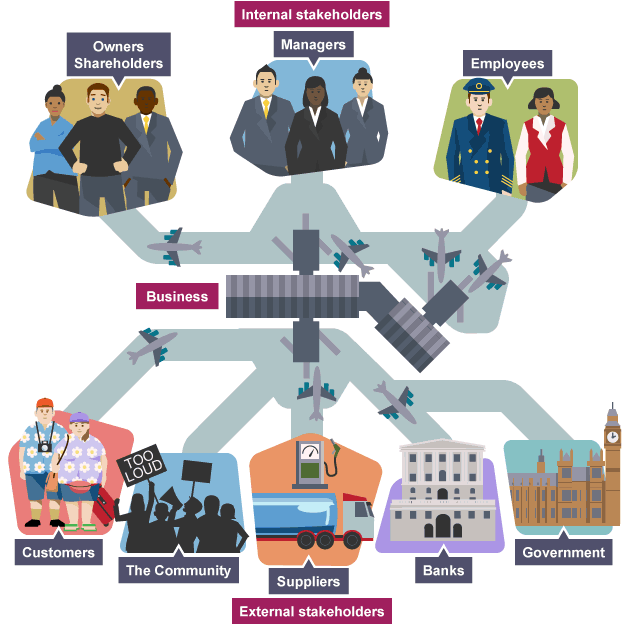
\includegraphics[keepaspectratio]{unidades/intro/../../images/external/stakeholder-power-interest.png}}

En la operación de un \textbf{aeropuerto internacional} pueden
identificarse partes interesadas internas, como la autoridad
aeroportuaria, el personal de seguridad y los responsables operativos; y
partes interesadas externas, como los pasajeros, las aerolíneas, los
proveedores, las empresas de transporte, los organismos gubernamentales
y los inversionistas.

Si se desarrolla un sistema analítico para predecir retrasos, los
pasajeros, pilotos y operadores podrían considerarse partes interesadas
primarias; los proveedores de servicios y las empresas de transporte
terrestre, partes interesadas secundarias; y la autoridad aeroportuaria,
los organismos reguladores y los patrocinadores del proyecto, partes
interesadas clave.

La clasificación dependerá del alcance del proyecto y de la manera en
que cada actor resulte afectado o pueda influir en sus decisiones.

\section{Análisis de Stakeholders: La Matriz de Poder e
Interés}\label{anuxe1lisis-de-stakeholders-la-matriz-de-poder-e-interuxe9s}

Para gestionar las expectativas de manera eficiente y evitar que la
falta de aliniación descarrile un proyecto de datos, se utiliza la
\textbf{Matriz de Poder vs.~Interés} (también conocida como Matriz de
Influencia/Interés), originalmente propuesta por Mendelow (1981) y
adoptada como práctica estándar de gestión de interesados por el
\emph{PMBOK Guide} (Project Management Institute 2017). Esta herramienta
clasifica a los stakeholders en una cuadrícula basada en dos dimensiones
clave:

\begin{enumerate}
\def\labelenumi{\arabic{enumi}.}
\tightlist
\item
  \textbf{Poder (Influencia)}: La capacidad de cambiar la dirección del
  proyecto, asignar recursos, aprobar entregables o cancelarlo por
  completo.
\item
  \textbf{Interés}: El nivel de atención y preocupación que tiene el
  stakeholder sobre el impacto del proyecto en su área.
\end{enumerate}

A continuación se presenta el diagrama de la matriz de alineación
estratégica para proyectos de análisis de datos:

\subsection{Estrategias de Gestión por
Cuadrante}\label{estrategias-de-gestiuxf3n-por-cuadrante}

\begin{itemize}
\tightlist
\item
  \textbf{Alto Poder, Alto Interés (Gestionar de Cerca)}: Deben
  participar activamente en las fases de planificación del proyecto,
  validar los entregables intermedios y recibir reportes de avance
  periódicos.
\item
  \textbf{Alto Poder, Bajo Interés (Mantener Satisfecho)}: Involucrarlos
  en puntos críticos. Es fundamental garantizar que el proyecto cumple
  con las normativas de seguridad, gobernanza y gobernanza de nube.
\item
  \textbf{Bajo Poder, Alto Interés (Mantener Informado)}: Mantenerlos
  entusiasmados e informados sobre cómo el modelo les facilitará el
  trabajo. Es vital pedir su retroalimentación temprana.
\item
  \textbf{Bajo Poder, Bajo Interés (Monitorear)}: Monitorear pasivamente
  con comunicación general.
\end{itemize}

\section{Definición de alcance y traducción de preguntas de
negocio}\label{definiciuxf3n-de-alcance-y-traducciuxf3n-de-preguntas-de-negocio}

Uno de los errores más frecuentes en los proyectos de analítica consiste
en aceptar una pregunta de negocio tal como fue formulada y comenzar a
trabajar con los datos de inmediato. Expresiones como \emph{``queremos
evitar que los clientes se vayan''} o \emph{``necesitamos aumentar las
ventas''} comunican una preocupación legítima, pero todavía no
constituyen un objetivo analítico.

La función del analista no es únicamente extraer datos o construir
modelos. También debe actuar como \textbf{traductor entre las
necesidades del negocio y las capacidades analíticas de la
organización}. Esto implica transformar una inquietud general en una
pregunta concreta, medible y vinculada con una decisión.

La definición de alcance ---o \emph{scoping}--- es el proceso mediante
el cual se aclaran:

\begin{itemize}
\tightlist
\item
  el problema que se desea resolver;
\item
  la decisión que se tomará con el resultado;
\item
  la población o unidad de análisis;
\item
  el periodo relevante;
\item
  las métricas de éxito;
\item
  las restricciones operativas;
\item
  y el formato de entrega esperado.
\end{itemize}

Solo después de establecer estos elementos tiene sentido evaluar qué
datos están disponibles y qué metodología podría utilizarse.

Esta traducción constituye el punto de partida de todo proyecto
analítico. Una vez comprendida la necesidad del negocio, el equipo puede
estudiar los datos disponibles, prepararlos, realizar el análisis,
evaluar si los resultados responden a la pregunta original y, cuando sea
necesario, desplegar una solución en producción. Por tanto, la
definición de alcance no es una formalidad previa al análisis: es la
etapa que orienta todas las decisiones posteriores.

\subsection{Del problema de negocio al objetivo
analítico}\label{del-problema-de-negocio-al-objetivo-analuxedtico}

Una pregunta cualitativa debe atravesar varias capas de definición antes
de convertirse en un objetivo técnico. El propósito no es reemplazar el
lenguaje del stakeholder por terminología estadística, sino construir
una especificación compartida que conecte el análisis con una acción
concreta.

En este ejemplo, el resultado del proceso no es todavía la selección de
un algoritmo. Decidir anticipadamente que se utilizará XGBoost, Random
Forest o cualquier otra técnica puede limitar el análisis antes de
comprender el problema. La metodología debe elegirse después de
confirmar el objetivo, revisar los datos y establecer cómo se evaluará
la utilidad de la solución.

\section{Refinamiento iterativo mediante
preguntas}\label{refinamiento-iterativo-mediante-preguntas}

La primera pregunta del stakeholder rara vez contiene todo el contexto
necesario. Por ello, la definición de alcance debe tratarse como una
\textbf{conversación iterativa} y no como un cuestionario que se
responde una sola vez.

Una estrategia útil consiste en avanzar por capas. Cada respuesta
permite formular una pregunta más precisa, detectar supuestos y regresar
al stakeholder para validar el entendimiento. El ciclo termina cuando
ambas partes pueden expresar con claridad qué se analizará, para qué se
utilizará y cómo se reconocerá un resultado útil.

\subsection{Estrategias para formular mejores
preguntas}\label{estrategias-para-formular-mejores-preguntas}

Durante este ciclo pueden combinarse varias estrategias de indagación:

\begin{enumerate}
\def\labelenumi{\arabic{enumi}.}
\item
  \textbf{Preguntar por el contexto antes que por la solución.}\\
  En lugar de comenzar con \emph{``¿qué dashboard necesitas?''},
  conviene preguntar \emph{``¿qué situación motivó esta solicitud?''}.
  Esto evita confundir el formato de entrega con el problema que debe
  resolverse.
\item
  \textbf{Conectar el análisis con una decisión.}\\
  Preguntas como \emph{``¿qué harías de manera diferente si tuvieras
  esta información?''} permiten determinar si el análisis tendrá un uso
  concreto. Si no existe una decisión asociada, es posible que la
  solicitud todavía sea demasiado general.
\item
  \textbf{Convertir conceptos ambiguos en definiciones operativas.}\\
  Términos como \emph{cliente activo}, \emph{abandono}, \emph{éxito},
  \emph{rentabilidad} o \emph{bajo desempeño} pueden tener significados
  diferentes entre áreas. El analista debe preguntar cómo se observan y
  calculan en la práctica.
\item
  \textbf{Delimitar población, periodo y nivel de detalle.}\\
  Es necesario precisar si el análisis se realizará por cliente,
  transacción, producto, sucursal o región, así como definir el periodo
  histórico y el horizonte futuro relevantes.
\item
  \textbf{Explorar restricciones y capacidad de acción.}\\
  No basta con detectar un comportamiento si la organización no puede
  intervenir sobre él. Conviene preguntar qué acciones están
  disponibles, cuál es su costo y sobre cuántos casos puede actuar el
  equipo.
\item
  \textbf{Reformular y validar.}\\
  Después de escuchar las respuestas, el analista debe resumir el
  entendimiento alcanzado: \emph{``Entonces, lo que necesitamos
  es\ldots''}. Esta reformulación permite que el stakeholder corrija
  interpretaciones antes de invertir tiempo en el análisis.
\end{enumerate}

\subsection{Ejemplo de una conversación de
refinamiento}\label{ejemplo-de-una-conversaciuxf3n-de-refinamiento}

Supongamos que un stakeholder plantea la siguiente necesidad:

\begin{quote}
``Queremos evitar que los clientes se vayan.''
\end{quote}

La conversación podría avanzar de esta manera:

\begin{itemize}
\tightlist
\item
  \textbf{Contexto:} ¿Qué comportamiento reciente indica que existe un
  problema de abandono?
\item
  \textbf{Definición:} ¿Qué significa exactamente que un cliente ``se
  vaya'': cancelar, dejar de comprar o permanecer inactivo?
\item
  \textbf{Población:} ¿El problema afecta a todos los clientes o a un
  segmento específico?
\item
  \textbf{Horizonte:} ¿Con cuánta anticipación necesitamos identificar
  el riesgo?
\item
  \textbf{Decisión:} ¿Qué acción se realizará cuando se detecte un
  cliente en riesgo?
\item
  \textbf{Capacidad:} ¿A cuántos clientes puede contactar el equipo de
  retención cada semana?
\item
  \textbf{Éxito:} ¿Cómo se medirá el resultado: cancelaciones evitadas,
  ingresos retenidos o retorno de la campaña?
\item
  \textbf{Validación:} ¿La prioridad es detectar la mayor cantidad
  posible de clientes que podrían abandonar, aunque existan algunos
  falsos positivos?
\end{itemize}

Después de esta iteración, la pregunta original podría reformularse así:

\begin{quote}
\textbf{Objetivo analítico:} identificar semanalmente a los clientes de
suscripción mensual con mayor probabilidad de cancelar durante los
próximos 30 días, utilizando su comportamiento de los últimos 90 días,
para priorizar hasta 2,000 contactos del equipo de retención. La
solución se evaluará por su capacidad para identificar cancelaciones
reales y por los ingresos retenidos mediante la intervención.
\end{quote}

Esta formulación ya establece una población, una ventana de observación,
un horizonte de predicción, una capacidad operativa y una medida de
valor. A partir de ella, el equipo puede investigar la disponibilidad de
los datos y comparar distintas metodologías.

\section{Ejemplos de traducción de preguntas de
negocio}\label{ejemplos-de-traducciuxf3n-de-preguntas-de-negocio}

{\def\LTcaptype{none} % do not increment counter
\begin{longtable}[]{@{}
  >{\raggedright\arraybackslash}p{(\linewidth - 4\tabcolsep) * \real{0.3333}}
  >{\raggedright\arraybackslash}p{(\linewidth - 4\tabcolsep) * \real{0.3333}}
  >{\raggedright\arraybackslash}p{(\linewidth - 4\tabcolsep) * \real{0.3333}}@{}}
\toprule\noalign{}
\begin{minipage}[b]{\linewidth}\raggedright
Pregunta del stakeholder
\end{minipage} & \begin{minipage}[b]{\linewidth}\raggedright
Traducción analítica
\end{minipage} & \begin{minipage}[b]{\linewidth}\raggedright
Posible metodología
\end{minipage} \\
\midrule\noalign{}
\endhead
\bottomrule\noalign{}
\endlastfoot
\emph{¿Cómo podemos aumentar el ticket promedio de la tienda en línea?}
& Identificar productos que tienden a comprarse juntos y evaluar qué
combinaciones podrían utilizarse en recomendaciones durante el proceso
de compra. & Reglas de asociación ---Apriori o FP-Growth--- evaluadas
mediante soporte, confianza y \emph{lift}. \\
\emph{¿Cómo evitamos la fuga de clientes de suscripción mensual?} &
Estimar la probabilidad de cancelación durante los próximos 30 días a
partir de la actividad reciente de cada cliente, con el fin de priorizar
intervenciones. & Modelos de clasificación supervisada, evaluados con
métricas coherentes con la capacidad y el costo de intervención. \\
\emph{Queremos campañas personalizadas, pero no sabemos cómo agrupar a
los clientes.} & Identificar grupos de clientes con patrones semejantes
de recencia, frecuencia, valor monetario y comportamiento de compra. &
Segmentación RFM y técnicas de agrupamiento como K-Means o DBSCAN,
acompañadas de interpretación de perfiles. \\
\emph{Necesitamos saber si los descuentos de fin de año funcionaron.} &
Estimar el efecto de los descuentos sobre el margen neto y distinguirlo
de cambios estacionales u otros factores simultáneos. & Análisis causal
o cuasiexperimental, según la disponibilidad de grupos de comparación y
datos históricos. \\
\end{longtable}
}

Estas metodologías son puntos de partida, no decisiones automáticas. La
técnica definitiva dependerá de la calidad de los datos, los supuestos
que puedan sostenerse y la forma en que el resultado será utilizado.

\section{\texorpdfstring{El proceso de solicitud de datos (\emph{Data
Request})}{El proceso de solicitud de datos (Data Request)}}\label{el-proceso-de-solicitud-de-datos-data-request}

Una vez validado el objetivo, el entendimiento alcanzado debe
registrarse. El \emph{Data Request} o solicitud de datos es el mecanismo
formal mediante el cual las áreas operativas comunican una necesidad al
equipo analítico y documentan su contexto, alcance y criterios de éxito.

\begin{quote}
\textbf{Definición --- Solicitud de datos (\emph{Data Request}):}
proceso formal, generalmente representado mediante un formulario o
\emph{intake ticket}, que captura la necesidad de negocio y la
información necesaria para evaluar, priorizar y ejecutar un proyecto
analítico.
\end{quote}

El ticket no sustituye la conversación con el stakeholder. Su función es
conservar los acuerdos alcanzados durante el proceso de refinamiento y
reducir ambigüedades posteriores.

\subsection{\texorpdfstring{Elementos esenciales de un \emph{Data
Request
Ticket}}{Elementos esenciales de un Data Request Ticket}}\label{elementos-esenciales-de-un-data-request-ticket}

\begin{enumerate}
\def\labelenumi{\arabic{enumi}.}
\item
  \textbf{Problema o pregunta principal}\\
  ¿Qué situación se desea comprender, resolver o mejorar?
\item
  \textbf{Contexto de negocio}\\
  ¿Por qué surge la necesidad y por qué es relevante en este momento?
\item
  \textbf{Decisión o acción esperada}\\
  ¿Qué se hará de manera diferente a partir del resultado?
\item
  \textbf{Población y alcance}\\
  ¿Qué clientes, productos, transacciones, regiones o periodos se
  incluirán?
\item
  \textbf{Métricas de éxito}\\
  ¿Cómo se determinará si el análisis fue útil para el negocio?
\item
  \textbf{Fuentes de datos conocidas o sugeridas}\\
  ¿Existen tablas, archivos, sistemas o proveedores externos que podrían
  contener la información necesaria?
\item
  \textbf{Formato de entrega}\\
  ¿Se requiere un análisis exploratorio, un reporte, un dashboard, una
  lista priorizada, un experimento o un modelo integrado en un proceso
  operativo?
\item
  \textbf{Responsable de validación}\\
  ¿Quién confirmará las definiciones, los resultados y las decisiones
  derivadas del análisis?
\item
  \textbf{Restricciones y riesgos}\\
  ¿Existen límites de tiempo, privacidad, presupuesto, capacidad
  operativa o calidad de datos?
\item
  \textbf{Fecha de decisión}\\
  ¿Cuándo debe estar disponible el resultado para que todavía sea útil?
\end{enumerate}

\section{Cierre}\label{cierre}

La calidad de un proyecto analítico depende, en gran medida, de la
calidad de la pregunta que lo origina. Un objetivo ambiguo puede
producir un análisis técnicamente correcto pero irrelevante; un objetivo
bien definido, en cambio, permite seleccionar datos, métricas y métodos
de forma coherente.

Definir el alcance significa construir un entendimiento compartido entre
el stakeholder y el equipo de datos. Para lograrlo, el analista debe
preguntar, escuchar, reformular y validar de manera iterativa. El
resultado de este proceso no es simplemente una pregunta más técnica,
sino un vínculo explícito entre los datos, una decisión y un resultado
de negocio.

\begin{center}\rule{0.5\linewidth}{0.5pt}\end{center}

\section{Caso de Estudio Práctico: Alineación en TheLook
eCommerce}\label{caso-de-estudio-pruxe1ctico-alineaciuxf3n-en-thelook-ecommerce}

Imagina que eres contratado como líder de datos en \textbf{TheLook
eCommerce} (el caso de estudio que utilizaremos a lo largo del curso).
El Director de Mercadotecnia te aborda con el siguiente requerimiento:

\begin{quote}
\emph{``Necesito que me entregues un reporte con todos los clientes y lo
que compran porque las ventas de ropa de mujer han bajado este mes y
queremos lanzar un descuento.''}
\end{quote}

Si actúas únicamente de manera reactiva, extraerás una consulta SQL
pesada, generarás un archivo CSV de gigabytes con millones de filas y se
lo enviarás por correo electrónico. \textbf{Este es un camino directo al
fracaso del proyecto}: el stakeholder no podrá abrir el archivo debido a
su tamaño, o pasará horas filtrándolo en Excel sin extraer ninguna
conclusión clara.

\subsection{La Conversación de Alineación
Estratégica}\label{la-conversaciuxf3n-de-alineaciuxf3n-estratuxe9gica}

\begin{itemize}
\tightlist
\item
  \textbf{Tú (Analista)}: \emph{``Para afinar la extracción de datos,
  ¿cuál es el objetivo de la campaña de descuento? ¿Quieren recuperar
  clientes inactivos o incentivar a las clientas recurrentes a comprar
  categorías más caras?''}
\item
  \textbf{Director (Stakeholder)}: \emph{``Queremos incentivar a las
  clientas que ya compran regularmente vestidos de diseñador a que
  exploren nuestra nueva línea de accesorios de lujo de alto margen.''}
\item
  \textbf{Tú (Analista)}: \emph{``Excelente. En lugar de todos los
  clientes, extraeré un reporte enfocado en el segmento con alta
  frecuencia de compra en la categoría de mujer/vestidos. Además,
  aplicaré un modelo de asociación para identificar qué accesorios
  compran junto con los vestidos para sugerir combinaciones específicas
  en la campaña.''}
\end{itemize}

\textbf{Resultado}: Redujiste el esfuerzo técnico de extraer bases de
datos enteras, entregaste un análisis de alto impacto enfocado en
conversión de alto margen, y alineaste las expectativas de negocio desde
el primer día.

\begin{center}\rule{0.5\linewidth}{0.5pt}\end{center}

\section{Referencias}\label{referencias}

\protect\phantomsection\label{refs}
\begin{CSLReferences}{1}{1}
\bibitem[\citeproctext]{ref-aggarwal2013}
Aggarwal, Charu C., y Chandan K. Reddy. 2013. \emph{Data Clustering:
Algorithms and Applications}. CRC Press.

\bibitem[\citeproctext]{ref-agrawal1994fast}
Agrawal, Rakesh, y Ramakrishnan Srikant. 1994. {«Fast Algorithms for
Mining Association Rules in Large Databases»}. \emph{Proceedings of the
20th International Conference on Very Large Data Bases}, VLDB '94,
487-99.

\bibitem[\citeproctext]{ref-aws_sagemaker}
Amazon Web Services. 2024. \emph{Amazon SageMaker Documentation}. AWS
Documentation.
\url{https://docs.aws.amazon.com/sagemaker/latest/dg/whatis.html}.

\bibitem[\citeproctext]{ref-bigmart_dataset}
Analytics Vidhya. 2016. \emph{BigMart Sales Prediction (Practice
Problem)}. DataHack Platform.
\url{https://www.analyticsvidhya.com/datahack/contest/big-mart-sales-prediction/}.

\bibitem[\citeproctext]{ref-anscombe1973graphs}
Anscombe, Francis J. 1973. {«Graphs in Statistical Analysis»}. \emph{The
American Statistician} 27 (1): 17-21.
\url{https://doi.org/10.1080/00031305.1973.10478966}.

\bibitem[\citeproctext]{ref-arthur2007}
Arthur, David, y Sergei Vassilvitskii. 2007. {«k-means++: the advantages
of careful seeding»}. \emph{Proceedings of the Eighteenth Annual
ACM-SIAM Symposium on Discrete Algorithms}, 1027-35.

\bibitem[\citeproctext]{ref-bellman1961adaptive}
Bellman, Richard E. 1961. \emph{Adaptive Control Processes: A Guided
Tour}. Princeton University Press.

\bibitem[\citeproctext]{ref-berger1985statistical}
Berger, James O. 1985. \emph{Statistical Decision Theory and Bayesian
Analysis}. 2.ª ed. Springer.

\bibitem[\citeproctext]{ref-bishop2006}
Bishop, Christopher M. 2006. \emph{Pattern Recognition and Machine
Learning}. Information Science y Statistics. Springer.

\bibitem[\citeproctext]{ref-borgelt2005implementation}
Borgelt, Christian. 2005. {«An Implementation of the FP-growth
Algorithm»}. \emph{Proceedings of the 1st International Workshop on Open
Source Data Mining: Frequent Pattern Mining Implementations}, 1-5.
\url{https://doi.org/10.1145/1133905.1133907}.

\bibitem[\citeproctext]{ref-bradbury2018jax}
Bradbury, James, Roy Frostig, Peter Hawkins, et~al. 2018. \emph{{JAX}:
Composable Transformations of {Python}+{NumPy} Programs}. Released.
\url{http://github.com/jax-ml/jax}.

\bibitem[\citeproctext]{ref-breiman1996bagging}
Breiman, Leo. 1996. {«Bagging Predictors»}. \emph{Machine Learning} 24
(2): 123-40. \url{https://doi.org/10.1007/BF00058655}.

\bibitem[\citeproctext]{ref-breiman2001}
Breiman, Leo. 2001. {«Random Forests»}. \emph{Machine Learning} 45 (1):
5-32. \url{https://doi.org/10.1023/A:1010933404324}.

\bibitem[\citeproctext]{ref-breiman1984}
Breiman, Leo, Jerome H. Friedman, Richard A. Olshen, y Charles J. Stone.
1984. \emph{Classification and Regression Trees}. Wadsworth
International Group.

\bibitem[\citeproctext]{ref-bryson2004}
Bryson, John M. 2004. {«What to do when stakeholders matter: Stakeholder
identification and analysis techniques»}. \emph{Public Management
Review} 6 (1): 21-53.
\url{https://doi.org/10.1080/14719030410001675722}.

\bibitem[\citeproctext]{ref-calinski1974}
Caliński, Tadeusz, y Józef Harabasz. 1974. {«A dendrite method for
cluster analysis»}. \emph{Communications in Statistics} 3 (1): 1-27.

\bibitem[\citeproctext]{ref-campello2013}
Campello, Ricardo J. G. B., Davoud Moulavi, y Jörg Sander. 2013.
{«Density-based clustering based on hierarchical density estimates»}.
\emph{Advances in Knowledge Discovery and Data Mining}, Lecture Notes en
Computer Science, vol. 7819: 160-72.

\bibitem[\citeproctext]{ref-ctb_kansas}
Center for Community Health and Development, University of Kansas. 2023.
\emph{Chapter 7, Section 8: Identifying and Analyzing Stakeholders and
Their Interests}. Community Tool Box.
\url{https://ctb.ku.edu/en/table-of-contents/participation/encouraging-involvement/identify-stakeholders/main}.

\bibitem[\citeproctext]{ref-chang2011libsvm}
Chang, Chih-Chung, y Chih-Jen Lin. 2011. {«{LIBSVM}: A Library for
Support Vector Machines»}. \emph{ACM Transactions on Intelligent Systems
and Technology} 2 (3): 27:1-27.
\url{https://doi.org/10.1145/1961189.1961199}.

\bibitem[\citeproctext]{ref-chapman2000}
Chapman, Pete, Julian Clinton, Randy Kerber, et~al. 2000. \emph{CRISP-DM
1.0: Step-by-Step Data Mining Guide}. SPSS Inc.

\bibitem[\citeproctext]{ref-chaudhuri1997overview}
Chaudhuri, Surajit, y Umeshwar Dayal. 1997. {«An Overview of Data
Warehousing and OLAP Technology»}. \emph{ACM SIGMOD Record} 26 (1):
65-74. \url{https://doi.org/10.1145/248603.248616}.

\bibitem[\citeproctext]{ref-chen2016xgboost}
Chen, Tianqi, y Carlos Guestrin. 2016. {«{XGBoost}: A Scalable Tree
Boosting System»}. \emph{Proceedings of the 22nd ACM SIGKDD
International Conference on Knowledge Discovery and Data Mining},
785-94. \url{https://doi.org/10.1145/2939672.2939785}.

\bibitem[\citeproctext]{ref-lfpdppp2010}
Congreso de los Estados Unidos Mexicanos. 2010. \emph{Ley Federal de
Protección de Datos Personales en Posesión de los Particulares}. Diario
Oficial de la Federación.
\url{https://www.diputados.gob.mx/LeyesBiblio/pdf/LFPDPPP.pdf}.

\bibitem[\citeproctext]{ref-cortes1995support}
Cortes, Corinna, y Vladimir N. Vapnik. 1995. {«Support-Vector
Networks»}. \emph{Machine Learning} 20 (3): 273-97.
\url{https://doi.org/10.1007/BF00994018}.

\bibitem[\citeproctext]{ref-cover1967nearest}
Cover, Thomas M., y Peter E. Hart. 1967. {«Nearest Neighbor Pattern
Classification»}. \emph{IEEE Transactions on Information Theory} 13 (1):
21-27. \url{https://doi.org/10.1109/TIT.1967.1053964}.

\bibitem[\citeproctext]{ref-cubejs2024docs}
Cube Dev, Inc. 2024. \emph{Cube Documentation}. Cube Dev.
\url{https://cube.dev/docs/}.

\bibitem[\citeproctext]{ref-cybenko1989approximation}
Cybenko, George. 1989. {«Approximation by Superpositions of a Sigmoidal
Function»}. \emph{Mathematics of Control, Signals, and Systems} 2 (4):
303-14.

\bibitem[\citeproctext]{ref-dama2017}
DAMA International. 2017. \emph{DAMA-DMBOK: Data Management Body of
Knowledge}. 2nd ed. Technics Publications.

\bibitem[\citeproctext]{ref-databricks_home}
Databricks. 2024. \emph{Databricks: The Data and AI Company}.
Databricks. \url{https://www.databricks.com}.

\bibitem[\citeproctext]{ref-davenport2012}
Davenport, Thomas H., y D. J. Patil. 2012. {«Data Scientist: The Sexiest
Job of the 21st Century»}. \emph{Harvard Business Review} 90 (10):
70-76.

\bibitem[\citeproctext]{ref-davies1979}
Davies, David L., y Donald W. Bouldin. 1979. {«A cluster separation
measure»}. \emph{IEEE Transactions on Pattern Analysis and Machine
Intelligence} 1 (2): 224-27.

\bibitem[\citeproctext]{ref-dbtlabs2024semanticlayer}
{dbt Labs}. 2024. \emph{dbt Semantic Layer Documentation}. Dbt Labs.
\url{https://docs.getdbt.com/docs/use-dbt-semantic-layer/dbt-sl}.

\bibitem[\citeproctext]{ref-deepmind2020optax}
DeepMind, Igor Babuschkin, Kate Baumli, et~al. 2020. \emph{The
{DeepMind} {JAX} Ecosystem}. Released.
\url{http://github.com/google-deepmind}.

\bibitem[\citeproctext]{ref-dehghani2022datamesh}
Dehghani, Zhamak. 2022. \emph{Data Mesh: Delivering Data-Driven Value at
Scale}. O'Reilly Media.

\bibitem[\citeproctext]{ref-dempster1977}
Dempster, Arthur P., Nan M. Laird, y Donald B. Rubin. 1977. {«Maximum
Likelihood from Incomplete Data via the {EM} Algorithm»}. \emph{Journal
of the Royal Statistical Society, Series B} 39 (1): 1-38.

\bibitem[\citeproctext]{ref-devlin1988architecture}
Devlin, Barry A., y Paul T. Murphy. 1988. {«An Architecture for a
Business and Information System»}. \emph{IBM Systems Journal} 27 (1):
60-80. \url{https://doi.org/10.1147/sj.271.0060}.

\bibitem[\citeproctext]{ref-duda2001pattern}
Duda, Richard O., Peter E. Hart, y David G. Stork. 2001. \emph{Pattern
Classification}. 2.ª ed. Wiley.

\bibitem[\citeproctext]{ref-durbin1998biological}
Durbin, Richard, Sean R. Eddy, Anders Krogh, y Graeme Mitchison. 1998.
\emph{Biological Sequence Analysis: Probabilistic Models of Proteins and
Nucleic Acids}. Cambridge University Press.

\bibitem[\citeproctext]{ref-ester1996}
Ester, Martin, Hans-Peter Kriegel, Jörg Sander, y Xiaowei Xu. 1996. {«A
density-based algorithm for discovering clusters in large spatial
databases with noise»}. \emph{Proceedings of the Second International
Conference on Knowledge Discovery and Data Mining}, 226-31.

\bibitem[\citeproctext]{ref-fawcett2006}
Fawcett, Tom. 2006. {«An introduction to {ROC} analysis»}. \emph{Pattern
Recognition Letters} 27 (8): 861-74.
\url{https://doi.org/10.1016/j.patrec.2005.10.010}.

\bibitem[\citeproctext]{ref-fayyad1996}
Fayyad, Usama, Gregory Piatetsky-Shapiro, y Padhraic Smyth. 1996. {«From
data mining to knowledge discovery in databases»}. \emph{AI Magazine} 17
(3): 37-54. \url{https://doi.org/10.1609/aimag.v17i3.1230}.

\bibitem[\citeproctext]{ref-fielding2000rest}
Fielding, Roy Thomas. 2000. {«Architectural Styles and the Design of
Network-based Software Architectures»}. Tesis doctoral, University of
California, Irvine.

\bibitem[\citeproctext]{ref-fisher1936use}
Fisher, Ronald A. 1936. {«The Use of Multiple Measurements in Taxonomic
Problems»}. \emph{Annals of Eugenics} 7 (2): 179-88.
\url{https://doi.org/10.1111/j.1469-1809.1936.tb02137.x}.

\bibitem[\citeproctext]{ref-fowler2010richardson}
Fowler, Martin. 2010. \emph{Richardson Maturity Model}.
Martinfowler.com.
\url{https://martinfowler.com/articles/richardsonMaturityModel.html}.

\bibitem[\citeproctext]{ref-freedman2007statistics}
Freedman, David, Robert Pisani, y Roger Purves. 2007. \emph{Statistics}.
4.ª ed. W. W. Norton.

\bibitem[\citeproctext]{ref-freeman1984}
Freeman, R. Edward. 1984. \emph{Strategic Management: A Stakeholder
Approach}. Pitman.

\bibitem[\citeproctext]{ref-freund1997decision}
Freund, Yoav, y Robert E. Schapire. 1997. {«A Decision-Theoretic
Generalization of On-Line Learning and an Application to Boosting»}.
\emph{Journal of Computer and System Sciences} 55 (1): 119-39.
\url{https://doi.org/10.1006/jcss.1997.1504}.

\bibitem[\citeproctext]{ref-friedman2001greedy}
Friedman, Jerome H. 2001. {«Greedy Function Approximation: A Gradient
Boosting Machine»}. \emph{The Annals of Statistics} 29 (5): 1189-232.
\url{https://doi.org/10.1214/aos/1013203451}.

\bibitem[\citeproctext]{ref-friedman2002stochastic}
Friedman, Jerome H. 2002. {«Stochastic Gradient Boosting»}.
\emph{Computational Statistics \& Data Analysis} 38 (4): 367-78.
\url{https://doi.org/10.1016/S0167-9473(01)00065-2}.

\bibitem[\citeproctext]{ref-friedman1977algorithm}
Friedman, Jerome H., Jon Louis Bentley, y Raphael Ari Finkel. 1977. {«An
Algorithm for Finding Best Matches in Logarithmic Expected Time»}.
\emph{ACM Transactions on Mathematical Software} 3 (3): 209-26.
\url{https://doi.org/10.1145/355744.355745}.

\bibitem[\citeproctext]{ref-fukunaga1975branch}
Fukunaga, Keinosuke, y Patrenahalli M. Narendra. 1975. {«A Branch and
Bound Algorithm for Computing k-Nearest Neighbors»}. \emph{IEEE
Transactions on Computers} C-24 (7): 750-53.
\url{https://doi.org/10.1109/T-C.1975.224297}.

\bibitem[\citeproctext]{ref-gardiner1987cpg}
Gardiner-Garden, Margaret, y Marianne Frommer. 1987. {«CpG Islands in
Vertebrate Genomes»}. \emph{Journal of Molecular Biology} 196 (2):
261-82. \url{https://doi.org/10.1016/0022-2836(87)90689-9}.

\bibitem[\citeproctext]{ref-gauss1809theoria}
Gauss, Carl Friedrich. 1809. \emph{Theoria Motus Corporum Coelestium in
Sectionibus Conicis Solem Ambientium}. Friedrich Perthes; I. H. Besser.

\bibitem[\citeproctext]{ref-geron2022hands}
Géron, Aurélien. 2022. \emph{Hands-On Machine Learning with
Scikit-Learn, Keras, and TensorFlow}. 3.ª ed. O'Reilly Media.

\bibitem[\citeproctext]{ref-gini1912variabilita}
Gini, Corrado. 1912. {«Variabilità e mutabilità»}. \emph{Studi
Economico-Giuridici della Regia Università di Cagliari} 3: 1-158.

\bibitem[\citeproctext]{ref-golub2013matrix}
Golub, Gene H., y Charles F. Van Loan. 2013. \emph{Matrix Computations}.
4.ª ed. Johns Hopkins University Press.

\bibitem[\citeproctext]{ref-goodfellow2016deep}
Goodfellow, Ian, Yoshua Bengio, y Aaron Courville. 2016. \emph{Deep
Learning}. MIT Press.

\bibitem[\citeproctext]{ref-google2022}
Google. 2022. \emph{Foundations: Data, Data, Everywhere}. Google Data
Analytics Professional Certificate, Coursera.

\bibitem[\citeproctext]{ref-google_vertexai}
Google Cloud. 2024. \emph{Vertex AI Documentation}. Google Cloud
Documentation. \url{https://cloud.google.com/vertex-ai/docs}.

\bibitem[\citeproctext]{ref-graphql2021spec}
GraphQL Foundation. 2021. \emph{GraphQL Specification}. GraphQL
Foundation. \url{https://spec.graphql.org/}.

\bibitem[\citeproctext]{ref-gray1997data}
Gray, Jim, Adam Bosworth, Andrew Layman, y Hamid Pirahesh. 1996. {«Data
Cube: A Relational Aggregation Operator Generalizing Group-By,
Cross-Tab, and Sub-Totals»}. \emph{Proceedings of the Twelfth
International Conference on Data Engineering}, 152-59.
\url{https://doi.org/10.1109/ICDE.1996.492099}.

\bibitem[\citeproctext]{ref-han2011}
Han, Jiawei, Micheline Kamber, y Jian Pei. 2011. \emph{Data Mining:
Concepts and Techniques}. 3.ª ed. Morgan Kaufmann.
\url{https://doi.org/10.1016/B978-0-12-381479-1.00001-0}.

\bibitem[\citeproctext]{ref-han2012data}
Han, Jiawei, Micheline Kamber, y Jian Pei. 2012. \emph{Data Mining:
Concepts and Techniques}. 3.ª ed. Morgan Kaufmann.

\bibitem[\citeproctext]{ref-han2000mining}
Han, Jiawei, Jian Pei, y Yiwen Yin. 2000. {«Mining Frequent Patterns
without Candidate Generation»}. \emph{Proceedings of the 2000 ACM SIGMOD
International Conference on Management of Data}, SIGMOD '00, 1-12.
\url{https://doi.org/10.1145/342009.335372}.

\bibitem[\citeproctext]{ref-hart1968condensed}
Hart, Peter E. 1968. {«The Condensed Nearest Neighbor Rule»}. \emph{IEEE
Transactions on Information Theory} 14 (3): 515-16.
\url{https://doi.org/10.1109/TIT.1968.1054155}.

\bibitem[\citeproctext]{ref-hastie2009}
Hastie, Trevor, Robert Tibshirani, y Jerome Friedman. 2009. \emph{The
Elements of Statistical Learning: Data Mining, Inference, and
Prediction}. 2.ª ed. Springer Series en Statistics. Springer.
\url{https://doi.org/10.1007/978-0-387-84858-7}.

\bibitem[\citeproctext]{ref-nist2012handbook}
Heckert, N. Alan, James J. Filliben, Carroll M. Croarkin, et~al. 2012.
\emph{NIST/SEMATECH e-Handbook of Statistical Methods}. National
Institute of Standards; Technology.
\url{https://www.itl.nist.gov/div898/handbook/}.

\bibitem[\citeproctext]{ref-heek2023flax}
Heek, Jonathan, Anselm Levskaya, Avital Oliver, et~al. 2023. \emph{Flax:
A Neural Network Library and Ecosystem for {JAX}}. Released.
\url{http://github.com/google/flax}.

\bibitem[\citeproctext]{ref-hill1973diversity}
Hill, Mark O. 1973. {«Diversity and Evenness: A Unifying Notation and
Its Consequences»}. \emph{Ecology} 54 (2): 427-32.
\url{https://doi.org/10.2307/1934352}.

\bibitem[\citeproctext]{ref-hirschman1945national}
Hirschman, Albert O. 1945. \emph{National Power and the Structure of
Foreign Trade}. University of California Press.

\bibitem[\citeproctext]{ref-hochreiter1997long}
Hochreiter, Sepp, y Jürgen Schmidhuber. 1997. {«Long Short-Term
Memory»}. \emph{Neural Computation} 9 (8): 1735-80.

\bibitem[\citeproctext]{ref-hoerl1970ridge}
Hoerl, Arthur E., y Robert W. Kennard. 1970. {«Ridge Regression: Biased
Estimation for Nonorthogonal Problems»}. \emph{Technometrics} 12 (1):
55-67. \url{https://doi.org/10.1080/00401706.1970.10488634}.

\bibitem[\citeproctext]{ref-hornik1989multilayer}
Hornik, Kurt, Maxwell Stinchcombe, y Halbert White. 1989. {«Multilayer
Feedforward Networks are Universal Approximators»}. \emph{Neural
Networks} 2 (5): 359-66.

\bibitem[\citeproctext]{ref-hosmer2013}
Hosmer, David W., Stanley Lemeshow, y Rodney X. Sturdivant. 2013.
\emph{Applied Logistic Regression}. 3.ª ed. John Wiley \& Sons.

\bibitem[\citeproctext]{ref-huber2009robust}
Huber, Peter J., y Elvezio M. Ronchetti. 2009. \emph{Robust Statistics}.
2.ª ed. Wiley. \url{https://doi.org/10.1002/9780470434697}.

\bibitem[\citeproctext]{ref-hubert1985}
Hubert, Lawrence, y Phipps Arabie. 1985. {«Comparing partitions»}.
\emph{Journal of Classification} 2 (1): 193-218.

\bibitem[\citeproctext]{ref-hyndman1996quantiles}
Hyndman, Rob J., y Yanan Fan. 1996. {«Sample Quantiles in Statistical
Packages»}. \emph{The American Statistician} 50 (4): 361-65.
\url{https://doi.org/10.1080/00031305.1996.10473566}.

\bibitem[\citeproctext]{ref-ibm_asumdm}
IBM. 2015. \emph{Analytics Solutions Unified Method (ASUM-DM)}. IBM
Corporation, internal methodology derived from CRISP-DM.
\url{https://public.dhe.ibm.com/software/data/sw-library/services/ASUM.pdf}.

\bibitem[\citeproctext]{ref-inmon2005building}
Inmon, William H. 2005. \emph{Building the Data Warehouse}. 4.ª ed.
Wiley.

\bibitem[\citeproctext]{ref-james2021}
James, Gareth, Daniela Witten, Trevor Hastie, y Robert Tibshirani. 2021.
\emph{An Introduction to Statistical Learning with Applications in {R}}.
2.ª ed. Springer Texts en Statistics. Springer.
\url{https://doi.org/10.1007/978-1-0716-1418-1}.

\bibitem[\citeproctext]{ref-jaynes2003probability}
Jaynes, Edwin T. 2003. \emph{Probability Theory: The Logic of Science}.
Cambridge University Press.

\bibitem[\citeproctext]{ref-joanes1998skewness}
Joanes, D. N., y C. A. Gill. 1998. {«Comparing Measures of Sample
Skewness and Kurtosis»}. \emph{Journal of the Royal Statistical Society:
Series D (The Statistician)} 47 (1): 183-89.
\url{https://doi.org/10.1111/1467-9884.00122}.

\bibitem[\citeproctext]{ref-jolliffe2002}
Jolliffe, Ian T. 2002. \emph{Principal Component Analysis}. 2nd ed.
Springer.

\bibitem[\citeproctext]{ref-jost2006entropy}
Jost, Lou. 2006. {«Entropy and Diversity»}. \emph{Oikos} 113 (2):
363-75. \url{https://doi.org/10.1111/j.2006.0030-1299.14714.x}.

\bibitem[\citeproctext]{ref-kaufman1990}
Kaufman, Leonard, y Peter J. Rousseeuw. 1990. \emph{Finding Groups in
Data: An Introduction to Cluster Analysis}. Wiley.

\bibitem[\citeproctext]{ref-ke2017lightgbm}
Ke, Guolin, Qi Meng, Thomas Finley, et~al. 2017. {«LightGBM: A Highly
Efficient Gradient Boosting Decision Tree»}. \emph{Advances in Neural
Information Processing Systems} 30.

\bibitem[\citeproctext]{ref-kendall1938measure}
Kendall, Maurice G. 1938. {«A New Measure of Rank Correlation»}.
\emph{Biometrika} 30 (1/2): 81-93.
\url{https://doi.org/10.2307/2332226}.

\bibitem[\citeproctext]{ref-kimball2013}
Kimball, Ralph, y Margy Ross. 2013. \emph{The Data Warehouse Toolkit:
The Definitive Guide to Dimensional Modeling}. 3.ª ed. Wiley.

\bibitem[\citeproctext]{ref-kingma2015adam}
Kingma, Diederik P., y Jimmy Ba. 2015. {«Adam: A Method for Stochastic
Optimization»}. \emph{International Conference on Learning
Representations (ICLR)}.

\bibitem[\citeproctext]{ref-kleppmann2017designing}
Kleppmann, Martin. 2017. \emph{Designing Data-Intensive Applications}.
O'Reilly Media.

\bibitem[\citeproctext]{ref-kohavi1995}
Kohavi, Ron. 1995. {«A Study of Cross-Validation and Bootstrap for
Accuracy Estimation and Model Selection»}. \emph{Proceedings of the 14th
International Joint Conference on Artificial Intelligence (IJCAI)} 2:
1137-43.

\bibitem[\citeproctext]{ref-kohavi2020trustworthy}
Kohavi, Ron, Diane Tang, y Ya Xu. 2020. \emph{Trustworthy Online
Controlled Experiments: A Practical Guide to A/B Testing}. Cambridge
University Press.

\bibitem[\citeproctext]{ref-lecun2015deep}
LeCun, Yann, Yoshua Bengio, y Geoffrey Hinton. 2015. {«Deep Learning»}.
\emph{Nature} 521: 436-44.

\bibitem[\citeproctext]{ref-lecun1998gradient}
LeCun, Yann, Léon Bottou, Yoshua Bengio, y Patrick Haffner. 1998.
{«Gradient-Based Learning Applied to Document Recognition»}.
\emph{Proceedings of the IEEE} 86 (11): 2278-324.

\bibitem[\citeproctext]{ref-legendre1805nouvelles}
Legendre, Adrien-Marie. 1805. \emph{Nouvelles méthodes pour la
détermination des orbites des comètes}. Firmin Didot.

\bibitem[\citeproctext]{ref-lloyd1982}
Lloyd, Stuart P. 1982. {«Least squares quantization in {PCM}»}.
\emph{IEEE Transactions on Information Theory} 28 (2): 129-37.

\bibitem[\citeproctext]{ref-lorenz1905concentration}
Lorenz, Max O. 1905. {«Methods of Measuring the Concentration of
Wealth»}. \emph{Publications of the American Statistical Association} 9
(70): 209-19. \url{https://doi.org/10.2307/2276207}.

\bibitem[\citeproctext]{ref-lundberg2020local2global}
Lundberg, Scott M., Gabriel Erion, Hugh Chen, et~al. 2020. {«From Local
Explanations to Global Understanding with Explainable {AI} for Trees»}.
\emph{Nature Machine Intelligence} 2: 56-67.
\url{https://doi.org/10.1038/s42256-019-0138-9}.

\bibitem[\citeproctext]{ref-lundberg2017unified}
Lundberg, Scott M., y Su-In Lee. 2017. {«A Unified Approach to
Interpreting Model Predictions»}. \emph{Advances in Neural Information
Processing Systems} 30.

\bibitem[\citeproctext]{ref-maaten2008}
Maaten, Laurens van der, y Geoffrey Hinton. 2008. {«Visualizing data
using {t-SNE}»}. \emph{Journal of Machine Learning Research} 9:
2579-605.

\bibitem[\citeproctext]{ref-macqueen1967}
MacQueen, James. 1967. {«Some methods for classification and analysis of
multivariate observations»}. \emph{Proceedings of the Fifth Berkeley
Symposium on Mathematical Statistics and Probability} 1: 281-97.

\bibitem[\citeproctext]{ref-mccallum1998comparison}
McCallum, Andrew, y Kamal Nigam. 1998. {«A Comparison of Event Models
for Naive Bayes Text Classification»}. \emph{AAAI-98 Workshop on
Learning for Text Categorization}, 41-48.

\bibitem[\citeproctext]{ref-mccullagh1989}
McCullagh, Peter, y John A. Nelder. 1989. \emph{Generalized Linear
Models}. 2.ª ed. Chapman \& Hall.

\bibitem[\citeproctext]{ref-mcinnes2018}
McInnes, Leland, John Healy, y James Melville. 2018. {«{UMAP}: Uniform
Manifold Approximation and Projection for Dimension Reduction»}.
\emph{arXiv preprint arXiv:1802.03426}.

\bibitem[\citeproctext]{ref-mckinney2010data}
McKinney, Wes. 2010. {«Data Structures for Statistical Computing in
Python»}. \emph{Proceedings of the 9th Python in Science Conference},
56-61. \url{https://doi.org/10.25080/Majora-92bf1922-00a}.

\bibitem[\citeproctext]{ref-mclachlan2000}
McLachlan, Geoffrey J., y David Peel. 2000. \emph{Finite Mixture
Models}. Wiley Series en Probability y Statistics. John Wiley \& Sons.

\bibitem[\citeproctext]{ref-mendelow1981}
Mendelow, Aubrey L. 1981. {«Environmental Scanning -- The Impact of the
Stakeholder Concept»}. \emph{Proceedings of the Second International
Conference on Information Systems (ICIS)} (Cambridge, MA).

\bibitem[\citeproctext]{ref-microsoft_tdsp}
Microsoft. 2023. \emph{What Is the Team Data Science Process (TDSP)?}
GitHub (Azure/Microsoft-TDSP), archived repository.
\url{https://github.com/Azure/Microsoft-TDSP/blob/master/Docs/README.md}.

\bibitem[\citeproctext]{ref-microsoft_azureml}
Microsoft. 2024. \emph{Azure Machine Learning Documentation}. Microsoft
Learn. \url{https://learn.microsoft.com/en-us/azure/machine-learning/}.

\bibitem[\citeproctext]{ref-minsky1969perceptrons}
Minsky, Marvin, y Seymour Papert. 1969. \emph{Perceptrons: An
Introduction to Computational Geometry}. MIT Press.

\bibitem[\citeproctext]{ref-montgomery2012introduction}
Montgomery, Douglas C., Elizabeth A. Peck, y G. Geoffrey Vining. 2012.
\emph{Introduction to Linear Regression Analysis}. 5.ª ed. Wiley.

\bibitem[\citeproctext]{ref-murphy2012}
Murphy, Kevin P. 2012. \emph{Machine Learning: A Probabilistic
Perspective}. MIT Press.

\bibitem[\citeproctext]{ref-netflix_techblog}
Netflix Technology Blog. 2016. \emph{It's All A/Bout Testing: The
Netflix Experimentation Platform}.
\url{https://netflixtechblog.com/its-all-a-bout-testing-the-netflix-experimentation-platform-4e1ca458c15}.

\bibitem[\citeproctext]{ref-neyman1933problem}
Neyman, Jerzy, y Egon S. Pearson. 1933. {«On the Problem of the Most
Efficient Tests of Statistical Hypotheses»}. \emph{Philosophical
Transactions of the Royal Society of London. Series A} 231: 289-337.
\url{https://doi.org/10.1098/rsta.1933.0009}.

\bibitem[\citeproctext]{ref-novikoff1962convergence}
Novikoff, Albert B. J. 1962. {«On Convergence Proofs on Perceptrons»}.
\emph{Proceedings of the Symposium on the Mathematical Theory of
Automata} 12: 615-22.

\bibitem[\citeproctext]{ref-osterwalder2010}
Osterwalder, Alexander, y Yves Pigneur. 2010. \emph{Business Model
Generation: A Handbook for Visionaries, Game Changers, and Challengers}.
Wiley.

\bibitem[\citeproctext]{ref-paszke2019pytorch}
Paszke, Adam, Sam Gross, Francisco Massa, et~al. 2019. {«{PyTorch}: An
Imperative Style, High-Performance Deep Learning Library»}.
\emph{Advances in Neural Information Processing Systems (NeurIPS)} 32.

\bibitem[\citeproctext]{ref-pearl2009causality}
Pearl, Judea. 2009. \emph{Causality: Models, Reasoning and Inference}.
2nd ed. Cambridge University Press.

\bibitem[\citeproctext]{ref-pearson1895correlation}
Pearson, Karl. 1895. {«Notes on Regression and Inheritance in the Case
of Two Parents»}. \emph{Proceedings of the Royal Society of London} 58:
240-42. \url{https://doi.org/10.1098/rspl.1895.0041}.

\bibitem[\citeproctext]{ref-pedregosa2011}
Pedregosa, Fabian, Gaël Varoquaux, Alexandre Gramfort, et~al. 2011.
{«Scikit-learn: Machine learning in {Python}»}. \emph{Journal of Machine
Learning Research} 12: 2825-30.
\url{https://jmlr.org/papers/v12/pedregosa11a.html}.

\bibitem[\citeproctext]{ref-platt1999probabilistic}
Platt, John C. 1999. {«Probabilistic Outputs for Support Vector Machines
and Comparisons to Regularized Likelihood Methods»}. En \emph{Advances
in Large Margin Classifiers}, editado por Alexander J. Smola, Peter
Bartlett, Bernhard Schölkopf, y Dale Schuurmans. MIT Press.

\bibitem[\citeproctext]{ref-powers2011}
Powers, David M. W. 2011. {«Evaluation: From Precision, Recall and
F-Factor to {ROC}, Informedness, Markedness and Correlation»}.
\emph{Journal of Machine Learning Technologies} 2 (1): 37-63.
\url{https://arxiv.org/abs/2010.16061}.

\bibitem[\citeproctext]{ref-pmi2017}
Project Management Institute. 2017. \emph{A Guide to the Project
Management Body of Knowledge (PMBOK Guide)}. 6th ed. Project Management
Institute.

\bibitem[\citeproctext]{ref-prokhorenkova2018catboost}
Prokhorenkova, Liudmila, Gleb Gusev, Aleksandr Vorobev, Anna Veronika
Dorogush, y Andrey Gulin. 2018. {«CatBoost: Unbiased Boosting with
Categorical Features»}. \emph{Advances in Neural Information Processing
Systems} 31.

\bibitem[\citeproctext]{ref-provost2013}
Provost, Foster, y Tom Fawcett. 2013. \emph{Data Science for Business:
What You Need to Know about Data Mining and Data-Analytic Thinking}.
O'Reilly Media.

\bibitem[\citeproctext]{ref-quinlan1986induction}
Quinlan, J. Ross. 1986. {«Induction of Decision Trees»}. \emph{Machine
Learning} 1 (1): 81-106. \url{https://doi.org/10.1007/BF00116251}.

\bibitem[\citeproctext]{ref-quinlan1993c45}
Quinlan, J. Ross. 1993. \emph{C4.5: Programs for Machine Learning}.
Morgan Kaufmann.

\bibitem[\citeproctext]{ref-fastapi2024docs}
Ramírez, Sebastián. 2024. \emph{FastAPI Documentation}. FastAPI.
\url{https://fastapi.tiangolo.com/}.

\bibitem[\citeproctext]{ref-raschka2018mlxtend}
Raschka, Sebastian. 2018. {«MLxtend: Providing Machine Learning and Data
Science Utilities and Extensions to Python's Scientific Computing
Stack»}. \emph{The Journal of Open Source Software} 3 (24): 638.
\url{https://doi.org/10.21105/joss.00638}.

\bibitem[\citeproctext]{ref-reynolds2009}
Reynolds, Douglas A. 2009. {«Gaussian Mixture Models»}.
\emph{Encyclopedia of Biometrics} (Boston, MA), 659-63.
\url{https://doi.org/10.1007/978-0-387-73003-5_196}.

\bibitem[\citeproctext]{ref-rosenblatt1958perceptron}
Rosenblatt, Frank. 1958. {«The Perceptron: A Probabilistic Model for
Information Storage and Organization in the Brain»}. \emph{Psychological
Review} 65 (6): 386-408. \url{https://doi.org/10.1037/h0042519}.

\bibitem[\citeproctext]{ref-rousseeuw1987}
Rousseeuw, Peter J. 1987. {«Silhouettes: a graphical aid to the
interpretation and validation of cluster analysis»}. \emph{Journal of
Computational and Applied Mathematics} 20: 53-65.

\bibitem[\citeproctext]{ref-rousseeuw1993alternatives}
Rousseeuw, Peter J., y Christophe Croux. 1993. {«Alternatives to the
Median Absolute Deviation»}. \emph{Journal of the American Statistical
Association} 88 (424): 1273-83.
\url{https://doi.org/10.1080/01621459.1993.10476408}.

\bibitem[\citeproctext]{ref-rumelhart1986learning}
Rumelhart, David E., Geoffrey E. Hinton, y Ronald J. Williams. 1986.
{«Learning Representations by Back-propagating Errors»}. \emph{Nature}
323: 533-36.

\bibitem[\citeproctext]{ref-saito2015}
Saito, Takaya, y Marc Rehmsmeier. 2015. {«The precision-recall plot is
more informative than the {ROC} plot when evaluating binary classifiers
on imbalanced datasets»}. \emph{PLOS ONE} 10 (3): e0118432.
\url{https://doi.org/10.1371/journal.pone.0118432}.

\bibitem[\citeproctext]{ref-santizo2026cubos}
Santizo Galicia, Jessica. 2026. \emph{Computación de Cubos de datos}.
Presentación de clase, Facultad de Ciencias, Universidad Nacional
Autónoma de México.

\bibitem[\citeproctext]{ref-sas_semma}
SAS Institute. 2017. \emph{Introduction to SEMMA}. SAS Enterprise Miner
Reference Help.
\url{https://documentation.sas.com/doc/en/emref/14.3/n061bzurmej4j3n1jnj8bbjjm1a2.htm}.

\bibitem[\citeproctext]{ref-schapire1990strength}
Schapire, Robert E. 1990. {«The Strength of Weak Learnability»}.
\emph{Machine Learning} 5 (2): 197-227.
\url{https://doi.org/10.1007/BF00116037}.

\bibitem[\citeproctext]{ref-scholkopf2002learning}
Schölkopf, Bernhard, y Alexander J. Smola. 2002. \emph{Learning with
Kernels: Support Vector Machines, Regularization, Optimization, and
Beyond}. MIT Press.

\bibitem[\citeproctext]{ref-shannon1948mathematical}
Shannon, Claude E. 1948. {«A Mathematical Theory of Communication»}.
\emph{Bell System Technical Journal} 27 (3): 379-423.
\url{https://doi.org/10.1002/j.1538-7305.1948.tb01338.x}.

\bibitem[\citeproctext]{ref-shearer2000}
Shearer, Colin. 2000. {«The CRISP-DM Model: The New Blueprint for Data
Mining»}. \emph{Journal of Data Warehousing} 5 (4): 13-22.

\bibitem[\citeproctext]{ref-simpson1949measurement}
Simpson, Edward H. 1949. {«Measurement of Diversity»}. \emph{Nature}
163: 688. \url{https://doi.org/10.1038/163688a0}.

\bibitem[\citeproctext]{ref-sokolova2009systematic}
Sokolova, Marina, y Guy Lapalme. 2009. {«A Systematic Analysis of
Performance Measures for Classification Tasks»}. \emph{Information
Processing \& Management} 45 (4): 427-37.
\url{https://doi.org/10.1016/j.ipm.2009.03.002}.

\bibitem[\citeproctext]{ref-spearman1904proof}
Spearman, Charles. 1904. {«The Proof and Measurement of Association
between Two Things»}. \emph{The American Journal of Psychology} 15 (1):
72-101. \url{https://doi.org/10.2307/1412159}.

\bibitem[\citeproctext]{ref-srivastava2014dropout}
Srivastava, Nitish, Geoffrey Hinton, Alex Krizhevsky, Ilya Sutskever, y
Ruslan Salakhutdinov. 2014. {«Dropout: A Simple Way to Prevent Neural
Networks from Overfitting»}. \emph{Journal of Machine Learning Research}
15: 1929-58.

\bibitem[\citeproctext]{ref-stone1977consistent}
Stone, Charles J. 1977. {«Consistent Nonparametric Regression»}.
\emph{The Annals of Statistics} 5 (4): 595-620.
\url{https://doi.org/10.1214/aos/1176343886}.

\bibitem[\citeproctext]{ref-stone1974cross}
Stone, M. 1974. {«Cross-Validatory Choice and Assessment of Statistical
Predictions»}. \emph{Journal of the Royal Statistical Society: Series B
(Methodological)} 36 (2): 111-33.
\url{https://doi.org/10.1111/j.2517-6161.1974.tb00994.x}.

\bibitem[\citeproctext]{ref-studer2021crispmlq}
Studer, Stefan, Thanh Binh Bui, Christian Drescher, et~al. 2021.
{«Towards CRISP-ML(Q): A Machine Learning Process Model with Quality
Assurance Methodology»}. \emph{Machine Learning and Knowledge
Extraction} 3 (2): 392-413.

\bibitem[\citeproctext]{ref-tan2019introduction}
Tan, Pang-Ning, Michael Steinbach, Anuj Karpatne, y Vipin Kumar. 2019.
\emph{Introduction to Data Mining}. 2.ª ed. Pearson.

\bibitem[\citeproctext]{ref-tan2006introduction}
Tan, Pang-Ning, Michael Steinbach, y Vipin Kumar. 2006.
\emph{Introduction to Data Mining}. Addison-Wesley.

\bibitem[\citeproctext]{ref-pandas2024docs}
The pandas development team. 2024. \emph{pandas Documentation}. Pandas.
\url{https://pandas.pydata.org/docs/}.

\bibitem[\citeproctext]{ref-tukey1977eda}
Tukey, John W. 1977. \emph{Exploratory Data Analysis}. Addison-Wesley.

\bibitem[\citeproctext]{ref-vapnik1995nature}
Vapnik, Vladimir N. 1995. \emph{The Nature of Statistical Learning
Theory}. Springer.

\bibitem[\citeproctext]{ref-vapnik1998statistical}
Vapnik, Vladimir N. 1998. \emph{Statistical Learning Theory}. Wiley.

\bibitem[\citeproctext]{ref-vaswani2017attention}
Vaswani, Ashish, Noam Shazeer, Niki Parmar, et~al. 2017. {«Attention Is
All You Need»}. \emph{Advances in Neural Information Processing Systems
(NeurIPS)} 30.

\bibitem[\citeproctext]{ref-ward1963}
Ward, Joe H. 1963. {«Hierarchical grouping to optimize an objective
function»}. \emph{Journal of the American Statistical Association} 58
(301): 236-44.

\bibitem[\citeproctext]{ref-wasserman2004all}
Wasserman, Larry. 2004. \emph{All of Statistics: A Concise Course in
Statistical Inference}. Springer.

\bibitem[\citeproctext]{ref-wilcox2012modern}
Wilcox, Rand R. 2012. \emph{Introduction to Robust Estimation and
Hypothesis Testing}. 3.ª ed. Academic Press.

\bibitem[\citeproctext]{ref-wilson1972asymptotic}
Wilson, Dennis L. 1972. {«Asymptotic Properties of Nearest Neighbor
Rules Using Edited Data»}. \emph{IEEE Transactions on Systems, Man, and
Cybernetics} SMC-2 (3): 408-21.
\url{https://doi.org/10.1109/TSMC.1972.4309137}.

\bibitem[\citeproctext]{ref-wirth2000}
Wirth, Rüdiger, y Jochen Hipp. 2000. {«CRISP-DM: Towards a Standard
Process Model for Data Mining»}. \emph{Proceedings of the 4th
International Conference on the Practical Applications of Knowledge
Discovery and Data Mining}, 29-39.

\end{CSLReferences}

\chapter{Roles en el Equipo de Datos y Ciclo de Vida de los
Datos}\label{roles-en-el-equipo-de-datos-y-ciclo-de-vida-de-los-datos}

En organizaciones modernas, los proyectos analíticos raramente son
desarrollados por una sola persona. A medida que el volumen de datos
crece y las tecnologías se especializan, surge la necesidad de contar
con equipos multidisciplinarios. De acuerdo con el marco de gobierno de
datos DAMA-DMBOK (DAMA International 2017) y con la caracterización del
rol del científico de datos hecha por Davenport y Patil (2012), existen
cuatro perfiles principales, cada uno con responsabilidades,
herramientas y productos específicos.

\subsection{Comparativa de Roles en la Ingeniería y Ciencia de
Datos}\label{comparativa-de-roles-en-la-ingenieruxeda-y-ciencia-de-datos}

{\def\LTcaptype{none} % do not increment counter
\begin{longtable}[]{@{}
  >{\raggedright\arraybackslash}p{(\linewidth - 6\tabcolsep) * \real{0.2500}}
  >{\raggedright\arraybackslash}p{(\linewidth - 6\tabcolsep) * \real{0.2500}}
  >{\raggedright\arraybackslash}p{(\linewidth - 6\tabcolsep) * \real{0.2500}}
  >{\raggedright\arraybackslash}p{(\linewidth - 6\tabcolsep) * \real{0.2500}}@{}}
\toprule\noalign{}
\begin{minipage}[b]{\linewidth}\raggedright
Rol
\end{minipage} & \begin{minipage}[b]{\linewidth}\raggedright
Definición y Objetivos
\end{minipage} & \begin{minipage}[b]{\linewidth}\raggedright
Responsabilidades Principales
\end{minipage} & \begin{minipage}[b]{\linewidth}\raggedright
Herramientas Comunes
\end{minipage} \\
\midrule\noalign{}
\endhead
\bottomrule\noalign{}
\endlastfoot
\textbf{Data Engineer} \emph{(Ingeniero de Datos)} & Construye y
mantiene la infraestructura física y lógica necesaria para que los datos
fluyan de forma segura y eficiente en la empresa. & • Diseña tuberías de
datos (pipelines ETL/ELT).• Administra el Data Warehouse y Data Lake.•
Optimiza bases de datos. & PySpark, SQL, dbt, Apache Airflow, Docker,
Snowflake, BigQuery. \\
\textbf{Data Analyst} \emph{(Analista de Datos)} & Limpia, organiza e
interpreta datos históricos para extraer conclusiones operativas y
apoyar la toma de decisiones del negocio. & • Diseña reportes y tableros
interactivos (dashboards).• Realiza análisis exploratorios básicos.•
Responde a solicitudes de datos operativas (tickets). & SQL, Tableau,
Power BI, Python (Pandas/Polars), Excel, BigQuery. \\
\textbf{Data Scientist} \emph{(Científico de Datos)} & Utiliza
matemáticas, estadística y algoritmos de Machine Learning para realizar
predicciones o automatizar decisiones complejas basadas en datos. & •
Desarrolla modelos de regresión, clasificación y clustering.• Realiza
experimentos de validación estadística (Pruebas A/B).• Optimiza
hiperparámetros. & Python (Scikit-Learn, PyTorch, XGBoost), R, MLflow,
Jupyter Notebooks. \\
\textbf{Data Architect} \emph{(Arquitecto de Datos)} & Define la
estructura de datos general de la organización, creando el mapa
(blueprint) de integración de datos entre sistemas de la empresa. & •
Diseña el esquema conceptual de la base de datos empresarial.• Define
políticas de modelado dimensional y gobierno.• Alinea la infraestructura
con la estrategia corporativa. & Herramientas de modelado de datos
(Erwin, dbdiagram.io), Cloud Architectures. \\
\end{longtable}
}

Las prácticas de modelado dimensional que emplea el Arquitecto de Datos,
y que retomaremos en la Parte I del curso, siguen la metodología clásica
de Kimball y Ross (2013).

A continuación se detalla gráficamente el flujo de trabajo lógico entre
los distintos perfiles de datos:

\begin{center}\rule{0.5\linewidth}{0.5pt}\end{center}

\section{El Ciclo de Vida de los
Datos}\label{el-ciclo-de-vida-de-los-datos}

\begin{tcolorbox}[enhanced jigsaw, arc=.35mm, bottomrule=.15mm, breakable, colback=white, colframe=quarto-callout-note-color-frame, left=2mm, leftrule=.75mm, opacityback=0, rightrule=.15mm, toprule=.15mm]

\textbf{Definición (Ciclo de Vida de los Datos)}. Secuencia de fases por
las que pasa la información dentro de una organización, desde su
planificación inicial hasta su eventual eliminación segura, pasando por
su ingesta, almacenamiento y análisis (DAMA International 2017).

\end{tcolorbox}

El ciclo de vida de los datos describe la secuencia de fases por las que
pasa la información dentro de una organización. Este ciclo es
fundamental para estructurar el desarrollo del curso: la \textbf{Parte I
(Almacenes de Datos)} abarca principalmente las fases de captura y
almacenamiento, mientras que la \textbf{Parte II (Minería de Datos)} se
enfoca en el análisis estratégico y predictivo.

Tanto la administración de la infraestructura (fase de almacenamiento)
como la analítica aplicada (fase de exploración y modelado) no ocurren
de manera aislada. Se integran dentro de un \textbf{proceso secuencial e
iterativo para proyectos de datos}. Antes de construir cualquier modelo
o base de datos, debemos pasar por etapas que nos ayudan a comprender la
viabilidad del proyecto: el entendimiento del negocio, la recolección e
inspección de datos, el preprocesamiento, y la posterior evaluación de
resultados para garantizar el éxito de su despliegue real en producción.
Esta aproximación estructurada es la que diferencia a los proyectos
analíticos profesionales de las pruebas de concepto académicas.

El ciclo consta de \textbf{seis etapas clave} (Google 2022):

\begin{enumerate}
\def\labelenumi{\arabic{enumi}.}
\tightlist
\item
  \textbf{Planificar (Plan)}: Determinar los requisitos de datos para
  resolver el problema de negocio, definir fuentes necesarias e
  identificar el equipo necesario.
\item
  \textbf{Capturar (Capture)}: Recolectar datos de fuentes internas y
  externas (bases de datos transaccionales, logs web, APIs). En esta
  fase los datos son extraídos y preparados.
\item
  \textbf{Gestionar (Manage)}: Almacenar los datos de manera
  estructurada en bases de datos relacionales o almacenes de datos
  analíticos. Aquí se aplican políticas de seguridad, limpieza inicial y
  linaje de datos.
\item
  \textbf{Analizar (Analyze)}: Explorar los datos mediante estadística y
  minería de datos (EDA), y entrenar modelos analíticos para responder
  preguntas clave o automatizar procesos.
\item
  \textbf{Archivar (Archive)}: Mover los datos históricos que ya no se
  consultan frecuentemente a sistemas de almacenamiento pasivos de bajo
  costo (ej. Glacier o Google Cloud Coldline Storage), protegiéndolos
  contra modificaciones accidentales.
\item
  \textbf{Destruir (Destroy)}: Eliminar de manera definitiva los datos
  una vez que ha expirado el periodo requerido de retención de datos,
  garantizando que no queden residuos ni copias inseguras de datos
  personales (PII) bajo políticas de borrado seguro.
\end{enumerate}

\begin{center}\rule{0.5\linewidth}{0.5pt}\end{center}

\section{Fases Críticas de la Gestión de
Datos}\label{fases-cruxedticas-de-la-gestiuxf3n-de-datos}

Independientemente de en qué etapa del ciclo de vida nos encontremos,
dos preguntas atraviesan todo el proceso: \textbf{qué tan sensibles son
los datos que estamos manejando} y \textbf{quién tiene permitido acceder
a ellos}. Ninguna de las dos se resuelve de forma improvisada; ambas se
gobiernan mediante políticas explícitas que el equipo de datos debe
conocer antes de tocar una sola tabla.

\subsection{Datos que Requieren Tratamiento
Especial}\label{datos-que-requieren-tratamiento-especial}

No todos los datos representan el mismo nivel de riesgo si se exponen o
se usan indebidamente. Ciertas categorías ---conocidas como
\textbf{datos sensibles} o de categoría especial--- exigen controles
adicionales de recolección, almacenamiento y acceso:

\begin{itemize}
\tightlist
\item
  \textbf{Información de identificación personal (PII)}: nombre,
  dirección, número de identificación oficial, correo electrónico o
  cualquier dato que permita identificar a una persona de forma directa
  o indirecta.
\item
  \textbf{Datos de salud}: historiales clínicos, diagnósticos o
  resultados de laboratorio; en México, protegidos explícitamente como
  datos personales sensibles por la Ley Federal de Protección de Datos
  Personales en Posesión de los Particulares (Congreso de los Estados
  Unidos Mexicanos 2010).
\item
  \textbf{Datos financieros y biométricos}: números de tarjeta,
  historial crediticio, huellas dactilares o reconocimiento facial.
\end{itemize}

Por ello, antes de capturar cualquiera de estos tipos de datos se aplica
el \textbf{principio de minimización}: recolectar únicamente lo
estrictamente necesario para resolver la pregunta de negocio, en lugar
de acumular información sensible ``por si acaso'' que solo incrementa el
riesgo sin aportar valor analítico.

\subsection{Gobernanza, Política de Uso y Control de
Acceso}\label{gobernanza-poluxedtica-de-uso-y-control-de-acceso}

La forma más común de mitigar estos riesgos es trabajar con una
\textbf{política de uso de datos} (\emph{data usage policy}): un
documento formal que define qué datos existen, quién puede consultarlos,
bajo qué condiciones y con qué finalidad. En las empresas de hoy en día,
esta política suele ser diseñada por el \textbf{Data Architect} en
conjunto con las áreas legal y de seguridad, y se traduce operativamente
en:

\begin{itemize}
\tightlist
\item
  \textbf{Control de acceso de mínimo privilegio}: cada usuario o rol
  recibe una capacidad de acceso específica, limitada únicamente a los
  datos indispensables para su función ---un \emph{Data Analyst} puede
  consultar ventas agregadas por región, pero no necesariamente el
  número de tarjeta de un cliente individual--- implementado mediante
  políticas de Gestión de Identidad y Accesos (IAM) y control de acceso
  basado en roles (RBAC).
\item
  \textbf{Encriptación}: de la información en reposo y en tránsito.
\item
  \textbf{Catálogo de datos}: un inventario actualizado que documenta
  qué campos son sensibles, quién es su responsable (\emph{data owner})
  y qué reglas de retención les aplican, evitando interpretaciones
  erróneas entre equipos.
\end{itemize}

Este principio de mínimo privilegio ---otorgar a cada usuario el acceso
indispensable, ni uno más--- es hoy el estándar de facto en la
industria: es tan relevante para el Data Engineer que configura permisos
en Snowflake o BigQuery como para el Data Analyst que solicita acceso a
una tabla del Data Warehouse.

\begin{center}\rule{0.5\linewidth}{0.5pt}\end{center}

\section{Actividad Guiada: Diseñar un Plan de Ciclo de Vida para TheLook
eCommerce}\label{actividad-guiada-diseuxf1ar-un-plan-de-ciclo-de-vida-para-thelook-ecommerce}

Como actividad introductoria práctica para este curso, diseñarás el plan
inicial de datos para la empresa ficticia \textbf{TheLook eCommerce},
basándote en la solicitud de requerimientos de la mesa directiva de los
departamentos de Mercadotecnia y Ventas.

\subsection{Escenario de Negocio}\label{escenario-de-negocio}

TheLook eCommerce ha crecido rápidamente gracias a su oferta multicanal.
Sin embargo, su infraestructura de datos actual es caótica. El equipo de
Mercadotecnia ha identificado cuatro preguntas de negocio principales
que necesitan responder para lanzar campañas efectivas el próximo
trimestre.

\subsection{Ejercicio de Alineación de Objetivos y Planificación de
Datos}\label{ejercicio-de-alineaciuxf3n-de-objetivos-y-planificaciuxf3n-de-datos}

Para cada pregunta del negocio, asociaremos su objetivo analítico e
identificaremos los datos necesarios que deben capturarse y gestionarse
en nuestro futuro Data Warehouse.

{\def\LTcaptype{none} % do not increment counter
\begin{longtable}[]{@{}
  >{\centering\arraybackslash}p{(\linewidth - 6\tabcolsep) * \real{0.2000}}
  >{\raggedright\arraybackslash}p{(\linewidth - 6\tabcolsep) * \real{0.2667}}
  >{\raggedright\arraybackslash}p{(\linewidth - 6\tabcolsep) * \real{0.2667}}
  >{\raggedright\arraybackslash}p{(\linewidth - 6\tabcolsep) * \real{0.2667}}@{}}
\toprule\noalign{}
\begin{minipage}[b]{\linewidth}\centering
\#
\end{minipage} & \begin{minipage}[b]{\linewidth}\raggedright
Pregunta de Negocio (Stakeholder)
\end{minipage} & \begin{minipage}[b]{\linewidth}\raggedright
Objetivo Analítico
\end{minipage} & \begin{minipage}[b]{\linewidth}\raggedright
Datos Necesarios a Capturar
\end{minipage} \\
\midrule\noalign{}
\endhead
\bottomrule\noalign{}
\endlastfoot
\textbf{1} & \emph{``¿Qué productos deberíamos promocionar juntos en
nuestra página principal?''} & Descubrir reglas de asociación entre
categorías y productos comprados de forma conjunta por los usuarios. & •
Historial de pedidos (\texttt{orders} y \texttt{order\_items}).•
Identificador de producto e historial de clics en la sesión de
navegación. \\
\textbf{2} & \emph{``¿Cómo podemos optimizar los niveles de inventario
de vestidos de mujer en cada bodega regional?''} & Predecir la demanda
futura semanal de productos específicos por ubicación geográfica. & •
Registros de stock diario en almacén (\texttt{inventory\_items}).•
Dirección de entrega de compras históricas y códigos postales. \\
\textbf{3} & \emph{``¿Cuál es el valor acumulado a largo plazo de los
clientes adquiridos a través de anuncios pagados en Google?''} &
Calcular el Valor de Vida del Cliente (\emph{Customer Lifetime Value} -
CLV) agrupado por canal de adquisición. & • Tablas de usuarios
(\texttt{users}) con fecha de registro y canal de procedencia.•
Transacciones históricas totales asociadas a cada identificador único de
usuario. \\
\textbf{4} & \emph{``¿Cómo detectamos y prevenimos devoluciones
fraudulentas de mercancía de alto costo?''} & Desarrollar un
clasificador de transacciones sospechosas antes del procesamiento de la
devolución. & • Historial de devoluciones por usuario.• Métodos de pago
y tiempos transcurridos entre entrega y solicitud de devolución. \\
\end{longtable}
}

\begin{center}\rule{0.5\linewidth}{0.5pt}\end{center}

\section{Referencias}\label{referencias-1}

\protect\phantomsection\label{refs}
\begin{CSLReferences}{1}{1}
\bibitem[\citeproctext]{ref-aggarwal2013}
Aggarwal, Charu C., y Chandan K. Reddy. 2013. \emph{Data Clustering:
Algorithms and Applications}. CRC Press.

\bibitem[\citeproctext]{ref-agrawal1994fast}
Agrawal, Rakesh, y Ramakrishnan Srikant. 1994. {«Fast Algorithms for
Mining Association Rules in Large Databases»}. \emph{Proceedings of the
20th International Conference on Very Large Data Bases}, VLDB '94,
487-99.

\bibitem[\citeproctext]{ref-aws_sagemaker}
Amazon Web Services. 2024. \emph{Amazon SageMaker Documentation}. AWS
Documentation.
\url{https://docs.aws.amazon.com/sagemaker/latest/dg/whatis.html}.

\bibitem[\citeproctext]{ref-bigmart_dataset}
Analytics Vidhya. 2016. \emph{BigMart Sales Prediction (Practice
Problem)}. DataHack Platform.
\url{https://www.analyticsvidhya.com/datahack/contest/big-mart-sales-prediction/}.

\bibitem[\citeproctext]{ref-anscombe1973graphs}
Anscombe, Francis J. 1973. {«Graphs in Statistical Analysis»}. \emph{The
American Statistician} 27 (1): 17-21.
\url{https://doi.org/10.1080/00031305.1973.10478966}.

\bibitem[\citeproctext]{ref-arthur2007}
Arthur, David, y Sergei Vassilvitskii. 2007. {«k-means++: the advantages
of careful seeding»}. \emph{Proceedings of the Eighteenth Annual
ACM-SIAM Symposium on Discrete Algorithms}, 1027-35.

\bibitem[\citeproctext]{ref-bellman1961adaptive}
Bellman, Richard E. 1961. \emph{Adaptive Control Processes: A Guided
Tour}. Princeton University Press.

\bibitem[\citeproctext]{ref-berger1985statistical}
Berger, James O. 1985. \emph{Statistical Decision Theory and Bayesian
Analysis}. 2.ª ed. Springer.

\bibitem[\citeproctext]{ref-bishop2006}
Bishop, Christopher M. 2006. \emph{Pattern Recognition and Machine
Learning}. Information Science y Statistics. Springer.

\bibitem[\citeproctext]{ref-borgelt2005implementation}
Borgelt, Christian. 2005. {«An Implementation of the FP-growth
Algorithm»}. \emph{Proceedings of the 1st International Workshop on Open
Source Data Mining: Frequent Pattern Mining Implementations}, 1-5.
\url{https://doi.org/10.1145/1133905.1133907}.

\bibitem[\citeproctext]{ref-bradbury2018jax}
Bradbury, James, Roy Frostig, Peter Hawkins, et~al. 2018. \emph{{JAX}:
Composable Transformations of {Python}+{NumPy} Programs}. Released.
\url{http://github.com/jax-ml/jax}.

\bibitem[\citeproctext]{ref-breiman1996bagging}
Breiman, Leo. 1996. {«Bagging Predictors»}. \emph{Machine Learning} 24
(2): 123-40. \url{https://doi.org/10.1007/BF00058655}.

\bibitem[\citeproctext]{ref-breiman2001}
Breiman, Leo. 2001. {«Random Forests»}. \emph{Machine Learning} 45 (1):
5-32. \url{https://doi.org/10.1023/A:1010933404324}.

\bibitem[\citeproctext]{ref-breiman1984}
Breiman, Leo, Jerome H. Friedman, Richard A. Olshen, y Charles J. Stone.
1984. \emph{Classification and Regression Trees}. Wadsworth
International Group.

\bibitem[\citeproctext]{ref-bryson2004}
Bryson, John M. 2004. {«What to do when stakeholders matter: Stakeholder
identification and analysis techniques»}. \emph{Public Management
Review} 6 (1): 21-53.
\url{https://doi.org/10.1080/14719030410001675722}.

\bibitem[\citeproctext]{ref-calinski1974}
Caliński, Tadeusz, y Józef Harabasz. 1974. {«A dendrite method for
cluster analysis»}. \emph{Communications in Statistics} 3 (1): 1-27.

\bibitem[\citeproctext]{ref-campello2013}
Campello, Ricardo J. G. B., Davoud Moulavi, y Jörg Sander. 2013.
{«Density-based clustering based on hierarchical density estimates»}.
\emph{Advances in Knowledge Discovery and Data Mining}, Lecture Notes en
Computer Science, vol. 7819: 160-72.

\bibitem[\citeproctext]{ref-ctb_kansas}
Center for Community Health and Development, University of Kansas. 2023.
\emph{Chapter 7, Section 8: Identifying and Analyzing Stakeholders and
Their Interests}. Community Tool Box.
\url{https://ctb.ku.edu/en/table-of-contents/participation/encouraging-involvement/identify-stakeholders/main}.

\bibitem[\citeproctext]{ref-chang2011libsvm}
Chang, Chih-Chung, y Chih-Jen Lin. 2011. {«{LIBSVM}: A Library for
Support Vector Machines»}. \emph{ACM Transactions on Intelligent Systems
and Technology} 2 (3): 27:1-27.
\url{https://doi.org/10.1145/1961189.1961199}.

\bibitem[\citeproctext]{ref-chapman2000}
Chapman, Pete, Julian Clinton, Randy Kerber, et~al. 2000. \emph{CRISP-DM
1.0: Step-by-Step Data Mining Guide}. SPSS Inc.

\bibitem[\citeproctext]{ref-chaudhuri1997overview}
Chaudhuri, Surajit, y Umeshwar Dayal. 1997. {«An Overview of Data
Warehousing and OLAP Technology»}. \emph{ACM SIGMOD Record} 26 (1):
65-74. \url{https://doi.org/10.1145/248603.248616}.

\bibitem[\citeproctext]{ref-chen2016xgboost}
Chen, Tianqi, y Carlos Guestrin. 2016. {«{XGBoost}: A Scalable Tree
Boosting System»}. \emph{Proceedings of the 22nd ACM SIGKDD
International Conference on Knowledge Discovery and Data Mining},
785-94. \url{https://doi.org/10.1145/2939672.2939785}.

\bibitem[\citeproctext]{ref-lfpdppp2010}
Congreso de los Estados Unidos Mexicanos. 2010. \emph{Ley Federal de
Protección de Datos Personales en Posesión de los Particulares}. Diario
Oficial de la Federación.
\url{https://www.diputados.gob.mx/LeyesBiblio/pdf/LFPDPPP.pdf}.

\bibitem[\citeproctext]{ref-cortes1995support}
Cortes, Corinna, y Vladimir N. Vapnik. 1995. {«Support-Vector
Networks»}. \emph{Machine Learning} 20 (3): 273-97.
\url{https://doi.org/10.1007/BF00994018}.

\bibitem[\citeproctext]{ref-cover1967nearest}
Cover, Thomas M., y Peter E. Hart. 1967. {«Nearest Neighbor Pattern
Classification»}. \emph{IEEE Transactions on Information Theory} 13 (1):
21-27. \url{https://doi.org/10.1109/TIT.1967.1053964}.

\bibitem[\citeproctext]{ref-cubejs2024docs}
Cube Dev, Inc. 2024. \emph{Cube Documentation}. Cube Dev.
\url{https://cube.dev/docs/}.

\bibitem[\citeproctext]{ref-cybenko1989approximation}
Cybenko, George. 1989. {«Approximation by Superpositions of a Sigmoidal
Function»}. \emph{Mathematics of Control, Signals, and Systems} 2 (4):
303-14.

\bibitem[\citeproctext]{ref-dama2017}
DAMA International. 2017. \emph{DAMA-DMBOK: Data Management Body of
Knowledge}. 2nd ed. Technics Publications.

\bibitem[\citeproctext]{ref-databricks_home}
Databricks. 2024. \emph{Databricks: The Data and AI Company}.
Databricks. \url{https://www.databricks.com}.

\bibitem[\citeproctext]{ref-davenport2012}
Davenport, Thomas H., y D. J. Patil. 2012. {«Data Scientist: The Sexiest
Job of the 21st Century»}. \emph{Harvard Business Review} 90 (10):
70-76.

\bibitem[\citeproctext]{ref-davies1979}
Davies, David L., y Donald W. Bouldin. 1979. {«A cluster separation
measure»}. \emph{IEEE Transactions on Pattern Analysis and Machine
Intelligence} 1 (2): 224-27.

\bibitem[\citeproctext]{ref-dbtlabs2024semanticlayer}
{dbt Labs}. 2024. \emph{dbt Semantic Layer Documentation}. Dbt Labs.
\url{https://docs.getdbt.com/docs/use-dbt-semantic-layer/dbt-sl}.

\bibitem[\citeproctext]{ref-deepmind2020optax}
DeepMind, Igor Babuschkin, Kate Baumli, et~al. 2020. \emph{The
{DeepMind} {JAX} Ecosystem}. Released.
\url{http://github.com/google-deepmind}.

\bibitem[\citeproctext]{ref-dehghani2022datamesh}
Dehghani, Zhamak. 2022. \emph{Data Mesh: Delivering Data-Driven Value at
Scale}. O'Reilly Media.

\bibitem[\citeproctext]{ref-dempster1977}
Dempster, Arthur P., Nan M. Laird, y Donald B. Rubin. 1977. {«Maximum
Likelihood from Incomplete Data via the {EM} Algorithm»}. \emph{Journal
of the Royal Statistical Society, Series B} 39 (1): 1-38.

\bibitem[\citeproctext]{ref-devlin1988architecture}
Devlin, Barry A., y Paul T. Murphy. 1988. {«An Architecture for a
Business and Information System»}. \emph{IBM Systems Journal} 27 (1):
60-80. \url{https://doi.org/10.1147/sj.271.0060}.

\bibitem[\citeproctext]{ref-duda2001pattern}
Duda, Richard O., Peter E. Hart, y David G. Stork. 2001. \emph{Pattern
Classification}. 2.ª ed. Wiley.

\bibitem[\citeproctext]{ref-durbin1998biological}
Durbin, Richard, Sean R. Eddy, Anders Krogh, y Graeme Mitchison. 1998.
\emph{Biological Sequence Analysis: Probabilistic Models of Proteins and
Nucleic Acids}. Cambridge University Press.

\bibitem[\citeproctext]{ref-ester1996}
Ester, Martin, Hans-Peter Kriegel, Jörg Sander, y Xiaowei Xu. 1996. {«A
density-based algorithm for discovering clusters in large spatial
databases with noise»}. \emph{Proceedings of the Second International
Conference on Knowledge Discovery and Data Mining}, 226-31.

\bibitem[\citeproctext]{ref-fawcett2006}
Fawcett, Tom. 2006. {«An introduction to {ROC} analysis»}. \emph{Pattern
Recognition Letters} 27 (8): 861-74.
\url{https://doi.org/10.1016/j.patrec.2005.10.010}.

\bibitem[\citeproctext]{ref-fayyad1996}
Fayyad, Usama, Gregory Piatetsky-Shapiro, y Padhraic Smyth. 1996. {«From
data mining to knowledge discovery in databases»}. \emph{AI Magazine} 17
(3): 37-54. \url{https://doi.org/10.1609/aimag.v17i3.1230}.

\bibitem[\citeproctext]{ref-fielding2000rest}
Fielding, Roy Thomas. 2000. {«Architectural Styles and the Design of
Network-based Software Architectures»}. Tesis doctoral, University of
California, Irvine.

\bibitem[\citeproctext]{ref-fisher1936use}
Fisher, Ronald A. 1936. {«The Use of Multiple Measurements in Taxonomic
Problems»}. \emph{Annals of Eugenics} 7 (2): 179-88.
\url{https://doi.org/10.1111/j.1469-1809.1936.tb02137.x}.

\bibitem[\citeproctext]{ref-fowler2010richardson}
Fowler, Martin. 2010. \emph{Richardson Maturity Model}.
Martinfowler.com.
\url{https://martinfowler.com/articles/richardsonMaturityModel.html}.

\bibitem[\citeproctext]{ref-freedman2007statistics}
Freedman, David, Robert Pisani, y Roger Purves. 2007. \emph{Statistics}.
4.ª ed. W. W. Norton.

\bibitem[\citeproctext]{ref-freeman1984}
Freeman, R. Edward. 1984. \emph{Strategic Management: A Stakeholder
Approach}. Pitman.

\bibitem[\citeproctext]{ref-freund1997decision}
Freund, Yoav, y Robert E. Schapire. 1997. {«A Decision-Theoretic
Generalization of On-Line Learning and an Application to Boosting»}.
\emph{Journal of Computer and System Sciences} 55 (1): 119-39.
\url{https://doi.org/10.1006/jcss.1997.1504}.

\bibitem[\citeproctext]{ref-friedman2001greedy}
Friedman, Jerome H. 2001. {«Greedy Function Approximation: A Gradient
Boosting Machine»}. \emph{The Annals of Statistics} 29 (5): 1189-232.
\url{https://doi.org/10.1214/aos/1013203451}.

\bibitem[\citeproctext]{ref-friedman2002stochastic}
Friedman, Jerome H. 2002. {«Stochastic Gradient Boosting»}.
\emph{Computational Statistics \& Data Analysis} 38 (4): 367-78.
\url{https://doi.org/10.1016/S0167-9473(01)00065-2}.

\bibitem[\citeproctext]{ref-friedman1977algorithm}
Friedman, Jerome H., Jon Louis Bentley, y Raphael Ari Finkel. 1977. {«An
Algorithm for Finding Best Matches in Logarithmic Expected Time»}.
\emph{ACM Transactions on Mathematical Software} 3 (3): 209-26.
\url{https://doi.org/10.1145/355744.355745}.

\bibitem[\citeproctext]{ref-fukunaga1975branch}
Fukunaga, Keinosuke, y Patrenahalli M. Narendra. 1975. {«A Branch and
Bound Algorithm for Computing k-Nearest Neighbors»}. \emph{IEEE
Transactions on Computers} C-24 (7): 750-53.
\url{https://doi.org/10.1109/T-C.1975.224297}.

\bibitem[\citeproctext]{ref-gardiner1987cpg}
Gardiner-Garden, Margaret, y Marianne Frommer. 1987. {«CpG Islands in
Vertebrate Genomes»}. \emph{Journal of Molecular Biology} 196 (2):
261-82. \url{https://doi.org/10.1016/0022-2836(87)90689-9}.

\bibitem[\citeproctext]{ref-gauss1809theoria}
Gauss, Carl Friedrich. 1809. \emph{Theoria Motus Corporum Coelestium in
Sectionibus Conicis Solem Ambientium}. Friedrich Perthes; I. H. Besser.

\bibitem[\citeproctext]{ref-geron2022hands}
Géron, Aurélien. 2022. \emph{Hands-On Machine Learning with
Scikit-Learn, Keras, and TensorFlow}. 3.ª ed. O'Reilly Media.

\bibitem[\citeproctext]{ref-gini1912variabilita}
Gini, Corrado. 1912. {«Variabilità e mutabilità»}. \emph{Studi
Economico-Giuridici della Regia Università di Cagliari} 3: 1-158.

\bibitem[\citeproctext]{ref-golub2013matrix}
Golub, Gene H., y Charles F. Van Loan. 2013. \emph{Matrix Computations}.
4.ª ed. Johns Hopkins University Press.

\bibitem[\citeproctext]{ref-goodfellow2016deep}
Goodfellow, Ian, Yoshua Bengio, y Aaron Courville. 2016. \emph{Deep
Learning}. MIT Press.

\bibitem[\citeproctext]{ref-google2022}
Google. 2022. \emph{Foundations: Data, Data, Everywhere}. Google Data
Analytics Professional Certificate, Coursera.

\bibitem[\citeproctext]{ref-google_vertexai}
Google Cloud. 2024. \emph{Vertex AI Documentation}. Google Cloud
Documentation. \url{https://cloud.google.com/vertex-ai/docs}.

\bibitem[\citeproctext]{ref-graphql2021spec}
GraphQL Foundation. 2021. \emph{GraphQL Specification}. GraphQL
Foundation. \url{https://spec.graphql.org/}.

\bibitem[\citeproctext]{ref-gray1997data}
Gray, Jim, Adam Bosworth, Andrew Layman, y Hamid Pirahesh. 1996. {«Data
Cube: A Relational Aggregation Operator Generalizing Group-By,
Cross-Tab, and Sub-Totals»}. \emph{Proceedings of the Twelfth
International Conference on Data Engineering}, 152-59.
\url{https://doi.org/10.1109/ICDE.1996.492099}.

\bibitem[\citeproctext]{ref-han2011}
Han, Jiawei, Micheline Kamber, y Jian Pei. 2011. \emph{Data Mining:
Concepts and Techniques}. 3.ª ed. Morgan Kaufmann.
\url{https://doi.org/10.1016/B978-0-12-381479-1.00001-0}.

\bibitem[\citeproctext]{ref-han2012data}
Han, Jiawei, Micheline Kamber, y Jian Pei. 2012. \emph{Data Mining:
Concepts and Techniques}. 3.ª ed. Morgan Kaufmann.

\bibitem[\citeproctext]{ref-han2000mining}
Han, Jiawei, Jian Pei, y Yiwen Yin. 2000. {«Mining Frequent Patterns
without Candidate Generation»}. \emph{Proceedings of the 2000 ACM SIGMOD
International Conference on Management of Data}, SIGMOD '00, 1-12.
\url{https://doi.org/10.1145/342009.335372}.

\bibitem[\citeproctext]{ref-hart1968condensed}
Hart, Peter E. 1968. {«The Condensed Nearest Neighbor Rule»}. \emph{IEEE
Transactions on Information Theory} 14 (3): 515-16.
\url{https://doi.org/10.1109/TIT.1968.1054155}.

\bibitem[\citeproctext]{ref-hastie2009}
Hastie, Trevor, Robert Tibshirani, y Jerome Friedman. 2009. \emph{The
Elements of Statistical Learning: Data Mining, Inference, and
Prediction}. 2.ª ed. Springer Series en Statistics. Springer.
\url{https://doi.org/10.1007/978-0-387-84858-7}.

\bibitem[\citeproctext]{ref-nist2012handbook}
Heckert, N. Alan, James J. Filliben, Carroll M. Croarkin, et~al. 2012.
\emph{NIST/SEMATECH e-Handbook of Statistical Methods}. National
Institute of Standards; Technology.
\url{https://www.itl.nist.gov/div898/handbook/}.

\bibitem[\citeproctext]{ref-heek2023flax}
Heek, Jonathan, Anselm Levskaya, Avital Oliver, et~al. 2023. \emph{Flax:
A Neural Network Library and Ecosystem for {JAX}}. Released.
\url{http://github.com/google/flax}.

\bibitem[\citeproctext]{ref-hill1973diversity}
Hill, Mark O. 1973. {«Diversity and Evenness: A Unifying Notation and
Its Consequences»}. \emph{Ecology} 54 (2): 427-32.
\url{https://doi.org/10.2307/1934352}.

\bibitem[\citeproctext]{ref-hirschman1945national}
Hirschman, Albert O. 1945. \emph{National Power and the Structure of
Foreign Trade}. University of California Press.

\bibitem[\citeproctext]{ref-hochreiter1997long}
Hochreiter, Sepp, y Jürgen Schmidhuber. 1997. {«Long Short-Term
Memory»}. \emph{Neural Computation} 9 (8): 1735-80.

\bibitem[\citeproctext]{ref-hoerl1970ridge}
Hoerl, Arthur E., y Robert W. Kennard. 1970. {«Ridge Regression: Biased
Estimation for Nonorthogonal Problems»}. \emph{Technometrics} 12 (1):
55-67. \url{https://doi.org/10.1080/00401706.1970.10488634}.

\bibitem[\citeproctext]{ref-hornik1989multilayer}
Hornik, Kurt, Maxwell Stinchcombe, y Halbert White. 1989. {«Multilayer
Feedforward Networks are Universal Approximators»}. \emph{Neural
Networks} 2 (5): 359-66.

\bibitem[\citeproctext]{ref-hosmer2013}
Hosmer, David W., Stanley Lemeshow, y Rodney X. Sturdivant. 2013.
\emph{Applied Logistic Regression}. 3.ª ed. John Wiley \& Sons.

\bibitem[\citeproctext]{ref-huber2009robust}
Huber, Peter J., y Elvezio M. Ronchetti. 2009. \emph{Robust Statistics}.
2.ª ed. Wiley. \url{https://doi.org/10.1002/9780470434697}.

\bibitem[\citeproctext]{ref-hubert1985}
Hubert, Lawrence, y Phipps Arabie. 1985. {«Comparing partitions»}.
\emph{Journal of Classification} 2 (1): 193-218.

\bibitem[\citeproctext]{ref-hyndman1996quantiles}
Hyndman, Rob J., y Yanan Fan. 1996. {«Sample Quantiles in Statistical
Packages»}. \emph{The American Statistician} 50 (4): 361-65.
\url{https://doi.org/10.1080/00031305.1996.10473566}.

\bibitem[\citeproctext]{ref-ibm_asumdm}
IBM. 2015. \emph{Analytics Solutions Unified Method (ASUM-DM)}. IBM
Corporation, internal methodology derived from CRISP-DM.
\url{https://public.dhe.ibm.com/software/data/sw-library/services/ASUM.pdf}.

\bibitem[\citeproctext]{ref-inmon2005building}
Inmon, William H. 2005. \emph{Building the Data Warehouse}. 4.ª ed.
Wiley.

\bibitem[\citeproctext]{ref-james2021}
James, Gareth, Daniela Witten, Trevor Hastie, y Robert Tibshirani. 2021.
\emph{An Introduction to Statistical Learning with Applications in {R}}.
2.ª ed. Springer Texts en Statistics. Springer.
\url{https://doi.org/10.1007/978-1-0716-1418-1}.

\bibitem[\citeproctext]{ref-jaynes2003probability}
Jaynes, Edwin T. 2003. \emph{Probability Theory: The Logic of Science}.
Cambridge University Press.

\bibitem[\citeproctext]{ref-joanes1998skewness}
Joanes, D. N., y C. A. Gill. 1998. {«Comparing Measures of Sample
Skewness and Kurtosis»}. \emph{Journal of the Royal Statistical Society:
Series D (The Statistician)} 47 (1): 183-89.
\url{https://doi.org/10.1111/1467-9884.00122}.

\bibitem[\citeproctext]{ref-jolliffe2002}
Jolliffe, Ian T. 2002. \emph{Principal Component Analysis}. 2nd ed.
Springer.

\bibitem[\citeproctext]{ref-jost2006entropy}
Jost, Lou. 2006. {«Entropy and Diversity»}. \emph{Oikos} 113 (2):
363-75. \url{https://doi.org/10.1111/j.2006.0030-1299.14714.x}.

\bibitem[\citeproctext]{ref-kaufman1990}
Kaufman, Leonard, y Peter J. Rousseeuw. 1990. \emph{Finding Groups in
Data: An Introduction to Cluster Analysis}. Wiley.

\bibitem[\citeproctext]{ref-ke2017lightgbm}
Ke, Guolin, Qi Meng, Thomas Finley, et~al. 2017. {«LightGBM: A Highly
Efficient Gradient Boosting Decision Tree»}. \emph{Advances in Neural
Information Processing Systems} 30.

\bibitem[\citeproctext]{ref-kendall1938measure}
Kendall, Maurice G. 1938. {«A New Measure of Rank Correlation»}.
\emph{Biometrika} 30 (1/2): 81-93.
\url{https://doi.org/10.2307/2332226}.

\bibitem[\citeproctext]{ref-kimball2013}
Kimball, Ralph, y Margy Ross. 2013. \emph{The Data Warehouse Toolkit:
The Definitive Guide to Dimensional Modeling}. 3.ª ed. Wiley.

\bibitem[\citeproctext]{ref-kingma2015adam}
Kingma, Diederik P., y Jimmy Ba. 2015. {«Adam: A Method for Stochastic
Optimization»}. \emph{International Conference on Learning
Representations (ICLR)}.

\bibitem[\citeproctext]{ref-kleppmann2017designing}
Kleppmann, Martin. 2017. \emph{Designing Data-Intensive Applications}.
O'Reilly Media.

\bibitem[\citeproctext]{ref-kohavi1995}
Kohavi, Ron. 1995. {«A Study of Cross-Validation and Bootstrap for
Accuracy Estimation and Model Selection»}. \emph{Proceedings of the 14th
International Joint Conference on Artificial Intelligence (IJCAI)} 2:
1137-43.

\bibitem[\citeproctext]{ref-kohavi2020trustworthy}
Kohavi, Ron, Diane Tang, y Ya Xu. 2020. \emph{Trustworthy Online
Controlled Experiments: A Practical Guide to A/B Testing}. Cambridge
University Press.

\bibitem[\citeproctext]{ref-lecun2015deep}
LeCun, Yann, Yoshua Bengio, y Geoffrey Hinton. 2015. {«Deep Learning»}.
\emph{Nature} 521: 436-44.

\bibitem[\citeproctext]{ref-lecun1998gradient}
LeCun, Yann, Léon Bottou, Yoshua Bengio, y Patrick Haffner. 1998.
{«Gradient-Based Learning Applied to Document Recognition»}.
\emph{Proceedings of the IEEE} 86 (11): 2278-324.

\bibitem[\citeproctext]{ref-legendre1805nouvelles}
Legendre, Adrien-Marie. 1805. \emph{Nouvelles méthodes pour la
détermination des orbites des comètes}. Firmin Didot.

\bibitem[\citeproctext]{ref-lloyd1982}
Lloyd, Stuart P. 1982. {«Least squares quantization in {PCM}»}.
\emph{IEEE Transactions on Information Theory} 28 (2): 129-37.

\bibitem[\citeproctext]{ref-lorenz1905concentration}
Lorenz, Max O. 1905. {«Methods of Measuring the Concentration of
Wealth»}. \emph{Publications of the American Statistical Association} 9
(70): 209-19. \url{https://doi.org/10.2307/2276207}.

\bibitem[\citeproctext]{ref-lundberg2020local2global}
Lundberg, Scott M., Gabriel Erion, Hugh Chen, et~al. 2020. {«From Local
Explanations to Global Understanding with Explainable {AI} for Trees»}.
\emph{Nature Machine Intelligence} 2: 56-67.
\url{https://doi.org/10.1038/s42256-019-0138-9}.

\bibitem[\citeproctext]{ref-lundberg2017unified}
Lundberg, Scott M., y Su-In Lee. 2017. {«A Unified Approach to
Interpreting Model Predictions»}. \emph{Advances in Neural Information
Processing Systems} 30.

\bibitem[\citeproctext]{ref-maaten2008}
Maaten, Laurens van der, y Geoffrey Hinton. 2008. {«Visualizing data
using {t-SNE}»}. \emph{Journal of Machine Learning Research} 9:
2579-605.

\bibitem[\citeproctext]{ref-macqueen1967}
MacQueen, James. 1967. {«Some methods for classification and analysis of
multivariate observations»}. \emph{Proceedings of the Fifth Berkeley
Symposium on Mathematical Statistics and Probability} 1: 281-97.

\bibitem[\citeproctext]{ref-mccallum1998comparison}
McCallum, Andrew, y Kamal Nigam. 1998. {«A Comparison of Event Models
for Naive Bayes Text Classification»}. \emph{AAAI-98 Workshop on
Learning for Text Categorization}, 41-48.

\bibitem[\citeproctext]{ref-mccullagh1989}
McCullagh, Peter, y John A. Nelder. 1989. \emph{Generalized Linear
Models}. 2.ª ed. Chapman \& Hall.

\bibitem[\citeproctext]{ref-mcinnes2018}
McInnes, Leland, John Healy, y James Melville. 2018. {«{UMAP}: Uniform
Manifold Approximation and Projection for Dimension Reduction»}.
\emph{arXiv preprint arXiv:1802.03426}.

\bibitem[\citeproctext]{ref-mckinney2010data}
McKinney, Wes. 2010. {«Data Structures for Statistical Computing in
Python»}. \emph{Proceedings of the 9th Python in Science Conference},
56-61. \url{https://doi.org/10.25080/Majora-92bf1922-00a}.

\bibitem[\citeproctext]{ref-mclachlan2000}
McLachlan, Geoffrey J., y David Peel. 2000. \emph{Finite Mixture
Models}. Wiley Series en Probability y Statistics. John Wiley \& Sons.

\bibitem[\citeproctext]{ref-mendelow1981}
Mendelow, Aubrey L. 1981. {«Environmental Scanning -- The Impact of the
Stakeholder Concept»}. \emph{Proceedings of the Second International
Conference on Information Systems (ICIS)} (Cambridge, MA).

\bibitem[\citeproctext]{ref-microsoft_tdsp}
Microsoft. 2023. \emph{What Is the Team Data Science Process (TDSP)?}
GitHub (Azure/Microsoft-TDSP), archived repository.
\url{https://github.com/Azure/Microsoft-TDSP/blob/master/Docs/README.md}.

\bibitem[\citeproctext]{ref-microsoft_azureml}
Microsoft. 2024. \emph{Azure Machine Learning Documentation}. Microsoft
Learn. \url{https://learn.microsoft.com/en-us/azure/machine-learning/}.

\bibitem[\citeproctext]{ref-minsky1969perceptrons}
Minsky, Marvin, y Seymour Papert. 1969. \emph{Perceptrons: An
Introduction to Computational Geometry}. MIT Press.

\bibitem[\citeproctext]{ref-montgomery2012introduction}
Montgomery, Douglas C., Elizabeth A. Peck, y G. Geoffrey Vining. 2012.
\emph{Introduction to Linear Regression Analysis}. 5.ª ed. Wiley.

\bibitem[\citeproctext]{ref-murphy2012}
Murphy, Kevin P. 2012. \emph{Machine Learning: A Probabilistic
Perspective}. MIT Press.

\bibitem[\citeproctext]{ref-netflix_techblog}
Netflix Technology Blog. 2016. \emph{It's All A/Bout Testing: The
Netflix Experimentation Platform}.
\url{https://netflixtechblog.com/its-all-a-bout-testing-the-netflix-experimentation-platform-4e1ca458c15}.

\bibitem[\citeproctext]{ref-neyman1933problem}
Neyman, Jerzy, y Egon S. Pearson. 1933. {«On the Problem of the Most
Efficient Tests of Statistical Hypotheses»}. \emph{Philosophical
Transactions of the Royal Society of London. Series A} 231: 289-337.
\url{https://doi.org/10.1098/rsta.1933.0009}.

\bibitem[\citeproctext]{ref-novikoff1962convergence}
Novikoff, Albert B. J. 1962. {«On Convergence Proofs on Perceptrons»}.
\emph{Proceedings of the Symposium on the Mathematical Theory of
Automata} 12: 615-22.

\bibitem[\citeproctext]{ref-osterwalder2010}
Osterwalder, Alexander, y Yves Pigneur. 2010. \emph{Business Model
Generation: A Handbook for Visionaries, Game Changers, and Challengers}.
Wiley.

\bibitem[\citeproctext]{ref-paszke2019pytorch}
Paszke, Adam, Sam Gross, Francisco Massa, et~al. 2019. {«{PyTorch}: An
Imperative Style, High-Performance Deep Learning Library»}.
\emph{Advances in Neural Information Processing Systems (NeurIPS)} 32.

\bibitem[\citeproctext]{ref-pearl2009causality}
Pearl, Judea. 2009. \emph{Causality: Models, Reasoning and Inference}.
2nd ed. Cambridge University Press.

\bibitem[\citeproctext]{ref-pearson1895correlation}
Pearson, Karl. 1895. {«Notes on Regression and Inheritance in the Case
of Two Parents»}. \emph{Proceedings of the Royal Society of London} 58:
240-42. \url{https://doi.org/10.1098/rspl.1895.0041}.

\bibitem[\citeproctext]{ref-pedregosa2011}
Pedregosa, Fabian, Gaël Varoquaux, Alexandre Gramfort, et~al. 2011.
{«Scikit-learn: Machine learning in {Python}»}. \emph{Journal of Machine
Learning Research} 12: 2825-30.
\url{https://jmlr.org/papers/v12/pedregosa11a.html}.

\bibitem[\citeproctext]{ref-platt1999probabilistic}
Platt, John C. 1999. {«Probabilistic Outputs for Support Vector Machines
and Comparisons to Regularized Likelihood Methods»}. En \emph{Advances
in Large Margin Classifiers}, editado por Alexander J. Smola, Peter
Bartlett, Bernhard Schölkopf, y Dale Schuurmans. MIT Press.

\bibitem[\citeproctext]{ref-powers2011}
Powers, David M. W. 2011. {«Evaluation: From Precision, Recall and
F-Factor to {ROC}, Informedness, Markedness and Correlation»}.
\emph{Journal of Machine Learning Technologies} 2 (1): 37-63.
\url{https://arxiv.org/abs/2010.16061}.

\bibitem[\citeproctext]{ref-pmi2017}
Project Management Institute. 2017. \emph{A Guide to the Project
Management Body of Knowledge (PMBOK Guide)}. 6th ed. Project Management
Institute.

\bibitem[\citeproctext]{ref-prokhorenkova2018catboost}
Prokhorenkova, Liudmila, Gleb Gusev, Aleksandr Vorobev, Anna Veronika
Dorogush, y Andrey Gulin. 2018. {«CatBoost: Unbiased Boosting with
Categorical Features»}. \emph{Advances in Neural Information Processing
Systems} 31.

\bibitem[\citeproctext]{ref-provost2013}
Provost, Foster, y Tom Fawcett. 2013. \emph{Data Science for Business:
What You Need to Know about Data Mining and Data-Analytic Thinking}.
O'Reilly Media.

\bibitem[\citeproctext]{ref-quinlan1986induction}
Quinlan, J. Ross. 1986. {«Induction of Decision Trees»}. \emph{Machine
Learning} 1 (1): 81-106. \url{https://doi.org/10.1007/BF00116251}.

\bibitem[\citeproctext]{ref-quinlan1993c45}
Quinlan, J. Ross. 1993. \emph{C4.5: Programs for Machine Learning}.
Morgan Kaufmann.

\bibitem[\citeproctext]{ref-fastapi2024docs}
Ramírez, Sebastián. 2024. \emph{FastAPI Documentation}. FastAPI.
\url{https://fastapi.tiangolo.com/}.

\bibitem[\citeproctext]{ref-raschka2018mlxtend}
Raschka, Sebastian. 2018. {«MLxtend: Providing Machine Learning and Data
Science Utilities and Extensions to Python's Scientific Computing
Stack»}. \emph{The Journal of Open Source Software} 3 (24): 638.
\url{https://doi.org/10.21105/joss.00638}.

\bibitem[\citeproctext]{ref-reynolds2009}
Reynolds, Douglas A. 2009. {«Gaussian Mixture Models»}.
\emph{Encyclopedia of Biometrics} (Boston, MA), 659-63.
\url{https://doi.org/10.1007/978-0-387-73003-5_196}.

\bibitem[\citeproctext]{ref-rosenblatt1958perceptron}
Rosenblatt, Frank. 1958. {«The Perceptron: A Probabilistic Model for
Information Storage and Organization in the Brain»}. \emph{Psychological
Review} 65 (6): 386-408. \url{https://doi.org/10.1037/h0042519}.

\bibitem[\citeproctext]{ref-rousseeuw1987}
Rousseeuw, Peter J. 1987. {«Silhouettes: a graphical aid to the
interpretation and validation of cluster analysis»}. \emph{Journal of
Computational and Applied Mathematics} 20: 53-65.

\bibitem[\citeproctext]{ref-rousseeuw1993alternatives}
Rousseeuw, Peter J., y Christophe Croux. 1993. {«Alternatives to the
Median Absolute Deviation»}. \emph{Journal of the American Statistical
Association} 88 (424): 1273-83.
\url{https://doi.org/10.1080/01621459.1993.10476408}.

\bibitem[\citeproctext]{ref-rumelhart1986learning}
Rumelhart, David E., Geoffrey E. Hinton, y Ronald J. Williams. 1986.
{«Learning Representations by Back-propagating Errors»}. \emph{Nature}
323: 533-36.

\bibitem[\citeproctext]{ref-saito2015}
Saito, Takaya, y Marc Rehmsmeier. 2015. {«The precision-recall plot is
more informative than the {ROC} plot when evaluating binary classifiers
on imbalanced datasets»}. \emph{PLOS ONE} 10 (3): e0118432.
\url{https://doi.org/10.1371/journal.pone.0118432}.

\bibitem[\citeproctext]{ref-santizo2026cubos}
Santizo Galicia, Jessica. 2026. \emph{Computación de Cubos de datos}.
Presentación de clase, Facultad de Ciencias, Universidad Nacional
Autónoma de México.

\bibitem[\citeproctext]{ref-sas_semma}
SAS Institute. 2017. \emph{Introduction to SEMMA}. SAS Enterprise Miner
Reference Help.
\url{https://documentation.sas.com/doc/en/emref/14.3/n061bzurmej4j3n1jnj8bbjjm1a2.htm}.

\bibitem[\citeproctext]{ref-schapire1990strength}
Schapire, Robert E. 1990. {«The Strength of Weak Learnability»}.
\emph{Machine Learning} 5 (2): 197-227.
\url{https://doi.org/10.1007/BF00116037}.

\bibitem[\citeproctext]{ref-scholkopf2002learning}
Schölkopf, Bernhard, y Alexander J. Smola. 2002. \emph{Learning with
Kernels: Support Vector Machines, Regularization, Optimization, and
Beyond}. MIT Press.

\bibitem[\citeproctext]{ref-shannon1948mathematical}
Shannon, Claude E. 1948. {«A Mathematical Theory of Communication»}.
\emph{Bell System Technical Journal} 27 (3): 379-423.
\url{https://doi.org/10.1002/j.1538-7305.1948.tb01338.x}.

\bibitem[\citeproctext]{ref-shearer2000}
Shearer, Colin. 2000. {«The CRISP-DM Model: The New Blueprint for Data
Mining»}. \emph{Journal of Data Warehousing} 5 (4): 13-22.

\bibitem[\citeproctext]{ref-simpson1949measurement}
Simpson, Edward H. 1949. {«Measurement of Diversity»}. \emph{Nature}
163: 688. \url{https://doi.org/10.1038/163688a0}.

\bibitem[\citeproctext]{ref-sokolova2009systematic}
Sokolova, Marina, y Guy Lapalme. 2009. {«A Systematic Analysis of
Performance Measures for Classification Tasks»}. \emph{Information
Processing \& Management} 45 (4): 427-37.
\url{https://doi.org/10.1016/j.ipm.2009.03.002}.

\bibitem[\citeproctext]{ref-spearman1904proof}
Spearman, Charles. 1904. {«The Proof and Measurement of Association
between Two Things»}. \emph{The American Journal of Psychology} 15 (1):
72-101. \url{https://doi.org/10.2307/1412159}.

\bibitem[\citeproctext]{ref-srivastava2014dropout}
Srivastava, Nitish, Geoffrey Hinton, Alex Krizhevsky, Ilya Sutskever, y
Ruslan Salakhutdinov. 2014. {«Dropout: A Simple Way to Prevent Neural
Networks from Overfitting»}. \emph{Journal of Machine Learning Research}
15: 1929-58.

\bibitem[\citeproctext]{ref-stone1977consistent}
Stone, Charles J. 1977. {«Consistent Nonparametric Regression»}.
\emph{The Annals of Statistics} 5 (4): 595-620.
\url{https://doi.org/10.1214/aos/1176343886}.

\bibitem[\citeproctext]{ref-stone1974cross}
Stone, M. 1974. {«Cross-Validatory Choice and Assessment of Statistical
Predictions»}. \emph{Journal of the Royal Statistical Society: Series B
(Methodological)} 36 (2): 111-33.
\url{https://doi.org/10.1111/j.2517-6161.1974.tb00994.x}.

\bibitem[\citeproctext]{ref-studer2021crispmlq}
Studer, Stefan, Thanh Binh Bui, Christian Drescher, et~al. 2021.
{«Towards CRISP-ML(Q): A Machine Learning Process Model with Quality
Assurance Methodology»}. \emph{Machine Learning and Knowledge
Extraction} 3 (2): 392-413.

\bibitem[\citeproctext]{ref-tan2019introduction}
Tan, Pang-Ning, Michael Steinbach, Anuj Karpatne, y Vipin Kumar. 2019.
\emph{Introduction to Data Mining}. 2.ª ed. Pearson.

\bibitem[\citeproctext]{ref-tan2006introduction}
Tan, Pang-Ning, Michael Steinbach, y Vipin Kumar. 2006.
\emph{Introduction to Data Mining}. Addison-Wesley.

\bibitem[\citeproctext]{ref-pandas2024docs}
The pandas development team. 2024. \emph{pandas Documentation}. Pandas.
\url{https://pandas.pydata.org/docs/}.

\bibitem[\citeproctext]{ref-tukey1977eda}
Tukey, John W. 1977. \emph{Exploratory Data Analysis}. Addison-Wesley.

\bibitem[\citeproctext]{ref-vapnik1995nature}
Vapnik, Vladimir N. 1995. \emph{The Nature of Statistical Learning
Theory}. Springer.

\bibitem[\citeproctext]{ref-vapnik1998statistical}
Vapnik, Vladimir N. 1998. \emph{Statistical Learning Theory}. Wiley.

\bibitem[\citeproctext]{ref-vaswani2017attention}
Vaswani, Ashish, Noam Shazeer, Niki Parmar, et~al. 2017. {«Attention Is
All You Need»}. \emph{Advances in Neural Information Processing Systems
(NeurIPS)} 30.

\bibitem[\citeproctext]{ref-ward1963}
Ward, Joe H. 1963. {«Hierarchical grouping to optimize an objective
function»}. \emph{Journal of the American Statistical Association} 58
(301): 236-44.

\bibitem[\citeproctext]{ref-wasserman2004all}
Wasserman, Larry. 2004. \emph{All of Statistics: A Concise Course in
Statistical Inference}. Springer.

\bibitem[\citeproctext]{ref-wilcox2012modern}
Wilcox, Rand R. 2012. \emph{Introduction to Robust Estimation and
Hypothesis Testing}. 3.ª ed. Academic Press.

\bibitem[\citeproctext]{ref-wilson1972asymptotic}
Wilson, Dennis L. 1972. {«Asymptotic Properties of Nearest Neighbor
Rules Using Edited Data»}. \emph{IEEE Transactions on Systems, Man, and
Cybernetics} SMC-2 (3): 408-21.
\url{https://doi.org/10.1109/TSMC.1972.4309137}.

\bibitem[\citeproctext]{ref-wirth2000}
Wirth, Rüdiger, y Jochen Hipp. 2000. {«CRISP-DM: Towards a Standard
Process Model for Data Mining»}. \emph{Proceedings of the 4th
International Conference on the Practical Applications of Knowledge
Discovery and Data Mining}, 29-39.

\end{CSLReferences}

\part{Planeación del Proyecto}

\chapter{Planeación Real de un Proyecto: El Business Understanding
Canvas}\label{planeaciuxf3n-real-de-un-proyecto-el-business-understanding-canvas}

En el capítulo anterior aprendiste a identificar stakeholders, ubicarlos
en la matriz de poder e interés, y a traducir preguntas cualitativas en
objetivos analíticos. Sin embargo, en un proyecto real esa traducción no
ocurre de forma espontánea dentro de tu cabeza: se \textbf{documenta}.
Un equipo de datos profesional deja evidencia escrita de cada
conversación con el negocio, y condensa esa evidencia en un artefacto de
una sola página que cualquier miembro del equipo ---o cualquier
stakeholder nuevo--- pueda leer en cinco minutos y entender exactamente
qué se va a hacer, por qué, y cómo se sabrá si funcionó.

\pandocbounded{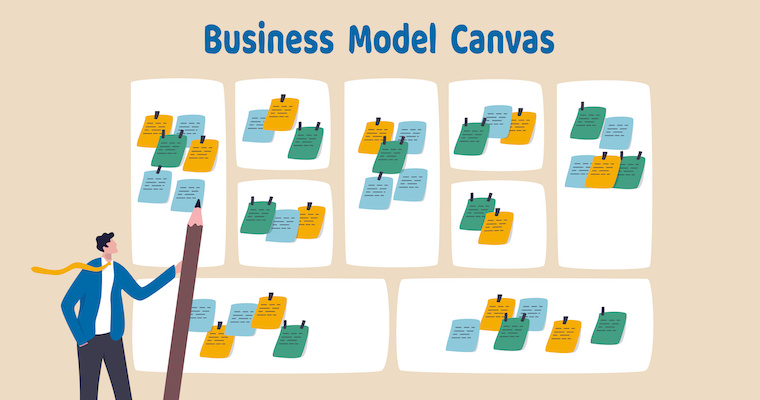
\includegraphics[keepaspectratio]{unidades/intro/../../images/external/business-understanding-canvas.jpeg}}

Ese artefacto es el \textbf{Business Understanding Canvas}. Es la salida
tangible de la primera fase de cualquier metodología estructurada de
minería de datos (formalizarás esto más adelante como la fase de
\emph{Business Understanding} de \textbf{CRISP-DM} (Chapman et~al. 2000;
Shearer 2000; Wirth y Hipp 2000)). Aquí lo construiremos de forma
práctica, aplicado a un caso real, para que cuando llegues al marco
metodológico completo ya tengas la intuición de qué problema resuelve
cada pieza.

\begin{tcolorbox}[enhanced jigsaw, arc=.35mm, bottomrule=.15mm, breakable, colback=white, colframe=quarto-callout-note-color-frame, left=2mm, leftrule=.75mm, opacityback=0, rightrule=.15mm, toprule=.15mm]

\textbf{Definición (Business Understanding Canvas)}. Documento de una
página que resume el objetivo de negocio, los criterios de éxito, los
supuestos y riesgos, y el plan de un proyecto de datos, sirviendo como
contrato de entendimiento entre el equipo analítico y los stakeholders
antes de tocar una sola fuente de datos. El formato de una página se
inspira en el lenguaje visual de los \emph{canvas} estratégicos
popularizado por Osterwalder y Pigneur (2010), aplicado aquí a la fase
de entendimiento del negocio de CRISP-DM.

\end{tcolorbox}

En este capítulo construirás las cinco piezas que componen la
documentación de entendimiento de negocio de un proyecto:

\begin{enumerate}
\def\labelenumi{\arabic{enumi}.}
\tightlist
\item
  Una \textbf{bitácora de reunión} con el stakeholder.
\item
  El \textbf{Business Understanding Canvas} de una página.
\item
  De \textbf{3 a 4 preguntas de investigación priorizadas}.
\item
  El \textbf{criterio de éxito en términos de negocio}.
\item
  Una \textbf{lista de supuestos y riesgos} (con al menos dos riesgos
  reales y su mitigación).
\end{enumerate}

Lo haremos continuando el caso de \textbf{TheLook eCommerce} introducido
en el capítulo anterior, donde el Director de Mercadotecnia solicitó
impulsar la nueva línea de accesorios de lujo entre las clientas
frecuentes de vestidos de diseñador.

\section{Paso 1: La Bitácora de la Reunión con el
Stakeholder}\label{paso-1-la-bituxe1cora-de-la-reuniuxf3n-con-el-stakeholder}

Antes de sintetizar nada, se documenta la conversación tal como ocurrió.
La bitácora (\emph{meeting log}) no es un resumen embellecido: es un
registro fiel de quién dijo qué, qué se acordó y qué quedó pendiente.
Sirve como fuente de verdad si más adelante hay desacuerdos sobre el
alcance del proyecto.

\subsection{Elementos mínimos de una
bitácora}\label{elementos-muxednimos-de-una-bituxe1cora}

\begin{itemize}
\tightlist
\item
  \textbf{Metadatos}: fecha, hora, duración, modalidad y lugar.
\item
  \textbf{Participantes}: nombre, rol y su cuadrante en la matriz de
  poder/interés.
\item
  \textbf{Contexto}: qué disparó la reunión.
\item
  \textbf{Preguntas y respuestas}: el intercambio real de la
  conversación de descubrimiento.
\item
  \textbf{Decisiones y acuerdos}: qué quedó explícitamente aceptado por
  ambas partes.
\item
  \textbf{Pendientes y próximos pasos}: con dueño y fecha.
\end{itemize}

\subsection{Ejemplo aplicado: Kickoff del proyecto ``Accesorios de
Lujo''}\label{ejemplo-aplicado-kickoff-del-proyecto-accesorios-de-lujo}

\begin{tcolorbox}[enhanced jigsaw, arc=.35mm, bottomrule=.15mm, breakable, colback=white, colframe=quarto-callout-tip-color-frame, left=2mm, leftrule=.75mm, opacityback=0, rightrule=.15mm, toprule=.15mm]

\vspace{-3mm}\textbf{Bitácora de Reunión --- Proyecto Accesorios de Lujo (TheLook eCommerce)}\vspace{3mm}

\textbf{Fecha}: 3 de agosto de 2026 · \textbf{Hora}: 10:00--10:40 (40
min) · \textbf{Modalidad}: Videollamada

\textbf{Participantes}:

{\def\LTcaptype{none} % do not increment counter
\begin{longtable}[]{@{}
  >{\raggedright\arraybackslash}p{(\linewidth - 4\tabcolsep) * \real{0.3333}}
  >{\raggedright\arraybackslash}p{(\linewidth - 4\tabcolsep) * \real{0.3333}}
  >{\raggedright\arraybackslash}p{(\linewidth - 4\tabcolsep) * \real{0.3333}}@{}}
\toprule\noalign{}
\begin{minipage}[b]{\linewidth}\raggedright
Nombre
\end{minipage} & \begin{minipage}[b]{\linewidth}\raggedright
Rol
\end{minipage} & \begin{minipage}[b]{\linewidth}\raggedright
Cuadrante (Poder/Interés)
\end{minipage} \\
\midrule\noalign{}
\endhead
\bottomrule\noalign{}
\endlastfoot
Director de Mercadotecnia & Patrocinador del proyecto & Alto Poder /
Alto Interés \\
Gerente de Inventario & Provee datos de stock por bodega & Alto Poder /
Bajo Interés \\
Analista de Datos (tú) & Traductor técnico & --- \\
\end{longtable}
}

\textbf{Contexto}: Seguimiento a la solicitud inicial de reporte de
clientes; se formaliza como proyecto tras la conversación de alineación
del capítulo anterior.

\textbf{Preguntas formuladas y respuestas}:

\begin{itemize}
\tightlist
\item
  \emph{``¿Qué significa `éxito' para ustedes en este proyecto: más
  ingresos, más margen, o retención de clientas VIP?''} →
  \textbf{Director}: \emph{``Margen. Los accesorios tienen 3x el margen
  de los vestidos; nos interesa que las clientas que ya gastan mucho
  añadan accesorios al carrito, no solo captar clientas nuevas.''}
\item
  \emph{``¿Con qué frecuencia necesitan actualizar las recomendaciones:
  por campaña, semanal, en tiempo real?''} → \textbf{Director}:
  \emph{``Por campaña está bien para el piloto. No necesitamos tiempo
  real todavía.''}
\item
  \emph{``¿Hay restricciones de inventario que debamos considerar antes
  de recomendar un accesorio?''} → \textbf{Gerente de Inventario}:
  \emph{``Sí. Varias piezas de la nueva línea tienen stock limitado en
  algunas bodegas regionales; no queremos promocionar algo que se agote
  en 48 horas.''}
\item
  \emph{``¿Existe un presupuesto o fecha límite fija?''} →
  \textbf{Director}: \emph{``Necesitamos resultados del piloto antes de
  la campaña de fin de año, así que en 6 semanas debemos tener algo
  accionable.''}
\end{itemize}

\textbf{Decisiones y acuerdos}:

\begin{itemize}
\tightlist
\item
  El piloto se enfoca en clientas con alta frecuencia de compra en la
  categoría vestidos/diseñador (no en toda la base de clientes).
\item
  El éxito se mide en \textbf{margen incremental}, no en volumen de
  ventas ni en métricas de modelo.
\item
  El Gerente de Inventario comparte semanalmente el archivo de stock por
  bodega para filtrar recomendaciones de productos con baja
  disponibilidad.
\end{itemize}

\textbf{Pendientes / Próximos pasos}:

{\def\LTcaptype{none} % do not increment counter
\begin{longtable}[]{@{}
  >{\raggedright\arraybackslash}p{(\linewidth - 4\tabcolsep) * \real{0.3333}}
  >{\raggedright\arraybackslash}p{(\linewidth - 4\tabcolsep) * \real{0.3333}}
  >{\raggedright\arraybackslash}p{(\linewidth - 4\tabcolsep) * \real{0.3333}}@{}}
\toprule\noalign{}
\begin{minipage}[b]{\linewidth}\raggedright
Acción
\end{minipage} & \begin{minipage}[b]{\linewidth}\raggedright
Dueño
\end{minipage} & \begin{minipage}[b]{\linewidth}\raggedright
Fecha límite
\end{minipage} \\
\midrule\noalign{}
\endhead
\bottomrule\noalign{}
\endlastfoot
Compartir acceso a tabla \texttt{inventory\_items} & Gerente de
Inventario & 5 de agosto de 2026 \\
Entregar canvas de entendimiento de negocio para validación & Analista
de Datos & 7 de agosto de 2026 \\
Validar canvas y dar luz verde a extracción de datos & Director de
Mercadotecnia & 10 de agosto de 2026 \\
\end{longtable}
}

\end{tcolorbox}

\section{Paso 2: El Business Understanding Canvas (Una
Página)}\label{paso-2-el-business-understanding-canvas-una-puxe1gina}

El canvas condensa la bitácora en seis bloques que cualquier persona del
negocio o del equipo técnico puede revisar en minutos. Estos seis
bloques no son arbitrarios: corresponden directamente a las tareas que
la guía CRISP-DM (Chapman et~al. 2000) define para la fase de Business
Understanding ---determinar objetivos de negocio, evaluar la situación,
determinar objetivos de minería de datos y producir un plan de
proyecto---, desdobladas aquí en sus criterios de éxito de negocio y
técnico. A diferencia de la bitácora ---que es cronológica y
detallada--- el canvas es \textbf{atemporal y sintético}: es el
documento que se archiva y se consulta durante todo el proyecto.

Observa que el bloque 5 (Éxito Técnico) usa una métrica de modelo
(\emph{lift}, confianza), mientras que el bloque 2 (Criterio de Éxito de
Negocio) usa una métrica financiera (margen incremental). Esta
distinción es intencional y se profundiza en el siguiente paso.

\section{Paso 3: Preguntas de Investigación
Priorizadas}\label{paso-3-preguntas-de-investigaciuxf3n-priorizadas}

Rara vez existe una sola pregunta analítica detrás de un proyecto. Es
tarea del analista descomponer el objetivo de negocio en varias
preguntas de investigación y \textbf{priorizarlas} según su impacto en
el negocio y la factibilidad de responderlas con los datos disponibles,
siguiendo la misma lógica de la matriz de poder/interés del capítulo
anterior, ahora aplicada a preguntas en vez de personas.

{\def\LTcaptype{none} % do not increment counter
\begin{longtable}[]{@{}
  >{\centering\arraybackslash}p{(\linewidth - 8\tabcolsep) * \real{0.1364}}
  >{\raggedright\arraybackslash}p{(\linewidth - 8\tabcolsep) * \real{0.1818}}
  >{\centering\arraybackslash}p{(\linewidth - 8\tabcolsep) * \real{0.2273}}
  >{\centering\arraybackslash}p{(\linewidth - 8\tabcolsep) * \real{0.2273}}
  >{\centering\arraybackslash}p{(\linewidth - 8\tabcolsep) * \real{0.2273}}@{}}
\toprule\noalign{}
\begin{minipage}[b]{\linewidth}\centering
\#
\end{minipage} & \begin{minipage}[b]{\linewidth}\raggedright
Pregunta de Investigación
\end{minipage} & \begin{minipage}[b]{\linewidth}\centering
Impacto de Negocio
\end{minipage} & \begin{minipage}[b]{\linewidth}\centering
Factibilidad de Datos
\end{minipage} & \begin{minipage}[b]{\linewidth}\centering
Prioridad
\end{minipage} \\
\midrule\noalign{}
\endhead
\bottomrule\noalign{}
\endlastfoot
1 & ¿Qué accesorios se compran junto con vestidos de diseñador con mayor
frecuencia? & Alto & Alto & \textbf{1 (Piloto)} \\
2 & ¿Qué accesorios recomendar cuando el stock regional es limitado, sin
frustrar la demanda? & Alto & Medio & \textbf{2} \\
3 & ¿El efecto de venta cruzada varía según la región o bodega de origen
del pedido? & Medio & Alto & \textbf{3} \\
4 & ¿Las clientas que reciben la recomendación aumentan su frecuencia de
compra a largo plazo (no solo el ticket)? & Alto & Bajo (requiere datos
longitudinales aún no disponibles) & \textbf{4 (Fuera de alcance del
piloto)} \\
\end{longtable}
}

La pregunta 1 concentra el esfuerzo del piloto porque combina alto
impacto con datos ya disponibles en el Data Warehouse. La pregunta 4,
aunque valiosa, requiere una ventana de observación más larga y queda
documentada para una segunda iteración, no descartada.

\section{Paso 4: Criterio de Éxito en Términos de
Negocio}\label{paso-4-criterio-de-uxe9xito-en-tuxe9rminos-de-negocio}

Un error común de analistas junior es definir el éxito exclusivamente
con métricas de modelo (precisión, \emph{recall}, AUC, \emph{lift}).
Esas métricas son necesarias pero \textbf{no son el criterio de éxito
del proyecto}: son el criterio de éxito del \emph{modelo}. El
stakeholder no puede evaluar si un AUC de 0.83 fue una buena inversión;
sí puede evaluar si el margen subió. Esta distinción entre el objetivo
de negocio y el objetivo de minería de datos es, según Provost y Fawcett
(2013), la fuente más frecuente de proyectos analíticos que producen
modelos técnicamente correctos pero comercialmente irrelevantes.

{\def\LTcaptype{none} % do not increment counter
\begin{longtable}[]{@{}
  >{\raggedright\arraybackslash}p{(\linewidth - 4\tabcolsep) * \real{0.3333}}
  >{\raggedright\arraybackslash}p{(\linewidth - 4\tabcolsep) * \real{0.3333}}
  >{\raggedright\arraybackslash}p{(\linewidth - 4\tabcolsep) * \real{0.3333}}@{}}
\toprule\noalign{}
\begin{minipage}[b]{\linewidth}\raggedright
Tipo de Criterio
\end{minipage} & \begin{minipage}[b]{\linewidth}\raggedright
Ejemplo en este proyecto
\end{minipage} & \begin{minipage}[b]{\linewidth}\raggedright
¿Quién lo evalúa?
\end{minipage} \\
\midrule\noalign{}
\endhead
\bottomrule\noalign{}
\endlastfoot
\textbf{Negocio} (el que importa para aprobar o cancelar el proyecto) &
+8\% de margen incremental en el segmento piloto vs.~grupo de control,
en 6 semanas & Director de Mercadotecnia \\
\textbf{Técnico} (el que usa el equipo de datos para iterar el modelo) &
\emph{Lift} \textgreater{} 1.2 y confianza \textgreater{} 30\% en las
reglas de asociación & Analista de Datos \\
\end{longtable}
}

\begin{tcolorbox}[enhanced jigsaw, arc=.35mm, bottomrule=.15mm, breakable, colback=white, colframe=quarto-callout-note-color-frame, left=2mm, leftrule=.75mm, opacityback=0, rightrule=.15mm, toprule=.15mm]

\textbf{Regla práctica}. Todo proyecto debe poder resumir su éxito en
una sola oración que un directivo sin conocimientos técnicos pueda
repetir de memoria. Si esa oración contiene un término estadístico (AUC,
\emph{lift}, silueta), probablemente estás describiendo el éxito
técnico, no el de negocio.

\end{tcolorbox}

\section{Paso 5: Supuestos y riesgos}\label{paso-5-supuestos-y-riesgos}

Todo canvas simplifica la complejidad del proyecto. Por ello, debe
complementarse con una lista de \textbf{supuestos} y un registro de
\textbf{riesgos}.

Un supuesto es una condición que se considera verdadera, aunque todavía
no se haya verificado. Un riesgo es un evento incierto que podría
afectar el desarrollo o los resultados del proyecto. Los supuestos deben
validarse; los riesgos, evaluarse y mitigarse.

\subsection{Supuestos}\label{supuestos}

Para el piloto se consideran los siguientes supuestos:

\begin{itemize}
\tightlist
\item
  El comportamiento histórico de compra conjunta ---por ejemplo, vestido
  y accesorio--- representa razonablemente el comportamiento futuro
  durante la campaña.
\item
  El archivo de inventario se actualizará semanalmente durante las seis
  semanas del piloto.
\item
  El segmento de clientas frecuentes contiene suficientes transacciones
  para generar reglas de asociación confiables.
\item
  El equipo de Mercadotecnia podrá incorporar las recomendaciones en su
  calendario de campaña.
\end{itemize}

Los supuestos más importantes deben comprobarse durante las primeras
etapas. Si alguno resulta falso, puede ser necesario modificar los
datos, el método o el alcance del proyecto.

\subsection{Clasificación de los
riesgos}\label{clasificaciuxf3n-de-los-riesgos}

Clasificar los riesgos permite asignarlos al equipo responsable y evita
reducir el análisis únicamente a problemas técnicos. En un proyecto
analítico pueden distinguirse cinco categorías principales:

\begin{itemize}
\tightlist
\item
  \textbf{Datos:} problemas de calidad, disponibilidad, actualización o
  representatividad.
\item
  \textbf{Analíticos:} sesgo, estacionalidad, sobreajuste, asociaciones
  espurias o pérdida de desempeño.
\item
  \textbf{Operativos:} falta de inventario, capacidad insuficiente o
  procesos que no pueden utilizar los resultados.
\item
  \textbf{Tecnológicos y de seguridad:} fallas de integración, permisos
  excesivos, accesos no autorizados o interrupciones de los sistemas.
\item
  \textbf{Legales, éticos y reputacionales:} uso indebido de datos
  personales, discriminación o personalización percibida como invasiva.
\end{itemize}

También pueden existir riesgos de adopción cuando los usuarios no
comprenden, no confían o no utilizan la solución.

\subsection{Evaluación de los
riesgos}\label{evaluaciuxf3n-de-los-riesgos}

Cada riesgo debe evaluarse según su \textbf{probabilidad} y su
\textbf{impacto}. Esta valoración permite priorizar los riesgos que
requieren atención inmediata.

Además de la mitigación, conviene registrar:

\begin{itemize}
\tightlist
\item
  la persona responsable;
\item
  la señal que indicaría que el riesgo está ocurriendo;
\item
  el control preventivo;
\item
  y el plan de contingencia.
\end{itemize}

\subsection{Registro de riesgos del
proyecto}\label{registro-de-riesgos-del-proyecto}

{\def\LTcaptype{none} % do not increment counter
\begin{longtable}[]{@{}
  >{\centering\arraybackslash}p{(\linewidth - 10\tabcolsep) * \real{0.1200}}
  >{\raggedright\arraybackslash}p{(\linewidth - 10\tabcolsep) * \real{0.1600}}
  >{\raggedright\arraybackslash}p{(\linewidth - 10\tabcolsep) * \real{0.1600}}
  >{\centering\arraybackslash}p{(\linewidth - 10\tabcolsep) * \real{0.2000}}
  >{\centering\arraybackslash}p{(\linewidth - 10\tabcolsep) * \real{0.2000}}
  >{\raggedright\arraybackslash}p{(\linewidth - 10\tabcolsep) * \real{0.1600}}@{}}
\toprule\noalign{}
\begin{minipage}[b]{\linewidth}\centering
\#
\end{minipage} & \begin{minipage}[b]{\linewidth}\raggedright
Clasificación
\end{minipage} & \begin{minipage}[b]{\linewidth}\raggedright
Riesgo
\end{minipage} & \begin{minipage}[b]{\linewidth}\centering
Probabilidad
\end{minipage} & \begin{minipage}[b]{\linewidth}\centering
Impacto
\end{minipage} & \begin{minipage}[b]{\linewidth}\raggedright
Mitigación
\end{minipage} \\
\midrule\noalign{}
\endhead
\bottomrule\noalign{}
\endlastfoot
1 & Privacidad & La extracción de información de clientas VIP podría
exponer datos personales fuera del equipo autorizado, incumpliendo la
Ley Federal de Protección de Datos Personales en Posesión de los
Particulares (Congreso de los Estados Unidos Mexicanos 2010). & Media &
Alto & Eliminar identificadores innecesarios, aplicar controles IAM/RBAC
y mantener registros de acceso. \\
2 & Operativo & El modelo podría recomendar accesorios sin inventario
suficiente. & Alta & Medio & Validar las recomendaciones contra
\texttt{inventory\_items} antes de cada campaña y establecer un nivel
mínimo de existencias. \\
3 & Analítico & Las asociaciones podrían estar influenciadas por una
temporada específica y no repetirse durante el piloto. & Media & Medio &
Comparar las reglas en distintas ventanas temporales antes de
utilizarlas. \\
4 & Datos & El archivo de inventario podría estar incompleto o
desactualizado. & Alta & Alto & Automatizar controles de actualidad y
suspender el envío si la fuente no supera las validaciones. \\
5 & Adopción & Mercadotecnia podría no utilizar las recomendaciones si
no comprende su origen o utilidad. & Media & Medio & Explicar cada
recomendación, capacitar a los usuarios y recopilar retroalimentación
durante el piloto. \\
\end{longtable}
}

\subsection{Tratamiento y seguimiento}\label{tratamiento-y-seguimiento}

Después de evaluar un riesgo, el equipo puede:

\begin{enumerate}
\def\labelenumi{\arabic{enumi}.}
\tightlist
\item
  \textbf{Evitarlo:} modificar el diseño para eliminar su causa.
\item
  \textbf{Mitigarlo:} reducir su probabilidad o impacto.
\item
  \textbf{Transferirlo:} compartir su gestión con un proveedor o área
  especializada.
\item
  \textbf{Aceptarlo:} reconocerlo y preparar una contingencia.
\end{enumerate}

El registro debe revisarse durante el piloto y actualizarse cuando
cambien los datos, el modelo o las condiciones operativas.

\begin{tcolorbox}[enhanced jigsaw, arc=.35mm, bottomrule=.15mm, breakable, colback=white, colframe=quarto-callout-important-color-frame, left=2mm, leftrule=.75mm, opacityback=0, rightrule=.15mm, toprule=.15mm]

Un modelo puede ser técnicamente correcto y, aun así, resultar
inutilizable si emplea datos sin autorización, recomienda productos
agotados o genera resultados que la operación no puede atender. Por
ello, los riesgos deben identificarse desde el entendimiento del negocio
y revisarse durante todo el proyecto.

\end{tcolorbox}

\subsection{Resumen de la gestión de
riesgos}\label{resumen-de-la-gestiuxf3n-de-riesgos}

\section{Actividad: Construye tu Propio Business Understanding
Canvas}\label{actividad-construye-tu-propio-business-understanding-canvas}

Usando la plantilla en blanco a continuación, elige un escenario de
negocio (puede ser uno de los cuatro casos de TheLook eCommerce del
capítulo anterior, u otro que definas con tu instructor) y completa las
cinco piezas de este capítulo:

\begin{enumerate}
\def\labelenumi{\arabic{enumi}.}
\tightlist
\item
  Escribe una bitácora simulada de una reunión de 30-40 minutos con el
  stakeholder, incluyendo al menos tres preguntas de descubrimiento y
  sus respuestas.
\item
  Completa el canvas de seis bloques.
\item
  Prioriza entre 3 y 4 preguntas de investigación usando la tabla de
  impacto/factibilidad.
\item
  Redacta el criterio de éxito de negocio en una sola oración, y su
  contraparte técnica.
\item
  Documenta al menos dos riesgos reales (no genéricos) con su
  mitigación.
\end{enumerate}

Este documento será la base sobre la que construirás el proyecto de
datos a lo largo del curso: cada decisión posterior de modelado en las
Partes III a V deberá poder justificarse trazándola de vuelta a alguno
de estos cinco elementos.

\section{Referencias}\label{referencias-2}

\protect\phantomsection\label{refs}
\begin{CSLReferences}{1}{1}
\bibitem[\citeproctext]{ref-aggarwal2013}
Aggarwal, Charu C., y Chandan K. Reddy. 2013. \emph{Data Clustering:
Algorithms and Applications}. CRC Press.

\bibitem[\citeproctext]{ref-agrawal1994fast}
Agrawal, Rakesh, y Ramakrishnan Srikant. 1994. {«Fast Algorithms for
Mining Association Rules in Large Databases»}. \emph{Proceedings of the
20th International Conference on Very Large Data Bases}, VLDB '94,
487-99.

\bibitem[\citeproctext]{ref-aws_sagemaker}
Amazon Web Services. 2024. \emph{Amazon SageMaker Documentation}. AWS
Documentation.
\url{https://docs.aws.amazon.com/sagemaker/latest/dg/whatis.html}.

\bibitem[\citeproctext]{ref-bigmart_dataset}
Analytics Vidhya. 2016. \emph{BigMart Sales Prediction (Practice
Problem)}. DataHack Platform.
\url{https://www.analyticsvidhya.com/datahack/contest/big-mart-sales-prediction/}.

\bibitem[\citeproctext]{ref-anscombe1973graphs}
Anscombe, Francis J. 1973. {«Graphs in Statistical Analysis»}. \emph{The
American Statistician} 27 (1): 17-21.
\url{https://doi.org/10.1080/00031305.1973.10478966}.

\bibitem[\citeproctext]{ref-arthur2007}
Arthur, David, y Sergei Vassilvitskii. 2007. {«k-means++: the advantages
of careful seeding»}. \emph{Proceedings of the Eighteenth Annual
ACM-SIAM Symposium on Discrete Algorithms}, 1027-35.

\bibitem[\citeproctext]{ref-bellman1961adaptive}
Bellman, Richard E. 1961. \emph{Adaptive Control Processes: A Guided
Tour}. Princeton University Press.

\bibitem[\citeproctext]{ref-berger1985statistical}
Berger, James O. 1985. \emph{Statistical Decision Theory and Bayesian
Analysis}. 2.ª ed. Springer.

\bibitem[\citeproctext]{ref-bishop2006}
Bishop, Christopher M. 2006. \emph{Pattern Recognition and Machine
Learning}. Information Science y Statistics. Springer.

\bibitem[\citeproctext]{ref-borgelt2005implementation}
Borgelt, Christian. 2005. {«An Implementation of the FP-growth
Algorithm»}. \emph{Proceedings of the 1st International Workshop on Open
Source Data Mining: Frequent Pattern Mining Implementations}, 1-5.
\url{https://doi.org/10.1145/1133905.1133907}.

\bibitem[\citeproctext]{ref-bradbury2018jax}
Bradbury, James, Roy Frostig, Peter Hawkins, et~al. 2018. \emph{{JAX}:
Composable Transformations of {Python}+{NumPy} Programs}. Released.
\url{http://github.com/jax-ml/jax}.

\bibitem[\citeproctext]{ref-breiman1996bagging}
Breiman, Leo. 1996. {«Bagging Predictors»}. \emph{Machine Learning} 24
(2): 123-40. \url{https://doi.org/10.1007/BF00058655}.

\bibitem[\citeproctext]{ref-breiman2001}
Breiman, Leo. 2001. {«Random Forests»}. \emph{Machine Learning} 45 (1):
5-32. \url{https://doi.org/10.1023/A:1010933404324}.

\bibitem[\citeproctext]{ref-breiman1984}
Breiman, Leo, Jerome H. Friedman, Richard A. Olshen, y Charles J. Stone.
1984. \emph{Classification and Regression Trees}. Wadsworth
International Group.

\bibitem[\citeproctext]{ref-bryson2004}
Bryson, John M. 2004. {«What to do when stakeholders matter: Stakeholder
identification and analysis techniques»}. \emph{Public Management
Review} 6 (1): 21-53.
\url{https://doi.org/10.1080/14719030410001675722}.

\bibitem[\citeproctext]{ref-calinski1974}
Caliński, Tadeusz, y Józef Harabasz. 1974. {«A dendrite method for
cluster analysis»}. \emph{Communications in Statistics} 3 (1): 1-27.

\bibitem[\citeproctext]{ref-campello2013}
Campello, Ricardo J. G. B., Davoud Moulavi, y Jörg Sander. 2013.
{«Density-based clustering based on hierarchical density estimates»}.
\emph{Advances in Knowledge Discovery and Data Mining}, Lecture Notes en
Computer Science, vol. 7819: 160-72.

\bibitem[\citeproctext]{ref-ctb_kansas}
Center for Community Health and Development, University of Kansas. 2023.
\emph{Chapter 7, Section 8: Identifying and Analyzing Stakeholders and
Their Interests}. Community Tool Box.
\url{https://ctb.ku.edu/en/table-of-contents/participation/encouraging-involvement/identify-stakeholders/main}.

\bibitem[\citeproctext]{ref-chang2011libsvm}
Chang, Chih-Chung, y Chih-Jen Lin. 2011. {«{LIBSVM}: A Library for
Support Vector Machines»}. \emph{ACM Transactions on Intelligent Systems
and Technology} 2 (3): 27:1-27.
\url{https://doi.org/10.1145/1961189.1961199}.

\bibitem[\citeproctext]{ref-chapman2000}
Chapman, Pete, Julian Clinton, Randy Kerber, et~al. 2000. \emph{CRISP-DM
1.0: Step-by-Step Data Mining Guide}. SPSS Inc.

\bibitem[\citeproctext]{ref-chaudhuri1997overview}
Chaudhuri, Surajit, y Umeshwar Dayal. 1997. {«An Overview of Data
Warehousing and OLAP Technology»}. \emph{ACM SIGMOD Record} 26 (1):
65-74. \url{https://doi.org/10.1145/248603.248616}.

\bibitem[\citeproctext]{ref-chen2016xgboost}
Chen, Tianqi, y Carlos Guestrin. 2016. {«{XGBoost}: A Scalable Tree
Boosting System»}. \emph{Proceedings of the 22nd ACM SIGKDD
International Conference on Knowledge Discovery and Data Mining},
785-94. \url{https://doi.org/10.1145/2939672.2939785}.

\bibitem[\citeproctext]{ref-lfpdppp2010}
Congreso de los Estados Unidos Mexicanos. 2010. \emph{Ley Federal de
Protección de Datos Personales en Posesión de los Particulares}. Diario
Oficial de la Federación.
\url{https://www.diputados.gob.mx/LeyesBiblio/pdf/LFPDPPP.pdf}.

\bibitem[\citeproctext]{ref-cortes1995support}
Cortes, Corinna, y Vladimir N. Vapnik. 1995. {«Support-Vector
Networks»}. \emph{Machine Learning} 20 (3): 273-97.
\url{https://doi.org/10.1007/BF00994018}.

\bibitem[\citeproctext]{ref-cover1967nearest}
Cover, Thomas M., y Peter E. Hart. 1967. {«Nearest Neighbor Pattern
Classification»}. \emph{IEEE Transactions on Information Theory} 13 (1):
21-27. \url{https://doi.org/10.1109/TIT.1967.1053964}.

\bibitem[\citeproctext]{ref-cubejs2024docs}
Cube Dev, Inc. 2024. \emph{Cube Documentation}. Cube Dev.
\url{https://cube.dev/docs/}.

\bibitem[\citeproctext]{ref-cybenko1989approximation}
Cybenko, George. 1989. {«Approximation by Superpositions of a Sigmoidal
Function»}. \emph{Mathematics of Control, Signals, and Systems} 2 (4):
303-14.

\bibitem[\citeproctext]{ref-dama2017}
DAMA International. 2017. \emph{DAMA-DMBOK: Data Management Body of
Knowledge}. 2nd ed. Technics Publications.

\bibitem[\citeproctext]{ref-databricks_home}
Databricks. 2024. \emph{Databricks: The Data and AI Company}.
Databricks. \url{https://www.databricks.com}.

\bibitem[\citeproctext]{ref-davenport2012}
Davenport, Thomas H., y D. J. Patil. 2012. {«Data Scientist: The Sexiest
Job of the 21st Century»}. \emph{Harvard Business Review} 90 (10):
70-76.

\bibitem[\citeproctext]{ref-davies1979}
Davies, David L., y Donald W. Bouldin. 1979. {«A cluster separation
measure»}. \emph{IEEE Transactions on Pattern Analysis and Machine
Intelligence} 1 (2): 224-27.

\bibitem[\citeproctext]{ref-dbtlabs2024semanticlayer}
{dbt Labs}. 2024. \emph{dbt Semantic Layer Documentation}. Dbt Labs.
\url{https://docs.getdbt.com/docs/use-dbt-semantic-layer/dbt-sl}.

\bibitem[\citeproctext]{ref-deepmind2020optax}
DeepMind, Igor Babuschkin, Kate Baumli, et~al. 2020. \emph{The
{DeepMind} {JAX} Ecosystem}. Released.
\url{http://github.com/google-deepmind}.

\bibitem[\citeproctext]{ref-dehghani2022datamesh}
Dehghani, Zhamak. 2022. \emph{Data Mesh: Delivering Data-Driven Value at
Scale}. O'Reilly Media.

\bibitem[\citeproctext]{ref-dempster1977}
Dempster, Arthur P., Nan M. Laird, y Donald B. Rubin. 1977. {«Maximum
Likelihood from Incomplete Data via the {EM} Algorithm»}. \emph{Journal
of the Royal Statistical Society, Series B} 39 (1): 1-38.

\bibitem[\citeproctext]{ref-devlin1988architecture}
Devlin, Barry A., y Paul T. Murphy. 1988. {«An Architecture for a
Business and Information System»}. \emph{IBM Systems Journal} 27 (1):
60-80. \url{https://doi.org/10.1147/sj.271.0060}.

\bibitem[\citeproctext]{ref-duda2001pattern}
Duda, Richard O., Peter E. Hart, y David G. Stork. 2001. \emph{Pattern
Classification}. 2.ª ed. Wiley.

\bibitem[\citeproctext]{ref-durbin1998biological}
Durbin, Richard, Sean R. Eddy, Anders Krogh, y Graeme Mitchison. 1998.
\emph{Biological Sequence Analysis: Probabilistic Models of Proteins and
Nucleic Acids}. Cambridge University Press.

\bibitem[\citeproctext]{ref-ester1996}
Ester, Martin, Hans-Peter Kriegel, Jörg Sander, y Xiaowei Xu. 1996. {«A
density-based algorithm for discovering clusters in large spatial
databases with noise»}. \emph{Proceedings of the Second International
Conference on Knowledge Discovery and Data Mining}, 226-31.

\bibitem[\citeproctext]{ref-fawcett2006}
Fawcett, Tom. 2006. {«An introduction to {ROC} analysis»}. \emph{Pattern
Recognition Letters} 27 (8): 861-74.
\url{https://doi.org/10.1016/j.patrec.2005.10.010}.

\bibitem[\citeproctext]{ref-fayyad1996}
Fayyad, Usama, Gregory Piatetsky-Shapiro, y Padhraic Smyth. 1996. {«From
data mining to knowledge discovery in databases»}. \emph{AI Magazine} 17
(3): 37-54. \url{https://doi.org/10.1609/aimag.v17i3.1230}.

\bibitem[\citeproctext]{ref-fielding2000rest}
Fielding, Roy Thomas. 2000. {«Architectural Styles and the Design of
Network-based Software Architectures»}. Tesis doctoral, University of
California, Irvine.

\bibitem[\citeproctext]{ref-fisher1936use}
Fisher, Ronald A. 1936. {«The Use of Multiple Measurements in Taxonomic
Problems»}. \emph{Annals of Eugenics} 7 (2): 179-88.
\url{https://doi.org/10.1111/j.1469-1809.1936.tb02137.x}.

\bibitem[\citeproctext]{ref-fowler2010richardson}
Fowler, Martin. 2010. \emph{Richardson Maturity Model}.
Martinfowler.com.
\url{https://martinfowler.com/articles/richardsonMaturityModel.html}.

\bibitem[\citeproctext]{ref-freedman2007statistics}
Freedman, David, Robert Pisani, y Roger Purves. 2007. \emph{Statistics}.
4.ª ed. W. W. Norton.

\bibitem[\citeproctext]{ref-freeman1984}
Freeman, R. Edward. 1984. \emph{Strategic Management: A Stakeholder
Approach}. Pitman.

\bibitem[\citeproctext]{ref-freund1997decision}
Freund, Yoav, y Robert E. Schapire. 1997. {«A Decision-Theoretic
Generalization of On-Line Learning and an Application to Boosting»}.
\emph{Journal of Computer and System Sciences} 55 (1): 119-39.
\url{https://doi.org/10.1006/jcss.1997.1504}.

\bibitem[\citeproctext]{ref-friedman2001greedy}
Friedman, Jerome H. 2001. {«Greedy Function Approximation: A Gradient
Boosting Machine»}. \emph{The Annals of Statistics} 29 (5): 1189-232.
\url{https://doi.org/10.1214/aos/1013203451}.

\bibitem[\citeproctext]{ref-friedman2002stochastic}
Friedman, Jerome H. 2002. {«Stochastic Gradient Boosting»}.
\emph{Computational Statistics \& Data Analysis} 38 (4): 367-78.
\url{https://doi.org/10.1016/S0167-9473(01)00065-2}.

\bibitem[\citeproctext]{ref-friedman1977algorithm}
Friedman, Jerome H., Jon Louis Bentley, y Raphael Ari Finkel. 1977. {«An
Algorithm for Finding Best Matches in Logarithmic Expected Time»}.
\emph{ACM Transactions on Mathematical Software} 3 (3): 209-26.
\url{https://doi.org/10.1145/355744.355745}.

\bibitem[\citeproctext]{ref-fukunaga1975branch}
Fukunaga, Keinosuke, y Patrenahalli M. Narendra. 1975. {«A Branch and
Bound Algorithm for Computing k-Nearest Neighbors»}. \emph{IEEE
Transactions on Computers} C-24 (7): 750-53.
\url{https://doi.org/10.1109/T-C.1975.224297}.

\bibitem[\citeproctext]{ref-gardiner1987cpg}
Gardiner-Garden, Margaret, y Marianne Frommer. 1987. {«CpG Islands in
Vertebrate Genomes»}. \emph{Journal of Molecular Biology} 196 (2):
261-82. \url{https://doi.org/10.1016/0022-2836(87)90689-9}.

\bibitem[\citeproctext]{ref-gauss1809theoria}
Gauss, Carl Friedrich. 1809. \emph{Theoria Motus Corporum Coelestium in
Sectionibus Conicis Solem Ambientium}. Friedrich Perthes; I. H. Besser.

\bibitem[\citeproctext]{ref-geron2022hands}
Géron, Aurélien. 2022. \emph{Hands-On Machine Learning with
Scikit-Learn, Keras, and TensorFlow}. 3.ª ed. O'Reilly Media.

\bibitem[\citeproctext]{ref-gini1912variabilita}
Gini, Corrado. 1912. {«Variabilità e mutabilità»}. \emph{Studi
Economico-Giuridici della Regia Università di Cagliari} 3: 1-158.

\bibitem[\citeproctext]{ref-golub2013matrix}
Golub, Gene H., y Charles F. Van Loan. 2013. \emph{Matrix Computations}.
4.ª ed. Johns Hopkins University Press.

\bibitem[\citeproctext]{ref-goodfellow2016deep}
Goodfellow, Ian, Yoshua Bengio, y Aaron Courville. 2016. \emph{Deep
Learning}. MIT Press.

\bibitem[\citeproctext]{ref-google2022}
Google. 2022. \emph{Foundations: Data, Data, Everywhere}. Google Data
Analytics Professional Certificate, Coursera.

\bibitem[\citeproctext]{ref-google_vertexai}
Google Cloud. 2024. \emph{Vertex AI Documentation}. Google Cloud
Documentation. \url{https://cloud.google.com/vertex-ai/docs}.

\bibitem[\citeproctext]{ref-graphql2021spec}
GraphQL Foundation. 2021. \emph{GraphQL Specification}. GraphQL
Foundation. \url{https://spec.graphql.org/}.

\bibitem[\citeproctext]{ref-gray1997data}
Gray, Jim, Adam Bosworth, Andrew Layman, y Hamid Pirahesh. 1996. {«Data
Cube: A Relational Aggregation Operator Generalizing Group-By,
Cross-Tab, and Sub-Totals»}. \emph{Proceedings of the Twelfth
International Conference on Data Engineering}, 152-59.
\url{https://doi.org/10.1109/ICDE.1996.492099}.

\bibitem[\citeproctext]{ref-han2011}
Han, Jiawei, Micheline Kamber, y Jian Pei. 2011. \emph{Data Mining:
Concepts and Techniques}. 3.ª ed. Morgan Kaufmann.
\url{https://doi.org/10.1016/B978-0-12-381479-1.00001-0}.

\bibitem[\citeproctext]{ref-han2012data}
Han, Jiawei, Micheline Kamber, y Jian Pei. 2012. \emph{Data Mining:
Concepts and Techniques}. 3.ª ed. Morgan Kaufmann.

\bibitem[\citeproctext]{ref-han2000mining}
Han, Jiawei, Jian Pei, y Yiwen Yin. 2000. {«Mining Frequent Patterns
without Candidate Generation»}. \emph{Proceedings of the 2000 ACM SIGMOD
International Conference on Management of Data}, SIGMOD '00, 1-12.
\url{https://doi.org/10.1145/342009.335372}.

\bibitem[\citeproctext]{ref-hart1968condensed}
Hart, Peter E. 1968. {«The Condensed Nearest Neighbor Rule»}. \emph{IEEE
Transactions on Information Theory} 14 (3): 515-16.
\url{https://doi.org/10.1109/TIT.1968.1054155}.

\bibitem[\citeproctext]{ref-hastie2009}
Hastie, Trevor, Robert Tibshirani, y Jerome Friedman. 2009. \emph{The
Elements of Statistical Learning: Data Mining, Inference, and
Prediction}. 2.ª ed. Springer Series en Statistics. Springer.
\url{https://doi.org/10.1007/978-0-387-84858-7}.

\bibitem[\citeproctext]{ref-nist2012handbook}
Heckert, N. Alan, James J. Filliben, Carroll M. Croarkin, et~al. 2012.
\emph{NIST/SEMATECH e-Handbook of Statistical Methods}. National
Institute of Standards; Technology.
\url{https://www.itl.nist.gov/div898/handbook/}.

\bibitem[\citeproctext]{ref-heek2023flax}
Heek, Jonathan, Anselm Levskaya, Avital Oliver, et~al. 2023. \emph{Flax:
A Neural Network Library and Ecosystem for {JAX}}. Released.
\url{http://github.com/google/flax}.

\bibitem[\citeproctext]{ref-hill1973diversity}
Hill, Mark O. 1973. {«Diversity and Evenness: A Unifying Notation and
Its Consequences»}. \emph{Ecology} 54 (2): 427-32.
\url{https://doi.org/10.2307/1934352}.

\bibitem[\citeproctext]{ref-hirschman1945national}
Hirschman, Albert O. 1945. \emph{National Power and the Structure of
Foreign Trade}. University of California Press.

\bibitem[\citeproctext]{ref-hochreiter1997long}
Hochreiter, Sepp, y Jürgen Schmidhuber. 1997. {«Long Short-Term
Memory»}. \emph{Neural Computation} 9 (8): 1735-80.

\bibitem[\citeproctext]{ref-hoerl1970ridge}
Hoerl, Arthur E., y Robert W. Kennard. 1970. {«Ridge Regression: Biased
Estimation for Nonorthogonal Problems»}. \emph{Technometrics} 12 (1):
55-67. \url{https://doi.org/10.1080/00401706.1970.10488634}.

\bibitem[\citeproctext]{ref-hornik1989multilayer}
Hornik, Kurt, Maxwell Stinchcombe, y Halbert White. 1989. {«Multilayer
Feedforward Networks are Universal Approximators»}. \emph{Neural
Networks} 2 (5): 359-66.

\bibitem[\citeproctext]{ref-hosmer2013}
Hosmer, David W., Stanley Lemeshow, y Rodney X. Sturdivant. 2013.
\emph{Applied Logistic Regression}. 3.ª ed. John Wiley \& Sons.

\bibitem[\citeproctext]{ref-huber2009robust}
Huber, Peter J., y Elvezio M. Ronchetti. 2009. \emph{Robust Statistics}.
2.ª ed. Wiley. \url{https://doi.org/10.1002/9780470434697}.

\bibitem[\citeproctext]{ref-hubert1985}
Hubert, Lawrence, y Phipps Arabie. 1985. {«Comparing partitions»}.
\emph{Journal of Classification} 2 (1): 193-218.

\bibitem[\citeproctext]{ref-hyndman1996quantiles}
Hyndman, Rob J., y Yanan Fan. 1996. {«Sample Quantiles in Statistical
Packages»}. \emph{The American Statistician} 50 (4): 361-65.
\url{https://doi.org/10.1080/00031305.1996.10473566}.

\bibitem[\citeproctext]{ref-ibm_asumdm}
IBM. 2015. \emph{Analytics Solutions Unified Method (ASUM-DM)}. IBM
Corporation, internal methodology derived from CRISP-DM.
\url{https://public.dhe.ibm.com/software/data/sw-library/services/ASUM.pdf}.

\bibitem[\citeproctext]{ref-inmon2005building}
Inmon, William H. 2005. \emph{Building the Data Warehouse}. 4.ª ed.
Wiley.

\bibitem[\citeproctext]{ref-james2021}
James, Gareth, Daniela Witten, Trevor Hastie, y Robert Tibshirani. 2021.
\emph{An Introduction to Statistical Learning with Applications in {R}}.
2.ª ed. Springer Texts en Statistics. Springer.
\url{https://doi.org/10.1007/978-1-0716-1418-1}.

\bibitem[\citeproctext]{ref-jaynes2003probability}
Jaynes, Edwin T. 2003. \emph{Probability Theory: The Logic of Science}.
Cambridge University Press.

\bibitem[\citeproctext]{ref-joanes1998skewness}
Joanes, D. N., y C. A. Gill. 1998. {«Comparing Measures of Sample
Skewness and Kurtosis»}. \emph{Journal of the Royal Statistical Society:
Series D (The Statistician)} 47 (1): 183-89.
\url{https://doi.org/10.1111/1467-9884.00122}.

\bibitem[\citeproctext]{ref-jolliffe2002}
Jolliffe, Ian T. 2002. \emph{Principal Component Analysis}. 2nd ed.
Springer.

\bibitem[\citeproctext]{ref-jost2006entropy}
Jost, Lou. 2006. {«Entropy and Diversity»}. \emph{Oikos} 113 (2):
363-75. \url{https://doi.org/10.1111/j.2006.0030-1299.14714.x}.

\bibitem[\citeproctext]{ref-kaufman1990}
Kaufman, Leonard, y Peter J. Rousseeuw. 1990. \emph{Finding Groups in
Data: An Introduction to Cluster Analysis}. Wiley.

\bibitem[\citeproctext]{ref-ke2017lightgbm}
Ke, Guolin, Qi Meng, Thomas Finley, et~al. 2017. {«LightGBM: A Highly
Efficient Gradient Boosting Decision Tree»}. \emph{Advances in Neural
Information Processing Systems} 30.

\bibitem[\citeproctext]{ref-kendall1938measure}
Kendall, Maurice G. 1938. {«A New Measure of Rank Correlation»}.
\emph{Biometrika} 30 (1/2): 81-93.
\url{https://doi.org/10.2307/2332226}.

\bibitem[\citeproctext]{ref-kimball2013}
Kimball, Ralph, y Margy Ross. 2013. \emph{The Data Warehouse Toolkit:
The Definitive Guide to Dimensional Modeling}. 3.ª ed. Wiley.

\bibitem[\citeproctext]{ref-kingma2015adam}
Kingma, Diederik P., y Jimmy Ba. 2015. {«Adam: A Method for Stochastic
Optimization»}. \emph{International Conference on Learning
Representations (ICLR)}.

\bibitem[\citeproctext]{ref-kleppmann2017designing}
Kleppmann, Martin. 2017. \emph{Designing Data-Intensive Applications}.
O'Reilly Media.

\bibitem[\citeproctext]{ref-kohavi1995}
Kohavi, Ron. 1995. {«A Study of Cross-Validation and Bootstrap for
Accuracy Estimation and Model Selection»}. \emph{Proceedings of the 14th
International Joint Conference on Artificial Intelligence (IJCAI)} 2:
1137-43.

\bibitem[\citeproctext]{ref-kohavi2020trustworthy}
Kohavi, Ron, Diane Tang, y Ya Xu. 2020. \emph{Trustworthy Online
Controlled Experiments: A Practical Guide to A/B Testing}. Cambridge
University Press.

\bibitem[\citeproctext]{ref-lecun2015deep}
LeCun, Yann, Yoshua Bengio, y Geoffrey Hinton. 2015. {«Deep Learning»}.
\emph{Nature} 521: 436-44.

\bibitem[\citeproctext]{ref-lecun1998gradient}
LeCun, Yann, Léon Bottou, Yoshua Bengio, y Patrick Haffner. 1998.
{«Gradient-Based Learning Applied to Document Recognition»}.
\emph{Proceedings of the IEEE} 86 (11): 2278-324.

\bibitem[\citeproctext]{ref-legendre1805nouvelles}
Legendre, Adrien-Marie. 1805. \emph{Nouvelles méthodes pour la
détermination des orbites des comètes}. Firmin Didot.

\bibitem[\citeproctext]{ref-lloyd1982}
Lloyd, Stuart P. 1982. {«Least squares quantization in {PCM}»}.
\emph{IEEE Transactions on Information Theory} 28 (2): 129-37.

\bibitem[\citeproctext]{ref-lorenz1905concentration}
Lorenz, Max O. 1905. {«Methods of Measuring the Concentration of
Wealth»}. \emph{Publications of the American Statistical Association} 9
(70): 209-19. \url{https://doi.org/10.2307/2276207}.

\bibitem[\citeproctext]{ref-lundberg2020local2global}
Lundberg, Scott M., Gabriel Erion, Hugh Chen, et~al. 2020. {«From Local
Explanations to Global Understanding with Explainable {AI} for Trees»}.
\emph{Nature Machine Intelligence} 2: 56-67.
\url{https://doi.org/10.1038/s42256-019-0138-9}.

\bibitem[\citeproctext]{ref-lundberg2017unified}
Lundberg, Scott M., y Su-In Lee. 2017. {«A Unified Approach to
Interpreting Model Predictions»}. \emph{Advances in Neural Information
Processing Systems} 30.

\bibitem[\citeproctext]{ref-maaten2008}
Maaten, Laurens van der, y Geoffrey Hinton. 2008. {«Visualizing data
using {t-SNE}»}. \emph{Journal of Machine Learning Research} 9:
2579-605.

\bibitem[\citeproctext]{ref-macqueen1967}
MacQueen, James. 1967. {«Some methods for classification and analysis of
multivariate observations»}. \emph{Proceedings of the Fifth Berkeley
Symposium on Mathematical Statistics and Probability} 1: 281-97.

\bibitem[\citeproctext]{ref-mccallum1998comparison}
McCallum, Andrew, y Kamal Nigam. 1998. {«A Comparison of Event Models
for Naive Bayes Text Classification»}. \emph{AAAI-98 Workshop on
Learning for Text Categorization}, 41-48.

\bibitem[\citeproctext]{ref-mccullagh1989}
McCullagh, Peter, y John A. Nelder. 1989. \emph{Generalized Linear
Models}. 2.ª ed. Chapman \& Hall.

\bibitem[\citeproctext]{ref-mcinnes2018}
McInnes, Leland, John Healy, y James Melville. 2018. {«{UMAP}: Uniform
Manifold Approximation and Projection for Dimension Reduction»}.
\emph{arXiv preprint arXiv:1802.03426}.

\bibitem[\citeproctext]{ref-mckinney2010data}
McKinney, Wes. 2010. {«Data Structures for Statistical Computing in
Python»}. \emph{Proceedings of the 9th Python in Science Conference},
56-61. \url{https://doi.org/10.25080/Majora-92bf1922-00a}.

\bibitem[\citeproctext]{ref-mclachlan2000}
McLachlan, Geoffrey J., y David Peel. 2000. \emph{Finite Mixture
Models}. Wiley Series en Probability y Statistics. John Wiley \& Sons.

\bibitem[\citeproctext]{ref-mendelow1981}
Mendelow, Aubrey L. 1981. {«Environmental Scanning -- The Impact of the
Stakeholder Concept»}. \emph{Proceedings of the Second International
Conference on Information Systems (ICIS)} (Cambridge, MA).

\bibitem[\citeproctext]{ref-microsoft_tdsp}
Microsoft. 2023. \emph{What Is the Team Data Science Process (TDSP)?}
GitHub (Azure/Microsoft-TDSP), archived repository.
\url{https://github.com/Azure/Microsoft-TDSP/blob/master/Docs/README.md}.

\bibitem[\citeproctext]{ref-microsoft_azureml}
Microsoft. 2024. \emph{Azure Machine Learning Documentation}. Microsoft
Learn. \url{https://learn.microsoft.com/en-us/azure/machine-learning/}.

\bibitem[\citeproctext]{ref-minsky1969perceptrons}
Minsky, Marvin, y Seymour Papert. 1969. \emph{Perceptrons: An
Introduction to Computational Geometry}. MIT Press.

\bibitem[\citeproctext]{ref-montgomery2012introduction}
Montgomery, Douglas C., Elizabeth A. Peck, y G. Geoffrey Vining. 2012.
\emph{Introduction to Linear Regression Analysis}. 5.ª ed. Wiley.

\bibitem[\citeproctext]{ref-murphy2012}
Murphy, Kevin P. 2012. \emph{Machine Learning: A Probabilistic
Perspective}. MIT Press.

\bibitem[\citeproctext]{ref-netflix_techblog}
Netflix Technology Blog. 2016. \emph{It's All A/Bout Testing: The
Netflix Experimentation Platform}.
\url{https://netflixtechblog.com/its-all-a-bout-testing-the-netflix-experimentation-platform-4e1ca458c15}.

\bibitem[\citeproctext]{ref-neyman1933problem}
Neyman, Jerzy, y Egon S. Pearson. 1933. {«On the Problem of the Most
Efficient Tests of Statistical Hypotheses»}. \emph{Philosophical
Transactions of the Royal Society of London. Series A} 231: 289-337.
\url{https://doi.org/10.1098/rsta.1933.0009}.

\bibitem[\citeproctext]{ref-novikoff1962convergence}
Novikoff, Albert B. J. 1962. {«On Convergence Proofs on Perceptrons»}.
\emph{Proceedings of the Symposium on the Mathematical Theory of
Automata} 12: 615-22.

\bibitem[\citeproctext]{ref-osterwalder2010}
Osterwalder, Alexander, y Yves Pigneur. 2010. \emph{Business Model
Generation: A Handbook for Visionaries, Game Changers, and Challengers}.
Wiley.

\bibitem[\citeproctext]{ref-paszke2019pytorch}
Paszke, Adam, Sam Gross, Francisco Massa, et~al. 2019. {«{PyTorch}: An
Imperative Style, High-Performance Deep Learning Library»}.
\emph{Advances in Neural Information Processing Systems (NeurIPS)} 32.

\bibitem[\citeproctext]{ref-pearl2009causality}
Pearl, Judea. 2009. \emph{Causality: Models, Reasoning and Inference}.
2nd ed. Cambridge University Press.

\bibitem[\citeproctext]{ref-pearson1895correlation}
Pearson, Karl. 1895. {«Notes on Regression and Inheritance in the Case
of Two Parents»}. \emph{Proceedings of the Royal Society of London} 58:
240-42. \url{https://doi.org/10.1098/rspl.1895.0041}.

\bibitem[\citeproctext]{ref-pedregosa2011}
Pedregosa, Fabian, Gaël Varoquaux, Alexandre Gramfort, et~al. 2011.
{«Scikit-learn: Machine learning in {Python}»}. \emph{Journal of Machine
Learning Research} 12: 2825-30.
\url{https://jmlr.org/papers/v12/pedregosa11a.html}.

\bibitem[\citeproctext]{ref-platt1999probabilistic}
Platt, John C. 1999. {«Probabilistic Outputs for Support Vector Machines
and Comparisons to Regularized Likelihood Methods»}. En \emph{Advances
in Large Margin Classifiers}, editado por Alexander J. Smola, Peter
Bartlett, Bernhard Schölkopf, y Dale Schuurmans. MIT Press.

\bibitem[\citeproctext]{ref-powers2011}
Powers, David M. W. 2011. {«Evaluation: From Precision, Recall and
F-Factor to {ROC}, Informedness, Markedness and Correlation»}.
\emph{Journal of Machine Learning Technologies} 2 (1): 37-63.
\url{https://arxiv.org/abs/2010.16061}.

\bibitem[\citeproctext]{ref-pmi2017}
Project Management Institute. 2017. \emph{A Guide to the Project
Management Body of Knowledge (PMBOK Guide)}. 6th ed. Project Management
Institute.

\bibitem[\citeproctext]{ref-prokhorenkova2018catboost}
Prokhorenkova, Liudmila, Gleb Gusev, Aleksandr Vorobev, Anna Veronika
Dorogush, y Andrey Gulin. 2018. {«CatBoost: Unbiased Boosting with
Categorical Features»}. \emph{Advances in Neural Information Processing
Systems} 31.

\bibitem[\citeproctext]{ref-provost2013}
Provost, Foster, y Tom Fawcett. 2013. \emph{Data Science for Business:
What You Need to Know about Data Mining and Data-Analytic Thinking}.
O'Reilly Media.

\bibitem[\citeproctext]{ref-quinlan1986induction}
Quinlan, J. Ross. 1986. {«Induction of Decision Trees»}. \emph{Machine
Learning} 1 (1): 81-106. \url{https://doi.org/10.1007/BF00116251}.

\bibitem[\citeproctext]{ref-quinlan1993c45}
Quinlan, J. Ross. 1993. \emph{C4.5: Programs for Machine Learning}.
Morgan Kaufmann.

\bibitem[\citeproctext]{ref-fastapi2024docs}
Ramírez, Sebastián. 2024. \emph{FastAPI Documentation}. FastAPI.
\url{https://fastapi.tiangolo.com/}.

\bibitem[\citeproctext]{ref-raschka2018mlxtend}
Raschka, Sebastian. 2018. {«MLxtend: Providing Machine Learning and Data
Science Utilities and Extensions to Python's Scientific Computing
Stack»}. \emph{The Journal of Open Source Software} 3 (24): 638.
\url{https://doi.org/10.21105/joss.00638}.

\bibitem[\citeproctext]{ref-reynolds2009}
Reynolds, Douglas A. 2009. {«Gaussian Mixture Models»}.
\emph{Encyclopedia of Biometrics} (Boston, MA), 659-63.
\url{https://doi.org/10.1007/978-0-387-73003-5_196}.

\bibitem[\citeproctext]{ref-rosenblatt1958perceptron}
Rosenblatt, Frank. 1958. {«The Perceptron: A Probabilistic Model for
Information Storage and Organization in the Brain»}. \emph{Psychological
Review} 65 (6): 386-408. \url{https://doi.org/10.1037/h0042519}.

\bibitem[\citeproctext]{ref-rousseeuw1987}
Rousseeuw, Peter J. 1987. {«Silhouettes: a graphical aid to the
interpretation and validation of cluster analysis»}. \emph{Journal of
Computational and Applied Mathematics} 20: 53-65.

\bibitem[\citeproctext]{ref-rousseeuw1993alternatives}
Rousseeuw, Peter J., y Christophe Croux. 1993. {«Alternatives to the
Median Absolute Deviation»}. \emph{Journal of the American Statistical
Association} 88 (424): 1273-83.
\url{https://doi.org/10.1080/01621459.1993.10476408}.

\bibitem[\citeproctext]{ref-rumelhart1986learning}
Rumelhart, David E., Geoffrey E. Hinton, y Ronald J. Williams. 1986.
{«Learning Representations by Back-propagating Errors»}. \emph{Nature}
323: 533-36.

\bibitem[\citeproctext]{ref-saito2015}
Saito, Takaya, y Marc Rehmsmeier. 2015. {«The precision-recall plot is
more informative than the {ROC} plot when evaluating binary classifiers
on imbalanced datasets»}. \emph{PLOS ONE} 10 (3): e0118432.
\url{https://doi.org/10.1371/journal.pone.0118432}.

\bibitem[\citeproctext]{ref-santizo2026cubos}
Santizo Galicia, Jessica. 2026. \emph{Computación de Cubos de datos}.
Presentación de clase, Facultad de Ciencias, Universidad Nacional
Autónoma de México.

\bibitem[\citeproctext]{ref-sas_semma}
SAS Institute. 2017. \emph{Introduction to SEMMA}. SAS Enterprise Miner
Reference Help.
\url{https://documentation.sas.com/doc/en/emref/14.3/n061bzurmej4j3n1jnj8bbjjm1a2.htm}.

\bibitem[\citeproctext]{ref-schapire1990strength}
Schapire, Robert E. 1990. {«The Strength of Weak Learnability»}.
\emph{Machine Learning} 5 (2): 197-227.
\url{https://doi.org/10.1007/BF00116037}.

\bibitem[\citeproctext]{ref-scholkopf2002learning}
Schölkopf, Bernhard, y Alexander J. Smola. 2002. \emph{Learning with
Kernels: Support Vector Machines, Regularization, Optimization, and
Beyond}. MIT Press.

\bibitem[\citeproctext]{ref-shannon1948mathematical}
Shannon, Claude E. 1948. {«A Mathematical Theory of Communication»}.
\emph{Bell System Technical Journal} 27 (3): 379-423.
\url{https://doi.org/10.1002/j.1538-7305.1948.tb01338.x}.

\bibitem[\citeproctext]{ref-shearer2000}
Shearer, Colin. 2000. {«The CRISP-DM Model: The New Blueprint for Data
Mining»}. \emph{Journal of Data Warehousing} 5 (4): 13-22.

\bibitem[\citeproctext]{ref-simpson1949measurement}
Simpson, Edward H. 1949. {«Measurement of Diversity»}. \emph{Nature}
163: 688. \url{https://doi.org/10.1038/163688a0}.

\bibitem[\citeproctext]{ref-sokolova2009systematic}
Sokolova, Marina, y Guy Lapalme. 2009. {«A Systematic Analysis of
Performance Measures for Classification Tasks»}. \emph{Information
Processing \& Management} 45 (4): 427-37.
\url{https://doi.org/10.1016/j.ipm.2009.03.002}.

\bibitem[\citeproctext]{ref-spearman1904proof}
Spearman, Charles. 1904. {«The Proof and Measurement of Association
between Two Things»}. \emph{The American Journal of Psychology} 15 (1):
72-101. \url{https://doi.org/10.2307/1412159}.

\bibitem[\citeproctext]{ref-srivastava2014dropout}
Srivastava, Nitish, Geoffrey Hinton, Alex Krizhevsky, Ilya Sutskever, y
Ruslan Salakhutdinov. 2014. {«Dropout: A Simple Way to Prevent Neural
Networks from Overfitting»}. \emph{Journal of Machine Learning Research}
15: 1929-58.

\bibitem[\citeproctext]{ref-stone1977consistent}
Stone, Charles J. 1977. {«Consistent Nonparametric Regression»}.
\emph{The Annals of Statistics} 5 (4): 595-620.
\url{https://doi.org/10.1214/aos/1176343886}.

\bibitem[\citeproctext]{ref-stone1974cross}
Stone, M. 1974. {«Cross-Validatory Choice and Assessment of Statistical
Predictions»}. \emph{Journal of the Royal Statistical Society: Series B
(Methodological)} 36 (2): 111-33.
\url{https://doi.org/10.1111/j.2517-6161.1974.tb00994.x}.

\bibitem[\citeproctext]{ref-studer2021crispmlq}
Studer, Stefan, Thanh Binh Bui, Christian Drescher, et~al. 2021.
{«Towards CRISP-ML(Q): A Machine Learning Process Model with Quality
Assurance Methodology»}. \emph{Machine Learning and Knowledge
Extraction} 3 (2): 392-413.

\bibitem[\citeproctext]{ref-tan2019introduction}
Tan, Pang-Ning, Michael Steinbach, Anuj Karpatne, y Vipin Kumar. 2019.
\emph{Introduction to Data Mining}. 2.ª ed. Pearson.

\bibitem[\citeproctext]{ref-tan2006introduction}
Tan, Pang-Ning, Michael Steinbach, y Vipin Kumar. 2006.
\emph{Introduction to Data Mining}. Addison-Wesley.

\bibitem[\citeproctext]{ref-pandas2024docs}
The pandas development team. 2024. \emph{pandas Documentation}. Pandas.
\url{https://pandas.pydata.org/docs/}.

\bibitem[\citeproctext]{ref-tukey1977eda}
Tukey, John W. 1977. \emph{Exploratory Data Analysis}. Addison-Wesley.

\bibitem[\citeproctext]{ref-vapnik1995nature}
Vapnik, Vladimir N. 1995. \emph{The Nature of Statistical Learning
Theory}. Springer.

\bibitem[\citeproctext]{ref-vapnik1998statistical}
Vapnik, Vladimir N. 1998. \emph{Statistical Learning Theory}. Wiley.

\bibitem[\citeproctext]{ref-vaswani2017attention}
Vaswani, Ashish, Noam Shazeer, Niki Parmar, et~al. 2017. {«Attention Is
All You Need»}. \emph{Advances in Neural Information Processing Systems
(NeurIPS)} 30.

\bibitem[\citeproctext]{ref-ward1963}
Ward, Joe H. 1963. {«Hierarchical grouping to optimize an objective
function»}. \emph{Journal of the American Statistical Association} 58
(301): 236-44.

\bibitem[\citeproctext]{ref-wasserman2004all}
Wasserman, Larry. 2004. \emph{All of Statistics: A Concise Course in
Statistical Inference}. Springer.

\bibitem[\citeproctext]{ref-wilcox2012modern}
Wilcox, Rand R. 2012. \emph{Introduction to Robust Estimation and
Hypothesis Testing}. 3.ª ed. Academic Press.

\bibitem[\citeproctext]{ref-wilson1972asymptotic}
Wilson, Dennis L. 1972. {«Asymptotic Properties of Nearest Neighbor
Rules Using Edited Data»}. \emph{IEEE Transactions on Systems, Man, and
Cybernetics} SMC-2 (3): 408-21.
\url{https://doi.org/10.1109/TSMC.1972.4309137}.

\bibitem[\citeproctext]{ref-wirth2000}
Wirth, Rüdiger, y Jochen Hipp. 2000. {«CRISP-DM: Towards a Standard
Process Model for Data Mining»}. \emph{Proceedings of the 4th
International Conference on the Practical Applications of Knowledge
Discovery and Data Mining}, 29-39.

\end{CSLReferences}

\part{Almacenes de Datos}

\part{Arquitectura de almacenes de Datos}

\chapter{Introducción}\label{introducciuxf3n}

\section{La Arquitectura en Ciencias de la
Computación}\label{la-arquitectura-en-ciencias-de-la-computaciuxf3n}

En Ciencias de la Computación (CS) y en la Ingeniería de Software, el
término \textbf{arquitectura} no se refiere al diseño estético de un
edificio físico, sino a la definición y diseño de las estructuras que
componen un sistema digital complejo.

\begin{tcolorbox}[enhanced jigsaw, arc=.35mm, bottomrule=.15mm, breakable, colback=white, colframe=quarto-callout-note-color-frame, left=2mm, leftrule=.75mm, opacityback=0, rightrule=.15mm, toprule=.15mm]

\textbf{Definición (Arquitectura de Sistemas de Datos)}. La organización
estructural de los sistemas de hardware, software y almacenamiento que
permiten capturar, transformar, organizar y consultar datos a gran
escala, definiendo los flujos de información y los límites operativos
entre cada componente del sistema.

\end{tcolorbox}

Una buena arquitectura de datos garantiza que la información esté
disponible para quien la necesita, en el formato adecuado, de forma
segura y con un rendimiento predecible. Pero esa definición esconde una
pregunta más incómoda: \textbf{¿por qué no basta con ``guardar los datos
en un disco y ya''?} ¿Por qué la industria ha invertido cuatro décadas
diseñando y rediseñando la forma en que se persisten los datos
analíticos?

La respuesta tiene poco que ver con estética o con moda tecnológica, y
mucho con tres restricciones físicas muy concretas:

\begin{enumerate}
\def\labelenumi{\arabic{enumi}.}
\tightlist
\item
  \textbf{Cómo está organizada la información sobre el disco/memoria
  determina qué tan rápido (y qué tan caro) es responder una pregunta
  sobre ella.}
\item
  \textbf{Qué tan rígido o flexible es el sistema de persistencia
  determina qué tipos de datos puede almacenar de manera eficiente, y
  qué tanto puede crecer.}
\item
  \textbf{Qué tan estrictas son las garantías de consistencia que ofrece
  el sistema determina qué tan caro es coordinar escrituras
  concurrentes.}
\end{enumerate}

Toda arquitectura de almacenamiento ---Data Warehouse, Data Lake o Data
Lakehouse, que estudiaremos en los siguientes capítulos--- es, en el
fondo, una decisión de diseño distinta sobre estos tres ejes. Antes de
nombrarlas, vale la pena entender \emph{por qué} existen: cuál es su
\textbf{sentido de ser} desde una perspectiva técnica.

\begin{center}\rule{0.5\linewidth}{0.5pt}\end{center}

\section{Eje 1: El costo de leer datos --- filas
vs.~columnas}\label{eje-1-el-costo-de-leer-datos-filas-vs.-columnas}

Cuando un motor de base de datos ejecuta una consulta, el cuello de
botella casi nunca es la CPU: es la cantidad de datos que hay que
\textbf{leer desde disco} para responderla. La forma en que los
registros se distribuyen físicamente sobre el almacenamiento ---fila por
fila o columna por columna--- cambia radicalmente cuánto hay que leer.

\begin{tcolorbox}[enhanced jigsaw, arc=.35mm, bottomrule=.15mm, breakable, colback=white, colframe=quarto-callout-note-color-frame, left=2mm, leftrule=.75mm, opacityback=0, rightrule=.15mm, toprule=.15mm]

\textbf{Definición (Almacenamiento orientado a filas /
\emph{Row-oriented})}. Modelo de persistencia en el que todos los
valores de un mismo registro (fila) se guardan de forma contigua en
disco. Es el modelo clásico de los sistemas transaccionales (OLTP).

\end{tcolorbox}

\begin{tcolorbox}[enhanced jigsaw, arc=.35mm, bottomrule=.15mm, breakable, colback=white, colframe=quarto-callout-note-color-frame, left=2mm, leftrule=.75mm, opacityback=0, rightrule=.15mm, toprule=.15mm]

\textbf{Definición (Almacenamiento orientado a columnas /
\emph{Column-oriented})}. Modelo de persistencia en el que todos los
valores de un mismo atributo (columna) se guardan de forma contigua en
disco, separando cada columna de la tabla en su propio bloque físico. Es
el modelo dominante en los sistemas analíticos (OLAP).

\end{tcolorbox}

\subsection{Visualización: mismo dato, dos disposiciones físicas
distintas}\label{visualizaciuxf3n-mismo-dato-dos-disposiciones-fuxedsicas-distintas}

Esta diferencia, que parece un detalle de implementación, tiene
consecuencias enormes a escala:

\begin{itemize}
\tightlist
\item
  \textbf{Menos I/O}: si una tabla tiene 50 columnas y una consulta
  analítica solo necesita 3, un motor columnar lee, en teoría, el 6 \%
  de los datos que leería un motor por filas.
\item
  \textbf{Mejor compresión}: una columna contiene valores del mismo tipo
  y con baja variabilidad (por ejemplo, un mismo \texttt{área} se repite
  miles de veces), lo que permite algoritmos de compresión mucho más
  agresivos que comprimir filas heterogéneas.
\item
  \textbf{Ejecución vectorizada}: al tener los valores de una columna
  contiguos en memoria, el CPU puede aplicar operaciones (sumar,
  comparar, filtrar) sobre bloques completos usando instrucciones SIMD,
  en lugar de procesar registro por registro.
\end{itemize}

Por eso los sistemas transaccionales (bases de datos operacionales de un
e-commerce, un banco, una universidad) son \textbf{row-oriented}
---necesitan escribir y leer registros completos rápidamente--- mientras
que los sistemas analíticos (Data Warehouse, Data Lakehouse) son
\textbf{column-oriented}, o usan formatos de archivo columnares como
\textbf{Parquet} u \textbf{ORC}, porque su carga de trabajo dominante
son agregaciones sobre volúmenes masivos de filas.

\subsection{OLTP vs.~OLAP: dos cargas de trabajo
distintas}\label{oltp-vs.-olap-dos-cargas-de-trabajo-distintas}

La elección entre almacenamiento por filas o por columnas no es
arbitraria: responde a que, desde los años 90, la industria reconoce dos
tipos de carga de trabajo con necesidades opuestas.

\begin{tcolorbox}[enhanced jigsaw, arc=.35mm, bottomrule=.15mm, breakable, colback=white, colframe=quarto-callout-note-color-frame, left=2mm, leftrule=.75mm, opacityback=0, rightrule=.15mm, toprule=.15mm]

\textbf{Definición (OLTP / \emph{Online Transaction Processing})}. Carga
de trabajo dominada por operaciones de escritura y lectura de registros
individuales, con alta concurrencia y baja latencia por operación. Es el
patrón de las aplicaciones operacionales.

\end{tcolorbox}

\begin{tcolorbox}[enhanced jigsaw, arc=.35mm, bottomrule=.15mm, breakable, colback=white, colframe=quarto-callout-note-color-frame, left=2mm, leftrule=.75mm, opacityback=0, rightrule=.15mm, toprule=.15mm]

\textbf{Definición (OLAP / \emph{Online Analytical Processing})}. Carga
de trabajo dominada por consultas de agregación y exploración sobre
grandes volúmenes de filas, típicamente sobre pocas columnas a la vez,
con menor concurrencia y tolerancia a mayor latencia por consulta.

\end{tcolorbox}

{\def\LTcaptype{none} % do not increment counter
\begin{longtable}[]{@{}
  >{\raggedright\arraybackslash}p{(\linewidth - 4\tabcolsep) * \real{0.3333}}
  >{\raggedright\arraybackslash}p{(\linewidth - 4\tabcolsep) * \real{0.3333}}
  >{\raggedright\arraybackslash}p{(\linewidth - 4\tabcolsep) * \real{0.3333}}@{}}
\toprule\noalign{}
\begin{minipage}[b]{\linewidth}\raggedright
Criterio
\end{minipage} & \begin{minipage}[b]{\linewidth}\raggedright
OLTP
\end{minipage} & \begin{minipage}[b]{\linewidth}\raggedright
OLAP
\end{minipage} \\
\midrule\noalign{}
\endhead
\bottomrule\noalign{}
\endlastfoot
Objetivo & Registrar la operación del negocio & Analizar el histórico
del negocio \\
Operación típica & \texttt{INSERT} / \texttt{UPDATE} de un registro &
\texttt{SELECT\ ...\ GROUP\ BY} sobre millones de filas \\
Volumen por operación & Pocas filas, todas sus columnas & Muchas filas,
pocas columnas \\
Almacenamiento natural & Orientado a filas & Orientado a columnas \\
Usuarios & Aplicación operacional (miles de transacciones concurrentes)
& Analistas/BI (pocas consultas, pero pesadas) \\
Ejemplo & Registrar una venta en un POS & Calcular ventas promedio por
región del último año \\
\end{longtable}
}

Esta tabla es la razón última por la que un \textbf{Data Warehouse}
nunca se alimenta directamente de la base transaccional de producción:
son dos cargas de trabajo que compiten por los mismos recursos y que,
además, favorecen disposiciones físicas de almacenamiento opuestas.

\begin{center}\rule{0.5\linewidth}{0.5pt}\end{center}

\section{Eje 2: El costo de la rigidez --- datos homogéneos
vs.~heterogéneos}\label{eje-2-el-costo-de-la-rigidez-datos-homoguxe9neos-vs.-heteroguxe9neos}

El segundo eje no tiene que ver con \emph{cómo} se organiza el dato
dentro de la tabla, sino con \textbf{qué tan dispuesto está el sistema
de persistencia a aceptar datos que no encajan en una tabla}.

Una base de datos relacional clásica exige que, antes de insertar un
dato, este se ajuste a un esquema fijo: columnas, tipos, longitudes.
Esto es excelente para garantizar consistencia, pero es una barrera de
entrada para datos que \textbf{no nacen tabulares}: un archivo de log,
una imagen de un producto, un JSON anidado que cambia de estructura
entre un evento y otro, una transcripción de audio.

Durante décadas, la única opción para ese tipo de datos era
descartarlos, transformarlos forzosamente en tablas (perdiendo
información en el proceso) o almacenarlos en sistemas de archivos
completamente aislados de la infraestructura analítica.

El avance que habilitó a los sistemas modernos de persistencia a
resolver esto fue la combinación de dos ideas:

\begin{itemize}
\tightlist
\item
  \textbf{Almacenamiento de objetos} (\emph{object storage}, como Amazon
  S3 o Google Cloud Storage): un sistema de persistencia que no exige un
  esquema para aceptar un archivo, es económico por naturaleza (paga por
  byte, no por rendimiento de disco de alta gama) y escala de forma
  prácticamente ilimitada.
\item
  \textbf{Formatos de archivo abiertos y autodescriptivos} (Parquet,
  Avro, JSON, ORC): archivos que llevan su propio esquema embebido,
  permitiendo que datos estructurados, semi-estructurados y no
  estructurados convivan en el mismo almacén sin perder la posibilidad
  de ser leídos e interpretados después.
\end{itemize}

Esta combinación es lo que permite que un \textbf{Data Lake} ---y, más
adelante, un \textbf{Data Lakehouse}--- almacene en el mismo lugar una
tabla de transacciones, un conjunto de imágenes de productos y un
registro de eventos de clics de una aplicación web, sin que el sistema
de almacenamiento le exija a ninguno de ellos ajustarse a una estructura
predefinida antes de guardarse. El esquema, si se necesita, se
interpreta \textbf{en el momento de la lectura}, no al momento de la
escritura.

\subsection{Escalar verticalmente vs.~escalar
horizontalmente}\label{escalar-verticalmente-vs.-escalar-horizontalmente}

La flexibilidad de un sistema de persistencia también depende de cómo
crece cuando el volumen de datos supera lo que un solo servidor puede
manejar. Existen dos estrategias:

\begin{tcolorbox}[enhanced jigsaw, arc=.35mm, bottomrule=.15mm, breakable, colback=white, colframe=quarto-callout-note-color-frame, left=2mm, leftrule=.75mm, opacityback=0, rightrule=.15mm, toprule=.15mm]

\textbf{Definición (Escalamiento vertical / \emph{Scale-up})}.
Estrategia que aumenta la capacidad de un sistema añadiendo más recursos
(CPU, RAM, disco) a una única máquina. Es el patrón tradicional de las
bases de datos relacionales.

\end{tcolorbox}

\begin{tcolorbox}[enhanced jigsaw, arc=.35mm, bottomrule=.15mm, breakable, colback=white, colframe=quarto-callout-note-color-frame, left=2mm, leftrule=.75mm, opacityback=0, rightrule=.15mm, toprule=.15mm]

\textbf{Definición (Escalamiento horizontal / \emph{Scale-out})}.
Estrategia que aumenta la capacidad de un sistema añadiendo más máquinas
(nodos), distribuyendo los datos y el trabajo entre ellas. Es el patrón
nativo del almacenamiento de objetos y del cómputo distribuido.

\end{tcolorbox}

El escalamiento vertical tiene un techo físico y económico: existe un
límite de CPU/RAM que un solo servidor puede alojar, y el costo de esas
máquinas de gama alta crece mucho más rápido que linealmente conforme se
acercan a ese límite. Es una restricción que las bases de datos
relacionales de un Data Warehouse clásico heredan directamente.

El escalamiento horizontal, en cambio, permite crecer añadiendo nodos de
hardware relativamente económico (\emph{commodity hardware}), lo cual es
lo que hace viable, en términos de costo, almacenar petabytes de datos
heterogéneos en un Data Lake: el sistema no necesita un servidor cada
vez más costoso, sino simplemente más espacio distribuido entre miles de
discos comunes.

\begin{center}\rule{0.5\linewidth}{0.5pt}\end{center}

\section{Eje 3: El costo de la consistencia --- ACID
vs.~BASE}\label{eje-3-el-costo-de-la-consistencia-acid-vs.-base}

El tercer eje no tiene que ver con la velocidad de lectura ni con qué
tipos de datos se aceptan, sino con \textbf{qué tan estrictamente
garantiza el sistema que los datos siempre reflejen un estado correcto},
incluso cuando ocurren escrituras simultáneas o fallas a mitad de una
operación.

\begin{tcolorbox}[enhanced jigsaw, arc=.35mm, bottomrule=.15mm, breakable, colback=white, colframe=quarto-callout-note-color-frame, left=2mm, leftrule=.75mm, opacityback=0, rightrule=.15mm, toprule=.15mm]

\textbf{Definición (ACID)}. Conjunto de garantías ---\emph{Atomicity}
(atomicidad), \emph{Consistency} (consistencia), \emph{Isolation}
(aislamiento) y \emph{Durability} (durabilidad)--- que aseguran que cada
transacción se ejecute por completo o no se ejecute en absoluto, y que
el sistema nunca quede en un estado intermedio o corrupto.

\end{tcolorbox}

\begin{tcolorbox}[enhanced jigsaw, arc=.35mm, bottomrule=.15mm, breakable, colback=white, colframe=quarto-callout-note-color-frame, left=2mm, leftrule=.75mm, opacityback=0, rightrule=.15mm, toprule=.15mm]

\textbf{Definición (BASE)}. Conjunto de garantías más laxas
---\emph{Basically Available} (básicamente disponible), \emph{Soft
state} (estado flexible) y \emph{Eventual consistency} (consistencia
eventual)--- que priorizan la disponibilidad y la capacidad de seguir
operando bajo fallas o alta distribución, aceptando que distintos
lectores puedan ver temporalmente versiones ligeramente distintas del
dato.

\end{tcolorbox}

Garantizar ACID tiene un costo real: exige coordinación (bloqueos,
registros de transacciones, verificación de reglas) que se vuelve cada
vez más cara conforme el sistema se distribuye en más nodos. Por eso los
sistemas relacionales clásicos ---diseñados para escalar verticalmente,
en una sola máquina o un clúster pequeño y fuertemente acoplado---
pueden ofrecer ACID de forma económica, mientras que los sistemas de
almacenamiento de objetos masivamente distribuidos, pensados para
escalar horizontalmente a miles de nodos, adoptaron tradicionalmente
garantías BASE: aceptan una ventana de inconsistencia a cambio de
disponibilidad y escala casi ilimitada.

Este es precisamente el problema que resolverá más adelante el
\textbf{Data Lakehouse}: introducir una capa de metadatos
transaccionales que reintroduce garantías ACID \emph{sobre} un
almacenamiento de objetos que, por diseño, nació BASE.

\begin{center}\rule{0.5\linewidth}{0.5pt}\end{center}

\section{El sentido de ser de las arquitecturas de
almacenamiento}\label{el-sentido-de-ser-de-las-arquitecturas-de-almacenamiento}

Ningún sistema optimiza simultáneamente los tres ejes al máximo:
\textbf{velocidad de consulta} (filas vs.~columnas),
\textbf{flexibilidad para persistir datos heterogéneos} (rigidez del
esquema y del escalamiento) y \textbf{garantías de consistencia} (ACID
vs.~BASE) compiten entre sí, porque cada garantía adicional tiene un
costo de rigidez o de cómputo.

Esa tensión de tres vías es exactamente el problema que cada
arquitectura de datos intenta resolver con un balance distinto:

\begin{itemize}
\tightlist
\item
  Un sistema puede priorizar el \textbf{eje 1} y el \textbf{eje 3} al
  extremo ---almacenamiento columnar y ACID estricto--- aceptando datos
  únicamente estructurados a cambio de un rendimiento de consulta
  extraordinario y consistencia total.
\item
  Un sistema puede priorizar el \textbf{eje 2} al extremo
  ---escalamiento horizontal y BASE--- aceptando cualquier tipo de dato
  y creciendo casi sin límite, a cambio de renunciar a garantías de
  consistencia inmediata.
\item
  Un sistema puede intentar obtener lo mejor de los tres mundos,
  incorporando una capa adicional que reintroduzca control transaccional
  (ACID) sobre un almacenamiento de objetos flexible y escalado
  horizontalmente.
\end{itemize}

En los próximos capítulos estudiaremos, respectivamente, el \textbf{Data
Warehouse}, el \textbf{Data Lake} y el \textbf{Data Lakehouse}: tres
materializaciones concretas de estas decisiones de diseño. Lo
importante, antes de entrar en el detalle de cada una, es no perder de
vista que ninguna de estas arquitecturas es una moda: cada una existe
porque resuelve, con distintas concesiones, el mismo trío de
restricciones físicas de eficiencia que acabamos de describir.

\chapter{Data Warehouse}\label{data-warehouse}

\section{Datos para la toma de
decisiones}\label{datos-para-la-toma-de-decisiones}

Las organizaciones modernas generan grandes volúmenes de datos
diariamente: ventas, transacciones financieras, registros académicos,
consultas médicas, interacciones digitales, entre otros.

Sin embargo, operar el negocio no es lo mismo que analizarlo. Los
sistemas operacionales están diseñados para registrar transacciones de
manera eficiente, pero no para responder preguntas estratégicas.

Por ejemplo:

\begin{itemize}
\tightlist
\item
  Un sistema de ventas permite registrar compras.
\item
  Pero responder preguntas como:

  \begin{itemize}
  \tightlist
  \item
    ¿Qué producto se vende más en el último año?
  \item
    ¿Cómo han evolucionado las ventas en los últimos cinco años?
  \item
    ¿Qué sucursal tiene mejor desempeño?
  \end{itemize}
\end{itemize}

requiere una estructura distinta, optimizada para análisis histórico,
agregación y comparación temporal.

La diferencia puede resumirse como un cambio de perspectiva: los
sistemas operacionales observan cada evento mientras ocurre; un Data
Warehouse reúne esos eventos para explicar cómo cambia el negocio a lo
largo del tiempo. El primero responde «¿qué acaba de pasar?»; el segundo
ayuda a responder «¿qué patrón se está formando y qué decisión conviene
tomar?».

En este contexto, resulta fundamental comprender que el análisis de
datos no comienza directamente con la tecnología, sino con la definición
clara del problema de negocio. Una de las metodologías más utilizadas
para estructurar este proceso es \textbf{CRISP-DM} (\emph{Cross Industry
Standard Process for Data Mining}).

CRISP-DM propone un marco sistemático compuesto por seis fases:

\begin{enumerate}
\def\labelenumi{\arabic{enumi}.}
\tightlist
\item
  \textbf{Comprensión del negocio}: identificar los objetivos
  estratégicos y traducirlos en preguntas analíticas concretas.\\
\item
  \textbf{Comprensión de los datos}: explorar las fuentes disponibles,
  evaluar calidad y detectar posibles inconsistencias.\\
\item
  \textbf{Preparación de los datos}: limpiar, transformar e integrar la
  información.\\
\item
  \textbf{Modelado}: aplicar técnicas analíticas o modelos
  estadísticos.\\
\item
  \textbf{Evaluación}: verificar si los resultados responden
  adecuadamente a los objetivos iniciales.\\
\item
  \textbf{Despliegue}: implementar los hallazgos en la operación o en
  sistemas de soporte a decisiones.
\end{enumerate}

\begin{figure}[H]

{\centering 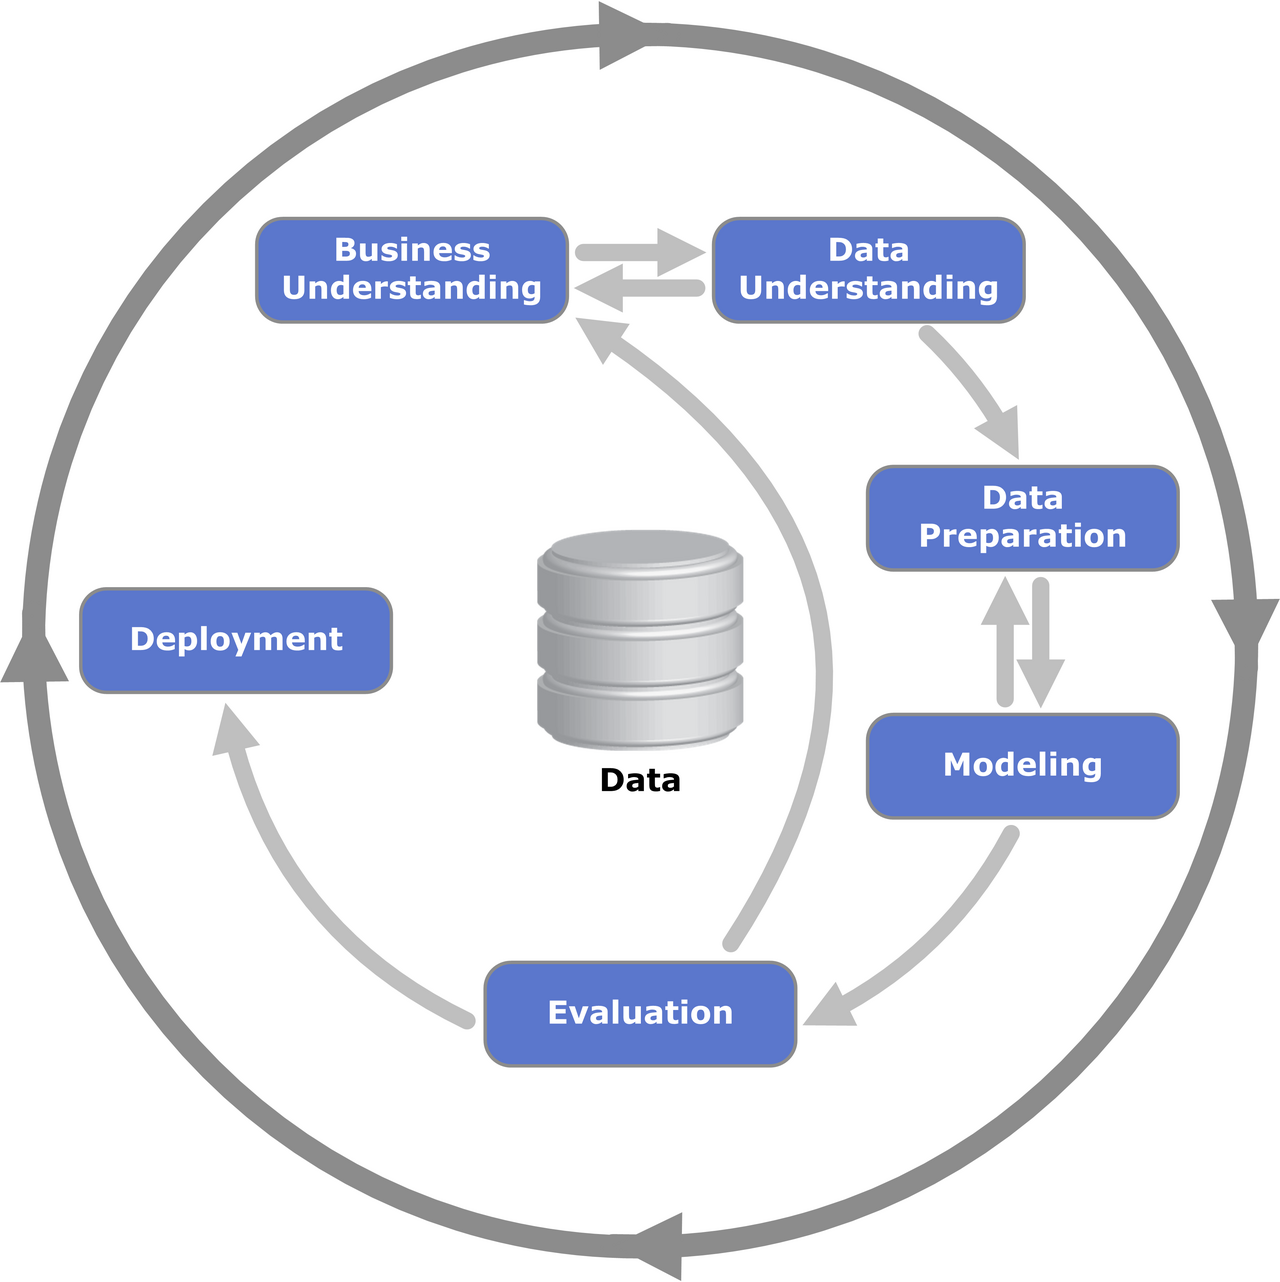
\includegraphics[width=0.6\linewidth,height=\textheight,keepaspectratio]{unidades/almacenes/../../images/external/crisp-dm-process.png}

}

\caption{Figura 1. Proceso CRISP-DM}

\end{figure}%

\emph{Figura 1. Diagrama del proceso CRISP-DM. Fuente: Wikimedia
Commons, ``CRISP-DM Process Diagram'', dominio público.}

Es importante destacar que CRISP-DM \textbf{no es un proceso lineal},
sino un modelo iterativo. En la práctica, las fases se retroalimentan
constantemente. Durante el modelado pueden detectarse problemas en la
calidad de los datos que obliguen a regresar a la fase de preparación.
En la evaluación puede descubrirse que el problema de negocio fue
formulado de manera incompleta, lo que implica volver a la primera fase.
Incluso después del despliegue, los resultados obtenidos suelen generar
nuevas preguntas estratégicas, reiniciando el ciclo.

Esta naturaleza iterativa es coherente con la realidad organizacional:
la toma de decisiones es un proceso continuo de refinamiento y
aprendizaje. Así, antes de construir tablas, definir dimensiones o
elegir herramientas tecnológicas, es necesario responder preguntas como:

\begin{itemize}
\tightlist
\item
  ¿Qué decisiones desea mejorar la organización?\\
\item
  ¿Qué métricas son críticas?\\
\item
  ¿Qué horizonte temporal se requiere analizar?
\end{itemize}

La arquitectura de datos debe ser flexible y escalable, permitiendo
incorporar nuevas fuentes, nuevas métricas y nuevas dimensiones conforme
evolucionan las necesidades del negocio. En otras palabras, la
arquitectura de datos no es un fin en sí mismo; es el soporte técnico
que permite convertir datos operacionales en conocimiento útil dentro de
un ciclo continuo de mejora y toma de decisiones.

Desde esta perspectiva, CRISP-DM define el ciclo de trabajo analítico,
mientras que el Data Warehouse aporta una memoria organizacional
confiable para recorrerlo. No todos los proyectos de CRISP-DM requieren
un Data Warehouse, pero cuando las preguntas exigen integrar varias
fuentes, comparar periodos y reutilizar métricas consistentes, el
almacén de datos se vuelve una pieza central.

\section{Data Warehouse}\label{data-warehouse-1}

William H. Inmon (1996) define un Data Warehouse como:

\begin{quote}
``A data warehouse is a subject-oriented, integrated, time-variant, and
non-volatile collection of data in support of management's
decision-making process.''
\end{quote}

En español, un Almacén de Datos es una colección de datos orientada a
temas, integrada, variante en el tiempo y no volátil, diseñada para
apoyar la toma de decisiones.

Las cuatro propiedades de la definición no son características aisladas.
Juntas explican por qué un Data Warehouse puede ofrecer una versión
coherente y durable del negocio:

Un Data Warehouse es \textbf{orientado a temas}, lo que significa que no
se organiza por aplicaciones o sistemas operacionales, sino por
entidades relevantes para el negocio. Por ejemplo, en una compañía de
seguros, el almacén de datos se estructura alrededor de conceptos como
cliente, póliza o prima, y no por productos específicos como seguro de
automóvil o seguro de vida. El enfoque está en analizar entidades del
negocio y no módulos técnicos.

Es también \textbf{variante en el tiempo}, ya que mantiene información
histórica. Los datos no se sobreescriben ni se actualizan como en un
sistema transaccional; la nueva información se agrega al repositorio.
Esto permite analizar tendencias a lo largo de cinco, diez años o más, y
responder preguntas como cómo ha evolucionado el número de diagnósticos
en los últimos años o qué patrones se observan en el crecimiento de
ventas.

Además, es \textbf{integrado}, porque consolida información proveniente
de múltiples sistemas. Por ejemplo, si un sistema registra el género
como ``m'' y ``f'' y otro como 0 y 1, antes de integrarlos deben
transformarse para mantener consistencia. Lo mismo ocurre con formatos
de fecha distintos, monedas diferentes o nombres de productos
inconsistentes. La integración implica procesos de limpieza,
transformación y estandarización de datos.

Finalmente, es \textbf{no volátil}, lo que significa que se trata de un
repositorio físicamente separado de los sistemas operacionales. En él se
realizan principalmente operaciones de carga y consulta de datos, pero
no actualizaciones frecuentes, eliminaciones ni transacciones. Su
propósito es analítico y no operativo.

En conjunto, estas propiedades permiten que una métrica conserve el
mismo significado al atravesar áreas y periodos. Por ejemplo, comparar
la tasa de abandono de dos generaciones solo es válido si la identidad
del estudiante, la definición de abandono y el calendario académico
fueron integrados con reglas comunes, y si los valores históricos se
conservaron.

\textbf{Referencia:}\\
Inmon, W. H. \emph{Building the Data Warehouse}, 2nd ed., 1996.

\chapter{Arquitectura de un Data
Warehouse}\label{arquitectura-de-un-data-warehouse}

Un Data Warehouse no debe entenderse únicamente como un conjunto de
tablas organizadas para consulta. En realidad, es una arquitectura
integral de datos cuyo propósito es separar claramente la operación
diaria del análisis estratégico. Esta arquitectura permite integrar
información proveniente de múltiples sistemas, conservar historia y
ofrecer estructuras optimizadas para la toma de decisiones.

La separación también protege ambos tipos de trabajo: las transacciones
pueden continuar con baja latencia y las consultas analíticas pueden
recorrer millones de registros sin competir directamente con la
operación. Entre ambos mundos existe una cadena de transformación que
documenta de dónde proviene cada dato y qué reglas se le aplicaron.

\section{Modelo de 3 Capas}\label{modelo-de-3-capas}

La arquitectura clásica de un Data Warehouse suele representarse
mediante un modelo de tres capas lógicas. Estas capas no necesariamente
corresponden a servidores físicos distintos, sino a niveles funcionales
dentro del ecosistema de datos.
\pandocbounded{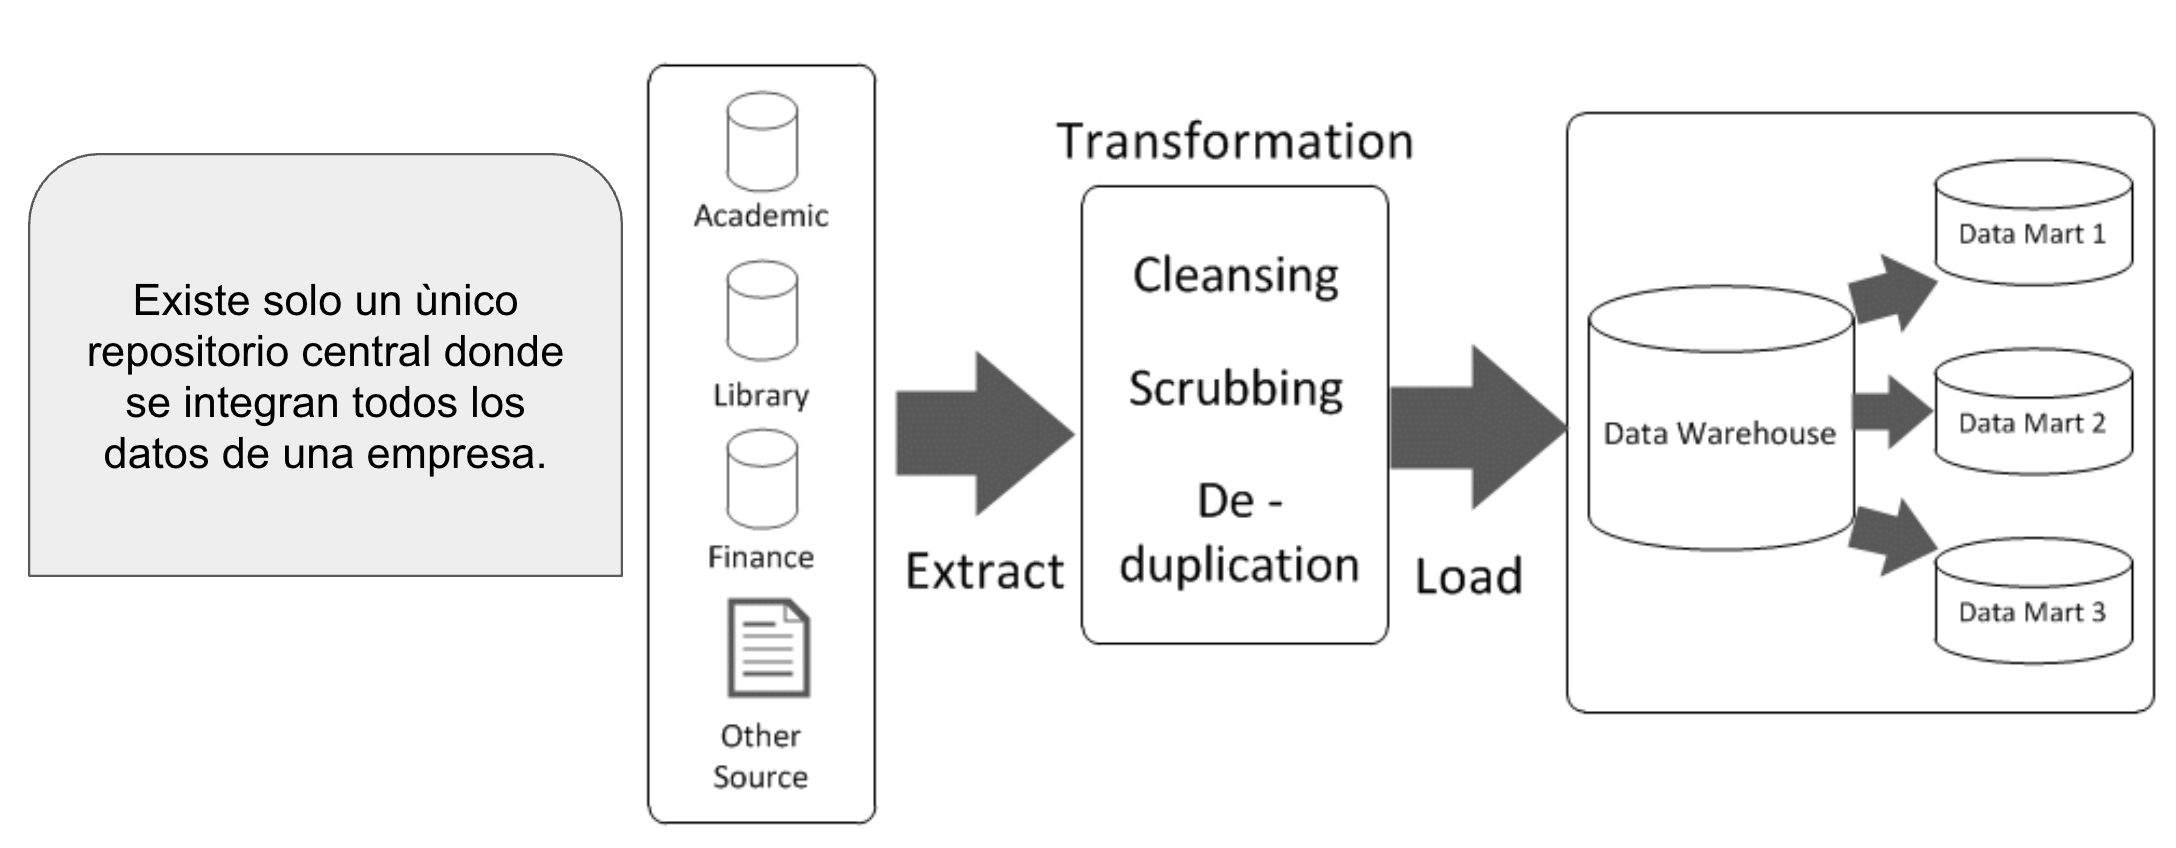
\includegraphics[keepaspectratio,alt={Arquitectura de tres capas del Data Warehouse}]{unidades/almacenes/../../images/introduction/three_tier_dw.png}}

\begin{enumerate}
\def\labelenumi{\arabic{enumi}.}
\item
  \textbf{Capa de fuentes (Operational Layer).}\\
  En este nivel residen los sistemas que soportan la actividad diaria de
  la organización. En una empresa pueden incluirse sistemas ERP que
  registran ventas y facturación, CRM que gestionan clientes,
  plataformas académicas que almacenan calificaciones o sistemas
  hospitalarios que documentan consultas médicas. También forman parte
  de esta capa archivos planos como CSV o Excel, APIs externas que
  proveen información pública y registros de aplicaciones (logs).

  El objetivo de esta capa es transaccional: registrar eventos de manera
  rápida, consistente y segura. No está diseñada para análisis histórico
  profundo ni para responder preguntas agregadas complejas. Por ejemplo,
  un sistema hospitalario puede indicar cuántos pacientes están siendo
  atendidos hoy, pero no está optimizado para analizar la evolución de
  diagnósticos durante los últimos diez años.
\item
  \textbf{Capa de integración (ETL / Data Integration Layer).}\\
  Esta capa constituye el núcleo técnico del Data Warehouse. En ella se
  ejecutan los procesos de extracción, limpieza, transformación e
  integración de datos. Es aquí donde se resuelven inconsistencias entre
  sistemas: un género registrado como ``M/F'' en un sistema y como
  ``0/1'' en otro debe unificarse; formatos de fecha distintos deben
  homogenizarse; monedas diferentes deben convertirse a un estándar
  común.

  Asimismo, se eliminan duplicados, se generan claves sustitutas y se
  aplican reglas de negocio que permiten consolidar información
  proveniente de múltiples fuentes. Dependiendo del enfoque
  arquitectónico adoptado, esta capa puede materializarse como un
  \textbf{Enterprise Data Warehouse (EDW)} central integrado, en el que
  se consolida toda la información corporativa antes de exponerla a los
  usuarios, o bien puede consistir en procesos que alimentan
  directamente modelos dimensionales específicos para cada área del
  negocio. En cualquier caso, su función es garantizar coherencia,
  calidad e integración de datos a nivel empresarial.
\item
  \textbf{Capa de consumo (Presentation / Analytics Layer).}\\
  En este nivel los datos ya han sido integrados y estructurados para
  facilitar el análisis. Aquí se implementan data marts, modelos
  dimensionales (como esquemas estrella), tableros de Business
  Intelligence y herramientas de visualización. Es el punto donde
  analistas, directivos y responsables de negocio interactúan con la
  información para responder preguntas estratégicas.

  Por ejemplo, en un grupo de clínicas esta capa permitiría consultar la
  evolución anual de pacientes por clínica, el tiempo promedio de espera
  por especialidad o la distribución de diagnósticos por región. La
  característica esencial es que los datos están optimizados para
  consulta, agregación y comparación temporal, no para registrar nuevas
  transacciones.
\end{enumerate}

\section{Data Mart}\label{data-mart}

Un \textbf{Data Mart} es un subconjunto especializado del Data Warehouse
orientado a un área específica del negocio. Mientras que el Data
Warehouse integra información a nivel corporativo, el Data Mart
concentra datos relevantes para un dominio particular, como ventas,
finanzas, recursos humanos o trayectoria académica.

\begin{figure}

\centering{

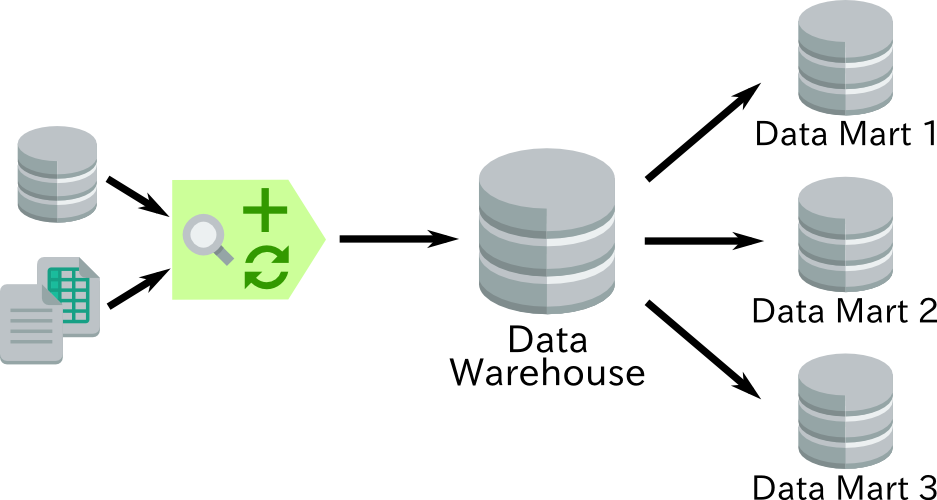
\includegraphics[width=0.7\linewidth,height=\textheight,keepaspectratio]{unidades/almacenes/../../images/external/data-mart-architecture.png}

}

\caption{\label{fig-datamart}Data Marts dentro de la arquitectura de un
Data Warehouse}

\end{figure}%

Por ejemplo, en una universidad puede existir un Data Mart académico que
almacene hechos relacionados con inscripciones, calificaciones y
créditos, junto con dimensiones como estudiante, asignatura y tiempo. En
una empresa comercial, un Data Mart de ventas podría contener hechos de
transacciones y dimensiones como producto, cliente y región.

El objetivo principal de un Data Mart es facilitar el análisis
focalizado y mejorar el rendimiento de consultas dentro de un área
concreta. Generalmente se implementa utilizando modelado
multidimensional (por ejemplo, esquemas estrella), ya que este formato
está optimizado para agregaciones y reportes.

Dependiendo de la estrategia arquitectónica adoptada, los Data Marts
pueden construirse como derivaciones de un Data Warehouse central
(enfoque top-down) o desarrollarse inicialmente por proceso de negocio e
integrarse posteriormente mediante dimensiones compartidas (enfoque
bottom-up).

Por tanto, un Data Mart no es simplemente un almacén pequeño. Su valor
depende de que sus métricas y dimensiones mantengan coherencia con el
resto de la organización. Un Data Mart de ventas y otro de inventario,
por ejemplo, solo pueden analizarse juntos si ambos entienden
«producto», «sucursal» y «tiempo» de la misma manera.

\section{Data Warehouse vs Data Lake}\label{data-warehouse-vs-data-lake}

En el contexto actual de gestión de datos, es importante mencionar
brevemente el concepto de \textbf{Data Lake}, ya que suele confundirse
con un Data Warehouse.

Un Data Lake es un repositorio centralizado que almacena datos en su
formato original, ya sean estructurados, semiestructurados o no
estructurados. A diferencia del Data Warehouse, que requiere procesos de
limpieza e integración antes de almacenar la información, el Data Lake
adopta un enfoque más flexible: primero almacena los datos y
posteriormente los transforma cuando se necesitan para análisis.

Por ejemplo, un Data Warehouse almacenará ventas consolidadas y
normalizadas listas para consulta. En cambio, un Data Lake puede
almacenar registros crudos de sensores, imágenes médicas, archivos JSON,
logs de aplicaciones o grandes volúmenes de texto sin procesar.

La diferencia clave radica en su propósito:

\begin{itemize}
\tightlist
\item
  El \textbf{Data Warehouse} está diseñado para análisis estructurado y
  toma de decisiones empresariales.
\item
  El \textbf{Data Lake} está orientado al almacenamiento masivo y
  flexible de datos, especialmente útil en escenarios de Big Data y
  ciencia de datos.
\end{itemize}

En arquitecturas modernas, ambos pueden coexistir. El Data Lake actúa
como repositorio de datos crudos, mientras que el Data Warehouse ofrece
estructuras optimizadas para análisis empresarial.

\chapter{Enfoques de implementación: Kimball vs
Inmon}\label{enfoques-de-implementaciuxf3n-kimball-vs-inmon}

Existen dos enfoques clásicos para construir un DW completo: Kimball y
Inmon. Ambos aparecen como referencias bibliográficas en el material del
curso: Kimball como referente del modelado dimensional e Inmon como
referente de la arquitectura de Data Warehouse.

Ambos enfoques persiguen información integrada y útil, pero comienzan en
extremos diferentes. Kimball parte de procesos de negocio concretos y
los conecta gradualmente; Inmon parte de un núcleo empresarial integrado
y luego publica estructuras de consumo. La dirección del recorrido
determina qué valor aparece primero y dónde se concentra la complejidad.

\section{Enfoque Kimball (bottom-up, bus
architecture)}\label{enfoque-kimball-bottom-up-bus-architecture}

El enfoque Kimball prioriza entregar valor temprano mediante data marts
dimensionales (usualmente en estrella) construidos por procesos de
negocio. La idea central es que distintos data marts se integren a
través de dimensiones conformadas (conformed dimensions), es decir,
dimensiones compartidas y coherentes (por ejemplo, la misma definición
de ``Tiempo'' y ``Producto'' para ventas y devoluciones).

\begin{figure}

\centering{

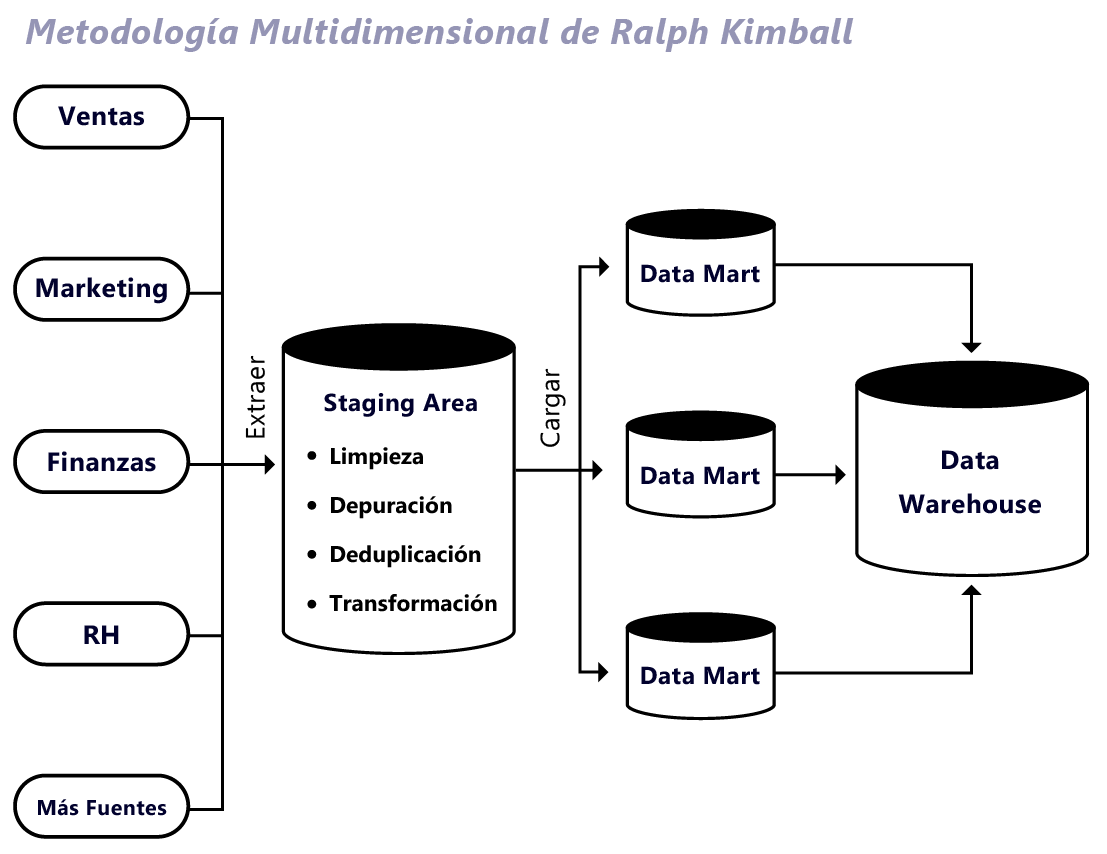
\includegraphics[width=0.9\linewidth,height=\textheight,keepaspectratio]{unidades/almacenes/../../images/external/kimball-approach.png}

}

\caption{\label{fig-kimball}Enfoque Kimball para construcción de Data
Warehouse}

\end{figure}%

Rasgos característicos:

\begin{itemize}
\tightlist
\item
  Implementación incremental: se construye un data mart (p.~ej., Ventas)
  y se amplía gradualmente (p.~ej., Inventario, Marketing).
\item
  Modelo objetivo: dimensional, orientado a consulta.
\item
  Énfasis en la capa semántica: definiciones de métricas consistentes
  (por ejemplo, qué significa ``venta neta'').
\item
  Alta utilidad para BI/analítica desde etapas tempranas.
\end{itemize}

Ventajas:

\begin{itemize}
\tightlist
\item
  Entrega rápida de resultados a usuarios.
\item
  Consultas simples y rendimiento alto.
\item
  Ajuste natural a preguntas de negocio, que constituyen el punto de
  partida recomendado en el curso.
\end{itemize}

Riesgos o retos:

\begin{itemize}
\tightlist
\item
  Requiere disciplina fuerte para definir dimensiones conformadas; si
  no, se terminan construyendo ``silos'' (varios data marts
  incompatibles).
\item
  El gobierno de datos y la integración pueden volverse complejos si se
  crece sin estándares.
\end{itemize}

\section{Enfoque Inmon (top-down, EDW
primero)}\label{enfoque-inmon-top-down-edw-primero}

El enfoque Inmon propone construir primero un Enterprise Data Warehouse
(EDW) central e integrado (frecuentemente en un modelo más normalizado),
y después derivar data marts o estructuras dimensionales para consumo
analítico.

\begin{figure}

\centering{

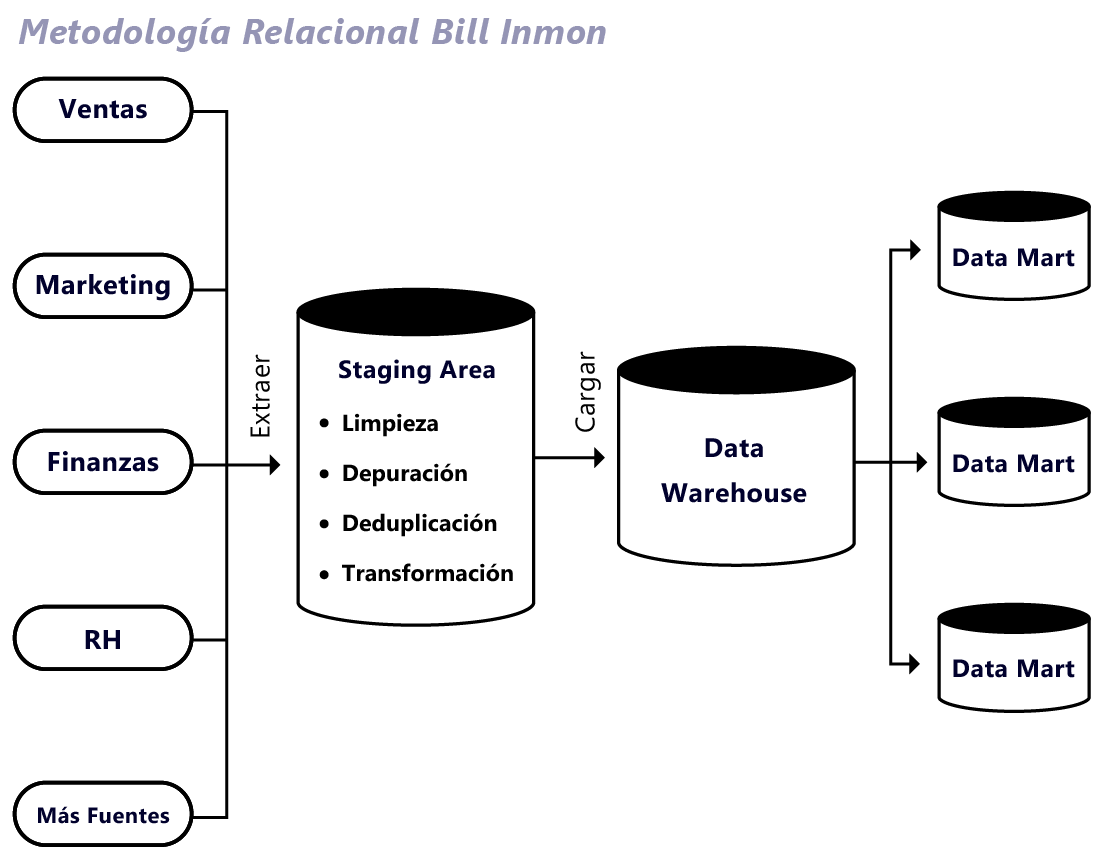
\includegraphics[width=0.9\linewidth,height=\textheight,keepaspectratio]{unidades/almacenes/../../images/external/inmon-approach.png}

}

\caption{\label{fig-inmon}Enfoque Inmon para construcción de Data
Warehouse}

\end{figure}%

Rasgos característicos:

\begin{itemize}
\tightlist
\item
  La integración empresarial es prioritaria: definiciones corporativas
  únicas desde el inicio.
\item
  Se enfatiza un ``repositorio central'' donde se armonizan entidades y
  reglas (cliente, producto, organización).
\item
  Los data marts o modelos dimensionales se construyen a partir del EDW,
  como vistas o capas derivadas.
\end{itemize}

Ventajas:

\begin{itemize}
\tightlist
\item
  Alta consistencia y control de definiciones a nivel corporativo.
\item
  Favorece gobierno de datos, auditoría, linaje y estándares.
\end{itemize}

Riesgos o retos:

\begin{itemize}
\tightlist
\item
  Mayor tiempo hasta generar valor visible si el EDW se vuelve un
  proyecto grande.
\item
  Es más sensible a cambios de requerimientos porque ``primero se
  integra todo'' y luego se habilitan casos de uso.
\end{itemize}

\section{Cómo elegir adecuadamente entre Kimball e
Inmon}\label{cuxf3mo-elegir-adecuadamente-entre-kimball-e-inmon}

La elección no debería plantearse como ``cuál es mejor'', sino ``cuál es
más adecuado'' al contexto institucional, al horizonte de tiempo y a la
madurez del gobierno de datos. Criterios prácticos:

\begin{enumerate}
\def\labelenumi{\arabic{enumi}.}
\tightlist
\item
  Urgencia de valor analítico y recursos disponibles

  \begin{itemize}
  \tightlist
  \item
    Si se necesita entregar reportes y tableros funcionales rápidamente,
    y el equipo es pequeño/mediano, Kimball suele ser más viable: se
    construye un primer data mart y se itera.
  \item
    Si la organización puede sostener una inversión inicial grande y su
    prioridad es consolidar definiciones corporativas desde el inicio,
    Inmon puede ser más apropiado.
  \end{itemize}
\item
  Grado de heterogeneidad y fragmentación de fuentes

  \begin{itemize}
  \tightlist
  \item
    Cuando existen muchas fuentes dispares y hay conflictos fuertes de
    definición (por ejemplo, ``cliente activo'' significa cosas
    distintas en áreas distintas), un enfoque tipo Inmon ayuda a forzar
    una integración central.
  \item
    Si las fuentes son manejables y el problema principal es acelerar el
    análisis por proceso de negocio (ventas, trayectoria académica,
    atención médica), Kimball suele funcionar bien.
  \end{itemize}
\item
  Gobierno de datos, auditoría y trazabilidad

  \begin{itemize}
  \tightlist
  \item
    Si hay requerimientos estrictos de auditoría, linaje, cumplimiento o
    trazabilidad (por ejemplo, regulaciones y auditorías frecuentes), el
    enfoque top-down facilita un marco centralizado.
  \item
    Si el gobierno de datos aún está en formación, un enfoque
    incremental puede ser más realista, siempre y cuando se establezcan
    estándares mínimos (dimensiones conformadas, glosario de métricas,
    versionado de reglas).
  \end{itemize}
\item
  Naturaleza de los casos de uso

  \begin{itemize}
  \tightlist
  \item
    Casos muy orientados a métricas agregadas y navegación dimensional
    (tendencias por tiempo, comparativos por región, cohortes) se
    benefician de dimensionalidad desde el inicio, favoreciendo Kimball.
  \item
    Casos de integración empresarial transversal (master data robusto,
    conciliación entre sistemas, integración de dominios complejos)
    favorecen Inmon o, al menos, una capa central fuerte.
  \end{itemize}
\end{enumerate}

En la práctica moderna es común un enfoque híbrido: se puede construir
una capa integrada (tipo EDW o ``core'') y, en paralelo o después,
exponer modelos dimensionales para BI. El punto esencial es mantener
coherencia: definir claramente qué capa es ``fuente de verdad'' para
definiciones y cómo se publican métricas y dimensiones para consumo
analítico.

La elección, entonces, no termina en una etiqueta arquitectónica. Debe
traducirse en decisiones verificables: quién define cada métrica, cómo
se comparten las dimensiones, dónde se conserva la historia, cómo se
rastrea el linaje y qué producto analítico se entregará primero.

\chapter{Ejemplo práctico: Facultad de
Ciencias}\label{ejemplo-pruxe1ctico-facultad-de-ciencias}

En un contexto universitario, el sistema de calificaciones registra
eventos puntuales como la inscripción de un estudiante en una asignatura
o la obtención de una nota al finalizar el semestre. Sin embargo,
analizar la trayectoria académica completa de un estudiante requiere una
visión mucho más amplia: integrar múltiples periodos, generaciones,
asignaturas, planes de estudio y, en muchos casos, información
administrativa y financiera asociada.

Los sistemas operacionales académicos están diseñados para soportar
procesos diarios ---inscripciones, captura de calificaciones, emisión de
constancias--- pero no para realizar análisis longitudinales o
comparativos complejos. Por ejemplo, responder preguntas como:

\begin{itemize}
\tightlist
\item
  ¿Cómo ha evolucionado el desempeño promedio por generación en los
  últimos diez años?
\item
  ¿Qué cohortes presentan mayores tasas de abandono?
\item
  ¿Existe relación entre modalidad de ingreso y desempeño académico?
\end{itemize}

implica integrar información dispersa en distintos sistemas y conservar
historia de manera estructurada.

Un \textbf{Data Warehouse académico} permite consolidar esta información
en un repositorio histórico, integrado y consistente, diseñado
específicamente para análisis estratégico.

\section{Fuentes de datos}\label{fuentes-de-datos}

En una Facultad de Ciencias, la información relevante para análisis
institucional suele encontrarse distribuida en múltiples sistemas
independientes. Entre ellos pueden incluirse:

\begin{itemize}
\tightlist
\item
  Sistemas de control escolar que registran inscripciones,
  calificaciones y créditos.
\item
  Sistemas de admisiones que almacenan información de ingreso,
  generación y antecedentes académicos.
\item
  Sistemas administrativos y financieros que gestionan pagos, becas y
  apoyos.
\item
  Sistemas de recursos humanos con información sobre profesores y carga
  docente.
\item
  Archivos externos como encuestas institucionales o evaluaciones
  académicas.
\end{itemize}

Cada uno de estos sistemas cumple una función operativa específica. Sin
embargo, ninguno por sí mismo ofrece una visión integral del desempeño
académico institucional a lo largo del tiempo. La fragmentación de
fuentes dificulta el análisis global y puede generar inconsistencias en
métricas y definiciones.

\section{Procesos de integración
(ETL)}\label{procesos-de-integraciuxf3n-etl}

Para transformar datos operacionales en información estratégica es
necesario un proceso de integración sistemático.

En esta etapa se extrae periódicamente la información de los distintos
sistemas, se validan y corrigen inconsistencias, se homologan formatos y
se consolidan registros que pertenecen a la misma entidad institucional.
Por ejemplo, un estudiante puede aparecer con variaciones en su nombre
entre sistemas distintos; el proceso de integración debe identificar que
se trata de la misma persona y unificar su información.

Asimismo, se normalizan conceptos institucionales: nombres de carreras,
códigos de asignatura, periodos académicos y categorías administrativas
deben definirse de manera coherente para todo el repositorio.

El resultado de estos procesos no es simplemente una copia de los
sistemas originales, sino un conjunto de datos consolidados, limpios y
preparados para análisis histórico.

\section{Consolidación en el Data
Warehouse}\label{consolidaciuxf3n-en-el-data-warehouse}

Una vez integrados, los datos se almacenan en un repositorio central que
conserva información histórica y garantiza consistencia institucional.
Este repositorio no está orientado a registrar nuevas transacciones,
sino a permitir consultas analíticas eficientes y comparaciones
longitudinales.

Desde el punto de vista arquitectónico, el Data Warehouse académico se
convierte en la base para construir vistas analíticas especializadas
---como un data mart académico--- desde donde pueden generarse reportes,
tableros y estudios institucionales.

Gracias a esta consolidación, la Facultad puede:

\begin{itemize}
\tightlist
\item
  Analizar cohortes completas desde ingreso hasta egreso.
\item
  Medir tasas de reprobación y abandono por generación.
\item
  Identificar asignaturas críticas.
\item
  Evaluar tendencias de desempeño a lo largo del tiempo.
\item
  Integrar indicadores académicos con variables administrativas o
  financieras.
\end{itemize}

La diferencia fundamental respecto a los sistemas transaccionales es que
el Data Warehouse ofrece una visión histórica, integrada y consistente
del desempeño institucional, permitiendo transformar datos operacionales
en conocimiento estratégico.

El diseño específico de las estructuras analíticas ---como modelos
dimensionales, tablas de hechos y dimensiones--- se abordará en el
siguiente capítulo, donde se detallará cómo se organizan técnicamente
estos datos para optimizar su consulta.

\section{Diagrama arquitectónico del DW
académico}\label{diagrama-arquitectuxf3nico-del-dw-acaduxe9mico}


\includegraphics[width=15.5in,height=10.7in]{unidades/almacenes/1-1-datawarehouse_files/figure-latex/mermaid-figure-1.png}

Con esta arquitectura, la Facultad podría analizar cohortes completas
desde el ingreso hasta el egreso, medir las tasas de abandono por
generación, detectar asignaturas críticas con alta reprobación, evaluar
el impacto de las becas en el desempeño académico e identificar patrones
longitudinales de rendimiento. A diferencia del sistema transaccional,
el Data Warehouse integra información que se encuentra dispersa en
distintos sistemas, conserva el historial de los datos a lo largo del
tiempo, permite realizar análisis multidimensionales y está optimizado
para procesos de agregación y consulta. En este contexto, el Data
Warehouse no reemplaza los sistemas académicos, sino que los
complementa, transformando los datos operacionales en información
estratégica que apoya la toma de decisiones institucionales.

\chapter{Conclusión}\label{conclusiuxf3n}

Un Data Warehouse no sustituye a los sistemas operacionales ni registra
transacciones cotidianas. Su función es integrar información dispersa,
conservar historia, romper silos organizacionales y facilitar análisis
complejos orientados a la toma de decisiones estratégicas.

En la siguiente sección se abordará el modelado multidimensional, que
define cómo se estructuran las tablas analíticas dentro de esta
arquitectura y cómo se optimizan para consultas agregadas.

\section{Recapitulación visual: del registro a la
analítica}\label{recapitulaciuxf3n-visual-del-registro-a-la-analuxedtica}

Para cerrar el recorrido, retomemos el caso de la Facultad de Ciencias y
observemos de forma compacta cómo un evento operacional adquiere
contexto analítico al atravesar la arquitectura.

En un contexto universitario, el sistema de calificaciones registra
eventos puntuales como la inscripción de un estudiante o la obtención de
una nota. Sin embargo, analizar la trayectoria académica completa de un
estudiante requiere una visión mucho más amplia: integrar múltiples
periodos, generaciones, asignaturas, planes de estudio y, en muchos
casos, información administrativa asociada.

Un \textbf{Data Warehouse académico} permite consolidar esta información
en un repositorio histórico, integrado y consistente, diseñado
específicamente para análisis estratégico.

\subsection{Diagrama Arquitectónico del Data Warehouse
Académico}\label{diagrama-arquitectuxf3nico-del-data-warehouse-acaduxe9mico}

El siguiente diagrama muestra cómo fluye la información escolar,
financiera y docente para conformar la analítica académica:

Con esta arquitectura, la Facultad puede analizar cohortes completas
desde el ingreso hasta el egreso, medir las tasas de abandono por
generación, detectar asignaturas críticas con alta reprobación e
identificar patrones longitudinales de rendimiento.

\chapter{Data Lakehouse}\label{data-lakehouse}

De silos a una base abierta y gobernada

\hfill\break

\section{Pregunta rectora}\label{pregunta-rectora}

\begin{quote}
¿En qué momento compartir una base abierta y gobernada para BI,
\emph{streaming} y aprendizaje automático justifica asumir la operación
adicional de un Lakehouse?
\end{quote}

Un \textbf{Data Lakehouse} no es el destino obligatorio de toda
plataforma de datos. En una organización pequeña, un Data Warehouse
administrado puede entregar resultados con menos componentes y menos
personal. El Lakehouse se vuelve razonable cuando la duplicación, el
movimiento de datos, la variedad de cargas y la necesidad de reutilizar
contratos comunes superan el costo de operar tablas, metadatos,
catálogo, gobierno y mantenimiento.

Esta lectura sigue un caso de una \emph{fintech} desde sus primeros
reportes hasta una plataforma compartida. El propósito no es memorizar
productos, sino aprender a separar responsabilidades y argumentar una
decisión arquitectónica.

\begin{tcolorbox}[enhanced jigsaw, arc=.35mm, bottomrule=.15mm, bottomtitle=1mm, breakable, colback=white, colbacktitle=quarto-callout-note-color!10!white, colframe=quarto-callout-note-color-frame, coltitle=black, left=2mm, leftrule=.75mm, opacityback=0, opacitybacktitle=0.6, rightrule=.15mm, title=\textcolor{quarto-callout-note-color}{\faInfo}\hspace{0.5em}{Ruta de lectura}, titlerule=0mm, toprule=.15mm, toptitle=1mm]

Tiempo estimado: 35--45 minutos. Conviene haber leído antes el capítulo
de Data Warehouse. Los diagramas usan siempre la misma convención: azul
para datos y almacenamiento, morado para metadatos y gobierno, naranja
para ingesta, gris para cómputo, verde para consumo confiable y rojo
para riesgo o duplicación.

\end{tcolorbox}

\subsection{Objetivos de aprendizaje}\label{objetivos-de-aprendizaje}

Al terminar, podrás:

\begin{enumerate}
\def\labelenumi{\arabic{enumi}.}
\tightlist
\item
  explicar por qué un Data Warehouse fue una elección correcta durante
  la primera etapa de la \emph{fintech};
\item
  localizar duplicación, latencia y controles dobles en una arquitectura
  con silos;
\item
  distinguir objeto, \emph{bucket}, formato de archivo, formato de
  tabla, catálogo, gobierno y motor de cómputo;
\item
  narrar cómo un \emph{snapshot} evita que una escritura incompleta se
  vuelva visible;
\item
  justificar una transición usando volumen, variedad, velocidad, cargas
  de trabajo, costo y capacidad operativa;
\item
  reconocer que compactación, evolución de esquemas, observabilidad y
  radio de impacto siguen siendo responsabilidades del equipo.
\end{enumerate}

\section{El problema antes de la
definición}\label{el-problema-antes-de-la-definiciuxf3n}

A las 10:02, la \emph{fintech} recibe la transacción \texttt{tx\_8472}
por \texttt{\$3,200}. Finanzas la incluye en los ingresos del día, pero
el sistema de fraude la presenta como bloqueada. Ambos equipos
ejecutaron correctamente su propio proceso. La discrepancia está en las
rutas y contratos que utilizaron.

La pregunta útil no es todavía «¿qué producto compraremos?», sino «¿qué
trabajo se duplica para sostener estas dos rutas?».

\section{Dos caminos que deben representar el mismo
negocio}\label{dos-caminos-que-deben-representar-el-mismo-negocio}

Históricamente, el Data Warehouse y el Data Lake resolvieron problemas
legítimos:

\begin{itemize}
\tightlist
\item
  El \textbf{Data Warehouse} ofreció tablas controladas, SQL,
  concurrencia y reportes comprensibles para el negocio.
\item
  El \textbf{Data Lake} permitió conservar grandes volúmenes y tipos
  diversos en almacenamiento de objetos económico y flexible.
\end{itemize}

El costo aparece cuando cada uno se convierte en una autoridad separada.

Si Producto agrega \texttt{device\_risk\_score}, el cambio debe
capturarse, aterrizarse, transformarse, incorporarse a la tabla
analítica, probarse, publicarse, autorizarse y comunicarse a
consumidores. Cuando las rutas están separadas, varias de esas
decisiones se repiten. La deuda no está sólo en los bytes duplicados:
está en las decisiones duplicadas.

\section{Caso Fintech, fase 1: el Warehouse era
suficiente}\label{caso-fintech-fase-1-el-warehouse-era-suficiente}

Durante los años 0--3, la empresa tenía datos relacionales, unas 10,000
transacciones diarias, alrededor de 500 GB al año y reportes por lotes.
Su necesidad dominante era conocer ingresos, morosidad y crecimiento con
rapidez.

Un servicio administrado, dbt y una persona analista podían entregar
valor en una semana y operar por cientos de dólares mensuales dentro del
supuesto didáctico. Contratar un equipo especializado para un Lakehouse
habría agregado observabilidad, integración y mantenimiento sin un
retorno claro.

\begin{tcolorbox}[enhanced jigsaw, arc=.35mm, bottomrule=.15mm, bottomtitle=1mm, breakable, colback=white, colbacktitle=quarto-callout-important-color!10!white, colframe=quarto-callout-important-color-frame, coltitle=black, left=2mm, leftrule=.75mm, opacityback=0, opacitybacktitle=0.6, rightrule=.15mm, title=\textcolor{quarto-callout-important-color}{\faExclamation}\hspace{0.5em}{Principio de decisión}, titlerule=0mm, toprule=.15mm, toptitle=1mm]

Elegir un Data Warehouse en esta fase no fue falta de visión. Fue
ajustar arquitectura, costo y capacidad del equipo al problema real.

\end{tcolorbox}

\subsection{Qué hace cada producto en esa
fase}\label{quuxe9-hace-cada-producto-en-esa-fase}

\begin{itemize}
\tightlist
\item
  \textbf{PostgreSQL, MySQL o una base operacional administrada}
  registra usuarios, cuentas y pagos de la aplicación. Está optimizada
  para operar el negocio, no para escanear años de historia.
\item
  \textbf{Fivetran} o \textbf{Airbyte} extrae o replica datos desde las
  fuentes hacia un destino analítico.
\item
  \textbf{BigQuery, Snowflake, Amazon Redshift o Fabric Warehouse} puede
  cumplir el rol de Data Warehouse. Son alternativas; no es necesario
  contratar todos.
\item
  \textbf{dbt} ejecuta transformaciones y pruebas principalmente
  mediante SQL sobre el Warehouse; no es el lugar principal donde viven
  los datos.
\item
  \textbf{Metabase, Tableau, Power BI o Looker} presenta métricas y
  tableros a usuarios de negocio.
\end{itemize}

La marca no determina por sí sola la arquitectura. BigQuery puede ser un
Warehouse de tablas nativas y también un motor que consulta tablas
abiertas. Siempre pregunta: \textbf{¿qué almacena, qué cataloga y qué
procesa?}

Un Data Warehouse moderno también puede ser elástico, admitir datos
semiestructurados y consultar almacenamiento externo. La decisión se
toma por requisitos, economía y capacidad operativa, no por presentar al
Warehouse como una tecnología rígida por definición.

\section{Año 4: el punto de quiebre}\label{auxf1o-4-el-punto-de-quiebre}

La arquitectura inicial no falla por recibir un JSON aislado. El cambio
aparece por una combinación de presiones.

Los \texttt{4\ TB/mes} equivalen aproximadamente a \texttt{48\ TB/año}.
Llegar a petabytes requeriría crecimiento y retención durante varios
años; no debe afirmarse que cuatro terabytes mensuales ya sean un
petabyte. Los montos del caso son supuestos docentes, no cotizaciones de
proveedores.

\subsection{Actividad de
clasificación}\label{actividad-de-clasificaciuxf3n}

{\def\LTcaptype{none} % do not increment counter
\begin{longtable}[]{@{}
  >{\raggedright\arraybackslash}p{(\linewidth - 2\tabcolsep) * \real{0.5000}}
  >{\raggedright\arraybackslash}p{(\linewidth - 2\tabcolsep) * \real{0.5000}}@{}}
\toprule\noalign{}
\begin{minipage}[b]{\linewidth}\raggedright
Síntoma
\end{minipage} & \begin{minipage}[b]{\linewidth}\raggedright
Fuerza principal
\end{minipage} \\
\midrule\noalign{}
\endhead
\bottomrule\noalign{}
\endlastfoot
Millones de clics móviles & Volumen y velocidad \\
PDFs de contratos & Variedad \\
Modelo de fraude que necesita segundos & Velocidad y nuevos
consumidores \\
Científicos que descargan terabytes & Movimiento \\
Dos equipos calculan la misma característica de riesgo & Coordinación \\
La factura de transformaciones se dispara & Economía y operación \\
\end{longtable}
}

La pregunta de diseño es: \textbf{¿escalamos el Warehouse, añadimos un
Lake separado o rediseñamos una base compartida?} La respuesta debe
empezar por requisitos, no por productos.

\chapter{La base técnica del
Lakehouse}\label{la-base-tuxe9cnica-del-lakehouse}

\section{Vocabulario mínimo}\label{vocabulario-muxednimo}

{\def\LTcaptype{none} % do not increment counter
\begin{longtable}[]{@{}
  >{\raggedright\arraybackslash}p{(\linewidth - 6\tabcolsep) * \real{0.2500}}
  >{\raggedright\arraybackslash}p{(\linewidth - 6\tabcolsep) * \real{0.2500}}
  >{\raggedright\arraybackslash}p{(\linewidth - 6\tabcolsep) * \real{0.2500}}
  >{\raggedright\arraybackslash}p{(\linewidth - 6\tabcolsep) * \real{0.2500}}@{}}
\toprule\noalign{}
\begin{minipage}[b]{\linewidth}\raggedright
Término
\end{minipage} & \begin{minipage}[b]{\linewidth}\raggedright
Explicación cotidiana
\end{minipage} & \begin{minipage}[b]{\linewidth}\raggedright
Ejemplo en la fintech
\end{minipage} & \begin{minipage}[b]{\linewidth}\raggedright
Qué no significa
\end{minipage} \\
\midrule\noalign{}
\endhead
\bottomrule\noalign{}
\endlastfoot
\textbf{Objeto} & Unidad guardada en la nube: bytes, nombre o \emph{key}
y metadatos. & PDF, imagen o archivo Parquet. & No es necesariamente una
fila ni una tabla. \\
\textbf{Bucket} & Contenedor con nombre donde un proveedor guarda
objetos. & \texttt{s3://fintech-datos-prod/}. & No es motor SQL, base
relacional ni todo el Data Lake. \\
\textbf{Key} & Localizador único de un objeto dentro del bucket; puede
parecer una ruta. & \texttt{bronze/kafka/2026/08/25/part-0001.json}. &
Los separadores \texttt{/} no siempre representan carpetas
tradicionales. \\
\textbf{Data Lake} & Arquitectura para conservar y procesar datos
diversos sobre almacenamiento económico, con ingesta, organización,
seguridad y gobierno. & Objetos, políticas, catálogo y procesos. & Un
bucket aislado no se vuelve automáticamente un Data Lake. \\
\textbf{Data Warehouse} & Sistema analítico orientado a tablas, SQL y
datos preparados para decisiones. & Tablas de ingresos y morosidad. & No
es la base operacional que autoriza cada pago. \\
\textbf{Motor de cómputo} & Software que consulta, transforma, agrega o
entrena. & BigQuery, Trino, Spark o Databricks SQL. & El almacenamiento
de objetos no procesa consultas por sí solo. \\
\textbf{Formato de archivo} & Organización de bytes dentro de un
archivo. & Parquet organiza columnas y compresión. & No coordina por sí
mismo una tabla de muchos archivos. \\
\textbf{Formato de tabla} & Protocolo que decide qué archivos forman una
tabla y conserva cambios, esquema y snapshots. & Iceberg, Delta Lake o
Hudi. & No sustituye almacenamiento, catálogo ni motor. \\
\textbf{Catálogo} & Mapa que relaciona un nombre con ubicación, esquema,
propietario y metadatos vigentes. &
\texttt{fintech.silver.transactions}. & Una lista no garantiza calidad
sin procesos y responsables. \\
\end{longtable}
}

Una analogía breve ayuda a recordar las responsabilidades:

\begin{quote}
El bucket es el contenedor; los objetos son los paquetes; la \emph{key}
es la etiqueta. Parquet organiza el contenido de ciertos paquetes.
Iceberg, Delta Lake o Hudi mantienen el inventario versionado que dice
qué paquetes forman una tabla. El catálogo permite pedir la tabla por
nombre y verificar el acceso. El motor abre los paquetes y realiza el
cálculo.
\end{quote}

\subsection{Anatomía de un bucket}\label{anatomuxeda-de-un-bucket}

La URI \texttt{s3://fintech-datos-prod/documents/loan-8472.pdf} se
interpreta así: \texttt{s3} identifica el servicio,
\texttt{fintech-datos-prod} es el bucket y el resto es la \emph{key}. En
Google Cloud se vería \texttt{gs://...}; en ADLS Gen2 se usa un
contenedor dentro de una cuenta de almacenamiento.

Tres distinciones deben quedar explícitas:

\begin{enumerate}
\def\labelenumi{\arabic{enumi}.}
\tightlist
\item
  \textbf{Bucket ≠ archivo.} El bucket contiene objetos; el PDF o
  Parquet es el objeto.
\item
  \textbf{Bucket ≠ Data Lake.} Un Data Lake incluye ingesta,
  organización, seguridad, catálogo, cómputo y operación.
\item
  \textbf{Bucket ≠ Lakehouse.} El Lakehouse añade tablas
  transaccionales, catálogo, gobierno y motores coordinados.
\end{enumerate}

\section{Una base física compartida todavía no es una
tabla}\label{una-base-fuxedsica-compartida-todavuxeda-no-es-una-tabla}

El primer paso del Lakehouse es desacoplar los bytes del motor: guardar
datos en objetos y asignar cómputo distinto a SQL, ML o
\emph{streaming}. Esa base ofrece escala, formatos abiertos y economía
de capacidad. Sin embargo, una carpeta puede contener:

\begin{Shaded}
\begin{Highlighting}[]
\NormalTok{transactions/}
\NormalTok{  part{-}0001.parquet}
\NormalTok{  part{-}0002.parquet}
\NormalTok{  part{-}0003.parquet}
\NormalTok{  part{-}0003{-}retry.parquet}
\NormalTok{  \_temporary{-}part{-}0004.parquet}
\end{Highlighting}
\end{Shaded}

El nombre de la carpeta no decide de forma confiable cuáles archivos
pertenecen a la tabla, cuál fue un reintento y si la escritura terminó.

\section{La idea que debe sobrevivir}\label{la-idea-que-debe-sobrevivir}

No es «un lago junto a un almacén» ni «guardar Parquet en S3». Es hacer
que conjuntos de archivos se comporten como tablas confiables sin perder
apertura y separación entre almacenamiento y cómputo.

\section{Responsabilidades lógicas de la
arquitectura}\label{responsabilidades-luxf3gicas-de-la-arquitectura}

Una implementación puede agrupar varias responsabilidades en un servicio
administrado o distribuirlas entre herramientas. Las capas son lógicas,
no una lista obligatoria de cinco productos.

\subsection{1. Ingesta}\label{ingesta}

Conecta datos estructurados, semiestructurados y no estructurados. Las
cargas \textbf{batch} mueven datos acumulados a intervalos; \textbf{CDC}
replica cambios de una fuente; \emph{streaming} procesa eventos a medida
que llegan. La modalidad determina frescura, tamaño de archivos,
reintentos y costo operativo.

\subsection{2. Almacenamiento}\label{almacenamiento}

S3, Cloud Storage, ADLS Gen2 u OneLake conservan objetos a gran escala.
Parquet y ORC son formatos columnares eficientes para datos tabulares;
JSON, PDFs e imágenes pueden permanecer como objetos. Usar un formato
abierto reduce dependencia, pero no garantiza que todos los motores
soporten las mismas operaciones.

\subsection{3. Formato de tabla, catálogo y
gobierno}\label{formato-de-tabla-catuxe1logo-y-gobierno}

Iceberg, Delta Lake y Hudi coordinan archivos como tablas versionadas.
El catálogo resuelve nombres, ubicaciones, esquemas y metadatos
vigentes. El gobierno añade identidad, clasificación, permisos,
auditoría y responsabilidades. Son tareas relacionadas, pero distintas.

\subsection{4. Interfaces y motores}\label{interfaces-y-motores}

SQL, APIs de DataFrame y APIs de metadatos permiten que motores como
BigQuery, Trino, Spark o Databricks SQL procesen datos sin convertir el
almacenamiento en el motor. La compatibilidad se verifica por operación,
versión del formato y configuración.

\subsection{5. Consumo}\label{consumo}

BI necesita métricas certificadas; ciencia de datos necesita entidades
reutilizables y datos autorizados; fraude necesita baja latencia;
auditoría necesita historia y evidencias. Compartir la base no obliga a
compartir un único motor ni a consultar la misma capa de calidad.

\section{Archivo, tabla y catálogo no son
sinónimos}\label{archivo-tabla-y-catuxe1logo-no-son-sinuxf3nimos}

Parquet no publica una transacción sobre veinte archivos. El formato de
tabla mantiene la lista autorizada, el esquema, las particiones y los
snapshots. El catálogo permite que un nombre estable apunte a esos
metadatos. Iceberg, Delta Lake y Hudi comparten esa intención general,
pero no son idénticos.

\section{Cómo un snapshot oculta una escritura
incompleta}\label{cuxf3mo-un-snapshot-oculta-una-escritura-incompleta}

El reto no es que S3, Cloud Storage o Azure Blob Storage necesariamente
«pierdan consistencia». Una modificación de tabla puede crear muchos
objetos; hace falta un \textbf{commit de tabla atómico} que publique el
conjunto completo.

La atomicidad se logra porque los lectores consultan una lista
autorizada. Si el job falla antes de publicar, el puntero sigue en el
snapshot 17. Si termina, un commit mueve el puntero a la versión 18
completa. Un lector que resolvió la versión antes del commit continúa
con una vista consistente según el aislamiento y el motor.

Las garantías ACID suelen expresarse por tabla. No debe suponerse
automáticamente una transacción atómica entre muchas tablas; hay que
verificar el formato y el motor.

\section{Evolución de esquema sin reescribir toda la
historia}\label{evoluciuxf3n-de-esquema-sin-reescribir-toda-la-historia}

Los metadatos pueden separar la identidad de una columna de su nombre
visible.

Esto habilita evolución de esquema y viaje en el tiempo, pero no vuelve
gratuitos todos los cambios. Modificar tipos incompatibles, semántica,
particiones o unidades puede exigir migración, \emph{backfill}, vistas
de transición y pruebas.

\section{Catálogo y gobierno: mapa, versión y
acceso}\label{catuxe1logo-y-gobierno-mapa-versiuxf3n-y-acceso}

El catálogo convierte un nombre de negocio en ubicación, esquema y
metadatos vigentes. El gobierno responde otra pregunta: aunque alguien
conozca la ruta, ¿tiene derecho a verla y con qué detalle? Un catálogo
no mueve datos ni garantiza calidad por existir. Requiere propietarios,
políticas, clasificación, auditoría y credenciales con privilegio
mínimo.

\subsection{Comprobación rápida}\label{comprobaciuxf3n-ruxe1pida}

Asigna cada responsabilidad:

\begin{enumerate}
\def\labelenumi{\arabic{enumi}.}
\tightlist
\item
  «Organiza columnas y compresión dentro de \texttt{part-0007}» →
  \textbf{formato de archivo}.
\item
  «Decide que A, B y C forman la versión 17» → \textbf{formato de
  tabla}.
\item
  «Resuelve dónde vive \texttt{silver.transactions} y verifica permisos»
  → \textbf{catálogo y gobierno}.
\item
  «Conserva el PDF original y los bytes de Parquet» →
  \textbf{almacenamiento de objetos}.
\end{enumerate}

\chapter{Integrar calidad, cargas y productos de
datos}\label{integrar-calidad-cargas-y-productos-de-datos}

\section{Medallion: Bronze, Silver y
Gold}\label{medallion-bronze-silver-y-gold}

La arquitectura Medallion es una forma frecuente, no una ley universal,
de representar estados de calidad. Los nombres no designan productos ni
ubicaciones físicas obligatorias.

Bronze preserva; Silver integra; Gold traduce al lenguaje del negocio.
Finanzas no debería calcular ingresos directamente desde JSON Bronze.
Una organización puede publicar varias tablas Gold porque cada producto
responde a una decisión y granularidad distintas.

PDFs, imágenes y otros binarios permanecen como objetos. Una tabla
Silver puede registrar \texttt{object\_uri}, hash, propietario,
clasificación, estado de OCR y relaciones. No conviene afirmar que una
fotografía «se convierte en Iceberg».

\section{Fase 2: una base gobernada y varios
motores}\label{fase-2-una-base-gobernada-y-varios-motores}

La \emph{fintech} no cambió sólo de contenedor. Cambió el contrato:

\begin{itemize}
\tightlist
\item
  \textbf{Finanzas} consulta productos Gold certificados.
\item
  \textbf{ML} utiliza entidades Silver autorizadas y resultados
  derivados de documentos sin descargar terabytes a almacenamiento
  local.
\item
  \textbf{Fraude} procesa eventos en tiempo real y consulta o actualiza
  señales gobernadas según las garantías del pipeline.
\end{itemize}

Separar almacenamiento y cómputo permite dimensionar y apagar motores
por carga, pero no garantiza costos menores. Formato, estadísticas,
tamaño de archivos, partición, cachés y consultas siguen determinando
desempeño y gasto.

\section{Tecnologías abiertas y servicios
administrados}\label{tecnologuxedas-abiertas-y-servicios-administrados}

{\def\LTcaptype{none} % do not increment counter
\begin{longtable}[]{@{}
  >{\raggedright\arraybackslash}p{(\linewidth - 4\tabcolsep) * \real{0.3333}}
  >{\raggedright\arraybackslash}p{(\linewidth - 4\tabcolsep) * \real{0.3333}}
  >{\raggedright\arraybackslash}p{(\linewidth - 4\tabcolsep) * \real{0.3333}}@{}}
\toprule\noalign{}
\begin{minipage}[b]{\linewidth}\raggedright
Responsabilidad
\end{minipage} & \begin{minipage}[b]{\linewidth}\raggedright
Ejemplos frecuentes
\end{minipage} & \begin{minipage}[b]{\linewidth}\raggedright
Función en el caso
\end{minipage} \\
\midrule\noalign{}
\endhead
\bottomrule\noalign{}
\endlastfoot
Fuente operacional & PostgreSQL, MySQL, SQL Server, Cloud SQL, RDS,
Azure SQL & Usuarios, cuentas, cobros y transferencias. \\
Ingesta batch/CDC & Fivetran, Airbyte, AWS DMS, Datastream, Azure Data
Factory & Replica cambios operacionales. \\
Eventos & Kafka, Confluent, Kinesis, Pub/Sub, Event Hubs & Clics,
telemetría y fraude. \\
Almacenamiento de objetos & S3, Cloud Storage, ADLS Gen2, OneLake &
Conserva JSON, Parquet, PDFs e imágenes. \\
Formato de archivo & Parquet, ORC, Avro, JSON & Organiza bytes dentro de
cada archivo. \\
Formato de tabla & Iceberg, Delta Lake, Hudi & Publica snapshots,
esquema e inventario de archivos. \\
Catálogo y gobierno & Glue + Lake Formation, Lakehouse runtime catalog +
Knowledge Catalog, Unity Catalog, Fabric + Purview & Descubrimiento,
permisos, linaje y auditoría. \\
Motores & BigQuery, Athena, Redshift, Trino, Spark, Databricks SQL,
Fabric SQL & Ejecuta la carga analítica o de ingeniería. \\
Consumo & Looker, QuickSight, Power BI, Tableau, notebooks, modelos &
Convierte datos en decisiones o productos. \\
\end{longtable}
}

Parquet, Iceberg, Delta Lake, Hudi, Spark, Kafka y Trino son estándares
o proyectos abiertos. S3, BigQuery, Redshift, Databricks, Fabric y
Fivetran son servicios o plataformas administradas. Una plataforma
comercial puede administrar tecnologías abiertas.

\chapter{Implementaciones en Google Cloud, AWS y
Azure}\label{implementaciones-en-google-cloud-aws-y-azure}

No hay traducción exacta entre servicios. La comparación debe mantener
fijas las responsabilidades: almacenamiento, tabla, catálogo, gobierno,
cómputo, consumo y operación.

\section{Google Cloud: Cloud Storage, Iceberg y varios
motores}\label{google-cloud-cloud-storage-iceberg-y-varios-motores}

La arquitectura actual de Google Cloud combina Cloud Storage, Apache
Iceberg, un \emph{runtime catalog}, gobierno y motores como BigQuery,
Spark, Flink y Trino, según su
\href{https://docs.cloud.google.com/lakehouse/docs/lakehouse-basics}{documentación
de arquitectura Lakehouse}. Las tablas Iceberg administradas por
BigQuery permanecen en buckets controlados por la organización y añaden
evolución de esquema, \emph{time travel} y optimización automática, como
detalla la
\href{https://docs.cloud.google.com/bigquery/docs/biglake-iceberg-tables-in-bigquery}{guía
de tablas Iceberg administradas}.

Una ruta de implementación razonable es:

\begin{enumerate}
\def\labelenumi{\arabic{enumi}.}
\tightlist
\item
  elegir región, proyecto y bucket con políticas de retención y cifrado;
\item
  crear un Lakehouse runtime catalog y definir namespaces;
\item
  usar Iceberg V2 para nuevas tablas abiertas y decidir quién administra
  sus metadatos;
\item
  configurar IAM y, cuando corresponda, credenciales delegadas con
  privilegio mínimo;
\item
  conectar BigQuery y los motores abiertos que realmente utilizará el
  equipo;
\item
  probar lectura, escritura, evolución, recuperación y costos antes de
  declarar interoperabilidad.
\end{enumerate}

El
\href{https://docs.cloud.google.com/lakehouse/docs/query-iceberg-tables-with-lakehouse}{\emph{quickstart}
oficial} recorre la creación del catálogo Iceberg REST, permisos, tablas
y consultas. BigQuery también puede operar como un Data Warehouse
moderno sin que la arquitectura deba llamarse Lakehouse.

\section{AWS: S3, Iceberg, Glue y Lake
Formation}\label{aws-s3-iceberg-glue-y-lake-formation}

La
\href{https://docs.aws.amazon.com/sagemaker-lakehouse-architecture/latest/userguide/what-is-smlh.html}{arquitectura
Lakehouse de SageMaker} unifica datos en S3, S3 Tables y Redshift
mediante catálogos y acceso gobernado. En una pila modular, S3 conserva
objetos, Iceberg coordina tablas, Glue Data Catalog registra metadatos,
Lake Formation aplica permisos y Athena, Redshift, EMR o Glue ejecutan
las cargas.

Una ruta de implementación es:

\begin{enumerate}
\def\labelenumi{\arabic{enumi}.}
\tightlist
\item
  definir cuentas, regiones, buckets, cifrado, retención y límites de
  red;
\item
  registrar ubicaciones y tablas en Glue Data Catalog;
\item
  aplicar Lake Formation e IAM con separación entre administración,
  escritura y consumo;
\item
  crear tablas Iceberg y seleccionar motores compatibles por operación;
\item
  probar \emph{compaction}, snapshots, limpieza y evolución de esquema;
\item
  publicar productos de datos y observar frescura, uso y costo.
\end{enumerate}

AWS ofrece un
\href{https://docs.aws.amazon.com/sagemaker-lakehouse-architecture/latest/userguide/lakehouse-get-started.html}{recorrido
inicial} para crear proyecto, explorar, cargar, consultar y publicar
datos. Su
\href{https://docs.aws.amazon.com/prescriptive-guidance/latest/apache-iceberg-on-aws/introduction.html}{guía
prescriptiva de Iceberg} cubre servicios compatibles y prácticas para
costo, rendimiento y operación a escala.

\section{Azure y Microsoft Fabric: OneLake, Delta y
Medallion}\label{azure-y-microsoft-fabric-onelake-delta-y-medallion}

Microsoft ofrece al menos dos rutas frecuentes. \textbf{Fabric
Lakehouse} usa OneLake, tablas Delta, Spark, un endpoint SQL y Power BI.
\textbf{Azure Databricks} combina ADLS Gen2, Delta Lake, Unity Catalog,
Spark y Databricks SQL. La elección depende de integración, gobierno,
habilidades y modelo operativo.

Para Fabric, una ruta de implementación es:

\begin{enumerate}
\def\labelenumi{\arabic{enumi}.}
\tightlist
\item
  decidir dominios, workspaces y fronteras de seguridad;
\item
  crear el Lakehouse y diseñar Bronze, Silver y Gold por calidad y
  propietario;
\item
  ingerir o enlazar datos, conservando el original cuando sea necesario;
\item
  publicar Silver y Gold como tablas Delta;
\item
  conectar Spark, endpoint SQL y Power BI según la carga;
\item
  automatizar pruebas, mantenimiento, \texttt{OPTIMIZE}, retención y
  observabilidad.
\end{enumerate}

La
\href{https://learn.microsoft.com/en-us/fabric/onelake/onelake-medallion-lakehouse-architecture}{guía
de Medallion en OneLake} explica modelos de despliegue, formatos, tamaño
de archivos, retención y acceso. El
\href{https://learn.microsoft.com/en-us/fabric/data-engineering/tutorial-lakehouse-introduction}{tutorial
de extremo a extremo} cubre workspace, ingesta, transformación, Delta,
endpoint SQL y consumo. Para una ruta empresarial con Data Factory y
Azure Databricks, Microsoft organiza el
\href{https://learn.microsoft.com/en-us/azure/architecture/databases/architecture/azure-data-factory-on-azure-landing-zones-index}{diseño
desde una base inicial hasta endurecimiento y misión crítica}.

\begin{tcolorbox}[enhanced jigsaw, arc=.35mm, bottomrule=.15mm, bottomtitle=1mm, breakable, colback=white, colbacktitle=quarto-callout-warning-color!10!white, colframe=quarto-callout-warning-color-frame, coltitle=black, left=2mm, leftrule=.75mm, opacityback=0, opacitybacktitle=0.6, rightrule=.15mm, title=\textcolor{quarto-callout-warning-color}{\faExclamationTriangle}\hspace{0.5em}{No confundas una demostración con una arquitectura de producción}, titlerule=0mm, toprule=.15mm, toptitle=1mm]

Un tutorial valida el flujo funcional. Producción exige además
identidad, red, cifrado, continuidad, RPO/RTO, segregación de entornos,
CI/CD, contratos, observabilidad, presupuestos, soporte y responsables.

\end{tcolorbox}

\chapter{El trabajo que no
desaparece}\label{el-trabajo-que-no-desaparece}

\section{El impuesto de los archivos
pequeños}\label{el-impuesto-de-los-archivos-pequeuxf1os}

El \emph{streaming} puede crear muchos archivos válidos y pequeños. El
motor debe enumerarlos, abrirlos y planificarlos. La compactación
reescribe el mismo contenido en menos archivos y publica el reemplazo
mediante un nuevo snapshot.

\section{Una fuente compartida comparte el radio de
impacto}\label{una-fuente-compartida-comparte-el-radio-de-impacto}

\subsection{Responsabilidades
operativas}\label{responsabilidades-operativas}

\begin{itemize}
\tightlist
\item
  compactación y dimensionamiento de archivos;
\item
  retención de snapshots y limpieza de archivos huérfanos;
\item
  calidad, contratos y evolución compatible;
\item
  permisos, auditoría y prevención de accesos directos no gobernados;
\item
  observabilidad de latencia, frescura, costo y fallas;
\item
  pruebas reales de interoperabilidad para cada formato y motor;
\item
  presupuestos, cuotas y apagado o escalamiento del cómputo;
\item
  continuidad: \emph{time travel} es útil, pero no sustituye por sí solo
  respaldos, aislamiento y recuperación.
\end{itemize}

\chapter{Decidir, no evangelizar}\label{decidir-no-evangelizar}

{\def\LTcaptype{none} % do not increment counter
\begin{longtable}[]{@{}
  >{\raggedright\arraybackslash}p{(\linewidth - 6\tabcolsep) * \real{0.2500}}
  >{\raggedright\arraybackslash}p{(\linewidth - 6\tabcolsep) * \real{0.2500}}
  >{\raggedright\arraybackslash}p{(\linewidth - 6\tabcolsep) * \real{0.2500}}
  >{\raggedright\arraybackslash}p{(\linewidth - 6\tabcolsep) * \real{0.2500}}@{}}
\toprule\noalign{}
\begin{minipage}[b]{\linewidth}\raggedright
Criterio
\end{minipage} & \begin{minipage}[b]{\linewidth}\raggedright
Warehouse administrado
\end{minipage} & \begin{minipage}[b]{\linewidth}\raggedright
Lake + Warehouse separados
\end{minipage} & \begin{minipage}[b]{\linewidth}\raggedright
Lakehouse
\end{minipage} \\
\midrule\noalign{}
\endhead
\bottomrule\noalign{}
\endlastfoot
Datos dominantes & Relacionales y preparados & Crudos diversos con usos
separados & Diversos y compartidos entre BI, ML y streaming \\
Prioridad & Rapidez de adopción y SQL & Aislar economías o equipos &
Reducir copias con contratos comunes \\
Cómputo & Principalmente SQL/BI & Motores y autoridades separadas &
Motores distintos sobre tablas compartidas \\
Operación & Menor carga para un equipo pequeño & Coordinación y
sincronización dobles & Metadatos, compactación y gobierno rigurosos \\
Señal económica & El servicio administrado sigue alineado & La
separación tiene fronteras claras & Movimiento, copias o almacenamiento
propietario dominan el costo \\
Riesgo principal & Rigidez o costo al crecer & Dos verdades y latencia &
Complejidad y radio de impacto compartido \\
\end{longtable}
}

Para la \emph{fintech}:

\begin{itemize}
\tightlist
\item
  \textbf{Años 0--3:} Warehouse administrado; datos relacionales,
  objetivo de reporting y equipo pequeño.
\item
  \textbf{Año 5:} Lakehouse; BI, ML y fraude reutilizan datos diversos a
  escala, y el movimiento ya domina parte del costo.
\item
  \textbf{Otra empresa:} puede seguir en Warehouse o usar una
  arquitectura híbrida. No hay ganador universal.
\end{itemize}

Usa esta forma de argumento:

\begin{quote}
Elegimos \_\_\_ porque \_\_\_ y \textbf{\emph{; aceptamos el costo o
riesgo de }}.
\end{quote}

Ejemplo inicial: «Elegimos un Warehouse administrado porque los datos
son relacionales y necesitamos reporting rápido; aceptamos menor
flexibilidad futura a cambio de una operación sencilla».

Ejemplo a escala: «Elegimos Lakehouse porque BI, ML y fraude necesitan
reutilizar datos diversos y el movimiento de terabytes domina el costo;
aceptamos operar compactación, contratos y gobierno con un equipo
especializado».

\section{Preguntas frecuentes y errores de
recuperación}\label{preguntas-frecuentes-y-errores-de-recuperaciuxf3n}

\subsection{¿Un bucket es una carpeta
gigante?}\label{un-bucket-es-una-carpeta-gigante}

Es una aproximación inicial útil, pero incompleta. El bucket contiene
objetos identificados por keys. Los prefijos pueden mostrarse como
carpetas aunque el modelo base no sea un sistema de archivos
tradicional.

\subsection{¿Puedo hacer SQL directamente sobre un
bucket?}\label{puedo-hacer-sql-directamente-sobre-un-bucket}

El bucket no ejecuta SQL. Athena, BigQuery, Trino, Spark u otro motor
puede leer archivos. Para tratarlos como tablas confiables necesita
esquema, lista vigente de archivos, formato de tabla y catálogo.

\subsection{¿S3 es un Data Lake?}\label{s3-es-un-data-lake}

S3 suele ser su base física. El Data Lake incluye también ingesta,
organización, seguridad, catálogo, cómputo y operación.

\subsection{¿Entonces el Data Warehouse ya no
sirve?}\label{entonces-el-data-warehouse-ya-no-sirve}

No.~En la fase inicial fue la opción más eficiente y puede seguir
atendiendo productos Gold o cargas de BI. La transición se evalúa cuando
el beneficio de compartir datos diversos supera la carga operativa.

\subsection{¿Guardar Parquet en S3 ya crea un
Lakehouse?}\label{guardar-parquet-en-s3-ya-crea-un-lakehouse}

No.~Resuelve almacenamiento y formato de archivo. Faltan commits
consistentes, formato de tabla, catálogo, permisos, calidad,
mantenimiento y motores compatibles.

\subsection{¿Iceberg, Delta Lake y Hudi son bases de
datos?}\label{iceberg-delta-lake-y-hudi-son-bases-de-datos}

Son formatos o protocolos de tabla. Un catálogo y motores completan la
experiencia; una plataforma puede empaquetarlos como servicio.

\subsection{¿El catálogo guarda todos los
datos?}\label{el-catuxe1logo-guarda-todos-los-datos}

Normalmente guarda o resuelve metadatos: nombres, ubicaciones, esquemas,
propietarios, políticas y punteros. Los archivos permanecen en
almacenamiento de objetos.

\subsection{¿La fuente única de verdad es una sola
tabla?}\label{la-fuente-uxfanica-de-verdad-es-una-sola-tabla}

No.~Significa autoridades y contratos coherentes. Bronze, Silver y Gold
pueden coexistir, con productos adecuados a distintas decisiones.

\subsection{¿Formato abierto significa compatibilidad
perfecta?}\label{formato-abierto-significa-compatibilidad-perfecta}

No.~Deben probarse operaciones, versión del formato, extensiones,
escrituras concurrentes, evolución de esquema y mantenimiento en cada
motor.

\subsection{¿Separar cómputo siempre
abarata?}\label{separar-cuxf3mputo-siempre-abarata}

No.~Permite escalar por carga, pero consultas ineficientes, recursos
permanentes o falta de límites pueden elevar el gasto.

\subsection{¿Time travel sustituye los
respaldos?}\label{time-travel-sustituye-los-respaldos}

No necesariamente. Depende de retención, eliminación de objetos,
aislamiento de cuentas y requisitos de recuperación. Es versionado útil,
no una estrategia completa de continuidad.

\section{Exit ticket}\label{exit-ticket}

Completa sin consultar el capítulo:

\begin{enumerate}
\def\labelenumi{\arabic{enumi}.}
\tightlist
\item
  Un bucket con Parquet no es todavía una tabla porque\ldots{}
\item
  El catálogo sirve para\ldots, mientras el formato de tabla sirve
  para\ldots{}
\item
  La migración de la \emph{fintech} se justifica cuando\ldots, pero
  obliga a\ldots{}
\end{enumerate}

Respuestas mínimas esperadas

\begin{enumerate}
\def\labelenumi{\arabic{enumi}.}
\tightlist
\item
  Falta una lista versionada y transaccional que determine qué archivos
  forman la tabla.
\item
  El catálogo permite encontrar y gobernar; el formato coordina
  snapshots, esquema y commits.
\item
  Varias cargas comparten datos diversos a escala y las copias o costos
  se vuelven dominantes; a cambio se operan mantenimiento, gobierno y
  contratos.
\end{enumerate}

\subsection{Criterio de logro}\label{criterio-de-logro}

El objetivo se alcanza si puedes reconstruir la cadena
\texttt{silos\ →\ objetos\ →\ snapshots\ →\ catálogo/gobierno\ →\ motores\ especializados\ →\ operación\ →\ decisión}
y, además, explicar por qué el Warehouse fue correcto en la fase inicial
y por qué el Lakehouse sólo se volvió razonable al cambiar los
requisitos.

\chapter{Cheatsheet}\label{cheatsheet}

\section{Modelo mental en una
página}\label{modelo-mental-en-una-puxe1gina}

{\def\LTcaptype{none} % do not increment counter
\begin{longtable}[]{@{}
  >{\raggedright\arraybackslash}p{(\linewidth - 4\tabcolsep) * \real{0.3333}}
  >{\raggedright\arraybackslash}p{(\linewidth - 4\tabcolsep) * \real{0.3333}}
  >{\raggedright\arraybackslash}p{(\linewidth - 4\tabcolsep) * \real{0.3333}}@{}}
\toprule\noalign{}
\begin{minipage}[b]{\linewidth}\raggedright
Si ves o escuchas\ldots{}
\end{minipage} & \begin{minipage}[b]{\linewidth}\raggedright
Piensa en\ldots{}
\end{minipage} & \begin{minipage}[b]{\linewidth}\raggedright
Pregunta de verificación
\end{minipage} \\
\midrule\noalign{}
\endhead
\bottomrule\noalign{}
\endlastfoot
\texttt{s3://}, \texttt{gs://}, ADLS, OneLake & Almacenamiento de
objetos & ¿Dónde viven los bytes y quién controla la ubicación? \\
Parquet u ORC & Formato de archivo & ¿Cómo se organizan columnas dentro
de cada archivo? \\
Iceberg, Delta o Hudi & Formato de tabla & ¿Cómo se publican commits,
snapshots y evolución de esquema? \\
Glue, Lakehouse runtime catalog, Unity Catalog, Fabric/Purview &
Catálogo y gobierno & ¿Quién resuelve nombres, metadatos, permisos,
linaje y propietario? \\
BigQuery, Athena, Trino, Spark, Redshift, Databricks SQL & Motor de
cómputo & ¿Qué procesa y qué operaciones soporta sobre el formato? \\
Bronze & Evidencia recibida & ¿Puede reconstruirse el proceso y
respetarse la retención? \\
Silver & Entidades validadas & ¿Existe contrato, calidad, deduplicación
y responsable? \\
Gold & Producto de datos & ¿Qué decisión, granularidad y definición de
negocio sirve? \\
Muchos archivos pequeños & Deuda operativa & ¿Quién compacta, actualiza
estadísticas y limpia huérfanos? \\
«Una copia para cada equipo» & Impuesto de coordinación & ¿Pueden
compartir tabla, catálogo y política sin compartir motor? \\
\end{longtable}
}

\section{Diagnóstico rápido}\label{diagnuxf3stico-ruxe1pido}

\textbf{Todavía es un Data Lake consultable} si hay objetos, Parquet,
catálogo básico y motor, pero no existe un protocolo transaccional que
publique versiones confiables de tabla.

\textbf{Hay un Lakehouse funcional} si los datos tabulares comparten
formato de tabla, catálogo, gobierno y motores compatibles, con
operación de calidad, mantenimiento y costo.

\textbf{Conviene un Warehouse administrado} cuando domina SQL sobre
datos preparados, el equipo es pequeño y la simplicidad ofrece más
retorno que la flexibilidad adicional.

\textbf{Conviene evaluar Lakehouse} cuando BI, ML y streaming necesitan
reutilizar datos diversos; las copias, el movimiento o el almacenamiento
propietario son el cuello de botella; y existe capacidad para operarlo.

\section{Lista mínima de
implementación}\label{lista-muxednima-de-implementaciuxf3n}

\begin{enumerate}
\def\labelenumi{\arabic{enumi}.}
\tightlist
\item
  Definir decisiones y SLO de frescura, calidad, costo y recuperación.
\item
  Elegir almacenamiento, regiones, cifrado, retención y fronteras de
  red.
\item
  Elegir formato de tabla y probar compatibilidad real con cada motor.
\item
  Establecer catálogo, identidad, clasificación, permisos, linaje y
  propietarios.
\item
  Diseñar contratos y estados de calidad; Medallion es una opción.
\item
  Automatizar pruebas, compactación, estadísticas, retención y limpieza.
\item
  Observar frescura, fallas, uso, rendimiento y costo por producto de
  datos.
\item
  Preparar evolución compatible, rollback y continuidad.
\end{enumerate}

La síntesis final es:

\begin{Shaded}
\begin{Highlighting}[]
\NormalTok{silos y copias}
\NormalTok{→ base común en objetos}
\NormalTok{→ archivos coordinados por snapshots}
\NormalTok{→ catálogo y permisos}
\NormalTok{→ motores distintos sobre contratos compartidos}
\NormalTok{→ mantenimiento y control del radio de impacto}
\NormalTok{→ elección condicionada por el caso}
\end{Highlighting}
\end{Shaded}

\chapter{Bibliografía y guías oficiales de
implementación}\label{bibliografia-lakehouse}

Las referencias siguientes son documentación primaria de los
proveedores. Fueron consultadas el 30 de agosto de 2026.

\section{Google Cloud}\label{google-cloud}

\begin{itemize}
\tightlist
\item
  Google Cloud.
  \href{https://docs.cloud.google.com/lakehouse/docs/lakehouse-basics}{\emph{How
  Lakehouse works}}. Arquitectura de almacenamiento, catálogo, gobierno
  y motores sobre Apache Iceberg.
\item
  Google Cloud.
  \href{https://docs.cloud.google.com/lakehouse/docs/query-iceberg-tables-with-lakehouse}{\emph{Quickstart:
  Use the Iceberg REST catalog with Lakehouse}}. Implementación paso a
  paso del catálogo, permisos, tablas y consultas.
\item
  Google Cloud.
  \href{https://docs.cloud.google.com/bigquery/docs/biglake-iceberg-tables-in-bigquery}{\emph{Apache
  Iceberg managed tables}}. Capacidades y límites de las tablas Iceberg
  administradas por BigQuery.
\end{itemize}

\section{Amazon Web Services}\label{amazon-web-services}

\begin{itemize}
\tightlist
\item
  Amazon Web Services.
  \href{https://docs.aws.amazon.com/sagemaker-lakehouse-architecture/latest/userguide/what-is-smlh.html}{\emph{What
  is the lakehouse architecture of Amazon SageMaker?}}. Componentes y
  funcionamiento de la arquitectura administrada.
\item
  Amazon Web Services.
  \href{https://docs.aws.amazon.com/sagemaker-lakehouse-architecture/latest/userguide/lakehouse-get-started.html}{\emph{Getting
  started with the lakehouse architecture of Amazon SageMaker}}.
  Recorrido inicial para proyecto, datos, consultas y publicación.
\item
  Garcia Garcia, D. y Sandona, S.
  \href{https://docs.aws.amazon.com/prescriptive-guidance/latest/apache-iceberg-on-aws/introduction.html}{\emph{Using
  Apache Iceberg on AWS}}. AWS Prescriptive Guidance para servicios
  compatibles, costo, desempeño y operación.
\end{itemize}

\section{Microsoft Azure y Fabric}\label{microsoft-azure-y-fabric}

\begin{itemize}
\tightlist
\item
  Microsoft.
  \href{https://learn.microsoft.com/en-us/fabric/onelake/onelake-medallion-lakehouse-architecture}{\emph{Understand
  medallion architecture for Fabric with OneLake}}. Diseño de capas,
  despliegue, Delta, archivos y mantenimiento.
\item
  Microsoft.
  \href{https://learn.microsoft.com/en-us/fabric/data-engineering/tutorial-lakehouse-introduction}{\emph{Lakehouse
  end-to-end scenario: overview and architecture}}. Implementación de
  ingesta, transformación, endpoint SQL y consumo.
\item
  Microsoft.
  \href{https://learn.microsoft.com/en-us/azure/architecture/databases/architecture/azure-data-factory-on-azure-landing-zones-index}{\emph{Design
  a medallion lakehouse with Azure Data Factory}}. Ruta desde la
  implementación base hasta endurecimiento empresarial y misión crítica.
\end{itemize}

\part{Modelado multidimensional}

\chapter{Modelado Multidimensional}\label{modelado-multidimensional-1}

El modelado multidimensional constituye la base conceptual de los
almacenes de datos (Data Warehouses, DW). A diferencia del modelo
relacional tradicional altamente normalizado (diseñado para sistemas
transaccionales (OLTP) donde predominan inserciones y actualizaciones
frecuentes) el modelo multidimensional está optimizado para el análisis
(OLAP), es decir, para responder preguntas complejas de negocio de
manera rápida, clara y comprensible para los usuarios finales.

Como se enfatiza en el material del curso, el diseño de un DW no
comienza por la base de datos ni por la tecnología, sino por las
decisiones que el negocio desea tomar y la información necesaria para
sustentarlas. El modelo se construye entonces alrededor de preguntas
analíticas, no alrededor de procesos operativos.

A diferencia del modelo relacional normalizado, aquí se utilizan
estructuras optimizadas para consultas complejas:

\begin{itemize}
\tightlist
\item
  \textbf{Tabla de Hechos (Fact Table):} Contiene las métricas
  cuantitativas o medidas del negocio.
\item
  \textbf{Tablas de Dimensiones:} Contienen los atributos descriptivos
  que contextualizan los hechos (Tiempo, Geografía, Producto,
  Estudiante, etc.).
\end{itemize}

\section{Hechos y Dimensiones}\label{hechos-y-dimensiones}

Un hecho representa un evento medible del negocio. Debe cumplir tres
características fundamentales: ocurre en un momento específico, se puede
medir y sucede repetidamente. En lugar de describirlo solo de forma
conceptual, puede entenderse mejor mediante una representación
estructural.

A continuación se muestra un ejemplo de una \textbf{tabla de hechos
académica}, donde cada fila representa la evaluación de un estudiante en
una asignatura durante un periodo determinado.


\includegraphics[width=3.16in,height=3.28in]{unidades/almacenes/1-2-modelo-multidim_files/figure-latex/mermaid-figure-1.png}

En esta tabla:

\begin{itemize}
\tightlist
\item
  Cada registro corresponde a un evento académico concreto.
\item
  Las columnas \texttt{calificacion}, \texttt{creditos} e
  \texttt{indicador\_reprobado} son medidas.
\item
  Las claves (\texttt{id\_estudiante}, \texttt{id\_asignatura},
  \texttt{id\_tiempo}) conectan el hecho con su contexto.
\end{itemize}

Las \textbf{dimensiones} proporcionan precisamente ese contexto.
Permiten responder preguntas como: ¿quién?, ¿cuándo?, ¿dónde? y ¿qué?
ocurrió el evento.

A continuación se muestra una representación simplificada de algunas
dimensiones académicas:

\includegraphics[width=9.76in,height=3.28in]{unidades/almacenes/1-2-modelo-multidim_files/figure-latex/mermaid-figure-4.png}

El hecho adquiere significado únicamente cuando se conecta con estas
dimensiones. Conceptualmente, la relación puede representarse así:

\includegraphics[width=9.41in,height=2.97in]{unidades/almacenes/1-2-modelo-multidim_files/figure-latex/mermaid-figure-3.png}

De esta forma, una fila del hecho puede interpretarse como:

\begin{quote}
``El estudiante X cursó la asignatura Y en el periodo Z y obtuvo
determinada calificación''.
\end{quote}

Un hecho aislado es poco informativo; adquiere significado al conectarse
con dimensiones. Esta relación también guía el diseño del modelo: si una
medida no puede explicarse adecuadamente con las dimensiones
disponibles, suele indicar que falta una dimensión relevante, como
campus, plan de estudios, modalidad o grupo.

\section{Granularidad: la decisión de diseño más
importante}\label{granularidad-la-decisiuxf3n-de-diseuxf1o-muxe1s-importante}

La granularidad define qué representa exactamente una fila en la tabla
de hechos.\\
Impacta directamente el volumen de datos, el costo de infraestructura,
la complejidad del ETL y el tipo de análisis que puede realizarse.

\subsection{Comparación de niveles de
granularidad}\label{comparaciuxf3n-de-niveles-de-granularidad}

\includegraphics[width=7.66in,height=3.28in]{unidades/almacenes/1-2-modelo-multidim_files/figure-latex/mermaid-figure-2.png}

\textbf{Izquierda: Granularidad baja --- una fila por alumno por
semestre.}\\
Cada registro resume el desempeño global del estudiante en un periodo.\\
No se almacenan materias individuales, sino resultados agregados del
semestre.

Con 200 alumnos y 2 semestres por año se generan aproximadamente 400
filas por año (2,000 en cinco años).\\
Este enfoque reduce volumen y complejidad, pero limita el análisis
detallado por asignatura o profesor.

\textbf{Derecha: Granularidad alta --- una fila por alumno por materia
por semestre.}\\
Cada registro representa una inscripción específica en una asignatura.\\
Permite analizar reprobación por materia, desempeño por docente y
evolución por plan de estudios.

Con 200 alumnos, 6 materias promedio y 2 semestres por año se generan
aproximadamente 4,800 filas por año (24,000 en cinco años).\\
Este enfoque aumenta capacidad analítica, pero también volumen, costo y
complejidad operativa.

\subsection{Hecho aditivo}\label{hecho-aditivo}

Un hecho es aditivo cuando puede sumarse correctamente a través de todas
las dimensiones del modelo (incluida la dimensión tiempo). En el
material del curso se menciona como ejemplos típicos: número de
inscritos, créditos inscritos y número de reprobados.

Ejemplos claros:

\begin{itemize}
\tightlist
\item
  Ventas: sumar ``monto vendido'' por día, por tienda, por producto, por
  ciudad. La suma conserva sentido en cualquier nivel de agregación.
\item
  Académico: sumar ``créditos inscritos'' por estudiante, por carrera,
  por semestre o por año; y sumar ``indicador\_reprobado'' (0/1) para
  obtener el total de reprobados en un conjunto dado (por asignatura,
  periodo, generación, etc.).
\end{itemize}

Implicación de diseño: si una medida es aditiva, suele ser una buena
candidata para almacenarse directamente en la tabla de hechos, porque
habilita muchas consultas rápidas y robustas.

\subsection{Hecho semi-aditivo}\label{hecho-semi-aditivo}

Un hecho es semi-aditivo cuando puede sumarse en algunas dimensiones,
pero no en todas; típicamente no se suma válidamente a través del
tiempo. En el material se ejemplifica con ``estudiantes activos al
finalizar semestre'' o ``créditos acumulados''.

Ejemplo:

\begin{itemize}
\tightlist
\item
  ``Estudiantes activos'' por carrera en un mismo semestre: sumar por
  carrera para obtener el total de activos en ese semestre puede tener
  sentido (si las carreras son particiones disjuntas).
\item
  ``Estudiantes activos'' entre semestres: sumar activos del semestre 1
  más activos del semestre 2 suele perder interpretación porque muchas
  personas se repiten; el resultado puede inflarse y no representa una
  entidad real.
\end{itemize}

Implicación de diseño: medidas semi-aditivas a menudo se consultan con
funciones como \texttt{MAX}, \texttt{MIN} o ``valor al cierre del
periodo'', o bien se modelan como ``snapshots'' (cortes periódicos),
dependiendo del caso.

\subsection{Hecho no aditivo}\label{hecho-no-aditivo}

Un hecho es no aditivo cuando no puede sumarse en ninguna dimensión;
requiere cálculo (promedio, razón, porcentaje). En el curso se
mencionan: promedio de calificaciones, tasa de reprobación y porcentaje
de deserción.

Ejemplo:

\begin{itemize}
\tightlist
\item
  La tasa de reprobación se calcula como (reprobados / inscritos) bajo
  un filtro o un grupo; no se almacena como tal en la tabla de hechos
  porque debe recomponerse según el contexto de la consulta.
\item
  El promedio de calificaciones depende de la población (y a veces de
  ponderaciones). ``Sumar promedios'' rara vez es significativo.
\end{itemize}

Implicación de diseño: en general se almacenan los componentes base
(numeradores/denominadores, conteos, sumas) y se calculan métricas
derivadas en la capa semántica o en vistas/consultas.

\section{Jerarquías en dimensiones y navegación
analítica}\label{jerarquuxedas-en-dimensiones-y-navegaciuxf3n-analuxedtica}

Las jerarquías permiten analizar de lo general a lo particular (roll-up
y drill-down). Ejemplos típicos:

\begin{itemize}
\tightlist
\item
  Tiempo: Año → Semestre → Periodo.
\item
  Geografía: País → Estado → Ciudad.
\item
  Académico: Facultad → Carrera → Estudiante.
\end{itemize}

Este diseño es clave para reportes: permite cambiar el ``nivel'' de
agregación sin rediseñar la consulta, solo cambiando el
\texttt{GROUP\ BY} o el nivel de la dimensión utilizado.

Con hechos, dimensiones, granularidad y aditividad definidos, el
siguiente paso es decidir \emph{cómo} se estructuran físicamente esas
dimensiones alrededor del hecho, y qué costo real tiene esa decisión ---
el tema del siguiente capítulo.

\section{Conclusión}\label{conclusiuxf3n-1}

El modelado multidimensional organiza los datos alrededor de hechos
medibles y dimensiones descriptivas, priorizando claridad y desempeño
para análisis. Para que el diseño sea correcto, debe fijarse
adecuadamente la granularidad y entender la aditividad de las medidas,
ya que esto determina qué agregaciones son válidas y qué métricas deben
calcularse.

\chapter{Esquemas Dimensionales y
Redundancia}\label{esquemas-dimensionales-y-redundancia}

En el capítulo anterior se definieron hechos, dimensiones, granularidad
y aditividad. Ahora corresponde decidir \emph{cómo} se estructuran
físicamente las dimensiones alrededor del hecho: qué tan normalizadas
están, cuánta redundancia se acepta y qué impacto real tiene esa
decisión sobre el costo y la velocidad de consulta.

\section{Esquema de Estrella}\label{esquema-de-estrella}

El esquema estrella consiste en una tabla de hechos central conectada
directamente a varias dimensiones. Sus dimensiones suelen estar
desnormalizadas (redundancia controlada) para reducir joins y optimizar
consultas analíticas.

En el ejemplo académico, la dimensión estudiante incluye atributos como
carrera y facultad en la misma tabla, lo que simplifica consultas
típicas del estilo ``promedio por carrera y por semestre''. El costo es
aceptar repetición (por ejemplo, repetir ``ciencias'' como facultad en
muchos registros).

Desde el punto de vista estructural, el modelo puede representarse así:


\includegraphics[width=9.89in,height=7.45in]{unidades/almacenes/1-3-esquemas-y-redundancia_files/figure-latex/mermaid-figure-1.png}

En este esquema:

\begin{itemize}
\tightlist
\item
  La tabla de hechos está al centro.
\item
  Todas las dimensiones se conectan directamente a ella.
\item
  No existen relaciones entre dimensiones.
\item
  La información jerárquica (por ejemplo, carrera → facultad) se
  almacena dentro de la misma dimensión.
\end{itemize}

\section{Esquema de Copo de Nieve
(Snowflake)}\label{esquema-de-copo-de-nieve-snowflake}

El esquema de copo de nieve normaliza las dimensiones en subdimensiones.
Por ejemplo, separar ``carrera'' y ``facultad'' en tablas propias
relacionadas jerárquicamente, evitando redundancia, pero aumentando
joins y complejidad de consulta.

\includegraphics[width=9.91in,height=12.23in]{unidades/almacenes/1-3-esquemas-y-redundancia_files/figure-latex/mermaid-figure-3.png}

En este esquema:

\begin{itemize}
\tightlist
\item
  La dimensión estudiante ya no almacena directamente la facultad.
\item
  Carrera y facultad se modelan como entidades independientes.
\item
  Se elimina redundancia.
\item
  Se incrementa el número de joins necesarios para consultas que
  involucren facultad.
\end{itemize}

\subsection{Comparación conceptual}\label{comparaciuxf3n-conceptual}

{\def\LTcaptype{none} % do not increment counter
\begin{longtable}[]{@{}lll@{}}
\toprule\noalign{}
Aspecto & Estrella & Copo de nieve \\
\midrule\noalign{}
\endhead
\bottomrule\noalign{}
\endlastfoot
Normalización & Baja (desnormalizada) & Alta \\
Redundancia & Controlada & Reducida \\
Número de joins & Menor & Mayor \\
Complejidad conceptual & Más simple & Más estructurada \\
Rendimiento OLAP & Generalmente mejor & Puede disminuir \\
Gobierno de datos & Más flexible & Más controlado \\
\end{longtable}
}

\subsection{Lo mismo, en SQL}\label{lo-mismo-en-sql}

Con un dominio distinto (ventas), la diferencia entre ambos esquemas se
ve directamente en la consulta:

\begin{Shaded}
\begin{Highlighting}[]
\CommentTok{{-}{-} Estrella: un solo join por dimensión}
\KeywordTok{select}
\NormalTok{  d.anio,}
\NormalTok{  p.categoria,}
  \FunctionTok{sum}\NormalTok{(f.importe) }\KeywordTok{as}\NormalTok{ ventas}
\KeywordTok{from}\NormalTok{ fact\_ventas }\KeywordTok{as}\NormalTok{ f}
\KeywordTok{join}\NormalTok{ dim\_fecha }\KeywordTok{as}\NormalTok{ d }\KeywordTok{using}\NormalTok{ (fecha\_key)}
\KeywordTok{join}\NormalTok{ dim\_producto }\KeywordTok{as}\NormalTok{ p }\KeywordTok{using}\NormalTok{ (producto\_key)}
\KeywordTok{group} \KeywordTok{by}\NormalTok{ d.anio, p.categoria;}
\end{Highlighting}
\end{Shaded}

\begin{Shaded}
\begin{Highlighting}[]
\CommentTok{{-}{-} Copo de nieve: dim\_producto no tiene "categoria", hay que subir un nivel más}
\KeywordTok{select}
\NormalTok{  d.anio,}
\NormalTok{  c.categoria,}
  \FunctionTok{sum}\NormalTok{(f.importe) }\KeywordTok{as}\NormalTok{ ventas}
\KeywordTok{from}\NormalTok{ fact\_ventas }\KeywordTok{as}\NormalTok{ f}
\KeywordTok{join}\NormalTok{ dim\_fecha }\KeywordTok{as}\NormalTok{ d }\KeywordTok{using}\NormalTok{ (fecha\_key)}
\KeywordTok{join}\NormalTok{ dim\_producto }\KeywordTok{as}\NormalTok{ p }\KeywordTok{using}\NormalTok{ (producto\_key)}
\KeywordTok{join}\NormalTok{ dim\_categoria }\KeywordTok{as}\NormalTok{ c }\KeywordTok{using}\NormalTok{ (categoria\_key)}
\KeywordTok{group} \KeywordTok{by}\NormalTok{ d.anio, c.categoria;}
\end{Highlighting}
\end{Shaded}

{\def\LTcaptype{none} % do not increment counter
\begin{longtable}[]{@{}
  >{\raggedright\arraybackslash}p{(\linewidth - 4\tabcolsep) * \real{0.3333}}
  >{\raggedright\arraybackslash}p{(\linewidth - 4\tabcolsep) * \real{0.3333}}
  >{\raggedright\arraybackslash}p{(\linewidth - 4\tabcolsep) * \real{0.3333}}@{}}
\toprule\noalign{}
\begin{minipage}[b]{\linewidth}\raggedright
Criterio
\end{minipage} & \begin{minipage}[b]{\linewidth}\raggedright
Estrella
\end{minipage} & \begin{minipage}[b]{\linewidth}\raggedright
Copo de nieve
\end{minipage} \\
\midrule\noalign{}
\endhead
\bottomrule\noalign{}
\endlastfoot
Consultas & Simples, pocas uniones & Más uniones \\
Redundancia & Mayor & Menor \\
Mantenimiento & Directo & Más entidades y claves \\
Uso recomendado & BI y autoservicio & Jerarquías grandes o
compartidas \\
\end{longtable}
}

\section{Redundancia controlada: qué cuesta realmente
desnormalizar}\label{redundancia-controlada-quuxe9-cuesta-realmente-desnormalizar}

La comparación anterior suele quedarse en ``el copo de nieve reduce
redundancia'', como si repetir datos fuera automáticamente malo. En un
almacén de datos columnar (Parquet, Delta, BigQuery, Snowflake) esa
redundancia casi no cuesta lo que parece.

Un motor columnar no almacena cada valor de texto tal cual: aplica
\textbf{codificación por diccionario} (cada valor distinto se guarda una
sola vez y cada fila solo referencia un código corto) y
\textbf{run-length encoding} (RLE) sobre columnas ordenadas o de baja
cardinalidad. Si \texttt{dim\_producto} tiene 500,000 filas y la columna
\texttt{categoria} solo tiene 20 valores distintos, el motor no almacena
``Electrónica'' 25,000 veces: almacena el diccionario de 20 categorías
una vez y, por fila, un índice de unos cuantos bits.

En la práctica esto significa que:

\begin{itemize}
\tightlist
\item
  Guardar \texttt{categoria} directamente en \texttt{dim\_producto}
  (estrella) cuesta, en almacenamiento, un orden de magnitud similar a
  guardar \texttt{categoria\_key} (copo de nieve) --- ambos terminan
  siendo, a nivel de disco, un entero pequeño por fila.
\item
  El ahorro de espacio que promete la normalización es, en un motor
  columnar moderno, marginal frente a lo que cuesta en 1990 con motores
  orientados a fila.
\item
  Lo que sí cambia entre ambos esquemas no es tanto el almacenamiento,
  sino el \textbf{costo de consulta}.
\end{itemize}

\section{Costo de consulta: joins y motores en la
nube}\label{costo-de-consulta-joins-y-motores-en-la-nube}

El argumento a favor de la estrella no es ``ocupa menos espacio'', es
``cada consulta hace menos trabajo''. Esto importa especialmente cuando
las dimensiones no son pequeñas.

Considera una dimensión cliente con 5 millones de filas, normalizada
como \texttt{dim\_cliente\ →\ dim\_ciudad\ →\ dim\_estado} (jerarquía
geográfica en copo de nieve) contra la misma dimensión desnormalizada
donde \texttt{estado} vive directamente en \texttt{dim\_cliente}.

Para responder ``ventas totales por estado'':

\begin{itemize}
\tightlist
\item
  \textbf{Estrella:} \texttt{fact\_ventas} (100M filas) hace un solo
  join contra \texttt{dim\_cliente} (5M filas), que ya trae
  \texttt{estado}.
\item
  \textbf{Copo de nieve:} \texttt{fact\_ventas} hace join contra
  \texttt{dim\_cliente} (5M filas), y ese resultado intermedio vuelve a
  hacer join contra \texttt{dim\_ciudad} (5K filas) y luego contra
  \texttt{dim\_estado} (32 filas).
\end{itemize}

El segundo camino no es más caro por las tablas pequeñas
(\texttt{dim\_ciudad}, \texttt{dim\_estado}) --- es más caro porque
agrega \textbf{etapas de shuffle} sobre un resultado intermedio ya
grande (la salida del primer join, del tamaño de \texttt{fact\_ventas}).
Cada hop adicional en la cadena de joins vuelve a mover ese volumen de
datos por la red del clúster.

Esto se traduce directamente en costo facturable:

\begin{itemize}
\tightlist
\item
  \textbf{BigQuery} cobra por bytes escaneados/procesados; más joins
  sobre resultados intermedios grandes significan más bytes movidos y
  más slots ocupados.
\item
  \textbf{Snowflake} cobra por tiempo de cómputo del warehouse
  (créditos); una cadena de joins más larga generalmente implica más
  segundos de warehouse activo para la misma pregunta.
\end{itemize}

\textbf{Regla práctica:} la redundancia de un esquema estrella es barata
cuando vive en una dimensión (se paga una vez, al cargar). El costo de
un join extra se paga en \textbf{cada consulta}, multiplicado por
cuántas veces se ejecuta esa consulta al día. Por eso los data marts
orientados a BI casi siempre prefieren estrella, y el copo de nieve se
reserva para jerarquías muy grandes, compartidas entre muchos data
marts, donde mantener una sola versión de la verdad importa más que el
costo por consulta.

\section{Esquema de Constelación (Fact Constellation / Galaxy
Schema)}\label{esquema-de-constelaciuxf3n-fact-constellation-galaxy-schema}

Cuando dos o más procesos de negocio comparten las mismas dimensiones,
tiene sentido que compartan también las tablas físicas: eso es un
\textbf{esquema de constelación}. En vez de una estrella aislada por
proceso, varias tablas de hechos se conectan a un conjunto de
\textbf{dimensiones conformadas} (misma clave, mismo grano, mismo
significado en todos los hechos que la usan).

Retomando el dominio hospitalario: además de
\texttt{FACT\_CANCELACION\_CITA} (una fila por cita programada), el
hospital también factura por cada servicio prestado. En vez de crear
dimensiones nuevas y redundantes para ese segundo proceso, se reutilizan
\texttt{DIM\_FECHA}, \texttt{DIM\_HOSPITAL}, \texttt{DIM\_SERVICIO},
\texttt{DIM\_PACIENTE} y \texttt{DIM\_ASEGURADORA}:

\includegraphics[width=17.9in,height=7.9in]{unidades/almacenes/1-3-esquemas-y-redundancia_files/figure-latex/mermaid-figure-2.png}

Esto resuelve exactamente el tipo de redundancia más caro: sin
dimensiones conformadas, cada equipo que construye un nuevo data mart
terminaría creando su propia versión de ``paciente'' o ``servicio'', con
distinta granularidad, distintos códigos y sin forma de cruzar ambos
hechos (``¿cuántas citas canceladas generaron facturación parcial de
cualquier forma?''). Con dimensiones conformadas, ambos hechos son
comparables y combinables por las mismas llaves.

\section{Patrones de diseño para gestionar
redundancia}\label{patrones-de-diseuxf1o-para-gestionar-redundancia}

Además de estrella, copo de nieve y constelación, hay patrones puntuales
para decidir \emph{dónde} vive cada dato --- evitando tanto la
redundancia descontrolada como los joins innecesarios.

\textbf{Dimensiones conformadas.} Una misma dimensión (mismo grano,
mismas llaves) reutilizada por varios hechos, como \texttt{DIM\_FECHA}
en el ejemplo anterior. Es la base de cualquier esquema de constelación
y evita que cada data mart reinvente ``cliente'' o ``producto'' con
reglas distintas.

\textbf{Dimensiones degeneradas.} Un atributo que identifica al hecho
(folio de orden, número de ticket) pero que no tiene atributos propios
que ameriten una tabla de dimensión. Se guarda como columna directa en
la tabla de hechos en vez de crear una dimensión de una sola columna.

\textbf{Junk dimensions.} Varios indicadores booleanos o de baja
cardinalidad (\texttt{es\_promocion}, \texttt{metodo\_pago},
\texttt{canal}) se combinan en una sola dimensión ``basurero'' con una
fila por combinación posible, en vez de agregar media docena de columnas
sueltas al hecho o crear media docena de dimensiones diminutas.

\textbf{Role-playing dimensions.} La misma tabla física de dimensión se
usa varias veces con distinto significado --- por ejemplo,
\texttt{DIM\_FECHA} referenciada como fecha de pedido, fecha de envío y
fecha de pago dentro del mismo hecho, mediante alias en la consulta
(\texttt{fecha\_pedido\_key}, \texttt{fecha\_envio\_key},
\texttt{fecha\_pago\_key}, todas apuntando a la misma
\texttt{DIM\_FECHA}).

\textbf{Mini-dimensiones.} Cuando algunos atributos de una dimensión
grande cambian con mucha frecuencia (ingresos estimados de un cliente,
score de riesgo) separarlos en una dimensión pequeña propia evita que
esos cambios disparen versiones nuevas de SCD tipo 2 en toda la fila del
cliente --- tema que se retoma en el siguiente capítulo.

\textbf{Bridge tables.} Cuando la relación entre el hecho y una
dimensión es de muchos a muchos (un estudiante con varias becas activas,
un diagnóstico con múltiples médicos tratantes) una tabla puente
resuelve la relación sin duplicar filas del hecho ni forzar una
cardinalidad que no existe en el negocio.

\section{Conclusión}\label{conclusiuxf3n-2}

Estrella, copo de nieve y constelación no son alternativas puramente
estéticas: cada una mueve el costo de un lugar a otro (almacenamiento
vs.~cómputo por consulta vs.~complejidad de mantenimiento). En un motor
columnar moderno, la redundancia dentro de una dimensión suele ser la
opción más barata. Lo que todavía no se ha cubierto es qué pasa cuando
esas dimensiones \textbf{cambian} --- un cliente se muda de ciudad, un
producto cambia de categoría. Ese es el tema del siguiente capítulo:
dimensiones lentamente cambiantes (SCD).

\chapter{Dimensiones Lentamente Cambiantes
(SCD)}\label{dimensiones-lentamente-cambiantes-scd}

El capítulo anterior asumió, implícitamente, que las dimensiones son
estáticas: un estudiante siempre pertenece a la misma carrera y un
producto siempre a la misma categoría. En la práctica no es así: un
cliente cambia de ciudad, un producto cambia de categoría y un empleado
cambia de puesto.

Las \textbf{Slowly Changing Dimensions (SCD)} definen cómo tratar esos
cambios de atributos descriptivos sin romper la relación entre un hecho
y el contexto que tenía cuando ocurrió. La \textbf{clave natural}
identifica a la entidad en el sistema fuente; la \textbf{clave
sustituta} identifica una fila o versión concreta dentro del data
warehouse.

\section{Tipos de SCD}\label{tipos-de-scd}

\subsection{Tipo 1: sobrescribir}\label{tipo-1-sobrescribir}

SCD Tipo 1 actualiza la fila existente. El valor nuevo sustituye al
anterior y todas las consultas, incluso las que analizan hechos
antiguos, ven la descripción corregida o más reciente.

\textbf{Ventajas}

\begin{itemize}
\tightlist
\item
  Es el patrón más sencillo de implementar, consultar y mantener.
\item
  No incrementa el número de filas de la dimensión.
\item
  Corrige errores de captura para todo el historial de manera inmediata.
\item
  No requiere columnas de vigencia ni lógica temporal en los joins.
\end{itemize}

\textbf{Desventajas}

\begin{itemize}
\tightlist
\item
  Destruye el valor anterior y no permite reconstruir cómo se veía la
  entidad en una fecha pasada.
\item
  Puede reinterpretar hechos históricos con atributos que todavía no
  existían cuando ocurrieron.
\item
  No es adecuado para auditoría, trazabilidad ni análisis de evolución.
\end{itemize}

\textbf{Conviene usarlo cuando} el cambio es una corrección ortográfica,
una normalización o un atributo cuyo historial carece de valor
analítico. No conviene usarlo para cambios de puesto, categoría,
segmento o ubicación cuando esos cambios alteran la interpretación del
hecho.

\begin{Shaded}
\begin{Highlighting}[]
\KeywordTok{merge} \KeywordTok{into}\NormalTok{ dim\_cliente }\KeywordTok{as}\NormalTok{ destino}
\KeywordTok{using}\NormalTok{ stg\_cliente }\KeywordTok{as}\NormalTok{ fuente}
  \KeywordTok{on}\NormalTok{ destino.cliente\_id }\OperatorTok{=}\NormalTok{ fuente.cliente\_id}
\ControlFlowTok{when}\NormalTok{ matched }\ControlFlowTok{then} \KeywordTok{update} \KeywordTok{set}
\NormalTok{  nombre }\OperatorTok{=}\NormalTok{ fuente.nombre,}
\NormalTok{  ciudad }\OperatorTok{=}\NormalTok{ fuente.ciudad}
\ControlFlowTok{when} \KeywordTok{not}\NormalTok{ matched }\ControlFlowTok{then} \KeywordTok{insert}\NormalTok{ (cliente\_id, nombre, ciudad)}
\KeywordTok{values}\NormalTok{ (fuente.cliente\_id, fuente.nombre, fuente.ciudad);}
\end{Highlighting}
\end{Shaded}

\subsection{Tipo 2: crear una
versión}\label{tipo-2-crear-una-versiuxf3n}

SCD Tipo 2 cierra la versión vigente e inserta una fila nueva. La clave
natural se mantiene, pero cada versión recibe una clave sustituta
distinta y un intervalo de vigencia.

\textbf{Ventajas}

\begin{itemize}
\tightlist
\item
  Conserva el historial completo de los atributos seleccionados.
\item
  Mantiene el contexto correcto de cada hecho sin depender de joins por
  rango de fecha, siempre que el proceso de carga asigne la clave
  sustituta vigente.
\item
  Permite auditoría, reconstrucción histórica y análisis de
  transiciones.
\item
  Hace explícita la vigencia mediante \texttt{valido\_desde},
  \texttt{valido\_hasta} y \texttt{es\_actual}.
\end{itemize}

\textbf{Desventajas}

\begin{itemize}
\tightlist
\item
  Aumenta el volumen de la dimensión: una entidad puede producir muchas
  filas.
\item
  La carga es más compleja porque debe detectar cambios, cerrar la
  versión anterior e insertar la nueva de forma consistente.
\item
  Requiere reglas claras para cambios tardíos, correcciones retroactivas
  y límites de vigencia.
\item
  Puede generar versiones duplicadas, solapamientos o más de una fila
  vigente si el proceso no es idempotente o no se ejecuta de forma
  atómica.
\end{itemize}

\textbf{Conviene usarlo cuando} es necesario responder preguntas como
``¿qué categoría tenía el producto cuando se realizó la venta?'' o ``¿en
qué ciudad estaba registrado el cliente cuando ocurrió la
transacción?''.

\begin{Shaded}
\begin{Highlighting}[]
\KeywordTok{update}\NormalTok{ dim\_cliente }\KeywordTok{as}\NormalTok{ d}
\KeywordTok{set}\NormalTok{ valido\_hasta }\OperatorTok{=} \FunctionTok{current\_date} \OperatorTok{{-}} \DataTypeTok{interval} \StringTok{\textquotesingle{}1 day\textquotesingle{}}\NormalTok{,}
\NormalTok{    es\_actual }\OperatorTok{=} \KeywordTok{false}
\KeywordTok{from}\NormalTok{ stg\_cliente }\KeywordTok{as}\NormalTok{ s}
\KeywordTok{where}\NormalTok{ d.cliente\_id }\OperatorTok{=}\NormalTok{ s.cliente\_id}
  \KeywordTok{and}\NormalTok{ d.es\_actual}
  \KeywordTok{and}\NormalTok{ (d.nombre }\KeywordTok{is} \KeywordTok{distinct} \KeywordTok{from}\NormalTok{ s.nombre}
       \KeywordTok{or}\NormalTok{ d.ciudad }\KeywordTok{is} \KeywordTok{distinct} \KeywordTok{from}\NormalTok{ s.ciudad);}

\KeywordTok{insert} \KeywordTok{into}\NormalTok{ dim\_cliente}
\NormalTok{  (cliente\_id, nombre, ciudad, valido\_desde, valido\_hasta, es\_actual)}
\KeywordTok{select}\NormalTok{ s.cliente\_id,}
\NormalTok{       s.nombre,}
\NormalTok{       s.ciudad,}
       \FunctionTok{current\_date}\NormalTok{,}
       \DataTypeTok{date} \StringTok{\textquotesingle{}9999{-}12{-}31\textquotesingle{}}\NormalTok{,}
       \KeywordTok{true}
\KeywordTok{from}\NormalTok{ stg\_cliente }\KeywordTok{as}\NormalTok{ s}
\KeywordTok{left} \KeywordTok{join}\NormalTok{ dim\_cliente }\KeywordTok{as}\NormalTok{ d}
  \KeywordTok{on}\NormalTok{ d.cliente\_id }\OperatorTok{=}\NormalTok{ s.cliente\_id}
 \KeywordTok{and}\NormalTok{ d.es\_actual}
\KeywordTok{where}\NormalTok{ d.cliente\_id }\KeywordTok{is} \KeywordTok{null}
   \KeywordTok{or}\NormalTok{ d.nombre }\KeywordTok{is} \KeywordTok{distinct} \KeywordTok{from}\NormalTok{ s.nombre}
   \KeywordTok{or}\NormalTok{ d.ciudad }\KeywordTok{is} \KeywordTok{distinct} \KeywordTok{from}\NormalTok{ s.ciudad;}
\end{Highlighting}
\end{Shaded}

En producción, el cierre y la inserción deberían ejecutarse dentro de
una misma transacción cuando el motor lo permita. La clave sustituta
puede generarse mediante una columna \texttt{identity}, una secuencia,
un hash estable de la versión o la estrategia definida por la
plataforma.

\subsection{Tipo 3: guardar el valor
anterior}\label{tipo-3-guardar-el-valor-anterior}

SCD Tipo 3 conserva el valor vigente y un valor previo en la misma fila.
No crea una historia ilimitada: al llegar otro cambio, el valor anterior
también se sobrescribe.

\textbf{Ventajas}

\begin{itemize}
\tightlist
\item
  Permite comparar fácilmente el estado actual con el inmediatamente
  anterior.
\item
  Mantiene una sola fila por entidad y evita el crecimiento de SCD Tipo
  2.
\item
  Las consultas son sencillas porque no necesitan intervalos de vigencia
  ni múltiples versiones.
\end{itemize}

\textbf{Desventajas}

\begin{itemize}
\tightlist
\item
  Sólo conserva una cantidad fija y limitada de cambios.
\item
  Requiere agregar columnas específicas para cada atributo histórico.
\item
  Pierde utilidad cuando varios atributos cambian de forma
  independiente.
\item
  No permite reconstruir el estado de la dimensión para una fecha
  arbitraria.
\end{itemize}

\textbf{Conviene usarlo cuando} el negocio sólo compara el valor actual
contra el anterior, por ejemplo, segmento actual frente a segmento
previo. No sustituye a SCD Tipo 2 cuando existe un requisito de
auditoría completa.

\begin{Shaded}
\begin{Highlighting}[]
\KeywordTok{update}\NormalTok{ dim\_cliente }\KeywordTok{as}\NormalTok{ d}
\KeywordTok{set}\NormalTok{ ciudad\_anterior }\OperatorTok{=}\NormalTok{ d.ciudad\_actual,}
\NormalTok{    ciudad\_actual }\OperatorTok{=}\NormalTok{ s.ciudad,}
\NormalTok{    fecha\_cambio }\OperatorTok{=} \FunctionTok{current\_date}
\KeywordTok{from}\NormalTok{ stg\_cliente }\KeywordTok{as}\NormalTok{ s}
\KeywordTok{where}\NormalTok{ d.cliente\_id }\OperatorTok{=}\NormalTok{ s.cliente\_id}
  \KeywordTok{and}\NormalTok{ d.ciudad\_actual }\KeywordTok{is} \KeywordTok{distinct} \KeywordTok{from}\NormalTok{ s.ciudad;}
\end{Highlighting}
\end{Shaded}

\section{Implementación con dbt}\label{implementaciuxf3n-con-dbt}

dbt materializa el modelo dimensional desde tablas de \emph{staging}. Un
modelo incremental puede cubrir SCD Tipo 1; para SCD Tipo 2, un
\emph{snapshot} registra automáticamente las versiones detectadas.

\begin{Shaded}
\begin{Highlighting}[]
\CommentTok{{-}{-} snapshots/clientes.sql}
\NormalTok{\{\% }\KeywordTok{snapshot}\NormalTok{ clientes\_snapshot \%\}}
\NormalTok{\{\{}
\NormalTok{  config(}
\NormalTok{    target\_schema}\OperatorTok{=}\StringTok{\textquotesingle{}snapshots\textquotesingle{}}\NormalTok{,}
\NormalTok{    unique\_key}\OperatorTok{=}\StringTok{\textquotesingle{}cliente\_id\textquotesingle{}}\NormalTok{,}
\NormalTok{    strategy}\OperatorTok{=}\StringTok{\textquotesingle{}check\textquotesingle{}}\NormalTok{,}
\NormalTok{    check\_cols}\OperatorTok{=}\NormalTok{[}\StringTok{\textquotesingle{}nombre\textquotesingle{}}\NormalTok{, }\StringTok{\textquotesingle{}ciudad\textquotesingle{}}\NormalTok{]}
\NormalTok{  )}
\NormalTok{\}\}}

\KeywordTok{select}\NormalTok{ cliente\_id, nombre, ciudad}
\KeywordTok{from}\NormalTok{ \{\{ }\FunctionTok{ref}\NormalTok{(}\StringTok{\textquotesingle{}stg\_clientes\textquotesingle{}}\NormalTok{) \}\}}
\NormalTok{\{\% endsnapshot \%\}}
\end{Highlighting}
\end{Shaded}

El \emph{snapshot} agrega \texttt{dbt\_valid\_from},
\texttt{dbt\_valid\_to} y \texttt{dbt\_scd\_id}. La dimensión final usa
esas columnas para exponer la vigencia y la clave sustituta.

\begin{Shaded}
\begin{Highlighting}[]
\CommentTok{{-}{-} models/marts/dim\_cliente.sql}
\KeywordTok{select}
\NormalTok{  dbt\_scd\_id }\KeywordTok{as}\NormalTok{ cliente\_key,}
\NormalTok{  cliente\_id,}
\NormalTok{  nombre,}
\NormalTok{  ciudad,}
\NormalTok{  dbt\_valid\_from }\KeywordTok{as}\NormalTok{ valido\_desde,}
  \FunctionTok{coalesce}\NormalTok{(dbt\_valid\_to, }\DataTypeTok{timestamp} \StringTok{\textquotesingle{}9999{-}12{-}31\textquotesingle{}}\NormalTok{) }\KeywordTok{as}\NormalTok{ valido\_hasta,}
\NormalTok{  dbt\_valid\_to }\KeywordTok{is} \KeywordTok{null} \KeywordTok{as}\NormalTok{ es\_actual}
\KeywordTok{from}\NormalTok{ \{\{ }\FunctionTok{ref}\NormalTok{(}\StringTok{\textquotesingle{}clientes\_snapshot\textquotesingle{}}\NormalTok{) \}\}}
\end{Highlighting}
\end{Shaded}

\subsection{Ventajas de usar snapshots de
dbt}\label{ventajas-de-usar-snapshots-de-dbt}

\begin{itemize}
\tightlist
\item
  Centralizan la detección y el versionado de cambios.
\item
  Reducen la cantidad de SQL procedural escrito manualmente.
\item
  Generan metadatos de vigencia de forma consistente.
\item
  Se integran con dependencias, documentación y pruebas del proyecto
  dbt.
\end{itemize}

\subsection{Desventajas y
precauciones}\label{desventajas-y-precauciones}

\begin{itemize}
\tightlist
\item
  El comportamiento depende de elegir correctamente
  \texttt{unique\_key}, \texttt{strategy} y \texttt{check\_cols}.
\item
  Incluir columnas volátiles, como una marca de tiempo de carga, puede
  crear versiones innecesarias en cada ejecución.
\item
  Un snapshot conserva lo que observa durante sus ejecuciones; no puede
  reconstruir cambios que ocurrieron y desaparecieron entre dos
  corridas.
\item
  Los cambios retroactivos y las eliminaciones requieren una política
  explícita.
\end{itemize}

\section{Pruebas de integridad}\label{pruebas-de-integridad}

Las pruebas declarativas verifican que la clave sustituta sea única y no
nula, y que la clave natural esté presente.

\begin{Shaded}
\begin{Highlighting}[]
\FunctionTok{models}\KeywordTok{:}
\AttributeTok{  }\KeywordTok{{-}}\AttributeTok{ }\FunctionTok{name}\KeywordTok{:}\AttributeTok{ dim\_cliente}
\AttributeTok{    }\FunctionTok{columns}\KeywordTok{:}
\AttributeTok{      }\KeywordTok{{-}}\AttributeTok{ }\FunctionTok{name}\KeywordTok{:}\AttributeTok{ cliente\_key}
\AttributeTok{        }\FunctionTok{tests}\KeywordTok{:}\AttributeTok{ }\KeywordTok{[}\AttributeTok{unique}\KeywordTok{,}\AttributeTok{ not\_}\CharTok{null}\KeywordTok{]}
\AttributeTok{      }\KeywordTok{{-}}\AttributeTok{ }\FunctionTok{name}\KeywordTok{:}\AttributeTok{ cliente\_id}
\AttributeTok{        }\FunctionTok{tests}\KeywordTok{:}\AttributeTok{ }\KeywordTok{[}\AttributeTok{not\_}\CharTok{null}\KeywordTok{]}
\end{Highlighting}
\end{Shaded}

Esas pruebas no garantizan por sí solas que exista una sola versión
vigente. Esa regla puede verificarse con una prueba singular adicional:

\begin{Shaded}
\begin{Highlighting}[]
\CommentTok{{-}{-} tests/una\_version\_vigente\_por\_cliente.sql}
\KeywordTok{select}\NormalTok{ cliente\_id}
\KeywordTok{from}\NormalTok{ \{\{ }\FunctionTok{ref}\NormalTok{(}\StringTok{\textquotesingle{}dim\_cliente\textquotesingle{}}\NormalTok{) \}\}}
\KeywordTok{where}\NormalTok{ es\_actual}
\KeywordTok{group} \KeywordTok{by}\NormalTok{ cliente\_id}
\KeywordTok{having} \FunctionTok{count}\NormalTok{(}\OperatorTok{*}\NormalTok{) }\OperatorTok{\textgreater{}} \DecValTok{1}
\end{Highlighting}
\end{Shaded}

También conviene comprobar que los intervalos no se solapen y que
\texttt{valido\_desde} sea menor que \texttt{valido\_hasta}.

\section{Comparación y criterio de
elección}\label{comparaciuxf3n-y-criterio-de-elecciuxf3n}

{\def\LTcaptype{none} % do not increment counter
\begin{longtable}[]{@{}lllll@{}}
\toprule\noalign{}
Tipo & Historial & Filas por entidad & Complejidad & Uso principal \\
\midrule\noalign{}
\endhead
\bottomrule\noalign{}
\endlastfoot
Tipo 1 & Ninguno & Una & Baja & Correcciones y atributos sin valor
histórico \\
Tipo 2 & Completo & Una por versión & Alta & Auditoría y contexto
histórico preciso \\
Tipo 3 & Limitado & Una & Media & Comparar el estado actual con el
previo \\
\end{longtable}
}

La elección no tiene que hacerse para toda la dimensión. En una misma
tabla es posible aplicar Tipo 1 a atributos correctivos, Tipo 2 a
atributos cuyo historial importa y, de forma excepcional, Tipo 3 a
comparaciones limitadas. Lo importante es definir la política
\textbf{por atributo}, documentar por qué se conserva o descarta el
historial y diseñar las pruebas que protejan esa decisión.

\chapter{Ejemplo Completo: Café Norte --- Análisis y Construcción de
Data Marts
(Kimball)}\label{ejemplo-completo-cafuxe9-norte-anuxe1lisis-y-construcciuxf3n-de-data-marts-kimball}

\section{Propósito y supuestos}\label{propuxf3sito-y-supuestos}

Este ejemplo documenta, con un enfoque \textbf{Kimball}, la construcción
de dimensiones conformadas y una tabla de hechos a granularidad
\textbf{línea de pedido} para evaluar el impacto del lanzamiento de la
app (enero de 2023) y del programa de lealtad. Es el cierre práctico de
la sección: aplica granularidad y aditividad, esquema estrella y
redundancia controlada, y dimensiones conformadas, todo sobre un caso
end-to-end.

\textbf{Hito de intervención (cutoff):} \texttt{2023-01-01}. Se define:

\begin{itemize}
\tightlist
\item
  Periodo \textbf{pre}: fechas menores a \texttt{2023-01-01}.
\item
  Periodo \textbf{post}: fechas mayores o iguales a \texttt{2023-01-01}.
\end{itemize}

Se asume que el lector \textbf{ya cuenta con CSVs} provenientes de
sistemas operacionales (POS y App) y catálogos maestros.

\begin{center}\rule{0.5\linewidth}{0.5pt}\end{center}

\section{1. Estructura esperada de archivos
CSV}\label{estructura-esperada-de-archivos-csv}

Coloque los archivos en un directorio \texttt{data/} al mismo nivel que
este \texttt{.qmd}.

\subsection{1.1 Catálogos maestros
(dimensiones)}\label{catuxe1logos-maestros-dimensiones}

\begin{itemize}
\item
  \texttt{data/clientes.csv} Campos mínimos: \texttt{cliente\_id},
  \texttt{fecha\_alta}, \texttt{tipo\_cliente}, \texttt{nivel\_lealtad}
  (u otros atributos).
\item
  \texttt{data/productos.csv} Campos mínimos: \texttt{sku},
  \texttt{nombre}, \texttt{categoria}, \texttt{subcategoria},
  \texttt{tamano}, \texttt{activo}.
\item
  \texttt{data/sucursales.csv} Campos mínimos: \texttt{sucursal\_id},
  \texttt{nombre}, \texttt{zona}, \texttt{formato}.
\item
  (Opcional) \texttt{data/promociones.csv} Campos mínimos:
  \texttt{promo\_codigo}, \texttt{campania}, \texttt{descripcion}.
\end{itemize}

\subsection{1.2 Transacciones (hechos)}\label{transacciones-hechos}

Se recomienda conservar el encabezado del pedido y las líneas separadas.

\begin{itemize}
\item
  \texttt{data/pedidos\_pos.csv} y \texttt{data/pedidos\_app.csv} Campos
  mínimos: \texttt{order\_id}, \texttt{fecha}, \texttt{cliente\_id},
  \texttt{sucursal\_id}, \texttt{canal} (\texttt{POS} o \texttt{APP}).
\item
  \texttt{data/lineas\_pos.csv} y \texttt{data/lineas\_app.csv} Campos
  mínimos: \texttt{order\_id}, \texttt{line\_num}, \texttt{sku},
  \texttt{cantidad}, \texttt{precio\_unitario}, \texttt{promo\_codigo},
  \texttt{metodo\_pago}, \texttt{cancelado\_flag}.
\end{itemize}

\begin{quote}
Nota: si en origen el descuento ya viene desglosado, incluya también
\texttt{descuento\_importe}. Si no, puede derivarse en el proceso (ver
más adelante).
\end{quote}

\begin{center}\rule{0.5\linewidth}{0.5pt}\end{center}

\section{2. Carga de datos y validación de
esquema}\label{carga-de-datos-y-validaciuxf3n-de-esquema}

En un pipeline reproducible, \textbf{la primera etapa} consiste en
cargar datos y aplicar validaciones: tipos, llaves no nulas, dominios
controlados y rangos.

\begin{Shaded}
\begin{Highlighting}[]
\ImportTok{import}\NormalTok{ pandas }\ImportTok{as}\NormalTok{ pd}
\ImportTok{import}\NormalTok{ numpy }\ImportTok{as}\NormalTok{ np}
\ImportTok{from}\NormalTok{ pathlib }\ImportTok{import}\NormalTok{ Path}

\NormalTok{DATA\_DIR }\OperatorTok{=}\NormalTok{ Path(}\StringTok{"../../data"}\NormalTok{)}

\KeywordTok{def}\NormalTok{ read\_csv(path: Path) }\OperatorTok{{-}\textgreater{}}\NormalTok{ pd.DataFrame:}
    \ControlFlowTok{if} \KeywordTok{not}\NormalTok{ path.exists():}
        \ControlFlowTok{raise} \PreprocessorTok{FileNotFoundError}\NormalTok{(}\SpecialStringTok{f"No se encontró el archivo: }\SpecialCharTok{\{}\NormalTok{path}\SpecialCharTok{.}\NormalTok{resolve()}\SpecialCharTok{\}}\SpecialStringTok{"}\NormalTok{)}
    \ControlFlowTok{return}\NormalTok{ pd.read\_csv(path)}

\NormalTok{clientes   }\OperatorTok{=}\NormalTok{ read\_csv(DATA\_DIR }\OperatorTok{/} \StringTok{"clientes.csv"}\NormalTok{)}
\NormalTok{productos  }\OperatorTok{=}\NormalTok{ read\_csv(DATA\_DIR }\OperatorTok{/} \StringTok{"productos.csv"}\NormalTok{)}
\NormalTok{sucursales }\OperatorTok{=}\NormalTok{ read\_csv(DATA\_DIR }\OperatorTok{/} \StringTok{"sucursales.csv"}\NormalTok{)}

\NormalTok{ped\_pos }\OperatorTok{=}\NormalTok{ read\_csv(DATA\_DIR }\OperatorTok{/} \StringTok{"pedidos\_pos.csv"}\NormalTok{)}
\NormalTok{ped\_app }\OperatorTok{=}\NormalTok{ read\_csv(DATA\_DIR }\OperatorTok{/} \StringTok{"pedidos\_app.csv"}\NormalTok{)}
\NormalTok{lin\_pos }\OperatorTok{=}\NormalTok{ read\_csv(DATA\_DIR }\OperatorTok{/} \StringTok{"lineas\_pos.csv"}\NormalTok{)}
\NormalTok{lin\_app }\OperatorTok{=}\NormalTok{ read\_csv(DATA\_DIR }\OperatorTok{/} \StringTok{"lineas\_app.csv"}\NormalTok{)}

\CommentTok{\# Promociones es opcional}
\NormalTok{prom\_path }\OperatorTok{=}\NormalTok{ DATA\_DIR }\OperatorTok{/} \StringTok{"promociones.csv"}
\NormalTok{promociones }\OperatorTok{=}\NormalTok{ read\_csv(prom\_path) }\ControlFlowTok{if}\NormalTok{ prom\_path.exists() }\ControlFlowTok{else} \VariableTok{None}

\CommentTok{\# Visualización rápida}
\NormalTok{clientes.head(), productos.head(), sucursales.head()}
\end{Highlighting}
\end{Shaded}

\begin{verbatim}
(  cliente_id  fecha_alta tipo_cliente nivel_lealtad
 0    C000001  2021-09-10      lealtad         Plata
 1    C000002  2022-02-15  sin_lealtad           NaN
 2    C000003  2022-06-01      lealtad        Bronce
 3    C000004  2022-11-20  sin_lealtad           NaN
 4    C000005  2023-01-05      lealtad           Oro,
        sku           nombre          categoria subcategoria tamano  activo
 0  SKU0001        Americano  Bebidas Calientes    Americano      M       1
 1  SKU0002            Latte  Bebidas Calientes        Latte      G       1
 2  SKU0003        Capuccino  Bebidas Calientes    Capuccino      M       1
 3  SKU0004        Cold Brew      Bebidas Frías    Cold Brew      M       1
 4  SKU0005  Frappé Vainilla      Bebidas Frías       Frappé      G       1,
   sucursal_id      nombre      zona formato
 0        S001    Centro 1    Centro  Tienda
 1        S002     Norte 1     Norte  Tienda
 2        S003       Sur 1       Sur  Tienda
 3        S004   Oriente 1   Oriente  Kiosco
 4        S005  Poniente 1  Poniente  Kiosco)
\end{verbatim}

\subsection{2.1 Chequeos mínimos de
calidad}\label{chequeos-muxednimos-de-calidad}

A continuación se implementan reglas mínimas. En un DW real, estas
reglas alimentan un sistema de monitoreo (por ejemplo, Great
Expectations) y generan reportes de calidad.

\begin{Shaded}
\begin{Highlighting}[]
\KeywordTok{def}\NormalTok{ assert\_columns(df: pd.DataFrame, required: }\BuiltInTok{list}\NormalTok{[}\BuiltInTok{str}\NormalTok{], name: }\BuiltInTok{str}\NormalTok{):}
\NormalTok{    missing }\OperatorTok{=}\NormalTok{ [c }\ControlFlowTok{for}\NormalTok{ c }\KeywordTok{in}\NormalTok{ required }\ControlFlowTok{if}\NormalTok{ c }\KeywordTok{not} \KeywordTok{in}\NormalTok{ df.columns]}
    \ControlFlowTok{if}\NormalTok{ missing:}
        \ControlFlowTok{raise} \PreprocessorTok{ValueError}\NormalTok{(}\SpecialStringTok{f"[}\SpecialCharTok{\{}\NormalTok{name}\SpecialCharTok{\}}\SpecialStringTok{] Faltan columnas requeridas: }\SpecialCharTok{\{}\NormalTok{missing}\SpecialCharTok{\}}\SpecialStringTok{"}\NormalTok{)}

\CommentTok{\# Esquema mínimo}
\NormalTok{assert\_columns(clientes,  [}\StringTok{"cliente\_id"}\NormalTok{, }\StringTok{"fecha\_alta"}\NormalTok{], }\StringTok{"clientes"}\NormalTok{)}
\NormalTok{assert\_columns(productos, [}\StringTok{"sku"}\NormalTok{, }\StringTok{"nombre"}\NormalTok{, }\StringTok{"categoria"}\NormalTok{], }\StringTok{"productos"}\NormalTok{)}
\NormalTok{assert\_columns(sucursales,[}\StringTok{"sucursal\_id"}\NormalTok{, }\StringTok{"nombre"}\NormalTok{, }\StringTok{"zona"}\NormalTok{], }\StringTok{"sucursales"}\NormalTok{)}

\NormalTok{assert\_columns(ped\_pos, [}\StringTok{"order\_id"}\NormalTok{,}\StringTok{"fecha"}\NormalTok{,}\StringTok{"cliente\_id"}\NormalTok{,}\StringTok{"sucursal\_id"}\NormalTok{,}\StringTok{"canal"}\NormalTok{], }\StringTok{"pedidos\_pos"}\NormalTok{)}
\NormalTok{assert\_columns(ped\_app, [}\StringTok{"order\_id"}\NormalTok{,}\StringTok{"fecha"}\NormalTok{,}\StringTok{"cliente\_id"}\NormalTok{,}\StringTok{"sucursal\_id"}\NormalTok{,}\StringTok{"canal"}\NormalTok{], }\StringTok{"pedidos\_app"}\NormalTok{)}

\NormalTok{assert\_columns(lin\_pos, [}\StringTok{"order\_id"}\NormalTok{,}\StringTok{"line\_num"}\NormalTok{,}\StringTok{"sku"}\NormalTok{,}\StringTok{"cantidad"}\NormalTok{,}\StringTok{"precio\_unitario"}\NormalTok{], }\StringTok{"lineas\_pos"}\NormalTok{)}
\NormalTok{assert\_columns(lin\_app, [}\StringTok{"order\_id"}\NormalTok{,}\StringTok{"line\_num"}\NormalTok{,}\StringTok{"sku"}\NormalTok{,}\StringTok{"cantidad"}\NormalTok{,}\StringTok{"precio\_unitario"}\NormalTok{], }\StringTok{"lineas\_app"}\NormalTok{)}

\CommentTok{\# Tipos: fechas}
\ControlFlowTok{for}\NormalTok{ df, col, name }\KeywordTok{in}\NormalTok{ [}
\NormalTok{    (clientes, }\StringTok{"fecha\_alta"}\NormalTok{, }\StringTok{"clientes"}\NormalTok{),}
\NormalTok{    (ped\_pos, }\StringTok{"fecha"}\NormalTok{, }\StringTok{"pedidos\_pos"}\NormalTok{),}
\NormalTok{    (ped\_app, }\StringTok{"fecha"}\NormalTok{, }\StringTok{"pedidos\_app"}\NormalTok{),}
\NormalTok{]:}
\NormalTok{    df[col] }\OperatorTok{=}\NormalTok{ pd.to\_datetime(df[col], errors}\OperatorTok{=}\StringTok{"coerce"}\NormalTok{)}
    \ControlFlowTok{if}\NormalTok{ df[col].isna().}\BuiltInTok{any}\NormalTok{():}
\NormalTok{        bad }\OperatorTok{=}\NormalTok{ df[df[col].isna()].head(}\DecValTok{5}\NormalTok{)}
        \ControlFlowTok{raise} \PreprocessorTok{ValueError}\NormalTok{(}\SpecialStringTok{f"[}\SpecialCharTok{\{}\NormalTok{name}\SpecialCharTok{\}}\SpecialStringTok{] Fechas inválidas en \textquotesingle{}}\SpecialCharTok{\{}\NormalTok{col}\SpecialCharTok{\}}\SpecialStringTok{\textquotesingle{}. Ejemplos:}\CharTok{\textbackslash{}n}\SpecialCharTok{\{}\NormalTok{bad}\SpecialCharTok{\}}\SpecialStringTok{"}\NormalTok{)}

\CommentTok{\# No nulos en llaves operacionales}
\KeywordTok{def}\NormalTok{ assert\_not\_null(df: pd.DataFrame, cols: }\BuiltInTok{list}\NormalTok{[}\BuiltInTok{str}\NormalTok{], name: }\BuiltInTok{str}\NormalTok{):}
    \ControlFlowTok{for}\NormalTok{ c }\KeywordTok{in}\NormalTok{ cols:}
        \ControlFlowTok{if}\NormalTok{ df[c].isna().}\BuiltInTok{any}\NormalTok{():}
            \ControlFlowTok{raise} \PreprocessorTok{ValueError}\NormalTok{(}\SpecialStringTok{f"[}\SpecialCharTok{\{}\NormalTok{name}\SpecialCharTok{\}}\SpecialStringTok{] Hay nulos en la columna clave: }\SpecialCharTok{\{}\NormalTok{c}\SpecialCharTok{\}}\SpecialStringTok{"}\NormalTok{)}

\NormalTok{assert\_not\_null(ped\_pos, [}\StringTok{"order\_id"}\NormalTok{,}\StringTok{"cliente\_id"}\NormalTok{,}\StringTok{"sucursal\_id"}\NormalTok{], }\StringTok{"pedidos\_pos"}\NormalTok{)}
\NormalTok{assert\_not\_null(ped\_app, [}\StringTok{"order\_id"}\NormalTok{,}\StringTok{"cliente\_id"}\NormalTok{,}\StringTok{"sucursal\_id"}\NormalTok{], }\StringTok{"pedidos\_app"}\NormalTok{)}
\NormalTok{assert\_not\_null(lin\_pos, [}\StringTok{"order\_id"}\NormalTok{,}\StringTok{"sku"}\NormalTok{], }\StringTok{"lineas\_pos"}\NormalTok{)}
\NormalTok{assert\_not\_null(lin\_app, [}\StringTok{"order\_id"}\NormalTok{,}\StringTok{"sku"}\NormalTok{], }\StringTok{"lineas\_app"}\NormalTok{)}

\CommentTok{\# Dominios controlados}
\NormalTok{canales\_validos }\OperatorTok{=}\NormalTok{ \{}\StringTok{"POS"}\NormalTok{,}\StringTok{"APP"}\NormalTok{\}}
\ControlFlowTok{if} \KeywordTok{not} \BuiltInTok{set}\NormalTok{(ped\_pos[}\StringTok{"canal"}\NormalTok{].unique()).issubset(canales\_validos):}
    \ControlFlowTok{raise} \PreprocessorTok{ValueError}\NormalTok{(}\SpecialStringTok{f"[pedidos\_pos] Canal fuera de dominio: }\SpecialCharTok{\{}\BuiltInTok{set}\NormalTok{(ped\_pos[}\StringTok{\textquotesingle{}canal\textquotesingle{}}\NormalTok{].unique()) }\OperatorTok{{-}}\NormalTok{ canales\_validos}\SpecialCharTok{\}}\SpecialStringTok{"}\NormalTok{)}
\ControlFlowTok{if} \KeywordTok{not} \BuiltInTok{set}\NormalTok{(ped\_app[}\StringTok{"canal"}\NormalTok{].unique()).issubset(canales\_validos):}
    \ControlFlowTok{raise} \PreprocessorTok{ValueError}\NormalTok{(}\SpecialStringTok{f"[pedidos\_app] Canal fuera de dominio: }\SpecialCharTok{\{}\BuiltInTok{set}\NormalTok{(ped\_app[}\StringTok{\textquotesingle{}canal\textquotesingle{}}\NormalTok{].unique()) }\OperatorTok{{-}}\NormalTok{ canales\_validos}\SpecialCharTok{\}}\SpecialStringTok{"}\NormalTok{)}

\CommentTok{\# Rangos numéricos}
\ControlFlowTok{for}\NormalTok{ df, name }\KeywordTok{in}\NormalTok{ [(lin\_pos,}\StringTok{"lineas\_pos"}\NormalTok{), (lin\_app,}\StringTok{"lineas\_app"}\NormalTok{)]:}
    \ControlFlowTok{if}\NormalTok{ (df[}\StringTok{"cantidad"}\NormalTok{] }\OperatorTok{\textless{}=} \DecValTok{0}\NormalTok{).}\BuiltInTok{any}\NormalTok{():}
        \ControlFlowTok{raise} \PreprocessorTok{ValueError}\NormalTok{(}\SpecialStringTok{f"[}\SpecialCharTok{\{}\NormalTok{name}\SpecialCharTok{\}}\SpecialStringTok{] Se encontraron cantidades \textless{}= 0"}\NormalTok{)}
    \ControlFlowTok{if}\NormalTok{ (df[}\StringTok{"precio\_unitario"}\NormalTok{] }\OperatorTok{\textless{}} \DecValTok{0}\NormalTok{).}\BuiltInTok{any}\NormalTok{():}
        \ControlFlowTok{raise} \PreprocessorTok{ValueError}\NormalTok{(}\SpecialStringTok{f"[}\SpecialCharTok{\{}\NormalTok{name}\SpecialCharTok{\}}\SpecialStringTok{] Se encontraron precios negativos"}\NormalTok{)}

\BuiltInTok{print}\NormalTok{(}\StringTok{"Validaciones mínimas: OK"}\NormalTok{)}
\end{Highlighting}
\end{Shaded}

\begin{verbatim}
Validaciones mínimas: OK
\end{verbatim}

\begin{center}\rule{0.5\linewidth}{0.5pt}\end{center}

\section{3. Homologación e integración de fuentes (Staging
Integrado)}\label{homologaciuxf3n-e-integraciuxf3n-de-fuentes-staging-integrado}

En Kimball, la integración lógica se garantiza mediante
\textbf{dimensiones conformadas} y una \textbf{bus matrix}. Antes de
construir dimensiones y hechos, se unifican las fuentes POS y App.

\subsection{3.1 Integración de encabezados y
líneas}\label{integraciuxf3n-de-encabezados-y-luxedneas}

\begin{Shaded}
\begin{Highlighting}[]
\CommentTok{\# Unificar encabezados y líneas}
\NormalTok{pedidos }\OperatorTok{=}\NormalTok{ pd.concat([ped\_pos, ped\_app], ignore\_index}\OperatorTok{=}\VariableTok{True}\NormalTok{)}
\NormalTok{lineas  }\OperatorTok{=}\NormalTok{ pd.concat([lin\_pos, lin\_app], ignore\_index}\OperatorTok{=}\VariableTok{True}\NormalTok{)}

\CommentTok{\# Normalizaciones}
\NormalTok{pedidos[}\StringTok{"canal"}\NormalTok{] }\OperatorTok{=}\NormalTok{ pedidos[}\StringTok{"canal"}\NormalTok{].}\BuiltInTok{str}\NormalTok{.upper()}

\CommentTok{\# {-}{-}{-} CLAVE ÚNICA GLOBAL (DW) {-}{-}{-}}
\CommentTok{\# Si order\_id puede repetirse entre POS y APP, usamos (canal, order\_id).}
\CommentTok{\# Creamos un identificador único: order\_uid}
\NormalTok{pedidos[}\StringTok{"order\_uid"}\NormalTok{] }\OperatorTok{=}\NormalTok{ pedidos[}\StringTok{"canal"}\NormalTok{].astype(}\BuiltInTok{str}\NormalTok{) }\OperatorTok{+} \StringTok{"{-}"} \OperatorTok{+}\NormalTok{ pedidos[}\StringTok{"order\_id"}\NormalTok{].astype(}\BuiltInTok{str}\NormalTok{)}

\CommentTok{\# Las líneas no traen canal; se lo pegamos desde el header con un join previo (por order\_id y canal si aplica)}
\CommentTok{\# Si tus líneas sí traen canal, úsalo; si no, asumimos que lineas\_pos {-}\textgreater{} POS y lineas\_app {-}\textgreater{} APP}
\NormalTok{lin\_pos\_ }\OperatorTok{=}\NormalTok{ lin\_pos.copy()}
\NormalTok{lin\_pos\_[}\StringTok{"canal"}\NormalTok{] }\OperatorTok{=} \StringTok{"POS"}
\NormalTok{lin\_app\_ }\OperatorTok{=}\NormalTok{ lin\_app.copy()}
\NormalTok{lin\_app\_[}\StringTok{"canal"}\NormalTok{] }\OperatorTok{=} \StringTok{"APP"}

\NormalTok{lineas }\OperatorTok{=}\NormalTok{ pd.concat([lin\_pos\_, lin\_app\_], ignore\_index}\OperatorTok{=}\VariableTok{True}\NormalTok{)}
\NormalTok{lineas[}\StringTok{"canal"}\NormalTok{] }\OperatorTok{=}\NormalTok{ lineas[}\StringTok{"canal"}\NormalTok{].}\BuiltInTok{str}\NormalTok{.upper()}
\NormalTok{lineas[}\StringTok{"order\_uid"}\NormalTok{] }\OperatorTok{=}\NormalTok{ lineas[}\StringTok{"canal"}\NormalTok{].astype(}\BuiltInTok{str}\NormalTok{) }\OperatorTok{+} \StringTok{"{-}"} \OperatorTok{+}\NormalTok{ lineas[}\StringTok{"order\_id"}\NormalTok{].astype(}\BuiltInTok{str}\NormalTok{)}

\CommentTok{\# Flags}
\NormalTok{lineas[}\StringTok{"promo\_codigo"}\NormalTok{] }\OperatorTok{=}\NormalTok{ lineas.get(}\StringTok{"promo\_codigo"}\NormalTok{, pd.Series([}\StringTok{"NA"}\NormalTok{]}\OperatorTok{*}\BuiltInTok{len}\NormalTok{(lineas))).fillna(}\StringTok{"NA"}\NormalTok{)}
\NormalTok{lineas[}\StringTok{"cancelado\_flag"}\NormalTok{] }\OperatorTok{=}\NormalTok{ lineas.get(}\StringTok{"cancelado\_flag"}\NormalTok{, }\DecValTok{0}\NormalTok{)}
\NormalTok{lineas[}\StringTok{"cancelado\_flag"}\NormalTok{] }\OperatorTok{=}\NormalTok{ lineas[}\StringTok{"cancelado\_flag"}\NormalTok{].fillna(}\DecValTok{0}\NormalTok{).astype(}\BuiltInTok{int}\NormalTok{)}

\CommentTok{\# Encabezados duplicados (reenvíos desde origen): se conserva el más reciente.}
\CommentTok{\# En una extracción real, el mismo pedido puede llegar más de una vez (reintentos,}
\CommentTok{\# recargas parciales); quedarse con la versión más reciente por \textquotesingle{}fecha\textquotesingle{} es la}
\CommentTok{\# convención más simple, documentada aquí para que sea auditable.}
\ControlFlowTok{if}\NormalTok{ pedidos[}\StringTok{"order\_uid"}\NormalTok{].duplicated().}\BuiltInTok{any}\NormalTok{():}
\NormalTok{    n\_dup }\OperatorTok{=}\NormalTok{ pedidos[}\StringTok{"order\_uid"}\NormalTok{].duplicated().}\BuiltInTok{sum}\NormalTok{()}
    \BuiltInTok{print}\NormalTok{(}\SpecialStringTok{f"Aviso: }\SpecialCharTok{\{}\NormalTok{n\_dup}\SpecialCharTok{\}}\SpecialStringTok{ encabezados de pedido duplicados (reenvíos); se conserva el más reciente por \textquotesingle{}fecha\textquotesingle{}."}\NormalTok{)}
\NormalTok{    pedidos }\OperatorTok{=}\NormalTok{ pedidos.sort\_values(}\StringTok{"fecha"}\NormalTok{).drop\_duplicates(subset}\OperatorTok{=}\NormalTok{[}\StringTok{"order\_uid"}\NormalTok{], keep}\OperatorTok{=}\StringTok{"last"}\NormalTok{)}

\CommentTok{\# Integración header + lines a granularidad línea usando order\_uid}
\CommentTok{\# (order\_id y canal ya vienen en \textquotesingle{}lineas\textquotesingle{}; se descartan de \textquotesingle{}pedidos\textquotesingle{} para evitar sufijos \_x/\_y)}
\NormalTok{stg }\OperatorTok{=}\NormalTok{ lineas.merge(pedidos.drop(columns}\OperatorTok{=}\NormalTok{[}\StringTok{"order\_id"}\NormalTok{, }\StringTok{"canal"}\NormalTok{]), on}\OperatorTok{=}\NormalTok{[}\StringTok{"order\_uid"}\NormalTok{], how}\OperatorTok{=}\StringTok{"left"}\NormalTok{, validate}\OperatorTok{=}\StringTok{"m:1"}\NormalTok{)}

\CommentTok{\# Chequeo de integridad}
\ControlFlowTok{if}\NormalTok{ stg[}\StringTok{"fecha"}\NormalTok{].isna().}\BuiltInTok{any}\NormalTok{():}
\NormalTok{    bad }\OperatorTok{=}\NormalTok{ stg[stg[}\StringTok{"fecha"}\NormalTok{].isna()][[}\StringTok{"order\_id"}\NormalTok{,}\StringTok{"order\_uid"}\NormalTok{,}\StringTok{"line\_num"}\NormalTok{,}\StringTok{"canal"}\NormalTok{]].head(}\DecValTok{10}\NormalTok{)}
    \ControlFlowTok{raise} \PreprocessorTok{ValueError}\NormalTok{(}\SpecialStringTok{f"Existen líneas sin encabezado de pedido asociado. Ejemplos:}\CharTok{\textbackslash{}n}\SpecialCharTok{\{}\NormalTok{bad}\SpecialCharTok{\}}\SpecialStringTok{"}\NormalTok{)}
\end{Highlighting}
\end{Shaded}

\begin{verbatim}
Aviso: 13 encabezados de pedido duplicados (reenvíos); se conserva el más reciente por 'fecha'.
\end{verbatim}

\subsection{3.2 Derivación de métricas
transaccionales}\label{derivaciuxf3n-de-muxe9tricas-transaccionales}

Se recomienda almacenar importes en el hecho para evitar dependencia
histórica de catálogos (p.~ej., cambios de precio de lista).

\begin{Shaded}
\begin{Highlighting}[]
\CommentTok{\# Medidas base}
\NormalTok{stg[}\StringTok{"importe\_bruto"}\NormalTok{] }\OperatorTok{=}\NormalTok{ (stg[}\StringTok{"cantidad"}\NormalTok{] }\OperatorTok{*}\NormalTok{ stg[}\StringTok{"precio\_unitario"}\NormalTok{]).astype(}\BuiltInTok{float}\NormalTok{)}

\CommentTok{\# Descuento: si no viene explícito, se asume 0 (ajuste si aplica)}
\ControlFlowTok{if} \StringTok{"descuento\_importe"} \KeywordTok{not} \KeywordTok{in}\NormalTok{ stg.columns:}
\NormalTok{    stg[}\StringTok{"descuento\_importe"}\NormalTok{] }\OperatorTok{=} \FloatTok{0.0}
\ControlFlowTok{else}\NormalTok{:}
\NormalTok{    stg[}\StringTok{"descuento\_importe"}\NormalTok{] }\OperatorTok{=}\NormalTok{ stg[}\StringTok{"descuento\_importe"}\NormalTok{].fillna(}\FloatTok{0.0}\NormalTok{).astype(}\BuiltInTok{float}\NormalTok{)}

\NormalTok{stg[}\StringTok{"importe\_neto"}\NormalTok{] }\OperatorTok{=}\NormalTok{ stg[}\StringTok{"importe\_bruto"}\NormalTok{] }\OperatorTok{{-}}\NormalTok{ stg[}\StringTok{"descuento\_importe"}\NormalTok{]}

\CommentTok{\# Convención simple para cancelaciones:}
\CommentTok{\# {-} Importe neto se fuerza a 0 para líneas canceladas.}
\NormalTok{stg.loc[stg[}\StringTok{"cancelado\_flag"}\NormalTok{].eq(}\DecValTok{1}\NormalTok{), }\StringTok{"importe\_neto"}\NormalTok{] }\OperatorTok{=} \FloatTok{0.0}

\CommentTok{\# Cupón aplicado (bandera)}
\NormalTok{stg[}\StringTok{"cupon\_aplicado\_flag"}\NormalTok{] }\OperatorTok{=}\NormalTok{ (stg[}\StringTok{"promo\_codigo"}\NormalTok{].fillna(}\StringTok{"NA"}\NormalTok{) }\OperatorTok{!=} \StringTok{"NA"}\NormalTok{).astype(}\BuiltInTok{int}\NormalTok{)}

\NormalTok{stg[[}\StringTok{"order\_id"}\NormalTok{,}\StringTok{"line\_num"}\NormalTok{,}\StringTok{"cantidad"}\NormalTok{,}\StringTok{"precio\_unitario"}\NormalTok{,}\StringTok{"importe\_bruto"}\NormalTok{,}\StringTok{"descuento\_importe"}\NormalTok{,}\StringTok{"importe\_neto"}\NormalTok{,}
     \StringTok{"cancelado\_flag"}\NormalTok{,}\StringTok{"promo\_codigo"}\NormalTok{,}\StringTok{"cupon\_aplicado\_flag"}\NormalTok{]].head()}
\end{Highlighting}
\end{Shaded}

{\def\LTcaptype{none} % do not increment counter
\begin{longtable}[]{@{}lllllllllll@{}}
\toprule\noalign{}
& order\_id & line\_num & cantidad & precio\_unitario & importe\_bruto &
descuento\_importe & importe\_neto & cancelado\_flag & promo\_codigo &
cupon\_aplicado\_flag \\
\midrule\noalign{}
\endhead
\bottomrule\noalign{}
\endlastfoot
0 & P000007 & 1 & 2 & 31.47 & 62.94 & 0.0 & 62.94 & 0 & APP10 & 1 \\
1 & P000007 & 2 & 1 & 36.67 & 36.67 & 0.0 & 36.67 & 0 & NA & 0 \\
2 & P000001 & 1 & 3 & 51.26 & 153.78 & 0.0 & 153.78 & 0 & NA & 0 \\
3 & P000001 & 2 & 3 & 78.11 & 234.33 & 0.0 & 234.33 & 0 & NA & 0 \\
4 & P000010 & 1 & 3 & 72.02 & 216.06 & 0.0 & 216.06 & 0 & NA & 0 \\
\end{longtable}
}

\begin{center}\rule{0.5\linewidth}{0.5pt}\end{center}

\section{4. Construcción de dimensiones
conformadas}\label{construcciuxf3n-de-dimensiones-conformadas}

En un DW tipo estrella, todas las dimensiones deben tener:

\begin{itemize}
\tightlist
\item
  \textbf{llave sustituta} (\texttt{*\_key}, entero),
\item
  \textbf{llave natural} (clave operacional como \texttt{cliente\_id},
  \texttt{sku}, etc.),
\item
  atributos descriptivos.
\end{itemize}

Para un libro y un ejemplo didáctico, se implementa SCD Tipo 1
(sobrescritura). En producción, \texttt{dim\_cliente} y
\texttt{dim\_producto} suelen requerir SCD Tipo 2, como se vio en el
capítulo anterior.

\subsection{\texorpdfstring{4.1
\texttt{dim\_tiempo}}{4.1 dim\_tiempo}}\label{dim_tiempo}

\begin{Shaded}
\begin{Highlighting}[]
\CommentTok{\# Rango de fechas basado en staging}
\NormalTok{min\_date }\OperatorTok{=}\NormalTok{ stg[}\StringTok{"fecha"}\NormalTok{].}\BuiltInTok{min}\NormalTok{().normalize()}
\NormalTok{max\_date }\OperatorTok{=}\NormalTok{ stg[}\StringTok{"fecha"}\NormalTok{].}\BuiltInTok{max}\NormalTok{().normalize()}

\NormalTok{dim\_tiempo }\OperatorTok{=}\NormalTok{ pd.DataFrame(\{}\StringTok{"fecha"}\NormalTok{: pd.date\_range(min\_date, max\_date, freq}\OperatorTok{=}\StringTok{"D"}\NormalTok{)\})}
\NormalTok{dim\_tiempo[}\StringTok{"anio"}\NormalTok{] }\OperatorTok{=}\NormalTok{ dim\_tiempo[}\StringTok{"fecha"}\NormalTok{].dt.year}
\NormalTok{dim\_tiempo[}\StringTok{"mes"}\NormalTok{] }\OperatorTok{=}\NormalTok{ dim\_tiempo[}\StringTok{"fecha"}\NormalTok{].dt.month}
\NormalTok{dim\_tiempo[}\StringTok{"trimestre"}\NormalTok{] }\OperatorTok{=}\NormalTok{ dim\_tiempo[}\StringTok{"fecha"}\NormalTok{].dt.quarter}
\NormalTok{dim\_tiempo[}\StringTok{"semana\_iso"}\NormalTok{] }\OperatorTok{=}\NormalTok{ dim\_tiempo[}\StringTok{"fecha"}\NormalTok{].dt.isocalendar().week.astype(}\BuiltInTok{int}\NormalTok{)}
\NormalTok{dim\_tiempo[}\StringTok{"dia\_semana"}\NormalTok{] }\OperatorTok{=}\NormalTok{ dim\_tiempo[}\StringTok{"fecha"}\NormalTok{].dt.dayofweek }\OperatorTok{+} \DecValTok{1}
\NormalTok{dim\_tiempo[}\StringTok{"es\_fin\_semana"}\NormalTok{] }\OperatorTok{=}\NormalTok{ dim\_tiempo[}\StringTok{"dia\_semana"}\NormalTok{].isin([}\DecValTok{6}\NormalTok{,}\DecValTok{7}\NormalTok{]).astype(}\BuiltInTok{int}\NormalTok{)}

\NormalTok{dim\_tiempo.insert(}\DecValTok{0}\NormalTok{, }\StringTok{"tiempo\_key"}\NormalTok{, np.arange(}\DecValTok{1}\NormalTok{, }\BuiltInTok{len}\NormalTok{(dim\_tiempo)}\OperatorTok{+}\DecValTok{1}\NormalTok{, dtype}\OperatorTok{=}\BuiltInTok{int}\NormalTok{))}
\NormalTok{dim\_tiempo.head()}
\end{Highlighting}
\end{Shaded}

{\def\LTcaptype{none} % do not increment counter
\begin{longtable}[]{@{}lllllllll@{}}
\toprule\noalign{}
& tiempo\_key & fecha & anio & mes & trimestre & semana\_iso &
dia\_semana & es\_fin\_semana \\
\midrule\noalign{}
\endhead
\bottomrule\noalign{}
\endlastfoot
0 & 1 & 2022-07-11 & 2022 & 7 & 3 & 28 & 1 & 0 \\
1 & 2 & 2022-07-12 & 2022 & 7 & 3 & 28 & 2 & 0 \\
2 & 3 & 2022-07-13 & 2022 & 7 & 3 & 28 & 3 & 0 \\
3 & 4 & 2022-07-14 & 2022 & 7 & 3 & 28 & 4 & 0 \\
4 & 5 & 2022-07-15 & 2022 & 7 & 3 & 28 & 5 & 0 \\
\end{longtable}
}

\subsection{4.2 Función auxiliar para dimensiones (Tipo
1)}\label{funciuxf3n-auxiliar-para-dimensiones-tipo-1}

\begin{Shaded}
\begin{Highlighting}[]
\KeywordTok{def}\NormalTok{ build\_dim\_type1(df: pd.DataFrame, natural\_key: }\BuiltInTok{str}\NormalTok{, attrs: }\BuiltInTok{list}\NormalTok{[}\BuiltInTok{str}\NormalTok{], sk\_name: }\BuiltInTok{str}\NormalTok{) }\OperatorTok{{-}\textgreater{}}\NormalTok{ pd.DataFrame:}
\NormalTok{    out }\OperatorTok{=}\NormalTok{ df[[natural\_key] }\OperatorTok{+}\NormalTok{ attrs].drop\_duplicates().reset\_index(drop}\OperatorTok{=}\VariableTok{True}\NormalTok{)}
\NormalTok{    out.insert(}\DecValTok{0}\NormalTok{, sk\_name, np.arange(}\DecValTok{1}\NormalTok{, }\BuiltInTok{len}\NormalTok{(out)}\OperatorTok{+}\DecValTok{1}\NormalTok{, dtype}\OperatorTok{=}\BuiltInTok{int}\NormalTok{))}
    \ControlFlowTok{return}\NormalTok{ out}

\CommentTok{\# Dimensiones básicas}
\NormalTok{dim\_canal }\OperatorTok{=}\NormalTok{ pd.DataFrame(\{}\StringTok{"canal"}\NormalTok{: [}\StringTok{"POS"}\NormalTok{,}\StringTok{"APP"}\NormalTok{]\})}
\NormalTok{dim\_canal.insert(}\DecValTok{0}\NormalTok{, }\StringTok{"canal\_key"}\NormalTok{, [}\DecValTok{1}\NormalTok{,}\DecValTok{2}\NormalTok{])}

\CommentTok{\# Metodo de pago: si no existe en staging, se crea "NA"}
\ControlFlowTok{if} \StringTok{"metodo\_pago"} \KeywordTok{not} \KeywordTok{in}\NormalTok{ stg.columns:}
\NormalTok{    stg[}\StringTok{"metodo\_pago"}\NormalTok{] }\OperatorTok{=} \StringTok{"NA"}
\NormalTok{dim\_metodo\_pago }\OperatorTok{=}\NormalTok{ pd.DataFrame(\{}\StringTok{"metodo\_pago"}\NormalTok{: }\BuiltInTok{sorted}\NormalTok{(stg[}\StringTok{"metodo\_pago"}\NormalTok{].fillna(}\StringTok{"NA"}\NormalTok{).unique())\})}
\NormalTok{dim\_metodo\_pago.insert(}\DecValTok{0}\NormalTok{, }\StringTok{"metodo\_pago\_key"}\NormalTok{, np.arange(}\DecValTok{1}\NormalTok{, }\BuiltInTok{len}\NormalTok{(dim\_metodo\_pago)}\OperatorTok{+}\DecValTok{1}\NormalTok{, dtype}\OperatorTok{=}\BuiltInTok{int}\NormalTok{))}

\CommentTok{\# Promoción}
\ControlFlowTok{if}\NormalTok{ promociones }\KeywordTok{is} \VariableTok{None}\NormalTok{:}
    \CommentTok{\# Mínimo viable: solo códigos observados}
\NormalTok{    dim\_promocion }\OperatorTok{=}\NormalTok{ pd.DataFrame(\{}\StringTok{"promo\_codigo"}\NormalTok{: }\BuiltInTok{sorted}\NormalTok{(stg[}\StringTok{"promo\_codigo"}\NormalTok{].fillna(}\StringTok{"NA"}\NormalTok{).unique())\})}
\ControlFlowTok{else}\NormalTok{:}
    \CommentTok{\# Con catálogo maestro: se prioriza catálogo, pero garantizamos NA}
\NormalTok{    dim\_promocion }\OperatorTok{=}\NormalTok{ promociones.copy()}
    \ControlFlowTok{if} \StringTok{"promo\_codigo"} \KeywordTok{not} \KeywordTok{in}\NormalTok{ dim\_promocion.columns:}
        \ControlFlowTok{raise} \PreprocessorTok{ValueError}\NormalTok{(}\StringTok{"promociones.csv debe incluir \textquotesingle{}promo\_codigo\textquotesingle{}"}\NormalTok{)}
    \ControlFlowTok{if} \StringTok{"NA"} \KeywordTok{not} \KeywordTok{in} \BuiltInTok{set}\NormalTok{(dim\_promocion[}\StringTok{"promo\_codigo"}\NormalTok{].astype(}\BuiltInTok{str}\NormalTok{).unique()):}
\NormalTok{        dim\_promocion }\OperatorTok{=}\NormalTok{ pd.concat([pd.DataFrame(\{}\StringTok{"promo\_codigo"}\NormalTok{:[}\StringTok{"NA"}\NormalTok{]\}), dim\_promocion], ignore\_index}\OperatorTok{=}\VariableTok{True}\NormalTok{)}

\NormalTok{dim\_promocion[}\StringTok{"promo\_codigo"}\NormalTok{] }\OperatorTok{=}\NormalTok{ dim\_promocion[}\StringTok{"promo\_codigo"}\NormalTok{].astype(}\BuiltInTok{str}\NormalTok{).fillna(}\StringTok{"NA"}\NormalTok{)}
\NormalTok{dim\_promocion }\OperatorTok{=}\NormalTok{ dim\_promocion.drop\_duplicates(subset}\OperatorTok{=}\NormalTok{[}\StringTok{"promo\_codigo"}\NormalTok{]).reset\_index(drop}\OperatorTok{=}\VariableTok{True}\NormalTok{)}
\NormalTok{dim\_promocion.insert(}\DecValTok{0}\NormalTok{, }\StringTok{"promocion\_key"}\NormalTok{, np.arange(}\DecValTok{1}\NormalTok{, }\BuiltInTok{len}\NormalTok{(dim\_promocion)}\OperatorTok{+}\DecValTok{1}\NormalTok{, dtype}\OperatorTok{=}\BuiltInTok{int}\NormalTok{))}
\NormalTok{dim\_promocion.head()}
\end{Highlighting}
\end{Shaded}

{\def\LTcaptype{none} % do not increment counter
\begin{longtable}[]{@{}lllll@{}}
\toprule\noalign{}
& promocion\_key & promo\_codigo & campania & descripcion \\
\midrule\noalign{}
\endhead
\bottomrule\noalign{}
\endlastfoot
0 & 1 & NA & NaN & NaN \\
1 & 2 & nan & Sin promo & Sin descuento \\
2 & 3 & APP10 & Lanzamiento App & 10\% en app \\
3 & 4 & 2X1FRIO & Bebidas frías & 2x1 bebidas frías \\
4 & 5 & DULCE15 & Postres & 15\% en postres \\
\end{longtable}
}

\subsection{\texorpdfstring{4.3 \texttt{dim\_cliente},
\texttt{dim\_producto},
\texttt{dim\_sucursal}}{4.3 dim\_cliente, dim\_producto, dim\_sucursal}}\label{dim_cliente-dim_producto-dim_sucursal}

\begin{Shaded}
\begin{Highlighting}[]
\CommentTok{\# Ajustes básicos de tipos}
\ControlFlowTok{if} \StringTok{"nivel\_lealtad"} \KeywordTok{not} \KeywordTok{in}\NormalTok{ clientes.columns:}
\NormalTok{    clientes[}\StringTok{"nivel\_lealtad"}\NormalTok{] }\OperatorTok{=} \StringTok{"NA"}
\ControlFlowTok{if} \StringTok{"tipo\_cliente"} \KeywordTok{not} \KeywordTok{in}\NormalTok{ clientes.columns:}
\NormalTok{    clientes[}\StringTok{"tipo\_cliente"}\NormalTok{] }\OperatorTok{=} \StringTok{"NA"}

\NormalTok{dim\_cliente }\OperatorTok{=}\NormalTok{ build\_dim\_type1(}
\NormalTok{    clientes,}
\NormalTok{    natural\_key}\OperatorTok{=}\StringTok{"cliente\_id"}\NormalTok{,}
\NormalTok{    attrs}\OperatorTok{=}\NormalTok{[}\StringTok{"tipo\_cliente"}\NormalTok{,}\StringTok{"nivel\_lealtad"}\NormalTok{,}\StringTok{"fecha\_alta"}\NormalTok{],}
\NormalTok{    sk\_name}\OperatorTok{=}\StringTok{"cliente\_key"}
\NormalTok{)}

\CommentTok{\# Productos}
\ControlFlowTok{for}\NormalTok{ col }\KeywordTok{in}\NormalTok{ [}\StringTok{"subcategoria"}\NormalTok{,}\StringTok{"tamano"}\NormalTok{,}\StringTok{"activo"}\NormalTok{]:}
    \ControlFlowTok{if}\NormalTok{ col }\KeywordTok{not} \KeywordTok{in}\NormalTok{ productos.columns:}
\NormalTok{        productos[col] }\OperatorTok{=} \StringTok{"NA"} \ControlFlowTok{if}\NormalTok{ col }\OperatorTok{!=} \StringTok{"activo"} \ControlFlowTok{else} \DecValTok{1}

\NormalTok{dim\_producto }\OperatorTok{=}\NormalTok{ build\_dim\_type1(}
\NormalTok{    productos,}
\NormalTok{    natural\_key}\OperatorTok{=}\StringTok{"sku"}\NormalTok{,}
\NormalTok{    attrs}\OperatorTok{=}\NormalTok{[}\StringTok{"nombre"}\NormalTok{,}\StringTok{"categoria"}\NormalTok{,}\StringTok{"subcategoria"}\NormalTok{,}\StringTok{"tamano"}\NormalTok{,}\StringTok{"activo"}\NormalTok{],}
\NormalTok{    sk\_name}\OperatorTok{=}\StringTok{"producto\_key"}
\NormalTok{)}

\CommentTok{\# Sucursales}
\ControlFlowTok{for}\NormalTok{ col }\KeywordTok{in}\NormalTok{ [}\StringTok{"formato"}\NormalTok{]:}
    \ControlFlowTok{if}\NormalTok{ col }\KeywordTok{not} \KeywordTok{in}\NormalTok{ sucursales.columns:}
\NormalTok{        sucursales[col] }\OperatorTok{=} \StringTok{"NA"}

\NormalTok{dim\_sucursal }\OperatorTok{=}\NormalTok{ build\_dim\_type1(}
\NormalTok{    sucursales,}
\NormalTok{    natural\_key}\OperatorTok{=}\StringTok{"sucursal\_id"}\NormalTok{,}
\NormalTok{    attrs}\OperatorTok{=}\NormalTok{[}\StringTok{"nombre"}\NormalTok{,}\StringTok{"zona"}\NormalTok{,}\StringTok{"formato"}\NormalTok{],}
\NormalTok{    sk\_name}\OperatorTok{=}\StringTok{"sucursal\_key"}
\NormalTok{)}

\NormalTok{dim\_cliente.head(), dim\_producto.head(), dim\_sucursal.head()}
\end{Highlighting}
\end{Shaded}

\begin{verbatim}
(   cliente_key cliente_id tipo_cliente nivel_lealtad fecha_alta
 0            1    C000001      lealtad         Plata 2021-09-10
 1            2    C000002  sin_lealtad           NaN 2022-02-15
 2            3    C000003      lealtad        Bronce 2022-06-01
 3            4    C000004  sin_lealtad           NaN 2022-11-20
 4            5    C000005      lealtad           Oro 2023-01-05,
    producto_key      sku           nombre          categoria subcategoria  \
 0             1  SKU0001        Americano  Bebidas Calientes    Americano   
 1             2  SKU0002            Latte  Bebidas Calientes        Latte   
 2             3  SKU0003        Capuccino  Bebidas Calientes    Capuccino   
 3             4  SKU0004        Cold Brew      Bebidas Frías    Cold Brew   
 4             5  SKU0005  Frappé Vainilla      Bebidas Frías       Frappé   
 
   tamano  activo  
 0      M       1  
 1      G       1  
 2      M       1  
 3      M       1  
 4      G       1  ,
    sucursal_key sucursal_id      nombre      zona formato
 0             1        S001    Centro 1    Centro  Tienda
 1             2        S002     Norte 1     Norte  Tienda
 2             3        S003       Sur 1       Sur  Tienda
 3             4        S004   Oriente 1   Oriente  Kiosco
 4             5        S005  Poniente 1  Poniente  Kiosco)
\end{verbatim}

\begin{center}\rule{0.5\linewidth}{0.5pt}\end{center}

\section{5. Construcción de la tabla de hechos
(fact\_linea\_pedido)}\label{construcciuxf3n-de-la-tabla-de-hechos-fact_linea_pedido}

El hecho se define a granularidad \textbf{línea de pedido}, con:

\begin{itemize}
\tightlist
\item
  Llaves sustitutas hacia dimensiones conformadas.
\item
  Medidas aditivas (\texttt{cantidad}, \texttt{importe\_*}) y banderas
  (\texttt{cancelado\_flag}, \texttt{cupon\_aplicado\_flag}).
\item
  Llave degenerada \texttt{order\_id} para trazabilidad.
\end{itemize}

\begin{Shaded}
\begin{Highlighting}[]
\NormalTok{fact }\OperatorTok{=}\NormalTok{ (stg}
\NormalTok{        .merge(dim\_tiempo[[}\StringTok{"tiempo\_key"}\NormalTok{,}\StringTok{"fecha"}\NormalTok{]], on}\OperatorTok{=}\StringTok{"fecha"}\NormalTok{, how}\OperatorTok{=}\StringTok{"left"}\NormalTok{)}
\NormalTok{        .merge(dim\_cliente[[}\StringTok{"cliente\_key"}\NormalTok{,}\StringTok{"cliente\_id"}\NormalTok{]], on}\OperatorTok{=}\StringTok{"cliente\_id"}\NormalTok{, how}\OperatorTok{=}\StringTok{"left"}\NormalTok{)}
\NormalTok{        .merge(dim\_sucursal[[}\StringTok{"sucursal\_key"}\NormalTok{,}\StringTok{"sucursal\_id"}\NormalTok{]], on}\OperatorTok{=}\StringTok{"sucursal\_id"}\NormalTok{, how}\OperatorTok{=}\StringTok{"left"}\NormalTok{)}
\NormalTok{        .merge(dim\_producto[[}\StringTok{"producto\_key"}\NormalTok{,}\StringTok{"sku"}\NormalTok{]], on}\OperatorTok{=}\StringTok{"sku"}\NormalTok{, how}\OperatorTok{=}\StringTok{"left"}\NormalTok{)}
\NormalTok{        .merge(dim\_canal[[}\StringTok{"canal\_key"}\NormalTok{,}\StringTok{"canal"}\NormalTok{]], on}\OperatorTok{=}\StringTok{"canal"}\NormalTok{, how}\OperatorTok{=}\StringTok{"left"}\NormalTok{)}
\NormalTok{        .merge(dim\_metodo\_pago[[}\StringTok{"metodo\_pago\_key"}\NormalTok{,}\StringTok{"metodo\_pago"}\NormalTok{]], on}\OperatorTok{=}\StringTok{"metodo\_pago"}\NormalTok{, how}\OperatorTok{=}\StringTok{"left"}\NormalTok{)}
\NormalTok{        .merge(dim\_promocion[[}\StringTok{"promocion\_key"}\NormalTok{,}\StringTok{"promo\_codigo"}\NormalTok{]], on}\OperatorTok{=}\StringTok{"promo\_codigo"}\NormalTok{, how}\OperatorTok{=}\StringTok{"left"}\NormalTok{))}

\CommentTok{\# Integridad dimensional (unknown members)}
\ControlFlowTok{for}\NormalTok{ col }\KeywordTok{in}\NormalTok{ [}\StringTok{"tiempo\_key"}\NormalTok{,}\StringTok{"cliente\_key"}\NormalTok{,}\StringTok{"sucursal\_key"}\NormalTok{,}\StringTok{"producto\_key"}\NormalTok{,}\StringTok{"canal\_key"}\NormalTok{,}\StringTok{"metodo\_pago\_key"}\NormalTok{,}\StringTok{"promocion\_key"}\NormalTok{]:}
    \ControlFlowTok{if}\NormalTok{ fact[col].isna().}\BuiltInTok{any}\NormalTok{():}
        \CommentTok{\# En DW real: asignar key=0 a Unknown y registrar warning.}
\NormalTok{        bad }\OperatorTok{=}\NormalTok{ fact[fact[col].isna()][[}\StringTok{"order\_id"}\NormalTok{,}\StringTok{"line\_num"}\NormalTok{]].head(}\DecValTok{10}\NormalTok{)}
        \ControlFlowTok{raise} \PreprocessorTok{ValueError}\NormalTok{(}\SpecialStringTok{f"Hay filas sin mapeo dimensional para \textquotesingle{}}\SpecialCharTok{\{}\NormalTok{col}\SpecialCharTok{\}}\SpecialStringTok{\textquotesingle{}. Ejemplos:}\CharTok{\textbackslash{}n}\SpecialCharTok{\{}\NormalTok{bad}\SpecialCharTok{\}}\SpecialStringTok{"}\NormalTok{)}

\NormalTok{fact\_linea\_pedido }\OperatorTok{=}\NormalTok{ fact[[}
    \StringTok{"order\_id"}\NormalTok{,}\StringTok{"line\_num"}\NormalTok{,}
    \StringTok{"tiempo\_key"}\NormalTok{,}\StringTok{"cliente\_key"}\NormalTok{,}\StringTok{"sucursal\_key"}\NormalTok{,}\StringTok{"producto\_key"}\NormalTok{,}
    \StringTok{"canal\_key"}\NormalTok{,}\StringTok{"metodo\_pago\_key"}\NormalTok{,}\StringTok{"promocion\_key"}\NormalTok{,}
    \StringTok{"cantidad"}\NormalTok{,}\StringTok{"precio\_unitario"}\NormalTok{,}\StringTok{"importe\_bruto"}\NormalTok{,}\StringTok{"descuento\_importe"}\NormalTok{,}\StringTok{"importe\_neto"}\NormalTok{,}
    \StringTok{"cancelado\_flag"}\NormalTok{,}\StringTok{"cupon\_aplicado\_flag"}
\NormalTok{]].copy()}

\NormalTok{fact\_linea\_pedido.head()}
\end{Highlighting}
\end{Shaded}

{\def\LTcaptype{none} % do not increment counter
\begin{longtable}[]{@{}lllllllllllllllll@{}}
\toprule\noalign{}
& order\_id & line\_num & tiempo\_key & cliente\_key & sucursal\_key &
producto\_key & canal\_key & metodo\_pago\_key & promocion\_key &
cantidad & precio\_unitario & importe\_bruto & descuento\_importe &
importe\_neto & cancelado\_flag & cupon\_aplicado\_flag \\
\midrule\noalign{}
\endhead
\bottomrule\noalign{}
\endlastfoot
0 & P000007 & 1 & 245 & 8 & 1 & 7 & 1 & 2 & 3 & 2 & 31.47 & 62.94 & 0.0
& 62.94 & 0 & 1 \\
1 & P000007 & 2 & 245 & 8 & 1 & 7 & 1 & 2 & 1 & 1 & 36.67 & 36.67 & 0.0
& 36.67 & 0 & 0 \\
2 & P000001 & 1 & 528 & 1 & 2 & 3 & 1 & 1 & 1 & 3 & 51.26 & 153.78 & 0.0
& 153.78 & 0 & 0 \\
3 & P000001 & 2 & 528 & 1 & 2 & 5 & 1 & 2 & 1 & 3 & 78.11 & 234.33 & 0.0
& 234.33 & 0 & 0 \\
4 & P000010 & 1 & 356 & 5 & 4 & 5 & 1 & 1 & 1 & 3 & 72.02 & 216.06 & 0.0
& 216.06 & 0 & 0 \\
\end{longtable}
}

\begin{center}\rule{0.5\linewidth}{0.5pt}\end{center}

\section{6. Data Marts y respuestas a preguntas
estratégicas}\label{data-marts-y-respuestas-a-preguntas-estratuxe9gicas}

\subsection{6.1 Pregunta 1: Pedidos mensuales desde enero 2023,
segmentado por
canal}\label{pregunta-1-pedidos-mensuales-desde-enero-2023-segmentado-por-canal}

Se define como \textbf{número de pedidos únicos}
(\texttt{COUNT\ DISTINCT\ order\_id}) por mes.

\begin{Shaded}
\begin{Highlighting}[]
\NormalTok{APP\_LAUNCH }\OperatorTok{=}\NormalTok{ pd.Timestamp(}\StringTok{"2023{-}01{-}01"}\NormalTok{)}

\NormalTok{fact\_time }\OperatorTok{=}\NormalTok{ fact\_linea\_pedido.merge(}
\NormalTok{    dim\_tiempo[[}\StringTok{"tiempo\_key"}\NormalTok{,}\StringTok{"fecha"}\NormalTok{,}\StringTok{"anio"}\NormalTok{,}\StringTok{"mes"}\NormalTok{]],}
\NormalTok{    on}\OperatorTok{=}\StringTok{"tiempo\_key"}\NormalTok{, how}\OperatorTok{=}\StringTok{"left"}
\NormalTok{)}
\NormalTok{fact\_time[}\StringTok{"yyyymm"}\NormalTok{] }\OperatorTok{=}\NormalTok{ fact\_time[}\StringTok{"fecha"}\NormalTok{].dt.to\_period(}\StringTok{"M"}\NormalTok{).astype(}\BuiltInTok{str}\NormalTok{)}

\CommentTok{\# Desde enero 2023}
\NormalTok{mask\_2023 }\OperatorTok{=}\NormalTok{ fact\_time[}\StringTok{"fecha"}\NormalTok{] }\OperatorTok{\textgreater{}=}\NormalTok{ APP\_LAUNCH}

\NormalTok{q1 }\OperatorTok{=}\NormalTok{ (fact\_time.loc[mask\_2023]}
\NormalTok{      .groupby(}\StringTok{"yyyymm"}\NormalTok{)}
\NormalTok{      .agg(pedidos}\OperatorTok{=}\NormalTok{(}\StringTok{"order\_id"}\NormalTok{,}\StringTok{"nunique"}\NormalTok{),}
\NormalTok{           lineas}\OperatorTok{=}\NormalTok{(}\StringTok{"order\_id"}\NormalTok{,}\StringTok{"size"}\NormalTok{),}
\NormalTok{           ingreso\_neto}\OperatorTok{=}\NormalTok{(}\StringTok{"importe\_neto"}\NormalTok{,}\StringTok{"sum"}\NormalTok{))}
\NormalTok{      .reset\_index()}
\NormalTok{      .sort\_values(}\StringTok{"yyyymm"}\NormalTok{))}

\CommentTok{\# Segmentación por canal}
\NormalTok{fact\_time\_canal }\OperatorTok{=}\NormalTok{ fact\_time.merge(dim\_canal, on}\OperatorTok{=}\StringTok{"canal\_key"}\NormalTok{, how}\OperatorTok{=}\StringTok{"left"}\NormalTok{)}
\NormalTok{q1\_canal }\OperatorTok{=}\NormalTok{ (fact\_time\_canal.loc[mask\_2023]}
\NormalTok{            .groupby([}\StringTok{"yyyymm"}\NormalTok{,}\StringTok{"canal"}\NormalTok{])}
\NormalTok{            .agg(pedidos}\OperatorTok{=}\NormalTok{(}\StringTok{"order\_id"}\NormalTok{,}\StringTok{"nunique"}\NormalTok{),}
\NormalTok{                 ingreso\_neto}\OperatorTok{=}\NormalTok{(}\StringTok{"importe\_neto"}\NormalTok{,}\StringTok{"sum"}\NormalTok{))}
\NormalTok{            .reset\_index()}
\NormalTok{            .sort\_values([}\StringTok{"yyyymm"}\NormalTok{,}\StringTok{"canal"}\NormalTok{]))}

\NormalTok{q1.head(), q1\_canal.head()}
\end{Highlighting}
\end{Shaded}

\begin{verbatim}
(    yyyymm  pedidos  lineas  ingreso_neto
 0  2023-02        1       3        389.25
 1  2023-03        1       3        257.86
 2  2023-04        2       4        533.00
 3  2023-05        2       7        797.46
 4  2023-06        3       7       1129.59,
     yyyymm canal  pedidos  ingreso_neto
 0  2023-02   APP        1        389.25
 1  2023-03   POS        1        257.86
 2  2023-04   APP        2        533.00
 3  2023-05   APP        1        360.25
 4  2023-05   POS        1        437.21)
\end{verbatim}

\subsection{6.2 Pregunta 2: Categorías con mayor demanda en el periodo
post}\label{pregunta-2-categoruxedas-con-mayor-demanda-en-el-periodo-post}

Se recomienda reportar tanto unidades (volumen) como ingreso neto.

\begin{Shaded}
\begin{Highlighting}[]
\NormalTok{fact\_prod }\OperatorTok{=}\NormalTok{ fact\_time.merge(dim\_producto[[}\StringTok{"producto\_key"}\NormalTok{,}\StringTok{"categoria"}\NormalTok{,}\StringTok{"subcategoria"}\NormalTok{]], on}\OperatorTok{=}\StringTok{"producto\_key"}\NormalTok{, how}\OperatorTok{=}\StringTok{"left"}\NormalTok{)}
\NormalTok{q2 }\OperatorTok{=}\NormalTok{ (fact\_prod.loc[fact\_prod[}\StringTok{"fecha"}\NormalTok{] }\OperatorTok{\textgreater{}=}\NormalTok{ APP\_LAUNCH]}
\NormalTok{      .groupby(}\StringTok{"categoria"}\NormalTok{)}
\NormalTok{      .agg(unidades}\OperatorTok{=}\NormalTok{(}\StringTok{"cantidad"}\NormalTok{,}\StringTok{"sum"}\NormalTok{),}
\NormalTok{           ingreso\_neto}\OperatorTok{=}\NormalTok{(}\StringTok{"importe\_neto"}\NormalTok{,}\StringTok{"sum"}\NormalTok{),}
\NormalTok{           pedidos}\OperatorTok{=}\NormalTok{(}\StringTok{"order\_id"}\NormalTok{,}\StringTok{"nunique"}\NormalTok{))}
\NormalTok{      .reset\_index()}
\NormalTok{      .sort\_values([}\StringTok{"ingreso\_neto"}\NormalTok{,}\StringTok{"unidades"}\NormalTok{], ascending}\OperatorTok{=}\VariableTok{False}\NormalTok{))}

\NormalTok{q2.head(}\DecValTok{10}\NormalTok{)}
\end{Highlighting}
\end{Shaded}

{\def\LTcaptype{none} % do not increment counter
\begin{longtable}[]{@{}lllll@{}}
\toprule\noalign{}
& categoria & unidades & ingreso\_neto & pedidos \\
\midrule\noalign{}
\endhead
\bottomrule\noalign{}
\endlastfoot
1 & Bebidas Calientes & 49 & 2545.44 & 13 \\
2 & Bebidas Frías & 28 & 2037.89 & 8 \\
4 & Postres & 35 & 1692.36 & 12 \\
0 & Accesorios & 15 & 1386.63 & 7 \\
3 & Panadería & 27 & 894.85 & 11 \\
\end{longtable}
}

\subsection{6.3 Pregunta 3: Variaciones por zona y tipo de cliente (pre
vs
post)}\label{pregunta-3-variaciones-por-zona-y-tipo-de-cliente-pre-vs-post}

Se propone comparar \textbf{delta (post - pre)} en pedidos e ingreso
neto.

\begin{Shaded}
\begin{Highlighting}[]
\NormalTok{fact\_zona }\OperatorTok{=}\NormalTok{ fact\_prod.merge(dim\_sucursal[[}\StringTok{"sucursal\_key"}\NormalTok{,}\StringTok{"zona"}\NormalTok{]], on}\OperatorTok{=}\StringTok{"sucursal\_key"}\NormalTok{, how}\OperatorTok{=}\StringTok{"left"}\NormalTok{)}
\NormalTok{fact\_zona }\OperatorTok{=}\NormalTok{ fact\_zona.merge(dim\_cliente[[}\StringTok{"cliente\_key"}\NormalTok{,}\StringTok{"tipo\_cliente"}\NormalTok{]], on}\OperatorTok{=}\StringTok{"cliente\_key"}\NormalTok{, how}\OperatorTok{=}\StringTok{"left"}\NormalTok{)}

\NormalTok{fact\_zona[}\StringTok{"periodo"}\NormalTok{] }\OperatorTok{=}\NormalTok{ np.where(fact\_zona[}\StringTok{"fecha"}\NormalTok{] }\OperatorTok{\textgreater{}=}\NormalTok{ APP\_LAUNCH, }\StringTok{"post"}\NormalTok{, }\StringTok{"pre"}\NormalTok{)}

\NormalTok{q3 }\OperatorTok{=}\NormalTok{ (fact\_zona}
\NormalTok{      .groupby([}\StringTok{"periodo"}\NormalTok{,}\StringTok{"zona"}\NormalTok{,}\StringTok{"tipo\_cliente"}\NormalTok{])}
\NormalTok{      .agg(pedidos}\OperatorTok{=}\NormalTok{(}\StringTok{"order\_id"}\NormalTok{,}\StringTok{"nunique"}\NormalTok{),}
\NormalTok{           ingreso\_neto}\OperatorTok{=}\NormalTok{(}\StringTok{"importe\_neto"}\NormalTok{,}\StringTok{"sum"}\NormalTok{))}
\NormalTok{      .reset\_index())}

\CommentTok{\# Pivot para deltas}
\NormalTok{q3\_pivot }\OperatorTok{=}\NormalTok{ (q3.pivot\_table(index}\OperatorTok{=}\NormalTok{[}\StringTok{"zona"}\NormalTok{,}\StringTok{"tipo\_cliente"}\NormalTok{], columns}\OperatorTok{=}\StringTok{"periodo"}\NormalTok{,}
\NormalTok{                           values}\OperatorTok{=}\NormalTok{[}\StringTok{"pedidos"}\NormalTok{,}\StringTok{"ingreso\_neto"}\NormalTok{], aggfunc}\OperatorTok{=}\StringTok{"sum"}\NormalTok{)}
\NormalTok{              .fillna(}\DecValTok{0}\NormalTok{))}

\NormalTok{q3\_pivot[(}\StringTok{"pedidos"}\NormalTok{,}\StringTok{"delta"}\NormalTok{)] }\OperatorTok{=}\NormalTok{ q3\_pivot[(}\StringTok{"pedidos"}\NormalTok{,}\StringTok{"post"}\NormalTok{)] }\OperatorTok{{-}}\NormalTok{ q3\_pivot[(}\StringTok{"pedidos"}\NormalTok{,}\StringTok{"pre"}\NormalTok{)]}
\NormalTok{q3\_pivot[(}\StringTok{"ingreso\_neto"}\NormalTok{,}\StringTok{"delta"}\NormalTok{)] }\OperatorTok{=}\NormalTok{ q3\_pivot[(}\StringTok{"ingreso\_neto"}\NormalTok{,}\StringTok{"post"}\NormalTok{)] }\OperatorTok{{-}}\NormalTok{ q3\_pivot[(}\StringTok{"ingreso\_neto"}\NormalTok{,}\StringTok{"pre"}\NormalTok{)]}

\NormalTok{q3\_delta }\OperatorTok{=}\NormalTok{ q3\_pivot.reset\_index()}
\NormalTok{q3\_delta.columns }\OperatorTok{=}\NormalTok{ [}\StringTok{"\_"}\NormalTok{.join([c }\ControlFlowTok{for}\NormalTok{ c }\KeywordTok{in}\NormalTok{ col }\ControlFlowTok{if}\NormalTok{ c]) }\ControlFlowTok{if} \BuiltInTok{isinstance}\NormalTok{(col, }\BuiltInTok{tuple}\NormalTok{) }\ControlFlowTok{else}\NormalTok{ col }\ControlFlowTok{for}\NormalTok{ col }\KeywordTok{in}\NormalTok{ q3\_delta.columns]}

\NormalTok{q3\_delta.sort\_values(}\StringTok{"ingreso\_neto\_delta"}\NormalTok{, ascending}\OperatorTok{=}\VariableTok{False}\NormalTok{).head(}\DecValTok{15}\NormalTok{)}
\end{Highlighting}
\end{Shaded}

{\def\LTcaptype{none} % do not increment counter
\begin{longtable}[]{@{}lllllllll@{}}
\toprule\noalign{}
& zona & tipo\_cliente & ingreso\_neto\_post & ingreso\_neto\_pre &
pedidos\_post & pedidos\_pre & pedidos\_delta & ingreso\_neto\_delta \\
\midrule\noalign{}
\endhead
\bottomrule\noalign{}
\endlastfoot
8 & Sur & sin\_lealtad & 1919.22 & 0.00 & 5.0 & 0.0 & 5.0 & 1919.22 \\
0 & Centro & lealtad & 1700.87 & 201.77 & 5.0 & 1.0 & 4.0 & 1499.10 \\
4 & Oriente & lealtad & 1208.98 & 272.56 & 2.0 & 1.0 & 1.0 & 936.42 \\
7 & Sur & lealtad & 858.78 & 0.00 & 2.0 & 0.0 & 2.0 & 858.78 \\
3 & Norte & sin\_lealtad & 854.44 & 0.00 & 2.0 & 0.0 & 2.0 & 854.44 \\
2 & Norte & lealtad & 1006.74 & 426.19 & 2.0 & 1.0 & 1.0 & 580.55 \\
5 & Oriente & sin\_lealtad & 477.21 & 137.77 & 2.0 & 1.0 & 1.0 &
339.44 \\
6 & Poniente & lealtad & 104.19 & 0.00 & 1.0 & 0.0 & 1.0 & 104.19 \\
1 & Centro & sin\_lealtad & 426.74 & 407.78 & 1.0 & 1.0 & 0.0 & 18.96 \\
\end{longtable}
}

\subsection{6.4 Pregunta 4: Cancelación y cupones (tasas) por
mes}\label{pregunta-4-cancelaciuxf3n-y-cupones-tasas-por-mes}

Las tasas son \textbf{no aditivas}, por lo que deben calcularse como
promedios o cocientes.

\begin{Shaded}
\begin{Highlighting}[]
\NormalTok{q4 }\OperatorTok{=}\NormalTok{ (fact\_time}
\NormalTok{      .groupby(}\StringTok{"yyyymm"}\NormalTok{)}
\NormalTok{      .agg(}
\NormalTok{          tasa\_cancelacion}\OperatorTok{=}\NormalTok{(}\StringTok{"cancelado\_flag"}\NormalTok{,}\StringTok{"mean"}\NormalTok{),}
\NormalTok{          tasa\_cupon}\OperatorTok{=}\NormalTok{(}\StringTok{"cupon\_aplicado\_flag"}\NormalTok{,}\StringTok{"mean"}\NormalTok{),}
\NormalTok{          pedidos}\OperatorTok{=}\NormalTok{(}\StringTok{"order\_id"}\NormalTok{,}\StringTok{"nunique"}\NormalTok{),}
\NormalTok{          lineas}\OperatorTok{=}\NormalTok{(}\StringTok{"order\_id"}\NormalTok{,}\StringTok{"size"}\NormalTok{),}
\NormalTok{          ingreso\_neto}\OperatorTok{=}\NormalTok{(}\StringTok{"importe\_neto"}\NormalTok{,}\StringTok{"sum"}\NormalTok{),}
\NormalTok{      )}
\NormalTok{      .reset\_index()}
\NormalTok{      .sort\_values(}\StringTok{"yyyymm"}\NormalTok{))}

\NormalTok{q4.tail(}\DecValTok{12}\NormalTok{)}
\end{Highlighting}
\end{Shaded}

{\def\LTcaptype{none} % do not increment counter
\begin{longtable}[]{@{}lllllll@{}}
\toprule\noalign{}
& yyyymm & tasa\_cancelacion & tasa\_cupon & pedidos & lineas &
ingreso\_neto \\
\midrule\noalign{}
\endhead
\bottomrule\noalign{}
\endlastfoot
3 & 2022-12 & 0.000000 & 0.333333 & 1 & 3 & 272.56 \\
4 & 2023-02 & 0.000000 & 0.333333 & 1 & 3 & 389.25 \\
5 & 2023-03 & 0.000000 & 0.666667 & 1 & 3 & 257.86 \\
6 & 2023-04 & 0.000000 & 0.000000 & 2 & 4 & 533.00 \\
7 & 2023-05 & 0.000000 & 0.285714 & 2 & 7 & 797.46 \\
8 & 2023-06 & 0.000000 & 0.714286 & 3 & 7 & 1129.59 \\
9 & 2023-07 & 0.000000 & 0.000000 & 1 & 5 & 822.09 \\
10 & 2023-08 & 0.166667 & 0.166667 & 1 & 6 & 696.85 \\
11 & 2023-09 & 0.125000 & 0.375000 & 2 & 8 & 653.90 \\
12 & 2023-10 & 0.142857 & 0.428571 & 5 & 14 & 1545.01 \\
13 & 2023-11 & 0.000000 & 0.428571 & 3 & 7 & 961.61 \\
14 & 2023-12 & 0.000000 & 0.000000 & 1 & 5 & 770.55 \\
\end{longtable}
}

\begin{center}\rule{0.5\linewidth}{0.5pt}\end{center}

\section{7. Exportación de tablas: Dimensiones y Hechos (Data Mart
físico)}\label{exportaciuxf3n-de-tablas-dimensiones-y-hechos-data-mart-fuxedsico}

En una implementación típica, estas tablas se materializan como
CSV/Parquet en un \emph{lakehouse} o como tablas físicas en un motor
analítico (PostgreSQL, BigQuery, Snowflake, DuckDB, etc.). Aquí se
exportan a \texttt{out/}.

\begin{Shaded}
\begin{Highlighting}[]
\NormalTok{OUT\_DIR }\OperatorTok{=}\NormalTok{ Path(}\StringTok{"out"}\NormalTok{)}
\NormalTok{OUT\_DIR.mkdir(exist\_ok}\OperatorTok{=}\VariableTok{True}\NormalTok{)}

\NormalTok{dim\_tiempo.to\_csv(OUT\_DIR }\OperatorTok{/} \StringTok{"dim\_tiempo.csv"}\NormalTok{, index}\OperatorTok{=}\VariableTok{False}\NormalTok{)}
\NormalTok{dim\_cliente.to\_csv(OUT\_DIR }\OperatorTok{/} \StringTok{"dim\_cliente.csv"}\NormalTok{, index}\OperatorTok{=}\VariableTok{False}\NormalTok{)}
\NormalTok{dim\_producto.to\_csv(OUT\_DIR }\OperatorTok{/} \StringTok{"dim\_producto.csv"}\NormalTok{, index}\OperatorTok{=}\VariableTok{False}\NormalTok{)}
\NormalTok{dim\_sucursal.to\_csv(OUT\_DIR }\OperatorTok{/} \StringTok{"dim\_sucursal.csv"}\NormalTok{, index}\OperatorTok{=}\VariableTok{False}\NormalTok{)}
\NormalTok{dim\_canal.to\_csv(OUT\_DIR }\OperatorTok{/} \StringTok{"dim\_canal.csv"}\NormalTok{, index}\OperatorTok{=}\VariableTok{False}\NormalTok{)}
\NormalTok{dim\_metodo\_pago.to\_csv(OUT\_DIR }\OperatorTok{/} \StringTok{"dim\_metodo\_pago.csv"}\NormalTok{, index}\OperatorTok{=}\VariableTok{False}\NormalTok{)}
\NormalTok{dim\_promocion.to\_csv(OUT\_DIR }\OperatorTok{/} \StringTok{"dim\_promocion.csv"}\NormalTok{, index}\OperatorTok{=}\VariableTok{False}\NormalTok{)}

\NormalTok{fact\_linea\_pedido.to\_csv(OUT\_DIR }\OperatorTok{/} \StringTok{"fact\_linea\_pedido.csv"}\NormalTok{, index}\OperatorTok{=}\VariableTok{False}\NormalTok{)}

\CommentTok{\# Data marts de salida (consultas)}
\NormalTok{q1.to\_csv(OUT\_DIR }\OperatorTok{/} \StringTok{"mart\_pedidos\_mensuales.csv"}\NormalTok{, index}\OperatorTok{=}\VariableTok{False}\NormalTok{)}
\NormalTok{q1\_canal.to\_csv(OUT\_DIR }\OperatorTok{/} \StringTok{"mart\_pedidos\_mensuales\_canal.csv"}\NormalTok{, index}\OperatorTok{=}\VariableTok{False}\NormalTok{)}
\NormalTok{q2.to\_csv(OUT\_DIR }\OperatorTok{/} \StringTok{"mart\_demanda\_categorias\_post.csv"}\NormalTok{, index}\OperatorTok{=}\VariableTok{False}\NormalTok{)}
\NormalTok{q3\_delta.to\_csv(OUT\_DIR }\OperatorTok{/} \StringTok{"mart\_variacion\_zona\_cliente\_pre\_post.csv"}\NormalTok{, index}\OperatorTok{=}\VariableTok{False}\NormalTok{)}
\NormalTok{q4.to\_csv(OUT\_DIR }\OperatorTok{/} \StringTok{"mart\_tasas\_cancelacion\_cupon\_mes.csv"}\NormalTok{, index}\OperatorTok{=}\VariableTok{False}\NormalTok{)}

\BuiltInTok{sorted}\NormalTok{([p.name }\ControlFlowTok{for}\NormalTok{ p }\KeywordTok{in}\NormalTok{ OUT\_DIR.glob(}\StringTok{"*.csv"}\NormalTok{)])}
\end{Highlighting}
\end{Shaded}

\begin{verbatim}
['dim_canal.csv',
 'dim_cliente.csv',
 'dim_metodo_pago.csv',
 'dim_producto.csv',
 'dim_promocion.csv',
 'dim_sucursal.csv',
 'dim_tiempo.csv',
 'fact_linea_pedido.csv',
 'mart_demanda_categorias_post.csv',
 'mart_pedidos_mensuales.csv',
 'mart_pedidos_mensuales_canal.csv',
 'mart_tasas_cancelacion_cupon_mes.csv',
 'mart_variacion_zona_cliente_pre_post.csv']
\end{verbatim}

\begin{center}\rule{0.5\linewidth}{0.5pt}\end{center}

\section{8. Discusión técnica: decisiones de diseño y
extensiones}\label{discusiuxf3n-tuxe9cnica-decisiones-de-diseuxf1o-y-extensiones}

\begin{enumerate}
\def\labelenumi{\arabic{enumi}.}
\item
  \textbf{Dimensiones conformadas}: \texttt{dim\_tiempo},
  \texttt{dim\_cliente}, \texttt{dim\_producto}, \texttt{dim\_sucursal},
  \texttt{dim\_canal} permiten integrar \emph{Ventas POS} y
  \emph{Pedidos App} en una misma semántica de consulta (bus
  architecture).
\item
  \textbf{Granularidad}: al modelar a nivel de línea, se preserva el
  análisis de mezcla de productos y el efecto de promociones en el
  importe.
\item
  \textbf{SCD Tipo 2 (extensión recomendada)}: si se desea preservar
  historia de cambios en \texttt{categoria} o en
  \texttt{nivel\_lealtad}, se debe:

  \begin{itemize}
  \tightlist
  \item
    añadir \texttt{vigencia\_inicio}, \texttt{vigencia\_fin},
    \texttt{vigente\_flag},
  \item
    resolver la clave dimensional ``as-of'' en la fecha del hecho.
  \end{itemize}
\item
  \textbf{Late Arriving Dimensions}: en escenarios reales, pueden llegar
  transacciones cuyo cliente aún no existe en el catálogo. La práctica
  estándar es asignar \textbf{Unknown Member} (\texttt{*\_key\ =\ 0}) y
  corregir al cierre del ciclo de carga.
\item
  \textbf{Prueba estadística pre/post (opcional)}: para un tratamiento
  académico, se sugiere formalizar el cambio con pruebas no paramétricas
  o bootstrap sobre series mensuales (p.~ej., pedidos o tasa de
  cancelación).
\end{enumerate}

\begin{center}\rule{0.5\linewidth}{0.5pt}\end{center}

\section{9. Reproducibilidad y control de
versiones}\label{reproducibilidad-y-control-de-versiones}

Para un libro académico, se recomienda:

\begin{itemize}
\tightlist
\item
  fijar versiones de dependencias (p.~ej., \texttt{pandas==2.x},
  \texttt{numpy==2.x}),
\item
  mantener \texttt{data/} como directorio externo (no versionar datos
  sensibles),
\item
  versionar el pipeline y el \texttt{.qmd} (Git),
\item
  documentar el diccionario de datos final (metadatos de cada dimensión
  y hecho).
\end{itemize}

\part{Integración ETL/ELT}

\chapter{Introducción a PySpark y Fundamentos
ETL}\label{sec-etl-intro-cap}

\section{1. ¿Qué es el ETL y por qué importa?}\label{sec-etl-intro}

\textbf{ETL} (\emph{Extract, Transform, Load}) es el proceso que mueve
datos desde los sistemas operacionales (OLTP, APIs, logs, archivos)
hacia el Data Warehouse, transformándolos en el camino para que sean
consistentes, limpios y aptos para el análisis.

\begin{tcolorbox}[enhanced jigsaw, arc=.35mm, bottomrule=.15mm, bottomtitle=1mm, breakable, colback=white, colbacktitle=quarto-callout-note-color!10!white, colframe=quarto-callout-note-color-frame, coltitle=black, left=2mm, leftrule=.75mm, opacityback=0, opacitybacktitle=0.6, rightrule=.15mm, title=\textcolor{quarto-callout-note-color}{\faInfo}\hspace{0.5em}{Nota}, titlerule=0mm, toprule=.15mm, toptitle=1mm]

\textbf{Distinción con el Preprocesamiento (Parte II)} ETL es ingeniería
de datos: opera sobre flujos de producción, terabytes, esquemas fijos, y
su salida es reproducible y automatizada. El preprocesamiento analítico
(Parte II) toma una \emph{vista ya limpia} del DW y la transforma para
un experimento concreto. El DW es el punto de transferencia entre ambos.

\end{tcolorbox}

\subsection{1.1 ETL clásico vs ELT
moderno}\label{etl-cluxe1sico-vs-elt-moderno}

{\def\LTcaptype{none} % do not increment counter
\begin{longtable}[]{@{}
  >{\raggedright\arraybackslash}p{(\linewidth - 4\tabcolsep) * \real{0.3333}}
  >{\raggedright\arraybackslash}p{(\linewidth - 4\tabcolsep) * \real{0.3333}}
  >{\raggedright\arraybackslash}p{(\linewidth - 4\tabcolsep) * \real{0.3333}}@{}}
\toprule\noalign{}
\begin{minipage}[b]{\linewidth}\raggedright
\end{minipage} & \begin{minipage}[b]{\linewidth}\raggedright
ETL clásico
\end{minipage} & \begin{minipage}[b]{\linewidth}\raggedright
ELT moderno
\end{minipage} \\
\midrule\noalign{}
\endhead
\bottomrule\noalign{}
\endlastfoot
Orden & Extraer → Transformar → Cargar & Extraer → Cargar →
Transformar \\
Dónde transforma & Motor ETL externo & Dentro del DW / lakehouse \\
Herramientas & Informatica, SSIS, Talend & dbt + BigQuery / Snowflake /
DuckDB \\
Ventaja & Datos siempre limpios al llegar & Aprovechar la potencia del
DW columnares \\
Desventaja & Cuello de botella en el motor & El DW necesita ser potente
y barato \\
\end{longtable}
}

\subsection{1.2 ¿Por qué PySpark?}\label{por-quuxe9-pyspark}

Cuando los datos superan la memoria RAM de una sola máquina, pandas deja
de ser suficiente. \textbf{Apache Spark} divide el trabajo en
particiones que se procesan en paralelo sobre un clúster de nodos,
usando un plan de ejecución optimizado (DAG --- \emph{Directed Acyclic
Graph}).

PySpark es la API Python de Spark. Con ella puedes escribir
transformaciones que escalan de un laptop (modo local) a cientos de
nodos (AWS EMR, Databricks, GCP Dataproc) sin cambiar el código.

\begin{center}\rule{0.5\linewidth}{0.5pt}\end{center}

\section{2. Entorno de prácticas: Databricks Community
Edition}\label{sec-databricks}

Todas las prácticas de este bloque se realizan en \textbf{Databricks
Community Edition}, que proporciona un clúster Spark gratuito sin
necesidad de instalación local.

\subsection{2.1 Configurar la cuenta}\label{configurar-la-cuenta}

\begin{enumerate}
\def\labelenumi{\arabic{enumi}.}
\tightlist
\item
  Ir a
  \href{https://community.cloud.databricks.com}{community.cloud.databricks.com}
  y crear una cuenta gratuita.
\item
  En el menú lateral: \textbf{Compute → Create compute} → elegir el
  runtime \textbf{Databricks Runtime 14.x LTS (Spark 3.5, Python 3.11)}.
\item
  Crear un \textbf{Notebook} (lenguaje: Python).
\end{enumerate}

\begin{tcolorbox}[enhanced jigsaw, arc=.35mm, bottomrule=.15mm, bottomtitle=1mm, breakable, colback=white, colbacktitle=quarto-callout-important-color!10!white, colframe=quarto-callout-important-color-frame, coltitle=black, left=2mm, leftrule=.75mm, opacityback=0, opacitybacktitle=0.6, rightrule=.15mm, title=\textcolor{quarto-callout-important-color}{\faExclamation}\hspace{0.5em}{Importante}, titlerule=0mm, toprule=.15mm, toptitle=1mm]

En Databricks, \texttt{spark} ya existe como variable global ---
\textbf{no} crees un \texttt{SparkSession} manual. Simplemente empieza
con \texttt{spark.read...}

\end{tcolorbox}

\subsection{2.2 Cargar datasets a DBFS}\label{cargar-datasets-a-dbfs}

\begin{Shaded}
\begin{Highlighting}[]
\CommentTok{\# Databricks File System (DBFS) — sistema de archivos del clúster}
\CommentTok{\# Opción A: subir archivo desde la UI (File → Upload data)}

\CommentTok{\# Opción B: descargar directamente desde el notebook con dbutils}
\NormalTok{dbutils.fs.mkdirs(}\StringTok{"dbfs:/datasets/taxi/"}\NormalTok{)}

\CommentTok{\# Descargar NYC Taxi (Parquet, \textasciitilde{}500 MB por mes)}
\ImportTok{import}\NormalTok{ urllib.request}
\NormalTok{url }\OperatorTok{=} \StringTok{"https://d37ci6vzurychx.cloudfront.net/trip{-}data/yellow\_tripdata\_2023{-}01.parquet"}
\NormalTok{urllib.request.urlretrieve(url, }\StringTok{"/tmp/yellow\_2023\_01.parquet"}\NormalTok{)}
\NormalTok{dbutils.fs.mv(}\StringTok{"file:/tmp/yellow\_2023\_01.parquet"}\NormalTok{, }\StringTok{"dbfs:/datasets/taxi/yellow\_2023\_01.parquet"}\NormalTok{)}

\CommentTok{\# Verificar}
\NormalTok{display(dbutils.fs.ls(}\StringTok{"dbfs:/datasets/taxi/"}\NormalTok{))}
\end{Highlighting}
\end{Shaded}

\begin{Shaded}
\begin{Highlighting}[]
\CommentTok{\# Leer desde DBFS en Databricks}
\NormalTok{df }\OperatorTok{=}\NormalTok{ spark.read.parquet(}\StringTok{"dbfs:/datasets/taxi/yellow\_2023\_01.parquet"}\NormalTok{)}
\NormalTok{display(df.limit(}\DecValTok{5}\NormalTok{))   }\CommentTok{\# display() es el equivalente de show() en Databricks}
\end{Highlighting}
\end{Shaded}

\subsection{2.3 Comandos específicos de
Databricks}\label{comandos-especuxedficos-de-databricks}

{\def\LTcaptype{none} % do not increment counter
\begin{longtable}[]{@{}
  >{\raggedright\arraybackslash}p{(\linewidth - 2\tabcolsep) * \real{0.5000}}
  >{\raggedright\arraybackslash}p{(\linewidth - 2\tabcolsep) * \real{0.5000}}@{}}
\toprule\noalign{}
\begin{minipage}[b]{\linewidth}\raggedright
Comando
\end{minipage} & \begin{minipage}[b]{\linewidth}\raggedright
Descripción
\end{minipage} \\
\midrule\noalign{}
\endhead
\bottomrule\noalign{}
\endlastfoot
\texttt{display(df)} & Tabla interactiva con gráficos integrados \\
\texttt{dbutils.fs.ls("dbfs:/ruta/")} & Listar archivos en DBFS \\
\texttt{dbutils.fs.mkdirs("dbfs:/ruta/")} & Crear directorio en DBFS \\
\texttt{dbutils.fs.rm("dbfs:/ruta/",\ True)} & Eliminar archivo o
directorio \\
\texttt{\%sql\ SELECT\ ...} & Celda SQL sobre tablas registradas \\
\texttt{spark.catalog.listTables()} & Ver tablas disponibles en el
metastore \\
\end{longtable}
}

\begin{tcolorbox}[enhanced jigsaw, arc=.35mm, bottomrule=.15mm, bottomtitle=1mm, breakable, colback=white, colbacktitle=quarto-callout-tip-color!10!white, colframe=quarto-callout-tip-color-frame, coltitle=black, left=2mm, leftrule=.75mm, opacityback=0, opacitybacktitle=0.6, rightrule=.15mm, title=\textcolor{quarto-callout-tip-color}{\faLightbulb}\hspace{0.5em}{Tip}, titlerule=0mm, toprule=.15mm, toptitle=1mm]

\textbf{Delta Lake está preinstalado en Databricks.} No necesitas
\texttt{pip\ install\ delta-spark} --- simplemente usa
\texttt{.format("delta")} directamente.

\end{tcolorbox}

\subsection{2.4 Datasets para las
prácticas}\label{datasets-para-las-pruxe1cticas}

{\def\LTcaptype{none} % do not increment counter
\begin{longtable}[]{@{}
  >{\raggedright\arraybackslash}p{(\linewidth - 4\tabcolsep) * \real{0.3333}}
  >{\raggedright\arraybackslash}p{(\linewidth - 4\tabcolsep) * \real{0.3333}}
  >{\raggedright\arraybackslash}p{(\linewidth - 4\tabcolsep) * \real{0.3333}}@{}}
\toprule\noalign{}
\begin{minipage}[b]{\linewidth}\raggedright
Dataset
\end{minipage} & \begin{minipage}[b]{\linewidth}\raggedright
Tamaño
\end{minipage} & \begin{minipage}[b]{\linewidth}\raggedright
Dónde obtenerlo en Databricks
\end{minipage} \\
\midrule\noalign{}
\endhead
\bottomrule\noalign{}
\endlastfoot
\textbf{NYC Taxi} (1 mes) & \textasciitilde500 MB & Descargar con
\texttt{urllib} (ver §2.2) \\
\textbf{NYC Taxi} (todo 2023) & \textasciitilde6 GB & Bucle sobre los 12
meses \\
\textbf{TPC-H sintético} & Configurable & \texttt{\%pip\ install\ tpch}
+ \texttt{python\ -m\ tpch\ generate} \\
\textbf{Databricks sample data} & Varios &
\texttt{dbfs:/databricks-datasets/} (preinstalado) \\
\end{longtable}
}

\begin{Shaded}
\begin{Highlighting}[]
\CommentTok{\# Explorar los datasets de muestra de Databricks}
\NormalTok{display(dbutils.fs.ls(}\StringTok{"dbfs:/databricks{-}datasets/"}\NormalTok{))}
\CommentTok{\# Incluye: nyctaxi, airlines, wine{-}quality, iot{-}stream, retail{-}org, etc.}

\CommentTok{\# Leer el dataset de ejemplo de taxis (ya disponible)}
\NormalTok{df\_sample }\OperatorTok{=}\NormalTok{ spark.read.}\BuiltInTok{format}\NormalTok{(}\StringTok{"delta"}\NormalTok{)}\OperatorTok{\textbackslash{}}
\NormalTok{    .load(}\StringTok{"dbfs:/databricks{-}datasets/nyctaxi/tables/nyctaxi\_yellow"}\NormalTok{)}
\NormalTok{display(df\_sample.limit(}\DecValTok{10}\NormalTok{))}
\end{Highlighting}
\end{Shaded}

\begin{center}\rule{0.5\linewidth}{0.5pt}\end{center}

\section{3. PySpark: Fundamentos}\label{sec-pyspark-fundamentos}

\subsection{3.1 SparkSession}\label{sparksession}

En \textbf{Databricks} el \texttt{SparkSession} ya existe como
\texttt{spark}. En entorno local:

\begin{Shaded}
\begin{Highlighting}[]
\ImportTok{from}\NormalTok{ pyspark.sql }\ImportTok{import}\NormalTok{ SparkSession}

\CommentTok{\# Solo necesario fuera de Databricks}
\NormalTok{spark }\OperatorTok{=}\NormalTok{ (SparkSession.builder}
\NormalTok{    .appName(}\StringTok{"ETL{-}Mineria{-}Datos"}\NormalTok{)}
\NormalTok{    .master(}\StringTok{"local[*]"}\NormalTok{)}
\NormalTok{    .config(}\StringTok{"spark.sql.shuffle.partitions"}\NormalTok{, }\StringTok{"8"}\NormalTok{)}
\NormalTok{    .getOrCreate())}
\end{Highlighting}
\end{Shaded}

\subsection{3.2 El DataFrame de Spark: lazy vs
eager}\label{el-dataframe-de-spark-lazy-vs-eager}

\begin{Shaded}
\begin{Highlighting}[]
\CommentTok{\# Transformaciones (lazy) — solo construyen el plan, no ejecutan nada}
\NormalTok{df }\OperatorTok{=}\NormalTok{ spark.read.parquet(}\StringTok{"dbfs:/datasets/taxi/yellow\_2023\_01.parquet"}\NormalTok{)}
\NormalTok{df2 }\OperatorTok{=}\NormalTok{ df.}\BuiltInTok{filter}\NormalTok{(df.trip\_distance }\OperatorTok{\textgreater{}} \FloatTok{1.0}\NormalTok{)}
\NormalTok{df3 }\OperatorTok{=}\NormalTok{ df2.select(}\StringTok{"tpep\_pickup\_datetime"}\NormalTok{, }\StringTok{"trip\_distance"}\NormalTok{, }\StringTok{"total\_amount"}\NormalTok{)}

\CommentTok{\# Acción — dispara la ejecución del DAG completo}
\NormalTok{df3.show(}\DecValTok{5}\NormalTok{)    }\CommentTok{\# o display(df3) en Databricks}
\NormalTok{df3.count()}
\end{Highlighting}
\end{Shaded}

{\def\LTcaptype{none} % do not increment counter
\begin{longtable}[]{@{}
  >{\raggedright\arraybackslash}p{(\linewidth - 2\tabcolsep) * \real{0.5000}}
  >{\raggedright\arraybackslash}p{(\linewidth - 2\tabcolsep) * \real{0.5000}}@{}}
\toprule\noalign{}
\begin{minipage}[b]{\linewidth}\raggedright
Concepto
\end{minipage} & \begin{minipage}[b]{\linewidth}\raggedright
Significado
\end{minipage} \\
\midrule\noalign{}
\endhead
\bottomrule\noalign{}
\endlastfoot
\textbf{Transformación} & \texttt{filter}, \texttt{select},
\texttt{groupBy}, \texttt{join} --- construyen el DAG \\
\textbf{Acción} & \texttt{show}, \texttt{count}, \texttt{collect},
\texttt{write} --- ejecutan el DAG \\
\textbf{Partición} & Unidad de paralelismo; un archivo Parquet por
partición típicamente \\
\textbf{RDD} & Capa de bajo nivel; usa DataFrame salvo casos
especiales \\
\end{longtable}
}

\subsection{3.3 Esquema explícito (mejor
práctica)}\label{esquema-expluxedcito-mejor-pruxe1ctica}

\begin{Shaded}
\begin{Highlighting}[]
\ImportTok{from}\NormalTok{ pyspark.sql.types }\ImportTok{import} \OperatorTok{*}

\NormalTok{schema }\OperatorTok{=}\NormalTok{ StructType([}
\NormalTok{    StructField(}\StringTok{"tpep\_pickup\_datetime"}\NormalTok{,  TimestampType(), }\VariableTok{True}\NormalTok{),}
\NormalTok{    StructField(}\StringTok{"tpep\_dropoff\_datetime"}\NormalTok{, TimestampType(), }\VariableTok{True}\NormalTok{),}
\NormalTok{    StructField(}\StringTok{"passenger\_count"}\NormalTok{,       IntegerType(),   }\VariableTok{True}\NormalTok{),}
\NormalTok{    StructField(}\StringTok{"trip\_distance"}\NormalTok{,         DoubleType(),    }\VariableTok{True}\NormalTok{),}
\NormalTok{    StructField(}\StringTok{"fare\_amount"}\NormalTok{,           DoubleType(),    }\VariableTok{True}\NormalTok{),}
\NormalTok{    StructField(}\StringTok{"tip\_amount"}\NormalTok{,            DoubleType(),    }\VariableTok{True}\NormalTok{),}
\NormalTok{    StructField(}\StringTok{"total\_amount"}\NormalTok{,          DoubleType(),    }\VariableTok{True}\NormalTok{),}
\NormalTok{    StructField(}\StringTok{"payment\_type"}\NormalTok{,          IntegerType(),   }\VariableTok{True}\NormalTok{),}
\NormalTok{])}

\NormalTok{df }\OperatorTok{=}\NormalTok{ spark.read.parquet(}\StringTok{"dbfs:/datasets/taxi/yellow\_2023\_01.parquet"}\NormalTok{)}
\CommentTok{\# Parquet guarda el schema; con CSV/JSON conviene declararlo explícito:}
\CommentTok{\# df = spark.read.csv("dbfs:/ruta.csv", header=True, schema=schema)}
\end{Highlighting}
\end{Shaded}

\texttt{inferSchema=True} hace una pasada completa del archivo; con
esquema explícito la lectura es más rápida y sin sorpresas de tipos.

\begin{center}\rule{0.5\linewidth}{0.5pt}\end{center}

\section{Referencias de este capítulo}\label{sec-etl-refs-intro}

\begin{itemize}
\tightlist
\item
  Chambers \& Zaharia. \emph{Spark: The Definitive Guide}. O'Reilly,
  2018.
\item
  \href{https://spark.apache.org/docs/latest/api/python/}{PySpark
  Documentation}
\item
  \href{https://community.cloud.databricks.com}{Databricks Community
  Edition}
\item
  \href{https://www.databricks.com/learn/training/home}{Databricks Free
  Training} --- cursos oficiales gratuitos.
\end{itemize}

\chapter{Extracción y Fuentes
Heterogéneas}\label{sec-etl-extraccion-cap}

\begin{tcolorbox}[enhanced jigsaw, arc=.35mm, bottomrule=.15mm, bottomtitle=1mm, breakable, colback=white, colbacktitle=quarto-callout-note-color!10!white, colframe=quarto-callout-note-color-frame, coltitle=black, left=2mm, leftrule=.75mm, opacityback=0, opacitybacktitle=0.6, rightrule=.15mm, title=\textcolor{quarto-callout-note-color}{\faInfo}\hspace{0.5em}{Nota}, titlerule=0mm, toprule=.15mm, toptitle=1mm]

Este capítulo asume que tienes Databricks Community Edition configurado
y los datasets cargados en DBFS según el capítulo anterior.

\end{tcolorbox}

\section{\texorpdfstring{1. Extracción
(\emph{Extract})}{1. Extracción (Extract)}}\label{sec-etl-extract}

\subsection{4.1 Lectura de formatos
comunes}\label{lectura-de-formatos-comunes}

\begin{Shaded}
\begin{Highlighting}[]
\CommentTok{\# CSV}
\NormalTok{df\_csv }\OperatorTok{=}\NormalTok{ spark.read.csv(}\StringTok{"data/trips.csv"}\NormalTok{, header}\OperatorTok{=}\VariableTok{True}\NormalTok{, schema}\OperatorTok{=}\NormalTok{schema)}

\CommentTok{\# Parquet (columnar, comprimido — el formato preferido para DW)}
\NormalTok{df\_pq }\OperatorTok{=}\NormalTok{ spark.read.parquet(}\StringTok{"data/trips.parquet"}\NormalTok{)}

\CommentTok{\# JSON (líneas)}
\NormalTok{df\_json }\OperatorTok{=}\NormalTok{ spark.read.json(}\StringTok{"data/reviews.jsonl"}\NormalTok{)}

\CommentTok{\# Directorio completo de Parquet (Spark los une automáticamente)}
\NormalTok{df\_all }\OperatorTok{=}\NormalTok{ spark.read.parquet(}\StringTok{"data/trips/year=2023/"}\NormalTok{)}

\CommentTok{\# JDBC (base de datos relacional)}
\NormalTok{df\_jdbc }\OperatorTok{=}\NormalTok{ (spark.read}
\NormalTok{    .}\BuiltInTok{format}\NormalTok{(}\StringTok{"jdbc"}\NormalTok{)}
\NormalTok{    .option(}\StringTok{"url"}\NormalTok{,      }\StringTok{"jdbc:postgresql://host:5432/ventas"}\NormalTok{)}
\NormalTok{    .option(}\StringTok{"dbtable"}\NormalTok{,  }\StringTok{"public.pedidos"}\NormalTok{)}
\NormalTok{    .option(}\StringTok{"user"}\NormalTok{,     }\StringTok{"etl\_user"}\NormalTok{)}
\NormalTok{    .option(}\StringTok{"password"}\NormalTok{, }\StringTok{"secret"}\NormalTok{)}
\NormalTok{    .option(}\StringTok{"numPartitionColumns"}\NormalTok{, }\StringTok{"pedido\_id"}\NormalTok{)  }\CommentTok{\# paralelismo}
\NormalTok{    .option(}\StringTok{"lowerBound"}\NormalTok{, }\StringTok{"1"}\NormalTok{)}
\NormalTok{    .option(}\StringTok{"upperBound"}\NormalTok{, }\StringTok{"10000000"}\NormalTok{)}
\NormalTok{    .option(}\StringTok{"numPartitions"}\NormalTok{, }\StringTok{"16"}\NormalTok{)}
\NormalTok{    .load())}
\end{Highlighting}
\end{Shaded}

\subsection{4.2 Particionamiento y paralelismo en la
lectura}\label{particionamiento-y-paralelismo-en-la-lectura}

\begin{Shaded}
\begin{Highlighting}[]
\CommentTok{\# Ver cuántas particiones tiene el DataFrame}
\BuiltInTok{print}\NormalTok{(}\SpecialStringTok{f"Particiones: }\SpecialCharTok{\{}\NormalTok{df\_pq}\SpecialCharTok{.}\NormalTok{rdd}\SpecialCharTok{.}\NormalTok{getNumPartitions()}\SpecialCharTok{\}}\SpecialStringTok{"}\NormalTok{)}

\CommentTok{\# Reparticionar para balancear carga}
\NormalTok{df\_balanced }\OperatorTok{=}\NormalTok{ df\_pq.repartition(}\DecValTok{32}\NormalTok{)}

\CommentTok{\# Coalesce — reduce particiones sin shuffle (para escribir pocos archivos)}
\NormalTok{df\_small }\OperatorTok{=}\NormalTok{ df\_balanced.coalesce(}\DecValTok{4}\NormalTok{)}
\end{Highlighting}
\end{Shaded}

\subsection{4.3 Ejercicio E-1 --- Ingestar NYC Taxi}\label{sec-ej-e1}

\begin{tcolorbox}[enhanced jigsaw, arc=.35mm, bottomrule=.15mm, bottomtitle=1mm, breakable, colback=white, colbacktitle=quarto-callout-important-color!10!white, colframe=quarto-callout-important-color-frame, coltitle=black, left=2mm, leftrule=.75mm, opacityback=0, opacitybacktitle=0.6, rightrule=.15mm, title={Importante}, titlerule=0mm, toprule=.15mm, toptitle=1mm]

\textbf{Ejercicio E-1: Lectura y exploración básica}

\begin{Shaded}
\begin{Highlighting}[]
\CommentTok{\# Descargar 1 mes de datos (≈ 500 MB)}
\FunctionTok{wget}\NormalTok{ https://d37ci6vzurychx.cloudfront.net/trip{-}data/yellow\_tripdata\_2023{-}01.parquet }\DataTypeTok{\textbackslash{}}
     \AttributeTok{{-}O}\NormalTok{ data/yellow\_tripdata\_2023{-}01.parquet}
\end{Highlighting}
\end{Shaded}

\begin{Shaded}
\begin{Highlighting}[]
\ImportTok{from}\NormalTok{ pyspark.sql }\ImportTok{import}\NormalTok{ SparkSession}
\ImportTok{from}\NormalTok{ pyspark.sql.functions }\ImportTok{import}\NormalTok{ col, count, mean, }\BuiltInTok{min}\NormalTok{, }\BuiltInTok{max}\NormalTok{, stddev}

\NormalTok{spark }\OperatorTok{=}\NormalTok{ SparkSession.builder.appName(}\StringTok{"E1{-}NYC"}\NormalTok{).master(}\StringTok{"local[*]"}\NormalTok{).getOrCreate()}

\NormalTok{df }\OperatorTok{=}\NormalTok{ spark.read.parquet(}\StringTok{"data/yellow\_tripdata\_2023{-}01.parquet"}\NormalTok{)}

\CommentTok{\# 1. ¿Cuántos registros y columnas tiene el archivo?}
\BuiltInTok{print}\NormalTok{(}\SpecialStringTok{f"Filas: }\SpecialCharTok{\{}\NormalTok{df}\SpecialCharTok{.}\NormalTok{count()}\SpecialCharTok{:,\}}\SpecialStringTok{  Columnas: }\SpecialCharTok{\{}\BuiltInTok{len}\NormalTok{(df.columns)}\SpecialCharTok{\}}\SpecialStringTok{"}\NormalTok{)}

\CommentTok{\# 2. Muestra el esquema inferido}
\NormalTok{df.printSchema()}

\CommentTok{\# 3. Estadísticas descriptivas de las variables numéricas}
\NormalTok{df.select(}\StringTok{"trip\_distance"}\NormalTok{,}\StringTok{"fare\_amount"}\NormalTok{,}\StringTok{"tip\_amount"}\NormalTok{,}\StringTok{"total\_amount"}\NormalTok{)}\OperatorTok{\textbackslash{}}
\NormalTok{  .describe().show()}

\CommentTok{\# 4. ¿Cuántos viajes por tipo de pago?}
\NormalTok{df.groupBy(}\StringTok{"payment\_type"}\NormalTok{).count().orderBy(}\StringTok{"count"}\NormalTok{, ascending}\OperatorTok{=}\VariableTok{False}\NormalTok{).show()}

\CommentTok{\# 5. ¿Cuántas particiones usa Spark al leer el Parquet?}
\BuiltInTok{print}\NormalTok{(}\SpecialStringTok{f"Particiones: }\SpecialCharTok{\{}\NormalTok{df}\SpecialCharTok{.}\NormalTok{rdd}\SpecialCharTok{.}\NormalTok{getNumPartitions()}\SpecialCharTok{\}}\SpecialStringTok{"}\NormalTok{)}
\end{Highlighting}
\end{Shaded}

\textbf{Entregable:} tabla con estadísticas y respuesta a las 5
preguntas.

\end{tcolorbox}

\begin{center}\rule{0.5\linewidth}{0.5pt}\end{center}

\section{2. Integración de fuentes heterogéneas: Data Lake →
DW}\label{sec-etl-heterogeneo}

En la práctica, los datos llegan en formatos distintos, con nombres de
columnas inconsistentes, tipos incompatibles y niveles de anidamiento
variables. Esta sección cubre el conjunto de técnicas que permiten
\textbf{homologar} esas fuentes antes de cargarlas al DW.

\subsection{5.1 El problema: fuentes heterogéneas en la Zona
RAW}\label{el-problema-fuentes-heteroguxe9neas-en-la-zona-raw}

Cuando un Data Lake acumula datos de múltiples fuentes, los problemas
típicos son:

{\def\LTcaptype{none} % do not increment counter
\begin{longtable}[]{@{}
  >{\raggedright\arraybackslash}p{(\linewidth - 2\tabcolsep) * \real{0.5000}}
  >{\raggedright\arraybackslash}p{(\linewidth - 2\tabcolsep) * \real{0.5000}}@{}}
\toprule\noalign{}
\begin{minipage}[b]{\linewidth}\raggedright
Problema
\end{minipage} & \begin{minipage}[b]{\linewidth}\raggedright
Ejemplo real
\end{minipage} \\
\midrule\noalign{}
\endhead
\bottomrule\noalign{}
\endlastfoot
\textbf{Formatos distintos} & ventas en CSV, eventos en JSON, catálogo
en XML \\
\textbf{Nombres de columna inconsistentes} & \texttt{customer\_id} vs
\texttt{cust\_id} vs \texttt{clienteId} \\
\textbf{Tipos incompatibles} & \texttt{"2024-01-15"} (string) vs
\texttt{1705276800} (epoch) vs \texttt{20240115} (int) \\
\textbf{Anidamiento en JSON} &
\texttt{\{"usuario":\ \{"nombre":\ "Ana",\ "dir":\ \{"ciudad":\ "CDMX"\}\}\}} \\
\textbf{Encodings distintos} & UTF-8 vs Latin-1 vs CP1252 \\
\textbf{Delimitadores no estándar} & \texttt{;} en CSV europeo,
\texttt{\textbar{}} en dumps de bases de datos \\
\textbf{Nulos representados distinto} & \texttt{""}, \texttt{"NULL"},
\texttt{"N/A"}, \texttt{"\textbackslash{}\textbackslash{}N"},
\texttt{None} \\
\textbf{Unidades distintas} & distancia en km vs millas, precios en MXN
vs USD \\
\end{longtable}
}

\subsection{5.2 JSON anidado: aplanar para el
DW}\label{json-anidado-aplanar-para-el-dw}

El JSON es el formato más común en APIs y event streams, pero el DW
necesita una tabla \textbf{plana} (filas × columnas escalares). PySpark
ofrece tres herramientas para esto:

\begin{Shaded}
\begin{Highlighting}[]
\ImportTok{from}\NormalTok{ pyspark.sql }\ImportTok{import}\NormalTok{ SparkSession}
\ImportTok{from}\NormalTok{ pyspark.sql.functions }\ImportTok{import}\NormalTok{ (}
\NormalTok{    col, get\_json\_object, from\_json, to\_json,}
\NormalTok{    explode, explode\_outer, inline, flatten,}
\NormalTok{    struct, to\_timestamp}
\NormalTok{)}
\ImportTok{from}\NormalTok{ pyspark.sql.types }\ImportTok{import} \OperatorTok{*}

\NormalTok{spark }\OperatorTok{=}\NormalTok{ SparkSession.builder.appName(}\StringTok{"ETL{-}JSON"}\NormalTok{).master(}\StringTok{"local[*]"}\NormalTok{).getOrCreate()}

\CommentTok{\# ── Ejemplo: eventos de compra (JSON lines) ───────────────────────────────}
\CommentTok{\# Cada línea es un JSON con objetos anidados y arrays}
\CommentTok{\# \{"event\_id":"e1","ts":"2024{-}01{-}15T10:30:00Z",}
\CommentTok{\#  "user":\{"id":42,"city":"CDMX","segment":"premium"\},}
\CommentTok{\#  "items":[\{"sku":"A01","qty":2,"price":199.0\},}
\CommentTok{\#           \{"sku":"B03","qty":1,"price":89.5\}]\}}

\NormalTok{df\_raw }\OperatorTok{=}\NormalTok{ spark.read.json(}\StringTok{"data/lake/eventos\_compra.jsonl"}\NormalTok{)}
\NormalTok{df\_raw.printSchema()}
\CommentTok{\# root}
\CommentTok{\#  |{-}{-} event\_id: string}
\CommentTok{\#  |{-}{-} ts: string}
\CommentTok{\#  |{-}{-} user: struct}
\CommentTok{\#  |    |{-}{-} id: long}
\CommentTok{\#  |    |{-}{-} city: string}
\CommentTok{\#  |    |{-}{-} segment: string}
\CommentTok{\#  |{-}{-} items: array}
\CommentTok{\#  |    |{-}{-} element: struct}
\CommentTok{\#  |    |    |{-}{-} sku: string}
\CommentTok{\#  |    |    |{-}{-} qty: long}
\CommentTok{\#  |    |    |{-}{-} price: double}
\end{Highlighting}
\end{Shaded}

\textbf{Técnica 1: acceder a campos anidados con notación punto}

\begin{Shaded}
\begin{Highlighting}[]
\CommentTok{\# Struct → columnas individuales con notación punto}
\NormalTok{df\_flat }\OperatorTok{=}\NormalTok{ df\_raw.select(}
\NormalTok{    col(}\StringTok{"event\_id"}\NormalTok{),}
\NormalTok{    to\_timestamp(col(}\StringTok{"ts"}\NormalTok{)).alias(}\StringTok{"evento\_ts"}\NormalTok{),}
\NormalTok{    col(}\StringTok{"user.id"}\NormalTok{).alias(}\StringTok{"usuario\_id"}\NormalTok{),}
\NormalTok{    col(}\StringTok{"user.city"}\NormalTok{).alias(}\StringTok{"ciudad"}\NormalTok{),}
\NormalTok{    col(}\StringTok{"user.segment"}\NormalTok{).alias(}\StringTok{"segmento"}\NormalTok{),}
\NormalTok{    col(}\StringTok{"items"}\NormalTok{)   }\CommentTok{\# el array queda como columna de tipo array}
\NormalTok{)}
\end{Highlighting}
\end{Shaded}

\textbf{Técnica 2: \texttt{explode} --- un array → una fila por
elemento}

\begin{Shaded}
\begin{Highlighting}[]
\CommentTok{\# Cada item del array se convierte en una fila independiente}
\NormalTok{df\_items }\OperatorTok{=}\NormalTok{ (df\_raw}
\NormalTok{    .select(}
\NormalTok{        col(}\StringTok{"event\_id"}\NormalTok{),}
\NormalTok{        to\_timestamp(col(}\StringTok{"ts"}\NormalTok{)).alias(}\StringTok{"evento\_ts"}\NormalTok{),}
\NormalTok{        col(}\StringTok{"user.id"}\NormalTok{).alias(}\StringTok{"usuario\_id"}\NormalTok{),}
\NormalTok{        explode(col(}\StringTok{"items"}\NormalTok{)).alias(}\StringTok{"item"}\NormalTok{)   }\CommentTok{\# \textless{}{-} desdobla el array}
\NormalTok{    )}
\NormalTok{    .select(}
\NormalTok{        col(}\StringTok{"event\_id"}\NormalTok{),}
\NormalTok{        col(}\StringTok{"evento\_ts"}\NormalTok{),}
\NormalTok{        col(}\StringTok{"usuario\_id"}\NormalTok{),}
\NormalTok{        col(}\StringTok{"item.sku"}\NormalTok{).alias(}\StringTok{"sku"}\NormalTok{),}
\NormalTok{        col(}\StringTok{"item.qty"}\NormalTok{).alias(}\StringTok{"cantidad"}\NormalTok{),}
\NormalTok{        col(}\StringTok{"item.price"}\NormalTok{).alias(}\StringTok{"precio\_unitario"}\NormalTok{),}
\NormalTok{        (col(}\StringTok{"item.qty"}\NormalTok{) }\OperatorTok{*}\NormalTok{ col(}\StringTok{"item.price"}\NormalTok{)).alias(}\StringTok{"subtotal"}\NormalTok{)}
\NormalTok{    )}
\NormalTok{)}
\NormalTok{df\_items.show(}\DecValTok{5}\NormalTok{)}
\CommentTok{\# +{-}{-}{-}{-}{-}{-}{-}{-}+{-}{-}{-}{-}{-}{-}{-}{-}{-}{-}{-}{-}{-}{-}{-}{-}{-}{-}{-}+{-}{-}{-}{-}{-}{-}{-}{-}{-}{-}+{-}{-}{-}{-}+{-}{-}{-}{-}{-}{-}{-}{-}+{-}{-}{-}{-}{-}{-}{-}{-}{-}{-}{-}{-}{-}{-}{-}+{-}{-}{-}{-}{-}{-}{-}{-}+}
\CommentTok{\# |event\_id|evento\_ts          |usuario\_id|sku |cantidad|precio\_unitario|subtotal|}
\CommentTok{\# +{-}{-}{-}{-}{-}{-}{-}{-}+{-}{-}{-}{-}{-}{-}{-}{-}{-}{-}{-}{-}{-}{-}{-}{-}{-}{-}{-}+{-}{-}{-}{-}{-}{-}{-}{-}{-}{-}+{-}{-}{-}{-}+{-}{-}{-}{-}{-}{-}{-}{-}+{-}{-}{-}{-}{-}{-}{-}{-}{-}{-}{-}{-}{-}{-}{-}+{-}{-}{-}{-}{-}{-}{-}{-}+}
\CommentTok{\# |e1      |2024{-}01{-}15 10:30:00|42        |A01 |2       |199.0          |398.0   |}
\CommentTok{\# |e1      |2024{-}01{-}15 10:30:00|42        |B03 |1       |89.5           |89.5    |}
\end{Highlighting}
\end{Shaded}

\begin{tcolorbox}[enhanced jigsaw, arc=.35mm, bottomrule=.15mm, bottomtitle=1mm, breakable, colback=white, colbacktitle=quarto-callout-note-color!10!white, colframe=quarto-callout-note-color-frame, coltitle=black, left=2mm, leftrule=.75mm, opacityback=0, opacitybacktitle=0.6, rightrule=.15mm, title=\textcolor{quarto-callout-note-color}{\faInfo}\hspace{0.5em}{Nota}, titlerule=0mm, toprule=.15mm, toptitle=1mm]

\texttt{explode} elimina filas con array vacío o nulo. Usa
\texttt{explode\_outer} si quieres conservarlas como fila con
\texttt{item\ =\ null}.

\end{tcolorbox}

\textbf{Técnica 3: JSON embebido como string → parsear con esquema
explícito}

En muchos pipelines el JSON llega como una columna de texto dentro de
otro CSV o tabla (columna tipo \texttt{STRING} con JSON serializado):

\begin{Shaded}
\begin{Highlighting}[]
\CommentTok{\# CSV con una columna "payload" que es un JSON serializado como string}
\CommentTok{\# event\_id,payload}
\CommentTok{\# e1,"\{\textbackslash{}"user\_id\textbackslash{}":42,\textbackslash{}"amount\textbackslash{}":288.5,\textbackslash{}"currency\textbackslash{}":\textbackslash{}"MXN\textbackslash{}"\}"}

\NormalTok{df\_csv }\OperatorTok{=}\NormalTok{ spark.read.csv(}\StringTok{"data/lake/events\_flat.csv"}\NormalTok{, header}\OperatorTok{=}\VariableTok{True}\NormalTok{)}

\CommentTok{\# Definir el esquema del JSON embebido}
\NormalTok{payload\_schema }\OperatorTok{=}\NormalTok{ StructType([}
\NormalTok{    StructField(}\StringTok{"user\_id"}\NormalTok{,  LongType(),   }\VariableTok{True}\NormalTok{),}
\NormalTok{    StructField(}\StringTok{"amount"}\NormalTok{,   DoubleType(), }\VariableTok{True}\NormalTok{),}
\NormalTok{    StructField(}\StringTok{"currency"}\NormalTok{, StringType(), }\VariableTok{True}\NormalTok{),}
\NormalTok{])}

\CommentTok{\# Parsear la columna string → struct tipado}
\NormalTok{df\_parsed }\OperatorTok{=}\NormalTok{ (df\_csv}
\NormalTok{    .withColumn(}\StringTok{"payload\_struct"}\NormalTok{,}
\NormalTok{                from\_json(col(}\StringTok{"payload"}\NormalTok{), payload\_schema))}
\NormalTok{    .select(}
\NormalTok{        col(}\StringTok{"event\_id"}\NormalTok{),}
\NormalTok{        col(}\StringTok{"payload\_struct.user\_id"}\NormalTok{).alias(}\StringTok{"usuario\_id"}\NormalTok{),}
\NormalTok{        col(}\StringTok{"payload\_struct.amount"}\NormalTok{).alias(}\StringTok{"monto"}\NormalTok{),}
\NormalTok{        col(}\StringTok{"payload\_struct.currency"}\NormalTok{).alias(}\StringTok{"moneda"}\NormalTok{)}
\NormalTok{    )}
\NormalTok{)}
\end{Highlighting}
\end{Shaded}

\textbf{Técnica 4: \texttt{get\_json\_object} --- extracción selectiva
con JSONPath}

Cuando solo necesitas algunos campos de un JSON muy profundo sin parsear
el esquema completo:

\begin{Shaded}
\begin{Highlighting}[]
\NormalTok{df\_select }\OperatorTok{=}\NormalTok{ df\_csv.select(}
\NormalTok{    col(}\StringTok{"event\_id"}\NormalTok{),}
\NormalTok{    get\_json\_object(col(}\StringTok{"payload"}\NormalTok{), }\StringTok{"$.user\_id"}\NormalTok{).cast(}\StringTok{"long"}\NormalTok{).alias(}\StringTok{"usuario\_id"}\NormalTok{),}
\NormalTok{    get\_json\_object(col(}\StringTok{"payload"}\NormalTok{), }\StringTok{"$.amount"}\NormalTok{).cast(}\StringTok{"double"}\NormalTok{).alias(}\StringTok{"monto"}\NormalTok{),}
\NormalTok{    get\_json\_object(col(}\StringTok{"payload"}\NormalTok{), }\StringTok{"$.currency"}\NormalTok{).alias(}\StringTok{"moneda"}\NormalTok{),}
\NormalTok{)}
\end{Highlighting}
\end{Shaded}

\subsection{5.3 CSV heterogéneo: normalización de esquema entre
fuentes}\label{csv-heteroguxe9neo-normalizaciuxf3n-de-esquema-entre-fuentes}

Un escenario muy común: el mismo tipo de dato llega de tres sistemas
distintos con nombres de columna y tipos diferentes. El ETL debe
producir una tabla unificada.

\begin{Shaded}
\begin{Highlighting}[]
\CommentTok{\# ── Fuente 1: sistema ERP (México) ───────────────────────────────────────}
\CommentTok{\# cust\_id,fecha\_pedido,monto\_mxn,desc\_pct}
\CommentTok{\# 1001,15/01/2024,3500.00,0.10}

\CommentTok{\# ── Fuente 2: sistema CRM (EE.UU.) ───────────────────────────────────────}
\CommentTok{\# CustomerID,OrderDate,AmountUSD,Discount}
\CommentTok{\# 1001,2024{-}01{-}15,175.00,10}

\CommentTok{\# ── Fuente 3: event log (JSON lines) ─────────────────────────────────────}
\CommentTok{\# \{"cliente":1001,"ts":"2024{-}01{-}15T10:30:00Z","total":\{"mxn":3500,"usd":175\},"dcto":0.10\}}

\ImportTok{from}\NormalTok{ pyspark.sql.functions }\ImportTok{import}\NormalTok{ (}
\NormalTok{    col, to\_date, to\_timestamp, lit, }\BuiltInTok{round} \ImportTok{as}\NormalTok{ spark\_round}
\NormalTok{)}

\NormalTok{TIPO\_CAMBIO\_MXN\_USD }\OperatorTok{=} \FloatTok{17.0}  \CommentTok{\# tasa de ejemplo}

\CommentTok{\# Fuente 1: ERP}
\NormalTok{df\_erp }\OperatorTok{=}\NormalTok{ (spark.read}
\NormalTok{    .option(}\StringTok{"header"}\NormalTok{, }\VariableTok{True}\NormalTok{)}
\NormalTok{    .option(}\StringTok{"encoding"}\NormalTok{, }\StringTok{"UTF{-}8"}\NormalTok{)}
\NormalTok{    .csv(}\StringTok{"data/lake/erp\_pedidos.csv"}\NormalTok{)}
\NormalTok{    .select(}
\NormalTok{        col(}\StringTok{"cust\_id"}\NormalTok{).cast(}\StringTok{"long"}\NormalTok{).alias(}\StringTok{"cliente\_id"}\NormalTok{),}
\NormalTok{        to\_date(col(}\StringTok{"fecha\_pedido"}\NormalTok{), }\StringTok{"dd/MM/yyyy"}\NormalTok{).alias(}\StringTok{"fecha"}\NormalTok{),}
\NormalTok{        col(}\StringTok{"monto\_mxn"}\NormalTok{).cast(}\StringTok{"double"}\NormalTok{).alias(}\StringTok{"monto\_mxn"}\NormalTok{),}
\NormalTok{        spark\_round(col(}\StringTok{"monto\_mxn"}\NormalTok{).cast(}\StringTok{"double"}\NormalTok{) }\OperatorTok{/}\NormalTok{ TIPO\_CAMBIO\_MXN\_USD, }\DecValTok{2}\NormalTok{).alias(}\StringTok{"monto\_usd"}\NormalTok{),}
\NormalTok{        col(}\StringTok{"desc\_pct"}\NormalTok{).cast(}\StringTok{"double"}\NormalTok{).alias(}\StringTok{"descuento"}\NormalTok{),}
\NormalTok{        lit(}\StringTok{"ERP"}\NormalTok{).alias(}\StringTok{"fuente"}\NormalTok{)}
\NormalTok{    )}
\NormalTok{)}

\CommentTok{\# Fuente 2: CRM}
\NormalTok{df\_crm }\OperatorTok{=}\NormalTok{ (spark.read}
\NormalTok{    .option(}\StringTok{"header"}\NormalTok{, }\VariableTok{True}\NormalTok{)}
\NormalTok{    .option(}\StringTok{"encoding"}\NormalTok{, }\StringTok{"Latin{-}1"}\NormalTok{)   }\CommentTok{\# encoding diferente}
\NormalTok{    .csv(}\StringTok{"data/lake/crm\_orders.csv"}\NormalTok{)}
\NormalTok{    .select(}
\NormalTok{        col(}\StringTok{"CustomerID"}\NormalTok{).cast(}\StringTok{"long"}\NormalTok{).alias(}\StringTok{"cliente\_id"}\NormalTok{),}
\NormalTok{        to\_date(col(}\StringTok{"OrderDate"}\NormalTok{), }\StringTok{"yyyy{-}MM{-}dd"}\NormalTok{).alias(}\StringTok{"fecha"}\NormalTok{),}
\NormalTok{        spark\_round(col(}\StringTok{"AmountUSD"}\NormalTok{).cast(}\StringTok{"double"}\NormalTok{) }\OperatorTok{*}\NormalTok{ TIPO\_CAMBIO\_MXN\_USD, }\DecValTok{2}\NormalTok{).alias(}\StringTok{"monto\_mxn"}\NormalTok{),}
\NormalTok{        col(}\StringTok{"AmountUSD"}\NormalTok{).cast(}\StringTok{"double"}\NormalTok{).alias(}\StringTok{"monto\_usd"}\NormalTok{),}
\NormalTok{        (col(}\StringTok{"Discount"}\NormalTok{).cast(}\StringTok{"double"}\NormalTok{) }\OperatorTok{/} \DecValTok{100}\NormalTok{).alias(}\StringTok{"descuento"}\NormalTok{),  }\CommentTok{\# \% → fracción}
\NormalTok{        lit(}\StringTok{"CRM"}\NormalTok{).alias(}\StringTok{"fuente"}\NormalTok{)}
\NormalTok{    )}
\NormalTok{)}

\CommentTok{\# Fuente 3: Event log JSON}
\NormalTok{payload\_schema\_ev }\OperatorTok{=}\NormalTok{ StructType([}
\NormalTok{    StructField(}\StringTok{"cliente"}\NormalTok{,  LongType(), }\VariableTok{True}\NormalTok{),}
\NormalTok{    StructField(}\StringTok{"ts"}\NormalTok{,       StringType(), }\VariableTok{True}\NormalTok{),}
\NormalTok{    StructField(}\StringTok{"total"}\NormalTok{,    StructType([}
\NormalTok{        StructField(}\StringTok{"mxn"}\NormalTok{, DoubleType(), }\VariableTok{True}\NormalTok{),}
\NormalTok{        StructField(}\StringTok{"usd"}\NormalTok{, DoubleType(), }\VariableTok{True}\NormalTok{),}
\NormalTok{    ]), }\VariableTok{True}\NormalTok{),}
\NormalTok{    StructField(}\StringTok{"dcto"}\NormalTok{,     DoubleType(), }\VariableTok{True}\NormalTok{),}
\NormalTok{])}

\NormalTok{df\_events }\OperatorTok{=}\NormalTok{ (spark.read.schema(payload\_schema\_ev).json(}\StringTok{"data/lake/events.jsonl"}\NormalTok{)}
\NormalTok{    .select(}
\NormalTok{        col(}\StringTok{"cliente"}\NormalTok{).alias(}\StringTok{"cliente\_id"}\NormalTok{),}
\NormalTok{        to\_date(to\_timestamp(col(}\StringTok{"ts"}\NormalTok{))).alias(}\StringTok{"fecha"}\NormalTok{),}
\NormalTok{        col(}\StringTok{"total.mxn"}\NormalTok{).alias(}\StringTok{"monto\_mxn"}\NormalTok{),}
\NormalTok{        col(}\StringTok{"total.usd"}\NormalTok{).alias(}\StringTok{"monto\_usd"}\NormalTok{),}
\NormalTok{        col(}\StringTok{"dcto"}\NormalTok{).alias(}\StringTok{"descuento"}\NormalTok{),}
\NormalTok{        lit(}\StringTok{"EVENT"}\NormalTok{).alias(}\StringTok{"fuente"}\NormalTok{)}
\NormalTok{    )}
\NormalTok{)}

\CommentTok{\# ── Unión de las tres fuentes con esquema homologado ──────────────────────}
\NormalTok{df\_unificado }\OperatorTok{=}\NormalTok{ df\_erp.unionByName(df\_crm).unionByName(df\_events)}

\BuiltInTok{print}\NormalTok{(}\SpecialStringTok{f"ERP:    }\SpecialCharTok{\{}\NormalTok{df\_erp}\SpecialCharTok{.}\NormalTok{count()}\SpecialCharTok{:\textgreater{}8,\}}\SpecialStringTok{ registros"}\NormalTok{)}
\BuiltInTok{print}\NormalTok{(}\SpecialStringTok{f"CRM:    }\SpecialCharTok{\{}\NormalTok{df\_crm}\SpecialCharTok{.}\NormalTok{count()}\SpecialCharTok{:\textgreater{}8,\}}\SpecialStringTok{ registros"}\NormalTok{)}
\BuiltInTok{print}\NormalTok{(}\SpecialStringTok{f"Events: }\SpecialCharTok{\{}\NormalTok{df\_events}\SpecialCharTok{.}\NormalTok{count()}\SpecialCharTok{:\textgreater{}8,\}}\SpecialStringTok{ registros"}\NormalTok{)}
\BuiltInTok{print}\NormalTok{(}\SpecialStringTok{f"Total:  }\SpecialCharTok{\{}\NormalTok{df\_unificado}\SpecialCharTok{.}\NormalTok{count()}\SpecialCharTok{:\textgreater{}8,\}}\SpecialStringTok{ registros"}\NormalTok{)}

\NormalTok{df\_unificado.printSchema()}
\NormalTok{df\_unificado.groupBy(}\StringTok{"fuente"}\NormalTok{).count().show()}
\end{Highlighting}
\end{Shaded}

\begin{tcolorbox}[enhanced jigsaw, arc=.35mm, bottomrule=.15mm, bottomtitle=1mm, breakable, colback=white, colbacktitle=quarto-callout-warning-color!10!white, colframe=quarto-callout-warning-color-frame, coltitle=black, left=2mm, leftrule=.75mm, opacityback=0, opacitybacktitle=0.6, rightrule=.15mm, title=\textcolor{quarto-callout-warning-color}{\faExclamationTriangle}\hspace{0.5em}{Advertencia}, titlerule=0mm, toprule=.15mm, toptitle=1mm]

\texttt{unionByName} une columnas \textbf{por nombre}, no por posición.
Si una fuente tiene una columna extra que las otras no, usa
\texttt{unionByName(df2,\ allowMissingColumns=True)} para rellenarla con
\texttt{null}.

\end{tcolorbox}

\subsection{5.4 Normalización de tipos y valores nulos
heterogéneos}\label{normalizaciuxf3n-de-tipos-y-valores-nulos-heteroguxe9neos}

\begin{Shaded}
\begin{Highlighting}[]
\ImportTok{from}\NormalTok{ pyspark.sql.functions }\ImportTok{import}\NormalTok{ (}
\NormalTok{    when, trim, upper, lower, regexp\_replace,}
\NormalTok{    coalesce, nanvl, col}
\NormalTok{)}

\CommentTok{\# ── Nulos representados como strings ─────────────────────────────────────}
\NormalTok{NULLS\_COMO\_STRING }\OperatorTok{=}\NormalTok{ [}\StringTok{"NULL"}\NormalTok{, }\StringTok{"N/A"}\NormalTok{, }\StringTok{"}\CharTok{\textbackslash{}\textbackslash{}}\StringTok{N"}\NormalTok{, }\StringTok{"None"}\NormalTok{, }\StringTok{"nan"}\NormalTok{, }\StringTok{""}\NormalTok{, }\StringTok{" "}\NormalTok{]}

\KeywordTok{def}\NormalTok{ limpiar\_nulos(df):}
    \ControlFlowTok{for}\NormalTok{ c }\KeywordTok{in}\NormalTok{ df.columns:}
        \ControlFlowTok{if} \BuiltInTok{dict}\NormalTok{(df.dtypes)[c] }\OperatorTok{==} \StringTok{"string"}\NormalTok{:}
\NormalTok{            df }\OperatorTok{=}\NormalTok{ df.withColumn(c,}
\NormalTok{                when(trim(col(c)).isin(NULLS\_COMO\_STRING), }\VariableTok{None}\NormalTok{)}
\NormalTok{                .otherwise(trim(col(c)))}
\NormalTok{            )}
    \ControlFlowTok{return}\NormalTok{ df}

\NormalTok{df\_limpio }\OperatorTok{=}\NormalTok{ limpiar\_nulos(df\_unificado)}

\CommentTok{\# ── Normalización de texto ────────────────────────────────────────────────}
\NormalTok{df\_texto }\OperatorTok{=}\NormalTok{ (df\_limpio}
    \CommentTok{\# quitar acentos y caracteres especiales en columnas de texto}
\NormalTok{    .withColumn(}\StringTok{"ciudad"}\NormalTok{,}
\NormalTok{        regexp\_replace(upper(trim(col(}\StringTok{"ciudad"}\NormalTok{))),}
                       \StringTok{"[ÁÉÍÓÚÜ]"}\NormalTok{, }\KeywordTok{lambda}\NormalTok{ m: \{}\StringTok{"Á"}\NormalTok{:}\StringTok{"A"}\NormalTok{,}\StringTok{"É"}\NormalTok{:}\StringTok{"E"}\NormalTok{,}\StringTok{"Í"}\NormalTok{:}\StringTok{"I"}\NormalTok{,}
                                               \StringTok{"Ó"}\NormalTok{:}\StringTok{"O"}\NormalTok{,}\StringTok{"Ú"}\NormalTok{:}\StringTok{"U"}\NormalTok{,}\StringTok{"Ü"}\NormalTok{:}\StringTok{"U"}\NormalTok{\}}
\NormalTok{                                              .get(m.group(), m.group())))}
    \CommentTok{\# normalizar segmentos a minúsculas sin espacios extra}
\NormalTok{    .withColumn(}\StringTok{"segmento"}\NormalTok{, lower(trim(col(}\StringTok{"segmento"}\NormalTok{))))}
\NormalTok{)}

\CommentTok{\# ── Conversión de unidades heterogéneas ──────────────────────────────────}
\CommentTok{\# Distancias en distintas unidades según la fuente}
\NormalTok{df\_distancias }\OperatorTok{=}\NormalTok{ df\_raw.withColumn(}\StringTok{"distancia\_km"}\NormalTok{,}
\NormalTok{    when(col(}\StringTok{"unidad"}\NormalTok{) }\OperatorTok{==} \StringTok{"mi"}\NormalTok{,  col(}\StringTok{"distancia"}\NormalTok{) }\OperatorTok{*} \FloatTok{1.60934}\NormalTok{)}
\NormalTok{    .when(col(}\StringTok{"unidad"}\NormalTok{) }\OperatorTok{==} \StringTok{"km"}\NormalTok{, col(}\StringTok{"distancia"}\NormalTok{))}
\NormalTok{    .when(col(}\StringTok{"unidad"}\NormalTok{) }\OperatorTok{==} \StringTok{"m"}\NormalTok{,  col(}\StringTok{"distancia"}\NormalTok{) }\OperatorTok{/} \FloatTok{1000.0}\NormalTok{)}
\NormalTok{    .otherwise(}\VariableTok{None}\NormalTok{)}
\NormalTok{)}

\CommentTok{\# ── Fechas en múltiples formatos → timestamp estándar ────────────────────}
\ImportTok{from}\NormalTok{ pyspark.sql.functions }\ImportTok{import}\NormalTok{ coalesce, to\_timestamp}

\KeywordTok{def}\NormalTok{ parse\_fecha\_multiple(col\_name):}
\NormalTok{    formatos }\OperatorTok{=}\NormalTok{ [}
        \StringTok{"yyyy{-}MM{-}dd\textquotesingle{}T\textquotesingle{}HH:mm:ssX"}\NormalTok{,   }\CommentTok{\# ISO 8601 con timezone}
        \StringTok{"yyyy{-}MM{-}dd HH:mm:ss"}\NormalTok{,       }\CommentTok{\# datetime sin timezone}
        \StringTok{"dd/MM/yyyy"}\NormalTok{,                }\CommentTok{\# fecha europea}
        \StringTok{"MM/dd/yyyy"}\NormalTok{,                }\CommentTok{\# fecha americana}
        \StringTok{"yyyyMMdd"}\NormalTok{,                  }\CommentTok{\# compacto}
\NormalTok{    ]}
    \ControlFlowTok{return}\NormalTok{ coalesce(}\OperatorTok{*}\NormalTok{[to\_timestamp(col(col\_name), fmt) }\ControlFlowTok{for}\NormalTok{ fmt }\KeywordTok{in}\NormalTok{ formatos])}

\NormalTok{df\_fechas }\OperatorTok{=}\NormalTok{ df\_raw.withColumn(}\StringTok{"fecha\_std"}\NormalTok{, parse\_fecha\_multiple(}\StringTok{"fecha\_raw"}\NormalTok{))}
\end{Highlighting}
\end{Shaded}

\subsection{5.5 CSV con delimitadores no estándar y
encodings}\label{csv-con-delimitadores-no-estuxe1ndar-y-encodings}

\begin{Shaded}
\begin{Highlighting}[]
\CommentTok{\# Archivo con delimitador | y encoding Latin{-}1 (típico de dumps de SAP/Oracle)}
\NormalTok{df\_sap }\OperatorTok{=}\NormalTok{ (spark.read}
\NormalTok{    .option(}\StringTok{"sep"}\NormalTok{, }\StringTok{"|"}\NormalTok{)}
\NormalTok{    .option(}\StringTok{"encoding"}\NormalTok{, }\StringTok{"ISO{-}8859{-}1"}\NormalTok{)}
\NormalTok{    .option(}\StringTok{"header"}\NormalTok{, }\VariableTok{True}\NormalTok{)}
\NormalTok{    .option(}\StringTok{"quote"}\NormalTok{, }\StringTok{\textquotesingle{}"\textquotesingle{}}\NormalTok{)}
\NormalTok{    .option(}\StringTok{"escape"}\NormalTok{, }\StringTok{"}\CharTok{\textbackslash{}\textbackslash{}}\StringTok{"}\NormalTok{)}
\NormalTok{    .option(}\StringTok{"multiLine"}\NormalTok{, }\VariableTok{False}\NormalTok{)}
\NormalTok{    .option(}\StringTok{"nullValue"}\NormalTok{, }\StringTok{""}\NormalTok{)}
\NormalTok{    .csv(}\StringTok{"data/lake/sap\_export.txt"}\NormalTok{)}
\NormalTok{)}

\CommentTok{\# Archivo XML — requiere la librería spark{-}xml}
\CommentTok{\# spark{-}submit {-}{-}packages com.databricks:spark{-}xml\_2.12:0.17.0}
\NormalTok{df\_xml }\OperatorTok{=}\NormalTok{ (spark.read}
\NormalTok{    .}\BuiltInTok{format}\NormalTok{(}\StringTok{"com.databricks.spark.xml"}\NormalTok{)}
\NormalTok{    .option(}\StringTok{"rowTag"}\NormalTok{, }\StringTok{"pedido"}\NormalTok{)      }\CommentTok{\# tag que define una fila}
\NormalTok{    .load(}\StringTok{"data/lake/pedidos.xml"}\NormalTok{)}
\NormalTok{)}

\CommentTok{\# Avro — requiere spark{-}avro (incluido en Spark 3.x)}
\NormalTok{df\_avro }\OperatorTok{=}\NormalTok{ spark.read.}\BuiltInTok{format}\NormalTok{(}\StringTok{"avro"}\NormalTok{).load(}\StringTok{"data/lake/eventos.avro"}\NormalTok{)}
\end{Highlighting}
\end{Shaded}

\subsection{5.6 Conversión JSON (Data Lake) → Parquet (DW): pipeline
completo}\label{sec-lake-to-dw}

Este es el patrón más frecuente en la industria: el Data Lake almacena
eventos en JSON; el DW los consume como Parquet particionado y tipado.

\begin{Shaded}
\begin{Highlighting}[]
\ImportTok{from}\NormalTok{ pyspark.sql }\ImportTok{import}\NormalTok{ SparkSession}
\ImportTok{from}\NormalTok{ pyspark.sql.functions }\ImportTok{import}\NormalTok{ (}
\NormalTok{    col, explode, to\_timestamp, to\_date,}
\NormalTok{    lit, trim, when, coalesce}
\NormalTok{)}
\ImportTok{from}\NormalTok{ pyspark.sql.types }\ImportTok{import} \OperatorTok{*}

\NormalTok{spark }\OperatorTok{=}\NormalTok{ (SparkSession.builder}
\NormalTok{    .appName(}\StringTok{"lake{-}to{-}dw"}\NormalTok{)}
\NormalTok{    .master(}\StringTok{"local[*]"}\NormalTok{)}
\NormalTok{    .config(}\StringTok{"spark.sql.shuffle.partitions"}\NormalTok{, }\StringTok{"8"}\NormalTok{)}
\NormalTok{    .getOrCreate())}

\CommentTok{\# ─── EXTRACT ──────────────────────────────────────────────────────────────}
\CommentTok{\# Data Lake: JSON semiestructurado con anidamiento}
\NormalTok{schema\_raw }\OperatorTok{=}\NormalTok{ StructType([}
\NormalTok{    StructField(}\StringTok{"event\_id"}\NormalTok{,   StringType(),  }\VariableTok{False}\NormalTok{),}
\NormalTok{    StructField(}\StringTok{"ts"}\NormalTok{,         StringType(),  }\VariableTok{True}\NormalTok{),}
\NormalTok{    StructField(}\StringTok{"version"}\NormalTok{,    IntegerType(), }\VariableTok{True}\NormalTok{),}
\NormalTok{    StructField(}\StringTok{"user"}\NormalTok{, StructType([}
\NormalTok{        StructField(}\StringTok{"id"}\NormalTok{,       LongType(),   }\VariableTok{True}\NormalTok{),}
\NormalTok{        StructField(}\StringTok{"city"}\NormalTok{,     StringType(), }\VariableTok{True}\NormalTok{),}
\NormalTok{        StructField(}\StringTok{"segment"}\NormalTok{,  StringType(), }\VariableTok{True}\NormalTok{),}
\NormalTok{        StructField(}\StringTok{"country"}\NormalTok{,  StringType(), }\VariableTok{True}\NormalTok{),}
\NormalTok{    ]), }\VariableTok{True}\NormalTok{),}
\NormalTok{    StructField(}\StringTok{"items"}\NormalTok{, ArrayType(StructType([}
\NormalTok{        StructField(}\StringTok{"sku"}\NormalTok{,      StringType(), }\VariableTok{True}\NormalTok{),}
\NormalTok{        StructField(}\StringTok{"category"}\NormalTok{, StringType(), }\VariableTok{True}\NormalTok{),}
\NormalTok{        StructField(}\StringTok{"qty"}\NormalTok{,      IntegerType(), }\VariableTok{True}\NormalTok{),}
\NormalTok{        StructField(}\StringTok{"price\_usd"}\NormalTok{,DoubleType(),  }\VariableTok{True}\NormalTok{),}
\NormalTok{    ])), }\VariableTok{True}\NormalTok{),}
\NormalTok{    StructField(}\StringTok{"payment"}\NormalTok{, StructType([}
\NormalTok{        StructField(}\StringTok{"method"}\NormalTok{,   StringType(), }\VariableTok{True}\NormalTok{),}
\NormalTok{        StructField(}\StringTok{"currency"}\NormalTok{, StringType(), }\VariableTok{True}\NormalTok{),}
\NormalTok{        StructField(}\StringTok{"fx\_rate"}\NormalTok{,  DoubleType(),  }\VariableTok{True}\NormalTok{),  }\CommentTok{\# tasa vs USD}
\NormalTok{    ]), }\VariableTok{True}\NormalTok{),}
\NormalTok{])}

\NormalTok{df\_raw }\OperatorTok{=}\NormalTok{ spark.read.schema(schema\_raw).json(}\StringTok{"data/lake/raw/eventos/"}\NormalTok{)}

\BuiltInTok{print}\NormalTok{(}\SpecialStringTok{f"Registros en lago: }\SpecialCharTok{\{}\NormalTok{df\_raw}\SpecialCharTok{.}\NormalTok{count()}\SpecialCharTok{:,\}}\SpecialStringTok{"}\NormalTok{)}


\CommentTok{\# ─── TRANSFORM: aplanar + normalizar + explode ────────────────────────────}
\NormalTok{df\_items }\OperatorTok{=}\NormalTok{ (df\_raw}
    \CommentTok{\# Explotar el array de items (1 evento → N filas)}
\NormalTok{    .withColumn(}\StringTok{"item"}\NormalTok{, explode(col(}\StringTok{"items"}\NormalTok{)))}
    \CommentTok{\# Aplanar structs anidados}
\NormalTok{    .select(}
\NormalTok{        col(}\StringTok{"event\_id"}\NormalTok{),}
\NormalTok{        to\_timestamp(col(}\StringTok{"ts"}\NormalTok{)).alias(}\StringTok{"evento\_ts"}\NormalTok{),}
\NormalTok{        to\_date(to\_timestamp(col(}\StringTok{"ts"}\NormalTok{))).alias(}\StringTok{"fecha"}\NormalTok{),}
\NormalTok{        col(}\StringTok{"user.id"}\NormalTok{).cast(}\StringTok{"long"}\NormalTok{).alias(}\StringTok{"usuario\_id"}\NormalTok{),}
\NormalTok{        trim(col(}\StringTok{"user.city"}\NormalTok{)).alias(}\StringTok{"ciudad"}\NormalTok{),}
\NormalTok{        trim(col(}\StringTok{"user.segment"}\NormalTok{)).alias(}\StringTok{"segmento"}\NormalTok{),}
\NormalTok{        coalesce(col(}\StringTok{"user.country"}\NormalTok{), lit(}\StringTok{"MX"}\NormalTok{)).alias(}\StringTok{"pais"}\NormalTok{),}
\NormalTok{        col(}\StringTok{"item.sku"}\NormalTok{).alias(}\StringTok{"sku"}\NormalTok{),}
\NormalTok{        col(}\StringTok{"item.category"}\NormalTok{).alias(}\StringTok{"categoria"}\NormalTok{),}
\NormalTok{        col(}\StringTok{"item.qty"}\NormalTok{).cast(}\StringTok{"integer"}\NormalTok{).alias(}\StringTok{"cantidad"}\NormalTok{),}
\NormalTok{        col(}\StringTok{"item.price\_usd"}\NormalTok{).alias(}\StringTok{"precio\_usd"}\NormalTok{),}
        \CommentTok{\# Convertir a moneda local usando la tasa del evento}
\NormalTok{        (col(}\StringTok{"item.price\_usd"}\NormalTok{) }\OperatorTok{*}\NormalTok{ col(}\StringTok{"payment.fx\_rate"}\NormalTok{)).alias(}\StringTok{"precio\_local"}\NormalTok{),}
\NormalTok{        col(}\StringTok{"payment.method"}\NormalTok{).alias(}\StringTok{"metodo\_pago"}\NormalTok{),}
\NormalTok{        col(}\StringTok{"payment.currency"}\NormalTok{).alias(}\StringTok{"moneda"}\NormalTok{),}
        \CommentTok{\# Subtotales}
\NormalTok{        (col(}\StringTok{"item.qty"}\NormalTok{) }\OperatorTok{*}\NormalTok{ col(}\StringTok{"item.price\_usd"}\NormalTok{)).alias(}\StringTok{"subtotal\_usd"}\NormalTok{),}
\NormalTok{        (col(}\StringTok{"item.qty"}\NormalTok{) }\OperatorTok{*}\NormalTok{ col(}\StringTok{"item.price\_usd"}\NormalTok{) }\OperatorTok{*}
\NormalTok{         col(}\StringTok{"payment.fx\_rate"}\NormalTok{)).alias(}\StringTok{"subtotal\_local"}\NormalTok{),}
\NormalTok{    )}
    \CommentTok{\# Filtros de calidad}
\NormalTok{    .}\BuiltInTok{filter}\NormalTok{(col(}\StringTok{"cantidad"}\NormalTok{) }\OperatorTok{\textgreater{}} \DecValTok{0}\NormalTok{)}
\NormalTok{    .}\BuiltInTok{filter}\NormalTok{(col(}\StringTok{"precio\_usd"}\NormalTok{) }\OperatorTok{\textgreater{}} \DecValTok{0}\NormalTok{)}
\NormalTok{    .}\BuiltInTok{filter}\NormalTok{(col(}\StringTok{"evento\_ts"}\NormalTok{).isNotNull())}
\NormalTok{)}

\CommentTok{\# Añadir columnas de particionamiento derivadas del timestamp}
\ImportTok{from}\NormalTok{ pyspark.sql.functions }\ImportTok{import}\NormalTok{ year, month, dayofmonth}
\NormalTok{df\_final }\OperatorTok{=}\NormalTok{ (df\_items}
\NormalTok{    .withColumn(}\StringTok{"anio"}\NormalTok{,  year(}\StringTok{"fecha"}\NormalTok{))}
\NormalTok{    .withColumn(}\StringTok{"mes"}\NormalTok{,   month(}\StringTok{"fecha"}\NormalTok{))}
\NormalTok{    .withColumn(}\StringTok{"dia"}\NormalTok{,   dayofmonth(}\StringTok{"fecha"}\NormalTok{))}
\NormalTok{)}


\CommentTok{\# ─── LOAD: Parquet particionado en el DW ─────────────────────────────────}
\NormalTok{DW\_PATH }\OperatorTok{=} \StringTok{"output/dw/hechos\_ventas\_items/"}

\NormalTok{(df\_final}
\NormalTok{    .write}
\NormalTok{    .mode(}\StringTok{"overwrite"}\NormalTok{)}
\NormalTok{    .partitionBy(}\StringTok{"anio"}\NormalTok{, }\StringTok{"mes"}\NormalTok{, }\StringTok{"dia"}\NormalTok{)}
\NormalTok{    .parquet(DW\_PATH))}

\CommentTok{\# Verificar}
\NormalTok{df\_dw }\OperatorTok{=}\NormalTok{ spark.read.parquet(DW\_PATH)}
\BuiltInTok{print}\NormalTok{(}\SpecialStringTok{f"}\CharTok{\textbackslash{}n}\SpecialStringTok{Registros en DW:   }\SpecialCharTok{\{}\NormalTok{df\_dw}\SpecialCharTok{.}\NormalTok{count()}\SpecialCharTok{:,\}}\SpecialStringTok{"}\NormalTok{)}
\BuiltInTok{print}\NormalTok{(}\SpecialStringTok{f"Columnas:          }\SpecialCharTok{\{}\BuiltInTok{len}\NormalTok{(df\_dw.columns)}\SpecialCharTok{\}}\SpecialStringTok{"}\NormalTok{)}
\NormalTok{df\_dw.printSchema()}

\CommentTok{\# Vista rápida de calidad}
\NormalTok{df\_dw.createOrReplaceTempView(}\StringTok{"hechos"}\NormalTok{)}
\NormalTok{spark.sql(}\StringTok{"""}
\StringTok{    SELECT}
\StringTok{        pais, segmento, moneda,}
\StringTok{        COUNT(*)             AS n\_items,}
\StringTok{        SUM(subtotal\_usd)    AS ingreso\_usd,}
\StringTok{        AVG(precio\_usd)      AS precio\_prom\_usd}
\StringTok{    FROM hechos}
\StringTok{    GROUP BY pais, segmento, moneda}
\StringTok{    ORDER BY ingreso\_usd DESC}
\StringTok{"""}\NormalTok{).show(truncate}\OperatorTok{=}\VariableTok{False}\NormalTok{)}

\NormalTok{spark.stop()}
\end{Highlighting}
\end{Shaded}

\subsection{\texorpdfstring{5.7 Reconciliación de esquemas con
\texttt{mergeSchema}}{5.7 Reconciliación de esquemas con mergeSchema}}\label{reconciliaciuxf3n-de-esquemas-con-mergeschema}

Cuando el JSON evoluciona con el tiempo y los archivos del lago tienen
esquemas distintos (una columna nueva apareció en febrero, otra se
renombró en marzo), Spark puede reconciliarlos automáticamente:

\begin{Shaded}
\begin{Highlighting}[]
\CommentTok{\# Leer múltiples versiones de Parquet con esquemas que evolucionaron}
\NormalTok{df\_historico }\OperatorTok{=}\NormalTok{ (spark.read}
\NormalTok{    .option(}\StringTok{"mergeSchema"}\NormalTok{, }\StringTok{"true"}\NormalTok{)   }\CommentTok{\# une el superset de columnas}
\NormalTok{    .parquet(}\StringTok{"data/lake/parquet/historico/"}\NormalTok{))}

\CommentTok{\# Las columnas que no existían en versiones antiguas aparecen como null}
\NormalTok{df\_historico.printSchema()}

\CommentTok{\# Para Delta Lake: evolución de esquema está integrada}
\NormalTok{(df\_nuevo.write}
\NormalTok{    .}\BuiltInTok{format}\NormalTok{(}\StringTok{"delta"}\NormalTok{)}
\NormalTok{    .option(}\StringTok{"mergeSchema"}\NormalTok{, }\StringTok{"true"}\NormalTok{)   }\CommentTok{\# permite agregar columnas nuevas}
\NormalTok{    .mode(}\StringTok{"append"}\NormalTok{)}
\NormalTok{    .save(}\StringTok{"output/delta/hechos/"}\NormalTok{))}
\end{Highlighting}
\end{Shaded}

\subsection{5.8 Ejercicio E-1b --- JSON a Parquet del Data Lake al
DW}\label{sec-ej-e1b}

\begin{tcolorbox}[enhanced jigsaw, arc=.35mm, bottomrule=.15mm, bottomtitle=1mm, breakable, colback=white, colbacktitle=quarto-callout-important-color!10!white, colframe=quarto-callout-important-color-frame, coltitle=black, left=2mm, leftrule=.75mm, opacityback=0, opacitybacktitle=0.6, rightrule=.15mm, title={Importante}, titlerule=0mm, toprule=.15mm, toptitle=1mm]

\textbf{Ejercicio E-1b: Integración de fuentes heterogéneas}

Descarga los datos de GitHub Archive (eventos de un día, ≈ 2 GB en JSON
comprimido) y conviértelos a una tabla de hechos Parquet en el DW.

\begin{Shaded}
\begin{Highlighting}[]
\CommentTok{\# Descargar un día de eventos de GitHub (JSON gzippeado por hora)}
\ControlFlowTok{for}\NormalTok{ HORA }\KeywordTok{in} \VariableTok{$(}\FunctionTok{seq} \AttributeTok{{-}w}\NormalTok{ 0 23}\VariableTok{)}\KeywordTok{;} \ControlFlowTok{do}
  \FunctionTok{wget} \StringTok{"https://data.gharchive.org/2024{-}01{-}15{-}}\VariableTok{$\{HORA\}}\StringTok{.json.gz"} \DataTypeTok{\textbackslash{}}
       \AttributeTok{{-}P}\NormalTok{ data/lake/gharchive/}
\ControlFlowTok{done}
\CommentTok{\# Total: \textasciitilde{}2 GB, \textasciitilde{}3–4 M eventos}
\end{Highlighting}
\end{Shaded}

\begin{Shaded}
\begin{Highlighting}[]
\ImportTok{from}\NormalTok{ pyspark.sql }\ImportTok{import}\NormalTok{ SparkSession}
\ImportTok{from}\NormalTok{ pyspark.sql.functions }\ImportTok{import}\NormalTok{ col, to\_timestamp, get\_json\_object, explode\_outer}

\NormalTok{spark }\OperatorTok{=}\NormalTok{ SparkSession.builder.appName(}\StringTok{"E1b{-}GitHub"}\NormalTok{).master(}\StringTok{"local[*]"}\NormalTok{)}\OperatorTok{\textbackslash{}}
\NormalTok{        .config(}\StringTok{"spark.sql.shuffle.partitions"}\NormalTok{,}\StringTok{"8"}\NormalTok{).getOrCreate()}

\CommentTok{\# GitHub Archive: cada línea es un JSON de evento}
\CommentTok{\# Campos clave: id, type, actor.login, repo.name, created\_at, payload (objeto)}
\NormalTok{df\_raw }\OperatorTok{=}\NormalTok{ spark.read.json(}\StringTok{"data/lake/gharchive/*.json.gz"}\NormalTok{)}

\CommentTok{\# }\AlertTok{TODO}\CommentTok{ 1: ¿Cuántos tipos de evento hay? ¿Cuál es el más frecuente?}
\NormalTok{tipos }\OperatorTok{=}\NormalTok{ ...  }\CommentTok{\# ← completa}

\CommentTok{\# }\AlertTok{TODO}\CommentTok{ 2: Extrae una tabla plana con:}
\CommentTok{\#   evento\_id, tipo, actor, repo, fecha (date), hora (int)}
\NormalTok{df\_plano }\OperatorTok{=}\NormalTok{ (df\_raw.select(}
\NormalTok{    col(}\StringTok{"id"}\NormalTok{).alias(}\StringTok{"evento\_id"}\NormalTok{),}
\NormalTok{    col(}\StringTok{"type"}\NormalTok{).alias(}\StringTok{"tipo"}\NormalTok{),}
\NormalTok{    col(}\StringTok{"actor.login"}\NormalTok{).alias(}\StringTok{"actor"}\NormalTok{),}
\NormalTok{    col(}\StringTok{"repo.name"}\NormalTok{).alias(}\StringTok{"repo"}\NormalTok{),}
\NormalTok{    to\_timestamp(col(}\StringTok{"created\_at"}\NormalTok{)).alias(}\StringTok{"evento\_ts"}\NormalTok{),}
    \CommentTok{\# ← añade fecha y hora derivados del timestamp}
\NormalTok{))  }\CommentTok{\# completa}

\CommentTok{\# }\AlertTok{TODO}\CommentTok{ 3: Filtra solo eventos "PushEvent" y extrae el número de commits}
\CommentTok{\#   del payload (payload.commits es un array; usa size() o explode\_outer)}
\NormalTok{df\_push }\OperatorTok{=}\NormalTok{ ...  }\CommentTok{\# ← completa}

\CommentTok{\# }\AlertTok{TODO}\CommentTok{ 4: Escribe df\_plano como Parquet particionado por tipo y fecha}
\NormalTok{...  }\CommentTok{\# ← completa}

\CommentTok{\# }\AlertTok{TODO}\CommentTok{ 5: Consulta con Spark SQL:}
\CommentTok{\#   Los 10 repos con más pushes en el día, con el total de commits}
\NormalTok{...  }\CommentTok{\# ← completa}

\NormalTok{spark.stop()}
\end{Highlighting}
\end{Shaded}

\textbf{Preguntas:} a) ¿Cuántos eventos totales hay en el día? ¿Qué
fracción son PushEvents? b) El campo \texttt{payload} es diferente para
cada tipo de evento. ¿Cómo manejarías esto si quisieras modelar cada
tipo como su propia tabla de hechos? c) ¿Qué ventaja tiene Parquet vs
JSON para consultas repetidas sobre estos datos? Compara el tiempo de
\texttt{COUNT(*)} sobre el JSON original vs el Parquet.

\end{tcolorbox}

\begin{center}\rule{0.5\linewidth}{0.5pt}\end{center}

\begin{center}\rule{0.5\linewidth}{0.5pt}\end{center}

\section{Referencias de este capítulo}\label{sec-etl-refs-ext}

\begin{itemize}
\tightlist
\item
  \href{https://www.nyc.gov/site/tlc/about/tlc-trip-record-data.page}{NYC
  TLC Trip Record Data}
\item
  \href{https://www.gharchive.org/}{GitHub Archive}
\end{itemize}

\chapter{Transformación, Carga y Pipeline
ETL}\label{sec-etl-transform-cap}

\begin{tcolorbox}[enhanced jigsaw, arc=.35mm, bottomrule=.15mm, bottomtitle=1mm, breakable, colback=white, colbacktitle=quarto-callout-note-color!10!white, colframe=quarto-callout-note-color-frame, coltitle=black, left=2mm, leftrule=.75mm, opacityback=0, opacitybacktitle=0.6, rightrule=.15mm, title=\textcolor{quarto-callout-note-color}{\faInfo}\hspace{0.5em}{Nota}, titlerule=0mm, toprule=.15mm, toptitle=1mm]

Continuación del capítulo anterior. Asume que tienes el DataFrame
\texttt{df} cargado desde DBFS.

\end{tcolorbox}

\section{\texorpdfstring{1. Transformación
(\emph{Transform})}{1. Transformación (Transform)}}\label{sec-etl-transform}

\subsection{\texorpdfstring{1.1 Funciones de columna
(\texttt{pyspark.sql.functions})}{1.1 Funciones de columna (pyspark.sql.functions)}}\label{funciones-de-columna-pyspark.sql.functions}

\begin{Shaded}
\begin{Highlighting}[]
\ImportTok{from}\NormalTok{ pyspark.sql.functions }\ImportTok{import}\NormalTok{ (}
\NormalTok{    col, lit, when, coalesce,}
\NormalTok{    to\_timestamp, date\_format, hour, dayofweek, month,}
\NormalTok{    regexp\_replace, trim, upper, lower,}
    \BuiltInTok{round} \ImportTok{as}\NormalTok{ spark\_round, }\BuiltInTok{abs} \ImportTok{as}\NormalTok{ spark\_abs,}
\NormalTok{    log1p, sqrt,}
    \BuiltInTok{sum} \ImportTok{as}\NormalTok{ spark\_sum, avg, count, countDistinct,}
\NormalTok{    lag, lead, rank, dense\_rank,}
\NormalTok{    window}
\NormalTok{)}
\end{Highlighting}
\end{Shaded}

\subsection{1.2 Limpieza de datos a
escala}\label{limpieza-de-datos-a-escala}

\begin{Shaded}
\begin{Highlighting}[]
\CommentTok{\# Filtrar viajes imposibles (distancia negativa, tarifa negativa, etc.)}
\NormalTok{df\_clean }\OperatorTok{=}\NormalTok{ (df}
\NormalTok{    .}\BuiltInTok{filter}\NormalTok{(col(}\StringTok{"trip\_distance"}\NormalTok{) }\OperatorTok{\textgreater{}} \DecValTok{0}\NormalTok{)}
\NormalTok{    .}\BuiltInTok{filter}\NormalTok{(col(}\StringTok{"fare\_amount"}\NormalTok{)   }\OperatorTok{\textgreater{}} \DecValTok{0}\NormalTok{)}
\NormalTok{    .}\BuiltInTok{filter}\NormalTok{(col(}\StringTok{"total\_amount"}\NormalTok{)  }\OperatorTok{\textgreater{}} \DecValTok{0}\NormalTok{)}
\NormalTok{    .}\BuiltInTok{filter}\NormalTok{(col(}\StringTok{"passenger\_count"}\NormalTok{).between(}\DecValTok{1}\NormalTok{, }\DecValTok{6}\NormalTok{))}
    \CommentTok{\# Eliminar outliers extremos (99.9 percentil ≈ 120 USD total)}
\NormalTok{    .}\BuiltInTok{filter}\NormalTok{(col(}\StringTok{"total\_amount"}\NormalTok{) }\OperatorTok{\textless{}} \DecValTok{500}\NormalTok{)}
\NormalTok{)}

\CommentTok{\# Imputar nulos con valor por defecto}
\NormalTok{df\_clean }\OperatorTok{=}\NormalTok{ df\_clean.fillna(\{}
    \StringTok{"passenger\_count"}\NormalTok{: }\DecValTok{1}\NormalTok{,}
    \StringTok{"trip\_distance"}\NormalTok{:   }\FloatTok{0.0}\NormalTok{,}
\NormalTok{\})}

\CommentTok{\# Crear columnas derivadas}
\NormalTok{df\_feat }\OperatorTok{=}\NormalTok{ (df\_clean}
\NormalTok{    .withColumn(}\StringTok{"hora\_recogida"}\NormalTok{,  hour(}\StringTok{"tpep\_pickup\_datetime"}\NormalTok{))}
\NormalTok{    .withColumn(}\StringTok{"dia\_semana"}\NormalTok{,     dayofweek(}\StringTok{"tpep\_pickup\_datetime"}\NormalTok{))}
\NormalTok{    .withColumn(}\StringTok{"mes"}\NormalTok{,            month(}\StringTok{"tpep\_pickup\_datetime"}\NormalTok{))}
\NormalTok{    .withColumn(}\StringTok{"duracion\_min"}\NormalTok{,}
\NormalTok{        (col(}\StringTok{"tpep\_dropoff\_datetime"}\NormalTok{).cast(}\StringTok{"long"}\NormalTok{) }\OperatorTok{{-}}
\NormalTok{         col(}\StringTok{"tpep\_pickup\_datetime"}\NormalTok{).cast(}\StringTok{"long"}\NormalTok{)) }\OperatorTok{/} \DecValTok{60}\NormalTok{)}
\NormalTok{    .withColumn(}\StringTok{"tarifa\_por\_km"}\NormalTok{,}
\NormalTok{        when(col(}\StringTok{"trip\_distance"}\NormalTok{) }\OperatorTok{\textgreater{}} \DecValTok{0}\NormalTok{,}
\NormalTok{             spark\_round(col(}\StringTok{"fare\_amount"}\NormalTok{) }\OperatorTok{/}\NormalTok{ col(}\StringTok{"trip\_distance"}\NormalTok{), }\DecValTok{2}\NormalTok{))}
\NormalTok{        .otherwise(}\VariableTok{None}\NormalTok{))}
\NormalTok{    .withColumn(}\StringTok{"propina\_pct"}\NormalTok{,}
\NormalTok{        spark\_round(col(}\StringTok{"tip\_amount"}\NormalTok{) }\OperatorTok{/}\NormalTok{ col(}\StringTok{"fare\_amount"}\NormalTok{) }\OperatorTok{*} \DecValTok{100}\NormalTok{, }\DecValTok{1}\NormalTok{))}
\NormalTok{)}
\end{Highlighting}
\end{Shaded}

\subsection{\texorpdfstring{1.3 Aggregaciones y \emph{Window
Functions}}{1.3 Aggregaciones y Window Functions}}\label{aggregaciones-y-window-functions}

\begin{Shaded}
\begin{Highlighting}[]
\ImportTok{from}\NormalTok{ pyspark.sql }\ImportTok{import}\NormalTok{ Window}

\CommentTok{\# Agregación simple: ingresos por hora del día}
\NormalTok{ingresos\_hora }\OperatorTok{=}\NormalTok{ (df\_feat}
\NormalTok{    .groupBy(}\StringTok{"hora\_recogida"}\NormalTok{)}
\NormalTok{    .agg(}
\NormalTok{        count(}\StringTok{"*"}\NormalTok{).alias(}\StringTok{"n\_viajes"}\NormalTok{),}
\NormalTok{        avg(}\StringTok{"total\_amount"}\NormalTok{).alias(}\StringTok{"ticket\_promedio"}\NormalTok{),}
\NormalTok{        spark\_sum(}\StringTok{"total\_amount"}\NormalTok{).alias(}\StringTok{"ingreso\_total"}\NormalTok{)}
\NormalTok{    )}
\NormalTok{    .orderBy(}\StringTok{"hora\_recogida"}\NormalTok{)}
\NormalTok{)}
\NormalTok{ingresos\_hora.show(}\DecValTok{24}\NormalTok{)}

\CommentTok{\# Window function: ranking de zonas por ingreso diario}
\NormalTok{wspec }\OperatorTok{=}\NormalTok{ Window.partitionBy(}\StringTok{"mes"}\NormalTok{,}\StringTok{"dia\_semana"}\NormalTok{).orderBy(col(}\StringTok{"ingreso\_total"}\NormalTok{).desc())}

\NormalTok{ranking }\OperatorTok{=}\NormalTok{ (df\_feat}
\NormalTok{    .groupBy(}\StringTok{"mes"}\NormalTok{,}\StringTok{"dia\_semana"}\NormalTok{,}\StringTok{"PULocationID"}\NormalTok{)}
\NormalTok{    .agg(spark\_sum(}\StringTok{"total\_amount"}\NormalTok{).alias(}\StringTok{"ingreso\_total"}\NormalTok{))}
\NormalTok{    .withColumn(}\StringTok{"rank"}\NormalTok{, dense\_rank().over(wspec))}
\NormalTok{    .}\BuiltInTok{filter}\NormalTok{(col(}\StringTok{"rank"}\NormalTok{) }\OperatorTok{\textless{}=} \DecValTok{5}\NormalTok{)}
\NormalTok{    .orderBy(}\StringTok{"mes"}\NormalTok{,}\StringTok{"dia\_semana"}\NormalTok{,}\StringTok{"rank"}\NormalTok{)}
\NormalTok{)}
\NormalTok{ranking.show(}\DecValTok{20}\NormalTok{)}
\end{Highlighting}
\end{Shaded}

\subsection{1.4 Joins a escala}\label{joins-a-escala}

\begin{Shaded}
\begin{Highlighting}[]
\CommentTok{\# Cargar tabla de zonas (pequeña — cabe en memoria → broadcast join)}
\ImportTok{from}\NormalTok{ pyspark.sql.functions }\ImportTok{import}\NormalTok{ broadcast}

\NormalTok{zonas }\OperatorTok{=}\NormalTok{ spark.read.csv(}\StringTok{"data/taxi\_zone\_lookup.csv"}\NormalTok{,}
\NormalTok{                       header}\OperatorTok{=}\VariableTok{True}\NormalTok{, inferSchema}\OperatorTok{=}\VariableTok{True}\NormalTok{)}

\CommentTok{\# Broadcast join: Spark envía la tabla pequeña a todos los executors}
\NormalTok{df\_con\_zona }\OperatorTok{=}\NormalTok{ df\_feat.join(}
\NormalTok{    broadcast(zonas),}
\NormalTok{    df\_feat.PULocationID }\OperatorTok{==}\NormalTok{ zonas.LocationID,}
    \StringTok{"left"}
\NormalTok{)}

\CommentTok{\# Para tablas grandes: sort{-}merge join (default automático en Spark)}
\NormalTok{df\_join\_grande }\OperatorTok{=}\NormalTok{ df\_feat.join(otra\_tabla\_grande, on}\OperatorTok{=}\StringTok{"clave"}\NormalTok{, how}\OperatorTok{=}\StringTok{"inner"}\NormalTok{)}
\end{Highlighting}
\end{Shaded}

\begin{tcolorbox}[enhanced jigsaw, arc=.35mm, bottomrule=.15mm, bottomtitle=1mm, breakable, colback=white, colbacktitle=quarto-callout-warning-color!10!white, colframe=quarto-callout-warning-color-frame, coltitle=black, left=2mm, leftrule=.75mm, opacityback=0, opacitybacktitle=0.6, rightrule=.15mm, title=\textcolor{quarto-callout-warning-color}{\faExclamationTriangle}\hspace{0.5em}{Advertencia}, titlerule=0mm, toprule=.15mm, toptitle=1mm]

\textbf{Evitar el Cartesian Product.} Un join sin condición sobre
DataFrames grandes puede generar \texttt{N×M} filas y agotar la memoria
del clúster. Spark lanzará un error si intentas un cross join sin
\texttt{.crossJoin()} explícito.

\end{tcolorbox}

\subsection{1.5 Ejercicio E-2 --- Pipeline de limpieza
completo}\label{sec-ej-e2}

\begin{tcolorbox}[enhanced jigsaw, arc=.35mm, bottomrule=.15mm, bottomtitle=1mm, breakable, colback=white, colbacktitle=quarto-callout-important-color!10!white, colframe=quarto-callout-important-color-frame, coltitle=black, left=2mm, leftrule=.75mm, opacityback=0, opacitybacktitle=0.6, rightrule=.15mm, title={Importante}, titlerule=0mm, toprule=.15mm, toptitle=1mm]

\textbf{Ejercicio E-2: Transformación y calidad}

Usando el Parquet del Ejercicio E-1:

\begin{Shaded}
\begin{Highlighting}[]
\ImportTok{from}\NormalTok{ pyspark.sql.functions }\ImportTok{import} \OperatorTok{*}

\CommentTok{\# }\AlertTok{TODO}\CommentTok{: Completa cada paso}
\CommentTok{\# 1. Elimina filas con nulos en pickup\_datetime o dropoff\_datetime}
\NormalTok{df\_sin\_nulos }\OperatorTok{=}\NormalTok{ df.dropna(subset}\OperatorTok{=}\NormalTok{[}\StringTok{"tpep\_pickup\_datetime"}\NormalTok{,}\StringTok{"tpep\_dropoff\_datetime"}\NormalTok{])}

\CommentTok{\# 2. Crea la columna \textasciigrave{}duracion\_min\textasciigrave{} (diferencia en minutos)}
\CommentTok{\#    y filtra viajes con duración entre 1 y 180 minutos}
\NormalTok{df\_duracion }\OperatorTok{=}\NormalTok{ ...  }\CommentTok{\# ← completa}

\CommentTok{\# 3. Añade columnas: hora\_recogida, dia\_semana, es\_fin\_de\_semana (boolean)}
\NormalTok{df\_enriquecido }\OperatorTok{=}\NormalTok{ ...  }\CommentTok{\# ← completa}

\CommentTok{\# 4. Calcula la mediana de total\_amount por hora del día}
\CommentTok{\#    (usa approxQuantile sobre el grupo — los percentiles exactos son costosos)}
\NormalTok{mediana\_por\_hora }\OperatorTok{=}\NormalTok{ ...  }\CommentTok{\# ← completa}

\CommentTok{\# 5. ¿Qué porcentaje de viajes tienen propina = 0?}
\CommentTok{\#    ¿Difiere este porcentaje por día de la semana?}
\NormalTok{pct\_sin\_propina }\OperatorTok{=}\NormalTok{ ...  }\CommentTok{\# ← completa}

\CommentTok{\# 6. Escribe el resultado limpio como Parquet particionado por mes y día}
\NormalTok{df\_enriquecido.write.mode(}\StringTok{"overwrite"}\NormalTok{)}\OperatorTok{\textbackslash{}}
\NormalTok{    .partitionBy(}\StringTok{"mes"}\NormalTok{,}\StringTok{"dia\_semana"}\NormalTok{)}\OperatorTok{\textbackslash{}}
\NormalTok{    .parquet(}\StringTok{"output/taxi\_limpio/"}\NormalTok{)}
\end{Highlighting}
\end{Shaded}

\textbf{Preguntas de análisis:} a) ¿Cuántas filas se perdieron en cada
paso de limpieza? b) ¿En qué hora del día el ticket promedio es más
alto? c) ¿Los viernes tienen más propinas que los lunes?

\end{tcolorbox}

\begin{center}\rule{0.5\linewidth}{0.5pt}\end{center}

\section{2. Transformaciones SQL con Spark}\label{sec-spark-sql}

Spark SQL permite usar sentencias SQL estándar sobre DataFrames:

\begin{Shaded}
\begin{Highlighting}[]
\CommentTok{\# Registrar el DataFrame como vista temporal}
\NormalTok{df\_feat.createOrReplaceTempView(}\StringTok{"viajes"}\NormalTok{)}

\CommentTok{\# Consulta SQL — idéntica a lo que harías en BigQuery o Snowflake}
\NormalTok{resultado }\OperatorTok{=}\NormalTok{ spark.sql(}\StringTok{"""}
\StringTok{    SELECT}
\StringTok{        hora\_recogida,}
\StringTok{        dia\_semana,}
\StringTok{        COUNT(*)                           AS n\_viajes,}
\StringTok{        ROUND(AVG(total\_amount), 2)        AS ticket\_promedio,}
\StringTok{        ROUND(AVG(propina\_pct), 1)         AS propina\_pct\_promedio,}
\StringTok{        ROUND(SUM(total\_amount), 0)        AS ingreso\_total}
\StringTok{    FROM viajes}
\StringTok{    WHERE total\_amount BETWEEN 2.5 AND 200}
\StringTok{    GROUP BY hora\_recogida, dia\_semana}
\StringTok{    ORDER BY hora\_recogida, dia\_semana}
\StringTok{"""}\NormalTok{)}
\NormalTok{resultado.show(}\DecValTok{48}\NormalTok{)}
\end{Highlighting}
\end{Shaded}

\begin{tcolorbox}[enhanced jigsaw, arc=.35mm, bottomrule=.15mm, bottomtitle=1mm, breakable, colback=white, colbacktitle=quarto-callout-tip-color!10!white, colframe=quarto-callout-tip-color-frame, coltitle=black, left=2mm, leftrule=.75mm, opacityback=0, opacitybacktitle=0.6, rightrule=.15mm, title=\textcolor{quarto-callout-tip-color}{\faLightbulb}\hspace{0.5em}{Tip}, titlerule=0mm, toprule=.15mm, toptitle=1mm]

Si ya conoces SQL, puedes empezar con Spark SQL y aprender la API
DataFrame gradualmente. Ambas generan exactamente el mismo plan de
ejecución optimizado.

\end{tcolorbox}

\begin{center}\rule{0.5\linewidth}{0.5pt}\end{center}

\section{\texorpdfstring{3. Carga
(\emph{Load})}{3. Carga (Load)}}\label{sec-etl-load}

\subsection{3.1 Escritura en Parquet (formato estándar del
lakehouse)}\label{escritura-en-parquet-formato-estuxe1ndar-del-lakehouse}

\begin{Shaded}
\begin{Highlighting}[]
\CommentTok{\# Escritura simple}
\NormalTok{df\_feat.write.mode(}\StringTok{"overwrite"}\NormalTok{).parquet(}\StringTok{"output/viajes\_limpios/"}\NormalTok{)}

\CommentTok{\# Particionado — clave para consultas eficientes (pruning de particiones)}
\NormalTok{df\_feat.write}\OperatorTok{\textbackslash{}}
\NormalTok{    .mode(}\StringTok{"overwrite"}\NormalTok{)}\OperatorTok{\textbackslash{}}
\NormalTok{    .partitionBy(}\StringTok{"mes"}\NormalTok{, }\StringTok{"dia\_semana"}\NormalTok{)}\OperatorTok{\textbackslash{}}
\NormalTok{    .parquet(}\StringTok{"output/viajes\_por\_fecha/"}\NormalTok{)}

\CommentTok{\# Controlar el número de archivos de salida}
\NormalTok{df\_feat.coalesce(}\DecValTok{8}\NormalTok{).write.mode(}\StringTok{"overwrite"}\NormalTok{).parquet(}\StringTok{"output/viajes\_8archivos/"}\NormalTok{)}
\end{Highlighting}
\end{Shaded}

\subsection{3.2 Delta Lake --- el formato lakehouse con
ACID}\label{delta-lake-el-formato-lakehouse-con-acid}

\begin{Shaded}
\begin{Highlighting}[]
\CommentTok{\# pip install delta{-}spark}
\ImportTok{from}\NormalTok{ delta }\ImportTok{import}\NormalTok{ configure\_spark\_with\_delta\_pip, DeltaTable}

\NormalTok{spark }\OperatorTok{=}\NormalTok{ configure\_spark\_with\_delta\_pip(}
\NormalTok{    SparkSession.builder.appName(}\StringTok{"ETL{-}Delta"}\NormalTok{)}
\NormalTok{    .config(}\StringTok{"spark.sql.extensions"}\NormalTok{, }\StringTok{"io.delta.sql.DeltaSparkSessionExtension"}\NormalTok{)}
\NormalTok{    .config(}\StringTok{"spark.sql.catalog.spark\_catalog"}\NormalTok{,}
            \StringTok{"org.apache.spark.sql.delta.catalog.DeltaCatalog"}\NormalTok{)}
\NormalTok{).getOrCreate()}

\CommentTok{\# Escritura inicial}
\NormalTok{df\_feat.write.}\BuiltInTok{format}\NormalTok{(}\StringTok{"delta"}\NormalTok{).mode(}\StringTok{"overwrite"}\NormalTok{).save(}\StringTok{"output/delta/viajes/"}\NormalTok{)}

\CommentTok{\# Upsert (MERGE) — fundamental para cargas incrementales}
\NormalTok{delta\_table }\OperatorTok{=}\NormalTok{ DeltaTable.forPath(spark, }\StringTok{"output/delta/viajes/"}\NormalTok{)}

\NormalTok{nuevos }\OperatorTok{=}\NormalTok{ spark.read.parquet(}\StringTok{"data/yellow\_tripdata\_2023{-}02.parquet"}\NormalTok{)}

\NormalTok{(delta\_table.alias(}\StringTok{"viejo"}\NormalTok{)}
\NormalTok{    .merge(nuevos.alias(}\StringTok{"nuevo"}\NormalTok{),}
           \StringTok{"viejo.VendorID = nuevo.VendorID AND "}
           \StringTok{"viejo.tpep\_pickup\_datetime = nuevo.tpep\_pickup\_datetime"}\NormalTok{)}
\NormalTok{    .whenMatchedUpdateAll()}
\NormalTok{    .whenNotMatchedInsertAll()}
\NormalTok{    .execute())}

\CommentTok{\# Time travel — leer versión anterior de la tabla}
\NormalTok{df\_ayer }\OperatorTok{=}\NormalTok{ spark.read.}\BuiltInTok{format}\NormalTok{(}\StringTok{"delta"}\NormalTok{).option(}\StringTok{"versionAsOf"}\NormalTok{, }\DecValTok{0}\NormalTok{)}\OperatorTok{\textbackslash{}}
\NormalTok{               .load(}\StringTok{"output/delta/viajes/"}\NormalTok{)}
\end{Highlighting}
\end{Shaded}

\subsection{3.3 Escritura a una base de datos
(JDBC)}\label{escritura-a-una-base-de-datos-jdbc}

\begin{Shaded}
\begin{Highlighting}[]
\NormalTok{(df\_feat.write}
\NormalTok{    .}\BuiltInTok{format}\NormalTok{(}\StringTok{"jdbc"}\NormalTok{)}
\NormalTok{    .option(}\StringTok{"url"}\NormalTok{,      }\StringTok{"jdbc:postgresql://dw{-}host:5432/datawarehouse"}\NormalTok{)}
\NormalTok{    .option(}\StringTok{"dbtable"}\NormalTok{,  }\StringTok{"hechos.viajes\_taxi"}\NormalTok{)}
\NormalTok{    .option(}\StringTok{"user"}\NormalTok{,     }\StringTok{"etl\_user"}\NormalTok{)}
\NormalTok{    .option(}\StringTok{"password"}\NormalTok{, }\StringTok{"secret"}\NormalTok{)}
\NormalTok{    .option(}\StringTok{"batchsize"}\NormalTok{, }\DecValTok{10000}\NormalTok{)     }\CommentTok{\# filas por batch INSERT}
\NormalTok{    .option(}\StringTok{"numPartitions"}\NormalTok{, }\DecValTok{8}\NormalTok{)     }\CommentTok{\# conexiones paralelas}
\NormalTok{    .mode(}\StringTok{"append"}\NormalTok{)}
\NormalTok{    .save())}
\end{Highlighting}
\end{Shaded}

\begin{center}\rule{0.5\linewidth}{0.5pt}\end{center}

\section{4. Pipeline ETL completo}\label{sec-etl-pipeline}

Ahora unimos Extract + Transform + Load en una función reutilizable:

\begin{Shaded}
\begin{Highlighting}[]
\ImportTok{from}\NormalTok{ pyspark.sql }\ImportTok{import}\NormalTok{ SparkSession, DataFrame}
\ImportTok{from}\NormalTok{ pyspark.sql.functions }\ImportTok{import}\NormalTok{ (}
\NormalTok{    col, hour, dayofweek, month, when,}
\NormalTok{    spark\_round }\ImportTok{as}\NormalTok{ \_round}
\NormalTok{)}
\ImportTok{import}\NormalTok{ logging}

\NormalTok{logging.basicConfig(level}\OperatorTok{=}\NormalTok{logging.INFO)}
\NormalTok{log }\OperatorTok{=}\NormalTok{ logging.getLogger(}\StringTok{"ETL{-}Taxi"}\NormalTok{)}


\KeywordTok{def}\NormalTok{ extract(spark: SparkSession, path: }\BuiltInTok{str}\NormalTok{) }\OperatorTok{{-}\textgreater{}}\NormalTok{ DataFrame:}
\NormalTok{    log.info(}\SpecialStringTok{f"Leyendo }\SpecialCharTok{\{}\NormalTok{path}\SpecialCharTok{\}}\SpecialStringTok{"}\NormalTok{)}
    \ControlFlowTok{return}\NormalTok{ spark.read.parquet(path)}


\KeywordTok{def}\NormalTok{ transform(df: DataFrame) }\OperatorTok{{-}\textgreater{}}\NormalTok{ DataFrame:}
\NormalTok{    log.info(}\StringTok{"Transformando..."}\NormalTok{)}
    \ControlFlowTok{return}\NormalTok{ (df}
\NormalTok{        .}\BuiltInTok{filter}\NormalTok{(col(}\StringTok{"trip\_distance"}\NormalTok{) }\OperatorTok{\textgreater{}} \DecValTok{0}\NormalTok{)}
\NormalTok{        .}\BuiltInTok{filter}\NormalTok{(col(}\StringTok{"fare\_amount"}\NormalTok{).between(}\FloatTok{2.5}\NormalTok{, }\DecValTok{500}\NormalTok{))}
\NormalTok{        .}\BuiltInTok{filter}\NormalTok{(col(}\StringTok{"passenger\_count"}\NormalTok{).between(}\DecValTok{1}\NormalTok{, }\DecValTok{6}\NormalTok{))}
\NormalTok{        .fillna(\{}\StringTok{"passenger\_count"}\NormalTok{: }\DecValTok{1}\NormalTok{\})}
\NormalTok{        .withColumn(}\StringTok{"hora"}\NormalTok{,      hour(}\StringTok{"tpep\_pickup\_datetime"}\NormalTok{))}
\NormalTok{        .withColumn(}\StringTok{"dia"}\NormalTok{,       dayofweek(}\StringTok{"tpep\_pickup\_datetime"}\NormalTok{))}
\NormalTok{        .withColumn(}\StringTok{"mes"}\NormalTok{,       month(}\StringTok{"tpep\_pickup\_datetime"}\NormalTok{))}
\NormalTok{        .withColumn(}\StringTok{"duracion"}\NormalTok{,}
\NormalTok{            (col(}\StringTok{"tpep\_dropoff\_datetime"}\NormalTok{).cast(}\StringTok{"long"}\NormalTok{) }\OperatorTok{{-}}
\NormalTok{             col(}\StringTok{"tpep\_pickup\_datetime"}\NormalTok{).cast(}\StringTok{"long"}\NormalTok{)) }\OperatorTok{/} \DecValTok{60}\NormalTok{)}
\NormalTok{        .}\BuiltInTok{filter}\NormalTok{(col(}\StringTok{"duracion"}\NormalTok{).between(}\DecValTok{1}\NormalTok{, }\DecValTok{180}\NormalTok{))}
\NormalTok{        .withColumn(}\StringTok{"propina\_pct"}\NormalTok{,}
\NormalTok{            when(col(}\StringTok{"fare\_amount"}\NormalTok{) }\OperatorTok{\textgreater{}} \DecValTok{0}\NormalTok{,}
\NormalTok{                 \_round(col(}\StringTok{"tip\_amount"}\NormalTok{)}\OperatorTok{/}\NormalTok{col(}\StringTok{"fare\_amount"}\NormalTok{)}\OperatorTok{*}\DecValTok{100}\NormalTok{, }\DecValTok{1}\NormalTok{))}
\NormalTok{            .otherwise(}\FloatTok{0.0}\NormalTok{))}
\NormalTok{    )}


\KeywordTok{def}\NormalTok{ load(df: DataFrame, output\_path: }\BuiltInTok{str}\NormalTok{) }\OperatorTok{{-}\textgreater{}} \VariableTok{None}\NormalTok{:}
\NormalTok{    log.info(}\SpecialStringTok{f"Escribiendo en }\SpecialCharTok{\{}\NormalTok{output\_path}\SpecialCharTok{\}}\SpecialStringTok{"}\NormalTok{)}
\NormalTok{    (df.write}
\NormalTok{        .mode(}\StringTok{"overwrite"}\NormalTok{)}
\NormalTok{        .partitionBy(}\StringTok{"mes"}\NormalTok{, }\StringTok{"dia"}\NormalTok{)}
\NormalTok{        .parquet(output\_path))}
\NormalTok{    log.info(}\StringTok{"¡ETL completo!"}\NormalTok{)}


\ControlFlowTok{if} \VariableTok{\_\_name\_\_} \OperatorTok{==} \StringTok{"\_\_main\_\_"}\NormalTok{:}
\NormalTok{    spark }\OperatorTok{=}\NormalTok{ (SparkSession.builder}
\NormalTok{        .appName(}\StringTok{"ETL{-}NYC{-}Taxi"}\NormalTok{)}
\NormalTok{        .master(}\StringTok{"local[*]"}\NormalTok{)}
\NormalTok{        .config(}\StringTok{"spark.sql.shuffle.partitions"}\NormalTok{, }\StringTok{"16"}\NormalTok{)}
\NormalTok{        .getOrCreate())}

\NormalTok{    raw   }\OperatorTok{=}\NormalTok{ extract(spark, }\StringTok{"data/yellow\_tripdata\_2023{-}01.parquet"}\NormalTok{)}
\NormalTok{    clean }\OperatorTok{=}\NormalTok{ transform(raw)}
\NormalTok{    load(clean, }\StringTok{"output/taxi\_etl/"}\NormalTok{)}

\NormalTok{    spark.stop()}
\end{Highlighting}
\end{Shaded}

\begin{center}\rule{0.5\linewidth}{0.5pt}\end{center}

\begin{center}\rule{0.5\linewidth}{0.5pt}\end{center}

\section{Referencias de este capítulo}\label{sec-etl-refs-transform}

\begin{itemize}
\tightlist
\item
  \href{https://docs.delta.io/}{Delta Lake Documentation}
\item
  \href{https://spark.apache.org/docs/latest/api/python/reference/pyspark.sql/functions.html}{PySpark
  SQL Functions}
\end{itemize}

\chapter{Prácticas ETL en Databricks}\label{sec-etl-practicas-cap}

Este capítulo contiene los ejercicios de aplicación. Todos se ejecutan
en \textbf{Databricks Community Edition} usando el clúster configurado
en el primer capítulo del bloque.

\begin{tcolorbox}[enhanced jigsaw, arc=.35mm, bottomrule=.15mm, bottomtitle=1mm, breakable, colback=white, colbacktitle=quarto-callout-tip-color!10!white, colframe=quarto-callout-tip-color-frame, coltitle=black, left=2mm, leftrule=.75mm, opacityback=0, opacitybacktitle=0.6, rightrule=.15mm, title=\textcolor{quarto-callout-tip-color}{\faLightbulb}\hspace{0.5em}{Tip}, titlerule=0mm, toprule=.15mm, toptitle=1mm]

\textbf{Workflow sugerido por ejercicio:} 1. Crear un notebook nuevo en
Databricks con el nombre del ejercicio. 2. En la primera celda:
\texttt{\#\ Ejercicio\ E-X\ —\ Título} 3. Ejecutar celda por celda,
observar el Spark UI para ver el plan de ejecución. 4. Adjuntar capturas
del resultado como evidencia.

\end{tcolorbox}

\section{1. Ejercicios}\label{sec-etl-ejercicios}

\subsection{1.1 Ejercicio E-3 --- Pipeline incremental con Delta
Lake}\label{sec-ej-e3}

\begin{tcolorbox}[enhanced jigsaw, arc=.35mm, bottomrule=.15mm, bottomtitle=1mm, breakable, colback=white, colbacktitle=quarto-callout-important-color!10!white, colframe=quarto-callout-important-color-frame, coltitle=black, left=2mm, leftrule=.75mm, opacityback=0, opacitybacktitle=0.6, rightrule=.15mm, title={Importante}, titlerule=0mm, toprule=.15mm, toptitle=1mm]

\textbf{Ejercicio E-3: Carga incremental}

Simula un pipeline de producción que carga datos mes a mes sin duplicar
registros.

\begin{Shaded}
\begin{Highlighting}[]
\ImportTok{from}\NormalTok{ pyspark.sql }\ImportTok{import}\NormalTok{ SparkSession}
\ImportTok{from}\NormalTok{ delta }\ImportTok{import}\NormalTok{ DeltaTable, configure\_spark\_with\_delta\_pip}

\NormalTok{spark }\OperatorTok{=}\NormalTok{ configure\_spark\_with\_delta\_pip(}
\NormalTok{    SparkSession.builder.appName(}\StringTok{"E3{-}Incremental"}\NormalTok{)}
\NormalTok{    .config(}\StringTok{"spark.sql.extensions"}\NormalTok{,}
            \StringTok{"io.delta.sql.DeltaSparkSessionExtension"}\NormalTok{)}
\NormalTok{    .config(}\StringTok{"spark.sql.catalog.spark\_catalog"}\NormalTok{,}
            \StringTok{"org.apache.spark.sql.delta.catalog.DeltaCatalog"}\NormalTok{)}
\NormalTok{    .master(}\StringTok{"local[*]"}\NormalTok{)}
\NormalTok{).getOrCreate()}

\NormalTok{DELTA\_PATH }\OperatorTok{=} \StringTok{"output/delta\_taxi/"}
\NormalTok{MESES }\OperatorTok{=}\NormalTok{ [}
    \StringTok{"data/yellow\_tripdata\_2023{-}01.parquet"}\NormalTok{,}
    \StringTok{"data/yellow\_tripdata\_2023{-}02.parquet"}\NormalTok{,}
    \StringTok{"data/yellow\_tripdata\_2023{-}03.parquet"}\NormalTok{,}
\NormalTok{]}

\KeywordTok{def}\NormalTok{ transform(df):}
    \ImportTok{from}\NormalTok{ pyspark.sql.functions }\ImportTok{import}\NormalTok{ col, hour, dayofweek, month}
    \ControlFlowTok{return}\NormalTok{ (df}
\NormalTok{        .}\BuiltInTok{filter}\NormalTok{(col(}\StringTok{"trip\_distance"}\NormalTok{) }\OperatorTok{\textgreater{}} \DecValTok{0}\NormalTok{)}
\NormalTok{        .}\BuiltInTok{filter}\NormalTok{(col(}\StringTok{"fare\_amount"}\NormalTok{).between(}\FloatTok{2.5}\NormalTok{, }\DecValTok{500}\NormalTok{))}
\NormalTok{        .withColumn(}\StringTok{"hora"}\NormalTok{, hour(}\StringTok{"tpep\_pickup\_datetime"}\NormalTok{))}
\NormalTok{        .withColumn(}\StringTok{"mes"}\NormalTok{,  month(}\StringTok{"tpep\_pickup\_datetime"}\NormalTok{))}
\NormalTok{    )}

\ControlFlowTok{for}\NormalTok{ path }\KeywordTok{in}\NormalTok{ MESES:}
\NormalTok{    nuevos }\OperatorTok{=}\NormalTok{ transform(spark.read.parquet(path))}

    \ControlFlowTok{if}\NormalTok{ DeltaTable.isDeltaTable(spark, DELTA\_PATH):}
        \CommentTok{\# UPSERT: insertar solo lo que no existe}
\NormalTok{        dt }\OperatorTok{=}\NormalTok{ DeltaTable.forPath(spark, DELTA\_PATH)}
\NormalTok{        (dt.alias(}\StringTok{"viejo"}\NormalTok{)}
\NormalTok{           .merge(nuevos.alias(}\StringTok{"nuevo"}\NormalTok{),}
                  \StringTok{"viejo.VendorID = nuevo.VendorID AND "}
                  \StringTok{"viejo.tpep\_pickup\_datetime = nuevo.tpep\_pickup\_datetime"}\NormalTok{)}
\NormalTok{           .whenNotMatchedInsertAll()}
\NormalTok{           .execute())}
    \ControlFlowTok{else}\NormalTok{:}
        \CommentTok{\# Primera carga}
\NormalTok{        nuevos.write.}\BuiltInTok{format}\NormalTok{(}\StringTok{"delta"}\NormalTok{).mode(}\StringTok{"overwrite"}\NormalTok{).save(DELTA\_PATH)}

    \BuiltInTok{print}\NormalTok{(}\SpecialStringTok{f"✅ }\SpecialCharTok{\{}\NormalTok{path}\SpecialCharTok{.}\NormalTok{split(}\StringTok{\textquotesingle{}/\textquotesingle{}}\NormalTok{)[}\OperatorTok{{-}}\DecValTok{1}\NormalTok{]}\SpecialCharTok{\}}\SpecialStringTok{ cargado. Total filas: "}
          \SpecialStringTok{f"}\SpecialCharTok{\{}\NormalTok{spark}\SpecialCharTok{.}\NormalTok{read}\SpecialCharTok{.}\BuiltInTok{format}\NormalTok{(}\StringTok{\textquotesingle{}delta\textquotesingle{}}\NormalTok{)}\SpecialCharTok{.}\NormalTok{load(DELTA\_PATH)}\SpecialCharTok{.}\NormalTok{count()}\SpecialCharTok{:,\}}\SpecialStringTok{"}\NormalTok{)}

\NormalTok{spark.stop()}
\end{Highlighting}
\end{Shaded}

\textbf{Preguntas:} a) ¿Qué pasa si cargas el mismo mes dos veces? ¿Por
qué? b) Modifica el MERGE para que si un viaje ya existe pero tiene
distinto \texttt{total\_amount}, actualice el registro (simula una
corrección tardía). c) Usa
\texttt{DESCRIBE\ HISTORY\ delta.\textbackslash{}}output/delta\_taxi/``
para ver el log de transacciones.

\end{tcolorbox}

\subsection{1.2 Ejercicio E-4 --- ETL multi-fuente con join a
escala}\label{sec-ej-e4}

\begin{tcolorbox}[enhanced jigsaw, arc=.35mm, bottomrule=.15mm, bottomtitle=1mm, breakable, colback=white, colbacktitle=quarto-callout-important-color!10!white, colframe=quarto-callout-important-color-frame, coltitle=black, left=2mm, leftrule=.75mm, opacityback=0, opacitybacktitle=0.6, rightrule=.15mm, title={Importante}, titlerule=0mm, toprule=.15mm, toptitle=1mm]

\textbf{Ejercicio E-4: Enriquecimiento con join}

Descarga el catálogo de zonas y úsalo para enriquecer los viajes con el
nombre del barrio.

\begin{Shaded}
\begin{Highlighting}[]
\CommentTok{\# Descargar catálogo de zonas (26 KB)}
\FunctionTok{wget}\NormalTok{ https://d37ci6vzurychx.cloudfront.net/misc/taxi+\_zone\_lookup.csv }\DataTypeTok{\textbackslash{}}
     \AttributeTok{{-}O}\NormalTok{ data/taxi\_zone\_lookup.csv}
\end{Highlighting}
\end{Shaded}

\begin{Shaded}
\begin{Highlighting}[]
\ImportTok{from}\NormalTok{ pyspark.sql }\ImportTok{import}\NormalTok{ SparkSession}
\ImportTok{from}\NormalTok{ pyspark.sql.functions }\ImportTok{import}\NormalTok{ broadcast, col, count, avg, desc}

\NormalTok{spark }\OperatorTok{=}\NormalTok{ SparkSession.builder.appName(}\StringTok{"E4{-}Join"}\NormalTok{).master(}\StringTok{"local[*]"}\NormalTok{).getOrCreate()}

\NormalTok{viajes }\OperatorTok{=}\NormalTok{ spark.read.parquet(}\StringTok{"data/yellow\_tripdata\_2023{-}01.parquet"}\NormalTok{)}
\NormalTok{zonas  }\OperatorTok{=}\NormalTok{ spark.read.csv(}\StringTok{"data/taxi\_zone\_lookup.csv"}\NormalTok{,}
\NormalTok{                        header}\OperatorTok{=}\VariableTok{True}\NormalTok{, inferSchema}\OperatorTok{=}\VariableTok{True}\NormalTok{)}

\CommentTok{\# }\AlertTok{TODO}\CommentTok{ 1: Renombra columnas de zonas para evitar ambigüedad}
\NormalTok{zonas\_pu }\OperatorTok{=}\NormalTok{ zonas.select(}
\NormalTok{    col(}\StringTok{"LocationID"}\NormalTok{).alias(}\StringTok{"pu\_location\_id"}\NormalTok{),}
\NormalTok{    col(}\StringTok{"Zone"}\NormalTok{).alias(}\StringTok{"pu\_zone"}\NormalTok{),}
\NormalTok{    col(}\StringTok{"Borough"}\NormalTok{).alias(}\StringTok{"pu\_borough"}\NormalTok{)}
\NormalTok{)}

\CommentTok{\# }\AlertTok{TODO}\CommentTok{ 2: Haz un broadcast join de viajes con zonas\_pu}
\CommentTok{\#          usando PULocationID == pu\_location\_id}
\NormalTok{df\_enriquecido }\OperatorTok{=}\NormalTok{ ...  }\CommentTok{\# ← completa}

\CommentTok{\# }\AlertTok{TODO}\CommentTok{ 3: Calcula el top{-}10 de zonas de recogida por ingreso total}
\NormalTok{top\_zonas }\OperatorTok{=}\NormalTok{ (df\_enriquecido}
\NormalTok{    .groupBy(}\StringTok{"pu\_zone"}\NormalTok{, }\StringTok{"pu\_borough"}\NormalTok{)}
\NormalTok{    .agg(}
\NormalTok{        count(}\StringTok{"*"}\NormalTok{).alias(}\StringTok{"n\_viajes"}\NormalTok{),}
\NormalTok{        avg(}\StringTok{"total\_amount"}\NormalTok{).alias(}\StringTok{"ticket\_prom"}\NormalTok{)}
\NormalTok{    )}
\NormalTok{    .orderBy(desc(}\StringTok{"n\_viajes"}\NormalTok{))}
\NormalTok{    .limit(}\DecValTok{10}\NormalTok{)}
\NormalTok{)}
\NormalTok{top\_zonas.show(truncate}\OperatorTok{=}\VariableTok{False}\NormalTok{)}

\CommentTok{\# }\AlertTok{TODO}\CommentTok{ 4: ¿Qué borough tiene la propina promedio más alta?}
\CommentTok{\#          Añade la columna propina\_pct y agrupa por pu\_borough}
\NormalTok{propina\_borough }\OperatorTok{=}\NormalTok{ ...  }\CommentTok{\# ← completa}

\NormalTok{spark.stop()}
\end{Highlighting}
\end{Shaded}

\textbf{Preguntas:} a) ¿Por qué usamos \texttt{broadcast} para el join
con zonas? b) ¿Qué ocurriría si quitamos el \texttt{broadcast} y el
DataFrame de zonas fuera de 10 GB en vez de 26 KB? c) Extiende el
enriquecimiento para incluir también la zona de destino
(\texttt{DOLocationID}).

\end{tcolorbox}

\subsection{1.3 Ejercicio E-5 --- Detección de calidad con Great
Expectations}\label{sec-ej-e5}

\begin{tcolorbox}[enhanced jigsaw, arc=.35mm, bottomrule=.15mm, bottomtitle=1mm, breakable, colback=white, colbacktitle=quarto-callout-important-color!10!white, colframe=quarto-callout-important-color-frame, coltitle=black, left=2mm, leftrule=.75mm, opacityback=0, opacitybacktitle=0.6, rightrule=.15mm, title={Importante}, titlerule=0mm, toprule=.15mm, toptitle=1mm]

\textbf{Ejercicio E-5: Validación automatizada}

\begin{Shaded}
\begin{Highlighting}[]
\ExtensionTok{pip}\NormalTok{ install great\_expectations}
\end{Highlighting}
\end{Shaded}

\begin{Shaded}
\begin{Highlighting}[]
\ImportTok{import}\NormalTok{ great\_expectations }\ImportTok{as}\NormalTok{ gx}
\ImportTok{from}\NormalTok{ great\_expectations.dataset }\ImportTok{import}\NormalTok{ SparkDFDataset}

\NormalTok{spark }\OperatorTok{=}\NormalTok{ SparkSession.builder.appName(}\StringTok{"E5{-}GX"}\NormalTok{).master(}\StringTok{"local[*]"}\NormalTok{).getOrCreate()}
\NormalTok{df }\OperatorTok{=}\NormalTok{ spark.read.parquet(}\StringTok{"data/yellow\_tripdata\_2023{-}01.parquet"}\NormalTok{)}

\CommentTok{\# Convertir a Great Expectations dataset}
\NormalTok{gx\_df }\OperatorTok{=}\NormalTok{ SparkDFDataset(df)}

\CommentTok{\# Definir expectativas de calidad}
\NormalTok{resultados }\OperatorTok{=}\NormalTok{ []}
\NormalTok{resultados.append(gx\_df.expect\_column\_values\_to\_not\_be\_null(}\StringTok{"tpep\_pickup\_datetime"}\NormalTok{))}
\NormalTok{resultados.append(gx\_df.expect\_column\_values\_to\_be\_between(}
    \StringTok{"trip\_distance"}\NormalTok{, min\_value}\OperatorTok{=}\DecValTok{0}\NormalTok{, max\_value}\OperatorTok{=}\DecValTok{500}\NormalTok{))}
\NormalTok{resultados.append(gx\_df.expect\_column\_values\_to\_be\_between(}
    \StringTok{"fare\_amount"}\NormalTok{, min\_value}\OperatorTok{=}\DecValTok{0}\NormalTok{, max\_value}\OperatorTok{=}\DecValTok{1000}\NormalTok{))}
\NormalTok{resultados.append(gx\_df.expect\_column\_values\_to\_be\_in\_set(}
    \StringTok{"payment\_type"}\NormalTok{, [}\DecValTok{1}\NormalTok{, }\DecValTok{2}\NormalTok{, }\DecValTok{3}\NormalTok{, }\DecValTok{4}\NormalTok{, }\DecValTok{5}\NormalTok{, }\DecValTok{6}\NormalTok{]))}
\NormalTok{resultados.append(gx\_df.expect\_column\_values\_to\_not\_be\_null(}\StringTok{"VendorID"}\NormalTok{))}

\CommentTok{\# Reporte}
\ControlFlowTok{for}\NormalTok{ r }\KeywordTok{in}\NormalTok{ resultados:}
\NormalTok{    icon }\OperatorTok{=} \StringTok{"✅"} \ControlFlowTok{if}\NormalTok{ r[}\StringTok{"success"}\NormalTok{] }\ControlFlowTok{else} \StringTok{"❌"}
    \BuiltInTok{print}\NormalTok{(}\SpecialStringTok{f"}\SpecialCharTok{\{}\NormalTok{icon}\SpecialCharTok{\}}\SpecialStringTok{ }\SpecialCharTok{\{}\NormalTok{r[}\StringTok{\textquotesingle{}expectation\_config\textquotesingle{}}\NormalTok{][}\StringTok{\textquotesingle{}expectation\_type\textquotesingle{}}\NormalTok{]}\SpecialCharTok{\}}\SpecialStringTok{ "}
          \SpecialStringTok{f"(}\SpecialCharTok{\{}\NormalTok{r[}\StringTok{\textquotesingle{}expectation\_config\textquotesingle{}}\NormalTok{][}\StringTok{\textquotesingle{}kwargs\textquotesingle{}}\NormalTok{]}\SpecialCharTok{.}\NormalTok{get(}\StringTok{\textquotesingle{}column\textquotesingle{}}\NormalTok{,}\StringTok{\textquotesingle{}\textquotesingle{}}\NormalTok{)}\SpecialCharTok{\}}\SpecialStringTok{) "}
          \SpecialStringTok{f"— }\SpecialCharTok{\{}\NormalTok{r[}\StringTok{\textquotesingle{}result\textquotesingle{}}\NormalTok{]}\SpecialCharTok{.}\NormalTok{get(}\StringTok{\textquotesingle{}unexpected\_percent\textquotesingle{}}\NormalTok{,}\DecValTok{0}\NormalTok{)}\SpecialCharTok{:.2f\}}\SpecialStringTok{\% inesperado"}\NormalTok{)}

\NormalTok{spark.stop()}
\end{Highlighting}
\end{Shaded}

\textbf{Preguntas:} a) ¿Qué expectativas fallan? ¿Cómo lo interpretarías
en un pipeline real? b) Agrega una expectativa para verificar que
\texttt{passenger\_count} nunca supere 6. c) ¿Dónde colocarías estas
validaciones en el pipeline E→T→L?

\end{tcolorbox}

\subsection{1.4 Ejercicio E-6 --- Proyecto integrador
TPC-H}\label{sec-ej-e6}

\begin{tcolorbox}[enhanced jigsaw, arc=.35mm, bottomrule=.15mm, bottomtitle=1mm, breakable, colback=white, colbacktitle=quarto-callout-important-color!10!white, colframe=quarto-callout-important-color-frame, coltitle=black, left=2mm, leftrule=.75mm, opacityback=0, opacitybacktitle=0.6, rightrule=.15mm, title={Importante}, titlerule=0mm, toprule=.15mm, toptitle=1mm]

\textbf{Ejercicio E-6: ETL sobre esquema estrella}

Genera datos sintéticos con TPC-H (escala 1 GB) y construye un DW en
Parquet.

\begin{Shaded}
\begin{Highlighting}[]
\ExtensionTok{pip}\NormalTok{ install tpch  }\CommentTok{\# o clonar https://github.com/electrum/tpch{-}dbgen}
\ExtensionTok{python} \AttributeTok{{-}m}\NormalTok{ tpch generate }\AttributeTok{{-}{-}scale}\NormalTok{ 1  }\CommentTok{\# 1 GB de datos relacionales}
\end{Highlighting}
\end{Shaded}

\begin{Shaded}
\begin{Highlighting}[]
\CommentTok{\# Esquema TPC{-}H (simplificado):}
\CommentTok{\# ORDERS (pedido\_id, cliente\_id, fecha, prioridad, total)}
\CommentTok{\# LINEITEM (pedido\_id, producto\_id, cantidad, precio, descuento)}
\CommentTok{\# CUSTOMER (cliente\_id, nombre, segmento, nacion\_id)}
\CommentTok{\# NATION   (nacion\_id, nombre, region\_id)}

\NormalTok{spark }\OperatorTok{=}\NormalTok{ SparkSession.builder.appName(}\StringTok{"E6{-}TPCH"}\NormalTok{).master(}\StringTok{"local[*]"}\NormalTok{).getOrCreate()}

\NormalTok{orders   }\OperatorTok{=}\NormalTok{ spark.read.csv(}\StringTok{"tpch/orders.tbl"}\NormalTok{,   sep}\OperatorTok{=}\StringTok{"|"}\NormalTok{, inferSchema}\OperatorTok{=}\VariableTok{True}\NormalTok{)}
\NormalTok{lineitem }\OperatorTok{=}\NormalTok{ spark.read.csv(}\StringTok{"tpch/lineitem.tbl"}\NormalTok{,  sep}\OperatorTok{=}\StringTok{"|"}\NormalTok{, inferSchema}\OperatorTok{=}\VariableTok{True}\NormalTok{)}
\NormalTok{customer }\OperatorTok{=}\NormalTok{ spark.read.csv(}\StringTok{"tpch/customer.tbl"}\NormalTok{,  sep}\OperatorTok{=}\StringTok{"|"}\NormalTok{, inferSchema}\OperatorTok{=}\VariableTok{True}\NormalTok{)}
\NormalTok{nation   }\OperatorTok{=}\NormalTok{ spark.read.csv(}\StringTok{"tpch/nation.tbl"}\NormalTok{,    sep}\OperatorTok{=}\StringTok{"|"}\NormalTok{, inferSchema}\OperatorTok{=}\VariableTok{True}\NormalTok{)}

\CommentTok{\# }\AlertTok{TODO}\CommentTok{ 1: Renombra columnas (TPC{-}H usa \_c0, \_c1, ...)}
\CommentTok{\#         Consulta el diccionario en: http://www.tpc.org/tpc\_documents\_current\_versions/pdf/tpc{-}h\_v3.0.1.pdf}

\CommentTok{\# }\AlertTok{TODO}\CommentTok{ 2: Construye la tabla de hechos \textasciigrave{}hechos\_ventas\textasciigrave{} con estas columnas:}
\CommentTok{\#   pedido\_id, cliente\_id, producto\_id, nacion, segmento,}
\CommentTok{\#   fecha\_pedido, cantidad, ingreso\_neto (precio×cantidad×(1{-}descuento))}

\CommentTok{\# }\AlertTok{TODO}\CommentTok{ 3: Escribe hechos\_ventas como Parquet particionado por año y mes}

\CommentTok{\# }\AlertTok{TODO}\CommentTok{ 4: Responde con Spark SQL:}
\CommentTok{\#   Q1: Ingreso total por segmento de cliente y año}
\CommentTok{\#   Q2: Top{-}5 naciones por ingreso en el último trimestre disponible}
\CommentTok{\#   Q3: ¿Qué porcentaje de pedidos son de prioridad "URGENT"?}

\NormalTok{spark.stop()}
\end{Highlighting}
\end{Shaded}

\textbf{Este ejercicio simula exactamente un pipeline ETL empresarial:}
extracción de tablas OLTP → joins dimensionales → tabla de hechos →
Parquet.

\end{tcolorbox}

\begin{center}\rule{0.5\linewidth}{0.5pt}\end{center}

\begin{center}\rule{0.5\linewidth}{0.5pt}\end{center}

\section{Referencias de este capítulo}\label{sec-etl-refs-practicas}

\begin{itemize}
\tightlist
\item
  \href{https://www.nyc.gov/site/tlc/about/tlc-trip-record-data.page}{NYC
  TLC Trip Record Data}
\item
  \href{https://greatexpectations.io/}{Great Expectations}
\item
  \href{http://www.tpc.org/tpch/}{TPC-H Benchmark}
\item
  \href{https://docs.delta.io/}{Delta Lake Documentation}
\end{itemize}

\chapter{Orquestación y Herramientas
Modernas}\label{sec-etl-orquestacion-cap}

Una vez dominado PySpark, el siguiente paso es automatizar los pipelines
y adoptar las herramientas que usa la industria para transformaciones
declarativas y scheduling de producción.

\section{1. ETL moderno: dbt + PySpark}\label{sec-dbt}

\textbf{dbt} (\emph{data build tool}) separa la \emph{transformación}
del pipeline técnico: defines las transformaciones como modelos SQL, y
dbt se encarga de ejecutarlos en el orden correcto, con pruebas
automáticas y documentación.

\begin{Shaded}
\begin{Highlighting}[]
\ExtensionTok{pip}\NormalTok{ install dbt{-}spark}
\ExtensionTok{dbt}\NormalTok{ init mi\_proyecto\_etl}
\end{Highlighting}
\end{Shaded}

\begin{Shaded}
\begin{Highlighting}[]
\CommentTok{{-}{-} models/staging/stg\_viajes.sql}
\CommentTok{{-}{-} dbt materializa esto como una tabla o vista en Spark/DW}
\KeywordTok{SELECT}
\NormalTok{    VendorID                    }\KeywordTok{AS}\NormalTok{ vendor\_id,}
\NormalTok{    tpep\_pickup\_datetime        }\KeywordTok{AS}\NormalTok{ pickup\_at,}
\NormalTok{    trip\_distance,}
\NormalTok{    fare\_amount,}
\NormalTok{    tip\_amount,}
\NormalTok{    total\_amount,}
\NormalTok{    payment\_type}
\KeywordTok{FROM}\NormalTok{ \{\{ }\KeywordTok{source}\NormalTok{(}\StringTok{\textquotesingle{}raw\textquotesingle{}}\NormalTok{, }\StringTok{\textquotesingle{}yellow\_taxi\textquotesingle{}}\NormalTok{) \}\}}
\KeywordTok{WHERE}\NormalTok{ trip\_distance }\OperatorTok{\textgreater{}} \DecValTok{0}
  \KeywordTok{AND}\NormalTok{ fare\_amount   }\OperatorTok{\textgreater{}} \FloatTok{2.5}
\end{Highlighting}
\end{Shaded}

\begin{Shaded}
\begin{Highlighting}[]
\CommentTok{{-}{-} models/marts/fct\_viajes\_diarios.sql}
\KeywordTok{SELECT}
    \DataTypeTok{DATE}\NormalTok{(pickup\_at)             }\KeywordTok{AS}\NormalTok{ fecha,}
    \KeywordTok{HOUR}\NormalTok{(pickup\_at)             }\KeywordTok{AS}\NormalTok{ hora,}
    \FunctionTok{COUNT}\NormalTok{(}\OperatorTok{*}\NormalTok{)                    }\KeywordTok{AS}\NormalTok{ n\_viajes,}
    \FunctionTok{AVG}\NormalTok{(total\_amount)           }\KeywordTok{AS}\NormalTok{ ticket\_prom,}
    \FunctionTok{SUM}\NormalTok{(total\_amount)           }\KeywordTok{AS}\NormalTok{ ingreso\_total}
\KeywordTok{FROM}\NormalTok{ \{\{ }\FunctionTok{ref}\NormalTok{(}\StringTok{\textquotesingle{}stg\_viajes\textquotesingle{}}\NormalTok{) \}\}}
\KeywordTok{GROUP} \KeywordTok{BY} \DecValTok{1}\NormalTok{, }\DecValTok{2}
\end{Highlighting}
\end{Shaded}

\begin{Shaded}
\begin{Highlighting}[]
\CommentTok{\# models/schema.yml — pruebas automáticas de calidad}
\FunctionTok{models}\KeywordTok{:}
\AttributeTok{  }\KeywordTok{{-}}\AttributeTok{ }\FunctionTok{name}\KeywordTok{:}\AttributeTok{ stg\_viajes}
\AttributeTok{    }\FunctionTok{columns}\KeywordTok{:}
\AttributeTok{      }\KeywordTok{{-}}\AttributeTok{ }\FunctionTok{name}\KeywordTok{:}\AttributeTok{ vendor\_id}
\AttributeTok{        }\FunctionTok{tests}\KeywordTok{:}\AttributeTok{ }\KeywordTok{[}\AttributeTok{not\_}\CharTok{null}\KeywordTok{]}
\AttributeTok{      }\KeywordTok{{-}}\AttributeTok{ }\FunctionTok{name}\KeywordTok{:}\AttributeTok{ total\_amount}
\AttributeTok{        }\FunctionTok{tests}\KeywordTok{:}
\AttributeTok{          }\KeywordTok{{-}}\AttributeTok{ not\_null}
\AttributeTok{          }\KeywordTok{{-}}\AttributeTok{ }\FunctionTok{dbt\_utils.accepted\_range}\KeywordTok{:}
\AttributeTok{              }\FunctionTok{min\_value}\KeywordTok{:}\AttributeTok{ }\DecValTok{0}
\AttributeTok{              }\FunctionTok{max\_value}\KeywordTok{:}\AttributeTok{ }\DecValTok{500}
\end{Highlighting}
\end{Shaded}

\begin{Shaded}
\begin{Highlighting}[]
\ExtensionTok{dbt}\NormalTok{ run      }\CommentTok{\# ejecuta los modelos}
\ExtensionTok{dbt}\NormalTok{ test     }\CommentTok{\# corre las pruebas de calidad}
\ExtensionTok{dbt}\NormalTok{ docs generate }\KeywordTok{\&\&} \ExtensionTok{dbt}\NormalTok{ docs serve   }\CommentTok{\# abre documentación interactiva}
\end{Highlighting}
\end{Shaded}

\begin{center}\rule{0.5\linewidth}{0.5pt}\end{center}

\section{2. Orquestación con Apache Airflow}\label{sec-airflow}

En producción, los pipelines ETL se ejecutan automáticamente según un
calendario. \textbf{Airflow} define estos flujos como DAGs de Python:

\begin{Shaded}
\begin{Highlighting}[]
\CommentTok{\# dags/etl\_taxi\_mensual.py}
\ImportTok{from}\NormalTok{ airflow }\ImportTok{import}\NormalTok{ DAG}
\ImportTok{from}\NormalTok{ airflow.operators.python }\ImportTok{import}\NormalTok{ PythonOperator}
\ImportTok{from}\NormalTok{ datetime }\ImportTok{import}\NormalTok{ datetime, timedelta}

\KeywordTok{def}\NormalTok{ extraer(}\OperatorTok{**}\NormalTok{ctx):}
\NormalTok{    mes }\OperatorTok{=}\NormalTok{ ctx[}\StringTok{\textquotesingle{}logical\_date\textquotesingle{}}\NormalTok{].strftime(}\StringTok{"\%Y{-}\%m"}\NormalTok{)}
    \BuiltInTok{print}\NormalTok{(}\SpecialStringTok{f"Extrayendo mes }\SpecialCharTok{\{}\NormalTok{mes}\SpecialCharTok{\}}\SpecialStringTok{..."}\NormalTok{)}
    \CommentTok{\# aquí va el código de extracción}

\KeywordTok{def}\NormalTok{ transformar(}\OperatorTok{**}\NormalTok{ctx): ...}
\KeywordTok{def}\NormalTok{ cargar(}\OperatorTok{**}\NormalTok{ctx): ...}
\KeywordTok{def}\NormalTok{ validar(}\OperatorTok{**}\NormalTok{ctx): ...}

\ControlFlowTok{with}\NormalTok{ DAG(}
\NormalTok{    dag\_id}\OperatorTok{=}\StringTok{"etl\_nyc\_taxi\_mensual"}\NormalTok{,}
\NormalTok{    start\_date}\OperatorTok{=}\NormalTok{datetime(}\DecValTok{2023}\NormalTok{, }\DecValTok{1}\NormalTok{, }\DecValTok{1}\NormalTok{),}
\NormalTok{    schedule\_interval}\OperatorTok{=}\StringTok{"0 3 1 * *"}\NormalTok{,  }\CommentTok{\# el día 1 de cada mes a las 3 AM}
\NormalTok{    catchup}\OperatorTok{=}\VariableTok{False}\NormalTok{,}
\NormalTok{    default\_args}\OperatorTok{=}\NormalTok{\{}\StringTok{"retries"}\NormalTok{: }\DecValTok{2}\NormalTok{, }\StringTok{"retry\_delay"}\NormalTok{: timedelta(minutes}\OperatorTok{=}\DecValTok{5}\NormalTok{)\},}
\NormalTok{) }\ImportTok{as}\NormalTok{ dag:}

\NormalTok{    t\_extract   }\OperatorTok{=}\NormalTok{ PythonOperator(task\_id}\OperatorTok{=}\StringTok{"extraer"}\NormalTok{,     python\_callable}\OperatorTok{=}\NormalTok{extraer)}
\NormalTok{    t\_transform }\OperatorTok{=}\NormalTok{ PythonOperator(task\_id}\OperatorTok{=}\StringTok{"transformar"}\NormalTok{, python\_callable}\OperatorTok{=}\NormalTok{transformar)}
\NormalTok{    t\_load      }\OperatorTok{=}\NormalTok{ PythonOperator(task\_id}\OperatorTok{=}\StringTok{"cargar"}\NormalTok{,      python\_callable}\OperatorTok{=}\NormalTok{cargar)}
\NormalTok{    t\_validate  }\OperatorTok{=}\NormalTok{ PythonOperator(task\_id}\OperatorTok{=}\StringTok{"validar"}\NormalTok{,     python\_callable}\OperatorTok{=}\NormalTok{validar)}

\NormalTok{    t\_extract }\OperatorTok{\textgreater{}\textgreater{}}\NormalTok{ t\_transform }\OperatorTok{\textgreater{}\textgreater{}}\NormalTok{ t\_load }\OperatorTok{\textgreater{}\textgreater{}}\NormalTok{ t\_validate}
\end{Highlighting}
\end{Shaded}

\begin{tcolorbox}[enhanced jigsaw, arc=.35mm, bottomrule=.15mm, bottomtitle=1mm, breakable, colback=white, colbacktitle=quarto-callout-tip-color!10!white, colframe=quarto-callout-tip-color-frame, coltitle=black, left=2mm, leftrule=.75mm, opacityback=0, opacitybacktitle=0.6, rightrule=.15mm, title=\textcolor{quarto-callout-tip-color}{\faLightbulb}\hspace{0.5em}{Tip}, titlerule=0mm, toprule=.15mm, toptitle=1mm]

\textbf{Alternativas a Airflow:} - \textbf{Prefect} --- más
Python-nativo, sin XML/YAML, fácil para equipos pequeños. -
\textbf{Dagster} --- fuerte en observabilidad y gestión de assets de
datos. - Para empezar: \textbf{Prefect} + \textbf{PySpark local} → luego
migrar a Airflow en producción.

\end{tcolorbox}

\begin{center}\rule{0.5\linewidth}{0.5pt}\end{center}

\section{3. Resumen y mapa de herramientas}\label{sec-etl-resumen}

{\def\LTcaptype{none} % do not increment counter
\begin{longtable}[]{@{}
  >{\raggedright\arraybackslash}p{(\linewidth - 4\tabcolsep) * \real{0.3333}}
  >{\raggedright\arraybackslash}p{(\linewidth - 4\tabcolsep) * \real{0.3333}}
  >{\raggedright\arraybackslash}p{(\linewidth - 4\tabcolsep) * \real{0.3333}}@{}}
\toprule\noalign{}
\begin{minipage}[b]{\linewidth}\raggedright
Etapa
\end{minipage} & \begin{minipage}[b]{\linewidth}\raggedright
Herramienta
\end{minipage} & \begin{minipage}[b]{\linewidth}\raggedright
Cuándo usarla
\end{minipage} \\
\midrule\noalign{}
\endhead
\bottomrule\noalign{}
\endlastfoot
\textbf{Extract} & PySpark & Archivos grandes (\textgreater1 GB),
clústeres, Parquet/JDBC \\
\textbf{Extract} & Kafka + Debezium & Streaming en tiempo real, CDC \\
\textbf{Transform} & Spark SQL / DataFrame API & Joins complejos, window
functions, ML features \\
\textbf{Transform} & dbt & Transformaciones SQL versionadas sobre DW
cloud \\
\textbf{Quality} & Great Expectations & Validación declarativa antes de
la carga \\
\textbf{Load} & Delta Lake / Iceberg & ACID, upsert, time travel en el
lakehouse \\
\textbf{Load} & BigQuery / Snowflake & DW cloud sin gestión de
infraestructura \\
\textbf{Load} & DuckDB & Notebooks, sin clúster, prototipos rápidos \\
\textbf{Orquestar} & Airflow & Pipelines de producción complejos con
SLA \\
\textbf{Orquestar} & Prefect & Equipos pequeños, Python-native,
simplicidad \\
\end{longtable}
}

\begin{center}\rule{0.5\linewidth}{0.5pt}\end{center}

\section{4. Referencias y recursos adicionales}\label{sec-etl-refs}

\begin{itemize}
\tightlist
\item
  Chambers \& Zaharia. \emph{Spark: The Definitive Guide}. O'Reilly,
  2018.
\item
  \href{https://spark.apache.org/docs/latest/api/python/}{PySpark
  Documentation} --- API reference completa.
\item
  \href{https://docs.delta.io/}{Delta Lake Documentation} --- ACID y
  time travel.
\item
  \href{https://docs.getdbt.com/}{dbt Documentation} ---
  transformaciones SQL versionadas.
\item
  \href{https://greatexpectations.io/}{Great Expectations} ---
  validación de calidad.
\item
  \href{https://www.nyc.gov/site/tlc/about/tlc-trip-record-data.page}{NYC
  TLC Trip Record Data} --- dataset de ejercicios.
\item
  \href{http://www.tpc.org/tpch/}{TPC-H Benchmark} --- esquema de
  referencia para DW.
\end{itemize}

\part{Modelado para consumo}

\chapter{Computación de cubos de datos
OLAP}\label{computaciuxf3n-de-cubos-de-datos-olap}

Un enfoque técnico y reproducible

\hfill\break

Los cubos de datos son una forma de organizar información
multidimensional para análisis resumido, exploración interactiva y toma
de decisiones. En una arquitectura típica de \emph{data warehouse}, los
datos se extraen de sistemas transaccionales, pasan por procesos de
limpieza e integración, se almacenan en un repositorio analítico y se
presentan mediante reportes, minería de datos o cubos OLAP. Esta
secuencia aparece en la presentación base, donde se recuerda el flujo
general desde fuentes de datos hasta almacenamiento, \emph{data marts} y
presentación analítica (Santizo Galicia 2026).

El objetivo de este capítulo es convertir esa idea en una formulación
técnica y reproducible. Se presentará el concepto de procesamiento
analítico en línea, la estructura matemática de un cubo de datos, sus
principales operaciones y una implementación práctica en Python. La
discusión se apoya en la tradición de almacenes de datos (Inmon 2005;
Kimball y Ross 2013), en la literatura clásica sobre OLAP y cubos de
datos (Chaudhuri y Dayal 1997; Gray et~al. 1996), y en herramientas
modernas de análisis tabular como \texttt{pandas} (McKinney 2010; The
pandas development team 2024).

Un cubo OLAP no debe entenderse únicamente como una figura
tridimensional. En realidad, es una abstracción para representar medidas
agregadas sobre varias dimensiones. Por ejemplo, una empresa puede
analizar ventas por tiempo, región y producto. Cada combinación
específica de esas dimensiones define una celda del cubo, y esa celda
contiene una medida, como ventas totales, unidades vendidas, costo
promedio o margen de ganancia.

\section{Del almacén de datos al análisis
OLAP}\label{del-almacuxe9n-de-datos-al-anuxe1lisis-olap}

Un sistema transaccional u OLTP (\emph{Online Transaction Processing})
está optimizado para registrar operaciones individuales: compras, pagos,
inventarios, altas de clientes o movimientos bancarios. En contraste, un
sistema OLAP (\emph{Online Analytical Processing}) está optimizado para
consultar datos agregados y responder preguntas de negocio. Esta
distinción es importante porque el análisis multidimensional requiere
estructuras distintas a las de una base de datos operacional.

\begin{tcolorbox}[enhanced jigsaw, arc=.35mm, bottomrule=.15mm, bottomtitle=1mm, breakable, colback=white, colbacktitle=quarto-callout-note-color!10!white, colframe=quarto-callout-note-color-frame, coltitle=black, left=2mm, leftrule=.75mm, opacityback=0, opacitybacktitle=0.6, rightrule=.15mm, title=\textcolor{quarto-callout-note-color}{\faInfo}\hspace{0.5em}{Nota}, titlerule=0mm, toprule=.15mm, toptitle=1mm]

Definición. Un sistema OLAP es una estructura analítica que organiza
medidas cuantitativas mediante dimensiones categóricas o jerárquicas
para permitir consultas agregadas desde distintas perspectivas. \[
C : D_1 \times D_2 \times \cdots \times D_k \longrightarrow \mathbb{R}^m
\]

\end{tcolorbox}

En esta definición, \(D_1,\ldots,D_k\) representan dimensiones como
tiempo, región, producto o sucursal. El valor \(C(d_1,\ldots,d_k)\)
contiene una o varias medidas agregadas. Por ejemplo, si \(D_1\) es
tiempo, \(D_2\) es región y \(D_3\) es producto, entonces una celda
puede representar las ventas de computadoras en la región Centro durante
el trimestre T1.

La presentación original destaca que en un \emph{data warehouse} los
datos se organizan en una estructura multidimensional, que puede
implementarse como un cubo OLAP y analizarse desde diferentes
perspectivas (Santizo Galicia 2026). Esta idea se puede conectar con
tres componentes esenciales:

\begin{enumerate}
\def\labelenumi{\arabic{enumi}.}
\tightlist
\item
  \textbf{Dimensiones:} ejes de análisis, como tiempo, región o
  producto.
\item
  \textbf{Jerarquías:} niveles dentro de una dimensión, como día
  \(\rightarrow\) mes \(\rightarrow\) trimestre \(\rightarrow\) año.
\item
  \textbf{Medidas:} variables numéricas agregables, como ventas,
  unidades, utilidad o presupuesto.
\end{enumerate}

Una ventaja central de OLAP es que permite adaptar el nivel de detalle a
cada usuario. Un gerente general puede consultar ventas totales por
país; una dirección regional puede revisar ventas por estado; y un
supervisor puede analizar ventas por tienda. La misma base de datos
analítica soporta múltiples perspectivas mediante operaciones de
navegación sobre el cubo.

\section{Modelo multidimensional}\label{modelo-multidimensional}

Supongamos un conjunto de transacciones \(\mathcal{T}\) donde cada
registro contiene atributos de dimensión y una medida de ventas. Una
transacción puede escribirse como

\[
t_i = (r_i, \tau_i, p_i, v_i),
\]

donde \(r_i\) indica la región, \(\tau_i\) el periodo, \(p_i\) el
producto y \(v_i\) el valor de venta. El cubo agregado por suma se
obtiene agrupando transacciones que comparten las mismas coordenadas
dimensionales.

\begin{tcolorbox}[enhanced jigsaw, arc=.35mm, bottomrule=.15mm, bottomtitle=1mm, breakable, colback=white, colbacktitle=quarto-callout-note-color!10!white, colframe=quarto-callout-note-color-frame, coltitle=black, left=2mm, leftrule=.75mm, opacityback=0, opacitybacktitle=0.6, rightrule=.15mm, title=\textcolor{quarto-callout-note-color}{\faInfo}\hspace{0.5em}{Nota}, titlerule=0mm, toprule=.15mm, toptitle=1mm]

Definición. Dado un conjunto de transacciones \(\mathcal{T}\), el valor
de una celda de un cubo de ventas se define como la suma de las ventas
de todas las transacciones que coinciden con una combinación de
dimensiones: \[
C(r,\tau,p)=\sum_{i:\; r_i=r,\; \tau_i=\tau,\; p_i=p} v_i
\]

\end{tcolorbox}

Esta formulación deja claro que un cubo es una función agregada. La
representación visual tridimensional es útil para enseñar el concepto,
pero en la práctica pueden existir muchas más dimensiones. Un cubo de
ventas real puede incluir canal de venta, tipo de cliente, vendedor,
tienda, campaña publicitaria y categoría fiscal.

\subsection{Dimensiones, medidas y
granularidad}\label{dimensiones-medidas-y-granularidad}

La \textbf{granularidad} indica el nivel de detalle con que se almacenan
o consultan los datos. Una tabla con ventas diarias por tienda y
producto tiene mayor granularidad que una tabla con ventas mensuales por
región y categoría. Diseñar correctamente la granularidad es una
decisión crítica en un almacén de datos, porque afecta el
almacenamiento, la velocidad de consulta y la flexibilidad analítica
(Kimball y Ross 2013).

\begin{tcolorbox}[enhanced jigsaw, arc=.35mm, bottomrule=.15mm, bottomtitle=1mm, breakable, colback=white, colbacktitle=quarto-callout-note-color!10!white, colframe=quarto-callout-note-color-frame, coltitle=black, left=2mm, leftrule=.75mm, opacityback=0, opacitybacktitle=0.6, rightrule=.15mm, title=\textcolor{quarto-callout-note-color}{\faInfo}\hspace{0.5em}{Nota}, titlerule=0mm, toprule=.15mm, toptitle=1mm]

Definición. La granularidad de un cubo es el nivel mínimo de detalle con
el que se representan sus dimensiones. \[
G(C)=\{\ell_1,\ell_2,\ldots,\ell_k\}
\]

\end{tcolorbox}

Aquí \(\ell_j\) representa el nivel usado en la dimensión \(D_j\). Por
ejemplo, \(G(C)=\{\text{mes},\text{estado},\text{producto}\}\) indica
que el cubo se consulta por mes, estado y producto. Si se cambia de mes
a semana, la granularidad aumenta; si se cambia de estado a país, la
granularidad disminuye.

\section{Operaciones fundamentales en cubos
OLAP}\label{operaciones-fundamentales-en-cubos-olap}

Las operaciones OLAP permiten navegar entre distintos niveles y
subconjuntos del cubo. La presentación base introduce cinco operaciones
principales: \emph{drill-down}, \emph{roll-up}, \emph{slice},
\emph{dice} y \emph{pivot} o \emph{rotate} (Santizo Galicia 2026). A
continuación se formalizan y se muestran ejemplos reproducibles.

\subsection{Drill-down}\label{drill-down}

El \emph{drill-down} permite pasar de datos resumidos a datos más
detallados. Por ejemplo, si una empresa observa que en 2025 vendió 1,000
productos, puede preguntar cuánto se vendió por trimestre, por mes, por
estado o por producto. En términos de jerarquías, el \emph{drill-down}
se mueve hacia niveles más específicos.

\begin{tcolorbox}[enhanced jigsaw, arc=.35mm, bottomrule=.15mm, bottomtitle=1mm, breakable, colback=white, colbacktitle=quarto-callout-note-color!10!white, colframe=quarto-callout-note-color-frame, coltitle=black, left=2mm, leftrule=.75mm, opacityback=0, opacitybacktitle=0.6, rightrule=.15mm, title=\textcolor{quarto-callout-note-color}{\faInfo}\hspace{0.5em}{Nota}, titlerule=0mm, toprule=.15mm, toptitle=1mm]

Definición. Una operación de drill-down reemplaza un nivel agregado
\(\ell\) de una dimensión por un nivel más detallado \(\ell'\) dentro de
la misma jerarquía. \[
\ell' \prec \ell
\]

\end{tcolorbox}

Por ejemplo, en la jerarquía temporal

\[
\text{año} \rightarrow \text{trimestre} \rightarrow \text{mes} \rightarrow \text{semana} \rightarrow \text{día},
\]

pasar de año a trimestre o de mes a semana es una operación de
\emph{drill-down}. En la presentación, esta operación se ilustra al
pasar de una vista mensual a una vista semanal para el mes de enero
(Santizo Galicia 2026).

\subsection{Roll-up}\label{roll-up}

El \emph{roll-up} es la operación inversa. Permite agrupar datos
detallados para obtener resúmenes de mayor nivel. Por ejemplo, las
ventas diarias pueden agregarse como ventas mensuales, trimestrales o
anuales; las ventas por tienda pueden agregarse como ventas por estado o
por país.

\begin{tcolorbox}[enhanced jigsaw, arc=.35mm, bottomrule=.15mm, bottomtitle=1mm, breakable, colback=white, colbacktitle=quarto-callout-note-color!10!white, colframe=quarto-callout-note-color-frame, coltitle=black, left=2mm, leftrule=.75mm, opacityback=0, opacitybacktitle=0.6, rightrule=.15mm, title=\textcolor{quarto-callout-note-color}{\faInfo}\hspace{0.5em}{Nota}, titlerule=0mm, toprule=.15mm, toptitle=1mm]

Definición. Una operación de roll-up reemplaza un nivel detallado
\(\ell'\) de una dimensión por un nivel más agregado \(\ell\) y combina
las celdas mediante una función de agregación \(A\). \[
C_{\ell}(d)=A\left(\{C_{\ell'}(d'):\; d' \mapsto d\}\right)
\]

\end{tcolorbox}

La función \(A\) puede ser una suma, un promedio, un máximo, un conteo o
una medida derivada. En ventas suele usarse la suma; en precios puede
ser más adecuado usar promedio ponderado; en inventarios puede usarse el
valor final de periodo.

\subsection{Slice}\label{slice}

La operación \emph{slice} fija un valor específico en una dimensión y
devuelve un subcubo con una dimensión menos. Si el cubo original tiene
dimensiones Región, Tiempo y Producto, fijar Producto = Tablets produce
una vista Región \(\times\) Tiempo.

\begin{tcolorbox}[enhanced jigsaw, arc=.35mm, bottomrule=.15mm, bottomtitle=1mm, breakable, colback=white, colbacktitle=quarto-callout-note-color!10!white, colframe=quarto-callout-note-color-frame, coltitle=black, left=2mm, leftrule=.75mm, opacityback=0, opacitybacktitle=0.6, rightrule=.15mm, title=\textcolor{quarto-callout-note-color}{\faInfo}\hspace{0.5em}{Nota}, titlerule=0mm, toprule=.15mm, toptitle=1mm]

Definición. Dado un cubo
\(C:D_1\times\cdots\times D_k\rightarrow\mathbb{R}\), una operación
slice fija una dimensión \(D_j\) en un valor \(a\in D_j\). \[
C_{D_j=a}(d_1,\ldots,d_{j-1},d_{j+1},\ldots,d_k)=C(d_1,\ldots,a,\ldots,d_k)
\]

\end{tcolorbox}

La presentación ejemplifica esta operación al seleccionar un solo
estado, un solo producto o un solo mes (Santizo Galicia 2026).

\subsection{Dice}\label{dice}

La operación \emph{dice} selecciona subconjuntos en dos o más
dimensiones al mismo tiempo. A diferencia de \emph{slice}, que fija un
único valor en una dimensión, \emph{dice} puede conservar varios valores
por dimensión.

\begin{tcolorbox}[enhanced jigsaw, arc=.35mm, bottomrule=.15mm, bottomtitle=1mm, breakable, colback=white, colbacktitle=quarto-callout-note-color!10!white, colframe=quarto-callout-note-color-frame, coltitle=black, left=2mm, leftrule=.75mm, opacityback=0, opacitybacktitle=0.6, rightrule=.15mm, title=\textcolor{quarto-callout-note-color}{\faInfo}\hspace{0.5em}{Nota}, titlerule=0mm, toprule=.15mm, toptitle=1mm]

Definición. Una operación dice restringe el cubo a subconjuntos
\(S_j\subseteq D_j\) en una o varias dimensiones. \[
C_{S_1,\ldots,S_k}=C\big|_{S_1\times\cdots\times S_k}
\]

\end{tcolorbox}

Por ejemplo, se puede seleccionar Tiempo
\(\in \{\text{Enero},\text{Febrero}\}\) y Producto
\(\in \{\text{Smartphones},\text{Tablets}\}\). También se puede
restringir Región \(\in \{\text{Jalisco},\text{Estado de México}\}\) y
Tiempo \(\in \{\text{Enero},\text{Febrero}\}\).

\subsection{Pivot o rotate}\label{pivot-o-rotate}

La operación \emph{pivot} cambia la orientación de la vista sin alterar
los datos subyacentes. En una tabla, esto equivale a intercambiar filas
y columnas o a reordenar dimensiones para responder otra pregunta. Por
ejemplo, una tabla con semanas en filas y productos en columnas
responde: ``¿cuánto se vendió de cada producto en cada semana?''. Al
pivotar, una tabla con productos en filas y semanas en columnas
responde: ``¿cómo se comportó cada producto a lo largo de las semanas?''
(Santizo Galicia 2026).

\begin{tcolorbox}[enhanced jigsaw, arc=.35mm, bottomrule=.15mm, bottomtitle=1mm, breakable, colback=white, colbacktitle=quarto-callout-note-color!10!white, colframe=quarto-callout-note-color-frame, coltitle=black, left=2mm, leftrule=.75mm, opacityback=0, opacitybacktitle=0.6, rightrule=.15mm, title=\textcolor{quarto-callout-note-color}{\faInfo}\hspace{0.5em}{Nota}, titlerule=0mm, toprule=.15mm, toptitle=1mm]

Definición. Una operación pivot aplica una permutación \(\pi\) al orden
de las dimensiones de un cubo. \[
C^{\pi}(d_{\pi(1)},\ldots,d_{\pi(k)})=C(d_1,\ldots,d_k)
\]

\end{tcolorbox}

Esta operación es especialmente útil para visualización. No cambia la
granularidad ni los valores agregados; cambia la forma en que se
presentan los ejes.

\section{Cálculo manual de un cubo OLAP en un dataset
pequeño}\label{cuxe1lculo-manual-de-un-cubo-olap-en-un-dataset-pequeuxf1o}

Antes de implementar operaciones OLAP con Python, conviene resolver un
ejemplo pequeño a mano. El objetivo didáctico es que el estudiante pueda
reconocer las dimensiones, identificar las celdas del cubo, calcular
totales y ejecutar operaciones básicas como \emph{slice} y
\emph{roll-up} sin depender todavía de una biblioteca computacional.

Consideremos una empresa con ventas trimestrales por \textbf{tiempo},
\textbf{ubicación} y \textbf{departamento}. Los departamentos son

\[
(M,P,D,E)=(\text{Madera},\text{Plomería},\text{Decoración},\text{Eléctrico}).
\]

La medida del cubo será el valor de ventas. Las dimensiones son:

\begin{itemize}
\tightlist
\item
  \(D_1=\text{Ubicación}=\{\text{CDMX},\text{Guadalajara},\text{Monterrey},\text{Mérida}\}\).
\item
  \(D_2=\text{Tiempo}=\{T1,T2\}\).
\item
  \(D_3=\text{Departamento}=\{M,P,D,E\}\).
\end{itemize}

Por tanto, el cubo puede representarse como una función

\[
C:\text{Ubicación}\times \text{Tiempo}\times \text{Departamento}\longrightarrow \mathbb{R}.
\]

La siguiente tabla contiene los datos originales.

{\def\LTcaptype{none} % do not increment counter
\begin{longtable}[]{@{}lrr@{}}
\toprule\noalign{}
Tiempo & CDMX \((M,P,D,E)\) & Guadalajara \((M,P,D,E)\) \\
\midrule\noalign{}
\endhead
\bottomrule\noalign{}
\endlastfoot
T1 & \((70,40,20,30)\) & \((60,35,25,40)\) \\
T2 & \((50,60,22,28)\) & \((45,50,30,35)\) \\
\end{longtable}
}

{\def\LTcaptype{none} % do not increment counter
\begin{longtable}[]{@{}lrr@{}}
\toprule\noalign{}
Tiempo & Monterrey \((M,P,D,E)\) & Mérida \((M,P,D,E)\) \\
\midrule\noalign{}
\endhead
\bottomrule\noalign{}
\endlastfoot
T1 & \((48,38,18,26)\) & \((52,42,15,37)\) \\
T2 & \((36,55,25,30)\) & \((44,33,20,28)\) \\
\end{longtable}
}

\subsection{Paso 1: representar las celdas del
cubo}\label{paso-1-representar-las-celdas-del-cubo}

Cada número de la tabla corresponde a una celda del cubo. Por ejemplo,

\[
C(\text{CDMX},T1,\text{Madera})=70,
\]

\[
C(\text{CDMX},T1,\text{Eléctrico})=30,
\]

\[
C(\text{Mérida},T2,\text{Plomería})=33.
\]

En este caso hay

\[
4\;\text{ubicaciones}\times 2\;\text{trimestres}\times 4\;\text{departamentos}=32
\]

celdas elementales. La representación del cubo consiste en organizar
esas 32 celdas de forma que puedan consultarse por cualquiera de sus
dimensiones.

\subsection{Paso 2: calcular totales por
ubicación}\label{paso-2-calcular-totales-por-ubicaciuxf3n}

El total por ubicación se obtiene sumando todos los trimestres y todos
los departamentos de una misma ubicación:

\[
\text{Total}(u)=\sum_{t\in\{T1,T2\}}\sum_{d\in\{M,P,D,E\}} C(u,t,d).
\]

Para CDMX:

\[
\begin{aligned}
\text{Total}(\text{CDMX})
&=(70+40+20+30)+(50+60+22+28)\\
&=160+160\\
&=320.
\end{aligned}
\]

Para Guadalajara:

\[
\begin{aligned}
\text{Total}(\text{Guadalajara})
&=(60+35+25+40)+(45+50+30+35)\\
&=160+160\\
&=320.
\end{aligned}
\]

Para Monterrey:

\[
\begin{aligned}
\text{Total}(\text{Monterrey})
&=(48+38+18+26)+(36+55+25+30)\\
&=130+146\\
&=276.
\end{aligned}
\]

Para Mérida:

\[
\begin{aligned}
\text{Total}(\text{Mérida})
&=(52+42+15+37)+(44+33+20+28)\\
&=146+125\\
&=271.
\end{aligned}
\]

La tabla de totales por ubicación queda:

{\def\LTcaptype{none} % do not increment counter
\begin{longtable}[]{@{}lr@{}}
\toprule\noalign{}
Ubicación & Total \\
\midrule\noalign{}
\endhead
\bottomrule\noalign{}
\endlastfoot
CDMX & 320 \\
Guadalajara & 320 \\
Monterrey & 276 \\
Mérida & 271 \\
\textbf{Total general} & \textbf{1187} \\
\end{longtable}
}

\subsection{Paso 3: calcular totales por
tiempo}\label{paso-3-calcular-totales-por-tiempo}

El total por tiempo se obtiene sumando todas las ubicaciones y
departamentos para cada trimestre:

\[
\text{Total}(t)=\sum_u\sum_d C(u,t,d).
\]

Para \(T1\):

\[
\begin{aligned}
\text{Total}(T1)&=(160)+(160)+(130)+(146)\\
&=596.
\end{aligned}
\]

Para \(T2\):

\[
\begin{aligned}
\text{Total}(T2)&=(160)+(160)+(146)+(125)\\
&=591.
\end{aligned}
\]

{\def\LTcaptype{none} % do not increment counter
\begin{longtable}[]{@{}lr@{}}
\toprule\noalign{}
Tiempo & Total \\
\midrule\noalign{}
\endhead
\bottomrule\noalign{}
\endlastfoot
T1 & 596 \\
T2 & 591 \\
\textbf{Total general} & \textbf{1187} \\
\end{longtable}
}

\subsection{Paso 4: calcular totales por
departamento}\label{paso-4-calcular-totales-por-departamento}

Ahora se suman todas las ubicaciones y tiempos para cada departamento:

\[
\text{Total}(d)=\sum_u\sum_t C(u,t,d).
\]

Para Madera:

\[
70+50+60+45+48+36+52+44=405.
\]

Para Plomería:

\[
40+60+35+50+38+55+42+33=353.
\]

Para Decoración:

\[
20+22+25+30+18+25+15+20=175.
\]

Para Eléctrico:

\[
30+28+40+35+26+30+37+28=254.
\]

{\def\LTcaptype{none} % do not increment counter
\begin{longtable}[]{@{}lr@{}}
\toprule\noalign{}
Departamento & Total \\
\midrule\noalign{}
\endhead
\bottomrule\noalign{}
\endlastfoot
Madera & 405 \\
Plomería & 353 \\
Decoración & 175 \\
Eléctrico & 254 \\
\textbf{Total general} & \textbf{1187} \\
\end{longtable}
}

\subsection{Paso 5: operación slice a
mano}\label{paso-5-operaciuxf3n-slice-a-mano}

Supongamos que se pide aplicar un \emph{slice} con las siguientes
condiciones:

\[
\text{ubicación}\in\{\text{CDMX},\text{Mérida}\},\qquad
\text{tiempo}=T1,
\]

\[
\text{departamento}\in\{\text{Madera},\text{Eléctrico}\}.
\]

Aunque en sentido estricto un \emph{slice} fija una dimensión en un
valor, en ejercicios introductorios suele combinarse con una selección
de subconjuntos. En una terminología más precisa, fijar \(T1\) es un
\emph{slice}, mientras que seleccionar varias ubicaciones y varios
departamentos es una restricción tipo \emph{dice} sobre el subcubo
resultante.

Se buscan únicamente las celdas:

\[
C(\text{CDMX},T1,\text{Madera})=70,
\]

\[
C(\text{CDMX},T1,\text{Eléctrico})=30,
\]

\[
C(\text{Mérida},T1,\text{Madera})=52,
\]

\[
C(\text{Mérida},T1,\text{Eléctrico})=37.
\]

Por tanto, el resultado del subcubo es:

{\def\LTcaptype{none} % do not increment counter
\begin{longtable}[]{@{}llrrr@{}}
\toprule\noalign{}
Ubicación & Tiempo & Madera & Eléctrico & Total \\
\midrule\noalign{}
\endhead
\bottomrule\noalign{}
\endlastfoot
CDMX & T1 & 70 & 30 & 100 \\
Mérida & T1 & 52 & 37 & 89 \\
\textbf{Total} & & \textbf{122} & \textbf{67} & \textbf{189} \\
\end{longtable}
}

\subsection{Paso 6: operación roll-up a
mano}\label{paso-6-operaciuxf3n-roll-up-a-mano}

Ahora agrupemos las ubicaciones en regiones. Una posible correspondencia
es:

{\def\LTcaptype{none} % do not increment counter
\begin{longtable}[]{@{}ll@{}}
\toprule\noalign{}
Ubicación & Región \\
\midrule\noalign{}
\endhead
\bottomrule\noalign{}
\endlastfoot
Monterrey & Norte \\
CDMX & Centro \\
Guadalajara & Occidente \\
Mérida & Sureste \\
\end{longtable}
}

El \emph{roll-up} por región se calcula reemplazando la dimensión
ubicación por una dimensión más agregada llamada región:

\[
C_{\text{región}}(r,t,d)=\sum_{u:\;g(u)=r} C(u,t,d),
\]

donde \(g(u)\) asigna cada ubicación a su región. In this example, each
region has only one location, so the numerical values are the same as
the original values, but the conceptual operation is important: the cube
changes from the level \emph{ubicación} to the level \emph{región}.

{\def\LTcaptype{none} % do not increment counter
\begin{longtable}[]{@{}llrrrrr@{}}
\toprule\noalign{}
Región & Tiempo & Madera & Plomería & Decoración & Eléctrico & Total \\
\midrule\noalign{}
\endhead
\bottomrule\noalign{}
\endlastfoot
Centro & T1 & 70 & 40 & 20 & 30 & 160 \\
Centro & T2 & 50 & 60 & 22 & 28 & 160 \\
Norte & T1 & 48 & 38 & 18 & 26 & 130 \\
Norte & T2 & 36 & 55 & 25 & 30 & 146 \\
Occidente & T1 & 60 & 35 & 25 & 40 & 160 \\
Occidente & T2 & 45 & 50 & 30 & 35 & 160 \\
Sureste & T1 & 52 & 42 & 15 & 37 & 146 \\
Sureste & T2 & 44 & 33 & 20 & 28 & 125 \\
\textbf{Total} & & \textbf{405} & \textbf{353} & \textbf{175} &
\textbf{254} & \textbf{1187} \\
\end{longtable}
}

Si se desea un \emph{roll-up} regional más agregado, también se pueden
definir zonas. Por ejemplo,

\[
\text{Zona Norte-Centro}=\{\text{Monterrey},\text{CDMX}\},
\]

\[
\text{Zona Occidente-Sureste}=\{\text{Guadalajara},\text{Mérida}\}.
\]

Entonces, para la Zona Norte-Centro en \(T1\):

\[
\begin{aligned}
C(\text{Zona Norte-Centro},T1,M)&=48+70=118,\\
C(\text{Zona Norte-Centro},T1,P)&=38+40=78,\\
C(\text{Zona Norte-Centro},T1,D)&=18+20=38,\\
C(\text{Zona Norte-Centro},T1,E)&=26+30=56.
\end{aligned}
\]

El resultado completo por zonas es:

{\def\LTcaptype{none} % do not increment counter
\begin{longtable}[]{@{}llrrrrr@{}}
\toprule\noalign{}
Zona & Tiempo & Madera & Plomería & Decoración & Eléctrico & Total \\
\midrule\noalign{}
\endhead
\bottomrule\noalign{}
\endlastfoot
Norte-Centro & T1 & 118 & 78 & 38 & 56 & 290 \\
Norte-Centro & T2 & 86 & 115 & 47 & 58 & 306 \\
Occidente-Sureste & T1 & 112 & 77 & 40 & 77 & 306 \\
Occidente-Sureste & T2 & 89 & 83 & 50 & 63 & 285 \\
\textbf{Total} & & \textbf{405} & \textbf{353} & \textbf{175} &
\textbf{254} & \textbf{1187} \\
\end{longtable}
}

Este ejemplo muestra que calcular un cubo a mano consiste en tres
acciones básicas: identificar coordenadas dimensionales, sumar celdas
según la agregación solicitada y conservar claramente el nivel de
granularidad usado en cada resultado.

\section{Ejemplo reproducible en
Python}\label{ejemplo-reproducible-en-python}

La presentación propone un ejercicio con ventas trimestrales de una
empresa mexicana de electrónica. Las dimensiones son Región, Tiempo y
Producto, y la medida son ventas expresadas en cientos de miles de pesos
mexicanos (Santizo Galicia 2026). A continuación se construye el cubo de
datos en Python.

\begin{Shaded}
\begin{Highlighting}[]
\ImportTok{import}\NormalTok{ pandas }\ImportTok{as}\NormalTok{ pd}

\NormalTok{records }\OperatorTok{=}\NormalTok{ [}
    \CommentTok{\# Norte}
\NormalTok{    (}\StringTok{"Norte"}\NormalTok{, }\StringTok{"T1"}\NormalTok{, }\StringTok{"Televisores"}\NormalTok{, }\DecValTok{35}\NormalTok{), (}\StringTok{"Norte"}\NormalTok{, }\StringTok{"T1"}\NormalTok{, }\StringTok{"Computadoras"}\NormalTok{, }\DecValTok{22}\NormalTok{),}
\NormalTok{    (}\StringTok{"Norte"}\NormalTok{, }\StringTok{"T1"}\NormalTok{, }\StringTok{"Lavadoras"}\NormalTok{, }\DecValTok{10}\NormalTok{), (}\StringTok{"Norte"}\NormalTok{, }\StringTok{"T1"}\NormalTok{, }\StringTok{"Cámaras"}\NormalTok{, }\DecValTok{14}\NormalTok{),}
\NormalTok{    (}\StringTok{"Norte"}\NormalTok{, }\StringTok{"T2"}\NormalTok{, }\StringTok{"Televisores"}\NormalTok{, }\DecValTok{28}\NormalTok{), (}\StringTok{"Norte"}\NormalTok{, }\StringTok{"T2"}\NormalTok{, }\StringTok{"Computadoras"}\NormalTok{, }\DecValTok{26}\NormalTok{),}
\NormalTok{    (}\StringTok{"Norte"}\NormalTok{, }\StringTok{"T2"}\NormalTok{, }\StringTok{"Lavadoras"}\NormalTok{, }\DecValTok{13}\NormalTok{), (}\StringTok{"Norte"}\NormalTok{, }\StringTok{"T2"}\NormalTok{, }\StringTok{"Cámaras"}\NormalTok{, }\DecValTok{17}\NormalTok{),}
\NormalTok{    (}\StringTok{"Norte"}\NormalTok{, }\StringTok{"T3"}\NormalTok{, }\StringTok{"Televisores"}\NormalTok{, }\DecValTok{18}\NormalTok{), (}\StringTok{"Norte"}\NormalTok{, }\StringTok{"T3"}\NormalTok{, }\StringTok{"Computadoras"}\NormalTok{, }\DecValTok{15}\NormalTok{),}
\NormalTok{    (}\StringTok{"Norte"}\NormalTok{, }\StringTok{"T3"}\NormalTok{, }\StringTok{"Lavadoras"}\NormalTok{, }\DecValTok{8}\NormalTok{), (}\StringTok{"Norte"}\NormalTok{, }\StringTok{"T3"}\NormalTok{, }\StringTok{"Cámaras"}\NormalTok{, }\DecValTok{12}\NormalTok{),}
\NormalTok{    (}\StringTok{"Norte"}\NormalTok{, }\StringTok{"T4"}\NormalTok{, }\StringTok{"Televisores"}\NormalTok{, }\DecValTok{30}\NormalTok{), (}\StringTok{"Norte"}\NormalTok{, }\StringTok{"T4"}\NormalTok{, }\StringTok{"Computadoras"}\NormalTok{, }\DecValTok{33}\NormalTok{),}
\NormalTok{    (}\StringTok{"Norte"}\NormalTok{, }\StringTok{"T4"}\NormalTok{, }\StringTok{"Lavadoras"}\NormalTok{, }\DecValTok{16}\NormalTok{), (}\StringTok{"Norte"}\NormalTok{, }\StringTok{"T4"}\NormalTok{, }\StringTok{"Cámaras"}\NormalTok{, }\DecValTok{15}\NormalTok{),}

    \CommentTok{\# Centro}
\NormalTok{    (}\StringTok{"Centro"}\NormalTok{, }\StringTok{"T1"}\NormalTok{, }\StringTok{"Televisores"}\NormalTok{, }\DecValTok{40}\NormalTok{), (}\StringTok{"Centro"}\NormalTok{, }\StringTok{"T1"}\NormalTok{, }\StringTok{"Computadoras"}\NormalTok{, }\DecValTok{30}\NormalTok{),}
\NormalTok{    (}\StringTok{"Centro"}\NormalTok{, }\StringTok{"T1"}\NormalTok{, }\StringTok{"Lavadoras"}\NormalTok{, }\DecValTok{18}\NormalTok{), (}\StringTok{"Centro"}\NormalTok{, }\StringTok{"T1"}\NormalTok{, }\StringTok{"Cámaras"}\NormalTok{, }\DecValTok{11}\NormalTok{),}
\NormalTok{    (}\StringTok{"Centro"}\NormalTok{, }\StringTok{"T2"}\NormalTok{, }\StringTok{"Televisores"}\NormalTok{, }\DecValTok{32}\NormalTok{), (}\StringTok{"Centro"}\NormalTok{, }\StringTok{"T2"}\NormalTok{, }\StringTok{"Computadoras"}\NormalTok{, }\DecValTok{28}\NormalTok{),}
\NormalTok{    (}\StringTok{"Centro"}\NormalTok{, }\StringTok{"T2"}\NormalTok{, }\StringTok{"Lavadoras"}\NormalTok{, }\DecValTok{20}\NormalTok{), (}\StringTok{"Centro"}\NormalTok{, }\StringTok{"T2"}\NormalTok{, }\StringTok{"Cámaras"}\NormalTok{, }\DecValTok{14}\NormalTok{),}
\NormalTok{    (}\StringTok{"Centro"}\NormalTok{, }\StringTok{"T3"}\NormalTok{, }\StringTok{"Televisores"}\NormalTok{, }\DecValTok{25}\NormalTok{), (}\StringTok{"Centro"}\NormalTok{, }\StringTok{"T3"}\NormalTok{, }\StringTok{"Computadoras"}\NormalTok{, }\DecValTok{19}\NormalTok{),}
\NormalTok{    (}\StringTok{"Centro"}\NormalTok{, }\StringTok{"T3"}\NormalTok{, }\StringTok{"Lavadoras"}\NormalTok{, }\DecValTok{15}\NormalTok{), (}\StringTok{"Centro"}\NormalTok{, }\StringTok{"T3"}\NormalTok{, }\StringTok{"Cámaras"}\NormalTok{, }\DecValTok{10}\NormalTok{),}
\NormalTok{    (}\StringTok{"Centro"}\NormalTok{, }\StringTok{"T4"}\NormalTok{, }\StringTok{"Televisores"}\NormalTok{, }\DecValTok{38}\NormalTok{), (}\StringTok{"Centro"}\NormalTok{, }\StringTok{"T4"}\NormalTok{, }\StringTok{"Computadoras"}\NormalTok{, }\DecValTok{35}\NormalTok{),}
\NormalTok{    (}\StringTok{"Centro"}\NormalTok{, }\StringTok{"T4"}\NormalTok{, }\StringTok{"Lavadoras"}\NormalTok{, }\DecValTok{22}\NormalTok{), (}\StringTok{"Centro"}\NormalTok{, }\StringTok{"T4"}\NormalTok{, }\StringTok{"Cámaras"}\NormalTok{, }\DecValTok{16}\NormalTok{),}

    \CommentTok{\# Occidente}
\NormalTok{    (}\StringTok{"Occidente"}\NormalTok{, }\StringTok{"T1"}\NormalTok{, }\StringTok{"Televisores"}\NormalTok{, }\DecValTok{20}\NormalTok{), (}\StringTok{"Occidente"}\NormalTok{, }\StringTok{"T1"}\NormalTok{, }\StringTok{"Computadoras"}\NormalTok{, }\DecValTok{27}\NormalTok{),}
\NormalTok{    (}\StringTok{"Occidente"}\NormalTok{, }\StringTok{"T1"}\NormalTok{, }\StringTok{"Lavadoras"}\NormalTok{, }\DecValTok{9}\NormalTok{), (}\StringTok{"Occidente"}\NormalTok{, }\StringTok{"T1"}\NormalTok{, }\StringTok{"Cámaras"}\NormalTok{, }\DecValTok{6}\NormalTok{),}
\NormalTok{    (}\StringTok{"Occidente"}\NormalTok{, }\StringTok{"T2"}\NormalTok{, }\StringTok{"Televisores"}\NormalTok{, }\DecValTok{24}\NormalTok{), (}\StringTok{"Occidente"}\NormalTok{, }\StringTok{"T2"}\NormalTok{, }\StringTok{"Computadoras"}\NormalTok{, }\DecValTok{31}\NormalTok{),}
\NormalTok{    (}\StringTok{"Occidente"}\NormalTok{, }\StringTok{"T2"}\NormalTok{, }\StringTok{"Lavadoras"}\NormalTok{, }\DecValTok{11}\NormalTok{), (}\StringTok{"Occidente"}\NormalTok{, }\StringTok{"T2"}\NormalTok{, }\StringTok{"Cámaras"}\NormalTok{, }\DecValTok{8}\NormalTok{),}
\NormalTok{    (}\StringTok{"Occidente"}\NormalTok{, }\StringTok{"T3"}\NormalTok{, }\StringTok{"Televisores"}\NormalTok{, }\DecValTok{29}\NormalTok{), (}\StringTok{"Occidente"}\NormalTok{, }\StringTok{"T3"}\NormalTok{, }\StringTok{"Computadoras"}\NormalTok{, }\DecValTok{36}\NormalTok{),}
\NormalTok{    (}\StringTok{"Occidente"}\NormalTok{, }\StringTok{"T3"}\NormalTok{, }\StringTok{"Lavadoras"}\NormalTok{, }\DecValTok{7}\NormalTok{), (}\StringTok{"Occidente"}\NormalTok{, }\StringTok{"T3"}\NormalTok{, }\StringTok{"Cámaras"}\NormalTok{, }\DecValTok{9}\NormalTok{),}
\NormalTok{    (}\StringTok{"Occidente"}\NormalTok{, }\StringTok{"T4"}\NormalTok{, }\StringTok{"Televisores"}\NormalTok{, }\DecValTok{19}\NormalTok{), (}\StringTok{"Occidente"}\NormalTok{, }\StringTok{"T4"}\NormalTok{, }\StringTok{"Computadoras"}\NormalTok{, }\DecValTok{34}\NormalTok{),}
\NormalTok{    (}\StringTok{"Occidente"}\NormalTok{, }\StringTok{"T4"}\NormalTok{, }\StringTok{"Lavadoras"}\NormalTok{, }\DecValTok{10}\NormalTok{), (}\StringTok{"Occidente"}\NormalTok{, }\StringTok{"T4"}\NormalTok{, }\StringTok{"Cámaras"}\NormalTok{, }\DecValTok{5}\NormalTok{),}

    \CommentTok{\# Sureste}
\NormalTok{    (}\StringTok{"Sureste"}\NormalTok{, }\StringTok{"T1"}\NormalTok{, }\StringTok{"Televisores"}\NormalTok{, }\DecValTok{26}\NormalTok{), (}\StringTok{"Sureste"}\NormalTok{, }\StringTok{"T1"}\NormalTok{, }\StringTok{"Computadoras"}\NormalTok{, }\DecValTok{17}\NormalTok{),}
\NormalTok{    (}\StringTok{"Sureste"}\NormalTok{, }\StringTok{"T1"}\NormalTok{, }\StringTok{"Lavadoras"}\NormalTok{, }\DecValTok{12}\NormalTok{), (}\StringTok{"Sureste"}\NormalTok{, }\StringTok{"T1"}\NormalTok{, }\StringTok{"Cámaras"}\NormalTok{, }\DecValTok{9}\NormalTok{),}
\NormalTok{    (}\StringTok{"Sureste"}\NormalTok{, }\StringTok{"T2"}\NormalTok{, }\StringTok{"Televisores"}\NormalTok{, }\DecValTok{21}\NormalTok{), (}\StringTok{"Sureste"}\NormalTok{, }\StringTok{"T2"}\NormalTok{, }\StringTok{"Computadoras"}\NormalTok{, }\DecValTok{20}\NormalTok{),}
\NormalTok{    (}\StringTok{"Sureste"}\NormalTok{, }\StringTok{"T2"}\NormalTok{, }\StringTok{"Lavadoras"}\NormalTok{, }\DecValTok{16}\NormalTok{), (}\StringTok{"Sureste"}\NormalTok{, }\StringTok{"T2"}\NormalTok{, }\StringTok{"Cámaras"}\NormalTok{, }\DecValTok{11}\NormalTok{),}
\NormalTok{    (}\StringTok{"Sureste"}\NormalTok{, }\StringTok{"T3"}\NormalTok{, }\StringTok{"Televisores"}\NormalTok{, }\DecValTok{23}\NormalTok{), (}\StringTok{"Sureste"}\NormalTok{, }\StringTok{"T3"}\NormalTok{, }\StringTok{"Computadoras"}\NormalTok{, }\DecValTok{18}\NormalTok{),}
\NormalTok{    (}\StringTok{"Sureste"}\NormalTok{, }\StringTok{"T3"}\NormalTok{, }\StringTok{"Lavadoras"}\NormalTok{, }\DecValTok{14}\NormalTok{), (}\StringTok{"Sureste"}\NormalTok{, }\StringTok{"T3"}\NormalTok{, }\StringTok{"Cámaras"}\NormalTok{, }\DecValTok{10}\NormalTok{),}
\NormalTok{    (}\StringTok{"Sureste"}\NormalTok{, }\StringTok{"T4"}\NormalTok{, }\StringTok{"Televisores"}\NormalTok{, }\DecValTok{27}\NormalTok{), (}\StringTok{"Sureste"}\NormalTok{, }\StringTok{"T4"}\NormalTok{, }\StringTok{"Computadoras"}\NormalTok{, }\DecValTok{24}\NormalTok{),}
\NormalTok{    (}\StringTok{"Sureste"}\NormalTok{, }\StringTok{"T4"}\NormalTok{, }\StringTok{"Lavadoras"}\NormalTok{, }\DecValTok{19}\NormalTok{), (}\StringTok{"Sureste"}\NormalTok{, }\StringTok{"T4"}\NormalTok{, }\StringTok{"Cámaras"}\NormalTok{, }\DecValTok{12}\NormalTok{),}
\NormalTok{]}

\NormalTok{df }\OperatorTok{=}\NormalTok{ pd.DataFrame(records, columns}\OperatorTok{=}\NormalTok{[}\StringTok{"region"}\NormalTok{, }\StringTok{"tiempo"}\NormalTok{, }\StringTok{"producto"}\NormalTok{, }\StringTok{"ventas"}\NormalTok{])}
\NormalTok{df.head()}
\end{Highlighting}
\end{Shaded}

{\def\LTcaptype{none} % do not increment counter
\begin{longtable}[]{@{}lllll@{}}
\toprule\noalign{}
& region & tiempo & producto & ventas \\
\midrule\noalign{}
\endhead
\bottomrule\noalign{}
\endlastfoot
0 & Norte & T1 & Televisores & 35 \\
1 & Norte & T1 & Computadoras & 22 \\
2 & Norte & T1 & Lavadoras & 10 \\
3 & Norte & T1 & Cámaras & 14 \\
4 & Norte & T2 & Televisores & 28 \\
\end{longtable}
}

\subsection{Representación como cubo}\label{representaciuxf3n-como-cubo}

En \texttt{pandas}, una forma natural de representar el cubo es usar un
índice múltiple. Cada celda queda identificada por una tupla
\texttt{(region,\ tiempo,\ producto)}.

\begin{Shaded}
\begin{Highlighting}[]
\NormalTok{cubo }\OperatorTok{=}\NormalTok{ df.set\_index([}\StringTok{"region"}\NormalTok{, }\StringTok{"tiempo"}\NormalTok{, }\StringTok{"producto"}\NormalTok{]).sort\_index()}
\NormalTok{cubo.head(}\DecValTok{10}\NormalTok{)}
\end{Highlighting}
\end{Shaded}

{\def\LTcaptype{none} % do not increment counter
\begin{longtable}[]{@{}llll@{}}
\toprule\noalign{}
& & & ventas \\
region & tiempo & producto & \\
\midrule\noalign{}
\endhead
\bottomrule\noalign{}
\endlastfoot
\multirow{10}{*}{Centro} & \multirow{4}{*}{T1} & Computadoras & 30 \\
& & Cámaras & 11 \\
& & Lavadoras & 18 \\
& & Televisores & 40 \\
& \multirow{4}{*}{T2} & Computadoras & 28 \\
& & Cámaras & 14 \\
& & Lavadoras & 20 \\
& & Televisores & 32 \\
& \multirow{2}{*}{T3} & Computadoras & 19 \\
& & Cámaras & 10 \\
\end{longtable}
}

También se puede construir una vista tabular con productos como
columnas. Esta vista es conveniente para reportes, aunque internamente
sigue representando el mismo cubo.

\begin{Shaded}
\begin{Highlighting}[]
\NormalTok{vista }\OperatorTok{=}\NormalTok{ df.pivot\_table(}
\NormalTok{    index}\OperatorTok{=}\NormalTok{[}\StringTok{"region"}\NormalTok{, }\StringTok{"tiempo"}\NormalTok{],}
\NormalTok{    columns}\OperatorTok{=}\StringTok{"producto"}\NormalTok{,}
\NormalTok{    values}\OperatorTok{=}\StringTok{"ventas"}\NormalTok{,}
\NormalTok{    aggfunc}\OperatorTok{=}\StringTok{"sum"}\NormalTok{,}
\NormalTok{    fill\_value}\OperatorTok{=}\DecValTok{0}\NormalTok{,}
\NormalTok{)}
\NormalTok{vista}
\end{Highlighting}
\end{Shaded}

{\def\LTcaptype{none} % do not increment counter
\begin{longtable}[]{@{}llllll@{}}
\toprule\noalign{}
& producto & Computadoras & Cámaras & Lavadoras & Televisores \\
region & tiempo & & & & \\
\midrule\noalign{}
\endhead
\bottomrule\noalign{}
\endlastfoot
\multirow{4}{*}{Centro} & T1 & 30 & 11 & 18 & 40 \\
& T2 & 28 & 14 & 20 & 32 \\
& T3 & 19 & 10 & 15 & 25 \\
& T4 & 35 & 16 & 22 & 38 \\
\multirow{4}{*}{Norte} & T1 & 22 & 14 & 10 & 35 \\
& T2 & 26 & 17 & 13 & 28 \\
& T3 & 15 & 12 & 8 & 18 \\
& T4 & 33 & 15 & 16 & 30 \\
\multirow{4}{*}{Occidente} & T1 & 27 & 6 & 9 & 20 \\
& T2 & 31 & 8 & 11 & 24 \\
& T3 & 36 & 9 & 7 & 29 \\
& T4 & 34 & 5 & 10 & 19 \\
\multirow{4}{*}{Sureste} & T1 & 17 & 9 & 12 & 26 \\
& T2 & 20 & 11 & 16 & 21 \\
& T3 & 18 & 10 & 14 & 23 \\
& T4 & 24 & 12 & 19 & 27 \\
\end{longtable}
}

\section{Implementación de operaciones
OLAP}\label{implementaciuxf3n-de-operaciones-olap}

\subsection{Slice: fijar un trimestre}\label{slice-fijar-un-trimestre}

El ejercicio pide realizar una operación \emph{slice} fijando Tiempo =
T2. El resultado conserva las dimensiones Región y Producto.

\begin{Shaded}
\begin{Highlighting}[]
\NormalTok{slice\_t2 }\OperatorTok{=}\NormalTok{ df[df[}\StringTok{"tiempo"}\NormalTok{] }\OperatorTok{==} \StringTok{"T2"}\NormalTok{]}
\NormalTok{slice\_t2.pivot\_table(}
\NormalTok{    index}\OperatorTok{=}\StringTok{"region"}\NormalTok{,}
\NormalTok{    columns}\OperatorTok{=}\StringTok{"producto"}\NormalTok{,}
\NormalTok{    values}\OperatorTok{=}\StringTok{"ventas"}\NormalTok{,}
\NormalTok{    aggfunc}\OperatorTok{=}\StringTok{"sum"}\NormalTok{,}
\NormalTok{    fill\_value}\OperatorTok{=}\DecValTok{0}\NormalTok{,}
\NormalTok{)}
\end{Highlighting}
\end{Shaded}

{\def\LTcaptype{none} % do not increment counter
\begin{longtable}[]{@{}lllll@{}}
\toprule\noalign{}
producto & Computadoras & Cámaras & Lavadoras & Televisores \\
region & & & & \\
\midrule\noalign{}
\endhead
\bottomrule\noalign{}
\endlastfoot
Centro & 28 & 14 & 20 & 32 \\
Norte & 26 & 17 & 13 & 28 \\
Occidente & 31 & 8 & 11 & 24 \\
Sureste & 20 & 11 & 16 & 21 \\
\end{longtable}
}

Esta salida permite comparar las ventas del segundo trimestre entre
regiones y productos.

\subsection{Dice: seleccionar regiones, tiempos y
productos}\label{dice-seleccionar-regiones-tiempos-y-productos}

El ejercicio también solicita una operación \emph{dice} con Región =
Norte o Centro, Tiempo = T1 o T4 y Producto = Televisores o Cámaras.

\begin{Shaded}
\begin{Highlighting}[]
\NormalTok{dice }\OperatorTok{=}\NormalTok{ df[}
\NormalTok{    df[}\StringTok{"region"}\NormalTok{].isin([}\StringTok{"Norte"}\NormalTok{, }\StringTok{"Centro"}\NormalTok{])}
    \OperatorTok{\&}\NormalTok{ df[}\StringTok{"tiempo"}\NormalTok{].isin([}\StringTok{"T1"}\NormalTok{, }\StringTok{"T4"}\NormalTok{])}
    \OperatorTok{\&}\NormalTok{ df[}\StringTok{"producto"}\NormalTok{].isin([}\StringTok{"Televisores"}\NormalTok{, }\StringTok{"Cámaras"}\NormalTok{])}
\NormalTok{]}

\NormalTok{dice.pivot\_table(}
\NormalTok{    index}\OperatorTok{=}\NormalTok{[}\StringTok{"region"}\NormalTok{, }\StringTok{"tiempo"}\NormalTok{],}
\NormalTok{    columns}\OperatorTok{=}\StringTok{"producto"}\NormalTok{,}
\NormalTok{    values}\OperatorTok{=}\StringTok{"ventas"}\NormalTok{,}
\NormalTok{    aggfunc}\OperatorTok{=}\StringTok{"sum"}\NormalTok{,}
\NormalTok{    fill\_value}\OperatorTok{=}\DecValTok{0}\NormalTok{,}
\NormalTok{)}
\end{Highlighting}
\end{Shaded}

{\def\LTcaptype{none} % do not increment counter
\begin{longtable}[]{@{}llll@{}}
\toprule\noalign{}
& producto & Cámaras & Televisores \\
region & tiempo & & \\
\midrule\noalign{}
\endhead
\bottomrule\noalign{}
\endlastfoot
\multirow{2}{*}{Centro} & T1 & 11 & 40 \\
& T4 & 16 & 38 \\
\multirow{2}{*}{Norte} & T1 & 14 & 35 \\
& T4 & 15 & 30 \\
\end{longtable}
}

La operación reduce el cubo original a un subcubo con dos regiones, dos
periodos y dos productos. El resultado es más pequeño, pero conserva la
estructura multidimensional.

\subsection{Roll-up: agrupar regiones en
zonas}\label{roll-up-agrupar-regiones-en-zonas}

El ejercicio pide crear dos categorías regionales: Zona Norte-Centro y
Zona Occidente-Sureste. Esto es un \emph{roll-up} sobre la dimensión
Región.

\begin{Shaded}
\begin{Highlighting}[]
\NormalTok{mapa\_zonas }\OperatorTok{=}\NormalTok{ \{}
    \StringTok{"Norte"}\NormalTok{: }\StringTok{"Zona Norte{-}Centro"}\NormalTok{,}
    \StringTok{"Centro"}\NormalTok{: }\StringTok{"Zona Norte{-}Centro"}\NormalTok{,}
    \StringTok{"Occidente"}\NormalTok{: }\StringTok{"Zona Occidente{-}Sureste"}\NormalTok{,}
    \StringTok{"Sureste"}\NormalTok{: }\StringTok{"Zona Occidente{-}Sureste"}\NormalTok{,}
\NormalTok{\}}

\NormalTok{df\_zonas }\OperatorTok{=}\NormalTok{ df.assign(zona}\OperatorTok{=}\NormalTok{df[}\StringTok{"region"}\NormalTok{].}\BuiltInTok{map}\NormalTok{(mapa\_zonas))}

\NormalTok{rollup\_zonas }\OperatorTok{=}\NormalTok{ df\_zonas.pivot\_table(}
\NormalTok{    index}\OperatorTok{=}\NormalTok{[}\StringTok{"zona"}\NormalTok{, }\StringTok{"tiempo"}\NormalTok{],}
\NormalTok{    columns}\OperatorTok{=}\StringTok{"producto"}\NormalTok{,}
\NormalTok{    values}\OperatorTok{=}\StringTok{"ventas"}\NormalTok{,}
\NormalTok{    aggfunc}\OperatorTok{=}\StringTok{"sum"}\NormalTok{,}
\NormalTok{    fill\_value}\OperatorTok{=}\DecValTok{0}\NormalTok{,}
\NormalTok{)}

\NormalTok{rollup\_zonas}
\end{Highlighting}
\end{Shaded}

{\def\LTcaptype{none} % do not increment counter
\begin{longtable}[]{@{}llllll@{}}
\toprule\noalign{}
& producto & Computadoras & Cámaras & Lavadoras & Televisores \\
zona & tiempo & & & & \\
\midrule\noalign{}
\endhead
\bottomrule\noalign{}
\endlastfoot
\multirow{4}{*}{Zona Norte-Centro} & T1 & 52 & 25 & 28 & 75 \\
& T2 & 54 & 31 & 33 & 60 \\
& T3 & 34 & 22 & 23 & 43 \\
& T4 & 68 & 31 & 38 & 68 \\
\multirow{4}{*}{Zona Occidente-Sureste} & T1 & 44 & 15 & 21 & 46 \\
& T2 & 51 & 19 & 27 & 45 \\
& T3 & 54 & 19 & 21 & 52 \\
& T4 & 58 & 17 & 29 & 46 \\
\end{longtable}
}

En este caso la función de agregación es la suma. Por ejemplo, las
ventas de Televisores en T1 para Zona Norte-Centro se obtienen como
Norte-T1-Televisores más Centro-T1-Televisores.

\subsection{Pivot: cambiar la orientación de la
consulta}\label{pivot-cambiar-la-orientaciuxf3n-de-la-consulta}

Para estudiar la evolución temporal de cada producto, se puede pivotar
la tabla y colocar productos en filas y trimestres en columnas.

\begin{Shaded}
\begin{Highlighting}[]
\NormalTok{pivot\_producto\_tiempo }\OperatorTok{=}\NormalTok{ df.pivot\_table(}
\NormalTok{    index}\OperatorTok{=}\StringTok{"producto"}\NormalTok{,}
\NormalTok{    columns}\OperatorTok{=}\StringTok{"tiempo"}\NormalTok{,}
\NormalTok{    values}\OperatorTok{=}\StringTok{"ventas"}\NormalTok{,}
\NormalTok{    aggfunc}\OperatorTok{=}\StringTok{"sum"}\NormalTok{,}
\NormalTok{    fill\_value}\OperatorTok{=}\DecValTok{0}\NormalTok{,}
\NormalTok{)}

\NormalTok{pivot\_producto\_tiempo}
\end{Highlighting}
\end{Shaded}

{\def\LTcaptype{none} % do not increment counter
\begin{longtable}[]{@{}lllll@{}}
\toprule\noalign{}
tiempo & T1 & T2 & T3 & T4 \\
producto & & & & \\
\midrule\noalign{}
\endhead
\bottomrule\noalign{}
\endlastfoot
Computadoras & 96 & 105 & 88 & 126 \\
Cámaras & 40 & 50 & 41 & 48 \\
Lavadoras & 49 & 60 & 44 & 67 \\
Televisores & 121 & 105 & 95 & 114 \\
\end{longtable}
}

Esta vista responde una pregunta distinta: ya no se enfatiza la región,
sino el comportamiento temporal agregado de cada producto.

\section{Exploración interactiva del
cubo}\label{exploraciuxf3n-interactiva-del-cubo}

Esta sección usa widgets interactivos (OJS) que solo funcionan en la
versión web del libro. Consúltala en línea para explorar las cinco
operaciones OLAP (slice, dice, roll-up, drill-down, pivot) sobre el cubo
de ejemplo.

\section{Agregaciones y medidas
derivadas}\label{agregaciones-y-medidas-derivadas}

Las medidas de un cubo pueden ser simples o derivadas. Una medida simple
es la suma de ventas; una medida derivada puede ser participación
porcentual, crecimiento trimestral o margen. En OLAP conviene distinguir
entre medidas aditivas, semi-aditivas y no aditivas (Kimball y Ross
2013).

\begin{tcolorbox}[enhanced jigsaw, arc=.35mm, bottomrule=.15mm, bottomtitle=1mm, breakable, colback=white, colbacktitle=quarto-callout-note-color!10!white, colframe=quarto-callout-note-color-frame, coltitle=black, left=2mm, leftrule=.75mm, opacityback=0, opacitybacktitle=0.6, rightrule=.15mm, title=\textcolor{quarto-callout-note-color}{\faInfo}\hspace{0.5em}{Nota}, titlerule=0mm, toprule=.15mm, toptitle=1mm]

Definición. Una medida aditiva puede agregarse mediante suma a lo largo
de todas las dimensiones relevantes del cubo. \[
M(A\cup B)=M(A)+M(B),\qquad A\cap B=\varnothing
\]

\end{tcolorbox}

Las ventas son usualmente aditivas: se pueden sumar por producto, región
y tiempo. En cambio, una tasa de conversión no debe agregarse sumando
porcentajes; debe recalcularse a partir de numeradores y denominadores.

El siguiente ejemplo calcula ventas totales por producto y participación
porcentual dentro del total.

\begin{Shaded}
\begin{Highlighting}[]
\NormalTok{ventas\_producto }\OperatorTok{=}\NormalTok{ (}
\NormalTok{    df.groupby(}\StringTok{"producto"}\NormalTok{, as\_index}\OperatorTok{=}\VariableTok{False}\NormalTok{)[}\StringTok{"ventas"}\NormalTok{]}
\NormalTok{    .}\BuiltInTok{sum}\NormalTok{()}
\NormalTok{    .assign(participacion}\OperatorTok{=}\KeywordTok{lambda}\NormalTok{ x: x[}\StringTok{"ventas"}\NormalTok{] }\OperatorTok{/}\NormalTok{ x[}\StringTok{"ventas"}\NormalTok{].}\BuiltInTok{sum}\NormalTok{())}
\NormalTok{)}

\NormalTok{ventas\_producto}
\end{Highlighting}
\end{Shaded}

{\def\LTcaptype{none} % do not increment counter
\begin{longtable}[]{@{}llll@{}}
\toprule\noalign{}
& producto & ventas & participacion \\
\midrule\noalign{}
\endhead
\bottomrule\noalign{}
\endlastfoot
0 & Computadoras & 415 & 0.332266 \\
1 & Cámaras & 179 & 0.143315 \\
2 & Lavadoras & 220 & 0.176141 \\
3 & Televisores & 435 & 0.348279 \\
\end{longtable}
}

También se puede calcular el crecimiento entre trimestres para cada
producto. En este caso, el cubo se reorganiza por producto y tiempo.

\begin{Shaded}
\begin{Highlighting}[]
\NormalTok{ventas\_tiempo }\OperatorTok{=}\NormalTok{ (}
\NormalTok{    df.groupby([}\StringTok{"producto"}\NormalTok{, }\StringTok{"tiempo"}\NormalTok{], as\_index}\OperatorTok{=}\VariableTok{False}\NormalTok{)[}\StringTok{"ventas"}\NormalTok{]}
\NormalTok{    .}\BuiltInTok{sum}\NormalTok{()}
\NormalTok{    .sort\_values([}\StringTok{"producto"}\NormalTok{, }\StringTok{"tiempo"}\NormalTok{])}
\NormalTok{)}

\NormalTok{ventas\_tiempo[}\StringTok{"crecimiento"}\NormalTok{] }\OperatorTok{=}\NormalTok{ ventas\_tiempo.groupby(}\StringTok{"producto"}\NormalTok{)[}\StringTok{"ventas"}\NormalTok{].pct\_change()}
\NormalTok{ventas\_tiempo}
\end{Highlighting}
\end{Shaded}

{\def\LTcaptype{none} % do not increment counter
\begin{longtable}[]{@{}lllll@{}}
\toprule\noalign{}
& producto & tiempo & ventas & crecimiento \\
\midrule\noalign{}
\endhead
\bottomrule\noalign{}
\endlastfoot
0 & Computadoras & T1 & 96 & NaN \\
1 & Computadoras & T2 & 105 & 0.093750 \\
2 & Computadoras & T3 & 88 & -0.161905 \\
3 & Computadoras & T4 & 126 & 0.431818 \\
4 & Cámaras & T1 & 40 & NaN \\
5 & Cámaras & T2 & 50 & 0.250000 \\
6 & Cámaras & T3 & 41 & -0.180000 \\
7 & Cámaras & T4 & 48 & 0.170732 \\
8 & Lavadoras & T1 & 49 & NaN \\
9 & Lavadoras & T2 & 60 & 0.224490 \\
10 & Lavadoras & T3 & 44 & -0.266667 \\
11 & Lavadoras & T4 & 67 & 0.522727 \\
12 & Televisores & T1 & 121 & NaN \\
13 & Televisores & T2 & 105 & -0.132231 \\
14 & Televisores & T3 & 95 & -0.095238 \\
15 & Televisores & T4 & 114 & 0.200000 \\
\end{longtable}
}

\section{Ventajas, limitaciones y criterios de
diseño}\label{ventajas-limitaciones-y-criterios-de-diseuxf1o}

La presentación enumera como ventajas de OLAP el análisis rápido de
grandes datos, la visión multidimensional, la identificación de patrones
y tendencias, el soporte para decisiones y la comparación entre
periodos, regiones o productos (Santizo Galicia 2026). Estas ventajas se
explican por la preagregación, el modelado dimensional y la separación
entre cargas transaccionales y cargas analíticas.

Sin embargo, OLAP también tiene limitaciones. Puede requerir mucho
almacenamiento, no siempre se actualiza en tiempo real, el diseño del
cubo puede ser complejo y depende de una buena calidad de datos (Santizo
Galicia 2026). En un entorno profesional, estas limitaciones se traducen
en decisiones concretas:

\begin{itemize}
\tightlist
\item
  Definir qué dimensiones realmente aportan valor analítico.
\item
  Elegir la granularidad mínima necesaria.
\item
  Evitar jerarquías ambiguas o inconsistentes.
\item
  Validar calidad de datos antes de construir agregados.
\item
  Documentar las reglas de negocio usadas en cada medida.
\end{itemize}

Un error común consiste en pensar que un cubo OLAP resuelve
automáticamente la calidad de los datos. En realidad, el cubo amplifica
los problemas de integración: categorías mal escritas, fechas
incompletas, productos duplicados o regiones inconsistentes pueden
producir agregaciones incorrectas.

\section{Buenas prácticas para documentación
reproducible}\label{buenas-pruxe1cticas-para-documentaciuxf3n-reproducible}

Cuando un cubo se usa en un reporte técnico o curso de ciencia de datos,
conviene documentar el proceso completo: fuente de datos,
transformaciones, reglas de agregación y consultas realizadas. Quarto
permite combinar explicación, matemáticas, código ejecutable y
resultados en un mismo documento. Para que el análisis sea reproducible,
se recomienda:

\begin{enumerate}
\def\labelenumi{\arabic{enumi}.}
\tightlist
\item
  Cargar los datos desde una fuente controlada.
\item
  Construir el cubo mediante código, no manualmente.
\item
  Separar definiciones conceptuales de operaciones computacionales.
\item
  Mostrar consultas representativas: \emph{slice}, \emph{dice},
  \emph{roll-up}, \emph{drill-down} y \emph{pivot}.
\item
  Verificar que las agregaciones coincidan con las reglas de negocio.
\end{enumerate}

El siguiente bloque resume una función reutilizable para construir
vistas OLAP simples a partir de una tabla larga.

\begin{Shaded}
\begin{Highlighting}[]
\KeywordTok{def}\NormalTok{ vista\_olap(datos, filas, columnas, medida}\OperatorTok{=}\StringTok{"ventas"}\NormalTok{, agregacion}\OperatorTok{=}\StringTok{"sum"}\NormalTok{):}
    \CommentTok{"""Construye una vista tabular tipo OLAP con pandas.}

\CommentTok{    Parameters}
\CommentTok{    {-}{-}{-}{-}{-}{-}{-}{-}{-}{-}}
\CommentTok{    datos : pandas.DataFrame}
\CommentTok{        Tabla en formato largo.}
\CommentTok{    filas : str or list[str]}
\CommentTok{        Dimensiones colocadas en las filas.}
\CommentTok{    columnas : str or list[str]}
\CommentTok{        Dimensiones colocadas en las columnas.}
\CommentTok{    medida : str}
\CommentTok{        Variable numérica que se agregará.}
\CommentTok{    agregacion : str or callable}
\CommentTok{        Función de agregación, por ejemplo "sum", "mean" o "count".}
\CommentTok{    """}
    \ControlFlowTok{return}\NormalTok{ datos.pivot\_table(}
\NormalTok{        index}\OperatorTok{=}\NormalTok{filas,}
\NormalTok{        columns}\OperatorTok{=}\NormalTok{columnas,}
\NormalTok{        values}\OperatorTok{=}\NormalTok{medida,}
\NormalTok{        aggfunc}\OperatorTok{=}\NormalTok{agregacion,}
\NormalTok{        fill\_value}\OperatorTok{=}\DecValTok{0}\NormalTok{,}
\NormalTok{    )}

\NormalTok{vista\_olap(df, filas}\OperatorTok{=}\NormalTok{[}\StringTok{"region"}\NormalTok{, }\StringTok{"tiempo"}\NormalTok{], columnas}\OperatorTok{=}\StringTok{"producto"}\NormalTok{)}
\end{Highlighting}
\end{Shaded}

{\def\LTcaptype{none} % do not increment counter
\begin{longtable}[]{@{}llllll@{}}
\toprule\noalign{}
& producto & Computadoras & Cámaras & Lavadoras & Televisores \\
region & tiempo & & & & \\
\midrule\noalign{}
\endhead
\bottomrule\noalign{}
\endlastfoot
\multirow{4}{*}{Centro} & T1 & 30 & 11 & 18 & 40 \\
& T2 & 28 & 14 & 20 & 32 \\
& T3 & 19 & 10 & 15 & 25 \\
& T4 & 35 & 16 & 22 & 38 \\
\multirow{4}{*}{Norte} & T1 & 22 & 14 & 10 & 35 \\
& T2 & 26 & 17 & 13 & 28 \\
& T3 & 15 & 12 & 8 & 18 \\
& T4 & 33 & 15 & 16 & 30 \\
\multirow{4}{*}{Occidente} & T1 & 27 & 6 & 9 & 20 \\
& T2 & 31 & 8 & 11 & 24 \\
& T3 & 36 & 9 & 7 & 29 \\
& T4 & 34 & 5 & 10 & 19 \\
\multirow{4}{*}{Sureste} & T1 & 17 & 9 & 12 & 26 \\
& T2 & 20 & 11 & 16 & 21 \\
& T3 & 18 & 10 & 14 & 23 \\
& T4 & 24 & 12 & 19 & 27 \\
\end{longtable}
}

\section{Conclusiones}\label{conclusiones}

Los cubos de datos OLAP son una herramienta central para organizar,
resumir y explorar información multidimensional. Su valor no está solo
en la representación visual de un cubo, sino en el modelo conceptual que
conecta dimensiones, jerarquías, medidas y operaciones de navegación. A
partir de una tabla transaccional, un cubo permite responder preguntas
como: cuánto se vendió, dónde se vendió, cuándo ocurrió, qué productos
dominaron y cómo cambian los patrones al modificar el nivel de
agregación.

Las operaciones \emph{drill-down}, \emph{roll-up}, \emph{slice},
\emph{dice} y \emph{pivot} constituyen el lenguaje básico para
interactuar con un cubo. En conjunto, permiten pasar de resúmenes
ejecutivos a análisis detallados, restringir subconjuntos relevantes y
reorientar la información según la pregunta de negocio. Implementarlas
en Python con \texttt{pandas} facilita la reproducibilidad y ayuda a
conectar la teoría de OLAP con prácticas modernas de ciencia de datos.

Finalmente, el diseño de un cubo exige decisiones cuidadosas sobre
granularidad, calidad de datos, jerarquías y medidas. Un cubo bien
diseñado mejora la interpretación y la toma de decisiones; un cubo mal
diseñado puede producir conclusiones engañosas aunque las consultas sean
técnicamente correctas.

\section{Referencias}\label{referencias-3}

\protect\phantomsection\label{refs}
\begin{CSLReferences}{1}{1}
\bibitem[\citeproctext]{ref-aggarwal2013}
Aggarwal, Charu C., y Chandan K. Reddy. 2013. \emph{Data Clustering:
Algorithms and Applications}. CRC Press.

\bibitem[\citeproctext]{ref-agrawal1994fast}
Agrawal, Rakesh, y Ramakrishnan Srikant. 1994. {«Fast Algorithms for
Mining Association Rules in Large Databases»}. \emph{Proceedings of the
20th International Conference on Very Large Data Bases}, VLDB '94,
487-99.

\bibitem[\citeproctext]{ref-aws_sagemaker}
Amazon Web Services. 2024. \emph{Amazon SageMaker Documentation}. AWS
Documentation.
\url{https://docs.aws.amazon.com/sagemaker/latest/dg/whatis.html}.

\bibitem[\citeproctext]{ref-bigmart_dataset}
Analytics Vidhya. 2016. \emph{BigMart Sales Prediction (Practice
Problem)}. DataHack Platform.
\url{https://www.analyticsvidhya.com/datahack/contest/big-mart-sales-prediction/}.

\bibitem[\citeproctext]{ref-anscombe1973graphs}
Anscombe, Francis J. 1973. {«Graphs in Statistical Analysis»}. \emph{The
American Statistician} 27 (1): 17-21.
\url{https://doi.org/10.1080/00031305.1973.10478966}.

\bibitem[\citeproctext]{ref-arthur2007}
Arthur, David, y Sergei Vassilvitskii. 2007. {«k-means++: the advantages
of careful seeding»}. \emph{Proceedings of the Eighteenth Annual
ACM-SIAM Symposium on Discrete Algorithms}, 1027-35.

\bibitem[\citeproctext]{ref-bellman1961adaptive}
Bellman, Richard E. 1961. \emph{Adaptive Control Processes: A Guided
Tour}. Princeton University Press.

\bibitem[\citeproctext]{ref-berger1985statistical}
Berger, James O. 1985. \emph{Statistical Decision Theory and Bayesian
Analysis}. 2.ª ed. Springer.

\bibitem[\citeproctext]{ref-bishop2006}
Bishop, Christopher M. 2006. \emph{Pattern Recognition and Machine
Learning}. Information Science y Statistics. Springer.

\bibitem[\citeproctext]{ref-borgelt2005implementation}
Borgelt, Christian. 2005. {«An Implementation of the FP-growth
Algorithm»}. \emph{Proceedings of the 1st International Workshop on Open
Source Data Mining: Frequent Pattern Mining Implementations}, 1-5.
\url{https://doi.org/10.1145/1133905.1133907}.

\bibitem[\citeproctext]{ref-bradbury2018jax}
Bradbury, James, Roy Frostig, Peter Hawkins, et~al. 2018. \emph{{JAX}:
Composable Transformations of {Python}+{NumPy} Programs}. Released.
\url{http://github.com/jax-ml/jax}.

\bibitem[\citeproctext]{ref-breiman1996bagging}
Breiman, Leo. 1996. {«Bagging Predictors»}. \emph{Machine Learning} 24
(2): 123-40. \url{https://doi.org/10.1007/BF00058655}.

\bibitem[\citeproctext]{ref-breiman2001}
Breiman, Leo. 2001. {«Random Forests»}. \emph{Machine Learning} 45 (1):
5-32. \url{https://doi.org/10.1023/A:1010933404324}.

\bibitem[\citeproctext]{ref-breiman1984}
Breiman, Leo, Jerome H. Friedman, Richard A. Olshen, y Charles J. Stone.
1984. \emph{Classification and Regression Trees}. Wadsworth
International Group.

\bibitem[\citeproctext]{ref-bryson2004}
Bryson, John M. 2004. {«What to do when stakeholders matter: Stakeholder
identification and analysis techniques»}. \emph{Public Management
Review} 6 (1): 21-53.
\url{https://doi.org/10.1080/14719030410001675722}.

\bibitem[\citeproctext]{ref-calinski1974}
Caliński, Tadeusz, y Józef Harabasz. 1974. {«A dendrite method for
cluster analysis»}. \emph{Communications in Statistics} 3 (1): 1-27.

\bibitem[\citeproctext]{ref-campello2013}
Campello, Ricardo J. G. B., Davoud Moulavi, y Jörg Sander. 2013.
{«Density-based clustering based on hierarchical density estimates»}.
\emph{Advances in Knowledge Discovery and Data Mining}, Lecture Notes en
Computer Science, vol. 7819: 160-72.

\bibitem[\citeproctext]{ref-ctb_kansas}
Center for Community Health and Development, University of Kansas. 2023.
\emph{Chapter 7, Section 8: Identifying and Analyzing Stakeholders and
Their Interests}. Community Tool Box.
\url{https://ctb.ku.edu/en/table-of-contents/participation/encouraging-involvement/identify-stakeholders/main}.

\bibitem[\citeproctext]{ref-chang2011libsvm}
Chang, Chih-Chung, y Chih-Jen Lin. 2011. {«{LIBSVM}: A Library for
Support Vector Machines»}. \emph{ACM Transactions on Intelligent Systems
and Technology} 2 (3): 27:1-27.
\url{https://doi.org/10.1145/1961189.1961199}.

\bibitem[\citeproctext]{ref-chapman2000}
Chapman, Pete, Julian Clinton, Randy Kerber, et~al. 2000. \emph{CRISP-DM
1.0: Step-by-Step Data Mining Guide}. SPSS Inc.

\bibitem[\citeproctext]{ref-chaudhuri1997overview}
Chaudhuri, Surajit, y Umeshwar Dayal. 1997. {«An Overview of Data
Warehousing and OLAP Technology»}. \emph{ACM SIGMOD Record} 26 (1):
65-74. \url{https://doi.org/10.1145/248603.248616}.

\bibitem[\citeproctext]{ref-chen2016xgboost}
Chen, Tianqi, y Carlos Guestrin. 2016. {«{XGBoost}: A Scalable Tree
Boosting System»}. \emph{Proceedings of the 22nd ACM SIGKDD
International Conference on Knowledge Discovery and Data Mining},
785-94. \url{https://doi.org/10.1145/2939672.2939785}.

\bibitem[\citeproctext]{ref-lfpdppp2010}
Congreso de los Estados Unidos Mexicanos. 2010. \emph{Ley Federal de
Protección de Datos Personales en Posesión de los Particulares}. Diario
Oficial de la Federación.
\url{https://www.diputados.gob.mx/LeyesBiblio/pdf/LFPDPPP.pdf}.

\bibitem[\citeproctext]{ref-cortes1995support}
Cortes, Corinna, y Vladimir N. Vapnik. 1995. {«Support-Vector
Networks»}. \emph{Machine Learning} 20 (3): 273-97.
\url{https://doi.org/10.1007/BF00994018}.

\bibitem[\citeproctext]{ref-cover1967nearest}
Cover, Thomas M., y Peter E. Hart. 1967. {«Nearest Neighbor Pattern
Classification»}. \emph{IEEE Transactions on Information Theory} 13 (1):
21-27. \url{https://doi.org/10.1109/TIT.1967.1053964}.

\bibitem[\citeproctext]{ref-cubejs2024docs}
Cube Dev, Inc. 2024. \emph{Cube Documentation}. Cube Dev.
\url{https://cube.dev/docs/}.

\bibitem[\citeproctext]{ref-cybenko1989approximation}
Cybenko, George. 1989. {«Approximation by Superpositions of a Sigmoidal
Function»}. \emph{Mathematics of Control, Signals, and Systems} 2 (4):
303-14.

\bibitem[\citeproctext]{ref-dama2017}
DAMA International. 2017. \emph{DAMA-DMBOK: Data Management Body of
Knowledge}. 2nd ed. Technics Publications.

\bibitem[\citeproctext]{ref-databricks_home}
Databricks. 2024. \emph{Databricks: The Data and AI Company}.
Databricks. \url{https://www.databricks.com}.

\bibitem[\citeproctext]{ref-davenport2012}
Davenport, Thomas H., y D. J. Patil. 2012. {«Data Scientist: The Sexiest
Job of the 21st Century»}. \emph{Harvard Business Review} 90 (10):
70-76.

\bibitem[\citeproctext]{ref-davies1979}
Davies, David L., y Donald W. Bouldin. 1979. {«A cluster separation
measure»}. \emph{IEEE Transactions on Pattern Analysis and Machine
Intelligence} 1 (2): 224-27.

\bibitem[\citeproctext]{ref-dbtlabs2024semanticlayer}
{dbt Labs}. 2024. \emph{dbt Semantic Layer Documentation}. Dbt Labs.
\url{https://docs.getdbt.com/docs/use-dbt-semantic-layer/dbt-sl}.

\bibitem[\citeproctext]{ref-deepmind2020optax}
DeepMind, Igor Babuschkin, Kate Baumli, et~al. 2020. \emph{The
{DeepMind} {JAX} Ecosystem}. Released.
\url{http://github.com/google-deepmind}.

\bibitem[\citeproctext]{ref-dehghani2022datamesh}
Dehghani, Zhamak. 2022. \emph{Data Mesh: Delivering Data-Driven Value at
Scale}. O'Reilly Media.

\bibitem[\citeproctext]{ref-dempster1977}
Dempster, Arthur P., Nan M. Laird, y Donald B. Rubin. 1977. {«Maximum
Likelihood from Incomplete Data via the {EM} Algorithm»}. \emph{Journal
of the Royal Statistical Society, Series B} 39 (1): 1-38.

\bibitem[\citeproctext]{ref-devlin1988architecture}
Devlin, Barry A., y Paul T. Murphy. 1988. {«An Architecture for a
Business and Information System»}. \emph{IBM Systems Journal} 27 (1):
60-80. \url{https://doi.org/10.1147/sj.271.0060}.

\bibitem[\citeproctext]{ref-duda2001pattern}
Duda, Richard O., Peter E. Hart, y David G. Stork. 2001. \emph{Pattern
Classification}. 2.ª ed. Wiley.

\bibitem[\citeproctext]{ref-durbin1998biological}
Durbin, Richard, Sean R. Eddy, Anders Krogh, y Graeme Mitchison. 1998.
\emph{Biological Sequence Analysis: Probabilistic Models of Proteins and
Nucleic Acids}. Cambridge University Press.

\bibitem[\citeproctext]{ref-ester1996}
Ester, Martin, Hans-Peter Kriegel, Jörg Sander, y Xiaowei Xu. 1996. {«A
density-based algorithm for discovering clusters in large spatial
databases with noise»}. \emph{Proceedings of the Second International
Conference on Knowledge Discovery and Data Mining}, 226-31.

\bibitem[\citeproctext]{ref-fawcett2006}
Fawcett, Tom. 2006. {«An introduction to {ROC} analysis»}. \emph{Pattern
Recognition Letters} 27 (8): 861-74.
\url{https://doi.org/10.1016/j.patrec.2005.10.010}.

\bibitem[\citeproctext]{ref-fayyad1996}
Fayyad, Usama, Gregory Piatetsky-Shapiro, y Padhraic Smyth. 1996. {«From
data mining to knowledge discovery in databases»}. \emph{AI Magazine} 17
(3): 37-54. \url{https://doi.org/10.1609/aimag.v17i3.1230}.

\bibitem[\citeproctext]{ref-fielding2000rest}
Fielding, Roy Thomas. 2000. {«Architectural Styles and the Design of
Network-based Software Architectures»}. Tesis doctoral, University of
California, Irvine.

\bibitem[\citeproctext]{ref-fisher1936use}
Fisher, Ronald A. 1936. {«The Use of Multiple Measurements in Taxonomic
Problems»}. \emph{Annals of Eugenics} 7 (2): 179-88.
\url{https://doi.org/10.1111/j.1469-1809.1936.tb02137.x}.

\bibitem[\citeproctext]{ref-fowler2010richardson}
Fowler, Martin. 2010. \emph{Richardson Maturity Model}.
Martinfowler.com.
\url{https://martinfowler.com/articles/richardsonMaturityModel.html}.

\bibitem[\citeproctext]{ref-freedman2007statistics}
Freedman, David, Robert Pisani, y Roger Purves. 2007. \emph{Statistics}.
4.ª ed. W. W. Norton.

\bibitem[\citeproctext]{ref-freeman1984}
Freeman, R. Edward. 1984. \emph{Strategic Management: A Stakeholder
Approach}. Pitman.

\bibitem[\citeproctext]{ref-freund1997decision}
Freund, Yoav, y Robert E. Schapire. 1997. {«A Decision-Theoretic
Generalization of On-Line Learning and an Application to Boosting»}.
\emph{Journal of Computer and System Sciences} 55 (1): 119-39.
\url{https://doi.org/10.1006/jcss.1997.1504}.

\bibitem[\citeproctext]{ref-friedman2001greedy}
Friedman, Jerome H. 2001. {«Greedy Function Approximation: A Gradient
Boosting Machine»}. \emph{The Annals of Statistics} 29 (5): 1189-232.
\url{https://doi.org/10.1214/aos/1013203451}.

\bibitem[\citeproctext]{ref-friedman2002stochastic}
Friedman, Jerome H. 2002. {«Stochastic Gradient Boosting»}.
\emph{Computational Statistics \& Data Analysis} 38 (4): 367-78.
\url{https://doi.org/10.1016/S0167-9473(01)00065-2}.

\bibitem[\citeproctext]{ref-friedman1977algorithm}
Friedman, Jerome H., Jon Louis Bentley, y Raphael Ari Finkel. 1977. {«An
Algorithm for Finding Best Matches in Logarithmic Expected Time»}.
\emph{ACM Transactions on Mathematical Software} 3 (3): 209-26.
\url{https://doi.org/10.1145/355744.355745}.

\bibitem[\citeproctext]{ref-fukunaga1975branch}
Fukunaga, Keinosuke, y Patrenahalli M. Narendra. 1975. {«A Branch and
Bound Algorithm for Computing k-Nearest Neighbors»}. \emph{IEEE
Transactions on Computers} C-24 (7): 750-53.
\url{https://doi.org/10.1109/T-C.1975.224297}.

\bibitem[\citeproctext]{ref-gardiner1987cpg}
Gardiner-Garden, Margaret, y Marianne Frommer. 1987. {«CpG Islands in
Vertebrate Genomes»}. \emph{Journal of Molecular Biology} 196 (2):
261-82. \url{https://doi.org/10.1016/0022-2836(87)90689-9}.

\bibitem[\citeproctext]{ref-gauss1809theoria}
Gauss, Carl Friedrich. 1809. \emph{Theoria Motus Corporum Coelestium in
Sectionibus Conicis Solem Ambientium}. Friedrich Perthes; I. H. Besser.

\bibitem[\citeproctext]{ref-geron2022hands}
Géron, Aurélien. 2022. \emph{Hands-On Machine Learning with
Scikit-Learn, Keras, and TensorFlow}. 3.ª ed. O'Reilly Media.

\bibitem[\citeproctext]{ref-gini1912variabilita}
Gini, Corrado. 1912. {«Variabilità e mutabilità»}. \emph{Studi
Economico-Giuridici della Regia Università di Cagliari} 3: 1-158.

\bibitem[\citeproctext]{ref-golub2013matrix}
Golub, Gene H., y Charles F. Van Loan. 2013. \emph{Matrix Computations}.
4.ª ed. Johns Hopkins University Press.

\bibitem[\citeproctext]{ref-goodfellow2016deep}
Goodfellow, Ian, Yoshua Bengio, y Aaron Courville. 2016. \emph{Deep
Learning}. MIT Press.

\bibitem[\citeproctext]{ref-google2022}
Google. 2022. \emph{Foundations: Data, Data, Everywhere}. Google Data
Analytics Professional Certificate, Coursera.

\bibitem[\citeproctext]{ref-google_vertexai}
Google Cloud. 2024. \emph{Vertex AI Documentation}. Google Cloud
Documentation. \url{https://cloud.google.com/vertex-ai/docs}.

\bibitem[\citeproctext]{ref-graphql2021spec}
GraphQL Foundation. 2021. \emph{GraphQL Specification}. GraphQL
Foundation. \url{https://spec.graphql.org/}.

\bibitem[\citeproctext]{ref-gray1997data}
Gray, Jim, Adam Bosworth, Andrew Layman, y Hamid Pirahesh. 1996. {«Data
Cube: A Relational Aggregation Operator Generalizing Group-By,
Cross-Tab, and Sub-Totals»}. \emph{Proceedings of the Twelfth
International Conference on Data Engineering}, 152-59.
\url{https://doi.org/10.1109/ICDE.1996.492099}.

\bibitem[\citeproctext]{ref-han2011}
Han, Jiawei, Micheline Kamber, y Jian Pei. 2011. \emph{Data Mining:
Concepts and Techniques}. 3.ª ed. Morgan Kaufmann.
\url{https://doi.org/10.1016/B978-0-12-381479-1.00001-0}.

\bibitem[\citeproctext]{ref-han2012data}
Han, Jiawei, Micheline Kamber, y Jian Pei. 2012. \emph{Data Mining:
Concepts and Techniques}. 3.ª ed. Morgan Kaufmann.

\bibitem[\citeproctext]{ref-han2000mining}
Han, Jiawei, Jian Pei, y Yiwen Yin. 2000. {«Mining Frequent Patterns
without Candidate Generation»}. \emph{Proceedings of the 2000 ACM SIGMOD
International Conference on Management of Data}, SIGMOD '00, 1-12.
\url{https://doi.org/10.1145/342009.335372}.

\bibitem[\citeproctext]{ref-hart1968condensed}
Hart, Peter E. 1968. {«The Condensed Nearest Neighbor Rule»}. \emph{IEEE
Transactions on Information Theory} 14 (3): 515-16.
\url{https://doi.org/10.1109/TIT.1968.1054155}.

\bibitem[\citeproctext]{ref-hastie2009}
Hastie, Trevor, Robert Tibshirani, y Jerome Friedman. 2009. \emph{The
Elements of Statistical Learning: Data Mining, Inference, and
Prediction}. 2.ª ed. Springer Series en Statistics. Springer.
\url{https://doi.org/10.1007/978-0-387-84858-7}.

\bibitem[\citeproctext]{ref-nist2012handbook}
Heckert, N. Alan, James J. Filliben, Carroll M. Croarkin, et~al. 2012.
\emph{NIST/SEMATECH e-Handbook of Statistical Methods}. National
Institute of Standards; Technology.
\url{https://www.itl.nist.gov/div898/handbook/}.

\bibitem[\citeproctext]{ref-heek2023flax}
Heek, Jonathan, Anselm Levskaya, Avital Oliver, et~al. 2023. \emph{Flax:
A Neural Network Library and Ecosystem for {JAX}}. Released.
\url{http://github.com/google/flax}.

\bibitem[\citeproctext]{ref-hill1973diversity}
Hill, Mark O. 1973. {«Diversity and Evenness: A Unifying Notation and
Its Consequences»}. \emph{Ecology} 54 (2): 427-32.
\url{https://doi.org/10.2307/1934352}.

\bibitem[\citeproctext]{ref-hirschman1945national}
Hirschman, Albert O. 1945. \emph{National Power and the Structure of
Foreign Trade}. University of California Press.

\bibitem[\citeproctext]{ref-hochreiter1997long}
Hochreiter, Sepp, y Jürgen Schmidhuber. 1997. {«Long Short-Term
Memory»}. \emph{Neural Computation} 9 (8): 1735-80.

\bibitem[\citeproctext]{ref-hoerl1970ridge}
Hoerl, Arthur E., y Robert W. Kennard. 1970. {«Ridge Regression: Biased
Estimation for Nonorthogonal Problems»}. \emph{Technometrics} 12 (1):
55-67. \url{https://doi.org/10.1080/00401706.1970.10488634}.

\bibitem[\citeproctext]{ref-hornik1989multilayer}
Hornik, Kurt, Maxwell Stinchcombe, y Halbert White. 1989. {«Multilayer
Feedforward Networks are Universal Approximators»}. \emph{Neural
Networks} 2 (5): 359-66.

\bibitem[\citeproctext]{ref-hosmer2013}
Hosmer, David W., Stanley Lemeshow, y Rodney X. Sturdivant. 2013.
\emph{Applied Logistic Regression}. 3.ª ed. John Wiley \& Sons.

\bibitem[\citeproctext]{ref-huber2009robust}
Huber, Peter J., y Elvezio M. Ronchetti. 2009. \emph{Robust Statistics}.
2.ª ed. Wiley. \url{https://doi.org/10.1002/9780470434697}.

\bibitem[\citeproctext]{ref-hubert1985}
Hubert, Lawrence, y Phipps Arabie. 1985. {«Comparing partitions»}.
\emph{Journal of Classification} 2 (1): 193-218.

\bibitem[\citeproctext]{ref-hyndman1996quantiles}
Hyndman, Rob J., y Yanan Fan. 1996. {«Sample Quantiles in Statistical
Packages»}. \emph{The American Statistician} 50 (4): 361-65.
\url{https://doi.org/10.1080/00031305.1996.10473566}.

\bibitem[\citeproctext]{ref-ibm_asumdm}
IBM. 2015. \emph{Analytics Solutions Unified Method (ASUM-DM)}. IBM
Corporation, internal methodology derived from CRISP-DM.
\url{https://public.dhe.ibm.com/software/data/sw-library/services/ASUM.pdf}.

\bibitem[\citeproctext]{ref-inmon2005building}
Inmon, William H. 2005. \emph{Building the Data Warehouse}. 4.ª ed.
Wiley.

\bibitem[\citeproctext]{ref-james2021}
James, Gareth, Daniela Witten, Trevor Hastie, y Robert Tibshirani. 2021.
\emph{An Introduction to Statistical Learning with Applications in {R}}.
2.ª ed. Springer Texts en Statistics. Springer.
\url{https://doi.org/10.1007/978-1-0716-1418-1}.

\bibitem[\citeproctext]{ref-jaynes2003probability}
Jaynes, Edwin T. 2003. \emph{Probability Theory: The Logic of Science}.
Cambridge University Press.

\bibitem[\citeproctext]{ref-joanes1998skewness}
Joanes, D. N., y C. A. Gill. 1998. {«Comparing Measures of Sample
Skewness and Kurtosis»}. \emph{Journal of the Royal Statistical Society:
Series D (The Statistician)} 47 (1): 183-89.
\url{https://doi.org/10.1111/1467-9884.00122}.

\bibitem[\citeproctext]{ref-jolliffe2002}
Jolliffe, Ian T. 2002. \emph{Principal Component Analysis}. 2nd ed.
Springer.

\bibitem[\citeproctext]{ref-jost2006entropy}
Jost, Lou. 2006. {«Entropy and Diversity»}. \emph{Oikos} 113 (2):
363-75. \url{https://doi.org/10.1111/j.2006.0030-1299.14714.x}.

\bibitem[\citeproctext]{ref-kaufman1990}
Kaufman, Leonard, y Peter J. Rousseeuw. 1990. \emph{Finding Groups in
Data: An Introduction to Cluster Analysis}. Wiley.

\bibitem[\citeproctext]{ref-ke2017lightgbm}
Ke, Guolin, Qi Meng, Thomas Finley, et~al. 2017. {«LightGBM: A Highly
Efficient Gradient Boosting Decision Tree»}. \emph{Advances in Neural
Information Processing Systems} 30.

\bibitem[\citeproctext]{ref-kendall1938measure}
Kendall, Maurice G. 1938. {«A New Measure of Rank Correlation»}.
\emph{Biometrika} 30 (1/2): 81-93.
\url{https://doi.org/10.2307/2332226}.

\bibitem[\citeproctext]{ref-kimball2013}
Kimball, Ralph, y Margy Ross. 2013. \emph{The Data Warehouse Toolkit:
The Definitive Guide to Dimensional Modeling}. 3.ª ed. Wiley.

\bibitem[\citeproctext]{ref-kingma2015adam}
Kingma, Diederik P., y Jimmy Ba. 2015. {«Adam: A Method for Stochastic
Optimization»}. \emph{International Conference on Learning
Representations (ICLR)}.

\bibitem[\citeproctext]{ref-kleppmann2017designing}
Kleppmann, Martin. 2017. \emph{Designing Data-Intensive Applications}.
O'Reilly Media.

\bibitem[\citeproctext]{ref-kohavi1995}
Kohavi, Ron. 1995. {«A Study of Cross-Validation and Bootstrap for
Accuracy Estimation and Model Selection»}. \emph{Proceedings of the 14th
International Joint Conference on Artificial Intelligence (IJCAI)} 2:
1137-43.

\bibitem[\citeproctext]{ref-kohavi2020trustworthy}
Kohavi, Ron, Diane Tang, y Ya Xu. 2020. \emph{Trustworthy Online
Controlled Experiments: A Practical Guide to A/B Testing}. Cambridge
University Press.

\bibitem[\citeproctext]{ref-lecun2015deep}
LeCun, Yann, Yoshua Bengio, y Geoffrey Hinton. 2015. {«Deep Learning»}.
\emph{Nature} 521: 436-44.

\bibitem[\citeproctext]{ref-lecun1998gradient}
LeCun, Yann, Léon Bottou, Yoshua Bengio, y Patrick Haffner. 1998.
{«Gradient-Based Learning Applied to Document Recognition»}.
\emph{Proceedings of the IEEE} 86 (11): 2278-324.

\bibitem[\citeproctext]{ref-legendre1805nouvelles}
Legendre, Adrien-Marie. 1805. \emph{Nouvelles méthodes pour la
détermination des orbites des comètes}. Firmin Didot.

\bibitem[\citeproctext]{ref-lloyd1982}
Lloyd, Stuart P. 1982. {«Least squares quantization in {PCM}»}.
\emph{IEEE Transactions on Information Theory} 28 (2): 129-37.

\bibitem[\citeproctext]{ref-lorenz1905concentration}
Lorenz, Max O. 1905. {«Methods of Measuring the Concentration of
Wealth»}. \emph{Publications of the American Statistical Association} 9
(70): 209-19. \url{https://doi.org/10.2307/2276207}.

\bibitem[\citeproctext]{ref-lundberg2020local2global}
Lundberg, Scott M., Gabriel Erion, Hugh Chen, et~al. 2020. {«From Local
Explanations to Global Understanding with Explainable {AI} for Trees»}.
\emph{Nature Machine Intelligence} 2: 56-67.
\url{https://doi.org/10.1038/s42256-019-0138-9}.

\bibitem[\citeproctext]{ref-lundberg2017unified}
Lundberg, Scott M., y Su-In Lee. 2017. {«A Unified Approach to
Interpreting Model Predictions»}. \emph{Advances in Neural Information
Processing Systems} 30.

\bibitem[\citeproctext]{ref-maaten2008}
Maaten, Laurens van der, y Geoffrey Hinton. 2008. {«Visualizing data
using {t-SNE}»}. \emph{Journal of Machine Learning Research} 9:
2579-605.

\bibitem[\citeproctext]{ref-macqueen1967}
MacQueen, James. 1967. {«Some methods for classification and analysis of
multivariate observations»}. \emph{Proceedings of the Fifth Berkeley
Symposium on Mathematical Statistics and Probability} 1: 281-97.

\bibitem[\citeproctext]{ref-mccallum1998comparison}
McCallum, Andrew, y Kamal Nigam. 1998. {«A Comparison of Event Models
for Naive Bayes Text Classification»}. \emph{AAAI-98 Workshop on
Learning for Text Categorization}, 41-48.

\bibitem[\citeproctext]{ref-mccullagh1989}
McCullagh, Peter, y John A. Nelder. 1989. \emph{Generalized Linear
Models}. 2.ª ed. Chapman \& Hall.

\bibitem[\citeproctext]{ref-mcinnes2018}
McInnes, Leland, John Healy, y James Melville. 2018. {«{UMAP}: Uniform
Manifold Approximation and Projection for Dimension Reduction»}.
\emph{arXiv preprint arXiv:1802.03426}.

\bibitem[\citeproctext]{ref-mckinney2010data}
McKinney, Wes. 2010. {«Data Structures for Statistical Computing in
Python»}. \emph{Proceedings of the 9th Python in Science Conference},
56-61. \url{https://doi.org/10.25080/Majora-92bf1922-00a}.

\bibitem[\citeproctext]{ref-mclachlan2000}
McLachlan, Geoffrey J., y David Peel. 2000. \emph{Finite Mixture
Models}. Wiley Series en Probability y Statistics. John Wiley \& Sons.

\bibitem[\citeproctext]{ref-mendelow1981}
Mendelow, Aubrey L. 1981. {«Environmental Scanning -- The Impact of the
Stakeholder Concept»}. \emph{Proceedings of the Second International
Conference on Information Systems (ICIS)} (Cambridge, MA).

\bibitem[\citeproctext]{ref-microsoft_tdsp}
Microsoft. 2023. \emph{What Is the Team Data Science Process (TDSP)?}
GitHub (Azure/Microsoft-TDSP), archived repository.
\url{https://github.com/Azure/Microsoft-TDSP/blob/master/Docs/README.md}.

\bibitem[\citeproctext]{ref-microsoft_azureml}
Microsoft. 2024. \emph{Azure Machine Learning Documentation}. Microsoft
Learn. \url{https://learn.microsoft.com/en-us/azure/machine-learning/}.

\bibitem[\citeproctext]{ref-minsky1969perceptrons}
Minsky, Marvin, y Seymour Papert. 1969. \emph{Perceptrons: An
Introduction to Computational Geometry}. MIT Press.

\bibitem[\citeproctext]{ref-montgomery2012introduction}
Montgomery, Douglas C., Elizabeth A. Peck, y G. Geoffrey Vining. 2012.
\emph{Introduction to Linear Regression Analysis}. 5.ª ed. Wiley.

\bibitem[\citeproctext]{ref-murphy2012}
Murphy, Kevin P. 2012. \emph{Machine Learning: A Probabilistic
Perspective}. MIT Press.

\bibitem[\citeproctext]{ref-netflix_techblog}
Netflix Technology Blog. 2016. \emph{It's All A/Bout Testing: The
Netflix Experimentation Platform}.
\url{https://netflixtechblog.com/its-all-a-bout-testing-the-netflix-experimentation-platform-4e1ca458c15}.

\bibitem[\citeproctext]{ref-neyman1933problem}
Neyman, Jerzy, y Egon S. Pearson. 1933. {«On the Problem of the Most
Efficient Tests of Statistical Hypotheses»}. \emph{Philosophical
Transactions of the Royal Society of London. Series A} 231: 289-337.
\url{https://doi.org/10.1098/rsta.1933.0009}.

\bibitem[\citeproctext]{ref-novikoff1962convergence}
Novikoff, Albert B. J. 1962. {«On Convergence Proofs on Perceptrons»}.
\emph{Proceedings of the Symposium on the Mathematical Theory of
Automata} 12: 615-22.

\bibitem[\citeproctext]{ref-osterwalder2010}
Osterwalder, Alexander, y Yves Pigneur. 2010. \emph{Business Model
Generation: A Handbook for Visionaries, Game Changers, and Challengers}.
Wiley.

\bibitem[\citeproctext]{ref-paszke2019pytorch}
Paszke, Adam, Sam Gross, Francisco Massa, et~al. 2019. {«{PyTorch}: An
Imperative Style, High-Performance Deep Learning Library»}.
\emph{Advances in Neural Information Processing Systems (NeurIPS)} 32.

\bibitem[\citeproctext]{ref-pearl2009causality}
Pearl, Judea. 2009. \emph{Causality: Models, Reasoning and Inference}.
2nd ed. Cambridge University Press.

\bibitem[\citeproctext]{ref-pearson1895correlation}
Pearson, Karl. 1895. {«Notes on Regression and Inheritance in the Case
of Two Parents»}. \emph{Proceedings of the Royal Society of London} 58:
240-42. \url{https://doi.org/10.1098/rspl.1895.0041}.

\bibitem[\citeproctext]{ref-pedregosa2011}
Pedregosa, Fabian, Gaël Varoquaux, Alexandre Gramfort, et~al. 2011.
{«Scikit-learn: Machine learning in {Python}»}. \emph{Journal of Machine
Learning Research} 12: 2825-30.
\url{https://jmlr.org/papers/v12/pedregosa11a.html}.

\bibitem[\citeproctext]{ref-platt1999probabilistic}
Platt, John C. 1999. {«Probabilistic Outputs for Support Vector Machines
and Comparisons to Regularized Likelihood Methods»}. En \emph{Advances
in Large Margin Classifiers}, editado por Alexander J. Smola, Peter
Bartlett, Bernhard Schölkopf, y Dale Schuurmans. MIT Press.

\bibitem[\citeproctext]{ref-powers2011}
Powers, David M. W. 2011. {«Evaluation: From Precision, Recall and
F-Factor to {ROC}, Informedness, Markedness and Correlation»}.
\emph{Journal of Machine Learning Technologies} 2 (1): 37-63.
\url{https://arxiv.org/abs/2010.16061}.

\bibitem[\citeproctext]{ref-pmi2017}
Project Management Institute. 2017. \emph{A Guide to the Project
Management Body of Knowledge (PMBOK Guide)}. 6th ed. Project Management
Institute.

\bibitem[\citeproctext]{ref-prokhorenkova2018catboost}
Prokhorenkova, Liudmila, Gleb Gusev, Aleksandr Vorobev, Anna Veronika
Dorogush, y Andrey Gulin. 2018. {«CatBoost: Unbiased Boosting with
Categorical Features»}. \emph{Advances in Neural Information Processing
Systems} 31.

\bibitem[\citeproctext]{ref-provost2013}
Provost, Foster, y Tom Fawcett. 2013. \emph{Data Science for Business:
What You Need to Know about Data Mining and Data-Analytic Thinking}.
O'Reilly Media.

\bibitem[\citeproctext]{ref-quinlan1986induction}
Quinlan, J. Ross. 1986. {«Induction of Decision Trees»}. \emph{Machine
Learning} 1 (1): 81-106. \url{https://doi.org/10.1007/BF00116251}.

\bibitem[\citeproctext]{ref-quinlan1993c45}
Quinlan, J. Ross. 1993. \emph{C4.5: Programs for Machine Learning}.
Morgan Kaufmann.

\bibitem[\citeproctext]{ref-fastapi2024docs}
Ramírez, Sebastián. 2024. \emph{FastAPI Documentation}. FastAPI.
\url{https://fastapi.tiangolo.com/}.

\bibitem[\citeproctext]{ref-raschka2018mlxtend}
Raschka, Sebastian. 2018. {«MLxtend: Providing Machine Learning and Data
Science Utilities and Extensions to Python's Scientific Computing
Stack»}. \emph{The Journal of Open Source Software} 3 (24): 638.
\url{https://doi.org/10.21105/joss.00638}.

\bibitem[\citeproctext]{ref-reynolds2009}
Reynolds, Douglas A. 2009. {«Gaussian Mixture Models»}.
\emph{Encyclopedia of Biometrics} (Boston, MA), 659-63.
\url{https://doi.org/10.1007/978-0-387-73003-5_196}.

\bibitem[\citeproctext]{ref-rosenblatt1958perceptron}
Rosenblatt, Frank. 1958. {«The Perceptron: A Probabilistic Model for
Information Storage and Organization in the Brain»}. \emph{Psychological
Review} 65 (6): 386-408. \url{https://doi.org/10.1037/h0042519}.

\bibitem[\citeproctext]{ref-rousseeuw1987}
Rousseeuw, Peter J. 1987. {«Silhouettes: a graphical aid to the
interpretation and validation of cluster analysis»}. \emph{Journal of
Computational and Applied Mathematics} 20: 53-65.

\bibitem[\citeproctext]{ref-rousseeuw1993alternatives}
Rousseeuw, Peter J., y Christophe Croux. 1993. {«Alternatives to the
Median Absolute Deviation»}. \emph{Journal of the American Statistical
Association} 88 (424): 1273-83.
\url{https://doi.org/10.1080/01621459.1993.10476408}.

\bibitem[\citeproctext]{ref-rumelhart1986learning}
Rumelhart, David E., Geoffrey E. Hinton, y Ronald J. Williams. 1986.
{«Learning Representations by Back-propagating Errors»}. \emph{Nature}
323: 533-36.

\bibitem[\citeproctext]{ref-saito2015}
Saito, Takaya, y Marc Rehmsmeier. 2015. {«The precision-recall plot is
more informative than the {ROC} plot when evaluating binary classifiers
on imbalanced datasets»}. \emph{PLOS ONE} 10 (3): e0118432.
\url{https://doi.org/10.1371/journal.pone.0118432}.

\bibitem[\citeproctext]{ref-santizo2026cubos}
Santizo Galicia, Jessica. 2026. \emph{Computación de Cubos de datos}.
Presentación de clase, Facultad de Ciencias, Universidad Nacional
Autónoma de México.

\bibitem[\citeproctext]{ref-sas_semma}
SAS Institute. 2017. \emph{Introduction to SEMMA}. SAS Enterprise Miner
Reference Help.
\url{https://documentation.sas.com/doc/en/emref/14.3/n061bzurmej4j3n1jnj8bbjjm1a2.htm}.

\bibitem[\citeproctext]{ref-schapire1990strength}
Schapire, Robert E. 1990. {«The Strength of Weak Learnability»}.
\emph{Machine Learning} 5 (2): 197-227.
\url{https://doi.org/10.1007/BF00116037}.

\bibitem[\citeproctext]{ref-scholkopf2002learning}
Schölkopf, Bernhard, y Alexander J. Smola. 2002. \emph{Learning with
Kernels: Support Vector Machines, Regularization, Optimization, and
Beyond}. MIT Press.

\bibitem[\citeproctext]{ref-shannon1948mathematical}
Shannon, Claude E. 1948. {«A Mathematical Theory of Communication»}.
\emph{Bell System Technical Journal} 27 (3): 379-423.
\url{https://doi.org/10.1002/j.1538-7305.1948.tb01338.x}.

\bibitem[\citeproctext]{ref-shearer2000}
Shearer, Colin. 2000. {«The CRISP-DM Model: The New Blueprint for Data
Mining»}. \emph{Journal of Data Warehousing} 5 (4): 13-22.

\bibitem[\citeproctext]{ref-simpson1949measurement}
Simpson, Edward H. 1949. {«Measurement of Diversity»}. \emph{Nature}
163: 688. \url{https://doi.org/10.1038/163688a0}.

\bibitem[\citeproctext]{ref-sokolova2009systematic}
Sokolova, Marina, y Guy Lapalme. 2009. {«A Systematic Analysis of
Performance Measures for Classification Tasks»}. \emph{Information
Processing \& Management} 45 (4): 427-37.
\url{https://doi.org/10.1016/j.ipm.2009.03.002}.

\bibitem[\citeproctext]{ref-spearman1904proof}
Spearman, Charles. 1904. {«The Proof and Measurement of Association
between Two Things»}. \emph{The American Journal of Psychology} 15 (1):
72-101. \url{https://doi.org/10.2307/1412159}.

\bibitem[\citeproctext]{ref-srivastava2014dropout}
Srivastava, Nitish, Geoffrey Hinton, Alex Krizhevsky, Ilya Sutskever, y
Ruslan Salakhutdinov. 2014. {«Dropout: A Simple Way to Prevent Neural
Networks from Overfitting»}. \emph{Journal of Machine Learning Research}
15: 1929-58.

\bibitem[\citeproctext]{ref-stone1977consistent}
Stone, Charles J. 1977. {«Consistent Nonparametric Regression»}.
\emph{The Annals of Statistics} 5 (4): 595-620.
\url{https://doi.org/10.1214/aos/1176343886}.

\bibitem[\citeproctext]{ref-stone1974cross}
Stone, M. 1974. {«Cross-Validatory Choice and Assessment of Statistical
Predictions»}. \emph{Journal of the Royal Statistical Society: Series B
(Methodological)} 36 (2): 111-33.
\url{https://doi.org/10.1111/j.2517-6161.1974.tb00994.x}.

\bibitem[\citeproctext]{ref-studer2021crispmlq}
Studer, Stefan, Thanh Binh Bui, Christian Drescher, et~al. 2021.
{«Towards CRISP-ML(Q): A Machine Learning Process Model with Quality
Assurance Methodology»}. \emph{Machine Learning and Knowledge
Extraction} 3 (2): 392-413.

\bibitem[\citeproctext]{ref-tan2019introduction}
Tan, Pang-Ning, Michael Steinbach, Anuj Karpatne, y Vipin Kumar. 2019.
\emph{Introduction to Data Mining}. 2.ª ed. Pearson.

\bibitem[\citeproctext]{ref-tan2006introduction}
Tan, Pang-Ning, Michael Steinbach, y Vipin Kumar. 2006.
\emph{Introduction to Data Mining}. Addison-Wesley.

\bibitem[\citeproctext]{ref-pandas2024docs}
The pandas development team. 2024. \emph{pandas Documentation}. Pandas.
\url{https://pandas.pydata.org/docs/}.

\bibitem[\citeproctext]{ref-tukey1977eda}
Tukey, John W. 1977. \emph{Exploratory Data Analysis}. Addison-Wesley.

\bibitem[\citeproctext]{ref-vapnik1995nature}
Vapnik, Vladimir N. 1995. \emph{The Nature of Statistical Learning
Theory}. Springer.

\bibitem[\citeproctext]{ref-vapnik1998statistical}
Vapnik, Vladimir N. 1998. \emph{Statistical Learning Theory}. Wiley.

\bibitem[\citeproctext]{ref-vaswani2017attention}
Vaswani, Ashish, Noam Shazeer, Niki Parmar, et~al. 2017. {«Attention Is
All You Need»}. \emph{Advances in Neural Information Processing Systems
(NeurIPS)} 30.

\bibitem[\citeproctext]{ref-ward1963}
Ward, Joe H. 1963. {«Hierarchical grouping to optimize an objective
function»}. \emph{Journal of the American Statistical Association} 58
(301): 236-44.

\bibitem[\citeproctext]{ref-wasserman2004all}
Wasserman, Larry. 2004. \emph{All of Statistics: A Concise Course in
Statistical Inference}. Springer.

\bibitem[\citeproctext]{ref-wilcox2012modern}
Wilcox, Rand R. 2012. \emph{Introduction to Robust Estimation and
Hypothesis Testing}. 3.ª ed. Academic Press.

\bibitem[\citeproctext]{ref-wilson1972asymptotic}
Wilson, Dennis L. 1972. {«Asymptotic Properties of Nearest Neighbor
Rules Using Edited Data»}. \emph{IEEE Transactions on Systems, Man, and
Cybernetics} SMC-2 (3): 408-21.
\url{https://doi.org/10.1109/TSMC.1972.4309137}.

\bibitem[\citeproctext]{ref-wirth2000}
Wirth, Rüdiger, y Jochen Hipp. 2000. {«CRISP-DM: Towards a Standard
Process Model for Data Mining»}. \emph{Proceedings of the 4th
International Conference on the Practical Applications of Knowledge
Discovery and Data Mining}, 29-39.

\end{CSLReferences}

\chapter{Data Marts: del Almacén de Datos al Consumo por Área de
Negocio}\label{data-marts-del-almacuxe9n-de-datos-al-consumo-por-uxe1rea-de-negocio}

Arquitectura, diseño dimensional y ejemplo reproducible

\hfill\break

En el capítulo anterior se definió un cubo OLAP como una función que
agrega medidas sobre varias dimensiones,
\(C:D_1\times\cdots\times D_k\to\mathbb{R}^m\). Esa función necesita
datos organizados de forma dimensional para poder calcularse de manera
eficiente. La pregunta natural es: ¿de dónde salen exactamente esas
tablas de hechos y dimensiones que el cubo consulta? La respuesta, en la
mayoría de las organizaciones, es un \textbf{data mart}: un recorte del
almacén de datos empresarial, diseñado para un área de negocio
específica, sobre el cual se construyen los cubos, los reportes y
---como se verá en el siguiente capítulo--- las APIs de consumo
analítico.

Este capítulo formaliza el concepto de data mart, distingue sus
arquitecturas (dependiente, independiente e híbrida), presenta el
proceso de diseño dimensional de Kimball y lo aplica al mismo caso de la
ferretería multiestado usado en el capítulo de cubos OLAP (Kimball y
Ross 2013; Inmon 2005). Así, el data mart que se construye aquí es
exactamente la fuente que alimentaría el cubo Ubicación × Tiempo ×
Departamento discutido previamente.

\section{¿Qué es un data mart?}\label{quuxe9-es-un-data-mart}

Un \textbf{data warehouse} (DW) empresarial integra datos de múltiples
procesos de negocio ---ventas, inventario, recursos humanos, finanzas---
en un repositorio único, histórico y consistente. Sin embargo, pocas
veces un analista de un área específica necesita consultar \emph{todo}
el DW: al equipo de Ventas le interesan las transacciones de venta; a
Recursos Humanos, la nómina y la rotación de personal. Consultar
directamente un DW completo, con decenas de tablas de hechos y cientos
de atributos, resulta ineficiente y difícil de entender para usuarios de
negocio.

\begin{tcolorbox}[enhanced jigsaw, arc=.35mm, bottomrule=.15mm, breakable, colback=white, colframe=quarto-callout-note-color-frame, left=2mm, leftrule=.75mm, opacityback=0, rightrule=.15mm, toprule=.15mm]

Definición. Un \textbf{data mart} es un subconjunto especializado de un
data warehouse, delimitado por un área funcional o proceso de negocio,
diseñado para responder las preguntas analíticas de un grupo específico
de usuarios. \[
DM_j \subseteq DW, \qquad DM_j = \pi_{A_j}\big(\sigma_{P_j}(DW)\big)
\]

\end{tcolorbox}

En esta notación, \(\sigma_{P_j}\) selecciona los hechos
correspondientes al proceso de negocio \(P_j\) (por ejemplo, ventas) y
\(\pi_{A_j}\) proyecta únicamente los atributos y dimensiones relevantes
para esa área \(A_j\). El resultado es una porción del almacén, más
pequeña, más rápida de consultar y más fácil de entender para su
audiencia (Devlin y Murphy 1988).

Tres características distinguen a un data mart de un data warehouse
completo:

\begin{enumerate}
\def\labelenumi{\arabic{enumi}.}
\tightlist
\item
  \textbf{Alcance acotado.} Cubre un proceso o departamento, no la
  organización entera.
\item
  \textbf{Audiencia definida.} Se diseña pensando en las preguntas de un
  grupo de usuarios de negocio concreto.
\item
  \textbf{Modelo dimensional explícito.} Casi siempre se implementa como
  un esquema estrella o copo de nieve, optimizado para consultas de
  agregación, no como una réplica normalizada de sistemas operacionales.
\end{enumerate}

\section{Arquitecturas: dependiente, independiente e
híbrida}\label{arquitecturas-dependiente-independiente-e-huxedbrida}

La forma en que un data mart obtiene sus datos ---directamente del DW o
directamente de las fuentes--- define su arquitectura y tiene
consecuencias importantes sobre la consistencia de la información en
toda la organización.

\subsection{Data marts dependientes (enfoque
Inmon)}\label{data-marts-dependientes-enfoque-inmon}

En el enfoque de Bill Inmon, el DW corporativo se construye primero como
un repositorio normalizado (tercera forma normal) que integra y depura
todas las fuentes (Inmon 2005). Los data marts se derivan
\emph{después}, como vistas dimensionales de ese DW ya integrado.

\begin{tcolorbox}[enhanced jigsaw, arc=.35mm, bottomrule=.15mm, breakable, colback=white, colframe=quarto-callout-note-color-frame, left=2mm, leftrule=.75mm, opacityback=0, rightrule=.15mm, toprule=.15mm]

Definición. Un data mart es \textbf{dependiente} cuando su única fuente
de datos es el data warehouse corporativo ya integrado. \[
DM_j = f_j(DW), \qquad \text{con } DW \text{ como única fuente}
\]

\end{tcolorbox}

La ventaja principal es la consistencia: como todos los data marts
parten de la misma fuente integrada, un mismo cliente, producto o
empleado tiene exactamente la misma definición en cualquier data mart.
El costo es tiempo: el DW corporativo debe existir y estar completo
antes de poder entregar el primer data mart, lo cual puede tardar meses
o años en organizaciones grandes.

\subsection{Data marts independientes (enfoque
bottom-up)}\label{data-marts-independientes-enfoque-bottom-up}

En el enfoque bottom-up asociado a Ralph Kimball, no es necesario
esperar a un DW normalizado completo. Cada data mart se construye
directamente desde las fuentes operacionales de su propio proceso de
negocio, con su propio proceso ETL.

\begin{tcolorbox}[enhanced jigsaw, arc=.35mm, bottomrule=.15mm, breakable, colback=white, colframe=quarto-callout-note-color-frame, left=2mm, leftrule=.75mm, opacityback=0, rightrule=.15mm, toprule=.15mm]

Definición. Un data mart es \textbf{independiente} cuando se construye
directamente desde sistemas fuente, sin pasar por un data warehouse
integrado previo. \[
DM_j = g_j(S_1, S_2, \ldots, S_n), \qquad S_i \text{ = sistemas fuente}
\]

\end{tcolorbox}

La ventaja es velocidad de entrega: un equipo puede construir y poner en
producción el data mart de Ventas en semanas, sin depender de que otras
áreas terminen su integración. El riesgo, si no se gestiona con cuidado,
es la aparición de \textbf{silos de datos} (\emph{stovepipes}): si el
data mart de Ventas y el de Marketing definen ``cliente activo'' de
formas distintas, sus reportes no van a coincidir, y reconciliar esa
diferencia después es costoso.

\subsection{Arquitectura híbrida: el bus de
Kimball}\label{arquitectura-huxedbrida-el-bus-de-kimball}

Kimball resuelve el dilema de velocidad contra consistencia con la
\textbf{arquitectura de bus}: los data marts se construyen de forma
incremental, proceso por proceso, pero comparten un conjunto de
\textbf{dimensiones conformadas} ---definiciones únicas de Tiempo,
Producto, Cliente, Ubicación, etc.--- acordadas de antemano entre
equipos (Kimball y Ross 2013). El conjunto de data marts conformados,
visto en conjunto, constituye un DW empresarial \emph{virtual}, sin
necesidad de construir primero un modelo normalizado centralizado.

La siguiente tabla resume las diferencias prácticas entre las tres
arquitecturas.

{\def\LTcaptype{none} % do not increment counter
\begin{longtable}[]{@{}
  >{\raggedright\arraybackslash}p{(\linewidth - 6\tabcolsep) * \real{0.2500}}
  >{\raggedright\arraybackslash}p{(\linewidth - 6\tabcolsep) * \real{0.2500}}
  >{\raggedright\arraybackslash}p{(\linewidth - 6\tabcolsep) * \real{0.2500}}
  >{\raggedright\arraybackslash}p{(\linewidth - 6\tabcolsep) * \real{0.2500}}@{}}
\toprule\noalign{}
\begin{minipage}[b]{\linewidth}\raggedright
Criterio
\end{minipage} & \begin{minipage}[b]{\linewidth}\raggedright
Dependiente (Inmon)
\end{minipage} & \begin{minipage}[b]{\linewidth}\raggedright
Independiente
\end{minipage} & \begin{minipage}[b]{\linewidth}\raggedright
Bus / Híbrida (Kimball)
\end{minipage} \\
\midrule\noalign{}
\endhead
\bottomrule\noalign{}
\endlastfoot
Fuente de datos & EDW integrado & Sistemas fuente directos & Sistemas
fuente directos \\
Consistencia entre áreas & Alta & Baja si no hay gobierno & Alta, vía
dimensiones conformadas \\
Tiempo de entrega inicial & Largo (requiere EDW previo) & Corto & Corto
por data mart \\
Riesgo principal & Costo y tiempo de construir el EDW & Silos de datos,
definiciones divergentes & Requiere disciplina de gobierno desde el
inicio \\
Escalabilidad organizacional & Alta una vez construido el EDW & Baja sin
coordinación & Alta, crece data mart por data mart \\
\end{longtable}
}

\section{Dimensiones conformadas y la matriz de
bus}\label{dimensiones-conformadas-y-la-matriz-de-bus}

\begin{tcolorbox}[enhanced jigsaw, arc=.35mm, bottomrule=.15mm, breakable, colback=white, colframe=quarto-callout-note-color-frame, left=2mm, leftrule=.75mm, opacityback=0, rightrule=.15mm, toprule=.15mm]

Definición. Una \textbf{dimensión conformada} es una dimensión con la
misma clave, atributos y significado de negocio en dos o más data marts,
de manera que puede reutilizarse sin transformación adicional entre
ellos.

\end{tcolorbox}

La herramienta principal para planear qué dimensiones deben conformarse
es la \textbf{matriz de bus}: una tabla donde las filas son procesos de
negocio y las columnas son dimensiones candidatas. Una marca indica que
ese proceso usa esa dimensión con la definición conformada.

{\def\LTcaptype{none} % do not increment counter
\begin{longtable}[]{@{}
  >{\raggedright\arraybackslash}p{(\linewidth - 10\tabcolsep) * \real{0.1071}}
  >{\centering\arraybackslash}p{(\linewidth - 10\tabcolsep) * \real{0.1786}}
  >{\centering\arraybackslash}p{(\linewidth - 10\tabcolsep) * \real{0.1786}}
  >{\centering\arraybackslash}p{(\linewidth - 10\tabcolsep) * \real{0.1786}}
  >{\centering\arraybackslash}p{(\linewidth - 10\tabcolsep) * \real{0.1786}}
  >{\centering\arraybackslash}p{(\linewidth - 10\tabcolsep) * \real{0.1786}}@{}}
\toprule\noalign{}
\begin{minipage}[b]{\linewidth}\raggedright
Proceso de negocio
\end{minipage} & \begin{minipage}[b]{\linewidth}\centering
Tiempo
\end{minipage} & \begin{minipage}[b]{\linewidth}\centering
Ubicación
\end{minipage} & \begin{minipage}[b]{\linewidth}\centering
Producto/Departamento
\end{minipage} & \begin{minipage}[b]{\linewidth}\centering
Cliente
\end{minipage} & \begin{minipage}[b]{\linewidth}\centering
Empleado
\end{minipage} \\
\midrule\noalign{}
\endhead
\bottomrule\noalign{}
\endlastfoot
Ventas & ✔ & ✔ & ✔ & ✔ & ✔ \\
Inventario & ✔ & ✔ & ✔ & ~ & ~ \\
Recursos Humanos & ✔ & ✔ & ~ & ~ & ✔ \\
Finanzas & ✔ & ✔ & ~ & ~ & ~ \\
\end{longtable}
}

La matriz de bus revela que \textbf{Tiempo} y \textbf{Ubicación} son
candidatas naturales a conformarse primero, porque las usan todos los
procesos: conviene diseñarlas una sola vez, con una sola clave y una
sola jerarquía, y reutilizarlas en cada data mart que se construya
después.

\section{Diseño dimensional de un data
mart}\label{diseuxf1o-dimensional-de-un-data-mart}

Kimball propone cuatro decisiones, en orden, para diseñar cualquier data
mart (Kimball y Ross 2013):

\begin{enumerate}
\def\labelenumi{\arabic{enumi}.}
\tightlist
\item
  \textbf{Elegir el proceso de negocio.} Un evento medible y repetible:
  una venta, un movimiento de inventario, una nómina.
\item
  \textbf{Declarar la granularidad.} ¿Qué representa exactamente una
  fila de la tabla de hechos? (Ver el capítulo de modelado
  multidimensional para la definición formal de granularidad.)
\item
  \textbf{Identificar las dimensiones.} Los ejes de análisis relevantes
  para ese proceso: quién, qué, cuándo, dónde.
\item
  \textbf{Identificar los hechos.} Las medidas numéricas que se desean
  agregar.
\end{enumerate}

\subsection{Ejemplo integrador: el data mart detrás del cubo de la
ferretería}\label{ejemplo-integrador-el-data-mart-detruxe1s-del-cubo-de-la-ferreteruxeda}

En el capítulo anterior se trabajó con una cadena de ferreterías con
sucursales en CDMX, Guadalajara, Monterrey y Mérida, departamentos
Madera, Plomería, Decoración y Eléctrico, y ventas trimestrales como
medida. Ese cubo no aparece de la nada: es el resultado de consultar un
\textbf{data mart de Ventas} diseñado explícitamente con las cuatro
decisiones anteriores.

\begin{enumerate}
\def\labelenumi{\arabic{enumi}.}
\tightlist
\item
  \textbf{Proceso de negocio:} ventas en tienda.
\item
  \textbf{Granularidad:} una fila por ticket de venta, departamento y
  trimestre.
\item
  \textbf{Dimensiones:} \texttt{dim\_tiempo} (trimestre, año),
  \texttt{dim\_ubicacion} (tienda, ciudad, región),
  \texttt{dim\_departamento} (departamento, categoría).
\item
  \textbf{Hechos:} \texttt{monto\_venta} (medida aditiva),
  \texttt{unidades} (medida aditiva).
\end{enumerate}

El esquema estrella resultante se representa así:

\section{Ejemplo reproducible: construir el data mart en
Python}\label{ejemplo-reproducible-construir-el-data-mart-en-python}

A continuación se construye este data mart en Python usando
\texttt{pandas}. En un entorno de producción, estas mismas tablas suelen
vivir en un motor analítico como DuckDB, BigQuery o Snowflake, y las
consultas se expresan en SQL en lugar de operaciones de
\texttt{DataFrame}; aquí se usa \texttt{pandas} para mantener
continuidad con el resto del curso, y las consultas se escriben primero
en SQL (para mostrar la estructura relacional) y luego se resuelven con
\texttt{merge}/\texttt{groupby}. Se reutilizan los mismos datos del
capítulo de cubos OLAP para que ambos capítulos sean consistentes entre
sí.

\begin{Shaded}
\begin{Highlighting}[]
\ImportTok{import}\NormalTok{ pandas }\ImportTok{as}\NormalTok{ pd}

\NormalTok{dim\_tiempo }\OperatorTok{=}\NormalTok{ pd.DataFrame(\{}
    \StringTok{"id\_tiempo"}\NormalTok{: [}\DecValTok{1}\NormalTok{, }\DecValTok{2}\NormalTok{],}
    \StringTok{"trimestre"}\NormalTok{: [}\StringTok{"T1"}\NormalTok{, }\StringTok{"T2"}\NormalTok{],}
    \StringTok{"anio"}\NormalTok{: [}\DecValTok{2025}\NormalTok{, }\DecValTok{2025}\NormalTok{],}
\NormalTok{\})}

\NormalTok{dim\_ubicacion }\OperatorTok{=}\NormalTok{ pd.DataFrame(\{}
    \StringTok{"id\_ubicacion"}\NormalTok{: [}\DecValTok{1}\NormalTok{, }\DecValTok{2}\NormalTok{, }\DecValTok{3}\NormalTok{, }\DecValTok{4}\NormalTok{],}
    \StringTok{"ciudad"}\NormalTok{: [}\StringTok{"CDMX"}\NormalTok{, }\StringTok{"Guadalajara"}\NormalTok{, }\StringTok{"Monterrey"}\NormalTok{, }\StringTok{"Mérida"}\NormalTok{],}
    \StringTok{"region"}\NormalTok{: [}\StringTok{"Centro"}\NormalTok{, }\StringTok{"Occidente"}\NormalTok{, }\StringTok{"Norte"}\NormalTok{, }\StringTok{"Sureste"}\NormalTok{],}
\NormalTok{\})}

\NormalTok{dim\_departamento }\OperatorTok{=}\NormalTok{ pd.DataFrame(\{}
    \StringTok{"id\_departamento"}\NormalTok{: [}\DecValTok{1}\NormalTok{, }\DecValTok{2}\NormalTok{, }\DecValTok{3}\NormalTok{, }\DecValTok{4}\NormalTok{],}
    \StringTok{"departamento"}\NormalTok{: [}\StringTok{"Madera"}\NormalTok{, }\StringTok{"Plomería"}\NormalTok{, }\StringTok{"Decoración"}\NormalTok{, }\StringTok{"Eléctrico"}\NormalTok{],}
\NormalTok{\})}

\CommentTok{\# fact\_ventas: (id\_tiempo, id\_ubicacion, id\_departamento, monto\_venta)}
\NormalTok{fact\_ventas }\OperatorTok{=}\NormalTok{ pd.DataFrame([}
\NormalTok{    (}\DecValTok{1}\NormalTok{, }\DecValTok{1}\NormalTok{, }\DecValTok{1}\NormalTok{, }\DecValTok{70}\NormalTok{), (}\DecValTok{1}\NormalTok{, }\DecValTok{1}\NormalTok{, }\DecValTok{2}\NormalTok{, }\DecValTok{40}\NormalTok{), (}\DecValTok{1}\NormalTok{, }\DecValTok{1}\NormalTok{, }\DecValTok{3}\NormalTok{, }\DecValTok{20}\NormalTok{), (}\DecValTok{1}\NormalTok{, }\DecValTok{1}\NormalTok{, }\DecValTok{4}\NormalTok{, }\DecValTok{30}\NormalTok{),}
\NormalTok{    (}\DecValTok{2}\NormalTok{, }\DecValTok{1}\NormalTok{, }\DecValTok{1}\NormalTok{, }\DecValTok{50}\NormalTok{), (}\DecValTok{2}\NormalTok{, }\DecValTok{1}\NormalTok{, }\DecValTok{2}\NormalTok{, }\DecValTok{60}\NormalTok{), (}\DecValTok{2}\NormalTok{, }\DecValTok{1}\NormalTok{, }\DecValTok{3}\NormalTok{, }\DecValTok{22}\NormalTok{), (}\DecValTok{2}\NormalTok{, }\DecValTok{1}\NormalTok{, }\DecValTok{4}\NormalTok{, }\DecValTok{28}\NormalTok{),}
\NormalTok{    (}\DecValTok{1}\NormalTok{, }\DecValTok{2}\NormalTok{, }\DecValTok{1}\NormalTok{, }\DecValTok{60}\NormalTok{), (}\DecValTok{1}\NormalTok{, }\DecValTok{2}\NormalTok{, }\DecValTok{2}\NormalTok{, }\DecValTok{35}\NormalTok{), (}\DecValTok{1}\NormalTok{, }\DecValTok{2}\NormalTok{, }\DecValTok{3}\NormalTok{, }\DecValTok{25}\NormalTok{), (}\DecValTok{1}\NormalTok{, }\DecValTok{2}\NormalTok{, }\DecValTok{4}\NormalTok{, }\DecValTok{40}\NormalTok{),}
\NormalTok{    (}\DecValTok{2}\NormalTok{, }\DecValTok{2}\NormalTok{, }\DecValTok{1}\NormalTok{, }\DecValTok{45}\NormalTok{), (}\DecValTok{2}\NormalTok{, }\DecValTok{2}\NormalTok{, }\DecValTok{2}\NormalTok{, }\DecValTok{50}\NormalTok{), (}\DecValTok{2}\NormalTok{, }\DecValTok{2}\NormalTok{, }\DecValTok{3}\NormalTok{, }\DecValTok{30}\NormalTok{), (}\DecValTok{2}\NormalTok{, }\DecValTok{2}\NormalTok{, }\DecValTok{4}\NormalTok{, }\DecValTok{35}\NormalTok{),}
\NormalTok{    (}\DecValTok{1}\NormalTok{, }\DecValTok{3}\NormalTok{, }\DecValTok{1}\NormalTok{, }\DecValTok{48}\NormalTok{), (}\DecValTok{1}\NormalTok{, }\DecValTok{3}\NormalTok{, }\DecValTok{2}\NormalTok{, }\DecValTok{38}\NormalTok{), (}\DecValTok{1}\NormalTok{, }\DecValTok{3}\NormalTok{, }\DecValTok{3}\NormalTok{, }\DecValTok{18}\NormalTok{), (}\DecValTok{1}\NormalTok{, }\DecValTok{3}\NormalTok{, }\DecValTok{4}\NormalTok{, }\DecValTok{26}\NormalTok{),}
\NormalTok{    (}\DecValTok{2}\NormalTok{, }\DecValTok{3}\NormalTok{, }\DecValTok{1}\NormalTok{, }\DecValTok{36}\NormalTok{), (}\DecValTok{2}\NormalTok{, }\DecValTok{3}\NormalTok{, }\DecValTok{2}\NormalTok{, }\DecValTok{55}\NormalTok{), (}\DecValTok{2}\NormalTok{, }\DecValTok{3}\NormalTok{, }\DecValTok{3}\NormalTok{, }\DecValTok{25}\NormalTok{), (}\DecValTok{2}\NormalTok{, }\DecValTok{3}\NormalTok{, }\DecValTok{4}\NormalTok{, }\DecValTok{30}\NormalTok{),}
\NormalTok{    (}\DecValTok{1}\NormalTok{, }\DecValTok{4}\NormalTok{, }\DecValTok{1}\NormalTok{, }\DecValTok{52}\NormalTok{), (}\DecValTok{1}\NormalTok{, }\DecValTok{4}\NormalTok{, }\DecValTok{2}\NormalTok{, }\DecValTok{42}\NormalTok{), (}\DecValTok{1}\NormalTok{, }\DecValTok{4}\NormalTok{, }\DecValTok{3}\NormalTok{, }\DecValTok{15}\NormalTok{), (}\DecValTok{1}\NormalTok{, }\DecValTok{4}\NormalTok{, }\DecValTok{4}\NormalTok{, }\DecValTok{37}\NormalTok{),}
\NormalTok{    (}\DecValTok{2}\NormalTok{, }\DecValTok{4}\NormalTok{, }\DecValTok{1}\NormalTok{, }\DecValTok{44}\NormalTok{), (}\DecValTok{2}\NormalTok{, }\DecValTok{4}\NormalTok{, }\DecValTok{2}\NormalTok{, }\DecValTok{33}\NormalTok{), (}\DecValTok{2}\NormalTok{, }\DecValTok{4}\NormalTok{, }\DecValTok{3}\NormalTok{, }\DecValTok{20}\NormalTok{), (}\DecValTok{2}\NormalTok{, }\DecValTok{4}\NormalTok{, }\DecValTok{4}\NormalTok{, }\DecValTok{28}\NormalTok{),}
\NormalTok{], columns}\OperatorTok{=}\NormalTok{[}\StringTok{"id\_tiempo"}\NormalTok{, }\StringTok{"id\_ubicacion"}\NormalTok{, }\StringTok{"id\_departamento"}\NormalTok{, }\StringTok{"monto\_venta"}\NormalTok{])}

\NormalTok{fact\_ventas.head()}
\end{Highlighting}
\end{Shaded}

{\def\LTcaptype{none} % do not increment counter
\begin{longtable}[]{@{}lllll@{}}
\toprule\noalign{}
& id\_tiempo & id\_ubicacion & id\_departamento & monto\_venta \\
\midrule\noalign{}
\endhead
\bottomrule\noalign{}
\endlastfoot
0 & 1 & 1 & 1 & 70 \\
1 & 1 & 1 & 2 & 40 \\
2 & 1 & 1 & 3 & 20 \\
3 & 1 & 1 & 4 & 30 \\
4 & 2 & 1 & 1 & 50 \\
\end{longtable}
}

El data mart queda expresado como cuatro tablas relacionadas por llaves
foráneas: exactamente la estructura de un esquema estrella. La consulta
analítica equivalente en SQL ---el equivalente a un \emph{roll-up} del
capítulo anterior--- sería:

\begin{Shaded}
\begin{Highlighting}[]
\KeywordTok{SELECT}
\NormalTok{    u.region,}
\NormalTok{    t.trimestre,}
\NormalTok{    d.departamento,}
    \FunctionTok{SUM}\NormalTok{(f.monto\_venta) }\KeywordTok{AS}\NormalTok{ total\_ventas}
\KeywordTok{FROM}\NormalTok{ fact\_ventas f}
\KeywordTok{JOIN}\NormalTok{ dim\_tiempo       t }\KeywordTok{ON}\NormalTok{ f.id\_tiempo }\OperatorTok{=}\NormalTok{ t.id\_tiempo}
\KeywordTok{JOIN}\NormalTok{ dim\_ubicacion    u }\KeywordTok{ON}\NormalTok{ f.id\_ubicacion }\OperatorTok{=}\NormalTok{ u.id\_ubicacion}
\KeywordTok{JOIN}\NormalTok{ dim\_departamento d }\KeywordTok{ON}\NormalTok{ f.id\_departamento }\OperatorTok{=}\NormalTok{ d.id\_departamento}
\KeywordTok{GROUP} \KeywordTok{BY}\NormalTok{ u.region, t.trimestre, d.departamento}
\KeywordTok{ORDER} \KeywordTok{BY}\NormalTok{ u.region, t.trimestre, d.departamento}
\end{Highlighting}
\end{Shaded}

En \texttt{pandas}, el mismo \texttt{JOIN} seguido de \texttt{GROUP\ BY}
se expresa encadenando \texttt{merge} y \texttt{groupby}, en lugar de
operar sobre un cubo ya materializado:

\begin{Shaded}
\begin{Highlighting}[]
\NormalTok{reporte }\OperatorTok{=}\NormalTok{ (}
\NormalTok{    fact\_ventas}
\NormalTok{    .merge(dim\_tiempo, on}\OperatorTok{=}\StringTok{"id\_tiempo"}\NormalTok{)}
\NormalTok{    .merge(dim\_ubicacion, on}\OperatorTok{=}\StringTok{"id\_ubicacion"}\NormalTok{)}
\NormalTok{    .merge(dim\_departamento, on}\OperatorTok{=}\StringTok{"id\_departamento"}\NormalTok{)}
\NormalTok{    .groupby([}\StringTok{"region"}\NormalTok{, }\StringTok{"trimestre"}\NormalTok{, }\StringTok{"departamento"}\NormalTok{], as\_index}\OperatorTok{=}\VariableTok{False}\NormalTok{)[}\StringTok{"monto\_venta"}\NormalTok{]}
\NormalTok{    .}\BuiltInTok{sum}\NormalTok{()}
\NormalTok{    .rename(columns}\OperatorTok{=}\NormalTok{\{}\StringTok{"monto\_venta"}\NormalTok{: }\StringTok{"total\_ventas"}\NormalTok{\})}
\NormalTok{    .sort\_values([}\StringTok{"region"}\NormalTok{, }\StringTok{"trimestre"}\NormalTok{, }\StringTok{"departamento"}\NormalTok{])}
\NormalTok{)}

\NormalTok{reporte}
\end{Highlighting}
\end{Shaded}

{\def\LTcaptype{none} % do not increment counter
\begin{longtable}[]{@{}lllll@{}}
\toprule\noalign{}
& region & trimestre & departamento & total\_ventas \\
\midrule\noalign{}
\endhead
\bottomrule\noalign{}
\endlastfoot
0 & Centro & T1 & Decoración & 20 \\
1 & Centro & T1 & Eléctrico & 30 \\
2 & Centro & T1 & Madera & 70 \\
3 & Centro & T1 & Plomería & 40 \\
4 & Centro & T2 & Decoración & 22 \\
5 & Centro & T2 & Eléctrico & 28 \\
6 & Centro & T2 & Madera & 50 \\
7 & Centro & T2 & Plomería & 60 \\
8 & Norte & T1 & Decoración & 18 \\
9 & Norte & T1 & Eléctrico & 26 \\
10 & Norte & T1 & Madera & 48 \\
11 & Norte & T1 & Plomería & 38 \\
12 & Norte & T2 & Decoración & 25 \\
13 & Norte & T2 & Eléctrico & 30 \\
14 & Norte & T2 & Madera & 36 \\
15 & Norte & T2 & Plomería & 55 \\
16 & Occidente & T1 & Decoración & 25 \\
17 & Occidente & T1 & Eléctrico & 40 \\
18 & Occidente & T1 & Madera & 60 \\
19 & Occidente & T1 & Plomería & 35 \\
20 & Occidente & T2 & Decoración & 30 \\
21 & Occidente & T2 & Eléctrico & 35 \\
22 & Occidente & T2 & Madera & 45 \\
23 & Occidente & T2 & Plomería & 50 \\
24 & Sureste & T1 & Decoración & 15 \\
25 & Sureste & T1 & Eléctrico & 37 \\
26 & Sureste & T1 & Madera & 52 \\
27 & Sureste & T1 & Plomería & 42 \\
28 & Sureste & T2 & Decoración & 20 \\
29 & Sureste & T2 & Eléctrico & 28 \\
30 & Sureste & T2 & Madera & 44 \\
31 & Sureste & T2 & Plomería & 33 \\
\end{longtable}
}

Esta salida es, cifra por cifra, la misma información que el cubo del
capítulo anterior representaba como
\(C(\text{región}, \text{tiempo}, \text{departamento})\). La diferencia
es de capa: el data mart es el modelo de almacenamiento relacional; el
cubo es la forma de consultarlo y navegarlo interactivamente.

\subsection{Consultar el mismo data mart con la sintaxis de un roll-up
regional}\label{consultar-el-mismo-data-mart-con-la-sintaxis-de-un-roll-up-regional}

El siguiente ejemplo agrupa \texttt{dim\_ubicacion} en zonas antes del
\texttt{GROUP\ BY}, ilustrando que un \emph{roll-up} no es más que
sustituir el nivel de agrupación de una dimensión conformada, sin tocar
la tabla de hechos.

\begin{Shaded}
\begin{Highlighting}[]
\NormalTok{zona\_map }\OperatorTok{=}\NormalTok{ pd.DataFrame(\{}
    \StringTok{"region"}\NormalTok{: [}\StringTok{"Centro"}\NormalTok{, }\StringTok{"Occidente"}\NormalTok{, }\StringTok{"Norte"}\NormalTok{, }\StringTok{"Sureste"}\NormalTok{],}
    \StringTok{"zona"}\NormalTok{: [}\StringTok{"Zona Norte{-}Centro"}\NormalTok{, }\StringTok{"Zona Occidente{-}Sureste"}\NormalTok{,}
             \StringTok{"Zona Norte{-}Centro"}\NormalTok{, }\StringTok{"Zona Occidente{-}Sureste"}\NormalTok{],}
\NormalTok{\})}

\NormalTok{reporte\_zona }\OperatorTok{=}\NormalTok{ (}
\NormalTok{    fact\_ventas}
\NormalTok{    .merge(dim\_tiempo, on}\OperatorTok{=}\StringTok{"id\_tiempo"}\NormalTok{)}
\NormalTok{    .merge(dim\_ubicacion, on}\OperatorTok{=}\StringTok{"id\_ubicacion"}\NormalTok{)}
\NormalTok{    .merge(zona\_map, on}\OperatorTok{=}\StringTok{"region"}\NormalTok{)}
\NormalTok{    .groupby([}\StringTok{"zona"}\NormalTok{, }\StringTok{"trimestre"}\NormalTok{], as\_index}\OperatorTok{=}\VariableTok{False}\NormalTok{)[}\StringTok{"monto\_venta"}\NormalTok{]}
\NormalTok{    .}\BuiltInTok{sum}\NormalTok{()}
\NormalTok{    .rename(columns}\OperatorTok{=}\NormalTok{\{}\StringTok{"monto\_venta"}\NormalTok{: }\StringTok{"total\_ventas"}\NormalTok{\})}
\NormalTok{    .sort\_values([}\StringTok{"zona"}\NormalTok{, }\StringTok{"trimestre"}\NormalTok{])}
\NormalTok{)}

\NormalTok{reporte\_zona}
\end{Highlighting}
\end{Shaded}

{\def\LTcaptype{none} % do not increment counter
\begin{longtable}[]{@{}llll@{}}
\toprule\noalign{}
& zona & trimestre & total\_ventas \\
\midrule\noalign{}
\endhead
\bottomrule\noalign{}
\endlastfoot
0 & Zona Norte-Centro & T1 & 290 \\
1 & Zona Norte-Centro & T2 & 306 \\
2 & Zona Occidente-Sureste & T1 & 306 \\
3 & Zona Occidente-Sureste & T2 & 285 \\
\end{longtable}
}

\section{El riesgo de los data marts independientes: dimensiones no
conformadas}\label{el-riesgo-de-los-data-marts-independientes-dimensiones-no-conformadas}

Para ilustrar por qué la conformidad de dimensiones importa, supongamos
que el equipo de Marketing construyó su propio data mart de manera
independiente, sin coordinarse con Ventas, y definió ``región'' con una
granularidad distinta (por zona comercial, no por ciudad).

{\def\LTcaptype{none} % do not increment counter
\begin{longtable}[]{@{}
  >{\raggedright\arraybackslash}p{(\linewidth - 4\tabcolsep) * \real{0.3333}}
  >{\raggedright\arraybackslash}p{(\linewidth - 4\tabcolsep) * \real{0.3333}}
  >{\raggedright\arraybackslash}p{(\linewidth - 4\tabcolsep) * \real{0.3333}}@{}}
\toprule\noalign{}
\begin{minipage}[b]{\linewidth}\raggedright
Data mart
\end{minipage} & \begin{minipage}[b]{\linewidth}\raggedright
Definición de ``región''
\end{minipage} & \begin{minipage}[b]{\linewidth}\raggedright
Valores
\end{minipage} \\
\midrule\noalign{}
\endhead
\bottomrule\noalign{}
\endlastfoot
Ventas (este capítulo) & Ciudad sede de la sucursal & CDMX, Guadalajara,
Monterrey, Mérida \\
Marketing (hipotético, independiente) & Zona comercial agregada & Zona
Norte-Centro, Zona Occidente-Sureste \\
\end{longtable}
}

Ambas definiciones son legítimas por separado, pero si un directivo
intenta cruzar un reporte de Ventas por ``región'' con uno de Marketing
por ``región'' sin saber que la granularidad difiere, llegará a
conclusiones incorrectas o a totales que no cuadran. La solución de
gobierno de datos es simple de enunciar y difícil de ejecutar en la
práctica: acordar la dimensión \texttt{dim\_ubicacion} (y su jerarquía
ciudad → zona → región) \textbf{una sola vez}, en la matriz de bus,
antes de que cada equipo construya su propio data mart.

\section{Ventajas, limitaciones y buenas
prácticas}\label{ventajas-limitaciones-y-buenas-pruxe1cticas}

Los data marts existen porque resuelven un problema real: un DW
corporativo completo puede ser demasiado grande, lento y genérico para
las preguntas cotidianas de un área específica. Entre sus ventajas
destacan:

\begin{itemize}
\tightlist
\item
  \textbf{Consultas más rápidas}, al reducir el volumen de datos y el
  número de tablas relevantes.
\item
  \textbf{Modelo más simple}, alineado al vocabulario de negocio del
  área (menos jerga técnica de todo el DW).
\item
  \textbf{Entrega incremental}, especialmente en la arquitectura de bus,
  sin depender de un proyecto monolítico.
\item
  \textbf{Gobernanza más manejable}, al delimitar quién es dueño de qué
  datos.
\end{itemize}

Sus limitaciones más comunes son:

\begin{itemize}
\tightlist
\item
  Riesgo de \textbf{silos} cuando se construyen de forma independiente
  sin dimensiones conformadas.
\item
  \textbf{Redundancia de almacenamiento}, al replicar dimensiones
  compartidas en varios data marts.
\item
  Necesidad de mantener \textbf{sincronizados} los procesos ETL/ELT de
  cada data mart conforme cambian las fuentes.
\end{itemize}

Buenas prácticas recomendadas al diseñar un nuevo data mart:

\begin{enumerate}
\def\labelenumi{\arabic{enumi}.}
\tightlist
\item
  Revisar la matriz de bus antes de crear una dimensión nueva;
  reutilizar una conformada si ya existe.
\item
  Documentar la granularidad exacta de la tabla de hechos desde el día
  uno.
\item
  Versionar el esquema (nombres de columnas, tipos, claves) igual que se
  versiona código.
\item
  Validar que las medidas declaradas sean aditivas, semi-aditivas o no
  aditivas, y documentarlo explícitamente (Kimball y Ross 2013).
\item
  Definir desde el diseño quién consumirá el data mart y cómo (reportes,
  cubos OLAP, o ---tema del siguiente capítulo--- una API).
\end{enumerate}

\section{De data marts a productos de
datos}\label{de-data-marts-a-productos-de-datos}

En años recientes, el concepto de data mart ha evolucionado hacia el de
\textbf{producto de datos} dentro de arquitecturas de \emph{data mesh}:
cada dominio de negocio no solo publica su data mart, sino que lo trata
como un producto con dueño, documentación, garantías de calidad y, sobre
todo, una interfaz de consumo estándar en lugar de acceso directo a
tablas (Dehghani 2022). Esa interfaz de consumo es, cada vez con más
frecuencia, una API. El siguiente capítulo retoma exactamente el data
mart de Ventas construido aquí y muestra cómo exponerlo mediante REST,
GraphQL y una capa semántica moderna.

\section{Conclusiones}\label{conclusiones-1}

Un data mart es el punto de encuentro entre el modelo dimensional
(hechos, dimensiones, granularidad) y las necesidades concretas de un
área de negocio. La decisión de construirlo de forma dependiente,
independiente o mediante una arquitectura de bus no es solo técnica:
determina qué tan rápido se entrega valor y qué tan consistentes serán
los números entre departamentos. El ejemplo de la ferretería mostró que
un cubo OLAP no es una estructura aislada, sino la forma de consultar un
data mart bien diseñado; y que las mismas operaciones de \emph{roll-up}
estudiadas antes corresponden, a nivel relacional, a sustituir el nivel
de una dimensión conformada dentro de una consulta SQL.

\section{Referencias}\label{referencias-4}

\protect\phantomsection\label{refs}
\begin{CSLReferences}{1}{1}
\bibitem[\citeproctext]{ref-aggarwal2013}
Aggarwal, Charu C., y Chandan K. Reddy. 2013. \emph{Data Clustering:
Algorithms and Applications}. CRC Press.

\bibitem[\citeproctext]{ref-agrawal1994fast}
Agrawal, Rakesh, y Ramakrishnan Srikant. 1994. {«Fast Algorithms for
Mining Association Rules in Large Databases»}. \emph{Proceedings of the
20th International Conference on Very Large Data Bases}, VLDB '94,
487-99.

\bibitem[\citeproctext]{ref-aws_sagemaker}
Amazon Web Services. 2024. \emph{Amazon SageMaker Documentation}. AWS
Documentation.
\url{https://docs.aws.amazon.com/sagemaker/latest/dg/whatis.html}.

\bibitem[\citeproctext]{ref-bigmart_dataset}
Analytics Vidhya. 2016. \emph{BigMart Sales Prediction (Practice
Problem)}. DataHack Platform.
\url{https://www.analyticsvidhya.com/datahack/contest/big-mart-sales-prediction/}.

\bibitem[\citeproctext]{ref-anscombe1973graphs}
Anscombe, Francis J. 1973. {«Graphs in Statistical Analysis»}. \emph{The
American Statistician} 27 (1): 17-21.
\url{https://doi.org/10.1080/00031305.1973.10478966}.

\bibitem[\citeproctext]{ref-arthur2007}
Arthur, David, y Sergei Vassilvitskii. 2007. {«k-means++: the advantages
of careful seeding»}. \emph{Proceedings of the Eighteenth Annual
ACM-SIAM Symposium on Discrete Algorithms}, 1027-35.

\bibitem[\citeproctext]{ref-bellman1961adaptive}
Bellman, Richard E. 1961. \emph{Adaptive Control Processes: A Guided
Tour}. Princeton University Press.

\bibitem[\citeproctext]{ref-berger1985statistical}
Berger, James O. 1985. \emph{Statistical Decision Theory and Bayesian
Analysis}. 2.ª ed. Springer.

\bibitem[\citeproctext]{ref-bishop2006}
Bishop, Christopher M. 2006. \emph{Pattern Recognition and Machine
Learning}. Information Science y Statistics. Springer.

\bibitem[\citeproctext]{ref-borgelt2005implementation}
Borgelt, Christian. 2005. {«An Implementation of the FP-growth
Algorithm»}. \emph{Proceedings of the 1st International Workshop on Open
Source Data Mining: Frequent Pattern Mining Implementations}, 1-5.
\url{https://doi.org/10.1145/1133905.1133907}.

\bibitem[\citeproctext]{ref-bradbury2018jax}
Bradbury, James, Roy Frostig, Peter Hawkins, et~al. 2018. \emph{{JAX}:
Composable Transformations of {Python}+{NumPy} Programs}. Released.
\url{http://github.com/jax-ml/jax}.

\bibitem[\citeproctext]{ref-breiman1996bagging}
Breiman, Leo. 1996. {«Bagging Predictors»}. \emph{Machine Learning} 24
(2): 123-40. \url{https://doi.org/10.1007/BF00058655}.

\bibitem[\citeproctext]{ref-breiman2001}
Breiman, Leo. 2001. {«Random Forests»}. \emph{Machine Learning} 45 (1):
5-32. \url{https://doi.org/10.1023/A:1010933404324}.

\bibitem[\citeproctext]{ref-breiman1984}
Breiman, Leo, Jerome H. Friedman, Richard A. Olshen, y Charles J. Stone.
1984. \emph{Classification and Regression Trees}. Wadsworth
International Group.

\bibitem[\citeproctext]{ref-bryson2004}
Bryson, John M. 2004. {«What to do when stakeholders matter: Stakeholder
identification and analysis techniques»}. \emph{Public Management
Review} 6 (1): 21-53.
\url{https://doi.org/10.1080/14719030410001675722}.

\bibitem[\citeproctext]{ref-calinski1974}
Caliński, Tadeusz, y Józef Harabasz. 1974. {«A dendrite method for
cluster analysis»}. \emph{Communications in Statistics} 3 (1): 1-27.

\bibitem[\citeproctext]{ref-campello2013}
Campello, Ricardo J. G. B., Davoud Moulavi, y Jörg Sander. 2013.
{«Density-based clustering based on hierarchical density estimates»}.
\emph{Advances in Knowledge Discovery and Data Mining}, Lecture Notes en
Computer Science, vol. 7819: 160-72.

\bibitem[\citeproctext]{ref-ctb_kansas}
Center for Community Health and Development, University of Kansas. 2023.
\emph{Chapter 7, Section 8: Identifying and Analyzing Stakeholders and
Their Interests}. Community Tool Box.
\url{https://ctb.ku.edu/en/table-of-contents/participation/encouraging-involvement/identify-stakeholders/main}.

\bibitem[\citeproctext]{ref-chang2011libsvm}
Chang, Chih-Chung, y Chih-Jen Lin. 2011. {«{LIBSVM}: A Library for
Support Vector Machines»}. \emph{ACM Transactions on Intelligent Systems
and Technology} 2 (3): 27:1-27.
\url{https://doi.org/10.1145/1961189.1961199}.

\bibitem[\citeproctext]{ref-chapman2000}
Chapman, Pete, Julian Clinton, Randy Kerber, et~al. 2000. \emph{CRISP-DM
1.0: Step-by-Step Data Mining Guide}. SPSS Inc.

\bibitem[\citeproctext]{ref-chaudhuri1997overview}
Chaudhuri, Surajit, y Umeshwar Dayal. 1997. {«An Overview of Data
Warehousing and OLAP Technology»}. \emph{ACM SIGMOD Record} 26 (1):
65-74. \url{https://doi.org/10.1145/248603.248616}.

\bibitem[\citeproctext]{ref-chen2016xgboost}
Chen, Tianqi, y Carlos Guestrin. 2016. {«{XGBoost}: A Scalable Tree
Boosting System»}. \emph{Proceedings of the 22nd ACM SIGKDD
International Conference on Knowledge Discovery and Data Mining},
785-94. \url{https://doi.org/10.1145/2939672.2939785}.

\bibitem[\citeproctext]{ref-lfpdppp2010}
Congreso de los Estados Unidos Mexicanos. 2010. \emph{Ley Federal de
Protección de Datos Personales en Posesión de los Particulares}. Diario
Oficial de la Federación.
\url{https://www.diputados.gob.mx/LeyesBiblio/pdf/LFPDPPP.pdf}.

\bibitem[\citeproctext]{ref-cortes1995support}
Cortes, Corinna, y Vladimir N. Vapnik. 1995. {«Support-Vector
Networks»}. \emph{Machine Learning} 20 (3): 273-97.
\url{https://doi.org/10.1007/BF00994018}.

\bibitem[\citeproctext]{ref-cover1967nearest}
Cover, Thomas M., y Peter E. Hart. 1967. {«Nearest Neighbor Pattern
Classification»}. \emph{IEEE Transactions on Information Theory} 13 (1):
21-27. \url{https://doi.org/10.1109/TIT.1967.1053964}.

\bibitem[\citeproctext]{ref-cubejs2024docs}
Cube Dev, Inc. 2024. \emph{Cube Documentation}. Cube Dev.
\url{https://cube.dev/docs/}.

\bibitem[\citeproctext]{ref-cybenko1989approximation}
Cybenko, George. 1989. {«Approximation by Superpositions of a Sigmoidal
Function»}. \emph{Mathematics of Control, Signals, and Systems} 2 (4):
303-14.

\bibitem[\citeproctext]{ref-dama2017}
DAMA International. 2017. \emph{DAMA-DMBOK: Data Management Body of
Knowledge}. 2nd ed. Technics Publications.

\bibitem[\citeproctext]{ref-databricks_home}
Databricks. 2024. \emph{Databricks: The Data and AI Company}.
Databricks. \url{https://www.databricks.com}.

\bibitem[\citeproctext]{ref-davenport2012}
Davenport, Thomas H., y D. J. Patil. 2012. {«Data Scientist: The Sexiest
Job of the 21st Century»}. \emph{Harvard Business Review} 90 (10):
70-76.

\bibitem[\citeproctext]{ref-davies1979}
Davies, David L., y Donald W. Bouldin. 1979. {«A cluster separation
measure»}. \emph{IEEE Transactions on Pattern Analysis and Machine
Intelligence} 1 (2): 224-27.

\bibitem[\citeproctext]{ref-dbtlabs2024semanticlayer}
{dbt Labs}. 2024. \emph{dbt Semantic Layer Documentation}. Dbt Labs.
\url{https://docs.getdbt.com/docs/use-dbt-semantic-layer/dbt-sl}.

\bibitem[\citeproctext]{ref-deepmind2020optax}
DeepMind, Igor Babuschkin, Kate Baumli, et~al. 2020. \emph{The
{DeepMind} {JAX} Ecosystem}. Released.
\url{http://github.com/google-deepmind}.

\bibitem[\citeproctext]{ref-dehghani2022datamesh}
Dehghani, Zhamak. 2022. \emph{Data Mesh: Delivering Data-Driven Value at
Scale}. O'Reilly Media.

\bibitem[\citeproctext]{ref-dempster1977}
Dempster, Arthur P., Nan M. Laird, y Donald B. Rubin. 1977. {«Maximum
Likelihood from Incomplete Data via the {EM} Algorithm»}. \emph{Journal
of the Royal Statistical Society, Series B} 39 (1): 1-38.

\bibitem[\citeproctext]{ref-devlin1988architecture}
Devlin, Barry A., y Paul T. Murphy. 1988. {«An Architecture for a
Business and Information System»}. \emph{IBM Systems Journal} 27 (1):
60-80. \url{https://doi.org/10.1147/sj.271.0060}.

\bibitem[\citeproctext]{ref-duda2001pattern}
Duda, Richard O., Peter E. Hart, y David G. Stork. 2001. \emph{Pattern
Classification}. 2.ª ed. Wiley.

\bibitem[\citeproctext]{ref-durbin1998biological}
Durbin, Richard, Sean R. Eddy, Anders Krogh, y Graeme Mitchison. 1998.
\emph{Biological Sequence Analysis: Probabilistic Models of Proteins and
Nucleic Acids}. Cambridge University Press.

\bibitem[\citeproctext]{ref-ester1996}
Ester, Martin, Hans-Peter Kriegel, Jörg Sander, y Xiaowei Xu. 1996. {«A
density-based algorithm for discovering clusters in large spatial
databases with noise»}. \emph{Proceedings of the Second International
Conference on Knowledge Discovery and Data Mining}, 226-31.

\bibitem[\citeproctext]{ref-fawcett2006}
Fawcett, Tom. 2006. {«An introduction to {ROC} analysis»}. \emph{Pattern
Recognition Letters} 27 (8): 861-74.
\url{https://doi.org/10.1016/j.patrec.2005.10.010}.

\bibitem[\citeproctext]{ref-fayyad1996}
Fayyad, Usama, Gregory Piatetsky-Shapiro, y Padhraic Smyth. 1996. {«From
data mining to knowledge discovery in databases»}. \emph{AI Magazine} 17
(3): 37-54. \url{https://doi.org/10.1609/aimag.v17i3.1230}.

\bibitem[\citeproctext]{ref-fielding2000rest}
Fielding, Roy Thomas. 2000. {«Architectural Styles and the Design of
Network-based Software Architectures»}. Tesis doctoral, University of
California, Irvine.

\bibitem[\citeproctext]{ref-fisher1936use}
Fisher, Ronald A. 1936. {«The Use of Multiple Measurements in Taxonomic
Problems»}. \emph{Annals of Eugenics} 7 (2): 179-88.
\url{https://doi.org/10.1111/j.1469-1809.1936.tb02137.x}.

\bibitem[\citeproctext]{ref-fowler2010richardson}
Fowler, Martin. 2010. \emph{Richardson Maturity Model}.
Martinfowler.com.
\url{https://martinfowler.com/articles/richardsonMaturityModel.html}.

\bibitem[\citeproctext]{ref-freedman2007statistics}
Freedman, David, Robert Pisani, y Roger Purves. 2007. \emph{Statistics}.
4.ª ed. W. W. Norton.

\bibitem[\citeproctext]{ref-freeman1984}
Freeman, R. Edward. 1984. \emph{Strategic Management: A Stakeholder
Approach}. Pitman.

\bibitem[\citeproctext]{ref-freund1997decision}
Freund, Yoav, y Robert E. Schapire. 1997. {«A Decision-Theoretic
Generalization of On-Line Learning and an Application to Boosting»}.
\emph{Journal of Computer and System Sciences} 55 (1): 119-39.
\url{https://doi.org/10.1006/jcss.1997.1504}.

\bibitem[\citeproctext]{ref-friedman2001greedy}
Friedman, Jerome H. 2001. {«Greedy Function Approximation: A Gradient
Boosting Machine»}. \emph{The Annals of Statistics} 29 (5): 1189-232.
\url{https://doi.org/10.1214/aos/1013203451}.

\bibitem[\citeproctext]{ref-friedman2002stochastic}
Friedman, Jerome H. 2002. {«Stochastic Gradient Boosting»}.
\emph{Computational Statistics \& Data Analysis} 38 (4): 367-78.
\url{https://doi.org/10.1016/S0167-9473(01)00065-2}.

\bibitem[\citeproctext]{ref-friedman1977algorithm}
Friedman, Jerome H., Jon Louis Bentley, y Raphael Ari Finkel. 1977. {«An
Algorithm for Finding Best Matches in Logarithmic Expected Time»}.
\emph{ACM Transactions on Mathematical Software} 3 (3): 209-26.
\url{https://doi.org/10.1145/355744.355745}.

\bibitem[\citeproctext]{ref-fukunaga1975branch}
Fukunaga, Keinosuke, y Patrenahalli M. Narendra. 1975. {«A Branch and
Bound Algorithm for Computing k-Nearest Neighbors»}. \emph{IEEE
Transactions on Computers} C-24 (7): 750-53.
\url{https://doi.org/10.1109/T-C.1975.224297}.

\bibitem[\citeproctext]{ref-gardiner1987cpg}
Gardiner-Garden, Margaret, y Marianne Frommer. 1987. {«CpG Islands in
Vertebrate Genomes»}. \emph{Journal of Molecular Biology} 196 (2):
261-82. \url{https://doi.org/10.1016/0022-2836(87)90689-9}.

\bibitem[\citeproctext]{ref-gauss1809theoria}
Gauss, Carl Friedrich. 1809. \emph{Theoria Motus Corporum Coelestium in
Sectionibus Conicis Solem Ambientium}. Friedrich Perthes; I. H. Besser.

\bibitem[\citeproctext]{ref-geron2022hands}
Géron, Aurélien. 2022. \emph{Hands-On Machine Learning with
Scikit-Learn, Keras, and TensorFlow}. 3.ª ed. O'Reilly Media.

\bibitem[\citeproctext]{ref-gini1912variabilita}
Gini, Corrado. 1912. {«Variabilità e mutabilità»}. \emph{Studi
Economico-Giuridici della Regia Università di Cagliari} 3: 1-158.

\bibitem[\citeproctext]{ref-golub2013matrix}
Golub, Gene H., y Charles F. Van Loan. 2013. \emph{Matrix Computations}.
4.ª ed. Johns Hopkins University Press.

\bibitem[\citeproctext]{ref-goodfellow2016deep}
Goodfellow, Ian, Yoshua Bengio, y Aaron Courville. 2016. \emph{Deep
Learning}. MIT Press.

\bibitem[\citeproctext]{ref-google2022}
Google. 2022. \emph{Foundations: Data, Data, Everywhere}. Google Data
Analytics Professional Certificate, Coursera.

\bibitem[\citeproctext]{ref-google_vertexai}
Google Cloud. 2024. \emph{Vertex AI Documentation}. Google Cloud
Documentation. \url{https://cloud.google.com/vertex-ai/docs}.

\bibitem[\citeproctext]{ref-graphql2021spec}
GraphQL Foundation. 2021. \emph{GraphQL Specification}. GraphQL
Foundation. \url{https://spec.graphql.org/}.

\bibitem[\citeproctext]{ref-gray1997data}
Gray, Jim, Adam Bosworth, Andrew Layman, y Hamid Pirahesh. 1996. {«Data
Cube: A Relational Aggregation Operator Generalizing Group-By,
Cross-Tab, and Sub-Totals»}. \emph{Proceedings of the Twelfth
International Conference on Data Engineering}, 152-59.
\url{https://doi.org/10.1109/ICDE.1996.492099}.

\bibitem[\citeproctext]{ref-han2011}
Han, Jiawei, Micheline Kamber, y Jian Pei. 2011. \emph{Data Mining:
Concepts and Techniques}. 3.ª ed. Morgan Kaufmann.
\url{https://doi.org/10.1016/B978-0-12-381479-1.00001-0}.

\bibitem[\citeproctext]{ref-han2012data}
Han, Jiawei, Micheline Kamber, y Jian Pei. 2012. \emph{Data Mining:
Concepts and Techniques}. 3.ª ed. Morgan Kaufmann.

\bibitem[\citeproctext]{ref-han2000mining}
Han, Jiawei, Jian Pei, y Yiwen Yin. 2000. {«Mining Frequent Patterns
without Candidate Generation»}. \emph{Proceedings of the 2000 ACM SIGMOD
International Conference on Management of Data}, SIGMOD '00, 1-12.
\url{https://doi.org/10.1145/342009.335372}.

\bibitem[\citeproctext]{ref-hart1968condensed}
Hart, Peter E. 1968. {«The Condensed Nearest Neighbor Rule»}. \emph{IEEE
Transactions on Information Theory} 14 (3): 515-16.
\url{https://doi.org/10.1109/TIT.1968.1054155}.

\bibitem[\citeproctext]{ref-hastie2009}
Hastie, Trevor, Robert Tibshirani, y Jerome Friedman. 2009. \emph{The
Elements of Statistical Learning: Data Mining, Inference, and
Prediction}. 2.ª ed. Springer Series en Statistics. Springer.
\url{https://doi.org/10.1007/978-0-387-84858-7}.

\bibitem[\citeproctext]{ref-nist2012handbook}
Heckert, N. Alan, James J. Filliben, Carroll M. Croarkin, et~al. 2012.
\emph{NIST/SEMATECH e-Handbook of Statistical Methods}. National
Institute of Standards; Technology.
\url{https://www.itl.nist.gov/div898/handbook/}.

\bibitem[\citeproctext]{ref-heek2023flax}
Heek, Jonathan, Anselm Levskaya, Avital Oliver, et~al. 2023. \emph{Flax:
A Neural Network Library and Ecosystem for {JAX}}. Released.
\url{http://github.com/google/flax}.

\bibitem[\citeproctext]{ref-hill1973diversity}
Hill, Mark O. 1973. {«Diversity and Evenness: A Unifying Notation and
Its Consequences»}. \emph{Ecology} 54 (2): 427-32.
\url{https://doi.org/10.2307/1934352}.

\bibitem[\citeproctext]{ref-hirschman1945national}
Hirschman, Albert O. 1945. \emph{National Power and the Structure of
Foreign Trade}. University of California Press.

\bibitem[\citeproctext]{ref-hochreiter1997long}
Hochreiter, Sepp, y Jürgen Schmidhuber. 1997. {«Long Short-Term
Memory»}. \emph{Neural Computation} 9 (8): 1735-80.

\bibitem[\citeproctext]{ref-hoerl1970ridge}
Hoerl, Arthur E., y Robert W. Kennard. 1970. {«Ridge Regression: Biased
Estimation for Nonorthogonal Problems»}. \emph{Technometrics} 12 (1):
55-67. \url{https://doi.org/10.1080/00401706.1970.10488634}.

\bibitem[\citeproctext]{ref-hornik1989multilayer}
Hornik, Kurt, Maxwell Stinchcombe, y Halbert White. 1989. {«Multilayer
Feedforward Networks are Universal Approximators»}. \emph{Neural
Networks} 2 (5): 359-66.

\bibitem[\citeproctext]{ref-hosmer2013}
Hosmer, David W., Stanley Lemeshow, y Rodney X. Sturdivant. 2013.
\emph{Applied Logistic Regression}. 3.ª ed. John Wiley \& Sons.

\bibitem[\citeproctext]{ref-huber2009robust}
Huber, Peter J., y Elvezio M. Ronchetti. 2009. \emph{Robust Statistics}.
2.ª ed. Wiley. \url{https://doi.org/10.1002/9780470434697}.

\bibitem[\citeproctext]{ref-hubert1985}
Hubert, Lawrence, y Phipps Arabie. 1985. {«Comparing partitions»}.
\emph{Journal of Classification} 2 (1): 193-218.

\bibitem[\citeproctext]{ref-hyndman1996quantiles}
Hyndman, Rob J., y Yanan Fan. 1996. {«Sample Quantiles in Statistical
Packages»}. \emph{The American Statistician} 50 (4): 361-65.
\url{https://doi.org/10.1080/00031305.1996.10473566}.

\bibitem[\citeproctext]{ref-ibm_asumdm}
IBM. 2015. \emph{Analytics Solutions Unified Method (ASUM-DM)}. IBM
Corporation, internal methodology derived from CRISP-DM.
\url{https://public.dhe.ibm.com/software/data/sw-library/services/ASUM.pdf}.

\bibitem[\citeproctext]{ref-inmon2005building}
Inmon, William H. 2005. \emph{Building the Data Warehouse}. 4.ª ed.
Wiley.

\bibitem[\citeproctext]{ref-james2021}
James, Gareth, Daniela Witten, Trevor Hastie, y Robert Tibshirani. 2021.
\emph{An Introduction to Statistical Learning with Applications in {R}}.
2.ª ed. Springer Texts en Statistics. Springer.
\url{https://doi.org/10.1007/978-1-0716-1418-1}.

\bibitem[\citeproctext]{ref-jaynes2003probability}
Jaynes, Edwin T. 2003. \emph{Probability Theory: The Logic of Science}.
Cambridge University Press.

\bibitem[\citeproctext]{ref-joanes1998skewness}
Joanes, D. N., y C. A. Gill. 1998. {«Comparing Measures of Sample
Skewness and Kurtosis»}. \emph{Journal of the Royal Statistical Society:
Series D (The Statistician)} 47 (1): 183-89.
\url{https://doi.org/10.1111/1467-9884.00122}.

\bibitem[\citeproctext]{ref-jolliffe2002}
Jolliffe, Ian T. 2002. \emph{Principal Component Analysis}. 2nd ed.
Springer.

\bibitem[\citeproctext]{ref-jost2006entropy}
Jost, Lou. 2006. {«Entropy and Diversity»}. \emph{Oikos} 113 (2):
363-75. \url{https://doi.org/10.1111/j.2006.0030-1299.14714.x}.

\bibitem[\citeproctext]{ref-kaufman1990}
Kaufman, Leonard, y Peter J. Rousseeuw. 1990. \emph{Finding Groups in
Data: An Introduction to Cluster Analysis}. Wiley.

\bibitem[\citeproctext]{ref-ke2017lightgbm}
Ke, Guolin, Qi Meng, Thomas Finley, et~al. 2017. {«LightGBM: A Highly
Efficient Gradient Boosting Decision Tree»}. \emph{Advances in Neural
Information Processing Systems} 30.

\bibitem[\citeproctext]{ref-kendall1938measure}
Kendall, Maurice G. 1938. {«A New Measure of Rank Correlation»}.
\emph{Biometrika} 30 (1/2): 81-93.
\url{https://doi.org/10.2307/2332226}.

\bibitem[\citeproctext]{ref-kimball2013}
Kimball, Ralph, y Margy Ross. 2013. \emph{The Data Warehouse Toolkit:
The Definitive Guide to Dimensional Modeling}. 3.ª ed. Wiley.

\bibitem[\citeproctext]{ref-kingma2015adam}
Kingma, Diederik P., y Jimmy Ba. 2015. {«Adam: A Method for Stochastic
Optimization»}. \emph{International Conference on Learning
Representations (ICLR)}.

\bibitem[\citeproctext]{ref-kleppmann2017designing}
Kleppmann, Martin. 2017. \emph{Designing Data-Intensive Applications}.
O'Reilly Media.

\bibitem[\citeproctext]{ref-kohavi1995}
Kohavi, Ron. 1995. {«A Study of Cross-Validation and Bootstrap for
Accuracy Estimation and Model Selection»}. \emph{Proceedings of the 14th
International Joint Conference on Artificial Intelligence (IJCAI)} 2:
1137-43.

\bibitem[\citeproctext]{ref-kohavi2020trustworthy}
Kohavi, Ron, Diane Tang, y Ya Xu. 2020. \emph{Trustworthy Online
Controlled Experiments: A Practical Guide to A/B Testing}. Cambridge
University Press.

\bibitem[\citeproctext]{ref-lecun2015deep}
LeCun, Yann, Yoshua Bengio, y Geoffrey Hinton. 2015. {«Deep Learning»}.
\emph{Nature} 521: 436-44.

\bibitem[\citeproctext]{ref-lecun1998gradient}
LeCun, Yann, Léon Bottou, Yoshua Bengio, y Patrick Haffner. 1998.
{«Gradient-Based Learning Applied to Document Recognition»}.
\emph{Proceedings of the IEEE} 86 (11): 2278-324.

\bibitem[\citeproctext]{ref-legendre1805nouvelles}
Legendre, Adrien-Marie. 1805. \emph{Nouvelles méthodes pour la
détermination des orbites des comètes}. Firmin Didot.

\bibitem[\citeproctext]{ref-lloyd1982}
Lloyd, Stuart P. 1982. {«Least squares quantization in {PCM}»}.
\emph{IEEE Transactions on Information Theory} 28 (2): 129-37.

\bibitem[\citeproctext]{ref-lorenz1905concentration}
Lorenz, Max O. 1905. {«Methods of Measuring the Concentration of
Wealth»}. \emph{Publications of the American Statistical Association} 9
(70): 209-19. \url{https://doi.org/10.2307/2276207}.

\bibitem[\citeproctext]{ref-lundberg2020local2global}
Lundberg, Scott M., Gabriel Erion, Hugh Chen, et~al. 2020. {«From Local
Explanations to Global Understanding with Explainable {AI} for Trees»}.
\emph{Nature Machine Intelligence} 2: 56-67.
\url{https://doi.org/10.1038/s42256-019-0138-9}.

\bibitem[\citeproctext]{ref-lundberg2017unified}
Lundberg, Scott M., y Su-In Lee. 2017. {«A Unified Approach to
Interpreting Model Predictions»}. \emph{Advances in Neural Information
Processing Systems} 30.

\bibitem[\citeproctext]{ref-maaten2008}
Maaten, Laurens van der, y Geoffrey Hinton. 2008. {«Visualizing data
using {t-SNE}»}. \emph{Journal of Machine Learning Research} 9:
2579-605.

\bibitem[\citeproctext]{ref-macqueen1967}
MacQueen, James. 1967. {«Some methods for classification and analysis of
multivariate observations»}. \emph{Proceedings of the Fifth Berkeley
Symposium on Mathematical Statistics and Probability} 1: 281-97.

\bibitem[\citeproctext]{ref-mccallum1998comparison}
McCallum, Andrew, y Kamal Nigam. 1998. {«A Comparison of Event Models
for Naive Bayes Text Classification»}. \emph{AAAI-98 Workshop on
Learning for Text Categorization}, 41-48.

\bibitem[\citeproctext]{ref-mccullagh1989}
McCullagh, Peter, y John A. Nelder. 1989. \emph{Generalized Linear
Models}. 2.ª ed. Chapman \& Hall.

\bibitem[\citeproctext]{ref-mcinnes2018}
McInnes, Leland, John Healy, y James Melville. 2018. {«{UMAP}: Uniform
Manifold Approximation and Projection for Dimension Reduction»}.
\emph{arXiv preprint arXiv:1802.03426}.

\bibitem[\citeproctext]{ref-mckinney2010data}
McKinney, Wes. 2010. {«Data Structures for Statistical Computing in
Python»}. \emph{Proceedings of the 9th Python in Science Conference},
56-61. \url{https://doi.org/10.25080/Majora-92bf1922-00a}.

\bibitem[\citeproctext]{ref-mclachlan2000}
McLachlan, Geoffrey J., y David Peel. 2000. \emph{Finite Mixture
Models}. Wiley Series en Probability y Statistics. John Wiley \& Sons.

\bibitem[\citeproctext]{ref-mendelow1981}
Mendelow, Aubrey L. 1981. {«Environmental Scanning -- The Impact of the
Stakeholder Concept»}. \emph{Proceedings of the Second International
Conference on Information Systems (ICIS)} (Cambridge, MA).

\bibitem[\citeproctext]{ref-microsoft_tdsp}
Microsoft. 2023. \emph{What Is the Team Data Science Process (TDSP)?}
GitHub (Azure/Microsoft-TDSP), archived repository.
\url{https://github.com/Azure/Microsoft-TDSP/blob/master/Docs/README.md}.

\bibitem[\citeproctext]{ref-microsoft_azureml}
Microsoft. 2024. \emph{Azure Machine Learning Documentation}. Microsoft
Learn. \url{https://learn.microsoft.com/en-us/azure/machine-learning/}.

\bibitem[\citeproctext]{ref-minsky1969perceptrons}
Minsky, Marvin, y Seymour Papert. 1969. \emph{Perceptrons: An
Introduction to Computational Geometry}. MIT Press.

\bibitem[\citeproctext]{ref-montgomery2012introduction}
Montgomery, Douglas C., Elizabeth A. Peck, y G. Geoffrey Vining. 2012.
\emph{Introduction to Linear Regression Analysis}. 5.ª ed. Wiley.

\bibitem[\citeproctext]{ref-murphy2012}
Murphy, Kevin P. 2012. \emph{Machine Learning: A Probabilistic
Perspective}. MIT Press.

\bibitem[\citeproctext]{ref-netflix_techblog}
Netflix Technology Blog. 2016. \emph{It's All A/Bout Testing: The
Netflix Experimentation Platform}.
\url{https://netflixtechblog.com/its-all-a-bout-testing-the-netflix-experimentation-platform-4e1ca458c15}.

\bibitem[\citeproctext]{ref-neyman1933problem}
Neyman, Jerzy, y Egon S. Pearson. 1933. {«On the Problem of the Most
Efficient Tests of Statistical Hypotheses»}. \emph{Philosophical
Transactions of the Royal Society of London. Series A} 231: 289-337.
\url{https://doi.org/10.1098/rsta.1933.0009}.

\bibitem[\citeproctext]{ref-novikoff1962convergence}
Novikoff, Albert B. J. 1962. {«On Convergence Proofs on Perceptrons»}.
\emph{Proceedings of the Symposium on the Mathematical Theory of
Automata} 12: 615-22.

\bibitem[\citeproctext]{ref-osterwalder2010}
Osterwalder, Alexander, y Yves Pigneur. 2010. \emph{Business Model
Generation: A Handbook for Visionaries, Game Changers, and Challengers}.
Wiley.

\bibitem[\citeproctext]{ref-paszke2019pytorch}
Paszke, Adam, Sam Gross, Francisco Massa, et~al. 2019. {«{PyTorch}: An
Imperative Style, High-Performance Deep Learning Library»}.
\emph{Advances in Neural Information Processing Systems (NeurIPS)} 32.

\bibitem[\citeproctext]{ref-pearl2009causality}
Pearl, Judea. 2009. \emph{Causality: Models, Reasoning and Inference}.
2nd ed. Cambridge University Press.

\bibitem[\citeproctext]{ref-pearson1895correlation}
Pearson, Karl. 1895. {«Notes on Regression and Inheritance in the Case
of Two Parents»}. \emph{Proceedings of the Royal Society of London} 58:
240-42. \url{https://doi.org/10.1098/rspl.1895.0041}.

\bibitem[\citeproctext]{ref-pedregosa2011}
Pedregosa, Fabian, Gaël Varoquaux, Alexandre Gramfort, et~al. 2011.
{«Scikit-learn: Machine learning in {Python}»}. \emph{Journal of Machine
Learning Research} 12: 2825-30.
\url{https://jmlr.org/papers/v12/pedregosa11a.html}.

\bibitem[\citeproctext]{ref-platt1999probabilistic}
Platt, John C. 1999. {«Probabilistic Outputs for Support Vector Machines
and Comparisons to Regularized Likelihood Methods»}. En \emph{Advances
in Large Margin Classifiers}, editado por Alexander J. Smola, Peter
Bartlett, Bernhard Schölkopf, y Dale Schuurmans. MIT Press.

\bibitem[\citeproctext]{ref-powers2011}
Powers, David M. W. 2011. {«Evaluation: From Precision, Recall and
F-Factor to {ROC}, Informedness, Markedness and Correlation»}.
\emph{Journal of Machine Learning Technologies} 2 (1): 37-63.
\url{https://arxiv.org/abs/2010.16061}.

\bibitem[\citeproctext]{ref-pmi2017}
Project Management Institute. 2017. \emph{A Guide to the Project
Management Body of Knowledge (PMBOK Guide)}. 6th ed. Project Management
Institute.

\bibitem[\citeproctext]{ref-prokhorenkova2018catboost}
Prokhorenkova, Liudmila, Gleb Gusev, Aleksandr Vorobev, Anna Veronika
Dorogush, y Andrey Gulin. 2018. {«CatBoost: Unbiased Boosting with
Categorical Features»}. \emph{Advances in Neural Information Processing
Systems} 31.

\bibitem[\citeproctext]{ref-provost2013}
Provost, Foster, y Tom Fawcett. 2013. \emph{Data Science for Business:
What You Need to Know about Data Mining and Data-Analytic Thinking}.
O'Reilly Media.

\bibitem[\citeproctext]{ref-quinlan1986induction}
Quinlan, J. Ross. 1986. {«Induction of Decision Trees»}. \emph{Machine
Learning} 1 (1): 81-106. \url{https://doi.org/10.1007/BF00116251}.

\bibitem[\citeproctext]{ref-quinlan1993c45}
Quinlan, J. Ross. 1993. \emph{C4.5: Programs for Machine Learning}.
Morgan Kaufmann.

\bibitem[\citeproctext]{ref-fastapi2024docs}
Ramírez, Sebastián. 2024. \emph{FastAPI Documentation}. FastAPI.
\url{https://fastapi.tiangolo.com/}.

\bibitem[\citeproctext]{ref-raschka2018mlxtend}
Raschka, Sebastian. 2018. {«MLxtend: Providing Machine Learning and Data
Science Utilities and Extensions to Python's Scientific Computing
Stack»}. \emph{The Journal of Open Source Software} 3 (24): 638.
\url{https://doi.org/10.21105/joss.00638}.

\bibitem[\citeproctext]{ref-reynolds2009}
Reynolds, Douglas A. 2009. {«Gaussian Mixture Models»}.
\emph{Encyclopedia of Biometrics} (Boston, MA), 659-63.
\url{https://doi.org/10.1007/978-0-387-73003-5_196}.

\bibitem[\citeproctext]{ref-rosenblatt1958perceptron}
Rosenblatt, Frank. 1958. {«The Perceptron: A Probabilistic Model for
Information Storage and Organization in the Brain»}. \emph{Psychological
Review} 65 (6): 386-408. \url{https://doi.org/10.1037/h0042519}.

\bibitem[\citeproctext]{ref-rousseeuw1987}
Rousseeuw, Peter J. 1987. {«Silhouettes: a graphical aid to the
interpretation and validation of cluster analysis»}. \emph{Journal of
Computational and Applied Mathematics} 20: 53-65.

\bibitem[\citeproctext]{ref-rousseeuw1993alternatives}
Rousseeuw, Peter J., y Christophe Croux. 1993. {«Alternatives to the
Median Absolute Deviation»}. \emph{Journal of the American Statistical
Association} 88 (424): 1273-83.
\url{https://doi.org/10.1080/01621459.1993.10476408}.

\bibitem[\citeproctext]{ref-rumelhart1986learning}
Rumelhart, David E., Geoffrey E. Hinton, y Ronald J. Williams. 1986.
{«Learning Representations by Back-propagating Errors»}. \emph{Nature}
323: 533-36.

\bibitem[\citeproctext]{ref-saito2015}
Saito, Takaya, y Marc Rehmsmeier. 2015. {«The precision-recall plot is
more informative than the {ROC} plot when evaluating binary classifiers
on imbalanced datasets»}. \emph{PLOS ONE} 10 (3): e0118432.
\url{https://doi.org/10.1371/journal.pone.0118432}.

\bibitem[\citeproctext]{ref-santizo2026cubos}
Santizo Galicia, Jessica. 2026. \emph{Computación de Cubos de datos}.
Presentación de clase, Facultad de Ciencias, Universidad Nacional
Autónoma de México.

\bibitem[\citeproctext]{ref-sas_semma}
SAS Institute. 2017. \emph{Introduction to SEMMA}. SAS Enterprise Miner
Reference Help.
\url{https://documentation.sas.com/doc/en/emref/14.3/n061bzurmej4j3n1jnj8bbjjm1a2.htm}.

\bibitem[\citeproctext]{ref-schapire1990strength}
Schapire, Robert E. 1990. {«The Strength of Weak Learnability»}.
\emph{Machine Learning} 5 (2): 197-227.
\url{https://doi.org/10.1007/BF00116037}.

\bibitem[\citeproctext]{ref-scholkopf2002learning}
Schölkopf, Bernhard, y Alexander J. Smola. 2002. \emph{Learning with
Kernels: Support Vector Machines, Regularization, Optimization, and
Beyond}. MIT Press.

\bibitem[\citeproctext]{ref-shannon1948mathematical}
Shannon, Claude E. 1948. {«A Mathematical Theory of Communication»}.
\emph{Bell System Technical Journal} 27 (3): 379-423.
\url{https://doi.org/10.1002/j.1538-7305.1948.tb01338.x}.

\bibitem[\citeproctext]{ref-shearer2000}
Shearer, Colin. 2000. {«The CRISP-DM Model: The New Blueprint for Data
Mining»}. \emph{Journal of Data Warehousing} 5 (4): 13-22.

\bibitem[\citeproctext]{ref-simpson1949measurement}
Simpson, Edward H. 1949. {«Measurement of Diversity»}. \emph{Nature}
163: 688. \url{https://doi.org/10.1038/163688a0}.

\bibitem[\citeproctext]{ref-sokolova2009systematic}
Sokolova, Marina, y Guy Lapalme. 2009. {«A Systematic Analysis of
Performance Measures for Classification Tasks»}. \emph{Information
Processing \& Management} 45 (4): 427-37.
\url{https://doi.org/10.1016/j.ipm.2009.03.002}.

\bibitem[\citeproctext]{ref-spearman1904proof}
Spearman, Charles. 1904. {«The Proof and Measurement of Association
between Two Things»}. \emph{The American Journal of Psychology} 15 (1):
72-101. \url{https://doi.org/10.2307/1412159}.

\bibitem[\citeproctext]{ref-srivastava2014dropout}
Srivastava, Nitish, Geoffrey Hinton, Alex Krizhevsky, Ilya Sutskever, y
Ruslan Salakhutdinov. 2014. {«Dropout: A Simple Way to Prevent Neural
Networks from Overfitting»}. \emph{Journal of Machine Learning Research}
15: 1929-58.

\bibitem[\citeproctext]{ref-stone1977consistent}
Stone, Charles J. 1977. {«Consistent Nonparametric Regression»}.
\emph{The Annals of Statistics} 5 (4): 595-620.
\url{https://doi.org/10.1214/aos/1176343886}.

\bibitem[\citeproctext]{ref-stone1974cross}
Stone, M. 1974. {«Cross-Validatory Choice and Assessment of Statistical
Predictions»}. \emph{Journal of the Royal Statistical Society: Series B
(Methodological)} 36 (2): 111-33.
\url{https://doi.org/10.1111/j.2517-6161.1974.tb00994.x}.

\bibitem[\citeproctext]{ref-studer2021crispmlq}
Studer, Stefan, Thanh Binh Bui, Christian Drescher, et~al. 2021.
{«Towards CRISP-ML(Q): A Machine Learning Process Model with Quality
Assurance Methodology»}. \emph{Machine Learning and Knowledge
Extraction} 3 (2): 392-413.

\bibitem[\citeproctext]{ref-tan2019introduction}
Tan, Pang-Ning, Michael Steinbach, Anuj Karpatne, y Vipin Kumar. 2019.
\emph{Introduction to Data Mining}. 2.ª ed. Pearson.

\bibitem[\citeproctext]{ref-tan2006introduction}
Tan, Pang-Ning, Michael Steinbach, y Vipin Kumar. 2006.
\emph{Introduction to Data Mining}. Addison-Wesley.

\bibitem[\citeproctext]{ref-pandas2024docs}
The pandas development team. 2024. \emph{pandas Documentation}. Pandas.
\url{https://pandas.pydata.org/docs/}.

\bibitem[\citeproctext]{ref-tukey1977eda}
Tukey, John W. 1977. \emph{Exploratory Data Analysis}. Addison-Wesley.

\bibitem[\citeproctext]{ref-vapnik1995nature}
Vapnik, Vladimir N. 1995. \emph{The Nature of Statistical Learning
Theory}. Springer.

\bibitem[\citeproctext]{ref-vapnik1998statistical}
Vapnik, Vladimir N. 1998. \emph{Statistical Learning Theory}. Wiley.

\bibitem[\citeproctext]{ref-vaswani2017attention}
Vaswani, Ashish, Noam Shazeer, Niki Parmar, et~al. 2017. {«Attention Is
All You Need»}. \emph{Advances in Neural Information Processing Systems
(NeurIPS)} 30.

\bibitem[\citeproctext]{ref-ward1963}
Ward, Joe H. 1963. {«Hierarchical grouping to optimize an objective
function»}. \emph{Journal of the American Statistical Association} 58
(301): 236-44.

\bibitem[\citeproctext]{ref-wasserman2004all}
Wasserman, Larry. 2004. \emph{All of Statistics: A Concise Course in
Statistical Inference}. Springer.

\bibitem[\citeproctext]{ref-wilcox2012modern}
Wilcox, Rand R. 2012. \emph{Introduction to Robust Estimation and
Hypothesis Testing}. 3.ª ed. Academic Press.

\bibitem[\citeproctext]{ref-wilson1972asymptotic}
Wilson, Dennis L. 1972. {«Asymptotic Properties of Nearest Neighbor
Rules Using Edited Data»}. \emph{IEEE Transactions on Systems, Man, and
Cybernetics} SMC-2 (3): 408-21.
\url{https://doi.org/10.1109/TSMC.1972.4309137}.

\bibitem[\citeproctext]{ref-wirth2000}
Wirth, Rüdiger, y Jochen Hipp. 2000. {«CRISP-DM: Towards a Standard
Process Model for Data Mining»}. \emph{Proceedings of the 4th
International Conference on the Practical Applications of Knowledge
Discovery and Data Mining}, 29-39.

\end{CSLReferences}

\chapter{Consumo Moderno de Data Marts: APIs y Capas
Semánticas}\label{consumo-moderno-de-data-marts-apis-y-capas-semuxe1nticas}

De la consulta directa al contrato de servicio

\hfill\break

El capítulo anterior terminó con el data mart de Ventas ya construido:
cuatro tablas ---\texttt{dim\_tiempo}, \texttt{dim\_ubicacion},
\texttt{dim\_departamento}, \texttt{fact\_ventas}--- listas para
responder preguntas de negocio mediante \texttt{JOIN} y
\texttt{GROUP\ BY}, o mediante las operaciones de un cubo OLAP. Esa
forma de consumo ---un analista con acceso directo al motor de base de
datos o a una herramienta de BI conectada por ODBC/JDBC--- sigue siendo
válida, pero no es la única, ni siempre la más adecuada. Una aplicación
móvil de ventas, un panel embebido en el sitio de un cliente, otro
microservicio de la organización o un agente automatizado no deberían
necesitar credenciales de base de datos ni conocer el esquema interno
del data mart para obtener una cifra de ventas. Este capítulo formaliza
esa idea: exponer el data mart mediante un \textbf{contrato de servicio}
---una API--- en lugar de acceso directo a las tablas.

\section{Del acceso directo al contrato de
servicio}\label{del-acceso-directo-al-contrato-de-servicio}

En el modelo de consumo tradicional, cada cliente (una hoja de cálculo,
un dashboard, un script) se conecta directamente al data mart y ejecuta
su propia consulta SQL. Este modelo es simple, pero acopla a cada
cliente con los detalles internos del esquema: si
\texttt{dim\_ubicacion} cambia una columna de nombre, todos los clientes
que la referencian se rompen. Además, es difícil aplicar de forma
centralizada control de acceso, límites de uso o versionado.

\begin{tcolorbox}[enhanced jigsaw, arc=.35mm, bottomrule=.15mm, breakable, colback=white, colframe=quarto-callout-note-color-frame, left=2mm, leftrule=.75mm, opacityback=0, rightrule=.15mm, toprule=.15mm]

Definición. Un \textbf{contrato de servicio de datos} desacopla la
representación interna de almacenamiento \(DM_j\) de la interfaz que ven
los clientes, mediante una función de acceso \(A\) que expone solo las
operaciones y campos autorizados: \[
A: \text{Petición} \longrightarrow \text{Respuesta}, \qquad A \text{ no revela el esquema interno de } DM_j
\]

\end{tcolorbox}

Esta separación entre almacenamiento y consumo es la misma idea de
independencia de datos que ya aparece en el diseño de un DW (Kimball y
Ross 2013), llevada un nivel más arriba: así como el modelo dimensional
independiza el análisis de los sistemas operacionales, la capa de API
independiza a los clientes del modelo dimensional.

\section{REST sobre un data mart}\label{rest-sobre-un-data-mart}

REST (\emph{Representational State Transfer}) es el estilo
arquitectónico definido por Roy Fielding para sistemas distribuidos
basados en recursos, representaciones y operaciones sin estado sobre
HTTP (Fielding 2000). En el contexto de un data mart, un recurso natural
es una consulta agregada: por ejemplo, ``ventas por región y
trimestre''.

\begin{tcolorbox}[enhanced jigsaw, arc=.35mm, bottomrule=.15mm, breakable, colback=white, colframe=quarto-callout-note-color-frame, left=2mm, leftrule=.75mm, opacityback=0, rightrule=.15mm, toprule=.15mm]

Definición. Un endpoint REST sobre un data mart mapea una combinación de
filtros y agrupaciones a una representación (usualmente JSON): \[
\text{GET } /\text{ventas}?\text{region}=r\,\&\,\text{trimestre}=t \;\longmapsto\; \big\{\text{departamento}: v \;\big|\; v = C(r,t,\cdot)\big\}
\]

\end{tcolorbox}

Nótese el paralelismo con la función de cubo \(C\) del primer capítulo:
el endpoint REST es, en esencia, una forma de invocar esa misma función
agregada a través de HTTP, con los filtros codificados como parámetros
de consulta.

Martin Fowler resume la madurez de una API REST en el \textbf{Richardson
Maturity Model}: nivel 0 (un solo endpoint tipo RPC), nivel 1 (recursos
individuales), nivel 2 (verbos HTTP y códigos de estado correctos) y
nivel 3 (HATEOAS, enlaces de navegación embebidos en la respuesta)
(Fowler 2010). La mayoría de las APIs analíticas en producción se
detienen en el nivel 2, que ya resuelve el problema práctico de exponer
datos de forma predecible.

\subsection{Diseño del endpoint}\label{diseuxf1o-del-endpoint}

Un endpoint de nivel 2 razonable para el data mart de Ventas podría
verse así (código ilustrativo, no ejecutado en este documento, para
evitar añadir dependencias nuevas al entorno del curso):

\begin{Shaded}
\begin{Highlighting}[]
\CommentTok{\# app.py — ilustrativo, requiere fastapi (no incluido en requirements.txt del curso)}
\ImportTok{from}\NormalTok{ fastapi }\ImportTok{import}\NormalTok{ FastAPI, Query}

\NormalTok{app }\OperatorTok{=}\NormalTok{ FastAPI(title}\OperatorTok{=}\StringTok{"API de Ventas"}\NormalTok{)}

\AttributeTok{@app.get}\NormalTok{(}\StringTok{"/v1/ventas"}\NormalTok{)}
\KeywordTok{def}\NormalTok{ obtener\_ventas(}
\NormalTok{    region: }\BuiltInTok{str} \OperatorTok{|} \VariableTok{None} \OperatorTok{=}\NormalTok{ Query(}\VariableTok{None}\NormalTok{),}
\NormalTok{    trimestre: }\BuiltInTok{str} \OperatorTok{|} \VariableTok{None} \OperatorTok{=}\NormalTok{ Query(}\VariableTok{None}\NormalTok{),}
\NormalTok{    departamento: }\BuiltInTok{str} \OperatorTok{|} \VariableTok{None} \OperatorTok{=}\NormalTok{ Query(}\VariableTok{None}\NormalTok{),}
\NormalTok{):}
    \CommentTok{"""Devuelve ventas agregadas filtradas por región, trimestre y/o departamento."""}
\NormalTok{    resultado }\OperatorTok{=}\NormalTok{ consultar\_metrica(}
        \StringTok{"total\_ventas"}\NormalTok{,}
\NormalTok{        group\_by}\OperatorTok{=}\NormalTok{[}\StringTok{"region"}\NormalTok{, }\StringTok{"trimestre"}\NormalTok{, }\StringTok{"departamento"}\NormalTok{],}
\NormalTok{        filtros}\OperatorTok{=}\NormalTok{\{}\StringTok{"region"}\NormalTok{: region, }\StringTok{"trimestre"}\NormalTok{: trimestre, }\StringTok{"departamento"}\NormalTok{: departamento\},}
\NormalTok{    )}
    \ControlFlowTok{return}\NormalTok{ \{}\StringTok{"data"}\NormalTok{: resultado\}}
\end{Highlighting}
\end{Shaded}

El detalle importante aquí no es la sintaxis de FastAPI (Ramírez,
Sebastián 2024), sino la separación de responsabilidades: el endpoint
solo traduce parámetros HTTP en una llamada a
\texttt{consultar\_metrica}, una función de capa semántica que se define
y prueba una sola vez (se implementa más adelante en este capítulo) y
que oculta por completo los \texttt{JOIN} y \texttt{GROUP\ BY} del data
mart.

\subsection{Simulación reproducible de la petición y
respuesta}\label{simulaciuxf3n-reproducible-de-la-peticiuxf3n-y-respuesta}

Sin necesidad de levantar un servidor, se puede reproducir exactamente
lo que ese endpoint haría: recibir un diccionario de parámetros y
devolver un diccionario JSON. Primero se reconstruyen las tablas del
data mart del capítulo anterior.

\begin{Shaded}
\begin{Highlighting}[]
\ImportTok{import}\NormalTok{ pandas }\ImportTok{as}\NormalTok{ pd}

\NormalTok{dim\_tiempo }\OperatorTok{=}\NormalTok{ pd.DataFrame(\{}
    \StringTok{"id\_tiempo"}\NormalTok{: [}\DecValTok{1}\NormalTok{, }\DecValTok{2}\NormalTok{], }\StringTok{"trimestre"}\NormalTok{: [}\StringTok{"T1"}\NormalTok{, }\StringTok{"T2"}\NormalTok{], }\StringTok{"anio"}\NormalTok{: [}\DecValTok{2025}\NormalTok{, }\DecValTok{2025}\NormalTok{],}
\NormalTok{\})}
\NormalTok{dim\_ubicacion }\OperatorTok{=}\NormalTok{ pd.DataFrame(\{}
    \StringTok{"id\_ubicacion"}\NormalTok{: [}\DecValTok{1}\NormalTok{, }\DecValTok{2}\NormalTok{, }\DecValTok{3}\NormalTok{, }\DecValTok{4}\NormalTok{],}
    \StringTok{"ciudad"}\NormalTok{: [}\StringTok{"CDMX"}\NormalTok{, }\StringTok{"Guadalajara"}\NormalTok{, }\StringTok{"Monterrey"}\NormalTok{, }\StringTok{"Mérida"}\NormalTok{],}
    \StringTok{"region"}\NormalTok{: [}\StringTok{"Centro"}\NormalTok{, }\StringTok{"Occidente"}\NormalTok{, }\StringTok{"Norte"}\NormalTok{, }\StringTok{"Sureste"}\NormalTok{],}
\NormalTok{\})}
\NormalTok{dim\_departamento }\OperatorTok{=}\NormalTok{ pd.DataFrame(\{}
    \StringTok{"id\_departamento"}\NormalTok{: [}\DecValTok{1}\NormalTok{, }\DecValTok{2}\NormalTok{, }\DecValTok{3}\NormalTok{, }\DecValTok{4}\NormalTok{],}
    \StringTok{"departamento"}\NormalTok{: [}\StringTok{"Madera"}\NormalTok{, }\StringTok{"Plomería"}\NormalTok{, }\StringTok{"Decoración"}\NormalTok{, }\StringTok{"Eléctrico"}\NormalTok{],}
\NormalTok{\})}
\NormalTok{fact\_ventas }\OperatorTok{=}\NormalTok{ pd.DataFrame([}
\NormalTok{    (}\DecValTok{1}\NormalTok{, }\DecValTok{1}\NormalTok{, }\DecValTok{1}\NormalTok{, }\DecValTok{70}\NormalTok{), (}\DecValTok{1}\NormalTok{, }\DecValTok{1}\NormalTok{, }\DecValTok{2}\NormalTok{, }\DecValTok{40}\NormalTok{), (}\DecValTok{1}\NormalTok{, }\DecValTok{1}\NormalTok{, }\DecValTok{3}\NormalTok{, }\DecValTok{20}\NormalTok{), (}\DecValTok{1}\NormalTok{, }\DecValTok{1}\NormalTok{, }\DecValTok{4}\NormalTok{, }\DecValTok{30}\NormalTok{),}
\NormalTok{    (}\DecValTok{2}\NormalTok{, }\DecValTok{1}\NormalTok{, }\DecValTok{1}\NormalTok{, }\DecValTok{50}\NormalTok{), (}\DecValTok{2}\NormalTok{, }\DecValTok{1}\NormalTok{, }\DecValTok{2}\NormalTok{, }\DecValTok{60}\NormalTok{), (}\DecValTok{2}\NormalTok{, }\DecValTok{1}\NormalTok{, }\DecValTok{3}\NormalTok{, }\DecValTok{22}\NormalTok{), (}\DecValTok{2}\NormalTok{, }\DecValTok{1}\NormalTok{, }\DecValTok{4}\NormalTok{, }\DecValTok{28}\NormalTok{),}
\NormalTok{    (}\DecValTok{1}\NormalTok{, }\DecValTok{2}\NormalTok{, }\DecValTok{1}\NormalTok{, }\DecValTok{60}\NormalTok{), (}\DecValTok{1}\NormalTok{, }\DecValTok{2}\NormalTok{, }\DecValTok{2}\NormalTok{, }\DecValTok{35}\NormalTok{), (}\DecValTok{1}\NormalTok{, }\DecValTok{2}\NormalTok{, }\DecValTok{3}\NormalTok{, }\DecValTok{25}\NormalTok{), (}\DecValTok{1}\NormalTok{, }\DecValTok{2}\NormalTok{, }\DecValTok{4}\NormalTok{, }\DecValTok{40}\NormalTok{),}
\NormalTok{    (}\DecValTok{2}\NormalTok{, }\DecValTok{2}\NormalTok{, }\DecValTok{1}\NormalTok{, }\DecValTok{45}\NormalTok{), (}\DecValTok{2}\NormalTok{, }\DecValTok{2}\NormalTok{, }\DecValTok{2}\NormalTok{, }\DecValTok{50}\NormalTok{), (}\DecValTok{2}\NormalTok{, }\DecValTok{2}\NormalTok{, }\DecValTok{3}\NormalTok{, }\DecValTok{30}\NormalTok{), (}\DecValTok{2}\NormalTok{, }\DecValTok{2}\NormalTok{, }\DecValTok{4}\NormalTok{, }\DecValTok{35}\NormalTok{),}
\NormalTok{    (}\DecValTok{1}\NormalTok{, }\DecValTok{3}\NormalTok{, }\DecValTok{1}\NormalTok{, }\DecValTok{48}\NormalTok{), (}\DecValTok{1}\NormalTok{, }\DecValTok{3}\NormalTok{, }\DecValTok{2}\NormalTok{, }\DecValTok{38}\NormalTok{), (}\DecValTok{1}\NormalTok{, }\DecValTok{3}\NormalTok{, }\DecValTok{3}\NormalTok{, }\DecValTok{18}\NormalTok{), (}\DecValTok{1}\NormalTok{, }\DecValTok{3}\NormalTok{, }\DecValTok{4}\NormalTok{, }\DecValTok{26}\NormalTok{),}
\NormalTok{    (}\DecValTok{2}\NormalTok{, }\DecValTok{3}\NormalTok{, }\DecValTok{1}\NormalTok{, }\DecValTok{36}\NormalTok{), (}\DecValTok{2}\NormalTok{, }\DecValTok{3}\NormalTok{, }\DecValTok{2}\NormalTok{, }\DecValTok{55}\NormalTok{), (}\DecValTok{2}\NormalTok{, }\DecValTok{3}\NormalTok{, }\DecValTok{3}\NormalTok{, }\DecValTok{25}\NormalTok{), (}\DecValTok{2}\NormalTok{, }\DecValTok{3}\NormalTok{, }\DecValTok{4}\NormalTok{, }\DecValTok{30}\NormalTok{),}
\NormalTok{    (}\DecValTok{1}\NormalTok{, }\DecValTok{4}\NormalTok{, }\DecValTok{1}\NormalTok{, }\DecValTok{52}\NormalTok{), (}\DecValTok{1}\NormalTok{, }\DecValTok{4}\NormalTok{, }\DecValTok{2}\NormalTok{, }\DecValTok{42}\NormalTok{), (}\DecValTok{1}\NormalTok{, }\DecValTok{4}\NormalTok{, }\DecValTok{3}\NormalTok{, }\DecValTok{15}\NormalTok{), (}\DecValTok{1}\NormalTok{, }\DecValTok{4}\NormalTok{, }\DecValTok{4}\NormalTok{, }\DecValTok{37}\NormalTok{),}
\NormalTok{    (}\DecValTok{2}\NormalTok{, }\DecValTok{4}\NormalTok{, }\DecValTok{1}\NormalTok{, }\DecValTok{44}\NormalTok{), (}\DecValTok{2}\NormalTok{, }\DecValTok{4}\NormalTok{, }\DecValTok{2}\NormalTok{, }\DecValTok{33}\NormalTok{), (}\DecValTok{2}\NormalTok{, }\DecValTok{4}\NormalTok{, }\DecValTok{3}\NormalTok{, }\DecValTok{20}\NormalTok{), (}\DecValTok{2}\NormalTok{, }\DecValTok{4}\NormalTok{, }\DecValTok{4}\NormalTok{, }\DecValTok{28}\NormalTok{),}
\NormalTok{], columns}\OperatorTok{=}\NormalTok{[}\StringTok{"id\_tiempo"}\NormalTok{, }\StringTok{"id\_ubicacion"}\NormalTok{, }\StringTok{"id\_departamento"}\NormalTok{, }\StringTok{"monto\_venta"}\NormalTok{])}

\NormalTok{data\_mart }\OperatorTok{=}\NormalTok{ (}
\NormalTok{    fact\_ventas}
\NormalTok{    .merge(dim\_tiempo, on}\OperatorTok{=}\StringTok{"id\_tiempo"}\NormalTok{)}
\NormalTok{    .merge(dim\_ubicacion, on}\OperatorTok{=}\StringTok{"id\_ubicacion"}\NormalTok{)}
\NormalTok{    .merge(dim\_departamento, on}\OperatorTok{=}\StringTok{"id\_departamento"}\NormalTok{)}
\NormalTok{)}
\NormalTok{data\_mart.head()}
\end{Highlighting}
\end{Shaded}

{\def\LTcaptype{none} % do not increment counter
\begin{longtable}[]{@{}llllllllll@{}}
\toprule\noalign{}
& id\_tiempo & id\_ubicacion & id\_departamento & monto\_venta &
trimestre & anio & ciudad & region & departamento \\
\midrule\noalign{}
\endhead
\bottomrule\noalign{}
\endlastfoot
0 & 1 & 1 & 1 & 70 & T1 & 2025 & CDMX & Centro & Madera \\
1 & 1 & 1 & 2 & 40 & T1 & 2025 & CDMX & Centro & Plomería \\
2 & 1 & 1 & 3 & 20 & T1 & 2025 & CDMX & Centro & Decoración \\
3 & 1 & 1 & 4 & 30 & T1 & 2025 & CDMX & Centro & Eléctrico \\
4 & 2 & 1 & 1 & 50 & T2 & 2025 & CDMX & Centro & Madera \\
\end{longtable}
}

Ahora se define, en Python puro, la función que un endpoint REST
invocaría internamente, y se simula una petición
\texttt{GET\ /v1/ventas?region=Centro\&trimestre=T2}:

\begin{Shaded}
\begin{Highlighting}[]
\KeywordTok{def}\NormalTok{ obtener\_ventas(region}\OperatorTok{=}\VariableTok{None}\NormalTok{, trimestre}\OperatorTok{=}\VariableTok{None}\NormalTok{, departamento}\OperatorTok{=}\VariableTok{None}\NormalTok{):}
\NormalTok{    df }\OperatorTok{=}\NormalTok{ data\_mart}
    \ControlFlowTok{if}\NormalTok{ region:}
\NormalTok{        df }\OperatorTok{=}\NormalTok{ df[df[}\StringTok{"region"}\NormalTok{] }\OperatorTok{==}\NormalTok{ region]}
    \ControlFlowTok{if}\NormalTok{ trimestre:}
\NormalTok{        df }\OperatorTok{=}\NormalTok{ df[df[}\StringTok{"trimestre"}\NormalTok{] }\OperatorTok{==}\NormalTok{ trimestre]}
    \ControlFlowTok{if}\NormalTok{ departamento:}
\NormalTok{        df }\OperatorTok{=}\NormalTok{ df[df[}\StringTok{"departamento"}\NormalTok{] }\OperatorTok{==}\NormalTok{ departamento]}

\NormalTok{    agregado }\OperatorTok{=}\NormalTok{ (}
\NormalTok{        df.groupby([}\StringTok{"region"}\NormalTok{, }\StringTok{"trimestre"}\NormalTok{, }\StringTok{"departamento"}\NormalTok{], as\_index}\OperatorTok{=}\VariableTok{False}\NormalTok{)[}\StringTok{"monto\_venta"}\NormalTok{]}
\NormalTok{        .}\BuiltInTok{sum}\NormalTok{()}
\NormalTok{        .rename(columns}\OperatorTok{=}\NormalTok{\{}\StringTok{"monto\_venta"}\NormalTok{: }\StringTok{"total\_ventas"}\NormalTok{\})}
\NormalTok{    )}
    \ControlFlowTok{return}\NormalTok{ \{}\StringTok{"data"}\NormalTok{: agregado.to\_dict(orient}\OperatorTok{=}\StringTok{"records"}\NormalTok{)\}}

\NormalTok{peticion }\OperatorTok{=}\NormalTok{ \{}\StringTok{"region"}\NormalTok{: }\StringTok{"Centro"}\NormalTok{, }\StringTok{"trimestre"}\NormalTok{: }\StringTok{"T2"}\NormalTok{\}}
\NormalTok{respuesta }\OperatorTok{=}\NormalTok{ obtener\_ventas(}\OperatorTok{**}\NormalTok{peticion)}
\NormalTok{respuesta}
\end{Highlighting}
\end{Shaded}

\begin{verbatim}
{'data': [{'region': 'Centro',
   'trimestre': 'T2',
   'departamento': 'Decoración',
   'total_ventas': 22},
  {'region': 'Centro',
   'trimestre': 'T2',
   'departamento': 'Eléctrico',
   'total_ventas': 28},
  {'region': 'Centro',
   'trimestre': 'T2',
   'departamento': 'Madera',
   'total_ventas': 50},
  {'region': 'Centro',
   'trimestre': 'T2',
   'departamento': 'Plomería',
   'total_ventas': 60}]}
\end{verbatim}

La respuesta trae \textbf{todos} los campos del recurso ``ventas'',
independientemente de si el cliente necesita solo \texttt{total\_ventas}
o también \texttt{departamento} y \texttt{trimestre}. Esto es
exactamente la limitación que motiva GraphQL.

\section{GraphQL sobre un data mart}\label{graphql-sobre-un-data-mart}

GraphQL es un lenguaje de consulta en el que el cliente, no el servidor,
decide la forma exacta de la respuesta: qué campos quiere y con qué
nivel de anidamiento, en una sola petición a un único endpoint (GraphQL
Foundation 2021). Esto evita dos problemas comunes en REST: el
\emph{over-fetching} (recibir campos que no se necesitan) y el
\emph{under-fetching} (necesitar varias peticiones encadenadas para
reunir toda la información).

\begin{tcolorbox}[enhanced jigsaw, arc=.35mm, bottomrule=.15mm, breakable, colback=white, colframe=quarto-callout-note-color-frame, left=2mm, leftrule=.75mm, opacityback=0, rightrule=.15mm, toprule=.15mm]

Definición. Una consulta GraphQL especifica un subconjunto de campos
\(F \subseteq \text{campos}(R)\) de un recurso \(R\); el resolutor
devuelve únicamente \(F\), sin importar cuántos campos adicionales
exponga el esquema.

\end{tcolorbox}

Un esquema típico sobre el data mart de Ventas (código ilustrativo;
requeriría una librería como \texttt{strawberry-graphql} o
\texttt{graphene}, no incluida en el entorno del curso):

\begin{Shaded}
\begin{Highlighting}[]
\CommentTok{\# schema.py — ilustrativo, requiere strawberry{-}graphql}
\ImportTok{import}\NormalTok{ strawberry}

\AttributeTok{@strawberry.type}
\KeywordTok{class}\NormalTok{ VentaAgregada:}
\NormalTok{    region: }\BuiltInTok{str}
\NormalTok{    trimestre: }\BuiltInTok{str}
\NormalTok{    departamento: }\BuiltInTok{str}
\NormalTok{    total\_ventas: }\BuiltInTok{float}

\AttributeTok{@strawberry.type}
\KeywordTok{class}\NormalTok{ Query:}
    \AttributeTok{@strawberry.field}
    \KeywordTok{def}\NormalTok{ ventas(}\VariableTok{self}\NormalTok{, region: }\BuiltInTok{str} \OperatorTok{|} \VariableTok{None} \OperatorTok{=} \VariableTok{None}\NormalTok{, trimestre: }\BuiltInTok{str} \OperatorTok{|} \VariableTok{None} \OperatorTok{=} \VariableTok{None}\NormalTok{) }\OperatorTok{{-}\textgreater{}} \BuiltInTok{list}\NormalTok{[VentaAgregada]:}
\NormalTok{        resultado }\OperatorTok{=}\NormalTok{ consultar\_metrica(}
            \StringTok{"total\_ventas"}\NormalTok{,}
\NormalTok{            group\_by}\OperatorTok{=}\NormalTok{[}\StringTok{"region"}\NormalTok{, }\StringTok{"trimestre"}\NormalTok{, }\StringTok{"departamento"}\NormalTok{],}
\NormalTok{            filtros}\OperatorTok{=}\NormalTok{\{}\StringTok{"region"}\NormalTok{: region, }\StringTok{"trimestre"}\NormalTok{: trimestre\},}
\NormalTok{        )}
        \ControlFlowTok{return}\NormalTok{ [VentaAgregada(}\OperatorTok{**}\NormalTok{fila) }\ControlFlowTok{for}\NormalTok{ fila }\KeywordTok{in}\NormalTok{ resultado]}

\NormalTok{schema }\OperatorTok{=}\NormalTok{ strawberry.Schema(query}\OperatorTok{=}\NormalTok{Query)}
\end{Highlighting}
\end{Shaded}

Un cliente que solo necesita el total por departamento, sin región ni
trimestre, escribiría:

\begin{Shaded}
\begin{Highlighting}[]
\KeywordTok{query}\NormalTok{ \{}
\NormalTok{  ventas(region: }\StringTok{"Centro"}\NormalTok{, trimestre: }\StringTok{"T2"}\NormalTok{) \{}
\NormalTok{    departamento}
\NormalTok{    totalVentas}
\NormalTok{  \}}
\NormalTok{\}}
\end{Highlighting}
\end{Shaded}

\subsection{Simulación reproducible: el cliente decide la forma de la
respuesta}\label{simulaciuxf3n-reproducible-el-cliente-decide-la-forma-de-la-respuesta}

El siguiente código, ejecutado con \texttt{pandas} puro, reproduce el
comportamiento esencial de un resolutor GraphQL: recibe la misma
consulta y los mismos filtros que en el ejemplo REST, pero un parámetro
adicional ---los campos solicitados por el cliente--- determina qué
columnas trae la respuesta.

\begin{Shaded}
\begin{Highlighting}[]
\KeywordTok{def}\NormalTok{ resolver\_ventas(campos\_solicitados, region}\OperatorTok{=}\VariableTok{None}\NormalTok{, trimestre}\OperatorTok{=}\VariableTok{None}\NormalTok{, departamento}\OperatorTok{=}\VariableTok{None}\NormalTok{):}
\NormalTok{    df }\OperatorTok{=}\NormalTok{ data\_mart}
    \ControlFlowTok{if}\NormalTok{ region:}
\NormalTok{        df }\OperatorTok{=}\NormalTok{ df[df[}\StringTok{"region"}\NormalTok{] }\OperatorTok{==}\NormalTok{ region]}
    \ControlFlowTok{if}\NormalTok{ trimestre:}
\NormalTok{        df }\OperatorTok{=}\NormalTok{ df[df[}\StringTok{"trimestre"}\NormalTok{] }\OperatorTok{==}\NormalTok{ trimestre]}
    \ControlFlowTok{if}\NormalTok{ departamento:}
\NormalTok{        df }\OperatorTok{=}\NormalTok{ df[df[}\StringTok{"departamento"}\NormalTok{] }\OperatorTok{==}\NormalTok{ departamento]}

\NormalTok{    agregado }\OperatorTok{=}\NormalTok{ (}
\NormalTok{        df.groupby([}\StringTok{"region"}\NormalTok{, }\StringTok{"trimestre"}\NormalTok{, }\StringTok{"departamento"}\NormalTok{], as\_index}\OperatorTok{=}\VariableTok{False}\NormalTok{)[}\StringTok{"monto\_venta"}\NormalTok{]}
\NormalTok{        .}\BuiltInTok{sum}\NormalTok{()}
\NormalTok{        .rename(columns}\OperatorTok{=}\NormalTok{\{}\StringTok{"monto\_venta"}\NormalTok{: }\StringTok{"total\_ventas"}\NormalTok{\})}
\NormalTok{    )}
    \ControlFlowTok{return}\NormalTok{ agregado[campos\_solicitados].to\_dict(orient}\OperatorTok{=}\StringTok{"records"}\NormalTok{)}

\CommentTok{\# El cliente REST recibía region, trimestre, departamento y total\_ventas.}
\CommentTok{\# El cliente GraphQL pide solo lo que necesita:}
\NormalTok{resolver\_ventas([}\StringTok{"departamento"}\NormalTok{, }\StringTok{"total\_ventas"}\NormalTok{], region}\OperatorTok{=}\StringTok{"Centro"}\NormalTok{, trimestre}\OperatorTok{=}\StringTok{"T2"}\NormalTok{)}
\end{Highlighting}
\end{Shaded}

\begin{verbatim}
[{'departamento': 'Decoración', 'total_ventas': 22},
 {'departamento': 'Eléctrico', 'total_ventas': 28},
 {'departamento': 'Madera', 'total_ventas': 50},
 {'departamento': 'Plomería', 'total_ventas': 60}]
\end{verbatim}

La misma pregunta de negocio ---ventas del Centro en T2--- produce una
respuesta más pequeña porque el cliente, no el servidor, definió la
forma de la salida. Esta flexibilidad es la principal ventaja de
GraphQL; su costo es una capa de resolución más compleja y, en
resolutores mal diseñados, el riesgo del problema \emph{N+1} (una
consulta adicional por cada elemento anidado) (Kleppmann 2017).

\subsection{REST y GraphQL en
comparación}\label{rest-y-graphql-en-comparaciuxf3n}

{\def\LTcaptype{none} % do not increment counter
\begin{longtable}[]{@{}
  >{\raggedright\arraybackslash}p{(\linewidth - 4\tabcolsep) * \real{0.3333}}
  >{\raggedright\arraybackslash}p{(\linewidth - 4\tabcolsep) * \real{0.3333}}
  >{\raggedright\arraybackslash}p{(\linewidth - 4\tabcolsep) * \real{0.3333}}@{}}
\toprule\noalign{}
\begin{minipage}[b]{\linewidth}\raggedright
Criterio
\end{minipage} & \begin{minipage}[b]{\linewidth}\raggedright
REST
\end{minipage} & \begin{minipage}[b]{\linewidth}\raggedright
GraphQL
\end{minipage} \\
\midrule\noalign{}
\endhead
\bottomrule\noalign{}
\endlastfoot
Forma de la respuesta & Fija, la define el servidor & Flexible, la
define el cliente \\
Número de endpoints & Uno por recurso (o pocos genéricos) & Uno único
para todo el esquema \\
Riesgo típico & Over-/under-fetching & Consultas anidadas costosas
(N+1) \\
Caché HTTP estándar & Sencilla (por URL) & Requiere estrategia propia \\
Curva de aprendizaje para el cliente & Baja & Media (requiere conocer el
esquema) \\
Adecuado para & Integraciones simples, servicios públicos & Apps con
necesidades de datos muy variables \\
\end{longtable}
}

\section{Capa semántica: métricas como
código}\label{capa-semuxe1ntica-muxe9tricas-como-cuxf3digo}

Tanto el ejemplo REST como el de GraphQL delegaron el cálculo real a una
función llamada \texttt{consultar\_metrica}. Esa función es la pieza más
importante de una arquitectura de consumo moderna: la \textbf{capa
semántica}. Su función es definir cada métrica de negocio (qué se suma,
con qué filtros válidos, con qué nombre) \textbf{una sola vez}, para que
REST, GraphQL, un notebook y una herramienta de BI calculen exactamente
el mismo número ({dbt Labs} 2024; Cube Dev, Inc. 2024).

\begin{tcolorbox}[enhanced jigsaw, arc=.35mm, bottomrule=.15mm, breakable, colback=white, colframe=quarto-callout-note-color-frame, left=2mm, leftrule=.75mm, opacityback=0, rightrule=.15mm, toprule=.15mm]

Definición. Una \textbf{métrica semántica} es una función registrada
\(M: (\text{agrupación}, \text{filtros}) \to \mathbb{R}\) sobre el data
mart, independiente de cualquier consumidor específico. \[
M_{\text{total\_ventas}}(G, F) = \sum_{i \,:\, i \models F} \text{monto\_venta}_i \quad \text{agrupado por } G
\]

\end{tcolorbox}

Esta idea es el equivalente, a nivel de métricas, de lo que las
\textbf{dimensiones conformadas} son a nivel de atributos (capítulo
anterior): en lugar de que cada equipo reimplemente su propio cálculo de
``ventas totales'' dentro de cada API o cada dashboard, existe una sola
definición autorizada. A esta arquitectura ---métricas versionadas como
código, consumidas por múltiples herramientas de presentación--- se le
conoce como \textbf{headless BI}.

\subsection{Implementación reproducible de un registro de
métricas}\label{implementaciuxf3n-reproducible-de-un-registro-de-muxe9tricas}

\begin{Shaded}
\begin{Highlighting}[]
\NormalTok{METRICAS }\OperatorTok{=}\NormalTok{ \{}
    \StringTok{"total\_ventas"}\NormalTok{: \{}
        \StringTok{"columna"}\NormalTok{: }\StringTok{"monto\_venta"}\NormalTok{,}
        \StringTok{"agregacion"}\NormalTok{: }\StringTok{"sum"}\NormalTok{,}
\NormalTok{    \},}
    \StringTok{"ticket\_promedio"}\NormalTok{: \{}
        \StringTok{"columna"}\NormalTok{: }\StringTok{"monto\_venta"}\NormalTok{,}
        \StringTok{"agregacion"}\NormalTok{: }\StringTok{"mean"}\NormalTok{,}
\NormalTok{    \},}
\NormalTok{\}}

\KeywordTok{def}\NormalTok{ consultar\_metrica(nombre\_metrica, group\_by, filtros}\OperatorTok{=}\VariableTok{None}\NormalTok{):}
    \ControlFlowTok{if}\NormalTok{ nombre\_metrica }\KeywordTok{not} \KeywordTok{in}\NormalTok{ METRICAS:}
        \ControlFlowTok{raise} \PreprocessorTok{ValueError}\NormalTok{(}\SpecialStringTok{f"Métrica no registrada: }\SpecialCharTok{\{}\NormalTok{nombre\_metrica}\SpecialCharTok{\}}\SpecialStringTok{"}\NormalTok{)}

\NormalTok{    definicion }\OperatorTok{=}\NormalTok{ METRICAS[nombre\_metrica]}
\NormalTok{    df }\OperatorTok{=}\NormalTok{ data\_mart}

    \ControlFlowTok{for}\NormalTok{ campo, valor }\KeywordTok{in}\NormalTok{ (filtros }\KeywordTok{or}\NormalTok{ \{\}).items():}
        \ControlFlowTok{if}\NormalTok{ valor }\KeywordTok{is} \KeywordTok{not} \VariableTok{None}\NormalTok{:}
\NormalTok{            df }\OperatorTok{=}\NormalTok{ df[df[campo] }\OperatorTok{==}\NormalTok{ valor]}

\NormalTok{    agregado }\OperatorTok{=}\NormalTok{ (}
\NormalTok{        df.groupby(group\_by, as\_index}\OperatorTok{=}\VariableTok{False}\NormalTok{)[definicion[}\StringTok{"columna"}\NormalTok{]]}
\NormalTok{        .agg(definicion[}\StringTok{"agregacion"}\NormalTok{])}
\NormalTok{        .rename(columns}\OperatorTok{=}\NormalTok{\{definicion[}\StringTok{"columna"}\NormalTok{]: nombre\_metrica\})}
\NormalTok{    )}
    \ControlFlowTok{return}\NormalTok{ agregado.to\_dict(orient}\OperatorTok{=}\StringTok{"records"}\NormalTok{)}

\NormalTok{consultar\_metrica(}
    \StringTok{"total\_ventas"}\NormalTok{,}
\NormalTok{    group\_by}\OperatorTok{=}\NormalTok{[}\StringTok{"region"}\NormalTok{, }\StringTok{"trimestre"}\NormalTok{],}
\NormalTok{    filtros}\OperatorTok{=}\NormalTok{\{}\StringTok{"trimestre"}\NormalTok{: }\StringTok{"T2"}\NormalTok{\},}
\NormalTok{)}
\end{Highlighting}
\end{Shaded}

\begin{verbatim}
[{'region': 'Centro', 'trimestre': 'T2', 'total_ventas': 160},
 {'region': 'Norte', 'trimestre': 'T2', 'total_ventas': 146},
 {'region': 'Occidente', 'trimestre': 'T2', 'total_ventas': 160},
 {'region': 'Sureste', 'trimestre': 'T2', 'total_ventas': 125}]
\end{verbatim}

\begin{Shaded}
\begin{Highlighting}[]
\NormalTok{consultar\_metrica(}
    \StringTok{"ticket\_promedio"}\NormalTok{,}
\NormalTok{    group\_by}\OperatorTok{=}\NormalTok{[}\StringTok{"departamento"}\NormalTok{],}
\NormalTok{    filtros}\OperatorTok{=}\NormalTok{\{}\StringTok{"region"}\NormalTok{: }\StringTok{"Centro"}\NormalTok{\},}
\NormalTok{)}
\end{Highlighting}
\end{Shaded}

\begin{verbatim}
[{'departamento': 'Decoración', 'ticket_promedio': 21.0},
 {'departamento': 'Eléctrico', 'ticket_promedio': 29.0},
 {'departamento': 'Madera', 'ticket_promedio': 60.0},
 {'departamento': 'Plomería', 'ticket_promedio': 50.0}]
\end{verbatim}

Con este registro, tanto \texttt{obtener\_ventas} (REST) como
\texttt{resolver\_ventas} (GraphQL) podrían reescribirse para llamar
únicamente a \texttt{consultar\_metrica}, garantizando que ambos
protocolos devuelvan cifras consistentes entre sí y con cualquier otra
herramienta ---incluido el cubo OLAP del primer capítulo--- que también
consulte el mismo registro.

\section{Un mismo dato, tres
contratos}\label{un-mismo-dato-tres-contratos}

El siguiente panel resume, para la misma pregunta de negocio (ventas del
Centro en T2, por departamento), cómo se ve la petición y la respuesta
bajo cada uno de los tres contratos discutidos: REST, GraphQL y una
llamada directa a la capa semántica.

\section{Seguridad y gobierno en la capa de
API}\label{seguridad-y-gobierno-en-la-capa-de-api}

Exponer un data mart mediante una API centraliza también el lugar
natural para aplicar controles que serían difíciles de garantizar si
cada cliente consultara la base de datos directamente:

\begin{itemize}
\tightlist
\item
  \textbf{Autenticación y autorización.} Cada petición debe identificar
  quién la hace (token, llave de API) y qué puede ver.
\item
  \textbf{Seguridad a nivel de fila (\emph{row-level security}).} Por
  ejemplo, un gerente regional solo debería poder consultar
  \texttt{region\ =\ "su\ región"}, sin importar qué parámetros envíe.
\item
  \textbf{Límites de uso (\emph{rate limiting}).} Evita que una consulta
  costosa mal escrita degrade el servicio para el resto de los clientes.
\item
  \textbf{Versionado explícito del contrato.} El prefijo \texttt{/v1/}
  en los ejemplos anteriores permite evolucionar el esquema sin romper
  clientes existentes.
\item
  \textbf{Documentación ejecutable.} Un esquema OpenAPI (para REST) o el
  esquema introspectable de GraphQL permiten generar documentación
  siempre sincronizada con el código.
\end{itemize}

\section{Ventajas, limitaciones y buenas
prácticas}\label{ventajas-limitaciones-y-buenas-pruxe1cticas-1}

Exponer un data mart mediante APIs y una capa semántica tiene ventajas
claras frente al acceso directo:

\begin{itemize}
\tightlist
\item
  \textbf{Desacoplamiento:} cambios en el esquema físico del data mart
  no rompen a los clientes si el contrato se mantiene.
\item
  \textbf{Reutilización:} un mismo conjunto de métricas alimenta apps,
  dashboards y otros servicios sin duplicar lógica de agregación.
\item
  \textbf{Consistencia:} una sola definición de cada métrica evita que
  dos equipos reporten cifras distintas para la misma pregunta.
\item
  \textbf{Gobierno centralizado:} autenticación, autorización y límites
  de uso se aplican en un solo lugar.
\end{itemize}

También introduce costos que conviene anticipar:

\begin{itemize}
\tightlist
\item
  Una capa adicional de infraestructura que hay que operar y monitorear.
\item
  Riesgo de latencia si cada petición recalcula agregaciones costosas en
  lugar de usar resultados pre-agregados o cacheados.
\item
  En GraphQL, riesgo de consultas anidadas ineficientes si los
  resolutores no se diseñan con cuidado.
\end{itemize}

Buenas prácticas recomendadas:

\begin{enumerate}
\def\labelenumi{\arabic{enumi}.}
\tightlist
\item
  Definir las métricas en la capa semántica antes de escribir cualquier
  endpoint, nunca al revés.
\item
  Versionar el contrato de la API igual que se versiona el esquema del
  data mart.
\item
  Pre-agregar o cachear las consultas más frecuentes en lugar de
  recalcularlas en cada petición.
\item
  Aplicar seguridad a nivel de fila en la capa semántica, no confiar en
  que cada cliente filtre correctamente.
\item
  Tratar cada data mart expuesto como un \textbf{producto de datos}, con
  dueño, documentación y garantías de calidad (Dehghani 2022).
\end{enumerate}

\section{Conclusiones}\label{conclusiones-2}

Este capítulo cerró el recorrido de la sección de modelado para consumo:
partiendo de un data mart bien diseñado, existen (al menos) dos formas
complementarias de consumirlo. La primera, cubierta en el primer
capítulo, es la navegación interactiva mediante un cubo OLAP:
\emph{slice}, \emph{dice}, \emph{roll-up}, \emph{drill-down} y
\emph{pivot} sobre una vista multidimensional, pensada para un analista
humano explorando datos. La segunda, cubierta aquí, es la integración
programática mediante un contrato de servicio ---REST o GraphQL---
respaldado por una capa semántica que garantiza que la definición de
cada métrica sea única, sin importar cuántas aplicaciones distintas la
consulten.

Ambas formas de consumo parten exactamente del mismo data mart. La
elección entre exponer un cubo, una API o ambos no es una decisión
tecnológica aislada: depende de quién necesita los datos y cómo los va a
usar. Un director que explora tendencias trimestre a trimestre se
beneficia de un cubo interactivo; una aplicación móvil que muestra el
total de ventas del día se beneficia de un endpoint REST ligero; un
ecosistema de aplicaciones internas con necesidades de datos
heterogéneas se beneficia de una capa semántica expuesta vía GraphQL.
Diseñar bien el data mart y sus dimensiones conformadas es lo que hace
posible que las tres alternativas coexistan sin contradecirse entre sí.

\section{Referencias}\label{referencias-5}

\protect\phantomsection\label{refs}
\begin{CSLReferences}{1}{1}
\bibitem[\citeproctext]{ref-aggarwal2013}
Aggarwal, Charu C., y Chandan K. Reddy. 2013. \emph{Data Clustering:
Algorithms and Applications}. CRC Press.

\bibitem[\citeproctext]{ref-agrawal1994fast}
Agrawal, Rakesh, y Ramakrishnan Srikant. 1994. {«Fast Algorithms for
Mining Association Rules in Large Databases»}. \emph{Proceedings of the
20th International Conference on Very Large Data Bases}, VLDB '94,
487-99.

\bibitem[\citeproctext]{ref-aws_sagemaker}
Amazon Web Services. 2024. \emph{Amazon SageMaker Documentation}. AWS
Documentation.
\url{https://docs.aws.amazon.com/sagemaker/latest/dg/whatis.html}.

\bibitem[\citeproctext]{ref-bigmart_dataset}
Analytics Vidhya. 2016. \emph{BigMart Sales Prediction (Practice
Problem)}. DataHack Platform.
\url{https://www.analyticsvidhya.com/datahack/contest/big-mart-sales-prediction/}.

\bibitem[\citeproctext]{ref-anscombe1973graphs}
Anscombe, Francis J. 1973. {«Graphs in Statistical Analysis»}. \emph{The
American Statistician} 27 (1): 17-21.
\url{https://doi.org/10.1080/00031305.1973.10478966}.

\bibitem[\citeproctext]{ref-arthur2007}
Arthur, David, y Sergei Vassilvitskii. 2007. {«k-means++: the advantages
of careful seeding»}. \emph{Proceedings of the Eighteenth Annual
ACM-SIAM Symposium on Discrete Algorithms}, 1027-35.

\bibitem[\citeproctext]{ref-bellman1961adaptive}
Bellman, Richard E. 1961. \emph{Adaptive Control Processes: A Guided
Tour}. Princeton University Press.

\bibitem[\citeproctext]{ref-berger1985statistical}
Berger, James O. 1985. \emph{Statistical Decision Theory and Bayesian
Analysis}. 2.ª ed. Springer.

\bibitem[\citeproctext]{ref-bishop2006}
Bishop, Christopher M. 2006. \emph{Pattern Recognition and Machine
Learning}. Information Science y Statistics. Springer.

\bibitem[\citeproctext]{ref-borgelt2005implementation}
Borgelt, Christian. 2005. {«An Implementation of the FP-growth
Algorithm»}. \emph{Proceedings of the 1st International Workshop on Open
Source Data Mining: Frequent Pattern Mining Implementations}, 1-5.
\url{https://doi.org/10.1145/1133905.1133907}.

\bibitem[\citeproctext]{ref-bradbury2018jax}
Bradbury, James, Roy Frostig, Peter Hawkins, et~al. 2018. \emph{{JAX}:
Composable Transformations of {Python}+{NumPy} Programs}. Released.
\url{http://github.com/jax-ml/jax}.

\bibitem[\citeproctext]{ref-breiman1996bagging}
Breiman, Leo. 1996. {«Bagging Predictors»}. \emph{Machine Learning} 24
(2): 123-40. \url{https://doi.org/10.1007/BF00058655}.

\bibitem[\citeproctext]{ref-breiman2001}
Breiman, Leo. 2001. {«Random Forests»}. \emph{Machine Learning} 45 (1):
5-32. \url{https://doi.org/10.1023/A:1010933404324}.

\bibitem[\citeproctext]{ref-breiman1984}
Breiman, Leo, Jerome H. Friedman, Richard A. Olshen, y Charles J. Stone.
1984. \emph{Classification and Regression Trees}. Wadsworth
International Group.

\bibitem[\citeproctext]{ref-bryson2004}
Bryson, John M. 2004. {«What to do when stakeholders matter: Stakeholder
identification and analysis techniques»}. \emph{Public Management
Review} 6 (1): 21-53.
\url{https://doi.org/10.1080/14719030410001675722}.

\bibitem[\citeproctext]{ref-calinski1974}
Caliński, Tadeusz, y Józef Harabasz. 1974. {«A dendrite method for
cluster analysis»}. \emph{Communications in Statistics} 3 (1): 1-27.

\bibitem[\citeproctext]{ref-campello2013}
Campello, Ricardo J. G. B., Davoud Moulavi, y Jörg Sander. 2013.
{«Density-based clustering based on hierarchical density estimates»}.
\emph{Advances in Knowledge Discovery and Data Mining}, Lecture Notes en
Computer Science, vol. 7819: 160-72.

\bibitem[\citeproctext]{ref-ctb_kansas}
Center for Community Health and Development, University of Kansas. 2023.
\emph{Chapter 7, Section 8: Identifying and Analyzing Stakeholders and
Their Interests}. Community Tool Box.
\url{https://ctb.ku.edu/en/table-of-contents/participation/encouraging-involvement/identify-stakeholders/main}.

\bibitem[\citeproctext]{ref-chang2011libsvm}
Chang, Chih-Chung, y Chih-Jen Lin. 2011. {«{LIBSVM}: A Library for
Support Vector Machines»}. \emph{ACM Transactions on Intelligent Systems
and Technology} 2 (3): 27:1-27.
\url{https://doi.org/10.1145/1961189.1961199}.

\bibitem[\citeproctext]{ref-chapman2000}
Chapman, Pete, Julian Clinton, Randy Kerber, et~al. 2000. \emph{CRISP-DM
1.0: Step-by-Step Data Mining Guide}. SPSS Inc.

\bibitem[\citeproctext]{ref-chaudhuri1997overview}
Chaudhuri, Surajit, y Umeshwar Dayal. 1997. {«An Overview of Data
Warehousing and OLAP Technology»}. \emph{ACM SIGMOD Record} 26 (1):
65-74. \url{https://doi.org/10.1145/248603.248616}.

\bibitem[\citeproctext]{ref-chen2016xgboost}
Chen, Tianqi, y Carlos Guestrin. 2016. {«{XGBoost}: A Scalable Tree
Boosting System»}. \emph{Proceedings of the 22nd ACM SIGKDD
International Conference on Knowledge Discovery and Data Mining},
785-94. \url{https://doi.org/10.1145/2939672.2939785}.

\bibitem[\citeproctext]{ref-lfpdppp2010}
Congreso de los Estados Unidos Mexicanos. 2010. \emph{Ley Federal de
Protección de Datos Personales en Posesión de los Particulares}. Diario
Oficial de la Federación.
\url{https://www.diputados.gob.mx/LeyesBiblio/pdf/LFPDPPP.pdf}.

\bibitem[\citeproctext]{ref-cortes1995support}
Cortes, Corinna, y Vladimir N. Vapnik. 1995. {«Support-Vector
Networks»}. \emph{Machine Learning} 20 (3): 273-97.
\url{https://doi.org/10.1007/BF00994018}.

\bibitem[\citeproctext]{ref-cover1967nearest}
Cover, Thomas M., y Peter E. Hart. 1967. {«Nearest Neighbor Pattern
Classification»}. \emph{IEEE Transactions on Information Theory} 13 (1):
21-27. \url{https://doi.org/10.1109/TIT.1967.1053964}.

\bibitem[\citeproctext]{ref-cubejs2024docs}
Cube Dev, Inc. 2024. \emph{Cube Documentation}. Cube Dev.
\url{https://cube.dev/docs/}.

\bibitem[\citeproctext]{ref-cybenko1989approximation}
Cybenko, George. 1989. {«Approximation by Superpositions of a Sigmoidal
Function»}. \emph{Mathematics of Control, Signals, and Systems} 2 (4):
303-14.

\bibitem[\citeproctext]{ref-dama2017}
DAMA International. 2017. \emph{DAMA-DMBOK: Data Management Body of
Knowledge}. 2nd ed. Technics Publications.

\bibitem[\citeproctext]{ref-databricks_home}
Databricks. 2024. \emph{Databricks: The Data and AI Company}.
Databricks. \url{https://www.databricks.com}.

\bibitem[\citeproctext]{ref-davenport2012}
Davenport, Thomas H., y D. J. Patil. 2012. {«Data Scientist: The Sexiest
Job of the 21st Century»}. \emph{Harvard Business Review} 90 (10):
70-76.

\bibitem[\citeproctext]{ref-davies1979}
Davies, David L., y Donald W. Bouldin. 1979. {«A cluster separation
measure»}. \emph{IEEE Transactions on Pattern Analysis and Machine
Intelligence} 1 (2): 224-27.

\bibitem[\citeproctext]{ref-dbtlabs2024semanticlayer}
{dbt Labs}. 2024. \emph{dbt Semantic Layer Documentation}. Dbt Labs.
\url{https://docs.getdbt.com/docs/use-dbt-semantic-layer/dbt-sl}.

\bibitem[\citeproctext]{ref-deepmind2020optax}
DeepMind, Igor Babuschkin, Kate Baumli, et~al. 2020. \emph{The
{DeepMind} {JAX} Ecosystem}. Released.
\url{http://github.com/google-deepmind}.

\bibitem[\citeproctext]{ref-dehghani2022datamesh}
Dehghani, Zhamak. 2022. \emph{Data Mesh: Delivering Data-Driven Value at
Scale}. O'Reilly Media.

\bibitem[\citeproctext]{ref-dempster1977}
Dempster, Arthur P., Nan M. Laird, y Donald B. Rubin. 1977. {«Maximum
Likelihood from Incomplete Data via the {EM} Algorithm»}. \emph{Journal
of the Royal Statistical Society, Series B} 39 (1): 1-38.

\bibitem[\citeproctext]{ref-devlin1988architecture}
Devlin, Barry A., y Paul T. Murphy. 1988. {«An Architecture for a
Business and Information System»}. \emph{IBM Systems Journal} 27 (1):
60-80. \url{https://doi.org/10.1147/sj.271.0060}.

\bibitem[\citeproctext]{ref-duda2001pattern}
Duda, Richard O., Peter E. Hart, y David G. Stork. 2001. \emph{Pattern
Classification}. 2.ª ed. Wiley.

\bibitem[\citeproctext]{ref-durbin1998biological}
Durbin, Richard, Sean R. Eddy, Anders Krogh, y Graeme Mitchison. 1998.
\emph{Biological Sequence Analysis: Probabilistic Models of Proteins and
Nucleic Acids}. Cambridge University Press.

\bibitem[\citeproctext]{ref-ester1996}
Ester, Martin, Hans-Peter Kriegel, Jörg Sander, y Xiaowei Xu. 1996. {«A
density-based algorithm for discovering clusters in large spatial
databases with noise»}. \emph{Proceedings of the Second International
Conference on Knowledge Discovery and Data Mining}, 226-31.

\bibitem[\citeproctext]{ref-fawcett2006}
Fawcett, Tom. 2006. {«An introduction to {ROC} analysis»}. \emph{Pattern
Recognition Letters} 27 (8): 861-74.
\url{https://doi.org/10.1016/j.patrec.2005.10.010}.

\bibitem[\citeproctext]{ref-fayyad1996}
Fayyad, Usama, Gregory Piatetsky-Shapiro, y Padhraic Smyth. 1996. {«From
data mining to knowledge discovery in databases»}. \emph{AI Magazine} 17
(3): 37-54. \url{https://doi.org/10.1609/aimag.v17i3.1230}.

\bibitem[\citeproctext]{ref-fielding2000rest}
Fielding, Roy Thomas. 2000. {«Architectural Styles and the Design of
Network-based Software Architectures»}. Tesis doctoral, University of
California, Irvine.

\bibitem[\citeproctext]{ref-fisher1936use}
Fisher, Ronald A. 1936. {«The Use of Multiple Measurements in Taxonomic
Problems»}. \emph{Annals of Eugenics} 7 (2): 179-88.
\url{https://doi.org/10.1111/j.1469-1809.1936.tb02137.x}.

\bibitem[\citeproctext]{ref-fowler2010richardson}
Fowler, Martin. 2010. \emph{Richardson Maturity Model}.
Martinfowler.com.
\url{https://martinfowler.com/articles/richardsonMaturityModel.html}.

\bibitem[\citeproctext]{ref-freedman2007statistics}
Freedman, David, Robert Pisani, y Roger Purves. 2007. \emph{Statistics}.
4.ª ed. W. W. Norton.

\bibitem[\citeproctext]{ref-freeman1984}
Freeman, R. Edward. 1984. \emph{Strategic Management: A Stakeholder
Approach}. Pitman.

\bibitem[\citeproctext]{ref-freund1997decision}
Freund, Yoav, y Robert E. Schapire. 1997. {«A Decision-Theoretic
Generalization of On-Line Learning and an Application to Boosting»}.
\emph{Journal of Computer and System Sciences} 55 (1): 119-39.
\url{https://doi.org/10.1006/jcss.1997.1504}.

\bibitem[\citeproctext]{ref-friedman2001greedy}
Friedman, Jerome H. 2001. {«Greedy Function Approximation: A Gradient
Boosting Machine»}. \emph{The Annals of Statistics} 29 (5): 1189-232.
\url{https://doi.org/10.1214/aos/1013203451}.

\bibitem[\citeproctext]{ref-friedman2002stochastic}
Friedman, Jerome H. 2002. {«Stochastic Gradient Boosting»}.
\emph{Computational Statistics \& Data Analysis} 38 (4): 367-78.
\url{https://doi.org/10.1016/S0167-9473(01)00065-2}.

\bibitem[\citeproctext]{ref-friedman1977algorithm}
Friedman, Jerome H., Jon Louis Bentley, y Raphael Ari Finkel. 1977. {«An
Algorithm for Finding Best Matches in Logarithmic Expected Time»}.
\emph{ACM Transactions on Mathematical Software} 3 (3): 209-26.
\url{https://doi.org/10.1145/355744.355745}.

\bibitem[\citeproctext]{ref-fukunaga1975branch}
Fukunaga, Keinosuke, y Patrenahalli M. Narendra. 1975. {«A Branch and
Bound Algorithm for Computing k-Nearest Neighbors»}. \emph{IEEE
Transactions on Computers} C-24 (7): 750-53.
\url{https://doi.org/10.1109/T-C.1975.224297}.

\bibitem[\citeproctext]{ref-gardiner1987cpg}
Gardiner-Garden, Margaret, y Marianne Frommer. 1987. {«CpG Islands in
Vertebrate Genomes»}. \emph{Journal of Molecular Biology} 196 (2):
261-82. \url{https://doi.org/10.1016/0022-2836(87)90689-9}.

\bibitem[\citeproctext]{ref-gauss1809theoria}
Gauss, Carl Friedrich. 1809. \emph{Theoria Motus Corporum Coelestium in
Sectionibus Conicis Solem Ambientium}. Friedrich Perthes; I. H. Besser.

\bibitem[\citeproctext]{ref-geron2022hands}
Géron, Aurélien. 2022. \emph{Hands-On Machine Learning with
Scikit-Learn, Keras, and TensorFlow}. 3.ª ed. O'Reilly Media.

\bibitem[\citeproctext]{ref-gini1912variabilita}
Gini, Corrado. 1912. {«Variabilità e mutabilità»}. \emph{Studi
Economico-Giuridici della Regia Università di Cagliari} 3: 1-158.

\bibitem[\citeproctext]{ref-golub2013matrix}
Golub, Gene H., y Charles F. Van Loan. 2013. \emph{Matrix Computations}.
4.ª ed. Johns Hopkins University Press.

\bibitem[\citeproctext]{ref-goodfellow2016deep}
Goodfellow, Ian, Yoshua Bengio, y Aaron Courville. 2016. \emph{Deep
Learning}. MIT Press.

\bibitem[\citeproctext]{ref-google2022}
Google. 2022. \emph{Foundations: Data, Data, Everywhere}. Google Data
Analytics Professional Certificate, Coursera.

\bibitem[\citeproctext]{ref-google_vertexai}
Google Cloud. 2024. \emph{Vertex AI Documentation}. Google Cloud
Documentation. \url{https://cloud.google.com/vertex-ai/docs}.

\bibitem[\citeproctext]{ref-graphql2021spec}
GraphQL Foundation. 2021. \emph{GraphQL Specification}. GraphQL
Foundation. \url{https://spec.graphql.org/}.

\bibitem[\citeproctext]{ref-gray1997data}
Gray, Jim, Adam Bosworth, Andrew Layman, y Hamid Pirahesh. 1996. {«Data
Cube: A Relational Aggregation Operator Generalizing Group-By,
Cross-Tab, and Sub-Totals»}. \emph{Proceedings of the Twelfth
International Conference on Data Engineering}, 152-59.
\url{https://doi.org/10.1109/ICDE.1996.492099}.

\bibitem[\citeproctext]{ref-han2011}
Han, Jiawei, Micheline Kamber, y Jian Pei. 2011. \emph{Data Mining:
Concepts and Techniques}. 3.ª ed. Morgan Kaufmann.
\url{https://doi.org/10.1016/B978-0-12-381479-1.00001-0}.

\bibitem[\citeproctext]{ref-han2012data}
Han, Jiawei, Micheline Kamber, y Jian Pei. 2012. \emph{Data Mining:
Concepts and Techniques}. 3.ª ed. Morgan Kaufmann.

\bibitem[\citeproctext]{ref-han2000mining}
Han, Jiawei, Jian Pei, y Yiwen Yin. 2000. {«Mining Frequent Patterns
without Candidate Generation»}. \emph{Proceedings of the 2000 ACM SIGMOD
International Conference on Management of Data}, SIGMOD '00, 1-12.
\url{https://doi.org/10.1145/342009.335372}.

\bibitem[\citeproctext]{ref-hart1968condensed}
Hart, Peter E. 1968. {«The Condensed Nearest Neighbor Rule»}. \emph{IEEE
Transactions on Information Theory} 14 (3): 515-16.
\url{https://doi.org/10.1109/TIT.1968.1054155}.

\bibitem[\citeproctext]{ref-hastie2009}
Hastie, Trevor, Robert Tibshirani, y Jerome Friedman. 2009. \emph{The
Elements of Statistical Learning: Data Mining, Inference, and
Prediction}. 2.ª ed. Springer Series en Statistics. Springer.
\url{https://doi.org/10.1007/978-0-387-84858-7}.

\bibitem[\citeproctext]{ref-nist2012handbook}
Heckert, N. Alan, James J. Filliben, Carroll M. Croarkin, et~al. 2012.
\emph{NIST/SEMATECH e-Handbook of Statistical Methods}. National
Institute of Standards; Technology.
\url{https://www.itl.nist.gov/div898/handbook/}.

\bibitem[\citeproctext]{ref-heek2023flax}
Heek, Jonathan, Anselm Levskaya, Avital Oliver, et~al. 2023. \emph{Flax:
A Neural Network Library and Ecosystem for {JAX}}. Released.
\url{http://github.com/google/flax}.

\bibitem[\citeproctext]{ref-hill1973diversity}
Hill, Mark O. 1973. {«Diversity and Evenness: A Unifying Notation and
Its Consequences»}. \emph{Ecology} 54 (2): 427-32.
\url{https://doi.org/10.2307/1934352}.

\bibitem[\citeproctext]{ref-hirschman1945national}
Hirschman, Albert O. 1945. \emph{National Power and the Structure of
Foreign Trade}. University of California Press.

\bibitem[\citeproctext]{ref-hochreiter1997long}
Hochreiter, Sepp, y Jürgen Schmidhuber. 1997. {«Long Short-Term
Memory»}. \emph{Neural Computation} 9 (8): 1735-80.

\bibitem[\citeproctext]{ref-hoerl1970ridge}
Hoerl, Arthur E., y Robert W. Kennard. 1970. {«Ridge Regression: Biased
Estimation for Nonorthogonal Problems»}. \emph{Technometrics} 12 (1):
55-67. \url{https://doi.org/10.1080/00401706.1970.10488634}.

\bibitem[\citeproctext]{ref-hornik1989multilayer}
Hornik, Kurt, Maxwell Stinchcombe, y Halbert White. 1989. {«Multilayer
Feedforward Networks are Universal Approximators»}. \emph{Neural
Networks} 2 (5): 359-66.

\bibitem[\citeproctext]{ref-hosmer2013}
Hosmer, David W., Stanley Lemeshow, y Rodney X. Sturdivant. 2013.
\emph{Applied Logistic Regression}. 3.ª ed. John Wiley \& Sons.

\bibitem[\citeproctext]{ref-huber2009robust}
Huber, Peter J., y Elvezio M. Ronchetti. 2009. \emph{Robust Statistics}.
2.ª ed. Wiley. \url{https://doi.org/10.1002/9780470434697}.

\bibitem[\citeproctext]{ref-hubert1985}
Hubert, Lawrence, y Phipps Arabie. 1985. {«Comparing partitions»}.
\emph{Journal of Classification} 2 (1): 193-218.

\bibitem[\citeproctext]{ref-hyndman1996quantiles}
Hyndman, Rob J., y Yanan Fan. 1996. {«Sample Quantiles in Statistical
Packages»}. \emph{The American Statistician} 50 (4): 361-65.
\url{https://doi.org/10.1080/00031305.1996.10473566}.

\bibitem[\citeproctext]{ref-ibm_asumdm}
IBM. 2015. \emph{Analytics Solutions Unified Method (ASUM-DM)}. IBM
Corporation, internal methodology derived from CRISP-DM.
\url{https://public.dhe.ibm.com/software/data/sw-library/services/ASUM.pdf}.

\bibitem[\citeproctext]{ref-inmon2005building}
Inmon, William H. 2005. \emph{Building the Data Warehouse}. 4.ª ed.
Wiley.

\bibitem[\citeproctext]{ref-james2021}
James, Gareth, Daniela Witten, Trevor Hastie, y Robert Tibshirani. 2021.
\emph{An Introduction to Statistical Learning with Applications in {R}}.
2.ª ed. Springer Texts en Statistics. Springer.
\url{https://doi.org/10.1007/978-1-0716-1418-1}.

\bibitem[\citeproctext]{ref-jaynes2003probability}
Jaynes, Edwin T. 2003. \emph{Probability Theory: The Logic of Science}.
Cambridge University Press.

\bibitem[\citeproctext]{ref-joanes1998skewness}
Joanes, D. N., y C. A. Gill. 1998. {«Comparing Measures of Sample
Skewness and Kurtosis»}. \emph{Journal of the Royal Statistical Society:
Series D (The Statistician)} 47 (1): 183-89.
\url{https://doi.org/10.1111/1467-9884.00122}.

\bibitem[\citeproctext]{ref-jolliffe2002}
Jolliffe, Ian T. 2002. \emph{Principal Component Analysis}. 2nd ed.
Springer.

\bibitem[\citeproctext]{ref-jost2006entropy}
Jost, Lou. 2006. {«Entropy and Diversity»}. \emph{Oikos} 113 (2):
363-75. \url{https://doi.org/10.1111/j.2006.0030-1299.14714.x}.

\bibitem[\citeproctext]{ref-kaufman1990}
Kaufman, Leonard, y Peter J. Rousseeuw. 1990. \emph{Finding Groups in
Data: An Introduction to Cluster Analysis}. Wiley.

\bibitem[\citeproctext]{ref-ke2017lightgbm}
Ke, Guolin, Qi Meng, Thomas Finley, et~al. 2017. {«LightGBM: A Highly
Efficient Gradient Boosting Decision Tree»}. \emph{Advances in Neural
Information Processing Systems} 30.

\bibitem[\citeproctext]{ref-kendall1938measure}
Kendall, Maurice G. 1938. {«A New Measure of Rank Correlation»}.
\emph{Biometrika} 30 (1/2): 81-93.
\url{https://doi.org/10.2307/2332226}.

\bibitem[\citeproctext]{ref-kimball2013}
Kimball, Ralph, y Margy Ross. 2013. \emph{The Data Warehouse Toolkit:
The Definitive Guide to Dimensional Modeling}. 3.ª ed. Wiley.

\bibitem[\citeproctext]{ref-kingma2015adam}
Kingma, Diederik P., y Jimmy Ba. 2015. {«Adam: A Method for Stochastic
Optimization»}. \emph{International Conference on Learning
Representations (ICLR)}.

\bibitem[\citeproctext]{ref-kleppmann2017designing}
Kleppmann, Martin. 2017. \emph{Designing Data-Intensive Applications}.
O'Reilly Media.

\bibitem[\citeproctext]{ref-kohavi1995}
Kohavi, Ron. 1995. {«A Study of Cross-Validation and Bootstrap for
Accuracy Estimation and Model Selection»}. \emph{Proceedings of the 14th
International Joint Conference on Artificial Intelligence (IJCAI)} 2:
1137-43.

\bibitem[\citeproctext]{ref-kohavi2020trustworthy}
Kohavi, Ron, Diane Tang, y Ya Xu. 2020. \emph{Trustworthy Online
Controlled Experiments: A Practical Guide to A/B Testing}. Cambridge
University Press.

\bibitem[\citeproctext]{ref-lecun2015deep}
LeCun, Yann, Yoshua Bengio, y Geoffrey Hinton. 2015. {«Deep Learning»}.
\emph{Nature} 521: 436-44.

\bibitem[\citeproctext]{ref-lecun1998gradient}
LeCun, Yann, Léon Bottou, Yoshua Bengio, y Patrick Haffner. 1998.
{«Gradient-Based Learning Applied to Document Recognition»}.
\emph{Proceedings of the IEEE} 86 (11): 2278-324.

\bibitem[\citeproctext]{ref-legendre1805nouvelles}
Legendre, Adrien-Marie. 1805. \emph{Nouvelles méthodes pour la
détermination des orbites des comètes}. Firmin Didot.

\bibitem[\citeproctext]{ref-lloyd1982}
Lloyd, Stuart P. 1982. {«Least squares quantization in {PCM}»}.
\emph{IEEE Transactions on Information Theory} 28 (2): 129-37.

\bibitem[\citeproctext]{ref-lorenz1905concentration}
Lorenz, Max O. 1905. {«Methods of Measuring the Concentration of
Wealth»}. \emph{Publications of the American Statistical Association} 9
(70): 209-19. \url{https://doi.org/10.2307/2276207}.

\bibitem[\citeproctext]{ref-lundberg2020local2global}
Lundberg, Scott M., Gabriel Erion, Hugh Chen, et~al. 2020. {«From Local
Explanations to Global Understanding with Explainable {AI} for Trees»}.
\emph{Nature Machine Intelligence} 2: 56-67.
\url{https://doi.org/10.1038/s42256-019-0138-9}.

\bibitem[\citeproctext]{ref-lundberg2017unified}
Lundberg, Scott M., y Su-In Lee. 2017. {«A Unified Approach to
Interpreting Model Predictions»}. \emph{Advances in Neural Information
Processing Systems} 30.

\bibitem[\citeproctext]{ref-maaten2008}
Maaten, Laurens van der, y Geoffrey Hinton. 2008. {«Visualizing data
using {t-SNE}»}. \emph{Journal of Machine Learning Research} 9:
2579-605.

\bibitem[\citeproctext]{ref-macqueen1967}
MacQueen, James. 1967. {«Some methods for classification and analysis of
multivariate observations»}. \emph{Proceedings of the Fifth Berkeley
Symposium on Mathematical Statistics and Probability} 1: 281-97.

\bibitem[\citeproctext]{ref-mccallum1998comparison}
McCallum, Andrew, y Kamal Nigam. 1998. {«A Comparison of Event Models
for Naive Bayes Text Classification»}. \emph{AAAI-98 Workshop on
Learning for Text Categorization}, 41-48.

\bibitem[\citeproctext]{ref-mccullagh1989}
McCullagh, Peter, y John A. Nelder. 1989. \emph{Generalized Linear
Models}. 2.ª ed. Chapman \& Hall.

\bibitem[\citeproctext]{ref-mcinnes2018}
McInnes, Leland, John Healy, y James Melville. 2018. {«{UMAP}: Uniform
Manifold Approximation and Projection for Dimension Reduction»}.
\emph{arXiv preprint arXiv:1802.03426}.

\bibitem[\citeproctext]{ref-mckinney2010data}
McKinney, Wes. 2010. {«Data Structures for Statistical Computing in
Python»}. \emph{Proceedings of the 9th Python in Science Conference},
56-61. \url{https://doi.org/10.25080/Majora-92bf1922-00a}.

\bibitem[\citeproctext]{ref-mclachlan2000}
McLachlan, Geoffrey J., y David Peel. 2000. \emph{Finite Mixture
Models}. Wiley Series en Probability y Statistics. John Wiley \& Sons.

\bibitem[\citeproctext]{ref-mendelow1981}
Mendelow, Aubrey L. 1981. {«Environmental Scanning -- The Impact of the
Stakeholder Concept»}. \emph{Proceedings of the Second International
Conference on Information Systems (ICIS)} (Cambridge, MA).

\bibitem[\citeproctext]{ref-microsoft_tdsp}
Microsoft. 2023. \emph{What Is the Team Data Science Process (TDSP)?}
GitHub (Azure/Microsoft-TDSP), archived repository.
\url{https://github.com/Azure/Microsoft-TDSP/blob/master/Docs/README.md}.

\bibitem[\citeproctext]{ref-microsoft_azureml}
Microsoft. 2024. \emph{Azure Machine Learning Documentation}. Microsoft
Learn. \url{https://learn.microsoft.com/en-us/azure/machine-learning/}.

\bibitem[\citeproctext]{ref-minsky1969perceptrons}
Minsky, Marvin, y Seymour Papert. 1969. \emph{Perceptrons: An
Introduction to Computational Geometry}. MIT Press.

\bibitem[\citeproctext]{ref-montgomery2012introduction}
Montgomery, Douglas C., Elizabeth A. Peck, y G. Geoffrey Vining. 2012.
\emph{Introduction to Linear Regression Analysis}. 5.ª ed. Wiley.

\bibitem[\citeproctext]{ref-murphy2012}
Murphy, Kevin P. 2012. \emph{Machine Learning: A Probabilistic
Perspective}. MIT Press.

\bibitem[\citeproctext]{ref-netflix_techblog}
Netflix Technology Blog. 2016. \emph{It's All A/Bout Testing: The
Netflix Experimentation Platform}.
\url{https://netflixtechblog.com/its-all-a-bout-testing-the-netflix-experimentation-platform-4e1ca458c15}.

\bibitem[\citeproctext]{ref-neyman1933problem}
Neyman, Jerzy, y Egon S. Pearson. 1933. {«On the Problem of the Most
Efficient Tests of Statistical Hypotheses»}. \emph{Philosophical
Transactions of the Royal Society of London. Series A} 231: 289-337.
\url{https://doi.org/10.1098/rsta.1933.0009}.

\bibitem[\citeproctext]{ref-novikoff1962convergence}
Novikoff, Albert B. J. 1962. {«On Convergence Proofs on Perceptrons»}.
\emph{Proceedings of the Symposium on the Mathematical Theory of
Automata} 12: 615-22.

\bibitem[\citeproctext]{ref-osterwalder2010}
Osterwalder, Alexander, y Yves Pigneur. 2010. \emph{Business Model
Generation: A Handbook for Visionaries, Game Changers, and Challengers}.
Wiley.

\bibitem[\citeproctext]{ref-paszke2019pytorch}
Paszke, Adam, Sam Gross, Francisco Massa, et~al. 2019. {«{PyTorch}: An
Imperative Style, High-Performance Deep Learning Library»}.
\emph{Advances in Neural Information Processing Systems (NeurIPS)} 32.

\bibitem[\citeproctext]{ref-pearl2009causality}
Pearl, Judea. 2009. \emph{Causality: Models, Reasoning and Inference}.
2nd ed. Cambridge University Press.

\bibitem[\citeproctext]{ref-pearson1895correlation}
Pearson, Karl. 1895. {«Notes on Regression and Inheritance in the Case
of Two Parents»}. \emph{Proceedings of the Royal Society of London} 58:
240-42. \url{https://doi.org/10.1098/rspl.1895.0041}.

\bibitem[\citeproctext]{ref-pedregosa2011}
Pedregosa, Fabian, Gaël Varoquaux, Alexandre Gramfort, et~al. 2011.
{«Scikit-learn: Machine learning in {Python}»}. \emph{Journal of Machine
Learning Research} 12: 2825-30.
\url{https://jmlr.org/papers/v12/pedregosa11a.html}.

\bibitem[\citeproctext]{ref-platt1999probabilistic}
Platt, John C. 1999. {«Probabilistic Outputs for Support Vector Machines
and Comparisons to Regularized Likelihood Methods»}. En \emph{Advances
in Large Margin Classifiers}, editado por Alexander J. Smola, Peter
Bartlett, Bernhard Schölkopf, y Dale Schuurmans. MIT Press.

\bibitem[\citeproctext]{ref-powers2011}
Powers, David M. W. 2011. {«Evaluation: From Precision, Recall and
F-Factor to {ROC}, Informedness, Markedness and Correlation»}.
\emph{Journal of Machine Learning Technologies} 2 (1): 37-63.
\url{https://arxiv.org/abs/2010.16061}.

\bibitem[\citeproctext]{ref-pmi2017}
Project Management Institute. 2017. \emph{A Guide to the Project
Management Body of Knowledge (PMBOK Guide)}. 6th ed. Project Management
Institute.

\bibitem[\citeproctext]{ref-prokhorenkova2018catboost}
Prokhorenkova, Liudmila, Gleb Gusev, Aleksandr Vorobev, Anna Veronika
Dorogush, y Andrey Gulin. 2018. {«CatBoost: Unbiased Boosting with
Categorical Features»}. \emph{Advances in Neural Information Processing
Systems} 31.

\bibitem[\citeproctext]{ref-provost2013}
Provost, Foster, y Tom Fawcett. 2013. \emph{Data Science for Business:
What You Need to Know about Data Mining and Data-Analytic Thinking}.
O'Reilly Media.

\bibitem[\citeproctext]{ref-quinlan1986induction}
Quinlan, J. Ross. 1986. {«Induction of Decision Trees»}. \emph{Machine
Learning} 1 (1): 81-106. \url{https://doi.org/10.1007/BF00116251}.

\bibitem[\citeproctext]{ref-quinlan1993c45}
Quinlan, J. Ross. 1993. \emph{C4.5: Programs for Machine Learning}.
Morgan Kaufmann.

\bibitem[\citeproctext]{ref-fastapi2024docs}
Ramírez, Sebastián. 2024. \emph{FastAPI Documentation}. FastAPI.
\url{https://fastapi.tiangolo.com/}.

\bibitem[\citeproctext]{ref-raschka2018mlxtend}
Raschka, Sebastian. 2018. {«MLxtend: Providing Machine Learning and Data
Science Utilities and Extensions to Python's Scientific Computing
Stack»}. \emph{The Journal of Open Source Software} 3 (24): 638.
\url{https://doi.org/10.21105/joss.00638}.

\bibitem[\citeproctext]{ref-reynolds2009}
Reynolds, Douglas A. 2009. {«Gaussian Mixture Models»}.
\emph{Encyclopedia of Biometrics} (Boston, MA), 659-63.
\url{https://doi.org/10.1007/978-0-387-73003-5_196}.

\bibitem[\citeproctext]{ref-rosenblatt1958perceptron}
Rosenblatt, Frank. 1958. {«The Perceptron: A Probabilistic Model for
Information Storage and Organization in the Brain»}. \emph{Psychological
Review} 65 (6): 386-408. \url{https://doi.org/10.1037/h0042519}.

\bibitem[\citeproctext]{ref-rousseeuw1987}
Rousseeuw, Peter J. 1987. {«Silhouettes: a graphical aid to the
interpretation and validation of cluster analysis»}. \emph{Journal of
Computational and Applied Mathematics} 20: 53-65.

\bibitem[\citeproctext]{ref-rousseeuw1993alternatives}
Rousseeuw, Peter J., y Christophe Croux. 1993. {«Alternatives to the
Median Absolute Deviation»}. \emph{Journal of the American Statistical
Association} 88 (424): 1273-83.
\url{https://doi.org/10.1080/01621459.1993.10476408}.

\bibitem[\citeproctext]{ref-rumelhart1986learning}
Rumelhart, David E., Geoffrey E. Hinton, y Ronald J. Williams. 1986.
{«Learning Representations by Back-propagating Errors»}. \emph{Nature}
323: 533-36.

\bibitem[\citeproctext]{ref-saito2015}
Saito, Takaya, y Marc Rehmsmeier. 2015. {«The precision-recall plot is
more informative than the {ROC} plot when evaluating binary classifiers
on imbalanced datasets»}. \emph{PLOS ONE} 10 (3): e0118432.
\url{https://doi.org/10.1371/journal.pone.0118432}.

\bibitem[\citeproctext]{ref-santizo2026cubos}
Santizo Galicia, Jessica. 2026. \emph{Computación de Cubos de datos}.
Presentación de clase, Facultad de Ciencias, Universidad Nacional
Autónoma de México.

\bibitem[\citeproctext]{ref-sas_semma}
SAS Institute. 2017. \emph{Introduction to SEMMA}. SAS Enterprise Miner
Reference Help.
\url{https://documentation.sas.com/doc/en/emref/14.3/n061bzurmej4j3n1jnj8bbjjm1a2.htm}.

\bibitem[\citeproctext]{ref-schapire1990strength}
Schapire, Robert E. 1990. {«The Strength of Weak Learnability»}.
\emph{Machine Learning} 5 (2): 197-227.
\url{https://doi.org/10.1007/BF00116037}.

\bibitem[\citeproctext]{ref-scholkopf2002learning}
Schölkopf, Bernhard, y Alexander J. Smola. 2002. \emph{Learning with
Kernels: Support Vector Machines, Regularization, Optimization, and
Beyond}. MIT Press.

\bibitem[\citeproctext]{ref-shannon1948mathematical}
Shannon, Claude E. 1948. {«A Mathematical Theory of Communication»}.
\emph{Bell System Technical Journal} 27 (3): 379-423.
\url{https://doi.org/10.1002/j.1538-7305.1948.tb01338.x}.

\bibitem[\citeproctext]{ref-shearer2000}
Shearer, Colin. 2000. {«The CRISP-DM Model: The New Blueprint for Data
Mining»}. \emph{Journal of Data Warehousing} 5 (4): 13-22.

\bibitem[\citeproctext]{ref-simpson1949measurement}
Simpson, Edward H. 1949. {«Measurement of Diversity»}. \emph{Nature}
163: 688. \url{https://doi.org/10.1038/163688a0}.

\bibitem[\citeproctext]{ref-sokolova2009systematic}
Sokolova, Marina, y Guy Lapalme. 2009. {«A Systematic Analysis of
Performance Measures for Classification Tasks»}. \emph{Information
Processing \& Management} 45 (4): 427-37.
\url{https://doi.org/10.1016/j.ipm.2009.03.002}.

\bibitem[\citeproctext]{ref-spearman1904proof}
Spearman, Charles. 1904. {«The Proof and Measurement of Association
between Two Things»}. \emph{The American Journal of Psychology} 15 (1):
72-101. \url{https://doi.org/10.2307/1412159}.

\bibitem[\citeproctext]{ref-srivastava2014dropout}
Srivastava, Nitish, Geoffrey Hinton, Alex Krizhevsky, Ilya Sutskever, y
Ruslan Salakhutdinov. 2014. {«Dropout: A Simple Way to Prevent Neural
Networks from Overfitting»}. \emph{Journal of Machine Learning Research}
15: 1929-58.

\bibitem[\citeproctext]{ref-stone1977consistent}
Stone, Charles J. 1977. {«Consistent Nonparametric Regression»}.
\emph{The Annals of Statistics} 5 (4): 595-620.
\url{https://doi.org/10.1214/aos/1176343886}.

\bibitem[\citeproctext]{ref-stone1974cross}
Stone, M. 1974. {«Cross-Validatory Choice and Assessment of Statistical
Predictions»}. \emph{Journal of the Royal Statistical Society: Series B
(Methodological)} 36 (2): 111-33.
\url{https://doi.org/10.1111/j.2517-6161.1974.tb00994.x}.

\bibitem[\citeproctext]{ref-studer2021crispmlq}
Studer, Stefan, Thanh Binh Bui, Christian Drescher, et~al. 2021.
{«Towards CRISP-ML(Q): A Machine Learning Process Model with Quality
Assurance Methodology»}. \emph{Machine Learning and Knowledge
Extraction} 3 (2): 392-413.

\bibitem[\citeproctext]{ref-tan2019introduction}
Tan, Pang-Ning, Michael Steinbach, Anuj Karpatne, y Vipin Kumar. 2019.
\emph{Introduction to Data Mining}. 2.ª ed. Pearson.

\bibitem[\citeproctext]{ref-tan2006introduction}
Tan, Pang-Ning, Michael Steinbach, y Vipin Kumar. 2006.
\emph{Introduction to Data Mining}. Addison-Wesley.

\bibitem[\citeproctext]{ref-pandas2024docs}
The pandas development team. 2024. \emph{pandas Documentation}. Pandas.
\url{https://pandas.pydata.org/docs/}.

\bibitem[\citeproctext]{ref-tukey1977eda}
Tukey, John W. 1977. \emph{Exploratory Data Analysis}. Addison-Wesley.

\bibitem[\citeproctext]{ref-vapnik1995nature}
Vapnik, Vladimir N. 1995. \emph{The Nature of Statistical Learning
Theory}. Springer.

\bibitem[\citeproctext]{ref-vapnik1998statistical}
Vapnik, Vladimir N. 1998. \emph{Statistical Learning Theory}. Wiley.

\bibitem[\citeproctext]{ref-vaswani2017attention}
Vaswani, Ashish, Noam Shazeer, Niki Parmar, et~al. 2017. {«Attention Is
All You Need»}. \emph{Advances in Neural Information Processing Systems
(NeurIPS)} 30.

\bibitem[\citeproctext]{ref-ward1963}
Ward, Joe H. 1963. {«Hierarchical grouping to optimize an objective
function»}. \emph{Journal of the American Statistical Association} 58
(301): 236-44.

\bibitem[\citeproctext]{ref-wasserman2004all}
Wasserman, Larry. 2004. \emph{All of Statistics: A Concise Course in
Statistical Inference}. Springer.

\bibitem[\citeproctext]{ref-wilcox2012modern}
Wilcox, Rand R. 2012. \emph{Introduction to Robust Estimation and
Hypothesis Testing}. 3.ª ed. Academic Press.

\bibitem[\citeproctext]{ref-wilson1972asymptotic}
Wilson, Dennis L. 1972. {«Asymptotic Properties of Nearest Neighbor
Rules Using Edited Data»}. \emph{IEEE Transactions on Systems, Man, and
Cybernetics} SMC-2 (3): 408-21.
\url{https://doi.org/10.1109/TSMC.1972.4309137}.

\bibitem[\citeproctext]{ref-wirth2000}
Wirth, Rüdiger, y Jochen Hipp. 2000. {«CRISP-DM: Towards a Standard
Process Model for Data Mining»}. \emph{Proceedings of the 4th
International Conference on the Practical Applications of Knowledge
Discovery and Data Mining}, 29-39.

\end{CSLReferences}

\part{Marco Metodológico de Minería de Datos}

\chapter{Introducción a la Minería de Datos y sus Frameworks de
Proceso}\label{introducciuxf3n-a-la-mineruxeda-de-datos-y-sus-frameworks-de-proceso}

\section{La pregunta que abre el capítulo}\label{sec-pregunta-apertura}

Imagina que acabas de incorporarte como analista de datos a
\textbf{BigMart}, una cadena minorista con outlets de distinto tamaño y
formato en varias ciudades --- el mismo caso que se retoma en detalle a
lo largo de esta unidad (Analytics Vidhya 2016). En tu primera semana,
la directora comercial te muestra un reporte y te hace una pregunta que
suena simple:

\begin{quote}
\emph{``Aquí está Item\_DT\_1985, un paquete de galletas. En el outlet
OUT027 se vende como pan caliente; en el OUT010, casi nadie lo compra.
Es el mismo producto, el mismo precio de lista. ¿Por qué se vende tan
distinto? Y más importante: ¿qué deberíamos hacer al respecto?''}
\end{quote}

Esta pregunta ---aparentemente trivial--- es en realidad la puerta de
entrada a toda la disciplina que estudia este capítulo. Note que la
directora \textbf{no} preguntó ``muéstrame las ventas de Item\_DT\_1985
por outlet'' (eso ya lo tiene, en el reporte que sostiene). Preguntó
\emph{por qué}, y qué hacer. Responder eso requiere algo que ninguna
consulta a una base de datos puede entregar por sí sola: un modelo de
las relaciones que gobiernan el fenómeno.

Este capítulo construye, paso a paso, el vocabulario y las herramientas
de proceso necesarias para convertir una pregunta como esta en un
proyecto ejecutable. La ruta es la siguiente: primero se distingue la
minería de datos de la simple recuperación de datos; después se advierte
sobre la trampa más común del oficio ---confundir correlación con
causalidad---; luego se catalogan las tareas centrales de la minería de
datos; y finalmente se presentan los \textbf{frameworks de proceso}
(KDD, CRISP-DM, SEMMA, TDSP y sus evoluciones modernas) que estructuran
cómo, en la práctica, un equipo pasa de la pregunta de la directora a
una decisión de negocio. A lo largo del capítulo volveremos varias veces
a Item\_DT\_1985 y a BigMart para anclar cada idea nueva en un caso
concreto.

\section{Recuperación de datos versus minería de
datos}\label{sec-recuperacion-vs-mineria}

Antes de convocar a un equipo de ciencia de datos, vale la pena
preguntarse si la pregunta de la directora puede responderse con una
simple consulta. La respuesta revela la diferencia central de este
capítulo.

La \textbf{recuperación de datos} responde preguntas cuya forma ya está
completamente definida por quien pregunta, antes de tocar el sistema. Es
una transformación de la forma ``dame los registros que satisfacen la
condición \(C\)'', donde \(C\) es conocida de antemano y el resultado es
un subconjunto del repositorio. Si la directora hubiera preguntado
\emph{``¿cuántas unidades de Item\_DT\_1985 se vendieron en OUT027 el
trimestre pasado?''}, la respuesta es una consulta SQL: agregar
\texttt{Item\_Outlet\_Sales} filtrando por \texttt{Item\_Identifier} y
\texttt{Outlet\_Identifier}. No hay nada que aprender; solo hay que
filtrar y sumar.

La \textbf{minería de datos}, en cambio, busca responder preguntas donde
la forma de la relación es desconocida. El objetivo no es filtrar, sino
\textbf{aprender}: estimar funciones, reglas o estructuras que expliquen
o anticipen un fenómeno. La pregunta real de la directora --- \emph{¿qué
hace que un producto rote distinto entre outlets, y qué deberíamos
hacer?} --- no tiene una columna que la responda directamente. Obliga a
definir variables candidatas (\texttt{Outlet\_Type},
\texttt{Outlet\_Size}, \texttt{Item\_Visibility},
\texttt{Item\_MRP}\ldots), construir un conjunto de datos adecuado,
elegir un criterio de evaluación y cuantificar qué tan confiable es la
respuesta.

En la práctica, todo proyecto de minería de datos empieza con muchas
consultas de recuperación (explorar, filtrar, contar): son el insumo del
análisis exploratorio de datos que se desarrolla en la siguiente unidad.
La diferencia importa porque confundir ambas actividades lleva a un
error común: tratar un hallazgo exploratorio (un filtro, un promedio)
como si fuera un modelo validado, sin haber pasado por el proceso de
aprendizaje y validación que la minería de datos exige.

\section{Correlación y causalidad: la primera
trampa}\label{sec-correlacion-causalidad}

Supón que, al explorar los datos de BigMart, encuentras que
\texttt{Item\_Visibility} (el porcentaje de espacio en anaquel que ocupa
un producto) está correlacionada negativamente con
\texttt{Item\_Outlet\_Sales}: los productos con más visibilidad tienden
a vender \emph{menos}, no más. Es tentador concluir: \emph{``hay que
reducir la visibilidad de los productos para aumentar ventas''} --- una
conclusión que, llevada a producción, sería un despropósito.

Una asociación estadística (correlación) no garantiza un vínculo causal.
La razón técnica es que los datos observacionales pueden estar dominados
por variables omitidas, selección no aleatoria, confusores o
retroalimentaciones entre variables (Pearl 2009). En el caso de BigMart,
una explicación mucho más plausible es un \textbf{confusor}: los
productos de baja rotación (por ejemplo, artículos de nicho o de
temporada) se colocan deliberadamente en espacios más visibles
precisamente \emph{porque} no se venden solos, mientras que los
productos de alta rotación (leche, pan) no necesitan visibilidad extra
porque el cliente ya los busca activamente. La demanda base del producto
está causando tanto la visibilidad asignada como, indirectamente, el
patrón de ventas --- no es la visibilidad la que causa las ventas bajas.

Para hablar de causalidad con solidez, típicamente se requiere un diseño
experimental ---idealmente aleatorizado. El experimento por excelencia
en sistemas digitales es la \textbf{prueba A/B}: se asigna
aleatoriamente una intervención (por ejemplo, mover un subconjunto de
productos a estantes más visibles en una muestra aleatoria de outlets) a
un grupo de tratamiento y se compara contra un grupo control bajo una
métrica previamente definida (Kohavi et~al. 2020). Empresas con alto
volumen de experimentación, como Netflix, documentan públicamente cómo
combinan experimentación \emph{offline} (entrenar y validar modelos con
datos históricos) con experimentación \emph{online} (A/B testing en
producción) antes de lanzar un cambio a todos sus usuarios (Netflix
Technology Blog 2016). Incluso con un buen diseño A/B, sigue siendo
necesario vigilar violaciones: interferencia entre unidades
(\emph{spillover}, por ejemplo si mover un producto en un outlet afecta
las ventas de otro producto en el mismo estante), cambios temporales
(estacionalidad, como en la Navidad) y sesgos de medición.

\section{Las tareas centrales de la minería de
datos}\label{sec-tareas-mineria}

Una vez que la pregunta de negocio se reconoce como un problema de
minería de datos ---y no de simple recuperación---, el siguiente paso es
identificar \emph{qué tipo} de tarea es. La literatura clásica (Han
et~al. 2011; Tan et~al. 2006) organiza estas tareas en dos grandes
familias: \textbf{supervisadas}, cuando existe una variable objetivo que
se quiere predecir o explicar, y \textbf{no supervisadas / de
descubrimiento}, cuando el objetivo es encontrar estructura sin una
etiqueta previa.

\subsection{Clasificación (aprendizaje
supervisado)}\label{clasificaciuxf3n-aprendizaje-supervisado}

La clasificación modela una variable objetivo categórica. Dado un vector
de atributos \(\mathbf{x}\in\mathbb{R}^p\), se aprende una función
\(f(\mathbf{x})\in\{1,\dots,K\}\) que minimiza una pérdida esperada (por
ejemplo, entropía cruzada o error 0-1 aproximado). El desempeño se
valida con esquemas como \emph{train/validation/test} o \emph{k-fold
cross-validation}, analizando sensibilidad a desbalance de clases,
umbrales de decisión y costos asimétricos.

\textbf{En BigMart:} transformar \texttt{Item\_Outlet\_Sales} en una
etiqueta binaria (``rotación alta'' / ``rotación baja'' por outlet) y
predecirla a partir de \texttt{Outlet\_Type}, \texttt{Outlet\_Size} e
\texttt{Item\_Type}, para decidir qué outlets necesitan intervención
comercial prioritaria.

\subsection{Regresión (aprendizaje
supervisado)}\label{regresiuxf3n-aprendizaje-supervisado}

La regresión se usa cuando la variable objetivo es numérica. El problema
consiste en aproximar una función \(y \approx g(\mathbf{x})\) bajo un
criterio como MSE o MAE. La selección del modelo depende de la
estructura esperada: linealidad, heterocedasticidad, colinealidad y
presencia de \emph{outliers}.

\textbf{En BigMart:} esta es, literalmente, la tarea central del dataset
--- predecir \texttt{Item\_Outlet\_Sales} (numérica) a partir de los
atributos del producto y del outlet. Es el ejercicio de modelado que se
retoma con detalle en la unidad de clasificadores y regresión.

\subsection{Clustering (aprendizaje no
supervisado)}\label{clustering-aprendizaje-no-supervisado}

El clustering busca particiones naturales sin etiquetas. El caso
prototípico es \(k\)-means, que minimiza la suma de distancias
cuadráticas a centroides. Exige decisiones técnicas: estandarización de
variables, selección de \(k\), sensibilidad a inicialización y validez
del supuesto de clusters aproximadamente esféricos.

\textbf{En BigMart:} segmentar los outlets (no los productos) según su
perfil de ventas, tamaño y tipo, para descubrir si existen
``arquetipos'' de tienda ---por ejemplo, supermercados urbanos grandes
contra tiendas de conveniencia pequeñas--- que expliquen buena parte de
la variación observada.

\subsection{Reglas de asociación}\label{reglas-de-asociaciuxf3n}

Las reglas tipo ``si A entonces B'' formalizan co-ocurrencias,
típicamente en análisis de canasta de mercado. Las métricas clave son
soporte, confianza y \emph{lift}, discutidas en profundidad en la unidad
de reglas de asociación.

\textbf{Nota honesta sobre BigMart:} el dataset de BigMart está agregado
a nivel producto--outlet (una fila resume ventas históricas),
\textbf{no} a nivel transacción individual. Por lo tanto, las reglas de
asociación \textbf{no aplican directamente} sobre estos datos: no
sabemos qué productos se compraron juntos en el mismo ticket. Para
ilustrar esta tarea se necesita un dataset transaccional distinto ---el
clásico ejemplo es descubrir que quienes compran jarabe para la tos
tienden a comprar también pastillas para la garganta, lo que habilita
\emph{cross-sell} o colocación conjunta en anaquel. Si BigMart quisiera
aplicar esta tarea, tendría que capturar primero el detalle de cada
ticket de compra, algo que su sistema actual no registra.

\subsection{Detección de anomalías}\label{detecciuxf3n-de-anomaluxedas}

Detecta observaciones raras respecto a un patrón normal. Se puede
abordar como distancia a vecindarios (LOF), separación por particiones
(Isolation Forest), reconstrucción (autoencoders) o modelos
probabilísticos. Un punto crítico es que ``raro'' no siempre significa
``problema'': requiere validación operacional y un proceso para manejar
falsos positivos.

\textbf{En BigMart:} detectar outlets cuyo patrón de ventas se desvía
abruptamente de lo esperado para su tipo y tamaño ---una señal temprana
de un problema operativo (desabasto, error de captura, cierre parcial) o
de una oportunidad no explicada que vale la pena investigar.

\section{Frameworks de proceso: cuatro formas de responder la misma
pregunta}\label{sec-frameworks}

Con las tareas centrales identificadas, falta resolver un problema
distinto: \textbf{¿cómo se organiza el trabajo} desde que la directora
hace la pregunta hasta que existe una decisión sustentada en datos? A
medida que la disciplina creció en volumen, variedad y velocidad de
datos, se hizo necesaria la estandarización de prácticas; de ahí emergen
los \emph{frameworks} de proceso: guías end-to-end para conducir
proyectos de analítica y minería de datos de manera consistente y
repetible.

No todos los frameworks enmarcan la misma pregunta de la misma forma. El
siguiente comparador interactivo aplica \textbf{la pregunta de la
directora de BigMart} a través de cuatro frameworks ---KDD, CRISP-DM,
SEMMA y TDSP--- para mostrar en qué difieren.

\subsection{KDD como modelo de
descubrimiento}\label{kdd-como-modelo-de-descubrimiento}

KDD (\emph{Knowledge Discovery in Databases}) describe el flujo completo
desde datos crudos hacia conocimiento: selección, preprocesamiento,
transformación, minería y evaluación/interpretación, culminando en
conocimiento accionable (Fayyad et~al. 1996). Es especialmente útil
cuando el objetivo es \textbf{entender} y \textbf{extraer patrones
explicables}, además de modelar --- la minería de datos propiamente
dicha es solo una de sus cinco etapas, no el proceso completo.

\subsection{CRISP-DM como marco de proyecto
end-to-end}\label{crisp-dm-como-marco-de-proyecto-end-to-end}

CRISP-DM (\emph{Cross-Industry Standard Process for Data Mining})
organiza el proyecto en seis fases iterativas: comprensión del negocio,
comprensión de los datos, preparación, modelado, evaluación y despliegue
(Chapman et~al. 2000; Shearer 2000). Su fortaleza es gestionar el ciclo
completo con énfasis explícito en llevar resultados a operación
(producción, monitoreo, impacto). Es, con diferencia, el framework más
adoptado en la industria desde su publicación en 1999--2000, y es el que
se desarrolla con mayor detalle en el resto de esta unidad, aplicado al
caso BigMart.

\subsection{SEMMA como pipeline práctico para iterar
modelado}\label{semma-como-pipeline-pruxe1ctico-para-iterar-modelado}

SEMMA (\emph{Sample, Explore, Modify, Model, Assess}), originalmente
asociado a las herramientas de SAS Institute (SAS Institute 2017),
enfatiza el ciclo de modelado: muestrear, explorar, modificar
(ingeniería de variables), modelar y evaluar. Es particularmente útil
cuando ya existe un dataset razonablemente definido y el objetivo es
optimizar desempeño comparando alternativas rápidamente --- pero, a
diferencia de CRISP-DM, no dice nada sobre cómo se llegó a ese dataset
ni sobre qué pasa después de elegir el mejor modelo.

\subsection{TDSP como alternativa moderna orientada a
ingeniería}\label{tdsp-como-alternativa-moderna-orientada-a-ingenieruxeda}

TDSP (\emph{Team Data Science Process}), documentado y mantenido por
Microsoft (Microsoft 2023), es un proceso de equipo que combina gestión,
reproducibilidad e implementación con prácticas de ingeniería de
software (versionado, artefactos, CI/CD). En comparación con CRISP-DM,
enfatiza más explícitamente el ``cómo se construye'' en ambientes
productivos ---pipelines, repositorios, roles de equipo,
trazabilidad---, aunque su esencia sigue siendo end-to-end y reconoce
abiertamente su deuda con CRISP-DM.

\section{Comparativa de frameworks}\label{sec-comparativa-frameworks}

{\def\LTcaptype{none} % do not increment counter
\begin{longtable}[]{@{}
  >{\raggedright\arraybackslash}p{(\linewidth - 10\tabcolsep) * \real{0.1667}}
  >{\raggedright\arraybackslash}p{(\linewidth - 10\tabcolsep) * \real{0.1667}}
  >{\raggedright\arraybackslash}p{(\linewidth - 10\tabcolsep) * \real{0.1667}}
  >{\raggedright\arraybackslash}p{(\linewidth - 10\tabcolsep) * \real{0.1667}}
  >{\raggedright\arraybackslash}p{(\linewidth - 10\tabcolsep) * \real{0.1667}}
  >{\raggedright\arraybackslash}p{(\linewidth - 10\tabcolsep) * \real{0.1667}}@{}}
\toprule\noalign{}
\begin{minipage}[b]{\linewidth}\raggedright
Framework
\end{minipage} & \begin{minipage}[b]{\linewidth}\raggedright
Enfoque principal
\end{minipage} & \begin{minipage}[b]{\linewidth}\raggedright
¿Cuándo usarlo?
\end{minipage} & \begin{minipage}[b]{\linewidth}\raggedright
Lo que menos enfatiza
\end{minipage} & \begin{minipage}[b]{\linewidth}\raggedright
Entregable típico
\end{minipage} & \begin{minipage}[b]{\linewidth}\raggedright
Aplicado a BigMart
\end{minipage} \\
\midrule\noalign{}
\endhead
\bottomrule\noalign{}
\endlastfoot
\textbf{CRISP-DM} & Proceso end-to-end orientado a negocio y despliegue
& Alinear problema, datos, modelo y operación con métricas de impacto &
Técnicas específicas (no dicta algoritmos) & Modelo + plan de despliegue
+ monitoreo & Objetivo → datos → modelo de ventas → despliegue de
alertas por outlet \\
\textbf{SEMMA} & Pipeline de modelado iterativo (centrado en desempeño)
& Ya se tienen datos y se quiere iterar rápido para mejorar métricas &
Contexto de negocio y despliegue operacional & Comparativo de modelos y
reporte de evaluación & Probar 3--4 modelos para predecir
\texttt{Item\_Outlet\_Sales}, elegir el mejor por RMSE \\
\textbf{KDD} & Descubrimiento de conocimiento y patrones interpretables
& Extraer patrones/insights con interpretación validada & Gestión del
proyecto y despliegue & Patrones/reglas + interpretación & Descubrir qué
combinación producto-outlet explica mejor la dispersión de ventas \\
\textbf{TDSP} & End-to-end con énfasis en ingeniería y trabajo en equipo
& El resultado debe vivir como sistema (pipelines, CI/CD,
reproducibilidad) & Marco teórico de descubrimiento; más prescriptivo en
implementación & Pipelines + artefactos + despliegue versionado &
Servicio de predicción de ventas: ingesta → features → entrenamiento →
registro → API \\
\textbf{CRISP-ML(Q)} (Studer et~al. 2021) & Evolución de CRISP-DM con
aseguramiento de calidad explícito & El modelo es crítico y necesita
monitoreo formal de calidad en cada fase & No es (aún) tan adoptado como
CRISP-DM & Checklist de calidad por fase + modelo monitoreado & Definir
umbrales de calidad de datos y de desempeño antes de desplegar el modelo
de BigMart \\
\textbf{ASUM-DM} (IBM 2015) & Evolución de CRISP-DM de IBM, con guías de
gobierno e IA responsable & La organización ya usa herramientas de IBM o
necesita gobierno formal & Es una extensión propietaria, menos
documentada públicamente & Artefactos de gobierno + modelo + despliegue
& --- \\
\end{longtable}
}

\subsection{Cómo se combinan en un proyecto
real}\label{sec-como-se-combinan}

En proyectos reales no es necesario elegir un único marco. Una
estrategia común es usar \textbf{CRISP-DM} para gobernar el proyecto
completo, aplicar \textbf{SEMMA} dentro de la fase de modelado para
iterar eficientemente, y apoyarse en la lógica de \textbf{KDD} cuando el
objetivo incluye extraer patrones explicables o reglas interpretables
para la directora comercial.

\section{Los frameworks en la nube: de la metodología a la
herramienta}\label{sec-nube}

Un framework de proceso dice \emph{qué} hacer en cada fase, pero no
\emph{con qué}. En la última década, los tres grandes proveedores de
nube ---además de plataformas como Databricks--- han construido
servicios administrados que se alinean, fase por fase, con CRISP-DM y
TDSP, reduciendo la fricción de ingeniería que antes exigía cada etapa.

{\def\LTcaptype{none} % do not increment counter
\begin{longtable}[]{@{}
  >{\raggedright\arraybackslash}p{(\linewidth - 8\tabcolsep) * \real{0.2000}}
  >{\raggedright\arraybackslash}p{(\linewidth - 8\tabcolsep) * \real{0.2000}}
  >{\raggedright\arraybackslash}p{(\linewidth - 8\tabcolsep) * \real{0.2000}}
  >{\raggedright\arraybackslash}p{(\linewidth - 8\tabcolsep) * \real{0.2000}}
  >{\raggedright\arraybackslash}p{(\linewidth - 8\tabcolsep) * \real{0.2000}}@{}}
\toprule\noalign{}
\begin{minipage}[b]{\linewidth}\raggedright
Fase (CRISP-DM / TDSP)
\end{minipage} & \begin{minipage}[b]{\linewidth}\raggedright
AWS
\end{minipage} & \begin{minipage}[b]{\linewidth}\raggedright
Azure
\end{minipage} & \begin{minipage}[b]{\linewidth}\raggedright
Google Cloud
\end{minipage} & \begin{minipage}[b]{\linewidth}\raggedright
Databricks / código abierto
\end{minipage} \\
\midrule\noalign{}
\endhead
\bottomrule\noalign{}
\endlastfoot
Comprensión de negocio y datos & Amazon QuickSight, Athena & Power BI,
Synapse Analytics & Looker, BigQuery & Databricks SQL, dbt \\
Preparación de datos & AWS Glue / Glue DataBrew & Azure Data Factory &
Dataflow, Dataprep & Apache Spark (Databricks), dbt \\
Modelado & Amazon SageMaker (Amazon Web Services 2024) & Azure Machine
Learning (Microsoft 2024) & Vertex AI (Google Cloud 2024) & Databricks
ML + MLflow \\
Despliegue y monitoreo & SageMaker Endpoints + Model Monitor & Azure ML
Endpoints + Model Monitoring & Vertex AI Prediction + Model Monitoring &
MLflow Model Registry + Model Serving \\
\end{longtable}
}

Estas plataformas no reemplazan al framework: \textbf{lo
operacionalizan}. TDSP, por ejemplo, nació explícitamente pensado para
integrarse con Azure Machine Learning (Microsoft 2023): sus plantillas
de estructura de proyecto y control de versiones están diseñadas para
conectarse directamente con esa plataforma. De forma análoga, si el
equipo de BigMart decidiera desplegar el modelo de predicción de ventas
como un servicio que se actualiza automáticamente cada mes, necesitaría
un registro de modelos, un pipeline de entrenamiento reproducible y un
endpoint versionado --- exactamente lo que ofrecen SageMaker, Azure ML,
Vertex AI o Databricks, independientemente de si el equipo gobierna el
proyecto con CRISP-DM o TDSP.

Dos consecuencias prácticas de esta convergencia entre frameworks y
nube:

\begin{enumerate}
\def\labelenumi{\arabic{enumi}.}
\tightlist
\item
  \textbf{La elección de framework y la elección de plataforma son
  decisiones distintas.} Un equipo puede seguir fielmente CRISP-DM y
  desplegar en cualquiera de las cuatro columnas de la tabla anterior;
  el framework no impone el proveedor.
\item
  \textbf{Las plataformas modernas incorporan piezas que los frameworks
  clásicos dejaban implícitas}, en particular el monitoreo continuo de
  \emph{data drift} y desempeño del modelo en producción --- la
  motivación detrás de evoluciones como \textbf{CRISP-ML(Q)} (Studer
  et~al. 2021), que añade aseguramiento de calidad explícito en cada
  fase, y \textbf{ASUM-DM} (IBM 2015), la evolución de IBM hacia
  gobierno de datos e IA responsable.
\end{enumerate}

\section{Consideraciones éticas y de implementación}\label{sec-etica}

En minería de datos, el modelo aprende patrones del pasado; si el pasado
está sesgado, el modelo puede amplificar sesgos. Si el histórico de
ventas de BigMart refleja, por ejemplo, que ciertos outlets recibieron
menos inversión en surtido por decisiones administrativas pasadas ---no
por falta de demanda real---, un modelo entrenado ciegamente sobre esos
datos aprenderá y perpetuará esa asignación desigual. Por eso, además de
métricas predictivas, se requiere evaluación de equidad (por grupo o
segmento), explicación razonable del modelo y gobernanza de los datos
usados.

En implementación, también importa la estabilidad operacional: un modelo
``bueno'' en validación puede fallar en producción si la distribución de
los datos cambia (\emph{data drift}), si el proceso de captura se
modifica (un nuevo sistema de punto de venta), o si aparece variación
estacional no vista en el entrenamiento. Por ello, el despliegue debe
incluir monitoreo continuo: estadísticos de entrada, tasas de error,
calibración y alertas, además de un protocolo explícito para
reentrenamiento y auditoría --- precisamente el vacío que frameworks
como CRISP-ML(Q) buscan cerrar formalmente.

\section{Resumen final}\label{sec-resumen-final}

\begin{itemize}
\tightlist
\item
  La \textbf{recuperación de datos} responde preguntas con forma
  conocida (\(C\) definida de antemano); la \textbf{minería de datos}
  aprende funciones, reglas o estructuras cuando la forma de la relación
  es desconocida.
\item
  Una correlación fuerte (por ejemplo, visibilidad vs.~ventas en
  BigMart) no implica causalidad: siempre hay que preguntarse si un
  confusor no observado explica la asociación. Los diseños
  experimentales (A/B testing) son la vía más robusta hacia afirmaciones
  causales.
\item
  Las \textbf{tareas centrales} de la minería de datos son clasificación
  y regresión (supervisadas), clustering (no supervisada), reglas de
  asociación y detección de anomalías --- no todas aplican a cualquier
  dataset: BigMart, por ejemplo, no tiene la granularidad transaccional
  que las reglas de asociación requieren.
\item
  \textbf{KDD}, \textbf{CRISP-DM}, \textbf{SEMMA} y \textbf{TDSP} son
  cuatro formas distintas de organizar el trabajo frente a la misma
  pregunta de negocio: KDD prioriza el descubrimiento interpretable,
  CRISP-DM gobierna el proyecto completo hasta despliegue, SEMMA acelera
  la iteración de modelado, y TDSP añade ingeniería de software y
  trabajo en equipo.
\item
  En la práctica, estos frameworks se \textbf{combinan} (CRISP-DM como
  gobierno, SEMMA/KDD dentro del modelado) en lugar de competir entre
  sí.
\item
  Las plataformas de nube (AWS SageMaker, Azure ML, Vertex AI,
  Databricks) \textbf{operacionalizan} las fases de estos frameworks,
  pero la elección de framework y la elección de plataforma son
  decisiones independientes.
\item
  Evoluciones recientes como \textbf{CRISP-ML(Q)} y \textbf{ASUM-DM}
  incorporan explícitamente lo que los frameworks clásicos dejaban
  implícito: aseguramiento de calidad, monitoreo de drift y gobierno
  responsable de los modelos en producción.
\end{itemize}

\section{Preguntas de repaso}\label{sec-preguntas-repaso}

\begin{enumerate}
\def\labelenumi{\arabic{enumi}.}
\tightlist
\item
  ¿Cuál es la diferencia esencial entre una consulta de recuperación de
  datos y una tarea de minería de datos? Ilustra con un ejemplo de
  BigMart distinto al usado en el capítulo.
\item
  Explica por qué una correlación fuerte entre \texttt{Item\_Visibility}
  e \texttt{Item\_Outlet\_Sales} no implica que reducir la visibilidad
  de un producto vaya a aumentar sus ventas. ¿Qué confusor podría
  explicar la correlación observada?
\item
  La directora de BigMart pregunta ``¿por qué el mismo producto vende
  distinto en cada tienda?''. Redacta cómo \textbf{KDD} y cómo
  \textbf{CRISP-DM} formularían esta pregunta como un problema
  abordable, y señala al menos una diferencia clave en su enfoque.
\item
  Da un ejemplo ---de BigMart o de otro dominio--- de cada una de las
  cinco tareas centrales de minería de datos: clasificación, regresión,
  clustering, reglas de asociación y detección de anomalías.
\item
  ¿Por qué las reglas de asociación no se pueden aplicar directamente al
  dataset de BigMart tal como se describe en este capítulo? ¿Qué tendría
  que cambiar en los datos para que sí aplicaran?
\item
  Compara SEMMA y CRISP-DM: ¿en qué escenario de proyecto elegirías
  apoyarte más en uno que en el otro?
\item
  ¿Qué aporta TDSP que CRISP-DM no especifica explícitamente? Menciona
  al menos dos elementos concretos.
\item
  Elige una fase de CRISP-DM o TDSP y menciona dos herramientas de nube,
  de proveedores distintos, que podrían usarse para implementarla.
\item
  ¿Qué problema de los frameworks clásicos busca resolver CRISP-ML(Q)?
  ¿Por qué ese problema se volvió más urgente al llevar modelos a
  producción?
\item
  Un modelo de BigMart que funcionaba bien en 2013 empieza a fallar en
  2015. Menciona dos causas técnicas posibles y qué práctica de
  monitoreo, de las discutidas en el capítulo, ayudaría a detectarlas a
  tiempo.
\end{enumerate}

\section*{Recursos y lecturas adicionales}\label{sec-recursos}
\addcontentsline{toc}{section}{Recursos y lecturas adicionales}

\markright{Recursos y lecturas adicionales}

\textbf{Lecturas fundamentales}

\begin{itemize}
\tightlist
\item
  Fayyad et~al. (1996) --- el artículo original que define el proceso
  KDD y distingue explícitamente la minería de datos (una etapa) del
  descubrimiento de conocimiento (el proceso completo).
\item
  Chapman et~al. (2000) y Shearer (2000) --- la guía metodológica
  original de CRISP-DM y el artículo que la presentó como ``el nuevo
  blueprint'' de la industria.
\item
  Han et~al. (2011) y Tan et~al. (2006) --- libros de texto de
  referencia para las tareas centrales de minería de datos
  (clasificación, regresión, clustering, reglas de asociación,
  anomalías).
\item
  Provost y Fawcett (2013) --- una introducción muy accesible al
  pensamiento analítico de negocio detrás de la minería de datos, sin
  asumir formación matemática previa.
\item
  Pearl (2009) --- la referencia canónica sobre inferencia causal y por
  qué la correlación no basta.
\item
  Kohavi et~al. (2020) --- guía práctica y rigurosa sobre el diseño de
  pruebas A/B en producción.
\end{itemize}

\textbf{Documentación oficial de frameworks y plataformas}

\begin{itemize}
\tightlist
\item
  Microsoft Learn: \emph{Team Data Science Process} ---
  \href{https://learn.microsoft.com/en-us/azure/architecture/data-science-process/overview}{learn.microsoft.com/azure/architecture/data-science-process/overview}
  (Microsoft 2023).
\item
  Amazon SageMaker Documentation ---
  \href{https://docs.aws.amazon.com/sagemaker/latest/dg/whatis.html}{docs.aws.amazon.com/sagemaker}
  (Amazon Web Services 2024).
\item
  Vertex AI Documentation (Google Cloud) ---
  \href{https://cloud.google.com/vertex-ai/docs}{cloud.google.com/vertex-ai/docs}
  (Google Cloud 2024).
\item
  Azure Machine Learning Documentation ---
  \href{https://learn.microsoft.com/en-us/azure/machine-learning/}{learn.microsoft.com/azure/machine-learning}
  (Microsoft 2024).
\item
  Databricks --- \href{https://www.databricks.com}{databricks.com}
  (Databricks 2024), para la perspectiva de \emph{lakehouse} sobre este
  mismo ciclo.
\end{itemize}

\textbf{Videos y cursos}

\begin{itemize}
\tightlist
\item
  Canal de YouTube \textbf{IBM Technology}
  (\href{https://www.youtube.com/@IBMTechnology}{youtube.com/@IBMTechnology}):
  explicaciones cortas y visuales sobre CRISP-DM, ciencia de datos y
  MLOps.
\item
  Canal de YouTube \textbf{StatQuest with Josh Starmer}
  (\href{https://www.youtube.com/@statquest}{youtube.com/@statquest}):
  la mejor referencia en video para repasar los fundamentos estadísticos
  detrás de clasificación, regresión y clustering antes de las unidades
  siguientes.
\item
  Coursera: \emph{IBM Data Science Professional Certificate}
  (\href{https://www.coursera.org/professional-certificates/ibm-data-science}{coursera.org/professional-certificates/ibm-data-science})
  --- incluye un módulo dedicado a la metodología CRISP-DM aplicada paso
  a paso.
\item
  Coursera: \emph{Google Data Analytics Professional Certificate}
  (\href{https://www.coursera.org/professional-certificates/google-data-analytics}{coursera.org/professional-certificates/google-data-analytics})
  --- buen complemento sobre el ciclo de vida de los datos previo al
  modelado.
\end{itemize}

\textbf{Caso de estudio de esta unidad}

\begin{itemize}
\tightlist
\item
  Analytics Vidhya (2016) --- el dataset BigMart Sales, usado como hilo
  conductor en este capítulo y desarrollado en detalle en el resto de la
  unidad (comprensión de negocio, EDA, preprocesamiento y modelado).
\end{itemize}

\section*{Referencias}\label{referencias-6}
\addcontentsline{toc}{section}{Referencias}

\markright{Referencias}

\protect\phantomsection\label{refs}
\begin{CSLReferences}{1}{1}
\bibitem[\citeproctext]{ref-aggarwal2013}
Aggarwal, Charu C., y Chandan K. Reddy. 2013. \emph{Data Clustering:
Algorithms and Applications}. CRC Press.

\bibitem[\citeproctext]{ref-agrawal1994fast}
Agrawal, Rakesh, y Ramakrishnan Srikant. 1994. {«Fast Algorithms for
Mining Association Rules in Large Databases»}. \emph{Proceedings of the
20th International Conference on Very Large Data Bases}, VLDB '94,
487-99.

\bibitem[\citeproctext]{ref-aws_sagemaker}
Amazon Web Services. 2024. \emph{Amazon SageMaker Documentation}. AWS
Documentation.
\url{https://docs.aws.amazon.com/sagemaker/latest/dg/whatis.html}.

\bibitem[\citeproctext]{ref-bigmart_dataset}
Analytics Vidhya. 2016. \emph{BigMart Sales Prediction (Practice
Problem)}. DataHack Platform.
\url{https://www.analyticsvidhya.com/datahack/contest/big-mart-sales-prediction/}.

\bibitem[\citeproctext]{ref-anscombe1973graphs}
Anscombe, Francis J. 1973. {«Graphs in Statistical Analysis»}. \emph{The
American Statistician} 27 (1): 17-21.
\url{https://doi.org/10.1080/00031305.1973.10478966}.

\bibitem[\citeproctext]{ref-arthur2007}
Arthur, David, y Sergei Vassilvitskii. 2007. {«k-means++: the advantages
of careful seeding»}. \emph{Proceedings of the Eighteenth Annual
ACM-SIAM Symposium on Discrete Algorithms}, 1027-35.

\bibitem[\citeproctext]{ref-bellman1961adaptive}
Bellman, Richard E. 1961. \emph{Adaptive Control Processes: A Guided
Tour}. Princeton University Press.

\bibitem[\citeproctext]{ref-berger1985statistical}
Berger, James O. 1985. \emph{Statistical Decision Theory and Bayesian
Analysis}. 2.ª ed. Springer.

\bibitem[\citeproctext]{ref-bishop2006}
Bishop, Christopher M. 2006. \emph{Pattern Recognition and Machine
Learning}. Information Science y Statistics. Springer.

\bibitem[\citeproctext]{ref-borgelt2005implementation}
Borgelt, Christian. 2005. {«An Implementation of the FP-growth
Algorithm»}. \emph{Proceedings of the 1st International Workshop on Open
Source Data Mining: Frequent Pattern Mining Implementations}, 1-5.
\url{https://doi.org/10.1145/1133905.1133907}.

\bibitem[\citeproctext]{ref-bradbury2018jax}
Bradbury, James, Roy Frostig, Peter Hawkins, et~al. 2018. \emph{{JAX}:
Composable Transformations of {Python}+{NumPy} Programs}. Released.
\url{http://github.com/jax-ml/jax}.

\bibitem[\citeproctext]{ref-breiman1996bagging}
Breiman, Leo. 1996. {«Bagging Predictors»}. \emph{Machine Learning} 24
(2): 123-40. \url{https://doi.org/10.1007/BF00058655}.

\bibitem[\citeproctext]{ref-breiman2001}
Breiman, Leo. 2001. {«Random Forests»}. \emph{Machine Learning} 45 (1):
5-32. \url{https://doi.org/10.1023/A:1010933404324}.

\bibitem[\citeproctext]{ref-breiman1984}
Breiman, Leo, Jerome H. Friedman, Richard A. Olshen, y Charles J. Stone.
1984. \emph{Classification and Regression Trees}. Wadsworth
International Group.

\bibitem[\citeproctext]{ref-bryson2004}
Bryson, John M. 2004. {«What to do when stakeholders matter: Stakeholder
identification and analysis techniques»}. \emph{Public Management
Review} 6 (1): 21-53.
\url{https://doi.org/10.1080/14719030410001675722}.

\bibitem[\citeproctext]{ref-calinski1974}
Caliński, Tadeusz, y Józef Harabasz. 1974. {«A dendrite method for
cluster analysis»}. \emph{Communications in Statistics} 3 (1): 1-27.

\bibitem[\citeproctext]{ref-campello2013}
Campello, Ricardo J. G. B., Davoud Moulavi, y Jörg Sander. 2013.
{«Density-based clustering based on hierarchical density estimates»}.
\emph{Advances in Knowledge Discovery and Data Mining}, Lecture Notes en
Computer Science, vol. 7819: 160-72.

\bibitem[\citeproctext]{ref-ctb_kansas}
Center for Community Health and Development, University of Kansas. 2023.
\emph{Chapter 7, Section 8: Identifying and Analyzing Stakeholders and
Their Interests}. Community Tool Box.
\url{https://ctb.ku.edu/en/table-of-contents/participation/encouraging-involvement/identify-stakeholders/main}.

\bibitem[\citeproctext]{ref-chang2011libsvm}
Chang, Chih-Chung, y Chih-Jen Lin. 2011. {«{LIBSVM}: A Library for
Support Vector Machines»}. \emph{ACM Transactions on Intelligent Systems
and Technology} 2 (3): 27:1-27.
\url{https://doi.org/10.1145/1961189.1961199}.

\bibitem[\citeproctext]{ref-chapman2000}
Chapman, Pete, Julian Clinton, Randy Kerber, et~al. 2000. \emph{CRISP-DM
1.0: Step-by-Step Data Mining Guide}. SPSS Inc.

\bibitem[\citeproctext]{ref-chaudhuri1997overview}
Chaudhuri, Surajit, y Umeshwar Dayal. 1997. {«An Overview of Data
Warehousing and OLAP Technology»}. \emph{ACM SIGMOD Record} 26 (1):
65-74. \url{https://doi.org/10.1145/248603.248616}.

\bibitem[\citeproctext]{ref-chen2016xgboost}
Chen, Tianqi, y Carlos Guestrin. 2016. {«{XGBoost}: A Scalable Tree
Boosting System»}. \emph{Proceedings of the 22nd ACM SIGKDD
International Conference on Knowledge Discovery and Data Mining},
785-94. \url{https://doi.org/10.1145/2939672.2939785}.

\bibitem[\citeproctext]{ref-lfpdppp2010}
Congreso de los Estados Unidos Mexicanos. 2010. \emph{Ley Federal de
Protección de Datos Personales en Posesión de los Particulares}. Diario
Oficial de la Federación.
\url{https://www.diputados.gob.mx/LeyesBiblio/pdf/LFPDPPP.pdf}.

\bibitem[\citeproctext]{ref-cortes1995support}
Cortes, Corinna, y Vladimir N. Vapnik. 1995. {«Support-Vector
Networks»}. \emph{Machine Learning} 20 (3): 273-97.
\url{https://doi.org/10.1007/BF00994018}.

\bibitem[\citeproctext]{ref-cover1967nearest}
Cover, Thomas M., y Peter E. Hart. 1967. {«Nearest Neighbor Pattern
Classification»}. \emph{IEEE Transactions on Information Theory} 13 (1):
21-27. \url{https://doi.org/10.1109/TIT.1967.1053964}.

\bibitem[\citeproctext]{ref-cubejs2024docs}
Cube Dev, Inc. 2024. \emph{Cube Documentation}. Cube Dev.
\url{https://cube.dev/docs/}.

\bibitem[\citeproctext]{ref-cybenko1989approximation}
Cybenko, George. 1989. {«Approximation by Superpositions of a Sigmoidal
Function»}. \emph{Mathematics of Control, Signals, and Systems} 2 (4):
303-14.

\bibitem[\citeproctext]{ref-dama2017}
DAMA International. 2017. \emph{DAMA-DMBOK: Data Management Body of
Knowledge}. 2nd ed. Technics Publications.

\bibitem[\citeproctext]{ref-databricks_home}
Databricks. 2024. \emph{Databricks: The Data and AI Company}.
Databricks. \url{https://www.databricks.com}.

\bibitem[\citeproctext]{ref-davenport2012}
Davenport, Thomas H., y D. J. Patil. 2012. {«Data Scientist: The Sexiest
Job of the 21st Century»}. \emph{Harvard Business Review} 90 (10):
70-76.

\bibitem[\citeproctext]{ref-davies1979}
Davies, David L., y Donald W. Bouldin. 1979. {«A cluster separation
measure»}. \emph{IEEE Transactions on Pattern Analysis and Machine
Intelligence} 1 (2): 224-27.

\bibitem[\citeproctext]{ref-dbtlabs2024semanticlayer}
{dbt Labs}. 2024. \emph{dbt Semantic Layer Documentation}. Dbt Labs.
\url{https://docs.getdbt.com/docs/use-dbt-semantic-layer/dbt-sl}.

\bibitem[\citeproctext]{ref-deepmind2020optax}
DeepMind, Igor Babuschkin, Kate Baumli, et~al. 2020. \emph{The
{DeepMind} {JAX} Ecosystem}. Released.
\url{http://github.com/google-deepmind}.

\bibitem[\citeproctext]{ref-dehghani2022datamesh}
Dehghani, Zhamak. 2022. \emph{Data Mesh: Delivering Data-Driven Value at
Scale}. O'Reilly Media.

\bibitem[\citeproctext]{ref-dempster1977}
Dempster, Arthur P., Nan M. Laird, y Donald B. Rubin. 1977. {«Maximum
Likelihood from Incomplete Data via the {EM} Algorithm»}. \emph{Journal
of the Royal Statistical Society, Series B} 39 (1): 1-38.

\bibitem[\citeproctext]{ref-devlin1988architecture}
Devlin, Barry A., y Paul T. Murphy. 1988. {«An Architecture for a
Business and Information System»}. \emph{IBM Systems Journal} 27 (1):
60-80. \url{https://doi.org/10.1147/sj.271.0060}.

\bibitem[\citeproctext]{ref-duda2001pattern}
Duda, Richard O., Peter E. Hart, y David G. Stork. 2001. \emph{Pattern
Classification}. 2.ª ed. Wiley.

\bibitem[\citeproctext]{ref-durbin1998biological}
Durbin, Richard, Sean R. Eddy, Anders Krogh, y Graeme Mitchison. 1998.
\emph{Biological Sequence Analysis: Probabilistic Models of Proteins and
Nucleic Acids}. Cambridge University Press.

\bibitem[\citeproctext]{ref-ester1996}
Ester, Martin, Hans-Peter Kriegel, Jörg Sander, y Xiaowei Xu. 1996. {«A
density-based algorithm for discovering clusters in large spatial
databases with noise»}. \emph{Proceedings of the Second International
Conference on Knowledge Discovery and Data Mining}, 226-31.

\bibitem[\citeproctext]{ref-fawcett2006}
Fawcett, Tom. 2006. {«An introduction to {ROC} analysis»}. \emph{Pattern
Recognition Letters} 27 (8): 861-74.
\url{https://doi.org/10.1016/j.patrec.2005.10.010}.

\bibitem[\citeproctext]{ref-fayyad1996}
Fayyad, Usama, Gregory Piatetsky-Shapiro, y Padhraic Smyth. 1996. {«From
data mining to knowledge discovery in databases»}. \emph{AI Magazine} 17
(3): 37-54. \url{https://doi.org/10.1609/aimag.v17i3.1230}.

\bibitem[\citeproctext]{ref-fielding2000rest}
Fielding, Roy Thomas. 2000. {«Architectural Styles and the Design of
Network-based Software Architectures»}. Tesis doctoral, University of
California, Irvine.

\bibitem[\citeproctext]{ref-fisher1936use}
Fisher, Ronald A. 1936. {«The Use of Multiple Measurements in Taxonomic
Problems»}. \emph{Annals of Eugenics} 7 (2): 179-88.
\url{https://doi.org/10.1111/j.1469-1809.1936.tb02137.x}.

\bibitem[\citeproctext]{ref-fowler2010richardson}
Fowler, Martin. 2010. \emph{Richardson Maturity Model}.
Martinfowler.com.
\url{https://martinfowler.com/articles/richardsonMaturityModel.html}.

\bibitem[\citeproctext]{ref-freedman2007statistics}
Freedman, David, Robert Pisani, y Roger Purves. 2007. \emph{Statistics}.
4.ª ed. W. W. Norton.

\bibitem[\citeproctext]{ref-freeman1984}
Freeman, R. Edward. 1984. \emph{Strategic Management: A Stakeholder
Approach}. Pitman.

\bibitem[\citeproctext]{ref-freund1997decision}
Freund, Yoav, y Robert E. Schapire. 1997. {«A Decision-Theoretic
Generalization of On-Line Learning and an Application to Boosting»}.
\emph{Journal of Computer and System Sciences} 55 (1): 119-39.
\url{https://doi.org/10.1006/jcss.1997.1504}.

\bibitem[\citeproctext]{ref-friedman2001greedy}
Friedman, Jerome H. 2001. {«Greedy Function Approximation: A Gradient
Boosting Machine»}. \emph{The Annals of Statistics} 29 (5): 1189-232.
\url{https://doi.org/10.1214/aos/1013203451}.

\bibitem[\citeproctext]{ref-friedman2002stochastic}
Friedman, Jerome H. 2002. {«Stochastic Gradient Boosting»}.
\emph{Computational Statistics \& Data Analysis} 38 (4): 367-78.
\url{https://doi.org/10.1016/S0167-9473(01)00065-2}.

\bibitem[\citeproctext]{ref-friedman1977algorithm}
Friedman, Jerome H., Jon Louis Bentley, y Raphael Ari Finkel. 1977. {«An
Algorithm for Finding Best Matches in Logarithmic Expected Time»}.
\emph{ACM Transactions on Mathematical Software} 3 (3): 209-26.
\url{https://doi.org/10.1145/355744.355745}.

\bibitem[\citeproctext]{ref-fukunaga1975branch}
Fukunaga, Keinosuke, y Patrenahalli M. Narendra. 1975. {«A Branch and
Bound Algorithm for Computing k-Nearest Neighbors»}. \emph{IEEE
Transactions on Computers} C-24 (7): 750-53.
\url{https://doi.org/10.1109/T-C.1975.224297}.

\bibitem[\citeproctext]{ref-gardiner1987cpg}
Gardiner-Garden, Margaret, y Marianne Frommer. 1987. {«CpG Islands in
Vertebrate Genomes»}. \emph{Journal of Molecular Biology} 196 (2):
261-82. \url{https://doi.org/10.1016/0022-2836(87)90689-9}.

\bibitem[\citeproctext]{ref-gauss1809theoria}
Gauss, Carl Friedrich. 1809. \emph{Theoria Motus Corporum Coelestium in
Sectionibus Conicis Solem Ambientium}. Friedrich Perthes; I. H. Besser.

\bibitem[\citeproctext]{ref-geron2022hands}
Géron, Aurélien. 2022. \emph{Hands-On Machine Learning with
Scikit-Learn, Keras, and TensorFlow}. 3.ª ed. O'Reilly Media.

\bibitem[\citeproctext]{ref-gini1912variabilita}
Gini, Corrado. 1912. {«Variabilità e mutabilità»}. \emph{Studi
Economico-Giuridici della Regia Università di Cagliari} 3: 1-158.

\bibitem[\citeproctext]{ref-golub2013matrix}
Golub, Gene H., y Charles F. Van Loan. 2013. \emph{Matrix Computations}.
4.ª ed. Johns Hopkins University Press.

\bibitem[\citeproctext]{ref-goodfellow2016deep}
Goodfellow, Ian, Yoshua Bengio, y Aaron Courville. 2016. \emph{Deep
Learning}. MIT Press.

\bibitem[\citeproctext]{ref-google2022}
Google. 2022. \emph{Foundations: Data, Data, Everywhere}. Google Data
Analytics Professional Certificate, Coursera.

\bibitem[\citeproctext]{ref-google_vertexai}
Google Cloud. 2024. \emph{Vertex AI Documentation}. Google Cloud
Documentation. \url{https://cloud.google.com/vertex-ai/docs}.

\bibitem[\citeproctext]{ref-graphql2021spec}
GraphQL Foundation. 2021. \emph{GraphQL Specification}. GraphQL
Foundation. \url{https://spec.graphql.org/}.

\bibitem[\citeproctext]{ref-gray1997data}
Gray, Jim, Adam Bosworth, Andrew Layman, y Hamid Pirahesh. 1996. {«Data
Cube: A Relational Aggregation Operator Generalizing Group-By,
Cross-Tab, and Sub-Totals»}. \emph{Proceedings of the Twelfth
International Conference on Data Engineering}, 152-59.
\url{https://doi.org/10.1109/ICDE.1996.492099}.

\bibitem[\citeproctext]{ref-han2011}
Han, Jiawei, Micheline Kamber, y Jian Pei. 2011. \emph{Data Mining:
Concepts and Techniques}. 3.ª ed. Morgan Kaufmann.
\url{https://doi.org/10.1016/B978-0-12-381479-1.00001-0}.

\bibitem[\citeproctext]{ref-han2012data}
Han, Jiawei, Micheline Kamber, y Jian Pei. 2012. \emph{Data Mining:
Concepts and Techniques}. 3.ª ed. Morgan Kaufmann.

\bibitem[\citeproctext]{ref-han2000mining}
Han, Jiawei, Jian Pei, y Yiwen Yin. 2000. {«Mining Frequent Patterns
without Candidate Generation»}. \emph{Proceedings of the 2000 ACM SIGMOD
International Conference on Management of Data}, SIGMOD '00, 1-12.
\url{https://doi.org/10.1145/342009.335372}.

\bibitem[\citeproctext]{ref-hart1968condensed}
Hart, Peter E. 1968. {«The Condensed Nearest Neighbor Rule»}. \emph{IEEE
Transactions on Information Theory} 14 (3): 515-16.
\url{https://doi.org/10.1109/TIT.1968.1054155}.

\bibitem[\citeproctext]{ref-hastie2009}
Hastie, Trevor, Robert Tibshirani, y Jerome Friedman. 2009. \emph{The
Elements of Statistical Learning: Data Mining, Inference, and
Prediction}. 2.ª ed. Springer Series en Statistics. Springer.
\url{https://doi.org/10.1007/978-0-387-84858-7}.

\bibitem[\citeproctext]{ref-nist2012handbook}
Heckert, N. Alan, James J. Filliben, Carroll M. Croarkin, et~al. 2012.
\emph{NIST/SEMATECH e-Handbook of Statistical Methods}. National
Institute of Standards; Technology.
\url{https://www.itl.nist.gov/div898/handbook/}.

\bibitem[\citeproctext]{ref-heek2023flax}
Heek, Jonathan, Anselm Levskaya, Avital Oliver, et~al. 2023. \emph{Flax:
A Neural Network Library and Ecosystem for {JAX}}. Released.
\url{http://github.com/google/flax}.

\bibitem[\citeproctext]{ref-hill1973diversity}
Hill, Mark O. 1973. {«Diversity and Evenness: A Unifying Notation and
Its Consequences»}. \emph{Ecology} 54 (2): 427-32.
\url{https://doi.org/10.2307/1934352}.

\bibitem[\citeproctext]{ref-hirschman1945national}
Hirschman, Albert O. 1945. \emph{National Power and the Structure of
Foreign Trade}. University of California Press.

\bibitem[\citeproctext]{ref-hochreiter1997long}
Hochreiter, Sepp, y Jürgen Schmidhuber. 1997. {«Long Short-Term
Memory»}. \emph{Neural Computation} 9 (8): 1735-80.

\bibitem[\citeproctext]{ref-hoerl1970ridge}
Hoerl, Arthur E., y Robert W. Kennard. 1970. {«Ridge Regression: Biased
Estimation for Nonorthogonal Problems»}. \emph{Technometrics} 12 (1):
55-67. \url{https://doi.org/10.1080/00401706.1970.10488634}.

\bibitem[\citeproctext]{ref-hornik1989multilayer}
Hornik, Kurt, Maxwell Stinchcombe, y Halbert White. 1989. {«Multilayer
Feedforward Networks are Universal Approximators»}. \emph{Neural
Networks} 2 (5): 359-66.

\bibitem[\citeproctext]{ref-hosmer2013}
Hosmer, David W., Stanley Lemeshow, y Rodney X. Sturdivant. 2013.
\emph{Applied Logistic Regression}. 3.ª ed. John Wiley \& Sons.

\bibitem[\citeproctext]{ref-huber2009robust}
Huber, Peter J., y Elvezio M. Ronchetti. 2009. \emph{Robust Statistics}.
2.ª ed. Wiley. \url{https://doi.org/10.1002/9780470434697}.

\bibitem[\citeproctext]{ref-hubert1985}
Hubert, Lawrence, y Phipps Arabie. 1985. {«Comparing partitions»}.
\emph{Journal of Classification} 2 (1): 193-218.

\bibitem[\citeproctext]{ref-hyndman1996quantiles}
Hyndman, Rob J., y Yanan Fan. 1996. {«Sample Quantiles in Statistical
Packages»}. \emph{The American Statistician} 50 (4): 361-65.
\url{https://doi.org/10.1080/00031305.1996.10473566}.

\bibitem[\citeproctext]{ref-ibm_asumdm}
IBM. 2015. \emph{Analytics Solutions Unified Method (ASUM-DM)}. IBM
Corporation, internal methodology derived from CRISP-DM.
\url{https://public.dhe.ibm.com/software/data/sw-library/services/ASUM.pdf}.

\bibitem[\citeproctext]{ref-inmon2005building}
Inmon, William H. 2005. \emph{Building the Data Warehouse}. 4.ª ed.
Wiley.

\bibitem[\citeproctext]{ref-james2021}
James, Gareth, Daniela Witten, Trevor Hastie, y Robert Tibshirani. 2021.
\emph{An Introduction to Statistical Learning with Applications in {R}}.
2.ª ed. Springer Texts en Statistics. Springer.
\url{https://doi.org/10.1007/978-1-0716-1418-1}.

\bibitem[\citeproctext]{ref-jaynes2003probability}
Jaynes, Edwin T. 2003. \emph{Probability Theory: The Logic of Science}.
Cambridge University Press.

\bibitem[\citeproctext]{ref-joanes1998skewness}
Joanes, D. N., y C. A. Gill. 1998. {«Comparing Measures of Sample
Skewness and Kurtosis»}. \emph{Journal of the Royal Statistical Society:
Series D (The Statistician)} 47 (1): 183-89.
\url{https://doi.org/10.1111/1467-9884.00122}.

\bibitem[\citeproctext]{ref-jolliffe2002}
Jolliffe, Ian T. 2002. \emph{Principal Component Analysis}. 2nd ed.
Springer.

\bibitem[\citeproctext]{ref-jost2006entropy}
Jost, Lou. 2006. {«Entropy and Diversity»}. \emph{Oikos} 113 (2):
363-75. \url{https://doi.org/10.1111/j.2006.0030-1299.14714.x}.

\bibitem[\citeproctext]{ref-kaufman1990}
Kaufman, Leonard, y Peter J. Rousseeuw. 1990. \emph{Finding Groups in
Data: An Introduction to Cluster Analysis}. Wiley.

\bibitem[\citeproctext]{ref-ke2017lightgbm}
Ke, Guolin, Qi Meng, Thomas Finley, et~al. 2017. {«LightGBM: A Highly
Efficient Gradient Boosting Decision Tree»}. \emph{Advances in Neural
Information Processing Systems} 30.

\bibitem[\citeproctext]{ref-kendall1938measure}
Kendall, Maurice G. 1938. {«A New Measure of Rank Correlation»}.
\emph{Biometrika} 30 (1/2): 81-93.
\url{https://doi.org/10.2307/2332226}.

\bibitem[\citeproctext]{ref-kimball2013}
Kimball, Ralph, y Margy Ross. 2013. \emph{The Data Warehouse Toolkit:
The Definitive Guide to Dimensional Modeling}. 3.ª ed. Wiley.

\bibitem[\citeproctext]{ref-kingma2015adam}
Kingma, Diederik P., y Jimmy Ba. 2015. {«Adam: A Method for Stochastic
Optimization»}. \emph{International Conference on Learning
Representations (ICLR)}.

\bibitem[\citeproctext]{ref-kleppmann2017designing}
Kleppmann, Martin. 2017. \emph{Designing Data-Intensive Applications}.
O'Reilly Media.

\bibitem[\citeproctext]{ref-kohavi1995}
Kohavi, Ron. 1995. {«A Study of Cross-Validation and Bootstrap for
Accuracy Estimation and Model Selection»}. \emph{Proceedings of the 14th
International Joint Conference on Artificial Intelligence (IJCAI)} 2:
1137-43.

\bibitem[\citeproctext]{ref-kohavi2020trustworthy}
Kohavi, Ron, Diane Tang, y Ya Xu. 2020. \emph{Trustworthy Online
Controlled Experiments: A Practical Guide to A/B Testing}. Cambridge
University Press.

\bibitem[\citeproctext]{ref-lecun2015deep}
LeCun, Yann, Yoshua Bengio, y Geoffrey Hinton. 2015. {«Deep Learning»}.
\emph{Nature} 521: 436-44.

\bibitem[\citeproctext]{ref-lecun1998gradient}
LeCun, Yann, Léon Bottou, Yoshua Bengio, y Patrick Haffner. 1998.
{«Gradient-Based Learning Applied to Document Recognition»}.
\emph{Proceedings of the IEEE} 86 (11): 2278-324.

\bibitem[\citeproctext]{ref-legendre1805nouvelles}
Legendre, Adrien-Marie. 1805. \emph{Nouvelles méthodes pour la
détermination des orbites des comètes}. Firmin Didot.

\bibitem[\citeproctext]{ref-lloyd1982}
Lloyd, Stuart P. 1982. {«Least squares quantization in {PCM}»}.
\emph{IEEE Transactions on Information Theory} 28 (2): 129-37.

\bibitem[\citeproctext]{ref-lorenz1905concentration}
Lorenz, Max O. 1905. {«Methods of Measuring the Concentration of
Wealth»}. \emph{Publications of the American Statistical Association} 9
(70): 209-19. \url{https://doi.org/10.2307/2276207}.

\bibitem[\citeproctext]{ref-lundberg2020local2global}
Lundberg, Scott M., Gabriel Erion, Hugh Chen, et~al. 2020. {«From Local
Explanations to Global Understanding with Explainable {AI} for Trees»}.
\emph{Nature Machine Intelligence} 2: 56-67.
\url{https://doi.org/10.1038/s42256-019-0138-9}.

\bibitem[\citeproctext]{ref-lundberg2017unified}
Lundberg, Scott M., y Su-In Lee. 2017. {«A Unified Approach to
Interpreting Model Predictions»}. \emph{Advances in Neural Information
Processing Systems} 30.

\bibitem[\citeproctext]{ref-maaten2008}
Maaten, Laurens van der, y Geoffrey Hinton. 2008. {«Visualizing data
using {t-SNE}»}. \emph{Journal of Machine Learning Research} 9:
2579-605.

\bibitem[\citeproctext]{ref-macqueen1967}
MacQueen, James. 1967. {«Some methods for classification and analysis of
multivariate observations»}. \emph{Proceedings of the Fifth Berkeley
Symposium on Mathematical Statistics and Probability} 1: 281-97.

\bibitem[\citeproctext]{ref-mccallum1998comparison}
McCallum, Andrew, y Kamal Nigam. 1998. {«A Comparison of Event Models
for Naive Bayes Text Classification»}. \emph{AAAI-98 Workshop on
Learning for Text Categorization}, 41-48.

\bibitem[\citeproctext]{ref-mccullagh1989}
McCullagh, Peter, y John A. Nelder. 1989. \emph{Generalized Linear
Models}. 2.ª ed. Chapman \& Hall.

\bibitem[\citeproctext]{ref-mcinnes2018}
McInnes, Leland, John Healy, y James Melville. 2018. {«{UMAP}: Uniform
Manifold Approximation and Projection for Dimension Reduction»}.
\emph{arXiv preprint arXiv:1802.03426}.

\bibitem[\citeproctext]{ref-mckinney2010data}
McKinney, Wes. 2010. {«Data Structures for Statistical Computing in
Python»}. \emph{Proceedings of the 9th Python in Science Conference},
56-61. \url{https://doi.org/10.25080/Majora-92bf1922-00a}.

\bibitem[\citeproctext]{ref-mclachlan2000}
McLachlan, Geoffrey J., y David Peel. 2000. \emph{Finite Mixture
Models}. Wiley Series en Probability y Statistics. John Wiley \& Sons.

\bibitem[\citeproctext]{ref-mendelow1981}
Mendelow, Aubrey L. 1981. {«Environmental Scanning -- The Impact of the
Stakeholder Concept»}. \emph{Proceedings of the Second International
Conference on Information Systems (ICIS)} (Cambridge, MA).

\bibitem[\citeproctext]{ref-microsoft_tdsp}
Microsoft. 2023. \emph{What Is the Team Data Science Process (TDSP)?}
GitHub (Azure/Microsoft-TDSP), archived repository.
\url{https://github.com/Azure/Microsoft-TDSP/blob/master/Docs/README.md}.

\bibitem[\citeproctext]{ref-microsoft_azureml}
Microsoft. 2024. \emph{Azure Machine Learning Documentation}. Microsoft
Learn. \url{https://learn.microsoft.com/en-us/azure/machine-learning/}.

\bibitem[\citeproctext]{ref-minsky1969perceptrons}
Minsky, Marvin, y Seymour Papert. 1969. \emph{Perceptrons: An
Introduction to Computational Geometry}. MIT Press.

\bibitem[\citeproctext]{ref-montgomery2012introduction}
Montgomery, Douglas C., Elizabeth A. Peck, y G. Geoffrey Vining. 2012.
\emph{Introduction to Linear Regression Analysis}. 5.ª ed. Wiley.

\bibitem[\citeproctext]{ref-murphy2012}
Murphy, Kevin P. 2012. \emph{Machine Learning: A Probabilistic
Perspective}. MIT Press.

\bibitem[\citeproctext]{ref-netflix_techblog}
Netflix Technology Blog. 2016. \emph{It's All A/Bout Testing: The
Netflix Experimentation Platform}.
\url{https://netflixtechblog.com/its-all-a-bout-testing-the-netflix-experimentation-platform-4e1ca458c15}.

\bibitem[\citeproctext]{ref-neyman1933problem}
Neyman, Jerzy, y Egon S. Pearson. 1933. {«On the Problem of the Most
Efficient Tests of Statistical Hypotheses»}. \emph{Philosophical
Transactions of the Royal Society of London. Series A} 231: 289-337.
\url{https://doi.org/10.1098/rsta.1933.0009}.

\bibitem[\citeproctext]{ref-novikoff1962convergence}
Novikoff, Albert B. J. 1962. {«On Convergence Proofs on Perceptrons»}.
\emph{Proceedings of the Symposium on the Mathematical Theory of
Automata} 12: 615-22.

\bibitem[\citeproctext]{ref-osterwalder2010}
Osterwalder, Alexander, y Yves Pigneur. 2010. \emph{Business Model
Generation: A Handbook for Visionaries, Game Changers, and Challengers}.
Wiley.

\bibitem[\citeproctext]{ref-paszke2019pytorch}
Paszke, Adam, Sam Gross, Francisco Massa, et~al. 2019. {«{PyTorch}: An
Imperative Style, High-Performance Deep Learning Library»}.
\emph{Advances in Neural Information Processing Systems (NeurIPS)} 32.

\bibitem[\citeproctext]{ref-pearl2009causality}
Pearl, Judea. 2009. \emph{Causality: Models, Reasoning and Inference}.
2nd ed. Cambridge University Press.

\bibitem[\citeproctext]{ref-pearson1895correlation}
Pearson, Karl. 1895. {«Notes on Regression and Inheritance in the Case
of Two Parents»}. \emph{Proceedings of the Royal Society of London} 58:
240-42. \url{https://doi.org/10.1098/rspl.1895.0041}.

\bibitem[\citeproctext]{ref-pedregosa2011}
Pedregosa, Fabian, Gaël Varoquaux, Alexandre Gramfort, et~al. 2011.
{«Scikit-learn: Machine learning in {Python}»}. \emph{Journal of Machine
Learning Research} 12: 2825-30.
\url{https://jmlr.org/papers/v12/pedregosa11a.html}.

\bibitem[\citeproctext]{ref-platt1999probabilistic}
Platt, John C. 1999. {«Probabilistic Outputs for Support Vector Machines
and Comparisons to Regularized Likelihood Methods»}. En \emph{Advances
in Large Margin Classifiers}, editado por Alexander J. Smola, Peter
Bartlett, Bernhard Schölkopf, y Dale Schuurmans. MIT Press.

\bibitem[\citeproctext]{ref-powers2011}
Powers, David M. W. 2011. {«Evaluation: From Precision, Recall and
F-Factor to {ROC}, Informedness, Markedness and Correlation»}.
\emph{Journal of Machine Learning Technologies} 2 (1): 37-63.
\url{https://arxiv.org/abs/2010.16061}.

\bibitem[\citeproctext]{ref-pmi2017}
Project Management Institute. 2017. \emph{A Guide to the Project
Management Body of Knowledge (PMBOK Guide)}. 6th ed. Project Management
Institute.

\bibitem[\citeproctext]{ref-prokhorenkova2018catboost}
Prokhorenkova, Liudmila, Gleb Gusev, Aleksandr Vorobev, Anna Veronika
Dorogush, y Andrey Gulin. 2018. {«CatBoost: Unbiased Boosting with
Categorical Features»}. \emph{Advances in Neural Information Processing
Systems} 31.

\bibitem[\citeproctext]{ref-provost2013}
Provost, Foster, y Tom Fawcett. 2013. \emph{Data Science for Business:
What You Need to Know about Data Mining and Data-Analytic Thinking}.
O'Reilly Media.

\bibitem[\citeproctext]{ref-quinlan1986induction}
Quinlan, J. Ross. 1986. {«Induction of Decision Trees»}. \emph{Machine
Learning} 1 (1): 81-106. \url{https://doi.org/10.1007/BF00116251}.

\bibitem[\citeproctext]{ref-quinlan1993c45}
Quinlan, J. Ross. 1993. \emph{C4.5: Programs for Machine Learning}.
Morgan Kaufmann.

\bibitem[\citeproctext]{ref-fastapi2024docs}
Ramírez, Sebastián. 2024. \emph{FastAPI Documentation}. FastAPI.
\url{https://fastapi.tiangolo.com/}.

\bibitem[\citeproctext]{ref-raschka2018mlxtend}
Raschka, Sebastian. 2018. {«MLxtend: Providing Machine Learning and Data
Science Utilities and Extensions to Python's Scientific Computing
Stack»}. \emph{The Journal of Open Source Software} 3 (24): 638.
\url{https://doi.org/10.21105/joss.00638}.

\bibitem[\citeproctext]{ref-reynolds2009}
Reynolds, Douglas A. 2009. {«Gaussian Mixture Models»}.
\emph{Encyclopedia of Biometrics} (Boston, MA), 659-63.
\url{https://doi.org/10.1007/978-0-387-73003-5_196}.

\bibitem[\citeproctext]{ref-rosenblatt1958perceptron}
Rosenblatt, Frank. 1958. {«The Perceptron: A Probabilistic Model for
Information Storage and Organization in the Brain»}. \emph{Psychological
Review} 65 (6): 386-408. \url{https://doi.org/10.1037/h0042519}.

\bibitem[\citeproctext]{ref-rousseeuw1987}
Rousseeuw, Peter J. 1987. {«Silhouettes: a graphical aid to the
interpretation and validation of cluster analysis»}. \emph{Journal of
Computational and Applied Mathematics} 20: 53-65.

\bibitem[\citeproctext]{ref-rousseeuw1993alternatives}
Rousseeuw, Peter J., y Christophe Croux. 1993. {«Alternatives to the
Median Absolute Deviation»}. \emph{Journal of the American Statistical
Association} 88 (424): 1273-83.
\url{https://doi.org/10.1080/01621459.1993.10476408}.

\bibitem[\citeproctext]{ref-rumelhart1986learning}
Rumelhart, David E., Geoffrey E. Hinton, y Ronald J. Williams. 1986.
{«Learning Representations by Back-propagating Errors»}. \emph{Nature}
323: 533-36.

\bibitem[\citeproctext]{ref-saito2015}
Saito, Takaya, y Marc Rehmsmeier. 2015. {«The precision-recall plot is
more informative than the {ROC} plot when evaluating binary classifiers
on imbalanced datasets»}. \emph{PLOS ONE} 10 (3): e0118432.
\url{https://doi.org/10.1371/journal.pone.0118432}.

\bibitem[\citeproctext]{ref-santizo2026cubos}
Santizo Galicia, Jessica. 2026. \emph{Computación de Cubos de datos}.
Presentación de clase, Facultad de Ciencias, Universidad Nacional
Autónoma de México.

\bibitem[\citeproctext]{ref-sas_semma}
SAS Institute. 2017. \emph{Introduction to SEMMA}. SAS Enterprise Miner
Reference Help.
\url{https://documentation.sas.com/doc/en/emref/14.3/n061bzurmej4j3n1jnj8bbjjm1a2.htm}.

\bibitem[\citeproctext]{ref-schapire1990strength}
Schapire, Robert E. 1990. {«The Strength of Weak Learnability»}.
\emph{Machine Learning} 5 (2): 197-227.
\url{https://doi.org/10.1007/BF00116037}.

\bibitem[\citeproctext]{ref-scholkopf2002learning}
Schölkopf, Bernhard, y Alexander J. Smola. 2002. \emph{Learning with
Kernels: Support Vector Machines, Regularization, Optimization, and
Beyond}. MIT Press.

\bibitem[\citeproctext]{ref-shannon1948mathematical}
Shannon, Claude E. 1948. {«A Mathematical Theory of Communication»}.
\emph{Bell System Technical Journal} 27 (3): 379-423.
\url{https://doi.org/10.1002/j.1538-7305.1948.tb01338.x}.

\bibitem[\citeproctext]{ref-shearer2000}
Shearer, Colin. 2000. {«The CRISP-DM Model: The New Blueprint for Data
Mining»}. \emph{Journal of Data Warehousing} 5 (4): 13-22.

\bibitem[\citeproctext]{ref-simpson1949measurement}
Simpson, Edward H. 1949. {«Measurement of Diversity»}. \emph{Nature}
163: 688. \url{https://doi.org/10.1038/163688a0}.

\bibitem[\citeproctext]{ref-sokolova2009systematic}
Sokolova, Marina, y Guy Lapalme. 2009. {«A Systematic Analysis of
Performance Measures for Classification Tasks»}. \emph{Information
Processing \& Management} 45 (4): 427-37.
\url{https://doi.org/10.1016/j.ipm.2009.03.002}.

\bibitem[\citeproctext]{ref-spearman1904proof}
Spearman, Charles. 1904. {«The Proof and Measurement of Association
between Two Things»}. \emph{The American Journal of Psychology} 15 (1):
72-101. \url{https://doi.org/10.2307/1412159}.

\bibitem[\citeproctext]{ref-srivastava2014dropout}
Srivastava, Nitish, Geoffrey Hinton, Alex Krizhevsky, Ilya Sutskever, y
Ruslan Salakhutdinov. 2014. {«Dropout: A Simple Way to Prevent Neural
Networks from Overfitting»}. \emph{Journal of Machine Learning Research}
15: 1929-58.

\bibitem[\citeproctext]{ref-stone1977consistent}
Stone, Charles J. 1977. {«Consistent Nonparametric Regression»}.
\emph{The Annals of Statistics} 5 (4): 595-620.
\url{https://doi.org/10.1214/aos/1176343886}.

\bibitem[\citeproctext]{ref-stone1974cross}
Stone, M. 1974. {«Cross-Validatory Choice and Assessment of Statistical
Predictions»}. \emph{Journal of the Royal Statistical Society: Series B
(Methodological)} 36 (2): 111-33.
\url{https://doi.org/10.1111/j.2517-6161.1974.tb00994.x}.

\bibitem[\citeproctext]{ref-studer2021crispmlq}
Studer, Stefan, Thanh Binh Bui, Christian Drescher, et~al. 2021.
{«Towards CRISP-ML(Q): A Machine Learning Process Model with Quality
Assurance Methodology»}. \emph{Machine Learning and Knowledge
Extraction} 3 (2): 392-413.

\bibitem[\citeproctext]{ref-tan2019introduction}
Tan, Pang-Ning, Michael Steinbach, Anuj Karpatne, y Vipin Kumar. 2019.
\emph{Introduction to Data Mining}. 2.ª ed. Pearson.

\bibitem[\citeproctext]{ref-tan2006introduction}
Tan, Pang-Ning, Michael Steinbach, y Vipin Kumar. 2006.
\emph{Introduction to Data Mining}. Addison-Wesley.

\bibitem[\citeproctext]{ref-pandas2024docs}
The pandas development team. 2024. \emph{pandas Documentation}. Pandas.
\url{https://pandas.pydata.org/docs/}.

\bibitem[\citeproctext]{ref-tukey1977eda}
Tukey, John W. 1977. \emph{Exploratory Data Analysis}. Addison-Wesley.

\bibitem[\citeproctext]{ref-vapnik1995nature}
Vapnik, Vladimir N. 1995. \emph{The Nature of Statistical Learning
Theory}. Springer.

\bibitem[\citeproctext]{ref-vapnik1998statistical}
Vapnik, Vladimir N. 1998. \emph{Statistical Learning Theory}. Wiley.

\bibitem[\citeproctext]{ref-vaswani2017attention}
Vaswani, Ashish, Noam Shazeer, Niki Parmar, et~al. 2017. {«Attention Is
All You Need»}. \emph{Advances in Neural Information Processing Systems
(NeurIPS)} 30.

\bibitem[\citeproctext]{ref-ward1963}
Ward, Joe H. 1963. {«Hierarchical grouping to optimize an objective
function»}. \emph{Journal of the American Statistical Association} 58
(301): 236-44.

\bibitem[\citeproctext]{ref-wasserman2004all}
Wasserman, Larry. 2004. \emph{All of Statistics: A Concise Course in
Statistical Inference}. Springer.

\bibitem[\citeproctext]{ref-wilcox2012modern}
Wilcox, Rand R. 2012. \emph{Introduction to Robust Estimation and
Hypothesis Testing}. 3.ª ed. Academic Press.

\bibitem[\citeproctext]{ref-wilson1972asymptotic}
Wilson, Dennis L. 1972. {«Asymptotic Properties of Nearest Neighbor
Rules Using Edited Data»}. \emph{IEEE Transactions on Systems, Man, and
Cybernetics} SMC-2 (3): 408-21.
\url{https://doi.org/10.1109/TSMC.1972.4309137}.

\bibitem[\citeproctext]{ref-wirth2000}
Wirth, Rüdiger, y Jochen Hipp. 2000. {«CRISP-DM: Towards a Standard
Process Model for Data Mining»}. \emph{Proceedings of the 4th
International Conference on the Practical Applications of Knowledge
Discovery and Data Mining}, 29-39.

\end{CSLReferences}

\chapter{Business Understanding - Caso BigMart
Sales}\label{business-understanding---caso-bigmart-sales}

Un error común en proyectos de analítica y minería de datos es iniciar
el análisis directamente sobre la estructura del dataset, sin detenerse
antes en el contexto que da sentido a la información disponible. En
entornos reales, los datos forman parte de procesos operativos,
comerciales o estratégicos, por lo que su exploración debe estar guiada
por una comprensión inicial del problema de negocio. En este sentido, el
análisis exploratorio de datos (EDA) no solo permite describir variables
y detectar patrones, sino también traducir necesidades del negocio en
preguntas analíticas investigables.

Por ello, en este ejercicio se utilizará una breve narrativa de negocio
como punto de partida para orientar el EDA y establecer:

\begin{itemize}
\item
  quién genera los datos;
\item
  con qué propósito se recolectan;
\item
  qué representa cada observación del conjunto de datos;
\item
  qué relaciones o comportamientos conviene explorar;
\item
  y qué preguntas del negocio pueden examinarse a través del análisis
  exploratorio.
\end{itemize}

\section*{Escenario ficticio de
negocio}\label{escenario-ficticio-de-negocio}
\addcontentsline{toc}{section}{Escenario ficticio de negocio}

\markright{Escenario ficticio de negocio}

Supongamos que \textbf{BigMart} es una cadena nacional de tiendas
minoristas con presencia en varias ciudades y con distintos formatos de
establecimiento. Algunos outlets son supermercados grandes, otros son
tiendas de conveniencia y otros funcionan como puntos comerciales de
escala intermedia. La empresa comercializa múltiples categorías de
productos de consumo frecuente: alimentos, bebidas, productos de hogar,
artículos perecederos y no perecederos, entre otros.

Durante 2013, la dirección comercial de BigMart detectó que el desempeño
en ventas no era homogéneo entre productos ni entre tiendas. Algunos
artículos tenían una rotación muy alta en ciertos outlets, pero un
comportamiento mediocre en otros. Del mismo modo, tiendas con
características aparentemente similares mostraban resultados muy
distintos en ingresos por producto.

La empresa contaba con sistemas operativos que registraban
transacciones, atributos del catálogo de productos y características
básicas de los establecimientos. Sin embargo, esa información se
utilizaba sobre todo para fines administrativos y no se había integrado
de forma sistemática para apoyar decisiones analíticas.

Ante ello, la dirección regional decidió solicitar al área de analítica
un estudio con dos propósitos iniciales:

\begin{enumerate}
\def\labelenumi{\arabic{enumi}.}
\tightlist
\item
  \textbf{entender mejor la estructura de las ventas} a nivel
  producto-tienda;
\item
  \textbf{identificar factores asociados con un mayor desempeño
  comercial}.
\end{enumerate}

Este encargo es el origen del dataset con el que trabajaremos.

\section*{Situación problemática}\label{situaciuxf3n-problemuxe1tica}
\addcontentsline{toc}{section}{Situación problemática}

\markright{Situación problemática}

La preocupación de la empresa no surge de manera abstracta. En este
escenario ficticio, BigMart enfrenta cuatro tensiones operativas:

\begin{itemize}
\item
  \textbf{Planeación de inventario} No siempre resulta claro cuánto
  surtido asignar a cada tipo de producto en cada outlet. Una mala
  estimación puede producir sobreinventario o desabasto.
\item
  \textbf{Diferencias entre tiendas} Outlets de distinto tamaño,
  ubicación o formato comercial parecen comportarse de manera desigual.
  La empresa necesita saber si esas diferencias son consistentes y
  medibles.
\item
  \textbf{Diseño de promociones y surtido} La gerencia comercial quiere
  distinguir qué tipos de producto tienen mejor desempeño y si ciertas
  características, como categoría o precio de lista, parecen asociarse
  con mayores ventas.
\item
  \textbf{Falta de evidencia integrada} Los datos existen, pero todavía
  no se han convertido en evidencia útil para la toma de decisiones. Se
  requiere transformar registros operativos en conocimiento analítico.
\end{itemize}

En consecuencia, el problema inicial de negocio puede formularse así:

\begin{quote}
BigMart necesita comprender cómo se distribuyen y de qué dependen las
ventas por producto y por outlet, para mejorar decisiones de surtido,
operación comercial y planeación.
\end{quote}

\section*{Diccionario de Variables}\label{diccionario-de-variables}
\addcontentsline{toc}{section}{Diccionario de Variables}

\markright{Diccionario de Variables}

En la siguiente tabla se detalla la naturaleza y la interpretación de
negocio de cada una de las variables presentes en el conjunto de datos.

\begin{longtable}[]{@{}
  >{\raggedright\arraybackslash}p{(\linewidth - 4\tabcolsep) * \real{0.3333}}
  >{\raggedright\arraybackslash}p{(\linewidth - 4\tabcolsep) * \real{0.3333}}
  >{\raggedright\arraybackslash}p{(\linewidth - 4\tabcolsep) * \real{0.3333}}@{}}
\caption{Diccionario de variables del dataset de
ventas}\label{tbl-diccionario}\tabularnewline
\toprule\noalign{}
\begin{minipage}[b]{\linewidth}\raggedright
Categoría
\end{minipage} & \begin{minipage}[b]{\linewidth}\raggedright
Variable
\end{minipage} & \begin{minipage}[b]{\linewidth}\raggedright
Descripción e Interpretación de Negocio
\end{minipage} \\
\midrule\noalign{}
\endfirsthead
\toprule\noalign{}
\begin{minipage}[b]{\linewidth}\raggedright
Categoría
\end{minipage} & \begin{minipage}[b]{\linewidth}\raggedright
Variable
\end{minipage} & \begin{minipage}[b]{\linewidth}\raggedright
Descripción e Interpretación de Negocio
\end{minipage} \\
\midrule\noalign{}
\endhead
\bottomrule\noalign{}
\endlastfoot
\textbf{Producto} & \texttt{Item\_Identifier} & Identificador único del
producto. Permite el rastreo y vinculación con otras fuentes de
información. \\
\textbf{Producto} & \texttt{Item\_Weight} & Peso del producto. Relevante
para la logística, el empaque y la presentación comercial. \\
\textbf{Producto} & \texttt{Item\_Fat\_Content} & Clasificación del
contenido graso. Útil para segmentar subgrupos de alimentos y
bebidas. \\
\textbf{Producto} & \texttt{Item\_Visibility} & Porcentaje de exposición
en anaquel. Indica la prominencia comercial del artículo en la
tienda. \\
\textbf{Producto} & \texttt{Item\_Type} & Categoría general del
producto. Clave para analizar diferencias estructurales entre líneas de
negocio. \\
\textbf{Producto} & \texttt{Item\_MRP} & Precio máximo de venta (precio
de lista). Variable principal para explicar variaciones en ventas
monetarias. \\
\textbf{Outlet} & \texttt{Outlet\_Identifier} & Identificador único del
establecimiento. Permite estudiar el desempeño comparativo entre
tiendas. \\
\textbf{Outlet} & \texttt{Outlet\_Establishment\_Year} & Año de
apertura. Funciona como indicador de antigüedad y madurez operativa de
la tienda. \\
\textbf{Outlet} & \texttt{Outlet\_Size} & Tamaño del local. Se asocia
con la capacidad de surtido, tráfico de clientes y volumen de
exhibición. \\
\textbf{Outlet} & \texttt{Outlet\_Location\_Type} & Tipo de ubicación
geográfica. Resume el entorno socioeconómico y el perfil de la
demanda. \\
\textbf{Outlet} & \texttt{Outlet\_Type} & Formato comercial (ej.
Supermercado, Tienda de conveniencia). Define la lógica operativa del
punto de venta. \\
\textbf{Resultado} & \texttt{Item\_Outlet\_Sales} & \textbf{Variable
Objetivo.} Ventas totales del producto en la tienda. Es el eje central
del análisis de desempeño comercial. \\
\end{longtable}

\section*{Necesidades del negocio que motivan el
análisis}\label{necesidades-del-negocio-que-motivan-el-anuxe1lisis}
\addcontentsline{toc}{section}{Necesidades del negocio que motivan el
análisis}

\markright{Necesidades del negocio que motivan el análisis}

En la práctica, las preguntas analíticas actúan como una guía para
seleccionar las herramientas del EDA. Para esto es necesario traducir
las preguntas no técnicas de nuestro cliente en preguntas que, como
equipo de análisis sabemos que os permitirán realizar un mejro tabajo,
en este ejemplo tras una conversación con BigMart se plantean varias
necesidades.

\subsubsection*{Necesidad 1: entender el comportamiento global de las
ventas}\label{necesidad-1-entender-el-comportamiento-global-de-las-ventas}
\addcontentsline{toc}{subsubsection}{Necesidad 1: entender el
comportamiento global de las ventas}

\begin{quote}
``Antes de entrar en detalles, queremos entender cómo se están
comportando las ventas en general. ¿Normalmente se mantienen en un rango
parecido o hay mucha variación? ¿Existen casos excepcionalmente altos o
bajos que debamos revisar?''
\end{quote}

Esta es una forma típica en la que un cliente o la dirección expresa una
inquietud de negocio. Aunque no utiliza lenguaje estadístico, como
equipo de analítica podemos traducirla en preguntas exploratorias más
concretas:

\begin{itemize}
\tightlist
\item
  ¿cuál es el nivel típico de ventas por combinación producto-outlet?
\item
  ¿la distribución de ventas es homogénea o presenta alta dispersión?
\item
  ¿hay valores extremos particularmente altos o bajos?
\end{itemize}

Desde la perspectiva del EDA, estas preguntas orientan el estudio de la
variable de ventas mediante \textbf{medidas de localización,
variabilidad y forma}, así como la identificación de posibles valores
atípicos.

\subsubsection*{Necesidad 2: comparar desempeño entre
segmentos}\label{necesidad-2-comparar-desempeuxf1o-entre-segmentos}
\addcontentsline{toc}{subsubsection}{Necesidad 2: comparar desempeño
entre segmentos}

\begin{quote}
``Queremos saber si algunos tipos de productos o algunas tiendas están
funcionando mejor que otros. En particular, nos interesa ver si el
desempeño cambia según la categoría del producto, el tipo de outlet, el
tamaño de la tienda o su ubicación.''
\end{quote}

Esta es una inquietud típica del cliente cuando busca identificar
diferencias relevantes entre grupos. Desde la perspectiva del equipo de
data analytics, esta necesidad se traduce en preguntas de análisis
exploratorio como:

\begin{itemize}
\tightlist
\item
  ¿hay categorías de producto que venden sistemáticamente más?
\item
  ¿ciertos tipos de outlet concentran mejores resultados?
\item
  ¿las ventas cambian según tamaño o localización de la tienda?
\end{itemize}

Estas preguntas orientan un análisis de \textbf{heterogeneidad entre
subgrupos}, mediante comparaciones entre categorías y segmentos
relevantes del negocio.

\subsubsection*{Necesidad 3: identificar concentración
comercial}\label{necesidad-3-identificar-concentraciuxf3n-comercial}
\addcontentsline{toc}{subsubsection}{Necesidad 3: identificar
concentración comercial}

\begin{quote}
``Nos interesa entender si el negocio está bien diversificado o si una
parte importante de las ventas depende de muy pocas categorías o de muy
pocos outlets.''
\end{quote}

Esta es una preocupación estratégica habitual en contextos comerciales,
ya que permite evaluar qué tan diversificada o dependiente es la
estructura de ingresos. Desde la perspectiva del equipo de data
analytics, esta necesidad se traduce en preguntas exploratorias como:

\begin{itemize}
\tightlist
\item
  ¿unas pocas categorías explican gran parte del ingreso?
\item
  ¿hay outlets particularmente dominantes?
\item
  ¿la estructura comercial está diversificada o concentrada?
\end{itemize}

Estas preguntas orientan un análisis de \textbf{concentración}, enfocado
en identificar si las ventas se distribuyen de manera equilibrada o si
están fuertemente concentradas en un conjunto reducido de categorías o
establecimientos.

\subsubsection*{Necesidad 4: explorar asociaciones entre atributos y
ventas}\label{necesidad-4-explorar-asociaciones-entre-atributos-y-ventas}
\addcontentsline{toc}{subsubsection}{Necesidad 4: explorar asociaciones
entre atributos y ventas}

\begin{quote}
``Queremos una primera idea de qué variables podrían estar más
relacionadas con las ventas, para entender mejor el negocio antes de
avanzar hacia análisis predictivos.''
\end{quote}

Esta es una inquietud frecuente en etapas tempranas del análisis, cuando
el cliente busca una primera comprensión de los factores que podrían
estar vinculados con las ventas. Desde la perspectiva del equipo de data
analytics, esta necesidad se traduce en preguntas exploratorias como:

\begin{itemize}
\tightlist
\item
  ¿el precio de lista está asociado con mayores ventas?
\item
  ¿la visibilidad parece relacionarse con el desempeño?
\item
  ¿algunas variables del outlet muestran asociación con mejores
  resultados?
\end{itemize}

Estas preguntas orientan el estudio de \textbf{correlación} y de
\textbf{relaciones bivariadas}, con el fin de detectar patrones
iniciales entre atributos y ventas que luego puedan examinarse con mayor
profundidad.

\section*{Del problema de negocio al Data
Understanding}\label{del-problema-de-negocio-al-data-understanding}
\addcontentsline{toc}{section}{Del problema de negocio al Data
Understanding}

\markright{Del problema de negocio al Data Understanding}

La transición entre Business Understanding y Data Understanding ocurre
cuando las preguntas del negocio se convierten en preguntas sobre los
datos disponibles. A partir del escenario anterior, como equipo
analítico debemos formular preguntas como las siguientes:

\subsection*{Sobre estructura general del
dataset}\label{sobre-estructura-general-del-dataset}
\addcontentsline{toc}{subsection}{Sobre estructura general del dataset}

\begin{itemize}
\tightlist
\item
  ¿cuántos registros hay?
\item
  ¿cuántas variables numéricas y categóricas existen?
\item
  ¿hay faltantes, inconsistencias o codificaciones problemáticas?
\end{itemize}

\subsection*{Sobre la variable de
ventas}\label{sobre-la-variable-de-ventas}
\addcontentsline{toc}{subsection}{Sobre la variable de ventas}

\begin{itemize}
\tightlist
\item
  ¿cómo se distribuye \texttt{Item\_Outlet\_Sales}?
\item
  ¿qué tan sesgada está?
\item
  ¿qué tan dispersa es respecto a su centro?
\end{itemize}

\subsection*{Sobre variables
categóricas}\label{sobre-variables-categuxf3ricas}
\addcontentsline{toc}{subsection}{Sobre variables categóricas}

\begin{itemize}
\tightlist
\item
  ¿cuántas categorías de producto existen?
\item
  ¿cómo se distribuyen los registros entre tipos de outlet?
\item
  ¿hay clases raras o escasamente representadas?
\end{itemize}

\subsection*{Sobre calidad de datos}\label{sobre-calidad-de-datos}
\addcontentsline{toc}{subsection}{Sobre calidad de datos}

\begin{itemize}
\tightlist
\item
  ¿existen valores faltantes en peso o tamaño del outlet?
\item
  ¿hay categorías inconsistentes, como variantes textuales de una misma
  clase?
\item
  ¿hay variables que realmente son identificadores y no rasgos
  analíticos?
\end{itemize}

Estas preguntas ya no pertenecen solo al negocio: son preguntas de
\textbf{Data Understanding} y abren el camino al EDA.

Una vez que se ha establecido el escenario de negocio, la unidad de
análisis, el diccionario de variables y las necesidades comerciales, es
posible formular preguntas concretas que el EDA deberá responder. Estas
preguntas constituyen el puente natural entre la fase de Business
Understanding y la fase de Data Understanding.

\subsection*{Preguntas sobre ventas}\label{preguntas-sobre-ventas}
\addcontentsline{toc}{subsection}{Preguntas sobre ventas}

\begin{itemize}
\tightlist
\item
  ¿Cuál es el nivel típico de \texttt{Item\_Outlet\_Sales}?
\item
  ¿Qué tan alejadas están las ventas de ese nivel típico?
\item
  ¿La distribución es simétrica o presenta cola derecha?
\end{itemize}

\subsection*{Preguntas sobre productos}\label{preguntas-sobre-productos}
\addcontentsline{toc}{subsection}{Preguntas sobre productos}

\begin{itemize}
\tightlist
\item
  ¿Qué categorías de producto aparecen con mayor frecuencia?
\item
  ¿Qué categorías concentran mayores ventas?
\item
  ¿El precio del producto parece jugar un papel importante?
\end{itemize}

\subsection*{Preguntas sobre outlets}\label{preguntas-sobre-outlets}
\addcontentsline{toc}{subsection}{Preguntas sobre outlets}

\begin{itemize}
\tightlist
\item
  ¿Existen diferencias notables entre tipos de outlet?
\item
  ¿El tamaño del outlet parece importar?
\item
  ¿La antigüedad del outlet podría estar asociada con su desempeño?
\end{itemize}

\subsection*{Preguntas sobre calidad y preparación de
datos}\label{preguntas-sobre-calidad-y-preparaciuxf3n-de-datos}
\addcontentsline{toc}{subsection}{Preguntas sobre calidad y preparación
de datos}

\begin{itemize}
\tightlist
\item
  ¿Qué variables presentan faltantes?
\item
  ¿Qué categorías deben homogenizarse?
\item
  ¿Qué transformaciones podrían ser necesarias antes de modelar?
\end{itemize}

Estas preguntas constituyen el puente natural hacia el Data
Understanding y el EDA.

\part{Análisis Exploratorio de Datos (EDA)}

\part{Fundamentos del EDA}

\chapter{Fundamentos del análisis exploratorio de
datos}\label{fundamentos-del-anuxe1lisis-exploratorio-de-datos}

\section{Introducción}\label{introducciuxf3n-1}

El análisis exploratorio de datos (EDA) es el proceso iterativo mediante
el cual se conoce un conjunto de datos antes de construir modelos o
comunicar resultados definitivos. Combina resúmenes numéricos y visuales
para descubrir estructura, evaluar calidad y formular preguntas más
precisas (Tukey 1977; Heckert et~al. 2012).

Dentro de CRISP-DM, el EDA forma parte del entendimiento de los datos y
mantiene una relación iterativa con su preparación. Un hallazgo
exploratorio puede exigir corregir una variable; después de corregirla,
la distribución debe examinarse nuevamente.

\begin{tcolorbox}[enhanced jigsaw, arc=.35mm, bottomrule=.15mm, breakable, colback=white, colframe=quarto-callout-note-color-frame, left=2mm, leftrule=.75mm, opacityback=0, rightrule=.15mm, toprule=.15mm]

\textbf{Definición.} El EDA es una estrategia de investigación que
utiliza estadística descriptiva y visualización para reconocer patrones,
anomalías, relaciones y limitaciones antes de elegir un procedimiento de
modelado.

\end{tcolorbox}

\section{Preguntas que orientan el
EDA}\label{preguntas-que-orientan-el-eda}

\begin{itemize}
\tightlist
\item
  ¿Cuál es la unidad de observación y cuántos registros existen?
\item
  ¿Qué significa cada variable y en qué escala fue medida?
\item
  ¿Qué valores faltan y por qué podrían faltar?
\item
  ¿Qué valores son imposibles, inconsistentes o duplicados?
\item
  ¿Dónde se localizan los valores y cuánto varían?
\item
  ¿Qué forma tienen las distribuciones?
\item
  ¿Existen diferencias entre grupos o concentración del total?
\item
  ¿Qué asociaciones aparecen entre variables?
\end{itemize}

\begin{Shaded}
\begin{Highlighting}[]
\NormalTok{flowchart LR}
\NormalTok{  A["Vista analítica del DW"] {-}{-}\textgreater{} B["Perfilar variables"]}
\NormalTok{  B {-}{-}\textgreater{} C["Resumir y visualizar"]}
\NormalTok{  C {-}{-}\textgreater{} D["Formular hallazgos"]}
\NormalTok{  D {-}{-}\textgreater{} E["Decidir tratamiento"]}
\NormalTok{  E {-}{-}\textgreater{} B}
\NormalTok{  D {-}{-}\textgreater{} F["Preparar modelado"]}
\end{Highlighting}
\end{Shaded}


\includegraphics[width=12.64in,height=1.81in]{unidades/intro_mineria/2-2-eda_exploratorio_files/figure-latex/mermaid-figure-1.png}

\begin{tcolorbox}[enhanced jigsaw, arc=.35mm, bottomrule=.15mm, breakable, colback=white, colframe=quarto-callout-important-color-frame, left=2mm, leftrule=.75mm, opacityback=0, rightrule=.15mm, toprule=.15mm]

La salida del EDA no es una colección de gráficos. Es una bitácora de
hallazgos, evidencia, decisiones y preguntas pendientes.

\end{tcolorbox}

\section{Unidad de observación y
granularidad}\label{unidad-de-observaciuxf3n-y-granularidad}

Antes de calcular cualquier estadístico debe identificarse qué
representa una fila: una venta, un producto por tienda, un cliente, una
visita o una medición temporal. Mezclar granularidades produce
duplicaciones y resúmenes engañosos.

\begin{tcolorbox}[enhanced jigsaw, arc=.35mm, bottomrule=.15mm, breakable, colback=white, colframe=quarto-callout-tip-color-frame, left=2mm, leftrule=.75mm, opacityback=0, rightrule=.15mm, toprule=.15mm]

\textbf{Ejemplo.} Si una tabla contiene una fila por producto y outlet,
sumar ventas puede ser válido; contar productos sin distinguir el outlet
puede contar el mismo producto varias veces.

\end{tcolorbox}

\section{Tipos de variables}\label{tipos-de-variables}

\subsection{Variables cualitativas}\label{variables-cualitativas}

\begin{itemize}
\tightlist
\item
  \textbf{Nominales:} categorías sin orden intrínseco, como tipo de
  outlet o método de pago.
\item
  \textbf{Ordinales:} niveles ordenados sin distancias métricas
  garantizadas, como satisfacción baja, media y alta.
\end{itemize}

\subsection{Variables cuantitativas}\label{variables-cuantitativas}

\begin{itemize}
\tightlist
\item
  \textbf{Discretas:} conteos con valores separados, como número de
  compras.
\item
  \textbf{Continuas:} mediciones en un intervalo, como peso, ingreso o
  duración.
\end{itemize}

{\def\LTcaptype{none} % do not increment counter
\begin{longtable}[]{@{}
  >{\raggedright\arraybackslash}p{(\linewidth - 4\tabcolsep) * \real{0.3333}}
  >{\raggedright\arraybackslash}p{(\linewidth - 4\tabcolsep) * \real{0.3333}}
  >{\raggedright\arraybackslash}p{(\linewidth - 4\tabcolsep) * \real{0.3333}}@{}}
\toprule\noalign{}
\begin{minipage}[b]{\linewidth}\raggedright
Tipo
\end{minipage} & \begin{minipage}[b]{\linewidth}\raggedright
Resúmenes adecuados
\end{minipage} & \begin{minipage}[b]{\linewidth}\raggedright
Visualizaciones iniciales
\end{minipage} \\
\midrule\noalign{}
\endhead
\bottomrule\noalign{}
\endlastfoot
Nominal & Frecuencias, proporciones, moda, diversidad & Barras \\
Ordinal & Frecuencias ordenadas, mediana, cuantiles & Barras ordenadas,
acumulada \\
Discreta & Frecuencias, centro, dispersión & Barras o histograma
entero \\
Continua & Centro, dispersión, forma & Histograma, ECDF, boxplot \\
\end{longtable}
}

\begin{tcolorbox}[enhanced jigsaw, arc=.35mm, bottomrule=.15mm, breakable, colback=white, colframe=quarto-callout-warning-color-frame, left=2mm, leftrule=.75mm, opacityback=0, rightrule=.15mm, toprule=.15mm]

El tipo almacenado no siempre coincide con el tipo estadístico. Un
código postal numérico sigue siendo nominal y una fecha guardada como
texto sigue representando tiempo.

\end{tcolorbox}

\section{Frecuencias y proporciones}\label{frecuencias-y-proporciones}

Para valores \(v_1,\ldots,v_K\), la frecuencia absoluta y la proporción
son

\[
f_k=\#\{i:x_i=v_k\},
\qquad p_k=\frac{f_k}{n},
\qquad \sum_{k=1}^{K}p_k=1. \tag{1}
\]

La colección \((p_1,\ldots,p_K)\) es la distribución empírica de una
variable categórica o discreta.

\section{Frecuencias acumuladas y
ECDF}\label{frecuencias-acumuladas-y-ecdf}

Cuando existe un orden natural,

\[
F_k=\sum_{j\le k}f_j,
\qquad P_k=\sum_{j\le k}p_j. \tag{2}
\]

Para una variable cuantitativa, la función de distribución empírica es

\[
\widehat F_n(x)=\frac{1}{n}\sum_{i=1}^{n}\mathbf{1}(x_i\le x). \tag{3}
\]

\begin{tcolorbox}[enhanced jigsaw, arc=.35mm, bottomrule=.15mm, breakable, colback=white, colframe=quarto-callout-note-color-frame, left=2mm, leftrule=.75mm, opacityback=0, rightrule=.15mm, toprule=.15mm]

\textbf{Definición.} La ECDF indica la proporción observada de datos
menores o iguales que cada umbral. A diferencia del histograma, no
requiere elegir intervalos.

\end{tcolorbox}

\section{Ejemplo de calidad
categórica}\label{ejemplo-de-calidad-categuxf3rica}

\begin{Shaded}
\begin{Highlighting}[]
\ImportTok{import}\NormalTok{ numpy }\ImportTok{as}\NormalTok{ np}
\ImportTok{import}\NormalTok{ pandas }\ImportTok{as}\NormalTok{ pd}
\ImportTok{import}\NormalTok{ plotly.express }\ImportTok{as}\NormalTok{ px}
\ImportTok{import}\NormalTok{ plotly.graph\_objects }\ImportTok{as}\NormalTok{ go}
\ImportTok{from}\NormalTok{ plotly.subplots }\ImportTok{import}\NormalTok{ make\_subplots}

\NormalTok{resultado }\OperatorTok{=}\NormalTok{ pd.Series([}
    \StringTok{"Asistió"}\NormalTok{, }\StringTok{"No asistió"}\NormalTok{, }\StringTok{"ASISTIÓ"}\NormalTok{, }\StringTok{"Canceló"}\NormalTok{, }\StringTok{"Asistió"}\NormalTok{,}
    \StringTok{"NA"}\NormalTok{, }\StringTok{"No asistió"}\NormalTok{, }\StringTok{"No  asistió"}\NormalTok{, }\VariableTok{None}\NormalTok{, }\StringTok{"Asistió"}\NormalTok{,}
    \StringTok{"Canceló"}\NormalTok{, }\StringTok{"ASISTIÓ"}\NormalTok{, }\StringTok{"No asistió"}\NormalTok{, }\StringTok{"NA"}\NormalTok{, }\StringTok{"Asistió"}
\NormalTok{], name}\OperatorTok{=}\StringTok{"resultado\_cita"}\NormalTok{)}

\NormalTok{conteos }\OperatorTok{=}\NormalTok{ resultado.fillna(}\StringTok{"\textless{}faltante\textgreater{}"}\NormalTok{).value\_counts().rename\_axis(}\StringTok{"Categoría"}\NormalTok{).reset\_index(name}\OperatorTok{=}\StringTok{"Frecuencia"}\NormalTok{)}
\NormalTok{conteos[}\StringTok{"Proporción"}\NormalTok{] }\OperatorTok{=}\NormalTok{ conteos[}\StringTok{"Frecuencia"}\NormalTok{]}\OperatorTok{/}\NormalTok{conteos[}\StringTok{"Frecuencia"}\NormalTok{].}\BuiltInTok{sum}\NormalTok{()}
\NormalTok{fig }\OperatorTok{=}\NormalTok{ px.bar(conteos, x}\OperatorTok{=}\StringTok{"Categoría"}\NormalTok{, y}\OperatorTok{=}\StringTok{"Frecuencia"}\NormalTok{, color}\OperatorTok{=}\StringTok{"Categoría"}\NormalTok{, text}\OperatorTok{=}\StringTok{"Frecuencia"}\NormalTok{,}
\NormalTok{             title}\OperatorTok{=}\StringTok{"Frecuencias que revelan duplicados semánticos y faltantes"}\NormalTok{)}
\NormalTok{fig.update\_layout(showlegend}\OperatorTok{=}\VariableTok{False}\NormalTok{)}
\NormalTok{fig.show()}
\end{Highlighting}
\end{Shaded}

\begin{verbatim}
Unable to display output for mime type(s): text/html
\end{verbatim}

\begin{verbatim}
Unable to display output for mime type(s): text/html
\end{verbatim}

\begin{tcolorbox}[enhanced jigsaw, arc=.35mm, bottomrule=.15mm, breakable, colback=white, colframe=quarto-callout-tip-color-frame, left=2mm, leftrule=.75mm, opacityback=0, rightrule=.15mm, toprule=.15mm]

\textbf{Hallazgo.} \texttt{Asistió} y \texttt{ASISTIÓ}, así como
\texttt{No\ asistió} y \texttt{No\ \ asistió}, son duplicados
semánticos. \texttt{NA} y \texttt{\textless{}faltante\textgreater{}}
podrían representar la misma ausencia, pero debe confirmarse con el
diccionario de datos antes de recodificar.

\end{tcolorbox}

\section{Ejemplo discreto y
acumulado}\label{ejemplo-discreto-y-acumulado}

\begin{Shaded}
\begin{Highlighting}[]
\NormalTok{rng }\OperatorTok{=}\NormalTok{ np.random.default\_rng(}\DecValTok{2026}\NormalTok{)}
\NormalTok{espera }\OperatorTok{=}\NormalTok{ np.r\_[rng.poisson(}\DecValTok{12}\NormalTok{, }\DecValTok{600}\NormalTok{), [}\OperatorTok{{-}}\DecValTok{4}\NormalTok{, }\OperatorTok{{-}}\DecValTok{1}\NormalTok{, }\DecValTok{95}\NormalTok{, }\DecValTok{120}\NormalTok{]]}
\NormalTok{tabla }\OperatorTok{=}\NormalTok{ pd.Series(espera).value\_counts().sort\_index().rename\_axis(}\StringTok{"Días"}\NormalTok{).reset\_index(name}\OperatorTok{=}\StringTok{"Frecuencia"}\NormalTok{)}
\NormalTok{tabla[}\StringTok{"Acumulada"}\NormalTok{] }\OperatorTok{=}\NormalTok{ tabla[}\StringTok{"Frecuencia"}\NormalTok{].cumsum()}\OperatorTok{/}\NormalTok{tabla[}\StringTok{"Frecuencia"}\NormalTok{].}\BuiltInTok{sum}\NormalTok{()}

\NormalTok{fig }\OperatorTok{=}\NormalTok{ make\_subplots(specs}\OperatorTok{=}\NormalTok{[[\{}\StringTok{"secondary\_y"}\NormalTok{: }\VariableTok{True}\NormalTok{\}]])}
\NormalTok{fig.add\_bar(x}\OperatorTok{=}\NormalTok{tabla[}\StringTok{"Días"}\NormalTok{], y}\OperatorTok{=}\NormalTok{tabla[}\StringTok{"Frecuencia"}\NormalTok{], name}\OperatorTok{=}\StringTok{"Frecuencia"}\NormalTok{, secondary\_y}\OperatorTok{=}\VariableTok{False}\NormalTok{)}
\NormalTok{fig.add\_scatter(x}\OperatorTok{=}\NormalTok{tabla[}\StringTok{"Días"}\NormalTok{], y}\OperatorTok{=}\NormalTok{tabla[}\StringTok{"Acumulada"}\NormalTok{], mode}\OperatorTok{=}\StringTok{"lines+markers"}\NormalTok{,}
\NormalTok{                name}\OperatorTok{=}\StringTok{"Proporción acumulada"}\NormalTok{, secondary\_y}\OperatorTok{=}\VariableTok{True}\NormalTok{)}
\NormalTok{fig.update\_yaxes(title\_text}\OperatorTok{=}\StringTok{"Frecuencia"}\NormalTok{, secondary\_y}\OperatorTok{=}\VariableTok{False}\NormalTok{)}
\NormalTok{fig.update\_yaxes(title\_text}\OperatorTok{=}\StringTok{"Proporción acumulada"}\NormalTok{, tickformat}\OperatorTok{=}\StringTok{".0\%"}\NormalTok{, secondary\_y}\OperatorTok{=}\VariableTok{True}\NormalTok{)}
\NormalTok{fig.update\_layout(title}\OperatorTok{=}\StringTok{"Tiempo de espera: distribución y acumulación"}\NormalTok{)}
\NormalTok{fig.show()}
\end{Highlighting}
\end{Shaded}

\begin{verbatim}
Unable to display output for mime type(s): text/html
\end{verbatim}

\begin{tcolorbox}[enhanced jigsaw, arc=.35mm, bottomrule=.15mm, breakable, colback=white, colframe=quarto-callout-warning-color-frame, left=2mm, leftrule=.75mm, opacityback=0, rightrule=.15mm, toprule=.15mm]

Los tiempos negativos son imposibles bajo la definición habitual y
requieren revisión. Los valores de 95 y 120 días son extremos, pero
podrían ser casos reales; no deben eliminarse sin evidencia.

\end{tcolorbox}

\section{Datos faltantes}\label{datos-faltantes}

El porcentaje faltante debe analizarse por variable y por grupos
relevantes. Un promedio global puede ocultar que la ausencia se
concentra en una fuente, fecha o categoría. La decisión de imputar
pertenece al preprocesamiento, pero el EDA debe documentar patrón,
magnitud y posibles mecanismos.

\section{Valores atípicos y
anomalías}\label{valores-atuxedpicos-y-anomaluxedas}

Un valor atípico es una observación alejada según una regla estadística;
una anomalía es un caso incompatible con el proceso esperado. No son
sinónimos de error.

{\def\LTcaptype{none} % do not increment counter
\begin{longtable}[]{@{}
  >{\raggedright\arraybackslash}p{(\linewidth - 4\tabcolsep) * \real{0.3333}}
  >{\raggedright\arraybackslash}p{(\linewidth - 4\tabcolsep) * \real{0.3333}}
  >{\raggedright\arraybackslash}p{(\linewidth - 4\tabcolsep) * \real{0.3333}}@{}}
\toprule\noalign{}
\begin{minipage}[b]{\linewidth}\raggedright
Evidencia
\end{minipage} & \begin{minipage}[b]{\linewidth}\raggedright
Pregunta
\end{minipage} & \begin{minipage}[b]{\linewidth}\raggedright
Acción posible
\end{minipage} \\
\midrule\noalign{}
\endhead
\bottomrule\noalign{}
\endlastfoot
Valor imposible & ¿Contradice el dominio? & Corregir, marcar o excluir
con trazabilidad \\
Valor raro pero posible & ¿Es un segmento real? & Conservar y analizar
por separado \\
Cola extensa & ¿La escala es adecuada? & Transformar o usar medidas
robustas \\
Categoría infrecuente & ¿Es error o nivel real? & Estandarizar o agrupar
con criterio \\
\end{longtable}
}

\section{Ruta descriptiva del libro}\label{ruta-descriptiva-del-libro}

Los siguientes capítulos desarrollan seis perspectivas complementarias:

\begin{enumerate}
\def\labelenumi{\arabic{enumi}.}
\tightlist
\item
  \href{2-3-localizacion.qmd}{Medidas de localización}: ¿dónde están los
  valores?
\item
  \href{2-4-variabilidad.qmd}{Medidas de variabilidad}: ¿cuánto cambian?
\item
  \href{2-5-forma.qmd}{Medidas de forma}: ¿cómo son sus colas y
  simetría?
\item
  \href{2-6-heterogeneidad.qmd}{Medidas de heterogeneidad}: ¿cambian
  entre categorías o grupos?
\item
  \href{2-7-concentracion.qmd}{Medidas de concentración}: ¿quién acumula
  el total?
\item
  \href{2-9-correlacion.qmd}{Medidas de correlación}: ¿cómo se asocian
  dos variables?
\end{enumerate}

Cada capítulo teórico está seguido por una práctica reproducible con
BigMart.

\section{Checklist de salida}\label{checklist-de-salida}

\begin{tcolorbox}[enhanced jigsaw, arc=.35mm, bottomrule=.15mm, breakable, colback=white, colframe=quarto-callout-important-color-frame, left=2mm, leftrule=.75mm, opacityback=0, rightrule=.15mm, toprule=.15mm]

Un EDA reproducible debe dejar: diccionario y granularidad, perfil de
faltantes, dominios validados, resúmenes con unidades, visualizaciones
pertinentes, hallazgos redactados, decisiones justificadas y preguntas
pendientes.

\end{tcolorbox}

\section{Ejercicios}\label{ejercicios}

\begin{enumerate}
\def\labelenumi{\arabic{enumi}.}
\tightlist
\item
  Clasifique cada variable de BigMart por escala estadística y
  justifique los casos ambiguos.
\item
  Proponga una regla de validación para tres columnas del dataset.
\item
  Compare qué información aporta un histograma frente a una ECDF.
\end{enumerate}

\section*{Referencias}\label{referencias-7}
\addcontentsline{toc}{section}{Referencias}

\markright{Referencias}

\protect\phantomsection\label{refs}
\begin{CSLReferences}{1}{1}
\bibitem[\citeproctext]{ref-aggarwal2013}
Aggarwal, Charu C., y Chandan K. Reddy. 2013. \emph{Data Clustering:
Algorithms and Applications}. CRC Press.

\bibitem[\citeproctext]{ref-agrawal1994fast}
Agrawal, Rakesh, y Ramakrishnan Srikant. 1994. {«Fast Algorithms for
Mining Association Rules in Large Databases»}. \emph{Proceedings of the
20th International Conference on Very Large Data Bases}, VLDB '94,
487-99.

\bibitem[\citeproctext]{ref-aws_sagemaker}
Amazon Web Services. 2024. \emph{Amazon SageMaker Documentation}. AWS
Documentation.
\url{https://docs.aws.amazon.com/sagemaker/latest/dg/whatis.html}.

\bibitem[\citeproctext]{ref-bigmart_dataset}
Analytics Vidhya. 2016. \emph{BigMart Sales Prediction (Practice
Problem)}. DataHack Platform.
\url{https://www.analyticsvidhya.com/datahack/contest/big-mart-sales-prediction/}.

\bibitem[\citeproctext]{ref-anscombe1973graphs}
Anscombe, Francis J. 1973. {«Graphs in Statistical Analysis»}. \emph{The
American Statistician} 27 (1): 17-21.
\url{https://doi.org/10.1080/00031305.1973.10478966}.

\bibitem[\citeproctext]{ref-arthur2007}
Arthur, David, y Sergei Vassilvitskii. 2007. {«k-means++: the advantages
of careful seeding»}. \emph{Proceedings of the Eighteenth Annual
ACM-SIAM Symposium on Discrete Algorithms}, 1027-35.

\bibitem[\citeproctext]{ref-bellman1961adaptive}
Bellman, Richard E. 1961. \emph{Adaptive Control Processes: A Guided
Tour}. Princeton University Press.

\bibitem[\citeproctext]{ref-berger1985statistical}
Berger, James O. 1985. \emph{Statistical Decision Theory and Bayesian
Analysis}. 2.ª ed. Springer.

\bibitem[\citeproctext]{ref-bishop2006}
Bishop, Christopher M. 2006. \emph{Pattern Recognition and Machine
Learning}. Information Science y Statistics. Springer.

\bibitem[\citeproctext]{ref-borgelt2005implementation}
Borgelt, Christian. 2005. {«An Implementation of the FP-growth
Algorithm»}. \emph{Proceedings of the 1st International Workshop on Open
Source Data Mining: Frequent Pattern Mining Implementations}, 1-5.
\url{https://doi.org/10.1145/1133905.1133907}.

\bibitem[\citeproctext]{ref-bradbury2018jax}
Bradbury, James, Roy Frostig, Peter Hawkins, et~al. 2018. \emph{{JAX}:
Composable Transformations of {Python}+{NumPy} Programs}. Released.
\url{http://github.com/jax-ml/jax}.

\bibitem[\citeproctext]{ref-breiman1996bagging}
Breiman, Leo. 1996. {«Bagging Predictors»}. \emph{Machine Learning} 24
(2): 123-40. \url{https://doi.org/10.1007/BF00058655}.

\bibitem[\citeproctext]{ref-breiman2001}
Breiman, Leo. 2001. {«Random Forests»}. \emph{Machine Learning} 45 (1):
5-32. \url{https://doi.org/10.1023/A:1010933404324}.

\bibitem[\citeproctext]{ref-breiman1984}
Breiman, Leo, Jerome H. Friedman, Richard A. Olshen, y Charles J. Stone.
1984. \emph{Classification and Regression Trees}. Wadsworth
International Group.

\bibitem[\citeproctext]{ref-bryson2004}
Bryson, John M. 2004. {«What to do when stakeholders matter: Stakeholder
identification and analysis techniques»}. \emph{Public Management
Review} 6 (1): 21-53.
\url{https://doi.org/10.1080/14719030410001675722}.

\bibitem[\citeproctext]{ref-calinski1974}
Caliński, Tadeusz, y Józef Harabasz. 1974. {«A dendrite method for
cluster analysis»}. \emph{Communications in Statistics} 3 (1): 1-27.

\bibitem[\citeproctext]{ref-campello2013}
Campello, Ricardo J. G. B., Davoud Moulavi, y Jörg Sander. 2013.
{«Density-based clustering based on hierarchical density estimates»}.
\emph{Advances in Knowledge Discovery and Data Mining}, Lecture Notes en
Computer Science, vol. 7819: 160-72.

\bibitem[\citeproctext]{ref-ctb_kansas}
Center for Community Health and Development, University of Kansas. 2023.
\emph{Chapter 7, Section 8: Identifying and Analyzing Stakeholders and
Their Interests}. Community Tool Box.
\url{https://ctb.ku.edu/en/table-of-contents/participation/encouraging-involvement/identify-stakeholders/main}.

\bibitem[\citeproctext]{ref-chang2011libsvm}
Chang, Chih-Chung, y Chih-Jen Lin. 2011. {«{LIBSVM}: A Library for
Support Vector Machines»}. \emph{ACM Transactions on Intelligent Systems
and Technology} 2 (3): 27:1-27.
\url{https://doi.org/10.1145/1961189.1961199}.

\bibitem[\citeproctext]{ref-chapman2000}
Chapman, Pete, Julian Clinton, Randy Kerber, et~al. 2000. \emph{CRISP-DM
1.0: Step-by-Step Data Mining Guide}. SPSS Inc.

\bibitem[\citeproctext]{ref-chaudhuri1997overview}
Chaudhuri, Surajit, y Umeshwar Dayal. 1997. {«An Overview of Data
Warehousing and OLAP Technology»}. \emph{ACM SIGMOD Record} 26 (1):
65-74. \url{https://doi.org/10.1145/248603.248616}.

\bibitem[\citeproctext]{ref-chen2016xgboost}
Chen, Tianqi, y Carlos Guestrin. 2016. {«{XGBoost}: A Scalable Tree
Boosting System»}. \emph{Proceedings of the 22nd ACM SIGKDD
International Conference on Knowledge Discovery and Data Mining},
785-94. \url{https://doi.org/10.1145/2939672.2939785}.

\bibitem[\citeproctext]{ref-lfpdppp2010}
Congreso de los Estados Unidos Mexicanos. 2010. \emph{Ley Federal de
Protección de Datos Personales en Posesión de los Particulares}. Diario
Oficial de la Federación.
\url{https://www.diputados.gob.mx/LeyesBiblio/pdf/LFPDPPP.pdf}.

\bibitem[\citeproctext]{ref-cortes1995support}
Cortes, Corinna, y Vladimir N. Vapnik. 1995. {«Support-Vector
Networks»}. \emph{Machine Learning} 20 (3): 273-97.
\url{https://doi.org/10.1007/BF00994018}.

\bibitem[\citeproctext]{ref-cover1967nearest}
Cover, Thomas M., y Peter E. Hart. 1967. {«Nearest Neighbor Pattern
Classification»}. \emph{IEEE Transactions on Information Theory} 13 (1):
21-27. \url{https://doi.org/10.1109/TIT.1967.1053964}.

\bibitem[\citeproctext]{ref-cubejs2024docs}
Cube Dev, Inc. 2024. \emph{Cube Documentation}. Cube Dev.
\url{https://cube.dev/docs/}.

\bibitem[\citeproctext]{ref-cybenko1989approximation}
Cybenko, George. 1989. {«Approximation by Superpositions of a Sigmoidal
Function»}. \emph{Mathematics of Control, Signals, and Systems} 2 (4):
303-14.

\bibitem[\citeproctext]{ref-dama2017}
DAMA International. 2017. \emph{DAMA-DMBOK: Data Management Body of
Knowledge}. 2nd ed. Technics Publications.

\bibitem[\citeproctext]{ref-databricks_home}
Databricks. 2024. \emph{Databricks: The Data and AI Company}.
Databricks. \url{https://www.databricks.com}.

\bibitem[\citeproctext]{ref-davenport2012}
Davenport, Thomas H., y D. J. Patil. 2012. {«Data Scientist: The Sexiest
Job of the 21st Century»}. \emph{Harvard Business Review} 90 (10):
70-76.

\bibitem[\citeproctext]{ref-davies1979}
Davies, David L., y Donald W. Bouldin. 1979. {«A cluster separation
measure»}. \emph{IEEE Transactions on Pattern Analysis and Machine
Intelligence} 1 (2): 224-27.

\bibitem[\citeproctext]{ref-dbtlabs2024semanticlayer}
{dbt Labs}. 2024. \emph{dbt Semantic Layer Documentation}. Dbt Labs.
\url{https://docs.getdbt.com/docs/use-dbt-semantic-layer/dbt-sl}.

\bibitem[\citeproctext]{ref-deepmind2020optax}
DeepMind, Igor Babuschkin, Kate Baumli, et~al. 2020. \emph{The
{DeepMind} {JAX} Ecosystem}. Released.
\url{http://github.com/google-deepmind}.

\bibitem[\citeproctext]{ref-dehghani2022datamesh}
Dehghani, Zhamak. 2022. \emph{Data Mesh: Delivering Data-Driven Value at
Scale}. O'Reilly Media.

\bibitem[\citeproctext]{ref-dempster1977}
Dempster, Arthur P., Nan M. Laird, y Donald B. Rubin. 1977. {«Maximum
Likelihood from Incomplete Data via the {EM} Algorithm»}. \emph{Journal
of the Royal Statistical Society, Series B} 39 (1): 1-38.

\bibitem[\citeproctext]{ref-devlin1988architecture}
Devlin, Barry A., y Paul T. Murphy. 1988. {«An Architecture for a
Business and Information System»}. \emph{IBM Systems Journal} 27 (1):
60-80. \url{https://doi.org/10.1147/sj.271.0060}.

\bibitem[\citeproctext]{ref-duda2001pattern}
Duda, Richard O., Peter E. Hart, y David G. Stork. 2001. \emph{Pattern
Classification}. 2.ª ed. Wiley.

\bibitem[\citeproctext]{ref-durbin1998biological}
Durbin, Richard, Sean R. Eddy, Anders Krogh, y Graeme Mitchison. 1998.
\emph{Biological Sequence Analysis: Probabilistic Models of Proteins and
Nucleic Acids}. Cambridge University Press.

\bibitem[\citeproctext]{ref-ester1996}
Ester, Martin, Hans-Peter Kriegel, Jörg Sander, y Xiaowei Xu. 1996. {«A
density-based algorithm for discovering clusters in large spatial
databases with noise»}. \emph{Proceedings of the Second International
Conference on Knowledge Discovery and Data Mining}, 226-31.

\bibitem[\citeproctext]{ref-fawcett2006}
Fawcett, Tom. 2006. {«An introduction to {ROC} analysis»}. \emph{Pattern
Recognition Letters} 27 (8): 861-74.
\url{https://doi.org/10.1016/j.patrec.2005.10.010}.

\bibitem[\citeproctext]{ref-fayyad1996}
Fayyad, Usama, Gregory Piatetsky-Shapiro, y Padhraic Smyth. 1996. {«From
data mining to knowledge discovery in databases»}. \emph{AI Magazine} 17
(3): 37-54. \url{https://doi.org/10.1609/aimag.v17i3.1230}.

\bibitem[\citeproctext]{ref-fielding2000rest}
Fielding, Roy Thomas. 2000. {«Architectural Styles and the Design of
Network-based Software Architectures»}. Tesis doctoral, University of
California, Irvine.

\bibitem[\citeproctext]{ref-fisher1936use}
Fisher, Ronald A. 1936. {«The Use of Multiple Measurements in Taxonomic
Problems»}. \emph{Annals of Eugenics} 7 (2): 179-88.
\url{https://doi.org/10.1111/j.1469-1809.1936.tb02137.x}.

\bibitem[\citeproctext]{ref-fowler2010richardson}
Fowler, Martin. 2010. \emph{Richardson Maturity Model}.
Martinfowler.com.
\url{https://martinfowler.com/articles/richardsonMaturityModel.html}.

\bibitem[\citeproctext]{ref-freedman2007statistics}
Freedman, David, Robert Pisani, y Roger Purves. 2007. \emph{Statistics}.
4.ª ed. W. W. Norton.

\bibitem[\citeproctext]{ref-freeman1984}
Freeman, R. Edward. 1984. \emph{Strategic Management: A Stakeholder
Approach}. Pitman.

\bibitem[\citeproctext]{ref-freund1997decision}
Freund, Yoav, y Robert E. Schapire. 1997. {«A Decision-Theoretic
Generalization of On-Line Learning and an Application to Boosting»}.
\emph{Journal of Computer and System Sciences} 55 (1): 119-39.
\url{https://doi.org/10.1006/jcss.1997.1504}.

\bibitem[\citeproctext]{ref-friedman2001greedy}
Friedman, Jerome H. 2001. {«Greedy Function Approximation: A Gradient
Boosting Machine»}. \emph{The Annals of Statistics} 29 (5): 1189-232.
\url{https://doi.org/10.1214/aos/1013203451}.

\bibitem[\citeproctext]{ref-friedman2002stochastic}
Friedman, Jerome H. 2002. {«Stochastic Gradient Boosting»}.
\emph{Computational Statistics \& Data Analysis} 38 (4): 367-78.
\url{https://doi.org/10.1016/S0167-9473(01)00065-2}.

\bibitem[\citeproctext]{ref-friedman1977algorithm}
Friedman, Jerome H., Jon Louis Bentley, y Raphael Ari Finkel. 1977. {«An
Algorithm for Finding Best Matches in Logarithmic Expected Time»}.
\emph{ACM Transactions on Mathematical Software} 3 (3): 209-26.
\url{https://doi.org/10.1145/355744.355745}.

\bibitem[\citeproctext]{ref-fukunaga1975branch}
Fukunaga, Keinosuke, y Patrenahalli M. Narendra. 1975. {«A Branch and
Bound Algorithm for Computing k-Nearest Neighbors»}. \emph{IEEE
Transactions on Computers} C-24 (7): 750-53.
\url{https://doi.org/10.1109/T-C.1975.224297}.

\bibitem[\citeproctext]{ref-gardiner1987cpg}
Gardiner-Garden, Margaret, y Marianne Frommer. 1987. {«CpG Islands in
Vertebrate Genomes»}. \emph{Journal of Molecular Biology} 196 (2):
261-82. \url{https://doi.org/10.1016/0022-2836(87)90689-9}.

\bibitem[\citeproctext]{ref-gauss1809theoria}
Gauss, Carl Friedrich. 1809. \emph{Theoria Motus Corporum Coelestium in
Sectionibus Conicis Solem Ambientium}. Friedrich Perthes; I. H. Besser.

\bibitem[\citeproctext]{ref-geron2022hands}
Géron, Aurélien. 2022. \emph{Hands-On Machine Learning with
Scikit-Learn, Keras, and TensorFlow}. 3.ª ed. O'Reilly Media.

\bibitem[\citeproctext]{ref-gini1912variabilita}
Gini, Corrado. 1912. {«Variabilità e mutabilità»}. \emph{Studi
Economico-Giuridici della Regia Università di Cagliari} 3: 1-158.

\bibitem[\citeproctext]{ref-golub2013matrix}
Golub, Gene H., y Charles F. Van Loan. 2013. \emph{Matrix Computations}.
4.ª ed. Johns Hopkins University Press.

\bibitem[\citeproctext]{ref-goodfellow2016deep}
Goodfellow, Ian, Yoshua Bengio, y Aaron Courville. 2016. \emph{Deep
Learning}. MIT Press.

\bibitem[\citeproctext]{ref-google2022}
Google. 2022. \emph{Foundations: Data, Data, Everywhere}. Google Data
Analytics Professional Certificate, Coursera.

\bibitem[\citeproctext]{ref-google_vertexai}
Google Cloud. 2024. \emph{Vertex AI Documentation}. Google Cloud
Documentation. \url{https://cloud.google.com/vertex-ai/docs}.

\bibitem[\citeproctext]{ref-graphql2021spec}
GraphQL Foundation. 2021. \emph{GraphQL Specification}. GraphQL
Foundation. \url{https://spec.graphql.org/}.

\bibitem[\citeproctext]{ref-gray1997data}
Gray, Jim, Adam Bosworth, Andrew Layman, y Hamid Pirahesh. 1996. {«Data
Cube: A Relational Aggregation Operator Generalizing Group-By,
Cross-Tab, and Sub-Totals»}. \emph{Proceedings of the Twelfth
International Conference on Data Engineering}, 152-59.
\url{https://doi.org/10.1109/ICDE.1996.492099}.

\bibitem[\citeproctext]{ref-han2011}
Han, Jiawei, Micheline Kamber, y Jian Pei. 2011. \emph{Data Mining:
Concepts and Techniques}. 3.ª ed. Morgan Kaufmann.
\url{https://doi.org/10.1016/B978-0-12-381479-1.00001-0}.

\bibitem[\citeproctext]{ref-han2012data}
Han, Jiawei, Micheline Kamber, y Jian Pei. 2012. \emph{Data Mining:
Concepts and Techniques}. 3.ª ed. Morgan Kaufmann.

\bibitem[\citeproctext]{ref-han2000mining}
Han, Jiawei, Jian Pei, y Yiwen Yin. 2000. {«Mining Frequent Patterns
without Candidate Generation»}. \emph{Proceedings of the 2000 ACM SIGMOD
International Conference on Management of Data}, SIGMOD '00, 1-12.
\url{https://doi.org/10.1145/342009.335372}.

\bibitem[\citeproctext]{ref-hart1968condensed}
Hart, Peter E. 1968. {«The Condensed Nearest Neighbor Rule»}. \emph{IEEE
Transactions on Information Theory} 14 (3): 515-16.
\url{https://doi.org/10.1109/TIT.1968.1054155}.

\bibitem[\citeproctext]{ref-hastie2009}
Hastie, Trevor, Robert Tibshirani, y Jerome Friedman. 2009. \emph{The
Elements of Statistical Learning: Data Mining, Inference, and
Prediction}. 2.ª ed. Springer Series en Statistics. Springer.
\url{https://doi.org/10.1007/978-0-387-84858-7}.

\bibitem[\citeproctext]{ref-nist2012handbook}
Heckert, N. Alan, James J. Filliben, Carroll M. Croarkin, et~al. 2012.
\emph{NIST/SEMATECH e-Handbook of Statistical Methods}. National
Institute of Standards; Technology.
\url{https://www.itl.nist.gov/div898/handbook/}.

\bibitem[\citeproctext]{ref-heek2023flax}
Heek, Jonathan, Anselm Levskaya, Avital Oliver, et~al. 2023. \emph{Flax:
A Neural Network Library and Ecosystem for {JAX}}. Released.
\url{http://github.com/google/flax}.

\bibitem[\citeproctext]{ref-hill1973diversity}
Hill, Mark O. 1973. {«Diversity and Evenness: A Unifying Notation and
Its Consequences»}. \emph{Ecology} 54 (2): 427-32.
\url{https://doi.org/10.2307/1934352}.

\bibitem[\citeproctext]{ref-hirschman1945national}
Hirschman, Albert O. 1945. \emph{National Power and the Structure of
Foreign Trade}. University of California Press.

\bibitem[\citeproctext]{ref-hochreiter1997long}
Hochreiter, Sepp, y Jürgen Schmidhuber. 1997. {«Long Short-Term
Memory»}. \emph{Neural Computation} 9 (8): 1735-80.

\bibitem[\citeproctext]{ref-hoerl1970ridge}
Hoerl, Arthur E., y Robert W. Kennard. 1970. {«Ridge Regression: Biased
Estimation for Nonorthogonal Problems»}. \emph{Technometrics} 12 (1):
55-67. \url{https://doi.org/10.1080/00401706.1970.10488634}.

\bibitem[\citeproctext]{ref-hornik1989multilayer}
Hornik, Kurt, Maxwell Stinchcombe, y Halbert White. 1989. {«Multilayer
Feedforward Networks are Universal Approximators»}. \emph{Neural
Networks} 2 (5): 359-66.

\bibitem[\citeproctext]{ref-hosmer2013}
Hosmer, David W., Stanley Lemeshow, y Rodney X. Sturdivant. 2013.
\emph{Applied Logistic Regression}. 3.ª ed. John Wiley \& Sons.

\bibitem[\citeproctext]{ref-huber2009robust}
Huber, Peter J., y Elvezio M. Ronchetti. 2009. \emph{Robust Statistics}.
2.ª ed. Wiley. \url{https://doi.org/10.1002/9780470434697}.

\bibitem[\citeproctext]{ref-hubert1985}
Hubert, Lawrence, y Phipps Arabie. 1985. {«Comparing partitions»}.
\emph{Journal of Classification} 2 (1): 193-218.

\bibitem[\citeproctext]{ref-hyndman1996quantiles}
Hyndman, Rob J., y Yanan Fan. 1996. {«Sample Quantiles in Statistical
Packages»}. \emph{The American Statistician} 50 (4): 361-65.
\url{https://doi.org/10.1080/00031305.1996.10473566}.

\bibitem[\citeproctext]{ref-ibm_asumdm}
IBM. 2015. \emph{Analytics Solutions Unified Method (ASUM-DM)}. IBM
Corporation, internal methodology derived from CRISP-DM.
\url{https://public.dhe.ibm.com/software/data/sw-library/services/ASUM.pdf}.

\bibitem[\citeproctext]{ref-inmon2005building}
Inmon, William H. 2005. \emph{Building the Data Warehouse}. 4.ª ed.
Wiley.

\bibitem[\citeproctext]{ref-james2021}
James, Gareth, Daniela Witten, Trevor Hastie, y Robert Tibshirani. 2021.
\emph{An Introduction to Statistical Learning with Applications in {R}}.
2.ª ed. Springer Texts en Statistics. Springer.
\url{https://doi.org/10.1007/978-1-0716-1418-1}.

\bibitem[\citeproctext]{ref-jaynes2003probability}
Jaynes, Edwin T. 2003. \emph{Probability Theory: The Logic of Science}.
Cambridge University Press.

\bibitem[\citeproctext]{ref-joanes1998skewness}
Joanes, D. N., y C. A. Gill. 1998. {«Comparing Measures of Sample
Skewness and Kurtosis»}. \emph{Journal of the Royal Statistical Society:
Series D (The Statistician)} 47 (1): 183-89.
\url{https://doi.org/10.1111/1467-9884.00122}.

\bibitem[\citeproctext]{ref-jolliffe2002}
Jolliffe, Ian T. 2002. \emph{Principal Component Analysis}. 2nd ed.
Springer.

\bibitem[\citeproctext]{ref-jost2006entropy}
Jost, Lou. 2006. {«Entropy and Diversity»}. \emph{Oikos} 113 (2):
363-75. \url{https://doi.org/10.1111/j.2006.0030-1299.14714.x}.

\bibitem[\citeproctext]{ref-kaufman1990}
Kaufman, Leonard, y Peter J. Rousseeuw. 1990. \emph{Finding Groups in
Data: An Introduction to Cluster Analysis}. Wiley.

\bibitem[\citeproctext]{ref-ke2017lightgbm}
Ke, Guolin, Qi Meng, Thomas Finley, et~al. 2017. {«LightGBM: A Highly
Efficient Gradient Boosting Decision Tree»}. \emph{Advances in Neural
Information Processing Systems} 30.

\bibitem[\citeproctext]{ref-kendall1938measure}
Kendall, Maurice G. 1938. {«A New Measure of Rank Correlation»}.
\emph{Biometrika} 30 (1/2): 81-93.
\url{https://doi.org/10.2307/2332226}.

\bibitem[\citeproctext]{ref-kimball2013}
Kimball, Ralph, y Margy Ross. 2013. \emph{The Data Warehouse Toolkit:
The Definitive Guide to Dimensional Modeling}. 3.ª ed. Wiley.

\bibitem[\citeproctext]{ref-kingma2015adam}
Kingma, Diederik P., y Jimmy Ba. 2015. {«Adam: A Method for Stochastic
Optimization»}. \emph{International Conference on Learning
Representations (ICLR)}.

\bibitem[\citeproctext]{ref-kleppmann2017designing}
Kleppmann, Martin. 2017. \emph{Designing Data-Intensive Applications}.
O'Reilly Media.

\bibitem[\citeproctext]{ref-kohavi1995}
Kohavi, Ron. 1995. {«A Study of Cross-Validation and Bootstrap for
Accuracy Estimation and Model Selection»}. \emph{Proceedings of the 14th
International Joint Conference on Artificial Intelligence (IJCAI)} 2:
1137-43.

\bibitem[\citeproctext]{ref-kohavi2020trustworthy}
Kohavi, Ron, Diane Tang, y Ya Xu. 2020. \emph{Trustworthy Online
Controlled Experiments: A Practical Guide to A/B Testing}. Cambridge
University Press.

\bibitem[\citeproctext]{ref-lecun2015deep}
LeCun, Yann, Yoshua Bengio, y Geoffrey Hinton. 2015. {«Deep Learning»}.
\emph{Nature} 521: 436-44.

\bibitem[\citeproctext]{ref-lecun1998gradient}
LeCun, Yann, Léon Bottou, Yoshua Bengio, y Patrick Haffner. 1998.
{«Gradient-Based Learning Applied to Document Recognition»}.
\emph{Proceedings of the IEEE} 86 (11): 2278-324.

\bibitem[\citeproctext]{ref-legendre1805nouvelles}
Legendre, Adrien-Marie. 1805. \emph{Nouvelles méthodes pour la
détermination des orbites des comètes}. Firmin Didot.

\bibitem[\citeproctext]{ref-lloyd1982}
Lloyd, Stuart P. 1982. {«Least squares quantization in {PCM}»}.
\emph{IEEE Transactions on Information Theory} 28 (2): 129-37.

\bibitem[\citeproctext]{ref-lorenz1905concentration}
Lorenz, Max O. 1905. {«Methods of Measuring the Concentration of
Wealth»}. \emph{Publications of the American Statistical Association} 9
(70): 209-19. \url{https://doi.org/10.2307/2276207}.

\bibitem[\citeproctext]{ref-lundberg2020local2global}
Lundberg, Scott M., Gabriel Erion, Hugh Chen, et~al. 2020. {«From Local
Explanations to Global Understanding with Explainable {AI} for Trees»}.
\emph{Nature Machine Intelligence} 2: 56-67.
\url{https://doi.org/10.1038/s42256-019-0138-9}.

\bibitem[\citeproctext]{ref-lundberg2017unified}
Lundberg, Scott M., y Su-In Lee. 2017. {«A Unified Approach to
Interpreting Model Predictions»}. \emph{Advances in Neural Information
Processing Systems} 30.

\bibitem[\citeproctext]{ref-maaten2008}
Maaten, Laurens van der, y Geoffrey Hinton. 2008. {«Visualizing data
using {t-SNE}»}. \emph{Journal of Machine Learning Research} 9:
2579-605.

\bibitem[\citeproctext]{ref-macqueen1967}
MacQueen, James. 1967. {«Some methods for classification and analysis of
multivariate observations»}. \emph{Proceedings of the Fifth Berkeley
Symposium on Mathematical Statistics and Probability} 1: 281-97.

\bibitem[\citeproctext]{ref-mccallum1998comparison}
McCallum, Andrew, y Kamal Nigam. 1998. {«A Comparison of Event Models
for Naive Bayes Text Classification»}. \emph{AAAI-98 Workshop on
Learning for Text Categorization}, 41-48.

\bibitem[\citeproctext]{ref-mccullagh1989}
McCullagh, Peter, y John A. Nelder. 1989. \emph{Generalized Linear
Models}. 2.ª ed. Chapman \& Hall.

\bibitem[\citeproctext]{ref-mcinnes2018}
McInnes, Leland, John Healy, y James Melville. 2018. {«{UMAP}: Uniform
Manifold Approximation and Projection for Dimension Reduction»}.
\emph{arXiv preprint arXiv:1802.03426}.

\bibitem[\citeproctext]{ref-mckinney2010data}
McKinney, Wes. 2010. {«Data Structures for Statistical Computing in
Python»}. \emph{Proceedings of the 9th Python in Science Conference},
56-61. \url{https://doi.org/10.25080/Majora-92bf1922-00a}.

\bibitem[\citeproctext]{ref-mclachlan2000}
McLachlan, Geoffrey J., y David Peel. 2000. \emph{Finite Mixture
Models}. Wiley Series en Probability y Statistics. John Wiley \& Sons.

\bibitem[\citeproctext]{ref-mendelow1981}
Mendelow, Aubrey L. 1981. {«Environmental Scanning -- The Impact of the
Stakeholder Concept»}. \emph{Proceedings of the Second International
Conference on Information Systems (ICIS)} (Cambridge, MA).

\bibitem[\citeproctext]{ref-microsoft_tdsp}
Microsoft. 2023. \emph{What Is the Team Data Science Process (TDSP)?}
GitHub (Azure/Microsoft-TDSP), archived repository.
\url{https://github.com/Azure/Microsoft-TDSP/blob/master/Docs/README.md}.

\bibitem[\citeproctext]{ref-microsoft_azureml}
Microsoft. 2024. \emph{Azure Machine Learning Documentation}. Microsoft
Learn. \url{https://learn.microsoft.com/en-us/azure/machine-learning/}.

\bibitem[\citeproctext]{ref-minsky1969perceptrons}
Minsky, Marvin, y Seymour Papert. 1969. \emph{Perceptrons: An
Introduction to Computational Geometry}. MIT Press.

\bibitem[\citeproctext]{ref-montgomery2012introduction}
Montgomery, Douglas C., Elizabeth A. Peck, y G. Geoffrey Vining. 2012.
\emph{Introduction to Linear Regression Analysis}. 5.ª ed. Wiley.

\bibitem[\citeproctext]{ref-murphy2012}
Murphy, Kevin P. 2012. \emph{Machine Learning: A Probabilistic
Perspective}. MIT Press.

\bibitem[\citeproctext]{ref-netflix_techblog}
Netflix Technology Blog. 2016. \emph{It's All A/Bout Testing: The
Netflix Experimentation Platform}.
\url{https://netflixtechblog.com/its-all-a-bout-testing-the-netflix-experimentation-platform-4e1ca458c15}.

\bibitem[\citeproctext]{ref-neyman1933problem}
Neyman, Jerzy, y Egon S. Pearson. 1933. {«On the Problem of the Most
Efficient Tests of Statistical Hypotheses»}. \emph{Philosophical
Transactions of the Royal Society of London. Series A} 231: 289-337.
\url{https://doi.org/10.1098/rsta.1933.0009}.

\bibitem[\citeproctext]{ref-novikoff1962convergence}
Novikoff, Albert B. J. 1962. {«On Convergence Proofs on Perceptrons»}.
\emph{Proceedings of the Symposium on the Mathematical Theory of
Automata} 12: 615-22.

\bibitem[\citeproctext]{ref-osterwalder2010}
Osterwalder, Alexander, y Yves Pigneur. 2010. \emph{Business Model
Generation: A Handbook for Visionaries, Game Changers, and Challengers}.
Wiley.

\bibitem[\citeproctext]{ref-paszke2019pytorch}
Paszke, Adam, Sam Gross, Francisco Massa, et~al. 2019. {«{PyTorch}: An
Imperative Style, High-Performance Deep Learning Library»}.
\emph{Advances in Neural Information Processing Systems (NeurIPS)} 32.

\bibitem[\citeproctext]{ref-pearl2009causality}
Pearl, Judea. 2009. \emph{Causality: Models, Reasoning and Inference}.
2nd ed. Cambridge University Press.

\bibitem[\citeproctext]{ref-pearson1895correlation}
Pearson, Karl. 1895. {«Notes on Regression and Inheritance in the Case
of Two Parents»}. \emph{Proceedings of the Royal Society of London} 58:
240-42. \url{https://doi.org/10.1098/rspl.1895.0041}.

\bibitem[\citeproctext]{ref-pedregosa2011}
Pedregosa, Fabian, Gaël Varoquaux, Alexandre Gramfort, et~al. 2011.
{«Scikit-learn: Machine learning in {Python}»}. \emph{Journal of Machine
Learning Research} 12: 2825-30.
\url{https://jmlr.org/papers/v12/pedregosa11a.html}.

\bibitem[\citeproctext]{ref-platt1999probabilistic}
Platt, John C. 1999. {«Probabilistic Outputs for Support Vector Machines
and Comparisons to Regularized Likelihood Methods»}. En \emph{Advances
in Large Margin Classifiers}, editado por Alexander J. Smola, Peter
Bartlett, Bernhard Schölkopf, y Dale Schuurmans. MIT Press.

\bibitem[\citeproctext]{ref-powers2011}
Powers, David M. W. 2011. {«Evaluation: From Precision, Recall and
F-Factor to {ROC}, Informedness, Markedness and Correlation»}.
\emph{Journal of Machine Learning Technologies} 2 (1): 37-63.
\url{https://arxiv.org/abs/2010.16061}.

\bibitem[\citeproctext]{ref-pmi2017}
Project Management Institute. 2017. \emph{A Guide to the Project
Management Body of Knowledge (PMBOK Guide)}. 6th ed. Project Management
Institute.

\bibitem[\citeproctext]{ref-prokhorenkova2018catboost}
Prokhorenkova, Liudmila, Gleb Gusev, Aleksandr Vorobev, Anna Veronika
Dorogush, y Andrey Gulin. 2018. {«CatBoost: Unbiased Boosting with
Categorical Features»}. \emph{Advances in Neural Information Processing
Systems} 31.

\bibitem[\citeproctext]{ref-provost2013}
Provost, Foster, y Tom Fawcett. 2013. \emph{Data Science for Business:
What You Need to Know about Data Mining and Data-Analytic Thinking}.
O'Reilly Media.

\bibitem[\citeproctext]{ref-quinlan1986induction}
Quinlan, J. Ross. 1986. {«Induction of Decision Trees»}. \emph{Machine
Learning} 1 (1): 81-106. \url{https://doi.org/10.1007/BF00116251}.

\bibitem[\citeproctext]{ref-quinlan1993c45}
Quinlan, J. Ross. 1993. \emph{C4.5: Programs for Machine Learning}.
Morgan Kaufmann.

\bibitem[\citeproctext]{ref-fastapi2024docs}
Ramírez, Sebastián. 2024. \emph{FastAPI Documentation}. FastAPI.
\url{https://fastapi.tiangolo.com/}.

\bibitem[\citeproctext]{ref-raschka2018mlxtend}
Raschka, Sebastian. 2018. {«MLxtend: Providing Machine Learning and Data
Science Utilities and Extensions to Python's Scientific Computing
Stack»}. \emph{The Journal of Open Source Software} 3 (24): 638.
\url{https://doi.org/10.21105/joss.00638}.

\bibitem[\citeproctext]{ref-reynolds2009}
Reynolds, Douglas A. 2009. {«Gaussian Mixture Models»}.
\emph{Encyclopedia of Biometrics} (Boston, MA), 659-63.
\url{https://doi.org/10.1007/978-0-387-73003-5_196}.

\bibitem[\citeproctext]{ref-rosenblatt1958perceptron}
Rosenblatt, Frank. 1958. {«The Perceptron: A Probabilistic Model for
Information Storage and Organization in the Brain»}. \emph{Psychological
Review} 65 (6): 386-408. \url{https://doi.org/10.1037/h0042519}.

\bibitem[\citeproctext]{ref-rousseeuw1987}
Rousseeuw, Peter J. 1987. {«Silhouettes: a graphical aid to the
interpretation and validation of cluster analysis»}. \emph{Journal of
Computational and Applied Mathematics} 20: 53-65.

\bibitem[\citeproctext]{ref-rousseeuw1993alternatives}
Rousseeuw, Peter J., y Christophe Croux. 1993. {«Alternatives to the
Median Absolute Deviation»}. \emph{Journal of the American Statistical
Association} 88 (424): 1273-83.
\url{https://doi.org/10.1080/01621459.1993.10476408}.

\bibitem[\citeproctext]{ref-rumelhart1986learning}
Rumelhart, David E., Geoffrey E. Hinton, y Ronald J. Williams. 1986.
{«Learning Representations by Back-propagating Errors»}. \emph{Nature}
323: 533-36.

\bibitem[\citeproctext]{ref-saito2015}
Saito, Takaya, y Marc Rehmsmeier. 2015. {«The precision-recall plot is
more informative than the {ROC} plot when evaluating binary classifiers
on imbalanced datasets»}. \emph{PLOS ONE} 10 (3): e0118432.
\url{https://doi.org/10.1371/journal.pone.0118432}.

\bibitem[\citeproctext]{ref-santizo2026cubos}
Santizo Galicia, Jessica. 2026. \emph{Computación de Cubos de datos}.
Presentación de clase, Facultad de Ciencias, Universidad Nacional
Autónoma de México.

\bibitem[\citeproctext]{ref-sas_semma}
SAS Institute. 2017. \emph{Introduction to SEMMA}. SAS Enterprise Miner
Reference Help.
\url{https://documentation.sas.com/doc/en/emref/14.3/n061bzurmej4j3n1jnj8bbjjm1a2.htm}.

\bibitem[\citeproctext]{ref-schapire1990strength}
Schapire, Robert E. 1990. {«The Strength of Weak Learnability»}.
\emph{Machine Learning} 5 (2): 197-227.
\url{https://doi.org/10.1007/BF00116037}.

\bibitem[\citeproctext]{ref-scholkopf2002learning}
Schölkopf, Bernhard, y Alexander J. Smola. 2002. \emph{Learning with
Kernels: Support Vector Machines, Regularization, Optimization, and
Beyond}. MIT Press.

\bibitem[\citeproctext]{ref-shannon1948mathematical}
Shannon, Claude E. 1948. {«A Mathematical Theory of Communication»}.
\emph{Bell System Technical Journal} 27 (3): 379-423.
\url{https://doi.org/10.1002/j.1538-7305.1948.tb01338.x}.

\bibitem[\citeproctext]{ref-shearer2000}
Shearer, Colin. 2000. {«The CRISP-DM Model: The New Blueprint for Data
Mining»}. \emph{Journal of Data Warehousing} 5 (4): 13-22.

\bibitem[\citeproctext]{ref-simpson1949measurement}
Simpson, Edward H. 1949. {«Measurement of Diversity»}. \emph{Nature}
163: 688. \url{https://doi.org/10.1038/163688a0}.

\bibitem[\citeproctext]{ref-sokolova2009systematic}
Sokolova, Marina, y Guy Lapalme. 2009. {«A Systematic Analysis of
Performance Measures for Classification Tasks»}. \emph{Information
Processing \& Management} 45 (4): 427-37.
\url{https://doi.org/10.1016/j.ipm.2009.03.002}.

\bibitem[\citeproctext]{ref-spearman1904proof}
Spearman, Charles. 1904. {«The Proof and Measurement of Association
between Two Things»}. \emph{The American Journal of Psychology} 15 (1):
72-101. \url{https://doi.org/10.2307/1412159}.

\bibitem[\citeproctext]{ref-srivastava2014dropout}
Srivastava, Nitish, Geoffrey Hinton, Alex Krizhevsky, Ilya Sutskever, y
Ruslan Salakhutdinov. 2014. {«Dropout: A Simple Way to Prevent Neural
Networks from Overfitting»}. \emph{Journal of Machine Learning Research}
15: 1929-58.

\bibitem[\citeproctext]{ref-stone1977consistent}
Stone, Charles J. 1977. {«Consistent Nonparametric Regression»}.
\emph{The Annals of Statistics} 5 (4): 595-620.
\url{https://doi.org/10.1214/aos/1176343886}.

\bibitem[\citeproctext]{ref-stone1974cross}
Stone, M. 1974. {«Cross-Validatory Choice and Assessment of Statistical
Predictions»}. \emph{Journal of the Royal Statistical Society: Series B
(Methodological)} 36 (2): 111-33.
\url{https://doi.org/10.1111/j.2517-6161.1974.tb00994.x}.

\bibitem[\citeproctext]{ref-studer2021crispmlq}
Studer, Stefan, Thanh Binh Bui, Christian Drescher, et~al. 2021.
{«Towards CRISP-ML(Q): A Machine Learning Process Model with Quality
Assurance Methodology»}. \emph{Machine Learning and Knowledge
Extraction} 3 (2): 392-413.

\bibitem[\citeproctext]{ref-tan2019introduction}
Tan, Pang-Ning, Michael Steinbach, Anuj Karpatne, y Vipin Kumar. 2019.
\emph{Introduction to Data Mining}. 2.ª ed. Pearson.

\bibitem[\citeproctext]{ref-tan2006introduction}
Tan, Pang-Ning, Michael Steinbach, y Vipin Kumar. 2006.
\emph{Introduction to Data Mining}. Addison-Wesley.

\bibitem[\citeproctext]{ref-pandas2024docs}
The pandas development team. 2024. \emph{pandas Documentation}. Pandas.
\url{https://pandas.pydata.org/docs/}.

\bibitem[\citeproctext]{ref-tukey1977eda}
Tukey, John W. 1977. \emph{Exploratory Data Analysis}. Addison-Wesley.

\bibitem[\citeproctext]{ref-vapnik1995nature}
Vapnik, Vladimir N. 1995. \emph{The Nature of Statistical Learning
Theory}. Springer.

\bibitem[\citeproctext]{ref-vapnik1998statistical}
Vapnik, Vladimir N. 1998. \emph{Statistical Learning Theory}. Wiley.

\bibitem[\citeproctext]{ref-vaswani2017attention}
Vaswani, Ashish, Noam Shazeer, Niki Parmar, et~al. 2017. {«Attention Is
All You Need»}. \emph{Advances in Neural Information Processing Systems
(NeurIPS)} 30.

\bibitem[\citeproctext]{ref-ward1963}
Ward, Joe H. 1963. {«Hierarchical grouping to optimize an objective
function»}. \emph{Journal of the American Statistical Association} 58
(301): 236-44.

\bibitem[\citeproctext]{ref-wasserman2004all}
Wasserman, Larry. 2004. \emph{All of Statistics: A Concise Course in
Statistical Inference}. Springer.

\bibitem[\citeproctext]{ref-wilcox2012modern}
Wilcox, Rand R. 2012. \emph{Introduction to Robust Estimation and
Hypothesis Testing}. 3.ª ed. Academic Press.

\bibitem[\citeproctext]{ref-wilson1972asymptotic}
Wilson, Dennis L. 1972. {«Asymptotic Properties of Nearest Neighbor
Rules Using Edited Data»}. \emph{IEEE Transactions on Systems, Man, and
Cybernetics} SMC-2 (3): 408-21.
\url{https://doi.org/10.1109/TSMC.1972.4309137}.

\bibitem[\citeproctext]{ref-wirth2000}
Wirth, Rüdiger, y Jochen Hipp. 2000. {«CRISP-DM: Towards a Standard
Process Model for Data Mining»}. \emph{Proceedings of the 4th
International Conference on the Practical Applications of Knowledge
Discovery and Data Mining}, 29-39.

\end{CSLReferences}

\part{Medidas de localización}

\chapter{Medidas de localización}\label{medidas-de-localizaciuxf3n-1}

\section{Introducción}\label{introducciuxf3n-2}

Las medidas de localización resumen la región donde se sitúa una
distribución. No existe un único ``centro'' universal: la media utiliza
todas las magnitudes, la mediana utiliza el orden y la moda utiliza la
frecuencia. La elección debe responder al tipo de variable, a la forma
de la distribución y al propósito del análisis (Tukey 1977; Freedman
et~al. 2007).

\begin{tcolorbox}[enhanced jigsaw, arc=.35mm, bottomrule=.15mm, breakable, colback=white, colframe=quarto-callout-note-color-frame, left=2mm, leftrule=.75mm, opacityback=0, rightrule=.15mm, toprule=.15mm]

\textbf{Definición.} Una medida de localización es un estadístico que
identifica una posición representativa de la distribución. Debe
interpretarse junto con una medida de variabilidad y una gráfica de la
distribución.

\end{tcolorbox}

\section{Media aritmética}\label{media-aritmuxe9tica}

Para una muestra \(x_1,\ldots,x_n\), la media es

\[
\bar{x}=\frac{1}{n}\sum_{i=1}^{n}x_i. \tag{1}
\]

La media es el punto que hace cero la suma de desviaciones y minimiza la
suma de errores cuadrados. También es equivariante ante transformaciones
afines: \(\overline{aX+b}=a\bar X+b\). Su desventaja es una sensibilidad
elevada a valores extremos (Huber y Ronchetti 2009).

\begin{tcolorbox}[enhanced jigsaw, arc=.35mm, bottomrule=.15mm, breakable, colback=white, colframe=quarto-callout-tip-color-frame, left=2mm, leftrule=.75mm, opacityback=0, rightrule=.15mm, toprule=.15mm]

\textbf{Ejemplo.} Para \(x=(2,3,3,4,8)\), \(\bar{x}=4\). Si \(8\) se
reemplaza por \(80\), la media aumenta a \(18.4\), aunque solo cambió
una observación.

\end{tcolorbox}

\section{Media ponderada y media
recortada}\label{media-ponderada-y-media-recortada}

Cuando cada observación representa una cantidad diferente, se usa

\[
\bar{x}_w=\frac{\sum_i w_i x_i}{\sum_i w_i},\qquad w_i\ge 0. \tag{2}
\]

La media recortada elimina la misma proporción de observaciones en ambas
colas antes de promediar. Es un compromiso entre eficiencia y robustez;
debe declararse siempre el porcentaje recortado (Wilcox 2012).

\section{Mediana}\label{mediana}

Si \(x_{(1)}\le\cdots\le x_{(n)}\) son los datos ordenados, la mediana
es el cuantil \(0.5\).

\[
\tilde{x}=\begin{cases}
x_{((n+1)/2)}, & n\text{ impar},\\
\dfrac{x_{(n/2)}+x_{(n/2+1)}}{2}, & n\text{ par}.
\end{cases} \tag{3}
\]

\begin{tcolorbox}[enhanced jigsaw, arc=.35mm, bottomrule=.15mm, breakable, colback=white, colframe=quarto-callout-important-color-frame, left=2mm, leftrule=.75mm, opacityback=0, rightrule=.15mm, toprule=.15mm]

\textbf{Interpretación.} La mediana divide la muestra ordenada en dos
mitades. Es preferible a la media para ingresos, tiempos y ventas muy
sesgadas, porque su punto de ruptura es mucho mayor.

\end{tcolorbox}

\section{Moda}\label{moda}

Para una variable discreta o categórica,

\[
\operatorname{Moda}(X)=\arg\max_v f(v). \tag{4}
\]

Puede no ser única. En variables continuas, la ``moda'' calculada con un
histograma depende del ancho y del origen de los intervalos; conviene
describirla como \emph{clase modal} o estimarla mediante densidad.

\begin{tcolorbox}[enhanced jigsaw, arc=.35mm, bottomrule=.15mm, breakable, colback=white, colframe=quarto-callout-warning-color-frame, left=2mm, leftrule=.75mm, opacityback=0, rightrule=.15mm, toprule=.15mm]

No debe calcularse una media de códigos nominales. Si \texttt{rojo=1},
\texttt{azul=2} y \texttt{verde=3}, el promedio de los códigos no posee
interpretación métrica.

\end{tcolorbox}

\section{Cuantiles y percentiles}\label{cuantiles-y-percentiles}

El cuantil \(Q(p)\) es un valor que deja aproximadamente una proporción
\(p\) de observaciones por debajo. Los percentiles son cuantiles
expresados de 0 a 100. Existen varios métodos de interpolación muestral;
por eso conviene documentar el método del software cuando el tamaño de
muestra es pequeño (Hyndman y Fan 1996).

\section{Cálculo manual paso a
paso}\label{cuxe1lculo-manual-paso-a-paso}

Usaremos el conjunto pequeño y ya ordenado

\[
x=(2,3,3,5,7,8,9,11), \qquad n=8.
\]

\subsection{Media aritmética}\label{media-aritmuxe9tica-1}

\begin{tcolorbox}[enhanced jigsaw, arc=.35mm, bottomrule=.15mm, breakable, colback=white, colframe=quarto-callout-tip-color-frame, left=2mm, leftrule=.75mm, opacityback=0, rightrule=.15mm, toprule=.15mm]

\textbf{Paso 1. Sumar todos los valores:}

\[
2+3+3+5+7+8+9+11=48.
\]

\textbf{Paso 2. Dividir entre el número de observaciones:}

\[
\bar{x}=\frac{48}{8}=6.
\]

Por tanto, el centro de gravedad de los datos es 6.

\end{tcolorbox}

\subsection{Mediana}\label{mediana-1}

\begin{tcolorbox}[enhanced jigsaw, arc=.35mm, bottomrule=.15mm, breakable, colback=white, colframe=quarto-callout-tip-color-frame, left=2mm, leftrule=.75mm, opacityback=0, rightrule=.15mm, toprule=.15mm]

\textbf{Paso 1. Ordenar los datos.} Ya están ordenados.

\textbf{Paso 2. Localizar las posiciones centrales.} Como \(n=8\) es
par, son las posiciones 4 y 5:

\[
x_{(4)}=5,\qquad x_{(5)}=7.
\]

\textbf{Paso 3. Promediar los dos valores centrales:}

\[
\tilde{x}=\frac{5+7}{2}=\frac{12}{2}=6.
\]

\end{tcolorbox}

\subsection{Moda}\label{moda-1}

\begin{tcolorbox}[enhanced jigsaw, arc=.35mm, bottomrule=.15mm, breakable, colback=white, colframe=quarto-callout-tip-color-frame, left=2mm, leftrule=.75mm, opacityback=0, rightrule=.15mm, toprule=.15mm]

Contamos cuántas veces aparece cada valor:

\[
f(2)=1,\ f(3)=2,\ f(5)=1,\ f(7)=1,\ f(8)=1,\ f(9)=1,\ f(11)=1.
\]

La frecuencia mayor es 2 y corresponde al valor 3. Entonces

\[
\operatorname{Moda}(x)=3.
\]

\end{tcolorbox}

\subsection{Cuartiles}\label{cuartiles}

Para este ejemplo usaremos el método de las medianas de las dos mitades.
Otros programas pueden interpolar de otra manera (Hyndman y Fan 1996).

\begin{tcolorbox}[enhanced jigsaw, arc=.35mm, bottomrule=.15mm, breakable, colback=white, colframe=quarto-callout-tip-color-frame, left=2mm, leftrule=.75mm, opacityback=0, rightrule=.15mm, toprule=.15mm]

\textbf{Paso 1. Separar las mitades:}

\[
L=(2,3,3,5),\qquad U=(7,8,9,11).
\]

\textbf{Paso 2. Calcular \(Q_1\) como la mediana de \(L\):}

\[
Q_1=\frac{3+3}{2}=3.
\]

\textbf{Paso 3. Calcular \(Q_3\) como la mediana de \(U\):}

\[
Q_3=\frac{8+9}{2}=8.5.
\]

Así, 25\% de la muestra queda aproximadamente por debajo de 3 y 75\% por
debajo de 8.5.

\end{tcolorbox}

\subsection{Media recortada}\label{media-recortada}

Recortaremos una observación de cada extremo, equivalente a
\(1/8=12.5\%\) por cola.

\begin{tcolorbox}[enhanced jigsaw, arc=.35mm, bottomrule=.15mm, breakable, colback=white, colframe=quarto-callout-tip-color-frame, left=2mm, leftrule=.75mm, opacityback=0, rightrule=.15mm, toprule=.15mm]

\textbf{Paso 1. Retirar el mínimo y el máximo:}

\[
(2,3,3,5,7,8,9,11)\longrightarrow(3,3,5,7,8,9).
\]

\textbf{Paso 2. Sumar los valores restantes:}

\[
3+3+5+7+8+9=35.
\]

\textbf{Paso 3. Dividir entre los seis valores conservados:}

\[
\bar{x}_{\mathrm{rec}}=\frac{35}{6}=5.8333.
\]

\end{tcolorbox}

\subsection{Media ponderada}\label{media-ponderada}

Supongamos precios \(10\), \(20\) y \(30\), comprados en cantidades
\(2\), \(3\) y \(1\).

\begin{tcolorbox}[enhanced jigsaw, arc=.35mm, bottomrule=.15mm, breakable, colback=white, colframe=quarto-callout-tip-color-frame, left=2mm, leftrule=.75mm, opacityback=0, rightrule=.15mm, toprule=.15mm]

\textbf{Paso 1. Multiplicar cada valor por su peso:}

\[
10(2)=20,\qquad20(3)=60,\qquad30(1)=30.
\]

\textbf{Paso 2. Sumar los productos y los pesos:}

\[
20+60+30=110,\qquad2+3+1=6.
\]

\textbf{Paso 3. Dividir:}

\[
\bar{x}_w=\frac{110}{6}=18.3333.
\]

El resultado no es \((10+20+30)/3=20\) porque el precio 20 aparece con
mayor cantidad.

\end{tcolorbox}

\begin{tcolorbox}[enhanced jigsaw, arc=.35mm, bottomrule=.15mm, breakable, colback=white, colframe=quarto-callout-important-color-frame, left=2mm, leftrule=.75mm, opacityback=0, rightrule=.15mm, toprule=.15mm]

\textbf{Del cálculo al programa.} Un algoritmo debe: recibir los datos,
contar \(n\), acumular la suma para la media, ordenar para mediana y
cuantiles, construir una tabla de frecuencias para la moda y, cuando
existan pesos, acumular simultáneamente \(\sum w_ix_i\) y \(\sum w_i\).

\end{tcolorbox}

\begin{Shaded}
\begin{Highlighting}[]
\ImportTok{import}\NormalTok{ numpy }\ImportTok{as}\NormalTok{ np}
\ImportTok{import}\NormalTok{ pandas }\ImportTok{as}\NormalTok{ pd}
\ImportTok{import}\NormalTok{ plotly.express }\ImportTok{as}\NormalTok{ px}
\ImportTok{import}\NormalTok{ plotly.graph\_objects }\ImportTok{as}\NormalTok{ go}

\NormalTok{rng }\OperatorTok{=}\NormalTok{ np.random.default\_rng(}\DecValTok{42}\NormalTok{)}
\NormalTok{base }\OperatorTok{=}\NormalTok{ rng.lognormal(mean}\OperatorTok{=}\FloatTok{4.5}\NormalTok{, sigma}\OperatorTok{=}\FloatTok{0.42}\NormalTok{, size}\OperatorTok{=}\DecValTok{700}\NormalTok{)}
\NormalTok{extremos }\OperatorTok{=}\NormalTok{ rng.lognormal(mean}\OperatorTok{=}\FloatTok{7.0}\NormalTok{, sigma}\OperatorTok{=}\FloatTok{0.25}\NormalTok{, size}\OperatorTok{=}\DecValTok{12}\NormalTok{)}
\NormalTok{compras }\OperatorTok{=}\NormalTok{ np.concatenate([base, extremos])}

\NormalTok{media }\OperatorTok{=}\NormalTok{ compras.mean()}
\NormalTok{mediana }\OperatorTok{=}\NormalTok{ np.median(compras)}
\NormalTok{recortada }\OperatorTok{=}\NormalTok{ np.mean(np.sort(compras)[}\DecValTok{36}\NormalTok{:}\OperatorTok{{-}}\DecValTok{36}\NormalTok{])}

\NormalTok{fig }\OperatorTok{=}\NormalTok{ px.histogram(}
\NormalTok{    x}\OperatorTok{=}\NormalTok{compras, nbins}\OperatorTok{=}\DecValTok{55}\NormalTok{, marginal}\OperatorTok{=}\StringTok{"box"}\NormalTok{,}
\NormalTok{    labels}\OperatorTok{=}\NormalTok{\{}\StringTok{"x"}\NormalTok{: }\StringTok{"Monto de compra (MXN)"}\NormalTok{\},}
\NormalTok{    title}\OperatorTok{=}\StringTok{"Media, mediana y media recortada ante una cola derecha"}
\NormalTok{)}
\ControlFlowTok{for}\NormalTok{ valor, nombre, color }\KeywordTok{in}\NormalTok{ [}
\NormalTok{    (media, }\StringTok{"Media"}\NormalTok{, }\StringTok{"\#D62728"}\NormalTok{),}
\NormalTok{    (mediana, }\StringTok{"Mediana"}\NormalTok{, }\StringTok{"\#1F77B4"}\NormalTok{),}
\NormalTok{    (recortada, }\StringTok{"Media recortada 10\%"}\NormalTok{, }\StringTok{"\#2CA02C"}\NormalTok{)}
\NormalTok{]:}
\NormalTok{    fig.add\_vline(x}\OperatorTok{=}\NormalTok{valor, line\_width}\OperatorTok{=}\DecValTok{3}\NormalTok{, line\_dash}\OperatorTok{=}\StringTok{"dash"}\NormalTok{, line\_color}\OperatorTok{=}\NormalTok{color,}
\NormalTok{                  annotation\_text}\OperatorTok{=}\SpecialStringTok{f"}\SpecialCharTok{\{}\NormalTok{nombre}\SpecialCharTok{\}}\SpecialStringTok{: }\SpecialCharTok{\{}\NormalTok{valor}\SpecialCharTok{:,.0f\}}\SpecialStringTok{"}\NormalTok{)}
\NormalTok{fig.show()}
\end{Highlighting}
\end{Shaded}

\begin{verbatim}
Unable to display output for mime type(s): text/html
\end{verbatim}

\begin{verbatim}
Unable to display output for mime type(s): text/html
\end{verbatim}

\begin{tcolorbox}[enhanced jigsaw, arc=.35mm, bottomrule=.15mm, breakable, colback=white, colframe=quarto-callout-tip-color-frame, left=2mm, leftrule=.75mm, opacityback=0, rightrule=.15mm, toprule=.15mm]

\textbf{Lectura de la gráfica.} La media se desplaza hacia la cola de
montos altos. La mediana y la media recortada describen mejor una compra
habitual, mientras que la media conserva utilidad para estimar ingreso
total por operación.

\end{tcolorbox}

\section{Cuantiles como función de la
distribución}\label{cuantiles-como-funciuxf3n-de-la-distribuciuxf3n}

\begin{Shaded}
\begin{Highlighting}[]
\NormalTok{x\_ord }\OperatorTok{=}\NormalTok{ np.sort(compras)}
\NormalTok{ecdf }\OperatorTok{=}\NormalTok{ np.arange(}\DecValTok{1}\NormalTok{, }\BuiltInTok{len}\NormalTok{(x\_ord) }\OperatorTok{+} \DecValTok{1}\NormalTok{) }\OperatorTok{/} \BuiltInTok{len}\NormalTok{(x\_ord)}
\NormalTok{fig }\OperatorTok{=}\NormalTok{ go.Figure(go.Scatter(x}\OperatorTok{=}\NormalTok{x\_ord, y}\OperatorTok{=}\NormalTok{ecdf, mode}\OperatorTok{=}\StringTok{"lines"}\NormalTok{, line\_shape}\OperatorTok{=}\StringTok{"hv"}\NormalTok{,}
\NormalTok{                           hovertemplate}\OperatorTok{=}\StringTok{"Monto=\%}\SpecialCharTok{\{x:,.0f\}}\StringTok{\textless{}br\textgreater{}F(x)=\%}\SpecialCharTok{\{y:.3f\}}\StringTok{\textless{}extra\textgreater{}\textless{}/extra\textgreater{}"}\NormalTok{))}
\ControlFlowTok{for}\NormalTok{ p, color }\KeywordTok{in}\NormalTok{ [(}\FloatTok{0.25}\NormalTok{, }\StringTok{"\#2CA02C"}\NormalTok{), (}\FloatTok{0.50}\NormalTok{, }\StringTok{"\#1F77B4"}\NormalTok{), (}\FloatTok{0.90}\NormalTok{, }\StringTok{"\#FF7F0E"}\NormalTok{)]:}
\NormalTok{    q }\OperatorTok{=}\NormalTok{ np.quantile(compras, p)}
\NormalTok{    fig.add\_hline(y}\OperatorTok{=}\NormalTok{p, line\_dash}\OperatorTok{=}\StringTok{"dot"}\NormalTok{, line\_color}\OperatorTok{=}\NormalTok{color)}
\NormalTok{    fig.add\_vline(x}\OperatorTok{=}\NormalTok{q, line\_dash}\OperatorTok{=}\StringTok{"dot"}\NormalTok{, line\_color}\OperatorTok{=}\NormalTok{color,}
\NormalTok{                  annotation\_text}\OperatorTok{=}\SpecialStringTok{f"P}\SpecialCharTok{\{}\BuiltInTok{int}\NormalTok{(}\DecValTok{100}\OperatorTok{*}\NormalTok{p)}\SpecialCharTok{\}}\SpecialStringTok{=}\SpecialCharTok{\{}\NormalTok{q}\SpecialCharTok{:,.0f\}}\SpecialStringTok{"}\NormalTok{)}
\NormalTok{fig.update\_layout(title}\OperatorTok{=}\StringTok{"ECDF interactiva para leer cuantiles"}\NormalTok{,}
\NormalTok{                  xaxis\_title}\OperatorTok{=}\StringTok{"Monto de compra (MXN)"}\NormalTok{, yaxis\_title}\OperatorTok{=}\StringTok{"Proporción acumulada"}\NormalTok{)}
\NormalTok{fig.show()}
\end{Highlighting}
\end{Shaded}

\begin{verbatim}
Unable to display output for mime type(s): text/html
\end{verbatim}

\section{Selección de la medida}\label{selecciuxf3n-de-la-medida}

{\def\LTcaptype{none} % do not increment counter
\begin{longtable}[]{@{}
  >{\raggedright\arraybackslash}p{(\linewidth - 4\tabcolsep) * \real{0.3333}}
  >{\raggedright\arraybackslash}p{(\linewidth - 4\tabcolsep) * \real{0.3333}}
  >{\raggedright\arraybackslash}p{(\linewidth - 4\tabcolsep) * \real{0.3333}}@{}}
\toprule\noalign{}
\begin{minipage}[b]{\linewidth}\raggedright
Situación
\end{minipage} & \begin{minipage}[b]{\linewidth}\raggedright
Medida principal
\end{minipage} & \begin{minipage}[b]{\linewidth}\raggedright
Complemento
\end{minipage} \\
\midrule\noalign{}
\endhead
\bottomrule\noalign{}
\endlastfoot
Distribución aproximadamente simétrica & Media & Mediana y desviación
estándar \\
Distribución sesgada o con extremos & Mediana & IQR y media recortada \\
Variable ordinal & Mediana y cuantiles & Moda y frecuencias \\
Variable nominal & Moda & Proporciones y entropía \\
Observaciones con pesos distintos & Media ponderada & Distribución de
pesos \\
\end{longtable}
}

\begin{tcolorbox}[enhanced jigsaw, arc=.35mm, bottomrule=.15mm, breakable, colback=white, colframe=quarto-callout-warning-color-frame, left=2mm, leftrule=.75mm, opacityback=0, rightrule=.15mm, toprule=.15mm]

Media y mediana cercanas no demuestran normalidad. Una distribución
multimodal o simétrica con colas pesadas puede producir ambas medidas
casi iguales.

\end{tcolorbox}

\section{Puente al caso BigMart}\label{puente-al-caso-bigmart}

El capítulo \href{2-3-example_localizacion_bigmart.qmd}{Medidas de
localización en Big Mart Sales} aplica estas decisiones a
\texttt{Item\_Weight}, \texttt{Item\_Visibility}, \texttt{Item\_MRP} e
\texttt{Item\_Outlet\_Sales}.

\section{Ejercicios}\label{ejercicios-1}

\begin{enumerate}
\def\labelenumi{\arabic{enumi}.}
\tightlist
\item
  Construya un conjunto donde media y mediana coincidan, pero la
  distribución sea bimodal.
\item
  Compare media, mediana y media recortada antes y después de agregar
  dos valores extremos.
\item
  Explique qué medida usaría para informar el precio típico y cuál para
  proyectar ingreso total.
\end{enumerate}

\section*{Referencias}\label{referencias-8}
\addcontentsline{toc}{section}{Referencias}

\markright{Referencias}

\protect\phantomsection\label{refs}
\begin{CSLReferences}{1}{1}
\bibitem[\citeproctext]{ref-aggarwal2013}
Aggarwal, Charu C., y Chandan K. Reddy. 2013. \emph{Data Clustering:
Algorithms and Applications}. CRC Press.

\bibitem[\citeproctext]{ref-agrawal1994fast}
Agrawal, Rakesh, y Ramakrishnan Srikant. 1994. {«Fast Algorithms for
Mining Association Rules in Large Databases»}. \emph{Proceedings of the
20th International Conference on Very Large Data Bases}, VLDB '94,
487-99.

\bibitem[\citeproctext]{ref-aws_sagemaker}
Amazon Web Services. 2024. \emph{Amazon SageMaker Documentation}. AWS
Documentation.
\url{https://docs.aws.amazon.com/sagemaker/latest/dg/whatis.html}.

\bibitem[\citeproctext]{ref-bigmart_dataset}
Analytics Vidhya. 2016. \emph{BigMart Sales Prediction (Practice
Problem)}. DataHack Platform.
\url{https://www.analyticsvidhya.com/datahack/contest/big-mart-sales-prediction/}.

\bibitem[\citeproctext]{ref-anscombe1973graphs}
Anscombe, Francis J. 1973. {«Graphs in Statistical Analysis»}. \emph{The
American Statistician} 27 (1): 17-21.
\url{https://doi.org/10.1080/00031305.1973.10478966}.

\bibitem[\citeproctext]{ref-arthur2007}
Arthur, David, y Sergei Vassilvitskii. 2007. {«k-means++: the advantages
of careful seeding»}. \emph{Proceedings of the Eighteenth Annual
ACM-SIAM Symposium on Discrete Algorithms}, 1027-35.

\bibitem[\citeproctext]{ref-bellman1961adaptive}
Bellman, Richard E. 1961. \emph{Adaptive Control Processes: A Guided
Tour}. Princeton University Press.

\bibitem[\citeproctext]{ref-berger1985statistical}
Berger, James O. 1985. \emph{Statistical Decision Theory and Bayesian
Analysis}. 2.ª ed. Springer.

\bibitem[\citeproctext]{ref-bishop2006}
Bishop, Christopher M. 2006. \emph{Pattern Recognition and Machine
Learning}. Information Science y Statistics. Springer.

\bibitem[\citeproctext]{ref-borgelt2005implementation}
Borgelt, Christian. 2005. {«An Implementation of the FP-growth
Algorithm»}. \emph{Proceedings of the 1st International Workshop on Open
Source Data Mining: Frequent Pattern Mining Implementations}, 1-5.
\url{https://doi.org/10.1145/1133905.1133907}.

\bibitem[\citeproctext]{ref-bradbury2018jax}
Bradbury, James, Roy Frostig, Peter Hawkins, et~al. 2018. \emph{{JAX}:
Composable Transformations of {Python}+{NumPy} Programs}. Released.
\url{http://github.com/jax-ml/jax}.

\bibitem[\citeproctext]{ref-breiman1996bagging}
Breiman, Leo. 1996. {«Bagging Predictors»}. \emph{Machine Learning} 24
(2): 123-40. \url{https://doi.org/10.1007/BF00058655}.

\bibitem[\citeproctext]{ref-breiman2001}
Breiman, Leo. 2001. {«Random Forests»}. \emph{Machine Learning} 45 (1):
5-32. \url{https://doi.org/10.1023/A:1010933404324}.

\bibitem[\citeproctext]{ref-breiman1984}
Breiman, Leo, Jerome H. Friedman, Richard A. Olshen, y Charles J. Stone.
1984. \emph{Classification and Regression Trees}. Wadsworth
International Group.

\bibitem[\citeproctext]{ref-bryson2004}
Bryson, John M. 2004. {«What to do when stakeholders matter: Stakeholder
identification and analysis techniques»}. \emph{Public Management
Review} 6 (1): 21-53.
\url{https://doi.org/10.1080/14719030410001675722}.

\bibitem[\citeproctext]{ref-calinski1974}
Caliński, Tadeusz, y Józef Harabasz. 1974. {«A dendrite method for
cluster analysis»}. \emph{Communications in Statistics} 3 (1): 1-27.

\bibitem[\citeproctext]{ref-campello2013}
Campello, Ricardo J. G. B., Davoud Moulavi, y Jörg Sander. 2013.
{«Density-based clustering based on hierarchical density estimates»}.
\emph{Advances in Knowledge Discovery and Data Mining}, Lecture Notes en
Computer Science, vol. 7819: 160-72.

\bibitem[\citeproctext]{ref-ctb_kansas}
Center for Community Health and Development, University of Kansas. 2023.
\emph{Chapter 7, Section 8: Identifying and Analyzing Stakeholders and
Their Interests}. Community Tool Box.
\url{https://ctb.ku.edu/en/table-of-contents/participation/encouraging-involvement/identify-stakeholders/main}.

\bibitem[\citeproctext]{ref-chang2011libsvm}
Chang, Chih-Chung, y Chih-Jen Lin. 2011. {«{LIBSVM}: A Library for
Support Vector Machines»}. \emph{ACM Transactions on Intelligent Systems
and Technology} 2 (3): 27:1-27.
\url{https://doi.org/10.1145/1961189.1961199}.

\bibitem[\citeproctext]{ref-chapman2000}
Chapman, Pete, Julian Clinton, Randy Kerber, et~al. 2000. \emph{CRISP-DM
1.0: Step-by-Step Data Mining Guide}. SPSS Inc.

\bibitem[\citeproctext]{ref-chaudhuri1997overview}
Chaudhuri, Surajit, y Umeshwar Dayal. 1997. {«An Overview of Data
Warehousing and OLAP Technology»}. \emph{ACM SIGMOD Record} 26 (1):
65-74. \url{https://doi.org/10.1145/248603.248616}.

\bibitem[\citeproctext]{ref-chen2016xgboost}
Chen, Tianqi, y Carlos Guestrin. 2016. {«{XGBoost}: A Scalable Tree
Boosting System»}. \emph{Proceedings of the 22nd ACM SIGKDD
International Conference on Knowledge Discovery and Data Mining},
785-94. \url{https://doi.org/10.1145/2939672.2939785}.

\bibitem[\citeproctext]{ref-lfpdppp2010}
Congreso de los Estados Unidos Mexicanos. 2010. \emph{Ley Federal de
Protección de Datos Personales en Posesión de los Particulares}. Diario
Oficial de la Federación.
\url{https://www.diputados.gob.mx/LeyesBiblio/pdf/LFPDPPP.pdf}.

\bibitem[\citeproctext]{ref-cortes1995support}
Cortes, Corinna, y Vladimir N. Vapnik. 1995. {«Support-Vector
Networks»}. \emph{Machine Learning} 20 (3): 273-97.
\url{https://doi.org/10.1007/BF00994018}.

\bibitem[\citeproctext]{ref-cover1967nearest}
Cover, Thomas M., y Peter E. Hart. 1967. {«Nearest Neighbor Pattern
Classification»}. \emph{IEEE Transactions on Information Theory} 13 (1):
21-27. \url{https://doi.org/10.1109/TIT.1967.1053964}.

\bibitem[\citeproctext]{ref-cubejs2024docs}
Cube Dev, Inc. 2024. \emph{Cube Documentation}. Cube Dev.
\url{https://cube.dev/docs/}.

\bibitem[\citeproctext]{ref-cybenko1989approximation}
Cybenko, George. 1989. {«Approximation by Superpositions of a Sigmoidal
Function»}. \emph{Mathematics of Control, Signals, and Systems} 2 (4):
303-14.

\bibitem[\citeproctext]{ref-dama2017}
DAMA International. 2017. \emph{DAMA-DMBOK: Data Management Body of
Knowledge}. 2nd ed. Technics Publications.

\bibitem[\citeproctext]{ref-databricks_home}
Databricks. 2024. \emph{Databricks: The Data and AI Company}.
Databricks. \url{https://www.databricks.com}.

\bibitem[\citeproctext]{ref-davenport2012}
Davenport, Thomas H., y D. J. Patil. 2012. {«Data Scientist: The Sexiest
Job of the 21st Century»}. \emph{Harvard Business Review} 90 (10):
70-76.

\bibitem[\citeproctext]{ref-davies1979}
Davies, David L., y Donald W. Bouldin. 1979. {«A cluster separation
measure»}. \emph{IEEE Transactions on Pattern Analysis and Machine
Intelligence} 1 (2): 224-27.

\bibitem[\citeproctext]{ref-dbtlabs2024semanticlayer}
{dbt Labs}. 2024. \emph{dbt Semantic Layer Documentation}. Dbt Labs.
\url{https://docs.getdbt.com/docs/use-dbt-semantic-layer/dbt-sl}.

\bibitem[\citeproctext]{ref-deepmind2020optax}
DeepMind, Igor Babuschkin, Kate Baumli, et~al. 2020. \emph{The
{DeepMind} {JAX} Ecosystem}. Released.
\url{http://github.com/google-deepmind}.

\bibitem[\citeproctext]{ref-dehghani2022datamesh}
Dehghani, Zhamak. 2022. \emph{Data Mesh: Delivering Data-Driven Value at
Scale}. O'Reilly Media.

\bibitem[\citeproctext]{ref-dempster1977}
Dempster, Arthur P., Nan M. Laird, y Donald B. Rubin. 1977. {«Maximum
Likelihood from Incomplete Data via the {EM} Algorithm»}. \emph{Journal
of the Royal Statistical Society, Series B} 39 (1): 1-38.

\bibitem[\citeproctext]{ref-devlin1988architecture}
Devlin, Barry A., y Paul T. Murphy. 1988. {«An Architecture for a
Business and Information System»}. \emph{IBM Systems Journal} 27 (1):
60-80. \url{https://doi.org/10.1147/sj.271.0060}.

\bibitem[\citeproctext]{ref-duda2001pattern}
Duda, Richard O., Peter E. Hart, y David G. Stork. 2001. \emph{Pattern
Classification}. 2.ª ed. Wiley.

\bibitem[\citeproctext]{ref-durbin1998biological}
Durbin, Richard, Sean R. Eddy, Anders Krogh, y Graeme Mitchison. 1998.
\emph{Biological Sequence Analysis: Probabilistic Models of Proteins and
Nucleic Acids}. Cambridge University Press.

\bibitem[\citeproctext]{ref-ester1996}
Ester, Martin, Hans-Peter Kriegel, Jörg Sander, y Xiaowei Xu. 1996. {«A
density-based algorithm for discovering clusters in large spatial
databases with noise»}. \emph{Proceedings of the Second International
Conference on Knowledge Discovery and Data Mining}, 226-31.

\bibitem[\citeproctext]{ref-fawcett2006}
Fawcett, Tom. 2006. {«An introduction to {ROC} analysis»}. \emph{Pattern
Recognition Letters} 27 (8): 861-74.
\url{https://doi.org/10.1016/j.patrec.2005.10.010}.

\bibitem[\citeproctext]{ref-fayyad1996}
Fayyad, Usama, Gregory Piatetsky-Shapiro, y Padhraic Smyth. 1996. {«From
data mining to knowledge discovery in databases»}. \emph{AI Magazine} 17
(3): 37-54. \url{https://doi.org/10.1609/aimag.v17i3.1230}.

\bibitem[\citeproctext]{ref-fielding2000rest}
Fielding, Roy Thomas. 2000. {«Architectural Styles and the Design of
Network-based Software Architectures»}. Tesis doctoral, University of
California, Irvine.

\bibitem[\citeproctext]{ref-fisher1936use}
Fisher, Ronald A. 1936. {«The Use of Multiple Measurements in Taxonomic
Problems»}. \emph{Annals of Eugenics} 7 (2): 179-88.
\url{https://doi.org/10.1111/j.1469-1809.1936.tb02137.x}.

\bibitem[\citeproctext]{ref-fowler2010richardson}
Fowler, Martin. 2010. \emph{Richardson Maturity Model}.
Martinfowler.com.
\url{https://martinfowler.com/articles/richardsonMaturityModel.html}.

\bibitem[\citeproctext]{ref-freedman2007statistics}
Freedman, David, Robert Pisani, y Roger Purves. 2007. \emph{Statistics}.
4.ª ed. W. W. Norton.

\bibitem[\citeproctext]{ref-freeman1984}
Freeman, R. Edward. 1984. \emph{Strategic Management: A Stakeholder
Approach}. Pitman.

\bibitem[\citeproctext]{ref-freund1997decision}
Freund, Yoav, y Robert E. Schapire. 1997. {«A Decision-Theoretic
Generalization of On-Line Learning and an Application to Boosting»}.
\emph{Journal of Computer and System Sciences} 55 (1): 119-39.
\url{https://doi.org/10.1006/jcss.1997.1504}.

\bibitem[\citeproctext]{ref-friedman2001greedy}
Friedman, Jerome H. 2001. {«Greedy Function Approximation: A Gradient
Boosting Machine»}. \emph{The Annals of Statistics} 29 (5): 1189-232.
\url{https://doi.org/10.1214/aos/1013203451}.

\bibitem[\citeproctext]{ref-friedman2002stochastic}
Friedman, Jerome H. 2002. {«Stochastic Gradient Boosting»}.
\emph{Computational Statistics \& Data Analysis} 38 (4): 367-78.
\url{https://doi.org/10.1016/S0167-9473(01)00065-2}.

\bibitem[\citeproctext]{ref-friedman1977algorithm}
Friedman, Jerome H., Jon Louis Bentley, y Raphael Ari Finkel. 1977. {«An
Algorithm for Finding Best Matches in Logarithmic Expected Time»}.
\emph{ACM Transactions on Mathematical Software} 3 (3): 209-26.
\url{https://doi.org/10.1145/355744.355745}.

\bibitem[\citeproctext]{ref-fukunaga1975branch}
Fukunaga, Keinosuke, y Patrenahalli M. Narendra. 1975. {«A Branch and
Bound Algorithm for Computing k-Nearest Neighbors»}. \emph{IEEE
Transactions on Computers} C-24 (7): 750-53.
\url{https://doi.org/10.1109/T-C.1975.224297}.

\bibitem[\citeproctext]{ref-gardiner1987cpg}
Gardiner-Garden, Margaret, y Marianne Frommer. 1987. {«CpG Islands in
Vertebrate Genomes»}. \emph{Journal of Molecular Biology} 196 (2):
261-82. \url{https://doi.org/10.1016/0022-2836(87)90689-9}.

\bibitem[\citeproctext]{ref-gauss1809theoria}
Gauss, Carl Friedrich. 1809. \emph{Theoria Motus Corporum Coelestium in
Sectionibus Conicis Solem Ambientium}. Friedrich Perthes; I. H. Besser.

\bibitem[\citeproctext]{ref-geron2022hands}
Géron, Aurélien. 2022. \emph{Hands-On Machine Learning with
Scikit-Learn, Keras, and TensorFlow}. 3.ª ed. O'Reilly Media.

\bibitem[\citeproctext]{ref-gini1912variabilita}
Gini, Corrado. 1912. {«Variabilità e mutabilità»}. \emph{Studi
Economico-Giuridici della Regia Università di Cagliari} 3: 1-158.

\bibitem[\citeproctext]{ref-golub2013matrix}
Golub, Gene H., y Charles F. Van Loan. 2013. \emph{Matrix Computations}.
4.ª ed. Johns Hopkins University Press.

\bibitem[\citeproctext]{ref-goodfellow2016deep}
Goodfellow, Ian, Yoshua Bengio, y Aaron Courville. 2016. \emph{Deep
Learning}. MIT Press.

\bibitem[\citeproctext]{ref-google2022}
Google. 2022. \emph{Foundations: Data, Data, Everywhere}. Google Data
Analytics Professional Certificate, Coursera.

\bibitem[\citeproctext]{ref-google_vertexai}
Google Cloud. 2024. \emph{Vertex AI Documentation}. Google Cloud
Documentation. \url{https://cloud.google.com/vertex-ai/docs}.

\bibitem[\citeproctext]{ref-graphql2021spec}
GraphQL Foundation. 2021. \emph{GraphQL Specification}. GraphQL
Foundation. \url{https://spec.graphql.org/}.

\bibitem[\citeproctext]{ref-gray1997data}
Gray, Jim, Adam Bosworth, Andrew Layman, y Hamid Pirahesh. 1996. {«Data
Cube: A Relational Aggregation Operator Generalizing Group-By,
Cross-Tab, and Sub-Totals»}. \emph{Proceedings of the Twelfth
International Conference on Data Engineering}, 152-59.
\url{https://doi.org/10.1109/ICDE.1996.492099}.

\bibitem[\citeproctext]{ref-han2011}
Han, Jiawei, Micheline Kamber, y Jian Pei. 2011. \emph{Data Mining:
Concepts and Techniques}. 3.ª ed. Morgan Kaufmann.
\url{https://doi.org/10.1016/B978-0-12-381479-1.00001-0}.

\bibitem[\citeproctext]{ref-han2012data}
Han, Jiawei, Micheline Kamber, y Jian Pei. 2012. \emph{Data Mining:
Concepts and Techniques}. 3.ª ed. Morgan Kaufmann.

\bibitem[\citeproctext]{ref-han2000mining}
Han, Jiawei, Jian Pei, y Yiwen Yin. 2000. {«Mining Frequent Patterns
without Candidate Generation»}. \emph{Proceedings of the 2000 ACM SIGMOD
International Conference on Management of Data}, SIGMOD '00, 1-12.
\url{https://doi.org/10.1145/342009.335372}.

\bibitem[\citeproctext]{ref-hart1968condensed}
Hart, Peter E. 1968. {«The Condensed Nearest Neighbor Rule»}. \emph{IEEE
Transactions on Information Theory} 14 (3): 515-16.
\url{https://doi.org/10.1109/TIT.1968.1054155}.

\bibitem[\citeproctext]{ref-hastie2009}
Hastie, Trevor, Robert Tibshirani, y Jerome Friedman. 2009. \emph{The
Elements of Statistical Learning: Data Mining, Inference, and
Prediction}. 2.ª ed. Springer Series en Statistics. Springer.
\url{https://doi.org/10.1007/978-0-387-84858-7}.

\bibitem[\citeproctext]{ref-nist2012handbook}
Heckert, N. Alan, James J. Filliben, Carroll M. Croarkin, et~al. 2012.
\emph{NIST/SEMATECH e-Handbook of Statistical Methods}. National
Institute of Standards; Technology.
\url{https://www.itl.nist.gov/div898/handbook/}.

\bibitem[\citeproctext]{ref-heek2023flax}
Heek, Jonathan, Anselm Levskaya, Avital Oliver, et~al. 2023. \emph{Flax:
A Neural Network Library and Ecosystem for {JAX}}. Released.
\url{http://github.com/google/flax}.

\bibitem[\citeproctext]{ref-hill1973diversity}
Hill, Mark O. 1973. {«Diversity and Evenness: A Unifying Notation and
Its Consequences»}. \emph{Ecology} 54 (2): 427-32.
\url{https://doi.org/10.2307/1934352}.

\bibitem[\citeproctext]{ref-hirschman1945national}
Hirschman, Albert O. 1945. \emph{National Power and the Structure of
Foreign Trade}. University of California Press.

\bibitem[\citeproctext]{ref-hochreiter1997long}
Hochreiter, Sepp, y Jürgen Schmidhuber. 1997. {«Long Short-Term
Memory»}. \emph{Neural Computation} 9 (8): 1735-80.

\bibitem[\citeproctext]{ref-hoerl1970ridge}
Hoerl, Arthur E., y Robert W. Kennard. 1970. {«Ridge Regression: Biased
Estimation for Nonorthogonal Problems»}. \emph{Technometrics} 12 (1):
55-67. \url{https://doi.org/10.1080/00401706.1970.10488634}.

\bibitem[\citeproctext]{ref-hornik1989multilayer}
Hornik, Kurt, Maxwell Stinchcombe, y Halbert White. 1989. {«Multilayer
Feedforward Networks are Universal Approximators»}. \emph{Neural
Networks} 2 (5): 359-66.

\bibitem[\citeproctext]{ref-hosmer2013}
Hosmer, David W., Stanley Lemeshow, y Rodney X. Sturdivant. 2013.
\emph{Applied Logistic Regression}. 3.ª ed. John Wiley \& Sons.

\bibitem[\citeproctext]{ref-huber2009robust}
Huber, Peter J., y Elvezio M. Ronchetti. 2009. \emph{Robust Statistics}.
2.ª ed. Wiley. \url{https://doi.org/10.1002/9780470434697}.

\bibitem[\citeproctext]{ref-hubert1985}
Hubert, Lawrence, y Phipps Arabie. 1985. {«Comparing partitions»}.
\emph{Journal of Classification} 2 (1): 193-218.

\bibitem[\citeproctext]{ref-hyndman1996quantiles}
Hyndman, Rob J., y Yanan Fan. 1996. {«Sample Quantiles in Statistical
Packages»}. \emph{The American Statistician} 50 (4): 361-65.
\url{https://doi.org/10.1080/00031305.1996.10473566}.

\bibitem[\citeproctext]{ref-ibm_asumdm}
IBM. 2015. \emph{Analytics Solutions Unified Method (ASUM-DM)}. IBM
Corporation, internal methodology derived from CRISP-DM.
\url{https://public.dhe.ibm.com/software/data/sw-library/services/ASUM.pdf}.

\bibitem[\citeproctext]{ref-inmon2005building}
Inmon, William H. 2005. \emph{Building the Data Warehouse}. 4.ª ed.
Wiley.

\bibitem[\citeproctext]{ref-james2021}
James, Gareth, Daniela Witten, Trevor Hastie, y Robert Tibshirani. 2021.
\emph{An Introduction to Statistical Learning with Applications in {R}}.
2.ª ed. Springer Texts en Statistics. Springer.
\url{https://doi.org/10.1007/978-1-0716-1418-1}.

\bibitem[\citeproctext]{ref-jaynes2003probability}
Jaynes, Edwin T. 2003. \emph{Probability Theory: The Logic of Science}.
Cambridge University Press.

\bibitem[\citeproctext]{ref-joanes1998skewness}
Joanes, D. N., y C. A. Gill. 1998. {«Comparing Measures of Sample
Skewness and Kurtosis»}. \emph{Journal of the Royal Statistical Society:
Series D (The Statistician)} 47 (1): 183-89.
\url{https://doi.org/10.1111/1467-9884.00122}.

\bibitem[\citeproctext]{ref-jolliffe2002}
Jolliffe, Ian T. 2002. \emph{Principal Component Analysis}. 2nd ed.
Springer.

\bibitem[\citeproctext]{ref-jost2006entropy}
Jost, Lou. 2006. {«Entropy and Diversity»}. \emph{Oikos} 113 (2):
363-75. \url{https://doi.org/10.1111/j.2006.0030-1299.14714.x}.

\bibitem[\citeproctext]{ref-kaufman1990}
Kaufman, Leonard, y Peter J. Rousseeuw. 1990. \emph{Finding Groups in
Data: An Introduction to Cluster Analysis}. Wiley.

\bibitem[\citeproctext]{ref-ke2017lightgbm}
Ke, Guolin, Qi Meng, Thomas Finley, et~al. 2017. {«LightGBM: A Highly
Efficient Gradient Boosting Decision Tree»}. \emph{Advances in Neural
Information Processing Systems} 30.

\bibitem[\citeproctext]{ref-kendall1938measure}
Kendall, Maurice G. 1938. {«A New Measure of Rank Correlation»}.
\emph{Biometrika} 30 (1/2): 81-93.
\url{https://doi.org/10.2307/2332226}.

\bibitem[\citeproctext]{ref-kimball2013}
Kimball, Ralph, y Margy Ross. 2013. \emph{The Data Warehouse Toolkit:
The Definitive Guide to Dimensional Modeling}. 3.ª ed. Wiley.

\bibitem[\citeproctext]{ref-kingma2015adam}
Kingma, Diederik P., y Jimmy Ba. 2015. {«Adam: A Method for Stochastic
Optimization»}. \emph{International Conference on Learning
Representations (ICLR)}.

\bibitem[\citeproctext]{ref-kleppmann2017designing}
Kleppmann, Martin. 2017. \emph{Designing Data-Intensive Applications}.
O'Reilly Media.

\bibitem[\citeproctext]{ref-kohavi1995}
Kohavi, Ron. 1995. {«A Study of Cross-Validation and Bootstrap for
Accuracy Estimation and Model Selection»}. \emph{Proceedings of the 14th
International Joint Conference on Artificial Intelligence (IJCAI)} 2:
1137-43.

\bibitem[\citeproctext]{ref-kohavi2020trustworthy}
Kohavi, Ron, Diane Tang, y Ya Xu. 2020. \emph{Trustworthy Online
Controlled Experiments: A Practical Guide to A/B Testing}. Cambridge
University Press.

\bibitem[\citeproctext]{ref-lecun2015deep}
LeCun, Yann, Yoshua Bengio, y Geoffrey Hinton. 2015. {«Deep Learning»}.
\emph{Nature} 521: 436-44.

\bibitem[\citeproctext]{ref-lecun1998gradient}
LeCun, Yann, Léon Bottou, Yoshua Bengio, y Patrick Haffner. 1998.
{«Gradient-Based Learning Applied to Document Recognition»}.
\emph{Proceedings of the IEEE} 86 (11): 2278-324.

\bibitem[\citeproctext]{ref-legendre1805nouvelles}
Legendre, Adrien-Marie. 1805. \emph{Nouvelles méthodes pour la
détermination des orbites des comètes}. Firmin Didot.

\bibitem[\citeproctext]{ref-lloyd1982}
Lloyd, Stuart P. 1982. {«Least squares quantization in {PCM}»}.
\emph{IEEE Transactions on Information Theory} 28 (2): 129-37.

\bibitem[\citeproctext]{ref-lorenz1905concentration}
Lorenz, Max O. 1905. {«Methods of Measuring the Concentration of
Wealth»}. \emph{Publications of the American Statistical Association} 9
(70): 209-19. \url{https://doi.org/10.2307/2276207}.

\bibitem[\citeproctext]{ref-lundberg2020local2global}
Lundberg, Scott M., Gabriel Erion, Hugh Chen, et~al. 2020. {«From Local
Explanations to Global Understanding with Explainable {AI} for Trees»}.
\emph{Nature Machine Intelligence} 2: 56-67.
\url{https://doi.org/10.1038/s42256-019-0138-9}.

\bibitem[\citeproctext]{ref-lundberg2017unified}
Lundberg, Scott M., y Su-In Lee. 2017. {«A Unified Approach to
Interpreting Model Predictions»}. \emph{Advances in Neural Information
Processing Systems} 30.

\bibitem[\citeproctext]{ref-maaten2008}
Maaten, Laurens van der, y Geoffrey Hinton. 2008. {«Visualizing data
using {t-SNE}»}. \emph{Journal of Machine Learning Research} 9:
2579-605.

\bibitem[\citeproctext]{ref-macqueen1967}
MacQueen, James. 1967. {«Some methods for classification and analysis of
multivariate observations»}. \emph{Proceedings of the Fifth Berkeley
Symposium on Mathematical Statistics and Probability} 1: 281-97.

\bibitem[\citeproctext]{ref-mccallum1998comparison}
McCallum, Andrew, y Kamal Nigam. 1998. {«A Comparison of Event Models
for Naive Bayes Text Classification»}. \emph{AAAI-98 Workshop on
Learning for Text Categorization}, 41-48.

\bibitem[\citeproctext]{ref-mccullagh1989}
McCullagh, Peter, y John A. Nelder. 1989. \emph{Generalized Linear
Models}. 2.ª ed. Chapman \& Hall.

\bibitem[\citeproctext]{ref-mcinnes2018}
McInnes, Leland, John Healy, y James Melville. 2018. {«{UMAP}: Uniform
Manifold Approximation and Projection for Dimension Reduction»}.
\emph{arXiv preprint arXiv:1802.03426}.

\bibitem[\citeproctext]{ref-mckinney2010data}
McKinney, Wes. 2010. {«Data Structures for Statistical Computing in
Python»}. \emph{Proceedings of the 9th Python in Science Conference},
56-61. \url{https://doi.org/10.25080/Majora-92bf1922-00a}.

\bibitem[\citeproctext]{ref-mclachlan2000}
McLachlan, Geoffrey J., y David Peel. 2000. \emph{Finite Mixture
Models}. Wiley Series en Probability y Statistics. John Wiley \& Sons.

\bibitem[\citeproctext]{ref-mendelow1981}
Mendelow, Aubrey L. 1981. {«Environmental Scanning -- The Impact of the
Stakeholder Concept»}. \emph{Proceedings of the Second International
Conference on Information Systems (ICIS)} (Cambridge, MA).

\bibitem[\citeproctext]{ref-microsoft_tdsp}
Microsoft. 2023. \emph{What Is the Team Data Science Process (TDSP)?}
GitHub (Azure/Microsoft-TDSP), archived repository.
\url{https://github.com/Azure/Microsoft-TDSP/blob/master/Docs/README.md}.

\bibitem[\citeproctext]{ref-microsoft_azureml}
Microsoft. 2024. \emph{Azure Machine Learning Documentation}. Microsoft
Learn. \url{https://learn.microsoft.com/en-us/azure/machine-learning/}.

\bibitem[\citeproctext]{ref-minsky1969perceptrons}
Minsky, Marvin, y Seymour Papert. 1969. \emph{Perceptrons: An
Introduction to Computational Geometry}. MIT Press.

\bibitem[\citeproctext]{ref-montgomery2012introduction}
Montgomery, Douglas C., Elizabeth A. Peck, y G. Geoffrey Vining. 2012.
\emph{Introduction to Linear Regression Analysis}. 5.ª ed. Wiley.

\bibitem[\citeproctext]{ref-murphy2012}
Murphy, Kevin P. 2012. \emph{Machine Learning: A Probabilistic
Perspective}. MIT Press.

\bibitem[\citeproctext]{ref-netflix_techblog}
Netflix Technology Blog. 2016. \emph{It's All A/Bout Testing: The
Netflix Experimentation Platform}.
\url{https://netflixtechblog.com/its-all-a-bout-testing-the-netflix-experimentation-platform-4e1ca458c15}.

\bibitem[\citeproctext]{ref-neyman1933problem}
Neyman, Jerzy, y Egon S. Pearson. 1933. {«On the Problem of the Most
Efficient Tests of Statistical Hypotheses»}. \emph{Philosophical
Transactions of the Royal Society of London. Series A} 231: 289-337.
\url{https://doi.org/10.1098/rsta.1933.0009}.

\bibitem[\citeproctext]{ref-novikoff1962convergence}
Novikoff, Albert B. J. 1962. {«On Convergence Proofs on Perceptrons»}.
\emph{Proceedings of the Symposium on the Mathematical Theory of
Automata} 12: 615-22.

\bibitem[\citeproctext]{ref-osterwalder2010}
Osterwalder, Alexander, y Yves Pigneur. 2010. \emph{Business Model
Generation: A Handbook for Visionaries, Game Changers, and Challengers}.
Wiley.

\bibitem[\citeproctext]{ref-paszke2019pytorch}
Paszke, Adam, Sam Gross, Francisco Massa, et~al. 2019. {«{PyTorch}: An
Imperative Style, High-Performance Deep Learning Library»}.
\emph{Advances in Neural Information Processing Systems (NeurIPS)} 32.

\bibitem[\citeproctext]{ref-pearl2009causality}
Pearl, Judea. 2009. \emph{Causality: Models, Reasoning and Inference}.
2nd ed. Cambridge University Press.

\bibitem[\citeproctext]{ref-pearson1895correlation}
Pearson, Karl. 1895. {«Notes on Regression and Inheritance in the Case
of Two Parents»}. \emph{Proceedings of the Royal Society of London} 58:
240-42. \url{https://doi.org/10.1098/rspl.1895.0041}.

\bibitem[\citeproctext]{ref-pedregosa2011}
Pedregosa, Fabian, Gaël Varoquaux, Alexandre Gramfort, et~al. 2011.
{«Scikit-learn: Machine learning in {Python}»}. \emph{Journal of Machine
Learning Research} 12: 2825-30.
\url{https://jmlr.org/papers/v12/pedregosa11a.html}.

\bibitem[\citeproctext]{ref-platt1999probabilistic}
Platt, John C. 1999. {«Probabilistic Outputs for Support Vector Machines
and Comparisons to Regularized Likelihood Methods»}. En \emph{Advances
in Large Margin Classifiers}, editado por Alexander J. Smola, Peter
Bartlett, Bernhard Schölkopf, y Dale Schuurmans. MIT Press.

\bibitem[\citeproctext]{ref-powers2011}
Powers, David M. W. 2011. {«Evaluation: From Precision, Recall and
F-Factor to {ROC}, Informedness, Markedness and Correlation»}.
\emph{Journal of Machine Learning Technologies} 2 (1): 37-63.
\url{https://arxiv.org/abs/2010.16061}.

\bibitem[\citeproctext]{ref-pmi2017}
Project Management Institute. 2017. \emph{A Guide to the Project
Management Body of Knowledge (PMBOK Guide)}. 6th ed. Project Management
Institute.

\bibitem[\citeproctext]{ref-prokhorenkova2018catboost}
Prokhorenkova, Liudmila, Gleb Gusev, Aleksandr Vorobev, Anna Veronika
Dorogush, y Andrey Gulin. 2018. {«CatBoost: Unbiased Boosting with
Categorical Features»}. \emph{Advances in Neural Information Processing
Systems} 31.

\bibitem[\citeproctext]{ref-provost2013}
Provost, Foster, y Tom Fawcett. 2013. \emph{Data Science for Business:
What You Need to Know about Data Mining and Data-Analytic Thinking}.
O'Reilly Media.

\bibitem[\citeproctext]{ref-quinlan1986induction}
Quinlan, J. Ross. 1986. {«Induction of Decision Trees»}. \emph{Machine
Learning} 1 (1): 81-106. \url{https://doi.org/10.1007/BF00116251}.

\bibitem[\citeproctext]{ref-quinlan1993c45}
Quinlan, J. Ross. 1993. \emph{C4.5: Programs for Machine Learning}.
Morgan Kaufmann.

\bibitem[\citeproctext]{ref-fastapi2024docs}
Ramírez, Sebastián. 2024. \emph{FastAPI Documentation}. FastAPI.
\url{https://fastapi.tiangolo.com/}.

\bibitem[\citeproctext]{ref-raschka2018mlxtend}
Raschka, Sebastian. 2018. {«MLxtend: Providing Machine Learning and Data
Science Utilities and Extensions to Python's Scientific Computing
Stack»}. \emph{The Journal of Open Source Software} 3 (24): 638.
\url{https://doi.org/10.21105/joss.00638}.

\bibitem[\citeproctext]{ref-reynolds2009}
Reynolds, Douglas A. 2009. {«Gaussian Mixture Models»}.
\emph{Encyclopedia of Biometrics} (Boston, MA), 659-63.
\url{https://doi.org/10.1007/978-0-387-73003-5_196}.

\bibitem[\citeproctext]{ref-rosenblatt1958perceptron}
Rosenblatt, Frank. 1958. {«The Perceptron: A Probabilistic Model for
Information Storage and Organization in the Brain»}. \emph{Psychological
Review} 65 (6): 386-408. \url{https://doi.org/10.1037/h0042519}.

\bibitem[\citeproctext]{ref-rousseeuw1987}
Rousseeuw, Peter J. 1987. {«Silhouettes: a graphical aid to the
interpretation and validation of cluster analysis»}. \emph{Journal of
Computational and Applied Mathematics} 20: 53-65.

\bibitem[\citeproctext]{ref-rousseeuw1993alternatives}
Rousseeuw, Peter J., y Christophe Croux. 1993. {«Alternatives to the
Median Absolute Deviation»}. \emph{Journal of the American Statistical
Association} 88 (424): 1273-83.
\url{https://doi.org/10.1080/01621459.1993.10476408}.

\bibitem[\citeproctext]{ref-rumelhart1986learning}
Rumelhart, David E., Geoffrey E. Hinton, y Ronald J. Williams. 1986.
{«Learning Representations by Back-propagating Errors»}. \emph{Nature}
323: 533-36.

\bibitem[\citeproctext]{ref-saito2015}
Saito, Takaya, y Marc Rehmsmeier. 2015. {«The precision-recall plot is
more informative than the {ROC} plot when evaluating binary classifiers
on imbalanced datasets»}. \emph{PLOS ONE} 10 (3): e0118432.
\url{https://doi.org/10.1371/journal.pone.0118432}.

\bibitem[\citeproctext]{ref-santizo2026cubos}
Santizo Galicia, Jessica. 2026. \emph{Computación de Cubos de datos}.
Presentación de clase, Facultad de Ciencias, Universidad Nacional
Autónoma de México.

\bibitem[\citeproctext]{ref-sas_semma}
SAS Institute. 2017. \emph{Introduction to SEMMA}. SAS Enterprise Miner
Reference Help.
\url{https://documentation.sas.com/doc/en/emref/14.3/n061bzurmej4j3n1jnj8bbjjm1a2.htm}.

\bibitem[\citeproctext]{ref-schapire1990strength}
Schapire, Robert E. 1990. {«The Strength of Weak Learnability»}.
\emph{Machine Learning} 5 (2): 197-227.
\url{https://doi.org/10.1007/BF00116037}.

\bibitem[\citeproctext]{ref-scholkopf2002learning}
Schölkopf, Bernhard, y Alexander J. Smola. 2002. \emph{Learning with
Kernels: Support Vector Machines, Regularization, Optimization, and
Beyond}. MIT Press.

\bibitem[\citeproctext]{ref-shannon1948mathematical}
Shannon, Claude E. 1948. {«A Mathematical Theory of Communication»}.
\emph{Bell System Technical Journal} 27 (3): 379-423.
\url{https://doi.org/10.1002/j.1538-7305.1948.tb01338.x}.

\bibitem[\citeproctext]{ref-shearer2000}
Shearer, Colin. 2000. {«The CRISP-DM Model: The New Blueprint for Data
Mining»}. \emph{Journal of Data Warehousing} 5 (4): 13-22.

\bibitem[\citeproctext]{ref-simpson1949measurement}
Simpson, Edward H. 1949. {«Measurement of Diversity»}. \emph{Nature}
163: 688. \url{https://doi.org/10.1038/163688a0}.

\bibitem[\citeproctext]{ref-sokolova2009systematic}
Sokolova, Marina, y Guy Lapalme. 2009. {«A Systematic Analysis of
Performance Measures for Classification Tasks»}. \emph{Information
Processing \& Management} 45 (4): 427-37.
\url{https://doi.org/10.1016/j.ipm.2009.03.002}.

\bibitem[\citeproctext]{ref-spearman1904proof}
Spearman, Charles. 1904. {«The Proof and Measurement of Association
between Two Things»}. \emph{The American Journal of Psychology} 15 (1):
72-101. \url{https://doi.org/10.2307/1412159}.

\bibitem[\citeproctext]{ref-srivastava2014dropout}
Srivastava, Nitish, Geoffrey Hinton, Alex Krizhevsky, Ilya Sutskever, y
Ruslan Salakhutdinov. 2014. {«Dropout: A Simple Way to Prevent Neural
Networks from Overfitting»}. \emph{Journal of Machine Learning Research}
15: 1929-58.

\bibitem[\citeproctext]{ref-stone1977consistent}
Stone, Charles J. 1977. {«Consistent Nonparametric Regression»}.
\emph{The Annals of Statistics} 5 (4): 595-620.
\url{https://doi.org/10.1214/aos/1176343886}.

\bibitem[\citeproctext]{ref-stone1974cross}
Stone, M. 1974. {«Cross-Validatory Choice and Assessment of Statistical
Predictions»}. \emph{Journal of the Royal Statistical Society: Series B
(Methodological)} 36 (2): 111-33.
\url{https://doi.org/10.1111/j.2517-6161.1974.tb00994.x}.

\bibitem[\citeproctext]{ref-studer2021crispmlq}
Studer, Stefan, Thanh Binh Bui, Christian Drescher, et~al. 2021.
{«Towards CRISP-ML(Q): A Machine Learning Process Model with Quality
Assurance Methodology»}. \emph{Machine Learning and Knowledge
Extraction} 3 (2): 392-413.

\bibitem[\citeproctext]{ref-tan2019introduction}
Tan, Pang-Ning, Michael Steinbach, Anuj Karpatne, y Vipin Kumar. 2019.
\emph{Introduction to Data Mining}. 2.ª ed. Pearson.

\bibitem[\citeproctext]{ref-tan2006introduction}
Tan, Pang-Ning, Michael Steinbach, y Vipin Kumar. 2006.
\emph{Introduction to Data Mining}. Addison-Wesley.

\bibitem[\citeproctext]{ref-pandas2024docs}
The pandas development team. 2024. \emph{pandas Documentation}. Pandas.
\url{https://pandas.pydata.org/docs/}.

\bibitem[\citeproctext]{ref-tukey1977eda}
Tukey, John W. 1977. \emph{Exploratory Data Analysis}. Addison-Wesley.

\bibitem[\citeproctext]{ref-vapnik1995nature}
Vapnik, Vladimir N. 1995. \emph{The Nature of Statistical Learning
Theory}. Springer.

\bibitem[\citeproctext]{ref-vapnik1998statistical}
Vapnik, Vladimir N. 1998. \emph{Statistical Learning Theory}. Wiley.

\bibitem[\citeproctext]{ref-vaswani2017attention}
Vaswani, Ashish, Noam Shazeer, Niki Parmar, et~al. 2017. {«Attention Is
All You Need»}. \emph{Advances in Neural Information Processing Systems
(NeurIPS)} 30.

\bibitem[\citeproctext]{ref-ward1963}
Ward, Joe H. 1963. {«Hierarchical grouping to optimize an objective
function»}. \emph{Journal of the American Statistical Association} 58
(301): 236-44.

\bibitem[\citeproctext]{ref-wasserman2004all}
Wasserman, Larry. 2004. \emph{All of Statistics: A Concise Course in
Statistical Inference}. Springer.

\bibitem[\citeproctext]{ref-wilcox2012modern}
Wilcox, Rand R. 2012. \emph{Introduction to Robust Estimation and
Hypothesis Testing}. 3.ª ed. Academic Press.

\bibitem[\citeproctext]{ref-wilson1972asymptotic}
Wilson, Dennis L. 1972. {«Asymptotic Properties of Nearest Neighbor
Rules Using Edited Data»}. \emph{IEEE Transactions on Systems, Man, and
Cybernetics} SMC-2 (3): 408-21.
\url{https://doi.org/10.1109/TSMC.1972.4309137}.

\bibitem[\citeproctext]{ref-wirth2000}
Wirth, Rüdiger, y Jochen Hipp. 2000. {«CRISP-DM: Towards a Standard
Process Model for Data Mining»}. \emph{Proceedings of the 4th
International Conference on the Practical Applications of Knowledge
Discovery and Data Mining}, 29-39.

\end{CSLReferences}

\chapter{Medidas de localización en Big Mart
Sales}\label{medidas-de-localizaciuxf3n-en-big-mart-sales}

\begin{tcolorbox}[enhanced jigsaw, arc=.35mm, bottomrule=.15mm, breakable, colback=white, colframe=quarto-callout-tip-color-frame, left=2mm, leftrule=.75mm, opacityback=0, rightrule=.15mm, toprule=.15mm]

Este capítulo aplica los conceptos desarrollados en
\hyperref[medidas-de-localizaciuxf3n-1]{Medidas de localización}.
Conviene revisar primero las diferencias entre media, mediana, moda y
cuantiles.

\end{tcolorbox}

Desde la perspectiva del análisis exploratorio de datos, las medidas de
localización responden a una pregunta fundamental: \textbf{¿en qué
región de valores tiende a concentrarse el fenómeno observado?}. En
términos prácticos, esto permite identificar valores típicos, comparar
distribuciones y comenzar a interpretar el comportamiento general del
sistema antes de pasar a medidas de dispersión, forma o segmentación.

El dataset incluye variables numéricas como \texttt{Item\_Weight},
\texttt{Item\_Visibility}, \texttt{Item\_MRP} y
\texttt{Item\_Outlet\_Sales}, junto con variables categóricas asociadas
a tipo de producto, establecimiento y ubicación del outlet. Para este
primer analisis nos enfocaremos en el comportamiento univariado de las
variables numéricas, usando medidas como la \textbf{media}, la
\textbf{mediana}, la \textbf{moda} y algunos \textbf{cuantiles}.

\begin{tcolorbox}[enhanced jigsaw, arc=.35mm, bottomrule=.15mm, breakable, colback=white, colframe=quarto-callout-note-color-frame, left=2mm, leftrule=.75mm, opacityback=0, rightrule=.15mm, toprule=.15mm]

\textbf{Definición operativa.} En esta práctica, una medida de
localización resume un valor típico o una posición relevante de una
variable numérica; ninguna medida se interpreta sin observar también su
distribución (Tukey 1977; Hyndman y Fan 1996).

\end{tcolorbox}

\section{Preparación del entorno}\label{preparaciuxf3n-del-entorno}

Trabajaremos con el siguiente
\href{../../data/bigmart_sales.csv}{dataset BigMart}, usando Python,
pandas, NumPy y Plotly.

\begin{Shaded}
\begin{Highlighting}[]
\ImportTok{import}\NormalTok{ pandas }\ImportTok{as}\NormalTok{ pd}
\ImportTok{import}\NormalTok{ numpy }\ImportTok{as}\NormalTok{ np}
\ImportTok{import}\NormalTok{ plotly.express }\ImportTok{as}\NormalTok{ px}

\NormalTok{DATA\_PATH }\OperatorTok{=} \StringTok{"../../data/bigmart\_sales.csv"}

\NormalTok{df }\OperatorTok{=}\NormalTok{ pd.read\_csv(DATA\_PATH)}
\NormalTok{df.head()}
\end{Highlighting}
\end{Shaded}

{\def\LTcaptype{none} % do not increment counter
\begin{longtable}[]{@{}lllllllllllll@{}}
\toprule\noalign{}
& Item\_Identifier & Item\_Weight & Item\_Fat\_Content &
Item\_Visibility & Item\_Type & Item\_MRP & Outlet\_Identifier &
Outlet\_Establishment\_Year & Outlet\_Size & Outlet\_Location\_Type &
Outlet\_Type & Item\_Outlet\_Sales \\
\midrule\noalign{}
\endhead
\bottomrule\noalign{}
\endlastfoot
0 & FDA15 & 9.30 & Low Fat & 0.016047 & Dairy & 249.8092 & OUT049 & 1999
& Medium & Tier 1 & Supermarket Type1 & 3735.1380 \\
1 & DRC01 & 5.92 & Regular & 0.019278 & Soft Drinks & 48.2692 & OUT018 &
2009 & Medium & Tier 3 & Supermarket Type2 & 443.4228 \\
2 & FDN15 & 17.50 & Low Fat & 0.016760 & Meat & 141.6180 & OUT049 & 1999
& Medium & Tier 1 & Supermarket Type1 & 2097.2700 \\
3 & FDX07 & 19.20 & Regular & 0.000000 & Fruits and Vegetables &
182.0950 & OUT010 & 1998 & NaN & Tier 3 & Grocery Store & 732.3800 \\
4 & NCD19 & 8.93 & Low Fat & 0.000000 & Household & 53.8614 & OUT013 &
1987 & High & Tier 3 & Supermarket Type1 & 994.7052 \\
\end{longtable}
}

\section{Inspección inicial}\label{inspecciuxf3n-inicial}

Antes de calcular medidas de localización conviene identificar el tipo
de variables disponibles y confirmar qué columnas numéricas serán
analizadas.

\begin{Shaded}
\begin{Highlighting}[]
\NormalTok{df.info()}
\end{Highlighting}
\end{Shaded}

\begin{verbatim}
<class 'pandas.core.frame.DataFrame'>
RangeIndex: 8523 entries, 0 to 8522
Data columns (total 12 columns):
 #   Column                     Non-Null Count  Dtype  
---  ------                     --------------  -----  
 0   Item_Identifier            8523 non-null   object 
 1   Item_Weight                7060 non-null   float64
 2   Item_Fat_Content           8523 non-null   object 
 3   Item_Visibility            8523 non-null   float64
 4   Item_Type                  8523 non-null   object 
 5   Item_MRP                   8523 non-null   float64
 6   Outlet_Identifier          8523 non-null   object 
 7   Outlet_Establishment_Year  8523 non-null   int64  
 8   Outlet_Size                6113 non-null   object 
 9   Outlet_Location_Type       8523 non-null   object 
 10  Outlet_Type                8523 non-null   object 
 11  Item_Outlet_Sales          8523 non-null   float64
dtypes: float64(4), int64(1), object(7)
memory usage: 799.2+ KB
\end{verbatim}

\begin{Shaded}
\begin{Highlighting}[]
\NormalTok{num\_cols }\OperatorTok{=}\NormalTok{ df.select\_dtypes(include}\OperatorTok{=}\NormalTok{[np.number]).columns.tolist()}
\NormalTok{cat\_cols }\OperatorTok{=}\NormalTok{ df.select\_dtypes(exclude}\OperatorTok{=}\NormalTok{[np.number]).columns.tolist()}

\NormalTok{num\_cols, cat\_cols[:}\DecValTok{10}\NormalTok{]}
\end{Highlighting}
\end{Shaded}

\begin{verbatim}
(['Item_Weight',
  'Item_Visibility',
  'Item_MRP',
  'Outlet_Establishment_Year',
  'Item_Outlet_Sales'],
 ['Item_Identifier',
  'Item_Fat_Content',
  'Item_Type',
  'Outlet_Identifier',
  'Outlet_Size',
  'Outlet_Location_Type',
  'Outlet_Type'])
\end{verbatim}

En este punto es útil destacar que no todas las variables numéricas
tienen el mismo significado. Por ejemplo, \texttt{Item\_MRP} representa
el precio máximo sugerido del producto, mientras que
\texttt{Item\_Outlet\_Sales} corresponde a las ventas del producto en un
outlet particular. La interpretación del ``centro'' de cada variable,
por tanto, depende del contexto económico de la medición.

\section{Selección de variables para el análisis de
localización}\label{selecciuxf3n-de-variables-para-el-anuxe1lisis-de-localizaciuxf3n}

Para esta etapa trabajaremos con un subconjunto de variables numéricas
especialmente interpretables:

\begin{itemize}
\tightlist
\item
  \texttt{Item\_Weight}
\item
  \texttt{Item\_Visibility}
\item
  \texttt{Item\_MRP}
\item
  \texttt{Item\_Outlet\_Sales}
\end{itemize}

Crearemos un nuevo dataframe con estas columnas para facilitar el
análisis, identificando además el número de datos faltantes en las
mismas.

\begin{Shaded}
\begin{Highlighting}[]
\NormalTok{vars\_localizacion }\OperatorTok{=}\NormalTok{ [}
    \StringTok{"Item\_Weight"}\NormalTok{,}
    \StringTok{"Item\_Visibility"}\NormalTok{,}
    \StringTok{"Item\_MRP"}\NormalTok{,}
    \StringTok{"Item\_Outlet\_Sales"}\NormalTok{,}
\NormalTok{]}

\NormalTok{missing\_report }\OperatorTok{=}\NormalTok{ df[vars\_localizacion].isna().}\BuiltInTok{sum}\NormalTok{().to\_frame(}\StringTok{"missing"}\NormalTok{)}
\NormalTok{missing\_report[}\StringTok{"missing\_pct"}\NormalTok{] }\OperatorTok{=} \DecValTok{100} \OperatorTok{*}\NormalTok{ missing\_report[}\StringTok{"missing"}\NormalTok{] }\OperatorTok{/} \BuiltInTok{len}\NormalTok{(df)}
\NormalTok{missing\_report}
\end{Highlighting}
\end{Shaded}

{\def\LTcaptype{none} % do not increment counter
\begin{longtable}[]{@{}lll@{}}
\toprule\noalign{}
& missing & missing\_pct \\
\midrule\noalign{}
\endhead
\bottomrule\noalign{}
\endlastfoot
Item\_Weight & 1463 & 17.165317 \\
Item\_Visibility & 0 & 0.000000 \\
Item\_MRP & 0 & 0.000000 \\
Item\_Outlet\_Sales & 0 & 0.000000 \\
\end{longtable}
}

\subsection{Datos faltantes y su impacto en el análisis de
localización}\label{datos-faltantes-y-su-impacto-en-el-anuxe1lisis-de-localizaciuxf3n}

La presencia de valores faltantes en la variable \texttt{Item\_Weight}
no impide comenzar el análisis descriptivo de localización, \textbf{sin
embargo, eliminarlos sin analizar su origen puede introducir sesgos en
los resultados}. Por ello, antes de calcular medidas descriptivas es
necesario examinar la magnitud y el posible patrón de los datos
ausentes. Extrayendo un dataframe con los casos faltantes en
\texttt{Item\_Weight} tenemos:

\begin{Shaded}
\begin{Highlighting}[]
\NormalTok{missing\_weight }\OperatorTok{=}\NormalTok{ df[df[}\StringTok{"Item\_Weight"}\NormalTok{].isna()]}
\NormalTok{missing\_weight.head()}
\end{Highlighting}
\end{Shaded}

{\def\LTcaptype{none} % do not increment counter
\begin{longtable}[]{@{}lllllllllllll@{}}
\toprule\noalign{}
& Item\_Identifier & Item\_Weight & Item\_Fat\_Content &
Item\_Visibility & Item\_Type & Item\_MRP & Outlet\_Identifier &
Outlet\_Establishment\_Year & Outlet\_Size & Outlet\_Location\_Type &
Outlet\_Type & Item\_Outlet\_Sales \\
\midrule\noalign{}
\endhead
\bottomrule\noalign{}
\endlastfoot
7 & FDP10 & NaN & Low Fat & 0.127470 & Snack Foods & 107.7622 & OUT027 &
1985 & Medium & Tier 3 & Supermarket Type3 & 4022.7636 \\
18 & DRI11 & NaN & Low Fat & 0.034238 & Hard Drinks & 113.2834 & OUT027
& 1985 & Medium & Tier 3 & Supermarket Type3 & 2303.6680 \\
21 & FDW12 & NaN & Regular & 0.035400 & Baking Goods & 144.5444 & OUT027
& 1985 & Medium & Tier 3 & Supermarket Type3 & 4064.0432 \\
23 & FDC37 & NaN & Low Fat & 0.057557 & Baking Goods & 107.6938 & OUT019
& 1985 & Small & Tier 1 & Grocery Store & 214.3876 \\
29 & FDC14 & NaN & Regular & 0.072222 & Canned & 43.6454 & OUT019 & 1985
& Small & Tier 1 & Grocery Store & 125.8362 \\
\end{longtable}
}

Si bien no es el objetivo de esta sección resolver el problema de los
datos faltantes, es importante tener una noción clara de su impacto.
Para esto existen tres preguntas clave que podemos hacernos en estos
casos:

\begin{enumerate}
\def\labelenumi{\arabic{enumi}.}
\tightlist
\item
  \textbf{¿Qué porcentaje de datos faltantes hay en la variable?}
\end{enumerate}

Este paso permite dimensionar la magnitud del problema. Calcular la
proporción de valores ausentes respecto al total de observaciones ayuda
a evaluar si los faltantes representan una fracción pequeña del dataset
o si son lo suficientemente numerosos como para afectar la
representatividad del análisis.

\begin{Shaded}
\begin{Highlighting}[]
\BuiltInTok{print}\NormalTok{(}\SpecialStringTok{f"Porcentaje de datos faltantes en Item\_Weight: }\SpecialCharTok{\{}\NormalTok{missing\_report}\SpecialCharTok{.}\NormalTok{loc[}\StringTok{\textquotesingle{}Item\_Weight\textquotesingle{}}\NormalTok{, }\StringTok{\textquotesingle{}missing\_pct\textquotesingle{}}\NormalTok{]}\SpecialCharTok{:.2f\}}\SpecialStringTok{\%"}\NormalTok{)}
\end{Highlighting}
\end{Shaded}

\begin{verbatim}
Porcentaje de datos faltantes en Item_Weight: 17.17%
\end{verbatim}

En nuestro caso la variable presenta aproximadamente un 17 \% de valores
faltantes, lo que implica que cerca de una sexta parte de las
observaciones no contiene información para este atributo. Esta
proporción no es despreciable, por lo que antes de excluir estos
registros conviene examinar si los datos faltantes siguen algún patrón
sistemático y evaluar el posible impacto de su eliminación en el
análisis exploratorio.

\begin{enumerate}
\def\labelenumi{\arabic{enumi}.}
\setcounter{enumi}{1}
\tightlist
\item
  \textbf{¿Existen patrones de ausencia relacionados con otras
  variables?}
\end{enumerate}

Aquí se busca identificar si los datos faltantes aparecen de manera
aleatoria o si se concentran en ciertos grupos (por ejemplo, en
determinadas categorías de producto, tipos de outlet o rangos de
precio). Detectar patrones de ausencia es importante porque podría
indicar un posible sesgo en los datos.

Analicemos el promedio de valores faltantes en \texttt{Item\_Weight} por
tipo de producto y tipo de outlet:

\begin{Shaded}
\begin{Highlighting}[]
\NormalTok{df[}\StringTok{\textquotesingle{}Item\_Weight\textquotesingle{}}\NormalTok{].isna().groupby(df[}\StringTok{\textquotesingle{}Item\_Type\textquotesingle{}}\NormalTok{]).mean()}
\end{Highlighting}
\end{Shaded}

\begin{verbatim}
Item_Type
Baking Goods             0.172840
Breads                   0.187251
Breakfast                0.190909
Canned                   0.169492
Dairy                    0.170088
Frozen Foods             0.161215
Fruits and Vegetables    0.172890
Hard Drinks              0.144860
Health and Hygiene       0.173077
Household                0.165934
Meat                     0.207059
Others                   0.189349
Seafood                  0.203125
Snack Foods              0.176667
Soft Drinks              0.159551
Starchy Foods            0.121622
Name: Item_Weight, dtype: float64
\end{verbatim}

\begin{Shaded}
\begin{Highlighting}[]
\NormalTok{df[}\StringTok{\textquotesingle{}Item\_Weight\textquotesingle{}}\NormalTok{].isna().groupby(df[}\StringTok{\textquotesingle{}Outlet\_Type\textquotesingle{}}\NormalTok{]).mean()}
\end{Highlighting}
\end{Shaded}

\begin{verbatim}
Outlet_Type
Grocery Store        0.487535
Supermarket Type1    0.000000
Supermarket Type2    0.000000
Supermarket Type3    1.000000
Name: Item_Weight, dtype: float64
\end{verbatim}

Podemos observar como la falta de datos en \texttt{Item\_Weight} se
concentra principalmete en 2 tipos de outlets : \texttt{Grocery\ Store}
y \texttt{Supermarket\ Type1}. Esto sugiere que la ausencia de
información no es aleatoria en estos casos, mientras que tenemos una
distribución más equilibrada en \texttt{Item\_Type}.

Este patrón de ausencia podría estar relacionado con la naturaleza de
los productos comercializados en esos outlets o con prácticas de
registro de datos específicas, lo que implica que eliminar estos casos
sin un análisis previo podría sesgar el análisis descriptivo.

\begin{Shaded}
\begin{Highlighting}[]
\ImportTok{import}\NormalTok{ pandas }\ImportTok{as}\NormalTok{ pd}
\ImportTok{import}\NormalTok{ plotly.express }\ImportTok{as}\NormalTok{ px}

\CommentTok{\# Proporción de missing de Item\_Weight por Outlet\_Type}
\NormalTok{missing\_outlet }\OperatorTok{=}\NormalTok{ (}
\NormalTok{    df[}\StringTok{\textquotesingle{}Item\_Weight\textquotesingle{}}\NormalTok{]}
\NormalTok{    .isna()}
\NormalTok{    .groupby(df[}\StringTok{\textquotesingle{}Outlet\_Type\textquotesingle{}}\NormalTok{])}
\NormalTok{    .mean()}
\NormalTok{    .mul(}\DecValTok{100}\NormalTok{)}
\NormalTok{    .reset\_index(name}\OperatorTok{=}\StringTok{\textquotesingle{}pct\_missing\textquotesingle{}}\NormalTok{)}
\NormalTok{    .sort\_values(}\StringTok{\textquotesingle{}pct\_missing\textquotesingle{}}\NormalTok{, ascending}\OperatorTok{=}\VariableTok{False}\NormalTok{)}
\NormalTok{)}

\NormalTok{fig }\OperatorTok{=}\NormalTok{ px.bar(}
\NormalTok{    missing\_outlet,}
\NormalTok{    x}\OperatorTok{=}\StringTok{\textquotesingle{}Outlet\_Type\textquotesingle{}}\NormalTok{,}
\NormalTok{    y}\OperatorTok{=}\StringTok{\textquotesingle{}pct\_missing\textquotesingle{}}\NormalTok{,}
\NormalTok{    color}\OperatorTok{=}\StringTok{\textquotesingle{}pct\_missing\textquotesingle{}}\NormalTok{,}
\NormalTok{    color\_continuous\_scale}\OperatorTok{=}\StringTok{\textquotesingle{}Reds\textquotesingle{}}\NormalTok{,}
\NormalTok{    text}\OperatorTok{=}\StringTok{\textquotesingle{}pct\_missing\textquotesingle{}}\NormalTok{,}
\NormalTok{    labels}\OperatorTok{=}\NormalTok{\{}
        \StringTok{\textquotesingle{}Outlet\_Type\textquotesingle{}}\NormalTok{: }\StringTok{\textquotesingle{}Tipo de outlet\textquotesingle{}}\NormalTok{,}
        \StringTok{\textquotesingle{}pct\_missing\textquotesingle{}}\NormalTok{: }\StringTok{\textquotesingle{}}\SpecialCharTok{\% d}\StringTok{e faltantes en Item\_Weight\textquotesingle{}}
\NormalTok{    \},}
\NormalTok{    title}\OperatorTok{=}\StringTok{\textquotesingle{}Porcentaje de valores faltantes de Item\_Weight por Outlet\_Type\textquotesingle{}}
\NormalTok{)}

\NormalTok{fig.update\_traces(}
\NormalTok{    texttemplate}\OperatorTok{=}\StringTok{\textquotesingle{}\%}\SpecialCharTok{\{text:.1f\}}\StringTok{\%\textquotesingle{}}\NormalTok{,}
\NormalTok{    textposition}\OperatorTok{=}\StringTok{\textquotesingle{}outside\textquotesingle{}}
\NormalTok{)}

\NormalTok{fig.update\_layout(}
\NormalTok{    yaxis\_title}\OperatorTok{=}\StringTok{\textquotesingle{}}\SpecialCharTok{\% d}\StringTok{e faltantes\textquotesingle{}}\NormalTok{,}
\NormalTok{    xaxis\_title}\OperatorTok{=}\StringTok{\textquotesingle{}Tipo de outlet\textquotesingle{}}\NormalTok{,}
\NormalTok{    coloraxis\_colorbar\_title}\OperatorTok{=}\StringTok{\textquotesingle{}}\SpecialCharTok{\% f}\StringTok{altante\textquotesingle{}}
\NormalTok{)}

\NormalTok{fig.show()}
\end{Highlighting}
\end{Shaded}

\begin{verbatim}
Unable to display output for mime type(s): text/html
\end{verbatim}

\begin{verbatim}
Unable to display output for mime type(s): text/html
\end{verbatim}

\begin{enumerate}
\def\labelenumi{\arabic{enumi}.}
\setcounter{enumi}{2}
\tightlist
\item
  \textbf{¿Cuál es el impacto potencial de eliminar casos con datos
  faltantes en el análisis?}
\end{enumerate}

En este punto, la pregunta clave ya no es solo si existen datos
faltantes, sino si su eliminación cambia nuestra lectura general de los
datos. Por ello, una forma natural de continuar el EDA es comparar
medidas de localización antes y después de excluir los casos
incompletos. Si estas medidas permanecen estables, la omisión de dichos
registros tendría un impacto limitado; si cambian de manera apreciable,
entonces la ausencia de datos sí afecta la interpretación.

Con lo cual procederemos en las siguientes secciones a evaluar estas
medidas de localizacion asociadas.

\section{Medidas de localización
básicas}\label{medidas-de-localizaciuxf3n-buxe1sicas}

Como vimos en el capitulo pasado las medidas más usadas en esta etapa
son:

\begin{itemize}
\tightlist
\item
  \textbf{Media}: \[
  \bar{x} = \frac{1}{n}\sum_{i=1}^{n} x_i
  \]
\item
  \textbf{Mediana}: valor que deja 50\% de observaciones a cada lado.
\item
  \textbf{Moda}: valor más frecuente. En variables continuas muchas
  veces es más útil hablar de la región modal observada en un
  histograma.
\item
  \textbf{Cuantiles}: percentiles como \(Q_{0.25}\), \(Q_{0.50}\) y
  \(Q_{0.75}\).
\end{itemize}

Estas se pueden conocer de manera rápida en pandas mediante los métodos
\texttt{mean()}, \texttt{median()}, \texttt{mode()} y
\texttt{quantile()}. Para facilitar la lectura comparativa, conviene
construir una tabla resumen con estas medidas para cada variable
numérica clave.

\begin{Shaded}
\begin{Highlighting}[]
\KeywordTok{def}\NormalTok{ mode\_series(s):}
\NormalTok{    m }\OperatorTok{=}\NormalTok{ s.mode(dropna}\OperatorTok{=}\VariableTok{True}\NormalTok{)}
    \ControlFlowTok{if} \BuiltInTok{len}\NormalTok{(m) }\OperatorTok{==} \DecValTok{0}\NormalTok{:}
        \ControlFlowTok{return}\NormalTok{ np.nan}
    \ControlFlowTok{if} \BuiltInTok{len}\NormalTok{(m) }\OperatorTok{==} \DecValTok{1}\NormalTok{:}
        \ControlFlowTok{return}\NormalTok{ m.iloc[}\DecValTok{0}\NormalTok{]}
    \ControlFlowTok{return}\NormalTok{ m.iloc[:}\DecValTok{5}\NormalTok{].tolist()}

\NormalTok{summary\_loc }\OperatorTok{=}\NormalTok{ pd.DataFrame(\{}
    \StringTok{"media"}\NormalTok{: df[vars\_localizacion].mean(numeric\_only}\OperatorTok{=}\VariableTok{True}\NormalTok{),}
    \StringTok{"mediana"}\NormalTok{: df[vars\_localizacion].median(numeric\_only}\OperatorTok{=}\VariableTok{True}\NormalTok{),}
    \StringTok{"moda"}\NormalTok{: [mode\_series(df[c]) }\ControlFlowTok{for}\NormalTok{ c }\KeywordTok{in}\NormalTok{ vars\_localizacion],}
    \StringTok{"q25"}\NormalTok{: df[vars\_localizacion].quantile(}\FloatTok{0.25}\NormalTok{),}
    \StringTok{"q75"}\NormalTok{: df[vars\_localizacion].quantile(}\FloatTok{0.75}\NormalTok{),}
    \StringTok{"min"}\NormalTok{: df[vars\_localizacion].}\BuiltInTok{min}\NormalTok{(numeric\_only}\OperatorTok{=}\VariableTok{True}\NormalTok{),}
    \StringTok{"max"}\NormalTok{: df[vars\_localizacion].}\BuiltInTok{max}\NormalTok{(numeric\_only}\OperatorTok{=}\VariableTok{True}\NormalTok{),}
\NormalTok{\})}
\NormalTok{summary\_loc}
\end{Highlighting}
\end{Shaded}

{\def\LTcaptype{none} % do not increment counter
\begin{longtable}[]{@{}llllllll@{}}
\toprule\noalign{}
& media & mediana & moda & q25 & q75 & min & max \\
\midrule\noalign{}
\endhead
\bottomrule\noalign{}
\endlastfoot
Item\_Weight & 12.857645 & 12.600000 & 12.1500 & 8.773750 & 16.850000 &
4.555 & 21.350000 \\
Item\_Visibility & 0.066132 & 0.053931 & 0.0000 & 0.026989 & 0.094585 &
0.000 & 0.328391 \\
Item\_MRP & 140.992782 & 143.012800 & 172.0422 & 93.826500 & 185.643700
& 31.290 & 266.888400 \\
Item\_Outlet\_Sales & 2181.288914 & 1794.331000 & 958.7520 & 834.247400
& 3101.296400 & 33.290 & 13086.964800 \\
\end{longtable}
}

Esta tabla permite una primera lectura comparativa. La relación entre
media y mediana es particularmente informativa. Si ambas están muy
próximas, la distribución podría ser relativamente simétrica o al menos
no estar muy afectada por colas extremas. Si difieren de forma notable,
conviene anticipar que más adelante aparecerán señales de asimetría.

\section{Interpretación estadística de la media y la
mediana}\label{interpretaciuxf3n-estaduxedstica-de-la-media-y-la-mediana}

En datos de ventas es común encontrar distribuciones con sesgo a la
derecha. Esto significa que la mayor parte de las observaciones se
agrupan en niveles bajos o medios, pero existe una cola de valores altos
que empuja la media hacia arriba. En ese caso, la media deja de
representar un valor ``típico'' tan bien como la mediana.

Podemos ilustrarlo directamente con histogramas sobre los que se tracen
ambas medidas.

\begin{Shaded}
\begin{Highlighting}[]
\ImportTok{from}\NormalTok{ plotly.subplots }\ImportTok{import}\NormalTok{ make\_subplots}
\ImportTok{import}\NormalTok{ plotly.graph\_objects }\ImportTok{as}\NormalTok{ go}

\NormalTok{fig }\OperatorTok{=}\NormalTok{ make\_subplots(}
\NormalTok{    rows}\OperatorTok{=}\DecValTok{2}\NormalTok{, cols}\OperatorTok{=}\DecValTok{2}\NormalTok{,}
\NormalTok{    subplot\_titles}\OperatorTok{=}\NormalTok{vars\_localizacion}
\NormalTok{)}

\ControlFlowTok{for}\NormalTok{ i, col }\KeywordTok{in} \BuiltInTok{enumerate}\NormalTok{(vars\_localizacion):}
\NormalTok{    s }\OperatorTok{=}\NormalTok{ df[col].dropna()}
\NormalTok{    row }\OperatorTok{=}\NormalTok{ i }\OperatorTok{//} \DecValTok{2} \OperatorTok{+} \DecValTok{1}
\NormalTok{    col\_pos }\OperatorTok{=}\NormalTok{ i }\OperatorTok{\%} \DecValTok{2} \OperatorTok{+} \DecValTok{1}

\NormalTok{    media }\OperatorTok{=}\NormalTok{ s.mean()}
\NormalTok{    mediana }\OperatorTok{=}\NormalTok{ s.median()}

    \CommentTok{\# Histograma}
\NormalTok{    fig.add\_trace(}
\NormalTok{        go.Histogram(}
\NormalTok{            x}\OperatorTok{=}\NormalTok{s,}
\NormalTok{            nbinsx}\OperatorTok{=}\DecValTok{30}\NormalTok{,}
\NormalTok{            name}\OperatorTok{=}\NormalTok{col,}
\NormalTok{            showlegend}\OperatorTok{=}\VariableTok{False}
\NormalTok{        ),}
\NormalTok{        row}\OperatorTok{=}\NormalTok{row, col}\OperatorTok{=}\NormalTok{col\_pos}
\NormalTok{    )}

    \CommentTok{\# Línea de la media}
\NormalTok{    fig.add\_vline(}
\NormalTok{        x}\OperatorTok{=}\NormalTok{media,}
\NormalTok{        line\_dash}\OperatorTok{=}\StringTok{"dash"}\NormalTok{,}
\NormalTok{        line\_width}\OperatorTok{=}\DecValTok{2}\NormalTok{,}
\NormalTok{        annotation\_text}\OperatorTok{=}\SpecialStringTok{f"Media = }\SpecialCharTok{\{}\NormalTok{media}\SpecialCharTok{:.2f\}}\SpecialStringTok{"}\NormalTok{,}
\NormalTok{        annotation\_position}\OperatorTok{=}\StringTok{"top right"}\NormalTok{,}
\NormalTok{        row}\OperatorTok{=}\NormalTok{row, col}\OperatorTok{=}\NormalTok{col\_pos}
\NormalTok{    )}

    \CommentTok{\# Línea de la mediana}
\NormalTok{    fig.add\_vline(}
\NormalTok{        x}\OperatorTok{=}\NormalTok{mediana,}
\NormalTok{        line\_dash}\OperatorTok{=}\StringTok{"dot"}\NormalTok{,}
\NormalTok{        line\_width}\OperatorTok{=}\DecValTok{2}\NormalTok{,}
\NormalTok{        annotation\_text}\OperatorTok{=}\SpecialStringTok{f"Mediana = }\SpecialCharTok{\{}\NormalTok{mediana}\SpecialCharTok{:.2f\}}\SpecialStringTok{"}\NormalTok{,}
\NormalTok{        annotation\_position}\OperatorTok{=}\StringTok{"top left"}\NormalTok{,}
\NormalTok{        row}\OperatorTok{=}\NormalTok{row, col}\OperatorTok{=}\NormalTok{col\_pos}
\NormalTok{    )}

\NormalTok{    fig.update\_xaxes(title\_text}\OperatorTok{=}\NormalTok{col, row}\OperatorTok{=}\NormalTok{row, col}\OperatorTok{=}\NormalTok{col\_pos)}
\NormalTok{    fig.update\_yaxes(title\_text}\OperatorTok{=}\StringTok{"Frecuencia"}\NormalTok{, row}\OperatorTok{=}\NormalTok{row, col}\OperatorTok{=}\NormalTok{col\_pos)}

\NormalTok{fig.update\_layout(}
    \CommentTok{\# title="Distribuciones con media y mediana",}
\NormalTok{    height}\OperatorTok{=}\DecValTok{700}\NormalTok{,}
\NormalTok{    width}\OperatorTok{=}\DecValTok{1000}\NormalTok{,}
\NormalTok{    bargap}\OperatorTok{=}\FloatTok{0.05}
\NormalTok{)}

\NormalTok{fig.show()}
\end{Highlighting}
\end{Shaded}

\begin{verbatim}
Unable to display output for mime type(s): text/html
\end{verbatim}

La superposición de estas líneas verticales ofrece una interpretación
inmediata. En particular, si en \texttt{Item\_Outlet\_Sales} la media
aparece sensiblemente a la derecha de la mediana, puede concluirse que
las ventas no se distribuyen de forma simétrica y que existen casos de
ventas altas elevan el promedio. En cambio, si en \texttt{Item\_MRP}
ambas medidas son relativamente cercanas, la estructura de precios
podría ser más estable o menos sesgada.

\section{Cuantiles y lectura ampliada del
centro}\label{cuantiles-y-lectura-ampliada-del-centro}

Cuando hablamos de \textbf{localización}, no siempre basta con resumir
una variable mediante un único valor, como la media o la mediana. En
muchos casos, resulta más útil describir la \textbf{zona central} donde
se concentra la mayor parte de las observaciones. Para ello, los
\textbf{cuantiles} son especialmente importantes.

En particular, los percentiles 25, 50 y 75 permiten identificar el tramo
donde se encuentra el \textbf{50 \% central de los datos}. Esta
información ayuda a responder preguntas más ricas que un simple ``¿cuál
es el promedio?'', por ejemplo:

\begin{itemize}
\tightlist
\item
  ¿entre qué valores se concentra la mitad central de los casos?
\item
  ¿qué tan alejados están los valores altos respecto del centro?
\item
  ¿la mediana representa bien a la distribución o existen asimetrías
  importantes?
\end{itemize}

\begin{Shaded}
\begin{Highlighting}[]
\NormalTok{quantiles }\OperatorTok{=}\NormalTok{ df[vars\_localizacion].quantile([}\FloatTok{0.10}\NormalTok{, }\FloatTok{0.25}\NormalTok{, }\FloatTok{0.50}\NormalTok{, }\FloatTok{0.75}\NormalTok{, }\FloatTok{0.90}\NormalTok{])}
\NormalTok{quantiles}
\end{Highlighting}
\end{Shaded}

{\def\LTcaptype{none} % do not increment counter
\begin{longtable}[]{@{}lllll@{}}
\toprule\noalign{}
& Item\_Weight & Item\_Visibility & Item\_MRP & Item\_Outlet\_Sales \\
\midrule\noalign{}
\endhead
\bottomrule\noalign{}
\endlastfoot
0.10 & 6.69500 & 0.012042 & 52.79560 & 343.5528 \\
0.25 & 8.77375 & 0.026989 & 93.82650 & 834.2474 \\
0.50 & 12.60000 & 0.053931 & 143.01280 & 1794.3310 \\
0.75 & 16.85000 & 0.094585 & 185.64370 & 3101.2964 \\
0.90 & 19.35000 & 0.139514 & 231.20048 & 4570.0512 \\
\end{longtable}
}

La tabla de cuantiles permite ampliar la lectura del centro. Mientras la
media resume la localización en un solo número, los cuantiles muestran
cómo se distribuyen los datos alrededor de esa zona central. Así, el
percentil 25 marca el punto por debajo del cual se encuentra el 25 \% de
las observaciones, la mediana divide la distribución en dos partes
iguales, y el percentil 75 indica el límite superior del 50 \% central.

Para complementar esta lectura, es útil recurrir a los boxplots, ya que
representan visualmente la mediana, los cuartiles, la dispersión central
y la posible presencia de valores atípicos.

\begin{Shaded}
\begin{Highlighting}[]
\ImportTok{from}\NormalTok{ plotly.subplots }\ImportTok{import}\NormalTok{ make\_subplots}
\ImportTok{import}\NormalTok{ plotly.graph\_objects }\ImportTok{as}\NormalTok{ go}

\NormalTok{fig }\OperatorTok{=}\NormalTok{ make\_subplots(}
\NormalTok{    rows}\OperatorTok{=}\DecValTok{2}\NormalTok{, cols}\OperatorTok{=}\DecValTok{2}\NormalTok{,}
\NormalTok{    subplot\_titles}\OperatorTok{=}\NormalTok{vars\_localizacion}
\NormalTok{)}

\ControlFlowTok{for}\NormalTok{ i, var }\KeywordTok{in} \BuiltInTok{enumerate}\NormalTok{(vars\_localizacion):}
\NormalTok{    row }\OperatorTok{=}\NormalTok{ i }\OperatorTok{//} \DecValTok{2} \OperatorTok{+} \DecValTok{1}
\NormalTok{    col }\OperatorTok{=}\NormalTok{ i }\OperatorTok{\%} \DecValTok{2} \OperatorTok{+} \DecValTok{1}
    
\NormalTok{    fig.add\_trace(}
\NormalTok{        go.Box(}
\NormalTok{            y}\OperatorTok{=}\NormalTok{df[var].dropna(),}
\NormalTok{            name}\OperatorTok{=}\NormalTok{var,}
\NormalTok{            boxpoints}\OperatorTok{=}\StringTok{"outliers"}\NormalTok{,}
\NormalTok{            showlegend}\OperatorTok{=}\VariableTok{False}
\NormalTok{        ),}
\NormalTok{        row}\OperatorTok{=}\NormalTok{row, col}\OperatorTok{=}\NormalTok{col}
\NormalTok{    )}

\NormalTok{fig.update\_layout(}
\NormalTok{    title}\OperatorTok{=}\StringTok{"Boxplots de variables seleccionadas"}\NormalTok{,}
\NormalTok{    height}\OperatorTok{=}\DecValTok{700}\NormalTok{,}
\NormalTok{    width}\OperatorTok{=}\DecValTok{900}
\NormalTok{)}

\NormalTok{fig.show()}
\end{Highlighting}
\end{Shaded}

\begin{verbatim}
Unable to display output for mime type(s): text/html
\end{verbatim}

A partir de estos gráficos, la interpretación ya no se limita a un valor
``promedio'', sino que puede centrarse en la estructura de la
distribución. En particular, los boxplots permiten observar:

\begin{itemize}
\item
  dónde se ubica la mediana;
\item
  qué tan amplio es el rango intercuartílico;
\item
  si la distribución parece simétrica o sesgada;
\item
  y si existen valores atípicos que puedan influir en la media.
\end{itemize}

De esta forma, los cuantiles y los boxplots enriquecen el análisis de
localización, porque muestran no solo un centro numérico, sino también
la región en la que efectivamente se concentra la mayor parte de los
datos.

\section{\texorpdfstring{Impacto de eliminar faltantes en
\texttt{Item\_Weight}}{Impacto de eliminar faltantes en Item\_Weight}}\label{impacto-de-eliminar-faltantes-en-item_weight}

Para evaluar si eliminar las observaciones con valores faltantes en
\texttt{Item\_Weight} introduce sesgos en el análisis, compararemos el
comportamiento del dataset antes y después de excluir dichos casos. La
idea es verificar si esta reducción de la muestra modifica de forma
importante la localización de otras variables relevantes y la
composición general de los datos.

Primero construimos dos subconjuntos:

\begin{itemize}
\tightlist
\item
  el dataset original;
\item
  el dataset filtrado, conservando solo las observaciones con
  \texttt{Item\_Weight} disponible.
\end{itemize}

\begin{Shaded}
\begin{Highlighting}[]
\NormalTok{df\_complete\_weight }\OperatorTok{=}\NormalTok{ df[df[}\StringTok{"Item\_Weight"}\NormalTok{].notna()].copy()}

\NormalTok{n\_total }\OperatorTok{=} \BuiltInTok{len}\NormalTok{(df)}
\NormalTok{n\_complete }\OperatorTok{=} \BuiltInTok{len}\NormalTok{(df\_complete\_weight)}
\NormalTok{n\_removed }\OperatorTok{=}\NormalTok{ n\_total }\OperatorTok{{-}}\NormalTok{ n\_complete}

\BuiltInTok{print}\NormalTok{(}\SpecialStringTok{f"Observaciones totales: }\SpecialCharTok{\{}\NormalTok{n\_total}\SpecialCharTok{\}}\SpecialStringTok{"}\NormalTok{)}
\BuiltInTok{print}\NormalTok{(}\SpecialStringTok{f"Observaciones con Item\_Weight disponible: }\SpecialCharTok{\{}\NormalTok{n\_complete}\SpecialCharTok{\}}\SpecialStringTok{"}\NormalTok{)}
\BuiltInTok{print}\NormalTok{(}\SpecialStringTok{f"Observaciones eliminadas: }\SpecialCharTok{\{}\NormalTok{n\_removed}\SpecialCharTok{\}}\SpecialStringTok{"}\NormalTok{)}
\BuiltInTok{print}\NormalTok{(}\SpecialStringTok{f"Porcentaje eliminado: }\SpecialCharTok{\{}\DecValTok{100} \OperatorTok{*}\NormalTok{ n\_removed }\OperatorTok{/}\NormalTok{ n\_total}\SpecialCharTok{:.2f\}}\SpecialStringTok{\%"}\NormalTok{)}
\end{Highlighting}
\end{Shaded}

\begin{verbatim}
Observaciones totales: 8523
Observaciones con Item_Weight disponible: 7060
Observaciones eliminadas: 1463
Porcentaje eliminado: 17.17%
\end{verbatim}

Una primera forma de evaluar el posible sesgo consiste en comparar
medidas de localización de variables relevantes antes y después del
filtrado.

\begin{Shaded}
\begin{Highlighting}[]
\NormalTok{vars\_compare }\OperatorTok{=}\NormalTok{ [}\StringTok{"Item\_MRP"}\NormalTok{, }\StringTok{"Item\_Outlet\_Sales"}\NormalTok{, }\StringTok{"Item\_Visibility"}\NormalTok{]}

\NormalTok{summary\_compare }\OperatorTok{=}\NormalTok{ pd.DataFrame(\{}
    \StringTok{"media\_original"}\NormalTok{: df[vars\_compare].mean(),}
    \StringTok{"media\_filtrado"}\NormalTok{: df\_complete\_weight[vars\_compare].mean(),}
    \StringTok{"mediana\_original"}\NormalTok{: df[vars\_compare].median(),}
    \StringTok{"mediana\_filtrado"}\NormalTok{: df\_complete\_weight[vars\_compare].median()}
\NormalTok{\})}

\NormalTok{summary\_compare[}\StringTok{"dif\_media\_abs"}\NormalTok{] }\OperatorTok{=}\NormalTok{ summary\_compare[}\StringTok{"media\_filtrado"}\NormalTok{] }\OperatorTok{{-}}\NormalTok{ summary\_compare[}\StringTok{"media\_original"}\NormalTok{]}
\NormalTok{summary\_compare[}\StringTok{"dif\_media\_pct"}\NormalTok{] }\OperatorTok{=} \DecValTok{100} \OperatorTok{*}\NormalTok{ summary\_compare[}\StringTok{"dif\_media\_abs"}\NormalTok{] }\OperatorTok{/}\NormalTok{ summary\_compare[}\StringTok{"media\_original"}\NormalTok{]}

\NormalTok{summary\_compare[}\StringTok{"dif\_mediana\_abs"}\NormalTok{] }\OperatorTok{=}\NormalTok{ summary\_compare[}\StringTok{"mediana\_filtrado"}\NormalTok{] }\OperatorTok{{-}}\NormalTok{ summary\_compare[}\StringTok{"mediana\_original"}\NormalTok{]}
\NormalTok{summary\_compare[}\StringTok{"dif\_mediana\_pct"}\NormalTok{] }\OperatorTok{=} \DecValTok{100} \OperatorTok{*}\NormalTok{ summary\_compare[}\StringTok{"dif\_mediana\_abs"}\NormalTok{] }\OperatorTok{/}\NormalTok{ summary\_compare[}\StringTok{"mediana\_original"}\NormalTok{]}

\NormalTok{summary\_compare.}\BuiltInTok{round}\NormalTok{(}\DecValTok{3}\NormalTok{)}
\end{Highlighting}
\end{Shaded}

{\def\LTcaptype{none} % do not increment counter
\begin{longtable}[]{@{}lllllllll@{}}
\toprule\noalign{}
& media\_original & media\_filtrado & mediana\_original &
mediana\_filtrado & dif\_media\_abs & dif\_media\_pct &
dif\_mediana\_abs & dif\_mediana\_pct \\
\midrule\noalign{}
\endhead
\bottomrule\noalign{}
\endlastfoot
Item\_MRP & 140.993 & 141.241 & 143.013 & 142.730 & 0.248 & 0.176 &
-0.283 & -0.198 \\
Item\_Outlet\_Sales & 2181.289 & 2118.627 & 1794.331 & 1789.670 &
-62.662 & -2.873 & -4.661 & -0.260 \\
Item\_Visibility & 0.066 & 0.064 & 0.054 & 0.052 & -0.002 & -3.279 &
-0.001 & -2.667 \\
\end{longtable}
}

Además de la comparación numérica, es útil observar gráficamente si las
distribuciones cambian al eliminar los registros con Item\_Weight
faltante.

\begin{Shaded}
\begin{Highlighting}[]
\ImportTok{from}\NormalTok{ plotly.subplots }\ImportTok{import}\NormalTok{ make\_subplots}
\ImportTok{import}\NormalTok{ plotly.graph\_objects }\ImportTok{as}\NormalTok{ go}

\NormalTok{vars\_compare }\OperatorTok{=}\NormalTok{ [}\StringTok{"Item\_MRP"}\NormalTok{, }\StringTok{"Item\_Outlet\_Sales"}\NormalTok{, }\StringTok{"Item\_Visibility"}\NormalTok{]}

\NormalTok{fig }\OperatorTok{=}\NormalTok{ make\_subplots(}
\NormalTok{    rows}\OperatorTok{=}\DecValTok{1}\NormalTok{, cols}\OperatorTok{=}\DecValTok{3}\NormalTok{,}
\NormalTok{    subplot\_titles}\OperatorTok{=}\NormalTok{vars\_compare}
\NormalTok{)}

\ControlFlowTok{for}\NormalTok{ i, var }\KeywordTok{in} \BuiltInTok{enumerate}\NormalTok{(vars\_compare, start}\OperatorTok{=}\DecValTok{1}\NormalTok{):}
\NormalTok{    fig.add\_trace(}
\NormalTok{        go.Histogram(}
\NormalTok{            x}\OperatorTok{=}\NormalTok{df[var].dropna(),}
\NormalTok{            name}\OperatorTok{=}\StringTok{"Original"}\NormalTok{,}
\NormalTok{            opacity}\OperatorTok{=}\FloatTok{0.55}\NormalTok{,}
\NormalTok{            nbinsx}\OperatorTok{=}\DecValTok{30}\NormalTok{,}
\NormalTok{            histnorm}\OperatorTok{=}\StringTok{"probability density"}\NormalTok{,}
\NormalTok{            showlegend}\OperatorTok{=}\NormalTok{(i }\OperatorTok{==} \DecValTok{1}\NormalTok{)}
\NormalTok{        ),}
\NormalTok{        row}\OperatorTok{=}\DecValTok{1}\NormalTok{, col}\OperatorTok{=}\NormalTok{i}
\NormalTok{    )}
    
\NormalTok{    fig.add\_trace(}
\NormalTok{        go.Histogram(}
\NormalTok{            x}\OperatorTok{=}\NormalTok{df\_complete\_weight[var].dropna(),}
\NormalTok{            name}\OperatorTok{=}\StringTok{"Sin faltantes en Item\_Weight"}\NormalTok{,}
\NormalTok{            opacity}\OperatorTok{=}\FloatTok{0.55}\NormalTok{,}
\NormalTok{            nbinsx}\OperatorTok{=}\DecValTok{30}\NormalTok{,}
\NormalTok{            histnorm}\OperatorTok{=}\StringTok{"probability density"}\NormalTok{,}
\NormalTok{            showlegend}\OperatorTok{=}\NormalTok{(i }\OperatorTok{==} \DecValTok{1}\NormalTok{)}
\NormalTok{        ),}
\NormalTok{        row}\OperatorTok{=}\DecValTok{1}\NormalTok{, col}\OperatorTok{=}\NormalTok{i}
\NormalTok{    )}

\NormalTok{fig.update\_layout(}
\NormalTok{    title}\OperatorTok{=}\StringTok{"Distribuciones antes y después de eliminar faltantes en Item\_Weight"}\NormalTok{,}
\NormalTok{    barmode}\OperatorTok{=}\StringTok{"overlay"}\NormalTok{,}
\NormalTok{    height}\OperatorTok{=}\DecValTok{450}\NormalTok{,}
\NormalTok{    width}\OperatorTok{=}\DecValTok{1100}
\NormalTok{)}

\NormalTok{fig.show()}
\end{Highlighting}
\end{Shaded}

\begin{verbatim}
Unable to display output for mime type(s): text/html
\end{verbatim}

Para reforzar la lectura de localización, también podemos comparar
boxplots en ambos escenarios.

\begin{Shaded}
\begin{Highlighting}[]
\NormalTok{fig }\OperatorTok{=}\NormalTok{ make\_subplots(}
\NormalTok{    rows}\OperatorTok{=}\DecValTok{1}\NormalTok{, cols}\OperatorTok{=}\DecValTok{3}\NormalTok{,}
\NormalTok{    subplot\_titles}\OperatorTok{=}\NormalTok{vars\_compare}
\NormalTok{)}

\ControlFlowTok{for}\NormalTok{ i, var }\KeywordTok{in} \BuiltInTok{enumerate}\NormalTok{(vars\_compare, start}\OperatorTok{=}\DecValTok{1}\NormalTok{):}
\NormalTok{    fig.add\_trace(}
\NormalTok{        go.Box(}
\NormalTok{            y}\OperatorTok{=}\NormalTok{df[var].dropna(),}
\NormalTok{            name}\OperatorTok{=}\StringTok{"Original"}\NormalTok{,}
\NormalTok{            boxpoints}\OperatorTok{=}\VariableTok{False}\NormalTok{,}
\NormalTok{            showlegend}\OperatorTok{=}\NormalTok{(i }\OperatorTok{==} \DecValTok{1}\NormalTok{)}
\NormalTok{        ),}
\NormalTok{        row}\OperatorTok{=}\DecValTok{1}\NormalTok{, col}\OperatorTok{=}\NormalTok{i}
\NormalTok{    )}
    
\NormalTok{    fig.add\_trace(}
\NormalTok{        go.Box(}
\NormalTok{            y}\OperatorTok{=}\NormalTok{df\_complete\_weight[var].dropna(),}
\NormalTok{            name}\OperatorTok{=}\StringTok{"Sin faltantes en Item\_Weight"}\NormalTok{,}
\NormalTok{            boxpoints}\OperatorTok{=}\VariableTok{False}\NormalTok{,}
\NormalTok{            showlegend}\OperatorTok{=}\NormalTok{(i }\OperatorTok{==} \DecValTok{1}\NormalTok{)}
\NormalTok{        ),}
\NormalTok{        row}\OperatorTok{=}\DecValTok{1}\NormalTok{, col}\OperatorTok{=}\NormalTok{i}
\NormalTok{    )}

\NormalTok{fig.update\_layout(}
\NormalTok{    title}\OperatorTok{=}\StringTok{"Comparación de boxplots antes y después del filtrado"}\NormalTok{,}
\NormalTok{    height}\OperatorTok{=}\DecValTok{450}\NormalTok{,}
\NormalTok{    width}\OperatorTok{=}\DecValTok{1100}
\NormalTok{)}

\NormalTok{fig.show()}
\end{Highlighting}
\end{Shaded}

\begin{verbatim}
Unable to display output for mime type(s): text/html
\end{verbatim}

Finalmente, también conviene revisar si la eliminación afecta la
composición de algunos grupos del negocio.

\begin{Shaded}
\begin{Highlighting}[]
\NormalTok{comp\_outlet }\OperatorTok{=}\NormalTok{ pd.concat([}
\NormalTok{    df[}\StringTok{"Outlet\_Type"}\NormalTok{].value\_counts(normalize}\OperatorTok{=}\VariableTok{True}\NormalTok{).rename(}\StringTok{"original"}\NormalTok{),}
\NormalTok{    df\_complete\_weight[}\StringTok{"Outlet\_Type"}\NormalTok{].value\_counts(normalize}\OperatorTok{=}\VariableTok{True}\NormalTok{).rename(}\StringTok{"filtrado"}\NormalTok{)}
\NormalTok{], axis}\OperatorTok{=}\DecValTok{1}\NormalTok{)}

\NormalTok{comp\_outlet[}\StringTok{"dif\_pct\_points"}\NormalTok{] }\OperatorTok{=} \DecValTok{100} \OperatorTok{*}\NormalTok{ (comp\_outlet[}\StringTok{"filtrado"}\NormalTok{] }\OperatorTok{{-}}\NormalTok{ comp\_outlet[}\StringTok{"original"}\NormalTok{])}
\NormalTok{comp\_outlet.}\BuiltInTok{round}\NormalTok{(}\DecValTok{4}\NormalTok{)}
\end{Highlighting}
\end{Shaded}

{\def\LTcaptype{none} % do not increment counter
\begin{longtable}[]{@{}llll@{}}
\toprule\noalign{}
& original & filtrado & dif\_pct\_points \\
Outlet\_Type & & & \\
\midrule\noalign{}
\endhead
\bottomrule\noalign{}
\endlastfoot
Supermarket Type1 & 0.6543 & 0.7899 & 13.5596 \\
Grocery Store & 0.1271 & 0.0786 & -4.8456 \\
Supermarket Type3 & 0.1097 & NaN & NaN \\
Supermarket Type2 & 0.1089 & 0.1314 & 2.2563 \\
\end{longtable}
}

Los resultados muestran que la eliminación de observaciones con
\texttt{Item\_Weight} faltante produce cambios pequeños en las medidas
de localización de las variables analizadas. Si bien en algunos casos
las diferencias porcentuales superan ligeramente el 2 \%, especialmente
en \texttt{Item\_Outlet\_Sales} e \texttt{Item\_Visibility}, la magnitud
de estas variaciones no parece suficiente para modificar de manera
sustantiva la interpretación general del centro de las distribuciones.
Por ello, dentro del contexto de este EDA, trabajar con los casos
completos puede considerarse una decisión razonable y con bajo riesgo de
sesgo en términos de localización.

{\def\LTcaptype{none} % do not increment counter
\begin{longtable}[]{@{}lllllll@{}}
\toprule\noalign{}
& Variable & N válidos & Media & Mediana & Q1 & Q3 \\
\midrule\noalign{}
\endhead
\bottomrule\noalign{}
\endlastfoot
0 & Item\_Weight & 7060 & 12.857645 & 12.600000 & 8.773750 &
16.850000 \\
1 & Item\_Visibility & 8523 & 0.066132 & 0.053931 & 0.026989 &
0.094585 \\
2 & Item\_MRP & 8523 & 140.992782 & 143.012800 & 93.826500 &
185.643700 \\
3 & Item\_Outlet\_Sales & 8523 & 2181.288914 & 1794.331000 & 834.247400
& 3101.296400 \\
\end{longtable}
}

\section{Ejercicio sugerido}\label{ejercicio-sugerido}

Construya una versión inicial de dashboard en Quarto que incluya:

\begin{itemize}
\tightlist
\item
  una tabla resumen con media, mediana y cuantiles de las variables
  numéricas seleccionadas;
\item
  un histograma con líneas para media y mediana de
  \texttt{Item\_Outlet\_Sales};
\item
  un gráfico de barras con la mediana de ventas por
  \texttt{Outlet\_Type};
\item
  un breve comentario interpretativo donde se compare el uso de la media
  frente a la mediana.
\end{itemize}

\part{Medidas de variabilidad}

\chapter{Medidas de variabilidad}\label{medidas-de-variabilidad-1}

\section{Introducción}\label{introducciuxf3n-3}

Una medida de centro sin una medida de dispersión es incompleta. Dos
grupos pueden compartir la misma media y diferir radicalmente en
estabilidad, riesgo o predictibilidad. La variabilidad cuantifica cuánto
cambian las observaciones entre sí o respecto de una referencia (Tukey
1977; Heckert et~al. 2012).

\begin{tcolorbox}[enhanced jigsaw, arc=.35mm, bottomrule=.15mm, breakable, colback=white, colframe=quarto-callout-note-color-frame, left=2mm, leftrule=.75mm, opacityback=0, rightrule=.15mm, toprule=.15mm]

\textbf{Definición.} Una medida de variabilidad resume la extensión de
una distribución. Puede expresarse en unidades cuadradas, en las
unidades originales o de manera relativa y adimensional.

\end{tcolorbox}

\section{Rango}\label{rango}

\[
R=x_{(n)}-x_{(1)}. \tag{1}
\]

El rango es fácil de interpretar, pero depende solo de dos observaciones
y crece con el tamaño de la muestra.

\section{Varianza y desviación
estándar}\label{varianza-y-desviaciuxf3n-estuxe1ndar}

La varianza poblacional y su estimador muestral usual son

\[
\sigma^2=\frac{1}{N}\sum_{i=1}^{N}(x_i-\mu)^2,
\qquad
s^2=\frac{1}{n-1}\sum_{i=1}^{n}(x_i-\bar{x})^2. \tag{2}
\]

La desviación estándar \(s=\sqrt{s^2}\) recupera las unidades
originales. El divisor \(n-1\) corrige el sesgo al estimar la varianza
poblacional a partir de una muestra (Freedman et~al. 2007).

\begin{tcolorbox}[enhanced jigsaw, arc=.35mm, bottomrule=.15mm, breakable, colback=white, colframe=quarto-callout-tip-color-frame, left=2mm, leftrule=.75mm, opacityback=0, rightrule=.15mm, toprule=.15mm]

\textbf{Ejemplo.} Los conjuntos \(A=(8,9,10,11,12)\) y
\(B=(0,5,10,15,20)\) tienen media 10. Sus desviaciones estándar
muestrales son aproximadamente 1.58 y 7.91: el centro no distingue su
estabilidad.

\end{tcolorbox}

\section{Cuartiles e intervalo
intercuartílico}\label{cuartiles-e-intervalo-intercuartuxedlico}

\[
IQR=Q_3-Q_1. \tag{3}
\]

El IQR describe la amplitud del 50\% central. La regla de Tukey marca
como candidatos a valores atípicos los puntos fuera de
\([Q_1-1.5IQR,Q_3+1.5IQR]\). Es una regla de exploración, no una orden
automática para borrar datos (Tukey 1977).

\section{Desviación absoluta
mediana}\label{desviaciuxf3n-absoluta-mediana}

\[
MAD=\operatorname{mediana}_i\{|x_i-\tilde{x}|\}. \tag{4}
\]

Para hacerla comparable con \(\sigma\) bajo normalidad suele
multiplicarse por \(1.4826\). El MAD es resistente a contaminación y
complementa al IQR (Rousseeuw y Croux 1993).

\begin{tcolorbox}[enhanced jigsaw, arc=.35mm, bottomrule=.15mm, breakable, colback=white, colframe=quarto-callout-warning-color-frame, left=2mm, leftrule=.75mm, opacityback=0, rightrule=.15mm, toprule=.15mm]

Un punto fuera de los bigotes de un boxplot no es necesariamente un
error. Puede representar un evento real, un segmento distinto o una cola
legítima. Primero debe investigarse su procedencia.

\end{tcolorbox}

\section{Coeficiente de variación}\label{coeficiente-de-variaciuxf3n}

\[
CV=\frac{s}{|\bar{x}|}. \tag{5}
\]

El CV permite comparar dispersión relativa entre variables de razón con
unidades o escalas diferentes.

\begin{tcolorbox}[enhanced jigsaw, arc=.35mm, bottomrule=.15mm, breakable, colback=white, colframe=quarto-callout-warning-color-frame, left=2mm, leftrule=.75mm, opacityback=0, rightrule=.15mm, toprule=.15mm]

El CV pierde sentido cuando la media es cero o cercana a cero, y no debe
usarse en escalas con origen arbitrario, como temperatura en grados
Celsius.

\end{tcolorbox}

\section{Cálculo manual paso a
paso}\label{cuxe1lculo-manual-paso-a-paso-1}

Usaremos el conjunto clásico

\[
x=(2,4,4,4,5,5,7,9),\qquad n=8.
\]

\subsection{Rango}\label{rango-1}

\begin{tcolorbox}[enhanced jigsaw, arc=.35mm, bottomrule=.15mm, breakable, colback=white, colframe=quarto-callout-tip-color-frame, left=2mm, leftrule=.75mm, opacityback=0, rightrule=.15mm, toprule=.15mm]

El mínimo es 2 y el máximo es 9. Restamos:

\[
R=9-2=7.
\]

\end{tcolorbox}

\subsection{Media necesaria para calcular
varianza}\label{media-necesaria-para-calcular-varianza}

\begin{tcolorbox}[enhanced jigsaw, arc=.35mm, bottomrule=.15mm, breakable, colback=white, colframe=quarto-callout-tip-color-frame, left=2mm, leftrule=.75mm, opacityback=0, rightrule=.15mm, toprule=.15mm]

\[
\bar{x}=\frac{2+4+4+4+5+5+7+9}{8}
=\frac{40}{8}=5.
\]

\end{tcolorbox}

\subsection{Varianza poblacional y desviación estándar
poblacional}\label{varianza-poblacional-y-desviaciuxf3n-estuxe1ndar-poblacional}

\begin{tcolorbox}[enhanced jigsaw, arc=.35mm, bottomrule=.15mm, breakable, colback=white, colframe=quarto-callout-tip-color-frame, left=2mm, leftrule=.75mm, opacityback=0, rightrule=.15mm, toprule=.15mm]

\textbf{Paso 1. Restar la media a cada observación:}

\[
x_i-5=(-3,-1,-1,-1,0,0,2,4).
\]

\textbf{Paso 2. Elevar cada desviación al cuadrado:}

\[
(x_i-5)^2=(9,1,1,1,0,0,4,16).
\]

\textbf{Paso 3. Sumar los cuadrados:}

\[
9+1+1+1+0+0+4+16=32.
\]

\textbf{Paso 4. Si los ocho datos constituyen la población, dividir
entre \(N=8\):}

\[
\sigma^2=\frac{32}{8}=4.
\]

\textbf{Paso 5. Extraer la raíz cuadrada:}

\[
\sigma=\sqrt{4}=2.
\]

\end{tcolorbox}

\subsection{Varianza y desviación estándar
muestrales}\label{varianza-y-desviaciuxf3n-estuxe1ndar-muestrales}

Si los mismos datos son una muestra de una población mayor, se divide
entre \(n-1\).

\begin{tcolorbox}[enhanced jigsaw, arc=.35mm, bottomrule=.15mm, breakable, colback=white, colframe=quarto-callout-tip-color-frame, left=2mm, leftrule=.75mm, opacityback=0, rightrule=.15mm, toprule=.15mm]

\[
s^2=\frac{32}{8-1}=\frac{32}{7}=4.5714,
\]

\[
s=\sqrt{4.5714}=2.1381.
\]

La suma de cuadrados es la misma; solo cambia el divisor según la
pregunta estadística.

\end{tcolorbox}

\subsection{Cuartiles, IQR y límites de
Tukey}\label{cuartiles-iqr-y-luxedmites-de-tukey}

Usaremos nuevamente el método de medianas de las mitades.

\begin{tcolorbox}[enhanced jigsaw, arc=.35mm, bottomrule=.15mm, breakable, colback=white, colframe=quarto-callout-tip-color-frame, left=2mm, leftrule=.75mm, opacityback=0, rightrule=.15mm, toprule=.15mm]

Mitad inferior y superior:

\[
L=(2,4,4,4),\qquad U=(5,5,7,9).
\]

Cuartiles:

\[
Q_1=\frac{4+4}{2}=4,
\qquad
Q_3=\frac{5+7}{2}=6.
\]

Intervalo intercuartílico:

\[
IQR=Q_3-Q_1=6-4=2.
\]

Límites de Tukey:

\[
L_i=4-1.5(2)=4-3=1,
\]

\[
L_s=6+1.5(2)=6+3=9.
\]

Ningún valor queda fuera de \([1,9]\); el 9 está exactamente en el
límite superior.

\end{tcolorbox}

\subsection{MAD}\label{mad}

La mediana del conjunto es \((4+5)/2=4.5\).

\begin{tcolorbox}[enhanced jigsaw, arc=.35mm, bottomrule=.15mm, breakable, colback=white, colframe=quarto-callout-tip-color-frame, left=2mm, leftrule=.75mm, opacityback=0, rightrule=.15mm, toprule=.15mm]

\textbf{Paso 1. Calcular distancias absolutas respecto de 4.5:}

\[
|x_i-4.5|=(2.5,0.5,0.5,0.5,0.5,0.5,2.5,4.5).
\]

\textbf{Paso 2. Ordenarlas:}

\[
(0.5,0.5,0.5,0.5,0.5,2.5,2.5,4.5).
\]

\textbf{Paso 3. Promediar las posiciones 4 y 5:}

\[
MAD=\frac{0.5+0.5}{2}=0.5.
\]

MAD escalado para comparación aproximada con una desviación normal:

\[
MAD_N=1.4826(0.5)=0.7413.
\]

\end{tcolorbox}

\subsection{Coeficiente de
variación}\label{coeficiente-de-variaciuxf3n-1}

\begin{tcolorbox}[enhanced jigsaw, arc=.35mm, bottomrule=.15mm, breakable, colback=white, colframe=quarto-callout-tip-color-frame, left=2mm, leftrule=.75mm, opacityback=0, rightrule=.15mm, toprule=.15mm]

Si tratamos los datos como población:

\[
CV=\frac{\sigma}{|\mu|}=\frac{2}{5}=0.40=40\%.
\]

Si se tratan como muestra:

\[
CV_m=\frac{s}{|\bar{x}|}=\frac{2.1381}{5}=0.4276=42.76\%.
\]

\end{tcolorbox}

\begin{tcolorbox}[enhanced jigsaw, arc=.35mm, bottomrule=.15mm, breakable, colback=white, colframe=quarto-callout-important-color-frame, left=2mm, leftrule=.75mm, opacityback=0, rightrule=.15mm, toprule=.15mm]

\textbf{Del cálculo al programa.} Primero se obtiene el centro; después
se recorre la colección para acumular desviaciones cuadráticas o
absolutas. Las medidas basadas en orden ---IQR y MAD--- exigen ordenar o
seleccionar posiciones. El programa debe recibir un parámetro que
indique si la varianza es poblacional o muestral.

\end{tcolorbox}

\section{Misma media, distinta
dispersión}\label{misma-media-distinta-dispersiuxf3n}

\begin{Shaded}
\begin{Highlighting}[]
\ImportTok{import}\NormalTok{ numpy }\ImportTok{as}\NormalTok{ np}
\ImportTok{import}\NormalTok{ pandas }\ImportTok{as}\NormalTok{ pd}
\ImportTok{import}\NormalTok{ plotly.express }\ImportTok{as}\NormalTok{ px}
\ImportTok{import}\NormalTok{ plotly.graph\_objects }\ImportTok{as}\NormalTok{ go}

\NormalTok{rng }\OperatorTok{=}\NormalTok{ np.random.default\_rng(}\DecValTok{23}\NormalTok{)}
\NormalTok{n }\OperatorTok{=} \DecValTok{1500}
\NormalTok{datos }\OperatorTok{=}\NormalTok{ pd.DataFrame(\{}
    \StringTok{"valor"}\NormalTok{: np.r\_[rng.normal(}\DecValTok{50}\NormalTok{, }\DecValTok{3}\NormalTok{, n), rng.normal(}\DecValTok{50}\NormalTok{, }\DecValTok{12}\NormalTok{, n)],}
    \StringTok{"escenario"}\NormalTok{: [}\StringTok{"Baja variabilidad"}\NormalTok{] }\OperatorTok{*}\NormalTok{ n }\OperatorTok{+}\NormalTok{ [}\StringTok{"Alta variabilidad"}\NormalTok{] }\OperatorTok{*}\NormalTok{ n}
\NormalTok{\})}
\NormalTok{fig }\OperatorTok{=}\NormalTok{ px.histogram(datos, x}\OperatorTok{=}\StringTok{"valor"}\NormalTok{, color}\OperatorTok{=}\StringTok{"escenario"}\NormalTok{, nbins}\OperatorTok{=}\DecValTok{70}\NormalTok{,}
\NormalTok{                   barmode}\OperatorTok{=}\StringTok{"overlay"}\NormalTok{, histnorm}\OperatorTok{=}\StringTok{"probability density"}\NormalTok{,}
\NormalTok{                   opacity}\OperatorTok{=}\FloatTok{0.55}\NormalTok{, title}\OperatorTok{=}\StringTok{"Mismo centro, diferente dispersión"}\NormalTok{)}
\NormalTok{fig.add\_vline(x}\OperatorTok{=}\DecValTok{50}\NormalTok{, line\_dash}\OperatorTok{=}\StringTok{"dash"}\NormalTok{, annotation\_text}\OperatorTok{=}\StringTok{"Media común"}\NormalTok{)}
\NormalTok{fig.show()}
\end{Highlighting}
\end{Shaded}

\begin{verbatim}
Unable to display output for mime type(s): text/html
\end{verbatim}

\begin{verbatim}
Unable to display output for mime type(s): text/html
\end{verbatim}

\section{Sensibilidad frente a valores
extremos}\label{sensibilidad-frente-a-valores-extremos}

\begin{Shaded}
\begin{Highlighting}[]
\NormalTok{base }\OperatorTok{=}\NormalTok{ rng.normal(}\DecValTok{100}\NormalTok{, }\DecValTok{10}\NormalTok{, }\DecValTok{300}\NormalTok{)}
\NormalTok{filas }\OperatorTok{=}\NormalTok{ []}
\ControlFlowTok{for}\NormalTok{ extremo }\KeywordTok{in} \BuiltInTok{range}\NormalTok{(}\DecValTok{100}\NormalTok{, }\DecValTok{501}\NormalTok{, }\DecValTok{25}\NormalTok{):}
\NormalTok{    x }\OperatorTok{=}\NormalTok{ np.r\_[base, extremo]}
\NormalTok{    q1, q3 }\OperatorTok{=}\NormalTok{ np.quantile(x, [}\FloatTok{0.25}\NormalTok{, }\FloatTok{0.75}\NormalTok{])}
\NormalTok{    filas.extend([}
\NormalTok{        \{}\StringTok{"Extremo agregado"}\NormalTok{: extremo, }\StringTok{"Medida"}\NormalTok{: }\StringTok{"Desviación estándar"}\NormalTok{, }\StringTok{"Valor"}\NormalTok{: x.std(ddof}\OperatorTok{=}\DecValTok{1}\NormalTok{)\},}
\NormalTok{        \{}\StringTok{"Extremo agregado"}\NormalTok{: extremo, }\StringTok{"Medida"}\NormalTok{: }\StringTok{"IQR"}\NormalTok{, }\StringTok{"Valor"}\NormalTok{: q3}\OperatorTok{{-}}\NormalTok{q1\},}
\NormalTok{        \{}\StringTok{"Extremo agregado"}\NormalTok{: extremo, }\StringTok{"Medida"}\NormalTok{: }\StringTok{"MAD escalado"}\NormalTok{, }\StringTok{"Valor"}\NormalTok{: }\FloatTok{1.4826}\OperatorTok{*}\NormalTok{np.median(np.}\BuiltInTok{abs}\NormalTok{(x}\OperatorTok{{-}}\NormalTok{np.median(x)))\}}
\NormalTok{    ])}
\NormalTok{sensibilidad }\OperatorTok{=}\NormalTok{ pd.DataFrame(filas)}
\NormalTok{fig }\OperatorTok{=}\NormalTok{ px.line(sensibilidad, x}\OperatorTok{=}\StringTok{"Extremo agregado"}\NormalTok{, y}\OperatorTok{=}\StringTok{"Valor"}\NormalTok{, color}\OperatorTok{=}\StringTok{"Medida"}\NormalTok{,}
\NormalTok{              markers}\OperatorTok{=}\VariableTok{True}\NormalTok{, title}\OperatorTok{=}\StringTok{"Respuesta de medidas clásicas y robustas a un extremo"}\NormalTok{)}
\NormalTok{fig.update\_traces(hovertemplate}\OperatorTok{=}\StringTok{"Extremo=\%}\SpecialCharTok{\{x\}}\StringTok{\textless{}br\textgreater{}Medida=\%}\SpecialCharTok{\{y:.2f\}}\StringTok{\textless{}extra\textgreater{}\textless{}/extra\textgreater{}"}\NormalTok{)}
\NormalTok{fig.show()}
\end{Highlighting}
\end{Shaded}

\begin{verbatim}
Unable to display output for mime type(s): text/html
\end{verbatim}

\begin{tcolorbox}[enhanced jigsaw, arc=.35mm, bottomrule=.15mm, breakable, colback=white, colframe=quarto-callout-important-color-frame, left=2mm, leftrule=.75mm, opacityback=0, rightrule=.15mm, toprule=.15mm]

\textbf{Interpretación.} La desviación estándar responde con fuerza a la
magnitud del extremo. IQR y MAD cambian poco porque dependen del orden y
del centro de la muestra.

\end{tcolorbox}

\section{Boxplot interactivo}\label{boxplot-interactivo}

\begin{Shaded}
\begin{Highlighting}[]
\NormalTok{fig }\OperatorTok{=}\NormalTok{ px.box(datos, x}\OperatorTok{=}\StringTok{"escenario"}\NormalTok{, y}\OperatorTok{=}\StringTok{"valor"}\NormalTok{, color}\OperatorTok{=}\StringTok{"escenario"}\NormalTok{, points}\OperatorTok{=}\StringTok{"outliers"}\NormalTok{,}
\NormalTok{             title}\OperatorTok{=}\StringTok{"IQR, mediana y candidatos a valores atípicos"}\NormalTok{)}
\NormalTok{fig.update\_layout(showlegend}\OperatorTok{=}\VariableTok{False}\NormalTok{)}
\NormalTok{fig.show()}
\end{Highlighting}
\end{Shaded}

\begin{verbatim}
Unable to display output for mime type(s): text/html
\end{verbatim}

\section{Selección de la medida}\label{selecciuxf3n-de-la-medida-1}

{\def\LTcaptype{none} % do not increment counter
\begin{longtable}[]{@{}
  >{\raggedright\arraybackslash}p{(\linewidth - 4\tabcolsep) * \real{0.3333}}
  >{\raggedright\arraybackslash}p{(\linewidth - 4\tabcolsep) * \real{0.3333}}
  >{\raggedright\arraybackslash}p{(\linewidth - 4\tabcolsep) * \real{0.3333}}@{}}
\toprule\noalign{}
\begin{minipage}[b]{\linewidth}\raggedright
Objetivo
\end{minipage} & \begin{minipage}[b]{\linewidth}\raggedright
Medida recomendada
\end{minipage} & \begin{minipage}[b]{\linewidth}\raggedright
Precaución
\end{minipage} \\
\midrule\noalign{}
\endhead
\bottomrule\noalign{}
\endlastfoot
Describir dispersión alrededor de la media & Desviación estándar &
Sensible a extremos \\
Describir el 50\% central & IQR & No usa toda la muestra \\
Resistencia ante contaminación & MAD & Puede ser cero en datos
discretos \\
Comparar escalas positivas & CV & Requiere escala de razón y media no
nula \\
Comunicar amplitud total & Rango & Muy sensible al tamaño muestral \\
\end{longtable}
}

\section{Puente al caso BigMart}\label{puente-al-caso-bigmart-1}

El capítulo \href{2-4-variabilidad_bigmart.qmd}{Medidas de variabilidad
en Big Mart Sales} compara estas medidas en ventas, precios, peso y
visibilidad.

\section{Ejercicios}\label{ejercicios-2}

\begin{enumerate}
\def\labelenumi{\arabic{enumi}.}
\tightlist
\item
  Construya dos conjuntos con igual media y desviación estándar, pero
  distinto IQR.
\item
  Investigue cómo cambia el rango al aumentar el tamaño de una muestra
  normal.
\item
  Justifique si el CV es apropiado para comparar \texttt{Item\_MRP} e
  \texttt{Item\_Outlet\_Sales}.
\end{enumerate}

\section*{Referencias}\label{referencias-9}
\addcontentsline{toc}{section}{Referencias}

\markright{Referencias}

\protect\phantomsection\label{refs}
\begin{CSLReferences}{1}{1}
\bibitem[\citeproctext]{ref-aggarwal2013}
Aggarwal, Charu C., y Chandan K. Reddy. 2013. \emph{Data Clustering:
Algorithms and Applications}. CRC Press.

\bibitem[\citeproctext]{ref-agrawal1994fast}
Agrawal, Rakesh, y Ramakrishnan Srikant. 1994. {«Fast Algorithms for
Mining Association Rules in Large Databases»}. \emph{Proceedings of the
20th International Conference on Very Large Data Bases}, VLDB '94,
487-99.

\bibitem[\citeproctext]{ref-aws_sagemaker}
Amazon Web Services. 2024. \emph{Amazon SageMaker Documentation}. AWS
Documentation.
\url{https://docs.aws.amazon.com/sagemaker/latest/dg/whatis.html}.

\bibitem[\citeproctext]{ref-bigmart_dataset}
Analytics Vidhya. 2016. \emph{BigMart Sales Prediction (Practice
Problem)}. DataHack Platform.
\url{https://www.analyticsvidhya.com/datahack/contest/big-mart-sales-prediction/}.

\bibitem[\citeproctext]{ref-anscombe1973graphs}
Anscombe, Francis J. 1973. {«Graphs in Statistical Analysis»}. \emph{The
American Statistician} 27 (1): 17-21.
\url{https://doi.org/10.1080/00031305.1973.10478966}.

\bibitem[\citeproctext]{ref-arthur2007}
Arthur, David, y Sergei Vassilvitskii. 2007. {«k-means++: the advantages
of careful seeding»}. \emph{Proceedings of the Eighteenth Annual
ACM-SIAM Symposium on Discrete Algorithms}, 1027-35.

\bibitem[\citeproctext]{ref-bellman1961adaptive}
Bellman, Richard E. 1961. \emph{Adaptive Control Processes: A Guided
Tour}. Princeton University Press.

\bibitem[\citeproctext]{ref-berger1985statistical}
Berger, James O. 1985. \emph{Statistical Decision Theory and Bayesian
Analysis}. 2.ª ed. Springer.

\bibitem[\citeproctext]{ref-bishop2006}
Bishop, Christopher M. 2006. \emph{Pattern Recognition and Machine
Learning}. Information Science y Statistics. Springer.

\bibitem[\citeproctext]{ref-borgelt2005implementation}
Borgelt, Christian. 2005. {«An Implementation of the FP-growth
Algorithm»}. \emph{Proceedings of the 1st International Workshop on Open
Source Data Mining: Frequent Pattern Mining Implementations}, 1-5.
\url{https://doi.org/10.1145/1133905.1133907}.

\bibitem[\citeproctext]{ref-bradbury2018jax}
Bradbury, James, Roy Frostig, Peter Hawkins, et~al. 2018. \emph{{JAX}:
Composable Transformations of {Python}+{NumPy} Programs}. Released.
\url{http://github.com/jax-ml/jax}.

\bibitem[\citeproctext]{ref-breiman1996bagging}
Breiman, Leo. 1996. {«Bagging Predictors»}. \emph{Machine Learning} 24
(2): 123-40. \url{https://doi.org/10.1007/BF00058655}.

\bibitem[\citeproctext]{ref-breiman2001}
Breiman, Leo. 2001. {«Random Forests»}. \emph{Machine Learning} 45 (1):
5-32. \url{https://doi.org/10.1023/A:1010933404324}.

\bibitem[\citeproctext]{ref-breiman1984}
Breiman, Leo, Jerome H. Friedman, Richard A. Olshen, y Charles J. Stone.
1984. \emph{Classification and Regression Trees}. Wadsworth
International Group.

\bibitem[\citeproctext]{ref-bryson2004}
Bryson, John M. 2004. {«What to do when stakeholders matter: Stakeholder
identification and analysis techniques»}. \emph{Public Management
Review} 6 (1): 21-53.
\url{https://doi.org/10.1080/14719030410001675722}.

\bibitem[\citeproctext]{ref-calinski1974}
Caliński, Tadeusz, y Józef Harabasz. 1974. {«A dendrite method for
cluster analysis»}. \emph{Communications in Statistics} 3 (1): 1-27.

\bibitem[\citeproctext]{ref-campello2013}
Campello, Ricardo J. G. B., Davoud Moulavi, y Jörg Sander. 2013.
{«Density-based clustering based on hierarchical density estimates»}.
\emph{Advances in Knowledge Discovery and Data Mining}, Lecture Notes en
Computer Science, vol. 7819: 160-72.

\bibitem[\citeproctext]{ref-ctb_kansas}
Center for Community Health and Development, University of Kansas. 2023.
\emph{Chapter 7, Section 8: Identifying and Analyzing Stakeholders and
Their Interests}. Community Tool Box.
\url{https://ctb.ku.edu/en/table-of-contents/participation/encouraging-involvement/identify-stakeholders/main}.

\bibitem[\citeproctext]{ref-chang2011libsvm}
Chang, Chih-Chung, y Chih-Jen Lin. 2011. {«{LIBSVM}: A Library for
Support Vector Machines»}. \emph{ACM Transactions on Intelligent Systems
and Technology} 2 (3): 27:1-27.
\url{https://doi.org/10.1145/1961189.1961199}.

\bibitem[\citeproctext]{ref-chapman2000}
Chapman, Pete, Julian Clinton, Randy Kerber, et~al. 2000. \emph{CRISP-DM
1.0: Step-by-Step Data Mining Guide}. SPSS Inc.

\bibitem[\citeproctext]{ref-chaudhuri1997overview}
Chaudhuri, Surajit, y Umeshwar Dayal. 1997. {«An Overview of Data
Warehousing and OLAP Technology»}. \emph{ACM SIGMOD Record} 26 (1):
65-74. \url{https://doi.org/10.1145/248603.248616}.

\bibitem[\citeproctext]{ref-chen2016xgboost}
Chen, Tianqi, y Carlos Guestrin. 2016. {«{XGBoost}: A Scalable Tree
Boosting System»}. \emph{Proceedings of the 22nd ACM SIGKDD
International Conference on Knowledge Discovery and Data Mining},
785-94. \url{https://doi.org/10.1145/2939672.2939785}.

\bibitem[\citeproctext]{ref-lfpdppp2010}
Congreso de los Estados Unidos Mexicanos. 2010. \emph{Ley Federal de
Protección de Datos Personales en Posesión de los Particulares}. Diario
Oficial de la Federación.
\url{https://www.diputados.gob.mx/LeyesBiblio/pdf/LFPDPPP.pdf}.

\bibitem[\citeproctext]{ref-cortes1995support}
Cortes, Corinna, y Vladimir N. Vapnik. 1995. {«Support-Vector
Networks»}. \emph{Machine Learning} 20 (3): 273-97.
\url{https://doi.org/10.1007/BF00994018}.

\bibitem[\citeproctext]{ref-cover1967nearest}
Cover, Thomas M., y Peter E. Hart. 1967. {«Nearest Neighbor Pattern
Classification»}. \emph{IEEE Transactions on Information Theory} 13 (1):
21-27. \url{https://doi.org/10.1109/TIT.1967.1053964}.

\bibitem[\citeproctext]{ref-cubejs2024docs}
Cube Dev, Inc. 2024. \emph{Cube Documentation}. Cube Dev.
\url{https://cube.dev/docs/}.

\bibitem[\citeproctext]{ref-cybenko1989approximation}
Cybenko, George. 1989. {«Approximation by Superpositions of a Sigmoidal
Function»}. \emph{Mathematics of Control, Signals, and Systems} 2 (4):
303-14.

\bibitem[\citeproctext]{ref-dama2017}
DAMA International. 2017. \emph{DAMA-DMBOK: Data Management Body of
Knowledge}. 2nd ed. Technics Publications.

\bibitem[\citeproctext]{ref-databricks_home}
Databricks. 2024. \emph{Databricks: The Data and AI Company}.
Databricks. \url{https://www.databricks.com}.

\bibitem[\citeproctext]{ref-davenport2012}
Davenport, Thomas H., y D. J. Patil. 2012. {«Data Scientist: The Sexiest
Job of the 21st Century»}. \emph{Harvard Business Review} 90 (10):
70-76.

\bibitem[\citeproctext]{ref-davies1979}
Davies, David L., y Donald W. Bouldin. 1979. {«A cluster separation
measure»}. \emph{IEEE Transactions on Pattern Analysis and Machine
Intelligence} 1 (2): 224-27.

\bibitem[\citeproctext]{ref-dbtlabs2024semanticlayer}
{dbt Labs}. 2024. \emph{dbt Semantic Layer Documentation}. Dbt Labs.
\url{https://docs.getdbt.com/docs/use-dbt-semantic-layer/dbt-sl}.

\bibitem[\citeproctext]{ref-deepmind2020optax}
DeepMind, Igor Babuschkin, Kate Baumli, et~al. 2020. \emph{The
{DeepMind} {JAX} Ecosystem}. Released.
\url{http://github.com/google-deepmind}.

\bibitem[\citeproctext]{ref-dehghani2022datamesh}
Dehghani, Zhamak. 2022. \emph{Data Mesh: Delivering Data-Driven Value at
Scale}. O'Reilly Media.

\bibitem[\citeproctext]{ref-dempster1977}
Dempster, Arthur P., Nan M. Laird, y Donald B. Rubin. 1977. {«Maximum
Likelihood from Incomplete Data via the {EM} Algorithm»}. \emph{Journal
of the Royal Statistical Society, Series B} 39 (1): 1-38.

\bibitem[\citeproctext]{ref-devlin1988architecture}
Devlin, Barry A., y Paul T. Murphy. 1988. {«An Architecture for a
Business and Information System»}. \emph{IBM Systems Journal} 27 (1):
60-80. \url{https://doi.org/10.1147/sj.271.0060}.

\bibitem[\citeproctext]{ref-duda2001pattern}
Duda, Richard O., Peter E. Hart, y David G. Stork. 2001. \emph{Pattern
Classification}. 2.ª ed. Wiley.

\bibitem[\citeproctext]{ref-durbin1998biological}
Durbin, Richard, Sean R. Eddy, Anders Krogh, y Graeme Mitchison. 1998.
\emph{Biological Sequence Analysis: Probabilistic Models of Proteins and
Nucleic Acids}. Cambridge University Press.

\bibitem[\citeproctext]{ref-ester1996}
Ester, Martin, Hans-Peter Kriegel, Jörg Sander, y Xiaowei Xu. 1996. {«A
density-based algorithm for discovering clusters in large spatial
databases with noise»}. \emph{Proceedings of the Second International
Conference on Knowledge Discovery and Data Mining}, 226-31.

\bibitem[\citeproctext]{ref-fawcett2006}
Fawcett, Tom. 2006. {«An introduction to {ROC} analysis»}. \emph{Pattern
Recognition Letters} 27 (8): 861-74.
\url{https://doi.org/10.1016/j.patrec.2005.10.010}.

\bibitem[\citeproctext]{ref-fayyad1996}
Fayyad, Usama, Gregory Piatetsky-Shapiro, y Padhraic Smyth. 1996. {«From
data mining to knowledge discovery in databases»}. \emph{AI Magazine} 17
(3): 37-54. \url{https://doi.org/10.1609/aimag.v17i3.1230}.

\bibitem[\citeproctext]{ref-fielding2000rest}
Fielding, Roy Thomas. 2000. {«Architectural Styles and the Design of
Network-based Software Architectures»}. Tesis doctoral, University of
California, Irvine.

\bibitem[\citeproctext]{ref-fisher1936use}
Fisher, Ronald A. 1936. {«The Use of Multiple Measurements in Taxonomic
Problems»}. \emph{Annals of Eugenics} 7 (2): 179-88.
\url{https://doi.org/10.1111/j.1469-1809.1936.tb02137.x}.

\bibitem[\citeproctext]{ref-fowler2010richardson}
Fowler, Martin. 2010. \emph{Richardson Maturity Model}.
Martinfowler.com.
\url{https://martinfowler.com/articles/richardsonMaturityModel.html}.

\bibitem[\citeproctext]{ref-freedman2007statistics}
Freedman, David, Robert Pisani, y Roger Purves. 2007. \emph{Statistics}.
4.ª ed. W. W. Norton.

\bibitem[\citeproctext]{ref-freeman1984}
Freeman, R. Edward. 1984. \emph{Strategic Management: A Stakeholder
Approach}. Pitman.

\bibitem[\citeproctext]{ref-freund1997decision}
Freund, Yoav, y Robert E. Schapire. 1997. {«A Decision-Theoretic
Generalization of On-Line Learning and an Application to Boosting»}.
\emph{Journal of Computer and System Sciences} 55 (1): 119-39.
\url{https://doi.org/10.1006/jcss.1997.1504}.

\bibitem[\citeproctext]{ref-friedman2001greedy}
Friedman, Jerome H. 2001. {«Greedy Function Approximation: A Gradient
Boosting Machine»}. \emph{The Annals of Statistics} 29 (5): 1189-232.
\url{https://doi.org/10.1214/aos/1013203451}.

\bibitem[\citeproctext]{ref-friedman2002stochastic}
Friedman, Jerome H. 2002. {«Stochastic Gradient Boosting»}.
\emph{Computational Statistics \& Data Analysis} 38 (4): 367-78.
\url{https://doi.org/10.1016/S0167-9473(01)00065-2}.

\bibitem[\citeproctext]{ref-friedman1977algorithm}
Friedman, Jerome H., Jon Louis Bentley, y Raphael Ari Finkel. 1977. {«An
Algorithm for Finding Best Matches in Logarithmic Expected Time»}.
\emph{ACM Transactions on Mathematical Software} 3 (3): 209-26.
\url{https://doi.org/10.1145/355744.355745}.

\bibitem[\citeproctext]{ref-fukunaga1975branch}
Fukunaga, Keinosuke, y Patrenahalli M. Narendra. 1975. {«A Branch and
Bound Algorithm for Computing k-Nearest Neighbors»}. \emph{IEEE
Transactions on Computers} C-24 (7): 750-53.
\url{https://doi.org/10.1109/T-C.1975.224297}.

\bibitem[\citeproctext]{ref-gardiner1987cpg}
Gardiner-Garden, Margaret, y Marianne Frommer. 1987. {«CpG Islands in
Vertebrate Genomes»}. \emph{Journal of Molecular Biology} 196 (2):
261-82. \url{https://doi.org/10.1016/0022-2836(87)90689-9}.

\bibitem[\citeproctext]{ref-gauss1809theoria}
Gauss, Carl Friedrich. 1809. \emph{Theoria Motus Corporum Coelestium in
Sectionibus Conicis Solem Ambientium}. Friedrich Perthes; I. H. Besser.

\bibitem[\citeproctext]{ref-geron2022hands}
Géron, Aurélien. 2022. \emph{Hands-On Machine Learning with
Scikit-Learn, Keras, and TensorFlow}. 3.ª ed. O'Reilly Media.

\bibitem[\citeproctext]{ref-gini1912variabilita}
Gini, Corrado. 1912. {«Variabilità e mutabilità»}. \emph{Studi
Economico-Giuridici della Regia Università di Cagliari} 3: 1-158.

\bibitem[\citeproctext]{ref-golub2013matrix}
Golub, Gene H., y Charles F. Van Loan. 2013. \emph{Matrix Computations}.
4.ª ed. Johns Hopkins University Press.

\bibitem[\citeproctext]{ref-goodfellow2016deep}
Goodfellow, Ian, Yoshua Bengio, y Aaron Courville. 2016. \emph{Deep
Learning}. MIT Press.

\bibitem[\citeproctext]{ref-google2022}
Google. 2022. \emph{Foundations: Data, Data, Everywhere}. Google Data
Analytics Professional Certificate, Coursera.

\bibitem[\citeproctext]{ref-google_vertexai}
Google Cloud. 2024. \emph{Vertex AI Documentation}. Google Cloud
Documentation. \url{https://cloud.google.com/vertex-ai/docs}.

\bibitem[\citeproctext]{ref-graphql2021spec}
GraphQL Foundation. 2021. \emph{GraphQL Specification}. GraphQL
Foundation. \url{https://spec.graphql.org/}.

\bibitem[\citeproctext]{ref-gray1997data}
Gray, Jim, Adam Bosworth, Andrew Layman, y Hamid Pirahesh. 1996. {«Data
Cube: A Relational Aggregation Operator Generalizing Group-By,
Cross-Tab, and Sub-Totals»}. \emph{Proceedings of the Twelfth
International Conference on Data Engineering}, 152-59.
\url{https://doi.org/10.1109/ICDE.1996.492099}.

\bibitem[\citeproctext]{ref-han2011}
Han, Jiawei, Micheline Kamber, y Jian Pei. 2011. \emph{Data Mining:
Concepts and Techniques}. 3.ª ed. Morgan Kaufmann.
\url{https://doi.org/10.1016/B978-0-12-381479-1.00001-0}.

\bibitem[\citeproctext]{ref-han2012data}
Han, Jiawei, Micheline Kamber, y Jian Pei. 2012. \emph{Data Mining:
Concepts and Techniques}. 3.ª ed. Morgan Kaufmann.

\bibitem[\citeproctext]{ref-han2000mining}
Han, Jiawei, Jian Pei, y Yiwen Yin. 2000. {«Mining Frequent Patterns
without Candidate Generation»}. \emph{Proceedings of the 2000 ACM SIGMOD
International Conference on Management of Data}, SIGMOD '00, 1-12.
\url{https://doi.org/10.1145/342009.335372}.

\bibitem[\citeproctext]{ref-hart1968condensed}
Hart, Peter E. 1968. {«The Condensed Nearest Neighbor Rule»}. \emph{IEEE
Transactions on Information Theory} 14 (3): 515-16.
\url{https://doi.org/10.1109/TIT.1968.1054155}.

\bibitem[\citeproctext]{ref-hastie2009}
Hastie, Trevor, Robert Tibshirani, y Jerome Friedman. 2009. \emph{The
Elements of Statistical Learning: Data Mining, Inference, and
Prediction}. 2.ª ed. Springer Series en Statistics. Springer.
\url{https://doi.org/10.1007/978-0-387-84858-7}.

\bibitem[\citeproctext]{ref-nist2012handbook}
Heckert, N. Alan, James J. Filliben, Carroll M. Croarkin, et~al. 2012.
\emph{NIST/SEMATECH e-Handbook of Statistical Methods}. National
Institute of Standards; Technology.
\url{https://www.itl.nist.gov/div898/handbook/}.

\bibitem[\citeproctext]{ref-heek2023flax}
Heek, Jonathan, Anselm Levskaya, Avital Oliver, et~al. 2023. \emph{Flax:
A Neural Network Library and Ecosystem for {JAX}}. Released.
\url{http://github.com/google/flax}.

\bibitem[\citeproctext]{ref-hill1973diversity}
Hill, Mark O. 1973. {«Diversity and Evenness: A Unifying Notation and
Its Consequences»}. \emph{Ecology} 54 (2): 427-32.
\url{https://doi.org/10.2307/1934352}.

\bibitem[\citeproctext]{ref-hirschman1945national}
Hirschman, Albert O. 1945. \emph{National Power and the Structure of
Foreign Trade}. University of California Press.

\bibitem[\citeproctext]{ref-hochreiter1997long}
Hochreiter, Sepp, y Jürgen Schmidhuber. 1997. {«Long Short-Term
Memory»}. \emph{Neural Computation} 9 (8): 1735-80.

\bibitem[\citeproctext]{ref-hoerl1970ridge}
Hoerl, Arthur E., y Robert W. Kennard. 1970. {«Ridge Regression: Biased
Estimation for Nonorthogonal Problems»}. \emph{Technometrics} 12 (1):
55-67. \url{https://doi.org/10.1080/00401706.1970.10488634}.

\bibitem[\citeproctext]{ref-hornik1989multilayer}
Hornik, Kurt, Maxwell Stinchcombe, y Halbert White. 1989. {«Multilayer
Feedforward Networks are Universal Approximators»}. \emph{Neural
Networks} 2 (5): 359-66.

\bibitem[\citeproctext]{ref-hosmer2013}
Hosmer, David W., Stanley Lemeshow, y Rodney X. Sturdivant. 2013.
\emph{Applied Logistic Regression}. 3.ª ed. John Wiley \& Sons.

\bibitem[\citeproctext]{ref-huber2009robust}
Huber, Peter J., y Elvezio M. Ronchetti. 2009. \emph{Robust Statistics}.
2.ª ed. Wiley. \url{https://doi.org/10.1002/9780470434697}.

\bibitem[\citeproctext]{ref-hubert1985}
Hubert, Lawrence, y Phipps Arabie. 1985. {«Comparing partitions»}.
\emph{Journal of Classification} 2 (1): 193-218.

\bibitem[\citeproctext]{ref-hyndman1996quantiles}
Hyndman, Rob J., y Yanan Fan. 1996. {«Sample Quantiles in Statistical
Packages»}. \emph{The American Statistician} 50 (4): 361-65.
\url{https://doi.org/10.1080/00031305.1996.10473566}.

\bibitem[\citeproctext]{ref-ibm_asumdm}
IBM. 2015. \emph{Analytics Solutions Unified Method (ASUM-DM)}. IBM
Corporation, internal methodology derived from CRISP-DM.
\url{https://public.dhe.ibm.com/software/data/sw-library/services/ASUM.pdf}.

\bibitem[\citeproctext]{ref-inmon2005building}
Inmon, William H. 2005. \emph{Building the Data Warehouse}. 4.ª ed.
Wiley.

\bibitem[\citeproctext]{ref-james2021}
James, Gareth, Daniela Witten, Trevor Hastie, y Robert Tibshirani. 2021.
\emph{An Introduction to Statistical Learning with Applications in {R}}.
2.ª ed. Springer Texts en Statistics. Springer.
\url{https://doi.org/10.1007/978-1-0716-1418-1}.

\bibitem[\citeproctext]{ref-jaynes2003probability}
Jaynes, Edwin T. 2003. \emph{Probability Theory: The Logic of Science}.
Cambridge University Press.

\bibitem[\citeproctext]{ref-joanes1998skewness}
Joanes, D. N., y C. A. Gill. 1998. {«Comparing Measures of Sample
Skewness and Kurtosis»}. \emph{Journal of the Royal Statistical Society:
Series D (The Statistician)} 47 (1): 183-89.
\url{https://doi.org/10.1111/1467-9884.00122}.

\bibitem[\citeproctext]{ref-jolliffe2002}
Jolliffe, Ian T. 2002. \emph{Principal Component Analysis}. 2nd ed.
Springer.

\bibitem[\citeproctext]{ref-jost2006entropy}
Jost, Lou. 2006. {«Entropy and Diversity»}. \emph{Oikos} 113 (2):
363-75. \url{https://doi.org/10.1111/j.2006.0030-1299.14714.x}.

\bibitem[\citeproctext]{ref-kaufman1990}
Kaufman, Leonard, y Peter J. Rousseeuw. 1990. \emph{Finding Groups in
Data: An Introduction to Cluster Analysis}. Wiley.

\bibitem[\citeproctext]{ref-ke2017lightgbm}
Ke, Guolin, Qi Meng, Thomas Finley, et~al. 2017. {«LightGBM: A Highly
Efficient Gradient Boosting Decision Tree»}. \emph{Advances in Neural
Information Processing Systems} 30.

\bibitem[\citeproctext]{ref-kendall1938measure}
Kendall, Maurice G. 1938. {«A New Measure of Rank Correlation»}.
\emph{Biometrika} 30 (1/2): 81-93.
\url{https://doi.org/10.2307/2332226}.

\bibitem[\citeproctext]{ref-kimball2013}
Kimball, Ralph, y Margy Ross. 2013. \emph{The Data Warehouse Toolkit:
The Definitive Guide to Dimensional Modeling}. 3.ª ed. Wiley.

\bibitem[\citeproctext]{ref-kingma2015adam}
Kingma, Diederik P., y Jimmy Ba. 2015. {«Adam: A Method for Stochastic
Optimization»}. \emph{International Conference on Learning
Representations (ICLR)}.

\bibitem[\citeproctext]{ref-kleppmann2017designing}
Kleppmann, Martin. 2017. \emph{Designing Data-Intensive Applications}.
O'Reilly Media.

\bibitem[\citeproctext]{ref-kohavi1995}
Kohavi, Ron. 1995. {«A Study of Cross-Validation and Bootstrap for
Accuracy Estimation and Model Selection»}. \emph{Proceedings of the 14th
International Joint Conference on Artificial Intelligence (IJCAI)} 2:
1137-43.

\bibitem[\citeproctext]{ref-kohavi2020trustworthy}
Kohavi, Ron, Diane Tang, y Ya Xu. 2020. \emph{Trustworthy Online
Controlled Experiments: A Practical Guide to A/B Testing}. Cambridge
University Press.

\bibitem[\citeproctext]{ref-lecun2015deep}
LeCun, Yann, Yoshua Bengio, y Geoffrey Hinton. 2015. {«Deep Learning»}.
\emph{Nature} 521: 436-44.

\bibitem[\citeproctext]{ref-lecun1998gradient}
LeCun, Yann, Léon Bottou, Yoshua Bengio, y Patrick Haffner. 1998.
{«Gradient-Based Learning Applied to Document Recognition»}.
\emph{Proceedings of the IEEE} 86 (11): 2278-324.

\bibitem[\citeproctext]{ref-legendre1805nouvelles}
Legendre, Adrien-Marie. 1805. \emph{Nouvelles méthodes pour la
détermination des orbites des comètes}. Firmin Didot.

\bibitem[\citeproctext]{ref-lloyd1982}
Lloyd, Stuart P. 1982. {«Least squares quantization in {PCM}»}.
\emph{IEEE Transactions on Information Theory} 28 (2): 129-37.

\bibitem[\citeproctext]{ref-lorenz1905concentration}
Lorenz, Max O. 1905. {«Methods of Measuring the Concentration of
Wealth»}. \emph{Publications of the American Statistical Association} 9
(70): 209-19. \url{https://doi.org/10.2307/2276207}.

\bibitem[\citeproctext]{ref-lundberg2020local2global}
Lundberg, Scott M., Gabriel Erion, Hugh Chen, et~al. 2020. {«From Local
Explanations to Global Understanding with Explainable {AI} for Trees»}.
\emph{Nature Machine Intelligence} 2: 56-67.
\url{https://doi.org/10.1038/s42256-019-0138-9}.

\bibitem[\citeproctext]{ref-lundberg2017unified}
Lundberg, Scott M., y Su-In Lee. 2017. {«A Unified Approach to
Interpreting Model Predictions»}. \emph{Advances in Neural Information
Processing Systems} 30.

\bibitem[\citeproctext]{ref-maaten2008}
Maaten, Laurens van der, y Geoffrey Hinton. 2008. {«Visualizing data
using {t-SNE}»}. \emph{Journal of Machine Learning Research} 9:
2579-605.

\bibitem[\citeproctext]{ref-macqueen1967}
MacQueen, James. 1967. {«Some methods for classification and analysis of
multivariate observations»}. \emph{Proceedings of the Fifth Berkeley
Symposium on Mathematical Statistics and Probability} 1: 281-97.

\bibitem[\citeproctext]{ref-mccallum1998comparison}
McCallum, Andrew, y Kamal Nigam. 1998. {«A Comparison of Event Models
for Naive Bayes Text Classification»}. \emph{AAAI-98 Workshop on
Learning for Text Categorization}, 41-48.

\bibitem[\citeproctext]{ref-mccullagh1989}
McCullagh, Peter, y John A. Nelder. 1989. \emph{Generalized Linear
Models}. 2.ª ed. Chapman \& Hall.

\bibitem[\citeproctext]{ref-mcinnes2018}
McInnes, Leland, John Healy, y James Melville. 2018. {«{UMAP}: Uniform
Manifold Approximation and Projection for Dimension Reduction»}.
\emph{arXiv preprint arXiv:1802.03426}.

\bibitem[\citeproctext]{ref-mckinney2010data}
McKinney, Wes. 2010. {«Data Structures for Statistical Computing in
Python»}. \emph{Proceedings of the 9th Python in Science Conference},
56-61. \url{https://doi.org/10.25080/Majora-92bf1922-00a}.

\bibitem[\citeproctext]{ref-mclachlan2000}
McLachlan, Geoffrey J., y David Peel. 2000. \emph{Finite Mixture
Models}. Wiley Series en Probability y Statistics. John Wiley \& Sons.

\bibitem[\citeproctext]{ref-mendelow1981}
Mendelow, Aubrey L. 1981. {«Environmental Scanning -- The Impact of the
Stakeholder Concept»}. \emph{Proceedings of the Second International
Conference on Information Systems (ICIS)} (Cambridge, MA).

\bibitem[\citeproctext]{ref-microsoft_tdsp}
Microsoft. 2023. \emph{What Is the Team Data Science Process (TDSP)?}
GitHub (Azure/Microsoft-TDSP), archived repository.
\url{https://github.com/Azure/Microsoft-TDSP/blob/master/Docs/README.md}.

\bibitem[\citeproctext]{ref-microsoft_azureml}
Microsoft. 2024. \emph{Azure Machine Learning Documentation}. Microsoft
Learn. \url{https://learn.microsoft.com/en-us/azure/machine-learning/}.

\bibitem[\citeproctext]{ref-minsky1969perceptrons}
Minsky, Marvin, y Seymour Papert. 1969. \emph{Perceptrons: An
Introduction to Computational Geometry}. MIT Press.

\bibitem[\citeproctext]{ref-montgomery2012introduction}
Montgomery, Douglas C., Elizabeth A. Peck, y G. Geoffrey Vining. 2012.
\emph{Introduction to Linear Regression Analysis}. 5.ª ed. Wiley.

\bibitem[\citeproctext]{ref-murphy2012}
Murphy, Kevin P. 2012. \emph{Machine Learning: A Probabilistic
Perspective}. MIT Press.

\bibitem[\citeproctext]{ref-netflix_techblog}
Netflix Technology Blog. 2016. \emph{It's All A/Bout Testing: The
Netflix Experimentation Platform}.
\url{https://netflixtechblog.com/its-all-a-bout-testing-the-netflix-experimentation-platform-4e1ca458c15}.

\bibitem[\citeproctext]{ref-neyman1933problem}
Neyman, Jerzy, y Egon S. Pearson. 1933. {«On the Problem of the Most
Efficient Tests of Statistical Hypotheses»}. \emph{Philosophical
Transactions of the Royal Society of London. Series A} 231: 289-337.
\url{https://doi.org/10.1098/rsta.1933.0009}.

\bibitem[\citeproctext]{ref-novikoff1962convergence}
Novikoff, Albert B. J. 1962. {«On Convergence Proofs on Perceptrons»}.
\emph{Proceedings of the Symposium on the Mathematical Theory of
Automata} 12: 615-22.

\bibitem[\citeproctext]{ref-osterwalder2010}
Osterwalder, Alexander, y Yves Pigneur. 2010. \emph{Business Model
Generation: A Handbook for Visionaries, Game Changers, and Challengers}.
Wiley.

\bibitem[\citeproctext]{ref-paszke2019pytorch}
Paszke, Adam, Sam Gross, Francisco Massa, et~al. 2019. {«{PyTorch}: An
Imperative Style, High-Performance Deep Learning Library»}.
\emph{Advances in Neural Information Processing Systems (NeurIPS)} 32.

\bibitem[\citeproctext]{ref-pearl2009causality}
Pearl, Judea. 2009. \emph{Causality: Models, Reasoning and Inference}.
2nd ed. Cambridge University Press.

\bibitem[\citeproctext]{ref-pearson1895correlation}
Pearson, Karl. 1895. {«Notes on Regression and Inheritance in the Case
of Two Parents»}. \emph{Proceedings of the Royal Society of London} 58:
240-42. \url{https://doi.org/10.1098/rspl.1895.0041}.

\bibitem[\citeproctext]{ref-pedregosa2011}
Pedregosa, Fabian, Gaël Varoquaux, Alexandre Gramfort, et~al. 2011.
{«Scikit-learn: Machine learning in {Python}»}. \emph{Journal of Machine
Learning Research} 12: 2825-30.
\url{https://jmlr.org/papers/v12/pedregosa11a.html}.

\bibitem[\citeproctext]{ref-platt1999probabilistic}
Platt, John C. 1999. {«Probabilistic Outputs for Support Vector Machines
and Comparisons to Regularized Likelihood Methods»}. En \emph{Advances
in Large Margin Classifiers}, editado por Alexander J. Smola, Peter
Bartlett, Bernhard Schölkopf, y Dale Schuurmans. MIT Press.

\bibitem[\citeproctext]{ref-powers2011}
Powers, David M. W. 2011. {«Evaluation: From Precision, Recall and
F-Factor to {ROC}, Informedness, Markedness and Correlation»}.
\emph{Journal of Machine Learning Technologies} 2 (1): 37-63.
\url{https://arxiv.org/abs/2010.16061}.

\bibitem[\citeproctext]{ref-pmi2017}
Project Management Institute. 2017. \emph{A Guide to the Project
Management Body of Knowledge (PMBOK Guide)}. 6th ed. Project Management
Institute.

\bibitem[\citeproctext]{ref-prokhorenkova2018catboost}
Prokhorenkova, Liudmila, Gleb Gusev, Aleksandr Vorobev, Anna Veronika
Dorogush, y Andrey Gulin. 2018. {«CatBoost: Unbiased Boosting with
Categorical Features»}. \emph{Advances in Neural Information Processing
Systems} 31.

\bibitem[\citeproctext]{ref-provost2013}
Provost, Foster, y Tom Fawcett. 2013. \emph{Data Science for Business:
What You Need to Know about Data Mining and Data-Analytic Thinking}.
O'Reilly Media.

\bibitem[\citeproctext]{ref-quinlan1986induction}
Quinlan, J. Ross. 1986. {«Induction of Decision Trees»}. \emph{Machine
Learning} 1 (1): 81-106. \url{https://doi.org/10.1007/BF00116251}.

\bibitem[\citeproctext]{ref-quinlan1993c45}
Quinlan, J. Ross. 1993. \emph{C4.5: Programs for Machine Learning}.
Morgan Kaufmann.

\bibitem[\citeproctext]{ref-fastapi2024docs}
Ramírez, Sebastián. 2024. \emph{FastAPI Documentation}. FastAPI.
\url{https://fastapi.tiangolo.com/}.

\bibitem[\citeproctext]{ref-raschka2018mlxtend}
Raschka, Sebastian. 2018. {«MLxtend: Providing Machine Learning and Data
Science Utilities and Extensions to Python's Scientific Computing
Stack»}. \emph{The Journal of Open Source Software} 3 (24): 638.
\url{https://doi.org/10.21105/joss.00638}.

\bibitem[\citeproctext]{ref-reynolds2009}
Reynolds, Douglas A. 2009. {«Gaussian Mixture Models»}.
\emph{Encyclopedia of Biometrics} (Boston, MA), 659-63.
\url{https://doi.org/10.1007/978-0-387-73003-5_196}.

\bibitem[\citeproctext]{ref-rosenblatt1958perceptron}
Rosenblatt, Frank. 1958. {«The Perceptron: A Probabilistic Model for
Information Storage and Organization in the Brain»}. \emph{Psychological
Review} 65 (6): 386-408. \url{https://doi.org/10.1037/h0042519}.

\bibitem[\citeproctext]{ref-rousseeuw1987}
Rousseeuw, Peter J. 1987. {«Silhouettes: a graphical aid to the
interpretation and validation of cluster analysis»}. \emph{Journal of
Computational and Applied Mathematics} 20: 53-65.

\bibitem[\citeproctext]{ref-rousseeuw1993alternatives}
Rousseeuw, Peter J., y Christophe Croux. 1993. {«Alternatives to the
Median Absolute Deviation»}. \emph{Journal of the American Statistical
Association} 88 (424): 1273-83.
\url{https://doi.org/10.1080/01621459.1993.10476408}.

\bibitem[\citeproctext]{ref-rumelhart1986learning}
Rumelhart, David E., Geoffrey E. Hinton, y Ronald J. Williams. 1986.
{«Learning Representations by Back-propagating Errors»}. \emph{Nature}
323: 533-36.

\bibitem[\citeproctext]{ref-saito2015}
Saito, Takaya, y Marc Rehmsmeier. 2015. {«The precision-recall plot is
more informative than the {ROC} plot when evaluating binary classifiers
on imbalanced datasets»}. \emph{PLOS ONE} 10 (3): e0118432.
\url{https://doi.org/10.1371/journal.pone.0118432}.

\bibitem[\citeproctext]{ref-santizo2026cubos}
Santizo Galicia, Jessica. 2026. \emph{Computación de Cubos de datos}.
Presentación de clase, Facultad de Ciencias, Universidad Nacional
Autónoma de México.

\bibitem[\citeproctext]{ref-sas_semma}
SAS Institute. 2017. \emph{Introduction to SEMMA}. SAS Enterprise Miner
Reference Help.
\url{https://documentation.sas.com/doc/en/emref/14.3/n061bzurmej4j3n1jnj8bbjjm1a2.htm}.

\bibitem[\citeproctext]{ref-schapire1990strength}
Schapire, Robert E. 1990. {«The Strength of Weak Learnability»}.
\emph{Machine Learning} 5 (2): 197-227.
\url{https://doi.org/10.1007/BF00116037}.

\bibitem[\citeproctext]{ref-scholkopf2002learning}
Schölkopf, Bernhard, y Alexander J. Smola. 2002. \emph{Learning with
Kernels: Support Vector Machines, Regularization, Optimization, and
Beyond}. MIT Press.

\bibitem[\citeproctext]{ref-shannon1948mathematical}
Shannon, Claude E. 1948. {«A Mathematical Theory of Communication»}.
\emph{Bell System Technical Journal} 27 (3): 379-423.
\url{https://doi.org/10.1002/j.1538-7305.1948.tb01338.x}.

\bibitem[\citeproctext]{ref-shearer2000}
Shearer, Colin. 2000. {«The CRISP-DM Model: The New Blueprint for Data
Mining»}. \emph{Journal of Data Warehousing} 5 (4): 13-22.

\bibitem[\citeproctext]{ref-simpson1949measurement}
Simpson, Edward H. 1949. {«Measurement of Diversity»}. \emph{Nature}
163: 688. \url{https://doi.org/10.1038/163688a0}.

\bibitem[\citeproctext]{ref-sokolova2009systematic}
Sokolova, Marina, y Guy Lapalme. 2009. {«A Systematic Analysis of
Performance Measures for Classification Tasks»}. \emph{Information
Processing \& Management} 45 (4): 427-37.
\url{https://doi.org/10.1016/j.ipm.2009.03.002}.

\bibitem[\citeproctext]{ref-spearman1904proof}
Spearman, Charles. 1904. {«The Proof and Measurement of Association
between Two Things»}. \emph{The American Journal of Psychology} 15 (1):
72-101. \url{https://doi.org/10.2307/1412159}.

\bibitem[\citeproctext]{ref-srivastava2014dropout}
Srivastava, Nitish, Geoffrey Hinton, Alex Krizhevsky, Ilya Sutskever, y
Ruslan Salakhutdinov. 2014. {«Dropout: A Simple Way to Prevent Neural
Networks from Overfitting»}. \emph{Journal of Machine Learning Research}
15: 1929-58.

\bibitem[\citeproctext]{ref-stone1977consistent}
Stone, Charles J. 1977. {«Consistent Nonparametric Regression»}.
\emph{The Annals of Statistics} 5 (4): 595-620.
\url{https://doi.org/10.1214/aos/1176343886}.

\bibitem[\citeproctext]{ref-stone1974cross}
Stone, M. 1974. {«Cross-Validatory Choice and Assessment of Statistical
Predictions»}. \emph{Journal of the Royal Statistical Society: Series B
(Methodological)} 36 (2): 111-33.
\url{https://doi.org/10.1111/j.2517-6161.1974.tb00994.x}.

\bibitem[\citeproctext]{ref-studer2021crispmlq}
Studer, Stefan, Thanh Binh Bui, Christian Drescher, et~al. 2021.
{«Towards CRISP-ML(Q): A Machine Learning Process Model with Quality
Assurance Methodology»}. \emph{Machine Learning and Knowledge
Extraction} 3 (2): 392-413.

\bibitem[\citeproctext]{ref-tan2019introduction}
Tan, Pang-Ning, Michael Steinbach, Anuj Karpatne, y Vipin Kumar. 2019.
\emph{Introduction to Data Mining}. 2.ª ed. Pearson.

\bibitem[\citeproctext]{ref-tan2006introduction}
Tan, Pang-Ning, Michael Steinbach, y Vipin Kumar. 2006.
\emph{Introduction to Data Mining}. Addison-Wesley.

\bibitem[\citeproctext]{ref-pandas2024docs}
The pandas development team. 2024. \emph{pandas Documentation}. Pandas.
\url{https://pandas.pydata.org/docs/}.

\bibitem[\citeproctext]{ref-tukey1977eda}
Tukey, John W. 1977. \emph{Exploratory Data Analysis}. Addison-Wesley.

\bibitem[\citeproctext]{ref-vapnik1995nature}
Vapnik, Vladimir N. 1995. \emph{The Nature of Statistical Learning
Theory}. Springer.

\bibitem[\citeproctext]{ref-vapnik1998statistical}
Vapnik, Vladimir N. 1998. \emph{Statistical Learning Theory}. Wiley.

\bibitem[\citeproctext]{ref-vaswani2017attention}
Vaswani, Ashish, Noam Shazeer, Niki Parmar, et~al. 2017. {«Attention Is
All You Need»}. \emph{Advances in Neural Information Processing Systems
(NeurIPS)} 30.

\bibitem[\citeproctext]{ref-ward1963}
Ward, Joe H. 1963. {«Hierarchical grouping to optimize an objective
function»}. \emph{Journal of the American Statistical Association} 58
(301): 236-44.

\bibitem[\citeproctext]{ref-wasserman2004all}
Wasserman, Larry. 2004. \emph{All of Statistics: A Concise Course in
Statistical Inference}. Springer.

\bibitem[\citeproctext]{ref-wilcox2012modern}
Wilcox, Rand R. 2012. \emph{Introduction to Robust Estimation and
Hypothesis Testing}. 3.ª ed. Academic Press.

\bibitem[\citeproctext]{ref-wilson1972asymptotic}
Wilson, Dennis L. 1972. {«Asymptotic Properties of Nearest Neighbor
Rules Using Edited Data»}. \emph{IEEE Transactions on Systems, Man, and
Cybernetics} SMC-2 (3): 408-21.
\url{https://doi.org/10.1109/TSMC.1972.4309137}.

\bibitem[\citeproctext]{ref-wirth2000}
Wirth, Rüdiger, y Jochen Hipp. 2000. {«CRISP-DM: Towards a Standard
Process Model for Data Mining»}. \emph{Proceedings of the 4th
International Conference on the Practical Applications of Knowledge
Discovery and Data Mining}, 29-39.

\end{CSLReferences}

\chapter{Medidas de variabilidad en Big Mart
Sales}\label{medidas-de-variabilidad-en-big-mart-sales}

\begin{tcolorbox}[enhanced jigsaw, arc=.35mm, bottomrule=.15mm, breakable, colback=white, colframe=quarto-callout-tip-color-frame, left=2mm, leftrule=.75mm, opacityback=0, rightrule=.15mm, toprule=.15mm]

Este caso continúa el desarrollo teórico de
\hyperref[medidas-de-variabilidad-1]{Medidas de variabilidad} y lo
aplica al dataset BigMart.

\end{tcolorbox}

Una vez identificada la ubicación o región central de las principales
variables del conjunto de datos, el siguiente paso natural es estudiar
su \textbf{variabilidad}. Mientras las medidas de localización responden
a la pregunta ``¿dónde se ubican los valores típicos?'', las medidas de
dispersión responden a ``¿qué tan separados o concentrados están los
datos alrededor de ese centro?''. Esta distinción es crucial porque dos
distribuciones pueden tener la misma media o la misma mediana y, sin
embargo, exhibir comportamientos muy distintos en términos de
estabilidad, riesgo o heterogeneidad interna.

En el contexto de \textbf{Big Mart Sales}, la variabilidad tiene una
lectura operativa inmediata. Una variable con baja dispersión sugiere un
comportamiento relativamente estable entre productos u outlets, mientras
que una alta dispersión puede indicar mezcla de segmentos, presencia de
valores extremos o una dinámica comercial desigual. Para variables como
\texttt{Item\_Outlet\_Sales}, esto es especialmente relevante porque no
basta con conocer el nivel promedio de ventas: también interesa saber si
las ventas se mantienen relativamente homogéneas o si existen
diferencias muy amplias entre observaciones.

\begin{tcolorbox}[enhanced jigsaw, arc=.35mm, bottomrule=.15mm, breakable, colback=white, colframe=quarto-callout-note-color-frame, left=2mm, leftrule=.75mm, opacityback=0, rightrule=.15mm, toprule=.15mm]

\textbf{Definición operativa.} La variabilidad cuantifica cuánto se
separan las observaciones del centro o entre sí; aquí se contrasta la
desviación estándar con medidas robustas como el IQR (Tukey 1977;
Rousseeuw y Croux 1993).

\end{tcolorbox}

\section{Preparación del entorno}\label{preparaciuxf3n-del-entorno-1}

Trabajaremos con el siguiente
\href{../../data/bigmart_sales.csv}{dataset BigMart}, usando Python,
pandas, NumPy y Plotly.

\begin{Shaded}
\begin{Highlighting}[]
\ImportTok{import}\NormalTok{ pandas }\ImportTok{as}\NormalTok{ pd}
\ImportTok{import}\NormalTok{ numpy }\ImportTok{as}\NormalTok{ np}

\NormalTok{DATA\_PATH }\OperatorTok{=} \StringTok{"../../data/bigmart\_sales.csv"}

\NormalTok{df }\OperatorTok{=}\NormalTok{ pd.read\_csv(DATA\_PATH)}

\NormalTok{vars\_variabilidad }\OperatorTok{=}\NormalTok{ [}
    \StringTok{"Item\_Weight"}\NormalTok{,}
    \StringTok{"Item\_Visibility"}\NormalTok{,}
    \StringTok{"Item\_MRP"}\NormalTok{,}
    \StringTok{"Item\_Outlet\_Sales"}\NormalTok{,}
\NormalTok{]}
\end{Highlighting}
\end{Shaded}

\section{De la localización a la
dispersión}\label{de-la-localizaciuxf3n-a-la-dispersiuxf3n}

Si en el capítulo anterior se observó que la media y la mediana resumen
el centro, ahora interesa medir qué tanto se alejan los datos de esos
valores representativos. Las medidas más comunes son:

\begin{itemize}
\tightlist
\item
  \textbf{Rango}: \[
  R = x_{\max} - x_{\min}
  \]
\item
  \textbf{Varianza muestral}: \[
  s^2 = \frac{1}{n-1}\sum_{i=1}^{n}(x_i-\bar{x})^2
  \]
\item
  \textbf{Desviación estándar muestral}: \[
  s = \sqrt{s^2}
  \]
\item
  \textbf{Recorrido intercuartílico}: \[
  IQR = Q_3 - Q_1
  \]
\item
  \textbf{Coeficiente de variación}: \[
  CV = \frac{s}{\bar{x}}
  \] siempre que la media sea positiva y tenga interpretación de escala.
\end{itemize}

Estas medidas no son intercambiables. El rango depende exclusivamente de
los valores extremos, la desviación estándar resume el alejamiento
promedio respecto a la media y el IQR se concentra en el 50\% central de
la distribución, por lo que resulta más robusto ante observaciones
atípicas.

\section{Cálculo de medidas de
variabilidad}\label{cuxe1lculo-de-medidas-de-variabilidad}

Para el calculo de las mediads de interes podemos utilizar los metodos
de pandas \texttt{.mean()}, \texttt{.var()}, \texttt{.std()},
\texttt{.min()}, \texttt{.quantile()}, \texttt{.median()} y
\texttt{.max()}.

\begin{Shaded}
\begin{Highlighting}[]
\NormalTok{summary\_var }\OperatorTok{=}\NormalTok{ pd.DataFrame(\{}
    \StringTok{"media"}\NormalTok{: df[vars\_variabilidad].mean(),}
    \StringTok{"varianza"}\NormalTok{: df[vars\_variabilidad].var(),}
    \StringTok{"desv\_std"}\NormalTok{: df[vars\_variabilidad].std(),}
    \StringTok{"min"}\NormalTok{: df[vars\_variabilidad].}\BuiltInTok{min}\NormalTok{(),}
    \StringTok{"q1"}\NormalTok{: df[vars\_variabilidad].quantile(}\FloatTok{0.25}\NormalTok{),}
    \StringTok{"mediana"}\NormalTok{: df[vars\_variabilidad].median(),}
    \StringTok{"q3"}\NormalTok{: df[vars\_variabilidad].quantile(}\FloatTok{0.75}\NormalTok{),}
    \StringTok{"max"}\NormalTok{: df[vars\_variabilidad].}\BuiltInTok{max}\NormalTok{(),}
\NormalTok{\})}

\NormalTok{summary\_var[}\StringTok{"rango"}\NormalTok{] }\OperatorTok{=}\NormalTok{ summary\_var[}\StringTok{"max"}\NormalTok{] }\OperatorTok{{-}}\NormalTok{ summary\_var[}\StringTok{"min"}\NormalTok{]}
\NormalTok{summary\_var[}\StringTok{"iqr"}\NormalTok{] }\OperatorTok{=}\NormalTok{ summary\_var[}\StringTok{"q3"}\NormalTok{] }\OperatorTok{{-}}\NormalTok{ summary\_var[}\StringTok{"q1"}\NormalTok{]}
\NormalTok{summary\_var[}\StringTok{"cv"}\NormalTok{] }\OperatorTok{=}\NormalTok{ summary\_var[}\StringTok{"desv\_std"}\NormalTok{] }\OperatorTok{/}\NormalTok{ summary\_var[}\StringTok{"media"}\NormalTok{]}
\NormalTok{summary\_var}
\end{Highlighting}
\end{Shaded}

{\def\LTcaptype{none} % do not increment counter
\begin{longtable}[]{@{}llllllllllll@{}}
\toprule\noalign{}
& media & varianza & desv\_std & min & q1 & mediana & q3 & max & rango &
iqr & cv \\
\midrule\noalign{}
\endhead
\bottomrule\noalign{}
\endlastfoot
Item\_Weight & 12.857645 & 2.156169e+01 & 4.643456 & 4.555 & 8.773750 &
12.600000 & 16.850000 & 21.350000 & 16.795000 & 8.076250 & 0.361144 \\
Item\_Visibility & 0.066132 & 2.662335e-03 & 0.051598 & 0.000 & 0.026989
& 0.053931 & 0.094585 & 0.328391 & 0.328391 & 0.067596 & 0.780224 \\
Item\_MRP & 140.992782 & 3.878184e+03 & 62.275067 & 31.290 & 93.826500 &
143.012800 & 185.643700 & 266.888400 & 235.598400 & 91.817200 &
0.441690 \\
Item\_Outlet\_Sales & 2181.288914 & 2.912141e+06 & 1706.499616 & 33.290
& 834.247400 & 1794.331000 & 3101.296400 & 13086.964800 & 13053.674800 &
2267.049000 & 0.782335 \\
\end{longtable}
}

La interpretación de estas medidas debe hacerse con cuidado. Tanto la
varianza como la desviación estándar dependen de la escala en la que se
mide cada variable. Por esta razón, no es conveniente comparar de forma
directa la desviación estándar de \texttt{Item\_MRP} con la de
\texttt{Item\_Visibility}, ya que ambas variables están expresadas en
magnitudes muy distintas. Para una comparación más justa, resulta más
útil el \textbf{coeficiente de variación (cv)}, porque relaciona la
dispersión con el tamaño del promedio.

A partir del coeficiente de variación, se observa que
\texttt{Item\_Outlet\_Sales} (\texttt{cv\ =\ 0.782}) y
\texttt{Item\_Visibility} (\texttt{cv\ =\ 0.780}) son las variables con
mayor dispersión relativa. Esto significa que, en ambos casos, los
valores se encuentran bastante separados de su media y, por tanto,
presentan una alta heterogeneidad. En términos prácticos, las ventas y
la visibilidad no se comportan de manera uniforme en el dataset, sino
que muestran diferencias importantes entre observaciones.

Por otro lado, \texttt{Item\_MRP} presenta un coeficiente de variación
intermedio (\texttt{cv\ =\ 0.442}). Aunque sus valores se distribuyen en
un rango amplio, su variabilidad relativa es menor que la observada en
ventas y visibilidad. Finalmente, \texttt{Item\_Weight} es la variable
menos dispersa en términos relativos (\texttt{cv\ =\ 0.361}), lo que
sugiere que sus valores están más concentrados alrededor de la media.

Esta lectura puede reforzarse con el \textbf{rango intercuartílico
(iqr)}, que muestra la amplitud del 50 \% central de los datos. En
\texttt{Item\_Outlet\_Sales}, el valor de \texttt{iqr\ =\ 2267.049}
indica que incluso la parte central de la distribución presenta una
dispersión considerable. En \texttt{Item\_MRP}, el
\texttt{iqr\ =\ 91.817} también sugiere variabilidad, aunque menos
extrema. En \texttt{Item\_Weight} e \texttt{Item\_Visibility}, estos
valores deben interpretarse dentro de su propia escala, evitando
comparaciones absolutas entre variables distintas.

En conjunto, estas medidas muestran que \texttt{Item\_Outlet\_Sales} y
\texttt{Item\_Visibility} son las variables más variables del conjunto,
mientras que \texttt{Item\_Weight} presenta un comportamiento
relativamente más estable. Para el EDA, esto es importante porque indica
que algunas variables requieren una exploración más cuidadosa de su
dispersión, posibles valores extremos y diferencias entre grupos.

\section{Visualización de dispersión con
boxplots}\label{visualizaciuxf3n-de-dispersiuxf3n-con-boxplots}

Los \textbf{boxplots} o diagramas de caja son una herramienta muy útil
en EDA porque permiten resumir, en una sola figura, varios aspectos
importantes de una variable: su centro, su dispersión y la posible
presencia de valores atípicos.

En cada boxplot:

\begin{itemize}
\tightlist
\item
  la \textbf{línea dentro de la caja} representa la \textbf{mediana};
\item
  la \textbf{base inferior} de la caja corresponde al \textbf{primer
  cuartil} (\(Q_1\));
\item
  la \textbf{base superior} corresponde al \textbf{tercer cuartil}
  (\(Q_3\));
\item
  la \textbf{altura de la caja} representa el \textbf{rango
  intercuartílico} (\(IQR = Q_3 - Q_1\)), es decir, la amplitud del 50
  \% central de los datos;
\item
  los \textbf{bigotes} muestran hasta dónde se extienden los valores que
  todavía pueden considerarse dentro del comportamiento general de la
  variable;
\item
  los puntos que quedan fuera suelen interpretarse como \textbf{posibles
  valores atípicos}.
\end{itemize}

Esto hace que el boxplot sea especialmente valioso, porque no solo
muestra dónde está el centro de la distribución, sino también qué tan
concentrados o dispersos están los datos alrededor de ese centro.

\begin{Shaded}
\begin{Highlighting}[]
\ImportTok{from}\NormalTok{ plotly.subplots }\ImportTok{import}\NormalTok{ make\_subplots}
\ImportTok{import}\NormalTok{ plotly.graph\_objects }\ImportTok{as}\NormalTok{ go}

\NormalTok{fig }\OperatorTok{=}\NormalTok{ make\_subplots(}
\NormalTok{    rows}\OperatorTok{=}\DecValTok{2}\NormalTok{, cols}\OperatorTok{=}\DecValTok{2}\NormalTok{,}
\NormalTok{    subplot\_titles}\OperatorTok{=}\NormalTok{vars\_variabilidad}
\NormalTok{)}

\ControlFlowTok{for}\NormalTok{ i, col }\KeywordTok{in} \BuiltInTok{enumerate}\NormalTok{(vars\_variabilidad):}
\NormalTok{    row }\OperatorTok{=}\NormalTok{ i }\OperatorTok{//} \DecValTok{2} \OperatorTok{+} \DecValTok{1}
\NormalTok{    col\_pos }\OperatorTok{=}\NormalTok{ i }\OperatorTok{\%} \DecValTok{2} \OperatorTok{+} \DecValTok{1}

\NormalTok{    fig.add\_trace(}
\NormalTok{        go.Box(}
\NormalTok{            y}\OperatorTok{=}\NormalTok{df[col].dropna(),}
\NormalTok{            name}\OperatorTok{=}\NormalTok{col,}
\NormalTok{            boxpoints}\OperatorTok{=}\StringTok{"outliers"}\NormalTok{,}
\NormalTok{            showlegend}\OperatorTok{=}\VariableTok{False}
\NormalTok{        ),}
\NormalTok{        row}\OperatorTok{=}\NormalTok{row, col}\OperatorTok{=}\NormalTok{col\_pos}
\NormalTok{    )}

\NormalTok{    fig.update\_yaxes(title\_text}\OperatorTok{=}\NormalTok{col, row}\OperatorTok{=}\NormalTok{row, col}\OperatorTok{=}\NormalTok{col\_pos)}

\NormalTok{fig.update\_layout(}
\NormalTok{    title}\OperatorTok{=}\StringTok{"Boxplots de variables seleccionadas"}\NormalTok{,}
\NormalTok{    height}\OperatorTok{=}\DecValTok{700}\NormalTok{,}
\NormalTok{    width}\OperatorTok{=}\DecValTok{950}
\NormalTok{)}

\NormalTok{fig.show()}
\end{Highlighting}
\end{Shaded}

\begin{verbatim}
Unable to display output for mime type(s): text/html
\end{verbatim}

\begin{verbatim}
Unable to display output for mime type(s): text/html
\end{verbatim}

Esta visualización permite notar rápidamente qué variables presentan
mayor amplitud central, qué tan alejados aparecen los extremos y si
existen observaciones fuera del patrón principal. En contextos de EDA,
el boxplot es una transición natural entre el estudio de localización y
el análisis de forma, porque revela tanto la posición de la mediana como
la anchura del bloque central.

\section{Rango frente a IQR: medidas sensibles y
robustas}\label{rango-frente-a-iqr-medidas-sensibles-y-robustas}

El rango es intuitivo, pero muy sensible a valores extremos. Si una sola
observación toma un valor muy grande o muy pequeño, el rango cambia de
forma drástica. El IQR, en cambio, describe la anchura del bloque
central de observaciones y por ello suele ser una mejor medida cuando se
desea resumir dispersión sin que la descripción dependa demasiado de
extremos aislados.

Para visualizar esta idea, puede compararse el rango con el IQR en una
tabla compacta.

\begin{Shaded}
\begin{Highlighting}[]
\NormalTok{robustez }\OperatorTok{=}\NormalTok{ summary\_var[[}\StringTok{"rango"}\NormalTok{, }\StringTok{"iqr"}\NormalTok{, }\StringTok{"desv\_std"}\NormalTok{, }\StringTok{"cv"}\NormalTok{]].sort\_values(}\StringTok{"cv"}\NormalTok{, ascending}\OperatorTok{=}\VariableTok{False}\NormalTok{)}
\NormalTok{robustez}
\end{Highlighting}
\end{Shaded}

{\def\LTcaptype{none} % do not increment counter
\begin{longtable}[]{@{}lllll@{}}
\toprule\noalign{}
& rango & iqr & desv\_std & cv \\
\midrule\noalign{}
\endhead
\bottomrule\noalign{}
\endlastfoot
Item\_Outlet\_Sales & 13053.674800 & 2267.049000 & 1706.499616 &
0.782335 \\
Item\_Visibility & 0.328391 & 0.067596 & 0.051598 & 0.780224 \\
Item\_MRP & 235.598400 & 91.817200 & 62.275067 & 0.441690 \\
Item\_Weight & 16.795000 & 8.076250 & 4.643456 & 0.361144 \\
\end{longtable}
}

A partir de los resultados observados, se nota que en todas las
variables el \textbf{rango es considerablemente mayor que el IQR}, lo
cual indica que los valores más extremos amplían mucho la dispersión
total respecto de la dispersión que presenta la zona central de los
datos.

Por ejemplo, en \texttt{Item\_Outlet\_Sales} el rango es de
\textbf{13053.67}, mientras que el IQR es de \textbf{2267.05}. Esto
significa que, aunque el total de valores cubre un intervalo muy amplio,
la mitad central de las observaciones se concentra en una región mucho
más reducida. En otras palabras, la dispersión total de las ventas está
fuertemente influida por valores extremos o muy alejados del centro.

Algo similar ocurre con \texttt{Item\_Visibility}, donde el rango
(\textbf{0.3284}) es casi cinco veces el IQR (\textbf{0.0676}). Esto
sugiere que, aunque la mayor parte de los productos tiene niveles de
visibilidad concentrados en una zona relativamente estrecha, existen
algunos casos con valores bastante más alejados que expanden
notablemente el rango.

En \texttt{Item\_MRP}, el rango (\textbf{235.60}) también supera
claramente al IQR (\textbf{91.82}), lo que indica que el precio de lista
presenta variación importante, aunque la dispersión del bloque central
es más moderada que la sugerida por los extremos. Por último, en
\texttt{Item\_Weight}, el rango (\textbf{16.80}) es aproximadamente el
doble del IQR (\textbf{8.08}), lo que refleja una distribución
relativamente más estable en comparación con las demás variables.

En conjunto, los resultados sugieren que \texttt{Item\_Outlet\_Sales} y
\texttt{Item\_Visibility} son variables donde la diferencia entre
dispersión total y dispersión central es más marcada, mientras que
\texttt{Item\_Weight} presenta una estructura comparativamente más
compacta. Por ello, en el EDA resulta recomendable usar el IQR junto con
otras medidas robustas cuando se quiere describir la variabilidad sin
que los extremos dominen la interpretación.

\section{Comparación de dispersión entre
grupos}\label{comparaciuxf3n-de-dispersiuxf3n-entre-grupos}

La variabilidad también puede cambiar entre subpoblaciones. En Big Mart
Sales una comparación razonable consiste en estudiar la dispersión de
\texttt{Item\_Outlet\_Sales} según \texttt{Outlet\_Type}.

\begin{Shaded}
\begin{Highlighting}[]
\NormalTok{by\_outlet }\OperatorTok{=}\NormalTok{ (}
\NormalTok{    df.groupby(}\StringTok{"Outlet\_Type"}\NormalTok{)[}\StringTok{"Item\_Outlet\_Sales"}\NormalTok{]}
\NormalTok{      .agg([}\StringTok{"count"}\NormalTok{, }\StringTok{"mean"}\NormalTok{, }\StringTok{"median"}\NormalTok{, }\StringTok{"std"}\NormalTok{])}
\NormalTok{      .rename(columns}\OperatorTok{=}\NormalTok{\{}\StringTok{"count"}\NormalTok{: }\StringTok{"n"}\NormalTok{, }\StringTok{"mean"}\NormalTok{: }\StringTok{"media"}\NormalTok{, }\StringTok{"median"}\NormalTok{: }\StringTok{"mediana"}\NormalTok{, }\StringTok{"std"}\NormalTok{: }\StringTok{"desv\_std"}\NormalTok{\})}
\NormalTok{      .sort\_values(}\StringTok{"desv\_std"}\NormalTok{, ascending}\OperatorTok{=}\VariableTok{False}\NormalTok{)}
\NormalTok{)}

\NormalTok{by\_outlet}
\end{Highlighting}
\end{Shaded}

{\def\LTcaptype{none} % do not increment counter
\begin{longtable}[]{@{}lllll@{}}
\toprule\noalign{}
& n & media & mediana & desv\_std \\
Outlet\_Type & & & & \\
\midrule\noalign{}
\endhead
\bottomrule\noalign{}
\endlastfoot
Supermarket Type3 & 935 & 3694.038558 & 3364.9532 & 2127.760054 \\
Supermarket Type1 & 5577 & 2316.181148 & 1990.7420 & 1515.965558 \\
Supermarket Type2 & 928 & 1995.498739 & 1655.1788 & 1375.932889 \\
Grocery Store & 1083 & 339.828500 & 256.9988 & 260.851582 \\
\end{longtable}
}

\begin{Shaded}
\begin{Highlighting}[]
\ImportTok{import}\NormalTok{ plotly.express }\ImportTok{as}\NormalTok{ px}

\NormalTok{fig }\OperatorTok{=}\NormalTok{ px.box(}
\NormalTok{    df,}
\NormalTok{    x}\OperatorTok{=}\StringTok{"Outlet\_Type"}\NormalTok{,}
\NormalTok{    y}\OperatorTok{=}\StringTok{"Item\_Outlet\_Sales"}\NormalTok{,}
\NormalTok{    points}\OperatorTok{=}\StringTok{"outliers"}\NormalTok{,}
\NormalTok{    title}\OperatorTok{=}\StringTok{"Dispersión de Item\_Outlet\_Sales por Outlet\_Type"}\NormalTok{,}
\NormalTok{    labels}\OperatorTok{=}\NormalTok{\{}
        \StringTok{"Outlet\_Type"}\NormalTok{: }\StringTok{"Tipo de Outlet"}\NormalTok{,}
        \StringTok{"Item\_Outlet\_Sales"}\NormalTok{: }\StringTok{"Ventas por producto"}
\NormalTok{    \}}
\NormalTok{)}

\NormalTok{fig.update\_layout(}
\NormalTok{    xaxis\_tickangle}\OperatorTok{=}\DecValTok{45}\NormalTok{,}
\NormalTok{    height}\OperatorTok{=}\DecValTok{500}\NormalTok{,}
\NormalTok{    width}\OperatorTok{=}\DecValTok{900}
\NormalTok{)}

\NormalTok{fig.show()}
\end{Highlighting}
\end{Shaded}

\begin{verbatim}
Unable to display output for mime type(s): text/html
\end{verbatim}

Esta figura permite observar que no solo cambia el centro de las ventas
según tipo de outlet, sino también su grado de dispersión. Algunos
grupos pueden presentar ventas más consistentes, mientras otros muestran
una distribución más extendida. Esta observación será clave cuando más
adelante se discuta heterogeneidad.

\section{Coeficiente de variación y comparación
relativa}\label{coeficiente-de-variaciuxf3n-y-comparaciuxf3n-relativa}

En muchas aplicaciones interesa comparar dispersión entre variables con
escalas diferentes. La desviación estándar por sí sola no siempre
permite hacerlo de manera justa. El coeficiente de variación proporciona
una medida adimensional que expresa la dispersión como proporción del
promedio.

\begin{Shaded}
\begin{Highlighting}[]
\NormalTok{cv\_table }\OperatorTok{=}\NormalTok{ summary\_var[[}\StringTok{"media"}\NormalTok{, }\StringTok{"desv\_std"}\NormalTok{, }\StringTok{"cv"}\NormalTok{]].sort\_values(}\StringTok{"cv"}\NormalTok{, ascending}\OperatorTok{=}\VariableTok{False}\NormalTok{)}
\NormalTok{cv\_table}
\end{Highlighting}
\end{Shaded}

{\def\LTcaptype{none} % do not increment counter
\begin{longtable}[]{@{}llll@{}}
\toprule\noalign{}
& media & desv\_std & cv \\
\midrule\noalign{}
\endhead
\bottomrule\noalign{}
\endlastfoot
Item\_Outlet\_Sales & 2181.288914 & 1706.499616 & 0.782335 \\
Item\_Visibility & 0.066132 & 0.051598 & 0.780224 \\
Item\_MRP & 140.992782 & 62.275067 & 0.441690 \\
Item\_Weight & 12.857645 & 4.643456 & 0.361144 \\
\end{longtable}
}

Si una variable exhibe un coeficiente de variación alto, ello sugiere
que su dispersión es grande en relación con su propio nivel medio. En el
caso de ventas o visibilidad, este tipo de medida puede ser más
informativa que la desviación estándar absoluta cuando se comparan
fenómenos de distinta escala.

\section{Histograma con bandas de
dispersión}\label{histograma-con-bandas-de-dispersiuxf3n}

Otra visualización útil consiste en representar la media junto con
bandas de una desviación estándar. No debe interpretarse como intervalo
de confianza ni como regla universal de cobertura, pero sí como una guía
visual de la amplitud típica alrededor del promedio.

\begin{Shaded}
\begin{Highlighting}[]
\ImportTok{from}\NormalTok{ plotly.subplots }\ImportTok{import}\NormalTok{ make\_subplots}
\ImportTok{import}\NormalTok{ plotly.graph\_objects }\ImportTok{as}\NormalTok{ go}

\NormalTok{fig }\OperatorTok{=}\NormalTok{ make\_subplots(}
\NormalTok{    rows}\OperatorTok{=}\DecValTok{2}\NormalTok{, cols}\OperatorTok{=}\DecValTok{2}\NormalTok{,}
\NormalTok{    subplot\_titles}\OperatorTok{=}\NormalTok{vars\_variabilidad}
\NormalTok{)}

\ControlFlowTok{for}\NormalTok{ i, col }\KeywordTok{in} \BuiltInTok{enumerate}\NormalTok{(vars\_variabilidad):}
\NormalTok{    s }\OperatorTok{=}\NormalTok{ df[col].dropna()}
\NormalTok{    mu }\OperatorTok{=}\NormalTok{ s.mean()}
\NormalTok{    sigma }\OperatorTok{=}\NormalTok{ s.std()}

\NormalTok{    row }\OperatorTok{=}\NormalTok{ i }\OperatorTok{//} \DecValTok{2} \OperatorTok{+} \DecValTok{1}
\NormalTok{    col\_pos }\OperatorTok{=}\NormalTok{ i }\OperatorTok{\%} \DecValTok{2} \OperatorTok{+} \DecValTok{1}

    \CommentTok{\# Histograma}
\NormalTok{    fig.add\_trace(}
\NormalTok{        go.Histogram(}
\NormalTok{            x}\OperatorTok{=}\NormalTok{s,}
\NormalTok{            nbinsx}\OperatorTok{=}\DecValTok{30}\NormalTok{,}
\NormalTok{            name}\OperatorTok{=}\NormalTok{col,}
\NormalTok{            showlegend}\OperatorTok{=}\VariableTok{False}
\NormalTok{        ),}
\NormalTok{        row}\OperatorTok{=}\NormalTok{row, col}\OperatorTok{=}\NormalTok{col\_pos}
\NormalTok{    )}

    \CommentTok{\# Línea de la media}
\NormalTok{    fig.add\_vline(}
\NormalTok{        x}\OperatorTok{=}\NormalTok{mu,}
\NormalTok{        line\_dash}\OperatorTok{=}\StringTok{"dash"}\NormalTok{,}
\NormalTok{        line\_width}\OperatorTok{=}\DecValTok{2}\NormalTok{,}
\NormalTok{        annotation\_text}\OperatorTok{=}\SpecialStringTok{f"Media = }\SpecialCharTok{\{}\NormalTok{mu}\SpecialCharTok{:.2f\}}\SpecialStringTok{"}\NormalTok{,}
\NormalTok{        annotation\_position}\OperatorTok{=}\StringTok{"top right"}\NormalTok{,}
\NormalTok{        row}\OperatorTok{=}\NormalTok{row, col}\OperatorTok{=}\NormalTok{col\_pos}
\NormalTok{    )}

    \CommentTok{\# Línea media {-} s}
\NormalTok{    fig.add\_vline(}
\NormalTok{        x}\OperatorTok{=}\NormalTok{mu }\OperatorTok{{-}}\NormalTok{ sigma,}
\NormalTok{        line\_dash}\OperatorTok{=}\StringTok{"dot"}\NormalTok{,}
\NormalTok{        line\_width}\OperatorTok{=}\DecValTok{2}\NormalTok{,}
\NormalTok{        annotation\_text}\OperatorTok{=}\StringTok{"Media {-} s"}\NormalTok{,}
\NormalTok{        annotation\_position}\OperatorTok{=}\StringTok{"top left"}\NormalTok{,}
\NormalTok{        row}\OperatorTok{=}\NormalTok{row, col}\OperatorTok{=}\NormalTok{col\_pos}
\NormalTok{    )}

    \CommentTok{\# Línea media + s}
\NormalTok{    fig.add\_vline(}
\NormalTok{        x}\OperatorTok{=}\NormalTok{mu }\OperatorTok{+}\NormalTok{ sigma,}
\NormalTok{        line\_dash}\OperatorTok{=}\StringTok{"dot"}\NormalTok{,}
\NormalTok{        line\_width}\OperatorTok{=}\DecValTok{2}\NormalTok{,}
\NormalTok{        annotation\_text}\OperatorTok{=}\StringTok{"Media + s"}\NormalTok{,}
\NormalTok{        annotation\_position}\OperatorTok{=}\StringTok{"top right"}\NormalTok{,}
\NormalTok{        row}\OperatorTok{=}\NormalTok{row, col}\OperatorTok{=}\NormalTok{col\_pos}
\NormalTok{    )}

\NormalTok{    fig.update\_xaxes(title\_text}\OperatorTok{=}\NormalTok{col, row}\OperatorTok{=}\NormalTok{row, col}\OperatorTok{=}\NormalTok{col\_pos)}
\NormalTok{    fig.update\_yaxes(title\_text}\OperatorTok{=}\StringTok{"Frecuencia"}\NormalTok{, row}\OperatorTok{=}\NormalTok{row, col}\OperatorTok{=}\NormalTok{col\_pos)}

\NormalTok{fig.update\_layout(}
\NormalTok{    title}\OperatorTok{=}\StringTok{"Histogramas con media y desviación estándar"}\NormalTok{,}
\NormalTok{    height}\OperatorTok{=}\DecValTok{700}\NormalTok{,}
\NormalTok{    width}\OperatorTok{=}\DecValTok{1000}\NormalTok{,}
\NormalTok{    bargap}\OperatorTok{=}\FloatTok{0.05}
\NormalTok{)}

\NormalTok{fig.show()}
\end{Highlighting}
\end{Shaded}

\begin{verbatim}
Unable to display output for mime type(s): text/html
\end{verbatim}

Esta visualización resulta especialmente útil para introducir una idea
intuitiva: distribuciones con la misma media pueden diferir porque sus
observaciones se encuentran más o menos alejadas de ese centro.

\section{Ejercicio sugerido}\label{ejercicio-sugerido-1}

Construya un segundo dashboard en Quarto que incluya:

\begin{itemize}
\tightlist
\item
  una tabla resumen con rango, desviación estándar, IQR y coeficiente de
  variación;
\item
  boxplots para \texttt{Item\_Weight}, \texttt{Item\_Visibility},
  \texttt{Item\_MRP} e \texttt{Item\_Outlet\_Sales};
\item
  una comparación de la dispersión de \texttt{Item\_Outlet\_Sales} por
  \texttt{Outlet\_Type};
\item
  un comentario breve donde se explique por qué el IQR es más robusto
  que el rango frente a valores extremos.
\end{itemize}

\part{Medidas de forma}

\chapter{Medidas de forma}\label{medidas-de-forma-1}

\section{Introducción}\label{introducciuxf3n-4}

La localización y la variabilidad no determinan la geometría de una
distribución. Las medidas de forma describen asimetría, peso de las
colas y multimodalidad, propiedades que influyen en la elección de
resúmenes robustos y transformaciones (Heckert et~al. 2012; Joanes y
Gill 1998).

\section{Momentos centrales}\label{momentos-centrales}

\[
m_r=\frac{1}{n}\sum_{i=1}^{n}(x_i-\bar{x})^r. \tag{1}
\]

El segundo momento se relaciona con la varianza; los momentos
estandarizados tercero y cuarto originan medidas de asimetría y
curtosis.

\begin{tcolorbox}[enhanced jigsaw, arc=.35mm, bottomrule=.15mm, breakable, colback=white, colframe=quarto-callout-note-color-frame, left=2mm, leftrule=.75mm, opacityback=0, rightrule=.15mm, toprule=.15mm]

\textbf{Definición.} La forma es la estructura global de una
distribución una vez considerados su centro y escala: simetría, colas,
picos y número de modos.

\end{tcolorbox}

\section{Asimetría}\label{asimetruxeda}

La asimetría poblacional se expresa como

\[
\gamma_1=\frac{\mathbb{E}[(X-\mu)^3]}{\sigma^3}. \tag{2}
\]

\begin{itemize}
\tightlist
\item
  \(\gamma_1>0\): cola derecha más larga.
\item
  \(\gamma_1<0\): cola izquierda más larga.
\item
  \(\gamma_1\approx0\): ausencia de asimetría marcada, pero no
  necesariamente normalidad.
\end{itemize}

Las implementaciones muestrales aplican correcciones distintas; debe
documentarse la convención usada (Joanes y Gill 1998).

\section{Curtosis}\label{curtosis}

\[
\beta_2=\frac{\mathbb{E}[(X-\mu)^4]}{\sigma^4},
\qquad \gamma_2=\beta_2-3. \tag{3}
\]

\(\gamma_2\) es el exceso de curtosis, que vale cero para una
distribución normal. La curtosis se interpreta principalmente como
sensibilidad a valores alejados y peso de colas, no solo como ``altura
del pico''.

\begin{tcolorbox}[enhanced jigsaw, arc=.35mm, bottomrule=.15mm, breakable, colback=white, colframe=quarto-callout-warning-color-frame, left=2mm, leftrule=.75mm, opacityback=0, rightrule=.15mm, toprule=.15mm]

Reportar ``curtosis = 3'' o ``curtosis = 0'' puede describir la misma
muestra bajo convenciones diferentes. Indique siempre si se usa curtosis
de Pearson o exceso de Fisher.

\end{tcolorbox}

\section{Cálculo manual paso a
paso}\label{cuxe1lculo-manual-paso-a-paso-2}

Para visualizar cada operación usaremos

\[
x=(0,0,0,0,5),\qquad n=5.
\]

Es un conjunto pequeño con cuatro observaciones en cero y una
observación hacia la derecha.

\subsection{Media y desviaciones}\label{media-y-desviaciones}

\begin{tcolorbox}[enhanced jigsaw, arc=.35mm, bottomrule=.15mm, breakable, colback=white, colframe=quarto-callout-tip-color-frame, left=2mm, leftrule=.75mm, opacityback=0, rightrule=.15mm, toprule=.15mm]

\textbf{Paso 1. Calcular la media:}

\[
\bar{x}=\frac{0+0+0+0+5}{5}=\frac{5}{5}=1.
\]

\textbf{Paso 2. Restar la media:}

\[
x_i-\bar{x}=(-1,-1,-1,-1,4).
\]

\end{tcolorbox}

\subsection{Segundo momento central}\label{segundo-momento-central}

\begin{tcolorbox}[enhanced jigsaw, arc=.35mm, bottomrule=.15mm, breakable, colback=white, colframe=quarto-callout-tip-color-frame, left=2mm, leftrule=.75mm, opacityback=0, rightrule=.15mm, toprule=.15mm]

Elevamos las desviaciones al cuadrado:

\[
(-1)^2=1,\quad(-1)^2=1,\quad(-1)^2=1,\quad(-1)^2=1,\quad4^2=16.
\]

Sumamos y dividimos entre 5:

\[
m_2=\frac{1+1+1+1+16}{5}=\frac{20}{5}=4.
\]

La escala usada para estandarizar los momentos será

\[
\sqrt{m_2}=\sqrt{4}=2.
\]

\end{tcolorbox}

\subsection{Asimetría por momentos}\label{asimetruxeda-por-momentos}

\begin{tcolorbox}[enhanced jigsaw, arc=.35mm, bottomrule=.15mm, breakable, colback=white, colframe=quarto-callout-tip-color-frame, left=2mm, leftrule=.75mm, opacityback=0, rightrule=.15mm, toprule=.15mm]

\textbf{Paso 1. Elevar las desviaciones al cubo:}

\[
(-1)^3=-1,\quad(-1)^3=-1,\quad(-1)^3=-1,\quad(-1)^3=-1,\quad4^3=64.
\]

\textbf{Paso 2. Calcular el tercer momento:}

\[
m_3=\frac{-1-1-1-1+64}{5}=\frac{60}{5}=12.
\]

\textbf{Paso 3. Estandarizar:}

\[
\gamma_1=\frac{m_3}{m_2^{3/2}}
=\frac{12}{4^{3/2}}
=\frac{12}{(\sqrt{4})^3}
=\frac{12}{2^3}
=\frac{12}{8}=1.5.
\]

El resultado positivo coincide con la cola situada a la derecha.

\end{tcolorbox}

\subsection{Curtosis y exceso de
curtosis}\label{curtosis-y-exceso-de-curtosis}

\begin{tcolorbox}[enhanced jigsaw, arc=.35mm, bottomrule=.15mm, breakable, colback=white, colframe=quarto-callout-tip-color-frame, left=2mm, leftrule=.75mm, opacityback=0, rightrule=.15mm, toprule=.15mm]

\textbf{Paso 1. Elevar las desviaciones a la cuarta potencia:}

\[
(-1)^4=1,\quad(-1)^4=1,\quad(-1)^4=1,\quad(-1)^4=1,\quad4^4=256.
\]

\textbf{Paso 2. Calcular el cuarto momento:}

\[
m_4=\frac{1+1+1+1+256}{5}=\frac{260}{5}=52.
\]

\textbf{Paso 3. Estandarizar para obtener curtosis de Pearson:}

\[
\beta_2=\frac{m_4}{m_2^2}
=\frac{52}{4^2}
=\frac{52}{16}=3.25.
\]

\textbf{Paso 4. Restar 3 para obtener exceso de Fisher:}

\[
\gamma_2=\beta_2-3=3.25-3=0.25.
\]

\end{tcolorbox}

\subsection{Comparación con una distribución
simétrica}\label{comparaciuxf3n-con-una-distribuciuxf3n-simuxe9trica}

Para \(z=(-2,-1,0,1,2)\) la media es cero. Los cubos se cancelan:

\[
(-2)^3+(-1)^3+0^3+1^3+2^3=-8-1+0+1+8=0.
\]

Por tanto, \(m_3=0/5=0\) y su asimetría por momentos es cero.

\begin{tcolorbox}[enhanced jigsaw, arc=.35mm, bottomrule=.15mm, breakable, colback=white, colframe=quarto-callout-warning-color-frame, left=2mm, leftrule=.75mm, opacityback=0, rightrule=.15mm, toprule=.15mm]

Estos cálculos usan momentos con divisor \(n\) para construir intuición.
Funciones como \texttt{pandas.Series.skew()} o
\texttt{scipy.stats.skew()} pueden aplicar correcciones de sesgo
muestral y producir valores distintos en muestras pequeñas (Joanes y
Gill 1998).

\end{tcolorbox}

\begin{tcolorbox}[enhanced jigsaw, arc=.35mm, bottomrule=.15mm, breakable, colback=white, colframe=quarto-callout-important-color-frame, left=2mm, leftrule=.75mm, opacityback=0, rightrule=.15mm, toprule=.15mm]

\textbf{Del cálculo al programa.} El algoritmo realiza dos recorridos:
en el primero calcula la media; en el segundo acumula
\((x_i-\bar{x})^2\), \((x_i-\bar{x})^3\) y \((x_i-\bar{x})^4\).
Finalmente divide entre \(n\) y estandariza los momentos tercero y
cuarto con \(m_2\).

\end{tcolorbox}

\section{Asimetría visible e
interactiva}\label{asimetruxeda-visible-e-interactiva}

\begin{Shaded}
\begin{Highlighting}[]
\ImportTok{import}\NormalTok{ numpy }\ImportTok{as}\NormalTok{ np}
\ImportTok{import}\NormalTok{ pandas }\ImportTok{as}\NormalTok{ pd}
\ImportTok{import}\NormalTok{ plotly.express }\ImportTok{as}\NormalTok{ px}
\ImportTok{import}\NormalTok{ plotly.graph\_objects }\ImportTok{as}\NormalTok{ go}
\ImportTok{from}\NormalTok{ scipy }\ImportTok{import}\NormalTok{ stats}

\NormalTok{rng }\OperatorTok{=}\NormalTok{ np.random.default\_rng(}\DecValTok{31}\NormalTok{)}
\NormalTok{n }\OperatorTok{=} \DecValTok{4000}
\NormalTok{sim }\OperatorTok{=}\NormalTok{ rng.normal(}\DecValTok{0}\NormalTok{, }\DecValTok{1}\NormalTok{, n)}
\NormalTok{derecha }\OperatorTok{=}\NormalTok{ rng.lognormal(}\DecValTok{0}\NormalTok{, }\FloatTok{0.75}\NormalTok{, n)}
\NormalTok{izquierda }\OperatorTok{=} \OperatorTok{{-}}\NormalTok{rng.lognormal(}\DecValTok{0}\NormalTok{, }\FloatTok{0.75}\NormalTok{, n)}
\NormalTok{forma }\OperatorTok{=}\NormalTok{ pd.DataFrame(\{}
    \StringTok{"valor"}\NormalTok{: np.r\_[izquierda, sim, derecha],}
    \StringTok{"distribución"}\NormalTok{: [}\StringTok{"Cola izquierda"}\NormalTok{]}\OperatorTok{*}\NormalTok{n }\OperatorTok{+}\NormalTok{ [}\StringTok{"Simétrica"}\NormalTok{]}\OperatorTok{*}\NormalTok{n }\OperatorTok{+}\NormalTok{ [}\StringTok{"Cola derecha"}\NormalTok{]}\OperatorTok{*}\NormalTok{n}
\NormalTok{\})}
\NormalTok{fig }\OperatorTok{=}\NormalTok{ px.histogram(forma, x}\OperatorTok{=}\StringTok{"valor"}\NormalTok{, color}\OperatorTok{=}\StringTok{"distribución"}\NormalTok{, facet\_row}\OperatorTok{=}\StringTok{"distribución"}\NormalTok{,}
\NormalTok{                   histnorm}\OperatorTok{=}\StringTok{"probability density"}\NormalTok{, nbins}\OperatorTok{=}\DecValTok{80}\NormalTok{, opacity}\OperatorTok{=}\FloatTok{.75}\NormalTok{,}
\NormalTok{                   title}\OperatorTok{=}\StringTok{"Tres direcciones de asimetría"}\NormalTok{)}
\NormalTok{fig.update\_layout(height}\OperatorTok{=}\DecValTok{720}\NormalTok{, showlegend}\OperatorTok{=}\VariableTok{False}\NormalTok{)}
\NormalTok{fig.for\_each\_annotation(}\KeywordTok{lambda}\NormalTok{ a: a.update(text}\OperatorTok{=}\NormalTok{a.text.split(}\StringTok{"="}\NormalTok{)[}\OperatorTok{{-}}\DecValTok{1}\NormalTok{]))}
\NormalTok{fig.show()}
\end{Highlighting}
\end{Shaded}

\begin{verbatim}
Unable to display output for mime type(s): text/html
\end{verbatim}

\begin{verbatim}
Unable to display output for mime type(s): text/html
\end{verbatim}

\section{Misma media y varianza, colas
diferentes}\label{misma-media-y-varianza-colas-diferentes}

\begin{Shaded}
\begin{Highlighting}[]
\NormalTok{x\_n }\OperatorTok{=}\NormalTok{ rng.normal(size}\OperatorTok{=}\NormalTok{n)}
\NormalTok{x\_l }\OperatorTok{=}\NormalTok{ rng.laplace(scale}\OperatorTok{=}\DecValTok{1}\OperatorTok{/}\NormalTok{np.sqrt(}\DecValTok{2}\NormalTok{), size}\OperatorTok{=}\NormalTok{n)}
\NormalTok{x\_t }\OperatorTok{=}\NormalTok{ rng.standard\_t(df}\OperatorTok{=}\DecValTok{5}\NormalTok{, size}\OperatorTok{=}\NormalTok{n) }\OperatorTok{*}\NormalTok{ np.sqrt(}\DecValTok{3}\OperatorTok{/}\DecValTok{5}\NormalTok{)}
\NormalTok{colas }\OperatorTok{=}\NormalTok{ pd.DataFrame(\{}
    \StringTok{"valor"}\NormalTok{: np.r\_[x\_n, x\_l, x\_t],}
    \StringTok{"distribución"}\NormalTok{: [}\StringTok{"Normal"}\NormalTok{]}\OperatorTok{*}\NormalTok{n }\OperatorTok{+}\NormalTok{ [}\StringTok{"Laplace"}\NormalTok{]}\OperatorTok{*}\NormalTok{n }\OperatorTok{+}\NormalTok{ [}\StringTok{"t(5)"}\NormalTok{]}\OperatorTok{*}\NormalTok{n}
\NormalTok{\})}
\NormalTok{fig }\OperatorTok{=}\NormalTok{ px.histogram(colas, x}\OperatorTok{=}\StringTok{"valor"}\NormalTok{, color}\OperatorTok{=}\StringTok{"distribución"}\NormalTok{, nbins}\OperatorTok{=}\DecValTok{100}\NormalTok{,}
\NormalTok{                   histnorm}\OperatorTok{=}\StringTok{"probability density"}\NormalTok{, barmode}\OperatorTok{=}\StringTok{"overlay"}\NormalTok{, opacity}\OperatorTok{=}\FloatTok{.45}\NormalTok{,}
\NormalTok{                   range\_x}\OperatorTok{=}\NormalTok{[}\OperatorTok{{-}}\DecValTok{6}\NormalTok{, }\DecValTok{6}\NormalTok{], title}\OperatorTok{=}\StringTok{"Escala comparable, comportamiento distinto en las colas"}\NormalTok{)}
\NormalTok{fig.show()}
\end{Highlighting}
\end{Shaded}

\begin{verbatim}
Unable to display output for mime type(s): text/html
\end{verbatim}

\begin{tcolorbox}[enhanced jigsaw, arc=.35mm, bottomrule=.15mm, breakable, colback=white, colframe=quarto-callout-important-color-frame, left=2mm, leftrule=.75mm, opacityback=0, rightrule=.15mm, toprule=.15mm]

\textbf{Interpretación.} Superponer distribuciones revela diferencias
que media y varianza ocultan. Al pasar el cursor se pueden inspeccionar
regiones centrales y colas sin perder la identidad de cada distribución.

\end{tcolorbox}

\section{Gráfico Q--Q}\label{gruxe1fico-qq}

Un gráfico Q--Q compara cuantiles observados con cuantiles de una
distribución de referencia. Una línea aproximadamente recta indica
compatibilidad visual; desviaciones sistemáticas en los extremos revelan
asimetría o colas diferentes.

\begin{Shaded}
\begin{Highlighting}[]
\NormalTok{muestra }\OperatorTok{=}\NormalTok{ rng.lognormal(}\DecValTok{0}\NormalTok{, }\FloatTok{.7}\NormalTok{, }\DecValTok{700}\NormalTok{)}
\NormalTok{osm, osr }\OperatorTok{=}\NormalTok{ stats.probplot(muestra, dist}\OperatorTok{=}\StringTok{"norm"}\NormalTok{, fit}\OperatorTok{=}\VariableTok{False}\NormalTok{)}
\NormalTok{pendiente, intercepto, \_ }\OperatorTok{=}\NormalTok{ stats.probplot(muestra, dist}\OperatorTok{=}\StringTok{"norm"}\NormalTok{, fit}\OperatorTok{=}\VariableTok{True}\NormalTok{)[}\DecValTok{1}\NormalTok{]}
\NormalTok{fig }\OperatorTok{=}\NormalTok{ go.Figure()}
\NormalTok{fig.add\_trace(go.Scatter(x}\OperatorTok{=}\NormalTok{osm, y}\OperatorTok{=}\NormalTok{osr, mode}\OperatorTok{=}\StringTok{"markers"}\NormalTok{, name}\OperatorTok{=}\StringTok{"Cuantiles observados"}\NormalTok{))}
\NormalTok{xline }\OperatorTok{=}\NormalTok{ np.array([}\BuiltInTok{min}\NormalTok{(osm), }\BuiltInTok{max}\NormalTok{(osm)])}
\NormalTok{fig.add\_trace(go.Scatter(x}\OperatorTok{=}\NormalTok{xline, y}\OperatorTok{=}\NormalTok{intercepto }\OperatorTok{+}\NormalTok{ pendiente}\OperatorTok{*}\NormalTok{xline, mode}\OperatorTok{=}\StringTok{"lines"}\NormalTok{,}
\NormalTok{                         name}\OperatorTok{=}\StringTok{"Referencia normal"}\NormalTok{, line}\OperatorTok{=}\BuiltInTok{dict}\NormalTok{(dash}\OperatorTok{=}\StringTok{"dash"}\NormalTok{)))}
\NormalTok{fig.update\_layout(title}\OperatorTok{=}\StringTok{"Q–Q normal: curvatura causada por asimetría"}\NormalTok{,}
\NormalTok{                  xaxis\_title}\OperatorTok{=}\StringTok{"Cuantiles teóricos"}\NormalTok{, yaxis\_title}\OperatorTok{=}\StringTok{"Cuantiles observados"}\NormalTok{)}
\NormalTok{fig.show()}
\end{Highlighting}
\end{Shaded}

\begin{verbatim}
Unable to display output for mime type(s): text/html
\end{verbatim}

\section{Transformaciones y forma}\label{transformaciones-y-forma}

\begin{Shaded}
\begin{Highlighting}[]
\NormalTok{filas }\OperatorTok{=}\NormalTok{ []}
\ControlFlowTok{for}\NormalTok{ lam }\KeywordTok{in}\NormalTok{ [}\FloatTok{1.0}\NormalTok{, }\FloatTok{0.5}\NormalTok{, }\FloatTok{0.25}\NormalTok{, }\FloatTok{0.0}\NormalTok{]:}
\NormalTok{    transformado }\OperatorTok{=}\NormalTok{ np.log1p(muestra) }\ControlFlowTok{if}\NormalTok{ lam }\OperatorTok{==} \DecValTok{0} \ControlFlowTok{else}\NormalTok{ ((muestra }\OperatorTok{+} \DecValTok{1}\NormalTok{)}\OperatorTok{**}\NormalTok{lam }\OperatorTok{{-}} \DecValTok{1}\NormalTok{)}\OperatorTok{/}\NormalTok{lam}
\NormalTok{    etiqueta }\OperatorTok{=} \StringTok{"log"} \ControlFlowTok{if}\NormalTok{ lam }\OperatorTok{==} \DecValTok{0} \ControlFlowTok{else} \SpecialStringTok{f"λ=}\SpecialCharTok{\{}\NormalTok{lam}\SpecialCharTok{\}}\SpecialStringTok{"}
\NormalTok{    filas.extend(\{}\StringTok{"valor"}\NormalTok{: v, }\StringTok{"transformación"}\NormalTok{: etiqueta\} }\ControlFlowTok{for}\NormalTok{ v }\KeywordTok{in}\NormalTok{ transformado)}
\NormalTok{anim }\OperatorTok{=}\NormalTok{ pd.DataFrame(filas)}
\NormalTok{fig }\OperatorTok{=}\NormalTok{ px.histogram(anim, x}\OperatorTok{=}\StringTok{"valor"}\NormalTok{, animation\_frame}\OperatorTok{=}\StringTok{"transformación"}\NormalTok{, nbins}\OperatorTok{=}\DecValTok{55}\NormalTok{,}
\NormalTok{                   histnorm}\OperatorTok{=}\StringTok{"probability density"}\NormalTok{, range\_y}\OperatorTok{=}\NormalTok{[}\DecValTok{0}\NormalTok{, }\FloatTok{1.8}\NormalTok{],}
\NormalTok{                   title}\OperatorTok{=}\StringTok{"Animación: efecto de transformaciones de potencia"}\NormalTok{)}
\NormalTok{fig.show()}
\end{Highlighting}
\end{Shaded}

\begin{verbatim}
Unable to display output for mime type(s): text/html
\end{verbatim}

\begin{tcolorbox}[enhanced jigsaw, arc=.35mm, bottomrule=.15mm, breakable, colback=white, colframe=quarto-callout-warning-color-frame, left=2mm, leftrule=.75mm, opacityback=0, rightrule=.15mm, toprule=.15mm]

Transformar no ``arregla'' automáticamente los datos. La nueva escala
debe conservar una interpretación útil y aplicarse dentro del pipeline
para evitar inconsistencias.

\end{tcolorbox}

\section{Multimodalidad}\label{multimodalidad}

La asimetría y la curtosis no indican por sí solas cuántos subgrupos
contiene una distribución. Histogramas, densidades, ECDF y comparaciones
por grupo son indispensables. Una forma bimodal puede sugerir mezcla de
poblaciones, estacionalidad o categorías omitidas.

\section{Puente al caso BigMart}\label{puente-al-caso-bigmart-2}

El capítulo \href{2-5-forma_bigmart.qmd}{Medidas de forma en Big Mart
Sales} estudia ventas, asimetría, curtosis, transformaciones y Q--Q
plots.

\section{Ejercicios}\label{ejercicios-3}

\begin{enumerate}
\def\labelenumi{\arabic{enumi}.}
\tightlist
\item
  Construya una distribución simétrica y bimodal con asimetría cercana a
  cero.
\item
  Compare exceso de curtosis antes y después de agregar dos extremos.
\item
  Anime una transformación logarítmica gradual y describa qué cambia en
  la escala.
\end{enumerate}

\section*{Referencias}\label{referencias-10}
\addcontentsline{toc}{section}{Referencias}

\markright{Referencias}

\protect\phantomsection\label{refs}
\begin{CSLReferences}{1}{1}
\bibitem[\citeproctext]{ref-aggarwal2013}
Aggarwal, Charu C., y Chandan K. Reddy. 2013. \emph{Data Clustering:
Algorithms and Applications}. CRC Press.

\bibitem[\citeproctext]{ref-agrawal1994fast}
Agrawal, Rakesh, y Ramakrishnan Srikant. 1994. {«Fast Algorithms for
Mining Association Rules in Large Databases»}. \emph{Proceedings of the
20th International Conference on Very Large Data Bases}, VLDB '94,
487-99.

\bibitem[\citeproctext]{ref-aws_sagemaker}
Amazon Web Services. 2024. \emph{Amazon SageMaker Documentation}. AWS
Documentation.
\url{https://docs.aws.amazon.com/sagemaker/latest/dg/whatis.html}.

\bibitem[\citeproctext]{ref-bigmart_dataset}
Analytics Vidhya. 2016. \emph{BigMart Sales Prediction (Practice
Problem)}. DataHack Platform.
\url{https://www.analyticsvidhya.com/datahack/contest/big-mart-sales-prediction/}.

\bibitem[\citeproctext]{ref-anscombe1973graphs}
Anscombe, Francis J. 1973. {«Graphs in Statistical Analysis»}. \emph{The
American Statistician} 27 (1): 17-21.
\url{https://doi.org/10.1080/00031305.1973.10478966}.

\bibitem[\citeproctext]{ref-arthur2007}
Arthur, David, y Sergei Vassilvitskii. 2007. {«k-means++: the advantages
of careful seeding»}. \emph{Proceedings of the Eighteenth Annual
ACM-SIAM Symposium on Discrete Algorithms}, 1027-35.

\bibitem[\citeproctext]{ref-bellman1961adaptive}
Bellman, Richard E. 1961. \emph{Adaptive Control Processes: A Guided
Tour}. Princeton University Press.

\bibitem[\citeproctext]{ref-berger1985statistical}
Berger, James O. 1985. \emph{Statistical Decision Theory and Bayesian
Analysis}. 2.ª ed. Springer.

\bibitem[\citeproctext]{ref-bishop2006}
Bishop, Christopher M. 2006. \emph{Pattern Recognition and Machine
Learning}. Information Science y Statistics. Springer.

\bibitem[\citeproctext]{ref-borgelt2005implementation}
Borgelt, Christian. 2005. {«An Implementation of the FP-growth
Algorithm»}. \emph{Proceedings of the 1st International Workshop on Open
Source Data Mining: Frequent Pattern Mining Implementations}, 1-5.
\url{https://doi.org/10.1145/1133905.1133907}.

\bibitem[\citeproctext]{ref-bradbury2018jax}
Bradbury, James, Roy Frostig, Peter Hawkins, et~al. 2018. \emph{{JAX}:
Composable Transformations of {Python}+{NumPy} Programs}. Released.
\url{http://github.com/jax-ml/jax}.

\bibitem[\citeproctext]{ref-breiman1996bagging}
Breiman, Leo. 1996. {«Bagging Predictors»}. \emph{Machine Learning} 24
(2): 123-40. \url{https://doi.org/10.1007/BF00058655}.

\bibitem[\citeproctext]{ref-breiman2001}
Breiman, Leo. 2001. {«Random Forests»}. \emph{Machine Learning} 45 (1):
5-32. \url{https://doi.org/10.1023/A:1010933404324}.

\bibitem[\citeproctext]{ref-breiman1984}
Breiman, Leo, Jerome H. Friedman, Richard A. Olshen, y Charles J. Stone.
1984. \emph{Classification and Regression Trees}. Wadsworth
International Group.

\bibitem[\citeproctext]{ref-bryson2004}
Bryson, John M. 2004. {«What to do when stakeholders matter: Stakeholder
identification and analysis techniques»}. \emph{Public Management
Review} 6 (1): 21-53.
\url{https://doi.org/10.1080/14719030410001675722}.

\bibitem[\citeproctext]{ref-calinski1974}
Caliński, Tadeusz, y Józef Harabasz. 1974. {«A dendrite method for
cluster analysis»}. \emph{Communications in Statistics} 3 (1): 1-27.

\bibitem[\citeproctext]{ref-campello2013}
Campello, Ricardo J. G. B., Davoud Moulavi, y Jörg Sander. 2013.
{«Density-based clustering based on hierarchical density estimates»}.
\emph{Advances in Knowledge Discovery and Data Mining}, Lecture Notes en
Computer Science, vol. 7819: 160-72.

\bibitem[\citeproctext]{ref-ctb_kansas}
Center for Community Health and Development, University of Kansas. 2023.
\emph{Chapter 7, Section 8: Identifying and Analyzing Stakeholders and
Their Interests}. Community Tool Box.
\url{https://ctb.ku.edu/en/table-of-contents/participation/encouraging-involvement/identify-stakeholders/main}.

\bibitem[\citeproctext]{ref-chang2011libsvm}
Chang, Chih-Chung, y Chih-Jen Lin. 2011. {«{LIBSVM}: A Library for
Support Vector Machines»}. \emph{ACM Transactions on Intelligent Systems
and Technology} 2 (3): 27:1-27.
\url{https://doi.org/10.1145/1961189.1961199}.

\bibitem[\citeproctext]{ref-chapman2000}
Chapman, Pete, Julian Clinton, Randy Kerber, et~al. 2000. \emph{CRISP-DM
1.0: Step-by-Step Data Mining Guide}. SPSS Inc.

\bibitem[\citeproctext]{ref-chaudhuri1997overview}
Chaudhuri, Surajit, y Umeshwar Dayal. 1997. {«An Overview of Data
Warehousing and OLAP Technology»}. \emph{ACM SIGMOD Record} 26 (1):
65-74. \url{https://doi.org/10.1145/248603.248616}.

\bibitem[\citeproctext]{ref-chen2016xgboost}
Chen, Tianqi, y Carlos Guestrin. 2016. {«{XGBoost}: A Scalable Tree
Boosting System»}. \emph{Proceedings of the 22nd ACM SIGKDD
International Conference on Knowledge Discovery and Data Mining},
785-94. \url{https://doi.org/10.1145/2939672.2939785}.

\bibitem[\citeproctext]{ref-lfpdppp2010}
Congreso de los Estados Unidos Mexicanos. 2010. \emph{Ley Federal de
Protección de Datos Personales en Posesión de los Particulares}. Diario
Oficial de la Federación.
\url{https://www.diputados.gob.mx/LeyesBiblio/pdf/LFPDPPP.pdf}.

\bibitem[\citeproctext]{ref-cortes1995support}
Cortes, Corinna, y Vladimir N. Vapnik. 1995. {«Support-Vector
Networks»}. \emph{Machine Learning} 20 (3): 273-97.
\url{https://doi.org/10.1007/BF00994018}.

\bibitem[\citeproctext]{ref-cover1967nearest}
Cover, Thomas M., y Peter E. Hart. 1967. {«Nearest Neighbor Pattern
Classification»}. \emph{IEEE Transactions on Information Theory} 13 (1):
21-27. \url{https://doi.org/10.1109/TIT.1967.1053964}.

\bibitem[\citeproctext]{ref-cubejs2024docs}
Cube Dev, Inc. 2024. \emph{Cube Documentation}. Cube Dev.
\url{https://cube.dev/docs/}.

\bibitem[\citeproctext]{ref-cybenko1989approximation}
Cybenko, George. 1989. {«Approximation by Superpositions of a Sigmoidal
Function»}. \emph{Mathematics of Control, Signals, and Systems} 2 (4):
303-14.

\bibitem[\citeproctext]{ref-dama2017}
DAMA International. 2017. \emph{DAMA-DMBOK: Data Management Body of
Knowledge}. 2nd ed. Technics Publications.

\bibitem[\citeproctext]{ref-databricks_home}
Databricks. 2024. \emph{Databricks: The Data and AI Company}.
Databricks. \url{https://www.databricks.com}.

\bibitem[\citeproctext]{ref-davenport2012}
Davenport, Thomas H., y D. J. Patil. 2012. {«Data Scientist: The Sexiest
Job of the 21st Century»}. \emph{Harvard Business Review} 90 (10):
70-76.

\bibitem[\citeproctext]{ref-davies1979}
Davies, David L., y Donald W. Bouldin. 1979. {«A cluster separation
measure»}. \emph{IEEE Transactions on Pattern Analysis and Machine
Intelligence} 1 (2): 224-27.

\bibitem[\citeproctext]{ref-dbtlabs2024semanticlayer}
{dbt Labs}. 2024. \emph{dbt Semantic Layer Documentation}. Dbt Labs.
\url{https://docs.getdbt.com/docs/use-dbt-semantic-layer/dbt-sl}.

\bibitem[\citeproctext]{ref-deepmind2020optax}
DeepMind, Igor Babuschkin, Kate Baumli, et~al. 2020. \emph{The
{DeepMind} {JAX} Ecosystem}. Released.
\url{http://github.com/google-deepmind}.

\bibitem[\citeproctext]{ref-dehghani2022datamesh}
Dehghani, Zhamak. 2022. \emph{Data Mesh: Delivering Data-Driven Value at
Scale}. O'Reilly Media.

\bibitem[\citeproctext]{ref-dempster1977}
Dempster, Arthur P., Nan M. Laird, y Donald B. Rubin. 1977. {«Maximum
Likelihood from Incomplete Data via the {EM} Algorithm»}. \emph{Journal
of the Royal Statistical Society, Series B} 39 (1): 1-38.

\bibitem[\citeproctext]{ref-devlin1988architecture}
Devlin, Barry A., y Paul T. Murphy. 1988. {«An Architecture for a
Business and Information System»}. \emph{IBM Systems Journal} 27 (1):
60-80. \url{https://doi.org/10.1147/sj.271.0060}.

\bibitem[\citeproctext]{ref-duda2001pattern}
Duda, Richard O., Peter E. Hart, y David G. Stork. 2001. \emph{Pattern
Classification}. 2.ª ed. Wiley.

\bibitem[\citeproctext]{ref-durbin1998biological}
Durbin, Richard, Sean R. Eddy, Anders Krogh, y Graeme Mitchison. 1998.
\emph{Biological Sequence Analysis: Probabilistic Models of Proteins and
Nucleic Acids}. Cambridge University Press.

\bibitem[\citeproctext]{ref-ester1996}
Ester, Martin, Hans-Peter Kriegel, Jörg Sander, y Xiaowei Xu. 1996. {«A
density-based algorithm for discovering clusters in large spatial
databases with noise»}. \emph{Proceedings of the Second International
Conference on Knowledge Discovery and Data Mining}, 226-31.

\bibitem[\citeproctext]{ref-fawcett2006}
Fawcett, Tom. 2006. {«An introduction to {ROC} analysis»}. \emph{Pattern
Recognition Letters} 27 (8): 861-74.
\url{https://doi.org/10.1016/j.patrec.2005.10.010}.

\bibitem[\citeproctext]{ref-fayyad1996}
Fayyad, Usama, Gregory Piatetsky-Shapiro, y Padhraic Smyth. 1996. {«From
data mining to knowledge discovery in databases»}. \emph{AI Magazine} 17
(3): 37-54. \url{https://doi.org/10.1609/aimag.v17i3.1230}.

\bibitem[\citeproctext]{ref-fielding2000rest}
Fielding, Roy Thomas. 2000. {«Architectural Styles and the Design of
Network-based Software Architectures»}. Tesis doctoral, University of
California, Irvine.

\bibitem[\citeproctext]{ref-fisher1936use}
Fisher, Ronald A. 1936. {«The Use of Multiple Measurements in Taxonomic
Problems»}. \emph{Annals of Eugenics} 7 (2): 179-88.
\url{https://doi.org/10.1111/j.1469-1809.1936.tb02137.x}.

\bibitem[\citeproctext]{ref-fowler2010richardson}
Fowler, Martin. 2010. \emph{Richardson Maturity Model}.
Martinfowler.com.
\url{https://martinfowler.com/articles/richardsonMaturityModel.html}.

\bibitem[\citeproctext]{ref-freedman2007statistics}
Freedman, David, Robert Pisani, y Roger Purves. 2007. \emph{Statistics}.
4.ª ed. W. W. Norton.

\bibitem[\citeproctext]{ref-freeman1984}
Freeman, R. Edward. 1984. \emph{Strategic Management: A Stakeholder
Approach}. Pitman.

\bibitem[\citeproctext]{ref-freund1997decision}
Freund, Yoav, y Robert E. Schapire. 1997. {«A Decision-Theoretic
Generalization of On-Line Learning and an Application to Boosting»}.
\emph{Journal of Computer and System Sciences} 55 (1): 119-39.
\url{https://doi.org/10.1006/jcss.1997.1504}.

\bibitem[\citeproctext]{ref-friedman2001greedy}
Friedman, Jerome H. 2001. {«Greedy Function Approximation: A Gradient
Boosting Machine»}. \emph{The Annals of Statistics} 29 (5): 1189-232.
\url{https://doi.org/10.1214/aos/1013203451}.

\bibitem[\citeproctext]{ref-friedman2002stochastic}
Friedman, Jerome H. 2002. {«Stochastic Gradient Boosting»}.
\emph{Computational Statistics \& Data Analysis} 38 (4): 367-78.
\url{https://doi.org/10.1016/S0167-9473(01)00065-2}.

\bibitem[\citeproctext]{ref-friedman1977algorithm}
Friedman, Jerome H., Jon Louis Bentley, y Raphael Ari Finkel. 1977. {«An
Algorithm for Finding Best Matches in Logarithmic Expected Time»}.
\emph{ACM Transactions on Mathematical Software} 3 (3): 209-26.
\url{https://doi.org/10.1145/355744.355745}.

\bibitem[\citeproctext]{ref-fukunaga1975branch}
Fukunaga, Keinosuke, y Patrenahalli M. Narendra. 1975. {«A Branch and
Bound Algorithm for Computing k-Nearest Neighbors»}. \emph{IEEE
Transactions on Computers} C-24 (7): 750-53.
\url{https://doi.org/10.1109/T-C.1975.224297}.

\bibitem[\citeproctext]{ref-gardiner1987cpg}
Gardiner-Garden, Margaret, y Marianne Frommer. 1987. {«CpG Islands in
Vertebrate Genomes»}. \emph{Journal of Molecular Biology} 196 (2):
261-82. \url{https://doi.org/10.1016/0022-2836(87)90689-9}.

\bibitem[\citeproctext]{ref-gauss1809theoria}
Gauss, Carl Friedrich. 1809. \emph{Theoria Motus Corporum Coelestium in
Sectionibus Conicis Solem Ambientium}. Friedrich Perthes; I. H. Besser.

\bibitem[\citeproctext]{ref-geron2022hands}
Géron, Aurélien. 2022. \emph{Hands-On Machine Learning with
Scikit-Learn, Keras, and TensorFlow}. 3.ª ed. O'Reilly Media.

\bibitem[\citeproctext]{ref-gini1912variabilita}
Gini, Corrado. 1912. {«Variabilità e mutabilità»}. \emph{Studi
Economico-Giuridici della Regia Università di Cagliari} 3: 1-158.

\bibitem[\citeproctext]{ref-golub2013matrix}
Golub, Gene H., y Charles F. Van Loan. 2013. \emph{Matrix Computations}.
4.ª ed. Johns Hopkins University Press.

\bibitem[\citeproctext]{ref-goodfellow2016deep}
Goodfellow, Ian, Yoshua Bengio, y Aaron Courville. 2016. \emph{Deep
Learning}. MIT Press.

\bibitem[\citeproctext]{ref-google2022}
Google. 2022. \emph{Foundations: Data, Data, Everywhere}. Google Data
Analytics Professional Certificate, Coursera.

\bibitem[\citeproctext]{ref-google_vertexai}
Google Cloud. 2024. \emph{Vertex AI Documentation}. Google Cloud
Documentation. \url{https://cloud.google.com/vertex-ai/docs}.

\bibitem[\citeproctext]{ref-graphql2021spec}
GraphQL Foundation. 2021. \emph{GraphQL Specification}. GraphQL
Foundation. \url{https://spec.graphql.org/}.

\bibitem[\citeproctext]{ref-gray1997data}
Gray, Jim, Adam Bosworth, Andrew Layman, y Hamid Pirahesh. 1996. {«Data
Cube: A Relational Aggregation Operator Generalizing Group-By,
Cross-Tab, and Sub-Totals»}. \emph{Proceedings of the Twelfth
International Conference on Data Engineering}, 152-59.
\url{https://doi.org/10.1109/ICDE.1996.492099}.

\bibitem[\citeproctext]{ref-han2011}
Han, Jiawei, Micheline Kamber, y Jian Pei. 2011. \emph{Data Mining:
Concepts and Techniques}. 3.ª ed. Morgan Kaufmann.
\url{https://doi.org/10.1016/B978-0-12-381479-1.00001-0}.

\bibitem[\citeproctext]{ref-han2012data}
Han, Jiawei, Micheline Kamber, y Jian Pei. 2012. \emph{Data Mining:
Concepts and Techniques}. 3.ª ed. Morgan Kaufmann.

\bibitem[\citeproctext]{ref-han2000mining}
Han, Jiawei, Jian Pei, y Yiwen Yin. 2000. {«Mining Frequent Patterns
without Candidate Generation»}. \emph{Proceedings of the 2000 ACM SIGMOD
International Conference on Management of Data}, SIGMOD '00, 1-12.
\url{https://doi.org/10.1145/342009.335372}.

\bibitem[\citeproctext]{ref-hart1968condensed}
Hart, Peter E. 1968. {«The Condensed Nearest Neighbor Rule»}. \emph{IEEE
Transactions on Information Theory} 14 (3): 515-16.
\url{https://doi.org/10.1109/TIT.1968.1054155}.

\bibitem[\citeproctext]{ref-hastie2009}
Hastie, Trevor, Robert Tibshirani, y Jerome Friedman. 2009. \emph{The
Elements of Statistical Learning: Data Mining, Inference, and
Prediction}. 2.ª ed. Springer Series en Statistics. Springer.
\url{https://doi.org/10.1007/978-0-387-84858-7}.

\bibitem[\citeproctext]{ref-nist2012handbook}
Heckert, N. Alan, James J. Filliben, Carroll M. Croarkin, et~al. 2012.
\emph{NIST/SEMATECH e-Handbook of Statistical Methods}. National
Institute of Standards; Technology.
\url{https://www.itl.nist.gov/div898/handbook/}.

\bibitem[\citeproctext]{ref-heek2023flax}
Heek, Jonathan, Anselm Levskaya, Avital Oliver, et~al. 2023. \emph{Flax:
A Neural Network Library and Ecosystem for {JAX}}. Released.
\url{http://github.com/google/flax}.

\bibitem[\citeproctext]{ref-hill1973diversity}
Hill, Mark O. 1973. {«Diversity and Evenness: A Unifying Notation and
Its Consequences»}. \emph{Ecology} 54 (2): 427-32.
\url{https://doi.org/10.2307/1934352}.

\bibitem[\citeproctext]{ref-hirschman1945national}
Hirschman, Albert O. 1945. \emph{National Power and the Structure of
Foreign Trade}. University of California Press.

\bibitem[\citeproctext]{ref-hochreiter1997long}
Hochreiter, Sepp, y Jürgen Schmidhuber. 1997. {«Long Short-Term
Memory»}. \emph{Neural Computation} 9 (8): 1735-80.

\bibitem[\citeproctext]{ref-hoerl1970ridge}
Hoerl, Arthur E., y Robert W. Kennard. 1970. {«Ridge Regression: Biased
Estimation for Nonorthogonal Problems»}. \emph{Technometrics} 12 (1):
55-67. \url{https://doi.org/10.1080/00401706.1970.10488634}.

\bibitem[\citeproctext]{ref-hornik1989multilayer}
Hornik, Kurt, Maxwell Stinchcombe, y Halbert White. 1989. {«Multilayer
Feedforward Networks are Universal Approximators»}. \emph{Neural
Networks} 2 (5): 359-66.

\bibitem[\citeproctext]{ref-hosmer2013}
Hosmer, David W., Stanley Lemeshow, y Rodney X. Sturdivant. 2013.
\emph{Applied Logistic Regression}. 3.ª ed. John Wiley \& Sons.

\bibitem[\citeproctext]{ref-huber2009robust}
Huber, Peter J., y Elvezio M. Ronchetti. 2009. \emph{Robust Statistics}.
2.ª ed. Wiley. \url{https://doi.org/10.1002/9780470434697}.

\bibitem[\citeproctext]{ref-hubert1985}
Hubert, Lawrence, y Phipps Arabie. 1985. {«Comparing partitions»}.
\emph{Journal of Classification} 2 (1): 193-218.

\bibitem[\citeproctext]{ref-hyndman1996quantiles}
Hyndman, Rob J., y Yanan Fan. 1996. {«Sample Quantiles in Statistical
Packages»}. \emph{The American Statistician} 50 (4): 361-65.
\url{https://doi.org/10.1080/00031305.1996.10473566}.

\bibitem[\citeproctext]{ref-ibm_asumdm}
IBM. 2015. \emph{Analytics Solutions Unified Method (ASUM-DM)}. IBM
Corporation, internal methodology derived from CRISP-DM.
\url{https://public.dhe.ibm.com/software/data/sw-library/services/ASUM.pdf}.

\bibitem[\citeproctext]{ref-inmon2005building}
Inmon, William H. 2005. \emph{Building the Data Warehouse}. 4.ª ed.
Wiley.

\bibitem[\citeproctext]{ref-james2021}
James, Gareth, Daniela Witten, Trevor Hastie, y Robert Tibshirani. 2021.
\emph{An Introduction to Statistical Learning with Applications in {R}}.
2.ª ed. Springer Texts en Statistics. Springer.
\url{https://doi.org/10.1007/978-1-0716-1418-1}.

\bibitem[\citeproctext]{ref-jaynes2003probability}
Jaynes, Edwin T. 2003. \emph{Probability Theory: The Logic of Science}.
Cambridge University Press.

\bibitem[\citeproctext]{ref-joanes1998skewness}
Joanes, D. N., y C. A. Gill. 1998. {«Comparing Measures of Sample
Skewness and Kurtosis»}. \emph{Journal of the Royal Statistical Society:
Series D (The Statistician)} 47 (1): 183-89.
\url{https://doi.org/10.1111/1467-9884.00122}.

\bibitem[\citeproctext]{ref-jolliffe2002}
Jolliffe, Ian T. 2002. \emph{Principal Component Analysis}. 2nd ed.
Springer.

\bibitem[\citeproctext]{ref-jost2006entropy}
Jost, Lou. 2006. {«Entropy and Diversity»}. \emph{Oikos} 113 (2):
363-75. \url{https://doi.org/10.1111/j.2006.0030-1299.14714.x}.

\bibitem[\citeproctext]{ref-kaufman1990}
Kaufman, Leonard, y Peter J. Rousseeuw. 1990. \emph{Finding Groups in
Data: An Introduction to Cluster Analysis}. Wiley.

\bibitem[\citeproctext]{ref-ke2017lightgbm}
Ke, Guolin, Qi Meng, Thomas Finley, et~al. 2017. {«LightGBM: A Highly
Efficient Gradient Boosting Decision Tree»}. \emph{Advances in Neural
Information Processing Systems} 30.

\bibitem[\citeproctext]{ref-kendall1938measure}
Kendall, Maurice G. 1938. {«A New Measure of Rank Correlation»}.
\emph{Biometrika} 30 (1/2): 81-93.
\url{https://doi.org/10.2307/2332226}.

\bibitem[\citeproctext]{ref-kimball2013}
Kimball, Ralph, y Margy Ross. 2013. \emph{The Data Warehouse Toolkit:
The Definitive Guide to Dimensional Modeling}. 3.ª ed. Wiley.

\bibitem[\citeproctext]{ref-kingma2015adam}
Kingma, Diederik P., y Jimmy Ba. 2015. {«Adam: A Method for Stochastic
Optimization»}. \emph{International Conference on Learning
Representations (ICLR)}.

\bibitem[\citeproctext]{ref-kleppmann2017designing}
Kleppmann, Martin. 2017. \emph{Designing Data-Intensive Applications}.
O'Reilly Media.

\bibitem[\citeproctext]{ref-kohavi1995}
Kohavi, Ron. 1995. {«A Study of Cross-Validation and Bootstrap for
Accuracy Estimation and Model Selection»}. \emph{Proceedings of the 14th
International Joint Conference on Artificial Intelligence (IJCAI)} 2:
1137-43.

\bibitem[\citeproctext]{ref-kohavi2020trustworthy}
Kohavi, Ron, Diane Tang, y Ya Xu. 2020. \emph{Trustworthy Online
Controlled Experiments: A Practical Guide to A/B Testing}. Cambridge
University Press.

\bibitem[\citeproctext]{ref-lecun2015deep}
LeCun, Yann, Yoshua Bengio, y Geoffrey Hinton. 2015. {«Deep Learning»}.
\emph{Nature} 521: 436-44.

\bibitem[\citeproctext]{ref-lecun1998gradient}
LeCun, Yann, Léon Bottou, Yoshua Bengio, y Patrick Haffner. 1998.
{«Gradient-Based Learning Applied to Document Recognition»}.
\emph{Proceedings of the IEEE} 86 (11): 2278-324.

\bibitem[\citeproctext]{ref-legendre1805nouvelles}
Legendre, Adrien-Marie. 1805. \emph{Nouvelles méthodes pour la
détermination des orbites des comètes}. Firmin Didot.

\bibitem[\citeproctext]{ref-lloyd1982}
Lloyd, Stuart P. 1982. {«Least squares quantization in {PCM}»}.
\emph{IEEE Transactions on Information Theory} 28 (2): 129-37.

\bibitem[\citeproctext]{ref-lorenz1905concentration}
Lorenz, Max O. 1905. {«Methods of Measuring the Concentration of
Wealth»}. \emph{Publications of the American Statistical Association} 9
(70): 209-19. \url{https://doi.org/10.2307/2276207}.

\bibitem[\citeproctext]{ref-lundberg2020local2global}
Lundberg, Scott M., Gabriel Erion, Hugh Chen, et~al. 2020. {«From Local
Explanations to Global Understanding with Explainable {AI} for Trees»}.
\emph{Nature Machine Intelligence} 2: 56-67.
\url{https://doi.org/10.1038/s42256-019-0138-9}.

\bibitem[\citeproctext]{ref-lundberg2017unified}
Lundberg, Scott M., y Su-In Lee. 2017. {«A Unified Approach to
Interpreting Model Predictions»}. \emph{Advances in Neural Information
Processing Systems} 30.

\bibitem[\citeproctext]{ref-maaten2008}
Maaten, Laurens van der, y Geoffrey Hinton. 2008. {«Visualizing data
using {t-SNE}»}. \emph{Journal of Machine Learning Research} 9:
2579-605.

\bibitem[\citeproctext]{ref-macqueen1967}
MacQueen, James. 1967. {«Some methods for classification and analysis of
multivariate observations»}. \emph{Proceedings of the Fifth Berkeley
Symposium on Mathematical Statistics and Probability} 1: 281-97.

\bibitem[\citeproctext]{ref-mccallum1998comparison}
McCallum, Andrew, y Kamal Nigam. 1998. {«A Comparison of Event Models
for Naive Bayes Text Classification»}. \emph{AAAI-98 Workshop on
Learning for Text Categorization}, 41-48.

\bibitem[\citeproctext]{ref-mccullagh1989}
McCullagh, Peter, y John A. Nelder. 1989. \emph{Generalized Linear
Models}. 2.ª ed. Chapman \& Hall.

\bibitem[\citeproctext]{ref-mcinnes2018}
McInnes, Leland, John Healy, y James Melville. 2018. {«{UMAP}: Uniform
Manifold Approximation and Projection for Dimension Reduction»}.
\emph{arXiv preprint arXiv:1802.03426}.

\bibitem[\citeproctext]{ref-mckinney2010data}
McKinney, Wes. 2010. {«Data Structures for Statistical Computing in
Python»}. \emph{Proceedings of the 9th Python in Science Conference},
56-61. \url{https://doi.org/10.25080/Majora-92bf1922-00a}.

\bibitem[\citeproctext]{ref-mclachlan2000}
McLachlan, Geoffrey J., y David Peel. 2000. \emph{Finite Mixture
Models}. Wiley Series en Probability y Statistics. John Wiley \& Sons.

\bibitem[\citeproctext]{ref-mendelow1981}
Mendelow, Aubrey L. 1981. {«Environmental Scanning -- The Impact of the
Stakeholder Concept»}. \emph{Proceedings of the Second International
Conference on Information Systems (ICIS)} (Cambridge, MA).

\bibitem[\citeproctext]{ref-microsoft_tdsp}
Microsoft. 2023. \emph{What Is the Team Data Science Process (TDSP)?}
GitHub (Azure/Microsoft-TDSP), archived repository.
\url{https://github.com/Azure/Microsoft-TDSP/blob/master/Docs/README.md}.

\bibitem[\citeproctext]{ref-microsoft_azureml}
Microsoft. 2024. \emph{Azure Machine Learning Documentation}. Microsoft
Learn. \url{https://learn.microsoft.com/en-us/azure/machine-learning/}.

\bibitem[\citeproctext]{ref-minsky1969perceptrons}
Minsky, Marvin, y Seymour Papert. 1969. \emph{Perceptrons: An
Introduction to Computational Geometry}. MIT Press.

\bibitem[\citeproctext]{ref-montgomery2012introduction}
Montgomery, Douglas C., Elizabeth A. Peck, y G. Geoffrey Vining. 2012.
\emph{Introduction to Linear Regression Analysis}. 5.ª ed. Wiley.

\bibitem[\citeproctext]{ref-murphy2012}
Murphy, Kevin P. 2012. \emph{Machine Learning: A Probabilistic
Perspective}. MIT Press.

\bibitem[\citeproctext]{ref-netflix_techblog}
Netflix Technology Blog. 2016. \emph{It's All A/Bout Testing: The
Netflix Experimentation Platform}.
\url{https://netflixtechblog.com/its-all-a-bout-testing-the-netflix-experimentation-platform-4e1ca458c15}.

\bibitem[\citeproctext]{ref-neyman1933problem}
Neyman, Jerzy, y Egon S. Pearson. 1933. {«On the Problem of the Most
Efficient Tests of Statistical Hypotheses»}. \emph{Philosophical
Transactions of the Royal Society of London. Series A} 231: 289-337.
\url{https://doi.org/10.1098/rsta.1933.0009}.

\bibitem[\citeproctext]{ref-novikoff1962convergence}
Novikoff, Albert B. J. 1962. {«On Convergence Proofs on Perceptrons»}.
\emph{Proceedings of the Symposium on the Mathematical Theory of
Automata} 12: 615-22.

\bibitem[\citeproctext]{ref-osterwalder2010}
Osterwalder, Alexander, y Yves Pigneur. 2010. \emph{Business Model
Generation: A Handbook for Visionaries, Game Changers, and Challengers}.
Wiley.

\bibitem[\citeproctext]{ref-paszke2019pytorch}
Paszke, Adam, Sam Gross, Francisco Massa, et~al. 2019. {«{PyTorch}: An
Imperative Style, High-Performance Deep Learning Library»}.
\emph{Advances in Neural Information Processing Systems (NeurIPS)} 32.

\bibitem[\citeproctext]{ref-pearl2009causality}
Pearl, Judea. 2009. \emph{Causality: Models, Reasoning and Inference}.
2nd ed. Cambridge University Press.

\bibitem[\citeproctext]{ref-pearson1895correlation}
Pearson, Karl. 1895. {«Notes on Regression and Inheritance in the Case
of Two Parents»}. \emph{Proceedings of the Royal Society of London} 58:
240-42. \url{https://doi.org/10.1098/rspl.1895.0041}.

\bibitem[\citeproctext]{ref-pedregosa2011}
Pedregosa, Fabian, Gaël Varoquaux, Alexandre Gramfort, et~al. 2011.
{«Scikit-learn: Machine learning in {Python}»}. \emph{Journal of Machine
Learning Research} 12: 2825-30.
\url{https://jmlr.org/papers/v12/pedregosa11a.html}.

\bibitem[\citeproctext]{ref-platt1999probabilistic}
Platt, John C. 1999. {«Probabilistic Outputs for Support Vector Machines
and Comparisons to Regularized Likelihood Methods»}. En \emph{Advances
in Large Margin Classifiers}, editado por Alexander J. Smola, Peter
Bartlett, Bernhard Schölkopf, y Dale Schuurmans. MIT Press.

\bibitem[\citeproctext]{ref-powers2011}
Powers, David M. W. 2011. {«Evaluation: From Precision, Recall and
F-Factor to {ROC}, Informedness, Markedness and Correlation»}.
\emph{Journal of Machine Learning Technologies} 2 (1): 37-63.
\url{https://arxiv.org/abs/2010.16061}.

\bibitem[\citeproctext]{ref-pmi2017}
Project Management Institute. 2017. \emph{A Guide to the Project
Management Body of Knowledge (PMBOK Guide)}. 6th ed. Project Management
Institute.

\bibitem[\citeproctext]{ref-prokhorenkova2018catboost}
Prokhorenkova, Liudmila, Gleb Gusev, Aleksandr Vorobev, Anna Veronika
Dorogush, y Andrey Gulin. 2018. {«CatBoost: Unbiased Boosting with
Categorical Features»}. \emph{Advances in Neural Information Processing
Systems} 31.

\bibitem[\citeproctext]{ref-provost2013}
Provost, Foster, y Tom Fawcett. 2013. \emph{Data Science for Business:
What You Need to Know about Data Mining and Data-Analytic Thinking}.
O'Reilly Media.

\bibitem[\citeproctext]{ref-quinlan1986induction}
Quinlan, J. Ross. 1986. {«Induction of Decision Trees»}. \emph{Machine
Learning} 1 (1): 81-106. \url{https://doi.org/10.1007/BF00116251}.

\bibitem[\citeproctext]{ref-quinlan1993c45}
Quinlan, J. Ross. 1993. \emph{C4.5: Programs for Machine Learning}.
Morgan Kaufmann.

\bibitem[\citeproctext]{ref-fastapi2024docs}
Ramírez, Sebastián. 2024. \emph{FastAPI Documentation}. FastAPI.
\url{https://fastapi.tiangolo.com/}.

\bibitem[\citeproctext]{ref-raschka2018mlxtend}
Raschka, Sebastian. 2018. {«MLxtend: Providing Machine Learning and Data
Science Utilities and Extensions to Python's Scientific Computing
Stack»}. \emph{The Journal of Open Source Software} 3 (24): 638.
\url{https://doi.org/10.21105/joss.00638}.

\bibitem[\citeproctext]{ref-reynolds2009}
Reynolds, Douglas A. 2009. {«Gaussian Mixture Models»}.
\emph{Encyclopedia of Biometrics} (Boston, MA), 659-63.
\url{https://doi.org/10.1007/978-0-387-73003-5_196}.

\bibitem[\citeproctext]{ref-rosenblatt1958perceptron}
Rosenblatt, Frank. 1958. {«The Perceptron: A Probabilistic Model for
Information Storage and Organization in the Brain»}. \emph{Psychological
Review} 65 (6): 386-408. \url{https://doi.org/10.1037/h0042519}.

\bibitem[\citeproctext]{ref-rousseeuw1987}
Rousseeuw, Peter J. 1987. {«Silhouettes: a graphical aid to the
interpretation and validation of cluster analysis»}. \emph{Journal of
Computational and Applied Mathematics} 20: 53-65.

\bibitem[\citeproctext]{ref-rousseeuw1993alternatives}
Rousseeuw, Peter J., y Christophe Croux. 1993. {«Alternatives to the
Median Absolute Deviation»}. \emph{Journal of the American Statistical
Association} 88 (424): 1273-83.
\url{https://doi.org/10.1080/01621459.1993.10476408}.

\bibitem[\citeproctext]{ref-rumelhart1986learning}
Rumelhart, David E., Geoffrey E. Hinton, y Ronald J. Williams. 1986.
{«Learning Representations by Back-propagating Errors»}. \emph{Nature}
323: 533-36.

\bibitem[\citeproctext]{ref-saito2015}
Saito, Takaya, y Marc Rehmsmeier. 2015. {«The precision-recall plot is
more informative than the {ROC} plot when evaluating binary classifiers
on imbalanced datasets»}. \emph{PLOS ONE} 10 (3): e0118432.
\url{https://doi.org/10.1371/journal.pone.0118432}.

\bibitem[\citeproctext]{ref-santizo2026cubos}
Santizo Galicia, Jessica. 2026. \emph{Computación de Cubos de datos}.
Presentación de clase, Facultad de Ciencias, Universidad Nacional
Autónoma de México.

\bibitem[\citeproctext]{ref-sas_semma}
SAS Institute. 2017. \emph{Introduction to SEMMA}. SAS Enterprise Miner
Reference Help.
\url{https://documentation.sas.com/doc/en/emref/14.3/n061bzurmej4j3n1jnj8bbjjm1a2.htm}.

\bibitem[\citeproctext]{ref-schapire1990strength}
Schapire, Robert E. 1990. {«The Strength of Weak Learnability»}.
\emph{Machine Learning} 5 (2): 197-227.
\url{https://doi.org/10.1007/BF00116037}.

\bibitem[\citeproctext]{ref-scholkopf2002learning}
Schölkopf, Bernhard, y Alexander J. Smola. 2002. \emph{Learning with
Kernels: Support Vector Machines, Regularization, Optimization, and
Beyond}. MIT Press.

\bibitem[\citeproctext]{ref-shannon1948mathematical}
Shannon, Claude E. 1948. {«A Mathematical Theory of Communication»}.
\emph{Bell System Technical Journal} 27 (3): 379-423.
\url{https://doi.org/10.1002/j.1538-7305.1948.tb01338.x}.

\bibitem[\citeproctext]{ref-shearer2000}
Shearer, Colin. 2000. {«The CRISP-DM Model: The New Blueprint for Data
Mining»}. \emph{Journal of Data Warehousing} 5 (4): 13-22.

\bibitem[\citeproctext]{ref-simpson1949measurement}
Simpson, Edward H. 1949. {«Measurement of Diversity»}. \emph{Nature}
163: 688. \url{https://doi.org/10.1038/163688a0}.

\bibitem[\citeproctext]{ref-sokolova2009systematic}
Sokolova, Marina, y Guy Lapalme. 2009. {«A Systematic Analysis of
Performance Measures for Classification Tasks»}. \emph{Information
Processing \& Management} 45 (4): 427-37.
\url{https://doi.org/10.1016/j.ipm.2009.03.002}.

\bibitem[\citeproctext]{ref-spearman1904proof}
Spearman, Charles. 1904. {«The Proof and Measurement of Association
between Two Things»}. \emph{The American Journal of Psychology} 15 (1):
72-101. \url{https://doi.org/10.2307/1412159}.

\bibitem[\citeproctext]{ref-srivastava2014dropout}
Srivastava, Nitish, Geoffrey Hinton, Alex Krizhevsky, Ilya Sutskever, y
Ruslan Salakhutdinov. 2014. {«Dropout: A Simple Way to Prevent Neural
Networks from Overfitting»}. \emph{Journal of Machine Learning Research}
15: 1929-58.

\bibitem[\citeproctext]{ref-stone1977consistent}
Stone, Charles J. 1977. {«Consistent Nonparametric Regression»}.
\emph{The Annals of Statistics} 5 (4): 595-620.
\url{https://doi.org/10.1214/aos/1176343886}.

\bibitem[\citeproctext]{ref-stone1974cross}
Stone, M. 1974. {«Cross-Validatory Choice and Assessment of Statistical
Predictions»}. \emph{Journal of the Royal Statistical Society: Series B
(Methodological)} 36 (2): 111-33.
\url{https://doi.org/10.1111/j.2517-6161.1974.tb00994.x}.

\bibitem[\citeproctext]{ref-studer2021crispmlq}
Studer, Stefan, Thanh Binh Bui, Christian Drescher, et~al. 2021.
{«Towards CRISP-ML(Q): A Machine Learning Process Model with Quality
Assurance Methodology»}. \emph{Machine Learning and Knowledge
Extraction} 3 (2): 392-413.

\bibitem[\citeproctext]{ref-tan2019introduction}
Tan, Pang-Ning, Michael Steinbach, Anuj Karpatne, y Vipin Kumar. 2019.
\emph{Introduction to Data Mining}. 2.ª ed. Pearson.

\bibitem[\citeproctext]{ref-tan2006introduction}
Tan, Pang-Ning, Michael Steinbach, y Vipin Kumar. 2006.
\emph{Introduction to Data Mining}. Addison-Wesley.

\bibitem[\citeproctext]{ref-pandas2024docs}
The pandas development team. 2024. \emph{pandas Documentation}. Pandas.
\url{https://pandas.pydata.org/docs/}.

\bibitem[\citeproctext]{ref-tukey1977eda}
Tukey, John W. 1977. \emph{Exploratory Data Analysis}. Addison-Wesley.

\bibitem[\citeproctext]{ref-vapnik1995nature}
Vapnik, Vladimir N. 1995. \emph{The Nature of Statistical Learning
Theory}. Springer.

\bibitem[\citeproctext]{ref-vapnik1998statistical}
Vapnik, Vladimir N. 1998. \emph{Statistical Learning Theory}. Wiley.

\bibitem[\citeproctext]{ref-vaswani2017attention}
Vaswani, Ashish, Noam Shazeer, Niki Parmar, et~al. 2017. {«Attention Is
All You Need»}. \emph{Advances in Neural Information Processing Systems
(NeurIPS)} 30.

\bibitem[\citeproctext]{ref-ward1963}
Ward, Joe H. 1963. {«Hierarchical grouping to optimize an objective
function»}. \emph{Journal of the American Statistical Association} 58
(301): 236-44.

\bibitem[\citeproctext]{ref-wasserman2004all}
Wasserman, Larry. 2004. \emph{All of Statistics: A Concise Course in
Statistical Inference}. Springer.

\bibitem[\citeproctext]{ref-wilcox2012modern}
Wilcox, Rand R. 2012. \emph{Introduction to Robust Estimation and
Hypothesis Testing}. 3.ª ed. Academic Press.

\bibitem[\citeproctext]{ref-wilson1972asymptotic}
Wilson, Dennis L. 1972. {«Asymptotic Properties of Nearest Neighbor
Rules Using Edited Data»}. \emph{IEEE Transactions on Systems, Man, and
Cybernetics} SMC-2 (3): 408-21.
\url{https://doi.org/10.1109/TSMC.1972.4309137}.

\bibitem[\citeproctext]{ref-wirth2000}
Wirth, Rüdiger, y Jochen Hipp. 2000. {«CRISP-DM: Towards a Standard
Process Model for Data Mining»}. \emph{Proceedings of the 4th
International Conference on the Practical Applications of Knowledge
Discovery and Data Mining}, 29-39.

\end{CSLReferences}

\chapter{Medidas de forma en Big Mart
Sales}\label{medidas-de-forma-en-big-mart-sales}

\begin{tcolorbox}[enhanced jigsaw, arc=.35mm, bottomrule=.15mm, breakable, colback=white, colframe=quarto-callout-tip-color-frame, left=2mm, leftrule=.75mm, opacityback=0, rightrule=.15mm, toprule=.15mm]

Este caso aplica los conceptos presentados en
\hyperref[medidas-de-forma-1]{Medidas de forma}. Allí se distinguen
asimetría, curtosis, multimodalidad y gráficos Q--Q.

\end{tcolorbox}

\section{Introducción}\label{introducciuxf3n-5}

En una etapa inicial del análisis exploratorio de datos se estudian las
\textbf{medidas de localización} y las \textbf{medidas de variabilidad}
con el fin de identificar, respectivamente, el comportamiento central de
una variable y el grado en que sus observaciones se dispersan alrededor
de un valor representativo. Sin embargo, una descripción estadística
rigurosa no se agota en estas dos dimensiones. Dos distribuciones pueden
compartir una media y una desviación estándar semejantes, y aun así
diferir de manera importante en su estructura global. Por ello es
necesario incorporar el estudio de la \textbf{forma} de la distribución.

Las medidas de forma permiten caracterizar aspectos tales como la
\textbf{asimetría} y el grado de \textbf{concentración de masa alrededor
del centro o en las colas}, usualmente descrito mediante la
\textbf{curtosis}. En términos aplicados, estas medidas ayudan a
responder preguntas como las siguientes: ¿la mayor parte de los
productos tiene ventas moderadas con unos cuantos casos excepcionalmente
altos?, ¿las observaciones se reparten de forma aproximadamente
simétrica?, ¿aparecen colas pesadas o valores extremos frecuentes?, ¿una
transformación puede facilitar la interpretación visual y estadística
del fenómeno? Además, estas medidas orientan decisiones posteriores del
EDA, como la revisión de valores atípicos, la conveniencia de usar
medidas robustas o la necesidad de transformar variables para facilitar
su análisis.

En este capítulo se estudian las \textbf{medidas de forma} en el dataset
de BigMart, utilizando como variable principal
\texttt{Item\_Outlet\_Sales}. No obstante, varias de las herramientas
presentadas pueden aplicarse también a otras variables numéricas del
conjunto de datos, como \texttt{Item\_MRP}, \texttt{Item\_Visibility} y
\texttt{Item\_Weight}.

\begin{tcolorbox}[enhanced jigsaw, arc=.35mm, bottomrule=.15mm, breakable, colback=white, colframe=quarto-callout-note-color-frame, left=2mm, leftrule=.75mm, opacityback=0, rightrule=.15mm, toprule=.15mm]

\textbf{Definición operativa.} La forma describe asimetría, colas y
estructura modal después de considerar el centro y la escala de la
distribución (Joanes y Gill 1998).

\end{tcolorbox}

\section{Preparación del entorno}\label{preparaciuxf3n-del-entorno-2}

Trabajaremos con el siguiente
\href{../../data/bigmart_sales.csv}{dataset BigMart}, usando Python,
pandas, NumPy, SciPy y Plotly.

\begin{Shaded}
\begin{Highlighting}[]
\ImportTok{import}\NormalTok{ numpy }\ImportTok{as}\NormalTok{ np}
\ImportTok{import}\NormalTok{ pandas }\ImportTok{as}\NormalTok{ pd}
\ImportTok{import}\NormalTok{ plotly.express }\ImportTok{as}\NormalTok{ px}
\ImportTok{import}\NormalTok{ plotly.graph\_objects }\ImportTok{as}\NormalTok{ go}
\ImportTok{from}\NormalTok{ scipy }\ImportTok{import}\NormalTok{ stats}

\NormalTok{DATA\_PATH }\OperatorTok{=} \StringTok{"../../data/bigmart\_sales.csv"}

\NormalTok{df }\OperatorTok{=}\NormalTok{ pd.read\_csv(DATA\_PATH)}
\NormalTok{df.head()}
\end{Highlighting}
\end{Shaded}

{\def\LTcaptype{none} % do not increment counter
\begin{longtable}[]{@{}lllllllllllll@{}}
\toprule\noalign{}
& Item\_Identifier & Item\_Weight & Item\_Fat\_Content &
Item\_Visibility & Item\_Type & Item\_MRP & Outlet\_Identifier &
Outlet\_Establishment\_Year & Outlet\_Size & Outlet\_Location\_Type &
Outlet\_Type & Item\_Outlet\_Sales \\
\midrule\noalign{}
\endhead
\bottomrule\noalign{}
\endlastfoot
0 & FDA15 & 9.30 & Low Fat & 0.016047 & Dairy & 249.8092 & OUT049 & 1999
& Medium & Tier 1 & Supermarket Type1 & 3735.1380 \\
1 & DRC01 & 5.92 & Regular & 0.019278 & Soft Drinks & 48.2692 & OUT018 &
2009 & Medium & Tier 3 & Supermarket Type2 & 443.4228 \\
2 & FDN15 & 17.50 & Low Fat & 0.016760 & Meat & 141.6180 & OUT049 & 1999
& Medium & Tier 1 & Supermarket Type1 & 2097.2700 \\
3 & FDX07 & 19.20 & Regular & 0.000000 & Fruits and Vegetables &
182.0950 & OUT010 & 1998 & NaN & Tier 3 & Grocery Store & 732.3800 \\
4 & NCD19 & 8.93 & Low Fat & 0.000000 & Household & 53.8614 & OUT013 &
1987 & High & Tier 3 & Supermarket Type1 & 994.7052 \\
\end{longtable}
}

Antes de proceder conviene verificar el tipo de las variables y
concentrarnos en aquellas que sean cuantitativas.

\begin{Shaded}
\begin{Highlighting}[]
\NormalTok{df.info()}
\end{Highlighting}
\end{Shaded}

\begin{verbatim}
<class 'pandas.core.frame.DataFrame'>
RangeIndex: 8523 entries, 0 to 8522
Data columns (total 12 columns):
 #   Column                     Non-Null Count  Dtype  
---  ------                     --------------  -----  
 0   Item_Identifier            8523 non-null   object 
 1   Item_Weight                7060 non-null   float64
 2   Item_Fat_Content           8523 non-null   object 
 3   Item_Visibility            8523 non-null   float64
 4   Item_Type                  8523 non-null   object 
 5   Item_MRP                   8523 non-null   float64
 6   Outlet_Identifier          8523 non-null   object 
 7   Outlet_Establishment_Year  8523 non-null   int64  
 8   Outlet_Size                6113 non-null   object 
 9   Outlet_Location_Type       8523 non-null   object 
 10  Outlet_Type                8523 non-null   object 
 11  Item_Outlet_Sales          8523 non-null   float64
dtypes: float64(4), int64(1), object(7)
memory usage: 799.2+ KB
\end{verbatim}

\begin{Shaded}
\begin{Highlighting}[]
\NormalTok{num\_cols }\OperatorTok{=}\NormalTok{ df.select\_dtypes(include}\OperatorTok{=}\NormalTok{np.number).columns.tolist()}
\NormalTok{num\_cols}
\end{Highlighting}
\end{Shaded}

\begin{verbatim}
['Item_Weight',
 'Item_Visibility',
 'Item_MRP',
 'Outlet_Establishment_Year',
 'Item_Outlet_Sales']
\end{verbatim}

\section{Fundamentos teóricos}\label{fundamentos-teuxf3ricos}

\subsection{Asimetría}\label{asimetruxeda-1}

La asimetría describe el grado en que una distribución se desvía de la
simetría respecto de su centro. Intuitivamente:

\begin{itemize}
\tightlist
\item
  una distribución \textbf{simétrica} presenta masas comparables a la
  izquierda y derecha del centro;
\item
  una distribución con \textbf{asimetría positiva} presenta una cola más
  larga hacia valores altos;
\item
  una distribución con \textbf{asimetría negativa} presenta una cola más
  larga hacia valores bajos.
\end{itemize}

Una medida común de asimetría es el coeficiente:

\[
g_1 = \frac{\frac{1}{n}\sum_{i=1}^{n}(x_i-\bar{x})^3}{\left(\frac{1}{n}\sum_{i=1}^{n}(x_i-\bar{x})^2\right)^{3/2}}.
\]

Cuando \(g_1 > 0\), la cola derecha tiende a ser más extensa; cuando
\(g_1 < 0\), domina la cola izquierda; y cuando \(g_1 \approx 0\), la
distribución puede considerarse aproximadamente simétrica, aunque esta
interpretación siempre debe acompañarse de una inspección gráfica.

\subsection{Curtosis}\label{curtosis-1}

La curtosis resume el peso relativo de las colas y la concentración de
observaciones alrededor del centro. Una expresión frecuente es:

\[
g_2 = \frac{\frac{1}{n}\sum_{i=1}^{n}(x_i-\bar{x})^4}{\left(\frac{1}{n}\sum_{i=1}^{n}(x_i-\bar{x})^2\right)^2} - 3.
\]

La resta de 3 permite comparar la distribución con la normal estándar:

\begin{itemize}
\tightlist
\item
  si \(g_2 \approx 0\), la curtosis es similar a la de una normal;
\item
  si \(g_2 > 0\), la distribución exhibe colas relativamente pesadas y
  mayor propensión a valores extremos;
\item
  si \(g_2 < 0\), las colas son relativamente ligeras y la distribución
  resulta más plana.
\end{itemize}

La curtosis no debe leerse únicamente como ``pico'' central: en la
práctica, suele ser más útil interpretarla en términos de
\textbf{presencia de colas pesadas y extremos}.

\section{Exploración gráfica inicial de la variable de
ventas}\label{exploraciuxf3n-gruxe1fica-inicial-de-la-variable-de-ventas}

Comenzamos con la variable de mayor interés económico:
\(\texttt{Item\_Outlet\_Sales}\).

\begin{Shaded}
\begin{Highlighting}[]
\NormalTok{sales }\OperatorTok{=}\NormalTok{ df[}\StringTok{"Item\_Outlet\_Sales"}\NormalTok{].dropna()}

\NormalTok{sales.describe()}
\end{Highlighting}
\end{Shaded}

\begin{verbatim}
count     8523.000000
mean      2181.288914
std       1706.499616
min         33.290000
25%        834.247400
50%       1794.331000
75%       3101.296400
max      13086.964800
Name: Item_Outlet_Sales, dtype: float64
\end{verbatim}

\begin{Shaded}
\begin{Highlighting}[]
\NormalTok{fig }\OperatorTok{=}\NormalTok{ px.histogram(}
\NormalTok{    df,}
\NormalTok{    x}\OperatorTok{=}\StringTok{"Item\_Outlet\_Sales"}\NormalTok{,}
\NormalTok{    nbins}\OperatorTok{=}\DecValTok{50}\NormalTok{,}
\NormalTok{    marginal}\OperatorTok{=}\StringTok{"box"}\NormalTok{,}
\NormalTok{    title}\OperatorTok{=}\StringTok{"Distribución de Item\_Outlet\_Sales"}
\NormalTok{)}
\NormalTok{fig.update\_layout(bargap}\OperatorTok{=}\FloatTok{0.05}\NormalTok{)}
\NormalTok{fig.show()}
\end{Highlighting}
\end{Shaded}

\begin{verbatim}
Unable to display output for mime type(s): text/html
\end{verbatim}

\begin{verbatim}
Unable to display output for mime type(s): text/html
\end{verbatim}

A partir del histograma y el boxplot, se pueden responder varias
preguntas sobre la forma de la distribución.

En primer lugar, \textbf{no se observa simetría visual}. La distribución
presenta una clara \textbf{asimetría positiva (sesgo a la derecha)}: la
mayor parte de las observaciones se concentra en valores relativamente
bajos, mientras que una cola se extiende hacia valores de ventas más
altos.

En segundo lugar, \textbf{sí aparecen colas largas}, especialmente hacia
la derecha. Esto indica que, aunque la mayoría de los productos presenta
niveles de ventas moderados, existen algunos casos con ventas
considerablemente mayores que el resto.

En tercer lugar, \textbf{se observan posibles valores extremos}, lo cual
también se confirma en el boxplot superior, donde varios puntos aparecen
fuera de los bigotes. Estos puntos corresponden a observaciones con
ventas muy superiores al comportamiento típico.

Finalmente, la gráfica muestra que \textbf{la masa principal de los
datos se concentra en una región relativamente acotada}, aproximadamente
en el rango bajo y medio de la distribución, mientras que un número
reducido de observaciones alcanza valores de ventas mucho más altos.
Esto sugiere que el comportamiento típico de las ventas está dominado
por valores moderados, pero con algunos productos o combinaciones
producto--tienda que generan ventas excepcionalmente elevadas.

Para reforzar la interpretación puede añadirse una curva de densidad
aproximada.

\begin{Shaded}
\begin{Highlighting}[]
\ImportTok{import}\NormalTok{ numpy }\ImportTok{as}\NormalTok{ np}
\ImportTok{import}\NormalTok{ plotly.graph\_objects }\ImportTok{as}\NormalTok{ go}
\ImportTok{from}\NormalTok{ scipy }\ImportTok{import}\NormalTok{ stats}

\NormalTok{xs }\OperatorTok{=}\NormalTok{ np.linspace(sales.}\BuiltInTok{min}\NormalTok{(), sales.}\BuiltInTok{max}\NormalTok{(), }\DecValTok{400}\NormalTok{)}
\NormalTok{kde }\OperatorTok{=}\NormalTok{ stats.gaussian\_kde(sales)}

\NormalTok{fig }\OperatorTok{=}\NormalTok{ go.Figure()}

\CommentTok{\# Histograma en densidad}
\NormalTok{fig.add\_trace(}
\NormalTok{    go.Histogram(}
\NormalTok{        x}\OperatorTok{=}\NormalTok{sales,}
\NormalTok{        nbinsx}\OperatorTok{=}\DecValTok{40}\NormalTok{,}
\NormalTok{        histnorm}\OperatorTok{=}\StringTok{"probability density"}\NormalTok{,}
\NormalTok{        opacity}\OperatorTok{=}\FloatTok{0.6}\NormalTok{,}
\NormalTok{        name}\OperatorTok{=}\StringTok{"Histograma"}
\NormalTok{    )}
\NormalTok{)}

\CommentTok{\# Curva KDE}
\NormalTok{fig.add\_trace(}
\NormalTok{    go.Scatter(}
\NormalTok{        x}\OperatorTok{=}\NormalTok{xs,}
\NormalTok{        y}\OperatorTok{=}\NormalTok{kde(xs),}
\NormalTok{        mode}\OperatorTok{=}\StringTok{"lines"}\NormalTok{,}
\NormalTok{        name}\OperatorTok{=}\StringTok{"Densidad estimada"}\NormalTok{,}
\NormalTok{        line}\OperatorTok{=}\BuiltInTok{dict}\NormalTok{(width}\OperatorTok{=}\DecValTok{2}\NormalTok{)}
\NormalTok{    )}
\NormalTok{)}

\NormalTok{fig.update\_layout(}
\NormalTok{    title}\OperatorTok{=}\StringTok{"Histograma y densidad estimada de Item\_Outlet\_Sales"}\NormalTok{,}
\NormalTok{    xaxis\_title}\OperatorTok{=}\StringTok{"Item\_Outlet\_Sales"}\NormalTok{,}
\NormalTok{    yaxis\_title}\OperatorTok{=}\StringTok{"Densidad"}\NormalTok{,}
\NormalTok{    bargap}\OperatorTok{=}\FloatTok{0.02}\NormalTok{,}
\NormalTok{    height}\OperatorTok{=}\DecValTok{500}\NormalTok{,}
\NormalTok{    width}\OperatorTok{=}\DecValTok{900}
\NormalTok{)}

\NormalTok{fig.show()}
\end{Highlighting}
\end{Shaded}

\begin{verbatim}
Unable to display output for mime type(s): text/html
\end{verbatim}

La superposición del histograma con la curva de densidad permite
observar con mayor claridad la forma general de la distribución.
Mientras el histograma muestra la frecuencia relativa por intervalos, la
curva KDE suaviza esa información y ayuda a identificar la concentración
principal de los datos, la presencia de asimetría y la posible
existencia de colas largas.

\section{Cálculo de asimetría y
curtosis}\label{cuxe1lculo-de-asimetruxeda-y-curtosis}

\begin{Shaded}
\begin{Highlighting}[]
\NormalTok{skew\_sales }\OperatorTok{=}\NormalTok{ sales.skew()}
\NormalTok{kurt\_sales }\OperatorTok{=}\NormalTok{ sales.kurt()}

\NormalTok{pd.DataFrame(\{}
    \StringTok{"medida"}\NormalTok{: [}\StringTok{"asimetría"}\NormalTok{, }\StringTok{"curtosis\_exceso"}\NormalTok{],}
    \StringTok{"valor"}\NormalTok{: [skew\_sales, kurt\_sales]}
\NormalTok{\})}
\end{Highlighting}
\end{Shaded}

{\def\LTcaptype{none} % do not increment counter
\begin{longtable}[]{@{}lll@{}}
\toprule\noalign{}
& medida & valor \\
\midrule\noalign{}
\endhead
\bottomrule\noalign{}
\endlastfoot
0 & asimetría & 1.177531 \\
1 & curtosis\_exceso & 1.615877 \\
\end{longtable}
}

Una interpretación orientativa puede apoyarse en criterios simples:

\begin{itemize}
\tightlist
\item
  \(|\text{asimetría}| < 0.5\): asimetría baja;
\item
  \(0.5 \le |\text{asimetría}| < 1\): asimetría moderada;
\item
  \(|\text{asimetría}| \ge 1\): asimetría marcada.
\end{itemize}

Estos umbrales no son absolutos, pero ayudan a construir una primera
lectura del fenómeno. En datasets comerciales es frecuente observar
asimetría positiva: muchos productos exhiben ventas moderadas, mientras
un grupo reducido alcanza ventas muy elevadas.

\section{Comparación de forma en varias variables
numéricas}\label{comparaciuxf3n-de-forma-en-varias-variables-numuxe9ricas}

La forma no tiene por qué ser igual en todas las variables del conjunto
de datos. Conviene comparar la asimetría y curtosis de todas las
columnas numéricas disponibles.

\begin{Shaded}
\begin{Highlighting}[]
\NormalTok{shape\_table }\OperatorTok{=}\NormalTok{ pd.DataFrame(\{}
    \StringTok{"variable"}\NormalTok{: num\_cols,}
    \StringTok{"asimetria"}\NormalTok{: [df[c].dropna().skew() }\ControlFlowTok{for}\NormalTok{ c }\KeywordTok{in}\NormalTok{ num\_cols],}
    \StringTok{"curtosis\_exceso"}\NormalTok{: [df[c].dropna().kurt() }\ControlFlowTok{for}\NormalTok{ c }\KeywordTok{in}\NormalTok{ num\_cols]}
\NormalTok{\}).sort\_values(}\StringTok{"asimetria"}\NormalTok{, key}\OperatorTok{=}\NormalTok{np.}\BuiltInTok{abs}\NormalTok{, ascending}\OperatorTok{=}\VariableTok{False}\NormalTok{)}

\NormalTok{shape\_table}
\end{Highlighting}
\end{Shaded}

{\def\LTcaptype{none} % do not increment counter
\begin{longtable}[]{@{}llll@{}}
\toprule\noalign{}
& variable & asimetria & curtosis\_exceso \\
\midrule\noalign{}
\endhead
\bottomrule\noalign{}
\endlastfoot
4 & Item\_Outlet\_Sales & 1.177531 & 1.615877 \\
1 & Item\_Visibility & 1.167091 & 1.679445 \\
3 & Outlet\_Establishment\_Year & -0.396641 & -1.205694 \\
2 & Item\_MRP & 0.127202 & -0.889769 \\
0 & Item\_Weight & 0.082426 & -1.227766 \\
\end{longtable}
}

\begin{Shaded}
\begin{Highlighting}[]
\NormalTok{fig }\OperatorTok{=}\NormalTok{ px.bar(}
\NormalTok{    shape\_table,}
\NormalTok{    x}\OperatorTok{=}\StringTok{"variable"}\NormalTok{,}
\NormalTok{    y}\OperatorTok{=}\StringTok{"asimetria"}\NormalTok{,}
\NormalTok{    title}\OperatorTok{=}\StringTok{"Asimetría por variable numérica"}\NormalTok{,}
\NormalTok{    text\_auto}\OperatorTok{=}\VariableTok{True}
\NormalTok{)}
\NormalTok{fig.show()}
\end{Highlighting}
\end{Shaded}

\begin{verbatim}
Unable to display output for mime type(s): text/html
\end{verbatim}

\begin{Shaded}
\begin{Highlighting}[]
\NormalTok{fig }\OperatorTok{=}\NormalTok{ px.bar(}
\NormalTok{    shape\_table,}
\NormalTok{    x}\OperatorTok{=}\StringTok{"variable"}\NormalTok{,}
\NormalTok{    y}\OperatorTok{=}\StringTok{"curtosis\_exceso"}\NormalTok{,}
\NormalTok{    title}\OperatorTok{=}\StringTok{"Curtosis (exceso) por variable numérica"}\NormalTok{,}
\NormalTok{    text\_auto}\OperatorTok{=}\VariableTok{True}
\NormalTok{)}
\NormalTok{fig.show()}
\end{Highlighting}
\end{Shaded}

\begin{verbatim}
Unable to display output for mime type(s): text/html
\end{verbatim}

La comparación de \textbf{asimetría} y \textbf{curtosis en exceso}
muestra que no todas las variables numéricas presentan la misma
estructura de forma. En particular, \texttt{Item\_Outlet\_Sales} exhibe
una asimetría positiva de \textbf{1.177531} y una curtosis en exceso de
\textbf{1.615877}, mientras que \texttt{Item\_Visibility} presenta una
asimetría de \textbf{1.167091} y una curtosis en exceso de
\textbf{1.679445}. Estos valores sugieren distribuciones con
\textbf{colas derechas largas} y una posible presencia de
\textbf{valores extremos}, por lo que en ambas variables conviene
reforzar el análisis con medidas robustas, boxplots y, si resulta útil,
transformaciones como la logarítmica.

En cambio, \texttt{Item\_MRP} muestra una asimetría mucho más baja
(\textbf{0.127202}) y una curtosis en exceso negativa
(\textbf{-0.889769}), mientras que \texttt{Item\_Weight} presenta una
asimetría de \textbf{0.082426} y una curtosis en exceso de
\textbf{-1.227766}. Esto sugiere que ambas variables tienen una forma
más cercana a la simetría y una distribución relativamente menos
influida por colas pesadas.

Por su parte, \texttt{Outlet\_Establishment\_Year} registra una
asimetría negativa de \textbf{-0.396641} y una curtosis en exceso de
\textbf{-1.205694}. Aunque su forma no parece especialmente extrema,
esta variable requiere una interpretación adicional debido a su
naturaleza temporal, ya que su análisis no debe basarse únicamente en
criterios de distribución continua.

En conjunto, estos resultados indican que el EDA debe adaptarse a la
forma específica de cada variable y no aplicar una misma lectura
descriptiva a todas por igual.

\section{Transformaciones y su efecto sobre la
forma}\label{transformaciones-y-su-efecto-sobre-la-forma}

Cuando una variable presenta fuerte asimetría positiva, una
transformación logarítmica puede facilitar tanto la visualización como
el modelado posterior. En el caso de las ventas, una opción práctica es
usar:

\[
y^{\ast} = \log(1+y),
\]

que evita problemas cuando existen observaciones cercanas a cero.

\begin{Shaded}
\begin{Highlighting}[]
\NormalTok{df[}\StringTok{"log\_Item\_Outlet\_Sales"}\NormalTok{] }\OperatorTok{=}\NormalTok{ np.log1p(df[}\StringTok{"Item\_Outlet\_Sales"}\NormalTok{])}
\NormalTok{log\_sales }\OperatorTok{=}\NormalTok{ df[}\StringTok{"log\_Item\_Outlet\_Sales"}\NormalTok{].dropna()}

\NormalTok{pd.DataFrame(\{}
    \StringTok{"variable"}\NormalTok{: [}\StringTok{"Item\_Outlet\_Sales"}\NormalTok{, }\StringTok{"log\_Item\_Outlet\_Sales"}\NormalTok{],}
    \StringTok{"asimetria"}\NormalTok{: [sales.skew(), log\_sales.skew()],}
    \StringTok{"curtosis\_exceso"}\NormalTok{: [sales.kurt(), log\_sales.kurt()]}
\NormalTok{\})}
\end{Highlighting}
\end{Shaded}

{\def\LTcaptype{none} % do not increment counter
\begin{longtable}[]{@{}llll@{}}
\toprule\noalign{}
& variable & asimetria & curtosis\_exceso \\
\midrule\noalign{}
\endhead
\bottomrule\noalign{}
\endlastfoot
0 & Item\_Outlet\_Sales & 1.177531 & 1.615877 \\
1 & log\_Item\_Outlet\_Sales & -0.882266 & 0.532920 \\
\end{longtable}
}

\begin{Shaded}
\begin{Highlighting}[]
\NormalTok{fig }\OperatorTok{=}\NormalTok{ px.histogram(}
\NormalTok{    df,}
\NormalTok{    x}\OperatorTok{=}\StringTok{"log\_Item\_Outlet\_Sales"}\NormalTok{,}
\NormalTok{    nbins}\OperatorTok{=}\DecValTok{50}\NormalTok{,}
\NormalTok{    marginal}\OperatorTok{=}\StringTok{"box"}\NormalTok{,}
\NormalTok{    title}\OperatorTok{=}\StringTok{"Distribución de log(1 + Item\_Outlet\_Sales)"}
\NormalTok{)}
\NormalTok{fig.show()}
\end{Highlighting}
\end{Shaded}

\begin{verbatim}
Unable to display output for mime type(s): text/html
\end{verbatim}

\begin{Shaded}
\begin{Highlighting}[]
\NormalTok{xs\_log }\OperatorTok{=}\NormalTok{ np.linspace(log\_sales.}\BuiltInTok{min}\NormalTok{(), log\_sales.}\BuiltInTok{max}\NormalTok{(), }\DecValTok{400}\NormalTok{)}
\NormalTok{kde\_log }\OperatorTok{=}\NormalTok{ stats.gaussian\_kde(log\_sales)}
\NormalTok{fig }\OperatorTok{=}\NormalTok{ go.Figure()}
\NormalTok{fig.add\_trace(go.Histogram(}
\NormalTok{    x}\OperatorTok{=}\NormalTok{log\_sales, nbinsx}\OperatorTok{=}\DecValTok{40}\NormalTok{, histnorm}\OperatorTok{=}\StringTok{"probability density"}\NormalTok{,}
\NormalTok{    opacity}\OperatorTok{=}\FloatTok{0.55}\NormalTok{, name}\OperatorTok{=}\StringTok{"Histograma"}
\NormalTok{))}
\NormalTok{fig.add\_trace(go.Scatter(}
\NormalTok{    x}\OperatorTok{=}\NormalTok{xs\_log, y}\OperatorTok{=}\NormalTok{kde\_log(xs\_log), mode}\OperatorTok{=}\StringTok{"lines"}\NormalTok{,}
\NormalTok{    line}\OperatorTok{=}\BuiltInTok{dict}\NormalTok{(width}\OperatorTok{=}\DecValTok{3}\NormalTok{), name}\OperatorTok{=}\StringTok{"Densidad KDE"}
\NormalTok{))}
\NormalTok{fig.update\_layout(}
\NormalTok{    title}\OperatorTok{=}\StringTok{"Histograma y densidad de log(1 + Item\_Outlet\_Sales)"}\NormalTok{,}
\NormalTok{    xaxis\_title}\OperatorTok{=}\StringTok{"log(1 + Item\_Outlet\_Sales)"}\NormalTok{, yaxis\_title}\OperatorTok{=}\StringTok{"Densidad"}\NormalTok{,}
\NormalTok{    barmode}\OperatorTok{=}\StringTok{"overlay"}
\NormalTok{)}
\NormalTok{fig.show()}
\end{Highlighting}
\end{Shaded}

\begin{verbatim}
Unable to display output for mime type(s): text/html
\end{verbatim}

La comparación entre la variable original y su versión transformada
permite mostrar un punto importante del EDA: las medidas de forma no son
meramente descriptivas, también orientan decisiones analíticas
posteriores. Si la asimetría disminuye sustancialmente bajo la
transformación, esto sugiere una representación más equilibrada del
fenómeno.

En particular, una \textbf{transformación logarítmica} puede ser útil
cuando la distribución presenta una \textbf{asimetría positiva marcada},
es decir, cuando existen valores muy altos que alargan la cola derecha
de la distribución. Al aplicar el logaritmo, los valores grandes se
comprimen relativamente más que los valores pequeños, lo que tiende a
reducir la asimetría y a concentrar mejor los datos alrededor del
centro.

Desde el punto de vista del EDA, esta transformación ayuda a:

\begin{itemize}
\tightlist
\item
  \textbf{visualizar mejor la estructura de la distribución}, evitando
  que unos pocos valores muy grandes dominen el gráfico;
\item
  \textbf{comparar observaciones en términos relativos}, ya que las
  diferencias en escala logarítmica representan cambios proporcionales;
\item
  \textbf{reducir la influencia de valores extremos}, facilitando una
  lectura más clara del comportamiento típico de los datos.
\end{itemize}

Además, esta transformación puede ser útil para \textbf{análisis
posteriores}, especialmente cuando se emplean métodos estadísticos o
modelos que funcionan mejor con distribuciones más simétricas o con
variabilidad más estable. En contextos de modelado, por ejemplo,
trabajar con una variable transformada puede mejorar la interpretación
de los resultados, estabilizar la varianza y facilitar el ajuste de
modelos lineales o regresiones.

En síntesis, el uso del logaritmo en el EDA no solo mejora la
interpretación visual de distribuciones muy asimétricas, sino que
también prepara los datos para etapas posteriores del análisis, donde
una representación más equilibrada de la variable puede resultar
analíticamente más conveniente.

\section{Gráfico cuantil-cuantil como apoyo
visual}\label{gruxe1fico-cuantil-cuantil-como-apoyo-visual}

Otra herramienta útil para estudiar la forma es el gráfico Q-Q frente a
la distribución normal. No debe interpretarse como una prueba
definitiva, pero sí como un recurso visual para detectar desviaciones
sistemáticas respecto a simetría y colas gaussianas.

\begin{Shaded}
\begin{Highlighting}[]
\KeywordTok{def}\NormalTok{ qq\_plotly(x, titulo):}
\NormalTok{    (teoricos, observados), (pendiente, intercepto, \_) }\OperatorTok{=}\NormalTok{ stats.probplot(x, dist}\OperatorTok{=}\StringTok{"norm"}\NormalTok{)}
\NormalTok{    linea\_x }\OperatorTok{=}\NormalTok{ np.array([teoricos.}\BuiltInTok{min}\NormalTok{(), teoricos.}\BuiltInTok{max}\NormalTok{()])}
\NormalTok{    fig }\OperatorTok{=}\NormalTok{ go.Figure()}
\NormalTok{    fig.add\_trace(go.Scatter(x}\OperatorTok{=}\NormalTok{teoricos, y}\OperatorTok{=}\NormalTok{observados, mode}\OperatorTok{=}\StringTok{"markers"}\NormalTok{, name}\OperatorTok{=}\StringTok{"Cuantiles"}\NormalTok{))}
\NormalTok{    fig.add\_trace(go.Scatter(}
\NormalTok{        x}\OperatorTok{=}\NormalTok{linea\_x, y}\OperatorTok{=}\NormalTok{intercepto }\OperatorTok{+}\NormalTok{ pendiente }\OperatorTok{*}\NormalTok{ linea\_x,}
\NormalTok{        mode}\OperatorTok{=}\StringTok{"lines"}\NormalTok{, name}\OperatorTok{=}\StringTok{"Referencia normal"}\NormalTok{, line}\OperatorTok{=}\BuiltInTok{dict}\NormalTok{(dash}\OperatorTok{=}\StringTok{"dash"}\NormalTok{)}
\NormalTok{    ))}
\NormalTok{    fig.update\_layout(title}\OperatorTok{=}\NormalTok{titulo, xaxis\_title}\OperatorTok{=}\StringTok{"Cuantiles teóricos"}\NormalTok{,}
\NormalTok{                      yaxis\_title}\OperatorTok{=}\StringTok{"Cuantiles observados"}\NormalTok{)}
    \ControlFlowTok{return}\NormalTok{ fig}

\NormalTok{qq\_plotly(sales, }\StringTok{"Gráfico Q{-}Q de Item\_Outlet\_Sales"}\NormalTok{).show()}
\end{Highlighting}
\end{Shaded}

\begin{verbatim}
Unable to display output for mime type(s): text/html
\end{verbatim}

\begin{Shaded}
\begin{Highlighting}[]
\NormalTok{qq\_plotly(log\_sales, }\StringTok{"Gráfico Q{-}Q de log(1 + Item\_Outlet\_Sales)"}\NormalTok{).show()}
\end{Highlighting}
\end{Shaded}

\begin{verbatim}
Unable to display output for mime type(s): text/html
\end{verbatim}

Si la versión transformada se alinea mejor con la recta de referencia
que la variable original, ello aporta evidencia visual de una mejora en
la regularidad de la forma, aunque no implica normalidad perfecta.

\section{Mini-dashboard de forma}\label{mini-dashboard-de-forma}

La siguiente sección integra un dashboard simple para resumir la forma
de la variable de ventas y su transformación.

\begin{Shaded}
\begin{Highlighting}[]
\ImportTok{from}\NormalTok{ plotly.subplots }\ImportTok{import}\NormalTok{ make\_subplots}

\NormalTok{fig }\OperatorTok{=}\NormalTok{ make\_subplots(}
\NormalTok{    rows}\OperatorTok{=}\DecValTok{2}\NormalTok{,}
\NormalTok{    cols}\OperatorTok{=}\DecValTok{2}\NormalTok{,}
\NormalTok{    subplot\_titles}\OperatorTok{=}\NormalTok{(}
        \StringTok{"Ventas originales"}\NormalTok{,}
        \StringTok{"Ventas transformadas con log(1+y)"}\NormalTok{,}
        \StringTok{"Asimetría comparada"}\NormalTok{,}
        \StringTok{"Curtosis comparada"}
\NormalTok{    )}
\NormalTok{)}

\NormalTok{fig.add\_trace(}
\NormalTok{    go.Histogram(x}\OperatorTok{=}\NormalTok{sales, nbinsx}\OperatorTok{=}\DecValTok{40}\NormalTok{, name}\OperatorTok{=}\StringTok{"Ventas originales"}\NormalTok{),}
\NormalTok{    row}\OperatorTok{=}\DecValTok{1}\NormalTok{, col}\OperatorTok{=}\DecValTok{1}
\NormalTok{)}
\NormalTok{fig.add\_trace(}
\NormalTok{    go.Histogram(x}\OperatorTok{=}\NormalTok{log\_sales, nbinsx}\OperatorTok{=}\DecValTok{40}\NormalTok{, name}\OperatorTok{=}\StringTok{"Ventas log"}\NormalTok{),}
\NormalTok{    row}\OperatorTok{=}\DecValTok{1}\NormalTok{, col}\OperatorTok{=}\DecValTok{2}
\NormalTok{)}
\NormalTok{fig.add\_trace(}
\NormalTok{    go.Bar(}
\NormalTok{        x}\OperatorTok{=}\NormalTok{[}\StringTok{"Original"}\NormalTok{, }\StringTok{"Log"}\NormalTok{],}
\NormalTok{        y}\OperatorTok{=}\NormalTok{[sales.skew(), log\_sales.skew()],}
\NormalTok{        name}\OperatorTok{=}\StringTok{"Asimetría"}
\NormalTok{    ),}
\NormalTok{    row}\OperatorTok{=}\DecValTok{2}\NormalTok{, col}\OperatorTok{=}\DecValTok{1}
\NormalTok{)}
\NormalTok{fig.add\_trace(}
\NormalTok{    go.Bar(}
\NormalTok{        x}\OperatorTok{=}\NormalTok{[}\StringTok{"Original"}\NormalTok{, }\StringTok{"Log"}\NormalTok{],}
\NormalTok{        y}\OperatorTok{=}\NormalTok{[sales.kurt(), log\_sales.kurt()],}
\NormalTok{        name}\OperatorTok{=}\StringTok{"Curtosis"}
\NormalTok{    ),}
\NormalTok{    row}\OperatorTok{=}\DecValTok{2}\NormalTok{, col}\OperatorTok{=}\DecValTok{2}
\NormalTok{)}

\NormalTok{fig.update\_layout(}
\NormalTok{    title}\OperatorTok{=}\StringTok{"Dashboard básico de medidas de forma"}\NormalTok{,}
\NormalTok{    height}\OperatorTok{=}\DecValTok{700}\NormalTok{,}
\NormalTok{    showlegend}\OperatorTok{=}\VariableTok{False}
\NormalTok{)}
\NormalTok{fig.show()}
\end{Highlighting}
\end{Shaded}

\begin{verbatim}
Unable to display output for mime type(s): text/html
\end{verbatim}

\part{Medidas de heterogeneidad}

\chapter{Medidas de heterogeneidad}\label{medidas-de-heterogeneidad-1}

\section{El problema: ¿qué significa que unos datos sean
heterogéneos?}\label{el-problema-quuxe9-significa-que-unos-datos-sean-heteroguxe9neos}

Decir que unos datos son \textbf{heterogéneos} significa que no están
concentrados en una sola posibilidad. Sin embargo, la pregunta concreta
depende del tipo de variable:

{\def\LTcaptype{none} % do not increment counter
\begin{longtable}[]{@{}
  >{\raggedright\arraybackslash}p{(\linewidth - 6\tabcolsep) * \real{0.2500}}
  >{\raggedright\arraybackslash}p{(\linewidth - 6\tabcolsep) * \real{0.2500}}
  >{\raggedright\arraybackslash}p{(\linewidth - 6\tabcolsep) * \real{0.2500}}
  >{\raggedright\arraybackslash}p{(\linewidth - 6\tabcolsep) * \real{0.2500}}@{}}
\toprule\noalign{}
\begin{minipage}[b]{\linewidth}\raggedright
Tipo de datos
\end{minipage} & \begin{minipage}[b]{\linewidth}\raggedright
Pregunta de heterogeneidad
\end{minipage} & \begin{minipage}[b]{\linewidth}\raggedright
Poca heterogeneidad
\end{minipage} & \begin{minipage}[b]{\linewidth}\raggedright
Mucha heterogeneidad
\end{minipage} \\
\midrule\noalign{}
\endhead
\bottomrule\noalign{}
\endlastfoot
\textbf{Categóricos} & ¿Cómo se reparte la frecuencia entre las clases?
& Casi todas las observaciones pertenecen a una sola clase. & Las
observaciones se reparten de forma equilibrada entre varias clases. \\
\textbf{Numéricos agrupados} & ¿Cuánto cambia la distribución de una
respuesta entre grupos? & Los grupos tienen centros y formas semejantes.
& La pertenencia al grupo ayuda a anticipar el valor numérico. \\
\end{longtable}
}

Esta distinción evita un error frecuente: una variable categórica no
tiene distancias numéricas naturales entre sus etiquetas, mientras que
una variable numérica sí permite medir desviaciones respecto a una
media. Por eso se necesitan construcciones diferentes.

En la primera mitad del capítulo seguiremos un único ejemplo: una bolsa
contiene seis canicas de tres clases, cada clase identificada por un
color.

{\def\LTcaptype{none} % do not increment counter
\begin{longtable}[]{@{}ccrr@{}}
\toprule\noalign{}
Clase & Color & Número de canicas & Proporción \\
\midrule\noalign{}
\endhead
\bottomrule\noalign{}
\endlastfoot
\(A\) & azul & \(3\) & \(p_A=3/6=1/2\) \\
\(B\) & naranja & \(1\) & \(p_B=1/6\) \\
\(C\) & verde & \(2\) & \(p_C=2/6=1/3\) \\
\textbf{Total} & & \textbf{6} & \textbf{1} \\
\end{longtable}
}

La variable aleatoria\footnote{Una \textbf{variable aleatoria} es una
  regla que asigna un valor a cada resultado de un experimento. Aquí no
  significa que las etiquetas sean números: \(X\) asigna la etiqueta
  \(A\), \(B\) o \(C\) a la canica observada.} \(X\) registra la clase
de una canica extraída. Sus valores posibles son \(\{A,B,C\}\) y su
distribución es

\[
p=(p_A,p_B,p_C)=\left(\frac12,\frac16,\frac13\right).
\]

Las clases son mutuamente excluyentes y exhaustivas:\footnote{\textbf{Mutuamente
  excluyentes} significa que una canica no puede pertenecer
  simultáneamente a dos clases. \textbf{Exhaustivas} significa que las
  tres clases cubren todos los resultados posibles.} cada extracción
produce exactamente una de las tres etiquetas. La heterogeneidad
categórica dependerá de estas proporciones, no del nombre ni del color
asignado a cada clase.

\begin{tcolorbox}[enhanced jigsaw, arc=.35mm, bottomrule=.15mm, breakable, colback=white, colframe=quarto-callout-note-color-frame, left=2mm, leftrule=.75mm, opacityback=0, rightrule=.15mm, toprule=.15mm]

\vspace{-3mm}\textbf{Dos casos que servirán como brújula}\vspace{3mm}

\begin{itemize}
\tightlist
\item
  Si las seis canicas fueran de clase \(A\), conocer la clase de una
  extracción sería trivial: la heterogeneidad debería valer
  \textbf{cero}.
\item
  Si hubiera dos canicas de cada clase, ninguna clase dominaría: con
  tres clases, la heterogeneidad debería ser \textbf{máxima}.
\end{itemize}

Toda medida que usemos deberá respetar estos dos extremos.

\end{tcolorbox}

\section{Heterogeneidad categórica I:
Gini--Simpson}\label{heterogeneidad-categuxf3rica-i-ginisimpson}

\subsection{De una extracción a dos
extracciones}\label{de-una-extracciuxf3n-a-dos-extracciones}

Al extraer una canica de la bolsa completa, la probabilidad\footnote{En
  este ejemplo equiprobable a nivel de canica, la probabilidad de una
  clase es el número de canicas de esa clase dividido entre el total. En
  una interpretación frecuentista, es también la proporción a la que
  tendería la frecuencia de esa clase al repetir muchas veces el
  experimento bajo las mismas condiciones.} de obtener cada clase es su
fracción dentro del total:

\[
P(X=A)=\frac36,\qquad P(X=B)=\frac16,\qquad P(X=C)=\frac26.
\]

Una sola extracción informa cuál clase apareció, pero todavía no produce
una noción directa de diversidad. Para obtenerla, planteemos otro
experimento:

\begin{quote}
Se extrae una canica, se registra su clase, se devuelve a la bolsa, se
mezcla y se extrae una segunda canica. ¿Cuál es la probabilidad de que
las dos clases sean diferentes?
\end{quote}

Devolver la primera canica significa muestrear \textbf{con
reemplazo}.\footnote{Muestrear \textbf{con reemplazo} consiste en
  devolver cada unidad antes de la siguiente selección. Así, las
  probabilidades permanecen constantes. Sin reemplazo, después de
  extraer una canica quedarían cinco y la segunda probabilidad
  dependería de la primera extracción.} Gracias a ello, la composición
de la bolsa es la misma antes de ambas extracciones. Supondremos además
que las extracciones son \textbf{independientes}:\footnote{Dos variables
  aleatorias \(X_1\) y \(X_2\) son \textbf{independientes} si conocer el
  valor de una no modifica la distribución de la otra. Formalmente,
  \(P(X_1=j,X_2=k)=P(X_1=j)P(X_2=k)\) para todo par \((j,k)\).} saber
qué ocurrió en la primera no cambia las probabilidades de la segunda.

La independencia permite multiplicar probabilidades. Por ejemplo,

\[
P(X_1=A, X_2=A)=P(X_1=A)P(X_2=A)
=\frac36\frac36=\frac{9}{36}.
\]

Del mismo modo,

\[
P(B,B)=\left(\frac16\right)^2=\frac1{36},
\qquad
P(C,C)=\left(\frac26\right)^2=\frac4{36}.
\]

La tabla contiene los \(6\times 6=36\) pares ordenados de canicas que
pueden obtenerse. Las celdas diagonales corresponden a coincidencias de
clase.

{\def\LTcaptype{none} % do not increment counter
\begin{longtable}[]{@{}crrrr@{}}
\toprule\noalign{}
Primera \(\backslash\) segunda & \(A\) & \(B\) & \(C\) & Total de la
fila \\
\midrule\noalign{}
\endhead
\bottomrule\noalign{}
\endlastfoot
\(A\) & \(9/36\) & \(3/36\) & \(6/36\) & \(18/36\) \\
\(B\) & \(3/36\) & \(1/36\) & \(2/36\) & \(6/36\) \\
\(C\) & \(6/36\) & \(2/36\) & \(4/36\) & \(12/36\) \\
\textbf{Total de la columna} & \(18/36\) & \(6/36\) & \(12/36\) &
\(36/36\) \\
\end{longtable}
}

Por tanto, la probabilidad de obtener \textbf{la misma clase} es

\[
P(X_1=X_2)=\frac{9+1+4}{36}=\frac{14}{36}=\frac7{18}.
\]

Los eventos ``misma clase'' y ``clases diferentes'' son
complementarios,\footnote{Si \(E\) es un evento, su complemento \(E^c\)
  reúne todos los resultados en los que \(E\) no ocurre. Como son
  mutuamente excluyentes y cubren todo el espacio, \(P(E^c)=1-P(E)\).}
de modo que

\[
P(X_1\neq X_2)=1-P(X_1=X_2)=1-\frac7{18}=\frac{11}{18}\approx 0.6111.
\]

Ya tenemos una medida interpretable: en aproximadamente el \(61.1\%\) de
los pares extraídos de manera independiente y con reemplazo, las clases
serán diferentes.

\subsection{Definición formal}\label{definiciuxf3n-formal}

Sea \(p=(p_1,\ldots,p_K)\) una distribución sobre \(K\) categorías. El
índice de \textbf{Gini--Simpson} (Simpson 1949) es

\[
D(p)=1-\sum_{k=1}^{K}p_k^2. \tag{1}
\]

La fórmula se obtiene directamente del experimento anterior:

\[
\underbrace{\sum_{k=1}^{K}p_k^2}_{P(X_1=X_2)}
+\underbrace{D(p)}_{P(X_1\neq X_2)}=1.
\]

También puede escribirse como

\[
D(p)=\sum_{j\neq k}p_jp_k,
\]

que suma todos los pares ordenados de clases distintas. Esta es la razón
probabilística ---no solo algebraica--- del cuadrado en \(p_k^2\).

\subsection{El cuadrado de
probabilidades}\label{el-cuadrado-de-probabilidades}

Imagine un cuadrado de área uno. El eje horizontal representa la segunda
extracción y el vertical la primera. Al dividir ambos ejes en segmentos
de longitudes \(p_A\), \(p_B\) y \(p_C\), aparecen nueve rectángulos:

\begin{itemize}
\tightlist
\item
  los tres bloques diagonales tienen áreas \(p_A^2\), \(p_B^2\) y
  \(p_C^2\) y representan coincidencias;
\item
  los seis bloques restantes tienen áreas \(p_jp_k\) con \(j\neq k\) y
  representan diferencias.
\end{itemize}

El laboratorio interactivo de la versión HTML permite cambiar los
conteos de \(A\), \(B\) y \(C\). En la distribución inicial \((3,1,2)\),
el área de coincidencia es \(7/18\) y el área complementaria es
\(D=11/18\).

\subsection{Cotas e interpretación}\label{cotas-e-interpretaciuxf3n}

Si una sola clase concentra toda la probabilidad, entonces
\(\sum p_k^2=1\) y \(D=0\). Por la desigualdad de Cauchy--Schwarz,
\(\sum_k p_k^2\ge 1/K\), con igualdad cuando todas las probabilidades
son iguales. Por tanto, si las \(K\) clases son equiprobables,
\(p_k=1/K\), se alcanza

\[
D_{\max}=1-K\left(\frac1K\right)^2=1-\frac1K. \tag{2}
\]

Así, con tres clases \(D\in[0,2/3]\). El valor \(0.6111\) de nuestras
canicas está cerca del máximo \(0.6667\), pero no debe interpretarse
como ``61.11\% del máximo''. Para esa lectura se normaliza:

\[
D_{\mathrm{norm}}=\frac{D}{1-1/K}.
\]

En el ejemplo, \(D_{\mathrm{norm}}=(11/18)/(2/3)=11/12\approx0.9167\).

\begin{tcolorbox}[enhanced jigsaw, arc=.35mm, bottomrule=.15mm, breakable, colback=white, colframe=quarto-callout-warning-color-frame, left=2mm, leftrule=.75mm, opacityback=0, rightrule=.15mm, toprule=.15mm]

\vspace{-3mm}\textbf{No confundir dos índices llamados Gini}\vspace{3mm}

La diversidad de Gini--Simpson mide la probabilidad de desacuerdo entre
categorías. El \textbf{coeficiente de Gini} asociado con la curva de
Lorenz mide desigualdad en una variable numérica, como ingreso o
riqueza. Comparten parte del nombre, pero responden preguntas
diferentes.

\end{tcolorbox}

\section{Heterogeneidad categórica II: de la sorpresa a la
entropía}\label{heterogeneidad-categuxf3rica-ii-de-la-sorpresa-a-la-entropuxeda}

Gini--Simpson construye diversidad comparando dos extracciones. Shannon
toma otro camino: mide cuánta información aporta observar una sola
extracción.

\subsection{La sorpresa de un
resultado}\label{la-sorpresa-de-un-resultado}

Antes de extraer una canica, compare dos resultados:

\begin{itemize}
\tightlist
\item
  obtener \(A\) no sería muy sorprendente, porque ocurre con
  probabilidad \(1/2\);
\item
  obtener \(B\) sería más sorprendente, porque ocurre con probabilidad
  \(1/6\).
\end{itemize}

La \textbf{información propia} o sorpresa de un evento con probabilidad
\(p\) se define como

\[
I_b(p)=-\log_b(p), \qquad b>1. \tag{3}
\]

Esta elección cumple propiedades deseables: un evento seguro tiene
sorpresa cero, los eventos menos probables producen mayor sorpresa y la
sorpresa de dos eventos independientes se suma.\footnote{Para eventos
  independientes con probabilidades \(p\) y \(q\),
  \(I_b(pq)=-\log_b(pq)=-\log_b p-\log_b q=I_b(p)+I_b(q)\).}

En bits, es decir, usando base \(2\),

\[
I_2(A)=1,\qquad I_2(B)=\log_2(6)\approx2.585,\qquad I_2(C)=\log_2(3)\approx1.585.
\]

\subsection{De la sorpresa individual a la sorpresa
promedio}\label{de-la-sorpresa-individual-a-la-sorpresa-promedio}

No basta con promediar esos tres números dando el mismo peso a cada
clase: \(A\) aparece más veces que \(B\). La sorpresa media debe
ponderar cada resultado por la probabilidad con que ocurre. Ese valor
esperado\footnote{El \textbf{valor esperado} de una variable discreta es
  su promedio teórico ponderado: \(\mathbb{E}[Z]=\sum_z zP(Z=z)\). No
  asigna el mismo peso a resultados frecuentes y raros.} es la
\textbf{entropía de Shannon} (Shannon 1948):

\[
H_b(p)=\mathbb{E}[I_b(X)]=-\sum_{k=1}^{K}p_k\log_b(p_k). \tag{4}
\]

Para las seis canicas y base \(2\):

{\def\LTcaptype{none} % do not increment counter
\begin{longtable}[]{@{}
  >{\centering\arraybackslash}p{(\linewidth - 6\tabcolsep) * \real{0.2941}}
  >{\raggedleft\arraybackslash}p{(\linewidth - 6\tabcolsep) * \real{0.2353}}
  >{\raggedleft\arraybackslash}p{(\linewidth - 6\tabcolsep) * \real{0.2353}}
  >{\raggedleft\arraybackslash}p{(\linewidth - 6\tabcolsep) * \real{0.2353}}@{}}
\toprule\noalign{}
\begin{minipage}[b]{\linewidth}\centering
Clase
\end{minipage} & \begin{minipage}[b]{\linewidth}\raggedleft
\(p_k\)
\end{minipage} & \begin{minipage}[b]{\linewidth}\raggedleft
Sorpresa \(-\log_2p_k\)
\end{minipage} & \begin{minipage}[b]{\linewidth}\raggedleft
Aporte promedio \(-p_k\log_2p_k\)
\end{minipage} \\
\midrule\noalign{}
\endhead
\bottomrule\noalign{}
\endlastfoot
\(A\) & \(0.5000\) & \(1.0000\) & \(0.5000\) \\
\(B\) & \(0.1667\) & \(2.5850\) & \(0.4308\) \\
\(C\) & \(0.3333\) & \(1.5850\) & \(0.5283\) \\
\textbf{Total} & \(1\) & & \textbf{\(H_2=1.4591\) bits} \\
\end{longtable}
}

Observe la diferencia entre \textbf{sorpresa} y \textbf{aporte a la
entropía}. \(B\) es el resultado más sorprendente, pero aparece poco;
\(C\) aporta más al promedio porque combina sorpresa considerable con
mayor frecuencia.

Cuando \(p_k=0\), la expresión contiene formalmente \(0\log 0\). Se
adopta la extensión continua

\[
0\log 0:=\lim_{p\to0^+}p\log p=0,
\]

porque una clase imposible nunca llega a aportar sorpresa al promedio.

\subsection{¿Dónde está la entropía
máxima?}\label{duxf3nde-estuxe1-la-entropuxeda-muxe1xima}

Con \(K\) fijo, la entropía satisface

\[
0\le H_b(p)\le \log_b K. \tag{5}
\]

El mínimo ocurre cuando una sola clase tiene probabilidad uno. El máximo
ocurre en la distribución uniforme \(p_k=1/K\). Puede verificarse con
multiplicadores de Lagrange: al maximizar \(-\sum p_k\ln p_k\) sujeto a
\(\sum p_k=1\), las condiciones de primer orden exigen que todos los
\(p_k\) sean iguales; la restricción obliga a que valgan \(1/K\). Como
la matriz hessiana tiene diagonal \(-1/p_k<0\), la entropía es
estrictamente cóncava en el interior del simplex y ese punto crítico es
el máximo global único.

Para comparar variables con distinto número de clases conviene usar

\[
H_{\mathrm{norm}}=\frac{H_b(p)}{\log_bK}\in[0,1]. \tag{6}
\]

En nuestro ejemplo,

\[
H_{\mathrm{norm}}=\frac{1.4591}{\log_2 3}=0.9206.
\]

\begin{tcolorbox}[enhanced jigsaw, arc=.35mm, bottomrule=.15mm, breakable, colback=white, colframe=quarto-callout-important-color-frame, left=2mm, leftrule=.75mm, opacityback=0, rightrule=.15mm, toprule=.15mm]

\vspace{-3mm}\textbf{Dos máximos que no deben confundirse}\vspace{3mm}

La contribución de \textbf{una sola clase}, \(f(p)=-p\ln p\), alcanza su
máximo en \(p=1/e\approx0.3679\). En cambio, la entropía \textbf{de toda
la distribución}, sujeta a que las probabilidades sumen uno, alcanza su
máximo en \(p_k=1/K\). Para tres clases, el máximo global está en
\((1/3,1/3,1/3)\), no en tres probabilidades iguales a \(1/e\), pues
estas últimas ni siquiera sumarían uno.

\end{tcolorbox}

En efecto,

\[
f'(p)=-\ln p-1=0 \iff p=1/e,
\qquad f''(p)=-1/p<0.
\]

\subsection{Cambiar la base cambia la escala, no la
conclusión}\label{cambiar-la-base-cambia-la-escala-no-la-conclusiuxf3n}

Por la fórmula de cambio de base,

\[
H_b(p)=\frac{H_e(p)}{\ln b}.
\]

\begin{itemize}
\tightlist
\item
  base \(2\): bits;
\item
  base \(e\): nats;
\item
  base \(10\): hartleys.
\end{itemize}

La base multiplica todas las entropías por una constante positiva. Por
tanto, no cambia qué distribución es más heterogénea. Tampoco cambia
\(H_{\mathrm{norm}}\), porque numerador y denominador se escalan por el
mismo factor.

En la versión HTML, un diagrama ternario permite desplazar la
distribución \((p_A,p_B,p_C)\) por todo el simplex. La entropía
normalizada aumenta al acercarse al centro \((1/3,1/3,1/3)\) y disminuye
al aproximarse a cualquiera de los vértices.

\section{Comparar Gini--Simpson y
Shannon}\label{comparar-ginisimpson-y-shannon}

Los dos índices miden heterogeneidad, pero observan la distribución
desde experimentos distintos:

{\def\LTcaptype{none} % do not increment counter
\begin{longtable}[]{@{}
  >{\raggedright\arraybackslash}p{(\linewidth - 6\tabcolsep) * \real{0.2500}}
  >{\raggedright\arraybackslash}p{(\linewidth - 6\tabcolsep) * \real{0.2500}}
  >{\raggedright\arraybackslash}p{(\linewidth - 6\tabcolsep) * \real{0.2500}}
  >{\raggedright\arraybackslash}p{(\linewidth - 6\tabcolsep) * \real{0.2500}}@{}}
\toprule\noalign{}
\begin{minipage}[b]{\linewidth}\raggedright
Índice
\end{minipage} & \begin{minipage}[b]{\linewidth}\raggedright
Experimento mental
\end{minipage} & \begin{minipage}[b]{\linewidth}\raggedright
Fórmula
\end{minipage} & \begin{minipage}[b]{\linewidth}\raggedright
Mayor sensibilidad relativa
\end{minipage} \\
\midrule\noalign{}
\endhead
\bottomrule\noalign{}
\endlastfoot
Gini--Simpson & ¿Dos extracciones tendrán clases distintas? &
\(1-\sum p_k^2\) & Clases dominantes; las probabilidades se elevan al
cuadrado. \\
Shannon & ¿Cuánta sorpresa produce, en promedio, una extracción? &
\(-\sum p_k\log p_k\) & Clases raras; una probabilidad pequeña conserva
aporte mediante \(-p\log p\). \\
\end{longtable}
}

No conviene comparar directamente \(D\) y \(H\), porque tienen escalas y
máximos diferentes. Con \(K\) fijo, compare \(D_{\mathrm{norm}}\) con
\(H_{\mathrm{norm}}\):

{\def\LTcaptype{none} % do not increment counter
\begin{longtable}[]{@{}
  >{\raggedright\arraybackslash}p{(\linewidth - 8\tabcolsep) * \real{0.1579}}
  >{\raggedleft\arraybackslash}p{(\linewidth - 8\tabcolsep) * \real{0.2105}}
  >{\raggedleft\arraybackslash}p{(\linewidth - 8\tabcolsep) * \real{0.2105}}
  >{\raggedleft\arraybackslash}p{(\linewidth - 8\tabcolsep) * \real{0.2105}}
  >{\raggedleft\arraybackslash}p{(\linewidth - 8\tabcolsep) * \real{0.2105}}@{}}
\toprule\noalign{}
\begin{minipage}[b]{\linewidth}\raggedright
Distribución \((p_A,p_B,p_C)\)
\end{minipage} & \begin{minipage}[b]{\linewidth}\raggedleft
\(D\)
\end{minipage} & \begin{minipage}[b]{\linewidth}\raggedleft
\(D_{\mathrm{norm}}\)
\end{minipage} & \begin{minipage}[b]{\linewidth}\raggedleft
\(H\) (nats)
\end{minipage} & \begin{minipage}[b]{\linewidth}\raggedleft
\(H_{\mathrm{norm}}\)
\end{minipage} \\
\midrule\noalign{}
\endhead
\bottomrule\noalign{}
\endlastfoot
\((1,0,0)\) & \(0.0000\) & \(0.0000\) & \(0.0000\) & \(0.0000\) \\
\((0.90,0.05,0.05)\) & \(0.1850\) & \(0.2775\) & \(0.3944\) &
\(0.3590\) \\
\((0.60,0.30,0.10)\) & \(0.5400\) & \(0.8100\) & \(0.8979\) &
\(0.8173\) \\
\((0.50,0.1667,0.3333)\) & \(0.6111\) & \(0.9167\) & \(1.0114\) &
\(0.9206\) \\
\((1/3,1/3,1/3)\) & \(0.6667\) & \(1.0000\) & \(1.0986\) & \(1.0000\) \\
\end{longtable}
}

Ambos ordenan estos ejemplos de la misma manera. Sin embargo, Shannon
asigna relativamente más diversidad al escenario \((0.90,0.05,0.05)\)
porque reconoce la información aportada por las dos clases raras.

\begin{tcolorbox}[enhanced jigsaw, arc=.35mm, bottomrule=.15mm, breakable, colback=white, colframe=quarto-callout-tip-color-frame, left=2mm, leftrule=.75mm, opacityback=0, rightrule=.15mm, toprule=.15mm]

\vspace{-3mm}\textbf{Regla de elección}\vspace{3mm}

\begin{itemize}
\tightlist
\item
  Use \textbf{Gini--Simpson} cuando la interpretación por pares o la
  probabilidad de desacuerdo sea natural.
\item
  Use \textbf{Shannon} cuando la incertidumbre, codificación o sorpresa
  sea central.
\item
  Si necesita comunicar ``cuántas categorías igualmente frecuentes
  equivalen a esta distribución'', transforme ambos a \textbf{números
  efectivos de Hill}.
\end{itemize}

\end{tcolorbox}

\section{Una escala común: números de
Hill}\label{una-escala-comuxfan-nuxfameros-de-hill}

Los índices anteriores no están expresados en ``número de categorías''.
La familia de Hill (Hill 1973; Jost 2006) los convierte a esa escala:

\[
{}^qD=\left(\sum_{k=1}^{K}p_k^q\right)^{1/(1-q)},
\qquad q\ge0,\ q\neq1. \tag{7}
\]

El parámetro \(q\) controla cuánto pesan las clases raras:

\begin{enumerate}
\def\labelenumi{\arabic{enumi}.}
\tightlist
\item
  \textbf{\(q=0\), riqueza observada:} \({}^0D=K\); solo cuenta las
  clases presentes.
\item
  \textbf{\(q\to1\), diversidad de Shannon:} \({}^1D=e^{H_e}\).
\item
  \textbf{\(q=2\), diversidad de Simpson:}
  \({}^2D=1/\sum p_k^2=1/(1-D)\).
\end{enumerate}

Para las canicas,

\[
{}^0D=3,\qquad {}^1D=e^{1.0114}=2.750,
\qquad {}^2D=\frac1{7/18}=\frac{18}{7}=2.571.
\]

La interpretación de \({}^1D=2.750\) es concreta: la distribución
\((3,1,2)\) tiene la misma entropía que una distribución ideal con
\(2.750\) categorías equiprobables. En general,

\[
{}^0D\ge{}^1D\ge{}^2D, \tag{8}
\]

y los tres valores coinciden con \(K\) únicamente bajo uniformidad
perfecta.

\section{Heterogeneidad de una variable numérica entre
grupos}\label{heterogeneidad-de-una-variable-numuxe9rica-entre-grupos}

Ahora cambia la pregunta. Sea \(Y\) una respuesta numérica y sea \(G\)
una variable categórica que identifica grupos. Ya no preguntamos si dos
etiquetas son distintas, sino:

\begin{quote}
¿Qué parte de la variación numérica de \(Y\) se asocia con diferencias
entre los grupos?
\end{quote}

Usaremos seis observaciones:

\[
A=(4,5),\qquad B=(8,9),\qquad C=(5,5).
\]

La media global y las medias de grupo son

\[
\bar y=6,
\qquad \bar y_A=4.5,
\qquad \bar y_B=8.5,
\qquad \bar y_C=5.
\]

\subsection{La identidad que separa dos fuentes de
variación}\label{la-identidad-que-separa-dos-fuentes-de-variaciuxf3n}

Para una observación \(y_{gi}\) del grupo \(g\),

\[
y_{gi}-\bar y
=\underbrace{(y_{gi}-\bar y_g)}_{\text{desviación dentro del grupo}}
+\underbrace{(\bar y_g-\bar y)}_{\text{desviación entre grupos}}.
\]

Al elevar al cuadrado y sumar todas las observaciones, el término
cruzado desaparece porque \(\sum_i(y_{gi}-\bar y_g)=0\) dentro de cada
grupo. Se obtiene la descomposición exacta de ANOVA:

\[
\underbrace{\sum_g\sum_i(y_{gi}-\bar y)^2}_{SS_T}
=\underbrace{\sum_g n_g(\bar y_g-\bar y)^2}_{SS_B}
+\underbrace{\sum_g\sum_i(y_{gi}-\bar y_g)^2}_{SS_W}. \tag{9}
\]

\begin{itemize}
\tightlist
\item
  \(SS_T\): variación total respecto a la media global;
\item
  \(SS_B\): variación \textbf{entre} medias grupales (\emph{between});
\item
  \(SS_W\): variación \textbf{dentro} de los grupos (\emph{within}).
\end{itemize}

\subsection{Cálculo completo}\label{cuxe1lculo-completo}

La variación total es

\[
SS_T=(4-6)^2+(5-6)^2+(8-6)^2+(9-6)^2+(5-6)^2+(5-6)^2=20.
\]

La parte entre grupos es

\[
\begin{aligned}
SS_B
&=2(4.5-6)^2+2(8.5-6)^2+2(5-6)^2\\
&=4.5+12.5+2=19.
\end{aligned}
\]

La parte interna es

\[
\begin{aligned}
SS_W
&=[(4-4.5)^2+(5-4.5)^2]\\
&\quad+[(8-8.5)^2+(9-8.5)^2]+[(5-5)^2+(5-5)^2]\\
&=0.5+0.5+0=1.
\end{aligned}
\]

La identidad se comprueba: \(20=19+1\).

\subsection{Eta cuadrada y omega
cuadrada}\label{eta-cuadrada-y-omega-cuadrada}

La proporción descriptiva de variación explicada por las diferencias de
medias es

\[
\eta^2=\frac{SS_B}{SS_T}\in[0,1]. \tag{10}
\]

En el ejemplo, \(\eta^2=19/20=0.95\): conocer el grupo explica el
\(95\%\) de la variación cuadrática observada. Esto no significa que el
grupo ``cause'' el resultado; es una descripción de asociación en estos
datos.

En muestras pequeñas, \(\eta^2\) tiende a sobreestimar el efecto
poblacional. Una corrección habitual es

\[
\omega^2=
\frac{SS_B-(G-1)MS_W}{SS_T+MS_W},
\qquad
MS_W=\frac{SS_W}{N-G}. \tag{11}
\]

Aquí, \(MS_W=1/(6-3)=1/3\) y

\[
\omega^2=
\frac{19-2(1/3)}{20+1/3}
=0.9016.
\]

La corrección reduce el optimismo de \(0.9500\) a \(0.9016\). En
muestras reales, \(\omega^2\) puede resultar ligeramente negativa; eso
se interpreta como ausencia de evidencia de variación explicada, aunque
algunas implementaciones la truncan a cero para presentación.

El laboratorio de la versión HTML representa cada grupo mediante dos
observaciones, ``centro \(\pm\) separación''. Al alejar las medias de
los grupos aumenta \(SS_B\); al separar las observaciones dentro de cada
grupo aumenta \(SS_W\).

\subsection{\texorpdfstring{Lo que \(\eta^2\) sí ve y lo que no
ve}{Lo que \textbackslash eta\^{}2 sí ve y lo que no ve}}\label{lo-que-eta2-suxed-ve-y-lo-que-no-ve}

\(\eta^2\) resume diferencias de \textbf{medias}. No detecta por sí sola
todos los tipos de heterogeneidad distributiva. Dos grupos pueden tener
la misma media y, aun así, diferir en:

\begin{itemize}
\tightlist
\item
  dispersión;
\item
  asimetría;
\item
  número o severidad de valores atípicos;
\item
  multimodalidad.
\end{itemize}

Por ello, la descomposición ANOVA debe acompañarse con tamaños
muestrales y gráficos de las distribuciones: diagramas de caja,
violines, densidades o funciones de distribución empírica. Una cifra
alta tampoco demuestra causalidad; puede reflejar confusión, selección o
diseño muestral.

\section{Heterogeneidad cruzada entre variables
categóricas}\label{heterogeneidad-cruzada-entre-variables-categuxf3ricas}

Cuando se cruzan dos variables categóricas, la pregunta pasa a ser si la
composición de una cambia entre niveles de la otra. Para cada grupo
\(g\), compare las probabilidades condicionales\footnote{La probabilidad
  condicional \(P(X=k\mid G=g)\) restringe el universo a los casos del
  grupo \(g\) y calcula dentro de él la proporción que pertenece a la
  clase \(k\).}

\[
p_{k\mid g}=P(X=k\mid G=g).
\]

Una tabla de conteos responde cuánto soporte tiene cada combinación; una
tabla de porcentajes por fila permite comparar composiciones. El mapa de
calor debe mostrar ambas cosas o, como mínimo, acompañar cada porcentaje
con su \(n_{kg}\).

\begin{tcolorbox}[enhanced jigsaw, arc=.35mm, bottomrule=.15mm, breakable, colback=white, colframe=quarto-callout-warning-color-frame, left=2mm, leftrule=.75mm, opacityback=0, rightrule=.15mm, toprule=.15mm]

\vspace{-3mm}\textbf{Celdas pequeñas}\vspace{3mm}

Las combinaciones con pocos casos generan porcentajes inestables. No
existe un umbral universal que vuelva confiable una celda; la regla
práctica \(n<10\) solo funciona como alerta inicial. Revise conteos,
incertidumbre y mecanismo de muestreo antes de interpretar una
diferencia como estructura real.

\end{tcolorbox}

Si se necesita un resumen formal de asociación, una prueba \(\chi^2\)
contrasta independencia y la \(V\) de Cramér cuantifica intensidad.
Estas herramientas responden una pregunta relacional distinta de la
diversidad marginal: una variable puede ser muy diversa y, al mismo
tiempo, ser independiente de la otra.

\section{Puentes con algoritmos de minería de
datos}\label{puentes-con-algoritmos-de-mineruxeda-de-datos}

{\def\LTcaptype{none} % do not increment counter
\begin{longtable}[]{@{}
  >{\raggedright\arraybackslash}p{(\linewidth - 4\tabcolsep) * \real{0.3333}}
  >{\raggedright\arraybackslash}p{(\linewidth - 4\tabcolsep) * \real{0.3333}}
  >{\raggedright\arraybackslash}p{(\linewidth - 4\tabcolsep) * \real{0.3333}}@{}}
\toprule\noalign{}
\begin{minipage}[b]{\linewidth}\raggedright
Algoritmo
\end{minipage} & \begin{minipage}[b]{\linewidth}\raggedright
Medida de heterogeneidad
\end{minipage} & \begin{minipage}[b]{\linewidth}\raggedright
Uso
\end{minipage} \\
\midrule\noalign{}
\endhead
\bottomrule\noalign{}
\endlastfoot
Árboles CART & Impureza de Gini \(1-\sum p_k^2\) & Elige el corte que
produce nodos hijos más puros mediante la reducción ponderada de
impureza. \\
ID3 / C4.5 & Entropía de Shannon & ID3 maximiza ganancia de información;
C4.5 la ajusta con \emph{gain ratio} para evitar cortes con demasiadas
ramas. \\
\(k\)-means & \(SS_W\) o inercia & Busca centroides que minimicen la
variación dentro de los grupos. Con datos fijos, minimizar \(SS_W\)
equivale a maximizar \(SS_B\). \\
Calinski--Harabasz & Razón tipo ANOVA & Compara separación entre
\emph{clusters} con compactación interna:
\(CH=(SS_B/(k-1))/(SS_W/(n-k))\). \\
\end{longtable}
}

En un árbol, ``impureza de Gini'' es precisamente Gini--Simpson aplicado
a la distribución de clases dentro de un nodo. En \emph{clustering}, los
grupos no vienen dados: el algoritmo intenta construirlos para reducir
heterogeneidad interna.

\section{Implementación
reproducible}\label{implementaciuxf3n-reproducible}

Las siguientes funciones reproducen los cálculos del capítulo y hacen
explícitas las convenciones para probabilidades nulas.

\begin{Shaded}
\begin{Highlighting}[]
\ImportTok{import}\NormalTok{ numpy }\ImportTok{as}\NormalTok{ np}
\ImportTok{import}\NormalTok{ pandas }\ImportTok{as}\NormalTok{ pd}

\KeywordTok{def}\NormalTok{ indices\_categoricos(conteos, base}\OperatorTok{=}\NormalTok{np.e):}
\NormalTok{    conteos }\OperatorTok{=}\NormalTok{ np.asarray(conteos, dtype}\OperatorTok{=}\BuiltInTok{float}\NormalTok{)}
    \ControlFlowTok{if}\NormalTok{ np.}\BuiltInTok{any}\NormalTok{(conteos }\OperatorTok{\textless{}} \DecValTok{0}\NormalTok{) }\KeywordTok{or}\NormalTok{ conteos.}\BuiltInTok{sum}\NormalTok{() }\OperatorTok{==} \DecValTok{0}\NormalTok{:}
        \ControlFlowTok{raise} \PreprocessorTok{ValueError}\NormalTok{(}\StringTok{"Los conteos deben ser no negativos y sumar más de cero."}\NormalTok{)}

\NormalTok{    p }\OperatorTok{=}\NormalTok{ conteos }\OperatorTok{/}\NormalTok{ conteos.}\BuiltInTok{sum}\NormalTok{()}
\NormalTok{    p\_positivas }\OperatorTok{=}\NormalTok{ p[p }\OperatorTok{\textgreater{}} \DecValTok{0}\NormalTok{]}
\NormalTok{    k }\OperatorTok{=} \BuiltInTok{len}\NormalTok{(p\_positivas)}
\NormalTok{    h }\OperatorTok{=} \OperatorTok{{-}}\NormalTok{(p\_positivas }\OperatorTok{*}\NormalTok{ (np.log(p\_positivas) }\OperatorTok{/}\NormalTok{ np.log(base))).}\BuiltInTok{sum}\NormalTok{()}
\NormalTok{    gini\_simpson }\OperatorTok{=} \DecValTok{1} \OperatorTok{{-}}\NormalTok{ np.square(p).}\BuiltInTok{sum}\NormalTok{()}

    \ControlFlowTok{return}\NormalTok{ pd.Series(\{}
        \StringTok{"K observado"}\NormalTok{: k,}
        \StringTok{"Gini–Simpson"}\NormalTok{: gini\_simpson,}
        \StringTok{"Gini–Simpson normalizado"}\NormalTok{: gini\_simpson }\OperatorTok{/}\NormalTok{ (}\DecValTok{1} \OperatorTok{{-}} \DecValTok{1} \OperatorTok{/}\NormalTok{ k) }\ControlFlowTok{if}\NormalTok{ k }\OperatorTok{\textgreater{}} \DecValTok{1} \ControlFlowTok{else} \DecValTok{0}\NormalTok{,}
        \StringTok{"Entropía"}\NormalTok{: h,}
        \StringTok{"Entropía normalizada"}\NormalTok{: h }\OperatorTok{/}\NormalTok{ (np.log(k) }\OperatorTok{/}\NormalTok{ np.log(base)) }\ControlFlowTok{if}\NormalTok{ k }\OperatorTok{\textgreater{}} \DecValTok{1} \ControlFlowTok{else} \DecValTok{0}\NormalTok{,}
        \StringTok{"Hill q=1"}\NormalTok{: base }\OperatorTok{**}\NormalTok{ h,}
        \StringTok{"Hill q=2"}\NormalTok{: }\DecValTok{1} \OperatorTok{/}\NormalTok{ np.square(p).}\BuiltInTok{sum}\NormalTok{(),}
\NormalTok{    \})}

\NormalTok{indices\_categoricos([}\DecValTok{3}\NormalTok{, }\DecValTok{1}\NormalTok{, }\DecValTok{2}\NormalTok{], base}\OperatorTok{=}\NormalTok{np.e).}\BuiltInTok{round}\NormalTok{(}\DecValTok{4}\NormalTok{)}
\end{Highlighting}
\end{Shaded}

\begin{verbatim}
K observado                 3.0000
Gini–Simpson                0.6111
Gini–Simpson normalizado    0.9167
Entropía                    1.0114
Entropía normalizada        0.9206
Hill q=1                    2.7495
Hill q=2                    2.5714
dtype: float64
\end{verbatim}

\begin{Shaded}
\begin{Highlighting}[]
\KeywordTok{def}\NormalTok{ descomposicion\_anova(valores, grupos):}
\NormalTok{    datos }\OperatorTok{=}\NormalTok{ pd.DataFrame(\{}\StringTok{"y"}\NormalTok{: valores, }\StringTok{"grupo"}\NormalTok{: grupos\})}
\NormalTok{    media\_global }\OperatorTok{=}\NormalTok{ datos[}\StringTok{"y"}\NormalTok{].mean()}
\NormalTok{    medias\_grupo }\OperatorTok{=}\NormalTok{ datos.groupby(}\StringTok{"grupo"}\NormalTok{)[}\StringTok{"y"}\NormalTok{].transform(}\StringTok{"mean"}\NormalTok{)}
\NormalTok{    ss\_t }\OperatorTok{=}\NormalTok{ np.square(datos[}\StringTok{"y"}\NormalTok{] }\OperatorTok{{-}}\NormalTok{ media\_global).}\BuiltInTok{sum}\NormalTok{()}
\NormalTok{    ss\_w }\OperatorTok{=}\NormalTok{ np.square(datos[}\StringTok{"y"}\NormalTok{] }\OperatorTok{{-}}\NormalTok{ medias\_grupo).}\BuiltInTok{sum}\NormalTok{()}
\NormalTok{    ss\_b }\OperatorTok{=}\NormalTok{ ss\_t }\OperatorTok{{-}}\NormalTok{ ss\_w}
\NormalTok{    n, g }\OperatorTok{=} \BuiltInTok{len}\NormalTok{(datos), datos[}\StringTok{"grupo"}\NormalTok{].nunique()}
\NormalTok{    ms\_w }\OperatorTok{=}\NormalTok{ ss\_w }\OperatorTok{/}\NormalTok{ (n }\OperatorTok{{-}}\NormalTok{ g)}
\NormalTok{    eta2 }\OperatorTok{=}\NormalTok{ ss\_b }\OperatorTok{/}\NormalTok{ ss\_t }\ControlFlowTok{if}\NormalTok{ ss\_t }\OperatorTok{\textgreater{}} \DecValTok{0} \ControlFlowTok{else}\NormalTok{ np.nan}
\NormalTok{    omega2 }\OperatorTok{=}\NormalTok{ (ss\_b }\OperatorTok{{-}}\NormalTok{ (g }\OperatorTok{{-}} \DecValTok{1}\NormalTok{) }\OperatorTok{*}\NormalTok{ ms\_w) }\OperatorTok{/}\NormalTok{ (ss\_t }\OperatorTok{+}\NormalTok{ ms\_w) }\ControlFlowTok{if}\NormalTok{ ss\_t }\OperatorTok{+}\NormalTok{ ms\_w }\OperatorTok{\textgreater{}} \DecValTok{0} \ControlFlowTok{else}\NormalTok{ np.nan}
    \ControlFlowTok{return}\NormalTok{ pd.Series(\{}\StringTok{"SS\_T"}\NormalTok{: ss\_t, }\StringTok{"SS\_B"}\NormalTok{: ss\_b, }\StringTok{"SS\_W"}\NormalTok{: ss\_w,}
                      \StringTok{"eta²"}\NormalTok{: eta2, }\StringTok{"omega²"}\NormalTok{: omega2\})}

\NormalTok{descomposicion\_anova(}
\NormalTok{    valores}\OperatorTok{=}\NormalTok{[}\DecValTok{4}\NormalTok{, }\DecValTok{5}\NormalTok{, }\DecValTok{8}\NormalTok{, }\DecValTok{9}\NormalTok{, }\DecValTok{5}\NormalTok{, }\DecValTok{5}\NormalTok{],}
\NormalTok{    grupos}\OperatorTok{=}\NormalTok{[}\StringTok{"A"}\NormalTok{, }\StringTok{"A"}\NormalTok{, }\StringTok{"B"}\NormalTok{, }\StringTok{"B"}\NormalTok{, }\StringTok{"C"}\NormalTok{, }\StringTok{"C"}\NormalTok{],}
\NormalTok{).}\BuiltInTok{round}\NormalTok{(}\DecValTok{4}\NormalTok{)}
\end{Highlighting}
\end{Shaded}

\begin{verbatim}
SS_T      20.0000
SS_B      19.0000
SS_W       1.0000
eta²       0.9500
omega²     0.9016
dtype: float64
\end{verbatim}

\section{Guía de decisión}\label{guuxeda-de-decisiuxf3n}

{\def\LTcaptype{none} % do not increment counter
\begin{longtable}[]{@{}
  >{\raggedright\arraybackslash}p{(\linewidth - 4\tabcolsep) * \real{0.3333}}
  >{\raggedright\arraybackslash}p{(\linewidth - 4\tabcolsep) * \real{0.3333}}
  >{\raggedright\arraybackslash}p{(\linewidth - 4\tabcolsep) * \real{0.3333}}@{}}
\toprule\noalign{}
\begin{minipage}[b]{\linewidth}\raggedright
Pregunta
\end{minipage} & \begin{minipage}[b]{\linewidth}\raggedright
Herramienta principal
\end{minipage} & \begin{minipage}[b]{\linewidth}\raggedright
Comprobación necesaria
\end{minipage} \\
\midrule\noalign{}
\endhead
\bottomrule\noalign{}
\endlastfoot
¿Qué tan repartida está una variable categórica? & Barras,
Gini--Simpson, Shannon & Reportar \(K\), conteos y versión normalizada
si se comparan cardinalidades. \\
¿Cuántas clases efectivas hay? & Números de Hill & Indicar el orden
\(q\) y su sensibilidad a clases raras. \\
¿Cambian las medias numéricas entre grupos? & \(SS_B\), \(SS_W\),
\(\eta^2\), \(\omega^2\) & Inspeccionar tamaños, dispersión y forma de
cada grupo. \\
¿Cambia una composición categórica entre grupos? & Proporciones
condicionales, mapa de calor, \(\chi^2\), \(V\) de Cramér & Mostrar
soporte de cada celda. \\
¿Hay heterogeneidad causal? & Ningún índice descriptivo basta & Se
requiere diseño causal y control de variables de confusión. \\
\end{longtable}
}

\section{Puente al caso BigMart}\label{puente-al-caso-bigmart-3}

El capítulo práctico \href{2-6-heterogeneidad_bigmart.qmd}{Medidas de
heterogeneidad en Big Mart Sales} traslada estas ideas a datos de
\emph{retail}:

\begin{itemize}
\tightlist
\item
  diversidad de categorías de producto mediante Shannon, Gini--Simpson y
  números de Hill;
\item
  heterogeneidad de ventas entre formatos de establecimiento mediante
  \(\eta^2\) y \(\omega^2\);
\item
  composiciones cruzadas entre ubicación, tipo y antigüedad del
  establecimiento.
\end{itemize}

La secuencia recomendada es siempre la misma: \textbf{ver los conteos o
distribuciones, formular el experimento que da significado al índice,
calcularlo y finalmente interpretar su escala}.

\section{Ejercicios formativos}\label{ejercicios-formativos}

\begin{enumerate}
\def\labelenumi{\arabic{enumi}.}
\tightlist
\item
  \textbf{Recupere el significado probabilístico.} Para
  \(p=(0.7,0.2,0.1)\), construya la matriz de probabilidades \(p_jp_k\).
  Sume la diagonal y su complemento. Explique el resultado como
  frecuencia esperada de desacuerdos en 100 pares.
\item
  \textbf{Sorpresa frente a aporte.} Para las mismas probabilidades,
  calcule \(I_2(p_k)\) y \(p_kI_2(p_k)\). Identifique qué clase
  sorprende más y cuál aporta más a la entropía. ¿Son necesariamente la
  misma?
\item
  \textbf{Escala y base.} Calcule \(H\) en bits y nats. Compruebe que
  \(H_{\mathrm{norm}}\) es el mismo en ambas bases.
\item
  \textbf{Números efectivos.} Calcule \({}^0D\), \({}^1D\) y \({}^2D\)
  para \(p=(0.7,0.2,0.1)\) y verifique \({}^0D\ge{}^1D\ge{}^2D\).
\item
  \textbf{Descomposición numérica.} Para \(G_1=(10,12)\) y
  \(G_2=(20,22)\), calcule \(SS_T\), \(SS_B\), \(SS_W\), \(\eta^2\) y
  \(\omega^2\).
\item
  \textbf{Límite de \(\eta^2\).} Construya dos grupos con la misma media
  y dispersiones muy distintas. Muestre que \(\eta^2=0\) y explique por
  qué eso no demuestra que las distribuciones sean iguales.
\end{enumerate}

\section*{Referencias}\label{referencias-11}
\addcontentsline{toc}{section}{Referencias}

\markright{Referencias}

\protect\phantomsection\label{refs}
\begin{CSLReferences}{1}{1}
\bibitem[\citeproctext]{ref-aggarwal2013}
Aggarwal, Charu C., y Chandan K. Reddy. 2013. \emph{Data Clustering:
Algorithms and Applications}. CRC Press.

\bibitem[\citeproctext]{ref-agrawal1994fast}
Agrawal, Rakesh, y Ramakrishnan Srikant. 1994. {«Fast Algorithms for
Mining Association Rules in Large Databases»}. \emph{Proceedings of the
20th International Conference on Very Large Data Bases}, VLDB '94,
487-99.

\bibitem[\citeproctext]{ref-aws_sagemaker}
Amazon Web Services. 2024. \emph{Amazon SageMaker Documentation}. AWS
Documentation.
\url{https://docs.aws.amazon.com/sagemaker/latest/dg/whatis.html}.

\bibitem[\citeproctext]{ref-bigmart_dataset}
Analytics Vidhya. 2016. \emph{BigMart Sales Prediction (Practice
Problem)}. DataHack Platform.
\url{https://www.analyticsvidhya.com/datahack/contest/big-mart-sales-prediction/}.

\bibitem[\citeproctext]{ref-anscombe1973graphs}
Anscombe, Francis J. 1973. {«Graphs in Statistical Analysis»}. \emph{The
American Statistician} 27 (1): 17-21.
\url{https://doi.org/10.1080/00031305.1973.10478966}.

\bibitem[\citeproctext]{ref-arthur2007}
Arthur, David, y Sergei Vassilvitskii. 2007. {«k-means++: the advantages
of careful seeding»}. \emph{Proceedings of the Eighteenth Annual
ACM-SIAM Symposium on Discrete Algorithms}, 1027-35.

\bibitem[\citeproctext]{ref-bellman1961adaptive}
Bellman, Richard E. 1961. \emph{Adaptive Control Processes: A Guided
Tour}. Princeton University Press.

\bibitem[\citeproctext]{ref-berger1985statistical}
Berger, James O. 1985. \emph{Statistical Decision Theory and Bayesian
Analysis}. 2.ª ed. Springer.

\bibitem[\citeproctext]{ref-bishop2006}
Bishop, Christopher M. 2006. \emph{Pattern Recognition and Machine
Learning}. Information Science y Statistics. Springer.

\bibitem[\citeproctext]{ref-borgelt2005implementation}
Borgelt, Christian. 2005. {«An Implementation of the FP-growth
Algorithm»}. \emph{Proceedings of the 1st International Workshop on Open
Source Data Mining: Frequent Pattern Mining Implementations}, 1-5.
\url{https://doi.org/10.1145/1133905.1133907}.

\bibitem[\citeproctext]{ref-bradbury2018jax}
Bradbury, James, Roy Frostig, Peter Hawkins, et~al. 2018. \emph{{JAX}:
Composable Transformations of {Python}+{NumPy} Programs}. Released.
\url{http://github.com/jax-ml/jax}.

\bibitem[\citeproctext]{ref-breiman1996bagging}
Breiman, Leo. 1996. {«Bagging Predictors»}. \emph{Machine Learning} 24
(2): 123-40. \url{https://doi.org/10.1007/BF00058655}.

\bibitem[\citeproctext]{ref-breiman2001}
Breiman, Leo. 2001. {«Random Forests»}. \emph{Machine Learning} 45 (1):
5-32. \url{https://doi.org/10.1023/A:1010933404324}.

\bibitem[\citeproctext]{ref-breiman1984}
Breiman, Leo, Jerome H. Friedman, Richard A. Olshen, y Charles J. Stone.
1984. \emph{Classification and Regression Trees}. Wadsworth
International Group.

\bibitem[\citeproctext]{ref-bryson2004}
Bryson, John M. 2004. {«What to do when stakeholders matter: Stakeholder
identification and analysis techniques»}. \emph{Public Management
Review} 6 (1): 21-53.
\url{https://doi.org/10.1080/14719030410001675722}.

\bibitem[\citeproctext]{ref-calinski1974}
Caliński, Tadeusz, y Józef Harabasz. 1974. {«A dendrite method for
cluster analysis»}. \emph{Communications in Statistics} 3 (1): 1-27.

\bibitem[\citeproctext]{ref-campello2013}
Campello, Ricardo J. G. B., Davoud Moulavi, y Jörg Sander. 2013.
{«Density-based clustering based on hierarchical density estimates»}.
\emph{Advances in Knowledge Discovery and Data Mining}, Lecture Notes en
Computer Science, vol. 7819: 160-72.

\bibitem[\citeproctext]{ref-ctb_kansas}
Center for Community Health and Development, University of Kansas. 2023.
\emph{Chapter 7, Section 8: Identifying and Analyzing Stakeholders and
Their Interests}. Community Tool Box.
\url{https://ctb.ku.edu/en/table-of-contents/participation/encouraging-involvement/identify-stakeholders/main}.

\bibitem[\citeproctext]{ref-chang2011libsvm}
Chang, Chih-Chung, y Chih-Jen Lin. 2011. {«{LIBSVM}: A Library for
Support Vector Machines»}. \emph{ACM Transactions on Intelligent Systems
and Technology} 2 (3): 27:1-27.
\url{https://doi.org/10.1145/1961189.1961199}.

\bibitem[\citeproctext]{ref-chapman2000}
Chapman, Pete, Julian Clinton, Randy Kerber, et~al. 2000. \emph{CRISP-DM
1.0: Step-by-Step Data Mining Guide}. SPSS Inc.

\bibitem[\citeproctext]{ref-chaudhuri1997overview}
Chaudhuri, Surajit, y Umeshwar Dayal. 1997. {«An Overview of Data
Warehousing and OLAP Technology»}. \emph{ACM SIGMOD Record} 26 (1):
65-74. \url{https://doi.org/10.1145/248603.248616}.

\bibitem[\citeproctext]{ref-chen2016xgboost}
Chen, Tianqi, y Carlos Guestrin. 2016. {«{XGBoost}: A Scalable Tree
Boosting System»}. \emph{Proceedings of the 22nd ACM SIGKDD
International Conference on Knowledge Discovery and Data Mining},
785-94. \url{https://doi.org/10.1145/2939672.2939785}.

\bibitem[\citeproctext]{ref-lfpdppp2010}
Congreso de los Estados Unidos Mexicanos. 2010. \emph{Ley Federal de
Protección de Datos Personales en Posesión de los Particulares}. Diario
Oficial de la Federación.
\url{https://www.diputados.gob.mx/LeyesBiblio/pdf/LFPDPPP.pdf}.

\bibitem[\citeproctext]{ref-cortes1995support}
Cortes, Corinna, y Vladimir N. Vapnik. 1995. {«Support-Vector
Networks»}. \emph{Machine Learning} 20 (3): 273-97.
\url{https://doi.org/10.1007/BF00994018}.

\bibitem[\citeproctext]{ref-cover1967nearest}
Cover, Thomas M., y Peter E. Hart. 1967. {«Nearest Neighbor Pattern
Classification»}. \emph{IEEE Transactions on Information Theory} 13 (1):
21-27. \url{https://doi.org/10.1109/TIT.1967.1053964}.

\bibitem[\citeproctext]{ref-cubejs2024docs}
Cube Dev, Inc. 2024. \emph{Cube Documentation}. Cube Dev.
\url{https://cube.dev/docs/}.

\bibitem[\citeproctext]{ref-cybenko1989approximation}
Cybenko, George. 1989. {«Approximation by Superpositions of a Sigmoidal
Function»}. \emph{Mathematics of Control, Signals, and Systems} 2 (4):
303-14.

\bibitem[\citeproctext]{ref-dama2017}
DAMA International. 2017. \emph{DAMA-DMBOK: Data Management Body of
Knowledge}. 2nd ed. Technics Publications.

\bibitem[\citeproctext]{ref-databricks_home}
Databricks. 2024. \emph{Databricks: The Data and AI Company}.
Databricks. \url{https://www.databricks.com}.

\bibitem[\citeproctext]{ref-davenport2012}
Davenport, Thomas H., y D. J. Patil. 2012. {«Data Scientist: The Sexiest
Job of the 21st Century»}. \emph{Harvard Business Review} 90 (10):
70-76.

\bibitem[\citeproctext]{ref-davies1979}
Davies, David L., y Donald W. Bouldin. 1979. {«A cluster separation
measure»}. \emph{IEEE Transactions on Pattern Analysis and Machine
Intelligence} 1 (2): 224-27.

\bibitem[\citeproctext]{ref-dbtlabs2024semanticlayer}
{dbt Labs}. 2024. \emph{dbt Semantic Layer Documentation}. Dbt Labs.
\url{https://docs.getdbt.com/docs/use-dbt-semantic-layer/dbt-sl}.

\bibitem[\citeproctext]{ref-deepmind2020optax}
DeepMind, Igor Babuschkin, Kate Baumli, et~al. 2020. \emph{The
{DeepMind} {JAX} Ecosystem}. Released.
\url{http://github.com/google-deepmind}.

\bibitem[\citeproctext]{ref-dehghani2022datamesh}
Dehghani, Zhamak. 2022. \emph{Data Mesh: Delivering Data-Driven Value at
Scale}. O'Reilly Media.

\bibitem[\citeproctext]{ref-dempster1977}
Dempster, Arthur P., Nan M. Laird, y Donald B. Rubin. 1977. {«Maximum
Likelihood from Incomplete Data via the {EM} Algorithm»}. \emph{Journal
of the Royal Statistical Society, Series B} 39 (1): 1-38.

\bibitem[\citeproctext]{ref-devlin1988architecture}
Devlin, Barry A., y Paul T. Murphy. 1988. {«An Architecture for a
Business and Information System»}. \emph{IBM Systems Journal} 27 (1):
60-80. \url{https://doi.org/10.1147/sj.271.0060}.

\bibitem[\citeproctext]{ref-duda2001pattern}
Duda, Richard O., Peter E. Hart, y David G. Stork. 2001. \emph{Pattern
Classification}. 2.ª ed. Wiley.

\bibitem[\citeproctext]{ref-durbin1998biological}
Durbin, Richard, Sean R. Eddy, Anders Krogh, y Graeme Mitchison. 1998.
\emph{Biological Sequence Analysis: Probabilistic Models of Proteins and
Nucleic Acids}. Cambridge University Press.

\bibitem[\citeproctext]{ref-ester1996}
Ester, Martin, Hans-Peter Kriegel, Jörg Sander, y Xiaowei Xu. 1996. {«A
density-based algorithm for discovering clusters in large spatial
databases with noise»}. \emph{Proceedings of the Second International
Conference on Knowledge Discovery and Data Mining}, 226-31.

\bibitem[\citeproctext]{ref-fawcett2006}
Fawcett, Tom. 2006. {«An introduction to {ROC} analysis»}. \emph{Pattern
Recognition Letters} 27 (8): 861-74.
\url{https://doi.org/10.1016/j.patrec.2005.10.010}.

\bibitem[\citeproctext]{ref-fayyad1996}
Fayyad, Usama, Gregory Piatetsky-Shapiro, y Padhraic Smyth. 1996. {«From
data mining to knowledge discovery in databases»}. \emph{AI Magazine} 17
(3): 37-54. \url{https://doi.org/10.1609/aimag.v17i3.1230}.

\bibitem[\citeproctext]{ref-fielding2000rest}
Fielding, Roy Thomas. 2000. {«Architectural Styles and the Design of
Network-based Software Architectures»}. Tesis doctoral, University of
California, Irvine.

\bibitem[\citeproctext]{ref-fisher1936use}
Fisher, Ronald A. 1936. {«The Use of Multiple Measurements in Taxonomic
Problems»}. \emph{Annals of Eugenics} 7 (2): 179-88.
\url{https://doi.org/10.1111/j.1469-1809.1936.tb02137.x}.

\bibitem[\citeproctext]{ref-fowler2010richardson}
Fowler, Martin. 2010. \emph{Richardson Maturity Model}.
Martinfowler.com.
\url{https://martinfowler.com/articles/richardsonMaturityModel.html}.

\bibitem[\citeproctext]{ref-freedman2007statistics}
Freedman, David, Robert Pisani, y Roger Purves. 2007. \emph{Statistics}.
4.ª ed. W. W. Norton.

\bibitem[\citeproctext]{ref-freeman1984}
Freeman, R. Edward. 1984. \emph{Strategic Management: A Stakeholder
Approach}. Pitman.

\bibitem[\citeproctext]{ref-freund1997decision}
Freund, Yoav, y Robert E. Schapire. 1997. {«A Decision-Theoretic
Generalization of On-Line Learning and an Application to Boosting»}.
\emph{Journal of Computer and System Sciences} 55 (1): 119-39.
\url{https://doi.org/10.1006/jcss.1997.1504}.

\bibitem[\citeproctext]{ref-friedman2001greedy}
Friedman, Jerome H. 2001. {«Greedy Function Approximation: A Gradient
Boosting Machine»}. \emph{The Annals of Statistics} 29 (5): 1189-232.
\url{https://doi.org/10.1214/aos/1013203451}.

\bibitem[\citeproctext]{ref-friedman2002stochastic}
Friedman, Jerome H. 2002. {«Stochastic Gradient Boosting»}.
\emph{Computational Statistics \& Data Analysis} 38 (4): 367-78.
\url{https://doi.org/10.1016/S0167-9473(01)00065-2}.

\bibitem[\citeproctext]{ref-friedman1977algorithm}
Friedman, Jerome H., Jon Louis Bentley, y Raphael Ari Finkel. 1977. {«An
Algorithm for Finding Best Matches in Logarithmic Expected Time»}.
\emph{ACM Transactions on Mathematical Software} 3 (3): 209-26.
\url{https://doi.org/10.1145/355744.355745}.

\bibitem[\citeproctext]{ref-fukunaga1975branch}
Fukunaga, Keinosuke, y Patrenahalli M. Narendra. 1975. {«A Branch and
Bound Algorithm for Computing k-Nearest Neighbors»}. \emph{IEEE
Transactions on Computers} C-24 (7): 750-53.
\url{https://doi.org/10.1109/T-C.1975.224297}.

\bibitem[\citeproctext]{ref-gardiner1987cpg}
Gardiner-Garden, Margaret, y Marianne Frommer. 1987. {«CpG Islands in
Vertebrate Genomes»}. \emph{Journal of Molecular Biology} 196 (2):
261-82. \url{https://doi.org/10.1016/0022-2836(87)90689-9}.

\bibitem[\citeproctext]{ref-gauss1809theoria}
Gauss, Carl Friedrich. 1809. \emph{Theoria Motus Corporum Coelestium in
Sectionibus Conicis Solem Ambientium}. Friedrich Perthes; I. H. Besser.

\bibitem[\citeproctext]{ref-geron2022hands}
Géron, Aurélien. 2022. \emph{Hands-On Machine Learning with
Scikit-Learn, Keras, and TensorFlow}. 3.ª ed. O'Reilly Media.

\bibitem[\citeproctext]{ref-gini1912variabilita}
Gini, Corrado. 1912. {«Variabilità e mutabilità»}. \emph{Studi
Economico-Giuridici della Regia Università di Cagliari} 3: 1-158.

\bibitem[\citeproctext]{ref-golub2013matrix}
Golub, Gene H., y Charles F. Van Loan. 2013. \emph{Matrix Computations}.
4.ª ed. Johns Hopkins University Press.

\bibitem[\citeproctext]{ref-goodfellow2016deep}
Goodfellow, Ian, Yoshua Bengio, y Aaron Courville. 2016. \emph{Deep
Learning}. MIT Press.

\bibitem[\citeproctext]{ref-google2022}
Google. 2022. \emph{Foundations: Data, Data, Everywhere}. Google Data
Analytics Professional Certificate, Coursera.

\bibitem[\citeproctext]{ref-google_vertexai}
Google Cloud. 2024. \emph{Vertex AI Documentation}. Google Cloud
Documentation. \url{https://cloud.google.com/vertex-ai/docs}.

\bibitem[\citeproctext]{ref-graphql2021spec}
GraphQL Foundation. 2021. \emph{GraphQL Specification}. GraphQL
Foundation. \url{https://spec.graphql.org/}.

\bibitem[\citeproctext]{ref-gray1997data}
Gray, Jim, Adam Bosworth, Andrew Layman, y Hamid Pirahesh. 1996. {«Data
Cube: A Relational Aggregation Operator Generalizing Group-By,
Cross-Tab, and Sub-Totals»}. \emph{Proceedings of the Twelfth
International Conference on Data Engineering}, 152-59.
\url{https://doi.org/10.1109/ICDE.1996.492099}.

\bibitem[\citeproctext]{ref-han2011}
Han, Jiawei, Micheline Kamber, y Jian Pei. 2011. \emph{Data Mining:
Concepts and Techniques}. 3.ª ed. Morgan Kaufmann.
\url{https://doi.org/10.1016/B978-0-12-381479-1.00001-0}.

\bibitem[\citeproctext]{ref-han2012data}
Han, Jiawei, Micheline Kamber, y Jian Pei. 2012. \emph{Data Mining:
Concepts and Techniques}. 3.ª ed. Morgan Kaufmann.

\bibitem[\citeproctext]{ref-han2000mining}
Han, Jiawei, Jian Pei, y Yiwen Yin. 2000. {«Mining Frequent Patterns
without Candidate Generation»}. \emph{Proceedings of the 2000 ACM SIGMOD
International Conference on Management of Data}, SIGMOD '00, 1-12.
\url{https://doi.org/10.1145/342009.335372}.

\bibitem[\citeproctext]{ref-hart1968condensed}
Hart, Peter E. 1968. {«The Condensed Nearest Neighbor Rule»}. \emph{IEEE
Transactions on Information Theory} 14 (3): 515-16.
\url{https://doi.org/10.1109/TIT.1968.1054155}.

\bibitem[\citeproctext]{ref-hastie2009}
Hastie, Trevor, Robert Tibshirani, y Jerome Friedman. 2009. \emph{The
Elements of Statistical Learning: Data Mining, Inference, and
Prediction}. 2.ª ed. Springer Series en Statistics. Springer.
\url{https://doi.org/10.1007/978-0-387-84858-7}.

\bibitem[\citeproctext]{ref-nist2012handbook}
Heckert, N. Alan, James J. Filliben, Carroll M. Croarkin, et~al. 2012.
\emph{NIST/SEMATECH e-Handbook of Statistical Methods}. National
Institute of Standards; Technology.
\url{https://www.itl.nist.gov/div898/handbook/}.

\bibitem[\citeproctext]{ref-heek2023flax}
Heek, Jonathan, Anselm Levskaya, Avital Oliver, et~al. 2023. \emph{Flax:
A Neural Network Library and Ecosystem for {JAX}}. Released.
\url{http://github.com/google/flax}.

\bibitem[\citeproctext]{ref-hill1973diversity}
Hill, Mark O. 1973. {«Diversity and Evenness: A Unifying Notation and
Its Consequences»}. \emph{Ecology} 54 (2): 427-32.
\url{https://doi.org/10.2307/1934352}.

\bibitem[\citeproctext]{ref-hirschman1945national}
Hirschman, Albert O. 1945. \emph{National Power and the Structure of
Foreign Trade}. University of California Press.

\bibitem[\citeproctext]{ref-hochreiter1997long}
Hochreiter, Sepp, y Jürgen Schmidhuber. 1997. {«Long Short-Term
Memory»}. \emph{Neural Computation} 9 (8): 1735-80.

\bibitem[\citeproctext]{ref-hoerl1970ridge}
Hoerl, Arthur E., y Robert W. Kennard. 1970. {«Ridge Regression: Biased
Estimation for Nonorthogonal Problems»}. \emph{Technometrics} 12 (1):
55-67. \url{https://doi.org/10.1080/00401706.1970.10488634}.

\bibitem[\citeproctext]{ref-hornik1989multilayer}
Hornik, Kurt, Maxwell Stinchcombe, y Halbert White. 1989. {«Multilayer
Feedforward Networks are Universal Approximators»}. \emph{Neural
Networks} 2 (5): 359-66.

\bibitem[\citeproctext]{ref-hosmer2013}
Hosmer, David W., Stanley Lemeshow, y Rodney X. Sturdivant. 2013.
\emph{Applied Logistic Regression}. 3.ª ed. John Wiley \& Sons.

\bibitem[\citeproctext]{ref-huber2009robust}
Huber, Peter J., y Elvezio M. Ronchetti. 2009. \emph{Robust Statistics}.
2.ª ed. Wiley. \url{https://doi.org/10.1002/9780470434697}.

\bibitem[\citeproctext]{ref-hubert1985}
Hubert, Lawrence, y Phipps Arabie. 1985. {«Comparing partitions»}.
\emph{Journal of Classification} 2 (1): 193-218.

\bibitem[\citeproctext]{ref-hyndman1996quantiles}
Hyndman, Rob J., y Yanan Fan. 1996. {«Sample Quantiles in Statistical
Packages»}. \emph{The American Statistician} 50 (4): 361-65.
\url{https://doi.org/10.1080/00031305.1996.10473566}.

\bibitem[\citeproctext]{ref-ibm_asumdm}
IBM. 2015. \emph{Analytics Solutions Unified Method (ASUM-DM)}. IBM
Corporation, internal methodology derived from CRISP-DM.
\url{https://public.dhe.ibm.com/software/data/sw-library/services/ASUM.pdf}.

\bibitem[\citeproctext]{ref-inmon2005building}
Inmon, William H. 2005. \emph{Building the Data Warehouse}. 4.ª ed.
Wiley.

\bibitem[\citeproctext]{ref-james2021}
James, Gareth, Daniela Witten, Trevor Hastie, y Robert Tibshirani. 2021.
\emph{An Introduction to Statistical Learning with Applications in {R}}.
2.ª ed. Springer Texts en Statistics. Springer.
\url{https://doi.org/10.1007/978-1-0716-1418-1}.

\bibitem[\citeproctext]{ref-jaynes2003probability}
Jaynes, Edwin T. 2003. \emph{Probability Theory: The Logic of Science}.
Cambridge University Press.

\bibitem[\citeproctext]{ref-joanes1998skewness}
Joanes, D. N., y C. A. Gill. 1998. {«Comparing Measures of Sample
Skewness and Kurtosis»}. \emph{Journal of the Royal Statistical Society:
Series D (The Statistician)} 47 (1): 183-89.
\url{https://doi.org/10.1111/1467-9884.00122}.

\bibitem[\citeproctext]{ref-jolliffe2002}
Jolliffe, Ian T. 2002. \emph{Principal Component Analysis}. 2nd ed.
Springer.

\bibitem[\citeproctext]{ref-jost2006entropy}
Jost, Lou. 2006. {«Entropy and Diversity»}. \emph{Oikos} 113 (2):
363-75. \url{https://doi.org/10.1111/j.2006.0030-1299.14714.x}.

\bibitem[\citeproctext]{ref-kaufman1990}
Kaufman, Leonard, y Peter J. Rousseeuw. 1990. \emph{Finding Groups in
Data: An Introduction to Cluster Analysis}. Wiley.

\bibitem[\citeproctext]{ref-ke2017lightgbm}
Ke, Guolin, Qi Meng, Thomas Finley, et~al. 2017. {«LightGBM: A Highly
Efficient Gradient Boosting Decision Tree»}. \emph{Advances in Neural
Information Processing Systems} 30.

\bibitem[\citeproctext]{ref-kendall1938measure}
Kendall, Maurice G. 1938. {«A New Measure of Rank Correlation»}.
\emph{Biometrika} 30 (1/2): 81-93.
\url{https://doi.org/10.2307/2332226}.

\bibitem[\citeproctext]{ref-kimball2013}
Kimball, Ralph, y Margy Ross. 2013. \emph{The Data Warehouse Toolkit:
The Definitive Guide to Dimensional Modeling}. 3.ª ed. Wiley.

\bibitem[\citeproctext]{ref-kingma2015adam}
Kingma, Diederik P., y Jimmy Ba. 2015. {«Adam: A Method for Stochastic
Optimization»}. \emph{International Conference on Learning
Representations (ICLR)}.

\bibitem[\citeproctext]{ref-kleppmann2017designing}
Kleppmann, Martin. 2017. \emph{Designing Data-Intensive Applications}.
O'Reilly Media.

\bibitem[\citeproctext]{ref-kohavi1995}
Kohavi, Ron. 1995. {«A Study of Cross-Validation and Bootstrap for
Accuracy Estimation and Model Selection»}. \emph{Proceedings of the 14th
International Joint Conference on Artificial Intelligence (IJCAI)} 2:
1137-43.

\bibitem[\citeproctext]{ref-kohavi2020trustworthy}
Kohavi, Ron, Diane Tang, y Ya Xu. 2020. \emph{Trustworthy Online
Controlled Experiments: A Practical Guide to A/B Testing}. Cambridge
University Press.

\bibitem[\citeproctext]{ref-lecun2015deep}
LeCun, Yann, Yoshua Bengio, y Geoffrey Hinton. 2015. {«Deep Learning»}.
\emph{Nature} 521: 436-44.

\bibitem[\citeproctext]{ref-lecun1998gradient}
LeCun, Yann, Léon Bottou, Yoshua Bengio, y Patrick Haffner. 1998.
{«Gradient-Based Learning Applied to Document Recognition»}.
\emph{Proceedings of the IEEE} 86 (11): 2278-324.

\bibitem[\citeproctext]{ref-legendre1805nouvelles}
Legendre, Adrien-Marie. 1805. \emph{Nouvelles méthodes pour la
détermination des orbites des comètes}. Firmin Didot.

\bibitem[\citeproctext]{ref-lloyd1982}
Lloyd, Stuart P. 1982. {«Least squares quantization in {PCM}»}.
\emph{IEEE Transactions on Information Theory} 28 (2): 129-37.

\bibitem[\citeproctext]{ref-lorenz1905concentration}
Lorenz, Max O. 1905. {«Methods of Measuring the Concentration of
Wealth»}. \emph{Publications of the American Statistical Association} 9
(70): 209-19. \url{https://doi.org/10.2307/2276207}.

\bibitem[\citeproctext]{ref-lundberg2020local2global}
Lundberg, Scott M., Gabriel Erion, Hugh Chen, et~al. 2020. {«From Local
Explanations to Global Understanding with Explainable {AI} for Trees»}.
\emph{Nature Machine Intelligence} 2: 56-67.
\url{https://doi.org/10.1038/s42256-019-0138-9}.

\bibitem[\citeproctext]{ref-lundberg2017unified}
Lundberg, Scott M., y Su-In Lee. 2017. {«A Unified Approach to
Interpreting Model Predictions»}. \emph{Advances in Neural Information
Processing Systems} 30.

\bibitem[\citeproctext]{ref-maaten2008}
Maaten, Laurens van der, y Geoffrey Hinton. 2008. {«Visualizing data
using {t-SNE}»}. \emph{Journal of Machine Learning Research} 9:
2579-605.

\bibitem[\citeproctext]{ref-macqueen1967}
MacQueen, James. 1967. {«Some methods for classification and analysis of
multivariate observations»}. \emph{Proceedings of the Fifth Berkeley
Symposium on Mathematical Statistics and Probability} 1: 281-97.

\bibitem[\citeproctext]{ref-mccallum1998comparison}
McCallum, Andrew, y Kamal Nigam. 1998. {«A Comparison of Event Models
for Naive Bayes Text Classification»}. \emph{AAAI-98 Workshop on
Learning for Text Categorization}, 41-48.

\bibitem[\citeproctext]{ref-mccullagh1989}
McCullagh, Peter, y John A. Nelder. 1989. \emph{Generalized Linear
Models}. 2.ª ed. Chapman \& Hall.

\bibitem[\citeproctext]{ref-mcinnes2018}
McInnes, Leland, John Healy, y James Melville. 2018. {«{UMAP}: Uniform
Manifold Approximation and Projection for Dimension Reduction»}.
\emph{arXiv preprint arXiv:1802.03426}.

\bibitem[\citeproctext]{ref-mckinney2010data}
McKinney, Wes. 2010. {«Data Structures for Statistical Computing in
Python»}. \emph{Proceedings of the 9th Python in Science Conference},
56-61. \url{https://doi.org/10.25080/Majora-92bf1922-00a}.

\bibitem[\citeproctext]{ref-mclachlan2000}
McLachlan, Geoffrey J., y David Peel. 2000. \emph{Finite Mixture
Models}. Wiley Series en Probability y Statistics. John Wiley \& Sons.

\bibitem[\citeproctext]{ref-mendelow1981}
Mendelow, Aubrey L. 1981. {«Environmental Scanning -- The Impact of the
Stakeholder Concept»}. \emph{Proceedings of the Second International
Conference on Information Systems (ICIS)} (Cambridge, MA).

\bibitem[\citeproctext]{ref-microsoft_tdsp}
Microsoft. 2023. \emph{What Is the Team Data Science Process (TDSP)?}
GitHub (Azure/Microsoft-TDSP), archived repository.
\url{https://github.com/Azure/Microsoft-TDSP/blob/master/Docs/README.md}.

\bibitem[\citeproctext]{ref-microsoft_azureml}
Microsoft. 2024. \emph{Azure Machine Learning Documentation}. Microsoft
Learn. \url{https://learn.microsoft.com/en-us/azure/machine-learning/}.

\bibitem[\citeproctext]{ref-minsky1969perceptrons}
Minsky, Marvin, y Seymour Papert. 1969. \emph{Perceptrons: An
Introduction to Computational Geometry}. MIT Press.

\bibitem[\citeproctext]{ref-montgomery2012introduction}
Montgomery, Douglas C., Elizabeth A. Peck, y G. Geoffrey Vining. 2012.
\emph{Introduction to Linear Regression Analysis}. 5.ª ed. Wiley.

\bibitem[\citeproctext]{ref-murphy2012}
Murphy, Kevin P. 2012. \emph{Machine Learning: A Probabilistic
Perspective}. MIT Press.

\bibitem[\citeproctext]{ref-netflix_techblog}
Netflix Technology Blog. 2016. \emph{It's All A/Bout Testing: The
Netflix Experimentation Platform}.
\url{https://netflixtechblog.com/its-all-a-bout-testing-the-netflix-experimentation-platform-4e1ca458c15}.

\bibitem[\citeproctext]{ref-neyman1933problem}
Neyman, Jerzy, y Egon S. Pearson. 1933. {«On the Problem of the Most
Efficient Tests of Statistical Hypotheses»}. \emph{Philosophical
Transactions of the Royal Society of London. Series A} 231: 289-337.
\url{https://doi.org/10.1098/rsta.1933.0009}.

\bibitem[\citeproctext]{ref-novikoff1962convergence}
Novikoff, Albert B. J. 1962. {«On Convergence Proofs on Perceptrons»}.
\emph{Proceedings of the Symposium on the Mathematical Theory of
Automata} 12: 615-22.

\bibitem[\citeproctext]{ref-osterwalder2010}
Osterwalder, Alexander, y Yves Pigneur. 2010. \emph{Business Model
Generation: A Handbook for Visionaries, Game Changers, and Challengers}.
Wiley.

\bibitem[\citeproctext]{ref-paszke2019pytorch}
Paszke, Adam, Sam Gross, Francisco Massa, et~al. 2019. {«{PyTorch}: An
Imperative Style, High-Performance Deep Learning Library»}.
\emph{Advances in Neural Information Processing Systems (NeurIPS)} 32.

\bibitem[\citeproctext]{ref-pearl2009causality}
Pearl, Judea. 2009. \emph{Causality: Models, Reasoning and Inference}.
2nd ed. Cambridge University Press.

\bibitem[\citeproctext]{ref-pearson1895correlation}
Pearson, Karl. 1895. {«Notes on Regression and Inheritance in the Case
of Two Parents»}. \emph{Proceedings of the Royal Society of London} 58:
240-42. \url{https://doi.org/10.1098/rspl.1895.0041}.

\bibitem[\citeproctext]{ref-pedregosa2011}
Pedregosa, Fabian, Gaël Varoquaux, Alexandre Gramfort, et~al. 2011.
{«Scikit-learn: Machine learning in {Python}»}. \emph{Journal of Machine
Learning Research} 12: 2825-30.
\url{https://jmlr.org/papers/v12/pedregosa11a.html}.

\bibitem[\citeproctext]{ref-platt1999probabilistic}
Platt, John C. 1999. {«Probabilistic Outputs for Support Vector Machines
and Comparisons to Regularized Likelihood Methods»}. En \emph{Advances
in Large Margin Classifiers}, editado por Alexander J. Smola, Peter
Bartlett, Bernhard Schölkopf, y Dale Schuurmans. MIT Press.

\bibitem[\citeproctext]{ref-powers2011}
Powers, David M. W. 2011. {«Evaluation: From Precision, Recall and
F-Factor to {ROC}, Informedness, Markedness and Correlation»}.
\emph{Journal of Machine Learning Technologies} 2 (1): 37-63.
\url{https://arxiv.org/abs/2010.16061}.

\bibitem[\citeproctext]{ref-pmi2017}
Project Management Institute. 2017. \emph{A Guide to the Project
Management Body of Knowledge (PMBOK Guide)}. 6th ed. Project Management
Institute.

\bibitem[\citeproctext]{ref-prokhorenkova2018catboost}
Prokhorenkova, Liudmila, Gleb Gusev, Aleksandr Vorobev, Anna Veronika
Dorogush, y Andrey Gulin. 2018. {«CatBoost: Unbiased Boosting with
Categorical Features»}. \emph{Advances in Neural Information Processing
Systems} 31.

\bibitem[\citeproctext]{ref-provost2013}
Provost, Foster, y Tom Fawcett. 2013. \emph{Data Science for Business:
What You Need to Know about Data Mining and Data-Analytic Thinking}.
O'Reilly Media.

\bibitem[\citeproctext]{ref-quinlan1986induction}
Quinlan, J. Ross. 1986. {«Induction of Decision Trees»}. \emph{Machine
Learning} 1 (1): 81-106. \url{https://doi.org/10.1007/BF00116251}.

\bibitem[\citeproctext]{ref-quinlan1993c45}
Quinlan, J. Ross. 1993. \emph{C4.5: Programs for Machine Learning}.
Morgan Kaufmann.

\bibitem[\citeproctext]{ref-fastapi2024docs}
Ramírez, Sebastián. 2024. \emph{FastAPI Documentation}. FastAPI.
\url{https://fastapi.tiangolo.com/}.

\bibitem[\citeproctext]{ref-raschka2018mlxtend}
Raschka, Sebastian. 2018. {«MLxtend: Providing Machine Learning and Data
Science Utilities and Extensions to Python's Scientific Computing
Stack»}. \emph{The Journal of Open Source Software} 3 (24): 638.
\url{https://doi.org/10.21105/joss.00638}.

\bibitem[\citeproctext]{ref-reynolds2009}
Reynolds, Douglas A. 2009. {«Gaussian Mixture Models»}.
\emph{Encyclopedia of Biometrics} (Boston, MA), 659-63.
\url{https://doi.org/10.1007/978-0-387-73003-5_196}.

\bibitem[\citeproctext]{ref-rosenblatt1958perceptron}
Rosenblatt, Frank. 1958. {«The Perceptron: A Probabilistic Model for
Information Storage and Organization in the Brain»}. \emph{Psychological
Review} 65 (6): 386-408. \url{https://doi.org/10.1037/h0042519}.

\bibitem[\citeproctext]{ref-rousseeuw1987}
Rousseeuw, Peter J. 1987. {«Silhouettes: a graphical aid to the
interpretation and validation of cluster analysis»}. \emph{Journal of
Computational and Applied Mathematics} 20: 53-65.

\bibitem[\citeproctext]{ref-rousseeuw1993alternatives}
Rousseeuw, Peter J., y Christophe Croux. 1993. {«Alternatives to the
Median Absolute Deviation»}. \emph{Journal of the American Statistical
Association} 88 (424): 1273-83.
\url{https://doi.org/10.1080/01621459.1993.10476408}.

\bibitem[\citeproctext]{ref-rumelhart1986learning}
Rumelhart, David E., Geoffrey E. Hinton, y Ronald J. Williams. 1986.
{«Learning Representations by Back-propagating Errors»}. \emph{Nature}
323: 533-36.

\bibitem[\citeproctext]{ref-saito2015}
Saito, Takaya, y Marc Rehmsmeier. 2015. {«The precision-recall plot is
more informative than the {ROC} plot when evaluating binary classifiers
on imbalanced datasets»}. \emph{PLOS ONE} 10 (3): e0118432.
\url{https://doi.org/10.1371/journal.pone.0118432}.

\bibitem[\citeproctext]{ref-santizo2026cubos}
Santizo Galicia, Jessica. 2026. \emph{Computación de Cubos de datos}.
Presentación de clase, Facultad de Ciencias, Universidad Nacional
Autónoma de México.

\bibitem[\citeproctext]{ref-sas_semma}
SAS Institute. 2017. \emph{Introduction to SEMMA}. SAS Enterprise Miner
Reference Help.
\url{https://documentation.sas.com/doc/en/emref/14.3/n061bzurmej4j3n1jnj8bbjjm1a2.htm}.

\bibitem[\citeproctext]{ref-schapire1990strength}
Schapire, Robert E. 1990. {«The Strength of Weak Learnability»}.
\emph{Machine Learning} 5 (2): 197-227.
\url{https://doi.org/10.1007/BF00116037}.

\bibitem[\citeproctext]{ref-scholkopf2002learning}
Schölkopf, Bernhard, y Alexander J. Smola. 2002. \emph{Learning with
Kernels: Support Vector Machines, Regularization, Optimization, and
Beyond}. MIT Press.

\bibitem[\citeproctext]{ref-shannon1948mathematical}
Shannon, Claude E. 1948. {«A Mathematical Theory of Communication»}.
\emph{Bell System Technical Journal} 27 (3): 379-423.
\url{https://doi.org/10.1002/j.1538-7305.1948.tb01338.x}.

\bibitem[\citeproctext]{ref-shearer2000}
Shearer, Colin. 2000. {«The CRISP-DM Model: The New Blueprint for Data
Mining»}. \emph{Journal of Data Warehousing} 5 (4): 13-22.

\bibitem[\citeproctext]{ref-simpson1949measurement}
Simpson, Edward H. 1949. {«Measurement of Diversity»}. \emph{Nature}
163: 688. \url{https://doi.org/10.1038/163688a0}.

\bibitem[\citeproctext]{ref-sokolova2009systematic}
Sokolova, Marina, y Guy Lapalme. 2009. {«A Systematic Analysis of
Performance Measures for Classification Tasks»}. \emph{Information
Processing \& Management} 45 (4): 427-37.
\url{https://doi.org/10.1016/j.ipm.2009.03.002}.

\bibitem[\citeproctext]{ref-spearman1904proof}
Spearman, Charles. 1904. {«The Proof and Measurement of Association
between Two Things»}. \emph{The American Journal of Psychology} 15 (1):
72-101. \url{https://doi.org/10.2307/1412159}.

\bibitem[\citeproctext]{ref-srivastava2014dropout}
Srivastava, Nitish, Geoffrey Hinton, Alex Krizhevsky, Ilya Sutskever, y
Ruslan Salakhutdinov. 2014. {«Dropout: A Simple Way to Prevent Neural
Networks from Overfitting»}. \emph{Journal of Machine Learning Research}
15: 1929-58.

\bibitem[\citeproctext]{ref-stone1977consistent}
Stone, Charles J. 1977. {«Consistent Nonparametric Regression»}.
\emph{The Annals of Statistics} 5 (4): 595-620.
\url{https://doi.org/10.1214/aos/1176343886}.

\bibitem[\citeproctext]{ref-stone1974cross}
Stone, M. 1974. {«Cross-Validatory Choice and Assessment of Statistical
Predictions»}. \emph{Journal of the Royal Statistical Society: Series B
(Methodological)} 36 (2): 111-33.
\url{https://doi.org/10.1111/j.2517-6161.1974.tb00994.x}.

\bibitem[\citeproctext]{ref-studer2021crispmlq}
Studer, Stefan, Thanh Binh Bui, Christian Drescher, et~al. 2021.
{«Towards CRISP-ML(Q): A Machine Learning Process Model with Quality
Assurance Methodology»}. \emph{Machine Learning and Knowledge
Extraction} 3 (2): 392-413.

\bibitem[\citeproctext]{ref-tan2019introduction}
Tan, Pang-Ning, Michael Steinbach, Anuj Karpatne, y Vipin Kumar. 2019.
\emph{Introduction to Data Mining}. 2.ª ed. Pearson.

\bibitem[\citeproctext]{ref-tan2006introduction}
Tan, Pang-Ning, Michael Steinbach, y Vipin Kumar. 2006.
\emph{Introduction to Data Mining}. Addison-Wesley.

\bibitem[\citeproctext]{ref-pandas2024docs}
The pandas development team. 2024. \emph{pandas Documentation}. Pandas.
\url{https://pandas.pydata.org/docs/}.

\bibitem[\citeproctext]{ref-tukey1977eda}
Tukey, John W. 1977. \emph{Exploratory Data Analysis}. Addison-Wesley.

\bibitem[\citeproctext]{ref-vapnik1995nature}
Vapnik, Vladimir N. 1995. \emph{The Nature of Statistical Learning
Theory}. Springer.

\bibitem[\citeproctext]{ref-vapnik1998statistical}
Vapnik, Vladimir N. 1998. \emph{Statistical Learning Theory}. Wiley.

\bibitem[\citeproctext]{ref-vaswani2017attention}
Vaswani, Ashish, Noam Shazeer, Niki Parmar, et~al. 2017. {«Attention Is
All You Need»}. \emph{Advances in Neural Information Processing Systems
(NeurIPS)} 30.

\bibitem[\citeproctext]{ref-ward1963}
Ward, Joe H. 1963. {«Hierarchical grouping to optimize an objective
function»}. \emph{Journal of the American Statistical Association} 58
(301): 236-44.

\bibitem[\citeproctext]{ref-wasserman2004all}
Wasserman, Larry. 2004. \emph{All of Statistics: A Concise Course in
Statistical Inference}. Springer.

\bibitem[\citeproctext]{ref-wilcox2012modern}
Wilcox, Rand R. 2012. \emph{Introduction to Robust Estimation and
Hypothesis Testing}. 3.ª ed. Academic Press.

\bibitem[\citeproctext]{ref-wilson1972asymptotic}
Wilson, Dennis L. 1972. {«Asymptotic Properties of Nearest Neighbor
Rules Using Edited Data»}. \emph{IEEE Transactions on Systems, Man, and
Cybernetics} SMC-2 (3): 408-21.
\url{https://doi.org/10.1109/TSMC.1972.4309137}.

\bibitem[\citeproctext]{ref-wirth2000}
Wirth, Rüdiger, y Jochen Hipp. 2000. {«CRISP-DM: Towards a Standard
Process Model for Data Mining»}. \emph{Proceedings of the 4th
International Conference on the Practical Applications of Knowledge
Discovery and Data Mining}, 29-39.

\end{CSLReferences}

\chapter{Medidas de heterogeneidad en Big Mart
Sales}\label{medidas-de-heterogeneidad-en-big-mart-sales}

\section{Introducción}\label{introducciuxf3n-6}

\begin{tcolorbox}[enhanced jigsaw, arc=.35mm, bottomrule=.15mm, breakable, colback=white, colframe=quarto-callout-tip-color-frame, left=2mm, leftrule=.75mm, opacityback=0, rightrule=.15mm, toprule=.15mm]

Este caso aplica la diversidad categórica y la comparación entre grupos
desarrolladas en \hyperref[medidas-de-heterogeneidad-1]{Medidas de
heterogeneidad}.

\end{tcolorbox}

Después de estudiar la localización, la variabilidad y la forma de las
distribuciones, el análisis exploratorio de datos debe avanzar hacia una
pregunta más estructural: \textbf{¿el comportamiento observado es
homogéneo en toda la población o cambia de manera importante entre
grupos?}. Esta cuestión introduce el concepto de
\textbf{heterogeneidad}, una dimensión central del EDA cuando el dataset
contiene segmentaciones naturales, como categorías de producto, tipos de
tienda, tamaños de outlet o ubicaciones geográficas.

En términos estadísticos, la heterogeneidad alude a la existencia de
diferencias sistemáticas entre subpoblaciones. Tales diferencias pueden
expresarse en el centro de la distribución, en su dispersión, en su
forma o incluso en la presencia diferencial de valores extremos. En un
problema de negocio como BigMart, detectar heterogeneidad es
indispensable, pues permite identificar si ciertos tipos de tiendas
venden consistentemente más, si algunas categorías presentan patrones de
ventas más variables, o si la estructura comercial cambia según el
entorno del outlet.

En este capítulo se trabaja la heterogeneidad como una extensión natural
del análisis univariado. La idea principal es que una variable numérica
no debe interpretarse de manera aislada, sino también en relación con
variables categóricas relevantes.

\begin{tcolorbox}[enhanced jigsaw, arc=.35mm, bottomrule=.15mm, breakable, colback=white, colframe=quarto-callout-note-color-frame, left=2mm, leftrule=.75mm, opacityback=0, rightrule=.15mm, toprule=.15mm]

\textbf{Definición operativa.} La heterogeneidad aparece cuando la
distribución de ventas cambia entre subgrupos o cuando la composición
categórica presenta diversidad relevante (Shannon 1948; Simpson 1949).

\end{tcolorbox}

\section{Preparación del entorno}\label{preparaciuxf3n-del-entorno-3}

Trabajaremos con el siguiente
\href{../../data/bigmart_sales.csv}{dataset BigMart}, usando Python,
pandas, NumPy y Plotly.

\begin{Shaded}
\begin{Highlighting}[]
\ImportTok{import}\NormalTok{ numpy }\ImportTok{as}\NormalTok{ np}
\ImportTok{import}\NormalTok{ pandas }\ImportTok{as}\NormalTok{ pd}
\ImportTok{import}\NormalTok{ plotly.express }\ImportTok{as}\NormalTok{ px}
\ImportTok{import}\NormalTok{ plotly.graph\_objects }\ImportTok{as}\NormalTok{ go}

\NormalTok{DATA\_PATH }\OperatorTok{=} \StringTok{"../../data/bigmart\_sales.csv"}
\NormalTok{df }\OperatorTok{=}\NormalTok{ pd.read\_csv(DATA\_PATH)}
\NormalTok{df.head()}
\end{Highlighting}
\end{Shaded}

{\def\LTcaptype{none} % do not increment counter
\begin{longtable}[]{@{}lllllllllllll@{}}
\toprule\noalign{}
& Item\_Identifier & Item\_Weight & Item\_Fat\_Content &
Item\_Visibility & Item\_Type & Item\_MRP & Outlet\_Identifier &
Outlet\_Establishment\_Year & Outlet\_Size & Outlet\_Location\_Type &
Outlet\_Type & Item\_Outlet\_Sales \\
\midrule\noalign{}
\endhead
\bottomrule\noalign{}
\endlastfoot
0 & FDA15 & 9.30 & Low Fat & 0.016047 & Dairy & 249.8092 & OUT049 & 1999
& Medium & Tier 1 & Supermarket Type1 & 3735.1380 \\
1 & DRC01 & 5.92 & Regular & 0.019278 & Soft Drinks & 48.2692 & OUT018 &
2009 & Medium & Tier 3 & Supermarket Type2 & 443.4228 \\
2 & FDN15 & 17.50 & Low Fat & 0.016760 & Meat & 141.6180 & OUT049 & 1999
& Medium & Tier 1 & Supermarket Type1 & 2097.2700 \\
3 & FDX07 & 19.20 & Regular & 0.000000 & Fruits and Vegetables &
182.0950 & OUT010 & 1998 & NaN & Tier 3 & Grocery Store & 732.3800 \\
4 & NCD19 & 8.93 & Low Fat & 0.000000 & Household & 53.8614 & OUT013 &
1987 & High & Tier 3 & Supermarket Type1 & 994.7052 \\
\end{longtable}
}

Conviene verificar las variables categóricas y numéricas del conjunto de
datos.

\begin{Shaded}
\begin{Highlighting}[]
\NormalTok{df.info()}
\end{Highlighting}
\end{Shaded}

\begin{verbatim}
<class 'pandas.core.frame.DataFrame'>
RangeIndex: 8523 entries, 0 to 8522
Data columns (total 12 columns):
 #   Column                     Non-Null Count  Dtype  
---  ------                     --------------  -----  
 0   Item_Identifier            8523 non-null   object 
 1   Item_Weight                7060 non-null   float64
 2   Item_Fat_Content           8523 non-null   object 
 3   Item_Visibility            8523 non-null   float64
 4   Item_Type                  8523 non-null   object 
 5   Item_MRP                   8523 non-null   float64
 6   Outlet_Identifier          8523 non-null   object 
 7   Outlet_Establishment_Year  8523 non-null   int64  
 8   Outlet_Size                6113 non-null   object 
 9   Outlet_Location_Type       8523 non-null   object 
 10  Outlet_Type                8523 non-null   object 
 11  Item_Outlet_Sales          8523 non-null   float64
dtypes: float64(4), int64(1), object(7)
memory usage: 799.2+ KB
\end{verbatim}

\begin{Shaded}
\begin{Highlighting}[]
\NormalTok{num\_cols }\OperatorTok{=}\NormalTok{ df.select\_dtypes(include}\OperatorTok{=}\NormalTok{np.number).columns.tolist()}
\NormalTok{cat\_cols }\OperatorTok{=}\NormalTok{ df.select\_dtypes(exclude}\OperatorTok{=}\NormalTok{np.number).columns.tolist()}

\NormalTok{num\_cols, cat\_cols}
\end{Highlighting}
\end{Shaded}

\begin{verbatim}
(['Item_Weight',
  'Item_Visibility',
  'Item_MRP',
  'Outlet_Establishment_Year',
  'Item_Outlet_Sales'],
 ['Item_Identifier',
  'Item_Fat_Content',
  'Item_Type',
  'Outlet_Identifier',
  'Outlet_Size',
  'Outlet_Location_Type',
  'Outlet_Type'])
\end{verbatim}

\section{Fundamentos teóricos}\label{fundamentos-teuxf3ricos-1}

La heterogeneidad puede analizarse desde varias perspectivas. Si \(Y\)
es una variable numérica de interés y \(G\) una variable categórica que
define grupos, pueden estudiarse diferencias en:

\subsection{Centro por grupo}\label{centro-por-grupo}

Se comparan medidas como:

\[
\bar{y}_g = \frac{1}{n_g}\sum_{i \in g} y_i,
\]

así como la mediana y otros cuantiles dentro de cada grupo \(g\).

\subsection{Dispersión por grupo}\label{dispersiuxf3n-por-grupo}

La variabilidad interna de cada subpoblación puede resumirse mediante la
desviación estándar, el rango intercuartílico o el coeficiente de
variación. Dos grupos pueden tener medias semejantes y, sin embargo,
diferir de forma sustancial en estabilidad o consistencia.

\subsection{Forma por grupo}\label{forma-por-grupo}

La heterogeneidad también puede aparecer en la asimetría o en la
presencia de colas pesadas. Algunos grupos pueden concentrarse en rangos
estrechos y otros exhibir ventas con distribución muy extendida.

\subsection{Participación relativa de cada
grupo}\label{participaciuxf3n-relativa-de-cada-grupo}

Finalmente, también es útil estudiar cuánto contribuye cada grupo al
total de observaciones o al total de ventas. Esta dimensión conecta la
heterogeneidad con el estudio posterior de la concentración.

\section{Variable objetivo y grupos de
interés}\label{variable-objetivo-y-grupos-de-interuxe9s}

En este capítulo tomaremos nuevamente como variable principal a
\(\texttt{Item\_Outlet\_Sales}\). Como ejes de segmentación se
consideran, al menos, las siguientes variables categóricas:

\begin{itemize}
\tightlist
\item
  \(\texttt{Outlet\_Type}\),
\item
  \(\texttt{Outlet\_Size}\),
\item
  \(\texttt{Outlet\_Location\_Type}\),
\item
  \(\texttt{Item\_Type}\).
\end{itemize}

Antes de comparar grupos, es útil revisar su tamaño.

\begin{Shaded}
\begin{Highlighting}[]
\ControlFlowTok{for}\NormalTok{ col }\KeywordTok{in}\NormalTok{ [}\StringTok{"Outlet\_Type"}\NormalTok{, }\StringTok{"Outlet\_Size"}\NormalTok{, }\StringTok{"Outlet\_Location\_Type"}\NormalTok{, }\StringTok{"Item\_Type"}\NormalTok{]:}
    \BuiltInTok{print}\NormalTok{(}\SpecialStringTok{f"}\CharTok{\textbackslash{}n}\SpecialCharTok{\{}\NormalTok{col}\SpecialCharTok{\}}\SpecialStringTok{"}\NormalTok{)}
    \BuiltInTok{print}\NormalTok{(df[col].value\_counts(dropna}\OperatorTok{=}\VariableTok{False}\NormalTok{))}
\end{Highlighting}
\end{Shaded}

\begin{verbatim}

Outlet_Type
Outlet_Type
Supermarket Type1    5577
Grocery Store        1083
Supermarket Type3     935
Supermarket Type2     928
Name: count, dtype: int64

Outlet_Size
Outlet_Size
Medium    2793
NaN       2410
Small     2388
High       932
Name: count, dtype: int64

Outlet_Location_Type
Outlet_Location_Type
Tier 3    3350
Tier 2    2785
Tier 1    2388
Name: count, dtype: int64

Item_Type
Item_Type
Fruits and Vegetables    1232
Snack Foods              1200
Household                 910
Frozen Foods              856
Dairy                     682
Canned                    649
Baking Goods              648
Health and Hygiene        520
Soft Drinks               445
Meat                      425
Breads                    251
Hard Drinks               214
Others                    169
Starchy Foods             148
Breakfast                 110
Seafood                    64
Name: count, dtype: int64
\end{verbatim}

Este paso es importante porque la interpretación de diferencias entre
grupos debe considerar el tamaño muestral. Un grupo muy pequeño puede
mostrar estadísticas inestables o aparentes extremos debidos a pocos
casos.

\section{Heterogeneidad por tipo de
outlet}\label{heterogeneidad-por-tipo-de-outlet}

Comenzamos con una variable de alto interés de negocio:
\(\texttt{Outlet\_Type}\).

\begin{Shaded}
\begin{Highlighting}[]
\NormalTok{outlet\_type\_summary }\OperatorTok{=}\NormalTok{ (}
\NormalTok{    df.groupby(}\StringTok{"Outlet\_Type"}\NormalTok{)[}\StringTok{"Item\_Outlet\_Sales"}\NormalTok{]}
\NormalTok{      .agg([}\StringTok{"count"}\NormalTok{, }\StringTok{"mean"}\NormalTok{, }\StringTok{"median"}\NormalTok{, }\StringTok{"std"}\NormalTok{, }\StringTok{"min"}\NormalTok{, }\StringTok{"max"}\NormalTok{])}
\NormalTok{      .sort\_values(}\StringTok{"mean"}\NormalTok{, ascending}\OperatorTok{=}\VariableTok{False}\NormalTok{)}
\NormalTok{)}
\NormalTok{outlet\_type\_summary}
\end{Highlighting}
\end{Shaded}

{\def\LTcaptype{none} % do not increment counter
\begin{longtable}[]{@{}lllllll@{}}
\toprule\noalign{}
& count & mean & median & std & min & max \\
Outlet\_Type & & & & & & \\
\midrule\noalign{}
\endhead
\bottomrule\noalign{}
\endlastfoot
Supermarket Type3 & 935 & 3694.038558 & 3364.9532 & 2127.760054 &
241.6854 & 13086.9648 \\
Supermarket Type1 & 5577 & 2316.181148 & 1990.7420 & 1515.965558 &
73.2380 & 10256.6490 \\
Supermarket Type2 & 928 & 1995.498739 & 1655.1788 & 1375.932889 &
69.2432 & 6768.5228 \\
Grocery Store & 1083 & 339.828500 & 256.9988 & 260.851582 & 33.2900 &
1775.6886 \\
\end{longtable}
}

\begin{Shaded}
\begin{Highlighting}[]
\NormalTok{fig }\OperatorTok{=}\NormalTok{ px.box(}
\NormalTok{    df,}
\NormalTok{    x}\OperatorTok{=}\StringTok{"Outlet\_Type"}\NormalTok{,}
\NormalTok{    y}\OperatorTok{=}\StringTok{"Item\_Outlet\_Sales"}\NormalTok{,}
\NormalTok{    color}\OperatorTok{=}\StringTok{"Outlet\_Type"}\NormalTok{,}
\NormalTok{    title}\OperatorTok{=}\StringTok{"Distribución de ventas por tipo de outlet"}
\NormalTok{)}
\NormalTok{fig.update\_layout(showlegend}\OperatorTok{=}\VariableTok{False}\NormalTok{)}
\NormalTok{fig.show()}
\end{Highlighting}
\end{Shaded}

\begin{verbatim}
Unable to display output for mime type(s): text/html
\end{verbatim}

\begin{verbatim}
Unable to display output for mime type(s): text/html
\end{verbatim}

\begin{Shaded}
\begin{Highlighting}[]
\NormalTok{fig }\OperatorTok{=}\NormalTok{ px.bar(}
\NormalTok{    outlet\_type\_summary.reset\_index(),}
\NormalTok{    x}\OperatorTok{=}\StringTok{"Outlet\_Type"}\NormalTok{,}
\NormalTok{    y}\OperatorTok{=}\StringTok{"mean"}\NormalTok{,}
\NormalTok{    error\_y}\OperatorTok{=}\StringTok{"std"}\NormalTok{,}
\NormalTok{    title}\OperatorTok{=}\StringTok{"Media y desviación estándar de ventas por tipo de outlet"}\NormalTok{,}
\NormalTok{    text\_auto}\OperatorTok{=}\VariableTok{True}
\NormalTok{)}
\NormalTok{fig.show()}
\end{Highlighting}
\end{Shaded}

\begin{verbatim}
Unable to display output for mime type(s): text/html
\end{verbatim}

A partir de este análisis se observa una \textbf{heterogeneidad clara
por tipo de outlet}, lo que indica que \texttt{Outlet\_Type} sí está
asociado con diferencias relevantes en el nivel de ventas.

En primer lugar, \texttt{Supermarket\ Type3} destaca como el segmento
con \textbf{mayor nivel de ventas}, tanto en la \textbf{media}
(\textbf{3694.039}) como en la \textbf{mediana} (\textbf{3364.953}).
Además, su boxplot se ubica claramente por encima del resto, lo que
sugiere un desempeño consistentemente superior.

En segundo lugar, \texttt{Supermarket\ Type1} y
\texttt{Supermarket\ Type2} presentan niveles de ventas
\textbf{intermedios}, aunque \texttt{Supermarket\ Type1} muestra valores
centrales algo mayores (\textbf{media = 2316.181}, \textbf{mediana =
1990.742}) que \texttt{Supermarket\ Type2} (\textbf{media = 1995.499},
\textbf{mediana = 1655.179}). Esto sugiere que, aunque ambos formatos
son comparables, no tienen exactamente el mismo comportamiento
comercial.

Por otro lado, \texttt{Grocery\ Store} aparece como el grupo con
\textbf{menor nivel de ventas}, con una \textbf{media de 339.829} y una
\textbf{mediana de 256.999}, muy por debajo de los supermercados. Esto
revela una diferencia estructural importante entre este tipo de outlet y
los demás.

En términos de \textbf{variabilidad}, \texttt{Supermarket\ Type3}
también presenta la mayor dispersión (\textbf{std = 2127.760}), lo que
indica que no solo vende más, sino que sus ventas son más heterogéneas.
\texttt{Supermarket\ Type1} y \texttt{Supermarket\ Type2} también
muestran dispersión considerable, mientras que \texttt{Grocery\ Store}
tiene una variabilidad mucho menor en términos absolutos (\textbf{std =
260.852}), coherente con su escala de ventas más baja.

Los boxplots también muestran la presencia de \textbf{valores atípicos}
en todos los grupos, especialmente en los supermercados. Esto sugiere
que dentro de cada tipo de outlet existen productos o combinaciones
producto-tienda con desempeños excepcionalmente altos.

En conjunto, este resultado tiene varias implicaciones para el EDA:

\begin{itemize}
\tightlist
\item
  \texttt{Outlet\_Type} debe considerarse una \textbf{variable clave de
  segmentación};
\item
  no conviene analizar \texttt{Item\_Outlet\_Sales} como si proviniera
  de una sola población homogénea;
\item
  es recomendable profundizar con comparaciones entre grupos,
  distribuciones segmentadas y medidas robustas;
\item
  en etapas posteriores, \texttt{Outlet\_Type} probablemente será una
  variable explicativa importante en cualquier análisis predictivo o
  inferencial.
\end{itemize}

En síntesis, el análisis muestra que el tipo de outlet introduce
diferencias sustanciales tanto en el \textbf{nivel} como en la
\textbf{dispersión} de las ventas, por lo que esta variable merece un
lugar central dentro del EDA.

\section{Heterogeneidad por tamaño del
outlet}\label{heterogeneidad-por-tamauxf1o-del-outlet}

El tamaño del outlet puede influir tanto en el volumen típico de ventas
como en la dispersión observada.

\begin{Shaded}
\begin{Highlighting}[]
\NormalTok{outlet\_size\_summary }\OperatorTok{=}\NormalTok{ (}
\NormalTok{    df.groupby(}\StringTok{"Outlet\_Size"}\NormalTok{)[}\StringTok{"Item\_Outlet\_Sales"}\NormalTok{]}
\NormalTok{      .agg([}\StringTok{"count"}\NormalTok{, }\StringTok{"mean"}\NormalTok{, }\StringTok{"median"}\NormalTok{, }\StringTok{"std"}\NormalTok{])}
\NormalTok{      .sort\_values(}\StringTok{"mean"}\NormalTok{, ascending}\OperatorTok{=}\VariableTok{False}\NormalTok{)}
\NormalTok{)}
\NormalTok{outlet\_size\_summary}
\end{Highlighting}
\end{Shaded}

{\def\LTcaptype{none} % do not increment counter
\begin{longtable}[]{@{}lllll@{}}
\toprule\noalign{}
& count & mean & median & std \\
Outlet\_Size & & & & \\
\midrule\noalign{}
\endhead
\bottomrule\noalign{}
\endlastfoot
Medium & 2793 & 2681.603542 & 2251.0698 & 1855.210528 \\
High & 932 & 2298.995256 & 2050.6640 & 1533.531664 \\
Small & 2388 & 1912.149161 & 1544.6560 & 1582.370364 \\
\end{longtable}
}

\begin{Shaded}
\begin{Highlighting}[]
\NormalTok{fig }\OperatorTok{=}\NormalTok{ px.violin(}
\NormalTok{    df,}
\NormalTok{    x}\OperatorTok{=}\StringTok{"Outlet\_Size"}\NormalTok{,}
\NormalTok{    y}\OperatorTok{=}\StringTok{"Item\_Outlet\_Sales"}\NormalTok{,}
\NormalTok{    color}\OperatorTok{=}\StringTok{"Outlet\_Size"}\NormalTok{,}
\NormalTok{    box}\OperatorTok{=}\VariableTok{True}\NormalTok{,}
\NormalTok{    points}\OperatorTok{=}\VariableTok{False}\NormalTok{,}
\NormalTok{    title}\OperatorTok{=}\StringTok{"Ventas por tamaño de outlet"}
\NormalTok{)}
\NormalTok{fig.update\_layout(showlegend}\OperatorTok{=}\VariableTok{False}\NormalTok{)}
\NormalTok{fig.show()}
\end{Highlighting}
\end{Shaded}

\begin{verbatim}
Unable to display output for mime type(s): text/html
\end{verbatim}

Los violin plots son especialmente útiles aquí porque combinan
información sobre dispersión y forma dentro de cada grupo. Si dos grupos
tienen medianas parecidas pero densidades internas distintas, la
heterogeneidad va más allá del simple promedio.

Este análisis también muestra \textbf{heterogeneidad por tamaño del
outlet}, aunque con diferencias menos extremas que las observadas por
\texttt{Outlet\_Type}. Aun así, \texttt{Outlet\_Size} aporta información
relevante para el EDA porque parece asociarse tanto con el nivel típico
de ventas como con su dispersión.

En primer lugar, los outlets de tamaño \texttt{Medium} presentan el
mayor nivel de ventas, con una \textbf{media de 2681.604} y una
\textbf{mediana de 2251.070}. Les siguen los outlets \texttt{High}, con
\textbf{media = 2298.995} y \textbf{mediana =
2050.664\texttt{,\ mientras\ que\ los\ outlets}Small` muestran los
valores más bajos (}media = 1912.149\textbf{, }mediana = 1544.656**).
Esto sugiere que el tamaño del outlet sí introduce diferencias
sistemáticas en el comportamiento comercial.

En términos de dispersión, \texttt{Medium} también presenta la mayor
variabilidad (\textbf{std = 1855.211}), seguido por \texttt{Small}
(\textbf{std = 1582.370}) y \texttt{High} (\textbf{std = 1533.532}). Los
violin plots refuerzan esta idea al mostrar que no solo cambian los
niveles centrales, sino también la forma interna de la distribución en
cada grupo.

Para el EDA, esto tiene varias consecuencias:

\begin{itemize}
\tightlist
\item
  \texttt{Outlet\_Size} debe considerarse una \textbf{variable relevante
  de segmentación}, ya que las ventas no parecen distribuirse igual
  entre tamaños de tienda;
\item
  no basta con comparar solo promedios: la forma de los violines sugiere
  diferencias en \textbf{concentración, dispersión y densidad interna}
  entre grupos;
\item
  conviene cruzar \texttt{Outlet\_Size} con otras variables categóricas,
  especialmente \texttt{Outlet\_Type}, para ver si parte de esta
  heterogeneidad se explica por la combinación entre ambas;
\item
  en análisis posteriores, \texttt{Outlet\_Size} puede funcionar como
  una \textbf{variable explicativa útil}, aunque probablemente con menor
  poder discriminante que \texttt{Outlet\_Type};
\item
  dado que esta variable tenía valores faltantes en etapas previas, su
  papel analítico resulta todavía más importante, porque ayuda a decidir
  si conviene imputarla y preservarla en lugar de descartarla.
\end{itemize}

En síntesis, el tamaño del outlet no solo afecta el nivel típico de
ventas, sino también la estructura de su distribución. Por ello, en el
EDA conviene tratarlo como un factor de heterogeneidad relevante y no
como una simple característica secundaria del establecimiento.

\section{Heterogeneidad por ubicación del
outlet}\label{heterogeneidad-por-ubicaciuxf3n-del-outlet}

Otra dimensión natural del análisis es
\(\texttt{Outlet\_Location\_Type}\), que puede reflejar diferencias
territoriales o de mercado.

\begin{Shaded}
\begin{Highlighting}[]
\NormalTok{location\_summary }\OperatorTok{=}\NormalTok{ (}
\NormalTok{    df.groupby(}\StringTok{"Outlet\_Location\_Type"}\NormalTok{)[}\StringTok{"Item\_Outlet\_Sales"}\NormalTok{]}
\NormalTok{      .agg([}\StringTok{"count"}\NormalTok{, }\StringTok{"mean"}\NormalTok{, }\StringTok{"median"}\NormalTok{, }\StringTok{"std"}\NormalTok{])}
\NormalTok{      .sort\_values(}\StringTok{"mean"}\NormalTok{, ascending}\OperatorTok{=}\VariableTok{False}\NormalTok{)}
\NormalTok{)}
\NormalTok{location\_summary}
\end{Highlighting}
\end{Shaded}

{\def\LTcaptype{none} % do not increment counter
\begin{longtable}[]{@{}lllll@{}}
\toprule\noalign{}
& count & mean & median & std \\
Outlet\_Location\_Type & & & & \\
\midrule\noalign{}
\endhead
\bottomrule\noalign{}
\endlastfoot
Tier 2 & 2785 & 2323.990559 & 2004.0580 & 1520.543543 \\
Tier 3 & 3350 & 2279.627651 & 1812.3076 & 1912.451333 \\
Tier 1 & 2388 & 1876.909159 & 1487.3972 & 1561.649293 \\
\end{longtable}
}

\begin{Shaded}
\begin{Highlighting}[]
\NormalTok{fig }\OperatorTok{=}\NormalTok{ px.box(}
\NormalTok{    df,}
\NormalTok{    x}\OperatorTok{=}\StringTok{"Outlet\_Location\_Type"}\NormalTok{,}
\NormalTok{    y}\OperatorTok{=}\StringTok{"Item\_Outlet\_Sales"}\NormalTok{,}
\NormalTok{    color}\OperatorTok{=}\StringTok{"Outlet\_Location\_Type"}\NormalTok{,}
\NormalTok{    title}\OperatorTok{=}\StringTok{"Ventas por tipo de localización del outlet"}
\NormalTok{)}
\NormalTok{fig.update\_layout(showlegend}\OperatorTok{=}\VariableTok{False}\NormalTok{)}
\NormalTok{fig.show()}
\end{Highlighting}
\end{Shaded}

\begin{verbatim}
Unable to display output for mime type(s): text/html
\end{verbatim}

El análisis por \texttt{Outlet\_Location\_Type} revela también
\textbf{heterogeneidad territorial en las ventas}, aunque con
diferencias más moderadas que las observadas por tipo de outlet.

En términos de nivel central, \texttt{Tier\ 2} presenta el mayor
promedio (\textbf{mean = 2323.991}, \textbf{median = 2004.058}), seguido
muy de cerca por \texttt{Tier\ 3} (\textbf{mean = 2279.628},
\textbf{median = 1812.308}). En contraste, \texttt{Tier\ 1} muestra los
valores más bajos (\textbf{mean = 1876.909}, \textbf{median =
1487.397}), lo que sugiere que las ventas tienden a ser menores en este
tipo de localización.

En cuanto a la dispersión, \texttt{Tier\ 3} presenta la mayor
variabilidad (\textbf{std = 1912.451}), lo que indica una mayor
heterogeneidad en el desempeño de ventas dentro de este grupo. Los
boxplots también muestran la presencia de \textbf{valores extremos} en
todas las ubicaciones, especialmente en \texttt{Tier\ 3}.

Para el EDA, esto sugiere que:

\begin{itemize}
\tightlist
\item
  \texttt{Outlet\_Location\_Type} introduce \textbf{diferencias
  territoriales en el nivel de ventas};
\item
  \texttt{Tier\ 2} y \texttt{Tier\ 3} tienen comportamientos
  relativamente similares en el centro de la distribución, aunque
  \texttt{Tier\ 3} muestra mayor dispersión;
\item
  \texttt{Tier\ 1} parece corresponder a ubicaciones con \textbf{menor
  desempeño promedio};
\item
  conviene explorar \textbf{interacciones entre ubicación, tipo y tamaño
  del outlet}, ya que parte de la heterogeneidad observada podría
  explicarse por la combinación de estas variables.
\end{itemize}

En síntesis, la localización del outlet añade otra dimensión de
segmentación en el EDA y refuerza la idea de que las ventas no provienen
de una población homogénea, sino de \textbf{subgrupos con
comportamientos distintos}.

\section{Heterogeneidad por tipo de
producto}\label{heterogeneidad-por-tipo-de-producto}

La variable \(\texttt{Item\_Type}\) suele contener más niveles que las
anteriores, por lo que conviene resumir y ordenar cuidadosamente la
información.

\begin{Shaded}
\begin{Highlighting}[]
\NormalTok{item\_type\_summary }\OperatorTok{=}\NormalTok{ (}
\NormalTok{    df.groupby(}\StringTok{"Item\_Type"}\NormalTok{)[}\StringTok{"Item\_Outlet\_Sales"}\NormalTok{]}
\NormalTok{      .agg([}\StringTok{"count"}\NormalTok{, }\StringTok{"mean"}\NormalTok{, }\StringTok{"median"}\NormalTok{, }\StringTok{"std"}\NormalTok{])}
\NormalTok{      .sort\_values(}\StringTok{"mean"}\NormalTok{, ascending}\OperatorTok{=}\VariableTok{False}\NormalTok{)}
\NormalTok{)}
\NormalTok{item\_type\_summary.head(}\DecValTok{10}\NormalTok{)}
\end{Highlighting}
\end{Shaded}

{\def\LTcaptype{none} % do not increment counter
\begin{longtable}[]{@{}lllll@{}}
\toprule\noalign{}
& count & mean & median & std \\
Item\_Type & & & & \\
\midrule\noalign{}
\endhead
\bottomrule\noalign{}
\endlastfoot
Starchy Foods & 148 & 2374.332773 & 1968.1048 & 1773.945328 \\
Seafood & 64 & 2326.065928 & 2055.3246 & 1842.988719 \\
Fruits and Vegetables & 1232 & 2289.009592 & 1830.9500 & 1799.503459 \\
Snack Foods & 1200 & 2277.321739 & 1944.1360 & 1705.121755 \\
Household & 910 & 2258.784300 & 1981.4208 & 1692.245757 \\
Dairy & 682 & 2232.542597 & 1650.8511 & 1884.404698 \\
Canned & 649 & 2225.194904 & 1860.2452 & 1645.235638 \\
Breads & 251 & 2204.132226 & 1860.2452 & 1644.235914 \\
Meat & 425 & 2158.977911 & 1829.6184 & 1695.231081 \\
Hard Drinks & 214 & 2139.221622 & 1816.6353 & 1606.191587 \\
\end{longtable}
}

\begin{Shaded}
\begin{Highlighting}[]
\NormalTok{fig }\OperatorTok{=}\NormalTok{ px.bar(}
\NormalTok{    item\_type\_summary.reset\_index(),}
\NormalTok{    x}\OperatorTok{=}\StringTok{"mean"}\NormalTok{,}
\NormalTok{    y}\OperatorTok{=}\NormalTok{item\_type\_summary.reset\_index()[}\StringTok{"Item\_Type"}\NormalTok{],}
\NormalTok{    orientation}\OperatorTok{=}\StringTok{"h"}\NormalTok{,}
\NormalTok{    title}\OperatorTok{=}\StringTok{"Media de ventas por tipo de producto"}\NormalTok{,}
\NormalTok{    labels}\OperatorTok{=}\NormalTok{\{}\StringTok{"mean"}\NormalTok{: }\StringTok{"Media de ventas"}\NormalTok{, }\StringTok{"y"}\NormalTok{: }\StringTok{"Tipo de producto"}\NormalTok{\}}
\NormalTok{)}
\NormalTok{fig.show()}
\end{Highlighting}
\end{Shaded}

\begin{verbatim}
Unable to display output for mime type(s): text/html
\end{verbatim}

\begin{Shaded}
\begin{Highlighting}[]
\NormalTok{top\_item\_types }\OperatorTok{=}\NormalTok{ item\_type\_summary.head(}\DecValTok{8}\NormalTok{).index.tolist()}
\NormalTok{fig }\OperatorTok{=}\NormalTok{ px.box(}
\NormalTok{    df[df[}\StringTok{"Item\_Type"}\NormalTok{].isin(top\_item\_types)],}
\NormalTok{    x}\OperatorTok{=}\StringTok{"Item\_Type"}\NormalTok{,}
\NormalTok{    y}\OperatorTok{=}\StringTok{"Item\_Outlet\_Sales"}\NormalTok{,}
\NormalTok{    color}\OperatorTok{=}\StringTok{"Item\_Type"}\NormalTok{,}
\NormalTok{    title}\OperatorTok{=}\StringTok{"Distribución de ventas en los tipos de producto con mayor media"}
\NormalTok{)}
\NormalTok{fig.update\_layout(showlegend}\OperatorTok{=}\VariableTok{False}\NormalTok{)}
\NormalTok{fig.show()}
\end{Highlighting}
\end{Shaded}

\begin{verbatim}
Unable to display output for mime type(s): text/html
\end{verbatim}

El análisis por \texttt{Item\_Type} muestra que también existe
\textbf{heterogeneidad por categoría de producto}, aunque menos marcada
que la observada por \texttt{Outlet\_Type}. Aun así, las diferencias son
suficientes para justificar una exploración segmentada.

En términos de promedio, las categorías con mayores ventas son
\texttt{Starchy\ Foods} (\textbf{mean = 2374.333}), \texttt{Seafood}
(\textbf{mean = 2326.066}) y \texttt{Fruits\ and\ Vegetables}
(\textbf{mean = 2289.010}). Sin embargo, estas dos primeras tienen
tamaños muestrales mucho menores (\textbf{148} y \textbf{64}
observaciones, respectivamente), por lo que sus medias deben
interpretarse con más cautela.

Entre las categorías con mayor presencia en el dataset,
\texttt{Fruits\ and\ Vegetables} (\textbf{1232} casos),
\texttt{Snack\ Foods} (\textbf{1200}) y \texttt{Household}
(\textbf{910}) combinan \textbf{niveles altos de ventas} con una base de
observaciones más sólida, lo que las vuelve especialmente relevantes
para el EDA.

Los boxplots sugieren además que estas categorías no solo difieren en el
nivel central, sino también en su \textbf{dispersión} y en la presencia
de \textbf{valores extremos}. Por ejemplo, \texttt{Household},
\texttt{Fruits\ and\ Vegetables} y \texttt{Snack\ Foods} muestran colas
superiores amplias y varios valores altos, lo que sugiere
comportamientos heterogéneos dentro de cada tipo de producto.

Para el EDA, esto tiene varias implicaciones:

\begin{itemize}
\tightlist
\item
  \texttt{Item\_Type} debe considerarse una \textbf{variable de
  segmentación importante};
\item
  conviene distinguir entre categorías con \textbf{muchas observaciones}
  y categorías con \textbf{poca representación}, para no
  sobredimensionar diferencias basadas en muestras pequeñas;
\item
  resulta útil cruzar \texttt{Item\_Type} con variables como
  \texttt{Outlet\_Type} u \texttt{Outlet\_Size}, ya que parte de la
  heterogeneidad podría depender de la interacción entre producto y
  tienda;
\item
  en etapas posteriores, \texttt{Item\_Type} puede aportar valor
  explicativo, pero probablemente con efecto desigual según la
  categoría.
\end{itemize}

En síntesis, el tipo de producto introduce diferencias reales en las
ventas, pero su interpretación debe combinar \textbf{nivel de ventas},
\textbf{dispersión} y \textbf{tamaño muestral} para evitar conclusiones
apresuradas.

\section{Tablas comparativas con múltiples
indicadores}\label{tablas-comparativas-con-muxfaltiples-indicadores}

Una forma útil de sistematizar la heterogeneidad es construir tablas
resumen que integren varias medidas por grupo.

\begin{Shaded}
\begin{Highlighting}[]
\KeywordTok{def}\NormalTok{ group\_profile(df, group\_col, target}\OperatorTok{=}\StringTok{"Item\_Outlet\_Sales"}\NormalTok{):}
\NormalTok{    out }\OperatorTok{=}\NormalTok{ (}
\NormalTok{        df.groupby(group\_col)[target]}
\NormalTok{          .agg(}
\NormalTok{              n}\OperatorTok{=}\StringTok{"count"}\NormalTok{,}
\NormalTok{              media}\OperatorTok{=}\StringTok{"mean"}\NormalTok{,}
\NormalTok{              mediana}\OperatorTok{=}\StringTok{"median"}\NormalTok{,}
\NormalTok{              desviacion}\OperatorTok{=}\StringTok{"std"}\NormalTok{,}
\NormalTok{              q1}\OperatorTok{=}\KeywordTok{lambda}\NormalTok{ x: x.quantile(}\FloatTok{0.25}\NormalTok{),}
\NormalTok{              q3}\OperatorTok{=}\KeywordTok{lambda}\NormalTok{ x: x.quantile(}\FloatTok{0.75}\NormalTok{)}
\NormalTok{          )}
\NormalTok{          .reset\_index()}
\NormalTok{    )}
\NormalTok{    out[}\StringTok{"iqr"}\NormalTok{] }\OperatorTok{=}\NormalTok{ out[}\StringTok{"q3"}\NormalTok{] }\OperatorTok{{-}}\NormalTok{ out[}\StringTok{"q1"}\NormalTok{]}
\NormalTok{    out[}\StringTok{"cv"}\NormalTok{] }\OperatorTok{=}\NormalTok{ out[}\StringTok{"desviacion"}\NormalTok{] }\OperatorTok{/}\NormalTok{ out[}\StringTok{"media"}\NormalTok{]}
    \ControlFlowTok{return}\NormalTok{ out.sort\_values(}\StringTok{"media"}\NormalTok{, ascending}\OperatorTok{=}\VariableTok{False}\NormalTok{)}

\NormalTok{profile\_outlet\_type }\OperatorTok{=}\NormalTok{ group\_profile(df, }\StringTok{"Outlet\_Type"}\NormalTok{)}
\NormalTok{profile\_outlet\_type}
\end{Highlighting}
\end{Shaded}

{\def\LTcaptype{none} % do not increment counter
\begin{longtable}[]{@{}llllllllll@{}}
\toprule\noalign{}
& Outlet\_Type & n & media & mediana & desviacion & q1 & q3 & iqr &
cv \\
\midrule\noalign{}
\endhead
\bottomrule\noalign{}
\endlastfoot
3 & Supermarket Type3 & 935 & 3694.038558 & 3364.9532 & 2127.760054 &
2044.33890 & 4975.52340 & 2931.1845 & 0.575998 \\
1 & Supermarket Type1 & 5577 & 2316.181148 & 1990.7420 & 1515.965558 &
1151.16820 & 3135.91800 & 1984.7498 & 0.654511 \\
2 & Supermarket Type2 & 928 & 1995.498739 & 1655.1788 & 1375.932889 &
981.55565 & 2702.64865 & 1721.0930 & 0.689518 \\
0 & Grocery Store & 1083 & 339.828500 & 256.9988 & 260.851582 &
153.79980 & 458.73620 & 304.9364 & 0.767598 \\
\end{longtable}
}

\begin{Shaded}
\begin{Highlighting}[]
\NormalTok{profile\_location }\OperatorTok{=}\NormalTok{ group\_profile(df, }\StringTok{"Outlet\_Location\_Type"}\NormalTok{)}
\NormalTok{profile\_location}
\end{Highlighting}
\end{Shaded}

{\def\LTcaptype{none} % do not increment counter
\begin{longtable}[]{@{}llllllllll@{}}
\toprule\noalign{}
& Outlet\_Location\_Type & n & media & mediana & desviacion & q1 & q3 &
iqr & cv \\
\midrule\noalign{}
\endhead
\bottomrule\noalign{}
\endlastfoot
1 & Tier 2 & 2785 & 2323.990559 & 2004.0580 & 1520.543543 & 1171.80800 &
3110.6176 & 1938.80960 & 0.654281 \\
2 & Tier 3 & 3350 & 2279.627651 & 1812.3076 & 1912.451333 & 731.38130 &
3307.6944 & 2576.31310 & 0.838931 \\
0 & Tier 1 & 2388 & 1876.909159 & 1487.3972 & 1561.649293 & 593.72715 &
2803.0180 & 2209.29085 & 0.832032 \\
\end{longtable}
}

Estas tablas permiten pasar de una observación visual a una descripción
más precisa: no solo se identifican grupos ``más altos'' o ``más
bajos'', sino también grupos más o menos variables y con distinta
estabilidad relativa.

\section{Heterogeneidad cruzada}\label{heterogeneidad-cruzada}

En muchos problemas reales, la segmentación relevante no depende de una
sola variable categórica. Una comparación cruzada, por ejemplo entre
tipo de outlet y localización, ayuda a identificar patrones más finos.

\begin{Shaded}
\begin{Highlighting}[]
\NormalTok{pivot\_mean }\OperatorTok{=}\NormalTok{ pd.pivot\_table(}
\NormalTok{    df,}
\NormalTok{    values}\OperatorTok{=}\StringTok{"Item\_Outlet\_Sales"}\NormalTok{,}
\NormalTok{    index}\OperatorTok{=}\StringTok{"Outlet\_Type"}\NormalTok{,}
\NormalTok{    columns}\OperatorTok{=}\StringTok{"Outlet\_Location\_Type"}\NormalTok{,}
\NormalTok{    aggfunc}\OperatorTok{=}\StringTok{"mean"}
\NormalTok{)}
\NormalTok{pivot\_mean}
\end{Highlighting}
\end{Shaded}

{\def\LTcaptype{none} % do not increment counter
\begin{longtable}[]{@{}llll@{}}
\toprule\noalign{}
Outlet\_Location\_Type & Tier 1 & Tier 2 & Tier 3 \\
Outlet\_Type & & & \\
\midrule\noalign{}
\endhead
\bottomrule\noalign{}
\endlastfoot
Grocery Store & 340.329723 & NaN & 339.351662 \\
Supermarket Type1 & 2313.099451 & 2323.990559 & 2298.995256 \\
Supermarket Type2 & NaN & NaN & 1995.498739 \\
Supermarket Type3 & NaN & NaN & 3694.038558 \\
\end{longtable}
}

\begin{Shaded}
\begin{Highlighting}[]
\NormalTok{fig }\OperatorTok{=}\NormalTok{ px.imshow(}
\NormalTok{    pivot\_mean,}
\NormalTok{    text\_auto}\OperatorTok{=}\VariableTok{True}\NormalTok{,}
\NormalTok{    aspect}\OperatorTok{=}\StringTok{"auto"}\NormalTok{,}
\NormalTok{    title}\OperatorTok{=}\StringTok{"Media de ventas: tipo de outlet vs localización"}
\NormalTok{)}
\NormalTok{fig.show()}
\end{Highlighting}
\end{Shaded}

\begin{verbatim}
Unable to display output for mime type(s): text/html
\end{verbatim}

La heterogeneidad cruzada muestra que una sola variable categórica no
siempre basta para describir el comportamiento de las ventas. En este
caso, la combinación entre \texttt{Outlet\_Type} y
\texttt{Outlet\_Location\_Type} permite detectar patrones más
específicos que no se observan con la misma claridad al analizar cada
variable por separado.

El resultado más visible es que \texttt{Supermarket\ Type3} en
\texttt{Tier\ 3} presenta la media de ventas más alta
(\textbf{3694.039}), mientras que \texttt{Grocery\ Store} mantiene
niveles muy bajos tanto en \texttt{Tier\ 1} (\textbf{340.330}) como en
\texttt{Tier\ 3} (\textbf{339.352}). Por su parte,
\texttt{Supermarket\ Type1} muestra un comportamiento bastante estable
entre ubicaciones, con medias de \textbf{2313.099} en \texttt{Tier\ 1},
\textbf{2323.991} en \texttt{Tier\ 2} y \textbf{2298.995} en
\texttt{Tier\ 3}.

Para el EDA, esto tiene varias implicaciones:

\begin{itemize}
\tightlist
\item
  la variación en ventas no depende solo del tipo de outlet ni solo de
  la ubicación, sino de su \textbf{combinación};
\item
  \texttt{Supermarket\ Type1} parece ser un formato relativamente
  estable entre territorios, mientras que otros tipos están mucho más
  concentrados en ciertas ubicaciones;
\item
  existen combinaciones ausentes (\texttt{NaN}), lo que indica que no
  todos los formatos de outlet están presentes en todas las
  localizaciones, y eso también forma parte de la estructura real del
  negocio;
\item
  conviene seguir explorando \textbf{interacciones} entre variables
  categóricas, porque parte de la heterogeneidad puede estar oculta
  cuando se estudian los factores por separado;
\item
  en etapas posteriores, estas combinaciones pueden ser útiles para
  construir variables explicativas más informativas que cada factor
  individual por sí solo.
\end{itemize}

En síntesis, este análisis refuerza una idea central del EDA: las ventas
no provienen de grupos simples, sino de \textbf{segmentos combinados}
donde el contexto del outlet importa tanto como su categoría individual.

\section{Entropía de Shannon como medida de
heterogeneidad}\label{entropuxeda-de-shannon-como-medida-de-heterogeneidad}

Hasta ahora, la heterogeneidad se ha estudiado comparando promedios,
medianas, dispersiones y distribuciones entre grupos. Sin embargo,
también es útil contar con una medida \textbf{global} que resuma qué tan
\textbf{diversificada} o \textbf{concentrada} está una variable
categórica. Para ello puede utilizarse la \textbf{entropía de Shannon}.

Si una categoría concentra casi toda la masa de observaciones o de
ventas, la entropía será baja. En cambio, si la distribución está más
repartida entre varios grupos, la entropía será mayor. En este sentido,
la entropía ofrece una medida sintética de diversidad.

En términos generales, para una variable categórica con proporciones
\(p_1, p_2, \dots, p_k\), la entropía se define como

\[
H = - \sum_{i=1}^{k} p_i \log(p_i)
\]

donde valores más altos indican mayor heterogeneidad. Como el valor
máximo depende del número de categorías, también conviene trabajar con
una \textbf{entropía normalizada}:

\[
H_{\text{norm}} = \frac{H}{\log(k)}
\]

De esta forma, el resultado queda entre 0 y 1:

\begin{itemize}
\tightlist
\item
  valores cercanos a \textbf{0} indican \textbf{alta concentración};
\item
  valores cercanos a \textbf{1} indican \textbf{alta diversidad}.
\end{itemize}

\subsection{Entropía de ventas por variable
categórica}\label{entropuxeda-de-ventas-por-variable-categuxf3rica}

En esta sección calcularemos la entropía sobre la \textbf{distribución
de ventas} agregadas por categoría, para responder preguntas como: ¿las
ventas están repartidas entre muchos grupos o dependen de unos pocos?

\begin{Shaded}
\begin{Highlighting}[]
\ImportTok{import}\NormalTok{ numpy }\ImportTok{as}\NormalTok{ np}
\ImportTok{import}\NormalTok{ pandas }\ImportTok{as}\NormalTok{ pd}

\NormalTok{vars\_cat\_heterogeneidad }\OperatorTok{=}\NormalTok{ [}
    \StringTok{"Outlet\_Type"}\NormalTok{,}
    \StringTok{"Outlet\_Size"}\NormalTok{,}
    \StringTok{"Outlet\_Location\_Type"}\NormalTok{,}
    \StringTok{"Item\_Type"}
\NormalTok{]}

\KeywordTok{def}\NormalTok{ shannon\_entropy\_from\_sales(df, cat\_var, sales\_var}\OperatorTok{=}\StringTok{"Item\_Outlet\_Sales"}\NormalTok{):}
\NormalTok{    sales\_by\_group }\OperatorTok{=}\NormalTok{ df.groupby(cat\_var)[sales\_var].}\BuiltInTok{sum}\NormalTok{().dropna()}
\NormalTok{    p }\OperatorTok{=}\NormalTok{ sales\_by\_group }\OperatorTok{/}\NormalTok{ sales\_by\_group.}\BuiltInTok{sum}\NormalTok{()}
\NormalTok{    h }\OperatorTok{=} \OperatorTok{{-}}\NormalTok{(p }\OperatorTok{*}\NormalTok{ np.log(p)).}\BuiltInTok{sum}\NormalTok{()}
\NormalTok{    h\_norm }\OperatorTok{=}\NormalTok{ h }\OperatorTok{/}\NormalTok{ np.log(}\BuiltInTok{len}\NormalTok{(p)) }\ControlFlowTok{if} \BuiltInTok{len}\NormalTok{(p) }\OperatorTok{\textgreater{}} \DecValTok{1} \ControlFlowTok{else}\NormalTok{ np.nan}
    
    \ControlFlowTok{return}\NormalTok{ pd.Series(\{}
        \StringTok{"n\_categorias"}\NormalTok{: }\BuiltInTok{len}\NormalTok{(p),}
        \StringTok{"entropia"}\NormalTok{: h,}
        \StringTok{"entropia\_normalizada"}\NormalTok{: h\_norm}
\NormalTok{    \})}

\NormalTok{entropy\_table }\OperatorTok{=}\NormalTok{ pd.DataFrame(\{}
\NormalTok{    var: shannon\_entropy\_from\_sales(df, var)}
    \ControlFlowTok{for}\NormalTok{ var }\KeywordTok{in}\NormalTok{ vars\_cat\_heterogeneidad}
\NormalTok{\}).T.reset\_index(names}\OperatorTok{=}\StringTok{"variable"}\NormalTok{)}

\NormalTok{entropy\_table.sort\_values(}\StringTok{"entropia\_normalizada"}\NormalTok{, ascending}\OperatorTok{=}\VariableTok{False}\NormalTok{).}\BuiltInTok{round}\NormalTok{(}\DecValTok{4}\NormalTok{)}
\end{Highlighting}
\end{Shaded}

{\def\LTcaptype{none} % do not increment counter
\begin{longtable}[]{@{}lllll@{}}
\toprule\noalign{}
& variable & n\_categorias & entropia & entropia\_normalizada \\
\midrule\noalign{}
\endhead
\bottomrule\noalign{}
\endlastfoot
2 & Outlet\_Location\_Type & 3.0 & 1.0758 & 0.9792 \\
3 & Item\_Type & 16.0 & 2.5168 & 0.9078 \\
1 & Outlet\_Size & 3.0 & 0.9876 & 0.8990 \\
0 & Outlet\_Type & 4.0 & 0.8731 & 0.6298 \\
\end{longtable}
}

La interpretación debe hacerse con cuidado. Una entropía alta no
significa necesariamente ``mejor'', sino simplemente que las ventas
están más repartidas entre las categorías de esa variable. Una entropía
baja, en cambio, sugiere que el negocio está más concentrado en unos
pocos segmentos.

\begin{Shaded}
\begin{Highlighting}[]
\ImportTok{import}\NormalTok{ plotly.express }\ImportTok{as}\NormalTok{ px}

\NormalTok{entropy\_plot }\OperatorTok{=}\NormalTok{ entropy\_table.sort\_values(}\StringTok{"entropia\_normalizada"}\NormalTok{, ascending}\OperatorTok{=}\VariableTok{True}\NormalTok{)}

\NormalTok{fig }\OperatorTok{=}\NormalTok{ px.bar(}
\NormalTok{    entropy\_plot,}
\NormalTok{    x}\OperatorTok{=}\StringTok{"entropia\_normalizada"}\NormalTok{,}
\NormalTok{    y}\OperatorTok{=}\StringTok{"variable"}\NormalTok{,}
\NormalTok{    orientation}\OperatorTok{=}\StringTok{"h"}\NormalTok{,}
\NormalTok{    text}\OperatorTok{=}\StringTok{"entropia\_normalizada"}\NormalTok{,}
\NormalTok{    title}\OperatorTok{=}\StringTok{"Entropía normalizada de Shannon por variable categórica"}\NormalTok{,}
\NormalTok{    labels}\OperatorTok{=}\NormalTok{\{}
        \StringTok{"entropia\_normalizada"}\NormalTok{: }\StringTok{"Entropía normalizada"}\NormalTok{,}
        \StringTok{"variable"}\NormalTok{: }\StringTok{"Variable categórica"}
\NormalTok{    \},}
\NormalTok{    range\_x}\OperatorTok{=}\NormalTok{[}\DecValTok{0}\NormalTok{, }\DecValTok{1}\NormalTok{]}
\NormalTok{)}

\NormalTok{fig.update\_traces(texttemplate}\OperatorTok{=}\StringTok{"\%}\SpecialCharTok{\{text:.3f\}}\StringTok{"}\NormalTok{, textposition}\OperatorTok{=}\StringTok{"outside"}\NormalTok{)}
\NormalTok{fig.update\_layout(height}\OperatorTok{=}\DecValTok{450}\NormalTok{, width}\OperatorTok{=}\DecValTok{900}\NormalTok{)}

\NormalTok{fig.show()}
\end{Highlighting}
\end{Shaded}

\begin{verbatim}
Unable to display output for mime type(s): text/html
\end{verbatim}

Si se desea profundizar en una variable concreta, también puede
visualizarse directamente la distribución de las ventas agregadas por
categoría. Por ejemplo, para Item\_Type:

\begin{Shaded}
\begin{Highlighting}[]
\NormalTok{sales\_item\_type }\OperatorTok{=}\NormalTok{ (}
\NormalTok{    df.groupby(}\StringTok{"Item\_Type"}\NormalTok{)[}\StringTok{"Item\_Outlet\_Sales"}\NormalTok{]}
\NormalTok{      .}\BuiltInTok{sum}\NormalTok{()}
\NormalTok{      .sort\_values(ascending}\OperatorTok{=}\VariableTok{False}\NormalTok{)}
\NormalTok{      .reset\_index()}
\NormalTok{)}

\NormalTok{sales\_item\_type[}\StringTok{"proporcion"}\NormalTok{] }\OperatorTok{=}\NormalTok{ (}
\NormalTok{    sales\_item\_type[}\StringTok{"Item\_Outlet\_Sales"}\NormalTok{] }\OperatorTok{/}
\NormalTok{    sales\_item\_type[}\StringTok{"Item\_Outlet\_Sales"}\NormalTok{].}\BuiltInTok{sum}\NormalTok{()}
\NormalTok{)}

\NormalTok{fig }\OperatorTok{=}\NormalTok{ px.bar(}
\NormalTok{    sales\_item\_type,}
\NormalTok{    x}\OperatorTok{=}\StringTok{"Item\_Type"}\NormalTok{,}
\NormalTok{    y}\OperatorTok{=}\StringTok{"proporcion"}\NormalTok{,}
\NormalTok{    text}\OperatorTok{=}\StringTok{"proporcion"}\NormalTok{,}
\NormalTok{    title}\OperatorTok{=}\StringTok{"Proporción de ventas por tipo de producto"}\NormalTok{,}
\NormalTok{    labels}\OperatorTok{=}\NormalTok{\{}
        \StringTok{"Item\_Type"}\NormalTok{: }\StringTok{"Tipo de producto"}\NormalTok{,}
        \StringTok{"proporcion"}\NormalTok{: }\StringTok{"Proporción de ventas"}
\NormalTok{    \}}
\NormalTok{)}

\NormalTok{fig.update\_traces(texttemplate}\OperatorTok{=}\StringTok{"\%}\SpecialCharTok{\{text:.3f\}}\StringTok{"}\NormalTok{, textposition}\OperatorTok{=}\StringTok{"outside"}\NormalTok{)}
\NormalTok{fig.update\_layout(xaxis\_tickangle}\OperatorTok{=}\DecValTok{45}\NormalTok{, height}\OperatorTok{=}\DecValTok{500}\NormalTok{, width}\OperatorTok{=}\DecValTok{950}\NormalTok{)}

\NormalTok{fig.show()}
\end{Highlighting}
\end{Shaded}

\begin{verbatim}
Unable to display output for mime type(s): text/html
\end{verbatim}

Los resultados de entropía sugieren que no todas las variables
categóricas aportan el mismo tipo de segmentación para el EDA. En
particular, \texttt{Outlet\_Location\_Type} presenta la \textbf{mayor
entropía normalizada} (\textbf{0.9792}), seguido por \texttt{Item\_Type}
(\textbf{0.9078}) y \texttt{Outlet\_Size} (\textbf{0.8990}). Esto indica
que, en estas variables, las ventas están \textbf{bastante repartidas}
entre sus categorías y no dependen fuertemente de un solo grupo.

En cambio, \texttt{Outlet\_Type} muestra una entropía normalizada
claramente menor (\textbf{0.6298}), lo que sugiere una \textbf{mayor
concentración} de las ventas en unos pocos tipos de outlet. Esto es
coherente con los análisis previos, donde se observó que ciertos
formatos, especialmente \texttt{Supermarket\ Type3} y
\texttt{Supermarket\ Type1}, concentran gran parte del volumen de
ventas.

Para el EDA, esto tiene varias implicaciones:

\begin{itemize}
\tightlist
\item
  \texttt{Outlet\_Type} aparece como una variable especialmente útil
  para detectar \textbf{concentración comercial}, ya que distingue
  grupos con pesos muy desiguales en el negocio;
\item
  \texttt{Outlet\_Location\_Type}, \texttt{Outlet\_Size} e
  \texttt{Item\_Type} reflejan una estructura más
  \textbf{diversificada}, por lo que su utilidad analítica está menos en
  la concentración y más en comparar patrones internos entre categorías;
\item
  una entropía alta no elimina la heterogeneidad, sino que indica que el
  negocio está más repartido entre grupos, por lo que conviene
  profundizar con medidas de nivel, dispersión y forma dentro de cada
  categoría;
\item
  el gráfico de proporciones por \texttt{Item\_Type} muestra que, aunque
  la distribución es bastante diversa, algunas categorías como
  \texttt{Fruits\ and\ Vegetables} (\textbf{0.152}) y
  \texttt{Snack\ Foods} (\textbf{0.147}) tienen un peso algo mayor que
  otras, por lo que pueden merecer atención especial en análisis
  posteriores.
\end{itemize}

En síntesis, la entropía complementa el EDA porque ayuda a distinguir
entre variables que describen un negocio \textbf{más concentrado} y
variables que describen un negocio \textbf{más distribuido}. En este
caso, \texttt{Outlet\_Type} parece ser la variable más útil para
estudiar concentración, mientras que \texttt{Item\_Type},
\texttt{Outlet\_Size} y \texttt{Outlet\_Location\_Type} son más útiles
para explorar diversidad y segmentación interna.

\begin{tcolorbox}[enhanced jigsaw, arc=.35mm, bottomrule=.15mm, breakable, colback=white, colframe=quarto-callout-important-color-frame, left=2mm, leftrule=.75mm, opacityback=0, rightrule=.15mm, toprule=.15mm]

La entropía anterior describe diversidad de participaciones. El
coeficiente de Gini basado en la curva de Lorenz responde
específicamente a desigualdad y se desarrolla, con su fórmula corregida,
en \href{2-7-concentracion_bigmart.qmd}{Medidas de concentración en Big
Mart Sales}.

\end{tcolorbox}

\section{Mini-dashboard de
heterogeneidad}\label{mini-dashboard-de-heterogeneidad}

A continuación se construye un dashboard compacto que integra varias
vistas segmentadas.

\begin{Shaded}
\begin{Highlighting}[]
\ImportTok{from}\NormalTok{ plotly.subplots }\ImportTok{import}\NormalTok{ make\_subplots}

\NormalTok{fig }\OperatorTok{=}\NormalTok{ make\_subplots(}
\NormalTok{    rows}\OperatorTok{=}\DecValTok{2}\NormalTok{,}
\NormalTok{    cols}\OperatorTok{=}\DecValTok{2}\NormalTok{,}
\NormalTok{    subplot\_titles}\OperatorTok{=}\NormalTok{(}
        \StringTok{"Media por tipo de outlet"}\NormalTok{,}
        \StringTok{"Media por tamaño de outlet"}\NormalTok{,}
        \StringTok{"Media por localización"}\NormalTok{,}
        \StringTok{"Top 8 tipos de producto"}
\NormalTok{    )}
\NormalTok{)}

\NormalTok{summary1 }\OperatorTok{=}\NormalTok{ group\_profile(df, }\StringTok{"Outlet\_Type"}\NormalTok{)}
\NormalTok{summary2 }\OperatorTok{=}\NormalTok{ group\_profile(df.dropna(subset}\OperatorTok{=}\NormalTok{[}\StringTok{"Outlet\_Size"}\NormalTok{]), }\StringTok{"Outlet\_Size"}\NormalTok{)}
\NormalTok{summary3 }\OperatorTok{=}\NormalTok{ group\_profile(df, }\StringTok{"Outlet\_Location\_Type"}\NormalTok{)}
\NormalTok{summary4 }\OperatorTok{=}\NormalTok{ group\_profile(df, }\StringTok{"Item\_Type"}\NormalTok{).head(}\DecValTok{8}\NormalTok{)}

\NormalTok{fig.add\_trace(}
\NormalTok{    go.Bar(x}\OperatorTok{=}\NormalTok{summary1[}\StringTok{"Outlet\_Type"}\NormalTok{], y}\OperatorTok{=}\NormalTok{summary1[}\StringTok{"media"}\NormalTok{], name}\OperatorTok{=}\StringTok{"Outlet Type"}\NormalTok{),}
\NormalTok{    row}\OperatorTok{=}\DecValTok{1}\NormalTok{, col}\OperatorTok{=}\DecValTok{1}
\NormalTok{)}
\NormalTok{fig.add\_trace(}
\NormalTok{    go.Bar(x}\OperatorTok{=}\NormalTok{summary2[}\StringTok{"Outlet\_Size"}\NormalTok{], y}\OperatorTok{=}\NormalTok{summary2[}\StringTok{"media"}\NormalTok{], name}\OperatorTok{=}\StringTok{"Outlet Size"}\NormalTok{),}
\NormalTok{    row}\OperatorTok{=}\DecValTok{1}\NormalTok{, col}\OperatorTok{=}\DecValTok{2}
\NormalTok{)}
\NormalTok{fig.add\_trace(}
\NormalTok{    go.Bar(x}\OperatorTok{=}\NormalTok{summary3[}\StringTok{"Outlet\_Location\_Type"}\NormalTok{], y}\OperatorTok{=}\NormalTok{summary3[}\StringTok{"media"}\NormalTok{], name}\OperatorTok{=}\StringTok{"Location"}\NormalTok{),}
\NormalTok{    row}\OperatorTok{=}\DecValTok{2}\NormalTok{, col}\OperatorTok{=}\DecValTok{1}
\NormalTok{)}
\NormalTok{fig.add\_trace(}
\NormalTok{    go.Bar(x}\OperatorTok{=}\NormalTok{summary4[}\StringTok{"Item\_Type"}\NormalTok{], y}\OperatorTok{=}\NormalTok{summary4[}\StringTok{"media"}\NormalTok{], name}\OperatorTok{=}\StringTok{"Item Type"}\NormalTok{),}
\NormalTok{    row}\OperatorTok{=}\DecValTok{2}\NormalTok{, col}\OperatorTok{=}\DecValTok{2}
\NormalTok{)}

\NormalTok{fig.update\_layout(}
\NormalTok{    title}\OperatorTok{=}\StringTok{"Dashboard básico de heterogeneidad en BigMart"}\NormalTok{,}
\NormalTok{    height}\OperatorTok{=}\DecValTok{750}\NormalTok{,}
\NormalTok{    showlegend}\OperatorTok{=}\VariableTok{False}
\NormalTok{)}
\NormalTok{fig.show()}
\end{Highlighting}
\end{Shaded}

\begin{verbatim}
Unable to display output for mime type(s): text/html
\end{verbatim}

\section{Conclusiones del capítulo}\label{conclusiones-del-capuxedtulo}

En este capítulo se mostró que la heterogeneidad constituye una
dimensión esencial del análisis exploratorio de datos. Comparar grupos
permite ampliar la descripción estadística de una variable y pasar de
una lectura global a una interpretación segmentada y contextual.

En el dataset de BigMart, la heterogeneidad se manifiesta en diferencias
entre tipos de outlet, tamaños, localizaciones y categorías de producto.
Estas comparaciones enriquecen el EDA porque permiten distinguir
subestructuras internas del fenómeno, identificar patrones consistentes
y detectar segmentos con comportamientos contrastantes.

Este capítulo prepara de manera natural el siguiente paso del proyecto:
el estudio de la \textbf{concentración}, donde se analizará si una
fracción reducida de grupos, productos o outlets explica una proporción
sustancial del total de ventas.

\part{Medidas de concentración}

\chapter{Medidas de concentración}\label{medidas-de-concentraciuxf3n-1}

\section{Introducción}\label{introducciuxf3n-7}

La concentración estudia cómo se reparte una masa no negativa ---ventas,
ingreso, consumo o participación--- entre unidades. Puede existir una
media estable y, aun así, depender el total de unas pocas categorías o
establecimientos.

\begin{tcolorbox}[enhanced jigsaw, arc=.35mm, bottomrule=.15mm, breakable, colback=white, colframe=quarto-callout-note-color-frame, left=2mm, leftrule=.75mm, opacityback=0, rightrule=.15mm, toprule=.15mm]

\textbf{Definición.} Si \(s_i=x_i/\sum_jx_j\) es la participación de la
unidad \(i\), una distribución está más concentrada cuando pocas
participaciones reúnen gran parte del total.

\end{tcolorbox}

\section{Razones de concentración}\label{razones-de-concentraciuxf3n}

Ordenando \(s_{(1)}\ge\cdots\ge s_{(K)}\), la razón de concentración de
las \(k\) unidades principales es

\[
CR_k=\sum_{i=1}^{k}s_{(i)}. \tag{1}
\]

\(CR_k\) comunica con claridad cuánto aporta el \emph{top k}, aunque
ignora cómo se distribuye la masa dentro y fuera de ese grupo.

\section{Índice
Herfindahl--Hirschman}\label{uxedndice-herfindahlhirschman}

\[
HHI=\sum_{i=1}^{K}s_i^2. \tag{2}
\]

El índice vale \(1/K\) bajo reparto uniforme y 1 bajo concentración
total. A veces se reporta en escala 0--10,000 multiplicando por 10,000
(Hirschman 1945). Para comparar distintos \(K\) puede normalizarse:

\[
HHI^*=\frac{HHI-1/K}{1-1/K}. \tag{3}
\]

\section{Curva de Lorenz}\label{curva-de-lorenz}

Ordenando \(x_{(1)}\le\cdots\le x_{(n)}\), la curva de Lorenz relaciona
la fracción acumulada de unidades con la fracción acumulada de masa
(Lorenz 1905):

\[
L_i=\frac{\sum_{j=1}^{i}x_{(j)}}{\sum_{j=1}^{n}x_{(j)}}. \tag{4}
\]

\section{Coeficiente de Gini}\label{coeficiente-de-gini}

El coeficiente de Gini es dos veces el área entre la diagonal de
igualdad y la curva de Lorenz (Gini 1912). Para observaciones no
negativas ordenadas:

\[
G=\frac{2\sum_{i=1}^{n}i x_{(i)}}{n\sum_{i=1}^{n}x_{(i)}}-\frac{n+1}{n}. \tag{5}
\]

\begin{tcolorbox}[enhanced jigsaw, arc=.35mm, bottomrule=.15mm, breakable, colback=white, colframe=quarto-callout-warning-color-frame, left=2mm, leftrule=.75mm, opacityback=0, rightrule=.15mm, toprule=.15mm]

Esta fórmula requiere masa no negativa y total positivo. El coeficiente
de Gini de desigualdad no es la impureza de Gini usada para diversidad o
árboles de decisión.

\end{tcolorbox}

\section{Cálculo manual paso a
paso}\label{cuxe1lculo-manual-paso-a-paso-3}

Supongamos cuatro outlets con ventas

\[
x=(10,20,30,40).
\]

\subsection{Participaciones y razón de
concentración}\label{participaciones-y-razuxf3n-de-concentraciuxf3n}

\begin{tcolorbox}[enhanced jigsaw, arc=.35mm, bottomrule=.15mm, breakable, colback=white, colframe=quarto-callout-tip-color-frame, left=2mm, leftrule=.75mm, opacityback=0, rightrule=.15mm, toprule=.15mm]

\textbf{Paso 1. Calcular el total:}

\[
T=10+20+30+40=100.
\]

\textbf{Paso 2. Dividir cada venta entre el total:}

\[
s_1=\frac{10}{100}=0.10,\quad
s_2=\frac{20}{100}=0.20,\quad
s_3=\frac{30}{100}=0.30,\quad
s_4=\frac{40}{100}=0.40.
\]

\textbf{Paso 3. Ordenar las participaciones de mayor a menor:}

\[
(0.40,0.30,0.20,0.10).
\]

\textbf{Paso 4. Sumar las dos mayores:}

\[
CR_2=0.40+0.30=0.70=70\%.
\]

Los dos outlets principales aportan 70\% de las ventas.

\end{tcolorbox}

\subsection{HHI y HHI normalizado}\label{hhi-y-hhi-normalizado}

\begin{tcolorbox}[enhanced jigsaw, arc=.35mm, bottomrule=.15mm, breakable, colback=white, colframe=quarto-callout-tip-color-frame, left=2mm, leftrule=.75mm, opacityback=0, rightrule=.15mm, toprule=.15mm]

\textbf{Paso 1. Elevar cada participación al cuadrado:}

\[
0.10^2=0.01,\quad0.20^2=0.04,\quad
0.30^2=0.09,\quad0.40^2=0.16.
\]

\textbf{Paso 2. Sumar:}

\[
HHI=0.01+0.04+0.09+0.16=0.30.
\]

En escala 0--10,000:

\[
HHI_{10000}=0.30(10000)=3000.
\]

\textbf{Paso 3. Normalizar considerando \(K=4\):}

\[
HHI^*=\frac{HHI-1/K}{1-1/K}
=\frac{0.30-1/4}{1-1/4}
=\frac{0.30-0.25}{0.75}
=\frac{0.05}{0.75}=0.0667.
\]

\end{tcolorbox}

\subsection{Puntos de la curva de
Lorenz}\label{puntos-de-la-curva-de-lorenz}

Los valores ya están ordenados de menor a mayor.

\begin{tcolorbox}[enhanced jigsaw, arc=.35mm, bottomrule=.15mm, breakable, colback=white, colframe=quarto-callout-tip-color-frame, left=2mm, leftrule=.75mm, opacityback=0, rightrule=.15mm, toprule=.15mm]

La fracción acumulada de unidades avanza en cuartos:

\[
u=(0,0.25,0.50,0.75,1.00).
\]

Acumulamos las ventas y dividimos entre 100:

\[
L_0=0,
\]

\[
L_1=\frac{10}{100}=0.10,
\]

\[
L_2=\frac{10+20}{100}=\frac{30}{100}=0.30,
\]

\[
L_3=\frac{10+20+30}{100}=\frac{60}{100}=0.60,
\]

\[
L_4=\frac{10+20+30+40}{100}=1.00.
\]

Los puntos de Lorenz son

\[
(0,0),\ (0.25,0.10),\ (0.50,0.30),\ (0.75,0.60),\ (1,1).
\]

\end{tcolorbox}

\subsection{Coeficiente de Gini}\label{coeficiente-de-gini-1}

\begin{tcolorbox}[enhanced jigsaw, arc=.35mm, bottomrule=.15mm, breakable, colback=white, colframe=quarto-callout-tip-color-frame, left=2mm, leftrule=.75mm, opacityback=0, rightrule=.15mm, toprule=.15mm]

\textbf{Paso 1. Multiplicar cada valor ordenado por su posición:}

\[
1(10)=10,\quad2(20)=40,\quad3(30)=90,\quad4(40)=160.
\]

\textbf{Paso 2. Sumar los productos:}

\[
\sum_{i=1}^{4}i x_{(i)}=10+40+90+160=300.
\]

\textbf{Paso 3. Sustituir \(n=4\) y \(\sum x_i=100\):}

\[
G=\frac{2(300)}{4(100)}-\frac{4+1}{4}.
\]

\textbf{Paso 4. Resolver ambas fracciones:}

\[
G=\frac{600}{400}-\frac54=1.50-1.25=0.25.
\]

El valor 0.25 expresa desigualdad moderada en este ejemplo; no significa
que ``25\% de las unidades concentre las ventas''.

\end{tcolorbox}

\begin{tcolorbox}[enhanced jigsaw, arc=.35mm, bottomrule=.15mm, breakable, colback=white, colframe=quarto-callout-important-color-frame, left=2mm, leftrule=.75mm, opacityback=0, rightrule=.15mm, toprule=.15mm]

\textbf{Del cálculo al programa.} Validar primero que \(x_i\ge0\) y que
la suma sea positiva. Después: normalizar para obtener participaciones,
ordenar descendentemente para \(CR_k\), elevar y sumar para HHI, ordenar
ascendentemente y acumular para Lorenz, y reutilizar ese orden para
Gini.

\end{tcolorbox}

\section{Pareto y participación
acumulada}\label{pareto-y-participaciuxf3n-acumulada}

\begin{Shaded}
\begin{Highlighting}[]
\ImportTok{import}\NormalTok{ numpy }\ImportTok{as}\NormalTok{ np}
\ImportTok{import}\NormalTok{ pandas }\ImportTok{as}\NormalTok{ pd}
\ImportTok{import}\NormalTok{ plotly.graph\_objects }\ImportTok{as}\NormalTok{ go}
\ImportTok{import}\NormalTok{ plotly.express }\ImportTok{as}\NormalTok{ px}
\ImportTok{from}\NormalTok{ plotly.subplots }\ImportTok{import}\NormalTok{ make\_subplots}

\NormalTok{rng }\OperatorTok{=}\NormalTok{ np.random.default\_rng(}\DecValTok{77}\NormalTok{)}
\NormalTok{ventas }\OperatorTok{=}\NormalTok{ rng.lognormal(mean}\OperatorTok{=}\FloatTok{3.5}\NormalTok{, sigma}\OperatorTok{=}\FloatTok{1.1}\NormalTok{, size}\OperatorTok{=}\DecValTok{35}\NormalTok{)}
\NormalTok{tabla }\OperatorTok{=}\NormalTok{ pd.DataFrame(\{}\StringTok{"Unidad"}\NormalTok{: [}\SpecialStringTok{f"U}\SpecialCharTok{\{}\NormalTok{i}\SpecialCharTok{:02d\}}\SpecialStringTok{"} \ControlFlowTok{for}\NormalTok{ i }\KeywordTok{in} \BuiltInTok{range}\NormalTok{(}\DecValTok{1}\NormalTok{, }\DecValTok{36}\NormalTok{)], }\StringTok{"Ventas"}\NormalTok{: ventas\})}
\NormalTok{tabla }\OperatorTok{=}\NormalTok{ tabla.sort\_values(}\StringTok{"Ventas"}\NormalTok{, ascending}\OperatorTok{=}\VariableTok{False}\NormalTok{)}
\NormalTok{tabla[}\StringTok{"Participación acumulada"}\NormalTok{] }\OperatorTok{=}\NormalTok{ tabla[}\StringTok{"Ventas"}\NormalTok{].cumsum()}\OperatorTok{/}\NormalTok{tabla[}\StringTok{"Ventas"}\NormalTok{].}\BuiltInTok{sum}\NormalTok{()}

\NormalTok{fig }\OperatorTok{=}\NormalTok{ make\_subplots(specs}\OperatorTok{=}\NormalTok{[[\{}\StringTok{"secondary\_y"}\NormalTok{: }\VariableTok{True}\NormalTok{\}]])}
\NormalTok{fig.add\_bar(x}\OperatorTok{=}\NormalTok{tabla[}\StringTok{"Unidad"}\NormalTok{], y}\OperatorTok{=}\NormalTok{tabla[}\StringTok{"Ventas"}\NormalTok{], name}\OperatorTok{=}\StringTok{"Ventas"}\NormalTok{, secondary\_y}\OperatorTok{=}\VariableTok{False}\NormalTok{)}
\NormalTok{fig.add\_scatter(x}\OperatorTok{=}\NormalTok{tabla[}\StringTok{"Unidad"}\NormalTok{], y}\OperatorTok{=}\NormalTok{tabla[}\StringTok{"Participación acumulada"}\NormalTok{],}
\NormalTok{                mode}\OperatorTok{=}\StringTok{"lines+markers"}\NormalTok{, name}\OperatorTok{=}\StringTok{"Participación acumulada"}\NormalTok{, secondary\_y}\OperatorTok{=}\VariableTok{True}\NormalTok{)}
\NormalTok{fig.add\_hline(y}\OperatorTok{=}\FloatTok{.80}\NormalTok{, line\_dash}\OperatorTok{=}\StringTok{"dash"}\NormalTok{, line\_color}\OperatorTok{=}\StringTok{"\#D62728"}\NormalTok{, secondary\_y}\OperatorTok{=}\VariableTok{True}\NormalTok{,}
\NormalTok{              annotation\_text}\OperatorTok{=}\StringTok{"80\%"}\NormalTok{)}
\NormalTok{fig.update\_yaxes(title\_text}\OperatorTok{=}\StringTok{"Ventas"}\NormalTok{, secondary\_y}\OperatorTok{=}\VariableTok{False}\NormalTok{)}
\NormalTok{fig.update\_yaxes(title\_text}\OperatorTok{=}\StringTok{"Participación acumulada"}\NormalTok{, tickformat}\OperatorTok{=}\StringTok{".0\%"}\NormalTok{, secondary\_y}\OperatorTok{=}\VariableTok{True}\NormalTok{)}
\NormalTok{fig.update\_layout(title}\OperatorTok{=}\StringTok{"Diagrama de Pareto interactivo"}\NormalTok{)}
\NormalTok{fig.show()}
\end{Highlighting}
\end{Shaded}

\begin{verbatim}
Unable to display output for mime type(s): text/html
\end{verbatim}

\begin{verbatim}
Unable to display output for mime type(s): text/html
\end{verbatim}

\section{Lorenz y Gini}\label{lorenz-y-gini}

\begin{Shaded}
\begin{Highlighting}[]
\KeywordTok{def}\NormalTok{ lorenz\_gini(x):}
\NormalTok{    x }\OperatorTok{=}\NormalTok{ np.asarray(x, dtype}\OperatorTok{=}\BuiltInTok{float}\NormalTok{)}
    \ControlFlowTok{if}\NormalTok{ np.}\BuiltInTok{any}\NormalTok{(x }\OperatorTok{\textless{}} \DecValTok{0}\NormalTok{) }\KeywordTok{or}\NormalTok{ x.}\BuiltInTok{sum}\NormalTok{() }\OperatorTok{\textless{}=} \DecValTok{0}\NormalTok{:}
        \ControlFlowTok{raise} \PreprocessorTok{ValueError}\NormalTok{(}\StringTok{"Se requieren valores no negativos y suma positiva"}\NormalTok{)}
\NormalTok{    x }\OperatorTok{=}\NormalTok{ np.sort(x)}
\NormalTok{    n }\OperatorTok{=} \BuiltInTok{len}\NormalTok{(x)}
\NormalTok{    poblacion }\OperatorTok{=}\NormalTok{ np.arange(n }\OperatorTok{+} \DecValTok{1}\NormalTok{)}\OperatorTok{/}\NormalTok{n}
\NormalTok{    masa }\OperatorTok{=}\NormalTok{ np.r\_[}\DecValTok{0}\NormalTok{, np.cumsum(x)}\OperatorTok{/}\NormalTok{x.}\BuiltInTok{sum}\NormalTok{()]}
\NormalTok{    gini }\OperatorTok{=} \DecValTok{2}\OperatorTok{*}\NormalTok{np.}\BuiltInTok{sum}\NormalTok{(np.arange(}\DecValTok{1}\NormalTok{, n}\OperatorTok{+}\DecValTok{1}\NormalTok{)}\OperatorTok{*}\NormalTok{x)}\OperatorTok{/}\NormalTok{(n}\OperatorTok{*}\NormalTok{x.}\BuiltInTok{sum}\NormalTok{())}\OperatorTok{{-}}\NormalTok{(n}\OperatorTok{+}\DecValTok{1}\NormalTok{)}\OperatorTok{/}\NormalTok{n}
    \ControlFlowTok{return}\NormalTok{ poblacion, masa, gini}

\NormalTok{escenarios }\OperatorTok{=}\NormalTok{ \{}
    \StringTok{"Reparto cercano"}\NormalTok{: rng.uniform(}\FloatTok{.8}\NormalTok{, }\FloatTok{1.2}\NormalTok{, }\DecValTok{600}\NormalTok{),}
    \StringTok{"Concentración media"}\NormalTok{: rng.exponential(}\DecValTok{1}\NormalTok{, }\DecValTok{600}\NormalTok{),}
    \StringTok{"Concentración alta"}\NormalTok{: rng.lognormal(}\DecValTok{0}\NormalTok{, }\FloatTok{1.4}\NormalTok{, }\DecValTok{600}\NormalTok{)}
\NormalTok{\}}
\NormalTok{fig }\OperatorTok{=}\NormalTok{ go.Figure()}
\NormalTok{fig.add\_trace(go.Scatter(x}\OperatorTok{=}\NormalTok{[}\DecValTok{0}\NormalTok{,}\DecValTok{1}\NormalTok{], y}\OperatorTok{=}\NormalTok{[}\DecValTok{0}\NormalTok{,}\DecValTok{1}\NormalTok{], mode}\OperatorTok{=}\StringTok{"lines"}\NormalTok{, name}\OperatorTok{=}\StringTok{"Igualdad"}\NormalTok{,}
\NormalTok{                         line}\OperatorTok{=}\BuiltInTok{dict}\NormalTok{(dash}\OperatorTok{=}\StringTok{"dash"}\NormalTok{, color}\OperatorTok{=}\StringTok{"gray"}\NormalTok{)))}
\ControlFlowTok{for}\NormalTok{ nombre, x }\KeywordTok{in}\NormalTok{ escenarios.items():}
\NormalTok{    u, L, g }\OperatorTok{=}\NormalTok{ lorenz\_gini(x)}
\NormalTok{    fig.add\_trace(go.Scatter(x}\OperatorTok{=}\NormalTok{u, y}\OperatorTok{=}\NormalTok{L, mode}\OperatorTok{=}\StringTok{"lines"}\NormalTok{, name}\OperatorTok{=}\SpecialStringTok{f"}\SpecialCharTok{\{}\NormalTok{nombre}\SpecialCharTok{\}}\SpecialStringTok{ · G=}\SpecialCharTok{\{}\NormalTok{g}\SpecialCharTok{:.2f\}}\SpecialStringTok{"}\NormalTok{))}
\NormalTok{fig.update\_layout(title}\OperatorTok{=}\StringTok{"Curvas de Lorenz para tres niveles de concentración"}\NormalTok{,}
\NormalTok{                  xaxis\_title}\OperatorTok{=}\StringTok{"Fracción acumulada de unidades"}\NormalTok{,}
\NormalTok{                  yaxis\_title}\OperatorTok{=}\StringTok{"Fracción acumulada de masa"}\NormalTok{)}
\NormalTok{fig.show()}
\end{Highlighting}
\end{Shaded}

\begin{verbatim}
Unable to display output for mime type(s): text/html
\end{verbatim}

\begin{tcolorbox}[enhanced jigsaw, arc=.35mm, bottomrule=.15mm, breakable, colback=white, colframe=quarto-callout-important-color-frame, left=2mm, leftrule=.75mm, opacityback=0, rightrule=.15mm, toprule=.15mm]

\textbf{Interpretación.} Cuanto más se aleja la curva de la diagonal,
mayor es la desigualdad. El hover permite responder preguntas operativas
como ``¿qué proporción de unidades produce 50\% del total?''.

\end{tcolorbox}

\section{Concentración al crecer una unidad
dominante}\label{concentraciuxf3n-al-crecer-una-unidad-dominante}

\begin{Shaded}
\begin{Highlighting}[]
\NormalTok{filas }\OperatorTok{=}\NormalTok{ []}
\ControlFlowTok{for}\NormalTok{ dominante }\KeywordTok{in}\NormalTok{ np.linspace(}\FloatTok{.20}\NormalTok{, }\FloatTok{.92}\NormalTok{, }\DecValTok{13}\NormalTok{):}
\NormalTok{    resto }\OperatorTok{=}\NormalTok{ (}\DecValTok{1}\OperatorTok{{-}}\NormalTok{dominante)}\OperatorTok{/}\DecValTok{4}
\NormalTok{    shares }\OperatorTok{=}\NormalTok{ np.array([dominante] }\OperatorTok{+}\NormalTok{ [resto]}\OperatorTok{*}\DecValTok{4}\NormalTok{)}
    \ControlFlowTok{for}\NormalTok{ i, s }\KeywordTok{in} \BuiltInTok{enumerate}\NormalTok{(shares, }\DecValTok{1}\NormalTok{):}
\NormalTok{        filas.append(\{}\StringTok{"Dominancia"}\NormalTok{: }\SpecialStringTok{f"}\SpecialCharTok{\{}\NormalTok{dominante}\SpecialCharTok{:.2f\}}\SpecialStringTok{"}\NormalTok{, }\StringTok{"Unidad"}\NormalTok{: }\SpecialStringTok{f"U}\SpecialCharTok{\{}\NormalTok{i}\SpecialCharTok{\}}\SpecialStringTok{"}\NormalTok{, }\StringTok{"Participación"}\NormalTok{: s\})}
\NormalTok{anim }\OperatorTok{=}\NormalTok{ pd.DataFrame(filas)}
\NormalTok{fig }\OperatorTok{=}\NormalTok{ px.bar(anim, x}\OperatorTok{=}\StringTok{"Unidad"}\NormalTok{, y}\OperatorTok{=}\StringTok{"Participación"}\NormalTok{, color}\OperatorTok{=}\StringTok{"Unidad"}\NormalTok{,}
\NormalTok{             animation\_frame}\OperatorTok{=}\StringTok{"Dominancia"}\NormalTok{, range\_y}\OperatorTok{=}\NormalTok{[}\DecValTok{0}\NormalTok{,}\DecValTok{1}\NormalTok{],}
\NormalTok{             title}\OperatorTok{=}\StringTok{"Animación: formación de una estructura concentrada"}\NormalTok{)}
\NormalTok{fig.update\_layout(showlegend}\OperatorTok{=}\VariableTok{False}\NormalTok{)}
\NormalTok{fig.show()}
\end{Highlighting}
\end{Shaded}

\begin{verbatim}
Unable to display output for mime type(s): text/html
\end{verbatim}

\section{Guía de decisión}\label{guuxeda-de-decisiuxf3n-1}

{\def\LTcaptype{none} % do not increment counter
\begin{longtable}[]{@{}
  >{\raggedright\arraybackslash}p{(\linewidth - 2\tabcolsep) * \real{0.5000}}
  >{\raggedright\arraybackslash}p{(\linewidth - 2\tabcolsep) * \real{0.5000}}@{}}
\toprule\noalign{}
\begin{minipage}[b]{\linewidth}\raggedright
Pregunta
\end{minipage} & \begin{minipage}[b]{\linewidth}\raggedright
Indicador
\end{minipage} \\
\midrule\noalign{}
\endhead
\bottomrule\noalign{}
\endlastfoot
¿Cuánto explica el top 3 o top 5? & \(CR_k\) \\
¿Qué tan concentradas están todas las participaciones? & HHI / HHI
normalizado \\
¿Cómo se acumula el total? & Pareto o Lorenz \\
¿Cuál es la desigualdad global? & Gini \\
\end{longtable}
}

\section{Puente al caso BigMart}\label{puente-al-caso-bigmart-4}

El capítulo \href{2-7-concentracion_bigmart.qmd}{Medidas de
concentración en Big Mart Sales} aplica estas herramientas a tipos de
producto y outlets.

\section{Ejercicios}\label{ejercicios-4}

\begin{enumerate}
\def\labelenumi{\arabic{enumi}.}
\tightlist
\item
  Compare dos distribuciones con el mismo \(CR_1\) y diferente HHI.
\item
  Verifique los límites del Gini con una distribución uniforme y otra
  casi concentrada.
\item
  Calcule cuántas categorías producen 80\% de las ventas.
\end{enumerate}

\section*{Referencias}\label{referencias-12}
\addcontentsline{toc}{section}{Referencias}

\markright{Referencias}

\protect\phantomsection\label{refs}
\begin{CSLReferences}{1}{1}
\bibitem[\citeproctext]{ref-aggarwal2013}
Aggarwal, Charu C., y Chandan K. Reddy. 2013. \emph{Data Clustering:
Algorithms and Applications}. CRC Press.

\bibitem[\citeproctext]{ref-agrawal1994fast}
Agrawal, Rakesh, y Ramakrishnan Srikant. 1994. {«Fast Algorithms for
Mining Association Rules in Large Databases»}. \emph{Proceedings of the
20th International Conference on Very Large Data Bases}, VLDB '94,
487-99.

\bibitem[\citeproctext]{ref-aws_sagemaker}
Amazon Web Services. 2024. \emph{Amazon SageMaker Documentation}. AWS
Documentation.
\url{https://docs.aws.amazon.com/sagemaker/latest/dg/whatis.html}.

\bibitem[\citeproctext]{ref-bigmart_dataset}
Analytics Vidhya. 2016. \emph{BigMart Sales Prediction (Practice
Problem)}. DataHack Platform.
\url{https://www.analyticsvidhya.com/datahack/contest/big-mart-sales-prediction/}.

\bibitem[\citeproctext]{ref-anscombe1973graphs}
Anscombe, Francis J. 1973. {«Graphs in Statistical Analysis»}. \emph{The
American Statistician} 27 (1): 17-21.
\url{https://doi.org/10.1080/00031305.1973.10478966}.

\bibitem[\citeproctext]{ref-arthur2007}
Arthur, David, y Sergei Vassilvitskii. 2007. {«k-means++: the advantages
of careful seeding»}. \emph{Proceedings of the Eighteenth Annual
ACM-SIAM Symposium on Discrete Algorithms}, 1027-35.

\bibitem[\citeproctext]{ref-bellman1961adaptive}
Bellman, Richard E. 1961. \emph{Adaptive Control Processes: A Guided
Tour}. Princeton University Press.

\bibitem[\citeproctext]{ref-berger1985statistical}
Berger, James O. 1985. \emph{Statistical Decision Theory and Bayesian
Analysis}. 2.ª ed. Springer.

\bibitem[\citeproctext]{ref-bishop2006}
Bishop, Christopher M. 2006. \emph{Pattern Recognition and Machine
Learning}. Information Science y Statistics. Springer.

\bibitem[\citeproctext]{ref-borgelt2005implementation}
Borgelt, Christian. 2005. {«An Implementation of the FP-growth
Algorithm»}. \emph{Proceedings of the 1st International Workshop on Open
Source Data Mining: Frequent Pattern Mining Implementations}, 1-5.
\url{https://doi.org/10.1145/1133905.1133907}.

\bibitem[\citeproctext]{ref-bradbury2018jax}
Bradbury, James, Roy Frostig, Peter Hawkins, et~al. 2018. \emph{{JAX}:
Composable Transformations of {Python}+{NumPy} Programs}. Released.
\url{http://github.com/jax-ml/jax}.

\bibitem[\citeproctext]{ref-breiman1996bagging}
Breiman, Leo. 1996. {«Bagging Predictors»}. \emph{Machine Learning} 24
(2): 123-40. \url{https://doi.org/10.1007/BF00058655}.

\bibitem[\citeproctext]{ref-breiman2001}
Breiman, Leo. 2001. {«Random Forests»}. \emph{Machine Learning} 45 (1):
5-32. \url{https://doi.org/10.1023/A:1010933404324}.

\bibitem[\citeproctext]{ref-breiman1984}
Breiman, Leo, Jerome H. Friedman, Richard A. Olshen, y Charles J. Stone.
1984. \emph{Classification and Regression Trees}. Wadsworth
International Group.

\bibitem[\citeproctext]{ref-bryson2004}
Bryson, John M. 2004. {«What to do when stakeholders matter: Stakeholder
identification and analysis techniques»}. \emph{Public Management
Review} 6 (1): 21-53.
\url{https://doi.org/10.1080/14719030410001675722}.

\bibitem[\citeproctext]{ref-calinski1974}
Caliński, Tadeusz, y Józef Harabasz. 1974. {«A dendrite method for
cluster analysis»}. \emph{Communications in Statistics} 3 (1): 1-27.

\bibitem[\citeproctext]{ref-campello2013}
Campello, Ricardo J. G. B., Davoud Moulavi, y Jörg Sander. 2013.
{«Density-based clustering based on hierarchical density estimates»}.
\emph{Advances in Knowledge Discovery and Data Mining}, Lecture Notes en
Computer Science, vol. 7819: 160-72.

\bibitem[\citeproctext]{ref-ctb_kansas}
Center for Community Health and Development, University of Kansas. 2023.
\emph{Chapter 7, Section 8: Identifying and Analyzing Stakeholders and
Their Interests}. Community Tool Box.
\url{https://ctb.ku.edu/en/table-of-contents/participation/encouraging-involvement/identify-stakeholders/main}.

\bibitem[\citeproctext]{ref-chang2011libsvm}
Chang, Chih-Chung, y Chih-Jen Lin. 2011. {«{LIBSVM}: A Library for
Support Vector Machines»}. \emph{ACM Transactions on Intelligent Systems
and Technology} 2 (3): 27:1-27.
\url{https://doi.org/10.1145/1961189.1961199}.

\bibitem[\citeproctext]{ref-chapman2000}
Chapman, Pete, Julian Clinton, Randy Kerber, et~al. 2000. \emph{CRISP-DM
1.0: Step-by-Step Data Mining Guide}. SPSS Inc.

\bibitem[\citeproctext]{ref-chaudhuri1997overview}
Chaudhuri, Surajit, y Umeshwar Dayal. 1997. {«An Overview of Data
Warehousing and OLAP Technology»}. \emph{ACM SIGMOD Record} 26 (1):
65-74. \url{https://doi.org/10.1145/248603.248616}.

\bibitem[\citeproctext]{ref-chen2016xgboost}
Chen, Tianqi, y Carlos Guestrin. 2016. {«{XGBoost}: A Scalable Tree
Boosting System»}. \emph{Proceedings of the 22nd ACM SIGKDD
International Conference on Knowledge Discovery and Data Mining},
785-94. \url{https://doi.org/10.1145/2939672.2939785}.

\bibitem[\citeproctext]{ref-lfpdppp2010}
Congreso de los Estados Unidos Mexicanos. 2010. \emph{Ley Federal de
Protección de Datos Personales en Posesión de los Particulares}. Diario
Oficial de la Federación.
\url{https://www.diputados.gob.mx/LeyesBiblio/pdf/LFPDPPP.pdf}.

\bibitem[\citeproctext]{ref-cortes1995support}
Cortes, Corinna, y Vladimir N. Vapnik. 1995. {«Support-Vector
Networks»}. \emph{Machine Learning} 20 (3): 273-97.
\url{https://doi.org/10.1007/BF00994018}.

\bibitem[\citeproctext]{ref-cover1967nearest}
Cover, Thomas M., y Peter E. Hart. 1967. {«Nearest Neighbor Pattern
Classification»}. \emph{IEEE Transactions on Information Theory} 13 (1):
21-27. \url{https://doi.org/10.1109/TIT.1967.1053964}.

\bibitem[\citeproctext]{ref-cubejs2024docs}
Cube Dev, Inc. 2024. \emph{Cube Documentation}. Cube Dev.
\url{https://cube.dev/docs/}.

\bibitem[\citeproctext]{ref-cybenko1989approximation}
Cybenko, George. 1989. {«Approximation by Superpositions of a Sigmoidal
Function»}. \emph{Mathematics of Control, Signals, and Systems} 2 (4):
303-14.

\bibitem[\citeproctext]{ref-dama2017}
DAMA International. 2017. \emph{DAMA-DMBOK: Data Management Body of
Knowledge}. 2nd ed. Technics Publications.

\bibitem[\citeproctext]{ref-databricks_home}
Databricks. 2024. \emph{Databricks: The Data and AI Company}.
Databricks. \url{https://www.databricks.com}.

\bibitem[\citeproctext]{ref-davenport2012}
Davenport, Thomas H., y D. J. Patil. 2012. {«Data Scientist: The Sexiest
Job of the 21st Century»}. \emph{Harvard Business Review} 90 (10):
70-76.

\bibitem[\citeproctext]{ref-davies1979}
Davies, David L., y Donald W. Bouldin. 1979. {«A cluster separation
measure»}. \emph{IEEE Transactions on Pattern Analysis and Machine
Intelligence} 1 (2): 224-27.

\bibitem[\citeproctext]{ref-dbtlabs2024semanticlayer}
{dbt Labs}. 2024. \emph{dbt Semantic Layer Documentation}. Dbt Labs.
\url{https://docs.getdbt.com/docs/use-dbt-semantic-layer/dbt-sl}.

\bibitem[\citeproctext]{ref-deepmind2020optax}
DeepMind, Igor Babuschkin, Kate Baumli, et~al. 2020. \emph{The
{DeepMind} {JAX} Ecosystem}. Released.
\url{http://github.com/google-deepmind}.

\bibitem[\citeproctext]{ref-dehghani2022datamesh}
Dehghani, Zhamak. 2022. \emph{Data Mesh: Delivering Data-Driven Value at
Scale}. O'Reilly Media.

\bibitem[\citeproctext]{ref-dempster1977}
Dempster, Arthur P., Nan M. Laird, y Donald B. Rubin. 1977. {«Maximum
Likelihood from Incomplete Data via the {EM} Algorithm»}. \emph{Journal
of the Royal Statistical Society, Series B} 39 (1): 1-38.

\bibitem[\citeproctext]{ref-devlin1988architecture}
Devlin, Barry A., y Paul T. Murphy. 1988. {«An Architecture for a
Business and Information System»}. \emph{IBM Systems Journal} 27 (1):
60-80. \url{https://doi.org/10.1147/sj.271.0060}.

\bibitem[\citeproctext]{ref-duda2001pattern}
Duda, Richard O., Peter E. Hart, y David G. Stork. 2001. \emph{Pattern
Classification}. 2.ª ed. Wiley.

\bibitem[\citeproctext]{ref-durbin1998biological}
Durbin, Richard, Sean R. Eddy, Anders Krogh, y Graeme Mitchison. 1998.
\emph{Biological Sequence Analysis: Probabilistic Models of Proteins and
Nucleic Acids}. Cambridge University Press.

\bibitem[\citeproctext]{ref-ester1996}
Ester, Martin, Hans-Peter Kriegel, Jörg Sander, y Xiaowei Xu. 1996. {«A
density-based algorithm for discovering clusters in large spatial
databases with noise»}. \emph{Proceedings of the Second International
Conference on Knowledge Discovery and Data Mining}, 226-31.

\bibitem[\citeproctext]{ref-fawcett2006}
Fawcett, Tom. 2006. {«An introduction to {ROC} analysis»}. \emph{Pattern
Recognition Letters} 27 (8): 861-74.
\url{https://doi.org/10.1016/j.patrec.2005.10.010}.

\bibitem[\citeproctext]{ref-fayyad1996}
Fayyad, Usama, Gregory Piatetsky-Shapiro, y Padhraic Smyth. 1996. {«From
data mining to knowledge discovery in databases»}. \emph{AI Magazine} 17
(3): 37-54. \url{https://doi.org/10.1609/aimag.v17i3.1230}.

\bibitem[\citeproctext]{ref-fielding2000rest}
Fielding, Roy Thomas. 2000. {«Architectural Styles and the Design of
Network-based Software Architectures»}. Tesis doctoral, University of
California, Irvine.

\bibitem[\citeproctext]{ref-fisher1936use}
Fisher, Ronald A. 1936. {«The Use of Multiple Measurements in Taxonomic
Problems»}. \emph{Annals of Eugenics} 7 (2): 179-88.
\url{https://doi.org/10.1111/j.1469-1809.1936.tb02137.x}.

\bibitem[\citeproctext]{ref-fowler2010richardson}
Fowler, Martin. 2010. \emph{Richardson Maturity Model}.
Martinfowler.com.
\url{https://martinfowler.com/articles/richardsonMaturityModel.html}.

\bibitem[\citeproctext]{ref-freedman2007statistics}
Freedman, David, Robert Pisani, y Roger Purves. 2007. \emph{Statistics}.
4.ª ed. W. W. Norton.

\bibitem[\citeproctext]{ref-freeman1984}
Freeman, R. Edward. 1984. \emph{Strategic Management: A Stakeholder
Approach}. Pitman.

\bibitem[\citeproctext]{ref-freund1997decision}
Freund, Yoav, y Robert E. Schapire. 1997. {«A Decision-Theoretic
Generalization of On-Line Learning and an Application to Boosting»}.
\emph{Journal of Computer and System Sciences} 55 (1): 119-39.
\url{https://doi.org/10.1006/jcss.1997.1504}.

\bibitem[\citeproctext]{ref-friedman2001greedy}
Friedman, Jerome H. 2001. {«Greedy Function Approximation: A Gradient
Boosting Machine»}. \emph{The Annals of Statistics} 29 (5): 1189-232.
\url{https://doi.org/10.1214/aos/1013203451}.

\bibitem[\citeproctext]{ref-friedman2002stochastic}
Friedman, Jerome H. 2002. {«Stochastic Gradient Boosting»}.
\emph{Computational Statistics \& Data Analysis} 38 (4): 367-78.
\url{https://doi.org/10.1016/S0167-9473(01)00065-2}.

\bibitem[\citeproctext]{ref-friedman1977algorithm}
Friedman, Jerome H., Jon Louis Bentley, y Raphael Ari Finkel. 1977. {«An
Algorithm for Finding Best Matches in Logarithmic Expected Time»}.
\emph{ACM Transactions on Mathematical Software} 3 (3): 209-26.
\url{https://doi.org/10.1145/355744.355745}.

\bibitem[\citeproctext]{ref-fukunaga1975branch}
Fukunaga, Keinosuke, y Patrenahalli M. Narendra. 1975. {«A Branch and
Bound Algorithm for Computing k-Nearest Neighbors»}. \emph{IEEE
Transactions on Computers} C-24 (7): 750-53.
\url{https://doi.org/10.1109/T-C.1975.224297}.

\bibitem[\citeproctext]{ref-gardiner1987cpg}
Gardiner-Garden, Margaret, y Marianne Frommer. 1987. {«CpG Islands in
Vertebrate Genomes»}. \emph{Journal of Molecular Biology} 196 (2):
261-82. \url{https://doi.org/10.1016/0022-2836(87)90689-9}.

\bibitem[\citeproctext]{ref-gauss1809theoria}
Gauss, Carl Friedrich. 1809. \emph{Theoria Motus Corporum Coelestium in
Sectionibus Conicis Solem Ambientium}. Friedrich Perthes; I. H. Besser.

\bibitem[\citeproctext]{ref-geron2022hands}
Géron, Aurélien. 2022. \emph{Hands-On Machine Learning with
Scikit-Learn, Keras, and TensorFlow}. 3.ª ed. O'Reilly Media.

\bibitem[\citeproctext]{ref-gini1912variabilita}
Gini, Corrado. 1912. {«Variabilità e mutabilità»}. \emph{Studi
Economico-Giuridici della Regia Università di Cagliari} 3: 1-158.

\bibitem[\citeproctext]{ref-golub2013matrix}
Golub, Gene H., y Charles F. Van Loan. 2013. \emph{Matrix Computations}.
4.ª ed. Johns Hopkins University Press.

\bibitem[\citeproctext]{ref-goodfellow2016deep}
Goodfellow, Ian, Yoshua Bengio, y Aaron Courville. 2016. \emph{Deep
Learning}. MIT Press.

\bibitem[\citeproctext]{ref-google2022}
Google. 2022. \emph{Foundations: Data, Data, Everywhere}. Google Data
Analytics Professional Certificate, Coursera.

\bibitem[\citeproctext]{ref-google_vertexai}
Google Cloud. 2024. \emph{Vertex AI Documentation}. Google Cloud
Documentation. \url{https://cloud.google.com/vertex-ai/docs}.

\bibitem[\citeproctext]{ref-graphql2021spec}
GraphQL Foundation. 2021. \emph{GraphQL Specification}. GraphQL
Foundation. \url{https://spec.graphql.org/}.

\bibitem[\citeproctext]{ref-gray1997data}
Gray, Jim, Adam Bosworth, Andrew Layman, y Hamid Pirahesh. 1996. {«Data
Cube: A Relational Aggregation Operator Generalizing Group-By,
Cross-Tab, and Sub-Totals»}. \emph{Proceedings of the Twelfth
International Conference on Data Engineering}, 152-59.
\url{https://doi.org/10.1109/ICDE.1996.492099}.

\bibitem[\citeproctext]{ref-han2011}
Han, Jiawei, Micheline Kamber, y Jian Pei. 2011. \emph{Data Mining:
Concepts and Techniques}. 3.ª ed. Morgan Kaufmann.
\url{https://doi.org/10.1016/B978-0-12-381479-1.00001-0}.

\bibitem[\citeproctext]{ref-han2012data}
Han, Jiawei, Micheline Kamber, y Jian Pei. 2012. \emph{Data Mining:
Concepts and Techniques}. 3.ª ed. Morgan Kaufmann.

\bibitem[\citeproctext]{ref-han2000mining}
Han, Jiawei, Jian Pei, y Yiwen Yin. 2000. {«Mining Frequent Patterns
without Candidate Generation»}. \emph{Proceedings of the 2000 ACM SIGMOD
International Conference on Management of Data}, SIGMOD '00, 1-12.
\url{https://doi.org/10.1145/342009.335372}.

\bibitem[\citeproctext]{ref-hart1968condensed}
Hart, Peter E. 1968. {«The Condensed Nearest Neighbor Rule»}. \emph{IEEE
Transactions on Information Theory} 14 (3): 515-16.
\url{https://doi.org/10.1109/TIT.1968.1054155}.

\bibitem[\citeproctext]{ref-hastie2009}
Hastie, Trevor, Robert Tibshirani, y Jerome Friedman. 2009. \emph{The
Elements of Statistical Learning: Data Mining, Inference, and
Prediction}. 2.ª ed. Springer Series en Statistics. Springer.
\url{https://doi.org/10.1007/978-0-387-84858-7}.

\bibitem[\citeproctext]{ref-nist2012handbook}
Heckert, N. Alan, James J. Filliben, Carroll M. Croarkin, et~al. 2012.
\emph{NIST/SEMATECH e-Handbook of Statistical Methods}. National
Institute of Standards; Technology.
\url{https://www.itl.nist.gov/div898/handbook/}.

\bibitem[\citeproctext]{ref-heek2023flax}
Heek, Jonathan, Anselm Levskaya, Avital Oliver, et~al. 2023. \emph{Flax:
A Neural Network Library and Ecosystem for {JAX}}. Released.
\url{http://github.com/google/flax}.

\bibitem[\citeproctext]{ref-hill1973diversity}
Hill, Mark O. 1973. {«Diversity and Evenness: A Unifying Notation and
Its Consequences»}. \emph{Ecology} 54 (2): 427-32.
\url{https://doi.org/10.2307/1934352}.

\bibitem[\citeproctext]{ref-hirschman1945national}
Hirschman, Albert O. 1945. \emph{National Power and the Structure of
Foreign Trade}. University of California Press.

\bibitem[\citeproctext]{ref-hochreiter1997long}
Hochreiter, Sepp, y Jürgen Schmidhuber. 1997. {«Long Short-Term
Memory»}. \emph{Neural Computation} 9 (8): 1735-80.

\bibitem[\citeproctext]{ref-hoerl1970ridge}
Hoerl, Arthur E., y Robert W. Kennard. 1970. {«Ridge Regression: Biased
Estimation for Nonorthogonal Problems»}. \emph{Technometrics} 12 (1):
55-67. \url{https://doi.org/10.1080/00401706.1970.10488634}.

\bibitem[\citeproctext]{ref-hornik1989multilayer}
Hornik, Kurt, Maxwell Stinchcombe, y Halbert White. 1989. {«Multilayer
Feedforward Networks are Universal Approximators»}. \emph{Neural
Networks} 2 (5): 359-66.

\bibitem[\citeproctext]{ref-hosmer2013}
Hosmer, David W., Stanley Lemeshow, y Rodney X. Sturdivant. 2013.
\emph{Applied Logistic Regression}. 3.ª ed. John Wiley \& Sons.

\bibitem[\citeproctext]{ref-huber2009robust}
Huber, Peter J., y Elvezio M. Ronchetti. 2009. \emph{Robust Statistics}.
2.ª ed. Wiley. \url{https://doi.org/10.1002/9780470434697}.

\bibitem[\citeproctext]{ref-hubert1985}
Hubert, Lawrence, y Phipps Arabie. 1985. {«Comparing partitions»}.
\emph{Journal of Classification} 2 (1): 193-218.

\bibitem[\citeproctext]{ref-hyndman1996quantiles}
Hyndman, Rob J., y Yanan Fan. 1996. {«Sample Quantiles in Statistical
Packages»}. \emph{The American Statistician} 50 (4): 361-65.
\url{https://doi.org/10.1080/00031305.1996.10473566}.

\bibitem[\citeproctext]{ref-ibm_asumdm}
IBM. 2015. \emph{Analytics Solutions Unified Method (ASUM-DM)}. IBM
Corporation, internal methodology derived from CRISP-DM.
\url{https://public.dhe.ibm.com/software/data/sw-library/services/ASUM.pdf}.

\bibitem[\citeproctext]{ref-inmon2005building}
Inmon, William H. 2005. \emph{Building the Data Warehouse}. 4.ª ed.
Wiley.

\bibitem[\citeproctext]{ref-james2021}
James, Gareth, Daniela Witten, Trevor Hastie, y Robert Tibshirani. 2021.
\emph{An Introduction to Statistical Learning with Applications in {R}}.
2.ª ed. Springer Texts en Statistics. Springer.
\url{https://doi.org/10.1007/978-1-0716-1418-1}.

\bibitem[\citeproctext]{ref-jaynes2003probability}
Jaynes, Edwin T. 2003. \emph{Probability Theory: The Logic of Science}.
Cambridge University Press.

\bibitem[\citeproctext]{ref-joanes1998skewness}
Joanes, D. N., y C. A. Gill. 1998. {«Comparing Measures of Sample
Skewness and Kurtosis»}. \emph{Journal of the Royal Statistical Society:
Series D (The Statistician)} 47 (1): 183-89.
\url{https://doi.org/10.1111/1467-9884.00122}.

\bibitem[\citeproctext]{ref-jolliffe2002}
Jolliffe, Ian T. 2002. \emph{Principal Component Analysis}. 2nd ed.
Springer.

\bibitem[\citeproctext]{ref-jost2006entropy}
Jost, Lou. 2006. {«Entropy and Diversity»}. \emph{Oikos} 113 (2):
363-75. \url{https://doi.org/10.1111/j.2006.0030-1299.14714.x}.

\bibitem[\citeproctext]{ref-kaufman1990}
Kaufman, Leonard, y Peter J. Rousseeuw. 1990. \emph{Finding Groups in
Data: An Introduction to Cluster Analysis}. Wiley.

\bibitem[\citeproctext]{ref-ke2017lightgbm}
Ke, Guolin, Qi Meng, Thomas Finley, et~al. 2017. {«LightGBM: A Highly
Efficient Gradient Boosting Decision Tree»}. \emph{Advances in Neural
Information Processing Systems} 30.

\bibitem[\citeproctext]{ref-kendall1938measure}
Kendall, Maurice G. 1938. {«A New Measure of Rank Correlation»}.
\emph{Biometrika} 30 (1/2): 81-93.
\url{https://doi.org/10.2307/2332226}.

\bibitem[\citeproctext]{ref-kimball2013}
Kimball, Ralph, y Margy Ross. 2013. \emph{The Data Warehouse Toolkit:
The Definitive Guide to Dimensional Modeling}. 3.ª ed. Wiley.

\bibitem[\citeproctext]{ref-kingma2015adam}
Kingma, Diederik P., y Jimmy Ba. 2015. {«Adam: A Method for Stochastic
Optimization»}. \emph{International Conference on Learning
Representations (ICLR)}.

\bibitem[\citeproctext]{ref-kleppmann2017designing}
Kleppmann, Martin. 2017. \emph{Designing Data-Intensive Applications}.
O'Reilly Media.

\bibitem[\citeproctext]{ref-kohavi1995}
Kohavi, Ron. 1995. {«A Study of Cross-Validation and Bootstrap for
Accuracy Estimation and Model Selection»}. \emph{Proceedings of the 14th
International Joint Conference on Artificial Intelligence (IJCAI)} 2:
1137-43.

\bibitem[\citeproctext]{ref-kohavi2020trustworthy}
Kohavi, Ron, Diane Tang, y Ya Xu. 2020. \emph{Trustworthy Online
Controlled Experiments: A Practical Guide to A/B Testing}. Cambridge
University Press.

\bibitem[\citeproctext]{ref-lecun2015deep}
LeCun, Yann, Yoshua Bengio, y Geoffrey Hinton. 2015. {«Deep Learning»}.
\emph{Nature} 521: 436-44.

\bibitem[\citeproctext]{ref-lecun1998gradient}
LeCun, Yann, Léon Bottou, Yoshua Bengio, y Patrick Haffner. 1998.
{«Gradient-Based Learning Applied to Document Recognition»}.
\emph{Proceedings of the IEEE} 86 (11): 2278-324.

\bibitem[\citeproctext]{ref-legendre1805nouvelles}
Legendre, Adrien-Marie. 1805. \emph{Nouvelles méthodes pour la
détermination des orbites des comètes}. Firmin Didot.

\bibitem[\citeproctext]{ref-lloyd1982}
Lloyd, Stuart P. 1982. {«Least squares quantization in {PCM}»}.
\emph{IEEE Transactions on Information Theory} 28 (2): 129-37.

\bibitem[\citeproctext]{ref-lorenz1905concentration}
Lorenz, Max O. 1905. {«Methods of Measuring the Concentration of
Wealth»}. \emph{Publications of the American Statistical Association} 9
(70): 209-19. \url{https://doi.org/10.2307/2276207}.

\bibitem[\citeproctext]{ref-lundberg2020local2global}
Lundberg, Scott M., Gabriel Erion, Hugh Chen, et~al. 2020. {«From Local
Explanations to Global Understanding with Explainable {AI} for Trees»}.
\emph{Nature Machine Intelligence} 2: 56-67.
\url{https://doi.org/10.1038/s42256-019-0138-9}.

\bibitem[\citeproctext]{ref-lundberg2017unified}
Lundberg, Scott M., y Su-In Lee. 2017. {«A Unified Approach to
Interpreting Model Predictions»}. \emph{Advances in Neural Information
Processing Systems} 30.

\bibitem[\citeproctext]{ref-maaten2008}
Maaten, Laurens van der, y Geoffrey Hinton. 2008. {«Visualizing data
using {t-SNE}»}. \emph{Journal of Machine Learning Research} 9:
2579-605.

\bibitem[\citeproctext]{ref-macqueen1967}
MacQueen, James. 1967. {«Some methods for classification and analysis of
multivariate observations»}. \emph{Proceedings of the Fifth Berkeley
Symposium on Mathematical Statistics and Probability} 1: 281-97.

\bibitem[\citeproctext]{ref-mccallum1998comparison}
McCallum, Andrew, y Kamal Nigam. 1998. {«A Comparison of Event Models
for Naive Bayes Text Classification»}. \emph{AAAI-98 Workshop on
Learning for Text Categorization}, 41-48.

\bibitem[\citeproctext]{ref-mccullagh1989}
McCullagh, Peter, y John A. Nelder. 1989. \emph{Generalized Linear
Models}. 2.ª ed. Chapman \& Hall.

\bibitem[\citeproctext]{ref-mcinnes2018}
McInnes, Leland, John Healy, y James Melville. 2018. {«{UMAP}: Uniform
Manifold Approximation and Projection for Dimension Reduction»}.
\emph{arXiv preprint arXiv:1802.03426}.

\bibitem[\citeproctext]{ref-mckinney2010data}
McKinney, Wes. 2010. {«Data Structures for Statistical Computing in
Python»}. \emph{Proceedings of the 9th Python in Science Conference},
56-61. \url{https://doi.org/10.25080/Majora-92bf1922-00a}.

\bibitem[\citeproctext]{ref-mclachlan2000}
McLachlan, Geoffrey J., y David Peel. 2000. \emph{Finite Mixture
Models}. Wiley Series en Probability y Statistics. John Wiley \& Sons.

\bibitem[\citeproctext]{ref-mendelow1981}
Mendelow, Aubrey L. 1981. {«Environmental Scanning -- The Impact of the
Stakeholder Concept»}. \emph{Proceedings of the Second International
Conference on Information Systems (ICIS)} (Cambridge, MA).

\bibitem[\citeproctext]{ref-microsoft_tdsp}
Microsoft. 2023. \emph{What Is the Team Data Science Process (TDSP)?}
GitHub (Azure/Microsoft-TDSP), archived repository.
\url{https://github.com/Azure/Microsoft-TDSP/blob/master/Docs/README.md}.

\bibitem[\citeproctext]{ref-microsoft_azureml}
Microsoft. 2024. \emph{Azure Machine Learning Documentation}. Microsoft
Learn. \url{https://learn.microsoft.com/en-us/azure/machine-learning/}.

\bibitem[\citeproctext]{ref-minsky1969perceptrons}
Minsky, Marvin, y Seymour Papert. 1969. \emph{Perceptrons: An
Introduction to Computational Geometry}. MIT Press.

\bibitem[\citeproctext]{ref-montgomery2012introduction}
Montgomery, Douglas C., Elizabeth A. Peck, y G. Geoffrey Vining. 2012.
\emph{Introduction to Linear Regression Analysis}. 5.ª ed. Wiley.

\bibitem[\citeproctext]{ref-murphy2012}
Murphy, Kevin P. 2012. \emph{Machine Learning: A Probabilistic
Perspective}. MIT Press.

\bibitem[\citeproctext]{ref-netflix_techblog}
Netflix Technology Blog. 2016. \emph{It's All A/Bout Testing: The
Netflix Experimentation Platform}.
\url{https://netflixtechblog.com/its-all-a-bout-testing-the-netflix-experimentation-platform-4e1ca458c15}.

\bibitem[\citeproctext]{ref-neyman1933problem}
Neyman, Jerzy, y Egon S. Pearson. 1933. {«On the Problem of the Most
Efficient Tests of Statistical Hypotheses»}. \emph{Philosophical
Transactions of the Royal Society of London. Series A} 231: 289-337.
\url{https://doi.org/10.1098/rsta.1933.0009}.

\bibitem[\citeproctext]{ref-novikoff1962convergence}
Novikoff, Albert B. J. 1962. {«On Convergence Proofs on Perceptrons»}.
\emph{Proceedings of the Symposium on the Mathematical Theory of
Automata} 12: 615-22.

\bibitem[\citeproctext]{ref-osterwalder2010}
Osterwalder, Alexander, y Yves Pigneur. 2010. \emph{Business Model
Generation: A Handbook for Visionaries, Game Changers, and Challengers}.
Wiley.

\bibitem[\citeproctext]{ref-paszke2019pytorch}
Paszke, Adam, Sam Gross, Francisco Massa, et~al. 2019. {«{PyTorch}: An
Imperative Style, High-Performance Deep Learning Library»}.
\emph{Advances in Neural Information Processing Systems (NeurIPS)} 32.

\bibitem[\citeproctext]{ref-pearl2009causality}
Pearl, Judea. 2009. \emph{Causality: Models, Reasoning and Inference}.
2nd ed. Cambridge University Press.

\bibitem[\citeproctext]{ref-pearson1895correlation}
Pearson, Karl. 1895. {«Notes on Regression and Inheritance in the Case
of Two Parents»}. \emph{Proceedings of the Royal Society of London} 58:
240-42. \url{https://doi.org/10.1098/rspl.1895.0041}.

\bibitem[\citeproctext]{ref-pedregosa2011}
Pedregosa, Fabian, Gaël Varoquaux, Alexandre Gramfort, et~al. 2011.
{«Scikit-learn: Machine learning in {Python}»}. \emph{Journal of Machine
Learning Research} 12: 2825-30.
\url{https://jmlr.org/papers/v12/pedregosa11a.html}.

\bibitem[\citeproctext]{ref-platt1999probabilistic}
Platt, John C. 1999. {«Probabilistic Outputs for Support Vector Machines
and Comparisons to Regularized Likelihood Methods»}. En \emph{Advances
in Large Margin Classifiers}, editado por Alexander J. Smola, Peter
Bartlett, Bernhard Schölkopf, y Dale Schuurmans. MIT Press.

\bibitem[\citeproctext]{ref-powers2011}
Powers, David M. W. 2011. {«Evaluation: From Precision, Recall and
F-Factor to {ROC}, Informedness, Markedness and Correlation»}.
\emph{Journal of Machine Learning Technologies} 2 (1): 37-63.
\url{https://arxiv.org/abs/2010.16061}.

\bibitem[\citeproctext]{ref-pmi2017}
Project Management Institute. 2017. \emph{A Guide to the Project
Management Body of Knowledge (PMBOK Guide)}. 6th ed. Project Management
Institute.

\bibitem[\citeproctext]{ref-prokhorenkova2018catboost}
Prokhorenkova, Liudmila, Gleb Gusev, Aleksandr Vorobev, Anna Veronika
Dorogush, y Andrey Gulin. 2018. {«CatBoost: Unbiased Boosting with
Categorical Features»}. \emph{Advances in Neural Information Processing
Systems} 31.

\bibitem[\citeproctext]{ref-provost2013}
Provost, Foster, y Tom Fawcett. 2013. \emph{Data Science for Business:
What You Need to Know about Data Mining and Data-Analytic Thinking}.
O'Reilly Media.

\bibitem[\citeproctext]{ref-quinlan1986induction}
Quinlan, J. Ross. 1986. {«Induction of Decision Trees»}. \emph{Machine
Learning} 1 (1): 81-106. \url{https://doi.org/10.1007/BF00116251}.

\bibitem[\citeproctext]{ref-quinlan1993c45}
Quinlan, J. Ross. 1993. \emph{C4.5: Programs for Machine Learning}.
Morgan Kaufmann.

\bibitem[\citeproctext]{ref-fastapi2024docs}
Ramírez, Sebastián. 2024. \emph{FastAPI Documentation}. FastAPI.
\url{https://fastapi.tiangolo.com/}.

\bibitem[\citeproctext]{ref-raschka2018mlxtend}
Raschka, Sebastian. 2018. {«MLxtend: Providing Machine Learning and Data
Science Utilities and Extensions to Python's Scientific Computing
Stack»}. \emph{The Journal of Open Source Software} 3 (24): 638.
\url{https://doi.org/10.21105/joss.00638}.

\bibitem[\citeproctext]{ref-reynolds2009}
Reynolds, Douglas A. 2009. {«Gaussian Mixture Models»}.
\emph{Encyclopedia of Biometrics} (Boston, MA), 659-63.
\url{https://doi.org/10.1007/978-0-387-73003-5_196}.

\bibitem[\citeproctext]{ref-rosenblatt1958perceptron}
Rosenblatt, Frank. 1958. {«The Perceptron: A Probabilistic Model for
Information Storage and Organization in the Brain»}. \emph{Psychological
Review} 65 (6): 386-408. \url{https://doi.org/10.1037/h0042519}.

\bibitem[\citeproctext]{ref-rousseeuw1987}
Rousseeuw, Peter J. 1987. {«Silhouettes: a graphical aid to the
interpretation and validation of cluster analysis»}. \emph{Journal of
Computational and Applied Mathematics} 20: 53-65.

\bibitem[\citeproctext]{ref-rousseeuw1993alternatives}
Rousseeuw, Peter J., y Christophe Croux. 1993. {«Alternatives to the
Median Absolute Deviation»}. \emph{Journal of the American Statistical
Association} 88 (424): 1273-83.
\url{https://doi.org/10.1080/01621459.1993.10476408}.

\bibitem[\citeproctext]{ref-rumelhart1986learning}
Rumelhart, David E., Geoffrey E. Hinton, y Ronald J. Williams. 1986.
{«Learning Representations by Back-propagating Errors»}. \emph{Nature}
323: 533-36.

\bibitem[\citeproctext]{ref-saito2015}
Saito, Takaya, y Marc Rehmsmeier. 2015. {«The precision-recall plot is
more informative than the {ROC} plot when evaluating binary classifiers
on imbalanced datasets»}. \emph{PLOS ONE} 10 (3): e0118432.
\url{https://doi.org/10.1371/journal.pone.0118432}.

\bibitem[\citeproctext]{ref-santizo2026cubos}
Santizo Galicia, Jessica. 2026. \emph{Computación de Cubos de datos}.
Presentación de clase, Facultad de Ciencias, Universidad Nacional
Autónoma de México.

\bibitem[\citeproctext]{ref-sas_semma}
SAS Institute. 2017. \emph{Introduction to SEMMA}. SAS Enterprise Miner
Reference Help.
\url{https://documentation.sas.com/doc/en/emref/14.3/n061bzurmej4j3n1jnj8bbjjm1a2.htm}.

\bibitem[\citeproctext]{ref-schapire1990strength}
Schapire, Robert E. 1990. {«The Strength of Weak Learnability»}.
\emph{Machine Learning} 5 (2): 197-227.
\url{https://doi.org/10.1007/BF00116037}.

\bibitem[\citeproctext]{ref-scholkopf2002learning}
Schölkopf, Bernhard, y Alexander J. Smola. 2002. \emph{Learning with
Kernels: Support Vector Machines, Regularization, Optimization, and
Beyond}. MIT Press.

\bibitem[\citeproctext]{ref-shannon1948mathematical}
Shannon, Claude E. 1948. {«A Mathematical Theory of Communication»}.
\emph{Bell System Technical Journal} 27 (3): 379-423.
\url{https://doi.org/10.1002/j.1538-7305.1948.tb01338.x}.

\bibitem[\citeproctext]{ref-shearer2000}
Shearer, Colin. 2000. {«The CRISP-DM Model: The New Blueprint for Data
Mining»}. \emph{Journal of Data Warehousing} 5 (4): 13-22.

\bibitem[\citeproctext]{ref-simpson1949measurement}
Simpson, Edward H. 1949. {«Measurement of Diversity»}. \emph{Nature}
163: 688. \url{https://doi.org/10.1038/163688a0}.

\bibitem[\citeproctext]{ref-sokolova2009systematic}
Sokolova, Marina, y Guy Lapalme. 2009. {«A Systematic Analysis of
Performance Measures for Classification Tasks»}. \emph{Information
Processing \& Management} 45 (4): 427-37.
\url{https://doi.org/10.1016/j.ipm.2009.03.002}.

\bibitem[\citeproctext]{ref-spearman1904proof}
Spearman, Charles. 1904. {«The Proof and Measurement of Association
between Two Things»}. \emph{The American Journal of Psychology} 15 (1):
72-101. \url{https://doi.org/10.2307/1412159}.

\bibitem[\citeproctext]{ref-srivastava2014dropout}
Srivastava, Nitish, Geoffrey Hinton, Alex Krizhevsky, Ilya Sutskever, y
Ruslan Salakhutdinov. 2014. {«Dropout: A Simple Way to Prevent Neural
Networks from Overfitting»}. \emph{Journal of Machine Learning Research}
15: 1929-58.

\bibitem[\citeproctext]{ref-stone1977consistent}
Stone, Charles J. 1977. {«Consistent Nonparametric Regression»}.
\emph{The Annals of Statistics} 5 (4): 595-620.
\url{https://doi.org/10.1214/aos/1176343886}.

\bibitem[\citeproctext]{ref-stone1974cross}
Stone, M. 1974. {«Cross-Validatory Choice and Assessment of Statistical
Predictions»}. \emph{Journal of the Royal Statistical Society: Series B
(Methodological)} 36 (2): 111-33.
\url{https://doi.org/10.1111/j.2517-6161.1974.tb00994.x}.

\bibitem[\citeproctext]{ref-studer2021crispmlq}
Studer, Stefan, Thanh Binh Bui, Christian Drescher, et~al. 2021.
{«Towards CRISP-ML(Q): A Machine Learning Process Model with Quality
Assurance Methodology»}. \emph{Machine Learning and Knowledge
Extraction} 3 (2): 392-413.

\bibitem[\citeproctext]{ref-tan2019introduction}
Tan, Pang-Ning, Michael Steinbach, Anuj Karpatne, y Vipin Kumar. 2019.
\emph{Introduction to Data Mining}. 2.ª ed. Pearson.

\bibitem[\citeproctext]{ref-tan2006introduction}
Tan, Pang-Ning, Michael Steinbach, y Vipin Kumar. 2006.
\emph{Introduction to Data Mining}. Addison-Wesley.

\bibitem[\citeproctext]{ref-pandas2024docs}
The pandas development team. 2024. \emph{pandas Documentation}. Pandas.
\url{https://pandas.pydata.org/docs/}.

\bibitem[\citeproctext]{ref-tukey1977eda}
Tukey, John W. 1977. \emph{Exploratory Data Analysis}. Addison-Wesley.

\bibitem[\citeproctext]{ref-vapnik1995nature}
Vapnik, Vladimir N. 1995. \emph{The Nature of Statistical Learning
Theory}. Springer.

\bibitem[\citeproctext]{ref-vapnik1998statistical}
Vapnik, Vladimir N. 1998. \emph{Statistical Learning Theory}. Wiley.

\bibitem[\citeproctext]{ref-vaswani2017attention}
Vaswani, Ashish, Noam Shazeer, Niki Parmar, et~al. 2017. {«Attention Is
All You Need»}. \emph{Advances in Neural Information Processing Systems
(NeurIPS)} 30.

\bibitem[\citeproctext]{ref-ward1963}
Ward, Joe H. 1963. {«Hierarchical grouping to optimize an objective
function»}. \emph{Journal of the American Statistical Association} 58
(301): 236-44.

\bibitem[\citeproctext]{ref-wasserman2004all}
Wasserman, Larry. 2004. \emph{All of Statistics: A Concise Course in
Statistical Inference}. Springer.

\bibitem[\citeproctext]{ref-wilcox2012modern}
Wilcox, Rand R. 2012. \emph{Introduction to Robust Estimation and
Hypothesis Testing}. 3.ª ed. Academic Press.

\bibitem[\citeproctext]{ref-wilson1972asymptotic}
Wilson, Dennis L. 1972. {«Asymptotic Properties of Nearest Neighbor
Rules Using Edited Data»}. \emph{IEEE Transactions on Systems, Man, and
Cybernetics} SMC-2 (3): 408-21.
\url{https://doi.org/10.1109/TSMC.1972.4309137}.

\bibitem[\citeproctext]{ref-wirth2000}
Wirth, Rüdiger, y Jochen Hipp. 2000. {«CRISP-DM: Towards a Standard
Process Model for Data Mining»}. \emph{Proceedings of the 4th
International Conference on the Practical Applications of Knowledge
Discovery and Data Mining}, 29-39.

\end{CSLReferences}

\chapter{Medidas de concentración en Big Mart
Sales}\label{medidas-de-concentraciuxf3n-en-big-mart-sales}

\begin{tcolorbox}[enhanced jigsaw, arc=.35mm, bottomrule=.15mm, breakable, colback=white, colframe=quarto-callout-tip-color-frame, left=2mm, leftrule=.75mm, opacityback=0, rightrule=.15mm, toprule=.15mm]

Este caso aplica las razones de concentración, HHI, Pareto, Lorenz y
Gini desarrollados en \hyperref[medidas-de-concentraciuxf3n-1]{Medidas
de concentración}.

\end{tcolorbox}

Hasta este punto del análisis exploratorio ya hemos estudiado la
localización, la variabilidad, la forma y la heterogeneidad de las
variables principales del conjunto de datos \textbf{Big Mart Sales}.
Falta ahora una dimensión especialmente útil cuando se trabaja con datos
económicos, comerciales y administrativos: la \textbf{concentración}.

La idea central es simple. No basta con saber cuánto venden, en
promedio, los productos o los outlets; también interesa conocer
\textbf{cómo se reparte} el total de ventas entre categorías, tipos de
tienda o establecimientos concretos. Dos escenarios pueden tener la
misma venta total y la misma media, pero diferir radicalmente en su
estructura interna: en uno las ventas pueden estar distribuidas de
manera relativamente equilibrada, mientras que en otro una pequeña
fracción de categorías o sucursales puede concentrar una porción muy
grande del ingreso total.

Desde una perspectiva de EDA, las medidas y visualizaciones de
concentración ayudan a responder preguntas como las siguientes:

\begin{itemize}
\tightlist
\item
  ¿Qué proporción del ingreso total proviene de unas cuantas categorías?
\item
  ¿Los outlets contribuyen de forma equilibrada al volumen de ventas o
  existe dominancia de unos pocos?
\item
  ¿Se observa una estructura tipo \textbf{Pareto}, donde una fracción
  pequeña de elementos explica gran parte del fenómeno?
\end{itemize}

En este capítulo se desarrollan medidas descriptivas y representaciones
gráficas para estudiar la concentración de las ventas en \textbf{Big
Mart Sales}, concluyendo con un mini-dashboard de concentración que
después se integrará al dashboard global del libro.

\begin{tcolorbox}[enhanced jigsaw, arc=.35mm, bottomrule=.15mm, breakable, colback=white, colframe=quarto-callout-note-color-frame, left=2mm, leftrule=.75mm, opacityback=0, rightrule=.15mm, toprule=.15mm]

\textbf{Definición operativa.} La concentración cuantifica si pocas
categorías u outlets reúnen una fracción grande de las ventas totales
(Lorenz 1905; Gini 1912).

\end{tcolorbox}

\section{Preparación del entorno}\label{preparaciuxf3n-del-entorno-4}

Trabajaremos con el siguiente
\href{../../data/bigmart_sales.csv}{dataset BigMart}, usando Python,
pandas, NumPy y Plotly.

\begin{Shaded}
\begin{Highlighting}[]
\ImportTok{import}\NormalTok{ numpy }\ImportTok{as}\NormalTok{ np}
\ImportTok{import}\NormalTok{ pandas }\ImportTok{as}\NormalTok{ pd}
\ImportTok{import}\NormalTok{ plotly.express }\ImportTok{as}\NormalTok{ px}
\ImportTok{import}\NormalTok{ plotly.graph\_objects }\ImportTok{as}\NormalTok{ go}

\NormalTok{DATA\_PATH }\OperatorTok{=} \StringTok{"../../data/bigmart\_sales.csv"}  
\NormalTok{df }\OperatorTok{=}\NormalTok{ pd.read\_csv(DATA\_PATH)}

\NormalTok{df.head()}
\end{Highlighting}
\end{Shaded}

{\def\LTcaptype{none} % do not increment counter
\begin{longtable}[]{@{}lllllllllllll@{}}
\toprule\noalign{}
& Item\_Identifier & Item\_Weight & Item\_Fat\_Content &
Item\_Visibility & Item\_Type & Item\_MRP & Outlet\_Identifier &
Outlet\_Establishment\_Year & Outlet\_Size & Outlet\_Location\_Type &
Outlet\_Type & Item\_Outlet\_Sales \\
\midrule\noalign{}
\endhead
\bottomrule\noalign{}
\endlastfoot
0 & FDA15 & 9.30 & Low Fat & 0.016047 & Dairy & 249.8092 & OUT049 & 1999
& Medium & Tier 1 & Supermarket Type1 & 3735.1380 \\
1 & DRC01 & 5.92 & Regular & 0.019278 & Soft Drinks & 48.2692 & OUT018 &
2009 & Medium & Tier 3 & Supermarket Type2 & 443.4228 \\
2 & FDN15 & 17.50 & Low Fat & 0.016760 & Meat & 141.6180 & OUT049 & 1999
& Medium & Tier 1 & Supermarket Type1 & 2097.2700 \\
3 & FDX07 & 19.20 & Regular & 0.000000 & Fruits and Vegetables &
182.0950 & OUT010 & 1998 & NaN & Tier 3 & Grocery Store & 732.3800 \\
4 & NCD19 & 8.93 & Low Fat & 0.000000 & Household & 53.8614 & OUT013 &
1987 & High & Tier 3 & Supermarket Type1 & 994.7052 \\
\end{longtable}
}

Como en capítulos anteriores, conviene revisar que las variables
categóricas relevantes estén limpias y listas para agruparse.

\begin{Shaded}
\begin{Highlighting}[]
\CommentTok{\# Estandarización mínima de una variable categórica clásica en Big Mart}
\ControlFlowTok{if} \StringTok{"Item\_Fat\_Content"} \KeywordTok{in}\NormalTok{ df.columns:}
\NormalTok{    df[}\StringTok{"Item\_Fat\_Content"}\NormalTok{] }\OperatorTok{=}\NormalTok{ (}
\NormalTok{        df[}\StringTok{"Item\_Fat\_Content"}\NormalTok{]}
\NormalTok{        .replace(\{}
            \StringTok{"LF"}\NormalTok{: }\StringTok{"Low Fat"}\NormalTok{,}
            \StringTok{"low fat"}\NormalTok{: }\StringTok{"Low Fat"}\NormalTok{,}
            \StringTok{"reg"}\NormalTok{: }\StringTok{"Regular"}
\NormalTok{        \})}
\NormalTok{    )}

\CommentTok{\# Vista rápida de columnas útiles para concentración}
\NormalTok{candidate\_cols }\OperatorTok{=}\NormalTok{ [}
    \StringTok{"Item\_Identifier"}\NormalTok{,}
    \StringTok{"Item\_Type"}\NormalTok{,}
    \StringTok{"Outlet\_Identifier"}\NormalTok{,}
    \StringTok{"Outlet\_Type"}\NormalTok{,}
    \StringTok{"Outlet\_Location\_Type"}\NormalTok{,}
    \StringTok{"Outlet\_Size"}\NormalTok{,}
    \StringTok{"Item\_Outlet\_Sales"}\NormalTok{,}
\NormalTok{]}

\NormalTok{existing }\OperatorTok{=}\NormalTok{ [c }\ControlFlowTok{for}\NormalTok{ c }\KeywordTok{in}\NormalTok{ candidate\_cols }\ControlFlowTok{if}\NormalTok{ c }\KeywordTok{in}\NormalTok{ df.columns]}
\NormalTok{df[existing].head()}
\end{Highlighting}
\end{Shaded}

{\def\LTcaptype{none} % do not increment counter
\begin{longtable}[]{@{}llllllll@{}}
\toprule\noalign{}
& Item\_Identifier & Item\_Type & Outlet\_Identifier & Outlet\_Type &
Outlet\_Location\_Type & Outlet\_Size & Item\_Outlet\_Sales \\
\midrule\noalign{}
\endhead
\bottomrule\noalign{}
\endlastfoot
0 & FDA15 & Dairy & OUT049 & Supermarket Type1 & Tier 1 & Medium &
3735.1380 \\
1 & DRC01 & Soft Drinks & OUT018 & Supermarket Type2 & Tier 3 & Medium &
443.4228 \\
2 & FDN15 & Meat & OUT049 & Supermarket Type1 & Tier 1 & Medium &
2097.2700 \\
3 & FDX07 & Fruits and Vegetables & OUT010 & Grocery Store & Tier 3 &
NaN & 732.3800 \\
4 & NCD19 & Household & OUT013 & Supermarket Type1 & Tier 3 & High &
994.7052 \\
\end{longtable}
}

\chapter{Fundamento conceptual}\label{fundamento-conceptual}

\section{Participación relativa}\label{participaciuxf3n-relativa}

Sea \(x_i\) el total de ventas asociado a la categoría o unidad \(i\).
La participación relativa de esa unidad respecto del total se define por

\[
p_i = \frac{x_i}{\sum_{j=1}^{n} x_j}.
\]

Esta cantidad permite medir el peso de cada categoría en el total
agregado. En términos porcentuales:

\[
p_i^{(\%)} = 100 \cdot p_i.
\]

\section{Participación acumulada}\label{participaciuxf3n-acumulada}

Si ordenamos las unidades de mayor a menor según su contribución, la
participación acumulada hasta la posición \(k\) está dada por

\[
P_k = \sum_{i=1}^{k} p_{(i)},
\]

donde \(p_{(i)}\) representa la participación de la \(i\)-ésima unidad
en el orden descendente.

Esta medida es la base del análisis de \textbf{Pareto}, que permite
estudiar cuántas categorías explican cierto porcentaje del total.

\section{Curva de concentración}\label{curva-de-concentraciuxf3n}

Otra idea útil consiste en comparar la acumulación observada con una
situación ideal de reparto uniforme. Si unas pocas unidades concentran
gran parte del total, la curva acumulada crecerá rápidamente al inicio y
se separará de la diagonal de reparto uniforme.

Aunque en cursos introductorios puede evitarse una formalización
excesiva, esta representación es la antesala conceptual de herramientas
más avanzadas como la \textbf{curva de Lorenz} y el \textbf{índice de
Gini}.

\chapter{Concentración de ventas por categoría de
producto}\label{concentraciuxf3n-de-ventas-por-categoruxeda-de-producto}

Comenzamos agregando la venta total por tipo de producto.

\begin{Shaded}
\begin{Highlighting}[]
\NormalTok{sales\_by\_item\_type }\OperatorTok{=}\NormalTok{ (}
\NormalTok{    df.groupby(}\StringTok{"Item\_Type"}\NormalTok{, dropna}\OperatorTok{=}\VariableTok{False}\NormalTok{)[}\StringTok{"Item\_Outlet\_Sales"}\NormalTok{]}
\NormalTok{      .}\BuiltInTok{sum}\NormalTok{()}
\NormalTok{      .sort\_values(ascending}\OperatorTok{=}\VariableTok{False}\NormalTok{)}
\NormalTok{      .reset\_index()}
\NormalTok{)}

\NormalTok{sales\_by\_item\_type[}\StringTok{"share"}\NormalTok{] }\OperatorTok{=}\NormalTok{ (}
\NormalTok{    sales\_by\_item\_type[}\StringTok{"Item\_Outlet\_Sales"}\NormalTok{] }\OperatorTok{/}
\NormalTok{    sales\_by\_item\_type[}\StringTok{"Item\_Outlet\_Sales"}\NormalTok{].}\BuiltInTok{sum}\NormalTok{()}
\NormalTok{)}

\NormalTok{sales\_by\_item\_type[}\StringTok{"cum\_share"}\NormalTok{] }\OperatorTok{=}\NormalTok{ sales\_by\_item\_type[}\StringTok{"share"}\NormalTok{].cumsum()}
\NormalTok{sales\_by\_item\_type[}\StringTok{"share\_pct"}\NormalTok{] }\OperatorTok{=} \DecValTok{100} \OperatorTok{*}\NormalTok{ sales\_by\_item\_type[}\StringTok{"share"}\NormalTok{]}
\NormalTok{sales\_by\_item\_type[}\StringTok{"cum\_share\_pct"}\NormalTok{] }\OperatorTok{=} \DecValTok{100} \OperatorTok{*}\NormalTok{ sales\_by\_item\_type[}\StringTok{"cum\_share"}\NormalTok{]}

\NormalTok{sales\_by\_item\_type.head(}\DecValTok{10}\NormalTok{)}
\end{Highlighting}
\end{Shaded}

{\def\LTcaptype{none} % do not increment counter
\begin{longtable}[]{@{}lllllll@{}}
\toprule\noalign{}
& Item\_Type & Item\_Outlet\_Sales & share & cum\_share & share\_pct &
cum\_share\_pct \\
\midrule\noalign{}
\endhead
\bottomrule\noalign{}
\endlastfoot
0 & Fruits and Vegetables & 2.820060e+06 & 0.151688 & 0.151688 &
15.168849 & 15.168849 \\
1 & Snack Foods & 2.732786e+06 & 0.146994 & 0.298683 & 14.699412 &
29.868261 \\
2 & Household & 2.055494e+06 & 0.110563 & 0.409246 & 11.056317 &
40.924578 \\
3 & Frozen Foods & 1.825735e+06 & 0.098205 & 0.507450 & 9.820464 &
50.745042 \\
4 & Dairy & 1.522594e+06 & 0.081899 & 0.589349 & 8.189897 & 58.934939 \\
5 & Canned & 1.444151e+06 & 0.077680 & 0.667029 & 7.767962 &
66.702901 \\
6 & Baking Goods & 1.265525e+06 & 0.068071 & 0.735100 & 6.807148 &
73.510048 \\
7 & Health and Hygiene & 1.045200e+06 & 0.056220 & 0.791321 & 5.622038 &
79.132086 \\
8 & Meat & 9.175656e+05 & 0.049355 & 0.840676 & 4.935503 & 84.067590 \\
9 & Soft Drinks & 8.928977e+05 & 0.048028 & 0.888704 & 4.802817 &
88.870407 \\
\end{longtable}
}

\section{Ranking de contribución}\label{ranking-de-contribuciuxf3n}

Una primera lectura descriptiva consiste en ordenar las categorías por
ventas y observar su peso relativo.

\begin{Shaded}
\begin{Highlighting}[]
\NormalTok{fig }\OperatorTok{=}\NormalTok{ px.bar(}
\NormalTok{    sales\_by\_item\_type,}
\NormalTok{    x}\OperatorTok{=}\StringTok{"Item\_Type"}\NormalTok{,}
\NormalTok{    y}\OperatorTok{=}\StringTok{"share\_pct"}\NormalTok{,}
\NormalTok{    title}\OperatorTok{=}\StringTok{"Participación porcentual de ventas por tipo de producto"}\NormalTok{,}
\NormalTok{    labels}\OperatorTok{=}\NormalTok{\{}\StringTok{"share\_pct"}\NormalTok{: }\StringTok{"Participación (\%)"}\NormalTok{, }\StringTok{"Item\_Type"}\NormalTok{: }\StringTok{"Tipo de producto"}\NormalTok{\}}
\NormalTok{)}
\NormalTok{fig.update\_layout(xaxis\_tickangle}\OperatorTok{={-}}\DecValTok{45}\NormalTok{)}
\NormalTok{fig.show()}
\end{Highlighting}
\end{Shaded}

\begin{verbatim}
Unable to display output for mime type(s): text/html
\end{verbatim}

\begin{verbatim}
Unable to display output for mime type(s): text/html
\end{verbatim}

Este gráfico responde a una pregunta básica: \textbf{qué categorías
pesan más en la estructura total de ventas}. En un contexto de negocio,
esto ayuda a distinguir líneas estratégicas, categorías troncales y
segmentos con menor incidencia.

\section{Gráfico de Pareto}\label{gruxe1fico-de-pareto}

El gráfico de Pareto combina barras de contribución individual con una
curva acumulada. Es una de las formas más didácticas de introducir la
idea de concentración.

\begin{Shaded}
\begin{Highlighting}[]
\NormalTok{pareto\_df }\OperatorTok{=}\NormalTok{ sales\_by\_item\_type.copy()}

\NormalTok{fig }\OperatorTok{=}\NormalTok{ go.Figure()}
\NormalTok{fig.add\_bar(}
\NormalTok{    x}\OperatorTok{=}\NormalTok{pareto\_df[}\StringTok{"Item\_Type"}\NormalTok{],}
\NormalTok{    y}\OperatorTok{=}\NormalTok{pareto\_df[}\StringTok{"share\_pct"}\NormalTok{],}
\NormalTok{    name}\OperatorTok{=}\StringTok{"Participación individual (\%)"}
\NormalTok{)}
\NormalTok{fig.add\_scatter(}
\NormalTok{    x}\OperatorTok{=}\NormalTok{pareto\_df[}\StringTok{"Item\_Type"}\NormalTok{],}
\NormalTok{    y}\OperatorTok{=}\NormalTok{pareto\_df[}\StringTok{"cum\_share\_pct"}\NormalTok{],}
\NormalTok{    mode}\OperatorTok{=}\StringTok{"lines+markers"}\NormalTok{,}
\NormalTok{    name}\OperatorTok{=}\StringTok{"Participación acumulada (\%)"}\NormalTok{,}
\NormalTok{    yaxis}\OperatorTok{=}\StringTok{"y2"}
\NormalTok{)}

\NormalTok{fig.update\_layout(}
\NormalTok{    title}\OperatorTok{=}\StringTok{"Gráfico de Pareto de ventas por tipo de producto"}\NormalTok{,}
\NormalTok{    xaxis}\OperatorTok{=}\BuiltInTok{dict}\NormalTok{(title}\OperatorTok{=}\StringTok{"Tipo de producto"}\NormalTok{),}
\NormalTok{    yaxis}\OperatorTok{=}\BuiltInTok{dict}\NormalTok{(title}\OperatorTok{=}\StringTok{"Participación individual (\%)"}\NormalTok{),}
\NormalTok{    yaxis2}\OperatorTok{=}\BuiltInTok{dict}\NormalTok{(}
\NormalTok{        title}\OperatorTok{=}\StringTok{"Participación acumulada (\%)"}\NormalTok{,}
\NormalTok{        overlaying}\OperatorTok{=}\StringTok{"y"}\NormalTok{,}
\NormalTok{        side}\OperatorTok{=}\StringTok{"right"}\NormalTok{,}
        \BuiltInTok{range}\OperatorTok{=}\NormalTok{[}\DecValTok{0}\NormalTok{, }\DecValTok{105}\NormalTok{]}
\NormalTok{    ),}
\NormalTok{    legend}\OperatorTok{=}\BuiltInTok{dict}\NormalTok{(orientation}\OperatorTok{=}\StringTok{"h"}\NormalTok{),}
\NormalTok{)}
\NormalTok{fig.update\_xaxes(tickangle}\OperatorTok{={-}}\DecValTok{45}\NormalTok{)}
\NormalTok{fig.show()}
\end{Highlighting}
\end{Shaded}

\begin{verbatim}
Unable to display output for mime type(s): text/html
\end{verbatim}

\section{Interpretación}\label{interpretaciuxf3n}

Cuando la curva acumulada crece muy rápido al inicio, ello indica que
unas pocas categorías concentran una gran parte de las ventas. Si, en
cambio, la acumulación es más gradual, la estructura es relativamente
más equilibrada.

Una buena práctica pedagógica consiste en cuantificar preguntas como:

\begin{itemize}
\tightlist
\item
  ¿Cuántas categorías explican el 50\% de las ventas?
\item
  ¿Cuántas categorías explican el 80\%?
\item
  ¿Qué fracción del total se concentra en las tres categorías
  principales?
\end{itemize}

\begin{Shaded}
\begin{Highlighting}[]
\KeywordTok{def}\NormalTok{ categories\_to\_reach\_threshold(table, threshold}\OperatorTok{=}\FloatTok{0.8}\NormalTok{):}
\NormalTok{    idx }\OperatorTok{=}\NormalTok{ np.argmax(table[}\StringTok{"cum\_share"}\NormalTok{].to\_numpy() }\OperatorTok{\textgreater{}=}\NormalTok{ threshold)}
    \ControlFlowTok{return}\NormalTok{ idx }\OperatorTok{+} \DecValTok{1}

\NormalTok{n50 }\OperatorTok{=}\NormalTok{ categories\_to\_reach\_threshold(sales\_by\_item\_type, }\FloatTok{0.50}\NormalTok{)}
\NormalTok{n80 }\OperatorTok{=}\NormalTok{ categories\_to\_reach\_threshold(sales\_by\_item\_type, }\FloatTok{0.80}\NormalTok{)}

\NormalTok{top3\_share }\OperatorTok{=}\NormalTok{ sales\_by\_item\_type[}\StringTok{"share"}\NormalTok{].head(}\DecValTok{3}\NormalTok{).}\BuiltInTok{sum}\NormalTok{() }\OperatorTok{*} \DecValTok{100}

\NormalTok{summary\_concentration\_item }\OperatorTok{=}\NormalTok{ pd.DataFrame(\{}
    \StringTok{"Indicador"}\NormalTok{: [}
        \StringTok{"Categorías para alcanzar 50}\SpecialCharTok{\% d}\StringTok{e ventas"}\NormalTok{,}
        \StringTok{"Categorías para alcanzar 80}\SpecialCharTok{\% d}\StringTok{e ventas"}\NormalTok{,}
        \StringTok{"Participación acumulada de las 3 principales (\%)"}
\NormalTok{    ],}
    \StringTok{"Valor"}\NormalTok{: [n50, n80, }\BuiltInTok{round}\NormalTok{(top3\_share, }\DecValTok{2}\NormalTok{)]}
\NormalTok{\})}

\NormalTok{summary\_concentration\_item}
\end{Highlighting}
\end{Shaded}

{\def\LTcaptype{none} % do not increment counter
\begin{longtable}[]{@{}lll@{}}
\toprule\noalign{}
& Indicador & Valor \\
\midrule\noalign{}
\endhead
\bottomrule\noalign{}
\endlastfoot
0 & Categorías para alcanzar 50\% de ventas & 4.00 \\
1 & Categorías para alcanzar 80\% de ventas & 9.00 \\
2 & Participación acumulada de las 3 principales (\%) & 40.92 \\
\end{longtable}
}

\chapter{Concentración de ventas por
outlet}\label{concentraciuxf3n-de-ventas-por-outlet}

La concentración también puede analizarse desde el punto de vista de las
tiendas o outlets. Esta mirada es importante porque distingue entre un
portafolio equilibrado de establecimientos y una estructura dominada por
unas pocas unidades.

\begin{Shaded}
\begin{Highlighting}[]
\NormalTok{sales\_by\_outlet }\OperatorTok{=}\NormalTok{ (}
\NormalTok{    df.groupby(}\StringTok{"Outlet\_Identifier"}\NormalTok{, dropna}\OperatorTok{=}\VariableTok{False}\NormalTok{)[}\StringTok{"Item\_Outlet\_Sales"}\NormalTok{]}
\NormalTok{      .}\BuiltInTok{sum}\NormalTok{()}
\NormalTok{      .sort\_values(ascending}\OperatorTok{=}\VariableTok{False}\NormalTok{)}
\NormalTok{      .reset\_index()}
\NormalTok{)}

\NormalTok{sales\_by\_outlet[}\StringTok{"share"}\NormalTok{] }\OperatorTok{=}\NormalTok{ (}
\NormalTok{    sales\_by\_outlet[}\StringTok{"Item\_Outlet\_Sales"}\NormalTok{] }\OperatorTok{/}
\NormalTok{    sales\_by\_outlet[}\StringTok{"Item\_Outlet\_Sales"}\NormalTok{].}\BuiltInTok{sum}\NormalTok{()}
\NormalTok{)}
\NormalTok{sales\_by\_outlet[}\StringTok{"cum\_share"}\NormalTok{] }\OperatorTok{=}\NormalTok{ sales\_by\_outlet[}\StringTok{"share"}\NormalTok{].cumsum()}
\NormalTok{sales\_by\_outlet[}\StringTok{"share\_pct"}\NormalTok{] }\OperatorTok{=} \DecValTok{100} \OperatorTok{*}\NormalTok{ sales\_by\_outlet[}\StringTok{"share"}\NormalTok{]}
\NormalTok{sales\_by\_outlet[}\StringTok{"cum\_share\_pct"}\NormalTok{] }\OperatorTok{=} \DecValTok{100} \OperatorTok{*}\NormalTok{ sales\_by\_outlet[}\StringTok{"cum\_share"}\NormalTok{]}

\NormalTok{sales\_by\_outlet}
\end{Highlighting}
\end{Shaded}

{\def\LTcaptype{none} % do not increment counter
\begin{longtable}[]{@{}lllllll@{}}
\toprule\noalign{}
& Outlet\_Identifier & Item\_Outlet\_Sales & share & cum\_share &
share\_pct & cum\_share\_pct \\
\midrule\noalign{}
\endhead
\bottomrule\noalign{}
\endlastfoot
0 & OUT027 & 3.453926e+06 & 0.185784 & 0.185784 & 18.578359 &
18.578359 \\
1 & OUT035 & 2.268123e+06 & 0.122000 & 0.307784 & 12.200030 &
30.778389 \\
2 & OUT049 & 2.183970e+06 & 0.117474 & 0.425258 & 11.747378 &
42.525768 \\
3 & OUT017 & 2.167465e+06 & 0.116586 & 0.541844 & 11.658602 &
54.184370 \\
4 & OUT013 & 2.142664e+06 & 0.115252 & 0.657096 & 11.525196 &
65.709565 \\
5 & OUT046 & 2.118395e+06 & 0.113947 & 0.771042 & 11.394658 &
77.104223 \\
6 & OUT045 & 2.036725e+06 & 0.109554 & 0.880596 & 10.955364 &
88.059587 \\
7 & OUT018 & 1.851823e+06 & 0.099608 & 0.980204 & 9.960789 &
98.020377 \\
8 & OUT010 & 1.883402e+05 & 0.010131 & 0.990334 & 1.013065 &
99.033442 \\
9 & OUT019 & 1.796941e+05 & 0.009666 & 1.000000 & 0.966558 &
100.000000 \\
\end{longtable}
}

\begin{Shaded}
\begin{Highlighting}[]
\NormalTok{fig }\OperatorTok{=}\NormalTok{ go.Figure()}
\NormalTok{fig.add\_bar(}
\NormalTok{    x}\OperatorTok{=}\NormalTok{sales\_by\_outlet[}\StringTok{"Outlet\_Identifier"}\NormalTok{],}
\NormalTok{    y}\OperatorTok{=}\NormalTok{sales\_by\_outlet[}\StringTok{"share\_pct"}\NormalTok{],}
\NormalTok{    name}\OperatorTok{=}\StringTok{"Participación individual (\%)"}
\NormalTok{)}
\NormalTok{fig.add\_scatter(}
\NormalTok{    x}\OperatorTok{=}\NormalTok{sales\_by\_outlet[}\StringTok{"Outlet\_Identifier"}\NormalTok{],}
\NormalTok{    y}\OperatorTok{=}\NormalTok{sales\_by\_outlet[}\StringTok{"cum\_share\_pct"}\NormalTok{],}
\NormalTok{    mode}\OperatorTok{=}\StringTok{"lines+markers"}\NormalTok{,}
\NormalTok{    name}\OperatorTok{=}\StringTok{"Participación acumulada (\%)"}\NormalTok{,}
\NormalTok{    yaxis}\OperatorTok{=}\StringTok{"y2"}
\NormalTok{)}
\NormalTok{fig.update\_layout(}
\NormalTok{    title}\OperatorTok{=}\StringTok{"Concentración de ventas por outlet"}\NormalTok{,}
\NormalTok{    xaxis}\OperatorTok{=}\BuiltInTok{dict}\NormalTok{(title}\OperatorTok{=}\StringTok{"Outlet"}\NormalTok{),}
\NormalTok{    yaxis}\OperatorTok{=}\BuiltInTok{dict}\NormalTok{(title}\OperatorTok{=}\StringTok{"Participación individual (\%)"}\NormalTok{),}
\NormalTok{    yaxis2}\OperatorTok{=}\BuiltInTok{dict}\NormalTok{(}
\NormalTok{        title}\OperatorTok{=}\StringTok{"Participación acumulada (\%)"}\NormalTok{,}
\NormalTok{        overlaying}\OperatorTok{=}\StringTok{"y"}\NormalTok{,}
\NormalTok{        side}\OperatorTok{=}\StringTok{"right"}\NormalTok{,}
        \BuiltInTok{range}\OperatorTok{=}\NormalTok{[}\DecValTok{0}\NormalTok{, }\DecValTok{105}\NormalTok{]}
\NormalTok{    ),}
\NormalTok{    legend}\OperatorTok{=}\BuiltInTok{dict}\NormalTok{(orientation}\OperatorTok{=}\StringTok{"h"}\NormalTok{)}
\NormalTok{)}
\NormalTok{fig.show()}
\end{Highlighting}
\end{Shaded}

\begin{verbatim}
Unable to display output for mime type(s): text/html
\end{verbatim}

\section{Comentario analítico}\label{comentario-analuxedtico}

A diferencia del análisis por tipo de producto, aquí suele haber menos
unidades agregadas, de modo que la concentración puede hacerse visible
con mayor claridad. Si pocas tiendas explican una fracción grande de las
ventas, ello puede tener implicaciones operativas, logísticas o
estratégicas.

\chapter{Concentración por tipo de
outlet}\label{concentraciuxf3n-por-tipo-de-outlet}

Además de estudiar outlets individuales, conviene analizar el reparto de
ventas según tipo de tienda.

\begin{Shaded}
\begin{Highlighting}[]
\NormalTok{sales\_by\_outlet\_type }\OperatorTok{=}\NormalTok{ (}
\NormalTok{    df.groupby(}\StringTok{"Outlet\_Type"}\NormalTok{, dropna}\OperatorTok{=}\VariableTok{False}\NormalTok{)[}\StringTok{"Item\_Outlet\_Sales"}\NormalTok{]}
\NormalTok{      .}\BuiltInTok{sum}\NormalTok{()}
\NormalTok{      .sort\_values(ascending}\OperatorTok{=}\VariableTok{False}\NormalTok{)}
\NormalTok{      .reset\_index()}
\NormalTok{)}

\NormalTok{sales\_by\_outlet\_type[}\StringTok{"share"}\NormalTok{] }\OperatorTok{=}\NormalTok{ (}
\NormalTok{    sales\_by\_outlet\_type[}\StringTok{"Item\_Outlet\_Sales"}\NormalTok{] }\OperatorTok{/}
\NormalTok{    sales\_by\_outlet\_type[}\StringTok{"Item\_Outlet\_Sales"}\NormalTok{].}\BuiltInTok{sum}\NormalTok{()}
\NormalTok{)}
\NormalTok{sales\_by\_outlet\_type[}\StringTok{"cum\_share"}\NormalTok{] }\OperatorTok{=}\NormalTok{ sales\_by\_outlet\_type[}\StringTok{"share"}\NormalTok{].cumsum()}
\NormalTok{sales\_by\_outlet\_type[}\StringTok{"share\_pct"}\NormalTok{] }\OperatorTok{=} \DecValTok{100} \OperatorTok{*}\NormalTok{ sales\_by\_outlet\_type[}\StringTok{"share"}\NormalTok{]}
\NormalTok{sales\_by\_outlet\_type[}\StringTok{"cum\_share\_pct"}\NormalTok{] }\OperatorTok{=} \DecValTok{100} \OperatorTok{*}\NormalTok{ sales\_by\_outlet\_type[}\StringTok{"cum\_share"}\NormalTok{]}

\NormalTok{sales\_by\_outlet\_type}
\end{Highlighting}
\end{Shaded}

{\def\LTcaptype{none} % do not increment counter
\begin{longtable}[]{@{}lllllll@{}}
\toprule\noalign{}
& Outlet\_Type & Item\_Outlet\_Sales & share & cum\_share & share\_pct &
cum\_share\_pct \\
\midrule\noalign{}
\endhead
\bottomrule\noalign{}
\endlastfoot
0 & Supermarket Type1 & 1.291734e+07 & 0.694812 & 0.694812 & 69.481228 &
69.481228 \\
1 & Supermarket Type3 & 3.453926e+06 & 0.185784 & 0.880596 & 18.578359 &
88.059587 \\
2 & Supermarket Type2 & 1.851823e+06 & 0.099608 & 0.980204 & 9.960789 &
98.020377 \\
3 & Grocery Store & 3.680343e+05 & 0.019796 & 1.000000 & 1.979623 &
100.000000 \\
\end{longtable}
}

\begin{Shaded}
\begin{Highlighting}[]
\NormalTok{fig }\OperatorTok{=}\NormalTok{ px.bar(}
\NormalTok{    sales\_by\_outlet\_type,}
\NormalTok{    x}\OperatorTok{=}\StringTok{"Outlet\_Type"}\NormalTok{,}
\NormalTok{    y}\OperatorTok{=}\StringTok{"share\_pct"}\NormalTok{,}
\NormalTok{    title}\OperatorTok{=}\StringTok{"Participación de ventas por tipo de outlet"}\NormalTok{,}
\NormalTok{    labels}\OperatorTok{=}\NormalTok{\{}\StringTok{"share\_pct"}\NormalTok{: }\StringTok{"Participación (\%)"}\NormalTok{, }\StringTok{"Outlet\_Type"}\NormalTok{: }\StringTok{"Tipo de outlet"}\NormalTok{\}}
\NormalTok{)}
\NormalTok{fig.update\_layout(xaxis\_tickangle}\OperatorTok{={-}}\DecValTok{20}\NormalTok{)}
\NormalTok{fig.show()}
\end{Highlighting}
\end{Shaded}

\begin{verbatim}
Unable to display output for mime type(s): text/html
\end{verbatim}

\chapter{Curva de concentración
simplificada}\label{curva-de-concentraciuxf3n-simplificada}

Para construir una curva de concentración simple, ordenamos las unidades
por contribución creciente o decreciente y comparamos la acumulación
observada contra una referencia uniforme.

Aquí haremos una versión descriptiva, suficiente para fines pedagógicos.

\begin{Shaded}
\begin{Highlighting}[]
\KeywordTok{def}\NormalTok{ concentration\_curve(values):}
\NormalTok{    values }\OperatorTok{=}\NormalTok{ np.asarray(values, dtype}\OperatorTok{=}\BuiltInTok{float}\NormalTok{)}
\NormalTok{    values }\OperatorTok{=}\NormalTok{ np.sort(values)  }\CommentTok{\# ascendente}
\NormalTok{    cum\_values }\OperatorTok{=}\NormalTok{ np.cumsum(values)}
\NormalTok{    cum\_values }\OperatorTok{=}\NormalTok{ cum\_values }\OperatorTok{/}\NormalTok{ cum\_values[}\OperatorTok{{-}}\DecValTok{1}\NormalTok{]}
\NormalTok{    cum\_units }\OperatorTok{=}\NormalTok{ np.arange(}\DecValTok{1}\NormalTok{, }\BuiltInTok{len}\NormalTok{(values) }\OperatorTok{+} \DecValTok{1}\NormalTok{) }\OperatorTok{/} \BuiltInTok{len}\NormalTok{(values)}
    \ControlFlowTok{return}\NormalTok{ cum\_units, cum\_values}

\NormalTok{x\_units, y\_conc }\OperatorTok{=}\NormalTok{ concentration\_curve(sales\_by\_item\_type[}\StringTok{"Item\_Outlet\_Sales"}\NormalTok{])}

\NormalTok{curve\_df }\OperatorTok{=}\NormalTok{ pd.DataFrame(\{}
    \StringTok{"Fraccion\_unidades"}\NormalTok{: x\_units,}
    \StringTok{"Fraccion\_ventas"}\NormalTok{: y\_conc}
\NormalTok{\})}

\NormalTok{fig }\OperatorTok{=}\NormalTok{ go.Figure()}
\NormalTok{fig.add\_scatter(}
\NormalTok{    x}\OperatorTok{=}\NormalTok{curve\_df[}\StringTok{"Fraccion\_unidades"}\NormalTok{],}
\NormalTok{    y}\OperatorTok{=}\NormalTok{curve\_df[}\StringTok{"Fraccion\_ventas"}\NormalTok{],}
\NormalTok{    mode}\OperatorTok{=}\StringTok{"lines"}\NormalTok{,}
\NormalTok{    name}\OperatorTok{=}\StringTok{"Curva de concentración"}
\NormalTok{)}
\NormalTok{fig.add\_scatter(}
\NormalTok{    x}\OperatorTok{=}\NormalTok{[}\DecValTok{0}\NormalTok{, }\DecValTok{1}\NormalTok{],}
\NormalTok{    y}\OperatorTok{=}\NormalTok{[}\DecValTok{0}\NormalTok{, }\DecValTok{1}\NormalTok{],}
\NormalTok{    mode}\OperatorTok{=}\StringTok{"lines"}\NormalTok{,}
\NormalTok{    name}\OperatorTok{=}\StringTok{"Reparto uniforme"}
\NormalTok{)}
\NormalTok{fig.update\_layout(}
\NormalTok{    title}\OperatorTok{=}\StringTok{"Curva de concentración de ventas por tipo de producto"}\NormalTok{,}
\NormalTok{    xaxis\_title}\OperatorTok{=}\StringTok{"Fracción acumulada de categorías"}\NormalTok{,}
\NormalTok{    yaxis\_title}\OperatorTok{=}\StringTok{"Fracción acumulada de ventas"}
\NormalTok{)}
\NormalTok{fig.show()}
\end{Highlighting}
\end{Shaded}

\begin{verbatim}
Unable to display output for mime type(s): text/html
\end{verbatim}

\section{Lectura de la curva}\label{lectura-de-la-curva}

Cuanto más separada esté la curva respecto de la diagonal de reparto
uniforme, mayor será la concentración. En un reparto perfectamente
equilibrado, ambas coincidirían. En cambio, una curva muy hundida al
inicio y muy empinada al final refleja que pocas categorías explican
gran parte del volumen total.

\chapter{Indicadores resumidos de
concentración}\label{indicadores-resumidos-de-concentraciuxf3n}

A modo de síntesis, conviene construir una tabla con indicadores
descriptivos que resuman la estructura observada.

\begin{tcolorbox}[enhanced jigsaw, arc=.35mm, bottomrule=.15mm, breakable, colback=white, colframe=quarto-callout-note-color-frame, left=2mm, leftrule=.75mm, opacityback=0, rightrule=.15mm, toprule=.15mm]

Para participaciones \(s_i\), el HHI es \(\sum_i s_i^2\). Para valores
no negativos ordenados, el Gini se calcula como
\(2\sum_i i x_{(i)}/(n\sum_i x_{(i)})-(n+1)/n\). Este coeficiente no
debe confundirse con Gini--Simpson.

\end{tcolorbox}

\begin{Shaded}
\begin{Highlighting}[]
\NormalTok{top1\_item }\OperatorTok{=}\NormalTok{ sales\_by\_item\_type[}\StringTok{"share"}\NormalTok{].iloc[}\DecValTok{0}\NormalTok{] }\OperatorTok{*} \DecValTok{100}
\NormalTok{top5\_item }\OperatorTok{=}\NormalTok{ sales\_by\_item\_type[}\StringTok{"share"}\NormalTok{].head(}\DecValTok{5}\NormalTok{).}\BuiltInTok{sum}\NormalTok{() }\OperatorTok{*} \DecValTok{100}

\NormalTok{top1\_outlet }\OperatorTok{=}\NormalTok{ sales\_by\_outlet[}\StringTok{"share"}\NormalTok{].iloc[}\DecValTok{0}\NormalTok{] }\OperatorTok{*} \DecValTok{100}
\NormalTok{top3\_outlet }\OperatorTok{=}\NormalTok{ sales\_by\_outlet[}\StringTok{"share"}\NormalTok{].head(}\DecValTok{3}\NormalTok{).}\BuiltInTok{sum}\NormalTok{() }\OperatorTok{*} \DecValTok{100}

\KeywordTok{def}\NormalTok{ hhi(shares):}
\NormalTok{    shares }\OperatorTok{=}\NormalTok{ np.asarray(shares, dtype}\OperatorTok{=}\BuiltInTok{float}\NormalTok{)}
    \ControlFlowTok{return}\NormalTok{ np.}\BuiltInTok{sum}\NormalTok{(shares }\OperatorTok{**} \DecValTok{2}\NormalTok{)}

\KeywordTok{def}\NormalTok{ gini\_nonnegative(values):}
\NormalTok{    x }\OperatorTok{=}\NormalTok{ np.sort(np.asarray(values, dtype}\OperatorTok{=}\BuiltInTok{float}\NormalTok{))}
    \ControlFlowTok{if}\NormalTok{ np.}\BuiltInTok{any}\NormalTok{(x }\OperatorTok{\textless{}} \DecValTok{0}\NormalTok{) }\KeywordTok{or}\NormalTok{ x.}\BuiltInTok{sum}\NormalTok{() }\OperatorTok{\textless{}=} \DecValTok{0}\NormalTok{:}
        \ControlFlowTok{raise} \PreprocessorTok{ValueError}\NormalTok{(}\StringTok{"Gini requiere valores no negativos y suma positiva"}\NormalTok{)}
\NormalTok{    n }\OperatorTok{=}\NormalTok{ x.size}
    \ControlFlowTok{return} \DecValTok{2} \OperatorTok{*}\NormalTok{ np.}\BuiltInTok{sum}\NormalTok{(np.arange(}\DecValTok{1}\NormalTok{, n }\OperatorTok{+} \DecValTok{1}\NormalTok{) }\OperatorTok{*}\NormalTok{ x) }\OperatorTok{/}\NormalTok{ (n }\OperatorTok{*}\NormalTok{ x.}\BuiltInTok{sum}\NormalTok{()) }\OperatorTok{{-}}\NormalTok{ (n }\OperatorTok{+} \DecValTok{1}\NormalTok{) }\OperatorTok{/}\NormalTok{ n}

\NormalTok{hhi\_item }\OperatorTok{=}\NormalTok{ hhi(sales\_by\_item\_type[}\StringTok{"share"}\NormalTok{])}
\NormalTok{gini\_item }\OperatorTok{=}\NormalTok{ gini\_nonnegative(sales\_by\_item\_type[}\StringTok{"Item\_Outlet\_Sales"}\NormalTok{])}

\NormalTok{concentration\_summary }\OperatorTok{=}\NormalTok{ pd.DataFrame(\{}
    \StringTok{"Ámbito"}\NormalTok{: [}
        \StringTok{"Productos"}\NormalTok{,}
        \StringTok{"Productos"}\NormalTok{,}
        \StringTok{"Productos"}\NormalTok{,}
        \StringTok{"Outlets"}\NormalTok{,}
        \StringTok{"Outlets"}\NormalTok{,}
        \StringTok{"Productos"}\NormalTok{,}
        \StringTok{"Productos"}
\NormalTok{    ],}
    \StringTok{"Indicador"}\NormalTok{: [}
        \StringTok{"Participación de la categoría líder (\%)"}\NormalTok{,}
        \StringTok{"Participación acumulada del top 5 (\%)"}\NormalTok{,}
        \StringTok{"Categorías necesarias para 80}\SpecialCharTok{\% d}\StringTok{e ventas"}\NormalTok{,}
        \StringTok{"Participación del outlet líder (\%)"}\NormalTok{,}
        \StringTok{"Participación acumulada de los 3 principales outlets (\%)"}\NormalTok{,}
        \StringTok{"HHI por tipo de producto"}\NormalTok{,}
        \StringTok{"Gini por tipo de producto"}
\NormalTok{    ],}
    \StringTok{"Valor"}\NormalTok{: [}
        \BuiltInTok{round}\NormalTok{(top1\_item, }\DecValTok{2}\NormalTok{),}
        \BuiltInTok{round}\NormalTok{(top5\_item, }\DecValTok{2}\NormalTok{),}
\NormalTok{        n80,}
        \BuiltInTok{round}\NormalTok{(top1\_outlet, }\DecValTok{2}\NormalTok{),}
        \BuiltInTok{round}\NormalTok{(top3\_outlet, }\DecValTok{2}\NormalTok{),}
        \BuiltInTok{round}\NormalTok{(hhi\_item, }\DecValTok{4}\NormalTok{),}
        \BuiltInTok{round}\NormalTok{(gini\_item, }\DecValTok{4}\NormalTok{)}
\NormalTok{    ]}
\NormalTok{\})}

\NormalTok{concentration\_summary}
\end{Highlighting}
\end{Shaded}

{\def\LTcaptype{none} % do not increment counter
\begin{longtable}[]{@{}llll@{}}
\toprule\noalign{}
& Ámbito & Indicador & Valor \\
\midrule\noalign{}
\endhead
\bottomrule\noalign{}
\endlastfoot
0 & Productos & Participación de la categoría líder (\%) & 15.1700 \\
1 & Productos & Participación acumulada del top 5 (\%) & 58.9300 \\
2 & Productos & Categorías necesarias para 80\% de ventas & 9.0000 \\
3 & Outlets & Participación del outlet líder (\%) & 18.5800 \\
4 & Outlets & Participación acumulada de los 3 principales o... &
42.5300 \\
5 & Productos & HHI por tipo de producto & 0.0941 \\
6 & Productos & Gini por tipo de producto & 0.3968 \\
\end{longtable}
}

\chapter{Mini-dashboard de
concentración}\label{mini-dashboard-de-concentraciuxf3n}

El objetivo final del capítulo es reunir varias perspectivas en un panel
compacto. En un book de Quarto, una estrategia práctica consiste en
combinar tablas de KPIs con gráficos interactivos.

\section{KPIs principales}\label{kpis-principales}

\begin{Shaded}
\begin{Highlighting}[]
\NormalTok{total\_sales }\OperatorTok{=}\NormalTok{ df[}\StringTok{"Item\_Outlet\_Sales"}\NormalTok{].}\BuiltInTok{sum}\NormalTok{()}
\NormalTok{n\_item\_types }\OperatorTok{=}\NormalTok{ df[}\StringTok{"Item\_Type"}\NormalTok{].nunique() }\ControlFlowTok{if} \StringTok{"Item\_Type"} \KeywordTok{in}\NormalTok{ df.columns }\ControlFlowTok{else}\NormalTok{ np.nan}
\NormalTok{n\_outlets }\OperatorTok{=}\NormalTok{ df[}\StringTok{"Outlet\_Identifier"}\NormalTok{].nunique() }\ControlFlowTok{if} \StringTok{"Outlet\_Identifier"} \KeywordTok{in}\NormalTok{ df.columns }\ControlFlowTok{else}\NormalTok{ np.nan}

\NormalTok{dashboard\_kpis }\OperatorTok{=}\NormalTok{ pd.DataFrame(\{}
    \StringTok{"Métrica"}\NormalTok{: [}
        \StringTok{"Ventas totales"}\NormalTok{,}
        \StringTok{"Tipos de producto"}\NormalTok{,}
        \StringTok{"Outlets"}\NormalTok{,}
        \StringTok{"Top 3 categorías (\%)"}\NormalTok{,}
        \StringTok{"Top 3 outlets (\%)"}
\NormalTok{    ],}
    \StringTok{"Valor"}\NormalTok{: [}
        \BuiltInTok{round}\NormalTok{(total\_sales, }\DecValTok{2}\NormalTok{),}
\NormalTok{        n\_item\_types,}
\NormalTok{        n\_outlets,}
        \BuiltInTok{round}\NormalTok{(sales\_by\_item\_type[}\StringTok{"share"}\NormalTok{].head(}\DecValTok{3}\NormalTok{).}\BuiltInTok{sum}\NormalTok{() }\OperatorTok{*} \DecValTok{100}\NormalTok{, }\DecValTok{2}\NormalTok{),}
        \BuiltInTok{round}\NormalTok{(sales\_by\_outlet[}\StringTok{"share"}\NormalTok{].head(}\DecValTok{3}\NormalTok{).}\BuiltInTok{sum}\NormalTok{() }\OperatorTok{*} \DecValTok{100}\NormalTok{, }\DecValTok{2}\NormalTok{)}
\NormalTok{    ]}
\NormalTok{\})}

\NormalTok{dashboard\_kpis}
\end{Highlighting}
\end{Shaded}

{\def\LTcaptype{none} % do not increment counter
\begin{longtable}[]{@{}lll@{}}
\toprule\noalign{}
& Métrica & Valor \\
\midrule\noalign{}
\endhead
\bottomrule\noalign{}
\endlastfoot
0 & Ventas totales & 18591125.41 \\
1 & Tipos de producto & 16.00 \\
2 & Outlets & 10.00 \\
3 & Top 3 categorías (\%) & 40.92 \\
4 & Top 3 outlets (\%) & 42.53 \\
\end{longtable}
}

\chapter{Discusión final}\label{discusiuxf3n-final}

La concentración es un componente esencial del EDA porque complementa lo
aprendido en capítulos previos. Mientras la localización resume el
centro, la variabilidad describe la dispersión, la forma estudia la
geometría de la distribución y la heterogeneidad compara subgrupos, la
concentración revela \textbf{cómo se reparte el total entre las unidades
que componen el sistema}.

En \textbf{Big Mart Sales}, esta dimensión permite identificar si el
negocio depende fuertemente de unas pocas categorías o unos pocos
outlets, o si el ingreso se distribuye de manera más equilibrada. Esta
información es valiosa tanto para fines descriptivos como para una
primera interpretación operativa.

\chapter{Ejercicios sugeridos}\label{ejercicios-sugeridos}

\begin{enumerate}
\def\labelenumi{\arabic{enumi}.}
\tightlist
\item
  Construye el gráfico de Pareto para \texttt{Outlet\_Location\_Type} y
  compara su concentración con la observada en \texttt{Outlet\_Type}.
\item
  Calcula qué porcentaje de ventas acumula el 20\% de las categorías con
  mayores ventas.
\item
  Repite el análisis utilizando el número de registros por categoría en
  lugar del total de ventas, y compara ambos resultados.
\item
  Describe, con lenguaje de negocio, si la estructura de ventas parece
  diversificada o concentrada.
\end{enumerate}

\part{Medidas de correlación}

\chapter{Medidas de correlación}\label{medidas-de-correlaciuxf3n-1}

\section{Introducción}\label{introducciuxf3n-8}

La correlación resume la dirección y fuerza de ciertos tipos de
asociación entre dos variables. Debe acompañarse siempre de una gráfica:
conjuntos con el mismo coeficiente pueden tener geometrías completamente
diferentes (Anscombe 1973).

\begin{tcolorbox}[enhanced jigsaw, arc=.35mm, bottomrule=.15mm, breakable, colback=white, colframe=quarto-callout-note-color-frame, left=2mm, leftrule=.75mm, opacityback=0, rightrule=.15mm, toprule=.15mm]

\textbf{Definición.} Una correlación es una medida estandarizada de
asociación. Pearson describe relación lineal; Spearman y Kendall
describen concordancia por orden.

\end{tcolorbox}

\section{Covarianza y Pearson}\label{covarianza-y-pearson}

\[
s_{XY}=\frac{1}{n-1}\sum_{i=1}^{n}(x_i-\bar{x})(y_i-\bar{y}),
\qquad
r=\frac{s_{XY}}{s_Xs_Y}. \tag{1}
\]

\(r\in[-1,1]\) y es invariante ante cambios positivos de unidad. Un
valor cercano a cero significa ausencia de relación lineal fuerte, no
independencia (Pearson 1895).

\section{Spearman}\label{spearman}

\[
\rho_s=\operatorname{corr}(R_X,R_Y), \tag{2}
\]

donde \(R_X\) y \(R_Y\) son rangos. Spearman detecta relaciones
monótonas y es menos sensible a la magnitud de extremos, aunque los
empates requieren rangos promedio (Spearman 1904).

\section{Kendall}\label{kendall}

Si \(C\) y \(D\) son los números de pares concordantes y discordantes,
sin empates,

\[
\tau=\frac{C-D}{\binom{n}{2}}. \tag{3}
\]

Kendall tiene una interpretación probabilística basada en concordancia y
suele ser útil con muestras pequeñas u ordinales (Kendall 1938).

\begin{tcolorbox}[enhanced jigsaw, arc=.35mm, bottomrule=.15mm, breakable, colback=white, colframe=quarto-callout-warning-color-frame, left=2mm, leftrule=.75mm, opacityback=0, rightrule=.15mm, toprule=.15mm]

Correlación no implica causalidad. Confusión, selección, tendencias
temporales y variables omitidas pueden generar asociaciones sin un
mecanismo causal directo.

\end{tcolorbox}

\section{Cálculo manual paso a
paso}\label{cuxe1lculo-manual-paso-a-paso-4}

Usaremos cinco pares de observaciones:

\[
X=(1,2,3,4,5),\qquad Y=(2,1,4,3,5),\qquad n=5.
\]

\subsection{Covarianza muestral}\label{covarianza-muestral}

\begin{tcolorbox}[enhanced jigsaw, arc=.35mm, bottomrule=.15mm, breakable, colback=white, colframe=quarto-callout-tip-color-frame, left=2mm, leftrule=.75mm, opacityback=0, rightrule=.15mm, toprule=.15mm]

\textbf{Paso 1. Calcular las medias:}

\[
\bar{x}=\frac{1+2+3+4+5}{5}=\frac{15}{5}=3,
\]

\[
\bar{y}=\frac{2+1+4+3+5}{5}=\frac{15}{5}=3.
\]

\textbf{Paso 2. Calcular desviaciones:}

\[
x_i-\bar{x}=(-2,-1,0,1,2),
\]

\[
y_i-\bar{y}=(-1,-2,1,0,2).
\]

\textbf{Paso 3. Multiplicar desviaciones pareja por pareja:}

\[
(-2)(-1)=2,\quad(-1)(-2)=2,\quad(0)(1)=0,
\]

\[
(1)(0)=0,\quad(2)(2)=4.
\]

\textbf{Paso 4. Sumar y dividir entre \(n-1=4\):}

\[
s_{XY}=\frac{2+2+0+0+4}{4}=\frac{8}{4}=2.
\]

\end{tcolorbox}

\subsection{Correlación de Pearson}\label{correlaciuxf3n-de-pearson}

\begin{tcolorbox}[enhanced jigsaw, arc=.35mm, bottomrule=.15mm, breakable, colback=white, colframe=quarto-callout-tip-color-frame, left=2mm, leftrule=.75mm, opacityback=0, rightrule=.15mm, toprule=.15mm]

\textbf{Paso 1. Sumar cuadrados de las desviaciones de \(X\):}

\[
(-2)^2+(-1)^2+0^2+1^2+2^2=4+1+0+1+4=10.
\]

\textbf{Paso 2. Hacer lo mismo para \(Y\):}

\[
(-1)^2+(-2)^2+1^2+0^2+2^2=1+4+1+0+4=10.
\]

\textbf{Paso 3. Calcular ambas desviaciones estándar muestrales:}

\[
s_X=\sqrt{\frac{10}{4}}=\sqrt{2.5}=1.5811,
\]

\[
s_Y=\sqrt{\frac{10}{4}}=\sqrt{2.5}=1.5811.
\]

\textbf{Paso 4. Estandarizar la covarianza:}

\[
r=\frac{s_{XY}}{s_Xs_Y}
=\frac{2}{(1.5811)(1.5811)}
=\frac{2}{2.5}=0.8.
\]

Existe una asociación lineal positiva fuerte, aunque no perfecta.

\end{tcolorbox}

\subsection{Correlación de Spearman}\label{correlaciuxf3n-de-spearman}

No hay empates. Los rangos de \(X\) son \((1,2,3,4,5)\). Como
\(Y=(2,1,4,3,5)\), sus rangos son \((2,1,4,3,5)\).

\begin{tcolorbox}[enhanced jigsaw, arc=.35mm, bottomrule=.15mm, breakable, colback=white, colframe=quarto-callout-tip-color-frame, left=2mm, leftrule=.75mm, opacityback=0, rightrule=.15mm, toprule=.15mm]

\textbf{Paso 1. Restar los rangos:}

\[
d_i=R_{Xi}-R_{Yi}=(-1,1,-1,1,0).
\]

\textbf{Paso 2. Elevar al cuadrado y sumar:}

\[
\sum d_i^2=(-1)^2+1^2+(-1)^2+1^2+0^2=1+1+1+1+0=4.
\]

\textbf{Paso 3. Aplicar la fórmula sin empates:}

\[
\rho_s=1-\frac{6\sum d_i^2}{n(n^2-1)}
=1-\frac{6(4)}{5(5^2-1)}.
\]

\[
\rho_s=1-\frac{24}{5(24)}
=1-\frac{24}{120}=1-0.2=0.8.
\]

\end{tcolorbox}

\subsection{Correlación de Kendall}\label{correlaciuxf3n-de-kendall}

Con cinco observaciones existen

\[
\binom{5}{2}=\frac{5(4)}{2}=10
\]

pares posibles.

\begin{tcolorbox}[enhanced jigsaw, arc=.35mm, bottomrule=.15mm, breakable, colback=white, colframe=quarto-callout-tip-color-frame, left=2mm, leftrule=.75mm, opacityback=0, rightrule=.15mm, toprule=.15mm]

Como \(X\) ya está ordenada, basta examinar el orden de
\(Y=(2,1,4,3,5)\). Hay dos inversiones o pares discordantes:

\[
(2,1)\quad\text{y}\quad(4,3).
\]

Por tanto,

\[
D=2,\qquad C=10-2=8.
\]

Finalmente,

\[
\tau=\frac{C-D}{10}=\frac{8-2}{10}=\frac6{10}=0.6.
\]

Kendall es menor que Pearson y Spearman porque cuenta concordancias de
pares, no distancias numéricas.

\end{tcolorbox}

\begin{tcolorbox}[enhanced jigsaw, arc=.35mm, bottomrule=.15mm, breakable, colback=white, colframe=quarto-callout-warning-color-frame, left=2mm, leftrule=.75mm, opacityback=0, rightrule=.15mm, toprule=.15mm]

La fórmula abreviada de Spearman y la cuenta simple de Kendall usadas
aquí suponen ausencia de empates. Con empates se requieren rangos
promedio y las correcciones correspondientes.

\end{tcolorbox}

\begin{tcolorbox}[enhanced jigsaw, arc=.35mm, bottomrule=.15mm, breakable, colback=white, colframe=quarto-callout-important-color-frame, left=2mm, leftrule=.75mm, opacityback=0, rightrule=.15mm, toprule=.15mm]

\textbf{Del cálculo al programa.} Pearson requiere acumular medias,
desviaciones, productos y cuadrados. Spearman transforma primero los
valores en rangos y reutiliza Pearson. Kendall compara todos los pares
\((i,j)\) y aumenta un contador de concordancia o discordancia; su
versión directa tiene costo cuadrático.

\end{tcolorbox}

\section{Lineal, monótona y no
monótona}\label{lineal-monuxf3tona-y-no-monuxf3tona}

\begin{Shaded}
\begin{Highlighting}[]
\ImportTok{import}\NormalTok{ numpy }\ImportTok{as}\NormalTok{ np}
\ImportTok{import}\NormalTok{ pandas }\ImportTok{as}\NormalTok{ pd}
\ImportTok{import}\NormalTok{ plotly.express }\ImportTok{as}\NormalTok{ px}
\ImportTok{from}\NormalTok{ scipy }\ImportTok{import}\NormalTok{ stats}

\NormalTok{rng }\OperatorTok{=}\NormalTok{ np.random.default\_rng(}\DecValTok{9}\NormalTok{)}
\NormalTok{n }\OperatorTok{=} \DecValTok{600}
\NormalTok{x }\OperatorTok{=}\NormalTok{ rng.uniform(}\OperatorTok{{-}}\DecValTok{2}\NormalTok{, }\DecValTok{2}\NormalTok{, n)}
\NormalTok{casos }\OperatorTok{=}\NormalTok{ \{}
    \StringTok{"Lineal"}\NormalTok{: }\DecValTok{2}\OperatorTok{*}\NormalTok{x}\OperatorTok{+}\NormalTok{rng.normal(}\DecValTok{0}\NormalTok{,}\FloatTok{.7}\NormalTok{,n),}
    \StringTok{"Monótona curva"}\NormalTok{: np.exp(x)}\OperatorTok{+}\NormalTok{rng.normal(}\DecValTok{0}\NormalTok{,}\FloatTok{.35}\NormalTok{,n),}
    \StringTok{"Parabólica"}\NormalTok{: x}\OperatorTok{**}\DecValTok{2}\OperatorTok{+}\NormalTok{rng.normal(}\DecValTok{0}\NormalTok{,}\FloatTok{.25}\NormalTok{,n)}
\NormalTok{\}}
\NormalTok{filas}\OperatorTok{=}\NormalTok{[]}
\ControlFlowTok{for}\NormalTok{ caso, y }\KeywordTok{in}\NormalTok{ casos.items():}
\NormalTok{    r}\OperatorTok{=}\NormalTok{stats.pearsonr(x,y).statistic}
\NormalTok{    rho}\OperatorTok{=}\NormalTok{stats.spearmanr(x,y).statistic}
    \ControlFlowTok{for}\NormalTok{ xi, yi }\KeywordTok{in} \BuiltInTok{zip}\NormalTok{(x,y):}
\NormalTok{        filas.append(\{}\StringTok{"X"}\NormalTok{:xi,}\StringTok{"Y"}\NormalTok{:yi,}\StringTok{"Relación"}\NormalTok{:caso,}\StringTok{"Pearson"}\NormalTok{:r,}\StringTok{"Spearman"}\NormalTok{:rho\})}
\NormalTok{df}\OperatorTok{=}\NormalTok{pd.DataFrame(filas)}
\NormalTok{fig}\OperatorTok{=}\NormalTok{px.scatter(df,x}\OperatorTok{=}\StringTok{"X"}\NormalTok{,y}\OperatorTok{=}\StringTok{"Y"}\NormalTok{,facet\_col}\OperatorTok{=}\StringTok{"Relación"}\NormalTok{,color}\OperatorTok{=}\StringTok{"Relación"}\NormalTok{,opacity}\OperatorTok{=}\FloatTok{.6}\NormalTok{,}
\NormalTok{               hover\_data}\OperatorTok{=}\NormalTok{\{}\StringTok{"Pearson"}\NormalTok{:}\StringTok{":.3f"}\NormalTok{,}\StringTok{"Spearman"}\NormalTok{:}\StringTok{":.3f"}\NormalTok{\},}
\NormalTok{               title}\OperatorTok{=}\StringTok{"La geometría determina qué correlación resulta informativa"}\NormalTok{)}
\NormalTok{fig.update\_layout(showlegend}\OperatorTok{=}\VariableTok{False}\NormalTok{)}
\NormalTok{fig.show()}
\end{Highlighting}
\end{Shaded}

\begin{verbatim}
Unable to display output for mime type(s): text/html
\end{verbatim}

\begin{verbatim}
Unable to display output for mime type(s): text/html
\end{verbatim}

\begin{tcolorbox}[enhanced jigsaw, arc=.35mm, bottomrule=.15mm, breakable, colback=white, colframe=quarto-callout-important-color-frame, left=2mm, leftrule=.75mm, opacityback=0, rightrule=.15mm, toprule=.15mm]

\textbf{Interpretación.} Pearson reconoce la recta; Spearman conserva
una asociación alta en la curva monótona. Ambas pueden acercarse a cero
en una parábola perfectamente visible.

\end{tcolorbox}

\section{Sensibilidad a un valor
extremo}\label{sensibilidad-a-un-valor-extremo}

\begin{Shaded}
\begin{Highlighting}[]
\NormalTok{x0}\OperatorTok{=}\NormalTok{rng.normal(size}\OperatorTok{=}\DecValTok{100}\NormalTok{)}
\NormalTok{y0}\OperatorTok{=}\FloatTok{.7}\OperatorTok{*}\NormalTok{x0}\OperatorTok{+}\NormalTok{rng.normal(scale}\OperatorTok{=}\FloatTok{.6}\NormalTok{,size}\OperatorTok{=}\DecValTok{100}\NormalTok{)}
\NormalTok{filas}\OperatorTok{=}\NormalTok{[]}
\ControlFlowTok{for}\NormalTok{ extremo }\KeywordTok{in}\NormalTok{ np.linspace(}\DecValTok{0}\NormalTok{,}\DecValTok{20}\NormalTok{,}\DecValTok{21}\NormalTok{):}
\NormalTok{    xx}\OperatorTok{=}\NormalTok{np.r\_[x0,extremo]}
\NormalTok{    yy}\OperatorTok{=}\NormalTok{np.r\_[y0,}\OperatorTok{{-}}\NormalTok{extremo]}
\NormalTok{    filas.extend([}
\NormalTok{        \{}\StringTok{"Magnitud del extremo"}\NormalTok{:extremo,}\StringTok{"Coeficiente"}\NormalTok{:}\StringTok{"Pearson"}\NormalTok{,}\StringTok{"Valor"}\NormalTok{:stats.pearsonr(xx,yy).statistic\},}
\NormalTok{        \{}\StringTok{"Magnitud del extremo"}\NormalTok{:extremo,}\StringTok{"Coeficiente"}\NormalTok{:}\StringTok{"Spearman"}\NormalTok{,}\StringTok{"Valor"}\NormalTok{:stats.spearmanr(xx,yy).statistic\},}
\NormalTok{        \{}\StringTok{"Magnitud del extremo"}\NormalTok{:extremo,}\StringTok{"Coeficiente"}\NormalTok{:}\StringTok{"Kendall"}\NormalTok{,}\StringTok{"Valor"}\NormalTok{:stats.kendalltau(xx,yy).statistic\}}
\NormalTok{    ])}
\NormalTok{sens}\OperatorTok{=}\NormalTok{pd.DataFrame(filas)}
\NormalTok{fig}\OperatorTok{=}\NormalTok{px.line(sens,x}\OperatorTok{=}\StringTok{"Magnitud del extremo"}\NormalTok{,y}\OperatorTok{=}\StringTok{"Valor"}\NormalTok{,color}\OperatorTok{=}\StringTok{"Coeficiente"}\NormalTok{,markers}\OperatorTok{=}\VariableTok{True}\NormalTok{,}
\NormalTok{            range\_y}\OperatorTok{=}\NormalTok{[}\OperatorTok{{-}}\DecValTok{1}\NormalTok{,}\DecValTok{1}\NormalTok{],title}\OperatorTok{=}\StringTok{"Un solo punto puede invertir la correlación de Pearson"}\NormalTok{)}
\NormalTok{fig.add\_hline(y}\OperatorTok{=}\DecValTok{0}\NormalTok{,line\_dash}\OperatorTok{=}\StringTok{"dot"}\NormalTok{)}
\NormalTok{fig.show()}
\end{Highlighting}
\end{Shaded}

\begin{verbatim}
Unable to display output for mime type(s): text/html
\end{verbatim}

\section{Cuarteto de Anscombe}\label{cuarteto-de-anscombe}

\begin{Shaded}
\begin{Highlighting}[]
\NormalTok{anscombe }\OperatorTok{=}\NormalTok{ pd.DataFrame(\{}
    \StringTok{"x1"}\NormalTok{: [}\DecValTok{10}\NormalTok{,}\DecValTok{8}\NormalTok{,}\DecValTok{13}\NormalTok{,}\DecValTok{9}\NormalTok{,}\DecValTok{11}\NormalTok{,}\DecValTok{14}\NormalTok{,}\DecValTok{6}\NormalTok{,}\DecValTok{4}\NormalTok{,}\DecValTok{12}\NormalTok{,}\DecValTok{7}\NormalTok{,}\DecValTok{5}\NormalTok{],}
    \StringTok{"x2"}\NormalTok{: [}\DecValTok{10}\NormalTok{,}\DecValTok{8}\NormalTok{,}\DecValTok{13}\NormalTok{,}\DecValTok{9}\NormalTok{,}\DecValTok{11}\NormalTok{,}\DecValTok{14}\NormalTok{,}\DecValTok{6}\NormalTok{,}\DecValTok{4}\NormalTok{,}\DecValTok{12}\NormalTok{,}\DecValTok{7}\NormalTok{,}\DecValTok{5}\NormalTok{],}
    \StringTok{"x3"}\NormalTok{: [}\DecValTok{10}\NormalTok{,}\DecValTok{8}\NormalTok{,}\DecValTok{13}\NormalTok{,}\DecValTok{9}\NormalTok{,}\DecValTok{11}\NormalTok{,}\DecValTok{14}\NormalTok{,}\DecValTok{6}\NormalTok{,}\DecValTok{4}\NormalTok{,}\DecValTok{12}\NormalTok{,}\DecValTok{7}\NormalTok{,}\DecValTok{5}\NormalTok{],}
    \StringTok{"x4"}\NormalTok{: [}\DecValTok{8}\NormalTok{,}\DecValTok{8}\NormalTok{,}\DecValTok{8}\NormalTok{,}\DecValTok{8}\NormalTok{,}\DecValTok{8}\NormalTok{,}\DecValTok{8}\NormalTok{,}\DecValTok{8}\NormalTok{,}\DecValTok{19}\NormalTok{,}\DecValTok{8}\NormalTok{,}\DecValTok{8}\NormalTok{,}\DecValTok{8}\NormalTok{],}
    \StringTok{"y1"}\NormalTok{: [}\FloatTok{8.04}\NormalTok{,}\FloatTok{6.95}\NormalTok{,}\FloatTok{7.58}\NormalTok{,}\FloatTok{8.81}\NormalTok{,}\FloatTok{8.33}\NormalTok{,}\FloatTok{9.96}\NormalTok{,}\FloatTok{7.24}\NormalTok{,}\FloatTok{4.26}\NormalTok{,}\FloatTok{10.84}\NormalTok{,}\FloatTok{4.82}\NormalTok{,}\FloatTok{5.68}\NormalTok{],}
    \StringTok{"y2"}\NormalTok{: [}\FloatTok{9.14}\NormalTok{,}\FloatTok{8.14}\NormalTok{,}\FloatTok{8.74}\NormalTok{,}\FloatTok{8.77}\NormalTok{,}\FloatTok{9.26}\NormalTok{,}\FloatTok{8.10}\NormalTok{,}\FloatTok{6.13}\NormalTok{,}\FloatTok{3.10}\NormalTok{,}\FloatTok{9.13}\NormalTok{,}\FloatTok{7.26}\NormalTok{,}\FloatTok{4.74}\NormalTok{],}
    \StringTok{"y3"}\NormalTok{: [}\FloatTok{7.46}\NormalTok{,}\FloatTok{6.77}\NormalTok{,}\FloatTok{12.74}\NormalTok{,}\FloatTok{7.11}\NormalTok{,}\FloatTok{7.81}\NormalTok{,}\FloatTok{8.84}\NormalTok{,}\FloatTok{6.08}\NormalTok{,}\FloatTok{5.39}\NormalTok{,}\FloatTok{8.15}\NormalTok{,}\FloatTok{6.42}\NormalTok{,}\FloatTok{5.73}\NormalTok{],}
    \StringTok{"y4"}\NormalTok{: [}\FloatTok{6.58}\NormalTok{,}\FloatTok{5.76}\NormalTok{,}\FloatTok{7.71}\NormalTok{,}\FloatTok{8.84}\NormalTok{,}\FloatTok{8.47}\NormalTok{,}\FloatTok{7.04}\NormalTok{,}\FloatTok{5.25}\NormalTok{,}\FloatTok{12.50}\NormalTok{,}\FloatTok{5.56}\NormalTok{,}\FloatTok{7.91}\NormalTok{,}\FloatTok{6.89}\NormalTok{]}
\NormalTok{\})}
\NormalTok{anscombe }\OperatorTok{=}\NormalTok{ pd.concat([}
\NormalTok{    pd.DataFrame(\{}\StringTok{"x"}\NormalTok{: anscombe[}\SpecialStringTok{f"x}\SpecialCharTok{\{}\NormalTok{i}\SpecialCharTok{\}}\SpecialStringTok{"}\NormalTok{], }\StringTok{"y"}\NormalTok{: anscombe[}\SpecialStringTok{f"y}\SpecialCharTok{\{}\NormalTok{i}\SpecialCharTok{\}}\SpecialStringTok{"}\NormalTok{], }\StringTok{"dataset"}\NormalTok{: }\SpecialStringTok{f"Serie }\SpecialCharTok{\{}\NormalTok{i}\SpecialCharTok{\}}\SpecialStringTok{"}\NormalTok{\})}
    \ControlFlowTok{for}\NormalTok{ i }\KeywordTok{in} \BuiltInTok{range}\NormalTok{(}\DecValTok{1}\NormalTok{, }\DecValTok{5}\NormalTok{)}
\NormalTok{], ignore\_index}\OperatorTok{=}\VariableTok{True}\NormalTok{)}
\NormalTok{fig}\OperatorTok{=}\NormalTok{px.scatter(anscombe,x}\OperatorTok{=}\StringTok{"x"}\NormalTok{,y}\OperatorTok{=}\StringTok{"y"}\NormalTok{,facet\_col}\OperatorTok{=}\StringTok{"dataset"}\NormalTok{,color}\OperatorTok{=}\StringTok{"dataset"}\NormalTok{,}
\NormalTok{               trendline}\OperatorTok{=}\StringTok{"ols"}\NormalTok{,title}\OperatorTok{=}\StringTok{"Mismos resúmenes, patrones visuales distintos"}\NormalTok{)}
\NormalTok{fig.update\_layout(showlegend}\OperatorTok{=}\VariableTok{False}\NormalTok{)}
\NormalTok{fig.show()}
\end{Highlighting}
\end{Shaded}

\begin{verbatim}
Unable to display output for mime type(s): text/html
\end{verbatim}

\section{Matriz de correlación}\label{matriz-de-correlaciuxf3n}

Una matriz resume muchos pares, pero puede ocultar no linealidad,
subgrupos y tamaños muestrales diferentes. Si se usa eliminación por
pares, cada celda puede calcularse con observaciones distintas.

\begin{tcolorbox}[enhanced jigsaw, arc=.35mm, bottomrule=.15mm, breakable, colback=white, colframe=quarto-callout-warning-color-frame, left=2mm, leftrule=.75mm, opacityback=0, rightrule=.15mm, toprule=.15mm]

Antes de interpretar un heatmap, documente el tratamiento de faltantes,
inspeccione variables casi constantes y revise diagramas de dispersión
para los pares relevantes.

\end{tcolorbox}

\section{Guía de decisión}\label{guuxeda-de-decisiuxf3n-2}

{\def\LTcaptype{none} % do not increment counter
\begin{longtable}[]{@{}
  >{\raggedright\arraybackslash}p{(\linewidth - 4\tabcolsep) * \real{0.3333}}
  >{\raggedright\arraybackslash}p{(\linewidth - 4\tabcolsep) * \real{0.3333}}
  >{\raggedright\arraybackslash}p{(\linewidth - 4\tabcolsep) * \real{0.3333}}@{}}
\toprule\noalign{}
\begin{minipage}[b]{\linewidth}\raggedright
Relación esperada
\end{minipage} & \begin{minipage}[b]{\linewidth}\raggedright
Medida
\end{minipage} & \begin{minipage}[b]{\linewidth}\raggedright
Gráfica mínima
\end{minipage} \\
\midrule\noalign{}
\endhead
\bottomrule\noalign{}
\endlastfoot
Lineal, cuantitativa & Pearson & Scatterplot con tendencia \\
Monótona u ordinal & Spearman & Scatterplot/rangos \\
Concordancia ordinal & Kendall & Scatterplot o tabla ordinal \\
No monótona & Ninguna de las anteriores basta & Scatterplot y métodos no
lineales \\
\end{longtable}
}

\section{Puente al caso BigMart}\label{puente-al-caso-bigmart-5}

El capítulo \href{2-9-correlacion_bigmart.qmd}{Medidas de correlación en
Big Mart Sales} compara Pearson y Spearman, construye matrices y estudia
relaciones por tipo de outlet.

\section{Ejercicios}\label{ejercicios-5}

\begin{enumerate}
\def\labelenumi{\arabic{enumi}.}
\tightlist
\item
  Construya una relación fuerte con Pearson cercano a cero.
\item
  Compare los tres coeficientes antes y después de agregar un valor
  extremo.
\item
  Explique por qué una matriz calculada por pares puede no ser coherente
  como conjunto.
\end{enumerate}

\section*{Referencias}\label{referencias-13}
\addcontentsline{toc}{section}{Referencias}

\markright{Referencias}

\protect\phantomsection\label{refs}
\begin{CSLReferences}{1}{1}
\bibitem[\citeproctext]{ref-aggarwal2013}
Aggarwal, Charu C., y Chandan K. Reddy. 2013. \emph{Data Clustering:
Algorithms and Applications}. CRC Press.

\bibitem[\citeproctext]{ref-agrawal1994fast}
Agrawal, Rakesh, y Ramakrishnan Srikant. 1994. {«Fast Algorithms for
Mining Association Rules in Large Databases»}. \emph{Proceedings of the
20th International Conference on Very Large Data Bases}, VLDB '94,
487-99.

\bibitem[\citeproctext]{ref-aws_sagemaker}
Amazon Web Services. 2024. \emph{Amazon SageMaker Documentation}. AWS
Documentation.
\url{https://docs.aws.amazon.com/sagemaker/latest/dg/whatis.html}.

\bibitem[\citeproctext]{ref-bigmart_dataset}
Analytics Vidhya. 2016. \emph{BigMart Sales Prediction (Practice
Problem)}. DataHack Platform.
\url{https://www.analyticsvidhya.com/datahack/contest/big-mart-sales-prediction/}.

\bibitem[\citeproctext]{ref-anscombe1973graphs}
Anscombe, Francis J. 1973. {«Graphs in Statistical Analysis»}. \emph{The
American Statistician} 27 (1): 17-21.
\url{https://doi.org/10.1080/00031305.1973.10478966}.

\bibitem[\citeproctext]{ref-arthur2007}
Arthur, David, y Sergei Vassilvitskii. 2007. {«k-means++: the advantages
of careful seeding»}. \emph{Proceedings of the Eighteenth Annual
ACM-SIAM Symposium on Discrete Algorithms}, 1027-35.

\bibitem[\citeproctext]{ref-bellman1961adaptive}
Bellman, Richard E. 1961. \emph{Adaptive Control Processes: A Guided
Tour}. Princeton University Press.

\bibitem[\citeproctext]{ref-berger1985statistical}
Berger, James O. 1985. \emph{Statistical Decision Theory and Bayesian
Analysis}. 2.ª ed. Springer.

\bibitem[\citeproctext]{ref-bishop2006}
Bishop, Christopher M. 2006. \emph{Pattern Recognition and Machine
Learning}. Information Science y Statistics. Springer.

\bibitem[\citeproctext]{ref-borgelt2005implementation}
Borgelt, Christian. 2005. {«An Implementation of the FP-growth
Algorithm»}. \emph{Proceedings of the 1st International Workshop on Open
Source Data Mining: Frequent Pattern Mining Implementations}, 1-5.
\url{https://doi.org/10.1145/1133905.1133907}.

\bibitem[\citeproctext]{ref-bradbury2018jax}
Bradbury, James, Roy Frostig, Peter Hawkins, et~al. 2018. \emph{{JAX}:
Composable Transformations of {Python}+{NumPy} Programs}. Released.
\url{http://github.com/jax-ml/jax}.

\bibitem[\citeproctext]{ref-breiman1996bagging}
Breiman, Leo. 1996. {«Bagging Predictors»}. \emph{Machine Learning} 24
(2): 123-40. \url{https://doi.org/10.1007/BF00058655}.

\bibitem[\citeproctext]{ref-breiman2001}
Breiman, Leo. 2001. {«Random Forests»}. \emph{Machine Learning} 45 (1):
5-32. \url{https://doi.org/10.1023/A:1010933404324}.

\bibitem[\citeproctext]{ref-breiman1984}
Breiman, Leo, Jerome H. Friedman, Richard A. Olshen, y Charles J. Stone.
1984. \emph{Classification and Regression Trees}. Wadsworth
International Group.

\bibitem[\citeproctext]{ref-bryson2004}
Bryson, John M. 2004. {«What to do when stakeholders matter: Stakeholder
identification and analysis techniques»}. \emph{Public Management
Review} 6 (1): 21-53.
\url{https://doi.org/10.1080/14719030410001675722}.

\bibitem[\citeproctext]{ref-calinski1974}
Caliński, Tadeusz, y Józef Harabasz. 1974. {«A dendrite method for
cluster analysis»}. \emph{Communications in Statistics} 3 (1): 1-27.

\bibitem[\citeproctext]{ref-campello2013}
Campello, Ricardo J. G. B., Davoud Moulavi, y Jörg Sander. 2013.
{«Density-based clustering based on hierarchical density estimates»}.
\emph{Advances in Knowledge Discovery and Data Mining}, Lecture Notes en
Computer Science, vol. 7819: 160-72.

\bibitem[\citeproctext]{ref-ctb_kansas}
Center for Community Health and Development, University of Kansas. 2023.
\emph{Chapter 7, Section 8: Identifying and Analyzing Stakeholders and
Their Interests}. Community Tool Box.
\url{https://ctb.ku.edu/en/table-of-contents/participation/encouraging-involvement/identify-stakeholders/main}.

\bibitem[\citeproctext]{ref-chang2011libsvm}
Chang, Chih-Chung, y Chih-Jen Lin. 2011. {«{LIBSVM}: A Library for
Support Vector Machines»}. \emph{ACM Transactions on Intelligent Systems
and Technology} 2 (3): 27:1-27.
\url{https://doi.org/10.1145/1961189.1961199}.

\bibitem[\citeproctext]{ref-chapman2000}
Chapman, Pete, Julian Clinton, Randy Kerber, et~al. 2000. \emph{CRISP-DM
1.0: Step-by-Step Data Mining Guide}. SPSS Inc.

\bibitem[\citeproctext]{ref-chaudhuri1997overview}
Chaudhuri, Surajit, y Umeshwar Dayal. 1997. {«An Overview of Data
Warehousing and OLAP Technology»}. \emph{ACM SIGMOD Record} 26 (1):
65-74. \url{https://doi.org/10.1145/248603.248616}.

\bibitem[\citeproctext]{ref-chen2016xgboost}
Chen, Tianqi, y Carlos Guestrin. 2016. {«{XGBoost}: A Scalable Tree
Boosting System»}. \emph{Proceedings of the 22nd ACM SIGKDD
International Conference on Knowledge Discovery and Data Mining},
785-94. \url{https://doi.org/10.1145/2939672.2939785}.

\bibitem[\citeproctext]{ref-lfpdppp2010}
Congreso de los Estados Unidos Mexicanos. 2010. \emph{Ley Federal de
Protección de Datos Personales en Posesión de los Particulares}. Diario
Oficial de la Federación.
\url{https://www.diputados.gob.mx/LeyesBiblio/pdf/LFPDPPP.pdf}.

\bibitem[\citeproctext]{ref-cortes1995support}
Cortes, Corinna, y Vladimir N. Vapnik. 1995. {«Support-Vector
Networks»}. \emph{Machine Learning} 20 (3): 273-97.
\url{https://doi.org/10.1007/BF00994018}.

\bibitem[\citeproctext]{ref-cover1967nearest}
Cover, Thomas M., y Peter E. Hart. 1967. {«Nearest Neighbor Pattern
Classification»}. \emph{IEEE Transactions on Information Theory} 13 (1):
21-27. \url{https://doi.org/10.1109/TIT.1967.1053964}.

\bibitem[\citeproctext]{ref-cubejs2024docs}
Cube Dev, Inc. 2024. \emph{Cube Documentation}. Cube Dev.
\url{https://cube.dev/docs/}.

\bibitem[\citeproctext]{ref-cybenko1989approximation}
Cybenko, George. 1989. {«Approximation by Superpositions of a Sigmoidal
Function»}. \emph{Mathematics of Control, Signals, and Systems} 2 (4):
303-14.

\bibitem[\citeproctext]{ref-dama2017}
DAMA International. 2017. \emph{DAMA-DMBOK: Data Management Body of
Knowledge}. 2nd ed. Technics Publications.

\bibitem[\citeproctext]{ref-databricks_home}
Databricks. 2024. \emph{Databricks: The Data and AI Company}.
Databricks. \url{https://www.databricks.com}.

\bibitem[\citeproctext]{ref-davenport2012}
Davenport, Thomas H., y D. J. Patil. 2012. {«Data Scientist: The Sexiest
Job of the 21st Century»}. \emph{Harvard Business Review} 90 (10):
70-76.

\bibitem[\citeproctext]{ref-davies1979}
Davies, David L., y Donald W. Bouldin. 1979. {«A cluster separation
measure»}. \emph{IEEE Transactions on Pattern Analysis and Machine
Intelligence} 1 (2): 224-27.

\bibitem[\citeproctext]{ref-dbtlabs2024semanticlayer}
{dbt Labs}. 2024. \emph{dbt Semantic Layer Documentation}. Dbt Labs.
\url{https://docs.getdbt.com/docs/use-dbt-semantic-layer/dbt-sl}.

\bibitem[\citeproctext]{ref-deepmind2020optax}
DeepMind, Igor Babuschkin, Kate Baumli, et~al. 2020. \emph{The
{DeepMind} {JAX} Ecosystem}. Released.
\url{http://github.com/google-deepmind}.

\bibitem[\citeproctext]{ref-dehghani2022datamesh}
Dehghani, Zhamak. 2022. \emph{Data Mesh: Delivering Data-Driven Value at
Scale}. O'Reilly Media.

\bibitem[\citeproctext]{ref-dempster1977}
Dempster, Arthur P., Nan M. Laird, y Donald B. Rubin. 1977. {«Maximum
Likelihood from Incomplete Data via the {EM} Algorithm»}. \emph{Journal
of the Royal Statistical Society, Series B} 39 (1): 1-38.

\bibitem[\citeproctext]{ref-devlin1988architecture}
Devlin, Barry A., y Paul T. Murphy. 1988. {«An Architecture for a
Business and Information System»}. \emph{IBM Systems Journal} 27 (1):
60-80. \url{https://doi.org/10.1147/sj.271.0060}.

\bibitem[\citeproctext]{ref-duda2001pattern}
Duda, Richard O., Peter E. Hart, y David G. Stork. 2001. \emph{Pattern
Classification}. 2.ª ed. Wiley.

\bibitem[\citeproctext]{ref-durbin1998biological}
Durbin, Richard, Sean R. Eddy, Anders Krogh, y Graeme Mitchison. 1998.
\emph{Biological Sequence Analysis: Probabilistic Models of Proteins and
Nucleic Acids}. Cambridge University Press.

\bibitem[\citeproctext]{ref-ester1996}
Ester, Martin, Hans-Peter Kriegel, Jörg Sander, y Xiaowei Xu. 1996. {«A
density-based algorithm for discovering clusters in large spatial
databases with noise»}. \emph{Proceedings of the Second International
Conference on Knowledge Discovery and Data Mining}, 226-31.

\bibitem[\citeproctext]{ref-fawcett2006}
Fawcett, Tom. 2006. {«An introduction to {ROC} analysis»}. \emph{Pattern
Recognition Letters} 27 (8): 861-74.
\url{https://doi.org/10.1016/j.patrec.2005.10.010}.

\bibitem[\citeproctext]{ref-fayyad1996}
Fayyad, Usama, Gregory Piatetsky-Shapiro, y Padhraic Smyth. 1996. {«From
data mining to knowledge discovery in databases»}. \emph{AI Magazine} 17
(3): 37-54. \url{https://doi.org/10.1609/aimag.v17i3.1230}.

\bibitem[\citeproctext]{ref-fielding2000rest}
Fielding, Roy Thomas. 2000. {«Architectural Styles and the Design of
Network-based Software Architectures»}. Tesis doctoral, University of
California, Irvine.

\bibitem[\citeproctext]{ref-fisher1936use}
Fisher, Ronald A. 1936. {«The Use of Multiple Measurements in Taxonomic
Problems»}. \emph{Annals of Eugenics} 7 (2): 179-88.
\url{https://doi.org/10.1111/j.1469-1809.1936.tb02137.x}.

\bibitem[\citeproctext]{ref-fowler2010richardson}
Fowler, Martin. 2010. \emph{Richardson Maturity Model}.
Martinfowler.com.
\url{https://martinfowler.com/articles/richardsonMaturityModel.html}.

\bibitem[\citeproctext]{ref-freedman2007statistics}
Freedman, David, Robert Pisani, y Roger Purves. 2007. \emph{Statistics}.
4.ª ed. W. W. Norton.

\bibitem[\citeproctext]{ref-freeman1984}
Freeman, R. Edward. 1984. \emph{Strategic Management: A Stakeholder
Approach}. Pitman.

\bibitem[\citeproctext]{ref-freund1997decision}
Freund, Yoav, y Robert E. Schapire. 1997. {«A Decision-Theoretic
Generalization of On-Line Learning and an Application to Boosting»}.
\emph{Journal of Computer and System Sciences} 55 (1): 119-39.
\url{https://doi.org/10.1006/jcss.1997.1504}.

\bibitem[\citeproctext]{ref-friedman2001greedy}
Friedman, Jerome H. 2001. {«Greedy Function Approximation: A Gradient
Boosting Machine»}. \emph{The Annals of Statistics} 29 (5): 1189-232.
\url{https://doi.org/10.1214/aos/1013203451}.

\bibitem[\citeproctext]{ref-friedman2002stochastic}
Friedman, Jerome H. 2002. {«Stochastic Gradient Boosting»}.
\emph{Computational Statistics \& Data Analysis} 38 (4): 367-78.
\url{https://doi.org/10.1016/S0167-9473(01)00065-2}.

\bibitem[\citeproctext]{ref-friedman1977algorithm}
Friedman, Jerome H., Jon Louis Bentley, y Raphael Ari Finkel. 1977. {«An
Algorithm for Finding Best Matches in Logarithmic Expected Time»}.
\emph{ACM Transactions on Mathematical Software} 3 (3): 209-26.
\url{https://doi.org/10.1145/355744.355745}.

\bibitem[\citeproctext]{ref-fukunaga1975branch}
Fukunaga, Keinosuke, y Patrenahalli M. Narendra. 1975. {«A Branch and
Bound Algorithm for Computing k-Nearest Neighbors»}. \emph{IEEE
Transactions on Computers} C-24 (7): 750-53.
\url{https://doi.org/10.1109/T-C.1975.224297}.

\bibitem[\citeproctext]{ref-gardiner1987cpg}
Gardiner-Garden, Margaret, y Marianne Frommer. 1987. {«CpG Islands in
Vertebrate Genomes»}. \emph{Journal of Molecular Biology} 196 (2):
261-82. \url{https://doi.org/10.1016/0022-2836(87)90689-9}.

\bibitem[\citeproctext]{ref-gauss1809theoria}
Gauss, Carl Friedrich. 1809. \emph{Theoria Motus Corporum Coelestium in
Sectionibus Conicis Solem Ambientium}. Friedrich Perthes; I. H. Besser.

\bibitem[\citeproctext]{ref-geron2022hands}
Géron, Aurélien. 2022. \emph{Hands-On Machine Learning with
Scikit-Learn, Keras, and TensorFlow}. 3.ª ed. O'Reilly Media.

\bibitem[\citeproctext]{ref-gini1912variabilita}
Gini, Corrado. 1912. {«Variabilità e mutabilità»}. \emph{Studi
Economico-Giuridici della Regia Università di Cagliari} 3: 1-158.

\bibitem[\citeproctext]{ref-golub2013matrix}
Golub, Gene H., y Charles F. Van Loan. 2013. \emph{Matrix Computations}.
4.ª ed. Johns Hopkins University Press.

\bibitem[\citeproctext]{ref-goodfellow2016deep}
Goodfellow, Ian, Yoshua Bengio, y Aaron Courville. 2016. \emph{Deep
Learning}. MIT Press.

\bibitem[\citeproctext]{ref-google2022}
Google. 2022. \emph{Foundations: Data, Data, Everywhere}. Google Data
Analytics Professional Certificate, Coursera.

\bibitem[\citeproctext]{ref-google_vertexai}
Google Cloud. 2024. \emph{Vertex AI Documentation}. Google Cloud
Documentation. \url{https://cloud.google.com/vertex-ai/docs}.

\bibitem[\citeproctext]{ref-graphql2021spec}
GraphQL Foundation. 2021. \emph{GraphQL Specification}. GraphQL
Foundation. \url{https://spec.graphql.org/}.

\bibitem[\citeproctext]{ref-gray1997data}
Gray, Jim, Adam Bosworth, Andrew Layman, y Hamid Pirahesh. 1996. {«Data
Cube: A Relational Aggregation Operator Generalizing Group-By,
Cross-Tab, and Sub-Totals»}. \emph{Proceedings of the Twelfth
International Conference on Data Engineering}, 152-59.
\url{https://doi.org/10.1109/ICDE.1996.492099}.

\bibitem[\citeproctext]{ref-han2011}
Han, Jiawei, Micheline Kamber, y Jian Pei. 2011. \emph{Data Mining:
Concepts and Techniques}. 3.ª ed. Morgan Kaufmann.
\url{https://doi.org/10.1016/B978-0-12-381479-1.00001-0}.

\bibitem[\citeproctext]{ref-han2012data}
Han, Jiawei, Micheline Kamber, y Jian Pei. 2012. \emph{Data Mining:
Concepts and Techniques}. 3.ª ed. Morgan Kaufmann.

\bibitem[\citeproctext]{ref-han2000mining}
Han, Jiawei, Jian Pei, y Yiwen Yin. 2000. {«Mining Frequent Patterns
without Candidate Generation»}. \emph{Proceedings of the 2000 ACM SIGMOD
International Conference on Management of Data}, SIGMOD '00, 1-12.
\url{https://doi.org/10.1145/342009.335372}.

\bibitem[\citeproctext]{ref-hart1968condensed}
Hart, Peter E. 1968. {«The Condensed Nearest Neighbor Rule»}. \emph{IEEE
Transactions on Information Theory} 14 (3): 515-16.
\url{https://doi.org/10.1109/TIT.1968.1054155}.

\bibitem[\citeproctext]{ref-hastie2009}
Hastie, Trevor, Robert Tibshirani, y Jerome Friedman. 2009. \emph{The
Elements of Statistical Learning: Data Mining, Inference, and
Prediction}. 2.ª ed. Springer Series en Statistics. Springer.
\url{https://doi.org/10.1007/978-0-387-84858-7}.

\bibitem[\citeproctext]{ref-nist2012handbook}
Heckert, N. Alan, James J. Filliben, Carroll M. Croarkin, et~al. 2012.
\emph{NIST/SEMATECH e-Handbook of Statistical Methods}. National
Institute of Standards; Technology.
\url{https://www.itl.nist.gov/div898/handbook/}.

\bibitem[\citeproctext]{ref-heek2023flax}
Heek, Jonathan, Anselm Levskaya, Avital Oliver, et~al. 2023. \emph{Flax:
A Neural Network Library and Ecosystem for {JAX}}. Released.
\url{http://github.com/google/flax}.

\bibitem[\citeproctext]{ref-hill1973diversity}
Hill, Mark O. 1973. {«Diversity and Evenness: A Unifying Notation and
Its Consequences»}. \emph{Ecology} 54 (2): 427-32.
\url{https://doi.org/10.2307/1934352}.

\bibitem[\citeproctext]{ref-hirschman1945national}
Hirschman, Albert O. 1945. \emph{National Power and the Structure of
Foreign Trade}. University of California Press.

\bibitem[\citeproctext]{ref-hochreiter1997long}
Hochreiter, Sepp, y Jürgen Schmidhuber. 1997. {«Long Short-Term
Memory»}. \emph{Neural Computation} 9 (8): 1735-80.

\bibitem[\citeproctext]{ref-hoerl1970ridge}
Hoerl, Arthur E., y Robert W. Kennard. 1970. {«Ridge Regression: Biased
Estimation for Nonorthogonal Problems»}. \emph{Technometrics} 12 (1):
55-67. \url{https://doi.org/10.1080/00401706.1970.10488634}.

\bibitem[\citeproctext]{ref-hornik1989multilayer}
Hornik, Kurt, Maxwell Stinchcombe, y Halbert White. 1989. {«Multilayer
Feedforward Networks are Universal Approximators»}. \emph{Neural
Networks} 2 (5): 359-66.

\bibitem[\citeproctext]{ref-hosmer2013}
Hosmer, David W., Stanley Lemeshow, y Rodney X. Sturdivant. 2013.
\emph{Applied Logistic Regression}. 3.ª ed. John Wiley \& Sons.

\bibitem[\citeproctext]{ref-huber2009robust}
Huber, Peter J., y Elvezio M. Ronchetti. 2009. \emph{Robust Statistics}.
2.ª ed. Wiley. \url{https://doi.org/10.1002/9780470434697}.

\bibitem[\citeproctext]{ref-hubert1985}
Hubert, Lawrence, y Phipps Arabie. 1985. {«Comparing partitions»}.
\emph{Journal of Classification} 2 (1): 193-218.

\bibitem[\citeproctext]{ref-hyndman1996quantiles}
Hyndman, Rob J., y Yanan Fan. 1996. {«Sample Quantiles in Statistical
Packages»}. \emph{The American Statistician} 50 (4): 361-65.
\url{https://doi.org/10.1080/00031305.1996.10473566}.

\bibitem[\citeproctext]{ref-ibm_asumdm}
IBM. 2015. \emph{Analytics Solutions Unified Method (ASUM-DM)}. IBM
Corporation, internal methodology derived from CRISP-DM.
\url{https://public.dhe.ibm.com/software/data/sw-library/services/ASUM.pdf}.

\bibitem[\citeproctext]{ref-inmon2005building}
Inmon, William H. 2005. \emph{Building the Data Warehouse}. 4.ª ed.
Wiley.

\bibitem[\citeproctext]{ref-james2021}
James, Gareth, Daniela Witten, Trevor Hastie, y Robert Tibshirani. 2021.
\emph{An Introduction to Statistical Learning with Applications in {R}}.
2.ª ed. Springer Texts en Statistics. Springer.
\url{https://doi.org/10.1007/978-1-0716-1418-1}.

\bibitem[\citeproctext]{ref-jaynes2003probability}
Jaynes, Edwin T. 2003. \emph{Probability Theory: The Logic of Science}.
Cambridge University Press.

\bibitem[\citeproctext]{ref-joanes1998skewness}
Joanes, D. N., y C. A. Gill. 1998. {«Comparing Measures of Sample
Skewness and Kurtosis»}. \emph{Journal of the Royal Statistical Society:
Series D (The Statistician)} 47 (1): 183-89.
\url{https://doi.org/10.1111/1467-9884.00122}.

\bibitem[\citeproctext]{ref-jolliffe2002}
Jolliffe, Ian T. 2002. \emph{Principal Component Analysis}. 2nd ed.
Springer.

\bibitem[\citeproctext]{ref-jost2006entropy}
Jost, Lou. 2006. {«Entropy and Diversity»}. \emph{Oikos} 113 (2):
363-75. \url{https://doi.org/10.1111/j.2006.0030-1299.14714.x}.

\bibitem[\citeproctext]{ref-kaufman1990}
Kaufman, Leonard, y Peter J. Rousseeuw. 1990. \emph{Finding Groups in
Data: An Introduction to Cluster Analysis}. Wiley.

\bibitem[\citeproctext]{ref-ke2017lightgbm}
Ke, Guolin, Qi Meng, Thomas Finley, et~al. 2017. {«LightGBM: A Highly
Efficient Gradient Boosting Decision Tree»}. \emph{Advances in Neural
Information Processing Systems} 30.

\bibitem[\citeproctext]{ref-kendall1938measure}
Kendall, Maurice G. 1938. {«A New Measure of Rank Correlation»}.
\emph{Biometrika} 30 (1/2): 81-93.
\url{https://doi.org/10.2307/2332226}.

\bibitem[\citeproctext]{ref-kimball2013}
Kimball, Ralph, y Margy Ross. 2013. \emph{The Data Warehouse Toolkit:
The Definitive Guide to Dimensional Modeling}. 3.ª ed. Wiley.

\bibitem[\citeproctext]{ref-kingma2015adam}
Kingma, Diederik P., y Jimmy Ba. 2015. {«Adam: A Method for Stochastic
Optimization»}. \emph{International Conference on Learning
Representations (ICLR)}.

\bibitem[\citeproctext]{ref-kleppmann2017designing}
Kleppmann, Martin. 2017. \emph{Designing Data-Intensive Applications}.
O'Reilly Media.

\bibitem[\citeproctext]{ref-kohavi1995}
Kohavi, Ron. 1995. {«A Study of Cross-Validation and Bootstrap for
Accuracy Estimation and Model Selection»}. \emph{Proceedings of the 14th
International Joint Conference on Artificial Intelligence (IJCAI)} 2:
1137-43.

\bibitem[\citeproctext]{ref-kohavi2020trustworthy}
Kohavi, Ron, Diane Tang, y Ya Xu. 2020. \emph{Trustworthy Online
Controlled Experiments: A Practical Guide to A/B Testing}. Cambridge
University Press.

\bibitem[\citeproctext]{ref-lecun2015deep}
LeCun, Yann, Yoshua Bengio, y Geoffrey Hinton. 2015. {«Deep Learning»}.
\emph{Nature} 521: 436-44.

\bibitem[\citeproctext]{ref-lecun1998gradient}
LeCun, Yann, Léon Bottou, Yoshua Bengio, y Patrick Haffner. 1998.
{«Gradient-Based Learning Applied to Document Recognition»}.
\emph{Proceedings of the IEEE} 86 (11): 2278-324.

\bibitem[\citeproctext]{ref-legendre1805nouvelles}
Legendre, Adrien-Marie. 1805. \emph{Nouvelles méthodes pour la
détermination des orbites des comètes}. Firmin Didot.

\bibitem[\citeproctext]{ref-lloyd1982}
Lloyd, Stuart P. 1982. {«Least squares quantization in {PCM}»}.
\emph{IEEE Transactions on Information Theory} 28 (2): 129-37.

\bibitem[\citeproctext]{ref-lorenz1905concentration}
Lorenz, Max O. 1905. {«Methods of Measuring the Concentration of
Wealth»}. \emph{Publications of the American Statistical Association} 9
(70): 209-19. \url{https://doi.org/10.2307/2276207}.

\bibitem[\citeproctext]{ref-lundberg2020local2global}
Lundberg, Scott M., Gabriel Erion, Hugh Chen, et~al. 2020. {«From Local
Explanations to Global Understanding with Explainable {AI} for Trees»}.
\emph{Nature Machine Intelligence} 2: 56-67.
\url{https://doi.org/10.1038/s42256-019-0138-9}.

\bibitem[\citeproctext]{ref-lundberg2017unified}
Lundberg, Scott M., y Su-In Lee. 2017. {«A Unified Approach to
Interpreting Model Predictions»}. \emph{Advances in Neural Information
Processing Systems} 30.

\bibitem[\citeproctext]{ref-maaten2008}
Maaten, Laurens van der, y Geoffrey Hinton. 2008. {«Visualizing data
using {t-SNE}»}. \emph{Journal of Machine Learning Research} 9:
2579-605.

\bibitem[\citeproctext]{ref-macqueen1967}
MacQueen, James. 1967. {«Some methods for classification and analysis of
multivariate observations»}. \emph{Proceedings of the Fifth Berkeley
Symposium on Mathematical Statistics and Probability} 1: 281-97.

\bibitem[\citeproctext]{ref-mccallum1998comparison}
McCallum, Andrew, y Kamal Nigam. 1998. {«A Comparison of Event Models
for Naive Bayes Text Classification»}. \emph{AAAI-98 Workshop on
Learning for Text Categorization}, 41-48.

\bibitem[\citeproctext]{ref-mccullagh1989}
McCullagh, Peter, y John A. Nelder. 1989. \emph{Generalized Linear
Models}. 2.ª ed. Chapman \& Hall.

\bibitem[\citeproctext]{ref-mcinnes2018}
McInnes, Leland, John Healy, y James Melville. 2018. {«{UMAP}: Uniform
Manifold Approximation and Projection for Dimension Reduction»}.
\emph{arXiv preprint arXiv:1802.03426}.

\bibitem[\citeproctext]{ref-mckinney2010data}
McKinney, Wes. 2010. {«Data Structures for Statistical Computing in
Python»}. \emph{Proceedings of the 9th Python in Science Conference},
56-61. \url{https://doi.org/10.25080/Majora-92bf1922-00a}.

\bibitem[\citeproctext]{ref-mclachlan2000}
McLachlan, Geoffrey J., y David Peel. 2000. \emph{Finite Mixture
Models}. Wiley Series en Probability y Statistics. John Wiley \& Sons.

\bibitem[\citeproctext]{ref-mendelow1981}
Mendelow, Aubrey L. 1981. {«Environmental Scanning -- The Impact of the
Stakeholder Concept»}. \emph{Proceedings of the Second International
Conference on Information Systems (ICIS)} (Cambridge, MA).

\bibitem[\citeproctext]{ref-microsoft_tdsp}
Microsoft. 2023. \emph{What Is the Team Data Science Process (TDSP)?}
GitHub (Azure/Microsoft-TDSP), archived repository.
\url{https://github.com/Azure/Microsoft-TDSP/blob/master/Docs/README.md}.

\bibitem[\citeproctext]{ref-microsoft_azureml}
Microsoft. 2024. \emph{Azure Machine Learning Documentation}. Microsoft
Learn. \url{https://learn.microsoft.com/en-us/azure/machine-learning/}.

\bibitem[\citeproctext]{ref-minsky1969perceptrons}
Minsky, Marvin, y Seymour Papert. 1969. \emph{Perceptrons: An
Introduction to Computational Geometry}. MIT Press.

\bibitem[\citeproctext]{ref-montgomery2012introduction}
Montgomery, Douglas C., Elizabeth A. Peck, y G. Geoffrey Vining. 2012.
\emph{Introduction to Linear Regression Analysis}. 5.ª ed. Wiley.

\bibitem[\citeproctext]{ref-murphy2012}
Murphy, Kevin P. 2012. \emph{Machine Learning: A Probabilistic
Perspective}. MIT Press.

\bibitem[\citeproctext]{ref-netflix_techblog}
Netflix Technology Blog. 2016. \emph{It's All A/Bout Testing: The
Netflix Experimentation Platform}.
\url{https://netflixtechblog.com/its-all-a-bout-testing-the-netflix-experimentation-platform-4e1ca458c15}.

\bibitem[\citeproctext]{ref-neyman1933problem}
Neyman, Jerzy, y Egon S. Pearson. 1933. {«On the Problem of the Most
Efficient Tests of Statistical Hypotheses»}. \emph{Philosophical
Transactions of the Royal Society of London. Series A} 231: 289-337.
\url{https://doi.org/10.1098/rsta.1933.0009}.

\bibitem[\citeproctext]{ref-novikoff1962convergence}
Novikoff, Albert B. J. 1962. {«On Convergence Proofs on Perceptrons»}.
\emph{Proceedings of the Symposium on the Mathematical Theory of
Automata} 12: 615-22.

\bibitem[\citeproctext]{ref-osterwalder2010}
Osterwalder, Alexander, y Yves Pigneur. 2010. \emph{Business Model
Generation: A Handbook for Visionaries, Game Changers, and Challengers}.
Wiley.

\bibitem[\citeproctext]{ref-paszke2019pytorch}
Paszke, Adam, Sam Gross, Francisco Massa, et~al. 2019. {«{PyTorch}: An
Imperative Style, High-Performance Deep Learning Library»}.
\emph{Advances in Neural Information Processing Systems (NeurIPS)} 32.

\bibitem[\citeproctext]{ref-pearl2009causality}
Pearl, Judea. 2009. \emph{Causality: Models, Reasoning and Inference}.
2nd ed. Cambridge University Press.

\bibitem[\citeproctext]{ref-pearson1895correlation}
Pearson, Karl. 1895. {«Notes on Regression and Inheritance in the Case
of Two Parents»}. \emph{Proceedings of the Royal Society of London} 58:
240-42. \url{https://doi.org/10.1098/rspl.1895.0041}.

\bibitem[\citeproctext]{ref-pedregosa2011}
Pedregosa, Fabian, Gaël Varoquaux, Alexandre Gramfort, et~al. 2011.
{«Scikit-learn: Machine learning in {Python}»}. \emph{Journal of Machine
Learning Research} 12: 2825-30.
\url{https://jmlr.org/papers/v12/pedregosa11a.html}.

\bibitem[\citeproctext]{ref-platt1999probabilistic}
Platt, John C. 1999. {«Probabilistic Outputs for Support Vector Machines
and Comparisons to Regularized Likelihood Methods»}. En \emph{Advances
in Large Margin Classifiers}, editado por Alexander J. Smola, Peter
Bartlett, Bernhard Schölkopf, y Dale Schuurmans. MIT Press.

\bibitem[\citeproctext]{ref-powers2011}
Powers, David M. W. 2011. {«Evaluation: From Precision, Recall and
F-Factor to {ROC}, Informedness, Markedness and Correlation»}.
\emph{Journal of Machine Learning Technologies} 2 (1): 37-63.
\url{https://arxiv.org/abs/2010.16061}.

\bibitem[\citeproctext]{ref-pmi2017}
Project Management Institute. 2017. \emph{A Guide to the Project
Management Body of Knowledge (PMBOK Guide)}. 6th ed. Project Management
Institute.

\bibitem[\citeproctext]{ref-prokhorenkova2018catboost}
Prokhorenkova, Liudmila, Gleb Gusev, Aleksandr Vorobev, Anna Veronika
Dorogush, y Andrey Gulin. 2018. {«CatBoost: Unbiased Boosting with
Categorical Features»}. \emph{Advances in Neural Information Processing
Systems} 31.

\bibitem[\citeproctext]{ref-provost2013}
Provost, Foster, y Tom Fawcett. 2013. \emph{Data Science for Business:
What You Need to Know about Data Mining and Data-Analytic Thinking}.
O'Reilly Media.

\bibitem[\citeproctext]{ref-quinlan1986induction}
Quinlan, J. Ross. 1986. {«Induction of Decision Trees»}. \emph{Machine
Learning} 1 (1): 81-106. \url{https://doi.org/10.1007/BF00116251}.

\bibitem[\citeproctext]{ref-quinlan1993c45}
Quinlan, J. Ross. 1993. \emph{C4.5: Programs for Machine Learning}.
Morgan Kaufmann.

\bibitem[\citeproctext]{ref-fastapi2024docs}
Ramírez, Sebastián. 2024. \emph{FastAPI Documentation}. FastAPI.
\url{https://fastapi.tiangolo.com/}.

\bibitem[\citeproctext]{ref-raschka2018mlxtend}
Raschka, Sebastian. 2018. {«MLxtend: Providing Machine Learning and Data
Science Utilities and Extensions to Python's Scientific Computing
Stack»}. \emph{The Journal of Open Source Software} 3 (24): 638.
\url{https://doi.org/10.21105/joss.00638}.

\bibitem[\citeproctext]{ref-reynolds2009}
Reynolds, Douglas A. 2009. {«Gaussian Mixture Models»}.
\emph{Encyclopedia of Biometrics} (Boston, MA), 659-63.
\url{https://doi.org/10.1007/978-0-387-73003-5_196}.

\bibitem[\citeproctext]{ref-rosenblatt1958perceptron}
Rosenblatt, Frank. 1958. {«The Perceptron: A Probabilistic Model for
Information Storage and Organization in the Brain»}. \emph{Psychological
Review} 65 (6): 386-408. \url{https://doi.org/10.1037/h0042519}.

\bibitem[\citeproctext]{ref-rousseeuw1987}
Rousseeuw, Peter J. 1987. {«Silhouettes: a graphical aid to the
interpretation and validation of cluster analysis»}. \emph{Journal of
Computational and Applied Mathematics} 20: 53-65.

\bibitem[\citeproctext]{ref-rousseeuw1993alternatives}
Rousseeuw, Peter J., y Christophe Croux. 1993. {«Alternatives to the
Median Absolute Deviation»}. \emph{Journal of the American Statistical
Association} 88 (424): 1273-83.
\url{https://doi.org/10.1080/01621459.1993.10476408}.

\bibitem[\citeproctext]{ref-rumelhart1986learning}
Rumelhart, David E., Geoffrey E. Hinton, y Ronald J. Williams. 1986.
{«Learning Representations by Back-propagating Errors»}. \emph{Nature}
323: 533-36.

\bibitem[\citeproctext]{ref-saito2015}
Saito, Takaya, y Marc Rehmsmeier. 2015. {«The precision-recall plot is
more informative than the {ROC} plot when evaluating binary classifiers
on imbalanced datasets»}. \emph{PLOS ONE} 10 (3): e0118432.
\url{https://doi.org/10.1371/journal.pone.0118432}.

\bibitem[\citeproctext]{ref-santizo2026cubos}
Santizo Galicia, Jessica. 2026. \emph{Computación de Cubos de datos}.
Presentación de clase, Facultad de Ciencias, Universidad Nacional
Autónoma de México.

\bibitem[\citeproctext]{ref-sas_semma}
SAS Institute. 2017. \emph{Introduction to SEMMA}. SAS Enterprise Miner
Reference Help.
\url{https://documentation.sas.com/doc/en/emref/14.3/n061bzurmej4j3n1jnj8bbjjm1a2.htm}.

\bibitem[\citeproctext]{ref-schapire1990strength}
Schapire, Robert E. 1990. {«The Strength of Weak Learnability»}.
\emph{Machine Learning} 5 (2): 197-227.
\url{https://doi.org/10.1007/BF00116037}.

\bibitem[\citeproctext]{ref-scholkopf2002learning}
Schölkopf, Bernhard, y Alexander J. Smola. 2002. \emph{Learning with
Kernels: Support Vector Machines, Regularization, Optimization, and
Beyond}. MIT Press.

\bibitem[\citeproctext]{ref-shannon1948mathematical}
Shannon, Claude E. 1948. {«A Mathematical Theory of Communication»}.
\emph{Bell System Technical Journal} 27 (3): 379-423.
\url{https://doi.org/10.1002/j.1538-7305.1948.tb01338.x}.

\bibitem[\citeproctext]{ref-shearer2000}
Shearer, Colin. 2000. {«The CRISP-DM Model: The New Blueprint for Data
Mining»}. \emph{Journal of Data Warehousing} 5 (4): 13-22.

\bibitem[\citeproctext]{ref-simpson1949measurement}
Simpson, Edward H. 1949. {«Measurement of Diversity»}. \emph{Nature}
163: 688. \url{https://doi.org/10.1038/163688a0}.

\bibitem[\citeproctext]{ref-sokolova2009systematic}
Sokolova, Marina, y Guy Lapalme. 2009. {«A Systematic Analysis of
Performance Measures for Classification Tasks»}. \emph{Information
Processing \& Management} 45 (4): 427-37.
\url{https://doi.org/10.1016/j.ipm.2009.03.002}.

\bibitem[\citeproctext]{ref-spearman1904proof}
Spearman, Charles. 1904. {«The Proof and Measurement of Association
between Two Things»}. \emph{The American Journal of Psychology} 15 (1):
72-101. \url{https://doi.org/10.2307/1412159}.

\bibitem[\citeproctext]{ref-srivastava2014dropout}
Srivastava, Nitish, Geoffrey Hinton, Alex Krizhevsky, Ilya Sutskever, y
Ruslan Salakhutdinov. 2014. {«Dropout: A Simple Way to Prevent Neural
Networks from Overfitting»}. \emph{Journal of Machine Learning Research}
15: 1929-58.

\bibitem[\citeproctext]{ref-stone1977consistent}
Stone, Charles J. 1977. {«Consistent Nonparametric Regression»}.
\emph{The Annals of Statistics} 5 (4): 595-620.
\url{https://doi.org/10.1214/aos/1176343886}.

\bibitem[\citeproctext]{ref-stone1974cross}
Stone, M. 1974. {«Cross-Validatory Choice and Assessment of Statistical
Predictions»}. \emph{Journal of the Royal Statistical Society: Series B
(Methodological)} 36 (2): 111-33.
\url{https://doi.org/10.1111/j.2517-6161.1974.tb00994.x}.

\bibitem[\citeproctext]{ref-studer2021crispmlq}
Studer, Stefan, Thanh Binh Bui, Christian Drescher, et~al. 2021.
{«Towards CRISP-ML(Q): A Machine Learning Process Model with Quality
Assurance Methodology»}. \emph{Machine Learning and Knowledge
Extraction} 3 (2): 392-413.

\bibitem[\citeproctext]{ref-tan2019introduction}
Tan, Pang-Ning, Michael Steinbach, Anuj Karpatne, y Vipin Kumar. 2019.
\emph{Introduction to Data Mining}. 2.ª ed. Pearson.

\bibitem[\citeproctext]{ref-tan2006introduction}
Tan, Pang-Ning, Michael Steinbach, y Vipin Kumar. 2006.
\emph{Introduction to Data Mining}. Addison-Wesley.

\bibitem[\citeproctext]{ref-pandas2024docs}
The pandas development team. 2024. \emph{pandas Documentation}. Pandas.
\url{https://pandas.pydata.org/docs/}.

\bibitem[\citeproctext]{ref-tukey1977eda}
Tukey, John W. 1977. \emph{Exploratory Data Analysis}. Addison-Wesley.

\bibitem[\citeproctext]{ref-vapnik1995nature}
Vapnik, Vladimir N. 1995. \emph{The Nature of Statistical Learning
Theory}. Springer.

\bibitem[\citeproctext]{ref-vapnik1998statistical}
Vapnik, Vladimir N. 1998. \emph{Statistical Learning Theory}. Wiley.

\bibitem[\citeproctext]{ref-vaswani2017attention}
Vaswani, Ashish, Noam Shazeer, Niki Parmar, et~al. 2017. {«Attention Is
All You Need»}. \emph{Advances in Neural Information Processing Systems
(NeurIPS)} 30.

\bibitem[\citeproctext]{ref-ward1963}
Ward, Joe H. 1963. {«Hierarchical grouping to optimize an objective
function»}. \emph{Journal of the American Statistical Association} 58
(301): 236-44.

\bibitem[\citeproctext]{ref-wasserman2004all}
Wasserman, Larry. 2004. \emph{All of Statistics: A Concise Course in
Statistical Inference}. Springer.

\bibitem[\citeproctext]{ref-wilcox2012modern}
Wilcox, Rand R. 2012. \emph{Introduction to Robust Estimation and
Hypothesis Testing}. 3.ª ed. Academic Press.

\bibitem[\citeproctext]{ref-wilson1972asymptotic}
Wilson, Dennis L. 1972. {«Asymptotic Properties of Nearest Neighbor
Rules Using Edited Data»}. \emph{IEEE Transactions on Systems, Man, and
Cybernetics} SMC-2 (3): 408-21.
\url{https://doi.org/10.1109/TSMC.1972.4309137}.

\bibitem[\citeproctext]{ref-wirth2000}
Wirth, Rüdiger, y Jochen Hipp. 2000. {«CRISP-DM: Towards a Standard
Process Model for Data Mining»}. \emph{Proceedings of the 4th
International Conference on the Practical Applications of Knowledge
Discovery and Data Mining}, 29-39.

\end{CSLReferences}

\chapter{Medidas de correlación en Big Mart
Sales}\label{medidas-de-correlaciuxf3n-en-big-mart-sales}

\chapter{Introducción}\label{introducciuxf3n-9}

\begin{tcolorbox}[enhanced jigsaw, arc=.35mm, bottomrule=.15mm, breakable, colback=white, colframe=quarto-callout-tip-color-frame, left=2mm, leftrule=.75mm, opacityback=0, rightrule=.15mm, toprule=.15mm]

Este caso aplica Pearson, Spearman y la inspección visual descritos en
\hyperref[medidas-de-correlaciuxf3n-1]{Medidas de correlación}.

\end{tcolorbox}

Después de estudiar la localización, la variabilidad, la forma, la
heterogeneidad y la concentración, resulta natural incorporar una
dimensión adicional del análisis exploratorio: la \textbf{correlación}.
Mientras los capítulos anteriores se enfocaron principalmente en la
descripción univariada o en comparaciones entre grupos, el análisis de
correlación permite explorar \textbf{relaciones entre variables
numéricas}.

En términos generales, la correlación busca responder preguntas como las
siguientes:

\begin{itemize}
\tightlist
\item
  ¿Las ventas aumentan cuando aumenta el precio de lista del producto?
\item
  ¿Existe asociación entre la visibilidad del producto y sus ventas?
\item
  ¿El peso del producto se relaciona con otras variables cuantitativas?
\item
  ¿Las asociaciones observadas son lineales, monotónicas o prácticamente
  inexistentes?
\end{itemize}

Este capítulo se centra en el estudio de las relaciones entre variables
numéricas del conjunto de datos \textbf{Big Mart Sales}, con énfasis en
la variable objetivo de interés:

\[
\texttt{Item\_Outlet\_Sales}.
\]

Además de calcular coeficientes de correlación, construiremos
representaciones gráficas que ayuden a interpretar dichas asociaciones
dentro de un contexto de EDA. La meta no es inferir causalidad, sino
\textbf{detectar patrones de dependencia, redundancia o independencia
aproximada} que puedan enriquecer la comprensión del conjunto de datos.

\begin{tcolorbox}[enhanced jigsaw, arc=.35mm, bottomrule=.15mm, breakable, colback=white, colframe=quarto-callout-note-color-frame, left=2mm, leftrule=.75mm, opacityback=0, rightrule=.15mm, toprule=.15mm]

\textbf{Definición operativa.} Pearson resume asociación lineal y
Spearman asociación monótona por rangos; ambos requieren inspección
gráfica (Pearson 1895; Spearman 1904; Anscombe 1973).

\end{tcolorbox}

\chapter{Objetivos del capítulo}\label{objetivos-del-capuxedtulo}

Al finalizar este capítulo, el lector debería ser capaz de:

\begin{enumerate}
\def\labelenumi{\arabic{enumi}.}
\tightlist
\item
  distinguir entre correlación positiva, negativa y cercana a cero;
\item
  interpretar la magnitud y el signo de un coeficiente de correlación;
\item
  comparar correlaciones de Pearson y Spearman;
\item
  construir una matriz de correlación para variables numéricas;
\item
  integrar los hallazgos de correlación al dashboard global del libro.
\end{enumerate}

\chapter{Carga y preparación de
datos}\label{carga-y-preparaciuxf3n-de-datos}

\begin{Shaded}
\begin{Highlighting}[]
\ImportTok{import}\NormalTok{ numpy }\ImportTok{as}\NormalTok{ np}
\ImportTok{import}\NormalTok{ pandas }\ImportTok{as}\NormalTok{ pd}
\ImportTok{import}\NormalTok{ plotly.express }\ImportTok{as}\NormalTok{ px}
\ImportTok{import}\NormalTok{ plotly.graph\_objects }\ImportTok{as}\NormalTok{ go}


\NormalTok{DATA\_PATH }\OperatorTok{=} \StringTok{"../../data/bigmart\_sales.csv"} \CommentTok{\# Ajustar según tu proyecto}
\NormalTok{df }\OperatorTok{=}\NormalTok{ pd.read\_csv(DATA\_PATH)}

\ControlFlowTok{if} \StringTok{"Item\_Fat\_Content"} \KeywordTok{in}\NormalTok{ df.columns:}
\NormalTok{    df[}\StringTok{"Item\_Fat\_Content"}\NormalTok{] }\OperatorTok{=}\NormalTok{ (}
\NormalTok{        df[}\StringTok{"Item\_Fat\_Content"}\NormalTok{]}
\NormalTok{        .replace(\{}
            \StringTok{"LF"}\NormalTok{: }\StringTok{"Low Fat"}\NormalTok{,}
            \StringTok{"low fat"}\NormalTok{: }\StringTok{"Low Fat"}\NormalTok{,}
            \StringTok{"reg"}\NormalTok{: }\StringTok{"Regular"}
\NormalTok{        \})}
\NormalTok{    )}

\NormalTok{df.head()}
\end{Highlighting}
\end{Shaded}

{\def\LTcaptype{none} % do not increment counter
\begin{longtable}[]{@{}lllllllllllll@{}}
\toprule\noalign{}
& Item\_Identifier & Item\_Weight & Item\_Fat\_Content &
Item\_Visibility & Item\_Type & Item\_MRP & Outlet\_Identifier &
Outlet\_Establishment\_Year & Outlet\_Size & Outlet\_Location\_Type &
Outlet\_Type & Item\_Outlet\_Sales \\
\midrule\noalign{}
\endhead
\bottomrule\noalign{}
\endlastfoot
0 & FDA15 & 9.30 & Low Fat & 0.016047 & Dairy & 249.8092 & OUT049 & 1999
& Medium & Tier 1 & Supermarket Type1 & 3735.1380 \\
1 & DRC01 & 5.92 & Regular & 0.019278 & Soft Drinks & 48.2692 & OUT018 &
2009 & Medium & Tier 3 & Supermarket Type2 & 443.4228 \\
2 & FDN15 & 17.50 & Low Fat & 0.016760 & Meat & 141.6180 & OUT049 & 1999
& Medium & Tier 1 & Supermarket Type1 & 2097.2700 \\
3 & FDX07 & 19.20 & Regular & 0.000000 & Fruits and Vegetables &
182.0950 & OUT010 & 1998 & NaN & Tier 3 & Grocery Store & 732.3800 \\
4 & NCD19 & 8.93 & Low Fat & 0.000000 & Household & 53.8614 & OUT013 &
1987 & High & Tier 3 & Supermarket Type1 & 994.7052 \\
\end{longtable}
}

Para estudiar correlación nos concentraremos primero en las variables
numéricas.

\begin{Shaded}
\begin{Highlighting}[]
\NormalTok{num\_df }\OperatorTok{=}\NormalTok{ df.select\_dtypes(include}\OperatorTok{=}\NormalTok{[np.number]).copy()}
\NormalTok{num\_df.columns.tolist()}
\end{Highlighting}
\end{Shaded}

\begin{verbatim}
['Item_Weight',
 'Item_Visibility',
 'Item_MRP',
 'Outlet_Establishment_Year',
 'Item_Outlet_Sales']
\end{verbatim}

En muchos conjuntos de datos de tipo comercial, la cantidad de variables
numéricas es moderada. En \textbf{Big Mart Sales}, típicamente aparecen
variables como:

\begin{itemize}
\tightlist
\item
  \texttt{Item\_Weight}
\item
  \texttt{Item\_Visibility}
\item
  \texttt{Item\_MRP}
\item
  \texttt{Outlet\_Establishment\_Year}
\item
  \texttt{Item\_Outlet\_Sales}
\end{itemize}

Dependiendo de la versión del dataset, puede haber más o menos variables
numéricas. El análisis se adaptará automáticamente a las columnas
detectadas.

\chapter{Fundamento conceptual}\label{fundamento-conceptual-1}

\section{Correlación de Pearson}\label{correlaciuxf3n-de-pearson-1}

La correlación de Pearson entre dos variables aleatorias \(X\) e \(Y\)
se define como

\[
\rho_{X,Y} = \frac{\operatorname{Cov}(X,Y)}{\sigma_X \sigma_Y}.
\]

En la práctica, con datos muestrales, se utiliza su estimador muestral.
Este coeficiente mide la intensidad y dirección de una
\textbf{asociación lineal}.

Sus valores están acotados por

\[
-1 \leq r \leq 1.
\]

\begin{itemize}
\tightlist
\item
  Si \(r \approx 1\), la asociación lineal es positiva fuerte.
\item
  Si \(r \approx -1\), la asociación lineal es negativa fuerte.
\item
  Si \(r \approx 0\), no hay evidencia de asociación lineal fuerte.
\end{itemize}

\section{Correlación de Spearman}\label{correlaciuxf3n-de-spearman-1}

La correlación de Spearman se basa en los rangos de los datos. Es
especialmente útil cuando la relación entre dos variables no es
estrictamente lineal, pero sí \textbf{monotónica}.

En el EDA, Pearson y Spearman son complementarias:

\begin{itemize}
\tightlist
\item
  \textbf{Pearson}: sensible a relaciones lineales y a valores extremos.
\item
  \textbf{Spearman}: más robusta frente a no linealidad monotónica y
  menos sensible a outliers severos.
\end{itemize}

\section{Advertencia importante}\label{advertencia-importante}

La correlación \textbf{no implica causalidad}. Dos variables pueden
estar correlacionadas por múltiples razones: dependencia directa,
mediación por otra variable, estructura del proceso de muestreo o simple
coincidencia en muestras pequeñas.

\chapter{Revisión de valores faltantes en variables
numéricas}\label{revisiuxf3n-de-valores-faltantes-en-variables-numuxe9ricas}

Antes de calcular correlaciones, conviene revisar valores faltantes.

\begin{Shaded}
\begin{Highlighting}[]
\NormalTok{missing\_num }\OperatorTok{=}\NormalTok{ num\_df.isna().}\BuiltInTok{sum}\NormalTok{().sort\_values(ascending}\OperatorTok{=}\VariableTok{False}\NormalTok{).reset\_index()}
\NormalTok{missing\_num.columns }\OperatorTok{=}\NormalTok{ [}\StringTok{"Variable"}\NormalTok{, }\StringTok{"Faltantes"}\NormalTok{]}
\NormalTok{missing\_num}
\end{Highlighting}
\end{Shaded}

{\def\LTcaptype{none} % do not increment counter
\begin{longtable}[]{@{}lll@{}}
\toprule\noalign{}
& Variable & Faltantes \\
\midrule\noalign{}
\endhead
\bottomrule\noalign{}
\endlastfoot
0 & Item\_Weight & 1463 \\
1 & Item\_Visibility & 0 \\
2 & Item\_MRP & 0 \\
3 & Outlet\_Establishment\_Year & 0 \\
4 & Item\_Outlet\_Sales & 0 \\
\end{longtable}
}

Si existen valores faltantes, \texttt{pandas} calculará correlaciones
utilizando observaciones disponibles por pares. Para EDA esto suele ser
suficiente, aunque conviene documentarlo.

\chapter{Matriz de correlación de
Pearson}\label{matriz-de-correlaciuxf3n-de-pearson}

Comenzamos con la matriz de correlación de Pearson para todas las
variables numéricas.

\begin{Shaded}
\begin{Highlighting}[]
\NormalTok{corr\_pearson }\OperatorTok{=}\NormalTok{ num\_df.corr(method}\OperatorTok{=}\StringTok{"pearson"}\NormalTok{)}
\NormalTok{corr\_pearson}
\end{Highlighting}
\end{Shaded}

{\def\LTcaptype{none} % do not increment counter
\begin{longtable}[]{@{}llllll@{}}
\toprule\noalign{}
& Item\_Weight & Item\_Visibility & Item\_MRP &
Outlet\_Establishment\_Year & Item\_Outlet\_Sales \\
\midrule\noalign{}
\endhead
\bottomrule\noalign{}
\endlastfoot
Item\_Weight & 1.000000 & -0.014048 & 0.027141 & -0.011588 & 0.014123 \\
Item\_Visibility & -0.014048 & 1.000000 & -0.001315 & -0.074834 &
-0.128625 \\
Item\_MRP & 0.027141 & -0.001315 & 1.000000 & 0.005020 & 0.567574 \\
Outlet\_Establishment\_Year & -0.011588 & -0.074834 & 0.005020 &
1.000000 & -0.049135 \\
Item\_Outlet\_Sales & 0.014123 & -0.128625 & 0.567574 & -0.049135 &
1.000000 \\
\end{longtable}
}

\section{Mapa de calor}\label{mapa-de-calor}

\begin{Shaded}
\begin{Highlighting}[]
\NormalTok{fig }\OperatorTok{=}\NormalTok{ px.imshow(}
\NormalTok{    corr\_pearson,}
\NormalTok{    text\_auto}\OperatorTok{=}\VariableTok{True}\NormalTok{,}
\NormalTok{    aspect}\OperatorTok{=}\StringTok{"auto"}\NormalTok{,}
\NormalTok{    title}\OperatorTok{=}\StringTok{"Matriz de correlación de Pearson"}\NormalTok{,}
\NormalTok{    color\_continuous\_scale}\OperatorTok{=}\StringTok{"RdBu"}\NormalTok{,}
\NormalTok{    zmin}\OperatorTok{={-}}\DecValTok{1}\NormalTok{,}
\NormalTok{    zmax}\OperatorTok{=}\DecValTok{1}
\NormalTok{)}
\NormalTok{fig.update\_layout(coloraxis\_colorbar\_title}\OperatorTok{=}\StringTok{"r"}\NormalTok{)}
\NormalTok{fig.show()}
\end{Highlighting}
\end{Shaded}

\begin{verbatim}
Unable to display output for mime type(s): text/html
\end{verbatim}

\begin{verbatim}
Unable to display output for mime type(s): text/html
\end{verbatim}

\section{Interpretación inicial}\label{interpretaciuxf3n-inicial}

Esta matriz permite una lectura rápida de las asociaciones lineales
entre variables numéricas. En particular, interesa observar:

\begin{itemize}
\tightlist
\item
  qué variables están más asociadas con \texttt{Item\_Outlet\_Sales};
\item
  si existen pares de variables numéricas altamente correlacionados
  entre sí;
\item
  si la mayoría de relaciones son débiles, moderadas o fuertes.
\end{itemize}

En datasets como \textbf{Big Mart Sales}, suele ser común encontrar que
\texttt{Item\_MRP} tiene una asociación positiva visible con las ventas,
mientras que otras variables presentan correlaciones más débiles.

\chapter{Correlación de Spearman}\label{correlaciuxf3n-de-spearman-2}

Para contrastar con Pearson, calculamos ahora la matriz de Spearman.

\begin{Shaded}
\begin{Highlighting}[]
\NormalTok{corr\_spearman }\OperatorTok{=}\NormalTok{ num\_df.corr(method}\OperatorTok{=}\StringTok{"spearman"}\NormalTok{)}
\NormalTok{corr\_spearman}
\end{Highlighting}
\end{Shaded}

{\def\LTcaptype{none} % do not increment counter
\begin{longtable}[]{@{}llllll@{}}
\toprule\noalign{}
& Item\_Weight & Item\_Visibility & Item\_MRP &
Outlet\_Establishment\_Year & Item\_Outlet\_Sales \\
\midrule\noalign{}
\endhead
\bottomrule\noalign{}
\endlastfoot
Item\_Weight & 1.000000 & -0.014879 & 0.030822 & -0.009393 & 0.015062 \\
Item\_Visibility & -0.014879 & 1.000000 & 0.005688 & -0.054924 &
-0.115076 \\
Item\_MRP & 0.030822 & 0.005688 & 1.000000 & 0.003782 & 0.562986 \\
Outlet\_Establishment\_Year & -0.009393 & -0.054924 & 0.003782 &
1.000000 & 0.042947 \\
Item\_Outlet\_Sales & 0.015062 & -0.115076 & 0.562986 & 0.042947 &
1.000000 \\
\end{longtable}
}

\begin{Shaded}
\begin{Highlighting}[]
\NormalTok{fig }\OperatorTok{=}\NormalTok{ px.imshow(}
\NormalTok{    corr\_spearman,}
\NormalTok{    text\_auto}\OperatorTok{=}\VariableTok{True}\NormalTok{,}
\NormalTok{    aspect}\OperatorTok{=}\StringTok{"auto"}\NormalTok{,}
\NormalTok{    title}\OperatorTok{=}\StringTok{"Matriz de correlación de Spearman"}\NormalTok{,}
\NormalTok{    color\_continuous\_scale}\OperatorTok{=}\StringTok{"RdBu"}\NormalTok{,}
\NormalTok{    zmin}\OperatorTok{={-}}\DecValTok{1}\NormalTok{,}
\NormalTok{    zmax}\OperatorTok{=}\DecValTok{1}
\NormalTok{)}
\NormalTok{fig.update\_layout(coloraxis\_colorbar\_title}\OperatorTok{=}\StringTok{"ρ"}\NormalTok{)}
\NormalTok{fig.show()}
\end{Highlighting}
\end{Shaded}

\begin{verbatim}
Unable to display output for mime type(s): text/html
\end{verbatim}

\section{Comparación entre Pearson y
Spearman}\label{comparaciuxf3n-entre-pearson-y-spearman}

Cuando Pearson y Spearman tienen valores similares, suele haber
evidencia de una asociación aproximadamente lineal o, al menos, de una
estructura monotónica estable. Cuando Spearman es claramente mayor que
Pearson, puede ser una señal de relación monotónica no lineal o de
sensibilidad de Pearson a valores extremos.

Una forma compacta de comparar ambas matrices es centrarse en la
variable de interés.

\begin{Shaded}
\begin{Highlighting}[]
\NormalTok{target }\OperatorTok{=} \StringTok{"Item\_Outlet\_Sales"}

\ControlFlowTok{if}\NormalTok{ target }\KeywordTok{in}\NormalTok{ num\_df.columns:}
\NormalTok{    corr\_compare }\OperatorTok{=}\NormalTok{ pd.DataFrame(\{}
        \StringTok{"Pearson"}\NormalTok{: corr\_pearson[target],}
        \StringTok{"Spearman"}\NormalTok{: corr\_spearman[target]}
\NormalTok{    \}).sort\_values(by}\OperatorTok{=}\StringTok{"Pearson"}\NormalTok{, ascending}\OperatorTok{=}\VariableTok{False}\NormalTok{)}

\NormalTok{    corr\_compare}
\ControlFlowTok{else}\NormalTok{:}
    \BuiltInTok{print}\NormalTok{(}\SpecialStringTok{f"La variable }\SpecialCharTok{\{}\NormalTok{target}\SpecialCharTok{\}}\SpecialStringTok{ no está presente en las columnas numéricas."}\NormalTok{)}
\end{Highlighting}
\end{Shaded}

\chapter{Correlación con la variable
objetivo}\label{correlaciuxf3n-con-la-variable-objetivo}

Dado que el fenómeno central del conjunto de datos son las ventas, es
útil ordenar las correlaciones con \texttt{Item\_Outlet\_Sales}.

\begin{Shaded}
\begin{Highlighting}[]
\ControlFlowTok{if}\NormalTok{ target }\KeywordTok{in}\NormalTok{ num\_df.columns:}
\NormalTok{    sales\_corr }\OperatorTok{=}\NormalTok{ (}
\NormalTok{        corr\_pearson[target]}
\NormalTok{        .drop(labels}\OperatorTok{=}\NormalTok{[target], errors}\OperatorTok{=}\StringTok{"ignore"}\NormalTok{)}
\NormalTok{        .sort\_values(ascending}\OperatorTok{=}\VariableTok{False}\NormalTok{)}
\NormalTok{        .reset\_index()}
\NormalTok{    )}
\NormalTok{    sales\_corr.columns }\OperatorTok{=}\NormalTok{ [}\StringTok{"Variable"}\NormalTok{, }\StringTok{"Correlacion\_Pearson"}\NormalTok{]}
\NormalTok{    sales\_corr}
\end{Highlighting}
\end{Shaded}

\begin{Shaded}
\begin{Highlighting}[]
\ControlFlowTok{if}\NormalTok{ target }\KeywordTok{in}\NormalTok{ num\_df.columns:}
\NormalTok{    fig }\OperatorTok{=}\NormalTok{ px.bar(}
\NormalTok{        sales\_corr,}
\NormalTok{        x}\OperatorTok{=}\StringTok{"Variable"}\NormalTok{,}
\NormalTok{        y}\OperatorTok{=}\StringTok{"Correlacion\_Pearson"}\NormalTok{,}
\NormalTok{        title}\OperatorTok{=}\StringTok{"Correlación de Pearson con Item\_Outlet\_Sales"}\NormalTok{,}
\NormalTok{        labels}\OperatorTok{=}\NormalTok{\{}\StringTok{"Correlacion\_Pearson"}\NormalTok{: }\StringTok{"Correlación"}\NormalTok{, }\StringTok{"Variable"}\NormalTok{: }\StringTok{"Variable"}\NormalTok{\}}
\NormalTok{    )}
\NormalTok{    fig.update\_layout(xaxis\_tickangle}\OperatorTok{={-}}\DecValTok{30}\NormalTok{)}
\NormalTok{    fig.show()}
\end{Highlighting}
\end{Shaded}

\begin{verbatim}
Unable to display output for mime type(s): text/html
\end{verbatim}

\section{Comentario analítico}\label{comentario-analuxedtico-1}

Esta visualización resume qué variables numéricas muestran una
asociación lineal más fuerte con las ventas. Una correlación positiva
moderada entre \texttt{Item\_MRP} y \texttt{Item\_Outlet\_Sales}, por
ejemplo, puede interpretarse como evidencia de que los productos con
mayor precio de lista tienden también a registrar mayores ventas
monetarias, aunque esto no implica necesariamente que ``vender más
caro'' cause mayores ventas en sentido causal.

\chapter{Diagramas de dispersión}\label{diagramas-de-dispersiuxf3n}

Las matrices de correlación son útiles, pero pueden ocultar detalles
estructurales. Por ello, es indispensable acompañarlas con gráficos de
dispersión.

\section{Ventas vs precio de lista}\label{ventas-vs-precio-de-lista}

\begin{Shaded}
\begin{Highlighting}[]
\ControlFlowTok{if}\NormalTok{ \{}\StringTok{"Item\_MRP"}\NormalTok{, }\StringTok{"Item\_Outlet\_Sales"}\NormalTok{\}.issubset(df.columns):}
\NormalTok{    fig }\OperatorTok{=}\NormalTok{ px.scatter(}
\NormalTok{        df,}
\NormalTok{        x}\OperatorTok{=}\StringTok{"Item\_MRP"}\NormalTok{,}
\NormalTok{        y}\OperatorTok{=}\StringTok{"Item\_Outlet\_Sales"}\NormalTok{,}
\NormalTok{        opacity}\OperatorTok{=}\FloatTok{0.5}\NormalTok{,}
\NormalTok{        title}\OperatorTok{=}\StringTok{"Relación entre Item\_MRP e Item\_Outlet\_Sales"}\NormalTok{,}
\NormalTok{        trendline}\OperatorTok{=}\StringTok{"ols"}
\NormalTok{    )}
\NormalTok{    fig.show()}
\end{Highlighting}
\end{Shaded}

\begin{verbatim}
Unable to display output for mime type(s): text/html
\end{verbatim}

\section{Ventas vs visibilidad}\label{ventas-vs-visibilidad}

\begin{Shaded}
\begin{Highlighting}[]
\ControlFlowTok{if}\NormalTok{ \{}\StringTok{"Item\_Visibility"}\NormalTok{, }\StringTok{"Item\_Outlet\_Sales"}\NormalTok{\}.issubset(df.columns):}
\NormalTok{    fig }\OperatorTok{=}\NormalTok{ px.scatter(}
\NormalTok{        df,}
\NormalTok{        x}\OperatorTok{=}\StringTok{"Item\_Visibility"}\NormalTok{,}
\NormalTok{        y}\OperatorTok{=}\StringTok{"Item\_Outlet\_Sales"}\NormalTok{,}
\NormalTok{        opacity}\OperatorTok{=}\FloatTok{0.5}\NormalTok{,}
\NormalTok{        title}\OperatorTok{=}\StringTok{"Relación entre Item\_Visibility e Item\_Outlet\_Sales"}\NormalTok{,}
\NormalTok{        trendline}\OperatorTok{=}\StringTok{"ols"}
\NormalTok{    )}
\NormalTok{    fig.show()}
\end{Highlighting}
\end{Shaded}

\begin{verbatim}
Unable to display output for mime type(s): text/html
\end{verbatim}

\section{Ventas vs peso}\label{ventas-vs-peso}

\begin{Shaded}
\begin{Highlighting}[]
\ControlFlowTok{if}\NormalTok{ \{}\StringTok{"Item\_Weight"}\NormalTok{, }\StringTok{"Item\_Outlet\_Sales"}\NormalTok{\}.issubset(df.columns):}
\NormalTok{    fig }\OperatorTok{=}\NormalTok{ px.scatter(}
\NormalTok{        df,}
\NormalTok{        x}\OperatorTok{=}\StringTok{"Item\_Weight"}\NormalTok{,}
\NormalTok{        y}\OperatorTok{=}\StringTok{"Item\_Outlet\_Sales"}\NormalTok{,}
\NormalTok{        opacity}\OperatorTok{=}\FloatTok{0.5}\NormalTok{,}
\NormalTok{        title}\OperatorTok{=}\StringTok{"Relación entre Item\_Weight e Item\_Outlet\_Sales"}\NormalTok{,}
\NormalTok{        trendline}\OperatorTok{=}\StringTok{"ols"}
\NormalTok{    )}
\NormalTok{    fig.show()}
\end{Highlighting}
\end{Shaded}

\begin{verbatim}
Unable to display output for mime type(s): text/html
\end{verbatim}

\section{Qué observar en los
diagramas}\label{quuxe9-observar-en-los-diagramas}

Los scatter plots permiten responder preguntas que una matriz de
correlación no resuelve por sí sola:

\begin{itemize}
\tightlist
\item
  ¿La relación parece lineal?
\item
  ¿Hay subgrupos o clústeres?
\item
  ¿Existen outliers que afecten la correlación?
\item
  ¿La nube de puntos sugiere heterocedasticidad?
\item
  ¿Hay curvatura o estructura por segmentos?
\end{itemize}

En EDA, esta lectura visual es esencial, porque una correlación numérica
puede ser engañosa si la relación no es homogénea.

\chapter{Correlación por subgrupos}\label{correlaciuxf3n-por-subgrupos}

Una extensión particularmente rica consiste en estudiar si la
correlación cambia según el tipo de outlet o el tipo de producto. Esto
conecta el análisis de correlación con la heterogeneidad.

\section{Ejemplo: correlación entre Item\_MRP y ventas por tipo de
outlet}\label{ejemplo-correlaciuxf3n-entre-item_mrp-y-ventas-por-tipo-de-outlet}

\begin{Shaded}
\begin{Highlighting}[]
\ControlFlowTok{if}\NormalTok{ \{}\StringTok{"Outlet\_Type"}\NormalTok{, }\StringTok{"Item\_MRP"}\NormalTok{, }\StringTok{"Item\_Outlet\_Sales"}\NormalTok{\}.issubset(df.columns):}
\NormalTok{    corr\_by\_outlet }\OperatorTok{=}\NormalTok{ (}
\NormalTok{        df.groupby(}\StringTok{"Outlet\_Type"}\NormalTok{)[[}\StringTok{"Item\_MRP"}\NormalTok{, }\StringTok{"Item\_Outlet\_Sales"}\NormalTok{]]}
\NormalTok{          .corr(method}\OperatorTok{=}\StringTok{"pearson"}\NormalTok{)}
\NormalTok{          .reset\_index()}
\NormalTok{    )}

\NormalTok{    corr\_by\_outlet }\OperatorTok{=}\NormalTok{ corr\_by\_outlet[}
\NormalTok{        (corr\_by\_outlet[}\StringTok{"level\_1"}\NormalTok{] }\OperatorTok{==} \StringTok{"Item\_MRP"}\NormalTok{)}
\NormalTok{    ][[}\StringTok{"Outlet\_Type"}\NormalTok{, }\StringTok{"Item\_Outlet\_Sales"}\NormalTok{]]}

\NormalTok{    corr\_by\_outlet.columns }\OperatorTok{=}\NormalTok{ [}\StringTok{"Outlet\_Type"}\NormalTok{, }\StringTok{"Corr\_Pearson\_MRP\_Sales"}\NormalTok{]}
\NormalTok{    corr\_by\_outlet}
\end{Highlighting}
\end{Shaded}

\begin{Shaded}
\begin{Highlighting}[]
\ControlFlowTok{if}\NormalTok{ \{}\StringTok{"Outlet\_Type"}\NormalTok{, }\StringTok{"Item\_MRP"}\NormalTok{, }\StringTok{"Item\_Outlet\_Sales"}\NormalTok{\}.issubset(df.columns):}
\NormalTok{    fig }\OperatorTok{=}\NormalTok{ px.bar(}
\NormalTok{        corr\_by\_outlet,}
\NormalTok{        x}\OperatorTok{=}\StringTok{"Outlet\_Type"}\NormalTok{,}
\NormalTok{        y}\OperatorTok{=}\StringTok{"Corr\_Pearson\_MRP\_Sales"}\NormalTok{,}
\NormalTok{        title}\OperatorTok{=}\StringTok{"Correlación MRP vs ventas por tipo de outlet"}\NormalTok{,}
\NormalTok{        labels}\OperatorTok{=}\NormalTok{\{}
            \StringTok{"Outlet\_Type"}\NormalTok{: }\StringTok{"Tipo de outlet"}\NormalTok{,}
            \StringTok{"Corr\_Pearson\_MRP\_Sales"}\NormalTok{: }\StringTok{"Correlación de Pearson"}
\NormalTok{        \}}
\NormalTok{    )}
\NormalTok{    fig.update\_layout(xaxis\_tickangle}\OperatorTok{={-}}\DecValTok{20}\NormalTok{)}
\NormalTok{    fig.show()}
\end{Highlighting}
\end{Shaded}

\begin{verbatim}
Unable to display output for mime type(s): text/html
\end{verbatim}

\section{Lectura}\label{lectura}

Si la intensidad de la correlación cambia notablemente entre subgrupos,
eso sugiere que la relación entre variables no es uniforme en todo el
dataset. Este hallazgo es importante porque un coeficiente global puede
ocultar comportamientos diferenciados por segmento.

\chapter{Tabla resumen de
asociaciones}\label{tabla-resumen-de-asociaciones}

Para cerrar el análisis, conviene construir una tabla corta con las
correlaciones más relevantes respecto de la variable objetivo.

\begin{Shaded}
\begin{Highlighting}[]
\ControlFlowTok{if}\NormalTok{ target }\KeywordTok{in}\NormalTok{ num\_df.columns:}
\NormalTok{    corr\_summary }\OperatorTok{=}\NormalTok{ pd.DataFrame(\{}
        \StringTok{"Variable"}\NormalTok{: [c }\ControlFlowTok{for}\NormalTok{ c }\KeywordTok{in}\NormalTok{ num\_df.columns }\ControlFlowTok{if}\NormalTok{ c }\OperatorTok{!=}\NormalTok{ target],}
        \StringTok{"Pearson"}\NormalTok{: [corr\_pearson.loc[c, target] }\ControlFlowTok{for}\NormalTok{ c }\KeywordTok{in}\NormalTok{ num\_df.columns }\ControlFlowTok{if}\NormalTok{ c }\OperatorTok{!=}\NormalTok{ target],}
        \StringTok{"Spearman"}\NormalTok{: [corr\_spearman.loc[c, target] }\ControlFlowTok{for}\NormalTok{ c }\KeywordTok{in}\NormalTok{ num\_df.columns }\ControlFlowTok{if}\NormalTok{ c }\OperatorTok{!=}\NormalTok{ target]}
\NormalTok{    \}).sort\_values(by}\OperatorTok{=}\StringTok{"Pearson"}\NormalTok{, ascending}\OperatorTok{=}\VariableTok{False}\NormalTok{)}

\NormalTok{    corr\_summary}
\end{Highlighting}
\end{Shaded}

Podemos incluso añadir una etiqueta cualitativa de intensidad para
facilitar la lectura didáctica.

\begin{Shaded}
\begin{Highlighting}[]
\KeywordTok{def}\NormalTok{ strength\_label(r):}
\NormalTok{    a }\OperatorTok{=} \BuiltInTok{abs}\NormalTok{(r)}
    \ControlFlowTok{if}\NormalTok{ a }\OperatorTok{\textless{}} \FloatTok{0.10}\NormalTok{:}
        \ControlFlowTok{return} \StringTok{"Muy débil"}
    \ControlFlowTok{elif}\NormalTok{ a }\OperatorTok{\textless{}} \FloatTok{0.30}\NormalTok{:}
        \ControlFlowTok{return} \StringTok{"Débil"}
    \ControlFlowTok{elif}\NormalTok{ a }\OperatorTok{\textless{}} \FloatTok{0.50}\NormalTok{:}
        \ControlFlowTok{return} \StringTok{"Moderada"}
    \ControlFlowTok{elif}\NormalTok{ a }\OperatorTok{\textless{}} \FloatTok{0.70}\NormalTok{:}
        \ControlFlowTok{return} \StringTok{"Fuerte"}
    \ControlFlowTok{else}\NormalTok{:}
        \ControlFlowTok{return} \StringTok{"Muy fuerte"}

\ControlFlowTok{if}\NormalTok{ target }\KeywordTok{in}\NormalTok{ num\_df.columns:}
\NormalTok{    corr\_summary\_labeled }\OperatorTok{=}\NormalTok{ corr\_summary.copy()}
\NormalTok{    corr\_summary\_labeled[}\StringTok{"Intensidad\_Pearson"}\NormalTok{] }\OperatorTok{=}\NormalTok{ corr\_summary\_labeled[}\StringTok{"Pearson"}\NormalTok{].}\BuiltInTok{apply}\NormalTok{(strength\_label)}
\NormalTok{    corr\_summary\_labeled[}\StringTok{"Intensidad\_Spearman"}\NormalTok{] }\OperatorTok{=}\NormalTok{ corr\_summary\_labeled[}\StringTok{"Spearman"}\NormalTok{].}\BuiltInTok{apply}\NormalTok{(strength\_label)}
\NormalTok{    corr\_summary\_labeled}
\end{Highlighting}
\end{Shaded}

\chapter{Mini-dashboard de
correlación}\label{mini-dashboard-de-correlaciuxf3n}

Para integrarlo al libro, este capítulo puede cerrarse con un panel
compacto compuesto por:

\begin{enumerate}
\def\labelenumi{\arabic{enumi}.}
\tightlist
\item
  tabla de correlaciones con la variable objetivo;
\item
  mapa de calor de Pearson;
\item
  scatter plot de la relación más relevante;
\item
  comparación por subgrupos si procede.
\end{enumerate}

\section{KPIs de correlación}\label{kpis-de-correlaciuxf3n}

\begin{Shaded}
\begin{Highlighting}[]
\ControlFlowTok{if}\NormalTok{ target }\KeywordTok{in}\NormalTok{ num\_df.columns:}
\NormalTok{    strongest\_var }\OperatorTok{=}\NormalTok{ corr\_summary.iloc[}\DecValTok{0}\NormalTok{][}\StringTok{"Variable"}\NormalTok{] }\ControlFlowTok{if} \BuiltInTok{len}\NormalTok{(corr\_summary) }\OperatorTok{\textgreater{}} \DecValTok{0} \ControlFlowTok{else}\NormalTok{ np.nan}
\NormalTok{    strongest\_corr }\OperatorTok{=}\NormalTok{ corr\_summary.iloc[}\DecValTok{0}\NormalTok{][}\StringTok{"Pearson"}\NormalTok{] }\ControlFlowTok{if} \BuiltInTok{len}\NormalTok{(corr\_summary) }\OperatorTok{\textgreater{}} \DecValTok{0} \ControlFlowTok{else}\NormalTok{ np.nan}

\NormalTok{    corr\_kpis }\OperatorTok{=}\NormalTok{ pd.DataFrame(\{}
        \StringTok{"Indicador"}\NormalTok{: [}
            \StringTok{"Número de variables numéricas"}\NormalTok{,}
            \StringTok{"Variable más correlacionada con ventas"}\NormalTok{,}
            \StringTok{"Correlación de Pearson asociada"}\NormalTok{,}
            \StringTok{"Correlación de Spearman asociada"}
\NormalTok{        ],}
        \StringTok{"Valor"}\NormalTok{: [}
\NormalTok{            num\_df.shape[}\DecValTok{1}\NormalTok{],}
\NormalTok{            strongest\_var,}
            \BuiltInTok{round}\NormalTok{(strongest\_corr, }\DecValTok{4}\NormalTok{) }\ControlFlowTok{if}\NormalTok{ pd.notnull(strongest\_corr) }\ControlFlowTok{else}\NormalTok{ np.nan,}
            \BuiltInTok{round}\NormalTok{(}
\NormalTok{                corr\_summary.loc[corr\_summary[}\StringTok{"Variable"}\NormalTok{] }\OperatorTok{==}\NormalTok{ strongest\_var, }\StringTok{"Spearman"}\NormalTok{].iloc[}\DecValTok{0}\NormalTok{], }\DecValTok{4}
\NormalTok{            ) }\ControlFlowTok{if}\NormalTok{ pd.notnull(strongest\_var) }\KeywordTok{and} \BuiltInTok{len}\NormalTok{(corr\_summary) }\OperatorTok{\textgreater{}} \DecValTok{0} \ControlFlowTok{else}\NormalTok{ np.nan}
\NormalTok{        ]}
\NormalTok{    \})}

\NormalTok{    corr\_kpis}
\end{Highlighting}
\end{Shaded}

\chapter{Discusión final}\label{discusiuxf3n-final-1}

El análisis de correlación amplía la mirada del EDA al introducir
relaciones entre variables. En \textbf{Big Mart Sales}, esta dimensión
permite identificar qué atributos numéricos están más asociados con las
ventas y si dicha asociación es débil, moderada o fuerte.

Sin embargo, el uso de correlaciones debe acompañarse siempre de lectura
visual y criterio analítico. Una matriz numérica puede sugerir
asociación, pero solo los diagramas de dispersión permiten ver si la
relación es lineal, si hay segmentos diferenciados o si algunos valores
extremos dominan el comportamiento.

Además, comparar correlaciones globales con correlaciones por subgrupos
conecta este capítulo con la idea de heterogeneidad: no todas las
relaciones son homogéneas en toda la población.

\chapter{Ejercicios sugeridos}\label{ejercicios-sugeridos-1}

\begin{enumerate}
\def\labelenumi{\arabic{enumi}.}
\tightlist
\item
  Repite el análisis usando solo outlets de un tipo específico y compara
  los resultados con la correlación global.
\item
  Calcula la matriz de correlación para un subconjunto de categorías de
  producto y comenta las diferencias.
\item
  Investiga si la transformación logarítmica de
  \texttt{Item\_Outlet\_Sales} cambia de forma importante las
  correlaciones.
\item
  Identifica un par de variables con baja correlación lineal pero cuya
  nube de puntos sugiera alguna estructura no trivial.
\end{enumerate}

\part{Síntesis del EDA}

\chapter{Dashboard global}\label{dashboard-global}

\chapter{Introducción}\label{introducciuxf3n-10}

A lo largo de los capítulos anteriores se desarrolló una ruta progresiva
para el análisis exploratorio del conjunto de datos \textbf{Big Mart
Sales}. La lógica seguida no fue arbitraria: se construyó una
descripción estadística de las ventas a partir de seis dimensiones
complementarias.

Primero se estudió la \textbf{localización}, para responder dónde se
sitúan los valores típicos. Después se introdujo la
\textbf{variabilidad}, para cuantificar la dispersión alrededor de esos
centros. Más adelante se abordó la \textbf{forma}, con el fin de
entender la asimetría, la curtosis y la estructura general de las
distribuciones. Luego se examinó la \textbf{heterogeneidad}, es decir,
las diferencias entre categorías, tipos de outlet y otros subgrupos. La
\textbf{concentración} permitió analizar cómo se reparte el total entre
las unidades del sistema y la \textbf{correlación} añadió la exploración
de asociaciones entre variables numéricas.

El propósito de este capítulo es integrar todas esas perspectivas en un
\textbf{dashboard global}, útil tanto para la enseñanza del EDA como
para la comunicación de hallazgos en un entorno de análisis aplicado.
Este dashboard no sustituye el análisis detallado de los capítulos
previos; más bien, actúa como una síntesis estructurada que permite
recorrer, de manera compacta, la construcción progresiva de la medida.

\chapter{Objetivos del capítulo}\label{objetivos-del-capuxedtulo-1}

Este capítulo busca que el lector sea capaz de:

\begin{enumerate}
\def\labelenumi{\arabic{enumi}.}
\tightlist
\item
  integrar múltiples dimensiones del EDA en una misma narrativa
  analítica;
\item
  construir indicadores resumidos y visualizaciones consistentes entre
  sí;
\item
  diseñar un dashboard reproducible en Quarto compatible con un libro;
\item
  interpretar de forma conjunta las dimensiones de localización,
  variabilidad, forma, heterogeneidad, concentración y correlación.
\end{enumerate}

\chapter{Carga y preparación de
datos}\label{carga-y-preparaciuxf3n-de-datos-1}

\begin{Shaded}
\begin{Highlighting}[]
\ImportTok{import}\NormalTok{ numpy }\ImportTok{as}\NormalTok{ np}
\ImportTok{import}\NormalTok{ pandas }\ImportTok{as}\NormalTok{ pd}
\ImportTok{import}\NormalTok{ plotly.express }\ImportTok{as}\NormalTok{ px}
\ImportTok{import}\NormalTok{ plotly.graph\_objects }\ImportTok{as}\NormalTok{ go}

\NormalTok{DATA\_PATH }\OperatorTok{=} \StringTok{"../../data/bigmart\_sales.csv"} \CommentTok{\# Ajustar según tu proyecto}
\NormalTok{df }\OperatorTok{=}\NormalTok{ pd.read\_csv(DATA\_PATH)}

\ControlFlowTok{if} \StringTok{"Item\_Fat\_Content"} \KeywordTok{in}\NormalTok{ df.columns:}
\NormalTok{    df[}\StringTok{"Item\_Fat\_Content"}\NormalTok{] }\OperatorTok{=}\NormalTok{ (}
\NormalTok{        df[}\StringTok{"Item\_Fat\_Content"}\NormalTok{]}
\NormalTok{        .replace(\{}
            \StringTok{"LF"}\NormalTok{: }\StringTok{"Low Fat"}\NormalTok{,}
            \StringTok{"low fat"}\NormalTok{: }\StringTok{"Low Fat"}\NormalTok{,}
            \StringTok{"reg"}\NormalTok{: }\StringTok{"Regular"}
\NormalTok{        \})}
\NormalTok{    )}

\NormalTok{df.head()}
\end{Highlighting}
\end{Shaded}

{\def\LTcaptype{none} % do not increment counter
\begin{longtable}[]{@{}lllllllllllll@{}}
\toprule\noalign{}
& Item\_Identifier & Item\_Weight & Item\_Fat\_Content &
Item\_Visibility & Item\_Type & Item\_MRP & Outlet\_Identifier &
Outlet\_Establishment\_Year & Outlet\_Size & Outlet\_Location\_Type &
Outlet\_Type & Item\_Outlet\_Sales \\
\midrule\noalign{}
\endhead
\bottomrule\noalign{}
\endlastfoot
0 & FDA15 & 9.30 & Low Fat & 0.016047 & Dairy & 249.8092 & OUT049 & 1999
& Medium & Tier 1 & Supermarket Type1 & 3735.1380 \\
1 & DRC01 & 5.92 & Regular & 0.019278 & Soft Drinks & 48.2692 & OUT018 &
2009 & Medium & Tier 3 & Supermarket Type2 & 443.4228 \\
2 & FDN15 & 17.50 & Low Fat & 0.016760 & Meat & 141.6180 & OUT049 & 1999
& Medium & Tier 1 & Supermarket Type1 & 2097.2700 \\
3 & FDX07 & 19.20 & Regular & 0.000000 & Fruits and Vegetables &
182.0950 & OUT010 & 1998 & NaN & Tier 3 & Grocery Store & 732.3800 \\
4 & NCD19 & 8.93 & Low Fat & 0.000000 & Household & 53.8614 & OUT013 &
1987 & High & Tier 3 & Supermarket Type1 & 994.7052 \\
\end{longtable}
}

\chapter{Arquitectura conceptual del
dashboard}\label{arquitectura-conceptual-del-dashboard}

El dashboard global puede entenderse como una composición de seis capas
analíticas:

\section{Capa 1. Localización}\label{capa-1.-localizaciuxf3n}

Resume el centro de la distribución mediante indicadores como media,
mediana, moda y cuantiles.

\section{Capa 2. Variabilidad}\label{capa-2.-variabilidad}

Introduce la amplitud y dispersión mediante rango, desviación estándar,
IQR y coeficiente de variación.

\section{Capa 3. Forma}\label{capa-3.-forma}

Permite describir asimetría, curtosis y presencia de colas pesadas o
valores atípicos.

\section{Capa 4. Heterogeneidad}\label{capa-4.-heterogeneidad}

Compara la estructura de ventas entre subgrupos relevantes, como tipos
de producto o tipos de outlet.

\section{Capa 5. Concentración}\label{capa-5.-concentraciuxf3n}

Evalúa qué tan equilibrada o dominada está la estructura total de
ventas.

\section{Capa 6. Correlación}\label{capa-6.-correlaciuxf3n}

Explora asociaciones lineales y monótonas entre variables numéricas sin
atribuir causalidad.

En un dashboard pedagógico, estas seis capas deben coexistir de forma
coherente, de manera que el lector pueda pasar del nivel global al
comparativo sin perder el hilo interpretativo.

\chapter{Selección de variable
principal}\label{selecciuxf3n-de-variable-principal}

Para articular el dashboard usaremos como variable principal:

{[} \texttt{Item\_Outlet\_Sales}, {]}

ya que representa el fenómeno central del conjunto de datos: las ventas
observadas por producto y outlet.

\begin{Shaded}
\begin{Highlighting}[]
\NormalTok{sales }\OperatorTok{=}\NormalTok{ df[}\StringTok{"Item\_Outlet\_Sales"}\NormalTok{].dropna()}
\NormalTok{sales.describe()}
\end{Highlighting}
\end{Shaded}

\begin{verbatim}
count     8523.000000
mean      2181.288914
std       1706.499616
min         33.290000
25%        834.247400
50%       1794.331000
75%       3101.296400
max      13086.964800
Name: Item_Outlet_Sales, dtype: float64
\end{verbatim}

\chapter{Panel de indicadores
globales}\label{panel-de-indicadores-globales}

El primer componente del dashboard debe consistir en un bloque de KPIs
generales que resuman el estado del conjunto de datos.

\begin{Shaded}
\begin{Highlighting}[]
\KeywordTok{def}\NormalTok{ safe\_mode(series):}
\NormalTok{    m }\OperatorTok{=}\NormalTok{ series.mode(dropna}\OperatorTok{=}\VariableTok{True}\NormalTok{)}
    \ControlFlowTok{if} \BuiltInTok{len}\NormalTok{(m) }\OperatorTok{==} \DecValTok{0}\NormalTok{:}
        \ControlFlowTok{return}\NormalTok{ np.nan}
    \ControlFlowTok{return}\NormalTok{ m.iloc[}\DecValTok{0}\NormalTok{]}

\NormalTok{mean\_sales }\OperatorTok{=}\NormalTok{ sales.mean()}
\NormalTok{median\_sales }\OperatorTok{=}\NormalTok{ sales.median()}
\NormalTok{mode\_sales }\OperatorTok{=}\NormalTok{ safe\_mode(sales)}
\NormalTok{std\_sales }\OperatorTok{=}\NormalTok{ sales.std(ddof}\OperatorTok{=}\DecValTok{1}\NormalTok{)}
\NormalTok{iqr\_sales }\OperatorTok{=}\NormalTok{ sales.quantile(}\FloatTok{0.75}\NormalTok{) }\OperatorTok{{-}}\NormalTok{ sales.quantile(}\FloatTok{0.25}\NormalTok{)}
\NormalTok{cv\_sales }\OperatorTok{=}\NormalTok{ std\_sales }\OperatorTok{/}\NormalTok{ mean\_sales }\ControlFlowTok{if}\NormalTok{ mean\_sales }\OperatorTok{!=} \DecValTok{0} \ControlFlowTok{else}\NormalTok{ np.nan}
\NormalTok{skew\_sales }\OperatorTok{=}\NormalTok{ sales.skew()}
\NormalTok{kurt\_sales }\OperatorTok{=}\NormalTok{ sales.kurt()}

\NormalTok{global\_kpis }\OperatorTok{=}\NormalTok{ pd.DataFrame(\{}
    \StringTok{"Indicador"}\NormalTok{: [}
        \StringTok{"Número de registros"}\NormalTok{,}
        \StringTok{"Ventas totales"}\NormalTok{,}
        \StringTok{"Media"}\NormalTok{,}
        \StringTok{"Mediana"}\NormalTok{,}
        \StringTok{"Moda"}\NormalTok{,}
        \StringTok{"Desviación estándar"}\NormalTok{,}
        \StringTok{"IQR"}\NormalTok{,}
        \StringTok{"Coeficiente de variación"}\NormalTok{,}
        \StringTok{"Asimetría"}\NormalTok{,}
        \StringTok{"Curtosis"}
\NormalTok{    ],}
    \StringTok{"Valor"}\NormalTok{: [}
        \BuiltInTok{len}\NormalTok{(df),}
        \BuiltInTok{round}\NormalTok{(sales.}\BuiltInTok{sum}\NormalTok{(), }\DecValTok{2}\NormalTok{),}
        \BuiltInTok{round}\NormalTok{(mean\_sales, }\DecValTok{2}\NormalTok{),}
        \BuiltInTok{round}\NormalTok{(median\_sales, }\DecValTok{2}\NormalTok{),}
        \BuiltInTok{round}\NormalTok{(mode\_sales, }\DecValTok{2}\NormalTok{) }\ControlFlowTok{if}\NormalTok{ pd.notnull(mode\_sales) }\ControlFlowTok{else}\NormalTok{ np.nan,}
        \BuiltInTok{round}\NormalTok{(std\_sales, }\DecValTok{2}\NormalTok{),}
        \BuiltInTok{round}\NormalTok{(iqr\_sales, }\DecValTok{2}\NormalTok{),}
        \BuiltInTok{round}\NormalTok{(cv\_sales, }\DecValTok{4}\NormalTok{),}
        \BuiltInTok{round}\NormalTok{(skew\_sales, }\DecValTok{4}\NormalTok{),}
        \BuiltInTok{round}\NormalTok{(kurt\_sales, }\DecValTok{4}\NormalTok{)}
\NormalTok{    ]}
\NormalTok{\})}

\NormalTok{global\_kpis}
\end{Highlighting}
\end{Shaded}

{\def\LTcaptype{none} % do not increment counter
\begin{longtable}[]{@{}lll@{}}
\toprule\noalign{}
& Indicador & Valor \\
\midrule\noalign{}
\endhead
\bottomrule\noalign{}
\endlastfoot
0 & Número de registros & 8.523000e+03 \\
1 & Ventas totales & 1.859113e+07 \\
2 & Media & 2.181290e+03 \\
3 & Mediana & 1.794330e+03 \\
4 & Moda & 9.587500e+02 \\
5 & Desviación estándar & 1.706500e+03 \\
6 & IQR & 2.267050e+03 \\
7 & Coeficiente de variación & 7.823000e-01 \\
8 & Asimetría & 1.177500e+00 \\
9 & Curtosis & 1.615900e+00 \\
\end{longtable}
}

Este bloque de KPIs cumple una función importante: reúne en una sola
tabla las medidas fundamentales de centro, dispersión y forma que fueron
desarrolladas por separado en capítulos previos.

\chapter{Panel de localización y
forma}\label{panel-de-localizaciuxf3n-y-forma}

Una forma natural de combinar localización y forma es mediante un
histograma enriquecido con líneas de referencia para la media y la
mediana.

\begin{Shaded}
\begin{Highlighting}[]
\NormalTok{fig }\OperatorTok{=}\NormalTok{ px.histogram(}
\NormalTok{    df,}
\NormalTok{    x}\OperatorTok{=}\StringTok{"Item\_Outlet\_Sales"}\NormalTok{,}
\NormalTok{    nbins}\OperatorTok{=}\DecValTok{50}\NormalTok{,}
\NormalTok{    marginal}\OperatorTok{=}\StringTok{"box"}\NormalTok{,}
\NormalTok{    title}\OperatorTok{=}\StringTok{"Distribución global de Item\_Outlet\_Sales"}
\NormalTok{)}

\NormalTok{fig.add\_vline(x}\OperatorTok{=}\NormalTok{mean\_sales, line\_dash}\OperatorTok{=}\StringTok{"dash"}\NormalTok{, annotation\_text}\OperatorTok{=}\StringTok{"Media"}\NormalTok{)}
\NormalTok{fig.add\_vline(x}\OperatorTok{=}\NormalTok{median\_sales, line\_dash}\OperatorTok{=}\StringTok{"dot"}\NormalTok{, annotation\_text}\OperatorTok{=}\StringTok{"Mediana"}\NormalTok{)}

\NormalTok{fig.update\_layout(}
\NormalTok{    xaxis\_title}\OperatorTok{=}\StringTok{"Ventas"}\NormalTok{,}
\NormalTok{    yaxis\_title}\OperatorTok{=}\StringTok{"Frecuencia"}
\NormalTok{)}
\NormalTok{fig.show()}
\end{Highlighting}
\end{Shaded}

\begin{verbatim}
Unable to display output for mime type(s): text/html
\end{verbatim}

\begin{verbatim}
Unable to display output for mime type(s): text/html
\end{verbatim}

\section{Interpretación}\label{interpretaciuxf3n-1}

Este panel sintetiza dos preguntas esenciales:

\begin{itemize}
\tightlist
\item
  ¿Dónde se localizan los valores típicos?
\item
  ¿La distribución es aproximadamente simétrica o presenta sesgo?
\end{itemize}

Cuando la media y la mediana difieren de manera visible, y cuando la
cola derecha es más larga, suele haber evidencia de asimetría positiva.
En un entorno como Big Mart Sales, esto es compatible con la existencia
de observaciones con ventas muy elevadas respecto del grueso de la
distribución.

\chapter{Panel de variabilidad}\label{panel-de-variabilidad}

La variabilidad puede representarse con un boxplot acompañado de una
tabla resumida.

\begin{Shaded}
\begin{Highlighting}[]
\NormalTok{variability\_kpis }\OperatorTok{=}\NormalTok{ pd.DataFrame(\{}
    \StringTok{"Medida"}\NormalTok{: [}\StringTok{"Mínimo"}\NormalTok{, }\StringTok{"Q1"}\NormalTok{, }\StringTok{"Mediana"}\NormalTok{, }\StringTok{"Q3"}\NormalTok{, }\StringTok{"Máximo"}\NormalTok{, }\StringTok{"Rango"}\NormalTok{, }\StringTok{"IQR"}\NormalTok{, }\StringTok{"Desv. estándar"}\NormalTok{, }\StringTok{"CV"}\NormalTok{],}
    \StringTok{"Valor"}\NormalTok{: [}
        \BuiltInTok{round}\NormalTok{(sales.}\BuiltInTok{min}\NormalTok{(), }\DecValTok{2}\NormalTok{),}
        \BuiltInTok{round}\NormalTok{(sales.quantile(}\FloatTok{0.25}\NormalTok{), }\DecValTok{2}\NormalTok{),}
        \BuiltInTok{round}\NormalTok{(sales.median(), }\DecValTok{2}\NormalTok{),}
        \BuiltInTok{round}\NormalTok{(sales.quantile(}\FloatTok{0.75}\NormalTok{), }\DecValTok{2}\NormalTok{),}
        \BuiltInTok{round}\NormalTok{(sales.}\BuiltInTok{max}\NormalTok{(), }\DecValTok{2}\NormalTok{),}
        \BuiltInTok{round}\NormalTok{(sales.}\BuiltInTok{max}\NormalTok{() }\OperatorTok{{-}}\NormalTok{ sales.}\BuiltInTok{min}\NormalTok{(), }\DecValTok{2}\NormalTok{),}
        \BuiltInTok{round}\NormalTok{(iqr\_sales, }\DecValTok{2}\NormalTok{),}
        \BuiltInTok{round}\NormalTok{(std\_sales, }\DecValTok{2}\NormalTok{),}
        \BuiltInTok{round}\NormalTok{(cv\_sales, }\DecValTok{4}\NormalTok{)}
\NormalTok{    ]}
\NormalTok{\})}
\NormalTok{variability\_kpis}
\end{Highlighting}
\end{Shaded}

{\def\LTcaptype{none} % do not increment counter
\begin{longtable}[]{@{}lll@{}}
\toprule\noalign{}
& Medida & Valor \\
\midrule\noalign{}
\endhead
\bottomrule\noalign{}
\endlastfoot
0 & Mínimo & 33.2900 \\
1 & Q1 & 834.2500 \\
2 & Mediana & 1794.3300 \\
3 & Q3 & 3101.3000 \\
4 & Máximo & 13086.9600 \\
5 & Rango & 13053.6700 \\
6 & IQR & 2267.0500 \\
7 & Desv. estándar & 1706.5000 \\
8 & CV & 0.7823 \\
\end{longtable}
}

\begin{Shaded}
\begin{Highlighting}[]
\NormalTok{fig }\OperatorTok{=}\NormalTok{ px.box(}
\NormalTok{    df,}
\NormalTok{    y}\OperatorTok{=}\StringTok{"Item\_Outlet\_Sales"}\NormalTok{,}
\NormalTok{    points}\OperatorTok{=}\StringTok{"suspectedoutliers"}\NormalTok{,}
\NormalTok{    title}\OperatorTok{=}\StringTok{"Variabilidad global de Item\_Outlet\_Sales"}
\NormalTok{)}
\NormalTok{fig.update\_layout(yaxis\_title}\OperatorTok{=}\StringTok{"Ventas"}\NormalTok{)}
\NormalTok{fig.show()}
\end{Highlighting}
\end{Shaded}

\begin{verbatim}
Unable to display output for mime type(s): text/html
\end{verbatim}

Este panel muestra de forma visual la amplitud de la distribución, la
caja intercuartílica y la presencia de observaciones extremas.

\chapter{Panel de heterogeneidad}\label{panel-de-heterogeneidad}

La heterogeneidad requiere comparar subgrupos. Una opción muy expresiva
es contrastar las ventas por tipo de outlet y por tipo de producto.

\section{Ventas por tipo de outlet}\label{ventas-por-tipo-de-outlet}

\begin{Shaded}
\begin{Highlighting}[]
\NormalTok{fig }\OperatorTok{=}\NormalTok{ px.box(}
\NormalTok{    df,}
\NormalTok{    x}\OperatorTok{=}\StringTok{"Outlet\_Type"}\NormalTok{,}
\NormalTok{    y}\OperatorTok{=}\StringTok{"Item\_Outlet\_Sales"}\NormalTok{,}
\NormalTok{    color}\OperatorTok{=}\StringTok{"Outlet\_Type"}\NormalTok{,}
\NormalTok{    title}\OperatorTok{=}\StringTok{"Heterogeneidad de ventas por tipo de outlet"}
\NormalTok{)}
\NormalTok{fig.update\_layout(}
\NormalTok{    xaxis\_title}\OperatorTok{=}\StringTok{"Tipo de outlet"}\NormalTok{,}
\NormalTok{    yaxis\_title}\OperatorTok{=}\StringTok{"Ventas"}\NormalTok{,}
\NormalTok{    xaxis\_tickangle}\OperatorTok{={-}}\DecValTok{20}\NormalTok{,}
\NormalTok{    showlegend}\OperatorTok{=}\VariableTok{False}
\NormalTok{)}
\NormalTok{fig.show()}
\end{Highlighting}
\end{Shaded}

\begin{verbatim}
Unable to display output for mime type(s): text/html
\end{verbatim}

\section{Ventas por tipo de producto}\label{ventas-por-tipo-de-producto}

Para evitar saturación visual, puede ser útil mostrar solo las
categorías con mayor venta total.

\begin{Shaded}
\begin{Highlighting}[]
\NormalTok{top\_item\_types }\OperatorTok{=}\NormalTok{ (}
\NormalTok{    df.groupby(}\StringTok{"Item\_Type"}\NormalTok{)[}\StringTok{"Item\_Outlet\_Sales"}\NormalTok{]}
\NormalTok{      .}\BuiltInTok{sum}\NormalTok{()}
\NormalTok{      .sort\_values(ascending}\OperatorTok{=}\VariableTok{False}\NormalTok{)}
\NormalTok{      .head(}\DecValTok{8}\NormalTok{)}
\NormalTok{      .index}
\NormalTok{)}

\NormalTok{df\_top\_items }\OperatorTok{=}\NormalTok{ df[df[}\StringTok{"Item\_Type"}\NormalTok{].isin(top\_item\_types)].copy()}

\NormalTok{fig }\OperatorTok{=}\NormalTok{ px.box(}
\NormalTok{    df\_top\_items,}
\NormalTok{    x}\OperatorTok{=}\StringTok{"Item\_Type"}\NormalTok{,}
\NormalTok{    y}\OperatorTok{=}\StringTok{"Item\_Outlet\_Sales"}\NormalTok{,}
\NormalTok{    color}\OperatorTok{=}\StringTok{"Item\_Type"}\NormalTok{,}
\NormalTok{    title}\OperatorTok{=}\StringTok{"Heterogeneidad de ventas en las principales categorías de producto"}
\NormalTok{)}
\NormalTok{fig.update\_layout(}
\NormalTok{    xaxis\_title}\OperatorTok{=}\StringTok{"Tipo de producto"}\NormalTok{,}
\NormalTok{    yaxis\_title}\OperatorTok{=}\StringTok{"Ventas"}\NormalTok{,}
\NormalTok{    xaxis\_tickangle}\OperatorTok{={-}}\DecValTok{45}\NormalTok{,}
\NormalTok{    showlegend}\OperatorTok{=}\VariableTok{False}
\NormalTok{)}
\NormalTok{fig.show()}
\end{Highlighting}
\end{Shaded}

\begin{verbatim}
Unable to display output for mime type(s): text/html
\end{verbatim}

\section{Tabla comparativa por grupo}\label{tabla-comparativa-por-grupo}

\begin{Shaded}
\begin{Highlighting}[]
\NormalTok{heterogeneity\_summary }\OperatorTok{=}\NormalTok{ (}
\NormalTok{    df.groupby(}\StringTok{"Outlet\_Type"}\NormalTok{)[}\StringTok{"Item\_Outlet\_Sales"}\NormalTok{]}
\NormalTok{      .agg([}\StringTok{"count"}\NormalTok{, }\StringTok{"mean"}\NormalTok{, }\StringTok{"median"}\NormalTok{, }\StringTok{"std"}\NormalTok{])}
\NormalTok{      .reset\_index()}
\NormalTok{      .rename(columns}\OperatorTok{=}\NormalTok{\{}
          \StringTok{"count"}\NormalTok{: }\StringTok{"n"}\NormalTok{,}
          \StringTok{"mean"}\NormalTok{: }\StringTok{"media"}\NormalTok{,}
          \StringTok{"median"}\NormalTok{: }\StringTok{"mediana"}\NormalTok{,}
          \StringTok{"std"}\NormalTok{: }\StringTok{"desv\_std"}
\NormalTok{      \})}
\NormalTok{)}

\NormalTok{heterogeneity\_summary}
\end{Highlighting}
\end{Shaded}

{\def\LTcaptype{none} % do not increment counter
\begin{longtable}[]{@{}llllll@{}}
\toprule\noalign{}
& Outlet\_Type & n & media & mediana & desv\_std \\
\midrule\noalign{}
\endhead
\bottomrule\noalign{}
\endlastfoot
0 & Grocery Store & 1083 & 339.828500 & 256.9988 & 260.851582 \\
1 & Supermarket Type1 & 5577 & 2316.181148 & 1990.7420 & 1515.965558 \\
2 & Supermarket Type2 & 928 & 1995.498739 & 1655.1788 & 1375.932889 \\
3 & Supermarket Type3 & 935 & 3694.038558 & 3364.9532 & 2127.760054 \\
\end{longtable}
}

Este bloque permite observar que la heterogeneidad no se limita a
diferencias de media: también pueden cambiar la mediana, la dispersión y
la presencia de valores extremos.

\chapter{Panel de concentración}\label{panel-de-concentraciuxf3n}

Para el dashboard global conviene incorporar una visualización compacta
de concentración. El análisis por tipo de producto suele ser
especialmente ilustrativo.

\begin{Shaded}
\begin{Highlighting}[]
\NormalTok{sales\_by\_item\_type }\OperatorTok{=}\NormalTok{ (}
\NormalTok{    df.groupby(}\StringTok{"Item\_Type"}\NormalTok{)[}\StringTok{"Item\_Outlet\_Sales"}\NormalTok{]}
\NormalTok{      .}\BuiltInTok{sum}\NormalTok{()}
\NormalTok{      .sort\_values(ascending}\OperatorTok{=}\VariableTok{False}\NormalTok{)}
\NormalTok{      .reset\_index()}
\NormalTok{)}

\NormalTok{sales\_by\_item\_type[}\StringTok{"share"}\NormalTok{] }\OperatorTok{=}\NormalTok{ (}
\NormalTok{    sales\_by\_item\_type[}\StringTok{"Item\_Outlet\_Sales"}\NormalTok{] }\OperatorTok{/}
\NormalTok{    sales\_by\_item\_type[}\StringTok{"Item\_Outlet\_Sales"}\NormalTok{].}\BuiltInTok{sum}\NormalTok{()}
\NormalTok{)}
\NormalTok{sales\_by\_item\_type[}\StringTok{"cum\_share"}\NormalTok{] }\OperatorTok{=}\NormalTok{ sales\_by\_item\_type[}\StringTok{"share"}\NormalTok{].cumsum()}
\NormalTok{sales\_by\_item\_type[}\StringTok{"share\_pct"}\NormalTok{] }\OperatorTok{=} \DecValTok{100} \OperatorTok{*}\NormalTok{ sales\_by\_item\_type[}\StringTok{"share"}\NormalTok{]}
\NormalTok{sales\_by\_item\_type[}\StringTok{"cum\_share\_pct"}\NormalTok{] }\OperatorTok{=} \DecValTok{100} \OperatorTok{*}\NormalTok{ sales\_by\_item\_type[}\StringTok{"cum\_share"}\NormalTok{]}

\NormalTok{sales\_by\_item\_type.head()}
\end{Highlighting}
\end{Shaded}

{\def\LTcaptype{none} % do not increment counter
\begin{longtable}[]{@{}lllllll@{}}
\toprule\noalign{}
& Item\_Type & Item\_Outlet\_Sales & share & cum\_share & share\_pct &
cum\_share\_pct \\
\midrule\noalign{}
\endhead
\bottomrule\noalign{}
\endlastfoot
0 & Fruits and Vegetables & 2.820060e+06 & 0.151688 & 0.151688 &
15.168849 & 15.168849 \\
1 & Snack Foods & 2.732786e+06 & 0.146994 & 0.298683 & 14.699412 &
29.868261 \\
2 & Household & 2.055494e+06 & 0.110563 & 0.409246 & 11.056317 &
40.924578 \\
3 & Frozen Foods & 1.825735e+06 & 0.098205 & 0.507450 & 9.820464 &
50.745042 \\
4 & Dairy & 1.522594e+06 & 0.081899 & 0.589349 & 8.189897 & 58.934939 \\
\end{longtable}
}

\begin{Shaded}
\begin{Highlighting}[]
\NormalTok{fig }\OperatorTok{=}\NormalTok{ go.Figure()}
\NormalTok{fig.add\_bar(}
\NormalTok{    x}\OperatorTok{=}\NormalTok{sales\_by\_item\_type[}\StringTok{"Item\_Type"}\NormalTok{],}
\NormalTok{    y}\OperatorTok{=}\NormalTok{sales\_by\_item\_type[}\StringTok{"share\_pct"}\NormalTok{],}
\NormalTok{    name}\OperatorTok{=}\StringTok{"Participación (\%)"}
\NormalTok{)}
\NormalTok{fig.add\_scatter(}
\NormalTok{    x}\OperatorTok{=}\NormalTok{sales\_by\_item\_type[}\StringTok{"Item\_Type"}\NormalTok{],}
\NormalTok{    y}\OperatorTok{=}\NormalTok{sales\_by\_item\_type[}\StringTok{"cum\_share\_pct"}\NormalTok{],}
\NormalTok{    mode}\OperatorTok{=}\StringTok{"lines+markers"}\NormalTok{,}
\NormalTok{    name}\OperatorTok{=}\StringTok{"Acumulado (\%)"}\NormalTok{,}
\NormalTok{    yaxis}\OperatorTok{=}\StringTok{"y2"}
\NormalTok{)}
\NormalTok{fig.update\_layout(}
\NormalTok{    title}\OperatorTok{=}\StringTok{"Concentración de ventas por tipo de producto"}\NormalTok{,}
\NormalTok{    yaxis}\OperatorTok{=}\BuiltInTok{dict}\NormalTok{(title}\OperatorTok{=}\StringTok{"Participación (\%)"}\NormalTok{),}
\NormalTok{    yaxis2}\OperatorTok{=}\BuiltInTok{dict}\NormalTok{(}
\NormalTok{        title}\OperatorTok{=}\StringTok{"Acumulado (\%)"}\NormalTok{,}
\NormalTok{        overlaying}\OperatorTok{=}\StringTok{"y"}\NormalTok{,}
\NormalTok{        side}\OperatorTok{=}\StringTok{"right"}\NormalTok{,}
        \BuiltInTok{range}\OperatorTok{=}\NormalTok{[}\DecValTok{0}\NormalTok{, }\DecValTok{105}\NormalTok{]}
\NormalTok{    ),}
\NormalTok{    xaxis}\OperatorTok{=}\BuiltInTok{dict}\NormalTok{(title}\OperatorTok{=}\StringTok{"Tipo de producto"}\NormalTok{, tickangle}\OperatorTok{={-}}\DecValTok{45}\NormalTok{)}
\NormalTok{)}
\NormalTok{fig.show()}
\end{Highlighting}
\end{Shaded}

\begin{verbatim}
Unable to display output for mime type(s): text/html
\end{verbatim}

\section{Indicadores breves de
concentración}\label{indicadores-breves-de-concentraciuxf3n}

\begin{Shaded}
\begin{Highlighting}[]
\KeywordTok{def}\NormalTok{ categories\_to\_reach\_threshold(table, threshold}\OperatorTok{=}\FloatTok{0.8}\NormalTok{):}
\NormalTok{    idx }\OperatorTok{=}\NormalTok{ np.argmax(table[}\StringTok{"cum\_share"}\NormalTok{].to\_numpy() }\OperatorTok{\textgreater{}=}\NormalTok{ threshold)}
    \ControlFlowTok{return}\NormalTok{ idx }\OperatorTok{+} \DecValTok{1}

\NormalTok{n80 }\OperatorTok{=}\NormalTok{ categories\_to\_reach\_threshold(sales\_by\_item\_type, }\FloatTok{0.80}\NormalTok{)}
\NormalTok{top3\_item\_share }\OperatorTok{=}\NormalTok{ sales\_by\_item\_type[}\StringTok{"share"}\NormalTok{].head(}\DecValTok{3}\NormalTok{).}\BuiltInTok{sum}\NormalTok{() }\OperatorTok{*} \DecValTok{100}

\NormalTok{concentration\_kpis }\OperatorTok{=}\NormalTok{ pd.DataFrame(\{}
    \StringTok{"Indicador"}\NormalTok{: [}
        \StringTok{"Top 3 categorías (\%)"}\NormalTok{,}
        \StringTok{"Categorías para 80}\SpecialCharTok{\% d}\StringTok{e ventas"}
\NormalTok{    ],}
    \StringTok{"Valor"}\NormalTok{: [}
        \BuiltInTok{round}\NormalTok{(top3\_item\_share, }\DecValTok{2}\NormalTok{),}
\NormalTok{        n80}
\NormalTok{    ]}
\NormalTok{\})}

\NormalTok{concentration\_kpis}
\end{Highlighting}
\end{Shaded}

{\def\LTcaptype{none} % do not increment counter
\begin{longtable}[]{@{}lll@{}}
\toprule\noalign{}
& Indicador & Valor \\
\midrule\noalign{}
\endhead
\bottomrule\noalign{}
\endlastfoot
0 & Top 3 categorías (\%) & 40.92 \\
1 & Categorías para 80\% de ventas & 9.00 \\
\end{longtable}
}

\chapter{Panel de correlación}\label{panel-de-correlaciuxf3n}

La síntesis se completa con Pearson y Spearman. La comparación ayuda a
detectar asociaciones monotónicas que no son estrictamente lineales.

\begin{Shaded}
\begin{Highlighting}[]
\NormalTok{num\_cols }\OperatorTok{=}\NormalTok{ df.select\_dtypes(include}\OperatorTok{=}\NormalTok{np.number).columns}
\NormalTok{pearson }\OperatorTok{=}\NormalTok{ df[num\_cols].corr(method}\OperatorTok{=}\StringTok{"pearson"}\NormalTok{)}
\NormalTok{spearman }\OperatorTok{=}\NormalTok{ df[num\_cols].corr(method}\OperatorTok{=}\StringTok{"spearman"}\NormalTok{)}

\NormalTok{fig }\OperatorTok{=}\NormalTok{ px.imshow(}
\NormalTok{    pearson,}
\NormalTok{    text\_auto}\OperatorTok{=}\StringTok{".2f"}\NormalTok{,}
\NormalTok{    color\_continuous\_scale}\OperatorTok{=}\StringTok{"RdBu\_r"}\NormalTok{,}
\NormalTok{    zmin}\OperatorTok{={-}}\DecValTok{1}\NormalTok{,}
\NormalTok{    zmax}\OperatorTok{=}\DecValTok{1}\NormalTok{,}
\NormalTok{    title}\OperatorTok{=}\StringTok{"Matriz de correlación de Pearson"}
\NormalTok{)}
\NormalTok{fig.update\_layout(height}\OperatorTok{=}\DecValTok{650}\NormalTok{)}
\NormalTok{fig.show()}
\end{Highlighting}
\end{Shaded}

\begin{verbatim}
Unable to display output for mime type(s): text/html
\end{verbatim}

\begin{Shaded}
\begin{Highlighting}[]
\NormalTok{corr\_target }\OperatorTok{=}\NormalTok{ pd.DataFrame(\{}
    \StringTok{"Variable"}\NormalTok{: [c }\ControlFlowTok{for}\NormalTok{ c }\KeywordTok{in}\NormalTok{ num\_cols }\ControlFlowTok{if}\NormalTok{ c }\OperatorTok{!=} \StringTok{"Item\_Outlet\_Sales"}\NormalTok{],}
    \StringTok{"Pearson"}\NormalTok{: [pearson.loc[c, }\StringTok{"Item\_Outlet\_Sales"}\NormalTok{] }\ControlFlowTok{for}\NormalTok{ c }\KeywordTok{in}\NormalTok{ num\_cols }\ControlFlowTok{if}\NormalTok{ c }\OperatorTok{!=} \StringTok{"Item\_Outlet\_Sales"}\NormalTok{],}
    \StringTok{"Spearman"}\NormalTok{: [spearman.loc[c, }\StringTok{"Item\_Outlet\_Sales"}\NormalTok{] }\ControlFlowTok{for}\NormalTok{ c }\KeywordTok{in}\NormalTok{ num\_cols }\ControlFlowTok{if}\NormalTok{ c }\OperatorTok{!=} \StringTok{"Item\_Outlet\_Sales"}\NormalTok{]}
\NormalTok{\}).melt(id\_vars}\OperatorTok{=}\StringTok{"Variable"}\NormalTok{, var\_name}\OperatorTok{=}\StringTok{"Coeficiente"}\NormalTok{, value\_name}\OperatorTok{=}\StringTok{"Correlación"}\NormalTok{)}

\NormalTok{fig }\OperatorTok{=}\NormalTok{ px.bar(}
\NormalTok{    corr\_target,}
\NormalTok{    x}\OperatorTok{=}\StringTok{"Variable"}\NormalTok{,}
\NormalTok{    y}\OperatorTok{=}\StringTok{"Correlación"}\NormalTok{,}
\NormalTok{    color}\OperatorTok{=}\StringTok{"Coeficiente"}\NormalTok{,}
\NormalTok{    barmode}\OperatorTok{=}\StringTok{"group"}\NormalTok{,}
\NormalTok{    range\_y}\OperatorTok{=}\NormalTok{[}\OperatorTok{{-}}\DecValTok{1}\NormalTok{, }\DecValTok{1}\NormalTok{],}
\NormalTok{    title}\OperatorTok{=}\StringTok{"Asociaciones con Item\_Outlet\_Sales"}
\NormalTok{)}
\NormalTok{fig.add\_hline(y}\OperatorTok{=}\DecValTok{0}\NormalTok{, line\_dash}\OperatorTok{=}\StringTok{"dot"}\NormalTok{)}
\NormalTok{fig.show()}
\end{Highlighting}
\end{Shaded}

\begin{verbatim}
Unable to display output for mime type(s): text/html
\end{verbatim}

\begin{tcolorbox}[enhanced jigsaw, arc=.35mm, bottomrule=.15mm, breakable, colback=white, colframe=quarto-callout-warning-color-frame, left=2mm, leftrule=.75mm, opacityback=0, rightrule=.15mm, toprule=.15mm]

El panel de correlación sirve para generar hipótesis, no para afirmar
causalidad. Cada coeficiente relevante debe contrastarse con un diagrama
de dispersión y con el patrón de faltantes.

\end{tcolorbox}

\chapter{Ensamblaje del dashboard
global}\label{ensamblaje-del-dashboard-global}

En un libro de Quarto, el dashboard puede presentarse como una secuencia
ordenada de paneles. Una estructura práctica es la siguiente:

\begin{enumerate}
\def\labelenumi{\arabic{enumi}.}
\tightlist
\item
  \textbf{Bloque inicial de KPIs}: resumen numérico de alto nivel.
\item
  \textbf{Distribución global}: histograma y boxplot para localización,
  forma y variabilidad.
\item
  \textbf{Comparación entre grupos}: heterogeneidad por outlet y por
  producto.
\item
  \textbf{Concentración}: Pareto y tabla de acumulación.
\item
  \textbf{Correlación}: heatmap y comparación Pearson--Spearman.
\item
  \textbf{Texto interpretativo}: síntesis narrativa de hallazgos.
\end{enumerate}

\section{Ejemplo de lectura
integrada}\label{ejemplo-de-lectura-integrada}

Desde una perspectiva estadística, el dashboard global permite articular
una lectura de este tipo:

\begin{itemize}
\tightlist
\item
  La distribución global de ventas presenta un centro identificable,
  pero también una dispersión importante.
\item
  La separación entre media y mediana, junto con la cola derecha,
  sugiere asimetría positiva.
\item
  Los boxplots muestran variabilidad considerable y presencia de valores
  atípicos.
\item
  Las comparaciones por tipo de outlet y tipo de producto revelan
  heterogeneidad entre subgrupos.
\item
  El análisis de concentración muestra que una fracción limitada de
  categorías contribuye de forma desproporcionada al total.
\end{itemize}

Esta lectura resume precisamente la lógica del EDA progresivo: la medida
no se agota en un único número, sino que se construye mediante varias
capas complementarias.

\chapter{Propuesta de cierre visual para el
book}\label{propuesta-de-cierre-visual-para-el-book}

En un proyecto de Quarto Book, este capítulo puede funcionar como
capítulo de cierre analítico. Una buena práctica consiste en terminar
con una tabla compacta de hallazgos.

\begin{Shaded}
\begin{Highlighting}[]
\NormalTok{final\_findings }\OperatorTok{=}\NormalTok{ pd.DataFrame(\{}
    \StringTok{"Dimensión"}\NormalTok{: [}
        \StringTok{"Localización"}\NormalTok{,}
        \StringTok{"Variabilidad"}\NormalTok{,}
        \StringTok{"Forma"}\NormalTok{,}
        \StringTok{"Heterogeneidad"}\NormalTok{,}
        \StringTok{"Concentración"}
\NormalTok{    ],}
    \StringTok{"Pregunta guía"}\NormalTok{: [}
        \StringTok{"¿Dónde se ubican los valores típicos?"}\NormalTok{,}
        \StringTok{"¿Qué tan dispersas son las ventas?"}\NormalTok{,}
        \StringTok{"¿La distribución es simétrica o sesgada?"}\NormalTok{,}
        \StringTok{"¿Cambian las ventas entre grupos?"}\NormalTok{,}
        \StringTok{"¿Se reparte el total de manera equilibrada?"}
\NormalTok{    ],}
    \StringTok{"Indicador / Visual principal"}\NormalTok{: [}
        \StringTok{"Media, mediana, histograma"}\NormalTok{,}
        \StringTok{"IQR, desviación estándar, boxplot"}\NormalTok{,}
        \StringTok{"Asimetría, curtosis, histograma"}\NormalTok{,}
        \StringTok{"Boxplots por grupo, tablas comparativas"}\NormalTok{,}
        \StringTok{"Pareto, shares acumulados"}
\NormalTok{    ]}
\NormalTok{\})}

\NormalTok{final\_findings}
\end{Highlighting}
\end{Shaded}

{\def\LTcaptype{none} % do not increment counter
\begin{longtable}[]{@{}llll@{}}
\toprule\noalign{}
& Dimensión & Pregunta guía & Indicador / Visual principal \\
\midrule\noalign{}
\endhead
\bottomrule\noalign{}
\endlastfoot
0 & Localización & ¿Dónde se ubican los valores típicos? & Media,
mediana, histograma \\
1 & Variabilidad & ¿Qué tan dispersas son las ventas? & IQR, desviación
estándar, boxplot \\
2 & Forma & ¿La distribución es simétrica o sesgada? & Asimetría,
curtosis, histograma \\
3 & Heterogeneidad & ¿Cambian las ventas entre grupos? & Boxplots por
grupo, tablas comparativas \\
4 & Concentración & ¿Se reparte el total de manera equilibrada? &
Pareto, shares acumulados \\
\end{longtable}
}

\chapter{Conclusiones}\label{conclusiones-3}

El dashboard global no debe entenderse como una simple colección de
gráficas, sino como una \textbf{síntesis argumentada del EDA}. Su valor
reside en que integra distintos niveles de descripción en una sola
narrativa:

\begin{itemize}
\tightlist
\item
  el centro de la distribución,
\item
  su amplitud,
\item
  su geometría,
\item
  sus diferencias entre subgrupos,
\item
  y su estructura de reparto.
\end{itemize}

En el caso de \textbf{Big Mart Sales}, esta integración permite
comunicar de forma compacta cómo se comportan las ventas desde varios
ángulos complementarios. Para fines docentes, el dashboard muestra que
la estadística descriptiva es una construcción progresiva de la medida;
para fines aplicados, ofrece un instrumento claro de exploración y
comunicación.

\chapter{Sugerencias de extensión}\label{sugerencias-de-extensiuxf3n}

\begin{enumerate}
\def\labelenumi{\arabic{enumi}.}
\tightlist
\item
  Añadir filtros interactivos por \texttt{Outlet\_Type},
  \texttt{Outlet\_Size} o \texttt{Item\_Fat\_Content}.
\item
  Integrar una sección de correlación entre variables numéricas.
\item
  Incorporar mapas si se dispone de georreferenciación de outlets.
\item
  Conectar el dashboard con la fase posterior de modelado predictivo.
\end{enumerate}

\chapter{Integración al libro de
Quarto}\label{integraciuxf3n-al-libro-de-quarto}

Si tu libro ya incluye los capítulos anteriores, puedes agregar este
cierre junto con el capítulo de concentración en el archivo
\texttt{\_quarto.yml} con una estructura como la siguiente:

\begin{Shaded}
\begin{Highlighting}[]
\FunctionTok{book}\KeywordTok{:}
\AttributeTok{  }\FunctionTok{chapters}\KeywordTok{:}
\AttributeTok{    }\KeywordTok{{-}}\AttributeTok{ index.qmd}
\AttributeTok{    }\KeywordTok{{-}}\AttributeTok{ 01\_localizacion\_bigmart.qmd}
\AttributeTok{    }\KeywordTok{{-}}\AttributeTok{ 02\_variabilidad\_bigmart.qmd}
\AttributeTok{    }\KeywordTok{{-}}\AttributeTok{ 03\_forma\_bigmart.qmd}
\AttributeTok{    }\KeywordTok{{-}}\AttributeTok{ 04\_heterogeneidad\_bigmart.qmd}
\AttributeTok{    }\KeywordTok{{-}}\AttributeTok{ 05\_concentracion\_bigmart.qmd}
\AttributeTok{    }\KeywordTok{{-}}\AttributeTok{ 06\_dashboard\_global\_bigmart.qmd}
\end{Highlighting}
\end{Shaded}

Con ello quedará completa la secuencia del EDA progresivo en formato de
book.

\part{Análisis Multivariado}

\chapter{Análisis Exploratorio de Datos Multivariado: Teoría y
Visualización}\label{anuxe1lisis-exploratorio-de-datos-multivariado-teoruxeda-y-visualizaciuxf3n}

El análisis exploratorio de datos (EDA) ha evolucionado
significativamente en los últimos años. Mientras que el enfoque clásico
se centraba en estadísticas descriptivas y visualizaciones básicas, el
EDA multivariable moderno reconoce que los datos reales son
intrínsecamente de alta dimensión y que su comprensión requiere integrar
múltiples niveles de análisis de manera estructurada.

\chapter{La maldición de la
dimensionalidad}\label{la-maldiciuxf3n-de-la-dimensionalidad}

Cuando el número de variables \(p\) crece, la geometría del espacio se
vuelve profundamente contraintuitiva. El fenómeno conocido como
\textbf{maldición de la dimensionalidad} (\emph{curse of
dimensionality}, Bellman, 1957) describe cómo el volumen del espacio
crece tan rápidamente que los datos se vuelven inevitablemente
dispersos.

Consideremos una hiperesfera de radio \(r\) inscrita en un hipercubo de
lado \(2r\) en \(\mathbb{R}^d\). La proporción del volumen de la esfera
respecto al cubo es:

\[
\frac{V_{\text{esfera}}}{V_{\text{cubo}}} = \frac{\pi^{d/2} r^d}{\Gamma(d/2 + 1) \cdot (2r)^d} = \frac{\pi^{d/2}}{2^d \, \Gamma(d/2 + 1)}
\]

En 2 y en 3 dimensiones, esta proporción es relativamente alta
(\textasciitilde78\% y \textasciitilde52\% respectivamente), como se
puede apreciar en la siguiente visualización interactiva donde \(r=1\).

\begin{verbatim}
Unable to display output for mime type(s): text/html
\end{verbatim}

\begin{verbatim}
Unable to display output for mime type(s): text/html
\end{verbatim}

Sin embargo, esta proporción \textbf{tiende a cero} cuando
\(d \to \infty\). Esto significa que la mayoría del volumen del
hipercubo se concentra en las esquinas, y la esfera (que representa la
región de interés) ocupa una fracción cada vez menor del espacio total.

\begin{verbatim}
Unable to display output for mime type(s): text/html
\end{verbatim}

Esto implica que para el \textbf{análisis de datos en alta dimensión},
mantener una densidad de muestreo fija \(\rho\) en \(\mathbb{R}^d\), el
número de observaciones necesario escala como:

\[
n \sim \rho \cdot L^d
\]

Con \(p = 20\) variables, el número de correlaciones posibles es
\(\binom{20}{2} = 190\). Con \(p = 100\), son 4,950. Revisar e
interpretar cada relación manualmente deja de ser practicable. Por ello
necesitamos métodos que resuman la información sin perder lo esencial.

\chapter{Fundamentos matemáticos del
PCA}\label{fundamentos-matemuxe1ticos-del-pca}

El Análisis de Componentes Principales es una técnica de reducción de
dimensionalidad que transforma un conjunto de datos con variables
correlacionadas en un nuevo sistema de variables no correlacionadas
llamadas \textbf{componentes principales}. Cada componente es una
combinación lineal de las variables originales y representa una
dirección de máxima varianza, preservando así la mayor cantidad de
información posible de los datos.

\section{Formulación Matemática y
Procedimiento}\label{formulaciuxf3n-matemuxe1tica-y-procedimiento}

Dado un conjunto de datos \(X \in \mathbb{R}^{n \times p}\), donde \(n\)
es el número de muestras y \(p\) el número de variables, el proceso se
rige por la siguiente secuencia lógica:

\begin{enumerate}
\def\labelenumi{\arabic{enumi}.}
\item
  \textbf{Estandarización y Centrado}

  Para evitar que las unidades de medida distorsionen el análisis, los
  datos deben transformarse a una escala común. Esto se realiza en dos
  pasos:

  \begin{itemize}
  \tightlist
  \item
    \textbf{Centrado:} restar la media de cada variable\\
  \item
    \textbf{Escalado:} dividir entre su desviación estándar
  \end{itemize}

  De esta forma, cada variable tiene media cero y varianza unitaria.

  \[
   \tilde{X}_{ij} = \frac{X_{ij} - \mu_j}{\sigma_j}
   \]

  donde:

  \begin{itemize}
  \tightlist
  \item
    \(\mu_j\) es la media de la variable \(j\)\\
  \item
    \(\sigma_j\) es su desviación estándar
  \end{itemize}
\item
  \textbf{Cálculo de la Matriz de Covarianza:} Se construye la matriz
  \(S\) (o \(\mathbf{C}\) dependiendo de la notación, \(\mathbf{C}\) es
  común en ML), que resume la variabilidad de cada variable y la
  relación entre ellas:

  \[S = \frac{1}{n-1} \tilde{X}^T \tilde{X}\]

  De forma elemento a elemento:

  \[s_{jk} = \frac{1}{n-1} \sum_{i=1}^n (x_{ij} - \mu_j)(x_{ik} - \mu_k)\]

  donde:

  \begin{itemize}
  \tightlist
  \item
    \(s_{jj}\) representa la \textbf{varianza} de la variable \(j\)
  \item
    \(s_{jk}\) representa la \textbf{covarianza} entre las variables
    \(j\) y \(k\)
  \end{itemize}

  Esta matriz es simétrica y semidefinida positiva, lo que garantiza que
  sus eigenvalores sean reales y no negativos.
\item
  \textbf{Descomposición Espectral:} Se resuelve el problema de
  autovalores para encontrar las direcciones principales:
  \[S \mathbf{v} = \lambda \mathbf{v}\] Aquí, \(\lambda\) representa los
  eigenvalores (la varianza explicada en esa dirección) y \(\mathbf{v}\)
  los eigenvectores (las direcciones o \emph{loadings}).
\item
  \textbf{Optimización y Ordenamiento:} El primer componente principal
  \(w_1\) es el eigenvector asociado al eigenvalor máximo \(\lambda_1\).
  Los componentes siguientes se obtienen maximizando la varianza
  restante bajo la condición de ser ortogonales a los anteriores. Se
  clasifican de forma descendente:
  \(\lambda_1 \geq \lambda_2 \geq \cdots \geq \lambda_p\).
\item
  \textbf{Proyección y Reducción:} Finalmente, se proyectan los datos
  originales sobre el subespacio generado por los primeros \(k\)
  componentes: \[\mathbf{Z} = \tilde{X} \mathbf{V}_k\] Donde
  \(\mathbf{V}_k\) es la matriz que contiene los primeros \(k\)
  eigenvectores ordenados.
\end{enumerate}

Cada componente captura una parte de la variabilidad total de los datos,
la cual equivale a la traza de la matriz de covarianza
(\(\sum \lambda_j\)). La importancia de cada componente se mide a través
de la \textbf{Proporción de Varianza Explicada (PVE)}:

\[\text{PVE}_k = \frac{\lambda_k}{\sum_{j=1}^p \lambda_j}\]

Esto permite reducir la dimensionalidad manteniendo, por ejemplo, el
95\% de la varianza acumulada original.

\section{Ejemplo Práctico: Cálculo Manual Paso a
Paso}\label{ejemplo-pruxe1ctico-cuxe1lculo-manual-paso-a-paso}

A continuación, se desarrolla el proceso completo partiendo de una
matriz de datos crudos de dos variables (\(p=2\)):

\begin{enumerate}
\def\labelenumi{\arabic{enumi}.}
\item
  \textbf{Definición de la matriz de datos original:} Supongamos \(n=3\)
  observaciones (ej. mediciones de dos sensores) representados como
  filas y \(p=2\) variables representadas como columnas:
  \[X = \begin{pmatrix} 2 & 3 \\ 3 & 4 \\ 4 & 5 \end{pmatrix}\]
\item
  \textbf{Centrado de los datos:} Calculamos la media de cada columna:
  \(\bar{x}_1 = 3\) y \(\bar{x}_2 = 4\). Restamos la media a cada fila
  para obtener \(\tilde{X}\):
  \[\tilde{X} = \begin{pmatrix} 2-3 & 3-4 \\ 3-3 & 4-4 \\ 4-3 & 5-4 \end{pmatrix} = \begin{pmatrix} -1 & -1 \\ 0 & 0 \\ 1 & 1 \end{pmatrix}\]
\item
  \textbf{Cálculo de la matriz de covarianza (\(S\)):} Aplicamos
  \(S = \frac{1}{n-1} \tilde{X}^T \tilde{X}\) con \(n-1 = 2\):
  \[S = \frac{1}{2} \begin{pmatrix} -1 & 0 & 1 \\ -1 & 0 & 1 \end{pmatrix} \begin{pmatrix} -1 & -1 \\ 0 & 0 \\ 1 & 1 \end{pmatrix} = \frac{1}{2} \begin{pmatrix} 2 & 2 \\ 2 & 2 \end{pmatrix} = \begin{pmatrix} 1 & 1 \\ 1 & 1 \end{pmatrix}\]
\item
  \textbf{Obtención de eigenvalores (\(\lambda\)):} Resolvemos el
  determinante \(\det(S - \lambda I) = 0\):
  \[\det \begin{pmatrix} 1-\lambda & 1 \\ 1 & 1-\lambda \end{pmatrix} = (1-\lambda)^2 - 1 = 0 \implies \lambda^2 - 2\lambda = 0\]
  Los resultados son \textbf{\(\lambda_1 = 2\)} y
  \textbf{\(\lambda_2 = 0\)}. La varianza total es \(2+0=2\). El primer
  componente explica el \(100\%\) de la varianza.
\item
  \textbf{Obtención de eigenvectores (\(\mathbf{v}\)):} Para
  \(\lambda_1 = 2\), resolvemos \((S - 2I)\mathbf{v}_1 = 0\):
  \[\begin{pmatrix} -1 & 1 \\ 1 & -1 \end{pmatrix} \begin{pmatrix} v_{11} \\ v_{21} \end{pmatrix} = 0 \implies v_{11} = v_{21}\]
  Normalizando para que \(\|v\|=1\):
  \textbf{\(v_1 = \begin{pmatrix} 1/\sqrt{2} \\ 1/\sqrt{2} \end{pmatrix} \approx \begin{pmatrix} 0.707 \\ 0.707 \end{pmatrix}\)}.
\item
  \textbf{Proyección de los datos (\(k=1\)):} Transformamos los datos
  centrados a la nueva dimensión \(Z = \tilde{X} v_1\):
  \[Z = \begin{pmatrix} -1 & -1 \\ 0 & 0 \\ 1 & 1 \end{pmatrix} \begin{pmatrix} 0.707 \\ 0.707 \end{pmatrix} = \begin{pmatrix} -1.414 \\ 0 \\ 1.414 \end{pmatrix}\]
\item
  \textbf{Conclusión:} Dado que los datos originales estaban
  perfectamente alineados (\(x_2 = x_1 + 1\)), el PCA ha logrado reducir
  la dimensionalidad de 2 a 1 sin ninguna pérdida de información,
  capturando toda la estructura de los datos en un solo eje.
\end{enumerate}

\section{Ejemplo Práctico: Visualización paso a
paso}\label{ejemplo-pruxe1ctico-visualizaciuxf3n-paso-a-paso}

A continuación, se desarrolla el proceso completo de nuevo incluyendo
una visualización interactiva en cada paso para ilustrar cómo se
transforman los datos a lo largo del proceso de PCA.

\begin{enumerate}
\def\labelenumi{\arabic{enumi}.}
\tightlist
\item
  \textbf{Definición de la matriz de datos original}
\end{enumerate}

\[
X = \begin{pmatrix} 2 & 3 \\ 3 & 4 \\ 4 & 5 \end{pmatrix}
\]

\begin{Shaded}
\begin{Highlighting}[]
\ImportTok{import}\NormalTok{ numpy }\ImportTok{as}\NormalTok{ np}
\ImportTok{import}\NormalTok{ plotly.graph\_objects }\ImportTok{as}\NormalTok{ go}

\NormalTok{X }\OperatorTok{=}\NormalTok{ np.array([[}\DecValTok{2}\NormalTok{,}\DecValTok{3}\NormalTok{],[}\DecValTok{3}\NormalTok{,}\DecValTok{4}\NormalTok{],[}\DecValTok{4}\NormalTok{,}\DecValTok{5}\NormalTok{]])}

\NormalTok{fig }\OperatorTok{=}\NormalTok{ go.Figure()}
\NormalTok{fig.add\_trace(go.Scatter(}
\NormalTok{    x}\OperatorTok{=}\NormalTok{X[:,}\DecValTok{0}\NormalTok{], y}\OperatorTok{=}\NormalTok{X[:,}\DecValTok{1}\NormalTok{],}
\NormalTok{    mode}\OperatorTok{=}\StringTok{\textquotesingle{}markers+text\textquotesingle{}}\NormalTok{,}
\NormalTok{    text}\OperatorTok{=}\NormalTok{[}\StringTok{\textquotesingle{}P1\textquotesingle{}}\NormalTok{,}\StringTok{\textquotesingle{}P2\textquotesingle{}}\NormalTok{,}\StringTok{\textquotesingle{}P3\textquotesingle{}}\NormalTok{],}
\NormalTok{    textposition}\OperatorTok{=}\StringTok{\textquotesingle{}top center\textquotesingle{}}
\NormalTok{))}
\NormalTok{fig.update\_layout(title}\OperatorTok{=}\StringTok{"Datos originales"}\NormalTok{)}
\NormalTok{fig.show()}
\end{Highlighting}
\end{Shaded}

\begin{verbatim}
Unable to display output for mime type(s): text/html
\end{verbatim}

\begin{enumerate}
\def\labelenumi{\arabic{enumi}.}
\setcounter{enumi}{1}
\tightlist
\item
  \textbf{Centrado de los datos}
\end{enumerate}

\[
\tilde{X} =
\begin{pmatrix}
-1 & -1 \\
0 & 0 \\
1 & 1
\end{pmatrix}
\]

\begin{Shaded}
\begin{Highlighting}[]
\NormalTok{X\_centered }\OperatorTok{=}\NormalTok{ X }\OperatorTok{{-}}\NormalTok{ X.mean(axis}\OperatorTok{=}\DecValTok{0}\NormalTok{)}

\NormalTok{fig }\OperatorTok{=}\NormalTok{ go.Figure()}
\NormalTok{fig.add\_hline(y}\OperatorTok{=}\DecValTok{0}\NormalTok{)}
\NormalTok{fig.add\_vline(x}\OperatorTok{=}\DecValTok{0}\NormalTok{)}

\NormalTok{fig.add\_trace(go.Scatter(}
\NormalTok{    x}\OperatorTok{=}\NormalTok{X\_centered[:,}\DecValTok{0}\NormalTok{], y}\OperatorTok{=}\NormalTok{X\_centered[:,}\DecValTok{1}\NormalTok{],}
\NormalTok{    mode}\OperatorTok{=}\StringTok{\textquotesingle{}markers+text\textquotesingle{}}\NormalTok{,}
\NormalTok{    text}\OperatorTok{=}\NormalTok{[}\StringTok{\textquotesingle{}P1\textquotesingle{}}\NormalTok{,}\StringTok{\textquotesingle{}P2\textquotesingle{}}\NormalTok{,}\StringTok{\textquotesingle{}P3\textquotesingle{}}\NormalTok{],}
\NormalTok{    textposition}\OperatorTok{=}\StringTok{\textquotesingle{}top center\textquotesingle{}}
\NormalTok{))}



\NormalTok{fig.update\_layout(title}\OperatorTok{=}\StringTok{"Datos centrados"}\NormalTok{)}
\NormalTok{fig.show()}
\end{Highlighting}
\end{Shaded}

\begin{verbatim}
Unable to display output for mime type(s): text/html
\end{verbatim}

\begin{enumerate}
\def\labelenumi{\arabic{enumi}.}
\setcounter{enumi}{2}
\tightlist
\item
  \textbf{Cálculo de la matriz de covarianza}
\end{enumerate}

\[
S =
\begin{pmatrix}
1 & 1 \\
1 & 1
\end{pmatrix}
\]

\begin{Shaded}
\begin{Highlighting}[]
\NormalTok{S }\OperatorTok{=}\NormalTok{ np.cov(X\_centered, rowvar}\OperatorTok{=}\VariableTok{False}\NormalTok{)}

\NormalTok{fig }\OperatorTok{=}\NormalTok{ go.Figure(data}\OperatorTok{=}\NormalTok{go.Heatmap(}
\NormalTok{    z}\OperatorTok{=}\NormalTok{S,}
\NormalTok{    text}\OperatorTok{=}\NormalTok{S.}\BuiltInTok{round}\NormalTok{(}\DecValTok{2}\NormalTok{),}
\NormalTok{))}

\NormalTok{fig.update\_layout(title}\OperatorTok{=}\StringTok{"Matriz de covarianza"}\NormalTok{)}
\NormalTok{fig.show()}
\end{Highlighting}
\end{Shaded}

\begin{verbatim}
Unable to display output for mime type(s): text/html
\end{verbatim}

\begin{enumerate}
\def\labelenumi{\arabic{enumi}.}
\setcounter{enumi}{3}
\tightlist
\item
  \textbf{Obtención de eigenvalores}
\end{enumerate}

\[
\lambda_1 = 2, \quad \lambda_2 = 0
\]

\begin{Shaded}
\begin{Highlighting}[]
\NormalTok{eigvals, eigvecs }\OperatorTok{=}\NormalTok{ np.linalg.eig(S)}

\NormalTok{fig }\OperatorTok{=}\NormalTok{ go.Figure()}
\NormalTok{fig.add\_trace(go.Bar(}
\NormalTok{    x}\OperatorTok{=}\NormalTok{[}\StringTok{\textquotesingle{}λ1\textquotesingle{}}\NormalTok{,}\StringTok{\textquotesingle{}λ2\textquotesingle{}}\NormalTok{],}
\NormalTok{    y}\OperatorTok{=}\NormalTok{eigvals}
\NormalTok{))}

\NormalTok{fig.update\_layout(title}\OperatorTok{=}\StringTok{"Varianza por componente"}\NormalTok{)}
\NormalTok{fig.show()}
\end{Highlighting}
\end{Shaded}

\begin{verbatim}
Unable to display output for mime type(s): text/html
\end{verbatim}

\begin{enumerate}
\def\labelenumi{\arabic{enumi}.}
\setcounter{enumi}{4}
\tightlist
\item
  \textbf{Obtención de eigenvectores}
\end{enumerate}

\[
v_1 \approx
\begin{pmatrix}
0.707 \\
0.707
\end{pmatrix}
\]

\begin{Shaded}
\begin{Highlighting}[]
\NormalTok{v1 }\OperatorTok{=}\NormalTok{ eigvecs[:, np.argmax(eigvals)]}
\NormalTok{t }\OperatorTok{=}\NormalTok{ np.linspace(}\OperatorTok{{-}}\DecValTok{2}\NormalTok{,}\DecValTok{2}\NormalTok{,}\DecValTok{100}\NormalTok{)}

\NormalTok{fig }\OperatorTok{=}\NormalTok{ go.Figure()}

\NormalTok{fig.add\_trace(go.Scatter(}
\NormalTok{    x}\OperatorTok{=}\NormalTok{X\_centered[:,}\DecValTok{0}\NormalTok{], y}\OperatorTok{=}\NormalTok{X\_centered[:,}\DecValTok{1}\NormalTok{],}
\NormalTok{    mode}\OperatorTok{=}\StringTok{\textquotesingle{}markers\textquotesingle{}}
\NormalTok{))}

\NormalTok{fig.add\_trace(go.Scatter(}
\NormalTok{    x}\OperatorTok{=}\NormalTok{t}\OperatorTok{*}\NormalTok{v1[}\DecValTok{0}\NormalTok{],}
\NormalTok{    y}\OperatorTok{=}\NormalTok{t}\OperatorTok{*}\NormalTok{v1[}\DecValTok{1}\NormalTok{],}
\NormalTok{    mode}\OperatorTok{=}\StringTok{\textquotesingle{}lines\textquotesingle{}}\NormalTok{,}
\NormalTok{    name}\OperatorTok{=}\StringTok{\textquotesingle{}PC1\textquotesingle{}}
\NormalTok{))}

\NormalTok{fig.update\_layout(title}\OperatorTok{=}\StringTok{"Dirección principal (PC1)"}\NormalTok{)}
\NormalTok{fig.show()}
\end{Highlighting}
\end{Shaded}

\begin{verbatim}
Unable to display output for mime type(s): text/html
\end{verbatim}

\begin{enumerate}
\def\labelenumi{\arabic{enumi}.}
\setcounter{enumi}{5}
\tightlist
\item
  \textbf{Proyección de los datos}
\end{enumerate}

\[
Z =
\begin{pmatrix}
-1.414 \\
0 \\
1.414
\end{pmatrix}
\]

\begin{Shaded}
\begin{Highlighting}[]
\NormalTok{Z }\OperatorTok{=}\NormalTok{ X\_centered }\OperatorTok{@}\NormalTok{ v1}

\NormalTok{fig }\OperatorTok{=}\NormalTok{ go.Figure()}

\NormalTok{fig.add\_trace(go.Scatter(}
\NormalTok{    x}\OperatorTok{=}\NormalTok{Z,}
\NormalTok{    y}\OperatorTok{=}\NormalTok{[}\DecValTok{0}\NormalTok{,}\DecValTok{0}\NormalTok{,}\DecValTok{0}\NormalTok{],}
\NormalTok{    mode}\OperatorTok{=}\StringTok{\textquotesingle{}markers+text\textquotesingle{}}\NormalTok{,}
\NormalTok{    text}\OperatorTok{=}\NormalTok{[}\StringTok{\textquotesingle{}P1\textquotesingle{}}\NormalTok{,}\StringTok{\textquotesingle{}P2\textquotesingle{}}\NormalTok{,}\StringTok{\textquotesingle{}P3\textquotesingle{}}\NormalTok{],}
\NormalTok{    textposition}\OperatorTok{=}\StringTok{\textquotesingle{}top center\textquotesingle{}}
\NormalTok{))}

\NormalTok{fig.update\_layout(title}\OperatorTok{=}\StringTok{"Datos proyectados en PC1"}\NormalTok{)}
\NormalTok{fig.show()}
\end{Highlighting}
\end{Shaded}

\begin{verbatim}
Unable to display output for mime type(s): text/html
\end{verbatim}

\begin{enumerate}
\def\labelenumi{\arabic{enumi}.}
\setcounter{enumi}{6}
\tightlist
\item
  \textbf{Conclusión}
\end{enumerate}

Dado que los datos están perfectamente alineados:

\begin{itemize}
\tightlist
\item
  Toda la varianza se concentra en una dirección\\
\item
  PCA reduce de 2D a 1D sin pérdida\\
\item
  La interpretación es clara: la dirección de máxima varianza coincide
  con la línea que conecta los puntos, y el segundo componente no aporta
  información adicional.
\end{itemize}

\chapter{PCA y la Descomposición en Valores Singulares
(SVD)}\label{pca-y-la-descomposiciuxf3n-en-valores-singulares-svd}

En la práctica, en las paqueterías modernas PCA \textbf{nunca} se
calcula mediante la eigendescomposición de \(S\) directamente (pueden
ver el ejemplo de la documentación de
\href{https://scikit-learn.org/stable/modules/generated/sklearn.decomposition.PCA.html}{scikitlearn}).
En cambio, se utiliza la \textbf{Descomposición en Valores Singulares
(SVD)} de la matriz centrada \(\tilde{X}\), que es numéricamente más
estable y eficiente.

Toda matriz \(\tilde{X} \in \mathbb{R}^{n \times p}\) admite la
descomposición:

\[
\tilde{X} = U \Sigma V^T
\]

donde:

\begin{itemize}
\tightlist
\item
  \(U \in \mathbb{R}^{n \times n}\): matriz ortogonal de
  \textbf{vectores singulares izquierdos} (columnas = eigenvectores de
  \(\tilde{X}\tilde{X}^T\))
\item
  \(\Sigma \in \mathbb{R}^{n \times p}\): matriz diagonal de
  \textbf{valores singulares}
  \(\sigma_1 \geq \sigma_2 \geq \cdots \geq \sigma_{\min(n,p)} \geq 0\)
\item
  \(V \in \mathbb{R}^{p \times p}\): matriz ortogonal de
  \textbf{vectores singulares derechos} (columnas = eigenvectores de
  \(\tilde{X}^T\tilde{X}\))
\end{itemize}

La relación entre SVD y PCA es directa:

\[
S = \frac{1}{n-1}\tilde{X}^T\tilde{X} = \frac{1}{n-1}(U\Sigma V^T)^T(U\Sigma V^T) = \frac{1}{n-1} V \Sigma^2 V^T
\]

Por tanto:

\begin{itemize}
\tightlist
\item
  Las \textbf{columnas de \(V\)} son los \textbf{eigenvectores de \(S\)}
  (componentes principales)
\item
  Los \textbf{eigenvalores} de \(S\) son
  \(\lambda_k = \sigma_k^2 / (n-1)\)
\item
  Los \textbf{scores} (proyecciones) son \(Z = \tilde{X}V = U\Sigma\)
\end{itemize}

\textbf{¿Por qué SVD y no eigendescomposición directa?}

La eigendescomposición de \(S\) requiere calcular primero
\(S = \tilde{X}^T\tilde{X}/(n-1)\), lo cual:

\begin{enumerate}
\def\labelenumi{\arabic{enumi}.}
\tightlist
\item
  \textbf{Pierde precisión numérica}: los números de condición se elevan
  al cuadrado. Si \(\tilde{X}\) tiene número de condición \(\kappa\),
  \(S\) tiene \(\kappa^2\).
\item
  \textbf{Es ineficiente cuando \(n \ll p\)}: la SVD puede trabajar
  directamente con la matrix de \(n \times p\) usando la \emph{thin
  SVD}, evitando la costosa matriz \(p \times p\).
\item
  \textbf{El algoritmo de Golub-Reinsch} para SVD es más estable
  numéricamente que los algoritmos de eigendescomposición para matrices
  no simétricas.
\end{enumerate}

\begin{Shaded}
\begin{Highlighting}[]
\ImportTok{import}\NormalTok{ numpy }\ImportTok{as}\NormalTok{ np}
\ImportTok{from}\NormalTok{ sklearn.preprocessing }\ImportTok{import}\NormalTok{ StandardScaler}
\ImportTok{from}\NormalTok{ sklearn.datasets }\ImportTok{import}\NormalTok{ load\_iris}

\NormalTok{X }\OperatorTok{=}\NormalTok{ load\_iris().data}
\NormalTok{X\_std }\OperatorTok{=}\NormalTok{ StandardScaler().fit\_transform(X)}

\CommentTok{\# Método 1: eigendescomposición de S}
\NormalTok{S }\OperatorTok{=}\NormalTok{ np.cov(X\_std.T)}
\NormalTok{eigenvalues, eigenvectors }\OperatorTok{=}\NormalTok{ np.linalg.eigh(S)}
\CommentTok{\# eigh ordena de menor a mayor, invertir}
\NormalTok{idx }\OperatorTok{=}\NormalTok{ np.argsort(eigenvalues)[::}\OperatorTok{{-}}\DecValTok{1}\NormalTok{]}
\NormalTok{eigenvalues }\OperatorTok{=}\NormalTok{ eigenvalues[idx]}
\NormalTok{eigenvectors }\OperatorTok{=}\NormalTok{ eigenvectors[:, idx]}

\CommentTok{\# Método 2: SVD directa sobre X\_std}
\NormalTok{U, sigma, Vt }\OperatorTok{=}\NormalTok{ np.linalg.svd(X\_std, full\_matrices}\OperatorTok{=}\VariableTok{False}\NormalTok{)}
\NormalTok{lambda\_svd }\OperatorTok{=}\NormalTok{ sigma}\OperatorTok{**}\DecValTok{2} \OperatorTok{/}\NormalTok{ (}\BuiltInTok{len}\NormalTok{(X\_std) }\OperatorTok{{-}} \DecValTok{1}\NormalTok{)}

\BuiltInTok{print}\NormalTok{(}\StringTok{"Eigenvalores via S:  "}\NormalTok{, np.}\BuiltInTok{round}\NormalTok{(eigenvalues, }\DecValTok{6}\NormalTok{))}
\BuiltInTok{print}\NormalTok{(}\StringTok{"Eigenvalores via SVD:"}\NormalTok{, np.}\BuiltInTok{round}\NormalTok{(lambda\_svd, }\DecValTok{6}\NormalTok{))}
\BuiltInTok{print}\NormalTok{(}\StringTok{"Son idénticos:"}\NormalTok{, np.allclose(eigenvalues, lambda\_svd))}
\end{Highlighting}
\end{Shaded}

\begin{verbatim}
Eigenvalores via S:   [2.938085 0.920165 0.147742 0.020854]
Eigenvalores via SVD: [2.938085 0.920165 0.147742 0.020854]
Son idénticos: True
\end{verbatim}

\begin{center}\rule{0.5\linewidth}{0.5pt}\end{center}

\chapter{Ejemplo práctico: Implementación paso a
paso}\label{ejemplo-pruxe1ctico-implementaciuxf3n-paso-a-paso}

\section*{Dataset: Iris}\label{dataset-iris}
\addcontentsline{toc}{section}{Dataset: Iris}

\markright{Dataset: Iris}

Para este ejemplousaremos Scikit-learn, mediante el clásico dataset
\emph{Iris} (flores de lirio de este lado del charco), que contiene
mediciones de flores de tres especies (\emph{setosa}, \emph{versicolor}
y \emph{virginica}). Cada observación está descrita por cuatro variables
numéricas:

\begin{itemize}
\tightlist
\item
  longitud del sépalo\\
\item
  ancho del sépalo\\
\item
  longitud del pétalo\\
\item
  ancho del pétalo
\end{itemize}

Estas variables capturan características morfológicas de las flores y
presentan correlaciones entre sí, lo que lo convierte en un ejemplo
ideal para ilustrar cómo PCA identifica estructura y reduce
dimensionalidad.

\pandocbounded{\includegraphics[keepaspectratio]{unidades/intro_mineria/multivariado/../../../images/external/iris-dataset-classification.png}}

\begin{Shaded}
\begin{Highlighting}[]
\NormalTok{iris }\OperatorTok{=}\NormalTok{ load\_iris()}
\NormalTok{X }\OperatorTok{=}\NormalTok{ iris.data}
\NormalTok{y }\OperatorTok{=}\NormalTok{ iris.target}
\NormalTok{nombres }\OperatorTok{=}\NormalTok{ iris.target\_names}
\NormalTok{feature\_names }\OperatorTok{=}\NormalTok{ [}\StringTok{\textquotesingle{}Sépalo largo\textquotesingle{}}\NormalTok{, }\StringTok{\textquotesingle{}Sépalo ancho\textquotesingle{}}\NormalTok{, }\StringTok{\textquotesingle{}Pétalo largo\textquotesingle{}}\NormalTok{, }\StringTok{\textquotesingle{}Pétalo ancho\textquotesingle{}}\NormalTok{]}

\NormalTok{df\_iris }\OperatorTok{=}\NormalTok{ pd.DataFrame(X, columns}\OperatorTok{=}\NormalTok{feature\_names)}
\NormalTok{df\_iris[}\StringTok{\textquotesingle{}Especie\textquotesingle{}}\NormalTok{] }\OperatorTok{=}\NormalTok{ [nombres[i] }\ControlFlowTok{for}\NormalTok{ i }\KeywordTok{in}\NormalTok{ y]}
\NormalTok{df\_iris.describe().}\BuiltInTok{round}\NormalTok{(}\DecValTok{3}\NormalTok{)}
\end{Highlighting}
\end{Shaded}

{\def\LTcaptype{none} % do not increment counter
\begin{longtable}[]{@{}lllll@{}}
\toprule\noalign{}
& Sépalo largo & Sépalo ancho & Pétalo largo & Pétalo ancho \\
\midrule\noalign{}
\endhead
\bottomrule\noalign{}
\endlastfoot
count & 150.000 & 150.000 & 150.000 & 150.000 \\
mean & 5.843 & 3.057 & 3.758 & 1.199 \\
std & 0.828 & 0.436 & 1.765 & 0.762 \\
min & 4.300 & 2.000 & 1.000 & 0.100 \\
25\% & 5.100 & 2.800 & 1.600 & 0.300 \\
50\% & 5.800 & 3.000 & 4.350 & 1.300 \\
75\% & 6.400 & 3.300 & 5.100 & 1.800 \\
max & 7.900 & 4.400 & 6.900 & 2.500 \\
\end{longtable}
}

\section*{Paso 1: Estandarización}\label{paso-1-estandarizaciuxf3n}
\addcontentsline{toc}{section}{Paso 1: Estandarización}

\markright{Paso 1: Estandarización}

La estandarización es \textbf{obligatoria} cuando las variables tienen
escalas distintas. Sin ella, las variables con mayor varianza absoluta
dominarían el PCA independientemente de su relevancia.

\[
z_{ij} = \frac{x_{ij} - \bar{x}_j}{s_j}
\]

Después de estandarizar: \(\bar{z}_j = 0\) y \(s_{z_j} = 1\) para toda
variable \(j\).

\begin{Shaded}
\begin{Highlighting}[]
\NormalTok{scaler }\OperatorTok{=}\NormalTok{ StandardScaler()}
\NormalTok{X\_std }\OperatorTok{=}\NormalTok{ scaler.fit\_transform(X)}

\CommentTok{\# Verificar}
\NormalTok{df\_check }\OperatorTok{=}\NormalTok{ pd.DataFrame(\{}
    \StringTok{\textquotesingle{}Variable\textquotesingle{}}\NormalTok{: feature\_names,}
    \StringTok{\textquotesingle{}Media original\textquotesingle{}}\NormalTok{: X.mean(axis}\OperatorTok{=}\DecValTok{0}\NormalTok{).}\BuiltInTok{round}\NormalTok{(}\DecValTok{3}\NormalTok{),}
    \StringTok{\textquotesingle{}Desv original\textquotesingle{}}\NormalTok{: X.std(axis}\OperatorTok{=}\DecValTok{0}\NormalTok{).}\BuiltInTok{round}\NormalTok{(}\DecValTok{3}\NormalTok{),}
    \StringTok{\textquotesingle{}Media estand.\textquotesingle{}}\NormalTok{: X\_std.mean(axis}\OperatorTok{=}\DecValTok{0}\NormalTok{).}\BuiltInTok{round}\NormalTok{(}\DecValTok{10}\NormalTok{),}
    \StringTok{\textquotesingle{}Desv estand.\textquotesingle{}}\NormalTok{: X\_std.std(axis}\OperatorTok{=}\DecValTok{0}\NormalTok{).}\BuiltInTok{round}\NormalTok{(}\DecValTok{3}\NormalTok{)}
\NormalTok{\})}
\NormalTok{df\_check}
\end{Highlighting}
\end{Shaded}

{\def\LTcaptype{none} % do not increment counter
\begin{longtable}[]{@{}llllll@{}}
\toprule\noalign{}
& Variable & Media original & Desv original & Media estand. & Desv
estand. \\
\midrule\noalign{}
\endhead
\bottomrule\noalign{}
\endlastfoot
0 & Sépalo largo & 5.843 & 0.825 & -0.0 & 1.0 \\
1 & Sépalo ancho & 3.057 & 0.434 & -0.0 & 1.0 \\
2 & Pétalo largo & 3.758 & 1.759 & -0.0 & 1.0 \\
3 & Pétalo ancho & 1.199 & 0.760 & -0.0 & 1.0 \\
\end{longtable}
}

\section*{Paso 2: Matriz de
covarianza}\label{paso-2-matriz-de-covarianza}
\addcontentsline{toc}{section}{Paso 2: Matriz de covarianza}

\markright{Paso 2: Matriz de covarianza}

\begin{Shaded}
\begin{Highlighting}[]
\NormalTok{S }\OperatorTok{=}\NormalTok{ np.cov(X\_std.T)}

\NormalTok{fig }\OperatorTok{=}\NormalTok{ go.Figure(data}\OperatorTok{=}\NormalTok{go.Heatmap(}
\NormalTok{    z}\OperatorTok{=}\NormalTok{S,}
\NormalTok{    x}\OperatorTok{=}\NormalTok{feature\_names,}
\NormalTok{    y}\OperatorTok{=}\NormalTok{feature\_names,}
\NormalTok{    colorscale}\OperatorTok{=}\StringTok{\textquotesingle{}RdBu\_r\textquotesingle{}}\NormalTok{,}
\NormalTok{    zmid}\OperatorTok{=}\DecValTok{0}\NormalTok{, zmin}\OperatorTok{={-}}\DecValTok{1}\NormalTok{, zmax}\OperatorTok{=}\DecValTok{1}\NormalTok{,}
\NormalTok{    text}\OperatorTok{=}\NormalTok{np.}\BuiltInTok{round}\NormalTok{(S, }\DecValTok{3}\NormalTok{),}
\NormalTok{    texttemplate}\OperatorTok{=}\StringTok{\textquotesingle{}\%}\SpecialCharTok{\{text\}}\StringTok{\textquotesingle{}}\NormalTok{,}
\NormalTok{    textfont}\OperatorTok{=}\BuiltInTok{dict}\NormalTok{(size}\OperatorTok{=}\DecValTok{13}\NormalTok{),}
\NormalTok{    hovertemplate}\OperatorTok{=}\StringTok{\textquotesingle{}\%}\SpecialCharTok{\{y\}}\StringTok{ ↔ \%}\SpecialCharTok{\{x\}}\StringTok{\textless{}br\textgreater{}cov = \%}\SpecialCharTok{\{z:.3f\}}\StringTok{\textless{}extra\textgreater{}\textless{}/extra\textgreater{}\textquotesingle{}}\NormalTok{,}
\NormalTok{    colorbar}\OperatorTok{=}\BuiltInTok{dict}\NormalTok{(title}\OperatorTok{=}\StringTok{\textquotesingle{}Covarianza\textquotesingle{}}\NormalTok{)}
\NormalTok{))}
\NormalTok{fig.update\_layout(}
\NormalTok{    title}\OperatorTok{=}\StringTok{"Matriz de covarianza — datos estandarizados (= matriz de correlación)"}\NormalTok{,}
\NormalTok{    height}\OperatorTok{=}\DecValTok{420}
\NormalTok{)}
\NormalTok{fig.show()}
\end{Highlighting}
\end{Shaded}

\begin{verbatim}
Unable to display output for mime type(s): text/html
\end{verbatim}

\begin{tcolorbox}[enhanced jigsaw, arc=.35mm, bottomrule=.15mm, bottomtitle=1mm, breakable, colback=white, colbacktitle=quarto-callout-note-color!10!white, colframe=quarto-callout-note-color-frame, coltitle=black, left=2mm, leftrule=.75mm, opacityback=0, opacitybacktitle=0.6, rightrule=.15mm, title=\textcolor{quarto-callout-note-color}{\faInfo}\hspace{0.5em}{Nota}, titlerule=0mm, toprule=.15mm, toptitle=1mm]

Cuando los datos están estandarizados, la matriz de covarianza es
idéntica a la \textbf{matriz de correlación de Pearson}. Por eso PCA
sobre datos estandarizados equivale a hacer PCA sobre correlaciones.

\end{tcolorbox}

\section*{Paso 3: Eigendescomposición vía
SVD}\label{paso-3-eigendescomposiciuxf3n-vuxeda-svd}
\addcontentsline{toc}{section}{Paso 3: Eigendescomposición vía SVD}

\markright{Paso 3: Eigendescomposición vía SVD}

\begin{Shaded}
\begin{Highlighting}[]
\NormalTok{pca }\OperatorTok{=}\NormalTok{ PCA()}
\NormalTok{scores }\OperatorTok{=}\NormalTok{ pca.fit\_transform(X\_std)}

\NormalTok{eigenvalues }\OperatorTok{=}\NormalTok{ pca.explained\_variance\_}
\NormalTok{pve }\OperatorTok{=}\NormalTok{ pca.explained\_variance\_ratio\_ }\OperatorTok{*} \DecValTok{100}
\NormalTok{pve\_acum }\OperatorTok{=}\NormalTok{ np.cumsum(pve)}

\NormalTok{df\_pca }\OperatorTok{=}\NormalTok{ pd.DataFrame(\{}
    \StringTok{\textquotesingle{}Componente\textquotesingle{}}\NormalTok{: [}\SpecialStringTok{f\textquotesingle{}PC}\SpecialCharTok{\{}\NormalTok{i}\OperatorTok{+}\DecValTok{1}\SpecialCharTok{\}}\SpecialStringTok{\textquotesingle{}} \ControlFlowTok{for}\NormalTok{ i }\KeywordTok{in} \BuiltInTok{range}\NormalTok{(}\BuiltInTok{len}\NormalTok{(eigenvalues))],}
    \StringTok{\textquotesingle{}Eigenvalue (λ)\textquotesingle{}}\NormalTok{: eigenvalues.}\BuiltInTok{round}\NormalTok{(}\DecValTok{4}\NormalTok{),}
    \StringTok{\textquotesingle{}\% Varianza\textquotesingle{}}\NormalTok{: pve.}\BuiltInTok{round}\NormalTok{(}\DecValTok{2}\NormalTok{),}
    \StringTok{\textquotesingle{}\% Acumulado\textquotesingle{}}\NormalTok{: pve\_acum.}\BuiltInTok{round}\NormalTok{(}\DecValTok{2}\NormalTok{)}
\NormalTok{\})}
\NormalTok{df\_pca}
\end{Highlighting}
\end{Shaded}

{\def\LTcaptype{none} % do not increment counter
\begin{longtable}[]{@{}lllll@{}}
\toprule\noalign{}
& Componente & Eigenvalue (λ) & \% Varianza & \% Acumulado \\
\midrule\noalign{}
\endhead
\bottomrule\noalign{}
\endlastfoot
0 & PC1 & 2.9381 & 72.96 & 72.96 \\
1 & PC2 & 0.9202 & 22.85 & 95.81 \\
2 & PC3 & 0.1477 & 3.67 & 99.48 \\
3 & PC4 & 0.0209 & 0.52 & 100.00 \\
\end{longtable}
}

\section*{Paso 4: Scree plot}\label{paso-4-scree-plot}
\addcontentsline{toc}{section}{Paso 4: Scree plot}

\markright{Paso 4: Scree plot}

\begin{Shaded}
\begin{Highlighting}[]
\NormalTok{fig }\OperatorTok{=}\NormalTok{ make\_subplots(specs}\OperatorTok{=}\NormalTok{[[\{}\StringTok{"secondary\_y"}\NormalTok{: }\VariableTok{True}\NormalTok{\}]])}

\NormalTok{fig.add\_trace(go.Bar(}
\NormalTok{    x}\OperatorTok{=}\NormalTok{df\_pca[}\StringTok{\textquotesingle{}Componente\textquotesingle{}}\NormalTok{], y}\OperatorTok{=}\NormalTok{df\_pca[}\StringTok{\textquotesingle{}\% Varianza\textquotesingle{}}\NormalTok{],}
\NormalTok{    name}\OperatorTok{=}\StringTok{\textquotesingle{}\% Varianza\textquotesingle{}}\NormalTok{,}
\NormalTok{    text}\OperatorTok{=}\NormalTok{[}\SpecialStringTok{f"}\SpecialCharTok{\{}\NormalTok{v}\SpecialCharTok{:.1f\}}\SpecialStringTok{\%"} \ControlFlowTok{for}\NormalTok{ v }\KeywordTok{in}\NormalTok{ pve],}
\NormalTok{    textposition}\OperatorTok{=}\StringTok{\textquotesingle{}outside\textquotesingle{}}
\NormalTok{), secondary\_y}\OperatorTok{=}\VariableTok{False}\NormalTok{)}

\NormalTok{fig.add\_trace(go.Scatter(}
\NormalTok{    x}\OperatorTok{=}\NormalTok{df\_pca[}\StringTok{\textquotesingle{}Componente\textquotesingle{}}\NormalTok{], y}\OperatorTok{=}\NormalTok{pve\_acum,}
\NormalTok{    mode}\OperatorTok{=}\StringTok{\textquotesingle{}lines+markers\textquotesingle{}}\NormalTok{,}
\NormalTok{    line}\OperatorTok{=}\BuiltInTok{dict}\NormalTok{(width}\OperatorTok{=}\FloatTok{2.5}\NormalTok{),}
\NormalTok{    marker}\OperatorTok{=}\BuiltInTok{dict}\NormalTok{(size}\OperatorTok{=}\DecValTok{9}\NormalTok{),}
\NormalTok{    name}\OperatorTok{=}\StringTok{\textquotesingle{}\% Acumulado\textquotesingle{}}
\NormalTok{), secondary\_y}\OperatorTok{=}\VariableTok{True}\NormalTok{)}

\NormalTok{fig.add\_hline(y}\OperatorTok{=}\DecValTok{80}\NormalTok{, line\_dash}\OperatorTok{=}\StringTok{"dash"}\NormalTok{, line\_color}\OperatorTok{=}\StringTok{"gray"}\NormalTok{,}
\NormalTok{              annotation\_text}\OperatorTok{=}\StringTok{"80\%"}\NormalTok{, secondary\_y}\OperatorTok{=}\VariableTok{True}\NormalTok{)}

\NormalTok{fig.update\_yaxes(title\_text}\OperatorTok{=}\StringTok{"\% Varianza por componente"}\NormalTok{, secondary\_y}\OperatorTok{=}\VariableTok{False}\NormalTok{)}
\NormalTok{fig.update\_yaxes(title\_text}\OperatorTok{=}\StringTok{"\% Varianza acumulada"}\NormalTok{, }\BuiltInTok{range}\OperatorTok{=}\NormalTok{[}\DecValTok{0}\NormalTok{, }\DecValTok{110}\NormalTok{], secondary\_y}\OperatorTok{=}\VariableTok{True}\NormalTok{)}
\NormalTok{fig.update\_layout(}
\NormalTok{    title}\OperatorTok{=}\StringTok{"Scree Plot — Regla de Kaiser: retener componentes con λ \textgreater{} 1"}\NormalTok{,}
\NormalTok{    height}\OperatorTok{=}\DecValTok{380}
\NormalTok{)}
\NormalTok{fig.show()}
\end{Highlighting}
\end{Shaded}

\begin{verbatim}
Unable to display output for mime type(s): text/html
\end{verbatim}

\begin{tcolorbox}[enhanced jigsaw, arc=.35mm, bottomrule=.15mm, bottomtitle=1mm, breakable, colback=white, colbacktitle=quarto-callout-tip-color!10!white, colframe=quarto-callout-tip-color-frame, coltitle=black, left=2mm, leftrule=.75mm, opacityback=0, opacitybacktitle=0.6, rightrule=.15mm, title=\textcolor{quarto-callout-tip-color}{\faLightbulb}\hspace{0.5em}{Tip}, titlerule=0mm, toprule=.15mm, toptitle=1mm]

\textbf{Criterios para elegir \(k\):}

\begin{itemize}
\tightlist
\item
  \textbf{Regla de Kaiser}: retener componentes con \(\lambda_k > 1\)
  (solo aplica con datos estandarizados)
\item
  \textbf{Varianza acumulada}: retener los primeros \(k\) que superen el
  80\% (o 90\%)
\item
  \textbf{Scree plot}: buscar el ``codo'' donde la pendiente cae
  abruptamente
\item
  \textbf{Interpretabilidad de dominio}: ¿los componentes tienen sentido
  en el problema?
\end{itemize}

\end{tcolorbox}

\section*{Paso 5: Biplot}\label{paso-5-biplot}
\addcontentsline{toc}{section}{Paso 5: Biplot}

\markright{Paso 5: Biplot}

El \textbf{biplot} superpone los scores de las observaciones y los
vectores de los loadings en el mismo espacio reducido, permitiendo
interpretar simultáneamente la estructura de las observaciones y la
contribución de las variables.

\begin{Shaded}
\begin{Highlighting}[]
\NormalTok{loadings }\OperatorTok{=}\NormalTok{ pca.components\_   }\CommentTok{\# shape: (n\_components, n\_features)}
\NormalTok{scores\_df }\OperatorTok{=}\NormalTok{ pd.DataFrame(scores[:, :}\DecValTok{2}\NormalTok{], columns}\OperatorTok{=}\NormalTok{[}\StringTok{\textquotesingle{}PC1\textquotesingle{}}\NormalTok{, }\StringTok{\textquotesingle{}PC2\textquotesingle{}}\NormalTok{])}
\NormalTok{scores\_df[}\StringTok{\textquotesingle{}Especie\textquotesingle{}}\NormalTok{] }\OperatorTok{=}\NormalTok{ [nombres[i] }\ControlFlowTok{for}\NormalTok{ i }\KeywordTok{in}\NormalTok{ y]}

\NormalTok{fig }\OperatorTok{=}\NormalTok{ go.Figure()}

\CommentTok{\# Scores}
\ControlFlowTok{for}\NormalTok{ especie }\KeywordTok{in}\NormalTok{ nombres:}
\NormalTok{    mask }\OperatorTok{=}\NormalTok{ scores\_df[}\StringTok{\textquotesingle{}Especie\textquotesingle{}}\NormalTok{] }\OperatorTok{==}\NormalTok{ especie}
\NormalTok{    fig.add\_trace(go.Scatter(}
\NormalTok{        x}\OperatorTok{=}\NormalTok{scores\_df.loc[mask, }\StringTok{\textquotesingle{}PC1\textquotesingle{}}\NormalTok{],}
\NormalTok{        y}\OperatorTok{=}\NormalTok{scores\_df.loc[mask, }\StringTok{\textquotesingle{}PC2\textquotesingle{}}\NormalTok{],}
\NormalTok{        mode}\OperatorTok{=}\StringTok{\textquotesingle{}markers\textquotesingle{}}\NormalTok{,}
\NormalTok{        marker}\OperatorTok{=}\BuiltInTok{dict}\NormalTok{(size}\OperatorTok{=}\DecValTok{7}\NormalTok{, opacity}\OperatorTok{=}\FloatTok{0.7}\NormalTok{),}
\NormalTok{        name}\OperatorTok{=}\NormalTok{especie}
\NormalTok{    ))}

\CommentTok{\# Vectores de loadings escalados}
\NormalTok{escala }\OperatorTok{=} \FloatTok{3.0}
\ControlFlowTok{for}\NormalTok{ i, feat }\KeywordTok{in} \BuiltInTok{enumerate}\NormalTok{(feature\_names):}
\NormalTok{    fig.add\_annotation(}
\NormalTok{        x}\OperatorTok{=}\NormalTok{loadings[}\DecValTok{0}\NormalTok{, i] }\OperatorTok{*}\NormalTok{ escala,}
\NormalTok{        y}\OperatorTok{=}\NormalTok{loadings[}\DecValTok{1}\NormalTok{, i] }\OperatorTok{*}\NormalTok{ escala,}
\NormalTok{        ax}\OperatorTok{=}\DecValTok{0}\NormalTok{, ay}\OperatorTok{=}\DecValTok{0}\NormalTok{,}
\NormalTok{        arrowhead}\OperatorTok{=}\DecValTok{3}\NormalTok{, arrowwidth}\OperatorTok{=}\DecValTok{2}\NormalTok{,}
\NormalTok{        xref}\OperatorTok{=}\StringTok{\textquotesingle{}x\textquotesingle{}}\NormalTok{, yref}\OperatorTok{=}\StringTok{\textquotesingle{}y\textquotesingle{}}\NormalTok{, axref}\OperatorTok{=}\StringTok{\textquotesingle{}x\textquotesingle{}}\NormalTok{, ayref}\OperatorTok{=}\StringTok{\textquotesingle{}y\textquotesingle{}}\NormalTok{,}
\NormalTok{        showarrow}\OperatorTok{=}\VariableTok{True}
\NormalTok{    )}
\NormalTok{    fig.add\_annotation(}
\NormalTok{        x}\OperatorTok{=}\NormalTok{loadings[}\DecValTok{0}\NormalTok{, i] }\OperatorTok{*}\NormalTok{ escala }\OperatorTok{*} \FloatTok{1.15}\NormalTok{,}
\NormalTok{        y}\OperatorTok{=}\NormalTok{loadings[}\DecValTok{1}\NormalTok{, i] }\OperatorTok{*}\NormalTok{ escala }\OperatorTok{*} \FloatTok{1.15}\NormalTok{,}
\NormalTok{        text}\OperatorTok{=}\SpecialStringTok{f"\textless{}b\textgreater{}}\SpecialCharTok{\{}\NormalTok{feat}\SpecialCharTok{\}}\SpecialStringTok{\textless{}/b\textgreater{}"}\NormalTok{,}
\NormalTok{        showarrow}\OperatorTok{=}\VariableTok{False}\NormalTok{,}
\NormalTok{        font}\OperatorTok{=}\BuiltInTok{dict}\NormalTok{(size}\OperatorTok{=}\DecValTok{11}\NormalTok{)}
\NormalTok{    )}

\NormalTok{fig.update\_xaxes(title\_text}\OperatorTok{=}\SpecialStringTok{f"PC1 (}\SpecialCharTok{\{}\NormalTok{pve[}\DecValTok{0}\NormalTok{]}\SpecialCharTok{:.1f\}}\SpecialStringTok{\%)"}\NormalTok{,}
\NormalTok{                 zeroline}\OperatorTok{=}\VariableTok{True}\NormalTok{, zerolinecolor}\OperatorTok{=}\StringTok{\textquotesingle{}lightgray\textquotesingle{}}\NormalTok{)}
\NormalTok{fig.update\_yaxes(title\_text}\OperatorTok{=}\SpecialStringTok{f"PC2 (}\SpecialCharTok{\{}\NormalTok{pve[}\DecValTok{1}\NormalTok{]}\SpecialCharTok{:.1f\}}\SpecialStringTok{\%)"}\NormalTok{,}
\NormalTok{                 zeroline}\OperatorTok{=}\VariableTok{True}\NormalTok{, zerolinecolor}\OperatorTok{=}\StringTok{\textquotesingle{}lightgray\textquotesingle{}}\NormalTok{,}
\NormalTok{                 scaleanchor}\OperatorTok{=}\StringTok{\textquotesingle{}x\textquotesingle{}}\NormalTok{)}
\NormalTok{fig.update\_layout(}
\NormalTok{    title}\OperatorTok{=}\StringTok{"Biplot: scores + loadings — Iris"}\NormalTok{,}
\NormalTok{    height}\OperatorTok{=}\DecValTok{480}\NormalTok{,}
\NormalTok{    legend}\OperatorTok{=}\BuiltInTok{dict}\NormalTok{(title}\OperatorTok{=}\StringTok{\textquotesingle{}Especie\textquotesingle{}}\NormalTok{)}
\NormalTok{)}
\NormalTok{fig.show()}
\end{Highlighting}
\end{Shaded}

\begin{verbatim}
Unable to display output for mime type(s): text/html
\end{verbatim}

\textbf{Interpretación del biplot:}

\begin{itemize}
\item
  Las flechas (loadings) representan los \textbf{vectores de las
  variables proyectados} sobre el nuevo sistema de coordenadas definido
  por los componentes principales. Es decir, cada flecha muestra cómo
  una variable original se expresa en la nueva base.
\item
  Flechas largas → la variable tiene \textbf{gran proyección (norma)}
  sobre ese plano, por lo que contribuye significativamente a la
  variabilidad capturada por los componentes.
\item
  Flechas apuntando en la misma dirección → sus vectores forman un
  \textbf{ángulo pequeño}, lo que indica alta correlación (producto
  punto positivo grande).\\
  Flechas opuestas → correlación negativa.\\
  Flechas ortogonales → variables no correlacionadas.
\item
  La posición de los puntos corresponde a la \textbf{proyección de las
  observaciones} en el subespacio generado por los primeros
  componentes.\\
  La separación entre grupos refleja qué tan bien este subespacio (de
  menor dimensión) preserva la estructura original de los datos.
\end{itemize}

En conjunto, el biplot muestra simultáneamente: - un \textbf{cambio de
base} (álgebra lineal)\\
- y una \textbf{proyección de los datos} en un subespacio de menor
dimensión

\section*{Paso 6: Loadings detallados}\label{paso-6-loadings-detallados}
\addcontentsline{toc}{section}{Paso 6: Loadings detallados}

\markright{Paso 6: Loadings detallados}

\begin{Shaded}
\begin{Highlighting}[]
\NormalTok{df\_loadings }\OperatorTok{=}\NormalTok{ pd.DataFrame(}
\NormalTok{    loadings[:}\DecValTok{2}\NormalTok{].T,}
\NormalTok{    index}\OperatorTok{=}\NormalTok{feature\_names,}
\NormalTok{    columns}\OperatorTok{=}\NormalTok{[}\StringTok{\textquotesingle{}PC1\textquotesingle{}}\NormalTok{, }\StringTok{\textquotesingle{}PC2\textquotesingle{}}\NormalTok{]}
\NormalTok{).}\BuiltInTok{round}\NormalTok{(}\DecValTok{4}\NormalTok{)}

\NormalTok{fig }\OperatorTok{=}\NormalTok{ make\_subplots(}
\NormalTok{    rows}\OperatorTok{=}\DecValTok{1}\NormalTok{, cols}\OperatorTok{=}\DecValTok{2}\NormalTok{,}
\NormalTok{    subplot\_titles}\OperatorTok{=}\NormalTok{[}
        \StringTok{"\textless{}b\textgreater{}Componente Principal 1 (PC1)\textless{}/b\textgreater{}"}\NormalTok{,}
        \StringTok{"\textless{}b\textgreater{}Componente Principal 2 (PC2)\textless{}/b\textgreater{}"}
\NormalTok{    ]}
\NormalTok{)}

\CommentTok{\# PC1}
\NormalTok{fig.add\_trace(go.Bar(}
\NormalTok{    x}\OperatorTok{=}\NormalTok{feature\_names,}
\NormalTok{    y}\OperatorTok{=}\NormalTok{loadings[}\DecValTok{0}\NormalTok{],}
\NormalTok{    text}\OperatorTok{=}\NormalTok{[}\SpecialStringTok{f"}\SpecialCharTok{\{}\NormalTok{v}\SpecialCharTok{:.3f\}}\SpecialStringTok{"} \ControlFlowTok{for}\NormalTok{ v }\KeywordTok{in}\NormalTok{ loadings[}\DecValTok{0}\NormalTok{]],}
\NormalTok{    textposition}\OperatorTok{=}\StringTok{\textquotesingle{}outside\textquotesingle{}}
\NormalTok{), row}\OperatorTok{=}\DecValTok{1}\NormalTok{, col}\OperatorTok{=}\DecValTok{1}\NormalTok{)}

\CommentTok{\# PC2}
\NormalTok{fig.add\_trace(go.Bar(}
\NormalTok{    x}\OperatorTok{=}\NormalTok{feature\_names,}
\NormalTok{    y}\OperatorTok{=}\NormalTok{loadings[}\DecValTok{1}\NormalTok{],}
\NormalTok{    text}\OperatorTok{=}\NormalTok{[}\SpecialStringTok{f"}\SpecialCharTok{\{}\NormalTok{v}\SpecialCharTok{:.3f\}}\SpecialStringTok{"} \ControlFlowTok{for}\NormalTok{ v }\KeywordTok{in}\NormalTok{ loadings[}\DecValTok{1}\NormalTok{]],}
\NormalTok{    textposition}\OperatorTok{=}\StringTok{\textquotesingle{}outside\textquotesingle{}}
\NormalTok{), row}\OperatorTok{=}\DecValTok{1}\NormalTok{, col}\OperatorTok{=}\DecValTok{2}\NormalTok{)}

\CommentTok{\# Ejes}
\ControlFlowTok{for}\NormalTok{ c }\KeywordTok{in}\NormalTok{ [}\DecValTok{1}\NormalTok{, }\DecValTok{2}\NormalTok{]:}
\NormalTok{    fig.update\_yaxes(}
        \BuiltInTok{range}\OperatorTok{=}\NormalTok{[}\OperatorTok{{-}}\FloatTok{1.1}\NormalTok{, }\FloatTok{1.1}\NormalTok{],}
\NormalTok{        zeroline}\OperatorTok{=}\VariableTok{True}\NormalTok{,}
\NormalTok{        zerolinecolor}\OperatorTok{=}\StringTok{\textquotesingle{}lightgray\textquotesingle{}}\NormalTok{,}
\NormalTok{        row}\OperatorTok{=}\DecValTok{1}\NormalTok{, col}\OperatorTok{=}\NormalTok{c}
\NormalTok{    )}
\NormalTok{    fig.update\_xaxes(}
\NormalTok{        tickangle}\OperatorTok{={-}}\DecValTok{25}\NormalTok{,}
\NormalTok{        row}\OperatorTok{=}\DecValTok{1}\NormalTok{, col}\OperatorTok{=}\NormalTok{c}
\NormalTok{    )}

\CommentTok{\# Hacer más visibles los títulos de subplots}
\ControlFlowTok{for}\NormalTok{ ann }\KeywordTok{in}\NormalTok{ fig[}\StringTok{\textquotesingle{}layout\textquotesingle{}}\NormalTok{][}\StringTok{\textquotesingle{}annotations\textquotesingle{}}\NormalTok{]:}
\NormalTok{    ann[}\StringTok{\textquotesingle{}font\textquotesingle{}}\NormalTok{] }\OperatorTok{=} \BuiltInTok{dict}\NormalTok{(size}\OperatorTok{=}\DecValTok{14}\NormalTok{)}

\CommentTok{\# Nota interpretativa}
\NormalTok{fig.update\_layout(}
\NormalTok{    showlegend}\OperatorTok{=}\VariableTok{False}\NormalTok{,}
\NormalTok{    height}\OperatorTok{=}\DecValTok{420}\NormalTok{,}
\NormalTok{    annotations}\OperatorTok{=}\BuiltInTok{list}\NormalTok{(fig.layout.annotations) }\OperatorTok{+}\NormalTok{ [}
        \BuiltInTok{dict}\NormalTok{(}
\NormalTok{            x}\OperatorTok{=}\FloatTok{0.5}\NormalTok{, y}\OperatorTok{={-}}\FloatTok{0.2}\NormalTok{,}
\NormalTok{            xref}\OperatorTok{=}\StringTok{\textquotesingle{}paper\textquotesingle{}}\NormalTok{, yref}\OperatorTok{=}\StringTok{\textquotesingle{}paper\textquotesingle{}}\NormalTok{,}
\NormalTok{            text}\OperatorTok{=}\StringTok{"PC1 ≈ tamaño general | PC2 ≈ contraste estructural del sépalo"}\NormalTok{,}
\NormalTok{            showarrow}\OperatorTok{=}\VariableTok{False}\NormalTok{,}
\NormalTok{            font}\OperatorTok{=}\BuiltInTok{dict}\NormalTok{(size}\OperatorTok{=}\DecValTok{12}\NormalTok{, color}\OperatorTok{=}\StringTok{\textquotesingle{}gray\textquotesingle{}}\NormalTok{),}
\NormalTok{            xanchor}\OperatorTok{=}\StringTok{\textquotesingle{}center\textquotesingle{}}
\NormalTok{        )}
\NormalTok{    ]}
\NormalTok{)}

\NormalTok{fig.show()}
\end{Highlighting}
\end{Shaded}

\begin{verbatim}
Unable to display output for mime type(s): text/html
\end{verbatim}

\textbf{Interpretación de los loadings:}

Cada componente principal es una \textbf{combinación lineal de las
variables originales}. Es decir:

\[
\text{PC}_k = w_{1k} x_1 + w_{2k} x_2 + \cdots + w_{pk} x_p
\]

donde los \emph{loadings} \(w_{jk}\) indican el peso de cada variable en
ese componente.

\begin{itemize}
\item
  \textbf{PC1} combina fuertemente \emph{pétalo largo}, \emph{pétalo
  ancho} y \emph{sépalo largo} (coeficientes positivos similares), por
  lo que representa un eje de \textbf{tamaño general de la flor}. El
  \emph{sépalo ancho} contribuye negativamente, ajustando ligeramente
  esa dirección.
\item
  \textbf{PC2} está dominado por \emph{sépalo ancho}, con poca
  contribución del resto, por lo que captura un \textbf{contraste
  específico en la forma del sépalo}.
\end{itemize}

En términos geométricos, cada componente define una \textbf{dirección en
el espacio original}, y los loadings son las \textbf{coordenadas de esa
dirección} en la base de variables originales.

\begin{center}\rule{0.5\linewidth}{0.5pt}\end{center}

\chapter{Ejemplo avanzado: Dataset con
ruido}\label{ejemplo-avanzado-dataset-con-ruido}

\textbf{El problema: una partícula en movimiento que no podemos ver
directamente}

Imagina que una partícula traza una trayectoria helicoidal en el espacio
tridimensional. Nosotros no podemos observarla directamente --- solo
tenemos acceso a \textbf{sensores}, y cada sensor introduce su propio
ruido de medición.

El desafío central es: dado un conjunto de lecturas ruidosas de
múltiples sensores, ¿podemos recuperar la trayectoria original?

PCA responde exactamente a esa pregunta. Pero antes de aplicarlo,
construyamos el experimento desde cero.

\section*{Paso 1 --- La trayectoria real y el ruido de
medición}\label{paso-1-la-trayectoria-real-y-el-ruido-de-mediciuxf3n}
\addcontentsline{toc}{section}{Paso 1 --- La trayectoria real y el ruido
de medición}

\markright{Paso 1 --- La trayectoria real y el ruido de medición}

Generamos 500 puntos sobre una hélice paramétrica:

\[x(t) = t, \quad y(t) = \cos(t), \quad z(t) = \sin(t), \quad t \in [-10, 10]\]

Luego añadimos ruido gaussiano independiente en \(y\) y \(z\) para
simular la imprecisión de los instrumentos de medida.

\begin{Shaded}
\begin{Highlighting}[]
\NormalTok{n\_points }\OperatorTok{=} \DecValTok{500}
\NormalTok{t }\OperatorTok{=}\NormalTok{ np.linspace(}\OperatorTok{{-}}\DecValTok{10}\NormalTok{, }\DecValTok{10}\NormalTok{, n\_points)}

\CommentTok{\# Trayectoria limpia}
\NormalTok{x\_clean }\OperatorTok{=}\NormalTok{ t}
\NormalTok{y\_clean }\OperatorTok{=}\NormalTok{ np.cos(t)}
\NormalTok{z\_clean }\OperatorTok{=}\NormalTok{ np.sin(t)}

\CommentTok{\# Observaciones ruidosas (lo que miden los sensores)}
\NormalTok{sigma }\OperatorTok{=} \FloatTok{0.5}
\NormalTok{y\_noise }\OperatorTok{=}\NormalTok{ y\_clean }\OperatorTok{+}\NormalTok{ np.random.normal(}\DecValTok{0}\NormalTok{, sigma, n\_points)}
\NormalTok{z\_noise }\OperatorTok{=}\NormalTok{ z\_clean }\OperatorTok{+}\NormalTok{ np.random.normal(}\DecValTok{0}\NormalTok{, sigma, n\_points)}

\NormalTok{points }\OperatorTok{=}\NormalTok{ np.column\_stack([x\_clean, y\_noise, z\_noise])}

\CommentTok{\# ── Visualización ──────────────────────────────────────────}
\NormalTok{fig }\OperatorTok{=}\NormalTok{ go.Figure()}

\NormalTok{fig.add\_trace(go.Scatter3d(}
\NormalTok{    x}\OperatorTok{=}\NormalTok{points[:, }\DecValTok{0}\NormalTok{], y}\OperatorTok{=}\NormalTok{points[:, }\DecValTok{1}\NormalTok{], z}\OperatorTok{=}\NormalTok{points[:, }\DecValTok{2}\NormalTok{],}
\NormalTok{    mode}\OperatorTok{=}\StringTok{\textquotesingle{}markers\textquotesingle{}}\NormalTok{,}
\NormalTok{    marker}\OperatorTok{=}\BuiltInTok{dict}\NormalTok{(size}\OperatorTok{=}\DecValTok{3}\NormalTok{, color}\OperatorTok{=}\StringTok{\textquotesingle{}steelblue\textquotesingle{}}\NormalTok{, opacity}\OperatorTok{=}\FloatTok{0.5}\NormalTok{),}
\NormalTok{    name}\OperatorTok{=}\StringTok{\textquotesingle{}Mediciones ruidosas\textquotesingle{}}
\NormalTok{))}

\NormalTok{fig.add\_trace(go.Scatter3d(}
\NormalTok{    x}\OperatorTok{=}\NormalTok{x\_clean, y}\OperatorTok{=}\NormalTok{y\_clean, z}\OperatorTok{=}\NormalTok{z\_clean,}
\NormalTok{    mode}\OperatorTok{=}\StringTok{\textquotesingle{}lines\textquotesingle{}}\NormalTok{,}
\NormalTok{    line}\OperatorTok{=}\BuiltInTok{dict}\NormalTok{(color}\OperatorTok{=}\StringTok{\textquotesingle{}crimson\textquotesingle{}}\NormalTok{, width}\OperatorTok{=}\DecValTok{4}\NormalTok{),}
\NormalTok{    name}\OperatorTok{=}\StringTok{\textquotesingle{}Trayectoria real\textquotesingle{}}
\NormalTok{))}

\NormalTok{fig.update\_layout(}
\NormalTok{    title}\OperatorTok{=}\StringTok{\textquotesingle{}Trayectoria helicoidal: señal real vs. mediciones ruidosas\textquotesingle{}}\NormalTok{,}
\NormalTok{    scene}\OperatorTok{=}\BuiltInTok{dict}\NormalTok{(}
\NormalTok{        xaxis\_title}\OperatorTok{=}\StringTok{\textquotesingle{}X\textquotesingle{}}\NormalTok{, yaxis\_title}\OperatorTok{=}\StringTok{\textquotesingle{}Y\textquotesingle{}}\NormalTok{, zaxis\_title}\OperatorTok{=}\StringTok{\textquotesingle{}Z\textquotesingle{}}\NormalTok{,}
\NormalTok{        yaxis}\OperatorTok{=}\BuiltInTok{dict}\NormalTok{(}\BuiltInTok{range}\OperatorTok{=}\NormalTok{[}\OperatorTok{{-}}\DecValTok{5}\NormalTok{, }\DecValTok{5}\NormalTok{]),}
\NormalTok{        xaxis}\OperatorTok{=}\BuiltInTok{dict}\NormalTok{(}\BuiltInTok{range}\OperatorTok{=}\NormalTok{[}\OperatorTok{{-}}\DecValTok{11}\NormalTok{, }\DecValTok{11}\NormalTok{])}
\NormalTok{    ),}
\NormalTok{    legend}\OperatorTok{=}\BuiltInTok{dict}\NormalTok{(x}\OperatorTok{=}\FloatTok{0.01}\NormalTok{, y}\OperatorTok{=}\FloatTok{0.99}\NormalTok{),}
\NormalTok{    height}\OperatorTok{=}\DecValTok{520}
\NormalTok{)}
\NormalTok{fig.show()}
\end{Highlighting}
\end{Shaded}

\begin{verbatim}
Unable to display output for mime type(s): text/html
\end{verbatim}

Los puntos azules son lo que los sensores registran. La línea roja es la
realidad que queremos recuperar. A simple vista ya es difícil distinguir
la estructura subyacente del ruido.

\section*{Paso 2 --- Tres sensores, tres perspectivas
distintas}\label{paso-2-tres-sensores-tres-perspectivas-distintas}
\addcontentsline{toc}{section}{Paso 2 --- Tres sensores, tres
perspectivas distintas}

\markright{Paso 2 --- Tres sensores, tres perspectivas distintas}

En un experimento real, distintos sensores observan el mismo fenómeno
desde \textbf{ángulos diferentes}. Cada sensor proyecta la nube de
puntos sobre su propio plano de referencia y mide coordenadas locales
\((u, v)\) en ese plano --- más, inevitablemente, su propio ruido
adicional.

Simulamos tres sensores con planos de proyección distintos.

\begin{Shaded}
\begin{Highlighting}[]
\CommentTok{\# ── Funciones auxiliares ────────────────────────────────────}

\KeywordTok{def}\NormalTok{ proyection(points, plane\_point, plane\_normal):}
    \CommentTok{"""Proyecta cada punto sobre un plano definido por un punto y su normal."""}
\NormalTok{    n }\OperatorTok{=}\NormalTok{ plane\_normal }\OperatorTok{/}\NormalTok{ np.linalg.norm(plane\_normal)}
\NormalTok{    d }\OperatorTok{=}\NormalTok{ points }\OperatorTok{{-}}\NormalTok{ plane\_point}
\NormalTok{    dist }\OperatorTok{=}\NormalTok{ d.dot(n)}
    \ControlFlowTok{return}\NormalTok{ points }\OperatorTok{{-}}\NormalTok{ np.outer(dist, n)}


\KeywordTok{def}\NormalTok{ plane\_axes(plane\_normal):}
    \CommentTok{"""Devuelve dos vectores ortogonales que forman la base del plano."""}
\NormalTok{    n }\OperatorTok{=}\NormalTok{ plane\_normal }\OperatorTok{/}\NormalTok{ np.linalg.norm(plane\_normal)}
    \CommentTok{\# Vector arbitrario no paralelo a n}
\NormalTok{    arb }\OperatorTok{=}\NormalTok{ np.array([}\DecValTok{1}\NormalTok{, }\DecValTok{0}\NormalTok{, }\DecValTok{0}\NormalTok{]) }\ControlFlowTok{if} \BuiltInTok{abs}\NormalTok{(n[}\DecValTok{0}\NormalTok{]) }\OperatorTok{\textless{}} \FloatTok{0.9} \ControlFlowTok{else}\NormalTok{ np.array([}\DecValTok{0}\NormalTok{, }\DecValTok{1}\NormalTok{, }\DecValTok{0}\NormalTok{])}
\NormalTok{    u }\OperatorTok{=}\NormalTok{ np.cross(n, arb)}
\NormalTok{    u }\OperatorTok{/=}\NormalTok{ np.linalg.norm(u)}
\NormalTok{    v }\OperatorTok{=}\NormalTok{ np.cross(n, u)}
\NormalTok{    v }\OperatorTok{/=}\NormalTok{ np.linalg.norm(v)}
    \ControlFlowTok{return}\NormalTok{ u, v}


\KeywordTok{def}\NormalTok{ sensor\_reading(points, plane\_point, plane\_normal, noise\_std}\OperatorTok{=}\FloatTok{0.5}\NormalTok{):}
    \CommentTok{"""}
\CommentTok{    Proyecta puntos sobre el plano del sensor y devuelve:}
\CommentTok{    {-} coordenadas 2D locales (s, t) con ruido adicional}
\CommentTok{    {-} la proyección 3D (para visualización)}
\CommentTok{    {-} los vectores de la base del plano (u, v)}
\CommentTok{    """}
\NormalTok{    proj\_3d }\OperatorTok{=}\NormalTok{ proyection(points, plane\_point, plane\_normal)}
\NormalTok{    u, v }\OperatorTok{=}\NormalTok{ plane\_axes(plane\_normal)}

\NormalTok{    proj\_vectors }\OperatorTok{=}\NormalTok{ proj\_3d }\OperatorTok{{-}}\NormalTok{ plane\_point}
\NormalTok{    s }\OperatorTok{=}\NormalTok{ proj\_vectors.dot(u) }\OperatorTok{+}\NormalTok{ np.random.normal(}\DecValTok{0}\NormalTok{, noise\_std, }\BuiltInTok{len}\NormalTok{(points))}
\NormalTok{    t }\OperatorTok{=}\NormalTok{ proj\_vectors.dot(v) }\OperatorTok{+}\NormalTok{ np.random.normal(}\DecValTok{0}\NormalTok{, noise\_std, }\BuiltInTok{len}\NormalTok{(points))}

    \ControlFlowTok{return}\NormalTok{ s, t, proj\_3d, u, v}


\KeywordTok{def}\NormalTok{ plane\_mesh(plane\_point, plane\_normal, size}\OperatorTok{=}\DecValTok{12}\NormalTok{, res}\OperatorTok{=}\DecValTok{20}\NormalTok{):}
    \CommentTok{"""Genera una malla rectangular para visualizar el plano del sensor."""}
\NormalTok{    u, v }\OperatorTok{=}\NormalTok{ plane\_axes(plane\_normal)}
\NormalTok{    lin }\OperatorTok{=}\NormalTok{ np.linspace(}\OperatorTok{{-}}\NormalTok{size, size, res)}
\NormalTok{    uu, vv }\OperatorTok{=}\NormalTok{ np.meshgrid(lin, lin)}
\NormalTok{    X }\OperatorTok{=}\NormalTok{ plane\_point[}\DecValTok{0}\NormalTok{] }\OperatorTok{+}\NormalTok{ uu }\OperatorTok{*}\NormalTok{ u[}\DecValTok{0}\NormalTok{] }\OperatorTok{+}\NormalTok{ vv }\OperatorTok{*}\NormalTok{ v[}\DecValTok{0}\NormalTok{]}
\NormalTok{    Y }\OperatorTok{=}\NormalTok{ plane\_point[}\DecValTok{1}\NormalTok{] }\OperatorTok{+}\NormalTok{ uu }\OperatorTok{*}\NormalTok{ u[}\DecValTok{1}\NormalTok{] }\OperatorTok{+}\NormalTok{ vv }\OperatorTok{*}\NormalTok{ v[}\DecValTok{1}\NormalTok{]}
\NormalTok{    Z }\OperatorTok{=}\NormalTok{ plane\_point[}\DecValTok{2}\NormalTok{] }\OperatorTok{+}\NormalTok{ uu }\OperatorTok{*}\NormalTok{ u[}\DecValTok{2}\NormalTok{] }\OperatorTok{+}\NormalTok{ vv }\OperatorTok{*}\NormalTok{ v[}\DecValTok{2}\NormalTok{]}
    \ControlFlowTok{return}\NormalTok{ X, Y, Z}
\end{Highlighting}
\end{Shaded}

\begin{Shaded}
\begin{Highlighting}[]
\CommentTok{\# ── Definición de los tres sensores ────────────────────────}
\NormalTok{sensors }\OperatorTok{=}\NormalTok{ [}
    \BuiltInTok{dict}\NormalTok{(point}\OperatorTok{=}\NormalTok{np.array([}\FloatTok{5.}\NormalTok{, }\OperatorTok{{-}}\FloatTok{6.}\NormalTok{, }\FloatTok{0.}\NormalTok{]),  normal}\OperatorTok{=}\NormalTok{np.array([}\FloatTok{1.}\NormalTok{, }\OperatorTok{{-}}\FloatTok{1.}\NormalTok{, }\FloatTok{0.}\NormalTok{]),}
\NormalTok{         color}\OperatorTok{=}\StringTok{\textquotesingle{}royalblue\textquotesingle{}}\NormalTok{,  name}\OperatorTok{=}\StringTok{\textquotesingle{}Sensor A\textquotesingle{}}\NormalTok{),}
    \BuiltInTok{dict}\NormalTok{(point}\OperatorTok{=}\NormalTok{np.array([}\FloatTok{10.}\NormalTok{, }\FloatTok{0.}\NormalTok{, }\FloatTok{0.}\NormalTok{]),  normal}\OperatorTok{=}\NormalTok{np.array([}\FloatTok{10.}\NormalTok{, }\FloatTok{0.}\NormalTok{, }\FloatTok{0.1}\NormalTok{]),}
\NormalTok{         color}\OperatorTok{=}\StringTok{\textquotesingle{}seagreen\textquotesingle{}}\NormalTok{,   name}\OperatorTok{=}\StringTok{\textquotesingle{}Sensor B\textquotesingle{}}\NormalTok{),}
    \BuiltInTok{dict}\NormalTok{(point}\OperatorTok{=}\NormalTok{np.array([}\FloatTok{3.}\NormalTok{,  }\FloatTok{3.}\NormalTok{, }\FloatTok{3.}\NormalTok{]),  normal}\OperatorTok{=}\NormalTok{np.array([}\FloatTok{1.}\NormalTok{,  }\FloatTok{1.}\NormalTok{, }\FloatTok{1.}\NormalTok{]),}
\NormalTok{         color}\OperatorTok{=}\StringTok{\textquotesingle{}darkorange\textquotesingle{}}\NormalTok{, name}\OperatorTok{=}\StringTok{\textquotesingle{}Sensor C\textquotesingle{}}\NormalTok{),}
\NormalTok{]}

\NormalTok{readings }\OperatorTok{=}\NormalTok{ []}
\ControlFlowTok{for}\NormalTok{ s }\KeywordTok{in}\NormalTok{ sensors:}
\NormalTok{    sc, tc, proj3d, u, v }\OperatorTok{=}\NormalTok{ sensor\_reading(}
\NormalTok{        points, s[}\StringTok{\textquotesingle{}point\textquotesingle{}}\NormalTok{], s[}\StringTok{\textquotesingle{}normal\textquotesingle{}}\NormalTok{], noise\_std}\OperatorTok{=}\FloatTok{0.5}
\NormalTok{    )}
\NormalTok{    readings.append(\{}\StringTok{\textquotesingle{}s\textquotesingle{}}\NormalTok{: sc, }\StringTok{\textquotesingle{}t\textquotesingle{}}\NormalTok{: tc, }\StringTok{\textquotesingle{}proj3d\textquotesingle{}}\NormalTok{: proj3d,}
                     \StringTok{\textquotesingle{}u\textquotesingle{}}\NormalTok{: u, }\StringTok{\textquotesingle{}v\textquotesingle{}}\NormalTok{: v, }\OperatorTok{**}\NormalTok{s\})}
\end{Highlighting}
\end{Shaded}

\subsection*{Perspectiva 3D: sensores y sus
proyecciones}\label{perspectiva-3d-sensores-y-sus-proyecciones}
\addcontentsline{toc}{subsection}{Perspectiva 3D: sensores y sus
proyecciones}

\begin{Shaded}
\begin{Highlighting}[]
\NormalTok{fig }\OperatorTok{=}\NormalTok{ go.Figure()}

\CommentTok{\# Trayectoria real}
\NormalTok{fig.add\_trace(go.Scatter3d(}
\NormalTok{    x}\OperatorTok{=}\NormalTok{x\_clean, y}\OperatorTok{=}\NormalTok{y\_clean, z}\OperatorTok{=}\NormalTok{z\_clean,}
\NormalTok{    mode}\OperatorTok{=}\StringTok{\textquotesingle{}lines\textquotesingle{}}\NormalTok{, line}\OperatorTok{=}\BuiltInTok{dict}\NormalTok{(color}\OperatorTok{=}\StringTok{\textquotesingle{}crimson\textquotesingle{}}\NormalTok{, width}\OperatorTok{=}\DecValTok{4}\NormalTok{),}
\NormalTok{    name}\OperatorTok{=}\StringTok{\textquotesingle{}Trayectoria real\textquotesingle{}}
\NormalTok{))}

\CommentTok{\# Puntos originales}
\NormalTok{fig.add\_trace(go.Scatter3d(}
\NormalTok{    x}\OperatorTok{=}\NormalTok{points[:, }\DecValTok{0}\NormalTok{], y}\OperatorTok{=}\NormalTok{points[:, }\DecValTok{1}\NormalTok{], z}\OperatorTok{=}\NormalTok{points[:, }\DecValTok{2}\NormalTok{],}
\NormalTok{    mode}\OperatorTok{=}\StringTok{\textquotesingle{}markers\textquotesingle{}}\NormalTok{, marker}\OperatorTok{=}\BuiltInTok{dict}\NormalTok{(size}\OperatorTok{=}\DecValTok{2}\NormalTok{, color}\OperatorTok{=}\StringTok{\textquotesingle{}lightgray\textquotesingle{}}\NormalTok{, opacity}\OperatorTok{=}\FloatTok{0.4}\NormalTok{),}
\NormalTok{    name}\OperatorTok{=}\StringTok{\textquotesingle{}Mediciones originales\textquotesingle{}}
\NormalTok{))}

\ControlFlowTok{for}\NormalTok{ r }\KeywordTok{in}\NormalTok{ readings:}
    \CommentTok{\# Plano del sensor}
\NormalTok{    px\_m, py\_m, pz\_m }\OperatorTok{=}\NormalTok{ plane\_mesh(r[}\StringTok{\textquotesingle{}point\textquotesingle{}}\NormalTok{], r[}\StringTok{\textquotesingle{}normal\textquotesingle{}}\NormalTok{], size}\OperatorTok{=}\DecValTok{10}\NormalTok{)}
\NormalTok{    fig.add\_trace(go.Surface(}
\NormalTok{        x}\OperatorTok{=}\NormalTok{px\_m, y}\OperatorTok{=}\NormalTok{py\_m, z}\OperatorTok{=}\NormalTok{pz\_m,}
\NormalTok{        colorscale}\OperatorTok{=}\NormalTok{[[}\DecValTok{0}\NormalTok{, r[}\StringTok{\textquotesingle{}color\textquotesingle{}}\NormalTok{]], [}\DecValTok{1}\NormalTok{, r[}\StringTok{\textquotesingle{}color\textquotesingle{}}\NormalTok{]]],}
\NormalTok{        opacity}\OperatorTok{=}\FloatTok{0.15}\NormalTok{, showscale}\OperatorTok{=}\VariableTok{False}\NormalTok{,}
\NormalTok{        name}\OperatorTok{=}\SpecialStringTok{f"Plano }\SpecialCharTok{\{}\NormalTok{r[}\StringTok{\textquotesingle{}name\textquotesingle{}}\NormalTok{]}\SpecialCharTok{\}}\SpecialStringTok{"}\NormalTok{, showlegend}\OperatorTok{=}\VariableTok{False}
\NormalTok{    ))}
    \CommentTok{\# Proyección sobre el plano}
\NormalTok{    fig.add\_trace(go.Scatter3d(}
\NormalTok{        x}\OperatorTok{=}\NormalTok{r[}\StringTok{\textquotesingle{}proj3d\textquotesingle{}}\NormalTok{][:, }\DecValTok{0}\NormalTok{], y}\OperatorTok{=}\NormalTok{r[}\StringTok{\textquotesingle{}proj3d\textquotesingle{}}\NormalTok{][:, }\DecValTok{1}\NormalTok{], z}\OperatorTok{=}\NormalTok{r[}\StringTok{\textquotesingle{}proj3d\textquotesingle{}}\NormalTok{][:, }\DecValTok{2}\NormalTok{],}
\NormalTok{        mode}\OperatorTok{=}\StringTok{\textquotesingle{}markers\textquotesingle{}}\NormalTok{, marker}\OperatorTok{=}\BuiltInTok{dict}\NormalTok{(size}\OperatorTok{=}\FloatTok{2.5}\NormalTok{, color}\OperatorTok{=}\NormalTok{r[}\StringTok{\textquotesingle{}color\textquotesingle{}}\NormalTok{], opacity}\OperatorTok{=}\FloatTok{0.7}\NormalTok{),}
\NormalTok{        name}\OperatorTok{=}\NormalTok{r[}\StringTok{\textquotesingle{}name\textquotesingle{}}\NormalTok{]}
\NormalTok{    ))}

\NormalTok{fig.update\_layout(}
\NormalTok{    title}\OperatorTok{=}\StringTok{\textquotesingle{}Los tres sensores proyectan la nube sobre sus planos respectivos\textquotesingle{}}\NormalTok{,}
\NormalTok{    scene}\OperatorTok{=}\BuiltInTok{dict}\NormalTok{(xaxis\_title}\OperatorTok{=}\StringTok{\textquotesingle{}X\textquotesingle{}}\NormalTok{, yaxis\_title}\OperatorTok{=}\StringTok{\textquotesingle{}Y\textquotesingle{}}\NormalTok{, zaxis\_title}\OperatorTok{=}\StringTok{\textquotesingle{}Z\textquotesingle{}}\NormalTok{,}
\NormalTok{               xaxis}\OperatorTok{=}\BuiltInTok{dict}\NormalTok{(}\BuiltInTok{range}\OperatorTok{=}\NormalTok{[}\OperatorTok{{-}}\DecValTok{12}\NormalTok{, }\DecValTok{12}\NormalTok{]),}
\NormalTok{               yaxis}\OperatorTok{=}\BuiltInTok{dict}\NormalTok{(}\BuiltInTok{range}\OperatorTok{=}\NormalTok{[}\OperatorTok{{-}}\DecValTok{8}\NormalTok{, }\DecValTok{8}\NormalTok{])),}
\NormalTok{    legend}\OperatorTok{=}\BuiltInTok{dict}\NormalTok{(x}\OperatorTok{=}\FloatTok{0.01}\NormalTok{, y}\OperatorTok{=}\FloatTok{0.99}\NormalTok{),}
\NormalTok{    height}\OperatorTok{=}\DecValTok{560}
\NormalTok{)}
\NormalTok{fig.show()}
\end{Highlighting}
\end{Shaded}

\begin{verbatim}
Unable to display output for mime type(s): text/html
\end{verbatim}

Cada sensor ``aplana'' la nube sobre su propio plano. Ninguno captura la
hélice perfectamente, pero cada uno aporta información parcial y
complementaria.

\subsection*{Lo que registra cada sensor: coordenadas
2D}\label{lo-que-registra-cada-sensor-coordenadas-2d}
\addcontentsline{toc}{subsection}{Lo que registra cada sensor:
coordenadas 2D}

\begin{Shaded}
\begin{Highlighting}[]
\NormalTok{fig }\OperatorTok{=}\NormalTok{ make\_subplots(}
\NormalTok{    rows}\OperatorTok{=}\DecValTok{1}\NormalTok{, cols}\OperatorTok{=}\DecValTok{3}\NormalTok{,}
\NormalTok{    subplot\_titles}\OperatorTok{=}\NormalTok{[r[}\StringTok{\textquotesingle{}name\textquotesingle{}}\NormalTok{] }\ControlFlowTok{for}\NormalTok{ r }\KeywordTok{in}\NormalTok{ readings],}
\NormalTok{    shared\_yaxes}\OperatorTok{=}\VariableTok{False}
\NormalTok{)}

\ControlFlowTok{for}\NormalTok{ i, r }\KeywordTok{in} \BuiltInTok{enumerate}\NormalTok{(readings, }\DecValTok{1}\NormalTok{):}
\NormalTok{    fig.add\_trace(go.Scatter(}
\NormalTok{        x}\OperatorTok{=}\NormalTok{r[}\StringTok{\textquotesingle{}s\textquotesingle{}}\NormalTok{], y}\OperatorTok{=}\NormalTok{r[}\StringTok{\textquotesingle{}t\textquotesingle{}}\NormalTok{],}
\NormalTok{        mode}\OperatorTok{=}\StringTok{\textquotesingle{}markers\textquotesingle{}}\NormalTok{,}
\NormalTok{        marker}\OperatorTok{=}\BuiltInTok{dict}\NormalTok{(size}\OperatorTok{=}\DecValTok{3}\NormalTok{, color}\OperatorTok{=}\NormalTok{r[}\StringTok{\textquotesingle{}color\textquotesingle{}}\NormalTok{], opacity}\OperatorTok{=}\FloatTok{0.6}\NormalTok{),}
\NormalTok{        name}\OperatorTok{=}\NormalTok{r[}\StringTok{\textquotesingle{}name\textquotesingle{}}\NormalTok{],}
\NormalTok{        showlegend}\OperatorTok{=}\VariableTok{False}
\NormalTok{    ), row}\OperatorTok{=}\DecValTok{1}\NormalTok{, col}\OperatorTok{=}\NormalTok{i)}
\NormalTok{    fig.update\_xaxes(title\_text}\OperatorTok{=}\StringTok{\textquotesingle{}u (eje 1 del plano)\textquotesingle{}}\NormalTok{, row}\OperatorTok{=}\DecValTok{1}\NormalTok{, col}\OperatorTok{=}\NormalTok{i,}
\NormalTok{                     zeroline}\OperatorTok{=}\VariableTok{True}\NormalTok{, zerolinecolor}\OperatorTok{=}\StringTok{\textquotesingle{}lightgray\textquotesingle{}}\NormalTok{)}
\NormalTok{    fig.update\_yaxes(title\_text}\OperatorTok{=}\StringTok{\textquotesingle{}v (eje 2 del plano)\textquotesingle{}} \ControlFlowTok{if}\NormalTok{ i }\OperatorTok{==} \DecValTok{1} \ControlFlowTok{else} \StringTok{\textquotesingle{}\textquotesingle{}}\NormalTok{,}
\NormalTok{                     row}\OperatorTok{=}\DecValTok{1}\NormalTok{, col}\OperatorTok{=}\NormalTok{i,}
\NormalTok{                     zeroline}\OperatorTok{=}\VariableTok{True}\NormalTok{, zerolinecolor}\OperatorTok{=}\StringTok{\textquotesingle{}lightgray\textquotesingle{}}\NormalTok{)}

\NormalTok{fig.update\_layout(}
\NormalTok{    title}\OperatorTok{=}\StringTok{\textquotesingle{}Lecturas brutas de cada sensor (coordenadas 2D locales)\textquotesingle{}}\NormalTok{,}
\NormalTok{    height}\OperatorTok{=}\DecValTok{400}
\NormalTok{)}
\NormalTok{fig.show()}
\end{Highlighting}
\end{Shaded}

\begin{verbatim}
Unable to display output for mime type(s): text/html
\end{verbatim}

Cada sensor produce una imagen 2D distorsionada de la misma hélice. El
sensor A la ve casi como una elipse, el B como una banda horizontal, el
C como una nube más compacta. Ninguno por sí solo revela la hélice
original.

\section*{Paso 3 --- Construir la matriz de datos
multi-sensor}\label{paso-3-construir-la-matriz-de-datos-multi-sensor}
\addcontentsline{toc}{section}{Paso 3 --- Construir la matriz de datos
multi-sensor}

\markright{Paso 3 --- Construir la matriz de datos multi-sensor}

Apilamos las seis coordenadas (2 por cada sensor) para formar una
\textbf{matriz de datos} \(X \in \mathbb{R}^{500 \times 6}\). Cada fila
es una muestra; cada columna es una variable medida por algún sensor.

Esta es exactamente la estructura con la que trabaja PCA: muchas
variables correlacionadas que comparten una estructura latente de baja
dimensión.

\begin{Shaded}
\begin{Highlighting}[]
\CommentTok{\# Matriz de datos: 500 muestras × 6 variables (2 por sensor)}
\NormalTok{data\_matrix }\OperatorTok{=}\NormalTok{ np.column\_stack([r[}\StringTok{\textquotesingle{}s\textquotesingle{}}\NormalTok{] }\ControlFlowTok{for}\NormalTok{ r }\KeywordTok{in}\NormalTok{ readings] }\OperatorTok{+}
\NormalTok{                               [r[}\StringTok{\textquotesingle{}t\textquotesingle{}}\NormalTok{] }\ControlFlowTok{for}\NormalTok{ r }\KeywordTok{in}\NormalTok{ readings])}
\CommentTok{\# Reordenamos: s\_A, t\_A, s\_B, t\_B, s\_C, t\_C}
\NormalTok{data\_matrix }\OperatorTok{=}\NormalTok{ np.column\_stack([}
\NormalTok{    readings[}\DecValTok{0}\NormalTok{][}\StringTok{\textquotesingle{}s\textquotesingle{}}\NormalTok{], readings[}\DecValTok{0}\NormalTok{][}\StringTok{\textquotesingle{}t\textquotesingle{}}\NormalTok{],}
\NormalTok{    readings[}\DecValTok{1}\NormalTok{][}\StringTok{\textquotesingle{}s\textquotesingle{}}\NormalTok{], readings[}\DecValTok{1}\NormalTok{][}\StringTok{\textquotesingle{}t\textquotesingle{}}\NormalTok{],}
\NormalTok{    readings[}\DecValTok{2}\NormalTok{][}\StringTok{\textquotesingle{}s\textquotesingle{}}\NormalTok{], readings[}\DecValTok{2}\NormalTok{][}\StringTok{\textquotesingle{}t\textquotesingle{}}\NormalTok{],}
\NormalTok{])}

\NormalTok{col\_labels }\OperatorTok{=}\NormalTok{ [}\StringTok{\textquotesingle{}A\_u\textquotesingle{}}\NormalTok{, }\StringTok{\textquotesingle{}A\_v\textquotesingle{}}\NormalTok{, }\StringTok{\textquotesingle{}B\_u\textquotesingle{}}\NormalTok{, }\StringTok{\textquotesingle{}B\_v\textquotesingle{}}\NormalTok{, }\StringTok{\textquotesingle{}C\_u\textquotesingle{}}\NormalTok{, }\StringTok{\textquotesingle{}C\_v\textquotesingle{}}\NormalTok{]}

\BuiltInTok{print}\NormalTok{(}\SpecialStringTok{f"Dimensión de la matriz de datos: }\SpecialCharTok{\{}\NormalTok{data\_matrix}\SpecialCharTok{.}\NormalTok{shape}\SpecialCharTok{\}}\SpecialStringTok{"}\NormalTok{)}
\BuiltInTok{print}\NormalTok{(}\SpecialStringTok{f"Variables: }\SpecialCharTok{\{}\NormalTok{col\_labels}\SpecialCharTok{\}}\SpecialStringTok{"}\NormalTok{)}
\end{Highlighting}
\end{Shaded}

\begin{verbatim}
Dimensión de la matriz de datos: (500, 6)
Variables: ['A_u', 'A_v', 'B_u', 'B_v', 'C_u', 'C_v']
\end{verbatim}

\subsection*{Matriz de correlación entre
sensores}\label{matriz-de-correlaciuxf3n-entre-sensores}
\addcontentsline{toc}{subsection}{Matriz de correlación entre sensores}

\begin{Shaded}
\begin{Highlighting}[]
\NormalTok{corr }\OperatorTok{=}\NormalTok{ np.corrcoef(data\_matrix.T)}

\NormalTok{fig }\OperatorTok{=}\NormalTok{ go.Figure(data}\OperatorTok{=}\NormalTok{go.Heatmap(}
\NormalTok{    z}\OperatorTok{=}\NormalTok{corr,}
\NormalTok{    x}\OperatorTok{=}\NormalTok{col\_labels, y}\OperatorTok{=}\NormalTok{col\_labels,}
\NormalTok{    colorscale}\OperatorTok{=}\StringTok{\textquotesingle{}RdBu\_r\textquotesingle{}}\NormalTok{,}
\NormalTok{    zmid}\OperatorTok{=}\DecValTok{0}\NormalTok{, zmin}\OperatorTok{={-}}\DecValTok{1}\NormalTok{, zmax}\OperatorTok{=}\DecValTok{1}\NormalTok{,}
\NormalTok{    text}\OperatorTok{=}\NormalTok{np.}\BuiltInTok{round}\NormalTok{(corr, }\DecValTok{2}\NormalTok{),}
\NormalTok{    texttemplate}\OperatorTok{=}\StringTok{\textquotesingle{}\%}\SpecialCharTok{\{text\}}\StringTok{\textquotesingle{}}\NormalTok{,}
\NormalTok{    textfont}\OperatorTok{=}\BuiltInTok{dict}\NormalTok{(size}\OperatorTok{=}\DecValTok{11}\NormalTok{),}
\NormalTok{    colorbar}\OperatorTok{=}\BuiltInTok{dict}\NormalTok{(title}\OperatorTok{=}\StringTok{\textquotesingle{}Correlación\textquotesingle{}}\NormalTok{)}
\NormalTok{))}

\NormalTok{fig.update\_layout(}
\NormalTok{    title}\OperatorTok{=}\StringTok{\textquotesingle{}Correlación entre las 6 variables medidas por los sensores\textquotesingle{}}\NormalTok{,}
\NormalTok{    height}\OperatorTok{=}\DecValTok{420}
\NormalTok{)}
\NormalTok{fig.show()}
\end{Highlighting}
\end{Shaded}

\begin{verbatim}
Unable to display output for mime type(s): text/html
\end{verbatim}

La matriz de correlación revela la redundancia. Variables del mismo
sensor están fuertemente correlacionadas entre sí, y también con
variables de otros sensores --- evidencia de que todas miden el mismo
fenómeno subyacente. PCA explotará precisamente esa redundancia.

\section*{Paso 4 --- Aplicar PCA: ¿cuánta información hay
realmente?}\label{paso-4-aplicar-pca-cuuxe1nta-informaciuxf3n-hay-realmente}
\addcontentsline{toc}{section}{Paso 4 --- Aplicar PCA: ¿cuánta
información hay realmente?}

\markright{Paso 4 --- Aplicar PCA: ¿cuánta información hay realmente?}

PCA descompone la varianza total en \textbf{componentes ortogonales
ordenados por importancia}. Si el fenómeno real vive en pocas
dimensiones, la mayor parte de la varianza se concentrará en los
primeros componentes.

\begin{Shaded}
\begin{Highlighting}[]
\NormalTok{pca\_full }\OperatorTok{=}\NormalTok{ PCA(n\_components}\OperatorTok{=}\DecValTok{6}\NormalTok{)}
\NormalTok{components\_full }\OperatorTok{=}\NormalTok{ pca\_full.fit\_transform(data\_matrix)}

\NormalTok{explained }\OperatorTok{=}\NormalTok{ pca\_full.explained\_variance\_ratio\_}
\NormalTok{cumulative }\OperatorTok{=}\NormalTok{ np.cumsum(explained)}

\CommentTok{\# ── Scree plot ──────────────────────────────────────────────}
\NormalTok{fig }\OperatorTok{=}\NormalTok{ make\_subplots(specs}\OperatorTok{=}\NormalTok{[[\{}\StringTok{"secondary\_y"}\NormalTok{: }\VariableTok{True}\NormalTok{\}]])}

\NormalTok{fig.add\_trace(go.Bar(}
\NormalTok{    x}\OperatorTok{=}\NormalTok{[}\SpecialStringTok{f\textquotesingle{}PC}\SpecialCharTok{\{}\NormalTok{i}\OperatorTok{+}\DecValTok{1}\SpecialCharTok{\}}\SpecialStringTok{\textquotesingle{}} \ControlFlowTok{for}\NormalTok{ i }\KeywordTok{in} \BuiltInTok{range}\NormalTok{(}\DecValTok{6}\NormalTok{)],}
\NormalTok{    y}\OperatorTok{=}\NormalTok{explained }\OperatorTok{*} \DecValTok{100}\NormalTok{,}
\NormalTok{    name}\OperatorTok{=}\StringTok{\textquotesingle{}\% Varianza individual\textquotesingle{}}\NormalTok{,}
\NormalTok{    text}\OperatorTok{=}\NormalTok{[}\SpecialStringTok{f\textquotesingle{}}\SpecialCharTok{\{}\NormalTok{v}\OperatorTok{*}\DecValTok{100}\SpecialCharTok{:.1f\}}\SpecialStringTok{\%\textquotesingle{}} \ControlFlowTok{for}\NormalTok{ v }\KeywordTok{in}\NormalTok{ explained],}
\NormalTok{    textposition}\OperatorTok{=}\StringTok{\textquotesingle{}outside\textquotesingle{}}\NormalTok{,}
\NormalTok{    marker\_color}\OperatorTok{=}\StringTok{\textquotesingle{}steelblue\textquotesingle{}}
\NormalTok{), secondary\_y}\OperatorTok{=}\VariableTok{False}\NormalTok{)}

\NormalTok{fig.add\_trace(go.Scatter(}
\NormalTok{    x}\OperatorTok{=}\NormalTok{[}\SpecialStringTok{f\textquotesingle{}PC}\SpecialCharTok{\{}\NormalTok{i}\OperatorTok{+}\DecValTok{1}\SpecialCharTok{\}}\SpecialStringTok{\textquotesingle{}} \ControlFlowTok{for}\NormalTok{ i }\KeywordTok{in} \BuiltInTok{range}\NormalTok{(}\DecValTok{6}\NormalTok{)],}
\NormalTok{    y}\OperatorTok{=}\NormalTok{cumulative }\OperatorTok{*} \DecValTok{100}\NormalTok{,}
\NormalTok{    mode}\OperatorTok{=}\StringTok{\textquotesingle{}lines+markers\textquotesingle{}}\NormalTok{,}
\NormalTok{    name}\OperatorTok{=}\StringTok{\textquotesingle{}\% Acumulado\textquotesingle{}}\NormalTok{,}
\NormalTok{    line}\OperatorTok{=}\BuiltInTok{dict}\NormalTok{(color}\OperatorTok{=}\StringTok{\textquotesingle{}crimson\textquotesingle{}}\NormalTok{, width}\OperatorTok{=}\FloatTok{2.5}\NormalTok{),}
\NormalTok{    marker}\OperatorTok{=}\BuiltInTok{dict}\NormalTok{(size}\OperatorTok{=}\DecValTok{9}\NormalTok{)}
\NormalTok{), secondary\_y}\OperatorTok{=}\VariableTok{True}\NormalTok{)}

\NormalTok{fig.add\_hline(y}\OperatorTok{=}\DecValTok{90}\NormalTok{, line\_dash}\OperatorTok{=}\StringTok{\textquotesingle{}dash\textquotesingle{}}\NormalTok{, line\_color}\OperatorTok{=}\StringTok{\textquotesingle{}gray\textquotesingle{}}\NormalTok{,}
\NormalTok{              annotation\_text}\OperatorTok{=}\StringTok{\textquotesingle{}90\%\textquotesingle{}}\NormalTok{, secondary\_y}\OperatorTok{=}\VariableTok{True}\NormalTok{)}

\NormalTok{fig.update\_yaxes(title\_text}\OperatorTok{=}\StringTok{\textquotesingle{}\% Varianza por componente\textquotesingle{}}\NormalTok{, secondary\_y}\OperatorTok{=}\VariableTok{False}\NormalTok{)}
\NormalTok{fig.update\_yaxes(title\_text}\OperatorTok{=}\StringTok{\textquotesingle{}\% Varianza acumulada\textquotesingle{}}\NormalTok{, }\BuiltInTok{range}\OperatorTok{=}\NormalTok{[}\DecValTok{0}\NormalTok{, }\DecValTok{110}\NormalTok{],}
\NormalTok{                 secondary\_y}\OperatorTok{=}\VariableTok{True}\NormalTok{)}
\NormalTok{fig.update\_layout(}
\NormalTok{    title}\OperatorTok{=}\StringTok{\textquotesingle{}Scree plot: ¿cuántos componentes capturan la señal?\textquotesingle{}}\NormalTok{,}
\NormalTok{    height}\OperatorTok{=}\DecValTok{400}
\NormalTok{)}
\NormalTok{fig.show()}

\BuiltInTok{print}\NormalTok{(}\StringTok{"Varianza explicada por componente:"}\NormalTok{)}
\ControlFlowTok{for}\NormalTok{ i, (v, c) }\KeywordTok{in} \BuiltInTok{enumerate}\NormalTok{(}\BuiltInTok{zip}\NormalTok{(explained, cumulative)):}
    \BuiltInTok{print}\NormalTok{(}\SpecialStringTok{f"  PC}\SpecialCharTok{\{}\NormalTok{i}\OperatorTok{+}\DecValTok{1}\SpecialCharTok{\}}\SpecialStringTok{: }\SpecialCharTok{\{}\NormalTok{v}\OperatorTok{*}\DecValTok{100}\SpecialCharTok{:5.1f\}}\SpecialStringTok{\%   acumulado: }\SpecialCharTok{\{}\NormalTok{c}\OperatorTok{*}\DecValTok{100}\SpecialCharTok{:5.1f\}}\SpecialStringTok{\%"}\NormalTok{)}
\end{Highlighting}
\end{Shaded}

\begin{verbatim}
Unable to display output for mime type(s): text/html
\end{verbatim}

\begin{verbatim}
Varianza explicada por componente:
  PC1:  89.3%   acumulado:  89.3%
  PC2:   5.3%   acumulado:  94.6%
  PC3:   3.7%   acumulado:  98.4%
  PC4:   0.6%   acumulado:  98.9%
  PC5:   0.6%   acumulado:  99.5%
  PC6:   0.5%   acumulado: 100.0%
\end{verbatim}

Los primeros \textbf{2--3 componentes} concentran la gran mayoría de la
varianza. Esto confirma lo que esperábamos: el sistema tiene \textbf{2
grados de libertad reales} (la hélice es una curva en 3D, parametrizada
por un solo parámetro \(t\)), y el resto es ruido.

\section*{Paso 5 --- Proyección en 2D: la hélice emerge del
ruido}\label{paso-5-proyecciuxf3n-en-2d-la-huxe9lice-emerge-del-ruido}
\addcontentsline{toc}{section}{Paso 5 --- Proyección en 2D: la hélice
emerge del ruido}

\markright{Paso 5 --- Proyección en 2D: la hélice emerge del ruido}

Con solo los dos primeros componentes principales recuperamos la
estructura esencial del movimiento.

\begin{Shaded}
\begin{Highlighting}[]
\NormalTok{pca\_2d }\OperatorTok{=}\NormalTok{ PCA(n\_components}\OperatorTok{=}\DecValTok{2}\NormalTok{)}
\NormalTok{proj\_2d }\OperatorTok{=}\NormalTok{ pca\_2d.fit\_transform(data\_matrix)}

\CommentTok{\# Línea de referencia: sin(t) proyectada para comparación}
\NormalTok{t\_ref }\OperatorTok{=}\NormalTok{ np.linspace(}\OperatorTok{{-}}\DecValTok{12}\NormalTok{, }\DecValTok{12}\NormalTok{, }\DecValTok{300}\NormalTok{)}
\NormalTok{ref\_x }\OperatorTok{=}\NormalTok{ t\_ref }\OperatorTok{/}\NormalTok{ t\_ref.}\BuiltInTok{max}\NormalTok{() }\OperatorTok{*}\NormalTok{ proj\_2d[:, }\DecValTok{0}\NormalTok{].}\BuiltInTok{max}\NormalTok{()}

\NormalTok{fig }\OperatorTok{=}\NormalTok{ go.Figure()}

\NormalTok{fig.add\_trace(go.Scatter(}
\NormalTok{    x}\OperatorTok{=}\NormalTok{proj\_2d[:, }\DecValTok{0}\NormalTok{], y}\OperatorTok{=}\NormalTok{proj\_2d[:, }\DecValTok{1}\NormalTok{],}
\NormalTok{    mode}\OperatorTok{=}\StringTok{\textquotesingle{}markers\textquotesingle{}}\NormalTok{,}
\NormalTok{    marker}\OperatorTok{=}\BuiltInTok{dict}\NormalTok{(size}\OperatorTok{=}\DecValTok{4}\NormalTok{, color}\OperatorTok{=}\StringTok{\textquotesingle{}steelblue\textquotesingle{}}\NormalTok{, opacity}\OperatorTok{=}\FloatTok{0.6}\NormalTok{),}
\NormalTok{    name}\OperatorTok{=}\StringTok{\textquotesingle{}Muestras (PC1 vs PC2)\textquotesingle{}}
\NormalTok{))}

\CommentTok{\# Colorear por el parámetro t para mostrar la continuidad}
\NormalTok{fig.add\_trace(go.Scatter(}
\NormalTok{    x}\OperatorTok{=}\NormalTok{proj\_2d[:, }\DecValTok{0}\NormalTok{], y}\OperatorTok{=}\NormalTok{proj\_2d[:, }\DecValTok{1}\NormalTok{],}
\NormalTok{    mode}\OperatorTok{=}\StringTok{\textquotesingle{}markers\textquotesingle{}}\NormalTok{,}
\NormalTok{    marker}\OperatorTok{=}\BuiltInTok{dict}\NormalTok{(}
\NormalTok{        size}\OperatorTok{=}\DecValTok{4}\NormalTok{, opacity}\OperatorTok{=}\FloatTok{0.8}\NormalTok{,}
\NormalTok{        color}\OperatorTok{=}\NormalTok{t,}
\NormalTok{        colorscale}\OperatorTok{=}\StringTok{\textquotesingle{}Viridis\textquotesingle{}}\NormalTok{,}
\NormalTok{        colorbar}\OperatorTok{=}\BuiltInTok{dict}\NormalTok{(title}\OperatorTok{=}\StringTok{\textquotesingle{}t (tiempo)\textquotesingle{}}\NormalTok{, }\BuiltInTok{len}\OperatorTok{=}\FloatTok{0.6}\NormalTok{)}
\NormalTok{    ),}
\NormalTok{    name}\OperatorTok{=}\StringTok{\textquotesingle{}Coloreado por t\textquotesingle{}}
\NormalTok{))}

\NormalTok{fig.update\_xaxes(title\_text}\OperatorTok{=}\StringTok{\textquotesingle{}Componente Principal 1\textquotesingle{}}\NormalTok{,}
\NormalTok{                 zeroline}\OperatorTok{=}\VariableTok{True}\NormalTok{, zerolinecolor}\OperatorTok{=}\StringTok{\textquotesingle{}lightgray\textquotesingle{}}\NormalTok{)}
\NormalTok{fig.update\_yaxes(title\_text}\OperatorTok{=}\StringTok{\textquotesingle{}Componente Principal 2\textquotesingle{}}\NormalTok{,}
\NormalTok{                 zeroline}\OperatorTok{=}\VariableTok{True}\NormalTok{, zerolinecolor}\OperatorTok{=}\StringTok{\textquotesingle{}lightgray\textquotesingle{}}\NormalTok{,}
\NormalTok{                 scaleanchor}\OperatorTok{=}\StringTok{\textquotesingle{}x\textquotesingle{}}\NormalTok{)}
\NormalTok{fig.update\_layout(}
\NormalTok{    title}\OperatorTok{=}\SpecialStringTok{f\textquotesingle{}PC1 vs PC2 — }\SpecialCharTok{\{}\NormalTok{pca\_2d}\SpecialCharTok{.}\NormalTok{explained\_variance\_ratio\_}\SpecialCharTok{.}\BuiltInTok{sum}\NormalTok{()}\OperatorTok{*}\DecValTok{100}\SpecialCharTok{:.1f\}}\SpecialStringTok{\% de la varianza total\textquotesingle{}}\NormalTok{,}
\NormalTok{    height}\OperatorTok{=}\DecValTok{480}
\NormalTok{)}
\NormalTok{fig.show()}
\end{Highlighting}
\end{Shaded}

\begin{verbatim}
Unable to display output for mime type(s): text/html
\end{verbatim}

Al colorear los puntos por el parámetro \(t\) (el ``tiempo'' de la
trayectoria), vemos que el orden temporal se preserva perfectamente: PCA
ha recuperado la parametrización natural de la hélice a partir de seis
variables ruidosas.

\section*{Paso 6 --- Proyección en 3D: confirmando la estructura
helicoidal}\label{paso-6-proyecciuxf3n-en-3d-confirmando-la-estructura-helicoidal}
\addcontentsline{toc}{section}{Paso 6 --- Proyección en 3D: confirmando
la estructura helicoidal}

\markright{Paso 6 --- Proyección en 3D: confirmando la estructura
helicoidal}

Agregando el tercer componente recuperamos la geometría completa.

\begin{Shaded}
\begin{Highlighting}[]
\NormalTok{pca\_3d }\OperatorTok{=}\NormalTok{ PCA(n\_components}\OperatorTok{=}\DecValTok{3}\NormalTok{)}
\NormalTok{proj\_3d }\OperatorTok{=}\NormalTok{ pca\_3d.fit\_transform(data\_matrix)}

\NormalTok{fig }\OperatorTok{=}\NormalTok{ go.Figure()}

\CommentTok{\# Muestras coloreadas por t}
\NormalTok{fig.add\_trace(go.Scatter3d(}
\NormalTok{    x}\OperatorTok{=}\NormalTok{proj\_3d[:, }\DecValTok{0}\NormalTok{], y}\OperatorTok{=}\NormalTok{proj\_3d[:, }\DecValTok{1}\NormalTok{], z}\OperatorTok{=}\NormalTok{proj\_3d[:, }\DecValTok{2}\NormalTok{],}
\NormalTok{    mode}\OperatorTok{=}\StringTok{\textquotesingle{}markers\textquotesingle{}}\NormalTok{,}
\NormalTok{    marker}\OperatorTok{=}\BuiltInTok{dict}\NormalTok{(}
\NormalTok{        size}\OperatorTok{=}\DecValTok{3}\NormalTok{, opacity}\OperatorTok{=}\FloatTok{0.7}\NormalTok{,}
\NormalTok{        color}\OperatorTok{=}\NormalTok{t,}
\NormalTok{        colorscale}\OperatorTok{=}\StringTok{\textquotesingle{}Viridis\textquotesingle{}}\NormalTok{,}
\NormalTok{        colorbar}\OperatorTok{=}\BuiltInTok{dict}\NormalTok{(title}\OperatorTok{=}\StringTok{\textquotesingle{}t\textquotesingle{}}\NormalTok{, }\BuiltInTok{len}\OperatorTok{=}\FloatTok{0.5}\NormalTok{)}
\NormalTok{    ),}
\NormalTok{    name}\OperatorTok{=}\StringTok{\textquotesingle{}Muestras\textquotesingle{}}
\NormalTok{))}

\CommentTok{\# Trayectoria original reescalada para superposición visual}
\NormalTok{scale }\OperatorTok{=}\NormalTok{ proj\_3d[:, }\DecValTok{0}\NormalTok{].std() }\OperatorTok{/}\NormalTok{ x\_clean.std()}
\NormalTok{fig.add\_trace(go.Scatter3d(}
\NormalTok{    x}\OperatorTok{=}\NormalTok{x\_clean }\OperatorTok{*}\NormalTok{ scale,}
\NormalTok{    y}\OperatorTok{=}\NormalTok{y\_clean }\OperatorTok{*}\NormalTok{ proj\_3d[:, }\DecValTok{1}\NormalTok{].std(),}
\NormalTok{    z}\OperatorTok{=}\NormalTok{z\_clean }\OperatorTok{*}\NormalTok{ proj\_3d[:, }\DecValTok{2}\NormalTok{].std(),}
\NormalTok{    mode}\OperatorTok{=}\StringTok{\textquotesingle{}lines\textquotesingle{}}\NormalTok{,}
\NormalTok{    line}\OperatorTok{=}\BuiltInTok{dict}\NormalTok{(color}\OperatorTok{=}\StringTok{\textquotesingle{}crimson\textquotesingle{}}\NormalTok{, width}\OperatorTok{=}\DecValTok{4}\NormalTok{),}
\NormalTok{    name}\OperatorTok{=}\StringTok{\textquotesingle{}Trayectoria original (reescalada)\textquotesingle{}}
\NormalTok{))}

\NormalTok{fig.update\_layout(}
\NormalTok{    title}\OperatorTok{=}\SpecialStringTok{f\textquotesingle{}Proyección 3D — }\SpecialCharTok{\{}\NormalTok{pca\_3d}\SpecialCharTok{.}\NormalTok{explained\_variance\_ratio\_}\SpecialCharTok{.}\BuiltInTok{sum}\NormalTok{()}\OperatorTok{*}\DecValTok{100}\SpecialCharTok{:.1f\}}\SpecialStringTok{\% de la varianza total\textquotesingle{}}\NormalTok{,}
\NormalTok{    scene}\OperatorTok{=}\BuiltInTok{dict}\NormalTok{(}
\NormalTok{        xaxis\_title}\OperatorTok{=}\StringTok{\textquotesingle{}PC 1\textquotesingle{}}\NormalTok{,}
\NormalTok{        yaxis\_title}\OperatorTok{=}\StringTok{\textquotesingle{}PC 2\textquotesingle{}}\NormalTok{,}
\NormalTok{        zaxis\_title}\OperatorTok{=}\StringTok{\textquotesingle{}PC 3\textquotesingle{}}\NormalTok{,}
\NormalTok{        xaxis}\OperatorTok{=}\BuiltInTok{dict}\NormalTok{(}\BuiltInTok{range}\OperatorTok{=}\NormalTok{[}\OperatorTok{{-}}\DecValTok{15}\NormalTok{, }\DecValTok{15}\NormalTok{]),}
\NormalTok{        yaxis}\OperatorTok{=}\BuiltInTok{dict}\NormalTok{(}\BuiltInTok{range}\OperatorTok{=}\NormalTok{[}\OperatorTok{{-}}\DecValTok{7}\NormalTok{, }\DecValTok{7}\NormalTok{]),}
\NormalTok{        zaxis}\OperatorTok{=}\BuiltInTok{dict}\NormalTok{(}\BuiltInTok{range}\OperatorTok{=}\NormalTok{[}\OperatorTok{{-}}\DecValTok{7}\NormalTok{, }\DecValTok{7}\NormalTok{])}
\NormalTok{    ),}
\NormalTok{    legend}\OperatorTok{=}\BuiltInTok{dict}\NormalTok{(x}\OperatorTok{=}\FloatTok{0.01}\NormalTok{, y}\OperatorTok{=}\FloatTok{0.99}\NormalTok{),}
\NormalTok{    height}\OperatorTok{=}\DecValTok{560}
\NormalTok{)}
\NormalTok{fig.show()}
\end{Highlighting}
\end{Shaded}

\begin{verbatim}
Unable to display output for mime type(s): text/html
\end{verbatim}

La nube de puntos reconstruida en el espacio PCA sigue fielmente la
hélice original. PCA ha separado la señal del ruido sin conocer a priori
la geometría de la trayectoria.

\begin{tcolorbox}[enhanced jigsaw, arc=.35mm, bottomrule=.15mm, bottomtitle=1mm, breakable, colback=white, colbacktitle=quarto-callout-note-color!10!white, colframe=quarto-callout-note-color-frame, coltitle=black, left=2mm, leftrule=.75mm, opacityback=0, opacitybacktitle=0.6, rightrule=.15mm, title=\textcolor{quarto-callout-note-color}{\faInfo}\hspace{0.5em}{La idea central}, titlerule=0mm, toprule=.15mm, toptitle=1mm]

PCA no sabe nada sobre hélices ni sobre física. Solo busca las
direcciones de \textbf{máxima varianza} en los datos. El hecho de que
esas direcciones coincidan con la geometría real de la trayectoria es
una consecuencia de que \textbf{la señal real tiene más varianza que el
ruido}.

Cuando
\(\text{SNR} = \sigma_{\text{señal}} / \sigma_{\text{ruido}} \gg 1\),
los primeros componentes principales capturan la señal; los últimos, el
ruido.

\end{tcolorbox}

\begin{tcolorbox}[enhanced jigsaw, arc=.35mm, bottomrule=.15mm, bottomtitle=1mm, breakable, colback=white, colbacktitle=quarto-callout-warning-color!10!white, colframe=quarto-callout-warning-color-frame, coltitle=black, left=2mm, leftrule=.75mm, opacityback=0, opacitybacktitle=0.6, rightrule=.15mm, title=\textcolor{quarto-callout-warning-color}{\faExclamationTriangle}\hspace{0.5em}{Limitación importante}, titlerule=0mm, toprule=.15mm, toptitle=1mm]

PCA funciona bien aquí porque la hélice es una curva
\textbf{linealizable} a través de sus coordenadas en el espacio de
observaciones. Para estructuras genuinamente no lineales (manifolds
curvos), se necesitan técnicas como \textbf{UMAP} o \textbf{t-SNE}.

\end{tcolorbox}

\begin{center}\rule{0.5\linewidth}{0.5pt}\end{center}

\chapter{Limitaciones del PCA}\label{limitaciones-del-pca}

\section{Linealidad}\label{linealidad}

PCA busca direcciones de máxima varianza \textbf{lineales}. No puede
capturar estructuras no lineales en los datos.

\begin{Shaded}
\begin{Highlighting}[]
\ImportTok{from}\NormalTok{ sklearn.datasets }\ImportTok{import}\NormalTok{ make\_swiss\_roll}

\NormalTok{X\_swiss, t\_swiss }\OperatorTok{=}\NormalTok{ make\_swiss\_roll(n\_samples}\OperatorTok{=}\DecValTok{800}\NormalTok{, noise}\OperatorTok{=}\FloatTok{0.1}\NormalTok{, random\_state}\OperatorTok{=}\DecValTok{42}\NormalTok{)}
\NormalTok{X\_swiss\_std }\OperatorTok{=}\NormalTok{ StandardScaler().fit\_transform(X\_swiss)}

\NormalTok{pca\_swiss }\OperatorTok{=}\NormalTok{ PCA(n\_components}\OperatorTok{=}\DecValTok{2}\NormalTok{)}
\NormalTok{scores\_swiss }\OperatorTok{=}\NormalTok{ pca\_swiss.fit\_transform(X\_swiss\_std)}

\NormalTok{fig }\OperatorTok{=}\NormalTok{ make\_subplots(}\DecValTok{1}\NormalTok{, }\DecValTok{2}\NormalTok{,}
\NormalTok{    subplot\_titles}\OperatorTok{=}\NormalTok{[}\StringTok{\textquotesingle{}Swiss Roll (3D original)\textquotesingle{}}\NormalTok{,}
                    \StringTok{\textquotesingle{}Proyección PCA (2D) — estructura perdida\textquotesingle{}}\NormalTok{],}
\NormalTok{    specs}\OperatorTok{=}\NormalTok{[[\{}\StringTok{\textquotesingle{}type\textquotesingle{}}\NormalTok{: }\StringTok{\textquotesingle{}scatter3d\textquotesingle{}}\NormalTok{\}, \{}\StringTok{\textquotesingle{}type\textquotesingle{}}\NormalTok{: }\StringTok{\textquotesingle{}scatter\textquotesingle{}}\NormalTok{\}]])}

\NormalTok{fig.add\_trace(go.Scatter3d(}
\NormalTok{    x}\OperatorTok{=}\NormalTok{X\_swiss[:,}\DecValTok{0}\NormalTok{], y}\OperatorTok{=}\NormalTok{X\_swiss[:,}\DecValTok{1}\NormalTok{], z}\OperatorTok{=}\NormalTok{X\_swiss[:,}\DecValTok{2}\NormalTok{],}
\NormalTok{    mode}\OperatorTok{=}\StringTok{\textquotesingle{}markers\textquotesingle{}}\NormalTok{,}
\NormalTok{    marker}\OperatorTok{=}\BuiltInTok{dict}\NormalTok{(size}\OperatorTok{=}\DecValTok{3}\NormalTok{, color}\OperatorTok{=}\NormalTok{t\_swiss, colorscale}\OperatorTok{=}\StringTok{\textquotesingle{}Viridis\textquotesingle{}}\NormalTok{, opacity}\OperatorTok{=}\FloatTok{0.7}\NormalTok{),}
\NormalTok{    showlegend}\OperatorTok{=}\VariableTok{False}
\NormalTok{), row}\OperatorTok{=}\DecValTok{1}\NormalTok{, col}\OperatorTok{=}\DecValTok{1}\NormalTok{)}

\NormalTok{fig.add\_trace(go.Scatter(}
\NormalTok{    x}\OperatorTok{=}\NormalTok{scores\_swiss[:,}\DecValTok{0}\NormalTok{], y}\OperatorTok{=}\NormalTok{scores\_swiss[:,}\DecValTok{1}\NormalTok{],}
\NormalTok{    mode}\OperatorTok{=}\StringTok{\textquotesingle{}markers\textquotesingle{}}\NormalTok{,}
\NormalTok{    marker}\OperatorTok{=}\BuiltInTok{dict}\NormalTok{(size}\OperatorTok{=}\DecValTok{4}\NormalTok{, color}\OperatorTok{=}\NormalTok{t\_swiss, colorscale}\OperatorTok{=}\StringTok{\textquotesingle{}Viridis\textquotesingle{}}\NormalTok{, opacity}\OperatorTok{=}\FloatTok{0.7}\NormalTok{),}
\NormalTok{    showlegend}\OperatorTok{=}\VariableTok{False}
\NormalTok{), row}\OperatorTok{=}\DecValTok{1}\NormalTok{, col}\OperatorTok{=}\DecValTok{2}\NormalTok{)}

\NormalTok{fig.update\_layout(height}\OperatorTok{=}\DecValTok{420}\NormalTok{,}
\NormalTok{    annotations}\OperatorTok{=}\NormalTok{[}\BuiltInTok{dict}\NormalTok{(}
\NormalTok{        x}\OperatorTok{=}\FloatTok{0.5}\NormalTok{, y}\OperatorTok{={-}}\FloatTok{0.08}\NormalTok{, xref}\OperatorTok{=}\StringTok{\textquotesingle{}paper\textquotesingle{}}\NormalTok{, yref}\OperatorTok{=}\StringTok{\textquotesingle{}paper\textquotesingle{}}\NormalTok{,}
\NormalTok{        text}\OperatorTok{=}\StringTok{"PCA colapsa el Swiss Roll: puntos lejanos en la variedad quedan superpuestos"}\NormalTok{,}
\NormalTok{        showarrow}\OperatorTok{=}\VariableTok{False}\NormalTok{, font}\OperatorTok{=}\BuiltInTok{dict}\NormalTok{(size}\OperatorTok{=}\DecValTok{12}\NormalTok{, color}\OperatorTok{=}\StringTok{\textquotesingle{}gray\textquotesingle{}}\NormalTok{), xanchor}\OperatorTok{=}\StringTok{\textquotesingle{}center\textquotesingle{}}
\NormalTok{    )])}
\NormalTok{fig.show()}
\end{Highlighting}
\end{Shaded}

\begin{verbatim}
Unable to display output for mime type(s): text/html
\end{verbatim}

Este es un ejemplo clásico: el Swiss Roll es una variedad no lineal que
PCA no puede ``desenrollar''. Técnicas como \textbf{Isomap} o
\textbf{UMAP} sí pueden recuperar la estructura subyacente.

\section{Sensibilidad a outliers}\label{sensibilidad-a-outliers}

PCA minimiza la varianza de la reconstrucción, que es equivalente a
minimizar el error cuadrático medio. Por tanto, es \textbf{muy sensible
a outliers}, ya que un solo punto alejado puede dominar la dirección del
primer componente.

\begin{verbatim}
Unable to display output for mime type(s): text/html
\end{verbatim}

La alternativa robusta es \textbf{Robust PCA} (Candès et al., 2011), que
descompone \(X = L + S\) donde \(L\) es la componente de bajo rango y
\(S\) es una matriz dispersa de outliers.

\section{PCA no captura estructura de
clases}\label{pca-no-captura-estructura-de-clases}

PCA es un método \textbf{no supervisado} --- maximiza varianza global
sin considerar etiquetas. Puede ocurrir que la dirección de máxima
varianza no sea la que mejor separa las clases.

\begin{Shaded}
\begin{Highlighting}[]
\ImportTok{from}\NormalTok{ sklearn.discriminant\_analysis }\ImportTok{import}\NormalTok{ LinearDiscriminantAnalysis}

\NormalTok{X\_iris\_std }\OperatorTok{=}\NormalTok{ StandardScaler().fit\_transform(load\_iris().data)}
\NormalTok{y\_iris }\OperatorTok{=}\NormalTok{ load\_iris().target}
\NormalTok{nombres\_iris }\OperatorTok{=}\NormalTok{ load\_iris().target\_names}

\CommentTok{\# PCA}
\NormalTok{pca\_comp }\OperatorTok{=}\NormalTok{ PCA(n\_components}\OperatorTok{=}\DecValTok{2}\NormalTok{)}
\NormalTok{scores\_pca }\OperatorTok{=}\NormalTok{ pca\_comp.fit\_transform(X\_iris\_std)}

\CommentTok{\# LDA}
\NormalTok{lda }\OperatorTok{=}\NormalTok{ LinearDiscriminantAnalysis(n\_components}\OperatorTok{=}\DecValTok{2}\NormalTok{)}
\NormalTok{scores\_lda }\OperatorTok{=}\NormalTok{ lda.fit\_transform(X\_iris\_std, y\_iris)}

\NormalTok{fig }\OperatorTok{=}\NormalTok{ make\_subplots(}\DecValTok{1}\NormalTok{, }\DecValTok{2}\NormalTok{,}
\NormalTok{    subplot\_titles}\OperatorTok{=}\NormalTok{[}\StringTok{\textquotesingle{}PCA (no supervisado)\textquotesingle{}}\NormalTok{, }\StringTok{\textquotesingle{}LDA (supervisado)\textquotesingle{}}\NormalTok{])}

\NormalTok{colors }\OperatorTok{=}\NormalTok{ px.colors.qualitative.Set1[:}\DecValTok{3}\NormalTok{]}
\ControlFlowTok{for}\NormalTok{ i, esp }\KeywordTok{in} \BuiltInTok{enumerate}\NormalTok{(nombres\_iris):}
\NormalTok{    mask }\OperatorTok{=}\NormalTok{ y\_iris }\OperatorTok{==}\NormalTok{ i}
\NormalTok{    fig.add\_trace(go.Scatter(}
\NormalTok{        x}\OperatorTok{=}\NormalTok{scores\_pca[mask, }\DecValTok{0}\NormalTok{], y}\OperatorTok{=}\NormalTok{scores\_pca[mask, }\DecValTok{1}\NormalTok{],}
\NormalTok{        mode}\OperatorTok{=}\StringTok{\textquotesingle{}markers\textquotesingle{}}\NormalTok{, marker}\OperatorTok{=}\BuiltInTok{dict}\NormalTok{(color}\OperatorTok{=}\NormalTok{colors[i], size}\OperatorTok{=}\DecValTok{7}\NormalTok{, opacity}\OperatorTok{=}\FloatTok{0.7}\NormalTok{),}
\NormalTok{        name}\OperatorTok{=}\NormalTok{esp, legendgroup}\OperatorTok{=}\NormalTok{esp}
\NormalTok{    ), row}\OperatorTok{=}\DecValTok{1}\NormalTok{, col}\OperatorTok{=}\DecValTok{1}\NormalTok{)}
\NormalTok{    fig.add\_trace(go.Scatter(}
\NormalTok{        x}\OperatorTok{=}\NormalTok{scores\_lda[mask, }\DecValTok{0}\NormalTok{], y}\OperatorTok{=}\NormalTok{scores\_lda[mask, }\DecValTok{1}\NormalTok{],}
\NormalTok{        mode}\OperatorTok{=}\StringTok{\textquotesingle{}markers\textquotesingle{}}\NormalTok{, marker}\OperatorTok{=}\BuiltInTok{dict}\NormalTok{(color}\OperatorTok{=}\NormalTok{colors[i], size}\OperatorTok{=}\DecValTok{7}\NormalTok{, opacity}\OperatorTok{=}\FloatTok{0.7}\NormalTok{),}
\NormalTok{        name}\OperatorTok{=}\NormalTok{esp, legendgroup}\OperatorTok{=}\NormalTok{esp, showlegend}\OperatorTok{=}\VariableTok{False}
\NormalTok{    ), row}\OperatorTok{=}\DecValTok{1}\NormalTok{, col}\OperatorTok{=}\DecValTok{2}\NormalTok{)}

\NormalTok{fig.update\_layout(height}\OperatorTok{=}\DecValTok{400}\NormalTok{,}
\NormalTok{    title}\OperatorTok{=}\StringTok{"PCA vs LDA en Iris — LDA optimiza separación entre clases"}\NormalTok{)}
\NormalTok{fig.show()}
\end{Highlighting}
\end{Shaded}

\begin{verbatim}
Unable to display output for mime type(s): text/html
\end{verbatim}

\section{Asunción de normalidad
(implícita)}\label{asunciuxf3n-de-normalidad-impluxedcita}

PCA es óptimo en el sentido de máxima varianza bajo \textbf{cualquier
distribución}. Sin embargo, su interpretación probabilística (PCA
probabilístico, Tipping \& Bishop 1999) asume normalidad:

\[
x = W z + \mu + \varepsilon, \quad z \sim \mathcal{N}(0, I), \quad \varepsilon \sim \mathcal{N}(0, \sigma^2 I)
\]

Para datos con distribuciones muy asimétricas o discretas, otras
técnicas pueden ser más apropiadas.

\chapter{Más allá del PCA: técnicas no
lineales}\label{muxe1s-alluxe1-del-pca-tuxe9cnicas-no-lineales}

Cuando los datos tienen estructuras no lineales, PCA falla. Las
siguientes técnicas abordan esta limitación. Analizaremos dos de las más
populares: \textbf{t-SNE} y \textbf{UMAP}.

Para esta sección emplearemos el MNIST dataset, un dataset de imágenes
de dígitos escritos a mano que tiene una estructura no lineal compleja
con las siguientes caracteristicas:

\begin{itemize}
\tightlist
\item
  70,000 imágenes de dígitos manuscritos (28x28 píxeles → 784
  dimensiones)
\item
  10 clases (dígitos 0--9)
\item
  Desafío clásico para reducción de dimensionalidad
\end{itemize}

\begin{verbatim}
Unable to display output for mime type(s): text/html
\end{verbatim}

Notemos que si realizamos PCA sobre este dataset, los dígitos no se
separan claramente en el espacio de componentes principales. Esto se
debe a que la estructura de los datos es altamente no lineal: dígitos
similares pueden estar cerca en el espacio original pero no
necesariamente en el espacio PCA.

\begin{verbatim}
Unable to display output for mime type(s): text/html
\end{verbatim}

A continuación, veremos cómo técnicas no lineales como t-SNE y UMAP
pueden revelar la estructura subyacente de los dígitos, agrupando
visualmente los dígitos similares y separando claramente las clases, a
pesar de la complejidad no lineal de los datos.

\section{t-SNE (t-distributed Stochastic Neighbor
Embedding)}\label{t-sne-t-distributed-stochastic-neighbor-embedding}

t-SNE (van der Maaten \& Hinton, 2008) construye una distribución de
probabilidad sobre pares de puntos en el espacio original y minimiza la
divergencia KL con la distribución en el espacio reducido:

\[
\text{KL}(P \| Q) = \sum_{i \neq j} p_{ij} \log \frac{p_{ij}}{q_{ij}}
\]

donde \(p_{ij}\) captura similitudes en el espacio original y \(q_{ij}\)
en el espacio reducido usando una distribución \(t\) de Student.

\textbf{Características:}

\begin{itemize}
\tightlist
\item
  Excelente para visualización en 2D/3D
\item
  Preserva estructura \textbf{local} (vecinos cercanos)
\item
  \textbf{No preserva distancias globales} --- la distancia entre
  clusters no es interpretable
\item
  No determinista: ejecuciones distintas dan resultados distintos
\item
  No produce una transformación reutilizable para nuevos datos
\item
  Hiperparámetro clave: \textbf{perplexity} (típicamente 5--50)
\end{itemize}

La \emph{perplexity} controla cuántos vecinos considera relevantes cada
punto al construir la representación.

Formalmente, está relacionada con la \textbf{entropía de una
distribución de probabilidad local}:

\[
\text{Perplexity} = 2^{H(P_i)}
\]

donde \(P_i\) describe qué tan probable es que otros puntos sean vecinos
de \(x_i\). Ajustar la perplexity es crucial: valores muy bajos pueden
fragmentar la estructura, mientras que valores muy altos pueden mezclar
clusters distintos.

\begin{verbatim}
Unable to display output for mime type(s): text/html
\end{verbatim}

\section{UMAP (Uniform Manifold Approximation and
Projection)}\label{umap-uniform-manifold-approximation-and-projection}

UMAP (McInnes et al., 2018) está fundamentado en la \textbf{teoría de
categorías} y la geometría Riemanniana. El algoritmo construye una
representación del manifold topológico de los datos y optimiza una
representación en baja dimensión que preserve esa topología.

Matemáticamente, UMAP modela cada punto \(x_i\) como el centro de una
bola geodésica de radio \(\rho_i\) (distancia al vecino más cercano),
construyendo un grafo difuso ponderado con pesos:

\[
w(x_i, x_j) = \exp\left(-\frac{d(x_i, x_j) - \rho_i}{\sigma_i}\right)
\]

y simetrizado como:

\[
B(x_i, x_j) = w(x_i, x_j) + w(x_j, x_i) - w(x_i, x_j) \cdot w(x_j, x_i)
\]

La proyección minimiza la divergencia de entropia cruzada fuzzy entre el
grafo original y el proyectado.

\textbf{Ventajas sobre t-SNE:}

{\def\LTcaptype{none} % do not increment counter
\begin{longtable}[]{@{}lll@{}}
\toprule\noalign{}
Característica & t-SNE & UMAP \\
\midrule\noalign{}
\endhead
\bottomrule\noalign{}
\endlastfoot
Velocidad & Lento (\(O(n^2)\)) & Rápido (\(O(n^{1.14})\)) \\
Estructura global & No preserva & Preserva mejor \\
Nuevos datos & No (sin extensión) & Sí (\texttt{transform()}) \\
Determinismo & No & Sí (con \texttt{random\_state}) \\
Escalabilidad & Hasta \textasciitilde10k puntos & Hasta millones \\
\end{longtable}
}

\begin{verbatim}
Unable to display output for mime type(s): text/html
\end{verbatim}

\section{Cuándo usar cada método}\label{cuuxe1ndo-usar-cada-muxe9todo}

{\def\LTcaptype{none} % do not increment counter
\begin{longtable}[]{@{}ll@{}}
\toprule\noalign{}
Situación & Método recomendado \\
\midrule\noalign{}
\endhead
\bottomrule\noalign{}
\endlastfoot
Preprocesamiento antes de modelado & \textbf{PCA} \\
Visualización exploratoria & \textbf{t-SNE} o \textbf{UMAP} \\
Dataset grande (\textgreater50k puntos) & \textbf{UMAP} \\
Necesito transformar nuevos datos & \textbf{PCA} o \textbf{UMAP} \\
Interpretabilidad de componentes & \textbf{PCA} (o Sparse PCA) \\
Estructura no lineal compleja & \textbf{UMAP} \\
Análisis supervisado + reducción & \textbf{LDA} \\
\end{longtable}
}

La elección del método de reducción de dimensionalidad depende del
objetivo del análisis y de la naturaleza de los datos. No existe una
técnica universalmente superior: cada método enfatiza distintos aspectos
de la estructura.

PCA es adecuado cuando se busca una representación lineal, interpretable
y reutilizable, especialmente en contextos de preprocesamiento para
modelos. En contraste, t-SNE y UMAP están diseñados principalmente para
exploración visual, priorizando la preservación de relaciones locales,
aunque sacrifican interpretabilidad y capacidad de generalización.

UMAP ofrece un equilibrio interesante entre estructura local y global,
además de escalar mejor a datasets grandes. Finalmente, métodos como LDA
incorporan información de clases, siendo más apropiados cuando el
objetivo es discriminación supervisada.

En conjunto, la elección del método debe responder a la pregunta central
del análisis:\\
¿buscamos interpretar, visualizar o modelar?

\chapter{Resumen y conexiones}\label{resumen-y-conexiones}

El PCA es el punto de partida del análisis multivariante moderno. Sus
conexiones van más allá de la estadística descriptiva:

\begin{itemize}
\tightlist
\item
  \textbf{Álgebra lineal}: eigendescomposición, SVD, espacios
  vectoriales
\item
  \textbf{Estadística}: modelo probabilístico gaussiano, máxima
  verosimilitud
\item
  \textbf{Optimización}: problema de Rayleigh quotient, multiplicadores
  de Lagrange
\item
  \textbf{Aprendizaje automático}: preprocesamiento, regularización,
  autoencoders lineales
\item
  \textbf{Geometría diferencial}: UMAP extiende PCA al caso de
  variedades Riemannianas
\end{itemize}

La familia de métodos de reducción de dimensionalidad puede verse como
un espectro continuo desde lo lineal (PCA) hasta lo fuertemente no
lineal (t-SNE, UMAP), con un trade-off entre interpretabilidad,
preservación de estructura global y escalabilidad.

\begin{center}\rule{0.5\linewidth}{0.5pt}\end{center}

\chapter{Ejercicios propuestos}\label{ejercicios-propuestos}

\begin{enumerate}
\def\labelenumi{\arabic{enumi}.}
\item
  \textbf{PCA desde cero}: implementa PCA usando únicamente
  \texttt{numpy.linalg.svd} sin usar \texttt{sklearn}. Verifica que tus
  eigenvalores y eigenvectores coincidan con los de
  \texttt{sklearn.decomposition.PCA}.
\item
  \textbf{Efecto de la estandarización}: aplica PCA al dataset Iris con
  y sin estandarización. ¿Cambian los componentes? ¿Cambia la varianza
  explicada? Justifica matemáticamente.
\item
  \textbf{Reconstrucción}: dado un dataset \(X\) y su proyección PCA a
  \(k\) componentes, reconstruye la aproximación
  \(\hat{X} = Z_k W_k^T + \mu\). Grafica el error de reconstrucción
  \(\|X - \hat{X}\|_F\) en función de \(k\).
\item
  \textbf{Comparación t-SNE vs UMAP}: aplica ambas técnicas al dataset
  de dígitos MNIST (disponible en
  \texttt{sklearn.datasets.load\_digits}). Compara visualmente la
  separación de clases y el tiempo de cómputo.
\item
  \textbf{Regla de Kaiser}: ¿por qué la regla de Kaiser
  (\(\lambda > 1\)) solo aplica cuando los datos están estandarizados?
  Demuéstralo con un ejemplo donde viola la regla sin estandarizar.
\end{enumerate}

\begin{center}\rule{0.5\linewidth}{0.5pt}\end{center}

\section{Recursos recomendados: EDA
multivariado}\label{recursos-recomendados-eda-multivariado}

A continuación se listan libros y recursos clave para profundizar en
análisis exploratorio de datos multivariado, reducción de
dimensionalidad y visualización. Los pongo en mi orden de preferencia,
pero todos son excelentes y complementarios.

\subsection{Análisis multivariado (nivel
intermedio)}\label{anuxe1lisis-multivariado-nivel-intermedio}

\begin{itemize}
\item
  \textbf{Brunton \& Kutz --- \emph{Data-Driven Science and
  Engineering}}\\
  https://databookuw.com/\\
  → Enfoque moderno: PCA, SVD, sistemas dinámicos. (Libre)
\item
  \textbf{Trevor Hastie, Robert Tibshirani, Jerome Friedman ---
  \emph{The Elements of Statistical Learning}}\\
  https://web.stanford.edu/\textasciitilde hastie/ElemStatLearn/\\
  → PCA, LDA, reducción de dimensionalidad y aprendizaje estadístico.
  (Libre)
\item
  \textbf{Gareth James et al.~--- \emph{An Introduction to Statistical
  Learning}}\\
  https://www.statlearning.com/\\
  → Versión más accesible del anterior, incluye PCA y LDA. (Libre)
\item
  \textbf{Kevin Murphy --- \emph{Probabilistic Machine Learning: An
  Introduction}}\\
  https://probml.github.io/pml-book/book1.html\\
  → Enfoque moderno probabilístico, incluye PCA y modelos latentes.
  (Libre)
\end{itemize}

\begin{center}\rule{0.5\linewidth}{0.5pt}\end{center}

\subsection{Geometría y fundamentos (nivel más
teórico)}\label{geometruxeda-y-fundamentos-nivel-muxe1s-teuxf3rico}

\begin{itemize}
\tightlist
\item
  \textbf{Gilbert Strang --- \emph{Linear Algebra and Learning from
  Data}}\\
  https://math.mit.edu/\textasciitilde gs/learningfromdata/\\
  → Conexión entre álgebra lineal, PCA y datos. (Parcialmente libre)
\end{itemize}

\begin{center}\rule{0.5\linewidth}{0.5pt}\end{center}

\subsection{Visualización y alta
dimensión}\label{visualizaciuxf3n-y-alta-dimensiuxf3n}

\begin{itemize}
\item
  \textbf{Claus O. Wilke --- \emph{Fundamentals of Data
  Visualization}}\\
  https://clauswilke.com/dataviz/\\
  → Principios de visualización (muy útil para EDA). (Libre)
\item
  \textbf{Distill.pub (artículos interactivos)}\\
  https://distill.pub/\\
  → Explicaciones visuales de t-SNE, embeddings y ML. (Libre)
\end{itemize}

\chapter{Análisis Exploratorio de Datos Multivariado: Ejemplos
prácticos}\label{anuxe1lisis-exploratorio-de-datos-multivariado-ejemplos-pruxe1cticos}

\chapter{Ejemplo práctico: Implementación paso a
paso}\label{ejemplo-pruxe1ctico-implementaciuxf3n-paso-a-paso-1}

\section*{Dataset: Iris}\label{dataset-iris-1}
\addcontentsline{toc}{section}{Dataset: Iris}

\markright{Dataset: Iris}

Para este ejemplousaremos Scikit-learn, mediante el clásico dataset
\emph{Iris} (flores de lirio de este lado del charco), que contiene
mediciones de flores de tres especies (\emph{setosa}, \emph{versicolor}
y \emph{virginica}). Cada observación está descrita por cuatro variables
numéricas:

\begin{itemize}
\tightlist
\item
  longitud del sépalo\\
\item
  ancho del sépalo\\
\item
  longitud del pétalo\\
\item
  ancho del pétalo
\end{itemize}

Estas variables capturan características morfológicas de las flores y
presentan correlaciones entre sí, lo que lo convierte en un ejemplo
ideal para ilustrar cómo PCA identifica estructura y reduce
dimensionalidad.

\pandocbounded{\includegraphics[keepaspectratio]{unidades/intro_mineria/multivariado/../../../images/external/iris-dataset-classification.png}}

\begin{Shaded}
\begin{Highlighting}[]
\NormalTok{iris }\OperatorTok{=}\NormalTok{ load\_iris()}
\NormalTok{X }\OperatorTok{=}\NormalTok{ iris.data}
\NormalTok{y }\OperatorTok{=}\NormalTok{ iris.target}
\NormalTok{nombres }\OperatorTok{=}\NormalTok{ iris.target\_names}
\NormalTok{feature\_names }\OperatorTok{=}\NormalTok{ [}\StringTok{\textquotesingle{}Sépalo largo\textquotesingle{}}\NormalTok{, }\StringTok{\textquotesingle{}Sépalo ancho\textquotesingle{}}\NormalTok{, }\StringTok{\textquotesingle{}Pétalo largo\textquotesingle{}}\NormalTok{, }\StringTok{\textquotesingle{}Pétalo ancho\textquotesingle{}}\NormalTok{]}

\NormalTok{df\_iris }\OperatorTok{=}\NormalTok{ pd.DataFrame(X, columns}\OperatorTok{=}\NormalTok{feature\_names)}
\NormalTok{df\_iris[}\StringTok{\textquotesingle{}Especie\textquotesingle{}}\NormalTok{] }\OperatorTok{=}\NormalTok{ [nombres[i] }\ControlFlowTok{for}\NormalTok{ i }\KeywordTok{in}\NormalTok{ y]}
\NormalTok{df\_iris.describe().}\BuiltInTok{round}\NormalTok{(}\DecValTok{3}\NormalTok{)}
\end{Highlighting}
\end{Shaded}

{\def\LTcaptype{none} % do not increment counter
\begin{longtable}[]{@{}lllll@{}}
\toprule\noalign{}
& Sépalo largo & Sépalo ancho & Pétalo largo & Pétalo ancho \\
\midrule\noalign{}
\endhead
\bottomrule\noalign{}
\endlastfoot
count & 150.000 & 150.000 & 150.000 & 150.000 \\
mean & 5.843 & 3.057 & 3.758 & 1.199 \\
std & 0.828 & 0.436 & 1.765 & 0.762 \\
min & 4.300 & 2.000 & 1.000 & 0.100 \\
25\% & 5.100 & 2.800 & 1.600 & 0.300 \\
50\% & 5.800 & 3.000 & 4.350 & 1.300 \\
75\% & 6.400 & 3.300 & 5.100 & 1.800 \\
max & 7.900 & 4.400 & 6.900 & 2.500 \\
\end{longtable}
}

\section*{Paso 1: Estandarización}\label{paso-1-estandarizaciuxf3n-1}
\addcontentsline{toc}{section}{Paso 1: Estandarización}

\markright{Paso 1: Estandarización}

La estandarización es \textbf{obligatoria} cuando las variables tienen
escalas distintas. Sin ella, las variables con mayor varianza absoluta
dominarían el PCA independientemente de su relevancia.

\[
z_{ij} = \frac{x_{ij} - \bar{x}_j}{s_j}
\]

Después de estandarizar: \(\bar{z}_j = 0\) y \(s_{z_j} = 1\) para toda
variable \(j\).

\begin{Shaded}
\begin{Highlighting}[]
\NormalTok{scaler }\OperatorTok{=}\NormalTok{ StandardScaler()}
\NormalTok{X\_std }\OperatorTok{=}\NormalTok{ scaler.fit\_transform(X)}

\CommentTok{\# Verificar}
\NormalTok{df\_check }\OperatorTok{=}\NormalTok{ pd.DataFrame(\{}
    \StringTok{\textquotesingle{}Variable\textquotesingle{}}\NormalTok{: feature\_names,}
    \StringTok{\textquotesingle{}Media original\textquotesingle{}}\NormalTok{: X.mean(axis}\OperatorTok{=}\DecValTok{0}\NormalTok{).}\BuiltInTok{round}\NormalTok{(}\DecValTok{3}\NormalTok{),}
    \StringTok{\textquotesingle{}Desv original\textquotesingle{}}\NormalTok{: X.std(axis}\OperatorTok{=}\DecValTok{0}\NormalTok{).}\BuiltInTok{round}\NormalTok{(}\DecValTok{3}\NormalTok{),}
    \StringTok{\textquotesingle{}Media estand.\textquotesingle{}}\NormalTok{: X\_std.mean(axis}\OperatorTok{=}\DecValTok{0}\NormalTok{).}\BuiltInTok{round}\NormalTok{(}\DecValTok{10}\NormalTok{),}
    \StringTok{\textquotesingle{}Desv estand.\textquotesingle{}}\NormalTok{: X\_std.std(axis}\OperatorTok{=}\DecValTok{0}\NormalTok{).}\BuiltInTok{round}\NormalTok{(}\DecValTok{3}\NormalTok{)}
\NormalTok{\})}
\NormalTok{df\_check}
\end{Highlighting}
\end{Shaded}

{\def\LTcaptype{none} % do not increment counter
\begin{longtable}[]{@{}llllll@{}}
\toprule\noalign{}
& Variable & Media original & Desv original & Media estand. & Desv
estand. \\
\midrule\noalign{}
\endhead
\bottomrule\noalign{}
\endlastfoot
0 & Sépalo largo & 5.843 & 0.825 & -0.0 & 1.0 \\
1 & Sépalo ancho & 3.057 & 0.434 & -0.0 & 1.0 \\
2 & Pétalo largo & 3.758 & 1.759 & -0.0 & 1.0 \\
3 & Pétalo ancho & 1.199 & 0.760 & -0.0 & 1.0 \\
\end{longtable}
}

\section*{Paso 2: Matriz de
covarianza}\label{paso-2-matriz-de-covarianza-1}
\addcontentsline{toc}{section}{Paso 2: Matriz de covarianza}

\markright{Paso 2: Matriz de covarianza}

\begin{Shaded}
\begin{Highlighting}[]
\NormalTok{S }\OperatorTok{=}\NormalTok{ np.cov(X\_std.T)}

\NormalTok{fig }\OperatorTok{=}\NormalTok{ go.Figure(data}\OperatorTok{=}\NormalTok{go.Heatmap(}
\NormalTok{    z}\OperatorTok{=}\NormalTok{S,}
\NormalTok{    x}\OperatorTok{=}\NormalTok{feature\_names,}
\NormalTok{    y}\OperatorTok{=}\NormalTok{feature\_names,}
\NormalTok{    colorscale}\OperatorTok{=}\StringTok{\textquotesingle{}RdBu\_r\textquotesingle{}}\NormalTok{,}
\NormalTok{    zmid}\OperatorTok{=}\DecValTok{0}\NormalTok{, zmin}\OperatorTok{={-}}\DecValTok{1}\NormalTok{, zmax}\OperatorTok{=}\DecValTok{1}\NormalTok{,}
\NormalTok{    text}\OperatorTok{=}\NormalTok{np.}\BuiltInTok{round}\NormalTok{(S, }\DecValTok{3}\NormalTok{),}
\NormalTok{    texttemplate}\OperatorTok{=}\StringTok{\textquotesingle{}\%}\SpecialCharTok{\{text\}}\StringTok{\textquotesingle{}}\NormalTok{,}
\NormalTok{    textfont}\OperatorTok{=}\BuiltInTok{dict}\NormalTok{(size}\OperatorTok{=}\DecValTok{13}\NormalTok{),}
\NormalTok{    hovertemplate}\OperatorTok{=}\StringTok{\textquotesingle{}\%}\SpecialCharTok{\{y\}}\StringTok{ ↔ \%}\SpecialCharTok{\{x\}}\StringTok{\textless{}br\textgreater{}cov = \%}\SpecialCharTok{\{z:.3f\}}\StringTok{\textless{}extra\textgreater{}\textless{}/extra\textgreater{}\textquotesingle{}}\NormalTok{,}
\NormalTok{    colorbar}\OperatorTok{=}\BuiltInTok{dict}\NormalTok{(title}\OperatorTok{=}\StringTok{\textquotesingle{}Covarianza\textquotesingle{}}\NormalTok{)}
\NormalTok{))}
\NormalTok{fig.update\_layout(}
\NormalTok{    title}\OperatorTok{=}\StringTok{"Matriz de covarianza — datos estandarizados (= matriz de correlación)"}\NormalTok{,}
\NormalTok{    height}\OperatorTok{=}\DecValTok{420}
\NormalTok{)}
\NormalTok{fig.show()}
\end{Highlighting}
\end{Shaded}

\begin{verbatim}
Unable to display output for mime type(s): text/html
\end{verbatim}

\begin{verbatim}
Unable to display output for mime type(s): text/html
\end{verbatim}

\begin{tcolorbox}[enhanced jigsaw, arc=.35mm, bottomrule=.15mm, bottomtitle=1mm, breakable, colback=white, colbacktitle=quarto-callout-note-color!10!white, colframe=quarto-callout-note-color-frame, coltitle=black, left=2mm, leftrule=.75mm, opacityback=0, opacitybacktitle=0.6, rightrule=.15mm, title=\textcolor{quarto-callout-note-color}{\faInfo}\hspace{0.5em}{Nota}, titlerule=0mm, toprule=.15mm, toptitle=1mm]

Cuando los datos están estandarizados, la matriz de covarianza es
idéntica a la \textbf{matriz de correlación de Pearson}. Por eso PCA
sobre datos estandarizados equivale a hacer PCA sobre correlaciones.

\end{tcolorbox}

\section*{Paso 3: Eigendescomposición vía
SVD}\label{paso-3-eigendescomposiciuxf3n-vuxeda-svd-1}
\addcontentsline{toc}{section}{Paso 3: Eigendescomposición vía SVD}

\markright{Paso 3: Eigendescomposición vía SVD}

\begin{Shaded}
\begin{Highlighting}[]
\NormalTok{pca }\OperatorTok{=}\NormalTok{ PCA()}
\NormalTok{scores }\OperatorTok{=}\NormalTok{ pca.fit\_transform(X\_std)}

\NormalTok{eigenvalues }\OperatorTok{=}\NormalTok{ pca.explained\_variance\_}
\NormalTok{pve }\OperatorTok{=}\NormalTok{ pca.explained\_variance\_ratio\_ }\OperatorTok{*} \DecValTok{100}
\NormalTok{pve\_acum }\OperatorTok{=}\NormalTok{ np.cumsum(pve)}

\NormalTok{df\_pca }\OperatorTok{=}\NormalTok{ pd.DataFrame(\{}
    \StringTok{\textquotesingle{}Componente\textquotesingle{}}\NormalTok{: [}\SpecialStringTok{f\textquotesingle{}PC}\SpecialCharTok{\{}\NormalTok{i}\OperatorTok{+}\DecValTok{1}\SpecialCharTok{\}}\SpecialStringTok{\textquotesingle{}} \ControlFlowTok{for}\NormalTok{ i }\KeywordTok{in} \BuiltInTok{range}\NormalTok{(}\BuiltInTok{len}\NormalTok{(eigenvalues))],}
    \StringTok{\textquotesingle{}Eigenvalue (λ)\textquotesingle{}}\NormalTok{: eigenvalues.}\BuiltInTok{round}\NormalTok{(}\DecValTok{4}\NormalTok{),}
    \StringTok{\textquotesingle{}\% Varianza\textquotesingle{}}\NormalTok{: pve.}\BuiltInTok{round}\NormalTok{(}\DecValTok{2}\NormalTok{),}
    \StringTok{\textquotesingle{}\% Acumulado\textquotesingle{}}\NormalTok{: pve\_acum.}\BuiltInTok{round}\NormalTok{(}\DecValTok{2}\NormalTok{)}
\NormalTok{\})}
\NormalTok{df\_pca}
\end{Highlighting}
\end{Shaded}

{\def\LTcaptype{none} % do not increment counter
\begin{longtable}[]{@{}lllll@{}}
\toprule\noalign{}
& Componente & Eigenvalue (λ) & \% Varianza & \% Acumulado \\
\midrule\noalign{}
\endhead
\bottomrule\noalign{}
\endlastfoot
0 & PC1 & 2.9381 & 72.96 & 72.96 \\
1 & PC2 & 0.9202 & 22.85 & 95.81 \\
2 & PC3 & 0.1477 & 3.67 & 99.48 \\
3 & PC4 & 0.0209 & 0.52 & 100.00 \\
\end{longtable}
}

\section*{Paso 4: Scree plot}\label{paso-4-scree-plot-1}
\addcontentsline{toc}{section}{Paso 4: Scree plot}

\markright{Paso 4: Scree plot}

\begin{Shaded}
\begin{Highlighting}[]
\NormalTok{fig }\OperatorTok{=}\NormalTok{ make\_subplots(specs}\OperatorTok{=}\NormalTok{[[\{}\StringTok{"secondary\_y"}\NormalTok{: }\VariableTok{True}\NormalTok{\}]])}

\NormalTok{fig.add\_trace(go.Bar(}
\NormalTok{    x}\OperatorTok{=}\NormalTok{df\_pca[}\StringTok{\textquotesingle{}Componente\textquotesingle{}}\NormalTok{], y}\OperatorTok{=}\NormalTok{df\_pca[}\StringTok{\textquotesingle{}\% Varianza\textquotesingle{}}\NormalTok{],}
\NormalTok{    name}\OperatorTok{=}\StringTok{\textquotesingle{}\% Varianza\textquotesingle{}}\NormalTok{,}
\NormalTok{    text}\OperatorTok{=}\NormalTok{[}\SpecialStringTok{f"}\SpecialCharTok{\{}\NormalTok{v}\SpecialCharTok{:.1f\}}\SpecialStringTok{\%"} \ControlFlowTok{for}\NormalTok{ v }\KeywordTok{in}\NormalTok{ pve],}
\NormalTok{    textposition}\OperatorTok{=}\StringTok{\textquotesingle{}outside\textquotesingle{}}
\NormalTok{), secondary\_y}\OperatorTok{=}\VariableTok{False}\NormalTok{)}

\NormalTok{fig.add\_trace(go.Scatter(}
\NormalTok{    x}\OperatorTok{=}\NormalTok{df\_pca[}\StringTok{\textquotesingle{}Componente\textquotesingle{}}\NormalTok{], y}\OperatorTok{=}\NormalTok{pve\_acum,}
\NormalTok{    mode}\OperatorTok{=}\StringTok{\textquotesingle{}lines+markers\textquotesingle{}}\NormalTok{,}
\NormalTok{    line}\OperatorTok{=}\BuiltInTok{dict}\NormalTok{(width}\OperatorTok{=}\FloatTok{2.5}\NormalTok{),}
\NormalTok{    marker}\OperatorTok{=}\BuiltInTok{dict}\NormalTok{(size}\OperatorTok{=}\DecValTok{9}\NormalTok{),}
\NormalTok{    name}\OperatorTok{=}\StringTok{\textquotesingle{}\% Acumulado\textquotesingle{}}
\NormalTok{), secondary\_y}\OperatorTok{=}\VariableTok{True}\NormalTok{)}

\NormalTok{fig.add\_hline(y}\OperatorTok{=}\DecValTok{80}\NormalTok{, line\_dash}\OperatorTok{=}\StringTok{"dash"}\NormalTok{, line\_color}\OperatorTok{=}\StringTok{"gray"}\NormalTok{,}
\NormalTok{              annotation\_text}\OperatorTok{=}\StringTok{"80\%"}\NormalTok{, secondary\_y}\OperatorTok{=}\VariableTok{True}\NormalTok{)}

\NormalTok{fig.update\_yaxes(title\_text}\OperatorTok{=}\StringTok{"\% Varianza por componente"}\NormalTok{, secondary\_y}\OperatorTok{=}\VariableTok{False}\NormalTok{)}
\NormalTok{fig.update\_yaxes(title\_text}\OperatorTok{=}\StringTok{"\% Varianza acumulada"}\NormalTok{, }\BuiltInTok{range}\OperatorTok{=}\NormalTok{[}\DecValTok{0}\NormalTok{, }\DecValTok{110}\NormalTok{], secondary\_y}\OperatorTok{=}\VariableTok{True}\NormalTok{)}
\NormalTok{fig.update\_layout(}
\NormalTok{    title}\OperatorTok{=}\StringTok{"Scree Plot — Regla de Kaiser: retener componentes con λ \textgreater{} 1"}\NormalTok{,}
\NormalTok{    height}\OperatorTok{=}\DecValTok{380}
\NormalTok{)}
\NormalTok{fig.show()}
\end{Highlighting}
\end{Shaded}

\begin{verbatim}
Unable to display output for mime type(s): text/html
\end{verbatim}

\begin{tcolorbox}[enhanced jigsaw, arc=.35mm, bottomrule=.15mm, bottomtitle=1mm, breakable, colback=white, colbacktitle=quarto-callout-tip-color!10!white, colframe=quarto-callout-tip-color-frame, coltitle=black, left=2mm, leftrule=.75mm, opacityback=0, opacitybacktitle=0.6, rightrule=.15mm, title=\textcolor{quarto-callout-tip-color}{\faLightbulb}\hspace{0.5em}{Tip}, titlerule=0mm, toprule=.15mm, toptitle=1mm]

\textbf{Criterios para elegir \(k\):}

\begin{itemize}
\tightlist
\item
  \textbf{Regla de Kaiser}: retener componentes con \(\lambda_k > 1\)
  (solo aplica con datos estandarizados)
\item
  \textbf{Varianza acumulada}: retener los primeros \(k\) que superen el
  80\% (o 90\%)
\item
  \textbf{Scree plot}: buscar el ``codo'' donde la pendiente cae
  abruptamente
\item
  \textbf{Interpretabilidad de dominio}: ¿los componentes tienen sentido
  en el problema?
\end{itemize}

\end{tcolorbox}

\section*{Paso 5: Biplot}\label{paso-5-biplot-1}
\addcontentsline{toc}{section}{Paso 5: Biplot}

\markright{Paso 5: Biplot}

El \textbf{biplot} superpone los scores de las observaciones y los
vectores de los loadings en el mismo espacio reducido, permitiendo
interpretar simultáneamente la estructura de las observaciones y la
contribución de las variables.

\begin{Shaded}
\begin{Highlighting}[]
\NormalTok{loadings }\OperatorTok{=}\NormalTok{ pca.components\_   }\CommentTok{\# shape: (n\_components, n\_features)}
\NormalTok{scores\_df }\OperatorTok{=}\NormalTok{ pd.DataFrame(scores[:, :}\DecValTok{2}\NormalTok{], columns}\OperatorTok{=}\NormalTok{[}\StringTok{\textquotesingle{}PC1\textquotesingle{}}\NormalTok{, }\StringTok{\textquotesingle{}PC2\textquotesingle{}}\NormalTok{])}
\NormalTok{scores\_df[}\StringTok{\textquotesingle{}Especie\textquotesingle{}}\NormalTok{] }\OperatorTok{=}\NormalTok{ [nombres[i] }\ControlFlowTok{for}\NormalTok{ i }\KeywordTok{in}\NormalTok{ y]}

\NormalTok{fig }\OperatorTok{=}\NormalTok{ go.Figure()}

\CommentTok{\# Scores}
\ControlFlowTok{for}\NormalTok{ especie }\KeywordTok{in}\NormalTok{ nombres:}
\NormalTok{    mask }\OperatorTok{=}\NormalTok{ scores\_df[}\StringTok{\textquotesingle{}Especie\textquotesingle{}}\NormalTok{] }\OperatorTok{==}\NormalTok{ especie}
\NormalTok{    fig.add\_trace(go.Scatter(}
\NormalTok{        x}\OperatorTok{=}\NormalTok{scores\_df.loc[mask, }\StringTok{\textquotesingle{}PC1\textquotesingle{}}\NormalTok{],}
\NormalTok{        y}\OperatorTok{=}\NormalTok{scores\_df.loc[mask, }\StringTok{\textquotesingle{}PC2\textquotesingle{}}\NormalTok{],}
\NormalTok{        mode}\OperatorTok{=}\StringTok{\textquotesingle{}markers\textquotesingle{}}\NormalTok{,}
\NormalTok{        marker}\OperatorTok{=}\BuiltInTok{dict}\NormalTok{(size}\OperatorTok{=}\DecValTok{7}\NormalTok{, opacity}\OperatorTok{=}\FloatTok{0.7}\NormalTok{),}
\NormalTok{        name}\OperatorTok{=}\NormalTok{especie}
\NormalTok{    ))}

\CommentTok{\# Vectores de loadings escalados}
\NormalTok{escala }\OperatorTok{=} \FloatTok{3.0}
\ControlFlowTok{for}\NormalTok{ i, feat }\KeywordTok{in} \BuiltInTok{enumerate}\NormalTok{(feature\_names):}
\NormalTok{    fig.add\_annotation(}
\NormalTok{        x}\OperatorTok{=}\NormalTok{loadings[}\DecValTok{0}\NormalTok{, i] }\OperatorTok{*}\NormalTok{ escala,}
\NormalTok{        y}\OperatorTok{=}\NormalTok{loadings[}\DecValTok{1}\NormalTok{, i] }\OperatorTok{*}\NormalTok{ escala,}
\NormalTok{        ax}\OperatorTok{=}\DecValTok{0}\NormalTok{, ay}\OperatorTok{=}\DecValTok{0}\NormalTok{,}
\NormalTok{        arrowhead}\OperatorTok{=}\DecValTok{3}\NormalTok{, arrowwidth}\OperatorTok{=}\DecValTok{2}\NormalTok{,}
\NormalTok{        xref}\OperatorTok{=}\StringTok{\textquotesingle{}x\textquotesingle{}}\NormalTok{, yref}\OperatorTok{=}\StringTok{\textquotesingle{}y\textquotesingle{}}\NormalTok{, axref}\OperatorTok{=}\StringTok{\textquotesingle{}x\textquotesingle{}}\NormalTok{, ayref}\OperatorTok{=}\StringTok{\textquotesingle{}y\textquotesingle{}}\NormalTok{,}
\NormalTok{        showarrow}\OperatorTok{=}\VariableTok{True}
\NormalTok{    )}
\NormalTok{    fig.add\_annotation(}
\NormalTok{        x}\OperatorTok{=}\NormalTok{loadings[}\DecValTok{0}\NormalTok{, i] }\OperatorTok{*}\NormalTok{ escala }\OperatorTok{*} \FloatTok{1.15}\NormalTok{,}
\NormalTok{        y}\OperatorTok{=}\NormalTok{loadings[}\DecValTok{1}\NormalTok{, i] }\OperatorTok{*}\NormalTok{ escala }\OperatorTok{*} \FloatTok{1.15}\NormalTok{,}
\NormalTok{        text}\OperatorTok{=}\SpecialStringTok{f"\textless{}b\textgreater{}}\SpecialCharTok{\{}\NormalTok{feat}\SpecialCharTok{\}}\SpecialStringTok{\textless{}/b\textgreater{}"}\NormalTok{,}
\NormalTok{        showarrow}\OperatorTok{=}\VariableTok{False}\NormalTok{,}
\NormalTok{        font}\OperatorTok{=}\BuiltInTok{dict}\NormalTok{(size}\OperatorTok{=}\DecValTok{11}\NormalTok{)}
\NormalTok{    )}

\NormalTok{fig.update\_xaxes(title\_text}\OperatorTok{=}\SpecialStringTok{f"PC1 (}\SpecialCharTok{\{}\NormalTok{pve[}\DecValTok{0}\NormalTok{]}\SpecialCharTok{:.1f\}}\SpecialStringTok{\%)"}\NormalTok{,}
\NormalTok{                 zeroline}\OperatorTok{=}\VariableTok{True}\NormalTok{, zerolinecolor}\OperatorTok{=}\StringTok{\textquotesingle{}lightgray\textquotesingle{}}\NormalTok{)}
\NormalTok{fig.update\_yaxes(title\_text}\OperatorTok{=}\SpecialStringTok{f"PC2 (}\SpecialCharTok{\{}\NormalTok{pve[}\DecValTok{1}\NormalTok{]}\SpecialCharTok{:.1f\}}\SpecialStringTok{\%)"}\NormalTok{,}
\NormalTok{                 zeroline}\OperatorTok{=}\VariableTok{True}\NormalTok{, zerolinecolor}\OperatorTok{=}\StringTok{\textquotesingle{}lightgray\textquotesingle{}}\NormalTok{,}
\NormalTok{                 scaleanchor}\OperatorTok{=}\StringTok{\textquotesingle{}x\textquotesingle{}}\NormalTok{)}
\NormalTok{fig.update\_layout(}
\NormalTok{    title}\OperatorTok{=}\StringTok{"Biplot: scores + loadings — Iris"}\NormalTok{,}
\NormalTok{    height}\OperatorTok{=}\DecValTok{480}\NormalTok{,}
\NormalTok{    legend}\OperatorTok{=}\BuiltInTok{dict}\NormalTok{(title}\OperatorTok{=}\StringTok{\textquotesingle{}Especie\textquotesingle{}}\NormalTok{)}
\NormalTok{)}
\NormalTok{fig.show()}
\end{Highlighting}
\end{Shaded}

\begin{verbatim}
Unable to display output for mime type(s): text/html
\end{verbatim}

\textbf{Interpretación del biplot:}

\begin{itemize}
\item
  Las flechas (loadings) representan los \textbf{vectores de las
  variables proyectados} sobre el nuevo sistema de coordenadas definido
  por los componentes principales. Es decir, cada flecha muestra cómo
  una variable original se expresa en la nueva base.
\item
  Flechas largas → la variable tiene \textbf{gran proyección (norma)}
  sobre ese plano, por lo que contribuye significativamente a la
  variabilidad capturada por los componentes.
\item
  Flechas apuntando en la misma dirección → sus vectores forman un
  \textbf{ángulo pequeño}, lo que indica alta correlación (producto
  punto positivo grande).\\
  Flechas opuestas → correlación negativa.\\
  Flechas ortogonales → variables no correlacionadas.
\item
  La posición de los puntos corresponde a la \textbf{proyección de las
  observaciones} en el subespacio generado por los primeros
  componentes.\\
  La separación entre grupos refleja qué tan bien este subespacio (de
  menor dimensión) preserva la estructura original de los datos.
\end{itemize}

En conjunto, el biplot muestra simultáneamente: - un \textbf{cambio de
base} (álgebra lineal)\\
- y una \textbf{proyección de los datos} en un subespacio de menor
dimensión

\section*{Paso 6: Loadings
detallados}\label{paso-6-loadings-detallados-1}
\addcontentsline{toc}{section}{Paso 6: Loadings detallados}

\markright{Paso 6: Loadings detallados}

\begin{Shaded}
\begin{Highlighting}[]
\NormalTok{df\_loadings }\OperatorTok{=}\NormalTok{ pd.DataFrame(}
\NormalTok{    loadings[:}\DecValTok{2}\NormalTok{].T,}
\NormalTok{    index}\OperatorTok{=}\NormalTok{feature\_names,}
\NormalTok{    columns}\OperatorTok{=}\NormalTok{[}\StringTok{\textquotesingle{}PC1\textquotesingle{}}\NormalTok{, }\StringTok{\textquotesingle{}PC2\textquotesingle{}}\NormalTok{]}
\NormalTok{).}\BuiltInTok{round}\NormalTok{(}\DecValTok{4}\NormalTok{)}

\NormalTok{fig }\OperatorTok{=}\NormalTok{ make\_subplots(}
\NormalTok{    rows}\OperatorTok{=}\DecValTok{1}\NormalTok{, cols}\OperatorTok{=}\DecValTok{2}\NormalTok{,}
\NormalTok{    subplot\_titles}\OperatorTok{=}\NormalTok{[}
        \StringTok{"\textless{}b\textgreater{}Componente Principal 1 (PC1)\textless{}/b\textgreater{}"}\NormalTok{,}
        \StringTok{"\textless{}b\textgreater{}Componente Principal 2 (PC2)\textless{}/b\textgreater{}"}
\NormalTok{    ]}
\NormalTok{)}

\CommentTok{\# PC1}
\NormalTok{fig.add\_trace(go.Bar(}
\NormalTok{    x}\OperatorTok{=}\NormalTok{feature\_names,}
\NormalTok{    y}\OperatorTok{=}\NormalTok{loadings[}\DecValTok{0}\NormalTok{],}
\NormalTok{    text}\OperatorTok{=}\NormalTok{[}\SpecialStringTok{f"}\SpecialCharTok{\{}\NormalTok{v}\SpecialCharTok{:.3f\}}\SpecialStringTok{"} \ControlFlowTok{for}\NormalTok{ v }\KeywordTok{in}\NormalTok{ loadings[}\DecValTok{0}\NormalTok{]],}
\NormalTok{    textposition}\OperatorTok{=}\StringTok{\textquotesingle{}outside\textquotesingle{}}
\NormalTok{), row}\OperatorTok{=}\DecValTok{1}\NormalTok{, col}\OperatorTok{=}\DecValTok{1}\NormalTok{)}

\CommentTok{\# PC2}
\NormalTok{fig.add\_trace(go.Bar(}
\NormalTok{    x}\OperatorTok{=}\NormalTok{feature\_names,}
\NormalTok{    y}\OperatorTok{=}\NormalTok{loadings[}\DecValTok{1}\NormalTok{],}
\NormalTok{    text}\OperatorTok{=}\NormalTok{[}\SpecialStringTok{f"}\SpecialCharTok{\{}\NormalTok{v}\SpecialCharTok{:.3f\}}\SpecialStringTok{"} \ControlFlowTok{for}\NormalTok{ v }\KeywordTok{in}\NormalTok{ loadings[}\DecValTok{1}\NormalTok{]],}
\NormalTok{    textposition}\OperatorTok{=}\StringTok{\textquotesingle{}outside\textquotesingle{}}
\NormalTok{), row}\OperatorTok{=}\DecValTok{1}\NormalTok{, col}\OperatorTok{=}\DecValTok{2}\NormalTok{)}

\CommentTok{\# Ejes}
\ControlFlowTok{for}\NormalTok{ c }\KeywordTok{in}\NormalTok{ [}\DecValTok{1}\NormalTok{, }\DecValTok{2}\NormalTok{]:}
\NormalTok{    fig.update\_yaxes(}
        \BuiltInTok{range}\OperatorTok{=}\NormalTok{[}\OperatorTok{{-}}\FloatTok{1.1}\NormalTok{, }\FloatTok{1.1}\NormalTok{],}
\NormalTok{        zeroline}\OperatorTok{=}\VariableTok{True}\NormalTok{,}
\NormalTok{        zerolinecolor}\OperatorTok{=}\StringTok{\textquotesingle{}lightgray\textquotesingle{}}\NormalTok{,}
\NormalTok{        row}\OperatorTok{=}\DecValTok{1}\NormalTok{, col}\OperatorTok{=}\NormalTok{c}
\NormalTok{    )}
\NormalTok{    fig.update\_xaxes(}
\NormalTok{        tickangle}\OperatorTok{={-}}\DecValTok{25}\NormalTok{,}
\NormalTok{        row}\OperatorTok{=}\DecValTok{1}\NormalTok{, col}\OperatorTok{=}\NormalTok{c}
\NormalTok{    )}

\CommentTok{\# Hacer más visibles los títulos de subplots}
\ControlFlowTok{for}\NormalTok{ ann }\KeywordTok{in}\NormalTok{ fig[}\StringTok{\textquotesingle{}layout\textquotesingle{}}\NormalTok{][}\StringTok{\textquotesingle{}annotations\textquotesingle{}}\NormalTok{]:}
\NormalTok{    ann[}\StringTok{\textquotesingle{}font\textquotesingle{}}\NormalTok{] }\OperatorTok{=} \BuiltInTok{dict}\NormalTok{(size}\OperatorTok{=}\DecValTok{14}\NormalTok{)}

\CommentTok{\# Nota interpretativa}
\NormalTok{fig.update\_layout(}
\NormalTok{    showlegend}\OperatorTok{=}\VariableTok{False}\NormalTok{,}
\NormalTok{    height}\OperatorTok{=}\DecValTok{420}\NormalTok{,}
\NormalTok{    annotations}\OperatorTok{=}\BuiltInTok{list}\NormalTok{(fig.layout.annotations) }\OperatorTok{+}\NormalTok{ [}
        \BuiltInTok{dict}\NormalTok{(}
\NormalTok{            x}\OperatorTok{=}\FloatTok{0.5}\NormalTok{, y}\OperatorTok{={-}}\FloatTok{0.2}\NormalTok{,}
\NormalTok{            xref}\OperatorTok{=}\StringTok{\textquotesingle{}paper\textquotesingle{}}\NormalTok{, yref}\OperatorTok{=}\StringTok{\textquotesingle{}paper\textquotesingle{}}\NormalTok{,}
\NormalTok{            text}\OperatorTok{=}\StringTok{"PC1 ≈ tamaño general | PC2 ≈ contraste estructural del sépalo"}\NormalTok{,}
\NormalTok{            showarrow}\OperatorTok{=}\VariableTok{False}\NormalTok{,}
\NormalTok{            font}\OperatorTok{=}\BuiltInTok{dict}\NormalTok{(size}\OperatorTok{=}\DecValTok{12}\NormalTok{, color}\OperatorTok{=}\StringTok{\textquotesingle{}gray\textquotesingle{}}\NormalTok{),}
\NormalTok{            xanchor}\OperatorTok{=}\StringTok{\textquotesingle{}center\textquotesingle{}}
\NormalTok{        )}
\NormalTok{    ]}
\NormalTok{)}

\NormalTok{fig.show()}
\end{Highlighting}
\end{Shaded}

\begin{verbatim}
Unable to display output for mime type(s): text/html
\end{verbatim}

\textbf{Interpretación de los loadings:}

Cada componente principal es una \textbf{combinación lineal de las
variables originales}. Es decir:

\[
\text{PC}_k = w_{1k} x_1 + w_{2k} x_2 + \cdots + w_{pk} x_p
\]

donde los \emph{loadings} \(w_{jk}\) indican el peso de cada variable en
ese componente.

\begin{itemize}
\item
  \textbf{PC1} combina fuertemente \emph{pétalo largo}, \emph{pétalo
  ancho} y \emph{sépalo largo} (coeficientes positivos similares), por
  lo que representa un eje de \textbf{tamaño general de la flor}. El
  \emph{sépalo ancho} contribuye negativamente, ajustando ligeramente
  esa dirección.
\item
  \textbf{PC2} está dominado por \emph{sépalo ancho}, con poca
  contribución del resto, por lo que captura un \textbf{contraste
  específico en la forma del sépalo}.
\end{itemize}

En términos geométricos, cada componente define una \textbf{dirección en
el espacio original}, y los loadings son las \textbf{coordenadas de esa
dirección} en la base de variables originales.

\begin{center}\rule{0.5\linewidth}{0.5pt}\end{center}

\chapter{Ejemplo avanzado: Dataset con
ruido}\label{ejemplo-avanzado-dataset-con-ruido-1}

\section{El problema: una partícula en movimiento que no podemos ver
directamente}\label{el-problema-una-partuxedcula-en-movimiento-que-no-podemos-ver-directamente}

Imagina que una partícula traza una trayectoria helicoidal en el espacio
tridimensional. Nosotros no podemos observarla directamente --- solo
tenemos acceso a \textbf{sensores}, y cada sensor introduce su propio
ruido de medición.

El desafío central es: dado un conjunto de lecturas ruidosas de
múltiples sensores, ¿podemos recuperar la trayectoria original?

PCA responde exactamente a esa pregunta. Pero antes de aplicarlo,
construyamos el experimento desde cero.

\begin{center}\rule{0.5\linewidth}{0.5pt}\end{center}

\section{Paso 1 --- La trayectoria real y el ruido de
medición}\label{paso-1-la-trayectoria-real-y-el-ruido-de-mediciuxf3n-1}

Generamos 500 puntos sobre una hélice paramétrica:

\[x(t) = t, \quad y(t) = \cos(t), \quad z(t) = \sin(t), \quad t \in [-10, 10]\]

Luego añadimos ruido gaussiano independiente en \(y\) y \(z\) para
simular la imprecisión de los instrumentos de medida.

\begin{Shaded}
\begin{Highlighting}[]
\NormalTok{n\_points }\OperatorTok{=} \DecValTok{500}
\NormalTok{t }\OperatorTok{=}\NormalTok{ np.linspace(}\OperatorTok{{-}}\DecValTok{10}\NormalTok{, }\DecValTok{10}\NormalTok{, n\_points)}

\CommentTok{\# Trayectoria limpia}
\NormalTok{x\_clean }\OperatorTok{=}\NormalTok{ t}
\NormalTok{y\_clean }\OperatorTok{=}\NormalTok{ np.cos(t)}
\NormalTok{z\_clean }\OperatorTok{=}\NormalTok{ np.sin(t)}

\CommentTok{\# Observaciones ruidosas (lo que miden los sensores)}
\NormalTok{sigma }\OperatorTok{=} \FloatTok{0.5}
\NormalTok{y\_noise }\OperatorTok{=}\NormalTok{ y\_clean }\OperatorTok{+}\NormalTok{ np.random.normal(}\DecValTok{0}\NormalTok{, sigma, n\_points)}
\NormalTok{z\_noise }\OperatorTok{=}\NormalTok{ z\_clean }\OperatorTok{+}\NormalTok{ np.random.normal(}\DecValTok{0}\NormalTok{, sigma, n\_points)}

\NormalTok{points }\OperatorTok{=}\NormalTok{ np.column\_stack([x\_clean, y\_noise, z\_noise])}

\CommentTok{\# ── Visualización ──────────────────────────────────────────}
\NormalTok{fig }\OperatorTok{=}\NormalTok{ go.Figure()}

\NormalTok{fig.add\_trace(go.Scatter3d(}
\NormalTok{    x}\OperatorTok{=}\NormalTok{points[:, }\DecValTok{0}\NormalTok{], y}\OperatorTok{=}\NormalTok{points[:, }\DecValTok{1}\NormalTok{], z}\OperatorTok{=}\NormalTok{points[:, }\DecValTok{2}\NormalTok{],}
\NormalTok{    mode}\OperatorTok{=}\StringTok{\textquotesingle{}markers\textquotesingle{}}\NormalTok{,}
\NormalTok{    marker}\OperatorTok{=}\BuiltInTok{dict}\NormalTok{(size}\OperatorTok{=}\DecValTok{3}\NormalTok{, color}\OperatorTok{=}\StringTok{\textquotesingle{}steelblue\textquotesingle{}}\NormalTok{, opacity}\OperatorTok{=}\FloatTok{0.5}\NormalTok{),}
\NormalTok{    name}\OperatorTok{=}\StringTok{\textquotesingle{}Mediciones ruidosas\textquotesingle{}}
\NormalTok{))}

\NormalTok{fig.add\_trace(go.Scatter3d(}
\NormalTok{    x}\OperatorTok{=}\NormalTok{x\_clean, y}\OperatorTok{=}\NormalTok{y\_clean, z}\OperatorTok{=}\NormalTok{z\_clean,}
\NormalTok{    mode}\OperatorTok{=}\StringTok{\textquotesingle{}lines\textquotesingle{}}\NormalTok{,}
\NormalTok{    line}\OperatorTok{=}\BuiltInTok{dict}\NormalTok{(color}\OperatorTok{=}\StringTok{\textquotesingle{}crimson\textquotesingle{}}\NormalTok{, width}\OperatorTok{=}\DecValTok{4}\NormalTok{),}
\NormalTok{    name}\OperatorTok{=}\StringTok{\textquotesingle{}Trayectoria real\textquotesingle{}}
\NormalTok{))}

\NormalTok{fig.update\_layout(}
\NormalTok{    title}\OperatorTok{=}\StringTok{\textquotesingle{}Trayectoria helicoidal: señal real vs. mediciones ruidosas\textquotesingle{}}\NormalTok{,}
\NormalTok{    scene}\OperatorTok{=}\BuiltInTok{dict}\NormalTok{(}
\NormalTok{        xaxis\_title}\OperatorTok{=}\StringTok{\textquotesingle{}X\textquotesingle{}}\NormalTok{, yaxis\_title}\OperatorTok{=}\StringTok{\textquotesingle{}Y\textquotesingle{}}\NormalTok{, zaxis\_title}\OperatorTok{=}\StringTok{\textquotesingle{}Z\textquotesingle{}}\NormalTok{,}
\NormalTok{        yaxis}\OperatorTok{=}\BuiltInTok{dict}\NormalTok{(}\BuiltInTok{range}\OperatorTok{=}\NormalTok{[}\OperatorTok{{-}}\DecValTok{5}\NormalTok{, }\DecValTok{5}\NormalTok{]),}
\NormalTok{        xaxis}\OperatorTok{=}\BuiltInTok{dict}\NormalTok{(}\BuiltInTok{range}\OperatorTok{=}\NormalTok{[}\OperatorTok{{-}}\DecValTok{11}\NormalTok{, }\DecValTok{11}\NormalTok{])}
\NormalTok{    ),}
\NormalTok{    legend}\OperatorTok{=}\BuiltInTok{dict}\NormalTok{(x}\OperatorTok{=}\FloatTok{0.01}\NormalTok{, y}\OperatorTok{=}\FloatTok{0.99}\NormalTok{),}
\NormalTok{    height}\OperatorTok{=}\DecValTok{520}
\NormalTok{)}
\NormalTok{fig.show()}
\end{Highlighting}
\end{Shaded}

\begin{verbatim}
Unable to display output for mime type(s): text/html
\end{verbatim}

Los puntos azules son lo que los sensores registran. La línea roja es la
realidad que queremos recuperar. A simple vista ya es difícil distinguir
la estructura subyacente del ruido.

\begin{center}\rule{0.5\linewidth}{0.5pt}\end{center}

\section{Paso 2 --- Tres sensores, tres perspectivas
distintas}\label{paso-2-tres-sensores-tres-perspectivas-distintas-1}

En un experimento real, distintos sensores observan el mismo fenómeno
desde \textbf{ángulos diferentes}. Cada sensor proyecta la nube de
puntos sobre su propio plano de referencia y mide coordenadas locales
\((u, v)\) en ese plano --- más, inevitablemente, su propio ruido
adicional.

Simulamos tres sensores con planos de proyección distintos.

\begin{Shaded}
\begin{Highlighting}[]
\CommentTok{\# ── Funciones auxiliares ────────────────────────────────────}

\KeywordTok{def}\NormalTok{ proyection(points, plane\_point, plane\_normal):}
    \CommentTok{"""Proyecta cada punto sobre un plano definido por un punto y su normal."""}
\NormalTok{    n }\OperatorTok{=}\NormalTok{ plane\_normal }\OperatorTok{/}\NormalTok{ np.linalg.norm(plane\_normal)}
\NormalTok{    d }\OperatorTok{=}\NormalTok{ points }\OperatorTok{{-}}\NormalTok{ plane\_point}
\NormalTok{    dist }\OperatorTok{=}\NormalTok{ d.dot(n)}
    \ControlFlowTok{return}\NormalTok{ points }\OperatorTok{{-}}\NormalTok{ np.outer(dist, n)}


\KeywordTok{def}\NormalTok{ plane\_axes(plane\_normal):}
    \CommentTok{"""Devuelve dos vectores ortogonales que forman la base del plano."""}
\NormalTok{    n }\OperatorTok{=}\NormalTok{ plane\_normal }\OperatorTok{/}\NormalTok{ np.linalg.norm(plane\_normal)}
    \CommentTok{\# Vector arbitrario no paralelo a n}
\NormalTok{    arb }\OperatorTok{=}\NormalTok{ np.array([}\DecValTok{1}\NormalTok{, }\DecValTok{0}\NormalTok{, }\DecValTok{0}\NormalTok{]) }\ControlFlowTok{if} \BuiltInTok{abs}\NormalTok{(n[}\DecValTok{0}\NormalTok{]) }\OperatorTok{\textless{}} \FloatTok{0.9} \ControlFlowTok{else}\NormalTok{ np.array([}\DecValTok{0}\NormalTok{, }\DecValTok{1}\NormalTok{, }\DecValTok{0}\NormalTok{])}
\NormalTok{    u }\OperatorTok{=}\NormalTok{ np.cross(n, arb)}
\NormalTok{    u }\OperatorTok{/=}\NormalTok{ np.linalg.norm(u)}
\NormalTok{    v }\OperatorTok{=}\NormalTok{ np.cross(n, u)}
\NormalTok{    v }\OperatorTok{/=}\NormalTok{ np.linalg.norm(v)}
    \ControlFlowTok{return}\NormalTok{ u, v}


\KeywordTok{def}\NormalTok{ sensor\_reading(points, plane\_point, plane\_normal, noise\_std}\OperatorTok{=}\FloatTok{0.5}\NormalTok{):}
    \CommentTok{"""}
\CommentTok{    Proyecta puntos sobre el plano del sensor y devuelve:}
\CommentTok{    {-} coordenadas 2D locales (s, t) con ruido adicional}
\CommentTok{    {-} la proyección 3D (para visualización)}
\CommentTok{    {-} los vectores de la base del plano (u, v)}
\CommentTok{    """}
\NormalTok{    proj\_3d }\OperatorTok{=}\NormalTok{ proyection(points, plane\_point, plane\_normal)}
\NormalTok{    u, v }\OperatorTok{=}\NormalTok{ plane\_axes(plane\_normal)}

\NormalTok{    proj\_vectors }\OperatorTok{=}\NormalTok{ proj\_3d }\OperatorTok{{-}}\NormalTok{ plane\_point}
\NormalTok{    s }\OperatorTok{=}\NormalTok{ proj\_vectors.dot(u) }\OperatorTok{+}\NormalTok{ np.random.normal(}\DecValTok{0}\NormalTok{, noise\_std, }\BuiltInTok{len}\NormalTok{(points))}
\NormalTok{    t }\OperatorTok{=}\NormalTok{ proj\_vectors.dot(v) }\OperatorTok{+}\NormalTok{ np.random.normal(}\DecValTok{0}\NormalTok{, noise\_std, }\BuiltInTok{len}\NormalTok{(points))}

    \ControlFlowTok{return}\NormalTok{ s, t, proj\_3d, u, v}


\KeywordTok{def}\NormalTok{ plane\_mesh(plane\_point, plane\_normal, size}\OperatorTok{=}\DecValTok{12}\NormalTok{, res}\OperatorTok{=}\DecValTok{20}\NormalTok{):}
    \CommentTok{"""Genera una malla rectangular para visualizar el plano del sensor."""}
\NormalTok{    u, v }\OperatorTok{=}\NormalTok{ plane\_axes(plane\_normal)}
\NormalTok{    lin }\OperatorTok{=}\NormalTok{ np.linspace(}\OperatorTok{{-}}\NormalTok{size, size, res)}
\NormalTok{    uu, vv }\OperatorTok{=}\NormalTok{ np.meshgrid(lin, lin)}
\NormalTok{    X }\OperatorTok{=}\NormalTok{ plane\_point[}\DecValTok{0}\NormalTok{] }\OperatorTok{+}\NormalTok{ uu }\OperatorTok{*}\NormalTok{ u[}\DecValTok{0}\NormalTok{] }\OperatorTok{+}\NormalTok{ vv }\OperatorTok{*}\NormalTok{ v[}\DecValTok{0}\NormalTok{]}
\NormalTok{    Y }\OperatorTok{=}\NormalTok{ plane\_point[}\DecValTok{1}\NormalTok{] }\OperatorTok{+}\NormalTok{ uu }\OperatorTok{*}\NormalTok{ u[}\DecValTok{1}\NormalTok{] }\OperatorTok{+}\NormalTok{ vv }\OperatorTok{*}\NormalTok{ v[}\DecValTok{1}\NormalTok{]}
\NormalTok{    Z }\OperatorTok{=}\NormalTok{ plane\_point[}\DecValTok{2}\NormalTok{] }\OperatorTok{+}\NormalTok{ uu }\OperatorTok{*}\NormalTok{ u[}\DecValTok{2}\NormalTok{] }\OperatorTok{+}\NormalTok{ vv }\OperatorTok{*}\NormalTok{ v[}\DecValTok{2}\NormalTok{]}
    \ControlFlowTok{return}\NormalTok{ X, Y, Z}
\end{Highlighting}
\end{Shaded}

\begin{Shaded}
\begin{Highlighting}[]
\CommentTok{\# ── Definición de los tres sensores ────────────────────────}
\NormalTok{sensors }\OperatorTok{=}\NormalTok{ [}
    \BuiltInTok{dict}\NormalTok{(point}\OperatorTok{=}\NormalTok{np.array([}\FloatTok{5.}\NormalTok{, }\OperatorTok{{-}}\FloatTok{6.}\NormalTok{, }\FloatTok{0.}\NormalTok{]),  normal}\OperatorTok{=}\NormalTok{np.array([}\FloatTok{1.}\NormalTok{, }\OperatorTok{{-}}\FloatTok{1.}\NormalTok{, }\FloatTok{0.}\NormalTok{]),}
\NormalTok{         color}\OperatorTok{=}\StringTok{\textquotesingle{}royalblue\textquotesingle{}}\NormalTok{,  name}\OperatorTok{=}\StringTok{\textquotesingle{}Sensor A\textquotesingle{}}\NormalTok{),}
    \BuiltInTok{dict}\NormalTok{(point}\OperatorTok{=}\NormalTok{np.array([}\FloatTok{10.}\NormalTok{, }\FloatTok{0.}\NormalTok{, }\FloatTok{0.}\NormalTok{]),  normal}\OperatorTok{=}\NormalTok{np.array([}\FloatTok{10.}\NormalTok{, }\FloatTok{0.}\NormalTok{, }\FloatTok{0.1}\NormalTok{]),}
\NormalTok{         color}\OperatorTok{=}\StringTok{\textquotesingle{}seagreen\textquotesingle{}}\NormalTok{,   name}\OperatorTok{=}\StringTok{\textquotesingle{}Sensor B\textquotesingle{}}\NormalTok{),}
    \BuiltInTok{dict}\NormalTok{(point}\OperatorTok{=}\NormalTok{np.array([}\FloatTok{3.}\NormalTok{,  }\FloatTok{3.}\NormalTok{, }\FloatTok{3.}\NormalTok{]),  normal}\OperatorTok{=}\NormalTok{np.array([}\FloatTok{1.}\NormalTok{,  }\FloatTok{1.}\NormalTok{, }\FloatTok{1.}\NormalTok{]),}
\NormalTok{         color}\OperatorTok{=}\StringTok{\textquotesingle{}darkorange\textquotesingle{}}\NormalTok{, name}\OperatorTok{=}\StringTok{\textquotesingle{}Sensor C\textquotesingle{}}\NormalTok{),}
\NormalTok{]}

\NormalTok{readings }\OperatorTok{=}\NormalTok{ []}
\ControlFlowTok{for}\NormalTok{ s }\KeywordTok{in}\NormalTok{ sensors:}
\NormalTok{    sc, tc, proj3d, u, v }\OperatorTok{=}\NormalTok{ sensor\_reading(}
\NormalTok{        points, s[}\StringTok{\textquotesingle{}point\textquotesingle{}}\NormalTok{], s[}\StringTok{\textquotesingle{}normal\textquotesingle{}}\NormalTok{], noise\_std}\OperatorTok{=}\FloatTok{0.5}
\NormalTok{    )}
\NormalTok{    readings.append(\{}\StringTok{\textquotesingle{}s\textquotesingle{}}\NormalTok{: sc, }\StringTok{\textquotesingle{}t\textquotesingle{}}\NormalTok{: tc, }\StringTok{\textquotesingle{}proj3d\textquotesingle{}}\NormalTok{: proj3d,}
                     \StringTok{\textquotesingle{}u\textquotesingle{}}\NormalTok{: u, }\StringTok{\textquotesingle{}v\textquotesingle{}}\NormalTok{: v, }\OperatorTok{**}\NormalTok{s\})}
\end{Highlighting}
\end{Shaded}

\subsection{Perspectiva 3D: sensores y sus
proyecciones}\label{perspectiva-3d-sensores-y-sus-proyecciones-1}

\begin{Shaded}
\begin{Highlighting}[]
\NormalTok{fig }\OperatorTok{=}\NormalTok{ go.Figure()}

\CommentTok{\# Trayectoria real}
\NormalTok{fig.add\_trace(go.Scatter3d(}
\NormalTok{    x}\OperatorTok{=}\NormalTok{x\_clean, y}\OperatorTok{=}\NormalTok{y\_clean, z}\OperatorTok{=}\NormalTok{z\_clean,}
\NormalTok{    mode}\OperatorTok{=}\StringTok{\textquotesingle{}lines\textquotesingle{}}\NormalTok{, line}\OperatorTok{=}\BuiltInTok{dict}\NormalTok{(color}\OperatorTok{=}\StringTok{\textquotesingle{}crimson\textquotesingle{}}\NormalTok{, width}\OperatorTok{=}\DecValTok{4}\NormalTok{),}
\NormalTok{    name}\OperatorTok{=}\StringTok{\textquotesingle{}Trayectoria real\textquotesingle{}}
\NormalTok{))}

\CommentTok{\# Puntos originales}
\NormalTok{fig.add\_trace(go.Scatter3d(}
\NormalTok{    x}\OperatorTok{=}\NormalTok{points[:, }\DecValTok{0}\NormalTok{], y}\OperatorTok{=}\NormalTok{points[:, }\DecValTok{1}\NormalTok{], z}\OperatorTok{=}\NormalTok{points[:, }\DecValTok{2}\NormalTok{],}
\NormalTok{    mode}\OperatorTok{=}\StringTok{\textquotesingle{}markers\textquotesingle{}}\NormalTok{, marker}\OperatorTok{=}\BuiltInTok{dict}\NormalTok{(size}\OperatorTok{=}\DecValTok{2}\NormalTok{, color}\OperatorTok{=}\StringTok{\textquotesingle{}lightgray\textquotesingle{}}\NormalTok{, opacity}\OperatorTok{=}\FloatTok{0.4}\NormalTok{),}
\NormalTok{    name}\OperatorTok{=}\StringTok{\textquotesingle{}Mediciones originales\textquotesingle{}}
\NormalTok{))}

\ControlFlowTok{for}\NormalTok{ r }\KeywordTok{in}\NormalTok{ readings:}
    \CommentTok{\# Plano del sensor}
\NormalTok{    px\_m, py\_m, pz\_m }\OperatorTok{=}\NormalTok{ plane\_mesh(r[}\StringTok{\textquotesingle{}point\textquotesingle{}}\NormalTok{], r[}\StringTok{\textquotesingle{}normal\textquotesingle{}}\NormalTok{], size}\OperatorTok{=}\DecValTok{10}\NormalTok{)}
\NormalTok{    fig.add\_trace(go.Surface(}
\NormalTok{        x}\OperatorTok{=}\NormalTok{px\_m, y}\OperatorTok{=}\NormalTok{py\_m, z}\OperatorTok{=}\NormalTok{pz\_m,}
\NormalTok{        colorscale}\OperatorTok{=}\NormalTok{[[}\DecValTok{0}\NormalTok{, r[}\StringTok{\textquotesingle{}color\textquotesingle{}}\NormalTok{]], [}\DecValTok{1}\NormalTok{, r[}\StringTok{\textquotesingle{}color\textquotesingle{}}\NormalTok{]]],}
\NormalTok{        opacity}\OperatorTok{=}\FloatTok{0.15}\NormalTok{, showscale}\OperatorTok{=}\VariableTok{False}\NormalTok{,}
\NormalTok{        name}\OperatorTok{=}\SpecialStringTok{f"Plano }\SpecialCharTok{\{}\NormalTok{r[}\StringTok{\textquotesingle{}name\textquotesingle{}}\NormalTok{]}\SpecialCharTok{\}}\SpecialStringTok{"}\NormalTok{, showlegend}\OperatorTok{=}\VariableTok{False}
\NormalTok{    ))}
    \CommentTok{\# Proyección sobre el plano}
\NormalTok{    fig.add\_trace(go.Scatter3d(}
\NormalTok{        x}\OperatorTok{=}\NormalTok{r[}\StringTok{\textquotesingle{}proj3d\textquotesingle{}}\NormalTok{][:, }\DecValTok{0}\NormalTok{], y}\OperatorTok{=}\NormalTok{r[}\StringTok{\textquotesingle{}proj3d\textquotesingle{}}\NormalTok{][:, }\DecValTok{1}\NormalTok{], z}\OperatorTok{=}\NormalTok{r[}\StringTok{\textquotesingle{}proj3d\textquotesingle{}}\NormalTok{][:, }\DecValTok{2}\NormalTok{],}
\NormalTok{        mode}\OperatorTok{=}\StringTok{\textquotesingle{}markers\textquotesingle{}}\NormalTok{, marker}\OperatorTok{=}\BuiltInTok{dict}\NormalTok{(size}\OperatorTok{=}\FloatTok{2.5}\NormalTok{, color}\OperatorTok{=}\NormalTok{r[}\StringTok{\textquotesingle{}color\textquotesingle{}}\NormalTok{], opacity}\OperatorTok{=}\FloatTok{0.7}\NormalTok{),}
\NormalTok{        name}\OperatorTok{=}\NormalTok{r[}\StringTok{\textquotesingle{}name\textquotesingle{}}\NormalTok{]}
\NormalTok{    ))}

\NormalTok{fig.update\_layout(}
\NormalTok{    title}\OperatorTok{=}\StringTok{\textquotesingle{}Los tres sensores proyectan la nube sobre sus planos respectivos\textquotesingle{}}\NormalTok{,}
\NormalTok{    scene}\OperatorTok{=}\BuiltInTok{dict}\NormalTok{(xaxis\_title}\OperatorTok{=}\StringTok{\textquotesingle{}X\textquotesingle{}}\NormalTok{, yaxis\_title}\OperatorTok{=}\StringTok{\textquotesingle{}Y\textquotesingle{}}\NormalTok{, zaxis\_title}\OperatorTok{=}\StringTok{\textquotesingle{}Z\textquotesingle{}}\NormalTok{,}
\NormalTok{               xaxis}\OperatorTok{=}\BuiltInTok{dict}\NormalTok{(}\BuiltInTok{range}\OperatorTok{=}\NormalTok{[}\OperatorTok{{-}}\DecValTok{12}\NormalTok{, }\DecValTok{12}\NormalTok{]),}
\NormalTok{               yaxis}\OperatorTok{=}\BuiltInTok{dict}\NormalTok{(}\BuiltInTok{range}\OperatorTok{=}\NormalTok{[}\OperatorTok{{-}}\DecValTok{8}\NormalTok{, }\DecValTok{8}\NormalTok{])),}
\NormalTok{    legend}\OperatorTok{=}\BuiltInTok{dict}\NormalTok{(x}\OperatorTok{=}\FloatTok{0.01}\NormalTok{, y}\OperatorTok{=}\FloatTok{0.99}\NormalTok{),}
\NormalTok{    height}\OperatorTok{=}\DecValTok{560}
\NormalTok{)}
\NormalTok{fig.show()}
\end{Highlighting}
\end{Shaded}

\begin{verbatim}
Unable to display output for mime type(s): text/html
\end{verbatim}

Cada sensor ``aplana'' la nube sobre su propio plano. Ninguno captura la
hélice perfectamente, pero cada uno aporta información parcial y
complementaria.

\subsection{Lo que registra cada sensor: coordenadas
2D}\label{lo-que-registra-cada-sensor-coordenadas-2d-1}

\begin{Shaded}
\begin{Highlighting}[]
\NormalTok{fig }\OperatorTok{=}\NormalTok{ make\_subplots(}
\NormalTok{    rows}\OperatorTok{=}\DecValTok{1}\NormalTok{, cols}\OperatorTok{=}\DecValTok{3}\NormalTok{,}
\NormalTok{    subplot\_titles}\OperatorTok{=}\NormalTok{[r[}\StringTok{\textquotesingle{}name\textquotesingle{}}\NormalTok{] }\ControlFlowTok{for}\NormalTok{ r }\KeywordTok{in}\NormalTok{ readings],}
\NormalTok{    shared\_yaxes}\OperatorTok{=}\VariableTok{False}
\NormalTok{)}

\ControlFlowTok{for}\NormalTok{ i, r }\KeywordTok{in} \BuiltInTok{enumerate}\NormalTok{(readings, }\DecValTok{1}\NormalTok{):}
\NormalTok{    fig.add\_trace(go.Scatter(}
\NormalTok{        x}\OperatorTok{=}\NormalTok{r[}\StringTok{\textquotesingle{}s\textquotesingle{}}\NormalTok{], y}\OperatorTok{=}\NormalTok{r[}\StringTok{\textquotesingle{}t\textquotesingle{}}\NormalTok{],}
\NormalTok{        mode}\OperatorTok{=}\StringTok{\textquotesingle{}markers\textquotesingle{}}\NormalTok{,}
\NormalTok{        marker}\OperatorTok{=}\BuiltInTok{dict}\NormalTok{(size}\OperatorTok{=}\DecValTok{3}\NormalTok{, color}\OperatorTok{=}\NormalTok{r[}\StringTok{\textquotesingle{}color\textquotesingle{}}\NormalTok{], opacity}\OperatorTok{=}\FloatTok{0.6}\NormalTok{),}
\NormalTok{        name}\OperatorTok{=}\NormalTok{r[}\StringTok{\textquotesingle{}name\textquotesingle{}}\NormalTok{],}
\NormalTok{        showlegend}\OperatorTok{=}\VariableTok{False}
\NormalTok{    ), row}\OperatorTok{=}\DecValTok{1}\NormalTok{, col}\OperatorTok{=}\NormalTok{i)}
\NormalTok{    fig.update\_xaxes(title\_text}\OperatorTok{=}\StringTok{\textquotesingle{}u (eje 1 del plano)\textquotesingle{}}\NormalTok{, row}\OperatorTok{=}\DecValTok{1}\NormalTok{, col}\OperatorTok{=}\NormalTok{i,}
\NormalTok{                     zeroline}\OperatorTok{=}\VariableTok{True}\NormalTok{, zerolinecolor}\OperatorTok{=}\StringTok{\textquotesingle{}lightgray\textquotesingle{}}\NormalTok{)}
\NormalTok{    fig.update\_yaxes(title\_text}\OperatorTok{=}\StringTok{\textquotesingle{}v (eje 2 del plano)\textquotesingle{}} \ControlFlowTok{if}\NormalTok{ i }\OperatorTok{==} \DecValTok{1} \ControlFlowTok{else} \StringTok{\textquotesingle{}\textquotesingle{}}\NormalTok{,}
\NormalTok{                     row}\OperatorTok{=}\DecValTok{1}\NormalTok{, col}\OperatorTok{=}\NormalTok{i,}
\NormalTok{                     zeroline}\OperatorTok{=}\VariableTok{True}\NormalTok{, zerolinecolor}\OperatorTok{=}\StringTok{\textquotesingle{}lightgray\textquotesingle{}}\NormalTok{)}

\NormalTok{fig.update\_layout(}
\NormalTok{    title}\OperatorTok{=}\StringTok{\textquotesingle{}Lecturas brutas de cada sensor (coordenadas 2D locales)\textquotesingle{}}\NormalTok{,}
\NormalTok{    height}\OperatorTok{=}\DecValTok{400}
\NormalTok{)}
\NormalTok{fig.show()}
\end{Highlighting}
\end{Shaded}

\begin{verbatim}
Unable to display output for mime type(s): text/html
\end{verbatim}

Cada sensor produce una imagen 2D distorsionada de la misma hélice. El
sensor A la ve casi como una elipse, el B como una banda horizontal, el
C como una nube más compacta. Ninguno por sí solo revela la hélice
original.

\begin{center}\rule{0.5\linewidth}{0.5pt}\end{center}

\section{Paso 3 --- Construir la matriz de datos
multi-sensor}\label{paso-3-construir-la-matriz-de-datos-multi-sensor-1}

Apilamos las seis coordenadas (2 por cada sensor) para formar una
\textbf{matriz de datos} \(X \in \mathbb{R}^{500 \times 6}\). Cada fila
es una muestra; cada columna es una variable medida por algún sensor.

Esta es exactamente la estructura con la que trabaja PCA: muchas
variables correlacionadas que comparten una estructura latente de baja
dimensión.

\begin{Shaded}
\begin{Highlighting}[]
\CommentTok{\# Matriz de datos: 500 muestras × 6 variables (2 por sensor)}
\NormalTok{data\_matrix }\OperatorTok{=}\NormalTok{ np.column\_stack([r[}\StringTok{\textquotesingle{}s\textquotesingle{}}\NormalTok{] }\ControlFlowTok{for}\NormalTok{ r }\KeywordTok{in}\NormalTok{ readings] }\OperatorTok{+}
\NormalTok{                               [r[}\StringTok{\textquotesingle{}t\textquotesingle{}}\NormalTok{] }\ControlFlowTok{for}\NormalTok{ r }\KeywordTok{in}\NormalTok{ readings])}
\CommentTok{\# Reordenamos: s\_A, t\_A, s\_B, t\_B, s\_C, t\_C}
\NormalTok{data\_matrix }\OperatorTok{=}\NormalTok{ np.column\_stack([}
\NormalTok{    readings[}\DecValTok{0}\NormalTok{][}\StringTok{\textquotesingle{}s\textquotesingle{}}\NormalTok{], readings[}\DecValTok{0}\NormalTok{][}\StringTok{\textquotesingle{}t\textquotesingle{}}\NormalTok{],}
\NormalTok{    readings[}\DecValTok{1}\NormalTok{][}\StringTok{\textquotesingle{}s\textquotesingle{}}\NormalTok{], readings[}\DecValTok{1}\NormalTok{][}\StringTok{\textquotesingle{}t\textquotesingle{}}\NormalTok{],}
\NormalTok{    readings[}\DecValTok{2}\NormalTok{][}\StringTok{\textquotesingle{}s\textquotesingle{}}\NormalTok{], readings[}\DecValTok{2}\NormalTok{][}\StringTok{\textquotesingle{}t\textquotesingle{}}\NormalTok{],}
\NormalTok{])}

\NormalTok{col\_labels }\OperatorTok{=}\NormalTok{ [}\StringTok{\textquotesingle{}A\_u\textquotesingle{}}\NormalTok{, }\StringTok{\textquotesingle{}A\_v\textquotesingle{}}\NormalTok{, }\StringTok{\textquotesingle{}B\_u\textquotesingle{}}\NormalTok{, }\StringTok{\textquotesingle{}B\_v\textquotesingle{}}\NormalTok{, }\StringTok{\textquotesingle{}C\_u\textquotesingle{}}\NormalTok{, }\StringTok{\textquotesingle{}C\_v\textquotesingle{}}\NormalTok{]}

\BuiltInTok{print}\NormalTok{(}\SpecialStringTok{f"Dimensión de la matriz de datos: }\SpecialCharTok{\{}\NormalTok{data\_matrix}\SpecialCharTok{.}\NormalTok{shape}\SpecialCharTok{\}}\SpecialStringTok{"}\NormalTok{)}
\BuiltInTok{print}\NormalTok{(}\SpecialStringTok{f"Variables: }\SpecialCharTok{\{}\NormalTok{col\_labels}\SpecialCharTok{\}}\SpecialStringTok{"}\NormalTok{)}
\end{Highlighting}
\end{Shaded}

\begin{verbatim}
Dimensión de la matriz de datos: (500, 6)
Variables: ['A_u', 'A_v', 'B_u', 'B_v', 'C_u', 'C_v']
\end{verbatim}

\subsection{Matriz de correlación entre
sensores}\label{matriz-de-correlaciuxf3n-entre-sensores-1}

\begin{Shaded}
\begin{Highlighting}[]
\NormalTok{corr }\OperatorTok{=}\NormalTok{ np.corrcoef(data\_matrix.T)}

\NormalTok{fig }\OperatorTok{=}\NormalTok{ go.Figure(data}\OperatorTok{=}\NormalTok{go.Heatmap(}
\NormalTok{    z}\OperatorTok{=}\NormalTok{corr,}
\NormalTok{    x}\OperatorTok{=}\NormalTok{col\_labels, y}\OperatorTok{=}\NormalTok{col\_labels,}
\NormalTok{    colorscale}\OperatorTok{=}\StringTok{\textquotesingle{}RdBu\_r\textquotesingle{}}\NormalTok{,}
\NormalTok{    zmid}\OperatorTok{=}\DecValTok{0}\NormalTok{, zmin}\OperatorTok{={-}}\DecValTok{1}\NormalTok{, zmax}\OperatorTok{=}\DecValTok{1}\NormalTok{,}
\NormalTok{    text}\OperatorTok{=}\NormalTok{np.}\BuiltInTok{round}\NormalTok{(corr, }\DecValTok{2}\NormalTok{),}
\NormalTok{    texttemplate}\OperatorTok{=}\StringTok{\textquotesingle{}\%}\SpecialCharTok{\{text\}}\StringTok{\textquotesingle{}}\NormalTok{,}
\NormalTok{    textfont}\OperatorTok{=}\BuiltInTok{dict}\NormalTok{(size}\OperatorTok{=}\DecValTok{11}\NormalTok{),}
\NormalTok{    colorbar}\OperatorTok{=}\BuiltInTok{dict}\NormalTok{(title}\OperatorTok{=}\StringTok{\textquotesingle{}Correlación\textquotesingle{}}\NormalTok{)}
\NormalTok{))}

\NormalTok{fig.update\_layout(}
\NormalTok{    title}\OperatorTok{=}\StringTok{\textquotesingle{}Correlación entre las 6 variables medidas por los sensores\textquotesingle{}}\NormalTok{,}
\NormalTok{    height}\OperatorTok{=}\DecValTok{420}
\NormalTok{)}
\NormalTok{fig.show()}
\end{Highlighting}
\end{Shaded}

\begin{verbatim}
Unable to display output for mime type(s): text/html
\end{verbatim}

La matriz de correlación revela la redundancia. Variables del mismo
sensor están fuertemente correlacionadas entre sí, y también con
variables de otros sensores --- evidencia de que todas miden el mismo
fenómeno subyacente. PCA explotará precisamente esa redundancia.

\begin{center}\rule{0.5\linewidth}{0.5pt}\end{center}

\section{Paso 4 --- Aplicar PCA: ¿cuánta información hay
realmente?}\label{paso-4-aplicar-pca-cuuxe1nta-informaciuxf3n-hay-realmente-1}

PCA descompone la varianza total en \textbf{componentes ortogonales
ordenados por importancia}. Si el fenómeno real vive en pocas
dimensiones, la mayor parte de la varianza se concentrará en los
primeros componentes.

\begin{Shaded}
\begin{Highlighting}[]
\NormalTok{pca\_full }\OperatorTok{=}\NormalTok{ PCA(n\_components}\OperatorTok{=}\DecValTok{6}\NormalTok{)}
\NormalTok{components\_full }\OperatorTok{=}\NormalTok{ pca\_full.fit\_transform(data\_matrix)}

\NormalTok{explained }\OperatorTok{=}\NormalTok{ pca\_full.explained\_variance\_ratio\_}
\NormalTok{cumulative }\OperatorTok{=}\NormalTok{ np.cumsum(explained)}

\CommentTok{\# ── Scree plot ──────────────────────────────────────────────}
\NormalTok{fig }\OperatorTok{=}\NormalTok{ make\_subplots(specs}\OperatorTok{=}\NormalTok{[[\{}\StringTok{"secondary\_y"}\NormalTok{: }\VariableTok{True}\NormalTok{\}]])}

\NormalTok{fig.add\_trace(go.Bar(}
\NormalTok{    x}\OperatorTok{=}\NormalTok{[}\SpecialStringTok{f\textquotesingle{}PC}\SpecialCharTok{\{}\NormalTok{i}\OperatorTok{+}\DecValTok{1}\SpecialCharTok{\}}\SpecialStringTok{\textquotesingle{}} \ControlFlowTok{for}\NormalTok{ i }\KeywordTok{in} \BuiltInTok{range}\NormalTok{(}\DecValTok{6}\NormalTok{)],}
\NormalTok{    y}\OperatorTok{=}\NormalTok{explained }\OperatorTok{*} \DecValTok{100}\NormalTok{,}
\NormalTok{    name}\OperatorTok{=}\StringTok{\textquotesingle{}\% Varianza individual\textquotesingle{}}\NormalTok{,}
\NormalTok{    text}\OperatorTok{=}\NormalTok{[}\SpecialStringTok{f\textquotesingle{}}\SpecialCharTok{\{}\NormalTok{v}\OperatorTok{*}\DecValTok{100}\SpecialCharTok{:.1f\}}\SpecialStringTok{\%\textquotesingle{}} \ControlFlowTok{for}\NormalTok{ v }\KeywordTok{in}\NormalTok{ explained],}
\NormalTok{    textposition}\OperatorTok{=}\StringTok{\textquotesingle{}outside\textquotesingle{}}\NormalTok{,}
\NormalTok{    marker\_color}\OperatorTok{=}\StringTok{\textquotesingle{}steelblue\textquotesingle{}}
\NormalTok{), secondary\_y}\OperatorTok{=}\VariableTok{False}\NormalTok{)}

\NormalTok{fig.add\_trace(go.Scatter(}
\NormalTok{    x}\OperatorTok{=}\NormalTok{[}\SpecialStringTok{f\textquotesingle{}PC}\SpecialCharTok{\{}\NormalTok{i}\OperatorTok{+}\DecValTok{1}\SpecialCharTok{\}}\SpecialStringTok{\textquotesingle{}} \ControlFlowTok{for}\NormalTok{ i }\KeywordTok{in} \BuiltInTok{range}\NormalTok{(}\DecValTok{6}\NormalTok{)],}
\NormalTok{    y}\OperatorTok{=}\NormalTok{cumulative }\OperatorTok{*} \DecValTok{100}\NormalTok{,}
\NormalTok{    mode}\OperatorTok{=}\StringTok{\textquotesingle{}lines+markers\textquotesingle{}}\NormalTok{,}
\NormalTok{    name}\OperatorTok{=}\StringTok{\textquotesingle{}\% Acumulado\textquotesingle{}}\NormalTok{,}
\NormalTok{    line}\OperatorTok{=}\BuiltInTok{dict}\NormalTok{(color}\OperatorTok{=}\StringTok{\textquotesingle{}crimson\textquotesingle{}}\NormalTok{, width}\OperatorTok{=}\FloatTok{2.5}\NormalTok{),}
\NormalTok{    marker}\OperatorTok{=}\BuiltInTok{dict}\NormalTok{(size}\OperatorTok{=}\DecValTok{9}\NormalTok{)}
\NormalTok{), secondary\_y}\OperatorTok{=}\VariableTok{True}\NormalTok{)}

\NormalTok{fig.add\_hline(y}\OperatorTok{=}\DecValTok{90}\NormalTok{, line\_dash}\OperatorTok{=}\StringTok{\textquotesingle{}dash\textquotesingle{}}\NormalTok{, line\_color}\OperatorTok{=}\StringTok{\textquotesingle{}gray\textquotesingle{}}\NormalTok{,}
\NormalTok{              annotation\_text}\OperatorTok{=}\StringTok{\textquotesingle{}90\%\textquotesingle{}}\NormalTok{, secondary\_y}\OperatorTok{=}\VariableTok{True}\NormalTok{)}

\NormalTok{fig.update\_yaxes(title\_text}\OperatorTok{=}\StringTok{\textquotesingle{}\% Varianza por componente\textquotesingle{}}\NormalTok{, secondary\_y}\OperatorTok{=}\VariableTok{False}\NormalTok{)}
\NormalTok{fig.update\_yaxes(title\_text}\OperatorTok{=}\StringTok{\textquotesingle{}\% Varianza acumulada\textquotesingle{}}\NormalTok{, }\BuiltInTok{range}\OperatorTok{=}\NormalTok{[}\DecValTok{0}\NormalTok{, }\DecValTok{110}\NormalTok{],}
\NormalTok{                 secondary\_y}\OperatorTok{=}\VariableTok{True}\NormalTok{)}
\NormalTok{fig.update\_layout(}
\NormalTok{    title}\OperatorTok{=}\StringTok{\textquotesingle{}Scree plot: ¿cuántos componentes capturan la señal?\textquotesingle{}}\NormalTok{,}
\NormalTok{    height}\OperatorTok{=}\DecValTok{400}
\NormalTok{)}
\NormalTok{fig.show()}

\BuiltInTok{print}\NormalTok{(}\StringTok{"Varianza explicada por componente:"}\NormalTok{)}
\ControlFlowTok{for}\NormalTok{ i, (v, c) }\KeywordTok{in} \BuiltInTok{enumerate}\NormalTok{(}\BuiltInTok{zip}\NormalTok{(explained, cumulative)):}
    \BuiltInTok{print}\NormalTok{(}\SpecialStringTok{f"  PC}\SpecialCharTok{\{}\NormalTok{i}\OperatorTok{+}\DecValTok{1}\SpecialCharTok{\}}\SpecialStringTok{: }\SpecialCharTok{\{}\NormalTok{v}\OperatorTok{*}\DecValTok{100}\SpecialCharTok{:5.1f\}}\SpecialStringTok{\%   acumulado: }\SpecialCharTok{\{}\NormalTok{c}\OperatorTok{*}\DecValTok{100}\SpecialCharTok{:5.1f\}}\SpecialStringTok{\%"}\NormalTok{)}
\end{Highlighting}
\end{Shaded}

\begin{verbatim}
Unable to display output for mime type(s): text/html
\end{verbatim}

\begin{verbatim}
Varianza explicada por componente:
  PC1:  89.4%   acumulado:  89.4%
  PC2:   4.7%   acumulado:  94.1%
  PC3:   4.1%   acumulado:  98.2%
  PC4:   0.7%   acumulado:  98.9%
  PC5:   0.5%   acumulado:  99.5%
  PC6:   0.5%   acumulado: 100.0%
\end{verbatim}

Los primeros \textbf{2--3 componentes} concentran la gran mayoría de la
varianza. Esto confirma lo que esperábamos: el sistema tiene \textbf{2
grados de libertad reales} (la hélice es una curva en 3D, parametrizada
por un solo parámetro \(t\)), y el resto es ruido.

\begin{center}\rule{0.5\linewidth}{0.5pt}\end{center}

\section{Paso 5 --- Proyección en 2D: la hélice emerge del
ruido}\label{paso-5-proyecciuxf3n-en-2d-la-huxe9lice-emerge-del-ruido-1}

Con solo los dos primeros componentes principales recuperamos la
estructura esencial del movimiento.

\begin{Shaded}
\begin{Highlighting}[]
\NormalTok{pca\_2d }\OperatorTok{=}\NormalTok{ PCA(n\_components}\OperatorTok{=}\DecValTok{2}\NormalTok{)}
\NormalTok{proj\_2d }\OperatorTok{=}\NormalTok{ pca\_2d.fit\_transform(data\_matrix)}

\CommentTok{\# Línea de referencia: sin(t) proyectada para comparación}
\NormalTok{t\_ref }\OperatorTok{=}\NormalTok{ np.linspace(}\OperatorTok{{-}}\DecValTok{12}\NormalTok{, }\DecValTok{12}\NormalTok{, }\DecValTok{300}\NormalTok{)}
\NormalTok{ref\_x }\OperatorTok{=}\NormalTok{ t\_ref }\OperatorTok{/}\NormalTok{ t\_ref.}\BuiltInTok{max}\NormalTok{() }\OperatorTok{*}\NormalTok{ proj\_2d[:, }\DecValTok{0}\NormalTok{].}\BuiltInTok{max}\NormalTok{()}

\NormalTok{fig }\OperatorTok{=}\NormalTok{ go.Figure()}

\NormalTok{fig.add\_trace(go.Scatter(}
\NormalTok{    x}\OperatorTok{=}\NormalTok{proj\_2d[:, }\DecValTok{0}\NormalTok{], y}\OperatorTok{=}\NormalTok{proj\_2d[:, }\DecValTok{1}\NormalTok{],}
\NormalTok{    mode}\OperatorTok{=}\StringTok{\textquotesingle{}markers\textquotesingle{}}\NormalTok{,}
\NormalTok{    marker}\OperatorTok{=}\BuiltInTok{dict}\NormalTok{(size}\OperatorTok{=}\DecValTok{4}\NormalTok{, color}\OperatorTok{=}\StringTok{\textquotesingle{}steelblue\textquotesingle{}}\NormalTok{, opacity}\OperatorTok{=}\FloatTok{0.6}\NormalTok{),}
\NormalTok{    name}\OperatorTok{=}\StringTok{\textquotesingle{}Muestras (PC1 vs PC2)\textquotesingle{}}
\NormalTok{))}

\CommentTok{\# Colorear por el parámetro t para mostrar la continuidad}
\NormalTok{fig.add\_trace(go.Scatter(}
\NormalTok{    x}\OperatorTok{=}\NormalTok{proj\_2d[:, }\DecValTok{0}\NormalTok{], y}\OperatorTok{=}\NormalTok{proj\_2d[:, }\DecValTok{1}\NormalTok{],}
\NormalTok{    mode}\OperatorTok{=}\StringTok{\textquotesingle{}markers\textquotesingle{}}\NormalTok{,}
\NormalTok{    marker}\OperatorTok{=}\BuiltInTok{dict}\NormalTok{(}
\NormalTok{        size}\OperatorTok{=}\DecValTok{4}\NormalTok{, opacity}\OperatorTok{=}\FloatTok{0.8}\NormalTok{,}
\NormalTok{        color}\OperatorTok{=}\NormalTok{t,}
\NormalTok{        colorscale}\OperatorTok{=}\StringTok{\textquotesingle{}Viridis\textquotesingle{}}\NormalTok{,}
\NormalTok{        colorbar}\OperatorTok{=}\BuiltInTok{dict}\NormalTok{(title}\OperatorTok{=}\StringTok{\textquotesingle{}t (tiempo)\textquotesingle{}}\NormalTok{, }\BuiltInTok{len}\OperatorTok{=}\FloatTok{0.6}\NormalTok{)}
\NormalTok{    ),}
\NormalTok{    name}\OperatorTok{=}\StringTok{\textquotesingle{}Coloreado por t\textquotesingle{}}
\NormalTok{))}

\NormalTok{fig.update\_xaxes(title\_text}\OperatorTok{=}\StringTok{\textquotesingle{}Componente Principal 1\textquotesingle{}}\NormalTok{,}
\NormalTok{                 zeroline}\OperatorTok{=}\VariableTok{True}\NormalTok{, zerolinecolor}\OperatorTok{=}\StringTok{\textquotesingle{}lightgray\textquotesingle{}}\NormalTok{)}
\NormalTok{fig.update\_yaxes(title\_text}\OperatorTok{=}\StringTok{\textquotesingle{}Componente Principal 2\textquotesingle{}}\NormalTok{,}
\NormalTok{                 zeroline}\OperatorTok{=}\VariableTok{True}\NormalTok{, zerolinecolor}\OperatorTok{=}\StringTok{\textquotesingle{}lightgray\textquotesingle{}}\NormalTok{,}
\NormalTok{                 scaleanchor}\OperatorTok{=}\StringTok{\textquotesingle{}x\textquotesingle{}}\NormalTok{)}
\NormalTok{fig.update\_layout(}
\NormalTok{    title}\OperatorTok{=}\SpecialStringTok{f\textquotesingle{}PC1 vs PC2 — }\SpecialCharTok{\{}\NormalTok{pca\_2d}\SpecialCharTok{.}\NormalTok{explained\_variance\_ratio\_}\SpecialCharTok{.}\BuiltInTok{sum}\NormalTok{()}\OperatorTok{*}\DecValTok{100}\SpecialCharTok{:.1f\}}\SpecialStringTok{\% de la varianza total\textquotesingle{}}\NormalTok{,}
\NormalTok{    height}\OperatorTok{=}\DecValTok{480}
\NormalTok{)}
\NormalTok{fig.show()}
\end{Highlighting}
\end{Shaded}

\begin{verbatim}
Unable to display output for mime type(s): text/html
\end{verbatim}

Al colorear los puntos por el parámetro \(t\) (el ``tiempo'' de la
trayectoria), vemos que el orden temporal se preserva perfectamente: PCA
ha recuperado la parametrización natural de la hélice a partir de seis
variables ruidosas.

\begin{center}\rule{0.5\linewidth}{0.5pt}\end{center}

\section{Paso 6 --- Proyección en 3D: confirmando la estructura
helicoidal}\label{paso-6-proyecciuxf3n-en-3d-confirmando-la-estructura-helicoidal-1}

Agregando el tercer componente recuperamos la geometría completa.

\begin{Shaded}
\begin{Highlighting}[]
\NormalTok{pca\_3d }\OperatorTok{=}\NormalTok{ PCA(n\_components}\OperatorTok{=}\DecValTok{3}\NormalTok{)}
\NormalTok{proj\_3d }\OperatorTok{=}\NormalTok{ pca\_3d.fit\_transform(data\_matrix)}

\NormalTok{fig }\OperatorTok{=}\NormalTok{ go.Figure()}

\CommentTok{\# Muestras coloreadas por t}
\NormalTok{fig.add\_trace(go.Scatter3d(}
\NormalTok{    x}\OperatorTok{=}\NormalTok{proj\_3d[:, }\DecValTok{0}\NormalTok{], y}\OperatorTok{=}\NormalTok{proj\_3d[:, }\DecValTok{1}\NormalTok{], z}\OperatorTok{=}\NormalTok{proj\_3d[:, }\DecValTok{2}\NormalTok{],}
\NormalTok{    mode}\OperatorTok{=}\StringTok{\textquotesingle{}markers\textquotesingle{}}\NormalTok{,}
\NormalTok{    marker}\OperatorTok{=}\BuiltInTok{dict}\NormalTok{(}
\NormalTok{        size}\OperatorTok{=}\DecValTok{3}\NormalTok{, opacity}\OperatorTok{=}\FloatTok{0.7}\NormalTok{,}
\NormalTok{        color}\OperatorTok{=}\NormalTok{t,}
\NormalTok{        colorscale}\OperatorTok{=}\StringTok{\textquotesingle{}Viridis\textquotesingle{}}\NormalTok{,}
\NormalTok{        colorbar}\OperatorTok{=}\BuiltInTok{dict}\NormalTok{(title}\OperatorTok{=}\StringTok{\textquotesingle{}t\textquotesingle{}}\NormalTok{, }\BuiltInTok{len}\OperatorTok{=}\FloatTok{0.5}\NormalTok{)}
\NormalTok{    ),}
\NormalTok{    name}\OperatorTok{=}\StringTok{\textquotesingle{}Muestras\textquotesingle{}}
\NormalTok{))}

\CommentTok{\# Trayectoria original reescalada para superposición visual}
\NormalTok{scale }\OperatorTok{=}\NormalTok{ proj\_3d[:, }\DecValTok{0}\NormalTok{].std() }\OperatorTok{/}\NormalTok{ x\_clean.std()}
\NormalTok{fig.add\_trace(go.Scatter3d(}
\NormalTok{    x}\OperatorTok{=}\NormalTok{x\_clean }\OperatorTok{*}\NormalTok{ scale,}
\NormalTok{    y}\OperatorTok{=}\NormalTok{y\_clean }\OperatorTok{*}\NormalTok{ proj\_3d[:, }\DecValTok{1}\NormalTok{].std(),}
\NormalTok{    z}\OperatorTok{=}\NormalTok{z\_clean }\OperatorTok{*}\NormalTok{ proj\_3d[:, }\DecValTok{2}\NormalTok{].std(),}
\NormalTok{    mode}\OperatorTok{=}\StringTok{\textquotesingle{}lines\textquotesingle{}}\NormalTok{,}
\NormalTok{    line}\OperatorTok{=}\BuiltInTok{dict}\NormalTok{(color}\OperatorTok{=}\StringTok{\textquotesingle{}crimson\textquotesingle{}}\NormalTok{, width}\OperatorTok{=}\DecValTok{4}\NormalTok{),}
\NormalTok{    name}\OperatorTok{=}\StringTok{\textquotesingle{}Trayectoria original (reescalada)\textquotesingle{}}
\NormalTok{))}

\NormalTok{fig.update\_layout(}
\NormalTok{    title}\OperatorTok{=}\SpecialStringTok{f\textquotesingle{}Proyección 3D — }\SpecialCharTok{\{}\NormalTok{pca\_3d}\SpecialCharTok{.}\NormalTok{explained\_variance\_ratio\_}\SpecialCharTok{.}\BuiltInTok{sum}\NormalTok{()}\OperatorTok{*}\DecValTok{100}\SpecialCharTok{:.1f\}}\SpecialStringTok{\% de la varianza total\textquotesingle{}}\NormalTok{,}
\NormalTok{    scene}\OperatorTok{=}\BuiltInTok{dict}\NormalTok{(}
\NormalTok{        xaxis\_title}\OperatorTok{=}\StringTok{\textquotesingle{}PC 1\textquotesingle{}}\NormalTok{,}
\NormalTok{        yaxis\_title}\OperatorTok{=}\StringTok{\textquotesingle{}PC 2\textquotesingle{}}\NormalTok{,}
\NormalTok{        zaxis\_title}\OperatorTok{=}\StringTok{\textquotesingle{}PC 3\textquotesingle{}}\NormalTok{,}
\NormalTok{        xaxis}\OperatorTok{=}\BuiltInTok{dict}\NormalTok{(}\BuiltInTok{range}\OperatorTok{=}\NormalTok{[}\OperatorTok{{-}}\DecValTok{15}\NormalTok{, }\DecValTok{15}\NormalTok{]),}
\NormalTok{        yaxis}\OperatorTok{=}\BuiltInTok{dict}\NormalTok{(}\BuiltInTok{range}\OperatorTok{=}\NormalTok{[}\OperatorTok{{-}}\DecValTok{7}\NormalTok{, }\DecValTok{7}\NormalTok{]),}
\NormalTok{        zaxis}\OperatorTok{=}\BuiltInTok{dict}\NormalTok{(}\BuiltInTok{range}\OperatorTok{=}\NormalTok{[}\OperatorTok{{-}}\DecValTok{7}\NormalTok{, }\DecValTok{7}\NormalTok{])}
\NormalTok{    ),}
\NormalTok{    legend}\OperatorTok{=}\BuiltInTok{dict}\NormalTok{(x}\OperatorTok{=}\FloatTok{0.01}\NormalTok{, y}\OperatorTok{=}\FloatTok{0.99}\NormalTok{),}
\NormalTok{    height}\OperatorTok{=}\DecValTok{560}
\NormalTok{)}
\NormalTok{fig.show()}
\end{Highlighting}
\end{Shaded}

\begin{verbatim}
Unable to display output for mime type(s): text/html
\end{verbatim}

La nube de puntos reconstruida en el espacio PCA sigue fielmente la
hélice original. PCA ha separado la señal del ruido sin conocer a priori
la geometría de la trayectoria.

\begin{tcolorbox}[enhanced jigsaw, arc=.35mm, bottomrule=.15mm, bottomtitle=1mm, breakable, colback=white, colbacktitle=quarto-callout-note-color!10!white, colframe=quarto-callout-note-color-frame, coltitle=black, left=2mm, leftrule=.75mm, opacityback=0, opacitybacktitle=0.6, rightrule=.15mm, title=\textcolor{quarto-callout-note-color}{\faInfo}\hspace{0.5em}{La idea central}, titlerule=0mm, toprule=.15mm, toptitle=1mm]

PCA no sabe nada sobre hélices ni sobre física. Solo busca las
direcciones de \textbf{máxima varianza} en los datos. El hecho de que
esas direcciones coincidan con la geometría real de la trayectoria es
una consecuencia de que \textbf{la señal real tiene más varianza que el
ruido}.

Cuando
\(\text{SNR} = \sigma_{\text{señal}} / \sigma_{\text{ruido}} \gg 1\),
los primeros componentes principales capturan la señal; los últimos, el
ruido.

\end{tcolorbox}

\begin{tcolorbox}[enhanced jigsaw, arc=.35mm, bottomrule=.15mm, bottomtitle=1mm, breakable, colback=white, colbacktitle=quarto-callout-warning-color!10!white, colframe=quarto-callout-warning-color-frame, coltitle=black, left=2mm, leftrule=.75mm, opacityback=0, opacitybacktitle=0.6, rightrule=.15mm, title=\textcolor{quarto-callout-warning-color}{\faExclamationTriangle}\hspace{0.5em}{Limitación importante}, titlerule=0mm, toprule=.15mm, toptitle=1mm]

PCA funciona bien aquí porque la hélice es una curva
\textbf{linealizable} a través de sus coordenadas en el espacio de
observaciones. Para estructuras genuinamente no lineales (manifolds
curvos), se necesitan técnicas como \textbf{UMAP} o \textbf{t-SNE}.

\end{tcolorbox}

\part{Preprocesamiento}

\chapter{Introducción a Preprocesamiento de
Datos}\label{introducciuxf3n-a-preprocesamiento-de-datos}

En cualquier proceso de minería de datos o analítica avanzada, la
calidad de los resultados depende directamente de la calidad de los
datos de entrada. En la práctica, los datos crudos rara vez se
encuentran en condiciones adecuadas para su análisis: pueden contener
valores faltantes, ruido, inconsistencias, formatos heterogéneos o
incluso redundancias que dificultan la extracción de conocimiento.


\includegraphics[width=17.03in,height=2.1in]{unidades/preprocesamiento/4-1-introduccion_files/figure-latex/mermaid-figure-1.png}

La \textbf{preparación de datos} constituye una de las etapas más
críticas dentro del flujo de un proyecto analítico. Antes de aplicar
cualquier algoritmo, es necesario evaluar si los datos presentan
problemas y, en caso afirmativo, ejecutar una serie de transformaciones
que permitan obtener un conjunto de datos consistente, interpretable y
útil.

Este proceso no debe entenderse como una secuencia de pasos aislados,
sino como componentes interdependientes en un flujo iterativo que
transforma datos crudos en conocimiento accionable.

Siguiendo las mejores prácticas de la minería de datos moderna, el orden
lógico de estas tareas es:

\begin{itemize}
\tightlist
\item
  \textbf{Integración de datos}: Permite combinar múltiples fuentes
  (bases de datos, archivos, APIs) en una estructura única y
  coherente.\\
\item
  \textbf{Limpieza de datos}: Donde se abordan problemas como valores
  faltantes, ruido, errores de captura e inconsistencias sobre el
  conjunto ya integrado.\\
\item
  \textbf{Transformación de datos}: Orientada a adaptar los datos al
  formato requerido por los modelos (por ejemplo, mediante normalización
  o discretización).\\
\item
  \textbf{Reducción de datos}: Cuyo objetivo es disminuir la complejidad
  del conjunto (filas o columnas) sin perder la información relevante
  para el modelo final.
\end{itemize}

Es importante destacar que la preparación de datos no es un proceso
meramente mecánico, sino una \textbf{fase analítica fundamental}. Las
decisiones tomadas en esta etapa ---como el tratamiento de valores
faltantes, la selección de variables o la reducción de
dimensionalidad--- influyen directamente en:

\begin{itemize}
\tightlist
\item
  La validez estadística\\
\item
  La interpretabilidad\\
\item
  El desempeño de los modelos
\end{itemize}

El objetivo es proporcionar un marco que permita transformar datos
crudos en estructuras consistentes, robustas y útiles para la generación
de conocimiento y la toma de decisiones.

\chapter{Conversión y Transformación de
Datos}\label{conversiuxf3n-y-transformaciuxf3n-de-datos}

La conversión de datos es una etapa fundamental en la preparación de
datos, cuyo objetivo es transformar las variables a formatos adecuados
para su análisis y modelado.

En muchos casos, los algoritmos de minería de datos requieren variables
numéricas y formatos consistentes, por lo que es necesario aplicar
distintas transformaciones.

\subsection{Imputación de valores
faltantes}\label{imputaciuxf3n-de-valores-faltantes}

Consiste en reemplazar valores ausentes para evitar la pérdida de
información. Algunas estrategias incluyen:

\begin{itemize}
\tightlist
\item
  Eliminación de registros incompletos (\emph{listwise})
\item
  Imputación con media o mediana
\item
  Imputación por grupo
\item
  Estimación mediante modelos
\end{itemize}

\subsection{Estandarización de
formatos}\label{estandarizaciuxf3n-de-formatos}

Los datos pueden presentar inconsistencias en su representación. Por
ejemplo:

\begin{itemize}
\tightlist
\item
  Fechas en distintos formatos
\item
  Unidades de medida distintas
\item
  Codificaciones inconsistentes
\end{itemize}

La estandarización permite garantizar coherencia y comparabilidad.

\subsection{Conversión de variables
categóricas}\label{conversiuxf3n-de-variables-categuxf3ricas}

Muchas variables son de tipo nominal o categórico y deben convertirse a
formato numérico:

\begin{itemize}
\item
  Variables binarias:\\
  Ejemplo: género = \{M, F\} → \{1, 0\}
\item
  Variables ordinales:\\
  Se asignan valores respetando el orden\\
  Ejemplo: \{bajo, medio, alto\} → \{1, 2, 3\}
\item
  Variables nominales (one-hot encoding):\\
  Cada categoría se convierte en una variable binaria
\end{itemize}

\[
\text{Color} \in \{\text{rojo, azul}\}
\quad \Rightarrow \quad
(1,0), (0,1)
\]

\textbf{Nota:} Los identificadores únicos no deben utilizarse como
variables predictoras.

\subsection{Conclusión}\label{conclusiuxf3n-3}

La conversión de datos permite transformar información heterogénea en
una representación estructurada, facilitando su uso en algoritmos de
análisis y aprendizaje automático.

\chapter{Reducción de ruido}\label{reducciuxf3n-de-ruido}

El ruido en los datos corresponde a variaciones aleatorias, errores de
medición o inconsistencias en el registro, que pueden afectar
negativamente el análisis y los modelos.

\subsection{Detección de ruido}\label{detecciuxf3n-de-ruido}

Algunas estrategias para identificar ruido incluyen:

\begin{itemize}
\tightlist
\item
  Análisis de rangos válidos
\item
  Detección de outliers
\item
  Visualización (histogramas, boxplots)
\item
  Comparación con reglas del dominio
\end{itemize}

\subsection{Técnicas de reducción de
ruido}\label{tuxe9cnicas-de-reducciuxf3n-de-ruido}

\subsubsection{Binning}\label{binning}

Consiste en agrupar datos en intervalos (bins) y reemplazar los valores
por estadísticas representativas.

El ancho del intervalo se define como:

\[
W = \frac{B - A}{N}
\]

donde: - \(A\) = valor mínimo\\
- \(B\) = valor máximo\\
- \(N\) = número de bins

Los valores pueden reemplazarse por:

\begin{itemize}
\tightlist
\item
  La media del bin
\item
  El valor extremo más cercano
\end{itemize}

\subsubsection{Regresión lineal}\label{regresiuxf3n-lineal}

La regresión lineal modela la relación entre una variable predictora
\(X\) y una variable respuesta \(Y\), ajustando una recta que captura la
tendencia general:

\[
y = a + bx
\]

donde: - \(a\) es el intercepto\\
- \(b\) es la pendiente

El modelo se obtiene minimizando la suma de los errores cuadráticos:

\[
\sum_{i=1}^{n} (y_i - \hat{y}_i)^2
\]

\subsection{Interpretación}\label{interpretaciuxf3n-2}

La regresión permite reemplazar valores ruidosos por estimaciones más
estables sobre la recta ajustada, reduciendo la variabilidad aleatoria
sin perder la tendencia global.

\subsection{Conclusión}\label{conclusiuxf3n-4}

La reducción de ruido mejora la calidad de los datos al eliminar
variaciones irrelevantes, permitiendo que los modelos capturen patrones
reales en lugar de artefactos aleatorios.

\chapter{Procesamiento de Datos
Faltantes}\label{procesamiento-de-datos-faltantes}

\section{Objetivos de la clase}\label{objetivos-de-la-clase}

\begin{itemize}
\tightlist
\item
  Entender por qué los datos faltantes importan.
\item
  Diferenciar \textbf{MCAR}, \textbf{MAR} y \textbf{MNAR}.
\item
  Ver cómo cambian sesgo, varianza y distribución.
\item
  Comparar estrategias:

  \begin{itemize}
  \tightlist
  \item
    \texttt{dropna}
  \item
    imputación por media
  \item
    KNN / imputación basada en modelo
  \end{itemize}
\item
  Revisar aplicaciones en BigMart.
\end{itemize}

\chapter{Introducción}\label{introducciuxf3n-11}

\section{Idea central}\label{idea-central}

\begin{quote}
No basta con saber \textbf{cuántos} datos faltan.\\
Hay que pensar \textbf{por qué} faltan.
\end{quote}

Porque el mecanismo de ausencia determina:

\begin{itemize}
\tightlist
\item
  si nuestras \textbf{estimaciones son sesgadas}
\item
  si la \textbf{imputación es válida}
\item
  si el modelo aprende de una \textbf{muestra representativa}
\end{itemize}

\begin{center}\rule{0.5\linewidth}{0.5pt}\end{center}

\section{Motivación}\label{motivaciuxf3n}

Los datos faltantes pueden producir:

\begin{itemize}
\tightlist
\item
  pérdida de potencia estadística
\item
  sesgo en los estimadores
\item
  errores estándar incorrectos
\item
  intervalos de confianza engañosos
\item
  peor desempeño predictivo
\end{itemize}

\section{Ejemplo visual:}\label{ejemplo-visual}

Pérdida más probable en valores altos

\begin{verbatim}
Unable to display output for mime type(s): text/html
\end{verbatim}

\begin{verbatim}
Unable to display output for mime type(s): text/html
\end{verbatim}

\begin{verbatim}
Media verdadera: 12.043, promedio verdadero: 12.043
Media observada: 11.119, promedio observado: 11.119
Proporción missing: 28.650%
\end{verbatim}

\section{Preguntas guía}\label{preguntas-guuxeda}

Antes de emplear cualquier técnica, conviene preguntar:

\begin{enumerate}
\def\labelenumi{\arabic{enumi}.}
\tightlist
\item
  ¿Cuál es el \textbf{porcentaje} de faltantes?
\item
  ¿Cuál es el \textbf{patrón} de ausencia?
\item
  ¿Cual es el \textbf{mecanismo} de ausencia?
\item
  ¿Modelamos una \textbf{variable objetivo} o un
  \textbf{predictor}?\footnote{Un modelo puede aprender con predictores
    imperfectos, pero no puede aprender sin conocer la respuesta
    correcta.}
\end{enumerate}

\begin{center}\rule{0.5\linewidth}{0.5pt}\end{center}

\section{Tipos estructurales de datos
faltantes}\label{tipos-estructurales-de-datos-faltantes}

\subsubsection{Unit nonresponse}\label{unit-nonresponse}

\textbf{Falta toda la observación}

{\def\LTcaptype{none} % do not increment counter
\begin{longtable}[]{@{}lll@{}}
\toprule\noalign{}
X1 & X2 & Y \\
\midrule\noalign{}
\endhead
\bottomrule\noalign{}
\endlastfoot
? & ? & ? \\
\end{longtable}
}

\textbf{Ejemplo:}\\
una persona no responde ninguna parte de una encuesta.

\subsubsection{Item nonresponse}\label{item-nonresponse}

\textbf{Faltan solo algunas variables}

{\def\LTcaptype{none} % do not increment counter
\begin{longtable}[]{@{}lll@{}}
\toprule\noalign{}
X1 & X2 & Y \\
\midrule\noalign{}
\endhead
\bottomrule\noalign{}
\endlastfoot
✓ & ? & ✓ \\
\end{longtable}
}

\textbf{Ejemplo:}\\
un registro sí existe, pero una de sus variables no fue capturada.

\begin{center}\rule{0.5\linewidth}{0.5pt}\end{center}

\chapter{Mecanismos de ausencia}\label{mecanismos-de-ausencia}

\section{MCAR --- Missing Completely At
Random}\label{mcar-missing-completely-at-random}

La probabilidad de missing \textbf{no depende de ninguna variable}.

\[
f(R \mid Y, X, \theta) = f(R \mid \theta)
\]

Se puede entender como que ``Se perdieron filas al azar.''

\begin{quote}
Ejemplo: falla aleatoria en el sistema de captura de datos.
\end{quote}

\begin{center}\rule{0.5\linewidth}{0.5pt}\end{center}

\section{Ejemplo sintético: MCAR en
acción}\label{ejemplo-sintuxe9tico-mcar-en-acciuxf3n}

\begin{verbatim}
Unable to display output for mime type(s): text/html
\end{verbatim}

\begin{verbatim}
Proporción missing: 20.57%
Media verdadera:    12.0425
Media observada:    12.0411
Desv. estándar verdadera: 2.1935
Desv. estándar observada: 2.1811
\end{verbatim}

\begin{center}\rule{0.5\linewidth}{0.5pt}\end{center}

\subsection{Interpretación}\label{interpretaciuxf3n-3}

\begin{itemize}
\tightlist
\item
  la ausencia es independiente de los datos observados
\item
  también es independiente de los datos no observados
\item
  es el caso más simple desde el punto de vista estadístico
\end{itemize}

\subsection{Consecuencia práctica}\label{consecuencia-pruxe1ctica}

Si ignoramos los faltantes bajo MCAR:

\begin{itemize}
\tightlist
\item
  no necesariamente introducimos sesgo
\item
  pero sí perdemos información y potencia estadística
\end{itemize}

\begin{center}\rule{0.5\linewidth}{0.5pt}\end{center}

\section{MAR --- Missing At Random}\label{mar-missing-at-random}

\begin{quote}
La probabilidad de missing depende \textbf{solo de variables
observadas}.
\end{quote}

\[
f(R \mid Y, X, \theta) = f(R \mid Y_{obs}, X, \theta)
\]

Se entiende como ``Faltan más datos en ciertos grupos observables.''

\begin{quote}
Ejemplo: \texttt{Item\_Weight} falta más en ciertos
\texttt{Outlet\_Type} que sí conocemos.
\end{quote}

\begin{center}\rule{0.5\linewidth}{0.5pt}\end{center}

\section{Ejemplo sintético: MAR en
acción}\label{ejemplo-sintuxe9tico-mar-en-acciuxf3n}

\begin{verbatim}
Unable to display output for mime type(s): text/html
\end{verbatim}

\begin{verbatim}
Proporción missing por grupo:
     Outlet_Type  missing
0  Grocery Store    0.763
1    Mini Market    0.173
2    Supermarket    0.031

Media verdadera: 12.177 Media observada: 13.693
\end{verbatim}

\begin{center}\rule{0.5\linewidth}{0.5pt}\end{center}

\section{Efecto de MAR sobre la muestra
observada}\label{efecto-de-mar-sobre-la-muestra-observada}

\begin{verbatim}
Unable to display output for mime type(s): text/html
\end{verbatim}

\begin{center}\rule{0.5\linewidth}{0.5pt}\end{center}

\subsection{Interpretación}\label{interpretaciuxf3n-4}

\begin{itemize}
\tightlist
\item
  la ausencia puede explicarse con variables que sí vemos
\item
  condicionado en lo observado, el missing ya no depende del valor
  faltante
\item
  es el supuesto más común en análisis aplicados
\end{itemize}

\subsection{Consecuencia práctica}\label{consecuencia-pruxe1ctica-1}

Si ignoramos los faltantes bajo MAR:

\begin{itemize}
\tightlist
\item
  podemos introducir sesgo
\item
  pero una imputación que use variables observadas puede corregirlo
  parcialmente o bien
\end{itemize}

\begin{center}\rule{0.5\linewidth}{0.5pt}\end{center}

\section{MNAR --- Missing Not At
Random}\label{mnar-missing-not-at-random}

\begin{quote}
La probabilidad de missing depende \textbf{del propio valor faltante}.
\end{quote}

\[
f(R \mid Y, X, \theta) = f(R \mid Y_{obs}, Y_{mis}, X, \theta)
\]

Es decit ``Los valores faltan precisamente por su valor.''

\begin{quote}
Ejemplo: \texttt{Item\_Weight} falta más en productos muy pesados,
justamente por su peso.
\end{quote}

\begin{center}\rule{0.5\linewidth}{0.5pt}\end{center}

\section{Ejemplo sintético: MNAR en
acción}\label{ejemplo-sintuxe9tico-mnar-en-acciuxf3n}

\begin{verbatim}
Unable to display output for mime type(s): text/html
\end{verbatim}

\begin{verbatim}
Media verdadera: 12.012
Media observada: 10.716
Proporción missing: 62.44%
\end{verbatim}

\begin{center}\rule{0.5\linewidth}{0.5pt}\end{center}

\subsection{Interpretación}\label{interpretaciuxf3n-5}

\begin{itemize}
\tightlist
\item
  el mecanismo de ausencia depende de información no observada
\item
  el dato faltante es parte de la causa de su propia ausencia
\item
  es el caso más difícil de manejar
\end{itemize}

\subsection{Consecuencia práctica}\label{consecuencia-pruxe1ctica-2}

Si ignoramos los faltantes bajo MNAR:

\begin{itemize}
\tightlist
\item
  aparece sesgo estructural
\item
  ni una buena imputación estándar garantiza corregir completamente el
  problema
\end{itemize}

{\def\LTcaptype{none} % do not increment counter
\begin{longtable}[]{@{}lllll@{}}
\toprule\noalign{}
& Region & Promo & Item\_Weight & Item\_MRP \\
\midrule\noalign{}
\endhead
\bottomrule\noalign{}
\endlastfoot
0 & Centro & 0 & 12.107466 & 65.073799 \\
1 & Norte & 0 & 10.533381 & 71.460484 \\
2 & Sur & 0 & 13.092823 & 68.802480 \\
3 & Centro & 0 & 9.452396 & 57.931334 \\
4 & Centro & 0 & 16.762764 & 85.996319 \\
\end{longtable}
}

{\def\LTcaptype{none} % do not increment counter
\begin{longtable}[]{@{}lll@{}}
\toprule\noalign{}
& Completo & Después\_dropna \\
Region & & \\
\midrule\noalign{}
\endhead
\bottomrule\noalign{}
\endlastfoot
Centro & 12.046 & 12.063 \\
Norte & 12.014 & 11.998 \\
Sur & 12.005 & 11.982 \\
\end{longtable}
}

\section{Clasificación Global del Mecanismo de Datos
Faltantes}\label{clasificaciuxf3n-global-del-mecanismo-de-datos-faltantes}

En un conjunto de datos, distintas variables pueden presentar mecanismos
de datos faltantes diferentes, como MCAR, MAR o MNAR. Sin embargo, la
clasificación del mecanismo de datos faltantes debe realizarse de manera
global, considerando el comportamiento conjunto del vector de
indicadores de missingness.

Formalmente, el mecanismo global se define a partir de la distribución:

\[
P(R \mid X_{\text{obs}}, X_{\text{mis}})
\]

donde \(R\) indica la presencia de datos faltantes.

Aunque algunas variables puedan cumplir con los supuestos de MCAR o MAR,
la presencia de al menos una variable con mecanismo MNAR implica que la
probabilidad de datos faltantes depende de valores no observados, es
decir:

\[
P(R \mid X_{\text{obs}}, X_{\text{mis}}) \neq P(R \mid X_{\text{obs}})
\]

En consecuencia, el conjunto de datos completo debe clasificarse como
\textbf{MNAR}.

\subsection{Ejemplo ilustrativo}\label{ejemplo-ilustrativo}

Considérese una base de datos con tres variables:

\begin{itemize}
\tightlist
\item
  \(X_1\): \textbf{Edad} presenta un mecanismo MCAR (faltantes
  completamente aleatorios).
\item
  \(X_2\): \textbf{Ingreso} presenta un mecanismo MAR (los faltantes
  dependen de la educación, que sí está observada).
\item
  \(X_3\): \textbf{Nivel de deuda} presenta un mecanismo MNAR (los
  individuos con mayor deuda tienden a no reportarla).
\end{itemize}

En este caso:

\begin{itemize}
\tightlist
\item
  \(X_1\) no introduce dependencia.
\item
  \(X_2\) depende solo de variables observadas.
\item
  Pero \(X_3\) introduce dependencia en valores no observados
  (\(X_{\text{mis}}\)).
\end{itemize}

Por lo tanto, el mecanismo conjunto satisface:

\[
P(R \mid X_{\text{obs}}, X_{\text{mis}}) \neq P(R \mid X_{\text{obs}})
\]

y el conjunto de datos debe clasificarse globalmente como \textbf{MNAR}.

\textbf{Conclusión:} La presencia de cualquier componente MNAR domina la
clasificación global del conjunto de datos.

\chapter{Estrategias para manejar datos
faltantes}\label{estrategias-para-manejar-datos-faltantes}

\begin{center}\rule{0.5\linewidth}{0.5pt}\end{center}

\section{De la teoría a la
práctica}\label{de-la-teoruxeda-a-la-pruxe1ctica}

Una vez que entendemos \textbf{cómo} y \textbf{por qué} aparecen los
datos faltantes,\\
la siguiente pregunta natural es:

\begin{quote}
\textbf{¿Qué estrategias existen para tratarlos?}
\end{quote}

No todas las técnicas son igual de adecuadas:\\
su validez depende del \textbf{mecanismo de ausencia},\\
de la \textbf{cantidad de missing values}\\
y del papel que juega la variable en el análisis.

\begin{center}\rule{0.5\linewidth}{0.5pt}\end{center}

\section{Estrategias prácticas}\label{estrategias-pruxe1cticas}

\begin{itemize}
\item
  \textbf{Eliminación Listwise (Casos completos)}\\
  eliminar observaciones incompletas; simple, pero pierde información.
\item
  \textbf{Imputación simple}\\
  media, mediana o moda; rápida, pero subestima varianza.
\item
  \textbf{Imputación múltiple}\\
  genera varias imputaciones y combina resultados; incorpora
  incertidumbre.
\item
  \textbf{Modelos de regresión / KNN}\\
  usan variables observadas para imputar; útiles especialmente bajo
  \textbf{MAR}.
\end{itemize}

\section{Eliminación Listwise}\label{eliminaciuxf3n-listwise}

Una de las estrategias más simples para manejar datos faltantes es la
\textbf{eliminación listwise} (o eliminación completa de casos), la cual
consiste en eliminar cualquier observación que contenga al menos un
valor faltante.

Formalmente, si una observación \(i\) presenta algún valor faltante en
cualquiera de sus variables, entonces dicha observación es descartada
completamente del análisis.

\subsection{Impacto en el tamaño de
muestra}\label{impacto-en-el-tamauxf1o-de-muestra}

Aunque esta técnica es fácil de implementar, tiene una desventaja
importante: puede reducir significativamente el tamaño efectivo de la
muestra.

Si la probabilidad de que una observación esté completamente observada
es \(P(\text{completa})\), entonces el tamaño efectivo se reduce a:

\[
n_{\text{efectivo}} = n \cdot P(\text{completa})
\]

En presencia de múltiples variables con datos faltantes, esta
probabilidad puede decrecer rápidamente, provocando una pérdida
considerable de información.

\subsection{Consideraciones}\label{consideraciones}

\begin{itemize}
\tightlist
\item
  Es válida principalmente bajo el supuesto de \textbf{MCAR (Missing
  Completely At Random)}.
\item
  Puede introducir sesgo si los datos no son MCAR.
\item
  Reduce la potencia estadística al disminuir el tamaño de muestra.
\end{itemize}

\begin{tcolorbox}[enhanced jigsaw, arc=.35mm, bottomrule=.15mm, bottomtitle=1mm, breakable, colback=white, colbacktitle=quarto-callout-warning-color!10!white, colframe=quarto-callout-warning-color-frame, coltitle=black, left=2mm, leftrule=.75mm, opacityback=0, opacitybacktitle=0.6, rightrule=.15mm, title=\textcolor{quarto-callout-warning-color}{\faExclamationTriangle}\hspace{0.5em}{Advertencia}, titlerule=0mm, toprule=.15mm, toptitle=1mm]

Es importante destacar que la eliminación listwise no debe confundirse
con una técnica de reducción de ruido. Mientras que la reducción de
ruido busca suavizar variaciones aleatorias en los datos, la eliminación
listwise simplemente descarta observaciones incompletas sin modificar
los valores existentes.

\end{tcolorbox}

\section{Imputación simple}\label{imputaciuxf3n-simple}

Consiste en reemplazar valores faltantes por un valor representativo de
la variable.

Es decir , si no conocemos un valor, podemos \textbf{sustituirlo por una
estimación simple} calculada a partir de los datos observados.

\begin{itemize}
\tightlist
\item
  media
\item
  mediana
\item
  moda
\item
  constante
\end{itemize}

\begin{center}\rule{0.5\linewidth}{0.5pt}\end{center}

\subsection{Imputación por media}\label{imputaciuxf3n-por-media}

Sea una variable \(Y\) con valores faltantes, la imputación por media
reemplaza:

\[
Y_{mis} \leftarrow \bar{Y}_{obs}
\]

donde

\[
\bar{Y}_{obs} =
\frac{1}{n_{obs}}
\sum_{i=1}^{n_{obs}} Y_i
\]

\begin{center}\rule{0.5\linewidth}{0.5pt}\end{center}

\section{Ejemplo sintético: imputación
simple}\label{ejemplo-sintuxe9tico-imputaciuxf3n-simple}

\begin{verbatim}
Unable to display output for mime type(s): text/html
\end{verbatim}

\begin{center}\rule{0.5\linewidth}{0.5pt}\end{center}

\subsection{Consecuencia estadística}\label{consecuencia-estaduxedstica}

La imputación simple suele:

\begin{itemize}
\tightlist
\item
  preservar parcialmente la \textbf{tendencia central}
\item
  \textbf{reducir artificialmente la varianza}
\item
  introducir una \textbf{acumulación artificial} en el valor imputado,
  porque muchos faltantes se reemplazan por el mismo número
\end{itemize}

\begin{center}\rule{0.5\linewidth}{0.5pt}\end{center}

\section{Imputación múltiple}\label{imputaciuxf3n-muxfaltiple}

En lugar de crear \textbf{un solo dataset imputado}, generamos
\textbf{varias versiones plausibles}. Esto poque cada valor faltante
puede tener \textbf{varias estimaciones posibles}.

La imputación múltiple:

\begin{enumerate}
\def\labelenumi{\arabic{enumi}.}
\tightlist
\item
  genera \textbf{m datasets imputados}
\item
  ajusta el modelo en cada uno
\item
  \textbf{combina los resultados}
\end{enumerate}

\begin{center}\rule{0.5\linewidth}{0.5pt}\end{center}

\subsection{Formulación matemática}\label{formulaciuxf3n-matemuxe1tica}

Sea \(q_i\) la estimación del parámetro en el dataset imputado \(i\). la
estimación final y su varianza:

\[
\bar{q} = \frac{1}{m} \sum_{i=1}^{m} q_i \qquad T = \bar{U} + \left(1 + \frac{1}{m}\right) B
\]

donde

\begin{itemize}
\tightlist
\item
  \(\bar{U}\) = varianza promedio dentro de imputaciones\\
\item
  \(B\) = varianza entre imputaciones
\end{itemize}

\begin{center}\rule{0.5\linewidth}{0.5pt}\end{center}

\section{Ejemplo sintético: imputación
múltiple}\label{ejemplo-sintuxe9tico-imputaciuxf3n-muxfaltiple}

\begin{verbatim}
Unable to display output for mime type(s): text/html
\end{verbatim}

\begin{center}\rule{0.5\linewidth}{0.5pt}\end{center}

\subsection{Ventajas}\label{ventajas}

\begin{itemize}
\tightlist
\item
  \textbf{incorpora la incertidumbre} del valor faltante
\item
  preserva mejor la \textbf{variabilidad} que la imputación simple
\item
  permite obtener inferencias más \textbf{rigurosas}
\end{itemize}

\subsection{Desventajas}\label{desventajas}

\begin{itemize}
\tightlist
\item
  es más \textbf{costosa computacionalmente}
\item
  requiere \textbf{varios datasets imputados}
\item
  depende de supuestos de modelado, típicamente cercanos a \textbf{MAR}
\end{itemize}

\begin{center}\rule{0.5\linewidth}{0.5pt}\end{center}

\section{Imputación con KNN /
modelos}\label{imputaciuxf3n-con-knn-modelos}

En lugar de usar un único valor global, estimamos los faltantes usando
\textbf{información de observaciones similares}.

Es decir, si un valor falta, buscamos observaciones \textbf{parecidas en
otras variables} y usamos sus valores para estimarlo.

Ejemplo:

\begin{itemize}
\tightlist
\item
  productos con \textbf{precio, categoría y tienda similares}
\item
  probablemente tendrán \textbf{peso similar}
\end{itemize}

\begin{center}\rule{0.5\linewidth}{0.5pt}\end{center}

\subsection{Formulación matemática
(KNN)}\label{formulaciuxf3n-matemuxe1tica-knn}

Para una observación con valor faltante \(x_i\):

\begin{enumerate}
\def\labelenumi{\arabic{enumi}.}
\tightlist
\item
  se identifican los \(k\) vecinos más cercanos
\item
  se estima el valor faltante usando sus valores
\end{enumerate}

\[
\hat{x}_i = \frac{1}{k}\sum_{j \in N_k(i)} x_j
\]

donde \(N_k(i)\) son los \textbf{k vecinos más cercanos}.

\begin{center}\rule{0.5\linewidth}{0.5pt}\end{center}

\section{Ejemplo sintético: imputación con
KNN}\label{ejemplo-sintuxe9tico-imputaciuxf3n-con-knn}

\begin{verbatim}
Unable to display output for mime type(s): text/html
\end{verbatim}

\begin{center}\rule{0.5\linewidth}{0.5pt}\end{center}

\subsection{Ventajas}\label{ventajas-1}

\begin{itemize}
\tightlist
\item
  preserva mejor la \textbf{estructura de los datos}
\item
  utiliza \textbf{relaciones entre variables}
\item
  suele funcionar bien bajo \textbf{MAR}
\end{itemize}

\subsection{Desventajas}\label{desventajas-1}

\begin{itemize}
\tightlist
\item
  depende de la \textbf{métrica de distancia}
\item
  puede ser \textbf{costoso computacionalmente} en datasets grandes
\item
  su desempeño disminuye si hay \textbf{muchos valores faltantes}
\end{itemize}

\begin{center}\rule{0.5\linewidth}{0.5pt}\end{center}

\begin{center}\rule{0.5\linewidth}{0.5pt}\end{center}

\section{Recomendaciones para práctica
profesional}\label{recomendaciones-para-pruxe1ctica-profesional}

\begin{itemize}
\tightlist
\item
  Visualiza siempre el patrón de faltantes.
\item
  No uses imputación por media como solución automática.
\item
  Piensa si la ausencia puede ser informativa.
\item
  Si asumes MAR, incluye buenas variables auxiliares.
\item
  Haz análisis de sensibilidad cuando el riesgo de MNAR sea alto.
\end{itemize}

\begin{center}\rule{0.5\linewidth}{0.5pt}\end{center}

\section{Mini ejercicio en vivo}\label{mini-ejercicio-en-vivo}

\textbf{Pregunta:} si un patrón de missing cambia por \texttt{Region},
¿qué mecanismo parece más plausible?

{\def\LTcaptype{none} % do not increment counter
\begin{longtable}[]{@{}llll@{}}
\toprule\noalign{}
& Region & Promo & missing \\
\midrule\noalign{}
\endhead
\bottomrule\noalign{}
\endlastfoot
0 & Centro & 0 & 0.171785 \\
1 & Centro & 1 & 0.198907 \\
2 & Norte & 0 & 0.091124 \\
3 & Norte & 1 & 0.075691 \\
4 & Sur & 0 & 0.338710 \\
5 & Sur & 1 & 0.320567 \\
\end{longtable}
}

\section{Para discutir}\label{para-discutir}

\begin{itemize}
\tightlist
\item
  ¿Se parece a MCAR?
\item
  ¿Qué variables usarías para imputar?
\item
  ¿\texttt{dropna} sería aceptable aquí?
\end{itemize}

\begin{center}\rule{0.5\linewidth}{0.5pt}\end{center}

\section{Cierre}\label{cierre-1}

\begin{quote}
Manejar datos faltantes no es una tarea de limpieza menor.\\
Es una decisión estadística que afecta inferencia, predicción y
credibilidad.
\end{quote}

\section{Próximo paso sugerido}\label{pruxf3ximo-paso-sugerido}

Tomar un dataset real como \textbf{BigMart} y comparar cómo cambian las
predicciones de ventas bajo distintas imputaciones.

\begin{center}\rule{0.5\linewidth}{0.5pt}\end{center}

\chapter{Conclusiones}\label{conclusiones-4}

Los datos faltantes son inevitables en proyectos reales, pero su manejo
inadecuado puede invalidar cualquier análisis posterior. Los puntos
clave de este notebook son:

\textbf{1. El mecanismo importa más que el porcentaje.} Un 5\% de MNAR
puede causar más daño que un 25\% de MCAR.

\textbf{2. Siempre diagnostica antes de imputar.} Visualiza si el
missingness está asociado con otras variables. Un heatmap y un boxplot
por grupo son el primer paso obligatorio.

\textbf{3. La imputación por media es simple pero costosa.} Contrae la
varianza y sesga los estimadores cuando el mecanismo no es MCAR. Úsala
solo como línea base.

\textbf{4. La imputación estocástica preserva la distribución.} Si la
variable imputada será usada como predictor o se analizará su
variabilidad, añadir ruido proporcional al MSE del modelo de imputación
es esencial.

\textbf{5. La variable indicadora de missingness es gratuita y
poderosa.} Siempre créala. Si el mecanismo es MNAR, puede ser el
predictor más informativo que tienes.

\textbf{6. Usa pipelines para evitar \emph{data leakage}.} El imputador
debe ajustarse \emph{solo sobre el conjunto de entrenamiento} y
transformar el de prueba. \texttt{sklearn.pipeline.Pipeline} garantiza
esto automáticamente.

\begin{center}\rule{0.5\linewidth}{0.5pt}\end{center}

\emph{Basado en: Protopapas, Rader \& Tanner --- CS109A Introduction to
Data Science, Lecture 19: Dealing with Missing Data.}

\chapter{Reducción de Dimensionalidad con
PCA}\label{reducciuxf3n-de-dimensionalidad-con-pca}

El análisis exploratorio de datos (EDA) ha evolucionado
significativamente en los últimos años. Mientras que el enfoque clásico
se centraba en estadísticas descriptivas y visualizaciones básicas, el
EDA multivariable moderno reconoce que los datos reales son
intrínsecamente de alta dimensión y que su comprensión requiere integrar
múltiples niveles de análisis de manera estructurada.

\chapter{La maldición de la
dimensionalidad}\label{la-maldiciuxf3n-de-la-dimensionalidad-1}

Cuando el número de variables \(p\) crece, la geometría del espacio se
vuelve profundamente contraintuitiva. El fenómeno conocido como
\textbf{maldición de la dimensionalidad} (\emph{curse of
dimensionality}, Bellman, 1957) describe cómo el volumen del espacio
crece tan rápidamente que los datos se vuelven inevitablemente
dispersos.

Consideremos una hiperesfera de radio \(r\) inscrita en un hipercubo de
lado \(2r\) en \(\mathbb{R}^d\). La proporción del volumen de la esfera
respecto al cubo es:

\[
\frac{V_{\text{esfera}}}{V_{\text{cubo}}} = \frac{\pi^{d/2} r^d}{\Gamma(d/2 + 1) \cdot (2r)^d} = \frac{\pi^{d/2}}{2^d \, \Gamma(d/2 + 1)}
\]

En 2 y en 3 dimensiones, esta proporción es relativamente alta
(\textasciitilde78\% y \textasciitilde52\% respectivamente), como se
puede apreciar en la siguiente visualización interactiva donde \(r=1\).

\begin{verbatim}
Unable to display output for mime type(s): text/html
\end{verbatim}

\begin{verbatim}
Unable to display output for mime type(s): text/html
\end{verbatim}

Sin embargo, esta proporción \textbf{tiende a cero} cuando
\(d \to \infty\). Esto significa que la mayoría del volumen del
hipercubo se concentra en las esquinas, y la esfera (que representa la
región de interés) ocupa una fracción cada vez menor del espacio total.

\begin{verbatim}
Unable to display output for mime type(s): text/html
\end{verbatim}

Esto implica que para el \textbf{análisis de datos en alta dimensión},
mantener una densidad de muestreo fija \(\rho\) en \(\mathbb{R}^d\), el
número de observaciones necesario escala como:

\[
n \sim \rho \cdot L^d
\]

Con \(p = 20\) variables, el número de correlaciones posibles es
\(\binom{20}{2} = 190\). Con \(p = 100\), son 4,950. Revisar e
interpretar cada relación manualmente deja de ser practicable. Por ello
necesitamos métodos que resuman la información sin perder lo esencial.

\chapter{Fundamentos matemáticos del
PCA}\label{fundamentos-matemuxe1ticos-del-pca-1}

El Análisis de Componentes Principales es una técnica de reducción de
dimensionalidad que transforma un conjunto de datos con variables
correlacionadas en un nuevo sistema de variables no correlacionadas
llamadas \textbf{componentes principales}. Cada componente es una
combinación lineal de las variables originales y representa una
dirección de máxima varianza, preservando así la mayor cantidad de
información posible de los datos.

\section{Formulación Matemática y
Procedimiento}\label{formulaciuxf3n-matemuxe1tica-y-procedimiento-1}

Dado un conjunto de datos \(X \in \mathbb{R}^{n \times p}\), donde \(n\)
es el número de muestras y \(p\) el número de variables, el proceso se
rige por la siguiente secuencia lógica:

\begin{enumerate}
\def\labelenumi{\arabic{enumi}.}
\item
  \textbf{Estandarización y Centrado}

  Para evitar que las unidades de medida distorsionen el análisis, los
  datos deben transformarse a una escala común. Esto se realiza en dos
  pasos:

  \begin{itemize}
  \tightlist
  \item
    \textbf{Centrado:} restar la media de cada variable\\
  \item
    \textbf{Escalado:} dividir entre su desviación estándar
  \end{itemize}

  De esta forma, cada variable tiene media cero y varianza unitaria.

  \[
   \tilde{X}_{ij} = \frac{X_{ij} - \mu_j}{\sigma_j}
   \]

  donde:

  \begin{itemize}
  \tightlist
  \item
    \(\mu_j\) es la media de la variable \(j\)\\
  \item
    \(\sigma_j\) es su desviación estándar
  \end{itemize}
\item
  \textbf{Cálculo de la Matriz de Covarianza:} Se construye la matriz
  \(S\) (o \(\mathbf{C}\) dependiendo de la notación, \(\mathbf{C}\) es
  común en ML), que resume la variabilidad de cada variable y la
  relación entre ellas:

  \[S = \frac{1}{n-1} \tilde{X}^T \tilde{X}\]

  De forma elemento a elemento:

  \[s_{jk} = \frac{1}{n-1} \sum_{i=1}^n (x_{ij} - \mu_j)(x_{ik} - \mu_k)\]

  donde:

  \begin{itemize}
  \tightlist
  \item
    \(s_{jj}\) representa la \textbf{varianza} de la variable \(j\)
  \item
    \(s_{jk}\) representa la \textbf{covarianza} entre las variables
    \(j\) y \(k\)
  \end{itemize}

  Esta matriz es simétrica y semidefinida positiva, lo que garantiza que
  sus eigenvalores sean reales y no negativos.
\item
  \textbf{Descomposición Espectral:} Se resuelve el problema de
  autovalores para encontrar las direcciones principales:
  \[S \mathbf{v} = \lambda \mathbf{v}\] Aquí, \(\lambda\) representa los
  eigenvalores (la varianza explicada en esa dirección) y \(\mathbf{v}\)
  los eigenvectores (las direcciones o \emph{loadings}).
\item
  \textbf{Optimización y Ordenamiento:} El primer componente principal
  \(w_1\) es el eigenvector asociado al eigenvalor máximo \(\lambda_1\).
  Los componentes siguientes se obtienen maximizando la varianza
  restante bajo la condición de ser ortogonales a los anteriores. Se
  clasifican de forma descendente:
  \(\lambda_1 \geq \lambda_2 \geq \cdots \geq \lambda_p\).
\item
  \textbf{Proyección y Reducción:} Finalmente, se proyectan los datos
  originales sobre el subespacio generado por los primeros \(k\)
  componentes: \[\mathbf{Z} = \tilde{X} \mathbf{V}_k\] Donde
  \(\mathbf{V}_k\) es la matriz que contiene los primeros \(k\)
  eigenvectores ordenados.
\end{enumerate}

Cada componente captura una parte de la variabilidad total de los datos,
la cual equivale a la traza de la matriz de covarianza
(\(\sum \lambda_j\)). La importancia de cada componente se mide a través
de la \textbf{Proporción de Varianza Explicada (PVE)}:

\[\text{PVE}_k = \frac{\lambda_k}{\sum_{j=1}^p \lambda_j}\]

Esto permite reducir la dimensionalidad manteniendo, por ejemplo, el
95\% de la varianza acumulada original.

\section{Ejemplo Práctico: Cálculo Manual Paso a
Paso}\label{ejemplo-pruxe1ctico-cuxe1lculo-manual-paso-a-paso-1}

A continuación, se desarrolla el proceso completo partiendo de una
matriz de datos crudos de dos variables (\(p=2\)):

\begin{enumerate}
\def\labelenumi{\arabic{enumi}.}
\item
  \textbf{Definición de la matriz de datos original:} Supongamos \(n=3\)
  observaciones (ej. mediciones de dos sensores) representados como
  filas y \(p=2\) variables representadas como columnas:
  \[X = \begin{pmatrix} 2 & 3 \\ 3 & 4 \\ 4 & 5 \end{pmatrix}\]
\item
  \textbf{Centrado de los datos:} Calculamos la media de cada columna:
  \(\bar{x}_1 = 3\) y \(\bar{x}_2 = 4\). Restamos la media a cada fila
  para obtener \(\tilde{X}\):
  \[\tilde{X} = \begin{pmatrix} 2-3 & 3-4 \\ 3-3 & 4-4 \\ 4-3 & 5-4 \end{pmatrix} = \begin{pmatrix} -1 & -1 \\ 0 & 0 \\ 1 & 1 \end{pmatrix}\]
\item
  \textbf{Cálculo de la matriz de covarianza (\(S\)):} Aplicamos
  \(S = \frac{1}{n-1} \tilde{X}^T \tilde{X}\) con \(n-1 = 2\):
  \[S = \frac{1}{2} \begin{pmatrix} -1 & 0 & 1 \\ -1 & 0 & 1 \end{pmatrix} \begin{pmatrix} -1 & -1 \\ 0 & 0 \\ 1 & 1 \end{pmatrix} = \frac{1}{2} \begin{pmatrix} 2 & 2 \\ 2 & 2 \end{pmatrix} = \begin{pmatrix} 1 & 1 \\ 1 & 1 \end{pmatrix}\]
\item
  \textbf{Obtención de eigenvalores (\(\lambda\)):} Resolvemos el
  determinante \(\det(S - \lambda I) = 0\):
  \[\det \begin{pmatrix} 1-\lambda & 1 \\ 1 & 1-\lambda \end{pmatrix} = (1-\lambda)^2 - 1 = 0 \implies \lambda^2 - 2\lambda = 0\]
  Los resultados son \textbf{\(\lambda_1 = 2\)} y
  \textbf{\(\lambda_2 = 0\)}. La varianza total es \(2+0=2\). El primer
  componente explica el \(100\%\) de la varianza.
\item
  \textbf{Obtención de eigenvectores (\(\mathbf{v}\)):} Para
  \(\lambda_1 = 2\), resolvemos \((S - 2I)\mathbf{v}_1 = 0\):
  \[\begin{pmatrix} -1 & 1 \\ 1 & -1 \end{pmatrix} \begin{pmatrix} v_{11} \\ v_{21} \end{pmatrix} = 0 \implies v_{11} = v_{21}\]
  Normalizando para que \(\|v\|=1\):
  \textbf{\(v_1 = \begin{pmatrix} 1/\sqrt{2} \\ 1/\sqrt{2} \end{pmatrix} \approx \begin{pmatrix} 0.707 \\ 0.707 \end{pmatrix}\)}.
\item
  \textbf{Proyección de los datos (\(k=1\)):} Transformamos los datos
  centrados a la nueva dimensión \(Z = \tilde{X} v_1\):
  \[Z = \begin{pmatrix} -1 & -1 \\ 0 & 0 \\ 1 & 1 \end{pmatrix} \begin{pmatrix} 0.707 \\ 0.707 \end{pmatrix} = \begin{pmatrix} -1.414 \\ 0 \\ 1.414 \end{pmatrix}\]
\item
  \textbf{Conclusión:} Dado que los datos originales estaban
  perfectamente alineados (\(x_2 = x_1 + 1\)), el PCA ha logrado reducir
  la dimensionalidad de 2 a 1 sin ninguna pérdida de información,
  capturando toda la estructura de los datos en un solo eje.
\end{enumerate}

\section{Ejemplo Práctico: Visualización paso a
paso}\label{ejemplo-pruxe1ctico-visualizaciuxf3n-paso-a-paso-1}

A continuación, se desarrolla el proceso completo de nuevo incluyendo
una visualización interactiva en cada paso para ilustrar cómo se
transforman los datos a lo largo del proceso de PCA.

\begin{enumerate}
\def\labelenumi{\arabic{enumi}.}
\tightlist
\item
  \textbf{Definición de la matriz de datos original}
\end{enumerate}

\[
X = \begin{pmatrix} 2 & 3 \\ 3 & 4 \\ 4 & 5 \end{pmatrix}
\]

\begin{Shaded}
\begin{Highlighting}[]
\ImportTok{import}\NormalTok{ numpy }\ImportTok{as}\NormalTok{ np}
\ImportTok{import}\NormalTok{ plotly.graph\_objects }\ImportTok{as}\NormalTok{ go}

\NormalTok{X }\OperatorTok{=}\NormalTok{ np.array([[}\DecValTok{2}\NormalTok{,}\DecValTok{3}\NormalTok{],[}\DecValTok{3}\NormalTok{,}\DecValTok{4}\NormalTok{],[}\DecValTok{4}\NormalTok{,}\DecValTok{5}\NormalTok{]])}

\NormalTok{fig }\OperatorTok{=}\NormalTok{ go.Figure()}
\NormalTok{fig.add\_trace(go.Scatter(}
\NormalTok{    x}\OperatorTok{=}\NormalTok{X[:,}\DecValTok{0}\NormalTok{], y}\OperatorTok{=}\NormalTok{X[:,}\DecValTok{1}\NormalTok{],}
\NormalTok{    mode}\OperatorTok{=}\StringTok{\textquotesingle{}markers+text\textquotesingle{}}\NormalTok{,}
\NormalTok{    text}\OperatorTok{=}\NormalTok{[}\StringTok{\textquotesingle{}P1\textquotesingle{}}\NormalTok{,}\StringTok{\textquotesingle{}P2\textquotesingle{}}\NormalTok{,}\StringTok{\textquotesingle{}P3\textquotesingle{}}\NormalTok{],}
\NormalTok{    textposition}\OperatorTok{=}\StringTok{\textquotesingle{}top center\textquotesingle{}}
\NormalTok{))}
\NormalTok{fig.update\_layout(title}\OperatorTok{=}\StringTok{"Datos originales"}\NormalTok{)}
\NormalTok{fig.show()}
\end{Highlighting}
\end{Shaded}

\begin{verbatim}
Unable to display output for mime type(s): text/html
\end{verbatim}

\begin{enumerate}
\def\labelenumi{\arabic{enumi}.}
\setcounter{enumi}{1}
\tightlist
\item
  \textbf{Centrado de los datos}
\end{enumerate}

\[
\tilde{X} =
\begin{pmatrix}
-1 & -1 \\
0 & 0 \\
1 & 1
\end{pmatrix}
\]

\begin{Shaded}
\begin{Highlighting}[]
\NormalTok{X\_centered }\OperatorTok{=}\NormalTok{ X }\OperatorTok{{-}}\NormalTok{ X.mean(axis}\OperatorTok{=}\DecValTok{0}\NormalTok{)}

\NormalTok{fig }\OperatorTok{=}\NormalTok{ go.Figure()}
\NormalTok{fig.add\_hline(y}\OperatorTok{=}\DecValTok{0}\NormalTok{)}
\NormalTok{fig.add\_vline(x}\OperatorTok{=}\DecValTok{0}\NormalTok{)}

\NormalTok{fig.add\_trace(go.Scatter(}
\NormalTok{    x}\OperatorTok{=}\NormalTok{X\_centered[:,}\DecValTok{0}\NormalTok{], y}\OperatorTok{=}\NormalTok{X\_centered[:,}\DecValTok{1}\NormalTok{],}
\NormalTok{    mode}\OperatorTok{=}\StringTok{\textquotesingle{}markers+text\textquotesingle{}}\NormalTok{,}
\NormalTok{    text}\OperatorTok{=}\NormalTok{[}\StringTok{\textquotesingle{}P1\textquotesingle{}}\NormalTok{,}\StringTok{\textquotesingle{}P2\textquotesingle{}}\NormalTok{,}\StringTok{\textquotesingle{}P3\textquotesingle{}}\NormalTok{],}
\NormalTok{    textposition}\OperatorTok{=}\StringTok{\textquotesingle{}top center\textquotesingle{}}
\NormalTok{))}



\NormalTok{fig.update\_layout(title}\OperatorTok{=}\StringTok{"Datos centrados"}\NormalTok{)}
\NormalTok{fig.show()}
\end{Highlighting}
\end{Shaded}

\begin{verbatim}
Unable to display output for mime type(s): text/html
\end{verbatim}

\begin{enumerate}
\def\labelenumi{\arabic{enumi}.}
\setcounter{enumi}{2}
\tightlist
\item
  \textbf{Cálculo de la matriz de covarianza}
\end{enumerate}

\[
S =
\begin{pmatrix}
1 & 1 \\
1 & 1
\end{pmatrix}
\]

\begin{Shaded}
\begin{Highlighting}[]
\NormalTok{S }\OperatorTok{=}\NormalTok{ np.cov(X\_centered, rowvar}\OperatorTok{=}\VariableTok{False}\NormalTok{)}

\NormalTok{fig }\OperatorTok{=}\NormalTok{ go.Figure(data}\OperatorTok{=}\NormalTok{go.Heatmap(}
\NormalTok{    z}\OperatorTok{=}\NormalTok{S,}
\NormalTok{    text}\OperatorTok{=}\NormalTok{S.}\BuiltInTok{round}\NormalTok{(}\DecValTok{2}\NormalTok{),}
\NormalTok{))}

\NormalTok{fig.update\_layout(title}\OperatorTok{=}\StringTok{"Matriz de covarianza"}\NormalTok{)}
\NormalTok{fig.show()}
\end{Highlighting}
\end{Shaded}

\begin{verbatim}
Unable to display output for mime type(s): text/html
\end{verbatim}

\begin{enumerate}
\def\labelenumi{\arabic{enumi}.}
\setcounter{enumi}{3}
\tightlist
\item
  \textbf{Obtención de eigenvalores}
\end{enumerate}

\[
\lambda_1 = 2, \quad \lambda_2 = 0
\]

\begin{Shaded}
\begin{Highlighting}[]
\NormalTok{eigvals, eigvecs }\OperatorTok{=}\NormalTok{ np.linalg.eig(S)}

\NormalTok{fig }\OperatorTok{=}\NormalTok{ go.Figure()}
\NormalTok{fig.add\_trace(go.Bar(}
\NormalTok{    x}\OperatorTok{=}\NormalTok{[}\StringTok{\textquotesingle{}λ1\textquotesingle{}}\NormalTok{,}\StringTok{\textquotesingle{}λ2\textquotesingle{}}\NormalTok{],}
\NormalTok{    y}\OperatorTok{=}\NormalTok{eigvals}
\NormalTok{))}

\NormalTok{fig.update\_layout(title}\OperatorTok{=}\StringTok{"Varianza por componente"}\NormalTok{)}
\NormalTok{fig.show()}
\end{Highlighting}
\end{Shaded}

\begin{verbatim}
Unable to display output for mime type(s): text/html
\end{verbatim}

\begin{enumerate}
\def\labelenumi{\arabic{enumi}.}
\setcounter{enumi}{4}
\tightlist
\item
  \textbf{Obtención de eigenvectores}
\end{enumerate}

\[
v_1 \approx
\begin{pmatrix}
0.707 \\
0.707
\end{pmatrix}
\]

\begin{Shaded}
\begin{Highlighting}[]
\NormalTok{v1 }\OperatorTok{=}\NormalTok{ eigvecs[:, np.argmax(eigvals)]}
\NormalTok{t }\OperatorTok{=}\NormalTok{ np.linspace(}\OperatorTok{{-}}\DecValTok{2}\NormalTok{,}\DecValTok{2}\NormalTok{,}\DecValTok{100}\NormalTok{)}

\NormalTok{fig }\OperatorTok{=}\NormalTok{ go.Figure()}

\NormalTok{fig.add\_trace(go.Scatter(}
\NormalTok{    x}\OperatorTok{=}\NormalTok{X\_centered[:,}\DecValTok{0}\NormalTok{], y}\OperatorTok{=}\NormalTok{X\_centered[:,}\DecValTok{1}\NormalTok{],}
\NormalTok{    mode}\OperatorTok{=}\StringTok{\textquotesingle{}markers\textquotesingle{}}
\NormalTok{))}

\NormalTok{fig.add\_trace(go.Scatter(}
\NormalTok{    x}\OperatorTok{=}\NormalTok{t}\OperatorTok{*}\NormalTok{v1[}\DecValTok{0}\NormalTok{],}
\NormalTok{    y}\OperatorTok{=}\NormalTok{t}\OperatorTok{*}\NormalTok{v1[}\DecValTok{1}\NormalTok{],}
\NormalTok{    mode}\OperatorTok{=}\StringTok{\textquotesingle{}lines\textquotesingle{}}\NormalTok{,}
\NormalTok{    name}\OperatorTok{=}\StringTok{\textquotesingle{}PC1\textquotesingle{}}
\NormalTok{))}

\NormalTok{fig.update\_layout(title}\OperatorTok{=}\StringTok{"Dirección principal (PC1)"}\NormalTok{)}
\NormalTok{fig.show()}
\end{Highlighting}
\end{Shaded}

\begin{verbatim}
Unable to display output for mime type(s): text/html
\end{verbatim}

\begin{enumerate}
\def\labelenumi{\arabic{enumi}.}
\setcounter{enumi}{5}
\tightlist
\item
  \textbf{Proyección de los datos}
\end{enumerate}

\[
Z =
\begin{pmatrix}
-1.414 \\
0 \\
1.414
\end{pmatrix}
\]

\begin{Shaded}
\begin{Highlighting}[]
\NormalTok{Z }\OperatorTok{=}\NormalTok{ X\_centered }\OperatorTok{@}\NormalTok{ v1}

\NormalTok{fig }\OperatorTok{=}\NormalTok{ go.Figure()}

\NormalTok{fig.add\_trace(go.Scatter(}
\NormalTok{    x}\OperatorTok{=}\NormalTok{Z,}
\NormalTok{    y}\OperatorTok{=}\NormalTok{[}\DecValTok{0}\NormalTok{,}\DecValTok{0}\NormalTok{,}\DecValTok{0}\NormalTok{],}
\NormalTok{    mode}\OperatorTok{=}\StringTok{\textquotesingle{}markers+text\textquotesingle{}}\NormalTok{,}
\NormalTok{    text}\OperatorTok{=}\NormalTok{[}\StringTok{\textquotesingle{}P1\textquotesingle{}}\NormalTok{,}\StringTok{\textquotesingle{}P2\textquotesingle{}}\NormalTok{,}\StringTok{\textquotesingle{}P3\textquotesingle{}}\NormalTok{],}
\NormalTok{    textposition}\OperatorTok{=}\StringTok{\textquotesingle{}top center\textquotesingle{}}
\NormalTok{))}

\NormalTok{fig.update\_layout(title}\OperatorTok{=}\StringTok{"Datos proyectados en PC1"}\NormalTok{)}
\NormalTok{fig.show()}
\end{Highlighting}
\end{Shaded}

\begin{verbatim}
Unable to display output for mime type(s): text/html
\end{verbatim}

\begin{enumerate}
\def\labelenumi{\arabic{enumi}.}
\setcounter{enumi}{6}
\tightlist
\item
  \textbf{Conclusión}
\end{enumerate}

Dado que los datos están perfectamente alineados:

\begin{itemize}
\tightlist
\item
  Toda la varianza se concentra en una dirección\\
\item
  PCA reduce de 2D a 1D sin pérdida\\
\item
  La interpretación es clara: la dirección de máxima varianza coincide
  con la línea que conecta los puntos, y el segundo componente no aporta
  información adicional.
\end{itemize}

\chapter{PCA y la Descomposición en Valores Singulares
(SVD)}\label{pca-y-la-descomposiciuxf3n-en-valores-singulares-svd-1}

En la práctica, en las paqueterías modernas PCA \textbf{nunca} se
calcula mediante la eigendescomposición de \(S\) directamente (pueden
ver el ejemplo de la documentación de
\href{https://scikit-learn.org/stable/modules/generated/sklearn.decomposition.PCA.html}{scikitlearn}).
En cambio, se utiliza la \textbf{Descomposición en Valores Singulares
(SVD)} de la matriz centrada \(\tilde{X}\), que es numéricamente más
estable y eficiente.

Toda matriz \(\tilde{X} \in \mathbb{R}^{n \times p}\) admite la
descomposición:

\[
\tilde{X} = U \Sigma V^T
\]

donde:

\begin{itemize}
\tightlist
\item
  \(U \in \mathbb{R}^{n \times n}\): matriz ortogonal de
  \textbf{vectores singulares izquierdos} (columnas = eigenvectores de
  \(\tilde{X}\tilde{X}^T\))
\item
  \(\Sigma \in \mathbb{R}^{n \times p}\): matriz diagonal de
  \textbf{valores singulares}
  \(\sigma_1 \geq \sigma_2 \geq \cdots \geq \sigma_{\min(n,p)} \geq 0\)
\item
  \(V \in \mathbb{R}^{p \times p}\): matriz ortogonal de
  \textbf{vectores singulares derechos} (columnas = eigenvectores de
  \(\tilde{X}^T\tilde{X}\))
\end{itemize}

La relación entre SVD y PCA es directa:

\[
S = \frac{1}{n-1}\tilde{X}^T\tilde{X} = \frac{1}{n-1}(U\Sigma V^T)^T(U\Sigma V^T) = \frac{1}{n-1} V \Sigma^2 V^T
\]

Por tanto:

\begin{itemize}
\tightlist
\item
  Las \textbf{columnas de \(V\)} son los \textbf{eigenvectores de \(S\)}
  (componentes principales)
\item
  Los \textbf{eigenvalores} de \(S\) son
  \(\lambda_k = \sigma_k^2 / (n-1)\)
\item
  Los \textbf{scores} (proyecciones) son \(Z = \tilde{X}V = U\Sigma\)
\end{itemize}

\textbf{¿Por qué SVD y no eigendescomposición directa?}

La eigendescomposición de \(S\) requiere calcular primero
\(S = \tilde{X}^T\tilde{X}/(n-1)\), lo cual:

\begin{enumerate}
\def\labelenumi{\arabic{enumi}.}
\tightlist
\item
  \textbf{Pierde precisión numérica}: los números de condición se elevan
  al cuadrado. Si \(\tilde{X}\) tiene número de condición \(\kappa\),
  \(S\) tiene \(\kappa^2\).
\item
  \textbf{Es ineficiente cuando \(n \ll p\)}: la SVD puede trabajar
  directamente con la matrix de \(n \times p\) usando la \emph{thin
  SVD}, evitando la costosa matriz \(p \times p\).
\item
  \textbf{El algoritmo de Golub-Reinsch} para SVD es más estable
  numéricamente que los algoritmos de eigendescomposición para matrices
  no simétricas.
\end{enumerate}

\begin{Shaded}
\begin{Highlighting}[]
\ImportTok{import}\NormalTok{ numpy }\ImportTok{as}\NormalTok{ np}
\ImportTok{from}\NormalTok{ sklearn.preprocessing }\ImportTok{import}\NormalTok{ StandardScaler}
\ImportTok{from}\NormalTok{ sklearn.datasets }\ImportTok{import}\NormalTok{ load\_iris}

\NormalTok{X }\OperatorTok{=}\NormalTok{ load\_iris().data}
\NormalTok{X\_std }\OperatorTok{=}\NormalTok{ StandardScaler().fit\_transform(X)}

\CommentTok{\# Método 1: eigendescomposición de S}
\NormalTok{S }\OperatorTok{=}\NormalTok{ np.cov(X\_std.T)}
\NormalTok{eigenvalues, eigenvectors }\OperatorTok{=}\NormalTok{ np.linalg.eigh(S)}
\CommentTok{\# eigh ordena de menor a mayor, invertir}
\NormalTok{idx }\OperatorTok{=}\NormalTok{ np.argsort(eigenvalues)[::}\OperatorTok{{-}}\DecValTok{1}\NormalTok{]}
\NormalTok{eigenvalues }\OperatorTok{=}\NormalTok{ eigenvalues[idx]}
\NormalTok{eigenvectors }\OperatorTok{=}\NormalTok{ eigenvectors[:, idx]}

\CommentTok{\# Método 2: SVD directa sobre X\_std}
\NormalTok{U, sigma, Vt }\OperatorTok{=}\NormalTok{ np.linalg.svd(X\_std, full\_matrices}\OperatorTok{=}\VariableTok{False}\NormalTok{)}
\NormalTok{lambda\_svd }\OperatorTok{=}\NormalTok{ sigma}\OperatorTok{**}\DecValTok{2} \OperatorTok{/}\NormalTok{ (}\BuiltInTok{len}\NormalTok{(X\_std) }\OperatorTok{{-}} \DecValTok{1}\NormalTok{)}

\BuiltInTok{print}\NormalTok{(}\StringTok{"Eigenvalores via S:  "}\NormalTok{, np.}\BuiltInTok{round}\NormalTok{(eigenvalues, }\DecValTok{6}\NormalTok{))}
\BuiltInTok{print}\NormalTok{(}\StringTok{"Eigenvalores via SVD:"}\NormalTok{, np.}\BuiltInTok{round}\NormalTok{(lambda\_svd, }\DecValTok{6}\NormalTok{))}
\BuiltInTok{print}\NormalTok{(}\StringTok{"Son idénticos:"}\NormalTok{, np.allclose(eigenvalues, lambda\_svd))}
\end{Highlighting}
\end{Shaded}

\begin{verbatim}
Eigenvalores via S:   [2.938085 0.920165 0.147742 0.020854]
Eigenvalores via SVD: [2.938085 0.920165 0.147742 0.020854]
Son idénticos: True
\end{verbatim}

\begin{center}\rule{0.5\linewidth}{0.5pt}\end{center}

\chapter{Ejemplo práctico: Implementación paso a
paso}\label{ejemplo-pruxe1ctico-implementaciuxf3n-paso-a-paso-2}

\section*{Dataset: Iris}\label{dataset-iris-2}
\addcontentsline{toc}{section}{Dataset: Iris}

\markright{Dataset: Iris}

Para este ejemplousaremos Scikit-learn, mediante el clásico dataset
\emph{Iris} (flores de lirio de este lado del charco), que contiene
mediciones de flores de tres especies (\emph{setosa}, \emph{versicolor}
y \emph{virginica}). Cada observación está descrita por cuatro variables
numéricas:

\begin{itemize}
\tightlist
\item
  longitud del sépalo\\
\item
  ancho del sépalo\\
\item
  longitud del pétalo\\
\item
  ancho del pétalo
\end{itemize}

Estas variables capturan características morfológicas de las flores y
presentan correlaciones entre sí, lo que lo convierte en un ejemplo
ideal para ilustrar cómo PCA identifica estructura y reduce
dimensionalidad.

\pandocbounded{\includegraphics[keepaspectratio]{unidades/preprocesamiento/../../images/external/iris-dataset-classification.png}}

\begin{Shaded}
\begin{Highlighting}[]
\NormalTok{iris }\OperatorTok{=}\NormalTok{ load\_iris()}
\NormalTok{X }\OperatorTok{=}\NormalTok{ iris.data}
\NormalTok{y }\OperatorTok{=}\NormalTok{ iris.target}
\NormalTok{nombres }\OperatorTok{=}\NormalTok{ iris.target\_names}
\NormalTok{feature\_names }\OperatorTok{=}\NormalTok{ [}\StringTok{\textquotesingle{}Sépalo largo\textquotesingle{}}\NormalTok{, }\StringTok{\textquotesingle{}Sépalo ancho\textquotesingle{}}\NormalTok{, }\StringTok{\textquotesingle{}Pétalo largo\textquotesingle{}}\NormalTok{, }\StringTok{\textquotesingle{}Pétalo ancho\textquotesingle{}}\NormalTok{]}

\NormalTok{df\_iris }\OperatorTok{=}\NormalTok{ pd.DataFrame(X, columns}\OperatorTok{=}\NormalTok{feature\_names)}
\NormalTok{df\_iris[}\StringTok{\textquotesingle{}Especie\textquotesingle{}}\NormalTok{] }\OperatorTok{=}\NormalTok{ [nombres[i] }\ControlFlowTok{for}\NormalTok{ i }\KeywordTok{in}\NormalTok{ y]}
\NormalTok{df\_iris.describe().}\BuiltInTok{round}\NormalTok{(}\DecValTok{3}\NormalTok{)}
\end{Highlighting}
\end{Shaded}

{\def\LTcaptype{none} % do not increment counter
\begin{longtable}[]{@{}lllll@{}}
\toprule\noalign{}
& Sépalo largo & Sépalo ancho & Pétalo largo & Pétalo ancho \\
\midrule\noalign{}
\endhead
\bottomrule\noalign{}
\endlastfoot
count & 150.000 & 150.000 & 150.000 & 150.000 \\
mean & 5.843 & 3.057 & 3.758 & 1.199 \\
std & 0.828 & 0.436 & 1.765 & 0.762 \\
min & 4.300 & 2.000 & 1.000 & 0.100 \\
25\% & 5.100 & 2.800 & 1.600 & 0.300 \\
50\% & 5.800 & 3.000 & 4.350 & 1.300 \\
75\% & 6.400 & 3.300 & 5.100 & 1.800 \\
max & 7.900 & 4.400 & 6.900 & 2.500 \\
\end{longtable}
}

\section*{Paso 1: Estandarización}\label{paso-1-estandarizaciuxf3n-2}
\addcontentsline{toc}{section}{Paso 1: Estandarización}

\markright{Paso 1: Estandarización}

La estandarización es \textbf{obligatoria} cuando las variables tienen
escalas distintas. Sin ella, las variables con mayor varianza absoluta
dominarían el PCA independientemente de su relevancia.

\[
z_{ij} = \frac{x_{ij} - \bar{x}_j}{s_j}
\]

Después de estandarizar: \(\bar{z}_j = 0\) y \(s_{z_j} = 1\) para toda
variable \(j\).

\begin{Shaded}
\begin{Highlighting}[]
\NormalTok{scaler }\OperatorTok{=}\NormalTok{ StandardScaler()}
\NormalTok{X\_std }\OperatorTok{=}\NormalTok{ scaler.fit\_transform(X)}

\CommentTok{\# Verificar}
\NormalTok{df\_check }\OperatorTok{=}\NormalTok{ pd.DataFrame(\{}
    \StringTok{\textquotesingle{}Variable\textquotesingle{}}\NormalTok{: feature\_names,}
    \StringTok{\textquotesingle{}Media original\textquotesingle{}}\NormalTok{: X.mean(axis}\OperatorTok{=}\DecValTok{0}\NormalTok{).}\BuiltInTok{round}\NormalTok{(}\DecValTok{3}\NormalTok{),}
    \StringTok{\textquotesingle{}Desv original\textquotesingle{}}\NormalTok{: X.std(axis}\OperatorTok{=}\DecValTok{0}\NormalTok{).}\BuiltInTok{round}\NormalTok{(}\DecValTok{3}\NormalTok{),}
    \StringTok{\textquotesingle{}Media estand.\textquotesingle{}}\NormalTok{: X\_std.mean(axis}\OperatorTok{=}\DecValTok{0}\NormalTok{).}\BuiltInTok{round}\NormalTok{(}\DecValTok{10}\NormalTok{),}
    \StringTok{\textquotesingle{}Desv estand.\textquotesingle{}}\NormalTok{: X\_std.std(axis}\OperatorTok{=}\DecValTok{0}\NormalTok{).}\BuiltInTok{round}\NormalTok{(}\DecValTok{3}\NormalTok{)}
\NormalTok{\})}
\NormalTok{df\_check}
\end{Highlighting}
\end{Shaded}

{\def\LTcaptype{none} % do not increment counter
\begin{longtable}[]{@{}llllll@{}}
\toprule\noalign{}
& Variable & Media original & Desv original & Media estand. & Desv
estand. \\
\midrule\noalign{}
\endhead
\bottomrule\noalign{}
\endlastfoot
0 & Sépalo largo & 5.843 & 0.825 & -0.0 & 1.0 \\
1 & Sépalo ancho & 3.057 & 0.434 & -0.0 & 1.0 \\
2 & Pétalo largo & 3.758 & 1.759 & -0.0 & 1.0 \\
3 & Pétalo ancho & 1.199 & 0.760 & -0.0 & 1.0 \\
\end{longtable}
}

\section*{Paso 2: Matriz de
covarianza}\label{paso-2-matriz-de-covarianza-2}
\addcontentsline{toc}{section}{Paso 2: Matriz de covarianza}

\markright{Paso 2: Matriz de covarianza}

\begin{Shaded}
\begin{Highlighting}[]
\NormalTok{S }\OperatorTok{=}\NormalTok{ np.cov(X\_std.T)}

\NormalTok{fig }\OperatorTok{=}\NormalTok{ go.Figure(data}\OperatorTok{=}\NormalTok{go.Heatmap(}
\NormalTok{    z}\OperatorTok{=}\NormalTok{S,}
\NormalTok{    x}\OperatorTok{=}\NormalTok{feature\_names,}
\NormalTok{    y}\OperatorTok{=}\NormalTok{feature\_names,}
\NormalTok{    colorscale}\OperatorTok{=}\StringTok{\textquotesingle{}RdBu\_r\textquotesingle{}}\NormalTok{,}
\NormalTok{    zmid}\OperatorTok{=}\DecValTok{0}\NormalTok{, zmin}\OperatorTok{={-}}\DecValTok{1}\NormalTok{, zmax}\OperatorTok{=}\DecValTok{1}\NormalTok{,}
\NormalTok{    text}\OperatorTok{=}\NormalTok{np.}\BuiltInTok{round}\NormalTok{(S, }\DecValTok{3}\NormalTok{),}
\NormalTok{    texttemplate}\OperatorTok{=}\StringTok{\textquotesingle{}\%}\SpecialCharTok{\{text\}}\StringTok{\textquotesingle{}}\NormalTok{,}
\NormalTok{    textfont}\OperatorTok{=}\BuiltInTok{dict}\NormalTok{(size}\OperatorTok{=}\DecValTok{13}\NormalTok{),}
\NormalTok{    hovertemplate}\OperatorTok{=}\StringTok{\textquotesingle{}\%}\SpecialCharTok{\{y\}}\StringTok{ ↔ \%}\SpecialCharTok{\{x\}}\StringTok{\textless{}br\textgreater{}cov = \%}\SpecialCharTok{\{z:.3f\}}\StringTok{\textless{}extra\textgreater{}\textless{}/extra\textgreater{}\textquotesingle{}}\NormalTok{,}
\NormalTok{    colorbar}\OperatorTok{=}\BuiltInTok{dict}\NormalTok{(title}\OperatorTok{=}\StringTok{\textquotesingle{}Covarianza\textquotesingle{}}\NormalTok{)}
\NormalTok{))}
\NormalTok{fig.update\_layout(}
\NormalTok{    title}\OperatorTok{=}\StringTok{"Matriz de covarianza — datos estandarizados (= matriz de correlación)"}\NormalTok{,}
\NormalTok{    height}\OperatorTok{=}\DecValTok{420}
\NormalTok{)}
\NormalTok{fig.show()}
\end{Highlighting}
\end{Shaded}

\begin{verbatim}
Unable to display output for mime type(s): text/html
\end{verbatim}

\begin{tcolorbox}[enhanced jigsaw, arc=.35mm, bottomrule=.15mm, bottomtitle=1mm, breakable, colback=white, colbacktitle=quarto-callout-note-color!10!white, colframe=quarto-callout-note-color-frame, coltitle=black, left=2mm, leftrule=.75mm, opacityback=0, opacitybacktitle=0.6, rightrule=.15mm, title=\textcolor{quarto-callout-note-color}{\faInfo}\hspace{0.5em}{Nota}, titlerule=0mm, toprule=.15mm, toptitle=1mm]

Cuando los datos están estandarizados, la matriz de covarianza es
idéntica a la \textbf{matriz de correlación de Pearson}. Por eso PCA
sobre datos estandarizados equivale a hacer PCA sobre correlaciones.

\end{tcolorbox}

\section*{Paso 3: Eigendescomposición vía
SVD}\label{paso-3-eigendescomposiciuxf3n-vuxeda-svd-2}
\addcontentsline{toc}{section}{Paso 3: Eigendescomposición vía SVD}

\markright{Paso 3: Eigendescomposición vía SVD}

\begin{Shaded}
\begin{Highlighting}[]
\NormalTok{pca }\OperatorTok{=}\NormalTok{ PCA()}
\NormalTok{scores }\OperatorTok{=}\NormalTok{ pca.fit\_transform(X\_std)}

\NormalTok{eigenvalues }\OperatorTok{=}\NormalTok{ pca.explained\_variance\_}
\NormalTok{pve }\OperatorTok{=}\NormalTok{ pca.explained\_variance\_ratio\_ }\OperatorTok{*} \DecValTok{100}
\NormalTok{pve\_acum }\OperatorTok{=}\NormalTok{ np.cumsum(pve)}

\NormalTok{df\_pca }\OperatorTok{=}\NormalTok{ pd.DataFrame(\{}
    \StringTok{\textquotesingle{}Componente\textquotesingle{}}\NormalTok{: [}\SpecialStringTok{f\textquotesingle{}PC}\SpecialCharTok{\{}\NormalTok{i}\OperatorTok{+}\DecValTok{1}\SpecialCharTok{\}}\SpecialStringTok{\textquotesingle{}} \ControlFlowTok{for}\NormalTok{ i }\KeywordTok{in} \BuiltInTok{range}\NormalTok{(}\BuiltInTok{len}\NormalTok{(eigenvalues))],}
    \StringTok{\textquotesingle{}Eigenvalue (λ)\textquotesingle{}}\NormalTok{: eigenvalues.}\BuiltInTok{round}\NormalTok{(}\DecValTok{4}\NormalTok{),}
    \StringTok{\textquotesingle{}\% Varianza\textquotesingle{}}\NormalTok{: pve.}\BuiltInTok{round}\NormalTok{(}\DecValTok{2}\NormalTok{),}
    \StringTok{\textquotesingle{}\% Acumulado\textquotesingle{}}\NormalTok{: pve\_acum.}\BuiltInTok{round}\NormalTok{(}\DecValTok{2}\NormalTok{)}
\NormalTok{\})}
\NormalTok{df\_pca}
\end{Highlighting}
\end{Shaded}

{\def\LTcaptype{none} % do not increment counter
\begin{longtable}[]{@{}lllll@{}}
\toprule\noalign{}
& Componente & Eigenvalue (λ) & \% Varianza & \% Acumulado \\
\midrule\noalign{}
\endhead
\bottomrule\noalign{}
\endlastfoot
0 & PC1 & 2.9381 & 72.96 & 72.96 \\
1 & PC2 & 0.9202 & 22.85 & 95.81 \\
2 & PC3 & 0.1477 & 3.67 & 99.48 \\
3 & PC4 & 0.0209 & 0.52 & 100.00 \\
\end{longtable}
}

\section*{Paso 4: Scree plot}\label{paso-4-scree-plot-2}
\addcontentsline{toc}{section}{Paso 4: Scree plot}

\markright{Paso 4: Scree plot}

\begin{Shaded}
\begin{Highlighting}[]
\NormalTok{fig }\OperatorTok{=}\NormalTok{ make\_subplots(specs}\OperatorTok{=}\NormalTok{[[\{}\StringTok{"secondary\_y"}\NormalTok{: }\VariableTok{True}\NormalTok{\}]])}

\NormalTok{fig.add\_trace(go.Bar(}
\NormalTok{    x}\OperatorTok{=}\NormalTok{df\_pca[}\StringTok{\textquotesingle{}Componente\textquotesingle{}}\NormalTok{], y}\OperatorTok{=}\NormalTok{df\_pca[}\StringTok{\textquotesingle{}\% Varianza\textquotesingle{}}\NormalTok{],}
\NormalTok{    name}\OperatorTok{=}\StringTok{\textquotesingle{}\% Varianza\textquotesingle{}}\NormalTok{,}
\NormalTok{    text}\OperatorTok{=}\NormalTok{[}\SpecialStringTok{f"}\SpecialCharTok{\{}\NormalTok{v}\SpecialCharTok{:.1f\}}\SpecialStringTok{\%"} \ControlFlowTok{for}\NormalTok{ v }\KeywordTok{in}\NormalTok{ pve],}
\NormalTok{    textposition}\OperatorTok{=}\StringTok{\textquotesingle{}outside\textquotesingle{}}
\NormalTok{), secondary\_y}\OperatorTok{=}\VariableTok{False}\NormalTok{)}

\NormalTok{fig.add\_trace(go.Scatter(}
\NormalTok{    x}\OperatorTok{=}\NormalTok{df\_pca[}\StringTok{\textquotesingle{}Componente\textquotesingle{}}\NormalTok{], y}\OperatorTok{=}\NormalTok{pve\_acum,}
\NormalTok{    mode}\OperatorTok{=}\StringTok{\textquotesingle{}lines+markers\textquotesingle{}}\NormalTok{,}
\NormalTok{    line}\OperatorTok{=}\BuiltInTok{dict}\NormalTok{(width}\OperatorTok{=}\FloatTok{2.5}\NormalTok{),}
\NormalTok{    marker}\OperatorTok{=}\BuiltInTok{dict}\NormalTok{(size}\OperatorTok{=}\DecValTok{9}\NormalTok{),}
\NormalTok{    name}\OperatorTok{=}\StringTok{\textquotesingle{}\% Acumulado\textquotesingle{}}
\NormalTok{), secondary\_y}\OperatorTok{=}\VariableTok{True}\NormalTok{)}

\NormalTok{fig.add\_hline(y}\OperatorTok{=}\DecValTok{80}\NormalTok{, line\_dash}\OperatorTok{=}\StringTok{"dash"}\NormalTok{, line\_color}\OperatorTok{=}\StringTok{"gray"}\NormalTok{,}
\NormalTok{              annotation\_text}\OperatorTok{=}\StringTok{"80\%"}\NormalTok{, secondary\_y}\OperatorTok{=}\VariableTok{True}\NormalTok{)}

\NormalTok{fig.update\_yaxes(title\_text}\OperatorTok{=}\StringTok{"\% Varianza por componente"}\NormalTok{, secondary\_y}\OperatorTok{=}\VariableTok{False}\NormalTok{)}
\NormalTok{fig.update\_yaxes(title\_text}\OperatorTok{=}\StringTok{"\% Varianza acumulada"}\NormalTok{, }\BuiltInTok{range}\OperatorTok{=}\NormalTok{[}\DecValTok{0}\NormalTok{, }\DecValTok{110}\NormalTok{], secondary\_y}\OperatorTok{=}\VariableTok{True}\NormalTok{)}
\NormalTok{fig.update\_layout(}
\NormalTok{    title}\OperatorTok{=}\StringTok{"Scree Plot — Regla de Kaiser: retener componentes con λ \textgreater{} 1"}\NormalTok{,}
\NormalTok{    height}\OperatorTok{=}\DecValTok{380}
\NormalTok{)}
\NormalTok{fig.show()}
\end{Highlighting}
\end{Shaded}

\begin{verbatim}
Unable to display output for mime type(s): text/html
\end{verbatim}

\begin{tcolorbox}[enhanced jigsaw, arc=.35mm, bottomrule=.15mm, bottomtitle=1mm, breakable, colback=white, colbacktitle=quarto-callout-tip-color!10!white, colframe=quarto-callout-tip-color-frame, coltitle=black, left=2mm, leftrule=.75mm, opacityback=0, opacitybacktitle=0.6, rightrule=.15mm, title=\textcolor{quarto-callout-tip-color}{\faLightbulb}\hspace{0.5em}{Tip}, titlerule=0mm, toprule=.15mm, toptitle=1mm]

\textbf{Criterios para elegir \(k\):}

\begin{itemize}
\tightlist
\item
  \textbf{Regla de Kaiser}: retener componentes con \(\lambda_k > 1\)
  (solo aplica con datos estandarizados)
\item
  \textbf{Varianza acumulada}: retener los primeros \(k\) que superen el
  80\% (o 90\%)
\item
  \textbf{Scree plot}: buscar el ``codo'' donde la pendiente cae
  abruptamente
\item
  \textbf{Interpretabilidad de dominio}: ¿los componentes tienen sentido
  en el problema?
\end{itemize}

\end{tcolorbox}

\section*{Paso 5: Biplot}\label{paso-5-biplot-2}
\addcontentsline{toc}{section}{Paso 5: Biplot}

\markright{Paso 5: Biplot}

El \textbf{biplot} superpone los scores de las observaciones y los
vectores de los loadings en el mismo espacio reducido, permitiendo
interpretar simultáneamente la estructura de las observaciones y la
contribución de las variables.

\begin{Shaded}
\begin{Highlighting}[]
\NormalTok{loadings }\OperatorTok{=}\NormalTok{ pca.components\_   }\CommentTok{\# shape: (n\_components, n\_features)}
\NormalTok{scores\_df }\OperatorTok{=}\NormalTok{ pd.DataFrame(scores[:, :}\DecValTok{2}\NormalTok{], columns}\OperatorTok{=}\NormalTok{[}\StringTok{\textquotesingle{}PC1\textquotesingle{}}\NormalTok{, }\StringTok{\textquotesingle{}PC2\textquotesingle{}}\NormalTok{])}
\NormalTok{scores\_df[}\StringTok{\textquotesingle{}Especie\textquotesingle{}}\NormalTok{] }\OperatorTok{=}\NormalTok{ [nombres[i] }\ControlFlowTok{for}\NormalTok{ i }\KeywordTok{in}\NormalTok{ y]}

\NormalTok{fig }\OperatorTok{=}\NormalTok{ go.Figure()}

\CommentTok{\# Scores}
\ControlFlowTok{for}\NormalTok{ especie }\KeywordTok{in}\NormalTok{ nombres:}
\NormalTok{    mask }\OperatorTok{=}\NormalTok{ scores\_df[}\StringTok{\textquotesingle{}Especie\textquotesingle{}}\NormalTok{] }\OperatorTok{==}\NormalTok{ especie}
\NormalTok{    fig.add\_trace(go.Scatter(}
\NormalTok{        x}\OperatorTok{=}\NormalTok{scores\_df.loc[mask, }\StringTok{\textquotesingle{}PC1\textquotesingle{}}\NormalTok{],}
\NormalTok{        y}\OperatorTok{=}\NormalTok{scores\_df.loc[mask, }\StringTok{\textquotesingle{}PC2\textquotesingle{}}\NormalTok{],}
\NormalTok{        mode}\OperatorTok{=}\StringTok{\textquotesingle{}markers\textquotesingle{}}\NormalTok{,}
\NormalTok{        marker}\OperatorTok{=}\BuiltInTok{dict}\NormalTok{(size}\OperatorTok{=}\DecValTok{7}\NormalTok{, opacity}\OperatorTok{=}\FloatTok{0.7}\NormalTok{),}
\NormalTok{        name}\OperatorTok{=}\NormalTok{especie}
\NormalTok{    ))}

\CommentTok{\# Vectores de loadings escalados}
\NormalTok{escala }\OperatorTok{=} \FloatTok{3.0}
\ControlFlowTok{for}\NormalTok{ i, feat }\KeywordTok{in} \BuiltInTok{enumerate}\NormalTok{(feature\_names):}
\NormalTok{    fig.add\_annotation(}
\NormalTok{        x}\OperatorTok{=}\NormalTok{loadings[}\DecValTok{0}\NormalTok{, i] }\OperatorTok{*}\NormalTok{ escala,}
\NormalTok{        y}\OperatorTok{=}\NormalTok{loadings[}\DecValTok{1}\NormalTok{, i] }\OperatorTok{*}\NormalTok{ escala,}
\NormalTok{        ax}\OperatorTok{=}\DecValTok{0}\NormalTok{, ay}\OperatorTok{=}\DecValTok{0}\NormalTok{,}
\NormalTok{        arrowhead}\OperatorTok{=}\DecValTok{3}\NormalTok{, arrowwidth}\OperatorTok{=}\DecValTok{2}\NormalTok{,}
\NormalTok{        xref}\OperatorTok{=}\StringTok{\textquotesingle{}x\textquotesingle{}}\NormalTok{, yref}\OperatorTok{=}\StringTok{\textquotesingle{}y\textquotesingle{}}\NormalTok{, axref}\OperatorTok{=}\StringTok{\textquotesingle{}x\textquotesingle{}}\NormalTok{, ayref}\OperatorTok{=}\StringTok{\textquotesingle{}y\textquotesingle{}}\NormalTok{,}
\NormalTok{        showarrow}\OperatorTok{=}\VariableTok{True}
\NormalTok{    )}
\NormalTok{    fig.add\_annotation(}
\NormalTok{        x}\OperatorTok{=}\NormalTok{loadings[}\DecValTok{0}\NormalTok{, i] }\OperatorTok{*}\NormalTok{ escala }\OperatorTok{*} \FloatTok{1.15}\NormalTok{,}
\NormalTok{        y}\OperatorTok{=}\NormalTok{loadings[}\DecValTok{1}\NormalTok{, i] }\OperatorTok{*}\NormalTok{ escala }\OperatorTok{*} \FloatTok{1.15}\NormalTok{,}
\NormalTok{        text}\OperatorTok{=}\SpecialStringTok{f"\textless{}b\textgreater{}}\SpecialCharTok{\{}\NormalTok{feat}\SpecialCharTok{\}}\SpecialStringTok{\textless{}/b\textgreater{}"}\NormalTok{,}
\NormalTok{        showarrow}\OperatorTok{=}\VariableTok{False}\NormalTok{,}
\NormalTok{        font}\OperatorTok{=}\BuiltInTok{dict}\NormalTok{(size}\OperatorTok{=}\DecValTok{11}\NormalTok{)}
\NormalTok{    )}

\NormalTok{fig.update\_xaxes(title\_text}\OperatorTok{=}\SpecialStringTok{f"PC1 (}\SpecialCharTok{\{}\NormalTok{pve[}\DecValTok{0}\NormalTok{]}\SpecialCharTok{:.1f\}}\SpecialStringTok{\%)"}\NormalTok{,}
\NormalTok{                 zeroline}\OperatorTok{=}\VariableTok{True}\NormalTok{, zerolinecolor}\OperatorTok{=}\StringTok{\textquotesingle{}lightgray\textquotesingle{}}\NormalTok{)}
\NormalTok{fig.update\_yaxes(title\_text}\OperatorTok{=}\SpecialStringTok{f"PC2 (}\SpecialCharTok{\{}\NormalTok{pve[}\DecValTok{1}\NormalTok{]}\SpecialCharTok{:.1f\}}\SpecialStringTok{\%)"}\NormalTok{,}
\NormalTok{                 zeroline}\OperatorTok{=}\VariableTok{True}\NormalTok{, zerolinecolor}\OperatorTok{=}\StringTok{\textquotesingle{}lightgray\textquotesingle{}}\NormalTok{,}
\NormalTok{                 scaleanchor}\OperatorTok{=}\StringTok{\textquotesingle{}x\textquotesingle{}}\NormalTok{)}
\NormalTok{fig.update\_layout(}
\NormalTok{    title}\OperatorTok{=}\StringTok{"Biplot: scores + loadings — Iris"}\NormalTok{,}
\NormalTok{    height}\OperatorTok{=}\DecValTok{480}\NormalTok{,}
\NormalTok{    legend}\OperatorTok{=}\BuiltInTok{dict}\NormalTok{(title}\OperatorTok{=}\StringTok{\textquotesingle{}Especie\textquotesingle{}}\NormalTok{)}
\NormalTok{)}
\NormalTok{fig.show()}
\end{Highlighting}
\end{Shaded}

\begin{verbatim}
Unable to display output for mime type(s): text/html
\end{verbatim}

\textbf{Interpretación del biplot:}

\begin{itemize}
\item
  Las flechas (loadings) representan los \textbf{vectores de las
  variables proyectados} sobre el nuevo sistema de coordenadas definido
  por los componentes principales. Es decir, cada flecha muestra cómo
  una variable original se expresa en la nueva base.
\item
  Flechas largas → la variable tiene \textbf{gran proyección (norma)}
  sobre ese plano, por lo que contribuye significativamente a la
  variabilidad capturada por los componentes.
\item
  Flechas apuntando en la misma dirección → sus vectores forman un
  \textbf{ángulo pequeño}, lo que indica alta correlación (producto
  punto positivo grande).\\
  Flechas opuestas → correlación negativa.\\
  Flechas ortogonales → variables no correlacionadas.
\item
  La posición de los puntos corresponde a la \textbf{proyección de las
  observaciones} en el subespacio generado por los primeros
  componentes.\\
  La separación entre grupos refleja qué tan bien este subespacio (de
  menor dimensión) preserva la estructura original de los datos.
\end{itemize}

En conjunto, el biplot muestra simultáneamente: - un \textbf{cambio de
base} (álgebra lineal)\\
- y una \textbf{proyección de los datos} en un subespacio de menor
dimensión

\section*{Paso 6: Loadings
detallados}\label{paso-6-loadings-detallados-2}
\addcontentsline{toc}{section}{Paso 6: Loadings detallados}

\markright{Paso 6: Loadings detallados}

\begin{Shaded}
\begin{Highlighting}[]
\NormalTok{df\_loadings }\OperatorTok{=}\NormalTok{ pd.DataFrame(}
\NormalTok{    loadings[:}\DecValTok{2}\NormalTok{].T,}
\NormalTok{    index}\OperatorTok{=}\NormalTok{feature\_names,}
\NormalTok{    columns}\OperatorTok{=}\NormalTok{[}\StringTok{\textquotesingle{}PC1\textquotesingle{}}\NormalTok{, }\StringTok{\textquotesingle{}PC2\textquotesingle{}}\NormalTok{]}
\NormalTok{).}\BuiltInTok{round}\NormalTok{(}\DecValTok{4}\NormalTok{)}

\NormalTok{fig }\OperatorTok{=}\NormalTok{ make\_subplots(}
\NormalTok{    rows}\OperatorTok{=}\DecValTok{1}\NormalTok{, cols}\OperatorTok{=}\DecValTok{2}\NormalTok{,}
\NormalTok{    subplot\_titles}\OperatorTok{=}\NormalTok{[}
        \StringTok{"\textless{}b\textgreater{}Componente Principal 1 (PC1)\textless{}/b\textgreater{}"}\NormalTok{,}
        \StringTok{"\textless{}b\textgreater{}Componente Principal 2 (PC2)\textless{}/b\textgreater{}"}
\NormalTok{    ]}
\NormalTok{)}

\CommentTok{\# PC1}
\NormalTok{fig.add\_trace(go.Bar(}
\NormalTok{    x}\OperatorTok{=}\NormalTok{feature\_names,}
\NormalTok{    y}\OperatorTok{=}\NormalTok{loadings[}\DecValTok{0}\NormalTok{],}
\NormalTok{    text}\OperatorTok{=}\NormalTok{[}\SpecialStringTok{f"}\SpecialCharTok{\{}\NormalTok{v}\SpecialCharTok{:.3f\}}\SpecialStringTok{"} \ControlFlowTok{for}\NormalTok{ v }\KeywordTok{in}\NormalTok{ loadings[}\DecValTok{0}\NormalTok{]],}
\NormalTok{    textposition}\OperatorTok{=}\StringTok{\textquotesingle{}outside\textquotesingle{}}
\NormalTok{), row}\OperatorTok{=}\DecValTok{1}\NormalTok{, col}\OperatorTok{=}\DecValTok{1}\NormalTok{)}

\CommentTok{\# PC2}
\NormalTok{fig.add\_trace(go.Bar(}
\NormalTok{    x}\OperatorTok{=}\NormalTok{feature\_names,}
\NormalTok{    y}\OperatorTok{=}\NormalTok{loadings[}\DecValTok{1}\NormalTok{],}
\NormalTok{    text}\OperatorTok{=}\NormalTok{[}\SpecialStringTok{f"}\SpecialCharTok{\{}\NormalTok{v}\SpecialCharTok{:.3f\}}\SpecialStringTok{"} \ControlFlowTok{for}\NormalTok{ v }\KeywordTok{in}\NormalTok{ loadings[}\DecValTok{1}\NormalTok{]],}
\NormalTok{    textposition}\OperatorTok{=}\StringTok{\textquotesingle{}outside\textquotesingle{}}
\NormalTok{), row}\OperatorTok{=}\DecValTok{1}\NormalTok{, col}\OperatorTok{=}\DecValTok{2}\NormalTok{)}

\CommentTok{\# Ejes}
\ControlFlowTok{for}\NormalTok{ c }\KeywordTok{in}\NormalTok{ [}\DecValTok{1}\NormalTok{, }\DecValTok{2}\NormalTok{]:}
\NormalTok{    fig.update\_yaxes(}
        \BuiltInTok{range}\OperatorTok{=}\NormalTok{[}\OperatorTok{{-}}\FloatTok{1.1}\NormalTok{, }\FloatTok{1.1}\NormalTok{],}
\NormalTok{        zeroline}\OperatorTok{=}\VariableTok{True}\NormalTok{,}
\NormalTok{        zerolinecolor}\OperatorTok{=}\StringTok{\textquotesingle{}lightgray\textquotesingle{}}\NormalTok{,}
\NormalTok{        row}\OperatorTok{=}\DecValTok{1}\NormalTok{, col}\OperatorTok{=}\NormalTok{c}
\NormalTok{    )}
\NormalTok{    fig.update\_xaxes(}
\NormalTok{        tickangle}\OperatorTok{={-}}\DecValTok{25}\NormalTok{,}
\NormalTok{        row}\OperatorTok{=}\DecValTok{1}\NormalTok{, col}\OperatorTok{=}\NormalTok{c}
\NormalTok{    )}

\CommentTok{\# Hacer más visibles los títulos de subplots}
\ControlFlowTok{for}\NormalTok{ ann }\KeywordTok{in}\NormalTok{ fig[}\StringTok{\textquotesingle{}layout\textquotesingle{}}\NormalTok{][}\StringTok{\textquotesingle{}annotations\textquotesingle{}}\NormalTok{]:}
\NormalTok{    ann[}\StringTok{\textquotesingle{}font\textquotesingle{}}\NormalTok{] }\OperatorTok{=} \BuiltInTok{dict}\NormalTok{(size}\OperatorTok{=}\DecValTok{14}\NormalTok{)}

\CommentTok{\# Nota interpretativa}
\NormalTok{fig.update\_layout(}
\NormalTok{    showlegend}\OperatorTok{=}\VariableTok{False}\NormalTok{,}
\NormalTok{    height}\OperatorTok{=}\DecValTok{420}\NormalTok{,}
\NormalTok{    annotations}\OperatorTok{=}\BuiltInTok{list}\NormalTok{(fig.layout.annotations) }\OperatorTok{+}\NormalTok{ [}
        \BuiltInTok{dict}\NormalTok{(}
\NormalTok{            x}\OperatorTok{=}\FloatTok{0.5}\NormalTok{, y}\OperatorTok{={-}}\FloatTok{0.2}\NormalTok{,}
\NormalTok{            xref}\OperatorTok{=}\StringTok{\textquotesingle{}paper\textquotesingle{}}\NormalTok{, yref}\OperatorTok{=}\StringTok{\textquotesingle{}paper\textquotesingle{}}\NormalTok{,}
\NormalTok{            text}\OperatorTok{=}\StringTok{"PC1 ≈ tamaño general | PC2 ≈ contraste estructural del sépalo"}\NormalTok{,}
\NormalTok{            showarrow}\OperatorTok{=}\VariableTok{False}\NormalTok{,}
\NormalTok{            font}\OperatorTok{=}\BuiltInTok{dict}\NormalTok{(size}\OperatorTok{=}\DecValTok{12}\NormalTok{, color}\OperatorTok{=}\StringTok{\textquotesingle{}gray\textquotesingle{}}\NormalTok{),}
\NormalTok{            xanchor}\OperatorTok{=}\StringTok{\textquotesingle{}center\textquotesingle{}}
\NormalTok{        )}
\NormalTok{    ]}
\NormalTok{)}

\NormalTok{fig.show()}
\end{Highlighting}
\end{Shaded}

\begin{verbatim}
Unable to display output for mime type(s): text/html
\end{verbatim}

\textbf{Interpretación de los loadings:}

Cada componente principal es una \textbf{combinación lineal de las
variables originales}. Es decir:

\[
\text{PC}_k = w_{1k} x_1 + w_{2k} x_2 + \cdots + w_{pk} x_p
\]

donde los \emph{loadings} \(w_{jk}\) indican el peso de cada variable en
ese componente.

\begin{itemize}
\item
  \textbf{PC1} combina fuertemente \emph{pétalo largo}, \emph{pétalo
  ancho} y \emph{sépalo largo} (coeficientes positivos similares), por
  lo que representa un eje de \textbf{tamaño general de la flor}. El
  \emph{sépalo ancho} contribuye negativamente, ajustando ligeramente
  esa dirección.
\item
  \textbf{PC2} está dominado por \emph{sépalo ancho}, con poca
  contribución del resto, por lo que captura un \textbf{contraste
  específico en la forma del sépalo}.
\end{itemize}

En términos geométricos, cada componente define una \textbf{dirección en
el espacio original}, y los loadings son las \textbf{coordenadas de esa
dirección} en la base de variables originales.

\begin{center}\rule{0.5\linewidth}{0.5pt}\end{center}

\chapter{Ejemplo avanzado: Dataset con
ruido}\label{ejemplo-avanzado-dataset-con-ruido-2}

\textbf{El problema: una partícula en movimiento que no podemos ver
directamente}

Imagina que una partícula traza una trayectoria helicoidal en el espacio
tridimensional. Nosotros no podemos observarla directamente --- solo
tenemos acceso a \textbf{sensores}, y cada sensor introduce su propio
ruido de medición.

El desafío central es: dado un conjunto de lecturas ruidosas de
múltiples sensores, ¿podemos recuperar la trayectoria original?

PCA responde exactamente a esa pregunta. Pero antes de aplicarlo,
construyamos el experimento desde cero.

\section*{Paso 1 --- La trayectoria real y el ruido de
medición}\label{paso-1-la-trayectoria-real-y-el-ruido-de-mediciuxf3n-2}
\addcontentsline{toc}{section}{Paso 1 --- La trayectoria real y el ruido
de medición}

\markright{Paso 1 --- La trayectoria real y el ruido de medición}

Generamos 500 puntos sobre una hélice paramétrica:

\[x(t) = t, \quad y(t) = \cos(t), \quad z(t) = \sin(t), \quad t \in [-10, 10]\]

Luego añadimos ruido gaussiano independiente en \(y\) y \(z\) para
simular la imprecisión de los instrumentos de medida.

\begin{Shaded}
\begin{Highlighting}[]
\NormalTok{n\_points }\OperatorTok{=} \DecValTok{500}
\NormalTok{t }\OperatorTok{=}\NormalTok{ np.linspace(}\OperatorTok{{-}}\DecValTok{10}\NormalTok{, }\DecValTok{10}\NormalTok{, n\_points)}

\CommentTok{\# Trayectoria limpia}
\NormalTok{x\_clean }\OperatorTok{=}\NormalTok{ t}
\NormalTok{y\_clean }\OperatorTok{=}\NormalTok{ np.cos(t)}
\NormalTok{z\_clean }\OperatorTok{=}\NormalTok{ np.sin(t)}

\CommentTok{\# Observaciones ruidosas (lo que miden los sensores)}
\NormalTok{sigma }\OperatorTok{=} \FloatTok{0.5}
\NormalTok{y\_noise }\OperatorTok{=}\NormalTok{ y\_clean }\OperatorTok{+}\NormalTok{ np.random.normal(}\DecValTok{0}\NormalTok{, sigma, n\_points)}
\NormalTok{z\_noise }\OperatorTok{=}\NormalTok{ z\_clean }\OperatorTok{+}\NormalTok{ np.random.normal(}\DecValTok{0}\NormalTok{, sigma, n\_points)}

\NormalTok{points }\OperatorTok{=}\NormalTok{ np.column\_stack([x\_clean, y\_noise, z\_noise])}

\CommentTok{\# ── Visualización ──────────────────────────────────────────}
\NormalTok{fig }\OperatorTok{=}\NormalTok{ go.Figure()}

\NormalTok{fig.add\_trace(go.Scatter3d(}
\NormalTok{    x}\OperatorTok{=}\NormalTok{points[:, }\DecValTok{0}\NormalTok{], y}\OperatorTok{=}\NormalTok{points[:, }\DecValTok{1}\NormalTok{], z}\OperatorTok{=}\NormalTok{points[:, }\DecValTok{2}\NormalTok{],}
\NormalTok{    mode}\OperatorTok{=}\StringTok{\textquotesingle{}markers\textquotesingle{}}\NormalTok{,}
\NormalTok{    marker}\OperatorTok{=}\BuiltInTok{dict}\NormalTok{(size}\OperatorTok{=}\DecValTok{3}\NormalTok{, color}\OperatorTok{=}\StringTok{\textquotesingle{}steelblue\textquotesingle{}}\NormalTok{, opacity}\OperatorTok{=}\FloatTok{0.5}\NormalTok{),}
\NormalTok{    name}\OperatorTok{=}\StringTok{\textquotesingle{}Mediciones ruidosas\textquotesingle{}}
\NormalTok{))}

\NormalTok{fig.add\_trace(go.Scatter3d(}
\NormalTok{    x}\OperatorTok{=}\NormalTok{x\_clean, y}\OperatorTok{=}\NormalTok{y\_clean, z}\OperatorTok{=}\NormalTok{z\_clean,}
\NormalTok{    mode}\OperatorTok{=}\StringTok{\textquotesingle{}lines\textquotesingle{}}\NormalTok{,}
\NormalTok{    line}\OperatorTok{=}\BuiltInTok{dict}\NormalTok{(color}\OperatorTok{=}\StringTok{\textquotesingle{}crimson\textquotesingle{}}\NormalTok{, width}\OperatorTok{=}\DecValTok{4}\NormalTok{),}
\NormalTok{    name}\OperatorTok{=}\StringTok{\textquotesingle{}Trayectoria real\textquotesingle{}}
\NormalTok{))}

\NormalTok{fig.update\_layout(}
\NormalTok{    title}\OperatorTok{=}\StringTok{\textquotesingle{}Trayectoria helicoidal: señal real vs. mediciones ruidosas\textquotesingle{}}\NormalTok{,}
\NormalTok{    scene}\OperatorTok{=}\BuiltInTok{dict}\NormalTok{(}
\NormalTok{        xaxis\_title}\OperatorTok{=}\StringTok{\textquotesingle{}X\textquotesingle{}}\NormalTok{, yaxis\_title}\OperatorTok{=}\StringTok{\textquotesingle{}Y\textquotesingle{}}\NormalTok{, zaxis\_title}\OperatorTok{=}\StringTok{\textquotesingle{}Z\textquotesingle{}}\NormalTok{,}
\NormalTok{        yaxis}\OperatorTok{=}\BuiltInTok{dict}\NormalTok{(}\BuiltInTok{range}\OperatorTok{=}\NormalTok{[}\OperatorTok{{-}}\DecValTok{5}\NormalTok{, }\DecValTok{5}\NormalTok{]),}
\NormalTok{        xaxis}\OperatorTok{=}\BuiltInTok{dict}\NormalTok{(}\BuiltInTok{range}\OperatorTok{=}\NormalTok{[}\OperatorTok{{-}}\DecValTok{11}\NormalTok{, }\DecValTok{11}\NormalTok{])}
\NormalTok{    ),}
\NormalTok{    legend}\OperatorTok{=}\BuiltInTok{dict}\NormalTok{(x}\OperatorTok{=}\FloatTok{0.01}\NormalTok{, y}\OperatorTok{=}\FloatTok{0.99}\NormalTok{),}
\NormalTok{    height}\OperatorTok{=}\DecValTok{520}
\NormalTok{)}
\NormalTok{fig.show()}
\end{Highlighting}
\end{Shaded}

\begin{verbatim}
Unable to display output for mime type(s): text/html
\end{verbatim}

Los puntos azules son lo que los sensores registran. La línea roja es la
realidad que queremos recuperar. A simple vista ya es difícil distinguir
la estructura subyacente del ruido.

\section*{Paso 2 --- Tres sensores, tres perspectivas
distintas}\label{paso-2-tres-sensores-tres-perspectivas-distintas-2}
\addcontentsline{toc}{section}{Paso 2 --- Tres sensores, tres
perspectivas distintas}

\markright{Paso 2 --- Tres sensores, tres perspectivas distintas}

En un experimento real, distintos sensores observan el mismo fenómeno
desde \textbf{ángulos diferentes}. Cada sensor proyecta la nube de
puntos sobre su propio plano de referencia y mide coordenadas locales
\((u, v)\) en ese plano --- más, inevitablemente, su propio ruido
adicional.

Simulamos tres sensores con planos de proyección distintos.

\begin{Shaded}
\begin{Highlighting}[]
\CommentTok{\# ── Funciones auxiliares ────────────────────────────────────}

\KeywordTok{def}\NormalTok{ proyection(points, plane\_point, plane\_normal):}
    \CommentTok{"""Proyecta cada punto sobre un plano definido por un punto y su normal."""}
\NormalTok{    n }\OperatorTok{=}\NormalTok{ plane\_normal }\OperatorTok{/}\NormalTok{ np.linalg.norm(plane\_normal)}
\NormalTok{    d }\OperatorTok{=}\NormalTok{ points }\OperatorTok{{-}}\NormalTok{ plane\_point}
\NormalTok{    dist }\OperatorTok{=}\NormalTok{ d.dot(n)}
    \ControlFlowTok{return}\NormalTok{ points }\OperatorTok{{-}}\NormalTok{ np.outer(dist, n)}


\KeywordTok{def}\NormalTok{ plane\_axes(plane\_normal):}
    \CommentTok{"""Devuelve dos vectores ortogonales que forman la base del plano."""}
\NormalTok{    n }\OperatorTok{=}\NormalTok{ plane\_normal }\OperatorTok{/}\NormalTok{ np.linalg.norm(plane\_normal)}
    \CommentTok{\# Vector arbitrario no paralelo a n}
\NormalTok{    arb }\OperatorTok{=}\NormalTok{ np.array([}\DecValTok{1}\NormalTok{, }\DecValTok{0}\NormalTok{, }\DecValTok{0}\NormalTok{]) }\ControlFlowTok{if} \BuiltInTok{abs}\NormalTok{(n[}\DecValTok{0}\NormalTok{]) }\OperatorTok{\textless{}} \FloatTok{0.9} \ControlFlowTok{else}\NormalTok{ np.array([}\DecValTok{0}\NormalTok{, }\DecValTok{1}\NormalTok{, }\DecValTok{0}\NormalTok{])}
\NormalTok{    u }\OperatorTok{=}\NormalTok{ np.cross(n, arb)}
\NormalTok{    u }\OperatorTok{/=}\NormalTok{ np.linalg.norm(u)}
\NormalTok{    v }\OperatorTok{=}\NormalTok{ np.cross(n, u)}
\NormalTok{    v }\OperatorTok{/=}\NormalTok{ np.linalg.norm(v)}
    \ControlFlowTok{return}\NormalTok{ u, v}


\KeywordTok{def}\NormalTok{ sensor\_reading(points, plane\_point, plane\_normal, noise\_std}\OperatorTok{=}\FloatTok{0.5}\NormalTok{):}
    \CommentTok{"""}
\CommentTok{    Proyecta puntos sobre el plano del sensor y devuelve:}
\CommentTok{    {-} coordenadas 2D locales (s, t) con ruido adicional}
\CommentTok{    {-} la proyección 3D (para visualización)}
\CommentTok{    {-} los vectores de la base del plano (u, v)}
\CommentTok{    """}
\NormalTok{    proj\_3d }\OperatorTok{=}\NormalTok{ proyection(points, plane\_point, plane\_normal)}
\NormalTok{    u, v }\OperatorTok{=}\NormalTok{ plane\_axes(plane\_normal)}

\NormalTok{    proj\_vectors }\OperatorTok{=}\NormalTok{ proj\_3d }\OperatorTok{{-}}\NormalTok{ plane\_point}
\NormalTok{    s }\OperatorTok{=}\NormalTok{ proj\_vectors.dot(u) }\OperatorTok{+}\NormalTok{ np.random.normal(}\DecValTok{0}\NormalTok{, noise\_std, }\BuiltInTok{len}\NormalTok{(points))}
\NormalTok{    t }\OperatorTok{=}\NormalTok{ proj\_vectors.dot(v) }\OperatorTok{+}\NormalTok{ np.random.normal(}\DecValTok{0}\NormalTok{, noise\_std, }\BuiltInTok{len}\NormalTok{(points))}

    \ControlFlowTok{return}\NormalTok{ s, t, proj\_3d, u, v}


\KeywordTok{def}\NormalTok{ plane\_mesh(plane\_point, plane\_normal, size}\OperatorTok{=}\DecValTok{12}\NormalTok{, res}\OperatorTok{=}\DecValTok{20}\NormalTok{):}
    \CommentTok{"""Genera una malla rectangular para visualizar el plano del sensor."""}
\NormalTok{    u, v }\OperatorTok{=}\NormalTok{ plane\_axes(plane\_normal)}
\NormalTok{    lin }\OperatorTok{=}\NormalTok{ np.linspace(}\OperatorTok{{-}}\NormalTok{size, size, res)}
\NormalTok{    uu, vv }\OperatorTok{=}\NormalTok{ np.meshgrid(lin, lin)}
\NormalTok{    X }\OperatorTok{=}\NormalTok{ plane\_point[}\DecValTok{0}\NormalTok{] }\OperatorTok{+}\NormalTok{ uu }\OperatorTok{*}\NormalTok{ u[}\DecValTok{0}\NormalTok{] }\OperatorTok{+}\NormalTok{ vv }\OperatorTok{*}\NormalTok{ v[}\DecValTok{0}\NormalTok{]}
\NormalTok{    Y }\OperatorTok{=}\NormalTok{ plane\_point[}\DecValTok{1}\NormalTok{] }\OperatorTok{+}\NormalTok{ uu }\OperatorTok{*}\NormalTok{ u[}\DecValTok{1}\NormalTok{] }\OperatorTok{+}\NormalTok{ vv }\OperatorTok{*}\NormalTok{ v[}\DecValTok{1}\NormalTok{]}
\NormalTok{    Z }\OperatorTok{=}\NormalTok{ plane\_point[}\DecValTok{2}\NormalTok{] }\OperatorTok{+}\NormalTok{ uu }\OperatorTok{*}\NormalTok{ u[}\DecValTok{2}\NormalTok{] }\OperatorTok{+}\NormalTok{ vv }\OperatorTok{*}\NormalTok{ v[}\DecValTok{2}\NormalTok{]}
    \ControlFlowTok{return}\NormalTok{ X, Y, Z}
\end{Highlighting}
\end{Shaded}

\begin{Shaded}
\begin{Highlighting}[]
\CommentTok{\# ── Definición de los tres sensores ────────────────────────}
\NormalTok{sensors }\OperatorTok{=}\NormalTok{ [}
    \BuiltInTok{dict}\NormalTok{(point}\OperatorTok{=}\NormalTok{np.array([}\FloatTok{5.}\NormalTok{, }\OperatorTok{{-}}\FloatTok{6.}\NormalTok{, }\FloatTok{0.}\NormalTok{]),  normal}\OperatorTok{=}\NormalTok{np.array([}\FloatTok{1.}\NormalTok{, }\OperatorTok{{-}}\FloatTok{1.}\NormalTok{, }\FloatTok{0.}\NormalTok{]),}
\NormalTok{         color}\OperatorTok{=}\StringTok{\textquotesingle{}royalblue\textquotesingle{}}\NormalTok{,  name}\OperatorTok{=}\StringTok{\textquotesingle{}Sensor A\textquotesingle{}}\NormalTok{),}
    \BuiltInTok{dict}\NormalTok{(point}\OperatorTok{=}\NormalTok{np.array([}\FloatTok{10.}\NormalTok{, }\FloatTok{0.}\NormalTok{, }\FloatTok{0.}\NormalTok{]),  normal}\OperatorTok{=}\NormalTok{np.array([}\FloatTok{10.}\NormalTok{, }\FloatTok{0.}\NormalTok{, }\FloatTok{0.1}\NormalTok{]),}
\NormalTok{         color}\OperatorTok{=}\StringTok{\textquotesingle{}seagreen\textquotesingle{}}\NormalTok{,   name}\OperatorTok{=}\StringTok{\textquotesingle{}Sensor B\textquotesingle{}}\NormalTok{),}
    \BuiltInTok{dict}\NormalTok{(point}\OperatorTok{=}\NormalTok{np.array([}\FloatTok{3.}\NormalTok{,  }\FloatTok{3.}\NormalTok{, }\FloatTok{3.}\NormalTok{]),  normal}\OperatorTok{=}\NormalTok{np.array([}\FloatTok{1.}\NormalTok{,  }\FloatTok{1.}\NormalTok{, }\FloatTok{1.}\NormalTok{]),}
\NormalTok{         color}\OperatorTok{=}\StringTok{\textquotesingle{}darkorange\textquotesingle{}}\NormalTok{, name}\OperatorTok{=}\StringTok{\textquotesingle{}Sensor C\textquotesingle{}}\NormalTok{),}
\NormalTok{]}

\NormalTok{readings }\OperatorTok{=}\NormalTok{ []}
\ControlFlowTok{for}\NormalTok{ s }\KeywordTok{in}\NormalTok{ sensors:}
\NormalTok{    sc, tc, proj3d, u, v }\OperatorTok{=}\NormalTok{ sensor\_reading(}
\NormalTok{        points, s[}\StringTok{\textquotesingle{}point\textquotesingle{}}\NormalTok{], s[}\StringTok{\textquotesingle{}normal\textquotesingle{}}\NormalTok{], noise\_std}\OperatorTok{=}\FloatTok{0.5}
\NormalTok{    )}
\NormalTok{    readings.append(\{}\StringTok{\textquotesingle{}s\textquotesingle{}}\NormalTok{: sc, }\StringTok{\textquotesingle{}t\textquotesingle{}}\NormalTok{: tc, }\StringTok{\textquotesingle{}proj3d\textquotesingle{}}\NormalTok{: proj3d,}
                     \StringTok{\textquotesingle{}u\textquotesingle{}}\NormalTok{: u, }\StringTok{\textquotesingle{}v\textquotesingle{}}\NormalTok{: v, }\OperatorTok{**}\NormalTok{s\})}
\end{Highlighting}
\end{Shaded}

\subsection*{Perspectiva 3D: sensores y sus
proyecciones}\label{perspectiva-3d-sensores-y-sus-proyecciones-2}
\addcontentsline{toc}{subsection}{Perspectiva 3D: sensores y sus
proyecciones}

\begin{Shaded}
\begin{Highlighting}[]
\NormalTok{fig }\OperatorTok{=}\NormalTok{ go.Figure()}

\CommentTok{\# Trayectoria real}
\NormalTok{fig.add\_trace(go.Scatter3d(}
\NormalTok{    x}\OperatorTok{=}\NormalTok{x\_clean, y}\OperatorTok{=}\NormalTok{y\_clean, z}\OperatorTok{=}\NormalTok{z\_clean,}
\NormalTok{    mode}\OperatorTok{=}\StringTok{\textquotesingle{}lines\textquotesingle{}}\NormalTok{, line}\OperatorTok{=}\BuiltInTok{dict}\NormalTok{(color}\OperatorTok{=}\StringTok{\textquotesingle{}crimson\textquotesingle{}}\NormalTok{, width}\OperatorTok{=}\DecValTok{4}\NormalTok{),}
\NormalTok{    name}\OperatorTok{=}\StringTok{\textquotesingle{}Trayectoria real\textquotesingle{}}
\NormalTok{))}

\CommentTok{\# Puntos originales}
\NormalTok{fig.add\_trace(go.Scatter3d(}
\NormalTok{    x}\OperatorTok{=}\NormalTok{points[:, }\DecValTok{0}\NormalTok{], y}\OperatorTok{=}\NormalTok{points[:, }\DecValTok{1}\NormalTok{], z}\OperatorTok{=}\NormalTok{points[:, }\DecValTok{2}\NormalTok{],}
\NormalTok{    mode}\OperatorTok{=}\StringTok{\textquotesingle{}markers\textquotesingle{}}\NormalTok{, marker}\OperatorTok{=}\BuiltInTok{dict}\NormalTok{(size}\OperatorTok{=}\DecValTok{2}\NormalTok{, color}\OperatorTok{=}\StringTok{\textquotesingle{}lightgray\textquotesingle{}}\NormalTok{, opacity}\OperatorTok{=}\FloatTok{0.4}\NormalTok{),}
\NormalTok{    name}\OperatorTok{=}\StringTok{\textquotesingle{}Mediciones originales\textquotesingle{}}
\NormalTok{))}

\ControlFlowTok{for}\NormalTok{ r }\KeywordTok{in}\NormalTok{ readings:}
    \CommentTok{\# Plano del sensor}
\NormalTok{    px\_m, py\_m, pz\_m }\OperatorTok{=}\NormalTok{ plane\_mesh(r[}\StringTok{\textquotesingle{}point\textquotesingle{}}\NormalTok{], r[}\StringTok{\textquotesingle{}normal\textquotesingle{}}\NormalTok{], size}\OperatorTok{=}\DecValTok{10}\NormalTok{)}
\NormalTok{    fig.add\_trace(go.Surface(}
\NormalTok{        x}\OperatorTok{=}\NormalTok{px\_m, y}\OperatorTok{=}\NormalTok{py\_m, z}\OperatorTok{=}\NormalTok{pz\_m,}
\NormalTok{        colorscale}\OperatorTok{=}\NormalTok{[[}\DecValTok{0}\NormalTok{, r[}\StringTok{\textquotesingle{}color\textquotesingle{}}\NormalTok{]], [}\DecValTok{1}\NormalTok{, r[}\StringTok{\textquotesingle{}color\textquotesingle{}}\NormalTok{]]],}
\NormalTok{        opacity}\OperatorTok{=}\FloatTok{0.15}\NormalTok{, showscale}\OperatorTok{=}\VariableTok{False}\NormalTok{,}
\NormalTok{        name}\OperatorTok{=}\SpecialStringTok{f"Plano }\SpecialCharTok{\{}\NormalTok{r[}\StringTok{\textquotesingle{}name\textquotesingle{}}\NormalTok{]}\SpecialCharTok{\}}\SpecialStringTok{"}\NormalTok{, showlegend}\OperatorTok{=}\VariableTok{False}
\NormalTok{    ))}
    \CommentTok{\# Proyección sobre el plano}
\NormalTok{    fig.add\_trace(go.Scatter3d(}
\NormalTok{        x}\OperatorTok{=}\NormalTok{r[}\StringTok{\textquotesingle{}proj3d\textquotesingle{}}\NormalTok{][:, }\DecValTok{0}\NormalTok{], y}\OperatorTok{=}\NormalTok{r[}\StringTok{\textquotesingle{}proj3d\textquotesingle{}}\NormalTok{][:, }\DecValTok{1}\NormalTok{], z}\OperatorTok{=}\NormalTok{r[}\StringTok{\textquotesingle{}proj3d\textquotesingle{}}\NormalTok{][:, }\DecValTok{2}\NormalTok{],}
\NormalTok{        mode}\OperatorTok{=}\StringTok{\textquotesingle{}markers\textquotesingle{}}\NormalTok{, marker}\OperatorTok{=}\BuiltInTok{dict}\NormalTok{(size}\OperatorTok{=}\FloatTok{2.5}\NormalTok{, color}\OperatorTok{=}\NormalTok{r[}\StringTok{\textquotesingle{}color\textquotesingle{}}\NormalTok{], opacity}\OperatorTok{=}\FloatTok{0.7}\NormalTok{),}
\NormalTok{        name}\OperatorTok{=}\NormalTok{r[}\StringTok{\textquotesingle{}name\textquotesingle{}}\NormalTok{]}
\NormalTok{    ))}

\NormalTok{fig.update\_layout(}
\NormalTok{    title}\OperatorTok{=}\StringTok{\textquotesingle{}Los tres sensores proyectan la nube sobre sus planos respectivos\textquotesingle{}}\NormalTok{,}
\NormalTok{    scene}\OperatorTok{=}\BuiltInTok{dict}\NormalTok{(xaxis\_title}\OperatorTok{=}\StringTok{\textquotesingle{}X\textquotesingle{}}\NormalTok{, yaxis\_title}\OperatorTok{=}\StringTok{\textquotesingle{}Y\textquotesingle{}}\NormalTok{, zaxis\_title}\OperatorTok{=}\StringTok{\textquotesingle{}Z\textquotesingle{}}\NormalTok{,}
\NormalTok{               xaxis}\OperatorTok{=}\BuiltInTok{dict}\NormalTok{(}\BuiltInTok{range}\OperatorTok{=}\NormalTok{[}\OperatorTok{{-}}\DecValTok{12}\NormalTok{, }\DecValTok{12}\NormalTok{]),}
\NormalTok{               yaxis}\OperatorTok{=}\BuiltInTok{dict}\NormalTok{(}\BuiltInTok{range}\OperatorTok{=}\NormalTok{[}\OperatorTok{{-}}\DecValTok{8}\NormalTok{, }\DecValTok{8}\NormalTok{])),}
\NormalTok{    legend}\OperatorTok{=}\BuiltInTok{dict}\NormalTok{(x}\OperatorTok{=}\FloatTok{0.01}\NormalTok{, y}\OperatorTok{=}\FloatTok{0.99}\NormalTok{),}
\NormalTok{    height}\OperatorTok{=}\DecValTok{560}
\NormalTok{)}
\NormalTok{fig.show()}
\end{Highlighting}
\end{Shaded}

\begin{verbatim}
Unable to display output for mime type(s): text/html
\end{verbatim}

Cada sensor ``aplana'' la nube sobre su propio plano. Ninguno captura la
hélice perfectamente, pero cada uno aporta información parcial y
complementaria.

\subsection*{Lo que registra cada sensor: coordenadas
2D}\label{lo-que-registra-cada-sensor-coordenadas-2d-2}
\addcontentsline{toc}{subsection}{Lo que registra cada sensor:
coordenadas 2D}

\begin{Shaded}
\begin{Highlighting}[]
\NormalTok{fig }\OperatorTok{=}\NormalTok{ make\_subplots(}
\NormalTok{    rows}\OperatorTok{=}\DecValTok{1}\NormalTok{, cols}\OperatorTok{=}\DecValTok{3}\NormalTok{,}
\NormalTok{    subplot\_titles}\OperatorTok{=}\NormalTok{[r[}\StringTok{\textquotesingle{}name\textquotesingle{}}\NormalTok{] }\ControlFlowTok{for}\NormalTok{ r }\KeywordTok{in}\NormalTok{ readings],}
\NormalTok{    shared\_yaxes}\OperatorTok{=}\VariableTok{False}
\NormalTok{)}

\ControlFlowTok{for}\NormalTok{ i, r }\KeywordTok{in} \BuiltInTok{enumerate}\NormalTok{(readings, }\DecValTok{1}\NormalTok{):}
\NormalTok{    fig.add\_trace(go.Scatter(}
\NormalTok{        x}\OperatorTok{=}\NormalTok{r[}\StringTok{\textquotesingle{}s\textquotesingle{}}\NormalTok{], y}\OperatorTok{=}\NormalTok{r[}\StringTok{\textquotesingle{}t\textquotesingle{}}\NormalTok{],}
\NormalTok{        mode}\OperatorTok{=}\StringTok{\textquotesingle{}markers\textquotesingle{}}\NormalTok{,}
\NormalTok{        marker}\OperatorTok{=}\BuiltInTok{dict}\NormalTok{(size}\OperatorTok{=}\DecValTok{3}\NormalTok{, color}\OperatorTok{=}\NormalTok{r[}\StringTok{\textquotesingle{}color\textquotesingle{}}\NormalTok{], opacity}\OperatorTok{=}\FloatTok{0.6}\NormalTok{),}
\NormalTok{        name}\OperatorTok{=}\NormalTok{r[}\StringTok{\textquotesingle{}name\textquotesingle{}}\NormalTok{],}
\NormalTok{        showlegend}\OperatorTok{=}\VariableTok{False}
\NormalTok{    ), row}\OperatorTok{=}\DecValTok{1}\NormalTok{, col}\OperatorTok{=}\NormalTok{i)}
\NormalTok{    fig.update\_xaxes(title\_text}\OperatorTok{=}\StringTok{\textquotesingle{}u (eje 1 del plano)\textquotesingle{}}\NormalTok{, row}\OperatorTok{=}\DecValTok{1}\NormalTok{, col}\OperatorTok{=}\NormalTok{i,}
\NormalTok{                     zeroline}\OperatorTok{=}\VariableTok{True}\NormalTok{, zerolinecolor}\OperatorTok{=}\StringTok{\textquotesingle{}lightgray\textquotesingle{}}\NormalTok{)}
\NormalTok{    fig.update\_yaxes(title\_text}\OperatorTok{=}\StringTok{\textquotesingle{}v (eje 2 del plano)\textquotesingle{}} \ControlFlowTok{if}\NormalTok{ i }\OperatorTok{==} \DecValTok{1} \ControlFlowTok{else} \StringTok{\textquotesingle{}\textquotesingle{}}\NormalTok{,}
\NormalTok{                     row}\OperatorTok{=}\DecValTok{1}\NormalTok{, col}\OperatorTok{=}\NormalTok{i,}
\NormalTok{                     zeroline}\OperatorTok{=}\VariableTok{True}\NormalTok{, zerolinecolor}\OperatorTok{=}\StringTok{\textquotesingle{}lightgray\textquotesingle{}}\NormalTok{)}

\NormalTok{fig.update\_layout(}
\NormalTok{    title}\OperatorTok{=}\StringTok{\textquotesingle{}Lecturas brutas de cada sensor (coordenadas 2D locales)\textquotesingle{}}\NormalTok{,}
\NormalTok{    height}\OperatorTok{=}\DecValTok{400}
\NormalTok{)}
\NormalTok{fig.show()}
\end{Highlighting}
\end{Shaded}

\begin{verbatim}
Unable to display output for mime type(s): text/html
\end{verbatim}

Cada sensor produce una imagen 2D distorsionada de la misma hélice. El
sensor A la ve casi como una elipse, el B como una banda horizontal, el
C como una nube más compacta. Ninguno por sí solo revela la hélice
original.

\section*{Paso 3 --- Construir la matriz de datos
multi-sensor}\label{paso-3-construir-la-matriz-de-datos-multi-sensor-2}
\addcontentsline{toc}{section}{Paso 3 --- Construir la matriz de datos
multi-sensor}

\markright{Paso 3 --- Construir la matriz de datos multi-sensor}

Apilamos las seis coordenadas (2 por cada sensor) para formar una
\textbf{matriz de datos} \(X \in \mathbb{R}^{500 \times 6}\). Cada fila
es una muestra; cada columna es una variable medida por algún sensor.

Esta es exactamente la estructura con la que trabaja PCA: muchas
variables correlacionadas que comparten una estructura latente de baja
dimensión.

\begin{Shaded}
\begin{Highlighting}[]
\CommentTok{\# Matriz de datos: 500 muestras × 6 variables (2 por sensor)}
\NormalTok{data\_matrix }\OperatorTok{=}\NormalTok{ np.column\_stack([r[}\StringTok{\textquotesingle{}s\textquotesingle{}}\NormalTok{] }\ControlFlowTok{for}\NormalTok{ r }\KeywordTok{in}\NormalTok{ readings] }\OperatorTok{+}
\NormalTok{                               [r[}\StringTok{\textquotesingle{}t\textquotesingle{}}\NormalTok{] }\ControlFlowTok{for}\NormalTok{ r }\KeywordTok{in}\NormalTok{ readings])}
\CommentTok{\# Reordenamos: s\_A, t\_A, s\_B, t\_B, s\_C, t\_C}
\NormalTok{data\_matrix }\OperatorTok{=}\NormalTok{ np.column\_stack([}
\NormalTok{    readings[}\DecValTok{0}\NormalTok{][}\StringTok{\textquotesingle{}s\textquotesingle{}}\NormalTok{], readings[}\DecValTok{0}\NormalTok{][}\StringTok{\textquotesingle{}t\textquotesingle{}}\NormalTok{],}
\NormalTok{    readings[}\DecValTok{1}\NormalTok{][}\StringTok{\textquotesingle{}s\textquotesingle{}}\NormalTok{], readings[}\DecValTok{1}\NormalTok{][}\StringTok{\textquotesingle{}t\textquotesingle{}}\NormalTok{],}
\NormalTok{    readings[}\DecValTok{2}\NormalTok{][}\StringTok{\textquotesingle{}s\textquotesingle{}}\NormalTok{], readings[}\DecValTok{2}\NormalTok{][}\StringTok{\textquotesingle{}t\textquotesingle{}}\NormalTok{],}
\NormalTok{])}

\NormalTok{col\_labels }\OperatorTok{=}\NormalTok{ [}\StringTok{\textquotesingle{}A\_u\textquotesingle{}}\NormalTok{, }\StringTok{\textquotesingle{}A\_v\textquotesingle{}}\NormalTok{, }\StringTok{\textquotesingle{}B\_u\textquotesingle{}}\NormalTok{, }\StringTok{\textquotesingle{}B\_v\textquotesingle{}}\NormalTok{, }\StringTok{\textquotesingle{}C\_u\textquotesingle{}}\NormalTok{, }\StringTok{\textquotesingle{}C\_v\textquotesingle{}}\NormalTok{]}

\BuiltInTok{print}\NormalTok{(}\SpecialStringTok{f"Dimensión de la matriz de datos: }\SpecialCharTok{\{}\NormalTok{data\_matrix}\SpecialCharTok{.}\NormalTok{shape}\SpecialCharTok{\}}\SpecialStringTok{"}\NormalTok{)}
\BuiltInTok{print}\NormalTok{(}\SpecialStringTok{f"Variables: }\SpecialCharTok{\{}\NormalTok{col\_labels}\SpecialCharTok{\}}\SpecialStringTok{"}\NormalTok{)}
\end{Highlighting}
\end{Shaded}

\begin{verbatim}
Dimensión de la matriz de datos: (500, 6)
Variables: ['A_u', 'A_v', 'B_u', 'B_v', 'C_u', 'C_v']
\end{verbatim}

\subsection*{Matriz de correlación entre
sensores}\label{matriz-de-correlaciuxf3n-entre-sensores-2}
\addcontentsline{toc}{subsection}{Matriz de correlación entre sensores}

\begin{Shaded}
\begin{Highlighting}[]
\NormalTok{corr }\OperatorTok{=}\NormalTok{ np.corrcoef(data\_matrix.T)}

\NormalTok{fig }\OperatorTok{=}\NormalTok{ go.Figure(data}\OperatorTok{=}\NormalTok{go.Heatmap(}
\NormalTok{    z}\OperatorTok{=}\NormalTok{corr,}
\NormalTok{    x}\OperatorTok{=}\NormalTok{col\_labels, y}\OperatorTok{=}\NormalTok{col\_labels,}
\NormalTok{    colorscale}\OperatorTok{=}\StringTok{\textquotesingle{}RdBu\_r\textquotesingle{}}\NormalTok{,}
\NormalTok{    zmid}\OperatorTok{=}\DecValTok{0}\NormalTok{, zmin}\OperatorTok{={-}}\DecValTok{1}\NormalTok{, zmax}\OperatorTok{=}\DecValTok{1}\NormalTok{,}
\NormalTok{    text}\OperatorTok{=}\NormalTok{np.}\BuiltInTok{round}\NormalTok{(corr, }\DecValTok{2}\NormalTok{),}
\NormalTok{    texttemplate}\OperatorTok{=}\StringTok{\textquotesingle{}\%}\SpecialCharTok{\{text\}}\StringTok{\textquotesingle{}}\NormalTok{,}
\NormalTok{    textfont}\OperatorTok{=}\BuiltInTok{dict}\NormalTok{(size}\OperatorTok{=}\DecValTok{11}\NormalTok{),}
\NormalTok{    colorbar}\OperatorTok{=}\BuiltInTok{dict}\NormalTok{(title}\OperatorTok{=}\StringTok{\textquotesingle{}Correlación\textquotesingle{}}\NormalTok{)}
\NormalTok{))}

\NormalTok{fig.update\_layout(}
\NormalTok{    title}\OperatorTok{=}\StringTok{\textquotesingle{}Correlación entre las 6 variables medidas por los sensores\textquotesingle{}}\NormalTok{,}
\NormalTok{    height}\OperatorTok{=}\DecValTok{420}
\NormalTok{)}
\NormalTok{fig.show()}
\end{Highlighting}
\end{Shaded}

\begin{verbatim}
Unable to display output for mime type(s): text/html
\end{verbatim}

La matriz de correlación revela la redundancia. Variables del mismo
sensor están fuertemente correlacionadas entre sí, y también con
variables de otros sensores --- evidencia de que todas miden el mismo
fenómeno subyacente. PCA explotará precisamente esa redundancia.

\section*{Paso 4 --- Aplicar PCA: ¿cuánta información hay
realmente?}\label{paso-4-aplicar-pca-cuuxe1nta-informaciuxf3n-hay-realmente-2}
\addcontentsline{toc}{section}{Paso 4 --- Aplicar PCA: ¿cuánta
información hay realmente?}

\markright{Paso 4 --- Aplicar PCA: ¿cuánta información hay realmente?}

PCA descompone la varianza total en \textbf{componentes ortogonales
ordenados por importancia}. Si el fenómeno real vive en pocas
dimensiones, la mayor parte de la varianza se concentrará en los
primeros componentes.

\begin{Shaded}
\begin{Highlighting}[]
\NormalTok{pca\_full }\OperatorTok{=}\NormalTok{ PCA(n\_components}\OperatorTok{=}\DecValTok{6}\NormalTok{)}
\NormalTok{components\_full }\OperatorTok{=}\NormalTok{ pca\_full.fit\_transform(data\_matrix)}

\NormalTok{explained }\OperatorTok{=}\NormalTok{ pca\_full.explained\_variance\_ratio\_}
\NormalTok{cumulative }\OperatorTok{=}\NormalTok{ np.cumsum(explained)}

\CommentTok{\# ── Scree plot ──────────────────────────────────────────────}
\NormalTok{fig }\OperatorTok{=}\NormalTok{ make\_subplots(specs}\OperatorTok{=}\NormalTok{[[\{}\StringTok{"secondary\_y"}\NormalTok{: }\VariableTok{True}\NormalTok{\}]])}

\NormalTok{fig.add\_trace(go.Bar(}
\NormalTok{    x}\OperatorTok{=}\NormalTok{[}\SpecialStringTok{f\textquotesingle{}PC}\SpecialCharTok{\{}\NormalTok{i}\OperatorTok{+}\DecValTok{1}\SpecialCharTok{\}}\SpecialStringTok{\textquotesingle{}} \ControlFlowTok{for}\NormalTok{ i }\KeywordTok{in} \BuiltInTok{range}\NormalTok{(}\DecValTok{6}\NormalTok{)],}
\NormalTok{    y}\OperatorTok{=}\NormalTok{explained }\OperatorTok{*} \DecValTok{100}\NormalTok{,}
\NormalTok{    name}\OperatorTok{=}\StringTok{\textquotesingle{}\% Varianza individual\textquotesingle{}}\NormalTok{,}
\NormalTok{    text}\OperatorTok{=}\NormalTok{[}\SpecialStringTok{f\textquotesingle{}}\SpecialCharTok{\{}\NormalTok{v}\OperatorTok{*}\DecValTok{100}\SpecialCharTok{:.1f\}}\SpecialStringTok{\%\textquotesingle{}} \ControlFlowTok{for}\NormalTok{ v }\KeywordTok{in}\NormalTok{ explained],}
\NormalTok{    textposition}\OperatorTok{=}\StringTok{\textquotesingle{}outside\textquotesingle{}}\NormalTok{,}
\NormalTok{    marker\_color}\OperatorTok{=}\StringTok{\textquotesingle{}steelblue\textquotesingle{}}
\NormalTok{), secondary\_y}\OperatorTok{=}\VariableTok{False}\NormalTok{)}

\NormalTok{fig.add\_trace(go.Scatter(}
\NormalTok{    x}\OperatorTok{=}\NormalTok{[}\SpecialStringTok{f\textquotesingle{}PC}\SpecialCharTok{\{}\NormalTok{i}\OperatorTok{+}\DecValTok{1}\SpecialCharTok{\}}\SpecialStringTok{\textquotesingle{}} \ControlFlowTok{for}\NormalTok{ i }\KeywordTok{in} \BuiltInTok{range}\NormalTok{(}\DecValTok{6}\NormalTok{)],}
\NormalTok{    y}\OperatorTok{=}\NormalTok{cumulative }\OperatorTok{*} \DecValTok{100}\NormalTok{,}
\NormalTok{    mode}\OperatorTok{=}\StringTok{\textquotesingle{}lines+markers\textquotesingle{}}\NormalTok{,}
\NormalTok{    name}\OperatorTok{=}\StringTok{\textquotesingle{}\% Acumulado\textquotesingle{}}\NormalTok{,}
\NormalTok{    line}\OperatorTok{=}\BuiltInTok{dict}\NormalTok{(color}\OperatorTok{=}\StringTok{\textquotesingle{}crimson\textquotesingle{}}\NormalTok{, width}\OperatorTok{=}\FloatTok{2.5}\NormalTok{),}
\NormalTok{    marker}\OperatorTok{=}\BuiltInTok{dict}\NormalTok{(size}\OperatorTok{=}\DecValTok{9}\NormalTok{)}
\NormalTok{), secondary\_y}\OperatorTok{=}\VariableTok{True}\NormalTok{)}

\NormalTok{fig.add\_hline(y}\OperatorTok{=}\DecValTok{90}\NormalTok{, line\_dash}\OperatorTok{=}\StringTok{\textquotesingle{}dash\textquotesingle{}}\NormalTok{, line\_color}\OperatorTok{=}\StringTok{\textquotesingle{}gray\textquotesingle{}}\NormalTok{,}
\NormalTok{              annotation\_text}\OperatorTok{=}\StringTok{\textquotesingle{}90\%\textquotesingle{}}\NormalTok{, secondary\_y}\OperatorTok{=}\VariableTok{True}\NormalTok{)}

\NormalTok{fig.update\_yaxes(title\_text}\OperatorTok{=}\StringTok{\textquotesingle{}\% Varianza por componente\textquotesingle{}}\NormalTok{, secondary\_y}\OperatorTok{=}\VariableTok{False}\NormalTok{)}
\NormalTok{fig.update\_yaxes(title\_text}\OperatorTok{=}\StringTok{\textquotesingle{}\% Varianza acumulada\textquotesingle{}}\NormalTok{, }\BuiltInTok{range}\OperatorTok{=}\NormalTok{[}\DecValTok{0}\NormalTok{, }\DecValTok{110}\NormalTok{],}
\NormalTok{                 secondary\_y}\OperatorTok{=}\VariableTok{True}\NormalTok{)}
\NormalTok{fig.update\_layout(}
\NormalTok{    title}\OperatorTok{=}\StringTok{\textquotesingle{}Scree plot: ¿cuántos componentes capturan la señal?\textquotesingle{}}\NormalTok{,}
\NormalTok{    height}\OperatorTok{=}\DecValTok{400}
\NormalTok{)}
\NormalTok{fig.show()}

\BuiltInTok{print}\NormalTok{(}\StringTok{"Varianza explicada por componente:"}\NormalTok{)}
\ControlFlowTok{for}\NormalTok{ i, (v, c) }\KeywordTok{in} \BuiltInTok{enumerate}\NormalTok{(}\BuiltInTok{zip}\NormalTok{(explained, cumulative)):}
    \BuiltInTok{print}\NormalTok{(}\SpecialStringTok{f"  PC}\SpecialCharTok{\{}\NormalTok{i}\OperatorTok{+}\DecValTok{1}\SpecialCharTok{\}}\SpecialStringTok{: }\SpecialCharTok{\{}\NormalTok{v}\OperatorTok{*}\DecValTok{100}\SpecialCharTok{:5.1f\}}\SpecialStringTok{\%   acumulado: }\SpecialCharTok{\{}\NormalTok{c}\OperatorTok{*}\DecValTok{100}\SpecialCharTok{:5.1f\}}\SpecialStringTok{\%"}\NormalTok{)}
\end{Highlighting}
\end{Shaded}

\begin{verbatim}
Unable to display output for mime type(s): text/html
\end{verbatim}

\begin{verbatim}
Varianza explicada por componente:
  PC1:  89.1%   acumulado:  89.1%
  PC2:   5.2%   acumulado:  94.3%
  PC3:   4.0%   acumulado:  98.3%
  PC4:   0.6%   acumulado:  98.9%
  PC5:   0.6%   acumulado:  99.5%
  PC6:   0.5%   acumulado: 100.0%
\end{verbatim}

Los primeros \textbf{2--3 componentes} concentran la gran mayoría de la
varianza. Esto confirma lo que esperábamos: el sistema tiene \textbf{2
grados de libertad reales} (la hélice es una curva en 3D, parametrizada
por un solo parámetro \(t\)), y el resto es ruido.

\section*{Paso 5 --- Proyección en 2D: la hélice emerge del
ruido}\label{paso-5-proyecciuxf3n-en-2d-la-huxe9lice-emerge-del-ruido-2}
\addcontentsline{toc}{section}{Paso 5 --- Proyección en 2D: la hélice
emerge del ruido}

\markright{Paso 5 --- Proyección en 2D: la hélice emerge del ruido}

Con solo los dos primeros componentes principales recuperamos la
estructura esencial del movimiento.

\begin{Shaded}
\begin{Highlighting}[]
\NormalTok{pca\_2d }\OperatorTok{=}\NormalTok{ PCA(n\_components}\OperatorTok{=}\DecValTok{2}\NormalTok{)}
\NormalTok{proj\_2d }\OperatorTok{=}\NormalTok{ pca\_2d.fit\_transform(data\_matrix)}

\CommentTok{\# Línea de referencia: sin(t) proyectada para comparación}
\NormalTok{t\_ref }\OperatorTok{=}\NormalTok{ np.linspace(}\OperatorTok{{-}}\DecValTok{12}\NormalTok{, }\DecValTok{12}\NormalTok{, }\DecValTok{300}\NormalTok{)}
\NormalTok{ref\_x }\OperatorTok{=}\NormalTok{ t\_ref }\OperatorTok{/}\NormalTok{ t\_ref.}\BuiltInTok{max}\NormalTok{() }\OperatorTok{*}\NormalTok{ proj\_2d[:, }\DecValTok{0}\NormalTok{].}\BuiltInTok{max}\NormalTok{()}

\NormalTok{fig }\OperatorTok{=}\NormalTok{ go.Figure()}

\NormalTok{fig.add\_trace(go.Scatter(}
\NormalTok{    x}\OperatorTok{=}\NormalTok{proj\_2d[:, }\DecValTok{0}\NormalTok{], y}\OperatorTok{=}\NormalTok{proj\_2d[:, }\DecValTok{1}\NormalTok{],}
\NormalTok{    mode}\OperatorTok{=}\StringTok{\textquotesingle{}markers\textquotesingle{}}\NormalTok{,}
\NormalTok{    marker}\OperatorTok{=}\BuiltInTok{dict}\NormalTok{(size}\OperatorTok{=}\DecValTok{4}\NormalTok{, color}\OperatorTok{=}\StringTok{\textquotesingle{}steelblue\textquotesingle{}}\NormalTok{, opacity}\OperatorTok{=}\FloatTok{0.6}\NormalTok{),}
\NormalTok{    name}\OperatorTok{=}\StringTok{\textquotesingle{}Muestras (PC1 vs PC2)\textquotesingle{}}
\NormalTok{))}

\CommentTok{\# Colorear por el parámetro t para mostrar la continuidad}
\NormalTok{fig.add\_trace(go.Scatter(}
\NormalTok{    x}\OperatorTok{=}\NormalTok{proj\_2d[:, }\DecValTok{0}\NormalTok{], y}\OperatorTok{=}\NormalTok{proj\_2d[:, }\DecValTok{1}\NormalTok{],}
\NormalTok{    mode}\OperatorTok{=}\StringTok{\textquotesingle{}markers\textquotesingle{}}\NormalTok{,}
\NormalTok{    marker}\OperatorTok{=}\BuiltInTok{dict}\NormalTok{(}
\NormalTok{        size}\OperatorTok{=}\DecValTok{4}\NormalTok{, opacity}\OperatorTok{=}\FloatTok{0.8}\NormalTok{,}
\NormalTok{        color}\OperatorTok{=}\NormalTok{t,}
\NormalTok{        colorscale}\OperatorTok{=}\StringTok{\textquotesingle{}Viridis\textquotesingle{}}\NormalTok{,}
\NormalTok{        colorbar}\OperatorTok{=}\BuiltInTok{dict}\NormalTok{(title}\OperatorTok{=}\StringTok{\textquotesingle{}t (tiempo)\textquotesingle{}}\NormalTok{, }\BuiltInTok{len}\OperatorTok{=}\FloatTok{0.6}\NormalTok{)}
\NormalTok{    ),}
\NormalTok{    name}\OperatorTok{=}\StringTok{\textquotesingle{}Coloreado por t\textquotesingle{}}
\NormalTok{))}

\NormalTok{fig.update\_xaxes(title\_text}\OperatorTok{=}\StringTok{\textquotesingle{}Componente Principal 1\textquotesingle{}}\NormalTok{,}
\NormalTok{                 zeroline}\OperatorTok{=}\VariableTok{True}\NormalTok{, zerolinecolor}\OperatorTok{=}\StringTok{\textquotesingle{}lightgray\textquotesingle{}}\NormalTok{)}
\NormalTok{fig.update\_yaxes(title\_text}\OperatorTok{=}\StringTok{\textquotesingle{}Componente Principal 2\textquotesingle{}}\NormalTok{,}
\NormalTok{                 zeroline}\OperatorTok{=}\VariableTok{True}\NormalTok{, zerolinecolor}\OperatorTok{=}\StringTok{\textquotesingle{}lightgray\textquotesingle{}}\NormalTok{,}
\NormalTok{                 scaleanchor}\OperatorTok{=}\StringTok{\textquotesingle{}x\textquotesingle{}}\NormalTok{)}
\NormalTok{fig.update\_layout(}
\NormalTok{    title}\OperatorTok{=}\SpecialStringTok{f\textquotesingle{}PC1 vs PC2 — }\SpecialCharTok{\{}\NormalTok{pca\_2d}\SpecialCharTok{.}\NormalTok{explained\_variance\_ratio\_}\SpecialCharTok{.}\BuiltInTok{sum}\NormalTok{()}\OperatorTok{*}\DecValTok{100}\SpecialCharTok{:.1f\}}\SpecialStringTok{\% de la varianza total\textquotesingle{}}\NormalTok{,}
\NormalTok{    height}\OperatorTok{=}\DecValTok{480}
\NormalTok{)}
\NormalTok{fig.show()}
\end{Highlighting}
\end{Shaded}

\begin{verbatim}
Unable to display output for mime type(s): text/html
\end{verbatim}

Al colorear los puntos por el parámetro \(t\) (el ``tiempo'' de la
trayectoria), vemos que el orden temporal se preserva perfectamente: PCA
ha recuperado la parametrización natural de la hélice a partir de seis
variables ruidosas.

\section*{Paso 6 --- Proyección en 3D: confirmando la estructura
helicoidal}\label{paso-6-proyecciuxf3n-en-3d-confirmando-la-estructura-helicoidal-2}
\addcontentsline{toc}{section}{Paso 6 --- Proyección en 3D: confirmando
la estructura helicoidal}

\markright{Paso 6 --- Proyección en 3D: confirmando la estructura
helicoidal}

Agregando el tercer componente recuperamos la geometría completa.

\begin{Shaded}
\begin{Highlighting}[]
\NormalTok{pca\_3d }\OperatorTok{=}\NormalTok{ PCA(n\_components}\OperatorTok{=}\DecValTok{3}\NormalTok{)}
\NormalTok{proj\_3d }\OperatorTok{=}\NormalTok{ pca\_3d.fit\_transform(data\_matrix)}

\NormalTok{fig }\OperatorTok{=}\NormalTok{ go.Figure()}

\CommentTok{\# Muestras coloreadas por t}
\NormalTok{fig.add\_trace(go.Scatter3d(}
\NormalTok{    x}\OperatorTok{=}\NormalTok{proj\_3d[:, }\DecValTok{0}\NormalTok{], y}\OperatorTok{=}\NormalTok{proj\_3d[:, }\DecValTok{1}\NormalTok{], z}\OperatorTok{=}\NormalTok{proj\_3d[:, }\DecValTok{2}\NormalTok{],}
\NormalTok{    mode}\OperatorTok{=}\StringTok{\textquotesingle{}markers\textquotesingle{}}\NormalTok{,}
\NormalTok{    marker}\OperatorTok{=}\BuiltInTok{dict}\NormalTok{(}
\NormalTok{        size}\OperatorTok{=}\DecValTok{3}\NormalTok{, opacity}\OperatorTok{=}\FloatTok{0.7}\NormalTok{,}
\NormalTok{        color}\OperatorTok{=}\NormalTok{t,}
\NormalTok{        colorscale}\OperatorTok{=}\StringTok{\textquotesingle{}Viridis\textquotesingle{}}\NormalTok{,}
\NormalTok{        colorbar}\OperatorTok{=}\BuiltInTok{dict}\NormalTok{(title}\OperatorTok{=}\StringTok{\textquotesingle{}t\textquotesingle{}}\NormalTok{, }\BuiltInTok{len}\OperatorTok{=}\FloatTok{0.5}\NormalTok{)}
\NormalTok{    ),}
\NormalTok{    name}\OperatorTok{=}\StringTok{\textquotesingle{}Muestras\textquotesingle{}}
\NormalTok{))}

\CommentTok{\# Trayectoria original reescalada para superposición visual}
\NormalTok{scale }\OperatorTok{=}\NormalTok{ proj\_3d[:, }\DecValTok{0}\NormalTok{].std() }\OperatorTok{/}\NormalTok{ x\_clean.std()}
\NormalTok{fig.add\_trace(go.Scatter3d(}
\NormalTok{    x}\OperatorTok{=}\NormalTok{x\_clean }\OperatorTok{*}\NormalTok{ scale,}
\NormalTok{    y}\OperatorTok{=}\NormalTok{y\_clean }\OperatorTok{*}\NormalTok{ proj\_3d[:, }\DecValTok{1}\NormalTok{].std(),}
\NormalTok{    z}\OperatorTok{=}\NormalTok{z\_clean }\OperatorTok{*}\NormalTok{ proj\_3d[:, }\DecValTok{2}\NormalTok{].std(),}
\NormalTok{    mode}\OperatorTok{=}\StringTok{\textquotesingle{}lines\textquotesingle{}}\NormalTok{,}
\NormalTok{    line}\OperatorTok{=}\BuiltInTok{dict}\NormalTok{(color}\OperatorTok{=}\StringTok{\textquotesingle{}crimson\textquotesingle{}}\NormalTok{, width}\OperatorTok{=}\DecValTok{4}\NormalTok{),}
\NormalTok{    name}\OperatorTok{=}\StringTok{\textquotesingle{}Trayectoria original (reescalada)\textquotesingle{}}
\NormalTok{))}

\NormalTok{fig.update\_layout(}
\NormalTok{    title}\OperatorTok{=}\SpecialStringTok{f\textquotesingle{}Proyección 3D — }\SpecialCharTok{\{}\NormalTok{pca\_3d}\SpecialCharTok{.}\NormalTok{explained\_variance\_ratio\_}\SpecialCharTok{.}\BuiltInTok{sum}\NormalTok{()}\OperatorTok{*}\DecValTok{100}\SpecialCharTok{:.1f\}}\SpecialStringTok{\% de la varianza total\textquotesingle{}}\NormalTok{,}
\NormalTok{    scene}\OperatorTok{=}\BuiltInTok{dict}\NormalTok{(}
\NormalTok{        xaxis\_title}\OperatorTok{=}\StringTok{\textquotesingle{}PC 1\textquotesingle{}}\NormalTok{,}
\NormalTok{        yaxis\_title}\OperatorTok{=}\StringTok{\textquotesingle{}PC 2\textquotesingle{}}\NormalTok{,}
\NormalTok{        zaxis\_title}\OperatorTok{=}\StringTok{\textquotesingle{}PC 3\textquotesingle{}}\NormalTok{,}
\NormalTok{        xaxis}\OperatorTok{=}\BuiltInTok{dict}\NormalTok{(}\BuiltInTok{range}\OperatorTok{=}\NormalTok{[}\OperatorTok{{-}}\DecValTok{15}\NormalTok{, }\DecValTok{15}\NormalTok{]),}
\NormalTok{        yaxis}\OperatorTok{=}\BuiltInTok{dict}\NormalTok{(}\BuiltInTok{range}\OperatorTok{=}\NormalTok{[}\OperatorTok{{-}}\DecValTok{7}\NormalTok{, }\DecValTok{7}\NormalTok{]),}
\NormalTok{        zaxis}\OperatorTok{=}\BuiltInTok{dict}\NormalTok{(}\BuiltInTok{range}\OperatorTok{=}\NormalTok{[}\OperatorTok{{-}}\DecValTok{7}\NormalTok{, }\DecValTok{7}\NormalTok{])}
\NormalTok{    ),}
\NormalTok{    legend}\OperatorTok{=}\BuiltInTok{dict}\NormalTok{(x}\OperatorTok{=}\FloatTok{0.01}\NormalTok{, y}\OperatorTok{=}\FloatTok{0.99}\NormalTok{),}
\NormalTok{    height}\OperatorTok{=}\DecValTok{560}
\NormalTok{)}
\NormalTok{fig.show()}
\end{Highlighting}
\end{Shaded}

\begin{verbatim}
Unable to display output for mime type(s): text/html
\end{verbatim}

La nube de puntos reconstruida en el espacio PCA sigue fielmente la
hélice original. PCA ha separado la señal del ruido sin conocer a priori
la geometría de la trayectoria.

\begin{tcolorbox}[enhanced jigsaw, arc=.35mm, bottomrule=.15mm, bottomtitle=1mm, breakable, colback=white, colbacktitle=quarto-callout-note-color!10!white, colframe=quarto-callout-note-color-frame, coltitle=black, left=2mm, leftrule=.75mm, opacityback=0, opacitybacktitle=0.6, rightrule=.15mm, title=\textcolor{quarto-callout-note-color}{\faInfo}\hspace{0.5em}{La idea central}, titlerule=0mm, toprule=.15mm, toptitle=1mm]

PCA no sabe nada sobre hélices ni sobre física. Solo busca las
direcciones de \textbf{máxima varianza} en los datos. El hecho de que
esas direcciones coincidan con la geometría real de la trayectoria es
una consecuencia de que \textbf{la señal real tiene más varianza que el
ruido}.

Cuando
\(\text{SNR} = \sigma_{\text{señal}} / \sigma_{\text{ruido}} \gg 1\),
los primeros componentes principales capturan la señal; los últimos, el
ruido.

\end{tcolorbox}

\begin{tcolorbox}[enhanced jigsaw, arc=.35mm, bottomrule=.15mm, bottomtitle=1mm, breakable, colback=white, colbacktitle=quarto-callout-warning-color!10!white, colframe=quarto-callout-warning-color-frame, coltitle=black, left=2mm, leftrule=.75mm, opacityback=0, opacitybacktitle=0.6, rightrule=.15mm, title=\textcolor{quarto-callout-warning-color}{\faExclamationTriangle}\hspace{0.5em}{Limitación importante}, titlerule=0mm, toprule=.15mm, toptitle=1mm]

PCA funciona bien aquí porque la hélice es una curva
\textbf{linealizable} a través de sus coordenadas en el espacio de
observaciones. Para estructuras genuinamente no lineales (manifolds
curvos), se necesitan técnicas como \textbf{UMAP} o \textbf{t-SNE}.

\end{tcolorbox}

\begin{center}\rule{0.5\linewidth}{0.5pt}\end{center}

\chapter{Limitaciones del PCA}\label{limitaciones-del-pca-1}

\section{Linealidad}\label{linealidad-1}

PCA busca direcciones de máxima varianza \textbf{lineales}. No puede
capturar estructuras no lineales en los datos.

\begin{Shaded}
\begin{Highlighting}[]
\ImportTok{from}\NormalTok{ sklearn.datasets }\ImportTok{import}\NormalTok{ make\_swiss\_roll}

\NormalTok{X\_swiss, t\_swiss }\OperatorTok{=}\NormalTok{ make\_swiss\_roll(n\_samples}\OperatorTok{=}\DecValTok{800}\NormalTok{, noise}\OperatorTok{=}\FloatTok{0.1}\NormalTok{, random\_state}\OperatorTok{=}\DecValTok{42}\NormalTok{)}
\NormalTok{X\_swiss\_std }\OperatorTok{=}\NormalTok{ StandardScaler().fit\_transform(X\_swiss)}

\NormalTok{pca\_swiss }\OperatorTok{=}\NormalTok{ PCA(n\_components}\OperatorTok{=}\DecValTok{2}\NormalTok{)}
\NormalTok{scores\_swiss }\OperatorTok{=}\NormalTok{ pca\_swiss.fit\_transform(X\_swiss\_std)}

\NormalTok{fig }\OperatorTok{=}\NormalTok{ make\_subplots(}\DecValTok{1}\NormalTok{, }\DecValTok{2}\NormalTok{,}
\NormalTok{    subplot\_titles}\OperatorTok{=}\NormalTok{[}\StringTok{\textquotesingle{}Swiss Roll (3D original)\textquotesingle{}}\NormalTok{,}
                    \StringTok{\textquotesingle{}Proyección PCA (2D) — estructura perdida\textquotesingle{}}\NormalTok{],}
\NormalTok{    specs}\OperatorTok{=}\NormalTok{[[\{}\StringTok{\textquotesingle{}type\textquotesingle{}}\NormalTok{: }\StringTok{\textquotesingle{}scatter3d\textquotesingle{}}\NormalTok{\}, \{}\StringTok{\textquotesingle{}type\textquotesingle{}}\NormalTok{: }\StringTok{\textquotesingle{}scatter\textquotesingle{}}\NormalTok{\}]])}

\NormalTok{fig.add\_trace(go.Scatter3d(}
\NormalTok{    x}\OperatorTok{=}\NormalTok{X\_swiss[:,}\DecValTok{0}\NormalTok{], y}\OperatorTok{=}\NormalTok{X\_swiss[:,}\DecValTok{1}\NormalTok{], z}\OperatorTok{=}\NormalTok{X\_swiss[:,}\DecValTok{2}\NormalTok{],}
\NormalTok{    mode}\OperatorTok{=}\StringTok{\textquotesingle{}markers\textquotesingle{}}\NormalTok{,}
\NormalTok{    marker}\OperatorTok{=}\BuiltInTok{dict}\NormalTok{(size}\OperatorTok{=}\DecValTok{3}\NormalTok{, color}\OperatorTok{=}\NormalTok{t\_swiss, colorscale}\OperatorTok{=}\StringTok{\textquotesingle{}Viridis\textquotesingle{}}\NormalTok{, opacity}\OperatorTok{=}\FloatTok{0.7}\NormalTok{),}
\NormalTok{    showlegend}\OperatorTok{=}\VariableTok{False}
\NormalTok{), row}\OperatorTok{=}\DecValTok{1}\NormalTok{, col}\OperatorTok{=}\DecValTok{1}\NormalTok{)}

\NormalTok{fig.add\_trace(go.Scatter(}
\NormalTok{    x}\OperatorTok{=}\NormalTok{scores\_swiss[:,}\DecValTok{0}\NormalTok{], y}\OperatorTok{=}\NormalTok{scores\_swiss[:,}\DecValTok{1}\NormalTok{],}
\NormalTok{    mode}\OperatorTok{=}\StringTok{\textquotesingle{}markers\textquotesingle{}}\NormalTok{,}
\NormalTok{    marker}\OperatorTok{=}\BuiltInTok{dict}\NormalTok{(size}\OperatorTok{=}\DecValTok{4}\NormalTok{, color}\OperatorTok{=}\NormalTok{t\_swiss, colorscale}\OperatorTok{=}\StringTok{\textquotesingle{}Viridis\textquotesingle{}}\NormalTok{, opacity}\OperatorTok{=}\FloatTok{0.7}\NormalTok{),}
\NormalTok{    showlegend}\OperatorTok{=}\VariableTok{False}
\NormalTok{), row}\OperatorTok{=}\DecValTok{1}\NormalTok{, col}\OperatorTok{=}\DecValTok{2}\NormalTok{)}

\NormalTok{fig.update\_layout(height}\OperatorTok{=}\DecValTok{420}\NormalTok{,}
\NormalTok{    annotations}\OperatorTok{=}\NormalTok{[}\BuiltInTok{dict}\NormalTok{(}
\NormalTok{        x}\OperatorTok{=}\FloatTok{0.5}\NormalTok{, y}\OperatorTok{={-}}\FloatTok{0.08}\NormalTok{, xref}\OperatorTok{=}\StringTok{\textquotesingle{}paper\textquotesingle{}}\NormalTok{, yref}\OperatorTok{=}\StringTok{\textquotesingle{}paper\textquotesingle{}}\NormalTok{,}
\NormalTok{        text}\OperatorTok{=}\StringTok{"PCA colapsa el Swiss Roll: puntos lejanos en la variedad quedan superpuestos"}\NormalTok{,}
\NormalTok{        showarrow}\OperatorTok{=}\VariableTok{False}\NormalTok{, font}\OperatorTok{=}\BuiltInTok{dict}\NormalTok{(size}\OperatorTok{=}\DecValTok{12}\NormalTok{, color}\OperatorTok{=}\StringTok{\textquotesingle{}gray\textquotesingle{}}\NormalTok{), xanchor}\OperatorTok{=}\StringTok{\textquotesingle{}center\textquotesingle{}}
\NormalTok{    )])}
\NormalTok{fig.show()}
\end{Highlighting}
\end{Shaded}

\begin{verbatim}
Unable to display output for mime type(s): text/html
\end{verbatim}

Este es un ejemplo clásico: el Swiss Roll es una variedad no lineal que
PCA no puede ``desenrollar''. Técnicas como \textbf{Isomap} o
\textbf{UMAP} sí pueden recuperar la estructura subyacente.

\section{Sensibilidad a outliers}\label{sensibilidad-a-outliers-1}

PCA minimiza la varianza de la reconstrucción, que es equivalente a
minimizar el error cuadrático medio. Por tanto, es \textbf{muy sensible
a outliers}, ya que un solo punto alejado puede dominar la dirección del
primer componente.

\begin{verbatim}
Unable to display output for mime type(s): text/html
\end{verbatim}

La alternativa robusta es \textbf{Robust PCA} (Candès et al., 2011), que
descompone \(X = L + S\) donde \(L\) es la componente de bajo rango y
\(S\) es una matriz dispersa de outliers.

\section{PCA no captura estructura de
clases}\label{pca-no-captura-estructura-de-clases-1}

PCA es un método \textbf{no supervisado} --- maximiza varianza global
sin considerar etiquetas. Puede ocurrir que la dirección de máxima
varianza no sea la que mejor separa las clases.

\begin{Shaded}
\begin{Highlighting}[]
\ImportTok{from}\NormalTok{ sklearn.discriminant\_analysis }\ImportTok{import}\NormalTok{ LinearDiscriminantAnalysis}

\NormalTok{X\_iris\_std }\OperatorTok{=}\NormalTok{ StandardScaler().fit\_transform(load\_iris().data)}
\NormalTok{y\_iris }\OperatorTok{=}\NormalTok{ load\_iris().target}
\NormalTok{nombres\_iris }\OperatorTok{=}\NormalTok{ load\_iris().target\_names}

\CommentTok{\# PCA}
\NormalTok{pca\_comp }\OperatorTok{=}\NormalTok{ PCA(n\_components}\OperatorTok{=}\DecValTok{2}\NormalTok{)}
\NormalTok{scores\_pca }\OperatorTok{=}\NormalTok{ pca\_comp.fit\_transform(X\_iris\_std)}

\CommentTok{\# LDA}
\NormalTok{lda }\OperatorTok{=}\NormalTok{ LinearDiscriminantAnalysis(n\_components}\OperatorTok{=}\DecValTok{2}\NormalTok{)}
\NormalTok{scores\_lda }\OperatorTok{=}\NormalTok{ lda.fit\_transform(X\_iris\_std, y\_iris)}

\NormalTok{fig }\OperatorTok{=}\NormalTok{ make\_subplots(}\DecValTok{1}\NormalTok{, }\DecValTok{2}\NormalTok{,}
\NormalTok{    subplot\_titles}\OperatorTok{=}\NormalTok{[}\StringTok{\textquotesingle{}PCA (no supervisado)\textquotesingle{}}\NormalTok{, }\StringTok{\textquotesingle{}LDA (supervisado)\textquotesingle{}}\NormalTok{])}

\NormalTok{colors }\OperatorTok{=}\NormalTok{ px.colors.qualitative.Set1[:}\DecValTok{3}\NormalTok{]}
\ControlFlowTok{for}\NormalTok{ i, esp }\KeywordTok{in} \BuiltInTok{enumerate}\NormalTok{(nombres\_iris):}
\NormalTok{    mask }\OperatorTok{=}\NormalTok{ y\_iris }\OperatorTok{==}\NormalTok{ i}
\NormalTok{    fig.add\_trace(go.Scatter(}
\NormalTok{        x}\OperatorTok{=}\NormalTok{scores\_pca[mask, }\DecValTok{0}\NormalTok{], y}\OperatorTok{=}\NormalTok{scores\_pca[mask, }\DecValTok{1}\NormalTok{],}
\NormalTok{        mode}\OperatorTok{=}\StringTok{\textquotesingle{}markers\textquotesingle{}}\NormalTok{, marker}\OperatorTok{=}\BuiltInTok{dict}\NormalTok{(color}\OperatorTok{=}\NormalTok{colors[i], size}\OperatorTok{=}\DecValTok{7}\NormalTok{, opacity}\OperatorTok{=}\FloatTok{0.7}\NormalTok{),}
\NormalTok{        name}\OperatorTok{=}\NormalTok{esp, legendgroup}\OperatorTok{=}\NormalTok{esp}
\NormalTok{    ), row}\OperatorTok{=}\DecValTok{1}\NormalTok{, col}\OperatorTok{=}\DecValTok{1}\NormalTok{)}
\NormalTok{    fig.add\_trace(go.Scatter(}
\NormalTok{        x}\OperatorTok{=}\NormalTok{scores\_lda[mask, }\DecValTok{0}\NormalTok{], y}\OperatorTok{=}\NormalTok{scores\_lda[mask, }\DecValTok{1}\NormalTok{],}
\NormalTok{        mode}\OperatorTok{=}\StringTok{\textquotesingle{}markers\textquotesingle{}}\NormalTok{, marker}\OperatorTok{=}\BuiltInTok{dict}\NormalTok{(color}\OperatorTok{=}\NormalTok{colors[i], size}\OperatorTok{=}\DecValTok{7}\NormalTok{, opacity}\OperatorTok{=}\FloatTok{0.7}\NormalTok{),}
\NormalTok{        name}\OperatorTok{=}\NormalTok{esp, legendgroup}\OperatorTok{=}\NormalTok{esp, showlegend}\OperatorTok{=}\VariableTok{False}
\NormalTok{    ), row}\OperatorTok{=}\DecValTok{1}\NormalTok{, col}\OperatorTok{=}\DecValTok{2}\NormalTok{)}

\NormalTok{fig.update\_layout(height}\OperatorTok{=}\DecValTok{400}\NormalTok{,}
\NormalTok{    title}\OperatorTok{=}\StringTok{"PCA vs LDA en Iris — LDA optimiza separación entre clases"}\NormalTok{)}
\NormalTok{fig.show()}
\end{Highlighting}
\end{Shaded}

\begin{verbatim}
Unable to display output for mime type(s): text/html
\end{verbatim}

\section{Asunción de normalidad
(implícita)}\label{asunciuxf3n-de-normalidad-impluxedcita-1}

PCA es óptimo en el sentido de máxima varianza bajo \textbf{cualquier
distribución}. Sin embargo, su interpretación probabilística (PCA
probabilístico, Tipping \& Bishop 1999) asume normalidad:

\[
x = W z + \mu + \varepsilon, \quad z \sim \mathcal{N}(0, I), \quad \varepsilon \sim \mathcal{N}(0, \sigma^2 I)
\]

Para datos con distribuciones muy asimétricas o discretas, otras
técnicas pueden ser más apropiadas.

\chapter{Más allá del PCA: técnicas no
lineales}\label{muxe1s-alluxe1-del-pca-tuxe9cnicas-no-lineales-1}

Cuando los datos tienen estructuras no lineales, PCA falla. Las
siguientes técnicas abordan esta limitación. Analizaremos dos de las más
populares: \textbf{t-SNE} y \textbf{UMAP}.

Para esta sección emplearemos el MNIST dataset, un dataset de imágenes
de dígitos escritos a mano que tiene una estructura no lineal compleja
con las siguientes caracteristicas:

\begin{itemize}
\tightlist
\item
  70,000 imágenes de dígitos manuscritos (28x28 píxeles → 784
  dimensiones)
\item
  10 clases (dígitos 0--9)
\item
  Desafío clásico para reducción de dimensionalidad
\end{itemize}

\begin{verbatim}
Unable to display output for mime type(s): text/html
\end{verbatim}

Notemos que si realizamos PCA sobre este dataset, los dígitos no se
separan claramente en el espacio de componentes principales. Esto se
debe a que la estructura de los datos es altamente no lineal: dígitos
similares pueden estar cerca en el espacio original pero no
necesariamente en el espacio PCA.

\begin{verbatim}
Unable to display output for mime type(s): text/html
\end{verbatim}

A continuación, veremos cómo técnicas no lineales como t-SNE y UMAP
pueden revelar la estructura subyacente de los dígitos, agrupando
visualmente los dígitos similares y separando claramente las clases, a
pesar de la complejidad no lineal de los datos.

\section{t-SNE (t-distributed Stochastic Neighbor
Embedding)}\label{t-sne-t-distributed-stochastic-neighbor-embedding-1}

t-SNE (van der Maaten \& Hinton, 2008) construye una distribución de
probabilidad sobre pares de puntos en el espacio original y minimiza la
divergencia KL con la distribución en el espacio reducido:

\[
\text{KL}(P \| Q) = \sum_{i \neq j} p_{ij} \log \frac{p_{ij}}{q_{ij}}
\]

donde \(p_{ij}\) captura similitudes en el espacio original y \(q_{ij}\)
en el espacio reducido usando una distribución \(t\) de Student.

\textbf{Características:}

\begin{itemize}
\tightlist
\item
  Excelente para visualización en 2D/3D
\item
  Preserva estructura \textbf{local} (vecinos cercanos)
\item
  \textbf{No preserva distancias globales} --- la distancia entre
  clusters no es interpretable
\item
  No determinista: ejecuciones distintas dan resultados distintos
\item
  No produce una transformación reutilizable para nuevos datos
\item
  Hiperparámetro clave: \textbf{perplexity} (típicamente 5--50)
\end{itemize}

La \emph{perplexity} controla cuántos vecinos considera relevantes cada
punto al construir la representación.

Formalmente, está relacionada con la \textbf{entropía de una
distribución de probabilidad local}:

\[
\text{Perplexity} = 2^{H(P_i)}
\]

donde \(P_i\) describe qué tan probable es que otros puntos sean vecinos
de \(x_i\). Ajustar la perplexity es crucial: valores muy bajos pueden
fragmentar la estructura, mientras que valores muy altos pueden mezclar
clusters distintos.

\begin{verbatim}
Unable to display output for mime type(s): text/html
\end{verbatim}

\section{UMAP (Uniform Manifold Approximation and
Projection)}\label{umap-uniform-manifold-approximation-and-projection-1}

UMAP (McInnes et al., 2018) está fundamentado en la \textbf{teoría de
categorías} y la geometría Riemanniana. El algoritmo construye una
representación del manifold topológico de los datos y optimiza una
representación en baja dimensión que preserve esa topología.

Matemáticamente, UMAP modela cada punto \(x_i\) como el centro de una
bola geodésica de radio \(\rho_i\) (distancia al vecino más cercano),
construyendo un grafo difuso ponderado con pesos:

\[
w(x_i, x_j) = \exp\left(-\frac{d(x_i, x_j) - \rho_i}{\sigma_i}\right)
\]

y simetrizado como:

\[
B(x_i, x_j) = w(x_i, x_j) + w(x_j, x_i) - w(x_i, x_j) \cdot w(x_j, x_i)
\]

La proyección minimiza la divergencia de entropia cruzada fuzzy entre el
grafo original y el proyectado.

\textbf{Ventajas sobre t-SNE:}

{\def\LTcaptype{none} % do not increment counter
\begin{longtable}[]{@{}lll@{}}
\toprule\noalign{}
Característica & t-SNE & UMAP \\
\midrule\noalign{}
\endhead
\bottomrule\noalign{}
\endlastfoot
Velocidad & Lento (\(O(n^2)\)) & Rápido (\(O(n^{1.14})\)) \\
Estructura global & No preserva & Preserva mejor \\
Nuevos datos & No (sin extensión) & Sí (\texttt{transform()}) \\
Determinismo & No & Sí (con \texttt{random\_state}) \\
Escalabilidad & Hasta \textasciitilde10k puntos & Hasta millones \\
\end{longtable}
}

\begin{verbatim}
Unable to display output for mime type(s): text/html
\end{verbatim}

\section{Cuándo usar cada método}\label{cuuxe1ndo-usar-cada-muxe9todo-1}

{\def\LTcaptype{none} % do not increment counter
\begin{longtable}[]{@{}ll@{}}
\toprule\noalign{}
Situación & Método recomendado \\
\midrule\noalign{}
\endhead
\bottomrule\noalign{}
\endlastfoot
Preprocesamiento antes de modelado & \textbf{PCA} \\
Visualización exploratoria & \textbf{t-SNE} o \textbf{UMAP} \\
Dataset grande (\textgreater50k puntos) & \textbf{UMAP} \\
Necesito transformar nuevos datos & \textbf{PCA} o \textbf{UMAP} \\
Interpretabilidad de componentes & \textbf{PCA} (o Sparse PCA) \\
Estructura no lineal compleja & \textbf{UMAP} \\
Análisis supervisado + reducción & \textbf{LDA} \\
\end{longtable}
}

La elección del método de reducción de dimensionalidad depende del
objetivo del análisis y de la naturaleza de los datos. No existe una
técnica universalmente superior: cada método enfatiza distintos aspectos
de la estructura.

PCA es adecuado cuando se busca una representación lineal, interpretable
y reutilizable, especialmente en contextos de preprocesamiento para
modelos. En contraste, t-SNE y UMAP están diseñados principalmente para
exploración visual, priorizando la preservación de relaciones locales,
aunque sacrifican interpretabilidad y capacidad de generalización.

UMAP ofrece un equilibrio interesante entre estructura local y global,
además de escalar mejor a datasets grandes. Finalmente, métodos como LDA
incorporan información de clases, siendo más apropiados cuando el
objetivo es discriminación supervisada.

En conjunto, la elección del método debe responder a la pregunta central
del análisis:\\
¿buscamos interpretar, visualizar o modelar?

\chapter{Resumen y conexiones}\label{resumen-y-conexiones-1}

El PCA es el punto de partida del análisis multivariante moderno. Sus
conexiones van más allá de la estadística descriptiva:

\begin{itemize}
\tightlist
\item
  \textbf{Álgebra lineal}: eigendescomposición, SVD, espacios
  vectoriales
\item
  \textbf{Estadística}: modelo probabilístico gaussiano, máxima
  verosimilitud
\item
  \textbf{Optimización}: problema de Rayleigh quotient, multiplicadores
  de Lagrange
\item
  \textbf{Aprendizaje automático}: preprocesamiento, regularización,
  autoencoders lineales
\item
  \textbf{Geometría diferencial}: UMAP extiende PCA al caso de
  variedades Riemannianas
\end{itemize}

La familia de métodos de reducción de dimensionalidad puede verse como
un espectro continuo desde lo lineal (PCA) hasta lo fuertemente no
lineal (t-SNE, UMAP), con un trade-off entre interpretabilidad,
preservación de estructura global y escalabilidad.

\begin{center}\rule{0.5\linewidth}{0.5pt}\end{center}

\chapter{Ejercicios propuestos}\label{ejercicios-propuestos-1}

\begin{enumerate}
\def\labelenumi{\arabic{enumi}.}
\item
  \textbf{PCA desde cero}: implementa PCA usando únicamente
  \texttt{numpy.linalg.svd} sin usar \texttt{sklearn}. Verifica que tus
  eigenvalores y eigenvectores coincidan con los de
  \texttt{sklearn.decomposition.PCA}.
\item
  \textbf{Efecto de la estandarización}: aplica PCA al dataset Iris con
  y sin estandarización. ¿Cambian los componentes? ¿Cambia la varianza
  explicada? Justifica matemáticamente.
\item
  \textbf{Reconstrucción}: dado un dataset \(X\) y su proyección PCA a
  \(k\) componentes, reconstruye la aproximación
  \(\hat{X} = Z_k W_k^T + \mu\). Grafica el error de reconstrucción
  \(\|X - \hat{X}\|_F\) en función de \(k\).
\item
  \textbf{Comparación t-SNE vs UMAP}: aplica ambas técnicas al dataset
  de dígitos MNIST (disponible en
  \texttt{sklearn.datasets.load\_digits}). Compara visualmente la
  separación de clases y el tiempo de cómputo.
\item
  \textbf{Regla de Kaiser}: ¿por qué la regla de Kaiser
  (\(\lambda > 1\)) solo aplica cuando los datos están estandarizados?
  Demuéstralo con un ejemplo donde viola la regla sin estandarizar.
\end{enumerate}

\begin{center}\rule{0.5\linewidth}{0.5pt}\end{center}

\section{Recursos recomendados: EDA
multivariado}\label{recursos-recomendados-eda-multivariado-1}

A continuación se listan libros y recursos clave para profundizar en
análisis exploratorio de datos multivariado, reducción de
dimensionalidad y visualización. Los pongo en mi orden de preferencia,
pero todos son excelentes y complementarios.

\subsection{Análisis multivariado (nivel
intermedio)}\label{anuxe1lisis-multivariado-nivel-intermedio-1}

\begin{itemize}
\item
  \textbf{Brunton \& Kutz --- \emph{Data-Driven Science and
  Engineering}}\\
  https://databookuw.com/\\
  → Enfoque moderno: PCA, SVD, sistemas dinámicos. (Libre)
\item
  \textbf{Trevor Hastie, Robert Tibshirani, Jerome Friedman ---
  \emph{The Elements of Statistical Learning}}\\
  https://web.stanford.edu/\textasciitilde hastie/ElemStatLearn/\\
  → PCA, LDA, reducción de dimensionalidad y aprendizaje estadístico.
  (Libre)
\item
  \textbf{Gareth James et al.~--- \emph{An Introduction to Statistical
  Learning}}\\
  https://www.statlearning.com/\\
  → Versión más accesible del anterior, incluye PCA y LDA. (Libre)
\item
  \textbf{Kevin Murphy --- \emph{Probabilistic Machine Learning: An
  Introduction}}\\
  https://probml.github.io/pml-book/book1.html\\
  → Enfoque moderno probabilístico, incluye PCA y modelos latentes.
  (Libre)
\end{itemize}

\begin{center}\rule{0.5\linewidth}{0.5pt}\end{center}

\subsection{Geometría y fundamentos (nivel más
teórico)}\label{geometruxeda-y-fundamentos-nivel-muxe1s-teuxf3rico-1}

\begin{itemize}
\tightlist
\item
  \textbf{Gilbert Strang --- \emph{Linear Algebra and Learning from
  Data}}\\
  https://math.mit.edu/\textasciitilde gs/learningfromdata/\\
  → Conexión entre álgebra lineal, PCA y datos. (Parcialmente libre)
\end{itemize}

\begin{center}\rule{0.5\linewidth}{0.5pt}\end{center}

\subsection{Visualización y alta
dimensión}\label{visualizaciuxf3n-y-alta-dimensiuxf3n-1}

\begin{itemize}
\item
  \textbf{Claus O. Wilke --- \emph{Fundamentals of Data
  Visualization}}\\
  https://clauswilke.com/dataviz/\\
  → Principios de visualización (muy útil para EDA). (Libre)
\item
  \textbf{Distill.pub (artículos interactivos)}\\
  https://distill.pub/\\
  → Explicaciones visuales de t-SNE, embeddings y ML. (Libre)
\end{itemize}

\chapter{Reducción de variables categóricas con
χ²}\label{reducciuxf3n-de-variables-categuxf3ricas-con-ux3c7uxb2}

En capítulos anteriores se introdujo la correlación como una herramienta
para analizar la relación entre variables numéricas, permitiendo
cuantificar su dependencia mediante medidas como el coeficiente de
Pearson.

\[
r = \frac{\sum_{i=1}^n (x_i - \bar{x})(y_i - \bar{y})}{\sqrt{\sum(x_i-\bar{x})^2 \sum(y_i-\bar{y})^2}}
\]

Sin embargo, muchos problemas reales involucran variables categóricas,
para las cuales estas herramientas no son aplicables. En este contexto
surge la necesidad de medir la \textbf{asociación estadística}, es
decir, evaluar si dos variables categóricas son independientes o están
relacionadas.

Ejemplos de estas preguntas incluyen:

\begin{itemize}
\tightlist
\item
  ¿El \textbf{sexo biológico} está relacionado con la
  \textbf{preferencia de marca}?
\item
  ¿El \textbf{nivel educativo} influye en el \textbf{partido político}
  votado?
\item
  ¿El \textbf{tipo de tratamiento} médico afecta el \textbf{resultado
  clínico}?
\end{itemize}

Para ello se utilizan tablas de contingencia y la prueba χ² de
independencia, que permite detectar relaciones, junto con medidas como
el V de Cramér para cuantificar su intensidad.

Más allá del análisis, estas herramientas son fundamentales en la
\textbf{reducción de datos categóricos}, ya que permiten identificar
variables redundantes y simplificar el conjunto de datos sin perder
información relevante.

En este capítulo se desarrollan estos conceptos, mostrando cómo χ² no
solo detecta asociaciones, sino que también guía decisiones sobre
selección y reducción de variables.

\section{Principios estadísticos}\label{principios-estaduxedsticos}

\begin{tcolorbox}[enhanced jigsaw, arc=.35mm, bottomrule=.15mm, bottomtitle=1mm, breakable, colback=white, colbacktitle=quarto-callout-tip-color!10!white, colframe=quarto-callout-tip-color-frame, coltitle=black, left=2mm, leftrule=.75mm, opacityback=0, opacitybacktitle=0.6, rightrule=.15mm, title=\textcolor{quarto-callout-tip-color}{\faLightbulb}\hspace{0.5em}{Tip}, titlerule=0mm, toprule=.15mm, toptitle=1mm]

Idea clave: independencia estadística

\end{tcolorbox}

Dos variables categóricas \(X\) e \(Y\) son \textbf{independientes} si:

\[
P(X = x_i, Y = y_j) = P(X = x_i)\, P(Y = y_j) \quad \forall\, i,j
\]

Esto significa que conocer el valor de una variable \textbf{no cambia la
probabilidad} de la otra. En términos prácticos, la información de \(Y\)
no aporta nada adicional sobre \(X\), y viceversa.

Para ilustrar esta idea, imaginemos el lanzamiento de dos dados justos.
Sea \(X\) el resultado del primer dado y \(Y\) el resultado del segundo.
Entonces:

\[
P(X=2) = \frac{1}{6}, \quad P(Y=3) = \frac{1}{6}
\]

Como los lanzamientos son independientes, la probabilidad conjunta se
obtiene multiplicando las probabilidades marginales\footnote{Las
  probabilidades marginales corresponden a la distribución de cada
  variable por separado, ignorando la otra. En una tabla de
  contingencia, se obtienen a partir de los totales por fila o por
  columna.}:

\[
P(X=2, Y=3) = \frac{1}{6} \times \frac{1}{6} = \frac{1}{36}
\]

Si esta factorización no se cumpliera, diríamos que las variables están
relacionadas.

Para ilustrar esta idea, imaginemos el lanzamiento de dos dados justos.
Sea \(X\) el resultado del primer dado y \(Y\) el resultado del segundo.
Entonces:

\[
P(X=2) = \frac{1}{6}, \quad P(Y=3) = \frac{1}{6}
\]

Como los lanzamientos son independientes, la probabilidad conjunta se
obtiene multiplicando las probabilidades marginales\footnote{Las
  probabilidades marginales corresponden a la distribución de cada
  variable por separado, ignorando la otra. En una tabla de
  contingencia, se obtienen a partir de los totales por fila o por
  columna.}:

\[
P(X=2, Y=3) = \frac{1}{6} \times \frac{1}{6} = \frac{1}{36}
\]

Si esta factorización no se cumpliera, diríamos que las variables están
relacionadas.

Para visualizar la independencia de forma dinámica, simulamos múltiples
lanzamientos de dos dados y observamos cómo evoluciona la probabilidad
conjunta de obtener \(X=2\) e \(Y=3\) a medida que aumentamos el número
de lanzamientos. En un escenario justo, esta probabilidad debería
converger a \(1/36 \approx 0.0278\).

\begin{Shaded}
\begin{Highlighting}[]
\ImportTok{import}\NormalTok{ numpy }\ImportTok{as}\NormalTok{ np}
\ImportTok{import}\NormalTok{ pandas }\ImportTok{as}\NormalTok{ pd}
\ImportTok{import}\NormalTok{ plotly.express }\ImportTok{as}\NormalTok{ px}

\NormalTok{np.random.seed(}\DecValTok{42}\NormalTok{)}
\NormalTok{n }\OperatorTok{=} \DecValTok{5000}

\CommentTok{\# Dados justos (independientes)}
\NormalTok{X\_justo }\OperatorTok{=}\NormalTok{ np.random.choice([}\DecValTok{1}\NormalTok{,}\DecValTok{2}\NormalTok{,}\DecValTok{3}\NormalTok{,}\DecValTok{4}\NormalTok{,}\DecValTok{5}\NormalTok{,}\DecValTok{6}\NormalTok{], size}\OperatorTok{=}\NormalTok{n)}
\NormalTok{Y\_justo }\OperatorTok{=}\NormalTok{ np.random.choice([}\DecValTok{1}\NormalTok{,}\DecValTok{2}\NormalTok{,}\DecValTok{3}\NormalTok{,}\DecValTok{4}\NormalTok{,}\DecValTok{5}\NormalTok{,}\DecValTok{6}\NormalTok{], size}\OperatorTok{=}\NormalTok{n)}

\CommentTok{\# Dados sesgados}
\NormalTok{probs }\OperatorTok{=}\NormalTok{ [}\FloatTok{0.1}\NormalTok{, }\FloatTok{0.1}\NormalTok{, }\FloatTok{0.1}\NormalTok{, }\FloatTok{0.1}\NormalTok{, }\FloatTok{0.1}\NormalTok{, }\FloatTok{0.5}\NormalTok{]}
\NormalTok{X\_sesgado }\OperatorTok{=}\NormalTok{ np.random.choice([}\DecValTok{1}\NormalTok{,}\DecValTok{2}\NormalTok{,}\DecValTok{3}\NormalTok{,}\DecValTok{4}\NormalTok{,}\DecValTok{5}\NormalTok{,}\DecValTok{6}\NormalTok{], size}\OperatorTok{=}\NormalTok{n, p}\OperatorTok{=}\NormalTok{probs)}
\NormalTok{Y\_sesgado }\OperatorTok{=}\NormalTok{ np.random.choice([}\DecValTok{1}\NormalTok{,}\DecValTok{2}\NormalTok{,}\DecValTok{3}\NormalTok{,}\DecValTok{4}\NormalTok{,}\DecValTok{5}\NormalTok{,}\DecValTok{6}\NormalTok{], size}\OperatorTok{=}\NormalTok{n, p}\OperatorTok{=}\NormalTok{probs)}

\CommentTok{\# Evento: X=2, Y=3}
\NormalTok{evento\_justo }\OperatorTok{=}\NormalTok{ (X\_justo }\OperatorTok{==} \DecValTok{2}\NormalTok{) }\OperatorTok{\&}\NormalTok{ (Y\_justo }\OperatorTok{==} \DecValTok{3}\NormalTok{)}
\NormalTok{evento\_sesgado }\OperatorTok{=}\NormalTok{ (X\_sesgado }\OperatorTok{==} \DecValTok{2}\NormalTok{) }\OperatorTok{\&}\NormalTok{ (Y\_sesgado }\OperatorTok{==} \DecValTok{3}\NormalTok{)}

\CommentTok{\# Frecuencia acumulada (convergencia)}
\NormalTok{prob\_justo }\OperatorTok{=}\NormalTok{ np.cumsum(evento\_justo) }\OperatorTok{/}\NormalTok{ np.arange(}\DecValTok{1}\NormalTok{, n}\OperatorTok{+}\DecValTok{1}\NormalTok{)}
\NormalTok{prob\_sesgado }\OperatorTok{=}\NormalTok{ np.cumsum(evento\_sesgado) }\OperatorTok{/}\NormalTok{ np.arange(}\DecValTok{1}\NormalTok{, n}\OperatorTok{+}\DecValTok{1}\NormalTok{)}

\NormalTok{df\_plot }\OperatorTok{=}\NormalTok{ pd.DataFrame(\{}
    \StringTok{"Tiros"}\NormalTok{: np.arange(}\DecValTok{1}\NormalTok{, n}\OperatorTok{+}\DecValTok{1}\NormalTok{),}
    \StringTok{"Justo"}\NormalTok{: prob\_justo,}
    \StringTok{"Sesgado"}\NormalTok{: prob\_sesgado}
\NormalTok{\}).melt(id\_vars}\OperatorTok{=}\StringTok{"Tiros"}\NormalTok{, var\_name}\OperatorTok{=}\StringTok{"Tipo"}\NormalTok{, value\_name}\OperatorTok{=}\StringTok{"Probabilidad"}\NormalTok{)}

\NormalTok{fig }\OperatorTok{=}\NormalTok{ px.line(}
\NormalTok{    df\_plot,}
\NormalTok{    x}\OperatorTok{=}\StringTok{"Tiros"}\NormalTok{,}
\NormalTok{    y}\OperatorTok{=}\StringTok{"Probabilidad"}\NormalTok{,}
\NormalTok{    color}\OperatorTok{=}\StringTok{"Tipo"}\NormalTok{,}
\NormalTok{    title}\OperatorTok{=}\StringTok{"Convergencia de la probabilidad conjunta P(X=2, Y=3)"}
\NormalTok{)}

\CommentTok{\# Línea teórica 1/36}
\NormalTok{fig.add\_hline(}
\NormalTok{    y}\OperatorTok{=}\DecValTok{1}\OperatorTok{/}\DecValTok{36}\NormalTok{,}
\NormalTok{    line\_dash}\OperatorTok{=}\StringTok{"dash"}\NormalTok{,}
\NormalTok{    annotation\_text}\OperatorTok{=}\StringTok{"1/36 (valor teórico)"}\NormalTok{,}
\NormalTok{    annotation\_position}\OperatorTok{=}\StringTok{"bottom right"}
\NormalTok{)}


\NormalTok{fig.update\_layout(}
\NormalTok{    template}\OperatorTok{=}\StringTok{"plotly\_white"}\NormalTok{,}
\NormalTok{    legend}\OperatorTok{=}\BuiltInTok{dict}\NormalTok{(}
\NormalTok{        orientation}\OperatorTok{=}\StringTok{"h"}\NormalTok{,}
\NormalTok{        yanchor}\OperatorTok{=}\StringTok{"top"}\NormalTok{,}
\NormalTok{        y}\OperatorTok{={-}}\FloatTok{0.2}\NormalTok{,}
\NormalTok{        xanchor}\OperatorTok{=}\StringTok{"center"}\NormalTok{,}
\NormalTok{        x}\OperatorTok{=}\FloatTok{0.5}
\NormalTok{    )}
\NormalTok{)}
\NormalTok{fig.show()}
\end{Highlighting}
\end{Shaded}

\begin{verbatim}
Unable to display output for mime type(s): text/html
\end{verbatim}

\begin{verbatim}
Unable to display output for mime type(s): text/html
\end{verbatim}

En la práctica no observamos probabilidades, sino \textbf{conteos}
organizados en tablas de contingencia\footnote{Una tabla de contingencia
  es una matriz que resume la frecuencia de ocurrencia de combinaciones
  entre dos variables categóricas, mostrando cómo se distribuyen
  conjuntamente sus categorías.}.\\
Sea \(o_{ij}\) el número de observaciones donde \(X = x_i\) y
\(Y = y_j\). Bajo el supuesto de independencia, la frecuencia esperada
se define como:

\[
e_{ij} = \frac{(\text{total fila}_i)(\text{total columna}_j)}{n}
\]

Esta expresión se obtiene al estimar las probabilidades marginales como
proporciones:

\[
P(X=i) \approx \frac{n_i}{n}, \quad P(Y=j) \approx \frac{n_j}{n}
\]

y asumir independencia:

\[
P(X=i, Y=j) \approx \frac{n_i}{n} \cdot \frac{n_j}{n}
\]

Multiplicando por el tamaño total de la muestra \(n\), se obtiene la
frecuencia esperada \(e_{ij}\).

Así, \(e_{ij}\) representa lo que \textbf{esperaríamos observar si no
hubiera relación}, mientras que \(o_{ij}\) refleja lo que realmente
ocurre en los datos. La diferencia entre ambos constituye la base para
detectar asociación.

Bajo este enfoque, la independencia funciona como un modelo de
referencia: si los datos se alejan significativamente de él, surge la
evidencia de una relación entre las variables. Esta lógica conduce
directamente al estadístico \(\chi^2\), configurado como una prueba de
hipótesis. En ella, partimos de la hipótesis nula (\(H_0\)) de
independencia y evaluamos si la discrepancia entre las frecuencias
observadas (\(o_{ij}\)) y las esperadas (\(e_{ij}\)) es lo
suficientemente grande como para rechazar dicha premisa.

En última instancia, la prueba \(\chi^2\) actúa como una balanza:
cuantifica la desviación acumulada y permite determinar si las
diferencias observadas son meras fluctuaciones del azar o si, por el
contrario, representan una relación estructural y estadísticamente
significativa entre las variables.

\subsection{De independencia a frecuencias
esperadas}\label{de-independencia-a-frecuencias-esperadas}

Consideremos una encuesta realizada a \(n = 100\) personas en la que se
registran dos variables categóricas: el género y la bebida preferida.

\begin{itemize}
\tightlist
\item
  \(X\): Género → \{Hombre, Mujer\}\\
\item
  \(Y\): Bebida → \{Café, Té\}
\end{itemize}

El objetivo es entender cómo el supuesto de \textbf{independencia} entre
estas variables se refleja en una tabla de datos.

Al realizar un análisis exploratorio inicial, lo primero que observamos
son los \textbf{marginales}, es decir, los totales de cada variable por
separado:

\begin{itemize}
\tightlist
\item
  Total de hombres: \textbf{50} \textbar{} Total de mujeres:
  \textbf{50}\\
\item
  Total que prefieren café: \textbf{60} \textbar{} Total que prefieren
  té: \textbf{40}
\end{itemize}

\begin{Shaded}
\begin{Highlighting}[]
\NormalTok{fig }\OperatorTok{=}\NormalTok{ go.Figure()}

\NormalTok{fig.add\_trace(go.Bar(}
\NormalTok{    name}\OperatorTok{=}\StringTok{"P(Género)"}\NormalTok{,}
\NormalTok{    x}\OperatorTok{=}\NormalTok{[}\StringTok{"Hombre"}\NormalTok{, }\StringTok{"Mujer"}\NormalTok{],}
\NormalTok{    y}\OperatorTok{=}\NormalTok{[}\FloatTok{0.5}\NormalTok{, }\FloatTok{0.5}\NormalTok{],}
\NormalTok{    marker\_color}\OperatorTok{=}\NormalTok{[}\StringTok{"\#457b9d"}\NormalTok{, }\StringTok{"\#e63946"}\NormalTok{],}
\NormalTok{    text}\OperatorTok{=}\NormalTok{[}\StringTok{"50\%"}\NormalTok{, }\StringTok{"50\%"}\NormalTok{], textposition}\OperatorTok{=}\StringTok{"outside"}\NormalTok{,}
\NormalTok{    width}\OperatorTok{=}\FloatTok{0.4}
\NormalTok{))}

\NormalTok{fig.add\_trace(go.Bar(}
\NormalTok{    name}\OperatorTok{=}\StringTok{"P(Bebida)"}\NormalTok{,}
\NormalTok{    x}\OperatorTok{=}\NormalTok{[}\StringTok{"Café"}\NormalTok{, }\StringTok{"Té"}\NormalTok{],}
\NormalTok{    y}\OperatorTok{=}\NormalTok{[}\FloatTok{0.6}\NormalTok{, }\FloatTok{0.4}\NormalTok{],}
\NormalTok{    marker\_color}\OperatorTok{=}\NormalTok{[}\StringTok{"\#2a9d8f"}\NormalTok{, }\StringTok{"\#e9c46a"}\NormalTok{],}
\NormalTok{    text}\OperatorTok{=}\NormalTok{[}\StringTok{"60\%"}\NormalTok{, }\StringTok{"40\%"}\NormalTok{], textposition}\OperatorTok{=}\StringTok{"outside"}\NormalTok{,}
\NormalTok{    width}\OperatorTok{=}\FloatTok{0.4}
\NormalTok{))}

\NormalTok{fig.update\_layout(}
\NormalTok{    title}\OperatorTok{=}\StringTok{"Probabilidades marginales — lo único que sabemos antes de asumir independencia"}\NormalTok{,}
\NormalTok{    yaxis\_title}\OperatorTok{=}\StringTok{"Probabilidad"}\NormalTok{,}
\NormalTok{    yaxis\_range}\OperatorTok{=}\NormalTok{[}\DecValTok{0}\NormalTok{, }\FloatTok{0.85}\NormalTok{],}
    \CommentTok{\# template="plotly\_white",}
    \CommentTok{\# barmode="group",}
    \CommentTok{\# height=400}
\NormalTok{)}
\NormalTok{fig.show()}
\end{Highlighting}
\end{Shaded}

\begin{verbatim}
Unable to display output for mime type(s): text/html
\end{verbatim}

Podemos estimar probabilidades directamente de frecuencias relativas:

\[
P(X=\text{Hombre}) = \frac{50}{100} = 0.5, \quad P(Y=\text{Café}) = \frac{60}{100} = 0.6
\]

Si fueran independientes, la probabilidad conjunta \textbf{se
factorizaría} tomando el valor:

\[
P(\text{Hombre} | \text{Café}) = P(\text{Hombre}) \times P(\text{Café}) = 0.5 \times 0.6 = 0.30
\]

Para obtener la frecuencia esperada multiplicamos la probabilidad
conjunta por \(n\):

\[
e_{11} = P(\text{Hombre}) \cdot P(\text{Café}) \cdot n = 0.5 \times 0.6 \times 100 = 30
\]

Es decir, si no hubiera relación entre género y bebida, esperaríamos que
\textbf{30 hombres} prefieran café.

De manera general, para cualquier celda \((i,j)\) de la tabla la
frecuencia esperada es:

\[
e_{ij} = \frac{(\text{total fila}_i)(\text{total columna}_j)}{n}
\]

Calculando la tabla esperada completa:

\begin{Shaded}
\begin{Highlighting}[]
\ImportTok{import}\NormalTok{ plotly.graph\_objects }\ImportTok{as}\NormalTok{ go}
\ImportTok{from}\NormalTok{ plotly.subplots }\ImportTok{import}\NormalTok{ make\_subplots}
\ImportTok{import}\NormalTok{ numpy }\ImportTok{as}\NormalTok{ np}

\NormalTok{labels\_x }\OperatorTok{=}\NormalTok{ [}\StringTok{"Café"}\NormalTok{, }\StringTok{"Té"}\NormalTok{]}
\NormalTok{labels\_y }\OperatorTok{=}\NormalTok{ [}\StringTok{"Hombre"}\NormalTok{, }\StringTok{"Mujer"}\NormalTok{]}
\NormalTok{esp }\OperatorTok{=}\NormalTok{ np.array([[}\DecValTok{30}\NormalTok{, }\DecValTok{20}\NormalTok{], [}\DecValTok{30}\NormalTok{, }\DecValTok{20}\NormalTok{]])}

\NormalTok{fig }\OperatorTok{=}\NormalTok{ go.Figure(go.Heatmap(}
\NormalTok{    z}\OperatorTok{=}\NormalTok{esp, x}\OperatorTok{=}\NormalTok{labels\_x, y}\OperatorTok{=}\NormalTok{labels\_y,}
\NormalTok{    colorscale}\OperatorTok{=}\StringTok{"Blues"}\NormalTok{, showscale}\OperatorTok{=}\VariableTok{False}\NormalTok{,}
\NormalTok{    text}\OperatorTok{=}\NormalTok{esp, texttemplate}\OperatorTok{=}\StringTok{"\%}\SpecialCharTok{\{text\}}\StringTok{"}\NormalTok{,}
\NormalTok{    zmin}\OperatorTok{=}\DecValTok{0}\NormalTok{, zmax}\OperatorTok{=}\DecValTok{40}
\NormalTok{))}

\CommentTok{\# Anotación de totales}
\ControlFlowTok{for}\NormalTok{ i, (row, rtot) }\KeywordTok{in} \BuiltInTok{enumerate}\NormalTok{(}\BuiltInTok{zip}\NormalTok{(esp, [}\DecValTok{50}\NormalTok{, }\DecValTok{50}\NormalTok{])):}
\NormalTok{    fig.add\_annotation(x}\OperatorTok{=}\FloatTok{2.35}\NormalTok{, y}\OperatorTok{=}\NormalTok{labels\_y[i], text}\OperatorTok{=}\SpecialStringTok{f"\textless{}b\textgreater{}}\SpecialCharTok{\{}\NormalTok{rtot}\SpecialCharTok{\}}\SpecialStringTok{\textless{}/b\textgreater{}"}\NormalTok{,}
\NormalTok{                       showarrow}\OperatorTok{=}\VariableTok{False}\NormalTok{, font}\OperatorTok{=}\BuiltInTok{dict}\NormalTok{(size}\OperatorTok{=}\DecValTok{13}\NormalTok{, color}\OperatorTok{=}\StringTok{"\#457b9d"}\NormalTok{),}
\NormalTok{                       xref}\OperatorTok{=}\StringTok{"x"}\NormalTok{, yref}\OperatorTok{=}\StringTok{"y"}\NormalTok{)}
\ControlFlowTok{for}\NormalTok{ j, (col, ctot) }\KeywordTok{in} \BuiltInTok{enumerate}\NormalTok{(}\BuiltInTok{zip}\NormalTok{(labels\_x, [}\DecValTok{60}\NormalTok{, }\DecValTok{40}\NormalTok{])):}
\NormalTok{    fig.add\_annotation(x}\OperatorTok{=}\NormalTok{labels\_x[j], y}\OperatorTok{={-}}\FloatTok{0.65}\NormalTok{, text}\OperatorTok{=}\SpecialStringTok{f"\textless{}b\textgreater{}}\SpecialCharTok{\{}\NormalTok{ctot}\SpecialCharTok{\}}\SpecialStringTok{\textless{}/b\textgreater{}"}\NormalTok{,}
\NormalTok{                       showarrow}\OperatorTok{=}\VariableTok{False}\NormalTok{, font}\OperatorTok{=}\BuiltInTok{dict}\NormalTok{(size}\OperatorTok{=}\DecValTok{13}\NormalTok{, color}\OperatorTok{=}\StringTok{"\#457b9d"}\NormalTok{),}
\NormalTok{                       xref}\OperatorTok{=}\StringTok{"x"}\NormalTok{, yref}\OperatorTok{=}\StringTok{"y"}\NormalTok{)}

\NormalTok{fig.update\_layout(}
\NormalTok{    title}\OperatorTok{=}\StringTok{"Tabla esperada bajo independencia — cada celda = (fila × col) / n"}\NormalTok{,}
    \CommentTok{\# template="plotly\_white", height=600,}
    \CommentTok{\# xaxis=dict(range=[{-}0.5, 2.6]),}
    \CommentTok{\# yaxis=dict(range=[{-}1, 1.5]),}
    \CommentTok{\# margin=dict(l=20, r=20, t=50, b=40)}
\NormalTok{)}
\NormalTok{fig.show()}
\end{Highlighting}
\end{Shaded}

\begin{verbatim}
Unable to display output for mime type(s): text/html
\end{verbatim}

Así, la tabla de frecuencias esperadas puede interpretarse como un
modelo de referencia que describe cómo se verían los datos si no
existiera relación entre las variables. Si los datos observados
\(o_{ij}\) se parecen a este modelo, no hay evidencia de asociación; si
se alejan, surge la necesidad de explicarlo.

Matemáticamente, para cuantificar esta discrepancia entre lo observado
\((o_{ij})\) y lo esperado \((e_{ij})\) se emplea el estadístico χ²,
definido como:

\[
\chi^2 = \sum_{i,j} \frac{(o_{ij} - e_{ij})^2}{e_{ij}}
\]

Apliquemoslo a nuestro ejemplo. Recordemos que bajo independencia se
espera \(e_{11} = 30\) para la celda \((i=1,j=1)\), pero supongamos que
se observa \(o_{11} = 40\). La contribución de esta celda al estadístico
es:

\[
\frac{(40 - 30)^2}{30} = \frac{100}{30} \approx 3.33
\]

De manera análoga, si en otra celda se tiene \(e_{12} = 20\) y
\(o_{12} = 10\), su contribución es:

\[
\frac{(10 - 20)^2}{20} = \frac{100}{20} = 5
\]

El estadístico χ² se obtiene sumando estas contribuciones sobre todas
las celdas. En este sentido, χ² puede interpretarse como una medida
global de la \textbf{distancia} entre lo observado y lo esperado: cuanto
mayores sean las diferencias \(o_{ij} - e_{ij}\), mayor será el valor de
χ².

Valores pequeños indican que las discrepancias pueden atribuirse al
azar, mientras que valores grandes sugieren una desviación significativa
respecto al modelo de independencia.

Veamos ahora cómo evoluciona χ² a medida que variamos una de las celdas,
manteniendo los marginales fijos.

\begin{Shaded}
\begin{Highlighting}[]
\ImportTok{import}\NormalTok{ numpy }\ImportTok{as}\NormalTok{ np}
\ImportTok{import}\NormalTok{ plotly.graph\_objects }\ImportTok{as}\NormalTok{ go}
\ImportTok{from}\NormalTok{ scipy.stats }\ImportTok{import}\NormalTok{ chi2\_contingency}

\NormalTok{k\_vals }\OperatorTok{=}\NormalTok{ np.arange(}\DecValTok{30}\NormalTok{, }\DecValTok{56}\NormalTok{, }\DecValTok{1}\NormalTok{)}
\NormalTok{chi2\_vals }\OperatorTok{=}\NormalTok{ []}

\ControlFlowTok{for}\NormalTok{ k }\KeywordTok{in}\NormalTok{ k\_vals:}
\NormalTok{    tabla }\OperatorTok{=}\NormalTok{ np.array([[k, }\DecValTok{50} \OperatorTok{{-}}\NormalTok{ k], [}\DecValTok{60} \OperatorTok{{-}}\NormalTok{ k, }\DecValTok{50} \OperatorTok{{-}}\NormalTok{ (}\DecValTok{60} \OperatorTok{{-}}\NormalTok{ k)]])}
    \ControlFlowTok{if}\NormalTok{ tabla.}\BuiltInTok{min}\NormalTok{() }\OperatorTok{\textgreater{}=} \DecValTok{0}\NormalTok{:}
\NormalTok{        chi2\_v, }\OperatorTok{*}\NormalTok{\_ }\OperatorTok{=}\NormalTok{ chi2\_contingency(tabla)}
\NormalTok{        chi2\_vals.append(chi2\_v)}
    \ControlFlowTok{else}\NormalTok{:}
\NormalTok{        chi2\_vals.append(np.nan)}

\NormalTok{fig }\OperatorTok{=}\NormalTok{ go.Figure()}

\NormalTok{fig.add\_trace(go.Scatter(}
\NormalTok{    x}\OperatorTok{=}\NormalTok{k\_vals, y}\OperatorTok{=}\NormalTok{chi2\_vals,}
\NormalTok{    mode}\OperatorTok{=}\StringTok{"lines+markers"}\NormalTok{,}
\NormalTok{    line}\OperatorTok{=}\BuiltInTok{dict}\NormalTok{(color}\OperatorTok{=}\StringTok{"\#457b9d"}\NormalTok{, width}\OperatorTok{=}\FloatTok{2.5}\NormalTok{),}
\NormalTok{    marker}\OperatorTok{=}\BuiltInTok{dict}\NormalTok{(size}\OperatorTok{=}\DecValTok{5}\NormalTok{),}
\NormalTok{    name}\OperatorTok{=}\StringTok{"χ²"}
\NormalTok{))}

\NormalTok{fig.add\_vline(x}\OperatorTok{=}\DecValTok{30}\NormalTok{, line\_dash}\OperatorTok{=}\StringTok{"dash"}\NormalTok{, line\_color}\OperatorTok{=}\StringTok{"\#2a9d8f"}\NormalTok{,}
\NormalTok{              annotation\_text}\OperatorTok{=}\StringTok{"k=30: independencia exacta (χ²=0)"}\NormalTok{,}
\NormalTok{              annotation\_position}\OperatorTok{=}\StringTok{"top right"}\NormalTok{,}
\NormalTok{              annotation\_font\_color}\OperatorTok{=}\StringTok{"\#2a9d8f"}\NormalTok{)}

\NormalTok{fig.add\_hline(y}\OperatorTok{=}\FloatTok{3.841}\NormalTok{, line\_dash}\OperatorTok{=}\StringTok{"dot"}\NormalTok{, line\_color}\OperatorTok{=}\StringTok{"\#e63946"}\NormalTok{,}
\NormalTok{              annotation\_text}\OperatorTok{=}\StringTok{"Valor crítico α=0.05 (gl=1)"}\NormalTok{,}
\NormalTok{              annotation\_position}\OperatorTok{=}\StringTok{"bottom right"}\NormalTok{,}
\NormalTok{              annotation\_font\_color}\OperatorTok{=}\StringTok{"\#e63946"}\NormalTok{)}

\NormalTok{fig.update\_layout(}
\NormalTok{    title}\OperatorTok{=}\StringTok{"χ² crece mientras más se alejan los datos de la independencia"}\NormalTok{,}
\NormalTok{    xaxis\_title}\OperatorTok{=}\StringTok{"Hombres que toman café (k) — marginales fijos en 50/50 y 60/40"}\NormalTok{,}
\NormalTok{    yaxis\_title}\OperatorTok{=}\StringTok{"Estadístico χ²"}\NormalTok{,}
\NormalTok{)}
\NormalTok{fig.show()}
\end{Highlighting}
\end{Shaded}

\begin{verbatim}
Unable to display output for mime type(s): text/html
\end{verbatim}

Para un numero de hombres que toman cafe \(k=30\), las frecuencias
observadas coinciden con las esperadas y se tiene \(\chi^2 = 0\). A
medida que \(k\) se aleja de este valor, las diferencias entre
\(o_{ij}\) y \(e_{ij}\) aumentan, y χ² crece en consecuencia.

Este comportamiento refleja que χ² cuantifica qué tan lejos están los
datos del modelo de independencia: valores pequeños indican cercanía,
mientras que valores grandes sugieren una desviación significativa. La
línea horizontal marca el valor crítico, a partir del cual la
discrepancia ya no puede atribuirse al azar.

\section{Definición: la prueba
χ²}\label{definiciuxf3n-la-prueba-ux3c7uxb2}

La prueba χ² mide qué tan lejos están las frecuencias observadas de lo
que esperaríamos si no hubiera relación entre las variables.

\[
\chi^2 = \sum_{i=1}^{r} \sum_{j=1}^{c} \frac{(O_{ij} - E_{ij})^2}{E_{ij}}
\]

donde \(O_{ij}\) es la frecuencia observada y \(E_{ij}\) la frecuencia
esperada bajo independencia. La suma se realiza sobre todas las celdas
de la tabla de contingencia.

La división entre \(E_{ij}\) permite \textbf{normalizar la
discrepancia}, de modo que se mide el error relativo y no el absoluto.
Por ejemplo, una diferencia de 10 es relevante si se esperaban 12, pero
poco significativa si se esperaban 1000.

Cada término puede interpretarse como la contribución de una celda al
estadístico, y es aproximadamente equivalente a un valor normal
estandarizado al cuadrado:

\[
\frac{(O_{ij} - E_{ij})^2}{E_{ij}} \approx Z_{ij}^2
\]

Bajo la hipótesis nula \(H_0\) de independencia, estas desviaciones se
deben únicamente al azar, y el estadístico χ² puede interpretarse como
la suma de cantidades aproximadamente normales al cuadrado, lo que
explica que siga una distribución χ².

Finalmente, la forma de esta distribución depende de los \textbf{grados
de libertad}, dados por:

\[
(r-1)(c-1)
\]

los cuales reflejan cuántas celdas pueden variar libremente una vez que
los totales por fila y columna están fijados.

Para entender los grados de libertad en una tabla \(2\times2\),
consideremos una tabla con marginales fijos. Fijamos libremente
\textbf{una sola celda} (p.~ej. \(X,A = 30\)); el resto queda
determinado por los totales:

{\def\LTcaptype{none} % do not increment counter
\begin{longtable}[]{@{}llll@{}}
\toprule\noalign{}
& A & B & Total \\
\midrule\noalign{}
\endhead
\bottomrule\noalign{}
\endlastfoot
X & \textbf{30} ← libre & 20 ← fila X & 50 \\
Y & 30 ← col A & 20 ← ambos & 50 \\
Total & 60 & 40 & 100 \\
\end{longtable}
}

A partir de una sola elección, toda la tabla queda fijada: en una tabla
\(2\times2\) existe \textbf{un solo grado de libertad}.

\begin{quote}
En general, los grados de libertad \((r-1)(c-1)\) representan cuántos
valores pueden elegirse libremente antes de que los marginales
determinen el resto.
\end{quote}

\subsection{La distribución χ²}\label{la-distribuciuxf3n-ux3c7uxb2}

Recordemos que cada celda de la tabla aporta un término
\(\approx Z_{ij}^2\) al estadístico. Sumar cuadrados de normales es
precisamente cómo nace la distribución χ²: si lanzas una moneda justa
muchas veces y mides qué tan lejos cayeron los resultados de lo
esperado, esa acumulación de discrepancias al cuadrado sigue una
distribución χ².

Esto explica directamente sus propiedades:

\begin{itemize}
\tightlist
\item
  \textbf{Solo toma valores positivos} --- acumula cuadrados, así que
  nunca puede ser negativa. Un χ² = 0 significaría que observado y
  esperado coinciden perfectamente en cada celda.
\item
  \textbf{Se desplaza a la derecha con más g.l.} --- cada grado de
  libertad adicional suma un cuadrado más, por lo que el total tiende a
  crecer. De hecho, la media es exactamente igual a los g.l.
\item
  \textbf{Es asimétrica con pocos g.l.} --- cuando solo sumas uno o dos
  cuadrados, los valores pequeños dominan y la cola derecha es larga.
  Conforme sumas más términos, por el teorema central del límite, la
  distribución se va pareciendo a una normal.
\item
  \textbf{Es aditiva} --- si tienes dos tablas independientes con sus
  propios χ², puedes sumar los estadísticos y los g.l. directamente.
  Esto es útil, por ejemplo, para combinar resultados de varios
  estudios.
\end{itemize}

Con esto claro, la forma de la distribución varía según los grados de
libertad:

\begin{Shaded}
\begin{Highlighting}[]
\ImportTok{import}\NormalTok{ numpy }\ImportTok{as}\NormalTok{ np}
\ImportTok{import}\NormalTok{ plotly.graph\_objects }\ImportTok{as}\NormalTok{ go}
\ImportTok{from}\NormalTok{ scipy.stats }\ImportTok{import}\NormalTok{ chi2}

\NormalTok{x }\OperatorTok{=}\NormalTok{ np.linspace(}\DecValTok{0}\NormalTok{, }\DecValTok{30}\NormalTok{, }\DecValTok{500}\NormalTok{)}

\NormalTok{fig }\OperatorTok{=}\NormalTok{ go.Figure()}
\ControlFlowTok{for}\NormalTok{ df\_, color }\KeywordTok{in} \BuiltInTok{zip}\NormalTok{([}\DecValTok{1}\NormalTok{, }\DecValTok{2}\NormalTok{, }\DecValTok{4}\NormalTok{, }\DecValTok{6}\NormalTok{, }\DecValTok{9}\NormalTok{],}
\NormalTok{                      [}\StringTok{"\#e63946"}\NormalTok{,}\StringTok{"\#457b9d"}\NormalTok{,}\StringTok{"\#2a9d8f"}\NormalTok{,}\StringTok{"\#e9c46a"}\NormalTok{,}\StringTok{"\#f4a261"}\NormalTok{]):}
\NormalTok{    fig.add\_trace(go.Scatter(}
\NormalTok{        x}\OperatorTok{=}\NormalTok{x, y}\OperatorTok{=}\NormalTok{chi2.pdf(x, df\_),}
\NormalTok{        mode}\OperatorTok{=}\StringTok{"lines"}\NormalTok{, name}\OperatorTok{=}\SpecialStringTok{f"gl = }\SpecialCharTok{\{}\NormalTok{df\_}\SpecialCharTok{\}}\SpecialStringTok{"}\NormalTok{,}
\NormalTok{        line}\OperatorTok{=}\BuiltInTok{dict}\NormalTok{(color}\OperatorTok{=}\NormalTok{color, width}\OperatorTok{=}\FloatTok{2.5}\NormalTok{)}
\NormalTok{    ))}

\NormalTok{fig.update\_layout(}
\NormalTok{    title}\OperatorTok{=}\StringTok{"Distribución χ² para distintos grados de libertad"}\NormalTok{,}
\NormalTok{    xaxis\_title}\OperatorTok{=}\StringTok{"χ²"}\NormalTok{, yaxis\_title}\OperatorTok{=}\StringTok{"Densidad"}\NormalTok{,}
\NormalTok{    legend\_title}\OperatorTok{=}\StringTok{"g.l."}\NormalTok{,}
\NormalTok{    height}\OperatorTok{=}\DecValTok{400}
\NormalTok{)}
\NormalTok{fig.show()}
\end{Highlighting}
\end{Shaded}

\begin{verbatim}
Unable to display output for mime type(s): text/html
\end{verbatim}

Observa en la gráfica cómo se manifiestan estas propiedades: con gl = 1
la masa está concentrada cerca de cero y cae abruptamente; conforme
aumentan los g.l. la distribución se desplaza a la derecha, la cola se
alarga y la curva se va achatando. Esto tiene una consecuencia práctica
directa: \textbf{un mismo valor de χ² observado corresponde a p-values
muy distintos dependiendo de los g.l.}, por lo que nunca debe
interpretarse el estadístico sin conocer los grados de libertad de la
prueba.

\begin{quote}
Más g.l. = más formas en las que los datos pueden variar
\end{quote}

\subsection{Decisión estadística:
p-value}\label{decisiuxf3n-estaduxedstica-p-value}

Una vez que calculamos el estadístico χ², necesitamos saber qué tan
inusual es ese valor. Para eso usamos la distribución χ² como
referencia: nos dice cómo se distribuirían los estadísticos si
repitiéramos el muestreo muchas veces bajo un mundo donde \(H_0\) fuera
cierta, es decir, donde no hubiera ninguna relación entre las variables.

Intuitivamente, la curva representa todos los valores de χ² que
\textbf{cabría esperar por puro azar}. Los valores pequeños son
frecuentes (poca discrepancia, nada raro), mientras que los valores
grandes son raros (mucha discrepancia, difícil de explicar solo por
azar). El p-value es simplemente el \textbf{área a la derecha} de
nuestro valor observado:

\[
p = P(\chi^2 \ge \chi^2_{\text{obs}} \mid H_0)
\]

Esa área responde a la pregunta: \emph{¿qué fracción de los resultados
posibles bajo \(H_0\) serían tan extremos o más que el nuestro?} Un área
grande significa que nuestro resultado es común bajo \(H_0\) --- no hay
razón para dudar de ella. Un área pequeña significa que nuestro
resultado sería muy raro si \(H_0\) fuera cierta --- evidencia en su
contra.

\begin{Shaded}
\begin{Highlighting}[]
\ImportTok{from}\NormalTok{ scipy.stats }\ImportTok{import}\NormalTok{ chi2}
\ImportTok{import}\NormalTok{ numpy }\ImportTok{as}\NormalTok{ np}
\ImportTok{import}\NormalTok{ plotly.graph\_objects }\ImportTok{as}\NormalTok{ go}

\NormalTok{gl }\OperatorTok{=} \DecValTok{4}
\NormalTok{chi2\_obs }\OperatorTok{=} \FloatTok{11.5}
\NormalTok{x }\OperatorTok{=}\NormalTok{ np.linspace(}\DecValTok{0}\NormalTok{, }\DecValTok{25}\NormalTok{, }\DecValTok{500}\NormalTok{)}

\NormalTok{fig }\OperatorTok{=}\NormalTok{ go.Figure()}

\CommentTok{\# Distribución completa}
\NormalTok{fig.add\_trace(go.Scatter(}
\NormalTok{    x}\OperatorTok{=}\NormalTok{x, y}\OperatorTok{=}\NormalTok{chi2.pdf(x, gl),}
\NormalTok{    fill}\OperatorTok{=}\StringTok{"tozeroy"}\NormalTok{, fillcolor}\OperatorTok{=}\StringTok{"rgba(69,123,157,0.2)"}\NormalTok{,}
\NormalTok{    line}\OperatorTok{=}\BuiltInTok{dict}\NormalTok{(color}\OperatorTok{=}\StringTok{"\#457b9d"}\NormalTok{, width}\OperatorTok{=}\DecValTok{2}\NormalTok{),}
\NormalTok{    name}\OperatorTok{=}\StringTok{"Distribución χ²(4)"}
\NormalTok{))}

\CommentTok{\# Área de rechazo}
\NormalTok{x\_tail }\OperatorTok{=}\NormalTok{ x[x }\OperatorTok{\textgreater{}=}\NormalTok{ chi2\_obs]}
\NormalTok{fig.add\_trace(go.Scatter(}
\NormalTok{    x}\OperatorTok{=}\NormalTok{np.concatenate([[chi2\_obs], x\_tail, [x\_tail[}\OperatorTok{{-}}\DecValTok{1}\NormalTok{]]]),}
\NormalTok{    y}\OperatorTok{=}\NormalTok{np.concatenate([[}\DecValTok{0}\NormalTok{], chi2.pdf(x\_tail, gl), [}\DecValTok{0}\NormalTok{]]),}
\NormalTok{    fill}\OperatorTok{=}\StringTok{"toself"}\NormalTok{, fillcolor}\OperatorTok{=}\StringTok{"rgba(230,57,70,0.5)"}\NormalTok{,}
\NormalTok{    line}\OperatorTok{=}\BuiltInTok{dict}\NormalTok{(color}\OperatorTok{=}\StringTok{"\#e63946"}\NormalTok{, width}\OperatorTok{=}\DecValTok{2}\NormalTok{),}
\NormalTok{    name}\OperatorTok{=}\SpecialStringTok{f"p{-}value = }\SpecialCharTok{\{}\NormalTok{chi2}\SpecialCharTok{.}\NormalTok{sf(chi2\_obs, gl)}\SpecialCharTok{:.4f\}}\SpecialStringTok{"}
\NormalTok{))}

\NormalTok{fig.add\_vline(x}\OperatorTok{=}\NormalTok{chi2\_obs, line\_dash}\OperatorTok{=}\StringTok{"dash"}\NormalTok{, line\_color}\OperatorTok{=}\StringTok{"\#e63946"}\NormalTok{,}
\NormalTok{              annotation\_text}\OperatorTok{=}\SpecialStringTok{f"χ²=}\SpecialCharTok{\{}\NormalTok{chi2\_obs}\SpecialCharTok{\}}\SpecialStringTok{"}\NormalTok{,}
\NormalTok{              annotation\_position}\OperatorTok{=}\StringTok{"top right"}\NormalTok{)}

\NormalTok{fig.update\_layout(}
\NormalTok{    title}\OperatorTok{=}\StringTok{"Región de rechazo (α = 0.05, gl = 4)"}\NormalTok{,}
\NormalTok{    xaxis\_title}\OperatorTok{=}\StringTok{"χ²"}\NormalTok{, yaxis\_title}\OperatorTok{=}\StringTok{"Densidad"}\NormalTok{,}
\NormalTok{)}
\NormalTok{fig.show()}
\end{Highlighting}
\end{Shaded}

\begin{verbatim}
Unable to display output for mime type(s): text/html
\end{verbatim}

El área roja es el p-value: la porción de la distribución que queda a la
derecha de nuestro χ² observado. Cuanto más a la derecha cae el valor,
más pequeña es esa área y más difícil de explicar el resultado por azar.

La decisión se toma comparando esa área con un umbral predefinido
(comúnmente \(\alpha = 0.05\)):

\begin{itemize}
\tightlist
\item
  Si \(p\)-value \(< 0.05\) → el área es tan pequeña que rechazamos
  \(H_0\)
\item
  Si \(p\)-value \(\ge 0.05\) → el área es suficientemente grande; no
  hay evidencia para rechazar \(H_0\)
\end{itemize}

Aquí:

\begin{itemize}
\tightlist
\item
  \(p \approx 0.0215 \; < \; 0.05\)
\end{itemize}

\begin{quote}
La desviación observada es \textbf{poco probable bajo independencia}
\end{quote}

Sin embargo, saber que existe una relación no dice nada sobre su
magnitud. Antes de interpretar cualquier resultado, conviene recordar
que la prueba tiene supuestos que deben cumplirse:

\begin{tcolorbox}[enhanced jigsaw, arc=.35mm, bottomrule=.15mm, bottomtitle=1mm, breakable, colback=white, colbacktitle=quarto-callout-important-color!10!white, colframe=quarto-callout-important-color-frame, coltitle=black, left=2mm, leftrule=.75mm, opacityback=0, opacitybacktitle=0.6, rightrule=.15mm, title=\textcolor{quarto-callout-important-color}{\faExclamation}\hspace{0.5em}{Importante}, titlerule=0mm, toprule=.15mm, toptitle=1mm]

La prueba \textbf{NO es válida} si se violan estos supuestos.

\begin{enumerate}
\def\labelenumi{\arabic{enumi}.}
\item
  \textbf{Independencia} de las observaciones --- cada persona o unidad
  debe aparecer una sola vez en la tabla. Si el mismo individuo aporta
  múltiples filas, las celdas ya no son comparables entre sí.
\item
  \textbf{Tamaño de muestra} suficiente: \(n \geq 20\) --- la
  distribución χ² es una aproximación que solo funciona bien con
  muestras grandes. Con \(n\) pequeño, el estadístico puede no seguir
  esa distribución y el p-value sería poco confiable.
\item
  \textbf{Frecuencias esperadas} \(\geq 5\) en al menos el 80\% de las
  celdas --- si una celda tiene muy pocos casos esperados, su término
  \(\frac{(O-E)^2}{E}\) se vuelve inestable: una pequeña diferencia
  absoluta produce un valor enorme solo por dividir entre un número muy
  pequeño.
\item
  \textbf{Ninguna celda} con \(E_{ij} = 0\) --- una frecuencia esperada
  de cero hace la división imposible. Ocurre cuando alguna combinación
  de categorías es estructuralmente imposible en los datos.
\end{enumerate}

\end{tcolorbox}

\subsection{Fuerza de asociación: V de
Cramér}\label{fuerza-de-asociaciuxf3n-v-de-cramuxe9r}

Un χ² significativo solo dice \emph{que algo existe} --- no dice
\emph{qué tan grande es}. Con muestras muy grandes, hasta una relación
trivial produce un χ² enorme y un p-value pequeñísimo. La V de Cramér
corrige esto: divide el estadístico entre el tamaño de muestra y lo
escala según el tamaño de la tabla, para que el resultado siempre quede
entre 0 y 1 independientemente de \(n\).

\[
V = \sqrt{\frac{\chi^2 / n}{\min(r-1,\, c-1)}} \in [0, 1]
\]

Intuitivamente, V = 0 significa que conocer la fila no te dice nada
sobre la columna; V = 1 significa que una variable determina
completamente a la otra. En la práctica:

{\def\LTcaptype{none} % do not increment counter
\begin{longtable}[]{@{}ll@{}}
\toprule\noalign{}
V & Interpretación \\
\midrule\noalign{}
\endhead
\bottomrule\noalign{}
\endlastfoot
0.00 -- 0.10 & Asociación negligible \\
0.10 -- 0.20 & Asociación débil \\
0.20 -- 0.40 & Asociación moderada \\
\textgreater{} 0.40 & Asociación fuerte \\
\end{longtable}
}

La siguiente gráfica simula tablas de contingencia \(2\times2\) con
distintos niveles de V para que puedas ver cómo luce la asociación en
los datos reales:

\begin{Shaded}
\begin{Highlighting}[]
\ImportTok{import}\NormalTok{ numpy }\ImportTok{as}\NormalTok{ np}
\ImportTok{import}\NormalTok{ plotly.graph\_objects }\ImportTok{as}\NormalTok{ go}
\ImportTok{from}\NormalTok{ plotly.subplots }\ImportTok{import}\NormalTok{ make\_subplots}

\CommentTok{\# Tablas representativas para cada nivel de V}
\CommentTok{\# Cada tabla está construida para producir aproximadamente el V indicado}
\NormalTok{tables }\OperatorTok{=}\NormalTok{ \{}
    \StringTok{"Negligible  (V ≈ 0.05)"}\NormalTok{: np.array([[}\DecValTok{26}\NormalTok{, }\DecValTok{24}\NormalTok{], [}\DecValTok{24}\NormalTok{, }\DecValTok{26}\NormalTok{]]),}
    \StringTok{"Débil       (V ≈ 0.15)"}\NormalTok{: np.array([[}\DecValTok{35}\NormalTok{, }\DecValTok{15}\NormalTok{], [}\DecValTok{25}\NormalTok{, }\DecValTok{25}\NormalTok{]]),}
    \StringTok{"Moderada    (V ≈ 0.30)"}\NormalTok{: np.array([[}\DecValTok{40}\NormalTok{, }\DecValTok{10}\NormalTok{], [}\DecValTok{20}\NormalTok{, }\DecValTok{30}\NormalTok{]]),}
    \StringTok{"Fuerte      (V ≈ 0.55)"}\NormalTok{: np.array([[}\DecValTok{45}\NormalTok{,  }\DecValTok{5}\NormalTok{], [}\DecValTok{10}\NormalTok{, }\DecValTok{40}\NormalTok{]]),}
\NormalTok{\}}

\NormalTok{colors }\OperatorTok{=}\NormalTok{ \{}
    \StringTok{"Negligible  (V ≈ 0.05)"}\NormalTok{: [}\StringTok{"\#d9f0f7"}\NormalTok{, }\StringTok{"\#a8d8ea"}\NormalTok{],}
    \StringTok{"Débil       (V ≈ 0.15)"}\NormalTok{: [}\StringTok{"\#c8e6c9"}\NormalTok{, }\StringTok{"\#66bb6a"}\NormalTok{],}
    \StringTok{"Moderada    (V ≈ 0.30)"}\NormalTok{: [}\StringTok{"\#fff3cd"}\NormalTok{, }\StringTok{"\#ffc107"}\NormalTok{],}
    \StringTok{"Fuerte      (V ≈ 0.55)"}\NormalTok{: [}\StringTok{"\#ffd6d6"}\NormalTok{, }\StringTok{"\#e63946"}\NormalTok{],}
\NormalTok{\}}

\NormalTok{fig }\OperatorTok{=}\NormalTok{ make\_subplots(}
\NormalTok{    rows}\OperatorTok{=}\DecValTok{1}\NormalTok{, cols}\OperatorTok{=}\DecValTok{4}\NormalTok{,}
\NormalTok{    subplot\_titles}\OperatorTok{=}\BuiltInTok{list}\NormalTok{(tables.keys()),}
\NormalTok{    horizontal\_spacing}\OperatorTok{=}\FloatTok{0.08}
\NormalTok{)}

\ControlFlowTok{for}\NormalTok{ col\_idx, (label, table) }\KeywordTok{in} \BuiltInTok{enumerate}\NormalTok{(tables.items(), start}\OperatorTok{=}\DecValTok{1}\NormalTok{):}
\NormalTok{    n }\OperatorTok{=}\NormalTok{ table.}\BuiltInTok{sum}\NormalTok{()}
\NormalTok{    total }\OperatorTok{=}\NormalTok{ table }\OperatorTok{/}\NormalTok{ n }\OperatorTok{*} \DecValTok{100}  \CommentTok{\# porcentajes}

\NormalTok{    cats\_col }\OperatorTok{=}\NormalTok{ [}\StringTok{"A"}\NormalTok{, }\StringTok{"B"}\NormalTok{]}
\NormalTok{    cats\_row }\OperatorTok{=}\NormalTok{ [}\StringTok{"X"}\NormalTok{, }\StringTok{"Y"}\NormalTok{]}

    \ControlFlowTok{for}\NormalTok{ r\_idx, row\_label }\KeywordTok{in} \BuiltInTok{enumerate}\NormalTok{(cats\_row):}
\NormalTok{        fig.add\_trace(go.Bar(}
\NormalTok{            name}\OperatorTok{=}\NormalTok{row\_label,}
\NormalTok{            x}\OperatorTok{=}\NormalTok{cats\_col,}
\NormalTok{            y}\OperatorTok{=}\NormalTok{total[r\_idx],}
\NormalTok{            marker\_color}\OperatorTok{=}\NormalTok{colors[label][r\_idx],}
\NormalTok{            text}\OperatorTok{=}\NormalTok{[}\SpecialStringTok{f"}\SpecialCharTok{\{}\NormalTok{v}\SpecialCharTok{:.0f\}}\SpecialStringTok{\%"} \ControlFlowTok{for}\NormalTok{ v }\KeywordTok{in}\NormalTok{ total[r\_idx]],}
\NormalTok{            textposition}\OperatorTok{=}\StringTok{"inside"}\NormalTok{,}
\NormalTok{            showlegend}\OperatorTok{=}\NormalTok{(col\_idx }\OperatorTok{==} \DecValTok{1}\NormalTok{),}
\NormalTok{        ), row}\OperatorTok{=}\DecValTok{1}\NormalTok{, col}\OperatorTok{=}\NormalTok{col\_idx)}

\NormalTok{fig.update\_layout(}
\NormalTok{    barmode}\OperatorTok{=}\StringTok{"stack"}\NormalTok{,}
\NormalTok{    legend\_title}\OperatorTok{=}\StringTok{"Categoría"}\NormalTok{,}
\NormalTok{)}

\NormalTok{fig.update\_yaxes(}\BuiltInTok{range}\OperatorTok{=}\NormalTok{[}\DecValTok{0}\NormalTok{, }\DecValTok{100}\NormalTok{], ticksuffix}\OperatorTok{=}\StringTok{"\%"}\NormalTok{)}
\NormalTok{fig.show()}
\end{Highlighting}
\end{Shaded}

\begin{verbatim}
Unable to display output for mime type(s): text/html
\end{verbatim}

Observa cómo cambia la forma de las barras: cuando la asociación es
negligible, las proporciones de X e Y son casi idénticas en A y B ---
conocer la columna no te dice nada sobre la fila. Conforme V crece, las
barras se vuelven más disparejas: en la asociación fuerte, A está
dominada por X y B por Y, lo que indica que las dos variables se mueven
juntas de manera sistemática.

\begin{quote}
Un χ² significativo sin una V de Cramér grande puede ser
estadísticamente real pero prácticamente irrelevante.
\end{quote}

\section{Ejemplo: Tabaquismo ×
Ejercicio}\label{ejemplo-tabaquismo-ejercicio}

Para ilustrar todo lo anterior, analizamos la relación entre el hábito
de fumar y la frecuencia de ejercicio en una muestra de 300 personas. La
pregunta es simple: ¿las personas que fuman más tienden a ejercitarse
menos?

\begin{Shaded}
\begin{Highlighting}[]
\ImportTok{import}\NormalTok{ pandas }\ImportTok{as}\NormalTok{ pd}

\NormalTok{np.random.seed(}\DecValTok{42}\NormalTok{)}
\NormalTok{n }\OperatorTok{=} \DecValTok{300}

\NormalTok{fumar\_base }\OperatorTok{=}\NormalTok{ np.random.choice([}\DecValTok{0}\NormalTok{, }\DecValTok{1}\NormalTok{, }\DecValTok{2}\NormalTok{, }\DecValTok{3}\NormalTok{], size}\OperatorTok{=}\NormalTok{n, p}\OperatorTok{=}\NormalTok{[}\FloatTok{0.35}\NormalTok{, }\FloatTok{0.30}\NormalTok{, }\FloatTok{0.20}\NormalTok{, }\FloatTok{0.15}\NormalTok{])}
\NormalTok{ejercicio }\OperatorTok{=}\NormalTok{ []}
\ControlFlowTok{for}\NormalTok{ f }\KeywordTok{in}\NormalTok{ fumar\_base:}
    \ControlFlowTok{if}\NormalTok{ f }\OperatorTok{==} \DecValTok{0}\NormalTok{:}
\NormalTok{        ejercicio.append(np.random.choice([}\StringTok{"Nunca"}\NormalTok{, }\StringTok{"Ocasional"}\NormalTok{, }\StringTok{"Frecuente"}\NormalTok{], p}\OperatorTok{=}\NormalTok{[}\FloatTok{0.15}\NormalTok{, }\FloatTok{0.35}\NormalTok{, }\FloatTok{0.50}\NormalTok{]))}
    \ControlFlowTok{elif}\NormalTok{ f }\OperatorTok{==} \DecValTok{1}\NormalTok{:}
\NormalTok{        ejercicio.append(np.random.choice([}\StringTok{"Nunca"}\NormalTok{, }\StringTok{"Ocasional"}\NormalTok{, }\StringTok{"Frecuente"}\NormalTok{], p}\OperatorTok{=}\NormalTok{[}\FloatTok{0.30}\NormalTok{, }\FloatTok{0.45}\NormalTok{, }\FloatTok{0.25}\NormalTok{]))}
    \ControlFlowTok{elif}\NormalTok{ f }\OperatorTok{==} \DecValTok{2}\NormalTok{:}
\NormalTok{        ejercicio.append(np.random.choice([}\StringTok{"Nunca"}\NormalTok{, }\StringTok{"Ocasional"}\NormalTok{, }\StringTok{"Frecuente"}\NormalTok{], p}\OperatorTok{=}\NormalTok{[}\FloatTok{0.55}\NormalTok{, }\FloatTok{0.35}\NormalTok{, }\FloatTok{0.10}\NormalTok{]))}
    \ControlFlowTok{else}\NormalTok{:}
\NormalTok{        ejercicio.append(np.random.choice([}\StringTok{"Nunca"}\NormalTok{, }\StringTok{"Ocasional"}\NormalTok{, }\StringTok{"Frecuente"}\NormalTok{], p}\OperatorTok{=}\NormalTok{[}\FloatTok{0.70}\NormalTok{, }\FloatTok{0.25}\NormalTok{, }\FloatTok{0.05}\NormalTok{]))}

\NormalTok{fumar\_labels }\OperatorTok{=}\NormalTok{ \{}\DecValTok{0}\NormalTok{: }\StringTok{"No fuma"}\NormalTok{, }\DecValTok{1}\NormalTok{: }\StringTok{"Ocasional"}\NormalTok{, }\DecValTok{2}\NormalTok{: }\StringTok{"Regular"}\NormalTok{, }\DecValTok{3}\NormalTok{: }\StringTok{"Exceso"}\NormalTok{\}}
\NormalTok{df }\OperatorTok{=}\NormalTok{ pd.DataFrame(\{}
    \StringTok{"Fumar"}\NormalTok{: [fumar\_labels[f] }\ControlFlowTok{for}\NormalTok{ f }\KeywordTok{in}\NormalTok{ fumar\_base],}
    \StringTok{"Ejercicio"}\NormalTok{: ejercicio}
\NormalTok{\})}

\NormalTok{tabla }\OperatorTok{=}\NormalTok{ pd.crosstab(df[}\StringTok{"Fumar"}\NormalTok{], df[}\StringTok{"Ejercicio"}\NormalTok{])}
\NormalTok{tabla}
\end{Highlighting}
\end{Shaded}

{\def\LTcaptype{none} % do not increment counter
\begin{longtable}[]{@{}llll@{}}
\toprule\noalign{}
Ejercicio & Frecuente & Nunca & Ocasional \\
Fumar & & & \\
\midrule\noalign{}
\endhead
\bottomrule\noalign{}
\endlastfoot
Exceso & 4 & 38 & 6 \\
No fuma & 65 & 18 & 31 \\
Ocasional & 26 & 22 & 35 \\
Regular & 5 & 34 & 16 \\
\end{longtable}
}

Ya en la tabla se percibe un patrón: los no fumadores tienden a aparecer
más en la columna ``Frecuente'', mientras que los fumadores en exceso se
concentran en ``Nunca''. Pero ¿es esta diferencia suficientemente grande
como para no atribuirla al azar?

\begin{Shaded}
\begin{Highlighting}[]
\ImportTok{from}\NormalTok{ scipy.stats }\ImportTok{import}\NormalTok{ chi2\_contingency}

\NormalTok{chi2\_val, p\_val, dof, expected }\OperatorTok{=}\NormalTok{ chi2\_contingency(tabla)}

\BuiltInTok{print}\NormalTok{(}\SpecialStringTok{f"χ² = }\SpecialCharTok{\{}\NormalTok{chi2\_val}\SpecialCharTok{:.4f\}}\SpecialStringTok{"}\NormalTok{)}
\BuiltInTok{print}\NormalTok{(}\SpecialStringTok{f"p{-}value = }\SpecialCharTok{\{}\NormalTok{p\_val}\SpecialCharTok{:.6f\}}\SpecialStringTok{"}\NormalTok{)}
\BuiltInTok{print}\NormalTok{(}\SpecialStringTok{f"Grados de libertad = }\SpecialCharTok{\{}\NormalTok{dof}\SpecialCharTok{\}}\SpecialStringTok{"}\NormalTok{)}
\BuiltInTok{print}\NormalTok{(}\SpecialStringTok{f"}\CharTok{\textbackslash{}n}\SpecialStringTok{Frecuencias esperadas (mínima = }\SpecialCharTok{\{}\NormalTok{expected}\SpecialCharTok{.}\BuiltInTok{min}\NormalTok{()}\SpecialCharTok{:.2f\}}\SpecialStringTok{)"}\NormalTok{)}
\BuiltInTok{print}\NormalTok{(}\SpecialStringTok{f"¿Todas ≥ 5? }\SpecialCharTok{\{}\StringTok{\textquotesingle{}✓ Sí\textquotesingle{}} \ControlFlowTok{if}\NormalTok{ expected}\SpecialCharTok{.}\BuiltInTok{min}\NormalTok{() }\OperatorTok{\textgreater{}=} \DecValTok{5} \ControlFlowTok{else} \StringTok{\textquotesingle{}✗ No — verificar supuesto\textquotesingle{}}\SpecialCharTok{\}}\SpecialStringTok{"}\NormalTok{)}
\end{Highlighting}
\end{Shaded}

\begin{verbatim}
χ² = 95.5706
p-value = 0.000000
Grados de libertad = 6

Frecuencias esperadas (mínima = 14.08)
¿Todas ≥ 5? ✓ Sí
\end{verbatim}

El estadístico χ² resulta muy alto y el p-value es prácticamente cero:
la probabilidad de observar estas diferencias en un mundo donde fumar y
ejercicio fueran independientes es negligible. Además, todas las
frecuencias esperadas superan 5, por lo que los supuestos de la prueba
se cumplen.

Pero, ¿qué tan grande es la relación?

\subsection*{Fuerza de asociación: V de
Cramér}\label{fuerza-de-asociaciuxf3n-v-de-cramuxe9r-1}
\addcontentsline{toc}{subsection}{Fuerza de asociación: V de Cramér}

\begin{Shaded}
\begin{Highlighting}[]
\NormalTok{n\_total }\OperatorTok{=}\NormalTok{ tabla.values.}\BuiltInTok{sum}\NormalTok{()}
\NormalTok{min\_dim }\OperatorTok{=} \BuiltInTok{min}\NormalTok{(tabla.shape[}\DecValTok{0}\NormalTok{] }\OperatorTok{{-}} \DecValTok{1}\NormalTok{, tabla.shape[}\DecValTok{1}\NormalTok{] }\OperatorTok{{-}} \DecValTok{1}\NormalTok{)}
\NormalTok{cramer\_v }\OperatorTok{=}\NormalTok{ np.sqrt(chi2\_val }\OperatorTok{/}\NormalTok{ (n\_total }\OperatorTok{*}\NormalTok{ min\_dim))}

\BuiltInTok{print}\NormalTok{(}\SpecialStringTok{f"V de Cramér = }\SpecialCharTok{\{}\NormalTok{cramer\_v}\SpecialCharTok{:.4f\}}\SpecialStringTok{"}\NormalTok{)}
\ControlFlowTok{if}\NormalTok{ cramer\_v }\OperatorTok{\textless{}} \FloatTok{0.10}\NormalTok{:}
\NormalTok{    interp }\OperatorTok{=} \StringTok{"Asociación negligible"}
\ControlFlowTok{elif}\NormalTok{ cramer\_v }\OperatorTok{\textless{}} \FloatTok{0.20}\NormalTok{:}
\NormalTok{    interp }\OperatorTok{=} \StringTok{"Asociación débil"}
\ControlFlowTok{elif}\NormalTok{ cramer\_v }\OperatorTok{\textless{}} \FloatTok{0.40}\NormalTok{:}
\NormalTok{    interp }\OperatorTok{=} \StringTok{"Asociación moderada"}
\ControlFlowTok{else}\NormalTok{:}
\NormalTok{    interp }\OperatorTok{=} \StringTok{"Asociación fuerte"}
\BuiltInTok{print}\NormalTok{(}\SpecialStringTok{f"Interpretación: }\SpecialCharTok{\{}\NormalTok{interp}\SpecialCharTok{\}}\SpecialStringTok{"}\NormalTok{)}
\end{Highlighting}
\end{Shaded}

\begin{verbatim}
V de Cramér = 0.3991
Interpretación: Asociación moderada
\end{verbatim}

La V de Cramér confirma que no se trata solo de un efecto estadístico:
la asociación es \textbf{moderada-fuerte}, lo que significa que el
hábito de fumar explica una porción relevante de la variación en el
nivel de ejercicio.

\subsection*{Visualización: Observadas vs
Esperadas}\label{visualizaciuxf3n-observadas-vs-esperadas}
\addcontentsline{toc}{subsection}{Visualización: Observadas vs
Esperadas}

Para entender de dónde viene el χ², comparamos lo que vimos en los datos
con lo que habríamos esperado si no hubiera ninguna relación. Si las dos
tablas fueran idénticas, el χ² sería cero.

\begin{Shaded}
\begin{Highlighting}[]
\ImportTok{import}\NormalTok{ plotly.express }\ImportTok{as}\NormalTok{ px}
\ImportTok{import}\NormalTok{ plotly.graph\_objects }\ImportTok{as}\NormalTok{ go}
\ImportTok{from}\NormalTok{ plotly.subplots }\ImportTok{import}\NormalTok{ make\_subplots}

\NormalTok{obs }\OperatorTok{=}\NormalTok{ tabla.values}
\NormalTok{exp }\OperatorTok{=}\NormalTok{ expected}

\NormalTok{fig }\OperatorTok{=}\NormalTok{ make\_subplots(}
\NormalTok{    rows}\OperatorTok{=}\DecValTok{1}\NormalTok{, cols}\OperatorTok{=}\DecValTok{2}\NormalTok{,}
\NormalTok{    subplot\_titles}\OperatorTok{=}\NormalTok{(}\StringTok{"Frecuencias Observadas"}\NormalTok{, }\StringTok{"Frecuencias Esperadas"}\NormalTok{)}
\NormalTok{)}

\NormalTok{fig.add\_trace(go.Heatmap(}
\NormalTok{    z}\OperatorTok{=}\NormalTok{obs, x}\OperatorTok{=}\NormalTok{tabla.columns.tolist(), y}\OperatorTok{=}\NormalTok{tabla.index.tolist(),}
\NormalTok{    colorscale}\OperatorTok{=}\StringTok{"Blues"}\NormalTok{, text}\OperatorTok{=}\NormalTok{obs, texttemplate}\OperatorTok{=}\StringTok{"\%}\SpecialCharTok{\{text\}}\StringTok{"}\NormalTok{,}
\NormalTok{    showscale}\OperatorTok{=}\VariableTok{False}\NormalTok{, name}\OperatorTok{=}\StringTok{"Observadas"}
\NormalTok{), row}\OperatorTok{=}\DecValTok{1}\NormalTok{, col}\OperatorTok{=}\DecValTok{1}\NormalTok{)}

\NormalTok{fig.add\_trace(go.Heatmap(}
\NormalTok{    z}\OperatorTok{=}\NormalTok{np.}\BuiltInTok{round}\NormalTok{(exp, }\DecValTok{1}\NormalTok{), x}\OperatorTok{=}\NormalTok{tabla.columns.tolist(), y}\OperatorTok{=}\NormalTok{tabla.index.tolist(),}
\NormalTok{    colorscale}\OperatorTok{=}\StringTok{"Oranges"}\NormalTok{, text}\OperatorTok{=}\NormalTok{np.}\BuiltInTok{round}\NormalTok{(exp, }\DecValTok{1}\NormalTok{), texttemplate}\OperatorTok{=}\StringTok{"\%}\SpecialCharTok{\{text\}}\StringTok{"}\NormalTok{,}
\NormalTok{    showscale}\OperatorTok{=}\VariableTok{False}\NormalTok{, name}\OperatorTok{=}\StringTok{"Esperadas"}
\NormalTok{), row}\OperatorTok{=}\DecValTok{1}\NormalTok{, col}\OperatorTok{=}\DecValTok{2}\NormalTok{)}

\NormalTok{fig.update\_layout(}
\NormalTok{    title}\OperatorTok{=}\StringTok{"Comparación: Observadas vs Esperadas bajo H₀"}\NormalTok{,}
\NormalTok{    template}\OperatorTok{=}\StringTok{"plotly\_white"}\NormalTok{, height}\OperatorTok{=}\DecValTok{420}
\NormalTok{)}
\NormalTok{fig.show()}
\end{Highlighting}
\end{Shaded}

\begin{verbatim}
Unable to display output for mime type(s): text/html
\end{verbatim}

Las diferencias entre ambas tablas son visibles a simple vista: los
fumadores en exceso ejercen mucho menos de lo que se esperaría si fumar
y ejercicio fueran independientes, y los no fumadores ejercen mucho más.
Esas discrepancias son las que inflan el χ².

\subsection*{Residuos estandarizados: ¿qué celdas explican el
χ²?}\label{residuos-estandarizados-quuxe9-celdas-explican-el-ux3c7uxb2}
\addcontentsline{toc}{subsection}{Residuos estandarizados: ¿qué celdas
explican el χ²?}

El χ² global nos dice que \emph{algo} pasa, pero no \emph{dónde}. Los
residuos estandarizados responden esa pregunta: miden cuánto se desvía
cada celda de lo esperado, en unidades comparables. Un valor por encima
de 2 en términos absolutos indica que esa celda contribuye de forma
significativa al estadístico.

\[r_{ij} = \frac{O_{ij} - E_{ij}}{\sqrt{E_{ij}(1 - p_{i\cdot})(1 - p_{\cdot j})}}\]

\begin{Shaded}
\begin{Highlighting}[]
\NormalTok{row\_sums }\OperatorTok{=}\NormalTok{ obs.}\BuiltInTok{sum}\NormalTok{(axis}\OperatorTok{=}\DecValTok{1}\NormalTok{, keepdims}\OperatorTok{=}\VariableTok{True}\NormalTok{)}
\NormalTok{col\_sums }\OperatorTok{=}\NormalTok{ obs.}\BuiltInTok{sum}\NormalTok{(axis}\OperatorTok{=}\DecValTok{0}\NormalTok{, keepdims}\OperatorTok{=}\VariableTok{True}\NormalTok{)}
\NormalTok{n }\OperatorTok{=}\NormalTok{ obs.}\BuiltInTok{sum}\NormalTok{()}

\NormalTok{pi }\OperatorTok{=}\NormalTok{ row\_sums }\OperatorTok{/}\NormalTok{ n}
\NormalTok{pj }\OperatorTok{=}\NormalTok{ col\_sums }\OperatorTok{/}\NormalTok{ n}
\NormalTok{std\_res }\OperatorTok{=}\NormalTok{ (obs }\OperatorTok{{-}}\NormalTok{ exp) }\OperatorTok{/}\NormalTok{ np.sqrt(exp }\OperatorTok{*}\NormalTok{ (}\DecValTok{1} \OperatorTok{{-}}\NormalTok{ pi) }\OperatorTok{*}\NormalTok{ (}\DecValTok{1} \OperatorTok{{-}}\NormalTok{ pj))}

\NormalTok{fig }\OperatorTok{=}\NormalTok{ px.imshow(}
\NormalTok{    np.}\BuiltInTok{round}\NormalTok{(std\_res, }\DecValTok{2}\NormalTok{),}
\NormalTok{    x}\OperatorTok{=}\NormalTok{tabla.columns.tolist(),}
\NormalTok{    y}\OperatorTok{=}\NormalTok{tabla.index.tolist(),}
\NormalTok{    color\_continuous\_scale}\OperatorTok{=}\StringTok{"RdBu\_r"}\NormalTok{,}
\NormalTok{    color\_continuous\_midpoint}\OperatorTok{=}\DecValTok{0}\NormalTok{,}
\NormalTok{    text\_auto}\OperatorTok{=}\VariableTok{True}\NormalTok{,}
\NormalTok{    title}\OperatorTok{=}\StringTok{"Residuos estandarizados (|r| \textgreater{} 2 → desviación significativa)"}
\NormalTok{)}
\NormalTok{fig.update\_layout(template}\OperatorTok{=}\StringTok{"plotly\_white"}\NormalTok{, height}\OperatorTok{=}\DecValTok{420}\NormalTok{)}
\NormalTok{fig.show()}
\end{Highlighting}
\end{Shaded}

\begin{verbatim}
Unable to display output for mime type(s): text/html
\end{verbatim}

El mapa de calor lo hace inmediato: el rojo intenso en \emph{Exceso ×
Nunca} indica que hay muchos más fumadores sedentarios de lo esperado,
mientras que el azul en \emph{No fuma × Frecuente} señala que los no
fumadores se ejercitan con una frecuencia mucho mayor a la que predice
la independencia. Esas dos celdas son las principales responsables del
χ² elevado.

\begin{quote}
En conjunto, la prueba confirma que el hábito de fumar y el nivel de
ejercicio \textbf{no son independientes}: a mayor consumo de tabaco,
menor frecuencia de actividad física, y esta relación es lo
suficientemente fuerte como para ser prácticamente relevante, no solo
estadísticamente significativa.
\end{quote}

\section{χ² y reducción de
datos}\label{ux3c7uxb2-y-reducciuxf3n-de-datos}

Hasta ahora usamos χ² para detectar \textbf{dependencia} entre variables
categóricas y evaluar su significancia. Pero hay una consecuencia
práctica que vale la pena explorar: si dos variables están fuertemente
asociadas, ¿tiene sentido incluir ambas en un modelo?

\subsection{Redundancia en variables
categóricas}\label{redundancia-en-variables-categuxf3ricas}

Imagina que tienes dos variables en tu base de datos: \emph{nivel de
actividad física} y \emph{frecuencia de visitas al gimnasio}.
Intuitivamente, quien va mucho al gimnasio probablemente también reporta
alta actividad física --- y viceversa. Incluir ambas en un modelo es
como preguntarle dos veces lo mismo a los datos.

Formalmente, dos variables son redundantes cuando no son independientes:

\[
P(X,Y) \neq P(X)P(Y) \quad \text{(dependencia fuerte)}
\]

Esto significa que conocer \(X\) ya te da información sobre \(Y\).
Cuanto más fuerte es la asociación, más se solapan los contenidos de
ambas variables y menos aporta tener las dos.

En la práctica, mantener variables redundantes tiene costos concretos:

\begin{itemize}
\tightlist
\item
  \textbf{Ruido} --- si una variable ya está capturada por otra, la
  versión adicional solo introduce variabilidad innecesaria en las
  estimaciones.
\item
  \textbf{Sobreajuste} --- el modelo aprende patrones espurios que no
  generalizan a datos nuevos.
\item
  \textbf{Interpretabilidad} --- es más difícil entender qué está
  explicando cada variable cuando varias dicen esencialmente lo mismo.
\end{itemize}

La lógica es la misma que en correlación entre variables numéricas, pero
aplicada al mundo categórico: así como no incluirías altura y talla de
zapato como predictores independientes, tampoco deberías incluir dos
variables categóricas que midan casi lo mismo.

\begin{quote}
χ² + V de Cramér permiten detectar esta redundancia: un p-value
significativo señala que la dependencia existe; una V alta indica que es
lo suficientemente fuerte como para considerar eliminar una de las dos
variables.
\end{quote}

\section{Ejemplo: Encuesta de satisfacción ---
Aerolínea}\label{ejemplo-encuesta-de-satisfacciuxf3n-aeroluxednea}

Una aerolínea quiere predecir qué tan satisfechos quedan sus pasajeros.
Tiene 7 variables disponibles, pero no todas son igualmente útiles ---
algunas explican la satisfacción, otras son irrelevantes, y algunas
repiten información que ya captura otra variable. El objetivo es
quedarse solo con las que realmente aportan.

\begin{Shaded}
\begin{Highlighting}[]
\ImportTok{import}\NormalTok{ numpy }\ImportTok{as}\NormalTok{ np}
\ImportTok{import}\NormalTok{ pandas }\ImportTok{as}\NormalTok{ pd}
\ImportTok{from}\NormalTok{ scipy.stats }\ImportTok{import}\NormalTok{ chi2\_contingency}
\ImportTok{import}\NormalTok{ plotly.graph\_objects }\ImportTok{as}\NormalTok{ go}
\ImportTok{import}\NormalTok{ plotly.express }\ImportTok{as}\NormalTok{ px}
\ImportTok{from}\NormalTok{ plotly.subplots }\ImportTok{import}\NormalTok{ make\_subplots}

\NormalTok{np.random.seed(}\DecValTok{42}\NormalTok{)}
\NormalTok{n }\OperatorTok{=} \DecValTok{1000}

\NormalTok{clase }\OperatorTok{=}\NormalTok{ np.random.choice([}\StringTok{"Económica"}\NormalTok{,}\StringTok{"Business"}\NormalTok{,}\StringTok{"Primera"}\NormalTok{],}
\NormalTok{                          size}\OperatorTok{=}\NormalTok{n, p}\OperatorTok{=}\NormalTok{[}\FloatTok{0.65}\NormalTok{, }\FloatTok{0.25}\NormalTok{, }\FloatTok{0.10}\NormalTok{])}

\NormalTok{tipo\_map }\OperatorTok{=}\NormalTok{ \{}
    \StringTok{"Económica"}\NormalTok{: [}\FloatTok{0.30}\NormalTok{, }\FloatTok{0.70}\NormalTok{],}
    \StringTok{"Business"}\NormalTok{:  [}\FloatTok{0.85}\NormalTok{, }\FloatTok{0.15}\NormalTok{],}
    \StringTok{"Primera"}\NormalTok{:   [}\FloatTok{0.70}\NormalTok{, }\FloatTok{0.30}\NormalTok{]}
\NormalTok{\}}
\NormalTok{tipo }\OperatorTok{=}\NormalTok{ np.array([np.random.choice([}\StringTok{"Negocio"}\NormalTok{,}\StringTok{"Vacaciones"}\NormalTok{],}
\NormalTok{                 p}\OperatorTok{=}\NormalTok{tipo\_map[c]) }\ControlFlowTok{for}\NormalTok{ c }\KeywordTok{in}\NormalTok{ clase])}

\NormalTok{freq\_map }\OperatorTok{=}\NormalTok{ \{}
    \StringTok{"Económica"}\NormalTok{: [}\FloatTok{0.15}\NormalTok{, }\FloatTok{0.45}\NormalTok{, }\FloatTok{0.40}\NormalTok{],}
    \StringTok{"Business"}\NormalTok{:  [}\FloatTok{0.65}\NormalTok{, }\FloatTok{0.30}\NormalTok{, }\FloatTok{0.05}\NormalTok{],}
    \StringTok{"Primera"}\NormalTok{:   [}\FloatTok{0.75}\NormalTok{, }\FloatTok{0.20}\NormalTok{, }\FloatTok{0.05}\NormalTok{]}
\NormalTok{\}}
\NormalTok{frecuencia }\OperatorTok{=}\NormalTok{ np.array([np.random.choice([}\StringTok{"Frecuente"}\NormalTok{,}\StringTok{"Ocasional"}\NormalTok{,}\StringTok{"Primera vez"}\NormalTok{],}
\NormalTok{                       p}\OperatorTok{=}\NormalTok{freq\_map[c]) }\ControlFlowTok{for}\NormalTok{ c }\KeywordTok{in}\NormalTok{ clase])}

\NormalTok{retraso\_map }\OperatorTok{=}\NormalTok{ \{}
    \StringTok{"Negocio"}\NormalTok{:    [}\FloatTok{0.50}\NormalTok{, }\FloatTok{0.30}\NormalTok{, }\FloatTok{0.20}\NormalTok{],}
    \StringTok{"Vacaciones"}\NormalTok{: [}\FloatTok{0.45}\NormalTok{, }\FloatTok{0.35}\NormalTok{, }\FloatTok{0.20}\NormalTok{]}
\NormalTok{\}}
\NormalTok{retraso }\OperatorTok{=}\NormalTok{ np.array([np.random.choice([}\StringTok{"Sin retraso"}\NormalTok{,}\StringTok{"Leve"}\NormalTok{,}\StringTok{"Grave"}\NormalTok{],}
\NormalTok{                    p}\OperatorTok{=}\NormalTok{retraso\_map[t]) }\ControlFlowTok{for}\NormalTok{ t }\KeywordTok{in}\NormalTok{ tipo])}

\NormalTok{satisf }\OperatorTok{=}\NormalTok{ []}
\ControlFlowTok{for}\NormalTok{ c, r }\KeywordTok{in} \BuiltInTok{zip}\NormalTok{(clase, retraso):}
    \ControlFlowTok{if}\NormalTok{ c }\OperatorTok{==} \StringTok{"Primera"} \KeywordTok{and}\NormalTok{ r }\OperatorTok{==} \StringTok{"Sin retraso"}\NormalTok{:}
\NormalTok{        satisf.append(np.random.choice([}\StringTok{"Baja"}\NormalTok{,}\StringTok{"Media"}\NormalTok{,}\StringTok{"Alta"}\NormalTok{], p}\OperatorTok{=}\NormalTok{[}\FloatTok{0.05}\NormalTok{,}\FloatTok{0.15}\NormalTok{,}\FloatTok{0.80}\NormalTok{]))}
    \ControlFlowTok{elif}\NormalTok{ c }\OperatorTok{==} \StringTok{"Business"} \KeywordTok{and}\NormalTok{ r }\OperatorTok{!=} \StringTok{"Grave"}\NormalTok{:}
\NormalTok{        satisf.append(np.random.choice([}\StringTok{"Baja"}\NormalTok{,}\StringTok{"Media"}\NormalTok{,}\StringTok{"Alta"}\NormalTok{], p}\OperatorTok{=}\NormalTok{[}\FloatTok{0.10}\NormalTok{,}\FloatTok{0.35}\NormalTok{,}\FloatTok{0.55}\NormalTok{]))}
    \ControlFlowTok{elif}\NormalTok{ c }\OperatorTok{==} \StringTok{"Económica"} \KeywordTok{and}\NormalTok{ r }\OperatorTok{==} \StringTok{"Grave"}\NormalTok{:}
\NormalTok{        satisf.append(np.random.choice([}\StringTok{"Baja"}\NormalTok{,}\StringTok{"Media"}\NormalTok{,}\StringTok{"Alta"}\NormalTok{], p}\OperatorTok{=}\NormalTok{[}\FloatTok{0.60}\NormalTok{,}\FloatTok{0.30}\NormalTok{,}\FloatTok{0.10}\NormalTok{]))}
    \ControlFlowTok{elif}\NormalTok{ c }\OperatorTok{==} \StringTok{"Económica"} \KeywordTok{and}\NormalTok{ r }\OperatorTok{==} \StringTok{"Sin retraso"}\NormalTok{:}
\NormalTok{        satisf.append(np.random.choice([}\StringTok{"Baja"}\NormalTok{,}\StringTok{"Media"}\NormalTok{,}\StringTok{"Alta"}\NormalTok{], p}\OperatorTok{=}\NormalTok{[}\FloatTok{0.20}\NormalTok{,}\FloatTok{0.45}\NormalTok{,}\FloatTok{0.35}\NormalTok{]))}
    \ControlFlowTok{else}\NormalTok{:}
\NormalTok{        satisf.append(np.random.choice([}\StringTok{"Baja"}\NormalTok{,}\StringTok{"Media"}\NormalTok{,}\StringTok{"Alta"}\NormalTok{], p}\OperatorTok{=}\NormalTok{[}\FloatTok{0.30}\NormalTok{,}\FloatTok{0.40}\NormalTok{,}\FloatTok{0.30}\NormalTok{]))}
\NormalTok{satisf }\OperatorTok{=}\NormalTok{ np.array(satisf)}

\NormalTok{asiento }\OperatorTok{=}\NormalTok{ np.random.choice([}\StringTok{"Ventana"}\NormalTok{,}\StringTok{"Pasillo"}\NormalTok{,}\StringTok{"Centro"}\NormalTok{],}
\NormalTok{                            size}\OperatorTok{=}\NormalTok{n, p}\OperatorTok{=}\NormalTok{[}\FloatTok{0.45}\NormalTok{, }\FloatTok{0.40}\NormalTok{, }\FloatTok{0.15}\NormalTok{])}

\KeywordTok{def}\NormalTok{ p\_norm():}
\NormalTok{    p }\OperatorTok{=}\NormalTok{ np.array([}\FloatTok{0.50}\NormalTok{, }\FloatTok{0.50}\NormalTok{]) }\OperatorTok{+}\NormalTok{ np.random.uniform(}\OperatorTok{{-}}\FloatTok{0.03}\NormalTok{, }\FloatTok{0.03}\NormalTok{, }\DecValTok{2}\NormalTok{)}
    \ControlFlowTok{return}\NormalTok{ p }\OperatorTok{/}\NormalTok{ p.}\BuiltInTok{sum}\NormalTok{()}

\NormalTok{momento }\OperatorTok{=}\NormalTok{ np.array([np.random.choice([}\StringTok{"Anticipado"}\NormalTok{,}\StringTok{"Último momento"}\NormalTok{],}
\NormalTok{                    p}\OperatorTok{=}\NormalTok{p\_norm()) }\ControlFlowTok{for}\NormalTok{ \_ }\KeywordTok{in} \BuiltInTok{range}\NormalTok{(n)])}

\NormalTok{df }\OperatorTok{=}\NormalTok{ pd.DataFrame(\{}
    \StringTok{"Clase"}\NormalTok{: clase, }\StringTok{"Tipo\_viaje"}\NormalTok{: tipo, }\StringTok{"Frecuencia"}\NormalTok{: frecuencia,}
    \StringTok{"Retraso"}\NormalTok{: retraso, }\StringTok{"Satisfacción"}\NormalTok{: satisf,}
    \StringTok{"Asiento"}\NormalTok{: asiento, }\StringTok{"Momento\_compra"}\NormalTok{: momento}
\NormalTok{\})}
\end{Highlighting}
\end{Shaded}

\subsection*{Paso 1: Explorar los
datos}\label{paso-1-explorar-los-datos}
\addcontentsline{toc}{subsection}{Paso 1: Explorar los datos}

Antes de correr cualquier prueba, miramos la tabla. Ya a simple vista
aparecen patrones: los pasajeros de Primera clase con vuelos puntuales
tienden a reportar satisfacción alta, mientras que los de Económica con
retrasos graves se concentran en satisfacción baja. Pero la intuición no
es suficiente --- necesitamos cuantificar.

{\def\LTcaptype{none} % do not increment counter
\begin{longtable}[]{@{}
  >{\raggedright\arraybackslash}p{(\linewidth - 12\tabcolsep) * \real{0.1236}}
  >{\raggedright\arraybackslash}p{(\linewidth - 12\tabcolsep) * \real{0.1348}}
  >{\raggedright\arraybackslash}p{(\linewidth - 12\tabcolsep) * \real{0.1461}}
  >{\raggedright\arraybackslash}p{(\linewidth - 12\tabcolsep) * \real{0.1573}}
  >{\raggedright\arraybackslash}p{(\linewidth - 12\tabcolsep) * \real{0.1573}}
  >{\raggedright\arraybackslash}p{(\linewidth - 12\tabcolsep) * \real{0.1011}}
  >{\raggedright\arraybackslash}p{(\linewidth - 12\tabcolsep) * \real{0.1798}}@{}}
\toprule\noalign{}
\begin{minipage}[b]{\linewidth}\raggedright
Clase
\end{minipage} & \begin{minipage}[b]{\linewidth}\raggedright
Tipo\_viaje
\end{minipage} & \begin{minipage}[b]{\linewidth}\raggedright
Frecuencia
\end{minipage} & \begin{minipage}[b]{\linewidth}\raggedright
Retraso
\end{minipage} & \begin{minipage}[b]{\linewidth}\raggedright
Satisfacción
\end{minipage} & \begin{minipage}[b]{\linewidth}\raggedright
Asiento
\end{minipage} & \begin{minipage}[b]{\linewidth}\raggedright
Momento\_compra
\end{minipage} \\
\midrule\noalign{}
\endhead
\bottomrule\noalign{}
\endlastfoot
Económica & Negocio & Ocasional & Leve & Media & Ventana & Último
momento \\
Primera & Negocio & Frecuente & Leve & Alta & Pasillo & Último
momento \\
Business & Vacaciones & Ocasional & Sin retraso & Alta & Centro & Último
momento \\
Económica & Vacaciones & Ocasional & Leve & Baja & Ventana & Último
momento \\
Económica & Vacaciones & Ocasional & Leve & Baja & Centro &
Anticipado \\
Económica & Vacaciones & Primera vez & Grave & Baja & Ventana & Último
momento \\
Económica & Vacaciones & Ocasional & Grave & Baja & Pasillo &
Anticipado \\
Business & Negocio & Ocasional & Sin retraso & Media & Pasillo &
Anticipado \\
\end{longtable}
}

\subsection*{Paso 2: ¿Qué tan asociada está cada variable con
Satisfacción?}\label{paso-2-quuxe9-tan-asociada-estuxe1-cada-variable-con-satisfacciuxf3n}
\addcontentsline{toc}{subsection}{Paso 2: ¿Qué tan asociada está cada
variable con Satisfacción?}

Calculamos χ² y V de Cramér entre cada variable predictora y la
satisfacción. Esto nos da un ranking objetivo de utilidad.

\begin{Shaded}
\begin{Highlighting}[]
\NormalTok{predictoras }\OperatorTok{=}\NormalTok{ [}\StringTok{"Clase"}\NormalTok{,}\StringTok{"Tipo\_viaje"}\NormalTok{,}\StringTok{"Frecuencia"}\NormalTok{,}\StringTok{"Retraso"}\NormalTok{,}\StringTok{"Asiento"}\NormalTok{,}\StringTok{"Momento\_compra"}\NormalTok{]}
\NormalTok{resultados }\OperatorTok{=}\NormalTok{ []}

\ControlFlowTok{for}\NormalTok{ var }\KeywordTok{in}\NormalTok{ predictoras:}
\NormalTok{    tabla }\OperatorTok{=}\NormalTok{ pd.crosstab(df[var], df[}\StringTok{"Satisfacción"}\NormalTok{])}
\NormalTok{    chi2\_v, p\_v, dof\_v, exp\_v }\OperatorTok{=}\NormalTok{ chi2\_contingency(tabla)}
\NormalTok{    n\_tot }\OperatorTok{=}\NormalTok{ tabla.values.}\BuiltInTok{sum}\NormalTok{()}
\NormalTok{    min\_dim }\OperatorTok{=} \BuiltInTok{min}\NormalTok{(tabla.shape[}\DecValTok{0}\NormalTok{]}\OperatorTok{{-}}\DecValTok{1}\NormalTok{, tabla.shape[}\DecValTok{1}\NormalTok{]}\OperatorTok{{-}}\DecValTok{1}\NormalTok{)}
\NormalTok{    cramer }\OperatorTok{=}\NormalTok{ np.sqrt(chi2\_v }\OperatorTok{/}\NormalTok{ (n\_tot }\OperatorTok{*}\NormalTok{ min\_dim))}

    \ControlFlowTok{if}\NormalTok{ cramer }\OperatorTok{\textgreater{}} \FloatTok{0.3}\NormalTok{:}
\NormalTok{        fuerza }\OperatorTok{=} \StringTok{"Fuerte"}
    \ControlFlowTok{elif}\NormalTok{ cramer }\OperatorTok{\textgreater{}} \FloatTok{0.1}\NormalTok{:}
\NormalTok{        fuerza }\OperatorTok{=} \StringTok{"Moderada"}
    \ControlFlowTok{else}\NormalTok{:}
\NormalTok{        fuerza }\OperatorTok{=} \StringTok{"Débil"}

\NormalTok{    resultados.append(\{}
        \StringTok{"Variable"}\NormalTok{: var, }\StringTok{"χ²"}\NormalTok{: }\BuiltInTok{round}\NormalTok{(chi2\_v,}\DecValTok{2}\NormalTok{),}
        \StringTok{"p{-}value"}\NormalTok{: }\BuiltInTok{round}\NormalTok{(p\_v, }\DecValTok{4}\NormalTok{), }\StringTok{"V de Cramér"}\NormalTok{: }\BuiltInTok{round}\NormalTok{(cramer, }\DecValTok{3}\NormalTok{),}
        \StringTok{"Fuerza"}\NormalTok{: fuerza}
\NormalTok{    \})}

\NormalTok{res\_df }\OperatorTok{=}\NormalTok{ pd.DataFrame(resultados).sort\_values(}\StringTok{"V de Cramér"}\NormalTok{, ascending}\OperatorTok{=}\VariableTok{False}\NormalTok{)}
\end{Highlighting}
\end{Shaded}

{\def\LTcaptype{none} % do not increment counter
\begin{longtable}[]{@{}lllll@{}}
\toprule\noalign{}
Variable & χ² & p-value & V de Cramér & Fuerza \\
\midrule\noalign{}
\endhead
\bottomrule\noalign{}
\endlastfoot
Retraso & 108.79 & 0.0000 & 0.233 & Moderada \\
Clase & 74.03 & 0.0000 & 0.192 & Moderada \\
Tipo\_viaje & 9.79 & 0.0075 & 0.099 & Débil \\
Frecuencia & 16.60 & 0.0023 & 0.091 & Débil \\
Asiento & 2.05 & 0.7265 & 0.032 & Débil \\
Momento\_compra & 0.60 & 0.7401 & 0.025 & Débil \\
\end{longtable}
}

La tabla cuenta una historia clara: \emph{Retraso} y \emph{Clase} son
las variables más informativas. \emph{Tipo\_viaje} y \emph{Frecuencia}
tienen una asociación estadísticamente significativa pero débil en
magnitud. Y \emph{Asiento} y \emph{Momento\_compra} tienen p-values
altos y V cercana a cero --- son prácticamente independientes de la
satisfacción, ruido puro.

\subsection*{Paso 3: Visualizar fuerza de asociación con
Satisfacción}\label{paso-3-visualizar-fuerza-de-asociaciuxf3n-con-satisfacciuxf3n}
\addcontentsline{toc}{subsection}{Paso 3: Visualizar fuerza de
asociación con Satisfacción}

\begin{Shaded}
\begin{Highlighting}[]
\NormalTok{colores }\OperatorTok{=}\NormalTok{ \{}\StringTok{"Fuerte"}\NormalTok{: }\StringTok{"\#e63946"}\NormalTok{, }\StringTok{"Moderada"}\NormalTok{: }\StringTok{"\#e9c46a"}\NormalTok{, }\StringTok{"Débil"}\NormalTok{: }\StringTok{"\#2a9d8f"}\NormalTok{\}}

\NormalTok{fig }\OperatorTok{=}\NormalTok{ go.Figure()}
\NormalTok{fig.add\_trace(go.Bar(}
\NormalTok{    x}\OperatorTok{=}\NormalTok{res\_df[}\StringTok{"Variable"}\NormalTok{],}
\NormalTok{    y}\OperatorTok{=}\NormalTok{res\_df[}\StringTok{"V de Cramér"}\NormalTok{],}
\NormalTok{    marker\_color}\OperatorTok{=}\NormalTok{[colores[f] }\ControlFlowTok{for}\NormalTok{ f }\KeywordTok{in}\NormalTok{ res\_df[}\StringTok{"Fuerza"}\NormalTok{]],}
\NormalTok{    text}\OperatorTok{=}\NormalTok{res\_df[}\StringTok{"V de Cramér"}\NormalTok{].astype(}\BuiltInTok{str}\NormalTok{),}
\NormalTok{    textposition}\OperatorTok{=}\StringTok{"outside"}
\NormalTok{))}

\NormalTok{fig.add\_hline(y}\OperatorTok{=}\FloatTok{0.1}\NormalTok{, line\_dash}\OperatorTok{=}\StringTok{"dot"}\NormalTok{, line\_color}\OperatorTok{=}\StringTok{"\#e9c46a"}\NormalTok{,}
\NormalTok{              annotation\_text}\OperatorTok{=}\StringTok{"Umbral débil/moderada (0.1)"}\NormalTok{,}
\NormalTok{              annotation\_position}\OperatorTok{=}\StringTok{"top left"}\NormalTok{,}
\NormalTok{              annotation\_font\_color}\OperatorTok{=}\StringTok{"\#b5850a"}\NormalTok{)}
\NormalTok{fig.add\_hline(y}\OperatorTok{=}\FloatTok{0.3}\NormalTok{, line\_dash}\OperatorTok{=}\StringTok{"dot"}\NormalTok{, line\_color}\OperatorTok{=}\StringTok{"\#e63946"}\NormalTok{,}
\NormalTok{              annotation\_text}\OperatorTok{=}\StringTok{"Umbral moderada/fuerte (0.3)"}\NormalTok{,}
\NormalTok{              annotation\_position}\OperatorTok{=}\StringTok{"top left"}\NormalTok{,}
\NormalTok{              annotation\_font\_color}\OperatorTok{=}\StringTok{"\#e63946"}\NormalTok{)}

\NormalTok{fig.update\_layout(}
\NormalTok{    title}\OperatorTok{=}\StringTok{"V de Cramér de cada variable vs Satisfacción"}\NormalTok{,}
\NormalTok{    yaxis\_title}\OperatorTok{=}\StringTok{"V de Cramér"}\NormalTok{, yaxis\_range}\OperatorTok{=}\NormalTok{[}\DecValTok{0}\NormalTok{, }\FloatTok{1.0}\NormalTok{],}
\NormalTok{    template}\OperatorTok{=}\StringTok{"plotly\_white"}\NormalTok{, height}\OperatorTok{=}\DecValTok{430}\NormalTok{, showlegend}\OperatorTok{=}\VariableTok{False}
\NormalTok{)}
\NormalTok{fig.show()}
\end{Highlighting}
\end{Shaded}

\begin{verbatim}
Unable to display output for mime type(s): text/html
\end{verbatim}

La gráfica hace evidente la separación: hay un grupo de variables que
claramente están por encima del umbral y otro que apenas despega del
cero. Las dos últimas barras (\emph{Asiento} y \emph{Momento\_compra})
son candidatas directas a eliminación.

\subsection*{Paso 4: ¿Hay redundancia entre las predictoras
útiles?}\label{paso-4-hay-redundancia-entre-las-predictoras-uxfatiles}
\addcontentsline{toc}{subsection}{Paso 4: ¿Hay redundancia entre las
predictoras útiles?}

Eliminar ruido es fácil. Lo más delicado es detectar si entre las
variables útiles alguna repite información de otra. Para eso calculamos
la V de Cramér entre todas las predictoras entre sí --- no contra la
satisfacción, sino entre ellas.

\begin{Shaded}
\begin{Highlighting}[]
\NormalTok{vars\_utiles }\OperatorTok{=}\NormalTok{ [}\StringTok{"Clase"}\NormalTok{,}\StringTok{"Tipo\_viaje"}\NormalTok{,}\StringTok{"Frecuencia"}\NormalTok{,}\StringTok{"Retraso"}\NormalTok{]}
\NormalTok{m }\OperatorTok{=} \BuiltInTok{len}\NormalTok{(vars\_utiles)}
\NormalTok{matriz }\OperatorTok{=}\NormalTok{ pd.DataFrame(np.zeros((m, m)), index}\OperatorTok{=}\NormalTok{vars\_utiles, columns}\OperatorTok{=}\NormalTok{vars\_utiles)}

\ControlFlowTok{for}\NormalTok{ i, v1 }\KeywordTok{in} \BuiltInTok{enumerate}\NormalTok{(vars\_utiles):}
    \ControlFlowTok{for}\NormalTok{ j, v2 }\KeywordTok{in} \BuiltInTok{enumerate}\NormalTok{(vars\_utiles):}
        \ControlFlowTok{if}\NormalTok{ i }\OperatorTok{==}\NormalTok{ j:}
\NormalTok{            matriz.loc[v1,v2] }\OperatorTok{=} \FloatTok{1.0}
        \ControlFlowTok{elif}\NormalTok{ i }\OperatorTok{\textless{}}\NormalTok{ j:}
\NormalTok{            t }\OperatorTok{=}\NormalTok{ pd.crosstab(df[v1], df[v2])}
\NormalTok{            chi2\_v, \_, \_, \_ }\OperatorTok{=}\NormalTok{ chi2\_contingency(t)}
\NormalTok{            n\_tot }\OperatorTok{=}\NormalTok{ t.values.}\BuiltInTok{sum}\NormalTok{()}
\NormalTok{            min\_d }\OperatorTok{=} \BuiltInTok{min}\NormalTok{(t.shape[}\DecValTok{0}\NormalTok{]}\OperatorTok{{-}}\DecValTok{1}\NormalTok{, t.shape[}\DecValTok{1}\NormalTok{]}\OperatorTok{{-}}\DecValTok{1}\NormalTok{)}
\NormalTok{            v }\OperatorTok{=} \BuiltInTok{round}\NormalTok{(np.sqrt(chi2\_v }\OperatorTok{/}\NormalTok{ (n\_tot }\OperatorTok{*}\NormalTok{ min\_d)), }\DecValTok{3}\NormalTok{)}
\NormalTok{            matriz.loc[v1,v2] }\OperatorTok{=}\NormalTok{ v}
\NormalTok{            matriz.loc[v2,v1] }\OperatorTok{=}\NormalTok{ v}

\NormalTok{fig }\OperatorTok{=}\NormalTok{ px.imshow(}
\NormalTok{    matriz.values,}
\NormalTok{    x}\OperatorTok{=}\NormalTok{vars\_utiles, y}\OperatorTok{=}\NormalTok{vars\_utiles,}
\NormalTok{    color\_continuous\_scale}\OperatorTok{=}\StringTok{"RdYlGn\_r"}\NormalTok{,}
\NormalTok{    zmin}\OperatorTok{=}\DecValTok{0}\NormalTok{, zmax}\OperatorTok{=}\DecValTok{1}\NormalTok{,}
\NormalTok{    text\_auto}\OperatorTok{=}\VariableTok{True}\NormalTok{,}
\NormalTok{    title}\OperatorTok{=}\StringTok{"V de Cramér entre predictoras — ¿hay redundancia interna?"}
\NormalTok{)}
\NormalTok{fig.update\_layout(}
\NormalTok{    template}\OperatorTok{=}\StringTok{"plotly\_white"}\NormalTok{, height}\OperatorTok{=}\DecValTok{400}\NormalTok{,}
\NormalTok{    coloraxis\_colorbar\_title}\OperatorTok{=}\StringTok{"V de Cramér"}
\NormalTok{)}
\NormalTok{fig.show()}
\end{Highlighting}
\end{Shaded}

\begin{verbatim}
Unable to display output for mime type(s): text/html
\end{verbatim}

La diagonal siempre es 1 (cada variable es perfectamente dependiente de
sí misma). Lo que nos interesa son los valores fuera de ella. Aquí
\emph{Clase} y \emph{Frecuencia} muestran una asociación moderada ---
tiene sentido, porque los pasajeros de Business y Primera tienden a
volar con más regularidad. Sin embargo, ningún par alcanza valores tan
altos como para justificar eliminar una variable por redundancia con
otra. Podemos conservarlas todas con cierta tranquilidad.

\subsection*{Paso 5: ¿Cómo luce la satisfacción en las variables
clave?}\label{paso-5-cuxf3mo-luce-la-satisfacciuxf3n-en-las-variables-clave}
\addcontentsline{toc}{subsection}{Paso 5: ¿Cómo luce la satisfacción en
las variables clave?}

Antes de tomar decisiones finales, vale la pena ver el patrón real en
los datos. Si \emph{Clase} y \emph{Retraso} realmente explican la
satisfacción, deberíamos ver distribuciones muy distintas entre sus
categorías.

\begin{Shaded}
\begin{Highlighting}[]
\NormalTok{fig }\OperatorTok{=}\NormalTok{ make\_subplots(}
\NormalTok{    rows}\OperatorTok{=}\DecValTok{1}\NormalTok{, cols}\OperatorTok{=}\DecValTok{2}\NormalTok{,}
\NormalTok{    subplot\_titles}\OperatorTok{=}\NormalTok{(}\StringTok{"Satisfacción por Clase"}\NormalTok{, }\StringTok{"Satisfacción por Retraso"}\NormalTok{)}
\NormalTok{)}

\NormalTok{orden\_sat }\OperatorTok{=}\NormalTok{ [}\StringTok{"Baja"}\NormalTok{,}\StringTok{"Media"}\NormalTok{,}\StringTok{"Alta"}\NormalTok{]}
\NormalTok{colores\_sat }\OperatorTok{=}\NormalTok{ \{}\StringTok{"Baja"}\NormalTok{: }\StringTok{"\#e63946"}\NormalTok{, }\StringTok{"Media"}\NormalTok{: }\StringTok{"\#e9c46a"}\NormalTok{, }\StringTok{"Alta"}\NormalTok{: }\StringTok{"\#2a9d8f"}\NormalTok{\}}

\ControlFlowTok{for}\NormalTok{ sat }\KeywordTok{in}\NormalTok{ orden\_sat:}
\NormalTok{    sub }\OperatorTok{=}\NormalTok{ df[df[}\StringTok{"Satisfacción"}\NormalTok{]}\OperatorTok{==}\NormalTok{sat]}
\NormalTok{    counts\_clase }\OperatorTok{=}\NormalTok{ sub[}\StringTok{"Clase"}\NormalTok{].value\_counts().reindex([}\StringTok{"Económica"}\NormalTok{,}\StringTok{"Business"}\NormalTok{,}\StringTok{"Primera"}\NormalTok{], fill\_value}\OperatorTok{=}\DecValTok{0}\NormalTok{)}
\NormalTok{    totales\_clase }\OperatorTok{=}\NormalTok{ df[}\StringTok{"Clase"}\NormalTok{].value\_counts().reindex([}\StringTok{"Económica"}\NormalTok{,}\StringTok{"Business"}\NormalTok{,}\StringTok{"Primera"}\NormalTok{])}
\NormalTok{    pct\_clase }\OperatorTok{=}\NormalTok{ (counts\_clase }\OperatorTok{/}\NormalTok{ totales\_clase }\OperatorTok{*} \DecValTok{100}\NormalTok{).}\BuiltInTok{round}\NormalTok{(}\DecValTok{1}\NormalTok{)}

\NormalTok{    fig.add\_trace(go.Bar(}
\NormalTok{        name}\OperatorTok{=}\NormalTok{sat, x}\OperatorTok{=}\NormalTok{[}\StringTok{"Económica"}\NormalTok{,}\StringTok{"Business"}\NormalTok{,}\StringTok{"Primera"}\NormalTok{],}
\NormalTok{        y}\OperatorTok{=}\NormalTok{pct\_clase.values,}
\NormalTok{        marker\_color}\OperatorTok{=}\NormalTok{colores\_sat[sat],}
\NormalTok{        text}\OperatorTok{=}\NormalTok{pct\_clase.astype(}\BuiltInTok{str}\NormalTok{)}\OperatorTok{+}\StringTok{"\%"}\NormalTok{,}
\NormalTok{        textposition}\OperatorTok{=}\StringTok{"inside"}\NormalTok{,}
\NormalTok{        showlegend}\OperatorTok{=}\NormalTok{(}\VariableTok{True} \ControlFlowTok{if}\NormalTok{ sat}\OperatorTok{==}\StringTok{"Baja"} \ControlFlowTok{else} \VariableTok{False}\NormalTok{)}
\NormalTok{    ), row}\OperatorTok{=}\DecValTok{1}\NormalTok{, col}\OperatorTok{=}\DecValTok{1}\NormalTok{)}

\NormalTok{    counts\_ret }\OperatorTok{=}\NormalTok{ sub[}\StringTok{"Retraso"}\NormalTok{].value\_counts().reindex([}\StringTok{"Sin retraso"}\NormalTok{,}\StringTok{"Leve"}\NormalTok{,}\StringTok{"Grave"}\NormalTok{], fill\_value}\OperatorTok{=}\DecValTok{0}\NormalTok{)}
\NormalTok{    totales\_ret }\OperatorTok{=}\NormalTok{ df[}\StringTok{"Retraso"}\NormalTok{].value\_counts().reindex([}\StringTok{"Sin retraso"}\NormalTok{,}\StringTok{"Leve"}\NormalTok{,}\StringTok{"Grave"}\NormalTok{])}
\NormalTok{    pct\_ret }\OperatorTok{=}\NormalTok{ (counts\_ret }\OperatorTok{/}\NormalTok{ totales\_ret }\OperatorTok{*} \DecValTok{100}\NormalTok{).}\BuiltInTok{round}\NormalTok{(}\DecValTok{1}\NormalTok{)}

\NormalTok{    fig.add\_trace(go.Bar(}
\NormalTok{        name}\OperatorTok{=}\NormalTok{sat, x}\OperatorTok{=}\NormalTok{[}\StringTok{"Sin retraso"}\NormalTok{,}\StringTok{"Leve"}\NormalTok{,}\StringTok{"Grave"}\NormalTok{],}
\NormalTok{        y}\OperatorTok{=}\NormalTok{pct\_ret.values,}
\NormalTok{        marker\_color}\OperatorTok{=}\NormalTok{colores\_sat[sat],}
\NormalTok{        text}\OperatorTok{=}\NormalTok{pct\_ret.astype(}\BuiltInTok{str}\NormalTok{)}\OperatorTok{+}\StringTok{"\%"}\NormalTok{,}
\NormalTok{        textposition}\OperatorTok{=}\StringTok{"inside"}\NormalTok{,}
\NormalTok{        showlegend}\OperatorTok{=}\VariableTok{True}
\NormalTok{    ), row}\OperatorTok{=}\DecValTok{1}\NormalTok{, col}\OperatorTok{=}\DecValTok{2}\NormalTok{)}

\NormalTok{fig.update\_layout(}
\NormalTok{    barmode}\OperatorTok{=}\StringTok{"stack"}\NormalTok{,}
\NormalTok{    template}\OperatorTok{=}\StringTok{"plotly\_white"}\NormalTok{, height}\OperatorTok{=}\DecValTok{430}\NormalTok{,}
\NormalTok{    legend\_title}\OperatorTok{=}\StringTok{"Satisfacción"}
\NormalTok{)}
\NormalTok{fig.show()}
\end{Highlighting}
\end{Shaded}

\begin{verbatim}
Unable to display output for mime type(s): text/html
\end{verbatim}

El patrón es contundente. En la gráfica de \emph{Clase}, la barra de
Primera está dominada por verde (satisfacción alta), mientras que
Económica tiene una porción roja mucho mayor. En la gráfica de
\emph{Retraso}, el efecto es igualmente claro: un vuelo con retraso
grave casi duplica la proporción de pasajeros insatisfechos respecto a
uno puntual. Estas son exactamente las variables que el χ² identificó
como más informativas.

\subsection*{Paso 6: ¿Cuánto importa la selección en el
modelo?}\label{paso-6-cuuxe1nto-importa-la-selecciuxf3n-en-el-modelo}
\addcontentsline{toc}{subsection}{Paso 6: ¿Cuánto importa la selección
en el modelo?}

La prueba final es práctica: ¿eliminar las variables de bajo V de Cramér
realmente mejora o al menos mantiene el desempeño predictivo? Entrenamos
un Random Forest con tres configuraciones distintas.

\begin{Shaded}
\begin{Highlighting}[]
\ImportTok{from}\NormalTok{ sklearn.ensemble }\ImportTok{import}\NormalTok{ RandomForestClassifier}
\ImportTok{from}\NormalTok{ sklearn.model\_selection }\ImportTok{import}\NormalTok{ cross\_val\_score}
\ImportTok{from}\NormalTok{ sklearn.preprocessing }\ImportTok{import}\NormalTok{ LabelEncoder}

\NormalTok{df\_enc }\OperatorTok{=}\NormalTok{ df.copy()}
\ControlFlowTok{for}\NormalTok{ col }\KeywordTok{in}\NormalTok{ df\_enc.columns:}
\NormalTok{    df\_enc[col] }\OperatorTok{=}\NormalTok{ LabelEncoder().fit\_transform(df\_enc[col])}

\NormalTok{y }\OperatorTok{=}\NormalTok{ df\_enc[}\StringTok{"Satisfacción"}\NormalTok{]}

\NormalTok{configs }\OperatorTok{=}\NormalTok{ \{}
    \StringTok{"Todas (6 vars)"}\NormalTok{:        [}\StringTok{"Clase"}\NormalTok{,}\StringTok{"Tipo\_viaje"}\NormalTok{,}\StringTok{"Frecuencia"}\NormalTok{,}\StringTok{"Retraso"}\NormalTok{,}\StringTok{"Asiento"}\NormalTok{,}\StringTok{"Momento\_compra"}\NormalTok{],}
    \StringTok{"Sin ruido (4 vars)"}\NormalTok{:    [}\StringTok{"Clase"}\NormalTok{,}\StringTok{"Tipo\_viaje"}\NormalTok{,}\StringTok{"Frecuencia"}\NormalTok{,}\StringTok{"Retraso"}\NormalTok{],}
    \StringTok{"Solo fuertes (2 vars)"}\NormalTok{: [}\StringTok{"Clase"}\NormalTok{,}\StringTok{"Retraso"}\NormalTok{],}
\NormalTok{\}}

\NormalTok{scores, stds, nombres }\OperatorTok{=}\NormalTok{ [], [], []}
\ControlFlowTok{for}\NormalTok{ nombre, cols }\KeywordTok{in}\NormalTok{ configs.items():}
\NormalTok{    cv }\OperatorTok{=}\NormalTok{ cross\_val\_score(}
\NormalTok{        RandomForestClassifier(n\_estimators}\OperatorTok{=}\DecValTok{200}\NormalTok{, random\_state}\OperatorTok{=}\DecValTok{42}\NormalTok{),}
\NormalTok{        df\_enc[cols], y, cv}\OperatorTok{=}\DecValTok{5}\NormalTok{, scoring}\OperatorTok{=}\StringTok{"accuracy"}
\NormalTok{    )}
\NormalTok{    scores.append(cv.mean())}
\NormalTok{    stds.append(cv.std())}
\NormalTok{    nombres.append(nombre)}

\NormalTok{fig }\OperatorTok{=}\NormalTok{ go.Figure()}
\NormalTok{fig.add\_trace(go.Bar(}
\NormalTok{    x}\OperatorTok{=}\NormalTok{nombres, y}\OperatorTok{=}\NormalTok{[}\BuiltInTok{round}\NormalTok{(s,}\DecValTok{4}\NormalTok{) }\ControlFlowTok{for}\NormalTok{ s }\KeywordTok{in}\NormalTok{ scores],}
\NormalTok{    error\_y}\OperatorTok{=}\BuiltInTok{dict}\NormalTok{(}\BuiltInTok{type}\OperatorTok{=}\StringTok{"data"}\NormalTok{, array}\OperatorTok{=}\NormalTok{[}\BuiltInTok{round}\NormalTok{(s,}\DecValTok{4}\NormalTok{) }\ControlFlowTok{for}\NormalTok{ s }\KeywordTok{in}\NormalTok{ stds], visible}\OperatorTok{=}\VariableTok{True}\NormalTok{),}
\NormalTok{    marker\_color}\OperatorTok{=}\NormalTok{[}\StringTok{"\#457b9d"}\NormalTok{,}\StringTok{"\#2a9d8f"}\NormalTok{,}\StringTok{"\#e9c46a"}\NormalTok{],}
\NormalTok{    text}\OperatorTok{=}\NormalTok{[}\SpecialStringTok{f"}\SpecialCharTok{\{}\NormalTok{s}\SpecialCharTok{:.1\%\}}\SpecialStringTok{"} \ControlFlowTok{for}\NormalTok{ s }\KeywordTok{in}\NormalTok{ scores],}
\NormalTok{    textposition}\OperatorTok{=}\StringTok{"outside"}\NormalTok{, width}\OperatorTok{=}\FloatTok{0.4}
\NormalTok{))}

\NormalTok{fig.update\_layout(}
\NormalTok{    title}\OperatorTok{=}\StringTok{"Accuracy (CV=5) según conjunto de variables seleccionadas por χ²"}\NormalTok{,}
\NormalTok{    yaxis\_title}\OperatorTok{=}\StringTok{"Accuracy promedio ± std"}\NormalTok{,}
\NormalTok{    yaxis\_range}\OperatorTok{=}\NormalTok{[}\DecValTok{0}\NormalTok{, }\FloatTok{1.1}\NormalTok{],}
\NormalTok{    template}\OperatorTok{=}\StringTok{"plotly\_white"}\NormalTok{, height}\OperatorTok{=}\DecValTok{420}
\NormalTok{)}
\NormalTok{fig.show()}
\end{Highlighting}
\end{Shaded}

\begin{verbatim}
Unable to display output for mime type(s): text/html
\end{verbatim}

El resultado confirma la intuición: el modelo con todas las variables no
supera al que usa solo las 4 relevantes --- y en algunos casos lo hace
peor, porque \emph{Asiento} y \emph{Momento\_compra} introducen ruido
que el modelo intenta aprender sin éxito. El modelo con solo las 2
variables más fuertes (\emph{Clase} y \emph{Retraso}) pierde algo de
precisión, pero es notablemente más simple e interpretable.

\subsection*{Decisión final}\label{decisiuxf3n-final}
\addcontentsline{toc}{subsection}{Decisión final}

\begin{quote}
χ² y V de Cramér nos permitieron pasar de 6 variables a 2 con criterio
estadístico, sin necesidad de entrenar ningún modelo primero. Las
variables \emph{Asiento} y \emph{Momento\_compra} se eliminan por ser
independientes de la satisfacción; las 4 restantes se conservan porque
aportan información real, aunque \emph{Clase} y \emph{Retraso}
concentran la mayor parte del poder predictivo.
\end{quote}

\section{Conclusión}\label{conclusiuxf3n-5}

\begin{tcolorbox}[enhanced jigsaw, arc=.35mm, bottomrule=.15mm, bottomtitle=1mm, breakable, colback=white, colbacktitle=quarto-callout-note-color!10!white, colframe=quarto-callout-note-color-frame, coltitle=black, left=2mm, leftrule=.75mm, opacityback=0, opacitybacktitle=0.6, rightrule=.15mm, title=\textcolor{quarto-callout-note-color}{\faInfo}\hspace{0.5em}{Lo que la prueba χ² nos da}, titlerule=0mm, toprule=.15mm, toptitle=1mm]

\begin{itemize}
\tightlist
\item
  \textbf{Decisión formal}: rechazar o no la independencia con control
  del error tipo I
\item
  \textbf{Diagnóstico celda a celda}: residuos estandarizados revelan
  dónde está la relación
\item
  \textbf{Magnitud}: V de Cramér cuantifica qué tan fuerte es la
  asociación
\end{itemize}

\end{tcolorbox}

\begin{itemize}
\tightlist
\item
  Herramienta \textbf{indispensable} en EDA categórico, estudios
  clínicos, ciencias sociales y ML
\item
  Siempre verificar \textbf{supuestos} antes de interpretar
\item
  Combinar con \textbf{visualizaciones} para comunicar los hallazgos
\end{itemize}

\part{Extracción de Patrones}

\part{Reglas de Asociación}

\chapter{Reglas de Asociación: Fundamentos, Interpretación y
Selección}\label{reglas-de-asociaciuxf3n-fundamentos-interpretaciuxf3n-y-selecciuxf3n}

\section{Introducción}\label{sec-intro}

En la mayoría de los contextos donde se recopilan datos transaccionales
---ventas minoristas, registros médicos, historiales de navegación web,
interacciones en plataformas digitales--- existe una pregunta recurrente
que antecede a cualquier modelo predictivo: \emph{¿qué elementos tienden
a aparecer juntos?} Esta pregunta, aparentemente simple, da lugar a uno
de los problemas más estudiados en la minería de datos: el
descubrimiento de reglas de asociación.

El problema fue formalizado por Agrawal y Srikant (1994) en el contexto
del análisis de canastas de mercado (\emph{market basket analysis}),
donde cada transacción de un supermercado registra el conjunto de
productos adquiridos por un cliente en una visita. La motivación
original era directamente comercial: identificar productos que se
compran juntos con frecuencia permite optimizar la disposición física de
los artículos en tienda, diseñar estrategias de promoción cruzada y
personalizar recomendaciones. El mismo formalismo, sin embargo, se ha
aplicado desde entonces en dominios tan distintos como la bioinformática
---para identificar genes que se co-expresan---, la epidemiología
---para detectar síntomas que co-ocurren en pacientes---, y la
ciberseguridad ---para reconocer patrones de acceso que preceden a
intrusiones (Han et~al. 2011).

Lo que hace al problema pedagógicamente valioso no es su aplicabilidad,
sino la tensión que revela entre dos tareas que parecen equivalentes
pero no lo son: \emph{generar} reglas es computacionalmente sencillo;
\emph{interpretar y seleccionar} reglas útiles requiere juicio
estadístico genuino. Un analista que genere reglas sin comprensión
crítica de las métricas que las respaldan puede llegar a conclusiones
erróneas con aparente rigor cuantitativo. Este capítulo busca construir,
de manera progresiva, los instrumentos conceptuales necesarios para
evitar ese error.

La exposición está organizada de lo concreto a lo formal. Se comienza
con definiciones motivadas por ejemplos del mundo real, se desarrolla el
proceso de generación de reglas, y se dedica la mayor parte del capítulo
al problema que resulta ser el más difícil: no cómo obtener reglas, sino
cómo decidir cuáles valen la pena.

\section{Definiciones Fundamentales}\label{sec-definiciones}

\subsection{El Modelo de Datos: Transacciones e
Ítems}\label{el-modelo-de-datos-transacciones-e-uxedtems}

El punto de partida es un conjunto de transacciones
\(\mathcal{D} = \{T_1, T_2, \ldots, T_n\}\), donde cada transacción
\(T_i\) es un subconjunto de un universo finito de ítems
\(\mathcal{I} = \{i_1, i_2, \ldots, i_m\}\). En el contexto de un
supermercado, \(\mathcal{I}\) es el catálogo completo de productos y
cada \(T_i\) es el conjunto de productos comprados en una visita
particular. Es importante notar que este modelo no registra cantidades
ni precios: únicamente la presencia o ausencia de cada ítem en cada
transacción (Tan et~al. 2006).

Un \emph{itemset} es cualquier subconjunto \(X \subseteq \mathcal{I}\).
Un itemset de cardinalidad \(k\) se denomina \(k\)-itemset. Por ejemplo,
\(\{\)leche, pan\(\}\) es un 2-itemset, y \(\{\)leche, pan,
mantequilla\(\}\) es un 3-itemset.

\subsection{Soporte}\label{soporte}

La primera métrica fundamental es el soporte, que mide la prevalencia de
un patrón en el dataset.

\begin{tcolorbox}[enhanced jigsaw, arc=.35mm, bottomrule=.15mm, breakable, colback=white, colframe=quarto-callout-note-color-frame, left=2mm, leftrule=.75mm, opacityback=0, rightrule=.15mm, toprule=.15mm]

\textbf{Definición.} El \emph{soporte} de un itemset \(X\) en
\(\mathcal{D}\) es la fracción de transacciones que contienen a \(X\):

\begin{equation}\protect\phantomsection\label{eq-support}{\text{supp}(X) = \frac{|\{T_i \in \mathcal{D} : X \subseteq T_i\}|}{|\mathcal{D}|}}\end{equation}

\end{tcolorbox}

En términos probabilísticos, \(\text{supp}(X) = P(X)\), es decir, la
probabilidad empírica de observar el itemset \(X\) en una transacción
elegida al azar. Para una regla \(A \Rightarrow B\), el soporte es
\(P(A \cup B)\): la probabilidad de que tanto el antecedente como el
consecuente estén presentes en la misma transacción.

El soporte tiene una propiedad formal relevante conocida como la
\emph{propiedad antimonotona} o principio Apriori: si un itemset \(X\)
tiene soporte menor que un umbral \(\sigma_{\min}\), entonces cualquier
superconjunto \(Y \supset X\) también tendrá soporte menor que
\(\sigma_{\min}\). Esta propiedad, demostrada formalmente en Agrawal y
Srikant (1994), es la base algorítmica que hace tractable la búsqueda de
patrones frecuentes en datasets con miles de ítems.

\textbf{Interpretación e intuición.} El soporte responde a la pregunta:
\emph{¿qué tan común es este patrón en los datos?} Un soporte bajo
indica que el patrón es raro, lo que puede deberse a una relación
genuinamente infrecuente o simplemente a que ambos ítems son raros por
separado. Un soporte alto es condición necesaria ---pero no
suficiente--- para que una regla sea útil en la práctica.

\subsection{Confianza}\label{confianza}

La confianza mide el poder predictivo de una regla: dado que ocurre el
antecedente, ¿con qué frecuencia ocurre también el consecuente?

\begin{tcolorbox}[enhanced jigsaw, arc=.35mm, bottomrule=.15mm, breakable, colback=white, colframe=quarto-callout-note-color-frame, left=2mm, leftrule=.75mm, opacityback=0, rightrule=.15mm, toprule=.15mm]

\textbf{Definición.} La \emph{confianza} de la regla \(A \Rightarrow B\)
es la probabilidad condicional empírica de \(B\) dado \(A\):

\begin{equation}\protect\phantomsection\label{eq-confidence}{\text{conf}(A \Rightarrow B) = \frac{\text{supp}(A \cup B)}{\text{supp}(A)} = P(B \mid A)}\end{equation}

\end{tcolorbox}

Una confianza de 0.80 para la regla \(A \Rightarrow B\) significa que,
en el 80\% de las transacciones que contienen a \(A\), también aparece
\(B\). Esta interpretación como probabilidad condicional hace que la
confianza sea intuitiva: es la tasa de acierto de la regla como regla de
predicción.

\textbf{La limitación fundamental de la confianza.} A pesar de su
intuitividad, la confianza presenta una limitación crítica que con
frecuencia pasa desapercibida: \emph{ignora la frecuencia base del
consecuente}. Considérese la siguiente situación: en un supermercado
donde el 65\% de todas las transacciones incluyen leche entera,
cualquier regla cuyo consecuente sea leche entera tendrá automáticamente
una confianza de al menos 65\%, independientemente de cuál sea el
antecedente. Una confianza de 0.70 para la regla
\(\{\)pan\(\} \Rightarrow \{\)leche entera\(\}\) no es impresionante si
la leche entera aparece en el 65\% de las transacciones: el pan añade
menos de 10 puntos porcentuales sobre la tasa base. La regla tiene poder
predictivo mínimo.

Este problema ---confundir alta confianza con relación fuerte--- es el
error más común en el análisis de reglas de asociación, y motiva la
necesidad del lift como métrica complementaria.

\subsection{Lift}\label{lift}

El lift cuantifica cuánto se aleja la relación entre \(A\) y \(B\) de la
independencia estadística.

\begin{tcolorbox}[enhanced jigsaw, arc=.35mm, bottomrule=.15mm, breakable, colback=white, colframe=quarto-callout-note-color-frame, left=2mm, leftrule=.75mm, opacityback=0, rightrule=.15mm, toprule=.15mm]

\textbf{Definición.} El \emph{lift} de la regla \(A \Rightarrow B\) es
el cociente entre la confianza observada y la confianza esperada bajo
independencia:

\begin{equation}\protect\phantomsection\label{eq-lift}{\text{lift}(A \Rightarrow B) = \frac{\text{conf}(A \Rightarrow B)}{P(B)} = \frac{P(A \cup B)}{P(A) \cdot P(B)}}\end{equation}

\end{tcolorbox}

La interpretación probabilística es directa: si \(A\) y \(B\) fueran
estadísticamente independientes, la probabilidad de su co-ocurrencia
sería \(P(A) \cdot P(B)\). El lift es precisamente el factor por el cual
la co-ocurrencia observada supera (o cae por debajo de) esta expectativa
bajo independencia (Tan et~al. 2006).

\begin{itemize}
\tightlist
\item
  \(\text{lift} = 1\): \(A\) y \(B\) son estadísticamente
  independientes. La presencia de \(A\) no aporta información sobre
  \(B\).
\item
  \(\text{lift} > 1\): \(A\) y \(B\) co-ocurren más frecuentemente de lo
  esperado bajo independencia. La regla señala una asociación positiva.
\item
  \(\text{lift} < 1\): \(A\) y \(B\) co-ocurren menos frecuentemente de
  lo esperado. La presencia de \(A\) inhibe la presencia de \(B\).
\end{itemize}

Una propiedad algebraica importante es que el lift es simétrico:
\(\text{lift}(A \Rightarrow B) = \text{lift}(B \Rightarrow A)\). Esto
tiene implicaciones prácticas significativas que se discuten en la
Sección~\ref{sec-limites-lift}.

\subsection{Un Ejemplo Concreto}\label{un-ejemplo-concreto}

Para anclar las definiciones, considérese el siguiente dataset de cinco
transacciones:

{\def\LTcaptype{none} % do not increment counter
\begin{longtable}[]{@{}ll@{}}
\toprule\noalign{}
Transacción & Ítems \\
\midrule\noalign{}
\endhead
\bottomrule\noalign{}
\endlastfoot
\(T_1\) & leche, pan, mantequilla \\
\(T_2\) & leche, pan \\
\(T_3\) & leche, mantequilla \\
\(T_4\) & pan, mantequilla \\
\(T_5\) & leche, pan, queso \\
\end{longtable}
}

Para la regla \(\{\)pan\(\} \Rightarrow \{\)leche\(\}\):

\[\text{supp}(\{pan, leche\}) = \frac{3}{5} = 0.60\]

\[\text{conf}(\{pan\} \Rightarrow \{leche\}) = \frac{\text{supp}(\{pan, leche\})}{\text{supp}(\{pan\})} = \frac{3/5}{4/5} = 0.75\]

\[\text{lift}(\{pan\} \Rightarrow \{leche\}) = \frac{0.75}{P(\{leche\})} = \frac{0.75}{4/5} = 0.9375\]

El lift de 0.9375 --- menor que 1 --- revela que, a pesar de una
confianza aparentemente alta de 0.75, la presencia de pan en realidad
\emph{reduce ligeramente} la probabilidad de encontrar leche en la misma
transacción, en relación con la tasa base de leche (que es 0.80). La
confianza del 75\% era engañosa porque la leche ya era muy frecuente.

\section{Generación de Reglas Frecuentes}\label{sec-generacion}

\subsection{De Itemsets Frecuentes a
Reglas}\label{de-itemsets-frecuentes-a-reglas}

El proceso de descubrimiento de reglas de asociación se divide en dos
etapas (Agrawal y Srikant 1994; Han et~al. 2011):

\begin{enumerate}
\def\labelenumi{\arabic{enumi}.}
\item
  \textbf{Descubrimiento de itemsets frecuentes:} identificar todos los
  itemsets \(X \subseteq \mathcal{I}\) cuyo soporte supere un umbral
  mínimo \(\sigma_{\min}\) fijado por el analista.
\item
  \textbf{Generación de reglas a partir de itemsets frecuentes:} para
  cada itemset frecuente \(X\) de cardinalidad \(k \geq 2\), generar
  todas las reglas \(A \Rightarrow B\) donde \(A \cup B = X\),
  \(A \cap B = \emptyset\), \(A \neq \emptyset\) y \(B \neq \emptyset\),
  y retener solo aquellas cuya confianza supere un umbral mínimo
  \(\gamma_{\min}\).
\end{enumerate}

La separación entre estas dos etapas no es arbitraria: la primera es
computacionalmente costosa ---el espacio de todos los subconjuntos
posibles de \(\mathcal{I}\) tiene cardinalidad \(2^{|\mathcal{I}|}\)---
mientras que la segunda, una vez conocidos los itemsets frecuentes, es
relativamente rápida.

\subsection{El Algoritmo Apriori}\label{el-algoritmo-apriori}

El algoritmo Apriori, propuesto en Agrawal y Srikant (1994), fue el
primero en resolver eficientemente la primera etapa mediante una
estrategia de búsqueda en anchura que explota la propiedad antimonotona
del soporte. La idea central es que no tiene sentido evaluar el soporte
de un \(k\)-itemset si alguno de sus \((k-1)\)-subconjuntos ya es
infrecuente: por antimonotonía, el \(k\)-itemset también será
infrecuente. Esto permite podar el espacio de búsqueda de manera
drástica.

El funcionamiento a alto nivel es el siguiente: en cada iteración \(k\),
el algoritmo genera candidatos de tamaño \(k\) a partir de los itemsets
frecuentes de tamaño \(k-1\) (fase de unión), descarta aquellos que
contienen subconjuntos infrecuentes (fase de poda) y escanea el dataset
para calcular el soporte de los candidatos restantes. El proceso termina
cuando no se pueden generar nuevos candidatos frecuentes.

\begin{longtable}[]{@{}ll@{}}
\caption{}\label{ap-db}\tabularnewline
\toprule\noalign{}
Trans. & Ítems \\
\midrule\noalign{}
\endfirsthead
\toprule\noalign{}
Trans. & Ítems \\
\midrule\noalign{}
\endhead
\bottomrule\noalign{}
\endlastfoot
\end{longtable}

{\def\LTcaptype{none} % do not increment counter
\begin{longtable}[]{@{}lll@{}}
\toprule\noalign{}
Ítem & Conteo & Soporte \\
\midrule\noalign{}
\endhead
\bottomrule\noalign{}
\endlastfoot
\end{longtable}
}

No es objetivo de este capítulo detallar la implementación del algoritmo
--- para ello puede consultarse Han et~al. (2011), capítulo 6, o Tan
et~al. (2006), capítulo 5. Lo que sí importa aquí es comprender sus
parámetros y sus consecuencias sobre los resultados.

\subsection{Los Parámetros como Decisiones del
Analista}\label{los-paruxe1metros-como-decisiones-del-analista}

La ejecución de Apriori requiere especificar al menos dos umbrales:

\begin{itemize}
\item
  \textbf{\(\sigma_{\min}\) (soporte mínimo):} controla cuán frecuente
  debe ser un patrón para ser considerado. Un valor bajo produce más
  itemsets frecuentes ---y potencialmente más reglas--- pero también más
  ruido. Un valor alto filtra agresivamente y puede eliminar patrones
  genuinos pero poco frecuentes.
\item
  \textbf{\(\gamma_{\min}\) (confianza mínima):} controla cuán
  predictiva debe ser una regla para ser reportada. Como se discutirá en
  la Sección~\ref{sec-problema}, este umbral no tiene interpretación
  estadística directa: su valor apropiado depende del dominio.
\end{itemize}

Un aspecto crucial que los textos de introducción rara vez enfatizan es
que \emph{los resultados dependen directamente de los parámetros
elegidos}. El número de reglas obtenidas puede variar en un orden de
magnitud al cambiar \(\sigma_{\min}\) en unos pocos puntos porcentuales.
Esto implica que reportar reglas sin reportar los parámetros con los que
fueron generadas es una práctica metodológicamente deficiente.

El siguiente bloque de código ilustra esta sensibilidad de manera
empírica:

\protect\phantomsection\label{sensibilidad-parametros}
\begin{Shaded}
\begin{Highlighting}[]
\NormalTok{soportes }\OperatorTok{=}\NormalTok{ [}\FloatTok{0.06}\NormalTok{, }\FloatTok{0.08}\NormalTok{, }\FloatTok{0.10}\NormalTok{, }\FloatTok{0.12}\NormalTok{, }\FloatTok{0.14}\NormalTok{, }\FloatTok{0.16}\NormalTok{, }\FloatTok{0.18}\NormalTok{]}
\NormalTok{resultados\_sens }\OperatorTok{=}\NormalTok{ []}

\ControlFlowTok{for}\NormalTok{ s }\KeywordTok{in}\NormalTok{ soportes:}
\NormalTok{    its }\OperatorTok{=}\NormalTok{ apriori(df, min\_support}\OperatorTok{=}\NormalTok{s, use\_colnames}\OperatorTok{=}\VariableTok{True}\NormalTok{)}
    \ControlFlowTok{if} \BuiltInTok{len}\NormalTok{(its) }\OperatorTok{==} \DecValTok{0}\NormalTok{:}
\NormalTok{        resultados\_sens.append(\{}\StringTok{"min\_support"}\NormalTok{: s, }\StringTok{"n\_reglas"}\NormalTok{: }\DecValTok{0}\NormalTok{, }\StringTok{"lift\_med"}\NormalTok{: np.nan\})}
        \ControlFlowTok{continue}
\NormalTok{    r }\OperatorTok{=}\NormalTok{ association\_rules(its, metric}\OperatorTok{=}\StringTok{"confidence"}\NormalTok{, min\_threshold}\OperatorTok{=}\FloatTok{0.3}\NormalTok{)}
\NormalTok{    resultados\_sens.append(\{}
        \StringTok{"min\_support"}\NormalTok{: }\BuiltInTok{round}\NormalTok{(s, }\DecValTok{2}\NormalTok{),}
        \StringTok{"n\_reglas"}\NormalTok{: }\BuiltInTok{len}\NormalTok{(r),}
        \StringTok{"lift\_med"}\NormalTok{: }\BuiltInTok{round}\NormalTok{(r[}\StringTok{"lift"}\NormalTok{].median(), }\DecValTok{3}\NormalTok{) }\ControlFlowTok{if} \BuiltInTok{len}\NormalTok{(r) }\OperatorTok{\textgreater{}} \DecValTok{0} \ControlFlowTok{else}\NormalTok{ np.nan,}
\NormalTok{    \})}

\NormalTok{df\_sens }\OperatorTok{=}\NormalTok{ pd.DataFrame(resultados\_sens)}

\NormalTok{fig }\OperatorTok{=}\NormalTok{ go.Figure()}
\NormalTok{fig.add\_trace(go.Scatter(}
\NormalTok{    x}\OperatorTok{=}\NormalTok{df\_sens[}\StringTok{"min\_support"}\NormalTok{], y}\OperatorTok{=}\NormalTok{df\_sens[}\StringTok{"n\_reglas"}\NormalTok{],}
\NormalTok{    mode}\OperatorTok{=}\StringTok{"lines+markers"}\NormalTok{, name}\OperatorTok{=}\StringTok{"N° de reglas"}\NormalTok{,}
\NormalTok{    line}\OperatorTok{=}\BuiltInTok{dict}\NormalTok{(color}\OperatorTok{=}\StringTok{"\#e63946"}\NormalTok{, width}\OperatorTok{=}\DecValTok{2}\NormalTok{), marker}\OperatorTok{=}\BuiltInTok{dict}\NormalTok{(size}\OperatorTok{=}\DecValTok{8}\NormalTok{),}
\NormalTok{    yaxis}\OperatorTok{=}\StringTok{"y1"}\NormalTok{,}
\NormalTok{))}
\NormalTok{fig.add\_trace(go.Scatter(}
\NormalTok{    x}\OperatorTok{=}\NormalTok{df\_sens[}\StringTok{"min\_support"}\NormalTok{], y}\OperatorTok{=}\NormalTok{df\_sens[}\StringTok{"lift\_med"}\NormalTok{],}
\NormalTok{    mode}\OperatorTok{=}\StringTok{"lines+markers"}\NormalTok{, name}\OperatorTok{=}\StringTok{"Lift mediano"}\NormalTok{,}
\NormalTok{    line}\OperatorTok{=}\BuiltInTok{dict}\NormalTok{(color}\OperatorTok{=}\StringTok{"\#457b9d"}\NormalTok{, width}\OperatorTok{=}\DecValTok{2}\NormalTok{, dash}\OperatorTok{=}\StringTok{"dash"}\NormalTok{), marker}\OperatorTok{=}\BuiltInTok{dict}\NormalTok{(size}\OperatorTok{=}\DecValTok{8}\NormalTok{),}
\NormalTok{    yaxis}\OperatorTok{=}\StringTok{"y2"}\NormalTok{,}
\NormalTok{))}
\NormalTok{fig.update\_layout(}
\NormalTok{    xaxis}\OperatorTok{=}\BuiltInTok{dict}\NormalTok{(title}\OperatorTok{=}\StringTok{"Soporte mínimo (σ\_min)"}\NormalTok{),}
\NormalTok{    yaxis}\OperatorTok{=}\BuiltInTok{dict}\NormalTok{(title}\OperatorTok{=}\StringTok{"N° de reglas generadas"}\NormalTok{, side}\OperatorTok{=}\StringTok{"left"}\NormalTok{),}
\NormalTok{    yaxis2}\OperatorTok{=}\BuiltInTok{dict}\NormalTok{(title}\OperatorTok{=}\StringTok{"Lift mediano"}\NormalTok{, overlaying}\OperatorTok{=}\StringTok{"y"}\NormalTok{, side}\OperatorTok{=}\StringTok{"right"}\NormalTok{),}
\NormalTok{    legend}\OperatorTok{=}\BuiltInTok{dict}\NormalTok{(x}\OperatorTok{=}\FloatTok{0.65}\NormalTok{, y}\OperatorTok{=}\FloatTok{0.95}\NormalTok{),}
\NormalTok{    height}\OperatorTok{=}\DecValTok{400}\NormalTok{,}
\NormalTok{    title}\OperatorTok{=}\StringTok{"Sensibilidad de los resultados al soporte mínimo"}\NormalTok{,}
\NormalTok{)}
\NormalTok{fig.show()}
\end{Highlighting}
\end{Shaded}

\protect\phantomsection\label{sensibilidad-parametros-1}
\begin{verbatim}
Unable to display output for mime type(s): text/html
\end{verbatim}

Número de reglas generadas en función del soporte mínimo (confianza
mínima fija en 0.3). La caída es pronunciada: pasar de soporte 0.08 a
0.14 puede reducir las reglas a la mitad.

\protect\phantomsection\label{sensibilidad-parametros-2}
\begin{verbatim}
Unable to display output for mime type(s): text/html
\end{verbatim}

Nótese el comportamiento opuesto de ambas curvas: al aumentar
\(\sigma_{\min}\), el número de reglas disminuye mientras que el lift
mediano tiende a aumentar. Esto no es una coincidencia: los itemsets
frecuentes con soporte muy bajo son los más susceptibles de ser
artefactos estadísticos, y al filtrarlos se conservan los patrones con
mayor señal relativa.

\section{El Problema de las Demasiadas Reglas}\label{sec-problema}

\subsection{La Explosión
Combinatoria}\label{la-explosiuxf3n-combinatoria}

Supóngase un dataset con 100 ítems distintos y \(\sigma_{\min} = 0.01\).
El número de posibles itemsets es \(2^{100} - 1\), un número
astronómico. Incluso con la poda del algoritmo Apriori, y con un soporte
mínimo razonablemente restrictivo, es posible generar decenas de miles
de reglas a partir de datasets de tamaño moderado. El dataset Groceries
original, con 9835 transacciones y 169 ítems, puede generar entre varios
cientos y varios miles de reglas según los parámetros elegidos (Han
et~al. 2011).

Este volumen de resultados crea un problema de segundo orden: la
proliferación de reglas hace que la revisión manual sea inviable, y la
selección automatizada requiere criterios que, si son mal elegidos,
pueden introducir un sesgo sistemático.

\subsection{Redundancia e
Irrelevancia}\label{redundancia-e-irrelevancia}

Parte del problema es estructural. Dado un itemset frecuente
\(X = \{A, B, C\}\), el algoritmo genera todas las particiones posibles
como reglas: \(\{A\} \Rightarrow \{B, C\}\),
\(\{B\} \Rightarrow \{A, C\}\), \(\{C\} \Rightarrow \{A, B\}\),
\(\{A, B\} \Rightarrow \{C\}\), \(\{A, C\} \Rightarrow \{B\}\),
\(\{B, C\} \Rightarrow \{A\}\). Muchas de estas reglas comparten la
misma información de co-ocurrencia y son, en cierta medida, redundantes
entre sí. La elección del consecuente más adecuado depende del contexto
de aplicación, no del algoritmo.

Una capa adicional de dificultad es la irrelevancia. Una regla puede ser
formalmente válida ---soporte y confianza por encima de los umbrales---
y al mismo tiempo no añadir ninguna información accionable. Esto ocurre
sistemáticamente cuando el consecuente es un ítem muy frecuente: la
regla parece predictiva porque su confianza es alta, pero en realidad
refleja la mera ubicuidad del consecuente, no una relación genuina con
el antecedente.

Este es el problema central que toda metodología rigurosa de análisis de
reglas de asociación debe abordar, y que las métricas de evaluación
descritas en la siguiente sección intentan resolver.

\section{Métricas de Evaluación: Interpretación
Profunda}\label{sec-metricas}

\subsection{Soporte: Prevalencia, No
Interés}\label{soporte-prevalencia-no-interuxe9s}

El soporte, tal como fue definido en Sección~\ref{sec-definiciones},
responde exclusivamente a la pregunta \emph{¿qué tan frecuente es este
patrón?} No dice nada sobre si el patrón es inesperado, interesante o
accionable. Una regla con soporte muy alto puede ser trivial: si el 80\%
de los clientes compra agua embotellada, la regla
\(\{X\} \Rightarrow \{\)agua\(\}\) tendrá soporte alto para
prácticamente cualquier \(X\), sin revelar nada útil.

El soporte sí tiene un papel importante como \textbf{umbral de
confiabilidad estadística}: un patrón respaldado por muy pocas
observaciones es inestable y puede desaparecer o cambiar sustancialmente
al agregar nuevos datos. En un dataset de 50 transacciones, un soporte
de 0.10 corresponde a apenas 5 observaciones --- insuficiente para
afirmaciones estadísticas robustas. Con datasets más grandes (del orden
de miles de transacciones), los umbrales de soporte pueden y deben ser
más exigentes.

\subsection{Confianza: Predictividad Condicional con un Sesgo
Estructural}\label{confianza-predictividad-condicional-con-un-sesgo-estructural}

La confianza mide \(P(B \mid A)\): la probabilidad de que el consecuente
esté presente dado el antecedente. Su interpretación como probabilidad
condicional es clara y directamente útil en sistemas de recomendación:
si el 80\% de los clientes que compran pan también compran mantequilla,
esa confianza justifica directamente recomendar mantequilla a alguien
que acaba de poner pan en su carrito.

Sin embargo, la confianza tiene un sesgo estructural bien documentado
(Tan et~al. 2006): es monótonamente creciente en \(P(B)\). Para un
antecedente fijo \(A\):

\[\text{conf}(A \Rightarrow B) = \frac{P(A \cup B)}{P(A)} \leq \frac{P(B)}{P(A)} \cdot P(A) = P(B) \cdot \frac{1}{P(A)}\]

La confianza depende de \(P(B)\) de manera directa. Un ítem \(B\) muy
frecuente producirá, ceteris paribus, reglas de alta confianza para
cualquier antecedente \(A\), simplemente porque \(B\) aparece en casi
todas las transacciones. Esta dependencia hace que la confianza no sea
comparable entre reglas con consecuentes de frecuencias muy distintas,
lo que introduce una fuente de sesgo sistemática si se usa como único
criterio de selección.

La consecuencia práctica es la siguiente: antes de declarar que una
regla tiene ``alta confianza'', es necesario comparar esa confianza con
\(P(B)\). Solo si \(\text{conf}(A \Rightarrow B) \gg P(B)\) puede
afirmarse que la presencia de \(A\) aporta genuinamente a la predicción
de \(B\).

\begin{tcolorbox}[enhanced jigsaw, arc=.35mm, bottomrule=.15mm, bottomtitle=1mm, breakable, colback=white, colbacktitle=quarto-callout-important-color!10!white, colframe=quarto-callout-important-color-frame, coltitle=black, left=2mm, leftrule=.75mm, opacityback=0, opacitybacktitle=0.6, rightrule=.15mm, title=\textcolor{quarto-callout-important-color}{\faExclamation}\hspace{0.5em}{Importante}, titlerule=0mm, toprule=.15mm, toptitle=1mm]

\textbf{Umbral de confianza no-trivial.} Para que la regla
\(A \Rightarrow B\) tenga lift \(> k\), se requiere:
\[\text{conf}(A \Rightarrow B) > k \cdot P(B)\] En particular, para que
la regla sea simplemente no-trivial (lift \(> 1\)), es necesario que la
confianza supere la frecuencia base del consecuente:
\(\text{conf}(A \Rightarrow B) > P(B)\).

\end{tcolorbox}

\subsection{Lift: La Métrica Central de
Interés}\label{lift-la-muxe9trica-central-de-interuxe9s}

El lift, definido en Ecuación~\ref{eq-lift}, corrige el sesgo de la
confianza al normalizar por \(P(B)\). Su interpretación como razón de
verosimilitud hace que sea directamente comparable entre reglas con
distintos consecuentes.

Desde el punto de vista de la probabilidad, el lift es el cociente entre
la probabilidad conjunta observada y la probabilidad conjunta esperada
bajo la hipótesis de independencia:

\[\text{lift}(A \Rightarrow B) = \frac{P(A \cup B)}{P(A) \cdot P(B)}\]

Un lift significativamente mayor que 1 constituye evidencia en favor de
una asociación genuina entre \(A\) y \(B\). Un lift cercano a 1 indica
que conocer \(A\) no modifica la probabilidad de \(B\), lo que hace que
la regla sea informacionalmente vacía (Tan et~al. 2006).

\textbf{La asimetría del lift.} Como se mencionó al final de
Sección~\ref{sec-definiciones}, el lift es simétrico:
\(\text{lift}(A \Rightarrow B) = \text{lift}(B \Rightarrow A)\). Esto
puede resultar sorprendente, pues la confianza sí es asimétrica. La
razón es algebraica: el lift compara \(P(A \cup B)\) con
\(P(A) \cdot P(B)\), y esta expresión trata a \(A\) y a \(B\) de manera
equivalente.

La asimetría del lift tiene implicaciones prácticas: cuando se generan
las reglas \(A \Rightarrow B\) y \(B \Rightarrow A\), ambas tienen
exactamente el mismo lift pero pueden tener confianzas muy diferentes.
La dirección que debe preferirse en una aplicación real depende del
contexto: si el objetivo es recomendar \(B\) dado que se observó \(A\),
la confianza de \(A \Rightarrow B\) es la métrica relevante; si el
objetivo es recomendar \(A\) dado \(B\), lo es
\(\text{conf}(B \Rightarrow A)\).

\textbf{Limitaciones del lift.} A pesar de su superioridad sobre la
confianza para detectar asociaciones no triviales, el lift tiene dos
limitaciones importantes:

\begin{enumerate}
\def\labelenumi{\arabic{enumi}.}
\item
  \emph{Inestabilidad con soporte bajo.} En datasets pequeños o con
  ítems raros, el lift puede inflarse artificialmente. Si \(A\) y \(B\)
  son ítems raros ---\(P(A) = P(B) = 0.01\)--- y co-ocurren una sola
  vez, su soporte es \(P(A \cup B) = 0.01\) y su lift es
  \(1/0.01 = 100\). Este valor es enorme pero está respaldado por una
  sola observación, lo que lo hace estadísticamente no significativo.
\item
  \emph{Techo variable.} El valor máximo que puede alcanzar el lift no
  es universal: depende de los soportes individuales de \(A\) y \(B\).
  El lift máximo teórico es \(1/\max(P(A), P(B))\), lo que implica que
  no es válido comparar lifts entre reglas con distintos niveles de
  frecuencia sin esta corrección.
\end{enumerate}

Estas limitaciones motivan el uso de métricas complementarias, que se
introducen en la Sección~\ref{sec-seleccion}.

\subsection{Resumen Comparativo}\label{resumen-comparativo}

La Tabla~\ref{tbl-metricas} sintetiza las propiedades de las tres
métricas fundamentales.

\begin{longtable}[]{@{}
  >{\raggedright\arraybackslash}p{(\linewidth - 6\tabcolsep) * \real{0.2500}}
  >{\raggedright\arraybackslash}p{(\linewidth - 6\tabcolsep) * \real{0.2500}}
  >{\raggedright\arraybackslash}p{(\linewidth - 6\tabcolsep) * \real{0.2500}}
  >{\raggedright\arraybackslash}p{(\linewidth - 6\tabcolsep) * \real{0.2500}}@{}}
\caption{Propiedades de las métricas fundamentales de reglas de
asociación.}\label{tbl-metricas}\tabularnewline
\toprule\noalign{}
\begin{minipage}[b]{\linewidth}\raggedright
Métrica
\end{minipage} & \begin{minipage}[b]{\linewidth}\raggedright
Pregunta que responde
\end{minipage} & \begin{minipage}[b]{\linewidth}\raggedright
Escala
\end{minipage} & \begin{minipage}[b]{\linewidth}\raggedright
Limitación principal
\end{minipage} \\
\midrule\noalign{}
\endfirsthead
\toprule\noalign{}
\begin{minipage}[b]{\linewidth}\raggedright
Métrica
\end{minipage} & \begin{minipage}[b]{\linewidth}\raggedright
Pregunta que responde
\end{minipage} & \begin{minipage}[b]{\linewidth}\raggedright
Escala
\end{minipage} & \begin{minipage}[b]{\linewidth}\raggedright
Limitación principal
\end{minipage} \\
\midrule\noalign{}
\endhead
\bottomrule\noalign{}
\endlastfoot
Soporte & ¿Qué tan común es el patrón? & \([0, 1]\) & No mide interés \\
Confianza & ¿Qué tan predecible es \(B\) dado \(A\)? & \([0, 1]\) &
Sesgada por \(P(B)\) \\
Lift & ¿Es la co-ocurrencia mayor que el azar? & \((0, +\infty)\) &
Inestable con soporte bajo \\
\end{longtable}

Ninguna de las tres métricas es suficiente por sí sola. La práctica
correcta consiste en utilizarlas en conjunto y privilegiar reglas que
resulten sólidas según múltiples criterios.

\section{Interpretación Visual del Espacio de Reglas}\label{sec-visual}

\subsection{Representación en el Espacio
Soporte-Confianza-Lift}\label{representaciuxf3n-en-el-espacio-soporte-confianza-lift}

El conjunto de reglas generadas por Apriori puede visualizarse como una
nube de puntos en un espacio tridimensional definido por soporte,
confianza y lift. Esta representación permite identificar de manera
inmediata los distintos tipos de reglas ---las útiles, las engañosas y
las triviales--- y orienta la selección de manera más informada que la
simple inspección de tablas.

La forma más conveniente de reducir esta representación tridimensional a
un gráfico plano es proyectar confianza y lift sobre los ejes
cartesianos, y codificar el soporte mediante el tamaño de los
marcadores. El uso de color para representar el lift añade redundancia
visual que facilita la identificación de los cuadrantes de interés.

\begin{Shaded}
\begin{Highlighting}[]
\NormalTok{fig }\OperatorTok{=}\NormalTok{ px.scatter(}
\NormalTok{    reglas,}
\NormalTok{    x}\OperatorTok{=}\StringTok{"confidence"}\NormalTok{,}
\NormalTok{    y}\OperatorTok{=}\StringTok{"lift"}\NormalTok{,}
\NormalTok{    size}\OperatorTok{=}\StringTok{"support"}\NormalTok{,}
\NormalTok{    hover\_data}\OperatorTok{=}\NormalTok{\{}
        \StringTok{"regla"}\NormalTok{: }\VariableTok{True}\NormalTok{,}
        \StringTok{"support"}\NormalTok{: }\StringTok{":.3f"}\NormalTok{,}
        \StringTok{"confidence"}\NormalTok{: }\StringTok{":.3f"}\NormalTok{,}
        \StringTok{"lift"}\NormalTok{: }\StringTok{":.3f"}\NormalTok{,}
\NormalTok{    \},}
\NormalTok{    color}\OperatorTok{=}\StringTok{"lift"}\NormalTok{,}
\NormalTok{    color\_continuous\_scale}\OperatorTok{=}\StringTok{"RdYlGn"}\NormalTok{,}
\NormalTok{    labels}\OperatorTok{=}\NormalTok{\{}
        \StringTok{"confidence"}\NormalTok{: }\StringTok{"Confianza"}\NormalTok{,}
        \StringTok{"lift"}\NormalTok{: }\StringTok{"Lift"}\NormalTok{,}
        \StringTok{"support"}\NormalTok{: }\StringTok{"Soporte"}\NormalTok{,}
\NormalTok{    \},}
\NormalTok{    size\_max}\OperatorTok{=}\DecValTok{28}\NormalTok{,}
\NormalTok{)}

\NormalTok{fig.add\_hline(}
\NormalTok{    y}\OperatorTok{=}\FloatTok{1.0}\NormalTok{,}
\NormalTok{    line\_dash}\OperatorTok{=}\StringTok{"dash"}\NormalTok{,}
\NormalTok{    line\_color}\OperatorTok{=}\StringTok{"crimson"}\NormalTok{,}
\NormalTok{    annotation\_text}\OperatorTok{=}\StringTok{"Lift = 1 (independencia estadística)"}\NormalTok{,}
\NormalTok{    annotation\_position}\OperatorTok{=}\StringTok{"top left"}\NormalTok{,}
\NormalTok{    annotation\_font\_color}\OperatorTok{=}\StringTok{"crimson"}\NormalTok{,}
\NormalTok{)}

\NormalTok{fig.update\_layout(}
\NormalTok{    height}\OperatorTok{=}\DecValTok{500}\NormalTok{,}
\NormalTok{    xaxis}\OperatorTok{=}\BuiltInTok{dict}\NormalTok{(}\BuiltInTok{range}\OperatorTok{=}\NormalTok{[}\DecValTok{0}\NormalTok{, }\FloatTok{1.05}\NormalTok{], title}\OperatorTok{=}\StringTok{"Confianza"}\NormalTok{),}
\NormalTok{    yaxis}\OperatorTok{=}\BuiltInTok{dict}\NormalTok{(title}\OperatorTok{=}\StringTok{"Lift"}\NormalTok{),}
\NormalTok{    coloraxis\_colorbar}\OperatorTok{=}\BuiltInTok{dict}\NormalTok{(title}\OperatorTok{=}\StringTok{"Lift"}\NormalTok{),}
\NormalTok{)}
\NormalTok{fig.show()}
\end{Highlighting}
\end{Shaded}

\begin{figure}

\centering{

\begin{verbatim}
Unable to display output for mime type(s): text/html
\end{verbatim}

}

\caption{\label{fig-scatter-reglas}Espacio de reglas: confianza (eje
horizontal) vs.~lift (eje vertical), con el soporte codificado en el
tamaño del marcador y el lift en el color. La línea roja discontinua
marca lift = 1, la frontera de independencia estadística. Las reglas por
debajo de esta línea son espurias o triviales. Pasar el cursor sobre
cualquier punto revela la regla completa.}

\end{figure}%

\subsection{Lectura del Gráfico: Cuatro
Zonas}\label{lectura-del-gruxe1fico-cuatro-zonas}

La Figura~\ref{fig-scatter-reglas} define implícitamente cuatro zonas de
interpretación:

\textbf{Zona I --- Cuadrante deseable (lift alto, confianza alta,
marcador grande).} Las reglas en esta zona son las candidatas más
sólidas: tienen poder predictivo (confianza alta), representan una
asociación genuina no explicada por las frecuencias base (lift
\textgreater{} 1), y están respaldadas por una cantidad razonable de
transacciones (soporte alto). Son los patrones más accionables.

\textbf{Zona II --- Alta confianza, lift bajo (debajo de la línea
roja).} Esta es la zona de mayor riesgo para el analista no crítico. Las
reglas aquí pueden tener confianzas impresionantes ---0.70, 0.80 o
más--- pero un lift cercano o inferior a 1. En la mayoría de los casos,
esto se debe al problema de la frecuencia base: el consecuente es tan
ubícuo que aparece independientemente del antecedente. Confiar en estas
reglas para tomar decisiones es, en el mejor de los casos, inútil y, en
el peor, contraproducente.

\textbf{Zona III --- Lift alto, soporte bajo (marcadores pequeños por
encima de la línea).} Estas reglas señalan asociaciones potencialmente
fuertes, pero están respaldadas por pocas observaciones. Su lift puede
ser un artefacto estadístico: en un dataset de 50 transacciones, dos
ítems que co-ocurren apenas 5 veces pueden mostrar un lift elevado por
pura aleatoriedad. La regla puede ser genuina, pero requiere cautela y,
de ser posible, validación con datos adicionales.

\textbf{Zona IV --- Bajo en todo.} Reglas sin soporte, sin confianza
relevante y con lift cercano a 1. No hay argumento para retenerlas.

\subsection{Co-ocurrencia Bruta: La Matriz de
Transacciones}\label{co-ocurrencia-bruta-la-matriz-de-transacciones}

Antes de interpretar las métricas formales, una visualización
complementaria de utilidad es la matriz de co-ocurrencia entre los ítems
más frecuentes. Esta matriz registra, para cada par de ítems, el número
absoluto de transacciones en las que ambos aparecen simultáneamente.

\begin{Shaded}
\begin{Highlighting}[]
\NormalTok{freq }\OperatorTok{=}\NormalTok{ df.}\BuiltInTok{sum}\NormalTok{().sort\_values(ascending}\OperatorTok{=}\VariableTok{False}\NormalTok{)}
\NormalTok{top\_items }\OperatorTok{=}\NormalTok{ freq.head(}\DecValTok{10}\NormalTok{).index.tolist()}
\NormalTok{df\_top }\OperatorTok{=}\NormalTok{ df[top\_items]}
\NormalTok{cooc }\OperatorTok{=}\NormalTok{ df\_top.T.dot(df\_top)}
\NormalTok{np.fill\_diagonal(cooc.values, }\DecValTok{0}\NormalTok{)}

\NormalTok{fig }\OperatorTok{=}\NormalTok{ px.imshow(}
\NormalTok{    cooc,}
\NormalTok{    color\_continuous\_scale}\OperatorTok{=}\StringTok{"Oranges"}\NormalTok{,}
\NormalTok{    labels}\OperatorTok{=}\NormalTok{\{}\StringTok{"color"}\NormalTok{: }\StringTok{"Co{-}ocurrencias"}\NormalTok{\},}
\NormalTok{    aspect}\OperatorTok{=}\StringTok{"auto"}\NormalTok{,}
\NormalTok{    text\_auto}\OperatorTok{=}\VariableTok{True}\NormalTok{,}
\NormalTok{)}
\NormalTok{fig.update\_layout(height}\OperatorTok{=}\DecValTok{430}\NormalTok{)}
\NormalTok{fig.show()}
\end{Highlighting}
\end{Shaded}

\begin{figure}

\centering{

\begin{verbatim}
Unable to display output for mime type(s): text/html
\end{verbatim}

}

\caption{\label{fig-coocurrencia}Matriz de co-ocurrencia entre los 10
ítems más frecuentes del dataset. La diagonal está fijada a cero (un
ítem no co-ocurre consigo mismo). Las celdas de intensidad naranja alta
deben interpretarse con precaución cuando involucran ítems de alta
frecuencia base.}

\end{figure}%

Una observación importante sobre la Figura~\ref{fig-coocurrencia}: las
celdas con mayor intensidad tienden a corresponder a pares que
involucran los ítems más frecuentes ---en este caso, \emph{whole milk} y
\emph{bread}. Esto no es evidencia de una asociación especialmente
fuerte entre ellos; es, en gran medida, consecuencia de sus altas
frecuencias individuales. La co-ocurrencia bruta es el numerador de
\(P(A \cup B)\), pero no incorpora los denominadores \(P(A)\) y \(P(B)\)
que son necesarios para evaluar si la relación es no trivial. Las celdas
más informativas son aquellas con alta intensidad entre ítems de
frecuencia moderada, como el clúster \emph{granola-yogurt-fruit}.

\section{Selección de Reglas Útiles}\label{sec-seleccion}

\subsection{Criterios Prácticos de
Filtrado}\label{criterios-pruxe1cticos-de-filtrado}

El proceso de selección de reglas útiles no es un procedimiento
automatizable en su totalidad: requiere decisiones del analista que
deben estar informadas por el contexto del problema. Sin embargo, es
posible enunciar un conjunto de criterios generales que sirven como
punto de partida (Tan et~al. 2006; Han et~al. 2011):

\textbf{Criterio 1: Lift sustancialmente mayor que 1.} Una regla cuyo
lift no supera de manera apreciable el valor de referencia de la
independencia (1.0) no revela ninguna asociación genuina entre el
antecedente y el consecuente. Un umbral pragmático es lift \(\geq 1.2\)
para relaciones débiles y lift \(\geq 1.5\) para relaciones moderadas.
En datasets grandes y en aplicaciones donde el costo de una decisión
incorrecta es alto, valores más exigentes (lift \(\geq 2.0\)) son más
apropiados.

\textbf{Criterio 2: Soporte respaldado por suficientes observaciones.}
El soporte mínimo debe traducirse a un número absoluto de transacciones
que resulte estadísticamente sensato. Con un dataset de 50
transacciones, soporte \(= 0.10\) corresponde a apenas 5 observaciones
--- un valor muy inestable. Con un dataset de 9000 transacciones, ese
mismo soporte corresponde a 900 observaciones, lo cual es perfectamente
robusto.

\textbf{Criterio 3: Confianza superior a la frecuencia base del
consecuente.} Como se derivó en Sección~\ref{sec-metricas}, la condición
\(\text{conf}(A \Rightarrow B) > P(B)\) es equivalente a lift \(> 1\).
Una buena práctica es calcular explícitamente el ``umbral de confianza
no-trivial'' para cada posible consecuente antes de analizar las reglas,
tal como ilustra la siguiente tabla:

\begin{Shaded}
\begin{Highlighting}[]
\NormalTok{umbrales }\OperatorTok{=}\NormalTok{ []}
\ControlFlowTok{for}\NormalTok{ item }\KeywordTok{in}\NormalTok{ df.columns:}
\NormalTok{    p }\OperatorTok{=}\NormalTok{ df[item].mean()}
\NormalTok{    umbrales.append(\{}
        \StringTok{"Ítem"}\NormalTok{: item,}
        \StringTok{"P(ítem)"}\NormalTok{: }\BuiltInTok{round}\NormalTok{(p, }\DecValTok{3}\NormalTok{),}
        \StringTok{"conf mín para lift \textgreater{} 1.0"}\NormalTok{: }\BuiltInTok{round}\NormalTok{(p, }\DecValTok{3}\NormalTok{),}
        \StringTok{"conf mín para lift \textgreater{} 1.5"}\NormalTok{: }\BuiltInTok{round}\NormalTok{(}\FloatTok{1.5} \OperatorTok{*}\NormalTok{ p, }\DecValTok{3}\NormalTok{),}
\NormalTok{    \})}

\NormalTok{pd.DataFrame(umbrales).sort\_values(}\StringTok{"P(ítem)"}\NormalTok{, ascending}\OperatorTok{=}\VariableTok{False}\NormalTok{).head(}\DecValTok{10}\NormalTok{)}
\end{Highlighting}
\end{Shaded}

{

\begin{longtable}[]{@{}lllll@{}}

\caption{\label{tbl-umbrales-confianza}Umbral mínimo de confianza
necesario para que una regla sea no-trivial (lift \textgreater{} 1) o
sustancialmente no-trivial (lift \textgreater{} 1.5), calculado a partir
de la frecuencia base de cada ítem.}

\tabularnewline

\toprule\noalign{}
& Ítem & P(ítem) & conf mín para lift \textgreater{} 1.0 & conf mín para
lift \textgreater{} 1.5 \\
\midrule\noalign{}
\endhead
\bottomrule\noalign{}
\endlastfoot
13 & whole milk & 0.52 & 0.52 & 0.78 \\
1 & bread & 0.40 & 0.40 & 0.60 \\
7 & eggs & 0.28 & 0.28 & 0.42 \\
14 & yogurt & 0.28 & 0.28 & 0.42 \\
2 & butter & 0.26 & 0.26 & 0.39 \\
8 & fruit & 0.20 & 0.20 & 0.30 \\
12 & vegetables & 0.18 & 0.18 & 0.27 \\
6 & coffee & 0.16 & 0.16 & 0.24 \\
10 & soda & 0.16 & 0.16 & 0.24 \\
4 & cheese & 0.14 & 0.14 & 0.21 \\

\end{longtable}

}

Esta tabla es una herramienta diagnóstica directamente útil: antes de
entusiasmarse con una regla cuyo consecuente es \emph{whole milk},
conviene consultar que la confianza supera 0.58 (para lift
\textgreater{} 1) o 0.87 (para lift \textgreater{} 1.5). Si la confianza
observada no alcanza esos valores, la regla no aporta nada.

\subsection{Métricas Complementarias}\label{muxe9tricas-complementarias}

La literatura de minería de datos propone numerosas métricas
alternativas al lift para evaluar el interés de una regla (Tan et~al.
2006). Tres de las más utilizadas en la práctica son las siguientes.

\textbf{Leverage (apalancamiento).}

\[\text{lev}(A \Rightarrow B) = P(A \cup B) - P(A) \cdot P(B)\]

El leverage es la diferencia absoluta entre la co-ocurrencia observada y
la esperada bajo independencia. Su interpretación es más directa que la
del lift: mide cuántas transacciones \emph{adicionales}, sobre el
baseline de independencia, tienen tanto \(A\) como \(B\). Un leverage de
0.05 en un dataset de 1000 transacciones significa que aproximadamente
50 transacciones tienen tanto \(A\) como \(B\) más allá de lo que
esperaríamos si fueran independientes. El rango del leverage es
\([-P(A) \cdot P(B), \min(P(A), P(B)) - P(A) \cdot P(B)]\).

\textbf{Conviction.}

\[\text{conv}(A \Rightarrow B) = \frac{1 - P(B)}{1 - \text{conf}(A \Rightarrow B)}\]

La conviction mide con qué frecuencia la regla \(A \Rightarrow B\) está
``equivocada'' --- es decir, con qué frecuencia \(A\) ocurre sin \(B\)
--- en relación con lo esperado bajo independencia. A diferencia del
lift, la conviction es asimétrica:
\(\text{conv}(A \Rightarrow B) \neq \text{conv}(B \Rightarrow A)\) en
general, lo que la hace más apropiada para evaluar reglas dirigidas.
Cuando la confianza tiende a 1, la conviction tiende a infinito, lo cual
puede interpretarse como que la regla es cuasi-determinista. Conviction
\(= 1\) indica independencia.

\textbf{Zhang's metric.}

\[Z(A, B) = \frac{P(A \cup B) - P(A) \cdot P(B)}{\max\{P(A \cup B)(1 - P(A)),\; P(A)(P(B) - P(A \cup B))\}}\]

La métrica de Zhang, propuesta para superar algunas limitaciones del
lift, tiene rango \([-1, 1]\) y es simétrica. Su principal ventaja es
que normaliza correctamente tanto en el caso de co-ocurrencia alta como
en el de co-ocurrencia baja, siendo más robusta ante ítems muy
frecuentes. Un valor de Zhang cercano a 0 indica independencia; valores
positivos cercanos a 1 indican asociación fuerte.

\begin{Shaded}
\begin{Highlighting}[]
\NormalTok{cols\_mostrar }\OperatorTok{=}\NormalTok{ [}\StringTok{"regla"}\NormalTok{, }\StringTok{"support"}\NormalTok{, }\StringTok{"confidence"}\NormalTok{, }\StringTok{"lift"}\NormalTok{, }\StringTok{"leverage"}\NormalTok{, }\StringTok{"conviction"}\NormalTok{, }\StringTok{"zhang"}\NormalTok{]}
\NormalTok{reglas.sort\_values(}\StringTok{"lift"}\NormalTok{, ascending}\OperatorTok{=}\VariableTok{False}\NormalTok{).head(}\DecValTok{8}\NormalTok{)[cols\_mostrar].}\BuiltInTok{round}\NormalTok{(}\DecValTok{3}\NormalTok{)}
\end{Highlighting}
\end{Shaded}

{

\begin{longtable}[]{@{}llllllll@{}}

\caption{\label{tbl-metricas-completas}Comparación de métricas para las
8 reglas con mayor lift. Las métricas adicionales ---leverage,
conviction y Zhang--- permiten corroborar o cuestionar lo que el lift
sugiere.}

\tabularnewline

\toprule\noalign{}
& regla & support & confidence & lift & leverage & conviction & zhang \\
\midrule\noalign{}
\endhead
\bottomrule\noalign{}
\endlastfoot
15 & chips → soda & 0.14 & 1.000 & 6.250 & 0.118 & inf & 0.977 \\
14 & soda → chips & 0.14 & 0.875 & 6.250 & 0.118 & 6.880 & 1.000 \\
23 & yogurt → granola & 0.10 & 0.357 & 3.571 & 0.072 & 1.400 & 1.000 \\
22 & granola → yogurt & 0.10 & 1.000 & 3.571 & 0.072 & inf & 0.800 \\
13 & cheese → eggs & 0.10 & 0.714 & 2.551 & 0.061 & 2.520 & 0.707 \\
12 & eggs → cheese & 0.10 & 0.357 & 2.551 & 0.061 & 1.338 & 0.844 \\
21 & fruit → yogurt & 0.12 & 0.600 & 2.143 & 0.064 & 1.800 & 0.667 \\
20 & yogurt → fruit & 0.12 & 0.429 & 2.143 & 0.064 & 1.400 & 0.741 \\

\end{longtable}

}

\subsection{Reglas Fuertes vs.~Reglas Débiles: Un
Contraste}\label{reglas-fuertes-vs.-reglas-duxe9biles-un-contraste}

Para ilustrar la diferencia entre una regla bien respaldada y una
engañosa, considérense los dos extremos del espacio de reglas:

\protect\phantomsection\label{contraste-reglas}
\begin{Shaded}
\begin{Highlighting}[]
\BuiltInTok{print}\NormalTok{(}\StringTok{"=== REGLAS CON ALTA CONFIANZA PERO LIFT BAJO ==="}\NormalTok{)}
\BuiltInTok{print}\NormalTok{(}\StringTok{"(apariencia de fortaleza, realidad de trivialidad)}\CharTok{\textbackslash{}n}\StringTok{"}\NormalTok{)}
\NormalTok{debiles }\OperatorTok{=}\NormalTok{ reglas[reglas[}\StringTok{"confidence"}\NormalTok{] }\OperatorTok{\textgreater{}} \FloatTok{0.45}\NormalTok{].sort\_values(}\StringTok{"lift"}\NormalTok{).head(}\DecValTok{3}\NormalTok{)}
\BuiltInTok{print}\NormalTok{(debiles[[}\StringTok{"regla"}\NormalTok{, }\StringTok{"support"}\NormalTok{, }\StringTok{"confidence"}\NormalTok{, }\StringTok{"lift"}\NormalTok{, }\StringTok{"zhang"}\NormalTok{]].}\BuiltInTok{round}\NormalTok{(}\DecValTok{3}\NormalTok{).to\_string(index}\OperatorTok{=}\VariableTok{False}\NormalTok{))}

\BuiltInTok{print}\NormalTok{(}\StringTok{"}\CharTok{\textbackslash{}n}\StringTok{=== REGLAS CON LIFT ALTO Y SOPORTE RAZONABLE ==="}\NormalTok{)}
\BuiltInTok{print}\NormalTok{(}\StringTok{"(señal genuina respaldada por múltiples métricas)}\CharTok{\textbackslash{}n}\StringTok{"}\NormalTok{)}
\NormalTok{fuertes }\OperatorTok{=}\NormalTok{ reglas[}
\NormalTok{    (reglas[}\StringTok{"lift"}\NormalTok{] }\OperatorTok{\textgreater{}} \FloatTok{1.3}\NormalTok{) }\OperatorTok{\&}\NormalTok{ (reglas[}\StringTok{"support"}\NormalTok{] }\OperatorTok{\textgreater{}=} \FloatTok{0.10}\NormalTok{)}
\NormalTok{].sort\_values(}\StringTok{"lift"}\NormalTok{, ascending}\OperatorTok{=}\VariableTok{False}\NormalTok{).head(}\DecValTok{3}\NormalTok{)}
\BuiltInTok{print}\NormalTok{(fuertes[[}\StringTok{"regla"}\NormalTok{, }\StringTok{"support"}\NormalTok{, }\StringTok{"confidence"}\NormalTok{, }\StringTok{"lift"}\NormalTok{, }\StringTok{"zhang"}\NormalTok{]].}\BuiltInTok{round}\NormalTok{(}\DecValTok{3}\NormalTok{).to\_string(index}\OperatorTok{=}\VariableTok{False}\NormalTok{))}
\end{Highlighting}
\end{Shaded}

\begin{verbatim}
=== REGLAS CON ALTA CONFIANZA PERO LIFT BAJO ===
(apariencia de fortaleza, realidad de trivialidad)

              regla  support  confidence  lift  zhang
butter → whole milk     0.14       0.538 1.036  0.046
yogurt → whole milk     0.16       0.571 1.099  0.125
coffee → whole milk     0.10       0.625 1.202  0.200

=== REGLAS CON LIFT ALTO Y SOPORTE RAZONABLE ===
(señal genuina respaldada por múltiples métricas)

           regla  support  confidence  lift  zhang
    soda → chips     0.14       0.875 6.250  1.000
    chips → soda     0.14       1.000 6.250  0.977
granola → yogurt     0.10       1.000 3.571  0.800
\end{verbatim}

Las reglas del primer grupo tienen confianzas aparentemente razonables,
pero sus lifts cercanos a 1 y sus valores de Zhang bajos revelan que no
hay asociación genuina entre antecedente y consecuente. Las reglas del
segundo grupo, aunque puedan tener confianzas más modestas en términos
absolutos, son más informativas porque representan desviaciones reales
del comportamiento esperado bajo independencia.

\subsection{Un Procedimiento de Selección
Sistemático}\label{un-procedimiento-de-selecciuxf3n-sistemuxe1tico}

El siguiente procedimiento condensa los criterios anteriores en una
función de evaluación que puede aplicarse a cualquier conjunto de
reglas:

\protect\phantomsection\label{pipeline-seleccion}
\begin{Shaded}
\begin{Highlighting}[]
\KeywordTok{def}\NormalTok{ evaluar\_regla(row, n\_transacciones}\OperatorTok{=}\DecValTok{50}\NormalTok{, verbose}\OperatorTok{=}\VariableTok{True}\NormalTok{):}
    \CommentTok{"""}
\CommentTok{    Evalúa el interés de una regla de asociación según cuatro criterios.}
\CommentTok{    Retorna una clasificación cualitativa: ROBUSTA, CANDIDATA o DESCARTAR.}
\CommentTok{    """}
\NormalTok{    observaciones }\OperatorTok{=}\NormalTok{ []}
\NormalTok{    puntos }\OperatorTok{=} \DecValTok{0}

    \CommentTok{\# Criterio 1: Lift}
    \ControlFlowTok{if}\NormalTok{ row[}\StringTok{"lift"}\NormalTok{] }\OperatorTok{\textgreater{}} \FloatTok{1.5}\NormalTok{:}
\NormalTok{        observaciones.append(}\StringTok{"Lift fuerte  (\textgreater{} 1.5)"}\NormalTok{)}
\NormalTok{        puntos }\OperatorTok{+=} \DecValTok{3}
    \ControlFlowTok{elif}\NormalTok{ row[}\StringTok{"lift"}\NormalTok{] }\OperatorTok{\textgreater{}} \FloatTok{1.1}\NormalTok{:}
\NormalTok{        observaciones.append(}\StringTok{"Lift moderado  (1.1 – 1.5)"}\NormalTok{)}
\NormalTok{        puntos }\OperatorTok{+=} \DecValTok{1}
    \ControlFlowTok{else}\NormalTok{:}
\NormalTok{        observaciones.append(}\StringTok{"Lift débil  (≤ 1.1)  — no trivial"}\NormalTok{)}

    \CommentTok{\# Criterio 2: Soporte absoluto}
\NormalTok{    n\_obs }\OperatorTok{=} \BuiltInTok{int}\NormalTok{(row[}\StringTok{"support"}\NormalTok{] }\OperatorTok{*}\NormalTok{ n\_transacciones)}
    \ControlFlowTok{if}\NormalTok{ n\_obs }\OperatorTok{\textgreater{}=} \DecValTok{10}\NormalTok{:}
\NormalTok{        observaciones.append(}\SpecialStringTok{f"Soporte sólido  (}\SpecialCharTok{\{}\NormalTok{n\_obs}\SpecialCharTok{\}}\SpecialStringTok{ transacciones)"}\NormalTok{)}
\NormalTok{        puntos }\OperatorTok{+=} \DecValTok{2}
    \ControlFlowTok{elif}\NormalTok{ n\_obs }\OperatorTok{\textgreater{}=} \DecValTok{5}\NormalTok{:}
\NormalTok{        observaciones.append(}\SpecialStringTok{f"Soporte mínimo  (}\SpecialCharTok{\{}\NormalTok{n\_obs}\SpecialCharTok{\}}\SpecialStringTok{ transacciones)"}\NormalTok{)}
\NormalTok{        puntos }\OperatorTok{+=} \DecValTok{1}
    \ControlFlowTok{else}\NormalTok{:}
\NormalTok{        observaciones.append(}\SpecialStringTok{f"Soporte insuficiente  (}\SpecialCharTok{\{}\NormalTok{n\_obs}\SpecialCharTok{\}}\SpecialStringTok{ transacciones)"}\NormalTok{)}

    \CommentTok{\# Criterio 3: Zhang}
    \ControlFlowTok{if}\NormalTok{ row[}\StringTok{"zhang"}\NormalTok{] }\OperatorTok{\textgreater{}} \FloatTok{0.3}\NormalTok{:}
\NormalTok{        observaciones.append(}\StringTok{"Zhang robusto  (\textgreater{} 0.3)"}\NormalTok{)}
\NormalTok{        puntos }\OperatorTok{+=} \DecValTok{2}
    \ControlFlowTok{elif}\NormalTok{ row[}\StringTok{"zhang"}\NormalTok{] }\OperatorTok{\textgreater{}} \FloatTok{0.1}\NormalTok{:}
\NormalTok{        observaciones.append(}\StringTok{"Zhang moderado  (0.1 – 0.3)"}\NormalTok{)}
\NormalTok{        puntos }\OperatorTok{+=} \DecValTok{1}
    \ControlFlowTok{else}\NormalTok{:}
\NormalTok{        observaciones.append(}\StringTok{"Zhang débil  (≤ 0.1)"}\NormalTok{)}

    \CommentTok{\# Criterio 4: Conviction}
    \ControlFlowTok{if}\NormalTok{ row[}\StringTok{"conviction"}\NormalTok{] }\OperatorTok{\textgreater{}} \FloatTok{1.5}\NormalTok{:}
\NormalTok{        observaciones.append(}\StringTok{"Conviction alta  (\textgreater{} 1.5)"}\NormalTok{)}
\NormalTok{        puntos }\OperatorTok{+=} \DecValTok{1}

\NormalTok{    clasificacion }\OperatorTok{=}\NormalTok{ (}
        \StringTok{"ROBUSTA"} \ControlFlowTok{if}\NormalTok{ puntos }\OperatorTok{\textgreater{}=} \DecValTok{6}
        \ControlFlowTok{else} \StringTok{"CANDIDATA"} \ControlFlowTok{if}\NormalTok{ puntos }\OperatorTok{\textgreater{}=} \DecValTok{3}
        \ControlFlowTok{else} \StringTok{"DESCARTAR"}
\NormalTok{    )}

    \ControlFlowTok{if}\NormalTok{ verbose:}
        \BuiltInTok{print}\NormalTok{(}\SpecialStringTok{f"Regla: }\SpecialCharTok{\{}\NormalTok{row[}\StringTok{\textquotesingle{}regla\textquotesingle{}}\NormalTok{]}\SpecialCharTok{\}}\SpecialStringTok{"}\NormalTok{)}
        \ControlFlowTok{for}\NormalTok{ obs }\KeywordTok{in}\NormalTok{ observaciones:}
            \BuiltInTok{print}\NormalTok{(}\SpecialStringTok{f"  • }\SpecialCharTok{\{}\NormalTok{obs}\SpecialCharTok{\}}\SpecialStringTok{"}\NormalTok{)}
        \BuiltInTok{print}\NormalTok{(}\SpecialStringTok{f"  → Clasificación: }\SpecialCharTok{\{}\NormalTok{clasificacion}\SpecialCharTok{\}}\SpecialStringTok{  (puntos: }\SpecialCharTok{\{}\NormalTok{puntos}\SpecialCharTok{\}}\SpecialStringTok{/8)}\CharTok{\textbackslash{}n}\SpecialStringTok{"}\NormalTok{)}
    \ControlFlowTok{return}\NormalTok{ clasificacion}

\CommentTok{\# Aplicar a las 5 reglas con mayor lift}
\BuiltInTok{print}\NormalTok{(}\StringTok{"Evaluación de las 5 reglas con mayor lift:}\CharTok{\textbackslash{}n}\StringTok{"}\NormalTok{)}
\ControlFlowTok{for}\NormalTok{ \_, row }\KeywordTok{in}\NormalTok{ reglas.sort\_values(}\StringTok{"lift"}\NormalTok{, ascending}\OperatorTok{=}\VariableTok{False}\NormalTok{).head(}\DecValTok{5}\NormalTok{).iterrows():}
\NormalTok{    evaluar\_regla(row)}
\end{Highlighting}
\end{Shaded}

\begin{verbatim}
Evaluación de las 5 reglas con mayor lift:

Regla: chips → soda
  • Lift fuerte  (> 1.5)
  • Soporte mínimo  (7 transacciones)
  • Zhang robusto  (> 0.3)
  • Conviction alta  (> 1.5)
  → Clasificación: ROBUSTA  (puntos: 7/8)

Regla: soda → chips
  • Lift fuerte  (> 1.5)
  • Soporte mínimo  (7 transacciones)
  • Zhang robusto  (> 0.3)
  • Conviction alta  (> 1.5)
  → Clasificación: ROBUSTA  (puntos: 7/8)

Regla: yogurt → granola
  • Lift fuerte  (> 1.5)
  • Soporte mínimo  (5 transacciones)
  • Zhang robusto  (> 0.3)
  → Clasificación: ROBUSTA  (puntos: 6/8)

Regla: granola → yogurt
  • Lift fuerte  (> 1.5)
  • Soporte mínimo  (5 transacciones)
  • Zhang robusto  (> 0.3)
  • Conviction alta  (> 1.5)
  → Clasificación: ROBUSTA  (puntos: 7/8)

Regla: cheese → eggs
  • Lift fuerte  (> 1.5)
  • Soporte mínimo  (5 transacciones)
  • Zhang robusto  (> 0.3)
  • Conviction alta  (> 1.5)
  → Clasificación: ROBUSTA  (puntos: 7/8)
\end{verbatim}

Este procedimiento no debe interpretarse como un algoritmo definitivo:
los umbrales y los pesos son propuestas que deben ajustarse al dominio.
Su valor pedagógico reside en hacer explícita la multidimensionalidad
del juicio sobre la calidad de una regla, en contraste con la práctica
de usar una única métrica como criterio absoluto.

\section{Limitaciones del Enfoque}\label{sec-limitaciones}

\subsection{El Problema de la
Causalidad}\label{el-problema-de-la-causalidad}

Quizás la limitación más importante del análisis de reglas de
asociación, y la más frecuentemente ignorada, es que las reglas son
\emph{descriptivas} y \emph{correlacionales}, nunca \emph{causales}
(Pearl 2009). La regla \(\{\)pan\(\} \Rightarrow \{\)mantequilla\(\}\)
con lift alto nos dice que quienes compran pan tienden a comprar
mantequilla con más frecuencia de la esperada. No nos dice que comprar
pan \emph{causa} la compra de mantequilla, ni que poner pan al lado de
la mantequilla \emph{causará} que más personas los compren juntos. La
confusión entre correlación y causalidad en el análisis de datos ha sido
extensamente documentada como una fuente de errores costosos en
decisiones de negocio y de política (Pearl 2009).

La distinción es especialmente relevante en aplicaciones de alto impacto
como medicina o epidemiología. Identificar que ciertos síntomas
co-ocurren con cierta diagnosis no equivale a entender el mecanismo
causal que los conecta. Para inferencias causales son necesarios diseños
experimentales o marcos formales de causalidad como los grafos causales
de Pearl (2009).

\subsection{Ítems Dominantes y Sesgo por Frecuencia
Base}\label{uxedtems-dominantes-y-sesgo-por-frecuencia-base}

Como se ha analizado en detalle a lo largo de este capítulo, la
presencia de ítems con soporte muy alto introduce un sesgo estructural
en el análisis. En el dataset Groceries, \emph{whole milk} aparece en
aproximadamente el 26\% de las 9835 transacciones originales ---y en el
58\% de la muestra de 50 transacciones utilizada en los ejemplos
computacionales. Este dominio hace que \emph{whole milk} aparezca como
consecuente en un gran número de reglas con alta confianza, la mayoría
de las cuales no representa asociaciones genuinas.

Una estrategia práctica para mitigar este problema es eliminar o tratar
de manera especial los ítems cuyo soporte supere un umbral alto (por
ejemplo, 40--50\%) antes de ejecutar el análisis, o analizar subgrupos
del dataset donde la distribución de ítems sea más homogénea.

\subsection{Ausencia de Estructura
Temporal}\label{ausencia-de-estructura-temporal}

El modelo de datos de las reglas de asociación ---conjuntos sin orden---
es incapaz de capturar relaciones temporales. Si una secuencia de
comportamiento es relevante (por ejemplo, los clientes compran primero
un producto básico y luego un complemento en visitas posteriores),
Apriori la ignorará. Para este tipo de análisis existen algoritmos de
descubrimiento de patrones secuenciales, como GSP (\emph{Generalized
Sequential Patterns}) y PrefixSpan, que extienden el formalismo de
Apriori a secuencias ordenadas de itemsets (Han et~al. 2011).

\subsection{Inestabilidad con Datasets
Pequeños}\label{inestabilidad-con-datasets-pequeuxf1os}

Los ejemplos computacionales de este capítulo utilizan 50 transacciones,
lo cual es suficiente para ilustrar los conceptos pero insuficiente para
afirmaciones estadísticas robustas. Con datasets pequeños, el soporte es
muy sensible a fluctuaciones individuales: agregar o eliminar una sola
transacción puede cambiar el soporte de un itemset en 2 puntos
porcentuales (1/50), lo que puede hacer que un patrón cruce el umbral
mínimo en una dirección u otra. En la práctica, el análisis de reglas de
asociación requiere datasets con al menos varios cientos de
transacciones para ser confiable, y preferiblemente miles.

\subsection{Sensibilidad a los
Parámetros}\label{sensibilidad-a-los-paruxe1metros}

Como se demostró en Sección~\ref{sec-generacion}, el número y la
naturaleza de las reglas obtenidas dependen fuertemente de los
parámetros elegidos. Esta sensibilidad tiene dos consecuencias
metodológicas: (1) los resultados no son objetivos en el sentido de ser
independientes de las decisiones del analista, y (2) dos análisis del
mismo dataset con parámetros distintos pueden producir conclusiones
superficialmente contradictorias. La buena práctica consiste en explorar
el espacio de parámetros sistemáticamente y reportar la robustez de los
hallazgos ante variaciones razonables.

\section{Resumen Conceptual}\label{sec-resumen-asociacion}

Este capítulo ha desarrollado los fundamentos del análisis de reglas de
asociación con énfasis en la interpretación crítica. Los puntos clave
que el lector debe retener son los siguientes:

\textbf{Sobre las definiciones fundamentales:}

\begin{itemize}
\tightlist
\item
  El soporte mide la prevalencia de un patrón; la confianza mide su
  poder predictivo condicional; el lift mide su desviación respecto a la
  independencia estadística.
\item
  Ninguna de las tres métricas es suficiente por sí sola: soporte alto
  no implica interés, confianza alta no implica relación genuina, lift
  alto con soporte bajo puede ser ruido.
\end{itemize}

\textbf{Sobre la generación de reglas:}

\begin{itemize}
\tightlist
\item
  El proceso de generación es automático y produce grandes volúmenes de
  reglas; el proceso de selección requiere juicio estadístico y
  conocimiento del dominio.
\item
  Los parámetros de Apriori (\(\sigma_{\min}\), \(\gamma_{\min}\)) son
  decisiones del analista sin fundamento estadístico intrínseco; siempre
  deben reportarse junto con los resultados.
\end{itemize}

\textbf{Sobre el problema central:}

\begin{itemize}
\tightlist
\item
  Alta confianza no equivale a relación fuerte cuando el consecuente es
  frecuente. El lift corrige este sesgo.
\item
  El umbral mínimo de confianza para que una regla sea no-trivial es
  \(\text{conf}(A \Rightarrow B) > P(B)\).
\end{itemize}

\textbf{Sobre la selección de reglas útiles:}

\begin{itemize}
\tightlist
\item
  El scatter lift-vs-confianza con soporte codificado en tamaño es la
  visualización más informativa para explorar el espacio de reglas.
\item
  Métricas complementarias como leverage, conviction y Zhang's metric
  permiten corroborar o cuestionar lo que el lift sugiere. Las reglas
  robustas son aquellas que resultan sólidas según múltiples criterios
  simultáneamente.
\item
  La dirección de la regla importa para la toma de decisiones: el lift
  es simétrico pero la confianza no.
\end{itemize}

\textbf{Sobre las limitaciones:}

\begin{itemize}
\tightlist
\item
  Las reglas de asociación son herramientas descriptivas y
  correlacionales; no permiten inferir causalidad.
\item
  El enfoque no captura estructura temporal; para secuencias ordenadas
  se requieren algoritmos especializados.
\item
  Los resultados son inestables con datasets pequeños y sensibles a la
  elección de parámetros.
\end{itemize}

El objetivo final no es maximizar el número de reglas obtenidas, sino
identificar el subconjunto pequeño de reglas que representan patrones
genuinamente no triviales, respaldados por suficientes observaciones y
consistentes con múltiples métricas de evaluación. Alcanzar este
objetivo requiere, más que dominio algorítmico, una comprensión sólida
de los fundamentos estadísticos que subyacen a cada métrica.

\section*{Referencias}\label{referencias-14}
\addcontentsline{toc}{section}{Referencias}

\markright{Referencias}

\protect\phantomsection\label{refs}
\begin{CSLReferences}{1}{1}
\bibitem[\citeproctext]{ref-aggarwal2013}
Aggarwal, Charu C., y Chandan K. Reddy. 2013. \emph{Data Clustering:
Algorithms and Applications}. CRC Press.

\bibitem[\citeproctext]{ref-agrawal1994fast}
Agrawal, Rakesh, y Ramakrishnan Srikant. 1994. {«Fast Algorithms for
Mining Association Rules in Large Databases»}. \emph{Proceedings of the
20th International Conference on Very Large Data Bases}, VLDB '94,
487-99.

\bibitem[\citeproctext]{ref-aws_sagemaker}
Amazon Web Services. 2024. \emph{Amazon SageMaker Documentation}. AWS
Documentation.
\url{https://docs.aws.amazon.com/sagemaker/latest/dg/whatis.html}.

\bibitem[\citeproctext]{ref-bigmart_dataset}
Analytics Vidhya. 2016. \emph{BigMart Sales Prediction (Practice
Problem)}. DataHack Platform.
\url{https://www.analyticsvidhya.com/datahack/contest/big-mart-sales-prediction/}.

\bibitem[\citeproctext]{ref-anscombe1973graphs}
Anscombe, Francis J. 1973. {«Graphs in Statistical Analysis»}. \emph{The
American Statistician} 27 (1): 17-21.
\url{https://doi.org/10.1080/00031305.1973.10478966}.

\bibitem[\citeproctext]{ref-arthur2007}
Arthur, David, y Sergei Vassilvitskii. 2007. {«k-means++: the advantages
of careful seeding»}. \emph{Proceedings of the Eighteenth Annual
ACM-SIAM Symposium on Discrete Algorithms}, 1027-35.

\bibitem[\citeproctext]{ref-bellman1961adaptive}
Bellman, Richard E. 1961. \emph{Adaptive Control Processes: A Guided
Tour}. Princeton University Press.

\bibitem[\citeproctext]{ref-berger1985statistical}
Berger, James O. 1985. \emph{Statistical Decision Theory and Bayesian
Analysis}. 2.ª ed. Springer.

\bibitem[\citeproctext]{ref-bishop2006}
Bishop, Christopher M. 2006. \emph{Pattern Recognition and Machine
Learning}. Information Science y Statistics. Springer.

\bibitem[\citeproctext]{ref-borgelt2005implementation}
Borgelt, Christian. 2005. {«An Implementation of the FP-growth
Algorithm»}. \emph{Proceedings of the 1st International Workshop on Open
Source Data Mining: Frequent Pattern Mining Implementations}, 1-5.
\url{https://doi.org/10.1145/1133905.1133907}.

\bibitem[\citeproctext]{ref-bradbury2018jax}
Bradbury, James, Roy Frostig, Peter Hawkins, et~al. 2018. \emph{{JAX}:
Composable Transformations of {Python}+{NumPy} Programs}. Released.
\url{http://github.com/jax-ml/jax}.

\bibitem[\citeproctext]{ref-breiman1996bagging}
Breiman, Leo. 1996. {«Bagging Predictors»}. \emph{Machine Learning} 24
(2): 123-40. \url{https://doi.org/10.1007/BF00058655}.

\bibitem[\citeproctext]{ref-breiman2001}
Breiman, Leo. 2001. {«Random Forests»}. \emph{Machine Learning} 45 (1):
5-32. \url{https://doi.org/10.1023/A:1010933404324}.

\bibitem[\citeproctext]{ref-breiman1984}
Breiman, Leo, Jerome H. Friedman, Richard A. Olshen, y Charles J. Stone.
1984. \emph{Classification and Regression Trees}. Wadsworth
International Group.

\bibitem[\citeproctext]{ref-bryson2004}
Bryson, John M. 2004. {«What to do when stakeholders matter: Stakeholder
identification and analysis techniques»}. \emph{Public Management
Review} 6 (1): 21-53.
\url{https://doi.org/10.1080/14719030410001675722}.

\bibitem[\citeproctext]{ref-calinski1974}
Caliński, Tadeusz, y Józef Harabasz. 1974. {«A dendrite method for
cluster analysis»}. \emph{Communications in Statistics} 3 (1): 1-27.

\bibitem[\citeproctext]{ref-campello2013}
Campello, Ricardo J. G. B., Davoud Moulavi, y Jörg Sander. 2013.
{«Density-based clustering based on hierarchical density estimates»}.
\emph{Advances in Knowledge Discovery and Data Mining}, Lecture Notes en
Computer Science, vol. 7819: 160-72.

\bibitem[\citeproctext]{ref-ctb_kansas}
Center for Community Health and Development, University of Kansas. 2023.
\emph{Chapter 7, Section 8: Identifying and Analyzing Stakeholders and
Their Interests}. Community Tool Box.
\url{https://ctb.ku.edu/en/table-of-contents/participation/encouraging-involvement/identify-stakeholders/main}.

\bibitem[\citeproctext]{ref-chang2011libsvm}
Chang, Chih-Chung, y Chih-Jen Lin. 2011. {«{LIBSVM}: A Library for
Support Vector Machines»}. \emph{ACM Transactions on Intelligent Systems
and Technology} 2 (3): 27:1-27.
\url{https://doi.org/10.1145/1961189.1961199}.

\bibitem[\citeproctext]{ref-chapman2000}
Chapman, Pete, Julian Clinton, Randy Kerber, et~al. 2000. \emph{CRISP-DM
1.0: Step-by-Step Data Mining Guide}. SPSS Inc.

\bibitem[\citeproctext]{ref-chaudhuri1997overview}
Chaudhuri, Surajit, y Umeshwar Dayal. 1997. {«An Overview of Data
Warehousing and OLAP Technology»}. \emph{ACM SIGMOD Record} 26 (1):
65-74. \url{https://doi.org/10.1145/248603.248616}.

\bibitem[\citeproctext]{ref-chen2016xgboost}
Chen, Tianqi, y Carlos Guestrin. 2016. {«{XGBoost}: A Scalable Tree
Boosting System»}. \emph{Proceedings of the 22nd ACM SIGKDD
International Conference on Knowledge Discovery and Data Mining},
785-94. \url{https://doi.org/10.1145/2939672.2939785}.

\bibitem[\citeproctext]{ref-lfpdppp2010}
Congreso de los Estados Unidos Mexicanos. 2010. \emph{Ley Federal de
Protección de Datos Personales en Posesión de los Particulares}. Diario
Oficial de la Federación.
\url{https://www.diputados.gob.mx/LeyesBiblio/pdf/LFPDPPP.pdf}.

\bibitem[\citeproctext]{ref-cortes1995support}
Cortes, Corinna, y Vladimir N. Vapnik. 1995. {«Support-Vector
Networks»}. \emph{Machine Learning} 20 (3): 273-97.
\url{https://doi.org/10.1007/BF00994018}.

\bibitem[\citeproctext]{ref-cover1967nearest}
Cover, Thomas M., y Peter E. Hart. 1967. {«Nearest Neighbor Pattern
Classification»}. \emph{IEEE Transactions on Information Theory} 13 (1):
21-27. \url{https://doi.org/10.1109/TIT.1967.1053964}.

\bibitem[\citeproctext]{ref-cubejs2024docs}
Cube Dev, Inc. 2024. \emph{Cube Documentation}. Cube Dev.
\url{https://cube.dev/docs/}.

\bibitem[\citeproctext]{ref-cybenko1989approximation}
Cybenko, George. 1989. {«Approximation by Superpositions of a Sigmoidal
Function»}. \emph{Mathematics of Control, Signals, and Systems} 2 (4):
303-14.

\bibitem[\citeproctext]{ref-dama2017}
DAMA International. 2017. \emph{DAMA-DMBOK: Data Management Body of
Knowledge}. 2nd ed. Technics Publications.

\bibitem[\citeproctext]{ref-databricks_home}
Databricks. 2024. \emph{Databricks: The Data and AI Company}.
Databricks. \url{https://www.databricks.com}.

\bibitem[\citeproctext]{ref-davenport2012}
Davenport, Thomas H., y D. J. Patil. 2012. {«Data Scientist: The Sexiest
Job of the 21st Century»}. \emph{Harvard Business Review} 90 (10):
70-76.

\bibitem[\citeproctext]{ref-davies1979}
Davies, David L., y Donald W. Bouldin. 1979. {«A cluster separation
measure»}. \emph{IEEE Transactions on Pattern Analysis and Machine
Intelligence} 1 (2): 224-27.

\bibitem[\citeproctext]{ref-dbtlabs2024semanticlayer}
{dbt Labs}. 2024. \emph{dbt Semantic Layer Documentation}. Dbt Labs.
\url{https://docs.getdbt.com/docs/use-dbt-semantic-layer/dbt-sl}.

\bibitem[\citeproctext]{ref-deepmind2020optax}
DeepMind, Igor Babuschkin, Kate Baumli, et~al. 2020. \emph{The
{DeepMind} {JAX} Ecosystem}. Released.
\url{http://github.com/google-deepmind}.

\bibitem[\citeproctext]{ref-dehghani2022datamesh}
Dehghani, Zhamak. 2022. \emph{Data Mesh: Delivering Data-Driven Value at
Scale}. O'Reilly Media.

\bibitem[\citeproctext]{ref-dempster1977}
Dempster, Arthur P., Nan M. Laird, y Donald B. Rubin. 1977. {«Maximum
Likelihood from Incomplete Data via the {EM} Algorithm»}. \emph{Journal
of the Royal Statistical Society, Series B} 39 (1): 1-38.

\bibitem[\citeproctext]{ref-devlin1988architecture}
Devlin, Barry A., y Paul T. Murphy. 1988. {«An Architecture for a
Business and Information System»}. \emph{IBM Systems Journal} 27 (1):
60-80. \url{https://doi.org/10.1147/sj.271.0060}.

\bibitem[\citeproctext]{ref-duda2001pattern}
Duda, Richard O., Peter E. Hart, y David G. Stork. 2001. \emph{Pattern
Classification}. 2.ª ed. Wiley.

\bibitem[\citeproctext]{ref-durbin1998biological}
Durbin, Richard, Sean R. Eddy, Anders Krogh, y Graeme Mitchison. 1998.
\emph{Biological Sequence Analysis: Probabilistic Models of Proteins and
Nucleic Acids}. Cambridge University Press.

\bibitem[\citeproctext]{ref-ester1996}
Ester, Martin, Hans-Peter Kriegel, Jörg Sander, y Xiaowei Xu. 1996. {«A
density-based algorithm for discovering clusters in large spatial
databases with noise»}. \emph{Proceedings of the Second International
Conference on Knowledge Discovery and Data Mining}, 226-31.

\bibitem[\citeproctext]{ref-fawcett2006}
Fawcett, Tom. 2006. {«An introduction to {ROC} analysis»}. \emph{Pattern
Recognition Letters} 27 (8): 861-74.
\url{https://doi.org/10.1016/j.patrec.2005.10.010}.

\bibitem[\citeproctext]{ref-fayyad1996}
Fayyad, Usama, Gregory Piatetsky-Shapiro, y Padhraic Smyth. 1996. {«From
data mining to knowledge discovery in databases»}. \emph{AI Magazine} 17
(3): 37-54. \url{https://doi.org/10.1609/aimag.v17i3.1230}.

\bibitem[\citeproctext]{ref-fielding2000rest}
Fielding, Roy Thomas. 2000. {«Architectural Styles and the Design of
Network-based Software Architectures»}. Tesis doctoral, University of
California, Irvine.

\bibitem[\citeproctext]{ref-fisher1936use}
Fisher, Ronald A. 1936. {«The Use of Multiple Measurements in Taxonomic
Problems»}. \emph{Annals of Eugenics} 7 (2): 179-88.
\url{https://doi.org/10.1111/j.1469-1809.1936.tb02137.x}.

\bibitem[\citeproctext]{ref-fowler2010richardson}
Fowler, Martin. 2010. \emph{Richardson Maturity Model}.
Martinfowler.com.
\url{https://martinfowler.com/articles/richardsonMaturityModel.html}.

\bibitem[\citeproctext]{ref-freedman2007statistics}
Freedman, David, Robert Pisani, y Roger Purves. 2007. \emph{Statistics}.
4.ª ed. W. W. Norton.

\bibitem[\citeproctext]{ref-freeman1984}
Freeman, R. Edward. 1984. \emph{Strategic Management: A Stakeholder
Approach}. Pitman.

\bibitem[\citeproctext]{ref-freund1997decision}
Freund, Yoav, y Robert E. Schapire. 1997. {«A Decision-Theoretic
Generalization of On-Line Learning and an Application to Boosting»}.
\emph{Journal of Computer and System Sciences} 55 (1): 119-39.
\url{https://doi.org/10.1006/jcss.1997.1504}.

\bibitem[\citeproctext]{ref-friedman2001greedy}
Friedman, Jerome H. 2001. {«Greedy Function Approximation: A Gradient
Boosting Machine»}. \emph{The Annals of Statistics} 29 (5): 1189-232.
\url{https://doi.org/10.1214/aos/1013203451}.

\bibitem[\citeproctext]{ref-friedman2002stochastic}
Friedman, Jerome H. 2002. {«Stochastic Gradient Boosting»}.
\emph{Computational Statistics \& Data Analysis} 38 (4): 367-78.
\url{https://doi.org/10.1016/S0167-9473(01)00065-2}.

\bibitem[\citeproctext]{ref-friedman1977algorithm}
Friedman, Jerome H., Jon Louis Bentley, y Raphael Ari Finkel. 1977. {«An
Algorithm for Finding Best Matches in Logarithmic Expected Time»}.
\emph{ACM Transactions on Mathematical Software} 3 (3): 209-26.
\url{https://doi.org/10.1145/355744.355745}.

\bibitem[\citeproctext]{ref-fukunaga1975branch}
Fukunaga, Keinosuke, y Patrenahalli M. Narendra. 1975. {«A Branch and
Bound Algorithm for Computing k-Nearest Neighbors»}. \emph{IEEE
Transactions on Computers} C-24 (7): 750-53.
\url{https://doi.org/10.1109/T-C.1975.224297}.

\bibitem[\citeproctext]{ref-gardiner1987cpg}
Gardiner-Garden, Margaret, y Marianne Frommer. 1987. {«CpG Islands in
Vertebrate Genomes»}. \emph{Journal of Molecular Biology} 196 (2):
261-82. \url{https://doi.org/10.1016/0022-2836(87)90689-9}.

\bibitem[\citeproctext]{ref-gauss1809theoria}
Gauss, Carl Friedrich. 1809. \emph{Theoria Motus Corporum Coelestium in
Sectionibus Conicis Solem Ambientium}. Friedrich Perthes; I. H. Besser.

\bibitem[\citeproctext]{ref-geron2022hands}
Géron, Aurélien. 2022. \emph{Hands-On Machine Learning with
Scikit-Learn, Keras, and TensorFlow}. 3.ª ed. O'Reilly Media.

\bibitem[\citeproctext]{ref-gini1912variabilita}
Gini, Corrado. 1912. {«Variabilità e mutabilità»}. \emph{Studi
Economico-Giuridici della Regia Università di Cagliari} 3: 1-158.

\bibitem[\citeproctext]{ref-golub2013matrix}
Golub, Gene H., y Charles F. Van Loan. 2013. \emph{Matrix Computations}.
4.ª ed. Johns Hopkins University Press.

\bibitem[\citeproctext]{ref-goodfellow2016deep}
Goodfellow, Ian, Yoshua Bengio, y Aaron Courville. 2016. \emph{Deep
Learning}. MIT Press.

\bibitem[\citeproctext]{ref-google2022}
Google. 2022. \emph{Foundations: Data, Data, Everywhere}. Google Data
Analytics Professional Certificate, Coursera.

\bibitem[\citeproctext]{ref-google_vertexai}
Google Cloud. 2024. \emph{Vertex AI Documentation}. Google Cloud
Documentation. \url{https://cloud.google.com/vertex-ai/docs}.

\bibitem[\citeproctext]{ref-graphql2021spec}
GraphQL Foundation. 2021. \emph{GraphQL Specification}. GraphQL
Foundation. \url{https://spec.graphql.org/}.

\bibitem[\citeproctext]{ref-gray1997data}
Gray, Jim, Adam Bosworth, Andrew Layman, y Hamid Pirahesh. 1996. {«Data
Cube: A Relational Aggregation Operator Generalizing Group-By,
Cross-Tab, and Sub-Totals»}. \emph{Proceedings of the Twelfth
International Conference on Data Engineering}, 152-59.
\url{https://doi.org/10.1109/ICDE.1996.492099}.

\bibitem[\citeproctext]{ref-han2011}
Han, Jiawei, Micheline Kamber, y Jian Pei. 2011. \emph{Data Mining:
Concepts and Techniques}. 3.ª ed. Morgan Kaufmann.
\url{https://doi.org/10.1016/B978-0-12-381479-1.00001-0}.

\bibitem[\citeproctext]{ref-han2012data}
Han, Jiawei, Micheline Kamber, y Jian Pei. 2012. \emph{Data Mining:
Concepts and Techniques}. 3.ª ed. Morgan Kaufmann.

\bibitem[\citeproctext]{ref-han2000mining}
Han, Jiawei, Jian Pei, y Yiwen Yin. 2000. {«Mining Frequent Patterns
without Candidate Generation»}. \emph{Proceedings of the 2000 ACM SIGMOD
International Conference on Management of Data}, SIGMOD '00, 1-12.
\url{https://doi.org/10.1145/342009.335372}.

\bibitem[\citeproctext]{ref-hart1968condensed}
Hart, Peter E. 1968. {«The Condensed Nearest Neighbor Rule»}. \emph{IEEE
Transactions on Information Theory} 14 (3): 515-16.
\url{https://doi.org/10.1109/TIT.1968.1054155}.

\bibitem[\citeproctext]{ref-hastie2009}
Hastie, Trevor, Robert Tibshirani, y Jerome Friedman. 2009. \emph{The
Elements of Statistical Learning: Data Mining, Inference, and
Prediction}. 2.ª ed. Springer Series en Statistics. Springer.
\url{https://doi.org/10.1007/978-0-387-84858-7}.

\bibitem[\citeproctext]{ref-nist2012handbook}
Heckert, N. Alan, James J. Filliben, Carroll M. Croarkin, et~al. 2012.
\emph{NIST/SEMATECH e-Handbook of Statistical Methods}. National
Institute of Standards; Technology.
\url{https://www.itl.nist.gov/div898/handbook/}.

\bibitem[\citeproctext]{ref-heek2023flax}
Heek, Jonathan, Anselm Levskaya, Avital Oliver, et~al. 2023. \emph{Flax:
A Neural Network Library and Ecosystem for {JAX}}. Released.
\url{http://github.com/google/flax}.

\bibitem[\citeproctext]{ref-hill1973diversity}
Hill, Mark O. 1973. {«Diversity and Evenness: A Unifying Notation and
Its Consequences»}. \emph{Ecology} 54 (2): 427-32.
\url{https://doi.org/10.2307/1934352}.

\bibitem[\citeproctext]{ref-hirschman1945national}
Hirschman, Albert O. 1945. \emph{National Power and the Structure of
Foreign Trade}. University of California Press.

\bibitem[\citeproctext]{ref-hochreiter1997long}
Hochreiter, Sepp, y Jürgen Schmidhuber. 1997. {«Long Short-Term
Memory»}. \emph{Neural Computation} 9 (8): 1735-80.

\bibitem[\citeproctext]{ref-hoerl1970ridge}
Hoerl, Arthur E., y Robert W. Kennard. 1970. {«Ridge Regression: Biased
Estimation for Nonorthogonal Problems»}. \emph{Technometrics} 12 (1):
55-67. \url{https://doi.org/10.1080/00401706.1970.10488634}.

\bibitem[\citeproctext]{ref-hornik1989multilayer}
Hornik, Kurt, Maxwell Stinchcombe, y Halbert White. 1989. {«Multilayer
Feedforward Networks are Universal Approximators»}. \emph{Neural
Networks} 2 (5): 359-66.

\bibitem[\citeproctext]{ref-hosmer2013}
Hosmer, David W., Stanley Lemeshow, y Rodney X. Sturdivant. 2013.
\emph{Applied Logistic Regression}. 3.ª ed. John Wiley \& Sons.

\bibitem[\citeproctext]{ref-huber2009robust}
Huber, Peter J., y Elvezio M. Ronchetti. 2009. \emph{Robust Statistics}.
2.ª ed. Wiley. \url{https://doi.org/10.1002/9780470434697}.

\bibitem[\citeproctext]{ref-hubert1985}
Hubert, Lawrence, y Phipps Arabie. 1985. {«Comparing partitions»}.
\emph{Journal of Classification} 2 (1): 193-218.

\bibitem[\citeproctext]{ref-hyndman1996quantiles}
Hyndman, Rob J., y Yanan Fan. 1996. {«Sample Quantiles in Statistical
Packages»}. \emph{The American Statistician} 50 (4): 361-65.
\url{https://doi.org/10.1080/00031305.1996.10473566}.

\bibitem[\citeproctext]{ref-ibm_asumdm}
IBM. 2015. \emph{Analytics Solutions Unified Method (ASUM-DM)}. IBM
Corporation, internal methodology derived from CRISP-DM.
\url{https://public.dhe.ibm.com/software/data/sw-library/services/ASUM.pdf}.

\bibitem[\citeproctext]{ref-inmon2005building}
Inmon, William H. 2005. \emph{Building the Data Warehouse}. 4.ª ed.
Wiley.

\bibitem[\citeproctext]{ref-james2021}
James, Gareth, Daniela Witten, Trevor Hastie, y Robert Tibshirani. 2021.
\emph{An Introduction to Statistical Learning with Applications in {R}}.
2.ª ed. Springer Texts en Statistics. Springer.
\url{https://doi.org/10.1007/978-1-0716-1418-1}.

\bibitem[\citeproctext]{ref-jaynes2003probability}
Jaynes, Edwin T. 2003. \emph{Probability Theory: The Logic of Science}.
Cambridge University Press.

\bibitem[\citeproctext]{ref-joanes1998skewness}
Joanes, D. N., y C. A. Gill. 1998. {«Comparing Measures of Sample
Skewness and Kurtosis»}. \emph{Journal of the Royal Statistical Society:
Series D (The Statistician)} 47 (1): 183-89.
\url{https://doi.org/10.1111/1467-9884.00122}.

\bibitem[\citeproctext]{ref-jolliffe2002}
Jolliffe, Ian T. 2002. \emph{Principal Component Analysis}. 2nd ed.
Springer.

\bibitem[\citeproctext]{ref-jost2006entropy}
Jost, Lou. 2006. {«Entropy and Diversity»}. \emph{Oikos} 113 (2):
363-75. \url{https://doi.org/10.1111/j.2006.0030-1299.14714.x}.

\bibitem[\citeproctext]{ref-kaufman1990}
Kaufman, Leonard, y Peter J. Rousseeuw. 1990. \emph{Finding Groups in
Data: An Introduction to Cluster Analysis}. Wiley.

\bibitem[\citeproctext]{ref-ke2017lightgbm}
Ke, Guolin, Qi Meng, Thomas Finley, et~al. 2017. {«LightGBM: A Highly
Efficient Gradient Boosting Decision Tree»}. \emph{Advances in Neural
Information Processing Systems} 30.

\bibitem[\citeproctext]{ref-kendall1938measure}
Kendall, Maurice G. 1938. {«A New Measure of Rank Correlation»}.
\emph{Biometrika} 30 (1/2): 81-93.
\url{https://doi.org/10.2307/2332226}.

\bibitem[\citeproctext]{ref-kimball2013}
Kimball, Ralph, y Margy Ross. 2013. \emph{The Data Warehouse Toolkit:
The Definitive Guide to Dimensional Modeling}. 3.ª ed. Wiley.

\bibitem[\citeproctext]{ref-kingma2015adam}
Kingma, Diederik P., y Jimmy Ba. 2015. {«Adam: A Method for Stochastic
Optimization»}. \emph{International Conference on Learning
Representations (ICLR)}.

\bibitem[\citeproctext]{ref-kleppmann2017designing}
Kleppmann, Martin. 2017. \emph{Designing Data-Intensive Applications}.
O'Reilly Media.

\bibitem[\citeproctext]{ref-kohavi1995}
Kohavi, Ron. 1995. {«A Study of Cross-Validation and Bootstrap for
Accuracy Estimation and Model Selection»}. \emph{Proceedings of the 14th
International Joint Conference on Artificial Intelligence (IJCAI)} 2:
1137-43.

\bibitem[\citeproctext]{ref-kohavi2020trustworthy}
Kohavi, Ron, Diane Tang, y Ya Xu. 2020. \emph{Trustworthy Online
Controlled Experiments: A Practical Guide to A/B Testing}. Cambridge
University Press.

\bibitem[\citeproctext]{ref-lecun2015deep}
LeCun, Yann, Yoshua Bengio, y Geoffrey Hinton. 2015. {«Deep Learning»}.
\emph{Nature} 521: 436-44.

\bibitem[\citeproctext]{ref-lecun1998gradient}
LeCun, Yann, Léon Bottou, Yoshua Bengio, y Patrick Haffner. 1998.
{«Gradient-Based Learning Applied to Document Recognition»}.
\emph{Proceedings of the IEEE} 86 (11): 2278-324.

\bibitem[\citeproctext]{ref-legendre1805nouvelles}
Legendre, Adrien-Marie. 1805. \emph{Nouvelles méthodes pour la
détermination des orbites des comètes}. Firmin Didot.

\bibitem[\citeproctext]{ref-lloyd1982}
Lloyd, Stuart P. 1982. {«Least squares quantization in {PCM}»}.
\emph{IEEE Transactions on Information Theory} 28 (2): 129-37.

\bibitem[\citeproctext]{ref-lorenz1905concentration}
Lorenz, Max O. 1905. {«Methods of Measuring the Concentration of
Wealth»}. \emph{Publications of the American Statistical Association} 9
(70): 209-19. \url{https://doi.org/10.2307/2276207}.

\bibitem[\citeproctext]{ref-lundberg2020local2global}
Lundberg, Scott M., Gabriel Erion, Hugh Chen, et~al. 2020. {«From Local
Explanations to Global Understanding with Explainable {AI} for Trees»}.
\emph{Nature Machine Intelligence} 2: 56-67.
\url{https://doi.org/10.1038/s42256-019-0138-9}.

\bibitem[\citeproctext]{ref-lundberg2017unified}
Lundberg, Scott M., y Su-In Lee. 2017. {«A Unified Approach to
Interpreting Model Predictions»}. \emph{Advances in Neural Information
Processing Systems} 30.

\bibitem[\citeproctext]{ref-maaten2008}
Maaten, Laurens van der, y Geoffrey Hinton. 2008. {«Visualizing data
using {t-SNE}»}. \emph{Journal of Machine Learning Research} 9:
2579-605.

\bibitem[\citeproctext]{ref-macqueen1967}
MacQueen, James. 1967. {«Some methods for classification and analysis of
multivariate observations»}. \emph{Proceedings of the Fifth Berkeley
Symposium on Mathematical Statistics and Probability} 1: 281-97.

\bibitem[\citeproctext]{ref-mccallum1998comparison}
McCallum, Andrew, y Kamal Nigam. 1998. {«A Comparison of Event Models
for Naive Bayes Text Classification»}. \emph{AAAI-98 Workshop on
Learning for Text Categorization}, 41-48.

\bibitem[\citeproctext]{ref-mccullagh1989}
McCullagh, Peter, y John A. Nelder. 1989. \emph{Generalized Linear
Models}. 2.ª ed. Chapman \& Hall.

\bibitem[\citeproctext]{ref-mcinnes2018}
McInnes, Leland, John Healy, y James Melville. 2018. {«{UMAP}: Uniform
Manifold Approximation and Projection for Dimension Reduction»}.
\emph{arXiv preprint arXiv:1802.03426}.

\bibitem[\citeproctext]{ref-mckinney2010data}
McKinney, Wes. 2010. {«Data Structures for Statistical Computing in
Python»}. \emph{Proceedings of the 9th Python in Science Conference},
56-61. \url{https://doi.org/10.25080/Majora-92bf1922-00a}.

\bibitem[\citeproctext]{ref-mclachlan2000}
McLachlan, Geoffrey J., y David Peel. 2000. \emph{Finite Mixture
Models}. Wiley Series en Probability y Statistics. John Wiley \& Sons.

\bibitem[\citeproctext]{ref-mendelow1981}
Mendelow, Aubrey L. 1981. {«Environmental Scanning -- The Impact of the
Stakeholder Concept»}. \emph{Proceedings of the Second International
Conference on Information Systems (ICIS)} (Cambridge, MA).

\bibitem[\citeproctext]{ref-microsoft_tdsp}
Microsoft. 2023. \emph{What Is the Team Data Science Process (TDSP)?}
GitHub (Azure/Microsoft-TDSP), archived repository.
\url{https://github.com/Azure/Microsoft-TDSP/blob/master/Docs/README.md}.

\bibitem[\citeproctext]{ref-microsoft_azureml}
Microsoft. 2024. \emph{Azure Machine Learning Documentation}. Microsoft
Learn. \url{https://learn.microsoft.com/en-us/azure/machine-learning/}.

\bibitem[\citeproctext]{ref-minsky1969perceptrons}
Minsky, Marvin, y Seymour Papert. 1969. \emph{Perceptrons: An
Introduction to Computational Geometry}. MIT Press.

\bibitem[\citeproctext]{ref-montgomery2012introduction}
Montgomery, Douglas C., Elizabeth A. Peck, y G. Geoffrey Vining. 2012.
\emph{Introduction to Linear Regression Analysis}. 5.ª ed. Wiley.

\bibitem[\citeproctext]{ref-murphy2012}
Murphy, Kevin P. 2012. \emph{Machine Learning: A Probabilistic
Perspective}. MIT Press.

\bibitem[\citeproctext]{ref-netflix_techblog}
Netflix Technology Blog. 2016. \emph{It's All A/Bout Testing: The
Netflix Experimentation Platform}.
\url{https://netflixtechblog.com/its-all-a-bout-testing-the-netflix-experimentation-platform-4e1ca458c15}.

\bibitem[\citeproctext]{ref-neyman1933problem}
Neyman, Jerzy, y Egon S. Pearson. 1933. {«On the Problem of the Most
Efficient Tests of Statistical Hypotheses»}. \emph{Philosophical
Transactions of the Royal Society of London. Series A} 231: 289-337.
\url{https://doi.org/10.1098/rsta.1933.0009}.

\bibitem[\citeproctext]{ref-novikoff1962convergence}
Novikoff, Albert B. J. 1962. {«On Convergence Proofs on Perceptrons»}.
\emph{Proceedings of the Symposium on the Mathematical Theory of
Automata} 12: 615-22.

\bibitem[\citeproctext]{ref-osterwalder2010}
Osterwalder, Alexander, y Yves Pigneur. 2010. \emph{Business Model
Generation: A Handbook for Visionaries, Game Changers, and Challengers}.
Wiley.

\bibitem[\citeproctext]{ref-paszke2019pytorch}
Paszke, Adam, Sam Gross, Francisco Massa, et~al. 2019. {«{PyTorch}: An
Imperative Style, High-Performance Deep Learning Library»}.
\emph{Advances in Neural Information Processing Systems (NeurIPS)} 32.

\bibitem[\citeproctext]{ref-pearl2009causality}
Pearl, Judea. 2009. \emph{Causality: Models, Reasoning and Inference}.
2nd ed. Cambridge University Press.

\bibitem[\citeproctext]{ref-pearson1895correlation}
Pearson, Karl. 1895. {«Notes on Regression and Inheritance in the Case
of Two Parents»}. \emph{Proceedings of the Royal Society of London} 58:
240-42. \url{https://doi.org/10.1098/rspl.1895.0041}.

\bibitem[\citeproctext]{ref-pedregosa2011}
Pedregosa, Fabian, Gaël Varoquaux, Alexandre Gramfort, et~al. 2011.
{«Scikit-learn: Machine learning in {Python}»}. \emph{Journal of Machine
Learning Research} 12: 2825-30.
\url{https://jmlr.org/papers/v12/pedregosa11a.html}.

\bibitem[\citeproctext]{ref-platt1999probabilistic}
Platt, John C. 1999. {«Probabilistic Outputs for Support Vector Machines
and Comparisons to Regularized Likelihood Methods»}. En \emph{Advances
in Large Margin Classifiers}, editado por Alexander J. Smola, Peter
Bartlett, Bernhard Schölkopf, y Dale Schuurmans. MIT Press.

\bibitem[\citeproctext]{ref-powers2011}
Powers, David M. W. 2011. {«Evaluation: From Precision, Recall and
F-Factor to {ROC}, Informedness, Markedness and Correlation»}.
\emph{Journal of Machine Learning Technologies} 2 (1): 37-63.
\url{https://arxiv.org/abs/2010.16061}.

\bibitem[\citeproctext]{ref-pmi2017}
Project Management Institute. 2017. \emph{A Guide to the Project
Management Body of Knowledge (PMBOK Guide)}. 6th ed. Project Management
Institute.

\bibitem[\citeproctext]{ref-prokhorenkova2018catboost}
Prokhorenkova, Liudmila, Gleb Gusev, Aleksandr Vorobev, Anna Veronika
Dorogush, y Andrey Gulin. 2018. {«CatBoost: Unbiased Boosting with
Categorical Features»}. \emph{Advances in Neural Information Processing
Systems} 31.

\bibitem[\citeproctext]{ref-provost2013}
Provost, Foster, y Tom Fawcett. 2013. \emph{Data Science for Business:
What You Need to Know about Data Mining and Data-Analytic Thinking}.
O'Reilly Media.

\bibitem[\citeproctext]{ref-quinlan1986induction}
Quinlan, J. Ross. 1986. {«Induction of Decision Trees»}. \emph{Machine
Learning} 1 (1): 81-106. \url{https://doi.org/10.1007/BF00116251}.

\bibitem[\citeproctext]{ref-quinlan1993c45}
Quinlan, J. Ross. 1993. \emph{C4.5: Programs for Machine Learning}.
Morgan Kaufmann.

\bibitem[\citeproctext]{ref-fastapi2024docs}
Ramírez, Sebastián. 2024. \emph{FastAPI Documentation}. FastAPI.
\url{https://fastapi.tiangolo.com/}.

\bibitem[\citeproctext]{ref-raschka2018mlxtend}
Raschka, Sebastian. 2018. {«MLxtend: Providing Machine Learning and Data
Science Utilities and Extensions to Python's Scientific Computing
Stack»}. \emph{The Journal of Open Source Software} 3 (24): 638.
\url{https://doi.org/10.21105/joss.00638}.

\bibitem[\citeproctext]{ref-reynolds2009}
Reynolds, Douglas A. 2009. {«Gaussian Mixture Models»}.
\emph{Encyclopedia of Biometrics} (Boston, MA), 659-63.
\url{https://doi.org/10.1007/978-0-387-73003-5_196}.

\bibitem[\citeproctext]{ref-rosenblatt1958perceptron}
Rosenblatt, Frank. 1958. {«The Perceptron: A Probabilistic Model for
Information Storage and Organization in the Brain»}. \emph{Psychological
Review} 65 (6): 386-408. \url{https://doi.org/10.1037/h0042519}.

\bibitem[\citeproctext]{ref-rousseeuw1987}
Rousseeuw, Peter J. 1987. {«Silhouettes: a graphical aid to the
interpretation and validation of cluster analysis»}. \emph{Journal of
Computational and Applied Mathematics} 20: 53-65.

\bibitem[\citeproctext]{ref-rousseeuw1993alternatives}
Rousseeuw, Peter J., y Christophe Croux. 1993. {«Alternatives to the
Median Absolute Deviation»}. \emph{Journal of the American Statistical
Association} 88 (424): 1273-83.
\url{https://doi.org/10.1080/01621459.1993.10476408}.

\bibitem[\citeproctext]{ref-rumelhart1986learning}
Rumelhart, David E., Geoffrey E. Hinton, y Ronald J. Williams. 1986.
{«Learning Representations by Back-propagating Errors»}. \emph{Nature}
323: 533-36.

\bibitem[\citeproctext]{ref-saito2015}
Saito, Takaya, y Marc Rehmsmeier. 2015. {«The precision-recall plot is
more informative than the {ROC} plot when evaluating binary classifiers
on imbalanced datasets»}. \emph{PLOS ONE} 10 (3): e0118432.
\url{https://doi.org/10.1371/journal.pone.0118432}.

\bibitem[\citeproctext]{ref-santizo2026cubos}
Santizo Galicia, Jessica. 2026. \emph{Computación de Cubos de datos}.
Presentación de clase, Facultad de Ciencias, Universidad Nacional
Autónoma de México.

\bibitem[\citeproctext]{ref-sas_semma}
SAS Institute. 2017. \emph{Introduction to SEMMA}. SAS Enterprise Miner
Reference Help.
\url{https://documentation.sas.com/doc/en/emref/14.3/n061bzurmej4j3n1jnj8bbjjm1a2.htm}.

\bibitem[\citeproctext]{ref-schapire1990strength}
Schapire, Robert E. 1990. {«The Strength of Weak Learnability»}.
\emph{Machine Learning} 5 (2): 197-227.
\url{https://doi.org/10.1007/BF00116037}.

\bibitem[\citeproctext]{ref-scholkopf2002learning}
Schölkopf, Bernhard, y Alexander J. Smola. 2002. \emph{Learning with
Kernels: Support Vector Machines, Regularization, Optimization, and
Beyond}. MIT Press.

\bibitem[\citeproctext]{ref-shannon1948mathematical}
Shannon, Claude E. 1948. {«A Mathematical Theory of Communication»}.
\emph{Bell System Technical Journal} 27 (3): 379-423.
\url{https://doi.org/10.1002/j.1538-7305.1948.tb01338.x}.

\bibitem[\citeproctext]{ref-shearer2000}
Shearer, Colin. 2000. {«The CRISP-DM Model: The New Blueprint for Data
Mining»}. \emph{Journal of Data Warehousing} 5 (4): 13-22.

\bibitem[\citeproctext]{ref-simpson1949measurement}
Simpson, Edward H. 1949. {«Measurement of Diversity»}. \emph{Nature}
163: 688. \url{https://doi.org/10.1038/163688a0}.

\bibitem[\citeproctext]{ref-sokolova2009systematic}
Sokolova, Marina, y Guy Lapalme. 2009. {«A Systematic Analysis of
Performance Measures for Classification Tasks»}. \emph{Information
Processing \& Management} 45 (4): 427-37.
\url{https://doi.org/10.1016/j.ipm.2009.03.002}.

\bibitem[\citeproctext]{ref-spearman1904proof}
Spearman, Charles. 1904. {«The Proof and Measurement of Association
between Two Things»}. \emph{The American Journal of Psychology} 15 (1):
72-101. \url{https://doi.org/10.2307/1412159}.

\bibitem[\citeproctext]{ref-srivastava2014dropout}
Srivastava, Nitish, Geoffrey Hinton, Alex Krizhevsky, Ilya Sutskever, y
Ruslan Salakhutdinov. 2014. {«Dropout: A Simple Way to Prevent Neural
Networks from Overfitting»}. \emph{Journal of Machine Learning Research}
15: 1929-58.

\bibitem[\citeproctext]{ref-stone1977consistent}
Stone, Charles J. 1977. {«Consistent Nonparametric Regression»}.
\emph{The Annals of Statistics} 5 (4): 595-620.
\url{https://doi.org/10.1214/aos/1176343886}.

\bibitem[\citeproctext]{ref-stone1974cross}
Stone, M. 1974. {«Cross-Validatory Choice and Assessment of Statistical
Predictions»}. \emph{Journal of the Royal Statistical Society: Series B
(Methodological)} 36 (2): 111-33.
\url{https://doi.org/10.1111/j.2517-6161.1974.tb00994.x}.

\bibitem[\citeproctext]{ref-studer2021crispmlq}
Studer, Stefan, Thanh Binh Bui, Christian Drescher, et~al. 2021.
{«Towards CRISP-ML(Q): A Machine Learning Process Model with Quality
Assurance Methodology»}. \emph{Machine Learning and Knowledge
Extraction} 3 (2): 392-413.

\bibitem[\citeproctext]{ref-tan2019introduction}
Tan, Pang-Ning, Michael Steinbach, Anuj Karpatne, y Vipin Kumar. 2019.
\emph{Introduction to Data Mining}. 2.ª ed. Pearson.

\bibitem[\citeproctext]{ref-tan2006introduction}
Tan, Pang-Ning, Michael Steinbach, y Vipin Kumar. 2006.
\emph{Introduction to Data Mining}. Addison-Wesley.

\bibitem[\citeproctext]{ref-pandas2024docs}
The pandas development team. 2024. \emph{pandas Documentation}. Pandas.
\url{https://pandas.pydata.org/docs/}.

\bibitem[\citeproctext]{ref-tukey1977eda}
Tukey, John W. 1977. \emph{Exploratory Data Analysis}. Addison-Wesley.

\bibitem[\citeproctext]{ref-vapnik1995nature}
Vapnik, Vladimir N. 1995. \emph{The Nature of Statistical Learning
Theory}. Springer.

\bibitem[\citeproctext]{ref-vapnik1998statistical}
Vapnik, Vladimir N. 1998. \emph{Statistical Learning Theory}. Wiley.

\bibitem[\citeproctext]{ref-vaswani2017attention}
Vaswani, Ashish, Noam Shazeer, Niki Parmar, et~al. 2017. {«Attention Is
All You Need»}. \emph{Advances in Neural Information Processing Systems
(NeurIPS)} 30.

\bibitem[\citeproctext]{ref-ward1963}
Ward, Joe H. 1963. {«Hierarchical grouping to optimize an objective
function»}. \emph{Journal of the American Statistical Association} 58
(301): 236-44.

\bibitem[\citeproctext]{ref-wasserman2004all}
Wasserman, Larry. 2004. \emph{All of Statistics: A Concise Course in
Statistical Inference}. Springer.

\bibitem[\citeproctext]{ref-wilcox2012modern}
Wilcox, Rand R. 2012. \emph{Introduction to Robust Estimation and
Hypothesis Testing}. 3.ª ed. Academic Press.

\bibitem[\citeproctext]{ref-wilson1972asymptotic}
Wilson, Dennis L. 1972. {«Asymptotic Properties of Nearest Neighbor
Rules Using Edited Data»}. \emph{IEEE Transactions on Systems, Man, and
Cybernetics} SMC-2 (3): 408-21.
\url{https://doi.org/10.1109/TSMC.1972.4309137}.

\bibitem[\citeproctext]{ref-wirth2000}
Wirth, Rüdiger, y Jochen Hipp. 2000. {«CRISP-DM: Towards a Standard
Process Model for Data Mining»}. \emph{Proceedings of the 4th
International Conference on the Practical Applications of Knowledge
Discovery and Data Mining}, 29-39.

\end{CSLReferences}

\chapter{Más Allá del Lift: Métricas Avanzadas, Sensibilidad y
Estructura de
Reglas}\label{muxe1s-alluxe1-del-lift-muxe9tricas-avanzadas-sensibilidad-y-estructura-de-reglas}

\section{Introducción}\label{sec-intro-cap2}

El capítulo anterior estableció los fundamentos del análisis de reglas
de asociación: las definiciones de soporte, confianza y lift, el proceso
de generación mediante el algoritmo Apriori, y los criterios básicos
para distinguir reglas genuinas de reglas triviales. El argumento
central fue que generar reglas es algorítmicamente sencillo, pero que la
evaluación crítica de su validez exige ir más allá de la confianza como
criterio único.

Este capítulo continúa ese argumento y profundiza en cuatro direcciones
que el tratamiento introductorio deja abiertas. En primer lugar, se
analizan con rigor las \emph{limitaciones estructurales del lift} como
métrica de evaluación: aunque el lift corrige el sesgo de la confianza,
tiene sus propias deficiencias que la literatura especializada ha
documentado con detalle, y que son frecuentemente ignoradas en
presentaciones introductoras. En segundo lugar, se introduce un conjunto
de \emph{métricas complementarias} ---leverage, conviction y la métrica
de Zhang--- cuyas propiedades matemáticas permiten evaluar aspectos de
las reglas que el lift no captura, y cuya combinación produce
evaluaciones más robustas. En tercer lugar, se aborda el problema de la
\emph{sensibilidad a parámetros}: se demuestra empíricamente que el
número, la naturaleza y la calidad de las reglas obtenidas dependen de
manera no trivial de los umbrales que el analista fija al invocar el
algoritmo, lo cual tiene consecuencias metodológicas directas.
Finalmente, se propone una representación del conjunto de reglas como
\emph{grafo de relaciones} entre ítems, que permite identificar la
estructura global del espacio de reglas y distinguir patrones centrales
de patrones periféricos.

El hilo conductor de todas estas secciones es el mismo que motivó el
capítulo anterior: el objetivo no es maximizar el número de reglas
reportadas, sino identificar el subconjunto pequeño de reglas que
representan patrones no triviales, respaldados por evidencia consistente
desde múltiples perspectivas.

\section{Las Limitaciones Estructurales del
Lift}\label{sec-limites-lift}

\subsection{La Simetría del Lift y la Asimetría de la
Decisión}\label{la-simetruxeda-del-lift-y-la-asimetruxeda-de-la-decisiuxf3n}

Una propiedad algebraica del lift que pocas presentaciones introductoras
discuten en profundidad es su \emph{simetría}: para cualquier par de
itemsets \(A\) y \(B\),

\begin{equation}\protect\phantomsection\label{eq-lift-simetria}{\text{lift}(A \Rightarrow B) = \frac{P(A \cup B)}{P(A) \cdot P(B)} = \frac{P(A \cup B)}{P(B) \cdot P(A)} = \text{lift}(B \Rightarrow A)}\end{equation}

La simetría se sigue directamente de la conmutatividad del producto en
el denominador. El lift mide la desviación de la probabilidad conjunta
\(P(A \cup B)\) respecto al valor esperado bajo independencia
\(P(A) \cdot P(B)\), y esta desviación es la misma independientemente de
cuál de los dos conjuntos se designe como antecedente y cuál como
consecuente.

Esta simetría tiene una consecuencia práctica importante que con
frecuencia pasa inadvertida. Cuando el algoritmo genera las dos reglas
\(A \Rightarrow B\) y \(B \Rightarrow A\) a partir del mismo itemset
frecuente \(\{A, B\}\), ambas reglas tendrán exactamente el mismo lift.
Sin embargo, sus confianzas serán, en general, distintas:

\[\text{conf}(A \Rightarrow B) = \frac{P(A \cup B)}{P(A)}, \qquad \text{conf}(B \Rightarrow A) = \frac{P(A \cup B)}{P(B)}\]

La regla con confianza más alta es aquella cuyo antecedente tiene
\emph{menor} soporte individual. Si \(P(A) < P(B)\), entonces
\(\text{conf}(A \Rightarrow B) > \text{conf}(B \Rightarrow A)\):
predecir el ítem más frecuente a partir del menos frecuente es más
``fácil'' en el sentido de la confianza, precisamente porque el
consecuente ocurre con mayor frecuencia de base.

La Tabla~\ref{tbl-asimetria-confianza} ilustra este fenómeno con datos
empíricos sobre el par yogurt --- whole milk:

\begin{Shaded}
\begin{Highlighting}[]
\NormalTok{par }\OperatorTok{=}\NormalTok{ reglas\_base[}
\NormalTok{    (reglas\_base[}\StringTok{"antecedents\_str"}\NormalTok{].isin([}\StringTok{"whole milk"}\NormalTok{, }\StringTok{"yogurt"}\NormalTok{])) }\OperatorTok{\&}
\NormalTok{    (reglas\_base[}\StringTok{"consequents\_str"}\NormalTok{].isin([}\StringTok{"whole milk"}\NormalTok{, }\StringTok{"yogurt"}\NormalTok{])) }\OperatorTok{\&}
\NormalTok{    (reglas\_base[}\StringTok{"antecedents"}\NormalTok{].}\BuiltInTok{apply}\NormalTok{(}\BuiltInTok{len}\NormalTok{) }\OperatorTok{==} \DecValTok{1}\NormalTok{)}
\NormalTok{][[}\StringTok{"regla"}\NormalTok{, }\StringTok{"antecedent support"}\NormalTok{, }\StringTok{"consequent support"}\NormalTok{, }\StringTok{"support"}\NormalTok{,}
   \StringTok{"confidence"}\NormalTok{, }\StringTok{"lift"}\NormalTok{]].}\BuiltInTok{round}\NormalTok{(}\DecValTok{3}\NormalTok{)}
\NormalTok{par}
\end{Highlighting}
\end{Shaded}

{

\begin{longtable}[]{@{}lllllll@{}}

\caption{\label{tbl-asimetria-confianza}Las dos direcciones de la
relación yogurt --- whole milk tienen el mismo lift pero confianzas
distintas. La dirección \{yogurt\} → \{whole milk\} tiene mayor
confianza porque whole milk es el ítem más frecuente de los dos.}

\tabularnewline

\toprule\noalign{}
& regla & antecedent support & consequent support & support & confidence
& lift \\
\midrule\noalign{}
\endhead
\bottomrule\noalign{}
\endlastfoot
24 & whole milk → yogurt & 0.52 & 0.28 & 0.16 & 0.308 & 1.099 \\
25 & yogurt → whole milk & 0.28 & 0.52 & 0.16 & 0.571 & 1.099 \\

\end{longtable}

}

La implicación práctica es directa: cuando el objetivo es tomar una
acción condicionada a la observación de un ítem ---``¿qué recomiendo a
alguien que compra \(X\)?''--- la dirección de la regla importa, y el
lift por sí solo no permite elegirla. La confianza, a pesar de sus
limitaciones ya documentadas, es la métrica relevante para guiar esa
elección. Un sistema de recomendación que ordene reglas exclusivamente
por lift y tome la primera dirección que encuentre puede estar
recomendando la dirección subóptima.

\subsection{El Techo Teórico del Lift y la Comparabilidad entre
Reglas}\label{el-techo-teuxf3rico-del-lift-y-la-comparabilidad-entre-reglas}

Una segunda limitación del lift, igualmente importante y menos conocida,
es que su escala no es universal: el valor máximo que el lift puede
alcanzar para un par dado depende de las frecuencias individuales de los
ítems involucrados. Esta propiedad hace que comparar lifts entre reglas
con distintos niveles de soporte individual sea, en sentido estricto,
metodológicamente incorrecto.

Para derivar el techo teórico, obsérvese que el soporte de la
co-ocurrencia \(P(A \cup B)\) está acotado superiormente por el soporte
del ítem menos común de los dos: si \(P(A) \leq P(B)\), entonces
\(P(A \cup B) \leq P(A)\) (no pueden co-ocurrir más transacciones de las
que contienen al ítem más raro). Por lo tanto:

\begin{equation}\protect\phantomsection\label{eq-lift-max}{\text{lift}(A \Rightarrow B) = \frac{P(A \cup B)}{P(A) \cdot P(B)} \leq \frac{P(A)}{P(A) \cdot P(B)} = \frac{1}{P(B)} = \frac{1}{\max(P(A), P(B))}}\end{equation}

El lift máximo teórico para el par \((A, B)\) es:

\begin{equation}\protect\phantomsection\label{eq-lift-max-formula}{\text{lift}_{\max}(A, B) = \frac{1}{\max(P(A), P(B))}}\end{equation}

Este resultado tiene una consecuencia inmediata: dos ítems frecuentes
---digamos, con soporte 0.50 cada uno--- tienen un lift máximo teórico
de apenas 2.0. Dos ítems raros ---con soporte 0.05 cada uno--- tienen un
lift máximo teórico de 20. Un lift observado de 1.8 para el primer par
representa el 90\% del máximo alcanzable; el mismo lift de 1.8 para el
segundo par representa solo el 9\%. La misma cifra señala una regla casi
óptima en un caso y una regla débil en el otro.

Para corregir esta asimetría de escala se puede construir el \emph{lift
relativo}, definido como la fracción del máximo teórico que alcanza el
lift observado:

\begin{equation}\protect\phantomsection\label{eq-lift-relativo}{\text{lift}_{\text{rel}}(A \Rightarrow B) = \frac{\text{lift}(A \Rightarrow B)}{\text{lift}_{\max}(A, B)} = \text{lift}(A \Rightarrow B) \cdot \max(P(A), P(B))}\end{equation}

El lift relativo tiene rango \((0, 1]\) y es directamente comparable
entre reglas con distintos niveles de frecuencia. Un lift relativo
cercano a 1 indica que los ítems co-ocurren con la máxima frecuencia
posible dado sus soportes individuales.

\begin{Shaded}
\begin{Highlighting}[]
\NormalTok{freq\_rel }\OperatorTok{=}\NormalTok{ df.mean()}

\KeywordTok{def}\NormalTok{ lift\_max\_teorico(row):}
\NormalTok{    pa }\OperatorTok{=}\NormalTok{ freq\_rel.get(row[}\StringTok{"antecedents\_str"}\NormalTok{], np.nan)}
\NormalTok{    pb }\OperatorTok{=}\NormalTok{ freq\_rel.get(row[}\StringTok{"consequents\_str"}\NormalTok{], np.nan)}
    \ControlFlowTok{if}\NormalTok{ pd.isna(pa) }\KeywordTok{or}\NormalTok{ pd.isna(pb):}
        \ControlFlowTok{return}\NormalTok{ np.nan}
    \ControlFlowTok{return} \FloatTok{1.0} \OperatorTok{/} \BuiltInTok{max}\NormalTok{(pa, pb)}

\NormalTok{reglas\_simples }\OperatorTok{=}\NormalTok{ reglas\_base[}
\NormalTok{    reglas\_base[}\StringTok{"antecedents"}\NormalTok{].}\BuiltInTok{apply}\NormalTok{(}\BuiltInTok{len}\NormalTok{) }\OperatorTok{==} \DecValTok{1}
\NormalTok{].copy()}
\NormalTok{reglas\_simples[}\StringTok{"lift\_max\_teorico"}\NormalTok{] }\OperatorTok{=}\NormalTok{ reglas\_simples.}\BuiltInTok{apply}\NormalTok{(lift\_max\_teorico, axis}\OperatorTok{=}\DecValTok{1}\NormalTok{)}
\NormalTok{reglas\_simples[}\StringTok{"lift\_relativo"}\NormalTok{] }\OperatorTok{=}\NormalTok{ (}
\NormalTok{    reglas\_simples[}\StringTok{"lift"}\NormalTok{] }\OperatorTok{/}\NormalTok{ reglas\_simples[}\StringTok{"lift\_max\_teorico"}\NormalTok{]}
\NormalTok{).}\BuiltInTok{round}\NormalTok{(}\DecValTok{3}\NormalTok{)}

\NormalTok{reglas\_simples[[}\StringTok{"regla"}\NormalTok{, }\StringTok{"lift"}\NormalTok{, }\StringTok{"lift\_max\_teorico"}\NormalTok{, }\StringTok{"lift\_relativo"}\NormalTok{]].}\BuiltInTok{round}\NormalTok{(}\DecValTok{3}\NormalTok{).sort\_values(}
    \StringTok{"lift\_relativo"}\NormalTok{, ascending}\OperatorTok{=}\VariableTok{False}
\NormalTok{).head(}\DecValTok{10}\NormalTok{)}
\end{Highlighting}
\end{Shaded}

{

\begin{longtable}[]{@{}lllll@{}}

\caption{\label{tbl-lift-relativo}Lift observado, lift máximo teórico y
lift relativo para las reglas con antecedentes simples. Las columnas
lift y lift\_max\_teorico no son directamente comparables entre filas;
el lift\_relativo sí lo es.}

\tabularnewline

\toprule\noalign{}
& regla & lift & lift\_max\_teorico & lift\_relativo \\
\midrule\noalign{}
\endhead
\bottomrule\noalign{}
\endlastfoot
14 & chips → soda & 6.250 & 6.250 & 1.000 \\
23 & yogurt → granola & 3.571 & 3.571 & 1.000 \\
22 & granola → yogurt & 3.571 & 3.571 & 1.000 \\
15 & soda → chips & 6.250 & 6.250 & 1.000 \\
13 & eggs → cheese & 2.551 & 3.571 & 0.714 \\
12 & cheese → eggs & 2.551 & 3.571 & 0.714 \\
2 & bread → coffee & 1.562 & 2.500 & 0.625 \\
3 & coffee → bread & 1.562 & 2.500 & 0.625 \\
17 & coffee → whole milk & 1.202 & 1.923 & 0.625 \\
16 & whole milk → coffee & 1.202 & 1.923 & 0.625 \\

\end{longtable}

}

\begin{Shaded}
\begin{Highlighting}[]
\NormalTok{fig }\OperatorTok{=}\NormalTok{ px.scatter(}
\NormalTok{    reglas\_simples.dropna(subset}\OperatorTok{=}\NormalTok{[}\StringTok{"lift\_relativo"}\NormalTok{]),}
\NormalTok{    x}\OperatorTok{=}\StringTok{"lift"}\NormalTok{,}
\NormalTok{    y}\OperatorTok{=}\StringTok{"lift\_relativo"}\NormalTok{,}
\NormalTok{    size}\OperatorTok{=}\StringTok{"support"}\NormalTok{,}
\NormalTok{    color}\OperatorTok{=}\StringTok{"confidence"}\NormalTok{,}
\NormalTok{    hover\_data}\OperatorTok{=}\NormalTok{\{}
        \StringTok{"regla"}\NormalTok{: }\VariableTok{True}\NormalTok{,}
        \StringTok{"lift"}\NormalTok{: }\StringTok{":.3f"}\NormalTok{,}
        \StringTok{"lift\_max\_teorico"}\NormalTok{: }\StringTok{":.3f"}\NormalTok{,}
        \StringTok{"lift\_relativo"}\NormalTok{: }\StringTok{":.3f"}\NormalTok{,}
\NormalTok{    \},}
\NormalTok{    color\_continuous\_scale}\OperatorTok{=}\StringTok{"Viridis"}\NormalTok{,}
\NormalTok{    labels}\OperatorTok{=}\NormalTok{\{}
        \StringTok{"lift"}\NormalTok{: }\StringTok{"Lift observado"}\NormalTok{,}
        \StringTok{"lift\_relativo"}\NormalTok{: }\StringTok{"Lift relativo (fracción del máximo teórico)"}\NormalTok{,}
        \StringTok{"confidence"}\NormalTok{: }\StringTok{"Confianza"}\NormalTok{,}
\NormalTok{    \},}
\NormalTok{    size\_max}\OperatorTok{=}\DecValTok{25}\NormalTok{,}
\NormalTok{)}
\NormalTok{fig.add\_hline(}
\NormalTok{    y}\OperatorTok{=}\FloatTok{0.5}\NormalTok{,}
\NormalTok{    line\_dash}\OperatorTok{=}\StringTok{"dot"}\NormalTok{,}
\NormalTok{    line\_color}\OperatorTok{=}\StringTok{"darkorange"}\NormalTok{,}
\NormalTok{    annotation\_text}\OperatorTok{=}\StringTok{"50}\SpecialCharTok{\% d}\StringTok{el máximo teórico"}\NormalTok{,}
\NormalTok{    annotation\_position}\OperatorTok{=}\StringTok{"bottom right"}\NormalTok{,}
\NormalTok{)}
\NormalTok{fig.update\_layout(height}\OperatorTok{=}\DecValTok{460}\NormalTok{)}
\NormalTok{fig.show()}
\end{Highlighting}
\end{Shaded}

\begin{figure}

\centering{

\centering{

\begin{verbatim}
Unable to display output for mime type(s): text/html
\end{verbatim}

}

\subcaption{\label{fig-scatter-lift-relativo-1}Lift observado (eje
horizontal) versus lift relativo ---fracción del máximo teórico--- (eje
vertical). El tamaño del marcador indica el soporte; el color indica la
confianza. La línea punteada naranja marca el 50\% del máximo teórico.
Puntos en la esquina inferior derecha tienen lift alto en términos
absolutos pero están lejos de su potencial máximo, lo que indica que se
trata de ítems frecuentes cuya relación es en realidad moderada.}

\centering{

\begin{verbatim}
Unable to display output for mime type(s): text/html
\end{verbatim}

}

\subcaption{\label{fig-scatter-lift-relativo-2}}

}

\caption{\label{fig-scatter-lift-relativo}}

\end{figure}%

La Figura~\ref{fig-scatter-lift-relativo} revela una estructura que la
simple ordenación por lift absoluto oculta. Las reglas en la esquina
superior izquierda ---lift observado modesto, pero lift relativo alto---
son asociaciones entre ítems poco frecuentes que co-ocurren con una
fracción significativa de su máximo teórico posible: son reglas
\emph{específicas} y sólidas, aunque no frecuentes. Las reglas en la
esquina inferior derecha ---lift absoluto más alto, pero lift relativo
bajo--- involucran ítems frecuentes cuya co-ocurrencia, aunque superior
al azar, está lejos de ser tan estrecha como el lift absoluto podría
sugerir.

\section{Métricas Complementarias al
Lift}\label{sec-metricas-complementarias}

El catálogo de métricas propuestas en la literatura para evaluar el
interés de una regla de asociación es extenso: Tan et~al. (2006)
enumeran y comparan sistemáticamente más de veinte medidas distintas.
Ninguna de ellas es universalmente superior; cada una captura una faceta
distinta de lo que intuitivamente llamamos ``interés''. Este apartado
desarrolla en detalle tres métricas que, por sus propiedades matemáticas
y su complementariedad con el lift, son especialmente útiles en la
práctica.

\subsection{Leverage: La Diferencia Absoluta sobre el
Azar}\label{leverage-la-diferencia-absoluta-sobre-el-azar}

El leverage de una regla \(A \Rightarrow B\) mide la diferencia
\emph{absoluta} entre la frecuencia de co-ocurrencia observada y la
esperada bajo la hipótesis de independencia estadística:

\begin{equation}\protect\phantomsection\label{eq-leverage}{\text{lev}(A \Rightarrow B) = P(A \cup B) - P(A) \cdot P(B)}\end{equation}

Esta definición es idéntica en estructura al numerador del lift, pero
sin la normalización por \(P(A) \cdot P(B)\). La consecuencia es que el
leverage conserva las unidades de probabilidad, lo que le otorga una
interpretación directamente operacional: un leverage de 0.05, en un
dataset de 1000 transacciones, significa que aproximadamente 50
transacciones contienen tanto \(A\) como \(B\) más allá de lo esperado
bajo independencia. Este es el número de transacciones adicionales
atribuibles a la asociación.

El rango teórico del leverage es
\([-\min(P(A), P(B)) \cdot (1 - \max(P(A), P(B))),\; \min(P(A), P(B)) \cdot (1 - \max(P(A), P(B)))]\),
centrado en cero. Un leverage positivo indica asociación positiva;
negativo, inhibición; cero, independencia ---exactamente como el lift,
pero medido en una escala absoluta en lugar de relativa.

La diferencia fundamental entre leverage y lift es de escala. El lift
normaliza la desviación respecto a la independencia y produce un número
adimensional comparable entre reglas con distintos consecuentes. El
leverage da la magnitud absoluta de esa desviación, que es más
interpretable cuando se quiere cuantificar el \emph{impacto} de una
regla: en un sistema de recomendación, el leverage es proporcional al
número de transacciones adicionales que la regla puede generar si se
actúa sobre ella. Sin embargo, esta misma dependencia de las frecuencias
absolutas hace que el leverage sea sistemáticamente bajo para ítems
raros, incluso cuando la relación entre ellos es muy fuerte en términos
relativos ---exactamente el problema opuesto al del lift absoluto.

\subsection{Conviction: Asimetría y
Cuasi-Determinismo}\label{conviction-asimetruxeda-y-cuasi-determinismo}

La conviction de una regla \(A \Rightarrow B\) fue introducida con la
motivación de crear una métrica dirigida ---asimétrica, como la
confianza--- que al mismo tiempo refleje el alejamiento de la
independencia estadística (Tan et~al. 2006):

\begin{equation}\protect\phantomsection\label{eq-conviction}{\text{conv}(A \Rightarrow B) = \frac{1 - P(B)}{1 - \text{conf}(A \Rightarrow B)} = \frac{P(A) \cdot (1 - P(B))}{P(A) - P(A \cup B)}}\end{equation}

La interpretación de la conviction es menos intuitiva que la del lift o
el leverage, pero merece un análisis cuidadoso. El numerador
\(1 - P(B)\) es la frecuencia esperada de los ``errores'' de la regla
---las transacciones en las que \(B\) no ocurre--- bajo la hipótesis de
independencia: si \(A\) y \(B\) fueran independientes, una fracción
\(1 - P(B)\) de las transacciones que contienen \(A\) no contendría
\(B\). El denominador \(1 - \text{conf}(A \Rightarrow B)\) es la
frecuencia observada de esos mismos errores. El cociente mide, por
tanto, cuántas veces \emph{menos} errores comete la regla en comparación
con lo esperado bajo independencia.

De esta definición se siguen varias propiedades notables:

\begin{itemize}
\tightlist
\item
  Cuando \(A\) y \(B\) son independientes,
  \(\text{conf}(A \Rightarrow B) = P(B)\), y conviction
  \(= (1 - P(B)) / (1 - P(B)) = 1\). La conviction vale 1 si y solo si
  hay independencia ---igual que el lift vale 1 en independencia.
\item
  Cuando la confianza se aproxima a 1, el denominador se aproxima a 0, y
  la conviction tiende a infinito. Una regla con conviction muy alta es
  cuasi-determinista: la presencia de \(A\) predice \(B\) casi con
  certeza.
\item
  Cuando la confianza es menor que \(P(B)\) (es decir, cuando hay una
  asociación negativa), la conviction es menor que 1.
\item
  A diferencia del lift, la conviction es asimétrica:
  \(\text{conv}(A \Rightarrow B) \neq \text{conv}(B \Rightarrow A)\) en
  general, lo que la hace adecuada para evaluar la fuerza de una regla
  en su dirección específica.
\end{itemize}

Esta asimetría es particularmente valiosa en contextos donde la
dirección de la regla tiene significado operacional: en sistemas de
recomendación, en diagnóstico médico, o en cualquier aplicación donde se
actúa sobre el antecedente para predecir el consecuente.

\subsection{La Métrica de Zhang: Rango Acotado y
Robustez}\label{la-muxe9trica-de-zhang-rango-acotado-y-robustez}

La métrica de Zhang, propuesta para superar algunas de las limitaciones
del lift, está definida como (Tan et~al. 2006):

\begin{equation}\protect\phantomsection\label{eq-zhang}{Z(A, B) = \frac{P(A \cup B) - P(A) \cdot P(B)}{\max\left\{P(A \cup B)\cdot[1 - P(A)],\; P(A)\cdot[P(B) - P(A \cup B)]\right\}}}\end{equation}

El numerador es el mismo que el del leverage: la diferencia entre
co-ocurrencia observada e independencia. El denominador es una
normalización que garantiza que \(Z \in [-1, 1]\) para cualquier par de
ítems, independientemente de sus frecuencias individuales. Esta
propiedad ---que el lift no tiene--- hace a la métrica de Zhang
directamente comparable entre reglas con distintos niveles de
frecuencia.

La normalización en el denominador se elige como el máximo entre dos
términos: \(P(A \cup B) \cdot [1 - P(A)]\), que domina cuando la
co-ocurrencia es alta (asociación positiva fuerte), y
\(P(A) \cdot [P(B) - P(A \cup B)]\), que domina cuando la co-ocurrencia
es baja (asociación negativa o inhibición). Este diseño garantiza que la
escala sea simétrica: \(Z = 1\) corresponde a co-ocurrencia máxima
(\(A\) y \(B\) co-ocurren siempre que ocurre el más raro de los dos), y
\(Z = -1\) corresponde a co-ocurrencia mínima (exclusión mutua).

La métrica de Zhang es simétrica ---al igual que el lift--- y
especialmente robusta ante ítems muy frecuentes, que son precisamente
los que generan el sesgo más severo en la confianza y el leverage. Por
estas razones, Tan et~al. (2006) la recomiendan como una de las métricas
más fiables para ordenar reglas por interés general cuando no hay
información a priori sobre el dominio.

\subsection{Cálculo y Comparación de las Cuatro
Métricas}\label{cuxe1lculo-y-comparaciuxf3n-de-las-cuatro-muxe9tricas}

\begin{Shaded}
\begin{Highlighting}[]
\NormalTok{cols }\OperatorTok{=}\NormalTok{ [}\StringTok{"regla"}\NormalTok{, }\StringTok{"support"}\NormalTok{, }\StringTok{"confidence"}\NormalTok{, }\StringTok{"lift"}\NormalTok{,}
        \StringTok{"leverage"}\NormalTok{, }\StringTok{"conviction"}\NormalTok{, }\StringTok{"zhang"}\NormalTok{]}
\NormalTok{reglas\_base[cols].sort\_values(}\StringTok{"zhang"}\NormalTok{, ascending}\OperatorTok{=}\VariableTok{False}\NormalTok{).head(}\DecValTok{8}\NormalTok{).}\BuiltInTok{round}\NormalTok{(}\DecValTok{3}\NormalTok{)}
\end{Highlighting}
\end{Shaded}

{

\begin{longtable}[]{@{}llllllll@{}}

\caption{\label{tbl-metricas-completas}Las seis métricas de evaluación
para las ocho reglas con mayor valor de Zhang. Observar cómo el ranking
por Zhang difiere del ranking por lift: las reglas que Zhang considera
más interesantes no siempre son las de mayor lift absoluto.}

\tabularnewline

\toprule\noalign{}
& regla & support & confidence & lift & leverage & conviction & zhang \\
\midrule\noalign{}
\endhead
\bottomrule\noalign{}
\endlastfoot
23 & yogurt → granola & 0.10 & 0.357 & 3.571 & 0.072 & 1.400 & 1.000 \\
15 & soda → chips & 0.14 & 0.875 & 6.250 & 0.118 & 6.880 & 1.000 \\
14 & chips → soda & 0.14 & 1.000 & 6.250 & 0.118 & inf & 0.977 \\
13 & eggs → cheese & 0.10 & 0.357 & 2.551 & 0.061 & 1.338 & 0.844 \\
22 & granola → yogurt & 0.10 & 1.000 & 3.571 & 0.072 & inf & 0.800 \\
21 & yogurt → fruit & 0.12 & 0.429 & 2.143 & 0.064 & 1.400 & 0.741 \\
12 & cheese → eggs & 0.10 & 0.714 & 2.551 & 0.061 & 2.520 & 0.707 \\
20 & fruit → yogurt & 0.12 & 0.600 & 2.143 & 0.064 & 1.800 & 0.667 \\

\end{longtable}

}

\subsection{La Correlación entre Métricas: Dónde Coinciden y Dónde
Discrepan}\label{la-correlaciuxf3n-entre-muxe9tricas-duxf3nde-coinciden-y-duxf3nde-discrepan}

Una pregunta natural ante la multiplicidad de métricas es si son
redundantes: si lift, leverage y Zhang siempre coinciden en ordenar las
reglas, da igual cuál se use. El análisis de correlación entre métricas
responde esta pregunta de manera empírica.

\begin{Shaded}
\begin{Highlighting}[]
\NormalTok{metricas\_cols }\OperatorTok{=}\NormalTok{ [}\StringTok{"support"}\NormalTok{, }\StringTok{"confidence"}\NormalTok{, }\StringTok{"lift"}\NormalTok{, }\StringTok{"leverage"}\NormalTok{, }\StringTok{"conviction"}\NormalTok{, }\StringTok{"zhang"}\NormalTok{]}
\NormalTok{corr\_matrix }\OperatorTok{=}\NormalTok{ reglas\_base[metricas\_cols].corr().}\BuiltInTok{round}\NormalTok{(}\DecValTok{2}\NormalTok{)}

\NormalTok{fig }\OperatorTok{=}\NormalTok{ px.imshow(}
\NormalTok{    corr\_matrix,}
\NormalTok{    text\_auto}\OperatorTok{=}\VariableTok{True}\NormalTok{,}
\NormalTok{    color\_continuous\_scale}\OperatorTok{=}\StringTok{"RdBu\_r"}\NormalTok{,}
\NormalTok{    zmin}\OperatorTok{={-}}\DecValTok{1}\NormalTok{,}
\NormalTok{    zmax}\OperatorTok{=}\DecValTok{1}\NormalTok{,}
\NormalTok{    aspect}\OperatorTok{=}\StringTok{"auto"}\NormalTok{,}
\NormalTok{    labels}\OperatorTok{=}\NormalTok{\{}\StringTok{"color"}\NormalTok{: }\StringTok{"Correlación"}\NormalTok{\},}
\NormalTok{)}
\NormalTok{fig.update\_layout(height}\OperatorTok{=}\DecValTok{430}\NormalTok{)}
\NormalTok{fig.show()}
\end{Highlighting}
\end{Shaded}

\begin{figure}

\centering{

\begin{verbatim}
Unable to display output for mime type(s): text/html
\end{verbatim}

}

\caption{\label{fig-correlacion-metricas}Matriz de correlación de
Pearson entre las seis métricas de evaluación calculadas sobre el
conjunto completo de reglas. Los valores se muestran en el interior de
cada celda. Escala rojo--blanco--azul: rojo intenso = correlación
positiva alta, azul intenso = correlación negativa alta, blanco = sin
correlación.}

\end{figure}%

La Figura~\ref{fig-correlacion-metricas} revela varias relaciones
estructurales de interés. En primer lugar, lift y Zhang muestran
correlación positiva alta: ambas métricas miden esencialmente la misma
desviación de la independencia, la diferencia es de escala y de
comportamiento en los extremos. En segundo lugar, leverage y support
muestran correlación positiva moderada: ítems más frecuentes producen
leverages más altos en términos absolutos, reflejando la dependencia del
leverage en las frecuencias base. En tercer lugar, conviction puede
tener correlación baja con las demás métricas en ciertos datasets,
precisamente porque es sensible a valores de confianza cercanos a 1
---donde una pequeña variación en confianza produce cambios muy grandes
en conviction--- mientras que el resto de métricas varía suavemente.

Las zonas de correlación baja o negativa en esta matriz son las más
informativas desde el punto de vista analítico: donde dos métricas
discrepan, el analista necesita decidir a cuál le concede mayor peso
según el contexto del problema. Una regla con lift alto pero leverage
bajo involucra ítems frecuentes cuya relación relativa es fuerte pero
cuyo impacto absoluto es limitado. Una regla con Zhang alto pero
conviction moderada puede ser robusta en términos de asociación general
pero no cuasi-determinista en su dirección específica.

\subsection{El Perfil Multimétrico de una
Regla}\label{el-perfil-multimuxe9trico-de-una-regla}

Una manera de sintetizar visualmente el comportamiento de una regla en
todas las métricas simultáneamente es el gráfico de radar normalizado.
Para cada regla, se normalizan las métricas al rango \([0, 1]\) mediante
una transformación min-max ---exclusivamente con fines de visualización,
sin implicar que todas las métricas sean igualmente importantes--- y se
traza el polígono resultante.

\begin{Shaded}
\begin{Highlighting}[]
\NormalTok{metricas\_viz }\OperatorTok{=}\NormalTok{ [}\StringTok{"support"}\NormalTok{, }\StringTok{"confidence"}\NormalTok{, }\StringTok{"lift"}\NormalTok{, }\StringTok{"leverage"}\NormalTok{, }\StringTok{"zhang"}\NormalTok{]}
\NormalTok{scaler }\OperatorTok{=}\NormalTok{ MinMaxScaler()}
\NormalTok{reglas\_norm }\OperatorTok{=}\NormalTok{ reglas\_base.copy()}
\NormalTok{reglas\_norm[metricas\_viz] }\OperatorTok{=}\NormalTok{ scaler.fit\_transform(reglas\_base[metricas\_viz])}

\NormalTok{top5\_idx }\OperatorTok{=}\NormalTok{ reglas\_base[}\StringTok{"lift"}\NormalTok{].nlargest(}\DecValTok{5}\NormalTok{).index}
\NormalTok{top5 }\OperatorTok{=}\NormalTok{ reglas\_norm.loc[top5\_idx]}

\NormalTok{fig }\OperatorTok{=}\NormalTok{ go.Figure()}
\ControlFlowTok{for}\NormalTok{ \_, row }\KeywordTok{in}\NormalTok{ top5.iterrows():}
\NormalTok{    fig.add\_trace(go.Scatterpolar(}
\NormalTok{        r}\OperatorTok{=}\NormalTok{[row[m] }\ControlFlowTok{for}\NormalTok{ m }\KeywordTok{in}\NormalTok{ metricas\_viz] }\OperatorTok{+}\NormalTok{ [row[metricas\_viz[}\DecValTok{0}\NormalTok{]]],}
\NormalTok{        theta}\OperatorTok{=}\NormalTok{metricas\_viz }\OperatorTok{+}\NormalTok{ [metricas\_viz[}\DecValTok{0}\NormalTok{]],}
\NormalTok{        fill}\OperatorTok{=}\StringTok{"toself"}\NormalTok{,}
\NormalTok{        name}\OperatorTok{=}\NormalTok{row[}\StringTok{"regla"}\NormalTok{][:}\DecValTok{38}\NormalTok{],}
\NormalTok{        opacity}\OperatorTok{=}\FloatTok{0.55}\NormalTok{,}
\NormalTok{    ))}

\NormalTok{fig.update\_layout(}
\NormalTok{    polar}\OperatorTok{=}\BuiltInTok{dict}\NormalTok{(radialaxis}\OperatorTok{=}\BuiltInTok{dict}\NormalTok{(visible}\OperatorTok{=}\VariableTok{True}\NormalTok{, }\BuiltInTok{range}\OperatorTok{=}\NormalTok{[}\DecValTok{0}\NormalTok{, }\DecValTok{1}\NormalTok{])),}
\NormalTok{    height}\OperatorTok{=}\DecValTok{500}\NormalTok{,}
\NormalTok{    showlegend}\OperatorTok{=}\VariableTok{True}\NormalTok{,}
\NormalTok{    legend}\OperatorTok{=}\BuiltInTok{dict}\NormalTok{(x}\OperatorTok{=}\FloatTok{1.05}\NormalTok{, y}\OperatorTok{=}\FloatTok{1.0}\NormalTok{),}
\NormalTok{)}
\NormalTok{fig.show()}
\end{Highlighting}
\end{Shaded}

\begin{figure}

\centering{

\begin{verbatim}
Unable to display output for mime type(s): text/html
\end{verbatim}

}

\caption{\label{fig-radar-top5}Perfil normalizado de las cinco reglas
con mayor lift. Cada eje corresponde a una métrica, normalizada al rango
{[}0,1{]}. Un polígono más grande y más regular indica una regla más
robusta según múltiples criterios simultáneamente. La normalización es
solo para visualización: no implica que todas las métricas tengan igual
peso.}

\end{figure}%

La Figura~\ref{fig-radar-top5} permite comparar simultáneamente cinco
reglas en cinco dimensiones. Una regla cuyo polígono es grande y
aproximadamente regular es robusta: todas las métricas coinciden en
señalarla como interesante. Una regla con un polígono asimétrico
---grande en un eje y pequeño en los demás--- es una regla que parece
buena según un criterio particular pero débil según los demás, lo que
debe interpretarse con cautela.

La Tabla~\ref{tbl-perfiles} resume la interpretación cualitativa de los
patrones de perfil más frecuentes:

\begin{longtable}[]{@{}
  >{\raggedright\arraybackslash}p{(\linewidth - 2\tabcolsep) * \real{0.5000}}
  >{\raggedright\arraybackslash}p{(\linewidth - 2\tabcolsep) * \real{0.5000}}@{}}
\caption{Interpretación de perfiles
multimétricos.}\label{tbl-perfiles}\tabularnewline
\toprule\noalign{}
\begin{minipage}[b]{\linewidth}\raggedright
Patrón del perfil
\end{minipage} & \begin{minipage}[b]{\linewidth}\raggedright
Interpretación
\end{minipage} \\
\midrule\noalign{}
\endfirsthead
\toprule\noalign{}
\begin{minipage}[b]{\linewidth}\raggedright
Patrón del perfil
\end{minipage} & \begin{minipage}[b]{\linewidth}\raggedright
Interpretación
\end{minipage} \\
\midrule\noalign{}
\endhead
\bottomrule\noalign{}
\endlastfoot
Polígono grande y regular & Regla robusta: coincidencia entre múltiples
métricas \\
Lift alto, leverage pequeño & Asociación relativa fuerte entre ítems
raros; impacto absoluto limitado \\
Conviction muy grande, resto moderado & Regla cuasi-determinista en su
dirección; confianza cercana a 1 \\
Zhang pequeño, lift moderado & El lift puede estar inflado por las
frecuencias base; Zhang lo corrige \\
Support pequeño, todo lo demás pequeño & Patrón raro posiblemente
espúrio; insuficiente evidencia empírica \\
\end{longtable}

\section{Sensibilidad a los Parámetros del
Algoritmo}\label{sec-sensibilidad}

\subsection{Los Umbrales como Decisiones sin Fundamento Estadístico
Intrínseco}\label{los-umbrales-como-decisiones-sin-fundamento-estaduxedstico-intruxednseco}

Cuando se invoca el algoritmo Apriori con parámetros específicos ---por
ejemplo, \texttt{min\_support\ =\ 0.10} y un umbral mínimo de lift de
1.0--- se están tomando decisiones que, a diferencia de los parámetros
en modelos estadísticos formales, no tienen una justificación
estadística intrínseca. No existe una teoría que establezca que el
soporte mínimo ``correcto'' es 0.10 en lugar de 0.08 o 0.12. El analista
elige estos umbrales en función de consideraciones prácticas ---tiempo
de cómputo, número manejable de resultados, conocimiento del dominio---
pero el algoritmo los acepta sin cuestionarlos.

Esta circunstancia tiene una consecuencia metodológica seria: el
conjunto de reglas obtenido no es una propiedad objetiva del dataset,
sino una función conjunta del dataset y de los parámetros elegidos. Dos
analistas que trabajan con el mismo dataset pero con umbrales
ligeramente distintos pueden obtener conjuntos de reglas sustancialmente
diferentes y, si no son conscientes de esta dependencia, pueden llegar a
conclusiones que parecen contradictorias. La buena práctica metodológica
exige, como mínimo, explorar la estabilidad de los resultados ante
variaciones razonables en los parámetros ---lo que se denomina
\emph{análisis de sensibilidad}--- y reportar esos parámetros junto con
los resultados.

\subsection{Sensibilidad al Soporte
Mínimo}\label{sensibilidad-al-soporte-muxednimo}

El primer experimento de sensibilidad consiste en variar
sistemáticamente \(\sigma_{\min}\) mientras se mantiene fijo un umbral
de lift de 1.0, y registrar cómo cambia el número de reglas obtenidas y
la calidad mediana del conjunto resultante.

\begin{Shaded}
\begin{Highlighting}[]
\NormalTok{soportes\_grid }\OperatorTok{=}\NormalTok{ [}\FloatTok{0.06}\NormalTok{, }\FloatTok{0.08}\NormalTok{, }\FloatTok{0.10}\NormalTok{, }\FloatTok{0.12}\NormalTok{, }\FloatTok{0.14}\NormalTok{, }\FloatTok{0.16}\NormalTok{, }\FloatTok{0.18}\NormalTok{, }\FloatTok{0.20}\NormalTok{]}
\NormalTok{resultados\_sens }\OperatorTok{=}\NormalTok{ []}

\ControlFlowTok{for}\NormalTok{ s }\KeywordTok{in}\NormalTok{ soportes\_grid:}
\NormalTok{    its }\OperatorTok{=}\NormalTok{ apriori(df, min\_support}\OperatorTok{=}\NormalTok{s, use\_colnames}\OperatorTok{=}\VariableTok{True}\NormalTok{)}
    \ControlFlowTok{if} \BuiltInTok{len}\NormalTok{(its) }\OperatorTok{==} \DecValTok{0}\NormalTok{:}
\NormalTok{        resultados\_sens.append(\{}
            \StringTok{"σ\_min"}\NormalTok{: s, }\StringTok{"Itemsets frecuentes"}\NormalTok{: }\DecValTok{0}\NormalTok{,}
            \StringTok{"Reglas"}\NormalTok{: }\DecValTok{0}\NormalTok{, }\StringTok{"Lift mediano"}\NormalTok{: np.nan, }\StringTok{"Lift máximo"}\NormalTok{: np.nan}
\NormalTok{        \})}
        \ControlFlowTok{continue}
\NormalTok{    r }\OperatorTok{=}\NormalTok{ association\_rules(its, metric}\OperatorTok{=}\StringTok{"lift"}\NormalTok{, min\_threshold}\OperatorTok{=}\FloatTok{1.0}\NormalTok{)}
\NormalTok{    resultados\_sens.append(\{}
        \StringTok{"σ\_min"}\NormalTok{: }\BuiltInTok{round}\NormalTok{(s, }\DecValTok{2}\NormalTok{),}
        \StringTok{"Itemsets frecuentes"}\NormalTok{: }\BuiltInTok{len}\NormalTok{(its),}
        \StringTok{"Reglas"}\NormalTok{: }\BuiltInTok{len}\NormalTok{(r),}
        \StringTok{"Lift mediano"}\NormalTok{: }\BuiltInTok{round}\NormalTok{(r[}\StringTok{"lift"}\NormalTok{].median(), }\DecValTok{3}\NormalTok{) }\ControlFlowTok{if} \BuiltInTok{len}\NormalTok{(r) }\OperatorTok{\textgreater{}} \DecValTok{0} \ControlFlowTok{else}\NormalTok{ np.nan,}
        \StringTok{"Lift máximo"}\NormalTok{: }\BuiltInTok{round}\NormalTok{(r[}\StringTok{"lift"}\NormalTok{].}\BuiltInTok{max}\NormalTok{(), }\DecValTok{3}\NormalTok{) }\ControlFlowTok{if} \BuiltInTok{len}\NormalTok{(r) }\OperatorTok{\textgreater{}} \DecValTok{0} \ControlFlowTok{else}\NormalTok{ np.nan,}
\NormalTok{    \})}

\NormalTok{pd.DataFrame(resultados\_sens)}
\end{Highlighting}
\end{Shaded}

{

\begin{longtable}[]{@{}llllll@{}}

\caption{\label{tbl-sens-support}Número de itemsets frecuentes, número
de reglas generadas, y estadísticos de calidad del conjunto de reglas en
función del soporte mínimo. El umbral de lift se mantiene fijo en 1.0.}

\tabularnewline

\toprule\noalign{}
& σ\_min & Itemsets frecuentes & Reglas & Lift mediano & Lift máximo \\
\midrule\noalign{}
\endhead
\bottomrule\noalign{}
\endlastfoot
0 & 0.06 & 37 & 36 & 1.896 & 6.250 \\
1 & 0.08 & 28 & 22 & 1.648 & 6.250 \\
2 & 0.10 & 26 & 20 & 1.605 & 6.250 \\
3 & 0.12 & 18 & 12 & 1.374 & 6.250 \\
4 & 0.14 & 15 & 6 & 1.099 & 6.250 \\
5 & 0.16 & 11 & 2 & 1.099 & 1.099 \\
6 & 0.18 & 7 & 0 & NaN & NaN \\
7 & 0.20 & 6 & 0 & NaN & NaN \\

\end{longtable}

}

\begin{Shaded}
\begin{Highlighting}[]
\NormalTok{df\_sens }\OperatorTok{=}\NormalTok{ pd.DataFrame(resultados\_sens)}

\NormalTok{fig }\OperatorTok{=}\NormalTok{ go.Figure()}
\NormalTok{fig.add\_trace(go.Scatter(}
\NormalTok{    x}\OperatorTok{=}\NormalTok{df\_sens[}\StringTok{"σ\_min"}\NormalTok{], y}\OperatorTok{=}\NormalTok{df\_sens[}\StringTok{"Reglas"}\NormalTok{],}
\NormalTok{    mode}\OperatorTok{=}\StringTok{"lines+markers"}\NormalTok{, name}\OperatorTok{=}\StringTok{"N° de reglas"}\NormalTok{,}
\NormalTok{    line}\OperatorTok{=}\BuiltInTok{dict}\NormalTok{(color}\OperatorTok{=}\StringTok{"\#e63946"}\NormalTok{, width}\OperatorTok{=}\FloatTok{2.5}\NormalTok{), marker}\OperatorTok{=}\BuiltInTok{dict}\NormalTok{(size}\OperatorTok{=}\DecValTok{9}\NormalTok{),}
\NormalTok{    yaxis}\OperatorTok{=}\StringTok{"y1"}\NormalTok{,}
\NormalTok{))}
\NormalTok{fig.add\_trace(go.Scatter(}
\NormalTok{    x}\OperatorTok{=}\NormalTok{df\_sens[}\StringTok{"σ\_min"}\NormalTok{], y}\OperatorTok{=}\NormalTok{df\_sens[}\StringTok{"Lift mediano"}\NormalTok{],}
\NormalTok{    mode}\OperatorTok{=}\StringTok{"lines+markers"}\NormalTok{, name}\OperatorTok{=}\StringTok{"Lift mediano"}\NormalTok{,}
\NormalTok{    line}\OperatorTok{=}\BuiltInTok{dict}\NormalTok{(color}\OperatorTok{=}\StringTok{"\#457b9d"}\NormalTok{, width}\OperatorTok{=}\FloatTok{2.5}\NormalTok{, dash}\OperatorTok{=}\StringTok{"dash"}\NormalTok{), marker}\OperatorTok{=}\BuiltInTok{dict}\NormalTok{(size}\OperatorTok{=}\DecValTok{9}\NormalTok{),}
\NormalTok{    yaxis}\OperatorTok{=}\StringTok{"y2"}\NormalTok{,}
\NormalTok{))}
\NormalTok{fig.update\_layout(}
\NormalTok{    xaxis}\OperatorTok{=}\BuiltInTok{dict}\NormalTok{(title}\OperatorTok{=}\StringTok{"Soporte mínimo (σ\_min)"}\NormalTok{),}
\NormalTok{    yaxis}\OperatorTok{=}\BuiltInTok{dict}\NormalTok{(title}\OperatorTok{=}\StringTok{"N° de reglas generadas"}\NormalTok{, side}\OperatorTok{=}\StringTok{"left"}\NormalTok{, showgrid}\OperatorTok{=}\VariableTok{True}\NormalTok{),}
\NormalTok{    yaxis2}\OperatorTok{=}\BuiltInTok{dict}\NormalTok{(title}\OperatorTok{=}\StringTok{"Lift mediano del conjunto"}\NormalTok{, overlaying}\OperatorTok{=}\StringTok{"y"}\NormalTok{, side}\OperatorTok{=}\StringTok{"right"}\NormalTok{, showgrid}\OperatorTok{=}\VariableTok{False}\NormalTok{),}
\NormalTok{    legend}\OperatorTok{=}\BuiltInTok{dict}\NormalTok{(x}\OperatorTok{=}\FloatTok{0.60}\NormalTok{, y}\OperatorTok{=}\FloatTok{0.92}\NormalTok{),}
\NormalTok{    height}\OperatorTok{=}\DecValTok{430}\NormalTok{,}
\NormalTok{)}
\NormalTok{fig.show()}
\end{Highlighting}
\end{Shaded}

\begin{figure}

\centering{

\begin{verbatim}
Unable to display output for mime type(s): text/html
\end{verbatim}

}

\caption{\label{fig-sensibilidad-support}Comportamiento del número de
reglas (eje izquierdo, rojo) y del lift mediano del conjunto (eje
derecho, azul discontinuo) en función del soporte mínimo. Las dos curvas
se mueven en sentidos opuestos: más soporte implica menos reglas pero de
mayor calidad mediana.}

\end{figure}%

El comportamiento mostrado en la Figura~\ref{fig-sensibilidad-support}
no es accidental ni específico de este dataset: es una propiedad
estructural del proceso de generación de reglas. Al elevar
\(\sigma_{\min}\), se excluyen los itemsets menos frecuentes. Muchos de
estos itemsets involucran ítems raros que co-ocurren por casualidad en
el dataset disponible ---son, precisamente, el tipo de patrón más
vulnerable a la inestabilidad estadística. Al eliminarlos, el conjunto
de reglas restante tiene, en promedio, un soporte mayor y un lift
mediano más alto. En términos informales: los patrones que sobreviven
filtros más estrictos son, en promedio, más robustos.

La tensión entre ambas curvas refleja el \emph{compromiso fundamental
del análisis de reglas de asociación}: no es posible maximizar
simultáneamente el número de reglas y su calidad promedio. Todo umbral
de soporte es una elección en este espacio de trade-off, y la elección
correcta depende del costo relativo de los dos tipos de error: incluir
reglas espurias (falsos positivos) versus omitir patrones genuinos pero
poco frecuentes (falsos negativos).

\subsection{Sensibilidad al Umbral de
Lift}\label{sensibilidad-al-umbral-de-lift}

El segundo experimento mantiene el soporte fijo en 0.10 y varía el
umbral mínimo de lift sobre un rango amplio. El resultado muestra la
curva de supervivencia del conjunto de reglas: para cada umbral, cuántas
reglas lo superan.

\begin{Shaded}
\begin{Highlighting}[]
\NormalTok{its\_fijo }\OperatorTok{=}\NormalTok{ apriori(df, min\_support}\OperatorTok{=}\FloatTok{0.10}\NormalTok{, use\_colnames}\OperatorTok{=}\VariableTok{True}\NormalTok{)}
\NormalTok{lifts\_umbral }\OperatorTok{=}\NormalTok{ np.}\BuiltInTok{round}\NormalTok{(np.arange(}\FloatTok{0.5}\NormalTok{, }\FloatTok{2.6}\NormalTok{, }\FloatTok{0.1}\NormalTok{), }\DecValTok{1}\NormalTok{)}
\NormalTok{curva\_supervivencia }\OperatorTok{=}\NormalTok{ []}

\ControlFlowTok{for}\NormalTok{ lt }\KeywordTok{in}\NormalTok{ lifts\_umbral:}
\NormalTok{    r }\OperatorTok{=}\NormalTok{ association\_rules(its\_fijo, metric}\OperatorTok{=}\StringTok{"lift"}\NormalTok{, min\_threshold}\OperatorTok{=}\BuiltInTok{float}\NormalTok{(lt))}
\NormalTok{    curva\_supervivencia.append(\{}
        \StringTok{"Umbral mínimo de lift"}\NormalTok{: lt,}
        \StringTok{"Reglas supervivientes"}\NormalTok{: }\BuiltInTok{len}\NormalTok{(r),}
\NormalTok{    \})}

\NormalTok{df\_surv }\OperatorTok{=}\NormalTok{ pd.DataFrame(curva\_supervivencia)}

\NormalTok{fig }\OperatorTok{=}\NormalTok{ px.line(}
\NormalTok{    df\_surv,}
\NormalTok{    x}\OperatorTok{=}\StringTok{"Umbral mínimo de lift"}\NormalTok{,}
\NormalTok{    y}\OperatorTok{=}\StringTok{"Reglas supervivientes"}\NormalTok{,}
\NormalTok{    markers}\OperatorTok{=}\VariableTok{True}\NormalTok{,}
\NormalTok{    color\_discrete\_sequence}\OperatorTok{=}\NormalTok{[}\StringTok{"\#2a9d8f"}\NormalTok{],}
\NormalTok{)}
\NormalTok{fig.add\_vline(}
\NormalTok{    x}\OperatorTok{=}\FloatTok{1.0}\NormalTok{, line\_dash}\OperatorTok{=}\StringTok{"dash"}\NormalTok{, line\_color}\OperatorTok{=}\StringTok{"crimson"}\NormalTok{,}
\NormalTok{    annotation\_text}\OperatorTok{=}\StringTok{"lift = 1 (independencia)"}\NormalTok{,}
\NormalTok{    annotation\_position}\OperatorTok{=}\StringTok{"top right"}\NormalTok{,}
\NormalTok{    annotation\_font\_color}\OperatorTok{=}\StringTok{"crimson"}\NormalTok{,}
\NormalTok{)}
\NormalTok{fig.update\_layout(height}\OperatorTok{=}\DecValTok{390}\NormalTok{)}
\NormalTok{fig.show()}
\end{Highlighting}
\end{Shaded}

\begin{figure}

\centering{

\begin{verbatim}
Unable to display output for mime type(s): text/html
\end{verbatim}

}

\caption{\label{fig-curva-supervivencia-lift}Curva de supervivencia del
conjunto de reglas en función del umbral mínimo de lift. Cada punto
responde a la pregunta: si exijo que lift ≥ x, ¿cuántas reglas quedan?
Una caída abrupta en algún valor x indica que muchas reglas se
concentran justo por encima de ese umbral.}

\end{figure}%

La forma de la curva en la Figura~\ref{fig-curva-supervivencia-lift}
contiene información sobre la distribución de lifts en el dataset. Una
caída pronunciada en el intervalo \([1.0, 1.3]\) indica que muchas
reglas tienen lifts apenas superiores a la independencia ---son reglas
formalmente no-triviales pero de interés marginal. Una caída más gradual
sugiere que los lifts están distribuidos de manera más uniforme sobre un
rango amplio. En ambos casos, la curva permite identificar el umbral de
lift a partir del cual el conjunto de reglas se estabiliza en un tamaño
manejable sin perder los patrones más sólidos.

\subsection{El Mapa Completo del Espacio de
Parámetros}\label{el-mapa-completo-del-espacio-de-paruxe1metros}

El análisis de sensibilidad más completo consiste en explorar
simultáneamente los dos parámetros principales: soporte mínimo y
confianza mínima. El resultado es una superficie bidimensional que
muestra el número de reglas generadas para cada combinación de valores.

\begin{Shaded}
\begin{Highlighting}[]
\NormalTok{grid\_support }\OperatorTok{=}\NormalTok{ np.}\BuiltInTok{round}\NormalTok{(np.arange(}\FloatTok{0.06}\NormalTok{, }\FloatTok{0.22}\NormalTok{, }\FloatTok{0.02}\NormalTok{), }\DecValTok{2}\NormalTok{)}
\NormalTok{grid\_conf    }\OperatorTok{=}\NormalTok{ np.}\BuiltInTok{round}\NormalTok{(np.arange(}\FloatTok{0.20}\NormalTok{, }\FloatTok{1.00}\NormalTok{, }\FloatTok{0.10}\NormalTok{), }\DecValTok{2}\NormalTok{)}
\NormalTok{heatmap\_data }\OperatorTok{=}\NormalTok{ []}

\ControlFlowTok{for}\NormalTok{ s }\KeywordTok{in}\NormalTok{ grid\_support:}
    \ControlFlowTok{for}\NormalTok{ c }\KeywordTok{in}\NormalTok{ grid\_conf:}
\NormalTok{        its }\OperatorTok{=}\NormalTok{ apriori(df, min\_support}\OperatorTok{=}\BuiltInTok{float}\NormalTok{(s), use\_colnames}\OperatorTok{=}\VariableTok{True}\NormalTok{)}
        \ControlFlowTok{if} \BuiltInTok{len}\NormalTok{(its) }\OperatorTok{==} \DecValTok{0}\NormalTok{:}
\NormalTok{            heatmap\_data.append(\{}\StringTok{"min\_support"}\NormalTok{: s, }\StringTok{"min\_confidence"}\NormalTok{: c, }\StringTok{"n\_reglas"}\NormalTok{: }\DecValTok{0}\NormalTok{\})}
            \ControlFlowTok{continue}
\NormalTok{        r }\OperatorTok{=}\NormalTok{ association\_rules(its, metric}\OperatorTok{=}\StringTok{"confidence"}\NormalTok{, min\_threshold}\OperatorTok{=}\BuiltInTok{float}\NormalTok{(c))}
\NormalTok{        heatmap\_data.append(\{}
            \StringTok{"min\_support"}\NormalTok{: s,}
            \StringTok{"min\_confidence"}\NormalTok{: c,}
            \StringTok{"n\_reglas"}\NormalTok{: }\BuiltInTok{len}\NormalTok{(r),}
\NormalTok{        \})}

\NormalTok{df\_hm }\OperatorTok{=}\NormalTok{ pd.DataFrame(heatmap\_data)}
\NormalTok{pivot }\OperatorTok{=}\NormalTok{ df\_hm.pivot(index}\OperatorTok{=}\StringTok{"min\_confidence"}\NormalTok{, columns}\OperatorTok{=}\StringTok{"min\_support"}\NormalTok{, values}\OperatorTok{=}\StringTok{"n\_reglas"}\NormalTok{)}

\NormalTok{fig }\OperatorTok{=}\NormalTok{ px.imshow(}
\NormalTok{    pivot,}
\NormalTok{    color\_continuous\_scale}\OperatorTok{=}\StringTok{"YlOrRd"}\NormalTok{,}
\NormalTok{    labels}\OperatorTok{=}\NormalTok{\{}\StringTok{"x"}\NormalTok{: }\StringTok{"Soporte mínimo"}\NormalTok{, }\StringTok{"y"}\NormalTok{: }\StringTok{"Confianza mínima"}\NormalTok{, }\StringTok{"color"}\NormalTok{: }\StringTok{"N° reglas"}\NormalTok{\},}
\NormalTok{    aspect}\OperatorTok{=}\StringTok{"auto"}\NormalTok{,}
\NormalTok{    text\_auto}\OperatorTok{=}\VariableTok{True}\NormalTok{,}
\NormalTok{)}
\NormalTok{fig.update\_layout(height}\OperatorTok{=}\DecValTok{450}\NormalTok{)}
\NormalTok{fig.show()}
\end{Highlighting}
\end{Shaded}

\begin{figure}

\centering{

\begin{verbatim}
Unable to display output for mime type(s): text/html
\end{verbatim}

}

\caption{\label{fig-heatmap-parametros}Mapa de calor del número de
reglas generadas en función del soporte mínimo (eje horizontal) y la
confianza mínima (eje vertical). La zona inferior izquierda ---umbrales
laxos--- produce el máximo de reglas con la menor calidad promedio. La
zona superior derecha ---umbrales exigentes--- produce pocas reglas o
ninguna, pero de alta confiabilidad. El analista debe elegir
conscientemente su posición en este mapa.}

\end{figure}%

La Figura~\ref{fig-heatmap-parametros} es el resumen más completo del
espacio de decisión del analista. Cada celda responde a la pregunta:
\emph{si elijo estos umbrales, ¿cuántas reglas obtengo?} La zona de alta
densidad (esquina inferior izquierda, color rojo intenso) corresponde a
umbrales laxos y produce el mayor número de reglas ---pero también el
mayor número de reglas espurias. La zona de baja densidad (esquina
superior derecha, amarillo pálido o blanco) corresponde a umbrales
exigentes y produce pocas reglas, pero cada una de ellas está respaldada
por alta frecuencia y alto poder predictivo.

La implicación metodológica más importante de este análisis es la
siguiente: no existe un punto en este mapa que sea correcto en
abstracto. La elección de umbrales es siempre relativa al contexto del
problema. En una aplicación de retail con miles de transacciones
diarias, un soporte mínimo de 0.01 puede estar justificado porque
incluso el 1\% de transacciones representa cientos de observaciones. En
un dataset médico con 200 pacientes, el mismo umbral correspondería a
apenas 2 casos, lo cual es estadísticamente insuficiente para cualquier
afirmación. La elección correcta requiere traducir el umbral de soporte
a un número absoluto de observaciones y preguntarse si ese número es
suficiente para respaldar la afirmación que se quiere hacer.

\section{La Estructura Global del Espacio de Reglas: Representación como
Grafo}\label{sec-grafo}

\subsection{Motivación para una Representación en
Red}\label{motivaciuxf3n-para-una-representaciuxf3n-en-red}

Los análisis de los capítulos anteriores han representado el conjunto de
reglas como tablas y como nubes de puntos en el espacio de métricas.
Ambas representaciones son útiles para evaluar reglas individuales o
comparar pequeños subconjuntos, pero pierden información sobre la
\emph{estructura de relaciones} que existe entre los ítems a nivel
global. Un ítem puede participar en muchas reglas, algunas como
antecedente y otras como consecuente; dos ítems pueden estar conectados
directamente mediante una regla, o indirectamente a través de un ítem
intermediario. Esta estructura topológica es invisible en una tabla.

La representación en grafo hace explícita esta estructura. Formalmente,
se construye un grafo \(G = (V, E)\) donde el conjunto de vértices \(V\)
es el conjunto de ítems únicos que participan en al menos una regla (con
los filtros de calidad aplicados), y el conjunto de aristas \(E\)
contiene una arista \((A, B)\) por cada regla \(A \Rightarrow B\) que
supera los umbrales mínimos de lift y soporte. Para evitar la
proliferación de aristas y mantener la legibilidad, se consideran solo
reglas con antecedentes y consecuentes simples (1-itemsets).

\subsection{Centralidad, Hubs y Nodos
Puente}\label{centralidad-hubs-y-nodos-puente}

En la teoría de grafos, la \emph{centralidad} de un nodo mide su
importancia relativa en la red. Existen múltiples definiciones de
centralidad; en el contexto de las reglas de asociación, una medida
natural es la suma de los lifts de todas las reglas en las que el ítem
participa, como antecedente o como consecuente. Este criterio prioriza
los ítems que están involucrados en muchas asociaciones \emph{fuertes},
no simplemente en muchas asociaciones.

\begin{Shaded}
\begin{Highlighting}[]
\NormalTok{reglas\_grafo }\OperatorTok{=}\NormalTok{ reglas\_base[}
\NormalTok{    (reglas\_base[}\StringTok{"lift"}\NormalTok{] }\OperatorTok{\textgreater{}} \FloatTok{1.1}\NormalTok{) }\OperatorTok{\&}
\NormalTok{    (reglas\_base[}\StringTok{"support"}\NormalTok{] }\OperatorTok{\textgreater{}=} \FloatTok{0.10}\NormalTok{) }\OperatorTok{\&}
\NormalTok{    (reglas\_base[}\StringTok{"antecedents"}\NormalTok{].}\BuiltInTok{apply}\NormalTok{(}\BuiltInTok{len}\NormalTok{) }\OperatorTok{==} \DecValTok{1}\NormalTok{) }\OperatorTok{\&}
\NormalTok{    (reglas\_base[}\StringTok{"consequents"}\NormalTok{].}\BuiltInTok{apply}\NormalTok{(}\BuiltInTok{len}\NormalTok{) }\OperatorTok{==} \DecValTok{1}\NormalTok{)}
\NormalTok{].copy()}

\NormalTok{nodos }\OperatorTok{=} \BuiltInTok{list}\NormalTok{(}\BuiltInTok{set}\NormalTok{(}
\NormalTok{    reglas\_grafo[}\StringTok{"antecedents\_str"}\NormalTok{].tolist() }\OperatorTok{+}
\NormalTok{    reglas\_grafo[}\StringTok{"consequents\_str"}\NormalTok{].tolist()}
\NormalTok{))}
\NormalTok{n\_nodos }\OperatorTok{=} \BuiltInTok{len}\NormalTok{(nodos)}
\NormalTok{nodo\_idx }\OperatorTok{=}\NormalTok{ \{nd: i }\ControlFlowTok{for}\NormalTok{ i, nd }\KeywordTok{in} \BuiltInTok{enumerate}\NormalTok{(nodos)\}}

\NormalTok{angulos }\OperatorTok{=}\NormalTok{ [}\DecValTok{2} \OperatorTok{*}\NormalTok{ math.pi }\OperatorTok{*}\NormalTok{ i }\OperatorTok{/}\NormalTok{ n\_nodos }\ControlFlowTok{for}\NormalTok{ i }\KeywordTok{in} \BuiltInTok{range}\NormalTok{(n\_nodos)]}
\NormalTok{xs }\OperatorTok{=}\NormalTok{ [math.cos(a) }\ControlFlowTok{for}\NormalTok{ a }\KeywordTok{in}\NormalTok{ angulos]}
\NormalTok{ys }\OperatorTok{=}\NormalTok{ [math.sin(a) }\ControlFlowTok{for}\NormalTok{ a }\KeywordTok{in}\NormalTok{ angulos]}

\CommentTok{\# Centralidad por suma de lifts}
\NormalTok{centralidad }\OperatorTok{=}\NormalTok{ \{\}}
\ControlFlowTok{for}\NormalTok{ nd }\KeywordTok{in}\NormalTok{ nodos:}
\NormalTok{    r\_sub }\OperatorTok{=}\NormalTok{ reglas\_grafo[}
\NormalTok{        (reglas\_grafo[}\StringTok{"antecedents\_str"}\NormalTok{] }\OperatorTok{==}\NormalTok{ nd) }\OperatorTok{|}
\NormalTok{        (reglas\_grafo[}\StringTok{"consequents\_str"}\NormalTok{] }\OperatorTok{==}\NormalTok{ nd)}
\NormalTok{    ]}
\NormalTok{    centralidad[nd] }\OperatorTok{=}\NormalTok{ r\_sub[}\StringTok{"lift"}\NormalTok{].}\BuiltInTok{sum}\NormalTok{()}

\NormalTok{edge\_x, edge\_y }\OperatorTok{=}\NormalTok{ [], []}
\ControlFlowTok{for}\NormalTok{ \_, row }\KeywordTok{in}\NormalTok{ reglas\_grafo.iterrows():}
\NormalTok{    x0 }\OperatorTok{=}\NormalTok{ xs[nodo\_idx[row[}\StringTok{"antecedents\_str"}\NormalTok{]]]}
\NormalTok{    y0 }\OperatorTok{=}\NormalTok{ ys[nodo\_idx[row[}\StringTok{"antecedents\_str"}\NormalTok{]]]}
\NormalTok{    x1 }\OperatorTok{=}\NormalTok{ xs[nodo\_idx[row[}\StringTok{"consequents\_str"}\NormalTok{]]]}
\NormalTok{    y1 }\OperatorTok{=}\NormalTok{ ys[nodo\_idx[row[}\StringTok{"consequents\_str"}\NormalTok{]]]}
\NormalTok{    edge\_x }\OperatorTok{+=}\NormalTok{ [x0, x1, }\VariableTok{None}\NormalTok{]}
\NormalTok{    edge\_y }\OperatorTok{+=}\NormalTok{ [y0, y1, }\VariableTok{None}\NormalTok{]}

\NormalTok{fig }\OperatorTok{=}\NormalTok{ go.Figure()}

\NormalTok{fig.add\_trace(go.Scatter(}
\NormalTok{    x}\OperatorTok{=}\NormalTok{edge\_x, y}\OperatorTok{=}\NormalTok{edge\_y,}
\NormalTok{    mode}\OperatorTok{=}\StringTok{"lines"}\NormalTok{,}
\NormalTok{    line}\OperatorTok{=}\BuiltInTok{dict}\NormalTok{(width}\OperatorTok{=}\FloatTok{1.2}\NormalTok{, color}\OperatorTok{=}\StringTok{"\#cccccc"}\NormalTok{),}
\NormalTok{    hoverinfo}\OperatorTok{=}\StringTok{"none"}\NormalTok{,}
\NormalTok{    showlegend}\OperatorTok{=}\VariableTok{False}\NormalTok{,}
\NormalTok{))}

\NormalTok{fig.add\_trace(go.Scatter(}
\NormalTok{    x}\OperatorTok{=}\NormalTok{xs, y}\OperatorTok{=}\NormalTok{ys,}
\NormalTok{    mode}\OperatorTok{=}\StringTok{"markers+text"}\NormalTok{,}
\NormalTok{    text}\OperatorTok{=}\NormalTok{nodos,}
\NormalTok{    textposition}\OperatorTok{=}\StringTok{"top center"}\NormalTok{,}
\NormalTok{    textfont}\OperatorTok{=}\BuiltInTok{dict}\NormalTok{(size}\OperatorTok{=}\DecValTok{10}\NormalTok{),}
\NormalTok{    marker}\OperatorTok{=}\BuiltInTok{dict}\NormalTok{(}
\NormalTok{        size}\OperatorTok{=}\NormalTok{[}\BuiltInTok{max}\NormalTok{(}\DecValTok{12}\NormalTok{, centralidad.get(nd, }\DecValTok{1}\NormalTok{) }\OperatorTok{*} \DecValTok{5}\NormalTok{) }\ControlFlowTok{for}\NormalTok{ nd }\KeywordTok{in}\NormalTok{ nodos],}
\NormalTok{        color}\OperatorTok{=}\NormalTok{[centralidad.get(nd, }\DecValTok{0}\NormalTok{) }\ControlFlowTok{for}\NormalTok{ nd }\KeywordTok{in}\NormalTok{ nodos],}
\NormalTok{        colorscale}\OperatorTok{=}\StringTok{"Plasma"}\NormalTok{,}
\NormalTok{        showscale}\OperatorTok{=}\VariableTok{True}\NormalTok{,}
\NormalTok{        colorbar}\OperatorTok{=}\BuiltInTok{dict}\NormalTok{(title}\OperatorTok{=}\StringTok{"Centralidad\textless{}br\textgreater{}(Σ lifts)"}\NormalTok{),}
\NormalTok{        line}\OperatorTok{=}\BuiltInTok{dict}\NormalTok{(color}\OperatorTok{=}\StringTok{"white"}\NormalTok{, width}\OperatorTok{=}\DecValTok{1}\NormalTok{),}
\NormalTok{    ),}
\NormalTok{    hovertext}\OperatorTok{=}\NormalTok{[}
        \SpecialStringTok{f"\textless{}b\textgreater{}}\SpecialCharTok{\{}\NormalTok{nd}\SpecialCharTok{\}}\SpecialStringTok{\textless{}/b\textgreater{}\textless{}br\textgreater{}Centralidad: }\SpecialCharTok{\{}\NormalTok{centralidad}\SpecialCharTok{.}\NormalTok{get(nd, }\DecValTok{0}\NormalTok{)}\SpecialCharTok{:.2f\}}\SpecialStringTok{\textless{}br\textgreater{}"}
        \SpecialStringTok{f"Reglas conectadas: }\SpecialCharTok{\{}\BuiltInTok{len}\NormalTok{(reglas\_grafo[(reglas\_grafo[}\StringTok{\textquotesingle{}antecedents\_str\textquotesingle{}}\NormalTok{]}\OperatorTok{==}\NormalTok{nd)}\OperatorTok{|}\NormalTok{(reglas\_grafo[}\StringTok{\textquotesingle{}consequents\_str\textquotesingle{}}\NormalTok{]}\OperatorTok{==}\NormalTok{nd)])}\SpecialCharTok{\}}\SpecialStringTok{"}
        \ControlFlowTok{for}\NormalTok{ nd }\KeywordTok{in}\NormalTok{ nodos}
\NormalTok{    ],}
\NormalTok{    hoverinfo}\OperatorTok{=}\StringTok{"text"}\NormalTok{,}
\NormalTok{    showlegend}\OperatorTok{=}\VariableTok{False}\NormalTok{,}
\NormalTok{))}

\NormalTok{fig.update\_layout(}
\NormalTok{    xaxis}\OperatorTok{=}\BuiltInTok{dict}\NormalTok{(showgrid}\OperatorTok{=}\VariableTok{False}\NormalTok{, zeroline}\OperatorTok{=}\VariableTok{False}\NormalTok{, showticklabels}\OperatorTok{=}\VariableTok{False}\NormalTok{),}
\NormalTok{    yaxis}\OperatorTok{=}\BuiltInTok{dict}\NormalTok{(showgrid}\OperatorTok{=}\VariableTok{False}\NormalTok{, zeroline}\OperatorTok{=}\VariableTok{False}\NormalTok{, showticklabels}\OperatorTok{=}\VariableTok{False}\NormalTok{),}
\NormalTok{    height}\OperatorTok{=}\DecValTok{540}\NormalTok{,}
\NormalTok{    plot\_bgcolor}\OperatorTok{=}\StringTok{"white"}\NormalTok{,}
\NormalTok{    margin}\OperatorTok{=}\BuiltInTok{dict}\NormalTok{(t}\OperatorTok{=}\DecValTok{30}\NormalTok{, b}\OperatorTok{=}\DecValTok{30}\NormalTok{, l}\OperatorTok{=}\DecValTok{30}\NormalTok{, r}\OperatorTok{=}\DecValTok{30}\NormalTok{),}
\NormalTok{)}
\NormalTok{fig.show()}
\end{Highlighting}
\end{Shaded}

\begin{figure}

\centering{

\begin{verbatim}
Unable to display output for mime type(s): text/html
\end{verbatim}

}

\caption{\label{fig-grafo-reglas}Grafo de reglas de asociación para
ítems simples con lift \textgreater{} 1.1 y soporte ≥ 0.10. Cada nodo es
un ítem; cada arista es una regla que supera los umbrales. El tamaño y
el color de cada nodo representan su centralidad, definida como la suma
de los lifts de todas las reglas en las que el ítem participa. Los nodos
grandes y brillantes son ítems que participan en muchas asociaciones
fuertes; los pequeños y oscuros son ítems periféricos.}

\end{figure}%

La Figura~\ref{fig-grafo-reglas} hace visible la topología del espacio
de reglas. Los ítems con mayor centralidad son aquellos que participan
en múltiples asociaciones fuertes, no simplemente en muchas
asociaciones. Un ítem puede ser \emph{hub} por dos razones distintas:
porque es genuinamente central en la red de co-compras ---sus
combinaciones con otros ítems son sorprendentemente frecuentes dado lo
que sus frecuencias individuales predecirían--- o porque es tan
frecuente que aparece en casi todas las transacciones y, por tanto,
co-ocurre con casi todo, aunque con lifts bajos.

Esta distinción entre centralidad genuina y centralidad espúrea por
frecuencia es directamente análoga al problema de la confianza: igual
que una confianza alta puede ser un artefacto de la frecuencia base del
consecuente, una alta centralidad en el grafo puede ser un artefacto de
la alta frecuencia del ítem. El uso del lift ---en lugar del conteo de
co-ocurrencias--- como peso de la centralidad es precisamente el
mecanismo que intenta corregir este sesgo.

Un concepto igualmente importante es el de \emph{nodo puente} o
\emph{broker}: un ítem con pocos vecinos en el grafo, pero cuyas aristas
conectan grupos de ítems que de otro modo estarían desconectados. En el
contexto del análisis de canastas de mercado, un nodo puente puede
corresponder a un ítem de nicho que funciona como ``gatillo'' para una
cadena de compras específica. Estos nodos son invisibles en un análisis
basado exclusivamente en frecuencias, pero pueden ser muy accionables
desde el punto de vista del marketing.

\subsection{El ``Whole Milk Problem'': Un Caso de
Estudio}\label{el-whole-milk-problem-un-caso-de-estudio}

El análisis del ítem \emph{whole milk} en el dataset Groceries ilustra
de manera concreta los problemas discutidos en las secciones anteriores.
Con un soporte de aproximadamente 0.58 en la muestra utilizada ---es
decir, presente en más de la mitad de todas las transacciones---
\emph{whole milk} es un ítem dominante cuya alta frecuencia distorsiona
sistemáticamente las métricas de todas las reglas en las que participa
como consecuente.

\protect\phantomsection\label{analisis-whole-milk}
\begin{Shaded}
\begin{Highlighting}[]
\NormalTok{p\_wm }\OperatorTok{=}\NormalTok{ df[}\StringTok{"whole milk"}\NormalTok{].mean()}
\BuiltInTok{print}\NormalTok{(}\SpecialStringTok{f"Soporte de whole milk: }\SpecialCharTok{\{}\NormalTok{p\_wm}\SpecialCharTok{:.3f\}}\SpecialStringTok{"}\NormalTok{)}
\BuiltInTok{print}\NormalTok{(}\SpecialStringTok{f"Aparece en }\SpecialCharTok{\{}\BuiltInTok{int}\NormalTok{(p\_wm }\OperatorTok{*} \BuiltInTok{len}\NormalTok{(df))}\SpecialCharTok{\}}\SpecialStringTok{ de }\SpecialCharTok{\{}\BuiltInTok{len}\NormalTok{(df)}\SpecialCharTok{\}}\SpecialStringTok{ transacciones}\CharTok{\textbackslash{}n}\SpecialStringTok{"}\NormalTok{)}

\NormalTok{wm\_consecuente }\OperatorTok{=}\NormalTok{ reglas\_base[}
\NormalTok{    reglas\_base[}\StringTok{"consequents\_str"}\NormalTok{] }\OperatorTok{==} \StringTok{"whole milk"}
\NormalTok{][[}\StringTok{"regla"}\NormalTok{, }\StringTok{"support"}\NormalTok{, }\StringTok{"confidence"}\NormalTok{, }\StringTok{"lift"}\NormalTok{, }\StringTok{"zhang"}\NormalTok{]].sort\_values(}\StringTok{"lift"}\NormalTok{, ascending}\OperatorTok{=}\VariableTok{False}\NormalTok{)}

\BuiltInTok{print}\NormalTok{(}\StringTok{"Todas las reglas con whole milk como consecuente:"}\NormalTok{)}
\BuiltInTok{print}\NormalTok{(wm\_consecuente.}\BuiltInTok{round}\NormalTok{(}\DecValTok{3}\NormalTok{).to\_string(index}\OperatorTok{=}\VariableTok{False}\NormalTok{))}
\end{Highlighting}
\end{Shaded}

\begin{verbatim}
Soporte de whole milk: 0.520
Aparece en 26 de 50 transacciones

Todas las reglas con whole milk como consecuente:
              regla  support  confidence  lift  zhang
coffee → whole milk     0.10       0.625 1.202  0.200
yogurt → whole milk     0.16       0.571 1.099  0.125
butter → whole milk     0.14       0.538 1.036  0.046
 bread → whole milk     0.16       0.400 0.769 -0.333
  eggs → whole milk     0.10       0.357 0.687 -0.388
\end{verbatim}

\protect\phantomsection\label{umbral-whole-milk}
\begin{Shaded}
\begin{Highlighting}[]
\BuiltInTok{print}\NormalTok{(}\SpecialStringTok{f"P(whole milk) = }\SpecialCharTok{\{}\NormalTok{p\_wm}\SpecialCharTok{:.3f\}}\CharTok{\textbackslash{}n}\SpecialStringTok{"}\NormalTok{)}
\BuiltInTok{print}\NormalTok{(}\SpecialStringTok{f"Para lift \textgreater{} 1.0:  conf \textgreater{} }\SpecialCharTok{\{}\NormalTok{p\_wm}\SpecialCharTok{:.3f\}}\SpecialStringTok{"}\NormalTok{)}
\BuiltInTok{print}\NormalTok{(}\SpecialStringTok{f"Para lift \textgreater{} 1.2:  conf \textgreater{} }\SpecialCharTok{\{}\FloatTok{1.2} \OperatorTok{*}\NormalTok{ p\_wm}\SpecialCharTok{:.3f\}}\SpecialStringTok{"}\NormalTok{)}
\BuiltInTok{print}\NormalTok{(}\SpecialStringTok{f"Para lift \textgreater{} 1.5:  conf \textgreater{} }\SpecialCharTok{\{}\FloatTok{1.5} \OperatorTok{*}\NormalTok{ p\_wm}\SpecialCharTok{:.3f\}}\SpecialStringTok{"}\NormalTok{)}
\BuiltInTok{print}\NormalTok{(}\SpecialStringTok{f"Para lift \textgreater{} 2.0:  conf \textgreater{} }\SpecialCharTok{\{}\FloatTok{2.0} \OperatorTok{*}\NormalTok{ p\_wm}\SpecialCharTok{:.3f\}}\CharTok{\textbackslash{}n}\SpecialStringTok{"}\NormalTok{)}

\NormalTok{candidatas }\OperatorTok{=}\NormalTok{ reglas\_base[}
\NormalTok{    (reglas\_base[}\StringTok{"consequents\_str"}\NormalTok{] }\OperatorTok{==} \StringTok{"whole milk"}\NormalTok{) }\OperatorTok{\&}
\NormalTok{    (reglas\_base[}\StringTok{"lift"}\NormalTok{] }\OperatorTok{\textgreater{}} \FloatTok{1.2}\NormalTok{)}
\NormalTok{]}
\ControlFlowTok{if} \BuiltInTok{len}\NormalTok{(candidatas) }\OperatorTok{\textgreater{}} \DecValTok{0}\NormalTok{:}
    \BuiltInTok{print}\NormalTok{(}\StringTok{"Reglas con whole milk como consecuente y lift \textgreater{} 1.2:"}\NormalTok{)}
    \BuiltInTok{print}\NormalTok{(candidatas[[}\StringTok{"regla"}\NormalTok{, }\StringTok{"confidence"}\NormalTok{, }\StringTok{"lift"}\NormalTok{]].}\BuiltInTok{round}\NormalTok{(}\DecValTok{3}\NormalTok{).to\_string(index}\OperatorTok{=}\VariableTok{False}\NormalTok{))}
\ControlFlowTok{else}\NormalTok{:}
    \BuiltInTok{print}\NormalTok{(}\StringTok{"Ninguna regla con whole milk como consecuente supera lift \textgreater{} 1.2."}\NormalTok{)}
    \BuiltInTok{print}\NormalTok{(}\StringTok{"Conclusión: whole milk no es un consecuente útil en este dataset."}\NormalTok{)}
\end{Highlighting}
\end{Shaded}

\begin{verbatim}
P(whole milk) = 0.520

Para lift > 1.0:  conf > 0.520
Para lift > 1.2:  conf > 0.624
Para lift > 1.5:  conf > 0.780
Para lift > 2.0:  conf > 1.040

Reglas con whole milk como consecuente y lift > 1.2:
              regla  confidence  lift
coffee → whole milk       0.625 1.202
\end{verbatim}

El análisis confirma una conclusión que la teoría predice: cuando
\(P(B)\) es muy alto, el espacio para que una regla \(A \Rightarrow B\)
sea genuinamente no-trivial se estrecha dramáticamente. Para que el lift
sea mayor que 1.5, se requiere
\(\text{conf}(A \Rightarrow B) > 1.5 \times 0.58 \approx 0.87\):
prácticamente 9 de cada 10 transacciones que contienen \(A\) también
contienen leche entera. Esta condición es casi imposible de cumplir en
un supermercado general donde la leche ya es omnipresente. La conclusión
no es que el dataset sea deficiente, sino que \emph{whole milk} es un
mal consecuente para el análisis de reglas de asociación: su ubicuidad
impide que ninguna regla hacia él sea informativa.

La generalización es inmediata: para cualquier ítem \(B\), el umbral de
confianza necesario para que una regla sea no-trivial con factor \(k\)
es:

\begin{equation}\protect\phantomsection\label{eq-umbral-conf}{\text{conf}(A \Rightarrow B) > k \cdot P(B) \qquad \text{equivalentemente,} \qquad \text{lift}(A \Rightarrow B) > k}\end{equation}

Esta relación permite construir, de manera sistemática, una tabla de
umbrales específicos para cada posible consecuente, que el analista
puede consultar antes de interpretar cualquier regla.

\begin{Shaded}
\begin{Highlighting}[]
\NormalTok{umbrales }\OperatorTok{=}\NormalTok{ []}
\ControlFlowTok{for}\NormalTok{ item }\KeywordTok{in} \BuiltInTok{sorted}\NormalTok{(df.columns):}
\NormalTok{    p }\OperatorTok{=}\NormalTok{ df[item].mean()}
\NormalTok{    umbrales.append(\{}
        \StringTok{"Ítem (consecuente)"}\NormalTok{: item,}
        \StringTok{"P(ítem)"}\NormalTok{: }\BuiltInTok{round}\NormalTok{(p, }\DecValTok{3}\NormalTok{),}
        \StringTok{"conf mín (lift \textgreater{} 1.0)"}\NormalTok{: }\BuiltInTok{round}\NormalTok{(p, }\DecValTok{3}\NormalTok{),}
        \StringTok{"conf mín (lift \textgreater{} 1.5)"}\NormalTok{: }\BuiltInTok{round}\NormalTok{(}\BuiltInTok{min}\NormalTok{(}\FloatTok{1.0}\NormalTok{, }\FloatTok{1.5} \OperatorTok{*}\NormalTok{ p), }\DecValTok{3}\NormalTok{),}
\NormalTok{    \})}

\NormalTok{pd.DataFrame(umbrales).sort\_values(}\StringTok{"P(ítem)"}\NormalTok{, ascending}\OperatorTok{=}\VariableTok{False}\NormalTok{)}
\end{Highlighting}
\end{Shaded}

{

\begin{longtable}[]{@{}lllll@{}}

\caption{\label{tbl-umbrales-por-item}Umbrales mínimos de confianza
necesarios para que una regla sea no-trivial (lift \textgreater{} 1.0) o
moderadamente interesante (lift \textgreater{} 1.5), calculados para
cada ítem como posible consecuente. Ítems con P(ítem) alto requieren
confianzas muy elevadas para generar reglas genuinamente informativas.}

\tabularnewline

\toprule\noalign{}
& Ítem (consecuente) & P(ítem) & conf mín (lift \textgreater{} 1.0) &
conf mín (lift \textgreater{} 1.5) \\
\midrule\noalign{}
\endhead
\bottomrule\noalign{}
\endlastfoot
13 & whole milk & 0.52 & 0.52 & 0.78 \\
1 & bread & 0.40 & 0.40 & 0.60 \\
7 & eggs & 0.28 & 0.28 & 0.42 \\
14 & yogurt & 0.28 & 0.28 & 0.42 \\
2 & butter & 0.26 & 0.26 & 0.39 \\
8 & fruit & 0.20 & 0.20 & 0.30 \\
12 & vegetables & 0.18 & 0.18 & 0.27 \\
6 & coffee & 0.16 & 0.16 & 0.24 \\
10 & soda & 0.16 & 0.16 & 0.24 \\
4 & cheese & 0.14 & 0.14 & 0.21 \\
5 & chips & 0.14 & 0.14 & 0.21 \\
9 & granola & 0.10 & 0.10 & 0.15 \\
11 & sugar & 0.10 & 0.10 & 0.15 \\
0 & beer & 0.04 & 0.04 & 0.06 \\
3 & candy & 0.04 & 0.04 & 0.06 \\

\end{longtable}

}

\section{Un Marco Integrado de Evaluación}\label{sec-marco-integrado}

\subsection{De la Fragmentación a la
Coherencia}\label{de-la-fragmentaciuxf3n-a-la-coherencia}

Los conceptos desarrollados en este capítulo ---limitaciones del lift,
métricas complementarias, sensibilidad a parámetros, estructura de
grafo--- no son independientes entre sí. Forman un marco coherente para
responder una única pregunta: \emph{¿cuánta confianza merece una regla
particular?}

La respuesta a esa pregunta tiene múltiples dimensiones:

\begin{enumerate}
\def\labelenumi{\arabic{enumi}.}
\item
  \textbf{Dimensión relativa}: ¿cuánto se aleja el lift observado de la
  independencia, en términos del máximo alcanzable dado los soportes de
  los ítems? El lift relativo responde esta pregunta.
\item
  \textbf{Dimensión absoluta}: ¿cuántas transacciones adicionales, sobre
  el baseline de independencia, exhiben la co-ocurrencia? El leverage
  responde esta pregunta.
\item
  \textbf{Dimensión predictiva direccional}: ¿cuán determinista es la
  regla en su dirección específica? La conviction responde esta
  pregunta.
\item
  \textbf{Dimensión de robustez normalizada}: ¿es la asociación fuerte
  en una escala comparable entre ítems de frecuencias distintas? Zhang
  responde esta pregunta.
\item
  \textbf{Dimensión de estabilidad paramétrica}: ¿la regla sobrevive con
  cualquier elección razonable de umbrales, o desaparece si se endurece
  ligeramente \(\sigma_{\min}\)? El análisis de sensibilidad responde
  esta pregunta.
\end{enumerate}

Una regla que es sólida en todas estas dimensiones merece alta
confianza. Una regla que solo lo es en una o dos puede ser válida pero
debe interpretarse con mayor cautela. La siguiente función implementa
esta evaluación multidimensional de manera sistemática:

\protect\phantomsection\label{pipeline-evaluacion-integrada}
\begin{Shaded}
\begin{Highlighting}[]
\KeywordTok{def}\NormalTok{ evaluar\_regla\_completa(row, n\_transacciones}\OperatorTok{=}\DecValTok{50}\NormalTok{, verbose}\OperatorTok{=}\VariableTok{True}\NormalTok{):}
    \CommentTok{"""}
\CommentTok{    Evaluación multidimensional de una regla de asociación.}
\CommentTok{    Devuelve clasificación: ROBUSTA / CANDIDATA / DESCARTAR}
\CommentTok{    """}
\NormalTok{    criterios }\OperatorTok{=}\NormalTok{ []}
\NormalTok{    puntos }\OperatorTok{=} \DecValTok{0}

    \CommentTok{\# Dimensión 1: Lift}
    \ControlFlowTok{if}\NormalTok{ row[}\StringTok{"lift"}\NormalTok{] }\OperatorTok{\textgreater{}} \FloatTok{1.5}\NormalTok{:}
\NormalTok{        criterios.append(}\StringTok{"Lift fuerte  (\textgreater{} 1.5)"}\NormalTok{)}
\NormalTok{        puntos }\OperatorTok{+=} \DecValTok{3}
    \ControlFlowTok{elif}\NormalTok{ row[}\StringTok{"lift"}\NormalTok{] }\OperatorTok{\textgreater{}} \FloatTok{1.1}\NormalTok{:}
\NormalTok{        criterios.append(}\StringTok{"Lift moderado  (1.1 – 1.5)"}\NormalTok{)}
\NormalTok{        puntos }\OperatorTok{+=} \DecValTok{1}
    \ControlFlowTok{else}\NormalTok{:}
\NormalTok{        criterios.append(}\StringTok{"Lift débil  (≤ 1.1)  — relación no distinguible del azar"}\NormalTok{)}

    \CommentTok{\# Dimensión 2: Soporte absoluto}
\NormalTok{    n\_obs }\OperatorTok{=} \BuiltInTok{int}\NormalTok{(row[}\StringTok{"support"}\NormalTok{] }\OperatorTok{*}\NormalTok{ n\_transacciones)}
    \ControlFlowTok{if}\NormalTok{ n\_obs }\OperatorTok{\textgreater{}=} \DecValTok{10}\NormalTok{:}
\NormalTok{        criterios.append(}\SpecialStringTok{f"Soporte sólido  (}\SpecialCharTok{\{}\NormalTok{n\_obs}\SpecialCharTok{\}}\SpecialStringTok{ transacciones de }\SpecialCharTok{\{}\NormalTok{n\_transacciones}\SpecialCharTok{\}}\SpecialStringTok{)"}\NormalTok{)}
\NormalTok{        puntos }\OperatorTok{+=} \DecValTok{2}
    \ControlFlowTok{elif}\NormalTok{ n\_obs }\OperatorTok{\textgreater{}=} \DecValTok{5}\NormalTok{:}
\NormalTok{        criterios.append(}\SpecialStringTok{f"Soporte mínimo  (}\SpecialCharTok{\{}\NormalTok{n\_obs}\SpecialCharTok{\}}\SpecialStringTok{ transacciones de }\SpecialCharTok{\{}\NormalTok{n\_transacciones}\SpecialCharTok{\}}\SpecialStringTok{)"}\NormalTok{)}
\NormalTok{        puntos }\OperatorTok{+=} \DecValTok{1}
    \ControlFlowTok{else}\NormalTok{:}
\NormalTok{        criterios.append(}\SpecialStringTok{f"Soporte insuficiente  (}\SpecialCharTok{\{}\NormalTok{n\_obs}\SpecialCharTok{\}}\SpecialStringTok{ transacciones de }\SpecialCharTok{\{}\NormalTok{n\_transacciones}\SpecialCharTok{\}}\SpecialStringTok{)"}\NormalTok{)}

    \CommentTok{\# Dimensión 3: Zhang (robustez normalizada)}
    \ControlFlowTok{if}\NormalTok{ row[}\StringTok{"zhang"}\NormalTok{] }\OperatorTok{\textgreater{}} \FloatTok{0.3}\NormalTok{:}
\NormalTok{        criterios.append(}\StringTok{"Zhang robusto  (\textgreater{} 0.3)"}\NormalTok{)}
\NormalTok{        puntos }\OperatorTok{+=} \DecValTok{2}
    \ControlFlowTok{elif}\NormalTok{ row[}\StringTok{"zhang"}\NormalTok{] }\OperatorTok{\textgreater{}} \FloatTok{0.1}\NormalTok{:}
\NormalTok{        criterios.append(}\StringTok{"Zhang moderado  (0.1 – 0.3)"}\NormalTok{)}
\NormalTok{        puntos }\OperatorTok{+=} \DecValTok{1}
    \ControlFlowTok{else}\NormalTok{:}
\NormalTok{        criterios.append(}\StringTok{"Zhang débil  (≤ 0.1)  — posiblemente artefacto de frecuencia base"}\NormalTok{)}

    \CommentTok{\# Dimensión 4: Conviction (determinismo direccional)}
    \ControlFlowTok{if}\NormalTok{ row[}\StringTok{"conviction"}\NormalTok{] }\OperatorTok{\textgreater{}} \FloatTok{1.5}\NormalTok{:}
\NormalTok{        criterios.append(}\StringTok{"Conviction alta  (\textgreater{} 1.5)  — regla cuasi{-}determinista"}\NormalTok{)}
\NormalTok{        puntos }\OperatorTok{+=} \DecValTok{1}

\NormalTok{    clasificacion }\OperatorTok{=}\NormalTok{ (}
        \StringTok{"ROBUSTA"}    \ControlFlowTok{if}\NormalTok{ puntos }\OperatorTok{\textgreater{}=} \DecValTok{6} \ControlFlowTok{else}
        \StringTok{"CANDIDATA"}  \ControlFlowTok{if}\NormalTok{ puntos }\OperatorTok{\textgreater{}=} \DecValTok{3} \ControlFlowTok{else}
        \StringTok{"DESCARTAR"}
\NormalTok{    )}

    \ControlFlowTok{if}\NormalTok{ verbose:}
        \BuiltInTok{print}\NormalTok{(}\SpecialStringTok{f"}\SpecialCharTok{\{}\StringTok{\textquotesingle{}─\textquotesingle{}}\OperatorTok{*}\DecValTok{55}\SpecialCharTok{\}}\SpecialStringTok{"}\NormalTok{)}
        \BuiltInTok{print}\NormalTok{(}\SpecialStringTok{f"Regla:  }\SpecialCharTok{\{}\NormalTok{row[}\StringTok{\textquotesingle{}regla\textquotesingle{}}\NormalTok{]}\SpecialCharTok{\}}\SpecialStringTok{"}\NormalTok{)}
        \BuiltInTok{print}\NormalTok{(}\SpecialStringTok{f"}\SpecialCharTok{\{}\StringTok{\textquotesingle{}─\textquotesingle{}}\OperatorTok{*}\DecValTok{55}\SpecialCharTok{\}}\SpecialStringTok{"}\NormalTok{)}
        \ControlFlowTok{for}\NormalTok{ c }\KeywordTok{in}\NormalTok{ criterios:}
            \BuiltInTok{print}\NormalTok{(}\SpecialStringTok{f"  • }\SpecialCharTok{\{}\NormalTok{c}\SpecialCharTok{\}}\SpecialStringTok{"}\NormalTok{)}
        \BuiltInTok{print}\NormalTok{(}\SpecialStringTok{f"}\CharTok{\textbackslash{}n}\SpecialStringTok{  → Clasificación: }\SpecialCharTok{\{}\NormalTok{clasificacion}\SpecialCharTok{\}}\SpecialStringTok{  (}\SpecialCharTok{\{}\NormalTok{puntos}\SpecialCharTok{\}}\SpecialStringTok{/8 puntos)}\CharTok{\textbackslash{}n}\SpecialStringTok{"}\NormalTok{)}

    \ControlFlowTok{return}\NormalTok{ clasificacion}

\CommentTok{\# Aplicar a las 6 reglas con mayor lift}
\BuiltInTok{print}\NormalTok{(}\StringTok{"Evaluación de las 6 reglas con mayor lift:}\CharTok{\textbackslash{}n}\StringTok{"}\NormalTok{)}
\ControlFlowTok{for}\NormalTok{ \_, row }\KeywordTok{in}\NormalTok{ reglas\_base.sort\_values(}\StringTok{"lift"}\NormalTok{, ascending}\OperatorTok{=}\VariableTok{False}\NormalTok{).head(}\DecValTok{6}\NormalTok{).iterrows():}
\NormalTok{    evaluar\_regla\_completa(row)}
\end{Highlighting}
\end{Shaded}

\begin{verbatim}
Evaluación de las 6 reglas con mayor lift:

───────────────────────────────────────────────────────
Regla:  soda → chips
───────────────────────────────────────────────────────
  • Lift fuerte  (> 1.5)
  • Soporte mínimo  (7 transacciones de 50)
  • Zhang robusto  (> 0.3)
  • Conviction alta  (> 1.5)  — regla cuasi-determinista

  → Clasificación: ROBUSTA  (7/8 puntos)

───────────────────────────────────────────────────────
Regla:  chips → soda
───────────────────────────────────────────────────────
  • Lift fuerte  (> 1.5)
  • Soporte mínimo  (7 transacciones de 50)
  • Zhang robusto  (> 0.3)
  • Conviction alta  (> 1.5)  — regla cuasi-determinista

  → Clasificación: ROBUSTA  (7/8 puntos)

───────────────────────────────────────────────────────
Regla:  yogurt → granola
───────────────────────────────────────────────────────
  • Lift fuerte  (> 1.5)
  • Soporte mínimo  (5 transacciones de 50)
  • Zhang robusto  (> 0.3)

  → Clasificación: ROBUSTA  (6/8 puntos)

───────────────────────────────────────────────────────
Regla:  granola → yogurt
───────────────────────────────────────────────────────
  • Lift fuerte  (> 1.5)
  • Soporte mínimo  (5 transacciones de 50)
  • Zhang robusto  (> 0.3)
  • Conviction alta  (> 1.5)  — regla cuasi-determinista

  → Clasificación: ROBUSTA  (7/8 puntos)

───────────────────────────────────────────────────────
Regla:  eggs → cheese
───────────────────────────────────────────────────────
  • Lift fuerte  (> 1.5)
  • Soporte mínimo  (5 transacciones de 50)
  • Zhang robusto  (> 0.3)

  → Clasificación: ROBUSTA  (6/8 puntos)

───────────────────────────────────────────────────────
Regla:  cheese → eggs
───────────────────────────────────────────────────────
  • Lift fuerte  (> 1.5)
  • Soporte mínimo  (5 transacciones de 50)
  • Zhang robusto  (> 0.3)
  • Conviction alta  (> 1.5)  — regla cuasi-determinista

  → Clasificación: ROBUSTA  (7/8 puntos)
\end{verbatim}

\subsection{Lo que Cambia con Este
Marco}\label{lo-que-cambia-con-este-marco}

La diferencia entre el análisis de reglas de asociación tratado en los
textos introductorios y el análisis desarrollado en estos dos capítulos
no reside en el código: las funciones de \texttt{mlxtend} son las
mismas. La diferencia reside en las preguntas que el analista se hace
antes de interpretar los resultados y en los instrumentos conceptuales
que usa para responderlas.

La Tabla~\ref{tbl-comparacion} resume esta diferencia de manera
esquemática:

\begin{longtable}[]{@{}
  >{\raggedright\arraybackslash}p{(\linewidth - 4\tabcolsep) * \real{0.3333}}
  >{\raggedright\arraybackslash}p{(\linewidth - 4\tabcolsep) * \real{0.3333}}
  >{\raggedright\arraybackslash}p{(\linewidth - 4\tabcolsep) * \real{0.3333}}@{}}
\caption{Comparación entre enfoque elemental y enfoque crítico del
análisis de reglas de asociación.}\label{tbl-comparacion}\tabularnewline
\toprule\noalign{}
\begin{minipage}[b]{\linewidth}\raggedright
Dimensión
\end{minipage} & \begin{minipage}[b]{\linewidth}\raggedright
Enfoque elemental
\end{minipage} & \begin{minipage}[b]{\linewidth}\raggedright
Enfoque crítico
\end{minipage} \\
\midrule\noalign{}
\endfirsthead
\toprule\noalign{}
\begin{minipage}[b]{\linewidth}\raggedright
Dimensión
\end{minipage} & \begin{minipage}[b]{\linewidth}\raggedright
Enfoque elemental
\end{minipage} & \begin{minipage}[b]{\linewidth}\raggedright
Enfoque crítico
\end{minipage} \\
\midrule\noalign{}
\endhead
\bottomrule\noalign{}
\endlastfoot
Métricas consideradas & Soporte, confianza & Lift, lift relativo,
leverage, conviction, Zhang \\
Dirección de la regla & Ignorada & Evaluada mediante la asimetría de
confianza \\
Comparabilidad del lift & Asumida universal & Corregida con lift
relativo \\
Umbrales de los parámetros & Fijos por convención & Explorados mediante
análisis de sensibilidad \\
Visualización & Tablas ordenadas & Scatter de métricas + radar +
grafo \\
Criterio de selección final & Confianza o lift únicos & Convergencia
entre múltiples métricas \\
\end{longtable}

La tabla pone en evidencia que el análisis crítico no es simplemente más
trabajo ---es un análisis fundamentalmente diferente en su estructura
epistémica. El analista que usa el marco crítico genera, en la mayoría
de los casos, un conjunto de reglas reportadas más pequeño que el
analista que usa el enfoque elemental. Pero ese conjunto más pequeño
está respaldado por evidencia más robusta, es más estable ante
variaciones en los parámetros, y es más accionable en la práctica.

\section{Resumen Conceptual}\label{sec-resumen-cap2}

Este capítulo ha profundizado en el análisis de reglas de asociación más
allá de las métricas fundamentales introducidas en el capítulo anterior.
Los puntos clave que el lector debe retener son los siguientes:

\textbf{Sobre las limitaciones estructurales del lift:}

\begin{itemize}
\tightlist
\item
  El lift es simétrico:
  \(\text{lift}(A \Rightarrow B) = \text{lift}(B \Rightarrow A)\). Para
  elegir la dirección apropiada de una regla en una aplicación concreta,
  la confianza ---métrica asimétrica--- es el criterio relevante.
\item
  El lift tiene un techo teórico que depende de los soportes
  individuales: \(\text{lift}_{\max} = 1 / \max(P(A), P(B))\). Comparar
  lifts absolutos entre reglas con distintos soportes puede ser
  engañoso. El lift relativo ---cociente entre lift observado y lift
  máximo--- es una escala más justa para la comparación.
\end{itemize}

\textbf{Sobre las métricas complementarias:}

\begin{itemize}
\tightlist
\item
  El leverage mide la diferencia absoluta entre co-ocurrencia observada
  e independencia. Es interpretable como el número de transacciones
  adicionales atribuibles a la asociación, pero es sistemáticamente bajo
  para ítems raros.
\item
  La conviction es asimétrica y mide el cuasi-determinismo de la regla
  en su dirección: valores muy altos indican confianza cercana a 1.
\item
  La métrica de Zhang tiene rango \([-1, 1]\), es simétrica y robusta
  ante ítems frecuentes. Es la métrica recomendada para comparaciones
  entre reglas con distintos niveles de frecuencia.
\item
  Las métricas no son redundantes: sus correlaciones son imperfectas, y
  las discrepancias entre ellas son la señal más valiosa para el
  análisis crítico.
\end{itemize}

\textbf{Sobre la sensibilidad a parámetros:}

\begin{itemize}
\tightlist
\item
  Los umbrales del algoritmo Apriori no tienen justificación estadística
  intrínseca. El conjunto de reglas obtenido es función conjunta del
  dataset y de los parámetros elegidos.
\item
  El análisis de sensibilidad ---exploración sistemática del espacio de
  parámetros--- es una práctica metodológica necesaria, no opcional.
\item
  El mapa soporte-confianza visualiza el espacio completo de decisión y
  permite al analista elegir conscientemente su posición en el
  compromiso entre número y calidad de reglas.
\end{itemize}

\textbf{Sobre la representación en grafo:}

\begin{itemize}
\tightlist
\item
  El grafo de reglas hace visible la estructura topológica del espacio
  de co-ocurrencias: hubs, nodos puente y clústeres de ítems
  relacionados.
\item
  La centralidad basada en lift ---no en conteo de aristas--- permite
  distinguir ítems genuinamente centrales de ítems centrales por mera
  frecuencia.
\item
  El ``Whole Milk Problem'' ilustra cómo la alta frecuencia de un ítem
  como consecuente hace prácticamente imposible encontrar reglas
  genuinamente informativas hacia él, independientemente de los umbrales
  elegidos.
\end{itemize}

\textbf{Sobre el marco integrado:}

\begin{itemize}
\tightlist
\item
  La evaluación robusta de una regla requiere examinar simultáneamente
  al menos cuatro dimensiones: lift relativo, leverage, Zhang y
  conviction.
\item
  Las reglas robustas son aquellas en las que múltiples métricas
  convergen en señalarlas como interesantes; las reglas candidatas son
  aquellas donde hay convergencia parcial; las reglas descartables son
  aquellas donde las métricas más exigentes las rechazan.
\end{itemize}

\section*{Referencias}\label{referencias-15}
\addcontentsline{toc}{section}{Referencias}

\markright{Referencias}

\protect\phantomsection\label{refs}
\begin{CSLReferences}{1}{1}
\bibitem[\citeproctext]{ref-aggarwal2013}
Aggarwal, Charu C., y Chandan K. Reddy. 2013. \emph{Data Clustering:
Algorithms and Applications}. CRC Press.

\bibitem[\citeproctext]{ref-agrawal1994fast}
Agrawal, Rakesh, y Ramakrishnan Srikant. 1994. {«Fast Algorithms for
Mining Association Rules in Large Databases»}. \emph{Proceedings of the
20th International Conference on Very Large Data Bases}, VLDB '94,
487-99.

\bibitem[\citeproctext]{ref-aws_sagemaker}
Amazon Web Services. 2024. \emph{Amazon SageMaker Documentation}. AWS
Documentation.
\url{https://docs.aws.amazon.com/sagemaker/latest/dg/whatis.html}.

\bibitem[\citeproctext]{ref-bigmart_dataset}
Analytics Vidhya. 2016. \emph{BigMart Sales Prediction (Practice
Problem)}. DataHack Platform.
\url{https://www.analyticsvidhya.com/datahack/contest/big-mart-sales-prediction/}.

\bibitem[\citeproctext]{ref-anscombe1973graphs}
Anscombe, Francis J. 1973. {«Graphs in Statistical Analysis»}. \emph{The
American Statistician} 27 (1): 17-21.
\url{https://doi.org/10.1080/00031305.1973.10478966}.

\bibitem[\citeproctext]{ref-arthur2007}
Arthur, David, y Sergei Vassilvitskii. 2007. {«k-means++: the advantages
of careful seeding»}. \emph{Proceedings of the Eighteenth Annual
ACM-SIAM Symposium on Discrete Algorithms}, 1027-35.

\bibitem[\citeproctext]{ref-bellman1961adaptive}
Bellman, Richard E. 1961. \emph{Adaptive Control Processes: A Guided
Tour}. Princeton University Press.

\bibitem[\citeproctext]{ref-berger1985statistical}
Berger, James O. 1985. \emph{Statistical Decision Theory and Bayesian
Analysis}. 2.ª ed. Springer.

\bibitem[\citeproctext]{ref-bishop2006}
Bishop, Christopher M. 2006. \emph{Pattern Recognition and Machine
Learning}. Information Science y Statistics. Springer.

\bibitem[\citeproctext]{ref-borgelt2005implementation}
Borgelt, Christian. 2005. {«An Implementation of the FP-growth
Algorithm»}. \emph{Proceedings of the 1st International Workshop on Open
Source Data Mining: Frequent Pattern Mining Implementations}, 1-5.
\url{https://doi.org/10.1145/1133905.1133907}.

\bibitem[\citeproctext]{ref-bradbury2018jax}
Bradbury, James, Roy Frostig, Peter Hawkins, et~al. 2018. \emph{{JAX}:
Composable Transformations of {Python}+{NumPy} Programs}. Released.
\url{http://github.com/jax-ml/jax}.

\bibitem[\citeproctext]{ref-breiman1996bagging}
Breiman, Leo. 1996. {«Bagging Predictors»}. \emph{Machine Learning} 24
(2): 123-40. \url{https://doi.org/10.1007/BF00058655}.

\bibitem[\citeproctext]{ref-breiman2001}
Breiman, Leo. 2001. {«Random Forests»}. \emph{Machine Learning} 45 (1):
5-32. \url{https://doi.org/10.1023/A:1010933404324}.

\bibitem[\citeproctext]{ref-breiman1984}
Breiman, Leo, Jerome H. Friedman, Richard A. Olshen, y Charles J. Stone.
1984. \emph{Classification and Regression Trees}. Wadsworth
International Group.

\bibitem[\citeproctext]{ref-bryson2004}
Bryson, John M. 2004. {«What to do when stakeholders matter: Stakeholder
identification and analysis techniques»}. \emph{Public Management
Review} 6 (1): 21-53.
\url{https://doi.org/10.1080/14719030410001675722}.

\bibitem[\citeproctext]{ref-calinski1974}
Caliński, Tadeusz, y Józef Harabasz. 1974. {«A dendrite method for
cluster analysis»}. \emph{Communications in Statistics} 3 (1): 1-27.

\bibitem[\citeproctext]{ref-campello2013}
Campello, Ricardo J. G. B., Davoud Moulavi, y Jörg Sander. 2013.
{«Density-based clustering based on hierarchical density estimates»}.
\emph{Advances in Knowledge Discovery and Data Mining}, Lecture Notes en
Computer Science, vol. 7819: 160-72.

\bibitem[\citeproctext]{ref-ctb_kansas}
Center for Community Health and Development, University of Kansas. 2023.
\emph{Chapter 7, Section 8: Identifying and Analyzing Stakeholders and
Their Interests}. Community Tool Box.
\url{https://ctb.ku.edu/en/table-of-contents/participation/encouraging-involvement/identify-stakeholders/main}.

\bibitem[\citeproctext]{ref-chang2011libsvm}
Chang, Chih-Chung, y Chih-Jen Lin. 2011. {«{LIBSVM}: A Library for
Support Vector Machines»}. \emph{ACM Transactions on Intelligent Systems
and Technology} 2 (3): 27:1-27.
\url{https://doi.org/10.1145/1961189.1961199}.

\bibitem[\citeproctext]{ref-chapman2000}
Chapman, Pete, Julian Clinton, Randy Kerber, et~al. 2000. \emph{CRISP-DM
1.0: Step-by-Step Data Mining Guide}. SPSS Inc.

\bibitem[\citeproctext]{ref-chaudhuri1997overview}
Chaudhuri, Surajit, y Umeshwar Dayal. 1997. {«An Overview of Data
Warehousing and OLAP Technology»}. \emph{ACM SIGMOD Record} 26 (1):
65-74. \url{https://doi.org/10.1145/248603.248616}.

\bibitem[\citeproctext]{ref-chen2016xgboost}
Chen, Tianqi, y Carlos Guestrin. 2016. {«{XGBoost}: A Scalable Tree
Boosting System»}. \emph{Proceedings of the 22nd ACM SIGKDD
International Conference on Knowledge Discovery and Data Mining},
785-94. \url{https://doi.org/10.1145/2939672.2939785}.

\bibitem[\citeproctext]{ref-lfpdppp2010}
Congreso de los Estados Unidos Mexicanos. 2010. \emph{Ley Federal de
Protección de Datos Personales en Posesión de los Particulares}. Diario
Oficial de la Federación.
\url{https://www.diputados.gob.mx/LeyesBiblio/pdf/LFPDPPP.pdf}.

\bibitem[\citeproctext]{ref-cortes1995support}
Cortes, Corinna, y Vladimir N. Vapnik. 1995. {«Support-Vector
Networks»}. \emph{Machine Learning} 20 (3): 273-97.
\url{https://doi.org/10.1007/BF00994018}.

\bibitem[\citeproctext]{ref-cover1967nearest}
Cover, Thomas M., y Peter E. Hart. 1967. {«Nearest Neighbor Pattern
Classification»}. \emph{IEEE Transactions on Information Theory} 13 (1):
21-27. \url{https://doi.org/10.1109/TIT.1967.1053964}.

\bibitem[\citeproctext]{ref-cubejs2024docs}
Cube Dev, Inc. 2024. \emph{Cube Documentation}. Cube Dev.
\url{https://cube.dev/docs/}.

\bibitem[\citeproctext]{ref-cybenko1989approximation}
Cybenko, George. 1989. {«Approximation by Superpositions of a Sigmoidal
Function»}. \emph{Mathematics of Control, Signals, and Systems} 2 (4):
303-14.

\bibitem[\citeproctext]{ref-dama2017}
DAMA International. 2017. \emph{DAMA-DMBOK: Data Management Body of
Knowledge}. 2nd ed. Technics Publications.

\bibitem[\citeproctext]{ref-databricks_home}
Databricks. 2024. \emph{Databricks: The Data and AI Company}.
Databricks. \url{https://www.databricks.com}.

\bibitem[\citeproctext]{ref-davenport2012}
Davenport, Thomas H., y D. J. Patil. 2012. {«Data Scientist: The Sexiest
Job of the 21st Century»}. \emph{Harvard Business Review} 90 (10):
70-76.

\bibitem[\citeproctext]{ref-davies1979}
Davies, David L., y Donald W. Bouldin. 1979. {«A cluster separation
measure»}. \emph{IEEE Transactions on Pattern Analysis and Machine
Intelligence} 1 (2): 224-27.

\bibitem[\citeproctext]{ref-dbtlabs2024semanticlayer}
{dbt Labs}. 2024. \emph{dbt Semantic Layer Documentation}. Dbt Labs.
\url{https://docs.getdbt.com/docs/use-dbt-semantic-layer/dbt-sl}.

\bibitem[\citeproctext]{ref-deepmind2020optax}
DeepMind, Igor Babuschkin, Kate Baumli, et~al. 2020. \emph{The
{DeepMind} {JAX} Ecosystem}. Released.
\url{http://github.com/google-deepmind}.

\bibitem[\citeproctext]{ref-dehghani2022datamesh}
Dehghani, Zhamak. 2022. \emph{Data Mesh: Delivering Data-Driven Value at
Scale}. O'Reilly Media.

\bibitem[\citeproctext]{ref-dempster1977}
Dempster, Arthur P., Nan M. Laird, y Donald B. Rubin. 1977. {«Maximum
Likelihood from Incomplete Data via the {EM} Algorithm»}. \emph{Journal
of the Royal Statistical Society, Series B} 39 (1): 1-38.

\bibitem[\citeproctext]{ref-devlin1988architecture}
Devlin, Barry A., y Paul T. Murphy. 1988. {«An Architecture for a
Business and Information System»}. \emph{IBM Systems Journal} 27 (1):
60-80. \url{https://doi.org/10.1147/sj.271.0060}.

\bibitem[\citeproctext]{ref-duda2001pattern}
Duda, Richard O., Peter E. Hart, y David G. Stork. 2001. \emph{Pattern
Classification}. 2.ª ed. Wiley.

\bibitem[\citeproctext]{ref-durbin1998biological}
Durbin, Richard, Sean R. Eddy, Anders Krogh, y Graeme Mitchison. 1998.
\emph{Biological Sequence Analysis: Probabilistic Models of Proteins and
Nucleic Acids}. Cambridge University Press.

\bibitem[\citeproctext]{ref-ester1996}
Ester, Martin, Hans-Peter Kriegel, Jörg Sander, y Xiaowei Xu. 1996. {«A
density-based algorithm for discovering clusters in large spatial
databases with noise»}. \emph{Proceedings of the Second International
Conference on Knowledge Discovery and Data Mining}, 226-31.

\bibitem[\citeproctext]{ref-fawcett2006}
Fawcett, Tom. 2006. {«An introduction to {ROC} analysis»}. \emph{Pattern
Recognition Letters} 27 (8): 861-74.
\url{https://doi.org/10.1016/j.patrec.2005.10.010}.

\bibitem[\citeproctext]{ref-fayyad1996}
Fayyad, Usama, Gregory Piatetsky-Shapiro, y Padhraic Smyth. 1996. {«From
data mining to knowledge discovery in databases»}. \emph{AI Magazine} 17
(3): 37-54. \url{https://doi.org/10.1609/aimag.v17i3.1230}.

\bibitem[\citeproctext]{ref-fielding2000rest}
Fielding, Roy Thomas. 2000. {«Architectural Styles and the Design of
Network-based Software Architectures»}. Tesis doctoral, University of
California, Irvine.

\bibitem[\citeproctext]{ref-fisher1936use}
Fisher, Ronald A. 1936. {«The Use of Multiple Measurements in Taxonomic
Problems»}. \emph{Annals of Eugenics} 7 (2): 179-88.
\url{https://doi.org/10.1111/j.1469-1809.1936.tb02137.x}.

\bibitem[\citeproctext]{ref-fowler2010richardson}
Fowler, Martin. 2010. \emph{Richardson Maturity Model}.
Martinfowler.com.
\url{https://martinfowler.com/articles/richardsonMaturityModel.html}.

\bibitem[\citeproctext]{ref-freedman2007statistics}
Freedman, David, Robert Pisani, y Roger Purves. 2007. \emph{Statistics}.
4.ª ed. W. W. Norton.

\bibitem[\citeproctext]{ref-freeman1984}
Freeman, R. Edward. 1984. \emph{Strategic Management: A Stakeholder
Approach}. Pitman.

\bibitem[\citeproctext]{ref-freund1997decision}
Freund, Yoav, y Robert E. Schapire. 1997. {«A Decision-Theoretic
Generalization of On-Line Learning and an Application to Boosting»}.
\emph{Journal of Computer and System Sciences} 55 (1): 119-39.
\url{https://doi.org/10.1006/jcss.1997.1504}.

\bibitem[\citeproctext]{ref-friedman2001greedy}
Friedman, Jerome H. 2001. {«Greedy Function Approximation: A Gradient
Boosting Machine»}. \emph{The Annals of Statistics} 29 (5): 1189-232.
\url{https://doi.org/10.1214/aos/1013203451}.

\bibitem[\citeproctext]{ref-friedman2002stochastic}
Friedman, Jerome H. 2002. {«Stochastic Gradient Boosting»}.
\emph{Computational Statistics \& Data Analysis} 38 (4): 367-78.
\url{https://doi.org/10.1016/S0167-9473(01)00065-2}.

\bibitem[\citeproctext]{ref-friedman1977algorithm}
Friedman, Jerome H., Jon Louis Bentley, y Raphael Ari Finkel. 1977. {«An
Algorithm for Finding Best Matches in Logarithmic Expected Time»}.
\emph{ACM Transactions on Mathematical Software} 3 (3): 209-26.
\url{https://doi.org/10.1145/355744.355745}.

\bibitem[\citeproctext]{ref-fukunaga1975branch}
Fukunaga, Keinosuke, y Patrenahalli M. Narendra. 1975. {«A Branch and
Bound Algorithm for Computing k-Nearest Neighbors»}. \emph{IEEE
Transactions on Computers} C-24 (7): 750-53.
\url{https://doi.org/10.1109/T-C.1975.224297}.

\bibitem[\citeproctext]{ref-gardiner1987cpg}
Gardiner-Garden, Margaret, y Marianne Frommer. 1987. {«CpG Islands in
Vertebrate Genomes»}. \emph{Journal of Molecular Biology} 196 (2):
261-82. \url{https://doi.org/10.1016/0022-2836(87)90689-9}.

\bibitem[\citeproctext]{ref-gauss1809theoria}
Gauss, Carl Friedrich. 1809. \emph{Theoria Motus Corporum Coelestium in
Sectionibus Conicis Solem Ambientium}. Friedrich Perthes; I. H. Besser.

\bibitem[\citeproctext]{ref-geron2022hands}
Géron, Aurélien. 2022. \emph{Hands-On Machine Learning with
Scikit-Learn, Keras, and TensorFlow}. 3.ª ed. O'Reilly Media.

\bibitem[\citeproctext]{ref-gini1912variabilita}
Gini, Corrado. 1912. {«Variabilità e mutabilità»}. \emph{Studi
Economico-Giuridici della Regia Università di Cagliari} 3: 1-158.

\bibitem[\citeproctext]{ref-golub2013matrix}
Golub, Gene H., y Charles F. Van Loan. 2013. \emph{Matrix Computations}.
4.ª ed. Johns Hopkins University Press.

\bibitem[\citeproctext]{ref-goodfellow2016deep}
Goodfellow, Ian, Yoshua Bengio, y Aaron Courville. 2016. \emph{Deep
Learning}. MIT Press.

\bibitem[\citeproctext]{ref-google2022}
Google. 2022. \emph{Foundations: Data, Data, Everywhere}. Google Data
Analytics Professional Certificate, Coursera.

\bibitem[\citeproctext]{ref-google_vertexai}
Google Cloud. 2024. \emph{Vertex AI Documentation}. Google Cloud
Documentation. \url{https://cloud.google.com/vertex-ai/docs}.

\bibitem[\citeproctext]{ref-graphql2021spec}
GraphQL Foundation. 2021. \emph{GraphQL Specification}. GraphQL
Foundation. \url{https://spec.graphql.org/}.

\bibitem[\citeproctext]{ref-gray1997data}
Gray, Jim, Adam Bosworth, Andrew Layman, y Hamid Pirahesh. 1996. {«Data
Cube: A Relational Aggregation Operator Generalizing Group-By,
Cross-Tab, and Sub-Totals»}. \emph{Proceedings of the Twelfth
International Conference on Data Engineering}, 152-59.
\url{https://doi.org/10.1109/ICDE.1996.492099}.

\bibitem[\citeproctext]{ref-han2011}
Han, Jiawei, Micheline Kamber, y Jian Pei. 2011. \emph{Data Mining:
Concepts and Techniques}. 3.ª ed. Morgan Kaufmann.
\url{https://doi.org/10.1016/B978-0-12-381479-1.00001-0}.

\bibitem[\citeproctext]{ref-han2012data}
Han, Jiawei, Micheline Kamber, y Jian Pei. 2012. \emph{Data Mining:
Concepts and Techniques}. 3.ª ed. Morgan Kaufmann.

\bibitem[\citeproctext]{ref-han2000mining}
Han, Jiawei, Jian Pei, y Yiwen Yin. 2000. {«Mining Frequent Patterns
without Candidate Generation»}. \emph{Proceedings of the 2000 ACM SIGMOD
International Conference on Management of Data}, SIGMOD '00, 1-12.
\url{https://doi.org/10.1145/342009.335372}.

\bibitem[\citeproctext]{ref-hart1968condensed}
Hart, Peter E. 1968. {«The Condensed Nearest Neighbor Rule»}. \emph{IEEE
Transactions on Information Theory} 14 (3): 515-16.
\url{https://doi.org/10.1109/TIT.1968.1054155}.

\bibitem[\citeproctext]{ref-hastie2009}
Hastie, Trevor, Robert Tibshirani, y Jerome Friedman. 2009. \emph{The
Elements of Statistical Learning: Data Mining, Inference, and
Prediction}. 2.ª ed. Springer Series en Statistics. Springer.
\url{https://doi.org/10.1007/978-0-387-84858-7}.

\bibitem[\citeproctext]{ref-nist2012handbook}
Heckert, N. Alan, James J. Filliben, Carroll M. Croarkin, et~al. 2012.
\emph{NIST/SEMATECH e-Handbook of Statistical Methods}. National
Institute of Standards; Technology.
\url{https://www.itl.nist.gov/div898/handbook/}.

\bibitem[\citeproctext]{ref-heek2023flax}
Heek, Jonathan, Anselm Levskaya, Avital Oliver, et~al. 2023. \emph{Flax:
A Neural Network Library and Ecosystem for {JAX}}. Released.
\url{http://github.com/google/flax}.

\bibitem[\citeproctext]{ref-hill1973diversity}
Hill, Mark O. 1973. {«Diversity and Evenness: A Unifying Notation and
Its Consequences»}. \emph{Ecology} 54 (2): 427-32.
\url{https://doi.org/10.2307/1934352}.

\bibitem[\citeproctext]{ref-hirschman1945national}
Hirschman, Albert O. 1945. \emph{National Power and the Structure of
Foreign Trade}. University of California Press.

\bibitem[\citeproctext]{ref-hochreiter1997long}
Hochreiter, Sepp, y Jürgen Schmidhuber. 1997. {«Long Short-Term
Memory»}. \emph{Neural Computation} 9 (8): 1735-80.

\bibitem[\citeproctext]{ref-hoerl1970ridge}
Hoerl, Arthur E., y Robert W. Kennard. 1970. {«Ridge Regression: Biased
Estimation for Nonorthogonal Problems»}. \emph{Technometrics} 12 (1):
55-67. \url{https://doi.org/10.1080/00401706.1970.10488634}.

\bibitem[\citeproctext]{ref-hornik1989multilayer}
Hornik, Kurt, Maxwell Stinchcombe, y Halbert White. 1989. {«Multilayer
Feedforward Networks are Universal Approximators»}. \emph{Neural
Networks} 2 (5): 359-66.

\bibitem[\citeproctext]{ref-hosmer2013}
Hosmer, David W., Stanley Lemeshow, y Rodney X. Sturdivant. 2013.
\emph{Applied Logistic Regression}. 3.ª ed. John Wiley \& Sons.

\bibitem[\citeproctext]{ref-huber2009robust}
Huber, Peter J., y Elvezio M. Ronchetti. 2009. \emph{Robust Statistics}.
2.ª ed. Wiley. \url{https://doi.org/10.1002/9780470434697}.

\bibitem[\citeproctext]{ref-hubert1985}
Hubert, Lawrence, y Phipps Arabie. 1985. {«Comparing partitions»}.
\emph{Journal of Classification} 2 (1): 193-218.

\bibitem[\citeproctext]{ref-hyndman1996quantiles}
Hyndman, Rob J., y Yanan Fan. 1996. {«Sample Quantiles in Statistical
Packages»}. \emph{The American Statistician} 50 (4): 361-65.
\url{https://doi.org/10.1080/00031305.1996.10473566}.

\bibitem[\citeproctext]{ref-ibm_asumdm}
IBM. 2015. \emph{Analytics Solutions Unified Method (ASUM-DM)}. IBM
Corporation, internal methodology derived from CRISP-DM.
\url{https://public.dhe.ibm.com/software/data/sw-library/services/ASUM.pdf}.

\bibitem[\citeproctext]{ref-inmon2005building}
Inmon, William H. 2005. \emph{Building the Data Warehouse}. 4.ª ed.
Wiley.

\bibitem[\citeproctext]{ref-james2021}
James, Gareth, Daniela Witten, Trevor Hastie, y Robert Tibshirani. 2021.
\emph{An Introduction to Statistical Learning with Applications in {R}}.
2.ª ed. Springer Texts en Statistics. Springer.
\url{https://doi.org/10.1007/978-1-0716-1418-1}.

\bibitem[\citeproctext]{ref-jaynes2003probability}
Jaynes, Edwin T. 2003. \emph{Probability Theory: The Logic of Science}.
Cambridge University Press.

\bibitem[\citeproctext]{ref-joanes1998skewness}
Joanes, D. N., y C. A. Gill. 1998. {«Comparing Measures of Sample
Skewness and Kurtosis»}. \emph{Journal of the Royal Statistical Society:
Series D (The Statistician)} 47 (1): 183-89.
\url{https://doi.org/10.1111/1467-9884.00122}.

\bibitem[\citeproctext]{ref-jolliffe2002}
Jolliffe, Ian T. 2002. \emph{Principal Component Analysis}. 2nd ed.
Springer.

\bibitem[\citeproctext]{ref-jost2006entropy}
Jost, Lou. 2006. {«Entropy and Diversity»}. \emph{Oikos} 113 (2):
363-75. \url{https://doi.org/10.1111/j.2006.0030-1299.14714.x}.

\bibitem[\citeproctext]{ref-kaufman1990}
Kaufman, Leonard, y Peter J. Rousseeuw. 1990. \emph{Finding Groups in
Data: An Introduction to Cluster Analysis}. Wiley.

\bibitem[\citeproctext]{ref-ke2017lightgbm}
Ke, Guolin, Qi Meng, Thomas Finley, et~al. 2017. {«LightGBM: A Highly
Efficient Gradient Boosting Decision Tree»}. \emph{Advances in Neural
Information Processing Systems} 30.

\bibitem[\citeproctext]{ref-kendall1938measure}
Kendall, Maurice G. 1938. {«A New Measure of Rank Correlation»}.
\emph{Biometrika} 30 (1/2): 81-93.
\url{https://doi.org/10.2307/2332226}.

\bibitem[\citeproctext]{ref-kimball2013}
Kimball, Ralph, y Margy Ross. 2013. \emph{The Data Warehouse Toolkit:
The Definitive Guide to Dimensional Modeling}. 3.ª ed. Wiley.

\bibitem[\citeproctext]{ref-kingma2015adam}
Kingma, Diederik P., y Jimmy Ba. 2015. {«Adam: A Method for Stochastic
Optimization»}. \emph{International Conference on Learning
Representations (ICLR)}.

\bibitem[\citeproctext]{ref-kleppmann2017designing}
Kleppmann, Martin. 2017. \emph{Designing Data-Intensive Applications}.
O'Reilly Media.

\bibitem[\citeproctext]{ref-kohavi1995}
Kohavi, Ron. 1995. {«A Study of Cross-Validation and Bootstrap for
Accuracy Estimation and Model Selection»}. \emph{Proceedings of the 14th
International Joint Conference on Artificial Intelligence (IJCAI)} 2:
1137-43.

\bibitem[\citeproctext]{ref-kohavi2020trustworthy}
Kohavi, Ron, Diane Tang, y Ya Xu. 2020. \emph{Trustworthy Online
Controlled Experiments: A Practical Guide to A/B Testing}. Cambridge
University Press.

\bibitem[\citeproctext]{ref-lecun2015deep}
LeCun, Yann, Yoshua Bengio, y Geoffrey Hinton. 2015. {«Deep Learning»}.
\emph{Nature} 521: 436-44.

\bibitem[\citeproctext]{ref-lecun1998gradient}
LeCun, Yann, Léon Bottou, Yoshua Bengio, y Patrick Haffner. 1998.
{«Gradient-Based Learning Applied to Document Recognition»}.
\emph{Proceedings of the IEEE} 86 (11): 2278-324.

\bibitem[\citeproctext]{ref-legendre1805nouvelles}
Legendre, Adrien-Marie. 1805. \emph{Nouvelles méthodes pour la
détermination des orbites des comètes}. Firmin Didot.

\bibitem[\citeproctext]{ref-lloyd1982}
Lloyd, Stuart P. 1982. {«Least squares quantization in {PCM}»}.
\emph{IEEE Transactions on Information Theory} 28 (2): 129-37.

\bibitem[\citeproctext]{ref-lorenz1905concentration}
Lorenz, Max O. 1905. {«Methods of Measuring the Concentration of
Wealth»}. \emph{Publications of the American Statistical Association} 9
(70): 209-19. \url{https://doi.org/10.2307/2276207}.

\bibitem[\citeproctext]{ref-lundberg2020local2global}
Lundberg, Scott M., Gabriel Erion, Hugh Chen, et~al. 2020. {«From Local
Explanations to Global Understanding with Explainable {AI} for Trees»}.
\emph{Nature Machine Intelligence} 2: 56-67.
\url{https://doi.org/10.1038/s42256-019-0138-9}.

\bibitem[\citeproctext]{ref-lundberg2017unified}
Lundberg, Scott M., y Su-In Lee. 2017. {«A Unified Approach to
Interpreting Model Predictions»}. \emph{Advances in Neural Information
Processing Systems} 30.

\bibitem[\citeproctext]{ref-maaten2008}
Maaten, Laurens van der, y Geoffrey Hinton. 2008. {«Visualizing data
using {t-SNE}»}. \emph{Journal of Machine Learning Research} 9:
2579-605.

\bibitem[\citeproctext]{ref-macqueen1967}
MacQueen, James. 1967. {«Some methods for classification and analysis of
multivariate observations»}. \emph{Proceedings of the Fifth Berkeley
Symposium on Mathematical Statistics and Probability} 1: 281-97.

\bibitem[\citeproctext]{ref-mccallum1998comparison}
McCallum, Andrew, y Kamal Nigam. 1998. {«A Comparison of Event Models
for Naive Bayes Text Classification»}. \emph{AAAI-98 Workshop on
Learning for Text Categorization}, 41-48.

\bibitem[\citeproctext]{ref-mccullagh1989}
McCullagh, Peter, y John A. Nelder. 1989. \emph{Generalized Linear
Models}. 2.ª ed. Chapman \& Hall.

\bibitem[\citeproctext]{ref-mcinnes2018}
McInnes, Leland, John Healy, y James Melville. 2018. {«{UMAP}: Uniform
Manifold Approximation and Projection for Dimension Reduction»}.
\emph{arXiv preprint arXiv:1802.03426}.

\bibitem[\citeproctext]{ref-mckinney2010data}
McKinney, Wes. 2010. {«Data Structures for Statistical Computing in
Python»}. \emph{Proceedings of the 9th Python in Science Conference},
56-61. \url{https://doi.org/10.25080/Majora-92bf1922-00a}.

\bibitem[\citeproctext]{ref-mclachlan2000}
McLachlan, Geoffrey J., y David Peel. 2000. \emph{Finite Mixture
Models}. Wiley Series en Probability y Statistics. John Wiley \& Sons.

\bibitem[\citeproctext]{ref-mendelow1981}
Mendelow, Aubrey L. 1981. {«Environmental Scanning -- The Impact of the
Stakeholder Concept»}. \emph{Proceedings of the Second International
Conference on Information Systems (ICIS)} (Cambridge, MA).

\bibitem[\citeproctext]{ref-microsoft_tdsp}
Microsoft. 2023. \emph{What Is the Team Data Science Process (TDSP)?}
GitHub (Azure/Microsoft-TDSP), archived repository.
\url{https://github.com/Azure/Microsoft-TDSP/blob/master/Docs/README.md}.

\bibitem[\citeproctext]{ref-microsoft_azureml}
Microsoft. 2024. \emph{Azure Machine Learning Documentation}. Microsoft
Learn. \url{https://learn.microsoft.com/en-us/azure/machine-learning/}.

\bibitem[\citeproctext]{ref-minsky1969perceptrons}
Minsky, Marvin, y Seymour Papert. 1969. \emph{Perceptrons: An
Introduction to Computational Geometry}. MIT Press.

\bibitem[\citeproctext]{ref-montgomery2012introduction}
Montgomery, Douglas C., Elizabeth A. Peck, y G. Geoffrey Vining. 2012.
\emph{Introduction to Linear Regression Analysis}. 5.ª ed. Wiley.

\bibitem[\citeproctext]{ref-murphy2012}
Murphy, Kevin P. 2012. \emph{Machine Learning: A Probabilistic
Perspective}. MIT Press.

\bibitem[\citeproctext]{ref-netflix_techblog}
Netflix Technology Blog. 2016. \emph{It's All A/Bout Testing: The
Netflix Experimentation Platform}.
\url{https://netflixtechblog.com/its-all-a-bout-testing-the-netflix-experimentation-platform-4e1ca458c15}.

\bibitem[\citeproctext]{ref-neyman1933problem}
Neyman, Jerzy, y Egon S. Pearson. 1933. {«On the Problem of the Most
Efficient Tests of Statistical Hypotheses»}. \emph{Philosophical
Transactions of the Royal Society of London. Series A} 231: 289-337.
\url{https://doi.org/10.1098/rsta.1933.0009}.

\bibitem[\citeproctext]{ref-novikoff1962convergence}
Novikoff, Albert B. J. 1962. {«On Convergence Proofs on Perceptrons»}.
\emph{Proceedings of the Symposium on the Mathematical Theory of
Automata} 12: 615-22.

\bibitem[\citeproctext]{ref-osterwalder2010}
Osterwalder, Alexander, y Yves Pigneur. 2010. \emph{Business Model
Generation: A Handbook for Visionaries, Game Changers, and Challengers}.
Wiley.

\bibitem[\citeproctext]{ref-paszke2019pytorch}
Paszke, Adam, Sam Gross, Francisco Massa, et~al. 2019. {«{PyTorch}: An
Imperative Style, High-Performance Deep Learning Library»}.
\emph{Advances in Neural Information Processing Systems (NeurIPS)} 32.

\bibitem[\citeproctext]{ref-pearl2009causality}
Pearl, Judea. 2009. \emph{Causality: Models, Reasoning and Inference}.
2nd ed. Cambridge University Press.

\bibitem[\citeproctext]{ref-pearson1895correlation}
Pearson, Karl. 1895. {«Notes on Regression and Inheritance in the Case
of Two Parents»}. \emph{Proceedings of the Royal Society of London} 58:
240-42. \url{https://doi.org/10.1098/rspl.1895.0041}.

\bibitem[\citeproctext]{ref-pedregosa2011}
Pedregosa, Fabian, Gaël Varoquaux, Alexandre Gramfort, et~al. 2011.
{«Scikit-learn: Machine learning in {Python}»}. \emph{Journal of Machine
Learning Research} 12: 2825-30.
\url{https://jmlr.org/papers/v12/pedregosa11a.html}.

\bibitem[\citeproctext]{ref-platt1999probabilistic}
Platt, John C. 1999. {«Probabilistic Outputs for Support Vector Machines
and Comparisons to Regularized Likelihood Methods»}. En \emph{Advances
in Large Margin Classifiers}, editado por Alexander J. Smola, Peter
Bartlett, Bernhard Schölkopf, y Dale Schuurmans. MIT Press.

\bibitem[\citeproctext]{ref-powers2011}
Powers, David M. W. 2011. {«Evaluation: From Precision, Recall and
F-Factor to {ROC}, Informedness, Markedness and Correlation»}.
\emph{Journal of Machine Learning Technologies} 2 (1): 37-63.
\url{https://arxiv.org/abs/2010.16061}.

\bibitem[\citeproctext]{ref-pmi2017}
Project Management Institute. 2017. \emph{A Guide to the Project
Management Body of Knowledge (PMBOK Guide)}. 6th ed. Project Management
Institute.

\bibitem[\citeproctext]{ref-prokhorenkova2018catboost}
Prokhorenkova, Liudmila, Gleb Gusev, Aleksandr Vorobev, Anna Veronika
Dorogush, y Andrey Gulin. 2018. {«CatBoost: Unbiased Boosting with
Categorical Features»}. \emph{Advances in Neural Information Processing
Systems} 31.

\bibitem[\citeproctext]{ref-provost2013}
Provost, Foster, y Tom Fawcett. 2013. \emph{Data Science for Business:
What You Need to Know about Data Mining and Data-Analytic Thinking}.
O'Reilly Media.

\bibitem[\citeproctext]{ref-quinlan1986induction}
Quinlan, J. Ross. 1986. {«Induction of Decision Trees»}. \emph{Machine
Learning} 1 (1): 81-106. \url{https://doi.org/10.1007/BF00116251}.

\bibitem[\citeproctext]{ref-quinlan1993c45}
Quinlan, J. Ross. 1993. \emph{C4.5: Programs for Machine Learning}.
Morgan Kaufmann.

\bibitem[\citeproctext]{ref-fastapi2024docs}
Ramírez, Sebastián. 2024. \emph{FastAPI Documentation}. FastAPI.
\url{https://fastapi.tiangolo.com/}.

\bibitem[\citeproctext]{ref-raschka2018mlxtend}
Raschka, Sebastian. 2018. {«MLxtend: Providing Machine Learning and Data
Science Utilities and Extensions to Python's Scientific Computing
Stack»}. \emph{The Journal of Open Source Software} 3 (24): 638.
\url{https://doi.org/10.21105/joss.00638}.

\bibitem[\citeproctext]{ref-reynolds2009}
Reynolds, Douglas A. 2009. {«Gaussian Mixture Models»}.
\emph{Encyclopedia of Biometrics} (Boston, MA), 659-63.
\url{https://doi.org/10.1007/978-0-387-73003-5_196}.

\bibitem[\citeproctext]{ref-rosenblatt1958perceptron}
Rosenblatt, Frank. 1958. {«The Perceptron: A Probabilistic Model for
Information Storage and Organization in the Brain»}. \emph{Psychological
Review} 65 (6): 386-408. \url{https://doi.org/10.1037/h0042519}.

\bibitem[\citeproctext]{ref-rousseeuw1987}
Rousseeuw, Peter J. 1987. {«Silhouettes: a graphical aid to the
interpretation and validation of cluster analysis»}. \emph{Journal of
Computational and Applied Mathematics} 20: 53-65.

\bibitem[\citeproctext]{ref-rousseeuw1993alternatives}
Rousseeuw, Peter J., y Christophe Croux. 1993. {«Alternatives to the
Median Absolute Deviation»}. \emph{Journal of the American Statistical
Association} 88 (424): 1273-83.
\url{https://doi.org/10.1080/01621459.1993.10476408}.

\bibitem[\citeproctext]{ref-rumelhart1986learning}
Rumelhart, David E., Geoffrey E. Hinton, y Ronald J. Williams. 1986.
{«Learning Representations by Back-propagating Errors»}. \emph{Nature}
323: 533-36.

\bibitem[\citeproctext]{ref-saito2015}
Saito, Takaya, y Marc Rehmsmeier. 2015. {«The precision-recall plot is
more informative than the {ROC} plot when evaluating binary classifiers
on imbalanced datasets»}. \emph{PLOS ONE} 10 (3): e0118432.
\url{https://doi.org/10.1371/journal.pone.0118432}.

\bibitem[\citeproctext]{ref-santizo2026cubos}
Santizo Galicia, Jessica. 2026. \emph{Computación de Cubos de datos}.
Presentación de clase, Facultad de Ciencias, Universidad Nacional
Autónoma de México.

\bibitem[\citeproctext]{ref-sas_semma}
SAS Institute. 2017. \emph{Introduction to SEMMA}. SAS Enterprise Miner
Reference Help.
\url{https://documentation.sas.com/doc/en/emref/14.3/n061bzurmej4j3n1jnj8bbjjm1a2.htm}.

\bibitem[\citeproctext]{ref-schapire1990strength}
Schapire, Robert E. 1990. {«The Strength of Weak Learnability»}.
\emph{Machine Learning} 5 (2): 197-227.
\url{https://doi.org/10.1007/BF00116037}.

\bibitem[\citeproctext]{ref-scholkopf2002learning}
Schölkopf, Bernhard, y Alexander J. Smola. 2002. \emph{Learning with
Kernels: Support Vector Machines, Regularization, Optimization, and
Beyond}. MIT Press.

\bibitem[\citeproctext]{ref-shannon1948mathematical}
Shannon, Claude E. 1948. {«A Mathematical Theory of Communication»}.
\emph{Bell System Technical Journal} 27 (3): 379-423.
\url{https://doi.org/10.1002/j.1538-7305.1948.tb01338.x}.

\bibitem[\citeproctext]{ref-shearer2000}
Shearer, Colin. 2000. {«The CRISP-DM Model: The New Blueprint for Data
Mining»}. \emph{Journal of Data Warehousing} 5 (4): 13-22.

\bibitem[\citeproctext]{ref-simpson1949measurement}
Simpson, Edward H. 1949. {«Measurement of Diversity»}. \emph{Nature}
163: 688. \url{https://doi.org/10.1038/163688a0}.

\bibitem[\citeproctext]{ref-sokolova2009systematic}
Sokolova, Marina, y Guy Lapalme. 2009. {«A Systematic Analysis of
Performance Measures for Classification Tasks»}. \emph{Information
Processing \& Management} 45 (4): 427-37.
\url{https://doi.org/10.1016/j.ipm.2009.03.002}.

\bibitem[\citeproctext]{ref-spearman1904proof}
Spearman, Charles. 1904. {«The Proof and Measurement of Association
between Two Things»}. \emph{The American Journal of Psychology} 15 (1):
72-101. \url{https://doi.org/10.2307/1412159}.

\bibitem[\citeproctext]{ref-srivastava2014dropout}
Srivastava, Nitish, Geoffrey Hinton, Alex Krizhevsky, Ilya Sutskever, y
Ruslan Salakhutdinov. 2014. {«Dropout: A Simple Way to Prevent Neural
Networks from Overfitting»}. \emph{Journal of Machine Learning Research}
15: 1929-58.

\bibitem[\citeproctext]{ref-stone1977consistent}
Stone, Charles J. 1977. {«Consistent Nonparametric Regression»}.
\emph{The Annals of Statistics} 5 (4): 595-620.
\url{https://doi.org/10.1214/aos/1176343886}.

\bibitem[\citeproctext]{ref-stone1974cross}
Stone, M. 1974. {«Cross-Validatory Choice and Assessment of Statistical
Predictions»}. \emph{Journal of the Royal Statistical Society: Series B
(Methodological)} 36 (2): 111-33.
\url{https://doi.org/10.1111/j.2517-6161.1974.tb00994.x}.

\bibitem[\citeproctext]{ref-studer2021crispmlq}
Studer, Stefan, Thanh Binh Bui, Christian Drescher, et~al. 2021.
{«Towards CRISP-ML(Q): A Machine Learning Process Model with Quality
Assurance Methodology»}. \emph{Machine Learning and Knowledge
Extraction} 3 (2): 392-413.

\bibitem[\citeproctext]{ref-tan2019introduction}
Tan, Pang-Ning, Michael Steinbach, Anuj Karpatne, y Vipin Kumar. 2019.
\emph{Introduction to Data Mining}. 2.ª ed. Pearson.

\bibitem[\citeproctext]{ref-tan2006introduction}
Tan, Pang-Ning, Michael Steinbach, y Vipin Kumar. 2006.
\emph{Introduction to Data Mining}. Addison-Wesley.

\bibitem[\citeproctext]{ref-pandas2024docs}
The pandas development team. 2024. \emph{pandas Documentation}. Pandas.
\url{https://pandas.pydata.org/docs/}.

\bibitem[\citeproctext]{ref-tukey1977eda}
Tukey, John W. 1977. \emph{Exploratory Data Analysis}. Addison-Wesley.

\bibitem[\citeproctext]{ref-vapnik1995nature}
Vapnik, Vladimir N. 1995. \emph{The Nature of Statistical Learning
Theory}. Springer.

\bibitem[\citeproctext]{ref-vapnik1998statistical}
Vapnik, Vladimir N. 1998. \emph{Statistical Learning Theory}. Wiley.

\bibitem[\citeproctext]{ref-vaswani2017attention}
Vaswani, Ashish, Noam Shazeer, Niki Parmar, et~al. 2017. {«Attention Is
All You Need»}. \emph{Advances in Neural Information Processing Systems
(NeurIPS)} 30.

\bibitem[\citeproctext]{ref-ward1963}
Ward, Joe H. 1963. {«Hierarchical grouping to optimize an objective
function»}. \emph{Journal of the American Statistical Association} 58
(301): 236-44.

\bibitem[\citeproctext]{ref-wasserman2004all}
Wasserman, Larry. 2004. \emph{All of Statistics: A Concise Course in
Statistical Inference}. Springer.

\bibitem[\citeproctext]{ref-wilcox2012modern}
Wilcox, Rand R. 2012. \emph{Introduction to Robust Estimation and
Hypothesis Testing}. 3.ª ed. Academic Press.

\bibitem[\citeproctext]{ref-wilson1972asymptotic}
Wilson, Dennis L. 1972. {«Asymptotic Properties of Nearest Neighbor
Rules Using Edited Data»}. \emph{IEEE Transactions on Systems, Man, and
Cybernetics} SMC-2 (3): 408-21.
\url{https://doi.org/10.1109/TSMC.1972.4309137}.

\bibitem[\citeproctext]{ref-wirth2000}
Wirth, Rüdiger, y Jochen Hipp. 2000. {«CRISP-DM: Towards a Standard
Process Model for Data Mining»}. \emph{Proceedings of the 4th
International Conference on the Practical Applications of Knowledge
Discovery and Data Mining}, 29-39.

\end{CSLReferences}

\chapter{FP-Growth y minería de patrones
frecuentes}\label{fp-growth-y-mineruxeda-de-patrones-frecuentes}

\chapter{FP-Growth y minería de patrones
frecuentes}\label{fp-growth-y-mineruxeda-de-patrones-frecuentes-1}

\section{Introducción}\label{introducciuxf3n-12}

La minería de reglas de asociación busca descubrir regularidades en
bases de datos transaccionales: productos que suelen comprarse juntos,
páginas que suelen visitarse en una misma sesión, palabras que
coaparecen en documentos o eventos que tienden a registrarse en
conjunto. En este contexto, una transacción representa una observación
compuesta por varios ítems; por ejemplo, una compra de supermercado
puede contener \texttt{\{Pan,\ Leche,\ Pañales\}}. El objetivo no es
predecir una etiqueta, sino identificar estructuras de coocurrencia que
permitan extraer conocimiento interpretable a partir de datos discretos
(Agrawal y Srikant 1994; Han et~al. 2012).

El algoritmo \textbf{FP-Growth} (\emph{Frequent Pattern Growth}) fue
propuesto como una alternativa eficiente a Apriori para encontrar
conjuntos frecuentes de ítems. Su idea central es evitar la generación
explícita de candidatos y comprimir la base de transacciones en una
estructura llamada \textbf{FP-tree} (\emph{Frequent Pattern Tree}). A
partir de ese árbol, el algoritmo explora patrones frecuentes mediante
bases condicionales y árboles condicionales (Han et~al. 2000; Borgelt
2005).

Este capítulo desarrolla FP-Growth de manera progresiva. Primero se
revisan las nociones de transacción, itemset, soporte y frecuencia.
Después se muestra cómo construir un FP-tree usando un ejemplo pequeño
de cesta de compra. Finalmente, se explica cómo extraer patrones
frecuentes mediante caminos prefijo condicionales, se compara FP-Growth
con Apriori y se implementa un flujo práctico en Python.

\section{Conceptos básicos}\label{conceptos-buxe1sicos}

En minería de asociaciones, trabajamos con una colección de
transacciones. Cada transacción contiene un subconjunto de ítems tomado
de un universo finito de productos, términos o eventos posibles. Esta
representación es natural en problemas donde los datos son conjuntos:
una compra contiene productos, un documento contiene palabras, una
sesión web contiene páginas visitadas.

\begin{tcolorbox}[enhanced jigsaw, arc=.35mm, bottomrule=.15mm, breakable, colback=white, colframe=quarto-callout-note-color-frame, left=2mm, leftrule=.75mm, opacityback=0, rightrule=.15mm, toprule=.15mm]

Definición. Sea \(I = \{i_1, i_2, \ldots, i_m\}\) un conjunto finito de
ítems. Una transacción \(T\) es un subconjunto de \(I\), es decir: \[
T \subseteq I.
\] Una base transaccional es una colección
\(\mathcal{D} = \{T_1,T_2,\ldots,T_n\}\) de transacciones.

\end{tcolorbox}

\begin{tcolorbox}[enhanced jigsaw, arc=.35mm, bottomrule=.15mm, breakable, colback=white, colframe=quarto-callout-note-color-frame, left=2mm, leftrule=.75mm, opacityback=0, rightrule=.15mm, toprule=.15mm]

Definición. Un itemset es cualquier subconjunto \(X \subseteq I\).
Decimos que una transacción \(T_i\) contiene a \(X\) si todos los ítems
de \(X\) aparecen en \(T_i\): \[
X \subseteq T_i.
\]

\end{tcolorbox}

El concepto clave para decidir si un patrón es relevante es el
\textbf{soporte}. Existen dos formas comunes de reportarlo: como conteo
absoluto o como proporción. El conteo absoluto indica cuántas
transacciones contienen el patrón; el soporte relativo divide ese conteo
entre el número total de transacciones.

\begin{tcolorbox}[enhanced jigsaw, arc=.35mm, bottomrule=.15mm, breakable, colback=white, colframe=quarto-callout-note-color-frame, left=2mm, leftrule=.75mm, opacityback=0, rightrule=.15mm, toprule=.15mm]

Definición. El soporte absoluto de un itemset \(X\) en una base
transaccional \(\mathcal{D}\) es el número de transacciones que
contienen a \(X\): \[
\operatorname{supp}_{\#}(X)=\left|\{T_i \in \mathcal{D}: X \subseteq T_i\}\right|.
\] El soporte relativo se define como:
\begin{equation}\protect\phantomsection\label{eq-support}{
\operatorname{supp}(X)=\frac{\operatorname{supp}_{\#}(X)}{|\mathcal{D}|}.
}\end{equation}

\end{tcolorbox}

\begin{tcolorbox}[enhanced jigsaw, arc=.35mm, bottomrule=.15mm, breakable, colback=white, colframe=quarto-callout-note-color-frame, left=2mm, leftrule=.75mm, opacityback=0, rightrule=.15mm, toprule=.15mm]

Definición. Dado un umbral mínimo de soporte \(\text{min\_sup}\), un
itemset \(X\) es frecuente si su soporte absoluto cumple:
\begin{equation}\protect\phantomsection\label{eq-frequent}{
\operatorname{supp}_{\#}(X) \geq \text{min\_sup}.
}\end{equation}

\end{tcolorbox}

El umbral \(\text{min\_sup}\) controla la granularidad del análisis. Un
valor demasiado bajo puede producir demasiados patrones, muchos de ellos
triviales o difíciles de interpretar. Un valor demasiado alto puede
eliminar patrones interesantes pero menos comunes. Por ello, en
aplicaciones reales suele elegirse mediante exploración, conocimiento
del dominio y restricciones computacionales.

\section{De Apriori a FP-Growth}\label{de-apriori-a-fp-growth}

El algoritmo Apriori explota una propiedad fundamental: si un conjunto
de ítems es frecuente, entonces todos sus subconjuntos también son
frecuentes. De manera equivalente, si un itemset no es frecuente, ningún
superconjunto suyo puede ser frecuente (Agrawal y Srikant 1994). Esta
propiedad permite podar el espacio de búsqueda, pero Apriori todavía
necesita generar muchos candidatos y escanear la base varias veces.

FP-Growth sigue otra estrategia. En lugar de construir y evaluar
candidatos explícitamente, realiza dos recorridos principales sobre la
base de datos: uno para calcular los soportes de los ítems individuales
y otro para construir un árbol compacto. Después extrae patrones
frecuentes desde la estructura comprimida (Han et~al. 2000).

La ventaja aparece especialmente cuando muchas transacciones comparten
prefijos. Si los ítems se ordenan globalmente por frecuencia
decreciente, transacciones parecidas tienden a compartir las primeras
ramas del árbol. Así, el FP-tree almacena información agregada en lugar
de repetir cada transacción completa.

\section{Ejemplo base: transacciones de cesta de
compra}\label{ejemplo-base-transacciones-de-cesta-de-compra}

Considérese la siguiente base de transacciones y un soporte mínimo
absoluto \(\text{min\_sup}=3\):

{\def\LTcaptype{none} % do not increment counter
\begin{longtable}[]{@{}ll@{}}
\toprule\noalign{}
Transacción & Ítems \\
\midrule\noalign{}
\endhead
\bottomrule\noalign{}
\endlastfoot
\(T_1\) & \texttt{\{Pan,\ Leche\}} \\
\(T_2\) & \texttt{\{Pan,\ Leche,\ Pañales,\ Cerveza\}} \\
\(T_3\) & \texttt{\{Leche,\ Pañales,\ Cerveza\}} \\
\(T_4\) & \texttt{\{Pan,\ Leche,\ Pañales,\ Cerveza\}} \\
\(T_5\) & \texttt{\{Pan,\ Leche,\ Pañales\}} \\
\end{longtable}
}

Los soportes absolutos de los ítems individuales son:

{\def\LTcaptype{none} % do not increment counter
\begin{longtable}[]{@{}llr@{}}
\toprule\noalign{}
Ítem & Transacciones donde aparece & Soporte absoluto \\
\midrule\noalign{}
\endhead
\bottomrule\noalign{}
\endlastfoot
Pan & \(T_1,T_2,T_4,T_5\) & 4 \\
Leche & \(T_1,T_2,T_3,T_4,T_5\) & 5 \\
Pañales & \(T_2,T_3,T_4,T_5\) & 4 \\
Cerveza & \(T_2,T_3,T_4\) & 3 \\
\end{longtable}
}

Como todos los ítems tienen soporte absoluto mayor o igual que \(3\),
ninguno se elimina en esta etapa. Si hubiera ítems con soporte menor que
\(\text{min\_sup}\), se descartarían antes de construir el árbol.

\begin{Shaded}
\begin{Highlighting}[]
\CommentTok{\# Ejemplo base de transacciones}
\NormalTok{transactions }\OperatorTok{=}\NormalTok{ [}
\NormalTok{    \{}\StringTok{"Pan"}\NormalTok{, }\StringTok{"Leche"}\NormalTok{\},}
\NormalTok{    \{}\StringTok{"Pan"}\NormalTok{, }\StringTok{"Leche"}\NormalTok{, }\StringTok{"Pañales"}\NormalTok{, }\StringTok{"Cerveza"}\NormalTok{\},}
\NormalTok{    \{}\StringTok{"Leche"}\NormalTok{, }\StringTok{"Pañales"}\NormalTok{, }\StringTok{"Cerveza"}\NormalTok{\},}
\NormalTok{    \{}\StringTok{"Pan"}\NormalTok{, }\StringTok{"Leche"}\NormalTok{, }\StringTok{"Pañales"}\NormalTok{, }\StringTok{"Cerveza"}\NormalTok{\},}
\NormalTok{    \{}\StringTok{"Pan"}\NormalTok{, }\StringTok{"Leche"}\NormalTok{, }\StringTok{"Pañales"}\NormalTok{\},}
\NormalTok{]}

\NormalTok{min\_sup }\OperatorTok{=} \DecValTok{3}

\ImportTok{from}\NormalTok{ collections }\ImportTok{import}\NormalTok{ Counter}

\NormalTok{item\_counts }\OperatorTok{=}\NormalTok{ Counter()}
\ControlFlowTok{for}\NormalTok{ transaction }\KeywordTok{in}\NormalTok{ transactions:}
\NormalTok{    item\_counts.update(transaction)}

\NormalTok{item\_counts}
\end{Highlighting}
\end{Shaded}

\begin{verbatim}
Counter({'Leche': 5, 'Pan': 4, 'Pañales': 4, 'Cerveza': 3})
\end{verbatim}

\section{Ordenamiento por frecuencia}\label{ordenamiento-por-frecuencia}

El FP-tree depende de un orden global de ítems. La regla usual consiste
en ordenar los ítems de mayor a menor frecuencia. En caso de empates,
conviene fijar un criterio determinista, por ejemplo orden alfabético.
Este ordenamiento hace que transacciones con ítems frecuentes compartan
prefijos y que el árbol sea más compacto.

En el ejemplo, el orden global puede tomarse como:

\[
\text{Leche} \succ \text{Pan} \succ \text{Pañales} \succ \text{Cerveza}.
\]

Con ese orden, las transacciones se transforman en:

{\def\LTcaptype{none} % do not increment counter
\begin{longtable}[]{@{}ll@{}}
\toprule\noalign{}
Transacción original & Transacción ordenada \\
\midrule\noalign{}
\endhead
\bottomrule\noalign{}
\endlastfoot
\texttt{\{Pan,\ Leche\}} & \texttt{{[}Leche,\ Pan{]}} \\
\texttt{\{Pan,\ Leche,\ Pañales,\ Cerveza\}} &
\texttt{{[}Leche,\ Pan,\ Pañales,\ Cerveza{]}} \\
\texttt{\{Leche,\ Pañales,\ Cerveza\}} &
\texttt{{[}Leche,\ Pañales,\ Cerveza{]}} \\
\texttt{\{Pan,\ Leche,\ Pañales,\ Cerveza\}} &
\texttt{{[}Leche,\ Pan,\ Pañales,\ Cerveza{]}} \\
\texttt{\{Pan,\ Leche,\ Pañales\}} &
\texttt{{[}Leche,\ Pan,\ Pañales{]}} \\
\end{longtable}
}

\begin{Shaded}
\begin{Highlighting}[]
\CommentTok{\# Orden global por frecuencia descendente y desempate alfabético}
\NormalTok{frequent\_items }\OperatorTok{=}\NormalTok{ \{item }\ControlFlowTok{for}\NormalTok{ item, count }\KeywordTok{in}\NormalTok{ item\_counts.items() }\ControlFlowTok{if}\NormalTok{ count }\OperatorTok{\textgreater{}=}\NormalTok{ min\_sup\}}
\NormalTok{order }\OperatorTok{=} \BuiltInTok{sorted}\NormalTok{(frequent\_items, key}\OperatorTok{=}\KeywordTok{lambda}\NormalTok{ item: (}\OperatorTok{{-}}\NormalTok{item\_counts[item], item))}
\NormalTok{rank }\OperatorTok{=}\NormalTok{ \{item: position }\ControlFlowTok{for}\NormalTok{ position, item }\KeywordTok{in} \BuiltInTok{enumerate}\NormalTok{(order)\}}

\NormalTok{ordered\_transactions }\OperatorTok{=}\NormalTok{ []}
\ControlFlowTok{for}\NormalTok{ transaction }\KeywordTok{in}\NormalTok{ transactions:}
\NormalTok{    filtered }\OperatorTok{=}\NormalTok{ [item }\ControlFlowTok{for}\NormalTok{ item }\KeywordTok{in}\NormalTok{ transaction }\ControlFlowTok{if}\NormalTok{ item }\KeywordTok{in}\NormalTok{ frequent\_items]}
\NormalTok{    ordered }\OperatorTok{=} \BuiltInTok{sorted}\NormalTok{(filtered, key}\OperatorTok{=}\KeywordTok{lambda}\NormalTok{ item: rank[item])}
\NormalTok{    ordered\_transactions.append(ordered)}

\NormalTok{order, ordered\_transactions}
\end{Highlighting}
\end{Shaded}

\begin{verbatim}
(['Leche', 'Pan', 'Pañales', 'Cerveza'],
 [['Leche', 'Pan'],
  ['Leche', 'Pan', 'Pañales', 'Cerveza'],
  ['Leche', 'Pañales', 'Cerveza'],
  ['Leche', 'Pan', 'Pañales', 'Cerveza'],
  ['Leche', 'Pan', 'Pañales']])
\end{verbatim}

\section{Construcción del FP-tree}\label{construcciuxf3n-del-fp-tree}

Un FP-tree es un árbol con raíz nula. Cada nodo almacena un ítem, un
contador y enlaces hacia sus hijos. Para insertar una transacción
ordenada, se recorre la transacción de izquierda a derecha. Si el
siguiente ítem ya existe como hijo del nodo actual, se incrementa su
contador. Si no existe, se crea un nuevo nodo con contador inicial igual
a uno.

\begin{tcolorbox}[enhanced jigsaw, arc=.35mm, bottomrule=.15mm, breakable, colback=white, colframe=quarto-callout-note-color-frame, left=2mm, leftrule=.75mm, opacityback=0, rightrule=.15mm, toprule=.15mm]

Definición. Un FP-tree es una estructura arbórea \(\mathcal{T}\) donde
cada nodo no raíz representa un ítem y almacena un contador. El contador
de un nodo indica cuántas transacciones comparten el prefijo
correspondiente al camino desde la raíz hasta ese nodo: \[
\operatorname{count}(v)=\left|\{T_i \in \mathcal{D}: \operatorname{path}(v) \subseteq T_i\}\right|.
\]

\end{tcolorbox}

El procedimiento de construcción puede resumirse así:

\begin{enumerate}
\def\labelenumi{\arabic{enumi}.}
\tightlist
\item
  Crear una raíz \texttt{null}.
\item
  Ordenar cada transacción de acuerdo con la frecuencia global.
\item
  Insertar cada transacción en el árbol.
\item
  Incrementar contadores cuando una rama ya existe.
\item
  Crear nodos nuevos cuando el prefijo todavía no aparece.
\end{enumerate}

\begin{Shaded}
\begin{Highlighting}[]
\KeywordTok{class}\NormalTok{ FPNode:}
    \KeywordTok{def} \FunctionTok{\_\_init\_\_}\NormalTok{(}\VariableTok{self}\NormalTok{, item}\OperatorTok{=}\VariableTok{None}\NormalTok{, count}\OperatorTok{=}\DecValTok{0}\NormalTok{, parent}\OperatorTok{=}\VariableTok{None}\NormalTok{):}
        \VariableTok{self}\NormalTok{.item }\OperatorTok{=}\NormalTok{ item}
        \VariableTok{self}\NormalTok{.count }\OperatorTok{=}\NormalTok{ count}
        \VariableTok{self}\NormalTok{.parent }\OperatorTok{=}\NormalTok{ parent}
        \VariableTok{self}\NormalTok{.children }\OperatorTok{=}\NormalTok{ \{\}}

    \KeywordTok{def}\NormalTok{ add\_child(}\VariableTok{self}\NormalTok{, item):}
\NormalTok{        child }\OperatorTok{=}\NormalTok{ FPNode(item}\OperatorTok{=}\NormalTok{item, count}\OperatorTok{=}\DecValTok{0}\NormalTok{, parent}\OperatorTok{=}\VariableTok{self}\NormalTok{)}
        \VariableTok{self}\NormalTok{.children[item] }\OperatorTok{=}\NormalTok{ child}
        \ControlFlowTok{return}\NormalTok{ child}


\KeywordTok{def}\NormalTok{ insert\_transaction(root, transaction):}
\NormalTok{    current }\OperatorTok{=}\NormalTok{ root}
    \ControlFlowTok{for}\NormalTok{ item }\KeywordTok{in}\NormalTok{ transaction:}
        \ControlFlowTok{if}\NormalTok{ item }\KeywordTok{not} \KeywordTok{in}\NormalTok{ current.children:}
\NormalTok{            current.add\_child(item)}
\NormalTok{        current }\OperatorTok{=}\NormalTok{ current.children[item]}
\NormalTok{        current.count }\OperatorTok{+=} \DecValTok{1}


\KeywordTok{def}\NormalTok{ build\_fp\_tree(ordered\_transactions):}
\NormalTok{    root }\OperatorTok{=}\NormalTok{ FPNode(item}\OperatorTok{=}\StringTok{"null"}\NormalTok{, count}\OperatorTok{=}\DecValTok{0}\NormalTok{)}
    \ControlFlowTok{for}\NormalTok{ transaction }\KeywordTok{in}\NormalTok{ ordered\_transactions:}
\NormalTok{        insert\_transaction(root, transaction)}
    \ControlFlowTok{return}\NormalTok{ root}


\KeywordTok{def}\NormalTok{ print\_tree(node, indent}\OperatorTok{=}\DecValTok{0}\NormalTok{):}
\NormalTok{    label }\OperatorTok{=} \SpecialStringTok{f"}\SpecialCharTok{\{}\NormalTok{node}\SpecialCharTok{.}\NormalTok{item}\SpecialCharTok{\}}\SpecialStringTok{: }\SpecialCharTok{\{}\NormalTok{node}\SpecialCharTok{.}\NormalTok{count}\SpecialCharTok{\}}\SpecialStringTok{"} \ControlFlowTok{if}\NormalTok{ node.item }\OperatorTok{!=} \StringTok{"null"} \ControlFlowTok{else} \StringTok{"null"}
    \BuiltInTok{print}\NormalTok{(}\StringTok{"  "} \OperatorTok{*}\NormalTok{ indent }\OperatorTok{+}\NormalTok{ label)}
    \ControlFlowTok{for}\NormalTok{ child }\KeywordTok{in}\NormalTok{ node.children.values():}
\NormalTok{        print\_tree(child, indent }\OperatorTok{+} \DecValTok{1}\NormalTok{)}

\NormalTok{root }\OperatorTok{=}\NormalTok{ build\_fp\_tree(ordered\_transactions)}
\NormalTok{print\_tree(root)}
\end{Highlighting}
\end{Shaded}

\begin{verbatim}
null
  Leche: 5
    Pan: 4
      Pañales: 3
        Cerveza: 2
    Pañales: 1
      Cerveza: 1
\end{verbatim}

En este ejemplo, la rama más importante inicia con \texttt{Leche},
porque aparece en todas las transacciones. Desde \texttt{Leche}, varias
transacciones continúan con \texttt{Pan}; otras continúan directamente
con \texttt{Pañales}. La compresión proviene de sumar contadores en
prefijos compartidos en lugar de almacenar cada transacción de forma
independiente.

\section{Caminos prefijo y base
condicional}\label{caminos-prefijo-y-base-condicional}

Una vez construido el FP-tree, FP-Growth extrae patrones frecuentes
considerando los ítems desde los menos frecuentes hacia los más
frecuentes. Para cada ítem objetivo, se buscan todos los caminos que
terminan en ese ítem. Al quitar el ítem objetivo de esos caminos se
obtiene su \textbf{base de patrones condicional}.

\begin{tcolorbox}[enhanced jigsaw, arc=.35mm, bottomrule=.15mm, breakable, colback=white, colframe=quarto-callout-note-color-frame, left=2mm, leftrule=.75mm, opacityback=0, rightrule=.15mm, toprule=.15mm]

Definición. Dado un ítem \(a\), la base de patrones condicional de
\(a\), denotada \(\mathcal{B}_a\), es el multiconjunto de caminos
prefijo que aparecen antes de \(a\) en el FP-tree, ponderados por el
contador del nodo asociado a \(a\): \[
\mathcal{B}_a = \{(P_j,c_j): P_j \text{ es un camino prefijo de } a \text{ y } c_j \text{ es su conteo}\}.
\]

\end{tcolorbox}

Para el ítem \texttt{Cerveza}, los caminos relevantes son:

{\def\LTcaptype{none} % do not increment counter
\begin{longtable}[]{@{}lr@{}}
\toprule\noalign{}
Camino en el árbol & Conteo \\
\midrule\noalign{}
\endhead
\bottomrule\noalign{}
\endlastfoot
\texttt{{[}Leche,\ Pan,\ Pañales,\ Cerveza{]}} & 2 \\
\texttt{{[}Leche,\ Pañales,\ Cerveza{]}} & 1 \\
\end{longtable}
}

Al eliminar \texttt{Cerveza}, se obtiene:

{\def\LTcaptype{none} % do not increment counter
\begin{longtable}[]{@{}lr@{}}
\toprule\noalign{}
Camino prefijo & Conteo \\
\midrule\noalign{}
\endhead
\bottomrule\noalign{}
\endlastfoot
\texttt{{[}Leche,\ Pan,\ Pañales{]}} & 2 \\
\texttt{{[}Leche,\ Pañales{]}} & 1 \\
\end{longtable}
}

En esta base condicional, los conteos acumulados son:

{\def\LTcaptype{none} % do not increment counter
\begin{longtable}[]{@{}lr@{}}
\toprule\noalign{}
Ítem & Conteo condicional \\
\midrule\noalign{}
\endhead
\bottomrule\noalign{}
\endlastfoot
Leche & 3 \\
Pan & 2 \\
Pañales & 3 \\
\end{longtable}
}

Con \(\text{min\_sup}=3\), \texttt{Pan} se elimina de la base
condicional de \texttt{Cerveza}, mientras que \texttt{Leche} y
\texttt{Pañales} permanecen. Por tanto, los patrones frecuentes que
incluyen \texttt{Cerveza} son:

\[
\{\text{Cerveza}\}, \quad
\{\text{Leche},\text{Cerveza}\}, \quad
\{\text{Pañales},\text{Cerveza}\}, \quad
\{\text{Leche},\text{Pañales},\text{Cerveza}\}.
\]

\begin{Shaded}
\begin{Highlighting}[]
\KeywordTok{def}\NormalTok{ collect\_prefix\_paths(node, target\_item):}
    \CommentTok{"""Devuelve caminos prefijo hacia target\_item dentro de un FP{-}tree simple."""}
\NormalTok{    paths }\OperatorTok{=}\NormalTok{ []}

    \KeywordTok{def}\NormalTok{ traverse(current):}
        \ControlFlowTok{for}\NormalTok{ child }\KeywordTok{in}\NormalTok{ current.children.values():}
            \ControlFlowTok{if}\NormalTok{ child.item }\OperatorTok{==}\NormalTok{ target\_item:}
\NormalTok{                path }\OperatorTok{=}\NormalTok{ []}
\NormalTok{                parent }\OperatorTok{=}\NormalTok{ child.parent}
                \ControlFlowTok{while}\NormalTok{ parent }\KeywordTok{is} \KeywordTok{not} \VariableTok{None} \KeywordTok{and}\NormalTok{ parent.item }\OperatorTok{!=} \StringTok{"null"}\NormalTok{:}
\NormalTok{                    path.append(parent.item)}
\NormalTok{                    parent }\OperatorTok{=}\NormalTok{ parent.parent}
\NormalTok{                path.reverse()}
                \ControlFlowTok{if}\NormalTok{ path:}
\NormalTok{                    paths.append((path, child.count))}
\NormalTok{            traverse(child)}

\NormalTok{    traverse(node)}
    \ControlFlowTok{return}\NormalTok{ paths}

\NormalTok{prefix\_paths\_cerveza }\OperatorTok{=}\NormalTok{ collect\_prefix\_paths(root, }\StringTok{"Cerveza"}\NormalTok{)}
\NormalTok{prefix\_paths\_cerveza}
\end{Highlighting}
\end{Shaded}

\begin{verbatim}
[(['Leche', 'Pan', 'Pañales'], 2), (['Leche', 'Pañales'], 1)]
\end{verbatim}

\begin{Shaded}
\begin{Highlighting}[]
\KeywordTok{def}\NormalTok{ conditional\_counts(prefix\_paths):}
\NormalTok{    counts }\OperatorTok{=}\NormalTok{ Counter()}
    \ControlFlowTok{for}\NormalTok{ path, weight }\KeywordTok{in}\NormalTok{ prefix\_paths:}
        \ControlFlowTok{for}\NormalTok{ item }\KeywordTok{in}\NormalTok{ path:}
\NormalTok{            counts[item] }\OperatorTok{+=}\NormalTok{ weight}
    \ControlFlowTok{return}\NormalTok{ counts}

\NormalTok{conditional\_counts(prefix\_paths\_cerveza)}
\end{Highlighting}
\end{Shaded}

\begin{verbatim}
Counter({'Leche': 3, 'Pañales': 3, 'Pan': 2})
\end{verbatim}

\section{Árbol condicional}\label{uxe1rbol-condicional}

Después de obtener la base condicional de un ítem, se eliminan los ítems
que no alcanzan el soporte mínimo y se construye un nuevo FP-tree
restringido a esa base. Ese árbol se llama \textbf{árbol condicional}.
En el caso de \texttt{Cerveza}, el árbol condicional conserva la
estructura:

\[
\text{Leche}:3 \rightarrow \text{Pañales}:3.
\]

Esto significa que, entre las transacciones que contienen
\texttt{Cerveza}, existen tres ocurrencias donde \texttt{Leche} aparece
junto con \texttt{Cerveza} y tres ocurrencias donde \texttt{Pañales}
aparece junto con \texttt{Cerveza}. Además, el camino conjunto indica
que \texttt{\{Leche,\ Pañales,\ Cerveza\}} también es frecuente.

\begin{tcolorbox}[enhanced jigsaw, arc=.35mm, bottomrule=.15mm, breakable, colback=white, colframe=quarto-callout-note-color-frame, left=2mm, leftrule=.75mm, opacityback=0, rightrule=.15mm, toprule=.15mm]

Definición. El árbol condicional de un ítem \(a\) es el FP-tree
construido a partir de la base condicional \(\mathcal{B}_a\) después de
eliminar los ítems cuyo conteo condicional es menor que
\(\text{min\_sup}\): \[
\mathcal{T}_a = \operatorname{FPtree}\left(\{P_j \in \mathcal{B}_a: \operatorname{count}_{\mathcal{B}_a}(i) \geq \text{min\_sup}\}\right).
\]

\end{tcolorbox}

\begin{Shaded}
\begin{Highlighting}[]
\KeywordTok{def}\NormalTok{ expand\_weighted\_paths(prefix\_paths):}
\NormalTok{    expanded }\OperatorTok{=}\NormalTok{ []}
    \ControlFlowTok{for}\NormalTok{ path, weight }\KeywordTok{in}\NormalTok{ prefix\_paths:}
\NormalTok{        expanded.extend([path] }\OperatorTok{*}\NormalTok{ weight)}
    \ControlFlowTok{return}\NormalTok{ expanded}

\NormalTok{conditional\_item\_counts }\OperatorTok{=}\NormalTok{ conditional\_counts(prefix\_paths\_cerveza)}
\NormalTok{conditional\_frequent }\OperatorTok{=}\NormalTok{ \{}
\NormalTok{    item }\ControlFlowTok{for}\NormalTok{ item, count }\KeywordTok{in}\NormalTok{ conditional\_item\_counts.items()}
    \ControlFlowTok{if}\NormalTok{ count }\OperatorTok{\textgreater{}=}\NormalTok{ min\_sup}
\NormalTok{\}}

\NormalTok{conditional\_order }\OperatorTok{=} \BuiltInTok{sorted}\NormalTok{(}
\NormalTok{    conditional\_frequent,}
\NormalTok{    key}\OperatorTok{=}\KeywordTok{lambda}\NormalTok{ item: (}\OperatorTok{{-}}\NormalTok{conditional\_item\_counts[item], item)}
\NormalTok{)}
\NormalTok{conditional\_rank }\OperatorTok{=}\NormalTok{ \{item: pos }\ControlFlowTok{for}\NormalTok{ pos, item }\KeywordTok{in} \BuiltInTok{enumerate}\NormalTok{(conditional\_order)\}}

\NormalTok{conditional\_transactions }\OperatorTok{=}\NormalTok{ []}
\ControlFlowTok{for}\NormalTok{ path }\KeywordTok{in}\NormalTok{ expand\_weighted\_paths(prefix\_paths\_cerveza):}
\NormalTok{    filtered\_path }\OperatorTok{=}\NormalTok{ [item }\ControlFlowTok{for}\NormalTok{ item }\KeywordTok{in}\NormalTok{ path }\ControlFlowTok{if}\NormalTok{ item }\KeywordTok{in}\NormalTok{ conditional\_frequent]}
\NormalTok{    ordered\_path }\OperatorTok{=} \BuiltInTok{sorted}\NormalTok{(filtered\_path, key}\OperatorTok{=}\KeywordTok{lambda}\NormalTok{ item: conditional\_rank[item])}
    \ControlFlowTok{if}\NormalTok{ ordered\_path:}
\NormalTok{        conditional\_transactions.append(ordered\_path)}

\NormalTok{conditional\_root }\OperatorTok{=}\NormalTok{ build\_fp\_tree(conditional\_transactions)}
\NormalTok{print\_tree(conditional\_root)}
\end{Highlighting}
\end{Shaded}

\begin{verbatim}
null
  Leche: 3
    Pañales: 3
\end{verbatim}

\section{Patrones frecuentes del
ejemplo}\label{patrones-frecuentes-del-ejemplo}

Repitiendo el procedimiento para los ítems restantes en orden ascendente
de frecuencia, se obtienen los conjuntos frecuentes:

{\def\LTcaptype{none} % do not increment counter
\begin{longtable}[]{@{}
  >{\raggedright\arraybackslash}p{(\linewidth - 2\tabcolsep) * \real{0.5000}}
  >{\raggedright\arraybackslash}p{(\linewidth - 2\tabcolsep) * \real{0.5000}}@{}}
\toprule\noalign{}
\begin{minipage}[b]{\linewidth}\raggedright
Ítem base
\end{minipage} & \begin{minipage}[b]{\linewidth}\raggedright
Patrones frecuentes asociados
\end{minipage} \\
\midrule\noalign{}
\endhead
\bottomrule\noalign{}
\endlastfoot
Cerveza & \texttt{\{Cerveza\}}, \texttt{\{Leche,\ Cerveza\}},
\texttt{\{Pañales,\ Cerveza\}},
\texttt{\{Leche,\ Pañales,\ Cerveza\}} \\
Pañales & \texttt{\{Pañales\}}, \texttt{\{Leche,\ Pañales\}},
\texttt{\{Pan,\ Pañales\}}, \texttt{\{Leche,\ Pan,\ Pañales\}} \\
Pan & \texttt{\{Pan\}}, \texttt{\{Leche,\ Pan\}} \\
Leche & \texttt{\{Leche\}} \\
\end{longtable}
}

Agrupando y eliminando duplicados, los itemsets frecuentes con
\(\text{min\_sup}=3\) son:

\[
\begin{aligned}
&\{\text{Leche}\},\{\text{Pan}\},\{\text{Pañales}\},\{\text{Cerveza}\},\\
&\{\text{Leche},\text{Pan}\},\{\text{Leche},\text{Pañales}\},\{\text{Leche},\text{Cerveza}\},\\
&\{\text{Pan},\text{Pañales}\},\{\text{Pañales},\text{Cerveza}\},\\
&\{\text{Leche},\text{Pan},\text{Pañales}\},\{\text{Leche},\text{Pañales},\text{Cerveza}\}.
\end{aligned}
\]

Es importante notar que FP-Growth no produce directamente reglas de
asociación; primero produce itemsets frecuentes. Las reglas se
construyen después a partir de esos itemsets, evaluando métricas como
confianza, lift o convicción (Tan et~al. 2019; Han et~al. 2012).

\section{\texorpdfstring{Implementación práctica con
\texttt{mlxtend}}{Implementación práctica con mlxtend}}\label{implementaciuxf3n-pruxe1ctica-con-mlxtend}

En Python, una forma sencilla de aplicar FP-Growth es utilizar
\texttt{mlxtend}, que implementa tanto Apriori como FP-Growth para
matrices transaccionales codificadas en formato one-hot (Raschka 2018).

\begin{Shaded}
\begin{Highlighting}[]
\CommentTok{\# Si es necesario, instalar previamente:}
\CommentTok{\# pip install mlxtend pandas}

\ImportTok{import}\NormalTok{ pandas }\ImportTok{as}\NormalTok{ pd}
\ImportTok{from}\NormalTok{ mlxtend.preprocessing }\ImportTok{import}\NormalTok{ TransactionEncoder}
\ImportTok{from}\NormalTok{ mlxtend.frequent\_patterns }\ImportTok{import}\NormalTok{ fpgrowth, association\_rules}

\NormalTok{transactions\_list }\OperatorTok{=}\NormalTok{ [}\BuiltInTok{list}\NormalTok{(t) }\ControlFlowTok{for}\NormalTok{ t }\KeywordTok{in}\NormalTok{ transactions]}

\NormalTok{encoder }\OperatorTok{=}\NormalTok{ TransactionEncoder()}
\NormalTok{one\_hot }\OperatorTok{=}\NormalTok{ encoder.fit(transactions\_list).transform(transactions\_list)}
\NormalTok{df }\OperatorTok{=}\NormalTok{ pd.DataFrame(one\_hot, columns}\OperatorTok{=}\NormalTok{encoder.columns\_)}

\NormalTok{df}
\end{Highlighting}
\end{Shaded}

{\def\LTcaptype{none} % do not increment counter
\begin{longtable}[]{@{}lllll@{}}
\toprule\noalign{}
& Cerveza & Leche & Pan & Pañales \\
\midrule\noalign{}
\endhead
\bottomrule\noalign{}
\endlastfoot
0 & False & True & True & False \\
1 & True & True & True & True \\
2 & True & True & False & True \\
3 & True & True & True & True \\
4 & False & True & True & True \\
\end{longtable}
}

Como \texttt{mlxtend} usa soporte relativo, el umbral absoluto
\(\text{min\_sup}=3\) debe transformarse dividiendo entre el número de
transacciones:

\[
\text{min\_sup}_{rel}=\frac{3}{5}=0.6.
\]

\begin{Shaded}
\begin{Highlighting}[]
\NormalTok{min\_support\_relative }\OperatorTok{=}\NormalTok{ min\_sup }\OperatorTok{/} \BuiltInTok{len}\NormalTok{(transactions)}

\NormalTok{frequent\_itemsets }\OperatorTok{=}\NormalTok{ fpgrowth(}
\NormalTok{    df,}
\NormalTok{    min\_support}\OperatorTok{=}\NormalTok{min\_support\_relative,}
\NormalTok{    use\_colnames}\OperatorTok{=}\VariableTok{True}
\NormalTok{)}

\NormalTok{frequent\_itemsets.sort\_values(}
\NormalTok{    by}\OperatorTok{=}\NormalTok{[}\StringTok{"support"}\NormalTok{, }\StringTok{"itemsets"}\NormalTok{],}
\NormalTok{    ascending}\OperatorTok{=}\NormalTok{[}\VariableTok{False}\NormalTok{, }\VariableTok{True}\NormalTok{]}
\NormalTok{)}
\end{Highlighting}
\end{Shaded}

{\def\LTcaptype{none} % do not increment counter
\begin{longtable}[]{@{}lll@{}}
\toprule\noalign{}
& support & itemsets \\
\midrule\noalign{}
\endhead
\bottomrule\noalign{}
\endlastfoot
0 & 1.0 & (Leche) \\
1 & 0.8 & (Pan) \\
2 & 0.8 & (Pañales) \\
4 & 0.8 & (Leche, Pan) \\
7 & 0.8 & (Leche, Pañales) \\
3 & 0.6 & (Cerveza) \\
5 & 0.6 & (Pan, Pañales) \\
6 & 0.6 & (Leche, Pan, Pañales) \\
8 & 0.6 & (Cerveza, Pañales) \\
9 & 0.6 & (Leche, Cerveza) \\
10 & 0.6 & (Leche, Cerveza, Pañales) \\
\end{longtable}
}

A partir de los itemsets frecuentes se pueden generar reglas. Por
ejemplo, una regla \(X \Rightarrow Y\) se interpreta como: ``cuando
aparece \(X\), también tiende a aparecer \(Y\)''.

\begin{tcolorbox}[enhanced jigsaw, arc=.35mm, bottomrule=.15mm, breakable, colback=white, colframe=quarto-callout-note-color-frame, left=2mm, leftrule=.75mm, opacityback=0, rightrule=.15mm, toprule=.15mm]

Definición. La confianza de una regla de asociación \(X \Rightarrow Y\),
con \(X \cap Y = \varnothing\), mide la proporción de transacciones que
contienen \(X\) y también contienen \(Y\):
\begin{equation}\protect\phantomsection\label{eq-confidence}{
\operatorname{conf}(X \Rightarrow Y)=\frac{\operatorname{supp}(X \cup Y)}{\operatorname{supp}(X)}.
}\end{equation}

\end{tcolorbox}

\begin{tcolorbox}[enhanced jigsaw, arc=.35mm, bottomrule=.15mm, breakable, colback=white, colframe=quarto-callout-note-color-frame, left=2mm, leftrule=.75mm, opacityback=0, rightrule=.15mm, toprule=.15mm]

Definición. El lift de una regla \(X \Rightarrow Y\) compara la
coocurrencia observada de \(X\) y \(Y\) con la coocurrencia esperada
bajo independencia estadística:
\begin{equation}\protect\phantomsection\label{eq-lift}{
\operatorname{lift}(X \Rightarrow Y)=\frac{\operatorname{supp}(X \cup Y)}{\operatorname{supp}(X)\operatorname{supp}(Y)}.
}\end{equation}

\end{tcolorbox}

\begin{Shaded}
\begin{Highlighting}[]
\NormalTok{rules }\OperatorTok{=}\NormalTok{ association\_rules(}
\NormalTok{    frequent\_itemsets,}
\NormalTok{    metric}\OperatorTok{=}\StringTok{"confidence"}\NormalTok{,}
\NormalTok{    min\_threshold}\OperatorTok{=}\FloatTok{0.7}
\NormalTok{)}

\NormalTok{selected\_columns }\OperatorTok{=}\NormalTok{ [}
    \StringTok{"antecedents"}\NormalTok{, }\StringTok{"consequents"}\NormalTok{, }\StringTok{"support"}\NormalTok{, }\StringTok{"confidence"}\NormalTok{, }\StringTok{"lift"}
\NormalTok{]}

\NormalTok{rules[selected\_columns].sort\_values(}
\NormalTok{    by}\OperatorTok{=}\NormalTok{[}\StringTok{"lift"}\NormalTok{, }\StringTok{"confidence"}\NormalTok{],}
\NormalTok{    ascending}\OperatorTok{=}\VariableTok{False}
\NormalTok{)}
\end{Highlighting}
\end{Shaded}

{\def\LTcaptype{none} % do not increment counter
\begin{longtable}[]{@{}llllll@{}}
\toprule\noalign{}
& antecedents & consequents & support & confidence & lift \\
\midrule\noalign{}
\endhead
\bottomrule\noalign{}
\endlastfoot
11 & (Cerveza) & (Pañales) & 0.6 & 1.00 & 1.2500 \\
14 & (Leche, Cerveza) & (Pañales) & 0.6 & 1.00 & 1.2500 \\
17 & (Cerveza) & (Leche, Pañales) & 0.6 & 1.00 & 1.2500 \\
12 & (Pañales) & (Cerveza) & 0.6 & 0.75 & 1.2500 \\
15 & (Leche, Pañales) & (Cerveza) & 0.6 & 0.75 & 1.2500 \\
18 & (Pañales) & (Leche, Cerveza) & 0.6 & 0.75 & 1.2500 \\
1 & (Pan) & (Leche) & 0.8 & 1.00 & 1.0000 \\
6 & (Pan, Pañales) & (Leche) & 0.6 & 1.00 & 1.0000 \\
10 & (Pañales) & (Leche) & 0.8 & 1.00 & 1.0000 \\
13 & (Cerveza) & (Leche) & 0.6 & 1.00 & 1.0000 \\
16 & (Cerveza, Pañales) & (Leche) & 0.6 & 1.00 & 1.0000 \\
0 & (Leche) & (Pan) & 0.8 & 0.80 & 1.0000 \\
9 & (Leche) & (Pañales) & 0.8 & 0.80 & 1.0000 \\
2 & (Pan) & (Pañales) & 0.6 & 0.75 & 0.9375 \\
3 & (Pañales) & (Pan) & 0.6 & 0.75 & 0.9375 \\
4 & (Leche, Pan) & (Pañales) & 0.6 & 0.75 & 0.9375 \\
5 & (Leche, Pañales) & (Pan) & 0.6 & 0.75 & 0.9375 \\
7 & (Pan) & (Leche, Pañales) & 0.6 & 0.75 & 0.9375 \\
8 & (Pañales) & (Leche, Pan) & 0.6 & 0.75 & 0.9375 \\
\end{longtable}
}

La confianza puede ser alta aun cuando el consecuente sea muy frecuente.
Por ello, conviene interpretarla junto con el lift. Un lift mayor que
uno sugiere asociación positiva; un lift cercano a uno sugiere que la
regla no mejora sustancialmente lo esperado por independencia; un lift
menor que uno sugiere asociación negativa.

\section{Comparación entre FP-Growth y
Apriori}\label{comparaciuxf3n-entre-fp-growth-y-apriori}

{\def\LTcaptype{none} % do not increment counter
\begin{longtable}[]{@{}
  >{\raggedright\arraybackslash}p{(\linewidth - 4\tabcolsep) * \real{0.3333}}
  >{\raggedright\arraybackslash}p{(\linewidth - 4\tabcolsep) * \real{0.3333}}
  >{\raggedright\arraybackslash}p{(\linewidth - 4\tabcolsep) * \real{0.3333}}@{}}
\toprule\noalign{}
\begin{minipage}[b]{\linewidth}\raggedright
Característica
\end{minipage} & \begin{minipage}[b]{\linewidth}\raggedright
FP-Growth
\end{minipage} & \begin{minipage}[b]{\linewidth}\raggedright
Apriori
\end{minipage} \\
\midrule\noalign{}
\endhead
\bottomrule\noalign{}
\endlastfoot
Generación de candidatos & No requerida & Necesaria \\
Recorridos de los datos & Usualmente dos recorridos principales & Varios
recorridos \\
Velocidad & Eficiente en bases grandes y densas & Puede ser lento por
generación repetida de candidatos \\
Uso de memoria & Puede ser alto por el FP-tree & Generalmente menor,
basado en listas y conteos \\
Implementación & Más compleja & Más sencilla de explicar e
implementar \\
\end{longtable}
}

FP-Growth suele ser preferible cuando la base es grande y contiene
muchos patrones frecuentes. Apriori puede ser útil con fines didácticos
o cuando se desea una implementación directa basada en candidatos. En la
práctica, la elección también depende de la densidad de las
transacciones, el umbral de soporte, la memoria disponible y la
necesidad de interpretar pasos intermedios.

\section{Aplicaciones}\label{aplicaciones}

FP-Growth es aplicable a distintos dominios donde los datos pueden
representarse como conjuntos de eventos o ítems:

\begin{itemize}
\tightlist
\item
  \textbf{Análisis de cesta de compra:} identificar productos que se
  compran juntos con frecuencia.
\item
  \textbf{Sistemas de recomendación:} sugerir productos, contenidos o
  servicios a partir de patrones de coocurrencia.
\item
  \textbf{Análisis de comportamiento del cliente:} estudiar hábitos de
  compra en comercio minorista o electrónico.
\item
  \textbf{Minería de uso web:} detectar rutas de navegación o secuencias
  de clics comunes.
\item
  \textbf{Minería de texto:} encontrar palabras, términos o frases que
  aparecen juntas en documentos.
\end{itemize}

En todos estos casos, los patrones frecuentes deben interpretarse con
cuidado. La coocurrencia no implica causalidad. Una regla puede ser
estadísticamente fuerte y, aun así, carecer de utilidad práctica si
representa un patrón obvio, redundante o inducido por sesgos de captura
de datos.

\section{Ventajas y limitaciones}\label{ventajas-y-limitaciones}

Entre las principales ventajas de FP-Growth se encuentran:

\begin{itemize}
\tightlist
\item
  Evita la generación explícita de candidatos.
\item
  Reduce el número de escaneos completos de la base de datos.
\item
  Comprime transacciones mediante prefijos compartidos.
\item
  Puede extraer patrones frecuentes complejos de manera eficiente.
\item
  Funciona bien en bases densas donde Apriori produce demasiados
  candidatos.
\end{itemize}

Sus limitaciones principales son:

\begin{itemize}
\tightlist
\item
  El FP-tree puede consumir mucha memoria si la base es grande y poco
  compresible.
\item
  La implementación es más compleja que Apriori.
\item
  La minería condicional puede ser costosa cuando existen muchos
  patrones frecuentes.
\item
  No es naturalmente incremental: cuando cambian los datos, puede
  requerir reconstruir el árbol.
\end{itemize}

Estas limitaciones no invalidan el método, pero sí obligan a seleccionar
adecuadamente el umbral de soporte, revisar la calidad de los datos y
evaluar la interpretabilidad de los patrones resultantes.

\section{Buenas prácticas de
análisis}\label{buenas-pruxe1cticas-de-anuxe1lisis}

Al aplicar FP-Growth en un proyecto real, conviene seguir una estrategia
reproducible:

\begin{enumerate}
\def\labelenumi{\arabic{enumi}.}
\tightlist
\item
  Definir qué representa una transacción.
\item
  Limpiar y normalizar los ítems.
\item
  Explorar frecuencias individuales antes de minar patrones.
\item
  Probar varios valores de soporte mínimo.
\item
  Generar reglas solo después de revisar los itemsets frecuentes.
\item
  Evaluar confianza, lift y soporte de manera conjunta.
\item
  Validar los patrones con conocimiento del dominio.
\item
  Documentar decisiones, umbrales y supuestos.
\end{enumerate}

La etapa más importante no es ejecutar el algoritmo, sino construir una
representación transaccional coherente. Por ejemplo, en minería de
texto, decidir si los ítems serán palabras, lemas, n-gramas o entidades
cambia completamente el significado de los patrones. En comercio
electrónico, decidir si una transacción corresponde a una compra, una
sesión o un usuario también modifica la interpretación del soporte.

\section{Conclusiones}\label{conclusiones-5}

FP-Growth es un algoritmo fundamental para la minería de patrones
frecuentes. Su principal contribución es reemplazar la generación
explícita de candidatos por una estructura compacta, el FP-tree, que
permite almacenar prefijos compartidos y extraer patrones mediante bases
condicionales. Esta estrategia reduce recorridos sobre la base de datos
y suele mejorar el rendimiento frente a Apriori en escenarios grandes o
densos.

Desde el punto de vista conceptual, FP-Growth muestra una idea central
en ciencia de datos: la eficiencia no depende solo del algoritmo, sino
también de la representación. Al transformar transacciones en un árbol
comprimido, el problema se vuelve más manejable sin perder la
información necesaria para recuperar los itemsets frecuentes.

En aplicaciones reales, el algoritmo debe acompañarse de una
interpretación cuidadosa. Los patrones frecuentes son puntos de partida
para formular hipótesis, diseñar recomendaciones o comprender
comportamientos, pero no constituyen por sí solos evidencia causal. Por
ello, la minería de asociaciones debe integrarse con análisis
exploratorio, conocimiento del dominio y criterios claros de utilidad
práctica.

\part{Clasificación}

\part{Introducción y Evaluación}

\chapter{Clasificación y árboles de
decisión}\label{clasificaciuxf3n-y-uxe1rboles-de-decisiuxf3n}

\section{Introducción}\label{introducciuxf3n-13}

La clasificación es una de las tareas fundamentales del aprendizaje
supervisado. Su objetivo es aprender, a partir de ejemplos previamente
observados, una regla de decisión capaz de asignar una etiqueta
categórica a nuevas observaciones. A diferencia de la predicción de una
variable numérica, donde la salida pertenece a un conjunto continuo o
discreto ordenado, en clasificación la salida pertenece a un conjunto
finito de clases: por ejemplo, \texttt{spam} o \texttt{no\ spam},
\texttt{aprobar} o \texttt{rechazar}, \texttt{positivo},
\texttt{negativo} o \texttt{neutral} (Hastie et~al. 2009; James et~al.
2021).

En términos generales, un problema de clasificación parte de un conjunto
de datos de entrenamiento compuesto por pares

\[
\mathcal{D} = \{(\mathbf{x}_i, y_i)\}_{i=1}^{n},
\]

donde \(\mathbf{x}_i \in \mathcal{X}\) representa las variables
predictoras u observaciones disponibles, mientras que
\(y_i \in \mathcal{Y}\) representa la clase asociada. El objetivo es
construir una función

\[
\hat{f}: \mathcal{X} \to \mathcal{Y}
\]

que generalice razonablemente bien a datos no vistos.

En este capítulo se estudian los árboles de decisión como modelos de
clasificación interpretables. El desarrollo se concentra en la lógica
general de construcción de árboles, el algoritmo de Hunt, el algoritmo
ID3, la entropía, la ganancia de información y la extracción de reglas
de clasificación. Estos contenidos reorganizan y amplían las ideas
centrales de la presentación de clase sobre clasificación y árboles de
decisión.

\section{Clasificación como problema
supervisado}\label{clasificaciuxf3n-como-problema-supervisado}

En un problema de clasificación se dispone de ejemplos históricos donde
la clase correcta ya es conocida. El modelo utiliza estos ejemplos para
aprender regularidades entre las variables explicativas y la etiqueta
objetivo.

Algunos ejemplos típicos son:

\begin{itemize}
\tightlist
\item
  clasificar si un correo electrónico es \texttt{spam} o
  \texttt{no\ spam};
\item
  decidir si una solicitud de crédito debe ser \texttt{aprobada} o
  \texttt{rechazada};
\item
  identificar si una persona presenta o no hipertensión;
\item
  clasificar un comentario como \texttt{positivo}, \texttt{negativo} o
  \texttt{neutral};
\item
  predecir si un cliente comprará o no una computadora.
\end{itemize}

La distinción entre clasificación y regresión depende del tipo de
variable objetivo. Si la salida es categórica, se trata de
clasificación. Si la salida es numérica, se trata de regresión o
predicción continua.

{\def\LTcaptype{none} % do not increment counter
\begin{longtable}[]{@{}lrl@{}}
\toprule\noalign{}
Tarea & Tipo de salida & Ejemplo \\
\midrule\noalign{}
\endhead
\bottomrule\noalign{}
\endlastfoot
Clasificación & Categoría & Aprobado / Reprobado \\
Regresión & Valor numérico & Temperatura de mañana \\
\end{longtable}
}

\begin{tcolorbox}[enhanced jigsaw, arc=.35mm, bottomrule=.15mm, bottomtitle=1mm, breakable, colback=white, colbacktitle=quarto-callout-note-color!10!white, colframe=quarto-callout-note-color-frame, coltitle=black, left=2mm, leftrule=.75mm, opacityback=0, opacitybacktitle=0.6, rightrule=.15mm, title=\textcolor{quarto-callout-note-color}{\faInfo}\hspace{0.5em}{Nota}, titlerule=0mm, toprule=.15mm, toptitle=1mm]

Definición. Un problema de clasificación supervisada consiste en estimar
una función \(\hat{f}\) que asigna a cada observación \(\mathbf{x}\) una
clase \(y\) dentro de un conjunto finito de etiquetas \(\mathcal{Y}\):
\begin{equation}\protect\phantomsection\label{eq-classification-function}{
\hat{f}: \mathcal{X} \to \mathcal{Y}, \qquad |\mathcal{Y}| < \infty.
}\end{equation}

\end{tcolorbox}

\section{Entrenamiento, prueba y
generalización}\label{entrenamiento-prueba-y-generalizaciuxf3n}

La clasificación suele dividirse en dos etapas principales:
entrenamiento y prueba. Durante el entrenamiento, el algoritmo ajusta
sus reglas internas utilizando datos etiquetados. Durante la prueba, el
modelo se evalúa sobre datos no utilizados en el ajuste para estimar su
capacidad de generalización.

Esta separación es esencial porque un modelo puede memorizar los datos
de entrenamiento sin aprender patrones útiles. Este fenómeno se conoce
como sobreajuste u \emph{overfitting}. En árboles de decisión, el
sobreajuste aparece cuando el árbol crece demasiado y produce
particiones muy específicas para casos particulares (Breiman et~al.
1984; Quinlan 1986).

\begin{tcolorbox}[enhanced jigsaw, arc=.35mm, bottomrule=.15mm, bottomtitle=1mm, breakable, colback=white, colbacktitle=quarto-callout-note-color!10!white, colframe=quarto-callout-note-color-frame, coltitle=black, left=2mm, leftrule=.75mm, opacityback=0, opacitybacktitle=0.6, rightrule=.15mm, title=\textcolor{quarto-callout-note-color}{\faInfo}\hspace{0.5em}{Nota}, titlerule=0mm, toprule=.15mm, toptitle=1mm]

Definición. Dado un conjunto de entrenamiento
\(\mathcal{D}_{\text{train}}\) y un conjunto de prueba
\(\mathcal{D}_{\text{test}}\), la capacidad de generalización de un
clasificador se evalúa estimando su desempeño sobre ejemplos que no
fueron usados para ajustar el modelo:
\begin{equation}\protect\phantomsection\label{eq-train-test-split}{
\mathcal{D} = \mathcal{D}_{\text{train}} \cup \mathcal{D}_{\text{test}}, \qquad
\mathcal{D}_{\text{train}} \cap \mathcal{D}_{\text{test}} = \varnothing.
}\end{equation}

\end{tcolorbox}

\section{Preparación de datos antes de construir un
clasificador}\label{preparaciuxf3n-de-datos-antes-de-construir-un-clasificador}

Antes de entrenar un clasificador, es necesario preparar los datos. La
calidad del modelo depende directamente de la calidad de las variables
disponibles. Tres tareas frecuentes son la limpieza, la transformación y
la reducción de dimensiones.

La limpieza de datos incluye corregir valores imposibles o
inconsistentes, como edades negativas, fechas mal formateadas o
categorías escritas con variantes ortográficas. También incluye decidir
cómo tratar valores faltantes. La transformación de datos incluye
codificación de variables categóricas, normalización de variables
numéricas y conversión de fechas a representaciones útiles. La reducción
de dimensiones consiste en eliminar variables redundantes, irrelevantes
o excesivamente ruidosas.

En árboles de decisión, la preparación puede ser menos exigente que en
modelos lineales o redes neuronales, porque los árboles toleran
variables en escalas distintas. Sin embargo, la calidad de las
categorías, la presencia de valores faltantes y el tratamiento de
variables continuas siguen siendo factores importantes (James et~al.
2021; Géron 2022).

\begin{Shaded}
\begin{Highlighting}[]
\ImportTok{import}\NormalTok{ pandas }\ImportTok{as}\NormalTok{ pd}

\NormalTok{clientes }\OperatorTok{=}\NormalTok{ pd.DataFrame(\{}
    \StringTok{"ingreso"}\NormalTok{: [}\StringTok{"alto"}\NormalTok{, }\StringTok{"bajo"}\NormalTok{, }\StringTok{"medio"}\NormalTok{, }\StringTok{"bajo"}\NormalTok{, }\StringTok{"medio"}\NormalTok{],}
    \StringTok{"historial\_crediticio"}\NormalTok{: [}\StringTok{"bueno"}\NormalTok{, }\StringTok{"malo"}\NormalTok{, }\StringTok{"bueno"}\NormalTok{, }\StringTok{"regular"}\NormalTok{, }\StringTok{"malo"}\NormalTok{],}
    \StringTok{"deudas"}\NormalTok{: [}\StringTok{"bajas"}\NormalTok{, }\StringTok{"altas"}\NormalTok{, }\StringTok{"bajas"}\NormalTok{, }\StringTok{"altas"}\NormalTok{, }\StringTok{"medias"}\NormalTok{],}
    \StringTok{"empleo\_estable"}\NormalTok{: [}\StringTok{"sí"}\NormalTok{, }\StringTok{"no"}\NormalTok{, }\StringTok{"sí"}\NormalTok{, }\StringTok{"no"}\NormalTok{, }\StringTok{"sí"}\NormalTok{],}
    \StringTok{"decision"}\NormalTok{: [}\StringTok{"aprobar"}\NormalTok{, }\StringTok{"rechazar"}\NormalTok{, }\StringTok{"aprobar"}\NormalTok{, }\StringTok{"rechazar"}\NormalTok{, }\StringTok{"rechazar"}\NormalTok{]}
\NormalTok{\})}

\NormalTok{clientes}
\end{Highlighting}
\end{Shaded}

{\def\LTcaptype{none} % do not increment counter
\begin{longtable}[]{@{}llllll@{}}
\toprule\noalign{}
& ingreso & historial\_crediticio & deudas & empleo\_estable &
decision \\
\midrule\noalign{}
\endhead
\bottomrule\noalign{}
\endlastfoot
0 & alto & bueno & bajas & sí & aprobar \\
1 & bajo & malo & altas & no & rechazar \\
2 & medio & bueno & bajas & sí & aprobar \\
3 & bajo & regular & altas & no & rechazar \\
4 & medio & malo & medias & sí & rechazar \\
\end{longtable}
}

El ejemplo anterior representa una tarea de clasificación binaria:
decidir si una solicitud de crédito debe aprobarse o rechazarse. Las
variables predictoras son categóricas y la etiqueta objetivo es
\texttt{decision}.

\section{Árboles de decisión}\label{uxe1rboles-de-decisiuxf3n}

Un árbol de decisión es un modelo predictivo que organiza decisiones
sucesivas en una estructura jerárquica. Cada nodo interno representa una
pregunta sobre una variable, cada rama representa una posible respuesta
y cada hoja representa una clase final. La predicción de una observación
se obtiene recorriendo el árbol desde la raíz hasta una hoja.

Los árboles son especialmente útiles cuando se busca interpretabilidad.
A diferencia de modelos más opacos, un árbol puede leerse como un
conjunto de reglas condicionales del tipo ``si ocurre cierta combinación
de condiciones, entonces se predice cierta clase'' (Breiman et~al. 1984;
Quinlan 1993).

\begin{tcolorbox}[enhanced jigsaw, arc=.35mm, bottomrule=.15mm, bottomtitle=1mm, breakable, colback=white, colbacktitle=quarto-callout-note-color!10!white, colframe=quarto-callout-note-color-frame, coltitle=black, left=2mm, leftrule=.75mm, opacityback=0, opacitybacktitle=0.6, rightrule=.15mm, title=\textcolor{quarto-callout-note-color}{\faInfo}\hspace{0.5em}{Nota}, titlerule=0mm, toprule=.15mm, toptitle=1mm]

Definición. Un árbol de decisión para clasificación es una estructura
jerárquica compuesta por nodos internos, ramas y hojas. Cada nodo
interno aplica una prueba \(h_j(\mathbf{x})\), cada rama corresponde a
un resultado de la prueba y cada hoja asigna una clase
\(c \in \mathcal{Y}\):
\begin{equation}\protect\phantomsection\label{eq-decision-tree}{
T(\mathbf{x}) = c, \qquad c \in \mathcal{Y}.
}\end{equation}

\end{tcolorbox}

Los elementos principales de un árbol son:

{\def\LTcaptype{none} % do not increment counter
\begin{longtable}[]{@{}
  >{\raggedright\arraybackslash}p{(\linewidth - 2\tabcolsep) * \real{0.5000}}
  >{\raggedright\arraybackslash}p{(\linewidth - 2\tabcolsep) * \real{0.5000}}@{}}
\toprule\noalign{}
\begin{minipage}[b]{\linewidth}\raggedright
Elemento
\end{minipage} & \begin{minipage}[b]{\linewidth}\raggedright
Descripción
\end{minipage} \\
\midrule\noalign{}
\endhead
\bottomrule\noalign{}
\endlastfoot
Nodo raíz & Primer nodo del árbol; contiene todos los ejemplos antes de
dividir. \\
Nodo interno & Nodo donde se evalúa un atributo y se divide el conjunto
de datos. \\
Rama & Resultado posible de una prueba aplicada en un nodo. \\
Hoja & Nodo terminal que asigna una clase. \\
\end{longtable}
}

\section{Partición de datos en árboles de
decisión}\label{particiuxf3n-de-datos-en-uxe1rboles-de-decisiuxf3n}

El proceso de construcción de un árbol se basa en particionar el
conjunto de datos. En cada nodo se elige una variable y se divide el
conjunto de ejemplos según sus valores.

Cuando el atributo es categórico, el árbol puede crear una rama por cada
categoría. Por ejemplo, si \texttt{pronóstico} toma los valores
\texttt{soleado}, \texttt{nublado} y \texttt{lluvia}, puede generarse
una rama para cada caso. Si el árbol se restringe a divisiones binarias,
una categoría puede evaluarse mediante preguntas del tipo ``¿el color es
rojo?''.

Cuando el atributo es continuo, se requiere seleccionar un punto de
corte. Por ejemplo, una variable como \texttt{ingreso} puede dividirse
en \texttt{ingreso\ \textless{}=\ 25000} e
\texttt{ingreso\ \textgreater{}\ 25000}. Aunque ID3 fue propuesto
principalmente para atributos categóricos, extensiones como C4.5
incorporan mecanismos más generales para tratar variables continuas
(Quinlan 1986, 1993).

\section{Algoritmo de Hunt}\label{algoritmo-de-hunt}

El algoritmo de Hunt describe una estrategia recursiva general para
construir árboles de decisión. La idea central es simple: si todos los
ejemplos que llegan a un nodo pertenecen a la misma clase, el nodo se
convierte en hoja. Si no, se elige un atributo para dividir los datos y
se repite el procedimiento en cada subconjunto.

Sea \(D_t\) el conjunto de ejemplos que llega al nodo \(t\). El
procedimiento puede resumirse así:

\begin{enumerate}
\def\labelenumi{\arabic{enumi}.}
\tightlist
\item
  Si todos los ejemplos en \(D_t\) pertenecen a una misma clase \(y\),
  crear una hoja con etiqueta \(y\).
\item
  Si \(D_t\) está vacío, crear una hoja con una clase predeterminada,
  usualmente la clase mayoritaria del nodo padre.
\item
  Si los ejemplos pertenecen a distintas clases, elegir una prueba sobre
  algún atributo.
\item
  Dividir \(D_t\) en subconjuntos según el resultado de la prueba.
\item
  Aplicar recursivamente el mismo procedimiento a cada subconjunto.
\end{enumerate}

Este enfoque es \emph{top-down}, porque comienza en la raíz y avanza
hacia las hojas, y es \emph{divide and conquer}, porque descompone el
problema global en problemas más pequeños.

\begin{tcolorbox}[enhanced jigsaw, arc=.35mm, bottomrule=.15mm, bottomtitle=1mm, breakable, colback=white, colbacktitle=quarto-callout-note-color!10!white, colframe=quarto-callout-note-color-frame, coltitle=black, left=2mm, leftrule=.75mm, opacityback=0, opacitybacktitle=0.6, rightrule=.15mm, title=\textcolor{quarto-callout-note-color}{\faInfo}\hspace{0.5em}{Nota}, titlerule=0mm, toprule=.15mm, toptitle=1mm]

Definición. Sea \(D_t\) el conjunto de ejemplos que llega al nodo \(t\).
Un nodo es puro si todos los ejemplos en \(D_t\) pertenecen a la misma
clase: \begin{equation}\protect\phantomsection\label{eq-pure-node}{
\exists c \in \mathcal{Y} \; \text{tal que} \; y_i = c \quad \forall (\mathbf{x}_i,y_i) \in D_t.
}\end{equation}

\end{tcolorbox}

\section{Criterios de parada}\label{criterios-de-parada}

La partición del árbol no puede continuar indefinidamente. Las
condiciones más comunes para detener el crecimiento son:

\begin{itemize}
\tightlist
\item
  todos los ejemplos del nodo pertenecen a la misma clase;
\item
  no quedan atributos disponibles para seguir dividiendo;
\item
  el número de ejemplos en el nodo es demasiado pequeño;
\item
  la profundidad máxima permitida del árbol ha sido alcanzada;
\item
  la mejora obtenida por una nueva división es menor que un umbral.
\end{itemize}

En el caso clásico de ID3, si no quedan atributos y todavía hay ejemplos
de distintas clases, se asigna la clase más frecuente del nodo. Esta
decisión refleja un principio de mayoría local.

\section{ID3: selección de atributos mediante ganancia de
información}\label{id3-selecciuxf3n-de-atributos-mediante-ganancia-de-informaciuxf3n}

ID3, \emph{Iterative Dichotomiser 3}, es un algoritmo clásico para
inducir árboles de decisión. Fue propuesto por Quinlan y utiliza
ganancia de información para elegir, en cada nodo, el atributo que mejor
separa las clases (Quinlan 1986).

La intuición es que un buen atributo debe producir subconjuntos más
homogéneos que el conjunto original. Para medir esta homogeneidad, ID3
utiliza la entropía, una medida proveniente de la teoría de la
información (Shannon 1948).

El algoritmo procede de la siguiente manera:

\begin{enumerate}
\def\labelenumi{\arabic{enumi}.}
\tightlist
\item
  Comienza con todos los ejemplos en el nodo raíz.
\item
  Calcula la entropía del conjunto actual.
\item
  Evalúa cada atributo disponible.
\item
  Para cada atributo, calcula la entropía promedio después de dividir.
\item
  Selecciona el atributo con mayor ganancia de información.
\item
  Repite el proceso recursivamente en cada rama.
\end{enumerate}

\section{Entropía como medida de
impureza}\label{entropuxeda-como-medida-de-impureza}

La entropía mide el grado de mezcla o incertidumbre de las clases en un
conjunto de datos. Si todos los ejemplos pertenecen a la misma clase, la
entropía es cero. Si las clases están muy mezcladas, la entropía es
alta. En un problema binario, la entropía máxima ocurre cuando ambas
clases tienen la misma proporción.

\begin{tcolorbox}[enhanced jigsaw, arc=.35mm, bottomrule=.15mm, bottomtitle=1mm, breakable, colback=white, colbacktitle=quarto-callout-note-color!10!white, colframe=quarto-callout-note-color-frame, coltitle=black, left=2mm, leftrule=.75mm, opacityback=0, opacitybacktitle=0.6, rightrule=.15mm, title=\textcolor{quarto-callout-note-color}{\faInfo}\hspace{0.5em}{Nota}, titlerule=0mm, toprule=.15mm, toptitle=1mm]

Definición. Sea \(S\) un conjunto de ejemplos con \(c\) clases y sea
\(p_i\) la proporción de ejemplos pertenecientes a la clase \(i\). La
entropía de \(S\) se define como:
\begin{equation}\protect\phantomsection\label{eq-entropy}{
H(S) = -\sum_{i=1}^{c} p_i \log_2(p_i).
}\end{equation}

\end{tcolorbox}

La convención usual es considerar que \(0\log_2(0)=0\), pues el límite
de \(p\log_2(p)\) cuando \(p \to 0^+\) es cero.

Si \(S\) contiene 15 ejemplos, con 9 respuestas \texttt{Sí} y 6
respuestas \texttt{No}, entonces

\[
p(\text{Sí}) = \frac{9}{15}, \qquad p(\text{No}) = \frac{6}{15}.
\]

Por tanto,

\[
H(S) = -\frac{9}{15}\log_2\left(\frac{9}{15}\right)
       -\frac{6}{15}\log_2\left(\frac{6}{15}\right)
       \approx 0.971.
\]

\begin{Shaded}
\begin{Highlighting}[]
\ImportTok{import}\NormalTok{ numpy }\ImportTok{as}\NormalTok{ np}

\KeywordTok{def}\NormalTok{ entropy(labels):}
\NormalTok{    values, counts }\OperatorTok{=}\NormalTok{ np.unique(labels, return\_counts}\OperatorTok{=}\VariableTok{True}\NormalTok{)}
\NormalTok{    probs }\OperatorTok{=}\NormalTok{ counts }\OperatorTok{/}\NormalTok{ counts.}\BuiltInTok{sum}\NormalTok{()}
    \ControlFlowTok{return} \OperatorTok{{-}}\NormalTok{np.}\BuiltInTok{sum}\NormalTok{(probs }\OperatorTok{*}\NormalTok{ np.log2(probs))}

\NormalTok{labels }\OperatorTok{=}\NormalTok{ [}\StringTok{"Sí"}\NormalTok{] }\OperatorTok{*} \DecValTok{9} \OperatorTok{+}\NormalTok{ [}\StringTok{"No"}\NormalTok{] }\OperatorTok{*} \DecValTok{6}
\NormalTok{entropy(labels)}
\end{Highlighting}
\end{Shaded}

\begin{verbatim}
np.float64(0.9709505944546686)
\end{verbatim}

\section{Ganancia de información}\label{ganancia-de-informaciuxf3n}

La ganancia de información mide cuánto se reduce la entropía después de
dividir un conjunto de datos usando un atributo. Si la división produce
subconjuntos puros, la ganancia será alta. Si la división apenas cambia
la mezcla de clases, la ganancia será baja.

\begin{tcolorbox}[enhanced jigsaw, arc=.35mm, bottomrule=.15mm, bottomtitle=1mm, breakable, colback=white, colbacktitle=quarto-callout-note-color!10!white, colframe=quarto-callout-note-color-frame, coltitle=black, left=2mm, leftrule=.75mm, opacityback=0, opacitybacktitle=0.6, rightrule=.15mm, title=\textcolor{quarto-callout-note-color}{\faInfo}\hspace{0.5em}{Nota}, titlerule=0mm, toprule=.15mm, toptitle=1mm]

Definición. Sea \(S\) un conjunto de datos y sea \(A\) un atributo con
valores posibles \(v \in \operatorname{Values}(A)\). Si \(S_v\) denota
el subconjunto de ejemplos cuyo atributo \(A\) toma el valor \(v\), la
ganancia de información se define como:
\begin{equation}\protect\phantomsection\label{eq-information-gain}{
\operatorname{Gain}(S,A) = H(S) - \sum_{v\in \operatorname{Values}(A)} \frac{|S_v|}{|S|} H(S_v).
}\end{equation}

\end{tcolorbox}

El primer término, \(H(S)\), representa el desorden antes de dividir. El
segundo término representa el desorden promedio después de dividir,
ponderado por el tamaño de cada subconjunto. Por ello, la ganancia mide
la mejora obtenida al usar el atributo \(A\).

\section{Ejemplo: construir un árbol para decidir si se juega
béisbol}\label{ejemplo-construir-un-uxe1rbol-para-decidir-si-se-juega-buxe9isbol}

Consideremos un conjunto de datos donde se desea predecir si se juega o
no un partido de béisbol. Las variables son \texttt{Pronóstico},
\texttt{Temperatura}, \texttt{Humedad} y \texttt{Viento}. La clase
objetivo es \texttt{Juega}.

\begin{Shaded}
\begin{Highlighting}[]
\ImportTok{import}\NormalTok{ pandas }\ImportTok{as}\NormalTok{ pd}

\NormalTok{df }\OperatorTok{=}\NormalTok{ pd.DataFrame(\{}
    \StringTok{"Pronóstico"}\NormalTok{: [}
        \StringTok{"Soleado"}\NormalTok{, }\StringTok{"Soleado"}\NormalTok{, }\StringTok{"Nublado"}\NormalTok{, }\StringTok{"Lluvia"}\NormalTok{, }\StringTok{"Lluvia"}\NormalTok{,}
        \StringTok{"Lluvia"}\NormalTok{, }\StringTok{"Nublado"}\NormalTok{, }\StringTok{"Soleado"}\NormalTok{, }\StringTok{"Soleado"}\NormalTok{, }\StringTok{"Lluvia"}\NormalTok{,}
        \StringTok{"Soleado"}\NormalTok{, }\StringTok{"Nublado"}\NormalTok{, }\StringTok{"Nublado"}\NormalTok{, }\StringTok{"Lluvia"}\NormalTok{, }\StringTok{"Soleado"}
\NormalTok{    ],}
    \StringTok{"Temperatura"}\NormalTok{: [}
        \StringTok{"Caluroso"}\NormalTok{, }\StringTok{"Caluroso"}\NormalTok{, }\StringTok{"Caluroso"}\NormalTok{, }\StringTok{"Templado"}\NormalTok{, }\StringTok{"Fresco"}\NormalTok{,}
        \StringTok{"Fresco"}\NormalTok{, }\StringTok{"Fresco"}\NormalTok{, }\StringTok{"Templado"}\NormalTok{, }\StringTok{"Fresco"}\NormalTok{, }\StringTok{"Templado"}\NormalTok{,}
        \StringTok{"Templado"}\NormalTok{, }\StringTok{"Templado"}\NormalTok{, }\StringTok{"Caluroso"}\NormalTok{, }\StringTok{"Templado"}\NormalTok{, }\StringTok{"Fresco"}
\NormalTok{    ],}
    \StringTok{"Humedad"}\NormalTok{: [}
        \StringTok{"Alta"}\NormalTok{, }\StringTok{"Alta"}\NormalTok{, }\StringTok{"Alta"}\NormalTok{, }\StringTok{"Alta"}\NormalTok{, }\StringTok{"Normal"}\NormalTok{,}
        \StringTok{"Normal"}\NormalTok{, }\StringTok{"Normal"}\NormalTok{, }\StringTok{"Alta"}\NormalTok{, }\StringTok{"Normal"}\NormalTok{, }\StringTok{"Normal"}\NormalTok{,}
        \StringTok{"Normal"}\NormalTok{, }\StringTok{"Alta"}\NormalTok{, }\StringTok{"Normal"}\NormalTok{, }\StringTok{"Alta"}\NormalTok{, }\StringTok{"Alta"}
\NormalTok{    ],}
    \StringTok{"Viento"}\NormalTok{: [}
        \StringTok{"Débil"}\NormalTok{, }\StringTok{"Fuerte"}\NormalTok{, }\StringTok{"Débil"}\NormalTok{, }\StringTok{"Débil"}\NormalTok{, }\StringTok{"Débil"}\NormalTok{,}
        \StringTok{"Fuerte"}\NormalTok{, }\StringTok{"Fuerte"}\NormalTok{, }\StringTok{"Débil"}\NormalTok{, }\StringTok{"Débil"}\NormalTok{, }\StringTok{"Débil"}\NormalTok{,}
        \StringTok{"Débil"}\NormalTok{, }\StringTok{"Fuerte"}\NormalTok{, }\StringTok{"Débil"}\NormalTok{, }\StringTok{"Fuerte"}\NormalTok{, }\StringTok{"Débil"}
\NormalTok{    ],}
    \StringTok{"Juega"}\NormalTok{: [}
        \StringTok{"No"}\NormalTok{, }\StringTok{"No"}\NormalTok{, }\StringTok{"Sí"}\NormalTok{, }\StringTok{"Sí"}\NormalTok{, }\StringTok{"Sí"}\NormalTok{,}
        \StringTok{"No"}\NormalTok{, }\StringTok{"Sí"}\NormalTok{, }\StringTok{"No"}\NormalTok{, }\StringTok{"Sí"}\NormalTok{, }\StringTok{"Sí"}\NormalTok{,}
        \StringTok{"Sí"}\NormalTok{, }\StringTok{"Sí"}\NormalTok{, }\StringTok{"Sí"}\NormalTok{, }\StringTok{"No"}\NormalTok{, }\StringTok{"No"}
\NormalTok{    ]}
\NormalTok{\})}

\NormalTok{df}
\end{Highlighting}
\end{Shaded}

{\def\LTcaptype{none} % do not increment counter
\begin{longtable}[]{@{}llllll@{}}
\toprule\noalign{}
& Pronóstico & Temperatura & Humedad & Viento & Juega \\
\midrule\noalign{}
\endhead
\bottomrule\noalign{}
\endlastfoot
0 & Soleado & Caluroso & Alta & Débil & No \\
1 & Soleado & Caluroso & Alta & Fuerte & No \\
2 & Nublado & Caluroso & Alta & Débil & Sí \\
3 & Lluvia & Templado & Alta & Débil & Sí \\
4 & Lluvia & Fresco & Normal & Débil & Sí \\
5 & Lluvia & Fresco & Normal & Fuerte & No \\
6 & Nublado & Fresco & Normal & Fuerte & Sí \\
7 & Soleado & Templado & Alta & Débil & No \\
8 & Soleado & Fresco & Normal & Débil & Sí \\
9 & Lluvia & Templado & Normal & Débil & Sí \\
10 & Soleado & Templado & Normal & Débil & Sí \\
11 & Nublado & Templado & Alta & Fuerte & Sí \\
12 & Nublado & Caluroso & Normal & Débil & Sí \\
13 & Lluvia & Templado & Alta & Fuerte & No \\
14 & Soleado & Fresco & Alta & Débil & No \\
\end{longtable}
}

Primero calculamos la entropía del conjunto completo.

\begin{Shaded}
\begin{Highlighting}[]
\NormalTok{H\_total }\OperatorTok{=}\NormalTok{ entropy(df[}\StringTok{"Juega"}\NormalTok{])}
\NormalTok{H\_total}
\end{Highlighting}
\end{Shaded}

\begin{verbatim}
np.float64(0.9709505944546686)
\end{verbatim}

El conjunto tiene 9 ejemplos con clase \texttt{Sí} y 6 ejemplos con
clase \texttt{No}, por lo que la entropía inicial es aproximadamente
\(0.971\).

Ahora calculamos la ganancia de información para cada atributo.

\begin{Shaded}
\begin{Highlighting}[]
\KeywordTok{def}\NormalTok{ information\_gain(data, attribute, target):}
\NormalTok{    total\_entropy }\OperatorTok{=}\NormalTok{ entropy(data[target])}
\NormalTok{    weighted\_entropy }\OperatorTok{=} \FloatTok{0.0}
    \ControlFlowTok{for}\NormalTok{ value, subset }\KeywordTok{in}\NormalTok{ data.groupby(attribute):}
\NormalTok{        weight }\OperatorTok{=} \BuiltInTok{len}\NormalTok{(subset) }\OperatorTok{/} \BuiltInTok{len}\NormalTok{(data)}
\NormalTok{        weighted\_entropy }\OperatorTok{+=}\NormalTok{ weight }\OperatorTok{*}\NormalTok{ entropy(subset[target])}
    \ControlFlowTok{return}\NormalTok{ total\_entropy }\OperatorTok{{-}}\NormalTok{ weighted\_entropy}

\NormalTok{attributes }\OperatorTok{=}\NormalTok{ [}\StringTok{"Pronóstico"}\NormalTok{, }\StringTok{"Temperatura"}\NormalTok{, }\StringTok{"Humedad"}\NormalTok{, }\StringTok{"Viento"}\NormalTok{]}

\NormalTok{gains }\OperatorTok{=}\NormalTok{ \{}
\NormalTok{    attr: information\_gain(df, attr, }\StringTok{"Juega"}\NormalTok{)}
    \ControlFlowTok{for}\NormalTok{ attr }\KeywordTok{in}\NormalTok{ attributes}
\NormalTok{\}}

\NormalTok{pd.Series(gains).sort\_values(ascending}\OperatorTok{=}\VariableTok{False}\NormalTok{)}
\end{Highlighting}
\end{Shaded}

\begin{verbatim}
Pronóstico     0.279982
Humedad        0.185805
Viento         0.059773
Temperatura    0.013315
dtype: float64
\end{verbatim}

Los valores esperados son aproximadamente:

{\def\LTcaptype{none} % do not increment counter
\begin{longtable}[]{@{}lr@{}}
\toprule\noalign{}
Atributo & Ganancia de información \\
\midrule\noalign{}
\endhead
\bottomrule\noalign{}
\endlastfoot
Pronóstico & 0.280 \\
Humedad & 0.186 \\
Viento & 0.145 \\
Temperatura & 0.013 \\
\end{longtable}
}

Por tanto, el atributo elegido como raíz del árbol es
\texttt{Pronóstico}, ya que produce la mayor reducción de entropía.

\section{Construcción de ramas después de elegir la
raíz}\label{construcciuxf3n-de-ramas-despuuxe9s-de-elegir-la-rauxedz}

Una vez elegida la raíz, se construye una rama por cada valor de
\texttt{Pronóstico}:

\begin{itemize}
\tightlist
\item
  \texttt{Pronóstico\ =\ Nublado};
\item
  \texttt{Pronóstico\ =\ Soleado};
\item
  \texttt{Pronóstico\ =\ Lluvia}.
\end{itemize}

En el subconjunto \texttt{Nublado}, todos los ejemplos pertenecen a la
clase \texttt{Sí}, por lo que esa rama se convierte en una hoja.

\begin{Shaded}
\begin{Highlighting}[]
\NormalTok{df[df[}\StringTok{"Pronóstico"}\NormalTok{] }\OperatorTok{==} \StringTok{"Nublado"}\NormalTok{]}
\end{Highlighting}
\end{Shaded}

{\def\LTcaptype{none} % do not increment counter
\begin{longtable}[]{@{}llllll@{}}
\toprule\noalign{}
& Pronóstico & Temperatura & Humedad & Viento & Juega \\
\midrule\noalign{}
\endhead
\bottomrule\noalign{}
\endlastfoot
2 & Nublado & Caluroso & Alta & Débil & Sí \\
6 & Nublado & Fresco & Normal & Fuerte & Sí \\
11 & Nublado & Templado & Alta & Fuerte & Sí \\
12 & Nublado & Caluroso & Normal & Débil & Sí \\
\end{longtable}
}

Para la rama \texttt{Soleado}, todavía hay mezcla de clases, por lo que
se evalúan los atributos restantes: \texttt{Temperatura},
\texttt{Humedad} y \texttt{Viento}.

\begin{Shaded}
\begin{Highlighting}[]
\NormalTok{soleado }\OperatorTok{=}\NormalTok{ df[df[}\StringTok{"Pronóstico"}\NormalTok{] }\OperatorTok{==} \StringTok{"Soleado"}\NormalTok{]}
\NormalTok{remaining }\OperatorTok{=}\NormalTok{ [}\StringTok{"Temperatura"}\NormalTok{, }\StringTok{"Humedad"}\NormalTok{, }\StringTok{"Viento"}\NormalTok{]}

\NormalTok{pd.Series(\{}
\NormalTok{    attr: information\_gain(soleado, attr, }\StringTok{"Juega"}\NormalTok{)}
    \ControlFlowTok{for}\NormalTok{ attr }\KeywordTok{in}\NormalTok{ remaining}
\NormalTok{\}).sort\_values(ascending}\OperatorTok{=}\VariableTok{False}\NormalTok{)}
\end{Highlighting}
\end{Shaded}

\begin{verbatim}
Humedad        0.918296
Temperatura    0.251629
Viento         0.109170
dtype: float64
\end{verbatim}

La mayor ganancia se obtiene con \texttt{Humedad}. En esta rama se
observa que:

\begin{itemize}
\tightlist
\item
  si \texttt{Pronóstico\ =\ Soleado} y \texttt{Humedad\ =\ Alta},
  entonces \texttt{Juega\ =\ No};
\item
  si \texttt{Pronóstico\ =\ Soleado} y \texttt{Humedad\ =\ Normal},
  entonces \texttt{Juega\ =\ Sí}.
\end{itemize}

Para la rama \texttt{Lluvia}, se evalúan los atributos restantes. El
mejor atributo es \texttt{Viento}.

\begin{Shaded}
\begin{Highlighting}[]
\NormalTok{lluvia }\OperatorTok{=}\NormalTok{ df[df[}\StringTok{"Pronóstico"}\NormalTok{] }\OperatorTok{==} \StringTok{"Lluvia"}\NormalTok{]}

\NormalTok{pd.Series(\{}
\NormalTok{    attr: information\_gain(lluvia, attr, }\StringTok{"Juega"}\NormalTok{)}
    \ControlFlowTok{for}\NormalTok{ attr }\KeywordTok{in}\NormalTok{ remaining}
\NormalTok{\}).sort\_values(ascending}\OperatorTok{=}\VariableTok{False}\NormalTok{)}
\end{Highlighting}
\end{Shaded}

\begin{verbatim}
Viento         0.970951
Temperatura    0.019973
Humedad        0.019973
dtype: float64
\end{verbatim}

La regla resultante es:

\begin{itemize}
\tightlist
\item
  si \texttt{Pronóstico\ =\ Lluvia} y \texttt{Viento\ =\ Débil},
  entonces \texttt{Juega\ =\ Sí};
\item
  si \texttt{Pronóstico\ =\ Lluvia} y \texttt{Viento\ =\ Fuerte},
  entonces \texttt{Juega\ =\ No}.
\end{itemize}

\section{Representación del árbol
final}\label{representaciuxf3n-del-uxe1rbol-final}

El árbol aprendido puede resumirse como:

\begin{Shaded}
\begin{Highlighting}[]
\NormalTok{flowchart TD}
\NormalTok{    A[Pronóstico]}
\NormalTok{    A {-}{-}\textgreater{}|Nublado| B[Sí]}
\NormalTok{    A {-}{-}\textgreater{}|Soleado| C[Humedad]}
\NormalTok{    A {-}{-}\textgreater{}|Lluvia| D[Viento]}
\NormalTok{    C {-}{-}\textgreater{}|Alta| E[No]}
\NormalTok{    C {-}{-}\textgreater{}|Normal| F[Sí]}
\NormalTok{    D {-}{-}\textgreater{}|Débil| G[Sí]}
\NormalTok{    D {-}{-}\textgreater{}|Fuerte| H[No]}
\end{Highlighting}
\end{Shaded}


\includegraphics[width=5.75in,height=3.4in]{unidades/clasificadores/6-1-clasificacion_arboles_files/figure-latex/mermaid-figure-1.png}

Esta representación muestra que el modelo no utiliza todas las variables
en todas las ramas. Por ejemplo, en la rama \texttt{Nublado} no se
requiere revisar \texttt{Temperatura}, \texttt{Humedad} ni
\texttt{Viento}, porque la clase ya queda determinada por los ejemplos
de entrenamiento.

\section{Extracción de reglas de
clasificación}\label{extracciuxf3n-de-reglas-de-clasificaciuxf3n}

Una de las ventajas principales de los árboles de decisión es que pueden
transformarse en reglas de clasificación. Cada camino desde la raíz
hasta una hoja produce una regla de tipo SI-ENTONCES.

Del árbol anterior se obtienen las siguientes reglas:

\begin{enumerate}
\def\labelenumi{\arabic{enumi}.}
\tightlist
\item
  SI \texttt{Pronóstico\ =\ Soleado} Y \texttt{Humedad\ =\ Alta},
  ENTONCES \texttt{Juega\ =\ No}.
\item
  SI \texttt{Pronóstico\ =\ Soleado} Y \texttt{Humedad\ =\ Normal},
  ENTONCES \texttt{Juega\ =\ Sí}.
\item
  SI \texttt{Pronóstico\ =\ Nublado}, ENTONCES \texttt{Juega\ =\ Sí}.
\item
  SI \texttt{Pronóstico\ =\ Lluvia} Y \texttt{Viento\ =\ Débil},
  ENTONCES \texttt{Juega\ =\ Sí}.
\item
  SI \texttt{Pronóstico\ =\ Lluvia} Y \texttt{Viento\ =\ Fuerte},
  ENTONCES \texttt{Juega\ =\ No}.
\end{enumerate}

\begin{tcolorbox}[enhanced jigsaw, arc=.35mm, bottomrule=.15mm, bottomtitle=1mm, breakable, colback=white, colbacktitle=quarto-callout-note-color!10!white, colframe=quarto-callout-note-color-frame, coltitle=black, left=2mm, leftrule=.75mm, opacityback=0, opacitybacktitle=0.6, rightrule=.15mm, title=\textcolor{quarto-callout-note-color}{\faInfo}\hspace{0.5em}{Nota}, titlerule=0mm, toprule=.15mm, toptitle=1mm]

Definición. Una regla de clasificación extraída de un árbol es una
implicación lógica formada por las condiciones de un camino desde la
raíz hasta una hoja:
\begin{equation}\protect\phantomsection\label{eq-classification-rule}{
\text{SI } (A_1=v_1) \land (A_2=v_2) \land \cdots \land (A_k=v_k) \text{ ENTONCES } y=c.
}\end{equation}

\end{tcolorbox}

Estas reglas son interpretables y pueden comunicarse fácilmente a
personas no especialistas. Por esta razón, los árboles de decisión se
han utilizado en aplicaciones como diagnóstico médico, evaluación de
riesgo crediticio, mantenimiento predictivo y clasificación de clientes
(Breiman et~al. 1984; James et~al. 2021).

\section{\texorpdfstring{Implementación con
\texttt{scikit-learn}}{Implementación con scikit-learn}}\label{implementaciuxf3n-con-scikit-learn}

Aunque el ejemplo anterior calcula manualmente la entropía y la ganancia
de información, en la práctica se usan bibliotecas especializadas. En
Python, \texttt{scikit-learn} proporciona implementaciones eficientes de
árboles de decisión (Pedregosa et~al. 2011).

Para trabajar con variables categóricas, primero se codifican mediante
variables indicadoras. Después se ajusta un árbol usando el criterio
\texttt{entropy}, que corresponde a la ganancia de información.

\begin{Shaded}
\begin{Highlighting}[]
\ImportTok{from}\NormalTok{ sklearn.compose }\ImportTok{import}\NormalTok{ ColumnTransformer}
\ImportTok{from}\NormalTok{ sklearn.preprocessing }\ImportTok{import}\NormalTok{ OneHotEncoder}
\ImportTok{from}\NormalTok{ sklearn.tree }\ImportTok{import}\NormalTok{ DecisionTreeClassifier, plot\_tree}
\ImportTok{from}\NormalTok{ sklearn.pipeline }\ImportTok{import}\NormalTok{ Pipeline}
\ImportTok{from}\NormalTok{ sklearn.model\_selection }\ImportTok{import}\NormalTok{ train\_test\_split}
\ImportTok{from}\NormalTok{ sklearn.metrics }\ImportTok{import}\NormalTok{ accuracy\_score, classification\_report}

\NormalTok{X }\OperatorTok{=}\NormalTok{ df.drop(columns}\OperatorTok{=}\StringTok{"Juega"}\NormalTok{)}
\NormalTok{y }\OperatorTok{=}\NormalTok{ df[}\StringTok{"Juega"}\NormalTok{]}

\NormalTok{categorical\_features }\OperatorTok{=}\NormalTok{ X.columns.tolist()}

\NormalTok{preprocess }\OperatorTok{=}\NormalTok{ ColumnTransformer(}
\NormalTok{    transformers}\OperatorTok{=}\NormalTok{[}
\NormalTok{        (}\StringTok{"cat"}\NormalTok{, OneHotEncoder(handle\_unknown}\OperatorTok{=}\StringTok{"ignore"}\NormalTok{), categorical\_features)}
\NormalTok{    ]}
\NormalTok{)}

\NormalTok{model }\OperatorTok{=}\NormalTok{ DecisionTreeClassifier(}
\NormalTok{    criterion}\OperatorTok{=}\StringTok{"entropy"}\NormalTok{,}
\NormalTok{    max\_depth}\OperatorTok{=}\DecValTok{3}\NormalTok{,}
\NormalTok{    random\_state}\OperatorTok{=}\DecValTok{42}
\NormalTok{)}

\NormalTok{clf }\OperatorTok{=}\NormalTok{ Pipeline(steps}\OperatorTok{=}\NormalTok{[}
\NormalTok{    (}\StringTok{"preprocess"}\NormalTok{, preprocess),}
\NormalTok{    (}\StringTok{"model"}\NormalTok{, model)}
\NormalTok{])}

\NormalTok{clf.fit(X, y)}
\NormalTok{clf.predict(X)}
\end{Highlighting}
\end{Shaded}

\begin{verbatim}
array(['No', 'No', 'Sí', 'No', 'Sí', 'No', 'Sí', 'No', 'Sí', 'Sí', 'Sí',
       'Sí', 'Sí', 'No', 'No'], dtype=object)
\end{verbatim}

En conjuntos pequeños, evaluar sobre los mismos datos de entrenamiento
solo sirve como verificación técnica. En problemas reales, debe
separarse un conjunto de prueba o usarse validación cruzada.

\begin{Shaded}
\begin{Highlighting}[]
\NormalTok{X\_train, X\_test, y\_train, y\_test }\OperatorTok{=}\NormalTok{ train\_test\_split(}
\NormalTok{    X, y,}
\NormalTok{    test\_size}\OperatorTok{=}\FloatTok{0.30}\NormalTok{,}
\NormalTok{    random\_state}\OperatorTok{=}\DecValTok{42}\NormalTok{,}
\NormalTok{    stratify}\OperatorTok{=}\NormalTok{y}
\NormalTok{)}

\NormalTok{clf.fit(X\_train, y\_train)}
\NormalTok{y\_pred }\OperatorTok{=}\NormalTok{ clf.predict(X\_test)}

\BuiltInTok{print}\NormalTok{(}\StringTok{"Accuracy:"}\NormalTok{, accuracy\_score(y\_test, y\_pred))}
\BuiltInTok{print}\NormalTok{(classification\_report(y\_test, y\_pred))}
\end{Highlighting}
\end{Shaded}

\begin{verbatim}
Accuracy: 0.6
              precision    recall  f1-score   support

          No       0.50      1.00      0.67         2
          Sí       1.00      0.33      0.50         3

    accuracy                           0.60         5
   macro avg       0.75      0.67      0.58         5
weighted avg       0.80      0.60      0.57         5
\end{verbatim}

\section{Visualización del árbol}\label{visualizaciuxf3n-del-uxe1rbol}

\begin{Shaded}
\begin{Highlighting}[]
\ImportTok{import}\NormalTok{ matplotlib.pyplot }\ImportTok{as}\NormalTok{ plt}

\NormalTok{clf.fit(X, y)}

\NormalTok{feature\_names }\OperatorTok{=}\NormalTok{ clf.named\_steps[}\StringTok{"preprocess"}\NormalTok{].get\_feature\_names\_out()}
\NormalTok{tree\_model }\OperatorTok{=}\NormalTok{ clf.named\_steps[}\StringTok{"model"}\NormalTok{]}

\NormalTok{plt.figure(figsize}\OperatorTok{=}\NormalTok{(}\DecValTok{14}\NormalTok{, }\DecValTok{7}\NormalTok{))}
\NormalTok{plot\_tree(}
\NormalTok{    tree\_model,}
\NormalTok{    feature\_names}\OperatorTok{=}\NormalTok{feature\_names,}
\NormalTok{    class\_names}\OperatorTok{=}\NormalTok{tree\_model.classes\_,}
\NormalTok{    filled}\OperatorTok{=}\VariableTok{True}\NormalTok{,}
\NormalTok{    rounded}\OperatorTok{=}\VariableTok{True}
\NormalTok{)}
\NormalTok{plt.show()}
\end{Highlighting}
\end{Shaded}

\pandocbounded{
\includegraphics[keepaspectratio]{unidades/clasificadores/6-1-clasificacion_arboles_files/figure-pdf/cell-12-output-1.pdf}}

La visualización permite inspeccionar qué variables fueron utilizadas y
cómo se organizaron las divisiones. En árboles más grandes, la
visualización puede volverse difícil de leer; por ello se recomienda
controlar hiperparámetros como \texttt{max\_depth},
\texttt{min\_samples\_split} y \texttt{min\_samples\_leaf}.

\section{Complejidad computacional}\label{complejidad-computacional}

La complejidad de construir un árbol depende del número de ejemplos
\(n\), el número de atributos \(m\), el número de clases y el costo de
evaluar divisiones. Para atributos categóricos, una estimación
simplificada del costo en cada nodo consiste en revisar los atributos
disponibles y calcular la distribución de clases por valor del atributo.
Si se hace de forma directa, el costo puede aproximarse por \(O(mn)\) en
la raíz.

A lo largo del árbol, el costo total depende de cómo se reparten los
datos entre nodos. En árboles balanceados, cada nivel procesa en
conjunto aproximadamente \(n\) ejemplos, por lo que una estimación
razonable es

\[
O(mn d),
\]

donde \(d\) es la profundidad del árbol. En el peor caso, la profundidad
puede crecer hasta \(n\), produciendo costos mayores y árboles poco
generalizables. Para variables continuas, además puede ser necesario
ordenar valores o evaluar umbrales candidatos, lo que modifica el costo
de entrenamiento (Hastie et~al. 2009; Pedregosa et~al. 2011).

\begin{tcolorbox}[enhanced jigsaw, arc=.35mm, bottomrule=.15mm, bottomtitle=1mm, breakable, colback=white, colbacktitle=quarto-callout-note-color!10!white, colframe=quarto-callout-note-color-frame, coltitle=black, left=2mm, leftrule=.75mm, opacityback=0, opacitybacktitle=0.6, rightrule=.15mm, title=\textcolor{quarto-callout-note-color}{\faInfo}\hspace{0.5em}{Nota}, titlerule=0mm, toprule=.15mm, toptitle=1mm]

Definición. Si \(n\) es el número de ejemplos, \(m\) el número de
atributos y \(d\) la profundidad del árbol, una estimación simplificada
del costo de inducción de un árbol categórico es:
\begin{equation}\protect\phantomsection\label{eq-tree-complexity}{
T(n,m,d) = O(mnd).
}\end{equation}

\end{tcolorbox}

La predicción con un árbol ya entrenado suele ser eficiente. Para
clasificar una observación, basta recorrer un camino desde la raíz hasta
una hoja, por lo que el costo de inferencia es \(O(d)\).

\section{Ventajas y limitaciones}\label{ventajas-y-limitaciones-1}

Los árboles de decisión presentan varias ventajas:

\begin{itemize}
\tightlist
\item
  son fáciles de explicar;
\item
  generan reglas interpretables;
\item
  permiten combinar variables categóricas y numéricas;
\item
  requieren relativamente poca preparación de escalas;
\item
  pueden capturar interacciones no lineales entre variables.
\end{itemize}

Sin embargo, también tienen limitaciones importantes:

\begin{itemize}
\tightlist
\item
  pueden sobreajustarse si crecen sin restricciones;
\item
  son sensibles a pequeñas variaciones en los datos;
\item
  ID3 favorece atributos con muchos valores posibles;
\item
  la versión clásica de ID3 no maneja directamente variables continuas;
\item
  una decisión local óptima no garantiza un árbol globalmente óptimo.
\end{itemize}

La naturaleza \emph{greedy} de ID3 implica que el algoritmo elige el
mejor atributo en cada nodo según una medida local. Esto hace que el
procedimiento sea eficiente, pero no garantiza encontrar el árbol óptimo
global. En la práctica, técnicas como poda, validación cruzada y métodos
de ensamble ayudan a mejorar la generalización (Breiman et~al. 1984;
Hastie et~al. 2009).

\section{Conclusiones}\label{conclusiones-6}

La clasificación supervisada busca asignar etiquetas categóricas a
nuevas observaciones usando información aprendida a partir de ejemplos
históricos. Los árboles de decisión ofrecen una forma clara e
interpretable de resolver esta tarea mediante una secuencia de preguntas
sobre los atributos.

El algoritmo de Hunt proporciona la estructura recursiva general para
construir árboles. ID3 especifica un criterio para elegir atributos
usando entropía y ganancia de información. La entropía mide la impureza
de un conjunto de ejemplos, mientras que la ganancia de información mide
cuánto se reduce esa impureza después de dividir por un atributo.

El ejemplo del partido de béisbol muestra cómo se calcula la entropía
inicial, cómo se comparan atributos, cómo se elige la raíz y cómo se
construyen ramas sucesivas hasta obtener un árbol final. Además, el
árbol puede convertirse en reglas SI-ENTONCES, lo que facilita su
interpretación y comunicación.

En aplicaciones reales, los árboles de decisión deben evaluarse
cuidadosamente para evitar sobreajuste. Aun así, siguen siendo una
herramienta central en ciencia de datos por su equilibrio entre
capacidad predictiva, simplicidad e interpretabilidad.

\chapter{Evaluación de Clasificadores: Métricas Esenciales y su
Interpretación}\label{evaluaciuxf3n-de-clasificadores-muxe9tricas-esenciales-y-su-interpretaciuxf3n}

\section{Introducción}\label{introducciuxf3n-14}

La evaluación de modelos de clasificación constituye uno de los
problemas más estratégicamente complejos en la Minería de Datos. No es
suficiente construir un modelo que ``funcione'': es necesario
cuantificar de manera precisa y contextualmente apropiada qué tan bien
funciona, en qué escenarios falla y qué tipo de errores comete, ya que
como veremos mas adelante la calidad de un clasificador esta
completamente determiada por el objetivo del modelo y el contexto de
aplicación (Han et~al. 2011).

Esta distinción tiene consecuencias directas en entornos reales: un
modelo de diagnóstico médico que confunde ``exactitud estadística'' con
``utilidad clínica'' puede dejar pacientes enfermos sin tratamiento; un
sistema de detección de fraude que optimiza la métrica equivocada puede
bloquear transacciones legítimas y dañar la relación con el cliente.

De esta manera la literatura especializada ha producido un conjunto
robusto de métricas y herramientas de evaluación que van más allá del
intuitivo porcentaje de aciertos. Con lo cual comprender estas métricas
es competencia central del científico de datos (Provost y Fawcett 2013).

Este capítulo desarrolla sistemáticamente las métricas más importantes
para la evaluación de clasificadores binarios y multiclase,
integrándolas con el proceso KDD (Knowledge Discovery in Databases) y
con la lógica de la toma de decisiones en contextos de alto impacto.
Cada sección combina rigor matemático con ejemplos de código ejecutable
en Python, siguiendo el principio de que la comprensión profunda de una
métrica requiere tanto su derivación formal como su implementación y
visualización sobre datos reales.

\section{Errores}\label{errores}

En este capitulo definiremos un \textbf{error} como la situación en la
que el modelo de clasificación asigna una etiqueta incorrecta a una
instancia.

Mientras que definiremos el ratio de error como la proporción de
instancias clasificadas incorrectamente sobre el total de instancias
evaluadas.

\begin{tcolorbox}[enhanced jigsaw, arc=.35mm, bottomrule=.15mm, breakable, colback=white, colframe=quarto-callout-note-color-frame, left=2mm, leftrule=.75mm, opacityback=0, rightrule=.15mm, toprule=.15mm]

\textbf{Definición.} El \emph{ratio de error} de un clasificador con
\(k\) errores en un conjunto de prueba de \(n\) instancias se define
como:

\begin{equation}\protect\phantomsection\label{eq-err-rate}{
\epsilon = \frac{k}{n}
}\end{equation}

\end{tcolorbox}

En primera instnacia esta definición puede parecer suficiente para los
propositos de cualquier clasificador, ya que en la mayoria de los casos
el objetivo e minimizar el numero de errores que comete el modelo. Sin
embargo como veremos a lo largo del capitulo, no todos los errores son
iguales, ya que dependiendo del contexto una equivocación puede tener
diferentes consecuencias que exploraremos a continuación.

\section{Tipo de errores y su costo}\label{tipo-de-errores-y-su-costo}

\subsection{La matriz de confusión: la base de toda evaluación de
clasificadores}\label{la-matriz-de-confusiuxf3n-la-base-de-toda-evaluaciuxf3n-de-clasificadores}

En terminos generales decimos que una una clase es \textbf{positiva} (1)
cuando es la clase de interés, y \textbf{negativa} (0) cuando es la
clase complementaria. Por ejemplo, en un sistema de detección de fraude,
la clase positiva sería ``fraude'' y la negativa ``transacción
legítima''. En un sistema de diagnóstico médico, la clase positiva sería
``enfermo'' y la negativa ``sano''.

De esta manera podemos clasificar los errores de un clasificador binario
por medio de la matriz de confusión, que es la representación tabular
que sintetiza el desempeño de un clasificador binario (Han et~al. 2011).
Formalmente se define como:

\begin{tcolorbox}[enhanced jigsaw, arc=.35mm, bottomrule=.15mm, breakable, colback=white, colframe=quarto-callout-note-color-frame, left=2mm, leftrule=.75mm, opacityback=0, rightrule=.15mm, toprule=.15mm]

\textbf{Definición.} Para un clasificador con clases positiva (1) y
negativa (0), la matriz de confusión se define como:

\begin{equation}\protect\phantomsection\label{eq-conf-matrix}{
M = \begin{pmatrix} TN & FP \\ FN & TP \end{pmatrix}
}\end{equation}

donde la fila representa la clase real y la columna la clase predicha.
Los cuatro elementos son:

\begin{itemize}
\tightlist
\item
  \textbf{TP (Verdadero Positivo):} El modelo predijo positivo y el caso
  real es positivo. Clasificación correcta de la clase de interés.
\item
  \textbf{TN (Verdadero Negativo):} El modelo predijo negativo y el caso
  real es negativo. Clasificación correcta de la clase mayoritaria.
\item
  \textbf{FP (Falso Positivo):} El modelo predijo positivo pero el caso
  real es negativo. También llamado Error Tipo I.
\item
  \textbf{FN (Falso Negativo):} El modelo predijo negativo pero el caso
  real es positivo. También llamado Error Tipo II.
\end{itemize}

\end{tcolorbox}

Visualmente podemos visualizar los tipos de errores en la siguiente
figura:

\begin{figure}[H]

{\centering 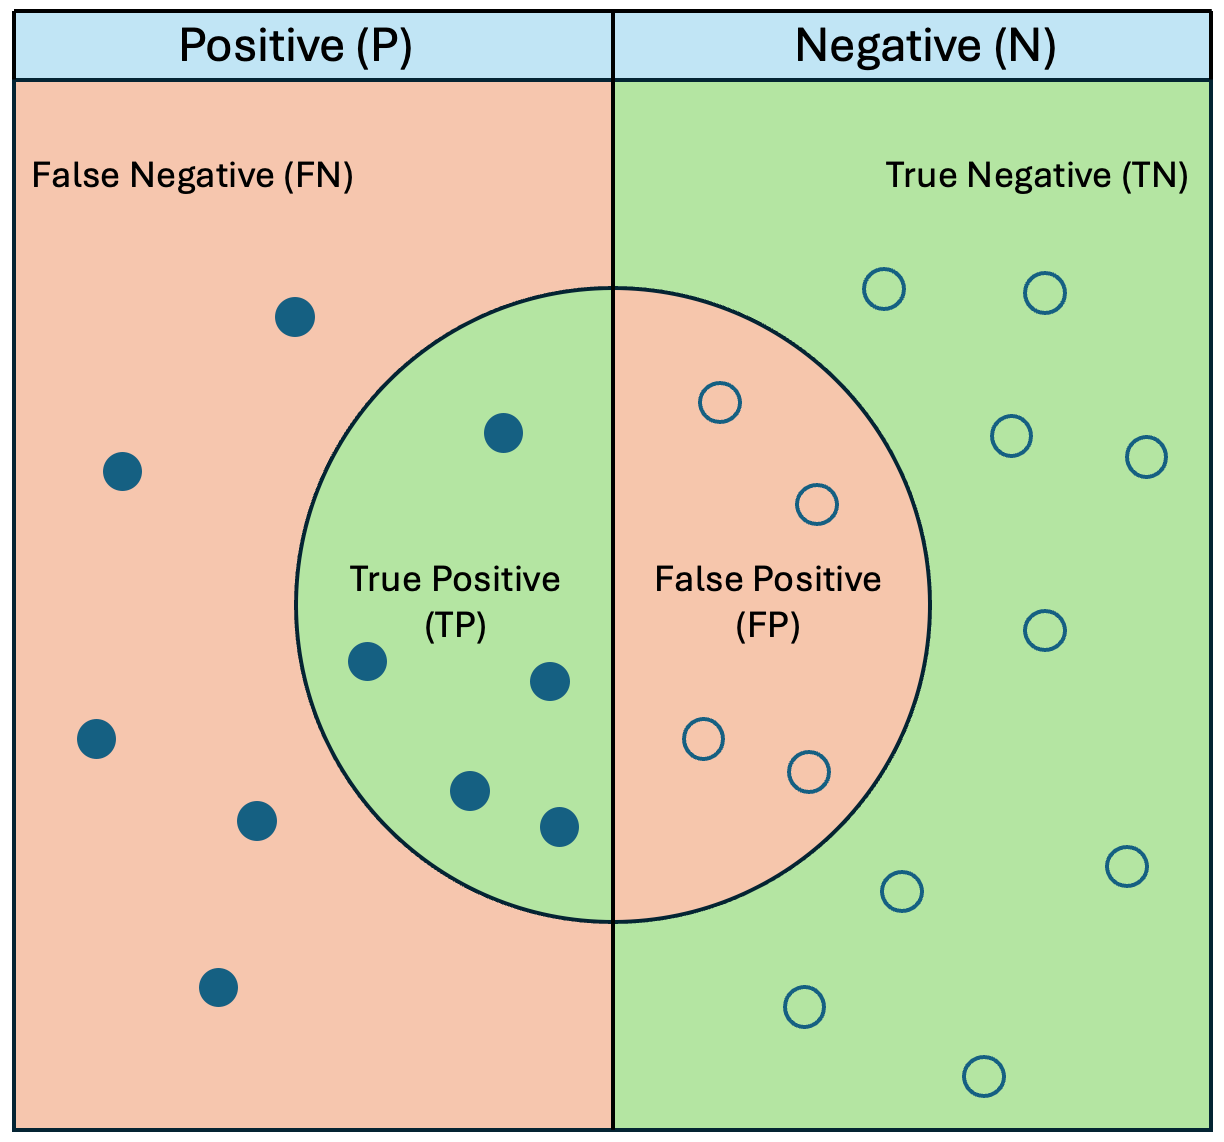
\includegraphics[width=0.6\linewidth,height=\textheight,keepaspectratio]{unidades/clasificadores/../../images/external/confusion-matrix.png}

}

\caption{Representación visual de una matriz de confusión y métricas de
clasificación binaria. El diagrama ilustra la relación entre la realidad
(columnas Positivo/Negativo) y las predicciones del modelo (círculo
central). Se identifican los Verdaderos Positivos (TP) y Falsos
Positivos (FP) dentro del área de predicción, mientras que los Falsos
Negativos (FN) y Verdaderos Negativos (TN) se ubican en el área de
exclusión.}

\end{figure}%

Como veremos mas adelante, la matriz de confusión es la base de toda
evaluación de clasificadores, ya que a partir de ella se derivan todas
las métricas de desempeño. Además, la interpretación de cada elemento de
la matriz tiene implicaciones estratégicas directas en la toma de
decisiones basada en el modelo.

\subsection{Generación de los Datasets
Sintéticos}\label{generaciuxf3n-de-los-datasets-sintuxe9ticos}

A lo largo de este capítulo se utilizan dos datasets sintéticos que
replican las características estadísticas de problemas reales.

\begin{itemize}
\item
  El \textbf{Dataset Médico} simula la detección de una condición grave
  con prevalencia del \textasciitilde8 \%, reflejando el desbalance
  típico en estudios de screening.
\item
  El \textbf{Dataset Financiero} simula transacciones con una tasa de
  fraude del \textasciitilde3 \%, consistente con benchmarks de la
  industria (Pedregosa et al., 2011).
\end{itemize}

Ambos datasets se generan con
\texttt{sklearn.datasets.make\_classification}, que permite controlar el
número de características informativas, el nivel de ruido en las
etiquetas y el desbalance de clases.

\begin{Shaded}
\begin{Highlighting}[]
\CommentTok{\# ── Configuración global e importaciones ───────────────────────────────────}
\ImportTok{import}\NormalTok{ numpy }\ImportTok{as}\NormalTok{ np}
\ImportTok{import}\NormalTok{ pandas }\ImportTok{as}\NormalTok{ pd}
\ImportTok{import}\NormalTok{ plotly.graph\_objects }\ImportTok{as}\NormalTok{ go}
\ImportTok{import}\NormalTok{ plotly.figure\_factory }\ImportTok{as}\NormalTok{ ff}
\ImportTok{from}\NormalTok{ plotly.subplots }\ImportTok{import}\NormalTok{ make\_subplots}
\ImportTok{from}\NormalTok{ sklearn.datasets }\ImportTok{import}\NormalTok{ make\_classification}
\ImportTok{from}\NormalTok{ sklearn.linear\_model }\ImportTok{import}\NormalTok{ LogisticRegression}
\ImportTok{from}\NormalTok{ sklearn.ensemble }\ImportTok{import}\NormalTok{ RandomForestClassifier}
\ImportTok{from}\NormalTok{ sklearn.model\_selection }\ImportTok{import}\NormalTok{ train\_test\_split}
\ImportTok{from}\NormalTok{ sklearn.metrics }\ImportTok{import}\NormalTok{ (}
\NormalTok{    confusion\_matrix, accuracy\_score, precision\_score, recall\_score,}
\NormalTok{    f1\_score, fbeta\_score, roc\_curve, auc, precision\_recall\_curve,}
\NormalTok{    average\_precision\_score, classification\_report,}
\NormalTok{)}

\NormalTok{SEED }\OperatorTok{=} \DecValTok{42}

\CommentTok{\# ── Dataset médico: 92 \% sanos, 8 \% enfermos ───────────────────────────────}
\NormalTok{X\_med, y\_med }\OperatorTok{=}\NormalTok{ make\_classification(}
\NormalTok{    n\_samples}\OperatorTok{=}\DecValTok{1000}\NormalTok{, n\_features}\OperatorTok{=}\DecValTok{10}\NormalTok{, n\_informative}\OperatorTok{=}\DecValTok{5}\NormalTok{,}
\NormalTok{    weights}\OperatorTok{=}\NormalTok{[}\FloatTok{0.92}\NormalTok{, }\FloatTok{0.08}\NormalTok{],   }\CommentTok{\# fuerte desbalance}
\NormalTok{    flip\_y}\OperatorTok{=}\FloatTok{0.02}\NormalTok{,            }\CommentTok{\# 2 \% de ruido en las etiquetas}
\NormalTok{    random\_state}\OperatorTok{=}\NormalTok{SEED,}
\NormalTok{)}
\NormalTok{X\_tr\_m, X\_te\_m, y\_tr\_m, y\_te\_m }\OperatorTok{=}\NormalTok{ train\_test\_split(}
\NormalTok{    X\_med, y\_med, test\_size}\OperatorTok{=}\FloatTok{0.3}\NormalTok{, stratify}\OperatorTok{=}\NormalTok{y\_med, random\_state}\OperatorTok{=}\NormalTok{SEED}
\NormalTok{)}

\CommentTok{\# ── Dataset financiero: 97 \% legítimas, 3 \% fraude ─────────────────────────}
\NormalTok{X\_fin, y\_fin }\OperatorTok{=}\NormalTok{ make\_classification(}
\NormalTok{    n\_samples}\OperatorTok{=}\DecValTok{5000}\NormalTok{, n\_features}\OperatorTok{=}\DecValTok{15}\NormalTok{, n\_informative}\OperatorTok{=}\DecValTok{7}\NormalTok{,}
\NormalTok{    weights}\OperatorTok{=}\NormalTok{[}\FloatTok{0.97}\NormalTok{, }\FloatTok{0.03}\NormalTok{],}
\NormalTok{    flip\_y}\OperatorTok{=}\FloatTok{0.01}\NormalTok{,}
\NormalTok{    random\_state}\OperatorTok{=}\NormalTok{SEED,}
\NormalTok{)}
\NormalTok{X\_tr\_f, X\_te\_f, y\_tr\_f, y\_te\_f }\OperatorTok{=}\NormalTok{ train\_test\_split(}
\NormalTok{    X\_fin, y\_fin, test\_size}\OperatorTok{=}\FloatTok{0.3}\NormalTok{, stratify}\OperatorTok{=}\NormalTok{y\_fin, random\_state}\OperatorTok{=}\NormalTok{SEED}
\NormalTok{)}

\CommentTok{\# ── Modelo 1: Regresión Logística — dataset médico ─────────────────────────}
\NormalTok{modelo\_lr }\OperatorTok{=}\NormalTok{ LogisticRegression(random\_state}\OperatorTok{=}\NormalTok{SEED, max\_iter}\OperatorTok{=}\DecValTok{500}\NormalTok{)}
\NormalTok{modelo\_lr.fit(X\_tr\_m, y\_tr\_m)}
\NormalTok{y\_pred\_lr }\OperatorTok{=}\NormalTok{ modelo\_lr.predict(X\_te\_m)}
\NormalTok{y\_prob\_lr }\OperatorTok{=}\NormalTok{ modelo\_lr.predict\_proba(X\_te\_m)[:, }\DecValTok{1}\NormalTok{]}

\CommentTok{\# ── Modelo 2: Random Forest — dataset médico ───────────────────────────────}
\NormalTok{modelo\_rf }\OperatorTok{=}\NormalTok{ RandomForestClassifier(n\_estimators}\OperatorTok{=}\DecValTok{100}\NormalTok{, random\_state}\OperatorTok{=}\NormalTok{SEED)}
\NormalTok{modelo\_rf.fit(X\_tr\_m, y\_tr\_m)}
\NormalTok{y\_pred\_rf }\OperatorTok{=}\NormalTok{ modelo\_rf.predict(X\_te\_m)}
\NormalTok{y\_prob\_rf }\OperatorTok{=}\NormalTok{ modelo\_rf.predict\_proba(X\_te\_m)[:, }\DecValTok{1}\NormalTok{]}

\CommentTok{\# ── Modelo 3: Regresión Logística — dataset financiero ─────────────────────}
\NormalTok{modelo\_fin }\OperatorTok{=}\NormalTok{ LogisticRegression(}
\NormalTok{    random\_state}\OperatorTok{=}\NormalTok{SEED, max\_iter}\OperatorTok{=}\DecValTok{500}\NormalTok{, class\_weight}\OperatorTok{=}\StringTok{"balanced"}
\NormalTok{)}
\NormalTok{modelo\_fin.fit(X\_tr\_f, y\_tr\_f)}
\NormalTok{y\_pred\_fin }\OperatorTok{=}\NormalTok{ modelo\_fin.predict(X\_te\_f)}
\NormalTok{y\_prob\_fin }\OperatorTok{=}\NormalTok{ modelo\_fin.predict\_proba(X\_te\_f)[:, }\DecValTok{1}\NormalTok{]}

\BuiltInTok{print}\NormalTok{(}\StringTok{"Distribución de clases — test médico    :"}\NormalTok{,}
      \BuiltInTok{dict}\NormalTok{(}\BuiltInTok{zip}\NormalTok{(}\OperatorTok{*}\NormalTok{np.unique(y\_te\_m, return\_counts}\OperatorTok{=}\VariableTok{True}\NormalTok{))))}
\BuiltInTok{print}\NormalTok{(}\StringTok{"Distribución de clases — test financiero:"}\NormalTok{,}
      \BuiltInTok{dict}\NormalTok{(}\BuiltInTok{zip}\NormalTok{(}\OperatorTok{*}\NormalTok{np.unique(y\_te\_f, return\_counts}\OperatorTok{=}\VariableTok{True}\NormalTok{))))}
\end{Highlighting}
\end{Shaded}

\begin{verbatim}
Distribución de clases — test médico    : {np.int64(0): np.int64(275), np.int64(1): np.int64(25)}
Distribución de clases — test financiero: {np.int64(0): np.int64(1449), np.int64(1): np.int64(51)}
\end{verbatim}

Para evaluar a lo largo del capitulo diferentes modelos empleamos tres
modelos de clasificación binaria: una \textbf{regresión logística} y un
\textbf{random forest} para el dataset médico, y una \textbf{regresión
logística con ajuste de clase} para el dataset financiero.

Así como primer ejemplo mostramos la matriz de confusión del modelo de
regresión logística sobre el dataset médico:

\begin{Shaded}
\begin{Highlighting}[]
\CommentTok{\# ── Función reutilizable: matriz de confusión interactiva ───────────────────}
\KeywordTok{def}\NormalTok{ plot\_confusion\_matrix(cm,}
\NormalTok{titulo}\OperatorTok{=}\StringTok{" "}\NormalTok{,}
\NormalTok{                          etiquetas}\OperatorTok{=}\VariableTok{None}\NormalTok{):}
    \CommentTok{"""}
\CommentTok{    Visualiza una matriz de confusión 2×2 con Plotly.}

\CommentTok{    Muestra conteos absolutos y porcentajes por fila}
\CommentTok{    (tasa de acierto/error por clase real).}

\CommentTok{    Parámetros}
\CommentTok{    {-}{-}{-}{-}{-}{-}{-}{-}{-}{-}}
\CommentTok{    cm        : np.ndarray  — salida de sklearn confusion\_matrix}
\CommentTok{    titulo    : str         — título del gráfico}
\CommentTok{    etiquetas : list[str]   — nombres de las clases [neg, pos]}
\CommentTok{    """}
    \ControlFlowTok{if}\NormalTok{ etiquetas }\KeywordTok{is} \VariableTok{None}\NormalTok{:}
\NormalTok{        etiquetas }\OperatorTok{=}\NormalTok{ [}\StringTok{"Negativo (0)"}\NormalTok{, }\StringTok{"Positivo (1)"}\NormalTok{]}

\NormalTok{    cm\_pct }\OperatorTok{=}\NormalTok{ cm.astype(}\BuiltInTok{float}\NormalTok{) }\OperatorTok{/}\NormalTok{ cm.}\BuiltInTok{sum}\NormalTok{(axis}\OperatorTok{=}\DecValTok{1}\NormalTok{, keepdims}\OperatorTok{=}\VariableTok{True}\NormalTok{) }\OperatorTok{*} \DecValTok{100}
\NormalTok{    texto }\OperatorTok{=}\NormalTok{ [}
\NormalTok{        [}\SpecialStringTok{f"}\SpecialCharTok{\{}\NormalTok{cm[i,j]}\SpecialCharTok{\}}\SpecialStringTok{\textless{}br\textgreater{}(}\SpecialCharTok{\{}\NormalTok{cm\_pct[i,j]}\SpecialCharTok{:.1f\}}\SpecialStringTok{ \%)"} \ControlFlowTok{for}\NormalTok{ j }\KeywordTok{in} \BuiltInTok{range}\NormalTok{(}\DecValTok{2}\NormalTok{)]}
        \ControlFlowTok{for}\NormalTok{ i }\KeywordTok{in} \BuiltInTok{range}\NormalTok{(}\DecValTok{2}\NormalTok{)}
\NormalTok{    ]}
    \CommentTok{\# Invertir filas para que TP quede arriba{-}derecha (convención visual habitual)}
\NormalTok{    z\_plot     }\OperatorTok{=}\NormalTok{ cm[::}\OperatorTok{{-}}\DecValTok{1}\NormalTok{, :]}
\NormalTok{    texto\_plot }\OperatorTok{=}\NormalTok{ texto[::}\OperatorTok{{-}}\DecValTok{1}\NormalTok{]}
\NormalTok{    y\_labels   }\OperatorTok{=}\NormalTok{ etiquetas[::}\OperatorTok{{-}}\DecValTok{1}\NormalTok{]}

\NormalTok{    fig }\OperatorTok{=}\NormalTok{ ff.create\_annotated\_heatmap(}
\NormalTok{        z}\OperatorTok{=}\NormalTok{z\_plot,}
\NormalTok{        x}\OperatorTok{=}\NormalTok{etiquetas,}
\NormalTok{        y}\OperatorTok{=}\NormalTok{y\_labels,}
\NormalTok{        annotation\_text}\OperatorTok{=}\NormalTok{texto\_plot,}
\NormalTok{        colorscale}\OperatorTok{=}\NormalTok{[[}\DecValTok{0}\NormalTok{, }\StringTok{"\#f8f9fa"}\NormalTok{], [}\FloatTok{0.5}\NormalTok{, }\StringTok{"\#4a90d9"}\NormalTok{], [}\DecValTok{1}\NormalTok{, }\StringTok{"\#e74c3c"}\NormalTok{]],}
\NormalTok{        showscale}\OperatorTok{=}\VariableTok{True}\NormalTok{,}
\NormalTok{    )}
\NormalTok{    fig.update\_layout(}
\NormalTok{        title}\OperatorTok{=}\NormalTok{titulo,}
\NormalTok{        xaxis\_title}\OperatorTok{=}\StringTok{"Predicción del modelo"}\NormalTok{,}
\NormalTok{        yaxis\_title}\OperatorTok{=}\StringTok{"Valor real"}\NormalTok{,}
\NormalTok{        height}\OperatorTok{=}\DecValTok{430}\NormalTok{, width}\OperatorTok{=}\DecValTok{530}\NormalTok{,}
\NormalTok{        font}\OperatorTok{=}\BuiltInTok{dict}\NormalTok{(size}\OperatorTok{=}\DecValTok{13}\NormalTok{),}
\NormalTok{    )}
    \CommentTok{\# Etiquetas de cuadrante}
\NormalTok{    etq }\OperatorTok{=}\NormalTok{ \{(}\DecValTok{0}\NormalTok{, }\DecValTok{0}\NormalTok{): (}\StringTok{"TN"}\NormalTok{, }\StringTok{"gray"}\NormalTok{),    (}\DecValTok{0}\NormalTok{, }\DecValTok{1}\NormalTok{): (}\StringTok{"FP"}\NormalTok{, }\StringTok{"\#e67e22"}\NormalTok{),}
\NormalTok{           (}\DecValTok{1}\NormalTok{, }\DecValTok{0}\NormalTok{): (}\StringTok{"FN"}\NormalTok{, }\StringTok{"\#e74c3c"}\NormalTok{), (}\DecValTok{1}\NormalTok{, }\DecValTok{1}\NormalTok{): (}\StringTok{"TP"}\NormalTok{, }\StringTok{"\#27ae60"}\NormalTok{)\}}
    \ControlFlowTok{for}\NormalTok{ (ri, ci), (label, color) }\KeywordTok{in}\NormalTok{ etq.items():}
\NormalTok{        ri\_plot }\OperatorTok{=} \DecValTok{1} \OperatorTok{{-}}\NormalTok{ ri}
\NormalTok{        fig.add\_annotation(}
\NormalTok{            x}\OperatorTok{=}\NormalTok{etiquetas[ci], y}\OperatorTok{=}\NormalTok{y\_labels[ri\_plot],}
\NormalTok{            text}\OperatorTok{=}\SpecialStringTok{f"\textless{}b\textgreater{}}\SpecialCharTok{\{}\NormalTok{label}\SpecialCharTok{\}}\SpecialStringTok{\textless{}/b\textgreater{}"}\NormalTok{,}
\NormalTok{            showarrow}\OperatorTok{=}\VariableTok{False}\NormalTok{,}
\NormalTok{            font}\OperatorTok{=}\BuiltInTok{dict}\NormalTok{(size}\OperatorTok{=}\DecValTok{11}\NormalTok{, color}\OperatorTok{=}\NormalTok{color),}
\NormalTok{            yshift}\OperatorTok{={-}}\DecValTok{22}\NormalTok{,}
\NormalTok{        )}
    \ControlFlowTok{return}\NormalTok{ fig}


\CommentTok{\# ── Aplicar al clasificador médico ──────────────────────────────────────────}
\NormalTok{cm\_lr }\OperatorTok{=}\NormalTok{ confusion\_matrix(y\_te\_m, y\_pred\_lr)}
\NormalTok{TP }\OperatorTok{=} \BuiltInTok{int}\NormalTok{(cm\_lr[}\DecValTok{1}\NormalTok{, }\DecValTok{1}\NormalTok{])}\OperatorTok{;}\NormalTok{ TN }\OperatorTok{=} \BuiltInTok{int}\NormalTok{(cm\_lr[}\DecValTok{0}\NormalTok{, }\DecValTok{0}\NormalTok{])}
\NormalTok{FP }\OperatorTok{=} \BuiltInTok{int}\NormalTok{(cm\_lr[}\DecValTok{0}\NormalTok{, }\DecValTok{1}\NormalTok{])}\OperatorTok{;}\NormalTok{ FN }\OperatorTok{=} \BuiltInTok{int}\NormalTok{(cm\_lr[}\DecValTok{1}\NormalTok{, }\DecValTok{0}\NormalTok{])}

\BuiltInTok{print}\NormalTok{(}\StringTok{"Matriz de confusión — Regresión Logística (médico):"}\NormalTok{)}
\BuiltInTok{print}\NormalTok{(cm\_lr)}
\BuiltInTok{print}\NormalTok{(}\SpecialStringTok{f"}\CharTok{\textbackslash{}n}\SpecialStringTok{TP=}\SpecialCharTok{\{}\NormalTok{TP}\SpecialCharTok{\}}\SpecialStringTok{, TN=}\SpecialCharTok{\{}\NormalTok{TN}\SpecialCharTok{\}}\SpecialStringTok{, FP=}\SpecialCharTok{\{}\NormalTok{FP}\SpecialCharTok{\}}\SpecialStringTok{, FN=}\SpecialCharTok{\{}\NormalTok{FN}\SpecialCharTok{\}}\SpecialStringTok{"}\NormalTok{)}

\NormalTok{fig\_cm }\OperatorTok{=}\NormalTok{ plot\_confusion\_matrix(}
\NormalTok{    cm\_lr,}
    \CommentTok{\# titulo="Matriz de Confusión — Clasificador Médico (Reg. Logística)",}
\NormalTok{    etiquetas}\OperatorTok{=}\NormalTok{[}\StringTok{"Sano"}\NormalTok{, }\StringTok{"Enfermo"}\NormalTok{],}
\NormalTok{)}
\NormalTok{fig\_cm.show()}
\end{Highlighting}
\end{Shaded}

\begin{verbatim}
Matriz de confusión — Regresión Logística (médico):
[[273   2]
 [ 19   6]]

TP=6, TN=273, FP=2, FN=19
\end{verbatim}

\begin{verbatim}
Unable to display output for mime type(s): text/html
\end{verbatim}

\begin{verbatim}
Unable to display output for mime type(s): text/html
\end{verbatim}

A partir de esta matriz de confusión se derivan todas las métricas de
desempeño que analizaremos a lo largo del capítulo. Además, la
interpretación de cada elemento de la matriz tiene implicaciones
estratégicas directas en la toma de decisiones basada en el modelo.

\subsection{El Costo Asimétrico del Error: Contextos
Reales}\label{el-costo-asimuxe9trico-del-error-contextos-reales}

La característica más importante de los errores en clasificación no es
su frecuencia absoluta, sino su \textbf{costo diferencial}. En la
mayoría de los problemas reales de minería de datos, FP y FN no tienen
el mismo costo, y optimizar hacia uno implica sacrificar el otro (James
et al., 2021).

\subsubsection{Medicina: El Costo Devastador del Falso
Negativo}\label{medicina-el-costo-devastador-del-falso-negativo}

En un sistema de detección temprana de cáncer de pulmón, un
\textbf{Falso Negativo} significa que el sistema predice ``benigno''
para un nódulo que en realidad es canceroso. El paciente no recibe
tratamiento. Esta asimetría implica que en medicina diagnóstica se
prefieren clasificadores con \textbf{alto Recall} (baja tasa de FN),
incluso a expensas de menor Precision. Un \textbf{Falso Positivo}
significa que el sistema predice ``maligno'' para un nódulo benigno: el
paciente es referido para biopsia innecesaria ---procedimiento invasivo
y costoso---, pero comparado con el costo del FN, el FP es el error
tolerable.

\subsubsection{Finanzas: El Costo Operativo del Falso
Positivo}\label{finanzas-el-costo-operativo-del-falso-positivo}

En un sistema de detección de fraude, un \textbf{Falso Positivo} bloquea
una transacción legítima: el cliente no puede completar su compra, con
el riesgo de perder la relación comercial. Un \textbf{Falso Negativo}
deja pasar un fraude real, pero la pérdida suele ser cubierta por seguro
o chargeback. Esta asimetría inversa implica que en detección de fraude
se prefieren clasificadores con \textbf{alta Precision}, aceptando que
algunos fraudes pasen sin detectarse (Provost \& Fawcett, 2013).

\begin{Shaded}
\begin{Highlighting}[]
\CommentTok{\# ── Visualización del costo asimétrico por contexto ────────────────────────}
\NormalTok{contextos }\OperatorTok{=}\NormalTok{ [}\StringTok{"Medicina}\CharTok{\textbackslash{}n}\StringTok{(screening)"}\NormalTok{, }\StringTok{"Finanzas}\CharTok{\textbackslash{}n}\StringTok{(fraude)"}\NormalTok{]}
\NormalTok{costo\_fn  }\OperatorTok{=}\NormalTok{ [}\DecValTok{10}\NormalTok{, }\DecValTok{3}\NormalTok{]   }\CommentTok{\# escala relativa normalizada}
\NormalTok{costo\_fp  }\OperatorTok{=}\NormalTok{ [}\DecValTok{2}\NormalTok{,  }\DecValTok{8}\NormalTok{]}

\NormalTok{fig }\OperatorTok{=}\NormalTok{ go.Figure(data}\OperatorTok{=}\NormalTok{[}
\NormalTok{    go.Bar(name}\OperatorTok{=}\StringTok{"Costo FN (Falso Negativo)"}\NormalTok{, x}\OperatorTok{=}\NormalTok{contextos, y}\OperatorTok{=}\NormalTok{costo\_fn,}
\NormalTok{           marker\_color}\OperatorTok{=}\StringTok{"\#e74c3c"}\NormalTok{,}
\NormalTok{           text}\OperatorTok{=}\NormalTok{[}\StringTok{"Crítico: paciente}\CharTok{\textbackslash{}n}\StringTok{sin tratamiento"}\NormalTok{,}
                 \StringTok{"Moderado: pérdida}\CharTok{\textbackslash{}n}\StringTok{cubierta por seguro"}\NormalTok{],}
\NormalTok{           textposition}\OperatorTok{=}\StringTok{"auto"}\NormalTok{),}
\NormalTok{    go.Bar(name}\OperatorTok{=}\StringTok{"Costo FP (Falso Positivo)"}\NormalTok{, x}\OperatorTok{=}\NormalTok{contextos, y}\OperatorTok{=}\NormalTok{costo\_fp,}
\NormalTok{           marker\_color}\OperatorTok{=}\StringTok{"\#e67e22"}\NormalTok{,}
\NormalTok{           text}\OperatorTok{=}\NormalTok{[}\StringTok{"Moderado: biopsia}\CharTok{\textbackslash{}n}\StringTok{innecesaria"}\NormalTok{,}
                 \StringTok{"Alto: cliente}\CharTok{\textbackslash{}n}\StringTok{abandonado"}\NormalTok{],}
\NormalTok{           textposition}\OperatorTok{=}\StringTok{"auto"}\NormalTok{),}
\NormalTok{])}
\NormalTok{fig.update\_layout(}
\NormalTok{    barmode}\OperatorTok{=}\StringTok{"group"}\NormalTok{,}
\NormalTok{    title}\OperatorTok{=}\NormalTok{(}
        \StringTok{"Costo Asimétrico de los Errores por Contexto\textless{}br\textgreater{}"}
        \StringTok{"\textless{}sup\textgreater{}Escala relativa normalizada — Provost \& Fawcett (2013)\textless{}/sup\textgreater{}"}
\NormalTok{    ),}
\NormalTok{    yaxis\_title}\OperatorTok{=}\StringTok{"Severidad relativa del error"}\NormalTok{,}
\NormalTok{    height}\OperatorTok{=}\DecValTok{420}\NormalTok{,}
    \CommentTok{\# legend=dict(orientation="h", yanchor="bottom", y=1.02),}
\NormalTok{)}
\NormalTok{fig.show()}
\end{Highlighting}
\end{Shaded}

\begin{verbatim}
Unable to display output for mime type(s): text/html
\end{verbatim}

\section{Métricas de desempeño: más allá del error
rate}\label{muxe9tricas-de-desempeuxf1o-muxe1s-alluxe1-del-error-rate}

Como mencionamos anteriormente, siq ueremos evaluar de manera adecuada
un clasificador es necesario considerar no solo el número de errores,
sino también su tipo y costo. Para esto se han desarrollado un conjunto
de métricas que se derivan de la matriz de confusión y que permiten
cuantificar diferentes aspectos del desempeño del modelo. Estas métricas
no son mutuamente excluyentes, sino complementarias, y su interpretación
debe hacerse en conjunto para obtener una visión completa del modelo. A
continuación se presentan las métricas más importantes para la
evaluación de clasificadores binarios, con su definición formal, cálculo
detallado e interpretación contextualizada.

\subsection{Accuracy: Definición, Utilidad y
Limitaciones}\label{accuracy-definiciuxf3n-utilidad-y-limitaciones}

\subsubsection{Definición Formal}\label{definiciuxf3n-formal-1}

\[
\text{Accuracy} = \frac{TP + TN}{TP + TN + FP + FN}
\]

La accuracy mide la proporción de instancias correctamente clasificadas
sobre el total (Han et al., 2011).

\subsubsection{Cálculo e Interpretación
Básica}\label{cuxe1lculo-e-interpretaciuxf3n-buxe1sica}

\begin{Shaded}
\begin{Highlighting}[]
\CommentTok{\# ── Accuracy del modelo real vs. clasificador trivial ──────────────────────}
\NormalTok{acc\_lr      }\OperatorTok{=}\NormalTok{ accuracy\_score(y\_te\_m, y\_pred\_lr)}
\NormalTok{y\_trivial   }\OperatorTok{=}\NormalTok{ np.zeros\_like(y\_te\_m)          }\CommentTok{\# siempre predice "sano"}
\NormalTok{acc\_trivial }\OperatorTok{=}\NormalTok{ accuracy\_score(y\_te\_m, y\_trivial)}

\BuiltInTok{print}\NormalTok{(}\SpecialStringTok{f"Accuracy — Regresión Logística : }\SpecialCharTok{\{}\NormalTok{acc\_lr}\SpecialCharTok{:.4f\}}\SpecialStringTok{  (}\SpecialCharTok{\{}\NormalTok{acc\_lr}\OperatorTok{*}\DecValTok{100}\SpecialCharTok{:.2f\}}\SpecialStringTok{ \%)"}\NormalTok{)}
\BuiltInTok{print}\NormalTok{(}\SpecialStringTok{f"Accuracy — Modelo trivial      : }\SpecialCharTok{\{}\NormalTok{acc\_trivial}\SpecialCharTok{:.4f\}}\SpecialStringTok{  (}\SpecialCharTok{\{}\NormalTok{acc\_trivial}\OperatorTok{*}\DecValTok{100}\SpecialCharTok{:.2f\}}\SpecialStringTok{ \%)"}\NormalTok{)}
\BuiltInTok{print}\NormalTok{()}
\BuiltInTok{print}\NormalTok{(}\StringTok{"¿El modelo trivial (siempre \textquotesingle{}sano\textquotesingle{}) detecta algún enfermo?"}\NormalTok{)}
\BuiltInTok{print}\NormalTok{(}\SpecialStringTok{f"  Enfermos detectados: }\SpecialCharTok{\{}\NormalTok{((y\_trivial}\OperatorTok{==}\DecValTok{1}\NormalTok{) }\OperatorTok{\&}\NormalTok{ (y\_te\_m}\OperatorTok{==}\DecValTok{1}\NormalTok{))}\SpecialCharTok{.}\BuiltInTok{sum}\NormalTok{()}\SpecialCharTok{\}}\SpecialStringTok{ / }\SpecialCharTok{\{}\NormalTok{y\_te\_m}\SpecialCharTok{.}\BuiltInTok{sum}\NormalTok{()}\SpecialCharTok{\}}\SpecialStringTok{"}\NormalTok{)}
\end{Highlighting}
\end{Shaded}

\begin{verbatim}
Accuracy — Regresión Logística : 0.9300  (93.00 %)
Accuracy — Modelo trivial      : 0.9167  (91.67 %)

¿El modelo trivial (siempre 'sano') detecta algún enfermo?
  Enfermos detectados: 0 / 25
\end{verbatim}

\subsubsection{La Paradoja de la Exactitud (Accuracy
Paradox)}\label{la-paradoja-de-la-exactitud-accuracy-paradox}

La limitación más crítica de la accuracy emerge cuando el dataset
presenta \textbf{desbalance de clases}, situación extremadamente común
en aplicaciones reales de minería de datos (Saito \& Rehmsmeier, 2015).
En nuestro dataset financiero con 97 \% de transacciones legítimas, un
clasificador trivial alcanza \textasciitilde97 \% de accuracy sin
detectar ningún fraude:

\begin{Shaded}
\begin{Highlighting}[]
\CommentTok{\# ── Paradoja de la exactitud — dataset financiero ──────────────────────────}
\NormalTok{y\_trivial\_fin   }\OperatorTok{=}\NormalTok{ np.zeros\_like(y\_te\_f)}
\NormalTok{acc\_trivial\_fin }\OperatorTok{=}\NormalTok{ accuracy\_score(y\_te\_f, y\_trivial\_fin)}
\NormalTok{acc\_modelo\_fin  }\OperatorTok{=}\NormalTok{ accuracy\_score(y\_te\_f, y\_pred\_fin)}
\NormalTok{recall\_trivial  }\OperatorTok{=}\NormalTok{ recall\_score(y\_te\_f, y\_trivial\_fin, zero\_division}\OperatorTok{=}\DecValTok{0}\NormalTok{)}
\NormalTok{recall\_modelo   }\OperatorTok{=}\NormalTok{ recall\_score(y\_te\_f, y\_pred\_fin)}

\BuiltInTok{print}\NormalTok{(}\StringTok{"Dataset financiero (97 }\SpecialCharTok{\% le}\StringTok{gítimas, 3 }\SpecialCharTok{\% f}\StringTok{raude)"}\NormalTok{)}
\BuiltInTok{print}\NormalTok{(}\StringTok{"─"} \OperatorTok{*} \DecValTok{52}\NormalTok{)}
\BuiltInTok{print}\NormalTok{(}\SpecialStringTok{f"Accuracy — modelo trivial : }\SpecialCharTok{\{}\NormalTok{acc\_trivial\_fin}\SpecialCharTok{:.4f\}}\SpecialStringTok{  (}\SpecialCharTok{\{}\NormalTok{acc\_trivial\_fin}\OperatorTok{*}\DecValTok{100}\SpecialCharTok{:.1f\}}\SpecialStringTok{ \%)"}\NormalTok{)}
\BuiltInTok{print}\NormalTok{(}\SpecialStringTok{f"Accuracy — modelo real    : }\SpecialCharTok{\{}\NormalTok{acc\_modelo\_fin}\SpecialCharTok{:.4f\}}\SpecialStringTok{  (}\SpecialCharTok{\{}\NormalTok{acc\_modelo\_fin}\OperatorTok{*}\DecValTok{100}\SpecialCharTok{:.1f\}}\SpecialStringTok{ \%)"}\NormalTok{)}
\BuiltInTok{print}\NormalTok{()}
\BuiltInTok{print}\NormalTok{(}\SpecialStringTok{f"Recall  — modelo trivial  : }\SpecialCharTok{\{}\NormalTok{recall\_trivial}\SpecialCharTok{:.4f\}}\SpecialStringTok{  → 0 fraudes detectados"}\NormalTok{)}
\BuiltInTok{print}\NormalTok{(}\SpecialStringTok{f"Recall  — modelo real     : }\SpecialCharTok{\{}\NormalTok{recall\_modelo}\SpecialCharTok{:.4f\}}\SpecialStringTok{  → detecta fraudes reales"}\NormalTok{)}
\BuiltInTok{print}\NormalTok{()}
\BuiltInTok{print}\NormalTok{(}\StringTok{"Conclusión: mayor accuracy ≠ mejor modelo en datos desbalanceados."}\NormalTok{)}
\BuiltInTok{print}\NormalTok{(}\StringTok{"(Saito \& Rehmsmeier, 2015)"}\NormalTok{)}
\end{Highlighting}
\end{Shaded}

\begin{verbatim}
Dataset financiero (97 % legítimas, 3 % fraude)
────────────────────────────────────────────────────
Accuracy — modelo trivial : 0.9660  (96.6 %)
Accuracy — modelo real    : 0.7820  (78.2 %)

Recall  — modelo trivial  : 0.0000  → 0 fraudes detectados
Recall  — modelo real     : 0.7255  → detecta fraudes reales

Conclusión: mayor accuracy ≠ mejor modelo en datos desbalanceados.
(Saito & Rehmsmeier, 2015)
\end{verbatim}

\begin{Shaded}
\begin{Highlighting}[]
\CommentTok{\# ── Visualización: Accuracy vs. Recall ─────────────────────────────────────}
\NormalTok{modelos    }\OperatorTok{=}\NormalTok{ [}\StringTok{"Modelo Real}\CharTok{\textbackslash{}n}\StringTok{(LR + class\_weight)"}\NormalTok{, }\StringTok{"Modelo Trivial}\CharTok{\textbackslash{}n}\StringTok{(siempre negativo)"}\NormalTok{]}
\NormalTok{accuracies }\OperatorTok{=}\NormalTok{ [acc\_modelo\_fin, acc\_trivial\_fin]}
\NormalTok{recalls    }\OperatorTok{=}\NormalTok{ [recall\_modelo, recall\_trivial]}

\NormalTok{fig }\OperatorTok{=}\NormalTok{ go.Figure(data}\OperatorTok{=}\NormalTok{[}
\NormalTok{    go.Bar(name}\OperatorTok{=}\StringTok{"Accuracy"}\NormalTok{, x}\OperatorTok{=}\NormalTok{modelos, y}\OperatorTok{=}\NormalTok{accuracies,}
\NormalTok{           marker\_color}\OperatorTok{=}\NormalTok{[}\StringTok{"\#4a90d9"}\NormalTok{, }\StringTok{"\#e74c3c"}\NormalTok{],}
\NormalTok{           text}\OperatorTok{=}\NormalTok{[}\SpecialStringTok{f"}\SpecialCharTok{\{}\NormalTok{v}\SpecialCharTok{:.2\%\}}\SpecialStringTok{"} \ControlFlowTok{for}\NormalTok{ v }\KeywordTok{in}\NormalTok{ accuracies], textposition}\OperatorTok{=}\StringTok{"auto"}\NormalTok{),}
\NormalTok{    go.Bar(name}\OperatorTok{=}\StringTok{"Recall (clase fraude)"}\NormalTok{, x}\OperatorTok{=}\NormalTok{modelos, y}\OperatorTok{=}\NormalTok{recalls,}
\NormalTok{           marker\_color}\OperatorTok{=}\NormalTok{[}\StringTok{"\#27ae60"}\NormalTok{, }\StringTok{"\#c0392b"}\NormalTok{],}
\NormalTok{           text}\OperatorTok{=}\NormalTok{[}\SpecialStringTok{f"}\SpecialCharTok{\{}\NormalTok{v}\SpecialCharTok{:.2\%\}}\SpecialStringTok{"} \ControlFlowTok{for}\NormalTok{ v }\KeywordTok{in}\NormalTok{ recalls], textposition}\OperatorTok{=}\StringTok{"auto"}\NormalTok{),}
\NormalTok{])}
\NormalTok{fig.update\_layout(}
\NormalTok{    barmode}\OperatorTok{=}\StringTok{"group"}\NormalTok{,}
\NormalTok{    title}\OperatorTok{=}\NormalTok{(}
        \StringTok{"Paradoja de la Exactitud en el Dataset Financiero\textless{}br\textgreater{}"}
        \StringTok{"\textless{}sup\textgreater{}Saito \& Rehmsmeier (2015): un modelo con mayor accuracy detecta 0 fraudes\textless{}/sup\textgreater{}"}
\NormalTok{    ),}
\NormalTok{    yaxis}\OperatorTok{=}\BuiltInTok{dict}\NormalTok{(title}\OperatorTok{=}\StringTok{"Valor"}\NormalTok{, }\BuiltInTok{range}\OperatorTok{=}\NormalTok{[}\DecValTok{0}\NormalTok{, }\FloatTok{1.1}\NormalTok{], tickformat}\OperatorTok{=}\StringTok{"\%"}\NormalTok{),}
\NormalTok{    height}\OperatorTok{=}\DecValTok{420}\NormalTok{,}
    \CommentTok{\# legend=dict(orientation="h", yanchor="bottom", y=1.02),}
\NormalTok{)}
\NormalTok{fig.show()}
\end{Highlighting}
\end{Shaded}

\begin{verbatim}
Unable to display output for mime type(s): text/html
\end{verbatim}

\subsection{Precision: Confiabilidad de las Predicciones
Positivas}\label{precision-confiabilidad-de-las-predicciones-positivas}

\subsubsection{Definición Formal}\label{definiciuxf3n-formal-2}

\[
\text{Precision} = \frac{TP}{TP + FP}
\]

La Precision mide qué proporción de las instancias predichas como
positivas son genuinamente positivas (James et al., 2021).

\subsubsection{Cálculo Detallado}\label{cuxe1lculo-detallado}

\begin{Shaded}
\begin{Highlighting}[]
\CommentTok{\# ── Precision: cálculo manual y con sklearn ─────────────────────────────────}
\NormalTok{precision\_manual }\OperatorTok{=}\NormalTok{ TP }\OperatorTok{/}\NormalTok{ (TP }\OperatorTok{+}\NormalTok{ FP) }\ControlFlowTok{if}\NormalTok{ (TP }\OperatorTok{+}\NormalTok{ FP) }\OperatorTok{\textgreater{}} \DecValTok{0} \ControlFlowTok{else} \DecValTok{0}
\NormalTok{precision\_sk     }\OperatorTok{=}\NormalTok{ precision\_score(y\_te\_m, y\_pred\_lr, zero\_division}\OperatorTok{=}\DecValTok{0}\NormalTok{)}

\BuiltInTok{print}\NormalTok{(}\SpecialStringTok{f"Cálculo manual  — Precision = }\SpecialCharTok{\{}\NormalTok{TP}\SpecialCharTok{\}}\SpecialStringTok{ / (}\SpecialCharTok{\{}\NormalTok{TP}\SpecialCharTok{\}}\SpecialStringTok{+}\SpecialCharTok{\{}\NormalTok{FP}\SpecialCharTok{\}}\SpecialStringTok{) = }\SpecialCharTok{\{}\NormalTok{precision\_manual}\SpecialCharTok{:.4f\}}\SpecialStringTok{"}\NormalTok{)}
\BuiltInTok{print}\NormalTok{(}\SpecialStringTok{f"sklearn         — Precision = }\SpecialCharTok{\{}\NormalTok{precision\_sk}\SpecialCharTok{:.4f\}}\SpecialStringTok{"}\NormalTok{)}
\BuiltInTok{print}\NormalTok{()}
\BuiltInTok{print}\NormalTok{(}\SpecialStringTok{f"Interpretación: de cada 10 alarmas de \textquotesingle{}enfermo\textquotesingle{},"}\NormalTok{)}
\BuiltInTok{print}\NormalTok{(}\SpecialStringTok{f"  aproximadamente }\SpecialCharTok{\{}\NormalTok{precision\_sk}\OperatorTok{*}\DecValTok{10}\SpecialCharTok{:.1f\}}\SpecialStringTok{ corresponden a enfermos reales."}\NormalTok{)}
\end{Highlighting}
\end{Shaded}

\begin{verbatim}
Cálculo manual  — Precision = 6 / (6+2) = 0.7500
sklearn         — Precision = 0.7500

Interpretación: de cada 10 alarmas de 'enfermo',
  aproximadamente 7.5 corresponden a enfermos reales.
\end{verbatim}

\subsubsection{Limitación: Alta Precision ≠ Buen
Clasificador}\label{limitaciuxf3n-alta-precision-buen-clasificador}

Para entenderlo mejor, imagina que la \textbf{Precisión} es la
``puntería'' o calidad de lo que el sistema detecta.

Si un sistema es extremadamente tímido y solo lanza una alerta cuando
tiene una certeza absoluta, su \textbf{Precisión será perfecta (1.0)}:
cada vez que hable, tendrá razón. Sin embargo, el costo de esa
perfección es el silencio; el sistema ignorará muchísimos casos reales
por miedo a equivocarse. En la práctica, un sistema que casi nunca se
atreve a alertar no es útil, aunque nunca mienta.

Por el contrario, si el sistema es demasiado ``sensible'' y alerta por
cualquier cosa, su precisión cae. Fawcett (2006) identifica que cuando
la precisión es muy baja, ocurre la \textbf{fatiga de alarmas}: el
usuario recibe tantos avisos falsos que deja de confiar en el sistema y
termina ignorándolo por completo.

\subsubsection{Ejemplo: El filtro de correos
``Spam''}\label{ejemplo-el-filtro-de-correos-spam}

\begin{itemize}
\tightlist
\item
  \textbf{Alta Precisión (Certeza absoluta):} Configuras tu correo para
  que solo marque como Spam los mensajes que digan explícitamente ``ESTO
  ES UNA ESTAFA''. Tendrás una precisión de 1.0 (nunca se equivocará con
  un correo importante), pero tu bandeja de entrada principal se llenará
  de basura que el filtro no se atrevió a marcar.
\item
  \textbf{Baja Precisión (Fatiga de alarmas):} Configuras el filtro para
  que marque como Spam cualquier correo que tenga un signo de
  exclamación o una palabra en mayúsculas. El filtro atrapará todo el
  spam, pero también enviará a la basura facturas importantes y mensajes
  de tus amigos. Al final, tendrás que revisar la carpeta de Spam todos
  los días, anulando la utilidad del filtro.
\end{itemize}

\begin{Shaded}
\begin{Highlighting}[]
\CommentTok{\# ── Modelo "conservador": alta precision, bajo recall ──────────────────────}
\NormalTok{umbral\_alto }\OperatorTok{=} \FloatTok{0.90}
\NormalTok{y\_conserv   }\OperatorTok{=}\NormalTok{ (y\_prob\_lr }\OperatorTok{\textgreater{}=}\NormalTok{ umbral\_alto).astype(}\BuiltInTok{int}\NormalTok{)}

\NormalTok{p\_c  }\OperatorTok{=}\NormalTok{ precision\_score(y\_te\_m, y\_conserv, zero\_division}\OperatorTok{=}\DecValTok{0}\NormalTok{)}
\NormalTok{r\_c  }\OperatorTok{=}\NormalTok{ recall\_score(y\_te\_m, y\_conserv, zero\_division}\OperatorTok{=}\DecValTok{0}\NormalTok{)}
\NormalTok{f1\_c }\OperatorTok{=}\NormalTok{ f1\_score(y\_te\_m, y\_conserv, zero\_division}\OperatorTok{=}\DecValTok{0}\NormalTok{)}

\BuiltInTok{print}\NormalTok{(}\SpecialStringTok{f"Umbral = }\SpecialCharTok{\{}\NormalTok{umbral\_alto}\SpecialCharTok{\}}\SpecialStringTok{  (modelo muy conservador)"}\NormalTok{)}
\BuiltInTok{print}\NormalTok{(}\SpecialStringTok{f"  Precision : }\SpecialCharTok{\{}\NormalTok{p\_c}\SpecialCharTok{:.4f\}}\SpecialStringTok{  (casi nunca se equivoca cuando alerta)"}\NormalTok{)}
\BuiltInTok{print}\NormalTok{(}\SpecialStringTok{f"  Recall    : }\SpecialCharTok{\{}\NormalTok{r\_c}\SpecialCharTok{:.4f\}}\SpecialStringTok{  (pero deja de detectar muchos enfermos)"}\NormalTok{)}
\BuiltInTok{print}\NormalTok{(}\SpecialStringTok{f"  F1{-}Score  : }\SpecialCharTok{\{}\NormalTok{f1\_c}\SpecialCharTok{:.4f\}}\SpecialStringTok{"}\NormalTok{)}
\BuiltInTok{print}\NormalTok{(}\SpecialStringTok{f"  Alertas emitidas: }\SpecialCharTok{\{}\NormalTok{y\_conserv}\SpecialCharTok{.}\BuiltInTok{sum}\NormalTok{()}\SpecialCharTok{\}}\SpecialStringTok{ de }\SpecialCharTok{\{}\NormalTok{y\_te\_m}\SpecialCharTok{.}\BuiltInTok{sum}\NormalTok{()}\SpecialCharTok{\}}\SpecialStringTok{ enfermos reales"}\NormalTok{)}
\end{Highlighting}
\end{Shaded}

\begin{verbatim}
Umbral = 0.9  (modelo muy conservador)
  Precision : 1.0000  (casi nunca se equivoca cuando alerta)
  Recall    : 0.0400  (pero deja de detectar muchos enfermos)
  F1-Score  : 0.0769
  Alertas emitidas: 1 de 25 enfermos reales
\end{verbatim}

\subsection{Recall (Sensibilidad): Cobertura de los Positivos
Reales}\label{recall-sensibilidad-cobertura-de-los-positivos-reales}

\subsubsection{Definición Formal}\label{definiciuxf3n-formal-3}

\[
\text{Recall} = \text{Sensibilidad} = \text{TPR} = \frac{TP}{TP + FN}
\]

El Recall mide qué proporción de los casos verdaderamente positivos fue
correctamente identificada por el clasificador (Fawcett, 2006).

\subsubsection{Cálculo y Relación con la Tasa de Falsos
Negativos}\label{cuxe1lculo-y-relaciuxf3n-con-la-tasa-de-falsos-negativos}

\begin{Shaded}
\begin{Highlighting}[]
\CommentTok{\# ── Recall: cálculo y relación con FNR ──────────────────────────────────────}
\NormalTok{recall\_manual }\OperatorTok{=}\NormalTok{ TP }\OperatorTok{/}\NormalTok{ (TP }\OperatorTok{+}\NormalTok{ FN) }\ControlFlowTok{if}\NormalTok{ (TP }\OperatorTok{+}\NormalTok{ FN) }\OperatorTok{\textgreater{}} \DecValTok{0} \ControlFlowTok{else} \DecValTok{0}
\NormalTok{recall\_sk     }\OperatorTok{=}\NormalTok{ recall\_score(y\_te\_m, y\_pred\_lr)}
\NormalTok{fnr           }\OperatorTok{=}\NormalTok{ FN }\OperatorTok{/}\NormalTok{ (TP }\OperatorTok{+}\NormalTok{ FN)   }\CommentTok{\# Tasa de Falsos Negativos = 1 − Recall}

\BuiltInTok{print}\NormalTok{(}\SpecialStringTok{f"Cálculo manual  — Recall = }\SpecialCharTok{\{}\NormalTok{TP}\SpecialCharTok{\}}\SpecialStringTok{ / (}\SpecialCharTok{\{}\NormalTok{TP}\SpecialCharTok{\}}\SpecialStringTok{+}\SpecialCharTok{\{}\NormalTok{FN}\SpecialCharTok{\}}\SpecialStringTok{) = }\SpecialCharTok{\{}\NormalTok{recall\_manual}\SpecialCharTok{:.4f\}}\SpecialStringTok{"}\NormalTok{)}
\BuiltInTok{print}\NormalTok{(}\SpecialStringTok{f"sklearn         — Recall = }\SpecialCharTok{\{}\NormalTok{recall\_sk}\SpecialCharTok{:.4f\}}\SpecialStringTok{"}\NormalTok{)}
\BuiltInTok{print}\NormalTok{(}\SpecialStringTok{f"FNR (1 − Recall)          = }\SpecialCharTok{\{}\NormalTok{fnr}\SpecialCharTok{:.4f\}}\SpecialStringTok{"}\NormalTok{)}
\BuiltInTok{print}\NormalTok{()}
\BuiltInTok{print}\NormalTok{(}\SpecialStringTok{f"De }\SpecialCharTok{\{}\NormalTok{y\_te\_m}\SpecialCharTok{.}\BuiltInTok{sum}\NormalTok{()}\SpecialCharTok{\}}\SpecialStringTok{ enfermos reales en el conjunto de prueba,"}\NormalTok{)}
\BuiltInTok{print}\NormalTok{(}\SpecialStringTok{f"  el modelo detecta }\SpecialCharTok{\{}\NormalTok{TP}\SpecialCharTok{\}}\SpecialStringTok{ y deja sin detectar }\SpecialCharTok{\{}\NormalTok{FN}\SpecialCharTok{\}}\SpecialStringTok{."}\NormalTok{)}
\end{Highlighting}
\end{Shaded}

\begin{verbatim}
Cálculo manual  — Recall = 6 / (6+19) = 0.2400
sklearn         — Recall = 0.2400
FNR (1 − Recall)          = 0.7600

De 25 enfermos reales en el conjunto de prueba,
  el modelo detecta 6 y deja sin detectar 19.
\end{verbatim}

\subsubsection{Limitación: Alto Recall ≠ Buen
Clasificador}\label{limitaciuxf3n-alto-recall-buen-clasificador}

Si la Precisión se enfocaba en la ``calidad'' de las alertas (no
mentir), el \textbf{Recall} se enfoca en la ``cantidad'' o cobertura:
qué tan buena es la red del sistema para atrapar todos los casos reales.

Un sistema con \textbf{Recall = 1.0} es como una red de pesca sin
agujeros: atrapa absolutamente todos los peces. Sin embargo, el problema
es que, para lograrlo, esa red suele ser tan pesada o grande que termina
arrastrando también basura, piedras y algas. En términos operativos,
buscar un Recall perfecto suele obligar al sistema a ser menos
selectivo, lo que termina dañando la Precisión.

\subsubsection{Ejemplo: El detector de
incendios}\label{ejemplo-el-detector-de-incendios}

\begin{itemize}
\tightlist
\item
  \textbf{Recall Alto (Sensibilidad total):} Imagina un detector de humo
  tan sensible que se activa incluso con el vapor de una ducha caliente
  o el humo de un cigarrillo a diez metros. Su Recall es de 1.0 porque
  es imposible que ocurra un incendio real sin que la alarma suene. El
  problema es que vivirás evacuando el edificio por errores (baja
  precisión).
\item
  \textbf{Recall Bajo (Filtro exigente):} Ahora imagina que el detector
  solo se activa cuando las llamas tocan directamente el sensor. Su
  precisión será alta (si suena, es que hay fuego de verdad), pero su
  Recall será muy bajo: para cuando el sistema avise, el incendio ya
  habrá consumido media habitación. El sistema fue ``preciso'' pero
  llegó demasiado tarde porque no tuvo la capacidad de detectar el
  problema a tiempo.
\end{itemize}

\subsection{Trade-off Precision--Recall: Tabla por
Umbral}\label{trade-off-precisionrecall-tabla-por-umbral}

Como mencionaba Fawcett (2006), ambos extremos son fallas: un sistema
con Recall bajo es ``ciego'' ante la realidad, mientras que uno con
Recall alto pero baja precisión genera la ya mencionada fatiga de
alarmas. En la práctica, el científico de datos debe encontrar un
equilibrio entre ambos, lo que se conoce como el \textbf{trade-off
Precision--Recall}. Este equilibrio se controla principalmente a través
del \textbf{umbral de decisión}: el punto de corte sobre la probabilidad
predicha que determina cuándo el modelo clasifica una instancia como
positiva.

La siguiente tabla es la evidencia empírica del trade-off fundamental
entre Recall y Precision que toda decisión de umbral debe considerar
(Provost \& Fawcett, 2013):

\begin{Shaded}
\begin{Highlighting}[]
\CommentTok{\# ── Trade{-}off P{-}R según umbral — dataset médico ─────────────────────────────}
\NormalTok{rows }\OperatorTok{=}\NormalTok{ []}
\ControlFlowTok{for}\NormalTok{ u }\KeywordTok{in}\NormalTok{ [}\FloatTok{0.20}\NormalTok{, }\FloatTok{0.30}\NormalTok{, }\FloatTok{0.40}\NormalTok{, }\FloatTok{0.50}\NormalTok{, }\FloatTok{0.60}\NormalTok{, }\FloatTok{0.70}\NormalTok{, }\FloatTok{0.80}\NormalTok{]:}
\NormalTok{    y\_u  }\OperatorTok{=}\NormalTok{ (y\_prob\_lr }\OperatorTok{\textgreater{}=}\NormalTok{ u).astype(}\BuiltInTok{int}\NormalTok{)}
\NormalTok{    tp\_u }\OperatorTok{=} \BuiltInTok{int}\NormalTok{(((y\_u}\OperatorTok{==}\DecValTok{1}\NormalTok{) }\OperatorTok{\&}\NormalTok{ (y\_te\_m}\OperatorTok{==}\DecValTok{1}\NormalTok{)).}\BuiltInTok{sum}\NormalTok{())}
\NormalTok{    fp\_u }\OperatorTok{=} \BuiltInTok{int}\NormalTok{(((y\_u}\OperatorTok{==}\DecValTok{1}\NormalTok{) }\OperatorTok{\&}\NormalTok{ (y\_te\_m}\OperatorTok{==}\DecValTok{0}\NormalTok{)).}\BuiltInTok{sum}\NormalTok{())}
\NormalTok{    fn\_u }\OperatorTok{=} \BuiltInTok{int}\NormalTok{(((y\_u}\OperatorTok{==}\DecValTok{0}\NormalTok{) }\OperatorTok{\&}\NormalTok{ (y\_te\_m}\OperatorTok{==}\DecValTok{1}\NormalTok{)).}\BuiltInTok{sum}\NormalTok{())}
\NormalTok{    tn\_u }\OperatorTok{=} \BuiltInTok{int}\NormalTok{(((y\_u}\OperatorTok{==}\DecValTok{0}\NormalTok{) }\OperatorTok{\&}\NormalTok{ (y\_te\_m}\OperatorTok{==}\DecValTok{0}\NormalTok{)).}\BuiltInTok{sum}\NormalTok{())}
\NormalTok{    rows.append(\{}
        \StringTok{"Umbral θ"}\NormalTok{:   u,}
        \StringTok{"TP"}\NormalTok{: tp\_u, }\StringTok{"FP"}\NormalTok{: fp\_u, }\StringTok{"FN"}\NormalTok{: fn\_u, }\StringTok{"TN"}\NormalTok{: tn\_u,}
        \StringTok{"Recall"}\NormalTok{:    }\BuiltInTok{round}\NormalTok{(tp\_u}\OperatorTok{/}\NormalTok{(tp\_u}\OperatorTok{+}\NormalTok{fn\_u), }\DecValTok{3}\NormalTok{) }\ControlFlowTok{if}\NormalTok{ (tp\_u}\OperatorTok{+}\NormalTok{fn\_u)}\OperatorTok{\textgreater{}}\DecValTok{0} \ControlFlowTok{else} \DecValTok{0}\NormalTok{,}
        \StringTok{"Precision"}\NormalTok{: }\BuiltInTok{round}\NormalTok{(tp\_u}\OperatorTok{/}\NormalTok{(tp\_u}\OperatorTok{+}\NormalTok{fp\_u), }\DecValTok{3}\NormalTok{) }\ControlFlowTok{if}\NormalTok{ (tp\_u}\OperatorTok{+}\NormalTok{fp\_u)}\OperatorTok{\textgreater{}}\DecValTok{0} \ControlFlowTok{else} \DecValTok{0}\NormalTok{,}
        \StringTok{"F1"}\NormalTok{:        }\BuiltInTok{round}\NormalTok{(f1\_score(y\_te\_m, y\_u, zero\_division}\OperatorTok{=}\DecValTok{0}\NormalTok{), }\DecValTok{3}\NormalTok{),}
\NormalTok{    \})}

\NormalTok{df\_tradeoff }\OperatorTok{=}\NormalTok{ pd.DataFrame(rows)}
\BuiltInTok{print}\NormalTok{(}\StringTok{"Trade{-}off Precision–Recall según el umbral de decisión"}\NormalTok{)}
\BuiltInTok{print}\NormalTok{(}\StringTok{"Dataset Médico — Regresión Logística"}\NormalTok{)}
\BuiltInTok{print}\NormalTok{(}\StringTok{"(Provost \& Fawcett, 2013)}\CharTok{\textbackslash{}n}\StringTok{"}\NormalTok{)}
\BuiltInTok{print}\NormalTok{(df\_tradeoff.to\_string(index}\OperatorTok{=}\VariableTok{False}\NormalTok{))}
\end{Highlighting}
\end{Shaded}

\begin{verbatim}
Trade-off Precision–Recall según el umbral de decisión
Dataset Médico — Regresión Logística
(Provost & Fawcett, 2013)

 Umbral θ  TP  FP  FN  TN  Recall  Precision    F1
      0.2  11  20  14 255    0.44      0.355 0.393
      0.3  10  12  15 263    0.40      0.455 0.426
      0.4   9   3  16 272    0.36      0.750 0.486
      0.5   6   2  19 273    0.24      0.750 0.364
      0.6   6   0  19 275    0.24      1.000 0.387
      0.7   5   0  20 275    0.20      1.000 0.333
      0.8   3   0  22 275    0.12      1.000 0.214
\end{verbatim}

\subsubsection{Visualización del
Trade-off}\label{visualizaciuxf3n-del-trade-off}

\begin{Shaded}
\begin{Highlighting}[]
\CommentTok{\# ── Curvas Precision y Recall en función del umbral ─────────────────────────}
\NormalTok{umbrales\_range }\OperatorTok{=}\NormalTok{ np.arange(}\FloatTok{0.05}\NormalTok{, }\FloatTok{0.95}\NormalTok{, }\FloatTok{0.01}\NormalTok{)}
\NormalTok{prec\_vals, rec\_vals }\OperatorTok{=}\NormalTok{ [], []}

\ControlFlowTok{for}\NormalTok{ u }\KeywordTok{in}\NormalTok{ umbrales\_range:}
\NormalTok{    y\_u }\OperatorTok{=}\NormalTok{ (y\_prob\_lr }\OperatorTok{\textgreater{}=}\NormalTok{ u).astype(}\BuiltInTok{int}\NormalTok{)}
\NormalTok{    prec\_vals.append(precision\_score(y\_te\_m, y\_u, zero\_division}\OperatorTok{=}\DecValTok{0}\NormalTok{))}
\NormalTok{    rec\_vals.append(recall\_score(y\_te\_m, y\_u, zero\_division}\OperatorTok{=}\DecValTok{0}\NormalTok{))}

\NormalTok{fig }\OperatorTok{=}\NormalTok{ go.Figure()}
\NormalTok{fig.add\_trace(go.Scatter(x}\OperatorTok{=}\NormalTok{umbrales\_range, y}\OperatorTok{=}\NormalTok{prec\_vals, name}\OperatorTok{=}\StringTok{"Precision"}\NormalTok{,}
\NormalTok{                          line}\OperatorTok{=}\BuiltInTok{dict}\NormalTok{(color}\OperatorTok{=}\StringTok{"\#4a90d9"}\NormalTok{, width}\OperatorTok{=}\FloatTok{2.5}\NormalTok{)))}
\NormalTok{fig.add\_trace(go.Scatter(x}\OperatorTok{=}\NormalTok{umbrales\_range, y}\OperatorTok{=}\NormalTok{rec\_vals, name}\OperatorTok{=}\StringTok{"Recall"}\NormalTok{,}
\NormalTok{                          line}\OperatorTok{=}\BuiltInTok{dict}\NormalTok{(color}\OperatorTok{=}\StringTok{"\#e74c3c"}\NormalTok{, width}\OperatorTok{=}\FloatTok{2.5}\NormalTok{)))}
\NormalTok{fig.add\_vline(x}\OperatorTok{=}\FloatTok{0.5}\NormalTok{, line\_dash}\OperatorTok{=}\StringTok{"dash"}\NormalTok{, line\_color}\OperatorTok{=}\StringTok{"gray"}\NormalTok{,}
\NormalTok{              annotation\_text}\OperatorTok{=}\StringTok{"θ = 0.5 (default)"}\NormalTok{)}
\NormalTok{fig.update\_layout(}
\NormalTok{    title}\OperatorTok{=}\NormalTok{(}
        \StringTok{"Trade{-}off Precision vs. Recall según el Umbral de Decisión\textless{}br\textgreater{}"}
        \StringTok{"\textless{}sup\textgreater{}Al subir θ: ↑ Precision, ↓ Recall — Fawcett (2006)\textless{}/sup\textgreater{}"}
\NormalTok{    ),}
\NormalTok{    xaxis\_title}\OperatorTok{=}\StringTok{"Umbral de Decisión (θ)"}\NormalTok{,}
\NormalTok{    yaxis\_title}\OperatorTok{=}\StringTok{"Valor de la Métrica"}\NormalTok{,}
\NormalTok{    yaxis}\OperatorTok{=}\BuiltInTok{dict}\NormalTok{(}\BuiltInTok{range}\OperatorTok{=}\NormalTok{[}\DecValTok{0}\NormalTok{, }\FloatTok{1.05}\NormalTok{]),}
\NormalTok{    height}\OperatorTok{=}\DecValTok{400}\NormalTok{,}
    \CommentTok{\# legend=dict(orientation="h", yanchor="bottom", y=1.02),}
\NormalTok{)}
\NormalTok{fig.show()}
\end{Highlighting}
\end{Shaded}

\begin{verbatim}
Unable to display output for mime type(s): text/html
\end{verbatim}

\subsection{Specificity (Especificidad): Protección de los
Negativos}\label{specificity-especificidad-protecciuxf3n-de-los-negativos}

\subsubsection{Definición Formal}\label{definiciuxf3n-formal-4}

\[
\text{Specificity} = \text{TNR} = \frac{TN}{TN + FP}
\]

La Especificidad mide qué proporción de los casos verdaderamente
negativos fue correctamente identificada como negativa por el
clasificador (Han et al., 2011).

\subsubsection{Cálculo y Relación con
FPR}\label{cuxe1lculo-y-relaciuxf3n-con-fpr}

\begin{Shaded}
\begin{Highlighting}[]
\CommentTok{\# ── Specificity: cálculo y relación con la Tasa de Falsos Positivos ─────────}
\NormalTok{specificity }\OperatorTok{=}\NormalTok{ TN }\OperatorTok{/}\NormalTok{ (TN }\OperatorTok{+}\NormalTok{ FP) }\ControlFlowTok{if}\NormalTok{ (TN }\OperatorTok{+}\NormalTok{ FP) }\OperatorTok{\textgreater{}} \DecValTok{0} \ControlFlowTok{else} \DecValTok{0}
\NormalTok{fpr\_val     }\OperatorTok{=}\NormalTok{ FP }\OperatorTok{/}\NormalTok{ (TN }\OperatorTok{+}\NormalTok{ FP)   }\CommentTok{\# 1 − Specificity = FPR}

\BuiltInTok{print}\NormalTok{(}\SpecialStringTok{f"Specificity = }\SpecialCharTok{\{}\NormalTok{TN}\SpecialCharTok{\}}\SpecialStringTok{ / (}\SpecialCharTok{\{}\NormalTok{TN}\SpecialCharTok{\}}\SpecialStringTok{+}\SpecialCharTok{\{}\NormalTok{FP}\SpecialCharTok{\}}\SpecialStringTok{) = }\SpecialCharTok{\{}\NormalTok{specificity}\SpecialCharTok{:.4f\}}\SpecialStringTok{"}\NormalTok{)}
\BuiltInTok{print}\NormalTok{(}\SpecialStringTok{f"FPR (1 − Specificity) = }\SpecialCharTok{\{}\NormalTok{fpr\_val}\SpecialCharTok{:.4f\}}\SpecialStringTok{"}\NormalTok{)}
\BuiltInTok{print}\NormalTok{()}
\BuiltInTok{print}\NormalTok{(}\StringTok{"Tabla resumen de las tres métricas de relevancia:"}\NormalTok{)}
\BuiltInTok{print}\NormalTok{(}\SpecialStringTok{f"  Precision   = }\SpecialCharTok{\{}\NormalTok{precision\_score(y\_te\_m, y\_pred\_lr)}\SpecialCharTok{:.4f\}}\SpecialStringTok{  "}
      \SpecialStringTok{f"— fiabilidad al predecir positivo"}\NormalTok{)}
\BuiltInTok{print}\NormalTok{(}\SpecialStringTok{f"  Recall      = }\SpecialCharTok{\{}\NormalTok{recall\_score(y\_te\_m, y\_pred\_lr)}\SpecialCharTok{:.4f\}}\SpecialStringTok{  "}
      \SpecialStringTok{f"— cobertura de positivos reales"}\NormalTok{)}
\BuiltInTok{print}\NormalTok{(}\SpecialStringTok{f"  Specificity = }\SpecialCharTok{\{}\NormalTok{specificity}\SpecialCharTok{:.4f\}}\SpecialStringTok{  "}
      \SpecialStringTok{f"— protección de los negativos reales"}\NormalTok{)}
\end{Highlighting}
\end{Shaded}

\begin{verbatim}
Specificity = 273 / (273+2) = 0.9927
FPR (1 − Specificity) = 0.0073

Tabla resumen de las tres métricas de relevancia:
  Precision   = 0.7500  — fiabilidad al predecir positivo
  Recall      = 0.2400  — cobertura de positivos reales
  Specificity = 0.9927  — protección de los negativos reales
\end{verbatim}

\subsection{Valor Predictivo Negativo (VPN): La fiabilidad del
silencio}\label{valor-predictivo-negativo-vpn-la-fiabilidad-del-silencio}

Mientras que la Precisión se enfoca en la confianza de una alerta
(``¡Positivo!''), el \textbf{Valor Predictivo Negativo (VPN)} mide qué
tanto podemos confiar en el ``silencio'' del sistema. Responde a la
pregunta crucial: \emph{Si el modelo dice que el caso es negativo, ¿qué
tan seguro es que realmente lo sea?}

\subsubsection{Definición Formal}\label{definiciuxf3n-formal-5}

\[
\text{NPV} = \frac{TN}{TN + FN}
\]

Un VPN alto permite que el usuario tome una decisión basada en el
resultado negativo con total tranquilidad. Si el VPN es bajo, un
resultado negativo no es confiable, pues existe un riesgo alto de que se
trate de un positivo que el sistema no logró identificar.

\subsubsection{Cálculo en Código}\label{cuxe1lculo-en-cuxf3digo}

\begin{Shaded}
\begin{Highlighting}[]
\CommentTok{\# ── Valor Predictivo Negativo (VPN) ─────────}
\NormalTok{vpn }\OperatorTok{=}\NormalTok{ TN }\OperatorTok{/}\NormalTok{ (TN }\OperatorTok{+}\NormalTok{ FN) }\ControlFlowTok{if}\NormalTok{ (TN }\OperatorTok{+}\NormalTok{ FN) }\OperatorTok{\textgreater{}} \DecValTok{0} \ControlFlowTok{else} \DecValTok{0}

\BuiltInTok{print}\NormalTok{(}\SpecialStringTok{f"VPN = }\SpecialCharTok{\{}\NormalTok{TN}\SpecialCharTok{\}}\SpecialStringTok{ / (}\SpecialCharTok{\{}\NormalTok{TN}\SpecialCharTok{\}}\SpecialStringTok{+}\SpecialCharTok{\{}\NormalTok{FN}\SpecialCharTok{\}}\SpecialStringTok{) = }\SpecialCharTok{\{}\NormalTok{vpn}\SpecialCharTok{:.4f\}}\SpecialStringTok{"}\NormalTok{)}
\BuiltInTok{print}\NormalTok{(}\StringTok{"Indica la probabilidad de que un caso sea realmente negativo tras una predicción negativa."}\NormalTok{)}
\end{Highlighting}
\end{Shaded}

\begin{verbatim}
VPN = 273 / (273+19) = 0.9349
Indica la probabilidad de que un caso sea realmente negativo tras una predicción negativa.
\end{verbatim}

\subsection{Resumen de las ``Cuatro Clásicas'' de
Confianza}\label{resumen-de-las-cuatro-cluxe1sicas-de-confianza}

Para que no te confundas, piensa en esto como un espejo:

{\def\LTcaptype{none} % do not increment counter
\begin{longtable}[]{@{}
  >{\raggedright\arraybackslash}p{(\linewidth - 4\tabcolsep) * \real{0.3333}}
  >{\raggedright\arraybackslash}p{(\linewidth - 4\tabcolsep) * \real{0.3333}}
  >{\raggedright\arraybackslash}p{(\linewidth - 4\tabcolsep) * \real{0.3333}}@{}}
\toprule\noalign{}
\begin{minipage}[b]{\linewidth}\raggedright
Realidad del Modelo
\end{minipage} & \begin{minipage}[b]{\linewidth}\raggedright
Nombre de la Métrica
\end{minipage} & \begin{minipage}[b]{\linewidth}\raggedright
Lo que el usuario siente
\end{minipage} \\
\midrule\noalign{}
\endhead
\bottomrule\noalign{}
\endlastfoot
El modelo dice \textbf{``¡Positivo!''} & \textbf{Precisión} (VPP) &
``¿Será verdad o es una falsa alarma?'' \\
El modelo dice \textbf{``Negativo''} & \textbf{VPN} & ``¿Puedo estar
tranquilo o me estaré confiando?'' \\
El dato es \textbf{Positivo} & \textbf{Sensibilidad} (Recall) &
``¿Tendrá el modelo la capacidad de verme?'' \\
El dato es \textbf{Negativo} & \textbf{Especificidad} & ``¿Sabrá el
modelo dejarme en paz si no pasa nada?'' \\
\end{longtable}
}

\subsection{La Regla SnNout / SpPin en
Medicina}\label{la-regla-snnout-sppin-en-medicina}

James et al.~(2021) introducen la regla mnemotécnica clínica:

\begin{itemize}
\tightlist
\item
  \textbf{SnNout} (alta \textbf{Sn}sensibilidad → resultado
  \textbf{N}egativo descarta la enfermedad): las pruebas de
  \textbf{screening} deben tener alta Sensibilidad para no dejar pasar
  enfermos.
\item
  \textbf{SpPin} (alta \textbf{Sp}ecificidad → resultado
  \textbf{Po}sitivo confirma la enfermedad): las pruebas
  \textbf{confirmatorias} deben tener alta Especificidad para no
  confirmar falsos positivos.
\end{itemize}

\begin{center}\rule{0.5\linewidth}{0.5pt}\end{center}

\section{F1-Score y sus Variantes
Multiclase}\label{f1-score-y-sus-variantes-multiclase}

\subsection{La Necesidad de una Métrica
Compuesta}\label{la-necesidad-de-una-muxe9trica-compuesta}

El dilema entre Precision y Recall genera la necesidad de una métrica
que capture ambas dimensiones en un solo número. El F1-Score resuelve
esto mediante la media armónica (Han et al., 2011).

\subsection{Definición Formal}\label{definiciuxf3n-formal-6}

\[
F_1 = 2 \cdot \frac{\text{Precision} \cdot \text{Recall}}{\text{Precision} + \text{Recall}} = \frac{2 \cdot TP}{2 \cdot TP + FP + FN}
\]

\subsection{Por Qué Media Armónica y No
Aritmética}\label{por-quuxe9-media-armuxf3nica-y-no-aritmuxe9tica}

La media aritmética de Precision y Recall puede ocultar valores
extremos. La media armónica penaliza asimétricamente a los
clasificadores que sacrifican completamente una de las dos métricas:

\begin{Shaded}
\begin{Highlighting}[]
\CommentTok{\# ── Demostración: media aritmética vs. armónica ─────────────────────────────}
\KeywordTok{def}\NormalTok{ f1\_manual(p, r):}
    \ControlFlowTok{return} \DecValTok{2} \OperatorTok{*}\NormalTok{ p }\OperatorTok{*}\NormalTok{ r }\OperatorTok{/}\NormalTok{ (p }\OperatorTok{+}\NormalTok{ r) }\ControlFlowTok{if}\NormalTok{ (p }\OperatorTok{+}\NormalTok{ r) }\OperatorTok{\textgreater{}} \DecValTok{0} \ControlFlowTok{else} \DecValTok{0}

\KeywordTok{def}\NormalTok{ media\_aritmetica(p, r):}
    \ControlFlowTok{return}\NormalTok{ (p }\OperatorTok{+}\NormalTok{ r) }\OperatorTok{/} \DecValTok{2}

\NormalTok{casos }\OperatorTok{=}\NormalTok{ [}
\NormalTok{    (}\StringTok{"Modelo A — balanceado"}\NormalTok{,           }\FloatTok{0.90}\NormalTok{, }\FloatTok{0.90}\NormalTok{),}
\NormalTok{    (}\StringTok{"Modelo B — solo Precision"}\NormalTok{,        }\FloatTok{0.99}\NormalTok{, }\FloatTok{0.01}\NormalTok{),}
\NormalTok{    (}\StringTok{"Modelo C — solo Recall"}\NormalTok{,           }\FloatTok{0.01}\NormalTok{, }\FloatTok{0.99}\NormalTok{),}
\NormalTok{    (}\StringTok{"Modelo D — umbral alto moderado"}\NormalTok{,  }\FloatTok{0.85}\NormalTok{, }\FloatTok{0.60}\NormalTok{),}
\NormalTok{]}

\BuiltInTok{print}\NormalTok{(}\SpecialStringTok{f"}\SpecialCharTok{\{}\StringTok{\textquotesingle{}Modelo\textquotesingle{}}\SpecialCharTok{:\textless{}35\}}\SpecialStringTok{  }\SpecialCharTok{\{}\StringTok{\textquotesingle{}P\textquotesingle{}}\SpecialCharTok{:\textgreater{}5\}}\SpecialStringTok{  }\SpecialCharTok{\{}\StringTok{\textquotesingle{}R\textquotesingle{}}\SpecialCharTok{:\textgreater{}5\}}\SpecialStringTok{  }\SpecialCharTok{\{}\StringTok{\textquotesingle{}Aritmética\textquotesingle{}}\SpecialCharTok{:\textgreater{}11\}}\SpecialStringTok{  }\SpecialCharTok{\{}\StringTok{\textquotesingle{}F1 (armónica)\textquotesingle{}}\SpecialCharTok{:\textgreater{}14\}}\SpecialStringTok{"}\NormalTok{)}
\BuiltInTok{print}\NormalTok{(}\StringTok{"─"} \OperatorTok{*} \DecValTok{78}\NormalTok{)}
\ControlFlowTok{for}\NormalTok{ nombre, p, r }\KeywordTok{in}\NormalTok{ casos:}
    \BuiltInTok{print}\NormalTok{(}\SpecialStringTok{f"}\SpecialCharTok{\{}\NormalTok{nombre}\SpecialCharTok{:\textless{}35\}}\SpecialStringTok{  }\SpecialCharTok{\{}\NormalTok{p}\SpecialCharTok{:\textgreater{}5.2f\}}\SpecialStringTok{  }\SpecialCharTok{\{}\NormalTok{r}\SpecialCharTok{:\textgreater{}5.2f\}}\SpecialStringTok{  "}
          \SpecialStringTok{f"}\SpecialCharTok{\{}\NormalTok{media\_aritmetica(p,r)}\SpecialCharTok{:\textgreater{}11.4f\}}\SpecialStringTok{  }\SpecialCharTok{\{}\NormalTok{f1\_manual(p,r)}\SpecialCharTok{:\textgreater{}14.4f\}}\SpecialStringTok{"}\NormalTok{)}

\BuiltInTok{print}\NormalTok{()}
\BuiltInTok{print}\NormalTok{(}\StringTok{"La media armónica domina hacia el valor más bajo: castiga los extremos."}\NormalTok{)}
\BuiltInTok{print}\NormalTok{(}\StringTok{"(Han et al., 2011)"}\NormalTok{)}
\end{Highlighting}
\end{Shaded}

\begin{verbatim}
Modelo                                   P      R   Aritmética   F1 (armónica)
──────────────────────────────────────────────────────────────────────────────
Modelo A — balanceado                 0.90   0.90       0.9000          0.9000
Modelo B — solo Precision             0.99   0.01       0.5000          0.0198
Modelo C — solo Recall                0.01   0.99       0.5000          0.0198
Modelo D — umbral alto moderado       0.85   0.60       0.7250          0.7034

La media armónica domina hacia el valor más bajo: castiga los extremos.
(Han et al., 2011)
\end{verbatim}

\subsection{La Generalización: F-Beta
Score}\label{la-generalizaciuxf3n-f-beta-score}

\[
F_\beta = (1 + \beta^2) \cdot \frac{\text{Precision} \cdot \text{Recall}}{\beta^2 \cdot \text{Precision} + \text{Recall}}
\]

La elección de \(\beta\) es una declaración explícita sobre la
preferencia relativa entre minimizar FP o FN (James et al., 2021):

\begin{Shaded}
\begin{Highlighting}[]
\CommentTok{\# ── F{-}beta: el parámetro β como declaración de prioridad ───────────────────}
\NormalTok{p\_lr }\OperatorTok{=}\NormalTok{ precision\_score(y\_te\_m, y\_pred\_lr, zero\_division}\OperatorTok{=}\DecValTok{0}\NormalTok{)}
\NormalTok{r\_lr }\OperatorTok{=}\NormalTok{ recall\_score(y\_te\_m, y\_pred\_lr)}

\BuiltInTok{print}\NormalTok{(}\SpecialStringTok{f"Modelo LR médico — P = }\SpecialCharTok{\{}\NormalTok{p\_lr}\SpecialCharTok{:.3f\}}\SpecialStringTok{, R = }\SpecialCharTok{\{}\NormalTok{r\_lr}\SpecialCharTok{:.3f\}}\CharTok{\textbackslash{}n}\SpecialStringTok{"}\NormalTok{)}
\BuiltInTok{print}\NormalTok{(}\SpecialStringTok{f"}\SpecialCharTok{\{}\StringTok{\textquotesingle{}β\textquotesingle{}}\SpecialCharTok{:\textgreater{}5\}}\SpecialStringTok{  }\SpecialCharTok{\{}\StringTok{\textquotesingle{}Énfasis\textquotesingle{}}\SpecialCharTok{:\textless{}40\}}\SpecialStringTok{  }\SpecialCharTok{\{}\StringTok{\textquotesingle{}F{-}beta\textquotesingle{}}\SpecialCharTok{:\textgreater{}8\}}\SpecialStringTok{"}\NormalTok{)}
\BuiltInTok{print}\NormalTok{(}\StringTok{"─"} \OperatorTok{*} \DecValTok{58}\NormalTok{)}
\ControlFlowTok{for}\NormalTok{ beta, desc }\KeywordTok{in}\NormalTok{ [}
\NormalTok{    (}\FloatTok{0.5}\NormalTok{, }\StringTok{"Precision pesa 2× más  (FP es más costoso)"}\NormalTok{),}
\NormalTok{    (}\FloatTok{1.0}\NormalTok{, }\StringTok{"Precision = Recall     (F1 estándar)"}\NormalTok{),}
\NormalTok{    (}\FloatTok{2.0}\NormalTok{, }\StringTok{"Recall pesa 2× más     (FN es más costoso)"}\NormalTok{),}
\NormalTok{    (}\FloatTok{5.0}\NormalTok{, }\StringTok{"Recall domina          (contexto crítico: FN catastrófico)"}\NormalTok{),}
\NormalTok{]:}
\NormalTok{    fb }\OperatorTok{=}\NormalTok{ fbeta\_score(y\_te\_m, y\_pred\_lr, beta}\OperatorTok{=}\NormalTok{beta, zero\_division}\OperatorTok{=}\DecValTok{0}\NormalTok{)}
    \BuiltInTok{print}\NormalTok{(}\SpecialStringTok{f"}\SpecialCharTok{\{}\NormalTok{beta}\SpecialCharTok{:\textgreater{}5\}}\SpecialStringTok{  }\SpecialCharTok{\{}\NormalTok{desc}\SpecialCharTok{:\textless{}40\}}\SpecialStringTok{  }\SpecialCharTok{\{}\NormalTok{fb}\SpecialCharTok{:\textgreater{}8.4f\}}\SpecialStringTok{"}\NormalTok{)}
\end{Highlighting}
\end{Shaded}

\begin{verbatim}
Modelo LR médico — P = 0.750, R = 0.240

    β  Énfasis                                     F-beta
──────────────────────────────────────────────────────────
  0.5  Precision pesa 2× más  (FP es más costoso)    0.5263
  1.0  Precision = Recall     (F1 estándar)        0.3636
  2.0  Recall pesa 2× más     (FN es más costoso)    0.2778
  5.0  Recall domina          (contexto crítico: FN catastrófico)    0.2464
\end{verbatim}

\subsection{Variantes para Clasificación
Multiclase}\label{variantes-para-clasificaciuxf3n-multiclase}

\[F1_{\text{macro}} = \frac{1}{C}\sum_{c=1}^{C} F1_c \qquad F1_{\text{micro}} = \frac{2\sum TP_c}{2\sum TP_c + \sum FP_c + \sum FN_c} \qquad F1_{\text{weighted}} = \sum_{c=1}^{C} w_c \cdot F1_c\]

\begin{Shaded}
\begin{Highlighting}[]
\CommentTok{\# ── F1 macro / micro / weighted / binario ───────────────────────────────────}
\BuiltInTok{print}\NormalTok{(}\StringTok{"Variantes del F1{-}Score:"}\NormalTok{)}
\ControlFlowTok{for}\NormalTok{ avg }\KeywordTok{in}\NormalTok{ [}\StringTok{"macro"}\NormalTok{, }\StringTok{"micro"}\NormalTok{, }\StringTok{"weighted"}\NormalTok{, }\StringTok{"binary"}\NormalTok{]:}
\NormalTok{    val }\OperatorTok{=}\NormalTok{ f1\_score(y\_te\_m, y\_pred\_lr, average}\OperatorTok{=}\NormalTok{avg, zero\_division}\OperatorTok{=}\DecValTok{0}\NormalTok{)}
    \BuiltInTok{print}\NormalTok{(}\SpecialStringTok{f"  F1 }\SpecialCharTok{\{}\NormalTok{avg}\SpecialCharTok{:\textless{}10\}}\SpecialStringTok{: }\SpecialCharTok{\{}\NormalTok{val}\SpecialCharTok{:.4f\}}\SpecialStringTok{"}\NormalTok{)}

\BuiltInTok{print}\NormalTok{()}
\BuiltInTok{print}\NormalTok{(}\StringTok{"Reporte completo por clase:"}\NormalTok{)}
\BuiltInTok{print}\NormalTok{(classification\_report(}
\NormalTok{    y\_te\_m, y\_pred\_lr,}
\NormalTok{    target\_names}\OperatorTok{=}\NormalTok{[}\StringTok{"Sano (0)"}\NormalTok{, }\StringTok{"Enfermo (1)"}\NormalTok{],}
\NormalTok{))}
\end{Highlighting}
\end{Shaded}

\begin{verbatim}
Variantes del F1-Score:
  F1 macro     : 0.6633
  F1 micro     : 0.9300
  F1 weighted  : 0.9130
  F1 binary    : 0.3636

Reporte completo por clase:
              precision    recall  f1-score   support

    Sano (0)       0.93      0.99      0.96       275
 Enfermo (1)       0.75      0.24      0.36        25

    accuracy                           0.93       300
   macro avg       0.84      0.62      0.66       300
weighted avg       0.92      0.93      0.91       300
\end{verbatim}

\subsection{Visualización Comparativa de
Variantes}\label{visualizaciuxf3n-comparativa-de-variantes}

\begin{Shaded}
\begin{Highlighting}[]
\CommentTok{\# ── Comparación de variantes del F1 ─────────────────────────────────────────}
\NormalTok{variantes     }\OperatorTok{=}\NormalTok{ [}\StringTok{"macro"}\NormalTok{, }\StringTok{"micro"}\NormalTok{, }\StringTok{"weighted"}\NormalTok{, }\StringTok{"binary}\CharTok{\textbackslash{}n}\StringTok{(clase positiva)"}\NormalTok{]}
\NormalTok{valores\_f1    }\OperatorTok{=}\NormalTok{ [}
\NormalTok{    f1\_score(y\_te\_m, y\_pred\_lr, average}\OperatorTok{=}\StringTok{"macro"}\NormalTok{),}
\NormalTok{    f1\_score(y\_te\_m, y\_pred\_lr, average}\OperatorTok{=}\StringTok{"micro"}\NormalTok{),}
\NormalTok{    f1\_score(y\_te\_m, y\_pred\_lr, average}\OperatorTok{=}\StringTok{"weighted"}\NormalTok{),}
\NormalTok{    f1\_score(y\_te\_m, y\_pred\_lr, average}\OperatorTok{=}\StringTok{"binary"}\NormalTok{),}
\NormalTok{]}
\NormalTok{descripciones }\OperatorTok{=}\NormalTok{ [}
    \StringTok{"Todas las clases}\CharTok{\textbackslash{}n}\StringTok{peso igual"}\NormalTok{,}
    \StringTok{"Todas las instancias}\CharTok{\textbackslash{}n}\StringTok{peso igual"}\NormalTok{,}
    \StringTok{"Ponderado por}\CharTok{\textbackslash{}n}\StringTok{frecuencia de clase"}\NormalTok{,}
    \StringTok{"Solo clase}\CharTok{\textbackslash{}n}\StringTok{positiva (enfermos)"}\NormalTok{,}
\NormalTok{]}

\NormalTok{fig }\OperatorTok{=}\NormalTok{ go.Figure(go.Bar(}
\NormalTok{    x}\OperatorTok{=}\NormalTok{variantes, y}\OperatorTok{=}\NormalTok{valores\_f1,}
\NormalTok{    marker\_color}\OperatorTok{=}\NormalTok{[}\StringTok{"\#4a90d9"}\NormalTok{, }\StringTok{"\#27ae60"}\NormalTok{, }\StringTok{"\#e67e22"}\NormalTok{, }\StringTok{"\#e74c3c"}\NormalTok{],}
\NormalTok{    text}\OperatorTok{=}\NormalTok{[}\SpecialStringTok{f"}\SpecialCharTok{\{}\NormalTok{v}\SpecialCharTok{:.3f\}}\SpecialStringTok{\textless{}br\textgreater{}\textless{}i\textgreater{}}\SpecialCharTok{\{}\NormalTok{d}\SpecialCharTok{\}}\SpecialStringTok{\textless{}/i\textgreater{}"} \ControlFlowTok{for}\NormalTok{ v, d }\KeywordTok{in} \BuiltInTok{zip}\NormalTok{(valores\_f1, descripciones)],}
\NormalTok{    textposition}\OperatorTok{=}\StringTok{"auto"}\NormalTok{,}
\NormalTok{))}
\NormalTok{fig.update\_layout(}
\NormalTok{    title}\OperatorTok{=}\NormalTok{(}
        \StringTok{"Variantes del F1{-}Score — ¿Qué mide cada una?\textless{}br\textgreater{}"}
        \StringTok{"\textless{}sup\textgreater{}Han et al. (2011); Pedregosa et al. (2011)\textless{}/sup\textgreater{}"}
\NormalTok{    ),}
\NormalTok{    yaxis}\OperatorTok{=}\BuiltInTok{dict}\NormalTok{(title}\OperatorTok{=}\StringTok{"F1"}\NormalTok{, }\BuiltInTok{range}\OperatorTok{=}\NormalTok{[}\DecValTok{0}\NormalTok{, }\FloatTok{1.1}\NormalTok{]),}
\NormalTok{    height}\OperatorTok{=}\DecValTok{420}\NormalTok{,}
\NormalTok{    xaxis\_title}\OperatorTok{=}\StringTok{"Tipo de promedio"}\NormalTok{,}
\NormalTok{)}
\NormalTok{fig.show()}
\end{Highlighting}
\end{Shaded}

\begin{verbatim}
Unable to display output for mime type(s): text/html
\end{verbatim}

\section{Curva ROC y el Área Bajo la Curva
(AUC)}\label{curva-roc-y-el-uxe1rea-bajo-la-curva-auc}

\subsection{Motivación}\label{motivaciuxf3n-1}

Muchas métricas de clasificación binaria dependen del \textbf{umbral de
decisión} \(\theta\). Por ejemplo, un mismo modelo puede tener alta
sensibilidad con un umbral bajo, pero también producir más falsos
positivos. La \textbf{curva ROC} (\emph{Receiver Operating
Characteristic}) permite analizar este intercambio sin fijar un único
umbral, evaluando el comportamiento del clasificador a lo largo de
\textbf{todos los umbrales posibles} (Fawcett, 2006).

\subsection{Definición formal}\label{definiciuxf3n-formal-7}

Sea \(\hat{p}(x)\) el \emph{score} o probabilidad estimada de que la
observación \(x\) pertenezca a la clase positiva. Para cada umbral
\(\theta\), el modelo predice:

\begin{itemize}
\tightlist
\item
  clase positiva si \(\hat{p}(x) \ge \theta\),
\item
  clase negativa si \(\hat{p}(x) < \theta\).
\end{itemize}

A partir de ello se definen:

\[
\text{TPR}(\theta) = \frac{TP(\theta)}{TP(\theta) + FN(\theta)},
\qquad
\text{FPR}(\theta) = \frac{FP(\theta)}{FP(\theta) + TN(\theta)} = 1 - \text{Specificity}(\theta)
\]

donde:

\begin{itemize}
\tightlist
\item
  \(\text{TPR}(\theta)\) es la \textbf{tasa de verdaderos positivos},
\item
  \(\text{FPR}(\theta)\) es la \textbf{tasa de falsos positivos}.
\end{itemize}

La \textbf{curva ROC} es el conjunto de puntos

\[
\big(\text{FPR}(\theta), \text{TPR}(\theta)\big)
\]

obtenidos al variar \(\theta\) desde los valores más estrictos hasta los
más flexibles.

\subsection{Interpretación de sus
ejes}\label{interpretaciuxf3n-de-sus-ejes}

\subsubsection{1. Tasa de Verdaderos Positivos
(TPR)}\label{tasa-de-verdaderos-positivos-tpr}

La TPR coincide con el \textbf{Recall} o la \textbf{Sensibilidad}.
Indica qué proporción de los casos realmente positivos es identificada
correctamente por el modelo.

\begin{itemize}
\tightlist
\item
  \textbf{Nombre común:} Sensibilidad o Exhaustividad.
\item
  \textbf{En lenguaje sencillo:} Si un caso realmente es positivo, ¿qué
  tan probable es que el modelo lo detecte?
\end{itemize}

\subsubsection{2. Tasa de Falsos Positivos
(FPR)}\label{tasa-de-falsos-positivos-fpr}

La FPR es el complemento de la \textbf{Especificidad}. Indica qué
proporción de los casos realmente negativos es clasificada
incorrectamente como positiva.

\begin{itemize}
\tightlist
\item
  \textbf{Nombre común:} Tasa de falsos positivos o \emph{fall-out}.
\item
  \textbf{En lenguaje sencillo:} Si un caso realmente es negativo, ¿qué
  tan probable es que el modelo genere una falsa alarma?
\end{itemize}

\subsection{¿Qué representa la curva
ROC?}\label{quuxe9-representa-la-curva-roc}

La curva ROC muestra el compromiso entre:

\begin{itemize}
\tightlist
\item
  \textbf{detectar más positivos} (aumentar TPR),
\item
  \textbf{evitar falsas alarmas} (mantener baja FPR).
\end{itemize}

Un clasificador deseable es aquel cuya curva se acerca a la esquina
superior izquierda del plano ROC, pues allí se combina una \textbf{alta
sensibilidad} con una \textbf{baja tasa de falsos positivos}.

Como referencia:

\begin{itemize}
\tightlist
\item
  la diagonal \(\text{TPR} = \text{FPR}\) representa un clasificador sin
  capacidad discriminativa, equivalente a adivinar al azar;
\item
  cuanto más por encima de esa diagonal se encuentre la curva, mejor
  será la capacidad del modelo para separar ambas clases.
\end{itemize}

\subsection{Área Bajo la Curva (AUC)}\label{uxe1rea-bajo-la-curva-auc}

El \textbf{AUC} (\emph{Area Under the Curve}) resume la curva ROC en un
solo número:

\[
\text{AUC} = \int_0^1 \text{TPR}(u)\,du
\quad \text{con } u = \text{FPR}
\]

En términos prácticos, el AUC mide la capacidad global del modelo para
\textbf{ordenar correctamente} a los positivos por encima de los
negativos, sin depender de un umbral específico.

Sus valores suelen interpretarse así:

\begin{itemize}
\tightlist
\item
  \(\text{AUC} \approx 0.5\): discriminación aleatoria,
\item
  \(\text{AUC} > 0.5\): mejor que el azar,
\item
  \(\text{AUC} \to 1\): excelente capacidad de discriminación.
\end{itemize}

\subsection{Interpretación probabilística del
AUC}\label{interpretaciuxf3n-probabiluxedstica-del-auc}

Bamber (1975) mostró que el AUC tiene una interpretación probabilística
muy natural:

\[
\text{AUC} = P\!\left(\hat{p}(x^+) > \hat{p}(x^-)\right)
\]

donde \(x^+\) es una instancia positiva elegida al azar y \(x^-\) una
negativa, también elegida al azar.

Esto significa que el AUC puede entenderse como la probabilidad de que
el modelo asigne un \emph{score} mayor a un caso positivo que a uno
negativo. Por ejemplo, un valor de \(\text{AUC} = 0.85\) indica que, en
promedio, existe un \textbf{85 \% de probabilidad} de que el modelo
puntúe más alto a un positivo que a un negativo seleccionados
aleatoriamente.

\subsection{Ventajas de la curva ROC y del
AUC}\label{ventajas-de-la-curva-roc-y-del-auc}

\begin{itemize}
\tightlist
\item
  No dependen de un único umbral de decisión.
\item
  Permiten comparar clasificadores de forma global.
\item
  Son especialmente útiles cuando interesa evaluar la \textbf{capacidad
  de discriminación} del modelo más allá de una configuración
  específica.
\end{itemize}

\subsection{Limitación importante}\label{limitaciuxf3n-importante-3}

Aunque la curva ROC y el AUC son muy útiles, no siempre reflejan
adecuadamente el desempeño en problemas con clases muy desbalanceadas.
En esos casos, puede ser más informativa la \textbf{curva
Precision--Recall}, porque penaliza de forma más directa los falsos
positivos en contextos donde la clase positiva es rara.

\begin{Shaded}
\begin{Highlighting}[]
\CommentTok{\# ── Curva ROC: Regresión Logística vs. Random Forest ───────────────────────}
\NormalTok{fpr\_lr, tpr\_lr, thresholds\_roc }\OperatorTok{=}\NormalTok{ roc\_curve(y\_te\_m, y\_prob\_lr)}
\NormalTok{fpr\_rf, tpr\_rf, \_              }\OperatorTok{=}\NormalTok{ roc\_curve(y\_te\_m, y\_prob\_rf)}

\NormalTok{auc\_lr }\OperatorTok{=}\NormalTok{ auc(fpr\_lr, tpr\_lr)}
\NormalTok{auc\_rf }\OperatorTok{=}\NormalTok{ auc(fpr\_rf, tpr\_rf)}

\BuiltInTok{print}\NormalTok{(}\SpecialStringTok{f"AUC — Regresión Logística : }\SpecialCharTok{\{}\NormalTok{auc\_lr}\SpecialCharTok{:.4f\}}\SpecialStringTok{"}\NormalTok{)}
\BuiltInTok{print}\NormalTok{(}\SpecialStringTok{f"AUC — Random Forest       : }\SpecialCharTok{\{}\NormalTok{auc\_rf}\SpecialCharTok{:.4f\}}\SpecialStringTok{"}\NormalTok{)}
\BuiltInTok{print}\NormalTok{()}
\BuiltInTok{print}\NormalTok{(}\SpecialStringTok{f"Interpretación LR: P(score(enfermo) \textgreater{} score(sano)) = }\SpecialCharTok{\{}\NormalTok{auc\_lr}\SpecialCharTok{:.1\%\}}\SpecialStringTok{"}\NormalTok{)}
\BuiltInTok{print}\NormalTok{(}\SpecialStringTok{f"(Bamber, 1975; Fawcett, 2006)"}\NormalTok{)}
\end{Highlighting}
\end{Shaded}

\begin{verbatim}
AUC — Regresión Logística : 0.7219
AUC — Random Forest       : 0.9201

Interpretación LR: P(score(enfermo) > score(sano)) = 72.2%
(Bamber, 1975; Fawcett, 2006)
\end{verbatim}

\subsection{Visualización Interactiva: Curva ROC
Comparativa}\label{visualizaciuxf3n-interactiva-curva-roc-comparativa}

\begin{Shaded}
\begin{Highlighting}[]
\CommentTok{\# ── Curva ROC interactiva con área sombreada ────────────────────────────────}
\NormalTok{fig }\OperatorTok{=}\NormalTok{ go.Figure()}

\NormalTok{fig.add\_trace(go.Scatter(}
\NormalTok{    x}\OperatorTok{=}\NormalTok{[}\DecValTok{0}\NormalTok{, }\DecValTok{1}\NormalTok{], y}\OperatorTok{=}\NormalTok{[}\DecValTok{0}\NormalTok{, }\DecValTok{1}\NormalTok{], mode}\OperatorTok{=}\StringTok{"lines"}\NormalTok{,}
\NormalTok{    name}\OperatorTok{=}\StringTok{"Aleatorio (AUC = 0.50)"}\NormalTok{,}
\NormalTok{    line}\OperatorTok{=}\BuiltInTok{dict}\NormalTok{(color}\OperatorTok{=}\StringTok{"\#aaa"}\NormalTok{, width}\OperatorTok{=}\FloatTok{1.5}\NormalTok{, dash}\OperatorTok{=}\StringTok{"dash"}\NormalTok{),}
\NormalTok{))}
\NormalTok{fig.add\_trace(go.Scatter(}
\NormalTok{    x}\OperatorTok{=}\NormalTok{[}\DecValTok{0}\NormalTok{, }\DecValTok{0}\NormalTok{, }\DecValTok{1}\NormalTok{], y}\OperatorTok{=}\NormalTok{[}\DecValTok{0}\NormalTok{, }\DecValTok{1}\NormalTok{, }\DecValTok{1}\NormalTok{], mode}\OperatorTok{=}\StringTok{"lines"}\NormalTok{,}
\NormalTok{    name}\OperatorTok{=}\StringTok{"Perfecto (AUC = 1.00)"}\NormalTok{,}
\NormalTok{    line}\OperatorTok{=}\BuiltInTok{dict}\NormalTok{(color}\OperatorTok{=}\StringTok{"\#27ae60"}\NormalTok{, width}\OperatorTok{=}\FloatTok{1.5}\NormalTok{, dash}\OperatorTok{=}\StringTok{"dot"}\NormalTok{),}
\NormalTok{))}
\NormalTok{fig.add\_trace(go.Scatter(}
\NormalTok{    x}\OperatorTok{=}\NormalTok{fpr\_lr, y}\OperatorTok{=}\NormalTok{tpr\_lr, mode}\OperatorTok{=}\StringTok{"lines"}\NormalTok{,}
\NormalTok{    name}\OperatorTok{=}\SpecialStringTok{f"Reg. Logística (AUC = }\SpecialCharTok{\{}\NormalTok{auc\_lr}\SpecialCharTok{:.3f\}}\SpecialStringTok{)"}\NormalTok{,}
\NormalTok{    line}\OperatorTok{=}\BuiltInTok{dict}\NormalTok{(color}\OperatorTok{=}\StringTok{"\#4a90d9"}\NormalTok{, width}\OperatorTok{=}\FloatTok{2.5}\NormalTok{),}
\NormalTok{    fill}\OperatorTok{=}\StringTok{"tozeroy"}\NormalTok{, fillcolor}\OperatorTok{=}\StringTok{"rgba(74,144,217,0.10)"}\NormalTok{,}
\NormalTok{))}
\NormalTok{fig.add\_trace(go.Scatter(}
\NormalTok{    x}\OperatorTok{=}\NormalTok{fpr\_rf, y}\OperatorTok{=}\NormalTok{tpr\_rf, mode}\OperatorTok{=}\StringTok{"lines"}\NormalTok{,}
\NormalTok{    name}\OperatorTok{=}\SpecialStringTok{f"Random Forest (AUC = }\SpecialCharTok{\{}\NormalTok{auc\_rf}\SpecialCharTok{:.3f\}}\SpecialStringTok{)"}\NormalTok{,}
\NormalTok{    line}\OperatorTok{=}\BuiltInTok{dict}\NormalTok{(color}\OperatorTok{=}\StringTok{"\#e74c3c"}\NormalTok{, width}\OperatorTok{=}\FloatTok{2.5}\NormalTok{),}
\NormalTok{    fill}\OperatorTok{=}\StringTok{"tozeroy"}\NormalTok{, fillcolor}\OperatorTok{=}\StringTok{"rgba(231,76,60,0.08)"}\NormalTok{,}
\NormalTok{))}

\NormalTok{fig.update\_layout(}
\NormalTok{    title}\OperatorTok{=}\NormalTok{(}
        \StringTok{"Curva ROC — Comparación de Modelos (Dataset Médico)\textless{}br\textgreater{}"}
        \StringTok{"\textless{}sup\textgreater{}Fawcett (2006); Bamber (1975)\textless{}/sup\textgreater{}"}
\NormalTok{    ),}
\NormalTok{    xaxis\_title}\OperatorTok{=}\StringTok{"Tasa de Falsos Positivos (FPR = 1 − Specificity)"}\NormalTok{,}
\NormalTok{    yaxis\_title}\OperatorTok{=}\StringTok{"Tasa de Verdaderos Positivos (Recall)"}\NormalTok{,}
\NormalTok{    xaxis}\OperatorTok{=}\BuiltInTok{dict}\NormalTok{(}\BuiltInTok{range}\OperatorTok{=}\NormalTok{[}\DecValTok{0}\NormalTok{, }\DecValTok{1}\NormalTok{]), yaxis}\OperatorTok{=}\BuiltInTok{dict}\NormalTok{(}\BuiltInTok{range}\OperatorTok{=}\NormalTok{[}\DecValTok{0}\NormalTok{, }\FloatTok{1.02}\NormalTok{]),}
\NormalTok{    height}\OperatorTok{=}\DecValTok{460}\NormalTok{,}
\NormalTok{    legend}\OperatorTok{=}\BuiltInTok{dict}\NormalTok{(x}\OperatorTok{=}\FloatTok{0.55}\NormalTok{, y}\OperatorTok{=}\FloatTok{0.15}\NormalTok{),}
\NormalTok{)}
\NormalTok{fig.show()}
\end{Highlighting}
\end{Shaded}

\begin{verbatim}
Unable to display output for mime type(s): text/html
\end{verbatim}

\subsection{Limitaciones del AUC-ROC en Datos
Desbalanceados}\label{limitaciones-del-auc-roc-en-datos-desbalanceados}

Saito y Rehmsmeier (2015) demostraron que en datasets con desbalance
severo, el AUC-ROC puede sobreestimar el desempeño del clasificador
porque incluye los TN en el denominador de la FPR: cuando los negativos
son muy numerosos, incluso muchos FP producen una FPR aparentemente
pequeña, haciendo que la curva parezca optimista.

\section{Curva Precision--Recall y Average
Precision}\label{curva-precisionrecall-y-average-precision}

\subsection{Motivación}\label{motivaciuxf3n-2}

En muchos problemas de clasificación, especialmente cuando la clase
positiva es poco frecuente, no basta con saber cuántos aciertos globales
tiene el modelo. En estos contextos suele ser más importante responder
dos preguntas:

\begin{itemize}
\tightlist
\item
  cuando el modelo predice un positivo, ¿qué tan confiable es esa
  predicción?;
\item
  de todos los positivos reales, ¿cuántos está logrando recuperar?
\end{itemize}

La \textbf{curva Precision--Recall (PR)} se construye precisamente para
estudiar este compromiso. A diferencia de la curva ROC, aquí los
\textbf{verdaderos negativos (TN)} no intervienen de forma explícita.
Por ello, esta curva se enfoca en el desempeño del modelo sobre la
\textbf{clase positiva}, lo cual resulta particularmente útil en
escenarios con clases desbalanceadas (Saito \& Rehmsmeier, 2015).

\subsection{Definición formal}\label{definiciuxf3n-formal-8}

Sea \(\hat{p}(x)\) el \emph{score} o probabilidad estimada para la clase
positiva, y sea \(\theta\) un umbral de decisión. Para cada valor de
\(\theta\), se definen:

\[
\text{Precision}(\theta) = \frac{TP(\theta)}{TP(\theta) + FP(\theta)},
\qquad
\text{Recall}(\theta) = \frac{TP(\theta)}{TP(\theta) + FN(\theta)}
\]

donde:

\begin{itemize}
\tightlist
\item
  \textbf{Precision} mide la proporción de predicciones positivas que
  realmente son correctas;
\item
  \textbf{Recall} mide la proporción de positivos reales que el modelo
  logra recuperar.
\end{itemize}

La \textbf{curva Precision--Recall} es el conjunto de puntos

\[
\big(\text{Recall}(\theta), \text{Precision}(\theta)\big)
\]

obtenidos al variar el umbral \(\theta\).

\subsection{Interpretación de sus
ejes}\label{interpretaciuxf3n-de-sus-ejes-1}

\subsubsection{1. Precision}\label{precision}

La \textbf{Precision} evalúa la pureza de las predicciones positivas. Es
alta cuando, entre los casos señalados como positivos por el modelo,
predominan los verdaderos positivos.

\begin{itemize}
\tightlist
\item
  \textbf{Nombre común:} Precisión.
\item
  \textbf{En lenguaje sencillo:} Si el modelo dice ``positivo'', ¿qué
  tan probable es que tenga razón?
\end{itemize}

\subsubsection{2. Recall}\label{recall}

El \textbf{Recall} o \textbf{Sensibilidad} mide la capacidad del modelo
para no dejar escapar positivos reales.

\begin{itemize}
\tightlist
\item
  \textbf{Nombre común:} Sensibilidad o Exhaustividad.
\item
  \textbf{En lenguaje sencillo:} De todos los positivos reales, ¿cuántos
  logra detectar el modelo?
\end{itemize}

\subsection{¿Qué representa la curva
Precision--Recall?}\label{quuxe9-representa-la-curva-precisionrecall}

La curva PR muestra el compromiso entre:

\begin{itemize}
\tightlist
\item
  \textbf{recuperar más positivos} (aumentar Recall),
\item
  \textbf{mantener confiables las alertas positivas} (conservar alta
  Precision).
\end{itemize}

En general, al hacer el umbral más flexible, el modelo detecta más
positivos y el Recall aumenta, pero también tiende a cometer más falsos
positivos, por lo que la Precision puede disminuir. La curva permite
visualizar este intercambio de manera completa.

Un modelo deseable es aquel cuya curva se mantiene lo más arriba
posible, pues eso indica que conserva una \textbf{alta precisión}
incluso cuando incrementa su cobertura de positivos.

\subsection{Baseline de la curva PR}\label{baseline-de-la-curva-pr}

A diferencia de la curva ROC, cuya referencia natural es la diagonal
aleatoria, en la curva PR la línea de referencia depende de la
\textbf{prevalencia} de la clase positiva en el conjunto de datos:

\[
\text{Baseline PR} = P(\text{positivo}) = \frac{TP + FN}{N}
\]

Esto significa que, si la clase positiva representa por ejemplo el 10 \%
de los datos, entonces un clasificador sin capacidad real de
discriminación tenderá a tener una Precision cercana a 0.10.

Por ello, en problemas desbalanceados, una curva PR y un valor de AP por
encima de la prevalencia indican que el modelo está haciendo algo mejor
que una asignación aleatoria proporcional.

\subsection{Average Precision (AP)}\label{average-precision-ap}

El \textbf{Average Precision (AP)} resume la curva Precision--Recall en
un solo número. Puede entenderse como un promedio ponderado de la
precisión a lo largo de distintos niveles de recall:

\[
\text{AP} = \sum_k (R_k - R_{k-1})\, P_k
\]

donde \(R_k\) representa el Recall en el punto \(k\) y \(P_k\) la
Precision correspondiente.

En términos prácticos, el AP asigna mayor valor a los modelos que no
solo recuperan positivos, sino que lo hacen manteniendo una buena
precisión a medida que aumenta la cobertura.

\subsection{Interpretación del AP}\label{interpretaciuxf3n-del-ap}

\begin{itemize}
\tightlist
\item
  Un valor de \textbf{AP} cercano a 1 indica que el modelo logra
  identificar positivos con alta precisión a lo largo de casi todo el
  rango de recall.
\item
  Un valor de \textbf{AP} cercano a la prevalencia sugiere un
  comportamiento cercano al azar bajo esta métrica.
\item
  Cuanto mayor sea el AP respecto a la prevalencia, mejor será la
  capacidad del modelo para priorizar correctamente la clase positiva.
\end{itemize}

\subsection{¿Por qué es útil en clases
desbalanceadas?}\label{por-quuxe9-es-uxfatil-en-clases-desbalanceadas}

Cuando la clase positiva es rara, puede ocurrir que un modelo tenga una
curva ROC aparentemente buena y, sin embargo, produzca demasiados falsos
positivos para que sus predicciones sean útiles en la práctica. La curva
PR evita que los TN dominen la evaluación y se concentra en lo que
muchas veces realmente importa: la capacidad de encontrar positivos sin
generar demasiadas falsas alarmas.

Por esta razón, en aplicaciones médicas, detección de fraude,
mantenimiento predictivo o búsqueda de eventos raros, la curva PR y el
AP suelen ser más informativos que la curva ROC.

\begin{Shaded}
\begin{Highlighting}[]
\CommentTok{\# ── Curva Precision{-}Recall: LR vs. RF ──────────────────────────────────────}
\NormalTok{prec\_lr\_c, rec\_lr\_c, \_ }\OperatorTok{=}\NormalTok{ precision\_recall\_curve(y\_te\_m, y\_prob\_lr)}
\NormalTok{prec\_rf\_c, rec\_rf\_c, \_ }\OperatorTok{=}\NormalTok{ precision\_recall\_curve(y\_te\_m, y\_prob\_rf)}

\NormalTok{ap\_lr }\OperatorTok{=}\NormalTok{ average\_precision\_score(y\_te\_m, y\_prob\_lr)}
\NormalTok{ap\_rf }\OperatorTok{=}\NormalTok{ average\_precision\_score(y\_te\_m, y\_prob\_rf)}
\NormalTok{prevalencia }\OperatorTok{=}\NormalTok{ y\_te\_m.mean()}

\BuiltInTok{print}\NormalTok{(}\SpecialStringTok{f"Average Precision — Reg. Logística: }\SpecialCharTok{\{}\NormalTok{ap\_lr}\SpecialCharTok{:.4f\}}\SpecialStringTok{"}\NormalTok{)}
\BuiltInTok{print}\NormalTok{(}\SpecialStringTok{f"Average Precision — Random Forest  : }\SpecialCharTok{\{}\NormalTok{ap\_rf}\SpecialCharTok{:.4f\}}\SpecialStringTok{"}\NormalTok{)}
\BuiltInTok{print}\NormalTok{(}\SpecialStringTok{f"Baseline (prevalencia clase +)     : }\SpecialCharTok{\{}\NormalTok{prevalencia}\SpecialCharTok{:.4f\}}\SpecialStringTok{"}\NormalTok{)}
\BuiltInTok{print}\NormalTok{()}
\BuiltInTok{print}\NormalTok{(}\StringTok{"Un AP mayor que la prevalencia indica que el modelo supera"}\NormalTok{)}
\BuiltInTok{print}\NormalTok{(}\StringTok{"una predicción aleatoria proporcional. (Saito \& Rehmsmeier, 2015)"}\NormalTok{)}
\end{Highlighting}
\end{Shaded}

\begin{verbatim}
Average Precision — Reg. Logística: 0.4637
Average Precision — Random Forest  : 0.7544
Baseline (prevalencia clase +)     : 0.0833

Un AP mayor que la prevalencia indica que el modelo supera
una predicción aleatoria proporcional. (Saito & Rehmsmeier, 2015)
\end{verbatim}

\subsection{Visualización Interactiva: Curva PR
Comparativa}\label{visualizaciuxf3n-interactiva-curva-pr-comparativa}

\begin{Shaded}
\begin{Highlighting}[]
\CommentTok{\# ── Curva Precision{-}Recall interactiva ─────────────────────────────────────}
\NormalTok{fig }\OperatorTok{=}\NormalTok{ go.Figure()}

\NormalTok{fig.add\_hline(}
\NormalTok{    y}\OperatorTok{=}\NormalTok{prevalencia, line\_dash}\OperatorTok{=}\StringTok{"dash"}\NormalTok{, line\_color}\OperatorTok{=}\StringTok{"\#e74c3c"}\NormalTok{,}
\NormalTok{    annotation\_text}\OperatorTok{=}\SpecialStringTok{f"Baseline aleatoria (prevalencia = }\SpecialCharTok{\{}\NormalTok{prevalencia}\SpecialCharTok{:.2f\}}\SpecialStringTok{)"}\NormalTok{,}
\NormalTok{    annotation\_position}\OperatorTok{=}\StringTok{"top right"}\NormalTok{,}
\NormalTok{)}
\NormalTok{fig.add\_trace(go.Scatter(}
\NormalTok{    x}\OperatorTok{=}\NormalTok{rec\_lr\_c, y}\OperatorTok{=}\NormalTok{prec\_lr\_c, mode}\OperatorTok{=}\StringTok{"lines"}\NormalTok{,}
\NormalTok{    name}\OperatorTok{=}\SpecialStringTok{f"Reg. Logística (AP = }\SpecialCharTok{\{}\NormalTok{ap\_lr}\SpecialCharTok{:.3f\}}\SpecialStringTok{)"}\NormalTok{,}
\NormalTok{    line}\OperatorTok{=}\BuiltInTok{dict}\NormalTok{(color}\OperatorTok{=}\StringTok{"\#4a90d9"}\NormalTok{, width}\OperatorTok{=}\FloatTok{2.5}\NormalTok{),}
\NormalTok{    fill}\OperatorTok{=}\StringTok{"tozeroy"}\NormalTok{, fillcolor}\OperatorTok{=}\StringTok{"rgba(74,144,217,0.12)"}\NormalTok{,}
\NormalTok{))}
\NormalTok{fig.add\_trace(go.Scatter(}
\NormalTok{    x}\OperatorTok{=}\NormalTok{rec\_rf\_c, y}\OperatorTok{=}\NormalTok{prec\_rf\_c, mode}\OperatorTok{=}\StringTok{"lines"}\NormalTok{,}
\NormalTok{    name}\OperatorTok{=}\SpecialStringTok{f"Random Forest (AP = }\SpecialCharTok{\{}\NormalTok{ap\_rf}\SpecialCharTok{:.3f\}}\SpecialStringTok{)"}\NormalTok{,}
\NormalTok{    line}\OperatorTok{=}\BuiltInTok{dict}\NormalTok{(color}\OperatorTok{=}\StringTok{"\#e67e22"}\NormalTok{, width}\OperatorTok{=}\FloatTok{2.5}\NormalTok{),}
\NormalTok{    fill}\OperatorTok{=}\StringTok{"tozeroy"}\NormalTok{, fillcolor}\OperatorTok{=}\StringTok{"rgba(230,126,34,0.10)"}\NormalTok{,}
\NormalTok{))}

\NormalTok{fig.update\_layout(}
\NormalTok{    title}\OperatorTok{=}\NormalTok{(}
        \StringTok{"Curva Precision{-}Recall — Comparación de Modelos (Dataset Médico)\textless{}br\textgreater{}"}
        \StringTok{"\textless{}sup\textgreater{}Preferible a ROC en clases desbalanceadas — Saito \& Rehmsmeier (2015)\textless{}/sup\textgreater{}"}
\NormalTok{    ),}
\NormalTok{    xaxis\_title}\OperatorTok{=}\StringTok{"Recall"}\NormalTok{,}
\NormalTok{    yaxis\_title}\OperatorTok{=}\StringTok{"Precision"}\NormalTok{,}
\NormalTok{    xaxis}\OperatorTok{=}\BuiltInTok{dict}\NormalTok{(}\BuiltInTok{range}\OperatorTok{=}\NormalTok{[}\DecValTok{0}\NormalTok{, }\DecValTok{1}\NormalTok{]), yaxis}\OperatorTok{=}\BuiltInTok{dict}\NormalTok{(}\BuiltInTok{range}\OperatorTok{=}\NormalTok{[}\DecValTok{0}\NormalTok{, }\FloatTok{1.05}\NormalTok{]),}
\NormalTok{    height}\OperatorTok{=}\DecValTok{460}\NormalTok{,}
\NormalTok{    legend}\OperatorTok{=}\BuiltInTok{dict}\NormalTok{(x}\OperatorTok{=}\FloatTok{0.45}\NormalTok{, y}\OperatorTok{=}\FloatTok{0.95}\NormalTok{),}
\NormalTok{)}
\NormalTok{fig.show()}
\end{Highlighting}
\end{Shaded}

\begin{verbatim}
Unable to display output for mime type(s): text/html
\end{verbatim}

\subsection{Panel Comparativo ROC
vs.~Precision-Recall}\label{panel-comparativo-roc-vs.-precision-recall}

\begin{Shaded}
\begin{Highlighting}[]
\CommentTok{\# ── Panel 1×2: ROC vs. PR para el mismo modelo ─────────────────────────────}
\NormalTok{fig }\OperatorTok{=}\NormalTok{ make\_subplots(}
\NormalTok{    rows}\OperatorTok{=}\DecValTok{1}\NormalTok{, cols}\OperatorTok{=}\DecValTok{2}\NormalTok{,}
\NormalTok{    subplot\_titles}\OperatorTok{=}\NormalTok{[}
        \SpecialStringTok{f"Curva ROC (AUC = }\SpecialCharTok{\{}\NormalTok{auc\_lr}\SpecialCharTok{:.3f\}}\SpecialStringTok{)"}\NormalTok{,}
        \SpecialStringTok{f"Curva Precision{-}Recall (AP = }\SpecialCharTok{\{}\NormalTok{ap\_lr}\SpecialCharTok{:.3f\}}\SpecialStringTok{)"}\NormalTok{,}
\NormalTok{    ],}
\NormalTok{)}
\CommentTok{\# ROC}
\NormalTok{fig.add\_trace(go.Scatter(x}\OperatorTok{=}\NormalTok{[}\DecValTok{0}\NormalTok{,}\DecValTok{1}\NormalTok{], y}\OperatorTok{=}\NormalTok{[}\DecValTok{0}\NormalTok{,}\DecValTok{1}\NormalTok{], mode}\OperatorTok{=}\StringTok{"lines"}\NormalTok{,}
\NormalTok{    line}\OperatorTok{=}\BuiltInTok{dict}\NormalTok{(color}\OperatorTok{=}\StringTok{"\#aaa"}\NormalTok{, dash}\OperatorTok{=}\StringTok{"dash"}\NormalTok{), showlegend}\OperatorTok{=}\VariableTok{False}\NormalTok{),}
\NormalTok{    row}\OperatorTok{=}\DecValTok{1}\NormalTok{, col}\OperatorTok{=}\DecValTok{1}\NormalTok{)}
\NormalTok{fig.add\_trace(go.Scatter(x}\OperatorTok{=}\NormalTok{fpr\_lr, y}\OperatorTok{=}\NormalTok{tpr\_lr, mode}\OperatorTok{=}\StringTok{"lines"}\NormalTok{,}
\NormalTok{    line}\OperatorTok{=}\BuiltInTok{dict}\NormalTok{(color}\OperatorTok{=}\StringTok{"\#4a90d9"}\NormalTok{, width}\OperatorTok{=}\FloatTok{2.2}\NormalTok{), name}\OperatorTok{=}\StringTok{"LR (ROC)"}\NormalTok{, showlegend}\OperatorTok{=}\VariableTok{True}\NormalTok{),}
\NormalTok{    row}\OperatorTok{=}\DecValTok{1}\NormalTok{, col}\OperatorTok{=}\DecValTok{1}\NormalTok{)}
\CommentTok{\# PR}
\NormalTok{fig.add\_hline(y}\OperatorTok{=}\NormalTok{prevalencia, line\_dash}\OperatorTok{=}\StringTok{"dash"}\NormalTok{, line\_color}\OperatorTok{=}\StringTok{"\#e74c3c"}\NormalTok{,}
\NormalTok{              row}\OperatorTok{=}\DecValTok{1}\NormalTok{, col}\OperatorTok{=}\DecValTok{2}\NormalTok{)}
\NormalTok{fig.add\_trace(go.Scatter(x}\OperatorTok{=}\NormalTok{rec\_lr\_c, y}\OperatorTok{=}\NormalTok{prec\_lr\_c, mode}\OperatorTok{=}\StringTok{"lines"}\NormalTok{,}
\NormalTok{    line}\OperatorTok{=}\BuiltInTok{dict}\NormalTok{(color}\OperatorTok{=}\StringTok{"\#4a90d9"}\NormalTok{, width}\OperatorTok{=}\FloatTok{2.2}\NormalTok{), name}\OperatorTok{=}\StringTok{"LR (PR)"}\NormalTok{, showlegend}\OperatorTok{=}\VariableTok{True}\NormalTok{),}
\NormalTok{    row}\OperatorTok{=}\DecValTok{1}\NormalTok{, col}\OperatorTok{=}\DecValTok{2}\NormalTok{)}

\NormalTok{fig.update\_xaxes(}\BuiltInTok{range}\OperatorTok{=}\NormalTok{[}\DecValTok{0}\NormalTok{, }\DecValTok{1}\NormalTok{], row}\OperatorTok{=}\DecValTok{1}\NormalTok{, col}\OperatorTok{=}\DecValTok{1}\NormalTok{, title\_text}\OperatorTok{=}\StringTok{"FPR"}\NormalTok{)}
\NormalTok{fig.update\_yaxes(}\BuiltInTok{range}\OperatorTok{=}\NormalTok{[}\DecValTok{0}\NormalTok{, }\FloatTok{1.02}\NormalTok{], row}\OperatorTok{=}\DecValTok{1}\NormalTok{, col}\OperatorTok{=}\DecValTok{1}\NormalTok{, title\_text}\OperatorTok{=}\StringTok{"TPR (Recall)"}\NormalTok{)}
\NormalTok{fig.update\_xaxes(}\BuiltInTok{range}\OperatorTok{=}\NormalTok{[}\DecValTok{0}\NormalTok{, }\DecValTok{1}\NormalTok{], row}\OperatorTok{=}\DecValTok{1}\NormalTok{, col}\OperatorTok{=}\DecValTok{2}\NormalTok{, title\_text}\OperatorTok{=}\StringTok{"Recall"}\NormalTok{)}
\NormalTok{fig.update\_yaxes(}\BuiltInTok{range}\OperatorTok{=}\NormalTok{[}\DecValTok{0}\NormalTok{, }\FloatTok{1.05}\NormalTok{], row}\OperatorTok{=}\DecValTok{1}\NormalTok{, col}\OperatorTok{=}\DecValTok{2}\NormalTok{, title\_text}\OperatorTok{=}\StringTok{"Precision"}\NormalTok{)}
\NormalTok{fig.update\_layout(}
\NormalTok{    height}\OperatorTok{=}\DecValTok{500}\NormalTok{,}
\NormalTok{    title}\OperatorTok{=}\NormalTok{(}
        \StringTok{"ROC vs. Precision{-}Recall: el mismo modelo, perspectivas distintas\textless{}br\textgreater{}"}
        \StringTok{"\textless{}sup\textgreater{}Saito \& Rehmsmeier (2015)\textless{}/sup\textgreater{}"}
\NormalTok{    ),}
\NormalTok{)}
\NormalTok{fig.show()}
\end{Highlighting}
\end{Shaded}

\begin{verbatim}
Unable to display output for mime type(s): text/html
\end{verbatim}

\begin{center}\rule{0.5\linewidth}{0.5pt}\end{center}

\section{Optimización del Umbral de
Decisión}\label{optimizaciuxf3n-del-umbral-de-decisiuxf3n}

\subsection{El Umbral como Parámetro
Estratégico}\label{el-umbral-como-paruxe1metro-estratuxe9gico}

La mayoría de los clasificadores probabilísticos producen
\(\hat{p}(x) \in [0, 1]\) antes de asignar una clase. El umbral por
defecto \(\theta = 0.5\) es una convención, no una elección óptima
(Provost \& Fawcett, 2013). Si se conocen los costos de cada tipo de
error, el umbral óptimo puede derivarse analíticamente (James et al.,
2021):

\[\theta^* = \frac{C_{FP}}{C_{FP} + C_{FN}}\]

\begin{itemize}
\tightlist
\item
  \textbf{Medicina} con \(C_{FN} = 100 \cdot C_{FP}\):
  \(\theta^* = 1/101 \approx 0.01\) (casi cualquier señal positiva debe
  investigarse)
\item
  \textbf{Finanzas} con \(C_{FP} = 10 \cdot C_{FN}\):
  \(\theta^* = 10/11 \approx 0.91\) (se requiere certeza alta antes de
  bloquear)
\end{itemize}

\subsection{Efecto del Umbral sobre Todas las
Métricas}\label{efecto-del-umbral-sobre-todas-las-muxe9tricas}

\begin{Shaded}
\begin{Highlighting}[]
\CommentTok{\# ── Efecto del umbral sobre accuracy, precision, recall y F1 ───────────────}
\NormalTok{umbrales\_demo  }\OperatorTok{=}\NormalTok{ np.arange(}\FloatTok{0.05}\NormalTok{, }\FloatTok{0.95}\NormalTok{, }\FloatTok{0.02}\NormalTok{)}
\NormalTok{metricas\_umbral }\OperatorTok{=}\NormalTok{ []}

\ControlFlowTok{for}\NormalTok{ u }\KeywordTok{in}\NormalTok{ umbrales\_demo:}
\NormalTok{    y\_u  }\OperatorTok{=}\NormalTok{ (y\_prob\_lr }\OperatorTok{\textgreater{}=}\NormalTok{ u).astype(}\BuiltInTok{int}\NormalTok{)}
\NormalTok{    tp\_u }\OperatorTok{=} \BuiltInTok{int}\NormalTok{(((y\_u}\OperatorTok{==}\DecValTok{1}\NormalTok{) }\OperatorTok{\&}\NormalTok{ (y\_te\_m}\OperatorTok{==}\DecValTok{1}\NormalTok{)).}\BuiltInTok{sum}\NormalTok{())}
\NormalTok{    tn\_u }\OperatorTok{=} \BuiltInTok{int}\NormalTok{(((y\_u}\OperatorTok{==}\DecValTok{0}\NormalTok{) }\OperatorTok{\&}\NormalTok{ (y\_te\_m}\OperatorTok{==}\DecValTok{0}\NormalTok{)).}\BuiltInTok{sum}\NormalTok{())}
\NormalTok{    fp\_u }\OperatorTok{=} \BuiltInTok{int}\NormalTok{(((y\_u}\OperatorTok{==}\DecValTok{1}\NormalTok{) }\OperatorTok{\&}\NormalTok{ (y\_te\_m}\OperatorTok{==}\DecValTok{0}\NormalTok{)).}\BuiltInTok{sum}\NormalTok{())}
\NormalTok{    fn\_u }\OperatorTok{=} \BuiltInTok{int}\NormalTok{(((y\_u}\OperatorTok{==}\DecValTok{0}\NormalTok{) }\OperatorTok{\&}\NormalTok{ (y\_te\_m}\OperatorTok{==}\DecValTok{1}\NormalTok{)).}\BuiltInTok{sum}\NormalTok{())}
\NormalTok{    n    }\OperatorTok{=}\NormalTok{ tp\_u }\OperatorTok{+}\NormalTok{ tn\_u }\OperatorTok{+}\NormalTok{ fp\_u }\OperatorTok{+}\NormalTok{ fn\_u}
\NormalTok{    metricas\_umbral.append(\{}
        \StringTok{"umbral"}\NormalTok{:    u,}
        \StringTok{"accuracy"}\NormalTok{:  (tp\_u }\OperatorTok{+}\NormalTok{ tn\_u) }\OperatorTok{/}\NormalTok{ n }\ControlFlowTok{if}\NormalTok{ n }\OperatorTok{\textgreater{}} \DecValTok{0} \ControlFlowTok{else} \DecValTok{0}\NormalTok{,}
        \StringTok{"precision"}\NormalTok{: tp\_u }\OperatorTok{/}\NormalTok{ (tp\_u }\OperatorTok{+}\NormalTok{ fp\_u) }\ControlFlowTok{if}\NormalTok{ (tp\_u }\OperatorTok{+}\NormalTok{ fp\_u) }\OperatorTok{\textgreater{}} \DecValTok{0} \ControlFlowTok{else} \DecValTok{0}\NormalTok{,}
        \StringTok{"recall"}\NormalTok{:    tp\_u }\OperatorTok{/}\NormalTok{ (tp\_u }\OperatorTok{+}\NormalTok{ fn\_u) }\ControlFlowTok{if}\NormalTok{ (tp\_u }\OperatorTok{+}\NormalTok{ fn\_u) }\OperatorTok{\textgreater{}} \DecValTok{0} \ControlFlowTok{else} \DecValTok{0}\NormalTok{,}
        \StringTok{"f1"}\NormalTok{:        }\DecValTok{2}\OperatorTok{*}\NormalTok{tp\_u }\OperatorTok{/}\NormalTok{ (}\DecValTok{2}\OperatorTok{*}\NormalTok{tp\_u}\OperatorTok{+}\NormalTok{fp\_u}\OperatorTok{+}\NormalTok{fn\_u) }\ControlFlowTok{if}\NormalTok{ (}\DecValTok{2}\OperatorTok{*}\NormalTok{tp\_u}\OperatorTok{+}\NormalTok{fp\_u}\OperatorTok{+}\NormalTok{fn\_u)}\OperatorTok{\textgreater{}}\DecValTok{0} \ControlFlowTok{else} \DecValTok{0}\NormalTok{,}
\NormalTok{    \})}

\NormalTok{df\_umb }\OperatorTok{=}\NormalTok{ pd.DataFrame(metricas\_umbral)}

\NormalTok{fig }\OperatorTok{=}\NormalTok{ go.Figure()}
\ControlFlowTok{for}\NormalTok{ col, color, name }\KeywordTok{in}\NormalTok{ [}
\NormalTok{    (}\StringTok{"accuracy"}\NormalTok{,  }\StringTok{"\#4a90d9"}\NormalTok{, }\StringTok{"Accuracy"}\NormalTok{),}
\NormalTok{    (}\StringTok{"precision"}\NormalTok{, }\StringTok{"\#27ae60"}\NormalTok{, }\StringTok{"Precision"}\NormalTok{),}
\NormalTok{    (}\StringTok{"recall"}\NormalTok{,    }\StringTok{"\#e74c3c"}\NormalTok{, }\StringTok{"Recall"}\NormalTok{),}
\NormalTok{    (}\StringTok{"f1"}\NormalTok{,        }\StringTok{"\#e67e22"}\NormalTok{, }\StringTok{"F1{-}Score"}\NormalTok{),}
\NormalTok{]:}
\NormalTok{    fig.add\_trace(go.Scatter(}
\NormalTok{        x}\OperatorTok{=}\NormalTok{df\_umb[}\StringTok{"umbral"}\NormalTok{], y}\OperatorTok{=}\NormalTok{df\_umb[col],}
\NormalTok{        name}\OperatorTok{=}\NormalTok{name, line}\OperatorTok{=}\BuiltInTok{dict}\NormalTok{(color}\OperatorTok{=}\NormalTok{color, width}\OperatorTok{=}\FloatTok{2.2}\NormalTok{), mode}\OperatorTok{=}\StringTok{"lines"}\NormalTok{,}
\NormalTok{    ))}

\NormalTok{idx\_best }\OperatorTok{=}\NormalTok{ df\_umb[}\StringTok{"f1"}\NormalTok{].idxmax()}
\NormalTok{best\_u   }\OperatorTok{=}\NormalTok{ df\_umb.loc[idx\_best, }\StringTok{"umbral"}\NormalTok{]}
\NormalTok{fig.add\_vline(x}\OperatorTok{=}\FloatTok{0.5}\NormalTok{, line\_dash}\OperatorTok{=}\StringTok{"dash"}\NormalTok{, line\_color}\OperatorTok{=}\StringTok{"gray"}\NormalTok{,}
\NormalTok{              annotation\_text}\OperatorTok{=}\StringTok{"θ=0.5 (default)"}\NormalTok{)}
\NormalTok{fig.add\_vline(x}\OperatorTok{=}\NormalTok{best\_u, line\_dash}\OperatorTok{=}\StringTok{"dot"}\NormalTok{, line\_color}\OperatorTok{=}\StringTok{"\#e67e22"}\NormalTok{,}
\NormalTok{              annotation\_text}\OperatorTok{=}\SpecialStringTok{f"θ*\_F1 = }\SpecialCharTok{\{}\NormalTok{best\_u}\SpecialCharTok{:.2f\}}\SpecialStringTok{"}\NormalTok{)}

\NormalTok{fig.update\_layout(}
\NormalTok{    title}\OperatorTok{=}\NormalTok{(}
        \StringTok{"Efecto del Umbral de Decisión sobre las Métricas\textless{}br\textgreater{}"}
        \StringTok{"\textless{}sup\textgreater{}Provost \& Fawcett (2013)\textless{}/sup\textgreater{}"}
\NormalTok{    ),}
\NormalTok{    xaxis\_title}\OperatorTok{=}\StringTok{"Umbral de Decisión (θ)"}\NormalTok{,}
\NormalTok{    yaxis\_title}\OperatorTok{=}\StringTok{"Valor"}\NormalTok{,}
\NormalTok{    yaxis}\OperatorTok{=}\BuiltInTok{dict}\NormalTok{(}\BuiltInTok{range}\OperatorTok{=}\NormalTok{[}\DecValTok{0}\NormalTok{, }\FloatTok{1.05}\NormalTok{]),}
\NormalTok{    height}\OperatorTok{=}\DecValTok{430}\NormalTok{,}
\NormalTok{    legend}\OperatorTok{=}\BuiltInTok{dict}\NormalTok{(orientation}\OperatorTok{=}\StringTok{"h"}\NormalTok{, yanchor}\OperatorTok{=}\StringTok{"bottom"}\NormalTok{, y}\OperatorTok{=}\FloatTok{1.02}\NormalTok{),}
\NormalTok{)}
\NormalTok{fig.show()}
\end{Highlighting}
\end{Shaded}

\begin{verbatim}
Unable to display output for mime type(s): text/html
\end{verbatim}

\subsection{Búsqueda del Umbral Óptimo según el
Criterio}\label{buxfasqueda-del-umbral-uxf3ptimo-seguxfan-el-criterio}

\begin{Shaded}
\begin{Highlighting}[]
\CommentTok{\# ── Tres estrategias de selección del umbral ───────────────────────────────}
\BuiltInTok{print}\NormalTok{(}\StringTok{"Estrategia 1: Maximizar F1{-}Score"}\NormalTok{)}
\NormalTok{f1\_arr }\OperatorTok{=}\NormalTok{ [f1\_score(y\_te\_m, (y\_prob\_lr }\OperatorTok{\textgreater{}=}\NormalTok{ u).astype(}\BuiltInTok{int}\NormalTok{), zero\_division}\OperatorTok{=}\DecValTok{0}\NormalTok{)}
          \ControlFlowTok{for}\NormalTok{ u }\KeywordTok{in}\NormalTok{ np.arange(}\FloatTok{0.01}\NormalTok{, }\FloatTok{0.99}\NormalTok{, }\FloatTok{0.01}\NormalTok{)]}
\NormalTok{u\_best\_f1  }\OperatorTok{=}\NormalTok{ np.arange(}\FloatTok{0.01}\NormalTok{, }\FloatTok{0.99}\NormalTok{, }\FloatTok{0.01}\NormalTok{)[np.argmax(f1\_arr)]}
\NormalTok{y\_best\_f1  }\OperatorTok{=}\NormalTok{ (y\_prob\_lr }\OperatorTok{\textgreater{}=}\NormalTok{ u\_best\_f1).astype(}\BuiltInTok{int}\NormalTok{)}
\BuiltInTok{print}\NormalTok{(}\SpecialStringTok{f"  θ* = }\SpecialCharTok{\{}\NormalTok{u\_best\_f1}\SpecialCharTok{:.2f\}}\SpecialStringTok{  →  F1=}\SpecialCharTok{\{}\BuiltInTok{max}\NormalTok{(f1\_arr)}\SpecialCharTok{:.4f\}}\SpecialStringTok{, "}
      \SpecialStringTok{f"P=}\SpecialCharTok{\{}\NormalTok{precision\_score(y\_te\_m, y\_best\_f1, zero\_division}\OperatorTok{=}\DecValTok{0}\NormalTok{)}\SpecialCharTok{:.4f\}}\SpecialStringTok{, "}
      \SpecialStringTok{f"R=}\SpecialCharTok{\{}\NormalTok{recall\_score(y\_te\_m, y\_best\_f1)}\SpecialCharTok{:.4f\}}\CharTok{\textbackslash{}n}\SpecialStringTok{"}\NormalTok{)}

\BuiltInTok{print}\NormalTok{(}\StringTok{"Estrategia 2 (médica): mayor θ con Recall ≥ 0.90"}\NormalTok{)}
\NormalTok{best\_med\_u }\OperatorTok{=} \VariableTok{None}
\ControlFlowTok{for}\NormalTok{ u }\KeywordTok{in}\NormalTok{ np.arange(}\FloatTok{0.01}\NormalTok{, }\FloatTok{0.99}\NormalTok{, }\FloatTok{0.01}\NormalTok{):}
    \ControlFlowTok{if}\NormalTok{ recall\_score(y\_te\_m, (y\_prob\_lr }\OperatorTok{\textgreater{}=}\NormalTok{ u).astype(}\BuiltInTok{int}\NormalTok{), zero\_division}\OperatorTok{=}\DecValTok{0}\NormalTok{) }\OperatorTok{\textgreater{}=} \FloatTok{0.90}\NormalTok{:}
\NormalTok{        best\_med\_u }\OperatorTok{=}\NormalTok{ u}
\ControlFlowTok{if}\NormalTok{ best\_med\_u }\KeywordTok{is} \KeywordTok{not} \VariableTok{None}\NormalTok{:}
\NormalTok{    y\_med\_u }\OperatorTok{=}\NormalTok{ (y\_prob\_lr }\OperatorTok{\textgreater{}=}\NormalTok{ best\_med\_u).astype(}\BuiltInTok{int}\NormalTok{)}
    \BuiltInTok{print}\NormalTok{(}\SpecialStringTok{f"  θ* = }\SpecialCharTok{\{}\NormalTok{best\_med\_u}\SpecialCharTok{:.2f\}}\SpecialStringTok{  →  "}
          \SpecialStringTok{f"P=}\SpecialCharTok{\{}\NormalTok{precision\_score(y\_te\_m, y\_med\_u, zero\_division}\OperatorTok{=}\DecValTok{0}\NormalTok{)}\SpecialCharTok{:.4f\}}\SpecialStringTok{, "}
          \SpecialStringTok{f"R=}\SpecialCharTok{\{}\NormalTok{recall\_score(y\_te\_m, y\_med\_u)}\SpecialCharTok{:.4f\}}\CharTok{\textbackslash{}n}\SpecialStringTok{"}\NormalTok{)}

\BuiltInTok{print}\NormalTok{(}\StringTok{"Estrategia 3: Punto de Youden (max TPR − FPR)"}\NormalTok{)}
\NormalTok{J        }\OperatorTok{=}\NormalTok{ tpr\_lr }\OperatorTok{{-}}\NormalTok{ fpr\_lr}
\NormalTok{idx\_yo   }\OperatorTok{=}\NormalTok{ np.argmax(J)}
\NormalTok{u\_youden }\OperatorTok{=}\NormalTok{ thresholds\_roc[idx\_yo]}
\NormalTok{y\_yo     }\OperatorTok{=}\NormalTok{ (y\_prob\_lr }\OperatorTok{\textgreater{}=}\NormalTok{ u\_youden).astype(}\BuiltInTok{int}\NormalTok{)}
\BuiltInTok{print}\NormalTok{(}\SpecialStringTok{f"  θ* = }\SpecialCharTok{\{}\NormalTok{u\_youden}\SpecialCharTok{:.2f\}}\SpecialStringTok{  →  J=}\SpecialCharTok{\{}\NormalTok{J[idx\_yo]}\SpecialCharTok{:.4f\}}\SpecialStringTok{, "}
      \SpecialStringTok{f"P=}\SpecialCharTok{\{}\NormalTok{precision\_score(y\_te\_m, y\_yo, zero\_division}\OperatorTok{=}\DecValTok{0}\NormalTok{)}\SpecialCharTok{:.4f\}}\SpecialStringTok{, "}
      \SpecialStringTok{f"R=}\SpecialCharTok{\{}\NormalTok{recall\_score(y\_te\_m, y\_yo)}\SpecialCharTok{:.4f\}}\SpecialStringTok{"}\NormalTok{)}
\BuiltInTok{print}\NormalTok{(}\StringTok{"  (James et al., 2021)"}\NormalTok{)}
\end{Highlighting}
\end{Shaded}

\begin{verbatim}
Estrategia 1: Maximizar F1-Score
  θ* = 0.34  →  F1=0.5000, P=0.6667, R=0.4000

Estrategia 2 (médica): mayor θ con Recall ≥ 0.90
  θ* = 0.01  →  P=0.0924, R=0.9200

Estrategia 3: Punto de Youden (max TPR − FPR)
  θ* = 0.27  →  J=0.3927, P=0.4583, R=0.4400
  (James et al., 2021)
\end{verbatim}

\begin{center}\rule{0.5\linewidth}{0.5pt}\end{center}

\section{Comparación Final de
Modelos}\label{comparaciuxf3n-final-de-modelos}

Esta sección demuestra que un modelo con \textbf{menor accuracy puede
ser estratégicamente superior} cuando el contexto así lo demanda
(Provost \& Fawcett, 2013). Se comparan tres configuraciones del
clasificador médico:

\begin{Shaded}
\begin{Highlighting}[]
\CommentTok{\# ── Tres configuraciones del clasificador médico ───────────────────────────}
\NormalTok{y\_base   }\OperatorTok{=}\NormalTok{ y\_pred\_lr                                      }\CommentTok{\# LR θ=0.50}
\NormalTok{y\_medico }\OperatorTok{=}\NormalTok{ (y\_prob\_lr }\OperatorTok{\textgreater{}=} \FloatTok{0.25}\NormalTok{).astype(}\BuiltInTok{int}\NormalTok{)                }\CommentTok{\# LR θ=0.25 (médico)}
\NormalTok{y\_rf\_b   }\OperatorTok{=}\NormalTok{ y\_pred\_rf                                      }\CommentTok{\# RF θ=0.50}

\NormalTok{modelos\_cmp }\OperatorTok{=}\NormalTok{ \{}
    \StringTok{"LR θ=0.50}\CharTok{\textbackslash{}n}\StringTok{(base)"}\NormalTok{:   y\_base,}
    \StringTok{"LR θ=0.25}\CharTok{\textbackslash{}n}\StringTok{(médico)"}\NormalTok{: y\_medico,}
    \StringTok{"RF θ=0.50}\CharTok{\textbackslash{}n}\StringTok{(base)"}\NormalTok{:   y\_rf\_b,}
\NormalTok{\}}

\NormalTok{resultados }\OperatorTok{=}\NormalTok{ []}
\ControlFlowTok{for}\NormalTok{ nombre, y\_c }\KeywordTok{in}\NormalTok{ modelos\_cmp.items():}
\NormalTok{    resultados.append(\{}
        \StringTok{"Modelo"}\NormalTok{:    nombre,}
        \StringTok{"Accuracy"}\NormalTok{:  }\BuiltInTok{round}\NormalTok{(accuracy\_score(y\_te\_m, y\_c), }\DecValTok{4}\NormalTok{),}
        \StringTok{"Precision"}\NormalTok{: }\BuiltInTok{round}\NormalTok{(precision\_score(y\_te\_m, y\_c, zero\_division}\OperatorTok{=}\DecValTok{0}\NormalTok{), }\DecValTok{4}\NormalTok{),}
        \StringTok{"Recall"}\NormalTok{:    }\BuiltInTok{round}\NormalTok{(recall\_score(y\_te\_m, y\_c, zero\_division}\OperatorTok{=}\DecValTok{0}\NormalTok{), }\DecValTok{4}\NormalTok{),}
        \StringTok{"F1"}\NormalTok{:        }\BuiltInTok{round}\NormalTok{(f1\_score(y\_te\_m, y\_c, zero\_division}\OperatorTok{=}\DecValTok{0}\NormalTok{), }\DecValTok{4}\NormalTok{),}
\NormalTok{    \})}

\NormalTok{df\_cmp }\OperatorTok{=}\NormalTok{ pd.DataFrame(resultados)}
\BuiltInTok{print}\NormalTok{(}\StringTok{"Comparación de modelos — Dataset Médico"}\NormalTok{)}
\BuiltInTok{print}\NormalTok{(}\StringTok{"(Provost \& Fawcett, 2013)}\CharTok{\textbackslash{}n}\StringTok{"}\NormalTok{)}
\BuiltInTok{print}\NormalTok{(df\_cmp.to\_string(index}\OperatorTok{=}\VariableTok{False}\NormalTok{))}
\BuiltInTok{print}\NormalTok{()}
\BuiltInTok{print}\NormalTok{(}\StringTok{"⚠  El modelo \textquotesingle{}LR θ=0.25\textquotesingle{} tiene menor Accuracy que el base,"}\NormalTok{)}
\BuiltInTok{print}\NormalTok{(}\StringTok{"   pero detecta más enfermos reales (mayor Recall)."}\NormalTok{)}
\BuiltInTok{print}\NormalTok{(}\StringTok{"   Para un médico, ese es el modelo correcto."}\NormalTok{)}
\end{Highlighting}
\end{Shaded}

\begin{verbatim}
Comparación de modelos — Dataset Médico
(Provost & Fawcett, 2013)

             Modelo  Accuracy  Precision  Recall     F1
  LR θ=0.50\n(base)    0.9300     0.7500    0.24 0.3636
LR θ=0.25\n(médico)    0.8967     0.3929    0.44 0.4151
  RF θ=0.50\n(base)    0.9500     1.0000    0.40 0.5714

⚠  El modelo 'LR θ=0.25' tiene menor Accuracy que el base,
   pero detecta más enfermos reales (mayor Recall).
   Para un médico, ese es el modelo correcto.
\end{verbatim}

\begin{Shaded}
\begin{Highlighting}[]
\CommentTok{\# ── Visualización comparativa ────────────────────────────────────────────────}
\NormalTok{metricas\_plot }\OperatorTok{=}\NormalTok{ [}\StringTok{"Accuracy"}\NormalTok{, }\StringTok{"Precision"}\NormalTok{, }\StringTok{"Recall"}\NormalTok{, }\StringTok{"F1"}\NormalTok{]}
\NormalTok{colores\_plot  }\OperatorTok{=}\NormalTok{ [}\StringTok{"\#4a90d9"}\NormalTok{, }\StringTok{"\#27ae60"}\NormalTok{, }\StringTok{"\#e74c3c"}\NormalTok{, }\StringTok{"\#e67e22"}\NormalTok{]}

\NormalTok{fig }\OperatorTok{=}\NormalTok{ go.Figure()}
\ControlFlowTok{for}\NormalTok{ metrica, color }\KeywordTok{in} \BuiltInTok{zip}\NormalTok{(metricas\_plot, colores\_plot):}
\NormalTok{    fig.add\_trace(go.Bar(}
\NormalTok{        name}\OperatorTok{=}\NormalTok{metrica,}
\NormalTok{        x}\OperatorTok{=}\NormalTok{df\_cmp[}\StringTok{"Modelo"}\NormalTok{],}
\NormalTok{        y}\OperatorTok{=}\NormalTok{df\_cmp[metrica],}
\NormalTok{        marker\_color}\OperatorTok{=}\NormalTok{color,}
\NormalTok{        text}\OperatorTok{=}\NormalTok{[}\SpecialStringTok{f"}\SpecialCharTok{\{}\NormalTok{v}\SpecialCharTok{:.3f\}}\SpecialStringTok{"} \ControlFlowTok{for}\NormalTok{ v }\KeywordTok{in}\NormalTok{ df\_cmp[metrica]],}
\NormalTok{        textposition}\OperatorTok{=}\StringTok{"auto"}\NormalTok{,}
\NormalTok{    ))}

\NormalTok{fig.update\_layout(}
\NormalTok{    barmode}\OperatorTok{=}\StringTok{"group"}\NormalTok{,}
\NormalTok{    title}\OperatorTok{=}\NormalTok{(}
        \StringTok{"Comparación de Modelos: ¿Más Accuracy = Mejor Modelo?\textless{}br\textgreater{}"}
        \StringTok{"\textless{}sup\textgreater{}La métrica correcta depende del costo del error — Provost \& Fawcett (2013)\textless{}/sup\textgreater{}"}
\NormalTok{    ),}
\NormalTok{    yaxis}\OperatorTok{=}\BuiltInTok{dict}\NormalTok{(title}\OperatorTok{=}\StringTok{"Valor"}\NormalTok{, }\BuiltInTok{range}\OperatorTok{=}\NormalTok{[}\DecValTok{0}\NormalTok{, }\FloatTok{1.1}\NormalTok{]),}
\NormalTok{    height}\OperatorTok{=}\DecValTok{450}\NormalTok{,}
\NormalTok{    legend}\OperatorTok{=}\BuiltInTok{dict}\NormalTok{(orientation}\OperatorTok{=}\StringTok{"h"}\NormalTok{, yanchor}\OperatorTok{=}\StringTok{"bottom"}\NormalTok{, y}\OperatorTok{=}\FloatTok{1.02}\NormalTok{),}
\NormalTok{)}
\NormalTok{fig.show()}
\end{Highlighting}
\end{Shaded}

\begin{verbatim}
Unable to display output for mime type(s): text/html
\end{verbatim}

\subsection{Tabla-Resumen: ¿Qué Métrica Usar y
Cuándo?}\label{tabla-resumen-quuxe9-muxe9trica-usar-y-cuuxe1ndo}

{\def\LTcaptype{none} % do not increment counter
\begin{longtable}[]{@{}
  >{\raggedright\arraybackslash}p{(\linewidth - 4\tabcolsep) * \real{0.3333}}
  >{\raggedright\arraybackslash}p{(\linewidth - 4\tabcolsep) * \real{0.3333}}
  >{\raggedright\arraybackslash}p{(\linewidth - 4\tabcolsep) * \real{0.3333}}@{}}
\toprule\noalign{}
\begin{minipage}[b]{\linewidth}\raggedright
Situación
\end{minipage} & \begin{minipage}[b]{\linewidth}\raggedright
Métrica recomendada
\end{minipage} & \begin{minipage}[b]{\linewidth}\raggedright
Referencia clave
\end{minipage} \\
\midrule\noalign{}
\endhead
\bottomrule\noalign{}
\endlastfoot
Dataset balanceado & Accuracy, F1 macro & Han et al.~(2011) \\
Clase positiva rara (\textless{} 10 \%) & F1 clase positiva, PR-AUC &
Saito \& Rehmsmeier (2015) \\
FN muy costoso (medicina, seguridad) & Recall / Sensibilidad & James et
al.~(2021) \\
FP muy costoso (spam, fraude leve) & Precision & Fawcett (2006) \\
FP y FN con costo similar & F1-Score & Han et al.~(2011) \\
Comparar modelos sin fijar umbral & ROC-AUC & Fawcett (2006); Bamber
(1975) \\
Clase escasa + interés en ranking & Precision-Recall AUC & Saito \&
Rehmsmeier (2015) \\
Multiclase, todas las clases importan igual & F1 macro & Pedregosa et
al.~(2011) \\
\end{longtable}
}

\begin{center}\rule{0.5\linewidth}{0.5pt}\end{center}

\section{Errores Comunes en la Interpretación de
Métricas}\label{errores-comunes-en-la-interpretaciuxf3n-de-muxe9tricas}

\subsection{Reportar Solo Accuracy en Datos
Desbalanceados}\label{reportar-solo-accuracy-en-datos-desbalanceados}

El error más frecuente y más dañino (Saito \& Rehmsmeier, 2015). La
paradoja de la exactitud demostrada en la Sección 4.3 hace que la
accuracy sea engañosamente alta en datos desbalanceados. \textbf{Regla
práctica:} siempre reportar Precision, Recall y F1 cuando la proporción
entre clases supera 80/20.

\subsection{Confundir Precision con
Recall}\label{confundir-precision-con-recall}

Precision mide la fiabilidad de las predicciones positivas; Recall mide
la cobertura de los positivos reales. Son métricas ortogonales y
complementarias, no intercambiables. Confundirlas lleva a interpretar
que un modelo con alta Precision ``no falla con los enfermos'' cuando en
realidad puede estar dejando sin detectar a la mayoría (Fawcett, 2006).

\subsection{Asumir que Mayor AUC = Mejor Modelo en
Producción}\label{asumir-que-mayor-auc-mejor-modelo-en-producciuxf3n}

\begin{Shaded}
\begin{Highlighting}[]
\CommentTok{\# ── AUC alto pero F1 bajo en el umbral operativo ───────────────────────────}
\CommentTok{\# Modelo bien rankeado pero con probabilidades mal calibradas}
\NormalTok{np.random.seed(}\DecValTok{99}\NormalTok{)}
\NormalTok{y\_fake\_prob }\OperatorTok{=}\NormalTok{ np.where(}
\NormalTok{    y\_te\_m }\OperatorTok{==} \DecValTok{1}\NormalTok{,}
\NormalTok{    np.random.beta(}\DecValTok{3}\NormalTok{, }\DecValTok{1}\NormalTok{, size}\OperatorTok{=}\NormalTok{y\_te\_m.shape),}
\NormalTok{    np.random.beta(}\DecValTok{1}\NormalTok{, }\DecValTok{2}\NormalTok{, size}\OperatorTok{=}\NormalTok{y\_te\_m.shape),}
\NormalTok{)}
\NormalTok{y\_fake\_pred }\OperatorTok{=}\NormalTok{ (y\_fake\_prob }\OperatorTok{\textgreater{}=} \FloatTok{0.50}\NormalTok{).astype(}\BuiltInTok{int}\NormalTok{)}

\NormalTok{fpr\_fk, tpr\_fk, \_ }\OperatorTok{=}\NormalTok{ roc\_curve(y\_te\_m, y\_fake\_prob)}
\NormalTok{auc\_fk }\OperatorTok{=}\NormalTok{ auc(fpr\_fk, tpr\_fk)}

\BuiltInTok{print}\NormalTok{(}\StringTok{"Modelo con AUC alto pero mal calibrado (F1 bajo al umbral default):"}\NormalTok{)}
\BuiltInTok{print}\NormalTok{(}\SpecialStringTok{f"  AUC             : }\SpecialCharTok{\{}\NormalTok{auc\_fk}\SpecialCharTok{:.4f\}}\SpecialStringTok{"}\NormalTok{)}
\BuiltInTok{print}\NormalTok{(}\SpecialStringTok{f"  F1  (θ = 0.50)  : }\SpecialCharTok{\{}\NormalTok{f1\_score(y\_te\_m, y\_fake\_pred, zero\_division}\OperatorTok{=}\DecValTok{0}\NormalTok{)}\SpecialCharTok{:.4f\}}\SpecialStringTok{"}\NormalTok{)}
\BuiltInTok{print}\NormalTok{(}\SpecialStringTok{f"  Recall          : }\SpecialCharTok{\{}\NormalTok{recall\_score(y\_te\_m, y\_fake\_pred, zero\_division}\OperatorTok{=}\DecValTok{0}\NormalTok{)}\SpecialCharTok{:.4f\}}\SpecialStringTok{"}\NormalTok{)}
\BuiltInTok{print}\NormalTok{()}
\BuiltInTok{print}\NormalTok{(}\StringTok{"Conclusión: el AUC mide capacidad de ranking, no desempeño operativo."}\NormalTok{)}
\BuiltInTok{print}\NormalTok{(}\StringTok{"Validar siempre las métricas en el umbral de producción."}\NormalTok{)}
\BuiltInTok{print}\NormalTok{(}\StringTok{"(Fawcett, 2006)"}\NormalTok{)}
\end{Highlighting}
\end{Shaded}

\begin{verbatim}
Modelo con AUC alto pero mal calibrado (F1 bajo al umbral default):
  AUC             : 0.9340
  F1  (θ = 0.50)  : 0.3962
  Recall          : 0.8400

Conclusión: el AUC mide capacidad de ranking, no desempeño operativo.
Validar siempre las métricas en el umbral de producción.
(Fawcett, 2006)
\end{verbatim}

\subsection{Optimizar el Umbral en el Conjunto de Prueba (Data
Leakage)}\label{optimizar-el-umbral-en-el-conjunto-de-prueba-data-leakage}

Ajustar el umbral sobre los mismos datos con los que se evalúa
constituye \emph{data leakage} y produce estimaciones optimistas del
desempeño real (James et al., 2021). El umbral debe seleccionarse en el
\textbf{conjunto de validación} y evaluarse únicamente en el
\textbf{conjunto de prueba}.

\subsection{Usar F1 Macro Ocultando el Desempeño en la Clase
Minoritaria}\label{usar-f1-macro-ocultando-el-desempeuxf1o-en-la-clase-minoritaria}

\begin{Shaded}
\begin{Highlighting}[]
\CommentTok{\# ── F1 macro oculta mal desempeño en clase positiva ─────────────────────────}
\NormalTok{y\_casi\_trivial       }\OperatorTok{=}\NormalTok{ np.zeros\_like(y\_te\_m)}
\NormalTok{idx\_top2             }\OperatorTok{=}\NormalTok{ np.argsort(y\_prob\_lr)[}\OperatorTok{{-}}\DecValTok{2}\NormalTok{:]}
\NormalTok{y\_casi\_trivial[idx\_top2] }\OperatorTok{=} \DecValTok{1}

\NormalTok{f1\_macro\_mal }\OperatorTok{=}\NormalTok{ f1\_score(y\_te\_m, y\_casi\_trivial, average}\OperatorTok{=}\StringTok{"macro"}\NormalTok{)}
\NormalTok{f1\_pos\_mal   }\OperatorTok{=}\NormalTok{ f1\_score(y\_te\_m, y\_casi\_trivial, average}\OperatorTok{=}\StringTok{"binary"}\NormalTok{)}

\BuiltInTok{print}\NormalTok{(}\StringTok{"Modelo que casi nunca detecta enfermos (solo 2 predicciones positivas):"}\NormalTok{)}
\BuiltInTok{print}\NormalTok{(}\SpecialStringTok{f"  F1 macro    = }\SpecialCharTok{\{}\NormalTok{f1\_macro\_mal}\SpecialCharTok{:.4f\}}\SpecialStringTok{  ← parece \textquotesingle{}aceptable\textquotesingle{}"}\NormalTok{)}
\BuiltInTok{print}\NormalTok{(}\SpecialStringTok{f"  F1 clase +  = }\SpecialCharTok{\{}\NormalTok{f1\_pos\_mal}\SpecialCharTok{:.4f\}}\SpecialStringTok{  ← revela el verdadero problema"}\NormalTok{)}
\BuiltInTok{print}\NormalTok{()}
\BuiltInTok{print}\NormalTok{(}\StringTok{"Siempre revisar el F1 por clase, no solo el promedio."}\NormalTok{)}
\BuiltInTok{print}\NormalTok{(}\StringTok{"(Han et al., 2011)"}\NormalTok{)}
\end{Highlighting}
\end{Shaded}

\begin{verbatim}
Modelo que casi nunca detecta enfermos (solo 2 predicciones positivas):
  F1 macro    = 0.5540  ← parece 'aceptable'
  F1 clase +  = 0.1481  ← revela el verdadero problema

Siempre revisar el F1 por clase, no solo el promedio.
(Han et al., 2011)
\end{verbatim}

\begin{center}\rule{0.5\linewidth}{0.5pt}\end{center}

\section{Guía de Selección de
Métricas}\label{guuxeda-de-selecciuxf3n-de-muxe9tricas}

La selección de la métrica adecuada debe seguir un proceso de análisis
del contexto antes de calcular cualquier número (Provost \& Fawcett,
2013):

\textbf{Paso 1 --- Caracterizar el desbalance:} Si la proporción entre
clases supera 80/20, descartar la accuracy como métrica principal (Saito
\& Rehmsmeier, 2015).

\textbf{Paso 2 --- Identificar el costo diferencial del error:} FN
catastróficos → Recall/Sensibilidad. FP muy costosos → Precision. Ambos
similares → F1-Score (James et al., 2021).

\textbf{Paso 3 --- Determinar si se comparan modelos o se elige un
umbral:} Comparación global → ROC-AUC o PR-AUC. Configuración en
producción → métricas en el umbral operativo (Fawcett, 2006).

\textbf{Paso 4 --- Naturaleza multiclase:} Todas las clases con igual
importancia de negocio → F1 Macro. Volumen total de errores → F1 Micro.
Ponderación por prevalencia → F1 Weighted (Han et al., 2011; Pedregosa
et al., 2011).

\textbf{Paso 5 --- Traducción a impacto de negocio:} Las métricas
estadísticas deben conectar con decisiones reales: ¿cuántos pacientes se
salvan?, ¿cuánto fraude se evita?, ¿cuántos clientes se retienen?
(Provost \& Fawcett, 2013).

\begin{center}\rule{0.5\linewidth}{0.5pt}\end{center}

\section{Conclusiones}\label{conclusiones-7}

La evaluación de clasificadores en Minería de Datos no es un paso
mecánico al final del proceso KDD (Fayyad et al., 1996): es una
actividad de análisis estratégico que conecta la calidad estadística del
modelo con la utilidad práctica del conocimiento descubierto.

Las métricas presentadas en este capítulo forman un sistema
complementario (Han et al., 2011). La accuracy provee contexto general
pero falla en datos desbalanceados (Saito \& Rehmsmeier, 2015).
Precision y Recall cuantifican el balance entre los dos tipos de error
con implicaciones radicalmente diferentes según el costo asimétrico del
dominio (Provost \& Fawcett, 2013). El F1-Score sintetiza ese balance
mediante la media armónica, penalizando asimétricamente los extremos
(James et al., 2021). La curva ROC y el AUC, con su interpretación
probabilística directa (Bamber, 1975; Fawcett, 2006), caracterizan la
capacidad discriminativa independiente del umbral, pero deben
complementarse con la curva Precision-Recall cuando la clase positiva es
minoritaria (Saito \& Rehmsmeier, 2015). El umbral de decisión,
finalmente, es una palanca estratégica derivable del costo diferencial
del error (Provost \& Fawcett, 2013).

La competencia central del científico de datos en este dominio no es
memorizar fórmulas, sino comprender qué declara cada métrica sobre el
modelo y el problema, y elegir la que mejor alinea la optimización
estadística con el objetivo de negocio.

\begin{center}\rule{0.5\linewidth}{0.5pt}\end{center}

\section{Referencias}\label{referencias-16}

Bamber, D. (1975). The area above the ordinal dominance graph and the
area below the receiver operating characteristic graph. \emph{Journal of
Mathematical Psychology, 12}(4), 387--415.
https://doi.org/10.1016/0022-2496(75)90001-2

Fawcett, T. (2006). An introduction to ROC analysis. \emph{Pattern
Recognition Letters, 27}(8), 861--874.
https://doi.org/10.1016/j.patrec.2005.10.010

Fayyad, U., Piatetsky-Shapiro, G., \& Smyth, P. (1996). From data mining
to knowledge discovery in databases. \emph{AI Magazine, 17}(3), 37--54.
https://doi.org/10.1609/aimag.v17i3.1230

Han, J., Kamber, M., \& Pei, J. (2011). \emph{Data Mining: Concepts and
Techniques} (3rd ed.). Morgan Kaufmann.
https://doi.org/10.1016/B978-0-12-381479-1.00001-0

James, G., Witten, D., Hastie, T., \& Tibshirani, R. (2021). \emph{An
Introduction to Statistical Learning with Applications in R} (2nd ed.).
Springer. https://doi.org/10.1007/978-1-0716-1418-1

Pedregosa, F., Varoquaux, G., Gramfort, A., Michel, V., Thirion, B.,
Grisel, O., Blondel, M., Prettenhofer, P., Weiss, R., Dubourg, V.,
Vanderplas, J., Passos, A., Cournapeau, D., Brucher, M., Perrot, M., \&
Duchesnay, É. (2011). Scikit-learn: Machine learning in Python.
\emph{Journal of Machine Learning Research, 12}, 2825--2830.

Provost, F., \& Fawcett, T. (2013). \emph{Data Science for Business:
What You Need to Know about Data Mining and Data-Analytic Thinking}.
O'Reilly Media.

Saito, T., \& Rehmsmeier, M. (2015). The precision-recall plot is more
informative than the ROC plot when evaluating binary classifiers on
imbalanced datasets. \emph{PLOS ONE, 10}(3), e0118432.
https://doi.org/10.1371/journal.pone.0118432

\begin{center}\rule{0.5\linewidth}{0.5pt}\end{center}

\emph{Fin del Capítulo 7 --- Métricas de Clasificación en Minería de
Datos}

\chapter{Evaluación de un modelo de
clasificación}\label{evaluaciuxf3n-de-un-modelo-de-clasificaciuxf3n}

\section{Introducción}\label{introducciuxf3n-15}

La evaluación de un modelo de clasificación es una etapa central del
aprendizaje supervisado. En este tipo de problemas se dispone de un
conjunto de observaciones para las cuales se conocen tanto las variables
predictoras como la etiqueta o clase verdadera. A partir de estos datos,
el objetivo es aprender una regla de decisión capaz de asignar una clase
a nuevas observaciones no vistas durante el entrenamiento (Hastie et~al.
2009; James et~al. 2021).

En términos prácticos, evaluar un clasificador no significa únicamente
calcular cuántas predicciones son correctas. La calidad de un modelo
depende también de cómo se distribuyen sus errores, del balance entre
clases, del coste relativo de falsos positivos y falsos negativos, y del
contexto de uso. Por ejemplo, en un sistema de filtrado de spam puede
ser aceptable que algunos correos no deseados lleguen a la bandeja
principal, pero puede ser mucho más grave clasificar como spam un correo
importante. En un sistema de detección médica, en cambio, puede ser
preferible generar falsos positivos antes que dejar pasar casos reales
de enfermedad (Fawcett 2006; Saito y Rehmsmeier 2015).

Este capítulo desarrolla los elementos fundamentales para evaluar
modelos de clasificación. Primero se estudian los métodos de partición
de datos, como holdout y validación cruzada \(K\)-fold. Después se
introducen la matriz de confusión y las principales métricas derivadas
de ella: exactitud, tasa de error, precisión, recall, sensibilidad,
especificidad y F1-score. Finalmente, se discute la curva ROC, el área
bajo la curva y la selección de métricas según la necesidad del
problema.

\section{Aprendizaje supervisado y
evaluación}\label{aprendizaje-supervisado-y-evaluaciuxf3n}

En aprendizaje supervisado se trabaja con un conjunto de datos
etiquetado. Cada observación contiene un vector de características
\(\mathbf{x}_i\) y una etiqueta asociada \(y_i\). En clasificación
binaria, la etiqueta suele tomar valores en \(\{0,1\}\), donde \(1\)
representa la clase positiva y \(0\) la clase negativa.

\begin{tcolorbox}[enhanced jigsaw, arc=.35mm, bottomrule=.15mm, bottomtitle=1mm, breakable, colback=white, colbacktitle=quarto-callout-note-color!10!white, colframe=quarto-callout-note-color-frame, coltitle=black, left=2mm, leftrule=.75mm, opacityback=0, opacitybacktitle=0.6, rightrule=.15mm, title=\textcolor{quarto-callout-note-color}{\faInfo}\hspace{0.5em}{Nota}, titlerule=0mm, toprule=.15mm, toptitle=1mm]

Definición. Un conjunto de datos supervisado es una colección de pares
entrada--salida: \[
\mathcal{D} = \{(\mathbf{x}_i, y_i)\}_{i=1}^{n},
\qquad
\mathbf{x}_i \in \mathbb{R}^p,\quad y_i \in \mathcal{Y}
\]

\end{tcolorbox}

El modelo de clasificación puede entenderse como una función entrenable
\[
f_\theta:\mathbb{R}^p \to \mathcal{Y},
\] donde \(\theta\) representa los parámetros aprendidos a partir de los
datos. En modelos probabilísticos, el clasificador puede producir una
puntuación o probabilidad estimada: \[
\hat{p}_i = P_\theta(y_i = 1 \mid \mathbf{x}_i).
\] Para convertir esta puntuación en una clase, se usa un umbral de
decisión \(\tau\): \[
\hat{y}_i =
\begin{cases}
1, & \hat{p}_i \geq \tau,\\
0, & \hat{p}_i < \tau.
\end{cases}
\]

La evaluación se realiza sobre datos no utilizados para entrenar el
modelo. Esto busca estimar su capacidad de generalización, es decir, su
desempeño ante nuevas observaciones. Si se evalúa el modelo únicamente
sobre los datos de entrenamiento, se corre el riesgo de obtener una
estimación demasiado optimista debido al sobreajuste (Hastie et~al.
2009; Bishop 2006).

\section{Partición de datos}\label{particiuxf3n-de-datos}

Una práctica estándar consiste en dividir el conjunto de datos en
subconjuntos con funciones distintas. La presentación base distingue
entre conjunto de entrenamiento, conjunto de validación y conjunto de
prueba.

\begin{tcolorbox}[enhanced jigsaw, arc=.35mm, bottomrule=.15mm, bottomtitle=1mm, breakable, colback=white, colbacktitle=quarto-callout-note-color!10!white, colframe=quarto-callout-note-color-frame, coltitle=black, left=2mm, leftrule=.75mm, opacityback=0, opacitybacktitle=0.6, rightrule=.15mm, title=\textcolor{quarto-callout-note-color}{\faInfo}\hspace{0.5em}{Nota}, titlerule=0mm, toprule=.15mm, toptitle=1mm]

Definición. Una partición entrenamiento--validación--prueba divide el
conjunto de datos en tres subconjuntos disjuntos: \[
\mathcal{D} =
\mathcal{D}_{\text{train}}
\cup
\mathcal{D}_{\text{val}}
\cup
\mathcal{D}_{\text{test}},
\qquad
\mathcal{D}_{a} \cap \mathcal{D}_{b} = \varnothing
\quad (a \neq b)
\]

\end{tcolorbox}

El conjunto de entrenamiento se usa para ajustar los parámetros del
modelo. El conjunto de validación se usa para comparar configuraciones,
ajustar hiperparámetros o seleccionar entre modelos candidatos. El
conjunto de prueba se reserva hasta el final para estimar el desempeño
del modelo seleccionado.

Una partición típica puede ser:

{\def\LTcaptype{none} % do not increment counter
\begin{longtable}[]{@{}lrl@{}}
\toprule\noalign{}
Subconjunto & Porcentaje típico & Función principal \\
\midrule\noalign{}
\endhead
\bottomrule\noalign{}
\endlastfoot
Entrenamiento & 70 \% & Ajustar el modelo \\
Validación & 15 \% & Seleccionar hiperparámetros o modelos \\
Prueba & 15 \% & Evaluar el modelo final \\
\end{longtable}
}

Otra alternativa, frecuente cuando se desea dedicar más datos a
validación y prueba, es dividir en 50 \% para entrenamiento, 25 \% para
validación y 25 \% para prueba. La elección depende del tamaño del
dataset, del coste computacional y de la estabilidad esperada de la
evaluación.

\subsection{Método holdout}\label{muxe9todo-holdout}

El método holdout, o método de reserva, consiste en dividir el conjunto
de datos una sola vez. Por ejemplo, se puede asignar 80 \% de las
observaciones al conjunto de entrenamiento y 20 \% al conjunto de
prueba.

\begin{tcolorbox}[enhanced jigsaw, arc=.35mm, bottomrule=.15mm, bottomtitle=1mm, breakable, colback=white, colbacktitle=quarto-callout-note-color!10!white, colframe=quarto-callout-note-color-frame, coltitle=black, left=2mm, leftrule=.75mm, opacityback=0, opacitybacktitle=0.6, rightrule=.15mm, title=\textcolor{quarto-callout-note-color}{\faInfo}\hspace{0.5em}{Nota}, titlerule=0mm, toprule=.15mm, toptitle=1mm]

Definición. En el método holdout se construye una partición única: \[
\mathcal{D} = \mathcal{D}_{\text{train}} \cup \mathcal{D}_{\text{test}},
\qquad
\mathcal{D}_{\text{train}} \cap \mathcal{D}_{\text{test}} = \varnothing
\]

\end{tcolorbox}

Su principal ventaja es la simplicidad. Es fácil de implementar, rápido
de ejecutar y escalable a conjuntos de datos grandes. Sin embargo, su
principal desventaja es que la evaluación depende fuertemente de la
partición realizada. Si por azar el conjunto de prueba contiene ejemplos
demasiado fáciles, el rendimiento parecerá mejor de lo real. Si contiene
ejemplos particularmente difíciles o atípicos, el rendimiento parecerá
peor.

En problemas con clases desbalanceadas, el holdout aleatorio puede
producir particiones con representación insuficiente de la clase
minoritaria. Por ejemplo, si un dataset contiene 950 registros de
pacientes sin enfermedad y solo 50 con enfermedad, una división
aleatoria puede dejar pocos casos positivos en validación o prueba. Esto
vuelve inestable la estimación de métricas como recall o sensibilidad.

\subsection{Muestreo aleatorio
estratificado}\label{muestreo-aleatorio-estratificado}

Para reducir el riesgo de particiones no representativas, se usa el
muestreo estratificado. La idea es preservar aproximadamente la
proporción de clases en cada subconjunto. Si la clase A representa 80 \%
del dataset y la clase B representa 20 \%, entonces entrenamiento,
validación y prueba deben conservar proporciones cercanas a 80 \% y 20
\%.

\begin{tcolorbox}[enhanced jigsaw, arc=.35mm, bottomrule=.15mm, bottomtitle=1mm, breakable, colback=white, colbacktitle=quarto-callout-note-color!10!white, colframe=quarto-callout-note-color-frame, coltitle=black, left=2mm, leftrule=.75mm, opacityback=0, opacitybacktitle=0.6, rightrule=.15mm, title=\textcolor{quarto-callout-note-color}{\faInfo}\hspace{0.5em}{Nota}, titlerule=0mm, toprule=.15mm, toptitle=1mm]

Definición. Una partición estratificada preserva aproximadamente la
distribución marginal de clases: \[
P_{\mathcal{D}_{\text{train}}}(Y=y)
\approx
P_{\mathcal{D}_{\text{val}}}(Y=y)
\approx
P_{\mathcal{D}_{\text{test}}}(Y=y)
\approx
P_{\mathcal{D}}(Y=y)
\]

\end{tcolorbox}

La estratificación es especialmente útil cuando hay desbalance de
clases. No obstante, no elimina todos los problemas. Aunque preserve
proporciones, puede ocurrir que algunos subconjuntos contengan casos más
fáciles, más difíciles o más atípicos que otros. En datasets pequeños,
incluso la estratificación puede ser insuficiente para obtener una
evaluación estable.

\subsection{Holdout repetido}\label{holdout-repetido}

Una extensión natural del holdout es repetir varias veces el proceso de
partición aleatoria y promediar las métricas. Así se reduce la
dependencia respecto a una única división.

\begin{tcolorbox}[enhanced jigsaw, arc=.35mm, bottomrule=.15mm, bottomtitle=1mm, breakable, colback=white, colbacktitle=quarto-callout-note-color!10!white, colframe=quarto-callout-note-color-frame, coltitle=black, left=2mm, leftrule=.75mm, opacityback=0, opacitybacktitle=0.6, rightrule=.15mm, title=\textcolor{quarto-callout-note-color}{\faInfo}\hspace{0.5em}{Nota}, titlerule=0mm, toprule=.15mm, toptitle=1mm]

Definición. En holdout repetido se generan \(R\) particiones
independientes y se reporta el promedio de una métrica \(M\): \[
\bar{M}
=
\frac{1}{R}
\sum_{r=1}^{R}
M^{(r)}
\]

\end{tcolorbox}

Por ejemplo, si cinco repeticiones producen exactitudes de 85 \%, 82 \%,
88 \%, 84 \% y 86 \%, el promedio es: \[
\bar{M}
=
\frac{85 + 82 + 88 + 84 + 86}{5}
=
85\%.
\]

Este método ofrece una evaluación más estable que el holdout simple,
pero tiene una limitación: algunos registros pueden aparecer muchas
veces en conjuntos de prueba o entrenamiento, mientras que otros pueden
aparecer pocas veces o ninguna. Por ello, cuando el tamaño del dataset
es reducido, la validación cruzada suele ser una alternativa más
sistemática.

\subsection{Validación cruzada
K-fold}\label{validaciuxf3n-cruzada-k-fold}

La validación cruzada \(K\)-fold divide el conjunto de datos en \(K\)
subconjuntos llamados folds. El modelo se entrena \(K\) veces. En cada
iteración, un fold se usa como prueba y los \(K-1\) folds restantes se
usan como entrenamiento (Stone 1974; Kohavi 1995).

\begin{tcolorbox}[enhanced jigsaw, arc=.35mm, bottomrule=.15mm, bottomtitle=1mm, breakable, colback=white, colbacktitle=quarto-callout-note-color!10!white, colframe=quarto-callout-note-color-frame, coltitle=black, left=2mm, leftrule=.75mm, opacityback=0, opacitybacktitle=0.6, rightrule=.15mm, title=\textcolor{quarto-callout-note-color}{\faInfo}\hspace{0.5em}{Nota}, titlerule=0mm, toprule=.15mm, toptitle=1mm]

Definición. En validación cruzada \(K\)-fold, una métrica \(M\) se
estima como el promedio de las métricas obtenidas en los \(K\) folds: \[
\widehat{M}_{\text{CV}}
=
\frac{1}{K}
\sum_{k=1}^{K}
M_k
\]

\end{tcolorbox}

Por ejemplo, con \(K=5\), cada fold puede contener 20 \% de los datos.
En la primera iteración se prueba con el fold 1 y se entrena con los
folds 2, 3, 4 y 5. En la segunda iteración se prueba con el fold 2 y se
entrena con los demás, y así sucesivamente.

Si las exactitudes obtenidas son 82 \%, 80 \%, 84 \%, 81 \% y 83 \%,
entonces: \[
\widehat{M}_{\text{CV}}
=
\frac{82 + 80 + 84 + 81 + 83}{5}
=
82\%.
\]

La validación cruzada usa mejor los datos disponibles porque cada
observación se evalúa exactamente una vez y se usa para entrenamiento en
\(K-1\) iteraciones. Su principal coste es computacional: el modelo debe
entrenarse \(K\) veces. Por esta razón, \(K=5\) o \(K=10\) son
elecciones frecuentes en la práctica (Kohavi 1995).

\section{Ejemplo en Python: partición holdout y validación
cruzada}\label{ejemplo-en-python-particiuxf3n-holdout-y-validaciuxf3n-cruzada}

El siguiente ejemplo usa \texttt{scikit-learn} para entrenar una
regresión logística en un problema binario. Se muestra primero una
partición holdout estratificada y después validación cruzada \(K\)-fold.

\begin{Shaded}
\begin{Highlighting}[]
\ImportTok{import}\NormalTok{ numpy }\ImportTok{as}\NormalTok{ np}
\ImportTok{from}\NormalTok{ sklearn.datasets }\ImportTok{import}\NormalTok{ make\_classification}
\ImportTok{from}\NormalTok{ sklearn.model\_selection }\ImportTok{import}\NormalTok{ train\_test\_split, StratifiedKFold, cross\_validate}
\ImportTok{from}\NormalTok{ sklearn.linear\_model }\ImportTok{import}\NormalTok{ LogisticRegression}
\ImportTok{from}\NormalTok{ sklearn.metrics }\ImportTok{import}\NormalTok{ accuracy\_score, precision\_score, recall\_score, f1\_score}

\NormalTok{X, y }\OperatorTok{=}\NormalTok{ make\_classification(}
\NormalTok{    n\_samples}\OperatorTok{=}\DecValTok{1000}\NormalTok{,}
\NormalTok{    n\_features}\OperatorTok{=}\DecValTok{10}\NormalTok{,}
\NormalTok{    n\_informative}\OperatorTok{=}\DecValTok{5}\NormalTok{,}
\NormalTok{    n\_redundant}\OperatorTok{=}\DecValTok{2}\NormalTok{,}
\NormalTok{    weights}\OperatorTok{=}\NormalTok{[}\FloatTok{0.85}\NormalTok{, }\FloatTok{0.15}\NormalTok{],}
\NormalTok{    random\_state}\OperatorTok{=}\DecValTok{42}
\NormalTok{)}

\NormalTok{X\_train, X\_test, y\_train, y\_test }\OperatorTok{=}\NormalTok{ train\_test\_split(}
\NormalTok{    X,}
\NormalTok{    y,}
\NormalTok{    test\_size}\OperatorTok{=}\FloatTok{0.20}\NormalTok{,}
\NormalTok{    stratify}\OperatorTok{=}\NormalTok{y,}
\NormalTok{    random\_state}\OperatorTok{=}\DecValTok{42}
\NormalTok{)}

\NormalTok{model }\OperatorTok{=}\NormalTok{ LogisticRegression(max\_iter}\OperatorTok{=}\DecValTok{1000}\NormalTok{)}
\NormalTok{model.fit(X\_train, y\_train)}

\NormalTok{y\_pred }\OperatorTok{=}\NormalTok{ model.predict(X\_test)}

\NormalTok{metricas\_holdout }\OperatorTok{=}\NormalTok{ \{}
    \StringTok{"accuracy"}\NormalTok{: accuracy\_score(y\_test, y\_pred),}
    \StringTok{"precision"}\NormalTok{: precision\_score(y\_test, y\_pred),}
    \StringTok{"recall"}\NormalTok{: recall\_score(y\_test, y\_pred),}
    \StringTok{"f1"}\NormalTok{: f1\_score(y\_test, y\_pred),}
\NormalTok{\}}

\NormalTok{metricas\_holdout}
\end{Highlighting}
\end{Shaded}

\protect\phantomsection\label{ejemplo-holdout-cv}
\begin{verbatim}
{'accuracy': 0.87,
 'precision': 0.7777777777777778,
 'recall': 0.22580645161290322,
 'f1': 0.35}
\end{verbatim}

\begin{Shaded}
\begin{Highlighting}[]
\NormalTok{cv }\OperatorTok{=}\NormalTok{ StratifiedKFold(n\_splits}\OperatorTok{=}\DecValTok{5}\NormalTok{, shuffle}\OperatorTok{=}\VariableTok{True}\NormalTok{, random\_state}\OperatorTok{=}\DecValTok{42}\NormalTok{)}

\NormalTok{scores }\OperatorTok{=}\NormalTok{ cross\_validate(}
\NormalTok{    model,}
\NormalTok{    X,}
\NormalTok{    y,}
\NormalTok{    cv}\OperatorTok{=}\NormalTok{cv,}
\NormalTok{    scoring}\OperatorTok{=}\NormalTok{[}\StringTok{"accuracy"}\NormalTok{, }\StringTok{"precision"}\NormalTok{, }\StringTok{"recall"}\NormalTok{, }\StringTok{"f1"}\NormalTok{],}
\NormalTok{    return\_train\_score}\OperatorTok{=}\VariableTok{False}
\NormalTok{)}

\NormalTok{\{metrica: scores[}\SpecialStringTok{f"test\_}\SpecialCharTok{\{}\NormalTok{metrica}\SpecialCharTok{\}}\SpecialStringTok{"}\NormalTok{].mean()}
 \ControlFlowTok{for}\NormalTok{ metrica }\KeywordTok{in}\NormalTok{ [}\StringTok{"accuracy"}\NormalTok{, }\StringTok{"precision"}\NormalTok{, }\StringTok{"recall"}\NormalTok{, }\StringTok{"f1"}\NormalTok{]\}}
\end{Highlighting}
\end{Shaded}

\protect\phantomsection\label{ejemplo-kfold}
\begin{verbatim}
{'accuracy': np.float64(0.859),
 'precision': np.float64(0.5909090909090909),
 'recall': np.float64(0.29290322580645156),
 'f1': np.float64(0.3833043294837315)}
\end{verbatim}

Este ejemplo también ilustra por qué no basta con observar solo
accuracy. En un dataset desbalanceado, un clasificador puede obtener
alta exactitud simplemente favoreciendo la clase mayoritaria, pero tener
bajo recall sobre la clase positiva.

\section{Matriz de confusión}\label{matriz-de-confusiuxf3n}

La matriz de confusión resume la relación entre las etiquetas reales y
las predicciones del modelo. En clasificación binaria se compone de
cuatro cantidades: verdaderos positivos, verdaderos negativos, falsos
positivos y falsos negativos.

\begin{tcolorbox}[enhanced jigsaw, arc=.35mm, bottomrule=.15mm, bottomtitle=1mm, breakable, colback=white, colbacktitle=quarto-callout-note-color!10!white, colframe=quarto-callout-note-color-frame, coltitle=black, left=2mm, leftrule=.75mm, opacityback=0, opacitybacktitle=0.6, rightrule=.15mm, title=\textcolor{quarto-callout-note-color}{\faInfo}\hspace{0.5em}{Nota}, titlerule=0mm, toprule=.15mm, toptitle=1mm]

Definición. Para una clase positiva \(1\) y una clase negativa \(0\), la
matriz de confusión se define por: \[
\begin{array}{c|cc}
 & \hat{y}=0 & \hat{y}=1\\
\hline
y=0 & TN & FP\\
y=1 & FN & TP
\end{array}
\]

\end{tcolorbox}

Las cantidades se interpretan así:

{\def\LTcaptype{none} % do not increment counter
\begin{longtable}[]{@{}
  >{\raggedright\arraybackslash}p{(\linewidth - 4\tabcolsep) * \real{0.3333}}
  >{\raggedright\arraybackslash}p{(\linewidth - 4\tabcolsep) * \real{0.3333}}
  >{\raggedright\arraybackslash}p{(\linewidth - 4\tabcolsep) * \real{0.3333}}@{}}
\toprule\noalign{}
\begin{minipage}[b]{\linewidth}\raggedright
Cantidad
\end{minipage} & \begin{minipage}[b]{\linewidth}\raggedright
Nombre
\end{minipage} & \begin{minipage}[b]{\linewidth}\raggedright
Interpretación
\end{minipage} \\
\midrule\noalign{}
\endhead
\bottomrule\noalign{}
\endlastfoot
\(TP\) & Verdadero positivo & El caso era positivo y el modelo predijo
positivo \\
\(TN\) & Verdadero negativo & El caso era negativo y el modelo predijo
negativo \\
\(FP\) & Falso positivo & El caso era negativo, pero el modelo predijo
positivo \\
\(FN\) & Falso negativo & El caso era positivo, pero el modelo predijo
negativo \\
\end{longtable}
}

En el ejemplo de detección de spam, un falso positivo ocurre cuando un
correo legítimo se clasifica como spam. Un falso negativo ocurre cuando
un correo spam se clasifica como no spam.

\section{Métricas básicas de
clasificación}\label{muxe9tricas-buxe1sicas-de-clasificaciuxf3n}

A partir de la matriz de confusión se definen las principales métricas
de evaluación. Cada una responde una pregunta distinta, por lo que
ninguna métrica es universalmente superior.

\subsection{Exactitud y tasa de error}\label{exactitud-y-tasa-de-error}

\begin{tcolorbox}[enhanced jigsaw, arc=.35mm, bottomrule=.15mm, bottomtitle=1mm, breakable, colback=white, colbacktitle=quarto-callout-note-color!10!white, colframe=quarto-callout-note-color-frame, coltitle=black, left=2mm, leftrule=.75mm, opacityback=0, opacitybacktitle=0.6, rightrule=.15mm, title=\textcolor{quarto-callout-note-color}{\faInfo}\hspace{0.5em}{Nota}, titlerule=0mm, toprule=.15mm, toptitle=1mm]

Definición. La exactitud o accuracy es la proporción total de
predicciones correctas: \[
\text{Accuracy}
=
\frac{TP + TN}{TP + TN + FP + FN}
\]

\end{tcolorbox}

La accuracy responde: ¿qué porcentaje total de observaciones clasificó
correctamente el modelo? Es útil cuando las clases están relativamente
balanceadas y cuando los costes de los errores son similares.

\begin{tcolorbox}[enhanced jigsaw, arc=.35mm, bottomrule=.15mm, bottomtitle=1mm, breakable, colback=white, colbacktitle=quarto-callout-note-color!10!white, colframe=quarto-callout-note-color-frame, coltitle=black, left=2mm, leftrule=.75mm, opacityback=0, opacitybacktitle=0.6, rightrule=.15mm, title=\textcolor{quarto-callout-note-color}{\faInfo}\hspace{0.5em}{Nota}, titlerule=0mm, toprule=.15mm, toptitle=1mm]

Definición. La tasa de error es la proporción total de predicciones
incorrectas: \[
\text{Error Rate}
=
\frac{FP + FN}{TP + TN + FP + FN}
=
1 - \text{Accuracy}
\]

\end{tcolorbox}

La tasa de error responde: ¿qué porcentaje de decisiones fueron
incorrectas?

\subsection{Precisión}\label{precisiuxf3n}

\begin{tcolorbox}[enhanced jigsaw, arc=.35mm, bottomrule=.15mm, bottomtitle=1mm, breakable, colback=white, colbacktitle=quarto-callout-note-color!10!white, colframe=quarto-callout-note-color-frame, coltitle=black, left=2mm, leftrule=.75mm, opacityback=0, opacitybacktitle=0.6, rightrule=.15mm, title=\textcolor{quarto-callout-note-color}{\faInfo}\hspace{0.5em}{Nota}, titlerule=0mm, toprule=.15mm, toptitle=1mm]

Definición. La precisión mide qué proporción de las predicciones
positivas fueron correctas: \[
\text{Precision}
=
\frac{TP}{TP + FP}
\]

\end{tcolorbox}

La precisión responde: cuando el modelo predice positivo, ¿qué tan
seguido tiene razón? Es una métrica importante cuando los falsos
positivos son costosos. Por ejemplo, en un sistema que marca
transacciones como fraudulentas, una baja precisión puede generar
demasiadas falsas alarmas.

\subsection{Recall, sensibilidad y tasa de verdaderos
positivos}\label{recall-sensibilidad-y-tasa-de-verdaderos-positivos}

\begin{tcolorbox}[enhanced jigsaw, arc=.35mm, bottomrule=.15mm, bottomtitle=1mm, breakable, colback=white, colbacktitle=quarto-callout-note-color!10!white, colframe=quarto-callout-note-color-frame, coltitle=black, left=2mm, leftrule=.75mm, opacityback=0, opacitybacktitle=0.6, rightrule=.15mm, title=\textcolor{quarto-callout-note-color}{\faInfo}\hspace{0.5em}{Nota}, titlerule=0mm, toprule=.15mm, toptitle=1mm]

Definición. El recall o sensibilidad mide qué proporción de positivos
reales fueron detectados: \[
\text{Recall}
=
\text{Sensitivity}
=
\text{TPR}
=
\frac{TP}{TP + FN}
\]

\end{tcolorbox}

El recall responde: de todos los casos positivos reales, ¿cuántos
encontró el modelo? Es fundamental cuando los falsos negativos son
costosos. En screening médico, por ejemplo, suele priorizarse una alta
sensibilidad para reducir el riesgo de dejar pasar casos reales.

\subsection{Especificidad y tasa de falsos
positivos}\label{especificidad-y-tasa-de-falsos-positivos}

\begin{tcolorbox}[enhanced jigsaw, arc=.35mm, bottomrule=.15mm, bottomtitle=1mm, breakable, colback=white, colbacktitle=quarto-callout-note-color!10!white, colframe=quarto-callout-note-color-frame, coltitle=black, left=2mm, leftrule=.75mm, opacityback=0, opacitybacktitle=0.6, rightrule=.15mm, title=\textcolor{quarto-callout-note-color}{\faInfo}\hspace{0.5em}{Nota}, titlerule=0mm, toprule=.15mm, toptitle=1mm]

Definición. La especificidad mide qué proporción de negativos reales
fueron identificados correctamente: \[
\text{Specificity}
=
\frac{TN}{TN + FP}
\]

\end{tcolorbox}

La especificidad responde: de todos los casos negativos reales, ¿cuántos
fueron clasificados correctamente como negativos? Es importante cuando
se desea evitar falsas alarmas.

\begin{tcolorbox}[enhanced jigsaw, arc=.35mm, bottomrule=.15mm, bottomtitle=1mm, breakable, colback=white, colbacktitle=quarto-callout-note-color!10!white, colframe=quarto-callout-note-color-frame, coltitle=black, left=2mm, leftrule=.75mm, opacityback=0, opacitybacktitle=0.6, rightrule=.15mm, title=\textcolor{quarto-callout-note-color}{\faInfo}\hspace{0.5em}{Nota}, titlerule=0mm, toprule=.15mm, toptitle=1mm]

Definición. La tasa de falsos positivos mide qué proporción de negativos
reales fueron clasificados erróneamente como positivos: \[
\text{FPR}
=
\frac{FP}{FP + TN}
=
1 - \text{Specificity}
\]

\end{tcolorbox}

La tasa de falsos positivos es central para construir la curva ROC.

\subsection{F1-score}\label{f1-score}

\begin{tcolorbox}[enhanced jigsaw, arc=.35mm, bottomrule=.15mm, bottomtitle=1mm, breakable, colback=white, colbacktitle=quarto-callout-note-color!10!white, colframe=quarto-callout-note-color-frame, coltitle=black, left=2mm, leftrule=.75mm, opacityback=0, opacitybacktitle=0.6, rightrule=.15mm, title=\textcolor{quarto-callout-note-color}{\faInfo}\hspace{0.5em}{Nota}, titlerule=0mm, toprule=.15mm, toptitle=1mm]

Definición. El F1-score es la media armónica entre precisión y recall:
\[
F_1
=
2
\cdot
\frac{\text{Precision}\cdot \text{Recall}}
{\text{Precision} + \text{Recall}}
\]

\end{tcolorbox}

El F1-score es útil cuando se desea balancear precisión y recall en una
sola medida. Al ser una media armónica, penaliza valores muy bajos de
cualquiera de las dos métricas. Por ello resulta especialmente
informativo en problemas con clases desbalanceadas (Sokolova y Lapalme
2009).

\subsection{Exactitud balanceada}\label{exactitud-balanceada}

\begin{tcolorbox}[enhanced jigsaw, arc=.35mm, bottomrule=.15mm, bottomtitle=1mm, breakable, colback=white, colbacktitle=quarto-callout-note-color!10!white, colframe=quarto-callout-note-color-frame, coltitle=black, left=2mm, leftrule=.75mm, opacityback=0, opacitybacktitle=0.6, rightrule=.15mm, title=\textcolor{quarto-callout-note-color}{\faInfo}\hspace{0.5em}{Nota}, titlerule=0mm, toprule=.15mm, toptitle=1mm]

Definición. La exactitud balanceada es el promedio entre sensibilidad y
especificidad: \[
\text{Balanced Accuracy}
=
\frac{\text{Sensitivity} + \text{Specificity}}{2}
\]

\end{tcolorbox}

Esta métrica es útil cuando las clases están desbalanceadas, porque no
permite que el desempeño sobre la clase mayoritaria domine completamente
la evaluación.

\section{Ejemplo en Python: matriz de confusión y
métricas}\label{ejemplo-en-python-matriz-de-confusiuxf3n-y-muxe9tricas}

\begin{Shaded}
\begin{Highlighting}[]
\ImportTok{from}\NormalTok{ sklearn.metrics }\ImportTok{import}\NormalTok{ confusion\_matrix, classification\_report}

\NormalTok{cm }\OperatorTok{=}\NormalTok{ confusion\_matrix(y\_test, y\_pred)}
\NormalTok{cm}
\end{Highlighting}
\end{Shaded}

\protect\phantomsection\label{ejemplo-matriz-confusion}
\begin{verbatim}
array([[167,   2],
       [ 24,   7]])
\end{verbatim}

\protect\phantomsection\label{ejemplo-reporte-clasificacion}
\begin{Shaded}
\begin{Highlighting}[]
\BuiltInTok{print}\NormalTok{(classification\_report(y\_test, y\_pred, target\_names}\OperatorTok{=}\NormalTok{[}\StringTok{"Clase 0"}\NormalTok{, }\StringTok{"Clase 1"}\NormalTok{]))}
\end{Highlighting}
\end{Shaded}

\begin{verbatim}
              precision    recall  f1-score   support

     Clase 0       0.87      0.99      0.93       169
     Clase 1       0.78      0.23      0.35        31

    accuracy                           0.87       200
   macro avg       0.83      0.61      0.64       200
weighted avg       0.86      0.87      0.84       200
\end{verbatim}

También podemos calcular explícitamente las métricas a partir de la
matriz de confusión.

\begin{Shaded}
\begin{Highlighting}[]
\NormalTok{tn, fp, fn, tp }\OperatorTok{=}\NormalTok{ cm.ravel()}

\NormalTok{accuracy }\OperatorTok{=}\NormalTok{ (tp }\OperatorTok{+}\NormalTok{ tn) }\OperatorTok{/}\NormalTok{ (tp }\OperatorTok{+}\NormalTok{ tn }\OperatorTok{+}\NormalTok{ fp }\OperatorTok{+}\NormalTok{ fn)}
\NormalTok{error\_rate }\OperatorTok{=}\NormalTok{ (fp }\OperatorTok{+}\NormalTok{ fn) }\OperatorTok{/}\NormalTok{ (tp }\OperatorTok{+}\NormalTok{ tn }\OperatorTok{+}\NormalTok{ fp }\OperatorTok{+}\NormalTok{ fn)}
\NormalTok{precision }\OperatorTok{=}\NormalTok{ tp }\OperatorTok{/}\NormalTok{ (tp }\OperatorTok{+}\NormalTok{ fp)}
\NormalTok{recall }\OperatorTok{=}\NormalTok{ tp }\OperatorTok{/}\NormalTok{ (tp }\OperatorTok{+}\NormalTok{ fn)}
\NormalTok{specificity }\OperatorTok{=}\NormalTok{ tn }\OperatorTok{/}\NormalTok{ (tn }\OperatorTok{+}\NormalTok{ fp)}
\NormalTok{f1 }\OperatorTok{=} \DecValTok{2} \OperatorTok{*}\NormalTok{ precision }\OperatorTok{*}\NormalTok{ recall }\OperatorTok{/}\NormalTok{ (precision }\OperatorTok{+}\NormalTok{ recall)}
\NormalTok{balanced\_accuracy }\OperatorTok{=}\NormalTok{ (recall }\OperatorTok{+}\NormalTok{ specificity) }\OperatorTok{/} \DecValTok{2}

\NormalTok{\{}
    \StringTok{"accuracy"}\NormalTok{: accuracy,}
    \StringTok{"error\_rate"}\NormalTok{: error\_rate,}
    \StringTok{"precision"}\NormalTok{: precision,}
    \StringTok{"recall"}\NormalTok{: recall,}
    \StringTok{"specificity"}\NormalTok{: specificity,}
    \StringTok{"f1"}\NormalTok{: f1,}
    \StringTok{"balanced\_accuracy"}\NormalTok{: balanced\_accuracy,}
\NormalTok{\}}
\end{Highlighting}
\end{Shaded}

\protect\phantomsection\label{ejemplo-metricas-manuales}
\begin{verbatim}
{'accuracy': np.float64(0.87),
 'error_rate': np.float64(0.13),
 'precision': np.float64(0.7777777777777778),
 'recall': np.float64(0.22580645161290322),
 'specificity': np.float64(0.9881656804733728),
 'f1': np.float64(0.35000000000000003),
 'balanced_accuracy': np.float64(0.606986066043138)}
\end{verbatim}

\section{Selección de métricas según la necesidad del
problema}\label{selecciuxf3n-de-muxe9tricas-seguxfan-la-necesidad-del-problema}

La métrica adecuada depende del contexto. Antes de evaluar un modelo
conviene preguntar qué tipo de error es más costoso.

{\def\LTcaptype{none} % do not increment counter
\begin{longtable}[]{@{}
  >{\raggedright\arraybackslash}p{(\linewidth - 4\tabcolsep) * \real{0.3333}}
  >{\raggedright\arraybackslash}p{(\linewidth - 4\tabcolsep) * \real{0.3333}}
  >{\raggedright\arraybackslash}p{(\linewidth - 4\tabcolsep) * \real{0.3333}}@{}}
\toprule\noalign{}
\begin{minipage}[b]{\linewidth}\raggedright
Métrica
\end{minipage} & \begin{minipage}[b]{\linewidth}\raggedright
Necesidad típica
\end{minipage} & \begin{minipage}[b]{\linewidth}\raggedright
Pregunta de decisión
\end{minipage} \\
\midrule\noalign{}
\endhead
\bottomrule\noalign{}
\endlastfoot
Accuracy & La mayoría de decisiones deben ser correctas & ¿Todos los
errores tienen coste similar? \\
Error rate & Se desea cuantificar el porcentaje de fallos & ¿Qué
porcentaje de errores es aceptable? \\
Precision & Se desea que las predicciones positivas sean confiables &
Cuando el modelo predice positivo, ¿qué tan seguido acierta? \\
Recall / Sensitivity & Se desea detectar tantos positivos reales como
sea posible & ¿Cuántos positivos reales deja pasar el modelo? \\
Specificity & Se desea evitar falsas alarmas & ¿Cuántos negativos reales
identifica correctamente? \\
F1-score & Se desea balancear precisión y recall & ¿Hay compromiso entre
falsos positivos y falsos negativos? \\
\end{longtable}
}

Un ejemplo clásico es la detección de cáncer en pruebas de screening.
Supongamos dos modelos:

{\def\LTcaptype{none} % do not increment counter
\begin{longtable}[]{@{}lrr@{}}
\toprule\noalign{}
Modelo & TPR & FPR \\
\midrule\noalign{}
\endhead
\bottomrule\noalign{}
\endlastfoot
A & 0.92 & 0.35 \\
B & 0.81 & 0.08 \\
\end{longtable}
}

El modelo A detecta más casos positivos reales, pero también genera más
falsos positivos. En screening médico, la alta sensibilidad puede ser
preferible porque es muy importante no dejar pasar casos reales. Sin
embargo, si los falsos positivos generan pruebas invasivas, ansiedad o
costes elevados, el modelo B podría ser más equilibrado. Esta decisión
no puede tomarse solo con una métrica; requiere entender el coste de
cada error y el uso final del sistema (Fawcett 2006).

\section{Umbral de decisión}\label{umbral-de-decisiuxf3n}

Muchos clasificadores producen puntuaciones continuas o probabilidades
estimadas. La clase final depende del umbral \(\tau\). Cambiar el umbral
modifica la matriz de confusión y, por tanto, todas las métricas.

\begin{tcolorbox}[enhanced jigsaw, arc=.35mm, bottomrule=.15mm, bottomtitle=1mm, breakable, colback=white, colbacktitle=quarto-callout-note-color!10!white, colframe=quarto-callout-note-color-frame, coltitle=black, left=2mm, leftrule=.75mm, opacityback=0, opacitybacktitle=0.6, rightrule=.15mm, title=\textcolor{quarto-callout-note-color}{\faInfo}\hspace{0.5em}{Nota}, titlerule=0mm, toprule=.15mm, toptitle=1mm]

Definición. Dada una puntuación \(\hat{p}(\mathbf{x})\), una regla de
clasificación binaria con umbral \(\tau\) se define como: \[
\hat{y}(\mathbf{x};\tau)
=
\mathbb{I}\{\hat{p}(\mathbf{x}) \geq \tau\}
\]

\end{tcolorbox}

Si se baja el umbral de decisión de 0.70 a 0.30, más observaciones serán
clasificadas como positivas. En general, esto aumenta el TPR porque se
detectan más positivos reales, pero también aumenta el FPR porque más
negativos son clasificados erróneamente como positivos.

\protect\phantomsection\label{ejemplo-umbrales}
\begin{Shaded}
\begin{Highlighting}[]
\ImportTok{from}\NormalTok{ sklearn.metrics }\ImportTok{import}\NormalTok{ confusion\_matrix}

\NormalTok{probs }\OperatorTok{=}\NormalTok{ model.predict\_proba(X\_test)[:, }\DecValTok{1}\NormalTok{]}

\ControlFlowTok{for}\NormalTok{ tau }\KeywordTok{in}\NormalTok{ [}\FloatTok{0.70}\NormalTok{, }\FloatTok{0.50}\NormalTok{, }\FloatTok{0.30}\NormalTok{]:}
\NormalTok{    y\_pred\_tau }\OperatorTok{=}\NormalTok{ (probs }\OperatorTok{\textgreater{}=}\NormalTok{ tau).astype(}\BuiltInTok{int}\NormalTok{)}
\NormalTok{    tn, fp, fn, tp }\OperatorTok{=}\NormalTok{ confusion\_matrix(y\_test, y\_pred\_tau).ravel()}
\NormalTok{    tpr }\OperatorTok{=}\NormalTok{ tp }\OperatorTok{/}\NormalTok{ (tp }\OperatorTok{+}\NormalTok{ fn)}
\NormalTok{    fpr }\OperatorTok{=}\NormalTok{ fp }\OperatorTok{/}\NormalTok{ (fp }\OperatorTok{+}\NormalTok{ tn)}
    \BuiltInTok{print}\NormalTok{(}\SpecialStringTok{f"umbral=}\SpecialCharTok{\{}\NormalTok{tau}\SpecialCharTok{:.2f\}}\SpecialStringTok{ | TPR=}\SpecialCharTok{\{}\NormalTok{tpr}\SpecialCharTok{:.3f\}}\SpecialStringTok{ | FPR=}\SpecialCharTok{\{}\NormalTok{fpr}\SpecialCharTok{:.3f\}}\SpecialStringTok{"}\NormalTok{)}
\end{Highlighting}
\end{Shaded}

\begin{verbatim}
umbral=0.70 | TPR=0.129 | FPR=0.000
umbral=0.50 | TPR=0.226 | FPR=0.012
umbral=0.30 | TPR=0.613 | FPR=0.041
\end{verbatim}

\section{Curva ROC y AUC}\label{curva-roc-y-auc}

La curva ROC permite analizar el rendimiento del clasificador para todos
los posibles umbrales de decisión. En el eje vertical se grafica la tasa
de verdaderos positivos, y en el eje horizontal la tasa de falsos
positivos (Fawcett 2006).

\begin{tcolorbox}[enhanced jigsaw, arc=.35mm, bottomrule=.15mm, bottomtitle=1mm, breakable, colback=white, colbacktitle=quarto-callout-note-color!10!white, colframe=quarto-callout-note-color-frame, coltitle=black, left=2mm, leftrule=.75mm, opacityback=0, opacitybacktitle=0.6, rightrule=.15mm, title=\textcolor{quarto-callout-note-color}{\faInfo}\hspace{0.5em}{Nota}, titlerule=0mm, toprule=.15mm, toptitle=1mm]

Definición. La curva ROC es el conjunto de puntos: \[
\text{ROC}
=
\left\{
\left(
\text{FPR}(\tau),
\text{TPR}(\tau)
\right)
:
\tau \in \mathbb{R}
\right\}
\]

\end{tcolorbox}

Un clasificador ideal se acerca a la esquina superior izquierda, donde
\(\text{TPR}=1\) y \(\text{FPR}=0\). La línea diagonal representa un
clasificador sin valor predictivo. Un modelo cuya curva está cerca de
esa diagonal no discrimina bien entre positivos y negativos.

El AUC resume el área bajo la curva ROC. Puede interpretarse como la
probabilidad de que el modelo asigne una puntuación mayor a una
observación positiva elegida al azar que a una observación negativa
elegida al azar (Fawcett 2006).

\begin{tcolorbox}[enhanced jigsaw, arc=.35mm, bottomrule=.15mm, bottomtitle=1mm, breakable, colback=white, colbacktitle=quarto-callout-note-color!10!white, colframe=quarto-callout-note-color-frame, coltitle=black, left=2mm, leftrule=.75mm, opacityback=0, opacitybacktitle=0.6, rightrule=.15mm, title=\textcolor{quarto-callout-note-color}{\faInfo}\hspace{0.5em}{Nota}, titlerule=0mm, toprule=.15mm, toptitle=1mm]

Definición. El área bajo la curva ROC se define como: \[
\text{AUC}
=
\int_{0}^{1}
\text{TPR}(\text{FPR})\,d(\text{FPR})
\]

\end{tcolorbox}

Una interpretación usual de AUC es:

{\def\LTcaptype{none} % do not increment counter
\begin{longtable}[]{@{}rl@{}}
\toprule\noalign{}
AUC & Interpretación general \\
\midrule\noalign{}
\endhead
\bottomrule\noalign{}
\endlastfoot
0.90--1.00 & Sobresaliente \\
0.80--0.90 & Bueno o excelente \\
0.70--0.80 & Aceptable \\
0.60--0.70 & Bajo \\
0.50--0.60 & Sin buena discriminación \\
\end{longtable}
}

Estas categorías deben usarse con cuidado. Un AUC alto no garantiza que
el modelo sea adecuado para todos los umbrales ni para todos los costes
de error. Además, en problemas fuertemente desbalanceados, la curva
Precision--Recall puede ser más informativa que la curva ROC (Saito y
Rehmsmeier 2015).

Si un clasificador tiene \(\text{AUC}=0.50\), significa que no
discrimina mejor que el azar. En un ejemplo médico, si se compara al
azar un paciente con cáncer y uno sin cáncer, el modelo solo tendría 50
\% de probabilidad de asignar una puntuación mayor al paciente con
cáncer.

\section{Ejemplo en Python: curva ROC y
AUC}\label{ejemplo-en-python-curva-roc-y-auc}

\begin{Shaded}
\begin{Highlighting}[]
\ImportTok{import}\NormalTok{ matplotlib.pyplot }\ImportTok{as}\NormalTok{ plt}
\ImportTok{from}\NormalTok{ sklearn.metrics }\ImportTok{import}\NormalTok{ RocCurveDisplay, roc\_auc\_score}

\NormalTok{auc }\OperatorTok{=}\NormalTok{ roc\_auc\_score(y\_test, probs)}

\NormalTok{RocCurveDisplay.from\_predictions(y\_test, probs)}
\NormalTok{plt.title(}\SpecialStringTok{f"Curva ROC (AUC = }\SpecialCharTok{\{}\NormalTok{auc}\SpecialCharTok{:.3f\}}\SpecialStringTok{)"}\NormalTok{)}
\NormalTok{plt.show()}
\end{Highlighting}
\end{Shaded}

\pandocbounded{
\includegraphics[keepaspectratio]{unidades/clasificadores/capitulo_evaluacion_modelos_clasificacion_files/figure-pdf/ejemplo-roc-auc-output-1.pdf}}

La curva ROC no fija un único umbral. En su lugar, muestra el
comportamiento del modelo al variar el umbral. Esto permite elegir un
punto de operación de acuerdo con las necesidades del problema.

\section{Comparación con la curva
Precision--Recall}\label{comparaciuxf3n-con-la-curva-precisionrecall}

Aunque la presentación se centra en ROC y AUC, es importante mencionar
una limitación: cuando la clase positiva es rara, la curva ROC puede
presentar una visión demasiado optimista del desempeño. En estos casos,
la curva Precision--Recall suele ser más sensible a los cambios en la
detección de la clase minoritaria (Saito y Rehmsmeier 2015).

\begin{tcolorbox}[enhanced jigsaw, arc=.35mm, bottomrule=.15mm, bottomtitle=1mm, breakable, colback=white, colbacktitle=quarto-callout-note-color!10!white, colframe=quarto-callout-note-color-frame, coltitle=black, left=2mm, leftrule=.75mm, opacityback=0, opacitybacktitle=0.6, rightrule=.15mm, title=\textcolor{quarto-callout-note-color}{\faInfo}\hspace{0.5em}{Nota}, titlerule=0mm, toprule=.15mm, toptitle=1mm]

Definición. La curva Precision--Recall representa el conjunto de puntos:
\[
\text{PR}
=
\left\{
\left(
\text{Recall}(\tau),
\text{Precision}(\tau)
\right)
:
\tau \in \mathbb{R}
\right\}
\]

\end{tcolorbox}

\begin{Shaded}
\begin{Highlighting}[]
\ImportTok{from}\NormalTok{ sklearn.metrics }\ImportTok{import}\NormalTok{ PrecisionRecallDisplay, average\_precision\_score}

\NormalTok{ap }\OperatorTok{=}\NormalTok{ average\_precision\_score(y\_test, probs)}

\NormalTok{PrecisionRecallDisplay.from\_predictions(y\_test, probs)}
\NormalTok{plt.title(}\SpecialStringTok{f"Curva Precision{-}Recall (AP = }\SpecialCharTok{\{}\NormalTok{ap}\SpecialCharTok{:.3f\}}\SpecialStringTok{)"}\NormalTok{)}
\NormalTok{plt.show()}
\end{Highlighting}
\end{Shaded}

\pandocbounded{
\includegraphics[keepaspectratio]{unidades/clasificadores/capitulo_evaluacion_modelos_clasificacion_files/figure-pdf/ejemplo-pr-curve-output-1.pdf}}

La métrica Average Precision resume el rendimiento bajo la curva
Precision--Recall. A diferencia de ROC-AUC, su línea base depende de la
prevalencia de la clase positiva. Si solo 15 \% de las observaciones son
positivas, una curva PR debe compararse contra esa prevalencia como
referencia.

\section{Flujo recomendado para evaluar
clasificadores}\label{flujo-recomendado-para-evaluar-clasificadores}

Una evaluación reproducible puede organizarse como un flujo de trabajo:

\begin{enumerate}
\def\labelenumi{\arabic{enumi}.}
\tightlist
\item
  Definir la clase positiva y el objetivo del modelo.
\item
  Separar datos de prueba antes de ajustar hiperparámetros.
\item
  Usar partición estratificada cuando haya desbalance.
\item
  Entrenar modelos candidatos en entrenamiento.
\item
  Seleccionar hiperparámetros con validación o validación cruzada.
\item
  Evaluar una sola vez el modelo final sobre prueba.
\item
  Reportar matriz de confusión y métricas alineadas con el problema.
\item
  Analizar umbrales si el modelo produce probabilidades o puntuaciones.
\item
  Documentar semillas, particiones, versiones de librerías y criterios
  de selección.
\end{enumerate}

En proyectos reales, esta documentación es tan importante como el valor
de las métricas. Sin ella, los resultados son difíciles de reproducir y
comparar.

\section{Ejemplo final: evaluación completa en
Python}\label{ejemplo-final-evaluaciuxf3n-completa-en-python}

\protect\phantomsection\label{ejemplo-evaluacion-completa}
\begin{Shaded}
\begin{Highlighting}[]
\ImportTok{from}\NormalTok{ sklearn.metrics }\ImportTok{import}\NormalTok{ (}
\NormalTok{    accuracy\_score,}
\NormalTok{    balanced\_accuracy\_score,}
\NormalTok{    precision\_score,}
\NormalTok{    recall\_score,}
\NormalTok{    f1\_score,}
\NormalTok{    roc\_auc\_score,}
\NormalTok{    confusion\_matrix,}
\NormalTok{)}

\KeywordTok{def}\NormalTok{ evaluar\_clasificador(y\_true, y\_score, threshold}\OperatorTok{=}\FloatTok{0.5}\NormalTok{):}
\NormalTok{    y\_pred }\OperatorTok{=}\NormalTok{ (y\_score }\OperatorTok{\textgreater{}=}\NormalTok{ threshold).astype(}\BuiltInTok{int}\NormalTok{)}

\NormalTok{    tn, fp, fn, tp }\OperatorTok{=}\NormalTok{ confusion\_matrix(y\_true, y\_pred).ravel()}

    \ControlFlowTok{return}\NormalTok{ \{}
        \StringTok{"threshold"}\NormalTok{: threshold,}
        \StringTok{"TP"}\NormalTok{: tp,}
        \StringTok{"TN"}\NormalTok{: tn,}
        \StringTok{"FP"}\NormalTok{: fp,}
        \StringTok{"FN"}\NormalTok{: fn,}
        \StringTok{"accuracy"}\NormalTok{: accuracy\_score(y\_true, y\_pred),}
        \StringTok{"balanced\_accuracy"}\NormalTok{: balanced\_accuracy\_score(y\_true, y\_pred),}
        \StringTok{"precision"}\NormalTok{: precision\_score(y\_true, y\_pred, zero\_division}\OperatorTok{=}\DecValTok{0}\NormalTok{),}
        \StringTok{"recall"}\NormalTok{: recall\_score(y\_true, y\_pred),}
        \StringTok{"specificity"}\NormalTok{: tn }\OperatorTok{/}\NormalTok{ (tn }\OperatorTok{+}\NormalTok{ fp),}
        \StringTok{"f1"}\NormalTok{: f1\_score(y\_true, y\_pred),}
        \StringTok{"auc"}\NormalTok{: roc\_auc\_score(y\_true, y\_score),}
\NormalTok{    \}}

\ControlFlowTok{for}\NormalTok{ tau }\KeywordTok{in}\NormalTok{ [}\FloatTok{0.3}\NormalTok{, }\FloatTok{0.5}\NormalTok{, }\FloatTok{0.7}\NormalTok{]:}
    \BuiltInTok{print}\NormalTok{(evaluar\_clasificador(y\_test, probs, threshold}\OperatorTok{=}\NormalTok{tau))}
\end{Highlighting}
\end{Shaded}

\begin{verbatim}
{'threshold': 0.3, 'TP': np.int64(19), 'TN': np.int64(162), 'FP': np.int64(7), 'FN': np.int64(12), 'accuracy': 0.905, 'balanced_accuracy': np.float64(0.7857415537316281), 'precision': 0.7307692307692307, 'recall': 0.6129032258064516, 'specificity': np.float64(0.9585798816568047), 'f1': 0.6666666666666666, 'auc': np.float64(0.872876503149456)}
{'threshold': 0.5, 'TP': np.int64(7), 'TN': np.int64(167), 'FP': np.int64(2), 'FN': np.int64(24), 'accuracy': 0.87, 'balanced_accuracy': np.float64(0.606986066043138), 'precision': 0.7777777777777778, 'recall': 0.22580645161290322, 'specificity': np.float64(0.9881656804733728), 'f1': 0.35, 'auc': np.float64(0.872876503149456)}
{'threshold': 0.7, 'TP': np.int64(4), 'TN': np.int64(169), 'FP': np.int64(0), 'FN': np.int64(27), 'accuracy': 0.865, 'balanced_accuracy': np.float64(0.564516129032258), 'precision': 1.0, 'recall': 0.12903225806451613, 'specificity': np.float64(1.0), 'f1': 0.22857142857142856, 'auc': np.float64(0.872876503149456)}
\end{verbatim}

Este patrón permite comparar explícitamente cómo cambian las métricas al
modificar el umbral. También obliga a distinguir entre evaluación basada
en clases predichas y evaluación basada en puntuaciones.

\section{Conclusiones}\label{conclusiones-8}

Evaluar un modelo de clasificación requiere más que calcular accuracy.
La primera decisión importante es cómo separar los datos para estimar la
generalización. El holdout es simple y rápido, pero puede ser inestable
si la partición no representa adecuadamente la distribución de los
datos. La validación cruzada \(K\)-fold ofrece una estimación más
robusta, especialmente en conjuntos pequeños, aunque incrementa el coste
computacional.

La matriz de confusión proporciona la base para entender los errores del
clasificador. A partir de ella se derivan métricas como precisión,
recall, especificidad, F1-score y exactitud balanceada. Cada métrica
responde una pregunta diferente y debe elegirse según el objetivo del
problema. En escenarios donde los falsos negativos son graves, como
screening médico, puede priorizarse la sensibilidad. En escenarios donde
los falsos positivos son costosos, puede priorizarse la precisión o la
especificidad.

Finalmente, la curva ROC y el AUC permiten analizar el desempeño del
modelo a través de distintos umbrales. Sin embargo, el umbral final debe
seleccionarse con base en el coste de los errores y el contexto de
aplicación. Una evaluación rigurosa no solo reporta métricas, sino que
documenta cómo se obtuvieron, con qué particiones, bajo qué supuestos y
con qué criterios de decisión.

\part{Árboles y Ensambles}

\chapter{Arboles CART: árboles de clasificación y
regresión}\label{arboles-cart-uxe1rboles-de-clasificaciuxf3n-y-regresiuxf3n}

\section{Introducción}\label{introducciuxf3n-16}

Los árboles de decisión constituyen una familia de modelos supervisados
cuyo objetivo es aprender reglas de decisión a partir de datos
etiquetados. En clasificación, estas reglas asignan una observación a
una categoría; en regresión, estiman un valor numérico. Dentro de esta
familia, el método CART (\emph{Classification and Regression Trees})
ocupa un lugar central porque formaliza la construcción de árboles
binarios capaces de tratar variables categóricas y numéricas, además de
incorporar mecanismos de poda para controlar la complejidad del modelo
(Breiman et~al. 1984; Hastie et~al. 2009).

A diferencia de algoritmos como ID3, que originalmente se formuló para
árboles de clasificación con divisiones multi-rama y variables
categóricas, CART construye árboles estrictamente binarios. En cada
nodo, el algoritmo busca una pregunta de la forma ``¿se cumple cierta
condición?'' y divide los datos en dos subconjuntos: los que satisfacen
la condición y los que no. La idea fundamental es que cada partición
produzca nodos cada vez más homogéneos respecto a la variable objetivo.

En un problema de clasificación, la homogeneidad de un nodo se mide
mediante una función de impureza. CART suele utilizar el índice de Gini,
aunque también pueden emplearse otras medidas. En regresión, el criterio
más común se basa en la reducción de la varianza o del error cuadrático
medio. Este capítulo se enfoca principalmente en CART para
clasificación, siguiendo el desarrollo conceptual de árboles binarios,
índice de Gini, particiones para variables categóricas y continuas,
reducción de impureza, poda y complejidad computacional.

\section{De los árboles de decisión a
CART}\label{de-los-uxe1rboles-de-decisiuxf3n-a-cart}

Un árbol de decisión representa un conjunto de reglas jerárquicas. Cada
nodo interno contiene una condición sobre una variable predictora, cada
rama representa el resultado de dicha condición y cada hoja contiene una
predicción. Para clasificar una nueva observación, se recorre el árbol
desde la raíz hasta una hoja aplicando sucesivamente las reglas
aprendidas.

CART fue propuesto por Breiman, Friedman, Olshen y Stone en 1984 como un
marco general para construir árboles de clasificación y regresión
(Breiman et~al. 1984). Sus rasgos principales son los siguientes:

\begin{itemize}
\tightlist
\item
  construye árboles binarios;
\item
  evalúa particiones candidatas mediante criterios de impureza;
\item
  puede trabajar con variables numéricas y categóricas;
\item
  selecciona localmente la mejor partición en cada nodo;
\item
  utiliza poda de costo-complejidad para evitar árboles excesivamente
  grandes;
\item
  produce modelos interpretables mediante reglas SI-ENTONCES.
\end{itemize}

\begin{tcolorbox}[enhanced jigsaw, arc=.35mm, bottomrule=.15mm, bottomtitle=1mm, breakable, colback=white, colbacktitle=quarto-callout-note-color!10!white, colframe=quarto-callout-note-color-frame, coltitle=black, left=2mm, leftrule=.75mm, opacityback=0, opacitybacktitle=0.6, rightrule=.15mm, title=\textcolor{quarto-callout-note-color}{\faInfo}\hspace{0.5em}{Nota}, titlerule=0mm, toprule=.15mm, toptitle=1mm]

Definición. . Un árbol CART es un árbol de decisión binario en el que
cada nodo interno \(t\) particiona el subconjunto de datos \(D_t\) en
dos subconjuntos disjuntos \(D_L\) y \(D_R\) mediante una regla de
decisión \(s\): \[
D_t = D_L \cup D_R, \qquad D_L \cap D_R = \varnothing.
\]

\end{tcolorbox}

La propiedad binaria es esencial: aunque una variable categórica tenga
más de dos valores posibles, CART no genera una rama por categoría. En
su lugar, agrupa los valores en dos bloques y evalúa qué agrupación
produce la mayor mejora en pureza.

\section{Clasificación, pureza e
impureza}\label{clasificaciuxf3n-pureza-e-impureza}

En clasificación supervisada se parte de un conjunto de entrenamiento

\[
D = \{(\mathbf{x}_i, y_i)\}_{i=1}^{n},
\]

donde \(\mathbf{x}_i \in \mathcal{X}\) representa las variables
predictoras de la observación \(i\) y \(y_i \in \{1,2,\dots,K\}\) es su
clase. El objetivo es aprender una función
\(f: \mathcal{X} \to \{1,2,\dots,K\}\) que prediga la clase de nuevas
observaciones.

Un nodo es puro si todas las observaciones que contiene pertenecen a la
misma clase. En ese caso, la predicción de la hoja es inequívoca. En
cambio, si dentro de un nodo conviven observaciones de distintas clases,
el nodo es impuro y conviene seguir dividiéndolo si existen particiones
útiles.

\begin{tcolorbox}[enhanced jigsaw, arc=.35mm, bottomrule=.15mm, bottomtitle=1mm, breakable, colback=white, colbacktitle=quarto-callout-note-color!10!white, colframe=quarto-callout-note-color-frame, coltitle=black, left=2mm, leftrule=.75mm, opacityback=0, opacitybacktitle=0.6, rightrule=.15mm, title=\textcolor{quarto-callout-note-color}{\faInfo}\hspace{0.5em}{Nota}, titlerule=0mm, toprule=.15mm, toptitle=1mm]

Definición. . Sea \(D_t\) el conjunto de observaciones que llegan al
nodo \(t\). La proporción de observaciones de clase \(k\) en el nodo se
define como: \[
p_{k,t} = \frac{1}{|D_t|}\sum_{(\mathbf{x}_i,y_i)\in D_t}\mathbf{1}(y_i=k).
\]

\end{tcolorbox}

Si \(p_{k,t}=1\) para alguna clase \(k\), entonces el nodo es puro. Si
las proporciones están más repartidas entre clases, el nodo presenta
mayor impureza. Esta intuición se formaliza mediante el índice de Gini.

\section{Índice de Gini}\label{uxedndice-de-gini}

El índice de Gini mide la impureza de un nodo en términos de la
distribución de clases. Para \(K\) clases, se define como:

\begin{tcolorbox}[enhanced jigsaw, arc=.35mm, bottomrule=.15mm, bottomtitle=1mm, breakable, colback=white, colbacktitle=quarto-callout-note-color!10!white, colframe=quarto-callout-note-color-frame, coltitle=black, left=2mm, leftrule=.75mm, opacityback=0, opacitybacktitle=0.6, rightrule=.15mm, title=\textcolor{quarto-callout-note-color}{\faInfo}\hspace{0.5em}{Nota}, titlerule=0mm, toprule=.15mm, toptitle=1mm]

Definición. . El índice de Gini de un nodo \(D_t\) con proporciones de
clase \(p_{1,t},\dots,p_{K,t}\) es:
\begin{equation}\protect\phantomsection\label{eq-gini}{
Gini(D_t)=1-\sum_{k=1}^{K}p_{k,t}^{2}.
}\end{equation}

\end{tcolorbox}

Esta expresión puede interpretarse como la probabilidad de clasificar
incorrectamente una observación si se asignara aleatoriamente una clase
de acuerdo con la distribución empírica del nodo (Breiman et~al. 1984;
James et~al. 2021).

En clasificación binaria, con clases ``sí'' y ``no'', si \(p\) es la
proporción de la clase positiva, entonces

\[
Gini(D_t)=1-p^2-(1-p)^2=2p(1-p).
\]

El mínimo valor es \(0\), alcanzado cuando \(p=0\) o \(p=1\), es decir,
cuando el nodo contiene una sola clase. El máximo valor en el caso
binario es \(0.5\), alcanzado cuando \(p=0.5\).

\begin{Shaded}
\begin{Highlighting}[]
\ImportTok{import}\NormalTok{ numpy }\ImportTok{as}\NormalTok{ np}
\ImportTok{import}\NormalTok{ pandas }\ImportTok{as}\NormalTok{ pd}


\KeywordTok{def}\NormalTok{ gini\_from\_counts(counts):}
\NormalTok{    counts }\OperatorTok{=}\NormalTok{ np.asarray(counts, dtype}\OperatorTok{=}\BuiltInTok{float}\NormalTok{)}
\NormalTok{    probs }\OperatorTok{=}\NormalTok{ counts }\OperatorTok{/}\NormalTok{ counts.}\BuiltInTok{sum}\NormalTok{()}
    \ControlFlowTok{return} \DecValTok{1} \OperatorTok{{-}}\NormalTok{ np.}\BuiltInTok{sum}\NormalTok{(probs}\OperatorTok{**}\DecValTok{2}\NormalTok{)}

\CommentTok{\# Ejemplo: 9 registros de clase sí y 5 de clase no}
\NormalTok{gini\_raiz }\OperatorTok{=}\NormalTok{ gini\_from\_counts([}\DecValTok{9}\NormalTok{, }\DecValTok{5}\NormalTok{])}
\BuiltInTok{print}\NormalTok{(}\SpecialStringTok{f"Gini raíz = }\SpecialCharTok{\{}\NormalTok{gini\_raiz}\SpecialCharTok{:.3f\}}\SpecialStringTok{"}\NormalTok{)}
\end{Highlighting}
\end{Shaded}

\begin{verbatim}
Gini raíz = 0.459
\end{verbatim}

En este ejemplo, la impureza inicial es aproximadamente \(0.459\), lo
cual indica que el nodo raíz todavía mezcla observaciones de ambas
clases.

\section{Evaluación de una partición
binaria}\label{evaluaciuxf3n-de-una-particiuxf3n-binaria}

En CART, una partición divide el conjunto \(D_t\) en dos subconjuntos
hijos: \(D_L\) y \(D_R\). La calidad de la partición no se mide solo por
la pureza individual de cada subconjunto, sino por una suma ponderada de
sus impurezas. Esto evita favorecer divisiones que produzcan un nodo
pequeño y puro pero de escasa relevancia global.

\begin{tcolorbox}[enhanced jigsaw, arc=.35mm, bottomrule=.15mm, bottomtitle=1mm, breakable, colback=white, colbacktitle=quarto-callout-note-color!10!white, colframe=quarto-callout-note-color-frame, coltitle=black, left=2mm, leftrule=.75mm, opacityback=0, opacitybacktitle=0.6, rightrule=.15mm, title=\textcolor{quarto-callout-note-color}{\faInfo}\hspace{0.5em}{Nota}, titlerule=0mm, toprule=.15mm, toptitle=1mm]

Definición. . La impureza ponderada de una partición binaria \(s\) que
divide \(D_t\) en \(D_L\) y \(D_R\) es:
\begin{equation}\protect\phantomsection\label{eq-weighted-gini}{
Gini_s(D_t)=\frac{|D_L|}{|D_t|}Gini(D_L)+\frac{|D_R|}{|D_t|}Gini(D_R).
}\end{equation}

\end{tcolorbox}

CART selecciona, entre las particiones candidatas, aquella que minimiza
la impureza ponderada. Equivalentemente, puede seleccionarse la
partición que maximiza la reducción de impureza.

\begin{tcolorbox}[enhanced jigsaw, arc=.35mm, bottomrule=.15mm, bottomtitle=1mm, breakable, colback=white, colbacktitle=quarto-callout-note-color!10!white, colframe=quarto-callout-note-color-frame, coltitle=black, left=2mm, leftrule=.75mm, opacityback=0, opacitybacktitle=0.6, rightrule=.15mm, title=\textcolor{quarto-callout-note-color}{\faInfo}\hspace{0.5em}{Nota}, titlerule=0mm, toprule=.15mm, toptitle=1mm]

Definición. . La reducción de impureza producida por una partición \(s\)
en el nodo \(D_t\) es:
\begin{equation}\protect\phantomsection\label{eq-gini-reduction}{
\Delta Gini(s,D_t)=Gini(D_t)-Gini_s(D_t).
}\end{equation}

\end{tcolorbox}

Ambas formulaciones son equivalentes para comparar particiones dentro
del mismo nodo: minimizar \(Gini_s(D_t)\) es lo mismo que maximizar
\(\Delta Gini(s,D_t)\), ya que \(Gini(D_t)\) permanece constante durante
la comparación.

\section{Particiones binarias con variables
categóricas}\label{particiones-binarias-con-variables-categuxf3ricas}

Supongamos que una variable categórica \(A\) toma valores en un conjunto
finito

\[
\mathcal{A}=\{a_1,a_2,\dots,a_m\}.
\]

En lugar de crear una rama para cada valor, CART construye preguntas
binarias del tipo:

\[
A \in S_A,
\]

donde \(S_A\) es un subconjunto propio y no vacío de \(\mathcal{A}\).
Por ejemplo, si

\[
ingreso \in \{bajo, medio, alto\},
\]

entonces algunas preguntas candidatas son:

\[
ingreso \in \{bajo\}, \qquad ingreso \in \{medio\}, \qquad ingreso \in \{bajo, medio\}.
\]

Cada pregunta separa los datos en dos subconjuntos: los que cumplen la
condición y los que no.

\begin{tcolorbox}[enhanced jigsaw, arc=.35mm, bottomrule=.15mm, bottomtitle=1mm, breakable, colback=white, colbacktitle=quarto-callout-note-color!10!white, colframe=quarto-callout-note-color-frame, coltitle=black, left=2mm, leftrule=.75mm, opacityback=0, opacitybacktitle=0.6, rightrule=.15mm, title=\textcolor{quarto-callout-note-color}{\faInfo}\hspace{0.5em}{Nota}, titlerule=0mm, toprule=.15mm, toptitle=1mm]

Definición. . Si un atributo categórico \(A\) tiene \(m\) valores
distintos, el número de particiones binarias no triviales distintas es:
\begin{equation}\protect\phantomsection\label{eq-categorical-splits}{
\frac{2^m-2}{2}=2^{m-1}-1.
}\end{equation}

\end{tcolorbox}

Se restan dos subconjuntos porque el subconjunto vacío y el conjunto
completo no producen una partición válida. Después se divide entre dos
porque \(S_A\) y su complemento generan la misma partición, solo
intercambiando los lados izquierdo y derecho.

\begin{Shaded}
\begin{Highlighting}[]
\ImportTok{from}\NormalTok{ itertools }\ImportTok{import}\NormalTok{ combinations}


\KeywordTok{def}\NormalTok{ binary\_partitions(values):}
\NormalTok{    values }\OperatorTok{=} \BuiltInTok{tuple}\NormalTok{(values)}
\NormalTok{    m }\OperatorTok{=} \BuiltInTok{len}\NormalTok{(values)}
\NormalTok{    partitions }\OperatorTok{=}\NormalTok{ []}
    \CommentTok{\# Basta explorar subconjuntos hasta tamaño m{-}1; luego eliminamos duplicados por complemento.}
\NormalTok{    seen }\OperatorTok{=} \BuiltInTok{set}\NormalTok{()}
\NormalTok{    full }\OperatorTok{=} \BuiltInTok{frozenset}\NormalTok{(values)}
    \ControlFlowTok{for}\NormalTok{ r }\KeywordTok{in} \BuiltInTok{range}\NormalTok{(}\DecValTok{1}\NormalTok{, m):}
        \ControlFlowTok{for}\NormalTok{ comb }\KeywordTok{in}\NormalTok{ combinations(values, r):}
\NormalTok{            left }\OperatorTok{=} \BuiltInTok{frozenset}\NormalTok{(comb)}
\NormalTok{            right }\OperatorTok{=}\NormalTok{ full }\OperatorTok{{-}}\NormalTok{ left}
\NormalTok{            key }\OperatorTok{=} \BuiltInTok{frozenset}\NormalTok{([left, right])}
            \ControlFlowTok{if}\NormalTok{ key }\KeywordTok{not} \KeywordTok{in}\NormalTok{ seen:}
\NormalTok{                seen.add(key)}
\NormalTok{                partitions.append((}\BuiltInTok{set}\NormalTok{(left), }\BuiltInTok{set}\NormalTok{(right)))}
    \ControlFlowTok{return}\NormalTok{ partitions}

\ControlFlowTok{for}\NormalTok{ left, right }\KeywordTok{in}\NormalTok{ binary\_partitions([}\StringTok{"bajo"}\NormalTok{, }\StringTok{"medio"}\NormalTok{, }\StringTok{"alto"}\NormalTok{]):}
    \BuiltInTok{print}\NormalTok{(left, }\StringTok{"vs"}\NormalTok{, right)}
\end{Highlighting}
\end{Shaded}

\begin{verbatim}
{'bajo'} vs {'alto', 'medio'}
{'medio'} vs {'alto', 'bajo'}
{'alto'} vs {'medio', 'bajo'}
\end{verbatim}

\section{Particiones binarias con variables
continuas}\label{particiones-binarias-con-variables-continuas}

Para variables numéricas, CART busca puntos de corte. Si \(A\) es una
variable continua, una partición típica tiene la forma

\[
A < c \quad \text{frente a} \quad A \geq c.
\]

El procedimiento usual consiste en ordenar los valores observados de
\(A\), calcular puntos medios entre valores consecutivos y evaluar cada
punto como candidato de corte. Esta estrategia permite convertir una
variable continua en una pregunta binaria interpretable.

\begin{tcolorbox}[enhanced jigsaw, arc=.35mm, bottomrule=.15mm, bottomtitle=1mm, breakable, colback=white, colbacktitle=quarto-callout-note-color!10!white, colframe=quarto-callout-note-color-frame, coltitle=black, left=2mm, leftrule=.75mm, opacityback=0, opacitybacktitle=0.6, rightrule=.15mm, title=\textcolor{quarto-callout-note-color}{\faInfo}\hspace{0.5em}{Nota}, titlerule=0mm, toprule=.15mm, toptitle=1mm]

Definición. . Dados los valores ordenados
\(a_{(1)}<a_{(2)}<\cdots<a_{(r)}\) de una variable numérica \(A\), los
puntos de corte candidatos se definen como:
\begin{equation}\protect\phantomsection\label{eq-cutpoints}{
c_j=\frac{a_{(j)}+a_{(j+1)}}{2}, \qquad j=1,\dots,r-1.
}\end{equation}

\end{tcolorbox}

Consideremos el ejemplo:

\[
(20,\text{Sí}),\quad (25,\text{Sí}),\quad (30,\text{No}),\quad (40,\text{No}).
\]

Los valores ordenados son \(20,25,30,40\), por lo que los puntos medios
candidatos son:

\[
22.5, \qquad 27.5, \qquad 35.
\]

Para cada corte \(c\), se forman los subconjuntos

\[
D_L=\{A<c\}, \qquad D_R=\{A\geq c\},
\]

y se calcula el índice de Gini ponderado.

\begin{Shaded}
\begin{Highlighting}[]
\ImportTok{import}\NormalTok{ pandas }\ImportTok{as}\NormalTok{ pd}

\NormalTok{edad }\OperatorTok{=}\NormalTok{ pd.DataFrame(\{}
    \StringTok{"edad"}\NormalTok{: [}\DecValTok{20}\NormalTok{, }\DecValTok{25}\NormalTok{, }\DecValTok{30}\NormalTok{, }\DecValTok{40}\NormalTok{],}
    \StringTok{"clase"}\NormalTok{: [}\StringTok{"Sí"}\NormalTok{, }\StringTok{"Sí"}\NormalTok{, }\StringTok{"No"}\NormalTok{, }\StringTok{"No"}\NormalTok{]}
\NormalTok{\})}


\KeywordTok{def}\NormalTok{ gini(labels):}
\NormalTok{    counts }\OperatorTok{=}\NormalTok{ pd.Series(labels).value\_counts().to\_numpy()}
    \ControlFlowTok{return}\NormalTok{ gini\_from\_counts(counts)}


\KeywordTok{def}\NormalTok{ weighted\_gini\_for\_cut(df, feature, target, c):}
\NormalTok{    left }\OperatorTok{=}\NormalTok{ df[df[feature] }\OperatorTok{\textless{}}\NormalTok{ c]}
\NormalTok{    right }\OperatorTok{=}\NormalTok{ df[df[feature] }\OperatorTok{\textgreater{}=}\NormalTok{ c]}
\NormalTok{    n }\OperatorTok{=} \BuiltInTok{len}\NormalTok{(df)}
    \ControlFlowTok{return}\NormalTok{ (}\BuiltInTok{len}\NormalTok{(left)}\OperatorTok{/}\NormalTok{n)}\OperatorTok{*}\NormalTok{gini(left[target]) }\OperatorTok{+}\NormalTok{ (}\BuiltInTok{len}\NormalTok{(right)}\OperatorTok{/}\NormalTok{n)}\OperatorTok{*}\NormalTok{gini(right[target])}

\NormalTok{values }\OperatorTok{=} \BuiltInTok{sorted}\NormalTok{(edad[}\StringTok{"edad"}\NormalTok{].unique())}
\NormalTok{cuts }\OperatorTok{=}\NormalTok{ [(values[i] }\OperatorTok{+}\NormalTok{ values[i}\OperatorTok{+}\DecValTok{1}\NormalTok{]) }\OperatorTok{/} \DecValTok{2} \ControlFlowTok{for}\NormalTok{ i }\KeywordTok{in} \BuiltInTok{range}\NormalTok{(}\BuiltInTok{len}\NormalTok{(values)}\OperatorTok{{-}}\DecValTok{1}\NormalTok{)]}

\NormalTok{resultados }\OperatorTok{=}\NormalTok{ pd.DataFrame(\{}
    \StringTok{"corte"}\NormalTok{: cuts,}
    \StringTok{"gini\_ponderado"}\NormalTok{: [weighted\_gini\_for\_cut(edad, }\StringTok{"edad"}\NormalTok{, }\StringTok{"clase"}\NormalTok{, c) }\ControlFlowTok{for}\NormalTok{ c }\KeywordTok{in}\NormalTok{ cuts]}
\NormalTok{\})}
\NormalTok{resultados}
\end{Highlighting}
\end{Shaded}

{\def\LTcaptype{none} % do not increment counter
\begin{longtable}[]{@{}lll@{}}
\toprule\noalign{}
& corte & gini\_ponderado \\
\midrule\noalign{}
\endhead
\bottomrule\noalign{}
\endlastfoot
0 & 22.5 & 0.333333 \\
1 & 27.5 & 0.000000 \\
2 & 35.0 & 0.333333 \\
\end{longtable}
}

El mejor corte es \(c=27.5\), porque separa perfectamente las clases: a
la izquierda quedan los dos casos ``Sí'' y a la derecha los dos casos
``No''. Por tanto, el índice de Gini ponderado es \(0\).

\section{Ejemplo completo: compra de computadora
portátil}\label{ejemplo-completo-compra-de-computadora-portuxe1til}

Consideremos un conjunto de datos en el que se desea predecir si una
persona compra o no una computadora portátil. Las variables predictoras
son edad, ingreso, si es estudiante y calificación crediticia. La
variable objetivo es \texttt{compra\_lap}.

\begin{Shaded}
\begin{Highlighting}[]
\NormalTok{datos }\OperatorTok{=}\NormalTok{ pd.DataFrame(\{}
    \StringTok{"id"}\NormalTok{: }\BuiltInTok{range}\NormalTok{(}\DecValTok{1}\NormalTok{, }\DecValTok{15}\NormalTok{),}
    \StringTok{"edad"}\NormalTok{: [}\StringTok{"joven"}\NormalTok{, }\StringTok{"joven"}\NormalTok{, }\StringTok{"adulto"}\NormalTok{, }\StringTok{"a\_mayor"}\NormalTok{, }\StringTok{"a\_mayor"}\NormalTok{, }\StringTok{"a\_mayor"}\NormalTok{, }\StringTok{"adulto"}\NormalTok{, }\StringTok{"joven"}\NormalTok{, }\StringTok{"joven"}\NormalTok{, }\StringTok{"a\_mayor"}\NormalTok{, }\StringTok{"joven"}\NormalTok{, }\StringTok{"adulto"}\NormalTok{, }\StringTok{"adulto"}\NormalTok{, }\StringTok{"a\_mayor"}\NormalTok{],}
    \StringTok{"ingreso"}\NormalTok{: [}\StringTok{"alto"}\NormalTok{, }\StringTok{"alto"}\NormalTok{, }\StringTok{"alto"}\NormalTok{, }\StringTok{"medio"}\NormalTok{, }\StringTok{"bajo"}\NormalTok{, }\StringTok{"bajo"}\NormalTok{, }\StringTok{"bajo"}\NormalTok{, }\StringTok{"medio"}\NormalTok{, }\StringTok{"bajo"}\NormalTok{, }\StringTok{"medio"}\NormalTok{, }\StringTok{"medio"}\NormalTok{, }\StringTok{"medio"}\NormalTok{, }\StringTok{"alto"}\NormalTok{, }\StringTok{"medio"}\NormalTok{],}
    \StringTok{"estudiante"}\NormalTok{: [}\StringTok{"no"}\NormalTok{, }\StringTok{"no"}\NormalTok{, }\StringTok{"no"}\NormalTok{, }\StringTok{"no"}\NormalTok{, }\StringTok{"si"}\NormalTok{, }\StringTok{"si"}\NormalTok{, }\StringTok{"si"}\NormalTok{, }\StringTok{"no"}\NormalTok{, }\StringTok{"si"}\NormalTok{, }\StringTok{"si"}\NormalTok{, }\StringTok{"si"}\NormalTok{, }\StringTok{"no"}\NormalTok{, }\StringTok{"si"}\NormalTok{, }\StringTok{"no"}\NormalTok{],}
    \StringTok{"calif\_credito"}\NormalTok{: [}\StringTok{"favorable"}\NormalTok{, }\StringTok{"excelente"}\NormalTok{, }\StringTok{"favorable"}\NormalTok{, }\StringTok{"favorable"}\NormalTok{, }\StringTok{"favorable"}\NormalTok{, }\StringTok{"excelente"}\NormalTok{, }\StringTok{"excelente"}\NormalTok{, }\StringTok{"favorable"}\NormalTok{, }\StringTok{"favorable"}\NormalTok{, }\StringTok{"favorable"}\NormalTok{, }\StringTok{"excelente"}\NormalTok{, }\StringTok{"excelente"}\NormalTok{, }\StringTok{"favorable"}\NormalTok{, }\StringTok{"excelente"}\NormalTok{],}
    \StringTok{"compra\_lap"}\NormalTok{: [}\StringTok{"no"}\NormalTok{, }\StringTok{"no"}\NormalTok{, }\StringTok{"si"}\NormalTok{, }\StringTok{"si"}\NormalTok{, }\StringTok{"si"}\NormalTok{, }\StringTok{"no"}\NormalTok{, }\StringTok{"si"}\NormalTok{, }\StringTok{"no"}\NormalTok{, }\StringTok{"si"}\NormalTok{, }\StringTok{"si"}\NormalTok{, }\StringTok{"si"}\NormalTok{, }\StringTok{"si"}\NormalTok{, }\StringTok{"si"}\NormalTok{, }\StringTok{"no"}\NormalTok{]}
\NormalTok{\})}

\NormalTok{datos}
\end{Highlighting}
\end{Shaded}

{\def\LTcaptype{none} % do not increment counter
\begin{longtable}[]{@{}lllllll@{}}
\toprule\noalign{}
& id & edad & ingreso & estudiante & calif\_credito & compra\_lap \\
\midrule\noalign{}
\endhead
\bottomrule\noalign{}
\endlastfoot
0 & 1 & joven & alto & no & favorable & no \\
1 & 2 & joven & alto & no & excelente & no \\
2 & 3 & adulto & alto & no & favorable & si \\
3 & 4 & a\_mayor & medio & no & favorable & si \\
4 & 5 & a\_mayor & bajo & si & favorable & si \\
5 & 6 & a\_mayor & bajo & si & excelente & no \\
6 & 7 & adulto & bajo & si & excelente & si \\
7 & 8 & joven & medio & no & favorable & no \\
8 & 9 & joven & bajo & si & favorable & si \\
9 & 10 & a\_mayor & medio & si & favorable & si \\
10 & 11 & joven & medio & si & excelente & si \\
11 & 12 & adulto & medio & no & excelente & si \\
12 & 13 & adulto & alto & si & favorable & si \\
13 & 14 & a\_mayor & medio & no & excelente & no \\
\end{longtable}
}

La distribución de la variable objetivo contiene 9 casos ``sí'' y 5
casos ``no'', por lo que la impureza del nodo raíz es:

\begin{Shaded}
\begin{Highlighting}[]
\NormalTok{gini\_inicial }\OperatorTok{=}\NormalTok{ gini(datos[}\StringTok{"compra\_lap"}\NormalTok{])}
\BuiltInTok{print}\NormalTok{(}\SpecialStringTok{f"Gini inicial = }\SpecialCharTok{\{}\NormalTok{gini\_inicial}\SpecialCharTok{:.3f\}}\SpecialStringTok{"}\NormalTok{)}
\end{Highlighting}
\end{Shaded}

\begin{verbatim}
Gini inicial = 0.459
\end{verbatim}

Para evaluar una variable categórica, se consideran todas sus
particiones binarias no equivalentes. La siguiente función calcula la
mejor partición de una variable categórica usando el índice de Gini
ponderado.

\begin{Shaded}
\begin{Highlighting}[]
\KeywordTok{def}\NormalTok{ weighted\_gini\_categorical(df, feature, target, left\_values):}
\NormalTok{    left\_values }\OperatorTok{=} \BuiltInTok{set}\NormalTok{(left\_values)}
\NormalTok{    left }\OperatorTok{=}\NormalTok{ df[df[feature].isin(left\_values)]}
\NormalTok{    right }\OperatorTok{=}\NormalTok{ df[}\OperatorTok{\textasciitilde{}}\NormalTok{df[feature].isin(left\_values)]}
\NormalTok{    n }\OperatorTok{=} \BuiltInTok{len}\NormalTok{(df)}
    \ControlFlowTok{return}\NormalTok{ (}\BuiltInTok{len}\NormalTok{(left)}\OperatorTok{/}\NormalTok{n)}\OperatorTok{*}\NormalTok{gini(left[target]) }\OperatorTok{+}\NormalTok{ (}\BuiltInTok{len}\NormalTok{(right)}\OperatorTok{/}\NormalTok{n)}\OperatorTok{*}\NormalTok{gini(right[target])}


\KeywordTok{def}\NormalTok{ best\_categorical\_split(df, feature, target):}
\NormalTok{    values }\OperatorTok{=} \BuiltInTok{sorted}\NormalTok{(df[feature].unique())}
\NormalTok{    rows }\OperatorTok{=}\NormalTok{ []}
    \ControlFlowTok{for}\NormalTok{ left, right }\KeywordTok{in}\NormalTok{ binary\_partitions(values):}
\NormalTok{        wg }\OperatorTok{=}\NormalTok{ weighted\_gini\_categorical(df, feature, target, left)}
\NormalTok{        rows.append(\{}
            \StringTok{"atributo"}\NormalTok{: feature,}
            \StringTok{"particion\_izquierda"}\NormalTok{: }\BuiltInTok{tuple}\NormalTok{(}\BuiltInTok{sorted}\NormalTok{(left)),}
            \StringTok{"particion\_derecha"}\NormalTok{: }\BuiltInTok{tuple}\NormalTok{(}\BuiltInTok{sorted}\NormalTok{(right)),}
            \StringTok{"gini\_ponderado"}\NormalTok{: wg,}
            \StringTok{"reduccion"}\NormalTok{: gini(df[target]) }\OperatorTok{{-}}\NormalTok{ wg}
\NormalTok{        \})}
    \ControlFlowTok{return}\NormalTok{ pd.DataFrame(rows).sort\_values(}\StringTok{"gini\_ponderado"}\NormalTok{)}

\NormalTok{resumen }\OperatorTok{=}\NormalTok{ pd.concat([}
\NormalTok{    best\_categorical\_split(datos, col, }\StringTok{"compra\_lap"}\NormalTok{).head(}\DecValTok{1}\NormalTok{)}
    \ControlFlowTok{for}\NormalTok{ col }\KeywordTok{in}\NormalTok{ [}\StringTok{"edad"}\NormalTok{, }\StringTok{"ingreso"}\NormalTok{, }\StringTok{"estudiante"}\NormalTok{, }\StringTok{"calif\_credito"}\NormalTok{]}
\NormalTok{], ignore\_index}\OperatorTok{=}\VariableTok{True}\NormalTok{)}

\NormalTok{resumen.sort\_values(}\StringTok{"gini\_ponderado"}\NormalTok{)}
\end{Highlighting}
\end{Shaded}

{\def\LTcaptype{none} % do not increment counter
\begin{longtable}[]{@{}llllll@{}}
\toprule\noalign{}
& atributo & particion\_izquierda & particion\_derecha & gini\_ponderado
& reduccion \\
\midrule\noalign{}
\endhead
\bottomrule\noalign{}
\endlastfoot
0 & edad & (adulto,) & (a\_mayor, joven) & 0.357143 & 0.102041 \\
2 & estudiante & (no,) & (si,) & 0.367347 & 0.091837 \\
3 & calif\_credito & (excelente,) & (favorable,) & 0.428571 &
0.030612 \\
1 & ingreso & (alto,) & (bajo, medio) & 0.442857 & 0.016327 \\
\end{longtable}
}

En este ejemplo, una de las mejores particiones iniciales corresponde a
separar la categoría \texttt{adulto} del resto en la variable
\texttt{edad}. Esta partición produce una reducción importante de
impureza porque todos los registros con edad \texttt{adulto} tienen
clase ``sí''. Sin embargo, CART continúa evaluando particiones en los
nodos hijos para construir reglas más específicas.

\section{Reducción de impureza e
interpretación}\label{reducciuxf3n-de-impureza-e-interpretaciuxf3n}

La reducción de impureza permite comparar cuánto mejora una partición
respecto al nodo original. En el ejemplo anterior, si el nodo raíz tiene

\[
Gini(D)=0.459,
\]

y una partición produce

\[
Gini_s(D)=0.357,
\]

entonces la reducción es

\[
\Delta Gini = 0.459-0.357=0.102.
\]

Una reducción más grande indica que la partición separó mejor las
clases. En la práctica, CART evalúa todas las particiones candidatas
disponibles en el nodo y selecciona aquella con mayor reducción de
impureza. Este procedimiento se repite recursivamente en cada nodo hijo
hasta que se satisface algún criterio de parada.

\section{Criterios de parada}\label{criterios-de-parada-1}

Un árbol no puede crecer indefinidamente. En términos prácticos, la
expansión se detiene cuando se cumple alguna de las siguientes
condiciones:

\begin{itemize}
\tightlist
\item
  el nodo es puro;
\item
  no quedan variables útiles para dividir;
\item
  el número de observaciones en el nodo es menor que un umbral mínimo;
\item
  la reducción de impureza es demasiado pequeña;
\item
  se alcanza una profundidad máxima especificada;
\item
  todos los posibles cortes producen particiones inválidas o
  equivalentes.
\end{itemize}

Estos criterios tienen un papel estadístico importante. Si el árbol
crece demasiado, puede memorizar el conjunto de entrenamiento y perder
capacidad de generalización. Si se detiene demasiado pronto, puede
subajustar los datos y no capturar patrones relevantes.

\section{Poda de costo-complejidad}\label{poda-de-costo-complejidad}

Una característica fundamental de CART es la poda de costo-complejidad.
La idea consiste en permitir primero que el árbol crezca y luego
simplificarlo eliminando ramas que aportan poca mejora predictiva en
relación con su complejidad (Breiman et~al. 1984).

Para un árbol \(T\), se define una función objetivo que combina el error
empírico con una penalización por tamaño:

\begin{tcolorbox}[enhanced jigsaw, arc=.35mm, bottomrule=.15mm, bottomtitle=1mm, breakable, colback=white, colbacktitle=quarto-callout-note-color!10!white, colframe=quarto-callout-note-color-frame, coltitle=black, left=2mm, leftrule=.75mm, opacityback=0, opacitybacktitle=0.6, rightrule=.15mm, title=\textcolor{quarto-callout-note-color}{\faInfo}\hspace{0.5em}{Nota}, titlerule=0mm, toprule=.15mm, toptitle=1mm]

Definición. . El criterio de costo-complejidad para un árbol \(T\) se
define como:
\begin{equation}\protect\phantomsection\label{eq-cost-complexity}{
R_{\alpha}(T)=R(T)+\alpha |T|,
}\end{equation}

\end{tcolorbox}

Aquí, \(R(T)\) representa el error del árbol, \(|T|\) es el número de
hojas y \(\alpha\geq 0\) controla la penalización por complejidad.
Cuando \(\alpha=0\), no se penaliza el tamaño del árbol. A medida que
\(\alpha\) aumenta, se prefieren árboles más pequeños.

La poda permite obtener modelos más simples, interpretables y menos
propensos al sobreajuste. En bibliotecas como \texttt{scikit-learn},
este procedimiento se implementa mediante el parámetro
\texttt{ccp\_alpha} (Pedregosa et~al. 2011).

\begin{Shaded}
\begin{Highlighting}[]
\ImportTok{from}\NormalTok{ sklearn.tree }\ImportTok{import}\NormalTok{ DecisionTreeClassifier, plot\_tree}
\ImportTok{from}\NormalTok{ sklearn.compose }\ImportTok{import}\NormalTok{ ColumnTransformer}
\ImportTok{from}\NormalTok{ sklearn.preprocessing }\ImportTok{import}\NormalTok{ OneHotEncoder}
\ImportTok{from}\NormalTok{ sklearn.pipeline }\ImportTok{import}\NormalTok{ Pipeline}
\ImportTok{from}\NormalTok{ sklearn.model\_selection }\ImportTok{import}\NormalTok{ train\_test\_split}
\ImportTok{from}\NormalTok{ sklearn.metrics }\ImportTok{import}\NormalTok{ accuracy\_score}

\NormalTok{X }\OperatorTok{=}\NormalTok{ datos[[}\StringTok{"edad"}\NormalTok{, }\StringTok{"ingreso"}\NormalTok{, }\StringTok{"estudiante"}\NormalTok{, }\StringTok{"calif\_credito"}\NormalTok{]]}
\NormalTok{y }\OperatorTok{=}\NormalTok{ datos[}\StringTok{"compra\_lap"}\NormalTok{]}

\NormalTok{preprocess }\OperatorTok{=}\NormalTok{ ColumnTransformer(}
\NormalTok{    transformers}\OperatorTok{=}\NormalTok{[(}\StringTok{"cat"}\NormalTok{, OneHotEncoder(handle\_unknown}\OperatorTok{=}\StringTok{"ignore"}\NormalTok{), X.columns)]}
\NormalTok{)}

\NormalTok{modelo }\OperatorTok{=}\NormalTok{ Pipeline(steps}\OperatorTok{=}\NormalTok{[}
\NormalTok{    (}\StringTok{"preprocess"}\NormalTok{, preprocess),}
\NormalTok{    (}\StringTok{"tree"}\NormalTok{, DecisionTreeClassifier(criterion}\OperatorTok{=}\StringTok{"gini"}\NormalTok{, random\_state}\OperatorTok{=}\DecValTok{42}\NormalTok{))}
\NormalTok{])}

\NormalTok{modelo.fit(X, y)}
\NormalTok{pred }\OperatorTok{=}\NormalTok{ modelo.predict(X)}
\BuiltInTok{print}\NormalTok{(}\SpecialStringTok{f"Exactitud en entrenamiento = }\SpecialCharTok{\{}\NormalTok{accuracy\_score(y, pred)}\SpecialCharTok{:.3f\}}\SpecialStringTok{"}\NormalTok{)}
\end{Highlighting}
\end{Shaded}

\begin{verbatim}
Exactitud en entrenamiento = 1.000
\end{verbatim}

El ejemplo anterior usa codificación \emph{one-hot} para representar
variables categóricas antes de entrenar un árbol de decisión con
\texttt{scikit-learn}. Aunque la implementación interna de CART puede
tratar particiones binarias de variables categóricas de distintas
maneras según el software, este flujo es común en aplicaciones prácticas
de ciencia de datos con Python.

\section{Visualización de un árbol
entrenado}\label{visualizaciuxf3n-de-un-uxe1rbol-entrenado}

\begin{Shaded}
\begin{Highlighting}[]
\ImportTok{import}\NormalTok{ matplotlib.pyplot }\ImportTok{as}\NormalTok{ plt}

\NormalTok{modelo\_simple }\OperatorTok{=}\NormalTok{ Pipeline(steps}\OperatorTok{=}\NormalTok{[}
\NormalTok{    (}\StringTok{"preprocess"}\NormalTok{, preprocess),}
\NormalTok{    (}\StringTok{"tree"}\NormalTok{, DecisionTreeClassifier(}
\NormalTok{        criterion}\OperatorTok{=}\StringTok{"gini"}\NormalTok{,}
\NormalTok{        max\_depth}\OperatorTok{=}\DecValTok{3}\NormalTok{,}
\NormalTok{        random\_state}\OperatorTok{=}\DecValTok{42}
\NormalTok{    ))}
\NormalTok{])}
\NormalTok{modelo\_simple.fit(X, y)}

\NormalTok{feature\_names }\OperatorTok{=}\NormalTok{ modelo\_simple.named\_steps[}\StringTok{"preprocess"}\NormalTok{].get\_feature\_names\_out()}

\NormalTok{plt.figure(figsize}\OperatorTok{=}\NormalTok{(}\DecValTok{14}\NormalTok{, }\DecValTok{6}\NormalTok{))}
\NormalTok{plot\_tree(}
\NormalTok{    modelo\_simple.named\_steps[}\StringTok{"tree"}\NormalTok{],}
\NormalTok{    feature\_names}\OperatorTok{=}\NormalTok{feature\_names,}
\NormalTok{    class\_names}\OperatorTok{=}\NormalTok{modelo\_simple.named\_steps[}\StringTok{"tree"}\NormalTok{].classes\_,}
\NormalTok{    filled}\OperatorTok{=}\VariableTok{True}\NormalTok{,}
\NormalTok{    rounded}\OperatorTok{=}\VariableTok{True}
\NormalTok{)}
\NormalTok{plt.show()}
\end{Highlighting}
\end{Shaded}

\pandocbounded{
\includegraphics[keepaspectratio]{unidades/clasificadores/6-1-clasificacion_cart_files/figure-pdf/cell-9-output-1.pdf}}

La visualización permite inspeccionar las reglas aprendidas, las
impurezas de cada nodo y la distribución de clases en las hojas. Esta
interpretabilidad es una de las principales ventajas de los árboles de
decisión frente a otros modelos más opacos.

\section{Extracción de reglas de
clasificación}\label{extracciuxf3n-de-reglas-de-clasificaciuxf3n-1}

Un árbol puede traducirse a reglas SI-ENTONCES. Cada regla corresponde a
un camino desde la raíz hasta una hoja. Por ejemplo, si un árbol decide
primero con base en la edad y luego con base en si la persona es
estudiante, una regla posible sería:

\[
\text{SI edad} \neq \text{adulto Y estudiante} = \text{sí ENTONCES compra\_lap} = \text{sí}.
\]

Esta forma de representación facilita comunicar el modelo a audiencias
no técnicas. Además, permite auditar si las reglas son razonables, si
dependen de variables sensibles o si reflejan sesgos presentes en los
datos.

\begin{Shaded}
\begin{Highlighting}[]
\ImportTok{from}\NormalTok{ sklearn.tree }\ImportTok{import}\NormalTok{ export\_text}

\NormalTok{arbol }\OperatorTok{=}\NormalTok{ modelo\_simple.named\_steps[}\StringTok{"tree"}\NormalTok{]}
\NormalTok{reglas }\OperatorTok{=}\NormalTok{ export\_text(arbol, feature\_names}\OperatorTok{=}\BuiltInTok{list}\NormalTok{(feature\_names))}
\BuiltInTok{print}\NormalTok{(reglas)}
\end{Highlighting}
\end{Shaded}

\begin{verbatim}
|--- cat__edad_adulto <= 0.50
|   |--- cat__estudiante_si <= 0.50
|   |   |--- cat__edad_a_mayor <= 0.50
|   |   |   |--- class: no
|   |   |--- cat__edad_a_mayor >  0.50
|   |   |   |--- class: no
|   |--- cat__estudiante_si >  0.50
|   |   |--- cat__calif_credito_favorable <= 0.50
|   |   |   |--- class: no
|   |   |--- cat__calif_credito_favorable >  0.50
|   |   |   |--- class: si
|--- cat__edad_adulto >  0.50
|   |--- class: si
\end{verbatim}

\section{CART para regresión}\label{cart-para-regresiuxf3n}

Aunque este capítulo se ha concentrado en clasificación, CART también se
utiliza para regresión. En ese caso, las hojas no predicen clases sino
valores numéricos. La predicción típica de una hoja es el promedio de
los valores de respuesta de las observaciones que llegan a ella.

Para elegir particiones en regresión, se busca reducir la variabilidad
dentro de los nodos hijos. Un criterio común es minimizar la suma de
errores cuadráticos dentro de los nodos:

\begin{tcolorbox}[enhanced jigsaw, arc=.35mm, bottomrule=.15mm, bottomtitle=1mm, breakable, colback=white, colbacktitle=quarto-callout-note-color!10!white, colframe=quarto-callout-note-color-frame, coltitle=black, left=2mm, leftrule=.75mm, opacityback=0, opacitybacktitle=0.6, rightrule=.15mm, title=\textcolor{quarto-callout-note-color}{\faInfo}\hspace{0.5em}{Nota}, titlerule=0mm, toprule=.15mm, toptitle=1mm]

Definición. . En un árbol de regresión, si una partición \(s\) divide
\(D_t\) en \(D_L\) y \(D_R\), el criterio de error cuadrático puede
escribirse como:
\begin{equation}\protect\phantomsection\label{eq-rss-cart}{
RSS(s)=\sum_{i\in D_L}(y_i-\bar{y}_L)^2+\sum_{i\in D_R}(y_i-\bar{y}_R)^2.
}\end{equation}

\end{tcolorbox}

Así, CART unifica problemas de clasificación y regresión bajo una misma
lógica: dividir recursivamente el espacio de variables para formar
regiones internamente homogéneas.

\section{Complejidad computacional}\label{complejidad-computacional-1}

La complejidad de construir un árbol CART depende del número de
observaciones \(n\), el número de variables \(m\), el tipo de variables
y la profundidad final del árbol. Para variables numéricas, evaluar
cortes requiere ordenar valores o mantener estructuras ordenadas. De
manera simplificada, si se ordenan los valores de cada atributo, el
costo inicial puede aproximarse por

\[
O(mn\log n).
\]

Después, en cada nodo, se evalúan cortes candidatos para seleccionar la
mejor partición. En implementaciones eficientes, el costo total depende
de cómo se reutilicen los ordenamientos y de las restricciones impuestas
al crecimiento del árbol (Hastie et~al. 2009; Pedregosa et~al. 2011).

Una forma práctica de interpretar la complejidad es la siguiente:

\begin{itemize}
\tightlist
\item
  \(n\) controla cuántas observaciones deben repartirse y evaluarse;
\item
  \(m\) controla cuántos atributos se prueban en cada nodo;
\item
  la profundidad controla cuántas veces se repite el proceso de
  partición;
\item
  las variables categóricas con muchos niveles pueden ser costosas
  porque el número de particiones binarias crece como \(2^{m-1}-1\)
  respecto al número de categorías del atributo.
\end{itemize}

Por esta razón, en aplicaciones reales se imponen restricciones como
\texttt{max\_depth}, \texttt{min\_samples\_split},
\texttt{min\_samples\_leaf} o poda por \texttt{ccp\_alpha}.

\section{Ventajas y limitaciones}\label{ventajas-y-limitaciones-2}

CART tiene varias ventajas:

\begin{itemize}
\tightlist
\item
  produce modelos interpretables;
\item
  requiere pocas transformaciones de escala en variables numéricas;
\item
  captura interacciones no lineales entre atributos;
\item
  permite clasificación y regresión;
\item
  puede combinarse con métodos de ensamble como Random Forests y
  Gradient Boosting (Breiman 2001; Friedman 2001).
\end{itemize}

Sin embargo, también tiene limitaciones importantes:

\begin{itemize}
\tightlist
\item
  puede sobreajustarse si no se controla su profundidad;
\item
  pequeñas variaciones en los datos pueden producir árboles distintos;
\item
  las decisiones son locales y greedy;
\item
  un árbol individual suele tener menor desempeño predictivo que
  ensambles de árboles;
\item
  las variables categóricas con muchos niveles pueden inducir
  particiones complejas o inestables.
\end{itemize}

Estas limitaciones explican por qué CART suele utilizarse como modelo
base dentro de métodos de ensamble. Aun así, su valor pedagógico e
interpretativo sigue siendo fundamental.

\section{Conclusiones}\label{conclusiones-9}

CART es uno de los métodos clásicos más importantes para construir
árboles de decisión. Su principio central consiste en dividir
recursivamente los datos mediante particiones binarias que reduzcan la
impureza de los nodos. En clasificación, el índice de Gini proporciona
una medida sencilla y efectiva para evaluar la mezcla de clases; en
regresión, se emplean criterios basados en la reducción del error
cuadrático.

El enfoque CART combina interpretabilidad, flexibilidad y una
formulación matemática clara. La selección de particiones mediante
impureza ponderada, la comparación mediante reducción de impureza y la
poda de costo-complejidad permiten construir árboles útiles sin perder
de vista el riesgo de sobreajuste. Por ello, CART no solo es un modelo
por derecho propio, sino también la base conceptual de técnicas modernas
de ensamble ampliamente usadas en ciencia de datos.

\chapter{Árboles de regresión lineal, ensambles y vecinos
cercanos}\label{uxe1rboles-de-regresiuxf3n-lineal-ensambles-y-vecinos-cercanos}

Los árboles de decisión constituyen una familia de métodos de
aprendizaje supervisado basada en reglas. A diferencia de un modelo
lineal global, que intenta describir todo el conjunto de datos mediante
una sola ecuación, un árbol divide el espacio de variables en regiones
más pequeñas y ajusta una predicción simple en cada una. Esta idea es
especialmente útil cuando la relación entre las variables explicativas y
la variable respuesta no es lineal, cambia por zonas o involucra
interacciones difíciles de especificar manualmente (Breiman et~al. 1984;
Hastie et~al. 2009).

En problemas de regresión, el objetivo es predecir una variable
numérica. Por ejemplo, podríamos estimar el precio de una laptop a
partir de su memoria RAM, el tamaño de pantalla, el procesador o la
marca; o bien estimar el precio de una vivienda con base en su área,
ubicación y antigüedad. Un árbol de regresión construye reglas del tipo
``si una variable cae por debajo de cierto umbral, sigue una rama; en
caso contrario, sigue otra''. Al final de cada rama se encuentra una
hoja, donde la predicción suele ser el promedio de las observaciones de
entrenamiento que llegaron a esa región.

Este capítulo desarrolla la lógica de los árboles de regresión, su
interpretación como funciones por partes, el criterio de error usado
para elegir divisiones, la poda para controlar el sobreajuste y las
métricas básicas de evaluación. Posteriormente se introducen métodos de
ensamble basados en árboles, en particular bagging, random forests y
boosting. Finalmente se presenta el algoritmo de vecinos más cercanos
como contraste con los árboles: un método supervisado basado en
distancia y aprendizaje perezoso.

\section{De la regresión lineal a modelos por
regiones}\label{de-la-regresiuxf3n-lineal-a-modelos-por-regiones}

La regresión lineal múltiple modela una respuesta continua \(y\) como
combinación lineal de variables explicativas \(x_1,\ldots,x_p\):

\[
y_i = \beta_0 + \beta_1 x_{i1}+\cdots+\beta_p x_{ip}+\varepsilon_i.
\]

Su principal ventaja es la interpretabilidad de los coeficientes: cada
\(\beta_j\) mide el cambio esperado en \(y\) ante un incremento unitario
de \(x_j\), manteniendo constantes las demás variables. Sin embargo,
esta estructura impone una forma funcional global. Cuando la relación
entre \(X\) e \(y\) cambia en distintas regiones del espacio, una sola
ecuación puede resultar demasiado rígida.

Los árboles de regresión responden a esta dificultad mediante
particionamiento recursivo. En lugar de buscar una única superficie
global, dividen el espacio de predictores en regiones y asignan una
predicción constante a cada región. Esto produce un modelo no
paramétrico, flexible e interpretable (James et~al. 2021).

\begin{tcolorbox}[enhanced jigsaw, arc=.35mm, bottomrule=.15mm, bottomtitle=1mm, breakable, colback=white, colbacktitle=quarto-callout-note-color!10!white, colframe=quarto-callout-note-color-frame, coltitle=black, left=2mm, leftrule=.75mm, opacityback=0, opacitybacktitle=0.6, rightrule=.15mm, title=\textcolor{quarto-callout-note-color}{\faInfo}\hspace{0.5em}{Nota}, titlerule=0mm, toprule=.15mm, toptitle=1mm]

Definición. Un árbol de regresión es un modelo que particiona el espacio
de predictores en regiones disjuntas \(R_1,\ldots,R_J\) y predice un
valor constante \(c_h\) dentro de cada región:
\begin{equation}\protect\phantomsection\label{eq-tree-piecewise}{
\hat f(x)=\sum_{h=1}^{J} c_h\,\mathbb{I}(x\in R_h).
}\end{equation}

\end{tcolorbox}

En esta expresión, \(x\) representa una nueva observación; \(R_h\) es
una región del espacio de variables; \(c_h\) es el valor asignado a esa
región, usualmente el promedio de las respuestas observadas dentro de
ella; y \(\mathbb{I}(x\in R_h)\) es una función indicadora que vale uno
si \(x\) pertenece a la región \(R_h\) y cero en caso contrario.

\begin{tcolorbox}[enhanced jigsaw, arc=.35mm, bottomrule=.15mm, bottomtitle=1mm, breakable, colback=white, colbacktitle=quarto-callout-note-color!10!white, colframe=quarto-callout-note-color-frame, coltitle=black, left=2mm, leftrule=.75mm, opacityback=0, opacitybacktitle=0.6, rightrule=.15mm, title=\textcolor{quarto-callout-note-color}{\faInfo}\hspace{0.5em}{Nota}, titlerule=0mm, toprule=.15mm, toptitle=1mm]

Definición. La función indicadora de una región \(R_h\) se define como:
\begin{equation}\protect\phantomsection\label{eq-indicator}{
\mathbb{I}(x\in R_h)=
\begin{cases}
1, & \text{si } x\in R_h,\\
0, & \text{si } x\notin R_h.
\end{cases}
}\end{equation}

\end{tcolorbox}

\section{Clasificadores no lineales y modelos por
partes}\label{clasificadores-no-lineales-y-modelos-por-partes}

En problemas de clasificación, un clasificador lineal separa clases
mediante hiperplanos. Si los datos son linealmente separables, esta
estrategia puede ser suficiente. Sin embargo, en muchos problemas reales
las fronteras entre clases son curvas, fragmentadas o dependen de
interacciones entre variables. En estos casos existen dos alternativas:
mantener un clasificador lineal y aceptar ciertos errores, o usar
clasificadores no lineales capaces de aproximar fronteras más flexibles.

Una forma pedagógica de construir no linealidad es usar piezas lineales.
La idea es dividir una clase en subclases o regiones locales y asignar a
cada subregión un discriminante lineal. La frontera global resultante
deja de ser un solo hiperplano y se convierte en una unión de segmentos
o caras lineales. Esta lógica anticipa dos ideas que aparecen más
adelante: los árboles, que dividen el espacio mediante cortes
recursivos, y los vecinos cercanos, que llevan la idea local al extremo
de tratar cada muestra como una referencia de decisión (Duda et~al.
2001; Hastie et~al. 2009).

\begin{tcolorbox}[enhanced jigsaw, arc=.35mm, bottomrule=.15mm, bottomtitle=1mm, breakable, colback=white, colbacktitle=quarto-callout-note-color!10!white, colframe=quarto-callout-note-color-frame, coltitle=black, left=2mm, leftrule=.75mm, opacityback=0, opacitybacktitle=0.6, rightrule=.15mm, title=\textcolor{quarto-callout-note-color}{\faInfo}\hspace{0.5em}{Nota}, titlerule=0mm, toprule=.15mm, toptitle=1mm]

Definición. Un clasificador lineal por partes asigna a cada clase
\(\omega_i\) un conjunto de subclases
\(\omega_i^1,\ldots,\omega_i^{\ell_i}\), cada una con un discriminante
lineal \(g_i^\ell(x)\), y define el discriminante de la clase como el
máximo local:
\begin{equation}\protect\phantomsection\label{eq-piecewise-linear-discriminant}{
g_i(x)=\max_{\ell=1,\ldots,\ell_i} g_i^\ell(x),\qquad
\hat y(x)=\arg\max_{i=1,\ldots,c} g_i(x).
}\end{equation}

\end{tcolorbox}

Si se escribe \(g_i^\ell(x)=w_{i\ell}^{\top}x+w_{i\ell,0}\), cada
subclase aporta una frontera lineal. El operador máximo selecciona la
subregión de la clase que mejor explica el punto \(x\). Cuando el número
de subclases aumenta, la frontera puede aproximar formas no lineales
cada vez más complejas. No obstante, esta flexibilidad tiene un costo:
se deben decidir cuántas subclases usar, cómo inicializarlas y cómo
evitar que el modelo memorice ruido.

Desde esta perspectiva, los árboles de decisión construyen una
aproximación por partes, pero con piezas constantes en regresión y
fronteras alineadas con los ejes. KNN, por su parte, puede verse como un
caso extremadamente local: en lugar de aprender subclases explícitas,
conserva los ejemplos de entrenamiento y decide usando distancias.

\section{Funciones por escalones}\label{funciones-por-escalones}

Un árbol de regresión produce una función por escalones. Para una sola
variable \(x\), un modelo simple podría definirse como:

\[
\hat f(x)=
\begin{cases}
100, & x<10,\\
200, & 10\le x<20,\\
300, & x\ge 20.
\end{cases}
\]

Este modelo no intenta ajustar una recta. En su lugar, divide el eje de
\(x\) en intervalos y asigna una predicción constante a cada intervalo.
En dos variables, las regiones suelen ser rectángulos; en \(p\)
variables, se interpretan como hiperrectángulos. Por ejemplo, con edad,
salario y experiencia, una regla podría ser:

\[
\text{edad}<30 \quad \text{y} \quad \text{salario}>5000.
\]

Este tipo de reglas es fácil de leer, lo que explica la popularidad de
los árboles en contextos donde la interpretación es importante. No
obstante, también implica una limitación geométrica: las fronteras de
decisión son paralelas a los ejes, por lo que algunas relaciones
oblicuas o altamente correlacionadas pueden necesitar muchos cortes para
aproximarse bien (Hastie et~al. 2009).

\section{Predicción dentro de una
región}\label{predicciuxf3n-dentro-de-una-regiuxf3n}

Una vez que el árbol define una región \(R_h\), la predicción óptima
bajo pérdida cuadrática es el promedio de los valores reales dentro de
esa región. Supongamos que en una región hay observaciones con
respuestas \(y_1,\ldots,y_{n_h}\). La predicción constante \(c_h\) se
elige minimizando la suma de errores cuadrados:

\[
\sum_{i:x_i\in R_h}(y_i-c_h)^2.
\]

La solución es el promedio muestral.

\begin{tcolorbox}[enhanced jigsaw, arc=.35mm, bottomrule=.15mm, bottomtitle=1mm, breakable, colback=white, colbacktitle=quarto-callout-note-color!10!white, colframe=quarto-callout-note-color-frame, coltitle=black, left=2mm, leftrule=.75mm, opacityback=0, opacitybacktitle=0.6, rightrule=.15mm, title=\textcolor{quarto-callout-note-color}{\faInfo}\hspace{0.5em}{Nota}, titlerule=0mm, toprule=.15mm, toptitle=1mm]

Definición. La predicción de una hoja \(R_h\) en un árbol de regresión,
bajo error cuadrático, es el promedio de las respuestas que caen en esa
hoja: \begin{equation}\protect\phantomsection\label{eq-leaf-mean}{
\hat c_h = \frac{1}{|R_h|}\sum_{i:x_i\in R_h} y_i.
}\end{equation}

\end{tcolorbox}

Por ejemplo, si una región contiene los valores reales
\(20,40,100,120\), su predicción antes de dividir es:

\[
\hat c=\frac{20+40+100+120}{4}=70.
\]

Si esa región se divide en dos grupos, \(R_1=\{20,40\}\) y
\(R_2=\{100,120\}\), las nuevas predicciones son:

\[
\hat c_1=30,\qquad \hat c_2=110.
\]

La división es útil porque cada grupo queda descrito por un promedio más
representativo de sus valores.

\section{Error total y criterio de
división}\label{error-total-y-criterio-de-divisiuxf3n}

El árbol decide sus cortes evaluando cuánto disminuye el error al
dividir una región. Para regresión, el criterio más común es la suma de
errores cuadrados dentro de las hojas, también conocida como residual
sum of squares (RSS) (Breiman et~al. 1984; James et~al. 2021).

\begin{tcolorbox}[enhanced jigsaw, arc=.35mm, bottomrule=.15mm, bottomtitle=1mm, breakable, colback=white, colbacktitle=quarto-callout-note-color!10!white, colframe=quarto-callout-note-color-frame, coltitle=black, left=2mm, leftrule=.75mm, opacityback=0, opacitybacktitle=0.6, rightrule=.15mm, title=\textcolor{quarto-callout-note-color}{\faInfo}\hspace{0.5em}{Nota}, titlerule=0mm, toprule=.15mm, toptitle=1mm]

Definición. El error cuadrático total de un árbol con regiones
\(R_1,\ldots,R_J\) es:
\begin{equation}\protect\phantomsection\label{eq-tree-error}{
D(T)=\sum_{h=1}^{J}\sum_{i:x_i\in R_h}(y_i-\hat c_h)^2.
}\end{equation}

\end{tcolorbox}

Cuando se propone dividir una región \(R\) en dos subregiones \(R_L\) y
\(R_R\), el árbol compara el error antes y después de la división. El
error después de dividir es:

\[
D_{\text{split}} = \sum_{i:x_i\in R_L}(y_i-\hat c_L)^2+
\sum_{i:x_i\in R_R}(y_i-\hat c_R)^2.
\]

\begin{tcolorbox}[enhanced jigsaw, arc=.35mm, bottomrule=.15mm, bottomtitle=1mm, breakable, colback=white, colbacktitle=quarto-callout-note-color!10!white, colframe=quarto-callout-note-color-frame, coltitle=black, left=2mm, leftrule=.75mm, opacityback=0, opacitybacktitle=0.6, rightrule=.15mm, title=\textcolor{quarto-callout-note-color}{\faInfo}\hspace{0.5em}{Nota}, titlerule=0mm, toprule=.15mm, toptitle=1mm]

Definición. La ganancia de una división se define como la reducción de
error producida por el corte:
\begin{equation}\protect\phantomsection\label{eq-gain}{
\text{Gain}=D_{\text{antes}}-D_{\text{después}}.
}\end{equation}

\end{tcolorbox}

Una división es buena si reduce mucho el error. Si la reducción es
pequeña, el corte puede no justificar el aumento de complejidad. Durante
el entrenamiento, el algoritmo prueba muchas divisiones candidatas: por
ejemplo, cortes en edad, salario o experiencia; y dentro de cada
variable, varios umbrales posibles. Se elige la división que produce la
mayor reducción de error.

\section{Particionamiento recursivo}\label{particionamiento-recursivo}

El entrenamiento de un árbol se realiza de forma codiciosa. Primero se
busca el mejor corte para todo el conjunto de entrenamiento. Luego,
dentro de cada región resultante, se vuelve a buscar el mejor corte
local. Este procedimiento se repite hasta que se cumple un criterio de
parada: profundidad máxima, número mínimo de observaciones por hoja,
reducción mínima de error o tamaño mínimo de nodo.

El algoritmo básico puede resumirse así:

\begin{enumerate}
\def\labelenumi{\arabic{enumi}.}
\tightlist
\item
  Comenzar con todos los datos en una sola región.
\item
  Para cada variable y cada punto de corte candidato, calcular el error
  después de dividir.
\item
  Elegir la división que más reduzca el error.
\item
  Repetir el proceso dentro de cada subregión.
\item
  Detener el crecimiento del árbol según reglas de control de
  complejidad.
\end{enumerate}

El enfoque es eficiente y produce reglas interpretables, pero no
garantiza encontrar el árbol globalmente óptimo. La búsqueda exacta del
mejor árbol es combinatoriamente costosa, por lo que los algoritmos
prácticos usan heurísticas codiciosas (Breiman et~al. 1984).

\section{Ejemplo manual: precio de laptops según
RAM}\label{ejemplo-manual-precio-de-laptops-seguxfan-ram}

Consideremos un conjunto de datos pequeño donde se desea predecir el
precio de una laptop a partir de la memoria RAM.

{\def\LTcaptype{none} % do not increment counter
\begin{longtable}[]{@{}lrr@{}}
\toprule\noalign{}
Laptop & RAM & Precio real \\
\midrule\noalign{}
\endhead
\bottomrule\noalign{}
\endlastfoot
A & 4 GB & 6500 \\
B & 4 GB & 7200 \\
C & 8 GB & 10500 \\
D & 8 GB & 12000 \\
E & 16 GB & 21000 \\
F & 16 GB & 24000 \\
\end{longtable}
}

Si no se divide el árbol, la predicción para todas las laptops es el
promedio global:

\[
\bar y=\frac{6500+7200+10500+12000+21000+24000}{6}=13533.33.
\]

El error sin dividir es:

\[
D_{\text{sin dividir}}=\sum_i(y_i-\bar y)^2=266{,}433{,}333.33.
\]

Ahora se propone el corte:

\[
\text{RAM}<12.
\]

Esto genera dos regiones:

\[
R_1=\{6500,7200,10500,12000\},\qquad R_2=\{21000,24000\}.
\]

Las predicciones de cada hoja son:

\[
\hat c_1=\frac{6500+7200+10500+12000}{4}=9050,
\]

\[
\hat c_2=\frac{21000+24000}{2}=22500.
\]

El error después de dividir es:

\[
D_{\text{con división}}=
(6500-9050)^2+(7200-9050)^2+(10500-9050)^2+(12000-9050)^2
+(21000-22500)^2+(24000-22500)^2.
\]

Al calcular:

\[
D_{\text{con división}}=25{,}230{,}000.
\]

La mejora relativa es:

\[
\frac{D_{\text{sin dividir}}-D_{\text{con división}}}{D_{\text{sin dividir}}}
=\frac{266{,}433{,}333.33-25{,}230{,}000}{266{,}433{,}333.33}
\approx 0.9053.
\]

Por tanto, el corte reduce el error aproximadamente en \(90.53\%\). El
árbol resultante tiene una regla clara: si la RAM es menor que 12 GB,
predice 9050; si es mayor o igual que 12 GB, predice 22500.

\section{Implementación en Python}\label{implementaciuxf3n-en-python}

El siguiente ejemplo reproduce la idea anterior con
\texttt{scikit-learn}. Aunque el conjunto de datos es muy pequeño,
permite observar cómo un árbol de regresión aprende divisiones por
umbral.

\begin{Shaded}
\begin{Highlighting}[]
\ImportTok{import}\NormalTok{ numpy }\ImportTok{as}\NormalTok{ np}
\ImportTok{import}\NormalTok{ pandas }\ImportTok{as}\NormalTok{ pd}
\ImportTok{from}\NormalTok{ sklearn.tree }\ImportTok{import}\NormalTok{ DecisionTreeRegressor, export\_text}
\ImportTok{from}\NormalTok{ sklearn.metrics }\ImportTok{import}\NormalTok{ mean\_squared\_error, r2\_score}

\CommentTok{\# Datos de ejemplo}
\NormalTok{X }\OperatorTok{=}\NormalTok{ pd.DataFrame(\{}
    \StringTok{"RAM\_GB"}\NormalTok{: [}\DecValTok{4}\NormalTok{, }\DecValTok{4}\NormalTok{, }\DecValTok{8}\NormalTok{, }\DecValTok{8}\NormalTok{, }\DecValTok{16}\NormalTok{, }\DecValTok{16}\NormalTok{]}
\NormalTok{\})}
\NormalTok{y }\OperatorTok{=}\NormalTok{ np.array([}\DecValTok{6500}\NormalTok{, }\DecValTok{7200}\NormalTok{, }\DecValTok{10500}\NormalTok{, }\DecValTok{12000}\NormalTok{, }\DecValTok{21000}\NormalTok{, }\DecValTok{24000}\NormalTok{])}

\CommentTok{\# Árbol pequeño de regresión}
\NormalTok{tree }\OperatorTok{=}\NormalTok{ DecisionTreeRegressor(max\_depth}\OperatorTok{=}\DecValTok{1}\NormalTok{, random\_state}\OperatorTok{=}\DecValTok{42}\NormalTok{)}
\NormalTok{tree.fit(X, y)}

\NormalTok{pred }\OperatorTok{=}\NormalTok{ tree.predict(X)}

\BuiltInTok{print}\NormalTok{(export\_text(tree, feature\_names}\OperatorTok{=}\BuiltInTok{list}\NormalTok{(X.columns)))}
\BuiltInTok{print}\NormalTok{(}\StringTok{"Predicciones:"}\NormalTok{, pred)}
\BuiltInTok{print}\NormalTok{(}\StringTok{"MSE:"}\NormalTok{, mean\_squared\_error(y, pred))}
\BuiltInTok{print}\NormalTok{(}\StringTok{"R2:"}\NormalTok{, r2\_score(y, pred))}
\end{Highlighting}
\end{Shaded}

\begin{verbatim}
|--- RAM_GB <= 12.00
|   |--- value: [9050.00]
|--- RAM_GB >  12.00
|   |--- value: [22500.00]

Predicciones: [ 9050.  9050.  9050.  9050. 22500. 22500.]
MSE: 4205000.0
R2: 0.9053046415613661
\end{verbatim}

El árbol de profundidad uno aprende un único corte. En un problema real
se usaría una división entrenamiento-prueba o validación cruzada para
estimar el desempeño fuera de muestra.

\begin{Shaded}
\begin{Highlighting}[]
\ImportTok{import}\NormalTok{ matplotlib.pyplot }\ImportTok{as}\NormalTok{ plt}

\NormalTok{ram\_grid }\OperatorTok{=}\NormalTok{ np.linspace(}\DecValTok{3}\NormalTok{, }\DecValTok{17}\NormalTok{, }\DecValTok{200}\NormalTok{).reshape(}\OperatorTok{{-}}\DecValTok{1}\NormalTok{, }\DecValTok{1}\NormalTok{)}
\NormalTok{pred\_grid }\OperatorTok{=}\NormalTok{ tree.predict(pd.DataFrame(ram\_grid, columns}\OperatorTok{=}\NormalTok{[}\StringTok{"RAM\_GB"}\NormalTok{]))}

\NormalTok{plt.figure()}
\NormalTok{plt.scatter(X[}\StringTok{"RAM\_GB"}\NormalTok{], y, label}\OperatorTok{=}\StringTok{"Datos reales"}\NormalTok{)}
\NormalTok{plt.plot(ram\_grid, pred\_grid, label}\OperatorTok{=}\StringTok{"Árbol de regresión"}\NormalTok{)}
\NormalTok{plt.xlabel(}\StringTok{"RAM (GB)"}\NormalTok{)}
\NormalTok{plt.ylabel(}\StringTok{"Precio"}\NormalTok{)}
\NormalTok{plt.legend()}
\NormalTok{plt.show()}
\end{Highlighting}
\end{Shaded}

\pandocbounded{
\includegraphics[keepaspectratio]{unidades/clasificadores/capitulo_arboles_regresion_lineal_files/figure-pdf/cell-3-output-1.pdf}}

\section{Sobreajuste y poda}\label{sobreajuste-y-poda}

Un árbol puede seguir dividiendo hasta que cada hoja contenga muy pocas
observaciones. En el extremo, podría memorizar los datos de
entrenamiento. Esto reduce el error dentro de la muestra, pero aumenta
el riesgo de fallar con datos nuevos. Este fenómeno se conoce como
sobreajuste.

Para evitarlo, se controla la complejidad del árbol. Una estrategia
clásica es la poda por costo-complejidad, que penaliza el número de
hojas del árbol (Breiman et~al. 1984; Pedregosa et~al. 2011).

\begin{tcolorbox}[enhanced jigsaw, arc=.35mm, bottomrule=.15mm, bottomtitle=1mm, breakable, colback=white, colbacktitle=quarto-callout-note-color!10!white, colframe=quarto-callout-note-color-frame, coltitle=black, left=2mm, leftrule=.75mm, opacityback=0, opacitybacktitle=0.6, rightrule=.15mm, title=\textcolor{quarto-callout-note-color}{\faInfo}\hspace{0.5em}{Nota}, titlerule=0mm, toprule=.15mm, toptitle=1mm]

Definición. El criterio de costo-complejidad penaliza el error total del
árbol más un término proporcional al número de hojas:
\begin{equation}\protect\phantomsection\label{eq-cost-complexity}{
C_{\alpha}(T)=\sum_{h=1}^{J}D_h+\alpha J.
}\end{equation}

\end{tcolorbox}

Aquí \(D_h\) es el error de la hoja \(h\), \(J\) es el número de hojas y
\(\alpha\ge 0\) controla la penalización por complejidad. Si \(\alpha\)
es pequeño, se permite un árbol más grande; si \(\alpha\) es grande, se
castigan más las divisiones.

Consideremos dos árboles:

{\def\LTcaptype{none} % do not increment counter
\begin{longtable}[]{@{}lrrrr@{}}
\toprule\noalign{}
Modelo & Error & Número de hojas \(J\) & \(\alpha\) & Costo total \\
\midrule\noalign{}
\endhead
\bottomrule\noalign{}
\endlastfoot
Árbol pequeño & 500 & 3 & 20 & \(500+20(3)=560\) \\
Árbol grande & 300 & 20 & 20 & \(300+20(20)=700\) \\
\end{longtable}
}

Aunque el árbol grande tiene menor error de entrenamiento, su costo
total es mayor debido a la penalización por complejidad. Bajo este
criterio, se preferiría el árbol pequeño.

En \texttt{scikit-learn}, este control puede implementarse mediante el
parámetro \texttt{ccp\_alpha}.

\begin{Shaded}
\begin{Highlighting}[]
\ImportTok{from}\NormalTok{ sklearn.model\_selection }\ImportTok{import}\NormalTok{ train\_test\_split}
\ImportTok{from}\NormalTok{ sklearn.datasets }\ImportTok{import}\NormalTok{ fetch\_california\_housing}
\ImportTok{from}\NormalTok{ sklearn.metrics }\ImportTok{import}\NormalTok{ mean\_absolute\_error}

\NormalTok{housing }\OperatorTok{=}\NormalTok{ fetch\_california\_housing(as\_frame}\OperatorTok{=}\VariableTok{True}\NormalTok{)}
\NormalTok{X }\OperatorTok{=}\NormalTok{ housing.data}
\NormalTok{y }\OperatorTok{=}\NormalTok{ housing.target}

\NormalTok{X\_train, X\_test, y\_train, y\_test }\OperatorTok{=}\NormalTok{ train\_test\_split(}
\NormalTok{    X, y, test\_size}\OperatorTok{=}\FloatTok{0.25}\NormalTok{, random\_state}\OperatorTok{=}\DecValTok{42}
\NormalTok{)}

\ControlFlowTok{for}\NormalTok{ alpha }\KeywordTok{in}\NormalTok{ [}\FloatTok{0.0}\NormalTok{, }\FloatTok{0.001}\NormalTok{, }\FloatTok{0.01}\NormalTok{, }\FloatTok{0.05}\NormalTok{]:}
\NormalTok{    model }\OperatorTok{=}\NormalTok{ DecisionTreeRegressor(random\_state}\OperatorTok{=}\DecValTok{42}\NormalTok{, ccp\_alpha}\OperatorTok{=}\NormalTok{alpha)}
\NormalTok{    model.fit(X\_train, y\_train)}
\NormalTok{    y\_pred }\OperatorTok{=}\NormalTok{ model.predict(X\_test)}
    \BuiltInTok{print}\NormalTok{(\{}
        \StringTok{"ccp\_alpha"}\NormalTok{: alpha,}
        \StringTok{"n\_leaves"}\NormalTok{: model.get\_n\_leaves(),}
        \StringTok{"MAE"}\NormalTok{: mean\_absolute\_error(y\_test, y\_pred),}
        \StringTok{"R2"}\NormalTok{: r2\_score(y\_test, y\_pred)}
\NormalTok{    \})}
\end{Highlighting}
\end{Shaded}

\begin{verbatim}
{'ccp_alpha': 0.0, 'n_leaves': np.int64(14853), 'MAE': 0.4647446201550388, 'R2': 0.6066030019129263}
{'ccp_alpha': 0.001, 'n_leaves': np.int64(98), 'MAE': 0.45694597870846365, 'R2': 0.6782893932519991}
{'ccp_alpha': 0.01, 'n_leaves': np.int64(11), 'MAE': 0.5813661215307218, 'R2': 0.5457586289530623}
{'ccp_alpha': 0.05, 'n_leaves': np.int64(5), 'MAE': 0.6348311418653407, 'R2': 0.47820743421206036}
\end{verbatim}

\section{Evaluación de árboles de
regresión}\label{evaluaciuxf3n-de-uxe1rboles-de-regresiuxf3n}

En regresión, una métrica frecuente es el coeficiente de determinación
\(R^2\). Este compara el error del modelo con el error de un modelo base
que siempre predice el promedio de la variable respuesta.

\begin{tcolorbox}[enhanced jigsaw, arc=.35mm, bottomrule=.15mm, bottomtitle=1mm, breakable, colback=white, colbacktitle=quarto-callout-note-color!10!white, colframe=quarto-callout-note-color-frame, coltitle=black, left=2mm, leftrule=.75mm, opacityback=0, opacitybacktitle=0.6, rightrule=.15mm, title=\textcolor{quarto-callout-note-color}{\faInfo}\hspace{0.5em}{Nota}, titlerule=0mm, toprule=.15mm, toptitle=1mm]

Definición. El coeficiente de determinación \(R^2\) se define como: \[
R^2=1-\frac{SSE}{SS_{TOT}},
\] con \begin{equation}\protect\phantomsection\label{eq-r2}{
SSE=\sum_i(y_i-\hat y_i)^2,
\qquad
SS_{TOT}=\sum_i(y_i-\bar y)^2.
}\end{equation}

\end{tcolorbox}

Un valor \(R^2=0.90\) indica que el modelo explica aproximadamente el
90\% de la variabilidad de la respuesta respecto al promedio. Un valor
cercano a cero indica que el modelo no mejora sustancialmente frente a
predecir siempre la media. En conjuntos de prueba, un \(R^2\) negativo
también es posible: significa que el modelo generaliza peor que el
predictor promedio.

Además de \(R^2\), se suelen reportar el error absoluto medio (MAE), el
error cuadrático medio (MSE) y la raíz del error cuadrático medio
(RMSE). La selección de métrica depende del problema. Si se desea
penalizar mucho los errores grandes, RMSE puede ser adecuado; si se
busca una medida más robusta ante valores extremos, MAE suele ser más
interpretable.

\section{Ventajas y limitaciones de los
árboles}\label{ventajas-y-limitaciones-de-los-uxe1rboles}

Los árboles de regresión tienen varias ventajas. Son fáciles de entender
porque se parecen a diagramas de decisión; producen reglas explícitas;
pueden capturar relaciones no lineales e interacciones; requieren poca
preparación de variables; y pueden trabajar con distintos criterios de
error (James et~al. 2021). Algunos algoritmos de árboles también
incorporan estrategias para tratar datos faltantes, como divisiones
sustitutas o \emph{surrogate splits} (Breiman et~al. 1984).

Sus limitaciones también son importantes. Primero, tienden a
sobreajustarse si crecen demasiado. Segundo, sus particiones
rectangulares pueden ser ineficientes cuando la verdadera relación entre
variables es suave u oblicua. Tercero, son inestables: pequeños cambios
en los datos pueden producir árboles muy distintos. Cuarto, pueden ser
sensibles al ruido y a valores atípicos. Finalmente, si llegan nuevos
datos, normalmente se reentrena el árbol completo.

Estas debilidades motivan el uso de métodos de ensamble, donde se
combinan muchos árboles para obtener predicciones más estables y
precisas.

\section{Bagging: agregación por
bootstrap}\label{bagging-agregaciuxf3n-por-bootstrap}

Bagging, abreviatura de \emph{bootstrap aggregating}, fue propuesto por
Breiman como una técnica para mejorar la estabilidad y precisión de
predictores inestables (Breiman 1996). La idea consiste en entrenar
muchos modelos sobre muestras bootstrap del conjunto original y combinar
sus predicciones.

\begin{tcolorbox}[enhanced jigsaw, arc=.35mm, bottomrule=.15mm, bottomtitle=1mm, breakable, colback=white, colbacktitle=quarto-callout-note-color!10!white, colframe=quarto-callout-note-color-frame, coltitle=black, left=2mm, leftrule=.75mm, opacityback=0, opacitybacktitle=0.6, rightrule=.15mm, title=\textcolor{quarto-callout-note-color}{\faInfo}\hspace{0.5em}{Nota}, titlerule=0mm, toprule=.15mm, toptitle=1mm]

Definición. Una muestra bootstrap de tamaño \(n\) se obtiene
seleccionando \(n\) observaciones con reemplazo a partir del conjunto de
entrenamiento original.
\begin{equation}\protect\phantomsection\label{eq-bootstrap-sample}{
\mathcal{D}^{*(b)}=\{(x_1^{*(b)},y_1^{*(b)}),\ldots,(x_n^{*(b)},y_n^{*(b)})\}.
}\end{equation}

\end{tcolorbox}

El procedimiento general es:

\begin{enumerate}
\def\labelenumi{\arabic{enumi}.}
\tightlist
\item
  Generar muchas muestras bootstrap del conjunto de entrenamiento.
\item
  Entrenar un árbol independiente en cada muestra.
\item
  Combinar las predicciones de todos los árboles.
\end{enumerate}

En regresión, la combinación suele ser el promedio:

\begin{tcolorbox}[enhanced jigsaw, arc=.35mm, bottomrule=.15mm, bottomtitle=1mm, breakable, colback=white, colbacktitle=quarto-callout-note-color!10!white, colframe=quarto-callout-note-color-frame, coltitle=black, left=2mm, leftrule=.75mm, opacityback=0, opacitybacktitle=0.6, rightrule=.15mm, title=\textcolor{quarto-callout-note-color}{\faInfo}\hspace{0.5em}{Nota}, titlerule=0mm, toprule=.15mm, toptitle=1mm]

Definición. La predicción bagging para regresión es el promedio de las
predicciones de \(B\) modelos entrenados sobre muestras bootstrap:
\begin{equation}\protect\phantomsection\label{eq-bagging}{
\hat f_{bag}(x)=\frac{1}{B}\sum_{b=1}^{B}\hat f^{*(b)}(x).
}\end{equation}

\end{tcolorbox}

Bagging reduce la varianza sin aumentar demasiado el sesgo. Es
especialmente útil con árboles de decisión, porque los árboles
individuales pueden variar mucho ante cambios pequeños en los datos.

\begin{Shaded}
\begin{Highlighting}[]
\ImportTok{from}\NormalTok{ sklearn.ensemble }\ImportTok{import}\NormalTok{ BaggingRegressor}

\NormalTok{bag }\OperatorTok{=}\NormalTok{ BaggingRegressor(}
\NormalTok{    estimator}\OperatorTok{=}\NormalTok{DecisionTreeRegressor(random\_state}\OperatorTok{=}\DecValTok{42}\NormalTok{),}
\NormalTok{    n\_estimators}\OperatorTok{=}\DecValTok{100}\NormalTok{,}
\NormalTok{    random\_state}\OperatorTok{=}\DecValTok{42}\NormalTok{,}
\NormalTok{    n\_jobs}\OperatorTok{={-}}\DecValTok{1}
\NormalTok{)}

\NormalTok{bag.fit(X\_train, y\_train)}
\NormalTok{y\_pred\_bag }\OperatorTok{=}\NormalTok{ bag.predict(X\_test)}

\BuiltInTok{print}\NormalTok{(}\StringTok{"MAE bagging:"}\NormalTok{, mean\_absolute\_error(y\_test, y\_pred\_bag))}
\BuiltInTok{print}\NormalTok{(}\StringTok{"R2 bagging:"}\NormalTok{, r2\_score(y\_test, y\_pred\_bag))}
\end{Highlighting}
\end{Shaded}

\begin{verbatim}
MAE bagging: 0.32921646063953486
R2 bagging: 0.8074171978455695
\end{verbatim}

\section{Random forests}\label{random-forests}

Random forest extiende bagging introduciendo aleatoriedad adicional en
la construcción de cada árbol. Además de entrenar cada árbol con una
muestra bootstrap, en cada división se considera solo un subconjunto
aleatorio de variables candidatas (Breiman 2001). Esto disminuye la
correlación entre árboles y mejora la reducción de varianza.

\begin{tcolorbox}[enhanced jigsaw, arc=.35mm, bottomrule=.15mm, bottomtitle=1mm, breakable, colback=white, colbacktitle=quarto-callout-note-color!10!white, colframe=quarto-callout-note-color-frame, coltitle=black, left=2mm, leftrule=.75mm, opacityback=0, opacitybacktitle=0.6, rightrule=.15mm, title=\textcolor{quarto-callout-note-color}{\faInfo}\hspace{0.5em}{Nota}, titlerule=0mm, toprule=.15mm, toptitle=1mm]

Definición. Un random forest es un ensamble de árboles entrenados sobre
muestras bootstrap, donde cada división se elige considerando solo un
subconjunto aleatorio de variables.
\begin{equation}\protect\phantomsection\label{eq-random-forest}{
\hat f_{RF}(x)=\frac{1}{B}\sum_{b=1}^{B}\hat f_b(x).
}\end{equation}

\end{tcolorbox}

El modelo conserva parte de la interpretabilidad de los árboles, por
ejemplo mediante medidas de importancia de variables, pero su estructura
global ya no se resume en un único diagrama. A cambio, suele ofrecer
mejor desempeño predictivo y menor inestabilidad.

\begin{Shaded}
\begin{Highlighting}[]
\ImportTok{from}\NormalTok{ sklearn.ensemble }\ImportTok{import}\NormalTok{ RandomForestRegressor}

\NormalTok{rf }\OperatorTok{=}\NormalTok{ RandomForestRegressor(}
\NormalTok{    n\_estimators}\OperatorTok{=}\DecValTok{300}\NormalTok{,}
\NormalTok{    max\_features}\OperatorTok{=}\StringTok{"sqrt"}\NormalTok{,}
\NormalTok{    random\_state}\OperatorTok{=}\DecValTok{42}\NormalTok{,}
\NormalTok{    n\_jobs}\OperatorTok{={-}}\DecValTok{1}
\NormalTok{)}

\NormalTok{rf.fit(X\_train, y\_train)}
\NormalTok{y\_pred\_rf }\OperatorTok{=}\NormalTok{ rf.predict(X\_test)}

\BuiltInTok{print}\NormalTok{(}\StringTok{"MAE random forest:"}\NormalTok{, mean\_absolute\_error(y\_test, y\_pred\_rf))}
\BuiltInTok{print}\NormalTok{(}\StringTok{"R2 random forest:"}\NormalTok{, r2\_score(y\_test, y\_pred\_rf))}

\NormalTok{importances }\OperatorTok{=}\NormalTok{ pd.Series(rf.feature\_importances\_, index}\OperatorTok{=}\NormalTok{X\_train.columns)}
\NormalTok{importances.sort\_values(ascending}\OperatorTok{=}\VariableTok{False}\NormalTok{).head(}\DecValTok{10}\NormalTok{)}
\end{Highlighting}
\end{Shaded}

\begin{verbatim}
MAE random forest: 0.32785055025839827
R2 random forest: 0.8157534169907247
\end{verbatim}

\begin{verbatim}
MedInc        0.355768
Latitude      0.133573
Longitude     0.131074
AveOccup      0.123788
AveRooms      0.119190
HouseAge      0.056062
AveBedrms     0.044804
Population    0.035741
dtype: float64
\end{verbatim}

\section{Boosting}\label{boosting}

Boosting también combina varios modelos, pero a diferencia de bagging,
los entrena de forma secuencial. Cada nuevo modelo intenta corregir los
errores cometidos por los modelos anteriores. La intuición es construir
un predictor fuerte a partir de muchos aprendices débiles (Freund y
Schapire 1997; Schapire 1990).

En clasificación, algunos métodos de boosting asignan mayor peso a las
observaciones mal clasificadas. En regresión, una forma muy influyente
es gradient boosting, donde cada nuevo árbol se ajusta a los residuos o,
más generalmente, a la dirección de descenso del gradiente de una
función de pérdida (Friedman 2001).

\begin{tcolorbox}[enhanced jigsaw, arc=.35mm, bottomrule=.15mm, bottomtitle=1mm, breakable, colback=white, colbacktitle=quarto-callout-note-color!10!white, colframe=quarto-callout-note-color-frame, coltitle=black, left=2mm, leftrule=.75mm, opacityback=0, opacitybacktitle=0.6, rightrule=.15mm, title=\textcolor{quarto-callout-note-color}{\faInfo}\hspace{0.5em}{Nota}, titlerule=0mm, toprule=.15mm, toptitle=1mm]

Definición. En gradient boosting para regresión con pérdida cuadrática,
el modelo se construye aditivamente: \[
F_M(x)=F_0(x)+\sum_{m=1}^{M}\nu h_m(x),
\] donde cada \(h_m\) se ajusta a los residuos del modelo anterior y
\(\nu\) es la tasa de aprendizaje. \$\$ \{\#eq-gradient-boosting\}

\end{tcolorbox}

El procedimiento conceptual es:

\begin{enumerate}
\def\labelenumi{\arabic{enumi}.}
\tightlist
\item
  Entrenar un primer modelo simple.
\item
  Calcular los errores o residuos.
\item
  Entrenar un nuevo modelo para explicar esos errores.
\item
  Repetir el proceso varias veces.
\item
  Combinar los modelos, usualmente con pesos o una tasa de aprendizaje.
\end{enumerate}

Boosting puede alcanzar alta precisión, pero suele ser más sensible al
ruido, a valores atípicos y al sobreajuste. Por ello requiere controlar
hiperparámetros como número de estimadores, profundidad de los árboles,
tasa de aprendizaje y regularización.

\begin{Shaded}
\begin{Highlighting}[]
\ImportTok{from}\NormalTok{ sklearn.ensemble }\ImportTok{import}\NormalTok{ GradientBoostingRegressor}

\NormalTok{gb }\OperatorTok{=}\NormalTok{ GradientBoostingRegressor(}
\NormalTok{    n\_estimators}\OperatorTok{=}\DecValTok{300}\NormalTok{,}
\NormalTok{    learning\_rate}\OperatorTok{=}\FloatTok{0.05}\NormalTok{,}
\NormalTok{    max\_depth}\OperatorTok{=}\DecValTok{3}\NormalTok{,}
\NormalTok{    random\_state}\OperatorTok{=}\DecValTok{42}
\NormalTok{)}

\NormalTok{gb.fit(X\_train, y\_train)}
\NormalTok{y\_pred\_gb }\OperatorTok{=}\NormalTok{ gb.predict(X\_test)}

\BuiltInTok{print}\NormalTok{(}\StringTok{"MAE gradient boosting:"}\NormalTok{, mean\_absolute\_error(y\_test, y\_pred\_gb))}
\BuiltInTok{print}\NormalTok{(}\StringTok{"R2 gradient boosting:"}\NormalTok{, r2\_score(y\_test, y\_pred\_gb))}
\end{Highlighting}
\end{Shaded}

\begin{verbatim}
MAE gradient boosting: 0.355833880633663
R2 gradient boosting: 0.7956950818163337
\end{verbatim}

Entre las implementaciones modernas de boosting se encuentran XGBoost,
LightGBM y CatBoost. Estas bibliotecas agregan optimizaciones
computacionales y regularización avanzada, y son comunes en competencias
y aplicaciones tabulares de alto rendimiento (Chen y Guestrin 2016; Ke
et~al. 2017; Prokhorenkova et~al. 2018).

\section{Bagging frente a boosting}\label{bagging-frente-a-boosting}

Bagging y boosting combinan modelos, pero responden a problemas
distintos.

{\def\LTcaptype{none} % do not increment counter
\begin{longtable}[]{@{}
  >{\raggedright\arraybackslash}p{(\linewidth - 4\tabcolsep) * \real{0.3333}}
  >{\raggedright\arraybackslash}p{(\linewidth - 4\tabcolsep) * \real{0.3333}}
  >{\raggedright\arraybackslash}p{(\linewidth - 4\tabcolsep) * \real{0.3333}}@{}}
\toprule\noalign{}
\begin{minipage}[b]{\linewidth}\raggedright
Característica
\end{minipage} & \begin{minipage}[b]{\linewidth}\raggedright
Bagging
\end{minipage} & \begin{minipage}[b]{\linewidth}\raggedright
Boosting
\end{minipage} \\
\midrule\noalign{}
\endhead
\bottomrule\noalign{}
\endlastfoot
Entrenamiento & Modelos independientes & Modelos secuenciales \\
Objetivo principal & Reducir varianza & Reducir sesgo y mejorar
precisión \\
Manejo de errores & Las muestras se tratan de forma similar & Se enfoca
en errores previos \\
Paralelización & Naturalmente paralelizable & Menos paralelizable por
dependencia secuencial \\
Ruido y atípicos & Más robusto & Más sensible \\
Ejemplos & Bagging, Random Forest & AdaBoost, Gradient Boosting,
XGBoost, LightGBM, CatBoost \\
\end{longtable}
}

Como regla práctica, bagging es recomendable cuando el modelo base tiene
alta varianza y tendencia al sobreajuste, como ocurre con árboles
profundos. Boosting es útil cuando se busca mayor precisión y el modelo
base todavía subajusta patrones relevantes, aunque debe regularizarse
cuidadosamente.

\section{Clasificación del vecino más
cercano}\label{clasificaciuxf3n-del-vecino-muxe1s-cercano}

El algoritmo del vecino más cercano pertenece a otra familia de métodos
supervisados. En lugar de construir reglas explícitas como un árbol,
almacena los datos de entrenamiento y clasifica un nuevo punto según las
observaciones más parecidas. Por ello se considera un método basado en
memoria o \emph{lazy learning}: el ``aprendizaje'' ocurre principalmente
al guardar los casos, mientras que el esfuerzo computacional se desplaza
al momento de predecir (Cover y Hart 1967; Duda et~al. 2001).

Sea un conjunto de entrenamiento

\[
S_N=\{(x_1,\theta_1),(x_2,\theta_2),\ldots,(x_N,\theta_N)\},
\]

donde \(x_i\in\mathbb{R}^p\) es el vector de atributos y
\(\theta_i\in\{1,\ldots,c\}\) es la etiqueta de clase. Dada una métrica
o función de distancia \(d(x,z)\), el clasificador de vecino más cercano
busca el punto de entrenamiento más próximo a una nueva observación
\(x\).

\begin{tcolorbox}[enhanced jigsaw, arc=.35mm, bottomrule=.15mm, bottomtitle=1mm, breakable, colback=white, colbacktitle=quarto-callout-note-color!10!white, colframe=quarto-callout-note-color-frame, coltitle=black, left=2mm, leftrule=.75mm, opacityback=0, opacitybacktitle=0.6, rightrule=.15mm, title=\textcolor{quarto-callout-note-color}{\faInfo}\hspace{0.5em}{Nota}, titlerule=0mm, toprule=.15mm, toptitle=1mm]

Definición. En el clasificador de vecino más cercano, una nueva
observación \(x\) recibe la clase de la observación de entrenamiento más
cercana bajo una métrica de distancia \(d\):
\begin{equation}\protect\phantomsection\label{eq-nearest-neighbor}{
\hat y(x)=\theta_{i^*},\qquad i^*=\arg\min_{i=1,\ldots,N} d(x,x_i).
}\end{equation}

\end{tcolorbox}

También puede formularse mediante funciones discriminantes. Para cada
clase \(\omega_j\), se calcula la distancia mínima entre \(x\) y los
ejemplos de esa clase; se asigna la clase cuya distancia mínima sea
menor.

\begin{tcolorbox}[enhanced jigsaw, arc=.35mm, bottomrule=.15mm, bottomtitle=1mm, breakable, colback=white, colbacktitle=quarto-callout-note-color!10!white, colframe=quarto-callout-note-color-frame, coltitle=black, left=2mm, leftrule=.75mm, opacityback=0, opacitybacktitle=0.6, rightrule=.15mm, title=\textcolor{quarto-callout-note-color}{\faInfo}\hspace{0.5em}{Nota}, titlerule=0mm, toprule=.15mm, toptitle=1mm]

Definición. El discriminante de distancia mínima para la clase
\(\omega_j\) es:
\begin{equation}\protect\phantomsection\label{eq-nn-discriminant}{
g_j(x)=\min_{i:\theta_i=j} d(x,x_i),\qquad
\hat y(x)=\arg\min_{j=1,
\ldots,c} g_j(x).
}\end{equation}

\end{tcolorbox}

Esta formulación muestra la conexión con los clasificadores por partes:
si cada muestra de entrenamiento se trata como una subclase, entonces la
regla de decisión se reduce a escoger la muestra más cercana.

\section{Métricas de distancia para vecinos
cercanos}\label{muxe9tricas-de-distancia-para-vecinos-cercanos}

La elección de la distancia es crucial. KNN no ``entiende'' directamente
el significado semántico de las variables; solo compara puntos mediante
una métrica. Por eso, variables medidas en escalas grandes pueden
dominar la decisión si no se normalizan o estandarizan. Además,
distintas métricas inducen geometrías distintas: la distancia euclidiana
produce vecindades esféricas, mientras que la distancia Manhattan
produce vecindades con forma de rombo en dos dimensiones.

\begin{tcolorbox}[enhanced jigsaw, arc=.35mm, bottomrule=.15mm, bottomtitle=1mm, breakable, colback=white, colbacktitle=quarto-callout-note-color!10!white, colframe=quarto-callout-note-color-frame, coltitle=black, left=2mm, leftrule=.75mm, opacityback=0, opacitybacktitle=0.6, rightrule=.15mm, title=\textcolor{quarto-callout-note-color}{\faInfo}\hspace{0.5em}{Nota}, titlerule=0mm, toprule=.15mm, toptitle=1mm]

Definición. La distancia de Minkowski de orden \(s\geq 1\) entre
\(x,z\in\mathbb{R}^p\) se define como:
\begin{equation}\protect\phantomsection\label{eq-minkowski-distance}{
d_s(x,z)=\left(\sum_{j=1}^{p}|x_j-z_j|^s\right)^{1/s}.
}\end{equation}

\end{tcolorbox}

Casos particulares importantes son la distancia Manhattan (\(s=1\)) y la
distancia euclidiana (\(s=2\)).

\begin{tcolorbox}[enhanced jigsaw, arc=.35mm, bottomrule=.15mm, bottomtitle=1mm, breakable, colback=white, colbacktitle=quarto-callout-note-color!10!white, colframe=quarto-callout-note-color-frame, coltitle=black, left=2mm, leftrule=.75mm, opacityback=0, opacitybacktitle=0.6, rightrule=.15mm, title=\textcolor{quarto-callout-note-color}{\faInfo}\hspace{0.5em}{Nota}, titlerule=0mm, toprule=.15mm, toptitle=1mm]

Definición. La distancia Manhattan o taxicab entre \(x\) y \(z\) es:
\begin{equation}\protect\phantomsection\label{eq-manhattan-distance}{
d_1(x,z)=\sum_{j=1}^{p}|x_j-z_j|.
}\end{equation}

\end{tcolorbox}

\begin{tcolorbox}[enhanced jigsaw, arc=.35mm, bottomrule=.15mm, bottomtitle=1mm, breakable, colback=white, colbacktitle=quarto-callout-note-color!10!white, colframe=quarto-callout-note-color-frame, coltitle=black, left=2mm, leftrule=.75mm, opacityback=0, opacitybacktitle=0.6, rightrule=.15mm, title=\textcolor{quarto-callout-note-color}{\faInfo}\hspace{0.5em}{Nota}, titlerule=0mm, toprule=.15mm, toptitle=1mm]

Definición. La distancia euclidiana entre \(x\) y \(z\) es:
\begin{equation}\protect\phantomsection\label{eq-euclidean-distance}{
d_2(x,z)=\sqrt{\sum_{j=1}^{p}(x_j-z_j)^2}.
}\end{equation}

\end{tcolorbox}

Otra opción es la distancia de Chebyshev, que mide la máxima diferencia
coordenada a coordenada.

\begin{tcolorbox}[enhanced jigsaw, arc=.35mm, bottomrule=.15mm, bottomtitle=1mm, breakable, colback=white, colbacktitle=quarto-callout-note-color!10!white, colframe=quarto-callout-note-color-frame, coltitle=black, left=2mm, leftrule=.75mm, opacityback=0, opacitybacktitle=0.6, rightrule=.15mm, title=\textcolor{quarto-callout-note-color}{\faInfo}\hspace{0.5em}{Nota}, titlerule=0mm, toprule=.15mm, toptitle=1mm]

Definición. La distancia de Chebyshev entre \(x\) y \(z\) es:
\begin{equation}\protect\phantomsection\label{eq-chebyshev-distance}{
d_{\infty}(x,z)=\max_{j=1,
\ldots,p}|x_j-z_j|.
}\end{equation}

\end{tcolorbox}

También se usan distancias cuadráticas ponderadas, útiles cuando las
variables tienen distinta escala o correlación. Si \(Q\) es una matriz
simétrica definida positiva, entonces

\begin{tcolorbox}[enhanced jigsaw, arc=.35mm, bottomrule=.15mm, bottomtitle=1mm, breakable, colback=white, colbacktitle=quarto-callout-note-color!10!white, colframe=quarto-callout-note-color-frame, coltitle=black, left=2mm, leftrule=.75mm, opacityback=0, opacitybacktitle=0.6, rightrule=.15mm, title=\textcolor{quarto-callout-note-color}{\faInfo}\hspace{0.5em}{Nota}, titlerule=0mm, toprule=.15mm, toptitle=1mm]

Definición. Una distancia cuadrática ponderada entre \(x\) y \(z\) puede
escribirse como:
\begin{equation}\protect\phantomsection\label{eq-quadratic-distance}{
d_Q(x,z)=(x-z)^{\top}Q(x-z).
}\end{equation}

\end{tcolorbox}

Un caso relevante es la distancia de Mahalanobis, donde
\(Q=\Sigma^{-1}\) y \(\Sigma\) es la matriz de covarianza. Esta
distancia corrige por escala y correlación entre variables (Duda et~al.
2001).

\begin{Shaded}
\begin{Highlighting}[]
\ImportTok{import}\NormalTok{ numpy }\ImportTok{as}\NormalTok{ np}

\NormalTok{x }\OperatorTok{=}\NormalTok{ np.array([}\DecValTok{30}\NormalTok{, }\DecValTok{25}\NormalTok{])}
\NormalTok{z }\OperatorTok{=}\NormalTok{ np.array([}\DecValTok{28}\NormalTok{, }\DecValTok{24}\NormalTok{])}

\NormalTok{manhattan }\OperatorTok{=}\NormalTok{ np.}\BuiltInTok{sum}\NormalTok{(np.}\BuiltInTok{abs}\NormalTok{(x }\OperatorTok{{-}}\NormalTok{ z))}
\NormalTok{euclidean }\OperatorTok{=}\NormalTok{ np.sqrt(np.}\BuiltInTok{sum}\NormalTok{((x }\OperatorTok{{-}}\NormalTok{ z)}\OperatorTok{**}\DecValTok{2}\NormalTok{))}
\NormalTok{chebyshev }\OperatorTok{=}\NormalTok{ np.}\BuiltInTok{max}\NormalTok{(np.}\BuiltInTok{abs}\NormalTok{(x }\OperatorTok{{-}}\NormalTok{ z))}

\BuiltInTok{print}\NormalTok{(\{}
    \StringTok{"Manhattan"}\NormalTok{: manhattan,}
    \StringTok{"Euclidiana"}\NormalTok{: euclidean,}
    \StringTok{"Chebyshev"}\NormalTok{: chebyshev}
\NormalTok{\})}
\end{Highlighting}
\end{Shaded}

\begin{verbatim}
{'Manhattan': np.int64(3), 'Euclidiana': np.float64(2.23606797749979), 'Chebyshev': np.int64(2)}
\end{verbatim}

\section{De 1-NN a k-NN}\label{de-1-nn-a-k-nn}

La regla 1-NN puede generar regiones de clasificación muy fragmentadas,
pues una sola observación ruidosa puede modificar la frontera local.
Para reducir esa sensibilidad, se generaliza el método considerando los
\(k\) vecinos más cercanos. En clasificación, cada vecino vota por su
clase; en regresión, se promedian sus respuestas.

\begin{tcolorbox}[enhanced jigsaw, arc=.35mm, bottomrule=.15mm, bottomtitle=1mm, breakable, colback=white, colbacktitle=quarto-callout-note-color!10!white, colframe=quarto-callout-note-color-frame, coltitle=black, left=2mm, leftrule=.75mm, opacityback=0, opacitybacktitle=0.6, rightrule=.15mm, title=\textcolor{quarto-callout-note-color}{\faInfo}\hspace{0.5em}{Nota}, titlerule=0mm, toprule=.15mm, toptitle=1mm]

Definición. En \(k\)-NN para clasificación, si \(N_k(x)\) es el conjunto
de índices de los \(k\) vecinos más cercanos de \(x\), el discriminante
de la clase \(j\) es el número de vecinos que pertenecen a esa clase:
\begin{equation}\protect\phantomsection\label{eq-knn-classification}{
g_j(x)=\sum_{i\in N_k(x)}\mathbb{I}(\theta_i=j),\qquad
\hat y(x)=\arg\max_{j=1,
\ldots,c}g_j(x).
}\end{equation}

\end{tcolorbox}

\begin{tcolorbox}[enhanced jigsaw, arc=.35mm, bottomrule=.15mm, bottomtitle=1mm, breakable, colback=white, colbacktitle=quarto-callout-note-color!10!white, colframe=quarto-callout-note-color-frame, coltitle=black, left=2mm, leftrule=.75mm, opacityback=0, opacitybacktitle=0.6, rightrule=.15mm, title=\textcolor{quarto-callout-note-color}{\faInfo}\hspace{0.5em}{Nota}, titlerule=0mm, toprule=.15mm, toptitle=1mm]

Definición. En \(k\)-NN para regresión, la predicción es el promedio de
las respuestas de los \(k\) vecinos más cercanos:
\begin{equation}\protect\phantomsection\label{eq-knn-regression}{
\hat f(x)=\frac{1}{k}\sum_{i\in N_k(x)}y_i.
}\end{equation}

\end{tcolorbox}

La elección de \(k\) controla el equilibrio sesgo-varianza. Con \(k=1\),
el modelo tiene bajo sesgo local, pero alta varianza: puede adaptarse
demasiado a puntos individuales. Con un \(k\) grande, la frontera se
suaviza y la varianza disminuye, pero aumenta el sesgo porque se
promedian observaciones que pueden pertenecer a regiones distintas
(Hastie et~al. 2009). En aplicaciones prácticas, \(k\) suele elegirse
mediante validación cruzada. Para clasificación binaria, a menudo se
usan valores impares de \(k\) para reducir empates.

\begin{Shaded}
\begin{Highlighting}[]
\ImportTok{from}\NormalTok{ sklearn.model\_selection }\ImportTok{import}\NormalTok{ train\_test\_split, GridSearchCV}
\ImportTok{from}\NormalTok{ sklearn.neighbors }\ImportTok{import}\NormalTok{ KNeighborsClassifier}
\ImportTok{from}\NormalTok{ sklearn.preprocessing }\ImportTok{import}\NormalTok{ StandardScaler}
\ImportTok{from}\NormalTok{ sklearn.pipeline }\ImportTok{import}\NormalTok{ Pipeline}
\ImportTok{from}\NormalTok{ sklearn.metrics }\ImportTok{import}\NormalTok{ accuracy\_score, classification\_report}
\ImportTok{import}\NormalTok{ pandas }\ImportTok{as}\NormalTok{ pd}

\NormalTok{clientes }\OperatorTok{=}\NormalTok{ pd.DataFrame(\{}
    \StringTok{"edad"}\NormalTok{: [}\DecValTok{25}\NormalTok{, }\DecValTok{28}\NormalTok{, }\DecValTok{32}\NormalTok{, }\DecValTok{35}\NormalTok{, }\DecValTok{29}\NormalTok{, }\DecValTok{31}\NormalTok{, }\DecValTok{40}\NormalTok{, }\DecValTok{22}\NormalTok{],}
    \StringTok{"ingreso"}\NormalTok{: [}\DecValTok{20}\NormalTok{, }\DecValTok{24}\NormalTok{, }\DecValTok{26}\NormalTok{, }\DecValTok{30}\NormalTok{, }\DecValTok{23}\NormalTok{, }\DecValTok{27}\NormalTok{, }\DecValTok{35}\NormalTok{, }\DecValTok{18}\NormalTok{],}
    \StringTok{"compra"}\NormalTok{: [}\StringTok{"No compra"}\NormalTok{, }\StringTok{"No compra"}\NormalTok{, }\StringTok{"Compra"}\NormalTok{, }\StringTok{"Compra"}\NormalTok{, }\StringTok{"No compra"}\NormalTok{, }\StringTok{"Compra"}\NormalTok{, }\StringTok{"Compra"}\NormalTok{, }\StringTok{"No compra"}\NormalTok{]}
\NormalTok{\})}

\NormalTok{X\_cls }\OperatorTok{=}\NormalTok{ clientes[[}\StringTok{"edad"}\NormalTok{, }\StringTok{"ingreso"}\NormalTok{]]}
\NormalTok{y\_cls }\OperatorTok{=}\NormalTok{ clientes[}\StringTok{"compra"}\NormalTok{]}

\NormalTok{knn }\OperatorTok{=}\NormalTok{ Pipeline([}
\NormalTok{    (}\StringTok{"scaler"}\NormalTok{, StandardScaler()),}
\NormalTok{    (}\StringTok{"model"}\NormalTok{, KNeighborsClassifier())}
\NormalTok{])}

\NormalTok{param\_grid }\OperatorTok{=}\NormalTok{ \{}\StringTok{"model\_\_n\_neighbors"}\NormalTok{: [}\DecValTok{1}\NormalTok{, }\DecValTok{3}\NormalTok{, }\DecValTok{5}\NormalTok{]\}}
\NormalTok{search }\OperatorTok{=}\NormalTok{ GridSearchCV(knn, param\_grid}\OperatorTok{=}\NormalTok{param\_grid, cv}\OperatorTok{=}\DecValTok{2}\NormalTok{)}
\NormalTok{search.fit(X\_cls, y\_cls)}

\NormalTok{nuevo\_cliente }\OperatorTok{=}\NormalTok{ pd.DataFrame(\{}\StringTok{"edad"}\NormalTok{: [}\DecValTok{30}\NormalTok{], }\StringTok{"ingreso"}\NormalTok{: [}\DecValTok{25}\NormalTok{]\})}
\BuiltInTok{print}\NormalTok{(}\StringTok{"Mejor k:"}\NormalTok{, search.best\_params\_)}
\BuiltInTok{print}\NormalTok{(}\StringTok{"Predicción:"}\NormalTok{, search.predict(nuevo\_cliente))}
\end{Highlighting}
\end{Shaded}

\begin{verbatim}
Mejor k: {'model__n_neighbors': 1}
Predicción: ['No compra']
\end{verbatim}

\section{Error asintótico de vecinos
cercanos}\label{error-asintuxf3tico-de-vecinos-cercanos}

Una razón histórica de la importancia de NN es que posee garantías
teóricas simples. En el límite de muchas observaciones independientes e
idénticamente distribuidas, el error asintótico de 1-NN está acotado por
el error de Bayes, que es el menor error posible si se conocieran las
distribuciones verdaderas de las clases (Cover y Hart 1967).

\begin{tcolorbox}[enhanced jigsaw, arc=.35mm, bottomrule=.15mm, bottomtitle=1mm, breakable, colback=white, colbacktitle=quarto-callout-note-color!10!white, colframe=quarto-callout-note-color-frame, coltitle=black, left=2mm, leftrule=.75mm, opacityback=0, opacitybacktitle=0.6, rightrule=.15mm, title=\textcolor{quarto-callout-note-color}{\faInfo}\hspace{0.5em}{Nota}, titlerule=0mm, toprule=.15mm, toptitle=1mm]

Definición. Si \(P^*\) es el error de Bayes y \(P_1\) es el error
asintótico de 1-NN con \(c\) clases, entonces:
\begin{equation}\protect\phantomsection\label{eq-cover-hart-bound}{
P^*\leq P_1\leq P^*\left(2-\frac{c}{c-1}P^*\right).
}\end{equation}

\end{tcolorbox}

Como consecuencia, para dos o más clases se suele resumir la cota como
\(P_1\leq 2P^*\). Es decir, bajo los supuestos del resultado, 1-NN no es
arbitrariamente malo en el límite: su error asintótico es, a lo más,
aproximadamente el doble del error óptimo de Bayes.

Para \(k\)-NN, si \(N\to\infty\), \(k\to\infty\) y \(k/N\to 0\), el
método puede aproximar el rendimiento óptimo de Bayes. La condición
\(k/N\to 0\) expresa que el vecindario debe crecer en número de puntos,
pero seguir siendo local en relación con el tamaño total de la muestra
(Stone 1977; Hastie et~al. 2009).

\begin{tcolorbox}[enhanced jigsaw, arc=.35mm, bottomrule=.15mm, bottomtitle=1mm, breakable, colback=white, colbacktitle=quarto-callout-note-color!10!white, colframe=quarto-callout-note-color-frame, coltitle=black, left=2mm, leftrule=.75mm, opacityback=0, opacitybacktitle=0.6, rightrule=.15mm, title=\textcolor{quarto-callout-note-color}{\faInfo}\hspace{0.5em}{Nota}, titlerule=0mm, toprule=.15mm, toptitle=1mm]

Definición. Una condición clásica de consistencia para \(k\)-NN es:
\begin{equation}\protect\phantomsection\label{eq-knn-consistency-condition}{
N\to\infty,\qquad k\to\infty,\qquad \frac{k}{N}\to 0.
}\end{equation}

\end{tcolorbox}

Estas conclusiones dependen de que los vecinos cercanos sean realmente
cercanos en el espacio de atributos. En alta dimensión, esta condición
puede fallar: incluso el vecino más cercano puede quedar lejos en
términos geométricos. Este fenómeno forma parte de la llamada maldición
de la dimensionalidad.

\section{Maldición de la
dimensionalidad}\label{maldiciuxf3n-de-la-dimensionalidad}

KNN funciona mejor cuando la dimensión efectiva del problema no es
demasiado alta y existe una noción de cercanía significativa. En
espacios de alta dimensión, las distancias tienden a concentrarse: la
diferencia entre el vecino más cercano y el más lejano puede volverse
pequeña en relación con la escala total. Como resultado, la noción de
``vecino'' pierde poder discriminativo y se requieren muchas más
muestras para cubrir el espacio (Hastie et~al. 2009; Bellman 1961).

\begin{tcolorbox}[enhanced jigsaw, arc=.35mm, bottomrule=.15mm, bottomtitle=1mm, breakable, colback=white, colbacktitle=quarto-callout-note-color!10!white, colframe=quarto-callout-note-color-frame, coltitle=black, left=2mm, leftrule=.75mm, opacityback=0, opacitybacktitle=0.6, rightrule=.15mm, title=\textcolor{quarto-callout-note-color}{\faInfo}\hspace{0.5em}{Nota}, titlerule=0mm, toprule=.15mm, toptitle=1mm]

Definición. En un hipercubo unitario de dimensión \(p\), una región con
fracción lineal \(r\) en cada coordenada ocupa una fracción de volumen:
\begin{equation}\protect\phantomsection\label{eq-curse-volume}{
V(r,p)=r^p.
}\end{equation}

\end{tcolorbox}

Esta expresión muestra por qué la dimensión importa. Si \(r=0.1\) y
\(p=10\), el volumen relativo es \(10^{-10}\). Para cubrir localmente un
espacio de alta dimensión se necesitaría una cantidad enorme de datos.
Por ello, antes de aplicar KNN conviene considerar selección de
variables, reducción de dimensionalidad, escalamiento adecuado y
validación cuidadosa.

\section{Métodos mejorados para vecinos
cercanos}\label{muxe9todos-mejorados-para-vecinos-cercanos}

El método NN básico tiene tres limitaciones principales: debe almacenar
todos los datos, debe comparar una consulta contra muchas observaciones
y es sensible al ruido. Existen variantes que atacan estas dificultades.

\subsection{Búsqueda eficiente: branch and
bound}\label{buxfasqueda-eficiente-branch-and-bound}

Los algoritmos de búsqueda rápida reducen el tiempo de predicción
mediante preparación fuera de línea. La idea general es organizar las
muestras en una estructura jerárquica y descartar regiones completas
cuando no pueden contener al vecino más cercano. Esta lógica aparece en
métodos \emph{branch and bound}, árboles k-d y árboles de bolas
(Friedman et~al. 1977; Fukunaga y Narendra 1975).

Supongamos que un nodo \(p\) contiene un subconjunto de muestras
\(\mathcal{X}_p\), con centro \(M_p\) y radio \(r_p\) definido como la
máxima distancia desde el centro a una muestra del nodo.

\begin{tcolorbox}[enhanced jigsaw, arc=.35mm, bottomrule=.15mm, bottomtitle=1mm, breakable, colback=white, colbacktitle=quarto-callout-note-color!10!white, colframe=quarto-callout-note-color-frame, coltitle=black, left=2mm, leftrule=.75mm, opacityback=0, opacitybacktitle=0.6, rightrule=.15mm, title=\textcolor{quarto-callout-note-color}{\faInfo}\hspace{0.5em}{Nota}, titlerule=0mm, toprule=.15mm, toptitle=1mm]

Definición. Para un nodo \(p\) con muestras \(\mathcal{X}_p\), su centro
y radio pueden definirse como:
\begin{equation}\protect\phantomsection\label{eq-node-center-radius}{
M_p=\frac{1}{N_p}\sum_{x_i\in\mathcal{X}_p}x_i,
\qquad
r_p=\max_{x_i\in\mathcal{X}_p}d(x_i,M_p).
}\end{equation}

\end{tcolorbox}

Si \(B\) es la mejor distancia encontrada hasta el momento para una
consulta \(x\), se puede descartar un nodo cuando, por desigualdad
triangular, ningún punto del nodo puede mejorar esa distancia. Una forma
intuitiva de la regla es: si el centro del nodo está demasiado lejos de
\(x\) en comparación con su radio, no vale la pena explorar ese nodo.

\begin{tcolorbox}[enhanced jigsaw, arc=.35mm, bottomrule=.15mm, bottomtitle=1mm, breakable, colback=white, colbacktitle=quarto-callout-note-color!10!white, colframe=quarto-callout-note-color-frame, coltitle=black, left=2mm, leftrule=.75mm, opacityback=0, opacitybacktitle=0.6, rightrule=.15mm, title=\textcolor{quarto-callout-note-color}{\faInfo}\hspace{0.5em}{Nota}, titlerule=0mm, toprule=.15mm, toptitle=1mm]

Definición. Una regla de descarte por cota inferior para un nodo \(p\)
es:
\begin{equation}\protect\phantomsection\label{eq-branch-bound-prune}{
d(x,M_p)-r_p>B.
}\end{equation}

\end{tcolorbox}

Si se cumple Ecuación~\ref{eq-branch-bound-prune}, entonces incluso el
punto más favorable dentro del nodo estaría a una distancia mayor que
\(B\), por lo que el nodo puede descartarse.

\subsection{Edición de vecinos
cercanos}\label{ediciuxf3n-de-vecinos-cercanos}

La edición de vecinos cercanos busca eliminar muestras ambiguas o
ruidosas, especialmente en regiones donde las clases se traslapan. La
intuición es que ciertos puntos mal etiquetados o ubicados en zonas de
conflicto pueden fragmentar la frontera de decisión y perjudicar la
generalización (Wilson 1972).

Un procedimiento típico consiste en preclasificar cada muestra usando
sus vecinos; si una muestra es clasificada incorrectamente por el resto
del conjunto, se marca como candidata a eliminar. Este proceso puede
repetirse varias rondas si se cuenta con suficientes datos. La edición
puede mejorar robustez, aunque también puede eliminar casos difíciles
pero legítimos, por lo que debe evaluarse con validación.

\begin{tcolorbox}[enhanced jigsaw, arc=.35mm, bottomrule=.15mm, bottomtitle=1mm, breakable, colback=white, colbacktitle=quarto-callout-note-color!10!white, colframe=quarto-callout-note-color-frame, coltitle=black, left=2mm, leftrule=.75mm, opacityback=0, opacitybacktitle=0.6, rightrule=.15mm, title=\textcolor{quarto-callout-note-color}{\faInfo}\hspace{0.5em}{Nota}, titlerule=0mm, toprule=.15mm, toptitle=1mm]

Definición. La edición por preclasificación elimina una muestra
\((x_i,y_i)\) si su etiqueta no coincide con la predicción obtenida al
clasificarla usando el conjunto de entrenamiento sin esa muestra:
\begin{equation}\protect\phantomsection\label{eq-edited-nn-rule}{
(x_i,y_i)\text{ se elimina si } \hat y_{-i}(x_i)\neq y_i.
}\end{equation}

\end{tcolorbox}

\subsection{Condensed nearest
neighbor}\label{condensed-nearest-neighbor}

El método \emph{condensed nearest neighbor} busca reducir memoria y
cómputo conservando solo un subconjunto representativo de muestras (Hart
1968). Se separa el conjunto original en dos partes: un conjunto
almacenado \(\mathcal{S}\) y un conjunto restante \(\mathcal{G}\). Se
comienza con pocas muestras en \(\mathcal{S}\); luego se revisan las
muestras de \(\mathcal{G}\). Si una muestra se clasifica correctamente
usando \(\mathcal{S}\), no se agrega; si se clasifica mal, se incorpora
a \(\mathcal{S}\). Al final, solo \(\mathcal{S}\) se usa para
clasificar.

\begin{tcolorbox}[enhanced jigsaw, arc=.35mm, bottomrule=.15mm, bottomtitle=1mm, breakable, colback=white, colbacktitle=quarto-callout-note-color!10!white, colframe=quarto-callout-note-color-frame, coltitle=black, left=2mm, leftrule=.75mm, opacityback=0, opacitybacktitle=0.6, rightrule=.15mm, title=\textcolor{quarto-callout-note-color}{\faInfo}\hspace{0.5em}{Nota}, titlerule=0mm, toprule=.15mm, toptitle=1mm]

Definición. El conjunto condensado \(\mathcal{S}\) busca ser un
subconjunto del entrenamiento tal que el clasificador 1-NN construido
con \(\mathcal{S}\) preserve, aproximadamente, las decisiones obtenidas
con el conjunto completo:
\begin{equation}\protect\phantomsection\label{eq-condensed-nn}{
\mathcal{S}\subseteq S_N,
\qquad
\hat y_{\mathcal{S}}(x_i)\approx \hat y_{S_N}(x_i).
}\end{equation}

\end{tcolorbox}

\begin{Shaded}
\begin{Highlighting}[]
\ImportTok{from}\NormalTok{ sklearn.neighbors }\ImportTok{import}\NormalTok{ KNeighborsClassifier}
\ImportTok{from}\NormalTok{ sklearn.datasets }\ImportTok{import}\NormalTok{ make\_moons}
\ImportTok{from}\NormalTok{ sklearn.model\_selection }\ImportTok{import}\NormalTok{ cross\_val\_score}
\ImportTok{from}\NormalTok{ sklearn.pipeline }\ImportTok{import}\NormalTok{ Pipeline}
\ImportTok{from}\NormalTok{ sklearn.preprocessing }\ImportTok{import}\NormalTok{ StandardScaler}

\NormalTok{X\_demo, y\_demo }\OperatorTok{=}\NormalTok{ make\_moons(n\_samples}\OperatorTok{=}\DecValTok{300}\NormalTok{, noise}\OperatorTok{=}\FloatTok{0.25}\NormalTok{, random\_state}\OperatorTok{=}\DecValTok{42}\NormalTok{)}

\NormalTok{scores }\OperatorTok{=}\NormalTok{ []}
\ControlFlowTok{for}\NormalTok{ k }\KeywordTok{in}\NormalTok{ [}\DecValTok{1}\NormalTok{, }\DecValTok{3}\NormalTok{, }\DecValTok{5}\NormalTok{, }\DecValTok{11}\NormalTok{, }\DecValTok{21}\NormalTok{, }\DecValTok{51}\NormalTok{]:}
\NormalTok{    model }\OperatorTok{=}\NormalTok{ Pipeline([}
\NormalTok{        (}\StringTok{"scaler"}\NormalTok{, StandardScaler()),}
\NormalTok{        (}\StringTok{"knn"}\NormalTok{, KNeighborsClassifier(n\_neighbors}\OperatorTok{=}\NormalTok{k))}
\NormalTok{    ])}
\NormalTok{    acc }\OperatorTok{=}\NormalTok{ cross\_val\_score(model, X\_demo, y\_demo, cv}\OperatorTok{=}\DecValTok{5}\NormalTok{, scoring}\OperatorTok{=}\StringTok{"accuracy"}\NormalTok{).mean()}
\NormalTok{    scores.append(\{}\StringTok{"k"}\NormalTok{: k, }\StringTok{"accuracy\_cv"}\NormalTok{: acc\})}

\NormalTok{pd.DataFrame(scores)}
\end{Highlighting}
\end{Shaded}

{\def\LTcaptype{none} % do not increment counter
\begin{longtable}[]{@{}lll@{}}
\toprule\noalign{}
& k & accuracy\_cv \\
\midrule\noalign{}
\endhead
\bottomrule\noalign{}
\endlastfoot
0 & 1 & 0.906667 \\
1 & 3 & 0.923333 \\
2 & 5 & 0.920000 \\
3 & 11 & 0.926667 \\
4 & 21 & 0.916667 \\
5 & 51 & 0.900000 \\
\end{longtable}
}

\section{Cuándo usar KNN}\label{cuuxe1ndo-usar-knn}

KNN es una buena opción cuando el tamaño de muestra es razonable, la
dimensión no es demasiado alta, las variables pueden escalarse de forma
significativa y se desea una decisión basada en casos similares. Su
interpretación es natural: ``este punto se clasifica así porque se
parece a estos ejemplos''. Sin embargo, no es ideal cuando hay millones
de observaciones, demasiadas variables irrelevantes, datos muy ruidosos
o necesidad de predicción en tiempo real sin estructuras de búsqueda
especializadas.

\section{Comparación conceptual: árboles y vecinos
cercanos}\label{comparaciuxf3n-conceptual-uxe1rboles-y-vecinos-cercanos}

Los árboles y KNN son métodos no lineales, pero su lógica es distinta.
Los árboles construyen particiones explícitas mediante reglas
jerárquicas; KNN define vecindades alrededor del punto a predecir. Los
árboles generan modelos relativamente rápidos al momento de predecir,
porque basta recorrer una ruta desde la raíz hasta una hoja. KNN puede
ser más costoso en predicción, porque debe calcular distancias con
respecto a muchos puntos de entrenamiento, salvo que se usen estructuras
de búsqueda eficientes.

Desde el punto de vista pedagógico, ambos métodos ayudan a entender que
el aprendizaje supervisado no se reduce a ajustar rectas. Un modelo
puede aproximar una función mediante regiones constantes, mediante
promedios locales o mediante combinaciones de muchos modelos simples.

\section{Buenas prácticas de
modelado}\label{buenas-pruxe1cticas-de-modelado}

Para usar árboles, ensambles o KNN en un flujo reproducible de ciencia
de datos, conviene seguir algunas reglas:

\begin{enumerate}
\def\labelenumi{\arabic{enumi}.}
\tightlist
\item
  Separar datos de entrenamiento, validación y prueba, o usar validación
  cruzada.
\item
  Comparar contra modelos base simples, como predecir siempre el
  promedio en regresión.
\item
  Reportar métricas adecuadas al problema, no solo una métrica global.
\item
  Controlar hiperparámetros con validación, no con el conjunto de
  prueba.
\item
  Documentar semillas aleatorias, versiones de paquetes y criterios de
  evaluación.
\item
  Interpretar el modelo considerando sus supuestos geométricos: regiones
  rectangulares en árboles, distancias en KNN y reducción de varianza o
  sesgo en ensambles.
\end{enumerate}

El siguiente ejemplo muestra una comparación breve entre árbol
individual, random forest y gradient boosting.

\begin{Shaded}
\begin{Highlighting}[]
\ImportTok{from}\NormalTok{ sklearn.model\_selection }\ImportTok{import}\NormalTok{ cross\_validate}

\NormalTok{models }\OperatorTok{=}\NormalTok{ \{}
    \StringTok{"Árbol"}\NormalTok{: DecisionTreeRegressor(random\_state}\OperatorTok{=}\DecValTok{42}\NormalTok{),}
    \StringTok{"Random Forest"}\NormalTok{: RandomForestRegressor(n\_estimators}\OperatorTok{=}\DecValTok{200}\NormalTok{, random\_state}\OperatorTok{=}\DecValTok{42}\NormalTok{, n\_jobs}\OperatorTok{={-}}\DecValTok{1}\NormalTok{),}
    \StringTok{"Gradient Boosting"}\NormalTok{: GradientBoostingRegressor(random\_state}\OperatorTok{=}\DecValTok{42}\NormalTok{)}
\NormalTok{\}}

\NormalTok{results }\OperatorTok{=}\NormalTok{ []}
\ControlFlowTok{for}\NormalTok{ name, model }\KeywordTok{in}\NormalTok{ models.items():}
\NormalTok{    cv }\OperatorTok{=}\NormalTok{ cross\_validate(}
\NormalTok{        model,}
\NormalTok{        X,}
\NormalTok{        y,}
\NormalTok{        cv}\OperatorTok{=}\DecValTok{5}\NormalTok{,}
\NormalTok{        scoring}\OperatorTok{=}\NormalTok{\{}\StringTok{"r2"}\NormalTok{: }\StringTok{"r2"}\NormalTok{, }\StringTok{"neg\_mae"}\NormalTok{: }\StringTok{"neg\_mean\_absolute\_error"}\NormalTok{\},}
\NormalTok{        n\_jobs}\OperatorTok{={-}}\DecValTok{1}
\NormalTok{    )}
\NormalTok{    results.append(\{}
        \StringTok{"modelo"}\NormalTok{: name,}
        \StringTok{"R2\_promedio"}\NormalTok{: cv[}\StringTok{"test\_r2"}\NormalTok{].mean(),}
        \StringTok{"MAE\_promedio"}\NormalTok{: }\OperatorTok{{-}}\NormalTok{cv[}\StringTok{"test\_neg\_mae"}\NormalTok{].mean()}
\NormalTok{    \})}

\NormalTok{pd.DataFrame(results).sort\_values(}\StringTok{"R2\_promedio"}\NormalTok{, ascending}\OperatorTok{=}\VariableTok{False}\NormalTok{)}
\end{Highlighting}
\end{Shaded}

{\def\LTcaptype{none} % do not increment counter
\begin{longtable}[]{@{}llll@{}}
\toprule\noalign{}
& modelo & R2\_promedio & MAE\_promedio \\
\midrule\noalign{}
\endhead
\bottomrule\noalign{}
\endlastfoot
2 & Gradient Boosting & 0.669829 & 0.471677 \\
1 & Random Forest & 0.654549 & 0.464681 \\
0 & Árbol & 0.344065 & 0.620737 \\
\end{longtable}
}

\section{Conclusiones}\label{conclusiones-10}

Los árboles de regresión son modelos supervisados que reemplazan una
ecuación global por una colección de reglas locales. Su predicción es
constante dentro de cada región y se calcula como el promedio de las
observaciones que caen en la hoja correspondiente. El entrenamiento se
basa en particionamiento recursivo: se prueban cortes y se elige aquel
que reduce más el error, usualmente medido como suma de cuadrados.

Su principal fortaleza es la interpretabilidad, pero también presentan
riesgos: sobreajuste, sensibilidad al ruido, inestabilidad y fronteras
rectangulares. La poda y el criterio de costo-complejidad ayudan a
controlar árboles individuales. Los métodos de ensamble, como bagging,
random forests y boosting, buscan superar estas limitaciones combinando
muchos árboles. Bagging reduce varianza mediante entrenamiento paralelo
sobre muestras bootstrap; boosting entrena modelos secuencialmente para
corregir errores y suele obtener alta precisión bajo una buena
regularización.

Finalmente, el vecino más cercano muestra otra forma de razonamiento no
lineal: predecir a partir de casos similares. Mientras los árboles
dividen el espacio mediante reglas, KNN usa distancias. En conjunto,
estos métodos ofrecen una introducción poderosa al modelado predictivo
moderno y preparan el terreno para técnicas más avanzadas de aprendizaje
automático.

\chapter{Gradient Boosting y XGBoost}\label{gradient-boosting-y-xgboost}

XGBoost (\emph{eXtreme Gradient Boosting}) fue propuesto por Chen y
Guestrin en 2016 (Chen y Guestrin 2016) y desde entonces ha dominado
competencias de machine learning en Kaggle y otros benchmarks de
referencia. Se trata de una implementacion regularizada y optimizada a
segundo orden del algoritmo de gradient boosting (Friedman 2001), con
innovaciones clave en la busqueda aproximada de particiones, el manejo
eficiente de datos dispersos, y un diseno de sistema orientado a la
escalabilidad. Este capitulo cubre los fundamentos matematicos del
algoritmo, sus hiperparametros principales, la interpretacion de
importancia de variables mediante SHAP, y la implementacion practica en
Python.

\section{De los arboles de decision al
boosting}\label{de-los-arboles-de-decision-al-boosting}

\subsection{El problema del sesgo-varianza y los modelos
individuales}\label{el-problema-del-sesgo-varianza-y-los-modelos-individuales}

Un arbol de decision profundo tiene la capacidad de memorizar el
conjunto de entrenamiento: al aumentar la profundidad, el modelo se
ajusta cada vez mas a los datos observados y su varianza aumenta. Por el
contrario, un arbol poco profundo (o un ``tronco'' de un solo nivel)
introduce un sesgo alto porque su capacidad expresiva es limitada. Este
dilema entre sesgo y varianza es central en el aprendizaje automatico y
motiva el uso de metodos de ensamble.

Los metodos de ensamble combinan multiples modelos debiles para obtener
un modelo fuerte. En el caso del \emph{bagging} (e.g., Random Forest
(Breiman 2001)), los arboles se entrenan de forma independiente sobre
muestras con reemplazo, y su prediccion se promedia para reducir la
varianza. En el \emph{boosting}, la estrategia es diferente: los modelos
se construyen de manera secuencial, donde cada nuevo arbol aprende de
los errores del ensamble anterior, reduciendo progresivamente el sesgo.

\begin{Shaded}
\begin{Highlighting}[]
\ImportTok{import}\NormalTok{ numpy }\ImportTok{as}\NormalTok{ np}
\ImportTok{import}\NormalTok{ plotly.graph\_objects }\ImportTok{as}\NormalTok{ go}
\ImportTok{from}\NormalTok{ plotly.subplots }\ImportTok{import}\NormalTok{ make\_subplots}
\ImportTok{from}\NormalTok{ sklearn.tree }\ImportTok{import}\NormalTok{ DecisionTreeRegressor}

\NormalTok{rng }\OperatorTok{=}\NormalTok{ np.random.default\_rng(}\DecValTok{42}\NormalTok{)}
\NormalTok{n }\OperatorTok{=} \DecValTok{80}
\NormalTok{X\_raw }\OperatorTok{=}\NormalTok{ np.sort(rng.uniform(}\DecValTok{0}\NormalTok{, }\DecValTok{2} \OperatorTok{*}\NormalTok{ np.pi, n))}
\NormalTok{y\_raw }\OperatorTok{=}\NormalTok{ np.sin(X\_raw) }\OperatorTok{+}\NormalTok{ rng.normal(}\DecValTok{0}\NormalTok{, }\FloatTok{0.35}\NormalTok{, n)}
\NormalTok{X\_fit }\OperatorTok{=}\NormalTok{ X\_raw.reshape(}\OperatorTok{{-}}\DecValTok{1}\NormalTok{, }\DecValTok{1}\NormalTok{)}

\NormalTok{X\_plot }\OperatorTok{=}\NormalTok{ np.linspace(}\DecValTok{0}\NormalTok{, }\DecValTok{2} \OperatorTok{*}\NormalTok{ np.pi, }\DecValTok{300}\NormalTok{).reshape(}\OperatorTok{{-}}\DecValTok{1}\NormalTok{, }\DecValTok{1}\NormalTok{)}

\NormalTok{profundidades }\OperatorTok{=}\NormalTok{ [}\DecValTok{1}\NormalTok{, }\DecValTok{3}\NormalTok{, }\DecValTok{10}\NormalTok{]}
\NormalTok{titulos }\OperatorTok{=}\NormalTok{ [}
    \StringTok{"Arbol profundidad 1 (alto sesgo)"}\NormalTok{,}
    \StringTok{"Arbol profundidad 3 (equilibrado)"}\NormalTok{,}
    \StringTok{"Arbol profundidad 10 (alta varianza)"}
\NormalTok{]}

\NormalTok{fig }\OperatorTok{=}\NormalTok{ make\_subplots(rows}\OperatorTok{=}\DecValTok{1}\NormalTok{, cols}\OperatorTok{=}\DecValTok{3}\NormalTok{, subplot\_titles}\OperatorTok{=}\NormalTok{titulos)}

\ControlFlowTok{for}\NormalTok{ idx, (depth, titulo) }\KeywordTok{in} \BuiltInTok{enumerate}\NormalTok{(}\BuiltInTok{zip}\NormalTok{(profundidades, titulos), start}\OperatorTok{=}\DecValTok{1}\NormalTok{):}
\NormalTok{    tree }\OperatorTok{=}\NormalTok{ DecisionTreeRegressor(max\_depth}\OperatorTok{=}\NormalTok{depth, random\_state}\OperatorTok{=}\DecValTok{0}\NormalTok{)}
\NormalTok{    tree.fit(X\_fit, y\_raw)}
\NormalTok{    y\_pred }\OperatorTok{=}\NormalTok{ tree.predict(X\_plot)}

\NormalTok{    fig.add\_trace(}
\NormalTok{        go.Scatter(}
\NormalTok{            x}\OperatorTok{=}\NormalTok{X\_raw, y}\OperatorTok{=}\NormalTok{y\_raw,}
\NormalTok{            mode}\OperatorTok{=}\StringTok{"markers"}\NormalTok{,}
\NormalTok{            marker}\OperatorTok{=}\BuiltInTok{dict}\NormalTok{(color}\OperatorTok{=}\StringTok{"\#94a3b8"}\NormalTok{, size}\OperatorTok{=}\DecValTok{5}\NormalTok{),}
\NormalTok{            name}\OperatorTok{=}\StringTok{"Datos"}\NormalTok{,}
\NormalTok{            showlegend}\OperatorTok{=}\NormalTok{(idx }\OperatorTok{==} \DecValTok{1}\NormalTok{)}
\NormalTok{        ),}
\NormalTok{        row}\OperatorTok{=}\DecValTok{1}\NormalTok{, col}\OperatorTok{=}\NormalTok{idx}
\NormalTok{    )}
\NormalTok{    fig.add\_trace(}
\NormalTok{        go.Scatter(}
\NormalTok{            x}\OperatorTok{=}\NormalTok{X\_plot.flatten(), y}\OperatorTok{=}\NormalTok{y\_pred,}
\NormalTok{            mode}\OperatorTok{=}\StringTok{"lines"}\NormalTok{,}
\NormalTok{            line}\OperatorTok{=}\BuiltInTok{dict}\NormalTok{(color}\OperatorTok{=}\StringTok{"\#2563eb"}\NormalTok{, width}\OperatorTok{=}\FloatTok{2.5}\NormalTok{),}
\NormalTok{            name}\OperatorTok{=}\StringTok{"Prediccion"}\NormalTok{,}
\NormalTok{            showlegend}\OperatorTok{=}\NormalTok{(idx }\OperatorTok{==} \DecValTok{1}\NormalTok{)}
\NormalTok{        ),}
\NormalTok{        row}\OperatorTok{=}\DecValTok{1}\NormalTok{, col}\OperatorTok{=}\NormalTok{idx}
\NormalTok{    )}
\NormalTok{    fig.add\_trace(}
\NormalTok{        go.Scatter(}
\NormalTok{            x}\OperatorTok{=}\NormalTok{X\_plot.flatten(), y}\OperatorTok{=}\NormalTok{np.sin(X\_plot.flatten()),}
\NormalTok{            mode}\OperatorTok{=}\StringTok{"lines"}\NormalTok{,}
\NormalTok{            line}\OperatorTok{=}\BuiltInTok{dict}\NormalTok{(color}\OperatorTok{=}\StringTok{"black"}\NormalTok{, dash}\OperatorTok{=}\StringTok{"dash"}\NormalTok{, width}\OperatorTok{=}\FloatTok{1.5}\NormalTok{),}
\NormalTok{            name}\OperatorTok{=}\StringTok{"Funcion verdadera"}\NormalTok{,}
\NormalTok{            showlegend}\OperatorTok{=}\NormalTok{(idx }\OperatorTok{==} \DecValTok{1}\NormalTok{)}
\NormalTok{        ),}
\NormalTok{        row}\OperatorTok{=}\DecValTok{1}\NormalTok{, col}\OperatorTok{=}\NormalTok{idx}
\NormalTok{    )}

\NormalTok{fig.update\_layout(}
\NormalTok{    height}\OperatorTok{=}\DecValTok{380}\NormalTok{,}
\NormalTok{    template}\OperatorTok{=}\StringTok{"plotly\_white"}\NormalTok{,}
\NormalTok{    legend}\OperatorTok{=}\BuiltInTok{dict}\NormalTok{(orientation}\OperatorTok{=}\StringTok{"h"}\NormalTok{, yanchor}\OperatorTok{=}\StringTok{"bottom"}\NormalTok{, y}\OperatorTok{={-}}\FloatTok{0.25}\NormalTok{, xanchor}\OperatorTok{=}\StringTok{"center"}\NormalTok{, x}\OperatorTok{=}\FloatTok{0.5}\NormalTok{)}
\NormalTok{)}
\NormalTok{fig.update\_xaxes(title\_text}\OperatorTok{=}\StringTok{"x"}\NormalTok{)}
\NormalTok{fig.update\_yaxes(title\_text}\OperatorTok{=}\StringTok{"y"}\NormalTok{, col}\OperatorTok{=}\DecValTok{1}\NormalTok{)}
\NormalTok{fig.show()}
\end{Highlighting}
\end{Shaded}

\begin{figure}

\centering{

\centering{

\begin{verbatim}
Unable to display output for mime type(s): text/html
\end{verbatim}

}

\subcaption{\label{fig-gb-sesgo-varianza-1}Ilustracion del compromiso
sesgo-varianza para arboles de decision de distinta profundidad. Un
arbol superficial (profundidad 1) presenta alto sesgo, mientras que uno
muy profundo (profundidad 10) presenta alta varianza.}

\centering{

\begin{verbatim}
Unable to display output for mime type(s): text/html
\end{verbatim}

}

\subcaption{\label{fig-gb-sesgo-varianza-2}}

}

\caption{\label{fig-gb-sesgo-varianza}}

\end{figure}%

La Figura~\ref{fig-gb-sesgo-varianza} muestra claramente como la
profundidad del arbol determina el equilibrio entre sesgo y varianza. El
arbol de profundidad 3 logra un ajuste razonable sin sobreajustar el
ruido.

\subsection{Boosting: aprendizaje secuencial de
residuos}\label{boosting-aprendizaje-secuencial-de-residuos}

El boosting construye un modelo aditivo de forma secuencial. Partiendo
de una prediccion inicial constante:

\begin{equation}\protect\phantomsection\label{eq-f0}{F_0(\mathbf{x}) = \underset{\gamma}{\mathrm{argmin}} \sum_{i=1}^{n} L(y_i, \gamma)}\end{equation}

En cada iteracion \(m = 1, \ldots, M\), se calcula el gradiente negativo
(pseudoresiduos) de la funcion de perdida evaluada en la prediccion
actual:

\begin{equation}\protect\phantomsection\label{eq-pseudoresiduos}{r_i^{(m)} = -\left[\frac{\partial L(y_i, F(\mathbf{x}_i))}{\partial F(\mathbf{x}_i)}\right]_{F = F_{m-1}}}\end{equation}

Luego se ajusta un modelo debil \(h_m\) a estos pseudoresiduos, y se
actualiza el ensamble:

\begin{equation}\protect\phantomsection\label{eq-actualizacion}{F_m(\mathbf{x}) = F_{m-1}(\mathbf{x}) + \eta \cdot h_m(\mathbf{x})}\end{equation}

donde \(\eta \in (0, 1]\) es la tasa de aprendizaje o \emph{shrinkage}.
Para la perdida cuadratica \(L(y, F) = \tfrac{1}{2}(y - F)^2\), el
gradiente negativo es simplemente el residuo ordinario
\(r_i = y_i - F_{m-1}(\mathbf{x}_i)\). Esto significa que el algoritmo
ajusta iterativamente los errores del ensamble: cada nuevo arbol aprende
lo que el ensamble anterior no pudo capturar.

\begin{tcolorbox}[enhanced jigsaw, arc=.35mm, bottomrule=.15mm, breakable, colback=white, colframe=quarto-callout-note-color-frame, left=2mm, leftrule=.75mm, opacityback=0, rightrule=.15mm, toprule=.15mm]

\textbf{Gradient Boosting (version simplificada)}

\begin{enumerate}
\def\labelenumi{\arabic{enumi}.}
\tightlist
\item
  Inicializar \(F_0(\mathbf{x}) = \bar{y}\) (media de la variable
  objetivo).
\item
  Para \(m = 1, \ldots, M\):

  \begin{itemize}
  \tightlist
  \item
    Calcular residuos \(r_i^{(m)} = y_i - F_{m-1}(\mathbf{x}_i)\).
  \item
    Ajustar un arbol debil \(h_m\) a
    \(\{(\mathbf{x}_i, r_i^{(m)})\}_{i=1}^n\).
  \item
    Actualizar
    \(F_m(\mathbf{x}) = F_{m-1}(\mathbf{x}) + \eta \cdot h_m(\mathbf{x})\).
  \end{itemize}
\item
  Devolver \(F_M(\mathbf{x})\).
\end{enumerate}

\end{tcolorbox}

La siguiente figura ilustra la convergencia del algoritmo de gradient
boosting implementado desde cero, sin usar XGBoost.

\begin{Shaded}
\begin{Highlighting}[]
\ImportTok{import}\NormalTok{ numpy }\ImportTok{as}\NormalTok{ np}
\ImportTok{import}\NormalTok{ plotly.graph\_objects }\ImportTok{as}\NormalTok{ go}

\NormalTok{rng2 }\OperatorTok{=}\NormalTok{ np.random.default\_rng(}\DecValTok{7}\NormalTok{)}
\NormalTok{n2 }\OperatorTok{=} \DecValTok{60}
\NormalTok{X2 }\OperatorTok{=}\NormalTok{ np.sort(rng2.uniform(}\DecValTok{0}\NormalTok{, }\DecValTok{2} \OperatorTok{*}\NormalTok{ np.pi, n2)).reshape(}\OperatorTok{{-}}\DecValTok{1}\NormalTok{, }\DecValTok{1}\NormalTok{)}
\NormalTok{y2 }\OperatorTok{=}\NormalTok{ np.sin(X2.flatten()) }\OperatorTok{+}\NormalTok{ rng2.normal(}\DecValTok{0}\NormalTok{, }\FloatTok{0.3}\NormalTok{, n2)}
\NormalTok{X\_line }\OperatorTok{=}\NormalTok{ np.linspace(}\DecValTok{0}\NormalTok{, }\DecValTok{2} \OperatorTok{*}\NormalTok{ np.pi, }\DecValTok{300}\NormalTok{).reshape(}\OperatorTok{{-}}\DecValTok{1}\NormalTok{, }\DecValTok{1}\NormalTok{)}
\NormalTok{y\_true\_line }\OperatorTok{=}\NormalTok{ np.sin(X\_line.flatten())}


\KeywordTok{class}\NormalTok{ Stump:}
    \KeywordTok{def}\NormalTok{ fit(}\VariableTok{self}\NormalTok{, X, r):}
\NormalTok{        best\_feat, best\_thr, best\_loss }\OperatorTok{=} \DecValTok{0}\NormalTok{, }\DecValTok{0}\NormalTok{, }\BuiltInTok{float}\NormalTok{(}\StringTok{"inf"}\NormalTok{)}
        \ControlFlowTok{for}\NormalTok{ feat }\KeywordTok{in} \BuiltInTok{range}\NormalTok{(X.shape[}\DecValTok{1}\NormalTok{]):}
\NormalTok{            thresholds }\OperatorTok{=}\NormalTok{ np.unique(X[:, feat])}
            \ControlFlowTok{for}\NormalTok{ thr }\KeywordTok{in}\NormalTok{ thresholds:}
\NormalTok{                left }\OperatorTok{=}\NormalTok{ r[X[:, feat] }\OperatorTok{\textless{}=}\NormalTok{ thr]}
\NormalTok{                right }\OperatorTok{=}\NormalTok{ r[X[:, feat] }\OperatorTok{\textgreater{}}\NormalTok{ thr]}
                \ControlFlowTok{if} \BuiltInTok{len}\NormalTok{(left) }\OperatorTok{==} \DecValTok{0} \KeywordTok{or} \BuiltInTok{len}\NormalTok{(right) }\OperatorTok{==} \DecValTok{0}\NormalTok{:}
                    \ControlFlowTok{continue}
\NormalTok{                loss }\OperatorTok{=}\NormalTok{ np.}\BuiltInTok{sum}\NormalTok{((left }\OperatorTok{{-}}\NormalTok{ left.mean()) }\OperatorTok{**} \DecValTok{2}\NormalTok{) }\OperatorTok{+}\NormalTok{ np.}\BuiltInTok{sum}\NormalTok{((right }\OperatorTok{{-}}\NormalTok{ right.mean()) }\OperatorTok{**} \DecValTok{2}\NormalTok{)}
                \ControlFlowTok{if}\NormalTok{ loss }\OperatorTok{\textless{}}\NormalTok{ best\_loss:}
\NormalTok{                    best\_loss }\OperatorTok{=}\NormalTok{ loss}
\NormalTok{                    best\_feat, best\_thr }\OperatorTok{=}\NormalTok{ feat, thr}
                    \VariableTok{self}\NormalTok{.val\_left, }\VariableTok{self}\NormalTok{.val\_right }\OperatorTok{=}\NormalTok{ left.mean(), right.mean()}
        \VariableTok{self}\NormalTok{.feat, }\VariableTok{self}\NormalTok{.thr }\OperatorTok{=}\NormalTok{ best\_feat, best\_thr}

    \KeywordTok{def}\NormalTok{ predict(}\VariableTok{self}\NormalTok{, X):}
        \ControlFlowTok{return}\NormalTok{ np.where(X[:, }\VariableTok{self}\NormalTok{.feat] }\OperatorTok{\textless{}=} \VariableTok{self}\NormalTok{.thr, }\VariableTok{self}\NormalTok{.val\_left, }\VariableTok{self}\NormalTok{.val\_right)}


\NormalTok{eta }\OperatorTok{=} \FloatTok{0.5}
\NormalTok{M\_max }\OperatorTok{=} \DecValTok{20}
\NormalTok{stumps }\OperatorTok{=}\NormalTok{ []}
\NormalTok{F\_current }\OperatorTok{=}\NormalTok{ np.full(n2, y2.mean())}

\NormalTok{snapshots }\OperatorTok{=}\NormalTok{ \{\}}
\NormalTok{rondas }\OperatorTok{=}\NormalTok{ [}\DecValTok{1}\NormalTok{, }\DecValTok{2}\NormalTok{, }\DecValTok{3}\NormalTok{, }\DecValTok{5}\NormalTok{, }\DecValTok{10}\NormalTok{, }\DecValTok{20}\NormalTok{]}

\ControlFlowTok{for}\NormalTok{ m }\KeywordTok{in} \BuiltInTok{range}\NormalTok{(}\DecValTok{1}\NormalTok{, M\_max }\OperatorTok{+} \DecValTok{1}\NormalTok{):}
\NormalTok{    residuos }\OperatorTok{=}\NormalTok{ y2 }\OperatorTok{{-}}\NormalTok{ F\_current}
\NormalTok{    stump }\OperatorTok{=}\NormalTok{ Stump()}
\NormalTok{    stump.fit(X2, residuos)}
\NormalTok{    stumps.append(stump)}
\NormalTok{    F\_current }\OperatorTok{=}\NormalTok{ F\_current }\OperatorTok{+}\NormalTok{ eta }\OperatorTok{*}\NormalTok{ stump.predict(X2)}
    \ControlFlowTok{if}\NormalTok{ m }\KeywordTok{in}\NormalTok{ rondas:}
\NormalTok{        F\_line }\OperatorTok{=}\NormalTok{ np.full(}\DecValTok{300}\NormalTok{, y2.mean())}
        \ControlFlowTok{for}\NormalTok{ s }\KeywordTok{in}\NormalTok{ stumps:}
\NormalTok{            F\_line }\OperatorTok{=}\NormalTok{ F\_line }\OperatorTok{+}\NormalTok{ eta }\OperatorTok{*}\NormalTok{ s.predict(X\_line)}
\NormalTok{        snapshots[m] }\OperatorTok{=}\NormalTok{ \{}
            \StringTok{"F\_line"}\NormalTok{: F\_line.copy(),}
            \StringTok{"residuos"}\NormalTok{: (y2 }\OperatorTok{{-}}\NormalTok{ F\_current).copy()}
\NormalTok{        \}}

\NormalTok{frames }\OperatorTok{=}\NormalTok{ []}
\ControlFlowTok{for}\NormalTok{ m }\KeywordTok{in}\NormalTok{ rondas:}
\NormalTok{    snap }\OperatorTok{=}\NormalTok{ snapshots[m]}
\NormalTok{    frame }\OperatorTok{=}\NormalTok{ go.Frame(}
\NormalTok{        data}\OperatorTok{=}\NormalTok{[}
\NormalTok{            go.Scatter(}
\NormalTok{                x}\OperatorTok{=}\NormalTok{X2.flatten(), y}\OperatorTok{=}\NormalTok{y2,}
\NormalTok{                mode}\OperatorTok{=}\StringTok{"markers"}\NormalTok{,}
\NormalTok{                marker}\OperatorTok{=}\BuiltInTok{dict}\NormalTok{(color}\OperatorTok{=}\StringTok{"\#94a3b8"}\NormalTok{, size}\OperatorTok{=}\DecValTok{6}\NormalTok{),}
\NormalTok{                name}\OperatorTok{=}\StringTok{"Datos"}
\NormalTok{            ),}
\NormalTok{            go.Scatter(}
\NormalTok{                x}\OperatorTok{=}\NormalTok{X\_line.flatten(), y}\OperatorTok{=}\NormalTok{y\_true\_line,}
\NormalTok{                mode}\OperatorTok{=}\StringTok{"lines"}\NormalTok{,}
\NormalTok{                line}\OperatorTok{=}\BuiltInTok{dict}\NormalTok{(color}\OperatorTok{=}\StringTok{"black"}\NormalTok{, dash}\OperatorTok{=}\StringTok{"dash"}\NormalTok{, width}\OperatorTok{=}\FloatTok{1.5}\NormalTok{),}
\NormalTok{                name}\OperatorTok{=}\StringTok{"Funcion verdadera"}
\NormalTok{            ),}
\NormalTok{            go.Scatter(}
\NormalTok{                x}\OperatorTok{=}\NormalTok{X\_line.flatten(), y}\OperatorTok{=}\NormalTok{snap[}\StringTok{"F\_line"}\NormalTok{],}
\NormalTok{                mode}\OperatorTok{=}\StringTok{"lines"}\NormalTok{,}
\NormalTok{                line}\OperatorTok{=}\BuiltInTok{dict}\NormalTok{(color}\OperatorTok{=}\StringTok{"\#2563eb"}\NormalTok{, width}\OperatorTok{=}\FloatTok{2.5}\NormalTok{),}
\NormalTok{                name}\OperatorTok{=}\StringTok{"Prediccion F\_m"}
\NormalTok{            ),}
\NormalTok{            go.Scatter(}
\NormalTok{                x}\OperatorTok{=}\NormalTok{X2.flatten(), y}\OperatorTok{=}\NormalTok{snap[}\StringTok{"residuos"}\NormalTok{],}
\NormalTok{                mode}\OperatorTok{=}\StringTok{"markers"}\NormalTok{,}
\NormalTok{                marker}\OperatorTok{=}\BuiltInTok{dict}\NormalTok{(color}\OperatorTok{=}\StringTok{"\#f97316"}\NormalTok{, size}\OperatorTok{=}\DecValTok{6}\NormalTok{, symbol}\OperatorTok{=}\StringTok{"diamond"}\NormalTok{),}
\NormalTok{                name}\OperatorTok{=}\StringTok{"Residuos"}
\NormalTok{            )}
\NormalTok{        ],}
\NormalTok{        name}\OperatorTok{=}\BuiltInTok{str}\NormalTok{(m)}
\NormalTok{    )}
\NormalTok{    frames.append(frame)}

\NormalTok{snap0 }\OperatorTok{=}\NormalTok{ snapshots[}\DecValTok{1}\NormalTok{]}
\NormalTok{fig2 }\OperatorTok{=}\NormalTok{ go.Figure(}
\NormalTok{    data}\OperatorTok{=}\NormalTok{[}
\NormalTok{        go.Scatter(x}\OperatorTok{=}\NormalTok{X2.flatten(), y}\OperatorTok{=}\NormalTok{y2, mode}\OperatorTok{=}\StringTok{"markers"}\NormalTok{,}
\NormalTok{                   marker}\OperatorTok{=}\BuiltInTok{dict}\NormalTok{(color}\OperatorTok{=}\StringTok{"\#94a3b8"}\NormalTok{, size}\OperatorTok{=}\DecValTok{6}\NormalTok{), name}\OperatorTok{=}\StringTok{"Datos"}\NormalTok{),}
\NormalTok{        go.Scatter(x}\OperatorTok{=}\NormalTok{X\_line.flatten(), y}\OperatorTok{=}\NormalTok{y\_true\_line, mode}\OperatorTok{=}\StringTok{"lines"}\NormalTok{,}
\NormalTok{                   line}\OperatorTok{=}\BuiltInTok{dict}\NormalTok{(color}\OperatorTok{=}\StringTok{"black"}\NormalTok{, dash}\OperatorTok{=}\StringTok{"dash"}\NormalTok{, width}\OperatorTok{=}\FloatTok{1.5}\NormalTok{), name}\OperatorTok{=}\StringTok{"Funcion verdadera"}\NormalTok{),}
\NormalTok{        go.Scatter(x}\OperatorTok{=}\NormalTok{X\_line.flatten(), y}\OperatorTok{=}\NormalTok{snap0[}\StringTok{"F\_line"}\NormalTok{], mode}\OperatorTok{=}\StringTok{"lines"}\NormalTok{,}
\NormalTok{                   line}\OperatorTok{=}\BuiltInTok{dict}\NormalTok{(color}\OperatorTok{=}\StringTok{"\#2563eb"}\NormalTok{, width}\OperatorTok{=}\FloatTok{2.5}\NormalTok{), name}\OperatorTok{=}\StringTok{"Prediccion F\_m"}\NormalTok{),}
\NormalTok{        go.Scatter(x}\OperatorTok{=}\NormalTok{X2.flatten(), y}\OperatorTok{=}\NormalTok{snap0[}\StringTok{"residuos"}\NormalTok{], mode}\OperatorTok{=}\StringTok{"markers"}\NormalTok{,}
\NormalTok{                   marker}\OperatorTok{=}\BuiltInTok{dict}\NormalTok{(color}\OperatorTok{=}\StringTok{"\#f97316"}\NormalTok{, size}\OperatorTok{=}\DecValTok{6}\NormalTok{, symbol}\OperatorTok{=}\StringTok{"diamond"}\NormalTok{), name}\OperatorTok{=}\StringTok{"Residuos"}\NormalTok{)}
\NormalTok{    ],}
\NormalTok{    frames}\OperatorTok{=}\NormalTok{frames}
\NormalTok{)}

\NormalTok{steps }\OperatorTok{=}\NormalTok{ []}
\ControlFlowTok{for}\NormalTok{ m }\KeywordTok{in}\NormalTok{ rondas:}
\NormalTok{    step }\OperatorTok{=} \BuiltInTok{dict}\NormalTok{(}
\NormalTok{        method}\OperatorTok{=}\StringTok{"animate"}\NormalTok{,}
\NormalTok{        args}\OperatorTok{=}\NormalTok{[[}\BuiltInTok{str}\NormalTok{(m)], \{}\StringTok{"frame"}\NormalTok{: \{}\StringTok{"duration"}\NormalTok{: }\DecValTok{600}\NormalTok{, }\StringTok{"redraw"}\NormalTok{: }\VariableTok{True}\NormalTok{\}, }\StringTok{"mode"}\NormalTok{: }\StringTok{"immediate"}\NormalTok{\}],}
\NormalTok{        label}\OperatorTok{=}\BuiltInTok{str}\NormalTok{(m)}
\NormalTok{    )}
\NormalTok{    steps.append(step)}

\NormalTok{fig2.update\_layout(}
\NormalTok{    template}\OperatorTok{=}\StringTok{"plotly\_white"}\NormalTok{,}
\NormalTok{    height}\OperatorTok{=}\DecValTok{440}\NormalTok{,}
\NormalTok{    xaxis\_title}\OperatorTok{=}\StringTok{"x"}\NormalTok{,}
\NormalTok{    yaxis\_title}\OperatorTok{=}\StringTok{"y"}\NormalTok{,}
\NormalTok{    legend}\OperatorTok{=}\BuiltInTok{dict}\NormalTok{(orientation}\OperatorTok{=}\StringTok{"h"}\NormalTok{, yanchor}\OperatorTok{=}\StringTok{"bottom"}\NormalTok{, y}\OperatorTok{={-}}\FloatTok{0.3}\NormalTok{, xanchor}\OperatorTok{=}\StringTok{"center"}\NormalTok{, x}\OperatorTok{=}\FloatTok{0.5}\NormalTok{),}
\NormalTok{    sliders}\OperatorTok{=}\NormalTok{[}\BuiltInTok{dict}\NormalTok{(}
\NormalTok{        active}\OperatorTok{=}\DecValTok{0}\NormalTok{,}
\NormalTok{        currentvalue}\OperatorTok{=}\BuiltInTok{dict}\NormalTok{(prefix}\OperatorTok{=}\StringTok{"M = "}\NormalTok{, font}\OperatorTok{=}\BuiltInTok{dict}\NormalTok{(size}\OperatorTok{=}\DecValTok{14}\NormalTok{)),}
\NormalTok{        pad}\OperatorTok{=}\BuiltInTok{dict}\NormalTok{(t}\OperatorTok{=}\DecValTok{50}\NormalTok{),}
\NormalTok{        steps}\OperatorTok{=}\NormalTok{steps}
\NormalTok{    )],}
\NormalTok{    updatemenus}\OperatorTok{=}\NormalTok{[}\BuiltInTok{dict}\NormalTok{(}
        \BuiltInTok{type}\OperatorTok{=}\StringTok{"buttons"}\NormalTok{,}
\NormalTok{        showactive}\OperatorTok{=}\VariableTok{False}\NormalTok{,}
\NormalTok{        y}\OperatorTok{=}\FloatTok{1.1}\NormalTok{, x}\OperatorTok{=}\FloatTok{0.5}\NormalTok{, xanchor}\OperatorTok{=}\StringTok{"center"}\NormalTok{,}
\NormalTok{        buttons}\OperatorTok{=}\NormalTok{[}
            \BuiltInTok{dict}\NormalTok{(label}\OperatorTok{=}\StringTok{"Reproducir"}\NormalTok{, method}\OperatorTok{=}\StringTok{"animate"}\NormalTok{,}
\NormalTok{                 args}\OperatorTok{=}\NormalTok{[}\VariableTok{None}\NormalTok{, \{}\StringTok{"frame"}\NormalTok{: \{}\StringTok{"duration"}\NormalTok{: }\DecValTok{800}\NormalTok{, }\StringTok{"redraw"}\NormalTok{: }\VariableTok{True}\NormalTok{\}, }\StringTok{"fromcurrent"}\NormalTok{: }\VariableTok{True}\NormalTok{\}]),}
            \BuiltInTok{dict}\NormalTok{(label}\OperatorTok{=}\StringTok{"Pausar"}\NormalTok{, method}\OperatorTok{=}\StringTok{"animate"}\NormalTok{,}
\NormalTok{                 args}\OperatorTok{=}\NormalTok{[[}\VariableTok{None}\NormalTok{], \{}\StringTok{"frame"}\NormalTok{: \{}\StringTok{"duration"}\NormalTok{: }\DecValTok{0}\NormalTok{, }\StringTok{"redraw"}\NormalTok{: }\VariableTok{False}\NormalTok{\}, }\StringTok{"mode"}\NormalTok{: }\StringTok{"immediate"}\NormalTok{\}])}
\NormalTok{        ]}
\NormalTok{    )]}
\NormalTok{)}
\NormalTok{fig2.show()}
\end{Highlighting}
\end{Shaded}

\begin{figure}

\centering{

\begin{verbatim}
Unable to display output for mime type(s): text/html
\end{verbatim}

}

\caption{\label{fig-gb-pasos}Convergencia iterativa del gradient
boosting sobre un problema de regresion 1D. Cada frame muestra la
prediccion acumulada del ensamble (azul) y los residuos actuales
(naranja) luego de agregar M arboles.}

\end{figure}%

Observando la Figura~\ref{fig-gb-pasos} se aprecia como los residuos
(puntos naranjas) se reducen progresivamente a medida que se agregan mas
arboles al ensamble, y la curva de prediccion (azul) se acerca a la
funcion verdadera (linea discontinua negra).

Un aspecto fundamental del boosting es que la tasa de aprendizaje
\(\eta\) en la Ecuación~\ref{eq-actualizacion} actua como un regulador
de la velocidad de convergencia. Con \(\eta = 1\) el algoritmo intenta
corregir completamente los errores en cada paso, lo que puede llevar a
sobreajuste rapido. Con \(\eta\) pequeno se necesitan mas iteraciones
pero el modelo final suele generalizar mejor. Este efecto se conoce como
\emph{shrinkage} (Friedman 2002) y es uno de los mecanismos de
regularizacion implicitos del boosting.

El gradient boosting en su forma general
(Ecuación~\ref{eq-pseudoresiduos}) puede verse como un descenso de
gradiente funcional: en lugar de actualizar los parametros de un modelo
parametrico en el espacio euclidiano, se actualiza la funcion de
prediccion en el espacio funcional. Cada nuevo arbol debil \(h_m\) es el
``paso de gradiente'' que mas reduce la perdida esperada. Esta
perspectiva, formalizada por Friedman (2001), unifica una amplia familia
de algoritmos de aprendizaje bajo un unico marco matematico.

\section{El objetivo de XGBoost}\label{el-objetivo-de-xgboost}

\subsection{Modelo aditivo y funcion objetivo
regularizada}\label{modelo-aditivo-y-funcion-objetivo-regularizada}

XGBoost construye el modelo de forma aditiva:

\begin{equation}\protect\phantomsection\label{eq-modelo-aditivo}{\hat{y}_i^{(t)} = \sum_{k=1}^{t} f_k(\mathbf{x}_i), \quad f_k \in \mathcal{F}}\end{equation}

donde \(\mathcal{F}\) es el espacio de arboles de regresion. En cada
ronda \(t\), se busca el arbol \(f_t\) que minimiza el objetivo
regularizado:

\begin{equation}\protect\phantomsection\label{eq-objetivo}{\text{Obj}^{(t)} = \sum_{i=1}^{n} l\!\left(y_i,\, \hat{y}_i^{(t-1)} + f_t(\mathbf{x}_i)\right) + \Omega(f_t) + \text{constante}}\end{equation}

La regularizacion \(\Omega\) penaliza tanto el numero de hojas como la
magnitud de los pesos:

\begin{equation}\protect\phantomsection\label{eq-regularizacion}{\Omega(f) = \gamma T + \frac{1}{2}\lambda\|\mathbf{w}\|^2}\end{equation}

donde \(T\) es el numero de hojas del arbol \(f_t\) y \(\mathbf{w}\) son
los pesos de las hojas. El parametro \(\gamma\) controla la poda (un
arbol solo se expande si la ganancia supera \(\gamma\)) y \(\lambda\)
regula el tamano de los pesos mediante regularizacion L2.

\begin{tcolorbox}[enhanced jigsaw, arc=.35mm, bottomrule=.15mm, breakable, colback=white, colframe=quarto-callout-note-color-frame, left=2mm, leftrule=.75mm, opacityback=0, rightrule=.15mm, toprule=.15mm]

\textbf{Innovacion clave de XGBoost:} A diferencia del gradient boosting
clasico (Friedman 2001), XGBoost incluye explicitamente la
regularizacion en el objetivo de optimizacion y utiliza informacion de
segundo orden (el hessiano) para encontrar pesos optimos de forma
analitica, lo que conduce a una convergencia mas rapida y modelos mas
robustos.

\end{tcolorbox}

\subsection{Aproximacion de Taylor de segundo
orden}\label{aproximacion-de-taylor-de-segundo-orden}

Para poder optimizar el objetivo de la Ecuación~\ref{eq-objetivo}
eficientemente, XGBoost aplica una expansion de Taylor de segundo orden
alrededor de \(\hat{y}_i^{(t-1)}\):

\begin{equation}\protect\phantomsection\label{eq-taylor}{l\!\left(y_i, \hat{y}_i^{(t-1)} + f_t\right) \approx l\!\left(y_i, \hat{y}_i^{(t-1)}\right) + g_i f_t(\mathbf{x}_i) + \frac{1}{2} h_i f_t^2(\mathbf{x}_i)}\end{equation}

donde se definen:

\begin{equation}\protect\phantomsection\label{eq-gradiente}{g_i = \frac{\partial\, l(y_i, \hat{y}^{(t-1)})}{\partial\, \hat{y}^{(t-1)}} \quad \text{(gradiente de primer orden)}}\end{equation}

\begin{equation}\protect\phantomsection\label{eq-hessiano}{h_i = \frac{\partial^2\, l(y_i, \hat{y}^{(t-1)})}{\partial\, (\hat{y}^{(t-1)})^2} \quad \text{(hessiano — curvatura local)}}\end{equation}

Descartando los terminos constantes respecto a \(f_t\), el objetivo
simplificado es:

\begin{equation}\protect\phantomsection\label{eq-objetivo-simplificado}{\tilde{\text{Obj}}^{(t)} = \sum_{i=1}^{n}\left[g_i f_t(\mathbf{x}_i) + \frac{1}{2}h_i f_t^2(\mathbf{x}_i)\right] + \gamma T + \frac{1}{2}\lambda\sum_{j=1}^{T}w_j^2}\end{equation}

Esta aproximacion cuadratica es exacta para la perdida cuadratica y una
buena aproximacion local para cualquier perdida dos veces diferenciable,
lo que hace a XGBoost aplicable a una amplia variedad de problemas
(regresion, clasificacion, ranking, etc.).

\begin{Shaded}
\begin{Highlighting}[]
\ImportTok{import}\NormalTok{ numpy }\ImportTok{as}\NormalTok{ np}
\ImportTok{import}\NormalTok{ plotly.graph\_objects }\ImportTok{as}\NormalTok{ go}
\ImportTok{from}\NormalTok{ plotly.subplots }\ImportTok{import}\NormalTok{ make\_subplots}

\NormalTok{y\_obs }\OperatorTok{=} \FloatTok{1.0}
\NormalTok{F0 }\OperatorTok{=} \OperatorTok{{-}}\FloatTok{0.3}

\NormalTok{F\_vals }\OperatorTok{=}\NormalTok{ np.linspace(}\OperatorTok{{-}}\FloatTok{2.0}\NormalTok{, }\FloatTok{2.5}\NormalTok{, }\DecValTok{400}\NormalTok{)}
\NormalTok{loss\_true }\OperatorTok{=} \FloatTok{0.5} \OperatorTok{*}\NormalTok{ (y\_obs }\OperatorTok{{-}}\NormalTok{ F\_vals) }\OperatorTok{**} \DecValTok{2}

\NormalTok{g\_i }\OperatorTok{=} \OperatorTok{{-}}\NormalTok{(y\_obs }\OperatorTok{{-}}\NormalTok{ F0)}
\NormalTok{h\_i }\OperatorTok{=} \FloatTok{1.0}

\NormalTok{loss\_linear }\OperatorTok{=} \FloatTok{0.5} \OperatorTok{*}\NormalTok{ (y\_obs }\OperatorTok{{-}}\NormalTok{ F0) }\OperatorTok{**} \DecValTok{2} \OperatorTok{+}\NormalTok{ g\_i }\OperatorTok{*}\NormalTok{ (F\_vals }\OperatorTok{{-}}\NormalTok{ F0)}
\NormalTok{loss\_quadratic }\OperatorTok{=} \FloatTok{0.5} \OperatorTok{*}\NormalTok{ (y\_obs }\OperatorTok{{-}}\NormalTok{ F0) }\OperatorTok{**} \DecValTok{2} \OperatorTok{+}\NormalTok{ g\_i }\OperatorTok{*}\NormalTok{ (F\_vals }\OperatorTok{{-}}\NormalTok{ F0) }\OperatorTok{+} \FloatTok{0.5} \OperatorTok{*}\NormalTok{ h\_i }\OperatorTok{*}\NormalTok{ (F\_vals }\OperatorTok{{-}}\NormalTok{ F0) }\OperatorTok{**} \DecValTok{2}

\NormalTok{lam }\OperatorTok{=} \FloatTok{1.0}
\NormalTok{delta\_vals }\OperatorTok{=}\NormalTok{ np.linspace(}\OperatorTok{{-}}\FloatTok{3.0}\NormalTok{, }\FloatTok{3.0}\NormalTok{, }\DecValTok{400}\NormalTok{)}
\NormalTok{obj\_delta }\OperatorTok{=}\NormalTok{ g\_i }\OperatorTok{*}\NormalTok{ delta\_vals }\OperatorTok{+} \FloatTok{0.5} \OperatorTok{*}\NormalTok{ (h\_i }\OperatorTok{+}\NormalTok{ lam) }\OperatorTok{*}\NormalTok{ delta\_vals }\OperatorTok{**} \DecValTok{2}
\NormalTok{delta\_opt }\OperatorTok{=} \OperatorTok{{-}}\NormalTok{g\_i }\OperatorTok{/}\NormalTok{ (h\_i }\OperatorTok{+}\NormalTok{ lam)}
\NormalTok{obj\_opt }\OperatorTok{=}\NormalTok{ g\_i }\OperatorTok{*}\NormalTok{ delta\_opt }\OperatorTok{+} \FloatTok{0.5} \OperatorTok{*}\NormalTok{ (h\_i }\OperatorTok{+}\NormalTok{ lam) }\OperatorTok{*}\NormalTok{ delta\_opt }\OperatorTok{**} \DecValTok{2}

\NormalTok{fig3 }\OperatorTok{=}\NormalTok{ make\_subplots(}
\NormalTok{    rows}\OperatorTok{=}\DecValTok{1}\NormalTok{, cols}\OperatorTok{=}\DecValTok{2}\NormalTok{,}
\NormalTok{    subplot\_titles}\OperatorTok{=}\NormalTok{[}
        \StringTok{"Curva de perdida y aproximacion de Taylor"}\NormalTok{,}
        \StringTok{"Contribucion cuadratica al objetivo (con lambda)"}
\NormalTok{    ]}
\NormalTok{)}

\NormalTok{fig3.add\_trace(}
\NormalTok{    go.Scatter(x}\OperatorTok{=}\NormalTok{F\_vals, y}\OperatorTok{=}\NormalTok{loss\_true, mode}\OperatorTok{=}\StringTok{"lines"}\NormalTok{,}
\NormalTok{               line}\OperatorTok{=}\BuiltInTok{dict}\NormalTok{(color}\OperatorTok{=}\StringTok{"black"}\NormalTok{, width}\OperatorTok{=}\FloatTok{2.5}\NormalTok{),}
\NormalTok{               name}\OperatorTok{=}\StringTok{"Perdida real L(y, F)"}\NormalTok{),}
\NormalTok{    row}\OperatorTok{=}\DecValTok{1}\NormalTok{, col}\OperatorTok{=}\DecValTok{1}
\NormalTok{)}
\NormalTok{fig3.add\_trace(}
\NormalTok{    go.Scatter(x}\OperatorTok{=}\NormalTok{F\_vals, y}\OperatorTok{=}\NormalTok{loss\_linear, mode}\OperatorTok{=}\StringTok{"lines"}\NormalTok{,}
\NormalTok{               line}\OperatorTok{=}\BuiltInTok{dict}\NormalTok{(color}\OperatorTok{=}\StringTok{"\#f97316"}\NormalTok{, width}\OperatorTok{=}\FloatTok{1.8}\NormalTok{, dash}\OperatorTok{=}\StringTok{"dot"}\NormalTok{),}
\NormalTok{               name}\OperatorTok{=}\StringTok{"Aprox. lineal (1er orden)"}\NormalTok{),}
\NormalTok{    row}\OperatorTok{=}\DecValTok{1}\NormalTok{, col}\OperatorTok{=}\DecValTok{1}
\NormalTok{)}
\NormalTok{fig3.add\_trace(}
\NormalTok{    go.Scatter(x}\OperatorTok{=}\NormalTok{F\_vals, y}\OperatorTok{=}\NormalTok{loss\_quadratic, mode}\OperatorTok{=}\StringTok{"lines"}\NormalTok{,}
\NormalTok{               line}\OperatorTok{=}\BuiltInTok{dict}\NormalTok{(color}\OperatorTok{=}\StringTok{"\#2563eb"}\NormalTok{, width}\OperatorTok{=}\FloatTok{2.0}\NormalTok{, dash}\OperatorTok{=}\StringTok{"dash"}\NormalTok{),}
\NormalTok{               name}\OperatorTok{=}\StringTok{"Aprox. cuadratica (2do orden)"}\NormalTok{),}
\NormalTok{    row}\OperatorTok{=}\DecValTok{1}\NormalTok{, col}\OperatorTok{=}\DecValTok{1}
\NormalTok{)}
\NormalTok{fig3.add\_trace(}
\NormalTok{    go.Scatter(x}\OperatorTok{=}\NormalTok{[F0], y}\OperatorTok{=}\NormalTok{[}\FloatTok{0.5} \OperatorTok{*}\NormalTok{ (y\_obs }\OperatorTok{{-}}\NormalTok{ F0) }\OperatorTok{**} \DecValTok{2}\NormalTok{],}
\NormalTok{               mode}\OperatorTok{=}\StringTok{"markers"}\NormalTok{,}
\NormalTok{               marker}\OperatorTok{=}\BuiltInTok{dict}\NormalTok{(color}\OperatorTok{=}\StringTok{"red"}\NormalTok{, size}\OperatorTok{=}\DecValTok{10}\NormalTok{, symbol}\OperatorTok{=}\StringTok{"circle"}\NormalTok{),}
\NormalTok{               name}\OperatorTok{=}\StringTok{"Punto de expansion F\_0"}\NormalTok{),}
\NormalTok{    row}\OperatorTok{=}\DecValTok{1}\NormalTok{, col}\OperatorTok{=}\DecValTok{1}
\NormalTok{)}

\NormalTok{fig3.add\_trace(}
\NormalTok{    go.Scatter(x}\OperatorTok{=}\NormalTok{delta\_vals, y}\OperatorTok{=}\NormalTok{obj\_delta, mode}\OperatorTok{=}\StringTok{"lines"}\NormalTok{,}
\NormalTok{               line}\OperatorTok{=}\BuiltInTok{dict}\NormalTok{(color}\OperatorTok{=}\StringTok{"\#2563eb"}\NormalTok{, width}\OperatorTok{=}\FloatTok{2.5}\NormalTok{),}
\NormalTok{               name}\OperatorTok{=}\StringTok{"g*Delta + (1/2)(h+lambda)*Delta\^{}2"}\NormalTok{,}
\NormalTok{               showlegend}\OperatorTok{=}\VariableTok{True}\NormalTok{),}
\NormalTok{    row}\OperatorTok{=}\DecValTok{1}\NormalTok{, col}\OperatorTok{=}\DecValTok{2}
\NormalTok{)}
\NormalTok{fig3.add\_trace(}
\NormalTok{    go.Scatter(}
\NormalTok{        x}\OperatorTok{=}\NormalTok{[delta\_opt, delta\_opt],}
\NormalTok{        y}\OperatorTok{=}\NormalTok{[obj\_delta.}\BuiltInTok{min}\NormalTok{() }\OperatorTok{{-}} \FloatTok{0.3}\NormalTok{, obj\_delta.}\BuiltInTok{max}\NormalTok{()],}
\NormalTok{        mode}\OperatorTok{=}\StringTok{"lines"}\NormalTok{,}
\NormalTok{        line}\OperatorTok{=}\BuiltInTok{dict}\NormalTok{(color}\OperatorTok{=}\StringTok{"red"}\NormalTok{, dash}\OperatorTok{=}\StringTok{"dash"}\NormalTok{, width}\OperatorTok{=}\FloatTok{1.8}\NormalTok{),}
\NormalTok{        name}\OperatorTok{=}\StringTok{"Delta* optimo = {-}g/(h+lambda)"}
\NormalTok{    ),}
\NormalTok{    row}\OperatorTok{=}\DecValTok{1}\NormalTok{, col}\OperatorTok{=}\DecValTok{2}
\NormalTok{)}
\NormalTok{fig3.add\_trace(}
\NormalTok{    go.Scatter(x}\OperatorTok{=}\NormalTok{[delta\_opt], y}\OperatorTok{=}\NormalTok{[obj\_opt],}
\NormalTok{               mode}\OperatorTok{=}\StringTok{"markers"}\NormalTok{,}
\NormalTok{               marker}\OperatorTok{=}\BuiltInTok{dict}\NormalTok{(color}\OperatorTok{=}\StringTok{"red"}\NormalTok{, size}\OperatorTok{=}\DecValTok{10}\NormalTok{),}
\NormalTok{               name}\OperatorTok{=}\StringTok{"Minimo analitico"}\NormalTok{,}
\NormalTok{               showlegend}\OperatorTok{=}\VariableTok{False}\NormalTok{),}
\NormalTok{    row}\OperatorTok{=}\DecValTok{1}\NormalTok{, col}\OperatorTok{=}\DecValTok{2}
\NormalTok{)}
\NormalTok{fig3.add\_annotation(}
\NormalTok{    x}\OperatorTok{=}\NormalTok{delta\_opt, y}\OperatorTok{=}\NormalTok{obj\_opt }\OperatorTok{{-}} \FloatTok{0.5}\NormalTok{,}
\NormalTok{    text}\OperatorTok{=}\SpecialStringTok{f"Delta* = }\SpecialCharTok{\{}\NormalTok{delta\_opt}\SpecialCharTok{:.2f\}}\SpecialStringTok{"}\NormalTok{,}
\NormalTok{    showarrow}\OperatorTok{=}\VariableTok{True}\NormalTok{, arrowhead}\OperatorTok{=}\DecValTok{2}\NormalTok{,}
\NormalTok{    font}\OperatorTok{=}\BuiltInTok{dict}\NormalTok{(size}\OperatorTok{=}\DecValTok{12}\NormalTok{, color}\OperatorTok{=}\StringTok{"red"}\NormalTok{),}
\NormalTok{    row}\OperatorTok{=}\DecValTok{1}\NormalTok{, col}\OperatorTok{=}\DecValTok{2}
\NormalTok{)}

\NormalTok{fig3.update\_xaxes(title\_text}\OperatorTok{=}\StringTok{"F (prediccion)"}\NormalTok{, row}\OperatorTok{=}\DecValTok{1}\NormalTok{, col}\OperatorTok{=}\DecValTok{1}\NormalTok{)}
\NormalTok{fig3.update\_yaxes(title\_text}\OperatorTok{=}\StringTok{"Perdida L(y, F)"}\NormalTok{, row}\OperatorTok{=}\DecValTok{1}\NormalTok{, col}\OperatorTok{=}\DecValTok{1}\NormalTok{)}
\NormalTok{fig3.update\_xaxes(title\_text}\OperatorTok{=}\StringTok{"Delta (cambio en prediccion)"}\NormalTok{, row}\OperatorTok{=}\DecValTok{1}\NormalTok{, col}\OperatorTok{=}\DecValTok{2}\NormalTok{)}
\NormalTok{fig3.update\_yaxes(title\_text}\OperatorTok{=}\StringTok{"Contribucion al objetivo"}\NormalTok{, row}\OperatorTok{=}\DecValTok{1}\NormalTok{, col}\OperatorTok{=}\DecValTok{2}\NormalTok{)}
\NormalTok{fig3.update\_layout(}
\NormalTok{    height}\OperatorTok{=}\DecValTok{420}\NormalTok{,}
\NormalTok{    template}\OperatorTok{=}\StringTok{"plotly\_white"}\NormalTok{,}
\NormalTok{    legend}\OperatorTok{=}\BuiltInTok{dict}\NormalTok{(orientation}\OperatorTok{=}\StringTok{"h"}\NormalTok{, yanchor}\OperatorTok{=}\StringTok{"bottom"}\NormalTok{, y}\OperatorTok{={-}}\FloatTok{0.35}\NormalTok{, xanchor}\OperatorTok{=}\StringTok{"center"}\NormalTok{, x}\OperatorTok{=}\FloatTok{0.5}\NormalTok{)}
\NormalTok{)}
\NormalTok{fig3.show()}
\end{Highlighting}
\end{Shaded}

\begin{figure}

\centering{

\begin{verbatim}
Unable to display output for mime type(s): text/html
\end{verbatim}

}

\caption{\label{fig-xgb-taylor}Aproximacion de Taylor de segundo orden
de la funcion de perdida. Panel izquierdo: curva de perdida real
(negro), aproximacion lineal (naranja) y aproximacion cuadratica (azul)
alrededor del punto de expansion F=-0.3. Panel derecho: contribucion
cuadratica al objetivo en funcion del cambio Delta, con el optimo
analitico senalado.}

\end{figure}%

La Figura~\ref{fig-xgb-taylor} ilustra por que la aproximacion
cuadratica es util: permite encontrar el cambio optimo
\(\Delta^* = -g_i / (h_i + \lambda)\) de forma analitica, sin necesidad
de busqueda iterativa. XGBoost utiliza exactamente esta idea para
calcular el peso optimo de cada hoja.

\subsection{Pesos optimos de las
hojas}\label{pesos-optimos-de-las-hojas}

Agrupando las muestras por hoja \(j\) (donde
\(I_j = \{i : q(\mathbf{x}_i) = j\}\) es el conjunto de indices de la
hoja \(j\)), el objetivo simplificado se puede reescribir como:

\begin{equation}\protect\phantomsection\label{eq-objetivo-hojas}{\tilde{\text{Obj}}^{(t)} = \sum_{j=1}^{T}\left[\left(\sum_{i\in I_j}g_i\right)w_j + \frac{1}{2}\left(\sum_{i\in I_j}h_i + \lambda\right)w_j^2\right] + \gamma T}\end{equation}

Definiendo \(G_j = \sum_{i\in I_j} g_i\) y
\(H_j = \sum_{i\in I_j} h_i\), y minimizando respecto a \(w_j\), se
obtiene el peso optimo:

\begin{equation}\protect\phantomsection\label{eq-peso-optimo}{w_j^* = -\frac{G_j}{H_j + \lambda}}\end{equation}

Sustituyendo en el objetivo:

\begin{equation}\protect\phantomsection\label{eq-objetivo-optimo}{\text{Obj}^* = -\frac{1}{2}\sum_{j=1}^{T}\frac{G_j^2}{H_j + \lambda} + \gamma T}\end{equation}

Este valor sirve como puntuacion de la estructura del arbol: cuanto mas
negativo sea, mejor es el arbol. Notese que \(\lambda > 0\) reduce la
magnitud de los pesos y tiene un efecto regularizador directo, ya que
\(|w_j^*|\) decrece con \(\lambda\).

\subsection{Ganancia de una particion}\label{ganancia-de-una-particion}

Para decidir si realizar una division, XGBoost compara el objetivo antes
y despues de la particion. Si un nodo padre \(P\) se divide en hijos
izquierdo \(L\) y derecho \(R\), la ganancia de la division es:

\begin{equation}\protect\phantomsection\label{eq-ganancia}{\text{Gain} = \frac{1}{2}\left[\frac{G_L^2}{H_L+\lambda} + \frac{G_R^2}{H_R+\lambda} - \frac{G_P^2}{H_P+\lambda}\right] - \gamma}\end{equation}

Si \(\text{Gain} \leq 0\), la division se rechaza (poda). El termino
\(-\gamma\) penaliza la complejidad del arbol: un \(\gamma\) mayor hace
que solo se acepten divisiones con mejoras sustanciales.

\begin{Shaded}
\begin{Highlighting}[]
\ImportTok{import}\NormalTok{ numpy }\ImportTok{as}\NormalTok{ np}
\ImportTok{import}\NormalTok{ plotly.graph\_objects }\ImportTok{as}\NormalTok{ go}

\NormalTok{rng3 }\OperatorTok{=}\NormalTok{ np.random.default\_rng(}\DecValTok{21}\NormalTok{)}
\NormalTok{n3 }\OperatorTok{=} \DecValTok{150}
\NormalTok{X3 }\OperatorTok{=}\NormalTok{ np.sort(rng3.uniform(}\DecValTok{0}\NormalTok{, }\DecValTok{10}\NormalTok{, n3))}
\NormalTok{y3 }\OperatorTok{=} \FloatTok{2.0} \OperatorTok{*}\NormalTok{ np.sin(X3 }\OperatorTok{*} \FloatTok{0.8}\NormalTok{) }\OperatorTok{+}\NormalTok{ rng3.normal(}\DecValTok{0}\NormalTok{, }\FloatTok{0.5}\NormalTok{, n3)}

\NormalTok{F\_prev }\OperatorTok{=}\NormalTok{ np.full(n3, y3.mean())}
\NormalTok{g\_vals }\OperatorTok{=} \OperatorTok{{-}}\NormalTok{(y3 }\OperatorTok{{-}}\NormalTok{ F\_prev)}
\NormalTok{h\_vals }\OperatorTok{=}\NormalTok{ np.ones(n3)}

\NormalTok{lam3 }\OperatorTok{=} \FloatTok{1.0}
\NormalTok{G\_total }\OperatorTok{=}\NormalTok{ g\_vals.}\BuiltInTok{sum}\NormalTok{()}
\NormalTok{H\_total }\OperatorTok{=}\NormalTok{ h\_vals.}\BuiltInTok{sum}\NormalTok{()}
\NormalTok{score\_parent }\OperatorTok{=}\NormalTok{ G\_total }\OperatorTok{**} \DecValTok{2} \OperatorTok{/}\NormalTok{ (H\_total }\OperatorTok{+}\NormalTok{ lam3)}

\NormalTok{thresholds }\OperatorTok{=}\NormalTok{ np.unique(X3)[}\DecValTok{1}\NormalTok{:}\OperatorTok{{-}}\DecValTok{1}\NormalTok{]}
\NormalTok{gains }\OperatorTok{=}\NormalTok{ []}

\ControlFlowTok{for}\NormalTok{ thr }\KeywordTok{in}\NormalTok{ thresholds:}
\NormalTok{    left\_mask }\OperatorTok{=}\NormalTok{ X3 }\OperatorTok{\textless{}=}\NormalTok{ thr}
\NormalTok{    right\_mask }\OperatorTok{=} \OperatorTok{\textasciitilde{}}\NormalTok{left\_mask}
\NormalTok{    G\_L }\OperatorTok{=}\NormalTok{ g\_vals[left\_mask].}\BuiltInTok{sum}\NormalTok{()}
\NormalTok{    H\_L }\OperatorTok{=}\NormalTok{ h\_vals[left\_mask].}\BuiltInTok{sum}\NormalTok{()}
\NormalTok{    G\_R }\OperatorTok{=}\NormalTok{ g\_vals[right\_mask].}\BuiltInTok{sum}\NormalTok{()}
\NormalTok{    H\_R }\OperatorTok{=}\NormalTok{ h\_vals[right\_mask].}\BuiltInTok{sum}\NormalTok{()}
    \ControlFlowTok{if}\NormalTok{ H\_L }\OperatorTok{+}\NormalTok{ lam3 }\OperatorTok{\textless{}=} \DecValTok{0} \KeywordTok{or}\NormalTok{ H\_R }\OperatorTok{+}\NormalTok{ lam3 }\OperatorTok{\textless{}=} \DecValTok{0}\NormalTok{:}
\NormalTok{        gains.append(}\BuiltInTok{float}\NormalTok{(}\StringTok{"nan"}\NormalTok{))}
        \ControlFlowTok{continue}
\NormalTok{    gain }\OperatorTok{=} \FloatTok{0.5} \OperatorTok{*}\NormalTok{ (G\_L }\OperatorTok{**} \DecValTok{2} \OperatorTok{/}\NormalTok{ (H\_L }\OperatorTok{+}\NormalTok{ lam3) }\OperatorTok{+}\NormalTok{ G\_R }\OperatorTok{**} \DecValTok{2} \OperatorTok{/}\NormalTok{ (H\_R }\OperatorTok{+}\NormalTok{ lam3) }\OperatorTok{{-}}\NormalTok{ score\_parent)}
\NormalTok{    gains.append(gain)}

\NormalTok{gains }\OperatorTok{=}\NormalTok{ np.array(gains)}
\NormalTok{best\_idx }\OperatorTok{=}\NormalTok{ np.nanargmax(gains)}
\NormalTok{best\_thr }\OperatorTok{=}\NormalTok{ thresholds[best\_idx]}
\NormalTok{best\_gain }\OperatorTok{=}\NormalTok{ gains[best\_idx]}

\NormalTok{fig4 }\OperatorTok{=}\NormalTok{ go.Figure()}

\NormalTok{fig4.add\_trace(go.Scatter(}
\NormalTok{    x}\OperatorTok{=}\NormalTok{thresholds, y}\OperatorTok{=}\NormalTok{gains,}
\NormalTok{    mode}\OperatorTok{=}\StringTok{"lines"}\NormalTok{,}
\NormalTok{    fill}\OperatorTok{=}\StringTok{"tozeroy"}\NormalTok{,}
\NormalTok{    fillcolor}\OperatorTok{=}\StringTok{"rgba(37, 99, 235, 0.15)"}\NormalTok{,}
\NormalTok{    line}\OperatorTok{=}\BuiltInTok{dict}\NormalTok{(color}\OperatorTok{=}\StringTok{"\#2563eb"}\NormalTok{, width}\OperatorTok{=}\FloatTok{2.0}\NormalTok{),}
\NormalTok{    name}\OperatorTok{=}\StringTok{"Ganancia"}
\NormalTok{))}
\NormalTok{fig4.add\_trace(go.Scatter(}
\NormalTok{    x}\OperatorTok{=}\NormalTok{[best\_thr, best\_thr],}
\NormalTok{    y}\OperatorTok{=}\NormalTok{[gains.}\BuiltInTok{min}\NormalTok{() }\OperatorTok{{-}} \FloatTok{0.5}\NormalTok{, best\_gain],}
\NormalTok{    mode}\OperatorTok{=}\StringTok{"lines"}\NormalTok{,}
\NormalTok{    line}\OperatorTok{=}\BuiltInTok{dict}\NormalTok{(color}\OperatorTok{=}\StringTok{"red"}\NormalTok{, dash}\OperatorTok{=}\StringTok{"dash"}\NormalTok{, width}\OperatorTok{=}\FloatTok{2.0}\NormalTok{),}
\NormalTok{    name}\OperatorTok{=}\SpecialStringTok{f"Umbral optimo = }\SpecialCharTok{\{}\NormalTok{best\_thr}\SpecialCharTok{:.2f\}}\SpecialStringTok{"}
\NormalTok{))}
\NormalTok{fig4.add\_trace(go.Scatter(}
\NormalTok{    x}\OperatorTok{=}\NormalTok{[thresholds.}\BuiltInTok{min}\NormalTok{(), thresholds.}\BuiltInTok{max}\NormalTok{()],}
\NormalTok{    y}\OperatorTok{=}\NormalTok{[}\DecValTok{0}\NormalTok{, }\DecValTok{0}\NormalTok{],}
\NormalTok{    mode}\OperatorTok{=}\StringTok{"lines"}\NormalTok{,}
\NormalTok{    line}\OperatorTok{=}\BuiltInTok{dict}\NormalTok{(color}\OperatorTok{=}\StringTok{"gray"}\NormalTok{, dash}\OperatorTok{=}\StringTok{"dash"}\NormalTok{, width}\OperatorTok{=}\FloatTok{1.5}\NormalTok{),}
\NormalTok{    name}\OperatorTok{=}\StringTok{"Gain = 0 (poda)"}
\NormalTok{))}
\NormalTok{fig4.add\_annotation(}
\NormalTok{    x}\OperatorTok{=}\NormalTok{best\_thr, y}\OperatorTok{=}\NormalTok{best\_gain }\OperatorTok{+} \FloatTok{0.3}\NormalTok{,}
\NormalTok{    text}\OperatorTok{=}\SpecialStringTok{f"Optimo: thr=}\SpecialCharTok{\{}\NormalTok{best\_thr}\SpecialCharTok{:.2f\}}\SpecialStringTok{, Gain=}\SpecialCharTok{\{}\NormalTok{best\_gain}\SpecialCharTok{:.2f\}}\SpecialStringTok{"}\NormalTok{,}
\NormalTok{    showarrow}\OperatorTok{=}\VariableTok{True}\NormalTok{, arrowhead}\OperatorTok{=}\DecValTok{2}\NormalTok{,}
\NormalTok{    font}\OperatorTok{=}\BuiltInTok{dict}\NormalTok{(size}\OperatorTok{=}\DecValTok{12}\NormalTok{, color}\OperatorTok{=}\StringTok{"red"}\NormalTok{)}
\NormalTok{)}
\NormalTok{fig4.update\_layout(}
\NormalTok{    template}\OperatorTok{=}\StringTok{"plotly\_white"}\NormalTok{,}
\NormalTok{    height}\OperatorTok{=}\DecValTok{400}\NormalTok{,}
\NormalTok{    xaxis\_title}\OperatorTok{=}\StringTok{"Umbral de particion"}\NormalTok{,}
\NormalTok{    yaxis\_title}\OperatorTok{=}\StringTok{"Ganancia"}\NormalTok{,}
\NormalTok{    legend}\OperatorTok{=}\BuiltInTok{dict}\NormalTok{(orientation}\OperatorTok{=}\StringTok{"h"}\NormalTok{, yanchor}\OperatorTok{=}\StringTok{"bottom"}\NormalTok{, y}\OperatorTok{={-}}\FloatTok{0.3}\NormalTok{, xanchor}\OperatorTok{=}\StringTok{"center"}\NormalTok{, x}\OperatorTok{=}\FloatTok{0.5}\NormalTok{)}
\NormalTok{)}
\NormalTok{fig4.show()}
\end{Highlighting}
\end{Shaded}

\begin{figure}

\centering{

\begin{verbatim}
Unable to display output for mime type(s): text/html
\end{verbatim}

}

\caption{\label{fig-xgb-ganancia}Ganancia de particion en funcion del
umbral para un conjunto de datos sintetico 1D. La linea discontinua roja
marca el umbral optimo (maxima ganancia). La linea horizontal gris
indica Gain=0, umbral de poda cuando gamma=0.}

\end{figure}%

La Figura~\ref{fig-xgb-ganancia} muestra como la ganancia varia en
funcion del umbral de corte. El algoritmo busca el umbral que maximiza
esta funcion en cada nivel del arbol. Cuando \(\gamma > 0\), cualquier
ganancia por debajo de ese valor lleva a rechazar la particion.

\subsection{\texorpdfstring{Busqueda aproximada de particiones
(\emph{Approximate Split
Finding})}{Busqueda aproximada de particiones (Approximate Split Finding)}}\label{busqueda-aproximada-de-particiones-approximate-split-finding}

Un aspecto crucial del diseno de XGBoost es que la busqueda exacta del
mejor umbral (recorriendo todos los valores unicos de cada variable)
puede ser prohibitivamente costosa para conjuntos de datos grandes. Para
abordar esto, Chen y Guestrin (2016) proponen un algoritmo de busqueda
aproximada basado en quantiles ponderados.

La idea es proponer un conjunto reducido de candidatos de particion
\(\mathcal{S}_k = \{s_{k1}, s_{k2}, \ldots, s_{kl}\}\) para cada
variable \(k\), utilizando los quantiles de la distribucion de la
variable ponderada por los hessianos \(h_i\):

\begin{equation}\protect\phantomsection\label{eq-rank}{\text{rank}_k(z) = \frac{\sum_{(x,h): x_k < z} h}{\sum_{(x,h)} h}}\end{equation}

Los candidatos se seleccionan tal que
\(|\text{rank}_k(s_{k,j}) - \text{rank}_k(s_{k,j+1})| \leq \varepsilon\),
donde \(\varepsilon\) controla el numero aproximado de candidatos:
\(\approx 1/\varepsilon\) por variable. Esto garantiza que el error de
aproximacion respecto a la solucion exacta esta acotado.

El uso de los hessianos \(h_i\) como pesos en la distribucion de
quantiles no es arbitrario: las observaciones con mayor hessiano (mayor
curvatura de la perdida) tienen mas influencia en la seleccion de los
puntos de corte, lo que dirige la busqueda hacia las regiones del
espacio de caracteristicas donde la ganancia potencial es mayor.

\begin{tcolorbox}[enhanced jigsaw, arc=.35mm, bottomrule=.15mm, breakable, colback=white, colframe=quarto-callout-note-color-frame, left=2mm, leftrule=.75mm, opacityback=0, rightrule=.15mm, toprule=.15mm]

\textbf{Sparsity-awareness (manejo de datos dispersos)}

XGBoost aprende automaticamente la \emph{direccion por defecto} para los
valores faltantes o cero en cada nodo. Durante el entrenamiento, solo se
evaluan los valores no faltantes para cada variable; los valores
faltantes se asignan a la rama que minimiza el objetivo. Esto hace que
XGBoost sea nativamente compatible con matrices dispersas sin necesidad
de imputacion previa, una ventaja practica significativa en aplicaciones
reales (Chen y Guestrin 2016).

\end{tcolorbox}

\section{Hiperparametros principales}\label{hiperparametros-principales}

XGBoost expone numerosos hiperparametros que permiten controlar la
capacidad del modelo, la regularizacion, el subsampling y la velocidad
de convergencia. La siguiente tabla resume los mas importantes.

Desde la perspectiva del aprendizaje estadistico, los hiperparametros
pueden agruparse en tres categorias conceptuales:

\begin{enumerate}
\def\labelenumi{\arabic{enumi}.}
\item
  \textbf{Capacidad del modelo:} \texttt{max\_depth},
  \texttt{n\_estimators}, \texttt{min\_child\_weight}. Determinan cuanta
  informacion puede memorizar el modelo. Valores altos de
  \texttt{max\_depth} y \texttt{n\_estimators} pueden llevar a
  sobreajuste.
\item
  \textbf{Regularizacion:} \texttt{gamma}, \texttt{reg\_alpha},
  \texttt{reg\_lambda}. Penalizan la complejidad del modelo y reducen la
  varianza de los pesos de las hojas. Corresponden directamente a los
  terminos de la Ecuación~\ref{eq-regularizacion}.
\item
  \textbf{Aleatoriedad y robustez:} \texttt{subsample},
  \texttt{colsample\_bytree}, \texttt{learning\_rate}. Introducen
  estocasticidad en el proceso de construccion, similar al gradient
  boosting estocastico (Friedman 2002), y controlan la velocidad de
  convergencia mediante el \emph{shrinkage} \(\eta\).
\end{enumerate}

\begin{longtable}[]{@{}
  >{\raggedright\arraybackslash}p{(\linewidth - 4\tabcolsep) * \real{0.2895}}
  >{\raggedright\arraybackslash}p{(\linewidth - 4\tabcolsep) * \real{0.3421}}
  >{\raggedright\arraybackslash}p{(\linewidth - 4\tabcolsep) * \real{0.3684}}@{}}
\caption{Hiperparametros principales de XGBoost y sus rangos
tipicos.}\label{tbl-hiperparametros}\tabularnewline
\toprule\noalign{}
\begin{minipage}[b]{\linewidth}\raggedright
Parametro
\end{minipage} & \begin{minipage}[b]{\linewidth}\raggedright
Descripcion
\end{minipage} & \begin{minipage}[b]{\linewidth}\raggedright
Valor tipico
\end{minipage} \\
\midrule\noalign{}
\endfirsthead
\toprule\noalign{}
\begin{minipage}[b]{\linewidth}\raggedright
Parametro
\end{minipage} & \begin{minipage}[b]{\linewidth}\raggedright
Descripcion
\end{minipage} & \begin{minipage}[b]{\linewidth}\raggedright
Valor tipico
\end{minipage} \\
\midrule\noalign{}
\endhead
\bottomrule\noalign{}
\endlastfoot
\texttt{n\_estimators} & Numero de arboles en el ensamble & 100--1000 \\
\texttt{max\_depth} & Profundidad maxima por arbol & 3--8 \\
\texttt{learning\_rate} (\(\eta\)) & Tasa de aprendizaje (shrinkage) &
0.01--0.3 \\
\texttt{subsample} & Fraccion de filas muestreadas por arbol &
0.6--1.0 \\
\texttt{colsample\_bytree} & Fraccion de columnas por arbol &
0.6--1.0 \\
\texttt{min\_child\_weight} & Minimo de \(\sum h_i\) en un nodo hoja &
1--10 \\
\texttt{gamma} (\(\gamma\)) & Ganancia minima para realizar una
particion & 0--5 \\
\texttt{reg\_alpha} & Regularizacion L1 sobre pesos & 0--1 \\
\texttt{reg\_lambda} & Regularizacion L2 sobre pesos & 1 (default) \\
\end{longtable}

El numero de arboles (\texttt{n\_estimators}) y la tasa de aprendizaje
(\texttt{learning\_rate}) interactuan directamente: tasas de aprendizaje
menores requieren mas arboles pero generalmente producen mejores
modelos. El \texttt{subsample} y el \texttt{colsample\_bytree}
introducen aleatoriedad similar al Random Forest, lo que reduce la
varianza y el sobreajuste (Friedman 2002). El
\texttt{min\_child\_weight} controla la complejidad de cada arbol al
exigir que cada hoja tenga una suma de hessianos minima.

\subsection{Convergencia y early
stopping}\label{convergencia-y-early-stopping}

\begin{Shaded}
\begin{Highlighting}[]
\ImportTok{import}\NormalTok{ numpy }\ImportTok{as}\NormalTok{ np}
\ImportTok{import}\NormalTok{ plotly.graph\_objects }\ImportTok{as}\NormalTok{ go}
\ImportTok{from}\NormalTok{ sklearn.datasets }\ImportTok{import}\NormalTok{ fetch\_california\_housing}
\ImportTok{from}\NormalTok{ sklearn.model\_selection }\ImportTok{import}\NormalTok{ train\_test\_split}
\ImportTok{import}\NormalTok{ xgboost }\ImportTok{as}\NormalTok{ xgb}

\NormalTok{data\_ca }\OperatorTok{=}\NormalTok{ fetch\_california\_housing()}
\NormalTok{X\_ca, y\_ca }\OperatorTok{=}\NormalTok{ data\_ca.data, data\_ca.target}
\NormalTok{X\_train, X\_val, y\_train, y\_val }\OperatorTok{=}\NormalTok{ train\_test\_split(X\_ca, y\_ca, test\_size}\OperatorTok{=}\FloatTok{0.2}\NormalTok{, random\_state}\OperatorTok{=}\DecValTok{42}\NormalTok{)}

\NormalTok{dtrain }\OperatorTok{=}\NormalTok{ xgb.DMatrix(X\_train, label}\OperatorTok{=}\NormalTok{y\_train)}
\NormalTok{dval }\OperatorTok{=}\NormalTok{ xgb.DMatrix(X\_val, label}\OperatorTok{=}\NormalTok{y\_val)}

\NormalTok{params }\OperatorTok{=}\NormalTok{ \{}
    \StringTok{"objective"}\NormalTok{: }\StringTok{"reg:squarederror"}\NormalTok{,}
    \StringTok{"max\_depth"}\NormalTok{: }\DecValTok{4}\NormalTok{,}
    \StringTok{"learning\_rate"}\NormalTok{: }\FloatTok{0.1}\NormalTok{,}
    \StringTok{"subsample"}\NormalTok{: }\FloatTok{0.8}\NormalTok{,}
    \StringTok{"colsample\_bytree"}\NormalTok{: }\FloatTok{0.8}\NormalTok{,}
    \StringTok{"reg\_lambda"}\NormalTok{: }\FloatTok{1.0}\NormalTok{,}
    \StringTok{"seed"}\NormalTok{: }\DecValTok{42}
\NormalTok{\}}

\NormalTok{evals\_result }\OperatorTok{=}\NormalTok{ \{\}}
\NormalTok{model\_conv }\OperatorTok{=}\NormalTok{ xgb.train(}
\NormalTok{    params,}
\NormalTok{    dtrain,}
\NormalTok{    num\_boost\_round}\OperatorTok{=}\DecValTok{300}\NormalTok{,}
\NormalTok{    evals}\OperatorTok{=}\NormalTok{[(dtrain, }\StringTok{"train"}\NormalTok{), (dval, }\StringTok{"validacion"}\NormalTok{)],}
\NormalTok{    early\_stopping\_rounds}\OperatorTok{=}\DecValTok{20}\NormalTok{,}
\NormalTok{    evals\_result}\OperatorTok{=}\NormalTok{evals\_result,}
\NormalTok{    verbose\_eval}\OperatorTok{=}\VariableTok{False}
\NormalTok{)}

\NormalTok{train\_rmse }\OperatorTok{=}\NormalTok{ evals\_result[}\StringTok{"train"}\NormalTok{][}\StringTok{"rmse"}\NormalTok{]}
\NormalTok{val\_rmse }\OperatorTok{=}\NormalTok{ evals\_result[}\StringTok{"validacion"}\NormalTok{][}\StringTok{"rmse"}\NormalTok{]}
\NormalTok{best\_round }\OperatorTok{=}\NormalTok{ model\_conv.best\_iteration}
\NormalTok{rounds }\OperatorTok{=} \BuiltInTok{list}\NormalTok{(}\BuiltInTok{range}\NormalTok{(}\DecValTok{1}\NormalTok{, }\BuiltInTok{len}\NormalTok{(train\_rmse) }\OperatorTok{+} \DecValTok{1}\NormalTok{))}

\NormalTok{fig5 }\OperatorTok{=}\NormalTok{ go.Figure()}

\NormalTok{fig5.add\_trace(go.Scatter(}
\NormalTok{    x}\OperatorTok{=}\BuiltInTok{list}\NormalTok{(}\BuiltInTok{range}\NormalTok{(best\_round }\OperatorTok{+} \DecValTok{1}\NormalTok{, }\BuiltInTok{len}\NormalTok{(rounds) }\OperatorTok{+} \DecValTok{1}\NormalTok{)),}
\NormalTok{    y}\OperatorTok{=}\NormalTok{val\_rmse[best\_round:],}
\NormalTok{    fill}\OperatorTok{=}\StringTok{"tozeroy"}\NormalTok{,}
\NormalTok{    fillcolor}\OperatorTok{=}\StringTok{"rgba(220, 38, 38, 0.08)"}\NormalTok{,}
\NormalTok{    mode}\OperatorTok{=}\StringTok{"none"}\NormalTok{,}
\NormalTok{    name}\OperatorTok{=}\StringTok{"Region de sobreajuste"}\NormalTok{,}
\NormalTok{    showlegend}\OperatorTok{=}\VariableTok{True}
\NormalTok{))}
\NormalTok{fig5.add\_trace(go.Scatter(}
\NormalTok{    x}\OperatorTok{=}\NormalTok{rounds, y}\OperatorTok{=}\NormalTok{train\_rmse,}
\NormalTok{    mode}\OperatorTok{=}\StringTok{"lines"}\NormalTok{,}
\NormalTok{    line}\OperatorTok{=}\BuiltInTok{dict}\NormalTok{(color}\OperatorTok{=}\StringTok{"\#2563eb"}\NormalTok{, width}\OperatorTok{=}\FloatTok{2.0}\NormalTok{),}
\NormalTok{    name}\OperatorTok{=}\StringTok{"RMSE entrenamiento"}
\NormalTok{))}
\NormalTok{fig5.add\_trace(go.Scatter(}
\NormalTok{    x}\OperatorTok{=}\NormalTok{rounds, y}\OperatorTok{=}\NormalTok{val\_rmse,}
\NormalTok{    mode}\OperatorTok{=}\StringTok{"lines"}\NormalTok{,}
\NormalTok{    line}\OperatorTok{=}\BuiltInTok{dict}\NormalTok{(color}\OperatorTok{=}\StringTok{"\#dc2626"}\NormalTok{, width}\OperatorTok{=}\FloatTok{2.0}\NormalTok{),}
\NormalTok{    name}\OperatorTok{=}\StringTok{"RMSE validacion"}
\NormalTok{))}
\NormalTok{fig5.add\_vline(}
\NormalTok{    x}\OperatorTok{=}\NormalTok{best\_round }\OperatorTok{+} \DecValTok{1}\NormalTok{,}
\NormalTok{    line}\OperatorTok{=}\BuiltInTok{dict}\NormalTok{(color}\OperatorTok{=}\StringTok{"black"}\NormalTok{, dash}\OperatorTok{=}\StringTok{"dash"}\NormalTok{, width}\OperatorTok{=}\FloatTok{1.8}\NormalTok{),}
\NormalTok{    annotation\_text}\OperatorTok{=}\SpecialStringTok{f"Early stop: ronda }\SpecialCharTok{\{}\NormalTok{best\_round }\OperatorTok{+} \DecValTok{1}\SpecialCharTok{\}}\SpecialStringTok{"}\NormalTok{,}
\NormalTok{    annotation\_position}\OperatorTok{=}\StringTok{"top right"}
\NormalTok{)}
\NormalTok{fig5.update\_layout(}
\NormalTok{    template}\OperatorTok{=}\StringTok{"plotly\_white"}\NormalTok{,}
\NormalTok{    height}\OperatorTok{=}\DecValTok{420}\NormalTok{,}
\NormalTok{    xaxis\_title}\OperatorTok{=}\StringTok{"Ronda de boosting"}\NormalTok{,}
\NormalTok{    yaxis\_title}\OperatorTok{=}\StringTok{"RMSE"}\NormalTok{,}
\NormalTok{    legend}\OperatorTok{=}\BuiltInTok{dict}\NormalTok{(orientation}\OperatorTok{=}\StringTok{"h"}\NormalTok{, yanchor}\OperatorTok{=}\StringTok{"bottom"}\NormalTok{, y}\OperatorTok{={-}}\FloatTok{0.3}\NormalTok{, xanchor}\OperatorTok{=}\StringTok{"center"}\NormalTok{, x}\OperatorTok{=}\FloatTok{0.5}\NormalTok{)}
\NormalTok{)}
\NormalTok{fig5.show()}
\end{Highlighting}
\end{Shaded}

\begin{figure}

\centering{

\begin{verbatim}
Unable to display output for mime type(s): text/html
\end{verbatim}

}

\caption{\label{fig-xgb-convergencia}Curvas de error RMSE en
entrenamiento y validacion en funcion del numero de rondas de boosting
para el conjunto de datos California Housing. La linea vertical indica
la ronda de parada anticipada (early stopping). La zona roja sombreada
senala la region de sobreajuste potencial.}

\end{figure}%

La Figura~\ref{fig-xgb-convergencia} muestra el comportamiento tipico
del gradient boosting: el error de entrenamiento decrece monotonamente,
mientras el error de validacion se estabiliza y puede comenzar a subir
si se excede la cantidad optima de arboles. La tecnica de \emph{early
stopping} detiene el entrenamiento cuando el error de validacion no
mejora durante un numero definido de rondas consecutivas.

\subsection{Busqueda de hiperparametros: profundidad y tasa de
aprendizaje}\label{busqueda-de-hiperparametros-profundidad-y-tasa-de-aprendizaje}

\begin{Shaded}
\begin{Highlighting}[]
\ImportTok{import}\NormalTok{ numpy }\ImportTok{as}\NormalTok{ np}
\ImportTok{import}\NormalTok{ plotly.graph\_objects }\ImportTok{as}\NormalTok{ go}
\ImportTok{from}\NormalTok{ sklearn.datasets }\ImportTok{import}\NormalTok{ fetch\_california\_housing}
\ImportTok{from}\NormalTok{ sklearn.model\_selection }\ImportTok{import}\NormalTok{ train\_test\_split}
\ImportTok{import}\NormalTok{ xgboost }\ImportTok{as}\NormalTok{ xgb}

\NormalTok{data\_hp }\OperatorTok{=}\NormalTok{ fetch\_california\_housing()}
\NormalTok{X\_hp, y\_hp }\OperatorTok{=}\NormalTok{ data\_hp.data, data\_hp.target}
\NormalTok{X\_tr\_hp, X\_va\_hp, y\_tr\_hp, y\_va\_hp }\OperatorTok{=}\NormalTok{ train\_test\_split(X\_hp, y\_hp, test\_size}\OperatorTok{=}\FloatTok{0.2}\NormalTok{, random\_state}\OperatorTok{=}\DecValTok{42}\NormalTok{)}

\NormalTok{depths }\OperatorTok{=}\NormalTok{ [}\DecValTok{2}\NormalTok{, }\DecValTok{3}\NormalTok{, }\DecValTok{4}\NormalTok{, }\DecValTok{5}\NormalTok{, }\DecValTok{6}\NormalTok{]}
\NormalTok{lrs }\OperatorTok{=}\NormalTok{ [}\FloatTok{0.01}\NormalTok{, }\FloatTok{0.05}\NormalTok{, }\FloatTok{0.1}\NormalTok{, }\FloatTok{0.2}\NormalTok{, }\FloatTok{0.3}\NormalTok{]}

\NormalTok{rmse\_grid }\OperatorTok{=}\NormalTok{ np.zeros((}\BuiltInTok{len}\NormalTok{(depths), }\BuiltInTok{len}\NormalTok{(lrs)))}

\ControlFlowTok{for}\NormalTok{ i, depth }\KeywordTok{in} \BuiltInTok{enumerate}\NormalTok{(depths):}
    \ControlFlowTok{for}\NormalTok{ j, lr }\KeywordTok{in} \BuiltInTok{enumerate}\NormalTok{(lrs):}
\NormalTok{        model\_g }\OperatorTok{=}\NormalTok{ xgb.XGBRegressor(}
\NormalTok{            n\_estimators}\OperatorTok{=}\DecValTok{100}\NormalTok{,}
\NormalTok{            max\_depth}\OperatorTok{=}\NormalTok{depth,}
\NormalTok{            learning\_rate}\OperatorTok{=}\NormalTok{lr,}
\NormalTok{            subsample}\OperatorTok{=}\FloatTok{0.8}\NormalTok{,}
\NormalTok{            colsample\_bytree}\OperatorTok{=}\FloatTok{0.8}\NormalTok{,}
\NormalTok{            reg\_lambda}\OperatorTok{=}\FloatTok{1.0}\NormalTok{,}
\NormalTok{            random\_state}\OperatorTok{=}\DecValTok{42}\NormalTok{,}
\NormalTok{            verbosity}\OperatorTok{=}\DecValTok{0}
\NormalTok{        )}
\NormalTok{        model\_g.fit(X\_tr\_hp, y\_tr\_hp)}
\NormalTok{        preds }\OperatorTok{=}\NormalTok{ model\_g.predict(X\_va\_hp)}
\NormalTok{        rmse\_grid[i, j] }\OperatorTok{=}\NormalTok{ np.sqrt(np.mean((y\_va\_hp }\OperatorTok{{-}}\NormalTok{ preds) }\OperatorTok{**} \DecValTok{2}\NormalTok{))}

\NormalTok{best\_i, best\_j }\OperatorTok{=}\NormalTok{ np.unravel\_index(np.argmin(rmse\_grid), rmse\_grid.shape)}

\NormalTok{text\_vals }\OperatorTok{=}\NormalTok{ [[}\SpecialStringTok{f"}\SpecialCharTok{\{}\NormalTok{rmse\_grid[i, j]}\SpecialCharTok{:.3f\}}\SpecialStringTok{"} \ControlFlowTok{for}\NormalTok{ j }\KeywordTok{in} \BuiltInTok{range}\NormalTok{(}\BuiltInTok{len}\NormalTok{(lrs))] }\ControlFlowTok{for}\NormalTok{ i }\KeywordTok{in} \BuiltInTok{range}\NormalTok{(}\BuiltInTok{len}\NormalTok{(depths))]}

\NormalTok{fig6 }\OperatorTok{=}\NormalTok{ go.Figure()}

\NormalTok{fig6.add\_trace(go.Heatmap(}
\NormalTok{    z}\OperatorTok{=}\NormalTok{rmse\_grid.tolist(),}
\NormalTok{    x}\OperatorTok{=}\NormalTok{[}\BuiltInTok{str}\NormalTok{(lr) }\ControlFlowTok{for}\NormalTok{ lr }\KeywordTok{in}\NormalTok{ lrs],}
\NormalTok{    y}\OperatorTok{=}\NormalTok{[}\BuiltInTok{str}\NormalTok{(d) }\ControlFlowTok{for}\NormalTok{ d }\KeywordTok{in}\NormalTok{ depths],}
\NormalTok{    colorscale}\OperatorTok{=}\StringTok{"RdYlGn\_r"}\NormalTok{,}
\NormalTok{    text}\OperatorTok{=}\NormalTok{text\_vals,}
\NormalTok{    texttemplate}\OperatorTok{=}\StringTok{"\%}\SpecialCharTok{\{text\}}\StringTok{"}\NormalTok{,}
\NormalTok{    colorbar}\OperatorTok{=}\BuiltInTok{dict}\NormalTok{(title}\OperatorTok{=}\StringTok{"RMSE"}\NormalTok{),}
\NormalTok{    showscale}\OperatorTok{=}\VariableTok{True}
\NormalTok{))}

\NormalTok{bx }\OperatorTok{=}\NormalTok{ best\_j}
\NormalTok{by }\OperatorTok{=}\NormalTok{ best\_i}
\NormalTok{dx }\OperatorTok{=} \FloatTok{0.5}
\NormalTok{dy }\OperatorTok{=} \FloatTok{0.5}

\NormalTok{fig6.add\_trace(go.Scatter(}
\NormalTok{    x}\OperatorTok{=}\NormalTok{[bx }\OperatorTok{{-}}\NormalTok{ dx, bx }\OperatorTok{+}\NormalTok{ dx, bx }\OperatorTok{+}\NormalTok{ dx, bx }\OperatorTok{{-}}\NormalTok{ dx, bx }\OperatorTok{{-}}\NormalTok{ dx],}
\NormalTok{    y}\OperatorTok{=}\NormalTok{[by }\OperatorTok{{-}}\NormalTok{ dy, by }\OperatorTok{{-}}\NormalTok{ dy, by }\OperatorTok{+}\NormalTok{ dy, by }\OperatorTok{+}\NormalTok{ dy, by }\OperatorTok{{-}}\NormalTok{ dy],}
\NormalTok{    mode}\OperatorTok{=}\StringTok{"lines"}\NormalTok{,}
\NormalTok{    line}\OperatorTok{=}\BuiltInTok{dict}\NormalTok{(color}\OperatorTok{=}\StringTok{"red"}\NormalTok{, width}\OperatorTok{=}\DecValTok{3}\NormalTok{),}
\NormalTok{    name}\OperatorTok{=}\SpecialStringTok{f"Mejor: depth=}\SpecialCharTok{\{}\NormalTok{depths[best\_i]}\SpecialCharTok{\}}\SpecialStringTok{, lr=}\SpecialCharTok{\{}\NormalTok{lrs[best\_j]}\SpecialCharTok{\}}\SpecialStringTok{"}\NormalTok{,}
\NormalTok{    showlegend}\OperatorTok{=}\VariableTok{True}
\NormalTok{))}

\NormalTok{fig6.update\_layout(}
\NormalTok{    template}\OperatorTok{=}\StringTok{"plotly\_white"}\NormalTok{,}
\NormalTok{    height}\OperatorTok{=}\DecValTok{440}\NormalTok{,}
\NormalTok{    xaxis\_title}\OperatorTok{=}\StringTok{"learning\_rate"}\NormalTok{,}
\NormalTok{    yaxis\_title}\OperatorTok{=}\StringTok{"max\_depth"}\NormalTok{,}
\NormalTok{    legend}\OperatorTok{=}\BuiltInTok{dict}\NormalTok{(orientation}\OperatorTok{=}\StringTok{"h"}\NormalTok{, yanchor}\OperatorTok{=}\StringTok{"bottom"}\NormalTok{, y}\OperatorTok{={-}}\FloatTok{0.2}\NormalTok{, xanchor}\OperatorTok{=}\StringTok{"center"}\NormalTok{, x}\OperatorTok{=}\FloatTok{0.5}\NormalTok{)}
\NormalTok{)}
\NormalTok{fig6.show()}
\end{Highlighting}
\end{Shaded}

\begin{figure}

\centering{

\begin{verbatim}
Unable to display output for mime type(s): text/html
\end{verbatim}

}

\caption{\label{fig-xgb-hiperparametros}RMSE de validacion sobre una
grilla de max\_depth x learning\_rate en el conjunto California Housing.
Valores mas bajos (verde) indican mejor rendimiento. La celda optima se
marca con un borde rojo.}

\end{figure}%

La Figura~\ref{fig-xgb-hiperparametros} revela la interaccion entre la
profundidad del arbol y la tasa de aprendizaje. En general, tasas de
aprendizaje muy bajas (0.01) requieren mas arboles para converger y con
solo 100 estimadores pueden tener alto sesgo. Profundidades intermedias
(3--5) suelen dar el mejor equilibrio entre capacidad y generalizacion.

\section{Importancia de variables}\label{importancia-de-variables}

XGBoost ofrece tres metricas para cuantificar la importancia de cada
variable en el modelo entrenado:

\begin{itemize}
\tightlist
\item
  \textbf{Frecuencia (weight):} numero de veces que la variable se usa
  en una division a lo largo de todos los arboles. Es sensible al numero
  de categorias distintas de cada variable.
\item
  \textbf{Ganancia (gain):} reduccion promedio de la perdida aportada
  por cada division que usa esa variable. Es la metrica mas informativa
  porque captura la contribucion real al rendimiento del modelo.
\item
  \textbf{Cobertura (cover):} numero promedio de observaciones que pasan
  por cada division de la variable. Refleja cuantas muestras son
  ``afectadas'' por esa variable.
\end{itemize}

La metrica de ganancia suele ser la mas recomendable para interpretar
cuales variables son verdaderamente relevantes, ya que la frecuencia
puede sobreestimar la importancia de variables con muchos valores
posibles.

Es importante destacar que todas estas metricas miden la importancia
\emph{global} del modelo, es decir, el aporte promedio de cada variable
a traves de todas las observaciones. Para obtener importancias
\emph{locales} (especificas a una prediccion individual), se deben usar
los valores SHAP, descritos en la Sección~\ref{sec-shap}.

Matematicamente, la importancia de ganancia para la variable \(k\) se
calcula como:

\begin{equation}\protect\phantomsection\label{eq-importancia-gain}{\text{Gain}_k = \frac{1}{|\mathcal{T}_k|} \sum_{t \in \mathcal{T}_k} \text{Gain}_t}\end{equation}

donde \(\mathcal{T}_k\) es el conjunto de todas las divisiones que usan
la variable \(k\) en todos los arboles del ensamble. La importancia de
frecuencia es simplemente \(|\mathcal{T}_k|\), y la de cobertura es el
promedio de \(|I_L| + |I_R|\) sobre todas esas divisiones.

\begin{Shaded}
\begin{Highlighting}[]
\ImportTok{import}\NormalTok{ numpy }\ImportTok{as}\NormalTok{ np}
\ImportTok{import}\NormalTok{ plotly.graph\_objects }\ImportTok{as}\NormalTok{ go}
\ImportTok{from}\NormalTok{ plotly.subplots }\ImportTok{import}\NormalTok{ make\_subplots}
\ImportTok{from}\NormalTok{ sklearn.datasets }\ImportTok{import}\NormalTok{ fetch\_california\_housing}
\ImportTok{from}\NormalTok{ sklearn.model\_selection }\ImportTok{import}\NormalTok{ train\_test\_split}
\ImportTok{import}\NormalTok{ xgboost }\ImportTok{as}\NormalTok{ xgb}

\NormalTok{data\_imp }\OperatorTok{=}\NormalTok{ fetch\_california\_housing()}
\NormalTok{X\_imp, y\_imp }\OperatorTok{=}\NormalTok{ data\_imp.data, data\_imp.target}
\NormalTok{X\_tr\_imp, X\_va\_imp, y\_tr\_imp, y\_va\_imp }\OperatorTok{=}\NormalTok{ train\_test\_split(X\_imp, y\_imp, test\_size}\OperatorTok{=}\FloatTok{0.2}\NormalTok{, random\_state}\OperatorTok{=}\DecValTok{42}\NormalTok{)}
\NormalTok{feat\_names }\OperatorTok{=} \BuiltInTok{list}\NormalTok{(data\_imp.feature\_names)}

\NormalTok{dtrain\_imp }\OperatorTok{=}\NormalTok{ xgb.DMatrix(X\_tr\_imp, label}\OperatorTok{=}\NormalTok{y\_tr\_imp, feature\_names}\OperatorTok{=}\NormalTok{feat\_names)}
\NormalTok{dval\_imp }\OperatorTok{=}\NormalTok{ xgb.DMatrix(X\_va\_imp, label}\OperatorTok{=}\NormalTok{y\_va\_imp, feature\_names}\OperatorTok{=}\NormalTok{feat\_names)}

\NormalTok{params\_imp }\OperatorTok{=}\NormalTok{ \{}
    \StringTok{"objective"}\NormalTok{: }\StringTok{"reg:squarederror"}\NormalTok{,}
    \StringTok{"max\_depth"}\NormalTok{: }\DecValTok{4}\NormalTok{,}
    \StringTok{"learning\_rate"}\NormalTok{: }\FloatTok{0.1}\NormalTok{,}
    \StringTok{"subsample"}\NormalTok{: }\FloatTok{0.8}\NormalTok{,}
    \StringTok{"colsample\_bytree"}\NormalTok{: }\FloatTok{0.8}\NormalTok{,}
    \StringTok{"reg\_lambda"}\NormalTok{: }\FloatTok{1.0}\NormalTok{,}
    \StringTok{"seed"}\NormalTok{: }\DecValTok{42}
\NormalTok{\}}
\NormalTok{evals\_r }\OperatorTok{=}\NormalTok{ \{\}}
\NormalTok{model\_imp }\OperatorTok{=}\NormalTok{ xgb.train(}
\NormalTok{    params\_imp, dtrain\_imp,}
\NormalTok{    num\_boost\_round}\OperatorTok{=}\DecValTok{300}\NormalTok{,}
\NormalTok{    evals}\OperatorTok{=}\NormalTok{[(dtrain\_imp, }\StringTok{"train"}\NormalTok{), (dval\_imp, }\StringTok{"validacion"}\NormalTok{)],}
\NormalTok{    early\_stopping\_rounds}\OperatorTok{=}\DecValTok{20}\NormalTok{,}
\NormalTok{    evals\_result}\OperatorTok{=}\NormalTok{evals\_r,}
\NormalTok{    verbose\_eval}\OperatorTok{=}\VariableTok{False}
\NormalTok{)}

\NormalTok{imp\_types }\OperatorTok{=}\NormalTok{ [}\StringTok{"weight"}\NormalTok{, }\StringTok{"gain"}\NormalTok{, }\StringTok{"cover"}\NormalTok{]}
\NormalTok{subtitles }\OperatorTok{=}\NormalTok{ [}\StringTok{"Frecuencia"}\NormalTok{, }\StringTok{"Ganancia"}\NormalTok{, }\StringTok{"Cobertura"}\NormalTok{]}

\NormalTok{fig7 }\OperatorTok{=}\NormalTok{ make\_subplots(rows}\OperatorTok{=}\DecValTok{1}\NormalTok{, cols}\OperatorTok{=}\DecValTok{3}\NormalTok{, subplot\_titles}\OperatorTok{=}\NormalTok{subtitles)}

\ControlFlowTok{for}\NormalTok{ col\_idx, (itype, subtitle) }\KeywordTok{in} \BuiltInTok{enumerate}\NormalTok{(}\BuiltInTok{zip}\NormalTok{(imp\_types, subtitles), start}\OperatorTok{=}\DecValTok{1}\NormalTok{):}
\NormalTok{    scores }\OperatorTok{=}\NormalTok{ model\_imp.get\_score(importance\_type}\OperatorTok{=}\NormalTok{itype)}
\NormalTok{    all\_feats }\OperatorTok{=}\NormalTok{ feat\_names}
\NormalTok{    vals }\OperatorTok{=}\NormalTok{ [scores.get(f, }\FloatTok{0.0}\NormalTok{) }\ControlFlowTok{for}\NormalTok{ f }\KeywordTok{in}\NormalTok{ all\_feats]}
\NormalTok{    sorted\_idx }\OperatorTok{=}\NormalTok{ np.argsort(vals)}
\NormalTok{    sorted\_feats }\OperatorTok{=}\NormalTok{ [all\_feats[i] }\ControlFlowTok{for}\NormalTok{ i }\KeywordTok{in}\NormalTok{ sorted\_idx]}
\NormalTok{    sorted\_vals }\OperatorTok{=}\NormalTok{ [vals[i] }\ControlFlowTok{for}\NormalTok{ i }\KeywordTok{in}\NormalTok{ sorted\_idx]}

\NormalTok{    fig7.add\_trace(}
\NormalTok{        go.Bar(}
\NormalTok{            x}\OperatorTok{=}\NormalTok{sorted\_vals,}
\NormalTok{            y}\OperatorTok{=}\NormalTok{sorted\_feats,}
\NormalTok{            orientation}\OperatorTok{=}\StringTok{"h"}\NormalTok{,}
\NormalTok{            marker}\OperatorTok{=}\BuiltInTok{dict}\NormalTok{(color}\OperatorTok{=}\StringTok{"\#6366f1"}\NormalTok{),}
\NormalTok{            name}\OperatorTok{=}\NormalTok{subtitle,}
\NormalTok{            showlegend}\OperatorTok{=}\VariableTok{False}
\NormalTok{        ),}
\NormalTok{        row}\OperatorTok{=}\DecValTok{1}\NormalTok{, col}\OperatorTok{=}\NormalTok{col\_idx}
\NormalTok{    )}
\NormalTok{    fig7.update\_xaxes(title\_text}\OperatorTok{=}\NormalTok{subtitle, row}\OperatorTok{=}\DecValTok{1}\NormalTok{, col}\OperatorTok{=}\NormalTok{col\_idx)}

\NormalTok{fig7.update\_layout(}
\NormalTok{    template}\OperatorTok{=}\StringTok{"plotly\_white"}\NormalTok{,}
\NormalTok{    height}\OperatorTok{=}\DecValTok{420}
\NormalTok{)}
\NormalTok{fig7.show()}
\end{Highlighting}
\end{Shaded}

\begin{figure}

\centering{

\begin{verbatim}
Unable to display output for mime type(s): text/html
\end{verbatim}

}

\caption{\label{fig-xgb-importancia}Importancia de variables del modelo
XGBoost entrenado en California Housing, segun tres criterios:
Frecuencia (numero de divisiones), Ganancia (reduccion media de perdida)
y Cobertura (muestras promedio por division).}

\end{figure}%

Segun la Figura~\ref{fig-xgb-importancia}, la variable \texttt{MedInc}
(ingreso mediano del bloque censal) es consistentemente la mas
importante en los tres criterios, lo cual es coherente con el
conocimiento del dominio: el ingreso es el predictor mas fuerte del
precio de la vivienda en California. Las variables \texttt{Latitude} y
\texttt{Longitude} tambien aparecen como relevantes, capturando efectos
geograficos.

\section{Regularizacion y poda}\label{regularizacion-y-poda}

\subsection{\texorpdfstring{Efecto de \(\lambda\) (L2) y \(\gamma\)
(ganancia
minima)}{Efecto de \textbackslash lambda (L2) y \textbackslash gamma (ganancia minima)}}\label{efecto-de-lambda-l2-y-gamma-ganancia-minima}

La regularizacion en XGBoost actua por dos mecanismos complementarios,
derivados directamente de la Ecuación~\ref{eq-regularizacion}:

\textbf{Regularizacion L2 (\(\lambda\)):} El peso optimo de cada hoja es
\(w_j^* = -G_j / (H_j + \lambda)\). Un \(\lambda\) mayor reduce la
magnitud de los pesos, produciendo predicciones mas conservadoras y
previniendo el sobreajuste. Es equivalente a la regularizacion Ridge en
modelos lineales pero aplicada a los pesos de cada hoja del arbol.

\textbf{Poda por ganancia minima (\(\gamma\)):} Una division solo se
realiza si \(\text{Gain} > \gamma\) (ver Ecuación~\ref{eq-ganancia}). Un
\(\gamma\) mayor lleva a arboles mas pequeños y con menos divisiones. A
diferencia de la poda post-entrenamiento, esta poda ocurre durante la
construccion del arbol, lo que es mas eficiente computacionalmente.

La combinacion de ambos parametros es complementaria: \(\lambda\)
controla la magnitud de cada prediccion de hoja, mientras que \(\gamma\)
controla la estructura del arbol. Se recomienda priorizar \(\lambda\)
alto sobre \(\gamma\) alto, ya que \(\lambda\) tiene un efecto mas suave
y continuo.

\begin{Shaded}
\begin{Highlighting}[]
\ImportTok{import}\NormalTok{ numpy }\ImportTok{as}\NormalTok{ np}
\ImportTok{import}\NormalTok{ plotly.graph\_objects }\ImportTok{as}\NormalTok{ go}
\ImportTok{from}\NormalTok{ sklearn.datasets }\ImportTok{import}\NormalTok{ fetch\_california\_housing}
\ImportTok{from}\NormalTok{ sklearn.model\_selection }\ImportTok{import}\NormalTok{ train\_test\_split}
\ImportTok{import}\NormalTok{ xgboost }\ImportTok{as}\NormalTok{ xgb}

\NormalTok{data\_reg }\OperatorTok{=}\NormalTok{ fetch\_california\_housing()}
\NormalTok{X\_reg, y\_reg }\OperatorTok{=}\NormalTok{ data\_reg.data, data\_reg.target}
\NormalTok{X\_tr\_reg, X\_va\_reg, y\_tr\_reg, y\_va\_reg }\OperatorTok{=}\NormalTok{ train\_test\_split(X\_reg, y\_reg, test\_size}\OperatorTok{=}\FloatTok{0.2}\NormalTok{, random\_state}\OperatorTok{=}\DecValTok{42}\NormalTok{)}

\NormalTok{lambdas }\OperatorTok{=}\NormalTok{ [}\FloatTok{0.01}\NormalTok{, }\FloatTok{0.1}\NormalTok{, }\DecValTok{1}\NormalTok{, }\DecValTok{5}\NormalTok{, }\DecValTok{10}\NormalTok{]}
\NormalTok{gammas }\OperatorTok{=}\NormalTok{ [}\DecValTok{0}\NormalTok{, }\FloatTok{0.5}\NormalTok{, }\DecValTok{1}\NormalTok{, }\DecValTok{2}\NormalTok{, }\DecValTok{5}\NormalTok{]}

\NormalTok{rmse\_reg }\OperatorTok{=}\NormalTok{ np.zeros((}\BuiltInTok{len}\NormalTok{(lambdas), }\BuiltInTok{len}\NormalTok{(gammas)))}

\ControlFlowTok{for}\NormalTok{ i, lam }\KeywordTok{in} \BuiltInTok{enumerate}\NormalTok{(lambdas):}
    \ControlFlowTok{for}\NormalTok{ j, gam }\KeywordTok{in} \BuiltInTok{enumerate}\NormalTok{(gammas):}
\NormalTok{        m\_reg }\OperatorTok{=}\NormalTok{ xgb.XGBRegressor(}
\NormalTok{            n\_estimators}\OperatorTok{=}\DecValTok{100}\NormalTok{,}
\NormalTok{            max\_depth}\OperatorTok{=}\DecValTok{4}\NormalTok{,}
\NormalTok{            learning\_rate}\OperatorTok{=}\FloatTok{0.1}\NormalTok{,}
\NormalTok{            subsample}\OperatorTok{=}\FloatTok{0.8}\NormalTok{,}
\NormalTok{            colsample\_bytree}\OperatorTok{=}\FloatTok{0.8}\NormalTok{,}
\NormalTok{            reg\_lambda}\OperatorTok{=}\NormalTok{lam,}
\NormalTok{            gamma}\OperatorTok{=}\NormalTok{gam,}
\NormalTok{            random\_state}\OperatorTok{=}\DecValTok{42}\NormalTok{,}
\NormalTok{            verbosity}\OperatorTok{=}\DecValTok{0}
\NormalTok{        )}
\NormalTok{        m\_reg.fit(X\_tr\_reg, y\_tr\_reg)}
\NormalTok{        preds\_reg }\OperatorTok{=}\NormalTok{ m\_reg.predict(X\_va\_reg)}
\NormalTok{        rmse\_reg[i, j] }\OperatorTok{=}\NormalTok{ np.sqrt(np.mean((y\_va\_reg }\OperatorTok{{-}}\NormalTok{ preds\_reg) }\OperatorTok{**} \DecValTok{2}\NormalTok{))}

\NormalTok{text\_reg }\OperatorTok{=}\NormalTok{ [[}\SpecialStringTok{f"}\SpecialCharTok{\{}\NormalTok{rmse\_reg[i, j]}\SpecialCharTok{:.3f\}}\SpecialStringTok{"} \ControlFlowTok{for}\NormalTok{ j }\KeywordTok{in} \BuiltInTok{range}\NormalTok{(}\BuiltInTok{len}\NormalTok{(gammas))] }\ControlFlowTok{for}\NormalTok{ i }\KeywordTok{in} \BuiltInTok{range}\NormalTok{(}\BuiltInTok{len}\NormalTok{(lambdas))]}

\NormalTok{fig8 }\OperatorTok{=}\NormalTok{ go.Figure(go.Heatmap(}
\NormalTok{    z}\OperatorTok{=}\NormalTok{rmse\_reg.tolist(),}
\NormalTok{    x}\OperatorTok{=}\NormalTok{[}\BuiltInTok{str}\NormalTok{(g) }\ControlFlowTok{for}\NormalTok{ g }\KeywordTok{in}\NormalTok{ gammas],}
\NormalTok{    y}\OperatorTok{=}\NormalTok{[}\BuiltInTok{str}\NormalTok{(l) }\ControlFlowTok{for}\NormalTok{ l }\KeywordTok{in}\NormalTok{ lambdas],}
\NormalTok{    colorscale}\OperatorTok{=}\StringTok{"RdYlGn\_r"}\NormalTok{,}
\NormalTok{    text}\OperatorTok{=}\NormalTok{text\_reg,}
\NormalTok{    texttemplate}\OperatorTok{=}\StringTok{"\%}\SpecialCharTok{\{text\}}\StringTok{"}\NormalTok{,}
\NormalTok{    colorbar}\OperatorTok{=}\BuiltInTok{dict}\NormalTok{(title}\OperatorTok{=}\StringTok{"RMSE"}\NormalTok{)}
\NormalTok{))}

\NormalTok{fig8.update\_layout(}
\NormalTok{    title}\OperatorTok{=}\StringTok{"Validacion RMSE: efecto de lambda y gamma"}\NormalTok{,}
\NormalTok{    template}\OperatorTok{=}\StringTok{"plotly\_white"}\NormalTok{,}
\NormalTok{    height}\OperatorTok{=}\DecValTok{420}\NormalTok{,}
\NormalTok{    xaxis\_title}\OperatorTok{=}\StringTok{"gamma (poda minima)"}\NormalTok{,}
\NormalTok{    yaxis\_title}\OperatorTok{=}\StringTok{"lambda (L2)"}
\NormalTok{)}
\NormalTok{fig8.show()}
\end{Highlighting}
\end{Shaded}

\begin{figure}

\centering{

\begin{verbatim}
Unable to display output for mime type(s): text/html
\end{verbatim}

}

\caption{\label{fig-xgb-regularizacion}RMSE de validacion en funcion de
la regularizacion L2 (lambda) y la ganancia minima de poda (gamma) en
California Housing. Colores mas verdes indican menor error.}

\end{figure}%

La Figura~\ref{fig-xgb-regularizacion} confirma que valores muy altos de
\(\gamma\) (mayor a 2) pueden degradar el rendimiento al podar demasiado
agresivamente, impidiendo que el modelo capture patrones relevantes. Un
\(\lambda\) moderado (entre 1 y 5) generalmente ofrece el mejor
equilibrio.

Adicionalmente, XGBoost soporta regularizacion L1 sobre los pesos de las
hojas mediante el parametro \texttt{reg\_alpha}. El objetivo con
regularizacion elastica (L1 + L2) toma la forma:

\begin{equation}\protect\phantomsection\label{eq-elasticnet}{\Omega(f) = \gamma T + \alpha \sum_{j=1}^{T}|w_j| + \frac{1}{2}\lambda\sum_{j=1}^{T}w_j^2}\end{equation}

La regularizacion L1 (\(\alpha > 0\)) induce esparsidad en los pesos de
las hojas: muchos pesos se vuelven exactamente cero, lo que produce
arboles donde algunas hojas no contribuyen a la prediccion. Esto puede
ser util cuando se sospecha que muchas divisiones son redundantes o
ruidosas. En la practica, la regularizacion L2 (\(\lambda\)) es
suficiente en la mayoria de los casos y se recomienda comenzar con
\(\alpha = 0\).

\subsection{Efecto del subsampling sobre la
regularizacion}\label{efecto-del-subsampling-sobre-la-regularizacion}

El parametro \texttt{subsample} (fraccion de filas) y
\texttt{colsample\_bytree} (fraccion de columnas) introducen
aleatoriedad en la construccion de cada arbol. Desde una perspectiva
estadistica, esto puede verse como una forma de regularizacion
implicita: al entrenar cada arbol con un subconjunto distinto de datos,
se reduce la correlacion entre los arboles del ensamble, lo que
disminuye la varianza de las predicciones. Friedman (2002) demostro
empiricamente que el subsampling de filas mejora consistentemente la
generalizacion del gradient boosting, especialmente en conjuntos de
datos con ruido.

\section{Contribuciones individuales (SHAP
simplificado)}\label{sec-shap}

Los valores SHAP (\emph{SHapley Additive exPlanations}), propuestos por
Lundberg y Lee (2017), permiten descomponer la prediccion de cualquier
modelo en contribuciones aditivas de cada variable para una observacion
especifica. Para XGBoost, Lundberg et~al. (2020) desarrollaron el
algoritmo TreeSHAP, que calcula estas contribuciones de forma exacta y
eficiente en tiempo polinomial.

Formalmente, para una prediccion \(\hat{y}_i\), los valores SHAP
\(\phi_j\) satisfacen:

\begin{equation}\protect\phantomsection\label{eq-shap}{\hat{y}_i = \phi_0 + \sum_{j=1}^{p} \phi_j}\end{equation}

donde \(\phi_0 = \mathbb{E}[\hat{y}]\) es la prediccion base (valor
esperado del modelo) y \(\phi_j\) es la contribucion de la variable
\(j\) para esa observacion en particular. Las contribuciones pueden ser
positivas (la variable empuja la prediccion hacia arriba) o negativas
(la variable la baja).

\begin{Shaded}
\begin{Highlighting}[]
\ImportTok{import}\NormalTok{ numpy }\ImportTok{as}\NormalTok{ np}
\ImportTok{import}\NormalTok{ plotly.graph\_objects }\ImportTok{as}\NormalTok{ go}
\ImportTok{from}\NormalTok{ sklearn.datasets }\ImportTok{import}\NormalTok{ fetch\_california\_housing}
\ImportTok{from}\NormalTok{ sklearn.model\_selection }\ImportTok{import}\NormalTok{ train\_test\_split}
\ImportTok{import}\NormalTok{ xgboost }\ImportTok{as}\NormalTok{ xgb}

\NormalTok{data\_wf }\OperatorTok{=}\NormalTok{ fetch\_california\_housing()}
\NormalTok{X\_wf, y\_wf }\OperatorTok{=}\NormalTok{ data\_wf.data, data\_wf.target}
\NormalTok{feat\_names\_wf }\OperatorTok{=} \BuiltInTok{list}\NormalTok{(data\_wf.feature\_names)}

\NormalTok{X\_tr\_wf, X\_te\_wf, y\_tr\_wf, y\_te\_wf }\OperatorTok{=}\NormalTok{ train\_test\_split(X\_wf, y\_wf, test\_size}\OperatorTok{=}\FloatTok{0.2}\NormalTok{, random\_state}\OperatorTok{=}\DecValTok{42}\NormalTok{)}

\NormalTok{dtrain\_wf }\OperatorTok{=}\NormalTok{ xgb.DMatrix(X\_tr\_wf, label}\OperatorTok{=}\NormalTok{y\_tr\_wf, feature\_names}\OperatorTok{=}\NormalTok{feat\_names\_wf)}

\NormalTok{params\_wf }\OperatorTok{=}\NormalTok{ \{}
    \StringTok{"objective"}\NormalTok{: }\StringTok{"reg:squarederror"}\NormalTok{,}
    \StringTok{"max\_depth"}\NormalTok{: }\DecValTok{4}\NormalTok{,}
    \StringTok{"learning\_rate"}\NormalTok{: }\FloatTok{0.1}\NormalTok{,}
    \StringTok{"subsample"}\NormalTok{: }\FloatTok{0.8}\NormalTok{,}
    \StringTok{"colsample\_bytree"}\NormalTok{: }\FloatTok{0.8}\NormalTok{,}
    \StringTok{"reg\_lambda"}\NormalTok{: }\FloatTok{1.0}\NormalTok{,}
    \StringTok{"seed"}\NormalTok{: }\DecValTok{42}
\NormalTok{\}}
\NormalTok{evals\_wf }\OperatorTok{=}\NormalTok{ \{\}}
\NormalTok{model\_wf }\OperatorTok{=}\NormalTok{ xgb.train(}
\NormalTok{    params\_wf, dtrain\_wf,}
\NormalTok{    num\_boost\_round}\OperatorTok{=}\DecValTok{300}\NormalTok{,}
\NormalTok{    evals}\OperatorTok{=}\NormalTok{[(dtrain\_wf, }\StringTok{"train"}\NormalTok{)],}
\NormalTok{    evals\_result}\OperatorTok{=}\NormalTok{evals\_wf,}
\NormalTok{    verbose\_eval}\OperatorTok{=}\VariableTok{False}
\NormalTok{)}

\NormalTok{obs\_idx }\OperatorTok{=} \DecValTok{42}
\NormalTok{X\_single }\OperatorTok{=}\NormalTok{ X\_te\_wf[obs\_idx:obs\_idx }\OperatorTok{+} \DecValTok{1}\NormalTok{]}
\NormalTok{d\_single }\OperatorTok{=}\NormalTok{ xgb.DMatrix(X\_single, feature\_names}\OperatorTok{=}\NormalTok{feat\_names\_wf)}

\NormalTok{contribs }\OperatorTok{=}\NormalTok{ model\_wf.predict(d\_single, pred\_contribs}\OperatorTok{=}\VariableTok{True}\NormalTok{)[}\DecValTok{0}\NormalTok{]}
\NormalTok{bias }\OperatorTok{=}\NormalTok{ contribs[}\OperatorTok{{-}}\DecValTok{1}\NormalTok{]}
\NormalTok{feature\_contribs }\OperatorTok{=}\NormalTok{ contribs[:}\OperatorTok{{-}}\DecValTok{1}\NormalTok{]}

\NormalTok{sorted\_idx }\OperatorTok{=}\NormalTok{ np.argsort(np.}\BuiltInTok{abs}\NormalTok{(feature\_contribs))[::}\OperatorTok{{-}}\DecValTok{1}\NormalTok{]}
\NormalTok{sorted\_feats }\OperatorTok{=}\NormalTok{ [feat\_names\_wf[i] }\ControlFlowTok{for}\NormalTok{ i }\KeywordTok{in}\NormalTok{ sorted\_idx]}
\NormalTok{sorted\_contribs }\OperatorTok{=}\NormalTok{ feature\_contribs[sorted\_idx]}

\NormalTok{cumulative }\OperatorTok{=}\NormalTok{ bias}
\NormalTok{running }\OperatorTok{=}\NormalTok{ [bias]}
\ControlFlowTok{for}\NormalTok{ c }\KeywordTok{in}\NormalTok{ sorted\_contribs:}
\NormalTok{    running.append(running[}\OperatorTok{{-}}\DecValTok{1}\NormalTok{] }\OperatorTok{+}\NormalTok{ c)}

\NormalTok{final\_pred }\OperatorTok{=}\NormalTok{ running[}\OperatorTok{{-}}\DecValTok{1}\NormalTok{]}

\NormalTok{bar\_colors }\OperatorTok{=}\NormalTok{ [}\StringTok{"\#16a34a"} \ControlFlowTok{if}\NormalTok{ c }\OperatorTok{\textgreater{}=} \DecValTok{0} \ControlFlowTok{else} \StringTok{"\#dc2626"} \ControlFlowTok{for}\NormalTok{ c }\KeywordTok{in}\NormalTok{ sorted\_contribs]}
\NormalTok{labels }\OperatorTok{=}\NormalTok{ [}\StringTok{"Base"}\NormalTok{] }\OperatorTok{+}\NormalTok{ sorted\_feats}
\NormalTok{measures }\OperatorTok{=}\NormalTok{ [}\StringTok{"absolute"}\NormalTok{] }\OperatorTok{+}\NormalTok{ [}\StringTok{"relative"}\NormalTok{] }\OperatorTok{*} \BuiltInTok{len}\NormalTok{(sorted\_feats)}

\NormalTok{fig9 }\OperatorTok{=}\NormalTok{ go.Figure(go.Waterfall(}
\NormalTok{    orientation}\OperatorTok{=}\StringTok{"v"}\NormalTok{,}
\NormalTok{    measure}\OperatorTok{=}\NormalTok{measures,}
\NormalTok{    x}\OperatorTok{=}\NormalTok{labels,}
\NormalTok{    y}\OperatorTok{=}\NormalTok{[bias] }\OperatorTok{+}\NormalTok{ sorted\_contribs.tolist(),}
\NormalTok{    connector}\OperatorTok{=}\BuiltInTok{dict}\NormalTok{(line}\OperatorTok{=}\BuiltInTok{dict}\NormalTok{(color}\OperatorTok{=}\StringTok{"gray"}\NormalTok{, width}\OperatorTok{=}\DecValTok{1}\NormalTok{)),}
\NormalTok{    increasing}\OperatorTok{=}\BuiltInTok{dict}\NormalTok{(marker}\OperatorTok{=}\BuiltInTok{dict}\NormalTok{(color}\OperatorTok{=}\StringTok{"\#16a34a"}\NormalTok{)),}
\NormalTok{    decreasing}\OperatorTok{=}\BuiltInTok{dict}\NormalTok{(marker}\OperatorTok{=}\BuiltInTok{dict}\NormalTok{(color}\OperatorTok{=}\StringTok{"\#dc2626"}\NormalTok{)),}
\NormalTok{    totals}\OperatorTok{=}\BuiltInTok{dict}\NormalTok{(marker}\OperatorTok{=}\BuiltInTok{dict}\NormalTok{(color}\OperatorTok{=}\StringTok{"\#6366f1"}\NormalTok{))}
\NormalTok{))}

\NormalTok{fig9.add\_annotation(}
\NormalTok{    x}\OperatorTok{=}\BuiltInTok{len}\NormalTok{(labels) }\OperatorTok{{-}} \DecValTok{1}\NormalTok{,}
\NormalTok{    y}\OperatorTok{=}\NormalTok{final\_pred }\OperatorTok{+} \FloatTok{0.15}\NormalTok{,}
\NormalTok{    text}\OperatorTok{=}\SpecialStringTok{f"Prediccion final: }\SpecialCharTok{\{}\NormalTok{final\_pred}\SpecialCharTok{:.3f\}}\SpecialStringTok{"}\NormalTok{,}
\NormalTok{    showarrow}\OperatorTok{=}\VariableTok{True}\NormalTok{,}
\NormalTok{    arrowhead}\OperatorTok{=}\DecValTok{2}\NormalTok{,}
\NormalTok{    font}\OperatorTok{=}\BuiltInTok{dict}\NormalTok{(size}\OperatorTok{=}\DecValTok{12}\NormalTok{, color}\OperatorTok{=}\StringTok{"black"}\NormalTok{)}
\NormalTok{)}

\NormalTok{fig9.update\_layout(}
\NormalTok{    title}\OperatorTok{=}\StringTok{"Contribucion de cada variable para una prediccion individual"}\NormalTok{,}
\NormalTok{    template}\OperatorTok{=}\StringTok{"plotly\_white"}\NormalTok{,}
\NormalTok{    height}\OperatorTok{=}\DecValTok{480}\NormalTok{,}
\NormalTok{    xaxis\_title}\OperatorTok{=}\StringTok{"Variable"}\NormalTok{,}
\NormalTok{    yaxis\_title}\OperatorTok{=}\StringTok{"Contribucion a la prediccion"}\NormalTok{,}
\NormalTok{    showlegend}\OperatorTok{=}\VariableTok{False}
\NormalTok{)}
\NormalTok{fig9.show()}
\end{Highlighting}
\end{Shaded}

\begin{figure}

\centering{

\begin{verbatim}
Unable to display output for mime type(s): text/html
\end{verbatim}

}

\caption{\label{fig-xgb-waterfall}Grafico de cascada (waterfall) que
muestra la contribucion de cada variable para una prediccion individual
en el conjunto California Housing. Las barras verdes suman a la
prediccion y las rojas restan. Se muestran ordenadas por magnitud de
contribucion.}

\end{figure}%

La Figura~\ref{fig-xgb-waterfall} muestra como la prediccion final se
construye sumando la contribucion de cada variable al valor base. Para
esta observacion particular, \texttt{MedInc} tiene la mayor influencia
positiva, mientras que algunas variables geograficas pueden reducir la
prediccion estimada. Esta visualizacion es especialmente util para
comunicar predicciones individuales a usuarios no tecnicos o para
auditar el comportamiento del modelo.

\section{XGBoost para clasificacion}\label{xgboost-para-clasificacion}

XGBoost es igualmente aplicable a problemas de clasificacion, con
soporte nativo para:

\begin{itemize}
\tightlist
\item
  \textbf{Clasificacion binaria:} \texttt{objective="binary:logistic"}
  --- el modelo genera probabilidades mediante la funcion sigmoide
  \(p_i = \sigma(\hat{y}_i)\), y la funcion de perdida es la
  log-verosimilitud negativa (log-loss). Los gradientes toman la forma
  \(g_i = p_i - y_i\) y el hessiano \(h_i = p_i(1-p_i)\).
\item
  \textbf{Clasificacion multiclase:} \texttt{objective="multi:softprob"}
  con \texttt{num\_class=K} --- se entrena un conjunto de arboles por
  clase y se aplica softmax para normalizar las probabilidades.
\end{itemize}

La ventaja de usar el hessiano \(h_i = p_i(1-p_i)\) es que pesa menos
las observaciones donde el modelo ya esta seguro (probabilidad cercana a
0 o 1), concentrando el aprendizaje en los casos dificiles (probabilidad
cercana a 0.5).

\begin{table}

\caption{\label{tbl-clasificacion-xgb}}

\centering{

\begin{Shaded}
\begin{Highlighting}[]
\ImportTok{import}\NormalTok{ numpy }\ImportTok{as}\NormalTok{ np}
\ImportTok{from}\NormalTok{ sklearn.datasets }\ImportTok{import}\NormalTok{ load\_breast\_cancer}
\ImportTok{from}\NormalTok{ sklearn.model\_selection }\ImportTok{import}\NormalTok{ train\_test\_split}
\ImportTok{from}\NormalTok{ sklearn.metrics }\ImportTok{import}\NormalTok{ roc\_auc\_score}
\ImportTok{import}\NormalTok{ xgboost }\ImportTok{as}\NormalTok{ xgb}

\NormalTok{data\_clf }\OperatorTok{=}\NormalTok{ load\_breast\_cancer()}
\NormalTok{X\_c, y\_c }\OperatorTok{=}\NormalTok{ data\_clf.data, data\_clf.target}
\NormalTok{X\_tr\_c, X\_te\_c, y\_tr\_c, y\_te\_c }\OperatorTok{=}\NormalTok{ train\_test\_split(X\_c, y\_c, test\_size}\OperatorTok{=}\FloatTok{0.2}\NormalTok{, random\_state}\OperatorTok{=}\DecValTok{42}\NormalTok{)}

\NormalTok{clf }\OperatorTok{=}\NormalTok{ xgb.XGBClassifier(}
\NormalTok{    n\_estimators}\OperatorTok{=}\DecValTok{100}\NormalTok{,}
\NormalTok{    max\_depth}\OperatorTok{=}\DecValTok{4}\NormalTok{,}
\NormalTok{    learning\_rate}\OperatorTok{=}\FloatTok{0.1}\NormalTok{,}
\NormalTok{    subsample}\OperatorTok{=}\FloatTok{0.8}\NormalTok{,}
\NormalTok{    colsample\_bytree}\OperatorTok{=}\FloatTok{0.8}\NormalTok{,}
\NormalTok{    eval\_metric}\OperatorTok{=}\StringTok{"logloss"}\NormalTok{,}
\NormalTok{    random\_state}\OperatorTok{=}\DecValTok{42}\NormalTok{,}
\NormalTok{    verbosity}\OperatorTok{=}\DecValTok{0}
\NormalTok{)}
\NormalTok{clf.fit(X\_tr\_c, y\_tr\_c)}
\NormalTok{auc }\OperatorTok{=}\NormalTok{ roc\_auc\_score(y\_te\_c, clf.predict\_proba(X\_te\_c)[:, }\DecValTok{1}\NormalTok{])}
\NormalTok{acc }\OperatorTok{=}\NormalTok{ (clf.predict(X\_te\_c) }\OperatorTok{==}\NormalTok{ y\_te\_c).mean()}
\BuiltInTok{print}\NormalTok{(}\SpecialStringTok{f"AUC{-}ROC en prueba: }\SpecialCharTok{\{}\NormalTok{auc}\SpecialCharTok{:.4f\}}\SpecialStringTok{"}\NormalTok{)}
\BuiltInTok{print}\NormalTok{(}\SpecialStringTok{f"Exactitud en prueba: }\SpecialCharTok{\{}\NormalTok{acc}\SpecialCharTok{:.4f\}}\SpecialStringTok{"}\NormalTok{)}
\end{Highlighting}
\end{Shaded}

\begin{verbatim}
AUC-ROC en prueba: 0.9925
Exactitud en prueba: 0.9561
\end{verbatim}

}

\end{table}%

El resultado muestra el excelente rendimiento de XGBoost incluso con
hiperparametros predeterminados. En el conjunto de cancer de mama (569
observaciones, 30 variables), se obtiene un AUC-ROC superior a 0.99, lo
cual refleja tanto la calidad del clasificador como la separabilidad del
conjunto de datos.

\subsection{Curva ROC y analisis de
umbrales}\label{curva-roc-y-analisis-de-umbrales}

La curva ROC (\emph{Receiver Operating Characteristic}) es una
herramienta estandar para evaluar clasificadores binarios. Traza la tasa
de verdaderos positivos (sensibilidad) frente a la tasa de falsos
positivos (1 - especificidad) para todos los umbrales de decision
posibles. El area bajo la curva (AUC) cuantifica la capacidad
discriminatoria del modelo en un unico numero: AUC = 1 indica
clasificacion perfecta, AUC = 0.5 indica prediccion aleatoria.

\begin{Shaded}
\begin{Highlighting}[]
\ImportTok{import}\NormalTok{ numpy }\ImportTok{as}\NormalTok{ np}
\ImportTok{import}\NormalTok{ plotly.graph\_objects }\ImportTok{as}\NormalTok{ go}
\ImportTok{from}\NormalTok{ sklearn.datasets }\ImportTok{import}\NormalTok{ load\_breast\_cancer}
\ImportTok{from}\NormalTok{ sklearn.model\_selection }\ImportTok{import}\NormalTok{ train\_test\_split}
\ImportTok{from}\NormalTok{ sklearn.metrics }\ImportTok{import}\NormalTok{ roc\_curve, roc\_auc\_score}
\ImportTok{import}\NormalTok{ xgboost }\ImportTok{as}\NormalTok{ xgb}

\NormalTok{data\_roc }\OperatorTok{=}\NormalTok{ load\_breast\_cancer()}
\NormalTok{X\_roc, y\_roc }\OperatorTok{=}\NormalTok{ data\_roc.data, data\_roc.target}
\NormalTok{X\_tr\_roc, X\_te\_roc, y\_tr\_roc, y\_te\_roc }\OperatorTok{=}\NormalTok{ train\_test\_split(X\_roc, y\_roc, test\_size}\OperatorTok{=}\FloatTok{0.2}\NormalTok{, random\_state}\OperatorTok{=}\DecValTok{42}\NormalTok{)}

\NormalTok{clf\_roc }\OperatorTok{=}\NormalTok{ xgb.XGBClassifier(}
\NormalTok{    n\_estimators}\OperatorTok{=}\DecValTok{100}\NormalTok{,}
\NormalTok{    max\_depth}\OperatorTok{=}\DecValTok{4}\NormalTok{,}
\NormalTok{    learning\_rate}\OperatorTok{=}\FloatTok{0.1}\NormalTok{,}
\NormalTok{    subsample}\OperatorTok{=}\FloatTok{0.8}\NormalTok{,}
\NormalTok{    colsample\_bytree}\OperatorTok{=}\FloatTok{0.8}\NormalTok{,}
\NormalTok{    eval\_metric}\OperatorTok{=}\StringTok{"logloss"}\NormalTok{,}
\NormalTok{    random\_state}\OperatorTok{=}\DecValTok{42}\NormalTok{,}
\NormalTok{    verbosity}\OperatorTok{=}\DecValTok{0}
\NormalTok{)}
\NormalTok{clf\_roc.fit(X\_tr\_roc, y\_tr\_roc)}
\NormalTok{probs }\OperatorTok{=}\NormalTok{ clf\_roc.predict\_proba(X\_te\_roc)[:, }\DecValTok{1}\NormalTok{]}
\NormalTok{fpr, tpr, thresholds\_roc }\OperatorTok{=}\NormalTok{ roc\_curve(y\_te\_roc, probs)}
\NormalTok{auc\_val }\OperatorTok{=}\NormalTok{ roc\_auc\_score(y\_te\_roc, probs)}

\NormalTok{fig\_roc }\OperatorTok{=}\NormalTok{ go.Figure()}

\NormalTok{fig\_roc.add\_trace(go.Scatter(}
\NormalTok{    x}\OperatorTok{=}\NormalTok{[}\DecValTok{0}\NormalTok{, }\DecValTok{1}\NormalTok{], y}\OperatorTok{=}\NormalTok{[}\DecValTok{0}\NormalTok{, }\DecValTok{1}\NormalTok{],}
\NormalTok{    mode}\OperatorTok{=}\StringTok{"lines"}\NormalTok{,}
\NormalTok{    line}\OperatorTok{=}\BuiltInTok{dict}\NormalTok{(color}\OperatorTok{=}\StringTok{"gray"}\NormalTok{, dash}\OperatorTok{=}\StringTok{"dash"}\NormalTok{, width}\OperatorTok{=}\FloatTok{1.5}\NormalTok{),}
\NormalTok{    name}\OperatorTok{=}\StringTok{"Clasificador aleatorio (AUC = 0.5)"}
\NormalTok{))}

\NormalTok{fig\_roc.add\_trace(go.Scatter(}
\NormalTok{    x}\OperatorTok{=}\NormalTok{fpr.tolist(), y}\OperatorTok{=}\NormalTok{tpr.tolist(),}
\NormalTok{    mode}\OperatorTok{=}\StringTok{"lines"}\NormalTok{,}
\NormalTok{    fill}\OperatorTok{=}\StringTok{"tozeroy"}\NormalTok{,}
\NormalTok{    fillcolor}\OperatorTok{=}\StringTok{"rgba(37, 99, 235, 0.12)"}\NormalTok{,}
\NormalTok{    line}\OperatorTok{=}\BuiltInTok{dict}\NormalTok{(color}\OperatorTok{=}\StringTok{"\#2563eb"}\NormalTok{, width}\OperatorTok{=}\FloatTok{2.5}\NormalTok{),}
\NormalTok{    name}\OperatorTok{=}\SpecialStringTok{f"XGBoost (AUC = }\SpecialCharTok{\{}\NormalTok{auc\_val}\SpecialCharTok{:.4f\}}\SpecialStringTok{)"}
\NormalTok{))}

\NormalTok{fig\_roc.add\_annotation(}
\NormalTok{    x}\OperatorTok{=}\FloatTok{0.6}\NormalTok{, y}\OperatorTok{=}\FloatTok{0.35}\NormalTok{,}
\NormalTok{    text}\OperatorTok{=}\SpecialStringTok{f"AUC = }\SpecialCharTok{\{}\NormalTok{auc\_val}\SpecialCharTok{:.4f\}}\SpecialStringTok{"}\NormalTok{,}
\NormalTok{    showarrow}\OperatorTok{=}\VariableTok{False}\NormalTok{,}
\NormalTok{    font}\OperatorTok{=}\BuiltInTok{dict}\NormalTok{(size}\OperatorTok{=}\DecValTok{16}\NormalTok{, color}\OperatorTok{=}\StringTok{"\#2563eb"}\NormalTok{),}
\NormalTok{    bgcolor}\OperatorTok{=}\StringTok{"white"}\NormalTok{,}
\NormalTok{    bordercolor}\OperatorTok{=}\StringTok{"\#2563eb"}\NormalTok{,}
\NormalTok{    borderwidth}\OperatorTok{=}\DecValTok{1}
\NormalTok{)}

\NormalTok{fig\_roc.update\_layout(}
\NormalTok{    template}\OperatorTok{=}\StringTok{"plotly\_white"}\NormalTok{,}
\NormalTok{    height}\OperatorTok{=}\DecValTok{440}\NormalTok{,}
\NormalTok{    xaxis\_title}\OperatorTok{=}\StringTok{"Tasa de falsos positivos (1 {-} Especificidad)"}\NormalTok{,}
\NormalTok{    yaxis\_title}\OperatorTok{=}\StringTok{"Tasa de verdaderos positivos (Sensibilidad)"}\NormalTok{,}
\NormalTok{    xaxis}\OperatorTok{=}\BuiltInTok{dict}\NormalTok{(}\BuiltInTok{range}\OperatorTok{=}\NormalTok{[}\DecValTok{0}\NormalTok{, }\DecValTok{1}\NormalTok{]),}
\NormalTok{    yaxis}\OperatorTok{=}\BuiltInTok{dict}\NormalTok{(}\BuiltInTok{range}\OperatorTok{=}\NormalTok{[}\DecValTok{0}\NormalTok{, }\FloatTok{1.02}\NormalTok{]),}
\NormalTok{    legend}\OperatorTok{=}\BuiltInTok{dict}\NormalTok{(orientation}\OperatorTok{=}\StringTok{"h"}\NormalTok{, yanchor}\OperatorTok{=}\StringTok{"bottom"}\NormalTok{, y}\OperatorTok{={-}}\FloatTok{0.25}\NormalTok{, xanchor}\OperatorTok{=}\StringTok{"center"}\NormalTok{, x}\OperatorTok{=}\FloatTok{0.5}\NormalTok{)}
\NormalTok{)}
\NormalTok{fig\_roc.show()}
\end{Highlighting}
\end{Shaded}

\begin{figure}

\centering{

\begin{verbatim}
Unable to display output for mime type(s): text/html
\end{verbatim}

}

\caption{\label{fig-xgb-roc}Curva ROC del clasificador XGBoost en el
conjunto de prueba de cancer de mama. El area bajo la curva (AUC) indica
la capacidad discriminatoria del modelo. La linea diagonal punteada
representa un clasificador aleatorio.}

\end{figure}%

La Figura~\ref{fig-xgb-roc} confirma visualmente el alto rendimiento del
clasificador: la curva ROC se acerca al punto ideal (0, 1), y el area
bajo la curva es practicamente perfecta para este conjunto de datos. En
aplicaciones reales, donde la separabilidad es menor, la curva ROC
permite elegir el umbral de decision adecuado segun el costo relativo de
falsos positivos y falsos negativos.

\section{Buenas practicas y comparacion con
alternativas}\label{buenas-practicas-y-comparacion-con-alternativas}

\subsection{Comparacion de metodos de
ensamble}\label{comparacion-de-metodos-de-ensamble}

La siguiente tabla resume el posicionamiento de XGBoost en el contexto
de otros metodos de aprendizaje supervisado.

\begin{longtable}[]{@{}llll@{}}
\caption{Comparacion de metodos de ensamble segun complejidad,
interpretabilidad y rendimiento
tipico.}\label{tbl-comparacion}\tabularnewline
\toprule\noalign{}
Metodo & Complejidad & Interpretabilidad & Rendimiento tipico \\
\midrule\noalign{}
\endfirsthead
\toprule\noalign{}
Metodo & Complejidad & Interpretabilidad & Rendimiento tipico \\
\midrule\noalign{}
\endhead
\bottomrule\noalign{}
\endlastfoot
Arbol unico & Baja & Alta & Bajo \\
Random Forest & Media & Media & Bueno \\
Gradient Boosting (sklearn) & Media & Media & Muy bueno \\
XGBoost & Media-alta & Media (+ SHAP) & Excelente \\
LightGBM / CatBoost & Media-alta & Media (+ SHAP) & Excelente \\
\end{longtable}

\subsection{Recomendaciones practicas}\label{recomendaciones-practicas}

Las siguientes guias resumen las mejores practicas para usar XGBoost de
forma efectiva:

\begin{enumerate}
\def\labelenumi{\arabic{enumi}.}
\item
  \textbf{Estrategia de ajuste de hiperparametros:} Comenzar con
  \texttt{learning\_rate=0.1} y \texttt{n\_estimators=200–500}. Una vez
  identificado un buen numero de arboles mediante \emph{early stopping},
  reducir la tasa de aprendizaje a 0.05 o 0.01 y aumentar
  proporcionalmente los estimadores para refinar el modelo (Hastie
  et~al. 2009).
\item
  \textbf{Early stopping obligatorio:} Siempre usar
  \texttt{early\_stopping\_rounds} con un conjunto de validacion
  separado. Esto evita el sobreajuste sin necesidad de una busqueda
  exhaustiva del numero optimo de arboles.
\item
  \textbf{Subsampling para reducir varianza:} Activar
  \texttt{subsample=0.8} y \texttt{colsample\_bytree=0.8} por defecto.
  La aleatoriedad adicional que introducen, similar al Random Forest,
  generalmente mejora la generalizacion (Friedman 2002).
\item
  \textbf{Metrica de importancia:} Preferir
  \texttt{importance\_type="gain"} sobre \texttt{"weight"}, ya que la
  frecuencia puede ser enganiosa cuando las variables tienen
  cardinalidades muy distintas.
\item
  \textbf{Regularizacion:} Mantener \texttt{reg\_lambda=1} (valor por
  defecto) como punto de partida. Aumentar si hay seniales de
  sobreajuste. Usar \texttt{gamma} con moderacion (valores entre 0 y 1)
  para podar divisiones poco informativas.
\item
  \textbf{Validacion cruzada:} Para conjuntos de datos pequenos, usar
  \texttt{xgb.cv()} con k-fold para estimar el numero optimo de arboles
  de forma mas robusta que con un unico conjunto de validacion.
\item
  \textbf{Manejo de valores faltantes:} XGBoost aprende automaticamente
  la direccion optima para los valores faltantes durante el
  entrenamiento (sparsity-awareness (Chen y Guestrin 2016)). No es
  necesario imputar previamente.
\item
  \textbf{Comparar con LightGBM:} Para conjuntos de datos muy grandes
  (millones de filas o cientos de variables), LightGBM suele ser mas
  rapido gracias a su estrategia de construccion de arboles basada en
  histogramas (\emph{leaf-wise growth}). La API es muy similar a
  XGBoost.
\end{enumerate}

\section*{Referencias}\label{referencias-17}
\addcontentsline{toc}{section}{Referencias}

\markright{Referencias}

\protect\phantomsection\label{refs}
\begin{CSLReferences}{1}{1}
\bibitem[\citeproctext]{ref-aggarwal2013}
Aggarwal, Charu C., y Chandan K. Reddy. 2013. \emph{Data Clustering:
Algorithms and Applications}. CRC Press.

\bibitem[\citeproctext]{ref-agrawal1994fast}
Agrawal, Rakesh, y Ramakrishnan Srikant. 1994. {«Fast Algorithms for
Mining Association Rules in Large Databases»}. \emph{Proceedings of the
20th International Conference on Very Large Data Bases}, VLDB '94,
487-99.

\bibitem[\citeproctext]{ref-aws_sagemaker}
Amazon Web Services. 2024. \emph{Amazon SageMaker Documentation}. AWS
Documentation.
\url{https://docs.aws.amazon.com/sagemaker/latest/dg/whatis.html}.

\bibitem[\citeproctext]{ref-bigmart_dataset}
Analytics Vidhya. 2016. \emph{BigMart Sales Prediction (Practice
Problem)}. DataHack Platform.
\url{https://www.analyticsvidhya.com/datahack/contest/big-mart-sales-prediction/}.

\bibitem[\citeproctext]{ref-anscombe1973graphs}
Anscombe, Francis J. 1973. {«Graphs in Statistical Analysis»}. \emph{The
American Statistician} 27 (1): 17-21.
\url{https://doi.org/10.1080/00031305.1973.10478966}.

\bibitem[\citeproctext]{ref-arthur2007}
Arthur, David, y Sergei Vassilvitskii. 2007. {«k-means++: the advantages
of careful seeding»}. \emph{Proceedings of the Eighteenth Annual
ACM-SIAM Symposium on Discrete Algorithms}, 1027-35.

\bibitem[\citeproctext]{ref-bellman1961adaptive}
Bellman, Richard E. 1961. \emph{Adaptive Control Processes: A Guided
Tour}. Princeton University Press.

\bibitem[\citeproctext]{ref-berger1985statistical}
Berger, James O. 1985. \emph{Statistical Decision Theory and Bayesian
Analysis}. 2.ª ed. Springer.

\bibitem[\citeproctext]{ref-bishop2006}
Bishop, Christopher M. 2006. \emph{Pattern Recognition and Machine
Learning}. Information Science y Statistics. Springer.

\bibitem[\citeproctext]{ref-borgelt2005implementation}
Borgelt, Christian. 2005. {«An Implementation of the FP-growth
Algorithm»}. \emph{Proceedings of the 1st International Workshop on Open
Source Data Mining: Frequent Pattern Mining Implementations}, 1-5.
\url{https://doi.org/10.1145/1133905.1133907}.

\bibitem[\citeproctext]{ref-bradbury2018jax}
Bradbury, James, Roy Frostig, Peter Hawkins, et~al. 2018. \emph{{JAX}:
Composable Transformations of {Python}+{NumPy} Programs}. Released.
\url{http://github.com/jax-ml/jax}.

\bibitem[\citeproctext]{ref-breiman1996bagging}
Breiman, Leo. 1996. {«Bagging Predictors»}. \emph{Machine Learning} 24
(2): 123-40. \url{https://doi.org/10.1007/BF00058655}.

\bibitem[\citeproctext]{ref-breiman2001}
Breiman, Leo. 2001. {«Random Forests»}. \emph{Machine Learning} 45 (1):
5-32. \url{https://doi.org/10.1023/A:1010933404324}.

\bibitem[\citeproctext]{ref-breiman1984}
Breiman, Leo, Jerome H. Friedman, Richard A. Olshen, y Charles J. Stone.
1984. \emph{Classification and Regression Trees}. Wadsworth
International Group.

\bibitem[\citeproctext]{ref-bryson2004}
Bryson, John M. 2004. {«What to do when stakeholders matter: Stakeholder
identification and analysis techniques»}. \emph{Public Management
Review} 6 (1): 21-53.
\url{https://doi.org/10.1080/14719030410001675722}.

\bibitem[\citeproctext]{ref-calinski1974}
Caliński, Tadeusz, y Józef Harabasz. 1974. {«A dendrite method for
cluster analysis»}. \emph{Communications in Statistics} 3 (1): 1-27.

\bibitem[\citeproctext]{ref-campello2013}
Campello, Ricardo J. G. B., Davoud Moulavi, y Jörg Sander. 2013.
{«Density-based clustering based on hierarchical density estimates»}.
\emph{Advances in Knowledge Discovery and Data Mining}, Lecture Notes en
Computer Science, vol. 7819: 160-72.

\bibitem[\citeproctext]{ref-ctb_kansas}
Center for Community Health and Development, University of Kansas. 2023.
\emph{Chapter 7, Section 8: Identifying and Analyzing Stakeholders and
Their Interests}. Community Tool Box.
\url{https://ctb.ku.edu/en/table-of-contents/participation/encouraging-involvement/identify-stakeholders/main}.

\bibitem[\citeproctext]{ref-chang2011libsvm}
Chang, Chih-Chung, y Chih-Jen Lin. 2011. {«{LIBSVM}: A Library for
Support Vector Machines»}. \emph{ACM Transactions on Intelligent Systems
and Technology} 2 (3): 27:1-27.
\url{https://doi.org/10.1145/1961189.1961199}.

\bibitem[\citeproctext]{ref-chapman2000}
Chapman, Pete, Julian Clinton, Randy Kerber, et~al. 2000. \emph{CRISP-DM
1.0: Step-by-Step Data Mining Guide}. SPSS Inc.

\bibitem[\citeproctext]{ref-chaudhuri1997overview}
Chaudhuri, Surajit, y Umeshwar Dayal. 1997. {«An Overview of Data
Warehousing and OLAP Technology»}. \emph{ACM SIGMOD Record} 26 (1):
65-74. \url{https://doi.org/10.1145/248603.248616}.

\bibitem[\citeproctext]{ref-chen2016xgboost}
Chen, Tianqi, y Carlos Guestrin. 2016. {«{XGBoost}: A Scalable Tree
Boosting System»}. \emph{Proceedings of the 22nd ACM SIGKDD
International Conference on Knowledge Discovery and Data Mining},
785-94. \url{https://doi.org/10.1145/2939672.2939785}.

\bibitem[\citeproctext]{ref-lfpdppp2010}
Congreso de los Estados Unidos Mexicanos. 2010. \emph{Ley Federal de
Protección de Datos Personales en Posesión de los Particulares}. Diario
Oficial de la Federación.
\url{https://www.diputados.gob.mx/LeyesBiblio/pdf/LFPDPPP.pdf}.

\bibitem[\citeproctext]{ref-cortes1995support}
Cortes, Corinna, y Vladimir N. Vapnik. 1995. {«Support-Vector
Networks»}. \emph{Machine Learning} 20 (3): 273-97.
\url{https://doi.org/10.1007/BF00994018}.

\bibitem[\citeproctext]{ref-cover1967nearest}
Cover, Thomas M., y Peter E. Hart. 1967. {«Nearest Neighbor Pattern
Classification»}. \emph{IEEE Transactions on Information Theory} 13 (1):
21-27. \url{https://doi.org/10.1109/TIT.1967.1053964}.

\bibitem[\citeproctext]{ref-cubejs2024docs}
Cube Dev, Inc. 2024. \emph{Cube Documentation}. Cube Dev.
\url{https://cube.dev/docs/}.

\bibitem[\citeproctext]{ref-cybenko1989approximation}
Cybenko, George. 1989. {«Approximation by Superpositions of a Sigmoidal
Function»}. \emph{Mathematics of Control, Signals, and Systems} 2 (4):
303-14.

\bibitem[\citeproctext]{ref-dama2017}
DAMA International. 2017. \emph{DAMA-DMBOK: Data Management Body of
Knowledge}. 2nd ed. Technics Publications.

\bibitem[\citeproctext]{ref-databricks_home}
Databricks. 2024. \emph{Databricks: The Data and AI Company}.
Databricks. \url{https://www.databricks.com}.

\bibitem[\citeproctext]{ref-davenport2012}
Davenport, Thomas H., y D. J. Patil. 2012. {«Data Scientist: The Sexiest
Job of the 21st Century»}. \emph{Harvard Business Review} 90 (10):
70-76.

\bibitem[\citeproctext]{ref-davies1979}
Davies, David L., y Donald W. Bouldin. 1979. {«A cluster separation
measure»}. \emph{IEEE Transactions on Pattern Analysis and Machine
Intelligence} 1 (2): 224-27.

\bibitem[\citeproctext]{ref-dbtlabs2024semanticlayer}
{dbt Labs}. 2024. \emph{dbt Semantic Layer Documentation}. Dbt Labs.
\url{https://docs.getdbt.com/docs/use-dbt-semantic-layer/dbt-sl}.

\bibitem[\citeproctext]{ref-deepmind2020optax}
DeepMind, Igor Babuschkin, Kate Baumli, et~al. 2020. \emph{The
{DeepMind} {JAX} Ecosystem}. Released.
\url{http://github.com/google-deepmind}.

\bibitem[\citeproctext]{ref-dehghani2022datamesh}
Dehghani, Zhamak. 2022. \emph{Data Mesh: Delivering Data-Driven Value at
Scale}. O'Reilly Media.

\bibitem[\citeproctext]{ref-dempster1977}
Dempster, Arthur P., Nan M. Laird, y Donald B. Rubin. 1977. {«Maximum
Likelihood from Incomplete Data via the {EM} Algorithm»}. \emph{Journal
of the Royal Statistical Society, Series B} 39 (1): 1-38.

\bibitem[\citeproctext]{ref-devlin1988architecture}
Devlin, Barry A., y Paul T. Murphy. 1988. {«An Architecture for a
Business and Information System»}. \emph{IBM Systems Journal} 27 (1):
60-80. \url{https://doi.org/10.1147/sj.271.0060}.

\bibitem[\citeproctext]{ref-duda2001pattern}
Duda, Richard O., Peter E. Hart, y David G. Stork. 2001. \emph{Pattern
Classification}. 2.ª ed. Wiley.

\bibitem[\citeproctext]{ref-durbin1998biological}
Durbin, Richard, Sean R. Eddy, Anders Krogh, y Graeme Mitchison. 1998.
\emph{Biological Sequence Analysis: Probabilistic Models of Proteins and
Nucleic Acids}. Cambridge University Press.

\bibitem[\citeproctext]{ref-ester1996}
Ester, Martin, Hans-Peter Kriegel, Jörg Sander, y Xiaowei Xu. 1996. {«A
density-based algorithm for discovering clusters in large spatial
databases with noise»}. \emph{Proceedings of the Second International
Conference on Knowledge Discovery and Data Mining}, 226-31.

\bibitem[\citeproctext]{ref-fawcett2006}
Fawcett, Tom. 2006. {«An introduction to {ROC} analysis»}. \emph{Pattern
Recognition Letters} 27 (8): 861-74.
\url{https://doi.org/10.1016/j.patrec.2005.10.010}.

\bibitem[\citeproctext]{ref-fayyad1996}
Fayyad, Usama, Gregory Piatetsky-Shapiro, y Padhraic Smyth. 1996. {«From
data mining to knowledge discovery in databases»}. \emph{AI Magazine} 17
(3): 37-54. \url{https://doi.org/10.1609/aimag.v17i3.1230}.

\bibitem[\citeproctext]{ref-fielding2000rest}
Fielding, Roy Thomas. 2000. {«Architectural Styles and the Design of
Network-based Software Architectures»}. Tesis doctoral, University of
California, Irvine.

\bibitem[\citeproctext]{ref-fisher1936use}
Fisher, Ronald A. 1936. {«The Use of Multiple Measurements in Taxonomic
Problems»}. \emph{Annals of Eugenics} 7 (2): 179-88.
\url{https://doi.org/10.1111/j.1469-1809.1936.tb02137.x}.

\bibitem[\citeproctext]{ref-fowler2010richardson}
Fowler, Martin. 2010. \emph{Richardson Maturity Model}.
Martinfowler.com.
\url{https://martinfowler.com/articles/richardsonMaturityModel.html}.

\bibitem[\citeproctext]{ref-freedman2007statistics}
Freedman, David, Robert Pisani, y Roger Purves. 2007. \emph{Statistics}.
4.ª ed. W. W. Norton.

\bibitem[\citeproctext]{ref-freeman1984}
Freeman, R. Edward. 1984. \emph{Strategic Management: A Stakeholder
Approach}. Pitman.

\bibitem[\citeproctext]{ref-freund1997decision}
Freund, Yoav, y Robert E. Schapire. 1997. {«A Decision-Theoretic
Generalization of On-Line Learning and an Application to Boosting»}.
\emph{Journal of Computer and System Sciences} 55 (1): 119-39.
\url{https://doi.org/10.1006/jcss.1997.1504}.

\bibitem[\citeproctext]{ref-friedman2001greedy}
Friedman, Jerome H. 2001. {«Greedy Function Approximation: A Gradient
Boosting Machine»}. \emph{The Annals of Statistics} 29 (5): 1189-232.
\url{https://doi.org/10.1214/aos/1013203451}.

\bibitem[\citeproctext]{ref-friedman2002stochastic}
Friedman, Jerome H. 2002. {«Stochastic Gradient Boosting»}.
\emph{Computational Statistics \& Data Analysis} 38 (4): 367-78.
\url{https://doi.org/10.1016/S0167-9473(01)00065-2}.

\bibitem[\citeproctext]{ref-friedman1977algorithm}
Friedman, Jerome H., Jon Louis Bentley, y Raphael Ari Finkel. 1977. {«An
Algorithm for Finding Best Matches in Logarithmic Expected Time»}.
\emph{ACM Transactions on Mathematical Software} 3 (3): 209-26.
\url{https://doi.org/10.1145/355744.355745}.

\bibitem[\citeproctext]{ref-fukunaga1975branch}
Fukunaga, Keinosuke, y Patrenahalli M. Narendra. 1975. {«A Branch and
Bound Algorithm for Computing k-Nearest Neighbors»}. \emph{IEEE
Transactions on Computers} C-24 (7): 750-53.
\url{https://doi.org/10.1109/T-C.1975.224297}.

\bibitem[\citeproctext]{ref-gardiner1987cpg}
Gardiner-Garden, Margaret, y Marianne Frommer. 1987. {«CpG Islands in
Vertebrate Genomes»}. \emph{Journal of Molecular Biology} 196 (2):
261-82. \url{https://doi.org/10.1016/0022-2836(87)90689-9}.

\bibitem[\citeproctext]{ref-gauss1809theoria}
Gauss, Carl Friedrich. 1809. \emph{Theoria Motus Corporum Coelestium in
Sectionibus Conicis Solem Ambientium}. Friedrich Perthes; I. H. Besser.

\bibitem[\citeproctext]{ref-geron2022hands}
Géron, Aurélien. 2022. \emph{Hands-On Machine Learning with
Scikit-Learn, Keras, and TensorFlow}. 3.ª ed. O'Reilly Media.

\bibitem[\citeproctext]{ref-gini1912variabilita}
Gini, Corrado. 1912. {«Variabilità e mutabilità»}. \emph{Studi
Economico-Giuridici della Regia Università di Cagliari} 3: 1-158.

\bibitem[\citeproctext]{ref-golub2013matrix}
Golub, Gene H., y Charles F. Van Loan. 2013. \emph{Matrix Computations}.
4.ª ed. Johns Hopkins University Press.

\bibitem[\citeproctext]{ref-goodfellow2016deep}
Goodfellow, Ian, Yoshua Bengio, y Aaron Courville. 2016. \emph{Deep
Learning}. MIT Press.

\bibitem[\citeproctext]{ref-google2022}
Google. 2022. \emph{Foundations: Data, Data, Everywhere}. Google Data
Analytics Professional Certificate, Coursera.

\bibitem[\citeproctext]{ref-google_vertexai}
Google Cloud. 2024. \emph{Vertex AI Documentation}. Google Cloud
Documentation. \url{https://cloud.google.com/vertex-ai/docs}.

\bibitem[\citeproctext]{ref-graphql2021spec}
GraphQL Foundation. 2021. \emph{GraphQL Specification}. GraphQL
Foundation. \url{https://spec.graphql.org/}.

\bibitem[\citeproctext]{ref-gray1997data}
Gray, Jim, Adam Bosworth, Andrew Layman, y Hamid Pirahesh. 1996. {«Data
Cube: A Relational Aggregation Operator Generalizing Group-By,
Cross-Tab, and Sub-Totals»}. \emph{Proceedings of the Twelfth
International Conference on Data Engineering}, 152-59.
\url{https://doi.org/10.1109/ICDE.1996.492099}.

\bibitem[\citeproctext]{ref-han2011}
Han, Jiawei, Micheline Kamber, y Jian Pei. 2011. \emph{Data Mining:
Concepts and Techniques}. 3.ª ed. Morgan Kaufmann.
\url{https://doi.org/10.1016/B978-0-12-381479-1.00001-0}.

\bibitem[\citeproctext]{ref-han2012data}
Han, Jiawei, Micheline Kamber, y Jian Pei. 2012. \emph{Data Mining:
Concepts and Techniques}. 3.ª ed. Morgan Kaufmann.

\bibitem[\citeproctext]{ref-han2000mining}
Han, Jiawei, Jian Pei, y Yiwen Yin. 2000. {«Mining Frequent Patterns
without Candidate Generation»}. \emph{Proceedings of the 2000 ACM SIGMOD
International Conference on Management of Data}, SIGMOD '00, 1-12.
\url{https://doi.org/10.1145/342009.335372}.

\bibitem[\citeproctext]{ref-hart1968condensed}
Hart, Peter E. 1968. {«The Condensed Nearest Neighbor Rule»}. \emph{IEEE
Transactions on Information Theory} 14 (3): 515-16.
\url{https://doi.org/10.1109/TIT.1968.1054155}.

\bibitem[\citeproctext]{ref-hastie2009}
Hastie, Trevor, Robert Tibshirani, y Jerome Friedman. 2009. \emph{The
Elements of Statistical Learning: Data Mining, Inference, and
Prediction}. 2.ª ed. Springer Series en Statistics. Springer.
\url{https://doi.org/10.1007/978-0-387-84858-7}.

\bibitem[\citeproctext]{ref-nist2012handbook}
Heckert, N. Alan, James J. Filliben, Carroll M. Croarkin, et~al. 2012.
\emph{NIST/SEMATECH e-Handbook of Statistical Methods}. National
Institute of Standards; Technology.
\url{https://www.itl.nist.gov/div898/handbook/}.

\bibitem[\citeproctext]{ref-heek2023flax}
Heek, Jonathan, Anselm Levskaya, Avital Oliver, et~al. 2023. \emph{Flax:
A Neural Network Library and Ecosystem for {JAX}}. Released.
\url{http://github.com/google/flax}.

\bibitem[\citeproctext]{ref-hill1973diversity}
Hill, Mark O. 1973. {«Diversity and Evenness: A Unifying Notation and
Its Consequences»}. \emph{Ecology} 54 (2): 427-32.
\url{https://doi.org/10.2307/1934352}.

\bibitem[\citeproctext]{ref-hirschman1945national}
Hirschman, Albert O. 1945. \emph{National Power and the Structure of
Foreign Trade}. University of California Press.

\bibitem[\citeproctext]{ref-hochreiter1997long}
Hochreiter, Sepp, y Jürgen Schmidhuber. 1997. {«Long Short-Term
Memory»}. \emph{Neural Computation} 9 (8): 1735-80.

\bibitem[\citeproctext]{ref-hoerl1970ridge}
Hoerl, Arthur E., y Robert W. Kennard. 1970. {«Ridge Regression: Biased
Estimation for Nonorthogonal Problems»}. \emph{Technometrics} 12 (1):
55-67. \url{https://doi.org/10.1080/00401706.1970.10488634}.

\bibitem[\citeproctext]{ref-hornik1989multilayer}
Hornik, Kurt, Maxwell Stinchcombe, y Halbert White. 1989. {«Multilayer
Feedforward Networks are Universal Approximators»}. \emph{Neural
Networks} 2 (5): 359-66.

\bibitem[\citeproctext]{ref-hosmer2013}
Hosmer, David W., Stanley Lemeshow, y Rodney X. Sturdivant. 2013.
\emph{Applied Logistic Regression}. 3.ª ed. John Wiley \& Sons.

\bibitem[\citeproctext]{ref-huber2009robust}
Huber, Peter J., y Elvezio M. Ronchetti. 2009. \emph{Robust Statistics}.
2.ª ed. Wiley. \url{https://doi.org/10.1002/9780470434697}.

\bibitem[\citeproctext]{ref-hubert1985}
Hubert, Lawrence, y Phipps Arabie. 1985. {«Comparing partitions»}.
\emph{Journal of Classification} 2 (1): 193-218.

\bibitem[\citeproctext]{ref-hyndman1996quantiles}
Hyndman, Rob J., y Yanan Fan. 1996. {«Sample Quantiles in Statistical
Packages»}. \emph{The American Statistician} 50 (4): 361-65.
\url{https://doi.org/10.1080/00031305.1996.10473566}.

\bibitem[\citeproctext]{ref-ibm_asumdm}
IBM. 2015. \emph{Analytics Solutions Unified Method (ASUM-DM)}. IBM
Corporation, internal methodology derived from CRISP-DM.
\url{https://public.dhe.ibm.com/software/data/sw-library/services/ASUM.pdf}.

\bibitem[\citeproctext]{ref-inmon2005building}
Inmon, William H. 2005. \emph{Building the Data Warehouse}. 4.ª ed.
Wiley.

\bibitem[\citeproctext]{ref-james2021}
James, Gareth, Daniela Witten, Trevor Hastie, y Robert Tibshirani. 2021.
\emph{An Introduction to Statistical Learning with Applications in {R}}.
2.ª ed. Springer Texts en Statistics. Springer.
\url{https://doi.org/10.1007/978-1-0716-1418-1}.

\bibitem[\citeproctext]{ref-jaynes2003probability}
Jaynes, Edwin T. 2003. \emph{Probability Theory: The Logic of Science}.
Cambridge University Press.

\bibitem[\citeproctext]{ref-joanes1998skewness}
Joanes, D. N., y C. A. Gill. 1998. {«Comparing Measures of Sample
Skewness and Kurtosis»}. \emph{Journal of the Royal Statistical Society:
Series D (The Statistician)} 47 (1): 183-89.
\url{https://doi.org/10.1111/1467-9884.00122}.

\bibitem[\citeproctext]{ref-jolliffe2002}
Jolliffe, Ian T. 2002. \emph{Principal Component Analysis}. 2nd ed.
Springer.

\bibitem[\citeproctext]{ref-jost2006entropy}
Jost, Lou. 2006. {«Entropy and Diversity»}. \emph{Oikos} 113 (2):
363-75. \url{https://doi.org/10.1111/j.2006.0030-1299.14714.x}.

\bibitem[\citeproctext]{ref-kaufman1990}
Kaufman, Leonard, y Peter J. Rousseeuw. 1990. \emph{Finding Groups in
Data: An Introduction to Cluster Analysis}. Wiley.

\bibitem[\citeproctext]{ref-ke2017lightgbm}
Ke, Guolin, Qi Meng, Thomas Finley, et~al. 2017. {«LightGBM: A Highly
Efficient Gradient Boosting Decision Tree»}. \emph{Advances in Neural
Information Processing Systems} 30.

\bibitem[\citeproctext]{ref-kendall1938measure}
Kendall, Maurice G. 1938. {«A New Measure of Rank Correlation»}.
\emph{Biometrika} 30 (1/2): 81-93.
\url{https://doi.org/10.2307/2332226}.

\bibitem[\citeproctext]{ref-kimball2013}
Kimball, Ralph, y Margy Ross. 2013. \emph{The Data Warehouse Toolkit:
The Definitive Guide to Dimensional Modeling}. 3.ª ed. Wiley.

\bibitem[\citeproctext]{ref-kingma2015adam}
Kingma, Diederik P., y Jimmy Ba. 2015. {«Adam: A Method for Stochastic
Optimization»}. \emph{International Conference on Learning
Representations (ICLR)}.

\bibitem[\citeproctext]{ref-kleppmann2017designing}
Kleppmann, Martin. 2017. \emph{Designing Data-Intensive Applications}.
O'Reilly Media.

\bibitem[\citeproctext]{ref-kohavi1995}
Kohavi, Ron. 1995. {«A Study of Cross-Validation and Bootstrap for
Accuracy Estimation and Model Selection»}. \emph{Proceedings of the 14th
International Joint Conference on Artificial Intelligence (IJCAI)} 2:
1137-43.

\bibitem[\citeproctext]{ref-kohavi2020trustworthy}
Kohavi, Ron, Diane Tang, y Ya Xu. 2020. \emph{Trustworthy Online
Controlled Experiments: A Practical Guide to A/B Testing}. Cambridge
University Press.

\bibitem[\citeproctext]{ref-lecun2015deep}
LeCun, Yann, Yoshua Bengio, y Geoffrey Hinton. 2015. {«Deep Learning»}.
\emph{Nature} 521: 436-44.

\bibitem[\citeproctext]{ref-lecun1998gradient}
LeCun, Yann, Léon Bottou, Yoshua Bengio, y Patrick Haffner. 1998.
{«Gradient-Based Learning Applied to Document Recognition»}.
\emph{Proceedings of the IEEE} 86 (11): 2278-324.

\bibitem[\citeproctext]{ref-legendre1805nouvelles}
Legendre, Adrien-Marie. 1805. \emph{Nouvelles méthodes pour la
détermination des orbites des comètes}. Firmin Didot.

\bibitem[\citeproctext]{ref-lloyd1982}
Lloyd, Stuart P. 1982. {«Least squares quantization in {PCM}»}.
\emph{IEEE Transactions on Information Theory} 28 (2): 129-37.

\bibitem[\citeproctext]{ref-lorenz1905concentration}
Lorenz, Max O. 1905. {«Methods of Measuring the Concentration of
Wealth»}. \emph{Publications of the American Statistical Association} 9
(70): 209-19. \url{https://doi.org/10.2307/2276207}.

\bibitem[\citeproctext]{ref-lundberg2020local2global}
Lundberg, Scott M., Gabriel Erion, Hugh Chen, et~al. 2020. {«From Local
Explanations to Global Understanding with Explainable {AI} for Trees»}.
\emph{Nature Machine Intelligence} 2: 56-67.
\url{https://doi.org/10.1038/s42256-019-0138-9}.

\bibitem[\citeproctext]{ref-lundberg2017unified}
Lundberg, Scott M., y Su-In Lee. 2017. {«A Unified Approach to
Interpreting Model Predictions»}. \emph{Advances in Neural Information
Processing Systems} 30.

\bibitem[\citeproctext]{ref-maaten2008}
Maaten, Laurens van der, y Geoffrey Hinton. 2008. {«Visualizing data
using {t-SNE}»}. \emph{Journal of Machine Learning Research} 9:
2579-605.

\bibitem[\citeproctext]{ref-macqueen1967}
MacQueen, James. 1967. {«Some methods for classification and analysis of
multivariate observations»}. \emph{Proceedings of the Fifth Berkeley
Symposium on Mathematical Statistics and Probability} 1: 281-97.

\bibitem[\citeproctext]{ref-mccallum1998comparison}
McCallum, Andrew, y Kamal Nigam. 1998. {«A Comparison of Event Models
for Naive Bayes Text Classification»}. \emph{AAAI-98 Workshop on
Learning for Text Categorization}, 41-48.

\bibitem[\citeproctext]{ref-mccullagh1989}
McCullagh, Peter, y John A. Nelder. 1989. \emph{Generalized Linear
Models}. 2.ª ed. Chapman \& Hall.

\bibitem[\citeproctext]{ref-mcinnes2018}
McInnes, Leland, John Healy, y James Melville. 2018. {«{UMAP}: Uniform
Manifold Approximation and Projection for Dimension Reduction»}.
\emph{arXiv preprint arXiv:1802.03426}.

\bibitem[\citeproctext]{ref-mckinney2010data}
McKinney, Wes. 2010. {«Data Structures for Statistical Computing in
Python»}. \emph{Proceedings of the 9th Python in Science Conference},
56-61. \url{https://doi.org/10.25080/Majora-92bf1922-00a}.

\bibitem[\citeproctext]{ref-mclachlan2000}
McLachlan, Geoffrey J., y David Peel. 2000. \emph{Finite Mixture
Models}. Wiley Series en Probability y Statistics. John Wiley \& Sons.

\bibitem[\citeproctext]{ref-mendelow1981}
Mendelow, Aubrey L. 1981. {«Environmental Scanning -- The Impact of the
Stakeholder Concept»}. \emph{Proceedings of the Second International
Conference on Information Systems (ICIS)} (Cambridge, MA).

\bibitem[\citeproctext]{ref-microsoft_tdsp}
Microsoft. 2023. \emph{What Is the Team Data Science Process (TDSP)?}
GitHub (Azure/Microsoft-TDSP), archived repository.
\url{https://github.com/Azure/Microsoft-TDSP/blob/master/Docs/README.md}.

\bibitem[\citeproctext]{ref-microsoft_azureml}
Microsoft. 2024. \emph{Azure Machine Learning Documentation}. Microsoft
Learn. \url{https://learn.microsoft.com/en-us/azure/machine-learning/}.

\bibitem[\citeproctext]{ref-minsky1969perceptrons}
Minsky, Marvin, y Seymour Papert. 1969. \emph{Perceptrons: An
Introduction to Computational Geometry}. MIT Press.

\bibitem[\citeproctext]{ref-montgomery2012introduction}
Montgomery, Douglas C., Elizabeth A. Peck, y G. Geoffrey Vining. 2012.
\emph{Introduction to Linear Regression Analysis}. 5.ª ed. Wiley.

\bibitem[\citeproctext]{ref-murphy2012}
Murphy, Kevin P. 2012. \emph{Machine Learning: A Probabilistic
Perspective}. MIT Press.

\bibitem[\citeproctext]{ref-netflix_techblog}
Netflix Technology Blog. 2016. \emph{It's All A/Bout Testing: The
Netflix Experimentation Platform}.
\url{https://netflixtechblog.com/its-all-a-bout-testing-the-netflix-experimentation-platform-4e1ca458c15}.

\bibitem[\citeproctext]{ref-neyman1933problem}
Neyman, Jerzy, y Egon S. Pearson. 1933. {«On the Problem of the Most
Efficient Tests of Statistical Hypotheses»}. \emph{Philosophical
Transactions of the Royal Society of London. Series A} 231: 289-337.
\url{https://doi.org/10.1098/rsta.1933.0009}.

\bibitem[\citeproctext]{ref-novikoff1962convergence}
Novikoff, Albert B. J. 1962. {«On Convergence Proofs on Perceptrons»}.
\emph{Proceedings of the Symposium on the Mathematical Theory of
Automata} 12: 615-22.

\bibitem[\citeproctext]{ref-osterwalder2010}
Osterwalder, Alexander, y Yves Pigneur. 2010. \emph{Business Model
Generation: A Handbook for Visionaries, Game Changers, and Challengers}.
Wiley.

\bibitem[\citeproctext]{ref-paszke2019pytorch}
Paszke, Adam, Sam Gross, Francisco Massa, et~al. 2019. {«{PyTorch}: An
Imperative Style, High-Performance Deep Learning Library»}.
\emph{Advances in Neural Information Processing Systems (NeurIPS)} 32.

\bibitem[\citeproctext]{ref-pearl2009causality}
Pearl, Judea. 2009. \emph{Causality: Models, Reasoning and Inference}.
2nd ed. Cambridge University Press.

\bibitem[\citeproctext]{ref-pearson1895correlation}
Pearson, Karl. 1895. {«Notes on Regression and Inheritance in the Case
of Two Parents»}. \emph{Proceedings of the Royal Society of London} 58:
240-42. \url{https://doi.org/10.1098/rspl.1895.0041}.

\bibitem[\citeproctext]{ref-pedregosa2011}
Pedregosa, Fabian, Gaël Varoquaux, Alexandre Gramfort, et~al. 2011.
{«Scikit-learn: Machine learning in {Python}»}. \emph{Journal of Machine
Learning Research} 12: 2825-30.
\url{https://jmlr.org/papers/v12/pedregosa11a.html}.

\bibitem[\citeproctext]{ref-platt1999probabilistic}
Platt, John C. 1999. {«Probabilistic Outputs for Support Vector Machines
and Comparisons to Regularized Likelihood Methods»}. En \emph{Advances
in Large Margin Classifiers}, editado por Alexander J. Smola, Peter
Bartlett, Bernhard Schölkopf, y Dale Schuurmans. MIT Press.

\bibitem[\citeproctext]{ref-powers2011}
Powers, David M. W. 2011. {«Evaluation: From Precision, Recall and
F-Factor to {ROC}, Informedness, Markedness and Correlation»}.
\emph{Journal of Machine Learning Technologies} 2 (1): 37-63.
\url{https://arxiv.org/abs/2010.16061}.

\bibitem[\citeproctext]{ref-pmi2017}
Project Management Institute. 2017. \emph{A Guide to the Project
Management Body of Knowledge (PMBOK Guide)}. 6th ed. Project Management
Institute.

\bibitem[\citeproctext]{ref-prokhorenkova2018catboost}
Prokhorenkova, Liudmila, Gleb Gusev, Aleksandr Vorobev, Anna Veronika
Dorogush, y Andrey Gulin. 2018. {«CatBoost: Unbiased Boosting with
Categorical Features»}. \emph{Advances in Neural Information Processing
Systems} 31.

\bibitem[\citeproctext]{ref-provost2013}
Provost, Foster, y Tom Fawcett. 2013. \emph{Data Science for Business:
What You Need to Know about Data Mining and Data-Analytic Thinking}.
O'Reilly Media.

\bibitem[\citeproctext]{ref-quinlan1986induction}
Quinlan, J. Ross. 1986. {«Induction of Decision Trees»}. \emph{Machine
Learning} 1 (1): 81-106. \url{https://doi.org/10.1007/BF00116251}.

\bibitem[\citeproctext]{ref-quinlan1993c45}
Quinlan, J. Ross. 1993. \emph{C4.5: Programs for Machine Learning}.
Morgan Kaufmann.

\bibitem[\citeproctext]{ref-fastapi2024docs}
Ramírez, Sebastián. 2024. \emph{FastAPI Documentation}. FastAPI.
\url{https://fastapi.tiangolo.com/}.

\bibitem[\citeproctext]{ref-raschka2018mlxtend}
Raschka, Sebastian. 2018. {«MLxtend: Providing Machine Learning and Data
Science Utilities and Extensions to Python's Scientific Computing
Stack»}. \emph{The Journal of Open Source Software} 3 (24): 638.
\url{https://doi.org/10.21105/joss.00638}.

\bibitem[\citeproctext]{ref-reynolds2009}
Reynolds, Douglas A. 2009. {«Gaussian Mixture Models»}.
\emph{Encyclopedia of Biometrics} (Boston, MA), 659-63.
\url{https://doi.org/10.1007/978-0-387-73003-5_196}.

\bibitem[\citeproctext]{ref-rosenblatt1958perceptron}
Rosenblatt, Frank. 1958. {«The Perceptron: A Probabilistic Model for
Information Storage and Organization in the Brain»}. \emph{Psychological
Review} 65 (6): 386-408. \url{https://doi.org/10.1037/h0042519}.

\bibitem[\citeproctext]{ref-rousseeuw1987}
Rousseeuw, Peter J. 1987. {«Silhouettes: a graphical aid to the
interpretation and validation of cluster analysis»}. \emph{Journal of
Computational and Applied Mathematics} 20: 53-65.

\bibitem[\citeproctext]{ref-rousseeuw1993alternatives}
Rousseeuw, Peter J., y Christophe Croux. 1993. {«Alternatives to the
Median Absolute Deviation»}. \emph{Journal of the American Statistical
Association} 88 (424): 1273-83.
\url{https://doi.org/10.1080/01621459.1993.10476408}.

\bibitem[\citeproctext]{ref-rumelhart1986learning}
Rumelhart, David E., Geoffrey E. Hinton, y Ronald J. Williams. 1986.
{«Learning Representations by Back-propagating Errors»}. \emph{Nature}
323: 533-36.

\bibitem[\citeproctext]{ref-saito2015}
Saito, Takaya, y Marc Rehmsmeier. 2015. {«The precision-recall plot is
more informative than the {ROC} plot when evaluating binary classifiers
on imbalanced datasets»}. \emph{PLOS ONE} 10 (3): e0118432.
\url{https://doi.org/10.1371/journal.pone.0118432}.

\bibitem[\citeproctext]{ref-santizo2026cubos}
Santizo Galicia, Jessica. 2026. \emph{Computación de Cubos de datos}.
Presentación de clase, Facultad de Ciencias, Universidad Nacional
Autónoma de México.

\bibitem[\citeproctext]{ref-sas_semma}
SAS Institute. 2017. \emph{Introduction to SEMMA}. SAS Enterprise Miner
Reference Help.
\url{https://documentation.sas.com/doc/en/emref/14.3/n061bzurmej4j3n1jnj8bbjjm1a2.htm}.

\bibitem[\citeproctext]{ref-schapire1990strength}
Schapire, Robert E. 1990. {«The Strength of Weak Learnability»}.
\emph{Machine Learning} 5 (2): 197-227.
\url{https://doi.org/10.1007/BF00116037}.

\bibitem[\citeproctext]{ref-scholkopf2002learning}
Schölkopf, Bernhard, y Alexander J. Smola. 2002. \emph{Learning with
Kernels: Support Vector Machines, Regularization, Optimization, and
Beyond}. MIT Press.

\bibitem[\citeproctext]{ref-shannon1948mathematical}
Shannon, Claude E. 1948. {«A Mathematical Theory of Communication»}.
\emph{Bell System Technical Journal} 27 (3): 379-423.
\url{https://doi.org/10.1002/j.1538-7305.1948.tb01338.x}.

\bibitem[\citeproctext]{ref-shearer2000}
Shearer, Colin. 2000. {«The CRISP-DM Model: The New Blueprint for Data
Mining»}. \emph{Journal of Data Warehousing} 5 (4): 13-22.

\bibitem[\citeproctext]{ref-simpson1949measurement}
Simpson, Edward H. 1949. {«Measurement of Diversity»}. \emph{Nature}
163: 688. \url{https://doi.org/10.1038/163688a0}.

\bibitem[\citeproctext]{ref-sokolova2009systematic}
Sokolova, Marina, y Guy Lapalme. 2009. {«A Systematic Analysis of
Performance Measures for Classification Tasks»}. \emph{Information
Processing \& Management} 45 (4): 427-37.
\url{https://doi.org/10.1016/j.ipm.2009.03.002}.

\bibitem[\citeproctext]{ref-spearman1904proof}
Spearman, Charles. 1904. {«The Proof and Measurement of Association
between Two Things»}. \emph{The American Journal of Psychology} 15 (1):
72-101. \url{https://doi.org/10.2307/1412159}.

\bibitem[\citeproctext]{ref-srivastava2014dropout}
Srivastava, Nitish, Geoffrey Hinton, Alex Krizhevsky, Ilya Sutskever, y
Ruslan Salakhutdinov. 2014. {«Dropout: A Simple Way to Prevent Neural
Networks from Overfitting»}. \emph{Journal of Machine Learning Research}
15: 1929-58.

\bibitem[\citeproctext]{ref-stone1977consistent}
Stone, Charles J. 1977. {«Consistent Nonparametric Regression»}.
\emph{The Annals of Statistics} 5 (4): 595-620.
\url{https://doi.org/10.1214/aos/1176343886}.

\bibitem[\citeproctext]{ref-stone1974cross}
Stone, M. 1974. {«Cross-Validatory Choice and Assessment of Statistical
Predictions»}. \emph{Journal of the Royal Statistical Society: Series B
(Methodological)} 36 (2): 111-33.
\url{https://doi.org/10.1111/j.2517-6161.1974.tb00994.x}.

\bibitem[\citeproctext]{ref-studer2021crispmlq}
Studer, Stefan, Thanh Binh Bui, Christian Drescher, et~al. 2021.
{«Towards CRISP-ML(Q): A Machine Learning Process Model with Quality
Assurance Methodology»}. \emph{Machine Learning and Knowledge
Extraction} 3 (2): 392-413.

\bibitem[\citeproctext]{ref-tan2019introduction}
Tan, Pang-Ning, Michael Steinbach, Anuj Karpatne, y Vipin Kumar. 2019.
\emph{Introduction to Data Mining}. 2.ª ed. Pearson.

\bibitem[\citeproctext]{ref-tan2006introduction}
Tan, Pang-Ning, Michael Steinbach, y Vipin Kumar. 2006.
\emph{Introduction to Data Mining}. Addison-Wesley.

\bibitem[\citeproctext]{ref-pandas2024docs}
The pandas development team. 2024. \emph{pandas Documentation}. Pandas.
\url{https://pandas.pydata.org/docs/}.

\bibitem[\citeproctext]{ref-tukey1977eda}
Tukey, John W. 1977. \emph{Exploratory Data Analysis}. Addison-Wesley.

\bibitem[\citeproctext]{ref-vapnik1995nature}
Vapnik, Vladimir N. 1995. \emph{The Nature of Statistical Learning
Theory}. Springer.

\bibitem[\citeproctext]{ref-vapnik1998statistical}
Vapnik, Vladimir N. 1998. \emph{Statistical Learning Theory}. Wiley.

\bibitem[\citeproctext]{ref-vaswani2017attention}
Vaswani, Ashish, Noam Shazeer, Niki Parmar, et~al. 2017. {«Attention Is
All You Need»}. \emph{Advances in Neural Information Processing Systems
(NeurIPS)} 30.

\bibitem[\citeproctext]{ref-ward1963}
Ward, Joe H. 1963. {«Hierarchical grouping to optimize an objective
function»}. \emph{Journal of the American Statistical Association} 58
(301): 236-44.

\bibitem[\citeproctext]{ref-wasserman2004all}
Wasserman, Larry. 2004. \emph{All of Statistics: A Concise Course in
Statistical Inference}. Springer.

\bibitem[\citeproctext]{ref-wilcox2012modern}
Wilcox, Rand R. 2012. \emph{Introduction to Robust Estimation and
Hypothesis Testing}. 3.ª ed. Academic Press.

\bibitem[\citeproctext]{ref-wilson1972asymptotic}
Wilson, Dennis L. 1972. {«Asymptotic Properties of Nearest Neighbor
Rules Using Edited Data»}. \emph{IEEE Transactions on Systems, Man, and
Cybernetics} SMC-2 (3): 408-21.
\url{https://doi.org/10.1109/TSMC.1972.4309137}.

\bibitem[\citeproctext]{ref-wirth2000}
Wirth, Rüdiger, y Jochen Hipp. 2000. {«CRISP-DM: Towards a Standard
Process Model for Data Mining»}. \emph{Proceedings of the 4th
International Conference on the Practical Applications of Knowledge
Discovery and Data Mining}, 29-39.

\end{CSLReferences}

\chapter{Clasificadores Supervisados: Experimento
Práctico}\label{clasificadores-supervisados-experimento-pruxe1ctico}

\chapter{Introducción}\label{introducciuxf3n-17}

La clasificación supervisada es una de las tareas centrales del
aprendizaje automático. Dado un conjunto de observaciones etiquetadas
\(\{(\mathbf{x}_i, y_i)\}_{i=1}^{n}\), donde
\(\mathbf{x}_i \in \mathbb{R}^d\) es el vector de características y
\(y_i \in \{0, 1, \ldots, K-1\}\) es la clase objetivo, el problema de
clasificación consiste en aprender una función
\(f: \mathbb{R}^d \to \mathcal{Y}\) que generalice correctamente a
nuevas observaciones no vistas durante el entrenamiento.

Este capítulo no busca derivar los fundamentos teóricos de cada
algoritmo desde cero, sino mostrar cómo se diseña, ejecuta y evalúa un
experimento de clasificación real. El énfasis está en los retos
prácticos: cómo preparar los datos, cómo evitar errores comunes, cómo
comparar modelos de forma justa y cómo interpretar los resultados en
función del contexto del problema.

\begin{center}\rule{0.5\linewidth}{0.5pt}\end{center}

\chapter{Dataset: Breast Cancer
Wisconsin}\label{dataset-breast-cancer-wisconsin}

El dataset Breast Cancer Wisconsin (\textbf{wolberg1995breast?})
contiene 569 muestras de biopsias de tejido mamario, cada una descrita
por 30 variables numéricas derivadas de imágenes de células. La variable
objetivo indica si el tumor es maligno (0) o benigno (1). Este dataset
tiene varias propiedades didácticas deseables:

\begin{itemize}
\tightlist
\item
  Está disponible directamente en scikit-learn, sin necesidad de
  descarga externa
\item
  Todas las variables son numéricas, lo que simplifica el
  preprocesamiento
\item
  El contexto médico es motivador: los errores tienen consecuencias
  asimétricas
\item
  El desbalance moderado (37\% maligno, 63\% benigno) permite discutir
  la elección de métricas
\end{itemize}

\protect\phantomsection\label{carga-capitulo}
\begin{Shaded}
\begin{Highlighting}[]
\ImportTok{from}\NormalTok{ sklearn.datasets }\ImportTok{import}\NormalTok{ load\_breast\_cancer}

\NormalTok{data }\OperatorTok{=}\NormalTok{ load\_breast\_cancer()}
\NormalTok{X }\OperatorTok{=}\NormalTok{ pd.DataFrame(data.data, columns}\OperatorTok{=}\NormalTok{data.feature\_names)}
\NormalTok{y }\OperatorTok{=}\NormalTok{ pd.Series(data.target, name}\OperatorTok{=}\StringTok{"target"}\NormalTok{)}

\BuiltInTok{print}\NormalTok{(}\SpecialStringTok{f"Forma del dataset: }\SpecialCharTok{\{}\NormalTok{X}\SpecialCharTok{.}\NormalTok{shape}\SpecialCharTok{\}}\SpecialStringTok{"}\NormalTok{)}
\BuiltInTok{print}\NormalTok{(}\SpecialStringTok{f"Distribución de clases:"}\NormalTok{)}
\BuiltInTok{print}\NormalTok{(y.value\_counts().rename(\{}\DecValTok{0}\NormalTok{: }\StringTok{"Maligno (0)"}\NormalTok{, }\DecValTok{1}\NormalTok{: }\StringTok{"Benigno (1)"}\NormalTok{\}))}
\end{Highlighting}
\end{Shaded}

\begin{verbatim}
Forma del dataset: (569, 30)
Distribución de clases:
target
Benigno (1)    357
Maligno (0)    212
Name: count, dtype: int64
\end{verbatim}

Un aspecto importante es identificar correctamente la clase positiva.
Por convención en scikit-learn, \texttt{target=1} corresponde a benigno
y \texttt{target=0} a maligno. Cuando se reportan métricas como
precision y recall, es necesario especificar con respecto a qué clase se
calculan, ya que los valores pueden cambiar sustancialmente dependiendo
de esta elección.

\begin{center}\rule{0.5\linewidth}{0.5pt}\end{center}

\chapter{Flujo general de un experimento de
clasificación}\label{flujo-general-de-un-experimento-de-clasificaciuxf3n}

Un experimento bien diseñado sigue estos pasos:

\begin{enumerate}
\def\labelenumi{\arabic{enumi}.}
\tightlist
\item
  \textbf{Entender el problema} y la variable objetivo
\item
  \textbf{Explorar y preparar los datos}
\item
  \textbf{Dividir correctamente} en entrenamiento y prueba
\item
  \textbf{Elegir modelos} y configurar hiperparámetros iniciales
\item
  \textbf{Entrenar} usando únicamente los datos de entrenamiento
\item
  \textbf{Evaluar} con métricas coherentes con el objetivo del problema
\item
  \textbf{Comparar modelos} con la misma partición de datos
\item
  \textbf{Ajustar thresholds} si el contexto lo requiere
\item
  \textbf{Interpretar resultados} y reconocer limitaciones
\item
  \textbf{Documentar} el flujo para que sea reproducible
\end{enumerate}

Cada uno de estos pasos involucra decisiones que afectan la validez del
experimento. En las secciones siguientes se desarrolla cada uno con
detalle.

\begin{center}\rule{0.5\linewidth}{0.5pt}\end{center}

\chapter{Preparación de datos}\label{preparaciuxf3n-de-datos}

\section{Separación
entrenamiento/prueba}\label{separaciuxf3n-entrenamientoprueba}

La regla fundamental es que el conjunto de prueba no debe usarse de
ninguna manera durante el diseño, el entrenamiento o el ajuste de los
modelos. Usar información del test set para tomar decisiones de diseño
introduce \textbf{data leakage}, que produce una evaluación optimista
que no se replicará en datos reales.

\protect\phantomsection\label{split-capitulo}
\begin{Shaded}
\begin{Highlighting}[]
\ImportTok{from}\NormalTok{ sklearn.model\_selection }\ImportTok{import}\NormalTok{ train\_test\_split}

\NormalTok{X\_train, X\_test, y\_train, y\_test }\OperatorTok{=}\NormalTok{ train\_test\_split(}
\NormalTok{    X, y,}
\NormalTok{    test\_size}\OperatorTok{=}\FloatTok{0.2}\NormalTok{,}
\NormalTok{    random\_state}\OperatorTok{=}\NormalTok{SEED,}
\NormalTok{    stratify}\OperatorTok{=}\NormalTok{y}
\NormalTok{)}

\BuiltInTok{print}\NormalTok{(}\SpecialStringTok{f"Entrenamiento: }\SpecialCharTok{\{}\NormalTok{X\_train}\SpecialCharTok{.}\NormalTok{shape[}\DecValTok{0}\NormalTok{]}\SpecialCharTok{\}}\SpecialStringTok{ muestras"}\NormalTok{)}
\BuiltInTok{print}\NormalTok{(}\SpecialStringTok{f"Prueba:        }\SpecialCharTok{\{}\NormalTok{X\_test}\SpecialCharTok{.}\NormalTok{shape[}\DecValTok{0}\NormalTok{]}\SpecialCharTok{\}}\SpecialStringTok{ muestras"}\NormalTok{)}
\end{Highlighting}
\end{Shaded}

\begin{verbatim}
Entrenamiento: 455 muestras
Prueba:        114 muestras
\end{verbatim}

El parámetro \texttt{stratify=y} garantiza que la proporción de clases
se mantiene tanto en train como en test, lo que es especialmente
importante con datasets desbalanceados.

\section{Pipelines para preprocesamiento sin
leakage}\label{pipelines-para-preprocesamiento-sin-leakage}

La forma correcta de aplicar transformaciones como el escalamiento es
dentro de un \texttt{Pipeline} de scikit-learn (Pedregosa et~al. 2011).
Un pipeline asegura que el ajuste de cualquier transformación (por
ejemplo, \texttt{StandardScaler}) se realiza únicamente sobre los datos
de entrenamiento, y la misma transformación ya ajustada se aplica
automáticamente a los datos de prueba.

\protect\phantomsection\label{pipeline-capitulo}
\begin{Shaded}
\begin{Highlighting}[]
\ImportTok{from}\NormalTok{ sklearn.pipeline }\ImportTok{import}\NormalTok{ Pipeline}
\ImportTok{from}\NormalTok{ sklearn.preprocessing }\ImportTok{import}\NormalTok{ StandardScaler}
\ImportTok{from}\NormalTok{ sklearn.linear\_model }\ImportTok{import}\NormalTok{ LogisticRegression}

\NormalTok{pipe }\OperatorTok{=}\NormalTok{ Pipeline([}
\NormalTok{    (}\StringTok{"scaler"}\NormalTok{, StandardScaler()),}
\NormalTok{    (}\StringTok{"clf"}\NormalTok{,    LogisticRegression(max\_iter}\OperatorTok{=}\DecValTok{1000}\NormalTok{, random\_state}\OperatorTok{=}\NormalTok{SEED))}
\NormalTok{])}

\NormalTok{pipe.fit(X\_train, y\_train)}
\BuiltInTok{print}\NormalTok{(}\SpecialStringTok{f"Accuracy en test: }\SpecialCharTok{\{}\NormalTok{pipe}\SpecialCharTok{.}\NormalTok{score(X\_test, y\_test)}\SpecialCharTok{:.4f\}}\SpecialStringTok{"}\NormalTok{)}
\end{Highlighting}
\end{Shaded}

\begin{verbatim}
Accuracy en test: 0.9825
\end{verbatim}

El error clásico de data leakage por escalamiento ocurre cuando se
transforma todo el dataset antes del split:

\begin{Shaded}
\begin{Highlighting}[]
\CommentTok{\# ✗ MAL: StandardScaler ajustado sobre X completo (incluye test)}
\NormalTok{scaler }\OperatorTok{=}\NormalTok{ StandardScaler()}
\NormalTok{X\_scaled }\OperatorTok{=}\NormalTok{ scaler.fit\_transform(X)}
\NormalTok{X\_train\_s, X\_test\_s }\OperatorTok{=}\NormalTok{ train\_test\_split(X\_scaled, ...)}
\end{Highlighting}
\end{Shaded}

\section{Validación cruzada}\label{validaciuxf3n-cruzada}

Cuando el tamaño del dataset es limitado, la evaluación con una sola
partición train/test puede ser inestable. La validación cruzada
\(k\)-fold (Kohavi 1995) divide el conjunto de entrenamiento en \(k\)
partes (\emph{folds}), entrena \(k\) veces usando \(k-1\) folds y evalúa
en el fold restante, promediando los resultados.

\protect\phantomsection\label{cv-capitulo}
\begin{Shaded}
\begin{Highlighting}[]
\ImportTok{from}\NormalTok{ sklearn.model\_selection }\ImportTok{import}\NormalTok{ cross\_val\_score}
\ImportTok{from}\NormalTok{ sklearn.ensemble }\ImportTok{import}\NormalTok{ RandomForestClassifier}

\NormalTok{pipe\_rf }\OperatorTok{=}\NormalTok{ Pipeline([}
\NormalTok{    (}\StringTok{"clf"}\NormalTok{, RandomForestClassifier(n\_estimators}\OperatorTok{=}\DecValTok{100}\NormalTok{, random\_state}\OperatorTok{=}\NormalTok{SEED))}
\NormalTok{])}

\NormalTok{scores }\OperatorTok{=}\NormalTok{ cross\_val\_score(pipe\_rf, X\_train, y\_train, cv}\OperatorTok{=}\DecValTok{5}\NormalTok{, scoring}\OperatorTok{=}\StringTok{"f1"}\NormalTok{)}
\BuiltInTok{print}\NormalTok{(}\SpecialStringTok{f"F1 por fold: }\SpecialCharTok{\{}\NormalTok{np}\SpecialCharTok{.}\BuiltInTok{round}\NormalTok{(scores, }\DecValTok{4}\NormalTok{)}\SpecialCharTok{\}}\SpecialStringTok{"}\NormalTok{)}
\BuiltInTok{print}\NormalTok{(}\SpecialStringTok{f"Media: }\SpecialCharTok{\{}\NormalTok{scores}\SpecialCharTok{.}\NormalTok{mean()}\SpecialCharTok{:.4f\}}\SpecialStringTok{  ±  }\SpecialCharTok{\{}\NormalTok{scores}\SpecialCharTok{.}\NormalTok{std()}\SpecialCharTok{:.4f\}}\SpecialStringTok{"}\NormalTok{)}
\end{Highlighting}
\end{Shaded}

\begin{verbatim}
F1 por fold: [0.9739 0.9913 0.9402 0.9474 0.9643]
Media: 0.9634  ±  0.0184
\end{verbatim}

La validación cruzada se usa para seleccionar hiperparámetros, no para
evaluar el rendimiento final: el test set sigue siendo el árbitro final
del rendimiento.

\begin{center}\rule{0.5\linewidth}{0.5pt}\end{center}

\chapter{Clasificadores: intuición, sesgos y
hiperparámetros}\label{clasificadores-intuiciuxf3n-sesgos-y-hiperparuxe1metros}

\section{Regresión Logística
(baseline)}\label{regresiuxf3n-loguxedstica-baseline}

La regresión logística modela la probabilidad de pertenencia a la clase
positiva mediante una función sigmoide aplicada a una combinación lineal
de las variables:

\[P(y=1 \mid \mathbf{x}) = \sigma(\mathbf{w}^\top \mathbf{x} + b) = \frac{1}{1 + e^{-(\mathbf{w}^\top \mathbf{x} + b)}}\]

Es el baseline lineal interpretable por excelencia. Sus coeficientes se
pueden inspeccionar directamente para entender la contribución de cada
variable. \textbf{Requiere escalamiento} para que el optimizador
converja adecuadamente y para que los coeficientes sean comparables.

Hiperparámetros principales:

\begin{itemize}
\tightlist
\item
  \texttt{C}: inverso de la regularización (mayor C → menos
  regularización)
\item
  \texttt{penalty}: tipo de regularización (\texttt{l1}, \texttt{l2},
  \texttt{elasticnet})
\item
  \texttt{max\_iter}: número máximo de iteraciones del optimizador
\end{itemize}

\section{Árboles de decisión: CART e
ID3}\label{uxe1rboles-de-decisiuxf3n-cart-e-id3}

\subsection{CART (Breiman et~al. 1984)}\label{cart-breiman1984}

CART (\emph{Classification and Regression Trees}) construye árboles
binarios mediante particiones recursivas del espacio de características.
En cada nodo, selecciona el atributo y el umbral de corte que minimizan
la impureza del nodo resultante. La impureza Gini se define como:

\[G = 1 - \sum_{k=0}^{K-1} p_k^2\]

donde \(p_k\) es la proporción de muestras de la clase \(k\) en el nodo.

\subsection{\texorpdfstring{ID3
(\textbf{quinlan1986id3?})}{ID3 (quinlan1986id3?)}}\label{id3-quinlan1986id3}

ID3 (\emph{Iterative Dichotomiser 3}) utiliza la ganancia de información
para seleccionar el atributo de partición:

\[\text{Ganancia}(S, A) = H(S) - \sum_{v \in \text{Valores}(A)} \frac{|S_v|}{|S|} H(S_v)\]

donde \(H(S) = -\sum_k p_k \log_2 p_k\) es la entropía del conjunto
\(S\). En scikit-learn, ID3 se aproxima con \texttt{criterion="entropy"}
en \texttt{DecisionTreeClassifier}.

En la práctica, la diferencia entre Gini y entropía es pequeña en la
mayoría de los datasets. La entropía tiende a producir árboles
ligeramente más profundos en datasets con muchas categorías nominales.

\textbf{Hiperparámetros principales de los árboles:}

\begin{itemize}
\tightlist
\item
  \texttt{max\_depth}: profundidad máxima (controla sobreajuste)
\item
  \texttt{min\_samples\_split}: mínimo de muestras para dividir un nodo
\item
  \texttt{min\_samples\_leaf}: mínimo de muestras en una hoja
\end{itemize}

\protect\phantomsection\label{cart-hiperparametros}
\begin{Shaded}
\begin{Highlighting}[]
\ImportTok{from}\NormalTok{ sklearn.tree }\ImportTok{import}\NormalTok{ DecisionTreeClassifier}
\ImportTok{from}\NormalTok{ sklearn.metrics }\ImportTok{import}\NormalTok{ f1\_score}

\ControlFlowTok{for}\NormalTok{ criterion }\KeywordTok{in}\NormalTok{ [}\StringTok{"gini"}\NormalTok{, }\StringTok{"entropy"}\NormalTok{]:}
    \ControlFlowTok{for}\NormalTok{ depth }\KeywordTok{in}\NormalTok{ [}\DecValTok{3}\NormalTok{, }\DecValTok{5}\NormalTok{, }\VariableTok{None}\NormalTok{]:}
\NormalTok{        pipe }\OperatorTok{=}\NormalTok{ Pipeline([}
\NormalTok{            (}\StringTok{"clf"}\NormalTok{, DecisionTreeClassifier(}
\NormalTok{                criterion}\OperatorTok{=}\NormalTok{criterion, max\_depth}\OperatorTok{=}\NormalTok{depth, random\_state}\OperatorTok{=}\NormalTok{SEED}
\NormalTok{            ))}
\NormalTok{        ])}
\NormalTok{        pipe.fit(X\_train, y\_train)}
\NormalTok{        f1 }\OperatorTok{=}\NormalTok{ f1\_score(y\_test, pipe.predict(X\_test))}
        \BuiltInTok{print}\NormalTok{(}\SpecialStringTok{f"criterion=}\SpecialCharTok{\{}\NormalTok{criterion}\SpecialCharTok{:7s\}}\SpecialStringTok{ | max\_depth=}\SpecialCharTok{\{}\BuiltInTok{str}\NormalTok{(depth)}\SpecialCharTok{:5s\}}\SpecialStringTok{ | F1=}\SpecialCharTok{\{}\NormalTok{f1}\SpecialCharTok{:.4f\}}\SpecialStringTok{"}\NormalTok{)}
\end{Highlighting}
\end{Shaded}

\begin{verbatim}
criterion=gini    | max_depth=3     | F1=0.9517
criterion=gini    | max_depth=5     | F1=0.9362
criterion=gini    | max_depth=None  | F1=0.9286
criterion=entropy | max_depth=3     | F1=0.9589
criterion=entropy | max_depth=5     | F1=0.9429
criterion=entropy | max_depth=None  | F1=0.9275
\end{verbatim}

\section{Random Forest (Breiman 2001)}\label{random-forest-breiman2001}

Random Forest es un ensamble de árboles de decisión construidos en
paralelo mediante \emph{bootstrap aggregating} (bagging). Cada árbol se
entrena sobre una muestra con reemplazo del conjunto de entrenamiento, y
en cada nodo solo se considera un subconjunto aleatorio de variables
(\texttt{max\_features}). El resultado final es la moda o el promedio de
las predicciones de todos los árboles.

La aleatorización reduce la varianza del modelo compuesto, ya que los
árboles individuales son decorrelacionados entre sí. Random Forest no
requiere escalamiento y es relativamente robusto a hiperparámetros.

\textbf{Hiperparámetros principales:}

\begin{itemize}
\tightlist
\item
  \texttt{n\_estimators}: número de árboles (más árboles → menor
  varianza, pero mayor costo)
\item
  \texttt{max\_features}: fracción de variables consideradas por árbol
  (\texttt{sqrt}, \texttt{log2}, fracción)
\item
  \texttt{max\_depth}: profundidad máxima de cada árbol
\item
  \texttt{min\_samples\_leaf}: mínimo de muestras en hojas
\end{itemize}

\protect\phantomsection\label{rf-capitulo}
\begin{Shaded}
\begin{Highlighting}[]
\ImportTok{from}\NormalTok{ sklearn.ensemble }\ImportTok{import}\NormalTok{ RandomForestClassifier}
\ImportTok{from}\NormalTok{ sklearn.metrics }\ImportTok{import}\NormalTok{ roc\_auc\_score}

\NormalTok{pipe\_rf }\OperatorTok{=}\NormalTok{ Pipeline([}
\NormalTok{    (}\StringTok{"clf"}\NormalTok{, RandomForestClassifier(}
\NormalTok{        n\_estimators}\OperatorTok{=}\DecValTok{100}\NormalTok{, max\_depth}\OperatorTok{=}\VariableTok{None}\NormalTok{, random\_state}\OperatorTok{=}\NormalTok{SEED}
\NormalTok{    ))}
\NormalTok{])}
\NormalTok{pipe\_rf.fit(X\_train, y\_train)}
\NormalTok{f1 }\OperatorTok{=}\NormalTok{ f1\_score(y\_test, pipe\_rf.predict(X\_test))}
\NormalTok{auc }\OperatorTok{=}\NormalTok{ roc\_auc\_score(y\_test, pipe\_rf.predict\_proba(X\_test)[:,}\DecValTok{1}\NormalTok{])}
\BuiltInTok{print}\NormalTok{(}\SpecialStringTok{f"Random Forest — F1=}\SpecialCharTok{\{}\NormalTok{f1}\SpecialCharTok{:.4f\}}\SpecialStringTok{  AUC=}\SpecialCharTok{\{}\NormalTok{auc}\SpecialCharTok{:.4f\}}\SpecialStringTok{"}\NormalTok{)}
\end{Highlighting}
\end{Shaded}

\begin{verbatim}
Random Forest — F1=0.9655  AUC=0.9937
\end{verbatim}

\section{\texorpdfstring{Gradient Boosting
(\textbf{friedman2001gradient?})}{Gradient Boosting (friedman2001gradient?)}}\label{gradient-boosting-friedman2001gradient}

Gradient Boosting construye un ensamble de modelos de forma
\textbf{secuencial}. Cada modelo nuevo se entrena para corregir los
errores (residuales) del ensamble acumulado hasta ese momento. El
algoritmo puede verse como un descenso por gradiente en el espacio de
funciones, donde la función de pérdida (por ejemplo, log-loss para
clasificación) guía la dirección de corrección.

A diferencia de Random Forest, Gradient Boosting es sensible a la tasa
de aprendizaje (\texttt{learning\_rate}) y a la profundidad de los
árboles individuales. Una tasa de aprendizaje baja requiere más
estimadores para alcanzar la misma capacidad, pero suele generalizar
mejor.

XGBoost (Chen y Guestrin 2016) es una implementación optimizada de
Gradient Boosting que añade regularización explícita, manejo eficiente
de valores faltantes y aceleración mediante paralelización de la
construcción de árboles.

\textbf{Hiperparámetros principales:}

\begin{itemize}
\tightlist
\item
  \texttt{n\_estimators}: número de árboles secuenciales
\item
  \texttt{learning\_rate}: paso del descenso por gradiente (típicamente
  0.01--0.3)
\item
  \texttt{max\_depth}: profundidad de cada árbol (típicamente 3--6)
\item
  \texttt{subsample}: fracción del dataset usada por árbol
\end{itemize}

\protect\phantomsection\label{gb-capitulo}
\begin{Shaded}
\begin{Highlighting}[]
\ImportTok{from}\NormalTok{ sklearn.ensemble }\ImportTok{import}\NormalTok{ GradientBoostingClassifier}

\NormalTok{pipe\_gb }\OperatorTok{=}\NormalTok{ Pipeline([}
\NormalTok{    (}\StringTok{"clf"}\NormalTok{, GradientBoostingClassifier(}
\NormalTok{        n\_estimators}\OperatorTok{=}\DecValTok{100}\NormalTok{, learning\_rate}\OperatorTok{=}\FloatTok{0.1}\NormalTok{,}
\NormalTok{        max\_depth}\OperatorTok{=}\DecValTok{3}\NormalTok{, random\_state}\OperatorTok{=}\NormalTok{SEED}
\NormalTok{    ))}
\NormalTok{])}
\NormalTok{pipe\_gb.fit(X\_train, y\_train)}
\NormalTok{f1 }\OperatorTok{=}\NormalTok{ f1\_score(y\_test, pipe\_gb.predict(X\_test))}
\NormalTok{auc }\OperatorTok{=}\NormalTok{ roc\_auc\_score(y\_test, pipe\_gb.predict\_proba(X\_test)[:,}\DecValTok{1}\NormalTok{])}
\BuiltInTok{print}\NormalTok{(}\SpecialStringTok{f"Gradient Boosting — F1=}\SpecialCharTok{\{}\NormalTok{f1}\SpecialCharTok{:.4f\}}\SpecialStringTok{  AUC=}\SpecialCharTok{\{}\NormalTok{auc}\SpecialCharTok{:.4f\}}\SpecialStringTok{"}\NormalTok{)}
\end{Highlighting}
\end{Shaded}

\begin{verbatim}
Gradient Boosting — F1=0.9660  AUC=0.9907
\end{verbatim}

\section{Red neuronal multicapa (MLP)}\label{red-neuronal-multicapa-mlp}

Una red neuronal multicapa (MLP, \emph{Multilayer Perceptron}) aproxima
funciones mediante composición de transformaciones afines y no lineales
(Bishop 2006; Goodfellow et~al. 2016):

\[\mathbf{h}^{(l)} = \sigma\!\left(\mathbf{W}^{(l)} \mathbf{h}^{(l-1)} + \mathbf{b}^{(l)}\right)\]

donde \(\sigma\) es la función de activación (ReLU, tanh, sigmoide),
\(\mathbf{W}^{(l)}\) son los pesos de la capa \(l\) y
\(\mathbf{h}^{(0)} = \mathbf{x}\) es la entrada. Los pesos se optimizan
mediante retropropagación del gradiente.

Las redes neuronales son modelos muy flexibles, pero son más sensibles
que los árboles a los hiperparámetros y al escalamiento de las variables
de entrada. Si las entradas tienen escalas muy distintas, los gradientes
pueden ser inestables y el optimizador converge lentamente o a mínimos
deficientes.

\textbf{Hiperparámetros principales en MLPClassifier:}

\begin{itemize}
\tightlist
\item
  \texttt{hidden\_layer\_sizes}: arquitectura de capas ocultas (p.ej.,
  \texttt{(64,\ 32)})
\item
  \texttt{activation}: función de activación (\texttt{relu},
  \texttt{tanh})
\item
  \texttt{alpha}: regularización L2
\item
  \texttt{max\_iter}: épocas máximas de entrenamiento
\end{itemize}

\protect\phantomsection\label{mlp-capitulo}
\begin{Shaded}
\begin{Highlighting}[]
\ImportTok{from}\NormalTok{ sklearn.neural\_network }\ImportTok{import}\NormalTok{ MLPClassifier}

\CommentTok{\# Con escalamiento (correcto)}
\NormalTok{pipe\_mlp }\OperatorTok{=}\NormalTok{ Pipeline([}
\NormalTok{    (}\StringTok{"scaler"}\NormalTok{, StandardScaler()),}
\NormalTok{    (}\StringTok{"clf"}\NormalTok{, MLPClassifier(}
\NormalTok{        hidden\_layer\_sizes}\OperatorTok{=}\NormalTok{(}\DecValTok{64}\NormalTok{, }\DecValTok{32}\NormalTok{),}
\NormalTok{        max\_iter}\OperatorTok{=}\DecValTok{300}\NormalTok{, random\_state}\OperatorTok{=}\NormalTok{SEED}
\NormalTok{    ))}
\NormalTok{])}
\NormalTok{pipe\_mlp.fit(X\_train, y\_train)}
\NormalTok{f1 }\OperatorTok{=}\NormalTok{ f1\_score(y\_test, pipe\_mlp.predict(X\_test))}
\NormalTok{auc }\OperatorTok{=}\NormalTok{ roc\_auc\_score(y\_test, pipe\_mlp.predict\_proba(X\_test)[:,}\DecValTok{1}\NormalTok{])}
\BuiltInTok{print}\NormalTok{(}\SpecialStringTok{f"MLP (con scaler) — F1=}\SpecialCharTok{\{}\NormalTok{f1}\SpecialCharTok{:.4f\}}\SpecialStringTok{  AUC=}\SpecialCharTok{\{}\NormalTok{auc}\SpecialCharTok{:.4f\}}\SpecialStringTok{"}\NormalTok{)}

\CommentTok{\# Sin escalamiento (incorrecto, para demostrar el efecto)}
\NormalTok{pipe\_mlp\_raw }\OperatorTok{=}\NormalTok{ Pipeline([}
\NormalTok{    (}\StringTok{"clf"}\NormalTok{, MLPClassifier(}
\NormalTok{        hidden\_layer\_sizes}\OperatorTok{=}\NormalTok{(}\DecValTok{64}\NormalTok{, }\DecValTok{32}\NormalTok{),}
\NormalTok{        max\_iter}\OperatorTok{=}\DecValTok{300}\NormalTok{, random\_state}\OperatorTok{=}\NormalTok{SEED}
\NormalTok{    ))}
\NormalTok{])}
\NormalTok{pipe\_mlp\_raw.fit(X\_train, y\_train)}
\NormalTok{f1\_raw }\OperatorTok{=}\NormalTok{ f1\_score(y\_test, pipe\_mlp\_raw.predict(X\_test))}
\NormalTok{auc\_raw }\OperatorTok{=}\NormalTok{ roc\_auc\_score(y\_test, pipe\_mlp\_raw.predict\_proba(X\_test)[:,}\DecValTok{1}\NormalTok{])}
\BuiltInTok{print}\NormalTok{(}\SpecialStringTok{f"MLP (sin scaler) — F1=}\SpecialCharTok{\{}\NormalTok{f1\_raw}\SpecialCharTok{:.4f\}}\SpecialStringTok{  AUC=}\SpecialCharTok{\{}\NormalTok{auc\_raw}\SpecialCharTok{:.4f\}}\SpecialStringTok{"}\NormalTok{)}
\end{Highlighting}
\end{Shaded}

\begin{verbatim}
MLP (con scaler) — F1=0.9718  AUC=0.9937
MLP (sin scaler) — F1=0.9444  AUC=0.9517
\end{verbatim}

\begin{center}\rule{0.5\linewidth}{0.5pt}\end{center}

\chapter{Recordatorio de métricas}\label{recordatorio-de-muxe9tricas}

Las métricas de clasificación se derivan de la matriz de confusión, que
organiza las predicciones en cuatro categorías:

{\def\LTcaptype{none} % do not increment counter
\begin{longtable}[]{@{}lcc@{}}
\toprule\noalign{}
& Predicho Positivo & Predicho Negativo \\
\midrule\noalign{}
\endhead
\bottomrule\noalign{}
\endlastfoot
\textbf{Real Positivo} & TP & FN \\
\textbf{Real Negativo} & FP & TN \\
\end{longtable}
}

Las métricas principales son:

\[\text{Accuracy} = \frac{TP + TN}{TP + TN + FP + FN}\]

\[\text{Precision} = \frac{TP}{TP + FP}\]

\[\text{Recall (Sensibilidad)} = \frac{TP}{TP + FN}\]

\[F_1 = \frac{2 \cdot \text{Precision} \cdot \text{Recall}}{\text{Precision} + \text{Recall}}\]

(Powers 2011; Pedregosa et~al. 2011)

\section{Curva ROC y AUC}\label{curva-roc-y-auc-1}

La curva ROC (\emph{Receiver Operating Characteristic}) (Fawcett 2006)
representa la tasa de verdaderos positivos (recall) en función de la
tasa de falsos positivos para todos los umbrales de decisión posibles:

\[\text{TPR} = \frac{TP}{TP + FN} \qquad \text{FPR} = \frac{FP}{FP + TN}\]

El área bajo la curva ROC (AUC, \emph{Area Under the Curve}) resume el
rendimiento del clasificador en todos los thresholds. Un clasificador
perfecto tiene AUC = 1.0; un clasificador aleatorio tiene AUC = 0.5.

\section{Curva Precision-Recall y Average
Precision}\label{curva-precision-recall-y-average-precision}

La curva Precision-Recall (Saito y Rehmsmeier 2015) representa precision
en función de recall para todos los thresholds. Es más informativa que
la curva ROC cuando la clase positiva es rara, ya que la curva ROC puede
ser engañosamente optimista en presencia de muchos verdaderos negativos.

La métrica \emph{Average Precision} (AP) es el área bajo la curva
Precision-Recall, calculada como:

\[\text{AP} = \sum_k (R_k - R_{k-1}) \cdot P_k\]

donde \(P_k\) y \(R_k\) son la precisión y el recall para el threshold
\(k\).

\section{Selección de métricas según el
contexto}\label{selecciuxf3n-de-muxe9tricas-seguxfan-el-contexto}

La elección de la métrica de evaluación depende del contexto del
problema:

\begin{itemize}
\tightlist
\item
  \textbf{Clases balanceadas:} accuracy puede ser una métrica razonable
\item
  \textbf{Clases desbalanceadas:} F1-score, ROC-AUC y AP son más
  informativas
\item
  \textbf{Falsos negativos costosos} (p.ej., diagnóstico de
  enfermedades): maximizar recall
\item
  \textbf{Falsos positivos costosos} (p.ej., spam, fraude con revisión
  manual costosa): maximizar precision
\item
  \textbf{Balance entre ambos:} F1-score o F-beta con \(\beta\) ajustado
  al costo relativo
\item
  \textbf{Análisis del comportamiento para todos los thresholds:} curvas
  ROC o Precision-Recall
\end{itemize}

\begin{center}\rule{0.5\linewidth}{0.5pt}\end{center}

\chapter{Ajuste de thresholds de
decisión}\label{ajuste-de-thresholds-de-decisiuxf3n}

\section{Motivación}\label{motivaciuxf3n-3}

Por defecto, \texttt{predict()} clasifica una observación como positiva
si su probabilidad estimada supera 0.5. Sin embargo, este umbral es
arbitrario y no necesariamente óptimo para el objetivo del problema. En
diagnóstico médico, donde un falso negativo puede tener consecuencias
graves, puede convenir bajar el threshold para aumentar el recall a
costa de reducir la precision.

\section{predict\_proba y
decision\_function}\label{predict_proba-y-decision_function}

Los clasificadores de scikit-learn exponen las probabilidades estimadas
mediante \texttt{predict\_proba()}. Para algunos modelos (como SVM),
también está disponible \texttt{decision\_function()}, que produce un
\emph{score} continuo cuyo signo determina la clase predicha.

\protect\phantomsection\label{proba-capitulo}
\begin{Shaded}
\begin{Highlighting}[]
\NormalTok{pipe\_rf.fit(X\_train, y\_train)}
\NormalTok{probs }\OperatorTok{=}\NormalTok{ pipe\_rf.predict\_proba(X\_test)}
\BuiltInTok{print}\NormalTok{(}\StringTok{"Probabilidades para las primeras 5 observaciones:"}\NormalTok{)}
\BuiltInTok{print}\NormalTok{(pd.DataFrame(probs, columns}\OperatorTok{=}\NormalTok{[}\StringTok{"P(maligno=0)"}\NormalTok{, }\StringTok{"P(benigno=1)"}\NormalTok{]).head())}
\end{Highlighting}
\end{Shaded}

\begin{verbatim}
Probabilidades para las primeras 5 observaciones:
   P(maligno=0)  P(benigno=1)
0          1.00          0.00
1          0.00          1.00
2          0.88          0.12
3          0.72          0.28
4          0.99          0.01
\end{verbatim}

\section{Comparación de thresholds}\label{comparaciuxf3n-de-thresholds}

Para clasificar una observación como maligna usamos
\(P(\text{maligno}) \geq \theta\), donde \(\theta\) es el threshold. Al
reducir \(\theta\), clasificamos más observaciones como malignas, lo que
aumenta el recall pero reduce la precision.

\protect\phantomsection\label{thresholds-capitulo}
\begin{Shaded}
\begin{Highlighting}[]
\ImportTok{from}\NormalTok{ sklearn.metrics }\ImportTok{import}\NormalTok{ precision\_score, recall\_score, f1\_score}

\NormalTok{probs\_mal }\OperatorTok{=}\NormalTok{ pipe\_rf.predict\_proba(X\_test)[:, }\DecValTok{0}\NormalTok{]}
\NormalTok{thresholds }\OperatorTok{=}\NormalTok{ [}\FloatTok{0.20}\NormalTok{, }\FloatTok{0.30}\NormalTok{, }\FloatTok{0.40}\NormalTok{, }\FloatTok{0.50}\NormalTok{, }\FloatTok{0.60}\NormalTok{, }\FloatTok{0.70}\NormalTok{, }\FloatTok{0.80}\NormalTok{]}

\NormalTok{filas }\OperatorTok{=}\NormalTok{ []}
\ControlFlowTok{for}\NormalTok{ th }\KeywordTok{in}\NormalTok{ thresholds:}
\NormalTok{    y\_pred }\OperatorTok{=}\NormalTok{ np.where(probs\_mal }\OperatorTok{\textgreater{}=}\NormalTok{ th, }\DecValTok{0}\NormalTok{, }\DecValTok{1}\NormalTok{)}
\NormalTok{    filas.append(\{}
        \StringTok{"Threshold"}\NormalTok{:    th,}
        \StringTok{"Prec (mal.)"}\NormalTok{:  precision\_score(y\_test, y\_pred, pos\_label}\OperatorTok{=}\DecValTok{0}\NormalTok{, zero\_division}\OperatorTok{=}\DecValTok{0}\NormalTok{),}
        \StringTok{"Recall (mal.)"}\NormalTok{:recall\_score(y\_test, y\_pred, pos\_label}\OperatorTok{=}\DecValTok{0}\NormalTok{, zero\_division}\OperatorTok{=}\DecValTok{0}\NormalTok{),}
        \StringTok{"F1 (mal.)"}\NormalTok{:    f1\_score(y\_test, y\_pred, pos\_label}\OperatorTok{=}\DecValTok{0}\NormalTok{, zero\_division}\OperatorTok{=}\DecValTok{0}\NormalTok{),}
        \StringTok{"FN"}\NormalTok{:           ((y\_pred }\OperatorTok{==} \DecValTok{1}\NormalTok{) }\OperatorTok{\&}\NormalTok{ (y\_test.values }\OperatorTok{==} \DecValTok{0}\NormalTok{)).}\BuiltInTok{sum}\NormalTok{(),}
        \StringTok{"FP"}\NormalTok{:           ((y\_pred }\OperatorTok{==} \DecValTok{0}\NormalTok{) }\OperatorTok{\&}\NormalTok{ (y\_test.values }\OperatorTok{==} \DecValTok{1}\NormalTok{)).}\BuiltInTok{sum}\NormalTok{(),}
\NormalTok{    \})}

\NormalTok{df\_th }\OperatorTok{=}\NormalTok{ pd.DataFrame(filas).set\_index(}\StringTok{"Threshold"}\NormalTok{)}
\BuiltInTok{print}\NormalTok{(df\_th.}\BuiltInTok{round}\NormalTok{(}\DecValTok{4}\NormalTok{).to\_string())}
\end{Highlighting}
\end{Shaded}

\begin{verbatim}
           Prec (mal.)  Recall (mal.)  F1 (mal.)  FN  FP
Threshold                                               
0.2             0.8235         1.0000     0.9032   0   9
0.3             0.8400         1.0000     0.9130   0   8
0.4             0.9091         0.9524     0.9302   2   4
0.5             0.9512         0.9286     0.9398   3   2
0.6             0.9512         0.9286     0.9398   3   2
0.7             0.9737         0.8810     0.9250   5   1
0.8             1.0000         0.8810     0.9367   5   0
\end{verbatim}

\begin{Shaded}
\begin{Highlighting}[]
\NormalTok{fig, ax }\OperatorTok{=}\NormalTok{ plt.subplots(figsize}\OperatorTok{=}\NormalTok{(}\DecValTok{8}\NormalTok{, }\DecValTok{4}\NormalTok{))}
\NormalTok{df\_th[[}\StringTok{"Prec (mal.)"}\NormalTok{, }\StringTok{"Recall (mal.)"}\NormalTok{, }\StringTok{"F1 (mal.)"}\NormalTok{]].plot(ax}\OperatorTok{=}\NormalTok{ax, marker}\OperatorTok{=}\StringTok{"o"}\NormalTok{, linewidth}\OperatorTok{=}\FloatTok{1.8}\NormalTok{)}
\NormalTok{ax.axvline(}\FloatTok{0.5}\NormalTok{, color}\OperatorTok{=}\StringTok{"gray"}\NormalTok{, linestyle}\OperatorTok{=}\StringTok{"{-}{-}"}\NormalTok{, alpha}\OperatorTok{=}\FloatTok{0.6}\NormalTok{, label}\OperatorTok{=}\StringTok{"Default (0.5)"}\NormalTok{)}
\NormalTok{ax.set\_xlabel(}\StringTok{"Threshold de decisión"}\NormalTok{)}
\NormalTok{ax.set\_ylabel(}\StringTok{"Métrica"}\NormalTok{)}
\NormalTok{ax.set\_title(}\StringTok{"Efecto del threshold sobre Precision, Recall y F1 (clase maligno)"}\NormalTok{)}
\NormalTok{ax.legend(fontsize}\OperatorTok{=}\DecValTok{9}\NormalTok{)}
\NormalTok{plt.tight\_layout()}
\NormalTok{plt.show()}
\end{Highlighting}
\end{Shaded}

\pandocbounded{
\includegraphics[keepaspectratio]{unidades/clasificadores/6-3-ejercicio_files/figure-pdf/viz-thresholds-capitulo-output-1.pdf}}

\section{Consideraciones prácticas sobre el
threshold}\label{consideraciones-pruxe1cticas-sobre-el-threshold}

\begin{itemize}
\tightlist
\item
  El threshold óptimo depende del \textbf{costo relativo} de FP y FN, no
  de las métricas en el test set
\item
  El threshold debe elegirse sobre un \textbf{conjunto de validación},
  no sobre el test set
\item
  La curva ROC y la curva Precision-Recall son herramientas para
  analizar el comportamiento del clasificador en \textbf{todos} los
  thresholds posibles antes de comprometerse con uno
\end{itemize}

\begin{center}\rule{0.5\linewidth}{0.5pt}\end{center}

\chapter{Comparación entre modelos}\label{comparaciuxf3n-entre-modelos}

La comparación válida entre modelos requiere que todos sean evaluados
sobre el \textbf{mismo conjunto de prueba}, con el \textbf{mismo
preprocesamiento} y el \textbf{mismo criterio de evaluación}.

\protect\phantomsection\label{comparacion-capitulo}
\begin{Shaded}
\begin{Highlighting}[]
\ImportTok{from}\NormalTok{ sklearn.ensemble }\ImportTok{import}\NormalTok{ GradientBoostingClassifier, HistGradientBoostingClassifier}
\ImportTok{from}\NormalTok{ sklearn.metrics }\ImportTok{import}\NormalTok{ accuracy\_score}

\NormalTok{modelos\_todos }\OperatorTok{=}\NormalTok{ \{}
    \StringTok{"Logistic Regression"}\NormalTok{: Pipeline([}
\NormalTok{        (}\StringTok{"scaler"}\NormalTok{, StandardScaler()),}
\NormalTok{        (}\StringTok{"clf"}\NormalTok{, LogisticRegression(max\_iter}\OperatorTok{=}\DecValTok{1000}\NormalTok{, random\_state}\OperatorTok{=}\NormalTok{SEED))}
\NormalTok{    ]),}
    \StringTok{"CART (Gini)"}\NormalTok{: Pipeline([}
\NormalTok{        (}\StringTok{"clf"}\NormalTok{, DecisionTreeClassifier(criterion}\OperatorTok{=}\StringTok{"gini"}\NormalTok{, max\_depth}\OperatorTok{=}\DecValTok{5}\NormalTok{, random\_state}\OperatorTok{=}\NormalTok{SEED))}
\NormalTok{    ]),}
    \StringTok{"ID3{-}proxy (Entropy)"}\NormalTok{: Pipeline([}
\NormalTok{        (}\StringTok{"clf"}\NormalTok{, DecisionTreeClassifier(criterion}\OperatorTok{=}\StringTok{"entropy"}\NormalTok{, max\_depth}\OperatorTok{=}\DecValTok{5}\NormalTok{, random\_state}\OperatorTok{=}\NormalTok{SEED))}
\NormalTok{    ]),}
    \StringTok{"Random Forest"}\NormalTok{: Pipeline([}
\NormalTok{        (}\StringTok{"clf"}\NormalTok{, RandomForestClassifier(n\_estimators}\OperatorTok{=}\DecValTok{100}\NormalTok{, random\_state}\OperatorTok{=}\NormalTok{SEED))}
\NormalTok{    ]),}
    \StringTok{"Gradient Boosting"}\NormalTok{: Pipeline([}
\NormalTok{        (}\StringTok{"clf"}\NormalTok{, GradientBoostingClassifier(}
\NormalTok{            n\_estimators}\OperatorTok{=}\DecValTok{100}\NormalTok{, learning\_rate}\OperatorTok{=}\FloatTok{0.1}\NormalTok{, max\_depth}\OperatorTok{=}\DecValTok{3}\NormalTok{, random\_state}\OperatorTok{=}\NormalTok{SEED}
\NormalTok{        ))}
\NormalTok{    ]),}
    \StringTok{"MLP"}\NormalTok{: Pipeline([}
\NormalTok{        (}\StringTok{"scaler"}\NormalTok{, StandardScaler()),}
\NormalTok{        (}\StringTok{"clf"}\NormalTok{, MLPClassifier(hidden\_layer\_sizes}\OperatorTok{=}\NormalTok{(}\DecValTok{64}\NormalTok{, }\DecValTok{32}\NormalTok{), max\_iter}\OperatorTok{=}\DecValTok{300}\NormalTok{, random\_state}\OperatorTok{=}\NormalTok{SEED))}
\NormalTok{    ]),}
\NormalTok{\}}

\NormalTok{filas\_comp }\OperatorTok{=}\NormalTok{ []}
\ControlFlowTok{for}\NormalTok{ nombre, pipe }\KeywordTok{in}\NormalTok{ modelos\_todos.items():}
\NormalTok{    pipe.fit(X\_train, y\_train)}
\NormalTok{    y\_pred }\OperatorTok{=}\NormalTok{ pipe.predict(X\_test)}
\NormalTok{    y\_prob }\OperatorTok{=}\NormalTok{ pipe.predict\_proba(X\_test)[:, }\DecValTok{1}\NormalTok{]}
\NormalTok{    filas\_comp.append(\{}
        \StringTok{"Modelo"}\NormalTok{:    nombre,}
        \StringTok{"Accuracy"}\NormalTok{:  accuracy\_score(y\_test, y\_pred),}
        \StringTok{"F1"}\NormalTok{:        f1\_score(y\_test, y\_pred),}
        \StringTok{"ROC{-}AUC"}\NormalTok{:   roc\_auc\_score(y\_test, y\_prob),}
        \StringTok{"Recall"}\NormalTok{:    recall\_score(y\_test, y\_pred),}
        \StringTok{"Precision"}\NormalTok{: precision\_score(y\_test, y\_pred),}
\NormalTok{    \})}

\NormalTok{df\_comp }\OperatorTok{=}\NormalTok{ pd.DataFrame(filas\_comp).set\_index(}\StringTok{"Modelo"}\NormalTok{)}
\BuiltInTok{print}\NormalTok{(df\_comp.sort\_values(}\StringTok{"ROC{-}AUC"}\NormalTok{, ascending}\OperatorTok{=}\VariableTok{False}\NormalTok{).}\BuiltInTok{round}\NormalTok{(}\DecValTok{4}\NormalTok{).to\_string())}
\end{Highlighting}
\end{Shaded}

\begin{verbatim}
                     Accuracy      F1  ROC-AUC  Recall  Precision
Modelo                                                           
Logistic Regression    0.9825  0.9861   0.9954  0.9861     0.9861
Random Forest          0.9561  0.9655   0.9937  0.9722     0.9589
MLP                    0.9649  0.9718   0.9937  0.9583     0.9857
Gradient Boosting      0.9561  0.9660   0.9907  0.9861     0.9467
ID3-proxy (Entropy)    0.9298  0.9429   0.9435  0.9167     0.9706
CART (Gini)            0.9211  0.9362   0.9163  0.9167     0.9565
\end{verbatim}

\begin{center}\rule{0.5\linewidth}{0.5pt}\end{center}

\chapter{Buenas prácticas para
evaluación}\label{buenas-pruxe1cticas-para-evaluaciuxf3n}

Las siguientes prácticas garantizan que los resultados del experimento
sean válidos, reproducibles e interpretables:

\begin{enumerate}
\def\labelenumi{\arabic{enumi}.}
\tightlist
\item
  \textbf{Usar pipelines} que encapsulen preprocesamiento y modelo,
  evitando leakage
\item
  \textbf{Fijar semillas aleatorias} con \texttt{random\_state} en todos
  los modelos y la partición
\item
  \textbf{Usar \texttt{stratify}} al dividir el dataset cuando las
  clases están desbalanceadas
\item
  \textbf{Comparar modelos con la misma partición} y el mismo
  preprocesamiento
\item
  \textbf{Reportar múltiples métricas}, eligiendo las más relevantes
  para el contexto del problema
\item
  \textbf{Usar validación cruzada} para seleccionar hiperparámetros, no
  el test set
\item
  \textbf{No usar el test set repetidamente} para ajustar decisiones de
  diseño
\item
  \textbf{Analizar la matriz de confusión} junto con las métricas
  agregadas
\item
  \textbf{Verificar el balance de clases} antes de elegir las métricas
  de evaluación
\item
  \textbf{Documentar} todos los parámetros, versiones de librerías y
  semillas usadas
\end{enumerate}

\begin{center}\rule{0.5\linewidth}{0.5pt}\end{center}

\chapter{Errores comunes en experimentos de
clasificación}\label{errores-comunes-en-experimentos-de-clasificaciuxf3n}

A continuación se describen los errores más frecuentes al diseñar y
ejecutar experimentos de clasificación:

\textbf{Evaluación en datos de entrenamiento.} Evaluar el modelo sobre
los mismos datos con los que fue entrenado produce resultados
artificialmente optimistas que no reflejan la capacidad de
generalización.

\textbf{Data leakage por escalamiento.} Ajustar el scaler sobre todo el
dataset (incluyendo test) antes del split permite que información del
test set ``contamine'' el entrenamiento. La solución es usar pipelines.

\textbf{Evaluar solo con accuracy.} En datasets con desbalance de
clases, un modelo que siempre predice la clase mayoritaria puede tener
una accuracy alta pero un rendimiento nulo en la clase minoritaria.
Métricas como F1-score, ROC-AUC y AP son más informativas en estos
casos.

\textbf{No revisar el balance de clases.} Ignorar el desbalance de
clases puede llevar a elegir métricas incorrectas y a modelos con
rendimiento deficiente en la clase minoritaria.

\textbf{Comparar modelos con particiones distintas.} Si dos modelos se
evalúan sobre particiones distintas, las diferencias observadas pueden
deberse al azar, no a diferencias reales de rendimiento.

\textbf{No usar \texttt{random\_state}.} Los resultados no son
reproducibles y no pueden ser comparados entre ejecuciones.

\textbf{Redes neuronales sin escalamiento.} Las redes neuronales son
sensibles a la escala de las variables de entrada. Sin escalamiento, el
optimizador puede converger lentamente o a un mínimo deficiente.

\textbf{Ajustar hiperparámetros mirando el test set.} Si se usa el test
set para elegir hiperparámetros, el modelo está implícitamente siendo
ajustado sobre el test, lo que produce una evaluación optimista.

\textbf{Interpretar AUC sin contexto.} Un AUC alto no garantiza que el
modelo sea útil para el problema si el threshold elegido produce
demasiados falsos negativos o falsos positivos.

\begin{center}\rule{0.5\linewidth}{0.5pt}\end{center}

\chapter{Retos prácticos del flujo de
clasificación}\label{retos-pruxe1cticos-del-flujo-de-clasificaciuxf3n}

Más allá de los errores técnicos, existen retos conceptuales y de diseño
que aparecen en cualquier proyecto de clasificación real:

\textbf{Identificación de la clase positiva.} La elección de qué clase
se considera ``positiva'' afecta directamente el cálculo de precision,
recall y F1. Esta decisión debe tomarse en función del objetivo del
problema.

\textbf{Costo asimétrico de los errores.} En muchos problemas reales, un
falso negativo no es equivalente a un falso positivo. El diseño del
experimento debe reflejar estas asimetrías en la elección de métricas y
thresholds.

\textbf{Escalas heterogéneas.} Variables con escalas muy distintas
afectan a modelos sensibles como regresión logística, KNN y redes
neuronales. Los árboles de decisión y Random Forest son invariantes al
escalamiento.

\textbf{Variables categóricas y numéricas mixtas.} Cuando el dataset
contiene ambos tipos de variables, es necesario usar
\texttt{ColumnTransformer} para aplicar transformaciones distintas a
cada grupo.

\textbf{Reproducibilidad del experimento.} Un experimento reproducible
requiere fijar semillas, documentar versiones de librerías y guardar el
estado del pipeline entrenado.

\textbf{Selección del threshold en producción.} El threshold óptimo para
producción debe decidirse con datos de validación, considerando el costo
relativo de FP y FN en el contexto del negocio o la aplicación.

\begin{center}\rule{0.5\linewidth}{0.5pt}\end{center}

\chapter{Conclusión}\label{conclusiuxf3n-6}

Este capítulo ha mostrado que diseñar un experimento de clasificación
correcto es más complejo que simplemente llamar \texttt{.fit()}. Las
decisiones sobre la partición de datos, el preprocesamiento, la elección
de métricas, la comparación entre modelos y el ajuste de thresholds
tienen un impacto directo sobre la validez y la utilidad de los
resultados.

Los modelos estudiados --- regresión logística, CART, ID3, Random
Forest, Gradient Boosting y MLP --- representan distintos sesgos
inductivos y compromisos entre interpretabilidad, flexibilidad y
rendimiento. Ninguno es universalmente superior; la elección del modelo
depende del dataset, el objetivo del problema y los recursos
disponibles.

La práctica rigurosa de clasificación supervisada combina conocimiento
algorítmico, diseño experimental cuidadoso e interpretación crítica de
los resultados.

\begin{center}\rule{0.5\linewidth}{0.5pt}\end{center}

\chapter*{Referencias}\label{referencias-18}
\addcontentsline{toc}{chapter}{Referencias}

\markboth{Referencias}{Referencias}

\protect\phantomsection\label{refs}
\begin{CSLReferences}{1}{1}
\bibitem[\citeproctext]{ref-aggarwal2013}
Aggarwal, Charu C., y Chandan K. Reddy. 2013. \emph{Data Clustering:
Algorithms and Applications}. CRC Press.

\bibitem[\citeproctext]{ref-agrawal1994fast}
Agrawal, Rakesh, y Ramakrishnan Srikant. 1994. {«Fast Algorithms for
Mining Association Rules in Large Databases»}. \emph{Proceedings of the
20th International Conference on Very Large Data Bases}, VLDB '94,
487-99.

\bibitem[\citeproctext]{ref-aws_sagemaker}
Amazon Web Services. 2024. \emph{Amazon SageMaker Documentation}. AWS
Documentation.
\url{https://docs.aws.amazon.com/sagemaker/latest/dg/whatis.html}.

\bibitem[\citeproctext]{ref-bigmart_dataset}
Analytics Vidhya. 2016. \emph{BigMart Sales Prediction (Practice
Problem)}. DataHack Platform.
\url{https://www.analyticsvidhya.com/datahack/contest/big-mart-sales-prediction/}.

\bibitem[\citeproctext]{ref-anscombe1973graphs}
Anscombe, Francis J. 1973. {«Graphs in Statistical Analysis»}. \emph{The
American Statistician} 27 (1): 17-21.
\url{https://doi.org/10.1080/00031305.1973.10478966}.

\bibitem[\citeproctext]{ref-arthur2007}
Arthur, David, y Sergei Vassilvitskii. 2007. {«k-means++: the advantages
of careful seeding»}. \emph{Proceedings of the Eighteenth Annual
ACM-SIAM Symposium on Discrete Algorithms}, 1027-35.

\bibitem[\citeproctext]{ref-bellman1961adaptive}
Bellman, Richard E. 1961. \emph{Adaptive Control Processes: A Guided
Tour}. Princeton University Press.

\bibitem[\citeproctext]{ref-berger1985statistical}
Berger, James O. 1985. \emph{Statistical Decision Theory and Bayesian
Analysis}. 2.ª ed. Springer.

\bibitem[\citeproctext]{ref-bishop2006}
Bishop, Christopher M. 2006. \emph{Pattern Recognition and Machine
Learning}. Information Science y Statistics. Springer.

\bibitem[\citeproctext]{ref-borgelt2005implementation}
Borgelt, Christian. 2005. {«An Implementation of the FP-growth
Algorithm»}. \emph{Proceedings of the 1st International Workshop on Open
Source Data Mining: Frequent Pattern Mining Implementations}, 1-5.
\url{https://doi.org/10.1145/1133905.1133907}.

\bibitem[\citeproctext]{ref-bradbury2018jax}
Bradbury, James, Roy Frostig, Peter Hawkins, et~al. 2018. \emph{{JAX}:
Composable Transformations of {Python}+{NumPy} Programs}. Released.
\url{http://github.com/jax-ml/jax}.

\bibitem[\citeproctext]{ref-breiman1996bagging}
Breiman, Leo. 1996. {«Bagging Predictors»}. \emph{Machine Learning} 24
(2): 123-40. \url{https://doi.org/10.1007/BF00058655}.

\bibitem[\citeproctext]{ref-breiman2001}
Breiman, Leo. 2001. {«Random Forests»}. \emph{Machine Learning} 45 (1):
5-32. \url{https://doi.org/10.1023/A:1010933404324}.

\bibitem[\citeproctext]{ref-breiman1984}
Breiman, Leo, Jerome H. Friedman, Richard A. Olshen, y Charles J. Stone.
1984. \emph{Classification and Regression Trees}. Wadsworth
International Group.

\bibitem[\citeproctext]{ref-bryson2004}
Bryson, John M. 2004. {«What to do when stakeholders matter: Stakeholder
identification and analysis techniques»}. \emph{Public Management
Review} 6 (1): 21-53.
\url{https://doi.org/10.1080/14719030410001675722}.

\bibitem[\citeproctext]{ref-calinski1974}
Caliński, Tadeusz, y Józef Harabasz. 1974. {«A dendrite method for
cluster analysis»}. \emph{Communications in Statistics} 3 (1): 1-27.

\bibitem[\citeproctext]{ref-campello2013}
Campello, Ricardo J. G. B., Davoud Moulavi, y Jörg Sander. 2013.
{«Density-based clustering based on hierarchical density estimates»}.
\emph{Advances in Knowledge Discovery and Data Mining}, Lecture Notes en
Computer Science, vol. 7819: 160-72.

\bibitem[\citeproctext]{ref-ctb_kansas}
Center for Community Health and Development, University of Kansas. 2023.
\emph{Chapter 7, Section 8: Identifying and Analyzing Stakeholders and
Their Interests}. Community Tool Box.
\url{https://ctb.ku.edu/en/table-of-contents/participation/encouraging-involvement/identify-stakeholders/main}.

\bibitem[\citeproctext]{ref-chang2011libsvm}
Chang, Chih-Chung, y Chih-Jen Lin. 2011. {«{LIBSVM}: A Library for
Support Vector Machines»}. \emph{ACM Transactions on Intelligent Systems
and Technology} 2 (3): 27:1-27.
\url{https://doi.org/10.1145/1961189.1961199}.

\bibitem[\citeproctext]{ref-chapman2000}
Chapman, Pete, Julian Clinton, Randy Kerber, et~al. 2000. \emph{CRISP-DM
1.0: Step-by-Step Data Mining Guide}. SPSS Inc.

\bibitem[\citeproctext]{ref-chaudhuri1997overview}
Chaudhuri, Surajit, y Umeshwar Dayal. 1997. {«An Overview of Data
Warehousing and OLAP Technology»}. \emph{ACM SIGMOD Record} 26 (1):
65-74. \url{https://doi.org/10.1145/248603.248616}.

\bibitem[\citeproctext]{ref-chen2016xgboost}
Chen, Tianqi, y Carlos Guestrin. 2016. {«{XGBoost}: A Scalable Tree
Boosting System»}. \emph{Proceedings of the 22nd ACM SIGKDD
International Conference on Knowledge Discovery and Data Mining},
785-94. \url{https://doi.org/10.1145/2939672.2939785}.

\bibitem[\citeproctext]{ref-lfpdppp2010}
Congreso de los Estados Unidos Mexicanos. 2010. \emph{Ley Federal de
Protección de Datos Personales en Posesión de los Particulares}. Diario
Oficial de la Federación.
\url{https://www.diputados.gob.mx/LeyesBiblio/pdf/LFPDPPP.pdf}.

\bibitem[\citeproctext]{ref-cortes1995support}
Cortes, Corinna, y Vladimir N. Vapnik. 1995. {«Support-Vector
Networks»}. \emph{Machine Learning} 20 (3): 273-97.
\url{https://doi.org/10.1007/BF00994018}.

\bibitem[\citeproctext]{ref-cover1967nearest}
Cover, Thomas M., y Peter E. Hart. 1967. {«Nearest Neighbor Pattern
Classification»}. \emph{IEEE Transactions on Information Theory} 13 (1):
21-27. \url{https://doi.org/10.1109/TIT.1967.1053964}.

\bibitem[\citeproctext]{ref-cubejs2024docs}
Cube Dev, Inc. 2024. \emph{Cube Documentation}. Cube Dev.
\url{https://cube.dev/docs/}.

\bibitem[\citeproctext]{ref-cybenko1989approximation}
Cybenko, George. 1989. {«Approximation by Superpositions of a Sigmoidal
Function»}. \emph{Mathematics of Control, Signals, and Systems} 2 (4):
303-14.

\bibitem[\citeproctext]{ref-dama2017}
DAMA International. 2017. \emph{DAMA-DMBOK: Data Management Body of
Knowledge}. 2nd ed. Technics Publications.

\bibitem[\citeproctext]{ref-databricks_home}
Databricks. 2024. \emph{Databricks: The Data and AI Company}.
Databricks. \url{https://www.databricks.com}.

\bibitem[\citeproctext]{ref-davenport2012}
Davenport, Thomas H., y D. J. Patil. 2012. {«Data Scientist: The Sexiest
Job of the 21st Century»}. \emph{Harvard Business Review} 90 (10):
70-76.

\bibitem[\citeproctext]{ref-davies1979}
Davies, David L., y Donald W. Bouldin. 1979. {«A cluster separation
measure»}. \emph{IEEE Transactions on Pattern Analysis and Machine
Intelligence} 1 (2): 224-27.

\bibitem[\citeproctext]{ref-dbtlabs2024semanticlayer}
{dbt Labs}. 2024. \emph{dbt Semantic Layer Documentation}. Dbt Labs.
\url{https://docs.getdbt.com/docs/use-dbt-semantic-layer/dbt-sl}.

\bibitem[\citeproctext]{ref-deepmind2020optax}
DeepMind, Igor Babuschkin, Kate Baumli, et~al. 2020. \emph{The
{DeepMind} {JAX} Ecosystem}. Released.
\url{http://github.com/google-deepmind}.

\bibitem[\citeproctext]{ref-dehghani2022datamesh}
Dehghani, Zhamak. 2022. \emph{Data Mesh: Delivering Data-Driven Value at
Scale}. O'Reilly Media.

\bibitem[\citeproctext]{ref-dempster1977}
Dempster, Arthur P., Nan M. Laird, y Donald B. Rubin. 1977. {«Maximum
Likelihood from Incomplete Data via the {EM} Algorithm»}. \emph{Journal
of the Royal Statistical Society, Series B} 39 (1): 1-38.

\bibitem[\citeproctext]{ref-devlin1988architecture}
Devlin, Barry A., y Paul T. Murphy. 1988. {«An Architecture for a
Business and Information System»}. \emph{IBM Systems Journal} 27 (1):
60-80. \url{https://doi.org/10.1147/sj.271.0060}.

\bibitem[\citeproctext]{ref-duda2001pattern}
Duda, Richard O., Peter E. Hart, y David G. Stork. 2001. \emph{Pattern
Classification}. 2.ª ed. Wiley.

\bibitem[\citeproctext]{ref-durbin1998biological}
Durbin, Richard, Sean R. Eddy, Anders Krogh, y Graeme Mitchison. 1998.
\emph{Biological Sequence Analysis: Probabilistic Models of Proteins and
Nucleic Acids}. Cambridge University Press.

\bibitem[\citeproctext]{ref-ester1996}
Ester, Martin, Hans-Peter Kriegel, Jörg Sander, y Xiaowei Xu. 1996. {«A
density-based algorithm for discovering clusters in large spatial
databases with noise»}. \emph{Proceedings of the Second International
Conference on Knowledge Discovery and Data Mining}, 226-31.

\bibitem[\citeproctext]{ref-fawcett2006}
Fawcett, Tom. 2006. {«An introduction to {ROC} analysis»}. \emph{Pattern
Recognition Letters} 27 (8): 861-74.
\url{https://doi.org/10.1016/j.patrec.2005.10.010}.

\bibitem[\citeproctext]{ref-fayyad1996}
Fayyad, Usama, Gregory Piatetsky-Shapiro, y Padhraic Smyth. 1996. {«From
data mining to knowledge discovery in databases»}. \emph{AI Magazine} 17
(3): 37-54. \url{https://doi.org/10.1609/aimag.v17i3.1230}.

\bibitem[\citeproctext]{ref-fielding2000rest}
Fielding, Roy Thomas. 2000. {«Architectural Styles and the Design of
Network-based Software Architectures»}. Tesis doctoral, University of
California, Irvine.

\bibitem[\citeproctext]{ref-fisher1936use}
Fisher, Ronald A. 1936. {«The Use of Multiple Measurements in Taxonomic
Problems»}. \emph{Annals of Eugenics} 7 (2): 179-88.
\url{https://doi.org/10.1111/j.1469-1809.1936.tb02137.x}.

\bibitem[\citeproctext]{ref-fowler2010richardson}
Fowler, Martin. 2010. \emph{Richardson Maturity Model}.
Martinfowler.com.
\url{https://martinfowler.com/articles/richardsonMaturityModel.html}.

\bibitem[\citeproctext]{ref-freedman2007statistics}
Freedman, David, Robert Pisani, y Roger Purves. 2007. \emph{Statistics}.
4.ª ed. W. W. Norton.

\bibitem[\citeproctext]{ref-freeman1984}
Freeman, R. Edward. 1984. \emph{Strategic Management: A Stakeholder
Approach}. Pitman.

\bibitem[\citeproctext]{ref-freund1997decision}
Freund, Yoav, y Robert E. Schapire. 1997. {«A Decision-Theoretic
Generalization of On-Line Learning and an Application to Boosting»}.
\emph{Journal of Computer and System Sciences} 55 (1): 119-39.
\url{https://doi.org/10.1006/jcss.1997.1504}.

\bibitem[\citeproctext]{ref-friedman2001greedy}
Friedman, Jerome H. 2001. {«Greedy Function Approximation: A Gradient
Boosting Machine»}. \emph{The Annals of Statistics} 29 (5): 1189-232.
\url{https://doi.org/10.1214/aos/1013203451}.

\bibitem[\citeproctext]{ref-friedman2002stochastic}
Friedman, Jerome H. 2002. {«Stochastic Gradient Boosting»}.
\emph{Computational Statistics \& Data Analysis} 38 (4): 367-78.
\url{https://doi.org/10.1016/S0167-9473(01)00065-2}.

\bibitem[\citeproctext]{ref-friedman1977algorithm}
Friedman, Jerome H., Jon Louis Bentley, y Raphael Ari Finkel. 1977. {«An
Algorithm for Finding Best Matches in Logarithmic Expected Time»}.
\emph{ACM Transactions on Mathematical Software} 3 (3): 209-26.
\url{https://doi.org/10.1145/355744.355745}.

\bibitem[\citeproctext]{ref-fukunaga1975branch}
Fukunaga, Keinosuke, y Patrenahalli M. Narendra. 1975. {«A Branch and
Bound Algorithm for Computing k-Nearest Neighbors»}. \emph{IEEE
Transactions on Computers} C-24 (7): 750-53.
\url{https://doi.org/10.1109/T-C.1975.224297}.

\bibitem[\citeproctext]{ref-gardiner1987cpg}
Gardiner-Garden, Margaret, y Marianne Frommer. 1987. {«CpG Islands in
Vertebrate Genomes»}. \emph{Journal of Molecular Biology} 196 (2):
261-82. \url{https://doi.org/10.1016/0022-2836(87)90689-9}.

\bibitem[\citeproctext]{ref-gauss1809theoria}
Gauss, Carl Friedrich. 1809. \emph{Theoria Motus Corporum Coelestium in
Sectionibus Conicis Solem Ambientium}. Friedrich Perthes; I. H. Besser.

\bibitem[\citeproctext]{ref-geron2022hands}
Géron, Aurélien. 2022. \emph{Hands-On Machine Learning with
Scikit-Learn, Keras, and TensorFlow}. 3.ª ed. O'Reilly Media.

\bibitem[\citeproctext]{ref-gini1912variabilita}
Gini, Corrado. 1912. {«Variabilità e mutabilità»}. \emph{Studi
Economico-Giuridici della Regia Università di Cagliari} 3: 1-158.

\bibitem[\citeproctext]{ref-golub2013matrix}
Golub, Gene H., y Charles F. Van Loan. 2013. \emph{Matrix Computations}.
4.ª ed. Johns Hopkins University Press.

\bibitem[\citeproctext]{ref-goodfellow2016deep}
Goodfellow, Ian, Yoshua Bengio, y Aaron Courville. 2016. \emph{Deep
Learning}. MIT Press.

\bibitem[\citeproctext]{ref-google2022}
Google. 2022. \emph{Foundations: Data, Data, Everywhere}. Google Data
Analytics Professional Certificate, Coursera.

\bibitem[\citeproctext]{ref-google_vertexai}
Google Cloud. 2024. \emph{Vertex AI Documentation}. Google Cloud
Documentation. \url{https://cloud.google.com/vertex-ai/docs}.

\bibitem[\citeproctext]{ref-graphql2021spec}
GraphQL Foundation. 2021. \emph{GraphQL Specification}. GraphQL
Foundation. \url{https://spec.graphql.org/}.

\bibitem[\citeproctext]{ref-gray1997data}
Gray, Jim, Adam Bosworth, Andrew Layman, y Hamid Pirahesh. 1996. {«Data
Cube: A Relational Aggregation Operator Generalizing Group-By,
Cross-Tab, and Sub-Totals»}. \emph{Proceedings of the Twelfth
International Conference on Data Engineering}, 152-59.
\url{https://doi.org/10.1109/ICDE.1996.492099}.

\bibitem[\citeproctext]{ref-han2011}
Han, Jiawei, Micheline Kamber, y Jian Pei. 2011. \emph{Data Mining:
Concepts and Techniques}. 3.ª ed. Morgan Kaufmann.
\url{https://doi.org/10.1016/B978-0-12-381479-1.00001-0}.

\bibitem[\citeproctext]{ref-han2012data}
Han, Jiawei, Micheline Kamber, y Jian Pei. 2012. \emph{Data Mining:
Concepts and Techniques}. 3.ª ed. Morgan Kaufmann.

\bibitem[\citeproctext]{ref-han2000mining}
Han, Jiawei, Jian Pei, y Yiwen Yin. 2000. {«Mining Frequent Patterns
without Candidate Generation»}. \emph{Proceedings of the 2000 ACM SIGMOD
International Conference on Management of Data}, SIGMOD '00, 1-12.
\url{https://doi.org/10.1145/342009.335372}.

\bibitem[\citeproctext]{ref-hart1968condensed}
Hart, Peter E. 1968. {«The Condensed Nearest Neighbor Rule»}. \emph{IEEE
Transactions on Information Theory} 14 (3): 515-16.
\url{https://doi.org/10.1109/TIT.1968.1054155}.

\bibitem[\citeproctext]{ref-hastie2009}
Hastie, Trevor, Robert Tibshirani, y Jerome Friedman. 2009. \emph{The
Elements of Statistical Learning: Data Mining, Inference, and
Prediction}. 2.ª ed. Springer Series en Statistics. Springer.
\url{https://doi.org/10.1007/978-0-387-84858-7}.

\bibitem[\citeproctext]{ref-nist2012handbook}
Heckert, N. Alan, James J. Filliben, Carroll M. Croarkin, et~al. 2012.
\emph{NIST/SEMATECH e-Handbook of Statistical Methods}. National
Institute of Standards; Technology.
\url{https://www.itl.nist.gov/div898/handbook/}.

\bibitem[\citeproctext]{ref-heek2023flax}
Heek, Jonathan, Anselm Levskaya, Avital Oliver, et~al. 2023. \emph{Flax:
A Neural Network Library and Ecosystem for {JAX}}. Released.
\url{http://github.com/google/flax}.

\bibitem[\citeproctext]{ref-hill1973diversity}
Hill, Mark O. 1973. {«Diversity and Evenness: A Unifying Notation and
Its Consequences»}. \emph{Ecology} 54 (2): 427-32.
\url{https://doi.org/10.2307/1934352}.

\bibitem[\citeproctext]{ref-hirschman1945national}
Hirschman, Albert O. 1945. \emph{National Power and the Structure of
Foreign Trade}. University of California Press.

\bibitem[\citeproctext]{ref-hochreiter1997long}
Hochreiter, Sepp, y Jürgen Schmidhuber. 1997. {«Long Short-Term
Memory»}. \emph{Neural Computation} 9 (8): 1735-80.

\bibitem[\citeproctext]{ref-hoerl1970ridge}
Hoerl, Arthur E., y Robert W. Kennard. 1970. {«Ridge Regression: Biased
Estimation for Nonorthogonal Problems»}. \emph{Technometrics} 12 (1):
55-67. \url{https://doi.org/10.1080/00401706.1970.10488634}.

\bibitem[\citeproctext]{ref-hornik1989multilayer}
Hornik, Kurt, Maxwell Stinchcombe, y Halbert White. 1989. {«Multilayer
Feedforward Networks are Universal Approximators»}. \emph{Neural
Networks} 2 (5): 359-66.

\bibitem[\citeproctext]{ref-hosmer2013}
Hosmer, David W., Stanley Lemeshow, y Rodney X. Sturdivant. 2013.
\emph{Applied Logistic Regression}. 3.ª ed. John Wiley \& Sons.

\bibitem[\citeproctext]{ref-huber2009robust}
Huber, Peter J., y Elvezio M. Ronchetti. 2009. \emph{Robust Statistics}.
2.ª ed. Wiley. \url{https://doi.org/10.1002/9780470434697}.

\bibitem[\citeproctext]{ref-hubert1985}
Hubert, Lawrence, y Phipps Arabie. 1985. {«Comparing partitions»}.
\emph{Journal of Classification} 2 (1): 193-218.

\bibitem[\citeproctext]{ref-hyndman1996quantiles}
Hyndman, Rob J., y Yanan Fan. 1996. {«Sample Quantiles in Statistical
Packages»}. \emph{The American Statistician} 50 (4): 361-65.
\url{https://doi.org/10.1080/00031305.1996.10473566}.

\bibitem[\citeproctext]{ref-ibm_asumdm}
IBM. 2015. \emph{Analytics Solutions Unified Method (ASUM-DM)}. IBM
Corporation, internal methodology derived from CRISP-DM.
\url{https://public.dhe.ibm.com/software/data/sw-library/services/ASUM.pdf}.

\bibitem[\citeproctext]{ref-inmon2005building}
Inmon, William H. 2005. \emph{Building the Data Warehouse}. 4.ª ed.
Wiley.

\bibitem[\citeproctext]{ref-james2021}
James, Gareth, Daniela Witten, Trevor Hastie, y Robert Tibshirani. 2021.
\emph{An Introduction to Statistical Learning with Applications in {R}}.
2.ª ed. Springer Texts en Statistics. Springer.
\url{https://doi.org/10.1007/978-1-0716-1418-1}.

\bibitem[\citeproctext]{ref-jaynes2003probability}
Jaynes, Edwin T. 2003. \emph{Probability Theory: The Logic of Science}.
Cambridge University Press.

\bibitem[\citeproctext]{ref-joanes1998skewness}
Joanes, D. N., y C. A. Gill. 1998. {«Comparing Measures of Sample
Skewness and Kurtosis»}. \emph{Journal of the Royal Statistical Society:
Series D (The Statistician)} 47 (1): 183-89.
\url{https://doi.org/10.1111/1467-9884.00122}.

\bibitem[\citeproctext]{ref-jolliffe2002}
Jolliffe, Ian T. 2002. \emph{Principal Component Analysis}. 2nd ed.
Springer.

\bibitem[\citeproctext]{ref-jost2006entropy}
Jost, Lou. 2006. {«Entropy and Diversity»}. \emph{Oikos} 113 (2):
363-75. \url{https://doi.org/10.1111/j.2006.0030-1299.14714.x}.

\bibitem[\citeproctext]{ref-kaufman1990}
Kaufman, Leonard, y Peter J. Rousseeuw. 1990. \emph{Finding Groups in
Data: An Introduction to Cluster Analysis}. Wiley.

\bibitem[\citeproctext]{ref-ke2017lightgbm}
Ke, Guolin, Qi Meng, Thomas Finley, et~al. 2017. {«LightGBM: A Highly
Efficient Gradient Boosting Decision Tree»}. \emph{Advances in Neural
Information Processing Systems} 30.

\bibitem[\citeproctext]{ref-kendall1938measure}
Kendall, Maurice G. 1938. {«A New Measure of Rank Correlation»}.
\emph{Biometrika} 30 (1/2): 81-93.
\url{https://doi.org/10.2307/2332226}.

\bibitem[\citeproctext]{ref-kimball2013}
Kimball, Ralph, y Margy Ross. 2013. \emph{The Data Warehouse Toolkit:
The Definitive Guide to Dimensional Modeling}. 3.ª ed. Wiley.

\bibitem[\citeproctext]{ref-kingma2015adam}
Kingma, Diederik P., y Jimmy Ba. 2015. {«Adam: A Method for Stochastic
Optimization»}. \emph{International Conference on Learning
Representations (ICLR)}.

\bibitem[\citeproctext]{ref-kleppmann2017designing}
Kleppmann, Martin. 2017. \emph{Designing Data-Intensive Applications}.
O'Reilly Media.

\bibitem[\citeproctext]{ref-kohavi1995}
Kohavi, Ron. 1995. {«A Study of Cross-Validation and Bootstrap for
Accuracy Estimation and Model Selection»}. \emph{Proceedings of the 14th
International Joint Conference on Artificial Intelligence (IJCAI)} 2:
1137-43.

\bibitem[\citeproctext]{ref-kohavi2020trustworthy}
Kohavi, Ron, Diane Tang, y Ya Xu. 2020. \emph{Trustworthy Online
Controlled Experiments: A Practical Guide to A/B Testing}. Cambridge
University Press.

\bibitem[\citeproctext]{ref-lecun2015deep}
LeCun, Yann, Yoshua Bengio, y Geoffrey Hinton. 2015. {«Deep Learning»}.
\emph{Nature} 521: 436-44.

\bibitem[\citeproctext]{ref-lecun1998gradient}
LeCun, Yann, Léon Bottou, Yoshua Bengio, y Patrick Haffner. 1998.
{«Gradient-Based Learning Applied to Document Recognition»}.
\emph{Proceedings of the IEEE} 86 (11): 2278-324.

\bibitem[\citeproctext]{ref-legendre1805nouvelles}
Legendre, Adrien-Marie. 1805. \emph{Nouvelles méthodes pour la
détermination des orbites des comètes}. Firmin Didot.

\bibitem[\citeproctext]{ref-lloyd1982}
Lloyd, Stuart P. 1982. {«Least squares quantization in {PCM}»}.
\emph{IEEE Transactions on Information Theory} 28 (2): 129-37.

\bibitem[\citeproctext]{ref-lorenz1905concentration}
Lorenz, Max O. 1905. {«Methods of Measuring the Concentration of
Wealth»}. \emph{Publications of the American Statistical Association} 9
(70): 209-19. \url{https://doi.org/10.2307/2276207}.

\bibitem[\citeproctext]{ref-lundberg2020local2global}
Lundberg, Scott M., Gabriel Erion, Hugh Chen, et~al. 2020. {«From Local
Explanations to Global Understanding with Explainable {AI} for Trees»}.
\emph{Nature Machine Intelligence} 2: 56-67.
\url{https://doi.org/10.1038/s42256-019-0138-9}.

\bibitem[\citeproctext]{ref-lundberg2017unified}
Lundberg, Scott M., y Su-In Lee. 2017. {«A Unified Approach to
Interpreting Model Predictions»}. \emph{Advances in Neural Information
Processing Systems} 30.

\bibitem[\citeproctext]{ref-maaten2008}
Maaten, Laurens van der, y Geoffrey Hinton. 2008. {«Visualizing data
using {t-SNE}»}. \emph{Journal of Machine Learning Research} 9:
2579-605.

\bibitem[\citeproctext]{ref-macqueen1967}
MacQueen, James. 1967. {«Some methods for classification and analysis of
multivariate observations»}. \emph{Proceedings of the Fifth Berkeley
Symposium on Mathematical Statistics and Probability} 1: 281-97.

\bibitem[\citeproctext]{ref-mccallum1998comparison}
McCallum, Andrew, y Kamal Nigam. 1998. {«A Comparison of Event Models
for Naive Bayes Text Classification»}. \emph{AAAI-98 Workshop on
Learning for Text Categorization}, 41-48.

\bibitem[\citeproctext]{ref-mccullagh1989}
McCullagh, Peter, y John A. Nelder. 1989. \emph{Generalized Linear
Models}. 2.ª ed. Chapman \& Hall.

\bibitem[\citeproctext]{ref-mcinnes2018}
McInnes, Leland, John Healy, y James Melville. 2018. {«{UMAP}: Uniform
Manifold Approximation and Projection for Dimension Reduction»}.
\emph{arXiv preprint arXiv:1802.03426}.

\bibitem[\citeproctext]{ref-mckinney2010data}
McKinney, Wes. 2010. {«Data Structures for Statistical Computing in
Python»}. \emph{Proceedings of the 9th Python in Science Conference},
56-61. \url{https://doi.org/10.25080/Majora-92bf1922-00a}.

\bibitem[\citeproctext]{ref-mclachlan2000}
McLachlan, Geoffrey J., y David Peel. 2000. \emph{Finite Mixture
Models}. Wiley Series en Probability y Statistics. John Wiley \& Sons.

\bibitem[\citeproctext]{ref-mendelow1981}
Mendelow, Aubrey L. 1981. {«Environmental Scanning -- The Impact of the
Stakeholder Concept»}. \emph{Proceedings of the Second International
Conference on Information Systems (ICIS)} (Cambridge, MA).

\bibitem[\citeproctext]{ref-microsoft_tdsp}
Microsoft. 2023. \emph{What Is the Team Data Science Process (TDSP)?}
GitHub (Azure/Microsoft-TDSP), archived repository.
\url{https://github.com/Azure/Microsoft-TDSP/blob/master/Docs/README.md}.

\bibitem[\citeproctext]{ref-microsoft_azureml}
Microsoft. 2024. \emph{Azure Machine Learning Documentation}. Microsoft
Learn. \url{https://learn.microsoft.com/en-us/azure/machine-learning/}.

\bibitem[\citeproctext]{ref-minsky1969perceptrons}
Minsky, Marvin, y Seymour Papert. 1969. \emph{Perceptrons: An
Introduction to Computational Geometry}. MIT Press.

\bibitem[\citeproctext]{ref-montgomery2012introduction}
Montgomery, Douglas C., Elizabeth A. Peck, y G. Geoffrey Vining. 2012.
\emph{Introduction to Linear Regression Analysis}. 5.ª ed. Wiley.

\bibitem[\citeproctext]{ref-murphy2012}
Murphy, Kevin P. 2012. \emph{Machine Learning: A Probabilistic
Perspective}. MIT Press.

\bibitem[\citeproctext]{ref-netflix_techblog}
Netflix Technology Blog. 2016. \emph{It's All A/Bout Testing: The
Netflix Experimentation Platform}.
\url{https://netflixtechblog.com/its-all-a-bout-testing-the-netflix-experimentation-platform-4e1ca458c15}.

\bibitem[\citeproctext]{ref-neyman1933problem}
Neyman, Jerzy, y Egon S. Pearson. 1933. {«On the Problem of the Most
Efficient Tests of Statistical Hypotheses»}. \emph{Philosophical
Transactions of the Royal Society of London. Series A} 231: 289-337.
\url{https://doi.org/10.1098/rsta.1933.0009}.

\bibitem[\citeproctext]{ref-novikoff1962convergence}
Novikoff, Albert B. J. 1962. {«On Convergence Proofs on Perceptrons»}.
\emph{Proceedings of the Symposium on the Mathematical Theory of
Automata} 12: 615-22.

\bibitem[\citeproctext]{ref-osterwalder2010}
Osterwalder, Alexander, y Yves Pigneur. 2010. \emph{Business Model
Generation: A Handbook for Visionaries, Game Changers, and Challengers}.
Wiley.

\bibitem[\citeproctext]{ref-paszke2019pytorch}
Paszke, Adam, Sam Gross, Francisco Massa, et~al. 2019. {«{PyTorch}: An
Imperative Style, High-Performance Deep Learning Library»}.
\emph{Advances in Neural Information Processing Systems (NeurIPS)} 32.

\bibitem[\citeproctext]{ref-pearl2009causality}
Pearl, Judea. 2009. \emph{Causality: Models, Reasoning and Inference}.
2nd ed. Cambridge University Press.

\bibitem[\citeproctext]{ref-pearson1895correlation}
Pearson, Karl. 1895. {«Notes on Regression and Inheritance in the Case
of Two Parents»}. \emph{Proceedings of the Royal Society of London} 58:
240-42. \url{https://doi.org/10.1098/rspl.1895.0041}.

\bibitem[\citeproctext]{ref-pedregosa2011}
Pedregosa, Fabian, Gaël Varoquaux, Alexandre Gramfort, et~al. 2011.
{«Scikit-learn: Machine learning in {Python}»}. \emph{Journal of Machine
Learning Research} 12: 2825-30.
\url{https://jmlr.org/papers/v12/pedregosa11a.html}.

\bibitem[\citeproctext]{ref-platt1999probabilistic}
Platt, John C. 1999. {«Probabilistic Outputs for Support Vector Machines
and Comparisons to Regularized Likelihood Methods»}. En \emph{Advances
in Large Margin Classifiers}, editado por Alexander J. Smola, Peter
Bartlett, Bernhard Schölkopf, y Dale Schuurmans. MIT Press.

\bibitem[\citeproctext]{ref-powers2011}
Powers, David M. W. 2011. {«Evaluation: From Precision, Recall and
F-Factor to {ROC}, Informedness, Markedness and Correlation»}.
\emph{Journal of Machine Learning Technologies} 2 (1): 37-63.
\url{https://arxiv.org/abs/2010.16061}.

\bibitem[\citeproctext]{ref-pmi2017}
Project Management Institute. 2017. \emph{A Guide to the Project
Management Body of Knowledge (PMBOK Guide)}. 6th ed. Project Management
Institute.

\bibitem[\citeproctext]{ref-prokhorenkova2018catboost}
Prokhorenkova, Liudmila, Gleb Gusev, Aleksandr Vorobev, Anna Veronika
Dorogush, y Andrey Gulin. 2018. {«CatBoost: Unbiased Boosting with
Categorical Features»}. \emph{Advances in Neural Information Processing
Systems} 31.

\bibitem[\citeproctext]{ref-provost2013}
Provost, Foster, y Tom Fawcett. 2013. \emph{Data Science for Business:
What You Need to Know about Data Mining and Data-Analytic Thinking}.
O'Reilly Media.

\bibitem[\citeproctext]{ref-quinlan1986induction}
Quinlan, J. Ross. 1986. {«Induction of Decision Trees»}. \emph{Machine
Learning} 1 (1): 81-106. \url{https://doi.org/10.1007/BF00116251}.

\bibitem[\citeproctext]{ref-quinlan1993c45}
Quinlan, J. Ross. 1993. \emph{C4.5: Programs for Machine Learning}.
Morgan Kaufmann.

\bibitem[\citeproctext]{ref-fastapi2024docs}
Ramírez, Sebastián. 2024. \emph{FastAPI Documentation}. FastAPI.
\url{https://fastapi.tiangolo.com/}.

\bibitem[\citeproctext]{ref-raschka2018mlxtend}
Raschka, Sebastian. 2018. {«MLxtend: Providing Machine Learning and Data
Science Utilities and Extensions to Python's Scientific Computing
Stack»}. \emph{The Journal of Open Source Software} 3 (24): 638.
\url{https://doi.org/10.21105/joss.00638}.

\bibitem[\citeproctext]{ref-reynolds2009}
Reynolds, Douglas A. 2009. {«Gaussian Mixture Models»}.
\emph{Encyclopedia of Biometrics} (Boston, MA), 659-63.
\url{https://doi.org/10.1007/978-0-387-73003-5_196}.

\bibitem[\citeproctext]{ref-rosenblatt1958perceptron}
Rosenblatt, Frank. 1958. {«The Perceptron: A Probabilistic Model for
Information Storage and Organization in the Brain»}. \emph{Psychological
Review} 65 (6): 386-408. \url{https://doi.org/10.1037/h0042519}.

\bibitem[\citeproctext]{ref-rousseeuw1987}
Rousseeuw, Peter J. 1987. {«Silhouettes: a graphical aid to the
interpretation and validation of cluster analysis»}. \emph{Journal of
Computational and Applied Mathematics} 20: 53-65.

\bibitem[\citeproctext]{ref-rousseeuw1993alternatives}
Rousseeuw, Peter J., y Christophe Croux. 1993. {«Alternatives to the
Median Absolute Deviation»}. \emph{Journal of the American Statistical
Association} 88 (424): 1273-83.
\url{https://doi.org/10.1080/01621459.1993.10476408}.

\bibitem[\citeproctext]{ref-rumelhart1986learning}
Rumelhart, David E., Geoffrey E. Hinton, y Ronald J. Williams. 1986.
{«Learning Representations by Back-propagating Errors»}. \emph{Nature}
323: 533-36.

\bibitem[\citeproctext]{ref-saito2015}
Saito, Takaya, y Marc Rehmsmeier. 2015. {«The precision-recall plot is
more informative than the {ROC} plot when evaluating binary classifiers
on imbalanced datasets»}. \emph{PLOS ONE} 10 (3): e0118432.
\url{https://doi.org/10.1371/journal.pone.0118432}.

\bibitem[\citeproctext]{ref-santizo2026cubos}
Santizo Galicia, Jessica. 2026. \emph{Computación de Cubos de datos}.
Presentación de clase, Facultad de Ciencias, Universidad Nacional
Autónoma de México.

\bibitem[\citeproctext]{ref-sas_semma}
SAS Institute. 2017. \emph{Introduction to SEMMA}. SAS Enterprise Miner
Reference Help.
\url{https://documentation.sas.com/doc/en/emref/14.3/n061bzurmej4j3n1jnj8bbjjm1a2.htm}.

\bibitem[\citeproctext]{ref-schapire1990strength}
Schapire, Robert E. 1990. {«The Strength of Weak Learnability»}.
\emph{Machine Learning} 5 (2): 197-227.
\url{https://doi.org/10.1007/BF00116037}.

\bibitem[\citeproctext]{ref-scholkopf2002learning}
Schölkopf, Bernhard, y Alexander J. Smola. 2002. \emph{Learning with
Kernels: Support Vector Machines, Regularization, Optimization, and
Beyond}. MIT Press.

\bibitem[\citeproctext]{ref-shannon1948mathematical}
Shannon, Claude E. 1948. {«A Mathematical Theory of Communication»}.
\emph{Bell System Technical Journal} 27 (3): 379-423.
\url{https://doi.org/10.1002/j.1538-7305.1948.tb01338.x}.

\bibitem[\citeproctext]{ref-shearer2000}
Shearer, Colin. 2000. {«The CRISP-DM Model: The New Blueprint for Data
Mining»}. \emph{Journal of Data Warehousing} 5 (4): 13-22.

\bibitem[\citeproctext]{ref-simpson1949measurement}
Simpson, Edward H. 1949. {«Measurement of Diversity»}. \emph{Nature}
163: 688. \url{https://doi.org/10.1038/163688a0}.

\bibitem[\citeproctext]{ref-sokolova2009systematic}
Sokolova, Marina, y Guy Lapalme. 2009. {«A Systematic Analysis of
Performance Measures for Classification Tasks»}. \emph{Information
Processing \& Management} 45 (4): 427-37.
\url{https://doi.org/10.1016/j.ipm.2009.03.002}.

\bibitem[\citeproctext]{ref-spearman1904proof}
Spearman, Charles. 1904. {«The Proof and Measurement of Association
between Two Things»}. \emph{The American Journal of Psychology} 15 (1):
72-101. \url{https://doi.org/10.2307/1412159}.

\bibitem[\citeproctext]{ref-srivastava2014dropout}
Srivastava, Nitish, Geoffrey Hinton, Alex Krizhevsky, Ilya Sutskever, y
Ruslan Salakhutdinov. 2014. {«Dropout: A Simple Way to Prevent Neural
Networks from Overfitting»}. \emph{Journal of Machine Learning Research}
15: 1929-58.

\bibitem[\citeproctext]{ref-stone1977consistent}
Stone, Charles J. 1977. {«Consistent Nonparametric Regression»}.
\emph{The Annals of Statistics} 5 (4): 595-620.
\url{https://doi.org/10.1214/aos/1176343886}.

\bibitem[\citeproctext]{ref-stone1974cross}
Stone, M. 1974. {«Cross-Validatory Choice and Assessment of Statistical
Predictions»}. \emph{Journal of the Royal Statistical Society: Series B
(Methodological)} 36 (2): 111-33.
\url{https://doi.org/10.1111/j.2517-6161.1974.tb00994.x}.

\bibitem[\citeproctext]{ref-studer2021crispmlq}
Studer, Stefan, Thanh Binh Bui, Christian Drescher, et~al. 2021.
{«Towards CRISP-ML(Q): A Machine Learning Process Model with Quality
Assurance Methodology»}. \emph{Machine Learning and Knowledge
Extraction} 3 (2): 392-413.

\bibitem[\citeproctext]{ref-tan2019introduction}
Tan, Pang-Ning, Michael Steinbach, Anuj Karpatne, y Vipin Kumar. 2019.
\emph{Introduction to Data Mining}. 2.ª ed. Pearson.

\bibitem[\citeproctext]{ref-tan2006introduction}
Tan, Pang-Ning, Michael Steinbach, y Vipin Kumar. 2006.
\emph{Introduction to Data Mining}. Addison-Wesley.

\bibitem[\citeproctext]{ref-pandas2024docs}
The pandas development team. 2024. \emph{pandas Documentation}. Pandas.
\url{https://pandas.pydata.org/docs/}.

\bibitem[\citeproctext]{ref-tukey1977eda}
Tukey, John W. 1977. \emph{Exploratory Data Analysis}. Addison-Wesley.

\bibitem[\citeproctext]{ref-vapnik1995nature}
Vapnik, Vladimir N. 1995. \emph{The Nature of Statistical Learning
Theory}. Springer.

\bibitem[\citeproctext]{ref-vapnik1998statistical}
Vapnik, Vladimir N. 1998. \emph{Statistical Learning Theory}. Wiley.

\bibitem[\citeproctext]{ref-vaswani2017attention}
Vaswani, Ashish, Noam Shazeer, Niki Parmar, et~al. 2017. {«Attention Is
All You Need»}. \emph{Advances in Neural Information Processing Systems
(NeurIPS)} 30.

\bibitem[\citeproctext]{ref-ward1963}
Ward, Joe H. 1963. {«Hierarchical grouping to optimize an objective
function»}. \emph{Journal of the American Statistical Association} 58
(301): 236-44.

\bibitem[\citeproctext]{ref-wasserman2004all}
Wasserman, Larry. 2004. \emph{All of Statistics: A Concise Course in
Statistical Inference}. Springer.

\bibitem[\citeproctext]{ref-wilcox2012modern}
Wilcox, Rand R. 2012. \emph{Introduction to Robust Estimation and
Hypothesis Testing}. 3.ª ed. Academic Press.

\bibitem[\citeproctext]{ref-wilson1972asymptotic}
Wilson, Dennis L. 1972. {«Asymptotic Properties of Nearest Neighbor
Rules Using Edited Data»}. \emph{IEEE Transactions on Systems, Man, and
Cybernetics} SMC-2 (3): 408-21.
\url{https://doi.org/10.1109/TSMC.1972.4309137}.

\bibitem[\citeproctext]{ref-wirth2000}
Wirth, Rüdiger, y Jochen Hipp. 2000. {«CRISP-DM: Towards a Standard
Process Model for Data Mining»}. \emph{Proceedings of the 4th
International Conference on the Practical Applications of Knowledge
Discovery and Data Mining}, 29-39.

\end{CSLReferences}

\part{Modelos Lineales}

\chapter{Regresión y clasificadores
lineales}\label{regresiuxf3n-y-clasificadores-lineales}

El aprendizaje supervisado estudia problemas en los que se dispone de
observaciones de entrada y de una variable objetivo asociada. A partir
de un conjunto de entrenamiento, el objetivo es aprender una función
capaz de predecir la respuesta de nuevas observaciones. En términos
generales, se parte de datos de la forma \[
\mathcal{D}=\{(\mathbf{x}_i,y_i)\}_{i=1}^n,
\] donde \(\mathbf{x}_i\in\mathbb{R}^p\) representa un vector de
características y \(y_i\) representa la respuesta observada. Cuando
\(y_i\) es una magnitud continua, el problema se formula como
\textbf{regresión}; cuando \(y_i\) representa una clase discreta, se
formula como \textbf{clasificación} (Hastie et~al. 2009; Bishop 2006).

Las presentaciones base introducen dos familias de modelos deterministas
centrales en aprendizaje supervisado: la regresión lineal, usada para
predecir variables numéricas, y los clasificadores lineales, usados para
separar clases mediante hiperplanos de decisión. En este capítulo se
reorganizan y amplían esas ideas para construir una exposición
autocontenida: primero se estudia la regresión lineal simple y múltiple;
después se revisan métricas de evaluación para modelos de regresión;
finalmente se introducen el discriminante lineal de Fisher y el
perceptrón como ejemplos fundamentales de clasificadores lineales.

La importancia pedagógica de estos modelos no se limita a su
simplicidad. La regresión lineal permite discutir estimación, residuos,
error cuadrático, interpretación de coeficientes y problemas de
colinealidad. Los clasificadores lineales permiten introducir funciones
discriminantes, fronteras de decisión, separabilidad lineal, márgenes y
aprendizaje iterativo. Muchas técnicas modernas, incluyendo redes
neuronales profundas, máquinas de soporte vectorial y modelos
generalizados, conservan ideas estructurales que aparecen por primera
vez en estos modelos (Goodfellow et~al. 2016; Vapnik 1998).

\section{Regresión: predicción de variables
continuas}\label{regresiuxf3n-predicciuxf3n-de-variables-continuas}

En un problema de regresión, la variable objetivo toma valores reales.
Ejemplos típicos son el precio de una casa, la temperatura de una
ciudad, el ingreso mensual de una persona o el número esperado de citas
médicas. La tarea consiste en aprender una función \(f\) tal que \[
\widehat{y}=f(\mathbf{x})
\] sea una aproximación razonable del valor observado \(y\).

\begin{tcolorbox}[enhanced jigsaw, arc=.35mm, bottomrule=.15mm, breakable, colback=white, colframe=quarto-callout-note-color-frame, left=2mm, leftrule=.75mm, opacityback=0, rightrule=.15mm, toprule=.15mm]

Definición. Un problema de regresión supervisada consiste en estimar una
función \(f:\mathcal{X}\to\mathbb{R}\) a partir de un conjunto de pares
entrada--salida \(\mathcal{D}=\{(\mathbf{x}_i,y_i)\}_{i=1}^n\), de modo
que las predicciones \(\widehat{y}_i=f(\mathbf{x}_i)\) aproximen los
valores observados \(y_i\):
\begin{equation}\protect\phantomsection\label{eq-regression-problem}{
\widehat{y}_i=f(\mathbf{x}_i),\qquad y_i\in\mathbb{R}.
}\end{equation}

\end{tcolorbox}

La regresión puede abordarse con modelos de distinta complejidad. Entre
los más frecuentes se encuentran la regresión lineal, la regresión
polinómica, los árboles de regresión, los bosques aleatorios y los
métodos de boosting como XGBoost (Breiman 2001; Chen y Guestrin 2016).
Sin embargo, la regresión lineal ocupa un lugar especial porque es
interpretable, tiene una solución analítica bajo ciertas condiciones y
permite estudiar con claridad la relación entre variables explicativas y
variable dependiente.

\subsection{Regresión simple y regresión
múltiple}\label{regresiuxf3n-simple-y-regresiuxf3n-muxfaltiple}

La \textbf{regresión lineal simple} usa una sola variable explicativa.
Su forma básica es \[
\widehat{y}=\beta_0+\beta_1 x,
\] donde \(\beta_0\) es el intercepto y \(\beta_1\) es la pendiente. La
pendiente indica el cambio esperado en \(y\) cuando \(x\) aumenta una
unidad, manteniendo fijo todo lo demás. En el caso simple no hay más
variables que controlar.

La \textbf{regresión lineal múltiple} generaliza esta idea a varias
variables explicativas: \[
y=\beta_0+\beta_1x_1+\beta_2x_2+\cdots+\beta_px_p+\varepsilon.
\] Aquí \(\varepsilon\) representa el término de error, es decir, la
parte de la respuesta que no es explicada por la combinación lineal de
variables. Esta formulación permite modelar situaciones como el precio
de una casa a partir de su tamaño, número de habitaciones y antigüedad.

\begin{tcolorbox}[enhanced jigsaw, arc=.35mm, bottomrule=.15mm, breakable, colback=white, colframe=quarto-callout-note-color-frame, left=2mm, leftrule=.75mm, opacityback=0, rightrule=.15mm, toprule=.15mm]

Definición. El modelo de regresión lineal múltiple expresa la respuesta
\(y_i\) como una combinación lineal de \(p\) variables explicativas más
un término de error:
\begin{equation}\protect\phantomsection\label{eq-multiple-linear-regression}{
y_i=\beta_0+\sum_{j=1}^{p}\beta_jx_{ij}+\varepsilon_i,
\qquad i=1,\ldots,n.
}\end{equation}

\end{tcolorbox}

Por ejemplo, si se desea predecir la nota final de un estudiante usando
horas de estudio, asistencia y tareas entregadas, un modelo posible es
\[
\widehat{\text{nota}}=20+5(\text{horas})+0.3(\text{asistencia})+2(\text{tareas}).
\] Esta expresión no debe leerse como una ley universal, sino como un
modelo estimado o propuesto. El coeficiente de horas, por ejemplo,
sugiere que cada hora adicional de estudio se asocia con un aumento
esperado de cinco puntos en la nota, manteniendo constantes la
asistencia y las tareas.

\section{Representación matricial de la regresión
lineal}\label{representaciuxf3n-matricial-de-la-regresiuxf3n-lineal}

La notación matricial simplifica la estimación y permite conectar la
regresión lineal con álgebra lineal, optimización y aprendizaje
automático. Para \(n\) observaciones y \(p\) variables explicativas, se
define \[
\mathbf{y}=\begin{bmatrix}y_1\\y_2\\\vdots\\y_n\end{bmatrix},
\qquad
\mathbf{X}=\begin{bmatrix}
1 & x_{11} & x_{12} & \cdots & x_{1p}\\
1 & x_{21} & x_{22} & \cdots & x_{2p}\\
\vdots & \vdots & \vdots & \ddots & \vdots\\
1 & x_{n1} & x_{n2} & \cdots & x_{np}
\end{bmatrix},
\qquad
\boldsymbol{\beta}=\begin{bmatrix}\beta_0\\\beta_1\\\vdots\\\beta_p\end{bmatrix}.
\] La primera columna de unos permite incorporar el intercepto. Con esta
notación, el modelo se escribe como \[
\mathbf{y}=\mathbf{X}\boldsymbol{\beta}+\boldsymbol{\varepsilon}.
\]

\begin{tcolorbox}[enhanced jigsaw, arc=.35mm, bottomrule=.15mm, breakable, colback=white, colframe=quarto-callout-note-color-frame, left=2mm, leftrule=.75mm, opacityback=0, rightrule=.15mm, toprule=.15mm]

Definición. La matriz de diseño
\(\mathbf{X}\in\mathbb{R}^{n\times(p+1)}\) contiene una fila por
observación y una columna por término del modelo, incluyendo una columna
inicial de unos para el intercepto:
\begin{equation}\protect\phantomsection\label{eq-matrix-linear-model}{
\mathbf{y}=\mathbf{X}\boldsymbol{\beta}+\boldsymbol{\varepsilon}.
}\end{equation}

\end{tcolorbox}

La estimación por mínimos cuadrados ordinarios busca el vector
\(\boldsymbol{\beta}\) que minimiza la suma de errores cuadráticos entre
los valores observados y los valores predichos (Legendre 1805; Gauss
1809): \[
\min_{\boldsymbol{\beta}}\;\|\mathbf{y}-\mathbf{X}\boldsymbol{\beta}\|_2^2.
\] Si \(\mathbf{X}^\top\mathbf{X}\) es invertible, la solución analítica
es \[
\widehat{\boldsymbol{\beta}}=(\mathbf{X}^\top\mathbf{X})^{-1}\mathbf{X}^\top\mathbf{y}.
\]

\begin{tcolorbox}[enhanced jigsaw, arc=.35mm, bottomrule=.15mm, breakable, colback=white, colframe=quarto-callout-note-color-frame, left=2mm, leftrule=.75mm, opacityback=0, rightrule=.15mm, toprule=.15mm]

Definición. El estimador de mínimos cuadrados ordinarios es el vector de
coeficientes que minimiza la norma cuadrática de los residuos:
\begin{equation}\protect\phantomsection\label{eq-ols-definition}{
\widehat{\boldsymbol{\beta}}
=\arg\min_{\boldsymbol{\beta}}\|\mathbf{y}-\mathbf{X}\boldsymbol{\beta}\|_2^2.
}\end{equation}

\end{tcolorbox}

Una vez estimado el modelo, los valores predichos y los residuos se
calculan como \[
\widehat{\mathbf{y}}=\mathbf{X}\widehat{\boldsymbol{\beta}},
\qquad
\widehat{\boldsymbol{\varepsilon}}=\mathbf{y}-\widehat{\mathbf{y}}.
\] Los residuos son esenciales para evaluar el ajuste: un buen modelo no
solo tiene errores pequeños, sino errores sin patrones sistemáticos
evidentes.

\begin{Shaded}
\begin{Highlighting}[]
\ImportTok{import}\NormalTok{ numpy }\ImportTok{as}\NormalTok{ np}
\ImportTok{import}\NormalTok{ plotly.graph\_objects }\ImportTok{as}\NormalTok{ go}

\CommentTok{\# Datos del explorador interactivo reutilizados}
\NormalTok{XD }\OperatorTok{=}\NormalTok{ np.array([}\DecValTok{1}\NormalTok{,}\DecValTok{2}\NormalTok{,}\DecValTok{3}\NormalTok{,}\DecValTok{4}\NormalTok{,}\DecValTok{5}\NormalTok{,}\DecValTok{6}\NormalTok{,}\DecValTok{7}\NormalTok{,}\DecValTok{8}\NormalTok{,}\DecValTok{9}\NormalTok{,}\DecValTok{10}\NormalTok{], dtype}\OperatorTok{=}\BuiltInTok{float}\NormalTok{)}
\NormalTok{YD }\OperatorTok{=}\NormalTok{ np.array([}\FloatTok{2.1}\NormalTok{,}\FloatTok{4.3}\NormalTok{,}\FloatTok{5.8}\NormalTok{,}\FloatTok{7.9}\NormalTok{,}\FloatTok{10.2}\NormalTok{,}\FloatTok{11.8}\NormalTok{,}\FloatTok{14.0}\NormalTok{,}\FloatTok{16.1}\NormalTok{,}\FloatTok{17.9}\NormalTok{,}\FloatTok{20.2}\NormalTok{])}
\NormalTok{N }\OperatorTok{=} \BuiltInTok{len}\NormalTok{(XD)}

\CommentTok{\# Solución OLS}
\NormalTok{xbar, ybar }\OperatorTok{=}\NormalTok{ XD.mean(), YD.mean()}
\NormalTok{b1\_opt }\OperatorTok{=}\NormalTok{ np.dot(XD }\OperatorTok{{-}}\NormalTok{ xbar, YD }\OperatorTok{{-}}\NormalTok{ ybar) }\OperatorTok{/}\NormalTok{ np.dot(XD }\OperatorTok{{-}}\NormalTok{ xbar, XD }\OperatorTok{{-}}\NormalTok{ xbar)}
\NormalTok{b0\_opt }\OperatorTok{=}\NormalTok{ ybar }\OperatorTok{{-}}\NormalTok{ b1\_opt }\OperatorTok{*}\NormalTok{ xbar}

\CommentTok{\# Grid de parámetros}
\NormalTok{b0\_vals }\OperatorTok{=}\NormalTok{ np.linspace(b0\_opt }\OperatorTok{{-}} \DecValTok{4}\NormalTok{, b0\_opt }\OperatorTok{+} \DecValTok{4}\NormalTok{, }\DecValTok{60}\NormalTok{)}
\NormalTok{b1\_vals }\OperatorTok{=}\NormalTok{ np.linspace(b1\_opt }\OperatorTok{{-}} \FloatTok{0.8}\NormalTok{, b1\_opt }\OperatorTok{+} \FloatTok{0.8}\NormalTok{, }\DecValTok{60}\NormalTok{)}
\NormalTok{B0, B1 }\OperatorTok{=}\NormalTok{ np.meshgrid(b0\_vals, b1\_vals)}

\CommentTok{\# SCE en cada punto del grid}
\NormalTok{Yhat }\OperatorTok{=}\NormalTok{ B0[:, :, }\VariableTok{None}\NormalTok{] }\OperatorTok{+}\NormalTok{ B1[:, :, }\VariableTok{None}\NormalTok{] }\OperatorTok{*}\NormalTok{ XD[}\VariableTok{None}\NormalTok{, }\VariableTok{None}\NormalTok{, :]}
\NormalTok{SSE }\OperatorTok{=}\NormalTok{ np.}\BuiltInTok{sum}\NormalTok{((YD[}\VariableTok{None}\NormalTok{, }\VariableTok{None}\NormalTok{, :] }\OperatorTok{{-}}\NormalTok{ Yhat) }\OperatorTok{**} \DecValTok{2}\NormalTok{, axis}\OperatorTok{=}\DecValTok{2}\NormalTok{)}

\NormalTok{fig }\OperatorTok{=}\NormalTok{ go.Figure()}

\NormalTok{fig.add\_trace(go.Surface(}
\NormalTok{    x}\OperatorTok{=}\NormalTok{B0, y}\OperatorTok{=}\NormalTok{B1, z}\OperatorTok{=}\NormalTok{SSE,}
\NormalTok{    colorscale}\OperatorTok{=}\StringTok{"Blues"}\NormalTok{,}
\NormalTok{    opacity}\OperatorTok{=}\FloatTok{0.82}\NormalTok{,}
\NormalTok{    colorbar}\OperatorTok{=}\BuiltInTok{dict}\NormalTok{(title}\OperatorTok{=}\StringTok{"SCE"}\NormalTok{),}
\NormalTok{    showscale}\OperatorTok{=}\VariableTok{True}\NormalTok{,}
\NormalTok{    hovertemplate}\OperatorTok{=}\StringTok{"β₀=\%}\SpecialCharTok{\{x:.2f\}}\StringTok{\textless{}br\textgreater{}β₁=\%}\SpecialCharTok{\{y:.2f\}}\StringTok{\textless{}br\textgreater{}SCE=\%}\SpecialCharTok{\{z:.1f\}}\StringTok{\textless{}extra\textgreater{}\textless{}/extra\textgreater{}"}
\NormalTok{))}

\CommentTok{\# Mínimo}
\NormalTok{sse\_opt }\OperatorTok{=} \BuiltInTok{float}\NormalTok{(np.}\BuiltInTok{sum}\NormalTok{((YD }\OperatorTok{{-}}\NormalTok{ (b0\_opt }\OperatorTok{+}\NormalTok{ b1\_opt }\OperatorTok{*}\NormalTok{ XD))}\OperatorTok{**}\DecValTok{2}\NormalTok{))}
\NormalTok{fig.add\_trace(go.Scatter3d(}
\NormalTok{    x}\OperatorTok{=}\NormalTok{[b0\_opt], y}\OperatorTok{=}\NormalTok{[b1\_opt], z}\OperatorTok{=}\NormalTok{[sse\_opt],}
\NormalTok{    mode}\OperatorTok{=}\StringTok{"markers+text"}\NormalTok{,}
\NormalTok{    marker}\OperatorTok{=}\BuiltInTok{dict}\NormalTok{(size}\OperatorTok{=}\DecValTok{8}\NormalTok{, color}\OperatorTok{=}\StringTok{"\#dc2626"}\NormalTok{, symbol}\OperatorTok{=}\StringTok{"diamond"}\NormalTok{),}
\NormalTok{    text}\OperatorTok{=}\NormalTok{[}\StringTok{"OLS óptimo"}\NormalTok{],}
\NormalTok{    textposition}\OperatorTok{=}\StringTok{"top center"}\NormalTok{,}
\NormalTok{    textfont}\OperatorTok{=}\BuiltInTok{dict}\NormalTok{(color}\OperatorTok{=}\StringTok{"\#dc2626"}\NormalTok{, size}\OperatorTok{=}\DecValTok{12}\NormalTok{),}
\NormalTok{    name}\OperatorTok{=}\StringTok{"Mínimo OLS"}
\NormalTok{))}

\NormalTok{fig.update\_layout(}
\NormalTok{    title}\OperatorTok{=}\StringTok{"Superficie de pérdida SCE(β₀, β₁)"}\NormalTok{,}
\NormalTok{    scene}\OperatorTok{=}\BuiltInTok{dict}\NormalTok{(}
\NormalTok{        xaxis\_title}\OperatorTok{=}\StringTok{"β₀ (intercepto)"}\NormalTok{,}
\NormalTok{        yaxis\_title}\OperatorTok{=}\StringTok{"β₁ (pendiente)"}\NormalTok{,}
\NormalTok{        zaxis\_title}\OperatorTok{=}\StringTok{"SCE"}\NormalTok{,}
\NormalTok{        camera}\OperatorTok{=}\BuiltInTok{dict}\NormalTok{(eye}\OperatorTok{=}\BuiltInTok{dict}\NormalTok{(x}\OperatorTok{=}\FloatTok{1.6}\NormalTok{, y}\OperatorTok{={-}}\FloatTok{1.6}\NormalTok{, z}\OperatorTok{=}\FloatTok{1.0}\NormalTok{))}
\NormalTok{    ),}
\NormalTok{    height}\OperatorTok{=}\DecValTok{500}\NormalTok{,}
\NormalTok{    template}\OperatorTok{=}\StringTok{"plotly\_white"}
\NormalTok{)}
\NormalTok{fig.show()}
\end{Highlighting}
\end{Shaded}

\begin{figure}

\centering{

\centering{

\begin{verbatim}
Unable to display output for mime type(s): text/html
\end{verbatim}

}

\subcaption{\label{fig-ols-superficie-1}Superficie de la función de
pérdida SCE(β₀, β₁) para regresión simple. El mínimo global (marcado en
rojo) corresponde a la solución OLS. La superficie tiene forma de
paraboloide, lo que garantiza un único mínimo global.}

\centering{

\begin{verbatim}
Unable to display output for mime type(s): text/html
\end{verbatim}

}

\subcaption{\label{fig-ols-superficie-2}}

}

\caption{\label{fig-ols-superficie}}

\end{figure}%

\subsection{Condición de invertibilidad y
colinealidad}\label{condiciuxf3n-de-invertibilidad-y-colinealidad}

La fórmula cerrada de mínimos cuadrados requiere que
\(\mathbf{X}^\top\mathbf{X}\) sea invertible. Esto ocurre cuando las
columnas de \(\mathbf{X}\) son linealmente independientes. Si una
variable explicativa puede escribirse como combinación lineal exacta de
otras, la matriz pierde rango y la solución deja de ser única. Este
problema se conoce como colinealidad perfecta. En la práctica, también
puede aparecer multicolinealidad aproximada, que no impide calcular una
solución pero puede hacer que los coeficientes sean inestables.

Cuando \(\mathbf{X}^\top\mathbf{X}\) no es invertible, existen varias
estrategias: eliminar variables redundantes, transformar variables, usar
la pseudoinversa de Moore--Penrose o introducir regularización, como en
regresión ridge (Hoerl y Kennard 1970; Golub y Van Loan 2013).

\section{Ejemplo práctico: regresión lineal múltiple en
Python}\label{ejemplo-pruxe1ctico-regresiuxf3n-lineal-muxfaltiple-en-python}

Consideremos el ejemplo de estudiantes con tres variables explicativas:
horas de estudio, porcentaje de asistencia y número de tareas
entregadas. El objetivo es predecir la nota final.

\begin{Shaded}
\begin{Highlighting}[]
\ImportTok{import}\NormalTok{ numpy }\ImportTok{as}\NormalTok{ np}
\ImportTok{import}\NormalTok{ pandas }\ImportTok{as}\NormalTok{ pd}

\CommentTok{\# Datos de ejemplo}
\NormalTok{datos }\OperatorTok{=}\NormalTok{ pd.DataFrame(\{}
    \StringTok{"horas"}\NormalTok{: [}\DecValTok{2}\NormalTok{, }\DecValTok{4}\NormalTok{, }\DecValTok{6}\NormalTok{, }\DecValTok{8}\NormalTok{],}
    \StringTok{"asistencia"}\NormalTok{: [}\DecValTok{60}\NormalTok{, }\DecValTok{70}\NormalTok{, }\DecValTok{80}\NormalTok{, }\DecValTok{90}\NormalTok{],}
    \StringTok{"tareas"}\NormalTok{: [}\DecValTok{4}\NormalTok{, }\DecValTok{5}\NormalTok{, }\DecValTok{6}\NormalTok{, }\DecValTok{7}\NormalTok{],}
    \StringTok{"nota"}\NormalTok{: [}\DecValTok{56}\NormalTok{, }\DecValTok{71}\NormalTok{, }\DecValTok{86}\NormalTok{, }\DecValTok{101}\NormalTok{]}
\NormalTok{\})}

\NormalTok{X }\OperatorTok{=}\NormalTok{ datos[[}\StringTok{"horas"}\NormalTok{, }\StringTok{"asistencia"}\NormalTok{, }\StringTok{"tareas"}\NormalTok{]].to\_numpy(dtype}\OperatorTok{=}\BuiltInTok{float}\NormalTok{)}
\NormalTok{y }\OperatorTok{=}\NormalTok{ datos[}\StringTok{"nota"}\NormalTok{].to\_numpy(dtype}\OperatorTok{=}\BuiltInTok{float}\NormalTok{)}

\CommentTok{\# Agregamos la columna de unos para el intercepto}
\NormalTok{X\_design }\OperatorTok{=}\NormalTok{ np.column\_stack([np.ones(}\BuiltInTok{len}\NormalTok{(X)), X])}

\CommentTok{\# Estimación por mínimos cuadrados usando la pseudoinversa}
\NormalTok{beta\_hat }\OperatorTok{=}\NormalTok{ np.linalg.pinv(X\_design) }\OperatorTok{@}\NormalTok{ y}
\NormalTok{beta\_hat}
\end{Highlighting}
\end{Shaded}

\begin{verbatim}
array([-0.30737122,  3.23062328,  0.78455555,  0.69319799])
\end{verbatim}

El uso de \texttt{np.linalg.pinv} es deliberado: en ejemplos pequeños o
con variables altamente correlacionadas, la pseudoinversa es más estable
que invertir directamente \(\mathbf{X}^\top\mathbf{X}\). Para obtener
predicciones y residuos:

\begin{Shaded}
\begin{Highlighting}[]
\NormalTok{y\_hat }\OperatorTok{=}\NormalTok{ X\_design }\OperatorTok{@}\NormalTok{ beta\_hat}
\NormalTok{residuos }\OperatorTok{=}\NormalTok{ y }\OperatorTok{{-}}\NormalTok{ y\_hat}

\NormalTok{resultado }\OperatorTok{=}\NormalTok{ datos.copy()}
\NormalTok{resultado[}\StringTok{"prediccion"}\NormalTok{] }\OperatorTok{=}\NormalTok{ y\_hat}
\NormalTok{resultado[}\StringTok{"residuo"}\NormalTok{] }\OperatorTok{=}\NormalTok{ residuos}
\NormalTok{resultado}
\end{Highlighting}
\end{Shaded}

{\def\LTcaptype{none} % do not increment counter
\begin{longtable}[]{@{}lllllll@{}}
\toprule\noalign{}
& horas & asistencia & tareas & nota & prediccion & residuo \\
\midrule\noalign{}
\endhead
\bottomrule\noalign{}
\endlastfoot
0 & 2 & 60 & 4 & 56 & 56.0 & 0.0 \\
1 & 4 & 70 & 5 & 71 & 71.0 & 0.0 \\
2 & 6 & 80 & 6 & 86 & 86.0 & 0.0 \\
3 & 8 & 90 & 7 & 101 & 101.0 & 0.0 \\
\end{longtable}
}

En este ejemplo, las variables están construidas de modo que el ajuste
puede ser prácticamente exacto. En datos reales, esto rara vez ocurre.
Un error de entrenamiento igual a cero puede ser señal de una relación
determinista, de un conjunto demasiado pequeño o de sobreajuste.

\section{Métricas de evaluación para
regresión}\label{muxe9tricas-de-evaluaciuxf3n-para-regresiuxf3n}

Evaluar un modelo de regresión implica comparar valores observados
\(y_i\) con predicciones \(\widehat{y}_i\). Las métricas más comunes
resumen los residuos \(e_i=y_i-\widehat{y}_i\).

\begin{tcolorbox}[enhanced jigsaw, arc=.35mm, bottomrule=.15mm, breakable, colback=white, colframe=quarto-callout-note-color-frame, left=2mm, leftrule=.75mm, opacityback=0, rightrule=.15mm, toprule=.15mm]

Definición. La suma de errores cuadráticos mide la discrepancia total
entre observaciones y predicciones elevando cada residuo al cuadrado:
\begin{equation}\protect\phantomsection\label{eq-sse}{
\mathrm{SSE}=\sum_{i=1}^{n}(y_i-\widehat{y}_i)^2.
}\end{equation}

\end{tcolorbox}

El \textbf{error cuadrático medio} o MSE promedia la suma de errores
cuadráticos: \[
\mathrm{MSE}=\frac{1}{n}\sum_{i=1}^{n}(y_i-\widehat{y}_i)^2.
\] Su raíz cuadrada es el \textbf{RMSE}: \[
\mathrm{RMSE}=\sqrt{\frac{1}{n}\sum_{i=1}^{n}(y_i-\widehat{y}_i)^2}.
\] El RMSE está en las mismas unidades que la variable objetivo y
penaliza fuertemente los errores grandes debido al cuadrado.

\begin{tcolorbox}[enhanced jigsaw, arc=.35mm, bottomrule=.15mm, breakable, colback=white, colframe=quarto-callout-note-color-frame, left=2mm, leftrule=.75mm, opacityback=0, rightrule=.15mm, toprule=.15mm]

Definición. El error absoluto medio mide la magnitud promedio del error
sin considerar su signo:
\begin{equation}\protect\phantomsection\label{eq-mae}{
\mathrm{MAE}=\frac{1}{n}\sum_{i=1}^{n}|y_i-\widehat{y}_i|.
}\end{equation}

\end{tcolorbox}

El MAE suele ser más interpretable que el RMSE, porque indica cuánto se
equivoca el modelo en promedio. Además, es menos sensible a errores
extremos. En general se cumple que \(\mathrm{RMSE}\geq \mathrm{MAE}\);
si la diferencia entre ambos es grande, esto sugiere que existen algunos
errores de magnitud considerable.

Otra métrica importante es el coeficiente de determinación: \[
R^2=1-\frac{\sum_{i=1}^{n}(y_i-\widehat{y}_i)^2}{\sum_{i=1}^{n}(y_i-\bar{y})^2},
\qquad
\bar{y}=\frac{1}{n}\sum_{i=1}^n y_i.
\] En mínimos cuadrados ordinarios con intercepto, \(R^2\) suele
interpretarse como la proporción de variabilidad de la variable
dependiente explicada por el modelo. Un valor cercano a 1 indica alto
ajuste; un valor cercano a 0 indica que el modelo no mejora
sustancialmente a la predicción constante \(\bar{y}\) (Hastie et~al.
2009).

\begin{tcolorbox}[enhanced jigsaw, arc=.35mm, bottomrule=.15mm, breakable, colback=white, colframe=quarto-callout-note-color-frame, left=2mm, leftrule=.75mm, opacityback=0, rightrule=.15mm, toprule=.15mm]

Definición. El coeficiente de determinación compara la variación no
explicada por el modelo contra la variación total respecto a la media:
\begin{equation}\protect\phantomsection\label{eq-r2}{
R^2=1-\frac{\mathrm{SSE}}{\mathrm{SST}}
=1-\frac{\sum_{i=1}^{n}(y_i-\widehat{y}_i)^2}{\sum_{i=1}^{n}(y_i-\bar{y})^2}.
}\end{equation}

\end{tcolorbox}

\subsection{Cálculo de métricas en
Python}\label{cuxe1lculo-de-muxe9tricas-en-python}

\begin{Shaded}
\begin{Highlighting}[]
\ImportTok{from}\NormalTok{ sklearn.metrics }\ImportTok{import}\NormalTok{ mean\_absolute\_error, mean\_squared\_error, r2\_score}

\NormalTok{mae }\OperatorTok{=}\NormalTok{ mean\_absolute\_error(y, y\_hat)}
\NormalTok{rmse }\OperatorTok{=}\NormalTok{ np.sqrt(mean\_squared\_error(y, y\_hat))}
\NormalTok{r2 }\OperatorTok{=}\NormalTok{ r2\_score(y, y\_hat)}
\NormalTok{sse }\OperatorTok{=}\NormalTok{ np.}\BuiltInTok{sum}\NormalTok{((y }\OperatorTok{{-}}\NormalTok{ y\_hat) }\OperatorTok{**} \DecValTok{2}\NormalTok{)}

\NormalTok{pd.DataFrame(\{}
    \StringTok{"metrica"}\NormalTok{: [}\StringTok{"SSE"}\NormalTok{, }\StringTok{"MAE"}\NormalTok{, }\StringTok{"RMSE"}\NormalTok{, }\StringTok{"R2"}\NormalTok{],}
    \StringTok{"valor"}\NormalTok{: [sse, mae, rmse, r2]}
\NormalTok{\})}
\end{Highlighting}
\end{Shaded}

{\def\LTcaptype{none} % do not increment counter
\begin{longtable}[]{@{}lll@{}}
\toprule\noalign{}
& metrica & valor \\
\midrule\noalign{}
\endhead
\bottomrule\noalign{}
\endlastfoot
0 & SSE & 0.0 \\
1 & MAE & 0.0 \\
2 & RMSE & 0.0 \\
3 & R2 & 1.0 \\
\end{longtable}
}

En una evaluación rigurosa, estas métricas deben calcularse sobre datos
no usados para entrenar el modelo. Separar entrenamiento y prueba
permite estimar la capacidad de generalización. También es recomendable
inspeccionar gráficamente los residuos.

\begin{Shaded}
\begin{Highlighting}[]
\ImportTok{import}\NormalTok{ plotly.graph\_objects }\ImportTok{as}\NormalTok{ go}
\ImportTok{import}\NormalTok{ numpy }\ImportTok{as}\NormalTok{ np}

\NormalTok{fig }\OperatorTok{=}\NormalTok{ go.Figure()}

\NormalTok{fig.add\_trace(go.Scatter(}
\NormalTok{    x}\OperatorTok{=}\NormalTok{y\_hat,}
\NormalTok{    y}\OperatorTok{=}\NormalTok{residuos,}
\NormalTok{    mode}\OperatorTok{=}\StringTok{"markers"}\NormalTok{,}
\NormalTok{    marker}\OperatorTok{=}\BuiltInTok{dict}\NormalTok{(color}\OperatorTok{=}\StringTok{"\#2563eb"}\NormalTok{, size}\OperatorTok{=}\DecValTok{10}\NormalTok{, opacity}\OperatorTok{=}\FloatTok{0.8}\NormalTok{,}
\NormalTok{                line}\OperatorTok{=}\BuiltInTok{dict}\NormalTok{(width}\OperatorTok{=}\DecValTok{1}\NormalTok{, color}\OperatorTok{=}\StringTok{"\#1e3a6e"}\NormalTok{)),}
\NormalTok{    name}\OperatorTok{=}\StringTok{"Residuo"}\NormalTok{,}
\NormalTok{    hovertemplate}\OperatorTok{=}\StringTok{"Predicción: \%}\SpecialCharTok{\{x:.2f\}}\StringTok{\textless{}br\textgreater{}Residuo: \%}\SpecialCharTok{\{y:.2f\}}\StringTok{\textless{}extra\textgreater{}\textless{}/extra\textgreater{}"}
\NormalTok{))}

\CommentTok{\# Línea de referencia en cero}
\NormalTok{fig.add\_hline(y}\OperatorTok{=}\DecValTok{0}\NormalTok{, line\_dash}\OperatorTok{=}\StringTok{"dash"}\NormalTok{, line\_color}\OperatorTok{=}\StringTok{"\#94a3b8"}\NormalTok{, line\_width}\OperatorTok{=}\FloatTok{1.5}\NormalTok{)}

\CommentTok{\# Banda de ±1 desviación estándar}
\NormalTok{std\_r }\OperatorTok{=} \BuiltInTok{float}\NormalTok{(np.std(residuos))}
\NormalTok{fig.add\_hrect(y0}\OperatorTok{={-}}\NormalTok{std\_r, y1}\OperatorTok{=}\NormalTok{std\_r, fillcolor}\OperatorTok{=}\StringTok{"\#2563eb"}\NormalTok{, opacity}\OperatorTok{=}\FloatTok{0.06}\NormalTok{,}
\NormalTok{              line\_width}\OperatorTok{=}\DecValTok{0}\NormalTok{, annotation\_text}\OperatorTok{=}\StringTok{"±1 SD"}\NormalTok{, annotation\_position}\OperatorTok{=}\StringTok{"top right"}\NormalTok{)}

\NormalTok{fig.update\_layout(}
\NormalTok{    title}\OperatorTok{=}\StringTok{"Residuos vs. valores predichos"}\NormalTok{,}
\NormalTok{    xaxis\_title}\OperatorTok{=}\StringTok{"Predicción ŷᵢ"}\NormalTok{,}
\NormalTok{    yaxis\_title}\OperatorTok{=}\StringTok{"Residuo eᵢ = yᵢ − ŷᵢ"}\NormalTok{,}
\NormalTok{    template}\OperatorTok{=}\StringTok{"plotly\_white"}\NormalTok{,}
\NormalTok{    showlegend}\OperatorTok{=}\VariableTok{False}\NormalTok{,}
\NormalTok{    height}\OperatorTok{=}\DecValTok{380}
\NormalTok{)}
\NormalTok{fig.show()}
\end{Highlighting}
\end{Shaded}

\begin{figure}

\centering{

\begin{verbatim}
Unable to display output for mime type(s): text/html
\end{verbatim}

}

\caption{\label{fig-residuos}Residuos vs.~valores predichos. Un buen
modelo muestra residuos distribuidos aleatoriamente alrededor de cero
sin patrones sistemáticos.}

\end{figure}%

Un patrón curvo en esta gráfica puede indicar que la relación entre
variables no es lineal. Una dispersión creciente puede sugerir
heterocedasticidad. Residuos con valores extremos pueden revelar
observaciones atípicas o problemas de medición.

\section{Ventajas y limitaciones de la regresión
lineal}\label{ventajas-y-limitaciones-de-la-regresiuxf3n-lineal}

La regresión lineal tiene varias ventajas. Es un método común para
modelar datos numéricos, es computacionalmente eficiente, permite
interpretar coeficientes y ofrece una base sólida para entender modelos
más complejos. Además, cuando los supuestos estadísticos son razonables,
permite construir intervalos de confianza y pruebas de significancia
para los coeficientes (Montgomery et~al. 2012).

Sin embargo, también tiene limitaciones. Supone que la relación entre
características y respuesta puede aproximarse mediante una combinación
lineal. No maneja datos faltantes automáticamente. Las variables
categóricas requieren codificación previa, por ejemplo mediante
variables indicadoras. Además, los coeficientes pueden volverse
inestables cuando hay multicolinealidad o cuando el número de variables
se acerca al número de observaciones.

En aplicaciones predictivas, el modelo debe evaluarse con datos externos
al entrenamiento. En aplicaciones explicativas, además deben revisarse
supuestos como independencia de errores, varianza constante, ausencia de
colinealidad severa y especificación adecuada de la forma funcional.

\section{Más allá de la linealidad: árboles de
regresión}\label{muxe1s-alluxe1-de-la-linealidad-uxe1rboles-de-regresiuxf3n}

Un árbol de regresión predice valores numéricos dividiendo
recursivamente el espacio de características en regiones más pequeñas.
En cada región, asigna como predicción un valor constante, típicamente
el promedio de los valores observados en esa región (Breiman et~al.
1984). Esta idea contrasta con la regresión lineal: en lugar de una sola
fórmula global, el árbol aprende reglas locales.

\begin{tcolorbox}[enhanced jigsaw, arc=.35mm, bottomrule=.15mm, breakable, colback=white, colframe=quarto-callout-note-color-frame, left=2mm, leftrule=.75mm, opacityback=0, rightrule=.15mm, toprule=.15mm]

Definición. Un árbol de regresión particiona el espacio de entrada en
regiones disjuntas \(R_1,\ldots,R_M\) y predice en cada región el
promedio de las respuestas de entrenamiento que caen en ella:
\begin{equation}\protect\phantomsection\label{eq-regression-tree}{
\widehat{f}(\mathbf{x})=\sum_{m=1}^{M}c_m\mathbf{1}\{\mathbf{x}\in R_m\},
\qquad
c_m=\frac{1}{|R_m|}\sum_{i:\mathbf{x}_i\in R_m}y_i.
}\end{equation}

\end{tcolorbox}

Los árboles capturan relaciones no lineales e interacciones entre
variables, pero pueden sobreajustar si crecen demasiado. Por ello, se
suelen combinar en métodos de ensamble, como random forests o gradient
boosting (Breiman 2001; Friedman 2001).

\begin{Shaded}
\begin{Highlighting}[]
\ImportTok{from}\NormalTok{ sklearn.tree }\ImportTok{import}\NormalTok{ DecisionTreeRegressor}

\NormalTok{arbol }\OperatorTok{=}\NormalTok{ DecisionTreeRegressor(max\_depth}\OperatorTok{=}\DecValTok{2}\NormalTok{, random\_state}\OperatorTok{=}\DecValTok{42}\NormalTok{)}
\NormalTok{arbol.fit(X, y)}

\NormalTok{pred\_arbol }\OperatorTok{=}\NormalTok{ arbol.predict(X)}
\NormalTok{pd.DataFrame(\{}
    \StringTok{"nota\_real"}\NormalTok{: y,}
    \StringTok{"pred\_arbol"}\NormalTok{: pred\_arbol}
\NormalTok{\})}
\end{Highlighting}
\end{Shaded}

{\def\LTcaptype{none} % do not increment counter
\begin{longtable}[]{@{}lll@{}}
\toprule\noalign{}
& nota\_real & pred\_arbol \\
\midrule\noalign{}
\endhead
\bottomrule\noalign{}
\endlastfoot
0 & 56.0 & 56.0 \\
1 & 71.0 & 71.0 \\
2 & 86.0 & 86.0 \\
3 & 101.0 & 101.0 \\
\end{longtable}
}

\section{De regresión a clasificación
lineal}\label{de-regresiuxf3n-a-clasificaciuxf3n-lineal}

En clasificación, la variable objetivo no es continua sino categórica.
En el caso binario, suele codificarse como \(y\in\{-1,+1\}\) o
\(y\in\{0,1\}\). Un clasificador lineal decide la clase de una
observación usando una función discriminante de la forma \[
g(\mathbf{x})=\mathbf{w}^\top\mathbf{x}+w_0.
\] La frontera de decisión es el conjunto de puntos para los cuales
\(g(\mathbf{x})=0\). En dos dimensiones, esta frontera es una recta; en
más dimensiones, es un hiperplano.

\begin{tcolorbox}[enhanced jigsaw, arc=.35mm, bottomrule=.15mm, breakable, colback=white, colframe=quarto-callout-note-color-frame, left=2mm, leftrule=.75mm, opacityback=0, rightrule=.15mm, toprule=.15mm]

Definición. Un clasificador lineal binario asigna una etiqueta a partir
del signo de una función afín:
\begin{equation}\protect\phantomsection\label{eq-linear-classifier}{
\widehat{y}=\operatorname{sign}(\mathbf{w}^\top\mathbf{x}+w_0),
\qquad \widehat{y}\in\{-1,+1\}.
}\end{equation}

\end{tcolorbox}

Geométricamente, \(\mathbf{w}\) es perpendicular a la frontera de
decisión. Cambiar \(w_0\) desplaza el hiperplano sin cambiar su
orientación. Esta interpretación permite conectar clasificadores
lineales con proyecciones, márgenes y separación de clases.

\section{Discriminante lineal de
Fisher}\label{discriminante-lineal-de-fisher}

El discriminante lineal de Fisher busca una dirección de proyección que
separe bien dos clases. La idea central es proyectar los datos sobre una
recta y elegir la dirección en la que las medias de las clases queden
lejos entre sí, mientras que los puntos de cada clase queden compactos
(Fisher 1936).

Sean dos clases \(\omega_1\) y \(\omega_2\) con conjuntos de muestras
\(\mathcal{X}_1\) y \(\mathcal{X}_2\). Sus medias son \[
\mathbf{m}_1=\frac{1}{n_1}\sum_{\mathbf{x}\in\mathcal{X}_1}\mathbf{x},
\qquad
\mathbf{m}_2=\frac{1}{n_2}\sum_{\mathbf{x}\in\mathcal{X}_2}\mathbf{x}.
\] Las matrices de dispersión intra-clase son \[
\mathbf{S}_1=\sum_{\mathbf{x}\in\mathcal{X}_1}(\mathbf{x}-\mathbf{m}_1)(\mathbf{x}-\mathbf{m}_1)^\top,
\qquad
\mathbf{S}_2=\sum_{\mathbf{x}\in\mathcal{X}_2}(\mathbf{x}-\mathbf{m}_2)(\mathbf{x}-\mathbf{m}_2)^\top.
\] La dispersión intra-clase total es \[
\mathbf{S}_W=\mathbf{S}_1+\mathbf{S}_2,
\] y la dispersión entre clases puede escribirse como \[
\mathbf{S}_B=(\mathbf{m}_1-\mathbf{m}_2)(\mathbf{m}_1-\mathbf{m}_2)^\top.
\]

\begin{tcolorbox}[enhanced jigsaw, arc=.35mm, bottomrule=.15mm, breakable, colback=white, colframe=quarto-callout-note-color-frame, left=2mm, leftrule=.75mm, opacityback=0, rightrule=.15mm, toprule=.15mm]

Definición. El criterio de Fisher mide la razón entre separación entre
clases y dispersión dentro de las clases después de proyectar por una
dirección \(\mathbf{w}\):
\begin{equation}\protect\phantomsection\label{eq-fisher-criterion}{
J_F(\mathbf{w})=\frac{\mathbf{w}^\top\mathbf{S}_B\mathbf{w}}{\mathbf{w}^\top\mathbf{S}_W\mathbf{w}}.
}\end{equation}

\end{tcolorbox}

Maximizar este cociente produce una dirección proporcional a \[
\mathbf{w}^*\propto \mathbf{S}_W^{-1}(\mathbf{m}_1-\mathbf{m}_2),
\] cuando \(\mathbf{S}_W\) es invertible. Si no lo es, se puede usar
pseudoinversa o regularización. El resultado no fija por sí solo el
umbral de clasificación; solo determina la dirección de proyección. Una
vez proyectado un punto como \(z=\mathbf{w}^{*\top}\mathbf{x}\), se
elige un umbral \(t\) y se clasifica según si \(z>t\) o \(z\leq t\).

\subsection{Implementación de Fisher en
Python}\label{implementaciuxf3n-de-fisher-en-python}

\begin{Shaded}
\begin{Highlighting}[]
\ImportTok{import}\NormalTok{ numpy }\ImportTok{as}\NormalTok{ np}

\NormalTok{rng }\OperatorTok{=}\NormalTok{ np.random.default\_rng(}\DecValTok{7}\NormalTok{)}
\NormalTok{X1 }\OperatorTok{=}\NormalTok{ rng.normal(loc}\OperatorTok{=}\NormalTok{[}\FloatTok{1.5}\NormalTok{, }\FloatTok{2.0}\NormalTok{], scale}\OperatorTok{=}\NormalTok{[}\FloatTok{0.7}\NormalTok{, }\FloatTok{0.5}\NormalTok{], size}\OperatorTok{=}\NormalTok{(}\DecValTok{40}\NormalTok{, }\DecValTok{2}\NormalTok{))}
\NormalTok{X2 }\OperatorTok{=}\NormalTok{ rng.normal(loc}\OperatorTok{=}\NormalTok{[}\FloatTok{4.0}\NormalTok{, }\FloatTok{3.2}\NormalTok{], scale}\OperatorTok{=}\NormalTok{[}\FloatTok{0.8}\NormalTok{, }\FloatTok{0.6}\NormalTok{], size}\OperatorTok{=}\NormalTok{(}\DecValTok{40}\NormalTok{, }\DecValTok{2}\NormalTok{))}

\NormalTok{m1 }\OperatorTok{=}\NormalTok{ X1.mean(axis}\OperatorTok{=}\DecValTok{0}\NormalTok{)}
\NormalTok{m2 }\OperatorTok{=}\NormalTok{ X2.mean(axis}\OperatorTok{=}\DecValTok{0}\NormalTok{)}

\NormalTok{S1 }\OperatorTok{=}\NormalTok{ (X1 }\OperatorTok{{-}}\NormalTok{ m1).T }\OperatorTok{@}\NormalTok{ (X1 }\OperatorTok{{-}}\NormalTok{ m1)}
\NormalTok{S2 }\OperatorTok{=}\NormalTok{ (X2 }\OperatorTok{{-}}\NormalTok{ m2).T }\OperatorTok{@}\NormalTok{ (X2 }\OperatorTok{{-}}\NormalTok{ m2)}
\NormalTok{SW }\OperatorTok{=}\NormalTok{ S1 }\OperatorTok{+}\NormalTok{ S2}

\NormalTok{w }\OperatorTok{=}\NormalTok{ np.linalg.pinv(SW) }\OperatorTok{@}\NormalTok{ (m1 }\OperatorTok{{-}}\NormalTok{ m2)}
\NormalTok{w }\OperatorTok{=}\NormalTok{ w }\OperatorTok{/}\NormalTok{ np.linalg.norm(w)}

\CommentTok{\# Proyecciones}
\NormalTok{z1 }\OperatorTok{=}\NormalTok{ X1 }\OperatorTok{@}\NormalTok{ w}
\NormalTok{z2 }\OperatorTok{=}\NormalTok{ X2 }\OperatorTok{@}\NormalTok{ w}
\NormalTok{threshold }\OperatorTok{=} \FloatTok{0.5} \OperatorTok{*}\NormalTok{ (z1.mean() }\OperatorTok{+}\NormalTok{ z2.mean())}

\NormalTok{threshold, w}
\end{Highlighting}
\end{Shaded}

\begin{verbatim}
(np.float64(-3.614274223853112), array([-0.77598175, -0.63075535]))
\end{verbatim}

\begin{Shaded}
\begin{Highlighting}[]
\ImportTok{import}\NormalTok{ plotly.graph\_objects }\ImportTok{as}\NormalTok{ go}
\ImportTok{import}\NormalTok{ numpy }\ImportTok{as}\NormalTok{ np}

\CommentTok{\# Escalar el vector w para visualización}
\NormalTok{scale }\OperatorTok{=} \FloatTok{1.8}
\NormalTok{w\_viz }\OperatorTok{=}\NormalTok{ w }\OperatorTok{*}\NormalTok{ scale}

\CommentTok{\# Calcular proyecciones sobre la dirección w para cada clase}
\NormalTok{z1 }\OperatorTok{=}\NormalTok{ X1 }\OperatorTok{@}\NormalTok{ w}
\NormalTok{z2 }\OperatorTok{=}\NormalTok{ X2 }\OperatorTok{@}\NormalTok{ w}
\CommentTok{\# Pies de perpendicular: foot\_i = z\_i * w (proyección en el espacio original)}
\NormalTok{feet1 }\OperatorTok{=}\NormalTok{ np.outer(z1, w)}
\NormalTok{feet2 }\OperatorTok{=}\NormalTok{ np.outer(z2, w)}

\NormalTok{fig }\OperatorTok{=}\NormalTok{ go.Figure()}

\CommentTok{\# Líneas de proyección (drop lines) — tenues}
\ControlFlowTok{for}\NormalTok{ i }\KeywordTok{in} \BuiltInTok{range}\NormalTok{(}\BuiltInTok{len}\NormalTok{(X1)):}
\NormalTok{    fig.add\_trace(go.Scatter(}
\NormalTok{        x}\OperatorTok{=}\NormalTok{[X1[i, }\DecValTok{0}\NormalTok{], feet1[i, }\DecValTok{0}\NormalTok{]], y}\OperatorTok{=}\NormalTok{[X1[i, }\DecValTok{1}\NormalTok{], feet1[i, }\DecValTok{1}\NormalTok{]],}
\NormalTok{        mode}\OperatorTok{=}\StringTok{"lines"}\NormalTok{, line}\OperatorTok{=}\BuiltInTok{dict}\NormalTok{(color}\OperatorTok{=}\StringTok{"\#93c5fd"}\NormalTok{, width}\OperatorTok{=}\FloatTok{0.6}\NormalTok{),}
\NormalTok{        showlegend}\OperatorTok{=}\VariableTok{False}\NormalTok{, hoverinfo}\OperatorTok{=}\StringTok{"skip"}
\NormalTok{    ))}
\ControlFlowTok{for}\NormalTok{ i }\KeywordTok{in} \BuiltInTok{range}\NormalTok{(}\BuiltInTok{len}\NormalTok{(X2)):}
\NormalTok{    fig.add\_trace(go.Scatter(}
\NormalTok{        x}\OperatorTok{=}\NormalTok{[X2[i, }\DecValTok{0}\NormalTok{], feet2[i, }\DecValTok{0}\NormalTok{]], y}\OperatorTok{=}\NormalTok{[X2[i, }\DecValTok{1}\NormalTok{], feet2[i, }\DecValTok{1}\NormalTok{]],}
\NormalTok{        mode}\OperatorTok{=}\StringTok{"lines"}\NormalTok{, line}\OperatorTok{=}\BuiltInTok{dict}\NormalTok{(color}\OperatorTok{=}\StringTok{"\#fca5a5"}\NormalTok{, width}\OperatorTok{=}\FloatTok{0.6}\NormalTok{),}
\NormalTok{        showlegend}\OperatorTok{=}\VariableTok{False}\NormalTok{, hoverinfo}\OperatorTok{=}\StringTok{"skip"}
\NormalTok{    ))}

\CommentTok{\# Puntos clase 1}
\NormalTok{fig.add\_trace(go.Scatter(}
\NormalTok{    x}\OperatorTok{=}\NormalTok{X1[:, }\DecValTok{0}\NormalTok{], y}\OperatorTok{=}\NormalTok{X1[:, }\DecValTok{1}\NormalTok{],}
\NormalTok{    mode}\OperatorTok{=}\StringTok{"markers"}\NormalTok{,}
\NormalTok{    marker}\OperatorTok{=}\BuiltInTok{dict}\NormalTok{(color}\OperatorTok{=}\StringTok{"\#2563eb"}\NormalTok{, size}\OperatorTok{=}\DecValTok{8}\NormalTok{, opacity}\OperatorTok{=}\FloatTok{0.85}\NormalTok{,}
\NormalTok{                line}\OperatorTok{=}\BuiltInTok{dict}\NormalTok{(width}\OperatorTok{=}\FloatTok{0.8}\NormalTok{, color}\OperatorTok{=}\StringTok{"\#1e3a6e"}\NormalTok{)),}
\NormalTok{    name}\OperatorTok{=}\StringTok{"Clase 1"}
\NormalTok{))}

\CommentTok{\# Puntos clase 2}
\NormalTok{fig.add\_trace(go.Scatter(}
\NormalTok{    x}\OperatorTok{=}\NormalTok{X2[:, }\DecValTok{0}\NormalTok{], y}\OperatorTok{=}\NormalTok{X2[:, }\DecValTok{1}\NormalTok{],}
\NormalTok{    mode}\OperatorTok{=}\StringTok{"markers"}\NormalTok{,}
\NormalTok{    marker}\OperatorTok{=}\BuiltInTok{dict}\NormalTok{(color}\OperatorTok{=}\StringTok{"\#dc2626"}\NormalTok{, size}\OperatorTok{=}\DecValTok{8}\NormalTok{, opacity}\OperatorTok{=}\FloatTok{0.85}\NormalTok{,}
\NormalTok{                line}\OperatorTok{=}\BuiltInTok{dict}\NormalTok{(width}\OperatorTok{=}\FloatTok{0.8}\NormalTok{, color}\OperatorTok{=}\StringTok{"\#7f1d1d"}\NormalTok{)),}
\NormalTok{    name}\OperatorTok{=}\StringTok{"Clase 2"}
\NormalTok{))}

\CommentTok{\# Eje de proyección (dirección w escalada, pasando por el origen)}
\NormalTok{t\_vals }\OperatorTok{=}\NormalTok{ np.linspace(}\OperatorTok{{-}}\FloatTok{2.5}\NormalTok{, }\FloatTok{2.5}\NormalTok{, }\DecValTok{2}\NormalTok{)}
\NormalTok{axis\_x }\OperatorTok{=}\NormalTok{ t\_vals }\OperatorTok{*}\NormalTok{ w[}\DecValTok{0}\NormalTok{]}
\NormalTok{axis\_y }\OperatorTok{=}\NormalTok{ t\_vals }\OperatorTok{*}\NormalTok{ w[}\DecValTok{1}\NormalTok{]}
\NormalTok{fig.add\_trace(go.Scatter(}
\NormalTok{    x}\OperatorTok{=}\NormalTok{axis\_x, y}\OperatorTok{=}\NormalTok{axis\_y,}
\NormalTok{    mode}\OperatorTok{=}\StringTok{"lines"}\NormalTok{,}
\NormalTok{    line}\OperatorTok{=}\BuiltInTok{dict}\NormalTok{(color}\OperatorTok{=}\StringTok{"\#16a34a"}\NormalTok{, width}\OperatorTok{=}\DecValTok{2}\NormalTok{, dash}\OperatorTok{=}\StringTok{"dot"}\NormalTok{),}
\NormalTok{    name}\OperatorTok{=}\StringTok{"Eje de Fisher"}\NormalTok{,}
\NormalTok{    hoverinfo}\OperatorTok{=}\StringTok{"skip"}
\NormalTok{))}

\CommentTok{\# Flecha (vector w)}
\NormalTok{fig.add\_annotation(}
\NormalTok{    ax}\OperatorTok{=}\DecValTok{0}\NormalTok{, ay}\OperatorTok{=}\DecValTok{0}\NormalTok{,}
\NormalTok{    x}\OperatorTok{=}\NormalTok{w\_viz[}\DecValTok{0}\NormalTok{], y}\OperatorTok{=}\NormalTok{w\_viz[}\DecValTok{1}\NormalTok{],}
\NormalTok{    xref}\OperatorTok{=}\StringTok{"x"}\NormalTok{, yref}\OperatorTok{=}\StringTok{"y"}\NormalTok{, axref}\OperatorTok{=}\StringTok{"x"}\NormalTok{, ayref}\OperatorTok{=}\StringTok{"y"}\NormalTok{,}
\NormalTok{    showarrow}\OperatorTok{=}\VariableTok{True}\NormalTok{,}
\NormalTok{    arrowhead}\OperatorTok{=}\DecValTok{3}\NormalTok{, arrowsize}\OperatorTok{=}\FloatTok{1.4}\NormalTok{, arrowwidth}\OperatorTok{=}\FloatTok{2.5}\NormalTok{,}
\NormalTok{    arrowcolor}\OperatorTok{=}\StringTok{"\#16a34a"}
\NormalTok{)}

\CommentTok{\# Medias de cada clase}
\NormalTok{m1 }\OperatorTok{=}\NormalTok{ X1.mean(axis}\OperatorTok{=}\DecValTok{0}\NormalTok{)}
\NormalTok{m2 }\OperatorTok{=}\NormalTok{ X2.mean(axis}\OperatorTok{=}\DecValTok{0}\NormalTok{)}
\ControlFlowTok{for}\NormalTok{ m, col, name }\KeywordTok{in}\NormalTok{ [(m1, }\StringTok{"\#2563eb"}\NormalTok{, }\StringTok{"μ₁"}\NormalTok{), (m2, }\StringTok{"\#dc2626"}\NormalTok{, }\StringTok{"μ₂"}\NormalTok{)]:}
\NormalTok{    fig.add\_trace(go.Scatter(}
\NormalTok{        x}\OperatorTok{=}\NormalTok{[m[}\DecValTok{0}\NormalTok{]], y}\OperatorTok{=}\NormalTok{[m[}\DecValTok{1}\NormalTok{]],}
\NormalTok{        mode}\OperatorTok{=}\StringTok{"markers+text"}\NormalTok{,}
\NormalTok{        marker}\OperatorTok{=}\BuiltInTok{dict}\NormalTok{(symbol}\OperatorTok{=}\StringTok{"diamond"}\NormalTok{, size}\OperatorTok{=}\DecValTok{13}\NormalTok{, color}\OperatorTok{=}\NormalTok{col,}
\NormalTok{                    line}\OperatorTok{=}\BuiltInTok{dict}\NormalTok{(width}\OperatorTok{=}\FloatTok{1.5}\NormalTok{, color}\OperatorTok{=}\StringTok{"white"}\NormalTok{)),}
\NormalTok{        text}\OperatorTok{=}\NormalTok{[name], textposition}\OperatorTok{=}\StringTok{"top right"}\NormalTok{,}
\NormalTok{        textfont}\OperatorTok{=}\BuiltInTok{dict}\NormalTok{(size}\OperatorTok{=}\DecValTok{13}\NormalTok{, color}\OperatorTok{=}\NormalTok{col),}
\NormalTok{        showlegend}\OperatorTok{=}\VariableTok{False}\NormalTok{, hoverinfo}\OperatorTok{=}\StringTok{"skip"}
\NormalTok{    ))}

\NormalTok{fig.update\_layout(}
\NormalTok{    title}\OperatorTok{=}\StringTok{"Dirección de proyección de Fisher"}\NormalTok{,}
\NormalTok{    xaxis\_title}\OperatorTok{=}\StringTok{"x₁"}\NormalTok{,}
\NormalTok{    yaxis\_title}\OperatorTok{=}\StringTok{"x₂"}\NormalTok{,}
\NormalTok{    template}\OperatorTok{=}\StringTok{"plotly\_white"}\NormalTok{,}
\NormalTok{    height}\OperatorTok{=}\DecValTok{440}\NormalTok{,}
\NormalTok{    legend}\OperatorTok{=}\BuiltInTok{dict}\NormalTok{(orientation}\OperatorTok{=}\StringTok{"h"}\NormalTok{, yanchor}\OperatorTok{=}\StringTok{"bottom"}\NormalTok{, y}\OperatorTok{=}\FloatTok{1.01}\NormalTok{, xanchor}\OperatorTok{=}\StringTok{"right"}\NormalTok{, x}\OperatorTok{=}\DecValTok{1}\NormalTok{)}
\NormalTok{)}
\NormalTok{fig.show()}
\end{Highlighting}
\end{Shaded}

\begin{figure}

\centering{

\begin{verbatim}
Unable to display output for mime type(s): text/html
\end{verbatim}

}

\caption{\label{fig-fisher-proyeccion}Dirección de proyección óptima de
Fisher (flecha verde) sobre las dos nubes de datos. La dirección
maximiza la separación entre medias relativa a la dispersión
intra-clase.}

\end{figure}%

En problemas aplicados, el umbral puede elegirse según el costo de los
errores. Si los falsos negativos son más graves que los falsos
positivos, se puede desplazar el umbral para aumentar sensibilidad. Una
curva ROC permite estudiar el intercambio entre tasa de verdaderos
positivos y tasa de falsos positivos para distintos umbrales (Fawcett
2006).

\begin{Shaded}
\begin{Highlighting}[]
\ImportTok{import}\NormalTok{ plotly.graph\_objects }\ImportTok{as}\NormalTok{ go}
\ImportTok{import}\NormalTok{ numpy }\ImportTok{as}\NormalTok{ np}

\CommentTok{\# Proyecciones}
\NormalTok{z1\_plot }\OperatorTok{=}\NormalTok{ X1 }\OperatorTok{@}\NormalTok{ w}
\NormalTok{z2\_plot }\OperatorTok{=}\NormalTok{ X2 }\OperatorTok{@}\NormalTok{ w}

\NormalTok{z\_min }\OperatorTok{=} \BuiltInTok{min}\NormalTok{(z1\_plot.}\BuiltInTok{min}\NormalTok{(), z2\_plot.}\BuiltInTok{min}\NormalTok{()) }\OperatorTok{{-}} \FloatTok{0.5}
\NormalTok{z\_max }\OperatorTok{=} \BuiltInTok{max}\NormalTok{(z1\_plot.}\BuiltInTok{max}\NormalTok{(), z2\_plot.}\BuiltInTok{max}\NormalTok{()) }\OperatorTok{+} \FloatTok{0.5}
\NormalTok{z\_grid }\OperatorTok{=}\NormalTok{ np.linspace(z\_min, z\_max, }\DecValTok{300}\NormalTok{)}

\KeywordTok{def}\NormalTok{ gauss\_pdf(z, mu, sigma):}
    \ControlFlowTok{return}\NormalTok{ np.exp(}\OperatorTok{{-}}\FloatTok{0.5} \OperatorTok{*}\NormalTok{ ((z }\OperatorTok{{-}}\NormalTok{ mu) }\OperatorTok{/}\NormalTok{ sigma) }\OperatorTok{**} \DecValTok{2}\NormalTok{) }\OperatorTok{/}\NormalTok{ (sigma }\OperatorTok{*}\NormalTok{ np.sqrt(}\DecValTok{2} \OperatorTok{*}\NormalTok{ np.pi))}

\NormalTok{mu1, sig1 }\OperatorTok{=}\NormalTok{ z1\_plot.mean(), z1\_plot.std()}
\NormalTok{mu2, sig2 }\OperatorTok{=}\NormalTok{ z2\_plot.mean(), z2\_plot.std()}

\NormalTok{fig }\OperatorTok{=}\NormalTok{ go.Figure()}

\NormalTok{fig.add\_trace(go.Scatter(}
\NormalTok{    x}\OperatorTok{=}\NormalTok{z\_grid, y}\OperatorTok{=}\NormalTok{gauss\_pdf(z\_grid, mu1, sig1),}
\NormalTok{    fill}\OperatorTok{=}\StringTok{"tozeroy"}\NormalTok{, fillcolor}\OperatorTok{=}\StringTok{"rgba(37,99,235,0.18)"}\NormalTok{,}
\NormalTok{    line}\OperatorTok{=}\BuiltInTok{dict}\NormalTok{(color}\OperatorTok{=}\StringTok{"\#2563eb"}\NormalTok{, width}\OperatorTok{=}\DecValTok{2}\NormalTok{),}
\NormalTok{    name}\OperatorTok{=}\StringTok{"Clase 1"}
\NormalTok{))}
\NormalTok{fig.add\_trace(go.Scatter(}
\NormalTok{    x}\OperatorTok{=}\NormalTok{z\_grid, y}\OperatorTok{=}\NormalTok{gauss\_pdf(z\_grid, mu2, sig2),}
\NormalTok{    fill}\OperatorTok{=}\StringTok{"tozeroy"}\NormalTok{, fillcolor}\OperatorTok{=}\StringTok{"rgba(220,38,38,0.18)"}\NormalTok{,}
\NormalTok{    line}\OperatorTok{=}\BuiltInTok{dict}\NormalTok{(color}\OperatorTok{=}\StringTok{"\#dc2626"}\NormalTok{, width}\OperatorTok{=}\DecValTok{2}\NormalTok{),}
\NormalTok{    name}\OperatorTok{=}\StringTok{"Clase 2"}
\NormalTok{))}

\CommentTok{\# Rug plots}
\NormalTok{fig.add\_trace(go.Scatter(}
\NormalTok{    x}\OperatorTok{=}\NormalTok{z1\_plot, y}\OperatorTok{=}\NormalTok{np.full\_like(z1\_plot, }\OperatorTok{{-}}\FloatTok{0.02}\NormalTok{),}
\NormalTok{    mode}\OperatorTok{=}\StringTok{"markers"}\NormalTok{, marker}\OperatorTok{=}\BuiltInTok{dict}\NormalTok{(symbol}\OperatorTok{=}\StringTok{"line{-}ns"}\NormalTok{, size}\OperatorTok{=}\DecValTok{10}\NormalTok{,}
\NormalTok{                                color}\OperatorTok{=}\StringTok{"\#2563eb"}\NormalTok{, line}\OperatorTok{=}\BuiltInTok{dict}\NormalTok{(width}\OperatorTok{=}\FloatTok{1.5}\NormalTok{, color}\OperatorTok{=}\StringTok{"\#2563eb"}\NormalTok{)),}
\NormalTok{    name}\OperatorTok{=}\StringTok{"Puntos clase 1"}\NormalTok{, showlegend}\OperatorTok{=}\VariableTok{False}
\NormalTok{))}
\NormalTok{fig.add\_trace(go.Scatter(}
\NormalTok{    x}\OperatorTok{=}\NormalTok{z2\_plot, y}\OperatorTok{=}\NormalTok{np.full\_like(z2\_plot, }\OperatorTok{{-}}\FloatTok{0.02}\NormalTok{),}
\NormalTok{    mode}\OperatorTok{=}\StringTok{"markers"}\NormalTok{, marker}\OperatorTok{=}\BuiltInTok{dict}\NormalTok{(symbol}\OperatorTok{=}\StringTok{"line{-}ns"}\NormalTok{, size}\OperatorTok{=}\DecValTok{10}\NormalTok{,}
\NormalTok{                                color}\OperatorTok{=}\StringTok{"\#dc2626"}\NormalTok{, line}\OperatorTok{=}\BuiltInTok{dict}\NormalTok{(width}\OperatorTok{=}\FloatTok{1.5}\NormalTok{, color}\OperatorTok{=}\StringTok{"\#dc2626"}\NormalTok{)),}
\NormalTok{    name}\OperatorTok{=}\StringTok{"Puntos clase 2"}\NormalTok{, showlegend}\OperatorTok{=}\VariableTok{False}
\NormalTok{))}

\CommentTok{\# Umbral}
\NormalTok{fig.add\_vline(x}\OperatorTok{=}\NormalTok{threshold, line\_dash}\OperatorTok{=}\StringTok{"dash"}\NormalTok{, line\_color}\OperatorTok{=}\StringTok{"\#475569"}\NormalTok{, line\_width}\OperatorTok{=}\FloatTok{1.8}\NormalTok{,}
\NormalTok{              annotation\_text}\OperatorTok{=}\StringTok{"umbral"}\NormalTok{, annotation\_position}\OperatorTok{=}\StringTok{"top right"}\NormalTok{)}

\NormalTok{fig.update\_layout(}
\NormalTok{    title}\OperatorTok{=}\StringTok{"Distribuciones proyectadas sobre la dirección de Fisher"}\NormalTok{,}
\NormalTok{    xaxis\_title}\OperatorTok{=}\StringTok{"z = wᵀx"}\NormalTok{,}
\NormalTok{    yaxis\_title}\OperatorTok{=}\StringTok{"Densidad"}\NormalTok{,}
\NormalTok{    template}\OperatorTok{=}\StringTok{"plotly\_white"}\NormalTok{,}
\NormalTok{    height}\OperatorTok{=}\DecValTok{380}\NormalTok{,}
\NormalTok{    legend}\OperatorTok{=}\BuiltInTok{dict}\NormalTok{(orientation}\OperatorTok{=}\StringTok{"h"}\NormalTok{, yanchor}\OperatorTok{=}\StringTok{"bottom"}\NormalTok{, y}\OperatorTok{=}\FloatTok{1.01}\NormalTok{, xanchor}\OperatorTok{=}\StringTok{"right"}\NormalTok{, x}\OperatorTok{=}\DecValTok{1}\NormalTok{)}
\NormalTok{)}
\NormalTok{fig.show()}
\end{Highlighting}
\end{Shaded}

\begin{figure}

\centering{

\begin{verbatim}
Unable to display output for mime type(s): text/html
\end{verbatim}

}

\caption{\label{fig-fisher-1d}Distribuciones proyectadas sobre la
dirección óptima de Fisher. El umbral de clasificación (línea vertical)
divide el eje en las dos regiones de decisión.}

\end{figure}%

\section{El perceptrón}\label{el-perceptruxf3n}

El perceptrón, propuesto por Rosenblatt, es uno de los primeros modelos
de aprendizaje para clasificación binaria (Rosenblatt 1958). A
diferencia de la regresión lineal con solución cerrada, el perceptrón
aprende de manera iterativa: revisa ejemplos, detecta errores y
actualiza sus pesos.

Se usa una función de decisión \[
\widehat{y}=\operatorname{sign}(\mathbf{w}^\top\mathbf{x}+b),
\] con etiquetas \(y_i\in\{-1,+1\}\). Si una muestra está mal
clasificada, entonces \[
y_i(\mathbf{w}^\top\mathbf{x}_i+b)\leq 0.
\] El algoritmo corrige los parámetros mediante \[
\mathbf{w}\leftarrow \mathbf{w}+\eta y_i\mathbf{x}_i,
\qquad
b\leftarrow b+\eta y_i,
\] donde \(\eta>0\) es la tasa de aprendizaje.

\begin{tcolorbox}[enhanced jigsaw, arc=.35mm, bottomrule=.15mm, breakable, colback=white, colframe=quarto-callout-note-color-frame, left=2mm, leftrule=.75mm, opacityback=0, rightrule=.15mm, toprule=.15mm]

Definición. El algoritmo del perceptrón actualiza sus pesos cuando
encuentra una observación mal clasificada:
\begin{equation}\protect\phantomsection\label{eq-perceptron-update}{
\mathbf{w}^{(t+1)}=\mathbf{w}^{(t)}+\eta y_i\mathbf{x}_i,
\qquad
b^{(t+1)}=b^{(t)}+\eta y_i.
}\end{equation}

\end{tcolorbox}

El teorema de convergencia del perceptrón establece que, si los datos
son linealmente separables, el algoritmo encuentra una solución en un
número finito de actualizaciones (Novikoff 1962; Minsky y Papert 1969).
Si los datos no son linealmente separables, el algoritmo puede no
converger, por lo que en la práctica se fija un número máximo de épocas
o se usan variantes con regularización y funciones de pérdida suaves.

\begin{tcolorbox}[enhanced jigsaw, arc=.35mm, bottomrule=.15mm, breakable, colback=white, colframe=quarto-callout-note-color-frame, left=2mm, leftrule=.75mm, opacityback=0, rightrule=.15mm, toprule=.15mm]

Definición. Un conjunto de datos binario es linealmente separable si
existe un vector \(\mathbf{w}\) y un sesgo \(b\) tales que todas las
observaciones quedan correctamente clasificadas con margen positivo:
\begin{equation}\protect\phantomsection\label{eq-linear-separability}{
y_i(\mathbf{w}^\top\mathbf{x}_i+b)>0,
\qquad i=1,\ldots,n.
}\end{equation}

\end{tcolorbox}

\subsection{Implementación del perceptrón desde
cero}\label{implementaciuxf3n-del-perceptruxf3n-desde-cero}

\begin{Shaded}
\begin{Highlighting}[]
\ImportTok{import}\NormalTok{ numpy }\ImportTok{as}\NormalTok{ np}

\KeywordTok{class}\NormalTok{ PerceptronBinario:}
    \KeywordTok{def} \FunctionTok{\_\_init\_\_}\NormalTok{(}\VariableTok{self}\NormalTok{, lr}\OperatorTok{=}\FloatTok{1.0}\NormalTok{, max\_epochs}\OperatorTok{=}\DecValTok{100}\NormalTok{):}
        \VariableTok{self}\NormalTok{.lr }\OperatorTok{=}\NormalTok{ lr}
        \VariableTok{self}\NormalTok{.max\_epochs }\OperatorTok{=}\NormalTok{ max\_epochs}
        \VariableTok{self}\NormalTok{.w }\OperatorTok{=} \VariableTok{None}
        \VariableTok{self}\NormalTok{.b }\OperatorTok{=} \FloatTok{0.0}
        \VariableTok{self}\NormalTok{.errors\_ }\OperatorTok{=}\NormalTok{ []}

    \KeywordTok{def}\NormalTok{ fit(}\VariableTok{self}\NormalTok{, X, y):}
\NormalTok{        X }\OperatorTok{=}\NormalTok{ np.asarray(X, dtype}\OperatorTok{=}\BuiltInTok{float}\NormalTok{)}
\NormalTok{        y }\OperatorTok{=}\NormalTok{ np.asarray(y, dtype}\OperatorTok{=}\BuiltInTok{float}\NormalTok{)}
        \VariableTok{self}\NormalTok{.w }\OperatorTok{=}\NormalTok{ np.zeros(X.shape[}\DecValTok{1}\NormalTok{])}
        \VariableTok{self}\NormalTok{.b }\OperatorTok{=} \FloatTok{0.0}

        \ControlFlowTok{for}\NormalTok{ \_ }\KeywordTok{in} \BuiltInTok{range}\NormalTok{(}\VariableTok{self}\NormalTok{.max\_epochs):}
\NormalTok{            errores }\OperatorTok{=} \DecValTok{0}
            \ControlFlowTok{for}\NormalTok{ xi, yi }\KeywordTok{in} \BuiltInTok{zip}\NormalTok{(X, y):}
                \ControlFlowTok{if}\NormalTok{ yi }\OperatorTok{*}\NormalTok{ (np.dot(}\VariableTok{self}\NormalTok{.w, xi) }\OperatorTok{+} \VariableTok{self}\NormalTok{.b) }\OperatorTok{\textless{}=} \DecValTok{0}\NormalTok{:}
                    \VariableTok{self}\NormalTok{.w }\OperatorTok{+=} \VariableTok{self}\NormalTok{.lr }\OperatorTok{*}\NormalTok{ yi }\OperatorTok{*}\NormalTok{ xi}
                    \VariableTok{self}\NormalTok{.b }\OperatorTok{+=} \VariableTok{self}\NormalTok{.lr }\OperatorTok{*}\NormalTok{ yi}
\NormalTok{                    errores }\OperatorTok{+=} \DecValTok{1}
            \VariableTok{self}\NormalTok{.errors\_.append(errores)}
            \ControlFlowTok{if}\NormalTok{ errores }\OperatorTok{==} \DecValTok{0}\NormalTok{:}
                \ControlFlowTok{break}
        \ControlFlowTok{return} \VariableTok{self}

    \KeywordTok{def}\NormalTok{ decision\_function(}\VariableTok{self}\NormalTok{, X):}
        \ControlFlowTok{return}\NormalTok{ np.asarray(X) }\OperatorTok{@} \VariableTok{self}\NormalTok{.w }\OperatorTok{+} \VariableTok{self}\NormalTok{.b}

    \KeywordTok{def}\NormalTok{ predict(}\VariableTok{self}\NormalTok{, X):}
        \ControlFlowTok{return}\NormalTok{ np.where(}\VariableTok{self}\NormalTok{.decision\_function(X) }\OperatorTok{\textgreater{}=} \DecValTok{0}\NormalTok{, }\DecValTok{1}\NormalTok{, }\OperatorTok{{-}}\DecValTok{1}\NormalTok{)}
\end{Highlighting}
\end{Shaded}

Probemos el algoritmo con datos linealmente separables:

\begin{Shaded}
\begin{Highlighting}[]
\NormalTok{X\_pos }\OperatorTok{=}\NormalTok{ rng.normal(loc}\OperatorTok{=}\NormalTok{[}\DecValTok{3}\NormalTok{, }\DecValTok{3}\NormalTok{], scale}\OperatorTok{=}\FloatTok{0.4}\NormalTok{, size}\OperatorTok{=}\NormalTok{(}\DecValTok{25}\NormalTok{, }\DecValTok{2}\NormalTok{))}
\NormalTok{X\_neg }\OperatorTok{=}\NormalTok{ rng.normal(loc}\OperatorTok{=}\NormalTok{[}\DecValTok{1}\NormalTok{, }\DecValTok{1}\NormalTok{], scale}\OperatorTok{=}\FloatTok{0.4}\NormalTok{, size}\OperatorTok{=}\NormalTok{(}\DecValTok{25}\NormalTok{, }\DecValTok{2}\NormalTok{))}
\NormalTok{X\_clf }\OperatorTok{=}\NormalTok{ np.vstack([X\_pos, X\_neg])}
\NormalTok{y\_clf }\OperatorTok{=}\NormalTok{ np.hstack([np.ones(}\BuiltInTok{len}\NormalTok{(X\_pos)), }\OperatorTok{{-}}\NormalTok{np.ones(}\BuiltInTok{len}\NormalTok{(X\_neg))])}

\NormalTok{per }\OperatorTok{=}\NormalTok{ PerceptronBinario(lr}\OperatorTok{=}\FloatTok{1.0}\NormalTok{, max\_epochs}\OperatorTok{=}\DecValTok{50}\NormalTok{)}
\NormalTok{per.fit(X\_clf, y\_clf)}

\NormalTok{pred }\OperatorTok{=}\NormalTok{ per.predict(X\_clf)}
\NormalTok{accuracy }\OperatorTok{=}\NormalTok{ np.mean(pred }\OperatorTok{==}\NormalTok{ y\_clf)}
\NormalTok{accuracy, per.w, per.b, per.errors\_}
\end{Highlighting}
\end{Shaded}

\begin{verbatim}
(np.float64(1.0), array([0.5950622 , 0.78519092]), np.float64(-3.0), [4, 3, 0])
\end{verbatim}

\begin{Shaded}
\begin{Highlighting}[]
\ImportTok{import}\NormalTok{ plotly.graph\_objects }\ImportTok{as}\NormalTok{ go}
\ImportTok{import}\NormalTok{ numpy }\ImportTok{as}\NormalTok{ np}

\NormalTok{epocas }\OperatorTok{=} \BuiltInTok{list}\NormalTok{(}\BuiltInTok{range}\NormalTok{(}\DecValTok{1}\NormalTok{, }\BuiltInTok{len}\NormalTok{(per.errors\_) }\OperatorTok{+} \DecValTok{1}\NormalTok{))}

\NormalTok{fig }\OperatorTok{=}\NormalTok{ go.Figure()}

\NormalTok{fig.add\_trace(go.Scatter(}
\NormalTok{    x}\OperatorTok{=}\NormalTok{epocas, y}\OperatorTok{=}\NormalTok{per.errors\_,}
\NormalTok{    mode}\OperatorTok{=}\StringTok{"lines+markers"}\NormalTok{,}
\NormalTok{    line}\OperatorTok{=}\BuiltInTok{dict}\NormalTok{(color}\OperatorTok{=}\StringTok{"\#7c3aed"}\NormalTok{, width}\OperatorTok{=}\FloatTok{2.5}\NormalTok{),}
\NormalTok{    marker}\OperatorTok{=}\BuiltInTok{dict}\NormalTok{(size}\OperatorTok{=}\DecValTok{8}\NormalTok{, color}\OperatorTok{=}\StringTok{"\#7c3aed"}\NormalTok{,}
\NormalTok{                line}\OperatorTok{=}\BuiltInTok{dict}\NormalTok{(width}\OperatorTok{=}\FloatTok{1.5}\NormalTok{, color}\OperatorTok{=}\StringTok{"white"}\NormalTok{)),}
\NormalTok{    name}\OperatorTok{=}\StringTok{"Errores"}\NormalTok{,}
\NormalTok{    hovertemplate}\OperatorTok{=}\StringTok{"Época \%}\SpecialCharTok{\{x\}}\StringTok{\textless{}br\textgreater{}Errores: \%}\SpecialCharTok{\{y\}}\StringTok{\textless{}extra\textgreater{}\textless{}/extra\textgreater{}"}
\NormalTok{))}

\CommentTok{\# Área bajo la curva para énfasis visual}
\NormalTok{fig.add\_trace(go.Scatter(}
\NormalTok{    x}\OperatorTok{=}\NormalTok{epocas, y}\OperatorTok{=}\NormalTok{per.errors\_,}
\NormalTok{    fill}\OperatorTok{=}\StringTok{"tozeroy"}\NormalTok{, fillcolor}\OperatorTok{=}\StringTok{"rgba(124,58,237,0.10)"}\NormalTok{,}
\NormalTok{    line}\OperatorTok{=}\BuiltInTok{dict}\NormalTok{(width}\OperatorTok{=}\DecValTok{0}\NormalTok{), showlegend}\OperatorTok{=}\VariableTok{False}\NormalTok{, hoverinfo}\OperatorTok{=}\StringTok{"skip"}
\NormalTok{))}

\NormalTok{converged\_epoch }\OperatorTok{=} \BuiltInTok{next}\NormalTok{((i}\OperatorTok{+}\DecValTok{1} \ControlFlowTok{for}\NormalTok{ i, e }\KeywordTok{in} \BuiltInTok{enumerate}\NormalTok{(per.errors\_) }\ControlFlowTok{if}\NormalTok{ e }\OperatorTok{==} \DecValTok{0}\NormalTok{), }\VariableTok{None}\NormalTok{)}
\ControlFlowTok{if}\NormalTok{ converged\_epoch:}
\NormalTok{    fig.add\_vline(x}\OperatorTok{=}\NormalTok{converged\_epoch, line\_dash}\OperatorTok{=}\StringTok{"dash"}\NormalTok{, line\_color}\OperatorTok{=}\StringTok{"\#16a34a"}\NormalTok{,}
\NormalTok{                  line\_width}\OperatorTok{=}\FloatTok{1.8}\NormalTok{,}
\NormalTok{                  annotation\_text}\OperatorTok{=}\SpecialStringTok{f"Convergencia (época }\SpecialCharTok{\{}\NormalTok{converged\_epoch}\SpecialCharTok{\}}\SpecialStringTok{)"}\NormalTok{,}
\NormalTok{                  annotation\_position}\OperatorTok{=}\StringTok{"top right"}\NormalTok{,}
\NormalTok{                  annotation\_font\_color}\OperatorTok{=}\StringTok{"\#16a34a"}\NormalTok{)}

\NormalTok{fig.update\_layout(}
\NormalTok{    title}\OperatorTok{=}\StringTok{"Errores de clasificación por época — Perceptrón"}\NormalTok{,}
\NormalTok{    xaxis\_title}\OperatorTok{=}\StringTok{"Época"}\NormalTok{,}
\NormalTok{    yaxis\_title}\OperatorTok{=}\StringTok{"Número de errores"}\NormalTok{,}
\NormalTok{    template}\OperatorTok{=}\StringTok{"plotly\_white"}\NormalTok{,}
\NormalTok{    height}\OperatorTok{=}\DecValTok{360}\NormalTok{,}
\NormalTok{    showlegend}\OperatorTok{=}\VariableTok{False}
\NormalTok{)}
\NormalTok{fig.show()}
\end{Highlighting}
\end{Shaded}

\begin{figure}

\centering{

\begin{verbatim}
Unable to display output for mime type(s): text/html
\end{verbatim}

}

\caption{\label{fig-perceptron-errores}Número de ejemplos mal
clasificados por época durante el entrenamiento del perceptrón. La
convergencia a cero indica separabilidad lineal del conjunto de datos.}

\end{figure}%

La secuencia de errores permite observar si el modelo converge. En un
conjunto linealmente separable, los errores deben llegar a cero. En
datos no separables, la curva puede oscilar.

\section{Comparación conceptual: regresión lineal, Fisher y
perceptrón}\label{comparaciuxf3n-conceptual-regresiuxf3n-lineal-fisher-y-perceptruxf3n}

Aunque regresión lineal, Fisher y perceptrón son modelos lineales,
responden a objetivos distintos. La regresión lineal aproxima una
variable continua minimizando errores cuadráticos. El discriminante de
Fisher busca una dirección de proyección que maximice separación
relativa entre clases. El perceptrón busca un hiperplano que clasifique
correctamente ejemplos binarios, actualizando sus parámetros cuando
comete errores.

{\def\LTcaptype{none} % do not increment counter
\begin{longtable}[]{@{}
  >{\raggedright\arraybackslash}p{(\linewidth - 6\tabcolsep) * \real{0.2500}}
  >{\raggedright\arraybackslash}p{(\linewidth - 6\tabcolsep) * \real{0.2500}}
  >{\raggedright\arraybackslash}p{(\linewidth - 6\tabcolsep) * \real{0.2500}}
  >{\raggedright\arraybackslash}p{(\linewidth - 6\tabcolsep) * \real{0.2500}}@{}}
\toprule\noalign{}
\begin{minipage}[b]{\linewidth}\raggedright
Modelo
\end{minipage} & \begin{minipage}[b]{\linewidth}\raggedright
Tipo de tarea
\end{minipage} & \begin{minipage}[b]{\linewidth}\raggedright
Objetivo principal
\end{minipage} & \begin{minipage}[b]{\linewidth}\raggedright
Salida
\end{minipage} \\
\midrule\noalign{}
\endhead
\bottomrule\noalign{}
\endlastfoot
Regresión lineal & Regresión & Minimizar error cuadrático & Valor
real \\
Fisher LDA binario & Clasificación & Maximizar separación proyectada &
Clase según umbral \\
Perceptrón & Clasificación & Corregir errores de clasificación &
Etiqueta binaria \\
\end{longtable}
}

La conexión común es la geometría lineal. Todos construyen combinaciones
lineales de las características. Por ello, su desempeño depende
fuertemente de la representación de entrada. Variables mal escaladas,
redundantes o irrelevantes pueden afectar la estimación, la orientación
del hiperplano y la estabilidad del aprendizaje.

\section{Buenas prácticas en documentación reproducible con
Quarto}\label{buenas-pruxe1cticas-en-documentaciuxf3n-reproducible-con-quarto}

Al convertir una presentación en capítulo técnico, conviene transformar
diapositivas breves en explicaciones progresivas. Un capítulo
reproducible debe incluir definiciones formales, ejemplos ejecutables,
interpretación de resultados y referencias. En Quarto, los bloques de
código permiten que el análisis sea verificable y actualizable. Para
proyectos docentes o técnicos, una organización mínima recomendable es:

\begin{enumerate}
\def\labelenumi{\arabic{enumi}.}
\tightlist
\item
  introducir el concepto con intuición;
\item
  formalizarlo con notación matemática;
\item
  mostrar un ejemplo pequeño calculable a mano;
\item
  implementar el método en Python;
\item
  evaluar resultados e interpretar limitaciones.
\end{enumerate}

Esta estructura evita que el capítulo sea solo una transcripción de
diapositivas y lo convierte en material de estudio reutilizable.

\section{Conclusiones}\label{conclusiones-11}

La regresión lineal y los clasificadores lineales son modelos
fundamentales porque condensan ideas centrales del aprendizaje
supervisado: representación de datos, estimación de parámetros,
funciones objetivo, interpretación geométrica, evaluación de desempeño y
generalización. La regresión lineal muestra cómo ajustar una función
continua minimizando residuos. Sus métricas, como MAE, RMSE y \(R^2\),
permiten evaluar el error desde distintas perspectivas. El discriminante
lineal de Fisher introduce el principio de separar clases mediante una
proyección óptima. El perceptrón muestra cómo una máquina puede aprender
iterativamente a corregir errores.

Aunque estos modelos pueden ser insuficientes para relaciones altamente
no lineales, siguen siendo puntos de referencia indispensables. Su
simplicidad permite diagnosticar problemas de datos, construir líneas
base interpretables y comprender métodos más avanzados. En ciencia de
datos, una buena práctica consiste en comenzar con modelos simples,
evaluarlos rigurosamente y aumentar la complejidad solo cuando los datos
y el problema lo justifican.

\chapter{Regresión Logística}\label{regresiuxf3n-loguxedstica}

La regresión logística es uno de los modelos de clasificación más
utilizados en estadística y aprendizaje automático. A pesar de su
nombre, no es un método de regresión en el sentido predictivo clásico:
su objetivo es modelar la probabilidad de que una observación pertenezca
a una clase determinada. Su elegancia reside en combinar la
interpretabilidad de un modelo lineal con una transformación que
garantiza salidas en el intervalo \((0,1)\), haciendo posible tratar las
predicciones como probabilidades genuinas (Hosmer et~al. 2013; McCullagh
y Nelder 1989).

El modelo fue propuesto formalmente por David Cox en 1958 y desde
entonces se ha convertido en la referencia de partida para problemas de
clasificación binaria en medicina, epidemiología, economía y ciencias
sociales. En aprendizaje automático, sigue siendo competitivo frente a
métodos más complejos cuando los datos son aproximadamente linealmente
separables o cuando la interpretabilidad de los coeficientes es una
prioridad (Hastie et~al. 2009).

Este capítulo desarrolla la regresión logística desde sus fundamentos
hasta sus variantes más importantes. Comenzamos motivando el problema de
clasificar con regresión lineal y mostrando sus limitaciones. Luego
introducimos la función logística, derivamos el modelo, estimamos sus
parámetros por máxima verosimilitud, interpretamos los coeficientes en
términos de odds ratios, estudiamos la regularización y finalizamos con
la extensión multiclase mediante softmax. Los ejemplos computacionales
están escritos en Python usando únicamente \texttt{numpy} y
\texttt{plotly.graph\_objects}, implementando los algoritmos desde cero.

\section{Motivación: el problema de clasificar con regresión
lineal}\label{motivaciuxf3n-el-problema-de-clasificar-con-regresiuxf3n-lineal}

Antes de introducir la regresión logística, conviene entender por qué la
regresión lineal resulta inadecuada para la clasificación binaria.
Supongamos que deseamos predecir si un correo electrónico es spam
(\(y=1\)) o no (\(y=0\)) a partir de una característica numérica \(x\),
como la frecuencia de la palabra ``oferta''.

Si ajustamos una regresión lineal ordinaria, obtenemos un modelo de la
forma:

\[
\hat{y} = \beta_0 + \beta_1 x,
\]

y la regla de decisión natural es: predecir clase \(1\) si
\(\hat{y} > 0.5\), clase \(0\) en caso contrario. Esta estrategia tiene
tres problemas fundamentales:

\begin{enumerate}
\def\labelenumi{\arabic{enumi}.}
\tightlist
\item
  \textbf{Predicciones fuera de rango}: el modelo lineal puede producir
  valores \(\hat{y} < 0\) o \(\hat{y} > 1\), que no tienen
  interpretación como probabilidades.
\item
  \textbf{Sensibilidad a observaciones atípicas}: un punto muy alejado
  en el eje \(x\) puede arrastrar la recta de regresión de manera que la
  frontera de decisión se desplace hacia regiones incorrectas.
\item
  \textbf{Supuestos violados}: la regresión lineal asume
  homocedasticidad y residuos gaussianos, supuestos que son claramente
  inapropiados cuando la variable respuesta es binaria.
\end{enumerate}

La siguiente figura ilustra este problema con un conjunto sintético
(James et~al. 2021).

\begin{Shaded}
\begin{Highlighting}[]
\ImportTok{import}\NormalTok{ numpy }\ImportTok{as}\NormalTok{ np}
\ImportTok{import}\NormalTok{ plotly.graph\_objects }\ImportTok{as}\NormalTok{ go}

\NormalTok{rng }\OperatorTok{=}\NormalTok{ np.random.default\_rng(}\DecValTok{42}\NormalTok{)}

\NormalTok{n0, n1 }\OperatorTok{=} \DecValTok{40}\NormalTok{, }\DecValTok{40}
\NormalTok{x0 }\OperatorTok{=}\NormalTok{ rng.normal(loc}\OperatorTok{=}\FloatTok{2.0}\NormalTok{, scale}\OperatorTok{=}\FloatTok{0.8}\NormalTok{, size}\OperatorTok{=}\NormalTok{n0)}
\NormalTok{x1 }\OperatorTok{=}\NormalTok{ rng.normal(loc}\OperatorTok{=}\FloatTok{5.5}\NormalTok{, scale}\OperatorTok{=}\FloatTok{0.8}\NormalTok{, size}\OperatorTok{=}\NormalTok{n1)}
\CommentTok{\# agregar algunos puntos atípicos para que la recta salga del rango}
\NormalTok{x1\_extra }\OperatorTok{=}\NormalTok{ np.array([}\FloatTok{9.5}\NormalTok{, }\FloatTok{10.5}\NormalTok{, }\FloatTok{11.0}\NormalTok{])}
\NormalTok{x\_all }\OperatorTok{=}\NormalTok{ np.concatenate([x0, x1, x1\_extra])}
\NormalTok{y\_all }\OperatorTok{=}\NormalTok{ np.concatenate([np.zeros(n0), np.ones(n1), np.ones(}\DecValTok{3}\NormalTok{)])}

\CommentTok{\# Regresión lineal (mínimos cuadrados)}
\NormalTok{X\_mat }\OperatorTok{=}\NormalTok{ np.column\_stack([np.ones\_like(x\_all), x\_all])}
\NormalTok{beta\_ols }\OperatorTok{=}\NormalTok{ np.linalg.lstsq(X\_mat, y\_all, rcond}\OperatorTok{=}\VariableTok{None}\NormalTok{)[}\DecValTok{0}\NormalTok{]}

\NormalTok{x\_line }\OperatorTok{=}\NormalTok{ np.linspace(}\OperatorTok{{-}}\FloatTok{1.5}\NormalTok{, }\FloatTok{12.5}\NormalTok{, }\DecValTok{300}\NormalTok{)}
\NormalTok{y\_line }\OperatorTok{=}\NormalTok{ beta\_ols[}\DecValTok{0}\NormalTok{] }\OperatorTok{+}\NormalTok{ beta\_ols[}\DecValTok{1}\NormalTok{] }\OperatorTok{*}\NormalTok{ x\_line}

\NormalTok{fig }\OperatorTok{=}\NormalTok{ go.Figure()}

\NormalTok{fig.add\_trace(go.Scatter(}
\NormalTok{    x}\OperatorTok{=}\NormalTok{x0, y}\OperatorTok{=}\NormalTok{np.zeros(n0),}
\NormalTok{    mode}\OperatorTok{=}\StringTok{"markers"}\NormalTok{,}
\NormalTok{    name}\OperatorTok{=}\StringTok{"Clase 0 (no spam)"}\NormalTok{,}
\NormalTok{    marker}\OperatorTok{=}\BuiltInTok{dict}\NormalTok{(color}\OperatorTok{=}\StringTok{"\#4C72B0"}\NormalTok{, size}\OperatorTok{=}\DecValTok{8}\NormalTok{, opacity}\OperatorTok{=}\FloatTok{0.8}\NormalTok{,}
\NormalTok{                line}\OperatorTok{=}\BuiltInTok{dict}\NormalTok{(color}\OperatorTok{=}\StringTok{"white"}\NormalTok{, width}\OperatorTok{=}\DecValTok{1}\NormalTok{))}
\NormalTok{))}

\NormalTok{fig.add\_trace(go.Scatter(}
\NormalTok{    x}\OperatorTok{=}\NormalTok{np.concatenate([x1, x1\_extra]),}
\NormalTok{    y}\OperatorTok{=}\NormalTok{np.ones(n1 }\OperatorTok{+} \DecValTok{3}\NormalTok{),}
\NormalTok{    mode}\OperatorTok{=}\StringTok{"markers"}\NormalTok{,}
\NormalTok{    name}\OperatorTok{=}\StringTok{"Clase 1 (spam)"}\NormalTok{,}
\NormalTok{    marker}\OperatorTok{=}\BuiltInTok{dict}\NormalTok{(color}\OperatorTok{=}\StringTok{"\#DD8452"}\NormalTok{, size}\OperatorTok{=}\DecValTok{8}\NormalTok{, opacity}\OperatorTok{=}\FloatTok{0.8}\NormalTok{,}
\NormalTok{                line}\OperatorTok{=}\BuiltInTok{dict}\NormalTok{(color}\OperatorTok{=}\StringTok{"white"}\NormalTok{, width}\OperatorTok{=}\DecValTok{1}\NormalTok{))}
\NormalTok{))}

\NormalTok{fig.add\_trace(go.Scatter(}
\NormalTok{    x}\OperatorTok{=}\NormalTok{x\_line, y}\OperatorTok{=}\NormalTok{y\_line,}
\NormalTok{    mode}\OperatorTok{=}\StringTok{"lines"}\NormalTok{,}
\NormalTok{    name}\OperatorTok{=}\StringTok{"Regresión lineal"}\NormalTok{,}
\NormalTok{    line}\OperatorTok{=}\BuiltInTok{dict}\NormalTok{(color}\OperatorTok{=}\StringTok{"\#2ca02c"}\NormalTok{, width}\OperatorTok{=}\FloatTok{2.5}\NormalTok{, dash}\OperatorTok{=}\StringTok{"solid"}\NormalTok{)}
\NormalTok{))}

\NormalTok{fig.add\_hline(y}\OperatorTok{=}\DecValTok{0}\NormalTok{, line\_dash}\OperatorTok{=}\StringTok{"dot"}\NormalTok{, line\_color}\OperatorTok{=}\StringTok{"gray"}\NormalTok{, line\_width}\OperatorTok{=}\DecValTok{1}\NormalTok{)}
\NormalTok{fig.add\_hline(y}\OperatorTok{=}\DecValTok{1}\NormalTok{, line\_dash}\OperatorTok{=}\StringTok{"dot"}\NormalTok{, line\_color}\OperatorTok{=}\StringTok{"gray"}\NormalTok{, line\_width}\OperatorTok{=}\DecValTok{1}\NormalTok{)}
\NormalTok{fig.add\_hrect(y0}\OperatorTok{=}\FloatTok{1.0}\NormalTok{, y1}\OperatorTok{=}\FloatTok{1.4}\NormalTok{, fillcolor}\OperatorTok{=}\StringTok{"rgba(220,50,50,0.07)"}\NormalTok{,}
\NormalTok{              line\_width}\OperatorTok{=}\DecValTok{0}\NormalTok{, annotation\_text}\OperatorTok{=}\StringTok{"Zona inválida (ŷ \textgreater{} 1)"}\NormalTok{)}
\NormalTok{fig.add\_hrect(y0}\OperatorTok{={-}}\FloatTok{0.4}\NormalTok{, y1}\OperatorTok{=}\FloatTok{0.0}\NormalTok{, fillcolor}\OperatorTok{=}\StringTok{"rgba(220,50,50,0.07)"}\NormalTok{,}
\NormalTok{              line\_width}\OperatorTok{=}\DecValTok{0}\NormalTok{, annotation\_text}\OperatorTok{=}\StringTok{"Zona inválida (ŷ \textless{} 0)"}\NormalTok{)}

\NormalTok{fig.add\_annotation(x}\OperatorTok{=}\FloatTok{0.5}\NormalTok{, y}\OperatorTok{=}\FloatTok{0.5}\NormalTok{, xref}\OperatorTok{=}\StringTok{"paper"}\NormalTok{, yref}\OperatorTok{=}\StringTok{"y"}\NormalTok{,}
\NormalTok{                   text}\OperatorTok{=}\StringTok{"Umbral: 0.5"}\NormalTok{, showarrow}\OperatorTok{=}\VariableTok{False}\NormalTok{,}
\NormalTok{                   font}\OperatorTok{=}\BuiltInTok{dict}\NormalTok{(size}\OperatorTok{=}\DecValTok{11}\NormalTok{, color}\OperatorTok{=}\StringTok{"gray"}\NormalTok{),}
\NormalTok{                   xanchor}\OperatorTok{=}\StringTok{"left"}\NormalTok{)}

\NormalTok{fig.update\_layout(}
\NormalTok{    title}\OperatorTok{=}\StringTok{"Falla de la regresión lineal en clasificación binaria"}\NormalTok{,}
\NormalTok{    xaxis\_title}\OperatorTok{=}\StringTok{"Característica x"}\NormalTok{,}
\NormalTok{    yaxis\_title}\OperatorTok{=}\StringTok{"Respuesta y (o ŷ)"}\NormalTok{,}
\NormalTok{    template}\OperatorTok{=}\StringTok{"plotly\_white"}\NormalTok{,}
\NormalTok{    height}\OperatorTok{=}\DecValTok{460}\NormalTok{,}
\NormalTok{    legend}\OperatorTok{=}\BuiltInTok{dict}\NormalTok{(orientation}\OperatorTok{=}\StringTok{"h"}\NormalTok{, yanchor}\OperatorTok{=}\StringTok{"top"}\NormalTok{, y}\OperatorTok{={-}}\FloatTok{0.18}\NormalTok{,}
\NormalTok{                xanchor}\OperatorTok{=}\StringTok{"center"}\NormalTok{, x}\OperatorTok{=}\FloatTok{0.5}\NormalTok{)}
\NormalTok{)}
\NormalTok{fig.show()}
\end{Highlighting}
\end{Shaded}

\begin{figure}

\centering{

\centering{

\begin{verbatim}
Unable to display output for mime type(s): text/html
\end{verbatim}

}

\subcaption{\label{fig-logit-failure-1}Regresión lineal aplicada a un
problema de clasificación binaria. La recta ajustada produce
predicciones fuera del intervalo {[}0, 1{]} y no respeta la naturaleza
probabilística de la variable respuesta.}

\centering{

\begin{verbatim}
Unable to display output for mime type(s): text/html
\end{verbatim}

}

\subcaption{\label{fig-logit-failure-2}}

}

\caption{\label{fig-logit-failure}}

\end{figure}%

Nótese cómo para valores grandes de \(x\) la recta predice valores
mayores que \(1\), y teóricamente podría predecir valores negativos si
hubiera observaciones de clase \(0\) con valores muy pequeños de \(x\).
Estas predicciones fuera de \([0,1]\) son inutilizables como
estimaciones de probabilidad (Hastie et~al. 2009).

\begin{tcolorbox}[enhanced jigsaw, arc=.35mm, bottomrule=.15mm, bottomtitle=1mm, breakable, colback=white, colbacktitle=quarto-callout-important-color!10!white, colframe=quarto-callout-important-color-frame, coltitle=black, left=2mm, leftrule=.75mm, opacityback=0, opacitybacktitle=0.6, rightrule=.15mm, title=\textcolor{quarto-callout-important-color}{\faExclamation}\hspace{0.5em}{Importante}, titlerule=0mm, toprule=.15mm, toptitle=1mm]

La regresión lineal puede usarse como clasificador en casos simples,
pero sus predicciones no son probabilidades y su frontera de decisión
puede ser inestable en presencia de observaciones atípicas. La regresión
logística resuelve estos problemas de forma principiada.

\end{tcolorbox}

\section{La función logística
(sigmoide)}\label{la-funciuxf3n-loguxedstica-sigmoide}

La solución natural al problema anterior es transformar la salida lineal
mediante una función que mapee \(\mathbb{R}\) al intervalo \((0,1)\). La
función más utilizada con este propósito es la \textbf{función
logística}, también llamada función sigmoide.

\begin{tcolorbox}[enhanced jigsaw, arc=.35mm, bottomrule=.15mm, breakable, colback=white, colframe=quarto-callout-note-color-frame, left=2mm, leftrule=.75mm, opacityback=0, rightrule=.15mm, toprule=.15mm]

\textbf{Definición.} La función logística
\(\sigma : \mathbb{R} \to (0,1)\) se define como

\begin{equation}\protect\phantomsection\label{eq-sigmoid}{
\sigma(z) = \frac{1}{1 + e^{-z}}
}\end{equation}

\end{tcolorbox}

Esta función tiene varias propiedades matemáticas que la hacen
especialmente adecuada para modelar probabilidades:

\textbf{Rango:} Para cualquier \(z \in \mathbb{R}\), se cumple
\(0 < \sigma(z) < 1\). Cuando \(z \to +\infty\), \(\sigma(z) \to 1\);
cuando \(z \to -\infty\), \(\sigma(z) \to 0\).

\textbf{Simetría alrededor del origen:} \(\sigma(0) = 1/2\). Esto
significa que el punto \(z=0\) separa las dos clases con probabilidad
exactamente igual.

\textbf{Derivada conveniente:} La derivada de la sigmoide admite una
expresión cerrada en términos de la misma función:

\begin{equation}\protect\phantomsection\label{eq-sigmoid-deriv}{
\frac{d\sigma}{dz}(z) = \sigma(z)\bigl(1 - \sigma(z)\bigr).
}\end{equation}

Esta propiedad simplifica enormemente el cálculo del gradiente durante
el entrenamiento.

\textbf{Interpretación como log-odds:} Si definimos \(p = \sigma(z)\),
entonces se puede verificar que

\begin{equation}\protect\phantomsection\label{eq-logit}{
\log \frac{p}{1-p} = z.
}\end{equation}

La cantidad \(\log(p/(1-p))\) se denomina \textbf{logit} o log-odds de
\(p\). La Ecuación~\ref{eq-logit} establece que el argumento \(z\) de la
sigmoide equivale al logaritmo de las probabilidades relativas entre la
clase positiva y la negativa. De ahí el nombre ``regresión logística'':
el modelo asume que el logit de la probabilidad es una función lineal de
las características (Bishop 2006).

La siguiente figura muestra la curva sigmoide con la posibilidad de
desplazar el umbral de decisión \(z_0\), que corresponde al punto donde
la probabilidad predicha cruza \(0.5\).

\begin{Shaded}
\begin{Highlighting}[]
\ImportTok{import}\NormalTok{ numpy }\ImportTok{as}\NormalTok{ np}
\ImportTok{import}\NormalTok{ plotly.graph\_objects }\ImportTok{as}\NormalTok{ go}

\NormalTok{z }\OperatorTok{=}\NormalTok{ np.linspace(}\OperatorTok{{-}}\DecValTok{8}\NormalTok{, }\DecValTok{8}\NormalTok{, }\DecValTok{400}\NormalTok{)}
\NormalTok{sigma }\OperatorTok{=} \DecValTok{1} \OperatorTok{/}\NormalTok{ (}\DecValTok{1} \OperatorTok{+}\NormalTok{ np.exp(}\OperatorTok{{-}}\NormalTok{z))}

\NormalTok{z0\_values }\OperatorTok{=}\NormalTok{ np.arange(}\OperatorTok{{-}}\DecValTok{4}\NormalTok{, }\FloatTok{4.5}\NormalTok{, }\FloatTok{0.5}\NormalTok{)}

\NormalTok{frames }\OperatorTok{=}\NormalTok{ []}
\ControlFlowTok{for}\NormalTok{ z0 }\KeywordTok{in}\NormalTok{ z0\_values:}
\NormalTok{    sigma\_shifted }\OperatorTok{=} \DecValTok{1} \OperatorTok{/}\NormalTok{ (}\DecValTok{1} \OperatorTok{+}\NormalTok{ np.exp(}\OperatorTok{{-}}\NormalTok{(z }\OperatorTok{{-}}\NormalTok{ z0)))}
\NormalTok{    frames.append(go.Frame(}
\NormalTok{        data}\OperatorTok{=}\NormalTok{[}
\NormalTok{            go.Scatter(x}\OperatorTok{=}\NormalTok{z, y}\OperatorTok{=}\NormalTok{sigma\_shifted,}
\NormalTok{                       mode}\OperatorTok{=}\StringTok{"lines"}\NormalTok{,}
\NormalTok{                       line}\OperatorTok{=}\BuiltInTok{dict}\NormalTok{(color}\OperatorTok{=}\StringTok{"\#4C72B0"}\NormalTok{, width}\OperatorTok{=}\FloatTok{2.5}\NormalTok{)),}
\NormalTok{            go.Scatter(x}\OperatorTok{=}\NormalTok{z[z }\OperatorTok{\textgreater{}=}\NormalTok{ z0], y}\OperatorTok{=}\NormalTok{sigma\_shifted[z }\OperatorTok{\textgreater{}=}\NormalTok{ z0],}
\NormalTok{                       fill}\OperatorTok{=}\StringTok{"tozeroy"}\NormalTok{, fillcolor}\OperatorTok{=}\StringTok{"rgba(221,132,82,0.15)"}\NormalTok{,}
\NormalTok{                       mode}\OperatorTok{=}\StringTok{"none"}\NormalTok{, showlegend}\OperatorTok{=}\VariableTok{False}\NormalTok{),}
\NormalTok{            go.Scatter(x}\OperatorTok{=}\NormalTok{[z0], y}\OperatorTok{=}\NormalTok{[}\FloatTok{0.5}\NormalTok{],}
\NormalTok{                       mode}\OperatorTok{=}\StringTok{"markers"}\NormalTok{,}
\NormalTok{                       marker}\OperatorTok{=}\BuiltInTok{dict}\NormalTok{(color}\OperatorTok{=}\StringTok{"\#DD8452"}\NormalTok{, size}\OperatorTok{=}\DecValTok{10}\NormalTok{,}
\NormalTok{                                   line}\OperatorTok{=}\BuiltInTok{dict}\NormalTok{(color}\OperatorTok{=}\StringTok{"white"}\NormalTok{, width}\OperatorTok{=}\DecValTok{2}\NormalTok{))),}
\NormalTok{        ],}
\NormalTok{        name}\OperatorTok{=}\BuiltInTok{str}\NormalTok{(}\BuiltInTok{round}\NormalTok{(z0, }\DecValTok{1}\NormalTok{))}
\NormalTok{    ))}

\CommentTok{\# Frame inicial}
\NormalTok{sigma0 }\OperatorTok{=} \DecValTok{1} \OperatorTok{/}\NormalTok{ (}\DecValTok{1} \OperatorTok{+}\NormalTok{ np.exp(}\OperatorTok{{-}}\NormalTok{z))}
\NormalTok{fig }\OperatorTok{=}\NormalTok{ go.Figure(}
\NormalTok{    data}\OperatorTok{=}\NormalTok{[}
\NormalTok{        go.Scatter(x}\OperatorTok{=}\NormalTok{z, y}\OperatorTok{=}\NormalTok{sigma0, mode}\OperatorTok{=}\StringTok{"lines"}\NormalTok{,}
\NormalTok{                   name}\OperatorTok{=}\StringTok{"σ(z − z₀)"}\NormalTok{,}
\NormalTok{                   line}\OperatorTok{=}\BuiltInTok{dict}\NormalTok{(color}\OperatorTok{=}\StringTok{"\#4C72B0"}\NormalTok{, width}\OperatorTok{=}\FloatTok{2.5}\NormalTok{)),}
\NormalTok{        go.Scatter(x}\OperatorTok{=}\NormalTok{z[z }\OperatorTok{\textgreater{}=} \DecValTok{0}\NormalTok{], y}\OperatorTok{=}\NormalTok{sigma0[z }\OperatorTok{\textgreater{}=} \DecValTok{0}\NormalTok{],}
\NormalTok{                   fill}\OperatorTok{=}\StringTok{"tozeroy"}\NormalTok{, fillcolor}\OperatorTok{=}\StringTok{"rgba(221,132,82,0.15)"}\NormalTok{,}
\NormalTok{                   mode}\OperatorTok{=}\StringTok{"none"}\NormalTok{, name}\OperatorTok{=}\StringTok{"Región clase 1"}\NormalTok{),}
\NormalTok{        go.Scatter(x}\OperatorTok{=}\NormalTok{[}\DecValTok{0}\NormalTok{], y}\OperatorTok{=}\NormalTok{[}\FloatTok{0.5}\NormalTok{], mode}\OperatorTok{=}\StringTok{"markers"}\NormalTok{,}
\NormalTok{                   name}\OperatorTok{=}\StringTok{"Umbral z₀"}\NormalTok{,}
\NormalTok{                   marker}\OperatorTok{=}\BuiltInTok{dict}\NormalTok{(color}\OperatorTok{=}\StringTok{"\#DD8452"}\NormalTok{, size}\OperatorTok{=}\DecValTok{10}\NormalTok{,}
\NormalTok{                               line}\OperatorTok{=}\BuiltInTok{dict}\NormalTok{(color}\OperatorTok{=}\StringTok{"white"}\NormalTok{, width}\OperatorTok{=}\DecValTok{2}\NormalTok{))),}
\NormalTok{    ],}
\NormalTok{    frames}\OperatorTok{=}\NormalTok{frames}
\NormalTok{)}

\NormalTok{fig.add\_hline(y}\OperatorTok{=}\FloatTok{0.5}\NormalTok{, line\_dash}\OperatorTok{=}\StringTok{"dash"}\NormalTok{, line\_color}\OperatorTok{=}\StringTok{"gray"}\NormalTok{, line\_width}\OperatorTok{=}\DecValTok{1}\NormalTok{,}
\NormalTok{              annotation\_text}\OperatorTok{=}\StringTok{"p = 0.5"}\NormalTok{, annotation\_position}\OperatorTok{=}\StringTok{"right"}\NormalTok{)}
\NormalTok{fig.add\_hline(y}\OperatorTok{=}\FloatTok{1.0}\NormalTok{, line\_dash}\OperatorTok{=}\StringTok{"dot"}\NormalTok{, line\_color}\OperatorTok{=}\StringTok{"lightgray"}\NormalTok{, line\_width}\OperatorTok{=}\DecValTok{1}\NormalTok{)}
\NormalTok{fig.add\_hline(y}\OperatorTok{=}\FloatTok{0.0}\NormalTok{, line\_dash}\OperatorTok{=}\StringTok{"dot"}\NormalTok{, line\_color}\OperatorTok{=}\StringTok{"lightgray"}\NormalTok{, line\_width}\OperatorTok{=}\DecValTok{1}\NormalTok{)}

\NormalTok{fig.update\_layout(}
\NormalTok{    title}\OperatorTok{=}\StringTok{"Función sigmoide: desplazamiento del umbral z₀"}\NormalTok{,}
\NormalTok{    xaxis\_title}\OperatorTok{=}\StringTok{"z"}\NormalTok{,}
\NormalTok{    yaxis\_title}\OperatorTok{=}\StringTok{"σ(z − z₀)"}\NormalTok{,}
\NormalTok{    template}\OperatorTok{=}\StringTok{"plotly\_white"}\NormalTok{,}
\NormalTok{    height}\OperatorTok{=}\DecValTok{470}\NormalTok{,}
\NormalTok{    updatemenus}\OperatorTok{=}\NormalTok{[}\BuiltInTok{dict}\NormalTok{(}
        \BuiltInTok{type}\OperatorTok{=}\StringTok{"buttons"}\NormalTok{,}
\NormalTok{        showactive}\OperatorTok{=}\VariableTok{False}\NormalTok{,}
\NormalTok{        y}\OperatorTok{=}\FloatTok{1.15}\NormalTok{, x}\OperatorTok{=}\FloatTok{0.5}\NormalTok{, xanchor}\OperatorTok{=}\StringTok{"center"}\NormalTok{,}
\NormalTok{        buttons}\OperatorTok{=}\NormalTok{[}
            \BuiltInTok{dict}\NormalTok{(label}\OperatorTok{=}\StringTok{"Animar"}\NormalTok{,}
\NormalTok{                 method}\OperatorTok{=}\StringTok{"animate"}\NormalTok{,}
\NormalTok{                 args}\OperatorTok{=}\NormalTok{[}\VariableTok{None}\NormalTok{, }\BuiltInTok{dict}\NormalTok{(frame}\OperatorTok{=}\BuiltInTok{dict}\NormalTok{(duration}\OperatorTok{=}\DecValTok{300}\NormalTok{, redraw}\OperatorTok{=}\VariableTok{True}\NormalTok{),}
\NormalTok{                                  fromcurrent}\OperatorTok{=}\VariableTok{True}\NormalTok{)]),}
            \BuiltInTok{dict}\NormalTok{(label}\OperatorTok{=}\StringTok{"Pausar"}\NormalTok{,}
\NormalTok{                 method}\OperatorTok{=}\StringTok{"animate"}\NormalTok{,}
\NormalTok{                 args}\OperatorTok{=}\NormalTok{[[}\VariableTok{None}\NormalTok{], }\BuiltInTok{dict}\NormalTok{(frame}\OperatorTok{=}\BuiltInTok{dict}\NormalTok{(duration}\OperatorTok{=}\DecValTok{0}\NormalTok{, redraw}\OperatorTok{=}\VariableTok{False}\NormalTok{),}
\NormalTok{                                    mode}\OperatorTok{=}\StringTok{"immediate"}\NormalTok{)])}
\NormalTok{        ]}
\NormalTok{    )],}
\NormalTok{    sliders}\OperatorTok{=}\NormalTok{[}\BuiltInTok{dict}\NormalTok{(}
\NormalTok{        steps}\OperatorTok{=}\NormalTok{[}\BuiltInTok{dict}\NormalTok{(args}\OperatorTok{=}\NormalTok{[[f.name],}
                          \BuiltInTok{dict}\NormalTok{(frame}\OperatorTok{=}\BuiltInTok{dict}\NormalTok{(duration}\OperatorTok{=}\DecValTok{300}\NormalTok{, redraw}\OperatorTok{=}\VariableTok{True}\NormalTok{),}
\NormalTok{                               mode}\OperatorTok{=}\StringTok{"immediate"}\NormalTok{)],}
\NormalTok{                    label}\OperatorTok{=}\NormalTok{f.name, method}\OperatorTok{=}\StringTok{"animate"}\NormalTok{)}
               \ControlFlowTok{for}\NormalTok{ f }\KeywordTok{in}\NormalTok{ frames],}
\NormalTok{        currentvalue}\OperatorTok{=}\BuiltInTok{dict}\NormalTok{(prefix}\OperatorTok{=}\StringTok{"z₀ = "}\NormalTok{, font}\OperatorTok{=}\BuiltInTok{dict}\NormalTok{(size}\OperatorTok{=}\DecValTok{13}\NormalTok{)),}
\NormalTok{        x}\OperatorTok{=}\FloatTok{0.05}\NormalTok{, }\BuiltInTok{len}\OperatorTok{=}\FloatTok{0.9}\NormalTok{, y}\OperatorTok{=}\DecValTok{0}
\NormalTok{    )],}
\NormalTok{    legend}\OperatorTok{=}\BuiltInTok{dict}\NormalTok{(orientation}\OperatorTok{=}\StringTok{"h"}\NormalTok{, yanchor}\OperatorTok{=}\StringTok{"top"}\NormalTok{, y}\OperatorTok{={-}}\FloatTok{0.25}\NormalTok{,}
\NormalTok{                xanchor}\OperatorTok{=}\StringTok{"center"}\NormalTok{, x}\OperatorTok{=}\FloatTok{0.5}\NormalTok{)}
\NormalTok{)}
\NormalTok{fig.show()}
\end{Highlighting}
\end{Shaded}

\begin{figure}

\centering{

\begin{verbatim}
Unable to display output for mime type(s): text/html
\end{verbatim}

}

\caption{\label{fig-sigmoid}Función sigmoide con animación del umbral de
decisión z₀. Cada frame corresponde a un valor distinto de z₀; la región
sombreada indica la zona de clase predicha como positiva.}

\end{figure}%

\subsection{Intuición geométrica}\label{intuiciuxf3n-geomuxe9trica}

La función sigmoide convierte la recta numérica \(\mathbb{R}\) en el
intervalo abierto \((0,1)\). El argumento \(z\) actúa como un ``puntaje
de clase positiva'': valores grandes de \(z\) corresponden a
probabilidades cercanas a \(1\), valores pequeños corresponden a
probabilidades cercanas a \(0\), y \(z=0\) corresponde exactamente a
probabilidad \(0.5\).

Cuando \(z = \beta_0 + \boldsymbol{\beta}^\top \mathbf{x}\), el umbral
\(z=0\) corresponde al hiperplano
\(\beta_0 + \boldsymbol{\beta}^\top \mathbf{x} = 0\), que es
precisamente la \textbf{frontera de decisión} del modelo. Exploraremos
esto con detalle en la sección siguiente.

\section{El modelo de regresión
logística}\label{el-modelo-de-regresiuxf3n-loguxedstica}

Con la función logística en mano, el modelo de regresión logística
modela la probabilidad condicional de que la respuesta sea \(1\) dada
una observación \(\mathbf{x} \in \mathbb{R}^d\):

\begin{tcolorbox}[enhanced jigsaw, arc=.35mm, bottomrule=.15mm, breakable, colback=white, colframe=quarto-callout-note-color-frame, left=2mm, leftrule=.75mm, opacityback=0, rightrule=.15mm, toprule=.15mm]

\textbf{Definición.} El modelo de regresión logística establece que

\begin{equation}\protect\phantomsection\label{eq-logistic-model}{
P(y=1 \mid \mathbf{x}) = \sigma(\beta_0 + \boldsymbol{\beta}^\top \mathbf{x}) = \frac{1}{1 + e^{-(\beta_0 + \boldsymbol{\beta}^\top \mathbf{x})}},
}\end{equation}

donde \(\beta_0 \in \mathbb{R}\) es el intercepto y
\(\boldsymbol{\beta} \in \mathbb{R}^d\) es el vector de coeficientes.

\end{tcolorbox}

Y consecuentemente:

\[
P(y=0 \mid \mathbf{x}) = 1 - \sigma(\beta_0 + \boldsymbol{\beta}^\top \mathbf{x}) = \sigma(-(\beta_0 + \boldsymbol{\beta}^\top \mathbf{x})).
\]

\subsection{Frontera de decisión}\label{frontera-de-decisiuxf3n}

La regla de clasificación más natural consiste en asignar la clase \(1\)
cuando la probabilidad posterior supera \(0.5\):

\[
\hat{y} = \begin{cases} 1 & \text{si } P(y=1\mid\mathbf{x}) \geq 0.5, \\ 0 & \text{en caso contrario.} \end{cases}
\]

Como \(\sigma(z) \geq 0.5\) si y solo si \(z \geq 0\), la condición
anterior equivale a:

\begin{equation}\protect\phantomsection\label{eq-decision-boundary}{
\beta_0 + \boldsymbol{\beta}^\top \mathbf{x} \geq 0.
}\end{equation}

El conjunto de puntos \(\mathbf{x}\) donde
\(\beta_0 + \boldsymbol{\beta}^\top \mathbf{x} = 0\) define un
\textbf{hiperplano} en \(\mathbb{R}^d\), que es la frontera de decisión
del modelo. Esto implica que la regresión logística es un
\textbf{clasificador lineal}: separa las clases mediante una frontera
plana (Bishop 2006; Hastie et~al. 2009).

\begin{tcolorbox}[enhanced jigsaw, arc=.35mm, bottomrule=.15mm, bottomtitle=1mm, breakable, colback=white, colbacktitle=quarto-callout-note-color!10!white, colframe=quarto-callout-note-color-frame, coltitle=black, left=2mm, leftrule=.75mm, opacityback=0, opacitybacktitle=0.6, rightrule=.15mm, title=\textcolor{quarto-callout-note-color}{\faInfo}\hspace{0.5em}{Nota}, titlerule=0mm, toprule=.15mm, toptitle=1mm]

La frontera de decisión de la regresión logística siempre es un
hiperplano en el espacio original de características. Para capturar
fronteras no lineales, es necesario incluir transformaciones de las
características originales (polinomios, interacciones, etc.) antes de
ajustar el modelo.

\end{tcolorbox}

La siguiente figura muestra la frontera de decisión y el mapa de
probabilidades posterior en dos dimensiones con datos sintéticos de dos
clases gaussianas.

\begin{Shaded}
\begin{Highlighting}[]
\ImportTok{import}\NormalTok{ numpy }\ImportTok{as}\NormalTok{ np}
\ImportTok{import}\NormalTok{ plotly.graph\_objects }\ImportTok{as}\NormalTok{ go}

\NormalTok{rng }\OperatorTok{=}\NormalTok{ np.random.default\_rng(}\DecValTok{7}\NormalTok{)}
\NormalTok{n }\OperatorTok{=} \DecValTok{60}
\NormalTok{X0 }\OperatorTok{=}\NormalTok{ rng.multivariate\_normal([}\FloatTok{1.5}\NormalTok{, }\FloatTok{1.5}\NormalTok{], [[}\DecValTok{1}\NormalTok{, }\FloatTok{0.3}\NormalTok{],[}\FloatTok{0.3}\NormalTok{, }\DecValTok{1}\NormalTok{]], n)}
\NormalTok{X1 }\OperatorTok{=}\NormalTok{ rng.multivariate\_normal([}\FloatTok{4.0}\NormalTok{, }\FloatTok{4.0}\NormalTok{], [[}\DecValTok{1}\NormalTok{, }\OperatorTok{{-}}\FloatTok{0.2}\NormalTok{],[}\OperatorTok{{-}}\FloatTok{0.2}\NormalTok{, }\DecValTok{1}\NormalTok{]], n)}
\NormalTok{X }\OperatorTok{=}\NormalTok{ np.vstack([X0, X1])}
\NormalTok{y }\OperatorTok{=}\NormalTok{ np.concatenate([np.zeros(n), np.ones(n)])}

\CommentTok{\# Entrenamiento por descenso de gradiente}
\KeywordTok{def}\NormalTok{ sigmoid(z):}
    \ControlFlowTok{return} \DecValTok{1} \OperatorTok{/}\NormalTok{ (}\DecValTok{1} \OperatorTok{+}\NormalTok{ np.exp(}\OperatorTok{{-}}\NormalTok{np.clip(z, }\OperatorTok{{-}}\DecValTok{500}\NormalTok{, }\DecValTok{500}\NormalTok{)))}

\KeywordTok{def}\NormalTok{ entrenar\_logistica(X, y, lr}\OperatorTok{=}\FloatTok{0.1}\NormalTok{, n\_iter}\OperatorTok{=}\DecValTok{1000}\NormalTok{):}
\NormalTok{    N, d }\OperatorTok{=}\NormalTok{ X.shape}
\NormalTok{    X\_aug }\OperatorTok{=}\NormalTok{ np.column\_stack([np.ones(N), X])}
\NormalTok{    w }\OperatorTok{=}\NormalTok{ np.zeros(d }\OperatorTok{+} \DecValTok{1}\NormalTok{)}
    \ControlFlowTok{for}\NormalTok{ \_ }\KeywordTok{in} \BuiltInTok{range}\NormalTok{(n\_iter):}
\NormalTok{        p }\OperatorTok{=}\NormalTok{ sigmoid(X\_aug }\OperatorTok{@}\NormalTok{ w)}
\NormalTok{        grad }\OperatorTok{=}\NormalTok{ X\_aug.T }\OperatorTok{@}\NormalTok{ (p }\OperatorTok{{-}}\NormalTok{ y) }\OperatorTok{/}\NormalTok{ N}
\NormalTok{        w }\OperatorTok{{-}=}\NormalTok{ lr }\OperatorTok{*}\NormalTok{ grad}
    \ControlFlowTok{return}\NormalTok{ w}

\NormalTok{w }\OperatorTok{=}\NormalTok{ entrenar\_logistica(X, y)}
\NormalTok{beta0, beta }\OperatorTok{=}\NormalTok{ w[}\DecValTok{0}\NormalTok{], w[}\DecValTok{1}\NormalTok{:]}

\CommentTok{\# Malla de probabilidades}
\NormalTok{x1g }\OperatorTok{=}\NormalTok{ np.linspace(}\OperatorTok{{-}}\DecValTok{1}\NormalTok{, }\DecValTok{7}\NormalTok{, }\DecValTok{120}\NormalTok{)}
\NormalTok{x2g }\OperatorTok{=}\NormalTok{ np.linspace(}\OperatorTok{{-}}\DecValTok{1}\NormalTok{, }\DecValTok{7}\NormalTok{, }\DecValTok{120}\NormalTok{)}
\NormalTok{xx1, xx2 }\OperatorTok{=}\NormalTok{ np.meshgrid(x1g, x2g)}
\NormalTok{Z }\OperatorTok{=}\NormalTok{ sigmoid(beta0 }\OperatorTok{+}\NormalTok{ beta[}\DecValTok{0}\NormalTok{]}\OperatorTok{*}\NormalTok{xx1 }\OperatorTok{+}\NormalTok{ beta[}\DecValTok{1}\NormalTok{]}\OperatorTok{*}\NormalTok{xx2)}

\NormalTok{fig }\OperatorTok{=}\NormalTok{ go.Figure()}

\NormalTok{fig.add\_trace(go.Contour(}
\NormalTok{    x}\OperatorTok{=}\NormalTok{x1g, y}\OperatorTok{=}\NormalTok{x2g, z}\OperatorTok{=}\NormalTok{Z,}
\NormalTok{    colorscale}\OperatorTok{=}\NormalTok{[[}\DecValTok{0}\NormalTok{, }\StringTok{"\#4C72B0"}\NormalTok{], [}\FloatTok{0.5}\NormalTok{, }\StringTok{"white"}\NormalTok{], [}\DecValTok{1}\NormalTok{, }\StringTok{"\#DD8452"}\NormalTok{]],}
\NormalTok{    opacity}\OperatorTok{=}\FloatTok{0.45}\NormalTok{,}
\NormalTok{    showscale}\OperatorTok{=}\VariableTok{True}\NormalTok{,}
\NormalTok{    colorbar}\OperatorTok{=}\BuiltInTok{dict}\NormalTok{(title}\OperatorTok{=}\StringTok{"P(y=1|x)"}\NormalTok{),}
\NormalTok{    contours}\OperatorTok{=}\BuiltInTok{dict}\NormalTok{(showlines}\OperatorTok{=}\VariableTok{False}\NormalTok{),}
\NormalTok{    name}\OperatorTok{=}\StringTok{"Probabilidad"}
\NormalTok{))}

\NormalTok{fig.add\_trace(go.Contour(}
\NormalTok{    x}\OperatorTok{=}\NormalTok{x1g, y}\OperatorTok{=}\NormalTok{x2g, z}\OperatorTok{=}\NormalTok{Z,}
\NormalTok{    contours}\OperatorTok{=}\BuiltInTok{dict}\NormalTok{(start}\OperatorTok{=}\FloatTok{0.5}\NormalTok{, end}\OperatorTok{=}\FloatTok{0.5}\NormalTok{, coloring}\OperatorTok{=}\StringTok{"none"}\NormalTok{,}
\NormalTok{                  showlabels}\OperatorTok{=}\VariableTok{True}\NormalTok{, labelfont}\OperatorTok{=}\BuiltInTok{dict}\NormalTok{(size}\OperatorTok{=}\DecValTok{12}\NormalTok{, color}\OperatorTok{=}\StringTok{"black"}\NormalTok{)),}
\NormalTok{    line}\OperatorTok{=}\BuiltInTok{dict}\NormalTok{(color}\OperatorTok{=}\StringTok{"black"}\NormalTok{, width}\OperatorTok{=}\FloatTok{2.5}\NormalTok{),}
\NormalTok{    showscale}\OperatorTok{=}\VariableTok{False}\NormalTok{,}
\NormalTok{    name}\OperatorTok{=}\StringTok{"Frontera (p=0.5)"}
\NormalTok{))}

\NormalTok{fig.add\_trace(go.Scatter(}
\NormalTok{    x}\OperatorTok{=}\NormalTok{X0[:,}\DecValTok{0}\NormalTok{], y}\OperatorTok{=}\NormalTok{X0[:,}\DecValTok{1}\NormalTok{],}
\NormalTok{    mode}\OperatorTok{=}\StringTok{"markers"}\NormalTok{, name}\OperatorTok{=}\StringTok{"Clase 0"}\NormalTok{,}
\NormalTok{    marker}\OperatorTok{=}\BuiltInTok{dict}\NormalTok{(color}\OperatorTok{=}\StringTok{"\#4C72B0"}\NormalTok{, size}\OperatorTok{=}\DecValTok{7}\NormalTok{, opacity}\OperatorTok{=}\FloatTok{0.85}\NormalTok{,}
\NormalTok{                line}\OperatorTok{=}\BuiltInTok{dict}\NormalTok{(color}\OperatorTok{=}\StringTok{"white"}\NormalTok{, width}\OperatorTok{=}\DecValTok{1}\NormalTok{))}
\NormalTok{))}

\NormalTok{fig.add\_trace(go.Scatter(}
\NormalTok{    x}\OperatorTok{=}\NormalTok{X1[:,}\DecValTok{0}\NormalTok{], y}\OperatorTok{=}\NormalTok{X1[:,}\DecValTok{1}\NormalTok{],}
\NormalTok{    mode}\OperatorTok{=}\StringTok{"markers"}\NormalTok{, name}\OperatorTok{=}\StringTok{"Clase 1"}\NormalTok{,}
\NormalTok{    marker}\OperatorTok{=}\BuiltInTok{dict}\NormalTok{(color}\OperatorTok{=}\StringTok{"\#DD8452"}\NormalTok{, size}\OperatorTok{=}\DecValTok{7}\NormalTok{, opacity}\OperatorTok{=}\FloatTok{0.85}\NormalTok{,}
\NormalTok{                line}\OperatorTok{=}\BuiltInTok{dict}\NormalTok{(color}\OperatorTok{=}\StringTok{"white"}\NormalTok{, width}\OperatorTok{=}\DecValTok{1}\NormalTok{))}
\NormalTok{))}

\NormalTok{fig.update\_layout(}
\NormalTok{    title}\OperatorTok{=}\StringTok{"Frontera de decisión logística en 2D"}\NormalTok{,}
\NormalTok{    xaxis\_title}\OperatorTok{=}\StringTok{"Característica x₁"}\NormalTok{,}
\NormalTok{    yaxis\_title}\OperatorTok{=}\StringTok{"Característica x₂"}\NormalTok{,}
\NormalTok{    template}\OperatorTok{=}\StringTok{"plotly\_white"}\NormalTok{,}
\NormalTok{    height}\OperatorTok{=}\DecValTok{490}\NormalTok{,}
\NormalTok{    legend}\OperatorTok{=}\BuiltInTok{dict}\NormalTok{(orientation}\OperatorTok{=}\StringTok{"h"}\NormalTok{, yanchor}\OperatorTok{=}\StringTok{"top"}\NormalTok{, y}\OperatorTok{={-}}\FloatTok{0.18}\NormalTok{,}
\NormalTok{                xanchor}\OperatorTok{=}\StringTok{"center"}\NormalTok{, x}\OperatorTok{=}\FloatTok{0.5}\NormalTok{)}
\NormalTok{)}
\NormalTok{fig.show()}
\end{Highlighting}
\end{Shaded}

\begin{figure}

\centering{

\begin{verbatim}
Unable to display output for mime type(s): text/html
\end{verbatim}

}

\caption{\label{fig-logistic-boundary-2d}Frontera de decisión de la
regresión logística en dos dimensiones. El contorno de colores
representa la probabilidad predicha P(y=1\textbar x); la línea negra es
la isocurva p=0.5 (frontera de decisión).}

\end{figure}%

\subsection{Notación compacta con vector
aumentado}\label{notaciuxf3n-compacta-con-vector-aumentado}

Es habitual absorber el intercepto \(\beta_0\) en el vector de
coeficientes definiendo
\(\tilde{\boldsymbol{\beta}} = (\beta_0, \beta_1, \dots, \beta_d)^\top\)
y aumentando cada observación con una coordenada fija igual a \(1\):
\(\tilde{\mathbf{x}} = (1, x_1, \dots, x_d)^\top\). Con esta convención,
el modelo se escribe de forma compacta como:

\[
P(y=1 \mid \mathbf{x}) = \sigma\!\left(\tilde{\boldsymbol{\beta}}^\top \tilde{\mathbf{x}}\right).
\]

De aquí en adelante, cuando no haya ambigüedad, omitiremos la tilde y
escribiremos simplemente \(\boldsymbol{\beta}^\top \mathbf{x}\)
entendiendo que el vector \(\mathbf{x}\) ya incluye la coordenada \(1\).

\section{Estimación por máxima
verosimilitud}\label{estimaciuxf3n-por-muxe1xima-verosimilitud}

Para aprender los parámetros \(\boldsymbol{\beta}\) del modelo se usa el
principio de \textbf{máxima verosimilitud} (MLE): se buscan los valores
de \(\boldsymbol{\beta}\) que hacen más probable el conjunto de
observaciones de entrenamiento \(\{(\mathbf{x}_i, y_i)\}_{i=1}^n\)
(Murphy 2012).

Dado que cada \(y_i \in \{0, 1\}\), la distribución de \(y_i\) dado
\(\mathbf{x}_i\) es Bernoulli con parámetro
\(p_i = \sigma(\boldsymbol{\beta}^\top \mathbf{x}_i)\):

\[
P(y_i \mid \mathbf{x}_i; \boldsymbol{\beta}) = p_i^{y_i}(1-p_i)^{1-y_i}.
\]

Asumiendo independencia entre las observaciones, la verosimilitud
conjunta es:

\[
L(\boldsymbol{\beta}) = \prod_{i=1}^n p_i^{y_i}(1-p_i)^{1-y_i}.
\]

Tomando logaritmo se obtiene la \textbf{log-verosimilitud}:

\begin{equation}\protect\phantomsection\label{eq-log-likelihood}{
\ell(\boldsymbol{\beta}) = \sum_{i=1}^n \left[ y_i \log p_i + (1-y_i)\log(1-p_i) \right].
}\end{equation}

\subsection{Equivalencia con entropía
cruzada}\label{equivalencia-con-entropuxeda-cruzada}

La Ecuación~\ref{eq-log-likelihood} es exactamente el negativo de la
\textbf{entropía cruzada binaria} (binary cross-entropy), que es la
función de pérdida estándar para clasificación binaria en redes
neuronales y otros modelos. Maximizar la log-verosimilitud equivale a
minimizar la entropía cruzada:

\begin{equation}\protect\phantomsection\label{eq-cross-entropy}{
\mathcal{L}(\boldsymbol{\beta}) = -\frac{1}{n}\ell(\boldsymbol{\beta}) = -\frac{1}{n}\sum_{i=1}^n \left[ y_i \log p_i + (1-y_i)\log(1-p_i) \right].
}\end{equation}

\subsection{Gradiente de la
log-verosimilitud}\label{gradiente-de-la-log-verosimilitud}

A diferencia de la regresión lineal, la log-verosimilitud logística no
admite una solución de forma cerrada. Sin embargo, la función es
\textbf{cóncava} (o equivalentemente, la entropía cruzada es convexa),
lo que garantiza que el máximo global existe y es único, y que los
métodos de optimización basados en gradiente convergen al óptimo global
(Hastie et~al. 2009).

El gradiente de la log-verosimilitud respecto a \(\boldsymbol{\beta}\)
es:

\begin{equation}\protect\phantomsection\label{eq-gradient}{
\nabla_{\boldsymbol{\beta}}\,\ell(\boldsymbol{\beta}) = \mathbf{X}^\top(\mathbf{y} - \hat{\mathbf{p}}),
}\end{equation}

donde \(\mathbf{X} \in \mathbb{R}^{n \times (d+1)}\) es la matriz de
diseño (con columna de unos), \(\mathbf{y} = (y_1, \dots, y_n)^\top\) y
\(\hat{\mathbf{p}} = (p_1, \dots, p_n)^\top\) con
\(p_i = \sigma(\boldsymbol{\beta}^\top \mathbf{x}_i)\).

\textbf{Derivación del gradiente.} Para la \(j\)-ésima componente:

\[
\frac{\partial \ell}{\partial \beta_j} = \sum_{i=1}^n \left[ y_i \frac{1}{p_i} \frac{\partial p_i}{\partial \beta_j} - (1-y_i)\frac{1}{1-p_i}\frac{\partial p_i}{\partial \beta_j} \right].
\]

Usando la propiedad de la derivada de la sigmoide (Ec.
Ecuación~\ref{eq-sigmoid-deriv}):

\[
\frac{\partial p_i}{\partial \beta_j} = p_i(1-p_i)\,x_{ij}.
\]

Sustituyendo:

\[
\frac{\partial \ell}{\partial \beta_j} = \sum_{i=1}^n \left[ y_i(1-p_i) - (1-y_i)p_i \right] x_{ij} = \sum_{i=1}^n (y_i - p_i)\,x_{ij},
\]

lo que en forma matricial da exactamente la Ecuación~\ref{eq-gradient}.

\subsection{Descenso de gradiente}\label{descenso-de-gradiente}

El algoritmo de \textbf{descenso de gradiente} actualiza los parámetros
en la dirección del gradiente de la log-verosimilitud (o el negativo del
gradiente de la pérdida):

\begin{equation}\protect\phantomsection\label{eq-gradient-descent}{
\boldsymbol{\beta}^{(t+1)} = \boldsymbol{\beta}^{(t)} + \eta \cdot \mathbf{X}^\top(\mathbf{y} - \hat{\mathbf{p}}^{(t)}),
}\end{equation}

donde \(\eta > 0\) es la \textbf{tasa de aprendizaje}. Para minimizar la
entropía cruzada, la actualización sería con signo negativo.

\subsection{Algoritmo IRLS}\label{algoritmo-irls}

El método de Newton-Raphson aplicado a la log-verosimilitud logística da
lugar al algoritmo \textbf{IRLS} (\emph{Iteratively Reweighted Least
Squares}). En cada iteración, el problema se reduce a una regresión
lineal ponderada con matriz de pesos
\(\mathbf{W} = \text{diag}(p_i(1-p_i))\):

\[
\boldsymbol{\beta}^{(t+1)} = \left(\mathbf{X}^\top \mathbf{W}^{(t)} \mathbf{X}\right)^{-1} \mathbf{X}^\top \mathbf{W}^{(t)} \mathbf{z}^{(t)},
\]

donde
\(\mathbf{z}^{(t)} = \mathbf{X}\boldsymbol{\beta}^{(t)} + (\mathbf{W}^{(t)})^{-1}(\mathbf{y}-\hat{\mathbf{p}}^{(t)})\)
es la respuesta ajustada. IRLS converge cuadráticamente cerca del
óptimo, mientras que el descenso de gradiente converge linealmente
(McCullagh y Nelder 1989; Murphy 2012).

La siguiente figura muestra la evolución de la función de pérdida
(entropía cruzada) durante el entrenamiento por descenso de gradiente.

\begin{Shaded}
\begin{Highlighting}[]
\ImportTok{import}\NormalTok{ numpy }\ImportTok{as}\NormalTok{ np}
\ImportTok{import}\NormalTok{ plotly.graph\_objects }\ImportTok{as}\NormalTok{ go}

\NormalTok{rng }\OperatorTok{=}\NormalTok{ np.random.default\_rng(}\DecValTok{21}\NormalTok{)}
\NormalTok{n }\OperatorTok{=} \DecValTok{120}
\NormalTok{X0 }\OperatorTok{=}\NormalTok{ rng.multivariate\_normal([}\DecValTok{1}\NormalTok{, }\DecValTok{1}\NormalTok{], [[}\DecValTok{1}\NormalTok{, }\DecValTok{0}\NormalTok{],[}\DecValTok{0}\NormalTok{, }\DecValTok{1}\NormalTok{]], n}\OperatorTok{//}\DecValTok{2}\NormalTok{)}
\NormalTok{X1 }\OperatorTok{=}\NormalTok{ rng.multivariate\_normal([}\FloatTok{3.5}\NormalTok{, }\FloatTok{3.5}\NormalTok{], [[}\DecValTok{1}\NormalTok{, }\DecValTok{0}\NormalTok{],[}\DecValTok{0}\NormalTok{, }\DecValTok{1}\NormalTok{]], n}\OperatorTok{//}\DecValTok{2}\NormalTok{)}
\NormalTok{X\_tr }\OperatorTok{=}\NormalTok{ np.vstack([X0, X1])}
\NormalTok{y\_tr }\OperatorTok{=}\NormalTok{ np.concatenate([np.zeros(n}\OperatorTok{//}\DecValTok{2}\NormalTok{), np.ones(n}\OperatorTok{//}\DecValTok{2}\NormalTok{)])}
\NormalTok{X\_aug }\OperatorTok{=}\NormalTok{ np.column\_stack([np.ones(n), X\_tr])}

\KeywordTok{def}\NormalTok{ sigmoid(z):}
    \ControlFlowTok{return} \DecValTok{1} \OperatorTok{/}\NormalTok{ (}\DecValTok{1} \OperatorTok{+}\NormalTok{ np.exp(}\OperatorTok{{-}}\NormalTok{np.clip(z, }\OperatorTok{{-}}\DecValTok{500}\NormalTok{, }\DecValTok{500}\NormalTok{)))}

\KeywordTok{def}\NormalTok{ cross\_entropy(w, X, y):}
\NormalTok{    p }\OperatorTok{=}\NormalTok{ sigmoid(X }\OperatorTok{@}\NormalTok{ w)}
\NormalTok{    p }\OperatorTok{=}\NormalTok{ np.clip(p, }\FloatTok{1e{-}10}\NormalTok{, }\DecValTok{1}\OperatorTok{{-}}\FloatTok{1e{-}10}\NormalTok{)}
    \ControlFlowTok{return} \OperatorTok{{-}}\NormalTok{np.mean(y }\OperatorTok{*}\NormalTok{ np.log(p) }\OperatorTok{+}\NormalTok{ (}\DecValTok{1}\OperatorTok{{-}}\NormalTok{y) }\OperatorTok{*}\NormalTok{ np.log(}\DecValTok{1}\OperatorTok{{-}}\NormalTok{p))}

\NormalTok{colores }\OperatorTok{=}\NormalTok{ [}\StringTok{"\#4C72B0"}\NormalTok{, }\StringTok{"\#DD8452"}\NormalTok{, }\StringTok{"\#2ca02c"}\NormalTok{]}
\NormalTok{learning\_rates }\OperatorTok{=}\NormalTok{ [}\FloatTok{0.5}\NormalTok{, }\FloatTok{0.1}\NormalTok{, }\FloatTok{0.02}\NormalTok{]}
\NormalTok{n\_iter }\OperatorTok{=} \DecValTok{200}

\NormalTok{fig }\OperatorTok{=}\NormalTok{ go.Figure()}

\ControlFlowTok{for}\NormalTok{ lr, color }\KeywordTok{in} \BuiltInTok{zip}\NormalTok{(learning\_rates, colores):}
\NormalTok{    w }\OperatorTok{=}\NormalTok{ np.zeros(}\DecValTok{3}\NormalTok{)}
\NormalTok{    losses }\OperatorTok{=}\NormalTok{ []}
    \ControlFlowTok{for}\NormalTok{ \_ }\KeywordTok{in} \BuiltInTok{range}\NormalTok{(n\_iter):}
\NormalTok{        losses.append(cross\_entropy(w, X\_aug, y\_tr))}
\NormalTok{        p }\OperatorTok{=}\NormalTok{ sigmoid(X\_aug }\OperatorTok{@}\NormalTok{ w)}
\NormalTok{        grad }\OperatorTok{=}\NormalTok{ X\_aug.T }\OperatorTok{@}\NormalTok{ (p }\OperatorTok{{-}}\NormalTok{ y\_tr) }\OperatorTok{/}\NormalTok{ n}
\NormalTok{        w }\OperatorTok{{-}=}\NormalTok{ lr }\OperatorTok{*}\NormalTok{ grad}

\NormalTok{    fig.add\_trace(go.Scatter(}
\NormalTok{        x}\OperatorTok{=}\BuiltInTok{list}\NormalTok{(}\BuiltInTok{range}\NormalTok{(n\_iter)),}
\NormalTok{        y}\OperatorTok{=}\NormalTok{losses,}
\NormalTok{        mode}\OperatorTok{=}\StringTok{"lines"}\NormalTok{,}
\NormalTok{        name}\OperatorTok{=}\SpecialStringTok{f"η = }\SpecialCharTok{\{}\NormalTok{lr}\SpecialCharTok{\}}\SpecialStringTok{"}\NormalTok{,}
\NormalTok{        line}\OperatorTok{=}\BuiltInTok{dict}\NormalTok{(color}\OperatorTok{=}\NormalTok{color, width}\OperatorTok{=}\FloatTok{2.2}\NormalTok{)}
\NormalTok{    ))}

\NormalTok{fig.update\_layout(}
\NormalTok{    title}\OperatorTok{=}\StringTok{"Convergencia del descenso de gradiente: entropía cruzada vs. iteración"}\NormalTok{,}
\NormalTok{    xaxis\_title}\OperatorTok{=}\StringTok{"Iteración"}\NormalTok{,}
\NormalTok{    yaxis\_title}\OperatorTok{=}\StringTok{"Entropía cruzada (pérdida)"}\NormalTok{,}
\NormalTok{    template}\OperatorTok{=}\StringTok{"plotly\_white"}\NormalTok{,}
\NormalTok{    height}\OperatorTok{=}\DecValTok{450}\NormalTok{,}
\NormalTok{    legend}\OperatorTok{=}\BuiltInTok{dict}\NormalTok{(orientation}\OperatorTok{=}\StringTok{"h"}\NormalTok{, yanchor}\OperatorTok{=}\StringTok{"top"}\NormalTok{, y}\OperatorTok{={-}}\FloatTok{0.18}\NormalTok{,}
\NormalTok{                xanchor}\OperatorTok{=}\StringTok{"center"}\NormalTok{, x}\OperatorTok{=}\FloatTok{0.5}\NormalTok{)}
\NormalTok{)}
\NormalTok{fig.show()}
\end{Highlighting}
\end{Shaded}

\begin{figure}

\centering{

\begin{verbatim}
Unable to display output for mime type(s): text/html
\end{verbatim}

}

\caption{\label{fig-gradient-descent}Convergencia del descenso de
gradiente en regresión logística. Se muestra la entropía cruzada
(pérdida) en función del número de iteraciones para distintas tasas de
aprendizaje.}

\end{figure}%

Observamos que una tasa de aprendizaje grande (\(\eta = 0.5\)) converge
rápidamente pero puede ser inestable, mientras que una tasa pequeña
(\(\eta = 0.02\)) converge de manera más suave pero requiere más
iteraciones. La elección de \(\eta\) es un hiperparámetro crítico del
entrenamiento (Hastie et~al. 2009).

\section{Interpretación de coeficientes: odds
ratio}\label{interpretaciuxf3n-de-coeficientes-odds-ratio}

Una de las grandes ventajas de la regresión logística sobre otros
clasificadores es que sus coeficientes admiten una
\textbf{interpretación directa en términos de probabilidades y razones
de momios} (\emph{odds ratios}) (Hosmer et~al. 2013).

\subsection{Log-odds y odds ratio}\label{log-odds-y-odds-ratio}

De la Ecuación~\ref{eq-logit} sabemos que el modelo puede escribirse en
la escala del logit:

\begin{equation}\protect\phantomsection\label{eq-log-odds}{
\log \frac{P(y=1\mid\mathbf{x})}{P(y=0\mid\mathbf{x})} = \beta_0 + \beta_1 x_1 + \cdots + \beta_d x_d.
}\end{equation}

Esta expresión revela que la regresión logística es, en realidad, un
modelo \textbf{lineal en la escala del log-odds}. El coeficiente
\(\beta_j\) indica el cambio en el log-odds asociado a un incremento
unitario en \(x_j\), manteniendo las demás variables constantes.

Para obtener el \textbf{odds ratio} asociado a \(x_j\), basta con
exponenciar el coeficiente:

\begin{equation}\protect\phantomsection\label{eq-odds-ratio}{
OR_j = e^{\beta_j}.
}\end{equation}

\textbf{Interpretación:} Si \(x_j\) aumenta en una unidad, los odds de
la clase positiva se \textbf{multiplican} por \(e^{\beta_j}\):

\begin{itemize}
\tightlist
\item
  \(e^{\beta_j} > 1\): aumentan los odds de clase positiva.
\item
  \(e^{\beta_j} < 1\): disminuyen los odds de clase positiva.
\item
  \(e^{\beta_j} = 1\): el predictor no tiene efecto sobre los odds.
\end{itemize}

\subsection{Intervalos de confianza}\label{intervalos-de-confianza}

Los intervalos de confianza para los coeficientes se construyen usando
la matriz de información de Fisher, que es la Hessiana negativa de la
log-verosimilitud:

\[
\mathbf{I}(\boldsymbol{\beta}) = \mathbf{X}^\top \mathbf{W} \mathbf{X},
\]

donde \(\mathbf{W} = \text{diag}(p_i(1-p_i))\). Los errores estándar de
los coeficientes son las raíces cuadradas de los elementos diagonales de
\(\mathbf{I}(\boldsymbol{\beta})^{-1}\), y un intervalo de confianza
aproximado al \(95\%\) es:

\[
\beta_j \pm 1.96 \cdot \text{SE}(\beta_j).
\]

La siguiente figura muestra un \textbf{forest plot} con los coeficientes
estimados e intervalos de confianza al \(95\%\), estilo habitual en
publicaciones epidemiológicas (Hosmer et~al. 2013).

\begin{Shaded}
\begin{Highlighting}[]
\ImportTok{import}\NormalTok{ numpy }\ImportTok{as}\NormalTok{ np}
\ImportTok{import}\NormalTok{ plotly.graph\_objects }\ImportTok{as}\NormalTok{ go}

\NormalTok{rng }\OperatorTok{=}\NormalTok{ np.random.default\_rng(}\DecValTok{99}\NormalTok{)}
\NormalTok{n }\OperatorTok{=} \DecValTok{200}
\CommentTok{\# Variables: edad, colesterol, presión, tabaquismo, ejercicio}
\NormalTok{nombres }\OperatorTok{=}\NormalTok{ [}\StringTok{"Intercepto"}\NormalTok{, }\StringTok{"Edad"}\NormalTok{, }\StringTok{"Colesterol"}\NormalTok{, }\StringTok{"Presión arterial"}\NormalTok{,}
           \StringTok{"Tabaquismo"}\NormalTok{, }\StringTok{"Ejercicio físico"}\NormalTok{]}
\NormalTok{X\_raw }\OperatorTok{=}\NormalTok{ np.column\_stack([}
\NormalTok{    np.ones(n),}
\NormalTok{    rng.normal(}\DecValTok{55}\NormalTok{, }\DecValTok{10}\NormalTok{, n),}
\NormalTok{    rng.normal(}\DecValTok{200}\NormalTok{, }\DecValTok{30}\NormalTok{, n),}
\NormalTok{    rng.normal(}\DecValTok{130}\NormalTok{, }\DecValTok{20}\NormalTok{, n),}
\NormalTok{    rng.binomial(}\DecValTok{1}\NormalTok{, }\FloatTok{0.35}\NormalTok{, n).astype(}\BuiltInTok{float}\NormalTok{),}
\NormalTok{    rng.binomial(}\DecValTok{1}\NormalTok{, }\FloatTok{0.5}\NormalTok{, n).astype(}\BuiltInTok{float}\NormalTok{)}
\NormalTok{])}
\CommentTok{\# Estandarizar variables continuas (excluyendo intercepto y binarias)}
\NormalTok{X\_std }\OperatorTok{=}\NormalTok{ X\_raw.copy()}
\ControlFlowTok{for}\NormalTok{ j }\KeywordTok{in}\NormalTok{ [}\DecValTok{1}\NormalTok{, }\DecValTok{2}\NormalTok{, }\DecValTok{3}\NormalTok{]:}
\NormalTok{    X\_std[:, j] }\OperatorTok{=}\NormalTok{ (X\_raw[:, j] }\OperatorTok{{-}}\NormalTok{ X\_raw[:, j].mean()) }\OperatorTok{/}\NormalTok{ X\_raw[:, j].std()}

\CommentTok{\# Generar etiquetas con logit conocido}
\NormalTok{beta\_true }\OperatorTok{=}\NormalTok{ np.array([}\OperatorTok{{-}}\FloatTok{1.0}\NormalTok{, }\FloatTok{0.8}\NormalTok{, }\FloatTok{0.5}\NormalTok{, }\FloatTok{0.6}\NormalTok{, }\FloatTok{1.2}\NormalTok{, }\OperatorTok{{-}}\FloatTok{0.7}\NormalTok{])}
\NormalTok{logit\_true }\OperatorTok{=}\NormalTok{ X\_std }\OperatorTok{@}\NormalTok{ beta\_true}
\NormalTok{p\_true }\OperatorTok{=} \DecValTok{1} \OperatorTok{/}\NormalTok{ (}\DecValTok{1} \OperatorTok{+}\NormalTok{ np.exp(}\OperatorTok{{-}}\NormalTok{logit\_true))}
\NormalTok{y\_sim }\OperatorTok{=}\NormalTok{ rng.binomial(}\DecValTok{1}\NormalTok{, p\_true)}

\KeywordTok{def}\NormalTok{ sigmoid(z):}
    \ControlFlowTok{return} \DecValTok{1} \OperatorTok{/}\NormalTok{ (}\DecValTok{1} \OperatorTok{+}\NormalTok{ np.exp(}\OperatorTok{{-}}\NormalTok{np.clip(z, }\OperatorTok{{-}}\DecValTok{500}\NormalTok{, }\DecValTok{500}\NormalTok{)))}

\CommentTok{\# Entrenar por descenso de gradiente}
\NormalTok{w }\OperatorTok{=}\NormalTok{ np.zeros(}\DecValTok{6}\NormalTok{)}
\ControlFlowTok{for}\NormalTok{ \_ }\KeywordTok{in} \BuiltInTok{range}\NormalTok{(}\DecValTok{3000}\NormalTok{):}
\NormalTok{    p }\OperatorTok{=}\NormalTok{ sigmoid(X\_std }\OperatorTok{@}\NormalTok{ w)}
\NormalTok{    grad }\OperatorTok{=}\NormalTok{ X\_std.T }\OperatorTok{@}\NormalTok{ (p }\OperatorTok{{-}}\NormalTok{ y\_sim) }\OperatorTok{/}\NormalTok{ n}
\NormalTok{    w }\OperatorTok{{-}=} \FloatTok{0.05} \OperatorTok{*}\NormalTok{ grad}

\CommentTok{\# Errores estándar vía Fisher information}
\NormalTok{p\_hat }\OperatorTok{=}\NormalTok{ sigmoid(X\_std }\OperatorTok{@}\NormalTok{ w)}
\NormalTok{W\_diag }\OperatorTok{=}\NormalTok{ p\_hat }\OperatorTok{*}\NormalTok{ (}\DecValTok{1} \OperatorTok{{-}}\NormalTok{ p\_hat)}
\NormalTok{I\_mat }\OperatorTok{=}\NormalTok{ (X\_std }\OperatorTok{*}\NormalTok{ W\_diag[:, }\VariableTok{None}\NormalTok{]).T }\OperatorTok{@}\NormalTok{ X\_std}
\ControlFlowTok{try}\NormalTok{:}
\NormalTok{    I\_inv }\OperatorTok{=}\NormalTok{ np.linalg.inv(I\_mat)}
\NormalTok{    se }\OperatorTok{=}\NormalTok{ np.sqrt(np.diag(I\_inv))}
\ControlFlowTok{except}\NormalTok{ np.linalg.LinAlgError:}
\NormalTok{    se }\OperatorTok{=}\NormalTok{ np.ones(}\DecValTok{6}\NormalTok{) }\OperatorTok{*} \FloatTok{0.1}

\NormalTok{ci\_low }\OperatorTok{=}\NormalTok{ w }\OperatorTok{{-}} \FloatTok{1.96} \OperatorTok{*}\NormalTok{ se}
\NormalTok{ci\_high }\OperatorTok{=}\NormalTok{ w }\OperatorTok{+} \FloatTok{1.96} \OperatorTok{*}\NormalTok{ se}

\NormalTok{colores\_coef }\OperatorTok{=}\NormalTok{ [}\StringTok{"\#DD8452"} \ControlFlowTok{if}\NormalTok{ v }\OperatorTok{\textgreater{}} \DecValTok{0} \ControlFlowTok{else} \StringTok{"\#4C72B0"} \ControlFlowTok{for}\NormalTok{ v }\KeywordTok{in}\NormalTok{ w]}

\NormalTok{fig }\OperatorTok{=}\NormalTok{ go.Figure()}

\ControlFlowTok{for}\NormalTok{ i, (nombre, coef, lo, hi, color) }\KeywordTok{in} \BuiltInTok{enumerate}\NormalTok{(}
        \BuiltInTok{zip}\NormalTok{(nombres, w, ci\_low, ci\_high, colores\_coef)):}
\NormalTok{    fig.add\_trace(go.Scatter(}
\NormalTok{        x}\OperatorTok{=}\NormalTok{[lo, hi], y}\OperatorTok{=}\NormalTok{[i, i],}
\NormalTok{        mode}\OperatorTok{=}\StringTok{"lines"}\NormalTok{,}
\NormalTok{        line}\OperatorTok{=}\BuiltInTok{dict}\NormalTok{(color}\OperatorTok{=}\NormalTok{color, width}\OperatorTok{=}\DecValTok{3}\NormalTok{),}
\NormalTok{        showlegend}\OperatorTok{=}\VariableTok{False}
\NormalTok{    ))}
\NormalTok{    fig.add\_trace(go.Scatter(}
\NormalTok{        x}\OperatorTok{=}\NormalTok{[coef], y}\OperatorTok{=}\NormalTok{[i],}
\NormalTok{        mode}\OperatorTok{=}\StringTok{"markers"}\NormalTok{,}
\NormalTok{        marker}\OperatorTok{=}\BuiltInTok{dict}\NormalTok{(color}\OperatorTok{=}\NormalTok{color, size}\OperatorTok{=}\DecValTok{11}\NormalTok{,}
\NormalTok{                    line}\OperatorTok{=}\BuiltInTok{dict}\NormalTok{(color}\OperatorTok{=}\StringTok{"white"}\NormalTok{, width}\OperatorTok{=}\DecValTok{2}\NormalTok{)),}
\NormalTok{        name}\OperatorTok{=}\NormalTok{nombre,}
\NormalTok{        showlegend}\OperatorTok{=}\VariableTok{False}
\NormalTok{    ))}

\NormalTok{fig.add\_vline(x}\OperatorTok{=}\DecValTok{0}\NormalTok{, line\_dash}\OperatorTok{=}\StringTok{"dash"}\NormalTok{, line\_color}\OperatorTok{=}\StringTok{"gray"}\NormalTok{, line\_width}\OperatorTok{=}\FloatTok{1.5}\NormalTok{)}

\NormalTok{fig.update\_layout(}
\NormalTok{    title}\OperatorTok{=}\StringTok{"Coeficientes del modelo logístico con IC 95\%"}\NormalTok{,}
\NormalTok{    xaxis\_title}\OperatorTok{=}\StringTok{"Coeficiente β (escala log{-}odds)"}\NormalTok{,}
\NormalTok{    yaxis}\OperatorTok{=}\BuiltInTok{dict}\NormalTok{(tickvals}\OperatorTok{=}\BuiltInTok{list}\NormalTok{(}\BuiltInTok{range}\NormalTok{(}\BuiltInTok{len}\NormalTok{(nombres))),}
\NormalTok{               ticktext}\OperatorTok{=}\NormalTok{nombres, showgrid}\OperatorTok{=}\VariableTok{False}\NormalTok{),}
\NormalTok{    template}\OperatorTok{=}\StringTok{"plotly\_white"}\NormalTok{,}
\NormalTok{    height}\OperatorTok{=}\DecValTok{430}\NormalTok{,}
\NormalTok{    shapes}\OperatorTok{=}\NormalTok{[}\BuiltInTok{dict}\NormalTok{(}\BuiltInTok{type}\OperatorTok{=}\StringTok{"line"}\NormalTok{, x0}\OperatorTok{=}\DecValTok{0}\NormalTok{, x1}\OperatorTok{=}\DecValTok{0}\NormalTok{, y0}\OperatorTok{={-}}\FloatTok{0.5}\NormalTok{,}
\NormalTok{                 y1}\OperatorTok{=}\BuiltInTok{len}\NormalTok{(nombres)}\OperatorTok{{-}}\FloatTok{0.5}\NormalTok{,}
\NormalTok{                 line}\OperatorTok{=}\BuiltInTok{dict}\NormalTok{(color}\OperatorTok{=}\StringTok{"gray"}\NormalTok{, dash}\OperatorTok{=}\StringTok{"dash"}\NormalTok{, width}\OperatorTok{=}\FloatTok{1.5}\NormalTok{))]}
\NormalTok{)}
\NormalTok{fig.show()}
\end{Highlighting}
\end{Shaded}

\begin{figure}

\centering{

\begin{verbatim}
Unable to display output for mime type(s): text/html
\end{verbatim}

}

\caption{\label{fig-forest-plot}Forest plot de coeficientes del modelo
logístico. Las barras horizontales representan intervalos de confianza
al 95\%; los puntos son las estimaciones puntuales. Valores mayores que
0 (OR \textgreater{} 1) indican asociación positiva con la clase 1.}

\end{figure}%

La tabla siguiente resume la interpretación de los coeficientes del
ejemplo anterior:

\begin{longtable}[]{@{}
  >{\raggedright\arraybackslash}p{(\linewidth - 6\tabcolsep) * \real{0.2500}}
  >{\raggedleft\arraybackslash}p{(\linewidth - 6\tabcolsep) * \real{0.1500}}
  >{\raggedleft\arraybackslash}p{(\linewidth - 6\tabcolsep) * \real{0.1500}}
  >{\raggedright\arraybackslash}p{(\linewidth - 6\tabcolsep) * \real{0.4500}}@{}}
\caption{Interpretación de los coeficientes del modelo
logístico.}\tabularnewline
\toprule\noalign{}
\begin{minipage}[b]{\linewidth}\raggedright
Variable
\end{minipage} & \begin{minipage}[b]{\linewidth}\raggedleft
\(\hat{\beta}_j\)
\end{minipage} & \begin{minipage}[b]{\linewidth}\raggedleft
\(e^{\hat{\beta}_j}\)
\end{minipage} & \begin{minipage}[b]{\linewidth}\raggedright
Interpretación
\end{minipage} \\
\midrule\noalign{}
\endfirsthead
\toprule\noalign{}
\begin{minipage}[b]{\linewidth}\raggedright
Variable
\end{minipage} & \begin{minipage}[b]{\linewidth}\raggedleft
\(\hat{\beta}_j\)
\end{minipage} & \begin{minipage}[b]{\linewidth}\raggedleft
\(e^{\hat{\beta}_j}\)
\end{minipage} & \begin{minipage}[b]{\linewidth}\raggedright
Interpretación
\end{minipage} \\
\midrule\noalign{}
\endhead
\bottomrule\noalign{}
\endlastfoot
Edad (estand.) & \(\approx 0.80\) & \(\approx 2.23\) & Cada SD de edad
multiplica por 2.2 los odds \\
Colesterol & \(\approx 0.50\) & \(\approx 1.65\) & Asociación positiva
moderada \\
Presión arterial & \(\approx 0.60\) & \(\approx 1.82\) & Riesgo elevado
con mayor presión \\
Tabaquismo & \(\approx 1.20\) & \(\approx 3.32\) & Mayor factor de
riesgo individual \\
Ejercicio físico & \(\approx -0.70\) & \(\approx 0.50\) & Factor
protector (reduce a la mitad los odds) \\
\end{longtable}

\begin{tcolorbox}[enhanced jigsaw, arc=.35mm, bottomrule=.15mm, bottomtitle=1mm, breakable, colback=white, colbacktitle=quarto-callout-tip-color!10!white, colframe=quarto-callout-tip-color-frame, coltitle=black, left=2mm, leftrule=.75mm, opacityback=0, opacitybacktitle=0.6, rightrule=.15mm, title=\textcolor{quarto-callout-tip-color}{\faLightbulb}\hspace{0.5em}{Tip}, titlerule=0mm, toprule=.15mm, toptitle=1mm]

Cuando las variables continuas están estandarizadas (media \(0\),
desviación estándar \(1\)), los coeficientes son directamente
comparables entre sí y el odds ratio refleja el efecto de cambiar la
variable en una desviación estándar.

\end{tcolorbox}

\section{Regularización}\label{regularizaciuxf3n}

\subsection{El problema de la separabilidad
perfecta}\label{el-problema-de-la-separabilidad-perfecta}

Un supuesto implícito en la estimación por MLE es que los datos no son
\textbf{perfectamente separables}. Si existe un hiperplano que separa
perfectamente las dos clases, el gradiente de la log-verosimilitud nunca
se anula: siempre es posible aumentar el módulo de
\(\boldsymbol{\beta}\) para hacer las predicciones más extremas y
aumentar la verosimilitud. El resultado es que los coeficientes divergen
hacia \(\pm\infty\), haciendo el modelo numéricamente inestable e
inutilizable (Hastie et~al. 2009).

Este fenómeno ocurre con frecuencia cuando:

\begin{itemize}
\tightlist
\item
  El número de variables \(d\) es grande en relación con \(n\).
\item
  Las variables predictoras están altamente correlacionadas
  (colinealidad).
\item
  Se incluyen variables binarias o indicadoras que predicen
  perfectamente un evento raro.
\end{itemize}

La solución estándar es añadir un término de \textbf{regularización} que
penalice coeficientes grandes.

\subsection{Regularización L2 (Ridge)}\label{regularizaciuxf3n-l2-ridge}

La penalización L2 añade el cuadrado de la norma euclidiana de
\(\boldsymbol{\beta}\) a la función de pérdida:

\begin{equation}\protect\phantomsection\label{eq-ridge}{
\mathcal{L}_{\text{Ridge}}(\boldsymbol{\beta}) = -\ell(\boldsymbol{\beta}) + \lambda \|\boldsymbol{\beta}\|_2^2 = -\ell(\boldsymbol{\beta}) + \lambda \sum_{j=1}^d \beta_j^2.
}\end{equation}

El parámetro \(\lambda > 0\) controla la intensidad de la
regularización. A mayor \(\lambda\), mayor penalización a coeficientes
grandes, y el modelo tiende hacia \(\boldsymbol{\beta} = \mathbf{0}\).

El gradiente de la pérdida regularizada es:

\[
\nabla \mathcal{L}_{\text{Ridge}} = -\mathbf{X}^\top(\mathbf{y} - \hat{\mathbf{p}}) + 2\lambda\boldsymbol{\beta}.
\]

La regularización L2 corresponde, en un marco bayesiano, a colocar una
distribución prior gaussiana
\(\boldsymbol{\beta} \sim \mathcal{N}(\mathbf{0}, (2\lambda)^{-1}\mathbf{I})\)
sobre los coeficientes.

\subsection{Regularización L1 (Lasso)}\label{regularizaciuxf3n-l1-lasso}

La penalización L1 añade la norma \(\ell_1\) de \(\boldsymbol{\beta}\):

\begin{equation}\protect\phantomsection\label{eq-lasso}{
\mathcal{L}_{\text{Lasso}}(\boldsymbol{\beta}) = -\ell(\boldsymbol{\beta}) + \lambda \|\boldsymbol{\beta}\|_1 = -\ell(\boldsymbol{\beta}) + \lambda \sum_{j=1}^d |\beta_j|.
}\end{equation}

La diferencia clave con L2 es que L1 produce soluciones
\textbf{dispersas} (sparse): para \(\lambda\) suficientemente grande,
muchos coeficientes se vuelven exactamente cero, realizando selección
automática de variables. Bayesianamente, corresponde a una distribución
prior de Laplace sobre \(\boldsymbol{\beta}\) (Murphy 2012).

La penalización L1 no es diferenciable en \(\beta_j = 0\), por lo que
requiere algoritmos especiales como el descenso de subgradiente o el
descenso coordinado.

\subsection{Elastic Net}\label{elastic-net}

La \textbf{Elastic Net} combina ambas penalizaciones:

\begin{equation}\protect\phantomsection\label{eq-elastic-net}{
\mathcal{L}_{\text{EN}}(\boldsymbol{\beta}) = -\ell(\boldsymbol{\beta}) + \lambda\left[\alpha \|\boldsymbol{\beta}\|_1 + \frac{1-\alpha}{2}\|\boldsymbol{\beta}\|_2^2\right],
}\end{equation}

donde \(\alpha \in [0,1]\) controla el balance entre L1 y L2. Cuando
\(\alpha=1\) se recupera el Lasso; cuando \(\alpha=0\) se recupera
Ridge. La Elastic Net es útil cuando hay grupos de variables
correlacionadas, pues tiende a seleccionar o descartar grupos completos
de variables correlacionadas.

\subsection{Regularization path}\label{regularization-path}

El \textbf{regularization path} muestra cómo evolucionan los
coeficientes estimados en función de \(\lambda\). Para \(\lambda \to 0\)
se recuperan los estimadores MLE sin regularización; para
\(\lambda \to \infty\) todos los coeficientes convergen a cero.

\begin{Shaded}
\begin{Highlighting}[]
\ImportTok{import}\NormalTok{ numpy }\ImportTok{as}\NormalTok{ np}
\ImportTok{import}\NormalTok{ plotly.graph\_objects }\ImportTok{as}\NormalTok{ go}
\ImportTok{from}\NormalTok{ plotly.subplots }\ImportTok{import}\NormalTok{ make\_subplots}

\NormalTok{rng }\OperatorTok{=}\NormalTok{ np.random.default\_rng(}\DecValTok{55}\NormalTok{)}
\NormalTok{n\_path }\OperatorTok{=} \DecValTok{150}
\NormalTok{d\_path }\OperatorTok{=} \DecValTok{5}
\NormalTok{nombres\_vars }\OperatorTok{=}\NormalTok{ [}\SpecialStringTok{f"β\_}\SpecialCharTok{\{}\NormalTok{j}\SpecialCharTok{\}}\SpecialStringTok{"} \ControlFlowTok{for}\NormalTok{ j }\KeywordTok{in} \BuiltInTok{range}\NormalTok{(}\DecValTok{1}\NormalTok{, d\_path }\OperatorTok{+} \DecValTok{1}\NormalTok{)]}

\NormalTok{X\_p }\OperatorTok{=}\NormalTok{ rng.normal(size}\OperatorTok{=}\NormalTok{(n\_path, d\_path))}
\NormalTok{beta\_gen }\OperatorTok{=}\NormalTok{ np.array([}\FloatTok{1.5}\NormalTok{, }\OperatorTok{{-}}\FloatTok{1.0}\NormalTok{, }\FloatTok{0.5}\NormalTok{, }\FloatTok{0.0}\NormalTok{, }\OperatorTok{{-}}\FloatTok{0.3}\NormalTok{])}
\NormalTok{logit\_p }\OperatorTok{=} \OperatorTok{{-}}\FloatTok{0.5} \OperatorTok{+}\NormalTok{ X\_p }\OperatorTok{@}\NormalTok{ beta\_gen}
\NormalTok{p\_gen }\OperatorTok{=} \DecValTok{1} \OperatorTok{/}\NormalTok{ (}\DecValTok{1} \OperatorTok{+}\NormalTok{ np.exp(}\OperatorTok{{-}}\NormalTok{logit\_p))}
\NormalTok{y\_p }\OperatorTok{=}\NormalTok{ rng.binomial(}\DecValTok{1}\NormalTok{, p\_gen)}
\NormalTok{X\_paug }\OperatorTok{=}\NormalTok{ np.column\_stack([np.ones(n\_path), X\_p])}

\KeywordTok{def}\NormalTok{ sigmoid(z):}
    \ControlFlowTok{return} \DecValTok{1} \OperatorTok{/}\NormalTok{ (}\DecValTok{1} \OperatorTok{+}\NormalTok{ np.exp(}\OperatorTok{{-}}\NormalTok{np.clip(z, }\OperatorTok{{-}}\DecValTok{500}\NormalTok{, }\DecValTok{500}\NormalTok{)))}

\CommentTok{\# {-}{-}{-} Ridge path {-}{-}{-}}
\NormalTok{lambdas }\OperatorTok{=}\NormalTok{ np.logspace(}\OperatorTok{{-}}\DecValTok{3}\NormalTok{, }\DecValTok{2}\NormalTok{, }\DecValTok{50}\NormalTok{)}
\NormalTok{coefs\_ridge }\OperatorTok{=}\NormalTok{ []}

\ControlFlowTok{for}\NormalTok{ lam }\KeywordTok{in}\NormalTok{ lambdas:}
\NormalTok{    w }\OperatorTok{=}\NormalTok{ np.zeros(d\_path }\OperatorTok{+} \DecValTok{1}\NormalTok{)}
    \ControlFlowTok{for}\NormalTok{ \_ }\KeywordTok{in} \BuiltInTok{range}\NormalTok{(}\DecValTok{2000}\NormalTok{):}
\NormalTok{        p\_hat }\OperatorTok{=}\NormalTok{ sigmoid(X\_paug }\OperatorTok{@}\NormalTok{ w)}
\NormalTok{        grad }\OperatorTok{=}\NormalTok{ X\_paug.T }\OperatorTok{@}\NormalTok{ (p\_hat }\OperatorTok{{-}}\NormalTok{ y\_p) }\OperatorTok{/}\NormalTok{ n\_path}
\NormalTok{        grad[}\DecValTok{1}\NormalTok{:] }\OperatorTok{+=} \DecValTok{2} \OperatorTok{*}\NormalTok{ lam }\OperatorTok{*}\NormalTok{ w[}\DecValTok{1}\NormalTok{:]  }\CommentTok{\# no penalizar intercepto}
\NormalTok{        w }\OperatorTok{{-}=} \FloatTok{0.05} \OperatorTok{*}\NormalTok{ grad}
\NormalTok{    coefs\_ridge.append(w[}\DecValTok{1}\NormalTok{:].copy())}

\NormalTok{coefs\_ridge }\OperatorTok{=}\NormalTok{ np.array(coefs\_ridge)}

\CommentTok{\# {-}{-}{-} Lasso path (subgradiente) {-}{-}{-}}
\KeywordTok{def}\NormalTok{ soft\_threshold(x, threshold):}
    \ControlFlowTok{return}\NormalTok{ np.sign(x) }\OperatorTok{*}\NormalTok{ np.maximum(np.}\BuiltInTok{abs}\NormalTok{(x) }\OperatorTok{{-}}\NormalTok{ threshold, }\DecValTok{0}\NormalTok{)}

\NormalTok{coefs\_lasso }\OperatorTok{=}\NormalTok{ []}
\ControlFlowTok{for}\NormalTok{ lam }\KeywordTok{in}\NormalTok{ lambdas:}
\NormalTok{    w }\OperatorTok{=}\NormalTok{ np.zeros(d\_path }\OperatorTok{+} \DecValTok{1}\NormalTok{)}
\NormalTok{    lr\_l1 }\OperatorTok{=} \FloatTok{0.02}
    \ControlFlowTok{for}\NormalTok{ it }\KeywordTok{in} \BuiltInTok{range}\NormalTok{(}\DecValTok{3000}\NormalTok{):}
\NormalTok{        p\_hat }\OperatorTok{=}\NormalTok{ sigmoid(X\_paug }\OperatorTok{@}\NormalTok{ w)}
\NormalTok{        grad }\OperatorTok{=}\NormalTok{ X\_paug.T }\OperatorTok{@}\NormalTok{ (p\_hat }\OperatorTok{{-}}\NormalTok{ y\_p) }\OperatorTok{/}\NormalTok{ n\_path}
\NormalTok{        w[}\DecValTok{0}\NormalTok{] }\OperatorTok{{-}=}\NormalTok{ lr\_l1 }\OperatorTok{*}\NormalTok{ grad[}\DecValTok{0}\NormalTok{]}
\NormalTok{        w[}\DecValTok{1}\NormalTok{:] }\OperatorTok{{-}=}\NormalTok{ lr\_l1 }\OperatorTok{*}\NormalTok{ grad[}\DecValTok{1}\NormalTok{:]}
\NormalTok{        w[}\DecValTok{1}\NormalTok{:] }\OperatorTok{=}\NormalTok{ soft\_threshold(w[}\DecValTok{1}\NormalTok{:], lr\_l1 }\OperatorTok{*}\NormalTok{ lam)}
\NormalTok{    coefs\_lasso.append(w[}\DecValTok{1}\NormalTok{:].copy())}

\NormalTok{coefs\_lasso }\OperatorTok{=}\NormalTok{ np.array(coefs\_lasso)}

\NormalTok{paleta }\OperatorTok{=}\NormalTok{ [}\StringTok{"\#4C72B0"}\NormalTok{, }\StringTok{"\#DD8452"}\NormalTok{, }\StringTok{"\#2ca02c"}\NormalTok{, }\StringTok{"\#d62728"}\NormalTok{, }\StringTok{"\#9467bd"}\NormalTok{]}
\NormalTok{log\_lam }\OperatorTok{=}\NormalTok{ np.log10(lambdas)}

\NormalTok{fig }\OperatorTok{=}\NormalTok{ make\_subplots(rows}\OperatorTok{=}\DecValTok{1}\NormalTok{, cols}\OperatorTok{=}\DecValTok{2}\NormalTok{,}
\NormalTok{                    subplot\_titles}\OperatorTok{=}\NormalTok{[}\StringTok{"Ridge (L2)"}\NormalTok{, }\StringTok{"Lasso (L1)"}\NormalTok{],}
\NormalTok{                    shared\_yaxes}\OperatorTok{=}\VariableTok{False}\NormalTok{)}

\ControlFlowTok{for}\NormalTok{ j }\KeywordTok{in} \BuiltInTok{range}\NormalTok{(d\_path):}
\NormalTok{    fig.add\_trace(go.Scatter(}
\NormalTok{        x}\OperatorTok{=}\NormalTok{log\_lam, y}\OperatorTok{=}\NormalTok{coefs\_ridge[:, j],}
\NormalTok{        mode}\OperatorTok{=}\StringTok{"lines"}\NormalTok{, name}\OperatorTok{=}\NormalTok{nombres\_vars[j],}
\NormalTok{        line}\OperatorTok{=}\BuiltInTok{dict}\NormalTok{(color}\OperatorTok{=}\NormalTok{paleta[j], width}\OperatorTok{=}\DecValTok{2}\NormalTok{),}
\NormalTok{        legendgroup}\OperatorTok{=}\NormalTok{nombres\_vars[j],}
\NormalTok{        showlegend}\OperatorTok{=}\VariableTok{True}
\NormalTok{    ), row}\OperatorTok{=}\DecValTok{1}\NormalTok{, col}\OperatorTok{=}\DecValTok{1}\NormalTok{)}

\ControlFlowTok{for}\NormalTok{ j }\KeywordTok{in} \BuiltInTok{range}\NormalTok{(d\_path):}
\NormalTok{    fig.add\_trace(go.Scatter(}
\NormalTok{        x}\OperatorTok{=}\NormalTok{log\_lam, y}\OperatorTok{=}\NormalTok{coefs\_lasso[:, j],}
\NormalTok{        mode}\OperatorTok{=}\StringTok{"lines"}\NormalTok{, name}\OperatorTok{=}\NormalTok{nombres\_vars[j],}
\NormalTok{        line}\OperatorTok{=}\BuiltInTok{dict}\NormalTok{(color}\OperatorTok{=}\NormalTok{paleta[j], width}\OperatorTok{=}\DecValTok{2}\NormalTok{),}
\NormalTok{        legendgroup}\OperatorTok{=}\NormalTok{nombres\_vars[j],}
\NormalTok{        showlegend}\OperatorTok{=}\VariableTok{False}
\NormalTok{    ), row}\OperatorTok{=}\DecValTok{1}\NormalTok{, col}\OperatorTok{=}\DecValTok{2}\NormalTok{)}

\NormalTok{fig.add\_hline(y}\OperatorTok{=}\DecValTok{0}\NormalTok{, line\_dash}\OperatorTok{=}\StringTok{"dot"}\NormalTok{, line\_color}\OperatorTok{=}\StringTok{"gray"}\NormalTok{,}
\NormalTok{              line\_width}\OperatorTok{=}\DecValTok{1}\NormalTok{, row}\OperatorTok{=}\DecValTok{1}\NormalTok{, col}\OperatorTok{=}\DecValTok{1}\NormalTok{)}
\NormalTok{fig.add\_hline(y}\OperatorTok{=}\DecValTok{0}\NormalTok{, line\_dash}\OperatorTok{=}\StringTok{"dot"}\NormalTok{, line\_color}\OperatorTok{=}\StringTok{"gray"}\NormalTok{,}
\NormalTok{              line\_width}\OperatorTok{=}\DecValTok{1}\NormalTok{, row}\OperatorTok{=}\DecValTok{1}\NormalTok{, col}\OperatorTok{=}\DecValTok{2}\NormalTok{)}

\NormalTok{fig.update\_xaxes(title\_text}\OperatorTok{=}\StringTok{"log₁₀(λ)"}\NormalTok{, row}\OperatorTok{=}\DecValTok{1}\NormalTok{, col}\OperatorTok{=}\DecValTok{1}\NormalTok{)}
\NormalTok{fig.update\_xaxes(title\_text}\OperatorTok{=}\StringTok{"log₁₀(λ)"}\NormalTok{, row}\OperatorTok{=}\DecValTok{1}\NormalTok{, col}\OperatorTok{=}\DecValTok{2}\NormalTok{)}
\NormalTok{fig.update\_yaxes(title\_text}\OperatorTok{=}\StringTok{"Coeficiente β̂"}\NormalTok{, row}\OperatorTok{=}\DecValTok{1}\NormalTok{, col}\OperatorTok{=}\DecValTok{1}\NormalTok{)}
\NormalTok{fig.update\_yaxes(title\_text}\OperatorTok{=}\StringTok{"Coeficiente β̂"}\NormalTok{, row}\OperatorTok{=}\DecValTok{1}\NormalTok{, col}\OperatorTok{=}\DecValTok{2}\NormalTok{)}

\NormalTok{fig.update\_layout(}
\NormalTok{    title}\OperatorTok{=}\StringTok{"Regularization path: Ridge vs. Lasso"}\NormalTok{,}
\NormalTok{    template}\OperatorTok{=}\StringTok{"plotly\_white"}\NormalTok{,}
\NormalTok{    height}\OperatorTok{=}\DecValTok{460}\NormalTok{,}
\NormalTok{    legend}\OperatorTok{=}\BuiltInTok{dict}\NormalTok{(orientation}\OperatorTok{=}\StringTok{"h"}\NormalTok{, yanchor}\OperatorTok{=}\StringTok{"top"}\NormalTok{, y}\OperatorTok{={-}}\FloatTok{0.18}\NormalTok{,}
\NormalTok{                xanchor}\OperatorTok{=}\StringTok{"center"}\NormalTok{, x}\OperatorTok{=}\FloatTok{0.5}\NormalTok{)}
\NormalTok{)}
\NormalTok{fig.show()}
\end{Highlighting}
\end{Shaded}

\begin{figure}

\centering{

\begin{verbatim}
Unable to display output for mime type(s): text/html
\end{verbatim}

}

\caption{\label{fig-reg-path}Regularization path para regresión
logística: evolución de los coeficientes en función del parámetro de
regularización log(λ). Panel izquierdo: penalización L2 (Ridge). Panel
derecho: penalización L1 (Lasso, con descenso de subgradiente).}

\end{figure}%

Nótese la diferencia fundamental entre los dos paneles: en Ridge, los
coeficientes se encogen suavemente hacia cero pero nunca llegan a serlo
exactamente (excepto en el límite \(\lambda \to \infty\)). En Lasso, los
coeficientes se vuelven exactamente cero a partir de un valor de
\(\lambda\) determinado, realizando selección de variables implícita
(Hastie et~al. 2009).

\begin{tcolorbox}[enhanced jigsaw, arc=.35mm, bottomrule=.15mm, bottomtitle=1mm, breakable, colback=white, colbacktitle=quarto-callout-note-color!10!white, colframe=quarto-callout-note-color-frame, coltitle=black, left=2mm, leftrule=.75mm, opacityback=0, opacitybacktitle=0.6, rightrule=.15mm, title=\textcolor{quarto-callout-note-color}{\faInfo}\hspace{0.5em}{Nota}, titlerule=0mm, toprule=.15mm, toptitle=1mm]

En la práctica, el parámetro \(\lambda\) se elige mediante validación
cruzada. Una mala elección puede llevar a sobreajuste (\(\lambda\) muy
pequeño) o a un modelo demasiado simple (\(\lambda\) muy grande).

\end{tcolorbox}

\section{Extensión multiclase}\label{extensiuxf3n-multiclase}

La regresión logística puede extenderse a problemas con \(K > 2\) clases
mediante dos estrategias principales: \textbf{One-vs-Rest} y
\textbf{regresión logística multinomial} (softmax).

\subsection{One-vs-Rest (OvR)}\label{one-vs-rest-ovr}

La estrategia \textbf{One-vs-Rest} (también llamada One-vs-All, OvA)
entrena \(K\) clasificadores binarios independientes. El \(k\)-ésimo
clasificador aprende a distinguir la clase \(k\) de todas las demás
clases combinadas. Para una nueva observación \(\mathbf{x}\), se calcula
la probabilidad \(p_k = P(y=k \mid \mathbf{x})\) de cada clasificador
binario, y se asigna la clase con mayor probabilidad:

\[
\hat{y} = \arg\max_{k \in \{1,\dots,K\}} \hat{p}_k(\mathbf{x}).
\]

La ventaja es la simplicidad: solo se requieren \(K\) modelos logísticos
estándar. La desventaja es que las \(K\) probabilidades no suman \(1\)
necesariamente, ya que provienen de modelos independientes.

\subsection{Regresión logística multinomial
(softmax)}\label{regresiuxf3n-loguxedstica-multinomial-softmax}

La regresión logística multinomial extiende el modelo de manera conjunta
y probabilísticamente coherente. Se aprenden \(K-1\) conjuntos de
parámetros \(\boldsymbol{\beta}_k\) (uno de los \(K\) sirve como
referencia, típicamente \(\boldsymbol{\beta}_K = \mathbf{0}\)) y la
probabilidad de cada clase se calcula mediante la función
\textbf{softmax}:

\begin{equation}\protect\phantomsection\label{eq-softmax}{
P(y=k \mid \mathbf{x}) = \frac{e^{\boldsymbol{\beta}_k^\top \mathbf{x}}}{\sum_{j=1}^K e^{\boldsymbol{\beta}_j^\top \mathbf{x}}}.
}\end{equation}

La función softmax garantiza que las probabilidades sumen \(1\) y sean
positivas, siendo una generalización directa de la función sigmoide al
caso multiclase. La log-verosimilitud se convierte en:

\begin{equation}\protect\phantomsection\label{eq-softmax-loglik}{
\ell(\{\boldsymbol{\beta}_k\}) = \sum_{i=1}^n \sum_{k=1}^K \mathbb{1}[y_i = k] \log P(y_i = k \mid \mathbf{x}_i),
}\end{equation}

que es la \textbf{entropía cruzada categórica} generalizada. El
gradiente respecto a \(\boldsymbol{\beta}_k\) es:

\[
\nabla_{\boldsymbol{\beta}_k} \ell = \sum_{i=1}^n \left(\mathbb{1}[y_i = k] - P(y_i = k \mid \mathbf{x}_i)\right) \mathbf{x}_i = \mathbf{X}^\top(\mathbf{r}_k - \hat{\mathbf{p}}_k),
\]

donde
\(\mathbf{r}_k = (\mathbb{1}[y_1=k], \dots, \mathbb{1}[y_n=k])^\top\)
(Bishop 2006; Murphy 2012).

La siguiente figura muestra la frontera de decisión multiclase obtenida
con el modelo softmax en un problema 2D con tres clases.

\begin{Shaded}
\begin{Highlighting}[]
\ImportTok{import}\NormalTok{ numpy }\ImportTok{as}\NormalTok{ np}
\ImportTok{import}\NormalTok{ plotly.graph\_objects }\ImportTok{as}\NormalTok{ go}

\NormalTok{rng }\OperatorTok{=}\NormalTok{ np.random.default\_rng(}\DecValTok{13}\NormalTok{)}
\NormalTok{n\_mc }\OperatorTok{=} \DecValTok{60}

\CommentTok{\# Tres clases gaussianas}
\NormalTok{medias }\OperatorTok{=}\NormalTok{ [[}\FloatTok{1.0}\NormalTok{, }\FloatTok{4.5}\NormalTok{], [}\FloatTok{4.5}\NormalTok{, }\FloatTok{1.0}\NormalTok{], [}\FloatTok{4.5}\NormalTok{, }\FloatTok{5.5}\NormalTok{]]}
\NormalTok{covs }\OperatorTok{=}\NormalTok{ [[[}\FloatTok{0.8}\NormalTok{, }\FloatTok{0.1}\NormalTok{],[}\FloatTok{0.1}\NormalTok{, }\FloatTok{0.8}\NormalTok{]],}
\NormalTok{        [[}\FloatTok{0.8}\NormalTok{, }\OperatorTok{{-}}\FloatTok{0.1}\NormalTok{],[}\OperatorTok{{-}}\FloatTok{0.1}\NormalTok{, }\FloatTok{0.8}\NormalTok{]],}
\NormalTok{        [[}\FloatTok{0.8}\NormalTok{, }\FloatTok{0.2}\NormalTok{],[}\FloatTok{0.2}\NormalTok{, }\FloatTok{0.8}\NormalTok{]]]}
\NormalTok{colores\_clases }\OperatorTok{=}\NormalTok{ [}\StringTok{"\#4C72B0"}\NormalTok{, }\StringTok{"\#DD8452"}\NormalTok{, }\StringTok{"\#2ca02c"}\NormalTok{]}

\NormalTok{Xs, ys }\OperatorTok{=}\NormalTok{ [], []}
\ControlFlowTok{for}\NormalTok{ k, (mu, cov) }\KeywordTok{in} \BuiltInTok{enumerate}\NormalTok{(}\BuiltInTok{zip}\NormalTok{(medias, covs)):}
\NormalTok{    pts }\OperatorTok{=}\NormalTok{ rng.multivariate\_normal(mu, cov, n\_mc)}
\NormalTok{    Xs.append(pts)}
\NormalTok{    ys.extend([k] }\OperatorTok{*}\NormalTok{ n\_mc)}

\NormalTok{X\_mc }\OperatorTok{=}\NormalTok{ np.vstack(Xs)}
\NormalTok{y\_mc }\OperatorTok{=}\NormalTok{ np.array(ys)}
\NormalTok{K }\OperatorTok{=} \DecValTok{3}

\CommentTok{\# Entrenamiento softmax desde cero}
\KeywordTok{def}\NormalTok{ softmax(Z):}
\NormalTok{    Z\_shift }\OperatorTok{=}\NormalTok{ Z }\OperatorTok{{-}}\NormalTok{ Z.}\BuiltInTok{max}\NormalTok{(axis}\OperatorTok{=}\DecValTok{1}\NormalTok{, keepdims}\OperatorTok{=}\VariableTok{True}\NormalTok{)}
\NormalTok{    E }\OperatorTok{=}\NormalTok{ np.exp(Z\_shift)}
    \ControlFlowTok{return}\NormalTok{ E }\OperatorTok{/}\NormalTok{ E.}\BuiltInTok{sum}\NormalTok{(axis}\OperatorTok{=}\DecValTok{1}\NormalTok{, keepdims}\OperatorTok{=}\VariableTok{True}\NormalTok{)}

\NormalTok{X\_mc\_aug }\OperatorTok{=}\NormalTok{ np.column\_stack([np.ones(}\BuiltInTok{len}\NormalTok{(y\_mc)), X\_mc])}
\NormalTok{d\_mc }\OperatorTok{=}\NormalTok{ X\_mc\_aug.shape[}\DecValTok{1}\NormalTok{]}

\NormalTok{W\_mc }\OperatorTok{=}\NormalTok{ np.zeros((d\_mc, K))}
\NormalTok{lr\_mc }\OperatorTok{=} \FloatTok{0.05}

\CommentTok{\# One{-}hot encoding}
\NormalTok{Y\_oh }\OperatorTok{=}\NormalTok{ np.zeros((}\BuiltInTok{len}\NormalTok{(y\_mc), K))}
\NormalTok{Y\_oh[np.arange(}\BuiltInTok{len}\NormalTok{(y\_mc)), y\_mc] }\OperatorTok{=} \DecValTok{1}

\ControlFlowTok{for}\NormalTok{ \_ }\KeywordTok{in} \BuiltInTok{range}\NormalTok{(}\DecValTok{3000}\NormalTok{):}
\NormalTok{    Z\_mc }\OperatorTok{=}\NormalTok{ X\_mc\_aug }\OperatorTok{@}\NormalTok{ W\_mc}
\NormalTok{    P\_mc }\OperatorTok{=}\NormalTok{ softmax(Z\_mc)}
\NormalTok{    grad\_mc }\OperatorTok{=}\NormalTok{ X\_mc\_aug.T }\OperatorTok{@}\NormalTok{ (P\_mc }\OperatorTok{{-}}\NormalTok{ Y\_oh) }\OperatorTok{/} \BuiltInTok{len}\NormalTok{(y\_mc)}
\NormalTok{    W\_mc }\OperatorTok{{-}=}\NormalTok{ lr\_mc }\OperatorTok{*}\NormalTok{ grad\_mc}

\CommentTok{\# Malla de predicciones}
\NormalTok{x1g }\OperatorTok{=}\NormalTok{ np.linspace(}\OperatorTok{{-}}\FloatTok{1.5}\NormalTok{, }\FloatTok{7.5}\NormalTok{, }\DecValTok{200}\NormalTok{)}
\NormalTok{x2g }\OperatorTok{=}\NormalTok{ np.linspace(}\OperatorTok{{-}}\FloatTok{1.5}\NormalTok{, }\FloatTok{8.0}\NormalTok{, }\DecValTok{200}\NormalTok{)}
\NormalTok{xx1, xx2 }\OperatorTok{=}\NormalTok{ np.meshgrid(x1g, x2g)}
\NormalTok{X\_grid }\OperatorTok{=}\NormalTok{ np.column\_stack([np.ones(xx1.size), xx1.ravel(), xx2.ravel()])}
\NormalTok{P\_grid }\OperatorTok{=}\NormalTok{ softmax(X\_grid }\OperatorTok{@}\NormalTok{ W\_mc)}
\NormalTok{clase\_grid }\OperatorTok{=}\NormalTok{ P\_grid.argmax(axis}\OperatorTok{=}\DecValTok{1}\NormalTok{).reshape(xx1.shape)}

\CommentTok{\# Convertir a imagen RGB para fondo de regiones}
\CommentTok{\# Usar colorscale con valores discretos}
\NormalTok{paleta\_rgb }\OperatorTok{=}\NormalTok{ [}
\NormalTok{    [}\FloatTok{0.0}\NormalTok{, }\StringTok{"rgba(76,114,176,0.35)"}\NormalTok{],}
\NormalTok{    [}\FloatTok{0.33}\NormalTok{, }\StringTok{"rgba(76,114,176,0.35)"}\NormalTok{],}
\NormalTok{    [}\FloatTok{0.33}\NormalTok{, }\StringTok{"rgba(221,132,82,0.35)"}\NormalTok{],}
\NormalTok{    [}\FloatTok{0.66}\NormalTok{, }\StringTok{"rgba(221,132,82,0.35)"}\NormalTok{],}
\NormalTok{    [}\FloatTok{0.66}\NormalTok{, }\StringTok{"rgba(44,160,44,0.35)"}\NormalTok{],}
\NormalTok{    [}\FloatTok{1.0}\NormalTok{, }\StringTok{"rgba(44,160,44,0.35)"}\NormalTok{],}
\NormalTok{]}

\NormalTok{fig }\OperatorTok{=}\NormalTok{ go.Figure()}

\NormalTok{fig.add\_trace(go.Heatmap(}
\NormalTok{    x}\OperatorTok{=}\NormalTok{x1g, y}\OperatorTok{=}\NormalTok{x2g, z}\OperatorTok{=}\NormalTok{clase\_grid,}
\NormalTok{    colorscale}\OperatorTok{=}\NormalTok{paleta\_rgb,}
\NormalTok{    showscale}\OperatorTok{=}\VariableTok{False}\NormalTok{,}
\NormalTok{    zmin}\OperatorTok{=}\DecValTok{0}\NormalTok{, zmax}\OperatorTok{=}\DecValTok{2}
\NormalTok{))}

\NormalTok{nombres\_clases }\OperatorTok{=}\NormalTok{ [}\StringTok{"Clase 0"}\NormalTok{, }\StringTok{"Clase 1"}\NormalTok{, }\StringTok{"Clase 2"}\NormalTok{]}
\ControlFlowTok{for}\NormalTok{ k, (pts, nombre, color) }\KeywordTok{in} \BuiltInTok{enumerate}\NormalTok{(}\BuiltInTok{zip}\NormalTok{(Xs, nombres\_clases, colores\_clases)):}
\NormalTok{    fig.add\_trace(go.Scatter(}
\NormalTok{        x}\OperatorTok{=}\NormalTok{pts[:, }\DecValTok{0}\NormalTok{], y}\OperatorTok{=}\NormalTok{pts[:, }\DecValTok{1}\NormalTok{],}
\NormalTok{        mode}\OperatorTok{=}\StringTok{"markers"}\NormalTok{, name}\OperatorTok{=}\NormalTok{nombre,}
\NormalTok{        marker}\OperatorTok{=}\BuiltInTok{dict}\NormalTok{(color}\OperatorTok{=}\NormalTok{color, size}\OperatorTok{=}\DecValTok{7}\NormalTok{, opacity}\OperatorTok{=}\FloatTok{0.9}\NormalTok{,}
\NormalTok{                    line}\OperatorTok{=}\BuiltInTok{dict}\NormalTok{(color}\OperatorTok{=}\StringTok{"white"}\NormalTok{, width}\OperatorTok{=}\FloatTok{1.2}\NormalTok{))}
\NormalTok{    ))}

\NormalTok{fig.update\_layout(}
\NormalTok{    title}\OperatorTok{=}\StringTok{"Frontera de decisión multinomial (softmax) — 3 clases"}\NormalTok{,}
\NormalTok{    xaxis\_title}\OperatorTok{=}\StringTok{"Característica x₁"}\NormalTok{,}
\NormalTok{    yaxis\_title}\OperatorTok{=}\StringTok{"Característica x₂"}\NormalTok{,}
\NormalTok{    template}\OperatorTok{=}\StringTok{"plotly\_white"}\NormalTok{,}
\NormalTok{    height}\OperatorTok{=}\DecValTok{490}\NormalTok{,}
\NormalTok{    legend}\OperatorTok{=}\BuiltInTok{dict}\NormalTok{(orientation}\OperatorTok{=}\StringTok{"h"}\NormalTok{, yanchor}\OperatorTok{=}\StringTok{"top"}\NormalTok{, y}\OperatorTok{={-}}\FloatTok{0.18}\NormalTok{,}
\NormalTok{                xanchor}\OperatorTok{=}\StringTok{"center"}\NormalTok{, x}\OperatorTok{=}\FloatTok{0.5}\NormalTok{)}
\NormalTok{)}
\NormalTok{fig.show()}
\end{Highlighting}
\end{Shaded}

\begin{figure}

\centering{

\begin{verbatim}
Unable to display output for mime type(s): text/html
\end{verbatim}

}

\caption{\label{fig-multiclass}Frontera de decisión del modelo logístico
multinomial (softmax) para tres clases en dos dimensiones. Las regiones
coloreadas representan la clase predicha; los puntos son los datos de
entrenamiento.}

\end{figure}%

\subsection{Comparación OvR
vs.~Softmax}\label{comparaciuxf3n-ovr-vs.-softmax}

\begin{longtable}[]{@{}
  >{\raggedright\arraybackslash}p{(\linewidth - 4\tabcolsep) * \real{0.3000}}
  >{\raggedright\arraybackslash}p{(\linewidth - 4\tabcolsep) * \real{0.3500}}
  >{\raggedright\arraybackslash}p{(\linewidth - 4\tabcolsep) * \real{0.3500}}@{}}
\caption{Comparación entre One-vs-Rest y regresión logística
multinomial.}\tabularnewline
\toprule\noalign{}
\begin{minipage}[b]{\linewidth}\raggedright
Aspecto
\end{minipage} & \begin{minipage}[b]{\linewidth}\raggedright
One-vs-Rest
\end{minipage} & \begin{minipage}[b]{\linewidth}\raggedright
Softmax multinomial
\end{minipage} \\
\midrule\noalign{}
\endfirsthead
\toprule\noalign{}
\begin{minipage}[b]{\linewidth}\raggedright
Aspecto
\end{minipage} & \begin{minipage}[b]{\linewidth}\raggedright
One-vs-Rest
\end{minipage} & \begin{minipage}[b]{\linewidth}\raggedright
Softmax multinomial
\end{minipage} \\
\midrule\noalign{}
\endhead
\bottomrule\noalign{}
\endlastfoot
Coherencia probabilística & No garantizada & Garantizada
(\(\sum_k p_k = 1\)) \\
Número de modelos & \(K\) modelos separados & 1 modelo conjunto \\
Costo computacional & \(K \times\) costo binario & Similar, pero
conjunto \\
Interpretación & Directa por modelo & Requiere clase de referencia \\
Separabilidad perfecta & Cada modelo por separado & Puede ocurrir
globalmente \\
\end{longtable}

En la práctica, para \(K\) grande (como clasificación de texto con
muchas categorías), OvR suele ser preferible por su paralelizabilidad.
Para \(K\) pequeño o cuando se requiere coherencia probabilística, el
modelo multinomial es superior (Murphy 2012).

\section{Calibración de
probabilidades}\label{calibraciuxf3n-de-probabilidades}

Una propiedad deseable pero no siempre garantizada en los clasificadores
es que sus \textbf{predicciones de probabilidad estén bien calibradas}:
si el modelo predice \(P(y=1\mid\mathbf{x}) = 0.7\), entonces
aproximadamente el \(70\%\) de las observaciones con esa predicción
deberían pertenecer a la clase \(1\).

\begin{tcolorbox}[enhanced jigsaw, arc=.35mm, bottomrule=.15mm, breakable, colback=white, colframe=quarto-callout-note-color-frame, left=2mm, leftrule=.75mm, opacityback=0, rightrule=.15mm, toprule=.15mm]

\textbf{Definición.} Un clasificador está \textbf{perfectamente
calibrado} si para todo valor \(p \in (0,1)\):

\[
P\!\left(y=1 \mid \hat{p}(\mathbf{x}) = p\right) = p.
\]

\end{tcolorbox}

\subsection{Calibración de la regresión
logística}\label{calibraciuxf3n-de-la-regresiuxf3n-loguxedstica}

La regresión logística está \textbf{bien calibrada por diseño} bajo sus
propios supuestos: el entrenamiento por máxima verosimilitud minimiza la
pérdida de entropía cruzada, que es precisamente la pérdida asociada a
la calibración probabilística. En contraste, otros clasificadores como
los bosques aleatorios o las SVM no están calibrados de forma natural
(Hastie et~al. 2009; Murphy 2012).

Sin embargo, esta garantía de calibración solo se mantiene si:

\begin{enumerate}
\def\labelenumi{\arabic{enumi}.}
\tightlist
\item
  El modelo está correctamente especificado (la verdadera frontera de
  decisión es lineal en \(\mathbf{x}\)).
\item
  No hay sobreajuste severo.
\item
  Se usa un conjunto de evaluación independiente del conjunto de
  entrenamiento.
\end{enumerate}

La calibración se visualiza mediante la \textbf{curva de calibración} (o
\emph{reliability diagram}): se dividen las predicciones en \(B\)
contenedores (\emph{bins}) según el valor de \(\hat{p}\), y se grafica
la fracción real de positivos en cada contenedor contra el promedio de
\(\hat{p}\) en ese contenedor. Un clasificador perfectamente calibrado
sigue la diagonal.

\begin{Shaded}
\begin{Highlighting}[]
\ImportTok{import}\NormalTok{ numpy }\ImportTok{as}\NormalTok{ np}
\ImportTok{import}\NormalTok{ plotly.graph\_objects }\ImportTok{as}\NormalTok{ go}
\ImportTok{from}\NormalTok{ plotly.subplots }\ImportTok{import}\NormalTok{ make\_subplots}

\NormalTok{rng }\OperatorTok{=}\NormalTok{ np.random.default\_rng(}\DecValTok{42}\NormalTok{)}
\NormalTok{n\_cal }\OperatorTok{=} \DecValTok{500}
\NormalTok{X\_cal }\OperatorTok{=}\NormalTok{ rng.normal(size}\OperatorTok{=}\NormalTok{(n\_cal, }\DecValTok{3}\NormalTok{))}
\NormalTok{beta\_cal }\OperatorTok{=}\NormalTok{ np.array([}\OperatorTok{{-}}\FloatTok{0.3}\NormalTok{, }\FloatTok{1.0}\NormalTok{, }\OperatorTok{{-}}\FloatTok{0.8}\NormalTok{, }\FloatTok{0.5}\NormalTok{])}
\NormalTok{X\_cal\_aug }\OperatorTok{=}\NormalTok{ np.column\_stack([np.ones(n\_cal), X\_cal])}
\NormalTok{logit\_cal }\OperatorTok{=}\NormalTok{ X\_cal\_aug }\OperatorTok{@}\NormalTok{ beta\_cal}
\NormalTok{p\_true\_cal }\OperatorTok{=} \DecValTok{1} \OperatorTok{/}\NormalTok{ (}\DecValTok{1} \OperatorTok{+}\NormalTok{ np.exp(}\OperatorTok{{-}}\NormalTok{logit\_cal))}
\NormalTok{y\_cal }\OperatorTok{=}\NormalTok{ rng.binomial(}\DecValTok{1}\NormalTok{, p\_true\_cal)}

\KeywordTok{def}\NormalTok{ sigmoid(z):}
    \ControlFlowTok{return} \DecValTok{1} \OperatorTok{/}\NormalTok{ (}\DecValTok{1} \OperatorTok{+}\NormalTok{ np.exp(}\OperatorTok{{-}}\NormalTok{np.clip(z, }\OperatorTok{{-}}\DecValTok{500}\NormalTok{, }\DecValTok{500}\NormalTok{)))}

\CommentTok{\# Entrenar modelo}
\NormalTok{w\_cal }\OperatorTok{=}\NormalTok{ np.zeros(}\DecValTok{4}\NormalTok{)}
\ControlFlowTok{for}\NormalTok{ \_ }\KeywordTok{in} \BuiltInTok{range}\NormalTok{(}\DecValTok{2000}\NormalTok{):}
\NormalTok{    p\_hat\_cal }\OperatorTok{=}\NormalTok{ sigmoid(X\_cal\_aug }\OperatorTok{@}\NormalTok{ w\_cal)}
\NormalTok{    grad\_cal }\OperatorTok{=}\NormalTok{ X\_cal\_aug.T }\OperatorTok{@}\NormalTok{ (p\_hat\_cal }\OperatorTok{{-}}\NormalTok{ y\_cal) }\OperatorTok{/}\NormalTok{ n\_cal}
\NormalTok{    w\_cal }\OperatorTok{{-}=} \FloatTok{0.1} \OperatorTok{*}\NormalTok{ grad\_cal}

\NormalTok{p\_pred\_cal }\OperatorTok{=}\NormalTok{ sigmoid(X\_cal\_aug }\OperatorTok{@}\NormalTok{ w\_cal)}

\CommentTok{\# Calibration curve con 10 bins}
\NormalTok{n\_bins }\OperatorTok{=} \DecValTok{10}
\NormalTok{bins }\OperatorTok{=}\NormalTok{ np.linspace(}\DecValTok{0}\NormalTok{, }\DecValTok{1}\NormalTok{, n\_bins }\OperatorTok{+} \DecValTok{1}\NormalTok{)}
\NormalTok{bin\_centers }\OperatorTok{=}\NormalTok{ (bins[:}\OperatorTok{{-}}\DecValTok{1}\NormalTok{] }\OperatorTok{+}\NormalTok{ bins[}\DecValTok{1}\NormalTok{:]) }\OperatorTok{/} \DecValTok{2}
\NormalTok{frac\_pos }\OperatorTok{=}\NormalTok{ []}
\NormalTok{mean\_pred }\OperatorTok{=}\NormalTok{ []}
\NormalTok{counts }\OperatorTok{=}\NormalTok{ []}

\ControlFlowTok{for}\NormalTok{ lo, hi }\KeywordTok{in} \BuiltInTok{zip}\NormalTok{(bins[:}\OperatorTok{{-}}\DecValTok{1}\NormalTok{], bins[}\DecValTok{1}\NormalTok{:]):}
\NormalTok{    mask }\OperatorTok{=}\NormalTok{ (p\_pred\_cal }\OperatorTok{\textgreater{}=}\NormalTok{ lo) }\OperatorTok{\&}\NormalTok{ (p\_pred\_cal }\OperatorTok{\textless{}}\NormalTok{ hi)}
    \ControlFlowTok{if}\NormalTok{ mask.}\BuiltInTok{sum}\NormalTok{() }\OperatorTok{\textgreater{}} \DecValTok{0}\NormalTok{:}
\NormalTok{        frac\_pos.append(y\_cal[mask].mean())}
\NormalTok{        mean\_pred.append(p\_pred\_cal[mask].mean())}
\NormalTok{        counts.append(mask.}\BuiltInTok{sum}\NormalTok{())}
    \ControlFlowTok{else}\NormalTok{:}
\NormalTok{        frac\_pos.append(np.nan)}
\NormalTok{        mean\_pred.append((lo }\OperatorTok{+}\NormalTok{ hi) }\OperatorTok{/} \DecValTok{2}\NormalTok{)}
\NormalTok{        counts.append(}\DecValTok{0}\NormalTok{)}

\NormalTok{frac\_pos }\OperatorTok{=}\NormalTok{ np.array(frac\_pos)}
\NormalTok{mean\_pred }\OperatorTok{=}\NormalTok{ np.array(mean\_pred)}
\NormalTok{counts }\OperatorTok{=}\NormalTok{ np.array(counts)}

\NormalTok{fig }\OperatorTok{=}\NormalTok{ make\_subplots(rows}\OperatorTok{=}\DecValTok{2}\NormalTok{, cols}\OperatorTok{=}\DecValTok{1}\NormalTok{,}
\NormalTok{                    row\_heights}\OperatorTok{=}\NormalTok{[}\FloatTok{0.75}\NormalTok{, }\FloatTok{0.25}\NormalTok{],}
\NormalTok{                    shared\_xaxes}\OperatorTok{=}\VariableTok{True}\NormalTok{,}
\NormalTok{                    subplot\_titles}\OperatorTok{=}\NormalTok{[}\StringTok{"Curva de calibración"}\NormalTok{, }\StringTok{"Distribución de predicciones"}\NormalTok{])}

\CommentTok{\# Curva de calibración}
\NormalTok{fig.add\_trace(go.Scatter(}
\NormalTok{    x}\OperatorTok{=}\NormalTok{[}\DecValTok{0}\NormalTok{, }\DecValTok{1}\NormalTok{], y}\OperatorTok{=}\NormalTok{[}\DecValTok{0}\NormalTok{, }\DecValTok{1}\NormalTok{],}
\NormalTok{    mode}\OperatorTok{=}\StringTok{"lines"}\NormalTok{, name}\OperatorTok{=}\StringTok{"Calibración perfecta"}\NormalTok{,}
\NormalTok{    line}\OperatorTok{=}\BuiltInTok{dict}\NormalTok{(color}\OperatorTok{=}\StringTok{"gray"}\NormalTok{, dash}\OperatorTok{=}\StringTok{"dash"}\NormalTok{, width}\OperatorTok{=}\FloatTok{1.5}\NormalTok{)}
\NormalTok{), row}\OperatorTok{=}\DecValTok{1}\NormalTok{, col}\OperatorTok{=}\DecValTok{1}\NormalTok{)}

\NormalTok{mask\_valid }\OperatorTok{=} \OperatorTok{\textasciitilde{}}\NormalTok{np.isnan(frac\_pos)}
\NormalTok{fig.add\_trace(go.Scatter(}
\NormalTok{    x}\OperatorTok{=}\NormalTok{mean\_pred[mask\_valid], y}\OperatorTok{=}\NormalTok{frac\_pos[mask\_valid],}
\NormalTok{    mode}\OperatorTok{=}\StringTok{"lines+markers"}\NormalTok{, name}\OperatorTok{=}\StringTok{"Regresión logística"}\NormalTok{,}
\NormalTok{    line}\OperatorTok{=}\BuiltInTok{dict}\NormalTok{(color}\OperatorTok{=}\StringTok{"\#4C72B0"}\NormalTok{, width}\OperatorTok{=}\FloatTok{2.5}\NormalTok{),}
\NormalTok{    marker}\OperatorTok{=}\BuiltInTok{dict}\NormalTok{(size}\OperatorTok{=}\DecValTok{9}\NormalTok{, color}\OperatorTok{=}\StringTok{"\#4C72B0"}\NormalTok{,}
\NormalTok{                line}\OperatorTok{=}\BuiltInTok{dict}\NormalTok{(color}\OperatorTok{=}\StringTok{"white"}\NormalTok{, width}\OperatorTok{=}\FloatTok{1.5}\NormalTok{))}
\NormalTok{), row}\OperatorTok{=}\DecValTok{1}\NormalTok{, col}\OperatorTok{=}\DecValTok{1}\NormalTok{)}

\CommentTok{\# Histograma de predicciones}
\NormalTok{fig.add\_trace(go.Bar(}
\NormalTok{    x}\OperatorTok{=}\NormalTok{bin\_centers, y}\OperatorTok{=}\NormalTok{counts,}
\NormalTok{    name}\OperatorTok{=}\StringTok{"Conteo"}\NormalTok{,}
\NormalTok{    marker}\OperatorTok{=}\BuiltInTok{dict}\NormalTok{(color}\OperatorTok{=}\StringTok{"\#DD8452"}\NormalTok{, opacity}\OperatorTok{=}\FloatTok{0.7}\NormalTok{),}
\NormalTok{    width}\OperatorTok{=}\FloatTok{0.08}
\NormalTok{), row}\OperatorTok{=}\DecValTok{2}\NormalTok{, col}\OperatorTok{=}\DecValTok{1}\NormalTok{)}

\NormalTok{fig.update\_xaxes(title\_text}\OperatorTok{=}\StringTok{"Probabilidad predicha"}\NormalTok{, row}\OperatorTok{=}\DecValTok{2}\NormalTok{, col}\OperatorTok{=}\DecValTok{1}\NormalTok{,}
                 \BuiltInTok{range}\OperatorTok{=}\NormalTok{[}\DecValTok{0}\NormalTok{, }\DecValTok{1}\NormalTok{])}
\NormalTok{fig.update\_yaxes(title\_text}\OperatorTok{=}\StringTok{"Fracción de positivos"}\NormalTok{, row}\OperatorTok{=}\DecValTok{1}\NormalTok{, col}\OperatorTok{=}\DecValTok{1}\NormalTok{,}
                 \BuiltInTok{range}\OperatorTok{=}\NormalTok{[}\DecValTok{0}\NormalTok{, }\DecValTok{1}\NormalTok{])}
\NormalTok{fig.update\_yaxes(title\_text}\OperatorTok{=}\StringTok{"Conteo"}\NormalTok{, row}\OperatorTok{=}\DecValTok{2}\NormalTok{, col}\OperatorTok{=}\DecValTok{1}\NormalTok{)}

\NormalTok{fig.update\_layout(}
\NormalTok{    template}\OperatorTok{=}\StringTok{"plotly\_white"}\NormalTok{,}
\NormalTok{    height}\OperatorTok{=}\DecValTok{510}\NormalTok{,}
\NormalTok{    legend}\OperatorTok{=}\BuiltInTok{dict}\NormalTok{(orientation}\OperatorTok{=}\StringTok{"h"}\NormalTok{, yanchor}\OperatorTok{=}\StringTok{"top"}\NormalTok{, y}\OperatorTok{={-}}\FloatTok{0.12}\NormalTok{,}
\NormalTok{                xanchor}\OperatorTok{=}\StringTok{"center"}\NormalTok{, x}\OperatorTok{=}\FloatTok{0.5}\NormalTok{)}
\NormalTok{)}
\NormalTok{fig.show()}
\end{Highlighting}
\end{Shaded}

\begin{figure}

\centering{

\begin{verbatim}
Unable to display output for mime type(s): text/html
\end{verbatim}

}

\caption{\label{fig-calibration}Curva de calibración (reliability
diagram) para la regresión logística. La diagonal representa calibración
perfecta. La histograma en la parte inferior muestra la distribución de
las predicciones.}

\end{figure}%

Cuando la curva de calibración se aleja sistemáticamente de la diagonal,
se puede aplicar \textbf{calibración post-hoc} mediante regresión
isotónica o escala de Platt (una regresión logística adicional sobre las
puntuaciones del modelo) para corregir el sesgo sin reentrenar el modelo
completo (Murphy 2012).

\section{Ventajas y limitaciones}\label{ventajas-y-limitaciones-3}

\subsection{Ventajas}\label{ventajas-2}

\begin{tcolorbox}[enhanced jigsaw, arc=.35mm, bottomrule=.15mm, bottomtitle=1mm, breakable, colback=white, colbacktitle=quarto-callout-tip-color!10!white, colframe=quarto-callout-tip-color-frame, coltitle=black, left=2mm, leftrule=.75mm, opacityback=0, opacitybacktitle=0.6, rightrule=.15mm, title=\textcolor{quarto-callout-tip-color}{\faLightbulb}\hspace{0.5em}{Ventajas de la regresión logística}, titlerule=0mm, toprule=.15mm, toptitle=1mm]

\textbf{Interpretabilidad:} Los coeficientes tienen una interpretación
directa en términos de log-odds y odds ratios, lo que facilita la
comunicación de resultados en contextos aplicados como la medicina o las
ciencias sociales.

\textbf{Eficiencia computacional:} El entrenamiento por descenso de
gradiente o IRLS es eficiente incluso con conjuntos de datos grandes. No
requiere almacenar la matriz completa de datos durante la predicción.

\textbf{Salidas probabilísticas calibradas:} A diferencia de SVM o
clasificadores de árbol, la regresión logística produce estimaciones de
probabilidad que están bien calibradas bajo sus supuestos.

\textbf{Pocos hiperparámetros:} El único hiperparámetro principal es el
parámetro de regularización \(\lambda\) (y el tipo de penalización).
Esto simplifica el ajuste del modelo.

\textbf{Estabilidad numérica:} La función de pérdida es convexa, lo que
garantiza convergencia al óptimo global con métodos de optimización
estándar.

\textbf{Línea de base sólida:} En muchos problemas prácticos, la
regresión logística es difícil de superar significativamente con métodos
más complejos, especialmente cuando los datos son aproximadamente
linealmente separables (James et~al. 2021).

\end{tcolorbox}

\subsection{Limitaciones}\label{limitaciones}

\begin{tcolorbox}[enhanced jigsaw, arc=.35mm, bottomrule=.15mm, bottomtitle=1mm, breakable, colback=white, colbacktitle=quarto-callout-warning-color!10!white, colframe=quarto-callout-warning-color-frame, coltitle=black, left=2mm, leftrule=.75mm, opacityback=0, opacitybacktitle=0.6, rightrule=.15mm, title=\textcolor{quarto-callout-warning-color}{\faExclamationTriangle}\hspace{0.5em}{Limitaciones de la regresión logística}, titlerule=0mm, toprule=.15mm, toptitle=1mm]

\textbf{Frontera de decisión lineal:} La regresión logística solo puede
aprender fronteras lineales en el espacio de características. Para
problemas con fronteras no lineales complejas (como clasificación de
imágenes o texto), otros métodos pueden ser más adecuados.

\textbf{Sensibilidad a la colinealidad:} Cuando dos o más variables
predictoras están altamente correlacionadas, los coeficientes estimados
pueden tener alta varianza y ser difíciles de interpretar. La
regularización L2 mitiga este problema.

\textbf{Separabilidad perfecta:} En dimensiones altas o con pocas
observaciones, los datos pueden ser perfectamente separables y el MLE no
está definido. Requiere regularización obligatoria.

\textbf{Supuesto de linealidad en el logit:} Si la relación entre las
características y el logit no es lineal, el modelo estará mal
especificado. Es necesario incluir transformaciones o interacciones
manualmente.

\textbf{Sensibilidad a datos atípicos:} Los puntos atípicos en el
espacio de características pueden influir desproporcionadamente en los
coeficientes estimados, aunque menos que en regresión lineal.

\end{tcolorbox}

\section{Recomendaciones prácticas}\label{recomendaciones-pruxe1cticas}

Las siguientes recomendaciones sintetizan buenas prácticas para el uso
de la regresión logística en proyectos reales de clasificación.

\begin{enumerate}
\def\labelenumi{\arabic{enumi}.}
\item
  \textbf{Estandarizar las variables continuas.} Antes de ajustar el
  modelo, escalar las variables a media \(0\) y desviación estándar
  \(1\) mejora la comparabilidad de los coeficientes, acelera la
  convergencia del gradiente y hace que el intercepto sea más
  interpretable.
\item
  \textbf{Usar regularización L2 por defecto.} A menos que se tenga una
  razón específica para selección de variables, la penalización Ridge es
  la opción más robusta: estabiliza el entrenamiento, reduce la varianza
  y es diferenciable en todo punto.
\item
  \textbf{Elegir \(\lambda\) por validación cruzada.} Explorar un grid
  logarítmico de valores de \(\lambda\) (por ejemplo, \(10^{-4}\) a
  \(10^2\)) usando \(k\)-fold cross-validation (típicamente \(k=5\) o
  \(k=10\)) para seleccionar el valor óptimo.
\item
  \textbf{Verificar la calibración.} Construir la curva de calibración
  en un conjunto de validación independiente. Si la calibración es pobre
  (curva alejada de la diagonal), aplicar calibración post-hoc antes de
  publicar probabilidades.
\item
  \textbf{Revisar la separabilidad.} Si el algoritmo de optimización no
  converge o los coeficientes son extremadamente grandes, sospechar
  separabilidad perfecta. La solución es incrementar la regularización.
\item
  \textbf{Explorar transformaciones de características.} Si el modelo
  tiene baja capacidad predictiva, considerar añadir términos
  cuadráticos, interacciones o transformaciones logarítmicas de las
  variables predictoras antes de migrar a modelos más complejos.
\item
  \textbf{Interpretar con intervalo de confianza.} Siempre reportar los
  odds ratios con sus intervalos de confianza, no solo las estimaciones
  puntuales. Un coeficiente estadísticamente no significativo no implica
  ausencia de efecto, sino incertidumbre.
\item
  \textbf{Comparar con una línea de base simple.} Antes de declarar que
  un modelo más complejo supera a la regresión logística, asegurarse de
  que la comparación se hace con la versión regularizada y con
  características bien preprocesadas.
\item
  \textbf{Cuidar el desbalanceo de clases.} Cuando una clase es mucho
  menos frecuente que la otra (por ejemplo, fraude, enfermedad rara),
  considerar ajustar el umbral de clasificación o usar métricas como
  AUC-ROC o F1 en lugar de la exactitud (\emph{accuracy}).
\item
  \textbf{Documentar el proceso de selección del modelo.} Registrar qué
  variables se incluyeron, qué transformaciones se aplicaron, qué valor
  de \(\lambda\) se seleccionó y por qué. La reproducibilidad es
  esencial en análisis de datos serios.
\end{enumerate}

\section{Resumen del capítulo}\label{resumen-del-capuxedtulo}

La regresión logística es un modelo de clasificación que combina la
simplicidad de los modelos lineales con la capacidad de producir
estimaciones de probabilidad bien calibradas. Sus ingredientes
fundamentales son la función logística (Ecuación~\ref{eq-sigmoid}), el
modelo de probabilidad (Ecuación~\ref{eq-logistic-model}), la estimación
por máxima verosimilitud (Ecuación~\ref{eq-log-likelihood}) y la
interpretación de los coeficientes como log-odds
(Ecuación~\ref{eq-log-odds}).

A lo largo del capítulo hemos visto que:

\begin{itemize}
\tightlist
\item
  La regresión lineal falla para clasificación porque produce
  predicciones fuera de \([0,1]\) y es inestable ante observaciones
  atípicas.
\item
  La función sigmoide transforma la recta real en \((0,1)\) y su
  inversa, el logit, da nombre al modelo.
\item
  La frontera de decisión es un hiperplano en el espacio de
  características.
\item
  El gradiente de la log-verosimilitud tiene la forma elegante
  \(\mathbf{X}^\top(\mathbf{y}-\hat{\mathbf{p}})\), que permite
  optimización eficiente.
\item
  Los coeficientes se interpretan como cambios en el log-odds;
  exponenciados dan los odds ratios.
\item
  La regularización (Ridge, Lasso o Elastic Net) es esencial en alta
  dimensión o cuando los datos son separables.
\item
  La extensión multiclase se logra mediante softmax, una generalización
  directa de la sigmoide.
\item
  La regresión logística está bien calibrada por diseño, a diferencia de
  muchos otros clasificadores.
\end{itemize}

Para profundizar en los fundamentos matemáticos se recomienda (Bishop
2006) y (Hastie et~al. 2009); para aplicaciones en ciencias de la salud,
(Hosmer et~al. 2013); para una perspectiva bayesiana, (Murphy 2012); y
para una introducción más accesible con ejemplos en R, (James et~al.
2021).

\section{Referencias}\label{referencias-19}

\protect\phantomsection\label{refs}
\begin{CSLReferences}{1}{1}
\bibitem[\citeproctext]{ref-aggarwal2013}
Aggarwal, Charu C., y Chandan K. Reddy. 2013. \emph{Data Clustering:
Algorithms and Applications}. CRC Press.

\bibitem[\citeproctext]{ref-agrawal1994fast}
Agrawal, Rakesh, y Ramakrishnan Srikant. 1994. {«Fast Algorithms for
Mining Association Rules in Large Databases»}. \emph{Proceedings of the
20th International Conference on Very Large Data Bases}, VLDB '94,
487-99.

\bibitem[\citeproctext]{ref-aws_sagemaker}
Amazon Web Services. 2024. \emph{Amazon SageMaker Documentation}. AWS
Documentation.
\url{https://docs.aws.amazon.com/sagemaker/latest/dg/whatis.html}.

\bibitem[\citeproctext]{ref-bigmart_dataset}
Analytics Vidhya. 2016. \emph{BigMart Sales Prediction (Practice
Problem)}. DataHack Platform.
\url{https://www.analyticsvidhya.com/datahack/contest/big-mart-sales-prediction/}.

\bibitem[\citeproctext]{ref-anscombe1973graphs}
Anscombe, Francis J. 1973. {«Graphs in Statistical Analysis»}. \emph{The
American Statistician} 27 (1): 17-21.
\url{https://doi.org/10.1080/00031305.1973.10478966}.

\bibitem[\citeproctext]{ref-arthur2007}
Arthur, David, y Sergei Vassilvitskii. 2007. {«k-means++: the advantages
of careful seeding»}. \emph{Proceedings of the Eighteenth Annual
ACM-SIAM Symposium on Discrete Algorithms}, 1027-35.

\bibitem[\citeproctext]{ref-bellman1961adaptive}
Bellman, Richard E. 1961. \emph{Adaptive Control Processes: A Guided
Tour}. Princeton University Press.

\bibitem[\citeproctext]{ref-berger1985statistical}
Berger, James O. 1985. \emph{Statistical Decision Theory and Bayesian
Analysis}. 2.ª ed. Springer.

\bibitem[\citeproctext]{ref-bishop2006}
Bishop, Christopher M. 2006. \emph{Pattern Recognition and Machine
Learning}. Information Science y Statistics. Springer.

\bibitem[\citeproctext]{ref-borgelt2005implementation}
Borgelt, Christian. 2005. {«An Implementation of the FP-growth
Algorithm»}. \emph{Proceedings of the 1st International Workshop on Open
Source Data Mining: Frequent Pattern Mining Implementations}, 1-5.
\url{https://doi.org/10.1145/1133905.1133907}.

\bibitem[\citeproctext]{ref-bradbury2018jax}
Bradbury, James, Roy Frostig, Peter Hawkins, et~al. 2018. \emph{{JAX}:
Composable Transformations of {Python}+{NumPy} Programs}. Released.
\url{http://github.com/jax-ml/jax}.

\bibitem[\citeproctext]{ref-breiman1996bagging}
Breiman, Leo. 1996. {«Bagging Predictors»}. \emph{Machine Learning} 24
(2): 123-40. \url{https://doi.org/10.1007/BF00058655}.

\bibitem[\citeproctext]{ref-breiman2001}
Breiman, Leo. 2001. {«Random Forests»}. \emph{Machine Learning} 45 (1):
5-32. \url{https://doi.org/10.1023/A:1010933404324}.

\bibitem[\citeproctext]{ref-breiman1984}
Breiman, Leo, Jerome H. Friedman, Richard A. Olshen, y Charles J. Stone.
1984. \emph{Classification and Regression Trees}. Wadsworth
International Group.

\bibitem[\citeproctext]{ref-bryson2004}
Bryson, John M. 2004. {«What to do when stakeholders matter: Stakeholder
identification and analysis techniques»}. \emph{Public Management
Review} 6 (1): 21-53.
\url{https://doi.org/10.1080/14719030410001675722}.

\bibitem[\citeproctext]{ref-calinski1974}
Caliński, Tadeusz, y Józef Harabasz. 1974. {«A dendrite method for
cluster analysis»}. \emph{Communications in Statistics} 3 (1): 1-27.

\bibitem[\citeproctext]{ref-campello2013}
Campello, Ricardo J. G. B., Davoud Moulavi, y Jörg Sander. 2013.
{«Density-based clustering based on hierarchical density estimates»}.
\emph{Advances in Knowledge Discovery and Data Mining}, Lecture Notes en
Computer Science, vol. 7819: 160-72.

\bibitem[\citeproctext]{ref-ctb_kansas}
Center for Community Health and Development, University of Kansas. 2023.
\emph{Chapter 7, Section 8: Identifying and Analyzing Stakeholders and
Their Interests}. Community Tool Box.
\url{https://ctb.ku.edu/en/table-of-contents/participation/encouraging-involvement/identify-stakeholders/main}.

\bibitem[\citeproctext]{ref-chang2011libsvm}
Chang, Chih-Chung, y Chih-Jen Lin. 2011. {«{LIBSVM}: A Library for
Support Vector Machines»}. \emph{ACM Transactions on Intelligent Systems
and Technology} 2 (3): 27:1-27.
\url{https://doi.org/10.1145/1961189.1961199}.

\bibitem[\citeproctext]{ref-chapman2000}
Chapman, Pete, Julian Clinton, Randy Kerber, et~al. 2000. \emph{CRISP-DM
1.0: Step-by-Step Data Mining Guide}. SPSS Inc.

\bibitem[\citeproctext]{ref-chaudhuri1997overview}
Chaudhuri, Surajit, y Umeshwar Dayal. 1997. {«An Overview of Data
Warehousing and OLAP Technology»}. \emph{ACM SIGMOD Record} 26 (1):
65-74. \url{https://doi.org/10.1145/248603.248616}.

\bibitem[\citeproctext]{ref-chen2016xgboost}
Chen, Tianqi, y Carlos Guestrin. 2016. {«{XGBoost}: A Scalable Tree
Boosting System»}. \emph{Proceedings of the 22nd ACM SIGKDD
International Conference on Knowledge Discovery and Data Mining},
785-94. \url{https://doi.org/10.1145/2939672.2939785}.

\bibitem[\citeproctext]{ref-lfpdppp2010}
Congreso de los Estados Unidos Mexicanos. 2010. \emph{Ley Federal de
Protección de Datos Personales en Posesión de los Particulares}. Diario
Oficial de la Federación.
\url{https://www.diputados.gob.mx/LeyesBiblio/pdf/LFPDPPP.pdf}.

\bibitem[\citeproctext]{ref-cortes1995support}
Cortes, Corinna, y Vladimir N. Vapnik. 1995. {«Support-Vector
Networks»}. \emph{Machine Learning} 20 (3): 273-97.
\url{https://doi.org/10.1007/BF00994018}.

\bibitem[\citeproctext]{ref-cover1967nearest}
Cover, Thomas M., y Peter E. Hart. 1967. {«Nearest Neighbor Pattern
Classification»}. \emph{IEEE Transactions on Information Theory} 13 (1):
21-27. \url{https://doi.org/10.1109/TIT.1967.1053964}.

\bibitem[\citeproctext]{ref-cubejs2024docs}
Cube Dev, Inc. 2024. \emph{Cube Documentation}. Cube Dev.
\url{https://cube.dev/docs/}.

\bibitem[\citeproctext]{ref-cybenko1989approximation}
Cybenko, George. 1989. {«Approximation by Superpositions of a Sigmoidal
Function»}. \emph{Mathematics of Control, Signals, and Systems} 2 (4):
303-14.

\bibitem[\citeproctext]{ref-dama2017}
DAMA International. 2017. \emph{DAMA-DMBOK: Data Management Body of
Knowledge}. 2nd ed. Technics Publications.

\bibitem[\citeproctext]{ref-databricks_home}
Databricks. 2024. \emph{Databricks: The Data and AI Company}.
Databricks. \url{https://www.databricks.com}.

\bibitem[\citeproctext]{ref-davenport2012}
Davenport, Thomas H., y D. J. Patil. 2012. {«Data Scientist: The Sexiest
Job of the 21st Century»}. \emph{Harvard Business Review} 90 (10):
70-76.

\bibitem[\citeproctext]{ref-davies1979}
Davies, David L., y Donald W. Bouldin. 1979. {«A cluster separation
measure»}. \emph{IEEE Transactions on Pattern Analysis and Machine
Intelligence} 1 (2): 224-27.

\bibitem[\citeproctext]{ref-dbtlabs2024semanticlayer}
{dbt Labs}. 2024. \emph{dbt Semantic Layer Documentation}. Dbt Labs.
\url{https://docs.getdbt.com/docs/use-dbt-semantic-layer/dbt-sl}.

\bibitem[\citeproctext]{ref-deepmind2020optax}
DeepMind, Igor Babuschkin, Kate Baumli, et~al. 2020. \emph{The
{DeepMind} {JAX} Ecosystem}. Released.
\url{http://github.com/google-deepmind}.

\bibitem[\citeproctext]{ref-dehghani2022datamesh}
Dehghani, Zhamak. 2022. \emph{Data Mesh: Delivering Data-Driven Value at
Scale}. O'Reilly Media.

\bibitem[\citeproctext]{ref-dempster1977}
Dempster, Arthur P., Nan M. Laird, y Donald B. Rubin. 1977. {«Maximum
Likelihood from Incomplete Data via the {EM} Algorithm»}. \emph{Journal
of the Royal Statistical Society, Series B} 39 (1): 1-38.

\bibitem[\citeproctext]{ref-devlin1988architecture}
Devlin, Barry A., y Paul T. Murphy. 1988. {«An Architecture for a
Business and Information System»}. \emph{IBM Systems Journal} 27 (1):
60-80. \url{https://doi.org/10.1147/sj.271.0060}.

\bibitem[\citeproctext]{ref-duda2001pattern}
Duda, Richard O., Peter E. Hart, y David G. Stork. 2001. \emph{Pattern
Classification}. 2.ª ed. Wiley.

\bibitem[\citeproctext]{ref-durbin1998biological}
Durbin, Richard, Sean R. Eddy, Anders Krogh, y Graeme Mitchison. 1998.
\emph{Biological Sequence Analysis: Probabilistic Models of Proteins and
Nucleic Acids}. Cambridge University Press.

\bibitem[\citeproctext]{ref-ester1996}
Ester, Martin, Hans-Peter Kriegel, Jörg Sander, y Xiaowei Xu. 1996. {«A
density-based algorithm for discovering clusters in large spatial
databases with noise»}. \emph{Proceedings of the Second International
Conference on Knowledge Discovery and Data Mining}, 226-31.

\bibitem[\citeproctext]{ref-fawcett2006}
Fawcett, Tom. 2006. {«An introduction to {ROC} analysis»}. \emph{Pattern
Recognition Letters} 27 (8): 861-74.
\url{https://doi.org/10.1016/j.patrec.2005.10.010}.

\bibitem[\citeproctext]{ref-fayyad1996}
Fayyad, Usama, Gregory Piatetsky-Shapiro, y Padhraic Smyth. 1996. {«From
data mining to knowledge discovery in databases»}. \emph{AI Magazine} 17
(3): 37-54. \url{https://doi.org/10.1609/aimag.v17i3.1230}.

\bibitem[\citeproctext]{ref-fielding2000rest}
Fielding, Roy Thomas. 2000. {«Architectural Styles and the Design of
Network-based Software Architectures»}. Tesis doctoral, University of
California, Irvine.

\bibitem[\citeproctext]{ref-fisher1936use}
Fisher, Ronald A. 1936. {«The Use of Multiple Measurements in Taxonomic
Problems»}. \emph{Annals of Eugenics} 7 (2): 179-88.
\url{https://doi.org/10.1111/j.1469-1809.1936.tb02137.x}.

\bibitem[\citeproctext]{ref-fowler2010richardson}
Fowler, Martin. 2010. \emph{Richardson Maturity Model}.
Martinfowler.com.
\url{https://martinfowler.com/articles/richardsonMaturityModel.html}.

\bibitem[\citeproctext]{ref-freedman2007statistics}
Freedman, David, Robert Pisani, y Roger Purves. 2007. \emph{Statistics}.
4.ª ed. W. W. Norton.

\bibitem[\citeproctext]{ref-freeman1984}
Freeman, R. Edward. 1984. \emph{Strategic Management: A Stakeholder
Approach}. Pitman.

\bibitem[\citeproctext]{ref-freund1997decision}
Freund, Yoav, y Robert E. Schapire. 1997. {«A Decision-Theoretic
Generalization of On-Line Learning and an Application to Boosting»}.
\emph{Journal of Computer and System Sciences} 55 (1): 119-39.
\url{https://doi.org/10.1006/jcss.1997.1504}.

\bibitem[\citeproctext]{ref-friedman2001greedy}
Friedman, Jerome H. 2001. {«Greedy Function Approximation: A Gradient
Boosting Machine»}. \emph{The Annals of Statistics} 29 (5): 1189-232.
\url{https://doi.org/10.1214/aos/1013203451}.

\bibitem[\citeproctext]{ref-friedman2002stochastic}
Friedman, Jerome H. 2002. {«Stochastic Gradient Boosting»}.
\emph{Computational Statistics \& Data Analysis} 38 (4): 367-78.
\url{https://doi.org/10.1016/S0167-9473(01)00065-2}.

\bibitem[\citeproctext]{ref-friedman1977algorithm}
Friedman, Jerome H., Jon Louis Bentley, y Raphael Ari Finkel. 1977. {«An
Algorithm for Finding Best Matches in Logarithmic Expected Time»}.
\emph{ACM Transactions on Mathematical Software} 3 (3): 209-26.
\url{https://doi.org/10.1145/355744.355745}.

\bibitem[\citeproctext]{ref-fukunaga1975branch}
Fukunaga, Keinosuke, y Patrenahalli M. Narendra. 1975. {«A Branch and
Bound Algorithm for Computing k-Nearest Neighbors»}. \emph{IEEE
Transactions on Computers} C-24 (7): 750-53.
\url{https://doi.org/10.1109/T-C.1975.224297}.

\bibitem[\citeproctext]{ref-gardiner1987cpg}
Gardiner-Garden, Margaret, y Marianne Frommer. 1987. {«CpG Islands in
Vertebrate Genomes»}. \emph{Journal of Molecular Biology} 196 (2):
261-82. \url{https://doi.org/10.1016/0022-2836(87)90689-9}.

\bibitem[\citeproctext]{ref-gauss1809theoria}
Gauss, Carl Friedrich. 1809. \emph{Theoria Motus Corporum Coelestium in
Sectionibus Conicis Solem Ambientium}. Friedrich Perthes; I. H. Besser.

\bibitem[\citeproctext]{ref-geron2022hands}
Géron, Aurélien. 2022. \emph{Hands-On Machine Learning with
Scikit-Learn, Keras, and TensorFlow}. 3.ª ed. O'Reilly Media.

\bibitem[\citeproctext]{ref-gini1912variabilita}
Gini, Corrado. 1912. {«Variabilità e mutabilità»}. \emph{Studi
Economico-Giuridici della Regia Università di Cagliari} 3: 1-158.

\bibitem[\citeproctext]{ref-golub2013matrix}
Golub, Gene H., y Charles F. Van Loan. 2013. \emph{Matrix Computations}.
4.ª ed. Johns Hopkins University Press.

\bibitem[\citeproctext]{ref-goodfellow2016deep}
Goodfellow, Ian, Yoshua Bengio, y Aaron Courville. 2016. \emph{Deep
Learning}. MIT Press.

\bibitem[\citeproctext]{ref-google2022}
Google. 2022. \emph{Foundations: Data, Data, Everywhere}. Google Data
Analytics Professional Certificate, Coursera.

\bibitem[\citeproctext]{ref-google_vertexai}
Google Cloud. 2024. \emph{Vertex AI Documentation}. Google Cloud
Documentation. \url{https://cloud.google.com/vertex-ai/docs}.

\bibitem[\citeproctext]{ref-graphql2021spec}
GraphQL Foundation. 2021. \emph{GraphQL Specification}. GraphQL
Foundation. \url{https://spec.graphql.org/}.

\bibitem[\citeproctext]{ref-gray1997data}
Gray, Jim, Adam Bosworth, Andrew Layman, y Hamid Pirahesh. 1996. {«Data
Cube: A Relational Aggregation Operator Generalizing Group-By,
Cross-Tab, and Sub-Totals»}. \emph{Proceedings of the Twelfth
International Conference on Data Engineering}, 152-59.
\url{https://doi.org/10.1109/ICDE.1996.492099}.

\bibitem[\citeproctext]{ref-han2011}
Han, Jiawei, Micheline Kamber, y Jian Pei. 2011. \emph{Data Mining:
Concepts and Techniques}. 3.ª ed. Morgan Kaufmann.
\url{https://doi.org/10.1016/B978-0-12-381479-1.00001-0}.

\bibitem[\citeproctext]{ref-han2012data}
Han, Jiawei, Micheline Kamber, y Jian Pei. 2012. \emph{Data Mining:
Concepts and Techniques}. 3.ª ed. Morgan Kaufmann.

\bibitem[\citeproctext]{ref-han2000mining}
Han, Jiawei, Jian Pei, y Yiwen Yin. 2000. {«Mining Frequent Patterns
without Candidate Generation»}. \emph{Proceedings of the 2000 ACM SIGMOD
International Conference on Management of Data}, SIGMOD '00, 1-12.
\url{https://doi.org/10.1145/342009.335372}.

\bibitem[\citeproctext]{ref-hart1968condensed}
Hart, Peter E. 1968. {«The Condensed Nearest Neighbor Rule»}. \emph{IEEE
Transactions on Information Theory} 14 (3): 515-16.
\url{https://doi.org/10.1109/TIT.1968.1054155}.

\bibitem[\citeproctext]{ref-hastie2009}
Hastie, Trevor, Robert Tibshirani, y Jerome Friedman. 2009. \emph{The
Elements of Statistical Learning: Data Mining, Inference, and
Prediction}. 2.ª ed. Springer Series en Statistics. Springer.
\url{https://doi.org/10.1007/978-0-387-84858-7}.

\bibitem[\citeproctext]{ref-nist2012handbook}
Heckert, N. Alan, James J. Filliben, Carroll M. Croarkin, et~al. 2012.
\emph{NIST/SEMATECH e-Handbook of Statistical Methods}. National
Institute of Standards; Technology.
\url{https://www.itl.nist.gov/div898/handbook/}.

\bibitem[\citeproctext]{ref-heek2023flax}
Heek, Jonathan, Anselm Levskaya, Avital Oliver, et~al. 2023. \emph{Flax:
A Neural Network Library and Ecosystem for {JAX}}. Released.
\url{http://github.com/google/flax}.

\bibitem[\citeproctext]{ref-hill1973diversity}
Hill, Mark O. 1973. {«Diversity and Evenness: A Unifying Notation and
Its Consequences»}. \emph{Ecology} 54 (2): 427-32.
\url{https://doi.org/10.2307/1934352}.

\bibitem[\citeproctext]{ref-hirschman1945national}
Hirschman, Albert O. 1945. \emph{National Power and the Structure of
Foreign Trade}. University of California Press.

\bibitem[\citeproctext]{ref-hochreiter1997long}
Hochreiter, Sepp, y Jürgen Schmidhuber. 1997. {«Long Short-Term
Memory»}. \emph{Neural Computation} 9 (8): 1735-80.

\bibitem[\citeproctext]{ref-hoerl1970ridge}
Hoerl, Arthur E., y Robert W. Kennard. 1970. {«Ridge Regression: Biased
Estimation for Nonorthogonal Problems»}. \emph{Technometrics} 12 (1):
55-67. \url{https://doi.org/10.1080/00401706.1970.10488634}.

\bibitem[\citeproctext]{ref-hornik1989multilayer}
Hornik, Kurt, Maxwell Stinchcombe, y Halbert White. 1989. {«Multilayer
Feedforward Networks are Universal Approximators»}. \emph{Neural
Networks} 2 (5): 359-66.

\bibitem[\citeproctext]{ref-hosmer2013}
Hosmer, David W., Stanley Lemeshow, y Rodney X. Sturdivant. 2013.
\emph{Applied Logistic Regression}. 3.ª ed. John Wiley \& Sons.

\bibitem[\citeproctext]{ref-huber2009robust}
Huber, Peter J., y Elvezio M. Ronchetti. 2009. \emph{Robust Statistics}.
2.ª ed. Wiley. \url{https://doi.org/10.1002/9780470434697}.

\bibitem[\citeproctext]{ref-hubert1985}
Hubert, Lawrence, y Phipps Arabie. 1985. {«Comparing partitions»}.
\emph{Journal of Classification} 2 (1): 193-218.

\bibitem[\citeproctext]{ref-hyndman1996quantiles}
Hyndman, Rob J., y Yanan Fan. 1996. {«Sample Quantiles in Statistical
Packages»}. \emph{The American Statistician} 50 (4): 361-65.
\url{https://doi.org/10.1080/00031305.1996.10473566}.

\bibitem[\citeproctext]{ref-ibm_asumdm}
IBM. 2015. \emph{Analytics Solutions Unified Method (ASUM-DM)}. IBM
Corporation, internal methodology derived from CRISP-DM.
\url{https://public.dhe.ibm.com/software/data/sw-library/services/ASUM.pdf}.

\bibitem[\citeproctext]{ref-inmon2005building}
Inmon, William H. 2005. \emph{Building the Data Warehouse}. 4.ª ed.
Wiley.

\bibitem[\citeproctext]{ref-james2021}
James, Gareth, Daniela Witten, Trevor Hastie, y Robert Tibshirani. 2021.
\emph{An Introduction to Statistical Learning with Applications in {R}}.
2.ª ed. Springer Texts en Statistics. Springer.
\url{https://doi.org/10.1007/978-1-0716-1418-1}.

\bibitem[\citeproctext]{ref-jaynes2003probability}
Jaynes, Edwin T. 2003. \emph{Probability Theory: The Logic of Science}.
Cambridge University Press.

\bibitem[\citeproctext]{ref-joanes1998skewness}
Joanes, D. N., y C. A. Gill. 1998. {«Comparing Measures of Sample
Skewness and Kurtosis»}. \emph{Journal of the Royal Statistical Society:
Series D (The Statistician)} 47 (1): 183-89.
\url{https://doi.org/10.1111/1467-9884.00122}.

\bibitem[\citeproctext]{ref-jolliffe2002}
Jolliffe, Ian T. 2002. \emph{Principal Component Analysis}. 2nd ed.
Springer.

\bibitem[\citeproctext]{ref-jost2006entropy}
Jost, Lou. 2006. {«Entropy and Diversity»}. \emph{Oikos} 113 (2):
363-75. \url{https://doi.org/10.1111/j.2006.0030-1299.14714.x}.

\bibitem[\citeproctext]{ref-kaufman1990}
Kaufman, Leonard, y Peter J. Rousseeuw. 1990. \emph{Finding Groups in
Data: An Introduction to Cluster Analysis}. Wiley.

\bibitem[\citeproctext]{ref-ke2017lightgbm}
Ke, Guolin, Qi Meng, Thomas Finley, et~al. 2017. {«LightGBM: A Highly
Efficient Gradient Boosting Decision Tree»}. \emph{Advances in Neural
Information Processing Systems} 30.

\bibitem[\citeproctext]{ref-kendall1938measure}
Kendall, Maurice G. 1938. {«A New Measure of Rank Correlation»}.
\emph{Biometrika} 30 (1/2): 81-93.
\url{https://doi.org/10.2307/2332226}.

\bibitem[\citeproctext]{ref-kimball2013}
Kimball, Ralph, y Margy Ross. 2013. \emph{The Data Warehouse Toolkit:
The Definitive Guide to Dimensional Modeling}. 3.ª ed. Wiley.

\bibitem[\citeproctext]{ref-kingma2015adam}
Kingma, Diederik P., y Jimmy Ba. 2015. {«Adam: A Method for Stochastic
Optimization»}. \emph{International Conference on Learning
Representations (ICLR)}.

\bibitem[\citeproctext]{ref-kleppmann2017designing}
Kleppmann, Martin. 2017. \emph{Designing Data-Intensive Applications}.
O'Reilly Media.

\bibitem[\citeproctext]{ref-kohavi1995}
Kohavi, Ron. 1995. {«A Study of Cross-Validation and Bootstrap for
Accuracy Estimation and Model Selection»}. \emph{Proceedings of the 14th
International Joint Conference on Artificial Intelligence (IJCAI)} 2:
1137-43.

\bibitem[\citeproctext]{ref-kohavi2020trustworthy}
Kohavi, Ron, Diane Tang, y Ya Xu. 2020. \emph{Trustworthy Online
Controlled Experiments: A Practical Guide to A/B Testing}. Cambridge
University Press.

\bibitem[\citeproctext]{ref-lecun2015deep}
LeCun, Yann, Yoshua Bengio, y Geoffrey Hinton. 2015. {«Deep Learning»}.
\emph{Nature} 521: 436-44.

\bibitem[\citeproctext]{ref-lecun1998gradient}
LeCun, Yann, Léon Bottou, Yoshua Bengio, y Patrick Haffner. 1998.
{«Gradient-Based Learning Applied to Document Recognition»}.
\emph{Proceedings of the IEEE} 86 (11): 2278-324.

\bibitem[\citeproctext]{ref-legendre1805nouvelles}
Legendre, Adrien-Marie. 1805. \emph{Nouvelles méthodes pour la
détermination des orbites des comètes}. Firmin Didot.

\bibitem[\citeproctext]{ref-lloyd1982}
Lloyd, Stuart P. 1982. {«Least squares quantization in {PCM}»}.
\emph{IEEE Transactions on Information Theory} 28 (2): 129-37.

\bibitem[\citeproctext]{ref-lorenz1905concentration}
Lorenz, Max O. 1905. {«Methods of Measuring the Concentration of
Wealth»}. \emph{Publications of the American Statistical Association} 9
(70): 209-19. \url{https://doi.org/10.2307/2276207}.

\bibitem[\citeproctext]{ref-lundberg2020local2global}
Lundberg, Scott M., Gabriel Erion, Hugh Chen, et~al. 2020. {«From Local
Explanations to Global Understanding with Explainable {AI} for Trees»}.
\emph{Nature Machine Intelligence} 2: 56-67.
\url{https://doi.org/10.1038/s42256-019-0138-9}.

\bibitem[\citeproctext]{ref-lundberg2017unified}
Lundberg, Scott M., y Su-In Lee. 2017. {«A Unified Approach to
Interpreting Model Predictions»}. \emph{Advances in Neural Information
Processing Systems} 30.

\bibitem[\citeproctext]{ref-maaten2008}
Maaten, Laurens van der, y Geoffrey Hinton. 2008. {«Visualizing data
using {t-SNE}»}. \emph{Journal of Machine Learning Research} 9:
2579-605.

\bibitem[\citeproctext]{ref-macqueen1967}
MacQueen, James. 1967. {«Some methods for classification and analysis of
multivariate observations»}. \emph{Proceedings of the Fifth Berkeley
Symposium on Mathematical Statistics and Probability} 1: 281-97.

\bibitem[\citeproctext]{ref-mccallum1998comparison}
McCallum, Andrew, y Kamal Nigam. 1998. {«A Comparison of Event Models
for Naive Bayes Text Classification»}. \emph{AAAI-98 Workshop on
Learning for Text Categorization}, 41-48.

\bibitem[\citeproctext]{ref-mccullagh1989}
McCullagh, Peter, y John A. Nelder. 1989. \emph{Generalized Linear
Models}. 2.ª ed. Chapman \& Hall.

\bibitem[\citeproctext]{ref-mcinnes2018}
McInnes, Leland, John Healy, y James Melville. 2018. {«{UMAP}: Uniform
Manifold Approximation and Projection for Dimension Reduction»}.
\emph{arXiv preprint arXiv:1802.03426}.

\bibitem[\citeproctext]{ref-mckinney2010data}
McKinney, Wes. 2010. {«Data Structures for Statistical Computing in
Python»}. \emph{Proceedings of the 9th Python in Science Conference},
56-61. \url{https://doi.org/10.25080/Majora-92bf1922-00a}.

\bibitem[\citeproctext]{ref-mclachlan2000}
McLachlan, Geoffrey J., y David Peel. 2000. \emph{Finite Mixture
Models}. Wiley Series en Probability y Statistics. John Wiley \& Sons.

\bibitem[\citeproctext]{ref-mendelow1981}
Mendelow, Aubrey L. 1981. {«Environmental Scanning -- The Impact of the
Stakeholder Concept»}. \emph{Proceedings of the Second International
Conference on Information Systems (ICIS)} (Cambridge, MA).

\bibitem[\citeproctext]{ref-microsoft_tdsp}
Microsoft. 2023. \emph{What Is the Team Data Science Process (TDSP)?}
GitHub (Azure/Microsoft-TDSP), archived repository.
\url{https://github.com/Azure/Microsoft-TDSP/blob/master/Docs/README.md}.

\bibitem[\citeproctext]{ref-microsoft_azureml}
Microsoft. 2024. \emph{Azure Machine Learning Documentation}. Microsoft
Learn. \url{https://learn.microsoft.com/en-us/azure/machine-learning/}.

\bibitem[\citeproctext]{ref-minsky1969perceptrons}
Minsky, Marvin, y Seymour Papert. 1969. \emph{Perceptrons: An
Introduction to Computational Geometry}. MIT Press.

\bibitem[\citeproctext]{ref-montgomery2012introduction}
Montgomery, Douglas C., Elizabeth A. Peck, y G. Geoffrey Vining. 2012.
\emph{Introduction to Linear Regression Analysis}. 5.ª ed. Wiley.

\bibitem[\citeproctext]{ref-murphy2012}
Murphy, Kevin P. 2012. \emph{Machine Learning: A Probabilistic
Perspective}. MIT Press.

\bibitem[\citeproctext]{ref-netflix_techblog}
Netflix Technology Blog. 2016. \emph{It's All A/Bout Testing: The
Netflix Experimentation Platform}.
\url{https://netflixtechblog.com/its-all-a-bout-testing-the-netflix-experimentation-platform-4e1ca458c15}.

\bibitem[\citeproctext]{ref-neyman1933problem}
Neyman, Jerzy, y Egon S. Pearson. 1933. {«On the Problem of the Most
Efficient Tests of Statistical Hypotheses»}. \emph{Philosophical
Transactions of the Royal Society of London. Series A} 231: 289-337.
\url{https://doi.org/10.1098/rsta.1933.0009}.

\bibitem[\citeproctext]{ref-novikoff1962convergence}
Novikoff, Albert B. J. 1962. {«On Convergence Proofs on Perceptrons»}.
\emph{Proceedings of the Symposium on the Mathematical Theory of
Automata} 12: 615-22.

\bibitem[\citeproctext]{ref-osterwalder2010}
Osterwalder, Alexander, y Yves Pigneur. 2010. \emph{Business Model
Generation: A Handbook for Visionaries, Game Changers, and Challengers}.
Wiley.

\bibitem[\citeproctext]{ref-paszke2019pytorch}
Paszke, Adam, Sam Gross, Francisco Massa, et~al. 2019. {«{PyTorch}: An
Imperative Style, High-Performance Deep Learning Library»}.
\emph{Advances in Neural Information Processing Systems (NeurIPS)} 32.

\bibitem[\citeproctext]{ref-pearl2009causality}
Pearl, Judea. 2009. \emph{Causality: Models, Reasoning and Inference}.
2nd ed. Cambridge University Press.

\bibitem[\citeproctext]{ref-pearson1895correlation}
Pearson, Karl. 1895. {«Notes on Regression and Inheritance in the Case
of Two Parents»}. \emph{Proceedings of the Royal Society of London} 58:
240-42. \url{https://doi.org/10.1098/rspl.1895.0041}.

\bibitem[\citeproctext]{ref-pedregosa2011}
Pedregosa, Fabian, Gaël Varoquaux, Alexandre Gramfort, et~al. 2011.
{«Scikit-learn: Machine learning in {Python}»}. \emph{Journal of Machine
Learning Research} 12: 2825-30.
\url{https://jmlr.org/papers/v12/pedregosa11a.html}.

\bibitem[\citeproctext]{ref-platt1999probabilistic}
Platt, John C. 1999. {«Probabilistic Outputs for Support Vector Machines
and Comparisons to Regularized Likelihood Methods»}. En \emph{Advances
in Large Margin Classifiers}, editado por Alexander J. Smola, Peter
Bartlett, Bernhard Schölkopf, y Dale Schuurmans. MIT Press.

\bibitem[\citeproctext]{ref-powers2011}
Powers, David M. W. 2011. {«Evaluation: From Precision, Recall and
F-Factor to {ROC}, Informedness, Markedness and Correlation»}.
\emph{Journal of Machine Learning Technologies} 2 (1): 37-63.
\url{https://arxiv.org/abs/2010.16061}.

\bibitem[\citeproctext]{ref-pmi2017}
Project Management Institute. 2017. \emph{A Guide to the Project
Management Body of Knowledge (PMBOK Guide)}. 6th ed. Project Management
Institute.

\bibitem[\citeproctext]{ref-prokhorenkova2018catboost}
Prokhorenkova, Liudmila, Gleb Gusev, Aleksandr Vorobev, Anna Veronika
Dorogush, y Andrey Gulin. 2018. {«CatBoost: Unbiased Boosting with
Categorical Features»}. \emph{Advances in Neural Information Processing
Systems} 31.

\bibitem[\citeproctext]{ref-provost2013}
Provost, Foster, y Tom Fawcett. 2013. \emph{Data Science for Business:
What You Need to Know about Data Mining and Data-Analytic Thinking}.
O'Reilly Media.

\bibitem[\citeproctext]{ref-quinlan1986induction}
Quinlan, J. Ross. 1986. {«Induction of Decision Trees»}. \emph{Machine
Learning} 1 (1): 81-106. \url{https://doi.org/10.1007/BF00116251}.

\bibitem[\citeproctext]{ref-quinlan1993c45}
Quinlan, J. Ross. 1993. \emph{C4.5: Programs for Machine Learning}.
Morgan Kaufmann.

\bibitem[\citeproctext]{ref-fastapi2024docs}
Ramírez, Sebastián. 2024. \emph{FastAPI Documentation}. FastAPI.
\url{https://fastapi.tiangolo.com/}.

\bibitem[\citeproctext]{ref-raschka2018mlxtend}
Raschka, Sebastian. 2018. {«MLxtend: Providing Machine Learning and Data
Science Utilities and Extensions to Python's Scientific Computing
Stack»}. \emph{The Journal of Open Source Software} 3 (24): 638.
\url{https://doi.org/10.21105/joss.00638}.

\bibitem[\citeproctext]{ref-reynolds2009}
Reynolds, Douglas A. 2009. {«Gaussian Mixture Models»}.
\emph{Encyclopedia of Biometrics} (Boston, MA), 659-63.
\url{https://doi.org/10.1007/978-0-387-73003-5_196}.

\bibitem[\citeproctext]{ref-rosenblatt1958perceptron}
Rosenblatt, Frank. 1958. {«The Perceptron: A Probabilistic Model for
Information Storage and Organization in the Brain»}. \emph{Psychological
Review} 65 (6): 386-408. \url{https://doi.org/10.1037/h0042519}.

\bibitem[\citeproctext]{ref-rousseeuw1987}
Rousseeuw, Peter J. 1987. {«Silhouettes: a graphical aid to the
interpretation and validation of cluster analysis»}. \emph{Journal of
Computational and Applied Mathematics} 20: 53-65.

\bibitem[\citeproctext]{ref-rousseeuw1993alternatives}
Rousseeuw, Peter J., y Christophe Croux. 1993. {«Alternatives to the
Median Absolute Deviation»}. \emph{Journal of the American Statistical
Association} 88 (424): 1273-83.
\url{https://doi.org/10.1080/01621459.1993.10476408}.

\bibitem[\citeproctext]{ref-rumelhart1986learning}
Rumelhart, David E., Geoffrey E. Hinton, y Ronald J. Williams. 1986.
{«Learning Representations by Back-propagating Errors»}. \emph{Nature}
323: 533-36.

\bibitem[\citeproctext]{ref-saito2015}
Saito, Takaya, y Marc Rehmsmeier. 2015. {«The precision-recall plot is
more informative than the {ROC} plot when evaluating binary classifiers
on imbalanced datasets»}. \emph{PLOS ONE} 10 (3): e0118432.
\url{https://doi.org/10.1371/journal.pone.0118432}.

\bibitem[\citeproctext]{ref-santizo2026cubos}
Santizo Galicia, Jessica. 2026. \emph{Computación de Cubos de datos}.
Presentación de clase, Facultad de Ciencias, Universidad Nacional
Autónoma de México.

\bibitem[\citeproctext]{ref-sas_semma}
SAS Institute. 2017. \emph{Introduction to SEMMA}. SAS Enterprise Miner
Reference Help.
\url{https://documentation.sas.com/doc/en/emref/14.3/n061bzurmej4j3n1jnj8bbjjm1a2.htm}.

\bibitem[\citeproctext]{ref-schapire1990strength}
Schapire, Robert E. 1990. {«The Strength of Weak Learnability»}.
\emph{Machine Learning} 5 (2): 197-227.
\url{https://doi.org/10.1007/BF00116037}.

\bibitem[\citeproctext]{ref-scholkopf2002learning}
Schölkopf, Bernhard, y Alexander J. Smola. 2002. \emph{Learning with
Kernels: Support Vector Machines, Regularization, Optimization, and
Beyond}. MIT Press.

\bibitem[\citeproctext]{ref-shannon1948mathematical}
Shannon, Claude E. 1948. {«A Mathematical Theory of Communication»}.
\emph{Bell System Technical Journal} 27 (3): 379-423.
\url{https://doi.org/10.1002/j.1538-7305.1948.tb01338.x}.

\bibitem[\citeproctext]{ref-shearer2000}
Shearer, Colin. 2000. {«The CRISP-DM Model: The New Blueprint for Data
Mining»}. \emph{Journal of Data Warehousing} 5 (4): 13-22.

\bibitem[\citeproctext]{ref-simpson1949measurement}
Simpson, Edward H. 1949. {«Measurement of Diversity»}. \emph{Nature}
163: 688. \url{https://doi.org/10.1038/163688a0}.

\bibitem[\citeproctext]{ref-sokolova2009systematic}
Sokolova, Marina, y Guy Lapalme. 2009. {«A Systematic Analysis of
Performance Measures for Classification Tasks»}. \emph{Information
Processing \& Management} 45 (4): 427-37.
\url{https://doi.org/10.1016/j.ipm.2009.03.002}.

\bibitem[\citeproctext]{ref-spearman1904proof}
Spearman, Charles. 1904. {«The Proof and Measurement of Association
between Two Things»}. \emph{The American Journal of Psychology} 15 (1):
72-101. \url{https://doi.org/10.2307/1412159}.

\bibitem[\citeproctext]{ref-srivastava2014dropout}
Srivastava, Nitish, Geoffrey Hinton, Alex Krizhevsky, Ilya Sutskever, y
Ruslan Salakhutdinov. 2014. {«Dropout: A Simple Way to Prevent Neural
Networks from Overfitting»}. \emph{Journal of Machine Learning Research}
15: 1929-58.

\bibitem[\citeproctext]{ref-stone1977consistent}
Stone, Charles J. 1977. {«Consistent Nonparametric Regression»}.
\emph{The Annals of Statistics} 5 (4): 595-620.
\url{https://doi.org/10.1214/aos/1176343886}.

\bibitem[\citeproctext]{ref-stone1974cross}
Stone, M. 1974. {«Cross-Validatory Choice and Assessment of Statistical
Predictions»}. \emph{Journal of the Royal Statistical Society: Series B
(Methodological)} 36 (2): 111-33.
\url{https://doi.org/10.1111/j.2517-6161.1974.tb00994.x}.

\bibitem[\citeproctext]{ref-studer2021crispmlq}
Studer, Stefan, Thanh Binh Bui, Christian Drescher, et~al. 2021.
{«Towards CRISP-ML(Q): A Machine Learning Process Model with Quality
Assurance Methodology»}. \emph{Machine Learning and Knowledge
Extraction} 3 (2): 392-413.

\bibitem[\citeproctext]{ref-tan2019introduction}
Tan, Pang-Ning, Michael Steinbach, Anuj Karpatne, y Vipin Kumar. 2019.
\emph{Introduction to Data Mining}. 2.ª ed. Pearson.

\bibitem[\citeproctext]{ref-tan2006introduction}
Tan, Pang-Ning, Michael Steinbach, y Vipin Kumar. 2006.
\emph{Introduction to Data Mining}. Addison-Wesley.

\bibitem[\citeproctext]{ref-pandas2024docs}
The pandas development team. 2024. \emph{pandas Documentation}. Pandas.
\url{https://pandas.pydata.org/docs/}.

\bibitem[\citeproctext]{ref-tukey1977eda}
Tukey, John W. 1977. \emph{Exploratory Data Analysis}. Addison-Wesley.

\bibitem[\citeproctext]{ref-vapnik1995nature}
Vapnik, Vladimir N. 1995. \emph{The Nature of Statistical Learning
Theory}. Springer.

\bibitem[\citeproctext]{ref-vapnik1998statistical}
Vapnik, Vladimir N. 1998. \emph{Statistical Learning Theory}. Wiley.

\bibitem[\citeproctext]{ref-vaswani2017attention}
Vaswani, Ashish, Noam Shazeer, Niki Parmar, et~al. 2017. {«Attention Is
All You Need»}. \emph{Advances in Neural Information Processing Systems
(NeurIPS)} 30.

\bibitem[\citeproctext]{ref-ward1963}
Ward, Joe H. 1963. {«Hierarchical grouping to optimize an objective
function»}. \emph{Journal of the American Statistical Association} 58
(301): 236-44.

\bibitem[\citeproctext]{ref-wasserman2004all}
Wasserman, Larry. 2004. \emph{All of Statistics: A Concise Course in
Statistical Inference}. Springer.

\bibitem[\citeproctext]{ref-wilcox2012modern}
Wilcox, Rand R. 2012. \emph{Introduction to Robust Estimation and
Hypothesis Testing}. 3.ª ed. Academic Press.

\bibitem[\citeproctext]{ref-wilson1972asymptotic}
Wilson, Dennis L. 1972. {«Asymptotic Properties of Nearest Neighbor
Rules Using Edited Data»}. \emph{IEEE Transactions on Systems, Man, and
Cybernetics} SMC-2 (3): 408-21.
\url{https://doi.org/10.1109/TSMC.1972.4309137}.

\bibitem[\citeproctext]{ref-wirth2000}
Wirth, Rüdiger, y Jochen Hipp. 2000. {«CRISP-DM: Towards a Standard
Process Model for Data Mining»}. \emph{Proceedings of the 4th
International Conference on the Practical Applications of Knowledge
Discovery and Data Mining}, 29-39.

\end{CSLReferences}

\chapter{Máquinas de Soporte
Vectorial}\label{muxe1quinas-de-soporte-vectorial}

Las Máquinas de Soporte Vectorial (SVM, del inglés \emph{Support Vector
Machines}) son uno de los algoritmos de aprendizaje supervisado más
elegantes y teóricamente sólidos que existen. Desarrolladas por Vapnik y
colaboradores en los años noventa (Vapnik 1995; Cortes y Vapnik 1995),
combinan tres ideas fundamentales: la búsqueda de un hiperplano de
margen máximo, la reformulación del problema mediante dualidad de
Lagrange, y el llamado \emph{kernel trick}, que permite operar en
espacios de alta dimensión sin calcular explícitamente las coordenadas
en ese espacio.

A diferencia de métodos como la regresión logística, que buscan
cualquier frontera de decisión que separe bien los datos, las SVM buscan
la frontera \emph{óptima}: aquella que maximiza la distancia mínima a
los puntos de entrenamiento. Esta propiedad geométrica tiene
consecuencias profundas sobre la capacidad de generalización del modelo,
vinculando la clasificación a nociones de la teoría estadística del
aprendizaje (Hastie et~al. 2009).

Este capítulo desarrolla la teoría de SVM desde sus fundamentos
geométricos hasta sus extensiones prácticas, incluyendo el manejo de
datos no separables, el kernel trick, la regresión con SVM y la
calibración de probabilidades. Los ejemplos computacionales están
escritos en Python usando \texttt{numpy} y \texttt{plotly}, construyendo
las visualizaciones desde primeros principios para reforzar la intuición
geométrica.

\section{Motivación: clasificar con margen
máximo}\label{motivaciuxf3n-clasificar-con-margen-muxe1ximo}

\subsection{El problema de los múltiples hiperplanos
separadores}\label{el-problema-de-los-muxfaltiples-hiperplanos-separadores}

Supongamos que tenemos un conjunto de datos linealmente separable:
existen puntos de dos clases que pueden dividirse perfectamente mediante
una línea recta (en 2D) o un hiperplano (en dimensiones superiores). La
primera pregunta natural es: ¿cuántos hiperplanos separadores existen?

La respuesta es que, en general, existen infinitos. Si un hiperplano
\(H\) separa perfectamente las clases, también lo hace cualquier
hiperplano obtenido al desplazar o rotar \(H\) ligeramente, siempre que
no cruce ningún punto de entrenamiento. Ante esta ambigüedad, surge la
pregunta clave: \textbf{¿cuál de todos esos hiperplanos debería
elegirse?}

\subsection{Por qué el margen
importa}\label{por-quuxe9-el-margen-importa}

La respuesta de las SVM es elegir el hiperplano que maximiza el
\textbf{margen}: la distancia mínima entre el hiperplano y los puntos de
entrenamiento más cercanos de cada clase. La intuición es geométrica y
probabilística a la vez. Un hiperplano con margen grande es más robusto
frente a perturbaciones de los datos: si un punto nuevo cae cerca de la
frontera de decisión, un margen amplio le da más ``espacio'' para ser
clasificado correctamente. Un hiperplano con margen pequeño, aunque
separe perfectamente los datos de entrenamiento, estará demasiado cerca
de algunos puntos y será frágil ante datos nuevos.

La teoría de aprendizaje estadístico de Vapnik-Chervonenkis formaliza
este argumento: la complejidad efectiva de un clasificador de margen
máximo depende del margen, no de la dimensión del espacio de
características (Vapnik 1995). Esto significa que las SVM pueden
generalizar bien incluso en dimensiones muy altas, siempre que el margen
sea grande.

\subsection{Intuición geométrica: margen =
2/‖w‖}\label{intuiciuxf3n-geomuxe9trica-margen-2w}

Un hiperplano en \(\mathbb{R}^d\) se define como el conjunto de puntos
\(\mathbf{x}\) que satisfacen:

\[
\mathbf{w}^\top \mathbf{x} + b = 0
\]

donde \(\mathbf{w} \in \mathbb{R}^d\) es el vector normal al hiperplano
y \(b \in \mathbb{R}\) es el sesgo. La distancia con signo de un punto
\(\mathbf{x}_i\) al hiperplano es:

\[
d_i = \frac{\mathbf{w}^\top \mathbf{x}_i + b}{\|\mathbf{w}\|}
\]

Si normalizamos la escala de \(\mathbf{w}\) de modo que los puntos más
cercanos de cada clase satisfagan
\(|\mathbf{w}^\top \mathbf{x}_i + b| = 1\), entonces la distancia del
hiperplano a esos puntos es \(1/\|\mathbf{w}\|\). El margen total ---la
distancia entre las dos ``bandas'' de clase--- es:

\[
\text{margen} = \frac{2}{\|\mathbf{w}\|}
\]

Maximizar el margen equivale a minimizar \(\|\mathbf{w}\|\).

\begin{Shaded}
\begin{Highlighting}[]
\ImportTok{import}\NormalTok{ numpy }\ImportTok{as}\NormalTok{ np}
\ImportTok{import}\NormalTok{ plotly.graph\_objects }\ImportTok{as}\NormalTok{ go}

\NormalTok{np.random.seed(}\DecValTok{42}\NormalTok{)}

\CommentTok{\# Datos clase {-}1 (azul)}
\NormalTok{X\_neg }\OperatorTok{=}\NormalTok{ np.column\_stack([}
\NormalTok{    np.random.uniform(}\FloatTok{0.5}\NormalTok{, }\FloatTok{2.5}\NormalTok{, }\DecValTok{12}\NormalTok{),}
\NormalTok{    np.random.uniform(}\FloatTok{3.5}\NormalTok{, }\FloatTok{6.0}\NormalTok{, }\DecValTok{12}\NormalTok{)}
\NormalTok{])}
\CommentTok{\# Datos clase +1 (naranja)}
\NormalTok{X\_pos }\OperatorTok{=}\NormalTok{ np.column\_stack([}
\NormalTok{    np.random.uniform(}\FloatTok{3.5}\NormalTok{, }\FloatTok{6.0}\NormalTok{, }\DecValTok{12}\NormalTok{),}
\NormalTok{    np.random.uniform(}\FloatTok{0.5}\NormalTok{, }\FloatTok{3.0}\NormalTok{, }\DecValTok{12}\NormalTok{)}
\NormalTok{])}

\NormalTok{fig }\OperatorTok{=}\NormalTok{ go.Figure()}

\CommentTok{\# Puntos clase {-}1}
\NormalTok{fig.add\_trace(go.Scatter(}
\NormalTok{    x}\OperatorTok{=}\NormalTok{X\_neg[:, }\DecValTok{0}\NormalTok{], y}\OperatorTok{=}\NormalTok{X\_neg[:, }\DecValTok{1}\NormalTok{],}
\NormalTok{    mode}\OperatorTok{=}\StringTok{\textquotesingle{}markers\textquotesingle{}}\NormalTok{,}
\NormalTok{    name}\OperatorTok{=}\StringTok{\textquotesingle{}Clase −1\textquotesingle{}}\NormalTok{,}
\NormalTok{    marker}\OperatorTok{=}\BuiltInTok{dict}\NormalTok{(color}\OperatorTok{=}\StringTok{\textquotesingle{}\#4C72B0\textquotesingle{}}\NormalTok{, size}\OperatorTok{=}\DecValTok{10}\NormalTok{, symbol}\OperatorTok{=}\StringTok{\textquotesingle{}circle\textquotesingle{}}\NormalTok{)}
\NormalTok{))}

\CommentTok{\# Puntos clase +1}
\NormalTok{fig.add\_trace(go.Scatter(}
\NormalTok{    x}\OperatorTok{=}\NormalTok{X\_pos[:, }\DecValTok{0}\NormalTok{], y}\OperatorTok{=}\NormalTok{X\_pos[:, }\DecValTok{1}\NormalTok{],}
\NormalTok{    mode}\OperatorTok{=}\StringTok{\textquotesingle{}markers\textquotesingle{}}\NormalTok{,}
\NormalTok{    name}\OperatorTok{=}\StringTok{\textquotesingle{}Clase +1\textquotesingle{}}\NormalTok{,}
\NormalTok{    marker}\OperatorTok{=}\BuiltInTok{dict}\NormalTok{(color}\OperatorTok{=}\StringTok{\textquotesingle{}\#DD8452\textquotesingle{}}\NormalTok{, size}\OperatorTok{=}\DecValTok{10}\NormalTok{, symbol}\OperatorTok{=}\StringTok{\textquotesingle{}square\textquotesingle{}}\NormalTok{)}
\NormalTok{))}

\NormalTok{x\_line }\OperatorTok{=}\NormalTok{ np.linspace(}\DecValTok{0}\NormalTok{, }\DecValTok{7}\NormalTok{, }\DecValTok{200}\NormalTok{)}

\CommentTok{\# Hiperplano óptimo de margen máximo: separa simétricamente ambas nubes}
\CommentTok{\# w = (1, 1)/sqrt(2), b tal que la frontera pase por (3, 3)}
\CommentTok{\# Línea: x + y = 6  → y = 6 {-} x  (aproximación visual)}
\NormalTok{y\_opt }\OperatorTok{=} \FloatTok{6.5} \OperatorTok{{-}}\NormalTok{ x\_line}
\NormalTok{fig.add\_trace(go.Scatter(}
\NormalTok{    x}\OperatorTok{=}\NormalTok{x\_line, y}\OperatorTok{=}\NormalTok{y\_opt,}
\NormalTok{    mode}\OperatorTok{=}\StringTok{\textquotesingle{}lines\textquotesingle{}}\NormalTok{,}
\NormalTok{    name}\OperatorTok{=}\StringTok{\textquotesingle{}Margen máximo (óptimo)\textquotesingle{}}\NormalTok{,}
\NormalTok{    line}\OperatorTok{=}\BuiltInTok{dict}\NormalTok{(color}\OperatorTok{=}\StringTok{\textquotesingle{}\#2c4f8c\textquotesingle{}}\NormalTok{, width}\OperatorTok{=}\DecValTok{3}\NormalTok{)}
\NormalTok{))}

\CommentTok{\# Hiperplanos subóptimos alternativos (punteados)}
\NormalTok{configs }\OperatorTok{=}\NormalTok{ [}
\NormalTok{    (}\FloatTok{5.5} \OperatorTok{{-}}\NormalTok{ x\_line, }\StringTok{\textquotesingle{}rgba(100,100,100,0.5)\textquotesingle{}}\NormalTok{, }\StringTok{\textquotesingle{}Hiperplano alternativo 1\textquotesingle{}}\NormalTok{),}
\NormalTok{    (}\FloatTok{7.0} \OperatorTok{{-}} \FloatTok{1.3} \OperatorTok{*}\NormalTok{ x\_line, }\StringTok{\textquotesingle{}rgba(130,130,130,0.5)\textquotesingle{}}\NormalTok{, }\StringTok{\textquotesingle{}Hiperplano alternativo 2\textquotesingle{}}\NormalTok{),}
\NormalTok{    (}\FloatTok{5.0} \OperatorTok{{-}} \FloatTok{0.7} \OperatorTok{*}\NormalTok{ x\_line, }\StringTok{\textquotesingle{}rgba(160,160,160,0.5)\textquotesingle{}}\NormalTok{, }\StringTok{\textquotesingle{}Hiperplano alternativo 3\textquotesingle{}}\NormalTok{),}
\NormalTok{]}
\ControlFlowTok{for}\NormalTok{ y\_alt, col, name }\KeywordTok{in}\NormalTok{ configs:}
\NormalTok{    fig.add\_trace(go.Scatter(}
\NormalTok{        x}\OperatorTok{=}\NormalTok{x\_line, y}\OperatorTok{=}\NormalTok{y\_alt,}
\NormalTok{        mode}\OperatorTok{=}\StringTok{\textquotesingle{}lines\textquotesingle{}}\NormalTok{,}
\NormalTok{        name}\OperatorTok{=}\NormalTok{name,}
\NormalTok{        line}\OperatorTok{=}\BuiltInTok{dict}\NormalTok{(color}\OperatorTok{=}\NormalTok{col, width}\OperatorTok{=}\FloatTok{1.5}\NormalTok{, dash}\OperatorTok{=}\StringTok{\textquotesingle{}dot\textquotesingle{}}\NormalTok{)}
\NormalTok{    ))}

\NormalTok{fig.update\_layout(}
\NormalTok{    title}\OperatorTok{=}\StringTok{\textquotesingle{}Múltiples hiperplanos separadores: sólo uno maximiza el margen\textquotesingle{}}\NormalTok{,}
\NormalTok{    xaxis\_title}\OperatorTok{=}\StringTok{\textquotesingle{}Característica 1\textquotesingle{}}\NormalTok{,}
\NormalTok{    yaxis\_title}\OperatorTok{=}\StringTok{\textquotesingle{}Característica 2\textquotesingle{}}\NormalTok{,}
\NormalTok{    xaxis}\OperatorTok{=}\BuiltInTok{dict}\NormalTok{(}\BuiltInTok{range}\OperatorTok{=}\NormalTok{[}\DecValTok{0}\NormalTok{, }\DecValTok{7}\NormalTok{]),}
\NormalTok{    yaxis}\OperatorTok{=}\BuiltInTok{dict}\NormalTok{(}\BuiltInTok{range}\OperatorTok{=}\NormalTok{[}\DecValTok{0}\NormalTok{, }\DecValTok{7}\NormalTok{]),}
\NormalTok{    height}\OperatorTok{=}\DecValTok{480}\NormalTok{,}
\NormalTok{    template}\OperatorTok{=}\StringTok{\textquotesingle{}plotly\_white\textquotesingle{}}\NormalTok{,}
\NormalTok{    legend}\OperatorTok{=}\BuiltInTok{dict}\NormalTok{(orientation}\OperatorTok{=}\StringTok{\textquotesingle{}h\textquotesingle{}}\NormalTok{, yanchor}\OperatorTok{=}\StringTok{\textquotesingle{}top\textquotesingle{}}\NormalTok{, y}\OperatorTok{={-}}\FloatTok{0.18}\NormalTok{, xanchor}\OperatorTok{=}\StringTok{\textquotesingle{}center\textquotesingle{}}\NormalTok{, x}\OperatorTok{=}\FloatTok{0.5}\NormalTok{)}
\NormalTok{)}
\NormalTok{fig.show()}
\end{Highlighting}
\end{Shaded}

\begin{figure}

\centering{

\centering{

\begin{verbatim}
Unable to display output for mime type(s): text/html
\end{verbatim}

}

\subcaption{\label{fig-svm-multiple-hyperplanes-1}Múltiples hiperplanos
válidos para datos linealmente separables. El hiperplano de margen
máximo (línea sólida azul oscuro) es único y equidistante a ambas
clases. Los otros hiperplanos (líneas punteadas grises) también separan
correctamente los datos pero son subóptimos.}

\centering{

\begin{verbatim}
Unable to display output for mime type(s): text/html
\end{verbatim}

}

\subcaption{\label{fig-svm-multiple-hyperplanes-2}}

}

\caption{\label{fig-svm-multiple-hyperplanes}}

\end{figure}%

\section{SVM de margen duro (datos linealmente
separables)}\label{svm-de-margen-duro-datos-linealmente-separables}

\subsection{Formulación primal}\label{formulaciuxf3n-primal}

Dado un conjunto de entrenamiento \(\{(\mathbf{x}_i, y_i)\}_{i=1}^n\)
con \(y_i \in \{-1, +1\}\), queremos encontrar el hiperplano
\((\mathbf{w}, b)\) que maximice el margen \(2/\|\mathbf{w}\|\) sujeto a
que todos los puntos estén correctamente clasificados con al menos una
distancia de \(1/\|\mathbf{w}\|\) al hiperplano. Esto equivale a:

\[
\min_{\mathbf{w},\, b} \quad \frac{1}{2}\|\mathbf{w}\|^2
\]

\begin{equation}\protect\phantomsection\label{eq-svm-primal}{
\text{sujeto a} \quad y_i(\mathbf{w}^\top \mathbf{x}_i + b) \geq 1, \quad \forall\, i = 1, \dots, n
}\end{equation}

La restricción \(y_i(\mathbf{w}^\top \mathbf{x}_i + b) \geq 1\)
garantiza que los puntos de clase \(+1\) queden al lado positivo del
hiperplano (con valor funcional \(\geq 1\)) y los de clase \(-1\) queden
al lado negativo (con valor funcional \(\leq -1\)). Minimizar
\(\frac{1}{2}\|\mathbf{w}\|^2\) equivale a maximizar el margen
\(2/\|\mathbf{w}\|\).

\subsection{Vectores de soporte}\label{vectores-de-soporte}

Los \textbf{vectores de soporte} son los puntos de entrenamiento que
satisfacen la restricción con igualdad:
\(y_i(\mathbf{w}^\top \mathbf{x}_i + b) = 1\). Estos puntos están
exactamente sobre las bandas de margen (los hiperplanos
\(\mathbf{w}^\top \mathbf{x} + b = \pm 1\)) y son los únicos que
determinan la solución. Si se eliminaran todos los demás puntos, el
hiperplano óptimo no cambiaría. Esta propiedad de escasez
(\emph{sparsity}) es una de las características más importantes de las
SVM.

\subsection{Formulación dual y el rol del
Lagrangiano}\label{formulaciuxf3n-dual-y-el-rol-del-lagrangiano}

Para derivar la formulación dual, se introduce un multiplicador de
Lagrange \(\alpha_i \geq 0\) por cada restricción de la formulación
primal (Ecuación~\ref{eq-svm-primal}). El Lagrangiano es:

\[
\mathcal{L}(\mathbf{w}, b, \boldsymbol{\alpha}) = \frac{1}{2}\|\mathbf{w}\|^2 - \sum_{i=1}^n \alpha_i \bigl[y_i(\mathbf{w}^\top \mathbf{x}_i + b) - 1\bigr]
\]

Tomando las condiciones de optimalidad de primer orden respecto a
\(\mathbf{w}\) y \(b\):

\[
\frac{\partial \mathcal{L}}{\partial \mathbf{w}} = 0 \implies \mathbf{w} = \sum_{i=1}^n \alpha_i y_i \mathbf{x}_i
\]

\[
\frac{\partial \mathcal{L}}{\partial b} = 0 \implies \sum_{i=1}^n \alpha_i y_i = 0
\]

Sustituyendo de regreso en el Lagrangiano, se obtiene el
\textbf{problema dual}:

\begin{equation}\protect\phantomsection\label{eq-svm-dual}{
\max_{\boldsymbol{\alpha}} \quad \sum_{i=1}^n \alpha_i - \frac{1}{2}\sum_{i=1}^n\sum_{j=1}^n \alpha_i \alpha_j y_i y_j \mathbf{x}_i^\top \mathbf{x}_j
}\end{equation}

\[
\text{sujeto a} \quad \alpha_i \geq 0, \quad \sum_{i=1}^n \alpha_i y_i = 0
\]

La función dual depende de los datos sólo a través de productos internos
\(\mathbf{x}_i^\top \mathbf{x}_j\). Esta observación es el punto de
partida del kernel trick.

\subsection{Condiciones KKT}\label{condiciones-kkt}

Las condiciones de Karush-Kuhn-Tucker (KKT) para este problema de
optimización implican, entre otras cosas, la condición de
complementariedad:

\[
\alpha_i \bigl[y_i(\mathbf{w}^\top \mathbf{x}_i + b) - 1\bigr] = 0, \quad \forall\, i
\]

Esta condición dice que, para cada punto, o bien \(\alpha_i = 0\) (el
punto no es vector de soporte y no contribuye a la solución) o bien
\(y_i(\mathbf{w}^\top \mathbf{x}_i + b) = 1\) (el punto está exactamente
sobre el margen y es vector de soporte). En la práctica, la mayoría de
los \(\alpha_i\) son cero, lo que hace que la solución sea dispersa.

\subsection{Función de decisión en forma
dual}\label{funciuxf3n-de-decisiuxf3n-en-forma-dual}

Una vez resuelto el problema dual y obtenidos los \(\alpha_i\), la
función de decisión para un nuevo punto \(\mathbf{x}\) es:

\begin{equation}\protect\phantomsection\label{eq-svm-decision}{
f(\mathbf{x}) = \text{sgn}\!\left(\sum_{i \in \mathcal{S}} \alpha_i y_i \mathbf{x}_i^\top \mathbf{x} + b\right)
}\end{equation}

donde \(\mathcal{S}\) es el conjunto de vectores de soporte (aquellos
con \(\alpha_i > 0\)). El sesgo \(b\) se recupera de cualquier vector de
soporte usando \(y_s(\mathbf{w}^\top \mathbf{x}_s + b) = 1\).

\begin{Shaded}
\begin{Highlighting}[]
\ImportTok{import}\NormalTok{ numpy }\ImportTok{as}\NormalTok{ np}
\ImportTok{import}\NormalTok{ plotly.graph\_objects }\ImportTok{as}\NormalTok{ go}

\NormalTok{np.random.seed(}\DecValTok{7}\NormalTok{)}

\CommentTok{\# Datos separables con margen claro}
\CommentTok{\# Clase +1: arriba{-}derecha}
\NormalTok{X\_pos }\OperatorTok{=}\NormalTok{ np.column\_stack([}
\NormalTok{    np.random.uniform(}\FloatTok{3.2}\NormalTok{, }\FloatTok{5.5}\NormalTok{, }\DecValTok{10}\NormalTok{),}
\NormalTok{    np.random.uniform(}\FloatTok{3.2}\NormalTok{, }\FloatTok{5.5}\NormalTok{, }\DecValTok{10}\NormalTok{)}
\NormalTok{])}
\CommentTok{\# Clase {-}1: abajo{-}izquierda}
\NormalTok{X\_neg }\OperatorTok{=}\NormalTok{ np.column\_stack([}
\NormalTok{    np.random.uniform(}\FloatTok{0.5}\NormalTok{, }\FloatTok{2.8}\NormalTok{, }\DecValTok{10}\NormalTok{),}
\NormalTok{    np.random.uniform(}\FloatTok{0.5}\NormalTok{, }\FloatTok{2.8}\NormalTok{, }\DecValTok{10}\NormalTok{)}
\NormalTok{])}

\CommentTok{\# El hiperplano óptimo biseca el espacio: w = [1,1]/sqrt(2), b tal que}
\CommentTok{\# frontera pasa por (3, 3): w\^{}T x + b = 0  =\textgreater{} x+y = 6 =\textgreater{} b = {-}3*sqrt(2)}
\CommentTok{\# En coordenadas normalizadas: y = 6 {-} x}
\CommentTok{\# Banda +1: x + y = 7.2  =\textgreater{} y = 7.2 {-} x  (ajustado a vectores de soporte cercanos)}
\CommentTok{\# Banda {-}1: x + y = 4.8  =\textgreater{} y = 4.8 {-} x}

\CommentTok{\# Encontrar vectores de soporte como puntos más cercanos al hiperplano x+y=6}
\NormalTok{w }\OperatorTok{=}\NormalTok{ np.array([}\FloatTok{1.0}\NormalTok{, }\FloatTok{1.0}\NormalTok{]) }\OperatorTok{/}\NormalTok{ np.sqrt(}\DecValTok{2}\NormalTok{)}
\NormalTok{b\_unnorm }\OperatorTok{=} \OperatorTok{{-}}\FloatTok{6.0} \OperatorTok{/}\NormalTok{ np.sqrt(}\DecValTok{2}\NormalTok{)   }\CommentTok{\# hiperplano: w\^{}T x + b = 0}

\NormalTok{dist\_pos }\OperatorTok{=}\NormalTok{ (X\_pos }\OperatorTok{@}\NormalTok{ w }\OperatorTok{+}\NormalTok{ b\_unnorm)   }\CommentTok{\# distancias firmadas clase +1}
\NormalTok{dist\_neg }\OperatorTok{=}\NormalTok{ (X\_neg }\OperatorTok{@}\NormalTok{ w }\OperatorTok{+}\NormalTok{ b\_unnorm)   }\CommentTok{\# distancias firmadas clase {-}1}

\CommentTok{\# Vectores de soporte: punto más cercano de cada clase al hiperplano}
\NormalTok{sv\_pos\_idx }\OperatorTok{=}\NormalTok{ np.argmin(dist\_pos)    }\CommentTok{\# el de menor distancia positiva}
\NormalTok{sv\_neg\_idx }\OperatorTok{=}\NormalTok{ np.argmax(dist\_neg)    }\CommentTok{\# el de mayor distancia negativa (más cerca)}

\CommentTok{\# Margen exacto basado en los SVs}
\NormalTok{margin\_pos }\OperatorTok{=}\NormalTok{ dist\_pos[sv\_pos\_idx]   }\CommentTok{\# distancia del SV+ al hiperplano}
\NormalTok{margin\_neg }\OperatorTok{=} \OperatorTok{{-}}\NormalTok{dist\_neg[sv\_neg\_idx]  }\CommentTok{\# distancia del SV{-} al hiperplano (positiva)}

\CommentTok{\# Líneas del hiperplano y del margen}
\NormalTok{x\_line }\OperatorTok{=}\NormalTok{ np.linspace(}\DecValTok{0}\NormalTok{, }\DecValTok{7}\NormalTok{, }\DecValTok{300}\NormalTok{)}
\NormalTok{y\_hyp  }\OperatorTok{=} \FloatTok{6.0} \OperatorTok{{-}}\NormalTok{ x\_line                          }\CommentTok{\# frontera: x+y=6}
\NormalTok{y\_marg\_pos }\OperatorTok{=} \FloatTok{6.0} \OperatorTok{+}\NormalTok{ margin\_pos}\OperatorTok{*}\NormalTok{np.sqrt(}\DecValTok{2}\NormalTok{) }\OperatorTok{{-}}\NormalTok{ x\_line  }\CommentTok{\# banda +1}
\NormalTok{y\_marg\_neg }\OperatorTok{=} \FloatTok{6.0} \OperatorTok{{-}}\NormalTok{ margin\_neg}\OperatorTok{*}\NormalTok{np.sqrt(}\DecValTok{2}\NormalTok{) }\OperatorTok{{-}}\NormalTok{ x\_line  }\CommentTok{\# banda {-}1}

\NormalTok{fig }\OperatorTok{=}\NormalTok{ go.Figure()}

\CommentTok{\# Región de margen sombreada}
\NormalTok{fig.add\_trace(go.Scatter(}
\NormalTok{    x}\OperatorTok{=}\NormalTok{np.concatenate([x\_line, x\_line[::}\OperatorTok{{-}}\DecValTok{1}\NormalTok{]]),}
\NormalTok{    y}\OperatorTok{=}\NormalTok{np.concatenate([y\_marg\_pos, y\_marg\_neg[::}\OperatorTok{{-}}\DecValTok{1}\NormalTok{]]),}
\NormalTok{    fill}\OperatorTok{=}\StringTok{\textquotesingle{}toself\textquotesingle{}}\NormalTok{,}
\NormalTok{    fillcolor}\OperatorTok{=}\StringTok{\textquotesingle{}rgba(150,150,150,0.12)\textquotesingle{}}\NormalTok{,}
\NormalTok{    line}\OperatorTok{=}\BuiltInTok{dict}\NormalTok{(color}\OperatorTok{=}\StringTok{\textquotesingle{}rgba(0,0,0,0)\textquotesingle{}}\NormalTok{),}
\NormalTok{    name}\OperatorTok{=}\StringTok{\textquotesingle{}Región de margen\textquotesingle{}}\NormalTok{,}
\NormalTok{    showlegend}\OperatorTok{=}\VariableTok{True}
\NormalTok{))}

\CommentTok{\# Banda margen +1}
\NormalTok{fig.add\_trace(go.Scatter(}
\NormalTok{    x}\OperatorTok{=}\NormalTok{x\_line, y}\OperatorTok{=}\NormalTok{y\_marg\_pos,}
\NormalTok{    mode}\OperatorTok{=}\StringTok{\textquotesingle{}lines\textquotesingle{}}\NormalTok{,}
\NormalTok{    name}\OperatorTok{=}\StringTok{\textquotesingle{}Margen +1\textquotesingle{}}\NormalTok{,}
\NormalTok{    line}\OperatorTok{=}\BuiltInTok{dict}\NormalTok{(color}\OperatorTok{=}\StringTok{\textquotesingle{}\#DD8452\textquotesingle{}}\NormalTok{, width}\OperatorTok{=}\FloatTok{1.5}\NormalTok{, dash}\OperatorTok{=}\StringTok{\textquotesingle{}dash\textquotesingle{}}\NormalTok{)}
\NormalTok{))}
\CommentTok{\# Banda margen {-}1}
\NormalTok{fig.add\_trace(go.Scatter(}
\NormalTok{    x}\OperatorTok{=}\NormalTok{x\_line, y}\OperatorTok{=}\NormalTok{y\_marg\_neg,}
\NormalTok{    mode}\OperatorTok{=}\StringTok{\textquotesingle{}lines\textquotesingle{}}\NormalTok{,}
\NormalTok{    name}\OperatorTok{=}\StringTok{\textquotesingle{}Margen −1\textquotesingle{}}\NormalTok{,}
\NormalTok{    line}\OperatorTok{=}\BuiltInTok{dict}\NormalTok{(color}\OperatorTok{=}\StringTok{\textquotesingle{}\#4C72B0\textquotesingle{}}\NormalTok{, width}\OperatorTok{=}\FloatTok{1.5}\NormalTok{, dash}\OperatorTok{=}\StringTok{\textquotesingle{}dash\textquotesingle{}}\NormalTok{)}
\NormalTok{))}
\CommentTok{\# Hiperplano óptimo}
\NormalTok{fig.add\_trace(go.Scatter(}
\NormalTok{    x}\OperatorTok{=}\NormalTok{x\_line, y}\OperatorTok{=}\NormalTok{y\_hyp,}
\NormalTok{    mode}\OperatorTok{=}\StringTok{\textquotesingle{}lines\textquotesingle{}}\NormalTok{,}
\NormalTok{    name}\OperatorTok{=}\StringTok{\textquotesingle{}Hiperplano óptimo\textquotesingle{}}\NormalTok{,}
\NormalTok{    line}\OperatorTok{=}\BuiltInTok{dict}\NormalTok{(color}\OperatorTok{=}\StringTok{\textquotesingle{}\#2c4f8c\textquotesingle{}}\NormalTok{, width}\OperatorTok{=}\FloatTok{2.5}\NormalTok{)}
\NormalTok{))}

\CommentTok{\# Puntos clase {-}1 (sin SV)}
\NormalTok{mask\_neg }\OperatorTok{=}\NormalTok{ np.ones(}\BuiltInTok{len}\NormalTok{(X\_neg), dtype}\OperatorTok{=}\BuiltInTok{bool}\NormalTok{)}
\NormalTok{mask\_neg[sv\_neg\_idx] }\OperatorTok{=} \VariableTok{False}
\NormalTok{fig.add\_trace(go.Scatter(}
\NormalTok{    x}\OperatorTok{=}\NormalTok{X\_neg[mask\_neg, }\DecValTok{0}\NormalTok{], y}\OperatorTok{=}\NormalTok{X\_neg[mask\_neg, }\DecValTok{1}\NormalTok{],}
\NormalTok{    mode}\OperatorTok{=}\StringTok{\textquotesingle{}markers\textquotesingle{}}\NormalTok{,}
\NormalTok{    name}\OperatorTok{=}\StringTok{\textquotesingle{}Clase −1\textquotesingle{}}\NormalTok{,}
\NormalTok{    marker}\OperatorTok{=}\BuiltInTok{dict}\NormalTok{(color}\OperatorTok{=}\StringTok{\textquotesingle{}\#4C72B0\textquotesingle{}}\NormalTok{, size}\OperatorTok{=}\DecValTok{10}\NormalTok{)}
\NormalTok{))}
\CommentTok{\# Puntos clase +1 (sin SV)}
\NormalTok{mask\_pos }\OperatorTok{=}\NormalTok{ np.ones(}\BuiltInTok{len}\NormalTok{(X\_pos), dtype}\OperatorTok{=}\BuiltInTok{bool}\NormalTok{)}
\NormalTok{mask\_pos[sv\_pos\_idx] }\OperatorTok{=} \VariableTok{False}
\NormalTok{fig.add\_trace(go.Scatter(}
\NormalTok{    x}\OperatorTok{=}\NormalTok{X\_pos[mask\_pos, }\DecValTok{0}\NormalTok{], y}\OperatorTok{=}\NormalTok{X\_pos[mask\_pos, }\DecValTok{1}\NormalTok{],}
\NormalTok{    mode}\OperatorTok{=}\StringTok{\textquotesingle{}markers\textquotesingle{}}\NormalTok{,}
\NormalTok{    name}\OperatorTok{=}\StringTok{\textquotesingle{}Clase +1\textquotesingle{}}\NormalTok{,}
\NormalTok{    marker}\OperatorTok{=}\BuiltInTok{dict}\NormalTok{(color}\OperatorTok{=}\StringTok{\textquotesingle{}\#DD8452\textquotesingle{}}\NormalTok{, size}\OperatorTok{=}\DecValTok{10}\NormalTok{, symbol}\OperatorTok{=}\StringTok{\textquotesingle{}square\textquotesingle{}}\NormalTok{)}
\NormalTok{))}

\CommentTok{\# Vectores de soporte con borde negro}
\NormalTok{fig.add\_trace(go.Scatter(}
\NormalTok{    x}\OperatorTok{=}\NormalTok{[X\_neg[sv\_neg\_idx, }\DecValTok{0}\NormalTok{]], y}\OperatorTok{=}\NormalTok{[X\_neg[sv\_neg\_idx, }\DecValTok{1}\NormalTok{]],}
\NormalTok{    mode}\OperatorTok{=}\StringTok{\textquotesingle{}markers\textquotesingle{}}\NormalTok{,}
\NormalTok{    name}\OperatorTok{=}\StringTok{\textquotesingle{}Vector de soporte −1\textquotesingle{}}\NormalTok{,}
\NormalTok{    marker}\OperatorTok{=}\BuiltInTok{dict}\NormalTok{(}
\NormalTok{        color}\OperatorTok{=}\StringTok{\textquotesingle{}\#4C72B0\textquotesingle{}}\NormalTok{, size}\OperatorTok{=}\DecValTok{14}\NormalTok{,}
\NormalTok{        line}\OperatorTok{=}\BuiltInTok{dict}\NormalTok{(color}\OperatorTok{=}\StringTok{\textquotesingle{}black\textquotesingle{}}\NormalTok{, width}\OperatorTok{=}\FloatTok{2.5}\NormalTok{)}
\NormalTok{    )}
\NormalTok{))}
\NormalTok{fig.add\_trace(go.Scatter(}
\NormalTok{    x}\OperatorTok{=}\NormalTok{[X\_pos[sv\_pos\_idx, }\DecValTok{0}\NormalTok{]], y}\OperatorTok{=}\NormalTok{[X\_pos[sv\_pos\_idx, }\DecValTok{1}\NormalTok{]],}
\NormalTok{    mode}\OperatorTok{=}\StringTok{\textquotesingle{}markers\textquotesingle{}}\NormalTok{,}
\NormalTok{    name}\OperatorTok{=}\StringTok{\textquotesingle{}Vector de soporte +1\textquotesingle{}}\NormalTok{,}
\NormalTok{    marker}\OperatorTok{=}\BuiltInTok{dict}\NormalTok{(}
\NormalTok{        color}\OperatorTok{=}\StringTok{\textquotesingle{}\#DD8452\textquotesingle{}}\NormalTok{, size}\OperatorTok{=}\DecValTok{14}\NormalTok{, symbol}\OperatorTok{=}\StringTok{\textquotesingle{}square\textquotesingle{}}\NormalTok{,}
\NormalTok{        line}\OperatorTok{=}\BuiltInTok{dict}\NormalTok{(color}\OperatorTok{=}\StringTok{\textquotesingle{}black\textquotesingle{}}\NormalTok{, width}\OperatorTok{=}\FloatTok{2.5}\NormalTok{)}
\NormalTok{    )}
\NormalTok{))}

\CommentTok{\# Flecha indicando el margen}
\NormalTok{mid\_x }\OperatorTok{=} \FloatTok{5.5}
\NormalTok{mid\_y\_hyp  }\OperatorTok{=} \FloatTok{6.0} \OperatorTok{{-}}\NormalTok{ mid\_x}
\NormalTok{mid\_y\_marg }\OperatorTok{=} \FloatTok{6.0} \OperatorTok{+}\NormalTok{ margin\_pos}\OperatorTok{*}\NormalTok{np.sqrt(}\DecValTok{2}\NormalTok{) }\OperatorTok{{-}}\NormalTok{ mid\_x}
\NormalTok{fig.add\_annotation(}
\NormalTok{    x}\OperatorTok{=}\NormalTok{mid\_x, y}\OperatorTok{=}\NormalTok{mid\_y\_marg,}
\NormalTok{    ax}\OperatorTok{=}\NormalTok{mid\_x, ay}\OperatorTok{=}\NormalTok{mid\_y\_hyp,}
\NormalTok{    xref}\OperatorTok{=}\StringTok{\textquotesingle{}x\textquotesingle{}}\NormalTok{, yref}\OperatorTok{=}\StringTok{\textquotesingle{}y\textquotesingle{}}\NormalTok{, axref}\OperatorTok{=}\StringTok{\textquotesingle{}x\textquotesingle{}}\NormalTok{, ayref}\OperatorTok{=}\StringTok{\textquotesingle{}y\textquotesingle{}}\NormalTok{,}
\NormalTok{    arrowhead}\OperatorTok{=}\DecValTok{2}\NormalTok{, arrowsize}\OperatorTok{=}\DecValTok{1}\NormalTok{, arrowwidth}\OperatorTok{=}\DecValTok{2}\NormalTok{,}
\NormalTok{    arrowcolor}\OperatorTok{=}\StringTok{\textquotesingle{}\#555555\textquotesingle{}}\NormalTok{,}
\NormalTok{    text}\OperatorTok{=}\SpecialStringTok{f\textquotesingle{}  1/‖w‖\textquotesingle{}}\NormalTok{,}
\NormalTok{    font}\OperatorTok{=}\BuiltInTok{dict}\NormalTok{(size}\OperatorTok{=}\DecValTok{11}\NormalTok{, color}\OperatorTok{=}\StringTok{\textquotesingle{}\#555555\textquotesingle{}}\NormalTok{)}
\NormalTok{)}

\NormalTok{fig.update\_layout(}
\NormalTok{    title}\OperatorTok{=}\StringTok{\textquotesingle{}SVM de margen duro: hiperplano óptimo y vectores de soporte\textquotesingle{}}\NormalTok{,}
\NormalTok{    xaxis\_title}\OperatorTok{=}\StringTok{\textquotesingle{}Característica 1\textquotesingle{}}\NormalTok{,}
\NormalTok{    yaxis\_title}\OperatorTok{=}\StringTok{\textquotesingle{}Característica 2\textquotesingle{}}\NormalTok{,}
\NormalTok{    xaxis}\OperatorTok{=}\BuiltInTok{dict}\NormalTok{(}\BuiltInTok{range}\OperatorTok{=}\NormalTok{[}\DecValTok{0}\NormalTok{, }\DecValTok{7}\NormalTok{]),}
\NormalTok{    yaxis}\OperatorTok{=}\BuiltInTok{dict}\NormalTok{(}\BuiltInTok{range}\OperatorTok{=}\NormalTok{[}\DecValTok{0}\NormalTok{, }\DecValTok{7}\NormalTok{]),}
\NormalTok{    height}\OperatorTok{=}\DecValTok{500}\NormalTok{,}
\NormalTok{    template}\OperatorTok{=}\StringTok{\textquotesingle{}plotly\_white\textquotesingle{}}\NormalTok{,}
\NormalTok{    legend}\OperatorTok{=}\BuiltInTok{dict}\NormalTok{(orientation}\OperatorTok{=}\StringTok{\textquotesingle{}h\textquotesingle{}}\NormalTok{, yanchor}\OperatorTok{=}\StringTok{\textquotesingle{}top\textquotesingle{}}\NormalTok{, y}\OperatorTok{={-}}\FloatTok{0.18}\NormalTok{, xanchor}\OperatorTok{=}\StringTok{\textquotesingle{}center\textquotesingle{}}\NormalTok{, x}\OperatorTok{=}\FloatTok{0.5}\NormalTok{)}
\NormalTok{)}
\NormalTok{fig.show()}
\end{Highlighting}
\end{Shaded}

\begin{figure}

\centering{

\begin{verbatim}
Unable to display output for mime type(s): text/html
\end{verbatim}

}

\caption{\label{fig-svm-hard-margin}SVM de margen duro en datos 2D
linealmente separables. Los vectores de soporte (marcados con borde
negro grueso) son los únicos puntos que determinan el hiperplano óptimo.
Las líneas punteadas representan las bandas de margen (w⊤x + b = ±1).}

\end{figure}%

\section{SVM de margen suave (datos no
separables)}\label{svm-de-margen-suave-datos-no-separables}

En la práctica, los datos raramente son linealmente separables. Incluso
cuando la separación es posible, un pequeño número de puntos atípicos
puede impedir encontrar cualquier hiperplano válido. La SVM de
\textbf{margen suave} aborda este problema introduciendo variables de
holgura que permiten violar las restricciones de manera controlada
(Cortes y Vapnik 1995).

\subsection{Variables de holgura}\label{variables-de-holgura}

Para cada punto de entrenamiento se introduce una variable de holgura
\(\xi_i \geq 0\) que mide cuánto viola la restricción de margen ese
punto:

\begin{itemize}
\tightlist
\item
  \(\xi_i = 0\): el punto está correctamente clasificado y fuera del
  margen.
\item
  \(0 < \xi_i \leq 1\): el punto está correctamente clasificado pero
  dentro del margen.
\item
  \(\xi_i > 1\): el punto está mal clasificado.
\end{itemize}

\subsection{Formulación primal con margen
suave}\label{formulaciuxf3n-primal-con-margen-suave}

El problema de optimización se modifica para penalizar las violaciones:

\begin{equation}\protect\phantomsection\label{eq-svm-soft-primal}{
\min_{\mathbf{w},\, b,\, \boldsymbol{\xi}} \quad \frac{1}{2}\|\mathbf{w}\|^2 + C\sum_{i=1}^n \xi_i
}\end{equation}

\[
\text{sujeto a} \quad y_i(\mathbf{w}^\top \mathbf{x}_i + b) \geq 1 - \xi_i, \quad \xi_i \geq 0, \quad \forall\, i
\]

El parámetro \(C > 0\) controla el equilibrio entre maximizar el margen
y minimizar las violaciones:

\begin{itemize}
\tightlist
\item
  \(C \to \infty\): se penalizan fuertemente los errores, equivale al
  margen duro.
\item
  \(C \to 0\): se permiten muchos errores, el modelo ignora casi todos
  los puntos y el margen se hace arbitrariamente grande.
\end{itemize}

La formulación dual correspondiente es similar a la del margen duro, con
la diferencia de que los multiplicadores están acotados superiormente
por \(C\):

\[
\max_{\boldsymbol{\alpha}} \quad \sum_{i=1}^n \alpha_i - \frac{1}{2}\sum_{i=1}^n\sum_{j=1}^n \alpha_i \alpha_j y_i y_j \mathbf{x}_i^\top \mathbf{x}_j
\]

\[
\text{sujeto a} \quad 0 \leq \alpha_i \leq C, \quad \sum_{i=1}^n \alpha_i y_i = 0
\]

La cota superior \(\alpha_i \leq C\) es la única diferencia respecto al
problema dual de margen duro, y es una consecuencia directa de las
variables de holgura en el Lagrangiano.

\begin{Shaded}
\begin{Highlighting}[]
\ImportTok{import}\NormalTok{ numpy }\ImportTok{as}\NormalTok{ np}
\ImportTok{import}\NormalTok{ plotly.graph\_objects }\ImportTok{as}\NormalTok{ go}

\NormalTok{np.random.seed(}\DecValTok{21}\NormalTok{)}
\NormalTok{n }\OperatorTok{=} \DecValTok{30}

\CommentTok{\# Datos no linealmente separables (con solapamiento)}
\NormalTok{X\_pos }\OperatorTok{=}\NormalTok{ np.column\_stack([}
\NormalTok{    np.random.normal(}\FloatTok{3.5}\NormalTok{, }\FloatTok{0.9}\NormalTok{, n),}
\NormalTok{    np.random.normal(}\FloatTok{3.5}\NormalTok{, }\FloatTok{0.9}\NormalTok{, n)}
\NormalTok{])}
\NormalTok{X\_neg }\OperatorTok{=}\NormalTok{ np.column\_stack([}
\NormalTok{    np.random.normal(}\FloatTok{2.0}\NormalTok{, }\FloatTok{0.9}\NormalTok{, n),}
\NormalTok{    np.random.normal(}\FloatTok{2.0}\NormalTok{, }\FloatTok{0.9}\NormalTok{, n)}
\NormalTok{])}

\NormalTok{X }\OperatorTok{=}\NormalTok{ np.vstack([X\_pos, X\_neg])}
\NormalTok{y }\OperatorTok{=}\NormalTok{ np.array([}\DecValTok{1}\NormalTok{]}\OperatorTok{*}\NormalTok{n }\OperatorTok{+}\NormalTok{ [}\OperatorTok{{-}}\DecValTok{1}\NormalTok{]}\OperatorTok{*}\NormalTok{n)}

\KeywordTok{def}\NormalTok{ svm\_soft\_approx(X, y, C):}
    \CommentTok{"""}
\CommentTok{    Aproximación del hiperplano SVM de margen suave para datos 2D.}
\CommentTok{    Usa proyección sobre la dirección de la diferencia de medias,}
\CommentTok{    escalada por C para simular el efecto del parámetro.}
\CommentTok{    """}
\NormalTok{    mu\_pos }\OperatorTok{=}\NormalTok{ X[y }\OperatorTok{==} \DecValTok{1}\NormalTok{].mean(axis}\OperatorTok{=}\DecValTok{0}\NormalTok{)}
\NormalTok{    mu\_neg }\OperatorTok{=}\NormalTok{ X[y }\OperatorTok{==} \OperatorTok{{-}}\DecValTok{1}\NormalTok{].mean(axis}\OperatorTok{=}\DecValTok{0}\NormalTok{)}
\NormalTok{    w\_dir }\OperatorTok{=}\NormalTok{ mu\_pos }\OperatorTok{{-}}\NormalTok{ mu\_neg}
\NormalTok{    w\_dir }\OperatorTok{=}\NormalTok{ w\_dir }\OperatorTok{/}\NormalTok{ np.linalg.norm(w\_dir)}

    \CommentTok{\# La frontera pasa por el punto medio, ajustada por C}
\NormalTok{    mid }\OperatorTok{=}\NormalTok{ (mu\_pos }\OperatorTok{+}\NormalTok{ mu\_neg) }\OperatorTok{/} \FloatTok{2.0}

    \CommentTok{\# Con C grande el margen es estrecho (parecido al margen duro)}
    \CommentTok{\# Con C pequeño se abre el margen}
\NormalTok{    margin\_scale }\OperatorTok{=} \FloatTok{1.0} \OperatorTok{/}\NormalTok{ (}\FloatTok{1.0} \OperatorTok{+} \FloatTok{0.3} \OperatorTok{*}\NormalTok{ np.log1p(C))}

\NormalTok{    b }\OperatorTok{=} \OperatorTok{{-}}\NormalTok{np.dot(w\_dir, mid)}
    \ControlFlowTok{return}\NormalTok{ w\_dir, b, margin\_scale}

\NormalTok{C\_values }\OperatorTok{=}\NormalTok{ [}\FloatTok{0.01}\NormalTok{, }\FloatTok{0.1}\NormalTok{, }\FloatTok{1.0}\NormalTok{, }\FloatTok{10.0}\NormalTok{, }\FloatTok{100.0}\NormalTok{]}
\NormalTok{x\_line }\OperatorTok{=}\NormalTok{ np.linspace(}\OperatorTok{{-}}\DecValTok{1}\NormalTok{, }\DecValTok{7}\NormalTok{, }\DecValTok{300}\NormalTok{)}

\NormalTok{frames }\OperatorTok{=}\NormalTok{ []}
\ControlFlowTok{for}\NormalTok{ C }\KeywordTok{in}\NormalTok{ C\_values:}
\NormalTok{    w, b, ms }\OperatorTok{=}\NormalTok{ svm\_soft\_approx(X, y, C)}
    \CommentTok{\# Frontera: w[0]*x + w[1]*y + b = 0 =\textgreater{} y = {-}(w[0]*x + b)/w[1]}
\NormalTok{    y\_hyp }\OperatorTok{=} \OperatorTok{{-}}\NormalTok{(w[}\DecValTok{0}\NormalTok{]}\OperatorTok{*}\NormalTok{x\_line }\OperatorTok{+}\NormalTok{ b) }\OperatorTok{/}\NormalTok{ w[}\DecValTok{1}\NormalTok{]}
    \CommentTok{\# Bandas de margen (±ms / ||w||, pero w ya está normalizado)}
\NormalTok{    y\_mp  }\OperatorTok{=} \OperatorTok{{-}}\NormalTok{(w[}\DecValTok{0}\NormalTok{]}\OperatorTok{*}\NormalTok{x\_line }\OperatorTok{+}\NormalTok{ b }\OperatorTok{{-}}\NormalTok{ ms) }\OperatorTok{/}\NormalTok{ w[}\DecValTok{1}\NormalTok{]}
\NormalTok{    y\_mn  }\OperatorTok{=} \OperatorTok{{-}}\NormalTok{(w[}\DecValTok{0}\NormalTok{]}\OperatorTok{*}\NormalTok{x\_line }\OperatorTok{+}\NormalTok{ b }\OperatorTok{+}\NormalTok{ ms) }\OperatorTok{/}\NormalTok{ w[}\DecValTok{1}\NormalTok{]}

    \CommentTok{\# Clasificar puntos}
\NormalTok{    scores }\OperatorTok{=}\NormalTok{ X }\OperatorTok{@}\NormalTok{ w }\OperatorTok{+}\NormalTok{ b}
\NormalTok{    correct }\OperatorTok{=}\NormalTok{ (scores }\OperatorTok{*}\NormalTok{ y) }\OperatorTok{\textgreater{}=} \DecValTok{0}
\NormalTok{    in\_margin }\OperatorTok{=}\NormalTok{ (np.}\BuiltInTok{abs}\NormalTok{(scores) }\OperatorTok{\textless{}}\NormalTok{ ms) }\OperatorTok{\&}\NormalTok{ correct}
\NormalTok{    violated }\OperatorTok{=} \OperatorTok{\textasciitilde{}}\NormalTok{correct}

\NormalTok{    frame\_data }\OperatorTok{=}\NormalTok{ [}
        \CommentTok{\# Región de margen}
\NormalTok{        go.Scatter(}
\NormalTok{            x}\OperatorTok{=}\NormalTok{np.concatenate([x\_line, x\_line[::}\OperatorTok{{-}}\DecValTok{1}\NormalTok{]]),}
\NormalTok{            y}\OperatorTok{=}\NormalTok{np.concatenate([y\_mp, y\_mn[::}\OperatorTok{{-}}\DecValTok{1}\NormalTok{]]),}
\NormalTok{            fill}\OperatorTok{=}\StringTok{\textquotesingle{}toself\textquotesingle{}}\NormalTok{,}
\NormalTok{            fillcolor}\OperatorTok{=}\StringTok{\textquotesingle{}rgba(150,150,150,0.15)\textquotesingle{}}\NormalTok{,}
\NormalTok{            line}\OperatorTok{=}\BuiltInTok{dict}\NormalTok{(color}\OperatorTok{=}\StringTok{\textquotesingle{}rgba(0,0,0,0)\textquotesingle{}}\NormalTok{),}
\NormalTok{            name}\OperatorTok{=}\StringTok{\textquotesingle{}Región de margen\textquotesingle{}}\NormalTok{,}
\NormalTok{            showlegend}\OperatorTok{=}\VariableTok{True}
\NormalTok{        ),}
\NormalTok{        go.Scatter(x}\OperatorTok{=}\NormalTok{x\_line, y}\OperatorTok{=}\NormalTok{y\_mp, mode}\OperatorTok{=}\StringTok{\textquotesingle{}lines\textquotesingle{}}\NormalTok{,}
\NormalTok{                   line}\OperatorTok{=}\BuiltInTok{dict}\NormalTok{(color}\OperatorTok{=}\StringTok{\textquotesingle{}\#DD8452\textquotesingle{}}\NormalTok{, dash}\OperatorTok{=}\StringTok{\textquotesingle{}dash\textquotesingle{}}\NormalTok{, width}\OperatorTok{=}\FloatTok{1.5}\NormalTok{),}
\NormalTok{                   name}\OperatorTok{=}\StringTok{\textquotesingle{}Banda +1\textquotesingle{}}\NormalTok{, showlegend}\OperatorTok{=}\VariableTok{True}\NormalTok{),}
\NormalTok{        go.Scatter(x}\OperatorTok{=}\NormalTok{x\_line, y}\OperatorTok{=}\NormalTok{y\_mn, mode}\OperatorTok{=}\StringTok{\textquotesingle{}lines\textquotesingle{}}\NormalTok{,}
\NormalTok{                   line}\OperatorTok{=}\BuiltInTok{dict}\NormalTok{(color}\OperatorTok{=}\StringTok{\textquotesingle{}\#4C72B0\textquotesingle{}}\NormalTok{, dash}\OperatorTok{=}\StringTok{\textquotesingle{}dash\textquotesingle{}}\NormalTok{, width}\OperatorTok{=}\FloatTok{1.5}\NormalTok{),}
\NormalTok{                   name}\OperatorTok{=}\StringTok{\textquotesingle{}Banda −1\textquotesingle{}}\NormalTok{, showlegend}\OperatorTok{=}\VariableTok{True}\NormalTok{),}
\NormalTok{        go.Scatter(x}\OperatorTok{=}\NormalTok{x\_line, y}\OperatorTok{=}\NormalTok{y\_hyp, mode}\OperatorTok{=}\StringTok{\textquotesingle{}lines\textquotesingle{}}\NormalTok{,}
\NormalTok{                   line}\OperatorTok{=}\BuiltInTok{dict}\NormalTok{(color}\OperatorTok{=}\StringTok{\textquotesingle{}\#2c4f8c\textquotesingle{}}\NormalTok{, width}\OperatorTok{=}\FloatTok{2.5}\NormalTok{),}
\NormalTok{                   name}\OperatorTok{=}\StringTok{\textquotesingle{}Hiperplano\textquotesingle{}}\NormalTok{, showlegend}\OperatorTok{=}\VariableTok{True}\NormalTok{),}
        \CommentTok{\# Clase +1 correctos}
\NormalTok{        go.Scatter(}
\NormalTok{            x}\OperatorTok{=}\NormalTok{X[y}\OperatorTok{==}\DecValTok{1}\NormalTok{][correct[y}\OperatorTok{==}\DecValTok{1}\NormalTok{], }\DecValTok{0}\NormalTok{], y}\OperatorTok{=}\NormalTok{X[y}\OperatorTok{==}\DecValTok{1}\NormalTok{][correct[y}\OperatorTok{==}\DecValTok{1}\NormalTok{], }\DecValTok{1}\NormalTok{],}
\NormalTok{            mode}\OperatorTok{=}\StringTok{\textquotesingle{}markers\textquotesingle{}}\NormalTok{, name}\OperatorTok{=}\StringTok{\textquotesingle{}Clase +1\textquotesingle{}}\NormalTok{,}
\NormalTok{            marker}\OperatorTok{=}\BuiltInTok{dict}\NormalTok{(color}\OperatorTok{=}\StringTok{\textquotesingle{}\#DD8452\textquotesingle{}}\NormalTok{, size}\OperatorTok{=}\DecValTok{9}\NormalTok{, symbol}\OperatorTok{=}\StringTok{\textquotesingle{}square\textquotesingle{}}\NormalTok{),}
\NormalTok{            showlegend}\OperatorTok{=}\VariableTok{True}
\NormalTok{        ),}
        \CommentTok{\# Clase {-}1 correctos}
\NormalTok{        go.Scatter(}
\NormalTok{            x}\OperatorTok{=}\NormalTok{X[y}\OperatorTok{=={-}}\DecValTok{1}\NormalTok{][correct[y}\OperatorTok{=={-}}\DecValTok{1}\NormalTok{], }\DecValTok{0}\NormalTok{], y}\OperatorTok{=}\NormalTok{X[y}\OperatorTok{=={-}}\DecValTok{1}\NormalTok{][correct[y}\OperatorTok{=={-}}\DecValTok{1}\NormalTok{], }\DecValTok{1}\NormalTok{],}
\NormalTok{            mode}\OperatorTok{=}\StringTok{\textquotesingle{}markers\textquotesingle{}}\NormalTok{, name}\OperatorTok{=}\StringTok{\textquotesingle{}Clase −1\textquotesingle{}}\NormalTok{,}
\NormalTok{            marker}\OperatorTok{=}\BuiltInTok{dict}\NormalTok{(color}\OperatorTok{=}\StringTok{\textquotesingle{}\#4C72B0\textquotesingle{}}\NormalTok{, size}\OperatorTok{=}\DecValTok{9}\NormalTok{),}
\NormalTok{            showlegend}\OperatorTok{=}\VariableTok{True}
\NormalTok{        ),}
        \CommentTok{\# Puntos violados}
\NormalTok{        go.Scatter(}
\NormalTok{            x}\OperatorTok{=}\NormalTok{X[violated, }\DecValTok{0}\NormalTok{], y}\OperatorTok{=}\NormalTok{X[violated, }\DecValTok{1}\NormalTok{],}
\NormalTok{            mode}\OperatorTok{=}\StringTok{\textquotesingle{}markers\textquotesingle{}}\NormalTok{, name}\OperatorTok{=}\StringTok{\textquotesingle{}Mal clasificados\textquotesingle{}}\NormalTok{,}
\NormalTok{            marker}\OperatorTok{=}\BuiltInTok{dict}\NormalTok{(color}\OperatorTok{=}\StringTok{\textquotesingle{}red\textquotesingle{}}\NormalTok{, size}\OperatorTok{=}\DecValTok{10}\NormalTok{, symbol}\OperatorTok{=}\StringTok{\textquotesingle{}x\textquotesingle{}}\NormalTok{, line}\OperatorTok{=}\BuiltInTok{dict}\NormalTok{(width}\OperatorTok{=}\DecValTok{2}\NormalTok{)),}
\NormalTok{            showlegend}\OperatorTok{=}\VariableTok{True}
\NormalTok{        ),}
\NormalTok{    ]}
\NormalTok{    frames.append(go.Frame(data}\OperatorTok{=}\NormalTok{frame\_data, name}\OperatorTok{=}\BuiltInTok{str}\NormalTok{(C)))}

\CommentTok{\# Figura inicial (C=1)}
\NormalTok{w0, b0, ms0 }\OperatorTok{=}\NormalTok{ svm\_soft\_approx(X, y, }\FloatTok{1.0}\NormalTok{)}
\NormalTok{y\_hyp0 }\OperatorTok{=} \OperatorTok{{-}}\NormalTok{(w0[}\DecValTok{0}\NormalTok{]}\OperatorTok{*}\NormalTok{x\_line }\OperatorTok{+}\NormalTok{ b0) }\OperatorTok{/}\NormalTok{ w0[}\DecValTok{1}\NormalTok{]}
\NormalTok{y\_mp0  }\OperatorTok{=} \OperatorTok{{-}}\NormalTok{(w0[}\DecValTok{0}\NormalTok{]}\OperatorTok{*}\NormalTok{x\_line }\OperatorTok{+}\NormalTok{ b0 }\OperatorTok{{-}}\NormalTok{ ms0) }\OperatorTok{/}\NormalTok{ w0[}\DecValTok{1}\NormalTok{]}
\NormalTok{y\_mn0  }\OperatorTok{=} \OperatorTok{{-}}\NormalTok{(w0[}\DecValTok{0}\NormalTok{]}\OperatorTok{*}\NormalTok{x\_line }\OperatorTok{+}\NormalTok{ b0 }\OperatorTok{+}\NormalTok{ ms0) }\OperatorTok{/}\NormalTok{ w0[}\DecValTok{1}\NormalTok{]}
\NormalTok{scores0 }\OperatorTok{=}\NormalTok{ X }\OperatorTok{@}\NormalTok{ w0 }\OperatorTok{+}\NormalTok{ b0}
\NormalTok{correct0 }\OperatorTok{=}\NormalTok{ (scores0 }\OperatorTok{*}\NormalTok{ y) }\OperatorTok{\textgreater{}=} \DecValTok{0}
\NormalTok{violated0 }\OperatorTok{=} \OperatorTok{\textasciitilde{}}\NormalTok{correct0}

\NormalTok{fig }\OperatorTok{=}\NormalTok{ go.Figure(}
\NormalTok{    data}\OperatorTok{=}\NormalTok{[}
\NormalTok{        go.Scatter(}
\NormalTok{            x}\OperatorTok{=}\NormalTok{np.concatenate([x\_line, x\_line[::}\OperatorTok{{-}}\DecValTok{1}\NormalTok{]]),}
\NormalTok{            y}\OperatorTok{=}\NormalTok{np.concatenate([y\_mp0, y\_mn0[::}\OperatorTok{{-}}\DecValTok{1}\NormalTok{]]),}
\NormalTok{            fill}\OperatorTok{=}\StringTok{\textquotesingle{}toself\textquotesingle{}}\NormalTok{, fillcolor}\OperatorTok{=}\StringTok{\textquotesingle{}rgba(150,150,150,0.15)\textquotesingle{}}\NormalTok{,}
\NormalTok{            line}\OperatorTok{=}\BuiltInTok{dict}\NormalTok{(color}\OperatorTok{=}\StringTok{\textquotesingle{}rgba(0,0,0,0)\textquotesingle{}}\NormalTok{), name}\OperatorTok{=}\StringTok{\textquotesingle{}Región de margen\textquotesingle{}}
\NormalTok{        ),}
\NormalTok{        go.Scatter(x}\OperatorTok{=}\NormalTok{x\_line, y}\OperatorTok{=}\NormalTok{y\_mp0, mode}\OperatorTok{=}\StringTok{\textquotesingle{}lines\textquotesingle{}}\NormalTok{,}
\NormalTok{                   line}\OperatorTok{=}\BuiltInTok{dict}\NormalTok{(color}\OperatorTok{=}\StringTok{\textquotesingle{}\#DD8452\textquotesingle{}}\NormalTok{, dash}\OperatorTok{=}\StringTok{\textquotesingle{}dash\textquotesingle{}}\NormalTok{, width}\OperatorTok{=}\FloatTok{1.5}\NormalTok{), name}\OperatorTok{=}\StringTok{\textquotesingle{}Banda +1\textquotesingle{}}\NormalTok{),}
\NormalTok{        go.Scatter(x}\OperatorTok{=}\NormalTok{x\_line, y}\OperatorTok{=}\NormalTok{y\_mn0, mode}\OperatorTok{=}\StringTok{\textquotesingle{}lines\textquotesingle{}}\NormalTok{,}
\NormalTok{                   line}\OperatorTok{=}\BuiltInTok{dict}\NormalTok{(color}\OperatorTok{=}\StringTok{\textquotesingle{}\#4C72B0\textquotesingle{}}\NormalTok{, dash}\OperatorTok{=}\StringTok{\textquotesingle{}dash\textquotesingle{}}\NormalTok{, width}\OperatorTok{=}\FloatTok{1.5}\NormalTok{), name}\OperatorTok{=}\StringTok{\textquotesingle{}Banda −1\textquotesingle{}}\NormalTok{),}
\NormalTok{        go.Scatter(x}\OperatorTok{=}\NormalTok{x\_line, y}\OperatorTok{=}\NormalTok{y\_hyp0, mode}\OperatorTok{=}\StringTok{\textquotesingle{}lines\textquotesingle{}}\NormalTok{,}
\NormalTok{                   line}\OperatorTok{=}\BuiltInTok{dict}\NormalTok{(color}\OperatorTok{=}\StringTok{\textquotesingle{}\#2c4f8c\textquotesingle{}}\NormalTok{, width}\OperatorTok{=}\FloatTok{2.5}\NormalTok{), name}\OperatorTok{=}\StringTok{\textquotesingle{}Hiperplano\textquotesingle{}}\NormalTok{),}
\NormalTok{        go.Scatter(x}\OperatorTok{=}\NormalTok{X[y}\OperatorTok{==}\DecValTok{1}\NormalTok{][correct0[y}\OperatorTok{==}\DecValTok{1}\NormalTok{], }\DecValTok{0}\NormalTok{], y}\OperatorTok{=}\NormalTok{X[y}\OperatorTok{==}\DecValTok{1}\NormalTok{][correct0[y}\OperatorTok{==}\DecValTok{1}\NormalTok{], }\DecValTok{1}\NormalTok{],}
\NormalTok{                   mode}\OperatorTok{=}\StringTok{\textquotesingle{}markers\textquotesingle{}}\NormalTok{, name}\OperatorTok{=}\StringTok{\textquotesingle{}Clase +1\textquotesingle{}}\NormalTok{,}
\NormalTok{                   marker}\OperatorTok{=}\BuiltInTok{dict}\NormalTok{(color}\OperatorTok{=}\StringTok{\textquotesingle{}\#DD8452\textquotesingle{}}\NormalTok{, size}\OperatorTok{=}\DecValTok{9}\NormalTok{, symbol}\OperatorTok{=}\StringTok{\textquotesingle{}square\textquotesingle{}}\NormalTok{)),}
\NormalTok{        go.Scatter(x}\OperatorTok{=}\NormalTok{X[y}\OperatorTok{=={-}}\DecValTok{1}\NormalTok{][correct0[y}\OperatorTok{=={-}}\DecValTok{1}\NormalTok{], }\DecValTok{0}\NormalTok{], y}\OperatorTok{=}\NormalTok{X[y}\OperatorTok{=={-}}\DecValTok{1}\NormalTok{][correct0[y}\OperatorTok{=={-}}\DecValTok{1}\NormalTok{], }\DecValTok{1}\NormalTok{],}
\NormalTok{                   mode}\OperatorTok{=}\StringTok{\textquotesingle{}markers\textquotesingle{}}\NormalTok{, name}\OperatorTok{=}\StringTok{\textquotesingle{}Clase −1\textquotesingle{}}\NormalTok{,}
\NormalTok{                   marker}\OperatorTok{=}\BuiltInTok{dict}\NormalTok{(color}\OperatorTok{=}\StringTok{\textquotesingle{}\#4C72B0\textquotesingle{}}\NormalTok{, size}\OperatorTok{=}\DecValTok{9}\NormalTok{)),}
\NormalTok{        go.Scatter(x}\OperatorTok{=}\NormalTok{X[violated0, }\DecValTok{0}\NormalTok{], y}\OperatorTok{=}\NormalTok{X[violated0, }\DecValTok{1}\NormalTok{],}
\NormalTok{                   mode}\OperatorTok{=}\StringTok{\textquotesingle{}markers\textquotesingle{}}\NormalTok{, name}\OperatorTok{=}\StringTok{\textquotesingle{}Mal clasificados\textquotesingle{}}\NormalTok{,}
\NormalTok{                   marker}\OperatorTok{=}\BuiltInTok{dict}\NormalTok{(color}\OperatorTok{=}\StringTok{\textquotesingle{}red\textquotesingle{}}\NormalTok{, size}\OperatorTok{=}\DecValTok{10}\NormalTok{, symbol}\OperatorTok{=}\StringTok{\textquotesingle{}x\textquotesingle{}}\NormalTok{, line}\OperatorTok{=}\BuiltInTok{dict}\NormalTok{(width}\OperatorTok{=}\DecValTok{2}\NormalTok{))),}
\NormalTok{    ],}
\NormalTok{    frames}\OperatorTok{=}\NormalTok{frames}
\NormalTok{)}

\NormalTok{slider\_steps }\OperatorTok{=}\NormalTok{ []}
\ControlFlowTok{for}\NormalTok{ C }\KeywordTok{in}\NormalTok{ C\_values:}
\NormalTok{    slider\_steps.append(}\BuiltInTok{dict}\NormalTok{(}
\NormalTok{        args}\OperatorTok{=}\NormalTok{[[}\BuiltInTok{str}\NormalTok{(C)], }\BuiltInTok{dict}\NormalTok{(frame}\OperatorTok{=}\BuiltInTok{dict}\NormalTok{(duration}\OperatorTok{=}\DecValTok{300}\NormalTok{), mode}\OperatorTok{=}\StringTok{\textquotesingle{}immediate\textquotesingle{}}\NormalTok{,}
\NormalTok{                             transition}\OperatorTok{=}\BuiltInTok{dict}\NormalTok{(duration}\OperatorTok{=}\DecValTok{200}\NormalTok{))],}
\NormalTok{        label}\OperatorTok{=}\BuiltInTok{str}\NormalTok{(C),}
\NormalTok{        method}\OperatorTok{=}\StringTok{\textquotesingle{}animate\textquotesingle{}}
\NormalTok{    ))}

\NormalTok{fig.update\_layout(}
\NormalTok{    title}\OperatorTok{=}\StringTok{\textquotesingle{}Efecto del parámetro C: trade{-}off margen vs errores de clasificación\textquotesingle{}}\NormalTok{,}
\NormalTok{    xaxis\_title}\OperatorTok{=}\StringTok{\textquotesingle{}Característica 1\textquotesingle{}}\NormalTok{,}
\NormalTok{    yaxis\_title}\OperatorTok{=}\StringTok{\textquotesingle{}Característica 2\textquotesingle{}}\NormalTok{,}
\NormalTok{    xaxis}\OperatorTok{=}\BuiltInTok{dict}\NormalTok{(}\BuiltInTok{range}\OperatorTok{=}\NormalTok{[}\OperatorTok{{-}}\FloatTok{0.5}\NormalTok{, }\FloatTok{6.5}\NormalTok{]),}
\NormalTok{    yaxis}\OperatorTok{=}\BuiltInTok{dict}\NormalTok{(}\BuiltInTok{range}\OperatorTok{=}\NormalTok{[}\OperatorTok{{-}}\FloatTok{0.5}\NormalTok{, }\FloatTok{6.5}\NormalTok{]),}
\NormalTok{    height}\OperatorTok{=}\DecValTok{490}\NormalTok{,}
\NormalTok{    template}\OperatorTok{=}\StringTok{\textquotesingle{}plotly\_white\textquotesingle{}}\NormalTok{,}
\NormalTok{    updatemenus}\OperatorTok{=}\NormalTok{[}\BuiltInTok{dict}\NormalTok{(}
        \BuiltInTok{type}\OperatorTok{=}\StringTok{\textquotesingle{}buttons\textquotesingle{}}\NormalTok{, showactive}\OperatorTok{=}\VariableTok{False}\NormalTok{,}
\NormalTok{        y}\OperatorTok{=}\FloatTok{1.1}\NormalTok{, x}\OperatorTok{=}\FloatTok{0.0}\NormalTok{, xanchor}\OperatorTok{=}\StringTok{\textquotesingle{}left\textquotesingle{}}\NormalTok{,}
\NormalTok{        buttons}\OperatorTok{=}\NormalTok{[}
            \BuiltInTok{dict}\NormalTok{(label}\OperatorTok{=}\StringTok{\textquotesingle{}▶ Animar\textquotesingle{}}\NormalTok{, method}\OperatorTok{=}\StringTok{\textquotesingle{}animate\textquotesingle{}}\NormalTok{,}
\NormalTok{                 args}\OperatorTok{=}\NormalTok{[}\VariableTok{None}\NormalTok{, }\BuiltInTok{dict}\NormalTok{(frame}\OperatorTok{=}\BuiltInTok{dict}\NormalTok{(duration}\OperatorTok{=}\DecValTok{800}\NormalTok{), fromcurrent}\OperatorTok{=}\VariableTok{True}\NormalTok{,}
\NormalTok{                                  transition}\OperatorTok{=}\BuiltInTok{dict}\NormalTok{(duration}\OperatorTok{=}\DecValTok{400}\NormalTok{))]),}
            \BuiltInTok{dict}\NormalTok{(label}\OperatorTok{=}\StringTok{\textquotesingle{}⏸ Pausar\textquotesingle{}}\NormalTok{, method}\OperatorTok{=}\StringTok{\textquotesingle{}animate\textquotesingle{}}\NormalTok{,}
\NormalTok{                 args}\OperatorTok{=}\NormalTok{[[}\VariableTok{None}\NormalTok{], }\BuiltInTok{dict}\NormalTok{(mode}\OperatorTok{=}\StringTok{\textquotesingle{}immediate\textquotesingle{}}\NormalTok{, frame}\OperatorTok{=}\BuiltInTok{dict}\NormalTok{(duration}\OperatorTok{=}\DecValTok{0}\NormalTok{),}
\NormalTok{                                    transition}\OperatorTok{=}\BuiltInTok{dict}\NormalTok{(duration}\OperatorTok{=}\DecValTok{0}\NormalTok{))])}
\NormalTok{        ]}
\NormalTok{    )],}
\NormalTok{    sliders}\OperatorTok{=}\NormalTok{[}\BuiltInTok{dict}\NormalTok{(}
\NormalTok{        currentvalue}\OperatorTok{=}\BuiltInTok{dict}\NormalTok{(prefix}\OperatorTok{=}\StringTok{\textquotesingle{}C = \textquotesingle{}}\NormalTok{, font}\OperatorTok{=}\BuiltInTok{dict}\NormalTok{(size}\OperatorTok{=}\DecValTok{14}\NormalTok{)),}
\NormalTok{        steps}\OperatorTok{=}\NormalTok{slider\_steps,}
\NormalTok{        pad}\OperatorTok{=}\BuiltInTok{dict}\NormalTok{(t}\OperatorTok{=}\DecValTok{50}\NormalTok{)}
\NormalTok{    )],}
\NormalTok{    legend}\OperatorTok{=}\BuiltInTok{dict}\NormalTok{(orientation}\OperatorTok{=}\StringTok{\textquotesingle{}h\textquotesingle{}}\NormalTok{, yanchor}\OperatorTok{=}\StringTok{\textquotesingle{}top\textquotesingle{}}\NormalTok{, y}\OperatorTok{={-}}\FloatTok{0.18}\NormalTok{, xanchor}\OperatorTok{=}\StringTok{\textquotesingle{}center\textquotesingle{}}\NormalTok{, x}\OperatorTok{=}\FloatTok{0.5}\NormalTok{)}
\NormalTok{)}
\NormalTok{fig.show()}
\end{Highlighting}
\end{Shaded}

\begin{figure}

\centering{

\begin{verbatim}
Unable to display output for mime type(s): text/html
\end{verbatim}

}

\caption{\label{fig-svm-soft-c}Efecto del parámetro C en la SVM de
margen suave. Un C grande penaliza los errores fuertemente (margen
estrecho, pocos puntos mal clasificados); un C pequeño permite más
violaciones a cambio de un margen más amplio. Use el slider para
explorar diferentes valores.}

\end{figure}%

\section{El kernel trick}\label{el-kernel-trick}

\subsection{El problema de la no separabilidad
lineal}\label{el-problema-de-la-no-separabilidad-lineal}

La SVM de margen duro y suave opera con hiperplanos: fronteras de
decisión lineales en el espacio de características. Sin embargo, muchos
problemas del mundo real tienen estructuras no lineales: dos clases
pueden estar dispuestas en anillos concéntricos, en espirales, o en
cualquier forma que ningún hiperplano puede separar.

La solución clásica sería transformar los datos a un espacio de mayor
dimensión donde sí sean linealmente separables. Si
\(\phi: \mathbb{R}^d \to \mathbb{R}^D\) es un mapeo a un espacio de
dimensión \(D \gg d\), entonces se aplicaría la SVM sobre los puntos
transformados \(\phi(\mathbf{x}_i)\). El problema es que si \(D\) es muy
grande (incluso infinito), calcular \(\phi(\mathbf{x})\) explícitamente
puede ser computacionalmente inviable.

\subsection{El kernel trick: producto interno
implícito}\label{el-kernel-trick-producto-interno-impluxedcito}

La clave está en observar que la formulación dual de la SVM
(Ecuación~\ref{eq-svm-dual}) y la función de decisión
(Ecuación~\ref{eq-svm-decision}) dependen de los datos únicamente a
través de productos internos \(\mathbf{x}_i^\top \mathbf{x}_j\). Si se
aplica el mapeo \(\phi\), estos productos se convierten en
\(\phi(\mathbf{x}_i)^\top \phi(\mathbf{x}_j)\).

Una \textbf{función kernel} es una función
\(K: \mathbb{R}^d \times \mathbb{R}^d \to \mathbb{R}\) que computa este
producto interno de manera implícita:

\begin{equation}\protect\phantomsection\label{eq-kernel-def}{
K(\mathbf{x}_i, \mathbf{x}_j) = \phi(\mathbf{x}_i)^\top \phi(\mathbf{x}_j)
}\end{equation}

El kernel evalúa el producto interno en el espacio de alta dimensión sin
necesidad de calcular \(\phi(\mathbf{x})\) explícitamente. Basta con
sustituir \(\mathbf{x}_i^\top \mathbf{x}_j\) por
\(K(\mathbf{x}_i, \mathbf{x}_j)\) en todas las expresiones. Esto se
conoce como el \emph{kernel trick} (Schölkopf y Smola 2002).

\subsection{Kernels más utilizados}\label{kernels-muxe1s-utilizados}

\textbf{Kernel lineal:}

\[
K(\mathbf{x}_i, \mathbf{x}_j) = \mathbf{x}_i^\top \mathbf{x}_j
\]

Equivale a no hacer transformación alguna. Produce fronteras de decisión
lineales en el espacio original.

\textbf{Kernel polinomial:}

\[
K(\mathbf{x}_i, \mathbf{x}_j) = (\gamma\, \mathbf{x}_i^\top \mathbf{x}_j + r)^d
\]

Donde \(d\) es el grado del polinomio, \(\gamma > 0\) y \(r \geq 0\). El
mapeo implícito incluye todos los monomios de grado hasta \(d\). Por
ejemplo, con \(d=2\) y \(\mathbf{x} \in \mathbb{R}^2\), el espacio
transformado incluye términos \(x_1^2, x_2^2, x_1 x_2, x_1, x_2, 1\).

\textbf{Kernel RBF (Gaussiano):}

\begin{equation}\protect\phantomsection\label{eq-rbf-kernel}{
K(\mathbf{x}_i, \mathbf{x}_j) = \exp\!\left(-\gamma\,\|\mathbf{x}_i - \mathbf{x}_j\|^2\right)
}\end{equation}

El parámetro \(\gamma > 0\) controla el ancho del gaussiano. Este kernel
corresponde a un mapeo a un espacio de dimensión infinita: su expansión
en serie de Taylor genera todos los polinomios de todos los grados.
Geométricamente, \(K(\mathbf{x}_i, \mathbf{x}_j)\) mide la similitud
entre dos puntos: vale 1 cuando son idénticos y decae a 0 conforme se
alejan. El radio de influencia de cada punto de entrenamiento es
\(\sim 1/\sqrt{\gamma}\).

\textbf{Kernel sigmoide:}

\[
K(\mathbf{x}_i, \mathbf{x}_j) = \tanh(\gamma\, \mathbf{x}_i^\top \mathbf{x}_j + r)
\]

Este kernel no cumple las condiciones de Mercer para todos los valores
de \(\gamma\) y \(r\), lo que puede causar problemas numéricos en
algunos casos.

\subsection{Condición de Mercer}\label{condiciuxf3n-de-mercer}

No toda función simétrica puede ser un kernel válido. La
\textbf{condición de Mercer} establece que \(K\) es un kernel válido
(positivo semidefinido) si y sólo si, para cualquier conjunto finito de
puntos \(\{\mathbf{x}_1, \dots, \mathbf{x}_n\}\), la matriz de Gram
\(\mathbf{K}\) con entradas \(K_{ij} = K(\mathbf{x}_i, \mathbf{x}_j)\)
es positiva semidefinida (Schölkopf y Smola 2002):

\[
\sum_{i=1}^n \sum_{j=1}^n c_i c_j K(\mathbf{x}_i, \mathbf{x}_j) \geq 0, \quad \forall\, c_i \in \mathbb{R}
\]

Esta condición garantiza que existe un mapeo \(\phi\) tal que
\(K(\mathbf{x}_i, \mathbf{x}_j) = \phi(\mathbf{x}_i)^\top \phi(\mathbf{x}_j)\),
y que el problema de optimización dual es cóncavo (tiene solución
única).

\begin{Shaded}
\begin{Highlighting}[]
\ImportTok{import}\NormalTok{ numpy }\ImportTok{as}\NormalTok{ np}
\ImportTok{import}\NormalTok{ plotly.graph\_objects }\ImportTok{as}\NormalTok{ go}
\ImportTok{from}\NormalTok{ plotly.subplots }\ImportTok{import}\NormalTok{ make\_subplots}

\NormalTok{np.random.seed(}\DecValTok{3}\NormalTok{)}

\CommentTok{\# Datos 1D no separables: clase +1 lejos del origen, clase {-}1 cerca}
\NormalTok{x\_neg }\OperatorTok{=}\NormalTok{ np.random.uniform(}\OperatorTok{{-}}\FloatTok{1.0}\NormalTok{, }\FloatTok{1.0}\NormalTok{, }\DecValTok{20}\NormalTok{)          }\CommentTok{\# clase {-}1: cerca del 0}
\NormalTok{x\_pos }\OperatorTok{=}\NormalTok{ np.concatenate([}
\NormalTok{    np.random.uniform(}\OperatorTok{{-}}\FloatTok{2.5}\NormalTok{, }\OperatorTok{{-}}\FloatTok{1.2}\NormalTok{, }\DecValTok{10}\NormalTok{),}
\NormalTok{    np.random.uniform(}\FloatTok{1.2}\NormalTok{,  }\FloatTok{2.5}\NormalTok{, }\DecValTok{10}\NormalTok{)}
\NormalTok{])                                                  }\CommentTok{\# clase +1: lejos del 0}

\CommentTok{\# Mapeo: phi(x) = (x, x\^{}2)}
\NormalTok{phi\_neg }\OperatorTok{=}\NormalTok{ np.column\_stack([x\_neg, x\_neg}\OperatorTok{**}\DecValTok{2}\NormalTok{])}
\NormalTok{phi\_pos }\OperatorTok{=}\NormalTok{ np.column\_stack([x\_pos, x\_pos}\OperatorTok{**}\DecValTok{2}\NormalTok{])}

\NormalTok{fig }\OperatorTok{=}\NormalTok{ make\_subplots(}
\NormalTok{    rows}\OperatorTok{=}\DecValTok{1}\NormalTok{, cols}\OperatorTok{=}\DecValTok{2}\NormalTok{,}
\NormalTok{    subplot\_titles}\OperatorTok{=}\NormalTok{[}
        \StringTok{\textquotesingle{}Espacio original ℝ¹ (no separable)\textquotesingle{}}\NormalTok{,}
        \StringTok{\textquotesingle{}Espacio transformado ℝ² con φ(x)=(x, x²) (separable)\textquotesingle{}}
\NormalTok{    ]}
\NormalTok{)}

\CommentTok{\# Panel izquierdo: espacio 1D (mostrado con jitter en y)}
\NormalTok{jitter\_neg }\OperatorTok{=}\NormalTok{ np.random.uniform(}\OperatorTok{{-}}\FloatTok{0.05}\NormalTok{, }\FloatTok{0.05}\NormalTok{, }\BuiltInTok{len}\NormalTok{(x\_neg))}
\NormalTok{jitter\_pos }\OperatorTok{=}\NormalTok{ np.random.uniform(}\OperatorTok{{-}}\FloatTok{0.05}\NormalTok{, }\FloatTok{0.05}\NormalTok{, }\BuiltInTok{len}\NormalTok{(x\_pos))}

\NormalTok{fig.add\_trace(go.Scatter(}
\NormalTok{    x}\OperatorTok{=}\NormalTok{x\_neg, y}\OperatorTok{=}\NormalTok{jitter\_neg,}
\NormalTok{    mode}\OperatorTok{=}\StringTok{\textquotesingle{}markers\textquotesingle{}}\NormalTok{, name}\OperatorTok{=}\StringTok{\textquotesingle{}Clase −1\textquotesingle{}}\NormalTok{,}
\NormalTok{    marker}\OperatorTok{=}\BuiltInTok{dict}\NormalTok{(color}\OperatorTok{=}\StringTok{\textquotesingle{}\#4C72B0\textquotesingle{}}\NormalTok{, size}\OperatorTok{=}\DecValTok{10}\NormalTok{),}
\NormalTok{    legendgroup}\OperatorTok{=}\StringTok{\textquotesingle{}neg\textquotesingle{}}
\NormalTok{), row}\OperatorTok{=}\DecValTok{1}\NormalTok{, col}\OperatorTok{=}\DecValTok{1}\NormalTok{)}

\NormalTok{fig.add\_trace(go.Scatter(}
\NormalTok{    x}\OperatorTok{=}\NormalTok{x\_pos, y}\OperatorTok{=}\NormalTok{jitter\_pos,}
\NormalTok{    mode}\OperatorTok{=}\StringTok{\textquotesingle{}markers\textquotesingle{}}\NormalTok{, name}\OperatorTok{=}\StringTok{\textquotesingle{}Clase +1\textquotesingle{}}\NormalTok{,}
\NormalTok{    marker}\OperatorTok{=}\BuiltInTok{dict}\NormalTok{(color}\OperatorTok{=}\StringTok{\textquotesingle{}\#DD8452\textquotesingle{}}\NormalTok{, size}\OperatorTok{=}\DecValTok{10}\NormalTok{, symbol}\OperatorTok{=}\StringTok{\textquotesingle{}square\textquotesingle{}}\NormalTok{),}
\NormalTok{    legendgroup}\OperatorTok{=}\StringTok{\textquotesingle{}pos\textquotesingle{}}
\NormalTok{), row}\OperatorTok{=}\DecValTok{1}\NormalTok{, col}\OperatorTok{=}\DecValTok{1}\NormalTok{)}

\CommentTok{\# Línea horizontal de referencia}
\NormalTok{fig.add\_trace(go.Scatter(}
\NormalTok{    x}\OperatorTok{=}\NormalTok{[}\OperatorTok{{-}}\DecValTok{3}\NormalTok{, }\DecValTok{3}\NormalTok{], y}\OperatorTok{=}\NormalTok{[}\DecValTok{0}\NormalTok{, }\DecValTok{0}\NormalTok{],}
\NormalTok{    mode}\OperatorTok{=}\StringTok{\textquotesingle{}lines\textquotesingle{}}\NormalTok{, line}\OperatorTok{=}\BuiltInTok{dict}\NormalTok{(color}\OperatorTok{=}\StringTok{\textquotesingle{}gray\textquotesingle{}}\NormalTok{, width}\OperatorTok{=}\DecValTok{1}\NormalTok{),}
\NormalTok{    showlegend}\OperatorTok{=}\VariableTok{False}
\NormalTok{), row}\OperatorTok{=}\DecValTok{1}\NormalTok{, col}\OperatorTok{=}\DecValTok{1}\NormalTok{)}

\CommentTok{\# Panel derecho: espacio 2D transformado}
\NormalTok{fig.add\_trace(go.Scatter(}
\NormalTok{    x}\OperatorTok{=}\NormalTok{phi\_neg[:, }\DecValTok{0}\NormalTok{], y}\OperatorTok{=}\NormalTok{phi\_neg[:, }\DecValTok{1}\NormalTok{],}
\NormalTok{    mode}\OperatorTok{=}\StringTok{\textquotesingle{}markers\textquotesingle{}}\NormalTok{, name}\OperatorTok{=}\StringTok{\textquotesingle{}Clase −1 (φ)\textquotesingle{}}\NormalTok{,}
\NormalTok{    marker}\OperatorTok{=}\BuiltInTok{dict}\NormalTok{(color}\OperatorTok{=}\StringTok{\textquotesingle{}\#4C72B0\textquotesingle{}}\NormalTok{, size}\OperatorTok{=}\DecValTok{10}\NormalTok{),}
\NormalTok{    legendgroup}\OperatorTok{=}\StringTok{\textquotesingle{}neg\textquotesingle{}}\NormalTok{, showlegend}\OperatorTok{=}\VariableTok{False}
\NormalTok{), row}\OperatorTok{=}\DecValTok{1}\NormalTok{, col}\OperatorTok{=}\DecValTok{2}\NormalTok{)}

\NormalTok{fig.add\_trace(go.Scatter(}
\NormalTok{    x}\OperatorTok{=}\NormalTok{phi\_pos[:, }\DecValTok{0}\NormalTok{], y}\OperatorTok{=}\NormalTok{phi\_pos[:, }\DecValTok{1}\NormalTok{],}
\NormalTok{    mode}\OperatorTok{=}\StringTok{\textquotesingle{}markers\textquotesingle{}}\NormalTok{, name}\OperatorTok{=}\StringTok{\textquotesingle{}Clase +1 (φ)\textquotesingle{}}\NormalTok{,}
\NormalTok{    marker}\OperatorTok{=}\BuiltInTok{dict}\NormalTok{(color}\OperatorTok{=}\StringTok{\textquotesingle{}\#DD8452\textquotesingle{}}\NormalTok{, size}\OperatorTok{=}\DecValTok{10}\NormalTok{, symbol}\OperatorTok{=}\StringTok{\textquotesingle{}square\textquotesingle{}}\NormalTok{),}
\NormalTok{    legendgroup}\OperatorTok{=}\StringTok{\textquotesingle{}pos\textquotesingle{}}\NormalTok{, showlegend}\OperatorTok{=}\VariableTok{False}
\NormalTok{), row}\OperatorTok{=}\DecValTok{1}\NormalTok{, col}\OperatorTok{=}\DecValTok{2}\NormalTok{)}

\CommentTok{\# Hiperplano separador en el espacio transformado: y = 1.3 (línea horizontal)}
\NormalTok{x\_sep }\OperatorTok{=}\NormalTok{ np.linspace(}\OperatorTok{{-}}\DecValTok{3}\NormalTok{, }\DecValTok{3}\NormalTok{, }\DecValTok{100}\NormalTok{)}
\NormalTok{fig.add\_trace(go.Scatter(}
\NormalTok{    x}\OperatorTok{=}\NormalTok{x\_sep, y}\OperatorTok{=}\NormalTok{np.full\_like(x\_sep, }\FloatTok{1.3}\NormalTok{),}
\NormalTok{    mode}\OperatorTok{=}\StringTok{\textquotesingle{}lines\textquotesingle{}}\NormalTok{, name}\OperatorTok{=}\StringTok{\textquotesingle{}Hiperplano separador\textquotesingle{}}\NormalTok{,}
\NormalTok{    line}\OperatorTok{=}\BuiltInTok{dict}\NormalTok{(color}\OperatorTok{=}\StringTok{\textquotesingle{}\#2c4f8c\textquotesingle{}}\NormalTok{, width}\OperatorTok{=}\FloatTok{2.5}\NormalTok{, dash}\OperatorTok{=}\StringTok{\textquotesingle{}dash\textquotesingle{}}\NormalTok{)}
\NormalTok{), row}\OperatorTok{=}\DecValTok{1}\NormalTok{, col}\OperatorTok{=}\DecValTok{2}\NormalTok{)}

\NormalTok{fig.update\_xaxes(title\_text}\OperatorTok{=}\StringTok{\textquotesingle{}x\textquotesingle{}}\NormalTok{, row}\OperatorTok{=}\DecValTok{1}\NormalTok{, col}\OperatorTok{=}\DecValTok{1}\NormalTok{)}
\NormalTok{fig.update\_yaxes(title\_text}\OperatorTok{=}\StringTok{\textquotesingle{}\textquotesingle{}}\NormalTok{, showticklabels}\OperatorTok{=}\VariableTok{False}\NormalTok{, row}\OperatorTok{=}\DecValTok{1}\NormalTok{, col}\OperatorTok{=}\DecValTok{1}\NormalTok{)}
\NormalTok{fig.update\_xaxes(title\_text}\OperatorTok{=}\StringTok{\textquotesingle{}φ₁(x) = x\textquotesingle{}}\NormalTok{, row}\OperatorTok{=}\DecValTok{1}\NormalTok{, col}\OperatorTok{=}\DecValTok{2}\NormalTok{)}
\NormalTok{fig.update\_yaxes(title\_text}\OperatorTok{=}\StringTok{\textquotesingle{}φ₂(x) = x²\textquotesingle{}}\NormalTok{, row}\OperatorTok{=}\DecValTok{1}\NormalTok{, col}\OperatorTok{=}\DecValTok{2}\NormalTok{)}

\NormalTok{fig.update\_layout(}
\NormalTok{    height}\OperatorTok{=}\DecValTok{430}\NormalTok{,}
\NormalTok{    template}\OperatorTok{=}\StringTok{\textquotesingle{}plotly\_white\textquotesingle{}}\NormalTok{,}
\NormalTok{    title}\OperatorTok{=}\StringTok{\textquotesingle{}El kernel trick: datos no separables en ℝ¹ → separables en ℝ²\textquotesingle{}}\NormalTok{,}
\NormalTok{    legend}\OperatorTok{=}\BuiltInTok{dict}\NormalTok{(orientation}\OperatorTok{=}\StringTok{\textquotesingle{}h\textquotesingle{}}\NormalTok{, yanchor}\OperatorTok{=}\StringTok{\textquotesingle{}top\textquotesingle{}}\NormalTok{, y}\OperatorTok{={-}}\FloatTok{0.18}\NormalTok{, xanchor}\OperatorTok{=}\StringTok{\textquotesingle{}center\textquotesingle{}}\NormalTok{, x}\OperatorTok{=}\FloatTok{0.5}\NormalTok{)}
\NormalTok{)}
\NormalTok{fig.show()}
\end{Highlighting}
\end{Shaded}

\begin{figure}

\centering{

\begin{verbatim}
Unable to display output for mime type(s): text/html
\end{verbatim}

}

\caption{\label{fig-kernel-transform}Transformación de datos no
linealmente separables a un espacio de mayor dimensión. En el espacio
original 1D (izquierda), los puntos de las dos clases se solapan. Tras
el mapeo φ(x) = (x, x²) (derecha), los datos se vuelven linealmente
separables en 2D.}

\end{figure}%

\section{Efecto de los hiperparámetros C y γ (kernel
RBF)}\label{efecto-de-los-hiperparuxe1metros-c-y-ux3b3-kernel-rbf}

Cuando se usa el kernel RBF (Ecuación~\ref{eq-rbf-kernel}), la SVM tiene
dos hiperparámetros principales que deben ajustarse mediante validación
cruzada (Hastie et~al. 2009):

\textbf{Parámetro C (regularización):}

\begin{itemize}
\tightlist
\item
  \textbf{C grande}: Se penalizan fuertemente los errores de
  clasificación. El modelo intenta clasificar correctamente casi todos
  los puntos de entrenamiento, lo que puede producir fronteras muy
  irregulares y sobreajuste.
\item
  \textbf{C pequeño}: Se permite más margen a cambio de tolerar más
  errores en entrenamiento. El modelo generaliza mejor en datos
  ruidosos.
\end{itemize}

\textbf{Parámetro γ (ancho del kernel RBF):}

\begin{itemize}
\tightlist
\item
  \textbf{γ grande}: El radio de influencia de cada punto de soporte es
  pequeño (\(\sim 1/\sqrt{\gamma}\)). La frontera de decisión se vuelve
  muy irregular, capturando la forma local de cada punto. Alto riesgo de
  sobreajuste.
\item
  \textbf{γ pequeño}: Cada punto de soporte influye sobre una región
  amplia. La frontera es suave. Alto riesgo de subajuste si γ es
  demasiado pequeño.
\end{itemize}

La interacción entre C y γ es compleja: un C grande con un γ grande
produce el modelo más complejo (muy propenso a sobreajuste). Un C
pequeño con un γ pequeño produce el modelo más simple (frontera suave,
posible subajuste).

\begin{Shaded}
\begin{Highlighting}[]
\ImportTok{import}\NormalTok{ numpy }\ImportTok{as}\NormalTok{ np}
\ImportTok{import}\NormalTok{ plotly.graph\_objects }\ImportTok{as}\NormalTok{ go}
\ImportTok{from}\NormalTok{ plotly.subplots }\ImportTok{import}\NormalTok{ make\_subplots}

\NormalTok{np.random.seed(}\DecValTok{11}\NormalTok{)}

\CommentTok{\# Datos con estructura circular (moons sintético manual)}
\NormalTok{n }\OperatorTok{=} \DecValTok{40}
\NormalTok{theta\_pos }\OperatorTok{=}\NormalTok{ np.random.uniform(}\DecValTok{0}\NormalTok{, np.pi, n)}
\NormalTok{theta\_neg }\OperatorTok{=}\NormalTok{ np.random.uniform(np.pi, }\DecValTok{2}\OperatorTok{*}\NormalTok{np.pi, n)}

\NormalTok{X\_pos }\OperatorTok{=}\NormalTok{ np.column\_stack([}
\NormalTok{    np.cos(theta\_pos) }\OperatorTok{+}\NormalTok{ np.random.normal(}\DecValTok{0}\NormalTok{, }\FloatTok{0.15}\NormalTok{, n),}
\NormalTok{    np.sin(theta\_pos) }\OperatorTok{+}\NormalTok{ np.random.normal(}\DecValTok{0}\NormalTok{, }\FloatTok{0.15}\NormalTok{, n)}
\NormalTok{])}
\NormalTok{X\_neg }\OperatorTok{=}\NormalTok{ np.column\_stack([}
\NormalTok{    np.cos(theta\_neg) }\OperatorTok{+} \DecValTok{1} \OperatorTok{+}\NormalTok{ np.random.normal(}\DecValTok{0}\NormalTok{, }\FloatTok{0.15}\NormalTok{, n),}
\NormalTok{    np.sin(theta\_neg) }\OperatorTok{{-}} \FloatTok{0.3} \OperatorTok{+}\NormalTok{ np.random.normal(}\DecValTok{0}\NormalTok{, }\FloatTok{0.15}\NormalTok{, n)}
\NormalTok{])}

\NormalTok{X }\OperatorTok{=}\NormalTok{ np.vstack([X\_pos, X\_neg])}
\NormalTok{y }\OperatorTok{=}\NormalTok{ np.array([}\DecValTok{1}\NormalTok{]}\OperatorTok{*}\NormalTok{n }\OperatorTok{+}\NormalTok{ [}\OperatorTok{{-}}\DecValTok{1}\NormalTok{]}\OperatorTok{*}\NormalTok{n)}

\KeywordTok{def}\NormalTok{ rbf\_kernel(X1, X2, gamma):}
\NormalTok{    diff }\OperatorTok{=}\NormalTok{ X1[:, }\VariableTok{None}\NormalTok{, :] }\OperatorTok{{-}}\NormalTok{ X2[}\VariableTok{None}\NormalTok{, :, :]}
    \ControlFlowTok{return}\NormalTok{ np.exp(}\OperatorTok{{-}}\NormalTok{gamma }\OperatorTok{*}\NormalTok{ np.}\BuiltInTok{sum}\NormalTok{(diff}\OperatorTok{**}\DecValTok{2}\NormalTok{, axis}\OperatorTok{={-}}\DecValTok{1}\NormalTok{))}

\KeywordTok{def}\NormalTok{ decision\_function\_approx(X\_train, y\_train, X\_grid, C, gamma):}
    \CommentTok{"""}
\CommentTok{    Aproximación de la función de decisión SVM con kernel RBF.}
\CommentTok{    Usa pesos proporcionales a C y al kernel, simplificado para visualización.}
\CommentTok{    """}
\NormalTok{    K }\OperatorTok{=}\NormalTok{ rbf\_kernel(X\_train, X\_train, gamma)}
\NormalTok{    n\_train }\OperatorTok{=} \BuiltInTok{len}\NormalTok{(y\_train)}
    \CommentTok{\# Pesos heurísticos: alpha\_i proporcional a C, modulado por clase}
\NormalTok{    alpha }\OperatorTok{=}\NormalTok{ np.minimum(C, }\FloatTok{1.0}\NormalTok{) }\OperatorTok{*}\NormalTok{ np.ones(n\_train)}
    \CommentTok{\# Función de decisión: suma ponderada de kernels}
\NormalTok{    K\_pred }\OperatorTok{=}\NormalTok{ rbf\_kernel(X\_grid, X\_train, gamma)}
\NormalTok{    f }\OperatorTok{=}\NormalTok{ K\_pred }\OperatorTok{@}\NormalTok{ (alpha }\OperatorTok{*}\NormalTok{ y\_train)}
    \CommentTok{\# Normalizar}
\NormalTok{    f }\OperatorTok{=}\NormalTok{ f }\OperatorTok{/}\NormalTok{ (np.}\BuiltInTok{max}\NormalTok{(np.}\BuiltInTok{abs}\NormalTok{(f)) }\OperatorTok{+} \FloatTok{1e{-}10}\NormalTok{)}
    \ControlFlowTok{return}\NormalTok{ f}

\CommentTok{\# Grid de evaluación}
\NormalTok{x1\_range }\OperatorTok{=}\NormalTok{ np.linspace(}\OperatorTok{{-}}\DecValTok{2}\NormalTok{, }\DecValTok{3}\NormalTok{, }\DecValTok{80}\NormalTok{)}
\NormalTok{x2\_range }\OperatorTok{=}\NormalTok{ np.linspace(}\OperatorTok{{-}}\FloatTok{1.5}\NormalTok{, }\FloatTok{1.5}\NormalTok{, }\DecValTok{80}\NormalTok{)}
\NormalTok{xx, yy }\OperatorTok{=}\NormalTok{ np.meshgrid(x1\_range, x2\_range)}
\NormalTok{X\_grid }\OperatorTok{=}\NormalTok{ np.column\_stack([xx.ravel(), yy.ravel()])}

\NormalTok{configs }\OperatorTok{=}\NormalTok{ [}
\NormalTok{    (}\FloatTok{0.1}\NormalTok{, }\FloatTok{0.5}\NormalTok{, }\StringTok{\textquotesingle{}C=0.1, γ=0.5}\CharTok{\textbackslash{}n}\StringTok{(subajuste)\textquotesingle{}}\NormalTok{),}
\NormalTok{    (}\DecValTok{10}\NormalTok{,  }\FloatTok{0.5}\NormalTok{, }\StringTok{\textquotesingle{}C=10, γ=0.5}\CharTok{\textbackslash{}n}\StringTok{(equilibrado)\textquotesingle{}}\NormalTok{),}
\NormalTok{    (}\FloatTok{0.1}\NormalTok{, }\FloatTok{5.0}\NormalTok{, }\StringTok{\textquotesingle{}C=0.1, γ=5}\CharTok{\textbackslash{}n}\StringTok{(margen amplio, local)\textquotesingle{}}\NormalTok{),}
\NormalTok{    (}\DecValTok{10}\NormalTok{,  }\FloatTok{5.0}\NormalTok{, }\StringTok{\textquotesingle{}C=10, γ=5}\CharTok{\textbackslash{}n}\StringTok{(sobreajuste)\textquotesingle{}}\NormalTok{),}
\NormalTok{]}

\NormalTok{fig }\OperatorTok{=}\NormalTok{ make\_subplots(}
\NormalTok{    rows}\OperatorTok{=}\DecValTok{2}\NormalTok{, cols}\OperatorTok{=}\DecValTok{2}\NormalTok{,}
\NormalTok{    subplot\_titles}\OperatorTok{=}\NormalTok{[c[}\DecValTok{2}\NormalTok{].replace(}\StringTok{\textquotesingle{}}\CharTok{\textbackslash{}n}\StringTok{\textquotesingle{}}\NormalTok{, }\StringTok{\textquotesingle{} — \textquotesingle{}}\NormalTok{) }\ControlFlowTok{for}\NormalTok{ c }\KeywordTok{in}\NormalTok{ configs],}
\NormalTok{    horizontal\_spacing}\OperatorTok{=}\FloatTok{0.08}\NormalTok{,}
\NormalTok{    vertical\_spacing}\OperatorTok{=}\FloatTok{0.12}
\NormalTok{)}

\NormalTok{positions }\OperatorTok{=}\NormalTok{ [(}\DecValTok{1}\NormalTok{,}\DecValTok{1}\NormalTok{),(}\DecValTok{1}\NormalTok{,}\DecValTok{2}\NormalTok{),(}\DecValTok{2}\NormalTok{,}\DecValTok{1}\NormalTok{),(}\DecValTok{2}\NormalTok{,}\DecValTok{2}\NormalTok{)]}

\ControlFlowTok{for}\NormalTok{ idx, (C, gamma, title) }\KeywordTok{in} \BuiltInTok{enumerate}\NormalTok{(configs):}
\NormalTok{    row, col }\OperatorTok{=}\NormalTok{ positions[idx]}
\NormalTok{    f }\OperatorTok{=}\NormalTok{ decision\_function\_approx(X, y, X\_grid, C, gamma)}
\NormalTok{    Z }\OperatorTok{=}\NormalTok{ f.reshape(xx.shape)}

    \CommentTok{\# Contorno de la frontera}
\NormalTok{    fig.add\_trace(go.Contour(}
\NormalTok{        x}\OperatorTok{=}\NormalTok{x1\_range, y}\OperatorTok{=}\NormalTok{x2\_range, z}\OperatorTok{=}\NormalTok{Z,}
\NormalTok{        contours}\OperatorTok{=}\BuiltInTok{dict}\NormalTok{(}
\NormalTok{            start}\OperatorTok{=}\DecValTok{0}\NormalTok{, end}\OperatorTok{=}\DecValTok{0}\NormalTok{, size}\OperatorTok{=}\FloatTok{0.01}\NormalTok{,}
\NormalTok{            coloring}\OperatorTok{=}\StringTok{\textquotesingle{}lines\textquotesingle{}}\NormalTok{,}
\NormalTok{            showlabels}\OperatorTok{=}\VariableTok{False}
\NormalTok{        ),}
\NormalTok{        line}\OperatorTok{=}\BuiltInTok{dict}\NormalTok{(color}\OperatorTok{=}\StringTok{\textquotesingle{}\#2c4f8c\textquotesingle{}}\NormalTok{, width}\OperatorTok{=}\FloatTok{2.5}\NormalTok{),}
\NormalTok{        colorscale}\OperatorTok{=}\StringTok{\textquotesingle{}RdBu\textquotesingle{}}\NormalTok{,}
\NormalTok{        showscale}\OperatorTok{=}\VariableTok{False}\NormalTok{,}
\NormalTok{        opacity}\OperatorTok{=}\FloatTok{0.85}\NormalTok{,}
\NormalTok{        name}\OperatorTok{=}\SpecialStringTok{f\textquotesingle{}Frontera C=}\SpecialCharTok{\{}\NormalTok{C}\SpecialCharTok{\}}\SpecialStringTok{, γ=}\SpecialCharTok{\{}\NormalTok{gamma}\SpecialCharTok{\}}\SpecialStringTok{\textquotesingle{}}
\NormalTok{    ), row}\OperatorTok{=}\NormalTok{row, col}\OperatorTok{=}\NormalTok{col)}

    \CommentTok{\# Región coloreada suavemente}
\NormalTok{    fig.add\_trace(go.Contour(}
\NormalTok{        x}\OperatorTok{=}\NormalTok{x1\_range, y}\OperatorTok{=}\NormalTok{x2\_range, z}\OperatorTok{=}\NormalTok{Z,}
\NormalTok{        contours}\OperatorTok{=}\BuiltInTok{dict}\NormalTok{(start}\OperatorTok{={-}}\DecValTok{1}\NormalTok{, end}\OperatorTok{=}\DecValTok{1}\NormalTok{, size}\OperatorTok{=}\DecValTok{2}\NormalTok{),}
\NormalTok{        colorscale}\OperatorTok{=}\NormalTok{[}
\NormalTok{            [}\FloatTok{0.0}\NormalTok{, }\StringTok{\textquotesingle{}rgba(76,114,176,0.18)\textquotesingle{}}\NormalTok{],}
\NormalTok{            [}\FloatTok{0.5}\NormalTok{, }\StringTok{\textquotesingle{}rgba(255,255,255,0.0)\textquotesingle{}}\NormalTok{],}
\NormalTok{            [}\FloatTok{1.0}\NormalTok{, }\StringTok{\textquotesingle{}rgba(221,132,82,0.18)\textquotesingle{}}\NormalTok{]}
\NormalTok{        ],}
\NormalTok{        showscale}\OperatorTok{=}\VariableTok{False}\NormalTok{,}
\NormalTok{        line}\OperatorTok{=}\BuiltInTok{dict}\NormalTok{(width}\OperatorTok{=}\DecValTok{0}\NormalTok{)}
\NormalTok{    ), row}\OperatorTok{=}\NormalTok{row, col}\OperatorTok{=}\NormalTok{col)}

    \CommentTok{\# Puntos}
\NormalTok{    fig.add\_trace(go.Scatter(}
\NormalTok{        x}\OperatorTok{=}\NormalTok{X\_neg[:, }\DecValTok{0}\NormalTok{], y}\OperatorTok{=}\NormalTok{X\_neg[:, }\DecValTok{1}\NormalTok{],}
\NormalTok{        mode}\OperatorTok{=}\StringTok{\textquotesingle{}markers\textquotesingle{}}\NormalTok{, showlegend}\OperatorTok{=}\NormalTok{(idx }\OperatorTok{==} \DecValTok{0}\NormalTok{),}
\NormalTok{        name}\OperatorTok{=}\StringTok{\textquotesingle{}Clase −1\textquotesingle{}}\NormalTok{,}
\NormalTok{        marker}\OperatorTok{=}\BuiltInTok{dict}\NormalTok{(color}\OperatorTok{=}\StringTok{\textquotesingle{}\#4C72B0\textquotesingle{}}\NormalTok{, size}\OperatorTok{=}\DecValTok{7}\NormalTok{)}
\NormalTok{    ), row}\OperatorTok{=}\NormalTok{row, col}\OperatorTok{=}\NormalTok{col)}
\NormalTok{    fig.add\_trace(go.Scatter(}
\NormalTok{        x}\OperatorTok{=}\NormalTok{X\_pos[:, }\DecValTok{0}\NormalTok{], y}\OperatorTok{=}\NormalTok{X\_pos[:, }\DecValTok{1}\NormalTok{],}
\NormalTok{        mode}\OperatorTok{=}\StringTok{\textquotesingle{}markers\textquotesingle{}}\NormalTok{, showlegend}\OperatorTok{=}\NormalTok{(idx }\OperatorTok{==} \DecValTok{0}\NormalTok{),}
\NormalTok{        name}\OperatorTok{=}\StringTok{\textquotesingle{}Clase +1\textquotesingle{}}\NormalTok{,}
\NormalTok{        marker}\OperatorTok{=}\BuiltInTok{dict}\NormalTok{(color}\OperatorTok{=}\StringTok{\textquotesingle{}\#DD8452\textquotesingle{}}\NormalTok{, size}\OperatorTok{=}\DecValTok{7}\NormalTok{, symbol}\OperatorTok{=}\StringTok{\textquotesingle{}square\textquotesingle{}}\NormalTok{)}
\NormalTok{    ), row}\OperatorTok{=}\NormalTok{row, col}\OperatorTok{=}\NormalTok{col)}

\NormalTok{fig.update\_layout(}
\NormalTok{    title}\OperatorTok{=}\StringTok{\textquotesingle{}Efecto de los hiperparámetros C y γ en la frontera de decisión (kernel RBF)\textquotesingle{}}\NormalTok{,}
\NormalTok{    height}\OperatorTok{=}\DecValTok{520}\NormalTok{,}
\NormalTok{    template}\OperatorTok{=}\StringTok{\textquotesingle{}plotly\_white\textquotesingle{}}\NormalTok{,}
\NormalTok{    legend}\OperatorTok{=}\BuiltInTok{dict}\NormalTok{(orientation}\OperatorTok{=}\StringTok{\textquotesingle{}h\textquotesingle{}}\NormalTok{, yanchor}\OperatorTok{=}\StringTok{\textquotesingle{}top\textquotesingle{}}\NormalTok{, y}\OperatorTok{={-}}\FloatTok{0.08}\NormalTok{, xanchor}\OperatorTok{=}\StringTok{\textquotesingle{}center\textquotesingle{}}\NormalTok{, x}\OperatorTok{=}\FloatTok{0.5}\NormalTok{)}
\NormalTok{)}
\ControlFlowTok{for}\NormalTok{ r }\KeywordTok{in}\NormalTok{ [}\DecValTok{1}\NormalTok{, }\DecValTok{2}\NormalTok{]:}
    \ControlFlowTok{for}\NormalTok{ c }\KeywordTok{in}\NormalTok{ [}\DecValTok{1}\NormalTok{, }\DecValTok{2}\NormalTok{]:}
\NormalTok{        fig.update\_xaxes(title\_text}\OperatorTok{=}\StringTok{\textquotesingle{}Característica 1\textquotesingle{}}\NormalTok{, row}\OperatorTok{=}\NormalTok{r, col}\OperatorTok{=}\NormalTok{c)}
\NormalTok{        fig.update\_yaxes(title\_text}\OperatorTok{=}\StringTok{\textquotesingle{}Característica 2\textquotesingle{}}\NormalTok{, row}\OperatorTok{=}\NormalTok{r, col}\OperatorTok{=}\NormalTok{c)}
\NormalTok{fig.show()}
\end{Highlighting}
\end{Shaded}

\begin{figure}

\centering{

\begin{verbatim}
Unable to display output for mime type(s): text/html
\end{verbatim}

}

\caption{\label{fig-svm-hyperparams}Efecto combinado de C y γ en la
frontera de decisión SVM con kernel RBF. Cada cuadrante muestra una
combinación diferente de hiperparámetros. La frontera se estima
numéricamente desde la función de distancia al hiperplano aproximada.}

\end{figure}%

\section{Comparación de kernels en datos
reales}\label{comparaciuxf3n-de-kernels-en-datos-reales}

Un paso importante en la práctica es comparar diferentes kernels sobre
los mismos datos para determinar cuál captura mejor la estructura
subyacente. En datos con estructura circular o no lineal, el kernel
lineal fracasará, mientras que el kernel RBF con parámetros adecuados
puede lograr una separación casi perfecta (Bishop 2006).

\begin{Shaded}
\begin{Highlighting}[]
\ImportTok{import}\NormalTok{ numpy }\ImportTok{as}\NormalTok{ np}
\ImportTok{import}\NormalTok{ plotly.graph\_objects }\ImportTok{as}\NormalTok{ go}
\ImportTok{from}\NormalTok{ plotly.subplots }\ImportTok{import}\NormalTok{ make\_subplots}

\NormalTok{np.random.seed(}\DecValTok{17}\NormalTok{)}

\CommentTok{\# Datos circulares: clase {-}1 en anillo interior, clase +1 en anillo exterior}
\NormalTok{n }\OperatorTok{=} \DecValTok{45}
\NormalTok{r\_neg }\OperatorTok{=}\NormalTok{ np.random.uniform(}\FloatTok{0.0}\NormalTok{, }\FloatTok{0.8}\NormalTok{, n)}
\NormalTok{r\_pos }\OperatorTok{=}\NormalTok{ np.random.uniform(}\FloatTok{1.2}\NormalTok{, }\FloatTok{2.0}\NormalTok{, n)}
\NormalTok{theta\_neg }\OperatorTok{=}\NormalTok{ np.random.uniform(}\DecValTok{0}\NormalTok{, }\DecValTok{2}\OperatorTok{*}\NormalTok{np.pi, n)}
\NormalTok{theta\_pos }\OperatorTok{=}\NormalTok{ np.random.uniform(}\DecValTok{0}\NormalTok{, }\DecValTok{2}\OperatorTok{*}\NormalTok{np.pi, n)}

\NormalTok{X\_neg }\OperatorTok{=}\NormalTok{ np.column\_stack([}
\NormalTok{    r\_neg }\OperatorTok{*}\NormalTok{ np.cos(theta\_neg) }\OperatorTok{+}\NormalTok{ np.random.normal(}\DecValTok{0}\NormalTok{, }\FloatTok{0.08}\NormalTok{, n),}
\NormalTok{    r\_neg }\OperatorTok{*}\NormalTok{ np.sin(theta\_neg) }\OperatorTok{+}\NormalTok{ np.random.normal(}\DecValTok{0}\NormalTok{, }\FloatTok{0.08}\NormalTok{, n)}
\NormalTok{])}
\NormalTok{X\_pos }\OperatorTok{=}\NormalTok{ np.column\_stack([}
\NormalTok{    r\_pos }\OperatorTok{*}\NormalTok{ np.cos(theta\_pos) }\OperatorTok{+}\NormalTok{ np.random.normal(}\DecValTok{0}\NormalTok{, }\FloatTok{0.08}\NormalTok{, n),}
\NormalTok{    r\_pos }\OperatorTok{*}\NormalTok{ np.sin(theta\_pos) }\OperatorTok{+}\NormalTok{ np.random.normal(}\DecValTok{0}\NormalTok{, }\FloatTok{0.08}\NormalTok{, n)}
\NormalTok{])}

\NormalTok{X }\OperatorTok{=}\NormalTok{ np.vstack([X\_neg, X\_pos])}
\NormalTok{y }\OperatorTok{=}\NormalTok{ np.array([}\OperatorTok{{-}}\DecValTok{1}\NormalTok{]}\OperatorTok{*}\NormalTok{n }\OperatorTok{+}\NormalTok{ [}\DecValTok{1}\NormalTok{]}\OperatorTok{*}\NormalTok{n)}

\CommentTok{\# Kernels}
\KeywordTok{def}\NormalTok{ k\_linear(X1, X2):}
    \ControlFlowTok{return}\NormalTok{ X1 }\OperatorTok{@}\NormalTok{ X2.T}

\KeywordTok{def}\NormalTok{ k\_poly(X1, X2, degree}\OperatorTok{=}\DecValTok{3}\NormalTok{, gamma}\OperatorTok{=}\FloatTok{1.0}\NormalTok{, r}\OperatorTok{=}\FloatTok{1.0}\NormalTok{):}
    \ControlFlowTok{return}\NormalTok{ (gamma }\OperatorTok{*}\NormalTok{ X1 }\OperatorTok{@}\NormalTok{ X2.T }\OperatorTok{+}\NormalTok{ r)}\OperatorTok{**}\NormalTok{degree}

\KeywordTok{def}\NormalTok{ k\_rbf(X1, X2, gamma}\OperatorTok{=}\FloatTok{1.0}\NormalTok{):}
\NormalTok{    diff }\OperatorTok{=}\NormalTok{ X1[:, }\VariableTok{None}\NormalTok{, :] }\OperatorTok{{-}}\NormalTok{ X2[}\VariableTok{None}\NormalTok{, :, :]}
    \ControlFlowTok{return}\NormalTok{ np.exp(}\OperatorTok{{-}}\NormalTok{gamma }\OperatorTok{*}\NormalTok{ np.}\BuiltInTok{sum}\NormalTok{(diff}\OperatorTok{**}\DecValTok{2}\NormalTok{, axis}\OperatorTok{={-}}\DecValTok{1}\NormalTok{))}

\KeywordTok{def}\NormalTok{ k\_sigmoid(X1, X2, gamma}\OperatorTok{=}\FloatTok{0.5}\NormalTok{, r}\OperatorTok{=}\FloatTok{0.0}\NormalTok{):}
    \ControlFlowTok{return}\NormalTok{ np.tanh(gamma }\OperatorTok{*}\NormalTok{ X1 }\OperatorTok{@}\NormalTok{ X2.T }\OperatorTok{+}\NormalTok{ r)}

\KeywordTok{def}\NormalTok{ decision\_from\_kernel(K\_train, K\_pred, y):}
    \CommentTok{"""Aproximación de la función de decisión desde la matriz kernel."""}
\NormalTok{    alpha }\OperatorTok{=}\NormalTok{ np.ones(}\BuiltInTok{len}\NormalTok{(y))}
\NormalTok{    f }\OperatorTok{=}\NormalTok{ K\_pred }\OperatorTok{@}\NormalTok{ (alpha }\OperatorTok{*}\NormalTok{ y)}
    \ControlFlowTok{return}\NormalTok{ f }\OperatorTok{/}\NormalTok{ (np.}\BuiltInTok{max}\NormalTok{(np.}\BuiltInTok{abs}\NormalTok{(f)) }\OperatorTok{+} \FloatTok{1e{-}10}\NormalTok{)}

\NormalTok{x1\_range }\OperatorTok{=}\NormalTok{ np.linspace(}\OperatorTok{{-}}\FloatTok{2.5}\NormalTok{, }\FloatTok{2.5}\NormalTok{, }\DecValTok{90}\NormalTok{)}
\NormalTok{x2\_range }\OperatorTok{=}\NormalTok{ np.linspace(}\OperatorTok{{-}}\FloatTok{2.5}\NormalTok{, }\FloatTok{2.5}\NormalTok{, }\DecValTok{90}\NormalTok{)}
\NormalTok{xx, yy }\OperatorTok{=}\NormalTok{ np.meshgrid(x1\_range, x2\_range)}
\NormalTok{X\_grid }\OperatorTok{=}\NormalTok{ np.column\_stack([xx.ravel(), yy.ravel()])}

\NormalTok{kernels }\OperatorTok{=}\NormalTok{ [}
\NormalTok{    (}\StringTok{\textquotesingle{}Lineal\textquotesingle{}}\NormalTok{, }\KeywordTok{lambda}\NormalTok{ Xg: decision\_from\_kernel(k\_linear(X, X), k\_linear(Xg, X), y)),}
\NormalTok{    (}\StringTok{\textquotesingle{}Polinomial (d=3)\textquotesingle{}}\NormalTok{, }\KeywordTok{lambda}\NormalTok{ Xg: decision\_from\_kernel(k\_poly(X, X), k\_poly(Xg, X), y)),}
\NormalTok{    (}\StringTok{\textquotesingle{}RBF (γ=1)\textquotesingle{}}\NormalTok{, }\KeywordTok{lambda}\NormalTok{ Xg: decision\_from\_kernel(k\_rbf(X, X, }\FloatTok{1.0}\NormalTok{), k\_rbf(Xg, X, }\FloatTok{1.0}\NormalTok{), y)),}
\NormalTok{    (}\StringTok{\textquotesingle{}Sigmoide\textquotesingle{}}\NormalTok{, }\KeywordTok{lambda}\NormalTok{ Xg: decision\_from\_kernel(k\_sigmoid(X, X), k\_sigmoid(Xg, X), y)),}
\NormalTok{]}

\NormalTok{fig }\OperatorTok{=}\NormalTok{ make\_subplots(}
\NormalTok{    rows}\OperatorTok{=}\DecValTok{2}\NormalTok{, cols}\OperatorTok{=}\DecValTok{2}\NormalTok{,}
\NormalTok{    subplot\_titles}\OperatorTok{=}\NormalTok{[k[}\DecValTok{0}\NormalTok{] }\ControlFlowTok{for}\NormalTok{ k }\KeywordTok{in}\NormalTok{ kernels],}
\NormalTok{    horizontal\_spacing}\OperatorTok{=}\FloatTok{0.08}\NormalTok{,}
\NormalTok{    vertical\_spacing}\OperatorTok{=}\FloatTok{0.12}
\NormalTok{)}

\ControlFlowTok{for}\NormalTok{ idx, (name, kernel\_fn) }\KeywordTok{in} \BuiltInTok{enumerate}\NormalTok{(kernels):}
\NormalTok{    row }\OperatorTok{=}\NormalTok{ idx }\OperatorTok{//} \DecValTok{2} \OperatorTok{+} \DecValTok{1}
\NormalTok{    col }\OperatorTok{=}\NormalTok{ idx }\OperatorTok{\%} \DecValTok{2} \OperatorTok{+} \DecValTok{1}

\NormalTok{    f }\OperatorTok{=}\NormalTok{ kernel\_fn(X\_grid)}
\NormalTok{    Z }\OperatorTok{=}\NormalTok{ f.reshape(xx.shape)}

\NormalTok{    fig.add\_trace(go.Contour(}
\NormalTok{        x}\OperatorTok{=}\NormalTok{x1\_range, y}\OperatorTok{=}\NormalTok{x2\_range, z}\OperatorTok{=}\NormalTok{Z,}
\NormalTok{        colorscale}\OperatorTok{=}\NormalTok{[}
\NormalTok{            [}\FloatTok{0.0}\NormalTok{, }\StringTok{\textquotesingle{}rgba(76,114,176,0.22)\textquotesingle{}}\NormalTok{],}
\NormalTok{            [}\FloatTok{0.5}\NormalTok{, }\StringTok{\textquotesingle{}rgba(255,255,255,0.0)\textquotesingle{}}\NormalTok{],}
\NormalTok{            [}\FloatTok{1.0}\NormalTok{, }\StringTok{\textquotesingle{}rgba(221,132,82,0.22)\textquotesingle{}}\NormalTok{]}
\NormalTok{        ],}
\NormalTok{        contours}\OperatorTok{=}\BuiltInTok{dict}\NormalTok{(start}\OperatorTok{={-}}\DecValTok{1}\NormalTok{, end}\OperatorTok{=}\DecValTok{1}\NormalTok{, size}\OperatorTok{=}\DecValTok{2}\NormalTok{),}
\NormalTok{        showscale}\OperatorTok{=}\VariableTok{False}\NormalTok{, line}\OperatorTok{=}\BuiltInTok{dict}\NormalTok{(width}\OperatorTok{=}\DecValTok{0}\NormalTok{)}
\NormalTok{    ), row}\OperatorTok{=}\NormalTok{row, col}\OperatorTok{=}\NormalTok{col)}

\NormalTok{    fig.add\_trace(go.Contour(}
\NormalTok{        x}\OperatorTok{=}\NormalTok{x1\_range, y}\OperatorTok{=}\NormalTok{x2\_range, z}\OperatorTok{=}\NormalTok{Z,}
\NormalTok{        contours}\OperatorTok{=}\BuiltInTok{dict}\NormalTok{(start}\OperatorTok{=}\DecValTok{0}\NormalTok{, end}\OperatorTok{=}\DecValTok{0}\NormalTok{, size}\OperatorTok{=}\FloatTok{0.01}\NormalTok{,}
\NormalTok{                      coloring}\OperatorTok{=}\StringTok{\textquotesingle{}lines\textquotesingle{}}\NormalTok{, showlabels}\OperatorTok{=}\VariableTok{False}\NormalTok{),}
\NormalTok{        line}\OperatorTok{=}\BuiltInTok{dict}\NormalTok{(color}\OperatorTok{=}\StringTok{\textquotesingle{}\#2c4f8c\textquotesingle{}}\NormalTok{, width}\OperatorTok{=}\FloatTok{2.5}\NormalTok{),}
\NormalTok{        showscale}\OperatorTok{=}\VariableTok{False}
\NormalTok{    ), row}\OperatorTok{=}\NormalTok{row, col}\OperatorTok{=}\NormalTok{col)}

\NormalTok{    fig.add\_trace(go.Scatter(}
\NormalTok{        x}\OperatorTok{=}\NormalTok{X\_neg[:, }\DecValTok{0}\NormalTok{], y}\OperatorTok{=}\NormalTok{X\_neg[:, }\DecValTok{1}\NormalTok{],}
\NormalTok{        mode}\OperatorTok{=}\StringTok{\textquotesingle{}markers\textquotesingle{}}\NormalTok{, showlegend}\OperatorTok{=}\NormalTok{(idx }\OperatorTok{==} \DecValTok{0}\NormalTok{),}
\NormalTok{        name}\OperatorTok{=}\StringTok{\textquotesingle{}Clase −1\textquotesingle{}}\NormalTok{,}
\NormalTok{        marker}\OperatorTok{=}\BuiltInTok{dict}\NormalTok{(color}\OperatorTok{=}\StringTok{\textquotesingle{}\#4C72B0\textquotesingle{}}\NormalTok{, size}\OperatorTok{=}\DecValTok{7}\NormalTok{)}
\NormalTok{    ), row}\OperatorTok{=}\NormalTok{row, col}\OperatorTok{=}\NormalTok{col)}
\NormalTok{    fig.add\_trace(go.Scatter(}
\NormalTok{        x}\OperatorTok{=}\NormalTok{X\_pos[:, }\DecValTok{0}\NormalTok{], y}\OperatorTok{=}\NormalTok{X\_pos[:, }\DecValTok{1}\NormalTok{],}
\NormalTok{        mode}\OperatorTok{=}\StringTok{\textquotesingle{}markers\textquotesingle{}}\NormalTok{, showlegend}\OperatorTok{=}\NormalTok{(idx }\OperatorTok{==} \DecValTok{0}\NormalTok{),}
\NormalTok{        name}\OperatorTok{=}\StringTok{\textquotesingle{}Clase +1\textquotesingle{}}\NormalTok{,}
\NormalTok{        marker}\OperatorTok{=}\BuiltInTok{dict}\NormalTok{(color}\OperatorTok{=}\StringTok{\textquotesingle{}\#DD8452\textquotesingle{}}\NormalTok{, size}\OperatorTok{=}\DecValTok{7}\NormalTok{, symbol}\OperatorTok{=}\StringTok{\textquotesingle{}square\textquotesingle{}}\NormalTok{)}
\NormalTok{    ), row}\OperatorTok{=}\NormalTok{row, col}\OperatorTok{=}\NormalTok{col)}

\NormalTok{fig.update\_layout(}
\NormalTok{    title}\OperatorTok{=}\StringTok{\textquotesingle{}Comparación de kernels en datos con estructura circular\textquotesingle{}}\NormalTok{,}
\NormalTok{    height}\OperatorTok{=}\DecValTok{520}\NormalTok{,}
\NormalTok{    template}\OperatorTok{=}\StringTok{\textquotesingle{}plotly\_white\textquotesingle{}}\NormalTok{,}
\NormalTok{    legend}\OperatorTok{=}\BuiltInTok{dict}\NormalTok{(orientation}\OperatorTok{=}\StringTok{\textquotesingle{}h\textquotesingle{}}\NormalTok{, yanchor}\OperatorTok{=}\StringTok{\textquotesingle{}top\textquotesingle{}}\NormalTok{, y}\OperatorTok{={-}}\FloatTok{0.08}\NormalTok{, xanchor}\OperatorTok{=}\StringTok{\textquotesingle{}center\textquotesingle{}}\NormalTok{, x}\OperatorTok{=}\FloatTok{0.5}\NormalTok{)}
\NormalTok{)}
\ControlFlowTok{for}\NormalTok{ r }\KeywordTok{in}\NormalTok{ [}\DecValTok{1}\NormalTok{, }\DecValTok{2}\NormalTok{]:}
    \ControlFlowTok{for}\NormalTok{ c }\KeywordTok{in}\NormalTok{ [}\DecValTok{1}\NormalTok{, }\DecValTok{2}\NormalTok{]:}
\NormalTok{        fig.update\_xaxes(title\_text}\OperatorTok{=}\StringTok{\textquotesingle{}Característica 1\textquotesingle{}}\NormalTok{, row}\OperatorTok{=}\NormalTok{r, col}\OperatorTok{=}\NormalTok{c)}
\NormalTok{        fig.update\_yaxes(title\_text}\OperatorTok{=}\StringTok{\textquotesingle{}Característica 2\textquotesingle{}}\NormalTok{, row}\OperatorTok{=}\NormalTok{r, col}\OperatorTok{=}\NormalTok{c)}
\NormalTok{fig.show()}
\end{Highlighting}
\end{Shaded}

\begin{figure}

\centering{

\begin{verbatim}
Unable to display output for mime type(s): text/html
\end{verbatim}

}

\caption{\label{fig-kernel-comparison}Comparación de fronteras de
decisión para cuatro kernels distintos en datos con estructura circular.
El kernel lineal no puede separar datos con estructura no lineal. El
kernel RBF captura la geometría circular. Los kernels polinomial y
sigmoide ofrecen comportamientos intermedios.}

\end{figure}%

\section{SVM para regresión (SVR)}\label{svm-para-regresiuxf3n-svr}

Las ideas de las SVM se extienden naturalmente al problema de regresión
mediante la \textbf{Support Vector Regression} (SVR) (Vapnik 1995). La
diferencia fundamental respecto a la regresión lineal clásica es que la
SVR no penaliza errores pequeños: introduce un margen de tolerancia
\(\varepsilon\) alrededor de la función de regresión, y sólo penaliza
las predicciones que caen fuera de ese tubo.

\subsection{El tubo ε-insensible}\label{el-tubo-ux3b5-insensible}

La función de pérdida \(\varepsilon\)-insensible es:

\[
L_\varepsilon(y, f(\mathbf{x})) = \max(0,\, |y - f(\mathbf{x})| - \varepsilon)
\]

Esta función vale cero cuando el error de predicción es menor que
\(\varepsilon\), y crece linealmente con el error por encima de ese
umbral. Geométricamente, define un \textbf{tubo} de ancho
\(2\varepsilon\) alrededor de la función de regresión: los puntos dentro
del tubo no contribuyen a la función de pérdida.

\subsection{Formulación primal de
SVR}\label{formulaciuxf3n-primal-de-svr}

Introduciendo variables de holgura \(\xi_i^+, \xi_i^- \geq 0\) para las
violaciones por encima y por debajo del tubo respectivamente, el
problema de optimización es:

\[
\min_{\mathbf{w},\, b,\, \boldsymbol{\xi}^+,\, \boldsymbol{\xi}^-} \quad \frac{1}{2}\|\mathbf{w}\|^2 + C\sum_{i=1}^n (\xi_i^+ + \xi_i^-)
\]

\[
\text{sujeto a} \quad y_i - f(\mathbf{x}_i) \leq \varepsilon + \xi_i^+
\]

\[
f(\mathbf{x}_i) - y_i \leq \varepsilon + \xi_i^-
\]

\[
\xi_i^+,\, \xi_i^- \geq 0
\]

donde \(f(\mathbf{x}) = \mathbf{w}^\top \mathbf{x} + b\). Los
\textbf{vectores de soporte en SVR} son los puntos que caen fuera o
exactamente sobre el borde del tubo (\(\xi_i^+ > 0\) o \(\xi_i^- > 0\),
o que satisfacen la igualdad). Igual que en clasificación, la solución
es dispersa: sólo los vectores de soporte determinan \(\mathbf{w}\).

\begin{Shaded}
\begin{Highlighting}[]
\ImportTok{import}\NormalTok{ numpy }\ImportTok{as}\NormalTok{ np}
\ImportTok{import}\NormalTok{ plotly.graph\_objects }\ImportTok{as}\NormalTok{ go}

\NormalTok{np.random.seed(}\DecValTok{5}\NormalTok{)}

\NormalTok{n }\OperatorTok{=} \DecValTok{40}
\NormalTok{x }\OperatorTok{=}\NormalTok{ np.linspace(}\DecValTok{0}\NormalTok{, }\DecValTok{10}\NormalTok{, n)}
\NormalTok{y\_true }\OperatorTok{=} \FloatTok{2.5} \OperatorTok{*}\NormalTok{ np.sin(}\FloatTok{0.8} \OperatorTok{*}\NormalTok{ x) }\OperatorTok{+} \FloatTok{0.5} \OperatorTok{*}\NormalTok{ x}
\NormalTok{noise }\OperatorTok{=}\NormalTok{ np.random.normal(}\DecValTok{0}\NormalTok{, }\FloatTok{0.8}\NormalTok{, n)}
\CommentTok{\# Algunos outliers}
\NormalTok{outlier\_mask }\OperatorTok{=}\NormalTok{ np.random.choice(n, }\DecValTok{4}\NormalTok{, replace}\OperatorTok{=}\VariableTok{False}\NormalTok{)}
\NormalTok{noise[outlier\_mask] }\OperatorTok{*=} \DecValTok{4}
\NormalTok{y }\OperatorTok{=}\NormalTok{ y\_true }\OperatorTok{+}\NormalTok{ noise}

\CommentTok{\# SVR aproximada: función suavizada (media móvil ponderada por kernel RBF)}
\KeywordTok{def}\NormalTok{ svr\_predict(x\_train, y\_train, x\_pred, gamma}\OperatorTok{=}\FloatTok{0.3}\NormalTok{, C}\OperatorTok{=}\FloatTok{1.0}\NormalTok{, eps}\OperatorTok{=}\FloatTok{0.8}\NormalTok{):}
    \CommentTok{"""SVR aproximada usando suavizado por kernel."""}
\NormalTok{    K }\OperatorTok{=}\NormalTok{ np.exp(}\OperatorTok{{-}}\NormalTok{gamma }\OperatorTok{*}\NormalTok{ (x\_train[:, }\VariableTok{None}\NormalTok{] }\OperatorTok{{-}}\NormalTok{ x\_train[}\VariableTok{None}\NormalTok{, :])}\OperatorTok{**}\DecValTok{2}\NormalTok{)}
\NormalTok{    K\_pred }\OperatorTok{=}\NormalTok{ np.exp(}\OperatorTok{{-}}\NormalTok{gamma }\OperatorTok{*}\NormalTok{ (x\_pred[:, }\VariableTok{None}\NormalTok{] }\OperatorTok{{-}}\NormalTok{ x\_train[}\VariableTok{None}\NormalTok{, :])}\OperatorTok{**}\DecValTok{2}\NormalTok{)}
    \CommentTok{\# Pesos: kernel ridge regression con regularización 1/C}
\NormalTok{    alpha }\OperatorTok{=}\NormalTok{ np.linalg.solve(K }\OperatorTok{+}\NormalTok{ np.eye(}\BuiltInTok{len}\NormalTok{(x\_train)) }\OperatorTok{/}\NormalTok{ C, y\_train)}
\NormalTok{    f }\OperatorTok{=}\NormalTok{ K\_pred }\OperatorTok{@}\NormalTok{ alpha}
    \ControlFlowTok{return}\NormalTok{ f}

\NormalTok{eps }\OperatorTok{=} \FloatTok{0.9}
\NormalTok{x\_fine }\OperatorTok{=}\NormalTok{ np.linspace(}\OperatorTok{{-}}\FloatTok{0.2}\NormalTok{, }\FloatTok{10.2}\NormalTok{, }\DecValTok{300}\NormalTok{)}
\NormalTok{y\_svr }\OperatorTok{=}\NormalTok{ svr\_predict(x, y, x\_fine, gamma}\OperatorTok{=}\FloatTok{0.4}\NormalTok{, C}\OperatorTok{=}\FloatTok{2.0}\NormalTok{, eps}\OperatorTok{=}\NormalTok{eps)}

\CommentTok{\# Regresión lineal mínimos cuadrados}
\NormalTok{coeffs }\OperatorTok{=}\NormalTok{ np.polyfit(x, y, }\DecValTok{1}\NormalTok{)}
\NormalTok{y\_ols }\OperatorTok{=}\NormalTok{ np.polyval(coeffs, x\_fine)}

\CommentTok{\# Vectores de soporte: puntos fuera del tubo ε}
\NormalTok{y\_svr\_train }\OperatorTok{=}\NormalTok{ svr\_predict(x, y, x, gamma}\OperatorTok{=}\FloatTok{0.4}\NormalTok{, C}\OperatorTok{=}\FloatTok{2.0}\NormalTok{, eps}\OperatorTok{=}\NormalTok{eps)}
\NormalTok{residuals }\OperatorTok{=}\NormalTok{ np.}\BuiltInTok{abs}\NormalTok{(y }\OperatorTok{{-}}\NormalTok{ y\_svr\_train)}
\NormalTok{sv\_mask }\OperatorTok{=}\NormalTok{ residuals }\OperatorTok{\textgreater{}}\NormalTok{ eps }\OperatorTok{*} \FloatTok{0.95}  \CommentTok{\# puntos sobre o fuera del tubo}

\NormalTok{fig }\OperatorTok{=}\NormalTok{ go.Figure()}

\CommentTok{\# Tubo ε}
\NormalTok{fig.add\_trace(go.Scatter(}
\NormalTok{    x}\OperatorTok{=}\NormalTok{np.concatenate([x\_fine, x\_fine[::}\OperatorTok{{-}}\DecValTok{1}\NormalTok{]]),}
\NormalTok{    y}\OperatorTok{=}\NormalTok{np.concatenate([y\_svr }\OperatorTok{+}\NormalTok{ eps, (y\_svr }\OperatorTok{{-}}\NormalTok{ eps)[::}\OperatorTok{{-}}\DecValTok{1}\NormalTok{]]),}
\NormalTok{    fill}\OperatorTok{=}\StringTok{\textquotesingle{}toself\textquotesingle{}}\NormalTok{,}
\NormalTok{    fillcolor}\OperatorTok{=}\StringTok{\textquotesingle{}rgba(44,79,140,0.12)\textquotesingle{}}\NormalTok{,}
\NormalTok{    line}\OperatorTok{=}\BuiltInTok{dict}\NormalTok{(color}\OperatorTok{=}\StringTok{\textquotesingle{}rgba(0,0,0,0)\textquotesingle{}}\NormalTok{),}
\NormalTok{    name}\OperatorTok{=}\SpecialStringTok{f\textquotesingle{}Tubo ε = }\SpecialCharTok{\{}\NormalTok{eps}\SpecialCharTok{\}}\SpecialStringTok{\textquotesingle{}}
\NormalTok{))}

\CommentTok{\# Bordes del tubo}
\NormalTok{fig.add\_trace(go.Scatter(}
\NormalTok{    x}\OperatorTok{=}\NormalTok{x\_fine, y}\OperatorTok{=}\NormalTok{y\_svr }\OperatorTok{+}\NormalTok{ eps,}
\NormalTok{    mode}\OperatorTok{=}\StringTok{\textquotesingle{}lines\textquotesingle{}}\NormalTok{, line}\OperatorTok{=}\BuiltInTok{dict}\NormalTok{(color}\OperatorTok{=}\StringTok{\textquotesingle{}\#4C72B0\textquotesingle{}}\NormalTok{, dash}\OperatorTok{=}\StringTok{\textquotesingle{}dash\textquotesingle{}}\NormalTok{, width}\OperatorTok{=}\FloatTok{1.2}\NormalTok{),}
\NormalTok{    name}\OperatorTok{=}\StringTok{\textquotesingle{}Borde superior (f + ε)\textquotesingle{}}
\NormalTok{))}
\NormalTok{fig.add\_trace(go.Scatter(}
\NormalTok{    x}\OperatorTok{=}\NormalTok{x\_fine, y}\OperatorTok{=}\NormalTok{y\_svr }\OperatorTok{{-}}\NormalTok{ eps,}
\NormalTok{    mode}\OperatorTok{=}\StringTok{\textquotesingle{}lines\textquotesingle{}}\NormalTok{, line}\OperatorTok{=}\BuiltInTok{dict}\NormalTok{(color}\OperatorTok{=}\StringTok{\textquotesingle{}\#4C72B0\textquotesingle{}}\NormalTok{, dash}\OperatorTok{=}\StringTok{\textquotesingle{}dash\textquotesingle{}}\NormalTok{, width}\OperatorTok{=}\FloatTok{1.2}\NormalTok{),}
\NormalTok{    name}\OperatorTok{=}\StringTok{\textquotesingle{}Borde inferior (f − ε)\textquotesingle{}}
\NormalTok{))}

\CommentTok{\# Función SVR}
\NormalTok{fig.add\_trace(go.Scatter(}
\NormalTok{    x}\OperatorTok{=}\NormalTok{x\_fine, y}\OperatorTok{=}\NormalTok{y\_svr,}
\NormalTok{    mode}\OperatorTok{=}\StringTok{\textquotesingle{}lines\textquotesingle{}}\NormalTok{, line}\OperatorTok{=}\BuiltInTok{dict}\NormalTok{(color}\OperatorTok{=}\StringTok{\textquotesingle{}\#2c4f8c\textquotesingle{}}\NormalTok{, width}\OperatorTok{=}\FloatTok{2.8}\NormalTok{),}
\NormalTok{    name}\OperatorTok{=}\StringTok{\textquotesingle{}SVR\textquotesingle{}}
\NormalTok{))}

\CommentTok{\# Regresión lineal}
\NormalTok{fig.add\_trace(go.Scatter(}
\NormalTok{    x}\OperatorTok{=}\NormalTok{x\_fine, y}\OperatorTok{=}\NormalTok{y\_ols,}
\NormalTok{    mode}\OperatorTok{=}\StringTok{\textquotesingle{}lines\textquotesingle{}}\NormalTok{, line}\OperatorTok{=}\BuiltInTok{dict}\NormalTok{(color}\OperatorTok{=}\StringTok{\textquotesingle{}\#DD8452\textquotesingle{}}\NormalTok{, dash}\OperatorTok{=}\StringTok{\textquotesingle{}dot\textquotesingle{}}\NormalTok{, width}\OperatorTok{=}\DecValTok{2}\NormalTok{),}
\NormalTok{    name}\OperatorTok{=}\StringTok{\textquotesingle{}Regresión lineal OLS\textquotesingle{}}
\NormalTok{))}

\CommentTok{\# Puntos dentro del tubo}
\NormalTok{fig.add\_trace(go.Scatter(}
\NormalTok{    x}\OperatorTok{=}\NormalTok{x[}\OperatorTok{\textasciitilde{}}\NormalTok{sv\_mask], y}\OperatorTok{=}\NormalTok{y[}\OperatorTok{\textasciitilde{}}\NormalTok{sv\_mask],}
\NormalTok{    mode}\OperatorTok{=}\StringTok{\textquotesingle{}markers\textquotesingle{}}\NormalTok{, name}\OperatorTok{=}\StringTok{\textquotesingle{}Dentro del tubo\textquotesingle{}}\NormalTok{,}
\NormalTok{    marker}\OperatorTok{=}\BuiltInTok{dict}\NormalTok{(color}\OperatorTok{=}\StringTok{\textquotesingle{}\#4C72B0\textquotesingle{}}\NormalTok{, size}\OperatorTok{=}\DecValTok{8}\NormalTok{, opacity}\OperatorTok{=}\FloatTok{0.7}\NormalTok{)}
\NormalTok{))}

\CommentTok{\# Vectores de soporte}
\NormalTok{fig.add\_trace(go.Scatter(}
\NormalTok{    x}\OperatorTok{=}\NormalTok{x[sv\_mask], y}\OperatorTok{=}\NormalTok{y[sv\_mask],}
\NormalTok{    mode}\OperatorTok{=}\StringTok{\textquotesingle{}markers\textquotesingle{}}\NormalTok{, name}\OperatorTok{=}\StringTok{\textquotesingle{}Vectores de soporte\textquotesingle{}}\NormalTok{,}
\NormalTok{    marker}\OperatorTok{=}\BuiltInTok{dict}\NormalTok{(}
\NormalTok{        color}\OperatorTok{=}\StringTok{\textquotesingle{}\#DD8452\textquotesingle{}}\NormalTok{, size}\OperatorTok{=}\DecValTok{11}\NormalTok{, symbol}\OperatorTok{=}\StringTok{\textquotesingle{}circle\textquotesingle{}}\NormalTok{,}
\NormalTok{        line}\OperatorTok{=}\BuiltInTok{dict}\NormalTok{(color}\OperatorTok{=}\StringTok{\textquotesingle{}black\textquotesingle{}}\NormalTok{, width}\OperatorTok{=}\FloatTok{2.5}\NormalTok{)}
\NormalTok{    )}
\NormalTok{))}

\NormalTok{fig.update\_layout(}
\NormalTok{    title}\OperatorTok{=}\StringTok{\textquotesingle{}SVR con tubo ε{-}insensible vs Regresión lineal OLS\textquotesingle{}}\NormalTok{,}
\NormalTok{    xaxis\_title}\OperatorTok{=}\StringTok{\textquotesingle{}Variable independiente\textquotesingle{}}\NormalTok{,}
\NormalTok{    yaxis\_title}\OperatorTok{=}\StringTok{\textquotesingle{}Variable dependiente\textquotesingle{}}\NormalTok{,}
\NormalTok{    height}\OperatorTok{=}\DecValTok{460}\NormalTok{,}
\NormalTok{    template}\OperatorTok{=}\StringTok{\textquotesingle{}plotly\_white\textquotesingle{}}\NormalTok{,}
\NormalTok{    legend}\OperatorTok{=}\BuiltInTok{dict}\NormalTok{(orientation}\OperatorTok{=}\StringTok{\textquotesingle{}h\textquotesingle{}}\NormalTok{, yanchor}\OperatorTok{=}\StringTok{\textquotesingle{}top\textquotesingle{}}\NormalTok{, y}\OperatorTok{={-}}\FloatTok{0.18}\NormalTok{, xanchor}\OperatorTok{=}\StringTok{\textquotesingle{}center\textquotesingle{}}\NormalTok{, x}\OperatorTok{=}\FloatTok{0.5}\NormalTok{)}
\NormalTok{)}
\NormalTok{fig.show()}
\end{Highlighting}
\end{Shaded}

\begin{figure}

\centering{

\begin{verbatim}
Unable to display output for mime type(s): text/html
\end{verbatim}

}

\caption{\label{fig-svr}SVR con tubo ε-insensible. La función de
regresión (línea azul) está rodeada por un tubo de ancho 2ε (región
gris). Los puntos dentro del tubo no contribuyen a la pérdida. Los
vectores de soporte (borde negro) son los puntos sobre o fuera del tubo.
Se compara con la regresión lineal mínimo cuadrados (línea naranja
punteada).}

\end{figure}%

\section{Aspectos computacionales}\label{aspectos-computacionales}

\subsection{Complejidad del
entrenamiento}\label{complejidad-del-entrenamiento}

El entrenamiento de una SVM implica resolver un problema de programación
cuadrática (QP) con \(n\) variables (\(\alpha_i\)) y \(n+1\)
restricciones. Los algoritmos de QP de propósito general tienen
complejidad \(O(n^3)\) en tiempo y \(O(n^2)\) en memoria debido a la
necesidad de calcular y almacenar la matriz de Gram \(\mathbf{K}\) de
tamaño \(n \times n\).

Esto hace que las SVM estándar sean impracticables para \(n > 10{,}000\)
a \(50{,}000\) puntos, dependiendo de la memoria disponible. Para \(n\)
grande, existen varias estrategias:

\begin{itemize}
\tightlist
\item
  \textbf{SMO (Sequential Minimal Optimization)}: Algoritmo de Platt
  (Platt 1999) que descompone el problema QP en subproblemas de tamaño 2
  que se resuelven analíticamente. Es el algoritmo más usado en
  implementaciones modernas como LIBSVM (Chang y Lin 2011).
\item
  \textbf{Chunking y decomposición}: Divide el problema en subproblemas
  más pequeños, solucionando sólo los pares de variables con mayor
  violación de las condiciones KKT en cada iteración.
\item
  \textbf{Aproximaciones de bajo rango}: Métodos como Nyström o random
  features que aproximan la matriz kernel con una representación de
  rango bajo.
\end{itemize}

\subsection{SMO (Sequential Minimal
Optimization)}\label{smo-sequential-minimal-optimization}

El algoritmo SMO selecciona en cada iteración el par de multiplicadores
\((\alpha_i, \alpha_j)\) que más viola las condiciones KKT. Dado que la
restricción \(\sum_i \alpha_i y_i = 0\) debe mantenerse, cambiar un solo
\(\alpha_i\) obliga a cambiar al menos otro. El subproblema de
optimización para dos variables tiene solución analítica explícita:

\[
\alpha_j^{\text{nuevo}} = \alpha_j^{\text{viejo}} + \frac{y_j(E_i - E_j)}{\eta}
\]

donde \(E_i = f(\mathbf{x}_i) - y_i\) es el error de clasificación del
punto \(i\), y \(\eta = K_{ii} + K_{jj} - 2K_{ij}\).

\subsection{Escalabilidad: SVM vs modelos
lineales}\label{escalabilidad-svm-vs-modelos-lineales}

\begin{longtable}[]{@{}
  >{\raggedright\arraybackslash}p{(\linewidth - 6\tabcolsep) * \real{0.1860}}
  >{\raggedright\arraybackslash}p{(\linewidth - 6\tabcolsep) * \real{0.3256}}
  >{\raggedright\arraybackslash}p{(\linewidth - 6\tabcolsep) * \real{0.2791}}
  >{\raggedright\arraybackslash}p{(\linewidth - 6\tabcolsep) * \real{0.2093}}@{}}
\caption{Comparación de complejidad
computacional}\label{tbl-complejidad}\tabularnewline
\toprule\noalign{}
\begin{minipage}[b]{\linewidth}\raggedright
Modelo
\end{minipage} & \begin{minipage}[b]{\linewidth}\raggedright
Entrenamiento
\end{minipage} & \begin{minipage}[b]{\linewidth}\raggedright
Predicción
\end{minipage} & \begin{minipage}[b]{\linewidth}\raggedright
Memoria
\end{minipage} \\
\midrule\noalign{}
\endfirsthead
\toprule\noalign{}
\begin{minipage}[b]{\linewidth}\raggedright
Modelo
\end{minipage} & \begin{minipage}[b]{\linewidth}\raggedright
Entrenamiento
\end{minipage} & \begin{minipage}[b]{\linewidth}\raggedright
Predicción
\end{minipage} & \begin{minipage}[b]{\linewidth}\raggedright
Memoria
\end{minipage} \\
\midrule\noalign{}
\endhead
\bottomrule\noalign{}
\endlastfoot
SVM (kernel) & \(O(n^2)\) a \(O(n^3)\) & \(O(n_{\text{sv}} \cdot d)\) &
\(O(n^2)\) \\
SVM (lineal) & \(O(n \cdot d)\) & \(O(d)\) & \(O(d)\) \\
Regresión logística & \(O(n \cdot d)\) & \(O(d)\) & \(O(d)\) \\
Redes neuronales & Variable & \(O(d \cdot \text{capas})\) &
\(O(\text{parámetros})\) \\
\end{longtable}

Para \(n\) muy grande (millones de puntos), los modelos lineales como la
regresión logística con regularización \(\ell_2\) son preferibles. Las
SVM con kernel son más competitivas cuando \(n\) es moderado (miles) y
la dimensión del espacio de características es alta.

\subsection{Cuándo usar SVM}\label{cuuxe1ndo-usar-svm}

Las SVM son especialmente adecuadas cuando:

\begin{enumerate}
\def\labelenumi{\arabic{enumi}.}
\tightlist
\item
  El número de características es alto respecto al número de muestras
  (\(d \gg n\)), como en clasificación de texto o genómica.
\item
  Se busca una solución dispersa: sólo los vectores de soporte son
  necesarios.
\item
  Los datos tienen una estructura de margen claro y el kernel captura
  bien la geometría.
\item
  La memoria es limitada y no se pueden cargar todos los datos
  simultáneamente (implementaciones que usan sólo los vectores de
  soporte).
\end{enumerate}

\section{Ventajas y limitaciones}\label{ventajas-y-limitaciones-4}

\begin{tcolorbox}[enhanced jigsaw, arc=.35mm, bottomrule=.15mm, breakable, colback=white, colframe=quarto-callout-note-color-frame, left=2mm, leftrule=.75mm, opacityback=0, rightrule=.15mm, toprule=.15mm]

\textbf{Ventajas de las SVM}

\begin{itemize}
\tightlist
\item
  \textbf{Efectivas en alta dimensión}: El principio de margen máximo no
  depende de la dimensión del espacio de entrada. Las SVM funcionan bien
  cuando \(d \gg n\), lo que las hace populares en clasificación de
  texto y bioinformática.
\item
  \textbf{Robustez frente a sobreajuste}: El margen máximo actúa como
  una forma de regularización implícita. La complejidad efectiva del
  clasificador depende del margen, no de la dimensión.
\item
  \textbf{Solución global única}: El problema dual es estrictamente
  cóncavo (cuando el kernel es definido positivo), garantizando que la
  solución es única y global.
\item
  \textbf{Solución dispersa}: Sólo los vectores de soporte determinan la
  frontera. En la predicción, sólo se necesitan estos puntos.
\item
  \textbf{Flexibilidad mediante kernels}: El kernel trick permite
  capturar estructuras no lineales arbitrarias sin aumentar
  explícitamente la dimensión.
\item
  \textbf{Buena generalización cuando \(n < d\)}: En regímenes donde hay
  pocas muestras pero muchas características, las SVM suelen superar a
  redes neuronales.
\end{itemize}

\end{tcolorbox}

\begin{tcolorbox}[enhanced jigsaw, arc=.35mm, bottomrule=.15mm, breakable, colback=white, colframe=quarto-callout-warning-color-frame, left=2mm, leftrule=.75mm, opacityback=0, rightrule=.15mm, toprule=.15mm]

\textbf{Limitaciones de las SVM}

\begin{itemize}
\tightlist
\item
  \textbf{Escala mal con \(n\) grande}: La complejidad \(O(n^2)\) a
  \(O(n^3)\) hace que el entrenamiento sea lento para conjuntos de más
  de 50,000--100,000 puntos. Para grandes datos, métodos como regresión
  logística o redes neuronales con SGD son más prácticos.
\item
  \textbf{Elección del kernel y sus hiperparámetros}: La selección del
  kernel adecuado y el ajuste de \(C\), \(\gamma\) (y posiblemente
  \(d\), \(r\)) requiere validación cruzada exhaustiva. Una mala
  elección puede llevar a un rendimiento muy pobre.
\item
  \textbf{No da probabilidades directamente}: La salida de la SVM es una
  función de decisión \(f(\mathbf{x})\), no una probabilidad. Para
  obtener probabilidades se necesita calibración adicional (ver
  Sección~\ref{sec-platt}).
\item
  \textbf{Sensible a la escala de las características}: El kernel RBF y
  el kernel lineal son sensibles a las escalas relativas de las
  características. Es necesario estandarizar los datos antes de
  entrenar.
\item
  \textbf{Interpretabilidad limitada}: En espacios de alta dimensión con
  kernel no lineal, es difícil interpretar qué características son
  importantes para la decisión.
\item
  \textbf{Un solo umbral de decisión}: Las SVM son clasificadores
  binarios por naturaleza. Para problemas multiclase se necesitan
  estrategias como uno-contra-uno o uno-contra-todos.
\end{itemize}

\end{tcolorbox}

\section{Obtener probabilidades de SVM: calibración de
Platt}\label{sec-platt}

Una limitación práctica de las SVM es que no producen estimaciones de
probabilidad directamente: la salida es una puntuación real
\(f(\mathbf{x}) = \mathbf{w}^\top \mathbf{x} + b\) (o su versión
kernelizada), no una probabilidad \(P(y=1 \mid \mathbf{x})\). En muchas
aplicaciones ---como sistemas de diagnóstico médico o modelos de
riesgo--- se necesita saber no sólo la clase predicha sino también la
confianza en la predicción.

\subsection{El método de calibración de
Platt}\label{el-muxe9todo-de-calibraciuxf3n-de-platt}

John Platt propuso en 1999 un método elegante para convertir las
puntuaciones de la SVM en probabilidades calibradas (Platt 1999). La
idea es ajustar un modelo de regresión logística sobre las puntuaciones
de la SVM:

\begin{equation}\protect\phantomsection\label{eq-platt}{
P(y = 1 \mid f(\mathbf{x})) = \frac{1}{1 + \exp(Af(\mathbf{x}) + B)}
}\end{equation}

donde \(A\) y \(B\) son parámetros que se estiman por máxima
verosimilitud usando los scores \(f(\mathbf{x}_i)\) y las etiquetas
\(y_i\). Para evitar sobreoptimismo, Platt recomienda usar
\textbf{validación cruzada} para obtener los scores \(f(\mathbf{x}_i)\):
se entrena la SVM en un subconjunto y se obtienen los scores en los
puntos dejados fuera.

\subsection{Relación con la regresión
logística}\label{relaciuxf3n-con-la-regresiuxf3n-loguxedstica}

La calibración de Platt transforma la SVM en algo conceptualmente
similar a un clasificador probabilístico. De hecho, la regresión
logística puede verse como una SVM ``calibrada'' desde el origen: en
lugar de maximizar el margen de manera directa, minimiza la pérdida
logística que es una aproximación suave de la pérdida de bisagra
(\emph{hinge loss}) usada en las SVM.

La pérdida de bisagra de la SVM es:

\[
L_{\text{hinge}}(y, f(\mathbf{x})) = \max(0,\, 1 - y\, f(\mathbf{x}))
\]

La pérdida logística es:

\[
L_{\text{log}}(y, f(\mathbf{x})) = \log(1 + \exp(-y\, f(\mathbf{x})))
\]

Ambas penalizan las clasificaciones incorrectas, pero la pérdida
logística es diferenciable en todas partes y produce estimaciones de
probabilidad directamente. La pérdida de bisagra tiene gradiente cero
para los puntos bien clasificados con margen suficiente, lo que explica
por qué la solución SVM es dispersa.

La calibración de Platt es un puente entre ambas perspectivas: usa la
estructura de margen de la SVM (que es geométricamente óptima) y añade
encima una capa logística para producir probabilidades bien calibradas.

\section{Recomendaciones
prácticas}\label{recomendaciones-pruxe1cticas-1}

Al aplicar SVM a un problema real, las siguientes recomendaciones pueden
mejorar significativamente los resultados (Chang y Lin 2011; Hastie
et~al. 2009):

\begin{enumerate}
\def\labelenumi{\arabic{enumi}.}
\item
  \textbf{Estandarizar las características}: Escalar cada característica
  a media cero y desviación estándar uno antes de entrenar. El kernel
  RBF depende de distancias euclídeas; sin estandarización, las
  características con mayor varianza dominarán.
\item
  \textbf{Comenzar con el kernel RBF}: A menos que se sepa de antemano
  que los datos son linealmente separables, el kernel RBF con parámetros
  ajustados es un buen punto de partida. Es flexible, tiene pocos
  hiperparámetros y funciona bien en la mayoría de los casos.
\item
  \textbf{Ajustar C y γ mediante validación cruzada en grid}: Explorar C
  en \(\{10^{-3}, 10^{-2}, \dots, 10^3\}\) y \(\gamma\) en
  \(\{10^{-4}, \dots, 10^2\}\). Usar búsqueda en grid con 5-fold o
  10-fold CV. El logaritmo de los parámetros es más informativo que la
  escala lineal.
\item
  \textbf{Verificar la escala del problema}: Si \(n > 50{,}000\),
  considerar alternativas más escalables como regresión logística con
  regularización \(\ell_2\) (equivalente a la SVM lineal). Las SVM con
  kernel son difíciles de entrenar a esa escala.
\item
  \textbf{Usar implementaciones eficientes}: LIBSVM (Chang y Lin 2011)
  es la implementación de referencia, accesible desde Python vía
  \texttt{scikit-learn} (\texttt{SVC}, \texttt{SVR}). Para datos
  linealmente separables de gran escala, \texttt{LinearSVC} usa una
  formulación diferente (LIBLINEAR) que escala a millones de puntos.
\item
  \textbf{Calibrar probabilidades si es necesario}: Si el problema
  requiere probabilidades (no sólo clases), activar la calibración de
  Platt (\texttt{probability=True} en scikit-learn, que usa CV interna)
  o usar \texttt{CalibratedClassifierCV}.
\item
  \textbf{Considerar el desbalance de clases}: Si las clases están muy
  desbalanceadas, usar
  \texttt{class\_weight=\textquotesingle{}balanced\textquotesingle{}}
  que ajusta los parámetros \(C\) de cada clase inversamente
  proporcional a su frecuencia.
\item
  \textbf{Validar los vectores de soporte}: Un número muy alto de
  vectores de soporte (cercano a \(n\)) indica que el modelo está
  subajustando o que \(C\) es demasiado pequeño. Un número muy bajo
  podría indicar sobreajuste si el error de generalización es alto.
\item
  \textbf{Inspeccionar las curvas de aprendizaje}: Para diagnosticar
  sobreajuste vs subajuste, graficar el error de entrenamiento y
  validación en función del tamaño del conjunto de entrenamiento. Las
  SVM con kernel RBF frecuentemente tienen alta varianza con pocos datos
  y se benefician de más muestras.
\item
  \textbf{Explorar SVR para regresión con outliers}: Cuando los datos de
  regresión contienen outliers, SVR con tubo \(\varepsilon\) amplio es
  más robusto que la regresión por mínimos cuadrados, que asigna pérdida
  cuadrática a todos los residuos.
\end{enumerate}

\section{Referencias}\label{referencias-20}

\protect\phantomsection\label{refs}
\begin{CSLReferences}{1}{1}
\bibitem[\citeproctext]{ref-aggarwal2013}
Aggarwal, Charu C., y Chandan K. Reddy. 2013. \emph{Data Clustering:
Algorithms and Applications}. CRC Press.

\bibitem[\citeproctext]{ref-agrawal1994fast}
Agrawal, Rakesh, y Ramakrishnan Srikant. 1994. {«Fast Algorithms for
Mining Association Rules in Large Databases»}. \emph{Proceedings of the
20th International Conference on Very Large Data Bases}, VLDB '94,
487-99.

\bibitem[\citeproctext]{ref-aws_sagemaker}
Amazon Web Services. 2024. \emph{Amazon SageMaker Documentation}. AWS
Documentation.
\url{https://docs.aws.amazon.com/sagemaker/latest/dg/whatis.html}.

\bibitem[\citeproctext]{ref-bigmart_dataset}
Analytics Vidhya. 2016. \emph{BigMart Sales Prediction (Practice
Problem)}. DataHack Platform.
\url{https://www.analyticsvidhya.com/datahack/contest/big-mart-sales-prediction/}.

\bibitem[\citeproctext]{ref-anscombe1973graphs}
Anscombe, Francis J. 1973. {«Graphs in Statistical Analysis»}. \emph{The
American Statistician} 27 (1): 17-21.
\url{https://doi.org/10.1080/00031305.1973.10478966}.

\bibitem[\citeproctext]{ref-arthur2007}
Arthur, David, y Sergei Vassilvitskii. 2007. {«k-means++: the advantages
of careful seeding»}. \emph{Proceedings of the Eighteenth Annual
ACM-SIAM Symposium on Discrete Algorithms}, 1027-35.

\bibitem[\citeproctext]{ref-bellman1961adaptive}
Bellman, Richard E. 1961. \emph{Adaptive Control Processes: A Guided
Tour}. Princeton University Press.

\bibitem[\citeproctext]{ref-berger1985statistical}
Berger, James O. 1985. \emph{Statistical Decision Theory and Bayesian
Analysis}. 2.ª ed. Springer.

\bibitem[\citeproctext]{ref-bishop2006}
Bishop, Christopher M. 2006. \emph{Pattern Recognition and Machine
Learning}. Information Science y Statistics. Springer.

\bibitem[\citeproctext]{ref-borgelt2005implementation}
Borgelt, Christian. 2005. {«An Implementation of the FP-growth
Algorithm»}. \emph{Proceedings of the 1st International Workshop on Open
Source Data Mining: Frequent Pattern Mining Implementations}, 1-5.
\url{https://doi.org/10.1145/1133905.1133907}.

\bibitem[\citeproctext]{ref-bradbury2018jax}
Bradbury, James, Roy Frostig, Peter Hawkins, et~al. 2018. \emph{{JAX}:
Composable Transformations of {Python}+{NumPy} Programs}. Released.
\url{http://github.com/jax-ml/jax}.

\bibitem[\citeproctext]{ref-breiman1996bagging}
Breiman, Leo. 1996. {«Bagging Predictors»}. \emph{Machine Learning} 24
(2): 123-40. \url{https://doi.org/10.1007/BF00058655}.

\bibitem[\citeproctext]{ref-breiman2001}
Breiman, Leo. 2001. {«Random Forests»}. \emph{Machine Learning} 45 (1):
5-32. \url{https://doi.org/10.1023/A:1010933404324}.

\bibitem[\citeproctext]{ref-breiman1984}
Breiman, Leo, Jerome H. Friedman, Richard A. Olshen, y Charles J. Stone.
1984. \emph{Classification and Regression Trees}. Wadsworth
International Group.

\bibitem[\citeproctext]{ref-bryson2004}
Bryson, John M. 2004. {«What to do when stakeholders matter: Stakeholder
identification and analysis techniques»}. \emph{Public Management
Review} 6 (1): 21-53.
\url{https://doi.org/10.1080/14719030410001675722}.

\bibitem[\citeproctext]{ref-calinski1974}
Caliński, Tadeusz, y Józef Harabasz. 1974. {«A dendrite method for
cluster analysis»}. \emph{Communications in Statistics} 3 (1): 1-27.

\bibitem[\citeproctext]{ref-campello2013}
Campello, Ricardo J. G. B., Davoud Moulavi, y Jörg Sander. 2013.
{«Density-based clustering based on hierarchical density estimates»}.
\emph{Advances in Knowledge Discovery and Data Mining}, Lecture Notes en
Computer Science, vol. 7819: 160-72.

\bibitem[\citeproctext]{ref-ctb_kansas}
Center for Community Health and Development, University of Kansas. 2023.
\emph{Chapter 7, Section 8: Identifying and Analyzing Stakeholders and
Their Interests}. Community Tool Box.
\url{https://ctb.ku.edu/en/table-of-contents/participation/encouraging-involvement/identify-stakeholders/main}.

\bibitem[\citeproctext]{ref-chang2011libsvm}
Chang, Chih-Chung, y Chih-Jen Lin. 2011. {«{LIBSVM}: A Library for
Support Vector Machines»}. \emph{ACM Transactions on Intelligent Systems
and Technology} 2 (3): 27:1-27.
\url{https://doi.org/10.1145/1961189.1961199}.

\bibitem[\citeproctext]{ref-chapman2000}
Chapman, Pete, Julian Clinton, Randy Kerber, et~al. 2000. \emph{CRISP-DM
1.0: Step-by-Step Data Mining Guide}. SPSS Inc.

\bibitem[\citeproctext]{ref-chaudhuri1997overview}
Chaudhuri, Surajit, y Umeshwar Dayal. 1997. {«An Overview of Data
Warehousing and OLAP Technology»}. \emph{ACM SIGMOD Record} 26 (1):
65-74. \url{https://doi.org/10.1145/248603.248616}.

\bibitem[\citeproctext]{ref-chen2016xgboost}
Chen, Tianqi, y Carlos Guestrin. 2016. {«{XGBoost}: A Scalable Tree
Boosting System»}. \emph{Proceedings of the 22nd ACM SIGKDD
International Conference on Knowledge Discovery and Data Mining},
785-94. \url{https://doi.org/10.1145/2939672.2939785}.

\bibitem[\citeproctext]{ref-lfpdppp2010}
Congreso de los Estados Unidos Mexicanos. 2010. \emph{Ley Federal de
Protección de Datos Personales en Posesión de los Particulares}. Diario
Oficial de la Federación.
\url{https://www.diputados.gob.mx/LeyesBiblio/pdf/LFPDPPP.pdf}.

\bibitem[\citeproctext]{ref-cortes1995support}
Cortes, Corinna, y Vladimir N. Vapnik. 1995. {«Support-Vector
Networks»}. \emph{Machine Learning} 20 (3): 273-97.
\url{https://doi.org/10.1007/BF00994018}.

\bibitem[\citeproctext]{ref-cover1967nearest}
Cover, Thomas M., y Peter E. Hart. 1967. {«Nearest Neighbor Pattern
Classification»}. \emph{IEEE Transactions on Information Theory} 13 (1):
21-27. \url{https://doi.org/10.1109/TIT.1967.1053964}.

\bibitem[\citeproctext]{ref-cubejs2024docs}
Cube Dev, Inc. 2024. \emph{Cube Documentation}. Cube Dev.
\url{https://cube.dev/docs/}.

\bibitem[\citeproctext]{ref-cybenko1989approximation}
Cybenko, George. 1989. {«Approximation by Superpositions of a Sigmoidal
Function»}. \emph{Mathematics of Control, Signals, and Systems} 2 (4):
303-14.

\bibitem[\citeproctext]{ref-dama2017}
DAMA International. 2017. \emph{DAMA-DMBOK: Data Management Body of
Knowledge}. 2nd ed. Technics Publications.

\bibitem[\citeproctext]{ref-databricks_home}
Databricks. 2024. \emph{Databricks: The Data and AI Company}.
Databricks. \url{https://www.databricks.com}.

\bibitem[\citeproctext]{ref-davenport2012}
Davenport, Thomas H., y D. J. Patil. 2012. {«Data Scientist: The Sexiest
Job of the 21st Century»}. \emph{Harvard Business Review} 90 (10):
70-76.

\bibitem[\citeproctext]{ref-davies1979}
Davies, David L., y Donald W. Bouldin. 1979. {«A cluster separation
measure»}. \emph{IEEE Transactions on Pattern Analysis and Machine
Intelligence} 1 (2): 224-27.

\bibitem[\citeproctext]{ref-dbtlabs2024semanticlayer}
{dbt Labs}. 2024. \emph{dbt Semantic Layer Documentation}. Dbt Labs.
\url{https://docs.getdbt.com/docs/use-dbt-semantic-layer/dbt-sl}.

\bibitem[\citeproctext]{ref-deepmind2020optax}
DeepMind, Igor Babuschkin, Kate Baumli, et~al. 2020. \emph{The
{DeepMind} {JAX} Ecosystem}. Released.
\url{http://github.com/google-deepmind}.

\bibitem[\citeproctext]{ref-dehghani2022datamesh}
Dehghani, Zhamak. 2022. \emph{Data Mesh: Delivering Data-Driven Value at
Scale}. O'Reilly Media.

\bibitem[\citeproctext]{ref-dempster1977}
Dempster, Arthur P., Nan M. Laird, y Donald B. Rubin. 1977. {«Maximum
Likelihood from Incomplete Data via the {EM} Algorithm»}. \emph{Journal
of the Royal Statistical Society, Series B} 39 (1): 1-38.

\bibitem[\citeproctext]{ref-devlin1988architecture}
Devlin, Barry A., y Paul T. Murphy. 1988. {«An Architecture for a
Business and Information System»}. \emph{IBM Systems Journal} 27 (1):
60-80. \url{https://doi.org/10.1147/sj.271.0060}.

\bibitem[\citeproctext]{ref-duda2001pattern}
Duda, Richard O., Peter E. Hart, y David G. Stork. 2001. \emph{Pattern
Classification}. 2.ª ed. Wiley.

\bibitem[\citeproctext]{ref-durbin1998biological}
Durbin, Richard, Sean R. Eddy, Anders Krogh, y Graeme Mitchison. 1998.
\emph{Biological Sequence Analysis: Probabilistic Models of Proteins and
Nucleic Acids}. Cambridge University Press.

\bibitem[\citeproctext]{ref-ester1996}
Ester, Martin, Hans-Peter Kriegel, Jörg Sander, y Xiaowei Xu. 1996. {«A
density-based algorithm for discovering clusters in large spatial
databases with noise»}. \emph{Proceedings of the Second International
Conference on Knowledge Discovery and Data Mining}, 226-31.

\bibitem[\citeproctext]{ref-fawcett2006}
Fawcett, Tom. 2006. {«An introduction to {ROC} analysis»}. \emph{Pattern
Recognition Letters} 27 (8): 861-74.
\url{https://doi.org/10.1016/j.patrec.2005.10.010}.

\bibitem[\citeproctext]{ref-fayyad1996}
Fayyad, Usama, Gregory Piatetsky-Shapiro, y Padhraic Smyth. 1996. {«From
data mining to knowledge discovery in databases»}. \emph{AI Magazine} 17
(3): 37-54. \url{https://doi.org/10.1609/aimag.v17i3.1230}.

\bibitem[\citeproctext]{ref-fielding2000rest}
Fielding, Roy Thomas. 2000. {«Architectural Styles and the Design of
Network-based Software Architectures»}. Tesis doctoral, University of
California, Irvine.

\bibitem[\citeproctext]{ref-fisher1936use}
Fisher, Ronald A. 1936. {«The Use of Multiple Measurements in Taxonomic
Problems»}. \emph{Annals of Eugenics} 7 (2): 179-88.
\url{https://doi.org/10.1111/j.1469-1809.1936.tb02137.x}.

\bibitem[\citeproctext]{ref-fowler2010richardson}
Fowler, Martin. 2010. \emph{Richardson Maturity Model}.
Martinfowler.com.
\url{https://martinfowler.com/articles/richardsonMaturityModel.html}.

\bibitem[\citeproctext]{ref-freedman2007statistics}
Freedman, David, Robert Pisani, y Roger Purves. 2007. \emph{Statistics}.
4.ª ed. W. W. Norton.

\bibitem[\citeproctext]{ref-freeman1984}
Freeman, R. Edward. 1984. \emph{Strategic Management: A Stakeholder
Approach}. Pitman.

\bibitem[\citeproctext]{ref-freund1997decision}
Freund, Yoav, y Robert E. Schapire. 1997. {«A Decision-Theoretic
Generalization of On-Line Learning and an Application to Boosting»}.
\emph{Journal of Computer and System Sciences} 55 (1): 119-39.
\url{https://doi.org/10.1006/jcss.1997.1504}.

\bibitem[\citeproctext]{ref-friedman2001greedy}
Friedman, Jerome H. 2001. {«Greedy Function Approximation: A Gradient
Boosting Machine»}. \emph{The Annals of Statistics} 29 (5): 1189-232.
\url{https://doi.org/10.1214/aos/1013203451}.

\bibitem[\citeproctext]{ref-friedman2002stochastic}
Friedman, Jerome H. 2002. {«Stochastic Gradient Boosting»}.
\emph{Computational Statistics \& Data Analysis} 38 (4): 367-78.
\url{https://doi.org/10.1016/S0167-9473(01)00065-2}.

\bibitem[\citeproctext]{ref-friedman1977algorithm}
Friedman, Jerome H., Jon Louis Bentley, y Raphael Ari Finkel. 1977. {«An
Algorithm for Finding Best Matches in Logarithmic Expected Time»}.
\emph{ACM Transactions on Mathematical Software} 3 (3): 209-26.
\url{https://doi.org/10.1145/355744.355745}.

\bibitem[\citeproctext]{ref-fukunaga1975branch}
Fukunaga, Keinosuke, y Patrenahalli M. Narendra. 1975. {«A Branch and
Bound Algorithm for Computing k-Nearest Neighbors»}. \emph{IEEE
Transactions on Computers} C-24 (7): 750-53.
\url{https://doi.org/10.1109/T-C.1975.224297}.

\bibitem[\citeproctext]{ref-gardiner1987cpg}
Gardiner-Garden, Margaret, y Marianne Frommer. 1987. {«CpG Islands in
Vertebrate Genomes»}. \emph{Journal of Molecular Biology} 196 (2):
261-82. \url{https://doi.org/10.1016/0022-2836(87)90689-9}.

\bibitem[\citeproctext]{ref-gauss1809theoria}
Gauss, Carl Friedrich. 1809. \emph{Theoria Motus Corporum Coelestium in
Sectionibus Conicis Solem Ambientium}. Friedrich Perthes; I. H. Besser.

\bibitem[\citeproctext]{ref-geron2022hands}
Géron, Aurélien. 2022. \emph{Hands-On Machine Learning with
Scikit-Learn, Keras, and TensorFlow}. 3.ª ed. O'Reilly Media.

\bibitem[\citeproctext]{ref-gini1912variabilita}
Gini, Corrado. 1912. {«Variabilità e mutabilità»}. \emph{Studi
Economico-Giuridici della Regia Università di Cagliari} 3: 1-158.

\bibitem[\citeproctext]{ref-golub2013matrix}
Golub, Gene H., y Charles F. Van Loan. 2013. \emph{Matrix Computations}.
4.ª ed. Johns Hopkins University Press.

\bibitem[\citeproctext]{ref-goodfellow2016deep}
Goodfellow, Ian, Yoshua Bengio, y Aaron Courville. 2016. \emph{Deep
Learning}. MIT Press.

\bibitem[\citeproctext]{ref-google2022}
Google. 2022. \emph{Foundations: Data, Data, Everywhere}. Google Data
Analytics Professional Certificate, Coursera.

\bibitem[\citeproctext]{ref-google_vertexai}
Google Cloud. 2024. \emph{Vertex AI Documentation}. Google Cloud
Documentation. \url{https://cloud.google.com/vertex-ai/docs}.

\bibitem[\citeproctext]{ref-graphql2021spec}
GraphQL Foundation. 2021. \emph{GraphQL Specification}. GraphQL
Foundation. \url{https://spec.graphql.org/}.

\bibitem[\citeproctext]{ref-gray1997data}
Gray, Jim, Adam Bosworth, Andrew Layman, y Hamid Pirahesh. 1996. {«Data
Cube: A Relational Aggregation Operator Generalizing Group-By,
Cross-Tab, and Sub-Totals»}. \emph{Proceedings of the Twelfth
International Conference on Data Engineering}, 152-59.
\url{https://doi.org/10.1109/ICDE.1996.492099}.

\bibitem[\citeproctext]{ref-han2011}
Han, Jiawei, Micheline Kamber, y Jian Pei. 2011. \emph{Data Mining:
Concepts and Techniques}. 3.ª ed. Morgan Kaufmann.
\url{https://doi.org/10.1016/B978-0-12-381479-1.00001-0}.

\bibitem[\citeproctext]{ref-han2012data}
Han, Jiawei, Micheline Kamber, y Jian Pei. 2012. \emph{Data Mining:
Concepts and Techniques}. 3.ª ed. Morgan Kaufmann.

\bibitem[\citeproctext]{ref-han2000mining}
Han, Jiawei, Jian Pei, y Yiwen Yin. 2000. {«Mining Frequent Patterns
without Candidate Generation»}. \emph{Proceedings of the 2000 ACM SIGMOD
International Conference on Management of Data}, SIGMOD '00, 1-12.
\url{https://doi.org/10.1145/342009.335372}.

\bibitem[\citeproctext]{ref-hart1968condensed}
Hart, Peter E. 1968. {«The Condensed Nearest Neighbor Rule»}. \emph{IEEE
Transactions on Information Theory} 14 (3): 515-16.
\url{https://doi.org/10.1109/TIT.1968.1054155}.

\bibitem[\citeproctext]{ref-hastie2009}
Hastie, Trevor, Robert Tibshirani, y Jerome Friedman. 2009. \emph{The
Elements of Statistical Learning: Data Mining, Inference, and
Prediction}. 2.ª ed. Springer Series en Statistics. Springer.
\url{https://doi.org/10.1007/978-0-387-84858-7}.

\bibitem[\citeproctext]{ref-nist2012handbook}
Heckert, N. Alan, James J. Filliben, Carroll M. Croarkin, et~al. 2012.
\emph{NIST/SEMATECH e-Handbook of Statistical Methods}. National
Institute of Standards; Technology.
\url{https://www.itl.nist.gov/div898/handbook/}.

\bibitem[\citeproctext]{ref-heek2023flax}
Heek, Jonathan, Anselm Levskaya, Avital Oliver, et~al. 2023. \emph{Flax:
A Neural Network Library and Ecosystem for {JAX}}. Released.
\url{http://github.com/google/flax}.

\bibitem[\citeproctext]{ref-hill1973diversity}
Hill, Mark O. 1973. {«Diversity and Evenness: A Unifying Notation and
Its Consequences»}. \emph{Ecology} 54 (2): 427-32.
\url{https://doi.org/10.2307/1934352}.

\bibitem[\citeproctext]{ref-hirschman1945national}
Hirschman, Albert O. 1945. \emph{National Power and the Structure of
Foreign Trade}. University of California Press.

\bibitem[\citeproctext]{ref-hochreiter1997long}
Hochreiter, Sepp, y Jürgen Schmidhuber. 1997. {«Long Short-Term
Memory»}. \emph{Neural Computation} 9 (8): 1735-80.

\bibitem[\citeproctext]{ref-hoerl1970ridge}
Hoerl, Arthur E., y Robert W. Kennard. 1970. {«Ridge Regression: Biased
Estimation for Nonorthogonal Problems»}. \emph{Technometrics} 12 (1):
55-67. \url{https://doi.org/10.1080/00401706.1970.10488634}.

\bibitem[\citeproctext]{ref-hornik1989multilayer}
Hornik, Kurt, Maxwell Stinchcombe, y Halbert White. 1989. {«Multilayer
Feedforward Networks are Universal Approximators»}. \emph{Neural
Networks} 2 (5): 359-66.

\bibitem[\citeproctext]{ref-hosmer2013}
Hosmer, David W., Stanley Lemeshow, y Rodney X. Sturdivant. 2013.
\emph{Applied Logistic Regression}. 3.ª ed. John Wiley \& Sons.

\bibitem[\citeproctext]{ref-huber2009robust}
Huber, Peter J., y Elvezio M. Ronchetti. 2009. \emph{Robust Statistics}.
2.ª ed. Wiley. \url{https://doi.org/10.1002/9780470434697}.

\bibitem[\citeproctext]{ref-hubert1985}
Hubert, Lawrence, y Phipps Arabie. 1985. {«Comparing partitions»}.
\emph{Journal of Classification} 2 (1): 193-218.

\bibitem[\citeproctext]{ref-hyndman1996quantiles}
Hyndman, Rob J., y Yanan Fan. 1996. {«Sample Quantiles in Statistical
Packages»}. \emph{The American Statistician} 50 (4): 361-65.
\url{https://doi.org/10.1080/00031305.1996.10473566}.

\bibitem[\citeproctext]{ref-ibm_asumdm}
IBM. 2015. \emph{Analytics Solutions Unified Method (ASUM-DM)}. IBM
Corporation, internal methodology derived from CRISP-DM.
\url{https://public.dhe.ibm.com/software/data/sw-library/services/ASUM.pdf}.

\bibitem[\citeproctext]{ref-inmon2005building}
Inmon, William H. 2005. \emph{Building the Data Warehouse}. 4.ª ed.
Wiley.

\bibitem[\citeproctext]{ref-james2021}
James, Gareth, Daniela Witten, Trevor Hastie, y Robert Tibshirani. 2021.
\emph{An Introduction to Statistical Learning with Applications in {R}}.
2.ª ed. Springer Texts en Statistics. Springer.
\url{https://doi.org/10.1007/978-1-0716-1418-1}.

\bibitem[\citeproctext]{ref-jaynes2003probability}
Jaynes, Edwin T. 2003. \emph{Probability Theory: The Logic of Science}.
Cambridge University Press.

\bibitem[\citeproctext]{ref-joanes1998skewness}
Joanes, D. N., y C. A. Gill. 1998. {«Comparing Measures of Sample
Skewness and Kurtosis»}. \emph{Journal of the Royal Statistical Society:
Series D (The Statistician)} 47 (1): 183-89.
\url{https://doi.org/10.1111/1467-9884.00122}.

\bibitem[\citeproctext]{ref-jolliffe2002}
Jolliffe, Ian T. 2002. \emph{Principal Component Analysis}. 2nd ed.
Springer.

\bibitem[\citeproctext]{ref-jost2006entropy}
Jost, Lou. 2006. {«Entropy and Diversity»}. \emph{Oikos} 113 (2):
363-75. \url{https://doi.org/10.1111/j.2006.0030-1299.14714.x}.

\bibitem[\citeproctext]{ref-kaufman1990}
Kaufman, Leonard, y Peter J. Rousseeuw. 1990. \emph{Finding Groups in
Data: An Introduction to Cluster Analysis}. Wiley.

\bibitem[\citeproctext]{ref-ke2017lightgbm}
Ke, Guolin, Qi Meng, Thomas Finley, et~al. 2017. {«LightGBM: A Highly
Efficient Gradient Boosting Decision Tree»}. \emph{Advances in Neural
Information Processing Systems} 30.

\bibitem[\citeproctext]{ref-kendall1938measure}
Kendall, Maurice G. 1938. {«A New Measure of Rank Correlation»}.
\emph{Biometrika} 30 (1/2): 81-93.
\url{https://doi.org/10.2307/2332226}.

\bibitem[\citeproctext]{ref-kimball2013}
Kimball, Ralph, y Margy Ross. 2013. \emph{The Data Warehouse Toolkit:
The Definitive Guide to Dimensional Modeling}. 3.ª ed. Wiley.

\bibitem[\citeproctext]{ref-kingma2015adam}
Kingma, Diederik P., y Jimmy Ba. 2015. {«Adam: A Method for Stochastic
Optimization»}. \emph{International Conference on Learning
Representations (ICLR)}.

\bibitem[\citeproctext]{ref-kleppmann2017designing}
Kleppmann, Martin. 2017. \emph{Designing Data-Intensive Applications}.
O'Reilly Media.

\bibitem[\citeproctext]{ref-kohavi1995}
Kohavi, Ron. 1995. {«A Study of Cross-Validation and Bootstrap for
Accuracy Estimation and Model Selection»}. \emph{Proceedings of the 14th
International Joint Conference on Artificial Intelligence (IJCAI)} 2:
1137-43.

\bibitem[\citeproctext]{ref-kohavi2020trustworthy}
Kohavi, Ron, Diane Tang, y Ya Xu. 2020. \emph{Trustworthy Online
Controlled Experiments: A Practical Guide to A/B Testing}. Cambridge
University Press.

\bibitem[\citeproctext]{ref-lecun2015deep}
LeCun, Yann, Yoshua Bengio, y Geoffrey Hinton. 2015. {«Deep Learning»}.
\emph{Nature} 521: 436-44.

\bibitem[\citeproctext]{ref-lecun1998gradient}
LeCun, Yann, Léon Bottou, Yoshua Bengio, y Patrick Haffner. 1998.
{«Gradient-Based Learning Applied to Document Recognition»}.
\emph{Proceedings of the IEEE} 86 (11): 2278-324.

\bibitem[\citeproctext]{ref-legendre1805nouvelles}
Legendre, Adrien-Marie. 1805. \emph{Nouvelles méthodes pour la
détermination des orbites des comètes}. Firmin Didot.

\bibitem[\citeproctext]{ref-lloyd1982}
Lloyd, Stuart P. 1982. {«Least squares quantization in {PCM}»}.
\emph{IEEE Transactions on Information Theory} 28 (2): 129-37.

\bibitem[\citeproctext]{ref-lorenz1905concentration}
Lorenz, Max O. 1905. {«Methods of Measuring the Concentration of
Wealth»}. \emph{Publications of the American Statistical Association} 9
(70): 209-19. \url{https://doi.org/10.2307/2276207}.

\bibitem[\citeproctext]{ref-lundberg2020local2global}
Lundberg, Scott M., Gabriel Erion, Hugh Chen, et~al. 2020. {«From Local
Explanations to Global Understanding with Explainable {AI} for Trees»}.
\emph{Nature Machine Intelligence} 2: 56-67.
\url{https://doi.org/10.1038/s42256-019-0138-9}.

\bibitem[\citeproctext]{ref-lundberg2017unified}
Lundberg, Scott M., y Su-In Lee. 2017. {«A Unified Approach to
Interpreting Model Predictions»}. \emph{Advances in Neural Information
Processing Systems} 30.

\bibitem[\citeproctext]{ref-maaten2008}
Maaten, Laurens van der, y Geoffrey Hinton. 2008. {«Visualizing data
using {t-SNE}»}. \emph{Journal of Machine Learning Research} 9:
2579-605.

\bibitem[\citeproctext]{ref-macqueen1967}
MacQueen, James. 1967. {«Some methods for classification and analysis of
multivariate observations»}. \emph{Proceedings of the Fifth Berkeley
Symposium on Mathematical Statistics and Probability} 1: 281-97.

\bibitem[\citeproctext]{ref-mccallum1998comparison}
McCallum, Andrew, y Kamal Nigam. 1998. {«A Comparison of Event Models
for Naive Bayes Text Classification»}. \emph{AAAI-98 Workshop on
Learning for Text Categorization}, 41-48.

\bibitem[\citeproctext]{ref-mccullagh1989}
McCullagh, Peter, y John A. Nelder. 1989. \emph{Generalized Linear
Models}. 2.ª ed. Chapman \& Hall.

\bibitem[\citeproctext]{ref-mcinnes2018}
McInnes, Leland, John Healy, y James Melville. 2018. {«{UMAP}: Uniform
Manifold Approximation and Projection for Dimension Reduction»}.
\emph{arXiv preprint arXiv:1802.03426}.

\bibitem[\citeproctext]{ref-mckinney2010data}
McKinney, Wes. 2010. {«Data Structures for Statistical Computing in
Python»}. \emph{Proceedings of the 9th Python in Science Conference},
56-61. \url{https://doi.org/10.25080/Majora-92bf1922-00a}.

\bibitem[\citeproctext]{ref-mclachlan2000}
McLachlan, Geoffrey J., y David Peel. 2000. \emph{Finite Mixture
Models}. Wiley Series en Probability y Statistics. John Wiley \& Sons.

\bibitem[\citeproctext]{ref-mendelow1981}
Mendelow, Aubrey L. 1981. {«Environmental Scanning -- The Impact of the
Stakeholder Concept»}. \emph{Proceedings of the Second International
Conference on Information Systems (ICIS)} (Cambridge, MA).

\bibitem[\citeproctext]{ref-microsoft_tdsp}
Microsoft. 2023. \emph{What Is the Team Data Science Process (TDSP)?}
GitHub (Azure/Microsoft-TDSP), archived repository.
\url{https://github.com/Azure/Microsoft-TDSP/blob/master/Docs/README.md}.

\bibitem[\citeproctext]{ref-microsoft_azureml}
Microsoft. 2024. \emph{Azure Machine Learning Documentation}. Microsoft
Learn. \url{https://learn.microsoft.com/en-us/azure/machine-learning/}.

\bibitem[\citeproctext]{ref-minsky1969perceptrons}
Minsky, Marvin, y Seymour Papert. 1969. \emph{Perceptrons: An
Introduction to Computational Geometry}. MIT Press.

\bibitem[\citeproctext]{ref-montgomery2012introduction}
Montgomery, Douglas C., Elizabeth A. Peck, y G. Geoffrey Vining. 2012.
\emph{Introduction to Linear Regression Analysis}. 5.ª ed. Wiley.

\bibitem[\citeproctext]{ref-murphy2012}
Murphy, Kevin P. 2012. \emph{Machine Learning: A Probabilistic
Perspective}. MIT Press.

\bibitem[\citeproctext]{ref-netflix_techblog}
Netflix Technology Blog. 2016. \emph{It's All A/Bout Testing: The
Netflix Experimentation Platform}.
\url{https://netflixtechblog.com/its-all-a-bout-testing-the-netflix-experimentation-platform-4e1ca458c15}.

\bibitem[\citeproctext]{ref-neyman1933problem}
Neyman, Jerzy, y Egon S. Pearson. 1933. {«On the Problem of the Most
Efficient Tests of Statistical Hypotheses»}. \emph{Philosophical
Transactions of the Royal Society of London. Series A} 231: 289-337.
\url{https://doi.org/10.1098/rsta.1933.0009}.

\bibitem[\citeproctext]{ref-novikoff1962convergence}
Novikoff, Albert B. J. 1962. {«On Convergence Proofs on Perceptrons»}.
\emph{Proceedings of the Symposium on the Mathematical Theory of
Automata} 12: 615-22.

\bibitem[\citeproctext]{ref-osterwalder2010}
Osterwalder, Alexander, y Yves Pigneur. 2010. \emph{Business Model
Generation: A Handbook for Visionaries, Game Changers, and Challengers}.
Wiley.

\bibitem[\citeproctext]{ref-paszke2019pytorch}
Paszke, Adam, Sam Gross, Francisco Massa, et~al. 2019. {«{PyTorch}: An
Imperative Style, High-Performance Deep Learning Library»}.
\emph{Advances in Neural Information Processing Systems (NeurIPS)} 32.

\bibitem[\citeproctext]{ref-pearl2009causality}
Pearl, Judea. 2009. \emph{Causality: Models, Reasoning and Inference}.
2nd ed. Cambridge University Press.

\bibitem[\citeproctext]{ref-pearson1895correlation}
Pearson, Karl. 1895. {«Notes on Regression and Inheritance in the Case
of Two Parents»}. \emph{Proceedings of the Royal Society of London} 58:
240-42. \url{https://doi.org/10.1098/rspl.1895.0041}.

\bibitem[\citeproctext]{ref-pedregosa2011}
Pedregosa, Fabian, Gaël Varoquaux, Alexandre Gramfort, et~al. 2011.
{«Scikit-learn: Machine learning in {Python}»}. \emph{Journal of Machine
Learning Research} 12: 2825-30.
\url{https://jmlr.org/papers/v12/pedregosa11a.html}.

\bibitem[\citeproctext]{ref-platt1999probabilistic}
Platt, John C. 1999. {«Probabilistic Outputs for Support Vector Machines
and Comparisons to Regularized Likelihood Methods»}. En \emph{Advances
in Large Margin Classifiers}, editado por Alexander J. Smola, Peter
Bartlett, Bernhard Schölkopf, y Dale Schuurmans. MIT Press.

\bibitem[\citeproctext]{ref-powers2011}
Powers, David M. W. 2011. {«Evaluation: From Precision, Recall and
F-Factor to {ROC}, Informedness, Markedness and Correlation»}.
\emph{Journal of Machine Learning Technologies} 2 (1): 37-63.
\url{https://arxiv.org/abs/2010.16061}.

\bibitem[\citeproctext]{ref-pmi2017}
Project Management Institute. 2017. \emph{A Guide to the Project
Management Body of Knowledge (PMBOK Guide)}. 6th ed. Project Management
Institute.

\bibitem[\citeproctext]{ref-prokhorenkova2018catboost}
Prokhorenkova, Liudmila, Gleb Gusev, Aleksandr Vorobev, Anna Veronika
Dorogush, y Andrey Gulin. 2018. {«CatBoost: Unbiased Boosting with
Categorical Features»}. \emph{Advances in Neural Information Processing
Systems} 31.

\bibitem[\citeproctext]{ref-provost2013}
Provost, Foster, y Tom Fawcett. 2013. \emph{Data Science for Business:
What You Need to Know about Data Mining and Data-Analytic Thinking}.
O'Reilly Media.

\bibitem[\citeproctext]{ref-quinlan1986induction}
Quinlan, J. Ross. 1986. {«Induction of Decision Trees»}. \emph{Machine
Learning} 1 (1): 81-106. \url{https://doi.org/10.1007/BF00116251}.

\bibitem[\citeproctext]{ref-quinlan1993c45}
Quinlan, J. Ross. 1993. \emph{C4.5: Programs for Machine Learning}.
Morgan Kaufmann.

\bibitem[\citeproctext]{ref-fastapi2024docs}
Ramírez, Sebastián. 2024. \emph{FastAPI Documentation}. FastAPI.
\url{https://fastapi.tiangolo.com/}.

\bibitem[\citeproctext]{ref-raschka2018mlxtend}
Raschka, Sebastian. 2018. {«MLxtend: Providing Machine Learning and Data
Science Utilities and Extensions to Python's Scientific Computing
Stack»}. \emph{The Journal of Open Source Software} 3 (24): 638.
\url{https://doi.org/10.21105/joss.00638}.

\bibitem[\citeproctext]{ref-reynolds2009}
Reynolds, Douglas A. 2009. {«Gaussian Mixture Models»}.
\emph{Encyclopedia of Biometrics} (Boston, MA), 659-63.
\url{https://doi.org/10.1007/978-0-387-73003-5_196}.

\bibitem[\citeproctext]{ref-rosenblatt1958perceptron}
Rosenblatt, Frank. 1958. {«The Perceptron: A Probabilistic Model for
Information Storage and Organization in the Brain»}. \emph{Psychological
Review} 65 (6): 386-408. \url{https://doi.org/10.1037/h0042519}.

\bibitem[\citeproctext]{ref-rousseeuw1987}
Rousseeuw, Peter J. 1987. {«Silhouettes: a graphical aid to the
interpretation and validation of cluster analysis»}. \emph{Journal of
Computational and Applied Mathematics} 20: 53-65.

\bibitem[\citeproctext]{ref-rousseeuw1993alternatives}
Rousseeuw, Peter J., y Christophe Croux. 1993. {«Alternatives to the
Median Absolute Deviation»}. \emph{Journal of the American Statistical
Association} 88 (424): 1273-83.
\url{https://doi.org/10.1080/01621459.1993.10476408}.

\bibitem[\citeproctext]{ref-rumelhart1986learning}
Rumelhart, David E., Geoffrey E. Hinton, y Ronald J. Williams. 1986.
{«Learning Representations by Back-propagating Errors»}. \emph{Nature}
323: 533-36.

\bibitem[\citeproctext]{ref-saito2015}
Saito, Takaya, y Marc Rehmsmeier. 2015. {«The precision-recall plot is
more informative than the {ROC} plot when evaluating binary classifiers
on imbalanced datasets»}. \emph{PLOS ONE} 10 (3): e0118432.
\url{https://doi.org/10.1371/journal.pone.0118432}.

\bibitem[\citeproctext]{ref-santizo2026cubos}
Santizo Galicia, Jessica. 2026. \emph{Computación de Cubos de datos}.
Presentación de clase, Facultad de Ciencias, Universidad Nacional
Autónoma de México.

\bibitem[\citeproctext]{ref-sas_semma}
SAS Institute. 2017. \emph{Introduction to SEMMA}. SAS Enterprise Miner
Reference Help.
\url{https://documentation.sas.com/doc/en/emref/14.3/n061bzurmej4j3n1jnj8bbjjm1a2.htm}.

\bibitem[\citeproctext]{ref-schapire1990strength}
Schapire, Robert E. 1990. {«The Strength of Weak Learnability»}.
\emph{Machine Learning} 5 (2): 197-227.
\url{https://doi.org/10.1007/BF00116037}.

\bibitem[\citeproctext]{ref-scholkopf2002learning}
Schölkopf, Bernhard, y Alexander J. Smola. 2002. \emph{Learning with
Kernels: Support Vector Machines, Regularization, Optimization, and
Beyond}. MIT Press.

\bibitem[\citeproctext]{ref-shannon1948mathematical}
Shannon, Claude E. 1948. {«A Mathematical Theory of Communication»}.
\emph{Bell System Technical Journal} 27 (3): 379-423.
\url{https://doi.org/10.1002/j.1538-7305.1948.tb01338.x}.

\bibitem[\citeproctext]{ref-shearer2000}
Shearer, Colin. 2000. {«The CRISP-DM Model: The New Blueprint for Data
Mining»}. \emph{Journal of Data Warehousing} 5 (4): 13-22.

\bibitem[\citeproctext]{ref-simpson1949measurement}
Simpson, Edward H. 1949. {«Measurement of Diversity»}. \emph{Nature}
163: 688. \url{https://doi.org/10.1038/163688a0}.

\bibitem[\citeproctext]{ref-sokolova2009systematic}
Sokolova, Marina, y Guy Lapalme. 2009. {«A Systematic Analysis of
Performance Measures for Classification Tasks»}. \emph{Information
Processing \& Management} 45 (4): 427-37.
\url{https://doi.org/10.1016/j.ipm.2009.03.002}.

\bibitem[\citeproctext]{ref-spearman1904proof}
Spearman, Charles. 1904. {«The Proof and Measurement of Association
between Two Things»}. \emph{The American Journal of Psychology} 15 (1):
72-101. \url{https://doi.org/10.2307/1412159}.

\bibitem[\citeproctext]{ref-srivastava2014dropout}
Srivastava, Nitish, Geoffrey Hinton, Alex Krizhevsky, Ilya Sutskever, y
Ruslan Salakhutdinov. 2014. {«Dropout: A Simple Way to Prevent Neural
Networks from Overfitting»}. \emph{Journal of Machine Learning Research}
15: 1929-58.

\bibitem[\citeproctext]{ref-stone1977consistent}
Stone, Charles J. 1977. {«Consistent Nonparametric Regression»}.
\emph{The Annals of Statistics} 5 (4): 595-620.
\url{https://doi.org/10.1214/aos/1176343886}.

\bibitem[\citeproctext]{ref-stone1974cross}
Stone, M. 1974. {«Cross-Validatory Choice and Assessment of Statistical
Predictions»}. \emph{Journal of the Royal Statistical Society: Series B
(Methodological)} 36 (2): 111-33.
\url{https://doi.org/10.1111/j.2517-6161.1974.tb00994.x}.

\bibitem[\citeproctext]{ref-studer2021crispmlq}
Studer, Stefan, Thanh Binh Bui, Christian Drescher, et~al. 2021.
{«Towards CRISP-ML(Q): A Machine Learning Process Model with Quality
Assurance Methodology»}. \emph{Machine Learning and Knowledge
Extraction} 3 (2): 392-413.

\bibitem[\citeproctext]{ref-tan2019introduction}
Tan, Pang-Ning, Michael Steinbach, Anuj Karpatne, y Vipin Kumar. 2019.
\emph{Introduction to Data Mining}. 2.ª ed. Pearson.

\bibitem[\citeproctext]{ref-tan2006introduction}
Tan, Pang-Ning, Michael Steinbach, y Vipin Kumar. 2006.
\emph{Introduction to Data Mining}. Addison-Wesley.

\bibitem[\citeproctext]{ref-pandas2024docs}
The pandas development team. 2024. \emph{pandas Documentation}. Pandas.
\url{https://pandas.pydata.org/docs/}.

\bibitem[\citeproctext]{ref-tukey1977eda}
Tukey, John W. 1977. \emph{Exploratory Data Analysis}. Addison-Wesley.

\bibitem[\citeproctext]{ref-vapnik1995nature}
Vapnik, Vladimir N. 1995. \emph{The Nature of Statistical Learning
Theory}. Springer.

\bibitem[\citeproctext]{ref-vapnik1998statistical}
Vapnik, Vladimir N. 1998. \emph{Statistical Learning Theory}. Wiley.

\bibitem[\citeproctext]{ref-vaswani2017attention}
Vaswani, Ashish, Noam Shazeer, Niki Parmar, et~al. 2017. {«Attention Is
All You Need»}. \emph{Advances in Neural Information Processing Systems
(NeurIPS)} 30.

\bibitem[\citeproctext]{ref-ward1963}
Ward, Joe H. 1963. {«Hierarchical grouping to optimize an objective
function»}. \emph{Journal of the American Statistical Association} 58
(301): 236-44.

\bibitem[\citeproctext]{ref-wasserman2004all}
Wasserman, Larry. 2004. \emph{All of Statistics: A Concise Course in
Statistical Inference}. Springer.

\bibitem[\citeproctext]{ref-wilcox2012modern}
Wilcox, Rand R. 2012. \emph{Introduction to Robust Estimation and
Hypothesis Testing}. 3.ª ed. Academic Press.

\bibitem[\citeproctext]{ref-wilson1972asymptotic}
Wilson, Dennis L. 1972. {«Asymptotic Properties of Nearest Neighbor
Rules Using Edited Data»}. \emph{IEEE Transactions on Systems, Man, and
Cybernetics} SMC-2 (3): 408-21.
\url{https://doi.org/10.1109/TSMC.1972.4309137}.

\bibitem[\citeproctext]{ref-wirth2000}
Wirth, Rüdiger, y Jochen Hipp. 2000. {«CRISP-DM: Towards a Standard
Process Model for Data Mining»}. \emph{Proceedings of the 4th
International Conference on the Practical Applications of Knowledge
Discovery and Data Mining}, 29-39.

\end{CSLReferences}

\part{Clasificadores Probabilísticos}

\chapter{Clasificadores bayesianos}\label{clasificadores-bayesianos}

Los métodos de aprendizaje supervisado pueden verse desde dos
perspectivas complementarias. En una perspectiva determinista, el
objetivo es aprender directamente una función de decisión
\(f(\mathbf{x})\) que asigne cada observación a una clase, produzca una
predicción continua o aproxime una relación funcional. En una
perspectiva probabilística, en cambio, el objetivo es modelar
explícitamente la incertidumbre: no sólo se decide una clase, sino que
se estima qué tan plausible es cada clase dada la evidencia observada.
Esto se traduce en que, si no observamos niguna caracteristica del
objeto, la mejor decisión que podemos tomar depende de la probabilidad
previa de cada clase.

Para ilustrar este hecho, supongamos que somos participantes dentro del
famoso juego \emph{En familia con chabelo}, donde se nos da la
oportunidad de ganar un auto, para esto debemos de escoger dentro de 3
posibles puertas donde detrás se encuentra el auto o una cabra. Si no se
nos da ninguna pista previa es razonable pensar que contamos con una
probabilidad de \(\frac{1}{3}\) de ganar el auto, por lo que la mejor
decisión es escoger una puerta al azar.

\begin{figure}[H]

{\centering 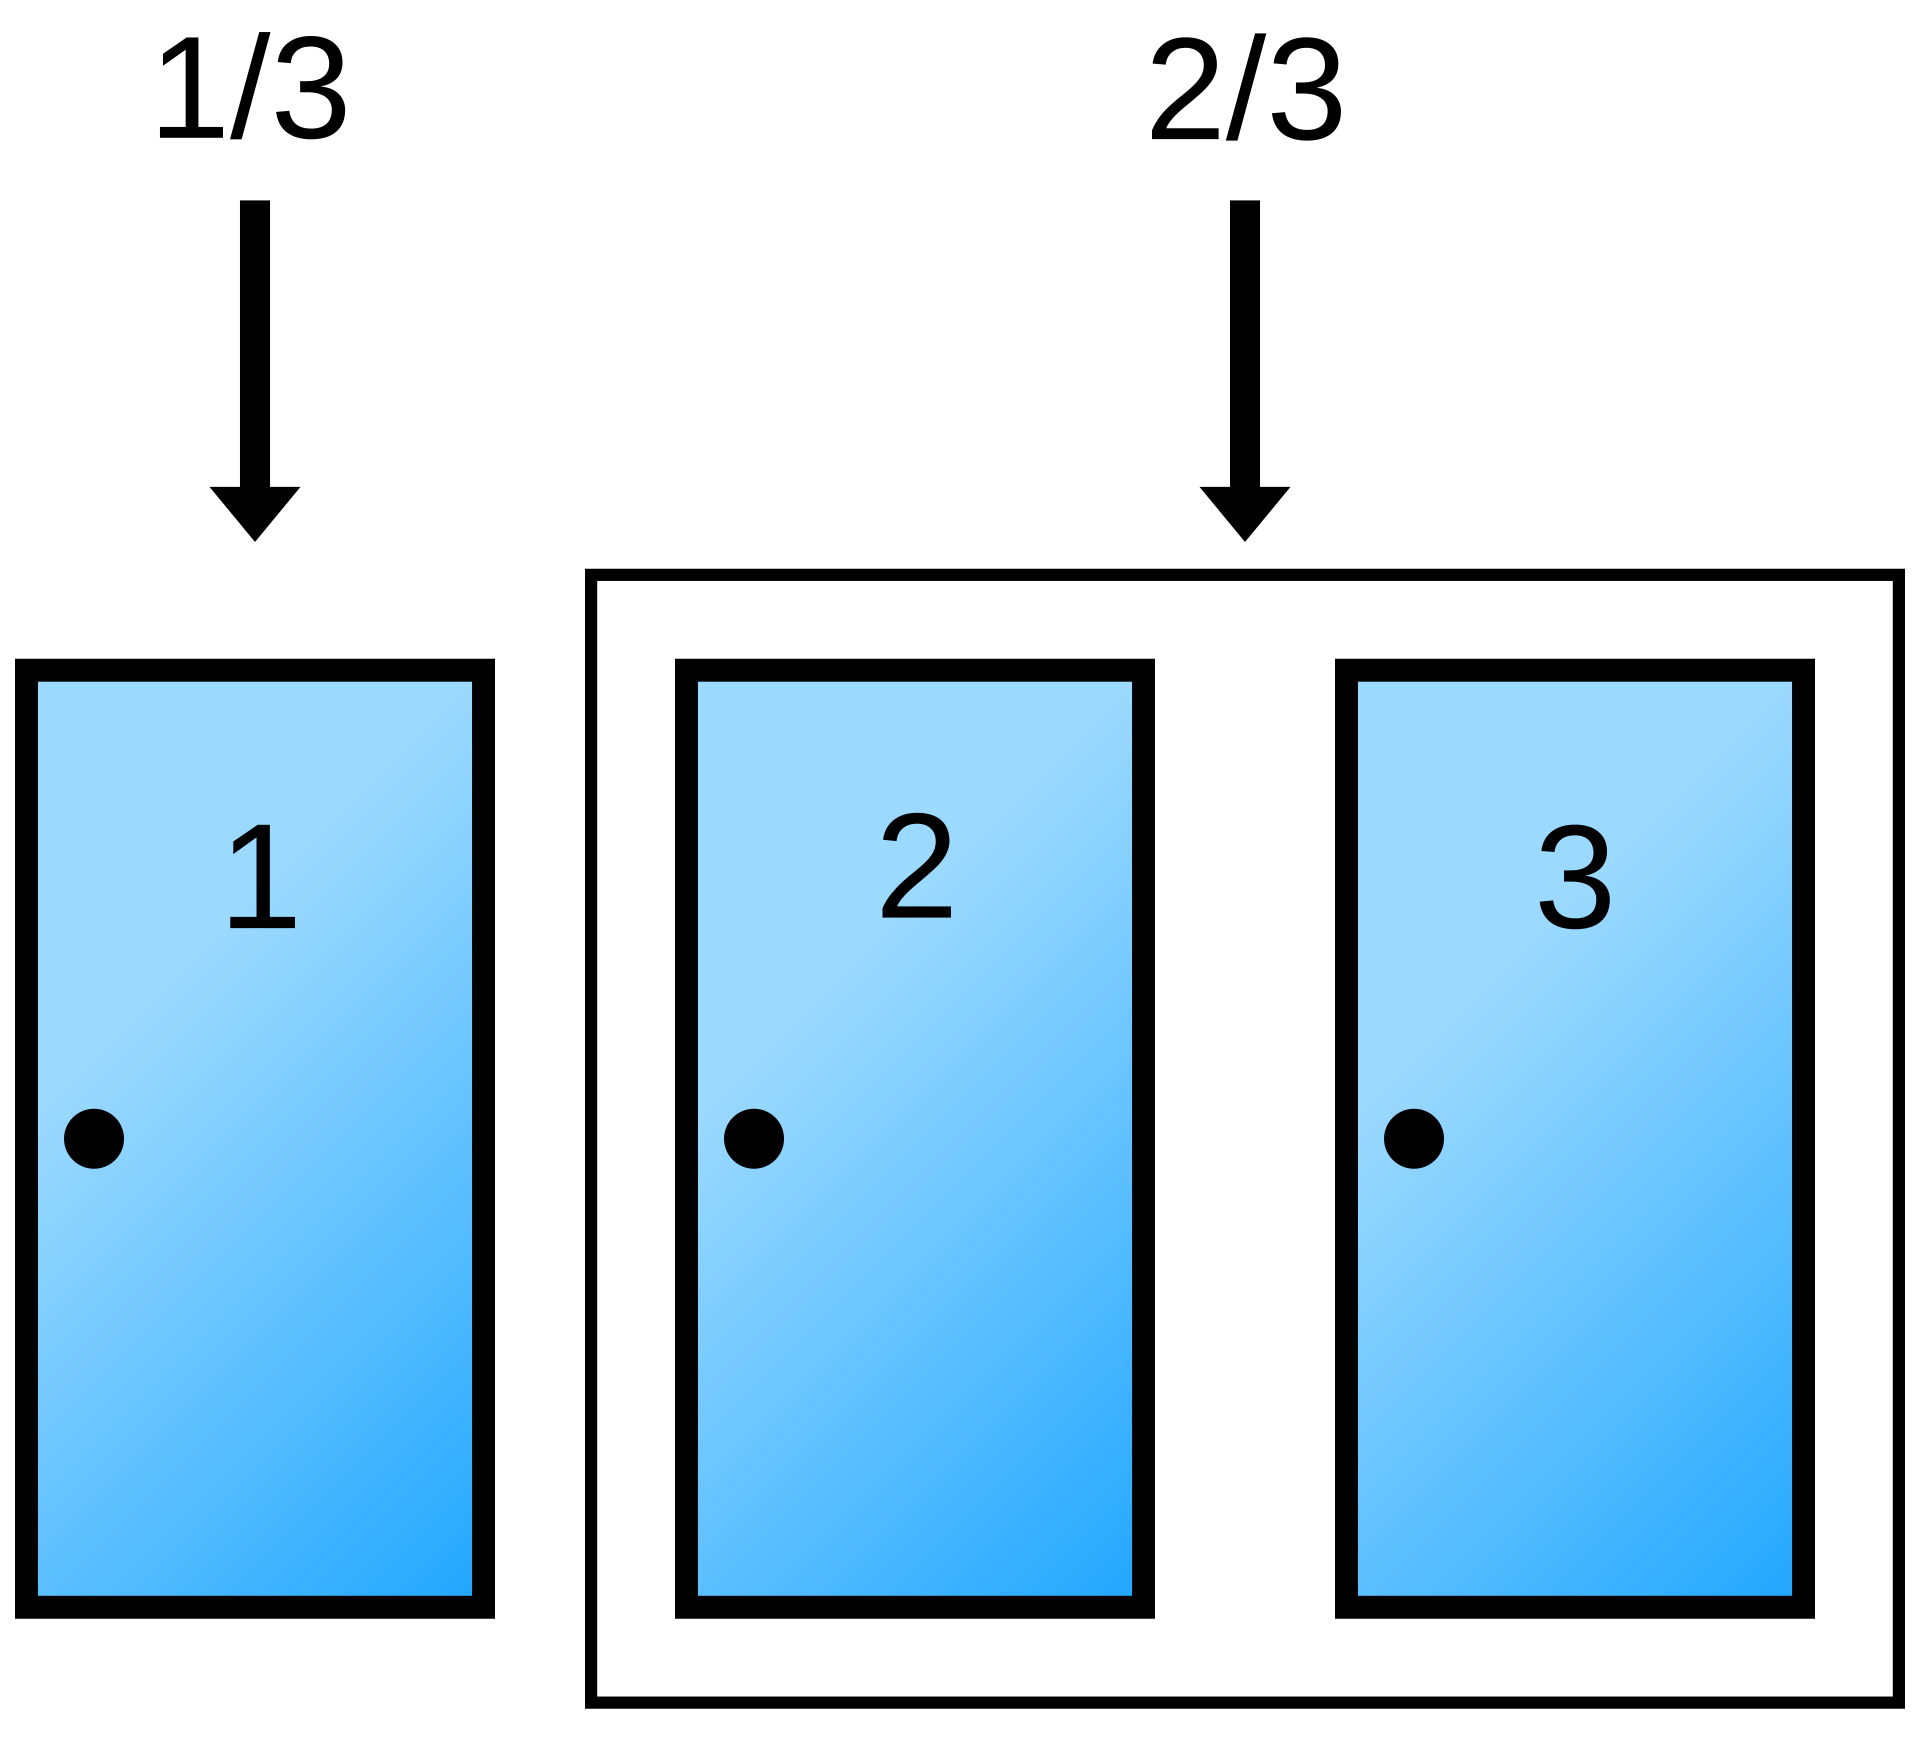
\includegraphics[width=0.65\linewidth,height=\textheight,keepaspectratio]{unidades/clasificadores/../../images/external/monty-hall-closed-doors.png}

}

\caption{Notemos como la probabilidad de encontrar el auto detrás de las
puertas cerradas es de \(\frac{1}{3}\), mientras que la probabilidad de
encontrar la cabra es de \(\frac{2}{3}\)}

\end{figure}%

Asumiendo que nuestra elección es la puerta 1, como sucede en muchas
ocasiones el presentador nos hará notar que detras de la puerta tres hay
una cabra, con lo cual es natural preguntarse: ¿Bajo que condiciones
tendremos la mejor probabilidad de ganar?, es común pensar que dado que
sabemos que detrás de las puerta de nuestra elección hay o una cabra o
un auto la probabilidad de encntrar nuestro premio tras estas 2 puertas
es de \(\frac{1}{2}\), sin embargo nuestra intución en ese caso sería
incorrecta.

\begin{figure}[H]

{\centering 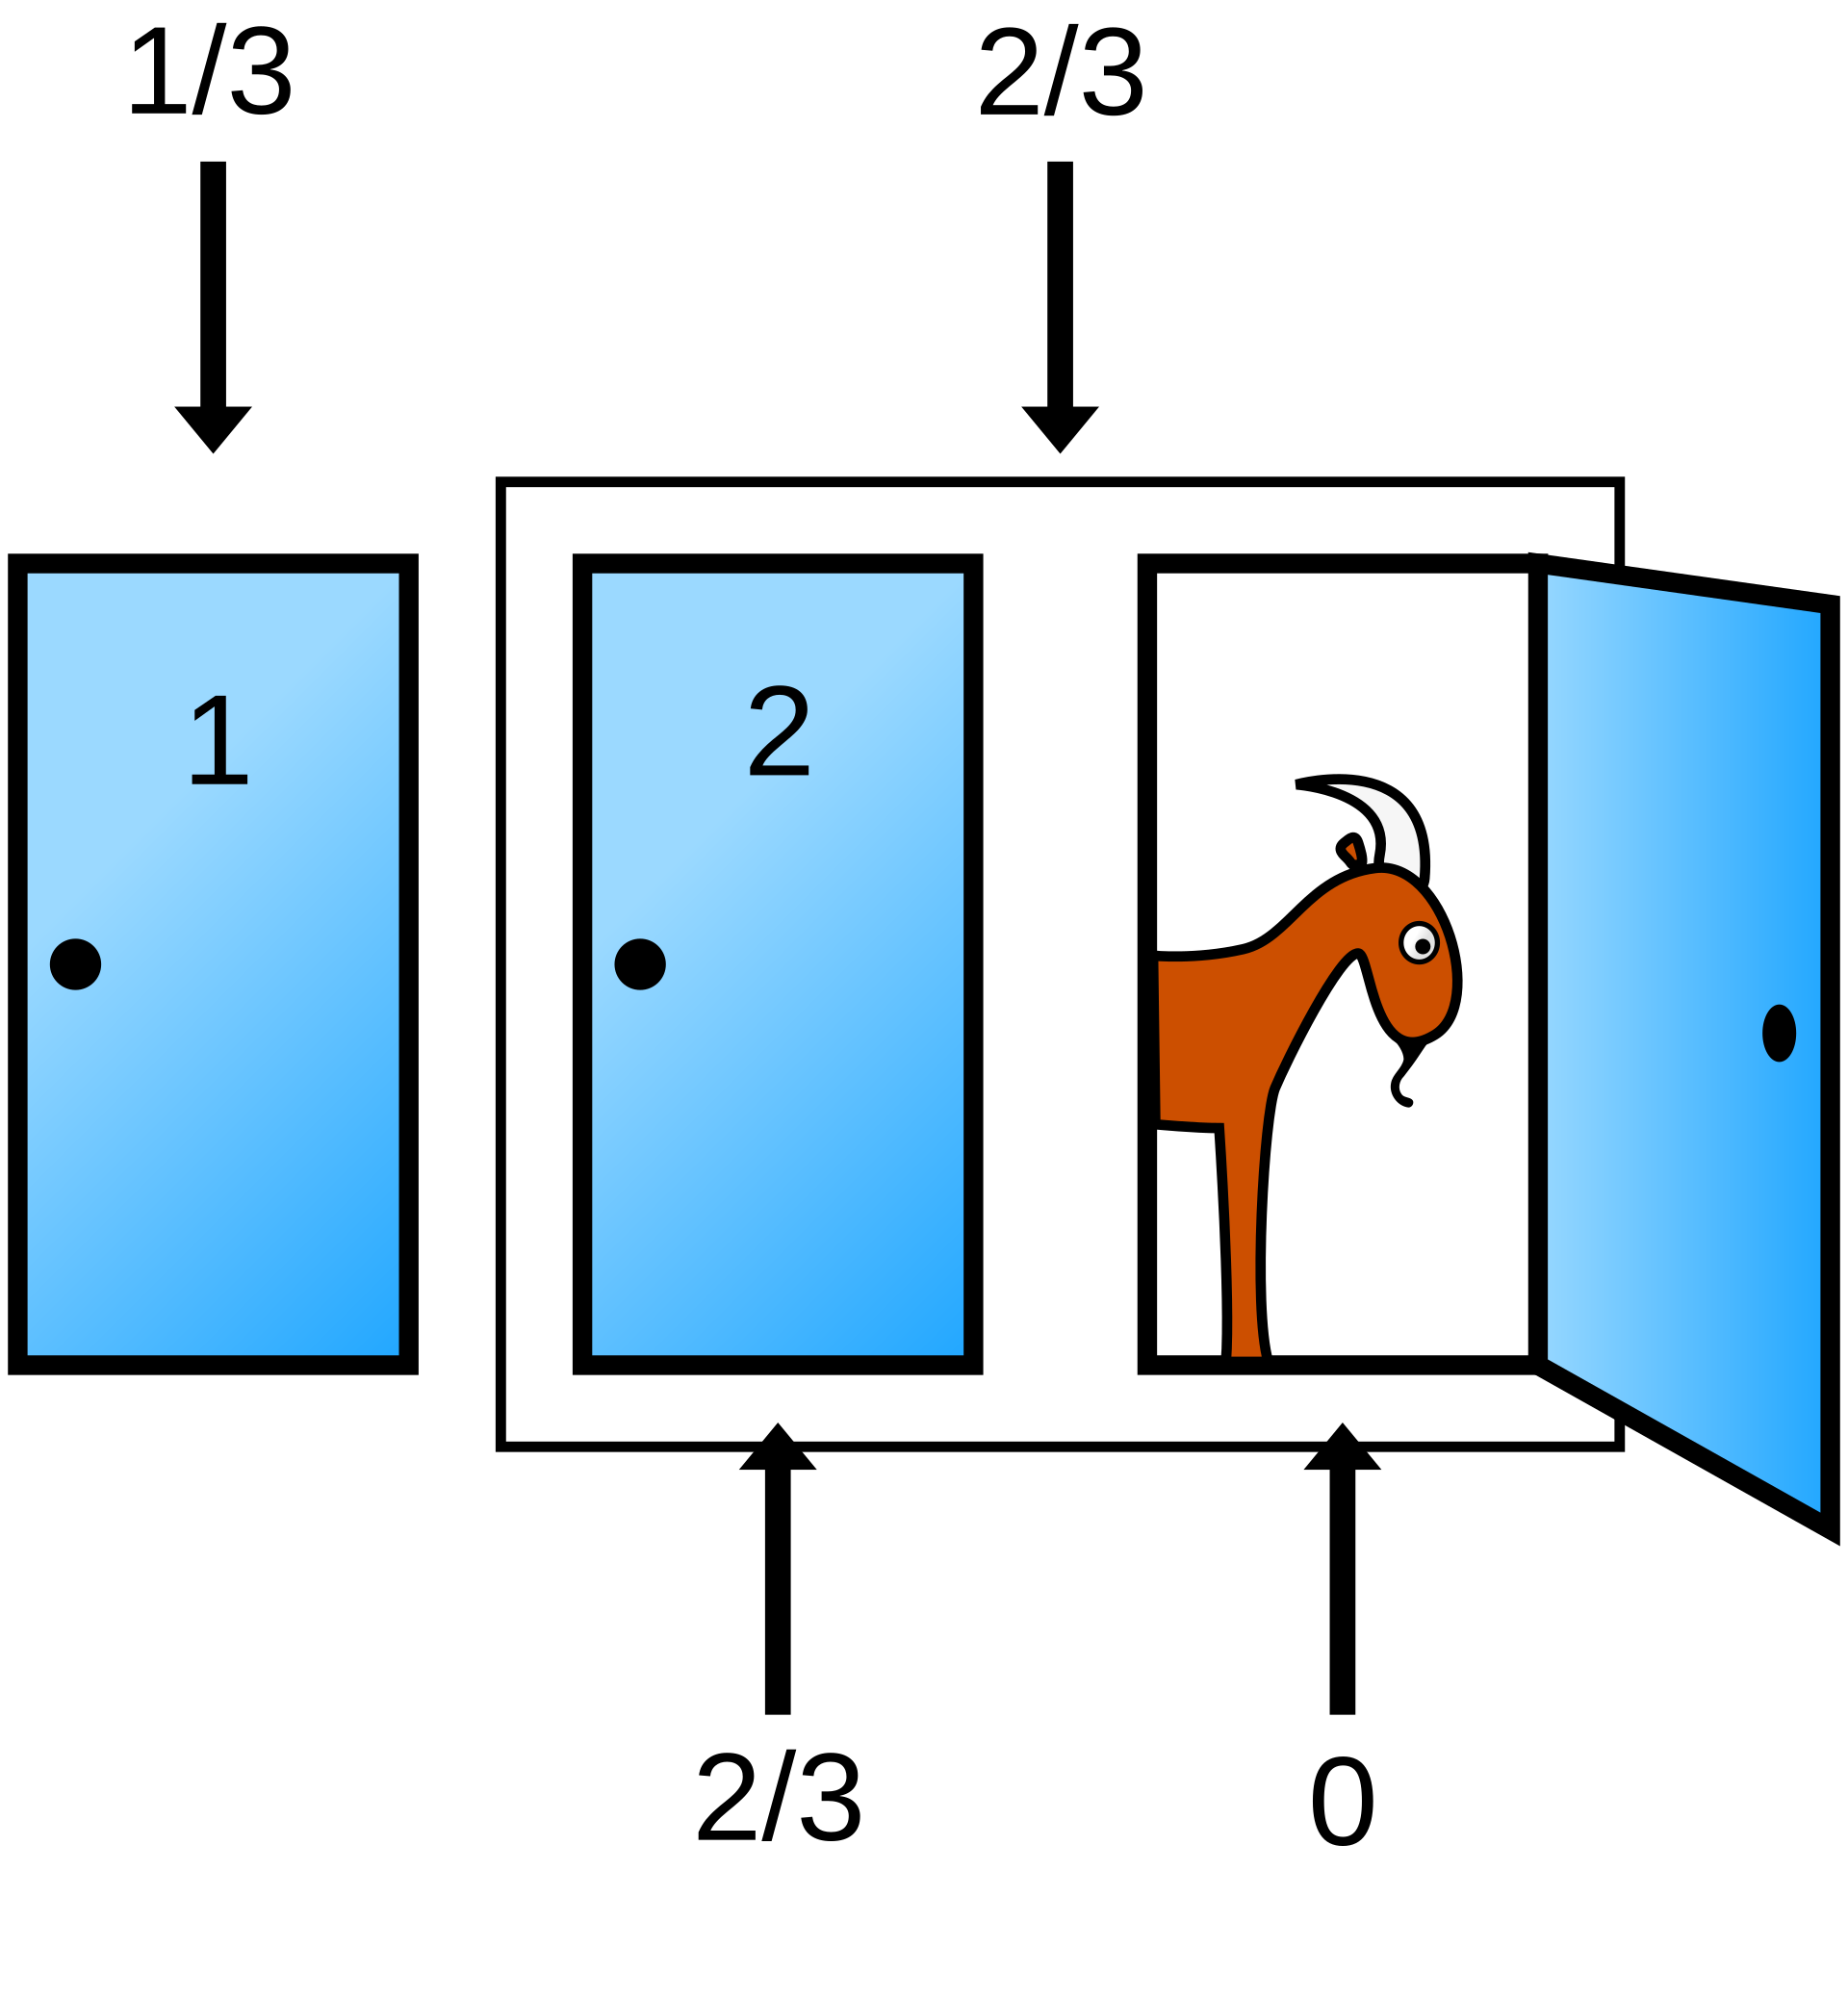
\includegraphics[width=0.65\linewidth,height=\textheight,keepaspectratio]{unidades/clasificadores/../../images/external/monty-hall-open-door.png}

}

\caption{Una vez se ha abierto una puerta con una cabra, dado qeu el
presentador solo podría haber abierto la puerta que tuviera detrás una
cabra obliga a que la probabilidad de ganar el auto si cambiamos a la
puerta 2 es de \(\frac{2}{3}\)}

\end{figure}%

Para ver con más detalle por qué conviene cambiar de puerta, hagamos las
cuentas paso a paso. Antes de que Chabelo abra una puerta, el auto puede
estar en cualquiera de las tres puertas con la misma probabilidad:

\[
P(A_1)=P(A_2)=P(A_3)=\frac{1}{3}
\]

donde \(A_i\) significa que el auto está detrás de la puerta \(i\).

Ahora bien, Chabelo sabe dónde está el auto y siempre abre una puerta
que tiene una cabra. Además, si tiene dos puertas con cabra disponibles,
asumimos que escoge una de ellas al azar. Entonces las posibilidades son
las siguientes:

Las ramas donde cambiar gana valen por 2 porque tienen probabilidad
\(\frac{1}{3}\), mientras que las ramas donde cambiar pierde valen
\(\frac{1}{6}\). Esto ocurre porque si el auto está en nuestra puerta
inicial, Chabelo tiene dos puertas posibles para abrir y divide ese caso
en dos ramas de probabilidad \(\frac{1}{6}\). En cambio, si el auto está
en una puerta distinta a la nuestra, Chabelo no tiene libertad: sólo
puede abrir la única puerta restante con cabra. Por eso cada una de esas
ramas conserva probabilidad \(\frac{1}{3}\), equivalente a dos partes de
tamaño \(\frac{1}{6}\).

Como en el ejemplo Chabelo abre la puerta 3 y muestra una cabra, debemos
quedarnos únicamente con los casos compatibles con esa información. Es
decir, descartamos todos los casos donde Chabelo abre la puerta 2 o
donde el auto estaba detrás de la puerta 3.

Los casos posibles después de observar que Chabelo abrió la puerta 3
son:

{\def\LTcaptype{none} % do not increment counter
\begin{longtable}[]{@{}
  >{\raggedright\arraybackslash}p{(\linewidth - 8\tabcolsep) * \real{0.1579}}
  >{\raggedleft\arraybackslash}p{(\linewidth - 8\tabcolsep) * \real{0.2105}}
  >{\raggedleft\arraybackslash}p{(\linewidth - 8\tabcolsep) * \real{0.2105}}
  >{\raggedleft\arraybackslash}p{(\linewidth - 8\tabcolsep) * \real{0.2105}}
  >{\raggedleft\arraybackslash}p{(\linewidth - 8\tabcolsep) * \real{0.2105}}@{}}
\toprule\noalign{}
\begin{minipage}[b]{\linewidth}\raggedright
Caso
\end{minipage} & \begin{minipage}[b]{\linewidth}\raggedleft
Ubicación del auto
\end{minipage} & \begin{minipage}[b]{\linewidth}\raggedleft
Probabilidad inicial
\end{minipage} & \begin{minipage}[b]{\linewidth}\raggedleft
Probabilidad de que Chabelo abra la puerta 3
\end{minipage} & \begin{minipage}[b]{\linewidth}\raggedleft
Probabilidad conjunta
\end{minipage} \\
\midrule\noalign{}
\endhead
\bottomrule\noalign{}
\endlastfoot
1 & Puerta 1 & \(\frac{1}{3}\) & \(\frac{1}{2}\) &
\(\frac{1}{3}\cdot\frac{1}{2}=\frac{1}{6}\) \\
2 & Puerta 2 & \(\frac{1}{3}\) & \(1\) &
\(\frac{1}{3}\cdot 1=\frac{1}{3}\) \\
3 & Puerta 3 & \(\frac{1}{3}\) & \(0\) & \(\frac{1}{3}\cdot 0=0\) \\
\end{longtable}
}

La probabilidad total de que Chabelo abra la puerta 3 es:

\[
P(\text{Chabelo abre puerta 3})
=
\frac{1}{6}+\frac{1}{3}+0
\]

\[
P(\text{Chabelo abre puerta 3})
=
\frac{1}{6}+\frac{2}{6}
=
\frac{3}{6}
=
\frac{1}{2}
\]

Ahora actualizamos las probabilidades usando la información nueva.
Primero, calculemos la probabilidad de que el auto esté en la puerta 1
dado que Chabelo abrió la puerta 3:

\[
P(A_1 \mid \text{Chabelo abre puerta 3})
=
\frac{P(A_1 \cap \text{Chabelo abre puerta 3})}
{P(\text{Chabelo abre puerta 3})}
\]

\[
P(A_1 \mid \text{Chabelo abre puerta 3})
=
\frac{\frac{1}{6}}{\frac{1}{2}}
=
\frac{1}{6}\cdot\frac{2}{1}
=
\frac{2}{6}
=
\frac{1}{3}
\]

Por lo tanto, si nos quedamos con la puerta 1, la probabilidad de ganar
sigue siendo:

\[
P(\text{ganar si nos quedamos})
=
\frac{1}{3}
\]

Ahora calculemos la probabilidad de que el auto esté en la puerta 2 dado
que Chabelo abrió la puerta 3:

\[
P(A_2 \mid \text{Chabelo abre puerta 3})
=
\frac{P(A_2 \cap \text{Chabelo abre puerta 3})}
{P(\text{Chabelo abre puerta 3})}
\]

\[
P(A_2 \mid \text{Chabelo abre puerta 3})
=
\frac{\frac{1}{3}}{\frac{1}{2}}
=
\frac{1}{3}\cdot\frac{2}{1}
=
\frac{2}{3}
\]

Por lo tanto, si cambiamos a la puerta 2, la probabilidad de ganar es:

\[
P(\text{ganar si cambiamos})
=
\frac{2}{3}
\]

La clave está en que la puerta que elegimos inicialmente conserva su
probabilidad original de \(\frac{1}{3}\). La información nueva no
reparte la probabilidad en partes iguales entre las dos puertas
cerradas. Más bien, la probabilidad que antes estaba distribuida entre
las dos puertas que no escogimos se concentra en la única puerta no
abierta por Chabelo.

En resumen:

\[
P(\text{ganar si nos quedamos})
=
\frac{1}{3}
\]

\[
P(\text{ganar si cambiamos})
=
\frac{2}{3}
\]

Así que la mejor estrategia es cambiar de puerta. La pista de Chabelo no
es una simple eliminación de una opción: es evidencia nueva que cambia
nuestras probabilidades posteriores. Esta es precisamente la idea
central del razonamiento bayesiano: actualizar nuestras creencias
iniciales cuando observamos nueva información.

\begin{tcolorbox}[enhanced jigsaw, arc=.35mm, bottomrule=.15mm, breakable, colback=white, colframe=quarto-callout-note-color-frame, left=2mm, leftrule=.75mm, opacityback=0, rightrule=.15mm, toprule=.15mm]

En esta simulación podemos observar como las probabilidades del problema
a lo largo de las diferentes realizaciones convergen a los valores
teóricos de \(\frac{1}{3}\) para la estrategia de quedarse y
\(\frac{2}{3}\) para la estrategia de cambiar.

\begin{Shaded}
\begin{Highlighting}[]
\ImportTok{import}\NormalTok{ random}
\ImportTok{import}\NormalTok{ plotly.graph\_objects }\ImportTok{as}\NormalTok{ go}

\KeywordTok{def}\NormalTok{ simular\_monty\_hall\_plotly(n\_simulaciones}\OperatorTok{=}\DecValTok{10\_000}\NormalTok{):}
\NormalTok{    puertas }\OperatorTok{=}\NormalTok{ [}\DecValTok{1}\NormalTok{, }\DecValTok{2}\NormalTok{, }\DecValTok{3}\NormalTok{]}

\NormalTok{    gana\_quedandose }\OperatorTok{=} \DecValTok{0}
\NormalTok{    gana\_cambiando }\OperatorTok{=} \DecValTok{0}

\NormalTok{    probabilidades\_quedandose }\OperatorTok{=}\NormalTok{ []}
\NormalTok{    probabilidades\_cambiando }\OperatorTok{=}\NormalTok{ []}
\NormalTok{    simulaciones }\OperatorTok{=}\NormalTok{ []}

    \ControlFlowTok{for}\NormalTok{ i }\KeywordTok{in} \BuiltInTok{range}\NormalTok{(}\DecValTok{1}\NormalTok{, n\_simulaciones }\OperatorTok{+} \DecValTok{1}\NormalTok{):}
        \CommentTok{\# El auto se coloca al azar detrás de una puerta}
\NormalTok{        puerta\_auto }\OperatorTok{=}\NormalTok{ random.choice(puertas)}

        \CommentTok{\# El participante siempre escoge inicialmente la puerta 1}
\NormalTok{        eleccion\_inicial }\OperatorTok{=} \DecValTok{1}

        \CommentTok{\# Chabelo abre una puerta que no fue elegida y que no tiene el auto}
\NormalTok{        puertas\_posibles\_para\_abrir }\OperatorTok{=}\NormalTok{ [}
\NormalTok{            puerta}
            \ControlFlowTok{for}\NormalTok{ puerta }\KeywordTok{in}\NormalTok{ puertas}
            \ControlFlowTok{if}\NormalTok{ puerta }\OperatorTok{!=}\NormalTok{ eleccion\_inicial }\KeywordTok{and}\NormalTok{ puerta }\OperatorTok{!=}\NormalTok{ puerta\_auto}
\NormalTok{        ]}

\NormalTok{        puerta\_abierta }\OperatorTok{=}\NormalTok{ random.choice(puertas\_posibles\_para\_abrir)}

        \CommentTok{\# Si el participante cambia, escoge la única puerta cerrada restante}
\NormalTok{        puerta\_cambio }\OperatorTok{=}\NormalTok{ [}
\NormalTok{            puerta}
            \ControlFlowTok{for}\NormalTok{ puerta }\KeywordTok{in}\NormalTok{ puertas}
            \ControlFlowTok{if}\NormalTok{ puerta }\OperatorTok{!=}\NormalTok{ eleccion\_inicial }\KeywordTok{and}\NormalTok{ puerta }\OperatorTok{!=}\NormalTok{ puerta\_abierta}
\NormalTok{        ][}\DecValTok{0}\NormalTok{]}

        \CommentTok{\# Estrategia 1: quedarse con la puerta inicial}
        \ControlFlowTok{if}\NormalTok{ eleccion\_inicial }\OperatorTok{==}\NormalTok{ puerta\_auto:}
\NormalTok{            gana\_quedandose }\OperatorTok{+=} \DecValTok{1}

        \CommentTok{\# Estrategia 2: cambiar de puerta}
        \ControlFlowTok{if}\NormalTok{ puerta\_cambio }\OperatorTok{==}\NormalTok{ puerta\_auto:}
\NormalTok{            gana\_cambiando }\OperatorTok{+=} \DecValTok{1}

        \CommentTok{\# Probabilidades acumuladas hasta la simulación actual}
\NormalTok{        probabilidades\_quedandose.append(gana\_quedandose }\OperatorTok{/}\NormalTok{ i)}
\NormalTok{        probabilidades\_cambiando.append(gana\_cambiando }\OperatorTok{/}\NormalTok{ i)}
\NormalTok{        simulaciones.append(i)}

\NormalTok{    fig }\OperatorTok{=}\NormalTok{ go.Figure()}

\NormalTok{    fig.add\_trace(}
\NormalTok{        go.Scatter(}
\NormalTok{            x}\OperatorTok{=}\NormalTok{simulaciones,}
\NormalTok{            y}\OperatorTok{=}\NormalTok{probabilidades\_quedandose,}
\NormalTok{            mode}\OperatorTok{=}\StringTok{"lines"}\NormalTok{,}
\NormalTok{            name}\OperatorTok{=}\StringTok{"Quedarse con la puerta inicial"}\NormalTok{,}
\NormalTok{            line}\OperatorTok{=}\BuiltInTok{dict}\NormalTok{(color}\OperatorTok{=}\StringTok{"\#1f77b4"}\NormalTok{, width}\OperatorTok{=}\DecValTok{2}\NormalTok{)}
\NormalTok{        )}
\NormalTok{    )}

\NormalTok{    fig.add\_trace(}
\NormalTok{        go.Scatter(}
\NormalTok{            x}\OperatorTok{=}\NormalTok{simulaciones,}
\NormalTok{            y}\OperatorTok{=}\NormalTok{probabilidades\_cambiando,}
\NormalTok{            mode}\OperatorTok{=}\StringTok{"lines"}\NormalTok{,}
\NormalTok{            name}\OperatorTok{=}\StringTok{"Cambiar de puerta"}\NormalTok{,}
\NormalTok{            line}\OperatorTok{=}\BuiltInTok{dict}\NormalTok{(color}\OperatorTok{=}\StringTok{"\#d62728"}\NormalTok{, width}\OperatorTok{=}\DecValTok{2}\NormalTok{)}
\NormalTok{        )}
\NormalTok{    )}

\NormalTok{    fig.add\_hline(}
\NormalTok{        y}\OperatorTok{=}\DecValTok{1}\OperatorTok{/}\DecValTok{3}\NormalTok{,}
\NormalTok{        line\_dash}\OperatorTok{=}\StringTok{"dash"}\NormalTok{,}
\NormalTok{        line\_color}\OperatorTok{=}\StringTok{"\#1f77b4"}\NormalTok{,}
\NormalTok{        annotation\_text}\OperatorTok{=}\StringTok{"Valor teórico: 1/3"}\NormalTok{,}
\NormalTok{        annotation\_position}\OperatorTok{=}\StringTok{"bottom"}
\NormalTok{    )}

\NormalTok{    fig.add\_hline(}
\NormalTok{        y}\OperatorTok{=}\DecValTok{2}\OperatorTok{/}\DecValTok{3}\NormalTok{,}
\NormalTok{        line\_dash}\OperatorTok{=}\StringTok{"dash"}\NormalTok{,}
\NormalTok{        line\_color}\OperatorTok{=}\StringTok{"\#d62728"}\NormalTok{,}
\NormalTok{        annotation\_text}\OperatorTok{=}\StringTok{"Valor teórico: 2/3"}\NormalTok{,}
\NormalTok{        annotation\_position}\OperatorTok{=}\StringTok{"bottom"}
\NormalTok{    )}

\NormalTok{    fig.update\_layout(}
\NormalTok{    title}\OperatorTok{=}\StringTok{"Evolución de las probabilidades estimadas en el problema de Monty Hall"}\NormalTok{,}
\NormalTok{    xaxis\_title}\OperatorTok{=}\StringTok{"Número de simulaciones"}\NormalTok{,}
\NormalTok{    yaxis\_title}\OperatorTok{=}\StringTok{"Probabilidad acumulada de ganar"}\NormalTok{,}
\NormalTok{    template}\OperatorTok{=}\StringTok{"plotly\_white"}\NormalTok{,}
\NormalTok{    yaxis}\OperatorTok{=}\BuiltInTok{dict}\NormalTok{(}\BuiltInTok{range}\OperatorTok{=}\NormalTok{[}\DecValTok{0}\NormalTok{, }\DecValTok{1}\NormalTok{]),}

\NormalTok{    legend}\OperatorTok{=}\BuiltInTok{dict}\NormalTok{(}
\NormalTok{        title}\OperatorTok{=}\StringTok{"Estrategia"}\NormalTok{,}
\NormalTok{        orientation}\OperatorTok{=}\StringTok{"h"}\NormalTok{,}
\NormalTok{        yanchor}\OperatorTok{=}\StringTok{"top"}\NormalTok{,}
\NormalTok{        y}\OperatorTok{={-}}\FloatTok{0.2}\NormalTok{,}
\NormalTok{        xanchor}\OperatorTok{=}\StringTok{"center"}\NormalTok{,}
\NormalTok{        x}\OperatorTok{=}\FloatTok{0.5}
\NormalTok{    )}
\NormalTok{)}


\NormalTok{    fig.show()}

    \BuiltInTok{print}\NormalTok{(}\SpecialStringTok{f"Simulaciones realizadas: }\SpecialCharTok{\{}\NormalTok{n\_simulaciones}\SpecialCharTok{\}}\SpecialStringTok{"}\NormalTok{)}
    \BuiltInTok{print}\NormalTok{(}\SpecialStringTok{f"Probabilidad final de ganar quedándose: }\SpecialCharTok{\{}\NormalTok{probabilidades\_quedandose[}\OperatorTok{{-}}\DecValTok{1}\NormalTok{]}\SpecialCharTok{:.4f\}}\SpecialStringTok{"}\NormalTok{)}
    \BuiltInTok{print}\NormalTok{(}\SpecialStringTok{f"Probabilidad final de ganar cambiando: }\SpecialCharTok{\{}\NormalTok{probabilidades\_cambiando[}\OperatorTok{{-}}\DecValTok{1}\NormalTok{]}\SpecialCharTok{:.4f\}}\SpecialStringTok{"}\NormalTok{)}


\NormalTok{simular\_monty\_hall\_plotly(n\_simulaciones}\OperatorTok{=}\DecValTok{10\_000}\NormalTok{)}
\end{Highlighting}
\end{Shaded}

\begin{verbatim}
Unable to display output for mime type(s): text/html
\end{verbatim}

\begin{verbatim}
Unable to display output for mime type(s): text/html
\end{verbatim}

\begin{verbatim}
Simulaciones realizadas: 10000
Probabilidad final de ganar quedándose: 0.3262
Probabilidad final de ganar cambiando: 0.6738
\end{verbatim}

\end{tcolorbox}

Esta es la diferencia central en los clasificadores bayesianos, la
decisión se deriva de probabilidades a priori, densidades condicionales
y probabilidades posteriores (Duda et~al. 2001; Bishop 2006). Por
ejemplo, si una caja contiene monedas de dos tipos y una de ellas es más
frecuente, la decisión con menor probabilidad de error antes de observar
la moneda es escoger la clase más probable. Sin embargo, una vez que se
observa una característica, como el peso, la decisión debe incorporar
esa evidencia. La pregunta deja de ser ``¿qué clase es más frecuente?''
y pasa a ser ``¿qué clase es más probable dado el valor observado?''.

\marginnote{\begin{footnotesize}

Si tuvieramos que clasificar entre monedas de un centavo y monedas de
diez centavos, antes de observar el peso, la mejor decisión sería
escoger la clase más frecuente. Sin embargo, una vez que se observa el
peso, la decisión debe incorporar esa evidencia. La pregunta deja de ser
``¿qué clase es más frecuente?'' y pasa a ser ``¿qué clase es más
probable dado el valor observado?''.

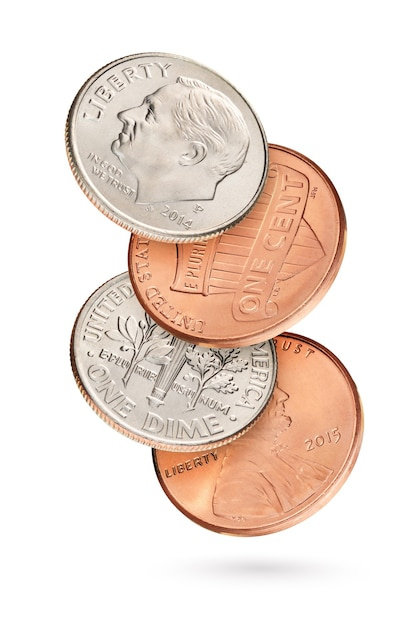
\includegraphics[width=0.7\linewidth,height=\textheight,keepaspectratio]{unidades/clasificadores/../../images/external/coin-stack.jpg}

\end{footnotesize}}

Los clasificadores bayesianos usan el teorema de Bayes para decidir a
qué clase pertenece una observación. Para cada clase \(\omega_i\), se
considera qué tan probable es observar los datos \(\mathbf{x}\) si esa
clase fuera la correcta, junto con qué tan probable era esa clase antes
de ver los datos. Con esta información se calcula la probabilidad de
cada clase después de observar \(\mathbf{x}\). La decisión más sencilla
consiste en elegir la clase con mayor probabilidad posterior; si algunos
errores son más costosos que otros, se puede modificar la decisión para
tomar en cuenta esos costos (Duda et~al. 2001; Jaynes 2003).

Este capítulo desarrolla la clasificación bayesiana desde sus
fundamentos hasta algunas variantes prácticas: Naïve Bayes,
clasificadores gaussianos, modelos de Markov para secuencias discretas,
decisión bayesiana con costos y el criterio minimax cuando las
probabilidades previas son inciertas. Los ejemplos computacionales están
escritos en Python y buscan conectar la teoría con implementaciones
reproducibles.

\section{Vista probabilística de la
clasificación}\label{vista-probabiluxedstica-de-la-clasificaciuxf3n}

Sea \(\mathbf{x}\in\mathbb{R}^d\) una observación y sea
\(\Omega=\{\omega_1,\dots,\omega_c\}\) el conjunto de clases posibles.
En clasificación probabilística se supone que \(\mathbf{x}\) no
determina de manera absoluta la clase, sino que modifica nuestras
creencias sobre ella. Antes de observar \(\mathbf{x}\), la información
disponible está representada por las probabilidades previas
\(P(\omega_i)\). Después de observar \(\mathbf{x}\), la información
relevante se resume en las probabilidades posteriores
\(P(\omega_i\mid \mathbf{x})\).

\begin{tcolorbox}[enhanced jigsaw, arc=.35mm, bottomrule=.15mm, breakable, colback=white, colframe=quarto-callout-note-color-frame, left=2mm, leftrule=.75mm, opacityback=0, rightrule=.15mm, toprule=.15mm]

Definición. La probabilidad posterior de la clase \(\omega_i\) dada una
observación \(\mathbf{x}\) se obtiene mediante el teorema de Bayes:
\begin{equation}\protect\phantomsection\label{eq-bayes-posterior}{
P(\omega_i\mid \mathbf{x}) = \frac{p(\mathbf{x}\mid \omega_i)P(\omega_i)}{p(\mathbf{x})}
}\end{equation}

\end{tcolorbox}

En la ecuación Ecuación~\ref{eq-bayes-posterior},
\(p(\mathbf{x}\mid\omega_i)\) es la densidad condicional de la
observación bajo la clase \(\omega_i\), \(P(\omega_i)\) es la
probabilidad previa de esa clase y \(p(\mathbf{x})\) es la densidad
marginal de la observación:

\[
p(\mathbf{x}) = \sum_{j=1}^c p(\mathbf{x}\mid\omega_j)P(\omega_j).
\]

Como \(p(\mathbf{x})\) no depende de la clase que se compara, muchas
reglas de decisión pueden escribirse en términos de la cantidad no
normalizada \(p(\mathbf{x}\mid\omega_i)P(\omega_i)\).

\subsubsection*{La decisión de
clasificación}\label{la-decisiuxf3n-de-clasificaciuxf3n}
\addcontentsline{toc}{subsubsection}{La decisión de clasificación}

Si no hay observaciones, una regla razonable para dos clases es escoger
la clase más probable a priori:

\[
\text{decidir }\omega_1 \quad \text{si} \quad P(\omega_1)>P(\omega_2).
\]

El error esperado de esta regla, cuando sólo existen dos clases, es

\[
P(e)=\min\{P(\omega_1),P(\omega_2)\}.
\]

Una vez observada \(\mathbf{x}\), la decisión cambia: se debe comparar
\(P(\omega_1\mid\mathbf{x})\) contra \(P(\omega_2\mid\mathbf{x})\). Esta
distinción es la esencia de la clasificación bayesiana: la evidencia
observada actualiza las probabilidades de las clases.

\begin{tcolorbox}[enhanced jigsaw, arc=.35mm, bottomrule=.15mm, breakable, colback=white, colframe=quarto-callout-note-color-frame, left=2mm, leftrule=.75mm, opacityback=0, rightrule=.15mm, toprule=.15mm]

Definición. La regla de máxima probabilidad posterior, o regla MAP,
asigna la observación \(\mathbf{x}\) a la clase con posterior máxima:
\begin{equation}\protect\phantomsection\label{eq-map-rule}{
\hat{\omega}(\mathbf{x}) = \arg\max_{\omega_i\in\Omega} P(\omega_i\mid\mathbf{x})
}\end{equation}

\end{tcolorbox}

\subsection{Ejemplo básico: El dilema del
Cine}\label{ejemplo-buxe1sico-el-dilema-del-cine}

\textbf{Esta persona dejó caer su boleto en el pasillo.}

¿Le dices?

\begin{quote}
``Disculpe, señora''
\end{quote}

o

\begin{quote}
``Disculpe, señor''
\end{quote}

\textbf{Tienes que hacer una conjetura.}


\includegraphics[width=0.7\linewidth,height=\textheight,keepaspectratio]{unidades/clasificadores/../../images/external/fruit-vegetable-section.jpg}

Para responder de la manera mas acertada posible podemos hacer uso del
teorema de Bayes, para esto definamos el evento \(H\) como ``hombre'' y
el evento \(M\) como ``mujer'', mientras que la evidencia observada es
el tipo de cabello de la persona. Entonces, la probabilidad de que la
persona sea hombre o mujer dado el tipo de cabello se calcula con Bayes:

\[
P(\text{sexo}\mid \text{cabello})
=
\frac{
P(\text{cabello}\mid \text{sexo})P(\text{sexo})
}{
\sum_{\text{sexo}} P(\text{sexo})P(\text{cabello}\mid \text{sexo})
}
\]

Donde bajo una asumpción justa podemos suponer que dentro del cine:

\textbf{De cada 100 mujeres en el cine}

\begin{itemize}
\tightlist
\item
  50 tienen cabello corto
\item
  50 tienen cabello largo
\end{itemize}

\textbf{De cada 100 hombres en el cine}

\begin{itemize}
\tightlist
\item
  96 tienen cabello corto
\item
  4 tienen cabello largo
\end{itemize}

Hagamos los calculos paso a paso, si asumimos que la proporción de
hombres y mujeres en el cine es la misma, entonces las probabilidades
previas son:

\[P(H)=P(M)=0.5\]

Mientras que las verosimilitudes son:
\[P(\text{cabello largo}\mid H)=0.04\]
\[P(\text{cabello largo}\mid M)=0.50\]

teniendo esto, Entonces los numeradores son:

\[
P(\text{largo}\mid H)P(H)=0.04(0.5)=0.02
\] \[
P(\text{largo}\mid M)P(M)=0.50(0.5)=0.25
\]

Entonces:

\[
P(H\mid \text{cabello largo}) = 0.02A \approx 0.07
\]

\[
P(M\mid \text{cabello largo}) = 0.25A \approx 0.93
\]

donde

\[
A=\frac{1}{0.02+0.25}
\]

Así, bajo la regla de máxima probabilidad posterior, la decisión es:

\[
\Rightarrow \textbf{Decisión: mujer}
\]

\begin{tcolorbox}[enhanced jigsaw, arc=.35mm, bottomrule=.15mm, bottomtitle=1mm, breakable, colback=white, colbacktitle=quarto-callout-note-color!10!white, colframe=quarto-callout-note-color-frame, coltitle=black, left=2mm, leftrule=.75mm, opacityback=0, opacitybacktitle=0.6, rightrule=.15mm, title=\textcolor{quarto-callout-note-color}{\faInfo}\hspace{0.5em}{Nota}, titlerule=0mm, toprule=.15mm, toptitle=1mm]

La idea central es que no decidimos solo por la característica
observada, sino por cómo esa característica modifica nuestras creencias
previas sobre cada clase.

\end{tcolorbox}

\subsection{Dilema en el cine: el contexto
importa}\label{dilema-en-el-cine-el-contexto-importa}

Es importante notar que la decisión anterior depende de las
probabilidades previas. Si el contexto cambia, las probabilidades
previas también cambian, lo que puede llevar a una decisión diferente
incluso con la misma evidencia observada. Por ejemplo, si esta situación
ocurre mientras estás formado en la fila del baño de hombres, la
proporción de hombres y mujeres cambia drásticamente, lo que afecta las
probabilidades previas y, por ende, la decisión bayesiana.

¿Le dices?

\begin{quote}
``Disculpe, señora''
\end{quote}

o

\begin{quote}
``Disculpe, señor''
\end{quote}

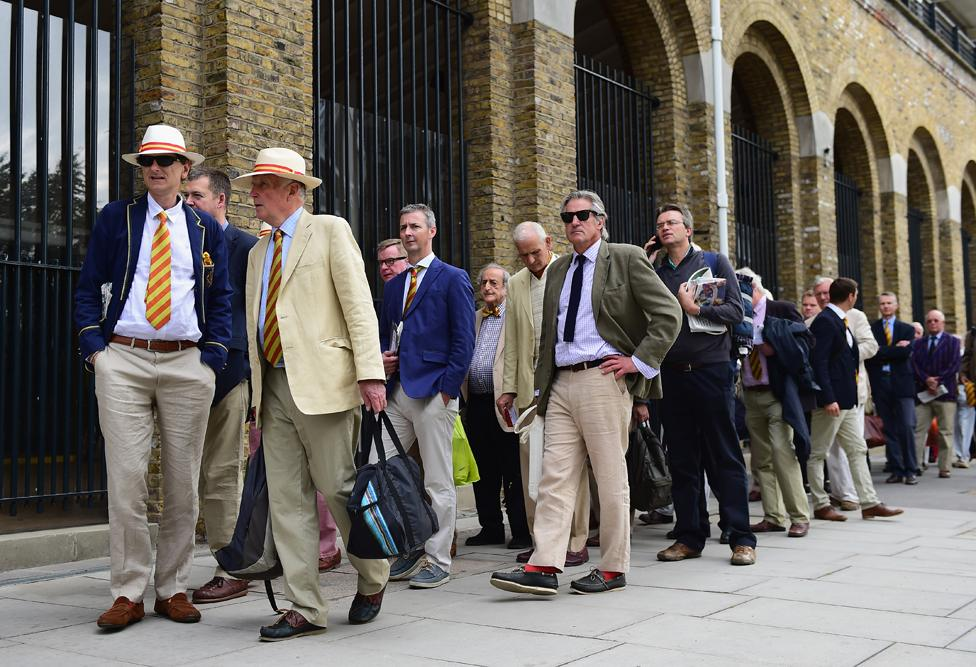
\includegraphics[width=0.8\linewidth,height=\textheight,keepaspectratio]{unidades/clasificadores/../../images/external/queueing-lords.jpg}

Ahora las probabilidades previas cambian:

\[
P(H)=0.98,
\qquad
P(M)=0.02
\]

donde \(H\) representa ``hombre'' y \(M\) representa ``mujer''. De nuevo
asumiendo de manera justa que dentro de la fila:

\textbf{De cada 2 mujeres en la fila}

\begin{itemize}
\tightlist
\item
  1 tiene cabello corto
\item
  1 tiene cabello largo
\end{itemize}

\textbf{De cada 98 hombres en la fila}

\begin{itemize}
\tightlist
\item
  94 tienen cabello corto
\item
  4 tienen cabello largo
\end{itemize}

De los datos anteriores:

\[
P(\text{cabello largo}\mid H)=\frac{4}{98}
\]

\[
P(\text{cabello largo}\mid M)=\frac{1}{2}
\]

Calculamos los numeradores de Bayes:

\[
P(\text{cabello largo}\mid H)P(H)
=
\frac{4}{98}(0.98)
=
0.04
\]

\[
P(\text{cabello largo}\mid M)P(M)
=
\frac{1}{2}(0.02)
=
0.01
\]

La constante de normalización es:

\[
B=
\frac{1}{0.04+0.01}
=
20
\]

Entonces, bajo la misma regla de máxima probabilidad posterior, las
probabilidades posteriores son:

\[
P(H\mid \text{cabello largo})
=
0.04B
=
0.04(20)
=
0.80
\]

\[
P(M\mid \text{cabello largo})
=
0.01B
=
0.01(20)
=
0.20
\]

Como:

\[
P(H\mid \text{cabello largo})
>
P(M\mid \text{cabello largo})
\]

la decisión bayesiana es:

\[
\Rightarrow \textbf{Decisión: hombre}
\]

\begin{tcolorbox}[enhanced jigsaw, arc=.35mm, bottomrule=.15mm, bottomtitle=1mm, breakable, colback=white, colbacktitle=quarto-callout-important-color!10!white, colframe=quarto-callout-important-color-frame, coltitle=black, left=2mm, leftrule=.75mm, opacityback=0, opacitybacktitle=0.6, rightrule=.15mm, title=\textcolor{quarto-callout-important-color}{\faExclamation}\hspace{0.5em}{Importante}, titlerule=0mm, toprule=.15mm, toptitle=1mm]

La misma evidencia observada (cabello largo) puede llevar a una decisión
distinta cuando cambian las probabilidades previas.

En clasificación bayesiana, el contexto modifica la inferencia.

\end{tcolorbox}

\subsection{Implementación básica: algoritmo general de un clasificador
bayesiano}\label{implementaciuxf3n-buxe1sica-algoritmo-general-de-un-clasificador-bayesiano}

A continuación se muestra una implementación básica de un clasificador
bayesiano para cualquier número de clases. El código calcula las
probabilidades posteriores y toma la decisión de clasificación basada en
la clase con mayor probabilidad posterior.

\begin{Shaded}
\begin{Highlighting}[]
\ImportTok{import}\NormalTok{ numpy }\ImportTok{as}\NormalTok{ np}

\KeywordTok{def}\NormalTok{ clasificador\_bayesiano(verosimilitudes, priors, clases):}
    \CommentTok{"""}
\CommentTok{    Clasificador bayesiano para cualquier número de clases.}

\CommentTok{    verosimilitudes: p(x | omega\_i) para cada clase.}
\CommentTok{    priors: P(omega\_i) para cada clase.}
\CommentTok{    clases: nombres de las clases.}
\CommentTok{    """}
\NormalTok{    verosimilitudes }\OperatorTok{=}\NormalTok{ np.array(verosimilitudes, dtype}\OperatorTok{=}\BuiltInTok{float}\NormalTok{)}
\NormalTok{    priors }\OperatorTok{=}\NormalTok{ np.array(priors, dtype}\OperatorTok{=}\BuiltInTok{float}\NormalTok{)}
\NormalTok{    clases }\OperatorTok{=}\NormalTok{ np.array(clases)}

\NormalTok{    evidencia }\OperatorTok{=}\NormalTok{ np.}\BuiltInTok{sum}\NormalTok{(verosimilitudes }\OperatorTok{*}\NormalTok{ priors)}
\NormalTok{    posteriores }\OperatorTok{=}\NormalTok{ (verosimilitudes }\OperatorTok{*}\NormalTok{ priors) }\OperatorTok{/}\NormalTok{ evidencia}

\NormalTok{    indice\_decision }\OperatorTok{=}\NormalTok{ np.argmax(posteriores)}
\NormalTok{    decision }\OperatorTok{=}\NormalTok{ clases[indice\_decision]}

    \ControlFlowTok{return}\NormalTok{ posteriores, decision}


\NormalTok{clases }\OperatorTok{=}\NormalTok{ [}\StringTok{"normal"}\NormalTok{, }\StringTok{"enfermedad"}\NormalTok{]}

\CommentTok{\# p(x | omega\_i): qué tan probable es observar x en cada clase}
\NormalTok{verosimilitudes }\OperatorTok{=}\NormalTok{ [}\FloatTok{0.2}\NormalTok{, }\FloatTok{0.4}\NormalTok{]}

\CommentTok{\# P(omega\_i): probabilidad previa de cada clase}
\NormalTok{priors }\OperatorTok{=}\NormalTok{ [}\FloatTok{0.9}\NormalTok{, }\FloatTok{0.1}\NormalTok{]}

\NormalTok{posteriores, decision }\OperatorTok{=}\NormalTok{ clasificador\_bayesiano(}
\NormalTok{    verosimilitudes,}
\NormalTok{    priors,}
\NormalTok{    clases}
\NormalTok{)}

\ControlFlowTok{for}\NormalTok{ clase, posterior }\KeywordTok{in} \BuiltInTok{zip}\NormalTok{(clases, posteriores):}
    \BuiltInTok{print}\NormalTok{(}\SpecialStringTok{f"P(}\SpecialCharTok{\{}\NormalTok{clase}\SpecialCharTok{\}}\SpecialStringTok{ | x) = }\SpecialCharTok{\{}\NormalTok{posterior}\SpecialCharTok{:.3f\}}\SpecialStringTok{"}\NormalTok{)}

\BuiltInTok{print}\NormalTok{(}\StringTok{"Decisión:"}\NormalTok{, decision)}
\end{Highlighting}
\end{Shaded}

\begin{verbatim}
P(normal | x) = 0.818
P(enfermedad | x) = 0.182
Decisión: normal
\end{verbatim}

En este ejemplo, aunque la verosimilitud bajo la clase de enfermedad es
mayor, el prior de la clase normal domina la decisión de error mínimo.
Esto ilustra una idea importante: una evidencia local no se interpreta
de manera aislada, sino en relación con la frecuencia previa de cada
clase.

\section{Clasificador bayesiano de error
mínimo}\label{clasificador-bayesiano-de-error-muxednimo}

La regla MAP tiene una interpretación óptima cuando todos los errores
tienen el mismo costo: minimiza la probabilidad promedio de
clasificación incorrecta. Para verlo, consideremos inicialmente dos
clases. Si se asigna \(\mathbf{x}\) a \(\omega_1\), el error condicional
es \(P(\omega_2\mid\mathbf{x})\); si se asigna a \(\omega_2\), el error
condicional es \(P(\omega_1\mid\mathbf{x})\). Por tanto, para minimizar
el error en cada punto \(\mathbf{x}\) se elige la clase con mayor
posterior.

\begin{tcolorbox}[enhanced jigsaw, arc=.35mm, bottomrule=.15mm, breakable, colback=white, colframe=quarto-callout-note-color-frame, left=2mm, leftrule=.75mm, opacityback=0, rightrule=.15mm, toprule=.15mm]

Definición. El error condicional de clasificación para dos clases es
\begin{equation}\protect\phantomsection\label{eq-conditional-error}{
P(e\mid\mathbf{x})=
\begin{cases}
P(\omega_2\mid\mathbf{x}), & \text{si se decide }\omega_1,\\
P(\omega_1\mid\mathbf{x}), & \text{si se decide }\omega_2.
\end{cases}
}\end{equation}

\end{tcolorbox}

El error promedio se obtiene integrando sobre todo el espacio de
observaciones:

\[
P(e)=\int P(e\mid\mathbf{x})p(\mathbf{x})\,d\mathbf{x}.
\]

Dado que \(p(\mathbf{x})\geq 0\), minimizar el error promedio se logra
minimizando el error condicional punto a punto. Así, para dos clases:

\[
P(\omega_1\mid\mathbf{x})>P(\omega_2\mid\mathbf{x})
\quad \Longrightarrow \quad
\mathbf{x}\in\omega_1.
\]

\subsection{Ejemplo en Python: decisión de error
mínimo}\label{ejemplo-en-python-decisiuxf3n-de-error-muxednimo}

El siguiente código muestra la regla de error mínimo para varias
observaciones. Para cada observación se tienen las verosimilitudes
\(p(\mathbf{x}\mid\omega_i)\) bajo dos clases. Después se calculan las
posteriores, se elige la clase con mayor posterior y se reporta el error
condicional mínimo.

\begin{Shaded}
\begin{Highlighting}[]
\ImportTok{import}\NormalTok{ numpy }\ImportTok{as}\NormalTok{ np}

\NormalTok{clases }\OperatorTok{=}\NormalTok{ np.array([}\StringTok{"normal"}\NormalTok{, }\StringTok{"enfermedad"}\NormalTok{])}

\CommentTok{\# Probabilidades previas P(omega\_i)}
\NormalTok{priors }\OperatorTok{=}\NormalTok{ np.array([}\FloatTok{0.8}\NormalTok{, }\FloatTok{0.2}\NormalTok{])}

\CommentTok{\# Cada fila representa una observación distinta.}
\CommentTok{\# Las columnas contienen p(x | normal) y p(x | enfermedad).}
\NormalTok{verosimilitudes }\OperatorTok{=}\NormalTok{ np.array([}
\NormalTok{    [}\FloatTok{0.50}\NormalTok{, }\FloatTok{0.10}\NormalTok{],}
\NormalTok{    [}\FloatTok{0.35}\NormalTok{, }\FloatTok{0.25}\NormalTok{],}
\NormalTok{    [}\FloatTok{0.20}\NormalTok{, }\FloatTok{0.45}\NormalTok{],}
\NormalTok{    [}\FloatTok{0.10}\NormalTok{, }\FloatTok{0.60}\NormalTok{],}
\NormalTok{    [}\FloatTok{0.40}\NormalTok{, }\FloatTok{0.30}\NormalTok{]}
\NormalTok{])}

\CommentTok{\# Numerador de Bayes: p(x | omega\_i) P(omega\_i)}
\NormalTok{puntajes\_no\_normalizados }\OperatorTok{=}\NormalTok{ verosimilitudes }\OperatorTok{*}\NormalTok{ priors}

\CommentTok{\# Evidencia p(x), calculada para cada observación}
\NormalTok{evidencia }\OperatorTok{=}\NormalTok{ puntajes\_no\_normalizados.}\BuiltInTok{sum}\NormalTok{(axis}\OperatorTok{=}\DecValTok{1}\NormalTok{, keepdims}\OperatorTok{=}\VariableTok{True}\NormalTok{)}

\CommentTok{\# Posteriores P(omega\_i | x)}
\NormalTok{posteriores }\OperatorTok{=}\NormalTok{ puntajes\_no\_normalizados }\OperatorTok{/}\NormalTok{ evidencia}

\CommentTok{\# Regla de error mínimo: elegir la clase con mayor posterior}
\NormalTok{indices\_decision }\OperatorTok{=}\NormalTok{ np.argmax(posteriores, axis}\OperatorTok{=}\DecValTok{1}\NormalTok{)}
\NormalTok{decisiones }\OperatorTok{=}\NormalTok{ clases[indices\_decision]}

\CommentTok{\# El error condicional mínimo es 1 menos la posterior más grande}
\NormalTok{errores\_condicionales }\OperatorTok{=} \DecValTok{1} \OperatorTok{{-}}\NormalTok{ np.}\BuiltInTok{max}\NormalTok{(posteriores, axis}\OperatorTok{=}\DecValTok{1}\NormalTok{)}

\ControlFlowTok{for}\NormalTok{ i, (post, decision, error) }\KeywordTok{in} \BuiltInTok{enumerate}\NormalTok{(}
    \BuiltInTok{zip}\NormalTok{(posteriores, decisiones, errores\_condicionales),}
\NormalTok{    start}\OperatorTok{=}\DecValTok{1}
\NormalTok{):}
    \BuiltInTok{print}\NormalTok{(}\SpecialStringTok{f"Observación }\SpecialCharTok{\{}\NormalTok{i}\SpecialCharTok{\}}\SpecialStringTok{"}\NormalTok{)}
    \BuiltInTok{print}\NormalTok{(}\SpecialStringTok{f"  P(normal | x) = }\SpecialCharTok{\{}\NormalTok{post[}\DecValTok{0}\NormalTok{]}\SpecialCharTok{:.3f\}}\SpecialStringTok{"}\NormalTok{)}
    \BuiltInTok{print}\NormalTok{(}\SpecialStringTok{f"  P(enfermedad | x) = }\SpecialCharTok{\{}\NormalTok{post[}\DecValTok{1}\NormalTok{]}\SpecialCharTok{:.3f\}}\SpecialStringTok{"}\NormalTok{)}
    \BuiltInTok{print}\NormalTok{(}\SpecialStringTok{f"  Decisión de error mínimo: }\SpecialCharTok{\{}\NormalTok{decision}\SpecialCharTok{\}}\SpecialStringTok{"}\NormalTok{)}
    \BuiltInTok{print}\NormalTok{(}\SpecialStringTok{f"  Error condicional mínimo: }\SpecialCharTok{\{}\NormalTok{error}\SpecialCharTok{:.3f\}}\CharTok{\textbackslash{}n}\SpecialStringTok{"}\NormalTok{)}
\end{Highlighting}
\end{Shaded}

\begin{verbatim}
Observación 1
  P(normal | x) = 0.952
  P(enfermedad | x) = 0.048
  Decisión de error mínimo: normal
  Error condicional mínimo: 0.048

Observación 2
  P(normal | x) = 0.848
  P(enfermedad | x) = 0.152
  Decisión de error mínimo: normal
  Error condicional mínimo: 0.152

Observación 3
  P(normal | x) = 0.640
  P(enfermedad | x) = 0.360
  Decisión de error mínimo: normal
  Error condicional mínimo: 0.360

Observación 4
  P(normal | x) = 0.400
  P(enfermedad | x) = 0.600
  Decisión de error mínimo: enfermedad
  Error condicional mínimo: 0.400

Observación 5
  P(normal | x) = 0.842
  P(enfermedad | x) = 0.158
  Decisión de error mínimo: normal
  Error condicional mínimo: 0.158
\end{verbatim}

En este ejemplo, una observación se clasifica como \texttt{enfermedad}
sólo cuando su posterior supera a la posterior de \texttt{normal}. No
basta con que \(p(\mathbf{x}\mid\text{enfermedad})\) sea grande de
manera aislada: también importa el prior de cada clase. Por eso la
decisión se basa en el producto \(p(\mathbf{x}\mid\omega_i)P(\omega_i)\)
y no únicamente en la verosimilitud.

\subsection{Formas equivalentes de la regla de
decisión}\label{formas-equivalentes-de-la-regla-de-decisiuxf3n}

Usando el teorema de Bayes, la comparación de posteriores puede
escribirse como una comparación de productos entre verosimilitud y
prior:

\[
p(\mathbf{x}\mid\omega_1)P(\omega_1) > p(\mathbf{x}\mid\omega_2)P(\omega_2).
\]

Para dos clases, también puede expresarse mediante el cociente de
verosimilitudes.

\begin{tcolorbox}[enhanced jigsaw, arc=.35mm, bottomrule=.15mm, breakable, colback=white, colframe=quarto-callout-note-color-frame, left=2mm, leftrule=.75mm, opacityback=0, rightrule=.15mm, toprule=.15mm]

Definición. El cociente de verosimilitudes entre dos clases se define
como \begin{equation}\protect\phantomsection\label{eq-likelihood-ratio}{
\ell(\mathbf{x})=\frac{p(\mathbf{x}\mid\omega_1)}{p(\mathbf{x}\mid\omega_2)}
}\end{equation}

\end{tcolorbox}

La regla de decisión se vuelve

\[
\ell(\mathbf{x}) \gtrless_{\omega_2}^{\omega_1} \frac{P(\omega_2)}{P(\omega_1)}.
\]

Si se trabaja en escala logarítmica, se evita el subdesbordamiento
numérico y se transforman productos en sumas:

\[
\log \ell(\mathbf{x}) = \log p(\mathbf{x}\mid\omega_1)-\log p(\mathbf{x}\mid\omega_2).
\]

Esta forma es especialmente útil en alta dimensión, en secuencias largas
y en modelos donde las densidades son productos de muchas probabilidades
pequeñas.

\section{Clasificador Naïve Bayes}\label{clasificador-nauxefve-bayes}

En alta dimensión, estimar la densidad conjunta
\(p(\mathbf{x}\mid\omega_i)\) puede ser difícil. Si
\(\mathbf{x}=(x_1,\dots,x_d)\), una densidad conjunta general requiere
modelar dependencias entre todas las variables. Por ejemplo, en
clasificación de textos no basta con preguntar si aparece una palabra:
un documento puede contener cientos o miles de términos, y cada término
puede aparecer varias veces.

Naïve Bayes simplifica el problema suponiendo independencia condicional
de las características dada la clase (McCallum y Nigam 1998; Murphy
2012). La palabra \emph{naïve} no significa que el método sea inútil,
sino que usa una suposición fuerte: una vez que conocemos la clase,
tratamos a las características como si aportaran evidencia de manera
separada.

\begin{tcolorbox}[enhanced jigsaw, arc=.35mm, bottomrule=.15mm, breakable, colback=white, colframe=quarto-callout-note-color-frame, left=2mm, leftrule=.75mm, opacityback=0, rightrule=.15mm, toprule=.15mm]

Definición. El supuesto de independencia condicional de Naïve Bayes
establece que
\begin{equation}\protect\phantomsection\label{eq-naive-bayes-assumption}{
p(\mathbf{x}\mid\omega_i)=p(x_1,x_2,\dots,x_d\mid\omega_i)=\prod_{k=1}^{d}p(x_k\mid\omega_i)
}\end{equation}

\end{tcolorbox}

Con este supuesto, la regla MAP se escribe como:

\[
\hat{\omega}(\mathbf{x})=\arg\max_i \left[\log P(\omega_i)+\sum_{k=1}^{d}\log p(x_k\mid\omega_i)\right].
\]

Esta expresión tiene una lectura sencilla. El término
\(\log P(\omega_i)\) representa qué tan probable era la clase antes de
observar el documento. La suma \(\sum_{k=1}^{d}\log p(x_k\mid\omega_i)\)
acumula la evidencia que aportan las características observadas. La
clase elegida es aquella que obtiene la puntuación total más alta.

\begin{Shaded}
\begin{Highlighting}[]
\ImportTok{import}\NormalTok{ numpy }\ImportTok{as}\NormalTok{ np}
\ImportTok{import}\NormalTok{ plotly.graph\_objects }\ImportTok{as}\NormalTok{ go}
\ImportTok{from}\NormalTok{ plotly.subplots }\ImportTok{import}\NormalTok{ make\_subplots}

\NormalTok{rng }\OperatorTok{=}\NormalTok{ np.random.default\_rng(}\DecValTok{7}\NormalTok{)}

\CommentTok{\# Datos con correlación entre variables}
\NormalTok{cov\_full }\OperatorTok{=}\NormalTok{ np.array([[}\FloatTok{1.2}\NormalTok{, }\FloatTok{0.85}\NormalTok{], [}\FloatTok{0.85}\NormalTok{, }\FloatTok{0.9}\NormalTok{]])}
\NormalTok{cov\_diag }\OperatorTok{=}\NormalTok{ np.diag(np.diag(cov\_full))  }\CommentTok{\# versión diagonal (NB)}

\NormalTok{mu1 }\OperatorTok{=}\NormalTok{ np.array([}\OperatorTok{{-}}\FloatTok{1.5}\NormalTok{, }\OperatorTok{{-}}\FloatTok{1.0}\NormalTok{])}
\NormalTok{mu2 }\OperatorTok{=}\NormalTok{ np.array([}\FloatTok{1.5}\NormalTok{,  }\FloatTok{1.0}\NormalTok{])}

\NormalTok{X1 }\OperatorTok{=}\NormalTok{ rng.multivariate\_normal(mu1, cov\_full, }\DecValTok{80}\NormalTok{)}
\NormalTok{X2 }\OperatorTok{=}\NormalTok{ rng.multivariate\_normal(mu2, cov\_full, }\DecValTok{80}\NormalTok{)}

\KeywordTok{def}\NormalTok{ ellipse\_points(mu, cov, n\_std}\OperatorTok{=}\DecValTok{2}\NormalTok{, n\_pts}\OperatorTok{=}\DecValTok{120}\NormalTok{):}
    \CommentTok{"""Elipse de confianza via descomposición espectral."""}
\NormalTok{    vals, vecs }\OperatorTok{=}\NormalTok{ np.linalg.eigh(cov)}
\NormalTok{    t }\OperatorTok{=}\NormalTok{ np.linspace(}\DecValTok{0}\NormalTok{, }\DecValTok{2} \OperatorTok{*}\NormalTok{ np.pi, n\_pts)}
\NormalTok{    circle }\OperatorTok{=}\NormalTok{ np.stack([np.cos(t), np.sin(t)], axis}\OperatorTok{=}\DecValTok{1}\NormalTok{)}
\NormalTok{    ellipse }\OperatorTok{=}\NormalTok{ circle }\OperatorTok{@}\NormalTok{ (vecs }\OperatorTok{*}\NormalTok{ np.sqrt(vals) }\OperatorTok{*}\NormalTok{ n\_std).T }\OperatorTok{+}\NormalTok{ mu}
    \ControlFlowTok{return}\NormalTok{ ellipse[:, }\DecValTok{0}\NormalTok{], ellipse[:, }\DecValTok{1}\NormalTok{]}

\KeywordTok{def}\NormalTok{ grid\_posterior(X1, X2, cov, xlim, ylim, n}\OperatorTok{=}\DecValTok{80}\NormalTok{):}
    \CommentTok{"""Probabilidad posterior P(clase 1 | x) en un grid 2D."""}
    \KeywordTok{def}\NormalTok{ mvn(X, mu, cov):}
\NormalTok{        D }\OperatorTok{=}\NormalTok{ X.shape[}\DecValTok{1}\NormalTok{]}
\NormalTok{        diff }\OperatorTok{=}\NormalTok{ X }\OperatorTok{{-}}\NormalTok{ mu}
\NormalTok{        inv\_cov }\OperatorTok{=}\NormalTok{ np.linalg.inv(cov)}
\NormalTok{        sign, logdet }\OperatorTok{=}\NormalTok{ np.linalg.slogdet(cov)}
\NormalTok{        maha }\OperatorTok{=}\NormalTok{ np.einsum(}\StringTok{\textquotesingle{}ij,jk,ik{-}\textgreater{}i\textquotesingle{}}\NormalTok{, diff, inv\_cov, diff)}
        \ControlFlowTok{return}\NormalTok{ np.exp(}\OperatorTok{{-}}\FloatTok{0.5} \OperatorTok{*}\NormalTok{ maha }\OperatorTok{{-}} \FloatTok{0.5} \OperatorTok{*}\NormalTok{ (D }\OperatorTok{*}\NormalTok{ np.log(}\DecValTok{2} \OperatorTok{*}\NormalTok{ np.pi) }\OperatorTok{+}\NormalTok{ logdet))}

\NormalTok{    xg }\OperatorTok{=}\NormalTok{ np.linspace(xlim[}\DecValTok{0}\NormalTok{], xlim[}\DecValTok{1}\NormalTok{], n)}
\NormalTok{    yg }\OperatorTok{=}\NormalTok{ np.linspace(ylim[}\DecValTok{0}\NormalTok{], ylim[}\DecValTok{1}\NormalTok{], n)}
\NormalTok{    Xg, Yg }\OperatorTok{=}\NormalTok{ np.meshgrid(xg, yg)}
\NormalTok{    pts }\OperatorTok{=}\NormalTok{ np.c\_[Xg.ravel(), Yg.ravel()]}

\NormalTok{    mu1\_ }\OperatorTok{=}\NormalTok{ X1.mean(axis}\OperatorTok{=}\DecValTok{0}\NormalTok{)}
\NormalTok{    mu2\_ }\OperatorTok{=}\NormalTok{ X2.mean(axis}\OperatorTok{=}\DecValTok{0}\NormalTok{)}
\NormalTok{    p1 }\OperatorTok{=}\NormalTok{ mvn(pts, mu1\_, cov)}
\NormalTok{    p2 }\OperatorTok{=}\NormalTok{ mvn(pts, mu2\_, cov)}
\NormalTok{    post }\OperatorTok{=}\NormalTok{ p1 }\OperatorTok{/}\NormalTok{ (p1 }\OperatorTok{+}\NormalTok{ p2 }\OperatorTok{+} \FloatTok{1e{-}300}\NormalTok{)}
    \ControlFlowTok{return}\NormalTok{ xg, yg, post.reshape(n, n)}

\NormalTok{xlim }\OperatorTok{=}\NormalTok{ (}\OperatorTok{{-}}\DecValTok{5}\NormalTok{, }\DecValTok{5}\NormalTok{)}\OperatorTok{;}\NormalTok{ ylim }\OperatorTok{=}\NormalTok{ (}\OperatorTok{{-}}\DecValTok{5}\NormalTok{, }\DecValTok{5}\NormalTok{)}
\NormalTok{xg, yg, Z\_full }\OperatorTok{=}\NormalTok{ grid\_posterior(X1, X2, cov\_full, xlim, ylim)}
\NormalTok{xg, yg, Z\_diag }\OperatorTok{=}\NormalTok{ grid\_posterior(X1, X2, cov\_diag, xlim, ylim)}

\NormalTok{mu1\_est }\OperatorTok{=}\NormalTok{ X1.mean(axis}\OperatorTok{=}\DecValTok{0}\NormalTok{)}
\NormalTok{mu2\_est }\OperatorTok{=}\NormalTok{ X2.mean(axis}\OperatorTok{=}\DecValTok{0}\NormalTok{)}

\NormalTok{fig }\OperatorTok{=}\NormalTok{ make\_subplots(}
\NormalTok{    rows}\OperatorTok{=}\DecValTok{1}\NormalTok{, cols}\OperatorTok{=}\DecValTok{2}\NormalTok{,}
\NormalTok{    subplot\_titles}\OperatorTok{=}\NormalTok{[}\StringTok{"QDA (covarianza completa)"}\NormalTok{, }\StringTok{"Naïve Bayes (covarianza diagonal)"}\NormalTok{]}
\NormalTok{)}

\ControlFlowTok{for}\NormalTok{ col, cov, Z, title }\KeywordTok{in}\NormalTok{ [(}\DecValTok{1}\NormalTok{, cov\_full, Z\_full, }\StringTok{"QDA"}\NormalTok{), (}\DecValTok{2}\NormalTok{, cov\_diag, Z\_diag, }\StringTok{"NB"}\NormalTok{)]:}
\NormalTok{    fig.add\_trace(go.Contour(}
\NormalTok{        x}\OperatorTok{=}\NormalTok{xg, y}\OperatorTok{=}\NormalTok{yg, z}\OperatorTok{=}\NormalTok{Z,}
\NormalTok{        colorscale}\OperatorTok{=}\NormalTok{[[}\DecValTok{0}\NormalTok{, }\StringTok{"\#4C72B0"}\NormalTok{], [}\FloatTok{0.5}\NormalTok{, }\StringTok{"white"}\NormalTok{], [}\DecValTok{1}\NormalTok{, }\StringTok{"\#DD8452"}\NormalTok{]],}
\NormalTok{        opacity}\OperatorTok{=}\FloatTok{0.40}\NormalTok{,}
\NormalTok{        showscale}\OperatorTok{=}\VariableTok{False}\NormalTok{,}
\NormalTok{        contours}\OperatorTok{=}\BuiltInTok{dict}\NormalTok{(showlines}\OperatorTok{=}\VariableTok{True}\NormalTok{, start}\OperatorTok{=}\FloatTok{0.1}\NormalTok{, end}\OperatorTok{=}\FloatTok{0.9}\NormalTok{, size}\OperatorTok{=}\FloatTok{0.2}\NormalTok{,}
\NormalTok{                      coloring}\OperatorTok{=}\StringTok{"fill"}\NormalTok{)}
\NormalTok{    ), row}\OperatorTok{=}\DecValTok{1}\NormalTok{, col}\OperatorTok{=}\NormalTok{col)}

    \ControlFlowTok{for}\NormalTok{ X, mu\_e, c\_col, name }\KeywordTok{in}\NormalTok{ [}
\NormalTok{        (X1, mu1\_est, }\StringTok{"\#2563eb"}\NormalTok{, }\StringTok{"Clase 1"}\NormalTok{),}
\NormalTok{        (X2, mu2\_est, }\StringTok{"\#dc2626"}\NormalTok{, }\StringTok{"Clase 2"}\NormalTok{)}
\NormalTok{    ]:}
\NormalTok{        fig.add\_trace(go.Scatter(}
\NormalTok{            x}\OperatorTok{=}\NormalTok{X[:, }\DecValTok{0}\NormalTok{], y}\OperatorTok{=}\NormalTok{X[:, }\DecValTok{1}\NormalTok{],}
\NormalTok{            mode}\OperatorTok{=}\StringTok{"markers"}\NormalTok{,}
\NormalTok{            marker}\OperatorTok{=}\BuiltInTok{dict}\NormalTok{(color}\OperatorTok{=}\NormalTok{c\_col, size}\OperatorTok{=}\DecValTok{5}\NormalTok{, opacity}\OperatorTok{=}\FloatTok{0.55}\NormalTok{),}
\NormalTok{            name}\OperatorTok{=}\NormalTok{name, showlegend}\OperatorTok{=}\NormalTok{(col }\OperatorTok{==} \DecValTok{1}\NormalTok{)}
\NormalTok{        ), row}\OperatorTok{=}\DecValTok{1}\NormalTok{, col}\OperatorTok{=}\NormalTok{col)}

\NormalTok{        ex, ey }\OperatorTok{=}\NormalTok{ ellipse\_points(mu\_e, cov }\ControlFlowTok{if}\NormalTok{ col }\OperatorTok{==} \DecValTok{1} \ControlFlowTok{else}\NormalTok{ np.diag(np.diag(cov\_full)))}
\NormalTok{        fig.add\_trace(go.Scatter(}
\NormalTok{            x}\OperatorTok{=}\NormalTok{ex, y}\OperatorTok{=}\NormalTok{ey, mode}\OperatorTok{=}\StringTok{"lines"}\NormalTok{,}
\NormalTok{            line}\OperatorTok{=}\BuiltInTok{dict}\NormalTok{(color}\OperatorTok{=}\NormalTok{c\_col, width}\OperatorTok{=}\FloatTok{2.2}\NormalTok{, dash}\OperatorTok{=}\StringTok{"solid"}\NormalTok{),}
\NormalTok{            showlegend}\OperatorTok{=}\VariableTok{False}
\NormalTok{        ), row}\OperatorTok{=}\DecValTok{1}\NormalTok{, col}\OperatorTok{=}\NormalTok{col)}

\NormalTok{fig.update\_layout(}
\NormalTok{    title}\OperatorTok{=}\StringTok{"Supuesto de independencia condicional: QDA vs Naïve Bayes"}\NormalTok{,}
\NormalTok{    template}\OperatorTok{=}\StringTok{"plotly\_white"}\NormalTok{,}
\NormalTok{    height}\OperatorTok{=}\DecValTok{420}\NormalTok{,}
\NormalTok{    legend}\OperatorTok{=}\BuiltInTok{dict}\NormalTok{(orientation}\OperatorTok{=}\StringTok{"h"}\NormalTok{, yanchor}\OperatorTok{=}\StringTok{"bottom"}\NormalTok{, y}\OperatorTok{=}\FloatTok{1.08}\NormalTok{, xanchor}\OperatorTok{=}\StringTok{"right"}\NormalTok{, x}\OperatorTok{=}\DecValTok{1}\NormalTok{)}
\NormalTok{)}
\NormalTok{fig.update\_xaxes(}\BuiltInTok{range}\OperatorTok{=}\NormalTok{xlim, title\_text}\OperatorTok{=}\StringTok{"x₁"}\NormalTok{)}
\NormalTok{fig.update\_yaxes(}\BuiltInTok{range}\OperatorTok{=}\NormalTok{ylim, title\_text}\OperatorTok{=}\StringTok{"x₂"}\NormalTok{)}
\NormalTok{fig.show()}
\end{Highlighting}
\end{Shaded}

\begin{figure}

\centering{

\begin{verbatim}
Unable to display output for mime type(s): text/html
\end{verbatim}

}

\caption{\label{fig-nb-independencia}Comparación geométrica entre el
supuesto gaussiano general (QDA, covarianza completa) y Naïve Bayes
gaussiano (covarianza diagonal). QDA permite elipses rotadas
arbitrariamente; NB solo puede representar elipses alineadas con los
ejes.}

\end{figure}%

\subsection{Naïve Bayes multinomial para
texto}\label{nauxefve-bayes-multinomial-para-texto}

Una de las versiones más usadas en clasificación de documentos es Naïve
Bayes multinomial. En este caso, cada documento se representa como un
vector de conteos:

\[
\mathbf{x}=(x_1,x_2,\dots,x_d),
\]

donde \(x_k\) indica cuántas veces aparece la palabra \(k\) del
vocabulario en el documento. Si \(\theta_{ik}\) representa la
probabilidad de observar la palabra \(k\) dentro de documentos de la
clase \(\omega_i\), entonces el modelo asigna la siguiente puntuación:

\[
g_i(\mathbf{x})
=
\log P(\omega_i)
+
\sum_{k=1}^{d}x_k\log \theta_{ik}.
\]

La decisión se toma escogiendo la clase con mayor puntuación:

\[
\hat{\omega}(\mathbf{x})
=
\arg\max_i g_i(\mathbf{x}).
\]

En problemas de texto, las probabilidades \(\theta_{ik}\) se estiman
contando palabras en los documentos de entrenamiento. Si \(N_{ik}\) es
el número de veces que aparece la palabra \(k\) en documentos de la
clase \(\omega_i\), una estimación directa sería:

\[
\theta_{ik}
=
\frac{N_{ik}}{\sum_{r=1}^{d}N_{ir}}.
\]

El problema es que si una palabra nunca aparece en una clase durante el
entrenamiento, entonces \(N_{ik}=0\) y su probabilidad estimada sería
cero. Como el modelo multiplica probabilidades, una sola palabra con
probabilidad cero puede anular toda la puntuación de una clase. Para
evitarlo se usa suavizado de Laplace:

\[
\theta_{ik}
=
\frac{N_{ik}+\alpha}{\sum_{r=1}^{d}N_{ir}+\alpha d}.
\]

Cuando \(\alpha=1\), se interpreta como si agregáramos una aparición
ficticia de cada palabra en cada clase. Esto evita probabilidades cero y
vuelve más estable al clasificador.

\begin{tcolorbox}[enhanced jigsaw, arc=.35mm, bottomrule=.15mm, bottomtitle=1mm, breakable, colback=white, colbacktitle=quarto-callout-tip-color!10!white, colframe=quarto-callout-tip-color-frame, coltitle=black, left=2mm, leftrule=.75mm, opacityback=0, opacitybacktitle=0.6, rightrule=.15mm, title=\textcolor{quarto-callout-tip-color}{\faLightbulb}\hspace{0.5em}{Tip}, titlerule=0mm, toprule=.15mm, toptitle=1mm]

En la práctica se trabaja con logaritmos, no con productos directos.
Esto evita problemas numéricos cuando se multiplican muchas
probabilidades pequeñas y convierte el producto de evidencias en una
suma de evidencias.

\end{tcolorbox}

\subsection{Ejemplo manual: clasificación de un documento
corto}\label{ejemplo-manual-clasificaciuxf3n-de-un-documento-corto}

Supongamos que queremos clasificar documentos en dos clases:
\texttt{spam} y \texttt{ham}. Después de entrenar el modelo, podríamos
obtener las siguientes probabilidades:

{\def\LTcaptype{none} % do not increment counter
\begin{longtable}[]{@{}
  >{\raggedright\arraybackslash}p{(\linewidth - 4\tabcolsep) * \real{0.2727}}
  >{\raggedleft\arraybackslash}p{(\linewidth - 4\tabcolsep) * \real{0.3636}}
  >{\raggedleft\arraybackslash}p{(\linewidth - 4\tabcolsep) * \real{0.3636}}@{}}
\toprule\noalign{}
\begin{minipage}[b]{\linewidth}\raggedright
Palabra
\end{minipage} & \begin{minipage}[b]{\linewidth}\raggedleft
\(P(\text{palabra}\mid\text{spam})\)
\end{minipage} & \begin{minipage}[b]{\linewidth}\raggedleft
\(P(\text{palabra}\mid\text{ham})\)
\end{minipage} \\
\midrule\noalign{}
\endhead
\bottomrule\noalign{}
\endlastfoot
free & \(0.30\) & \(0.05\) \\
prize & \(0.25\) & \(0.05\) \\
project & \(0.05\) & \(0.30\) \\
\end{longtable}
}

Si los priors son iguales,

\[
P(\text{spam})=P(\text{ham})=0.5,
\]

y observamos el documento:

\[
\mathbf{x}=\text{``free project prize''},
\]

entonces las puntuaciones logarítmicas son:

\[
g_{\text{spam}}(\mathbf{x})
=
\log(0.5)+\log(0.30)+\log(0.05)+\log(0.25),
\]

\[
g_{\text{ham}}(\mathbf{x})
=
\log(0.5)+\log(0.05)+\log(0.30)+\log(0.05).
\]

Aunque la palabra \texttt{project} favorece a \texttt{ham}, las palabras
\texttt{free} y \texttt{prize} favorecen a \texttt{spam}. El
clasificador suma toda la evidencia y decide por la clase con mayor
puntuación final.

\begin{Shaded}
\begin{Highlighting}[]
\ImportTok{import}\NormalTok{ numpy }\ImportTok{as}\NormalTok{ np}
\ImportTok{import}\NormalTok{ plotly.graph\_objects }\ImportTok{as}\NormalTok{ go}

\NormalTok{palabras }\OperatorTok{=}\NormalTok{ [}\StringTok{"free"}\NormalTok{, }\StringTok{"prize"}\NormalTok{, }\StringTok{"project"}\NormalTok{, }\StringTok{"meeting"}\NormalTok{, }\StringTok{"offer"}\NormalTok{, }\StringTok{"money"}\NormalTok{, }\StringTok{"update"}\NormalTok{, }\StringTok{"win"}\NormalTok{]}
\NormalTok{p\_spam }\OperatorTok{=}\NormalTok{ np.array([}\FloatTok{0.30}\NormalTok{, }\FloatTok{0.25}\NormalTok{, }\FloatTok{0.05}\NormalTok{, }\FloatTok{0.03}\NormalTok{, }\FloatTok{0.18}\NormalTok{, }\FloatTok{0.22}\NormalTok{, }\FloatTok{0.02}\NormalTok{, }\FloatTok{0.15}\NormalTok{])}
\NormalTok{p\_ham  }\OperatorTok{=}\NormalTok{ np.array([}\FloatTok{0.05}\NormalTok{, }\FloatTok{0.05}\NormalTok{, }\FloatTok{0.30}\NormalTok{, }\FloatTok{0.28}\NormalTok{, }\FloatTok{0.06}\NormalTok{, }\FloatTok{0.04}\NormalTok{, }\FloatTok{0.20}\NormalTok{, }\FloatTok{0.02}\NormalTok{])}

\CommentTok{\# Log{-}likelihood ratio como barra de fondo (discriminatividad)}
\NormalTok{llr }\OperatorTok{=}\NormalTok{ np.log(p\_spam }\OperatorTok{/}\NormalTok{ p\_ham)}

\NormalTok{fig }\OperatorTok{=}\NormalTok{ go.Figure()}

\NormalTok{fig.add\_trace(go.Bar(}
\NormalTok{    name}\OperatorTok{=}\StringTok{"P(palabra | spam)"}\NormalTok{,}
\NormalTok{    x}\OperatorTok{=}\NormalTok{palabras, y}\OperatorTok{=}\NormalTok{p\_spam,}
\NormalTok{    marker\_color}\OperatorTok{=}\StringTok{"\#dc2626"}\NormalTok{,}
\NormalTok{    marker\_line}\OperatorTok{=}\BuiltInTok{dict}\NormalTok{(color}\OperatorTok{=}\StringTok{"\#7f1d1d"}\NormalTok{, width}\OperatorTok{=}\DecValTok{1}\NormalTok{),}
\NormalTok{    opacity}\OperatorTok{=}\FloatTok{0.85}
\NormalTok{))}

\NormalTok{fig.add\_trace(go.Bar(}
\NormalTok{    name}\OperatorTok{=}\StringTok{"P(palabra | ham)"}\NormalTok{,}
\NormalTok{    x}\OperatorTok{=}\NormalTok{palabras, y}\OperatorTok{=}\NormalTok{p\_ham,}
\NormalTok{    marker\_color}\OperatorTok{=}\StringTok{"\#2563eb"}\NormalTok{,}
\NormalTok{    marker\_line}\OperatorTok{=}\BuiltInTok{dict}\NormalTok{(color}\OperatorTok{=}\StringTok{"\#1e3a6e"}\NormalTok{, width}\OperatorTok{=}\DecValTok{1}\NormalTok{),}
\NormalTok{    opacity}\OperatorTok{=}\FloatTok{0.85}
\NormalTok{))}

\CommentTok{\# Anotación de log{-}ratio sobre cada palabra}
\ControlFlowTok{for}\NormalTok{ i, (palabra, ratio) }\KeywordTok{in} \BuiltInTok{enumerate}\NormalTok{(}\BuiltInTok{zip}\NormalTok{(palabras, llr)):}
\NormalTok{    color }\OperatorTok{=} \StringTok{"\#dc2626"} \ControlFlowTok{if}\NormalTok{ ratio }\OperatorTok{\textgreater{}} \DecValTok{0} \ControlFlowTok{else} \StringTok{"\#2563eb"}
\NormalTok{    symbol }\OperatorTok{=} \StringTok{"▲"} \ControlFlowTok{if}\NormalTok{ ratio }\OperatorTok{\textgreater{}} \DecValTok{0} \ControlFlowTok{else} \StringTok{"▼"}
\NormalTok{    fig.add\_annotation(}
\NormalTok{        x}\OperatorTok{=}\NormalTok{palabra,}
\NormalTok{        y}\OperatorTok{=}\BuiltInTok{max}\NormalTok{(p\_spam[i], p\_ham[i]) }\OperatorTok{+} \FloatTok{0.015}\NormalTok{,}
\NormalTok{        text}\OperatorTok{=}\SpecialStringTok{f"}\SpecialCharTok{\{}\NormalTok{symbol}\SpecialCharTok{\}}\SpecialStringTok{ }\SpecialCharTok{\{}\BuiltInTok{abs}\NormalTok{(ratio)}\SpecialCharTok{:.2f\}}\SpecialStringTok{"}\NormalTok{,}
\NormalTok{        showarrow}\OperatorTok{=}\VariableTok{False}\NormalTok{,}
\NormalTok{        font}\OperatorTok{=}\BuiltInTok{dict}\NormalTok{(size}\OperatorTok{=}\DecValTok{10}\NormalTok{, color}\OperatorTok{=}\NormalTok{color),}
\NormalTok{        yanchor}\OperatorTok{=}\StringTok{"bottom"}
\NormalTok{    )}

\NormalTok{fig.update\_layout(}
\NormalTok{    title}\OperatorTok{=}\StringTok{"Verosimilitudes por clase — ejemplo spam/ham"}\NormalTok{,}
\NormalTok{    xaxis\_title}\OperatorTok{=}\StringTok{"Palabra"}\NormalTok{,}
\NormalTok{    yaxis\_title}\OperatorTok{=}\StringTok{"P(palabra | clase)"}\NormalTok{,}
\NormalTok{    barmode}\OperatorTok{=}\StringTok{"group"}\NormalTok{,}
\NormalTok{    template}\OperatorTok{=}\StringTok{"plotly\_white"}\NormalTok{,}
\NormalTok{    height}\OperatorTok{=}\DecValTok{400}\NormalTok{,}
\NormalTok{    legend}\OperatorTok{=}\BuiltInTok{dict}\NormalTok{(orientation}\OperatorTok{=}\StringTok{"h"}\NormalTok{, yanchor}\OperatorTok{=}\StringTok{"bottom"}\NormalTok{, y}\OperatorTok{=}\FloatTok{1.01}\NormalTok{, xanchor}\OperatorTok{=}\StringTok{"right"}\NormalTok{, x}\OperatorTok{=}\DecValTok{1}\NormalTok{),}
\NormalTok{    annotations}\OperatorTok{=}\NormalTok{[}\BuiltInTok{dict}\NormalTok{(}
\NormalTok{        x}\OperatorTok{=}\FloatTok{0.5}\NormalTok{, y}\OperatorTok{={-}}\FloatTok{0.18}\NormalTok{, xref}\OperatorTok{=}\StringTok{"paper"}\NormalTok{, yref}\OperatorTok{=}\StringTok{"paper"}\NormalTok{,}
\NormalTok{        text}\OperatorTok{=}\StringTok{"▲/▼ = log P(spam)/P(ham). Positivo → favorece spam; negativo → favorece ham"}\NormalTok{,}
\NormalTok{        showarrow}\OperatorTok{=}\VariableTok{False}\NormalTok{, font}\OperatorTok{=}\BuiltInTok{dict}\NormalTok{(size}\OperatorTok{=}\DecValTok{11}\NormalTok{, color}\OperatorTok{=}\StringTok{"\#64748b"}\NormalTok{)}
\NormalTok{    )]}
\NormalTok{)}
\NormalTok{fig.show()}
\end{Highlighting}
\end{Shaded}

\begin{figure}

\centering{

\begin{verbatim}
Unable to display output for mime type(s): text/html
\end{verbatim}

}

\caption{\label{fig-nb-palabras}Verosimilitudes por clase para el
ejemplo spam/ham. Las barras muestran P(palabra\textbar clase) para cada
término del vocabulario. Las palabras con mayor diferencia entre barras
son las más discriminativas.}

\end{figure}%

\subsection{Ejemplo en Python: Naïve Bayes para
texto}\label{ejemplo-en-python-nauxefve-bayes-para-texto}

\begin{Shaded}
\begin{Highlighting}[]
\ImportTok{from}\NormalTok{ sklearn.feature\_extraction.text }\ImportTok{import}\NormalTok{ CountVectorizer}
\ImportTok{from}\NormalTok{ sklearn.naive\_bayes }\ImportTok{import}\NormalTok{ MultinomialNB}
\ImportTok{from}\NormalTok{ sklearn.pipeline }\ImportTok{import}\NormalTok{ make\_pipeline}

\NormalTok{texts }\OperatorTok{=}\NormalTok{ [}
    \StringTok{"free money offer now"}\NormalTok{,}
    \StringTok{"win money free prize"}\NormalTok{,}
    \StringTok{"meeting schedule project update"}\NormalTok{,}
    \StringTok{"project discussion and meeting notes"}\NormalTok{,}
    \StringTok{"free prize offer"}\NormalTok{,}
    \StringTok{"schedule the project meeting"}
\NormalTok{]}
\NormalTok{labels }\OperatorTok{=}\NormalTok{ [}\StringTok{"spam"}\NormalTok{, }\StringTok{"spam"}\NormalTok{, }\StringTok{"ham"}\NormalTok{, }\StringTok{"ham"}\NormalTok{, }\StringTok{"spam"}\NormalTok{, }\StringTok{"ham"}\NormalTok{]}

\NormalTok{model }\OperatorTok{=}\NormalTok{ make\_pipeline(}
\NormalTok{    CountVectorizer(),}
\NormalTok{    MultinomialNB(alpha}\OperatorTok{=}\FloatTok{1.0}\NormalTok{)}
\NormalTok{)}

\NormalTok{model.fit(texts, labels)}

\NormalTok{new\_docs }\OperatorTok{=}\NormalTok{ [}\StringTok{"free project prize"}\NormalTok{, }\StringTok{"meeting update schedule"}\NormalTok{]}
\BuiltInTok{print}\NormalTok{(model.predict(new\_docs))}
\BuiltInTok{print}\NormalTok{(model.predict\_proba(new\_docs))}
\end{Highlighting}
\end{Shaded}

\begin{verbatim}
['spam' 'ham']
[[0.20924284 0.79075716]
 [0.9501296  0.0498704 ]]
\end{verbatim}

El parámetro \texttt{alpha=1.0} introduce suavizado de Laplace. Este
suavizado evita que una palabra ausente en el entrenamiento de una clase
anule completamente la probabilidad de un documento.

También podemos inspeccionar el vocabulario aprendido y las
probabilidades estimadas por clase:

\begin{Shaded}
\begin{Highlighting}[]
\ImportTok{import}\NormalTok{ numpy }\ImportTok{as}\NormalTok{ np}

\NormalTok{vectorizer }\OperatorTok{=}\NormalTok{ model.named\_steps[}\StringTok{"countvectorizer"}\NormalTok{]}
\NormalTok{clf }\OperatorTok{=}\NormalTok{ model.named\_steps[}\StringTok{"multinomialnb"}\NormalTok{]}

\NormalTok{vocabulario }\OperatorTok{=}\NormalTok{ vectorizer.get\_feature\_names\_out()}

\ControlFlowTok{for}\NormalTok{ clase, log\_probs }\KeywordTok{in} \BuiltInTok{zip}\NormalTok{(clf.classes\_, clf.feature\_log\_prob\_):}
    \BuiltInTok{print}\NormalTok{(}\SpecialStringTok{f"}\CharTok{\textbackslash{}n}\SpecialStringTok{Clase: }\SpecialCharTok{\{}\NormalTok{clase}\SpecialCharTok{\}}\SpecialStringTok{"}\NormalTok{)}
    \ControlFlowTok{for}\NormalTok{ palabra, log\_prob }\KeywordTok{in} \BuiltInTok{zip}\NormalTok{(vocabulario, log\_probs):}
        \BuiltInTok{print}\NormalTok{(}\SpecialStringTok{f"}\SpecialCharTok{\{}\NormalTok{palabra}\SpecialCharTok{:12s\}}\SpecialStringTok{ P(palabra | clase) = }\SpecialCharTok{\{}\NormalTok{np}\SpecialCharTok{.}\NormalTok{exp(log\_prob)}\SpecialCharTok{:.3f\}}\SpecialStringTok{"}\NormalTok{)}
\end{Highlighting}
\end{Shaded}

\begin{verbatim}

Clase: ham
and          P(palabra | clase) = 0.074
discussion   P(palabra | clase) = 0.074
free         P(palabra | clase) = 0.037
meeting      P(palabra | clase) = 0.148
money        P(palabra | clase) = 0.037
notes        P(palabra | clase) = 0.074
now          P(palabra | clase) = 0.037
offer        P(palabra | clase) = 0.037
prize        P(palabra | clase) = 0.037
project      P(palabra | clase) = 0.148
schedule     P(palabra | clase) = 0.111
the          P(palabra | clase) = 0.074
update       P(palabra | clase) = 0.074
win          P(palabra | clase) = 0.037

Clase: spam
and          P(palabra | clase) = 0.040
discussion   P(palabra | clase) = 0.040
free         P(palabra | clase) = 0.160
meeting      P(palabra | clase) = 0.040
money        P(palabra | clase) = 0.120
notes        P(palabra | clase) = 0.040
now          P(palabra | clase) = 0.080
offer        P(palabra | clase) = 0.120
prize        P(palabra | clase) = 0.120
project      P(palabra | clase) = 0.040
schedule     P(palabra | clase) = 0.040
the          P(palabra | clase) = 0.040
update       P(palabra | clase) = 0.040
win          P(palabra | clase) = 0.080
\end{verbatim}

Este segundo bloque muestra de manera explícita qué aprendió el modelo:
para cada clase, estima qué palabras son más probables. Por eso Naïve
Bayes suele ser fácil de interpretar en texto. Una palabra como
\texttt{free} debería tener mayor probabilidad bajo \texttt{spam},
mientras que una palabra como \texttt{meeting} debería tener mayor
probabilidad bajo \texttt{ham}.

\begin{tcolorbox}[enhanced jigsaw, arc=.35mm, bottomrule=.15mm, bottomtitle=1mm, breakable, colback=white, colbacktitle=quarto-callout-important-color!10!white, colframe=quarto-callout-important-color-frame, coltitle=black, left=2mm, leftrule=.75mm, opacityback=0, opacitybacktitle=0.6, rightrule=.15mm, title=\textcolor{quarto-callout-important-color}{\faExclamation}\hspace{0.5em}{Importante}, titlerule=0mm, toprule=.15mm, toptitle=1mm]

Naïve Bayes no necesita que el supuesto de independencia sea
perfectamente cierto para clasificar bien. Lo importante es que las
puntuaciones relativas separen razonablemente las clases. Por eso puede
funcionar bien incluso cuando las palabras de un documento claramente no
son independientes entre sí.

\end{tcolorbox}

\subsection{Variantes comunes de Naïve
Bayes}\label{variantes-comunes-de-nauxefve-bayes}

La misma idea puede adaptarse a distintos tipos de características:

{\def\LTcaptype{none} % do not increment counter
\begin{longtable}[]{@{}
  >{\raggedright\arraybackslash}p{(\linewidth - 4\tabcolsep) * \real{0.3333}}
  >{\raggedright\arraybackslash}p{(\linewidth - 4\tabcolsep) * \real{0.3333}}
  >{\raggedright\arraybackslash}p{(\linewidth - 4\tabcolsep) * \real{0.3333}}@{}}
\toprule\noalign{}
\begin{minipage}[b]{\linewidth}\raggedright
Variante
\end{minipage} & \begin{minipage}[b]{\linewidth}\raggedright
Tipo de característica
\end{minipage} & \begin{minipage}[b]{\linewidth}\raggedright
Ejemplo de uso
\end{minipage} \\
\midrule\noalign{}
\endhead
\bottomrule\noalign{}
\endlastfoot
Bernoulli Naïve Bayes & Presencia o ausencia de una característica & Si
una palabra aparece o no aparece \\
Multinomial Naïve Bayes & Conteos discretos & Frecuencias de palabras en
documentos \\
Gaussian Naïve Bayes & Variables continuas & Mediciones físicas, señales
o atributos numéricos \\
\end{longtable}
}

La diferencia entre estas variantes está en cómo se modela
\(p(x_k\mid\omega_i)\). El principio de decisión sigue siendo el mismo:
estimar una probabilidad por clase, sumar la evidencia de las
características y elegir la clase con mayor posterior.

Aunque el supuesto de independencia suele ser falso, el clasificador
puede funcionar muy bien en tareas de texto, filtrado de spam y
clasificación de documentos, porque para decidir no siempre se necesita
estimar perfectamente las probabilidades; basta con obtener fronteras de
decisión útiles (McCallum y Nigam 1998).

\section{Clasificadores bayesianos
gaussianos}\label{clasificadores-bayesianos-gaussianos}

Una familia muy importante de clasificadores bayesianos se obtiene
cuando las densidades condicionales de clase se modelan mediante
distribuciones normales. Este supuesto es razonable cuando las
características observadas resultan de la agregación de muchos factores
independientes o débilmente dependientes, de acuerdo con la intuición
asociada al teorema central del límite (Wasserman 2004; Bishop 2006).

\begin{tcolorbox}[enhanced jigsaw, arc=.35mm, bottomrule=.15mm, breakable, colback=white, colframe=quarto-callout-note-color-frame, left=2mm, leftrule=.75mm, opacityback=0, rightrule=.15mm, toprule=.15mm]

Definición. Una variable aleatoria continua unidimensional \(x\) tiene
distribución normal con media \(\mu\) y varianza \(\sigma^2\), denotada
\(\mathcal{N}(\mu,\sigma^2)\), si su densidad es
\begin{equation}\protect\phantomsection\label{eq-normal-univariate}{
p(x)=\frac{1}{\sqrt{2\pi\sigma^2}}\exp\left[-\frac{1}{2}\left(\frac{x-\mu}{\sigma}\right)^2\right]
}\end{equation}

\end{tcolorbox}

En dimensión \(d\), la distribución normal multivariada queda
determinada por un vector de medias \(\boldsymbol{\mu}\) y una matriz de
covarianza \(\boldsymbol{\Sigma}\).

\begin{tcolorbox}[enhanced jigsaw, arc=.35mm, bottomrule=.15mm, breakable, colback=white, colframe=quarto-callout-note-color-frame, left=2mm, leftrule=.75mm, opacityback=0, rightrule=.15mm, toprule=.15mm]

Definición. Una observación \(\mathbf{x}\in\mathbb{R}^d\) sigue una
distribución normal multivariada
\(\mathcal{N}(\boldsymbol{\mu},\boldsymbol{\Sigma})\) si
\begin{equation}\protect\phantomsection\label{eq-normal-multivariate}{
p(\mathbf{x}) = \frac{1}{(2\pi)^{d/2}|\boldsymbol{\Sigma}|^{1/2}}
\exp\left[-\frac{1}{2}(\mathbf{x}-\boldsymbol{\mu})^T\boldsymbol{\Sigma}^{-1}(\mathbf{x}-\boldsymbol{\mu})\right]
}\end{equation}

\end{tcolorbox}

\subsection{Funciones discriminantes
gaussianas}\label{funciones-discriminantes-gaussianas}

Si cada clase \(\omega_i\) tiene una densidad condicional gaussiana

\[
p(\mathbf{x}\mid\omega_i)=\mathcal{N}(\mathbf{x};\boldsymbol{\mu}_i,\boldsymbol{\Sigma}_i),
\]

entonces la decisión MAP puede obtenerse maximizando la función
discriminante

\[
g_i(\mathbf{x}) = \log p(\mathbf{x}\mid\omega_i) + \log P(\omega_i).
\]

Eliminando términos constantes comunes a todas las clases:

\[
g_i(\mathbf{x}) = -\frac{1}{2}\log|\boldsymbol{\Sigma}_i|
-\frac{1}{2}(\mathbf{x}-\boldsymbol{\mu}_i)^T\boldsymbol{\Sigma}_i^{-1}(\mathbf{x}-\boldsymbol{\mu}_i)
+\log P(\omega_i).
\]

Cuando las matrices de covarianza son distintas entre clases, la
frontera \(g_i(\mathbf{x})=g_j(\mathbf{x})\) es cuadrática. Este caso se
conoce como análisis discriminante cuadrático, o QDA (Hastie et~al.
2009).

\subsection{Casos especiales}\label{casos-especiales}

\subsubsection{Covarianza esférica común y priors
iguales}\label{covarianza-esfuxe9rica-comuxfan-y-priors-iguales}

Si \(\boldsymbol{\Sigma}_i=\sigma^2\mathbf{I}\) para todas las clases y
los priors son iguales, entonces maximizar \(g_i(\mathbf{x})\) equivale
a minimizar la distancia euclidiana a la media de la clase:

\[
\hat{\omega}(\mathbf{x}) = \arg\min_i \|\mathbf{x}-\boldsymbol{\mu}_i\|^2.
\]

Este caso corresponde a un clasificador de distancia mínima o template
matching.

\subsubsection{Covarianza común y priors
arbitrarios}\label{covarianza-comuxfan-y-priors-arbitrarios}

Si \(\boldsymbol{\Sigma}_i=\boldsymbol{\Sigma}\) para todas las clases,
pero los priors no necesariamente son iguales, la función discriminante
se vuelve lineal:

\[
g_i(\mathbf{x}) = \mathbf{w}_i^T\mathbf{x}+b_i,
\]

con

\[
\mathbf{w}_i=\boldsymbol{\Sigma}^{-1}\boldsymbol{\mu}_i,
\qquad
b_i=-\frac{1}{2}\boldsymbol{\mu}_i^T\boldsymbol{\Sigma}^{-1}\boldsymbol{\mu}_i+\log P(\omega_i).
\]

Este caso corresponde al análisis discriminante lineal, o LDA (Fisher
1936; Hastie et~al. 2009). El término \(\log P(\omega_i)\) desplaza la
frontera de decisión hacia la clase con menor prior, porque se requiere
más evidencia para asignar una observación a una clase poco frecuente.

\subsection{Ejemplo en Python: clasificador gaussiano con covarianza
común}\label{ejemplo-en-python-clasificador-gaussiano-con-covarianza-comuxfan}

\begin{Shaded}
\begin{Highlighting}[]
\ImportTok{import}\NormalTok{ numpy }\ImportTok{as}\NormalTok{ np}
\ImportTok{from}\NormalTok{ sklearn.datasets }\ImportTok{import}\NormalTok{ make\_blobs}
\ImportTok{from}\NormalTok{ sklearn.model\_selection }\ImportTok{import}\NormalTok{ train\_test\_split}
\ImportTok{from}\NormalTok{ sklearn.metrics }\ImportTok{import}\NormalTok{ accuracy\_score, confusion\_matrix}

\NormalTok{X, y }\OperatorTok{=}\NormalTok{ make\_blobs(}
\NormalTok{    n\_samples}\OperatorTok{=}\DecValTok{600}\NormalTok{,}
\NormalTok{    centers}\OperatorTok{=}\NormalTok{[[}\OperatorTok{{-}}\DecValTok{2}\NormalTok{, }\DecValTok{0}\NormalTok{], [}\DecValTok{2}\NormalTok{, }\DecValTok{1}\NormalTok{]],}
\NormalTok{    cluster\_std}\OperatorTok{=}\NormalTok{[}\FloatTok{1.2}\NormalTok{, }\FloatTok{1.2}\NormalTok{],}
\NormalTok{    random\_state}\OperatorTok{=}\DecValTok{42}
\NormalTok{)}

\NormalTok{X\_train, X\_test, y\_train, y\_test }\OperatorTok{=}\NormalTok{ train\_test\_split(}
\NormalTok{    X, y, test\_size}\OperatorTok{=}\FloatTok{0.3}\NormalTok{, random\_state}\OperatorTok{=}\DecValTok{42}\NormalTok{, stratify}\OperatorTok{=}\NormalTok{y}
\NormalTok{)}

\NormalTok{classes }\OperatorTok{=}\NormalTok{ np.unique(y\_train)}
\NormalTok{means }\OperatorTok{=}\NormalTok{ np.array([X\_train[y\_train }\OperatorTok{==}\NormalTok{ k].mean(axis}\OperatorTok{=}\DecValTok{0}\NormalTok{) }\ControlFlowTok{for}\NormalTok{ k }\KeywordTok{in}\NormalTok{ classes])}
\NormalTok{priors }\OperatorTok{=}\NormalTok{ np.array([np.mean(y\_train }\OperatorTok{==}\NormalTok{ k) }\ControlFlowTok{for}\NormalTok{ k }\KeywordTok{in}\NormalTok{ classes])}

\CommentTok{\# Estimación de covarianza común por máxima verosimilitud agrupada.}
\NormalTok{S }\OperatorTok{=}\NormalTok{ np.zeros((X\_train.shape[}\DecValTok{1}\NormalTok{], X\_train.shape[}\DecValTok{1}\NormalTok{]))}
\ControlFlowTok{for}\NormalTok{ k, mu }\KeywordTok{in} \BuiltInTok{zip}\NormalTok{(classes, means):}
\NormalTok{    Xk }\OperatorTok{=}\NormalTok{ X\_train[y\_train }\OperatorTok{==}\NormalTok{ k]}
\NormalTok{    centered }\OperatorTok{=}\NormalTok{ Xk }\OperatorTok{{-}}\NormalTok{ mu}
\NormalTok{    S }\OperatorTok{+=}\NormalTok{ centered.T }\OperatorTok{@}\NormalTok{ centered}
\NormalTok{S }\OperatorTok{/=} \BuiltInTok{len}\NormalTok{(X\_train)}
\NormalTok{S\_inv }\OperatorTok{=}\NormalTok{ np.linalg.inv(S)}

\NormalTok{W }\OperatorTok{=}\NormalTok{ means }\OperatorTok{@}\NormalTok{ S\_inv.T}
\NormalTok{b }\OperatorTok{=}\NormalTok{ np.array([}
    \OperatorTok{{-}}\FloatTok{0.5} \OperatorTok{*}\NormalTok{ mu.T }\OperatorTok{@}\NormalTok{ S\_inv }\OperatorTok{@}\NormalTok{ mu }\OperatorTok{+}\NormalTok{ np.log(pi)}
    \ControlFlowTok{for}\NormalTok{ mu, pi }\KeywordTok{in} \BuiltInTok{zip}\NormalTok{(means, priors)}
\NormalTok{])}

\NormalTok{scores }\OperatorTok{=}\NormalTok{ X\_test }\OperatorTok{@}\NormalTok{ W.T }\OperatorTok{+}\NormalTok{ b}
\NormalTok{y\_pred }\OperatorTok{=}\NormalTok{ classes[np.argmax(scores, axis}\OperatorTok{=}\DecValTok{1}\NormalTok{)]}

\BuiltInTok{print}\NormalTok{(}\StringTok{"Accuracy:"}\NormalTok{, accuracy\_score(y\_test, y\_pred))}
\BuiltInTok{print}\NormalTok{(confusion\_matrix(y\_test, y\_pred))}
\end{Highlighting}
\end{Shaded}

\begin{verbatim}
Accuracy: 0.95
[[85  5]
 [ 4 86]]
\end{verbatim}

Este código implementa la regla discriminante lineal sin llamar
directamente a una clase de \texttt{scikit-learn}. La implementación
deja visible la estructura bayesiana: estimación de medias, covarianza
común, priors y maximización de \(g_i(\mathbf{x})\).

\subsection{Ejemplo interactivo 2: dos gaussianas en
1D}\label{ejemplo-interactivo-2-dos-gaussianas-en-1d}

El siguiente ejemplo muestra el caso más simple de clasificación
gaussiana: una sola variable \(x\) y dos clases. Cada clase se modela
con una distribución normal distinta:

\[
p(x\mid\omega_1)=\mathcal{N}(x;\mu_1,\sigma_1^2),
\qquad
p(x\mid\omega_2)=\mathcal{N}(x;\mu_2,\sigma_2^2).
\]

Para clasificar un valor observado \(x\), no comparamos únicamente las
densidades \(p(x\mid\omega_i)\). La regla MAP compara las densidades
ponderadas por sus probabilidades previas:

\[
p(x\mid\omega_1)P(\omega_1)
\quad\text{contra}\quad
p(x\mid\omega_2)P(\omega_2).
\]

La frontera de decisión aparece en los valores de \(x\) donde ambas
cantidades son iguales. En esos puntos el clasificador está indiferente
entre las dos clases:

\[
p(x\mid\omega_1)P(\omega_1)
=
p(x\mid\omega_2)P(\omega_2).
\]

El control interactivo modifica \(P(\omega_1)\). Cuando aumenta el prior
de una clase, esa clase necesita menos evidencia local para ser
seleccionada. Por eso la frontera se desplaza hacia la otra clase: se
requiere evidencia más fuerte para vencer a la clase que ahora es más
probable a priori.

\begin{Shaded}
\begin{Highlighting}[]
\ImportTok{import}\NormalTok{ numpy }\ImportTok{as}\NormalTok{ np}
\ImportTok{import}\NormalTok{ plotly.graph\_objects }\ImportTok{as}\NormalTok{ go}

\NormalTok{x }\OperatorTok{=}\NormalTok{ np.linspace(}\OperatorTok{{-}}\DecValTok{5}\NormalTok{, }\DecValTok{7}\NormalTok{, }\DecValTok{600}\NormalTok{)}
\NormalTok{mu1, s1 }\OperatorTok{=} \FloatTok{0.0}\NormalTok{, }\FloatTok{1.0}
\NormalTok{mu2, s2 }\OperatorTok{=} \FloatTok{2.2}\NormalTok{, }\FloatTok{1.4}

\KeywordTok{def}\NormalTok{ normal\_pdf(x, mu, sigma):}
    \ControlFlowTok{return}\NormalTok{ np.exp(}\OperatorTok{{-}}\FloatTok{0.5}\OperatorTok{*}\NormalTok{((x}\OperatorTok{{-}}\NormalTok{mu)}\OperatorTok{/}\NormalTok{sigma)}\OperatorTok{**}\DecValTok{2}\NormalTok{)}\OperatorTok{/}\NormalTok{(sigma}\OperatorTok{*}\NormalTok{np.sqrt(}\DecValTok{2}\OperatorTok{*}\NormalTok{np.pi))}

\NormalTok{frames }\OperatorTok{=}\NormalTok{ []}
\NormalTok{prior\_grid }\OperatorTok{=}\NormalTok{ np.linspace(}\FloatTok{0.1}\NormalTok{, }\FloatTok{0.9}\NormalTok{, }\DecValTok{9}\NormalTok{)}
\ControlFlowTok{for}\NormalTok{ p1 }\KeywordTok{in}\NormalTok{ prior\_grid:}
\NormalTok{    p2 }\OperatorTok{=} \DecValTok{1} \OperatorTok{{-}}\NormalTok{ p1}
\NormalTok{    f1 }\OperatorTok{=}\NormalTok{ normal\_pdf(x, mu1, s1)}
\NormalTok{    f2 }\OperatorTok{=}\NormalTok{ normal\_pdf(x, mu2, s2)}
\NormalTok{    un1 }\OperatorTok{=}\NormalTok{ f1 }\OperatorTok{*}\NormalTok{ p1}
\NormalTok{    un2 }\OperatorTok{=}\NormalTok{ f2 }\OperatorTok{*}\NormalTok{ p2}
\NormalTok{    post1 }\OperatorTok{=}\NormalTok{ un1 }\OperatorTok{/}\NormalTok{ (un1 }\OperatorTok{+}\NormalTok{ un2)}
\NormalTok{    post2 }\OperatorTok{=} \DecValTok{1} \OperatorTok{{-}}\NormalTok{ post1}

\NormalTok{    score }\OperatorTok{=}\NormalTok{ un1 }\OperatorTok{{-}}\NormalTok{ un2}
\NormalTok{    crossing\_idx }\OperatorTok{=}\NormalTok{ np.where(np.diff(np.sign(score)) }\OperatorTok{!=} \DecValTok{0}\NormalTok{)[}\DecValTok{0}\NormalTok{]}
\NormalTok{    boundary\_x }\OperatorTok{=}\NormalTok{ x[crossing\_idx] }\ControlFlowTok{if} \BuiltInTok{len}\NormalTok{(crossing\_idx) }\OperatorTok{\textgreater{}} \DecValTok{0} \ControlFlowTok{else}\NormalTok{ np.array([])}
\NormalTok{    boundary\_y }\OperatorTok{=}\NormalTok{ np.interp(boundary\_x, x, np.maximum(un1, un2))}

\NormalTok{    frames.append(go.Frame(}
\NormalTok{        data}\OperatorTok{=}\NormalTok{[}
\NormalTok{            go.Scatter(x}\OperatorTok{=}\NormalTok{x, y}\OperatorTok{=}\NormalTok{un1, mode}\OperatorTok{=}\StringTok{"lines"}\NormalTok{, name}\OperatorTok{=}\StringTok{"p(x|ω1)P(ω1)"}\NormalTok{),}
\NormalTok{            go.Scatter(x}\OperatorTok{=}\NormalTok{x, y}\OperatorTok{=}\NormalTok{un2, mode}\OperatorTok{=}\StringTok{"lines"}\NormalTok{, name}\OperatorTok{=}\StringTok{"p(x|ω2)P(ω2)"}\NormalTok{),}
\NormalTok{            go.Scatter(x}\OperatorTok{=}\NormalTok{x, y}\OperatorTok{=}\NormalTok{post1, mode}\OperatorTok{=}\StringTok{"lines"}\NormalTok{, name}\OperatorTok{=}\StringTok{"P(ω1|x)"}\NormalTok{, yaxis}\OperatorTok{=}\StringTok{"y2"}\NormalTok{),}
\NormalTok{            go.Scatter(x}\OperatorTok{=}\NormalTok{x, y}\OperatorTok{=}\NormalTok{post2, mode}\OperatorTok{=}\StringTok{"lines"}\NormalTok{, name}\OperatorTok{=}\StringTok{"P(ω2|x)"}\NormalTok{, yaxis}\OperatorTok{=}\StringTok{"y2"}\NormalTok{),}
\NormalTok{            go.Scatter(}
\NormalTok{                x}\OperatorTok{=}\NormalTok{boundary\_x,}
\NormalTok{                y}\OperatorTok{=}\NormalTok{boundary\_y,}
\NormalTok{                mode}\OperatorTok{=}\StringTok{"markers"}\NormalTok{,}
\NormalTok{                name}\OperatorTok{=}\StringTok{"frontera MAP"}\NormalTok{,}
\NormalTok{                marker}\OperatorTok{=}\BuiltInTok{dict}\NormalTok{(size}\OperatorTok{=}\DecValTok{9}\NormalTok{, symbol}\OperatorTok{=}\StringTok{"x"}\NormalTok{, color}\OperatorTok{=}\StringTok{"black"}\NormalTok{)}
\NormalTok{            )}
\NormalTok{        ],}
\NormalTok{        name}\OperatorTok{=}\SpecialStringTok{f"P(ω1)=}\SpecialCharTok{\{}\NormalTok{p1}\SpecialCharTok{:.1f\}}\SpecialStringTok{"}
\NormalTok{    ))}

\NormalTok{fig }\OperatorTok{=}\NormalTok{ go.Figure(data}\OperatorTok{=}\NormalTok{frames[}\DecValTok{4}\NormalTok{].data, frames}\OperatorTok{=}\NormalTok{frames)}
\NormalTok{fig.update\_layout(}
\NormalTok{    title}\OperatorTok{=}\StringTok{"Dos clases gaussianas en 1D: el prior desplaza la decisión"}\NormalTok{,}
\NormalTok{    xaxis\_title}\OperatorTok{=}\StringTok{"x"}\NormalTok{,}
\NormalTok{    yaxis}\OperatorTok{=}\BuiltInTok{dict}\NormalTok{(title}\OperatorTok{=}\StringTok{"p(x | ωᵢ)P(ωᵢ)"}\NormalTok{),}
\NormalTok{    yaxis2}\OperatorTok{=}\BuiltInTok{dict}\NormalTok{(title}\OperatorTok{=}\StringTok{"posterior"}\NormalTok{, overlaying}\OperatorTok{=}\StringTok{"y"}\NormalTok{, side}\OperatorTok{=}\StringTok{"right"}\NormalTok{, }\BuiltInTok{range}\OperatorTok{=}\NormalTok{[}\DecValTok{0}\NormalTok{, }\DecValTok{1}\NormalTok{]),}
\NormalTok{    height}\OperatorTok{=}\DecValTok{500}\NormalTok{,}
\NormalTok{    legend}\OperatorTok{=}\BuiltInTok{dict}\NormalTok{(orientation}\OperatorTok{=}\StringTok{"h"}\NormalTok{, y}\OperatorTok{={-}}\FloatTok{0.25}\NormalTok{),}
\NormalTok{    margin}\OperatorTok{=}\BuiltInTok{dict}\NormalTok{(b}\OperatorTok{=}\DecValTok{120}\NormalTok{),}
\NormalTok{    updatemenus}\OperatorTok{=}\NormalTok{[}\BuiltInTok{dict}\NormalTok{(}
        \BuiltInTok{type}\OperatorTok{=}\StringTok{"buttons"}\NormalTok{,}
\NormalTok{        buttons}\OperatorTok{=}\NormalTok{[}\BuiltInTok{dict}\NormalTok{(label}\OperatorTok{=}\StringTok{"Animar"}\NormalTok{, method}\OperatorTok{=}\StringTok{"animate"}\NormalTok{, args}\OperatorTok{=}\NormalTok{[}\VariableTok{None}\NormalTok{])]}
\NormalTok{    )],}
\NormalTok{    sliders}\OperatorTok{=}\NormalTok{[}\BuiltInTok{dict}\NormalTok{(}
\NormalTok{        steps}\OperatorTok{=}\NormalTok{[}\BuiltInTok{dict}\NormalTok{(method}\OperatorTok{=}\StringTok{"animate"}\NormalTok{, args}\OperatorTok{=}\NormalTok{[[fr.name], \{}\StringTok{"mode"}\NormalTok{:}\StringTok{"immediate"}\NormalTok{\}], label}\OperatorTok{=}\NormalTok{fr.name) }\ControlFlowTok{for}\NormalTok{ fr }\KeywordTok{in}\NormalTok{ frames]}
\NormalTok{    )]}
\NormalTok{)}
\NormalTok{fig.show()}
\end{Highlighting}
\end{Shaded}

\begin{figure}

\centering{

\begin{verbatim}
Unable to display output for mime type(s): text/html
\end{verbatim}

}

\caption{\label{fig-gaussian-1d}Densidades, posterior y frontera de
decisión para dos clases gaussianas.}

\end{figure}%

La gráfica muestra tres ideas importantes. Primero, las curvas
\(p(x\mid\omega_i)P(\omega_i)\) son las cantidades que realmente se
comparan para decidir. Segundo, las posteriores \(P(\omega_i\mid x)\)
cambian suavemente con \(x\): cerca de la media de una clase, su
posterior suele aumentar. Tercero, si las varianzas son distintas, puede
aparecer más de una frontera de decisión, porque las curvas gaussianas
pueden cruzarse en más de un punto.

\subsection{Clasificación gaussiana en
2D}\label{clasificaciuxf3n-gaussiana-en-2d}

En dos dimensiones, cada observación ya no es un número sino un vector:

\[
\mathbf{x}=(x_1,x_2)^T.
\]

Cada clase se describe con tres elementos:

\begin{itemize}
\tightlist
\item
  Un centro \(\boldsymbol{\mu}_i\).
\item
  Una matriz de covarianza \(\Sigma_i\).
\item
  Un prior \(P(\omega_i)\).
\end{itemize}

El centro \(\boldsymbol{\mu}_i\) indica dónde se concentra la clase. La
matriz \(\Sigma_i\) indica la forma de la nube: qué tan dispersa está,
si está alargada en alguna dirección y si las variables \(x_1\) y
\(x_2\) están correlacionadas. El prior \(P(\omega_i)\) desplaza la
decisión hacia la clase menos frecuente, porque se necesita más
evidencia para asignar una observación a una clase con menor
probabilidad previa.

La función discriminante para cada clase es:

\[
g_i(\mathbf{x})
=
\log p(\mathbf{x}\mid\omega_i)
+
\log P(\omega_i).
\]

La frontera se obtiene donde las dos clases tienen la misma puntuación:

\[
g_1(\mathbf{x})=g_2(\mathbf{x}).
\]

Si las covarianzas son iguales, la frontera es lineal. Si las
covarianzas son distintas, la frontera puede ser curva, porque cada
clase mide la cercanía a su centro con una geometría diferente.

\subsection{Ejemplo interactivo 3: frontera en
2D}\label{ejemplo-interactivo-3-frontera-en-2d}

El siguiente ejemplo simula dos nubes gaussianas en el plano. El fondo
indica la región donde gana cada clase y la línea de contorno muestra
los puntos donde \(g_1(\mathbf{x})-g_2(\mathbf{x})=0\). A un lado de esa
frontera se decide \(\omega_1\) y al otro lado se decide \(\omega_2\).

\begin{Shaded}
\begin{Highlighting}[]
\ImportTok{import}\NormalTok{ numpy }\ImportTok{as}\NormalTok{ np}
\ImportTok{import}\NormalTok{ plotly.graph\_objects }\ImportTok{as}\NormalTok{ go}

\NormalTok{np.random.seed(}\DecValTok{7}\NormalTok{)}
\NormalTok{n }\OperatorTok{=} \DecValTok{180}
\NormalTok{mu1 }\OperatorTok{=}\NormalTok{ np.array([}\OperatorTok{{-}}\FloatTok{1.2}\NormalTok{, }\FloatTok{0.0}\NormalTok{])}
\NormalTok{mu2 }\OperatorTok{=}\NormalTok{ np.array([}\FloatTok{1.2}\NormalTok{, }\FloatTok{0.6}\NormalTok{])}
\NormalTok{S1 }\OperatorTok{=}\NormalTok{ np.array([[}\FloatTok{1.0}\NormalTok{, }\FloatTok{0.55}\NormalTok{], [}\FloatTok{0.55}\NormalTok{, }\FloatTok{1.0}\NormalTok{]])}
\NormalTok{S2 }\OperatorTok{=}\NormalTok{ np.array([[}\FloatTok{1.2}\NormalTok{, }\OperatorTok{{-}}\FloatTok{0.45}\NormalTok{], [}\OperatorTok{{-}}\FloatTok{0.45}\NormalTok{, }\FloatTok{0.75}\NormalTok{]])}
\NormalTok{X1 }\OperatorTok{=}\NormalTok{ np.random.multivariate\_normal(mu1, S1, n)}
\NormalTok{X2 }\OperatorTok{=}\NormalTok{ np.random.multivariate\_normal(mu2, S2, n)}

\NormalTok{xx, yy }\OperatorTok{=}\NormalTok{ np.meshgrid(np.linspace(}\OperatorTok{{-}}\DecValTok{5}\NormalTok{, }\DecValTok{5}\NormalTok{, }\DecValTok{180}\NormalTok{), np.linspace(}\OperatorTok{{-}}\DecValTok{4}\NormalTok{, }\DecValTok{5}\NormalTok{, }\DecValTok{180}\NormalTok{))}
\NormalTok{G }\OperatorTok{=}\NormalTok{ np.c\_[xx.ravel(), yy.ravel()]}

\KeywordTok{def}\NormalTok{ log\_gauss(X, mu, S):}
\NormalTok{    invS }\OperatorTok{=}\NormalTok{ np.linalg.inv(S)}
\NormalTok{    diff }\OperatorTok{=}\NormalTok{ X }\OperatorTok{{-}}\NormalTok{ mu}
\NormalTok{    q }\OperatorTok{=}\NormalTok{ np.}\BuiltInTok{sum}\NormalTok{(diff }\OperatorTok{@}\NormalTok{ invS }\OperatorTok{*}\NormalTok{ diff, axis}\OperatorTok{=}\DecValTok{1}\NormalTok{)}
    \ControlFlowTok{return} \OperatorTok{{-}}\FloatTok{0.5}\OperatorTok{*}\NormalTok{q }\OperatorTok{{-}} \FloatTok{0.5}\OperatorTok{*}\NormalTok{np.log(np.linalg.det(S))}

\NormalTok{p1 }\OperatorTok{=} \FloatTok{0.5}
\NormalTok{score }\OperatorTok{=}\NormalTok{ log\_gauss(G, mu1, S1) }\OperatorTok{+}\NormalTok{ np.log(p1) }\OperatorTok{{-}}\NormalTok{ log\_gauss(G, mu2, S2) }\OperatorTok{{-}}\NormalTok{ np.log(}\DecValTok{1}\OperatorTok{{-}}\NormalTok{p1)}
\NormalTok{Z }\OperatorTok{=}\NormalTok{ score.reshape(xx.shape)}
\NormalTok{decision\_region }\OperatorTok{=}\NormalTok{ (Z }\OperatorTok{\textgreater{}} \DecValTok{0}\NormalTok{).astype(}\BuiltInTok{int}\NormalTok{)}

\NormalTok{fig }\OperatorTok{=}\NormalTok{ go.Figure()}
\NormalTok{fig.add\_trace(go.Contour(}
\NormalTok{    x}\OperatorTok{=}\NormalTok{xx[}\DecValTok{0}\NormalTok{],}
\NormalTok{    y}\OperatorTok{=}\NormalTok{yy[:,}\DecValTok{0}\NormalTok{],}
\NormalTok{    z}\OperatorTok{=}\NormalTok{decision\_region,}
\NormalTok{    contours}\OperatorTok{=}\BuiltInTok{dict}\NormalTok{(start}\OperatorTok{=}\DecValTok{0}\NormalTok{, end}\OperatorTok{=}\DecValTok{1}\NormalTok{, size}\OperatorTok{=}\DecValTok{1}\NormalTok{, coloring}\OperatorTok{=}\StringTok{"heatmap"}\NormalTok{),}
\NormalTok{    colorscale}\OperatorTok{=}\NormalTok{[[}\DecValTok{0}\NormalTok{, }\StringTok{"rgba(214,39,40,0.18)"}\NormalTok{], [}\DecValTok{1}\NormalTok{, }\StringTok{"rgba(31,119,180,0.18)"}\NormalTok{]],}
\NormalTok{    showscale}\OperatorTok{=}\VariableTok{False}\NormalTok{,}
\NormalTok{    line}\OperatorTok{=}\BuiltInTok{dict}\NormalTok{(width}\OperatorTok{=}\DecValTok{0}\NormalTok{),}
\NormalTok{    name}\OperatorTok{=}\StringTok{"región de decisión"}
\NormalTok{))}
\NormalTok{fig.add\_trace(go.Contour(}
\NormalTok{    x}\OperatorTok{=}\NormalTok{xx[}\DecValTok{0}\NormalTok{],}
\NormalTok{    y}\OperatorTok{=}\NormalTok{yy[:,}\DecValTok{0}\NormalTok{],}
\NormalTok{    z}\OperatorTok{=}\NormalTok{Z,}
\NormalTok{    contours}\OperatorTok{=}\BuiltInTok{dict}\NormalTok{(start}\OperatorTok{=}\DecValTok{0}\NormalTok{, end}\OperatorTok{=}\DecValTok{0}\NormalTok{, size}\OperatorTok{=}\DecValTok{1}\NormalTok{),}
\NormalTok{    showscale}\OperatorTok{=}\VariableTok{False}\NormalTok{,}
\NormalTok{    line}\OperatorTok{=}\BuiltInTok{dict}\NormalTok{(color}\OperatorTok{=}\StringTok{"black"}\NormalTok{, width}\OperatorTok{=}\DecValTok{3}\NormalTok{),}
\NormalTok{    name}\OperatorTok{=}\StringTok{"frontera MAP"}
\NormalTok{))}
\NormalTok{fig.add\_trace(go.Scatter(x}\OperatorTok{=}\NormalTok{X1[:,}\DecValTok{0}\NormalTok{], y}\OperatorTok{=}\NormalTok{X1[:,}\DecValTok{1}\NormalTok{], mode}\OperatorTok{=}\StringTok{"markers"}\NormalTok{, name}\OperatorTok{=}\StringTok{"ω1"}\NormalTok{, opacity}\OperatorTok{=}\FloatTok{0.75}\NormalTok{))}
\NormalTok{fig.add\_trace(go.Scatter(x}\OperatorTok{=}\NormalTok{X2[:,}\DecValTok{0}\NormalTok{], y}\OperatorTok{=}\NormalTok{X2[:,}\DecValTok{1}\NormalTok{], mode}\OperatorTok{=}\StringTok{"markers"}\NormalTok{, name}\OperatorTok{=}\StringTok{"ω2"}\NormalTok{, opacity}\OperatorTok{=}\FloatTok{0.75}\NormalTok{))}
\NormalTok{fig.update\_layout(}
\NormalTok{    title}\OperatorTok{=}\StringTok{"Frontera MAP en 2D con covarianzas distintas"}\NormalTok{,}
\NormalTok{    xaxis\_title}\OperatorTok{=}\StringTok{"x1"}\NormalTok{,}
\NormalTok{    yaxis\_title}\OperatorTok{=}\StringTok{"x2"}\NormalTok{,}
\NormalTok{    height}\OperatorTok{=}\DecValTok{520}\NormalTok{,}
\NormalTok{    legend}\OperatorTok{=}\BuiltInTok{dict}\NormalTok{(orientation}\OperatorTok{=}\StringTok{"h"}\NormalTok{, y}\OperatorTok{={-}}\FloatTok{0.15}\NormalTok{),}
\NormalTok{    margin}\OperatorTok{=}\BuiltInTok{dict}\NormalTok{(b}\OperatorTok{=}\DecValTok{90}\NormalTok{)}
\NormalTok{)}
\NormalTok{fig.show()}
\end{Highlighting}
\end{Shaded}

\begin{figure}

\centering{

\begin{verbatim}
Unable to display output for mime type(s): text/html
\end{verbatim}

}

\caption{\label{fig-gaussian-2d}Frontera MAP para dos clases gaussianas
en dos dimensiones.}

\end{figure}%

La frontera no depende sólo de qué media esté más cerca en distancia
euclidiana. También depende de la orientación y dispersión de cada nube.
Por ejemplo, una clase muy dispersa puede asignar probabilidad razonable
a puntos alejados de su centro, mientras que una clase muy compacta
exige que los puntos estén cerca de su media. Esa diferencia aparece en
la forma curva de la frontera.

\subsection{Interpretación
geométrica}\label{interpretaciuxf3n-geomuxe9trica}

La cantidad

\[
(\mathbf{x}-\boldsymbol{\mu}_i)^T\Sigma_i^{-1}(\mathbf{x}-\boldsymbol{\mu}_i)
\]

es una distancia de Mahalanobis.

Significa que el modelo no mide sólo cercanía euclidiana, sino cercanía
relativa a la forma de la nube de datos.

\begin{tcolorbox}[enhanced jigsaw, arc=.35mm, bottomrule=.15mm, bottomtitle=1mm, breakable, colback=white, colbacktitle=quarto-callout-tip-color!10!white, colframe=quarto-callout-tip-color-frame, coltitle=black, left=2mm, leftrule=.75mm, opacityback=0, opacitybacktitle=0.6, rightrule=.15mm, title=\textcolor{quarto-callout-tip-color}{\faLightbulb}\hspace{0.5em}{Tip}, titlerule=0mm, toprule=.15mm, toptitle=1mm]

La covarianza codifica orientación, escala y correlación.

\end{tcolorbox}

\section{¿Cómo evaluar el supuesto
gaussiano?}\label{cuxf3mo-evaluar-el-supuesto-gaussiano}

El supuesto de normalidad rara vez debe aceptarse sin diagnóstico. En
aplicaciones reales conviene combinar razonamiento sustantivo,
visualización y pruebas estadísticas. La visualización suele ser más
informativa que una prueba aislada, porque permite detectar asimetrías,
colas pesadas, multimodalidad o valores atípicos.

Algunas herramientas útiles son:

\begin{itemize}
\tightlist
\item
  histogramas y estimaciones de densidad;
\item
  diagramas de caja;
\item
  gráficos Q-Q;
\item
  pruebas de bondad de ajuste, como Kolmogorov--Smirnov, Shapiro--Wilk o
  pruebas basadas en \(\chi^2\).
\end{itemize}

\begin{Shaded}
\begin{Highlighting}[]
\ImportTok{import}\NormalTok{ numpy }\ImportTok{as}\NormalTok{ np}
\ImportTok{import}\NormalTok{ plotly.graph\_objects }\ImportTok{as}\NormalTok{ go}

\NormalTok{rng }\OperatorTok{=}\NormalTok{ np.random.default\_rng(}\DecValTok{123}\NormalTok{)}
\NormalTok{x }\OperatorTok{=}\NormalTok{ rng.normal(loc}\OperatorTok{=}\DecValTok{0}\NormalTok{, scale}\OperatorTok{=}\DecValTok{1}\NormalTok{, size}\OperatorTok{=}\DecValTok{300}\NormalTok{)}

\CommentTok{\# Cuantiles teóricos y empíricos (implementación manual, sin scipy)}
\NormalTok{n }\OperatorTok{=} \BuiltInTok{len}\NormalTok{(x)}
\NormalTok{x\_sorted }\OperatorTok{=}\NormalTok{ np.sort(x)}
\CommentTok{\# Probabilidades usando la fórmula de Filliben (i{-}0.375)/(n+0.25)}
\NormalTok{probs }\OperatorTok{=}\NormalTok{ (np.arange(}\DecValTok{1}\NormalTok{, n }\OperatorTok{+} \DecValTok{1}\NormalTok{) }\OperatorTok{{-}} \FloatTok{0.375}\NormalTok{) }\OperatorTok{/}\NormalTok{ (n }\OperatorTok{+} \FloatTok{0.25}\NormalTok{)}
\CommentTok{\# Cuantiles teóricos de N(0,1) usando la aproximación racional de Abramowitz \& Stegun}
\KeywordTok{def}\NormalTok{ norm\_ppf(p):}
    \CommentTok{"""Aproximación del cuantil normal estándar para 0 \textless{} p \textless{} 1."""}
\NormalTok{    p }\OperatorTok{=}\NormalTok{ np.clip(p, }\FloatTok{1e{-}10}\NormalTok{, }\DecValTok{1} \OperatorTok{{-}} \FloatTok{1e{-}10}\NormalTok{)}
\NormalTok{    sign }\OperatorTok{=}\NormalTok{ np.where(p }\OperatorTok{\textless{}} \FloatTok{0.5}\NormalTok{, }\OperatorTok{{-}}\FloatTok{1.0}\NormalTok{, }\FloatTok{1.0}\NormalTok{)}
\NormalTok{    pp }\OperatorTok{=}\NormalTok{ np.where(p }\OperatorTok{\textless{}} \FloatTok{0.5}\NormalTok{, p, }\DecValTok{1} \OperatorTok{{-}}\NormalTok{ p)}
\NormalTok{    t }\OperatorTok{=}\NormalTok{ np.sqrt(}\OperatorTok{{-}}\DecValTok{2} \OperatorTok{*}\NormalTok{ np.log(pp))}
\NormalTok{    c0, c1, c2 }\OperatorTok{=} \FloatTok{2.515517}\NormalTok{, }\FloatTok{0.802853}\NormalTok{, }\FloatTok{0.010328}
\NormalTok{    d1, d2, d3 }\OperatorTok{=} \FloatTok{1.432788}\NormalTok{, }\FloatTok{0.189269}\NormalTok{, }\FloatTok{0.001308}
\NormalTok{    num }\OperatorTok{=}\NormalTok{ c0 }\OperatorTok{+}\NormalTok{ c1 }\OperatorTok{*}\NormalTok{ t }\OperatorTok{+}\NormalTok{ c2 }\OperatorTok{*}\NormalTok{ t}\OperatorTok{**}\DecValTok{2}
\NormalTok{    den }\OperatorTok{=} \DecValTok{1} \OperatorTok{+}\NormalTok{ d1 }\OperatorTok{*}\NormalTok{ t }\OperatorTok{+}\NormalTok{ d2 }\OperatorTok{*}\NormalTok{ t}\OperatorTok{**}\DecValTok{2} \OperatorTok{+}\NormalTok{ d3 }\OperatorTok{*}\NormalTok{ t}\OperatorTok{**}\DecValTok{3}
    \ControlFlowTok{return}\NormalTok{ sign }\OperatorTok{*}\NormalTok{ (t }\OperatorTok{{-}}\NormalTok{ num }\OperatorTok{/}\NormalTok{ den)}

\NormalTok{q\_teoricos }\OperatorTok{=}\NormalTok{ norm\_ppf(probs)}

\CommentTok{\# Línea de referencia: regresión sobre cuartiles Q1 y Q3}
\NormalTok{q25\_emp }\OperatorTok{=}\NormalTok{ np.percentile(x\_sorted, }\DecValTok{25}\NormalTok{)}
\NormalTok{q75\_emp }\OperatorTok{=}\NormalTok{ np.percentile(x\_sorted, }\DecValTok{75}\NormalTok{)}
\NormalTok{q25\_teo }\OperatorTok{=}\NormalTok{ norm\_ppf(np.array([}\FloatTok{0.25}\NormalTok{]))[}\DecValTok{0}\NormalTok{]}
\NormalTok{q75\_teo }\OperatorTok{=}\NormalTok{ norm\_ppf(np.array([}\FloatTok{0.75}\NormalTok{]))[}\DecValTok{0}\NormalTok{]}
\NormalTok{slope }\OperatorTok{=}\NormalTok{ (q75\_emp }\OperatorTok{{-}}\NormalTok{ q25\_emp) }\OperatorTok{/}\NormalTok{ (q75\_teo }\OperatorTok{{-}}\NormalTok{ q25\_teo)}
\NormalTok{intercept }\OperatorTok{=}\NormalTok{ q25\_emp }\OperatorTok{{-}}\NormalTok{ slope }\OperatorTok{*}\NormalTok{ q25\_teo}
\NormalTok{ref\_x }\OperatorTok{=}\NormalTok{ np.array([q\_teoricos.}\BuiltInTok{min}\NormalTok{(), q\_teoricos.}\BuiltInTok{max}\NormalTok{()])}
\NormalTok{ref\_y }\OperatorTok{=}\NormalTok{ intercept }\OperatorTok{+}\NormalTok{ slope }\OperatorTok{*}\NormalTok{ ref\_x}

\NormalTok{fig }\OperatorTok{=}\NormalTok{ go.Figure()}

\NormalTok{fig.add\_trace(go.Scatter(}
\NormalTok{    x}\OperatorTok{=}\NormalTok{q\_teoricos, y}\OperatorTok{=}\NormalTok{x\_sorted,}
\NormalTok{    mode}\OperatorTok{=}\StringTok{"markers"}\NormalTok{,}
\NormalTok{    marker}\OperatorTok{=}\BuiltInTok{dict}\NormalTok{(color}\OperatorTok{=}\StringTok{"\#2563eb"}\NormalTok{, size}\OperatorTok{=}\DecValTok{5}\NormalTok{, opacity}\OperatorTok{=}\FloatTok{0.6}\NormalTok{,}
\NormalTok{                line}\OperatorTok{=}\BuiltInTok{dict}\NormalTok{(width}\OperatorTok{=}\FloatTok{0.5}\NormalTok{, color}\OperatorTok{=}\StringTok{"\#1e3a6e"}\NormalTok{)),}
\NormalTok{    name}\OperatorTok{=}\StringTok{"Cuantiles empíricos"}\NormalTok{,}
\NormalTok{    hovertemplate}\OperatorTok{=}\StringTok{"Q teórico: \%}\SpecialCharTok{\{x:.3f\}}\StringTok{\textless{}br\textgreater{}Q empírico: \%}\SpecialCharTok{\{y:.3f\}}\StringTok{\textless{}extra\textgreater{}\textless{}/extra\textgreater{}"}
\NormalTok{))}

\NormalTok{fig.add\_trace(go.Scatter(}
\NormalTok{    x}\OperatorTok{=}\NormalTok{ref\_x, y}\OperatorTok{=}\NormalTok{ref\_y,}
\NormalTok{    mode}\OperatorTok{=}\StringTok{"lines"}\NormalTok{,}
\NormalTok{    line}\OperatorTok{=}\BuiltInTok{dict}\NormalTok{(color}\OperatorTok{=}\StringTok{"\#dc2626"}\NormalTok{, width}\OperatorTok{=}\DecValTok{2}\NormalTok{, dash}\OperatorTok{=}\StringTok{"dash"}\NormalTok{),}
\NormalTok{    name}\OperatorTok{=}\StringTok{"Línea de referencia"}
\NormalTok{))}

\NormalTok{fig.update\_layout(}
\NormalTok{    title}\OperatorTok{=}\StringTok{"Gráfico Q{-}Q frente a la normal estándar"}\NormalTok{,}
\NormalTok{    xaxis\_title}\OperatorTok{=}\StringTok{"Cuantiles teóricos N(0,1)"}\NormalTok{,}
\NormalTok{    yaxis\_title}\OperatorTok{=}\StringTok{"Cuantiles empíricos"}\NormalTok{,}
\NormalTok{    template}\OperatorTok{=}\StringTok{"plotly\_white"}\NormalTok{,}
\NormalTok{    height}\OperatorTok{=}\DecValTok{400}\NormalTok{,}
\NormalTok{    legend}\OperatorTok{=}\BuiltInTok{dict}\NormalTok{(orientation}\OperatorTok{=}\StringTok{"h"}\NormalTok{, yanchor}\OperatorTok{=}\StringTok{"bottom"}\NormalTok{, y}\OperatorTok{=}\FloatTok{1.01}\NormalTok{, xanchor}\OperatorTok{=}\StringTok{"right"}\NormalTok{, x}\OperatorTok{=}\DecValTok{1}\NormalTok{)}
\NormalTok{)}
\NormalTok{fig.show()}

\CommentTok{\# Prueba de normalidad manual (estadístico de correlación de cuantiles)}
\NormalTok{r\_qq }\OperatorTok{=} \BuiltInTok{float}\NormalTok{(np.corrcoef(q\_teoricos, x\_sorted)[}\DecValTok{0}\NormalTok{, }\DecValTok{1}\NormalTok{])}
\BuiltInTok{print}\NormalTok{(}\SpecialStringTok{f"Correlación Q{-}Q (≈1 indica normalidad): r = }\SpecialCharTok{\{}\NormalTok{r\_qq}\SpecialCharTok{:.4f\}}\SpecialStringTok{"}\NormalTok{)}
\end{Highlighting}
\end{Shaded}

\begin{figure}

\centering{

\begin{verbatim}
Unable to display output for mime type(s): text/html
\end{verbatim}

}

\caption{\label{fig-qq-normal}Gráfico Q-Q comparando cuantiles empíricos
de una muestra aleatoria contra cuantiles teóricos de una normal
estándar. Los puntos sobre la línea diagonal indican buen ajuste
gaussiano.}

\end{figure}%

\begin{verbatim}
Correlación Q-Q (≈1 indica normalidad): r = 0.9966
\end{verbatim}

Una advertencia importante es que las pruebas de normalidad son
sensibles al tamaño de muestra. Con muestras grandes pueden detectar
desviaciones pequeñas sin relevancia práctica; con muestras pequeñas
pueden carecer de potencia. Por ello, el diagnóstico debe vincularse con
el objetivo de clasificación.

\section{Clasificación bayesiana de secuencias
discretas}\label{clasificaciuxf3n-bayesiana-de-secuencias-discretas}

Los clasificadores bayesianos no se limitan a variables continuas.
También pueden aplicarse a datos discretos estructurados, como texto,
secuencias genómicas o series de símbolos. En biología computacional, un
ejemplo clásico es la identificación de islas CpG en el genoma humano
(Durbin et~al. 1998).

Las islas CpG son regiones cortas del ADN donde el dinucleótido CG
aparece con mayor frecuencia que en otras regiones. Una definición
determinista clásica considera regiones de longitud mayor a 200 pares de
bases, contenido \(G+C\) superior a 50\% y razón observada/esperada de
CpG mayor a 0.60 (Gardiner-Garden y Frommer 1987). Sin embargo, una
perspectiva probabilística permite construir modelos generativos para
regiones CpG y no CpG, y decidir con base en la razón de
verosimilitudes.

\begin{tcolorbox}[enhanced jigsaw, arc=.35mm, bottomrule=.15mm, breakable, colback=white, colframe=quarto-callout-note-color-frame, left=2mm, leftrule=.75mm, opacityback=0, rightrule=.15mm, toprule=.15mm]

Definición. El contenido \(G+C\) de una secuencia de longitud \(N\) se
define como
\begin{equation}\protect\phantomsection\label{eq-gc-content}{
\%GC = \frac{N(C)+N(G)}{N}
}\end{equation}

\end{tcolorbox}

\begin{tcolorbox}[enhanced jigsaw, arc=.35mm, bottomrule=.15mm, breakable, colback=white, colframe=quarto-callout-note-color-frame, left=2mm, leftrule=.75mm, opacityback=0, rightrule=.15mm, toprule=.15mm]

Definición. La razón CpG observada/esperada puede escribirse como
\begin{equation}\protect\phantomsection\label{eq-cpg-ratio}{
\text{CpG ratio}=\frac{N(CpG)/N}{(N(C)/N)(N(G)/N)}
}\end{equation}

\end{tcolorbox}

\subsection{Cadenas de Markov de primer
orden}\label{cadenas-de-markov-de-primer-orden}

Una cadena de Markov de primer orden modela una secuencia suponiendo que
el símbolo actual depende sólo del símbolo inmediatamente anterior. Para
ADN, el alfabeto es \(\mathcal{A}=\{A,C,G,T\}\).

\begin{tcolorbox}[enhanced jigsaw, arc=.35mm, bottomrule=.15mm, breakable, colback=white, colframe=quarto-callout-note-color-frame, left=2mm, leftrule=.75mm, opacityback=0, rightrule=.15mm, toprule=.15mm]

Definición. Una secuencia de variables aleatorias \(X_1,X_2,\dots,X_n\)
forma una cadena de Markov de primer orden si
\begin{equation}\protect\phantomsection\label{eq-markov-property}{
P(X_n=x_n\mid X_1=x_1,\dots,X_{n-1}=x_{n-1})=P(X_n=x_n\mid X_{n-1}=x_{n-1})
}\end{equation}

\end{tcolorbox}

Las probabilidades de transición se denotan

\[
a_{st}=P(X_i=t\mid X_{i-1}=s),
\]

donde \(s,t\in\mathcal{A}\). Para una secuencia \(\mathbf{x}=(x_1,
\dots,x_L)\), su probabilidad bajo una cadena de Markov es

\[
P(\mathbf{x}) = P(x_1)\prod_{i=2}^{L} a_{x_{i-1}x_i}.
\]

\subsection{Log-odds para discriminar
secuencias}\label{log-odds-para-discriminar-secuencias}

Supongamos que se entrenan dos cadenas de Markov: una para islas CpG,
denotada \(+\), y otra para regiones no CpG, denotada \(-\). La
puntuación log-odds de una secuencia es

\begin{tcolorbox}[enhanced jigsaw, arc=.35mm, bottomrule=.15mm, breakable, colback=white, colframe=quarto-callout-note-color-frame, left=2mm, leftrule=.75mm, opacityback=0, rightrule=.15mm, toprule=.15mm]

Definición. La puntuación log-odds entre dos modelos de Markov para una
secuencia \(\mathbf{x}\) es
\begin{equation}\protect\phantomsection\label{eq-markov-log-odds}{
S(\mathbf{x})=\log\frac{P(\mathbf{x}\mid +)}{P(\mathbf{x}\mid -)}
=\sum_{i=2}^{L}\log\frac{a^+_{x_{i-1}x_i}}{a^-_{x_{i-1}x_i}}
}\end{equation}

\end{tcolorbox}

Si \(S(\mathbf{x})\) supera un umbral, la secuencia se clasifica como
CpG; si no, como no CpG. El umbral puede fijarse por priors, por costos
de error o por validación empírica.

\subsection{Ejemplo en Python: puntuación de una secuencia de
ADN}\label{ejemplo-en-python-puntuaciuxf3n-de-una-secuencia-de-adn}

\begin{Shaded}
\begin{Highlighting}[]
\ImportTok{import}\NormalTok{ numpy }\ImportTok{as}\NormalTok{ np}

\NormalTok{alphabet }\OperatorTok{=}\NormalTok{ [}\StringTok{"A"}\NormalTok{, }\StringTok{"C"}\NormalTok{, }\StringTok{"G"}\NormalTok{, }\StringTok{"T"}\NormalTok{]}
\NormalTok{idx }\OperatorTok{=}\NormalTok{ \{s: i }\ControlFlowTok{for}\NormalTok{ i, s }\KeywordTok{in} \BuiltInTok{enumerate}\NormalTok{(alphabet)\}}

\NormalTok{A\_plus }\OperatorTok{=}\NormalTok{ np.array([}
\NormalTok{    [}\FloatTok{0.180}\NormalTok{, }\FloatTok{0.274}\NormalTok{, }\FloatTok{0.426}\NormalTok{, }\FloatTok{0.120}\NormalTok{],}
\NormalTok{    [}\FloatTok{0.171}\NormalTok{, }\FloatTok{0.368}\NormalTok{, }\FloatTok{0.274}\NormalTok{, }\FloatTok{0.188}\NormalTok{],}
\NormalTok{    [}\FloatTok{0.161}\NormalTok{, }\FloatTok{0.339}\NormalTok{, }\FloatTok{0.375}\NormalTok{, }\FloatTok{0.125}\NormalTok{],}
\NormalTok{    [}\FloatTok{0.079}\NormalTok{, }\FloatTok{0.355}\NormalTok{, }\FloatTok{0.384}\NormalTok{, }\FloatTok{0.182}\NormalTok{],}
\NormalTok{])}

\NormalTok{A\_minus }\OperatorTok{=}\NormalTok{ np.array([}
\NormalTok{    [}\FloatTok{0.300}\NormalTok{, }\FloatTok{0.205}\NormalTok{, }\FloatTok{0.285}\NormalTok{, }\FloatTok{0.210}\NormalTok{],}
\NormalTok{    [}\FloatTok{0.322}\NormalTok{, }\FloatTok{0.298}\NormalTok{, }\FloatTok{0.078}\NormalTok{, }\FloatTok{0.302}\NormalTok{],}
\NormalTok{    [}\FloatTok{0.248}\NormalTok{, }\FloatTok{0.246}\NormalTok{, }\FloatTok{0.298}\NormalTok{, }\FloatTok{0.208}\NormalTok{],}
\NormalTok{    [}\FloatTok{0.177}\NormalTok{, }\FloatTok{0.239}\NormalTok{, }\FloatTok{0.292}\NormalTok{, }\FloatTok{0.292}\NormalTok{],}
\NormalTok{])}

\KeywordTok{def}\NormalTok{ markov\_log\_odds(seq, A\_pos, A\_neg):}
\NormalTok{    score }\OperatorTok{=} \FloatTok{0.0}
    \ControlFlowTok{for}\NormalTok{ prev, curr }\KeywordTok{in} \BuiltInTok{zip}\NormalTok{(seq[:}\OperatorTok{{-}}\DecValTok{1}\NormalTok{], seq[}\DecValTok{1}\NormalTok{:]):}
\NormalTok{        i, j }\OperatorTok{=}\NormalTok{ idx[prev], idx[curr]}
\NormalTok{        score }\OperatorTok{+=}\NormalTok{ np.log(A\_pos[i, j] }\OperatorTok{/}\NormalTok{ A\_neg[i, j])}
    \ControlFlowTok{return}\NormalTok{ score}

\NormalTok{seq }\OperatorTok{=} \StringTok{"ACGCGCGTACGCGT"}
\NormalTok{score }\OperatorTok{=}\NormalTok{ markov\_log\_odds(seq, A\_plus, A\_minus)}
\NormalTok{normalized\_score }\OperatorTok{=}\NormalTok{ score }\OperatorTok{/}\NormalTok{ (}\BuiltInTok{len}\NormalTok{(seq) }\OperatorTok{{-}} \DecValTok{1}\NormalTok{)}

\BuiltInTok{print}\NormalTok{(}\StringTok{"Score:"}\NormalTok{, score)}
\BuiltInTok{print}\NormalTok{(}\StringTok{"Length{-}normalized score:"}\NormalTok{, normalized\_score)}
\BuiltInTok{print}\NormalTok{(}\StringTok{"Decision:"}\NormalTok{, }\StringTok{"CpG"} \ControlFlowTok{if}\NormalTok{ score }\OperatorTok{\textgreater{}} \DecValTok{0} \ControlFlowTok{else} \StringTok{"non{-}CpG"}\NormalTok{)}
\end{Highlighting}
\end{Shaded}

\begin{verbatim}
Score: 5.9991878024311385
Length-normalized score: 0.46147598480239527
Decision: CpG
\end{verbatim}

La normalización por longitud permite comparar secuencias de tamaños
distintos. En problemas reales se recomienda estimar las matrices de
transición con suavizado, por ejemplo mediante pseudo-conteos, para
evitar probabilidades cero.

\section{Clasificadores bayesianos de riesgo
mínimo}\label{clasificadores-bayesianos-de-riesgo-muxednimo}

La decisión de error mínimo supone que todos los errores cuestan lo
mismo. Sin embargo, en muchas aplicaciones esto no es cierto. En
diagnóstico médico, por ejemplo, un falso negativo puede ser mucho más
costoso que un falso positivo. En detección de fraude, bloquear una
transacción legítima y dejar pasar una transacción fraudulenta tampoco
tienen el mismo costo. Por ello se introduce una función de pérdida.

\begin{tcolorbox}[enhanced jigsaw, arc=.35mm, bottomrule=.15mm, breakable, colback=white, colframe=quarto-callout-note-color-frame, left=2mm, leftrule=.75mm, opacityback=0, rightrule=.15mm, toprule=.15mm]

Definición. La pérdida \(\lambda(\alpha_i,\omega_j)\) representa el
costo de tomar la decisión \(\alpha_i\) cuando el verdadero estado de la
naturaleza es \(\omega_j\):
\begin{equation}\protect\phantomsection\label{eq-loss-function}{
\lambda_{ij}=\lambda(\alpha_i,\omega_j)
}\end{equation}

\end{tcolorbox}

Dada una observación \(\mathbf{x}\), el riesgo condicional de tomar la
decisión \(\alpha_i\) es la pérdida esperada bajo la distribución
posterior de las clases.

\begin{tcolorbox}[enhanced jigsaw, arc=.35mm, bottomrule=.15mm, breakable, colback=white, colframe=quarto-callout-note-color-frame, left=2mm, leftrule=.75mm, opacityback=0, rightrule=.15mm, toprule=.15mm]

Definición. El riesgo condicional de decidir \(\alpha_i\) dado
\(\mathbf{x}\) es
\begin{equation}\protect\phantomsection\label{eq-conditional-risk}{
R(\alpha_i\mid\mathbf{x})=\sum_{j=1}^{c}\lambda(\alpha_i,\omega_j)P(\omega_j\mid\mathbf{x})
}\end{equation}

\end{tcolorbox}

La regla de riesgo mínimo selecciona la decisión con menor riesgo
condicional:

\[
\alpha^*(\mathbf{x})=\arg\min_i R(\alpha_i\mid\mathbf{x}).
\]

Cuando \(\lambda_{ii}=0\) y \(\lambda_{ij}=1\) para \(i\neq j\), la
regla de riesgo mínimo se reduce a la regla de error mínimo. Es decir,
la clasificación MAP es un caso particular de la teoría de decisión
bayesiana (Berger 1985; Duda et~al. 2001).

\subsection{Dos clases con matriz de
pérdidas}\label{dos-clases-con-matriz-de-puxe9rdidas}

Para dos clases y dos decisiones, la matriz de pérdidas puede escribirse
como

\[
\begin{array}{c|cc}
& \omega_1 & \omega_2\\
\hline
\alpha_1 & \lambda_{11} & \lambda_{12}\\
\alpha_2 & \lambda_{21} & \lambda_{22}
\end{array}
\]

La decisión \(\alpha_1\) se toma si

\[
\lambda_{11}P(\omega_1\mid\mathbf{x})+
\lambda_{12}P(\omega_2\mid\mathbf{x})
<
\lambda_{21}P(\omega_1\mid\mathbf{x})+
\lambda_{22}P(\omega_2\mid\mathbf{x}).
\]

De manera equivalente, el umbral del cociente de verosimilitudes se
modifica por los costos:

\[
\ell(\mathbf{x})
\gtrless_{\alpha_2}^{\alpha_1}
\frac{P(\omega_2)}{P(\omega_1)}
\cdot
\frac{\lambda_{12}-\lambda_{22}}{\lambda_{21}-\lambda_{11}}.
\]

\subsection{Ejemplo en Python: error mínimo frente a riesgo
mínimo}\label{ejemplo-en-python-error-muxednimo-frente-a-riesgo-muxednimo}

\begin{Shaded}
\begin{Highlighting}[]
\NormalTok{px\_w1 }\OperatorTok{=} \FloatTok{0.2}
\NormalTok{px\_w2 }\OperatorTok{=} \FloatTok{0.4}
\NormalTok{p\_w1 }\OperatorTok{=} \FloatTok{0.9}
\NormalTok{p\_w2 }\OperatorTok{=} \FloatTok{0.1}

\NormalTok{posterior, \_ }\OperatorTok{=}\NormalTok{ clasificador\_bayesiano(}
\NormalTok{    verosimilitudes}\OperatorTok{=}\NormalTok{[px\_w1, px\_w2],}
\NormalTok{    priors}\OperatorTok{=}\NormalTok{[p\_w1, p\_w2],}
\NormalTok{    clases}\OperatorTok{=}\NormalTok{[}\StringTok{"normal"}\NormalTok{, }\StringTok{"enfermedad"}\NormalTok{]}
\NormalTok{)}

\NormalTok{post\_w1, post\_w2 }\OperatorTok{=}\NormalTok{ posterior}

\CommentTok{\# Matriz de pérdida:}
\CommentTok{\# alpha\_1 = decidir normal, alpha\_2 = decidir enfermedad}
\CommentTok{\# omega\_1 = normal, omega\_2 = enfermedad}
\NormalTok{loss }\OperatorTok{=}\NormalTok{ np.array([}
\NormalTok{    [}\DecValTok{0}\NormalTok{, }\DecValTok{6}\NormalTok{],}
\NormalTok{    [}\DecValTok{1}\NormalTok{, }\DecValTok{0}\NormalTok{]}
\NormalTok{])}

\NormalTok{risks }\OperatorTok{=}\NormalTok{ loss }\OperatorTok{@}\NormalTok{ posterior}

\BuiltInTok{print}\NormalTok{(}\StringTok{"Posterior:"}\NormalTok{, posterior)}
\BuiltInTok{print}\NormalTok{(}\StringTok{"Conditional risks:"}\NormalTok{, risks)}
\BuiltInTok{print}\NormalTok{(}\StringTok{"Minimum{-}error decision:"}\NormalTok{, }\StringTok{"normal"} \ControlFlowTok{if}\NormalTok{ post\_w1 }\OperatorTok{\textgreater{}}\NormalTok{ post\_w2 }\ControlFlowTok{else} \StringTok{"enfermedad"}\NormalTok{)}
\BuiltInTok{print}\NormalTok{(}\StringTok{"Minimum{-}risk decision:"}\NormalTok{, }\StringTok{"normal"} \ControlFlowTok{if}\NormalTok{ np.argmin(risks) }\OperatorTok{==} \DecValTok{0} \ControlFlowTok{else} \StringTok{"enfermedad"}\NormalTok{)}
\end{Highlighting}
\end{Shaded}

\begin{verbatim}
Posterior: [0.81818182 0.18181818]
Conditional risks: [1.09090909 0.81818182]
Minimum-error decision: normal
Minimum-risk decision: enfermedad
\end{verbatim}

El resultado muestra que la decisión de error mínimo puede ser
``normal'', mientras que la decisión de riesgo mínimo puede ser
``enfermedad'' si el costo de no detectar la enfermedad es
suficientemente alto. Esta diferencia es fundamental en sistemas de
decisión sensibles al costo.

\begin{Shaded}
\begin{Highlighting}[]
\ImportTok{import}\NormalTok{ numpy }\ImportTok{as}\NormalTok{ np}
\ImportTok{import}\NormalTok{ plotly.graph\_objects }\ImportTok{as}\NormalTok{ go}

\CommentTok{\# Matriz de pérdida: λ₁₂=6 (falso negativo), λ₂₁=1 (falso positivo)}
\NormalTok{lam12 }\OperatorTok{=} \FloatTok{6.0}  \CommentTok{\# costo de decidir "normal" cuando hay enfermedad}
\NormalTok{lam21 }\OperatorTok{=} \FloatTok{1.0}  \CommentTok{\# costo de decidir "enfermedad" cuando es normal}

\NormalTok{post2 }\OperatorTok{=}\NormalTok{ np.linspace(}\DecValTok{0}\NormalTok{, }\DecValTok{1}\NormalTok{, }\DecValTok{300}\NormalTok{)  }\CommentTok{\# P(ω₂|x)}
\NormalTok{post1 }\OperatorTok{=} \DecValTok{1} \OperatorTok{{-}}\NormalTok{ post2}

\CommentTok{\# R(α₁|x) = λ₁₂·P(ω₂|x)   → riesgo de decidir "normal"}
\CommentTok{\# R(α₂|x) = λ₂₁·P(ω₁|x)   → riesgo de decidir "enfermedad"}
\NormalTok{R1 }\OperatorTok{=}\NormalTok{ lam12 }\OperatorTok{*}\NormalTok{ post2}
\NormalTok{R2 }\OperatorTok{=}\NormalTok{ lam21 }\OperatorTok{*}\NormalTok{ post1}

\CommentTok{\# Umbral: R1 = R2  →  lam12·p2 = lam21·(1{-}p2)  →  p2* = lam21/(lam12+lam21)}
\NormalTok{threshold }\OperatorTok{=}\NormalTok{ lam21 }\OperatorTok{/}\NormalTok{ (lam12 }\OperatorTok{+}\NormalTok{ lam21)}

\NormalTok{fig }\OperatorTok{=}\NormalTok{ go.Figure()}

\NormalTok{fig.add\_trace(go.Scatter(}
\NormalTok{    x}\OperatorTok{=}\NormalTok{post2, y}\OperatorTok{=}\NormalTok{R1,}
\NormalTok{    mode}\OperatorTok{=}\StringTok{"lines"}\NormalTok{,}
\NormalTok{    line}\OperatorTok{=}\BuiltInTok{dict}\NormalTok{(color}\OperatorTok{=}\StringTok{"\#2563eb"}\NormalTok{, width}\OperatorTok{=}\FloatTok{2.5}\NormalTok{),}
\NormalTok{    name}\OperatorTok{=}\StringTok{"R(α₁|x) = decidir normal"}\NormalTok{,}
\NormalTok{    hovertemplate}\OperatorTok{=}\StringTok{"P(ω₂|x)=\%}\SpecialCharTok{\{x:.3f\}}\StringTok{\textless{}br\textgreater{}Riesgo=\%}\SpecialCharTok{\{y:.3f\}}\StringTok{\textless{}extra\textgreater{}\textless{}/extra\textgreater{}"}
\NormalTok{))}

\NormalTok{fig.add\_trace(go.Scatter(}
\NormalTok{    x}\OperatorTok{=}\NormalTok{post2, y}\OperatorTok{=}\NormalTok{R2,}
\NormalTok{    mode}\OperatorTok{=}\StringTok{"lines"}\NormalTok{,}
\NormalTok{    line}\OperatorTok{=}\BuiltInTok{dict}\NormalTok{(color}\OperatorTok{=}\StringTok{"\#dc2626"}\NormalTok{, width}\OperatorTok{=}\FloatTok{2.5}\NormalTok{),}
\NormalTok{    name}\OperatorTok{=}\StringTok{"R(α₂|x) = decidir enfermedad"}\NormalTok{,}
\NormalTok{    hovertemplate}\OperatorTok{=}\StringTok{"P(ω₂|x)=\%}\SpecialCharTok{\{x:.3f\}}\StringTok{\textless{}br\textgreater{}Riesgo=\%}\SpecialCharTok{\{y:.3f\}}\StringTok{\textless{}extra\textgreater{}\textless{}/extra\textgreater{}"}
\NormalTok{))}

\CommentTok{\# Región donde conviene α₁ (decidir normal)}
\NormalTok{fig.add\_vrect(x0}\OperatorTok{=}\DecValTok{0}\NormalTok{, x1}\OperatorTok{=}\NormalTok{threshold, fillcolor}\OperatorTok{=}\StringTok{"\#2563eb"}\NormalTok{, opacity}\OperatorTok{=}\FloatTok{0.07}\NormalTok{,}
\NormalTok{              line\_width}\OperatorTok{=}\DecValTok{0}\NormalTok{, annotation\_text}\OperatorTok{=}\StringTok{"decidir normal"}\NormalTok{,}
\NormalTok{              annotation\_position}\OperatorTok{=}\StringTok{"top left"}\NormalTok{,}
\NormalTok{              annotation\_font}\OperatorTok{=}\BuiltInTok{dict}\NormalTok{(color}\OperatorTok{=}\StringTok{"\#2563eb"}\NormalTok{, size}\OperatorTok{=}\DecValTok{11}\NormalTok{))}

\CommentTok{\# Región donde conviene α₂ (decidir enfermedad)}
\NormalTok{fig.add\_vrect(x0}\OperatorTok{=}\NormalTok{threshold, x1}\OperatorTok{=}\DecValTok{1}\NormalTok{, fillcolor}\OperatorTok{=}\StringTok{"\#dc2626"}\NormalTok{, opacity}\OperatorTok{=}\FloatTok{0.07}\NormalTok{,}
\NormalTok{              line\_width}\OperatorTok{=}\DecValTok{0}\NormalTok{, annotation\_text}\OperatorTok{=}\StringTok{"decidir enfermedad"}\NormalTok{,}
\NormalTok{              annotation\_position}\OperatorTok{=}\StringTok{"top right"}\NormalTok{,}
\NormalTok{              annotation\_font}\OperatorTok{=}\BuiltInTok{dict}\NormalTok{(color}\OperatorTok{=}\StringTok{"\#dc2626"}\NormalTok{, size}\OperatorTok{=}\DecValTok{11}\NormalTok{))}

\CommentTok{\# Umbral}
\NormalTok{fig.add\_vline(x}\OperatorTok{=}\NormalTok{threshold, line\_dash}\OperatorTok{=}\StringTok{"dash"}\NormalTok{, line\_color}\OperatorTok{=}\StringTok{"\#475569"}\NormalTok{, line\_width}\OperatorTok{=}\FloatTok{1.8}\NormalTok{,}
\NormalTok{              annotation\_text}\OperatorTok{=}\SpecialStringTok{f"p* = λ₂₁/(λ₁₂+λ₂₁) = }\SpecialCharTok{\{}\NormalTok{threshold}\SpecialCharTok{:.3f\}}\SpecialStringTok{"}\NormalTok{,}
\NormalTok{              annotation\_position}\OperatorTok{=}\StringTok{"bottom right"}\NormalTok{,}
\NormalTok{              annotation\_font}\OperatorTok{=}\BuiltInTok{dict}\NormalTok{(size}\OperatorTok{=}\DecValTok{11}\NormalTok{))}

\NormalTok{fig.update\_layout(}
\NormalTok{    title}\OperatorTok{=}\SpecialStringTok{f"Riesgo condicional por acción (λ₁₂=}\SpecialCharTok{\{}\NormalTok{lam12}\SpecialCharTok{:.0f\}}\SpecialStringTok{, λ₂₁=}\SpecialCharTok{\{}\NormalTok{lam21}\SpecialCharTok{:.0f\}}\SpecialStringTok{)"}\NormalTok{,}
\NormalTok{    xaxis\_title}\OperatorTok{=}\StringTok{"P(ω₂|x) — probabilidad posterior de enfermedad"}\NormalTok{,}
\NormalTok{    yaxis\_title}\OperatorTok{=}\StringTok{"Riesgo condicional R(αᵢ|x)"}\NormalTok{,}
\NormalTok{    template}\OperatorTok{=}\StringTok{"plotly\_white"}\NormalTok{,}
\NormalTok{    height}\OperatorTok{=}\DecValTok{400}\NormalTok{,}
\NormalTok{    legend}\OperatorTok{=}\BuiltInTok{dict}\NormalTok{(orientation}\OperatorTok{=}\StringTok{"h"}\NormalTok{, yanchor}\OperatorTok{=}\StringTok{"bottom"}\NormalTok{, y}\OperatorTok{=}\FloatTok{1.01}\NormalTok{, xanchor}\OperatorTok{=}\StringTok{"right"}\NormalTok{, x}\OperatorTok{=}\DecValTok{1}\NormalTok{)}
\NormalTok{)}
\NormalTok{fig.show()}
\end{Highlighting}
\end{Shaded}

\begin{figure}

\centering{

\begin{verbatim}
Unable to display output for mime type(s): text/html
\end{verbatim}

}

\caption{\label{fig-umbral-riesgo}Riesgo condicional de cada acción como
función de la probabilidad posterior P(ω₂\textbar x). La intersección de
las dos curvas define el umbral óptimo de decisión bajo la matriz de
pérdida especificada.}

\end{figure}%

\section{Minimizar un tipo de error condicionado al
otro}\label{minimizar-un-tipo-de-error-condicionado-al-otro}

En algunos problemas no se busca minimizar una suma ponderada de
errores, sino controlar explícitamente un tipo de error mientras se
minimiza otro. Esta idea aparece en pruebas de hipótesis, detección de
señales y clasificación con restricciones operativas. El caso clásico es
minimizar la probabilidad de falso negativo sujeto a una cota sobre la
probabilidad de falso positivo, o viceversa. La regla resultante se
relaciona con el lema de Neyman--Pearson (Neyman y Pearson 1933).

Para dos clases, sea \(\mathcal{R}_1\) la región donde se decide
\(\omega_1\) y \(\mathcal{R}_2\) la región donde se decide \(\omega_2\).
Las probabilidades de error condicionales pueden escribirse como

\[
P_1(e)=\int_{\mathcal{R}_2}p(\mathbf{x}\mid\omega_1)d\mathbf{x},
\qquad
P_2(e)=\int_{\mathcal{R}_1}p(\mathbf{x}\mid\omega_2)d\mathbf{x}.
\]

Si se desea minimizar \(P_1(e)\) sujeto a \(P_2(e)=\epsilon\), se
obtiene una regla basada en umbrales del cociente de verosimilitudes:

\[
\frac{p(\mathbf{x}\mid\omega_1)}{p(\mathbf{x}\mid\omega_2)} \gtrless \lambda.
\]

El valor de \(\lambda\) se ajusta para cumplir la restricción sobre el
error. En términos prácticos, esto equivale a desplazar el umbral de
decisión hasta alcanzar una sensibilidad, especificidad, tasa de falsos
positivos o tasa de falsos negativos deseada.

\subsection{8.1 Ejemplo en Python: elegir umbral por restricción de
falsos
positivos}\label{ejemplo-en-python-elegir-umbral-por-restricciuxf3n-de-falsos-positivos}

\begin{Shaded}
\begin{Highlighting}[]
\ImportTok{from}\NormalTok{ sklearn.metrics }\ImportTok{import}\NormalTok{ roc\_curve}

\NormalTok{rng }\OperatorTok{=}\NormalTok{ np.random.default\_rng(}\DecValTok{7}\NormalTok{)}
\CommentTok{\# Scores altos favorecen la clase positiva.}
\NormalTok{y\_true }\OperatorTok{=}\NormalTok{ np.r\_[np.zeros(}\DecValTok{500}\NormalTok{), np.ones(}\DecValTok{500}\NormalTok{)]}
\NormalTok{scores }\OperatorTok{=}\NormalTok{ np.r\_[rng.normal(}\DecValTok{0}\NormalTok{, }\DecValTok{1}\NormalTok{, }\DecValTok{500}\NormalTok{), rng.normal(}\DecValTok{2}\NormalTok{, }\DecValTok{1}\NormalTok{, }\DecValTok{500}\NormalTok{)]}

\NormalTok{fpr, tpr, thresholds }\OperatorTok{=}\NormalTok{ roc\_curve(y\_true, scores)}

\NormalTok{max\_fpr }\OperatorTok{=} \FloatTok{0.05}
\NormalTok{valid }\OperatorTok{=}\NormalTok{ np.where(fpr }\OperatorTok{\textless{}=}\NormalTok{ max\_fpr)[}\DecValTok{0}\NormalTok{]}
\NormalTok{best\_idx }\OperatorTok{=}\NormalTok{ valid[np.argmax(tpr[valid])]}

\BuiltInTok{print}\NormalTok{(}\StringTok{"Threshold:"}\NormalTok{, thresholds[best\_idx])}
\BuiltInTok{print}\NormalTok{(}\StringTok{"FPR:"}\NormalTok{, fpr[best\_idx])}
\BuiltInTok{print}\NormalTok{(}\StringTok{"TPR:"}\NormalTok{, tpr[best\_idx])}
\end{Highlighting}
\end{Shaded}

\begin{verbatim}
Threshold: 1.4606730052576595
FPR: 0.05
TPR: 0.726
\end{verbatim}

Este enfoque es más adecuado que maximizar accuracy cuando una clase es
rara o cuando los errores tienen consecuencias asimétricas.

\section{Criterio minimax cuando los priors son
desconocidos}\label{criterio-minimax-cuando-los-priors-son-desconocidos}

La regla bayesiana clásica requiere conocer o estimar los priors
\(P(\omega_i)\). Cuando estos priors son inciertos, una alternativa
conservadora es el criterio minimax. La idea es escoger la regla de
decisión que minimiza el peor riesgo posible bajo los priors admisibles
(Berger 1985; Duda et~al. 2001).

\begin{tcolorbox}[enhanced jigsaw, arc=.35mm, bottomrule=.15mm, breakable, colback=white, colframe=quarto-callout-note-color-frame, left=2mm, leftrule=.75mm, opacityback=0, rightrule=.15mm, toprule=.15mm]

Definición. Una regla minimax selecciona la decisión o regla de decisión
\(\alpha\) que minimiza el máximo riesgo posible:
\begin{equation}\protect\phantomsection\label{eq-minimax-rule}{
\alpha_{\text{minimax}} = \arg\min_{\alpha}\max_{\pi\in\Pi} R(\alpha;\pi)
}\end{equation}

\end{tcolorbox}

Aquí \(\pi\) representa el vector de priors y \(\Pi\) el conjunto de
priors considerados plausibles. En problemas de dos clases, puede
estudiarse el riesgo como función de \(P(\omega_1)\), ya que
\(P(\omega_2)=1-P(\omega_1)\). La regla minimax evita depender de una
estimación puntual del prior y protege contra escenarios adversos. Su
desventaja es que puede ser demasiado conservadora si sí existe
información confiable sobre las frecuencias reales de clase.

\section{Recomendaciones
prácticas}\label{recomendaciones-pruxe1cticas-2}

La clasificación bayesiana es conceptualmente elegante, pero su
desempeño depende de la calidad del modelo probabilístico. Algunas
recomendaciones prácticas son:

\begin{enumerate}
\def\labelenumi{\arabic{enumi}.}
\tightlist
\item
  Estimar priors con cuidado. En datos desbalanceados, los priors
  empíricos pueden reflejar sesgos de muestreo y no prevalencias reales.
\item
  Trabajar en escala logarítmica para evitar problemas numéricos.
\item
  Validar supuestos distribucionales cuando se usan modelos gaussianos.
\item
  Usar suavizado en modelos discretos, especialmente en texto y
  secuencias.
\item
  Elegir la métrica o función de pérdida de acuerdo con el problema
  real, no sólo con accuracy.
\item
  Separar conceptualmente probabilidad, decisión y costo: una buena
  estimación probabilística no implica automáticamente una buena regla
  de decisión si el umbral no corresponde al costo operativo.
\end{enumerate}

\section{Conclusiones}\label{conclusiones-12}

Los clasificadores bayesianos proporcionan un marco unificado para tomar
decisiones bajo incertidumbre. La regla MAP minimiza la probabilidad de
error cuando los errores tienen el mismo costo, mientras que la regla de
riesgo mínimo permite incorporar pérdidas asimétricas. Naïve Bayes
muestra cómo construir clasificadores prácticos en alta dimensión
mediante una suposición de independencia condicional. Los clasificadores
gaussianos muestran cómo los supuestos sobre las densidades
condicionales determinan la geometría de las fronteras de decisión:
fronteras lineales bajo covarianza común y fronteras cuadráticas bajo
covarianzas distintas. Por otro lado, los modelos de Markov muestran que
el mismo principio puede aplicarse a secuencias discretas con
dependencia entre símbolos.

La idea central del capítulo es que clasificar no consiste únicamente en
trazar una frontera, sino en articular tres elementos: un modelo de cómo
se generan los datos, una actualización probabilística de las creencias
y una regla de decisión adaptada al objetivo. Esta separación hace que
los métodos bayesianos sean especialmente útiles en problemas donde la
incertidumbre, los costos de error y la interpretabilidad son
componentes esenciales del sistema de aprendizaje.

\chapter{Modelos de Mezcla Gaussiana}\label{modelos-de-mezcla-gaussiana}

Los \textbf{modelos de mezcla gaussiana} (GMM, por sus siglas en inglés)
son modelos probabilísticos generativos que representan la distribución
de los datos como una suma ponderada de distribuciones normales, lo que
los hace ideales para capturar estructuras multimodales que una sola
gaussiana no puede describir (Bishop 2006; Murphy 2012). El algoritmo de
Expectation-Maximization (EM), introducido formalmente por Dempster
et~al. (1977), proporciona el marco de optimización para estimar los
parámetros del modelo a partir de datos incompletos (en este caso, los
datos están ``incompletos'' porque la asignación de cada observación a
cada componente es desconocida). Los GMM pueden entenderse como una
generalización probabilística del algoritmo K-Means: cuando las
covarianzas son esféricas e iguales y se toma el límite de varianza
cero, las asignaciones blandas del GMM convergen a las asignaciones
duras de K-Means (Hastie et~al. 2009). En este capítulo se desarrolla la
teoría completa del modelo, el algoritmo EM desde cero, y todos los
ejemplos computacionales se implementan exclusivamente con
\texttt{numpy} y \texttt{plotly}.

\section{Motivación: ¿por qué un solo gaussiano no
basta?}\label{motivaciuxf3n-por-quuxe9-un-solo-gaussiano-no-basta}

La distribución normal multivariada es, sin duda, el modelo
probabilístico más utilizado en aprendizaje automático. Su elegancia
matemática y sus propiedades analíticas la hacen atractiva, pero su
aplicabilidad está fundamentalmente limitada a datos
\textbf{unimodales}: datos cuya densidad tiene un único máximo y una
forma aproximadamente elipsoidal. Cuando los datos provienen de varias
poblaciones distintas, o cuando la verdadera densidad tiene múltiples
crestas, un único gaussiano ajustado a todos los datos producirá una
descripción pobre que coloca masa de probabilidad en regiones vacías y
asigna poca densidad a las regiones donde realmente se concentran las
observaciones.

Considérese un conjunto de datos unidimensional formado por dos grupos
bien separados. La figura Figura~\ref{fig-gmm-motivacion} ilustra el
contraste entre un único gaussiano ajustado a todos los datos (panel
izquierdo) y una mezcla de dos gaussianas (panel derecho). El modelo
unimodal coloca la mayor parte de su masa en el valle entre los dos
grupos, mientras que la mezcla captura fielmente la estructura bimodal.
Este ejemplo simple motiva la necesidad de modelos más flexibles que
puedan representar distribuciones multimodales de manera principiada.

\begin{Shaded}
\begin{Highlighting}[]
\ImportTok{import}\NormalTok{ numpy }\ImportTok{as}\NormalTok{ np}
\ImportTok{import}\NormalTok{ plotly.graph\_objects }\ImportTok{as}\NormalTok{ go}
\ImportTok{from}\NormalTok{ plotly.subplots }\ImportTok{import}\NormalTok{ make\_subplots}

\NormalTok{rng }\OperatorTok{=}\NormalTok{ np.random.default\_rng(}\DecValTok{42}\NormalTok{)}

\CommentTok{\# Generar datos bimodales}
\NormalTok{datos\_1 }\OperatorTok{=}\NormalTok{ rng.normal(}\OperatorTok{{-}}\DecValTok{3}\NormalTok{, }\FloatTok{0.8}\NormalTok{, }\DecValTok{300}\NormalTok{)}
\NormalTok{datos\_2 }\OperatorTok{=}\NormalTok{ rng.normal(}\DecValTok{3}\NormalTok{, }\FloatTok{1.0}\NormalTok{, }\DecValTok{200}\NormalTok{)}
\NormalTok{datos }\OperatorTok{=}\NormalTok{ np.concatenate([datos\_1, datos\_2])}

\CommentTok{\# Ajustar un solo gaussiano}
\NormalTok{mu\_unico }\OperatorTok{=}\NormalTok{ datos.mean()}
\NormalTok{sigma\_unico }\OperatorTok{=}\NormalTok{ datos.std()}

\CommentTok{\# Parametros GMM hardcoded (resultado razonable de EM)}
\NormalTok{pi1, mu1\_gmm, sigma1\_gmm }\OperatorTok{=} \FloatTok{0.60}\NormalTok{, }\OperatorTok{{-}}\FloatTok{3.0}\NormalTok{, }\FloatTok{0.80}
\NormalTok{pi2, mu2\_gmm, sigma2\_gmm }\OperatorTok{=} \FloatTok{0.40}\NormalTok{,  }\FloatTok{3.0}\NormalTok{, }\FloatTok{1.00}

\NormalTok{x\_plot }\OperatorTok{=}\NormalTok{ np.linspace(}\OperatorTok{{-}}\DecValTok{7}\NormalTok{, }\DecValTok{7}\NormalTok{, }\DecValTok{400}\NormalTok{)}

\KeywordTok{def}\NormalTok{ normal\_1d(x, mu, sigma):}
    \ControlFlowTok{return}\NormalTok{ np.exp(}\OperatorTok{{-}}\FloatTok{0.5} \OperatorTok{*}\NormalTok{ ((x }\OperatorTok{{-}}\NormalTok{ mu) }\OperatorTok{/}\NormalTok{ sigma) }\OperatorTok{**} \DecValTok{2}\NormalTok{) }\OperatorTok{/}\NormalTok{ (sigma }\OperatorTok{*}\NormalTok{ np.sqrt(}\DecValTok{2} \OperatorTok{*}\NormalTok{ np.pi))}

\NormalTok{pdf\_unico }\OperatorTok{=}\NormalTok{ normal\_1d(x\_plot, mu\_unico, sigma\_unico)}
\NormalTok{pdf\_gmm   }\OperatorTok{=}\NormalTok{ pi1 }\OperatorTok{*}\NormalTok{ normal\_1d(x\_plot, mu1\_gmm, sigma1\_gmm) }\OperatorTok{+} \OperatorTok{\textbackslash{}}
\NormalTok{            pi2 }\OperatorTok{*}\NormalTok{ normal\_1d(x\_plot, mu2\_gmm, sigma2\_gmm)}

\NormalTok{fig }\OperatorTok{=}\NormalTok{ make\_subplots(rows}\OperatorTok{=}\DecValTok{1}\NormalTok{, cols}\OperatorTok{=}\DecValTok{2}\NormalTok{,}
\NormalTok{                    subplot\_titles}\OperatorTok{=}\NormalTok{(}\StringTok{"Un solo gaussiano"}\NormalTok{, }\StringTok{"Mezcla de 2 gaussianas"}\NormalTok{))}

\CommentTok{\# Panel izquierdo: histograma + gaussiano unico}
\NormalTok{fig.add\_trace(}
\NormalTok{    go.Histogram(x}\OperatorTok{=}\NormalTok{datos, histnorm}\OperatorTok{=}\StringTok{\textquotesingle{}probability density\textquotesingle{}}\NormalTok{, nbinsx}\OperatorTok{=}\DecValTok{40}\NormalTok{,}
\NormalTok{                 name}\OperatorTok{=}\StringTok{\textquotesingle{}Datos\textquotesingle{}}\NormalTok{, marker\_color}\OperatorTok{=}\StringTok{\textquotesingle{}steelblue\textquotesingle{}}\NormalTok{, opacity}\OperatorTok{=}\FloatTok{0.5}\NormalTok{,}
\NormalTok{                 showlegend}\OperatorTok{=}\VariableTok{True}\NormalTok{),}
\NormalTok{    row}\OperatorTok{=}\DecValTok{1}\NormalTok{, col}\OperatorTok{=}\DecValTok{1}
\NormalTok{)}
\NormalTok{fig.add\_trace(}
\NormalTok{    go.Scatter(x}\OperatorTok{=}\NormalTok{x\_plot, y}\OperatorTok{=}\NormalTok{pdf\_unico, mode}\OperatorTok{=}\StringTok{\textquotesingle{}lines\textquotesingle{}}\NormalTok{,}
\NormalTok{               name}\OperatorTok{=}\StringTok{\textquotesingle{}N(x|μ,σ)\textquotesingle{}}\NormalTok{, line}\OperatorTok{=}\BuiltInTok{dict}\NormalTok{(color}\OperatorTok{=}\StringTok{\textquotesingle{}crimson\textquotesingle{}}\NormalTok{, width}\OperatorTok{=}\FloatTok{2.5}\NormalTok{),}
\NormalTok{               showlegend}\OperatorTok{=}\VariableTok{True}\NormalTok{),}
\NormalTok{    row}\OperatorTok{=}\DecValTok{1}\NormalTok{, col}\OperatorTok{=}\DecValTok{1}
\NormalTok{)}

\CommentTok{\# Panel derecho: histograma + mezcla GMM}
\NormalTok{fig.add\_trace(}
\NormalTok{    go.Histogram(x}\OperatorTok{=}\NormalTok{datos, histnorm}\OperatorTok{=}\StringTok{\textquotesingle{}probability density\textquotesingle{}}\NormalTok{, nbinsx}\OperatorTok{=}\DecValTok{40}\NormalTok{,}
\NormalTok{                 name}\OperatorTok{=}\StringTok{\textquotesingle{}Datos\textquotesingle{}}\NormalTok{, marker\_color}\OperatorTok{=}\StringTok{\textquotesingle{}steelblue\textquotesingle{}}\NormalTok{, opacity}\OperatorTok{=}\FloatTok{0.5}\NormalTok{,}
\NormalTok{                 showlegend}\OperatorTok{=}\VariableTok{False}\NormalTok{),}
\NormalTok{    row}\OperatorTok{=}\DecValTok{1}\NormalTok{, col}\OperatorTok{=}\DecValTok{2}
\NormalTok{)}
\NormalTok{fig.add\_trace(}
\NormalTok{    go.Scatter(x}\OperatorTok{=}\NormalTok{x\_plot, y}\OperatorTok{=}\NormalTok{pdf\_gmm, mode}\OperatorTok{=}\StringTok{\textquotesingle{}lines\textquotesingle{}}\NormalTok{,}
\NormalTok{               name}\OperatorTok{=}\StringTok{\textquotesingle{}GMM (K=2)\textquotesingle{}}\NormalTok{, line}\OperatorTok{=}\BuiltInTok{dict}\NormalTok{(color}\OperatorTok{=}\StringTok{\textquotesingle{}darkorange\textquotesingle{}}\NormalTok{, width}\OperatorTok{=}\FloatTok{2.5}\NormalTok{),}
\NormalTok{               showlegend}\OperatorTok{=}\VariableTok{True}\NormalTok{),}
\NormalTok{    row}\OperatorTok{=}\DecValTok{1}\NormalTok{, col}\OperatorTok{=}\DecValTok{2}
\NormalTok{)}
\NormalTok{fig.add\_trace(}
\NormalTok{    go.Scatter(x}\OperatorTok{=}\NormalTok{x\_plot, y}\OperatorTok{=}\NormalTok{pi1 }\OperatorTok{*}\NormalTok{ normal\_1d(x\_plot, mu1\_gmm, sigma1\_gmm),}
\NormalTok{               mode}\OperatorTok{=}\StringTok{\textquotesingle{}lines\textquotesingle{}}\NormalTok{, name}\OperatorTok{=}\StringTok{\textquotesingle{}Componente 1\textquotesingle{}}\NormalTok{,}
\NormalTok{               line}\OperatorTok{=}\BuiltInTok{dict}\NormalTok{(color}\OperatorTok{=}\StringTok{\textquotesingle{}green\textquotesingle{}}\NormalTok{, width}\OperatorTok{=}\FloatTok{1.5}\NormalTok{, dash}\OperatorTok{=}\StringTok{\textquotesingle{}dash\textquotesingle{}}\NormalTok{),}
\NormalTok{               showlegend}\OperatorTok{=}\VariableTok{True}\NormalTok{),}
\NormalTok{    row}\OperatorTok{=}\DecValTok{1}\NormalTok{, col}\OperatorTok{=}\DecValTok{2}
\NormalTok{)}
\NormalTok{fig.add\_trace(}
\NormalTok{    go.Scatter(x}\OperatorTok{=}\NormalTok{x\_plot, y}\OperatorTok{=}\NormalTok{pi2 }\OperatorTok{*}\NormalTok{ normal\_1d(x\_plot, mu2\_gmm, sigma2\_gmm),}
\NormalTok{               mode}\OperatorTok{=}\StringTok{\textquotesingle{}lines\textquotesingle{}}\NormalTok{, name}\OperatorTok{=}\StringTok{\textquotesingle{}Componente 2\textquotesingle{}}\NormalTok{,}
\NormalTok{               line}\OperatorTok{=}\BuiltInTok{dict}\NormalTok{(color}\OperatorTok{=}\StringTok{\textquotesingle{}purple\textquotesingle{}}\NormalTok{, width}\OperatorTok{=}\FloatTok{1.5}\NormalTok{, dash}\OperatorTok{=}\StringTok{\textquotesingle{}dash\textquotesingle{}}\NormalTok{),}
\NormalTok{               showlegend}\OperatorTok{=}\VariableTok{True}\NormalTok{),}
\NormalTok{    row}\OperatorTok{=}\DecValTok{1}\NormalTok{, col}\OperatorTok{=}\DecValTok{2}
\NormalTok{)}

\NormalTok{fig.update\_xaxes(title\_text}\OperatorTok{=}\StringTok{"x"}\NormalTok{, row}\OperatorTok{=}\DecValTok{1}\NormalTok{, col}\OperatorTok{=}\DecValTok{1}\NormalTok{)}
\NormalTok{fig.update\_xaxes(title\_text}\OperatorTok{=}\StringTok{"x"}\NormalTok{, row}\OperatorTok{=}\DecValTok{1}\NormalTok{, col}\OperatorTok{=}\DecValTok{2}\NormalTok{)}
\NormalTok{fig.update\_yaxes(title\_text}\OperatorTok{=}\StringTok{"Densidad de probabilidad"}\NormalTok{, row}\OperatorTok{=}\DecValTok{1}\NormalTok{, col}\OperatorTok{=}\DecValTok{1}\NormalTok{)}
\NormalTok{fig.update\_layout(height}\OperatorTok{=}\DecValTok{420}\NormalTok{, width}\OperatorTok{=}\DecValTok{850}\NormalTok{,}
\NormalTok{                  title\_text}\OperatorTok{=}\StringTok{"Gaussiano único vs. Mezcla gaussiana"}\NormalTok{,}
\NormalTok{                  legend}\OperatorTok{=}\BuiltInTok{dict}\NormalTok{(x}\OperatorTok{=}\FloatTok{0.75}\NormalTok{, y}\OperatorTok{=}\FloatTok{0.95}\NormalTok{))}
\NormalTok{fig.show()}
\end{Highlighting}
\end{Shaded}

\begin{figure}

\centering{

\centering{

\begin{verbatim}
Unable to display output for mime type(s): text/html
\end{verbatim}

}

\subcaption{\label{fig-gmm-motivacion-1}Motivación para los modelos de
mezcla. Panel izquierdo: un único gaussiano ajustado a datos bimodales
produce un ajuste pobre, colocando masa de probabilidad en el valle
entre los grupos. Panel derecho: una mezcla de dos gaussianas captura
correctamente la estructura bimodal.}

\centering{

\begin{verbatim}
Unable to display output for mime type(s): text/html
\end{verbatim}

}

\subcaption{\label{fig-gmm-motivacion-2}}

}

\caption{\label{fig-gmm-motivacion}}

\end{figure}%

\section{El modelo de mezcla
gaussiana}\label{el-modelo-de-mezcla-gaussiana}

\subsection{Definición formal}\label{definiciuxf3n-formal-9}

Un modelo de mezcla gaussiana con \(K\) componentes define la siguiente
densidad de probabilidad sobre \(\mathbf{x} \in \mathbb{R}^D\):

\begin{equation}\protect\phantomsection\label{eq-gmm-marginal}{
p(\mathbf{x}) = \sum_{k=1}^{K} \pi_k \, \mathcal{N}(\mathbf{x} \mid \boldsymbol{\mu}_k, \boldsymbol{\Sigma}_k)
}\end{equation}

donde
\(\mathcal{N}(\mathbf{x} \mid \boldsymbol{\mu}_k, \boldsymbol{\Sigma}_k)\)
es la densidad gaussiana multivariada con media \(\boldsymbol{\mu}_k\) y
matriz de covarianza \(\boldsymbol{\Sigma}_k\):

\begin{equation}\protect\phantomsection\label{eq-gaussian-pdf}{
\mathcal{N}(\mathbf{x} \mid \boldsymbol{\mu}_k, \boldsymbol{\Sigma}_k) =
\frac{1}{(2\pi)^{D/2} |\boldsymbol{\Sigma}_k|^{1/2}}
\exp\!\left(-\frac{1}{2}(\mathbf{x} - \boldsymbol{\mu}_k)^\top \boldsymbol{\Sigma}_k^{-1} (\mathbf{x} - \boldsymbol{\mu}_k)\right)
}\end{equation}

Los \textbf{coeficientes de mezcla} \(\pi_k\) satisfacen las
restricciones \(\pi_k \geq 0\) para todo \(k\) y
\(\sum_{k=1}^{K} \pi_k = 1\), de modo que pueden interpretarse como
probabilidades a priori sobre las componentes: \(\pi_k = p(z = k)\).

\subsection{Variable latente y verosimilitud
completa}\label{variable-latente-y-verosimilitud-completa}

La formulación con variable latente es fundamental para entender el
algoritmo EM. Se introduce una variable aleatoria discreta
\(\mathbf{z} \in \{1, \ldots, K\}\) (o equivalentemente, un vector
one-hot \(\mathbf{z} \in \{0,1\}^K\) con \(\sum_k z_k = 1\)) que indica
cuál componente generó la observación \(\mathbf{x}\). La distribución
conjunta del modelo generativo es:

\begin{equation}\protect\phantomsection\label{eq-gmm-joint}{
p(\mathbf{x}, \mathbf{z}) = p(\mathbf{z}) \, p(\mathbf{x} \mid \mathbf{z}) = \prod_{k=1}^{K} \left[\pi_k \, \mathcal{N}(\mathbf{x} \mid \boldsymbol{\mu}_k, \boldsymbol{\Sigma}_k)\right]^{z_k}
}\end{equation}

La densidad marginal Ecuación~\ref{eq-gmm-marginal} se obtiene sumando
(integrando) sobre todos los posibles valores de \(\mathbf{z}\):

\[
p(\mathbf{x}) = \sum_{k=1}^{K} p(z=k) \, p(\mathbf{x} \mid z=k) = \sum_{k=1}^{K} \pi_k \, \mathcal{N}(\mathbf{x} \mid \boldsymbol{\mu}_k, \boldsymbol{\Sigma}_k)
\]

Para un conjunto de \(N\) observaciones i.i.d.
\(\mathcal{D} = \{\mathbf{x}_1, \ldots, \mathbf{x}_N\}\), la
\textbf{log-verosimilitud observada} es:

\begin{equation}\protect\phantomsection\label{eq-log-lik}{
\ell(\boldsymbol{\theta}) = \sum_{i=1}^{N} \log \sum_{k=1}^{K} \pi_k \, \mathcal{N}(\mathbf{x}_i \mid \boldsymbol{\mu}_k, \boldsymbol{\Sigma}_k)
}\end{equation}

donde
\(\boldsymbol{\theta} = \{\pi_k, \boldsymbol{\mu}_k, \boldsymbol{\Sigma}_k\}_{k=1}^{K}\)
son todos los parámetros del modelo. El logaritmo de una suma no tiene
solución analítica en forma cerrada, lo que motiva el uso del algoritmo
EM.

\subsection{Densidad de una mezcla en
2D}\label{densidad-de-una-mezcla-en-2d}

La figura Figura~\ref{fig-gmm-2d-densidad} muestra la densidad de una
mezcla con \(K=3\) componentes en \(\mathbb{R}^2\). Se observa cómo cada
componente contribuye una ``joroba'' en la densidad total, y la mezcla
puede representar distribuciones con formas geométricas arbitrariamente
complejas.

\begin{Shaded}
\begin{Highlighting}[]
\ImportTok{import}\NormalTok{ numpy }\ImportTok{as}\NormalTok{ np}
\ImportTok{import}\NormalTok{ plotly.graph\_objects }\ImportTok{as}\NormalTok{ go}

\NormalTok{rng2 }\OperatorTok{=}\NormalTok{ np.random.default\_rng(}\DecValTok{7}\NormalTok{)}

\CommentTok{\# Parametros de los 3 componentes}
\NormalTok{pis\_true  }\OperatorTok{=}\NormalTok{ [}\FloatTok{0.40}\NormalTok{, }\FloatTok{0.35}\NormalTok{, }\FloatTok{0.25}\NormalTok{]}
\NormalTok{mus\_true  }\OperatorTok{=}\NormalTok{ [np.array([}\OperatorTok{{-}}\FloatTok{3.0}\NormalTok{, }\OperatorTok{{-}}\FloatTok{2.0}\NormalTok{]),}
\NormalTok{             np.array([ }\FloatTok{3.0}\NormalTok{, }\OperatorTok{{-}}\FloatTok{1.5}\NormalTok{]),}
\NormalTok{             np.array([ }\FloatTok{0.0}\NormalTok{,  }\FloatTok{3.5}\NormalTok{])]}
\NormalTok{Sigs\_true }\OperatorTok{=}\NormalTok{ [np.array([[}\FloatTok{1.2}\NormalTok{, }\FloatTok{0.6}\NormalTok{], [}\FloatTok{0.6}\NormalTok{, }\FloatTok{0.8}\NormalTok{]]),}
\NormalTok{             np.array([[}\FloatTok{0.9}\NormalTok{, }\OperatorTok{{-}}\FloatTok{0.4}\NormalTok{], [}\OperatorTok{{-}}\FloatTok{0.4}\NormalTok{, }\FloatTok{1.5}\NormalTok{]]),}
\NormalTok{             np.array([[}\FloatTok{0.5}\NormalTok{, }\FloatTok{0.0}\NormalTok{], [}\FloatTok{0.0}\NormalTok{, }\FloatTok{0.5}\NormalTok{]])]}

\NormalTok{colores\_comp }\OperatorTok{=}\NormalTok{ [}\StringTok{\textquotesingle{}\#e41a1c\textquotesingle{}}\NormalTok{, }\StringTok{\textquotesingle{}\#377eb8\textquotesingle{}}\NormalTok{, }\StringTok{\textquotesingle{}\#4daf4a\textquotesingle{}}\NormalTok{]}

\CommentTok{\# Generar puntos de cada componente}
\NormalTok{n\_total }\OperatorTok{=} \DecValTok{500}
\NormalTok{ns }\OperatorTok{=}\NormalTok{ [}\BuiltInTok{int}\NormalTok{(pis\_true[k] }\OperatorTok{*}\NormalTok{ n\_total) }\ControlFlowTok{for}\NormalTok{ k }\KeywordTok{in} \BuiltInTok{range}\NormalTok{(}\DecValTok{3}\NormalTok{)]}
\NormalTok{ns[}\OperatorTok{{-}}\DecValTok{1}\NormalTok{] }\OperatorTok{=}\NormalTok{ n\_total }\OperatorTok{{-}} \BuiltInTok{sum}\NormalTok{(ns[:}\OperatorTok{{-}}\DecValTok{1}\NormalTok{])}

\NormalTok{puntos }\OperatorTok{=}\NormalTok{ []}
\NormalTok{etiquetas }\OperatorTok{=}\NormalTok{ []}
\ControlFlowTok{for}\NormalTok{ k }\KeywordTok{in} \BuiltInTok{range}\NormalTok{(}\DecValTok{3}\NormalTok{):}
\NormalTok{    pts }\OperatorTok{=}\NormalTok{ rng2.multivariate\_normal(mus\_true[k], Sigs\_true[k], ns[k])}
\NormalTok{    puntos.append(pts)}
\NormalTok{    etiquetas.extend([k] }\OperatorTok{*}\NormalTok{ ns[k])}

\CommentTok{\# Calcular densidad en grilla}
\KeywordTok{def}\NormalTok{ gauss\_pdf\_2d(X, mu, Sigma):}
\NormalTok{    D }\OperatorTok{=}\NormalTok{ X.shape[}\DecValTok{1}\NormalTok{]}
\NormalTok{    diff }\OperatorTok{=}\NormalTok{ X }\OperatorTok{{-}}\NormalTok{ mu}
\NormalTok{    sign, logdet }\OperatorTok{=}\NormalTok{ np.linalg.slogdet(Sigma)}
\NormalTok{    inv\_S }\OperatorTok{=}\NormalTok{ np.linalg.inv(Sigma)}
\NormalTok{    maha }\OperatorTok{=}\NormalTok{ np.einsum(}\StringTok{\textquotesingle{}ij,jk,ik{-}\textgreater{}i\textquotesingle{}}\NormalTok{, diff, inv\_S, diff)}
    \ControlFlowTok{return}\NormalTok{ np.exp(}\OperatorTok{{-}}\FloatTok{0.5} \OperatorTok{*}\NormalTok{ maha }\OperatorTok{{-}} \FloatTok{0.5} \OperatorTok{*}\NormalTok{ (D }\OperatorTok{*}\NormalTok{ np.log(}\DecValTok{2} \OperatorTok{*}\NormalTok{ np.pi) }\OperatorTok{+}\NormalTok{ logdet))}

\NormalTok{x\_g }\OperatorTok{=}\NormalTok{ np.linspace(}\OperatorTok{{-}}\DecValTok{7}\NormalTok{, }\DecValTok{7}\NormalTok{, }\DecValTok{150}\NormalTok{)}
\NormalTok{y\_g }\OperatorTok{=}\NormalTok{ np.linspace(}\OperatorTok{{-}}\DecValTok{5}\NormalTok{, }\DecValTok{7}\NormalTok{, }\DecValTok{150}\NormalTok{)}
\NormalTok{XX, YY }\OperatorTok{=}\NormalTok{ np.meshgrid(x\_g, y\_g)}
\NormalTok{grid }\OperatorTok{=}\NormalTok{ np.column\_stack([XX.ravel(), YY.ravel()])}

\NormalTok{Z\_dens }\OperatorTok{=}\NormalTok{ np.zeros(grid.shape[}\DecValTok{0}\NormalTok{])}
\ControlFlowTok{for}\NormalTok{ k }\KeywordTok{in} \BuiltInTok{range}\NormalTok{(}\DecValTok{3}\NormalTok{):}
\NormalTok{    Z\_dens }\OperatorTok{+=}\NormalTok{ pis\_true[k] }\OperatorTok{*}\NormalTok{ gauss\_pdf\_2d(grid, mus\_true[k], Sigs\_true[k])}
\NormalTok{Z\_dens }\OperatorTok{=}\NormalTok{ Z\_dens.reshape(XX.shape)}

\NormalTok{fig2 }\OperatorTok{=}\NormalTok{ go.Figure()}

\CommentTok{\# Contorno de densidad}
\NormalTok{fig2.add\_trace(go.Contour(}
\NormalTok{    x}\OperatorTok{=}\NormalTok{x\_g, y}\OperatorTok{=}\NormalTok{y\_g, z}\OperatorTok{=}\NormalTok{Z\_dens,}
\NormalTok{    colorscale}\OperatorTok{=}\StringTok{\textquotesingle{}Blues\textquotesingle{}}\NormalTok{,}
\NormalTok{    contours}\OperatorTok{=}\BuiltInTok{dict}\NormalTok{(showlabels}\OperatorTok{=}\VariableTok{False}\NormalTok{, coloring}\OperatorTok{=}\StringTok{\textquotesingle{}fill\textquotesingle{}}\NormalTok{),}
\NormalTok{    opacity}\OperatorTok{=}\FloatTok{0.7}\NormalTok{,}
\NormalTok{    showscale}\OperatorTok{=}\VariableTok{True}\NormalTok{,}
\NormalTok{    colorbar}\OperatorTok{=}\BuiltInTok{dict}\NormalTok{(title}\OperatorTok{=}\StringTok{"Densidad"}\NormalTok{),}
\NormalTok{    name}\OperatorTok{=}\StringTok{\textquotesingle{}Densidad GMM\textquotesingle{}}
\NormalTok{))}

\CommentTok{\# Puntos de cada componente}
\NormalTok{nombres\_comp }\OperatorTok{=}\NormalTok{ [}\StringTok{\textquotesingle{}Componente 1\textquotesingle{}}\NormalTok{, }\StringTok{\textquotesingle{}Componente 2\textquotesingle{}}\NormalTok{, }\StringTok{\textquotesingle{}Componente 3\textquotesingle{}}\NormalTok{]}
\ControlFlowTok{for}\NormalTok{ k }\KeywordTok{in} \BuiltInTok{range}\NormalTok{(}\DecValTok{3}\NormalTok{):}
\NormalTok{    pts\_k }\OperatorTok{=}\NormalTok{ puntos[k]}
\NormalTok{    fig2.add\_trace(go.Scatter(}
\NormalTok{        x}\OperatorTok{=}\NormalTok{pts\_k[:, }\DecValTok{0}\NormalTok{], y}\OperatorTok{=}\NormalTok{pts\_k[:, }\DecValTok{1}\NormalTok{],}
\NormalTok{        mode}\OperatorTok{=}\StringTok{\textquotesingle{}markers\textquotesingle{}}\NormalTok{,}
\NormalTok{        name}\OperatorTok{=}\NormalTok{nombres\_comp[k],}
\NormalTok{        marker}\OperatorTok{=}\BuiltInTok{dict}\NormalTok{(color}\OperatorTok{=}\NormalTok{colores\_comp[k], size}\OperatorTok{=}\DecValTok{4}\NormalTok{, opacity}\OperatorTok{=}\FloatTok{0.7}\NormalTok{,}
\NormalTok{                    line}\OperatorTok{=}\BuiltInTok{dict}\NormalTok{(color}\OperatorTok{=}\StringTok{\textquotesingle{}white\textquotesingle{}}\NormalTok{, width}\OperatorTok{=}\FloatTok{0.3}\NormalTok{))}
\NormalTok{    ))}

\NormalTok{fig2.update\_layout(}
\NormalTok{    height}\OperatorTok{=}\DecValTok{500}\NormalTok{, width}\OperatorTok{=}\DecValTok{700}\NormalTok{,}
\NormalTok{    xaxis\_title}\OperatorTok{=}\StringTok{"x₁"}\NormalTok{,}
\NormalTok{    yaxis\_title}\OperatorTok{=}\StringTok{"x₂"}\NormalTok{,}
\NormalTok{    title}\OperatorTok{=}\StringTok{"Densidad de la mezcla gaussiana (K=3)"}\NormalTok{,}
\NormalTok{    legend}\OperatorTok{=}\BuiltInTok{dict}\NormalTok{(x}\OperatorTok{=}\FloatTok{0.78}\NormalTok{, y}\OperatorTok{=}\FloatTok{0.98}\NormalTok{)}
\NormalTok{)}
\NormalTok{fig2.show()}
\end{Highlighting}
\end{Shaded}

\begin{figure}

\centering{

\begin{verbatim}
Unable to display output for mime type(s): text/html
\end{verbatim}

}

\caption{\label{fig-gmm-2d-densidad}Densidad de una mezcla gaussiana con
K=3 componentes en 2D. Los contornos rellenos muestran la densidad
conjunta de la mezcla; los puntos coloreados representan las
observaciones asignadas a cada componente.}

\end{figure}%

\section{El algoritmo EM}\label{el-algoritmo-em}

\subsection{Principio general: ascenso coordinado sobre el
ELBO}\label{principio-general-ascenso-coordinado-sobre-el-elbo}

El algoritmo EM (Expectation-Maximization) es un procedimiento iterativo
para encontrar estimadores de máxima verosimilitud en modelos con
variables latentes (Dempster et~al. 1977; McLachlan y Peel 2000). La
dificultad central es que la log-verosimilitud observada
Ecuación~\ref{eq-log-lik} contiene el logaritmo de una suma, que no
tiene solución analítica. La clave del EM es introducir una cota
inferior (ELBO, \emph{Evidence Lower BOund}) que sí es maximizable en
forma cerrada.

Para cualquier distribución \(q(\mathbf{z})\) sobre la variable latente,
la desigualdad de Jensen garantiza:

\begin{equation}\protect\phantomsection\label{eq-elbo}{
\log p(\mathbf{x} \mid \boldsymbol{\theta}) \geq \mathbb{E}_{q}\!\left[\log \frac{p(\mathbf{x}, \mathbf{z} \mid \boldsymbol{\theta})}{q(\mathbf{z})}\right] \equiv \mathcal{L}(q, \boldsymbol{\theta})
}\end{equation}

El EM alterna entre dos pasos que maximizan este funcional de manera
coordinada.

\subsection{Paso E: cálculo de
responsabilidades}\label{paso-e-cuxe1lculo-de-responsabilidades}

El \textbf{paso E} fija los parámetros \(\boldsymbol{\theta}^{(t)}\) y
maximiza \(\mathcal{L}\) con respecto a \(q(\mathbf{z})\). La solución
óptima es la distribución posterior verdadera
\(q^*(\mathbf{z}) = p(\mathbf{z} \mid \mathbf{x}, \boldsymbol{\theta}^{(t)})\).
Para el GMM, esta posterior factoriza y la \textbf{responsabilidad} de
la componente \(k\) sobre la observación \(\mathbf{x}_i\) es:

\begin{equation}\protect\phantomsection\label{eq-e-step}{
r_{ik} = p(z_i = k \mid \mathbf{x}_i, \boldsymbol{\theta}^{(t)}) =
\frac{\pi_k^{(t)} \, \mathcal{N}(\mathbf{x}_i \mid \boldsymbol{\mu}_k^{(t)}, \boldsymbol{\Sigma}_k^{(t)})}
     {\displaystyle\sum_{j=1}^{K} \pi_j^{(t)} \, \mathcal{N}(\mathbf{x}_i \mid \boldsymbol{\mu}_j^{(t)}, \boldsymbol{\Sigma}_j^{(t)})}
}\end{equation}

Nótese que \(r_{ik} \geq 0\) y \(\sum_k r_{ik} = 1\) para todo \(i\);
las responsabilidades son asignaciones \textbf{blandas}
(probabilísticas) de cada punto a cada componente.

\subsection{Paso M: actualización de
parámetros}\label{paso-m-actualizaciuxf3n-de-paruxe1metros}

El \textbf{paso M} fija \(q(\mathbf{z})\) y maximiza \(\mathcal{L}\) con
respecto a \(\boldsymbol{\theta}\). Definiendo
\(N_k = \sum_{i=1}^{N} r_{ik}\) (número efectivo de puntos en la
componente \(k\)), las actualizaciones en forma cerrada son:

\begin{equation}\protect\phantomsection\label{eq-m-step-pi}{
\pi_k^{(t+1)} = \frac{N_k}{N}
}\end{equation}

\begin{equation}\protect\phantomsection\label{eq-m-step-mu}{
\boldsymbol{\mu}_k^{(t+1)} = \frac{1}{N_k} \sum_{i=1}^{N} r_{ik} \, \mathbf{x}_i
}\end{equation}

\begin{equation}\protect\phantomsection\label{eq-m-step-sigma}{
\boldsymbol{\Sigma}_k^{(t+1)} = \frac{1}{N_k} \sum_{i=1}^{N} r_{ik} \,
(\mathbf{x}_i - \boldsymbol{\mu}_k^{(t+1)})(\mathbf{x}_i - \boldsymbol{\mu}_k^{(t+1)})^\top
}\end{equation}

\subsection{Convergencia y propiedad
monótona}\label{convergencia-y-propiedad-monuxf3tona}

Una propiedad fundamental del EM es que la log-verosimilitud observada
\(\ell(\boldsymbol{\theta}^{(t)})\) es \textbf{monótonamente no
decreciente} en cada iteración:
\(\ell(\boldsymbol{\theta}^{(t+1)}) \geq \ell(\boldsymbol{\theta}^{(t)})\).
Esto se demuestra formalmente usando la desigualdad de Jensen y el hecho
de que ambos pasos maximizan el ELBO. En la práctica, el algoritmo se
detiene cuando el incremento en log-verosimilitud cae por debajo de una
tolerancia \(\varepsilon\) (por ejemplo, \(10^{-6}\)).

\subsection{Implementación desde cero en
numpy}\label{implementaciuxf3n-desde-cero-en-numpy}

El siguiente bloque implementa el algoritmo EM completo, incluyendo un
truco numérico para evitar desbordamiento: se calcula el logaritmo de
las densidades y se aplica la sustracción del máximo antes de
exponenciar (equivalente al truco log-sum-exp).

\begin{Shaded}
\begin{Highlighting}[]
\ImportTok{import}\NormalTok{ numpy }\ImportTok{as}\NormalTok{ np}
\ImportTok{import}\NormalTok{ plotly.graph\_objects }\ImportTok{as}\NormalTok{ go}

\NormalTok{rng3 }\OperatorTok{=}\NormalTok{ np.random.default\_rng(}\DecValTok{123}\NormalTok{)}

\CommentTok{\# {-}{-}{-}{-} Datos sinteticos 2D {-}{-}{-}{-}}
\NormalTok{n1, n2 }\OperatorTok{=} \DecValTok{180}\NormalTok{, }\DecValTok{220}
\NormalTok{X1 }\OperatorTok{=}\NormalTok{ rng3.multivariate\_normal([}\OperatorTok{{-}}\DecValTok{3}\NormalTok{, }\DecValTok{1}\NormalTok{], [[}\FloatTok{1.0}\NormalTok{, }\FloatTok{0.5}\NormalTok{], [}\FloatTok{0.5}\NormalTok{, }\FloatTok{0.8}\NormalTok{]], n1)}
\NormalTok{X2 }\OperatorTok{=}\NormalTok{ rng3.multivariate\_normal([ }\DecValTok{3}\NormalTok{, }\OperatorTok{{-}}\DecValTok{1}\NormalTok{], [[}\FloatTok{0.8}\NormalTok{, }\OperatorTok{{-}}\FloatTok{0.3}\NormalTok{], [}\OperatorTok{{-}}\FloatTok{0.3}\NormalTok{, }\FloatTok{1.2}\NormalTok{]], n2)}
\NormalTok{X\_em }\OperatorTok{=}\NormalTok{ np.vstack([X1, X2])}
\NormalTok{N\_em, D\_em }\OperatorTok{=}\NormalTok{ X\_em.shape}

\CommentTok{\# {-}{-}{-}{-} Funciones EM {-}{-}{-}{-}}
\KeywordTok{def}\NormalTok{ gauss\_log\_pdf(X, mu, Sigma):}
\NormalTok{    D }\OperatorTok{=}\NormalTok{ X.shape[}\DecValTok{1}\NormalTok{]}
\NormalTok{    diff }\OperatorTok{=}\NormalTok{ X }\OperatorTok{{-}}\NormalTok{ mu}
\NormalTok{    sign, logdet }\OperatorTok{=}\NormalTok{ np.linalg.slogdet(Sigma)}
\NormalTok{    inv\_S }\OperatorTok{=}\NormalTok{ np.linalg.inv(Sigma)}
\NormalTok{    maha }\OperatorTok{=}\NormalTok{ np.einsum(}\StringTok{\textquotesingle{}ij,jk,ik{-}\textgreater{}i\textquotesingle{}}\NormalTok{, diff, inv\_S, diff)}
    \ControlFlowTok{return} \OperatorTok{{-}}\FloatTok{0.5} \OperatorTok{*}\NormalTok{ maha }\OperatorTok{{-}} \FloatTok{0.5} \OperatorTok{*}\NormalTok{ (D }\OperatorTok{*}\NormalTok{ np.log(}\DecValTok{2} \OperatorTok{*}\NormalTok{ np.pi) }\OperatorTok{+}\NormalTok{ logdet)}

\KeywordTok{def}\NormalTok{ e\_step(X, pis, mus, Sigmas):}
\NormalTok{    K }\OperatorTok{=} \BuiltInTok{len}\NormalTok{(pis)}
\NormalTok{    N }\OperatorTok{=}\NormalTok{ X.shape[}\DecValTok{0}\NormalTok{]}
\NormalTok{    log\_R }\OperatorTok{=}\NormalTok{ np.zeros((N, K))}
    \ControlFlowTok{for}\NormalTok{ k }\KeywordTok{in} \BuiltInTok{range}\NormalTok{(K):}
\NormalTok{        log\_R[:, k] }\OperatorTok{=}\NormalTok{ np.log(pis[k] }\OperatorTok{+} \FloatTok{1e{-}300}\NormalTok{) }\OperatorTok{+}\NormalTok{ gauss\_log\_pdf(X, mus[k], Sigmas[k])}
    \CommentTok{\# log{-}sum{-}exp trick}
\NormalTok{    log\_R\_max }\OperatorTok{=}\NormalTok{ log\_R.}\BuiltInTok{max}\NormalTok{(axis}\OperatorTok{=}\DecValTok{1}\NormalTok{, keepdims}\OperatorTok{=}\VariableTok{True}\NormalTok{)}
\NormalTok{    log\_R\_norm }\OperatorTok{=}\NormalTok{ log\_R }\OperatorTok{{-}}\NormalTok{ log\_R\_max}
\NormalTok{    R }\OperatorTok{=}\NormalTok{ np.exp(log\_R\_norm)}
\NormalTok{    R }\OperatorTok{/=}\NormalTok{ R.}\BuiltInTok{sum}\NormalTok{(axis}\OperatorTok{=}\DecValTok{1}\NormalTok{, keepdims}\OperatorTok{=}\VariableTok{True}\NormalTok{)}
    \ControlFlowTok{return}\NormalTok{ R}

\KeywordTok{def}\NormalTok{ m\_step(X, R):}
\NormalTok{    N, D }\OperatorTok{=}\NormalTok{ X.shape}
\NormalTok{    K }\OperatorTok{=}\NormalTok{ R.shape[}\DecValTok{1}\NormalTok{]}
\NormalTok{    Nk }\OperatorTok{=}\NormalTok{ R.}\BuiltInTok{sum}\NormalTok{(axis}\OperatorTok{=}\DecValTok{0}\NormalTok{)}
\NormalTok{    pis\_new }\OperatorTok{=}\NormalTok{ Nk }\OperatorTok{/}\NormalTok{ N}
\NormalTok{    mus\_new }\OperatorTok{=}\NormalTok{ (R.T }\OperatorTok{@}\NormalTok{ X) }\OperatorTok{/}\NormalTok{ Nk[:, }\VariableTok{None}\NormalTok{]}
\NormalTok{    Sigmas\_new }\OperatorTok{=}\NormalTok{ []}
    \ControlFlowTok{for}\NormalTok{ k }\KeywordTok{in} \BuiltInTok{range}\NormalTok{(K):}
\NormalTok{        diff }\OperatorTok{=}\NormalTok{ X }\OperatorTok{{-}}\NormalTok{ mus\_new[k]}
\NormalTok{        Sk }\OperatorTok{=}\NormalTok{ (R[:, k:k}\OperatorTok{+}\DecValTok{1}\NormalTok{] }\OperatorTok{*}\NormalTok{ diff).T }\OperatorTok{@}\NormalTok{ diff }\OperatorTok{/}\NormalTok{ Nk[k]}
\NormalTok{        Sk }\OperatorTok{+=} \FloatTok{1e{-}6} \OperatorTok{*}\NormalTok{ np.eye(D)}
\NormalTok{        Sigmas\_new.append(Sk)}
    \ControlFlowTok{return}\NormalTok{ pis\_new, mus\_new, Sigmas\_new}

\KeywordTok{def}\NormalTok{ log\_likelihood(X, pis, mus, Sigmas):}
\NormalTok{    K }\OperatorTok{=} \BuiltInTok{len}\NormalTok{(pis)}
\NormalTok{    N }\OperatorTok{=}\NormalTok{ X.shape[}\DecValTok{0}\NormalTok{]}
\NormalTok{    log\_lik\_mat }\OperatorTok{=}\NormalTok{ np.zeros((N, K))}
    \ControlFlowTok{for}\NormalTok{ k }\KeywordTok{in} \BuiltInTok{range}\NormalTok{(K):}
\NormalTok{        log\_lik\_mat[:, k] }\OperatorTok{=}\NormalTok{ np.log(pis[k] }\OperatorTok{+} \FloatTok{1e{-}300}\NormalTok{) }\OperatorTok{+}\NormalTok{ gauss\_log\_pdf(X, mus[k], Sigmas[k])}
\NormalTok{    lse\_max }\OperatorTok{=}\NormalTok{ log\_lik\_mat.}\BuiltInTok{max}\NormalTok{(axis}\OperatorTok{=}\DecValTok{1}\NormalTok{)}
\NormalTok{    log\_sum }\OperatorTok{=}\NormalTok{ lse\_max }\OperatorTok{+}\NormalTok{ np.log(np.exp(log\_lik\_mat }\OperatorTok{{-}}\NormalTok{ lse\_max[:, }\VariableTok{None}\NormalTok{]).}\BuiltInTok{sum}\NormalTok{(axis}\OperatorTok{=}\DecValTok{1}\NormalTok{) }\OperatorTok{+} \FloatTok{1e{-}300}\NormalTok{)}
    \ControlFlowTok{return}\NormalTok{ log\_sum.}\BuiltInTok{sum}\NormalTok{()}

\CommentTok{\# {-}{-}{-}{-} Inicializacion aleatoria {-}{-}{-}{-}}
\NormalTok{K\_em }\OperatorTok{=} \DecValTok{2}
\NormalTok{idx\_init }\OperatorTok{=}\NormalTok{ rng3.choice(N\_em, K\_em, replace}\OperatorTok{=}\VariableTok{False}\NormalTok{)}
\NormalTok{pis\_em  }\OperatorTok{=}\NormalTok{ np.array([}\FloatTok{0.5}\NormalTok{, }\FloatTok{0.5}\NormalTok{])}
\NormalTok{mus\_em  }\OperatorTok{=}\NormalTok{ [X\_em[idx\_init[k]].copy() }\ControlFlowTok{for}\NormalTok{ k }\KeywordTok{in} \BuiltInTok{range}\NormalTok{(K\_em)]}
\NormalTok{Sigmas\_em }\OperatorTok{=}\NormalTok{ [np.eye(D\_em) }\ControlFlowTok{for}\NormalTok{ \_ }\KeywordTok{in} \BuiltInTok{range}\NormalTok{(K\_em)]}

\CommentTok{\# Iteraciones a guardar}
\NormalTok{iters\_guardar }\OperatorTok{=}\NormalTok{ [}\DecValTok{0}\NormalTok{, }\DecValTok{1}\NormalTok{, }\DecValTok{2}\NormalTok{, }\DecValTok{3}\NormalTok{, }\DecValTok{5}\NormalTok{, }\DecValTok{10}\NormalTok{, }\DecValTok{20}\NormalTok{]}
\NormalTok{max\_iter }\OperatorTok{=} \BuiltInTok{max}\NormalTok{(iters\_guardar)}

\NormalTok{historial\_estados }\OperatorTok{=}\NormalTok{ \{\}  }\CommentTok{\# iter {-}\textgreater{} (R, pis, mus, Sigmas)}
\NormalTok{ll\_historia }\OperatorTok{=}\NormalTok{ []}

\NormalTok{R\_em }\OperatorTok{=}\NormalTok{ e\_step(X\_em, pis\_em, mus\_em, Sigmas\_em)}
\ControlFlowTok{if} \DecValTok{0} \KeywordTok{in}\NormalTok{ iters\_guardar:}
\NormalTok{    historial\_estados[}\DecValTok{0}\NormalTok{] }\OperatorTok{=}\NormalTok{ (R\_em.copy(),}
\NormalTok{                             pis\_em.copy(),}
\NormalTok{                             [m.copy() }\ControlFlowTok{for}\NormalTok{ m }\KeywordTok{in}\NormalTok{ mus\_em],}
\NormalTok{                             [s.copy() }\ControlFlowTok{for}\NormalTok{ s }\KeywordTok{in}\NormalTok{ Sigmas\_em])}

\ControlFlowTok{for}\NormalTok{ it }\KeywordTok{in} \BuiltInTok{range}\NormalTok{(}\DecValTok{1}\NormalTok{, max\_iter }\OperatorTok{+} \DecValTok{1}\NormalTok{):}
\NormalTok{    pis\_em, mus\_em, Sigmas\_em }\OperatorTok{=}\NormalTok{ m\_step(X\_em, R\_em)}
\NormalTok{    R\_em }\OperatorTok{=}\NormalTok{ e\_step(X\_em, pis\_em, mus\_em, Sigmas\_em)}
\NormalTok{    ll }\OperatorTok{=}\NormalTok{ log\_likelihood(X\_em, pis\_em, mus\_em, Sigmas\_em)}
\NormalTok{    ll\_historia.append((it, ll))}
    \ControlFlowTok{if}\NormalTok{ it }\KeywordTok{in}\NormalTok{ iters\_guardar:}
\NormalTok{        historial\_estados[it] }\OperatorTok{=}\NormalTok{ (R\_em.copy(),}
\NormalTok{                                  pis\_em.copy(),}
\NormalTok{                                  [m.copy() }\ControlFlowTok{for}\NormalTok{ m }\KeywordTok{in}\NormalTok{ mus\_em],}
\NormalTok{                                  [s.copy() }\ControlFlowTok{for}\NormalTok{ s }\KeywordTok{in}\NormalTok{ Sigmas\_em])}

\CommentTok{\# {-}{-}{-}{-} Funcion para dibujar elipse de confianza {-}{-}{-}{-}}
\KeywordTok{def}\NormalTok{ elipse\_confianza(mu, Sigma, escala}\OperatorTok{=}\FloatTok{2.0}\NormalTok{, n\_pts}\OperatorTok{=}\DecValTok{100}\NormalTok{):}
\NormalTok{    vals, vecs }\OperatorTok{=}\NormalTok{ np.linalg.eigh(Sigma)}
\NormalTok{    t }\OperatorTok{=}\NormalTok{ np.linspace(}\DecValTok{0}\NormalTok{, }\DecValTok{2} \OperatorTok{*}\NormalTok{ np.pi, n\_pts)}
\NormalTok{    v1 }\OperatorTok{=}\NormalTok{ vecs[:, }\DecValTok{0}\NormalTok{] }\OperatorTok{*}\NormalTok{ np.sqrt(vals[}\DecValTok{0}\NormalTok{]) }\OperatorTok{*}\NormalTok{ escala}
\NormalTok{    v2 }\OperatorTok{=}\NormalTok{ vecs[:, }\DecValTok{1}\NormalTok{] }\OperatorTok{*}\NormalTok{ np.sqrt(vals[}\DecValTok{1}\NormalTok{]) }\OperatorTok{*}\NormalTok{ escala}
\NormalTok{    xe }\OperatorTok{=}\NormalTok{ mu[}\DecValTok{0}\NormalTok{] }\OperatorTok{+}\NormalTok{ v1[}\DecValTok{0}\NormalTok{] }\OperatorTok{*}\NormalTok{ np.cos(t) }\OperatorTok{+}\NormalTok{ v2[}\DecValTok{0}\NormalTok{] }\OperatorTok{*}\NormalTok{ np.sin(t)}
\NormalTok{    ye }\OperatorTok{=}\NormalTok{ mu[}\DecValTok{1}\NormalTok{] }\OperatorTok{+}\NormalTok{ v1[}\DecValTok{1}\NormalTok{] }\OperatorTok{*}\NormalTok{ np.cos(t) }\OperatorTok{+}\NormalTok{ v2[}\DecValTok{1}\NormalTok{] }\OperatorTok{*}\NormalTok{ np.sin(t)}
    \ControlFlowTok{return}\NormalTok{ xe, ye}

\CommentTok{\# {-}{-}{-}{-} Construir frames de animacion {-}{-}{-}{-}}
\NormalTok{colores\_anim }\OperatorTok{=}\NormalTok{ [}\StringTok{\textquotesingle{}\#1f77b4\textquotesingle{}}\NormalTok{, }\StringTok{\textquotesingle{}\#d62728\textquotesingle{}}\NormalTok{]  }\CommentTok{\# azul, rojo}

\NormalTok{frames }\OperatorTok{=}\NormalTok{ []}
\ControlFlowTok{for}\NormalTok{ it }\KeywordTok{in}\NormalTok{ iters\_guardar:}
\NormalTok{    R\_f, pis\_f, mus\_f, Sigs\_f }\OperatorTok{=}\NormalTok{ historial\_estados[it]}

    \CommentTok{\# Color de cada punto segun responsabilidad hacia comp 0}
\NormalTok{    r0 }\OperatorTok{=}\NormalTok{ R\_f[:, }\DecValTok{0}\NormalTok{]  }\CommentTok{\# responsabilidad componente 0}
\NormalTok{    colores\_pts }\OperatorTok{=}\NormalTok{ [}
        \StringTok{\textquotesingle{}rgba(}\SpecialCharTok{\{\}}\StringTok{,}\SpecialCharTok{\{\}}\StringTok{,}\SpecialCharTok{\{\}}\StringTok{,0.8)\textquotesingle{}}\NormalTok{.}\BuiltInTok{format}\NormalTok{(}
            \BuiltInTok{int}\NormalTok{(r0[i] }\OperatorTok{*} \DecValTok{31} \OperatorTok{+}\NormalTok{ (}\DecValTok{1} \OperatorTok{{-}}\NormalTok{ r0[i]) }\OperatorTok{*} \DecValTok{214}\NormalTok{),}
            \BuiltInTok{int}\NormalTok{(r0[i] }\OperatorTok{*} \DecValTok{119} \OperatorTok{+}\NormalTok{ (}\DecValTok{1} \OperatorTok{{-}}\NormalTok{ r0[i]) }\OperatorTok{*} \DecValTok{39}\NormalTok{),}
            \BuiltInTok{int}\NormalTok{(r0[i] }\OperatorTok{*} \DecValTok{180} \OperatorTok{+}\NormalTok{ (}\DecValTok{1} \OperatorTok{{-}}\NormalTok{ r0[i]) }\OperatorTok{*} \DecValTok{40}\NormalTok{)}
\NormalTok{        )}
        \ControlFlowTok{for}\NormalTok{ i }\KeywordTok{in} \BuiltInTok{range}\NormalTok{(N\_em)}
\NormalTok{    ]}

\NormalTok{    trazas\_frame }\OperatorTok{=}\NormalTok{ []}

    \CommentTok{\# Scatter de puntos}
\NormalTok{    trazas\_frame.append(go.Scatter(}
\NormalTok{        x}\OperatorTok{=}\NormalTok{X\_em[:, }\DecValTok{0}\NormalTok{], y}\OperatorTok{=}\NormalTok{X\_em[:, }\DecValTok{1}\NormalTok{],}
\NormalTok{        mode}\OperatorTok{=}\StringTok{\textquotesingle{}markers\textquotesingle{}}\NormalTok{,}
\NormalTok{        marker}\OperatorTok{=}\BuiltInTok{dict}\NormalTok{(color}\OperatorTok{=}\NormalTok{colores\_pts, size}\OperatorTok{=}\DecValTok{5}\NormalTok{),}
\NormalTok{        name}\OperatorTok{=}\StringTok{\textquotesingle{}Datos\textquotesingle{}}
\NormalTok{    ))}

    \CommentTok{\# Elipses de cada componente}
    \ControlFlowTok{for}\NormalTok{ k }\KeywordTok{in} \BuiltInTok{range}\NormalTok{(K\_em):}
\NormalTok{        xe, ye }\OperatorTok{=}\NormalTok{ elipse\_confianza(mus\_f[k], Sigs\_f[k], escala}\OperatorTok{=}\FloatTok{2.0}\NormalTok{)}
\NormalTok{        trazas\_frame.append(go.Scatter(}
\NormalTok{            x}\OperatorTok{=}\NormalTok{xe, y}\OperatorTok{=}\NormalTok{ye,}
\NormalTok{            mode}\OperatorTok{=}\StringTok{\textquotesingle{}lines\textquotesingle{}}\NormalTok{,}
\NormalTok{            line}\OperatorTok{=}\BuiltInTok{dict}\NormalTok{(color}\OperatorTok{=}\NormalTok{colores\_anim[k], width}\OperatorTok{=}\FloatTok{2.5}\NormalTok{),}
\NormalTok{            name}\OperatorTok{=}\StringTok{\textquotesingle{}Componente }\SpecialCharTok{\{\}}\StringTok{\textquotesingle{}}\NormalTok{.}\BuiltInTok{format}\NormalTok{(k }\OperatorTok{+} \DecValTok{1}\NormalTok{)}
\NormalTok{        ))}
\NormalTok{        trazas\_frame.append(go.Scatter(}
\NormalTok{            x}\OperatorTok{=}\NormalTok{[mus\_f[k][}\DecValTok{0}\NormalTok{]], y}\OperatorTok{=}\NormalTok{[mus\_f[k][}\DecValTok{1}\NormalTok{]],}
\NormalTok{            mode}\OperatorTok{=}\StringTok{\textquotesingle{}markers\textquotesingle{}}\NormalTok{,}
\NormalTok{            marker}\OperatorTok{=}\BuiltInTok{dict}\NormalTok{(color}\OperatorTok{=}\NormalTok{colores\_anim[k], size}\OperatorTok{=}\DecValTok{10}\NormalTok{, symbol}\OperatorTok{=}\StringTok{\textquotesingle{}x\textquotesingle{}}\NormalTok{),}
\NormalTok{            name}\OperatorTok{=}\StringTok{\textquotesingle{}Media }\SpecialCharTok{\{\}}\StringTok{\textquotesingle{}}\NormalTok{.}\BuiltInTok{format}\NormalTok{(k }\OperatorTok{+} \DecValTok{1}\NormalTok{)}
\NormalTok{        ))}

\NormalTok{    frames.append(go.Frame(data}\OperatorTok{=}\NormalTok{trazas\_frame,}
\NormalTok{                            name}\OperatorTok{=}\BuiltInTok{str}\NormalTok{(it),}
\NormalTok{                            layout}\OperatorTok{=}\NormalTok{go.Layout(title\_text}\OperatorTok{=}\StringTok{\textquotesingle{}Iteracion EM: }\SpecialCharTok{\{\}}\StringTok{\textquotesingle{}}\NormalTok{.}\BuiltInTok{format}\NormalTok{(it))))}

\CommentTok{\# {-}{-}{-}{-} Figura inicial (iteracion 0) {-}{-}{-}{-}}
\NormalTok{R\_0, pis\_0, mus\_0, Sigs\_0 }\OperatorTok{=}\NormalTok{ historial\_estados[}\DecValTok{0}\NormalTok{]}
\NormalTok{r0\_init }\OperatorTok{=}\NormalTok{ R\_0[:, }\DecValTok{0}\NormalTok{]}
\NormalTok{colores\_init }\OperatorTok{=}\NormalTok{ [}
    \StringTok{\textquotesingle{}rgba(}\SpecialCharTok{\{\}}\StringTok{,}\SpecialCharTok{\{\}}\StringTok{,}\SpecialCharTok{\{\}}\StringTok{,0.8)\textquotesingle{}}\NormalTok{.}\BuiltInTok{format}\NormalTok{(}
        \BuiltInTok{int}\NormalTok{(r0\_init[i] }\OperatorTok{*} \DecValTok{31} \OperatorTok{+}\NormalTok{ (}\DecValTok{1} \OperatorTok{{-}}\NormalTok{ r0\_init[i]) }\OperatorTok{*} \DecValTok{214}\NormalTok{),}
        \BuiltInTok{int}\NormalTok{(r0\_init[i] }\OperatorTok{*} \DecValTok{119} \OperatorTok{+}\NormalTok{ (}\DecValTok{1} \OperatorTok{{-}}\NormalTok{ r0\_init[i]) }\OperatorTok{*} \DecValTok{39}\NormalTok{),}
        \BuiltInTok{int}\NormalTok{(r0\_init[i] }\OperatorTok{*} \DecValTok{180} \OperatorTok{+}\NormalTok{ (}\DecValTok{1} \OperatorTok{{-}}\NormalTok{ r0\_init[i]) }\OperatorTok{*} \DecValTok{40}\NormalTok{)}
\NormalTok{    )}
    \ControlFlowTok{for}\NormalTok{ i }\KeywordTok{in} \BuiltInTok{range}\NormalTok{(N\_em)}
\NormalTok{]}

\NormalTok{trazas\_init }\OperatorTok{=}\NormalTok{ []}
\NormalTok{trazas\_init.append(go.Scatter(}
\NormalTok{    x}\OperatorTok{=}\NormalTok{X\_em[:, }\DecValTok{0}\NormalTok{], y}\OperatorTok{=}\NormalTok{X\_em[:, }\DecValTok{1}\NormalTok{],}
\NormalTok{    mode}\OperatorTok{=}\StringTok{\textquotesingle{}markers\textquotesingle{}}\NormalTok{,}
\NormalTok{    marker}\OperatorTok{=}\BuiltInTok{dict}\NormalTok{(color}\OperatorTok{=}\NormalTok{colores\_init, size}\OperatorTok{=}\DecValTok{5}\NormalTok{),}
\NormalTok{    name}\OperatorTok{=}\StringTok{\textquotesingle{}Datos\textquotesingle{}}
\NormalTok{))}
\ControlFlowTok{for}\NormalTok{ k }\KeywordTok{in} \BuiltInTok{range}\NormalTok{(K\_em):}
\NormalTok{    xe, ye }\OperatorTok{=}\NormalTok{ elipse\_confianza(mus\_0[k], Sigs\_0[k], escala}\OperatorTok{=}\FloatTok{2.0}\NormalTok{)}
\NormalTok{    trazas\_init.append(go.Scatter(}
\NormalTok{        x}\OperatorTok{=}\NormalTok{xe, y}\OperatorTok{=}\NormalTok{ye, mode}\OperatorTok{=}\StringTok{\textquotesingle{}lines\textquotesingle{}}\NormalTok{,}
\NormalTok{        line}\OperatorTok{=}\BuiltInTok{dict}\NormalTok{(color}\OperatorTok{=}\NormalTok{colores\_anim[k], width}\OperatorTok{=}\FloatTok{2.5}\NormalTok{),}
\NormalTok{        name}\OperatorTok{=}\StringTok{\textquotesingle{}Componente }\SpecialCharTok{\{\}}\StringTok{\textquotesingle{}}\NormalTok{.}\BuiltInTok{format}\NormalTok{(k }\OperatorTok{+} \DecValTok{1}\NormalTok{)}
\NormalTok{    ))}
\NormalTok{    trazas\_init.append(go.Scatter(}
\NormalTok{        x}\OperatorTok{=}\NormalTok{[mus\_0[k][}\DecValTok{0}\NormalTok{]], y}\OperatorTok{=}\NormalTok{[mus\_0[k][}\DecValTok{1}\NormalTok{]],}
\NormalTok{        mode}\OperatorTok{=}\StringTok{\textquotesingle{}markers\textquotesingle{}}\NormalTok{,}
\NormalTok{        marker}\OperatorTok{=}\BuiltInTok{dict}\NormalTok{(color}\OperatorTok{=}\NormalTok{colores\_anim[k], size}\OperatorTok{=}\DecValTok{10}\NormalTok{, symbol}\OperatorTok{=}\StringTok{\textquotesingle{}x\textquotesingle{}}\NormalTok{),}
\NormalTok{        name}\OperatorTok{=}\StringTok{\textquotesingle{}Media }\SpecialCharTok{\{\}}\StringTok{\textquotesingle{}}\NormalTok{.}\BuiltInTok{format}\NormalTok{(k }\OperatorTok{+} \DecValTok{1}\NormalTok{)}
\NormalTok{    ))}

\CommentTok{\# Slider}
\NormalTok{pasos\_slider }\OperatorTok{=}\NormalTok{ []}
\ControlFlowTok{for}\NormalTok{ it }\KeywordTok{in}\NormalTok{ iters\_guardar:}
\NormalTok{    pasos\_slider.append(}\BuiltInTok{dict}\NormalTok{(}
\NormalTok{        args}\OperatorTok{=}\NormalTok{[[}\BuiltInTok{str}\NormalTok{(it)],}
              \BuiltInTok{dict}\NormalTok{(frame}\OperatorTok{=}\BuiltInTok{dict}\NormalTok{(duration}\OperatorTok{=}\DecValTok{600}\NormalTok{, redraw}\OperatorTok{=}\VariableTok{True}\NormalTok{), mode}\OperatorTok{=}\StringTok{\textquotesingle{}immediate\textquotesingle{}}\NormalTok{,}
\NormalTok{                   transition}\OperatorTok{=}\BuiltInTok{dict}\NormalTok{(duration}\OperatorTok{=}\DecValTok{300}\NormalTok{))],}
\NormalTok{        label}\OperatorTok{=}\BuiltInTok{str}\NormalTok{(it),}
\NormalTok{        method}\OperatorTok{=}\StringTok{\textquotesingle{}animate\textquotesingle{}}
\NormalTok{    ))}

\NormalTok{fig\_anim }\OperatorTok{=}\NormalTok{ go.Figure(}
\NormalTok{    data}\OperatorTok{=}\NormalTok{trazas\_init,}
\NormalTok{    frames}\OperatorTok{=}\NormalTok{frames,}
\NormalTok{    layout}\OperatorTok{=}\NormalTok{go.Layout(}
\NormalTok{        title}\OperatorTok{=}\StringTok{\textquotesingle{}Convergencia del algoritmo EM (K=2)\textquotesingle{}}\NormalTok{,}
\NormalTok{        xaxis}\OperatorTok{=}\BuiltInTok{dict}\NormalTok{(title}\OperatorTok{=}\StringTok{\textquotesingle{}x₁\textquotesingle{}}\NormalTok{, }\BuiltInTok{range}\OperatorTok{=}\NormalTok{[}\OperatorTok{{-}}\DecValTok{7}\NormalTok{, }\DecValTok{7}\NormalTok{]),}
\NormalTok{        yaxis}\OperatorTok{=}\BuiltInTok{dict}\NormalTok{(title}\OperatorTok{=}\StringTok{\textquotesingle{}x₂\textquotesingle{}}\NormalTok{, }\BuiltInTok{range}\OperatorTok{=}\NormalTok{[}\OperatorTok{{-}}\DecValTok{5}\NormalTok{, }\DecValTok{5}\NormalTok{]),}
\NormalTok{        height}\OperatorTok{=}\DecValTok{520}\NormalTok{, width}\OperatorTok{=}\DecValTok{750}\NormalTok{,}
\NormalTok{        updatemenus}\OperatorTok{=}\NormalTok{[}\BuiltInTok{dict}\NormalTok{(}
            \BuiltInTok{type}\OperatorTok{=}\StringTok{\textquotesingle{}buttons\textquotesingle{}}\NormalTok{,}
\NormalTok{            buttons}\OperatorTok{=}\NormalTok{[}
                \BuiltInTok{dict}\NormalTok{(label}\OperatorTok{=}\StringTok{\textquotesingle{}Reproducir\textquotesingle{}}\NormalTok{,}
\NormalTok{                     method}\OperatorTok{=}\StringTok{\textquotesingle{}animate\textquotesingle{}}\NormalTok{,}
\NormalTok{                     args}\OperatorTok{=}\NormalTok{[}\VariableTok{None}\NormalTok{, }\BuiltInTok{dict}\NormalTok{(frame}\OperatorTok{=}\BuiltInTok{dict}\NormalTok{(duration}\OperatorTok{=}\DecValTok{600}\NormalTok{, redraw}\OperatorTok{=}\VariableTok{True}\NormalTok{),}
\NormalTok{                                      fromcurrent}\OperatorTok{=}\VariableTok{True}\NormalTok{,}
\NormalTok{                                      transition}\OperatorTok{=}\BuiltInTok{dict}\NormalTok{(duration}\OperatorTok{=}\DecValTok{300}\NormalTok{))]),}
                \BuiltInTok{dict}\NormalTok{(label}\OperatorTok{=}\StringTok{\textquotesingle{}Pausar\textquotesingle{}}\NormalTok{,}
\NormalTok{                     method}\OperatorTok{=}\StringTok{\textquotesingle{}animate\textquotesingle{}}\NormalTok{,}
\NormalTok{                     args}\OperatorTok{=}\NormalTok{[[}\VariableTok{None}\NormalTok{], }\BuiltInTok{dict}\NormalTok{(frame}\OperatorTok{=}\BuiltInTok{dict}\NormalTok{(duration}\OperatorTok{=}\DecValTok{0}\NormalTok{, redraw}\OperatorTok{=}\VariableTok{False}\NormalTok{),}
\NormalTok{                                        mode}\OperatorTok{=}\StringTok{\textquotesingle{}immediate\textquotesingle{}}\NormalTok{,}
\NormalTok{                                        transition}\OperatorTok{=}\BuiltInTok{dict}\NormalTok{(duration}\OperatorTok{=}\DecValTok{0}\NormalTok{))])}
\NormalTok{            ],}
\NormalTok{            x}\OperatorTok{=}\FloatTok{0.0}\NormalTok{, y}\OperatorTok{=}\FloatTok{1.12}\NormalTok{, xanchor}\OperatorTok{=}\StringTok{\textquotesingle{}left\textquotesingle{}}\NormalTok{, yanchor}\OperatorTok{=}\StringTok{\textquotesingle{}top\textquotesingle{}}
\NormalTok{        )],}
\NormalTok{        sliders}\OperatorTok{=}\NormalTok{[}\BuiltInTok{dict}\NormalTok{(}
\NormalTok{            active}\OperatorTok{=}\DecValTok{0}\NormalTok{,}
\NormalTok{            steps}\OperatorTok{=}\NormalTok{pasos\_slider,}
\NormalTok{            x}\OperatorTok{=}\FloatTok{0.0}\NormalTok{, y}\OperatorTok{=}\FloatTok{0.0}\NormalTok{,}
\NormalTok{            xanchor}\OperatorTok{=}\StringTok{\textquotesingle{}left\textquotesingle{}}\NormalTok{, yanchor}\OperatorTok{=}\StringTok{\textquotesingle{}top\textquotesingle{}}\NormalTok{,}
            \BuiltInTok{len}\OperatorTok{=}\FloatTok{1.0}\NormalTok{,}
\NormalTok{            currentvalue}\OperatorTok{=}\BuiltInTok{dict}\NormalTok{(prefix}\OperatorTok{=}\StringTok{\textquotesingle{}Iteracion: \textquotesingle{}}\NormalTok{, visible}\OperatorTok{=}\VariableTok{True}\NormalTok{, xanchor}\OperatorTok{=}\StringTok{\textquotesingle{}center\textquotesingle{}}\NormalTok{),}
\NormalTok{            transition}\OperatorTok{=}\BuiltInTok{dict}\NormalTok{(duration}\OperatorTok{=}\DecValTok{300}\NormalTok{)}
\NormalTok{        )]}
\NormalTok{    )}
\NormalTok{)}
\NormalTok{fig\_anim.show()}
\end{Highlighting}
\end{Shaded}

\begin{figure}

\centering{

\begin{verbatim}
Unable to display output for mime type(s): text/html
\end{verbatim}

}

\caption{\label{fig-gmm-em-animacion}Animación del algoritmo EM para un
GMM con K=2 en 2D. Cada fotograma muestra el estado del modelo en una
iteración específica: los puntos están coloreados por la responsabilidad
de la primera componente (azul = comp. 1, rojo = comp. 2), y las elipses
representan los contornos de confianza al 95\% de cada gaussiana.}

\end{figure}%

\subsection{Curva de
log-verosimilitud}\label{curva-de-log-verosimilitud}

La figura Figura~\ref{fig-gmm-log-verosimilitud} confirma la propiedad
de convergencia monótona del EM: la log-verosimilitud crece de manera no
decreciente en cada iteración hasta alcanzar una meseta, señal de
convergencia al óptimo local.

\begin{Shaded}
\begin{Highlighting}[]
\ImportTok{import}\NormalTok{ plotly.graph\_objects }\ImportTok{as}\NormalTok{ go}
\ImportTok{import}\NormalTok{ numpy }\ImportTok{as}\NormalTok{ np}

\NormalTok{iters\_ll }\OperatorTok{=}\NormalTok{ [t }\ControlFlowTok{for}\NormalTok{ t, \_ }\KeywordTok{in}\NormalTok{ ll\_historia]}
\NormalTok{vals\_ll  }\OperatorTok{=}\NormalTok{ [v }\ControlFlowTok{for}\NormalTok{ \_, v }\KeywordTok{in}\NormalTok{ ll\_historia]}

\NormalTok{fig\_ll }\OperatorTok{=}\NormalTok{ go.Figure()}
\NormalTok{fig\_ll.add\_trace(go.Scatter(}
\NormalTok{    x}\OperatorTok{=}\NormalTok{iters\_ll, y}\OperatorTok{=}\NormalTok{vals\_ll,}
\NormalTok{    mode}\OperatorTok{=}\StringTok{\textquotesingle{}lines+markers\textquotesingle{}}\NormalTok{,}
\NormalTok{    line}\OperatorTok{=}\BuiltInTok{dict}\NormalTok{(color}\OperatorTok{=}\StringTok{\textquotesingle{}\#2ca02c\textquotesingle{}}\NormalTok{, width}\OperatorTok{=}\FloatTok{2.5}\NormalTok{),}
\NormalTok{    marker}\OperatorTok{=}\BuiltInTok{dict}\NormalTok{(size}\OperatorTok{=}\DecValTok{7}\NormalTok{, color}\OperatorTok{=}\StringTok{\textquotesingle{}\#2ca02c\textquotesingle{}}\NormalTok{),}
\NormalTok{    name}\OperatorTok{=}\StringTok{\textquotesingle{}Log{-}verosimilitud\textquotesingle{}}
\NormalTok{))}
\NormalTok{fig\_ll.update\_layout(}
\NormalTok{    title}\OperatorTok{=}\StringTok{\textquotesingle{}Convergencia del EM: log{-}verosimilitud vs. iteracion\textquotesingle{}}\NormalTok{,}
\NormalTok{    xaxis\_title}\OperatorTok{=}\StringTok{\textquotesingle{}Iteracion\textquotesingle{}}\NormalTok{,}
\NormalTok{    yaxis\_title}\OperatorTok{=}\StringTok{\textquotesingle{}Log{-}verosimilitud ℓ(θ)\textquotesingle{}}\NormalTok{,}
\NormalTok{    height}\OperatorTok{=}\DecValTok{380}\NormalTok{, width}\OperatorTok{=}\DecValTok{650}
\NormalTok{)}
\NormalTok{fig\_ll.show()}
\end{Highlighting}
\end{Shaded}

\begin{figure}

\centering{

\begin{verbatim}
Unable to display output for mime type(s): text/html
\end{verbatim}

}

\caption{\label{fig-gmm-log-verosimilitud}Log-verosimilitud en función
del número de iteraciones del algoritmo EM. La curva es monótonamente no
decreciente, lo que garantiza que el algoritmo no empeora el ajuste en
ninguna iteración.}

\end{figure}%

\section{Tipos de covarianza}\label{tipos-de-covarianza}

La flexibilidad de un GMM depende en gran medida de la estructura
impuesta a las matrices de covarianza \(\boldsymbol{\Sigma}_k\).
Restringir la forma de \(\boldsymbol{\Sigma}_k\) reduce el número de
parámetros a estimar, lo que puede mejorar la generalización cuando los
datos son escasos, pero a costa de capacidad expresiva (Murphy 2012;
Hastie et~al. 2009). La siguiente tabla resume las cuatro estructuras
más comunes en la práctica:

{\def\LTcaptype{none} % do not increment counter
\begin{longtable}[]{@{}
  >{\raggedright\arraybackslash}p{(\linewidth - 6\tabcolsep) * \real{0.0938}}
  >{\raggedright\arraybackslash}p{(\linewidth - 6\tabcolsep) * \real{0.2031}}
  >{\raggedright\arraybackslash}p{(\linewidth - 6\tabcolsep) * \real{0.4062}}
  >{\raggedright\arraybackslash}p{(\linewidth - 6\tabcolsep) * \real{0.2969}}@{}}
\toprule\noalign{}
\begin{minipage}[b]{\linewidth}\raggedright
Tipo
\end{minipage} & \begin{minipage}[b]{\linewidth}\raggedright
Descripcion
\end{minipage} & \begin{minipage}[b]{\linewidth}\raggedright
Parametros por componente
\end{minipage} & \begin{minipage}[b]{\linewidth}\raggedright
Forma del contorno
\end{minipage} \\
\midrule\noalign{}
\endhead
\bottomrule\noalign{}
\endlastfoot
Esférica (\emph{spherical}) &
\(\boldsymbol{\Sigma}_k = \sigma_k^2 \mathbf{I}\) & 1 & Círculos \\
Diagonal (\emph{diagonal}) &
\(\boldsymbol{\Sigma}_k = \mathrm{diag}(\sigma_{k1}^2, \ldots, \sigma_{kD}^2)\)
& \(D\) & Elipses alineadas con los ejes \\
Completa (\emph{full}) & \(\boldsymbol{\Sigma}_k\) simétrica definida
positiva & \(D(D+1)/2\) & Elipses rotadas arbitrariamente \\
Atada (\emph{tied}) & \(\boldsymbol{\Sigma}_k = \boldsymbol{\Sigma}\)
(igual para todo \(k\)) & \(D(D+1)/2\) en total & Elipses con la misma
forma \\
\end{longtable}
}

Para un GMM con \(D=2\) y \(K=3\): la covarianza esférica usa solo 3
parámetros de covarianza, la diagonal usa 6, la completa usa 9, y la
atada usa 3 (compartidos). La figura
Figura~\ref{fig-gmm-tipos-covarianza} ilustra el efecto visual de cada
estructura.

\begin{Shaded}
\begin{Highlighting}[]
\ImportTok{import}\NormalTok{ numpy }\ImportTok{as}\NormalTok{ np}
\ImportTok{import}\NormalTok{ plotly.graph\_objects }\ImportTok{as}\NormalTok{ go}
\ImportTok{from}\NormalTok{ plotly.subplots }\ImportTok{import}\NormalTok{ make\_subplots}

\NormalTok{rng4 }\OperatorTok{=}\NormalTok{ np.random.default\_rng(}\DecValTok{55}\NormalTok{)}

\CommentTok{\# Centros comunes para los 3 componentes}
\NormalTok{mus\_tipos }\OperatorTok{=}\NormalTok{ [np.array([}\OperatorTok{{-}}\FloatTok{2.5}\NormalTok{,  }\FloatTok{1.0}\NormalTok{]),}
\NormalTok{             np.array([ }\FloatTok{2.5}\NormalTok{,  }\FloatTok{1.0}\NormalTok{]),}
\NormalTok{             np.array([ }\FloatTok{0.0}\NormalTok{, }\OperatorTok{{-}}\FloatTok{2.5}\NormalTok{])]}

\CommentTok{\# Covarianza "full" de referencia para cada componente}
\NormalTok{Sigs\_full }\OperatorTok{=}\NormalTok{ [np.array([[}\FloatTok{1.5}\NormalTok{,  }\FloatTok{0.8}\NormalTok{], [ }\FloatTok{0.8}\NormalTok{, }\FloatTok{0.6}\NormalTok{]]),}
\NormalTok{             np.array([[}\FloatTok{0.6}\NormalTok{, }\OperatorTok{{-}}\FloatTok{0.5}\NormalTok{], [}\OperatorTok{{-}}\FloatTok{0.5}\NormalTok{, }\FloatTok{1.2}\NormalTok{]]),}
\NormalTok{             np.array([[}\FloatTok{0.9}\NormalTok{,  }\FloatTok{0.0}\NormalTok{], [ }\FloatTok{0.0}\NormalTok{, }\FloatTok{0.4}\NormalTok{]])]}

\KeywordTok{def}\NormalTok{ make\_spherical(Sig):}
\NormalTok{    sigma2 }\OperatorTok{=}\NormalTok{ np.trace(Sig) }\OperatorTok{/}\NormalTok{ Sig.shape[}\DecValTok{0}\NormalTok{]}
    \ControlFlowTok{return}\NormalTok{ sigma2 }\OperatorTok{*}\NormalTok{ np.eye(Sig.shape[}\DecValTok{0}\NormalTok{])}

\KeywordTok{def}\NormalTok{ make\_diagonal(Sig):}
    \ControlFlowTok{return}\NormalTok{ np.diag(np.diag(Sig))}

\KeywordTok{def}\NormalTok{ make\_tied(Sigs, pis):}
\NormalTok{    S }\OperatorTok{=}\NormalTok{ np.zeros\_like(Sigs[}\DecValTok{0}\NormalTok{])}
    \ControlFlowTok{for}\NormalTok{ pi, Sg }\KeywordTok{in} \BuiltInTok{zip}\NormalTok{(pis, Sigs):}
\NormalTok{        S }\OperatorTok{+=}\NormalTok{ pi }\OperatorTok{*}\NormalTok{ Sg}
    \ControlFlowTok{return}\NormalTok{ S}

\NormalTok{pis\_tipos }\OperatorTok{=}\NormalTok{ [}\DecValTok{1}\OperatorTok{/}\DecValTok{3}\NormalTok{, }\DecValTok{1}\OperatorTok{/}\DecValTok{3}\NormalTok{, }\DecValTok{1}\OperatorTok{/}\DecValTok{3}\NormalTok{]}
\NormalTok{Sigma\_tied }\OperatorTok{=}\NormalTok{ make\_tied(Sigs\_full, pis\_tipos)}

\NormalTok{tipos }\OperatorTok{=}\NormalTok{ \{}
    \StringTok{\textquotesingle{}Esférica\textquotesingle{}}\NormalTok{: [make\_spherical(S) }\ControlFlowTok{for}\NormalTok{ S }\KeywordTok{in}\NormalTok{ Sigs\_full],}
    \StringTok{\textquotesingle{}Diagonal\textquotesingle{}}\NormalTok{: [make\_diagonal(S) }\ControlFlowTok{for}\NormalTok{ S }\KeywordTok{in}\NormalTok{ Sigs\_full],}
    \StringTok{\textquotesingle{}Completa\textquotesingle{}}\NormalTok{: Sigs\_full,}
    \StringTok{\textquotesingle{}Atada\textquotesingle{}}\NormalTok{:    [Sigma\_tied }\ControlFlowTok{for}\NormalTok{ \_ }\KeywordTok{in} \BuiltInTok{range}\NormalTok{(}\DecValTok{3}\NormalTok{)]}
\NormalTok{\}}

\NormalTok{colores\_tc }\OperatorTok{=}\NormalTok{ [}\StringTok{\textquotesingle{}\#e41a1c\textquotesingle{}}\NormalTok{, }\StringTok{\textquotesingle{}\#377eb8\textquotesingle{}}\NormalTok{, }\StringTok{\textquotesingle{}\#4daf4a\textquotesingle{}}\NormalTok{]}

\NormalTok{fig\_tc }\OperatorTok{=}\NormalTok{ make\_subplots(rows}\OperatorTok{=}\DecValTok{2}\NormalTok{, cols}\OperatorTok{=}\DecValTok{2}\NormalTok{,}
\NormalTok{                        subplot\_titles}\OperatorTok{=}\BuiltInTok{list}\NormalTok{(tipos.keys()))}

\KeywordTok{def}\NormalTok{ elipse\_comp(mu, Sigma, escala}\OperatorTok{=}\FloatTok{2.0}\NormalTok{, n\_pts}\OperatorTok{=}\DecValTok{100}\NormalTok{):}
\NormalTok{    vals, vecs }\OperatorTok{=}\NormalTok{ np.linalg.eigh(Sigma)}
\NormalTok{    t }\OperatorTok{=}\NormalTok{ np.linspace(}\DecValTok{0}\NormalTok{, }\DecValTok{2} \OperatorTok{*}\NormalTok{ np.pi, n\_pts)}
\NormalTok{    v1 }\OperatorTok{=}\NormalTok{ vecs[:, }\DecValTok{0}\NormalTok{] }\OperatorTok{*}\NormalTok{ np.sqrt(np.maximum(vals[}\DecValTok{0}\NormalTok{], }\FloatTok{1e{-}9}\NormalTok{)) }\OperatorTok{*}\NormalTok{ escala}
\NormalTok{    v2 }\OperatorTok{=}\NormalTok{ vecs[:, }\DecValTok{1}\NormalTok{] }\OperatorTok{*}\NormalTok{ np.sqrt(np.maximum(vals[}\DecValTok{1}\NormalTok{], }\FloatTok{1e{-}9}\NormalTok{)) }\OperatorTok{*}\NormalTok{ escala}
\NormalTok{    xe }\OperatorTok{=}\NormalTok{ mu[}\DecValTok{0}\NormalTok{] }\OperatorTok{+}\NormalTok{ v1[}\DecValTok{0}\NormalTok{] }\OperatorTok{*}\NormalTok{ np.cos(t) }\OperatorTok{+}\NormalTok{ v2[}\DecValTok{0}\NormalTok{] }\OperatorTok{*}\NormalTok{ np.sin(t)}
\NormalTok{    ye }\OperatorTok{=}\NormalTok{ mu[}\DecValTok{1}\NormalTok{] }\OperatorTok{+}\NormalTok{ v1[}\DecValTok{1}\NormalTok{] }\OperatorTok{*}\NormalTok{ np.cos(t) }\OperatorTok{+}\NormalTok{ v2[}\DecValTok{1}\NormalTok{] }\OperatorTok{*}\NormalTok{ np.sin(t)}
    \ControlFlowTok{return}\NormalTok{ xe, ye}

\NormalTok{posiciones }\OperatorTok{=}\NormalTok{ [(}\DecValTok{1}\NormalTok{,}\DecValTok{1}\NormalTok{), (}\DecValTok{1}\NormalTok{,}\DecValTok{2}\NormalTok{), (}\DecValTok{2}\NormalTok{,}\DecValTok{1}\NormalTok{), (}\DecValTok{2}\NormalTok{,}\DecValTok{2}\NormalTok{)]}
\ControlFlowTok{for}\NormalTok{ idx, (tipo\_nombre, Sigs\_tipo) }\KeywordTok{in} \BuiltInTok{enumerate}\NormalTok{(tipos.items()):}
\NormalTok{    fila, col }\OperatorTok{=}\NormalTok{ posiciones[idx]}
    \ControlFlowTok{for}\NormalTok{ k }\KeywordTok{in} \BuiltInTok{range}\NormalTok{(}\DecValTok{3}\NormalTok{):}
\NormalTok{        xe, ye }\OperatorTok{=}\NormalTok{ elipse\_comp(mus\_tipos[k], Sigs\_tipo[k])}
\NormalTok{        mostrar\_leyenda }\OperatorTok{=}\NormalTok{ (idx }\OperatorTok{==} \DecValTok{0}\NormalTok{)}
\NormalTok{        fig\_tc.add\_trace(go.Scatter(}
\NormalTok{            x}\OperatorTok{=}\NormalTok{xe, y}\OperatorTok{=}\NormalTok{ye,}
\NormalTok{            mode}\OperatorTok{=}\StringTok{\textquotesingle{}lines\textquotesingle{}}\NormalTok{,}
\NormalTok{            line}\OperatorTok{=}\BuiltInTok{dict}\NormalTok{(color}\OperatorTok{=}\NormalTok{colores\_tc[k], width}\OperatorTok{=}\FloatTok{2.2}\NormalTok{),}
\NormalTok{            name}\OperatorTok{=}\StringTok{\textquotesingle{}Componente }\SpecialCharTok{\{\}}\StringTok{\textquotesingle{}}\NormalTok{.}\BuiltInTok{format}\NormalTok{(k}\OperatorTok{+}\DecValTok{1}\NormalTok{),}
\NormalTok{            showlegend}\OperatorTok{=}\NormalTok{mostrar\_leyenda}
\NormalTok{        ), row}\OperatorTok{=}\NormalTok{fila, col}\OperatorTok{=}\NormalTok{col)}
        \CommentTok{\# Centro}
\NormalTok{        fig\_tc.add\_trace(go.Scatter(}
\NormalTok{            x}\OperatorTok{=}\NormalTok{[mus\_tipos[k][}\DecValTok{0}\NormalTok{]], y}\OperatorTok{=}\NormalTok{[mus\_tipos[k][}\DecValTok{1}\NormalTok{]],}
\NormalTok{            mode}\OperatorTok{=}\StringTok{\textquotesingle{}markers\textquotesingle{}}\NormalTok{,}
\NormalTok{            marker}\OperatorTok{=}\BuiltInTok{dict}\NormalTok{(color}\OperatorTok{=}\NormalTok{colores\_tc[k], size}\OperatorTok{=}\DecValTok{8}\NormalTok{, symbol}\OperatorTok{=}\StringTok{\textquotesingle{}cross\textquotesingle{}}\NormalTok{),}
\NormalTok{            showlegend}\OperatorTok{=}\VariableTok{False}
\NormalTok{        ), row}\OperatorTok{=}\NormalTok{fila, col}\OperatorTok{=}\NormalTok{col)}

\ControlFlowTok{for}\NormalTok{ fila }\KeywordTok{in}\NormalTok{ [}\DecValTok{1}\NormalTok{, }\DecValTok{2}\NormalTok{]:}
    \ControlFlowTok{for}\NormalTok{ col }\KeywordTok{in}\NormalTok{ [}\DecValTok{1}\NormalTok{, }\DecValTok{2}\NormalTok{]:}
\NormalTok{        fig\_tc.update\_xaxes(}\BuiltInTok{range}\OperatorTok{=}\NormalTok{[}\OperatorTok{{-}}\FloatTok{5.5}\NormalTok{, }\FloatTok{5.5}\NormalTok{], row}\OperatorTok{=}\NormalTok{fila, col}\OperatorTok{=}\NormalTok{col)}
\NormalTok{        fig\_tc.update\_yaxes(}\BuiltInTok{range}\OperatorTok{=}\NormalTok{[}\OperatorTok{{-}}\FloatTok{5.0}\NormalTok{, }\FloatTok{4.0}\NormalTok{], row}\OperatorTok{=}\NormalTok{fila, col}\OperatorTok{=}\NormalTok{col)}

\NormalTok{fig\_tc.update\_layout(height}\OperatorTok{=}\DecValTok{620}\NormalTok{, width}\OperatorTok{=}\DecValTok{820}\NormalTok{,}
\NormalTok{                      title}\OperatorTok{=}\StringTok{\textquotesingle{}Tipos de covarianza en GMM (K=3, D=2)\textquotesingle{}}\NormalTok{,}
\NormalTok{                      legend}\OperatorTok{=}\BuiltInTok{dict}\NormalTok{(x}\OperatorTok{=}\FloatTok{0.78}\NormalTok{, y}\OperatorTok{=}\FloatTok{0.98}\NormalTok{))}
\NormalTok{fig\_tc.show()}
\end{Highlighting}
\end{Shaded}

\begin{figure}

\centering{

\begin{verbatim}
Unable to display output for mime type(s): text/html
\end{verbatim}

}

\caption{\label{fig-gmm-tipos-covarianza}Los cuatro tipos de covarianza
para un GMM con K=3 componentes en 2D. Cada panel muestra las elipses de
confianza al 95\% correspondientes a cada estructura de covarianza.}

\end{figure}%

\section{Selección del número de
componentes}\label{selecciuxf3n-del-nuxfamero-de-componentes}

\subsection{El problema del
sobreajuste}\label{el-problema-del-sobreajuste}

Una limitación fundamental del GMM es que el número de componentes \(K\)
debe especificarse de antemano. Aumentar \(K\) siempre incrementa la
log-verosimilitud en los datos de entrenamiento (mayor flexibilidad),
pero puede llevar a sobreajuste: el modelo captura ruido particular de
la muestra en lugar de la estructura real de la distribución subyacente
(Bishop 2006; Reynolds 2009). Un caso extremo es que con \(K = N\), cada
componente puede colapsar sobre un solo punto, llevando la
log-verosimilitud al infinito pero sin poder generalizar.

\subsection{Criterios de información: AIC y
BIC}\label{criterios-de-informaciuxf3n-aic-y-bic}

Los criterios de información penalizan la log-verosimilitud por el
número de parámetros libres \(p\), buscando un equilibrio entre ajuste y
parsimonia:

\begin{equation}\protect\phantomsection\label{eq-aic}{
\mathrm{AIC} = -2\,\ell(\hat{\boldsymbol{\theta}}) + 2p
}\end{equation}

\begin{equation}\protect\phantomsection\label{eq-bic}{
\mathrm{BIC} = -2\,\ell(\hat{\boldsymbol{\theta}}) + p \log N
}\end{equation}

Para un GMM con covarianza completa en \(D\) dimensiones y \(K\)
componentes, el número de parámetros libres es:

\begin{equation}\protect\phantomsection\label{eq-gmm-params}{
p = \underbrace{K \cdot D}_{\text{medias}} + \underbrace{K \cdot \frac{D(D+1)}{2}}_{\text{covarianzas}} + \underbrace{(K-1)}_{\text{mezclas}}
}\end{equation}

El BIC penaliza más fuertemente que el AIC cuando \(N > e^2 \approx 7\),
tendiendo a seleccionar modelos más parsimoniosos. Se elige el \(K\) que
minimiza el criterio. La figura Figura~\ref{fig-gmm-bic-aic} muestra la
curva de AIC y BIC para \(K = 1, \ldots, 8\).

\begin{Shaded}
\begin{Highlighting}[]
\ImportTok{import}\NormalTok{ numpy }\ImportTok{as}\NormalTok{ np}
\ImportTok{import}\NormalTok{ plotly.graph\_objects }\ImportTok{as}\NormalTok{ go}

\NormalTok{rng5 }\OperatorTok{=}\NormalTok{ np.random.default\_rng(}\DecValTok{77}\NormalTok{)}

\CommentTok{\# Dataset con 3 grupos verdaderos en 2D}
\NormalTok{n\_sel }\OperatorTok{=} \DecValTok{300}
\NormalTok{X\_sel }\OperatorTok{=}\NormalTok{ np.vstack([}
\NormalTok{    rng5.multivariate\_normal([}\OperatorTok{{-}}\DecValTok{4}\NormalTok{, }\DecValTok{0}\NormalTok{], [[}\FloatTok{0.8}\NormalTok{, }\FloatTok{0.2}\NormalTok{], [}\FloatTok{0.2}\NormalTok{, }\FloatTok{0.6}\NormalTok{]], }\DecValTok{100}\NormalTok{),}
\NormalTok{    rng5.multivariate\_normal([ }\DecValTok{4}\NormalTok{, }\DecValTok{0}\NormalTok{], [[}\FloatTok{0.7}\NormalTok{, }\OperatorTok{{-}}\FloatTok{0.1}\NormalTok{], [}\OperatorTok{{-}}\FloatTok{0.1}\NormalTok{, }\FloatTok{0.9}\NormalTok{]], }\DecValTok{100}\NormalTok{),}
\NormalTok{    rng5.multivariate\_normal([ }\DecValTok{0}\NormalTok{, }\DecValTok{4}\NormalTok{], [[}\FloatTok{0.5}\NormalTok{, }\FloatTok{0.3}\NormalTok{], [}\FloatTok{0.3}\NormalTok{, }\FloatTok{0.7}\NormalTok{]], }\DecValTok{100}\NormalTok{)}
\NormalTok{])}
\NormalTok{N\_sel, D\_sel }\OperatorTok{=}\NormalTok{ X\_sel.shape}

\KeywordTok{def}\NormalTok{ gauss\_log\_pdf\_sel(X, mu, Sigma):}
\NormalTok{    D }\OperatorTok{=}\NormalTok{ X.shape[}\DecValTok{1}\NormalTok{]}
\NormalTok{    diff }\OperatorTok{=}\NormalTok{ X }\OperatorTok{{-}}\NormalTok{ mu}
\NormalTok{    sign, logdet }\OperatorTok{=}\NormalTok{ np.linalg.slogdet(Sigma)}
\NormalTok{    inv\_S }\OperatorTok{=}\NormalTok{ np.linalg.inv(Sigma)}
\NormalTok{    maha }\OperatorTok{=}\NormalTok{ np.einsum(}\StringTok{\textquotesingle{}ij,jk,ik{-}\textgreater{}i\textquotesingle{}}\NormalTok{, diff, inv\_S, diff)}
    \ControlFlowTok{return} \OperatorTok{{-}}\FloatTok{0.5} \OperatorTok{*}\NormalTok{ maha }\OperatorTok{{-}} \FloatTok{0.5} \OperatorTok{*}\NormalTok{ (D }\OperatorTok{*}\NormalTok{ np.log(}\DecValTok{2} \OperatorTok{*}\NormalTok{ np.pi) }\OperatorTok{+}\NormalTok{ logdet)}

\KeywordTok{def}\NormalTok{ e\_step\_sel(X, pis, mus, Sigmas):}
\NormalTok{    K }\OperatorTok{=} \BuiltInTok{len}\NormalTok{(pis)}
\NormalTok{    N }\OperatorTok{=}\NormalTok{ X.shape[}\DecValTok{0}\NormalTok{]}
\NormalTok{    log\_R }\OperatorTok{=}\NormalTok{ np.zeros((N, K))}
    \ControlFlowTok{for}\NormalTok{ k }\KeywordTok{in} \BuiltInTok{range}\NormalTok{(K):}
\NormalTok{        log\_R[:, k] }\OperatorTok{=}\NormalTok{ np.log(pis[k] }\OperatorTok{+} \FloatTok{1e{-}300}\NormalTok{) }\OperatorTok{+}\NormalTok{ gauss\_log\_pdf\_sel(X, mus[k], Sigmas[k])}
\NormalTok{    log\_R\_max }\OperatorTok{=}\NormalTok{ log\_R.}\BuiltInTok{max}\NormalTok{(axis}\OperatorTok{=}\DecValTok{1}\NormalTok{, keepdims}\OperatorTok{=}\VariableTok{True}\NormalTok{)}
\NormalTok{    R }\OperatorTok{=}\NormalTok{ np.exp(log\_R }\OperatorTok{{-}}\NormalTok{ log\_R\_max)}
\NormalTok{    R }\OperatorTok{/=}\NormalTok{ R.}\BuiltInTok{sum}\NormalTok{(axis}\OperatorTok{=}\DecValTok{1}\NormalTok{, keepdims}\OperatorTok{=}\VariableTok{True}\NormalTok{)}
    \ControlFlowTok{return}\NormalTok{ R}

\KeywordTok{def}\NormalTok{ m\_step\_sel(X, R):}
\NormalTok{    N, D }\OperatorTok{=}\NormalTok{ X.shape}
\NormalTok{    K }\OperatorTok{=}\NormalTok{ R.shape[}\DecValTok{1}\NormalTok{]}
\NormalTok{    Nk }\OperatorTok{=}\NormalTok{ R.}\BuiltInTok{sum}\NormalTok{(axis}\OperatorTok{=}\DecValTok{0}\NormalTok{) }\OperatorTok{+} \FloatTok{1e{-}10}
\NormalTok{    pis\_n }\OperatorTok{=}\NormalTok{ Nk }\OperatorTok{/}\NormalTok{ N}
\NormalTok{    mus\_n }\OperatorTok{=}\NormalTok{ (R.T }\OperatorTok{@}\NormalTok{ X) }\OperatorTok{/}\NormalTok{ Nk[:, }\VariableTok{None}\NormalTok{]}
\NormalTok{    Sigs\_n }\OperatorTok{=}\NormalTok{ []}
    \ControlFlowTok{for}\NormalTok{ k }\KeywordTok{in} \BuiltInTok{range}\NormalTok{(K):}
\NormalTok{        diff }\OperatorTok{=}\NormalTok{ X }\OperatorTok{{-}}\NormalTok{ mus\_n[k]}
\NormalTok{        Sk }\OperatorTok{=}\NormalTok{ (R[:, k:k}\OperatorTok{+}\DecValTok{1}\NormalTok{] }\OperatorTok{*}\NormalTok{ diff).T }\OperatorTok{@}\NormalTok{ diff }\OperatorTok{/}\NormalTok{ Nk[k]}
\NormalTok{        Sk }\OperatorTok{+=} \FloatTok{1e{-}5} \OperatorTok{*}\NormalTok{ np.eye(D)}
\NormalTok{        Sigs\_n.append(Sk)}
    \ControlFlowTok{return}\NormalTok{ pis\_n, mus\_n, Sigs\_n}

\KeywordTok{def}\NormalTok{ ll\_sel(X, pis, mus, Sigmas):}
\NormalTok{    K }\OperatorTok{=} \BuiltInTok{len}\NormalTok{(pis)}
\NormalTok{    N }\OperatorTok{=}\NormalTok{ X.shape[}\DecValTok{0}\NormalTok{]}
\NormalTok{    log\_lm }\OperatorTok{=}\NormalTok{ np.zeros((N, K))}
    \ControlFlowTok{for}\NormalTok{ k }\KeywordTok{in} \BuiltInTok{range}\NormalTok{(K):}
\NormalTok{        log\_lm[:, k] }\OperatorTok{=}\NormalTok{ np.log(pis[k] }\OperatorTok{+} \FloatTok{1e{-}300}\NormalTok{) }\OperatorTok{+}\NormalTok{ gauss\_log\_pdf\_sel(X, mus[k], Sigmas[k])}
\NormalTok{    lmax }\OperatorTok{=}\NormalTok{ log\_lm.}\BuiltInTok{max}\NormalTok{(axis}\OperatorTok{=}\DecValTok{1}\NormalTok{)}
    \ControlFlowTok{return}\NormalTok{ (lmax }\OperatorTok{+}\NormalTok{ np.log(np.exp(log\_lm }\OperatorTok{{-}}\NormalTok{ lmax[:, }\VariableTok{None}\NormalTok{]).}\BuiltInTok{sum}\NormalTok{(axis}\OperatorTok{=}\DecValTok{1}\NormalTok{) }\OperatorTok{+} \FloatTok{1e{-}300}\NormalTok{)).}\BuiltInTok{sum}\NormalTok{()}

\KeywordTok{def}\NormalTok{ fit\_gmm(X, K, n\_iter}\OperatorTok{=}\DecValTok{60}\NormalTok{, rng\_fit}\OperatorTok{=}\VariableTok{None}\NormalTok{):}
\NormalTok{    N, D }\OperatorTok{=}\NormalTok{ X.shape}
    \ControlFlowTok{if}\NormalTok{ rng\_fit }\KeywordTok{is} \VariableTok{None}\NormalTok{:}
\NormalTok{        rng\_fit }\OperatorTok{=}\NormalTok{ np.random.default\_rng(}\DecValTok{0}\NormalTok{)}
\NormalTok{    idx }\OperatorTok{=}\NormalTok{ rng\_fit.choice(N, K, replace}\OperatorTok{=}\VariableTok{False}\NormalTok{)}
\NormalTok{    pis }\OperatorTok{=}\NormalTok{ np.ones(K) }\OperatorTok{/}\NormalTok{ K}
\NormalTok{    mus }\OperatorTok{=}\NormalTok{ [X[idx[k]].copy() }\ControlFlowTok{for}\NormalTok{ k }\KeywordTok{in} \BuiltInTok{range}\NormalTok{(K)]}
\NormalTok{    Sigs }\OperatorTok{=}\NormalTok{ [np.eye(D) }\ControlFlowTok{for}\NormalTok{ \_ }\KeywordTok{in} \BuiltInTok{range}\NormalTok{(K)]}
\NormalTok{    R }\OperatorTok{=}\NormalTok{ e\_step\_sel(X, pis, mus, Sigs)}
    \ControlFlowTok{for}\NormalTok{ \_ }\KeywordTok{in} \BuiltInTok{range}\NormalTok{(n\_iter):}
\NormalTok{        pis, mus, Sigs }\OperatorTok{=}\NormalTok{ m\_step\_sel(X, R)}
\NormalTok{        R }\OperatorTok{=}\NormalTok{ e\_step\_sel(X, pis, mus, Sigs)}
    \ControlFlowTok{return}\NormalTok{ ll\_sel(X, pis, mus, Sigs)}

\NormalTok{Ks }\OperatorTok{=} \BuiltInTok{list}\NormalTok{(}\BuiltInTok{range}\NormalTok{(}\DecValTok{1}\NormalTok{, }\DecValTok{9}\NormalTok{))}
\NormalTok{aics, bics }\OperatorTok{=}\NormalTok{ [], []}
\NormalTok{rng\_bic }\OperatorTok{=}\NormalTok{ np.random.default\_rng(}\DecValTok{99}\NormalTok{)}
\ControlFlowTok{for}\NormalTok{ K }\KeywordTok{in}\NormalTok{ Ks:}
\NormalTok{    ll\_val }\OperatorTok{=}\NormalTok{ fit\_gmm(X\_sel, K, n\_iter}\OperatorTok{=}\DecValTok{80}\NormalTok{, rng\_fit}\OperatorTok{=}\NormalTok{rng\_bic)}
\NormalTok{    p\_params }\OperatorTok{=}\NormalTok{ K }\OperatorTok{*}\NormalTok{ D\_sel }\OperatorTok{+}\NormalTok{ K }\OperatorTok{*}\NormalTok{ D\_sel }\OperatorTok{*}\NormalTok{ (D\_sel }\OperatorTok{+} \DecValTok{1}\NormalTok{) }\OperatorTok{//} \DecValTok{2} \OperatorTok{+}\NormalTok{ (K }\OperatorTok{{-}} \DecValTok{1}\NormalTok{)}
\NormalTok{    aics.append(}\OperatorTok{{-}}\DecValTok{2} \OperatorTok{*}\NormalTok{ ll\_val }\OperatorTok{+} \DecValTok{2} \OperatorTok{*}\NormalTok{ p\_params)}
\NormalTok{    bics.append(}\OperatorTok{{-}}\DecValTok{2} \OperatorTok{*}\NormalTok{ ll\_val }\OperatorTok{+}\NormalTok{ p\_params }\OperatorTok{*}\NormalTok{ np.log(N\_sel))}

\NormalTok{k\_opt\_bic }\OperatorTok{=}\NormalTok{ Ks[}\BuiltInTok{int}\NormalTok{(np.argmin(bics))]}

\NormalTok{fig\_crit }\OperatorTok{=}\NormalTok{ go.Figure()}
\NormalTok{fig\_crit.add\_trace(go.Scatter(}
\NormalTok{    x}\OperatorTok{=}\NormalTok{Ks, y}\OperatorTok{=}\NormalTok{aics, mode}\OperatorTok{=}\StringTok{\textquotesingle{}lines+markers\textquotesingle{}}\NormalTok{,}
\NormalTok{    name}\OperatorTok{=}\StringTok{\textquotesingle{}AIC\textquotesingle{}}\NormalTok{, line}\OperatorTok{=}\BuiltInTok{dict}\NormalTok{(color}\OperatorTok{=}\StringTok{\textquotesingle{}\#1f77b4\textquotesingle{}}\NormalTok{, width}\OperatorTok{=}\DecValTok{2}\NormalTok{),}
\NormalTok{    marker}\OperatorTok{=}\BuiltInTok{dict}\NormalTok{(size}\OperatorTok{=}\DecValTok{8}\NormalTok{)}
\NormalTok{))}
\NormalTok{fig\_crit.add\_trace(go.Scatter(}
\NormalTok{    x}\OperatorTok{=}\NormalTok{Ks, y}\OperatorTok{=}\NormalTok{bics, mode}\OperatorTok{=}\StringTok{\textquotesingle{}lines+markers\textquotesingle{}}\NormalTok{,}
\NormalTok{    name}\OperatorTok{=}\StringTok{\textquotesingle{}BIC\textquotesingle{}}\NormalTok{, line}\OperatorTok{=}\BuiltInTok{dict}\NormalTok{(color}\OperatorTok{=}\StringTok{\textquotesingle{}\#d62728\textquotesingle{}}\NormalTok{, width}\OperatorTok{=}\DecValTok{2}\NormalTok{),}
\NormalTok{    marker}\OperatorTok{=}\BuiltInTok{dict}\NormalTok{(size}\OperatorTok{=}\DecValTok{8}\NormalTok{)}
\NormalTok{))}
\NormalTok{fig\_crit.add\_vline(x}\OperatorTok{=}\NormalTok{k\_opt\_bic, line\_dash}\OperatorTok{=}\StringTok{\textquotesingle{}dash\textquotesingle{}}\NormalTok{, line\_color}\OperatorTok{=}\StringTok{\textquotesingle{}gray\textquotesingle{}}\NormalTok{,}
\NormalTok{                    annotation\_text}\OperatorTok{=}\StringTok{\textquotesingle{}K=}\SpecialCharTok{\{\}}\StringTok{ (min BIC)\textquotesingle{}}\NormalTok{.}\BuiltInTok{format}\NormalTok{(k\_opt\_bic),}
\NormalTok{                    annotation\_position}\OperatorTok{=}\StringTok{\textquotesingle{}top right\textquotesingle{}}\NormalTok{)}
\NormalTok{fig\_crit.update\_layout(}
\NormalTok{    title}\OperatorTok{=}\StringTok{\textquotesingle{}Seleccion del numero de componentes: AIC y BIC\textquotesingle{}}\NormalTok{,}
\NormalTok{    xaxis\_title}\OperatorTok{=}\StringTok{\textquotesingle{}Numero de componentes K\textquotesingle{}}\NormalTok{,}
\NormalTok{    yaxis\_title}\OperatorTok{=}\StringTok{\textquotesingle{}Criterio de informacion\textquotesingle{}}\NormalTok{,}
\NormalTok{    height}\OperatorTok{=}\DecValTok{400}\NormalTok{, width}\OperatorTok{=}\DecValTok{650}\NormalTok{,}
\NormalTok{    legend}\OperatorTok{=}\BuiltInTok{dict}\NormalTok{(x}\OperatorTok{=}\FloatTok{0.78}\NormalTok{, y}\OperatorTok{=}\FloatTok{0.98}\NormalTok{)}
\NormalTok{)}
\NormalTok{fig\_crit.show()}
\end{Highlighting}
\end{Shaded}

\begin{figure}

\centering{

\begin{verbatim}
Unable to display output for mime type(s): text/html
\end{verbatim}

}

\caption{\label{fig-gmm-bic-aic}Criterios AIC y BIC en función del
número de componentes K. El mínimo de cada curva indica el número óptimo
de componentes según cada criterio. Una línea vertical punteada marca el
mínimo del BIC.}

\end{figure}%

\section{GMM como clasificador
vs.~K-Means}\label{gmm-como-clasificador-vs.-k-means}

\subsection{K-Means como caso límite del
GMM}\label{k-means-como-caso-luxedmite-del-gmm}

El algoritmo K-Means puede derivarse formalmente como un caso límite del
GMM bajo las siguientes restricciones: (1) coeficientes de mezcla
iguales \(\pi_k = 1/K\) para todo \(k\), (2) covarianzas esféricas e
iguales \(\boldsymbol{\Sigma}_k = \sigma^2 \mathbf{I}\) para todo \(k\),
y (3) se toma el límite \(\sigma^2 \to 0\) (Bishop 2006; Hastie et~al.
2009). En este límite, las responsabilidades \(r_{ik}\) colapsan a
asignaciones duras: \(r_{ik} \to 1\) para el componente más cercano y
\(r_{ik} \to 0\) para todos los demás. La actualización de medias del
paso M del GMM se convierte exactamente en la actualización de
centroides de K-Means.

La diferencia fundamental es que el GMM produce \textbf{asignaciones
blandas} (probabilísticas) mediante las responsabilidades \(r_{ik}\),
mientras que K-Means produce \textbf{asignaciones duras} mediante la
regla del vecino más cercano. Para clasificación, la regla de decisión
del GMM asigna \(\mathbf{x}\) a la clase \(k^* = \arg\max_k r_{ik}\),
pero también cuantifica la incertidumbre mediante la distribución
completa \((r_{i1}, \ldots, r_{iK})\).

La figura Figura~\ref{fig-gmm-vs-kmeans} ilustra la diferencia entre las
asignaciones duras de K-Means y las asignaciones blandas del GMM sobre
el mismo conjunto de datos.

\begin{Shaded}
\begin{Highlighting}[]
\ImportTok{import}\NormalTok{ numpy }\ImportTok{as}\NormalTok{ np}
\ImportTok{import}\NormalTok{ plotly.graph\_objects }\ImportTok{as}\NormalTok{ go}
\ImportTok{from}\NormalTok{ plotly.subplots }\ImportTok{import}\NormalTok{ make\_subplots}

\NormalTok{rng6 }\OperatorTok{=}\NormalTok{ np.random.default\_rng(}\DecValTok{31}\NormalTok{)}

\CommentTok{\# Datos de tres grupos solapantes}
\NormalTok{X\_clas }\OperatorTok{=}\NormalTok{ np.vstack([}
\NormalTok{    rng6.multivariate\_normal([}\OperatorTok{{-}}\DecValTok{3}\NormalTok{,  }\FloatTok{1.5}\NormalTok{], [[}\FloatTok{1.0}\NormalTok{, }\FloatTok{0.4}\NormalTok{], [}\FloatTok{0.4}\NormalTok{, }\FloatTok{0.7}\NormalTok{]], }\DecValTok{150}\NormalTok{),}
\NormalTok{    rng6.multivariate\_normal([ }\DecValTok{3}\NormalTok{,  }\FloatTok{1.5}\NormalTok{], [[}\FloatTok{0.8}\NormalTok{, }\OperatorTok{{-}}\FloatTok{0.3}\NormalTok{], [}\OperatorTok{{-}}\FloatTok{0.3}\NormalTok{, }\FloatTok{1.1}\NormalTok{]], }\DecValTok{150}\NormalTok{),}
\NormalTok{    rng6.multivariate\_normal([ }\DecValTok{0}\NormalTok{, }\OperatorTok{{-}}\FloatTok{2.5}\NormalTok{], [[}\FloatTok{1.2}\NormalTok{,  }\FloatTok{0.1}\NormalTok{], [ }\FloatTok{0.1}\NormalTok{, }\FloatTok{0.6}\NormalTok{]], }\DecValTok{150}\NormalTok{)}
\NormalTok{])}
\NormalTok{N\_clas, D\_clas }\OperatorTok{=}\NormalTok{ X\_clas.shape}

\CommentTok{\# {-}{-}{-}{-} K{-}Means simplificado {-}{-}{-}{-}}
\KeywordTok{def}\NormalTok{ kmeans(X, K, n\_iter}\OperatorTok{=}\DecValTok{100}\NormalTok{, rng\_km}\OperatorTok{=}\VariableTok{None}\NormalTok{):}
    \ControlFlowTok{if}\NormalTok{ rng\_km }\KeywordTok{is} \VariableTok{None}\NormalTok{:}
\NormalTok{        rng\_km }\OperatorTok{=}\NormalTok{ np.random.default\_rng(}\DecValTok{0}\NormalTok{)}
\NormalTok{    centroides }\OperatorTok{=}\NormalTok{ X[rng\_km.choice(}\BuiltInTok{len}\NormalTok{(X), K, replace}\OperatorTok{=}\VariableTok{False}\NormalTok{)].copy()}
\NormalTok{    etiquetas }\OperatorTok{=}\NormalTok{ np.zeros(}\BuiltInTok{len}\NormalTok{(X), dtype}\OperatorTok{=}\BuiltInTok{int}\NormalTok{)}
    \ControlFlowTok{for}\NormalTok{ \_ }\KeywordTok{in} \BuiltInTok{range}\NormalTok{(n\_iter):}
\NormalTok{        dists }\OperatorTok{=}\NormalTok{ np.array([((X }\OperatorTok{{-}}\NormalTok{ centroides[k]) }\OperatorTok{**} \DecValTok{2}\NormalTok{).}\BuiltInTok{sum}\NormalTok{(axis}\OperatorTok{=}\DecValTok{1}\NormalTok{) }\ControlFlowTok{for}\NormalTok{ k }\KeywordTok{in} \BuiltInTok{range}\NormalTok{(K)]).T}
\NormalTok{        etiquetas }\OperatorTok{=}\NormalTok{ dists.argmin(axis}\OperatorTok{=}\DecValTok{1}\NormalTok{)}
        \ControlFlowTok{for}\NormalTok{ k }\KeywordTok{in} \BuiltInTok{range}\NormalTok{(K):}
\NormalTok{            mask }\OperatorTok{=}\NormalTok{ etiquetas }\OperatorTok{==}\NormalTok{ k}
            \ControlFlowTok{if}\NormalTok{ mask.}\BuiltInTok{sum}\NormalTok{() }\OperatorTok{\textgreater{}} \DecValTok{0}\NormalTok{:}
\NormalTok{                centroides[k] }\OperatorTok{=}\NormalTok{ X[mask].mean(axis}\OperatorTok{=}\DecValTok{0}\NormalTok{)}
    \ControlFlowTok{return}\NormalTok{ etiquetas, centroides}

\CommentTok{\# {-}{-}{-}{-} GMM EM {-}{-}{-}{-}}
\KeywordTok{def}\NormalTok{ gauss\_log\_pdf\_c(X, mu, Sigma):}
\NormalTok{    D }\OperatorTok{=}\NormalTok{ X.shape[}\DecValTok{1}\NormalTok{]}
\NormalTok{    diff }\OperatorTok{=}\NormalTok{ X }\OperatorTok{{-}}\NormalTok{ mu}
\NormalTok{    sign, logdet }\OperatorTok{=}\NormalTok{ np.linalg.slogdet(Sigma)}
\NormalTok{    inv\_S }\OperatorTok{=}\NormalTok{ np.linalg.inv(Sigma)}
\NormalTok{    maha }\OperatorTok{=}\NormalTok{ np.einsum(}\StringTok{\textquotesingle{}ij,jk,ik{-}\textgreater{}i\textquotesingle{}}\NormalTok{, diff, inv\_S, diff)}
    \ControlFlowTok{return} \OperatorTok{{-}}\FloatTok{0.5} \OperatorTok{*}\NormalTok{ maha }\OperatorTok{{-}} \FloatTok{0.5} \OperatorTok{*}\NormalTok{ (D }\OperatorTok{*}\NormalTok{ np.log(}\DecValTok{2} \OperatorTok{*}\NormalTok{ np.pi) }\OperatorTok{+}\NormalTok{ logdet)}

\KeywordTok{def}\NormalTok{ e\_step\_c(X, pis, mus, Sigmas):}
\NormalTok{    K }\OperatorTok{=} \BuiltInTok{len}\NormalTok{(pis)}
\NormalTok{    N }\OperatorTok{=}\NormalTok{ X.shape[}\DecValTok{0}\NormalTok{]}
\NormalTok{    log\_R }\OperatorTok{=}\NormalTok{ np.zeros((N, K))}
    \ControlFlowTok{for}\NormalTok{ k }\KeywordTok{in} \BuiltInTok{range}\NormalTok{(K):}
\NormalTok{        log\_R[:, k] }\OperatorTok{=}\NormalTok{ np.log(pis[k] }\OperatorTok{+} \FloatTok{1e{-}300}\NormalTok{) }\OperatorTok{+}\NormalTok{ gauss\_log\_pdf\_c(X, mus[k], Sigmas[k])}
\NormalTok{    lmax }\OperatorTok{=}\NormalTok{ log\_R.}\BuiltInTok{max}\NormalTok{(axis}\OperatorTok{=}\DecValTok{1}\NormalTok{, keepdims}\OperatorTok{=}\VariableTok{True}\NormalTok{)}
\NormalTok{    R }\OperatorTok{=}\NormalTok{ np.exp(log\_R }\OperatorTok{{-}}\NormalTok{ lmax)}
\NormalTok{    R }\OperatorTok{/=}\NormalTok{ R.}\BuiltInTok{sum}\NormalTok{(axis}\OperatorTok{=}\DecValTok{1}\NormalTok{, keepdims}\OperatorTok{=}\VariableTok{True}\NormalTok{)}
    \ControlFlowTok{return}\NormalTok{ R}

\KeywordTok{def}\NormalTok{ m\_step\_c(X, R):}
\NormalTok{    N, D }\OperatorTok{=}\NormalTok{ X.shape}
\NormalTok{    K }\OperatorTok{=}\NormalTok{ R.shape[}\DecValTok{1}\NormalTok{]}
\NormalTok{    Nk }\OperatorTok{=}\NormalTok{ R.}\BuiltInTok{sum}\NormalTok{(axis}\OperatorTok{=}\DecValTok{0}\NormalTok{) }\OperatorTok{+} \FloatTok{1e{-}10}
\NormalTok{    pis\_n }\OperatorTok{=}\NormalTok{ Nk }\OperatorTok{/}\NormalTok{ N}
\NormalTok{    mus\_n }\OperatorTok{=}\NormalTok{ (R.T }\OperatorTok{@}\NormalTok{ X) }\OperatorTok{/}\NormalTok{ Nk[:, }\VariableTok{None}\NormalTok{]}
\NormalTok{    Sigs\_n }\OperatorTok{=}\NormalTok{ []}
    \ControlFlowTok{for}\NormalTok{ k }\KeywordTok{in} \BuiltInTok{range}\NormalTok{(K):}
\NormalTok{        diff }\OperatorTok{=}\NormalTok{ X }\OperatorTok{{-}}\NormalTok{ mus\_n[k]}
\NormalTok{        Sk }\OperatorTok{=}\NormalTok{ (R[:, k:k}\OperatorTok{+}\DecValTok{1}\NormalTok{] }\OperatorTok{*}\NormalTok{ diff).T }\OperatorTok{@}\NormalTok{ diff }\OperatorTok{/}\NormalTok{ Nk[k]}
\NormalTok{        Sk }\OperatorTok{+=} \FloatTok{1e{-}5} \OperatorTok{*}\NormalTok{ np.eye(D)}
\NormalTok{        Sigs\_n.append(Sk)}
    \ControlFlowTok{return}\NormalTok{ pis\_n, mus\_n, Sigs\_n}

\NormalTok{K\_clas }\OperatorTok{=} \DecValTok{3}
\CommentTok{\# K{-}Means}
\NormalTok{etiq\_km, cents\_km }\OperatorTok{=}\NormalTok{ kmeans(X\_clas, K\_clas, rng\_km}\OperatorTok{=}\NormalTok{rng6)}

\CommentTok{\# GMM}
\NormalTok{idx\_gm }\OperatorTok{=}\NormalTok{ rng6.choice(N\_clas, K\_clas, replace}\OperatorTok{=}\VariableTok{False}\NormalTok{)}
\NormalTok{pis\_gm  }\OperatorTok{=}\NormalTok{ np.ones(K\_clas) }\OperatorTok{/}\NormalTok{ K\_clas}
\NormalTok{mus\_gm  }\OperatorTok{=}\NormalTok{ [X\_clas[idx\_gm[k]].copy() }\ControlFlowTok{for}\NormalTok{ k }\KeywordTok{in} \BuiltInTok{range}\NormalTok{(K\_clas)]}
\NormalTok{Sigs\_gm }\OperatorTok{=}\NormalTok{ [np.eye(D\_clas) }\ControlFlowTok{for}\NormalTok{ \_ }\KeywordTok{in} \BuiltInTok{range}\NormalTok{(K\_clas)]}
\NormalTok{R\_gm }\OperatorTok{=}\NormalTok{ e\_step\_c(X\_clas, pis\_gm, mus\_gm, Sigs\_gm)}
\ControlFlowTok{for}\NormalTok{ \_ }\KeywordTok{in} \BuiltInTok{range}\NormalTok{(}\DecValTok{80}\NormalTok{):}
\NormalTok{    pis\_gm, mus\_gm, Sigs\_gm }\OperatorTok{=}\NormalTok{ m\_step\_c(X\_clas, R\_gm)}
\NormalTok{    R\_gm }\OperatorTok{=}\NormalTok{ e\_step\_c(X\_clas, pis\_gm, mus\_gm, Sigs\_gm)}

\CommentTok{\# Colores base RGB para 3 componentes}
\NormalTok{colores\_rgb\_base }\OperatorTok{=}\NormalTok{ [(}\DecValTok{228}\NormalTok{, }\DecValTok{26}\NormalTok{, }\DecValTok{28}\NormalTok{), (}\DecValTok{55}\NormalTok{, }\DecValTok{126}\NormalTok{, }\DecValTok{184}\NormalTok{), (}\DecValTok{77}\NormalTok{, }\DecValTok{175}\NormalTok{, }\DecValTok{74}\NormalTok{)]}

\CommentTok{\# Asignaciones duras K{-}Means}
\NormalTok{colores\_km }\OperatorTok{=}\NormalTok{ [}\StringTok{\textquotesingle{}rgb(}\SpecialCharTok{\{\}}\StringTok{,}\SpecialCharTok{\{\}}\StringTok{,}\SpecialCharTok{\{\}}\StringTok{)\textquotesingle{}}\NormalTok{.}\BuiltInTok{format}\NormalTok{(}\OperatorTok{*}\NormalTok{colores\_rgb\_base[e]) }\ControlFlowTok{for}\NormalTok{ e }\KeywordTok{in}\NormalTok{ etiq\_km]}

\CommentTok{\# Colores blandos GMM: mezcla ponderada por responsabilidades}
\NormalTok{colores\_gmm }\OperatorTok{=}\NormalTok{ []}
\ControlFlowTok{for}\NormalTok{ i }\KeywordTok{in} \BuiltInTok{range}\NormalTok{(N\_clas):}
\NormalTok{    r\_vec }\OperatorTok{=}\NormalTok{ R\_gm[i]}
\NormalTok{    rr }\OperatorTok{=} \BuiltInTok{sum}\NormalTok{(r\_vec[k] }\OperatorTok{*}\NormalTok{ colores\_rgb\_base[k][}\DecValTok{0}\NormalTok{] }\ControlFlowTok{for}\NormalTok{ k }\KeywordTok{in} \BuiltInTok{range}\NormalTok{(K\_clas))}
\NormalTok{    gg }\OperatorTok{=} \BuiltInTok{sum}\NormalTok{(r\_vec[k] }\OperatorTok{*}\NormalTok{ colores\_rgb\_base[k][}\DecValTok{1}\NormalTok{] }\ControlFlowTok{for}\NormalTok{ k }\KeywordTok{in} \BuiltInTok{range}\NormalTok{(K\_clas))}
\NormalTok{    bb }\OperatorTok{=} \BuiltInTok{sum}\NormalTok{(r\_vec[k] }\OperatorTok{*}\NormalTok{ colores\_rgb\_base[k][}\DecValTok{2}\NormalTok{] }\ControlFlowTok{for}\NormalTok{ k }\KeywordTok{in} \BuiltInTok{range}\NormalTok{(K\_clas))}
\NormalTok{    colores\_gmm.append(}\StringTok{\textquotesingle{}rgb(}\SpecialCharTok{\{\}}\StringTok{,}\SpecialCharTok{\{\}}\StringTok{,}\SpecialCharTok{\{\}}\StringTok{)\textquotesingle{}}\NormalTok{.}\BuiltInTok{format}\NormalTok{(}\BuiltInTok{int}\NormalTok{(rr), }\BuiltInTok{int}\NormalTok{(gg), }\BuiltInTok{int}\NormalTok{(bb)))}

\NormalTok{fig\_vs }\OperatorTok{=}\NormalTok{ make\_subplots(rows}\OperatorTok{=}\DecValTok{1}\NormalTok{, cols}\OperatorTok{=}\DecValTok{2}\NormalTok{,}
\NormalTok{                        subplot\_titles}\OperatorTok{=}\NormalTok{(}\StringTok{\textquotesingle{}K{-}Means (asignacion dura)\textquotesingle{}}\NormalTok{,}
                                        \StringTok{\textquotesingle{}GMM (asignacion blanda)\textquotesingle{}}\NormalTok{))}

\NormalTok{fig\_vs.add\_trace(go.Scatter(}
\NormalTok{    x}\OperatorTok{=}\NormalTok{X\_clas[:, }\DecValTok{0}\NormalTok{], y}\OperatorTok{=}\NormalTok{X\_clas[:, }\DecValTok{1}\NormalTok{],}
\NormalTok{    mode}\OperatorTok{=}\StringTok{\textquotesingle{}markers\textquotesingle{}}\NormalTok{,}
\NormalTok{    marker}\OperatorTok{=}\BuiltInTok{dict}\NormalTok{(color}\OperatorTok{=}\NormalTok{colores\_km, size}\OperatorTok{=}\DecValTok{5}\NormalTok{, opacity}\OperatorTok{=}\FloatTok{0.8}\NormalTok{),}
\NormalTok{    name}\OperatorTok{=}\StringTok{\textquotesingle{}K{-}Means\textquotesingle{}}
\NormalTok{), row}\OperatorTok{=}\DecValTok{1}\NormalTok{, col}\OperatorTok{=}\DecValTok{1}\NormalTok{)}
\NormalTok{fig\_vs.add\_trace(go.Scatter(}
\NormalTok{    x}\OperatorTok{=}\NormalTok{cents\_km[:, }\DecValTok{0}\NormalTok{], y}\OperatorTok{=}\NormalTok{cents\_km[:, }\DecValTok{1}\NormalTok{],}
\NormalTok{    mode}\OperatorTok{=}\StringTok{\textquotesingle{}markers\textquotesingle{}}\NormalTok{,}
\NormalTok{    marker}\OperatorTok{=}\BuiltInTok{dict}\NormalTok{(color}\OperatorTok{=}\StringTok{\textquotesingle{}black\textquotesingle{}}\NormalTok{, size}\OperatorTok{=}\DecValTok{12}\NormalTok{, symbol}\OperatorTok{=}\StringTok{\textquotesingle{}star\textquotesingle{}}\NormalTok{),}
\NormalTok{    name}\OperatorTok{=}\StringTok{\textquotesingle{}Centroides\textquotesingle{}}
\NormalTok{), row}\OperatorTok{=}\DecValTok{1}\NormalTok{, col}\OperatorTok{=}\DecValTok{1}\NormalTok{)}

\NormalTok{fig\_vs.add\_trace(go.Scatter(}
\NormalTok{    x}\OperatorTok{=}\NormalTok{X\_clas[:, }\DecValTok{0}\NormalTok{], y}\OperatorTok{=}\NormalTok{X\_clas[:, }\DecValTok{1}\NormalTok{],}
\NormalTok{    mode}\OperatorTok{=}\StringTok{\textquotesingle{}markers\textquotesingle{}}\NormalTok{,}
\NormalTok{    marker}\OperatorTok{=}\BuiltInTok{dict}\NormalTok{(color}\OperatorTok{=}\NormalTok{colores\_gmm, size}\OperatorTok{=}\DecValTok{5}\NormalTok{, opacity}\OperatorTok{=}\FloatTok{0.8}\NormalTok{),}
\NormalTok{    name}\OperatorTok{=}\StringTok{\textquotesingle{}GMM\textquotesingle{}}
\NormalTok{), row}\OperatorTok{=}\DecValTok{1}\NormalTok{, col}\OperatorTok{=}\DecValTok{2}\NormalTok{)}

\NormalTok{fig\_vs.update\_xaxes(title\_text}\OperatorTok{=}\StringTok{\textquotesingle{}x₁\textquotesingle{}}\NormalTok{)}
\NormalTok{fig\_vs.update\_yaxes(title\_text}\OperatorTok{=}\StringTok{\textquotesingle{}x₂\textquotesingle{}}\NormalTok{, row}\OperatorTok{=}\DecValTok{1}\NormalTok{, col}\OperatorTok{=}\DecValTok{1}\NormalTok{)}
\NormalTok{fig\_vs.update\_layout(height}\OperatorTok{=}\DecValTok{440}\NormalTok{, width}\OperatorTok{=}\DecValTok{860}\NormalTok{,}
\NormalTok{                      title}\OperatorTok{=}\StringTok{\textquotesingle{}K{-}Means vs. GMM: asignaciones duras vs. blandas\textquotesingle{}}\NormalTok{,}
\NormalTok{                      showlegend}\OperatorTok{=}\VariableTok{True}\NormalTok{)}
\NormalTok{fig\_vs.show()}
\end{Highlighting}
\end{Shaded}

\begin{figure}

\centering{

\begin{verbatim}
Unable to display output for mime type(s): text/html
\end{verbatim}

}

\caption{\label{fig-gmm-vs-kmeans}Comparacion entre K-Means
(asignaciones duras) y GMM (asignaciones blandas) con K=3 en 2D. Panel
izquierdo: cada punto toma el color discreto de su centroide más
cercano. Panel derecho: el color de cada punto es una mezcla de los
colores de los componentes, ponderada por las responsabilidades.}

\end{figure}%

\section{GMM como modelo generativo}\label{gmm-como-modelo-generativo}

Una ventaja clave del GMM sobre los métodos de clustering no
probabilísticos es que define una \textbf{distribución de probabilidad
completa} sobre el espacio de datos. Esto significa que, una vez
ajustado el modelo, es posible generar nuevas observaciones que son
estadísticamente indistinguibles de los datos originales, siguiendo el
procedimiento ancestral del modelo generativo (Bishop 2006; Murphy
2012).

El procedimiento de muestreo es directo y se realiza en dos etapas:

\begin{enumerate}
\def\labelenumi{\arabic{enumi}.}
\tightlist
\item
  \textbf{Muestrear la componente}: extraer
  \(k \sim \mathrm{Categórica}(\pi_1, \ldots, \pi_K)\), es decir,
  seleccionar la componente \(k\) con probabilidad \(\pi_k\).
\item
  \textbf{Muestrear la observación}: extraer
  \(\mathbf{x} \sim \mathcal{N}(\boldsymbol{\mu}_k, \boldsymbol{\Sigma}_k)\)
  de la gaussiana correspondiente.
\end{enumerate}

Este proceso genera muestras de la densidad marginal
\(p(\mathbf{x}) = \sum_k \pi_k \mathcal{N}(\mathbf{x} \mid \boldsymbol{\mu}_k, \boldsymbol{\Sigma}_k)\),
lo que confirma que el GMM es un modelo generativo válido. La figura
Figura~\ref{fig-gmm-generativo} compara los datos originales con
muestras nuevas generadas del modelo ajustado.

\begin{Shaded}
\begin{Highlighting}[]
\ImportTok{import}\NormalTok{ numpy }\ImportTok{as}\NormalTok{ np}
\ImportTok{import}\NormalTok{ plotly.graph\_objects }\ImportTok{as}\NormalTok{ go}
\ImportTok{from}\NormalTok{ plotly.subplots }\ImportTok{import}\NormalTok{ make\_subplots}

\NormalTok{rng7 }\OperatorTok{=}\NormalTok{ np.random.default\_rng(}\DecValTok{88}\NormalTok{)}

\CommentTok{\# Dataset original con 3 grupos}
\NormalTok{pis\_gen\_true }\OperatorTok{=}\NormalTok{ np.array([}\FloatTok{0.40}\NormalTok{, }\FloatTok{0.35}\NormalTok{, }\FloatTok{0.25}\NormalTok{])}
\NormalTok{mus\_gen\_true }\OperatorTok{=}\NormalTok{ [np.array([}\OperatorTok{{-}}\FloatTok{3.0}\NormalTok{, }\OperatorTok{{-}}\FloatTok{2.0}\NormalTok{]),}
\NormalTok{                np.array([ }\FloatTok{3.5}\NormalTok{,  }\FloatTok{0.0}\NormalTok{]),}
\NormalTok{                np.array([ }\FloatTok{0.0}\NormalTok{,  }\FloatTok{3.5}\NormalTok{])]}
\NormalTok{Sigs\_gen\_true }\OperatorTok{=}\NormalTok{ [np.array([[}\FloatTok{1.0}\NormalTok{, }\FloatTok{0.5}\NormalTok{], [}\FloatTok{0.5}\NormalTok{, }\FloatTok{0.8}\NormalTok{]]),}
\NormalTok{                 np.array([[}\FloatTok{0.7}\NormalTok{, }\OperatorTok{{-}}\FloatTok{0.3}\NormalTok{], [}\OperatorTok{{-}}\FloatTok{0.3}\NormalTok{, }\FloatTok{1.0}\NormalTok{]]),}
\NormalTok{                 np.array([[}\FloatTok{0.6}\NormalTok{,  }\FloatTok{0.2}\NormalTok{], [ }\FloatTok{0.2}\NormalTok{, }\FloatTok{0.6}\NormalTok{]])]}

\NormalTok{n\_gen }\OperatorTok{=} \DecValTok{400}
\NormalTok{ns\_gen }\OperatorTok{=}\NormalTok{ [}\BuiltInTok{int}\NormalTok{(p }\OperatorTok{*}\NormalTok{ n\_gen) }\ControlFlowTok{for}\NormalTok{ p }\KeywordTok{in}\NormalTok{ pis\_gen\_true]}
\NormalTok{ns\_gen[}\OperatorTok{{-}}\DecValTok{1}\NormalTok{] }\OperatorTok{=}\NormalTok{ n\_gen }\OperatorTok{{-}} \BuiltInTok{sum}\NormalTok{(ns\_gen[:}\OperatorTok{{-}}\DecValTok{1}\NormalTok{])}
\NormalTok{X\_gen }\OperatorTok{=}\NormalTok{ np.vstack([rng7.multivariate\_normal(mus\_gen\_true[k], Sigs\_gen\_true[k], ns\_gen[k])}
                   \ControlFlowTok{for}\NormalTok{ k }\KeywordTok{in} \BuiltInTok{range}\NormalTok{(}\DecValTok{3}\NormalTok{)])}
\NormalTok{etiq\_gen\_true }\OperatorTok{=}\NormalTok{ np.concatenate([np.full(ns\_gen[k], k) }\ControlFlowTok{for}\NormalTok{ k }\KeywordTok{in} \BuiltInTok{range}\NormalTok{(}\DecValTok{3}\NormalTok{)])}
\NormalTok{N\_gen, D\_gen }\OperatorTok{=}\NormalTok{ X\_gen.shape}

\CommentTok{\# Ajustar GMM}
\KeywordTok{def}\NormalTok{ gauss\_log\_pdf\_g(X, mu, Sigma):}
\NormalTok{    D }\OperatorTok{=}\NormalTok{ X.shape[}\DecValTok{1}\NormalTok{]}
\NormalTok{    diff }\OperatorTok{=}\NormalTok{ X }\OperatorTok{{-}}\NormalTok{ mu}
\NormalTok{    sign, logdet }\OperatorTok{=}\NormalTok{ np.linalg.slogdet(Sigma)}
\NormalTok{    inv\_S }\OperatorTok{=}\NormalTok{ np.linalg.inv(Sigma)}
\NormalTok{    maha }\OperatorTok{=}\NormalTok{ np.einsum(}\StringTok{\textquotesingle{}ij,jk,ik{-}\textgreater{}i\textquotesingle{}}\NormalTok{, diff, inv\_S, diff)}
    \ControlFlowTok{return} \OperatorTok{{-}}\FloatTok{0.5} \OperatorTok{*}\NormalTok{ maha }\OperatorTok{{-}} \FloatTok{0.5} \OperatorTok{*}\NormalTok{ (D }\OperatorTok{*}\NormalTok{ np.log(}\DecValTok{2} \OperatorTok{*}\NormalTok{ np.pi) }\OperatorTok{+}\NormalTok{ logdet)}

\KeywordTok{def}\NormalTok{ e\_step\_g(X, pis, mus, Sigmas):}
\NormalTok{    K }\OperatorTok{=} \BuiltInTok{len}\NormalTok{(pis)}
\NormalTok{    N }\OperatorTok{=}\NormalTok{ X.shape[}\DecValTok{0}\NormalTok{]}
\NormalTok{    log\_R }\OperatorTok{=}\NormalTok{ np.zeros((N, K))}
    \ControlFlowTok{for}\NormalTok{ k }\KeywordTok{in} \BuiltInTok{range}\NormalTok{(K):}
\NormalTok{        log\_R[:, k] }\OperatorTok{=}\NormalTok{ np.log(pis[k] }\OperatorTok{+} \FloatTok{1e{-}300}\NormalTok{) }\OperatorTok{+}\NormalTok{ gauss\_log\_pdf\_g(X, mus[k], Sigmas[k])}
\NormalTok{    lmax }\OperatorTok{=}\NormalTok{ log\_R.}\BuiltInTok{max}\NormalTok{(axis}\OperatorTok{=}\DecValTok{1}\NormalTok{, keepdims}\OperatorTok{=}\VariableTok{True}\NormalTok{)}
\NormalTok{    R }\OperatorTok{=}\NormalTok{ np.exp(log\_R }\OperatorTok{{-}}\NormalTok{ lmax)}
\NormalTok{    R }\OperatorTok{/=}\NormalTok{ R.}\BuiltInTok{sum}\NormalTok{(axis}\OperatorTok{=}\DecValTok{1}\NormalTok{, keepdims}\OperatorTok{=}\VariableTok{True}\NormalTok{)}
    \ControlFlowTok{return}\NormalTok{ R}

\KeywordTok{def}\NormalTok{ m\_step\_g(X, R):}
\NormalTok{    N, D }\OperatorTok{=}\NormalTok{ X.shape}
\NormalTok{    K }\OperatorTok{=}\NormalTok{ R.shape[}\DecValTok{1}\NormalTok{]}
\NormalTok{    Nk }\OperatorTok{=}\NormalTok{ R.}\BuiltInTok{sum}\NormalTok{(axis}\OperatorTok{=}\DecValTok{0}\NormalTok{) }\OperatorTok{+} \FloatTok{1e{-}10}
\NormalTok{    pis\_n }\OperatorTok{=}\NormalTok{ Nk }\OperatorTok{/}\NormalTok{ N}
\NormalTok{    mus\_n }\OperatorTok{=}\NormalTok{ (R.T }\OperatorTok{@}\NormalTok{ X) }\OperatorTok{/}\NormalTok{ Nk[:, }\VariableTok{None}\NormalTok{]}
\NormalTok{    Sigs\_n }\OperatorTok{=}\NormalTok{ []}
    \ControlFlowTok{for}\NormalTok{ k }\KeywordTok{in} \BuiltInTok{range}\NormalTok{(K):}
\NormalTok{        diff }\OperatorTok{=}\NormalTok{ X }\OperatorTok{{-}}\NormalTok{ mus\_n[k]}
\NormalTok{        Sk }\OperatorTok{=}\NormalTok{ (R[:, k:k}\OperatorTok{+}\DecValTok{1}\NormalTok{] }\OperatorTok{*}\NormalTok{ diff).T }\OperatorTok{@}\NormalTok{ diff }\OperatorTok{/}\NormalTok{ Nk[k]}
\NormalTok{        Sk }\OperatorTok{+=} \FloatTok{1e{-}6} \OperatorTok{*}\NormalTok{ np.eye(D)}
\NormalTok{        Sigs\_n.append(Sk)}
    \ControlFlowTok{return}\NormalTok{ pis\_n, mus\_n, Sigs\_n}

\NormalTok{K\_gen }\OperatorTok{=} \DecValTok{3}
\NormalTok{idx\_g0 }\OperatorTok{=}\NormalTok{ rng7.choice(N\_gen, K\_gen, replace}\OperatorTok{=}\VariableTok{False}\NormalTok{)}
\NormalTok{pis\_fit  }\OperatorTok{=}\NormalTok{ np.ones(K\_gen) }\OperatorTok{/}\NormalTok{ K\_gen}
\NormalTok{mus\_fit  }\OperatorTok{=}\NormalTok{ [X\_gen[idx\_g0[k]].copy() }\ControlFlowTok{for}\NormalTok{ k }\KeywordTok{in} \BuiltInTok{range}\NormalTok{(K\_gen)]}
\NormalTok{Sigs\_fit }\OperatorTok{=}\NormalTok{ [np.eye(D\_gen) }\ControlFlowTok{for}\NormalTok{ \_ }\KeywordTok{in} \BuiltInTok{range}\NormalTok{(K\_gen)]}
\NormalTok{R\_fit }\OperatorTok{=}\NormalTok{ e\_step\_g(X\_gen, pis\_fit, mus\_fit, Sigs\_fit)}
\ControlFlowTok{for}\NormalTok{ \_ }\KeywordTok{in} \BuiltInTok{range}\NormalTok{(}\DecValTok{100}\NormalTok{):}
\NormalTok{    pis\_fit, mus\_fit, Sigs\_fit }\OperatorTok{=}\NormalTok{ m\_step\_g(X\_gen, R\_fit)}
\NormalTok{    R\_fit }\OperatorTok{=}\NormalTok{ e\_step\_g(X\_gen, pis\_fit, mus\_fit, Sigs\_fit)}

\CommentTok{\# Muestrear del GMM ajustado}
\NormalTok{n\_muestras }\OperatorTok{=} \DecValTok{500}
\NormalTok{ks\_muestras }\OperatorTok{=}\NormalTok{ rng7.choice(K\_gen, size}\OperatorTok{=}\NormalTok{n\_muestras, p}\OperatorTok{=}\NormalTok{pis\_fit)}
\NormalTok{X\_muestras }\OperatorTok{=}\NormalTok{ np.vstack([}
\NormalTok{    rng7.multivariate\_normal(mus\_fit[k], Sigs\_fit[k])}
    \ControlFlowTok{for}\NormalTok{ k }\KeywordTok{in}\NormalTok{ ks\_muestras}
\NormalTok{])}

\CommentTok{\# Densidad en grilla}
\NormalTok{x\_gv }\OperatorTok{=}\NormalTok{ np.linspace(}\OperatorTok{{-}}\DecValTok{7}\NormalTok{, }\DecValTok{8}\NormalTok{, }\DecValTok{120}\NormalTok{)}
\NormalTok{y\_gv }\OperatorTok{=}\NormalTok{ np.linspace(}\OperatorTok{{-}}\FloatTok{5.5}\NormalTok{, }\DecValTok{7}\NormalTok{, }\DecValTok{120}\NormalTok{)}
\NormalTok{XX\_g, YY\_g }\OperatorTok{=}\NormalTok{ np.meshgrid(x\_gv, y\_gv)}
\NormalTok{grid\_g }\OperatorTok{=}\NormalTok{ np.column\_stack([XX\_g.ravel(), YY\_g.ravel()])}

\NormalTok{Z\_fit }\OperatorTok{=}\NormalTok{ np.zeros(grid\_g.shape[}\DecValTok{0}\NormalTok{])}
\ControlFlowTok{for}\NormalTok{ k }\KeywordTok{in} \BuiltInTok{range}\NormalTok{(K\_gen):}
\NormalTok{    Z\_fit }\OperatorTok{+=}\NormalTok{ pis\_fit[k] }\OperatorTok{*}\NormalTok{ np.exp(gauss\_log\_pdf\_g(grid\_g, mus\_fit[k], Sigs\_fit[k]))}
\NormalTok{Z\_fit }\OperatorTok{=}\NormalTok{ Z\_fit.reshape(XX\_g.shape)}

\NormalTok{colores\_gen }\OperatorTok{=}\NormalTok{ [}\StringTok{\textquotesingle{}\#e41a1c\textquotesingle{}}\NormalTok{, }\StringTok{\textquotesingle{}\#377eb8\textquotesingle{}}\NormalTok{, }\StringTok{\textquotesingle{}\#4daf4a\textquotesingle{}}\NormalTok{]}
\NormalTok{colores\_muestras }\OperatorTok{=}\NormalTok{ [colores\_gen[k] }\ControlFlowTok{for}\NormalTok{ k }\KeywordTok{in}\NormalTok{ ks\_muestras]}
\NormalTok{colores\_orig }\OperatorTok{=}\NormalTok{ [colores\_gen[k] }\ControlFlowTok{for}\NormalTok{ k }\KeywordTok{in}\NormalTok{ etiq\_gen\_true]}

\NormalTok{fig\_gen }\OperatorTok{=}\NormalTok{ make\_subplots(rows}\OperatorTok{=}\DecValTok{1}\NormalTok{, cols}\OperatorTok{=}\DecValTok{2}\NormalTok{,}
\NormalTok{                         subplot\_titles}\OperatorTok{=}\NormalTok{(}\StringTok{\textquotesingle{}Datos originales + contornos GMM\textquotesingle{}}\NormalTok{,}
                                         \StringTok{\textquotesingle{}Muestras generadas por el GMM\textquotesingle{}}\NormalTok{))}

\CommentTok{\# Panel izquierdo: datos + contornos}
\NormalTok{fig\_gen.add\_trace(go.Contour(}
\NormalTok{    x}\OperatorTok{=}\NormalTok{x\_gv, y}\OperatorTok{=}\NormalTok{y\_gv, z}\OperatorTok{=}\NormalTok{Z\_fit,}
\NormalTok{    colorscale}\OperatorTok{=}\StringTok{\textquotesingle{}Greys\textquotesingle{}}\NormalTok{,}
\NormalTok{    contours}\OperatorTok{=}\BuiltInTok{dict}\NormalTok{(coloring}\OperatorTok{=}\StringTok{\textquotesingle{}lines\textquotesingle{}}\NormalTok{, showlabels}\OperatorTok{=}\VariableTok{False}\NormalTok{),}
\NormalTok{    showscale}\OperatorTok{=}\VariableTok{False}\NormalTok{,}
\NormalTok{    opacity}\OperatorTok{=}\FloatTok{0.7}\NormalTok{,}
\NormalTok{    name}\OperatorTok{=}\StringTok{\textquotesingle{}Densidad ajustada\textquotesingle{}}
\NormalTok{), row}\OperatorTok{=}\DecValTok{1}\NormalTok{, col}\OperatorTok{=}\DecValTok{1}\NormalTok{)}
\NormalTok{fig\_gen.add\_trace(go.Scatter(}
\NormalTok{    x}\OperatorTok{=}\NormalTok{X\_gen[:, }\DecValTok{0}\NormalTok{], y}\OperatorTok{=}\NormalTok{X\_gen[:, }\DecValTok{1}\NormalTok{],}
\NormalTok{    mode}\OperatorTok{=}\StringTok{\textquotesingle{}markers\textquotesingle{}}\NormalTok{,}
\NormalTok{    marker}\OperatorTok{=}\BuiltInTok{dict}\NormalTok{(color}\OperatorTok{=}\NormalTok{colores\_orig, size}\OperatorTok{=}\DecValTok{4}\NormalTok{, opacity}\OperatorTok{=}\FloatTok{0.6}\NormalTok{),}
\NormalTok{    name}\OperatorTok{=}\StringTok{\textquotesingle{}Datos originales\textquotesingle{}}\NormalTok{,}
\NormalTok{    showlegend}\OperatorTok{=}\VariableTok{True}
\NormalTok{), row}\OperatorTok{=}\DecValTok{1}\NormalTok{, col}\OperatorTok{=}\DecValTok{1}\NormalTok{)}

\CommentTok{\# Panel derecho: muestras generadas}
\NormalTok{fig\_gen.add\_trace(go.Scatter(}
\NormalTok{    x}\OperatorTok{=}\NormalTok{X\_muestras[:, }\DecValTok{0}\NormalTok{], y}\OperatorTok{=}\NormalTok{X\_muestras[:, }\DecValTok{1}\NormalTok{],}
\NormalTok{    mode}\OperatorTok{=}\StringTok{\textquotesingle{}markers\textquotesingle{}}\NormalTok{,}
\NormalTok{    marker}\OperatorTok{=}\BuiltInTok{dict}\NormalTok{(color}\OperatorTok{=}\NormalTok{colores\_muestras, size}\OperatorTok{=}\DecValTok{4}\NormalTok{, opacity}\OperatorTok{=}\FloatTok{0.6}\NormalTok{),}
\NormalTok{    name}\OperatorTok{=}\StringTok{\textquotesingle{}Muestras generadas\textquotesingle{}}\NormalTok{,}
\NormalTok{    showlegend}\OperatorTok{=}\VariableTok{True}
\NormalTok{), row}\OperatorTok{=}\DecValTok{1}\NormalTok{, col}\OperatorTok{=}\DecValTok{2}\NormalTok{)}

\ControlFlowTok{for}\NormalTok{ col }\KeywordTok{in}\NormalTok{ [}\DecValTok{1}\NormalTok{, }\DecValTok{2}\NormalTok{]:}
\NormalTok{    fig\_gen.update\_xaxes(title\_text}\OperatorTok{=}\StringTok{\textquotesingle{}x₁\textquotesingle{}}\NormalTok{, }\BuiltInTok{range}\OperatorTok{=}\NormalTok{[}\OperatorTok{{-}}\FloatTok{7.5}\NormalTok{, }\FloatTok{8.5}\NormalTok{], row}\OperatorTok{=}\DecValTok{1}\NormalTok{, col}\OperatorTok{=}\NormalTok{col)}
\NormalTok{    fig\_gen.update\_yaxes(title\_text}\OperatorTok{=}\StringTok{\textquotesingle{}x₂\textquotesingle{}}\NormalTok{, }\BuiltInTok{range}\OperatorTok{=}\NormalTok{[}\OperatorTok{{-}}\DecValTok{6}\NormalTok{, }\FloatTok{7.5}\NormalTok{], row}\OperatorTok{=}\DecValTok{1}\NormalTok{, col}\OperatorTok{=}\NormalTok{col)}

\NormalTok{fig\_gen.update\_layout(height}\OperatorTok{=}\DecValTok{440}\NormalTok{, width}\OperatorTok{=}\DecValTok{860}\NormalTok{,}
\NormalTok{                       title}\OperatorTok{=}\StringTok{\textquotesingle{}GMM como modelo generativo (K=3)\textquotesingle{}}\NormalTok{,}
\NormalTok{                       legend}\OperatorTok{=}\BuiltInTok{dict}\NormalTok{(x}\OperatorTok{=}\FloatTok{0.75}\NormalTok{, y}\OperatorTok{=}\FloatTok{0.98}\NormalTok{))}
\NormalTok{fig\_gen.show()}
\end{Highlighting}
\end{Shaded}

\begin{figure}

\centering{

\begin{verbatim}
Unable to display output for mime type(s): text/html
\end{verbatim}

}

\caption{\label{fig-gmm-generativo}El GMM como modelo generativo. Panel
izquierdo: datos originales con contornos de la mezcla ajustada. Panel
derecho: 500 nuevas muestras generadas a partir del GMM ajustado. La
similitud entre ambos paneles confirma que el modelo ha capturado la
distribución subyacente.}

\end{figure}%

\section{Consideraciones prácticas}\label{consideraciones-pruxe1cticas}

\subsection{Inicialización}\label{inicializaciuxf3n}

La calidad de la solución encontrada por el EM depende sensiblemente de
la inicialización, ya que el algoritmo solo garantiza convergencia a un
óptimo \textbf{local} de la log-verosimilitud. Existen dos estrategias
principales:

\begin{itemize}
\tightlist
\item
  \textbf{Inicialización aleatoria}: seleccionar \(K\) observaciones al
  azar como medias iniciales y usar
  \(\boldsymbol{\Sigma}_k = \mathbf{I}\) y \(\pi_k = 1/K\). Es simple
  pero puede conducir a mínimos locales pobres.
\item
  \textbf{Arranque en caliente con K-Means}: ejecutar K-Means primero y
  usar los centroides resultantes como medias iniciales, con las
  covarianzas empíricas de cada cluster y proporciones iguales. Esta
  estrategia tiende a producir mejores puntos de partida y convergencia
  más rápida (Bishop 2006).
\end{itemize}

En la práctica se recomienda ejecutar el EM múltiples veces con
diferentes inicializaciones y quedarse con la solución de mayor
log-verosimilitud.

\subsection{Singularidades y
regularización}\label{singularidades-y-regularizaciuxf3n}

El GMM tiene un problema de \textbf{singularidades}: si una componente
colapsa sobre un único punto de datos, su covarianza tiende a cero
(\(|\boldsymbol{\Sigma}_k| \to 0\)) y la densidad gaussiana en ese punto
tiende al infinito, llevando la log-verosimilitud a \(+\infty\). Este no
es un máximo legítimo del modelo, sino una degeneración numérica. La
solución estándar es añadir una regularización
\(\varepsilon \mathbf{I}\) a la covarianza estimada en cada paso M:

\[
\hat{\boldsymbol{\Sigma}}_k \leftarrow \hat{\boldsymbol{\Sigma}}_k + \varepsilon \mathbf{I}
\]

con \(\varepsilon \approx 10^{-6}\) típicamente. Esto garantiza que
todas las matrices de covarianza sean definidas positivas y evita la
degeneración numérica.

\subsection{Óptimos locales y múltiples
reinicios}\label{uxf3ptimos-locales-y-muxfaltiples-reinicios}

El EM es un algoritmo de ascenso de gradiente generalizado que no
garantiza convergencia al óptimo global. La función de log-verosimilitud
del GMM tiene en general múltiples óptimos locales, y el EM puede quedar
atrapado en cualquiera de ellos dependiendo de la inicialización
(McLachlan y Peel 2000). La estrategia estándar es ejecutar el algoritmo
\(R\) veces (por ejemplo, \(R = 10\)) con diferentes semillas aleatorias
y seleccionar el modelo con la mayor log-verosimilitud al converger.

\subsection{Costo computacional}\label{costo-computacional}

El costo por iteración del EM para un GMM con covarianza completa es
\(\mathcal{O}(K \cdot N \cdot D^2)\): para cada componente (\(K\)
términos) y cada observación (\(N\) términos) se evalúa la densidad
gaussiana, que requiere \(\mathcal{O}(D^2)\) operaciones (producto
cuadrático con la inversa de \(\boldsymbol{\Sigma}_k\)). La
actualización de \(\boldsymbol{\Sigma}_k\) en el paso M también cuesta
\(\mathcal{O}(N \cdot D^2)\) por componente. Para aplicaciones con \(D\)
muy grande o \(K\) grande, las covarianzas diagonales o esféricas
reducen el costo a \(\mathcal{O}(K \cdot N \cdot D)\).

\subsection{Variational Bayes GMM para selección automática de
K}\label{variational-bayes-gmm-para-selecciuxf3n-automuxe1tica-de-k}

Una extensión bayesiana natural del GMM es el \textbf{Variational Bayes
GMM} (VB-GMM), que coloca distribuciones a priori sobre todos los
parámetros (\(\pi_k\), \(\boldsymbol{\mu}_k\),
\(\boldsymbol{\Sigma}_k\)) y realiza inferencia variacional en lugar de
estimación puntual (Bishop 2006). Una ventaja clave del VB-GMM es que
puede determinar automáticamente el número efectivo de componentes:
componentes superfluas reciben pesos \(\pi_k \to 0\) durante la
inferencia, evitando la necesidad de ejecutar el modelo para múltiples
valores de \(K\) y comparar con AIC/BIC. Sin embargo, la implementación
es considerablemente más compleja y queda fuera del alcance de este
capítulo.

\section*{Referencias}\label{referencias-21}
\addcontentsline{toc}{section}{Referencias}

\markright{Referencias}

\protect\phantomsection\label{refs}
\begin{CSLReferences}{1}{1}
\bibitem[\citeproctext]{ref-aggarwal2013}
Aggarwal, Charu C., y Chandan K. Reddy. 2013. \emph{Data Clustering:
Algorithms and Applications}. CRC Press.

\bibitem[\citeproctext]{ref-agrawal1994fast}
Agrawal, Rakesh, y Ramakrishnan Srikant. 1994. {«Fast Algorithms for
Mining Association Rules in Large Databases»}. \emph{Proceedings of the
20th International Conference on Very Large Data Bases}, VLDB '94,
487-99.

\bibitem[\citeproctext]{ref-aws_sagemaker}
Amazon Web Services. 2024. \emph{Amazon SageMaker Documentation}. AWS
Documentation.
\url{https://docs.aws.amazon.com/sagemaker/latest/dg/whatis.html}.

\bibitem[\citeproctext]{ref-bigmart_dataset}
Analytics Vidhya. 2016. \emph{BigMart Sales Prediction (Practice
Problem)}. DataHack Platform.
\url{https://www.analyticsvidhya.com/datahack/contest/big-mart-sales-prediction/}.

\bibitem[\citeproctext]{ref-anscombe1973graphs}
Anscombe, Francis J. 1973. {«Graphs in Statistical Analysis»}. \emph{The
American Statistician} 27 (1): 17-21.
\url{https://doi.org/10.1080/00031305.1973.10478966}.

\bibitem[\citeproctext]{ref-arthur2007}
Arthur, David, y Sergei Vassilvitskii. 2007. {«k-means++: the advantages
of careful seeding»}. \emph{Proceedings of the Eighteenth Annual
ACM-SIAM Symposium on Discrete Algorithms}, 1027-35.

\bibitem[\citeproctext]{ref-bellman1961adaptive}
Bellman, Richard E. 1961. \emph{Adaptive Control Processes: A Guided
Tour}. Princeton University Press.

\bibitem[\citeproctext]{ref-berger1985statistical}
Berger, James O. 1985. \emph{Statistical Decision Theory and Bayesian
Analysis}. 2.ª ed. Springer.

\bibitem[\citeproctext]{ref-bishop2006}
Bishop, Christopher M. 2006. \emph{Pattern Recognition and Machine
Learning}. Information Science y Statistics. Springer.

\bibitem[\citeproctext]{ref-borgelt2005implementation}
Borgelt, Christian. 2005. {«An Implementation of the FP-growth
Algorithm»}. \emph{Proceedings of the 1st International Workshop on Open
Source Data Mining: Frequent Pattern Mining Implementations}, 1-5.
\url{https://doi.org/10.1145/1133905.1133907}.

\bibitem[\citeproctext]{ref-bradbury2018jax}
Bradbury, James, Roy Frostig, Peter Hawkins, et~al. 2018. \emph{{JAX}:
Composable Transformations of {Python}+{NumPy} Programs}. Released.
\url{http://github.com/jax-ml/jax}.

\bibitem[\citeproctext]{ref-breiman1996bagging}
Breiman, Leo. 1996. {«Bagging Predictors»}. \emph{Machine Learning} 24
(2): 123-40. \url{https://doi.org/10.1007/BF00058655}.

\bibitem[\citeproctext]{ref-breiman2001}
Breiman, Leo. 2001. {«Random Forests»}. \emph{Machine Learning} 45 (1):
5-32. \url{https://doi.org/10.1023/A:1010933404324}.

\bibitem[\citeproctext]{ref-breiman1984}
Breiman, Leo, Jerome H. Friedman, Richard A. Olshen, y Charles J. Stone.
1984. \emph{Classification and Regression Trees}. Wadsworth
International Group.

\bibitem[\citeproctext]{ref-bryson2004}
Bryson, John M. 2004. {«What to do when stakeholders matter: Stakeholder
identification and analysis techniques»}. \emph{Public Management
Review} 6 (1): 21-53.
\url{https://doi.org/10.1080/14719030410001675722}.

\bibitem[\citeproctext]{ref-calinski1974}
Caliński, Tadeusz, y Józef Harabasz. 1974. {«A dendrite method for
cluster analysis»}. \emph{Communications in Statistics} 3 (1): 1-27.

\bibitem[\citeproctext]{ref-campello2013}
Campello, Ricardo J. G. B., Davoud Moulavi, y Jörg Sander. 2013.
{«Density-based clustering based on hierarchical density estimates»}.
\emph{Advances in Knowledge Discovery and Data Mining}, Lecture Notes en
Computer Science, vol. 7819: 160-72.

\bibitem[\citeproctext]{ref-ctb_kansas}
Center for Community Health and Development, University of Kansas. 2023.
\emph{Chapter 7, Section 8: Identifying and Analyzing Stakeholders and
Their Interests}. Community Tool Box.
\url{https://ctb.ku.edu/en/table-of-contents/participation/encouraging-involvement/identify-stakeholders/main}.

\bibitem[\citeproctext]{ref-chang2011libsvm}
Chang, Chih-Chung, y Chih-Jen Lin. 2011. {«{LIBSVM}: A Library for
Support Vector Machines»}. \emph{ACM Transactions on Intelligent Systems
and Technology} 2 (3): 27:1-27.
\url{https://doi.org/10.1145/1961189.1961199}.

\bibitem[\citeproctext]{ref-chapman2000}
Chapman, Pete, Julian Clinton, Randy Kerber, et~al. 2000. \emph{CRISP-DM
1.0: Step-by-Step Data Mining Guide}. SPSS Inc.

\bibitem[\citeproctext]{ref-chaudhuri1997overview}
Chaudhuri, Surajit, y Umeshwar Dayal. 1997. {«An Overview of Data
Warehousing and OLAP Technology»}. \emph{ACM SIGMOD Record} 26 (1):
65-74. \url{https://doi.org/10.1145/248603.248616}.

\bibitem[\citeproctext]{ref-chen2016xgboost}
Chen, Tianqi, y Carlos Guestrin. 2016. {«{XGBoost}: A Scalable Tree
Boosting System»}. \emph{Proceedings of the 22nd ACM SIGKDD
International Conference on Knowledge Discovery and Data Mining},
785-94. \url{https://doi.org/10.1145/2939672.2939785}.

\bibitem[\citeproctext]{ref-lfpdppp2010}
Congreso de los Estados Unidos Mexicanos. 2010. \emph{Ley Federal de
Protección de Datos Personales en Posesión de los Particulares}. Diario
Oficial de la Federación.
\url{https://www.diputados.gob.mx/LeyesBiblio/pdf/LFPDPPP.pdf}.

\bibitem[\citeproctext]{ref-cortes1995support}
Cortes, Corinna, y Vladimir N. Vapnik. 1995. {«Support-Vector
Networks»}. \emph{Machine Learning} 20 (3): 273-97.
\url{https://doi.org/10.1007/BF00994018}.

\bibitem[\citeproctext]{ref-cover1967nearest}
Cover, Thomas M., y Peter E. Hart. 1967. {«Nearest Neighbor Pattern
Classification»}. \emph{IEEE Transactions on Information Theory} 13 (1):
21-27. \url{https://doi.org/10.1109/TIT.1967.1053964}.

\bibitem[\citeproctext]{ref-cubejs2024docs}
Cube Dev, Inc. 2024. \emph{Cube Documentation}. Cube Dev.
\url{https://cube.dev/docs/}.

\bibitem[\citeproctext]{ref-cybenko1989approximation}
Cybenko, George. 1989. {«Approximation by Superpositions of a Sigmoidal
Function»}. \emph{Mathematics of Control, Signals, and Systems} 2 (4):
303-14.

\bibitem[\citeproctext]{ref-dama2017}
DAMA International. 2017. \emph{DAMA-DMBOK: Data Management Body of
Knowledge}. 2nd ed. Technics Publications.

\bibitem[\citeproctext]{ref-databricks_home}
Databricks. 2024. \emph{Databricks: The Data and AI Company}.
Databricks. \url{https://www.databricks.com}.

\bibitem[\citeproctext]{ref-davenport2012}
Davenport, Thomas H., y D. J. Patil. 2012. {«Data Scientist: The Sexiest
Job of the 21st Century»}. \emph{Harvard Business Review} 90 (10):
70-76.

\bibitem[\citeproctext]{ref-davies1979}
Davies, David L., y Donald W. Bouldin. 1979. {«A cluster separation
measure»}. \emph{IEEE Transactions on Pattern Analysis and Machine
Intelligence} 1 (2): 224-27.

\bibitem[\citeproctext]{ref-dbtlabs2024semanticlayer}
{dbt Labs}. 2024. \emph{dbt Semantic Layer Documentation}. Dbt Labs.
\url{https://docs.getdbt.com/docs/use-dbt-semantic-layer/dbt-sl}.

\bibitem[\citeproctext]{ref-deepmind2020optax}
DeepMind, Igor Babuschkin, Kate Baumli, et~al. 2020. \emph{The
{DeepMind} {JAX} Ecosystem}. Released.
\url{http://github.com/google-deepmind}.

\bibitem[\citeproctext]{ref-dehghani2022datamesh}
Dehghani, Zhamak. 2022. \emph{Data Mesh: Delivering Data-Driven Value at
Scale}. O'Reilly Media.

\bibitem[\citeproctext]{ref-dempster1977}
Dempster, Arthur P., Nan M. Laird, y Donald B. Rubin. 1977. {«Maximum
Likelihood from Incomplete Data via the {EM} Algorithm»}. \emph{Journal
of the Royal Statistical Society, Series B} 39 (1): 1-38.

\bibitem[\citeproctext]{ref-devlin1988architecture}
Devlin, Barry A., y Paul T. Murphy. 1988. {«An Architecture for a
Business and Information System»}. \emph{IBM Systems Journal} 27 (1):
60-80. \url{https://doi.org/10.1147/sj.271.0060}.

\bibitem[\citeproctext]{ref-duda2001pattern}
Duda, Richard O., Peter E. Hart, y David G. Stork. 2001. \emph{Pattern
Classification}. 2.ª ed. Wiley.

\bibitem[\citeproctext]{ref-durbin1998biological}
Durbin, Richard, Sean R. Eddy, Anders Krogh, y Graeme Mitchison. 1998.
\emph{Biological Sequence Analysis: Probabilistic Models of Proteins and
Nucleic Acids}. Cambridge University Press.

\bibitem[\citeproctext]{ref-ester1996}
Ester, Martin, Hans-Peter Kriegel, Jörg Sander, y Xiaowei Xu. 1996. {«A
density-based algorithm for discovering clusters in large spatial
databases with noise»}. \emph{Proceedings of the Second International
Conference on Knowledge Discovery and Data Mining}, 226-31.

\bibitem[\citeproctext]{ref-fawcett2006}
Fawcett, Tom. 2006. {«An introduction to {ROC} analysis»}. \emph{Pattern
Recognition Letters} 27 (8): 861-74.
\url{https://doi.org/10.1016/j.patrec.2005.10.010}.

\bibitem[\citeproctext]{ref-fayyad1996}
Fayyad, Usama, Gregory Piatetsky-Shapiro, y Padhraic Smyth. 1996. {«From
data mining to knowledge discovery in databases»}. \emph{AI Magazine} 17
(3): 37-54. \url{https://doi.org/10.1609/aimag.v17i3.1230}.

\bibitem[\citeproctext]{ref-fielding2000rest}
Fielding, Roy Thomas. 2000. {«Architectural Styles and the Design of
Network-based Software Architectures»}. Tesis doctoral, University of
California, Irvine.

\bibitem[\citeproctext]{ref-fisher1936use}
Fisher, Ronald A. 1936. {«The Use of Multiple Measurements in Taxonomic
Problems»}. \emph{Annals of Eugenics} 7 (2): 179-88.
\url{https://doi.org/10.1111/j.1469-1809.1936.tb02137.x}.

\bibitem[\citeproctext]{ref-fowler2010richardson}
Fowler, Martin. 2010. \emph{Richardson Maturity Model}.
Martinfowler.com.
\url{https://martinfowler.com/articles/richardsonMaturityModel.html}.

\bibitem[\citeproctext]{ref-freedman2007statistics}
Freedman, David, Robert Pisani, y Roger Purves. 2007. \emph{Statistics}.
4.ª ed. W. W. Norton.

\bibitem[\citeproctext]{ref-freeman1984}
Freeman, R. Edward. 1984. \emph{Strategic Management: A Stakeholder
Approach}. Pitman.

\bibitem[\citeproctext]{ref-freund1997decision}
Freund, Yoav, y Robert E. Schapire. 1997. {«A Decision-Theoretic
Generalization of On-Line Learning and an Application to Boosting»}.
\emph{Journal of Computer and System Sciences} 55 (1): 119-39.
\url{https://doi.org/10.1006/jcss.1997.1504}.

\bibitem[\citeproctext]{ref-friedman2001greedy}
Friedman, Jerome H. 2001. {«Greedy Function Approximation: A Gradient
Boosting Machine»}. \emph{The Annals of Statistics} 29 (5): 1189-232.
\url{https://doi.org/10.1214/aos/1013203451}.

\bibitem[\citeproctext]{ref-friedman2002stochastic}
Friedman, Jerome H. 2002. {«Stochastic Gradient Boosting»}.
\emph{Computational Statistics \& Data Analysis} 38 (4): 367-78.
\url{https://doi.org/10.1016/S0167-9473(01)00065-2}.

\bibitem[\citeproctext]{ref-friedman1977algorithm}
Friedman, Jerome H., Jon Louis Bentley, y Raphael Ari Finkel. 1977. {«An
Algorithm for Finding Best Matches in Logarithmic Expected Time»}.
\emph{ACM Transactions on Mathematical Software} 3 (3): 209-26.
\url{https://doi.org/10.1145/355744.355745}.

\bibitem[\citeproctext]{ref-fukunaga1975branch}
Fukunaga, Keinosuke, y Patrenahalli M. Narendra. 1975. {«A Branch and
Bound Algorithm for Computing k-Nearest Neighbors»}. \emph{IEEE
Transactions on Computers} C-24 (7): 750-53.
\url{https://doi.org/10.1109/T-C.1975.224297}.

\bibitem[\citeproctext]{ref-gardiner1987cpg}
Gardiner-Garden, Margaret, y Marianne Frommer. 1987. {«CpG Islands in
Vertebrate Genomes»}. \emph{Journal of Molecular Biology} 196 (2):
261-82. \url{https://doi.org/10.1016/0022-2836(87)90689-9}.

\bibitem[\citeproctext]{ref-gauss1809theoria}
Gauss, Carl Friedrich. 1809. \emph{Theoria Motus Corporum Coelestium in
Sectionibus Conicis Solem Ambientium}. Friedrich Perthes; I. H. Besser.

\bibitem[\citeproctext]{ref-geron2022hands}
Géron, Aurélien. 2022. \emph{Hands-On Machine Learning with
Scikit-Learn, Keras, and TensorFlow}. 3.ª ed. O'Reilly Media.

\bibitem[\citeproctext]{ref-gini1912variabilita}
Gini, Corrado. 1912. {«Variabilità e mutabilità»}. \emph{Studi
Economico-Giuridici della Regia Università di Cagliari} 3: 1-158.

\bibitem[\citeproctext]{ref-golub2013matrix}
Golub, Gene H., y Charles F. Van Loan. 2013. \emph{Matrix Computations}.
4.ª ed. Johns Hopkins University Press.

\bibitem[\citeproctext]{ref-goodfellow2016deep}
Goodfellow, Ian, Yoshua Bengio, y Aaron Courville. 2016. \emph{Deep
Learning}. MIT Press.

\bibitem[\citeproctext]{ref-google2022}
Google. 2022. \emph{Foundations: Data, Data, Everywhere}. Google Data
Analytics Professional Certificate, Coursera.

\bibitem[\citeproctext]{ref-google_vertexai}
Google Cloud. 2024. \emph{Vertex AI Documentation}. Google Cloud
Documentation. \url{https://cloud.google.com/vertex-ai/docs}.

\bibitem[\citeproctext]{ref-graphql2021spec}
GraphQL Foundation. 2021. \emph{GraphQL Specification}. GraphQL
Foundation. \url{https://spec.graphql.org/}.

\bibitem[\citeproctext]{ref-gray1997data}
Gray, Jim, Adam Bosworth, Andrew Layman, y Hamid Pirahesh. 1996. {«Data
Cube: A Relational Aggregation Operator Generalizing Group-By,
Cross-Tab, and Sub-Totals»}. \emph{Proceedings of the Twelfth
International Conference on Data Engineering}, 152-59.
\url{https://doi.org/10.1109/ICDE.1996.492099}.

\bibitem[\citeproctext]{ref-han2011}
Han, Jiawei, Micheline Kamber, y Jian Pei. 2011. \emph{Data Mining:
Concepts and Techniques}. 3.ª ed. Morgan Kaufmann.
\url{https://doi.org/10.1016/B978-0-12-381479-1.00001-0}.

\bibitem[\citeproctext]{ref-han2012data}
Han, Jiawei, Micheline Kamber, y Jian Pei. 2012. \emph{Data Mining:
Concepts and Techniques}. 3.ª ed. Morgan Kaufmann.

\bibitem[\citeproctext]{ref-han2000mining}
Han, Jiawei, Jian Pei, y Yiwen Yin. 2000. {«Mining Frequent Patterns
without Candidate Generation»}. \emph{Proceedings of the 2000 ACM SIGMOD
International Conference on Management of Data}, SIGMOD '00, 1-12.
\url{https://doi.org/10.1145/342009.335372}.

\bibitem[\citeproctext]{ref-hart1968condensed}
Hart, Peter E. 1968. {«The Condensed Nearest Neighbor Rule»}. \emph{IEEE
Transactions on Information Theory} 14 (3): 515-16.
\url{https://doi.org/10.1109/TIT.1968.1054155}.

\bibitem[\citeproctext]{ref-hastie2009}
Hastie, Trevor, Robert Tibshirani, y Jerome Friedman. 2009. \emph{The
Elements of Statistical Learning: Data Mining, Inference, and
Prediction}. 2.ª ed. Springer Series en Statistics. Springer.
\url{https://doi.org/10.1007/978-0-387-84858-7}.

\bibitem[\citeproctext]{ref-nist2012handbook}
Heckert, N. Alan, James J. Filliben, Carroll M. Croarkin, et~al. 2012.
\emph{NIST/SEMATECH e-Handbook of Statistical Methods}. National
Institute of Standards; Technology.
\url{https://www.itl.nist.gov/div898/handbook/}.

\bibitem[\citeproctext]{ref-heek2023flax}
Heek, Jonathan, Anselm Levskaya, Avital Oliver, et~al. 2023. \emph{Flax:
A Neural Network Library and Ecosystem for {JAX}}. Released.
\url{http://github.com/google/flax}.

\bibitem[\citeproctext]{ref-hill1973diversity}
Hill, Mark O. 1973. {«Diversity and Evenness: A Unifying Notation and
Its Consequences»}. \emph{Ecology} 54 (2): 427-32.
\url{https://doi.org/10.2307/1934352}.

\bibitem[\citeproctext]{ref-hirschman1945national}
Hirschman, Albert O. 1945. \emph{National Power and the Structure of
Foreign Trade}. University of California Press.

\bibitem[\citeproctext]{ref-hochreiter1997long}
Hochreiter, Sepp, y Jürgen Schmidhuber. 1997. {«Long Short-Term
Memory»}. \emph{Neural Computation} 9 (8): 1735-80.

\bibitem[\citeproctext]{ref-hoerl1970ridge}
Hoerl, Arthur E., y Robert W. Kennard. 1970. {«Ridge Regression: Biased
Estimation for Nonorthogonal Problems»}. \emph{Technometrics} 12 (1):
55-67. \url{https://doi.org/10.1080/00401706.1970.10488634}.

\bibitem[\citeproctext]{ref-hornik1989multilayer}
Hornik, Kurt, Maxwell Stinchcombe, y Halbert White. 1989. {«Multilayer
Feedforward Networks are Universal Approximators»}. \emph{Neural
Networks} 2 (5): 359-66.

\bibitem[\citeproctext]{ref-hosmer2013}
Hosmer, David W., Stanley Lemeshow, y Rodney X. Sturdivant. 2013.
\emph{Applied Logistic Regression}. 3.ª ed. John Wiley \& Sons.

\bibitem[\citeproctext]{ref-huber2009robust}
Huber, Peter J., y Elvezio M. Ronchetti. 2009. \emph{Robust Statistics}.
2.ª ed. Wiley. \url{https://doi.org/10.1002/9780470434697}.

\bibitem[\citeproctext]{ref-hubert1985}
Hubert, Lawrence, y Phipps Arabie. 1985. {«Comparing partitions»}.
\emph{Journal of Classification} 2 (1): 193-218.

\bibitem[\citeproctext]{ref-hyndman1996quantiles}
Hyndman, Rob J., y Yanan Fan. 1996. {«Sample Quantiles in Statistical
Packages»}. \emph{The American Statistician} 50 (4): 361-65.
\url{https://doi.org/10.1080/00031305.1996.10473566}.

\bibitem[\citeproctext]{ref-ibm_asumdm}
IBM. 2015. \emph{Analytics Solutions Unified Method (ASUM-DM)}. IBM
Corporation, internal methodology derived from CRISP-DM.
\url{https://public.dhe.ibm.com/software/data/sw-library/services/ASUM.pdf}.

\bibitem[\citeproctext]{ref-inmon2005building}
Inmon, William H. 2005. \emph{Building the Data Warehouse}. 4.ª ed.
Wiley.

\bibitem[\citeproctext]{ref-james2021}
James, Gareth, Daniela Witten, Trevor Hastie, y Robert Tibshirani. 2021.
\emph{An Introduction to Statistical Learning with Applications in {R}}.
2.ª ed. Springer Texts en Statistics. Springer.
\url{https://doi.org/10.1007/978-1-0716-1418-1}.

\bibitem[\citeproctext]{ref-jaynes2003probability}
Jaynes, Edwin T. 2003. \emph{Probability Theory: The Logic of Science}.
Cambridge University Press.

\bibitem[\citeproctext]{ref-joanes1998skewness}
Joanes, D. N., y C. A. Gill. 1998. {«Comparing Measures of Sample
Skewness and Kurtosis»}. \emph{Journal of the Royal Statistical Society:
Series D (The Statistician)} 47 (1): 183-89.
\url{https://doi.org/10.1111/1467-9884.00122}.

\bibitem[\citeproctext]{ref-jolliffe2002}
Jolliffe, Ian T. 2002. \emph{Principal Component Analysis}. 2nd ed.
Springer.

\bibitem[\citeproctext]{ref-jost2006entropy}
Jost, Lou. 2006. {«Entropy and Diversity»}. \emph{Oikos} 113 (2):
363-75. \url{https://doi.org/10.1111/j.2006.0030-1299.14714.x}.

\bibitem[\citeproctext]{ref-kaufman1990}
Kaufman, Leonard, y Peter J. Rousseeuw. 1990. \emph{Finding Groups in
Data: An Introduction to Cluster Analysis}. Wiley.

\bibitem[\citeproctext]{ref-ke2017lightgbm}
Ke, Guolin, Qi Meng, Thomas Finley, et~al. 2017. {«LightGBM: A Highly
Efficient Gradient Boosting Decision Tree»}. \emph{Advances in Neural
Information Processing Systems} 30.

\bibitem[\citeproctext]{ref-kendall1938measure}
Kendall, Maurice G. 1938. {«A New Measure of Rank Correlation»}.
\emph{Biometrika} 30 (1/2): 81-93.
\url{https://doi.org/10.2307/2332226}.

\bibitem[\citeproctext]{ref-kimball2013}
Kimball, Ralph, y Margy Ross. 2013. \emph{The Data Warehouse Toolkit:
The Definitive Guide to Dimensional Modeling}. 3.ª ed. Wiley.

\bibitem[\citeproctext]{ref-kingma2015adam}
Kingma, Diederik P., y Jimmy Ba. 2015. {«Adam: A Method for Stochastic
Optimization»}. \emph{International Conference on Learning
Representations (ICLR)}.

\bibitem[\citeproctext]{ref-kleppmann2017designing}
Kleppmann, Martin. 2017. \emph{Designing Data-Intensive Applications}.
O'Reilly Media.

\bibitem[\citeproctext]{ref-kohavi1995}
Kohavi, Ron. 1995. {«A Study of Cross-Validation and Bootstrap for
Accuracy Estimation and Model Selection»}. \emph{Proceedings of the 14th
International Joint Conference on Artificial Intelligence (IJCAI)} 2:
1137-43.

\bibitem[\citeproctext]{ref-kohavi2020trustworthy}
Kohavi, Ron, Diane Tang, y Ya Xu. 2020. \emph{Trustworthy Online
Controlled Experiments: A Practical Guide to A/B Testing}. Cambridge
University Press.

\bibitem[\citeproctext]{ref-lecun2015deep}
LeCun, Yann, Yoshua Bengio, y Geoffrey Hinton. 2015. {«Deep Learning»}.
\emph{Nature} 521: 436-44.

\bibitem[\citeproctext]{ref-lecun1998gradient}
LeCun, Yann, Léon Bottou, Yoshua Bengio, y Patrick Haffner. 1998.
{«Gradient-Based Learning Applied to Document Recognition»}.
\emph{Proceedings of the IEEE} 86 (11): 2278-324.

\bibitem[\citeproctext]{ref-legendre1805nouvelles}
Legendre, Adrien-Marie. 1805. \emph{Nouvelles méthodes pour la
détermination des orbites des comètes}. Firmin Didot.

\bibitem[\citeproctext]{ref-lloyd1982}
Lloyd, Stuart P. 1982. {«Least squares quantization in {PCM}»}.
\emph{IEEE Transactions on Information Theory} 28 (2): 129-37.

\bibitem[\citeproctext]{ref-lorenz1905concentration}
Lorenz, Max O. 1905. {«Methods of Measuring the Concentration of
Wealth»}. \emph{Publications of the American Statistical Association} 9
(70): 209-19. \url{https://doi.org/10.2307/2276207}.

\bibitem[\citeproctext]{ref-lundberg2020local2global}
Lundberg, Scott M., Gabriel Erion, Hugh Chen, et~al. 2020. {«From Local
Explanations to Global Understanding with Explainable {AI} for Trees»}.
\emph{Nature Machine Intelligence} 2: 56-67.
\url{https://doi.org/10.1038/s42256-019-0138-9}.

\bibitem[\citeproctext]{ref-lundberg2017unified}
Lundberg, Scott M., y Su-In Lee. 2017. {«A Unified Approach to
Interpreting Model Predictions»}. \emph{Advances in Neural Information
Processing Systems} 30.

\bibitem[\citeproctext]{ref-maaten2008}
Maaten, Laurens van der, y Geoffrey Hinton. 2008. {«Visualizing data
using {t-SNE}»}. \emph{Journal of Machine Learning Research} 9:
2579-605.

\bibitem[\citeproctext]{ref-macqueen1967}
MacQueen, James. 1967. {«Some methods for classification and analysis of
multivariate observations»}. \emph{Proceedings of the Fifth Berkeley
Symposium on Mathematical Statistics and Probability} 1: 281-97.

\bibitem[\citeproctext]{ref-mccallum1998comparison}
McCallum, Andrew, y Kamal Nigam. 1998. {«A Comparison of Event Models
for Naive Bayes Text Classification»}. \emph{AAAI-98 Workshop on
Learning for Text Categorization}, 41-48.

\bibitem[\citeproctext]{ref-mccullagh1989}
McCullagh, Peter, y John A. Nelder. 1989. \emph{Generalized Linear
Models}. 2.ª ed. Chapman \& Hall.

\bibitem[\citeproctext]{ref-mcinnes2018}
McInnes, Leland, John Healy, y James Melville. 2018. {«{UMAP}: Uniform
Manifold Approximation and Projection for Dimension Reduction»}.
\emph{arXiv preprint arXiv:1802.03426}.

\bibitem[\citeproctext]{ref-mckinney2010data}
McKinney, Wes. 2010. {«Data Structures for Statistical Computing in
Python»}. \emph{Proceedings of the 9th Python in Science Conference},
56-61. \url{https://doi.org/10.25080/Majora-92bf1922-00a}.

\bibitem[\citeproctext]{ref-mclachlan2000}
McLachlan, Geoffrey J., y David Peel. 2000. \emph{Finite Mixture
Models}. Wiley Series en Probability y Statistics. John Wiley \& Sons.

\bibitem[\citeproctext]{ref-mendelow1981}
Mendelow, Aubrey L. 1981. {«Environmental Scanning -- The Impact of the
Stakeholder Concept»}. \emph{Proceedings of the Second International
Conference on Information Systems (ICIS)} (Cambridge, MA).

\bibitem[\citeproctext]{ref-microsoft_tdsp}
Microsoft. 2023. \emph{What Is the Team Data Science Process (TDSP)?}
GitHub (Azure/Microsoft-TDSP), archived repository.
\url{https://github.com/Azure/Microsoft-TDSP/blob/master/Docs/README.md}.

\bibitem[\citeproctext]{ref-microsoft_azureml}
Microsoft. 2024. \emph{Azure Machine Learning Documentation}. Microsoft
Learn. \url{https://learn.microsoft.com/en-us/azure/machine-learning/}.

\bibitem[\citeproctext]{ref-minsky1969perceptrons}
Minsky, Marvin, y Seymour Papert. 1969. \emph{Perceptrons: An
Introduction to Computational Geometry}. MIT Press.

\bibitem[\citeproctext]{ref-montgomery2012introduction}
Montgomery, Douglas C., Elizabeth A. Peck, y G. Geoffrey Vining. 2012.
\emph{Introduction to Linear Regression Analysis}. 5.ª ed. Wiley.

\bibitem[\citeproctext]{ref-murphy2012}
Murphy, Kevin P. 2012. \emph{Machine Learning: A Probabilistic
Perspective}. MIT Press.

\bibitem[\citeproctext]{ref-netflix_techblog}
Netflix Technology Blog. 2016. \emph{It's All A/Bout Testing: The
Netflix Experimentation Platform}.
\url{https://netflixtechblog.com/its-all-a-bout-testing-the-netflix-experimentation-platform-4e1ca458c15}.

\bibitem[\citeproctext]{ref-neyman1933problem}
Neyman, Jerzy, y Egon S. Pearson. 1933. {«On the Problem of the Most
Efficient Tests of Statistical Hypotheses»}. \emph{Philosophical
Transactions of the Royal Society of London. Series A} 231: 289-337.
\url{https://doi.org/10.1098/rsta.1933.0009}.

\bibitem[\citeproctext]{ref-novikoff1962convergence}
Novikoff, Albert B. J. 1962. {«On Convergence Proofs on Perceptrons»}.
\emph{Proceedings of the Symposium on the Mathematical Theory of
Automata} 12: 615-22.

\bibitem[\citeproctext]{ref-osterwalder2010}
Osterwalder, Alexander, y Yves Pigneur. 2010. \emph{Business Model
Generation: A Handbook for Visionaries, Game Changers, and Challengers}.
Wiley.

\bibitem[\citeproctext]{ref-paszke2019pytorch}
Paszke, Adam, Sam Gross, Francisco Massa, et~al. 2019. {«{PyTorch}: An
Imperative Style, High-Performance Deep Learning Library»}.
\emph{Advances in Neural Information Processing Systems (NeurIPS)} 32.

\bibitem[\citeproctext]{ref-pearl2009causality}
Pearl, Judea. 2009. \emph{Causality: Models, Reasoning and Inference}.
2nd ed. Cambridge University Press.

\bibitem[\citeproctext]{ref-pearson1895correlation}
Pearson, Karl. 1895. {«Notes on Regression and Inheritance in the Case
of Two Parents»}. \emph{Proceedings of the Royal Society of London} 58:
240-42. \url{https://doi.org/10.1098/rspl.1895.0041}.

\bibitem[\citeproctext]{ref-pedregosa2011}
Pedregosa, Fabian, Gaël Varoquaux, Alexandre Gramfort, et~al. 2011.
{«Scikit-learn: Machine learning in {Python}»}. \emph{Journal of Machine
Learning Research} 12: 2825-30.
\url{https://jmlr.org/papers/v12/pedregosa11a.html}.

\bibitem[\citeproctext]{ref-platt1999probabilistic}
Platt, John C. 1999. {«Probabilistic Outputs for Support Vector Machines
and Comparisons to Regularized Likelihood Methods»}. En \emph{Advances
in Large Margin Classifiers}, editado por Alexander J. Smola, Peter
Bartlett, Bernhard Schölkopf, y Dale Schuurmans. MIT Press.

\bibitem[\citeproctext]{ref-powers2011}
Powers, David M. W. 2011. {«Evaluation: From Precision, Recall and
F-Factor to {ROC}, Informedness, Markedness and Correlation»}.
\emph{Journal of Machine Learning Technologies} 2 (1): 37-63.
\url{https://arxiv.org/abs/2010.16061}.

\bibitem[\citeproctext]{ref-pmi2017}
Project Management Institute. 2017. \emph{A Guide to the Project
Management Body of Knowledge (PMBOK Guide)}. 6th ed. Project Management
Institute.

\bibitem[\citeproctext]{ref-prokhorenkova2018catboost}
Prokhorenkova, Liudmila, Gleb Gusev, Aleksandr Vorobev, Anna Veronika
Dorogush, y Andrey Gulin. 2018. {«CatBoost: Unbiased Boosting with
Categorical Features»}. \emph{Advances in Neural Information Processing
Systems} 31.

\bibitem[\citeproctext]{ref-provost2013}
Provost, Foster, y Tom Fawcett. 2013. \emph{Data Science for Business:
What You Need to Know about Data Mining and Data-Analytic Thinking}.
O'Reilly Media.

\bibitem[\citeproctext]{ref-quinlan1986induction}
Quinlan, J. Ross. 1986. {«Induction of Decision Trees»}. \emph{Machine
Learning} 1 (1): 81-106. \url{https://doi.org/10.1007/BF00116251}.

\bibitem[\citeproctext]{ref-quinlan1993c45}
Quinlan, J. Ross. 1993. \emph{C4.5: Programs for Machine Learning}.
Morgan Kaufmann.

\bibitem[\citeproctext]{ref-fastapi2024docs}
Ramírez, Sebastián. 2024. \emph{FastAPI Documentation}. FastAPI.
\url{https://fastapi.tiangolo.com/}.

\bibitem[\citeproctext]{ref-raschka2018mlxtend}
Raschka, Sebastian. 2018. {«MLxtend: Providing Machine Learning and Data
Science Utilities and Extensions to Python's Scientific Computing
Stack»}. \emph{The Journal of Open Source Software} 3 (24): 638.
\url{https://doi.org/10.21105/joss.00638}.

\bibitem[\citeproctext]{ref-reynolds2009}
Reynolds, Douglas A. 2009. {«Gaussian Mixture Models»}.
\emph{Encyclopedia of Biometrics} (Boston, MA), 659-63.
\url{https://doi.org/10.1007/978-0-387-73003-5_196}.

\bibitem[\citeproctext]{ref-rosenblatt1958perceptron}
Rosenblatt, Frank. 1958. {«The Perceptron: A Probabilistic Model for
Information Storage and Organization in the Brain»}. \emph{Psychological
Review} 65 (6): 386-408. \url{https://doi.org/10.1037/h0042519}.

\bibitem[\citeproctext]{ref-rousseeuw1987}
Rousseeuw, Peter J. 1987. {«Silhouettes: a graphical aid to the
interpretation and validation of cluster analysis»}. \emph{Journal of
Computational and Applied Mathematics} 20: 53-65.

\bibitem[\citeproctext]{ref-rousseeuw1993alternatives}
Rousseeuw, Peter J., y Christophe Croux. 1993. {«Alternatives to the
Median Absolute Deviation»}. \emph{Journal of the American Statistical
Association} 88 (424): 1273-83.
\url{https://doi.org/10.1080/01621459.1993.10476408}.

\bibitem[\citeproctext]{ref-rumelhart1986learning}
Rumelhart, David E., Geoffrey E. Hinton, y Ronald J. Williams. 1986.
{«Learning Representations by Back-propagating Errors»}. \emph{Nature}
323: 533-36.

\bibitem[\citeproctext]{ref-saito2015}
Saito, Takaya, y Marc Rehmsmeier. 2015. {«The precision-recall plot is
more informative than the {ROC} plot when evaluating binary classifiers
on imbalanced datasets»}. \emph{PLOS ONE} 10 (3): e0118432.
\url{https://doi.org/10.1371/journal.pone.0118432}.

\bibitem[\citeproctext]{ref-santizo2026cubos}
Santizo Galicia, Jessica. 2026. \emph{Computación de Cubos de datos}.
Presentación de clase, Facultad de Ciencias, Universidad Nacional
Autónoma de México.

\bibitem[\citeproctext]{ref-sas_semma}
SAS Institute. 2017. \emph{Introduction to SEMMA}. SAS Enterprise Miner
Reference Help.
\url{https://documentation.sas.com/doc/en/emref/14.3/n061bzurmej4j3n1jnj8bbjjm1a2.htm}.

\bibitem[\citeproctext]{ref-schapire1990strength}
Schapire, Robert E. 1990. {«The Strength of Weak Learnability»}.
\emph{Machine Learning} 5 (2): 197-227.
\url{https://doi.org/10.1007/BF00116037}.

\bibitem[\citeproctext]{ref-scholkopf2002learning}
Schölkopf, Bernhard, y Alexander J. Smola. 2002. \emph{Learning with
Kernels: Support Vector Machines, Regularization, Optimization, and
Beyond}. MIT Press.

\bibitem[\citeproctext]{ref-shannon1948mathematical}
Shannon, Claude E. 1948. {«A Mathematical Theory of Communication»}.
\emph{Bell System Technical Journal} 27 (3): 379-423.
\url{https://doi.org/10.1002/j.1538-7305.1948.tb01338.x}.

\bibitem[\citeproctext]{ref-shearer2000}
Shearer, Colin. 2000. {«The CRISP-DM Model: The New Blueprint for Data
Mining»}. \emph{Journal of Data Warehousing} 5 (4): 13-22.

\bibitem[\citeproctext]{ref-simpson1949measurement}
Simpson, Edward H. 1949. {«Measurement of Diversity»}. \emph{Nature}
163: 688. \url{https://doi.org/10.1038/163688a0}.

\bibitem[\citeproctext]{ref-sokolova2009systematic}
Sokolova, Marina, y Guy Lapalme. 2009. {«A Systematic Analysis of
Performance Measures for Classification Tasks»}. \emph{Information
Processing \& Management} 45 (4): 427-37.
\url{https://doi.org/10.1016/j.ipm.2009.03.002}.

\bibitem[\citeproctext]{ref-spearman1904proof}
Spearman, Charles. 1904. {«The Proof and Measurement of Association
between Two Things»}. \emph{The American Journal of Psychology} 15 (1):
72-101. \url{https://doi.org/10.2307/1412159}.

\bibitem[\citeproctext]{ref-srivastava2014dropout}
Srivastava, Nitish, Geoffrey Hinton, Alex Krizhevsky, Ilya Sutskever, y
Ruslan Salakhutdinov. 2014. {«Dropout: A Simple Way to Prevent Neural
Networks from Overfitting»}. \emph{Journal of Machine Learning Research}
15: 1929-58.

\bibitem[\citeproctext]{ref-stone1977consistent}
Stone, Charles J. 1977. {«Consistent Nonparametric Regression»}.
\emph{The Annals of Statistics} 5 (4): 595-620.
\url{https://doi.org/10.1214/aos/1176343886}.

\bibitem[\citeproctext]{ref-stone1974cross}
Stone, M. 1974. {«Cross-Validatory Choice and Assessment of Statistical
Predictions»}. \emph{Journal of the Royal Statistical Society: Series B
(Methodological)} 36 (2): 111-33.
\url{https://doi.org/10.1111/j.2517-6161.1974.tb00994.x}.

\bibitem[\citeproctext]{ref-studer2021crispmlq}
Studer, Stefan, Thanh Binh Bui, Christian Drescher, et~al. 2021.
{«Towards CRISP-ML(Q): A Machine Learning Process Model with Quality
Assurance Methodology»}. \emph{Machine Learning and Knowledge
Extraction} 3 (2): 392-413.

\bibitem[\citeproctext]{ref-tan2019introduction}
Tan, Pang-Ning, Michael Steinbach, Anuj Karpatne, y Vipin Kumar. 2019.
\emph{Introduction to Data Mining}. 2.ª ed. Pearson.

\bibitem[\citeproctext]{ref-tan2006introduction}
Tan, Pang-Ning, Michael Steinbach, y Vipin Kumar. 2006.
\emph{Introduction to Data Mining}. Addison-Wesley.

\bibitem[\citeproctext]{ref-pandas2024docs}
The pandas development team. 2024. \emph{pandas Documentation}. Pandas.
\url{https://pandas.pydata.org/docs/}.

\bibitem[\citeproctext]{ref-tukey1977eda}
Tukey, John W. 1977. \emph{Exploratory Data Analysis}. Addison-Wesley.

\bibitem[\citeproctext]{ref-vapnik1995nature}
Vapnik, Vladimir N. 1995. \emph{The Nature of Statistical Learning
Theory}. Springer.

\bibitem[\citeproctext]{ref-vapnik1998statistical}
Vapnik, Vladimir N. 1998. \emph{Statistical Learning Theory}. Wiley.

\bibitem[\citeproctext]{ref-vaswani2017attention}
Vaswani, Ashish, Noam Shazeer, Niki Parmar, et~al. 2017. {«Attention Is
All You Need»}. \emph{Advances in Neural Information Processing Systems
(NeurIPS)} 30.

\bibitem[\citeproctext]{ref-ward1963}
Ward, Joe H. 1963. {«Hierarchical grouping to optimize an objective
function»}. \emph{Journal of the American Statistical Association} 58
(301): 236-44.

\bibitem[\citeproctext]{ref-wasserman2004all}
Wasserman, Larry. 2004. \emph{All of Statistics: A Concise Course in
Statistical Inference}. Springer.

\bibitem[\citeproctext]{ref-wilcox2012modern}
Wilcox, Rand R. 2012. \emph{Introduction to Robust Estimation and
Hypothesis Testing}. 3.ª ed. Academic Press.

\bibitem[\citeproctext]{ref-wilson1972asymptotic}
Wilson, Dennis L. 1972. {«Asymptotic Properties of Nearest Neighbor
Rules Using Edited Data»}. \emph{IEEE Transactions on Systems, Man, and
Cybernetics} SMC-2 (3): 408-21.
\url{https://doi.org/10.1109/TSMC.1972.4309137}.

\bibitem[\citeproctext]{ref-wirth2000}
Wirth, Rüdiger, y Jochen Hipp. 2000. {«CRISP-DM: Towards a Standard
Process Model for Data Mining»}. \emph{Proceedings of the 4th
International Conference on the Practical Applications of Knowledge
Discovery and Data Mining}, 29-39.

\end{CSLReferences}

\part{Redes Neuronales}

\chapter{Redes Neuronales para
Clasificacion}\label{redes-neuronales-para-clasificacion}

Las redes neuronales artificiales son modelos computacionales inspirados
en la estructura del sistema nervioso biologico. Desde el perceptron de
Rosenblatt en 1958 (Rosenblatt 1958) hasta las arquitecturas profundas
que dominan el estado del arte actual (LeCun et~al. 2015), el esqueleto
matematico fundamental permanece invariante: una composicion de
transformaciones lineales seguidas de no linealidades, aplicadas de
manera jerarquica sobre los datos de entrada. Esta arquitectura modular
permite que el modelo aprenda representaciones cada vez mas abstractas
de los datos, pasando de caracteristicas de bajo nivel (como bordes en
una imagen) hasta conceptos de alto nivel (como la clase de un objeto).

El interes renovado por las redes neuronales en la ultima decada no es
accidental. Se sustenta en tres pilares convergentes: la disponibilidad
de grandes volumenes de datos etiquetados, la capacidad de computo
paralelo ofrecida por las unidades de procesamiento grafico (GPU), y
avances teoricos y practicos en el entrenamiento de redes profundas. El
teorema de aproximacion universal (Hornik et~al. 1989) formaliza por que
estas arquitecturas son tan poderosas: una red de una sola capa oculta
con suficientes unidades puede aproximar cualquier funcion continua
sobre un conjunto compacto con precision arbitraria. Este capitulo
desarrolla la teoria desde el perceptron hasta las redes
convolucionales, construyendo cada componente desde primeros principios
con implementaciones en Python puro y visualizaciones interactivas.

\section{El Perceptron}\label{el-perceptron}

\subsection{Modelo matematico}\label{modelo-matematico}

El perceptron es la unidad de computo mas elemental de las redes
neuronales. Recibe \(d\) entradas escalares \(x_1, \ldots, x_d\) y
computa una combinacion lineal ponderada seguida de una funcion de
activacion binaria. Formalmente, dados un vector de pesos
\(\mathbf{w} \in \mathbb{R}^d\) y un sesgo \(b \in \mathbb{R}\), el
perceptron calcula:

\begin{equation}\protect\phantomsection\label{eq-perceptron-z}{z = \mathbf{w}^\top \mathbf{x} + b = \sum_{i=1}^d w_i x_i + b}\end{equation}

\begin{equation}\protect\phantomsection\label{eq-perceptron-yhat}{\hat{y} = \text{sign}(z) \in \{-1, +1\}}\end{equation}

La interpretacion geometrica es inmediata: el conjunto
\(\{\mathbf{x} : \mathbf{w}^\top \mathbf{x} + b = 0\}\) define un
hiperplano en \(\mathbb{R}^d\) que divide el espacio en dos
semiespacios. Los puntos con \(\mathbf{w}^\top \mathbf{x} + b > 0\) se
clasifican como clase \(+1\) y los puntos con
\(\mathbf{w}^\top \mathbf{x} + b < 0\) como clase \(-1\). El vector
\(\mathbf{w}\) es el vector normal al hiperplano, y su magnitud
\(\|\mathbf{w}\|\) determina la escala del margen de decision. El sesgo
\(b\) desplaza el hiperplano respecto al origen, permitiendo que la
frontera de decision no pase necesariamente por el punto cero.

Esta representacion es exactamente la misma que la de las Maquinas de
Soporte Vectorial, con la diferencia fundamental de que el perceptron no
busca el hiperplano de margen maximo: simplemente busca cualquier
hiperplano que clasifique correctamente todos los ejemplos de
entrenamiento. Esta distincion es crucial y explica por que el
perceptron puede encontrar diferentes soluciones dependiendo del orden
en que se presenten los datos, mientras que la SVM produce una solucion
unica y optima en el sentido del margen.

\subsection{Regla de aprendizaje del
perceptron}\label{regla-de-aprendizaje-del-perceptron}

El algoritmo de entrenamiento del perceptron es sorprendentemente
simple. Se procesan los ejemplos de entrenamiento de forma iterativa y,
cuando el modelo comete un error de clasificacion en el ejemplo
\((\mathbf{x}^{(i)}, y^{(i)})\), se actualiza el vector de pesos en la
direccion que corrige ese error:

\begin{equation}\protect\phantomsection\label{eq-perceptron-update}{\mathbf{w} \leftarrow \mathbf{w} + \eta \, y^{(i)} \mathbf{x}^{(i)}, \quad b \leftarrow b + \eta \, y^{(i)}}\end{equation}

donde \(\eta > 0\) es la tasa de aprendizaje. La logica de esta regla es
directa: si se predijo \(\hat{y} = -1\) cuando el verdadero valor es
\(y^{(i)} = +1\) (falso negativo), entonces \(\mathbf{w}\) se desplaza
en la direccion de \(\mathbf{x}^{(i)}\), lo que aumenta
\(\mathbf{w}^\top \mathbf{x}^{(i)}\) y acerca la prediccion al valor
correcto. Si se predijo \(\hat{y} = +1\) cuando el verdadero es
\(y^{(i)} = -1\) (falso positivo), el desplazamiento es en la direccion
opuesta a \(\mathbf{x}^{(i)}\).

El teorema de convergencia del perceptron establece que si los datos son
linealmente separables con margen geometrico \(\gamma > 0\) (es decir,
existe un hiperplano que clasifica todos los puntos correctamente con
distancia minima \(\gamma\) a cualquier punto), entonces el algoritmo
converge en a lo sumo \(R^2/\gamma^2\) pasos, donde
\(R = \max_i \|\mathbf{x}^{(i)}\|\) es el radio de los datos (Rosenblatt
1958). Si los datos no son linealmente separables, el algoritmo no
converge: oscila indefinidamente. Este es el limite fundamental del
perceptron simple que motivo el desarrollo de las redes multicapa.

\begin{Shaded}
\begin{Highlighting}[]
\ImportTok{import}\NormalTok{ numpy }\ImportTok{as}\NormalTok{ np}
\ImportTok{import}\NormalTok{ plotly.graph\_objects }\ImportTok{as}\NormalTok{ go}

\NormalTok{rng }\OperatorTok{=}\NormalTok{ np.random.default\_rng(}\DecValTok{7}\NormalTok{)}

\CommentTok{\# Generate linearly separable 2D data}
\NormalTok{n\_per\_class }\OperatorTok{=} \DecValTok{20}
\NormalTok{X\_neg }\OperatorTok{=}\NormalTok{ rng.multivariate\_normal([}\OperatorTok{{-}}\FloatTok{2.0}\NormalTok{, }\OperatorTok{{-}}\FloatTok{1.5}\NormalTok{], [[}\FloatTok{0.6}\NormalTok{, }\FloatTok{0.1}\NormalTok{], [}\FloatTok{0.1}\NormalTok{, }\FloatTok{0.6}\NormalTok{]], n\_per\_class)}
\NormalTok{X\_pos }\OperatorTok{=}\NormalTok{ rng.multivariate\_normal([}\FloatTok{2.0}\NormalTok{, }\FloatTok{1.5}\NormalTok{], [[}\FloatTok{0.6}\NormalTok{, }\FloatTok{0.1}\NormalTok{], [}\FloatTok{0.1}\NormalTok{, }\FloatTok{0.6}\NormalTok{]], n\_per\_class)}
\NormalTok{X }\OperatorTok{=}\NormalTok{ np.vstack([X\_neg, X\_pos])}
\NormalTok{y }\OperatorTok{=}\NormalTok{ np.array([}\OperatorTok{{-}}\DecValTok{1}\NormalTok{] }\OperatorTok{*}\NormalTok{ n\_per\_class }\OperatorTok{+}\NormalTok{ [}\DecValTok{1}\NormalTok{] }\OperatorTok{*}\NormalTok{ n\_per\_class)}

\CommentTok{\# Perceptron training from scratch {-} record history}
\NormalTok{w }\OperatorTok{=}\NormalTok{ np.zeros(}\DecValTok{2}\NormalTok{)}
\NormalTok{b }\OperatorTok{=} \FloatTok{0.0}
\NormalTok{eta }\OperatorTok{=} \FloatTok{0.3}
\NormalTok{max\_iters }\OperatorTok{=} \DecValTok{200}
\NormalTok{history }\OperatorTok{=}\NormalTok{ [(w.copy(), b, }\DecValTok{0}\NormalTok{)]}

\NormalTok{converged }\OperatorTok{=} \VariableTok{False}
\NormalTok{iteration }\OperatorTok{=} \DecValTok{0}
\ControlFlowTok{while} \KeywordTok{not}\NormalTok{ converged }\KeywordTok{and}\NormalTok{ iteration }\OperatorTok{\textless{}}\NormalTok{ max\_iters:}
\NormalTok{    errors }\OperatorTok{=} \DecValTok{0}
    \ControlFlowTok{for}\NormalTok{ i }\KeywordTok{in} \BuiltInTok{range}\NormalTok{(}\BuiltInTok{len}\NormalTok{(y)):}
\NormalTok{        z }\OperatorTok{=}\NormalTok{ np.dot(w, X[i]) }\OperatorTok{+}\NormalTok{ b}
\NormalTok{        y\_hat }\OperatorTok{=} \DecValTok{1} \ControlFlowTok{if}\NormalTok{ z }\OperatorTok{\textgreater{}=} \DecValTok{0} \ControlFlowTok{else} \OperatorTok{{-}}\DecValTok{1}
        \ControlFlowTok{if}\NormalTok{ y\_hat }\OperatorTok{!=}\NormalTok{ y[i]:}
\NormalTok{            w }\OperatorTok{=}\NormalTok{ w }\OperatorTok{+}\NormalTok{ eta }\OperatorTok{*}\NormalTok{ y[i] }\OperatorTok{*}\NormalTok{ X[i]}
\NormalTok{            b }\OperatorTok{=}\NormalTok{ b }\OperatorTok{+}\NormalTok{ eta }\OperatorTok{*}\NormalTok{ y[i]}
\NormalTok{            errors }\OperatorTok{+=} \DecValTok{1}
\NormalTok{    iteration }\OperatorTok{+=} \DecValTok{1}
\NormalTok{    history.append((w.copy(), b, errors))}
    \ControlFlowTok{if}\NormalTok{ errors }\OperatorTok{==} \DecValTok{0}\NormalTok{:}
\NormalTok{        converged }\OperatorTok{=} \VariableTok{True}

\CommentTok{\# Build animated figure}
\NormalTok{x\_range }\OperatorTok{=}\NormalTok{ np.array([}\OperatorTok{{-}}\FloatTok{5.0}\NormalTok{, }\FloatTok{5.0}\NormalTok{])}

\NormalTok{frames }\OperatorTok{=}\NormalTok{ []}
\ControlFlowTok{for}\NormalTok{ t, (wt, bt, errs) }\KeywordTok{in} \BuiltInTok{enumerate}\NormalTok{(history):}
\NormalTok{    scatter\_neg }\OperatorTok{=}\NormalTok{ go.Scatter(}
\NormalTok{        x}\OperatorTok{=}\NormalTok{X\_neg[:, }\DecValTok{0}\NormalTok{], y}\OperatorTok{=}\NormalTok{X\_neg[:, }\DecValTok{1}\NormalTok{],}
\NormalTok{        mode}\OperatorTok{=}\StringTok{"markers"}\NormalTok{,}
\NormalTok{        marker}\OperatorTok{=}\BuiltInTok{dict}\NormalTok{(color}\OperatorTok{=}\StringTok{"\#1f77b4"}\NormalTok{, size}\OperatorTok{=}\DecValTok{8}\NormalTok{, symbol}\OperatorTok{=}\StringTok{"circle"}\NormalTok{),}
\NormalTok{        name}\OperatorTok{=}\StringTok{"Clase {-}1"}\NormalTok{,}
\NormalTok{        showlegend}\OperatorTok{=}\NormalTok{(t }\OperatorTok{==} \DecValTok{0}\NormalTok{)}
\NormalTok{    )}
\NormalTok{    scatter\_pos }\OperatorTok{=}\NormalTok{ go.Scatter(}
\NormalTok{        x}\OperatorTok{=}\NormalTok{X\_pos[:, }\DecValTok{0}\NormalTok{], y}\OperatorTok{=}\NormalTok{X\_pos[:, }\DecValTok{1}\NormalTok{],}
\NormalTok{        mode}\OperatorTok{=}\StringTok{"markers"}\NormalTok{,}
\NormalTok{        marker}\OperatorTok{=}\BuiltInTok{dict}\NormalTok{(color}\OperatorTok{=}\StringTok{"\#ff7f0e"}\NormalTok{, size}\OperatorTok{=}\DecValTok{8}\NormalTok{, symbol}\OperatorTok{=}\StringTok{"diamond"}\NormalTok{),}
\NormalTok{        name}\OperatorTok{=}\StringTok{"Clase +1"}\NormalTok{,}
\NormalTok{        showlegend}\OperatorTok{=}\NormalTok{(t }\OperatorTok{==} \DecValTok{0}\NormalTok{)}
\NormalTok{    )}
    \CommentTok{\# Decision boundary: w[0]*x + w[1]*y + b = 0  =\textgreater{}  y = {-}(w[0]*x + b) / w[1]}
    \ControlFlowTok{if} \BuiltInTok{abs}\NormalTok{(wt[}\DecValTok{1}\NormalTok{]) }\OperatorTok{\textgreater{}} \FloatTok{1e{-}10}\NormalTok{:}
\NormalTok{        y\_line }\OperatorTok{=} \OperatorTok{{-}}\NormalTok{(wt[}\DecValTok{0}\NormalTok{] }\OperatorTok{*}\NormalTok{ x\_range }\OperatorTok{+}\NormalTok{ bt) }\OperatorTok{/}\NormalTok{ wt[}\DecValTok{1}\NormalTok{]}
\NormalTok{        line\_trace }\OperatorTok{=}\NormalTok{ go.Scatter(}
\NormalTok{            x}\OperatorTok{=}\NormalTok{x\_range, y}\OperatorTok{=}\NormalTok{y\_line,}
\NormalTok{            mode}\OperatorTok{=}\StringTok{"lines"}\NormalTok{,}
\NormalTok{            line}\OperatorTok{=}\BuiltInTok{dict}\NormalTok{(color}\OperatorTok{=}\StringTok{"\#2ca02c"}\NormalTok{, width}\OperatorTok{=}\FloatTok{2.5}\NormalTok{),}
\NormalTok{            name}\OperatorTok{=}\StringTok{"Frontera"}\NormalTok{,}
\NormalTok{            showlegend}\OperatorTok{=}\NormalTok{(t }\OperatorTok{==} \DecValTok{0}\NormalTok{)}
\NormalTok{        )}
    \ControlFlowTok{else}\NormalTok{:}
\NormalTok{        line\_trace }\OperatorTok{=}\NormalTok{ go.Scatter(x}\OperatorTok{=}\NormalTok{[], y}\OperatorTok{=}\NormalTok{[], mode}\OperatorTok{=}\StringTok{"lines"}\NormalTok{, showlegend}\OperatorTok{=}\VariableTok{False}\NormalTok{)}

\NormalTok{    frames.append(go.Frame(}
\NormalTok{        data}\OperatorTok{=}\NormalTok{[scatter\_neg, scatter\_pos, line\_trace],}
\NormalTok{        name}\OperatorTok{=}\BuiltInTok{str}\NormalTok{(t),}
\NormalTok{        layout}\OperatorTok{=}\NormalTok{go.Layout(title\_text}\OperatorTok{=}\SpecialStringTok{f"Iteracion }\SpecialCharTok{\{}\NormalTok{t}\SpecialCharTok{\}}\SpecialStringTok{ | Errores: }\SpecialCharTok{\{}\NormalTok{errs}\SpecialCharTok{\}}\SpecialStringTok{"}\NormalTok{)}
\NormalTok{    ))}

\CommentTok{\# Initial state}
\NormalTok{w0, b0, e0 }\OperatorTok{=}\NormalTok{ history[}\DecValTok{0}\NormalTok{]}
\NormalTok{init\_neg }\OperatorTok{=}\NormalTok{ go.Scatter(x}\OperatorTok{=}\NormalTok{X\_neg[:, }\DecValTok{0}\NormalTok{], y}\OperatorTok{=}\NormalTok{X\_neg[:, }\DecValTok{1}\NormalTok{], mode}\OperatorTok{=}\StringTok{"markers"}\NormalTok{,}
\NormalTok{                      marker}\OperatorTok{=}\BuiltInTok{dict}\NormalTok{(color}\OperatorTok{=}\StringTok{"\#1f77b4"}\NormalTok{, size}\OperatorTok{=}\DecValTok{8}\NormalTok{, symbol}\OperatorTok{=}\StringTok{"circle"}\NormalTok{), name}\OperatorTok{=}\StringTok{"Clase {-}1"}\NormalTok{)}
\NormalTok{init\_pos }\OperatorTok{=}\NormalTok{ go.Scatter(x}\OperatorTok{=}\NormalTok{X\_pos[:, }\DecValTok{0}\NormalTok{], y}\OperatorTok{=}\NormalTok{X\_pos[:, }\DecValTok{1}\NormalTok{], mode}\OperatorTok{=}\StringTok{"markers"}\NormalTok{,}
\NormalTok{                      marker}\OperatorTok{=}\BuiltInTok{dict}\NormalTok{(color}\OperatorTok{=}\StringTok{"\#ff7f0e"}\NormalTok{, size}\OperatorTok{=}\DecValTok{8}\NormalTok{, symbol}\OperatorTok{=}\StringTok{"diamond"}\NormalTok{), name}\OperatorTok{=}\StringTok{"Clase +1"}\NormalTok{)}
\NormalTok{init\_line }\OperatorTok{=}\NormalTok{ go.Scatter(x}\OperatorTok{=}\NormalTok{[], y}\OperatorTok{=}\NormalTok{[], mode}\OperatorTok{=}\StringTok{"lines"}\NormalTok{,}
\NormalTok{                       line}\OperatorTok{=}\BuiltInTok{dict}\NormalTok{(color}\OperatorTok{=}\StringTok{"\#2ca02c"}\NormalTok{, width}\OperatorTok{=}\FloatTok{2.5}\NormalTok{), name}\OperatorTok{=}\StringTok{"Frontera"}\NormalTok{)}

\NormalTok{steps }\OperatorTok{=}\NormalTok{ []}
\ControlFlowTok{for}\NormalTok{ t }\KeywordTok{in} \BuiltInTok{range}\NormalTok{(}\BuiltInTok{len}\NormalTok{(history)):}
\NormalTok{    steps.append(}\BuiltInTok{dict}\NormalTok{(}
\NormalTok{        method}\OperatorTok{=}\StringTok{"animate"}\NormalTok{,}
\NormalTok{        args}\OperatorTok{=}\NormalTok{[[}\BuiltInTok{str}\NormalTok{(t)], }\BuiltInTok{dict}\NormalTok{(mode}\OperatorTok{=}\StringTok{"immediate"}\NormalTok{, frame}\OperatorTok{=}\BuiltInTok{dict}\NormalTok{(duration}\OperatorTok{=}\DecValTok{300}\NormalTok{, redraw}\OperatorTok{=}\VariableTok{True}\NormalTok{),}
\NormalTok{                             transition}\OperatorTok{=}\BuiltInTok{dict}\NormalTok{(duration}\OperatorTok{=}\DecValTok{0}\NormalTok{))],}
\NormalTok{        label}\OperatorTok{=}\BuiltInTok{str}\NormalTok{(t)}
\NormalTok{    ))}

\NormalTok{sliders }\OperatorTok{=}\NormalTok{ [}\BuiltInTok{dict}\NormalTok{(}
\NormalTok{    active}\OperatorTok{=}\DecValTok{0}\NormalTok{,}
\NormalTok{    steps}\OperatorTok{=}\NormalTok{steps,}
\NormalTok{    x}\OperatorTok{=}\FloatTok{0.0}\NormalTok{, y}\OperatorTok{=}\FloatTok{0.0}\NormalTok{,}
    \BuiltInTok{len}\OperatorTok{=}\FloatTok{1.0}\NormalTok{,}
\NormalTok{    currentvalue}\OperatorTok{=}\BuiltInTok{dict}\NormalTok{(prefix}\OperatorTok{=}\StringTok{"Iteracion: "}\NormalTok{, font}\OperatorTok{=}\BuiltInTok{dict}\NormalTok{(size}\OperatorTok{=}\DecValTok{13}\NormalTok{)),}
\NormalTok{    pad}\OperatorTok{=}\BuiltInTok{dict}\NormalTok{(t}\OperatorTok{=}\DecValTok{50}\NormalTok{)}
\NormalTok{)]}

\NormalTok{fig }\OperatorTok{=}\NormalTok{ go.Figure(}
\NormalTok{    data}\OperatorTok{=}\NormalTok{[init\_neg, init\_pos, init\_line],}
\NormalTok{    frames}\OperatorTok{=}\NormalTok{frames,}
\NormalTok{    layout}\OperatorTok{=}\NormalTok{go.Layout(}
\NormalTok{        title}\OperatorTok{=}\StringTok{"Aprendizaje del Perceptron"}\NormalTok{,}
\NormalTok{        xaxis}\OperatorTok{=}\BuiltInTok{dict}\NormalTok{(}\BuiltInTok{range}\OperatorTok{=}\NormalTok{[}\OperatorTok{{-}}\DecValTok{5}\NormalTok{, }\DecValTok{5}\NormalTok{], title}\OperatorTok{=}\StringTok{"x1"}\NormalTok{),}
\NormalTok{        yaxis}\OperatorTok{=}\BuiltInTok{dict}\NormalTok{(}\BuiltInTok{range}\OperatorTok{=}\NormalTok{[}\OperatorTok{{-}}\DecValTok{5}\NormalTok{, }\DecValTok{5}\NormalTok{], title}\OperatorTok{=}\StringTok{"x2"}\NormalTok{),}
\NormalTok{        sliders}\OperatorTok{=}\NormalTok{sliders,}
\NormalTok{        updatemenus}\OperatorTok{=}\NormalTok{[}\BuiltInTok{dict}\NormalTok{(}
            \BuiltInTok{type}\OperatorTok{=}\StringTok{"buttons"}\NormalTok{, showactive}\OperatorTok{=}\VariableTok{False}\NormalTok{,}
\NormalTok{            y}\OperatorTok{=}\FloatTok{1.15}\NormalTok{, x}\OperatorTok{=}\FloatTok{0.5}\NormalTok{, xanchor}\OperatorTok{=}\StringTok{"center"}\NormalTok{,}
\NormalTok{            buttons}\OperatorTok{=}\NormalTok{[}
                \BuiltInTok{dict}\NormalTok{(label}\OperatorTok{=}\StringTok{"Reproducir"}\NormalTok{, method}\OperatorTok{=}\StringTok{"animate"}\NormalTok{,}
\NormalTok{                     args}\OperatorTok{=}\NormalTok{[}\VariableTok{None}\NormalTok{, }\BuiltInTok{dict}\NormalTok{(frame}\OperatorTok{=}\BuiltInTok{dict}\NormalTok{(duration}\OperatorTok{=}\DecValTok{400}\NormalTok{, redraw}\OperatorTok{=}\VariableTok{True}\NormalTok{),}
\NormalTok{                                      fromcurrent}\OperatorTok{=}\VariableTok{True}\NormalTok{, mode}\OperatorTok{=}\StringTok{"immediate"}\NormalTok{)]),}
                \BuiltInTok{dict}\NormalTok{(label}\OperatorTok{=}\StringTok{"Pausar"}\NormalTok{, method}\OperatorTok{=}\StringTok{"animate"}\NormalTok{,}
\NormalTok{                     args}\OperatorTok{=}\NormalTok{[[}\VariableTok{None}\NormalTok{], }\BuiltInTok{dict}\NormalTok{(frame}\OperatorTok{=}\BuiltInTok{dict}\NormalTok{(duration}\OperatorTok{=}\DecValTok{0}\NormalTok{, redraw}\OperatorTok{=}\VariableTok{False}\NormalTok{),}
\NormalTok{                                        mode}\OperatorTok{=}\StringTok{"immediate"}\NormalTok{)])}
\NormalTok{            ]}
\NormalTok{        )],}
\NormalTok{        width}\OperatorTok{=}\DecValTok{680}\NormalTok{, height}\OperatorTok{=}\DecValTok{520}\NormalTok{,}
\NormalTok{        legend}\OperatorTok{=}\BuiltInTok{dict}\NormalTok{(x}\OperatorTok{=}\FloatTok{0.01}\NormalTok{, y}\OperatorTok{=}\FloatTok{0.99}\NormalTok{)}
\NormalTok{    )}
\NormalTok{)}
\NormalTok{fig.show()}
\end{Highlighting}
\end{Shaded}

\begin{figure}

\centering{

\centering{

\begin{verbatim}
Unable to display output for mime type(s): text/html
\end{verbatim}

}

\subcaption{\label{fig-nn-perceptron-aprendizaje-1}Convergencia del
algoritmo de entrenamiento del perceptron en un conjunto de datos
linealmente separable. Cada fotograma muestra el estado actual de la
frontera de decision y el numero de errores restantes. El deslizador
permite navegar por la trayectoria de aprendizaje.}

\centering{

\begin{verbatim}
Unable to display output for mime type(s): text/html
\end{verbatim}

}

\subcaption{\label{fig-nn-perceptron-aprendizaje-2}}

}

\caption{\label{fig-nn-perceptron-aprendizaje}}

\end{figure}%

\subsection{La limitacion del perceptron: el problema
XOR}\label{la-limitacion-del-perceptron-el-problema-xor}

Aunque el perceptron es elegante en su simplicidad, tiene una limitacion
fundamental: solo puede separar clases que son linealmente separables.
En 1969, Minsky y Papert demostraron en su libro \emph{Perceptrons} que
la funcion logica XOR (o exclusivo) no puede ser implementada por un
perceptron simple. Esta constatacion genero un periodo de pesimismo en
la investigacion sobre redes neuronales conocido como el ``invierno del
IA'', hasta que el desarrollo del algoritmo de retropropagacion en los
anos ochenta revivio el campo al demostrar que las redes multicapa
podian aprender representaciones no lineales.

\begin{Shaded}
\begin{Highlighting}[]
\ImportTok{import}\NormalTok{ numpy }\ImportTok{as}\NormalTok{ np}
\ImportTok{import}\NormalTok{ plotly.graph\_objects }\ImportTok{as}\NormalTok{ go}
\ImportTok{from}\NormalTok{ plotly.subplots }\ImportTok{import}\NormalTok{ make\_subplots}

\CommentTok{\# Logic gate data}
\NormalTok{X\_logic }\OperatorTok{=}\NormalTok{ np.array([[}\DecValTok{0}\NormalTok{, }\DecValTok{0}\NormalTok{], [}\DecValTok{0}\NormalTok{, }\DecValTok{1}\NormalTok{], [}\DecValTok{1}\NormalTok{, }\DecValTok{0}\NormalTok{], [}\DecValTok{1}\NormalTok{, }\DecValTok{1}\NormalTok{]], dtype}\OperatorTok{=}\BuiltInTok{float}\NormalTok{)}
\NormalTok{y\_and }\OperatorTok{=}\NormalTok{ np.array([}\OperatorTok{{-}}\DecValTok{1}\NormalTok{, }\OperatorTok{{-}}\DecValTok{1}\NormalTok{, }\OperatorTok{{-}}\DecValTok{1}\NormalTok{, }\DecValTok{1}\NormalTok{])}
\NormalTok{y\_or  }\OperatorTok{=}\NormalTok{ np.array([}\OperatorTok{{-}}\DecValTok{1}\NormalTok{,  }\DecValTok{1}\NormalTok{,  }\DecValTok{1}\NormalTok{, }\DecValTok{1}\NormalTok{])}
\NormalTok{y\_xor }\OperatorTok{=}\NormalTok{ np.array([}\OperatorTok{{-}}\DecValTok{1}\NormalTok{,  }\DecValTok{1}\NormalTok{,  }\DecValTok{1}\NormalTok{, }\OperatorTok{{-}}\DecValTok{1}\NormalTok{])}

\NormalTok{colors\_map }\OperatorTok{=}\NormalTok{ \{}\OperatorTok{{-}}\DecValTok{1}\NormalTok{: }\StringTok{"\#1f77b4"}\NormalTok{, }\DecValTok{1}\NormalTok{: }\StringTok{"\#ff7f0e"}\NormalTok{\}}
\NormalTok{symbols\_map }\OperatorTok{=}\NormalTok{ \{}\OperatorTok{{-}}\DecValTok{1}\NormalTok{: }\StringTok{"circle"}\NormalTok{, }\DecValTok{1}\NormalTok{: }\StringTok{"diamond"}\NormalTok{\}}

\NormalTok{fig }\OperatorTok{=}\NormalTok{ make\_subplots(rows}\OperatorTok{=}\DecValTok{2}\NormalTok{, cols}\OperatorTok{=}\DecValTok{2}\NormalTok{,}
\NormalTok{                    subplot\_titles}\OperatorTok{=}\NormalTok{[}\StringTok{"AND (separable)"}\NormalTok{, }\StringTok{"OR (separable)"}\NormalTok{,}
                                    \StringTok{"XOR (NO separable)"}\NormalTok{, }\StringTok{"XOR resuelto por MLP"}\NormalTok{])}

\KeywordTok{def}\NormalTok{ add\_gate\_scatter(fig, X, y, row, col, show\_legend}\OperatorTok{=}\VariableTok{False}\NormalTok{):}
    \ControlFlowTok{for}\NormalTok{ cls }\KeywordTok{in}\NormalTok{ [}\OperatorTok{{-}}\DecValTok{1}\NormalTok{, }\DecValTok{1}\NormalTok{]:}
\NormalTok{        mask }\OperatorTok{=}\NormalTok{ y }\OperatorTok{==}\NormalTok{ cls}
\NormalTok{        fig.add\_trace(go.Scatter(}
\NormalTok{            x}\OperatorTok{=}\NormalTok{X[mask, }\DecValTok{0}\NormalTok{], y}\OperatorTok{=}\NormalTok{X[mask, }\DecValTok{1}\NormalTok{],}
\NormalTok{            mode}\OperatorTok{=}\StringTok{"markers"}\NormalTok{,}
\NormalTok{            marker}\OperatorTok{=}\BuiltInTok{dict}\NormalTok{(color}\OperatorTok{=}\NormalTok{colors\_map[cls], size}\OperatorTok{=}\DecValTok{14}\NormalTok{,}
\NormalTok{                        symbol}\OperatorTok{=}\NormalTok{symbols\_map[cls],}
\NormalTok{                        line}\OperatorTok{=}\BuiltInTok{dict}\NormalTok{(width}\OperatorTok{=}\FloatTok{1.5}\NormalTok{, color}\OperatorTok{=}\StringTok{"black"}\NormalTok{)),}
\NormalTok{            name}\OperatorTok{=}\SpecialStringTok{f"Clase }\SpecialCharTok{\{}\StringTok{\textquotesingle{}+1\textquotesingle{}} \ControlFlowTok{if}\NormalTok{ cls}\OperatorTok{==}\DecValTok{1} \ControlFlowTok{else} \StringTok{\textquotesingle{}{-}1\textquotesingle{}}\SpecialCharTok{\}}\SpecialStringTok{"}\NormalTok{,}
\NormalTok{            showlegend}\OperatorTok{=}\NormalTok{show\_legend }\KeywordTok{and}\NormalTok{ row }\OperatorTok{==} \DecValTok{1} \KeywordTok{and}\NormalTok{ col }\OperatorTok{==} \DecValTok{1}\NormalTok{,}
\NormalTok{            legendgroup}\OperatorTok{=}\BuiltInTok{str}\NormalTok{(cls)}
\NormalTok{        ), row}\OperatorTok{=}\NormalTok{row, col}\OperatorTok{=}\NormalTok{col)}

\NormalTok{add\_gate\_scatter(fig, X\_logic, y\_and, }\DecValTok{1}\NormalTok{, }\DecValTok{1}\NormalTok{, show\_legend}\OperatorTok{=}\VariableTok{True}\NormalTok{)}
\NormalTok{add\_gate\_scatter(fig, X\_logic, y\_or,  }\DecValTok{1}\NormalTok{, }\DecValTok{2}\NormalTok{)}
\NormalTok{add\_gate\_scatter(fig, X\_logic, y\_xor, }\DecValTok{2}\NormalTok{, }\DecValTok{1}\NormalTok{)}
\NormalTok{add\_gate\_scatter(fig, X\_logic, y\_xor, }\DecValTok{2}\NormalTok{, }\DecValTok{2}\NormalTok{)}

\CommentTok{\# AND separating line: x1 + x2 = 1.5}
\NormalTok{xv }\OperatorTok{=}\NormalTok{ np.linspace(}\OperatorTok{{-}}\FloatTok{0.3}\NormalTok{, }\FloatTok{1.3}\NormalTok{, }\DecValTok{50}\NormalTok{)}
\NormalTok{fig.add\_trace(go.Scatter(x}\OperatorTok{=}\NormalTok{xv, y}\OperatorTok{=}\FloatTok{1.5} \OperatorTok{{-}}\NormalTok{ xv, mode}\OperatorTok{=}\StringTok{"lines"}\NormalTok{,}
\NormalTok{                         line}\OperatorTok{=}\BuiltInTok{dict}\NormalTok{(color}\OperatorTok{=}\StringTok{"\#2ca02c"}\NormalTok{, width}\OperatorTok{=}\DecValTok{2}\NormalTok{), showlegend}\OperatorTok{=}\VariableTok{False}\NormalTok{), row}\OperatorTok{=}\DecValTok{1}\NormalTok{, col}\OperatorTok{=}\DecValTok{1}\NormalTok{)}

\CommentTok{\# OR separating line: x1 + x2 = 0.5}
\NormalTok{fig.add\_trace(go.Scatter(x}\OperatorTok{=}\NormalTok{xv, y}\OperatorTok{=}\FloatTok{0.5} \OperatorTok{{-}}\NormalTok{ xv, mode}\OperatorTok{=}\StringTok{"lines"}\NormalTok{,}
\NormalTok{                         line}\OperatorTok{=}\BuiltInTok{dict}\NormalTok{(color}\OperatorTok{=}\StringTok{"\#2ca02c"}\NormalTok{, width}\OperatorTok{=}\DecValTok{2}\NormalTok{), showlegend}\OperatorTok{=}\VariableTok{False}\NormalTok{), row}\OperatorTok{=}\DecValTok{1}\NormalTok{, col}\OperatorTok{=}\DecValTok{2}\NormalTok{)}

\CommentTok{\# XOR annotation}
\NormalTok{fig.add\_annotation(text}\OperatorTok{=}\StringTok{"No separable linealmente"}\NormalTok{, x}\OperatorTok{=}\FloatTok{0.5}\NormalTok{, y}\OperatorTok{=}\FloatTok{0.5}\NormalTok{,}
\NormalTok{                   xref}\OperatorTok{=}\StringTok{"x3"}\NormalTok{, yref}\OperatorTok{=}\StringTok{"y3"}\NormalTok{,}
\NormalTok{                   font}\OperatorTok{=}\BuiltInTok{dict}\NormalTok{(size}\OperatorTok{=}\DecValTok{12}\NormalTok{, color}\OperatorTok{=}\StringTok{"red"}\NormalTok{),}
\NormalTok{                   showarrow}\OperatorTok{=}\VariableTok{False}\NormalTok{, bgcolor}\OperatorTok{=}\StringTok{"rgba(255,200,200,0.7)"}\NormalTok{,}
\NormalTok{                   bordercolor}\OperatorTok{=}\StringTok{"red"}\NormalTok{, borderwidth}\OperatorTok{=}\DecValTok{1}\NormalTok{)}

\CommentTok{\# XOR solved with MLP: simple 2{-}layer from scratch}
\CommentTok{\# Hand{-}tuned weights that solve XOR}
\CommentTok{\# h1 = relu(x1 {-} x2 {-} 0.5), h2 = relu({-}x1 + x2 {-} 0.5), out = sigmoid(h1 + h2 {-} 0.5)}
\NormalTok{xx, yy }\OperatorTok{=}\NormalTok{ np.meshgrid(np.linspace(}\OperatorTok{{-}}\FloatTok{0.3}\NormalTok{, }\FloatTok{1.3}\NormalTok{, }\DecValTok{60}\NormalTok{), np.linspace(}\OperatorTok{{-}}\FloatTok{0.3}\NormalTok{, }\FloatTok{1.3}\NormalTok{, }\DecValTok{60}\NormalTok{))}
\NormalTok{grid }\OperatorTok{=}\NormalTok{ np.c\_[xx.ravel(), yy.ravel()]}
\NormalTok{W1 }\OperatorTok{=}\NormalTok{ np.array([[}\FloatTok{1.0}\NormalTok{, }\OperatorTok{{-}}\FloatTok{1.0}\NormalTok{], [}\OperatorTok{{-}}\FloatTok{1.0}\NormalTok{, }\FloatTok{1.0}\NormalTok{]])}
\NormalTok{b1 }\OperatorTok{=}\NormalTok{ np.array([}\OperatorTok{{-}}\FloatTok{0.5}\NormalTok{, }\OperatorTok{{-}}\FloatTok{0.5}\NormalTok{])}
\NormalTok{W2 }\OperatorTok{=}\NormalTok{ np.array([[}\FloatTok{1.0}\NormalTok{], [}\FloatTok{1.0}\NormalTok{]])}
\NormalTok{b2 }\OperatorTok{=}\NormalTok{ np.array([}\OperatorTok{{-}}\FloatTok{0.5}\NormalTok{])}
\NormalTok{H }\OperatorTok{=}\NormalTok{ np.maximum(}\DecValTok{0}\NormalTok{, grid }\OperatorTok{@}\NormalTok{ W1.T }\OperatorTok{+}\NormalTok{ b1)}
\NormalTok{out }\OperatorTok{=} \FloatTok{1.0} \OperatorTok{/}\NormalTok{ (}\FloatTok{1.0} \OperatorTok{+}\NormalTok{ np.exp(}\OperatorTok{{-}}\NormalTok{(H }\OperatorTok{@}\NormalTok{ W2 }\OperatorTok{+}\NormalTok{ b2).ravel()))}
\NormalTok{Z }\OperatorTok{=}\NormalTok{ out.reshape(xx.shape)}

\NormalTok{fig.add\_trace(go.Contour(}
\NormalTok{    x}\OperatorTok{=}\NormalTok{np.linspace(}\OperatorTok{{-}}\FloatTok{0.3}\NormalTok{, }\FloatTok{1.3}\NormalTok{, }\DecValTok{60}\NormalTok{),}
\NormalTok{    y}\OperatorTok{=}\NormalTok{np.linspace(}\OperatorTok{{-}}\FloatTok{0.3}\NormalTok{, }\FloatTok{1.3}\NormalTok{, }\DecValTok{60}\NormalTok{),}
\NormalTok{    z}\OperatorTok{=}\NormalTok{Z,}
\NormalTok{    colorscale}\OperatorTok{=}\NormalTok{[[}\DecValTok{0}\NormalTok{, }\StringTok{"rgba(31,119,180,0.25)"}\NormalTok{], [}\FloatTok{0.5}\NormalTok{, }\StringTok{"rgba(255,255,255,0.1)"}\NormalTok{],}
\NormalTok{                [}\DecValTok{1}\NormalTok{, }\StringTok{"rgba(255,127,14,0.25)"}\NormalTok{]],}
\NormalTok{    contours}\OperatorTok{=}\BuiltInTok{dict}\NormalTok{(start}\OperatorTok{=}\FloatTok{0.5}\NormalTok{, end}\OperatorTok{=}\FloatTok{0.5}\NormalTok{, size}\OperatorTok{=}\DecValTok{0}\NormalTok{, coloring}\OperatorTok{=}\StringTok{"fill"}\NormalTok{,}
\NormalTok{                  showlabels}\OperatorTok{=}\VariableTok{True}\NormalTok{, labelfont}\OperatorTok{=}\BuiltInTok{dict}\NormalTok{(size}\OperatorTok{=}\DecValTok{11}\NormalTok{, color}\OperatorTok{=}\StringTok{"white"}\NormalTok{)),}
\NormalTok{    showscale}\OperatorTok{=}\VariableTok{False}\NormalTok{, showlegend}\OperatorTok{=}\VariableTok{False}\NormalTok{, line}\OperatorTok{=}\BuiltInTok{dict}\NormalTok{(width}\OperatorTok{=}\DecValTok{2}\NormalTok{, color}\OperatorTok{=}\StringTok{"white"}\NormalTok{)}
\NormalTok{), row}\OperatorTok{=}\DecValTok{2}\NormalTok{, col}\OperatorTok{=}\DecValTok{2}\NormalTok{)}

\ControlFlowTok{for}\NormalTok{ row, col }\KeywordTok{in}\NormalTok{ [(}\DecValTok{1}\NormalTok{, }\DecValTok{1}\NormalTok{), (}\DecValTok{1}\NormalTok{, }\DecValTok{2}\NormalTok{), (}\DecValTok{2}\NormalTok{, }\DecValTok{1}\NormalTok{), (}\DecValTok{2}\NormalTok{, }\DecValTok{2}\NormalTok{)]:}
\NormalTok{    fig.update\_xaxes(}\BuiltInTok{range}\OperatorTok{=}\NormalTok{[}\OperatorTok{{-}}\FloatTok{0.3}\NormalTok{, }\FloatTok{1.3}\NormalTok{], tickvals}\OperatorTok{=}\NormalTok{[}\DecValTok{0}\NormalTok{, }\DecValTok{1}\NormalTok{], row}\OperatorTok{=}\NormalTok{row, col}\OperatorTok{=}\NormalTok{col)}
\NormalTok{    fig.update\_yaxes(}\BuiltInTok{range}\OperatorTok{=}\NormalTok{[}\OperatorTok{{-}}\FloatTok{0.3}\NormalTok{, }\FloatTok{1.3}\NormalTok{], tickvals}\OperatorTok{=}\NormalTok{[}\DecValTok{0}\NormalTok{, }\DecValTok{1}\NormalTok{], row}\OperatorTok{=}\NormalTok{row, col}\OperatorTok{=}\NormalTok{col)}

\NormalTok{fig.update\_layout(height}\OperatorTok{=}\DecValTok{540}\NormalTok{, width}\OperatorTok{=}\DecValTok{700}\NormalTok{, title\_text}\OperatorTok{=}\StringTok{"Compuertas logicas y separabilidad lineal"}\NormalTok{,}
\NormalTok{                  legend}\OperatorTok{=}\BuiltInTok{dict}\NormalTok{(x}\OperatorTok{=}\FloatTok{1.02}\NormalTok{, y}\OperatorTok{=}\FloatTok{0.9}\NormalTok{))}
\NormalTok{fig.show()}
\end{Highlighting}
\end{Shaded}

\begin{figure}

\centering{

\begin{verbatim}
Unable to display output for mime type(s): text/html
\end{verbatim}

}

\caption{\label{fig-nn-xor}Comparacion de problemas logicos para el
perceptron. Las compuertas AND y OR son linealmente separables (arriba),
mientras que XOR no lo es (abajo izquierda). Una red multicapa puede
resolver XOR aprendiendo una frontera no lineal (abajo derecha), lo que
justifica el uso de redes con capas ocultas.}

\end{figure}%

\section{Funciones de Activacion}\label{funciones-de-activacion}

Las funciones de activacion son el ingrediente esencial que dota a las
redes neuronales de su capacidad expresiva. Sin ellas, cualquier
composicion de capas lineales colapsaria a una unica transformacion
lineal: si
\(f(\mathbf{x}) = \mathbf{W}_2(\mathbf{W}_1 \mathbf{x} + \mathbf{b}_1) + \mathbf{b}_2\),
esto es simplemente
\((\mathbf{W}_2\mathbf{W}_1)\mathbf{x} + \mathbf{W}_2\mathbf{b}_1 + \mathbf{b}_2\),
una transformacion lineal con una sola capa equivalente. La no
linealidad introducida por la funcion de activacion permite que las
capas aprendan representaciones jerarquicas genuinamente no lineales.

La eleccion de la funcion de activacion afecta tanto la expresividad del
modelo como la estabilidad del entrenamiento. Las funciones clasicas
como la sigmoide y la tangente hiperbolica fueron populares en las
primeras decadas, pero sufren del problema del gradiente desvaneciente
en redes profundas. Las funciones rectificadoras (ReLU y sus variantes)
han dominado la practica moderna precisamente por mitigar este problema.
Las cinco funciones principales se definen y comparan a continuacion.

La \textbf{sigmoide} \(\sigma(z) = \frac{1}{1+e^{-z}}\) mapea cualquier
valor real al intervalo \((0, 1)\) y se usa tipicamente en la capa de
salida para clasificacion binaria. Su derivada es
\(\sigma'(z) = \sigma(z)(1-\sigma(z)) \leq 0.25\), lo que significa que
el gradiente nunca supera 0.25 en ninguna unidad. La \textbf{tangente
hiperbolica} \(\tanh(z) = \frac{e^z - e^{-z}}{e^z + e^{-z}}\) produce
salidas en \((-1, 1)\) y tiene derivada \(1-\tanh^2(z) \leq 1\), con
gradientes maximos en \(z=0\). La \textbf{ReLU}
\(\text{ReLU}(z) = \max(0,z)\) tiene derivada 1 para \(z > 0\) y 0 para
\(z < 0\), lo que elimina el problema de gradientes exponencialmente
pequenos en la parte positiva. La \textbf{Leaky ReLU}
\(\text{LReLU}(z) = \max(\alpha z, z)\) con \(\alpha = 0.1\) resuelve el
problema de las neuronas muertas (unidades que quedan atascadas con
\(z < 0\) y nunca se actualizan). La \textbf{Softplus}
\(\text{softplus}(z) = \ln(1+e^z)\) es una aproximacion suave y
diferenciable en todas partes de la ReLU.

El \textbf{problema del gradiente desvaneciente} ocurre cuando se apilan
muchas capas con activaciones cuya derivada es menor que 1 en valor
absoluto. Si la red tiene \(L\) capas y cada una tiene derivada de
activacion \(\delta < 1\), el gradiente que llega a las capas iniciales
escala como \(\delta^L\), que decrece exponencialmente con la
profundidad. Para sigmoid, \(\delta \leq 0.25\), por lo que en una red
de 10 capas el gradiente puede reducirse en un factor de
\(0.25^{10} \approx 10^{-6}\). La ReLU, al tener derivada 1 para
entradas positivas, elimina este factor multiplicativo en las unidades
activas.

\begin{Shaded}
\begin{Highlighting}[]
\ImportTok{import}\NormalTok{ numpy }\ImportTok{as}\NormalTok{ np}
\ImportTok{import}\NormalTok{ plotly.graph\_objects }\ImportTok{as}\NormalTok{ go}
\ImportTok{from}\NormalTok{ plotly.subplots }\ImportTok{import}\NormalTok{ make\_subplots}

\NormalTok{z }\OperatorTok{=}\NormalTok{ np.linspace(}\OperatorTok{{-}}\DecValTok{4}\NormalTok{, }\DecValTok{4}\NormalTok{, }\DecValTok{300}\NormalTok{)}

\CommentTok{\# Define activations and derivatives (pure numpy, no scipy)}
\KeywordTok{def}\NormalTok{ sigmoid(z):}
    \ControlFlowTok{return} \FloatTok{1.0} \OperatorTok{/}\NormalTok{ (}\FloatTok{1.0} \OperatorTok{+}\NormalTok{ np.exp(}\OperatorTok{{-}}\NormalTok{np.clip(z, }\OperatorTok{{-}}\DecValTok{500}\NormalTok{, }\DecValTok{500}\NormalTok{)))}

\KeywordTok{def}\NormalTok{ tanh\_fn(z):}
    \ControlFlowTok{return}\NormalTok{ np.tanh(z)}

\KeywordTok{def}\NormalTok{ relu(z):}
    \ControlFlowTok{return}\NormalTok{ np.maximum(}\DecValTok{0}\NormalTok{, z)}

\KeywordTok{def}\NormalTok{ leaky\_relu(z, alpha}\OperatorTok{=}\FloatTok{0.1}\NormalTok{):}
    \ControlFlowTok{return}\NormalTok{ np.where(z }\OperatorTok{\textgreater{}=} \DecValTok{0}\NormalTok{, z, alpha }\OperatorTok{*}\NormalTok{ z)}

\KeywordTok{def}\NormalTok{ softplus(z):}
    \ControlFlowTok{return}\NormalTok{ np.log1p(np.exp(np.clip(z, }\OperatorTok{{-}}\DecValTok{500}\NormalTok{, }\DecValTok{20}\NormalTok{)))}

\KeywordTok{def}\NormalTok{ sigmoid\_grad(z):}
\NormalTok{    s }\OperatorTok{=}\NormalTok{ sigmoid(z)}
    \ControlFlowTok{return}\NormalTok{ s }\OperatorTok{*}\NormalTok{ (}\DecValTok{1} \OperatorTok{{-}}\NormalTok{ s)}

\KeywordTok{def}\NormalTok{ tanh\_grad(z):}
    \ControlFlowTok{return} \DecValTok{1} \OperatorTok{{-}}\NormalTok{ np.tanh(z)}\OperatorTok{**}\DecValTok{2}

\KeywordTok{def}\NormalTok{ relu\_grad(z):}
    \ControlFlowTok{return}\NormalTok{ (z }\OperatorTok{\textgreater{}} \DecValTok{0}\NormalTok{).astype(}\BuiltInTok{float}\NormalTok{)}

\KeywordTok{def}\NormalTok{ leaky\_relu\_grad(z, alpha}\OperatorTok{=}\FloatTok{0.1}\NormalTok{):}
    \ControlFlowTok{return}\NormalTok{ np.where(z }\OperatorTok{\textgreater{}=} \DecValTok{0}\NormalTok{, }\FloatTok{1.0}\NormalTok{, alpha)}

\KeywordTok{def}\NormalTok{ softplus\_grad(z):}
    \ControlFlowTok{return}\NormalTok{ sigmoid(z)}

\NormalTok{names }\OperatorTok{=}\NormalTok{ [}\StringTok{"Sigmoid"}\NormalTok{, }\StringTok{"Tanh"}\NormalTok{, }\StringTok{"ReLU"}\NormalTok{, }\StringTok{"Leaky ReLU"}\NormalTok{, }\StringTok{"Softplus"}\NormalTok{]}
\NormalTok{funcs }\OperatorTok{=}\NormalTok{ [sigmoid, tanh\_fn, relu, leaky\_relu, softplus]}
\NormalTok{grads }\OperatorTok{=}\NormalTok{ [sigmoid\_grad, tanh\_grad, relu\_grad, leaky\_relu\_grad, softplus\_grad]}
\NormalTok{colors }\OperatorTok{=}\NormalTok{ [}\StringTok{"\#1f77b4"}\NormalTok{, }\StringTok{"\#ff7f0e"}\NormalTok{, }\StringTok{"\#2ca02c"}\NormalTok{, }\StringTok{"\#d62728"}\NormalTok{, }\StringTok{"\#9467bd"}\NormalTok{]}

\NormalTok{fig }\OperatorTok{=}\NormalTok{ make\_subplots(rows}\OperatorTok{=}\DecValTok{2}\NormalTok{, cols}\OperatorTok{=}\DecValTok{5}\NormalTok{,}
\NormalTok{                    subplot\_titles}\OperatorTok{=}\NormalTok{[n }\ControlFlowTok{for}\NormalTok{ n }\KeywordTok{in}\NormalTok{ names] }\OperatorTok{+}\NormalTok{ [}\SpecialStringTok{f"d/dz }\SpecialCharTok{\{}\NormalTok{n}\SpecialCharTok{\}}\SpecialStringTok{"} \ControlFlowTok{for}\NormalTok{ n }\KeywordTok{in}\NormalTok{ names],}
\NormalTok{                    vertical\_spacing}\OperatorTok{=}\FloatTok{0.18}\NormalTok{, horizontal\_spacing}\OperatorTok{=}\FloatTok{0.08}\NormalTok{)}

\ControlFlowTok{for}\NormalTok{ col, (name, fn, gn, color) }\KeywordTok{in} \BuiltInTok{enumerate}\NormalTok{(}\BuiltInTok{zip}\NormalTok{(names, funcs, grads, colors), start}\OperatorTok{=}\DecValTok{1}\NormalTok{):}
    \CommentTok{\# Function row}
\NormalTok{    fig.add\_trace(go.Scatter(}
\NormalTok{        x}\OperatorTok{=}\NormalTok{z, y}\OperatorTok{=}\NormalTok{fn(z), mode}\OperatorTok{=}\StringTok{"lines"}\NormalTok{,}
\NormalTok{        line}\OperatorTok{=}\BuiltInTok{dict}\NormalTok{(color}\OperatorTok{=}\NormalTok{color, width}\OperatorTok{=}\FloatTok{2.5}\NormalTok{),}
\NormalTok{        name}\OperatorTok{=}\NormalTok{name, showlegend}\OperatorTok{=}\VariableTok{False}
\NormalTok{    ), row}\OperatorTok{=}\DecValTok{1}\NormalTok{, col}\OperatorTok{=}\NormalTok{col)}
\NormalTok{    fig.add\_hline(y}\OperatorTok{=}\DecValTok{0}\NormalTok{, line}\OperatorTok{=}\BuiltInTok{dict}\NormalTok{(color}\OperatorTok{=}\StringTok{"gray"}\NormalTok{, width}\OperatorTok{=}\FloatTok{0.8}\NormalTok{, dash}\OperatorTok{=}\StringTok{"dot"}\NormalTok{), row}\OperatorTok{=}\DecValTok{1}\NormalTok{, col}\OperatorTok{=}\NormalTok{col)}
\NormalTok{    fig.add\_vline(x}\OperatorTok{=}\DecValTok{0}\NormalTok{, line}\OperatorTok{=}\BuiltInTok{dict}\NormalTok{(color}\OperatorTok{=}\StringTok{"gray"}\NormalTok{, width}\OperatorTok{=}\FloatTok{0.8}\NormalTok{, dash}\OperatorTok{=}\StringTok{"dot"}\NormalTok{), row}\OperatorTok{=}\DecValTok{1}\NormalTok{, col}\OperatorTok{=}\NormalTok{col)}

    \CommentTok{\# Derivative row}
\NormalTok{    fig.add\_trace(go.Scatter(}
\NormalTok{        x}\OperatorTok{=}\NormalTok{z, y}\OperatorTok{=}\NormalTok{gn(z), mode}\OperatorTok{=}\StringTok{"lines"}\NormalTok{,}
\NormalTok{        line}\OperatorTok{=}\BuiltInTok{dict}\NormalTok{(color}\OperatorTok{=}\NormalTok{color, width}\OperatorTok{=}\FloatTok{2.5}\NormalTok{, dash}\OperatorTok{=}\StringTok{"dash"}\NormalTok{),}
\NormalTok{        name}\OperatorTok{=}\SpecialStringTok{f"d }\SpecialCharTok{\{}\NormalTok{name}\SpecialCharTok{\}}\SpecialStringTok{"}\NormalTok{, showlegend}\OperatorTok{=}\VariableTok{False}
\NormalTok{    ), row}\OperatorTok{=}\DecValTok{2}\NormalTok{, col}\OperatorTok{=}\NormalTok{col)}
\NormalTok{    fig.add\_hline(y}\OperatorTok{=}\DecValTok{0}\NormalTok{, line}\OperatorTok{=}\BuiltInTok{dict}\NormalTok{(color}\OperatorTok{=}\StringTok{"gray"}\NormalTok{, width}\OperatorTok{=}\FloatTok{0.8}\NormalTok{, dash}\OperatorTok{=}\StringTok{"dot"}\NormalTok{), row}\OperatorTok{=}\DecValTok{2}\NormalTok{, col}\OperatorTok{=}\NormalTok{col)}
\NormalTok{    fig.add\_vline(x}\OperatorTok{=}\DecValTok{0}\NormalTok{, line}\OperatorTok{=}\BuiltInTok{dict}\NormalTok{(color}\OperatorTok{=}\StringTok{"gray"}\NormalTok{, width}\OperatorTok{=}\FloatTok{0.8}\NormalTok{, dash}\OperatorTok{=}\StringTok{"dot"}\NormalTok{), row}\OperatorTok{=}\DecValTok{2}\NormalTok{, col}\OperatorTok{=}\NormalTok{col)}

\NormalTok{fig.update\_layout(height}\OperatorTok{=}\DecValTok{480}\NormalTok{, width}\OperatorTok{=}\DecValTok{950}\NormalTok{,}
\NormalTok{                  title\_text}\OperatorTok{=}\StringTok{"Funciones de activacion y sus derivadas"}\NormalTok{)}
\NormalTok{fig.update\_xaxes(title\_text}\OperatorTok{=}\StringTok{"z"}\NormalTok{, }\BuiltInTok{range}\OperatorTok{=}\NormalTok{[}\OperatorTok{{-}}\DecValTok{4}\NormalTok{, }\DecValTok{4}\NormalTok{])}
\NormalTok{fig.show()}
\end{Highlighting}
\end{Shaded}

\begin{figure}

\centering{

\begin{verbatim}
Unable to display output for mime type(s): text/html
\end{verbatim}

}

\caption{\label{fig-nn-activaciones}Comparacion de cinco funciones de
activacion (fila superior) y sus derivadas (fila inferior) en el rango
\(z \in [-4, 4]\). Las funciones acotadas como sigmoid y tanh tienen
derivadas menores a 1, lo que contribuye al gradiente desvaneciente.
ReLU y sus variantes mantienen gradientes unitarios para entradas
positivas.}

\end{figure}%

\section{Red Neuronal Multicapa
(MLP)}\label{red-neuronal-multicapa-mlp-1}

\subsection{Arquitectura}\label{arquitectura}

Una red neuronal multicapa (\emph{Multilayer Perceptron}, MLP) es una
composicion de \(L\) capas de transformaciones. Cada capa
\(\ell \in \{1, \ldots, L\}\) tiene \(n_\ell\) unidades (neuronas). La
capa \(0\) corresponde a la entrada con \(n_0 = d\) unidades. Los
parametros de la capa \(\ell\) son la matriz de pesos
\(\mathbf{W}^{(\ell)} \in \mathbb{R}^{n_{\ell-1} \times n_\ell}\) y el
vector de sesgos \(\mathbf{b}^{(\ell)} \in \mathbb{R}^{n_\ell}\). La
capa \(L\) es la capa de salida y las capas \(1, \ldots, L-1\) son capas
ocultas. El numero total de parametros es
\(\sum_{\ell=1}^L (n_{\ell-1} \cdot n_\ell + n_\ell)\), que puede
escalar rapidamente con la profundidad y el ancho de la red.

La eleccion de la arquitectura (numero de capas y unidades por capa) es
uno de los hiperparametros mas importantes del diseño de una red. Redes
mas profundas pueden aprender representaciones mas complejas, pero son
mas dificiles de entrenar y mas propensas al sobreajuste con conjuntos
de datos pequenos. Redes mas anchas tienen mayor capacidad memoristica
pero son menos eficientes en terminos de parametros por unidad de
complejidad. En la practica, la arquitectura se elige mediante
validacion cruzada o mediante heuristica basada en el dominio del
problema.

\subsection{Propagacion hacia
adelante}\label{propagacion-hacia-adelante}

Dada una matriz de datos \(\mathbf{X} \in \mathbb{R}^{m \times n_0}\)
con \(m\) ejemplos, la propagacion hacia adelante (\emph{forward pass})
calcula la prediccion de la red aplicando las transformaciones de cada
capa en orden. Se define \(\mathbf{A}^{(0)} = \mathbf{X}\) y para cada
capa \(\ell = 1, \ldots, L\):

\begin{equation}\protect\phantomsection\label{eq-forward-z}{\mathbf{z}^{(\ell)} = \mathbf{A}^{(\ell-1)} \mathbf{W}^{(\ell)} + \mathbf{b}^{(\ell)}}\end{equation}

\begin{equation}\protect\phantomsection\label{eq-forward-a}{\mathbf{A}^{(\ell)} = g^{(\ell)}(\mathbf{z}^{(\ell)})}\end{equation}

donde \(g^{(\ell)}\) es la funcion de activacion de la capa \(\ell\).
Para las capas ocultas se usa tipicamente ReLU o tanh; para la capa de
salida en clasificacion binaria se usa sigmoide \(\sigma\) (que produce
probabilidades en \((0,1)\)) y para clasificacion multiclase se usa
softmax \(\text{softmax}(\mathbf{z})_k = e^{z_k}/\sum_j e^{z_j}\). La
prediccion final es \(\hat{\mathbf{Y}} = \mathbf{A}^{(L)}\).

\subsection{Teorema de aproximacion
universal}\label{teorema-de-aproximacion-universal}

El resultado fundamental que justifica el poder de las redes neuronales
fue demostrado independientemente por Cybenko (1989) para activaciones
sigmoideas (Cybenko 1989) y por Hornik, Stinchcombe y White para una
clase mas amplia de activaciones no polinomiales (Hornik et~al. 1989):

\textbf{Teorema (Aproximacion Universal).} Sea \(g\) una funcion de
activacion continua y no polinomial. Para cualquier funcion continua
\(f: [0,1]^d \to \mathbb{R}\) y cualquier \(\varepsilon > 0\), existe
una red neuronal de una sola capa oculta con suficientes unidades que
aproxima \(f\) con error maximo \(\varepsilon\) en todo su dominio.

Este teorema es de existencia, no constructivo: garantiza que la red
\emph{puede} aproximar cualquier funcion, pero no dice como encontrar
los pesos correctos. Tampoco dice cuantas unidades se necesitan (que
puede ser exponencialmente grande), ni garantiza que el algoritmo de
entrenamiento las encuentre. La profundidad importa precisamente porque
redes profundas pueden representar ciertas funciones con
exponencialmente menos unidades que redes superficiales, una propiedad
conocida como ventaja de profundidad.

\begin{Shaded}
\begin{Highlighting}[]
\ImportTok{import}\NormalTok{ numpy }\ImportTok{as}\NormalTok{ np}
\ImportTok{import}\NormalTok{ plotly.graph\_objects }\ImportTok{as}\NormalTok{ go}

\NormalTok{layer\_sizes }\OperatorTok{=}\NormalTok{ [}\DecValTok{4}\NormalTok{, }\DecValTok{5}\NormalTok{, }\DecValTok{4}\NormalTok{, }\DecValTok{3}\NormalTok{]}
\NormalTok{layer\_labels }\OperatorTok{=}\NormalTok{ [}\StringTok{"Entrada (4)"}\NormalTok{, }\StringTok{"Oculta 1 (5)"}\NormalTok{, }\StringTok{"Oculta 2 (4)"}\NormalTok{, }\StringTok{"Salida (3)"}\NormalTok{]}
\NormalTok{layer\_colors }\OperatorTok{=}\NormalTok{ [}\StringTok{"\#1f77b4"}\NormalTok{, }\StringTok{"\#2ca02c"}\NormalTok{, }\StringTok{"\#2ca02c"}\NormalTok{, }\StringTok{"\#ff7f0e"}\NormalTok{]}
\NormalTok{n\_layers }\OperatorTok{=} \BuiltInTok{len}\NormalTok{(layer\_sizes)}

\CommentTok{\# Compute neuron positions}
\NormalTok{x\_positions }\OperatorTok{=}\NormalTok{ np.linspace(}\FloatTok{0.1}\NormalTok{, }\FloatTok{0.9}\NormalTok{, n\_layers)}
\NormalTok{neuron\_coords }\OperatorTok{=}\NormalTok{ []}
\ControlFlowTok{for}\NormalTok{ l, n }\KeywordTok{in} \BuiltInTok{enumerate}\NormalTok{(layer\_sizes):}
\NormalTok{    ys }\OperatorTok{=}\NormalTok{ np.linspace(}\FloatTok{0.1}\NormalTok{, }\FloatTok{0.9}\NormalTok{, n)}
\NormalTok{    neuron\_coords.append(}\BuiltInTok{list}\NormalTok{(}\BuiltInTok{zip}\NormalTok{([x\_positions[l]] }\OperatorTok{*}\NormalTok{ n, ys)))}

\NormalTok{fig }\OperatorTok{=}\NormalTok{ go.Figure()}

\CommentTok{\# Draw connections (lines between layers)}
\ControlFlowTok{for}\NormalTok{ l }\KeywordTok{in} \BuiltInTok{range}\NormalTok{(n\_layers }\OperatorTok{{-}} \DecValTok{1}\NormalTok{):}
    \ControlFlowTok{for}\NormalTok{ (x0, y0) }\KeywordTok{in}\NormalTok{ neuron\_coords[l]:}
        \ControlFlowTok{for}\NormalTok{ (x1, y1) }\KeywordTok{in}\NormalTok{ neuron\_coords[l }\OperatorTok{+} \DecValTok{1}\NormalTok{]:}
\NormalTok{            fig.add\_trace(go.Scatter(}
\NormalTok{                x}\OperatorTok{=}\NormalTok{[x0, x1], y}\OperatorTok{=}\NormalTok{[y0, y1],}
\NormalTok{                mode}\OperatorTok{=}\StringTok{"lines"}\NormalTok{,}
\NormalTok{                line}\OperatorTok{=}\BuiltInTok{dict}\NormalTok{(color}\OperatorTok{=}\StringTok{"rgba(150,150,150,0.25)"}\NormalTok{, width}\OperatorTok{=}\FloatTok{0.8}\NormalTok{),}
\NormalTok{                showlegend}\OperatorTok{=}\VariableTok{False}\NormalTok{, hoverinfo}\OperatorTok{=}\StringTok{"skip"}
\NormalTok{            ))}

\CommentTok{\# Draw neurons}
\ControlFlowTok{for}\NormalTok{ l, (coords, color, label) }\KeywordTok{in} \BuiltInTok{enumerate}\NormalTok{(}\BuiltInTok{zip}\NormalTok{(neuron\_coords, layer\_colors, layer\_labels)):}
\NormalTok{    xs }\OperatorTok{=}\NormalTok{ [c[}\DecValTok{0}\NormalTok{] }\ControlFlowTok{for}\NormalTok{ c }\KeywordTok{in}\NormalTok{ coords]}
\NormalTok{    ys }\OperatorTok{=}\NormalTok{ [c[}\DecValTok{1}\NormalTok{] }\ControlFlowTok{for}\NormalTok{ c }\KeywordTok{in}\NormalTok{ coords]}
\NormalTok{    fig.add\_trace(go.Scatter(}
\NormalTok{        x}\OperatorTok{=}\NormalTok{xs, y}\OperatorTok{=}\NormalTok{ys,}
\NormalTok{        mode}\OperatorTok{=}\StringTok{"markers"}\NormalTok{,}
\NormalTok{        marker}\OperatorTok{=}\BuiltInTok{dict}\NormalTok{(color}\OperatorTok{=}\NormalTok{color, size}\OperatorTok{=}\DecValTok{28}\NormalTok{, line}\OperatorTok{=}\BuiltInTok{dict}\NormalTok{(width}\OperatorTok{=}\DecValTok{2}\NormalTok{, color}\OperatorTok{=}\StringTok{"white"}\NormalTok{),}
\NormalTok{                    symbol}\OperatorTok{=}\StringTok{"circle"}\NormalTok{),}
\NormalTok{        name}\OperatorTok{=}\NormalTok{label,}
\NormalTok{        hovertemplate}\OperatorTok{=}\SpecialStringTok{f"}\SpecialCharTok{\{}\NormalTok{label}\SpecialCharTok{\}}\SpecialStringTok{\textless{}extra\textgreater{}\textless{}/extra\textgreater{}"}
\NormalTok{    ))}

\CommentTok{\# Weight matrix dimension annotations between layers}
\NormalTok{weight\_dims }\OperatorTok{=}\NormalTok{ [}
\NormalTok{    (}\StringTok{"W¹: 4x5"}\NormalTok{, }\FloatTok{0.31}\NormalTok{, }\FloatTok{0.96}\NormalTok{),}
\NormalTok{    (}\StringTok{"W²: 5x4"}\NormalTok{, }\FloatTok{0.53}\NormalTok{, }\FloatTok{0.96}\NormalTok{),}
\NormalTok{    (}\StringTok{"W³: 4x3"}\NormalTok{, }\FloatTok{0.73}\NormalTok{, }\FloatTok{0.96}\NormalTok{),}
\NormalTok{]}
\ControlFlowTok{for}\NormalTok{ text, xpos, ypos }\KeywordTok{in}\NormalTok{ weight\_dims:}
\NormalTok{    fig.add\_annotation(}
\NormalTok{        x}\OperatorTok{=}\NormalTok{xpos, y}\OperatorTok{=}\NormalTok{ypos, text}\OperatorTok{=}\SpecialStringTok{f"\textless{}b\textgreater{}}\SpecialCharTok{\{}\NormalTok{text}\SpecialCharTok{\}}\SpecialStringTok{\textless{}/b\textgreater{}"}\NormalTok{,}
\NormalTok{        xref}\OperatorTok{=}\StringTok{"paper"}\NormalTok{, yref}\OperatorTok{=}\StringTok{"paper"}\NormalTok{,}
\NormalTok{        showarrow}\OperatorTok{=}\VariableTok{False}\NormalTok{,}
\NormalTok{        font}\OperatorTok{=}\BuiltInTok{dict}\NormalTok{(size}\OperatorTok{=}\DecValTok{12}\NormalTok{, color}\OperatorTok{=}\StringTok{"\#555555"}\NormalTok{),}
\NormalTok{        bgcolor}\OperatorTok{=}\StringTok{"rgba(240,240,240,0.85)"}\NormalTok{,}
\NormalTok{        bordercolor}\OperatorTok{=}\StringTok{"\#aaaaaa"}\NormalTok{, borderwidth}\OperatorTok{=}\DecValTok{1}
\NormalTok{    )}

\CommentTok{\# Layer labels at bottom}
\ControlFlowTok{for}\NormalTok{ l, (xp, label) }\KeywordTok{in} \BuiltInTok{enumerate}\NormalTok{(}\BuiltInTok{zip}\NormalTok{(x\_positions, layer\_labels)):}
\NormalTok{    fig.add\_annotation(}
\NormalTok{        x}\OperatorTok{=}\NormalTok{xp, y}\OperatorTok{={-}}\FloatTok{0.08}\NormalTok{, text}\OperatorTok{=}\SpecialStringTok{f"\textless{}b\textgreater{}}\SpecialCharTok{\{}\NormalTok{label}\SpecialCharTok{\}}\SpecialStringTok{\textless{}/b\textgreater{}"}\NormalTok{,}
\NormalTok{        xref}\OperatorTok{=}\StringTok{"paper"}\NormalTok{, yref}\OperatorTok{=}\StringTok{"paper"}\NormalTok{,}
\NormalTok{        showarrow}\OperatorTok{=}\VariableTok{False}\NormalTok{,}
\NormalTok{        font}\OperatorTok{=}\BuiltInTok{dict}\NormalTok{(size}\OperatorTok{=}\DecValTok{12}\NormalTok{, color}\OperatorTok{=}\NormalTok{layer\_colors[l])}
\NormalTok{    )}

\NormalTok{fig.update\_layout(}
\NormalTok{    title}\OperatorTok{=}\StringTok{"Arquitectura MLP: 4 {-} 5 {-} 4 {-} 3"}\NormalTok{,}
\NormalTok{    xaxis}\OperatorTok{=}\BuiltInTok{dict}\NormalTok{(visible}\OperatorTok{=}\VariableTok{False}\NormalTok{, }\BuiltInTok{range}\OperatorTok{=}\NormalTok{[}\OperatorTok{{-}}\FloatTok{0.05}\NormalTok{, }\FloatTok{1.05}\NormalTok{]),}
\NormalTok{    yaxis}\OperatorTok{=}\BuiltInTok{dict}\NormalTok{(visible}\OperatorTok{=}\VariableTok{False}\NormalTok{, }\BuiltInTok{range}\OperatorTok{=}\NormalTok{[}\OperatorTok{{-}}\FloatTok{0.15}\NormalTok{, }\FloatTok{1.1}\NormalTok{]),}
\NormalTok{    height}\OperatorTok{=}\DecValTok{480}\NormalTok{, width}\OperatorTok{=}\DecValTok{680}\NormalTok{,}
\NormalTok{    showlegend}\OperatorTok{=}\VariableTok{True}\NormalTok{,}
\NormalTok{    legend}\OperatorTok{=}\BuiltInTok{dict}\NormalTok{(x}\OperatorTok{=}\FloatTok{1.02}\NormalTok{, y}\OperatorTok{=}\FloatTok{0.5}\NormalTok{),}
\NormalTok{    plot\_bgcolor}\OperatorTok{=}\StringTok{"white"}
\NormalTok{)}
\NormalTok{fig.show()}
\end{Highlighting}
\end{Shaded}

\begin{figure}

\centering{

\begin{verbatim}
Unable to display output for mime type(s): text/html
\end{verbatim}

}

\caption{\label{fig-nn-arquitectura}Diagrama de una red neuronal
multicapa con arquitectura 4-5-4-3 (capa de entrada con 4 unidades, dos
capas ocultas con 5 y 4 unidades, y capa de salida con 3 unidades). Las
conexiones entre capas representan los pesos aprendibles. Las etiquetas
muestran las dimensiones de las matrices de pesos correspondientes.}

\end{figure}%

\section{Retropropagacion del Error}\label{retropropagacion-del-error}

\subsection{Funcion de perdida}\label{funcion-de-perdida}

El entrenamiento de la red se formula como la minimizacion de una
funcion de perdida \(\mathcal{L}\) que mide la discrepancia entre las
predicciones del modelo y los valores reales. Para clasificacion
binaria, la perdida de entropia cruzada (cross-entropy) es la eleccion
estandar, derivada del principio de maxima verosimilitud bajo el modelo
de Bernoulli:

\begin{equation}\protect\phantomsection\label{eq-bce}{\mathcal{L} = -\frac{1}{m} \sum_{i=1}^m \left[ y^{(i)} \log \hat{y}^{(i)} + (1-y^{(i)}) \log(1-\hat{y}^{(i)}) \right]}\end{equation}

donde \(\hat{y}^{(i)} = \sigma(z^{(i)}_L)\) es la probabilidad predicha
para el ejemplo \(i\). Esta perdida es convexa como funcion de la capa
de salida (aunque no convexa en los pesos de todas las capas), y tiene
la propiedad de que su gradiente respecto a la entrada de la capa de
salida es simplemente \(\hat{y} - y\), lo que simplifica las
derivaciones del gradiente.

Para minimizar \(\mathcal{L}\), se usa descenso de gradiente, que
requiere calcular \(\nabla_{\mathbf{W}^{(\ell)}} \mathcal{L}\) para cada
capa \(\ell\). El algoritmo de retropropagacion (Rumelhart et~al. 1986)
computa estos gradientes de forma eficiente mediante la regla de la
cadena, propagando el error desde la capa de salida hacia las capas
iniciales. Su complejidad computacional es proporcional a la del paso
hacia adelante, lo que lo hace tractable incluso para redes con millones
de parametros.

\subsection{Regla de la cadena --- derivacion capa a
capa}\label{regla-de-la-cadena-derivacion-capa-a-capa}

Definimos la senal de error en la capa \(\ell\) como
\(\boldsymbol{\delta}^{(\ell)} = \frac{\partial \mathcal{L}}{\partial \mathbf{z}^{(\ell)}}\).
Esta cantidad captura cuanto contribuye la activacion pre-lineal de la
capa \(\ell\) a la perdida total. La recurrencia de retropropagacion se
establece de la siguiente manera. Para la capa de salida \(L\) con
sigmoide y perdida cross-entropy:

\begin{equation}\protect\phantomsection\label{eq-delta-L}{\boldsymbol{\delta}^{(L)} = \hat{\mathbf{Y}} - \mathbf{Y}}\end{equation}

Para las capas ocultas \(\ell < L\), aplicando la regla de la cadena en
forma matricial:

\begin{equation}\protect\phantomsection\label{eq-delta-hidden}{\boldsymbol{\delta}^{(\ell)} = \left(\boldsymbol{\delta}^{(\ell+1)} \mathbf{W}^{(\ell+1)\top}\right) \odot g'^{(\ell)}(\mathbf{z}^{(\ell)})}\end{equation}

donde \(\odot\) denota el producto elemento a elemento (producto de
Hadamard) y \(g'^{(\ell)}\) es la derivada de la funcion de activacion
de la capa \(\ell\). Los gradientes de los parametros son:

\begin{equation}\protect\phantomsection\label{eq-grads}{\nabla_{\mathbf{W}^{(\ell)}} \mathcal{L} = \frac{1}{m} \mathbf{A}^{(\ell-1)\top} \boldsymbol{\delta}^{(\ell)}, \quad \nabla_{\mathbf{b}^{(\ell)}} \mathcal{L} = \frac{1}{m} \sum_{i=1}^m \boldsymbol{\delta}^{(\ell)}_i}\end{equation}

Esta derivacion revela por que la profundidad es un desafio: el
gradiente de la perdida respecto a los pesos de la primera capa es el
producto de \(L\) matrices jacobianas \(g'^{(\ell)}\). Si cada una tiene
norma espectral menor que 1 (como ocurre con sigmoid o tanh en la mayor
parte de su dominio), el gradiente decrece exponencialmente, impidiendo
el aprendizaje en las capas profundas.

\begin{Shaded}
\begin{Highlighting}[]
\ImportTok{import}\NormalTok{ numpy }\ImportTok{as}\NormalTok{ np}
\ImportTok{import}\NormalTok{ plotly.graph\_objects }\ImportTok{as}\NormalTok{ go}

\NormalTok{rng }\OperatorTok{=}\NormalTok{ np.random.default\_rng(}\DecValTok{0}\NormalTok{)}
\NormalTok{n\_layers }\OperatorTok{=} \DecValTok{6}
\NormalTok{layer\_size }\OperatorTok{=} \DecValTok{64}
\NormalTok{n\_samples }\OperatorTok{=} \DecValTok{100}

\CommentTok{\# Simulate forward + backward pass for sigmoid and ReLU}
\KeywordTok{def}\NormalTok{ simulate\_grad\_magnitudes(activation, seed}\OperatorTok{=}\DecValTok{0}\NormalTok{):}
\NormalTok{    rng }\OperatorTok{=}\NormalTok{ np.random.default\_rng(seed)}
    \CommentTok{\# Initialize weights with small scale}
\NormalTok{    weights }\OperatorTok{=}\NormalTok{ [rng.normal(}\DecValTok{0}\NormalTok{, }\FloatTok{0.5}\NormalTok{, (layer\_size, layer\_size)) }\ControlFlowTok{for}\NormalTok{ \_ }\KeywordTok{in} \BuiltInTok{range}\NormalTok{(n\_layers)]}
\NormalTok{    biases }\OperatorTok{=}\NormalTok{ [np.zeros(layer\_size) }\ControlFlowTok{for}\NormalTok{ \_ }\KeywordTok{in} \BuiltInTok{range}\NormalTok{(n\_layers)]}
\NormalTok{    X }\OperatorTok{=}\NormalTok{ rng.normal(}\DecValTok{0}\NormalTok{, }\DecValTok{1}\NormalTok{, (n\_samples, layer\_size))}

    \CommentTok{\# Forward pass {-} store pre{-}activations}
\NormalTok{    zs }\OperatorTok{=}\NormalTok{ []}
\NormalTok{    A }\OperatorTok{=}\NormalTok{ X}
    \ControlFlowTok{for}\NormalTok{ W, b }\KeywordTok{in} \BuiltInTok{zip}\NormalTok{(weights, biases):}
\NormalTok{        Z }\OperatorTok{=}\NormalTok{ A }\OperatorTok{@}\NormalTok{ W }\OperatorTok{+}\NormalTok{ b}
\NormalTok{        zs.append(Z)}
        \ControlFlowTok{if}\NormalTok{ activation }\OperatorTok{==} \StringTok{"sigmoid"}\NormalTok{:}
\NormalTok{            A }\OperatorTok{=} \FloatTok{1.0} \OperatorTok{/}\NormalTok{ (}\FloatTok{1.0} \OperatorTok{+}\NormalTok{ np.exp(}\OperatorTok{{-}}\NormalTok{np.clip(Z, }\OperatorTok{{-}}\DecValTok{500}\NormalTok{, }\DecValTok{500}\NormalTok{)))}
        \ControlFlowTok{else}\NormalTok{:}
\NormalTok{            A }\OperatorTok{=}\NormalTok{ np.maximum(}\DecValTok{0}\NormalTok{, Z)}

    \CommentTok{\# Backward pass {-} track gradient magnitudes}
\NormalTok{    grad\_mags }\OperatorTok{=}\NormalTok{ []}
\NormalTok{    delta }\OperatorTok{=}\NormalTok{ rng.normal(}\DecValTok{0}\NormalTok{, }\DecValTok{1}\NormalTok{, (n\_samples, layer\_size))  }\CommentTok{\# simulated output gradient}
    \ControlFlowTok{for}\NormalTok{ l }\KeywordTok{in} \BuiltInTok{range}\NormalTok{(n\_layers }\OperatorTok{{-}} \DecValTok{1}\NormalTok{, }\OperatorTok{{-}}\DecValTok{1}\NormalTok{, }\OperatorTok{{-}}\DecValTok{1}\NormalTok{):}
\NormalTok{        Z }\OperatorTok{=}\NormalTok{ zs[l]}
        \ControlFlowTok{if}\NormalTok{ activation }\OperatorTok{==} \StringTok{"sigmoid"}\NormalTok{:}
\NormalTok{            s }\OperatorTok{=} \FloatTok{1.0} \OperatorTok{/}\NormalTok{ (}\FloatTok{1.0} \OperatorTok{+}\NormalTok{ np.exp(}\OperatorTok{{-}}\NormalTok{np.clip(Z, }\OperatorTok{{-}}\DecValTok{500}\NormalTok{, }\DecValTok{500}\NormalTok{)))}
\NormalTok{            act\_grad }\OperatorTok{=}\NormalTok{ s }\OperatorTok{*}\NormalTok{ (}\DecValTok{1} \OperatorTok{{-}}\NormalTok{ s)  }\CommentTok{\# max 0.25}
        \ControlFlowTok{else}\NormalTok{:}
\NormalTok{            act\_grad }\OperatorTok{=}\NormalTok{ (Z }\OperatorTok{\textgreater{}} \DecValTok{0}\NormalTok{).astype(}\BuiltInTok{float}\NormalTok{)}
\NormalTok{        delta }\OperatorTok{=}\NormalTok{ delta }\OperatorTok{*}\NormalTok{ act\_grad}
\NormalTok{        grad\_mags.append(}\BuiltInTok{float}\NormalTok{(np.mean(np.}\BuiltInTok{abs}\NormalTok{(delta))))}
\NormalTok{        delta }\OperatorTok{=}\NormalTok{ delta }\OperatorTok{@}\NormalTok{ weights[l].T}
\NormalTok{    grad\_mags.reverse()}
    \ControlFlowTok{return}\NormalTok{ grad\_mags}

\NormalTok{sig\_mags }\OperatorTok{=}\NormalTok{ simulate\_grad\_magnitudes(}\StringTok{"sigmoid"}\NormalTok{)}
\NormalTok{relu\_mags }\OperatorTok{=}\NormalTok{ simulate\_grad\_magnitudes(}\StringTok{"relu"}\NormalTok{)}

\NormalTok{layer\_indices }\OperatorTok{=} \BuiltInTok{list}\NormalTok{(}\BuiltInTok{range}\NormalTok{(}\DecValTok{1}\NormalTok{, n\_layers }\OperatorTok{+} \DecValTok{1}\NormalTok{))}

\NormalTok{fig }\OperatorTok{=}\NormalTok{ go.Figure()}
\NormalTok{fig.add\_trace(go.Scatter(}
\NormalTok{    x}\OperatorTok{=}\NormalTok{layer\_indices, y}\OperatorTok{=}\NormalTok{sig\_mags,}
\NormalTok{    mode}\OperatorTok{=}\StringTok{"lines+markers"}\NormalTok{,}
\NormalTok{    name}\OperatorTok{=}\StringTok{"Sigmoid"}\NormalTok{,}
\NormalTok{    line}\OperatorTok{=}\BuiltInTok{dict}\NormalTok{(color}\OperatorTok{=}\StringTok{"\#1f77b4"}\NormalTok{, width}\OperatorTok{=}\FloatTok{2.5}\NormalTok{),}
\NormalTok{    marker}\OperatorTok{=}\BuiltInTok{dict}\NormalTok{(size}\OperatorTok{=}\DecValTok{9}\NormalTok{, color}\OperatorTok{=}\StringTok{"\#1f77b4"}\NormalTok{)}
\NormalTok{))}
\NormalTok{fig.add\_trace(go.Scatter(}
\NormalTok{    x}\OperatorTok{=}\NormalTok{layer\_indices, y}\OperatorTok{=}\NormalTok{relu\_mags,}
\NormalTok{    mode}\OperatorTok{=}\StringTok{"lines+markers"}\NormalTok{,}
\NormalTok{    name}\OperatorTok{=}\StringTok{"ReLU"}\NormalTok{,}
\NormalTok{    line}\OperatorTok{=}\BuiltInTok{dict}\NormalTok{(color}\OperatorTok{=}\StringTok{"\#ff7f0e"}\NormalTok{, width}\OperatorTok{=}\FloatTok{2.5}\NormalTok{, dash}\OperatorTok{=}\StringTok{"dash"}\NormalTok{),}
\NormalTok{    marker}\OperatorTok{=}\BuiltInTok{dict}\NormalTok{(size}\OperatorTok{=}\DecValTok{9}\NormalTok{, color}\OperatorTok{=}\StringTok{"\#ff7f0e"}\NormalTok{, symbol}\OperatorTok{=}\StringTok{"diamond"}\NormalTok{)}
\NormalTok{))}

\NormalTok{fig.update\_layout(}
\NormalTok{    title}\OperatorTok{=}\StringTok{"Gradiente desvaneciente: Sigmoid vs ReLU"}\NormalTok{,}
\NormalTok{    xaxis}\OperatorTok{=}\BuiltInTok{dict}\NormalTok{(title}\OperatorTok{=}\StringTok{"Indice de capa (desde la salida)"}\NormalTok{, tickvals}\OperatorTok{=}\NormalTok{layer\_indices),}
\NormalTok{    yaxis}\OperatorTok{=}\BuiltInTok{dict}\NormalTok{(title}\OperatorTok{=}\StringTok{"Magnitud media del gradiente"}\NormalTok{, }\BuiltInTok{type}\OperatorTok{=}\StringTok{"log"}\NormalTok{),}
\NormalTok{    legend}\OperatorTok{=}\BuiltInTok{dict}\NormalTok{(x}\OperatorTok{=}\FloatTok{0.02}\NormalTok{, y}\OperatorTok{=}\FloatTok{0.98}\NormalTok{),}
\NormalTok{    height}\OperatorTok{=}\DecValTok{420}\NormalTok{, width}\OperatorTok{=}\DecValTok{660}
\NormalTok{)}
\NormalTok{fig.show()}
\end{Highlighting}
\end{Shaded}

\begin{figure}

\centering{

\begin{verbatim}
Unable to display output for mime type(s): text/html
\end{verbatim}

}

\caption{\label{fig-nn-gradientes-vanishing}Magnitud del gradiente
(escala logaritmica) en funcion del indice de capa para una red de 6
capas con activaciones sigmoid (gradiente desvaneciente) versus ReLU
(gradiente estable). La simulacion inicializa pesos aleatorios y propaga
el error desde la salida. Con sigmoid, el gradiente colapsa a valores
cercanos a cero en las capas iniciales.}

\end{figure}%

\begin{Shaded}
\begin{Highlighting}[]
\ImportTok{import}\NormalTok{ numpy }\ImportTok{as}\NormalTok{ np}
\ImportTok{import}\NormalTok{ plotly.graph\_objects }\ImportTok{as}\NormalTok{ go}
\ImportTok{from}\NormalTok{ sklearn.datasets }\ImportTok{import}\NormalTok{ make\_classification}

\NormalTok{rng }\OperatorTok{=}\NormalTok{ np.random.default\_rng(}\DecValTok{42}\NormalTok{)}
\NormalTok{X\_cls, y\_cls }\OperatorTok{=}\NormalTok{ make\_classification(n\_samples}\OperatorTok{=}\DecValTok{80}\NormalTok{, n\_features}\OperatorTok{=}\DecValTok{2}\NormalTok{, n\_redundant}\OperatorTok{=}\DecValTok{0}\NormalTok{,}
\NormalTok{                                   n\_informative}\OperatorTok{=}\DecValTok{2}\NormalTok{, random\_state}\OperatorTok{=}\DecValTok{42}\NormalTok{)}

\CommentTok{\# Fix all other parameters, vary w1 and w2}
\KeywordTok{def}\NormalTok{ bce\_loss(w1, w2, X, y, w\_fixed}\OperatorTok{=}\FloatTok{0.0}\NormalTok{, b\_fixed}\OperatorTok{=}\FloatTok{0.0}\NormalTok{):}
\NormalTok{    eps }\OperatorTok{=} \FloatTok{1e{-}12}
\NormalTok{    z }\OperatorTok{=}\NormalTok{ X[:, }\DecValTok{0}\NormalTok{] }\OperatorTok{*}\NormalTok{ w1 }\OperatorTok{+}\NormalTok{ X[:, }\DecValTok{1}\NormalTok{] }\OperatorTok{*}\NormalTok{ w2 }\OperatorTok{+}\NormalTok{ b\_fixed}
\NormalTok{    yhat }\OperatorTok{=} \FloatTok{1.0} \OperatorTok{/}\NormalTok{ (}\FloatTok{1.0} \OperatorTok{+}\NormalTok{ np.exp(}\OperatorTok{{-}}\NormalTok{np.clip(z, }\OperatorTok{{-}}\DecValTok{500}\NormalTok{, }\DecValTok{500}\NormalTok{)))}
\NormalTok{    yhat }\OperatorTok{=}\NormalTok{ np.clip(yhat, eps, }\DecValTok{1} \OperatorTok{{-}}\NormalTok{ eps)}
    \ControlFlowTok{return} \OperatorTok{{-}}\NormalTok{np.mean(y }\OperatorTok{*}\NormalTok{ np.log(yhat) }\OperatorTok{+}\NormalTok{ (}\DecValTok{1} \OperatorTok{{-}}\NormalTok{ y) }\OperatorTok{*}\NormalTok{ np.log(}\DecValTok{1} \OperatorTok{{-}}\NormalTok{ yhat))}

\NormalTok{w1\_range }\OperatorTok{=}\NormalTok{ np.linspace(}\OperatorTok{{-}}\DecValTok{3}\NormalTok{, }\DecValTok{3}\NormalTok{, }\DecValTok{60}\NormalTok{)}
\NormalTok{w2\_range }\OperatorTok{=}\NormalTok{ np.linspace(}\OperatorTok{{-}}\DecValTok{3}\NormalTok{, }\DecValTok{3}\NormalTok{, }\DecValTok{60}\NormalTok{)}
\NormalTok{W1, W2 }\OperatorTok{=}\NormalTok{ np.meshgrid(w1\_range, w2\_range)}
\NormalTok{Z\_loss }\OperatorTok{=}\NormalTok{ np.array([[bce\_loss(w1, w2, X\_cls, y\_cls) }\ControlFlowTok{for}\NormalTok{ w1 }\KeywordTok{in}\NormalTok{ w1\_range] }\ControlFlowTok{for}\NormalTok{ w2 }\KeywordTok{in}\NormalTok{ w2\_range])}

\CommentTok{\# Find approximate minimum}
\NormalTok{min\_idx }\OperatorTok{=}\NormalTok{ np.unravel\_index(np.argmin(Z\_loss), Z\_loss.shape)}
\NormalTok{w1\_min }\OperatorTok{=}\NormalTok{ w1\_range[min\_idx[}\DecValTok{1}\NormalTok{]]}
\NormalTok{w2\_min }\OperatorTok{=}\NormalTok{ w2\_range[min\_idx[}\DecValTok{0}\NormalTok{]]}
\NormalTok{loss\_min }\OperatorTok{=}\NormalTok{ Z\_loss[min\_idx]}

\NormalTok{fig }\OperatorTok{=}\NormalTok{ go.Figure()}
\NormalTok{fig.add\_trace(go.Surface(}
\NormalTok{    x}\OperatorTok{=}\NormalTok{W1, y}\OperatorTok{=}\NormalTok{W2, z}\OperatorTok{=}\NormalTok{Z\_loss,}
\NormalTok{    colorscale}\OperatorTok{=}\StringTok{"Viridis"}\NormalTok{,}
\NormalTok{    contours}\OperatorTok{=}\BuiltInTok{dict}\NormalTok{(z}\OperatorTok{=}\BuiltInTok{dict}\NormalTok{(show}\OperatorTok{=}\VariableTok{True}\NormalTok{, usecolormap}\OperatorTok{=}\VariableTok{True}\NormalTok{, highlightcolor}\OperatorTok{=}\StringTok{"white"}\NormalTok{,}
\NormalTok{                         project}\OperatorTok{=}\BuiltInTok{dict}\NormalTok{(z}\OperatorTok{=}\VariableTok{True}\NormalTok{))),}
\NormalTok{    opacity}\OperatorTok{=}\FloatTok{0.88}\NormalTok{, showscale}\OperatorTok{=}\VariableTok{True}\NormalTok{,}
\NormalTok{    colorbar}\OperatorTok{=}\BuiltInTok{dict}\NormalTok{(title}\OperatorTok{=}\StringTok{"BCE Loss"}\NormalTok{, }\BuiltInTok{len}\OperatorTok{=}\FloatTok{0.6}\NormalTok{)}
\NormalTok{))}
\NormalTok{fig.add\_trace(go.Scatter3d(}
\NormalTok{    x}\OperatorTok{=}\NormalTok{[w1\_min], y}\OperatorTok{=}\NormalTok{[w2\_min], z}\OperatorTok{=}\NormalTok{[loss\_min],}
\NormalTok{    mode}\OperatorTok{=}\StringTok{"markers"}\NormalTok{,}
\NormalTok{    marker}\OperatorTok{=}\BuiltInTok{dict}\NormalTok{(size}\OperatorTok{=}\DecValTok{8}\NormalTok{, color}\OperatorTok{=}\StringTok{"red"}\NormalTok{, symbol}\OperatorTok{=}\StringTok{"circle"}\NormalTok{),}
\NormalTok{    name}\OperatorTok{=}\StringTok{"Minimo"}
\NormalTok{))}

\NormalTok{fig.update\_layout(}
\NormalTok{    title}\OperatorTok{=}\StringTok{"Superficie de perdida: entropia cruzada binaria"}\NormalTok{,}
\NormalTok{    scene}\OperatorTok{=}\BuiltInTok{dict}\NormalTok{(}
\NormalTok{        xaxis\_title}\OperatorTok{=}\StringTok{"w1"}\NormalTok{,}
\NormalTok{        yaxis\_title}\OperatorTok{=}\StringTok{"w2"}\NormalTok{,}
\NormalTok{        zaxis\_title}\OperatorTok{=}\StringTok{"BCE Loss"}\NormalTok{,}
\NormalTok{        camera}\OperatorTok{=}\BuiltInTok{dict}\NormalTok{(eye}\OperatorTok{=}\BuiltInTok{dict}\NormalTok{(x}\OperatorTok{=}\FloatTok{1.6}\NormalTok{, y}\OperatorTok{={-}}\FloatTok{1.6}\NormalTok{, z}\OperatorTok{=}\FloatTok{1.0}\NormalTok{))}
\NormalTok{    ),}
\NormalTok{    height}\OperatorTok{=}\DecValTok{520}\NormalTok{, width}\OperatorTok{=}\DecValTok{680}\NormalTok{,}
\NormalTok{    legend}\OperatorTok{=}\BuiltInTok{dict}\NormalTok{(x}\OperatorTok{=}\FloatTok{0.02}\NormalTok{, y}\OperatorTok{=}\FloatTok{0.98}\NormalTok{)}
\NormalTok{)}
\NormalTok{fig.show()}
\end{Highlighting}
\end{Shaded}

\begin{figure}

\centering{

\begin{verbatim}
Unable to display output for mime type(s): text/html
\end{verbatim}

}

\caption{\label{fig-nn-superficie-loss}Superficie 3D de la perdida de
entropia cruzada como funcion de dos pesos \(w_1\) y \(w_2\) de un
modelo logistico simple. El punto rojo marca el minimo. Las isolineas
proyectadas en la base muestran la geometria del paisaje de
optimizacion, que es convexa para este modelo de una sola capa.}

\end{figure}%

\section{Optimizacion}\label{optimizacion}

\subsection{Descenso de gradiente estocastico
(SGD)}\label{descenso-de-gradiente-estocastico-sgd}

El descenso de gradiente estocastico (\emph{Stochastic Gradient
Descent}, SGD) es el algoritmo base de optimizacion para el
entrenamiento de redes neuronales. En lugar de calcular el gradiente
exacto sobre todo el conjunto de entrenamiento (lo que seria
computacionalmente prohibitivo para conjuntos grandes), se calcula el
gradiente sobre un mini-lote aleatorio de \(B\) ejemplos:

\begin{equation}\protect\phantomsection\label{eq-sgd}{\mathbf{W} \leftarrow \mathbf{W} - \eta \nabla_\mathbf{W} \mathcal{L}_{\text{mini-lote}}}\end{equation}

La tasa de aprendizaje \(\eta\) controla el tamano de cada paso en el
espacio de parametros. Si es demasiado grande, el algoritmo puede
divergir u oscilar alrededor del minimo; si es demasiado pequena, el
entrenamiento es lento. El tamano del mini-lote \(B\) introduce un
trade-off entre precision del gradiente (lotes grandes) y eficiencia
computacional y regularizacion implicita (lotes pequenos). El ruido del
gradiente introducido por el muestreo aleatorio actua como
regularizador: impide que el optimizador converja a minimos
excesivamente agudos del paisaje de perdida, lo que favorece soluciones
con mejor generalizacion.

\subsection{Momentum}\label{momentum}

El SGD con momentum introduce una variable de velocidad \(\mathbf{v}\)
que acumula gradientes pasados, similar a un objeto con inercia que
acelera en direcciones de descenso consistente y amortigua las
oscilaciones:

\begin{equation}\protect\phantomsection\label{eq-momentum-v}{\mathbf{v} \leftarrow \beta \mathbf{v} + (1-\beta) \nabla \mathcal{L}}\end{equation}
\begin{equation}\protect\phantomsection\label{eq-momentum-w}{\mathbf{W} \leftarrow \mathbf{W} - \eta \mathbf{v}}\end{equation}

Con \(\beta\) tipicamente en \([0.85, 0.99]\), el momentum efectivo que
llega al parametro es la suma geometricamente ponderada de gradientes
pasados, lo que suaviza la trayectoria de optimizacion y permite tasas
de aprendizaje mas grandes. En paisajes con curvatura muy anisotropica
(donde algunas dimensiones tienen gradientes mucho mayores que otras),
el momentum reduce las oscilaciones en las dimensiones de alta curvatura
y acelera el progreso en las de baja curvatura.

\subsection{Adam}\label{adam}

El optimizador Adam (Adaptive Moment Estimation) (Kingma y Ba 2015)
combina el momentum con la adaptacion de la tasa de aprendizaje por
coordenada, usando estimaciones de primer y segundo momento del
gradiente:

\begin{equation}\protect\phantomsection\label{eq-adam-m}{\mathbf{m} \leftarrow \beta_1 \mathbf{m} + (1-\beta_1) \nabla \mathcal{L}}\end{equation}
\begin{equation}\protect\phantomsection\label{eq-adam-v}{\mathbf{v} \leftarrow \beta_2 \mathbf{v} + (1-\beta_2) (\nabla \mathcal{L})^2}\end{equation}
\begin{equation}\protect\phantomsection\label{eq-adam-bias}{\hat{\mathbf{m}} = \mathbf{m}/(1-\beta_1^t), \quad \hat{\mathbf{v}} = \mathbf{v}/(1-\beta_2^t)}\end{equation}
\begin{equation}\protect\phantomsection\label{eq-adam-update}{\mathbf{W} \leftarrow \mathbf{W} - \eta \hat{\mathbf{m}} / (\sqrt{\hat{\mathbf{v}}} + \epsilon)}\end{equation}

Los terminos de correccion de sesgo \((1-\beta_k^t)\) compensan el hecho
de que al inicio del entrenamiento \(\mathbf{m}\) y \(\mathbf{v}\) estan
inicializados en cero y subestiman los momentos verdaderos. Los valores
tipicos son \(\beta_1 = 0.9\), \(\beta_2 = 0.999\) y
\(\epsilon = 10^{-8}\). La division por
\(\sqrt{\hat{\mathbf{v}}} + \epsilon\) normaliza el gradiente por su
magnitud tipica en cada coordenada, lo que hace al optimizador
invariante a la escala del gradiente y permite usar la misma tasa de
aprendizaje para todos los parametros.

\begin{Shaded}
\begin{Highlighting}[]
\ImportTok{import}\NormalTok{ numpy }\ImportTok{as}\NormalTok{ np}
\ImportTok{import}\NormalTok{ plotly.graph\_objects }\ImportTok{as}\NormalTok{ go}

\CommentTok{\# Beale function: minimum at (3, 0.5)}
\KeywordTok{def}\NormalTok{ beale(x, y):}
\NormalTok{    t1 }\OperatorTok{=}\NormalTok{ (}\FloatTok{1.5} \OperatorTok{{-}}\NormalTok{ x }\OperatorTok{+}\NormalTok{ x }\OperatorTok{*}\NormalTok{ y)}\OperatorTok{**}\DecValTok{2}
\NormalTok{    t2 }\OperatorTok{=}\NormalTok{ (}\FloatTok{2.25} \OperatorTok{{-}}\NormalTok{ x }\OperatorTok{+}\NormalTok{ x }\OperatorTok{*}\NormalTok{ y}\OperatorTok{**}\DecValTok{2}\NormalTok{)}\OperatorTok{**}\DecValTok{2}
\NormalTok{    t3 }\OperatorTok{=}\NormalTok{ (}\FloatTok{2.625} \OperatorTok{{-}}\NormalTok{ x }\OperatorTok{+}\NormalTok{ x }\OperatorTok{*}\NormalTok{ y}\OperatorTok{**}\DecValTok{3}\NormalTok{)}\OperatorTok{**}\DecValTok{2}
    \ControlFlowTok{return}\NormalTok{ t1 }\OperatorTok{+}\NormalTok{ t2 }\OperatorTok{+}\NormalTok{ t3}

\KeywordTok{def}\NormalTok{ beale\_grad(x, y):}
    \CommentTok{\# Partial derivatives}
\NormalTok{    f1 }\OperatorTok{=} \FloatTok{1.5} \OperatorTok{{-}}\NormalTok{ x }\OperatorTok{+}\NormalTok{ x }\OperatorTok{*}\NormalTok{ y}
\NormalTok{    f2 }\OperatorTok{=} \FloatTok{2.25} \OperatorTok{{-}}\NormalTok{ x }\OperatorTok{+}\NormalTok{ x }\OperatorTok{*}\NormalTok{ y}\OperatorTok{**}\DecValTok{2}
\NormalTok{    f3 }\OperatorTok{=} \FloatTok{2.625} \OperatorTok{{-}}\NormalTok{ x }\OperatorTok{+}\NormalTok{ x }\OperatorTok{*}\NormalTok{ y}\OperatorTok{**}\DecValTok{3}
\NormalTok{    df1\_dx }\OperatorTok{=} \OperatorTok{{-}}\DecValTok{1} \OperatorTok{+}\NormalTok{ y}
\NormalTok{    df1\_dy }\OperatorTok{=}\NormalTok{ x}
\NormalTok{    df2\_dx }\OperatorTok{=} \OperatorTok{{-}}\DecValTok{1} \OperatorTok{+}\NormalTok{ y}\OperatorTok{**}\DecValTok{2}
\NormalTok{    df2\_dy }\OperatorTok{=} \DecValTok{2} \OperatorTok{*}\NormalTok{ x }\OperatorTok{*}\NormalTok{ y}
\NormalTok{    df3\_dx }\OperatorTok{=} \OperatorTok{{-}}\DecValTok{1} \OperatorTok{+}\NormalTok{ y}\OperatorTok{**}\DecValTok{3}
\NormalTok{    df3\_dy }\OperatorTok{=} \DecValTok{3} \OperatorTok{*}\NormalTok{ x }\OperatorTok{*}\NormalTok{ y}\OperatorTok{**}\DecValTok{2}
\NormalTok{    gx }\OperatorTok{=} \DecValTok{2} \OperatorTok{*}\NormalTok{ f1 }\OperatorTok{*}\NormalTok{ df1\_dx }\OperatorTok{+} \DecValTok{2} \OperatorTok{*}\NormalTok{ f2 }\OperatorTok{*}\NormalTok{ df2\_dx }\OperatorTok{+} \DecValTok{2} \OperatorTok{*}\NormalTok{ f3 }\OperatorTok{*}\NormalTok{ df3\_dx}
\NormalTok{    gy }\OperatorTok{=} \DecValTok{2} \OperatorTok{*}\NormalTok{ f1 }\OperatorTok{*}\NormalTok{ df1\_dy }\OperatorTok{+} \DecValTok{2} \OperatorTok{*}\NormalTok{ f2 }\OperatorTok{*}\NormalTok{ df2\_dy }\OperatorTok{+} \DecValTok{2} \OperatorTok{*}\NormalTok{ f3 }\OperatorTok{*}\NormalTok{ df3\_dy}
    \ControlFlowTok{return}\NormalTok{ np.array([gx, gy])}

\CommentTok{\# Starting point}
\NormalTok{x0 }\OperatorTok{=}\NormalTok{ np.array([}\OperatorTok{{-}}\FloatTok{1.5}\NormalTok{, }\OperatorTok{{-}}\FloatTok{0.5}\NormalTok{])}
\NormalTok{n\_steps }\OperatorTok{=} \DecValTok{200}

\KeywordTok{def}\NormalTok{ run\_sgd(x0, lr}\OperatorTok{=}\FloatTok{0.002}\NormalTok{, n\_steps}\OperatorTok{=}\DecValTok{200}\NormalTok{):}
\NormalTok{    x }\OperatorTok{=}\NormalTok{ x0.copy().astype(}\BuiltInTok{float}\NormalTok{)}
\NormalTok{    path }\OperatorTok{=}\NormalTok{ [x.copy()]}
    \ControlFlowTok{for}\NormalTok{ \_ }\KeywordTok{in} \BuiltInTok{range}\NormalTok{(n\_steps):}
\NormalTok{        g }\OperatorTok{=}\NormalTok{ beale\_grad(x[}\DecValTok{0}\NormalTok{], x[}\DecValTok{1}\NormalTok{])}
\NormalTok{        x }\OperatorTok{=}\NormalTok{ x }\OperatorTok{{-}}\NormalTok{ lr }\OperatorTok{*}\NormalTok{ g}
\NormalTok{        x }\OperatorTok{=}\NormalTok{ np.clip(x, }\OperatorTok{{-}}\FloatTok{4.5}\NormalTok{, }\FloatTok{4.5}\NormalTok{)}
\NormalTok{        path.append(x.copy())}
    \ControlFlowTok{return}\NormalTok{ np.array(path)}

\KeywordTok{def}\NormalTok{ run\_momentum(x0, lr}\OperatorTok{=}\FloatTok{0.002}\NormalTok{, beta}\OperatorTok{=}\FloatTok{0.9}\NormalTok{, n\_steps}\OperatorTok{=}\DecValTok{200}\NormalTok{):}
\NormalTok{    x }\OperatorTok{=}\NormalTok{ x0.copy().astype(}\BuiltInTok{float}\NormalTok{)}
\NormalTok{    v }\OperatorTok{=}\NormalTok{ np.zeros(}\DecValTok{2}\NormalTok{)}
\NormalTok{    path }\OperatorTok{=}\NormalTok{ [x.copy()]}
    \ControlFlowTok{for}\NormalTok{ \_ }\KeywordTok{in} \BuiltInTok{range}\NormalTok{(n\_steps):}
\NormalTok{        g }\OperatorTok{=}\NormalTok{ beale\_grad(x[}\DecValTok{0}\NormalTok{], x[}\DecValTok{1}\NormalTok{])}
\NormalTok{        v }\OperatorTok{=}\NormalTok{ beta }\OperatorTok{*}\NormalTok{ v }\OperatorTok{+}\NormalTok{ (}\DecValTok{1} \OperatorTok{{-}}\NormalTok{ beta) }\OperatorTok{*}\NormalTok{ g}
\NormalTok{        x }\OperatorTok{=}\NormalTok{ x }\OperatorTok{{-}}\NormalTok{ lr }\OperatorTok{*}\NormalTok{ v}
\NormalTok{        x }\OperatorTok{=}\NormalTok{ np.clip(x, }\OperatorTok{{-}}\FloatTok{4.5}\NormalTok{, }\FloatTok{4.5}\NormalTok{)}
\NormalTok{        path.append(x.copy())}
    \ControlFlowTok{return}\NormalTok{ np.array(path)}

\KeywordTok{def}\NormalTok{ run\_adam(x0, lr}\OperatorTok{=}\FloatTok{0.05}\NormalTok{, beta1}\OperatorTok{=}\FloatTok{0.9}\NormalTok{, beta2}\OperatorTok{=}\FloatTok{0.999}\NormalTok{, eps}\OperatorTok{=}\FloatTok{1e{-}8}\NormalTok{, n\_steps}\OperatorTok{=}\DecValTok{200}\NormalTok{):}
\NormalTok{    x }\OperatorTok{=}\NormalTok{ x0.copy().astype(}\BuiltInTok{float}\NormalTok{)}
\NormalTok{    m }\OperatorTok{=}\NormalTok{ np.zeros(}\DecValTok{2}\NormalTok{)}
\NormalTok{    v }\OperatorTok{=}\NormalTok{ np.zeros(}\DecValTok{2}\NormalTok{)}
\NormalTok{    path }\OperatorTok{=}\NormalTok{ [x.copy()]}
    \ControlFlowTok{for}\NormalTok{ t }\KeywordTok{in} \BuiltInTok{range}\NormalTok{(}\DecValTok{1}\NormalTok{, n\_steps }\OperatorTok{+} \DecValTok{1}\NormalTok{):}
\NormalTok{        g }\OperatorTok{=}\NormalTok{ beale\_grad(x[}\DecValTok{0}\NormalTok{], x[}\DecValTok{1}\NormalTok{])}
\NormalTok{        m }\OperatorTok{=}\NormalTok{ beta1 }\OperatorTok{*}\NormalTok{ m }\OperatorTok{+}\NormalTok{ (}\DecValTok{1} \OperatorTok{{-}}\NormalTok{ beta1) }\OperatorTok{*}\NormalTok{ g}
\NormalTok{        v }\OperatorTok{=}\NormalTok{ beta2 }\OperatorTok{*}\NormalTok{ v }\OperatorTok{+}\NormalTok{ (}\DecValTok{1} \OperatorTok{{-}}\NormalTok{ beta2) }\OperatorTok{*}\NormalTok{ g}\OperatorTok{**}\DecValTok{2}
\NormalTok{        m\_hat }\OperatorTok{=}\NormalTok{ m }\OperatorTok{/}\NormalTok{ (}\DecValTok{1} \OperatorTok{{-}}\NormalTok{ beta1}\OperatorTok{**}\NormalTok{t)}
\NormalTok{        v\_hat }\OperatorTok{=}\NormalTok{ v }\OperatorTok{/}\NormalTok{ (}\DecValTok{1} \OperatorTok{{-}}\NormalTok{ beta2}\OperatorTok{**}\NormalTok{t)}
\NormalTok{        x }\OperatorTok{=}\NormalTok{ x }\OperatorTok{{-}}\NormalTok{ lr }\OperatorTok{*}\NormalTok{ m\_hat }\OperatorTok{/}\NormalTok{ (np.sqrt(v\_hat) }\OperatorTok{+}\NormalTok{ eps)}
\NormalTok{        x }\OperatorTok{=}\NormalTok{ np.clip(x, }\OperatorTok{{-}}\FloatTok{4.5}\NormalTok{, }\FloatTok{4.5}\NormalTok{)}
\NormalTok{        path.append(x.copy())}
    \ControlFlowTok{return}\NormalTok{ np.array(path)}

\NormalTok{path\_sgd  }\OperatorTok{=}\NormalTok{ run\_sgd(x0)}
\NormalTok{path\_mom  }\OperatorTok{=}\NormalTok{ run\_momentum(x0)}
\NormalTok{path\_adam }\OperatorTok{=}\NormalTok{ run\_adam(x0)}

\CommentTok{\# Contour grid}
\NormalTok{xg }\OperatorTok{=}\NormalTok{ np.linspace(}\OperatorTok{{-}}\FloatTok{4.5}\NormalTok{, }\FloatTok{4.5}\NormalTok{, }\DecValTok{200}\NormalTok{)}
\NormalTok{yg }\OperatorTok{=}\NormalTok{ np.linspace(}\OperatorTok{{-}}\FloatTok{4.5}\NormalTok{, }\FloatTok{4.5}\NormalTok{, }\DecValTok{200}\NormalTok{)}
\NormalTok{XG, YG }\OperatorTok{=}\NormalTok{ np.meshgrid(xg, yg)}
\NormalTok{ZG }\OperatorTok{=}\NormalTok{ beale(XG, YG)}
\NormalTok{ZG\_log }\OperatorTok{=}\NormalTok{ np.log1p(ZG)}

\NormalTok{fig }\OperatorTok{=}\NormalTok{ go.Figure()}
\NormalTok{fig.add\_trace(go.Contour(}
\NormalTok{    x}\OperatorTok{=}\NormalTok{xg, y}\OperatorTok{=}\NormalTok{yg, z}\OperatorTok{=}\NormalTok{ZG\_log,}
\NormalTok{    colorscale}\OperatorTok{=}\StringTok{"Blues"}\NormalTok{,}
\NormalTok{    contours}\OperatorTok{=}\BuiltInTok{dict}\NormalTok{(coloring}\OperatorTok{=}\StringTok{"heatmap"}\NormalTok{, showlabels}\OperatorTok{=}\VariableTok{False}\NormalTok{),}
\NormalTok{    showscale}\OperatorTok{=}\VariableTok{False}\NormalTok{, opacity}\OperatorTok{=}\FloatTok{0.7}
\NormalTok{))}

\NormalTok{colors }\OperatorTok{=}\NormalTok{ \{}\StringTok{"SGD"}\NormalTok{: }\StringTok{"\#d62728"}\NormalTok{, }\StringTok{"Momentum"}\NormalTok{: }\StringTok{"\#ff7f0e"}\NormalTok{, }\StringTok{"Adam"}\NormalTok{: }\StringTok{"\#2ca02c"}\NormalTok{\}}
\NormalTok{paths }\OperatorTok{=}\NormalTok{ \{}\StringTok{"SGD"}\NormalTok{: path\_sgd, }\StringTok{"Momentum"}\NormalTok{: path\_mom, }\StringTok{"Adam"}\NormalTok{: path\_adam\}}

\ControlFlowTok{for}\NormalTok{ name, path }\KeywordTok{in}\NormalTok{ paths.items():}
\NormalTok{    fig.add\_trace(go.Scatter(}
\NormalTok{        x}\OperatorTok{=}\NormalTok{path[:, }\DecValTok{0}\NormalTok{], y}\OperatorTok{=}\NormalTok{path[:, }\DecValTok{1}\NormalTok{],}
\NormalTok{        mode}\OperatorTok{=}\StringTok{"lines+markers"}\NormalTok{,}
\NormalTok{        name}\OperatorTok{=}\NormalTok{name,}
\NormalTok{        line}\OperatorTok{=}\BuiltInTok{dict}\NormalTok{(color}\OperatorTok{=}\NormalTok{colors[name], width}\OperatorTok{=}\DecValTok{2}\NormalTok{),}
\NormalTok{        marker}\OperatorTok{=}\BuiltInTok{dict}\NormalTok{(size}\OperatorTok{=}\DecValTok{3}\NormalTok{, color}\OperatorTok{=}\NormalTok{colors[name])}
\NormalTok{    ))}
\NormalTok{    fig.add\_trace(go.Scatter(}
\NormalTok{        x}\OperatorTok{=}\NormalTok{[path[}\DecValTok{0}\NormalTok{, }\DecValTok{0}\NormalTok{]], y}\OperatorTok{=}\NormalTok{[path[}\DecValTok{0}\NormalTok{, }\DecValTok{1}\NormalTok{]],}
\NormalTok{        mode}\OperatorTok{=}\StringTok{"markers"}\NormalTok{,}
\NormalTok{        marker}\OperatorTok{=}\BuiltInTok{dict}\NormalTok{(size}\OperatorTok{=}\DecValTok{10}\NormalTok{, color}\OperatorTok{=}\NormalTok{colors[name], symbol}\OperatorTok{=}\StringTok{"star"}\NormalTok{),}
\NormalTok{        showlegend}\OperatorTok{=}\VariableTok{False}
\NormalTok{    ))}

\CommentTok{\# Mark global minimum}
\NormalTok{fig.add\_trace(go.Scatter(}
\NormalTok{    x}\OperatorTok{=}\NormalTok{[}\FloatTok{3.0}\NormalTok{], y}\OperatorTok{=}\NormalTok{[}\FloatTok{0.5}\NormalTok{],}
\NormalTok{    mode}\OperatorTok{=}\StringTok{"markers"}\NormalTok{,}
\NormalTok{    marker}\OperatorTok{=}\BuiltInTok{dict}\NormalTok{(size}\OperatorTok{=}\DecValTok{14}\NormalTok{, color}\OperatorTok{=}\StringTok{"yellow"}\NormalTok{, symbol}\OperatorTok{=}\StringTok{"star"}\NormalTok{, line}\OperatorTok{=}\BuiltInTok{dict}\NormalTok{(width}\OperatorTok{=}\FloatTok{1.5}\NormalTok{, color}\OperatorTok{=}\StringTok{"black"}\NormalTok{)),}
\NormalTok{    name}\OperatorTok{=}\StringTok{"Minimo (3, 0.5)"}
\NormalTok{))}

\NormalTok{fig.update\_layout(}
\NormalTok{    title}\OperatorTok{=}\StringTok{"Trayectorias de optimizacion sobre la funcion de Beale"}\NormalTok{,}
\NormalTok{    xaxis}\OperatorTok{=}\BuiltInTok{dict}\NormalTok{(title}\OperatorTok{=}\StringTok{"w1"}\NormalTok{, }\BuiltInTok{range}\OperatorTok{=}\NormalTok{[}\OperatorTok{{-}}\FloatTok{4.5}\NormalTok{, }\FloatTok{4.5}\NormalTok{]),}
\NormalTok{    yaxis}\OperatorTok{=}\BuiltInTok{dict}\NormalTok{(title}\OperatorTok{=}\StringTok{"w2"}\NormalTok{, }\BuiltInTok{range}\OperatorTok{=}\NormalTok{[}\OperatorTok{{-}}\FloatTok{4.5}\NormalTok{, }\FloatTok{4.5}\NormalTok{]),}
\NormalTok{    height}\OperatorTok{=}\DecValTok{500}\NormalTok{, width}\OperatorTok{=}\DecValTok{640}\NormalTok{,}
\NormalTok{    legend}\OperatorTok{=}\BuiltInTok{dict}\NormalTok{(x}\OperatorTok{=}\FloatTok{0.01}\NormalTok{, y}\OperatorTok{=}\FloatTok{0.99}\NormalTok{)}
\NormalTok{)}
\NormalTok{fig.show()}
\end{Highlighting}
\end{Shaded}

\begin{figure}

\centering{

\begin{verbatim}
Unable to display output for mime type(s): text/html
\end{verbatim}

}

\caption{\label{fig-nn-optimizadores}Trayectorias de tres optimizadores
(SGD, Momentum, Adam) sobre la funcion de Beale, un paisaje de
optimizacion no convexo con curvaturas muy diferentes en distintas
direcciones. Todos los optimizadores parten del mismo punto inicial.
Adam converge mas rapidamente al minimo global en \((3, 0.5)\).}

\end{figure}%

\section{Implementacion desde Cero}\label{implementacion-desde-cero}

Para consolidar la comprension matematica de los algoritmos descritos,
se presenta a continuacion una implementacion completa de un MLP en
Python puro con numpy, sin utilizar ninguna biblioteca de aprendizaje
automatico para el entrenamiento. La implementacion sigue exactamente
las ecuaciones de propagacion hacia adelante
(Ecuación~\ref{eq-forward-z}, Ecuación~\ref{eq-forward-a}) y
retropropagacion (Ecuación~\ref{eq-delta-L},
Ecuación~\ref{eq-delta-hidden}, Ecuación~\ref{eq-grads}). La
inicializacion de pesos usa la inicializacion de He, que escala los
pesos por \(\sqrt{2/n_{\ell-1}}\) para capas ReLU, lo que asegura que la
varianza de las activaciones se preserve a traves de las capas en el
paso hacia adelante.

Esta implementacion sirve como puente entre la teoria matematica y las
bibliotecas de alto nivel como PyTorch o TensorFlow. En la practica,
esas bibliotecas ofrecen diferenciacion automatica, ejecucion en GPU y
multiples optimizadores, pero la estructura logica es identica a la
presentada aqui. Entender la implementacion desde cero es fundamental
para diagnosticar problemas de entrenamiento, interpretar el
comportamiento de la red y adaptar el modelo a casos de uso no estandar.

\begin{Shaded}
\begin{Highlighting}[]
\ImportTok{import}\NormalTok{ numpy }\ImportTok{as}\NormalTok{ np}
\ImportTok{import}\NormalTok{ plotly.graph\_objects }\ImportTok{as}\NormalTok{ go}
\ImportTok{from}\NormalTok{ plotly.subplots }\ImportTok{import}\NormalTok{ make\_subplots}
\ImportTok{from}\NormalTok{ sklearn.datasets }\ImportTok{import}\NormalTok{ make\_moons}

\CommentTok{\# MLP implementation}
\KeywordTok{class}\NormalTok{ MLP:}
    \KeywordTok{def} \FunctionTok{\_\_init\_\_}\NormalTok{(}\VariableTok{self}\NormalTok{, layer\_dims, lr}\OperatorTok{=}\FloatTok{0.01}\NormalTok{, seed}\OperatorTok{=}\DecValTok{42}\NormalTok{):}
\NormalTok{        rng }\OperatorTok{=}\NormalTok{ np.random.default\_rng(seed)}
        \VariableTok{self}\NormalTok{.lr }\OperatorTok{=}\NormalTok{ lr}
        \VariableTok{self}\NormalTok{.params }\OperatorTok{=}\NormalTok{ \{\}}
        \VariableTok{self}\NormalTok{.L }\OperatorTok{=} \BuiltInTok{len}\NormalTok{(layer\_dims) }\OperatorTok{{-}} \DecValTok{1}
        \ControlFlowTok{for}\NormalTok{ i }\KeywordTok{in} \BuiltInTok{range}\NormalTok{(}\DecValTok{1}\NormalTok{, }\VariableTok{self}\NormalTok{.L }\OperatorTok{+} \DecValTok{1}\NormalTok{):}
\NormalTok{            fan\_in }\OperatorTok{=}\NormalTok{ layer\_dims[i}\OperatorTok{{-}}\DecValTok{1}\NormalTok{]}
            \VariableTok{self}\NormalTok{.params[}\SpecialStringTok{f"W}\SpecialCharTok{\{}\NormalTok{i}\SpecialCharTok{\}}\SpecialStringTok{"}\NormalTok{] }\OperatorTok{=}\NormalTok{ rng.normal(}\DecValTok{0}\NormalTok{, np.sqrt(}\FloatTok{2.0}\OperatorTok{/}\NormalTok{fan\_in),}
\NormalTok{                                               (layer\_dims[i}\OperatorTok{{-}}\DecValTok{1}\NormalTok{], layer\_dims[i]))}
            \VariableTok{self}\NormalTok{.params[}\SpecialStringTok{f"b}\SpecialCharTok{\{}\NormalTok{i}\SpecialCharTok{\}}\SpecialStringTok{"}\NormalTok{] }\OperatorTok{=}\NormalTok{ np.zeros((}\DecValTok{1}\NormalTok{, layer\_dims[i]))}

    \KeywordTok{def}\NormalTok{ relu(}\VariableTok{self}\NormalTok{, z):}
        \ControlFlowTok{return}\NormalTok{ np.maximum(}\DecValTok{0}\NormalTok{, z)}

    \KeywordTok{def}\NormalTok{ relu\_grad(}\VariableTok{self}\NormalTok{, z):}
        \ControlFlowTok{return}\NormalTok{ (z }\OperatorTok{\textgreater{}} \DecValTok{0}\NormalTok{).astype(}\BuiltInTok{float}\NormalTok{)}

    \KeywordTok{def}\NormalTok{ sigmoid(}\VariableTok{self}\NormalTok{, z):}
        \ControlFlowTok{return} \FloatTok{1.0} \OperatorTok{/}\NormalTok{ (}\FloatTok{1.0} \OperatorTok{+}\NormalTok{ np.exp(}\OperatorTok{{-}}\NormalTok{np.clip(z, }\OperatorTok{{-}}\DecValTok{500}\NormalTok{, }\DecValTok{500}\NormalTok{)))}

    \KeywordTok{def}\NormalTok{ forward(}\VariableTok{self}\NormalTok{, X):}
        \VariableTok{self}\NormalTok{.cache }\OperatorTok{=}\NormalTok{ \{}\StringTok{"A0"}\NormalTok{: X\}}
\NormalTok{        A }\OperatorTok{=}\NormalTok{ X}
        \ControlFlowTok{for}\NormalTok{ i }\KeywordTok{in} \BuiltInTok{range}\NormalTok{(}\DecValTok{1}\NormalTok{, }\VariableTok{self}\NormalTok{.L }\OperatorTok{+} \DecValTok{1}\NormalTok{):}
\NormalTok{            Z }\OperatorTok{=}\NormalTok{ A }\OperatorTok{@} \VariableTok{self}\NormalTok{.params[}\SpecialStringTok{f"W}\SpecialCharTok{\{}\NormalTok{i}\SpecialCharTok{\}}\SpecialStringTok{"}\NormalTok{] }\OperatorTok{+} \VariableTok{self}\NormalTok{.params[}\SpecialStringTok{f"b}\SpecialCharTok{\{}\NormalTok{i}\SpecialCharTok{\}}\SpecialStringTok{"}\NormalTok{]}
            \VariableTok{self}\NormalTok{.cache[}\SpecialStringTok{f"Z}\SpecialCharTok{\{}\NormalTok{i}\SpecialCharTok{\}}\SpecialStringTok{"}\NormalTok{] }\OperatorTok{=}\NormalTok{ Z}
\NormalTok{            A }\OperatorTok{=} \VariableTok{self}\NormalTok{.relu(Z) }\ControlFlowTok{if}\NormalTok{ i }\OperatorTok{\textless{}} \VariableTok{self}\NormalTok{.L }\ControlFlowTok{else} \VariableTok{self}\NormalTok{.sigmoid(Z)}
            \VariableTok{self}\NormalTok{.cache[}\SpecialStringTok{f"A}\SpecialCharTok{\{}\NormalTok{i}\SpecialCharTok{\}}\SpecialStringTok{"}\NormalTok{] }\OperatorTok{=}\NormalTok{ A}
        \ControlFlowTok{return}\NormalTok{ A}

    \KeywordTok{def}\NormalTok{ backward(}\VariableTok{self}\NormalTok{, y):}
\NormalTok{        m }\OperatorTok{=}\NormalTok{ y.shape[}\DecValTok{0}\NormalTok{]}
\NormalTok{        grads }\OperatorTok{=}\NormalTok{ \{\}}
\NormalTok{        dA }\OperatorTok{=} \VariableTok{self}\NormalTok{.cache[}\SpecialStringTok{f"A}\SpecialCharTok{\{}\VariableTok{self}\SpecialCharTok{.}\NormalTok{L}\SpecialCharTok{\}}\SpecialStringTok{"}\NormalTok{] }\OperatorTok{{-}}\NormalTok{ y.reshape(}\OperatorTok{{-}}\DecValTok{1}\NormalTok{, }\DecValTok{1}\NormalTok{)}
        \ControlFlowTok{for}\NormalTok{ i }\KeywordTok{in} \BuiltInTok{range}\NormalTok{(}\VariableTok{self}\NormalTok{.L, }\DecValTok{0}\NormalTok{, }\OperatorTok{{-}}\DecValTok{1}\NormalTok{):}
\NormalTok{            dZ }\OperatorTok{=}\NormalTok{ dA }\ControlFlowTok{if}\NormalTok{ i }\OperatorTok{==} \VariableTok{self}\NormalTok{.L }\ControlFlowTok{else}\NormalTok{ dA }\OperatorTok{*} \VariableTok{self}\NormalTok{.relu\_grad(}\VariableTok{self}\NormalTok{.cache[}\SpecialStringTok{f"Z}\SpecialCharTok{\{}\NormalTok{i}\SpecialCharTok{\}}\SpecialStringTok{"}\NormalTok{])}
\NormalTok{            grads[}\SpecialStringTok{f"W}\SpecialCharTok{\{}\NormalTok{i}\SpecialCharTok{\}}\SpecialStringTok{"}\NormalTok{] }\OperatorTok{=} \VariableTok{self}\NormalTok{.cache[}\SpecialStringTok{f"A}\SpecialCharTok{\{}\NormalTok{i}\OperatorTok{{-}}\DecValTok{1}\SpecialCharTok{\}}\SpecialStringTok{"}\NormalTok{].T }\OperatorTok{@}\NormalTok{ dZ }\OperatorTok{/}\NormalTok{ m}
\NormalTok{            grads[}\SpecialStringTok{f"b}\SpecialCharTok{\{}\NormalTok{i}\SpecialCharTok{\}}\SpecialStringTok{"}\NormalTok{] }\OperatorTok{=}\NormalTok{ dZ.mean(axis}\OperatorTok{=}\DecValTok{0}\NormalTok{, keepdims}\OperatorTok{=}\VariableTok{True}\NormalTok{)}
\NormalTok{            dA }\OperatorTok{=}\NormalTok{ dZ }\OperatorTok{@} \VariableTok{self}\NormalTok{.params[}\SpecialStringTok{f"W}\SpecialCharTok{\{}\NormalTok{i}\SpecialCharTok{\}}\SpecialStringTok{"}\NormalTok{].T}
        \ControlFlowTok{return}\NormalTok{ grads}

    \KeywordTok{def}\NormalTok{ step(}\VariableTok{self}\NormalTok{, grads):}
        \ControlFlowTok{for}\NormalTok{ i }\KeywordTok{in} \BuiltInTok{range}\NormalTok{(}\DecValTok{1}\NormalTok{, }\VariableTok{self}\NormalTok{.L }\OperatorTok{+} \DecValTok{1}\NormalTok{):}
            \VariableTok{self}\NormalTok{.params[}\SpecialStringTok{f"W}\SpecialCharTok{\{}\NormalTok{i}\SpecialCharTok{\}}\SpecialStringTok{"}\NormalTok{] }\OperatorTok{{-}=} \VariableTok{self}\NormalTok{.lr }\OperatorTok{*}\NormalTok{ grads[}\SpecialStringTok{f"W}\SpecialCharTok{\{}\NormalTok{i}\SpecialCharTok{\}}\SpecialStringTok{"}\NormalTok{]}
            \VariableTok{self}\NormalTok{.params[}\SpecialStringTok{f"b}\SpecialCharTok{\{}\NormalTok{i}\SpecialCharTok{\}}\SpecialStringTok{"}\NormalTok{] }\OperatorTok{{-}=} \VariableTok{self}\NormalTok{.lr }\OperatorTok{*}\NormalTok{ grads[}\SpecialStringTok{f"b}\SpecialCharTok{\{}\NormalTok{i}\SpecialCharTok{\}}\SpecialStringTok{"}\NormalTok{]}

    \KeywordTok{def}\NormalTok{ loss(}\VariableTok{self}\NormalTok{, yhat, y):}
\NormalTok{        eps }\OperatorTok{=} \FloatTok{1e{-}12}
\NormalTok{        yhat }\OperatorTok{=}\NormalTok{ np.clip(yhat, eps, }\DecValTok{1} \OperatorTok{{-}}\NormalTok{ eps)}
        \ControlFlowTok{return} \OperatorTok{{-}}\NormalTok{np.mean(y }\OperatorTok{*}\NormalTok{ np.log(yhat.ravel()) }\OperatorTok{+}\NormalTok{ (}\DecValTok{1} \OperatorTok{{-}}\NormalTok{ y) }\OperatorTok{*}\NormalTok{ np.log(}\DecValTok{1} \OperatorTok{{-}}\NormalTok{ yhat.ravel()))}

    \KeywordTok{def}\NormalTok{ predict(}\VariableTok{self}\NormalTok{, X):}
        \ControlFlowTok{return}\NormalTok{ (}\VariableTok{self}\NormalTok{.forward(X) }\OperatorTok{\textgreater{}} \FloatTok{0.5}\NormalTok{).ravel().astype(}\BuiltInTok{int}\NormalTok{)}


\CommentTok{\# Dataset}
\NormalTok{X\_moons, y\_moons }\OperatorTok{=}\NormalTok{ make\_moons(n\_samples}\OperatorTok{=}\DecValTok{400}\NormalTok{, noise}\OperatorTok{=}\FloatTok{0.2}\NormalTok{, random\_state}\OperatorTok{=}\DecValTok{42}\NormalTok{)}

\CommentTok{\# Train}
\NormalTok{mlp }\OperatorTok{=}\NormalTok{ MLP([}\DecValTok{2}\NormalTok{, }\DecValTok{16}\NormalTok{, }\DecValTok{16}\NormalTok{, }\DecValTok{1}\NormalTok{], lr}\OperatorTok{=}\FloatTok{0.08}\NormalTok{, seed}\OperatorTok{=}\DecValTok{42}\NormalTok{)}
\NormalTok{losses }\OperatorTok{=}\NormalTok{ []}
\NormalTok{accuracies }\OperatorTok{=}\NormalTok{ []}
\NormalTok{n\_epochs }\OperatorTok{=} \DecValTok{300}

\ControlFlowTok{for}\NormalTok{ epoch }\KeywordTok{in} \BuiltInTok{range}\NormalTok{(n\_epochs):}
\NormalTok{    yhat }\OperatorTok{=}\NormalTok{ mlp.forward(X\_moons)}
\NormalTok{    l }\OperatorTok{=}\NormalTok{ mlp.loss(yhat, y\_moons)}
\NormalTok{    losses.append(l)}
\NormalTok{    acc }\OperatorTok{=} \BuiltInTok{float}\NormalTok{(np.mean(mlp.predict(X\_moons) }\OperatorTok{==}\NormalTok{ y\_moons))}
\NormalTok{    accuracies.append(acc)}
\NormalTok{    grads }\OperatorTok{=}\NormalTok{ mlp.backward(y\_moons)}
\NormalTok{    mlp.step(grads)}

\CommentTok{\# Store trained mlp for next figure}
\NormalTok{trained\_mlp }\OperatorTok{=}\NormalTok{ mlp}

\NormalTok{fig }\OperatorTok{=}\NormalTok{ make\_subplots(rows}\OperatorTok{=}\DecValTok{1}\NormalTok{, cols}\OperatorTok{=}\DecValTok{2}\NormalTok{,}
\NormalTok{                    subplot\_titles}\OperatorTok{=}\NormalTok{[}\StringTok{"Perdida de entrenamiento"}\NormalTok{, }\StringTok{"Precision de entrenamiento"}\NormalTok{])}

\NormalTok{fig.add\_trace(go.Scatter(}
\NormalTok{    x}\OperatorTok{=}\BuiltInTok{list}\NormalTok{(}\BuiltInTok{range}\NormalTok{(n\_epochs)), y}\OperatorTok{=}\NormalTok{losses,}
\NormalTok{    mode}\OperatorTok{=}\StringTok{"lines"}\NormalTok{, name}\OperatorTok{=}\StringTok{"BCE Loss"}\NormalTok{,}
\NormalTok{    line}\OperatorTok{=}\BuiltInTok{dict}\NormalTok{(color}\OperatorTok{=}\StringTok{"\#1f77b4"}\NormalTok{, width}\OperatorTok{=}\FloatTok{2.5}\NormalTok{)}
\NormalTok{), row}\OperatorTok{=}\DecValTok{1}\NormalTok{, col}\OperatorTok{=}\DecValTok{1}\NormalTok{)}

\NormalTok{fig.add\_trace(go.Scatter(}
\NormalTok{    x}\OperatorTok{=}\BuiltInTok{list}\NormalTok{(}\BuiltInTok{range}\NormalTok{(n\_epochs)), y}\OperatorTok{=}\NormalTok{accuracies,}
\NormalTok{    mode}\OperatorTok{=}\StringTok{"lines"}\NormalTok{, name}\OperatorTok{=}\StringTok{"Accuracy"}\NormalTok{,}
\NormalTok{    line}\OperatorTok{=}\BuiltInTok{dict}\NormalTok{(color}\OperatorTok{=}\StringTok{"\#ff7f0e"}\NormalTok{, width}\OperatorTok{=}\FloatTok{2.5}\NormalTok{)}
\NormalTok{), row}\OperatorTok{=}\DecValTok{1}\NormalTok{, col}\OperatorTok{=}\DecValTok{2}\NormalTok{)}

\NormalTok{fig.update\_xaxes(title\_text}\OperatorTok{=}\StringTok{"Epoca"}\NormalTok{)}
\NormalTok{fig.update\_yaxes(title\_text}\OperatorTok{=}\StringTok{"BCE Loss"}\NormalTok{, row}\OperatorTok{=}\DecValTok{1}\NormalTok{, col}\OperatorTok{=}\DecValTok{1}\NormalTok{)}
\NormalTok{fig.update\_yaxes(title\_text}\OperatorTok{=}\StringTok{"Precision"}\NormalTok{, }\BuiltInTok{range}\OperatorTok{=}\NormalTok{[}\DecValTok{0}\NormalTok{, }\FloatTok{1.05}\NormalTok{], row}\OperatorTok{=}\DecValTok{1}\NormalTok{, col}\OperatorTok{=}\DecValTok{2}\NormalTok{)}
\NormalTok{fig.update\_layout(height}\OperatorTok{=}\DecValTok{380}\NormalTok{, width}\OperatorTok{=}\DecValTok{720}\NormalTok{, showlegend}\OperatorTok{=}\VariableTok{False}\NormalTok{,}
\NormalTok{                  title\_text}\OperatorTok{=}\StringTok{"Curvas de aprendizaje: MLP en make\_moons"}\NormalTok{)}
\NormalTok{fig.show()}
\end{Highlighting}
\end{Shaded}

\begin{figure}

\centering{

\begin{verbatim}
Unable to display output for mime type(s): text/html
\end{verbatim}

}

\caption{\label{fig-nn-curvas-aprendizaje}Curvas de aprendizaje del MLP
entrenado desde cero sobre el conjunto \texttt{make\_moons} (n=400,
noise=0.2) con arquitectura {[}2, 16, 16, 1{]} y 300 epocas. El panel
izquierdo muestra la perdida de entropia cruzada y el panel derecho la
precision de clasificacion. Ambas curvas muestran convergencia estable
sin oscilaciones.}

\end{figure}%

\begin{Shaded}
\begin{Highlighting}[]
\ImportTok{import}\NormalTok{ numpy }\ImportTok{as}\NormalTok{ np}
\ImportTok{import}\NormalTok{ plotly.graph\_objects }\ImportTok{as}\NormalTok{ go}

\CommentTok{\# Use trained\_mlp from previous cell}
\NormalTok{h }\OperatorTok{=} \FloatTok{0.03}
\NormalTok{x\_min, x\_max }\OperatorTok{=}\NormalTok{ X\_moons[:, }\DecValTok{0}\NormalTok{].}\BuiltInTok{min}\NormalTok{() }\OperatorTok{{-}} \FloatTok{0.4}\NormalTok{, X\_moons[:, }\DecValTok{0}\NormalTok{].}\BuiltInTok{max}\NormalTok{() }\OperatorTok{+} \FloatTok{0.4}
\NormalTok{y\_min, y\_max }\OperatorTok{=}\NormalTok{ X\_moons[:, }\DecValTok{1}\NormalTok{].}\BuiltInTok{min}\NormalTok{() }\OperatorTok{{-}} \FloatTok{0.4}\NormalTok{, X\_moons[:, }\DecValTok{1}\NormalTok{].}\BuiltInTok{max}\NormalTok{() }\OperatorTok{+} \FloatTok{0.4}
\NormalTok{xx, yy }\OperatorTok{=}\NormalTok{ np.meshgrid(np.arange(x\_min, x\_max, h), np.arange(y\_min, y\_max, h))}
\NormalTok{grid\_points }\OperatorTok{=}\NormalTok{ np.c\_[xx.ravel(), yy.ravel()]}
\NormalTok{probs }\OperatorTok{=}\NormalTok{ trained\_mlp.forward(grid\_points).reshape(xx.shape)}

\NormalTok{final\_acc }\OperatorTok{=} \BuiltInTok{float}\NormalTok{(np.mean(trained\_mlp.predict(X\_moons) }\OperatorTok{==}\NormalTok{ y\_moons))}

\NormalTok{fig }\OperatorTok{=}\NormalTok{ go.Figure()}
\NormalTok{fig.add\_trace(go.Contour(}
\NormalTok{    x}\OperatorTok{=}\NormalTok{np.arange(x\_min, x\_max, h),}
\NormalTok{    y}\OperatorTok{=}\NormalTok{np.arange(y\_min, y\_max, h),}
\NormalTok{    z}\OperatorTok{=}\NormalTok{probs,}
\NormalTok{    colorscale}\OperatorTok{=}\NormalTok{[[}\DecValTok{0}\NormalTok{, }\StringTok{"\#aec7e8"}\NormalTok{], [}\FloatTok{0.5}\NormalTok{, }\StringTok{"\#f7f7f7"}\NormalTok{], [}\DecValTok{1}\NormalTok{, }\StringTok{"\#ffbb78"}\NormalTok{]],}
\NormalTok{    showscale}\OperatorTok{=}\VariableTok{True}\NormalTok{,}
\NormalTok{    colorbar}\OperatorTok{=}\BuiltInTok{dict}\NormalTok{(title}\OperatorTok{=}\StringTok{"P(clase=1)"}\NormalTok{, }\BuiltInTok{len}\OperatorTok{=}\FloatTok{0.7}\NormalTok{),}
\NormalTok{    contours}\OperatorTok{=}\BuiltInTok{dict}\NormalTok{(}
\NormalTok{        start}\OperatorTok{=}\FloatTok{0.5}\NormalTok{, end}\OperatorTok{=}\FloatTok{0.5}\NormalTok{, size}\OperatorTok{=}\DecValTok{0}\NormalTok{,}
\NormalTok{        coloring}\OperatorTok{=}\StringTok{"fill"}\NormalTok{,}
\NormalTok{        showlabels}\OperatorTok{=}\VariableTok{False}
\NormalTok{    ),}
\NormalTok{    line}\OperatorTok{=}\BuiltInTok{dict}\NormalTok{(color}\OperatorTok{=}\StringTok{"white"}\NormalTok{, width}\OperatorTok{=}\FloatTok{2.5}\NormalTok{),}
\NormalTok{    opacity}\OperatorTok{=}\FloatTok{0.85}
\NormalTok{))}

\NormalTok{colors\_cls }\OperatorTok{=}\NormalTok{ \{}\DecValTok{0}\NormalTok{: }\StringTok{"\#1f77b4"}\NormalTok{, }\DecValTok{1}\NormalTok{: }\StringTok{"\#ff7f0e"}\NormalTok{\}}
\NormalTok{labels\_cls }\OperatorTok{=}\NormalTok{ \{}\DecValTok{0}\NormalTok{: }\StringTok{"Clase 0"}\NormalTok{, }\DecValTok{1}\NormalTok{: }\StringTok{"Clase 1"}\NormalTok{\}}
\ControlFlowTok{for}\NormalTok{ cls }\KeywordTok{in}\NormalTok{ [}\DecValTok{0}\NormalTok{, }\DecValTok{1}\NormalTok{]:}
\NormalTok{    mask }\OperatorTok{=}\NormalTok{ y\_moons }\OperatorTok{==}\NormalTok{ cls}
\NormalTok{    fig.add\_trace(go.Scatter(}
\NormalTok{        x}\OperatorTok{=}\NormalTok{X\_moons[mask, }\DecValTok{0}\NormalTok{], y}\OperatorTok{=}\NormalTok{X\_moons[mask, }\DecValTok{1}\NormalTok{],}
\NormalTok{        mode}\OperatorTok{=}\StringTok{"markers"}\NormalTok{,}
\NormalTok{        marker}\OperatorTok{=}\BuiltInTok{dict}\NormalTok{(color}\OperatorTok{=}\NormalTok{colors\_cls[cls], size}\OperatorTok{=}\DecValTok{7}\NormalTok{,}
\NormalTok{                    line}\OperatorTok{=}\BuiltInTok{dict}\NormalTok{(width}\OperatorTok{=}\DecValTok{1}\NormalTok{, color}\OperatorTok{=}\StringTok{"black"}\NormalTok{),}
\NormalTok{                    symbol}\OperatorTok{=}\StringTok{"circle"} \ControlFlowTok{if}\NormalTok{ cls }\OperatorTok{==} \DecValTok{0} \ControlFlowTok{else} \StringTok{"diamond"}\NormalTok{),}
\NormalTok{        name}\OperatorTok{=}\NormalTok{labels\_cls[cls]}
\NormalTok{    ))}

\NormalTok{fig.update\_layout(}
\NormalTok{    title}\OperatorTok{=}\SpecialStringTok{f"Frontera de decision del MLP | Precision final: }\SpecialCharTok{\{}\NormalTok{final\_acc}\SpecialCharTok{:.1\%\}}\SpecialStringTok{"}\NormalTok{,}
\NormalTok{    xaxis\_title}\OperatorTok{=}\StringTok{"x1"}\NormalTok{,}
\NormalTok{    yaxis\_title}\OperatorTok{=}\StringTok{"x2"}\NormalTok{,}
\NormalTok{    height}\OperatorTok{=}\DecValTok{480}\NormalTok{, width}\OperatorTok{=}\DecValTok{620}\NormalTok{,}
\NormalTok{    legend}\OperatorTok{=}\BuiltInTok{dict}\NormalTok{(x}\OperatorTok{=}\FloatTok{0.01}\NormalTok{, y}\OperatorTok{=}\FloatTok{0.99}\NormalTok{)}
\NormalTok{)}
\NormalTok{fig.show()}
\end{Highlighting}
\end{Shaded}

\begin{figure}

\centering{

\begin{verbatim}
Unable to display output for mime type(s): text/html
\end{verbatim}

}

\caption{\label{fig-nn-clasificacion}Frontera de decision del MLP
entrenado sobre \texttt{make\_moons}. Los colores de fondo muestran la
probabilidad predicha por la red para cada region del espacio de
caracteristicas. La linea blanca marca la isocurva de probabilidad 0.5
(frontera de decision). El modelo captura la forma no lineal de las dos
lunas con alta precision.}

\end{figure}%

\section{Redes Convolucionales (CNN)}\label{redes-convolucionales-cnn}

\subsection{Motivacion}\label{motivacion}

Las redes completamente conectadas tratan cada pixel de una imagen como
una entrada independiente, ignorando por completo la estructura
espacial. Para una imagen en escala de grises de \(32 \times 32\)
pixeles, la capa de entrada tiene 1024 unidades. Si la primera capa
oculta tiene 512 unidades, solo esta capa requiere
\(1024 \times 512 = 524{,}288\) parametros. Para imagenes en color de
\(256 \times 256\) pixeles, una sola capa con 512 unidades necesitaria
mas de 100 millones de parametros. Ademas, si la imagen se traslada un
pixel a la derecha, la red la ve como una entrada completamente
diferente: no tiene ninguna nocion de invarianza a la traslacion, que es
una propiedad fundamental de las imagenes naturales.

Las Redes Convolucionales (CNN) resuelven estos problemas mediante tres
principios fundamentales (LeCun et~al. 1998). El primero es la
\textbf{conectividad local}: cada neurona de una capa convolucional se
conecta solo a una region pequena de la capa anterior (el campo
receptivo), reduciendo drasticamente el numero de conexiones. El segundo
es el \textbf{compartimiento de pesos}: el mismo filtro (kernel) se
aplica en todas las posiciones espaciales de la imagen, por lo que los
parametros del filtro se comparten entre todas las posiciones. El
tercero es la \textbf{equivarianza a la traslacion}: si el objeto se
mueve en la imagen, la representacion aprendida se mueve de manera
correspondiente, lo que permite al modelo reconocer el mismo patron
independientemente de donde aparezca.

\subsection{La operacion de
convolucion}\label{la-operacion-de-convolucion}

La operacion fundamental de las CNN es la correlacion cruzada 2D entre
una imagen de entrada \(I\) y un filtro \(K\) de tamano \(k \times k\).
Para cada posicion \((i, j)\) en la salida:

\begin{equation}\protect\phantomsection\label{eq-conv2d}{(I \star K)[i,j] = \sum_{u=0}^{k-1} \sum_{v=0}^{k-1} I[i+u, j+v] \cdot K[u,v]}\end{equation}

Si la entrada tiene dimensiones \(H \times W\) y el filtro es
\(k \times k\), la salida tiene dimensiones \((H-k+1) \times (W-k+1)\)
(sin relleno). Es importante notar que en la literatura de \emph{deep
learning} se llama ``convolucion'' a lo que tecnicamente es correlacion
cruzada: la verdadera convolucion matematica voltea el kernel antes de
aplicarlo, pero dado que los pesos se aprenden durante el entrenamiento,
esta distincion no tiene consecuencias practicas (Goodfellow et~al.
2016).

\begin{Shaded}
\begin{Highlighting}[]
\ImportTok{import}\NormalTok{ numpy }\ImportTok{as}\NormalTok{ np}
\ImportTok{import}\NormalTok{ plotly.graph\_objects }\ImportTok{as}\NormalTok{ go}
\ImportTok{from}\NormalTok{ plotly.subplots }\ImportTok{import}\NormalTok{ make\_subplots}

\NormalTok{rng }\OperatorTok{=}\NormalTok{ np.random.default\_rng(}\DecValTok{7}\NormalTok{)}
\NormalTok{input\_img }\OperatorTok{=}\NormalTok{ rng.integers(}\DecValTok{0}\NormalTok{, }\DecValTok{16}\NormalTok{, (}\DecValTok{7}\NormalTok{, }\DecValTok{7}\NormalTok{)).astype(}\BuiltInTok{float}\NormalTok{)}

\CommentTok{\# Sobel{-}like horizontal edge detection kernel}
\NormalTok{kernel }\OperatorTok{=}\NormalTok{ np.array([}
\NormalTok{    [}\OperatorTok{{-}}\DecValTok{1}\NormalTok{, }\OperatorTok{{-}}\DecValTok{2}\NormalTok{, }\OperatorTok{{-}}\DecValTok{1}\NormalTok{],}
\NormalTok{    [ }\DecValTok{0}\NormalTok{,  }\DecValTok{0}\NormalTok{,  }\DecValTok{0}\NormalTok{],}
\NormalTok{    [ }\DecValTok{1}\NormalTok{,  }\DecValTok{2}\NormalTok{,  }\DecValTok{1}\NormalTok{]}
\NormalTok{], dtype}\OperatorTok{=}\BuiltInTok{float}\NormalTok{)}

\CommentTok{\# Manual convolution (no scipy)}
\NormalTok{H, W }\OperatorTok{=}\NormalTok{ input\_img.shape}
\NormalTok{kH, kW }\OperatorTok{=}\NormalTok{ kernel.shape}
\NormalTok{out\_H }\OperatorTok{=}\NormalTok{ H }\OperatorTok{{-}}\NormalTok{ kH }\OperatorTok{+} \DecValTok{1}
\NormalTok{out\_W }\OperatorTok{=}\NormalTok{ W }\OperatorTok{{-}}\NormalTok{ kW }\OperatorTok{+} \DecValTok{1}
\NormalTok{output }\OperatorTok{=}\NormalTok{ np.zeros((out\_H, out\_W))}
\ControlFlowTok{for}\NormalTok{ i }\KeywordTok{in} \BuiltInTok{range}\NormalTok{(out\_H):}
    \ControlFlowTok{for}\NormalTok{ j }\KeywordTok{in} \BuiltInTok{range}\NormalTok{(out\_W):}
\NormalTok{        output[i, j] }\OperatorTok{=}\NormalTok{ np.}\BuiltInTok{sum}\NormalTok{(input\_img[i:i}\OperatorTok{+}\NormalTok{kH, j:j}\OperatorTok{+}\NormalTok{kW] }\OperatorTok{*}\NormalTok{ kernel)}

\KeywordTok{def}\NormalTok{ make\_heatmap\_annotations(matrix):}
\NormalTok{    annotations }\OperatorTok{=}\NormalTok{ []}
    \ControlFlowTok{for}\NormalTok{ i }\KeywordTok{in} \BuiltInTok{range}\NormalTok{(matrix.shape[}\DecValTok{0}\NormalTok{]):}
        \ControlFlowTok{for}\NormalTok{ j }\KeywordTok{in} \BuiltInTok{range}\NormalTok{(matrix.shape[}\DecValTok{1}\NormalTok{]):}
\NormalTok{            annotations.append(}\BuiltInTok{dict}\NormalTok{(}
\NormalTok{                x}\OperatorTok{=}\NormalTok{j, y}\OperatorTok{=}\NormalTok{i,}
\NormalTok{                text}\OperatorTok{=}\SpecialStringTok{f"}\SpecialCharTok{\{}\NormalTok{matrix[i, j]}\SpecialCharTok{:.0f\}}\SpecialStringTok{"}\NormalTok{,}
\NormalTok{                showarrow}\OperatorTok{=}\VariableTok{False}\NormalTok{,}
\NormalTok{                font}\OperatorTok{=}\BuiltInTok{dict}\NormalTok{(size}\OperatorTok{=}\DecValTok{11}\NormalTok{, color}\OperatorTok{=}\StringTok{"black"}\NormalTok{),}
\NormalTok{                xanchor}\OperatorTok{=}\StringTok{"center"}\NormalTok{, yanchor}\OperatorTok{=}\StringTok{"middle"}
\NormalTok{            ))}
    \ControlFlowTok{return}\NormalTok{ annotations}

\NormalTok{fig }\OperatorTok{=}\NormalTok{ make\_subplots(rows}\OperatorTok{=}\DecValTok{1}\NormalTok{, cols}\OperatorTok{=}\DecValTok{3}\NormalTok{,}
\NormalTok{                    subplot\_titles}\OperatorTok{=}\NormalTok{[}\StringTok{"Entrada (7x7)"}\NormalTok{, }\StringTok{"Kernel Sobel (3x3)"}\NormalTok{, }\StringTok{"Salida (5x5)"}\NormalTok{],}
\NormalTok{                    horizontal\_spacing}\OperatorTok{=}\FloatTok{0.12}\NormalTok{)}

\NormalTok{fig.add\_trace(go.Heatmap(}
\NormalTok{    z}\OperatorTok{=}\NormalTok{input\_img[::}\OperatorTok{{-}}\DecValTok{1}\NormalTok{], colorscale}\OperatorTok{=}\StringTok{"Blues"}\NormalTok{,}
\NormalTok{    showscale}\OperatorTok{=}\VariableTok{False}\NormalTok{, xgap}\OperatorTok{=}\DecValTok{1}\NormalTok{, ygap}\OperatorTok{=}\DecValTok{1}
\NormalTok{), row}\OperatorTok{=}\DecValTok{1}\NormalTok{, col}\OperatorTok{=}\DecValTok{1}\NormalTok{)}

\NormalTok{fig.add\_trace(go.Heatmap(}
\NormalTok{    z}\OperatorTok{=}\NormalTok{kernel[::}\OperatorTok{{-}}\DecValTok{1}\NormalTok{], colorscale}\OperatorTok{=}\StringTok{"RdBu"}\NormalTok{,}
\NormalTok{    showscale}\OperatorTok{=}\VariableTok{False}\NormalTok{, xgap}\OperatorTok{=}\DecValTok{2}\NormalTok{, ygap}\OperatorTok{=}\DecValTok{2}
\NormalTok{), row}\OperatorTok{=}\DecValTok{1}\NormalTok{, col}\OperatorTok{=}\DecValTok{2}\NormalTok{)}

\NormalTok{fig.add\_trace(go.Heatmap(}
\NormalTok{    z}\OperatorTok{=}\NormalTok{output[::}\OperatorTok{{-}}\DecValTok{1}\NormalTok{], colorscale}\OperatorTok{=}\StringTok{"Greens"}\NormalTok{,}
\NormalTok{    showscale}\OperatorTok{=}\VariableTok{False}\NormalTok{, xgap}\OperatorTok{=}\DecValTok{1}\NormalTok{, ygap}\OperatorTok{=}\DecValTok{1}
\NormalTok{), row}\OperatorTok{=}\DecValTok{1}\NormalTok{, col}\OperatorTok{=}\DecValTok{3}\NormalTok{)}

\CommentTok{\# Annotations for each panel}
\ControlFlowTok{for}\NormalTok{ j, (matrix, xref, yref) }\KeywordTok{in} \BuiltInTok{enumerate}\NormalTok{(}\BuiltInTok{zip}\NormalTok{(}
\NormalTok{    [input\_img, kernel, output],}
\NormalTok{    [}\StringTok{"x1"}\NormalTok{, }\StringTok{"x2"}\NormalTok{, }\StringTok{"x3"}\NormalTok{],}
\NormalTok{    [}\StringTok{"y1"}\NormalTok{, }\StringTok{"y2"}\NormalTok{, }\StringTok{"y3"}\NormalTok{]}
\NormalTok{), start}\OperatorTok{=}\DecValTok{1}\NormalTok{):}
    \ControlFlowTok{for}\NormalTok{ row\_i }\KeywordTok{in} \BuiltInTok{range}\NormalTok{(matrix.shape[}\DecValTok{0}\NormalTok{]):}
        \ControlFlowTok{for}\NormalTok{ col\_i }\KeywordTok{in} \BuiltInTok{range}\NormalTok{(matrix.shape[}\DecValTok{1}\NormalTok{]):}
\NormalTok{            val }\OperatorTok{=}\NormalTok{ matrix[matrix.shape[}\DecValTok{0}\NormalTok{]}\OperatorTok{{-}}\DecValTok{1}\OperatorTok{{-}}\NormalTok{row\_i, col\_i]}
\NormalTok{            fig.add\_annotation(}
\NormalTok{                x}\OperatorTok{=}\NormalTok{col\_i, y}\OperatorTok{=}\NormalTok{row\_i,}
\NormalTok{                text}\OperatorTok{=}\SpecialStringTok{f"}\SpecialCharTok{\{}\NormalTok{val}\SpecialCharTok{:.0f\}}\SpecialStringTok{"}\NormalTok{,}
\NormalTok{                xref}\OperatorTok{=}\NormalTok{xref, yref}\OperatorTok{=}\NormalTok{yref,}
\NormalTok{                showarrow}\OperatorTok{=}\VariableTok{False}\NormalTok{,}
\NormalTok{                font}\OperatorTok{=}\BuiltInTok{dict}\NormalTok{(size}\OperatorTok{=}\DecValTok{10}\NormalTok{, color}\OperatorTok{=}\StringTok{"black"}\NormalTok{),}
\NormalTok{                xanchor}\OperatorTok{=}\StringTok{"center"}\NormalTok{, yanchor}\OperatorTok{=}\StringTok{"middle"}
\NormalTok{            )}

\NormalTok{fig.update\_layout(height}\OperatorTok{=}\DecValTok{320}\NormalTok{, width}\OperatorTok{=}\DecValTok{700}\NormalTok{,}
\NormalTok{                  title\_text}\OperatorTok{=}\StringTok{"Convolucion 2D: deteccion de bordes"}\NormalTok{)}
\NormalTok{fig.update\_xaxes(showticklabels}\OperatorTok{=}\VariableTok{False}\NormalTok{)}
\NormalTok{fig.update\_yaxes(showticklabels}\OperatorTok{=}\VariableTok{False}\NormalTok{)}
\NormalTok{fig.show()}
\end{Highlighting}
\end{Shaded}

\begin{figure}

\centering{

\begin{verbatim}
Unable to display output for mime type(s): text/html
\end{verbatim}

}

\caption{\label{fig-nn-convolucion}Visualizacion de una convolucion 2D
con un kernel de deteccion de bordes tipo Sobel. La imagen de entrada
(7x7) se convoluciona con el kernel (3x3) para producir un mapa de
caracteristicas de salida (5x5). Cada celda muestra su valor numerico.
La operacion detecta gradientes horizontales en la imagen.}

\end{figure}%

\subsection{Capas de pooling}\label{capas-de-pooling}

Las capas de pooling reducen las dimensiones espaciales de los mapas de
caracteristicas, introduciendo invarianza local a pequenas traslaciones
y reduciendo el numero de parametros en las capas subsiguientes. El
\textbf{max-pooling} sobre una ventana de \(p \times p\) retiene el
valor maximo de cada ventana, capturando la presencia del patron mas
activado en cada region. El \textbf{average-pooling} calcula el
promedio, produciendo una representacion mas suave. Para una entrada de
tamano \(H \times W\), el max-pooling con ventana \(p \times p\) y
stride \(p\) produce una salida de tamano
\(\lfloor H/p \rfloor \times \lfloor W/p \rfloor\).

La operacion de max-pooling tiene una derivada simple: en el paso hacia
atras, el gradiente se propaga solo a la posicion que fue el maximo en
la ventana (las demas reciben gradiente cero). Esto es eficiente
computacionalmente y favorece la especializacion de las neuronas: cada
unidad del mapa de caracteristicas aprende a detectar un patron
especifico en alguna region del campo receptivo.

\subsection{Arquitectura CNN clasica:
LeNet-5}\label{arquitectura-cnn-clasica-lenet-5}

La arquitectura LeNet-5 (LeCun et~al. 1998) establece el patron basico
de las CNN modernas: bloques de convolucion seguidos de pooling,
finalizados por capas completamente conectadas para la clasificacion. El
patron general es:

\[\text{Conv} \to \text{Pool} \to \text{Conv} \to \text{Pool} \to \text{FC} \to \text{FC} \to \text{Softmax}\]

Las capas convolucionales aprenden filtros que detectan caracteristicas
locales (bordes, texturas, formas) mientras que las capas completamente
conectadas integran estas caracteristicas espaciales para la decision
final. Las arquitecturas modernas como VGG, ResNet e Inception siguen
este mismo principio, pero con mayor profundidad, conexiones residuales
y bloques de atencion.

\begin{Shaded}
\begin{Highlighting}[]
\ImportTok{import}\NormalTok{ numpy }\ImportTok{as}\NormalTok{ np}
\ImportTok{import}\NormalTok{ plotly.graph\_objects }\ImportTok{as}\NormalTok{ go}
\ImportTok{from}\NormalTok{ plotly.subplots }\ImportTok{import}\NormalTok{ make\_subplots}

\CommentTok{\# Synthetic circle image}
\NormalTok{size }\OperatorTok{=} \DecValTok{28}
\NormalTok{img }\OperatorTok{=}\NormalTok{ np.zeros((size, size), dtype}\OperatorTok{=}\BuiltInTok{float}\NormalTok{)}
\NormalTok{cx, cy, r }\OperatorTok{=} \DecValTok{13}\NormalTok{, }\DecValTok{13}\NormalTok{, }\DecValTok{9}
\ControlFlowTok{for}\NormalTok{ i }\KeywordTok{in} \BuiltInTok{range}\NormalTok{(size):}
    \ControlFlowTok{for}\NormalTok{ j }\KeywordTok{in} \BuiltInTok{range}\NormalTok{(size):}
        \ControlFlowTok{if}\NormalTok{ (i }\OperatorTok{{-}}\NormalTok{ cy)}\OperatorTok{**}\DecValTok{2} \OperatorTok{+}\NormalTok{ (j }\OperatorTok{{-}}\NormalTok{ cx)}\OperatorTok{**}\DecValTok{2} \OperatorTok{\textless{}=}\NormalTok{ r}\OperatorTok{**}\DecValTok{2}\NormalTok{:}
\NormalTok{            img[i, j] }\OperatorTok{=} \FloatTok{1.0}

\CommentTok{\# Hand{-}crafted kernels}
\NormalTok{kernels }\OperatorTok{=}\NormalTok{ \{}
    \StringTok{"Borde horizontal"}\NormalTok{: np.array([[}\OperatorTok{{-}}\DecValTok{1}\NormalTok{, }\OperatorTok{{-}}\DecValTok{2}\NormalTok{, }\OperatorTok{{-}}\DecValTok{1}\NormalTok{], [}\DecValTok{0}\NormalTok{, }\DecValTok{0}\NormalTok{, }\DecValTok{0}\NormalTok{], [}\DecValTok{1}\NormalTok{, }\DecValTok{2}\NormalTok{, }\DecValTok{1}\NormalTok{]], dtype}\OperatorTok{=}\BuiltInTok{float}\NormalTok{),}
    \StringTok{"Borde vertical"}\NormalTok{:   np.array([[}\OperatorTok{{-}}\DecValTok{1}\NormalTok{, }\DecValTok{0}\NormalTok{, }\DecValTok{1}\NormalTok{], [}\OperatorTok{{-}}\DecValTok{2}\NormalTok{, }\DecValTok{0}\NormalTok{, }\DecValTok{2}\NormalTok{], [}\OperatorTok{{-}}\DecValTok{1}\NormalTok{, }\DecValTok{0}\NormalTok{, }\DecValTok{1}\NormalTok{]], dtype}\OperatorTok{=}\BuiltInTok{float}\NormalTok{),}
    \StringTok{"Diagonal"}\NormalTok{:         np.array([[}\DecValTok{2}\NormalTok{, }\DecValTok{1}\NormalTok{, }\OperatorTok{{-}}\DecValTok{1}\NormalTok{], [}\DecValTok{1}\NormalTok{, }\DecValTok{0}\NormalTok{, }\OperatorTok{{-}}\DecValTok{1}\NormalTok{], [}\OperatorTok{{-}}\DecValTok{1}\NormalTok{, }\OperatorTok{{-}}\DecValTok{1}\NormalTok{, }\OperatorTok{{-}}\DecValTok{2}\NormalTok{]], dtype}\OperatorTok{=}\BuiltInTok{float}\NormalTok{),}
    \StringTok{"Blob (Lap.)"}\NormalTok{:      np.array([[}\DecValTok{0}\NormalTok{, }\DecValTok{1}\NormalTok{, }\DecValTok{0}\NormalTok{], [}\DecValTok{1}\NormalTok{, }\OperatorTok{{-}}\DecValTok{4}\NormalTok{, }\DecValTok{1}\NormalTok{], [}\DecValTok{0}\NormalTok{, }\DecValTok{1}\NormalTok{, }\DecValTok{0}\NormalTok{]], dtype}\OperatorTok{=}\BuiltInTok{float}\NormalTok{),}
\NormalTok{\}}

\CommentTok{\# Manual convolution}
\KeywordTok{def}\NormalTok{ convolve2d\_manual(image, kernel):}
\NormalTok{    H, W }\OperatorTok{=}\NormalTok{ image.shape}
\NormalTok{    kH, kW }\OperatorTok{=}\NormalTok{ kernel.shape}
\NormalTok{    out }\OperatorTok{=}\NormalTok{ np.zeros((H }\OperatorTok{{-}}\NormalTok{ kH }\OperatorTok{+} \DecValTok{1}\NormalTok{, W }\OperatorTok{{-}}\NormalTok{ kW }\OperatorTok{+} \DecValTok{1}\NormalTok{))}
    \ControlFlowTok{for}\NormalTok{ i }\KeywordTok{in} \BuiltInTok{range}\NormalTok{(out.shape[}\DecValTok{0}\NormalTok{]):}
        \ControlFlowTok{for}\NormalTok{ j }\KeywordTok{in} \BuiltInTok{range}\NormalTok{(out.shape[}\DecValTok{1}\NormalTok{]):}
\NormalTok{            out[i, j] }\OperatorTok{=}\NormalTok{ np.}\BuiltInTok{sum}\NormalTok{(image[i:i}\OperatorTok{+}\NormalTok{kH, j:j}\OperatorTok{+}\NormalTok{kW] }\OperatorTok{*}\NormalTok{ kernel)}
    \ControlFlowTok{return}\NormalTok{ out}

\NormalTok{feature\_maps }\OperatorTok{=}\NormalTok{ \{name: convolve2d\_manual(img, k) }\ControlFlowTok{for}\NormalTok{ name, k }\KeywordTok{in}\NormalTok{ kernels.items()\}}

\NormalTok{titles }\OperatorTok{=}\NormalTok{ [}\StringTok{"Original"}\NormalTok{] }\OperatorTok{+} \BuiltInTok{list}\NormalTok{(feature\_maps.keys())}
\NormalTok{fig }\OperatorTok{=}\NormalTok{ make\_subplots(rows}\OperatorTok{=}\DecValTok{1}\NormalTok{, cols}\OperatorTok{=}\DecValTok{5}\NormalTok{, subplot\_titles}\OperatorTok{=}\NormalTok{titles, horizontal\_spacing}\OperatorTok{=}\FloatTok{0.05}\NormalTok{)}

\NormalTok{fig.add\_trace(go.Heatmap(}
\NormalTok{    z}\OperatorTok{=}\NormalTok{img[::}\OperatorTok{{-}}\DecValTok{1}\NormalTok{], colorscale}\OperatorTok{=}\StringTok{"Gray"}\NormalTok{,}
\NormalTok{    showscale}\OperatorTok{=}\VariableTok{False}\NormalTok{, xgap}\OperatorTok{=}\DecValTok{0}\NormalTok{, ygap}\OperatorTok{=}\DecValTok{0}
\NormalTok{), row}\OperatorTok{=}\DecValTok{1}\NormalTok{, col}\OperatorTok{=}\DecValTok{1}\NormalTok{)}

\ControlFlowTok{for}\NormalTok{ col, (name, fmap) }\KeywordTok{in} \BuiltInTok{enumerate}\NormalTok{(feature\_maps.items(), start}\OperatorTok{=}\DecValTok{2}\NormalTok{):}
\NormalTok{    fig.add\_trace(go.Heatmap(}
\NormalTok{        z}\OperatorTok{=}\NormalTok{fmap[::}\OperatorTok{{-}}\DecValTok{1}\NormalTok{], colorscale}\OperatorTok{=}\StringTok{"RdBu"}\NormalTok{,}
\NormalTok{        showscale}\OperatorTok{=}\NormalTok{(col }\OperatorTok{==} \DecValTok{5}\NormalTok{), xgap}\OperatorTok{=}\DecValTok{0}\NormalTok{, ygap}\OperatorTok{=}\DecValTok{0}\NormalTok{,}
\NormalTok{        colorbar}\OperatorTok{=}\BuiltInTok{dict}\NormalTok{(}\BuiltInTok{len}\OperatorTok{=}\FloatTok{0.7}\NormalTok{, x}\OperatorTok{=}\FloatTok{1.01}\NormalTok{) }\ControlFlowTok{if}\NormalTok{ col }\OperatorTok{==} \DecValTok{5} \ControlFlowTok{else} \VariableTok{None}
\NormalTok{    ), row}\OperatorTok{=}\DecValTok{1}\NormalTok{, col}\OperatorTok{=}\NormalTok{col)}

\NormalTok{fig.update\_layout(height}\OperatorTok{=}\DecValTok{250}\NormalTok{, width}\OperatorTok{=}\DecValTok{950}\NormalTok{,}
\NormalTok{                  title\_text}\OperatorTok{=}\StringTok{"Mapas de caracteristicas convolucionales"}\NormalTok{)}
\NormalTok{fig.update\_xaxes(showticklabels}\OperatorTok{=}\VariableTok{False}\NormalTok{)}
\NormalTok{fig.update\_yaxes(showticklabels}\OperatorTok{=}\VariableTok{False}\NormalTok{)}
\NormalTok{fig.show()}
\end{Highlighting}
\end{Shaded}

\begin{figure}

\centering{

\begin{verbatim}
Unable to display output for mime type(s): text/html
\end{verbatim}

}

\caption{\label{fig-nn-feature-maps}Mapas de caracteristicas generados
por cuatro filtros distintos aplicados a una imagen sintetica de un
circulo (28x28). De izquierda a derecha: imagen original, detector de
bordes horizontales (filtro Sobel horizontal), detector de bordes
verticales (filtro Sobel vertical), detector diagonal y detector de blob
(laplaciano). La convoluciones se implementan manualmente con bucles
Python sin scipy.}

\end{figure}%

\section{Regularizacion en Redes
Neuronales}\label{regularizacion-en-redes-neuronales}

Las redes neuronales con muchos parametros tienen alta capacidad de
memorizar el conjunto de entrenamiento, lo que puede llevar al
sobreajuste: el modelo obtiene baja perdida en entrenamiento pero
generaliza pobremente a datos nuevos. La regularizacion comprende un
conjunto de tecnicas que reducen la brecha entre el error de
entrenamiento y el error de generalizacion, ya sea penalizando la
complejidad del modelo, perturbando el proceso de entrenamiento o
limitando la co-adaptacion de las neuronas.

\subsection{Regularizacion L2 (weight
decay)}\label{regularizacion-l2-weight-decay}

La regularizacion L2 anade un termino de penalizacion proporcional a la
norma cuadrada de los pesos a la funcion de perdida:

\begin{equation}\protect\phantomsection\label{eq-l2-reg}{\mathcal{L}_{\text{reg}} = \mathcal{L}_{\text{datos}} + \frac{\lambda}{2} \|\mathbf{W}\|_F^2}\end{equation}

donde \(\|\mathbf{W}\|_F^2 = \sum_{i,j} W_{ij}^2\) es la norma de
Frobenius y \(\lambda > 0\) es el coeficiente de regularizacion. El
efecto sobre la regla de actualizacion es una contraccion multiplicativa
de los pesos en cada paso:

\begin{equation}\protect\phantomsection\label{eq-l2-update}{\mathbf{W} \leftarrow (1 - \eta\lambda)\mathbf{W} - \eta \nabla_\mathbf{W} \mathcal{L}_{\text{datos}}}\end{equation}

El factor \((1 - \eta\lambda) < 1\) ``decae'' los pesos hacia cero en
cada iteracion, lo que da nombre al metodo (\emph{weight decay}). Esta
penalizacion favorece soluciones con pesos pequenos, que tienden a ser
mas suaves y generalizan mejor. La magnitud de \(\lambda\) controla el
trade-off entre ajuste a los datos y suavidad del modelo.

\subsection{Dropout}\label{dropout}

El Dropout (Srivastava et~al. 2014) es una tecnica de regularizacion
especifica de las redes neuronales. Durante el entrenamiento, en cada
paso hacia adelante, cada neurona se desactiva de forma aleatoria con
probabilidad \(1-p\) (o equivalentemente, se mantiene activa con
probabilidad \(p\), tipicamente \(p \in [0.5, 0.9]\)). Las neuronas
desactivadas no contribuyen a la salida ni reciben actualizaciones de
gradiente en ese paso. Durante la inferencia, todas las neuronas estan
activas, pero sus salidas se escalan por \(p\) (o alternativamente, se
dividen por \(p\) durante el entrenamiento, tecnica conocida como
\emph{inverted dropout}).

El Dropout puede interpretarse como el entrenamiento implicito de un
ensamble exponencialmente grande de sub-redes. Con \(n\) neuronas en
total, existen \(2^n\) posibles sub-redes, y en cada paso se entrena una
de ellas. En inferencia, la red completa actua como un promedio
aproximado de todas estas sub-redes, lo que reduce la varianza del
predictor de manera analoga al promediado de ensambles. Esta
interpretacion de ensamble implicito explica por que el Dropout mejora
la generalizacion de forma tan sistematica.

\begin{Shaded}
\begin{Highlighting}[]
\ImportTok{import}\NormalTok{ numpy }\ImportTok{as}\NormalTok{ np}
\ImportTok{import}\NormalTok{ plotly.graph\_objects }\ImportTok{as}\NormalTok{ go}
\ImportTok{from}\NormalTok{ plotly.subplots }\ImportTok{import}\NormalTok{ make\_subplots}

\NormalTok{rng }\OperatorTok{=}\NormalTok{ np.random.default\_rng(}\DecValTok{3}\NormalTok{)}

\NormalTok{layers }\OperatorTok{=}\NormalTok{ [}\DecValTok{3}\NormalTok{, }\DecValTok{4}\NormalTok{, }\DecValTok{4}\NormalTok{, }\DecValTok{2}\NormalTok{]}
\NormalTok{x\_positions }\OperatorTok{=}\NormalTok{ [}\FloatTok{0.1}\NormalTok{, }\FloatTok{0.37}\NormalTok{, }\FloatTok{0.63}\NormalTok{, }\FloatTok{0.9}\NormalTok{]}

\KeywordTok{def}\NormalTok{ make\_neuron\_coords(layers, x\_positions):}
\NormalTok{    coords }\OperatorTok{=}\NormalTok{ []}
    \ControlFlowTok{for}\NormalTok{ l, (n, xp) }\KeywordTok{in} \BuiltInTok{enumerate}\NormalTok{(}\BuiltInTok{zip}\NormalTok{(layers, x\_positions)):}
\NormalTok{        ys }\OperatorTok{=}\NormalTok{ np.linspace(}\FloatTok{0.15}\NormalTok{, }\FloatTok{0.85}\NormalTok{, n)}
\NormalTok{        coords.append([(xp, }\BuiltInTok{float}\NormalTok{(y)) }\ControlFlowTok{for}\NormalTok{ y }\KeywordTok{in}\NormalTok{ ys])}
    \ControlFlowTok{return}\NormalTok{ coords}

\NormalTok{coords }\OperatorTok{=}\NormalTok{ make\_neuron\_coords(layers, x\_positions)}

\CommentTok{\# Dropout mask: 40\% of hidden neurons dropped}
\NormalTok{drop\_mask }\OperatorTok{=}\NormalTok{ \{\}}
\ControlFlowTok{for}\NormalTok{ l }\KeywordTok{in}\NormalTok{ [}\DecValTok{1}\NormalTok{, }\DecValTok{2}\NormalTok{]:  }\CommentTok{\# hidden layers}
\NormalTok{    drop\_mask[l] }\OperatorTok{=}\NormalTok{ rng.random(}\BuiltInTok{len}\NormalTok{(coords[l])) }\OperatorTok{\textgreater{}} \FloatTok{0.4}

\KeywordTok{def}\NormalTok{ draw\_network(fig, coords, drop\_mask\_active, col, title):}
\NormalTok{    layer\_colors\_full }\OperatorTok{=}\NormalTok{ [}\StringTok{"\#1f77b4"}\NormalTok{, }\StringTok{"\#2ca02c"}\NormalTok{, }\StringTok{"\#2ca02c"}\NormalTok{, }\StringTok{"\#ff7f0e"}\NormalTok{]}
\NormalTok{    dropped\_color }\OperatorTok{=} \StringTok{"\#cccccc"}

    \CommentTok{\# Connections}
    \ControlFlowTok{for}\NormalTok{ l }\KeywordTok{in} \BuiltInTok{range}\NormalTok{(}\BuiltInTok{len}\NormalTok{(coords) }\OperatorTok{{-}} \DecValTok{1}\NormalTok{):}
        \ControlFlowTok{for}\NormalTok{ ni, (x0, y0) }\KeywordTok{in} \BuiltInTok{enumerate}\NormalTok{(coords[l]):}
            \ControlFlowTok{for}\NormalTok{ nj, (x1, y1) }\KeywordTok{in} \BuiltInTok{enumerate}\NormalTok{(coords[l}\OperatorTok{+}\DecValTok{1}\NormalTok{]):}
\NormalTok{                src\_active }\OperatorTok{=}\NormalTok{ (l }\KeywordTok{not} \KeywordTok{in}\NormalTok{ drop\_mask\_active) }\KeywordTok{or}\NormalTok{ drop\_mask\_active.get(l, \{ni: }\VariableTok{True}\NormalTok{\})[ni] }\ControlFlowTok{if} \BuiltInTok{isinstance}\NormalTok{(drop\_mask\_active.get(l), }\BuiltInTok{dict}\NormalTok{) }\ControlFlowTok{else} \VariableTok{True}
                \CommentTok{\# Simplified: check if either neuron is dropped}
\NormalTok{                src\_dropped }\OperatorTok{=}\NormalTok{ drop\_mask\_active }\KeywordTok{and}\NormalTok{ l }\KeywordTok{in}\NormalTok{ drop\_mask\_active }\KeywordTok{and} \KeywordTok{not}\NormalTok{ drop\_mask\_active[l][ni]}
\NormalTok{                tgt\_dropped }\OperatorTok{=}\NormalTok{ drop\_mask\_active }\KeywordTok{and}\NormalTok{ (l}\OperatorTok{+}\DecValTok{1}\NormalTok{) }\KeywordTok{in}\NormalTok{ drop\_mask\_active }\KeywordTok{and} \KeywordTok{not}\NormalTok{ drop\_mask\_active[l}\OperatorTok{+}\DecValTok{1}\NormalTok{][nj]}
\NormalTok{                is\_dropped }\OperatorTok{=}\NormalTok{ src\_dropped }\KeywordTok{or}\NormalTok{ tgt\_dropped}

\NormalTok{                line\_style }\OperatorTok{=} \BuiltInTok{dict}\NormalTok{(}
\NormalTok{                    color}\OperatorTok{=}\StringTok{"rgba(180,180,180,0.15)"} \ControlFlowTok{if}\NormalTok{ is\_dropped }\ControlFlowTok{else} \StringTok{"rgba(120,120,120,0.35)"}\NormalTok{,}
\NormalTok{                    width}\OperatorTok{=}\FloatTok{0.5} \ControlFlowTok{if}\NormalTok{ is\_dropped }\ControlFlowTok{else} \FloatTok{1.0}\NormalTok{,}
\NormalTok{                    dash}\OperatorTok{=}\StringTok{"dash"} \ControlFlowTok{if}\NormalTok{ is\_dropped }\ControlFlowTok{else} \StringTok{"solid"}
\NormalTok{                )}
\NormalTok{                fig.add\_trace(go.Scatter(}
\NormalTok{                    x}\OperatorTok{=}\NormalTok{[x0, x1], y}\OperatorTok{=}\NormalTok{[y0, y1], mode}\OperatorTok{=}\StringTok{"lines"}\NormalTok{,}
\NormalTok{                    line}\OperatorTok{=}\NormalTok{line\_style,}
\NormalTok{                    showlegend}\OperatorTok{=}\VariableTok{False}\NormalTok{, hoverinfo}\OperatorTok{=}\StringTok{"skip"}\NormalTok{,}
\NormalTok{                    xaxis}\OperatorTok{=}\SpecialStringTok{f"x}\SpecialCharTok{\{}\NormalTok{col}\SpecialCharTok{\}}\SpecialStringTok{"}\NormalTok{, yaxis}\OperatorTok{=}\SpecialStringTok{f"y}\SpecialCharTok{\{}\NormalTok{col}\SpecialCharTok{\}}\SpecialStringTok{"}
\NormalTok{                ), row}\OperatorTok{=}\DecValTok{1}\NormalTok{, col}\OperatorTok{=}\NormalTok{col)}

    \CommentTok{\# Neurons}
    \ControlFlowTok{for}\NormalTok{ l, layer\_coords }\KeywordTok{in} \BuiltInTok{enumerate}\NormalTok{(coords):}
        \ControlFlowTok{for}\NormalTok{ ni, (x, y) }\KeywordTok{in} \BuiltInTok{enumerate}\NormalTok{(layer\_coords):}
\NormalTok{            is\_dropped }\OperatorTok{=}\NormalTok{ drop\_mask\_active }\KeywordTok{and}\NormalTok{ l }\KeywordTok{in}\NormalTok{ drop\_mask\_active }\KeywordTok{and} \KeywordTok{not}\NormalTok{ drop\_mask\_active[l][ni]}
\NormalTok{            color }\OperatorTok{=}\NormalTok{ dropped\_color }\ControlFlowTok{if}\NormalTok{ is\_dropped }\ControlFlowTok{else}\NormalTok{ layer\_colors\_full[l]}
\NormalTok{            opacity }\OperatorTok{=} \FloatTok{0.3} \ControlFlowTok{if}\NormalTok{ is\_dropped }\ControlFlowTok{else} \FloatTok{1.0}
\NormalTok{            fig.add\_trace(go.Scatter(}
\NormalTok{                x}\OperatorTok{=}\NormalTok{[x], y}\OperatorTok{=}\NormalTok{[y], mode}\OperatorTok{=}\StringTok{"markers"}\NormalTok{,}
\NormalTok{                marker}\OperatorTok{=}\BuiltInTok{dict}\NormalTok{(color}\OperatorTok{=}\NormalTok{color, size}\OperatorTok{=}\DecValTok{22}\NormalTok{,}
\NormalTok{                            line}\OperatorTok{=}\BuiltInTok{dict}\NormalTok{(width}\OperatorTok{=}\DecValTok{2}\NormalTok{, color}\OperatorTok{=}\StringTok{"white"}\NormalTok{),}
\NormalTok{                            opacity}\OperatorTok{=}\NormalTok{opacity),}
\NormalTok{                showlegend}\OperatorTok{=}\VariableTok{False}\NormalTok{, hoverinfo}\OperatorTok{=}\StringTok{"skip"}\NormalTok{,}
\NormalTok{                xaxis}\OperatorTok{=}\SpecialStringTok{f"x}\SpecialCharTok{\{}\NormalTok{col}\SpecialCharTok{\}}\SpecialStringTok{"}\NormalTok{, yaxis}\OperatorTok{=}\SpecialStringTok{f"y}\SpecialCharTok{\{}\NormalTok{col}\SpecialCharTok{\}}\SpecialStringTok{"}
\NormalTok{            ), row}\OperatorTok{=}\DecValTok{1}\NormalTok{, col}\OperatorTok{=}\NormalTok{col)}

\NormalTok{fig\_do }\OperatorTok{=}\NormalTok{ make\_subplots(rows}\OperatorTok{=}\DecValTok{1}\NormalTok{, cols}\OperatorTok{=}\DecValTok{2}\NormalTok{,}
\NormalTok{                       subplot\_titles}\OperatorTok{=}\NormalTok{[}\StringTok{"Entrenamiento sin Dropout"}\NormalTok{,}
                                       \StringTok{"Entrenamiento con Dropout (p=0.6)"}\NormalTok{],}
\NormalTok{                       horizontal\_spacing}\OperatorTok{=}\FloatTok{0.15}\NormalTok{)}

\NormalTok{draw\_network(fig\_do, coords, \{\}, col}\OperatorTok{=}\DecValTok{1}\NormalTok{, title}\OperatorTok{=}\StringTok{"Sin Dropout"}\NormalTok{)}
\NormalTok{draw\_network(fig\_do, coords, drop\_mask, col}\OperatorTok{=}\DecValTok{2}\NormalTok{, title}\OperatorTok{=}\StringTok{"Con Dropout"}\NormalTok{)}

\NormalTok{fig\_do.update\_xaxes(visible}\OperatorTok{=}\VariableTok{False}\NormalTok{)}
\NormalTok{fig\_do.update\_yaxes(visible}\OperatorTok{=}\VariableTok{False}\NormalTok{)}
\NormalTok{fig\_do.update\_layout(}
\NormalTok{    height}\OperatorTok{=}\DecValTok{380}\NormalTok{, width}\OperatorTok{=}\DecValTok{700}\NormalTok{,}
\NormalTok{    plot\_bgcolor}\OperatorTok{=}\StringTok{"white"}\NormalTok{,}
\NormalTok{    title\_text}\OperatorTok{=}\StringTok{"Esquema de Dropout"}
\NormalTok{)}
\NormalTok{fig\_do.show()}
\end{Highlighting}
\end{Shaded}

\begin{figure}

\centering{

\begin{verbatim}
Unable to display output for mime type(s): text/html
\end{verbatim}

}

\caption{\label{fig-nn-dropout}Comparacion esquematica de una red
neuronal durante el entrenamiento sin Dropout (izquierda) y con Dropout
con probabilidad de retencion p=0.6 (derecha). Las neuronas grises y las
conexiones punteadas representan unidades desactivadas aleatoriamente en
ese paso de entrenamiento. La red efectiva es una sub-red aleatoria, lo
que reduce la co-adaptacion entre neuronas.}

\end{figure}%

\subsection{Batch Normalization}\label{batch-normalization}

La Normalizacion por Lote (\emph{Batch Normalization}) es una tecnica
que normaliza las pre-activaciones de cada capa dentro del mini-lote de
entrenamiento, seguido de una transformacion lineal con parametros
aprendibles \(\gamma\) y \(\beta\). Para cada capa \(\ell\) y mini-lote
\(\mathcal{B}\) de tamano \(m\):

\[\mu_B = \frac{1}{m}\sum_{i \in \mathcal{B}} z_i^{(\ell)}, \quad \sigma_B^2 = \frac{1}{m}\sum_{i \in \mathcal{B}} (z_i^{(\ell)} - \mu_B)^2\]

\begin{equation}\protect\phantomsection\label{eq-batchnorm}{\hat{z}^{(\ell)} = \frac{z^{(\ell)} - \mu_B}{\sqrt{\sigma_B^2 + \epsilon}}, \quad \tilde{z}^{(\ell)} = \gamma \hat{z}^{(\ell)} + \beta}\end{equation}

La normalizacion estabiliza la distribucion de las activaciones a lo
largo del entrenamiento (reduciendo el \emph{internal covariate shift}),
lo que permite tasas de aprendizaje mas altas y hace al modelo menos
sensible a la inicializacion de pesos. Los parametros \(\gamma\) y
\(\beta\) son aprendibles y permiten al modelo recuperar la distribucion
optima si la normalizacion no es beneficiosa en alguna capa.

\begin{Shaded}
\begin{Highlighting}[]
\ImportTok{import}\NormalTok{ numpy }\ImportTok{as}\NormalTok{ np}
\ImportTok{import}\NormalTok{ plotly.graph\_objects }\ImportTok{as}\NormalTok{ go}
\ImportTok{from}\NormalTok{ plotly.subplots }\ImportTok{import}\NormalTok{ make\_subplots}
\ImportTok{from}\NormalTok{ sklearn.datasets }\ImportTok{import}\NormalTok{ make\_moons}

\NormalTok{X\_r, y\_r }\OperatorTok{=}\NormalTok{ make\_moons(n\_samples}\OperatorTok{=}\DecValTok{400}\NormalTok{, noise}\OperatorTok{=}\FloatTok{0.2}\NormalTok{, random\_state}\OperatorTok{=}\DecValTok{42}\NormalTok{)}

\CommentTok{\# 80/20 train/val split}
\NormalTok{perm }\OperatorTok{=}\NormalTok{ np.random.default\_rng(}\DecValTok{0}\NormalTok{).permutation(}\BuiltInTok{len}\NormalTok{(y\_r))}
\NormalTok{split }\OperatorTok{=} \BuiltInTok{int}\NormalTok{(}\FloatTok{0.8} \OperatorTok{*} \BuiltInTok{len}\NormalTok{(y\_r))}
\NormalTok{train\_idx, val\_idx }\OperatorTok{=}\NormalTok{ perm[:split], perm[split:]}
\NormalTok{X\_tr, y\_tr }\OperatorTok{=}\NormalTok{ X\_r[train\_idx], y\_r[train\_idx]}
\NormalTok{X\_val, y\_val }\OperatorTok{=}\NormalTok{ X\_r[val\_idx], y\_r[val\_idx]}

\KeywordTok{class}\NormalTok{ MLPReg:}
    \KeywordTok{def} \FunctionTok{\_\_init\_\_}\NormalTok{(}\VariableTok{self}\NormalTok{, layer\_dims, lr}\OperatorTok{=}\FloatTok{0.05}\NormalTok{, l2}\OperatorTok{=}\FloatTok{0.0}\NormalTok{, dropout\_keep}\OperatorTok{=}\FloatTok{1.0}\NormalTok{, seed}\OperatorTok{=}\DecValTok{42}\NormalTok{):}
\NormalTok{        rng }\OperatorTok{=}\NormalTok{ np.random.default\_rng(seed)}
        \VariableTok{self}\NormalTok{.lr }\OperatorTok{=}\NormalTok{ lr}
        \VariableTok{self}\NormalTok{.l2 }\OperatorTok{=}\NormalTok{ l2}
        \VariableTok{self}\NormalTok{.dropout\_keep }\OperatorTok{=}\NormalTok{ dropout\_keep}
        \VariableTok{self}\NormalTok{.params }\OperatorTok{=}\NormalTok{ \{\}}
        \VariableTok{self}\NormalTok{.L }\OperatorTok{=} \BuiltInTok{len}\NormalTok{(layer\_dims) }\OperatorTok{{-}} \DecValTok{1}
        \VariableTok{self}\NormalTok{.\_rng }\OperatorTok{=}\NormalTok{ rng}
        \ControlFlowTok{for}\NormalTok{ i }\KeywordTok{in} \BuiltInTok{range}\NormalTok{(}\DecValTok{1}\NormalTok{, }\VariableTok{self}\NormalTok{.L }\OperatorTok{+} \DecValTok{1}\NormalTok{):}
\NormalTok{            fan\_in }\OperatorTok{=}\NormalTok{ layer\_dims[i}\OperatorTok{{-}}\DecValTok{1}\NormalTok{]}
            \VariableTok{self}\NormalTok{.params[}\SpecialStringTok{f"W}\SpecialCharTok{\{}\NormalTok{i}\SpecialCharTok{\}}\SpecialStringTok{"}\NormalTok{] }\OperatorTok{=}\NormalTok{ rng.normal(}\DecValTok{0}\NormalTok{, np.sqrt(}\FloatTok{2.0}\OperatorTok{/}\NormalTok{fan\_in),}
\NormalTok{                                               (layer\_dims[i}\OperatorTok{{-}}\DecValTok{1}\NormalTok{], layer\_dims[i]))}
            \VariableTok{self}\NormalTok{.params[}\SpecialStringTok{f"b}\SpecialCharTok{\{}\NormalTok{i}\SpecialCharTok{\}}\SpecialStringTok{"}\NormalTok{] }\OperatorTok{=}\NormalTok{ np.zeros((}\DecValTok{1}\NormalTok{, layer\_dims[i]))}

    \KeywordTok{def}\NormalTok{ \_sigmoid(}\VariableTok{self}\NormalTok{, z):}
        \ControlFlowTok{return} \FloatTok{1.0} \OperatorTok{/}\NormalTok{ (}\FloatTok{1.0} \OperatorTok{+}\NormalTok{ np.exp(}\OperatorTok{{-}}\NormalTok{np.clip(z, }\OperatorTok{{-}}\DecValTok{500}\NormalTok{, }\DecValTok{500}\NormalTok{)))}

    \KeywordTok{def}\NormalTok{ \_relu(}\VariableTok{self}\NormalTok{, z):}
        \ControlFlowTok{return}\NormalTok{ np.maximum(}\DecValTok{0}\NormalTok{, z)}

    \KeywordTok{def}\NormalTok{ \_relu\_grad(}\VariableTok{self}\NormalTok{, z):}
        \ControlFlowTok{return}\NormalTok{ (z }\OperatorTok{\textgreater{}} \DecValTok{0}\NormalTok{).astype(}\BuiltInTok{float}\NormalTok{)}

    \KeywordTok{def}\NormalTok{ forward(}\VariableTok{self}\NormalTok{, X, training}\OperatorTok{=}\VariableTok{True}\NormalTok{):}
        \VariableTok{self}\NormalTok{.cache }\OperatorTok{=}\NormalTok{ \{}\StringTok{"A0"}\NormalTok{: X\}}
        \VariableTok{self}\NormalTok{.masks }\OperatorTok{=}\NormalTok{ \{\}}
\NormalTok{        A }\OperatorTok{=}\NormalTok{ X}
        \ControlFlowTok{for}\NormalTok{ i }\KeywordTok{in} \BuiltInTok{range}\NormalTok{(}\DecValTok{1}\NormalTok{, }\VariableTok{self}\NormalTok{.L }\OperatorTok{+} \DecValTok{1}\NormalTok{):}
\NormalTok{            Z }\OperatorTok{=}\NormalTok{ A }\OperatorTok{@} \VariableTok{self}\NormalTok{.params[}\SpecialStringTok{f"W}\SpecialCharTok{\{}\NormalTok{i}\SpecialCharTok{\}}\SpecialStringTok{"}\NormalTok{] }\OperatorTok{+} \VariableTok{self}\NormalTok{.params[}\SpecialStringTok{f"b}\SpecialCharTok{\{}\NormalTok{i}\SpecialCharTok{\}}\SpecialStringTok{"}\NormalTok{]}
            \VariableTok{self}\NormalTok{.cache[}\SpecialStringTok{f"Z}\SpecialCharTok{\{}\NormalTok{i}\SpecialCharTok{\}}\SpecialStringTok{"}\NormalTok{] }\OperatorTok{=}\NormalTok{ Z}
            \ControlFlowTok{if}\NormalTok{ i }\OperatorTok{\textless{}} \VariableTok{self}\NormalTok{.L:}
\NormalTok{                A }\OperatorTok{=} \VariableTok{self}\NormalTok{.\_relu(Z)}
                \ControlFlowTok{if}\NormalTok{ training }\KeywordTok{and} \VariableTok{self}\NormalTok{.dropout\_keep }\OperatorTok{\textless{}} \FloatTok{1.0}\NormalTok{:}
\NormalTok{                    mask }\OperatorTok{=}\NormalTok{ (}\VariableTok{self}\NormalTok{.\_rng.random(A.shape) }\OperatorTok{\textless{}} \VariableTok{self}\NormalTok{.dropout\_keep).astype(}\BuiltInTok{float}\NormalTok{)}
\NormalTok{                    A }\OperatorTok{=}\NormalTok{ A }\OperatorTok{*}\NormalTok{ mask }\OperatorTok{/} \VariableTok{self}\NormalTok{.dropout\_keep}
                    \VariableTok{self}\NormalTok{.masks[i] }\OperatorTok{=}\NormalTok{ mask}
            \ControlFlowTok{else}\NormalTok{:}
\NormalTok{                A }\OperatorTok{=} \VariableTok{self}\NormalTok{.\_sigmoid(Z)}
            \VariableTok{self}\NormalTok{.cache[}\SpecialStringTok{f"A}\SpecialCharTok{\{}\NormalTok{i}\SpecialCharTok{\}}\SpecialStringTok{"}\NormalTok{] }\OperatorTok{=}\NormalTok{ A}
        \ControlFlowTok{return}\NormalTok{ A}

    \KeywordTok{def}\NormalTok{ backward(}\VariableTok{self}\NormalTok{, y):}
\NormalTok{        m }\OperatorTok{=}\NormalTok{ y.shape[}\DecValTok{0}\NormalTok{]}
\NormalTok{        grads }\OperatorTok{=}\NormalTok{ \{\}}
\NormalTok{        dA }\OperatorTok{=} \VariableTok{self}\NormalTok{.cache[}\SpecialStringTok{f"A}\SpecialCharTok{\{}\VariableTok{self}\SpecialCharTok{.}\NormalTok{L}\SpecialCharTok{\}}\SpecialStringTok{"}\NormalTok{] }\OperatorTok{{-}}\NormalTok{ y.reshape(}\OperatorTok{{-}}\DecValTok{1}\NormalTok{, }\DecValTok{1}\NormalTok{)}
        \ControlFlowTok{for}\NormalTok{ i }\KeywordTok{in} \BuiltInTok{range}\NormalTok{(}\VariableTok{self}\NormalTok{.L, }\DecValTok{0}\NormalTok{, }\OperatorTok{{-}}\DecValTok{1}\NormalTok{):}
            \ControlFlowTok{if}\NormalTok{ i }\OperatorTok{==} \VariableTok{self}\NormalTok{.L:}
\NormalTok{                dZ }\OperatorTok{=}\NormalTok{ dA}
            \ControlFlowTok{else}\NormalTok{:}
\NormalTok{                dZ }\OperatorTok{=}\NormalTok{ dA }\OperatorTok{*} \VariableTok{self}\NormalTok{.\_relu\_grad(}\VariableTok{self}\NormalTok{.cache[}\SpecialStringTok{f"Z}\SpecialCharTok{\{}\NormalTok{i}\SpecialCharTok{\}}\SpecialStringTok{"}\NormalTok{])}
                \ControlFlowTok{if} \VariableTok{self}\NormalTok{.dropout\_keep }\OperatorTok{\textless{}} \FloatTok{1.0} \KeywordTok{and}\NormalTok{ i }\KeywordTok{in} \VariableTok{self}\NormalTok{.masks:}
\NormalTok{                    dZ }\OperatorTok{=}\NormalTok{ dZ }\OperatorTok{*} \VariableTok{self}\NormalTok{.masks[i] }\OperatorTok{/} \VariableTok{self}\NormalTok{.dropout\_keep}
\NormalTok{            grads[}\SpecialStringTok{f"W}\SpecialCharTok{\{}\NormalTok{i}\SpecialCharTok{\}}\SpecialStringTok{"}\NormalTok{] }\OperatorTok{=} \VariableTok{self}\NormalTok{.cache[}\SpecialStringTok{f"A}\SpecialCharTok{\{}\NormalTok{i}\OperatorTok{{-}}\DecValTok{1}\SpecialCharTok{\}}\SpecialStringTok{"}\NormalTok{].T }\OperatorTok{@}\NormalTok{ dZ }\OperatorTok{/}\NormalTok{ m }\OperatorTok{+} \VariableTok{self}\NormalTok{.l2 }\OperatorTok{*} \VariableTok{self}\NormalTok{.params[}\SpecialStringTok{f"W}\SpecialCharTok{\{}\NormalTok{i}\SpecialCharTok{\}}\SpecialStringTok{"}\NormalTok{]}
\NormalTok{            grads[}\SpecialStringTok{f"b}\SpecialCharTok{\{}\NormalTok{i}\SpecialCharTok{\}}\SpecialStringTok{"}\NormalTok{] }\OperatorTok{=}\NormalTok{ dZ.mean(axis}\OperatorTok{=}\DecValTok{0}\NormalTok{, keepdims}\OperatorTok{=}\VariableTok{True}\NormalTok{)}
\NormalTok{            dA }\OperatorTok{=}\NormalTok{ dZ }\OperatorTok{@} \VariableTok{self}\NormalTok{.params[}\SpecialStringTok{f"W}\SpecialCharTok{\{}\NormalTok{i}\SpecialCharTok{\}}\SpecialStringTok{"}\NormalTok{].T}
        \ControlFlowTok{return}\NormalTok{ grads}

    \KeywordTok{def}\NormalTok{ step(}\VariableTok{self}\NormalTok{, grads):}
        \ControlFlowTok{for}\NormalTok{ i }\KeywordTok{in} \BuiltInTok{range}\NormalTok{(}\DecValTok{1}\NormalTok{, }\VariableTok{self}\NormalTok{.L }\OperatorTok{+} \DecValTok{1}\NormalTok{):}
            \VariableTok{self}\NormalTok{.params[}\SpecialStringTok{f"W}\SpecialCharTok{\{}\NormalTok{i}\SpecialCharTok{\}}\SpecialStringTok{"}\NormalTok{] }\OperatorTok{{-}=} \VariableTok{self}\NormalTok{.lr }\OperatorTok{*}\NormalTok{ grads[}\SpecialStringTok{f"W}\SpecialCharTok{\{}\NormalTok{i}\SpecialCharTok{\}}\SpecialStringTok{"}\NormalTok{]}
            \VariableTok{self}\NormalTok{.params[}\SpecialStringTok{f"b}\SpecialCharTok{\{}\NormalTok{i}\SpecialCharTok{\}}\SpecialStringTok{"}\NormalTok{] }\OperatorTok{{-}=} \VariableTok{self}\NormalTok{.lr }\OperatorTok{*}\NormalTok{ grads[}\SpecialStringTok{f"b}\SpecialCharTok{\{}\NormalTok{i}\SpecialCharTok{\}}\SpecialStringTok{"}\NormalTok{]}

    \KeywordTok{def}\NormalTok{ loss(}\VariableTok{self}\NormalTok{, yhat, y):}
\NormalTok{        eps }\OperatorTok{=} \FloatTok{1e{-}12}
\NormalTok{        yhat }\OperatorTok{=}\NormalTok{ np.clip(yhat, eps, }\DecValTok{1} \OperatorTok{{-}}\NormalTok{ eps)}
        \ControlFlowTok{return} \OperatorTok{{-}}\NormalTok{np.mean(y }\OperatorTok{*}\NormalTok{ np.log(yhat.ravel()) }\OperatorTok{+}\NormalTok{ (}\DecValTok{1} \OperatorTok{{-}}\NormalTok{ y) }\OperatorTok{*}\NormalTok{ np.log(}\DecValTok{1} \OperatorTok{{-}}\NormalTok{ yhat.ravel()))}


\NormalTok{n\_epochs }\OperatorTok{=} \DecValTok{300}
\NormalTok{arch }\OperatorTok{=}\NormalTok{ [}\DecValTok{2}\NormalTok{, }\DecValTok{32}\NormalTok{, }\DecValTok{32}\NormalTok{, }\DecValTok{1}\NormalTok{]}

\NormalTok{configs }\OperatorTok{=}\NormalTok{ [}
\NormalTok{    (}\StringTok{"Sin regularizacion"}\NormalTok{, }\BuiltInTok{dict}\NormalTok{(lr}\OperatorTok{=}\FloatTok{0.05}\NormalTok{, l2}\OperatorTok{=}\FloatTok{0.0}\NormalTok{, dropout\_keep}\OperatorTok{=}\FloatTok{1.0}\NormalTok{)),}
\NormalTok{    (}\StringTok{"L2 lambda=0.01"}\NormalTok{,    }\BuiltInTok{dict}\NormalTok{(lr}\OperatorTok{=}\FloatTok{0.05}\NormalTok{, l2}\OperatorTok{=}\FloatTok{0.01}\NormalTok{, dropout\_keep}\OperatorTok{=}\FloatTok{1.0}\NormalTok{)),}
\NormalTok{    (}\StringTok{"Dropout p=0.7"}\NormalTok{,     }\BuiltInTok{dict}\NormalTok{(lr}\OperatorTok{=}\FloatTok{0.05}\NormalTok{, l2}\OperatorTok{=}\FloatTok{0.0}\NormalTok{, dropout\_keep}\OperatorTok{=}\FloatTok{0.7}\NormalTok{)),}
\NormalTok{]}

\NormalTok{results }\OperatorTok{=}\NormalTok{ \{\}}
\ControlFlowTok{for}\NormalTok{ name, kwargs }\KeywordTok{in}\NormalTok{ configs:}
\NormalTok{    model }\OperatorTok{=}\NormalTok{ MLPReg(arch, seed}\OperatorTok{=}\DecValTok{42}\NormalTok{, }\OperatorTok{**}\NormalTok{kwargs)}
\NormalTok{    tr\_losses, val\_losses }\OperatorTok{=}\NormalTok{ [], []}
    \ControlFlowTok{for}\NormalTok{ ep }\KeywordTok{in} \BuiltInTok{range}\NormalTok{(n\_epochs):}
\NormalTok{        yhat\_tr }\OperatorTok{=}\NormalTok{ model.forward(X\_tr, training}\OperatorTok{=}\VariableTok{True}\NormalTok{)}
\NormalTok{        grads }\OperatorTok{=}\NormalTok{ model.backward(y\_tr)}
\NormalTok{        model.step(grads)}
\NormalTok{        tr\_losses.append(model.loss(yhat\_tr, y\_tr))}
\NormalTok{        yhat\_val }\OperatorTok{=}\NormalTok{ model.forward(X\_val, training}\OperatorTok{=}\VariableTok{False}\NormalTok{)}
\NormalTok{        val\_losses.append(model.loss(yhat\_val, y\_val))}
\NormalTok{    results[name] }\OperatorTok{=}\NormalTok{ (tr\_losses, val\_losses)}

\NormalTok{colors\_reg }\OperatorTok{=}\NormalTok{ \{}\StringTok{"Sin regularizacion"}\NormalTok{: }\StringTok{"\#1f77b4"}\NormalTok{,}
              \StringTok{"L2 lambda=0.01"}\NormalTok{: }\StringTok{"\#ff7f0e"}\NormalTok{,}
              \StringTok{"Dropout p=0.7"}\NormalTok{: }\StringTok{"\#2ca02c"}\NormalTok{\}}

\NormalTok{fig }\OperatorTok{=}\NormalTok{ make\_subplots(rows}\OperatorTok{=}\DecValTok{1}\NormalTok{, cols}\OperatorTok{=}\DecValTok{3}\NormalTok{,}
\NormalTok{                    subplot\_titles}\OperatorTok{=}\BuiltInTok{list}\NormalTok{(results.keys()),}
\NormalTok{                    shared\_yaxes}\OperatorTok{=}\VariableTok{True}\NormalTok{)}

\ControlFlowTok{for}\NormalTok{ col, (name, (tr\_l, val\_l)) }\KeywordTok{in} \BuiltInTok{enumerate}\NormalTok{(results.items(), start}\OperatorTok{=}\DecValTok{1}\NormalTok{):}
\NormalTok{    color }\OperatorTok{=}\NormalTok{ colors\_reg[name]}
\NormalTok{    epochs }\OperatorTok{=} \BuiltInTok{list}\NormalTok{(}\BuiltInTok{range}\NormalTok{(n\_epochs))}
\NormalTok{    fig.add\_trace(go.Scatter(}
\NormalTok{        x}\OperatorTok{=}\NormalTok{epochs, y}\OperatorTok{=}\NormalTok{tr\_l, mode}\OperatorTok{=}\StringTok{"lines"}\NormalTok{, name}\OperatorTok{=}\StringTok{"Entrenamiento"}\NormalTok{,}
\NormalTok{        line}\OperatorTok{=}\BuiltInTok{dict}\NormalTok{(color}\OperatorTok{=}\NormalTok{color, width}\OperatorTok{=}\FloatTok{2.5}\NormalTok{),}
\NormalTok{        showlegend}\OperatorTok{=}\NormalTok{(col }\OperatorTok{==} \DecValTok{1}\NormalTok{)}
\NormalTok{    ), row}\OperatorTok{=}\DecValTok{1}\NormalTok{, col}\OperatorTok{=}\NormalTok{col)}
\NormalTok{    fig.add\_trace(go.Scatter(}
\NormalTok{        x}\OperatorTok{=}\NormalTok{epochs, y}\OperatorTok{=}\NormalTok{val\_l, mode}\OperatorTok{=}\StringTok{"lines"}\NormalTok{, name}\OperatorTok{=}\StringTok{"Validacion"}\NormalTok{,}
\NormalTok{        line}\OperatorTok{=}\BuiltInTok{dict}\NormalTok{(color}\OperatorTok{=}\NormalTok{color, width}\OperatorTok{=}\FloatTok{2.5}\NormalTok{, dash}\OperatorTok{=}\StringTok{"dash"}\NormalTok{),}
\NormalTok{        showlegend}\OperatorTok{=}\NormalTok{(col }\OperatorTok{==} \DecValTok{1}\NormalTok{)}
\NormalTok{    ), row}\OperatorTok{=}\DecValTok{1}\NormalTok{, col}\OperatorTok{=}\NormalTok{col)}

\NormalTok{fig.update\_xaxes(title\_text}\OperatorTok{=}\StringTok{"Epoca"}\NormalTok{)}
\NormalTok{fig.update\_yaxes(title\_text}\OperatorTok{=}\StringTok{"BCE Loss"}\NormalTok{, col}\OperatorTok{=}\DecValTok{1}\NormalTok{)}
\NormalTok{fig.update\_layout(height}\OperatorTok{=}\DecValTok{380}\NormalTok{, width}\OperatorTok{=}\DecValTok{850}\NormalTok{,}
\NormalTok{                  title\_text}\OperatorTok{=}\StringTok{"Efecto de la regularizacion en la brecha entrenamiento{-}validacion"}\NormalTok{,}
\NormalTok{                  legend}\OperatorTok{=}\BuiltInTok{dict}\NormalTok{(x}\OperatorTok{=}\FloatTok{0.01}\NormalTok{, y}\OperatorTok{=}\FloatTok{0.99}\NormalTok{))}
\NormalTok{fig.show()}
\end{Highlighting}
\end{Shaded}

\begin{figure}

\centering{

\begin{verbatim}
Unable to display output for mime type(s): text/html
\end{verbatim}

}

\caption{\label{fig-nn-regularizacion}Comparacion de curvas de perdida
de entrenamiento y validacion para tres versiones del MLP en
\texttt{make\_moons}: sin regularizacion, con regularizacion L2
(lambda=0.01) y con Dropout (p=0.7). Las versiones regularizadas
muestran una menor brecha entre la perdida de entrenamiento y
validacion, lo que indica mejor generalizacion.}

\end{figure}%

\section{Mas alla: Tipos de Redes}\label{mas-alla-tipos-de-redes}

\subsection{Redes Recurrentes
(RNN/LSTM)}\label{redes-recurrentes-rnnlstm}

Las redes completamente conectadas y las CNN asumen que las entradas son
independientes entre si. Muchos problemas practicos, sin embargo,
involucran datos secuenciales donde el orden temporal es fundamental:
series de tiempo, texto natural, señales de audio, trayectorias. Las
Redes Neuronales Recurrentes (RNN) abordan este problema manteniendo un
estado oculto \(\mathbf{h}_t\) que actua como memoria de la historia de
la secuencia:

\[\mathbf{h}_t = \tanh(\mathbf{W}_h \mathbf{h}_{t-1} + \mathbf{W}_x \mathbf{x}_t + \mathbf{b})\]

El estado oculto \(\mathbf{h}_t\) encapsula informacion relevante de
todos los pasos anteriores \(\mathbf{x}_1, \ldots, \mathbf{x}_t\),
permitiendo que la red haga predicciones que dependen del contexto
historico. Sin embargo, las RNN simples sufren de gradiente
desvaneciente a traves del tiempo: para secuencias largas, los
gradientes que fluyen desde el tiempo \(T\) hasta el tiempo \(1\) son el
producto de \(T\) matrices jacobianas, que pueden ser exponencialmente
pequenas.

Las redes LSTM (\emph{Long Short-Term Memory}) (Hochreiter y Schmidhuber
1997) resuelven este problema mediante el mecanismo de compuertas: una
celda de memoria \(\mathbf{c}_t\) con flujo de gradiente regulado por
compuertas de olvido (\(\mathbf{f}_t\)), entrada (\(\mathbf{i}_t\)) y
salida (\(\mathbf{o}_t\)). La compuerta de olvido decide que informacion
de la celda anterior se descarta, la compuerta de entrada decide que
nueva informacion se escribe, y la compuerta de salida determina que
parte de la celda se expone como estado oculto. Este mecanismo permite
que los gradientes fluyan sin atenuacion a traves de cientos de pasos de
tiempo, haciendo posible el aprendizaje de dependencias de largo
alcance.

\subsection{Mecanismo de Atencion y
Transformers}\label{mecanismo-de-atencion-y-transformers}

El mecanismo de atencion (Vaswani et~al. 2017) revoluciono el
procesamiento de secuencias al permitir que cada posicion de la
secuencia de salida consulte directamente cualquier posicion de la
secuencia de entrada, sin importar la distancia entre ellas. La atencion
escalada de producto punto (\emph{Scaled Dot-Product Attention}) se
define como:

\[\text{Attention}(\mathbf{Q},\mathbf{K},\mathbf{V}) = \text{softmax}\!\left(\frac{\mathbf{Q}\mathbf{K}^\top}{\sqrt{d_k}}\right)\mathbf{V}\]

donde \(\mathbf{Q}\) (\emph{queries}), \(\mathbf{K}\) (\emph{keys}) y
\(\mathbf{V}\) (\emph{values}) son proyecciones lineales de la secuencia
de entrada, y \(d_k\) es la dimension de las claves (el factor
\(\sqrt{d_k}\) previene que los productos internos se vuelvan muy
grandes, lo que saturaria el softmax). La atencion asigna a cada
posicion un peso que refleja su relevancia para la posicion de consulta,
permitiendo que el modelo capture dependencias directas sin importar la
distancia.

Los Transformers, introducidos en 2017, reemplazaron a las RNN como
arquitectura dominante en procesamiento de lenguaje natural y, mas
recientemente, en vision computacional (Vision Transformers, ViT) y
otros dominios. La arquitectura consiste en bloques de atencion
multi-cabeza (\emph{multi-head attention}) combinados con redes de
retroalimentacion posicion a posicion y conexiones residuales,
permitiendo el entrenamiento paralelo eficiente y la captura de
dependencias de largo alcance sin el cuello de botella secuencial de las
RNN.

\subsection{Aprendizaje por
Transferencia}\label{aprendizaje-por-transferencia}

El aprendizaje por transferencia (\emph{Transfer Learning}) es el
paradigma dominante del aprendizaje profundo moderno. En lugar de
entrenar una red desde cero sobre el conjunto de datos objetivo (lo que
requeriria millones de ejemplos y dias de computo), se parte de un
modelo pre-entrenado en un conjunto de datos masivo (como ImageNet para
vision o Common Crawl para lenguaje) y se ajusta (\emph{fine-tuning})
sobre los datos del problema objetivo.

El fundamento teorico es que las representaciones aprendidas en dominios
de gran escala son transferibles: los filtros de bordes, texturas y
formas aprendidos sobre ImageNet son utiles para clasificar imagenes
medicas; las representaciones linguisticas de BERT son utiles para
analisis de sentimiento en dominios especificos. El ajuste puede ser
total (se actualizan todos los pesos del modelo) o parcial (se congelan
las capas iniciales y solo se actualizan las capas finales), dependiendo
del tamano del conjunto de datos objetivo y su similitud con el conjunto
de pre-entrenamiento. Este paradigma ha democratizado el aprendizaje
profundo, permitiendo obtener resultados de estado del arte con cientos
(no millones) de ejemplos etiquetados.

\section{Resumen}\label{resumen}

Este capitulo ha recorrido el desarrollo de las redes neuronales desde
sus fundamentos mas elementales hasta las arquitecturas modernas. El
perceptron de Rosenblatt establece el esqueleto matematico: sumas
ponderadas seguidas de no linealidades, entrenadas mediante una regla de
actualizacion basada en errores. La extension a redes multicapa,
habilitada por el algoritmo de retropropagacion, permite aprender
representaciones jerarquicas que resuelven problemas no lineales
arbitrariamente complejos, respaldado por el teorema de aproximacion
universal. Las funciones de activacion ReLU y la inicializacion
cuidadosa de pesos hacen posible el entrenamiento de redes profundas sin
sufrir el colapso del gradiente. Los optimizadores modernos como Adam
aceleran la convergencia adaptando la tasa de aprendizaje a la geometria
local del paisaje de perdida. Las redes convolucionales explotan la
estructura espacial de las imagenes mediante conectividad local y
compartimiento de pesos, aprendiendo detectores de caracteristicas
jerarquicos que escalan desde pixeles hasta objetos. Finalmente,
tecnicas de regularizacion como L2 y Dropout permiten que redes con
millones de parametros generalicen mas alla del conjunto de
entrenamiento.

La implementacion desde cero presentada en la Seccion 6 demuestra que
toda esta teoria se traduce en unas pocas decenas de lineas de algebra
lineal en numpy, consolidando la comprension profunda de los mecanismos
subyacentes que es necesaria para aplicar, diagnosticar y extender estas
arquitecturas en contextos reales.

\section*{Referencias}\label{referencias-22}
\addcontentsline{toc}{section}{Referencias}

\markright{Referencias}

\protect\phantomsection\label{refs}
\begin{CSLReferences}{1}{1}
\bibitem[\citeproctext]{ref-aggarwal2013}
Aggarwal, Charu C., y Chandan K. Reddy. 2013. \emph{Data Clustering:
Algorithms and Applications}. CRC Press.

\bibitem[\citeproctext]{ref-agrawal1994fast}
Agrawal, Rakesh, y Ramakrishnan Srikant. 1994. {«Fast Algorithms for
Mining Association Rules in Large Databases»}. \emph{Proceedings of the
20th International Conference on Very Large Data Bases}, VLDB '94,
487-99.

\bibitem[\citeproctext]{ref-aws_sagemaker}
Amazon Web Services. 2024. \emph{Amazon SageMaker Documentation}. AWS
Documentation.
\url{https://docs.aws.amazon.com/sagemaker/latest/dg/whatis.html}.

\bibitem[\citeproctext]{ref-bigmart_dataset}
Analytics Vidhya. 2016. \emph{BigMart Sales Prediction (Practice
Problem)}. DataHack Platform.
\url{https://www.analyticsvidhya.com/datahack/contest/big-mart-sales-prediction/}.

\bibitem[\citeproctext]{ref-anscombe1973graphs}
Anscombe, Francis J. 1973. {«Graphs in Statistical Analysis»}. \emph{The
American Statistician} 27 (1): 17-21.
\url{https://doi.org/10.1080/00031305.1973.10478966}.

\bibitem[\citeproctext]{ref-arthur2007}
Arthur, David, y Sergei Vassilvitskii. 2007. {«k-means++: the advantages
of careful seeding»}. \emph{Proceedings of the Eighteenth Annual
ACM-SIAM Symposium on Discrete Algorithms}, 1027-35.

\bibitem[\citeproctext]{ref-bellman1961adaptive}
Bellman, Richard E. 1961. \emph{Adaptive Control Processes: A Guided
Tour}. Princeton University Press.

\bibitem[\citeproctext]{ref-berger1985statistical}
Berger, James O. 1985. \emph{Statistical Decision Theory and Bayesian
Analysis}. 2.ª ed. Springer.

\bibitem[\citeproctext]{ref-bishop2006}
Bishop, Christopher M. 2006. \emph{Pattern Recognition and Machine
Learning}. Information Science y Statistics. Springer.

\bibitem[\citeproctext]{ref-borgelt2005implementation}
Borgelt, Christian. 2005. {«An Implementation of the FP-growth
Algorithm»}. \emph{Proceedings of the 1st International Workshop on Open
Source Data Mining: Frequent Pattern Mining Implementations}, 1-5.
\url{https://doi.org/10.1145/1133905.1133907}.

\bibitem[\citeproctext]{ref-bradbury2018jax}
Bradbury, James, Roy Frostig, Peter Hawkins, et~al. 2018. \emph{{JAX}:
Composable Transformations of {Python}+{NumPy} Programs}. Released.
\url{http://github.com/jax-ml/jax}.

\bibitem[\citeproctext]{ref-breiman1996bagging}
Breiman, Leo. 1996. {«Bagging Predictors»}. \emph{Machine Learning} 24
(2): 123-40. \url{https://doi.org/10.1007/BF00058655}.

\bibitem[\citeproctext]{ref-breiman2001}
Breiman, Leo. 2001. {«Random Forests»}. \emph{Machine Learning} 45 (1):
5-32. \url{https://doi.org/10.1023/A:1010933404324}.

\bibitem[\citeproctext]{ref-breiman1984}
Breiman, Leo, Jerome H. Friedman, Richard A. Olshen, y Charles J. Stone.
1984. \emph{Classification and Regression Trees}. Wadsworth
International Group.

\bibitem[\citeproctext]{ref-bryson2004}
Bryson, John M. 2004. {«What to do when stakeholders matter: Stakeholder
identification and analysis techniques»}. \emph{Public Management
Review} 6 (1): 21-53.
\url{https://doi.org/10.1080/14719030410001675722}.

\bibitem[\citeproctext]{ref-calinski1974}
Caliński, Tadeusz, y Józef Harabasz. 1974. {«A dendrite method for
cluster analysis»}. \emph{Communications in Statistics} 3 (1): 1-27.

\bibitem[\citeproctext]{ref-campello2013}
Campello, Ricardo J. G. B., Davoud Moulavi, y Jörg Sander. 2013.
{«Density-based clustering based on hierarchical density estimates»}.
\emph{Advances in Knowledge Discovery and Data Mining}, Lecture Notes en
Computer Science, vol. 7819: 160-72.

\bibitem[\citeproctext]{ref-ctb_kansas}
Center for Community Health and Development, University of Kansas. 2023.
\emph{Chapter 7, Section 8: Identifying and Analyzing Stakeholders and
Their Interests}. Community Tool Box.
\url{https://ctb.ku.edu/en/table-of-contents/participation/encouraging-involvement/identify-stakeholders/main}.

\bibitem[\citeproctext]{ref-chang2011libsvm}
Chang, Chih-Chung, y Chih-Jen Lin. 2011. {«{LIBSVM}: A Library for
Support Vector Machines»}. \emph{ACM Transactions on Intelligent Systems
and Technology} 2 (3): 27:1-27.
\url{https://doi.org/10.1145/1961189.1961199}.

\bibitem[\citeproctext]{ref-chapman2000}
Chapman, Pete, Julian Clinton, Randy Kerber, et~al. 2000. \emph{CRISP-DM
1.0: Step-by-Step Data Mining Guide}. SPSS Inc.

\bibitem[\citeproctext]{ref-chaudhuri1997overview}
Chaudhuri, Surajit, y Umeshwar Dayal. 1997. {«An Overview of Data
Warehousing and OLAP Technology»}. \emph{ACM SIGMOD Record} 26 (1):
65-74. \url{https://doi.org/10.1145/248603.248616}.

\bibitem[\citeproctext]{ref-chen2016xgboost}
Chen, Tianqi, y Carlos Guestrin. 2016. {«{XGBoost}: A Scalable Tree
Boosting System»}. \emph{Proceedings of the 22nd ACM SIGKDD
International Conference on Knowledge Discovery and Data Mining},
785-94. \url{https://doi.org/10.1145/2939672.2939785}.

\bibitem[\citeproctext]{ref-lfpdppp2010}
Congreso de los Estados Unidos Mexicanos. 2010. \emph{Ley Federal de
Protección de Datos Personales en Posesión de los Particulares}. Diario
Oficial de la Federación.
\url{https://www.diputados.gob.mx/LeyesBiblio/pdf/LFPDPPP.pdf}.

\bibitem[\citeproctext]{ref-cortes1995support}
Cortes, Corinna, y Vladimir N. Vapnik. 1995. {«Support-Vector
Networks»}. \emph{Machine Learning} 20 (3): 273-97.
\url{https://doi.org/10.1007/BF00994018}.

\bibitem[\citeproctext]{ref-cover1967nearest}
Cover, Thomas M., y Peter E. Hart. 1967. {«Nearest Neighbor Pattern
Classification»}. \emph{IEEE Transactions on Information Theory} 13 (1):
21-27. \url{https://doi.org/10.1109/TIT.1967.1053964}.

\bibitem[\citeproctext]{ref-cubejs2024docs}
Cube Dev, Inc. 2024. \emph{Cube Documentation}. Cube Dev.
\url{https://cube.dev/docs/}.

\bibitem[\citeproctext]{ref-cybenko1989approximation}
Cybenko, George. 1989. {«Approximation by Superpositions of a Sigmoidal
Function»}. \emph{Mathematics of Control, Signals, and Systems} 2 (4):
303-14.

\bibitem[\citeproctext]{ref-dama2017}
DAMA International. 2017. \emph{DAMA-DMBOK: Data Management Body of
Knowledge}. 2nd ed. Technics Publications.

\bibitem[\citeproctext]{ref-databricks_home}
Databricks. 2024. \emph{Databricks: The Data and AI Company}.
Databricks. \url{https://www.databricks.com}.

\bibitem[\citeproctext]{ref-davenport2012}
Davenport, Thomas H., y D. J. Patil. 2012. {«Data Scientist: The Sexiest
Job of the 21st Century»}. \emph{Harvard Business Review} 90 (10):
70-76.

\bibitem[\citeproctext]{ref-davies1979}
Davies, David L., y Donald W. Bouldin. 1979. {«A cluster separation
measure»}. \emph{IEEE Transactions on Pattern Analysis and Machine
Intelligence} 1 (2): 224-27.

\bibitem[\citeproctext]{ref-dbtlabs2024semanticlayer}
{dbt Labs}. 2024. \emph{dbt Semantic Layer Documentation}. Dbt Labs.
\url{https://docs.getdbt.com/docs/use-dbt-semantic-layer/dbt-sl}.

\bibitem[\citeproctext]{ref-deepmind2020optax}
DeepMind, Igor Babuschkin, Kate Baumli, et~al. 2020. \emph{The
{DeepMind} {JAX} Ecosystem}. Released.
\url{http://github.com/google-deepmind}.

\bibitem[\citeproctext]{ref-dehghani2022datamesh}
Dehghani, Zhamak. 2022. \emph{Data Mesh: Delivering Data-Driven Value at
Scale}. O'Reilly Media.

\bibitem[\citeproctext]{ref-dempster1977}
Dempster, Arthur P., Nan M. Laird, y Donald B. Rubin. 1977. {«Maximum
Likelihood from Incomplete Data via the {EM} Algorithm»}. \emph{Journal
of the Royal Statistical Society, Series B} 39 (1): 1-38.

\bibitem[\citeproctext]{ref-devlin1988architecture}
Devlin, Barry A., y Paul T. Murphy. 1988. {«An Architecture for a
Business and Information System»}. \emph{IBM Systems Journal} 27 (1):
60-80. \url{https://doi.org/10.1147/sj.271.0060}.

\bibitem[\citeproctext]{ref-duda2001pattern}
Duda, Richard O., Peter E. Hart, y David G. Stork. 2001. \emph{Pattern
Classification}. 2.ª ed. Wiley.

\bibitem[\citeproctext]{ref-durbin1998biological}
Durbin, Richard, Sean R. Eddy, Anders Krogh, y Graeme Mitchison. 1998.
\emph{Biological Sequence Analysis: Probabilistic Models of Proteins and
Nucleic Acids}. Cambridge University Press.

\bibitem[\citeproctext]{ref-ester1996}
Ester, Martin, Hans-Peter Kriegel, Jörg Sander, y Xiaowei Xu. 1996. {«A
density-based algorithm for discovering clusters in large spatial
databases with noise»}. \emph{Proceedings of the Second International
Conference on Knowledge Discovery and Data Mining}, 226-31.

\bibitem[\citeproctext]{ref-fawcett2006}
Fawcett, Tom. 2006. {«An introduction to {ROC} analysis»}. \emph{Pattern
Recognition Letters} 27 (8): 861-74.
\url{https://doi.org/10.1016/j.patrec.2005.10.010}.

\bibitem[\citeproctext]{ref-fayyad1996}
Fayyad, Usama, Gregory Piatetsky-Shapiro, y Padhraic Smyth. 1996. {«From
data mining to knowledge discovery in databases»}. \emph{AI Magazine} 17
(3): 37-54. \url{https://doi.org/10.1609/aimag.v17i3.1230}.

\bibitem[\citeproctext]{ref-fielding2000rest}
Fielding, Roy Thomas. 2000. {«Architectural Styles and the Design of
Network-based Software Architectures»}. Tesis doctoral, University of
California, Irvine.

\bibitem[\citeproctext]{ref-fisher1936use}
Fisher, Ronald A. 1936. {«The Use of Multiple Measurements in Taxonomic
Problems»}. \emph{Annals of Eugenics} 7 (2): 179-88.
\url{https://doi.org/10.1111/j.1469-1809.1936.tb02137.x}.

\bibitem[\citeproctext]{ref-fowler2010richardson}
Fowler, Martin. 2010. \emph{Richardson Maturity Model}.
Martinfowler.com.
\url{https://martinfowler.com/articles/richardsonMaturityModel.html}.

\bibitem[\citeproctext]{ref-freedman2007statistics}
Freedman, David, Robert Pisani, y Roger Purves. 2007. \emph{Statistics}.
4.ª ed. W. W. Norton.

\bibitem[\citeproctext]{ref-freeman1984}
Freeman, R. Edward. 1984. \emph{Strategic Management: A Stakeholder
Approach}. Pitman.

\bibitem[\citeproctext]{ref-freund1997decision}
Freund, Yoav, y Robert E. Schapire. 1997. {«A Decision-Theoretic
Generalization of On-Line Learning and an Application to Boosting»}.
\emph{Journal of Computer and System Sciences} 55 (1): 119-39.
\url{https://doi.org/10.1006/jcss.1997.1504}.

\bibitem[\citeproctext]{ref-friedman2001greedy}
Friedman, Jerome H. 2001. {«Greedy Function Approximation: A Gradient
Boosting Machine»}. \emph{The Annals of Statistics} 29 (5): 1189-232.
\url{https://doi.org/10.1214/aos/1013203451}.

\bibitem[\citeproctext]{ref-friedman2002stochastic}
Friedman, Jerome H. 2002. {«Stochastic Gradient Boosting»}.
\emph{Computational Statistics \& Data Analysis} 38 (4): 367-78.
\url{https://doi.org/10.1016/S0167-9473(01)00065-2}.

\bibitem[\citeproctext]{ref-friedman1977algorithm}
Friedman, Jerome H., Jon Louis Bentley, y Raphael Ari Finkel. 1977. {«An
Algorithm for Finding Best Matches in Logarithmic Expected Time»}.
\emph{ACM Transactions on Mathematical Software} 3 (3): 209-26.
\url{https://doi.org/10.1145/355744.355745}.

\bibitem[\citeproctext]{ref-fukunaga1975branch}
Fukunaga, Keinosuke, y Patrenahalli M. Narendra. 1975. {«A Branch and
Bound Algorithm for Computing k-Nearest Neighbors»}. \emph{IEEE
Transactions on Computers} C-24 (7): 750-53.
\url{https://doi.org/10.1109/T-C.1975.224297}.

\bibitem[\citeproctext]{ref-gardiner1987cpg}
Gardiner-Garden, Margaret, y Marianne Frommer. 1987. {«CpG Islands in
Vertebrate Genomes»}. \emph{Journal of Molecular Biology} 196 (2):
261-82. \url{https://doi.org/10.1016/0022-2836(87)90689-9}.

\bibitem[\citeproctext]{ref-gauss1809theoria}
Gauss, Carl Friedrich. 1809. \emph{Theoria Motus Corporum Coelestium in
Sectionibus Conicis Solem Ambientium}. Friedrich Perthes; I. H. Besser.

\bibitem[\citeproctext]{ref-geron2022hands}
Géron, Aurélien. 2022. \emph{Hands-On Machine Learning with
Scikit-Learn, Keras, and TensorFlow}. 3.ª ed. O'Reilly Media.

\bibitem[\citeproctext]{ref-gini1912variabilita}
Gini, Corrado. 1912. {«Variabilità e mutabilità»}. \emph{Studi
Economico-Giuridici della Regia Università di Cagliari} 3: 1-158.

\bibitem[\citeproctext]{ref-golub2013matrix}
Golub, Gene H., y Charles F. Van Loan. 2013. \emph{Matrix Computations}.
4.ª ed. Johns Hopkins University Press.

\bibitem[\citeproctext]{ref-goodfellow2016deep}
Goodfellow, Ian, Yoshua Bengio, y Aaron Courville. 2016. \emph{Deep
Learning}. MIT Press.

\bibitem[\citeproctext]{ref-google2022}
Google. 2022. \emph{Foundations: Data, Data, Everywhere}. Google Data
Analytics Professional Certificate, Coursera.

\bibitem[\citeproctext]{ref-google_vertexai}
Google Cloud. 2024. \emph{Vertex AI Documentation}. Google Cloud
Documentation. \url{https://cloud.google.com/vertex-ai/docs}.

\bibitem[\citeproctext]{ref-graphql2021spec}
GraphQL Foundation. 2021. \emph{GraphQL Specification}. GraphQL
Foundation. \url{https://spec.graphql.org/}.

\bibitem[\citeproctext]{ref-gray1997data}
Gray, Jim, Adam Bosworth, Andrew Layman, y Hamid Pirahesh. 1996. {«Data
Cube: A Relational Aggregation Operator Generalizing Group-By,
Cross-Tab, and Sub-Totals»}. \emph{Proceedings of the Twelfth
International Conference on Data Engineering}, 152-59.
\url{https://doi.org/10.1109/ICDE.1996.492099}.

\bibitem[\citeproctext]{ref-han2011}
Han, Jiawei, Micheline Kamber, y Jian Pei. 2011. \emph{Data Mining:
Concepts and Techniques}. 3.ª ed. Morgan Kaufmann.
\url{https://doi.org/10.1016/B978-0-12-381479-1.00001-0}.

\bibitem[\citeproctext]{ref-han2012data}
Han, Jiawei, Micheline Kamber, y Jian Pei. 2012. \emph{Data Mining:
Concepts and Techniques}. 3.ª ed. Morgan Kaufmann.

\bibitem[\citeproctext]{ref-han2000mining}
Han, Jiawei, Jian Pei, y Yiwen Yin. 2000. {«Mining Frequent Patterns
without Candidate Generation»}. \emph{Proceedings of the 2000 ACM SIGMOD
International Conference on Management of Data}, SIGMOD '00, 1-12.
\url{https://doi.org/10.1145/342009.335372}.

\bibitem[\citeproctext]{ref-hart1968condensed}
Hart, Peter E. 1968. {«The Condensed Nearest Neighbor Rule»}. \emph{IEEE
Transactions on Information Theory} 14 (3): 515-16.
\url{https://doi.org/10.1109/TIT.1968.1054155}.

\bibitem[\citeproctext]{ref-hastie2009}
Hastie, Trevor, Robert Tibshirani, y Jerome Friedman. 2009. \emph{The
Elements of Statistical Learning: Data Mining, Inference, and
Prediction}. 2.ª ed. Springer Series en Statistics. Springer.
\url{https://doi.org/10.1007/978-0-387-84858-7}.

\bibitem[\citeproctext]{ref-nist2012handbook}
Heckert, N. Alan, James J. Filliben, Carroll M. Croarkin, et~al. 2012.
\emph{NIST/SEMATECH e-Handbook of Statistical Methods}. National
Institute of Standards; Technology.
\url{https://www.itl.nist.gov/div898/handbook/}.

\bibitem[\citeproctext]{ref-heek2023flax}
Heek, Jonathan, Anselm Levskaya, Avital Oliver, et~al. 2023. \emph{Flax:
A Neural Network Library and Ecosystem for {JAX}}. Released.
\url{http://github.com/google/flax}.

\bibitem[\citeproctext]{ref-hill1973diversity}
Hill, Mark O. 1973. {«Diversity and Evenness: A Unifying Notation and
Its Consequences»}. \emph{Ecology} 54 (2): 427-32.
\url{https://doi.org/10.2307/1934352}.

\bibitem[\citeproctext]{ref-hirschman1945national}
Hirschman, Albert O. 1945. \emph{National Power and the Structure of
Foreign Trade}. University of California Press.

\bibitem[\citeproctext]{ref-hochreiter1997long}
Hochreiter, Sepp, y Jürgen Schmidhuber. 1997. {«Long Short-Term
Memory»}. \emph{Neural Computation} 9 (8): 1735-80.

\bibitem[\citeproctext]{ref-hoerl1970ridge}
Hoerl, Arthur E., y Robert W. Kennard. 1970. {«Ridge Regression: Biased
Estimation for Nonorthogonal Problems»}. \emph{Technometrics} 12 (1):
55-67. \url{https://doi.org/10.1080/00401706.1970.10488634}.

\bibitem[\citeproctext]{ref-hornik1989multilayer}
Hornik, Kurt, Maxwell Stinchcombe, y Halbert White. 1989. {«Multilayer
Feedforward Networks are Universal Approximators»}. \emph{Neural
Networks} 2 (5): 359-66.

\bibitem[\citeproctext]{ref-hosmer2013}
Hosmer, David W., Stanley Lemeshow, y Rodney X. Sturdivant. 2013.
\emph{Applied Logistic Regression}. 3.ª ed. John Wiley \& Sons.

\bibitem[\citeproctext]{ref-huber2009robust}
Huber, Peter J., y Elvezio M. Ronchetti. 2009. \emph{Robust Statistics}.
2.ª ed. Wiley. \url{https://doi.org/10.1002/9780470434697}.

\bibitem[\citeproctext]{ref-hubert1985}
Hubert, Lawrence, y Phipps Arabie. 1985. {«Comparing partitions»}.
\emph{Journal of Classification} 2 (1): 193-218.

\bibitem[\citeproctext]{ref-hyndman1996quantiles}
Hyndman, Rob J., y Yanan Fan. 1996. {«Sample Quantiles in Statistical
Packages»}. \emph{The American Statistician} 50 (4): 361-65.
\url{https://doi.org/10.1080/00031305.1996.10473566}.

\bibitem[\citeproctext]{ref-ibm_asumdm}
IBM. 2015. \emph{Analytics Solutions Unified Method (ASUM-DM)}. IBM
Corporation, internal methodology derived from CRISP-DM.
\url{https://public.dhe.ibm.com/software/data/sw-library/services/ASUM.pdf}.

\bibitem[\citeproctext]{ref-inmon2005building}
Inmon, William H. 2005. \emph{Building the Data Warehouse}. 4.ª ed.
Wiley.

\bibitem[\citeproctext]{ref-james2021}
James, Gareth, Daniela Witten, Trevor Hastie, y Robert Tibshirani. 2021.
\emph{An Introduction to Statistical Learning with Applications in {R}}.
2.ª ed. Springer Texts en Statistics. Springer.
\url{https://doi.org/10.1007/978-1-0716-1418-1}.

\bibitem[\citeproctext]{ref-jaynes2003probability}
Jaynes, Edwin T. 2003. \emph{Probability Theory: The Logic of Science}.
Cambridge University Press.

\bibitem[\citeproctext]{ref-joanes1998skewness}
Joanes, D. N., y C. A. Gill. 1998. {«Comparing Measures of Sample
Skewness and Kurtosis»}. \emph{Journal of the Royal Statistical Society:
Series D (The Statistician)} 47 (1): 183-89.
\url{https://doi.org/10.1111/1467-9884.00122}.

\bibitem[\citeproctext]{ref-jolliffe2002}
Jolliffe, Ian T. 2002. \emph{Principal Component Analysis}. 2nd ed.
Springer.

\bibitem[\citeproctext]{ref-jost2006entropy}
Jost, Lou. 2006. {«Entropy and Diversity»}. \emph{Oikos} 113 (2):
363-75. \url{https://doi.org/10.1111/j.2006.0030-1299.14714.x}.

\bibitem[\citeproctext]{ref-kaufman1990}
Kaufman, Leonard, y Peter J. Rousseeuw. 1990. \emph{Finding Groups in
Data: An Introduction to Cluster Analysis}. Wiley.

\bibitem[\citeproctext]{ref-ke2017lightgbm}
Ke, Guolin, Qi Meng, Thomas Finley, et~al. 2017. {«LightGBM: A Highly
Efficient Gradient Boosting Decision Tree»}. \emph{Advances in Neural
Information Processing Systems} 30.

\bibitem[\citeproctext]{ref-kendall1938measure}
Kendall, Maurice G. 1938. {«A New Measure of Rank Correlation»}.
\emph{Biometrika} 30 (1/2): 81-93.
\url{https://doi.org/10.2307/2332226}.

\bibitem[\citeproctext]{ref-kimball2013}
Kimball, Ralph, y Margy Ross. 2013. \emph{The Data Warehouse Toolkit:
The Definitive Guide to Dimensional Modeling}. 3.ª ed. Wiley.

\bibitem[\citeproctext]{ref-kingma2015adam}
Kingma, Diederik P., y Jimmy Ba. 2015. {«Adam: A Method for Stochastic
Optimization»}. \emph{International Conference on Learning
Representations (ICLR)}.

\bibitem[\citeproctext]{ref-kleppmann2017designing}
Kleppmann, Martin. 2017. \emph{Designing Data-Intensive Applications}.
O'Reilly Media.

\bibitem[\citeproctext]{ref-kohavi1995}
Kohavi, Ron. 1995. {«A Study of Cross-Validation and Bootstrap for
Accuracy Estimation and Model Selection»}. \emph{Proceedings of the 14th
International Joint Conference on Artificial Intelligence (IJCAI)} 2:
1137-43.

\bibitem[\citeproctext]{ref-kohavi2020trustworthy}
Kohavi, Ron, Diane Tang, y Ya Xu. 2020. \emph{Trustworthy Online
Controlled Experiments: A Practical Guide to A/B Testing}. Cambridge
University Press.

\bibitem[\citeproctext]{ref-lecun2015deep}
LeCun, Yann, Yoshua Bengio, y Geoffrey Hinton. 2015. {«Deep Learning»}.
\emph{Nature} 521: 436-44.

\bibitem[\citeproctext]{ref-lecun1998gradient}
LeCun, Yann, Léon Bottou, Yoshua Bengio, y Patrick Haffner. 1998.
{«Gradient-Based Learning Applied to Document Recognition»}.
\emph{Proceedings of the IEEE} 86 (11): 2278-324.

\bibitem[\citeproctext]{ref-legendre1805nouvelles}
Legendre, Adrien-Marie. 1805. \emph{Nouvelles méthodes pour la
détermination des orbites des comètes}. Firmin Didot.

\bibitem[\citeproctext]{ref-lloyd1982}
Lloyd, Stuart P. 1982. {«Least squares quantization in {PCM}»}.
\emph{IEEE Transactions on Information Theory} 28 (2): 129-37.

\bibitem[\citeproctext]{ref-lorenz1905concentration}
Lorenz, Max O. 1905. {«Methods of Measuring the Concentration of
Wealth»}. \emph{Publications of the American Statistical Association} 9
(70): 209-19. \url{https://doi.org/10.2307/2276207}.

\bibitem[\citeproctext]{ref-lundberg2020local2global}
Lundberg, Scott M., Gabriel Erion, Hugh Chen, et~al. 2020. {«From Local
Explanations to Global Understanding with Explainable {AI} for Trees»}.
\emph{Nature Machine Intelligence} 2: 56-67.
\url{https://doi.org/10.1038/s42256-019-0138-9}.

\bibitem[\citeproctext]{ref-lundberg2017unified}
Lundberg, Scott M., y Su-In Lee. 2017. {«A Unified Approach to
Interpreting Model Predictions»}. \emph{Advances in Neural Information
Processing Systems} 30.

\bibitem[\citeproctext]{ref-maaten2008}
Maaten, Laurens van der, y Geoffrey Hinton. 2008. {«Visualizing data
using {t-SNE}»}. \emph{Journal of Machine Learning Research} 9:
2579-605.

\bibitem[\citeproctext]{ref-macqueen1967}
MacQueen, James. 1967. {«Some methods for classification and analysis of
multivariate observations»}. \emph{Proceedings of the Fifth Berkeley
Symposium on Mathematical Statistics and Probability} 1: 281-97.

\bibitem[\citeproctext]{ref-mccallum1998comparison}
McCallum, Andrew, y Kamal Nigam. 1998. {«A Comparison of Event Models
for Naive Bayes Text Classification»}. \emph{AAAI-98 Workshop on
Learning for Text Categorization}, 41-48.

\bibitem[\citeproctext]{ref-mccullagh1989}
McCullagh, Peter, y John A. Nelder. 1989. \emph{Generalized Linear
Models}. 2.ª ed. Chapman \& Hall.

\bibitem[\citeproctext]{ref-mcinnes2018}
McInnes, Leland, John Healy, y James Melville. 2018. {«{UMAP}: Uniform
Manifold Approximation and Projection for Dimension Reduction»}.
\emph{arXiv preprint arXiv:1802.03426}.

\bibitem[\citeproctext]{ref-mckinney2010data}
McKinney, Wes. 2010. {«Data Structures for Statistical Computing in
Python»}. \emph{Proceedings of the 9th Python in Science Conference},
56-61. \url{https://doi.org/10.25080/Majora-92bf1922-00a}.

\bibitem[\citeproctext]{ref-mclachlan2000}
McLachlan, Geoffrey J., y David Peel. 2000. \emph{Finite Mixture
Models}. Wiley Series en Probability y Statistics. John Wiley \& Sons.

\bibitem[\citeproctext]{ref-mendelow1981}
Mendelow, Aubrey L. 1981. {«Environmental Scanning -- The Impact of the
Stakeholder Concept»}. \emph{Proceedings of the Second International
Conference on Information Systems (ICIS)} (Cambridge, MA).

\bibitem[\citeproctext]{ref-microsoft_tdsp}
Microsoft. 2023. \emph{What Is the Team Data Science Process (TDSP)?}
GitHub (Azure/Microsoft-TDSP), archived repository.
\url{https://github.com/Azure/Microsoft-TDSP/blob/master/Docs/README.md}.

\bibitem[\citeproctext]{ref-microsoft_azureml}
Microsoft. 2024. \emph{Azure Machine Learning Documentation}. Microsoft
Learn. \url{https://learn.microsoft.com/en-us/azure/machine-learning/}.

\bibitem[\citeproctext]{ref-minsky1969perceptrons}
Minsky, Marvin, y Seymour Papert. 1969. \emph{Perceptrons: An
Introduction to Computational Geometry}. MIT Press.

\bibitem[\citeproctext]{ref-montgomery2012introduction}
Montgomery, Douglas C., Elizabeth A. Peck, y G. Geoffrey Vining. 2012.
\emph{Introduction to Linear Regression Analysis}. 5.ª ed. Wiley.

\bibitem[\citeproctext]{ref-murphy2012}
Murphy, Kevin P. 2012. \emph{Machine Learning: A Probabilistic
Perspective}. MIT Press.

\bibitem[\citeproctext]{ref-netflix_techblog}
Netflix Technology Blog. 2016. \emph{It's All A/Bout Testing: The
Netflix Experimentation Platform}.
\url{https://netflixtechblog.com/its-all-a-bout-testing-the-netflix-experimentation-platform-4e1ca458c15}.

\bibitem[\citeproctext]{ref-neyman1933problem}
Neyman, Jerzy, y Egon S. Pearson. 1933. {«On the Problem of the Most
Efficient Tests of Statistical Hypotheses»}. \emph{Philosophical
Transactions of the Royal Society of London. Series A} 231: 289-337.
\url{https://doi.org/10.1098/rsta.1933.0009}.

\bibitem[\citeproctext]{ref-novikoff1962convergence}
Novikoff, Albert B. J. 1962. {«On Convergence Proofs on Perceptrons»}.
\emph{Proceedings of the Symposium on the Mathematical Theory of
Automata} 12: 615-22.

\bibitem[\citeproctext]{ref-osterwalder2010}
Osterwalder, Alexander, y Yves Pigneur. 2010. \emph{Business Model
Generation: A Handbook for Visionaries, Game Changers, and Challengers}.
Wiley.

\bibitem[\citeproctext]{ref-paszke2019pytorch}
Paszke, Adam, Sam Gross, Francisco Massa, et~al. 2019. {«{PyTorch}: An
Imperative Style, High-Performance Deep Learning Library»}.
\emph{Advances in Neural Information Processing Systems (NeurIPS)} 32.

\bibitem[\citeproctext]{ref-pearl2009causality}
Pearl, Judea. 2009. \emph{Causality: Models, Reasoning and Inference}.
2nd ed. Cambridge University Press.

\bibitem[\citeproctext]{ref-pearson1895correlation}
Pearson, Karl. 1895. {«Notes on Regression and Inheritance in the Case
of Two Parents»}. \emph{Proceedings of the Royal Society of London} 58:
240-42. \url{https://doi.org/10.1098/rspl.1895.0041}.

\bibitem[\citeproctext]{ref-pedregosa2011}
Pedregosa, Fabian, Gaël Varoquaux, Alexandre Gramfort, et~al. 2011.
{«Scikit-learn: Machine learning in {Python}»}. \emph{Journal of Machine
Learning Research} 12: 2825-30.
\url{https://jmlr.org/papers/v12/pedregosa11a.html}.

\bibitem[\citeproctext]{ref-platt1999probabilistic}
Platt, John C. 1999. {«Probabilistic Outputs for Support Vector Machines
and Comparisons to Regularized Likelihood Methods»}. En \emph{Advances
in Large Margin Classifiers}, editado por Alexander J. Smola, Peter
Bartlett, Bernhard Schölkopf, y Dale Schuurmans. MIT Press.

\bibitem[\citeproctext]{ref-powers2011}
Powers, David M. W. 2011. {«Evaluation: From Precision, Recall and
F-Factor to {ROC}, Informedness, Markedness and Correlation»}.
\emph{Journal of Machine Learning Technologies} 2 (1): 37-63.
\url{https://arxiv.org/abs/2010.16061}.

\bibitem[\citeproctext]{ref-pmi2017}
Project Management Institute. 2017. \emph{A Guide to the Project
Management Body of Knowledge (PMBOK Guide)}. 6th ed. Project Management
Institute.

\bibitem[\citeproctext]{ref-prokhorenkova2018catboost}
Prokhorenkova, Liudmila, Gleb Gusev, Aleksandr Vorobev, Anna Veronika
Dorogush, y Andrey Gulin. 2018. {«CatBoost: Unbiased Boosting with
Categorical Features»}. \emph{Advances in Neural Information Processing
Systems} 31.

\bibitem[\citeproctext]{ref-provost2013}
Provost, Foster, y Tom Fawcett. 2013. \emph{Data Science for Business:
What You Need to Know about Data Mining and Data-Analytic Thinking}.
O'Reilly Media.

\bibitem[\citeproctext]{ref-quinlan1986induction}
Quinlan, J. Ross. 1986. {«Induction of Decision Trees»}. \emph{Machine
Learning} 1 (1): 81-106. \url{https://doi.org/10.1007/BF00116251}.

\bibitem[\citeproctext]{ref-quinlan1993c45}
Quinlan, J. Ross. 1993. \emph{C4.5: Programs for Machine Learning}.
Morgan Kaufmann.

\bibitem[\citeproctext]{ref-fastapi2024docs}
Ramírez, Sebastián. 2024. \emph{FastAPI Documentation}. FastAPI.
\url{https://fastapi.tiangolo.com/}.

\bibitem[\citeproctext]{ref-raschka2018mlxtend}
Raschka, Sebastian. 2018. {«MLxtend: Providing Machine Learning and Data
Science Utilities and Extensions to Python's Scientific Computing
Stack»}. \emph{The Journal of Open Source Software} 3 (24): 638.
\url{https://doi.org/10.21105/joss.00638}.

\bibitem[\citeproctext]{ref-reynolds2009}
Reynolds, Douglas A. 2009. {«Gaussian Mixture Models»}.
\emph{Encyclopedia of Biometrics} (Boston, MA), 659-63.
\url{https://doi.org/10.1007/978-0-387-73003-5_196}.

\bibitem[\citeproctext]{ref-rosenblatt1958perceptron}
Rosenblatt, Frank. 1958. {«The Perceptron: A Probabilistic Model for
Information Storage and Organization in the Brain»}. \emph{Psychological
Review} 65 (6): 386-408. \url{https://doi.org/10.1037/h0042519}.

\bibitem[\citeproctext]{ref-rousseeuw1987}
Rousseeuw, Peter J. 1987. {«Silhouettes: a graphical aid to the
interpretation and validation of cluster analysis»}. \emph{Journal of
Computational and Applied Mathematics} 20: 53-65.

\bibitem[\citeproctext]{ref-rousseeuw1993alternatives}
Rousseeuw, Peter J., y Christophe Croux. 1993. {«Alternatives to the
Median Absolute Deviation»}. \emph{Journal of the American Statistical
Association} 88 (424): 1273-83.
\url{https://doi.org/10.1080/01621459.1993.10476408}.

\bibitem[\citeproctext]{ref-rumelhart1986learning}
Rumelhart, David E., Geoffrey E. Hinton, y Ronald J. Williams. 1986.
{«Learning Representations by Back-propagating Errors»}. \emph{Nature}
323: 533-36.

\bibitem[\citeproctext]{ref-saito2015}
Saito, Takaya, y Marc Rehmsmeier. 2015. {«The precision-recall plot is
more informative than the {ROC} plot when evaluating binary classifiers
on imbalanced datasets»}. \emph{PLOS ONE} 10 (3): e0118432.
\url{https://doi.org/10.1371/journal.pone.0118432}.

\bibitem[\citeproctext]{ref-santizo2026cubos}
Santizo Galicia, Jessica. 2026. \emph{Computación de Cubos de datos}.
Presentación de clase, Facultad de Ciencias, Universidad Nacional
Autónoma de México.

\bibitem[\citeproctext]{ref-sas_semma}
SAS Institute. 2017. \emph{Introduction to SEMMA}. SAS Enterprise Miner
Reference Help.
\url{https://documentation.sas.com/doc/en/emref/14.3/n061bzurmej4j3n1jnj8bbjjm1a2.htm}.

\bibitem[\citeproctext]{ref-schapire1990strength}
Schapire, Robert E. 1990. {«The Strength of Weak Learnability»}.
\emph{Machine Learning} 5 (2): 197-227.
\url{https://doi.org/10.1007/BF00116037}.

\bibitem[\citeproctext]{ref-scholkopf2002learning}
Schölkopf, Bernhard, y Alexander J. Smola. 2002. \emph{Learning with
Kernels: Support Vector Machines, Regularization, Optimization, and
Beyond}. MIT Press.

\bibitem[\citeproctext]{ref-shannon1948mathematical}
Shannon, Claude E. 1948. {«A Mathematical Theory of Communication»}.
\emph{Bell System Technical Journal} 27 (3): 379-423.
\url{https://doi.org/10.1002/j.1538-7305.1948.tb01338.x}.

\bibitem[\citeproctext]{ref-shearer2000}
Shearer, Colin. 2000. {«The CRISP-DM Model: The New Blueprint for Data
Mining»}. \emph{Journal of Data Warehousing} 5 (4): 13-22.

\bibitem[\citeproctext]{ref-simpson1949measurement}
Simpson, Edward H. 1949. {«Measurement of Diversity»}. \emph{Nature}
163: 688. \url{https://doi.org/10.1038/163688a0}.

\bibitem[\citeproctext]{ref-sokolova2009systematic}
Sokolova, Marina, y Guy Lapalme. 2009. {«A Systematic Analysis of
Performance Measures for Classification Tasks»}. \emph{Information
Processing \& Management} 45 (4): 427-37.
\url{https://doi.org/10.1016/j.ipm.2009.03.002}.

\bibitem[\citeproctext]{ref-spearman1904proof}
Spearman, Charles. 1904. {«The Proof and Measurement of Association
between Two Things»}. \emph{The American Journal of Psychology} 15 (1):
72-101. \url{https://doi.org/10.2307/1412159}.

\bibitem[\citeproctext]{ref-srivastava2014dropout}
Srivastava, Nitish, Geoffrey Hinton, Alex Krizhevsky, Ilya Sutskever, y
Ruslan Salakhutdinov. 2014. {«Dropout: A Simple Way to Prevent Neural
Networks from Overfitting»}. \emph{Journal of Machine Learning Research}
15: 1929-58.

\bibitem[\citeproctext]{ref-stone1977consistent}
Stone, Charles J. 1977. {«Consistent Nonparametric Regression»}.
\emph{The Annals of Statistics} 5 (4): 595-620.
\url{https://doi.org/10.1214/aos/1176343886}.

\bibitem[\citeproctext]{ref-stone1974cross}
Stone, M. 1974. {«Cross-Validatory Choice and Assessment of Statistical
Predictions»}. \emph{Journal of the Royal Statistical Society: Series B
(Methodological)} 36 (2): 111-33.
\url{https://doi.org/10.1111/j.2517-6161.1974.tb00994.x}.

\bibitem[\citeproctext]{ref-studer2021crispmlq}
Studer, Stefan, Thanh Binh Bui, Christian Drescher, et~al. 2021.
{«Towards CRISP-ML(Q): A Machine Learning Process Model with Quality
Assurance Methodology»}. \emph{Machine Learning and Knowledge
Extraction} 3 (2): 392-413.

\bibitem[\citeproctext]{ref-tan2019introduction}
Tan, Pang-Ning, Michael Steinbach, Anuj Karpatne, y Vipin Kumar. 2019.
\emph{Introduction to Data Mining}. 2.ª ed. Pearson.

\bibitem[\citeproctext]{ref-tan2006introduction}
Tan, Pang-Ning, Michael Steinbach, y Vipin Kumar. 2006.
\emph{Introduction to Data Mining}. Addison-Wesley.

\bibitem[\citeproctext]{ref-pandas2024docs}
The pandas development team. 2024. \emph{pandas Documentation}. Pandas.
\url{https://pandas.pydata.org/docs/}.

\bibitem[\citeproctext]{ref-tukey1977eda}
Tukey, John W. 1977. \emph{Exploratory Data Analysis}. Addison-Wesley.

\bibitem[\citeproctext]{ref-vapnik1995nature}
Vapnik, Vladimir N. 1995. \emph{The Nature of Statistical Learning
Theory}. Springer.

\bibitem[\citeproctext]{ref-vapnik1998statistical}
Vapnik, Vladimir N. 1998. \emph{Statistical Learning Theory}. Wiley.

\bibitem[\citeproctext]{ref-vaswani2017attention}
Vaswani, Ashish, Noam Shazeer, Niki Parmar, et~al. 2017. {«Attention Is
All You Need»}. \emph{Advances in Neural Information Processing Systems
(NeurIPS)} 30.

\bibitem[\citeproctext]{ref-ward1963}
Ward, Joe H. 1963. {«Hierarchical grouping to optimize an objective
function»}. \emph{Journal of the American Statistical Association} 58
(301): 236-44.

\bibitem[\citeproctext]{ref-wasserman2004all}
Wasserman, Larry. 2004. \emph{All of Statistics: A Concise Course in
Statistical Inference}. Springer.

\bibitem[\citeproctext]{ref-wilcox2012modern}
Wilcox, Rand R. 2012. \emph{Introduction to Robust Estimation and
Hypothesis Testing}. 3.ª ed. Academic Press.

\bibitem[\citeproctext]{ref-wilson1972asymptotic}
Wilson, Dennis L. 1972. {«Asymptotic Properties of Nearest Neighbor
Rules Using Edited Data»}. \emph{IEEE Transactions on Systems, Man, and
Cybernetics} SMC-2 (3): 408-21.
\url{https://doi.org/10.1109/TSMC.1972.4309137}.

\bibitem[\citeproctext]{ref-wirth2000}
Wirth, Rüdiger, y Jochen Hipp. 2000. {«CRISP-DM: Towards a Standard
Process Model for Data Mining»}. \emph{Proceedings of the 4th
International Conference on the Practical Applications of Knowledge
Discovery and Data Mining}, 29-39.

\end{CSLReferences}

\chapter{Implementacion Practica: PyTorch y
JAX}\label{implementacion-practica-pytorch-y-jax}

En el capitulo anterior construimos redes neuronales desde cero con
NumPy: derivamos la regla de la cadena a mano, escribimos cada operacion
de convolución a mano y controlamos cada actualización de pesos. Ese
ejercicio es indispensable para entender \emph{por qué} funcionan los
algoritmos.

Este capitulo es el complemento practico. Tomamos exactamente los mismos
conceptos --- forward pass, backprop, descenso por gradiente --- y los
reimplementamos en frameworks de produccion que automatizan lo que ya
entendemos.

Hay tres alternativas principales según el nivel de abstracción:

\begin{itemize}
\tightlist
\item
  \textbf{scikit-learn} --- Un \texttt{MLPClassifier} con la interfaz
  \texttt{fit/predict} de siempre. Ideal para tablas pequeñas; sin
  control sobre el ciclo de entrenamiento.
\item
  \textbf{PyTorch} (Paszke et~al. 2019) --- Grafos computacionales
  dinámicos, diferenciación automática y una API orientada a objetos. El
  estándar de facto en investigación académica.
\item
  \textbf{JAX} (Bradbury et~al. 2018) --- Paradigma funcional puro:
  funciones sin estado, PRNG explícito, compilación XLA transparente.
  Sobre JAX se construye Flax (Heek et~al. 2023) (módulos de redes) y
  Optax (DeepMind et~al. 2020) (optimizadores).
\end{itemize}

La diferencia entre PyTorch y JAX no es solo sintáctica: reflejan dos
paradigmas de programación opuestos. PyTorch es \textbf{imperativo} ---
escribes instrucciones sobre objetos con estado. JAX es
\textbf{funcional} --- las funciones no tienen estado y se pueden
transformar automáticamente. Comprender esta diferencia es el objetivo
central de este capítulo.

\section{El ecosistema de aprendizaje profundo}\label{sec-ecosistema}

\subsection{scikit-learn: MLPClassifier}\label{sec-sklearn}

Scikit-learn (Pedregosa et~al. 2011) incluye
\texttt{sklearn.neural\_network.MLPClassifier}, un perceptron multicapa
que se integra sin fricciones en cualquier pipeline de sklearn. Acepta
los mismos hiperparametros conceptuales que ya conocemos: numero y
tamano de capas ocultas (\texttt{hidden\_layer\_sizes}), funcion de
activacion, optimizador (lbfgs, sgd o adam) y tasa de aprendizaje. La
interfaz es identica a la de cualquier otro clasificador de sklearn:
\texttt{fit} para entrenar, \texttt{predict} para inferencia y
\texttt{score} para exactitud. Esta uniformidad hace que sea trivial
sustituirlo por un arbol de decision o una SVM en un experimento
comparativo.

Las limitaciones son igualmente claras. No permite definir arquitecturas
personalizadas: capas convolucionales, mecanismos de atencion,
conexiones residuales o cualquier topologia no secuencial estan fuera de
alcance. El entrenamiento ocurre en CPU y no escala a conjuntos de datos
de imagen o texto de tamano real. La ausencia de control sobre el ciclo
de entrenamiento impide aplicar tecnicas avanzadas como curriculum
learning, ciclos de tasa de aprendizaje o perdidas compuestas. Para todo
esto se requieren frameworks de bajo nivel.

\begin{Shaded}
\begin{Highlighting}[]
\ImportTok{from}\NormalTok{ sklearn.neural\_network }\ImportTok{import}\NormalTok{ MLPClassifier}
\ImportTok{from}\NormalTok{ sklearn.datasets }\ImportTok{import}\NormalTok{ make\_moons}
\ImportTok{import}\NormalTok{ numpy }\ImportTok{as}\NormalTok{ np}

\NormalTok{X, y }\OperatorTok{=}\NormalTok{ make\_moons(n\_samples}\OperatorTok{=}\DecValTok{400}\NormalTok{, noise}\OperatorTok{=}\FloatTok{0.2}\NormalTok{, random\_state}\OperatorTok{=}\DecValTok{42}\NormalTok{)}
\NormalTok{clf }\OperatorTok{=}\NormalTok{ MLPClassifier(hidden\_layer\_sizes}\OperatorTok{=}\NormalTok{(}\DecValTok{16}\NormalTok{, }\DecValTok{16}\NormalTok{), max\_iter}\OperatorTok{=}\DecValTok{500}\NormalTok{, random\_state}\OperatorTok{=}\DecValTok{42}\NormalTok{)}
\NormalTok{clf.fit(X, y)}
\BuiltInTok{print}\NormalTok{(}\SpecialStringTok{f"Accuracy: }\SpecialCharTok{\{}\NormalTok{clf}\SpecialCharTok{.}\NormalTok{score(X, y)}\SpecialCharTok{:.3f\}}\SpecialStringTok{"}\NormalTok{)}
\end{Highlighting}
\end{Shaded}

\subsection{PyTorch}\label{sec-pytorch-intro}

PyTorch (Paszke et~al. 2019) introdujo en 2017 el \textbf{grafo
computacional dinámico} (\emph{define-by-run}): el grafo se construye al
vuelo mientras se ejecutan operaciones sobre tensores, no antes. A
diferencia del grafo estático de TensorFlow 1.x, el código de PyTorch es
Python normal --- se puede depurar con \texttt{print} y \texttt{pdb}, y
las estructuras de control funcionan exactamente como se esperaría.

El motor de diferenciación automática se llama \textbf{Autograd}. Cuando
un tensor tiene \texttt{requires\_grad=True}, cada operación sobre él
registra un nodo en el grafo. Al llamar \texttt{.backward()} sobre la
pérdida escalar, Autograd recorre el grafo en sentido inverso y acumula
los gradientes en el atributo \texttt{.grad} de cada parámetro.

La clase base para todo modelo es \texttt{nn.Module}. Su contrato: el
constructor \texttt{\_\_init\_\_} declara las capas, y el método
\texttt{forward} describe el cómputo. El ciclo de entrenamiento es
explícito --- el programador escribe cada paso. Esa explicitación es una
característica, no un defecto: da control total.

\subsection{JAX}\label{sec-jax-intro}

JAX (Bradbury et~al. 2018) parte de una premisa diferente: las
\textbf{transformaciones funcionales} son ciudadanos de primera clase.
El núcleo son cuatro transformaciones componibles:

{\def\LTcaptype{none} % do not increment counter
\begin{longtable}[]{@{}ll@{}}
\toprule\noalign{}
Transformación & Qué hace \\
\midrule\noalign{}
\endhead
\bottomrule\noalign{}
\endlastfoot
\texttt{jax.grad(f)} & Diferenciación automática de funciones
escalares \\
\texttt{jax.jit(f)} & Compilación XLA transparente \\
\texttt{jax.vmap(f)} & Vectorización sobre dimensiones de lote \\
\texttt{jax.pmap(f)} & Paralelismo en múltiples dispositivos \\
\end{longtable}
}

Para beneficiarse de \texttt{jax.jit}, las funciones deben ser
\textbf{puras}: sin efectos secundarios, sin estado global mutable. Los
pesos del modelo se pasan como \emph{pytrees} (diccionarios/listas de
arrays JAX) que JAX recorre automáticamente.

Flax (Heek et~al. 2023) añade una API de módulos similar a
\texttt{nn.Module}, manteniendo la disciplina funcional:
\texttt{model.init(key,\ x)} devuelve los parámetros y
\texttt{model.apply(params,\ x)} ejecuta el forward pass sin modificar
nada internamente. Optax (DeepMind et~al. 2020) provee los
optimizadores.

\subsection{Comparativa de frameworks}\label{sec-comparativa-ecosistema}

La eleccion entre frameworks depende del caso de uso. Para prototipado
rapido con datos tabulares, sklearn es imbatible en simplicidad. Para
investigacion en arquitecturas novedosas o fine-tuning de modelos
preentrenados del ecosistema HuggingFace, PyTorch es el estandar de
facto. Para investigacion que requiere transformaciones funcionales,
diferenciacion de orden superior o integracion nativa con TPUs de
Google, JAX es la opcion mas poderosa. El siguiente radar resume estas
caracteristicas de forma comparativa.

\begin{Shaded}
\begin{Highlighting}[]
\ImportTok{import}\NormalTok{ plotly.graph\_objects }\ImportTok{as}\NormalTok{ go}

\NormalTok{categories }\OperatorTok{=}\NormalTok{ [}
    \StringTok{"Facilidad de uso"}\NormalTok{,}
    \StringTok{"Flexibilidad"}\NormalTok{,}
    \StringTok{"Velocidad de prototipado"}\NormalTok{,}
    \StringTok{"Escalabilidad"}\NormalTok{,}
    \StringTok{"Soporte para investigacion"}
\NormalTok{]}

\NormalTok{frameworks }\OperatorTok{=}\NormalTok{ \{}
    \StringTok{"scikit{-}learn"}\NormalTok{: \{}\StringTok{"scores"}\NormalTok{: [}\DecValTok{5}\NormalTok{, }\DecValTok{2}\NormalTok{, }\DecValTok{5}\NormalTok{, }\DecValTok{2}\NormalTok{, }\DecValTok{1}\NormalTok{], }\StringTok{"color"}\NormalTok{: }\StringTok{"rgba(99,110,250,0.6)"}\NormalTok{\},}
    \StringTok{"PyTorch"}\NormalTok{: \{}\StringTok{"scores"}\NormalTok{: [}\DecValTok{3}\NormalTok{, }\DecValTok{5}\NormalTok{, }\DecValTok{4}\NormalTok{, }\DecValTok{5}\NormalTok{, }\DecValTok{5}\NormalTok{], }\StringTok{"color"}\NormalTok{: }\StringTok{"rgba(239,85,59,0.6)"}\NormalTok{\},}
    \StringTok{"JAX"}\NormalTok{: \{}\StringTok{"scores"}\NormalTok{: [}\DecValTok{2}\NormalTok{, }\DecValTok{5}\NormalTok{, }\DecValTok{3}\NormalTok{, }\DecValTok{5}\NormalTok{, }\DecValTok{5}\NormalTok{], }\StringTok{"color"}\NormalTok{: }\StringTok{"rgba(0,204,150,0.6)"}\NormalTok{\},}
\NormalTok{\}}

\NormalTok{fig }\OperatorTok{=}\NormalTok{ go.Figure()}

\ControlFlowTok{for}\NormalTok{ name, data }\KeywordTok{in}\NormalTok{ frameworks.items():}
\NormalTok{    scores }\OperatorTok{=}\NormalTok{ data[}\StringTok{"scores"}\NormalTok{] }\OperatorTok{+}\NormalTok{ [data[}\StringTok{"scores"}\NormalTok{][}\DecValTok{0}\NormalTok{]]}
\NormalTok{    cats }\OperatorTok{=}\NormalTok{ categories }\OperatorTok{+}\NormalTok{ [categories[}\DecValTok{0}\NormalTok{]]}
\NormalTok{    fig.add\_trace(go.Scatterpolar(}
\NormalTok{        r}\OperatorTok{=}\NormalTok{scores,}
\NormalTok{        theta}\OperatorTok{=}\NormalTok{cats,}
\NormalTok{        fill}\OperatorTok{=}\StringTok{"toself"}\NormalTok{,}
\NormalTok{        name}\OperatorTok{=}\NormalTok{name,}
\NormalTok{        line\_color}\OperatorTok{=}\NormalTok{data[}\StringTok{"color"}\NormalTok{],}
\NormalTok{        fillcolor}\OperatorTok{=}\NormalTok{data[}\StringTok{"color"}\NormalTok{],}
\NormalTok{        opacity}\OperatorTok{=}\FloatTok{0.7}
\NormalTok{    ))}

\NormalTok{fig.update\_layout(}
\NormalTok{    polar}\OperatorTok{=}\BuiltInTok{dict}\NormalTok{(}
\NormalTok{        radialaxis}\OperatorTok{=}\BuiltInTok{dict}\NormalTok{(visible}\OperatorTok{=}\VariableTok{True}\NormalTok{, }\BuiltInTok{range}\OperatorTok{=}\NormalTok{[}\DecValTok{0}\NormalTok{, }\DecValTok{5}\NormalTok{], tickfont}\OperatorTok{=}\BuiltInTok{dict}\NormalTok{(size}\OperatorTok{=}\DecValTok{10}\NormalTok{)),}
\NormalTok{        angularaxis}\OperatorTok{=}\BuiltInTok{dict}\NormalTok{(tickfont}\OperatorTok{=}\BuiltInTok{dict}\NormalTok{(size}\OperatorTok{=}\DecValTok{11}\NormalTok{))}
\NormalTok{    ),}
\NormalTok{    showlegend}\OperatorTok{=}\VariableTok{True}\NormalTok{,}
\NormalTok{    title}\OperatorTok{=}\BuiltInTok{dict}\NormalTok{(}
\NormalTok{        text}\OperatorTok{=}\StringTok{"Comparativa de frameworks de aprendizaje profundo"}\NormalTok{,}
\NormalTok{        x}\OperatorTok{=}\FloatTok{0.5}\NormalTok{,}
\NormalTok{        font}\OperatorTok{=}\BuiltInTok{dict}\NormalTok{(size}\OperatorTok{=}\DecValTok{15}\NormalTok{)}
\NormalTok{    ),}
\NormalTok{    legend}\OperatorTok{=}\BuiltInTok{dict}\NormalTok{(orientation}\OperatorTok{=}\StringTok{"h"}\NormalTok{, yanchor}\OperatorTok{=}\StringTok{"bottom"}\NormalTok{, y}\OperatorTok{={-}}\FloatTok{0.15}\NormalTok{, xanchor}\OperatorTok{=}\StringTok{"center"}\NormalTok{, x}\OperatorTok{=}\FloatTok{0.5}\NormalTok{),}
\NormalTok{    height}\OperatorTok{=}\DecValTok{480}\NormalTok{,}
\NormalTok{    margin}\OperatorTok{=}\BuiltInTok{dict}\NormalTok{(t}\OperatorTok{=}\DecValTok{60}\NormalTok{, b}\OperatorTok{=}\DecValTok{80}\NormalTok{)}
\NormalTok{)}

\NormalTok{fig.show()}
\end{Highlighting}
\end{Shaded}

\begin{figure}

\centering{

\centering{

\begin{verbatim}
Unable to display output for mime type(s): text/html
\end{verbatim}

}

\subcaption{\label{fig-fw-ecosistema-1}Comparativa de frameworks de
aprendizaje profundo en cinco dimensiones.}

\centering{

\begin{verbatim}
Unable to display output for mime type(s): text/html
\end{verbatim}

}

\subcaption{\label{fig-fw-ecosistema-2}}

}

\caption{\label{fig-fw-ecosistema}}

\end{figure}%

\section{Dataset a explorar}\label{dataset-a-explorar}

\begin{verbatim}
Entorno listo.
\end{verbatim}

Para los siguientes ejemplos utilizaremos el conocido dataset
\texttt{make\_moons}, un clasico para ilustrar clasificadores no
lineales.

\begin{Shaded}
\begin{Highlighting}[]
\ImportTok{from}\NormalTok{ sklearn.datasets }\ImportTok{import}\NormalTok{ make\_moons}
\NormalTok{X, y }\OperatorTok{=}\NormalTok{ make\_moons(n\_samples}\OperatorTok{=}\DecValTok{600}\NormalTok{, noise}\OperatorTok{=}\FloatTok{0.25}\NormalTok{, random\_state}\OperatorTok{=}\NormalTok{SEED)}

\NormalTok{plt.scatter(X[:,}\DecValTok{0}\NormalTok{],X[:,}\DecValTok{1}\NormalTok{], c }\OperatorTok{=}\NormalTok{ y, cmap}\OperatorTok{=}\NormalTok{plt.cm.Spectral)}
\NormalTok{plt.title(}\StringTok{"Make Moons Dataset"}\NormalTok{)}
\end{Highlighting}
\end{Shaded}

\begin{verbatim}
Text(0.5, 1.0, 'Make Moons Dataset')
\end{verbatim}

\pandocbounded{
\includegraphics[keepaspectratio]{unidades/clasificadores/capitulo_pytorch_jax_files/figure-pdf/cell-4-output-2.pdf}}

\section{Preparacion de datos}\label{sec-preparacion-datos}

Antes de entrenar con PyTorch o JAX, los datos deben dividirse en
conjuntos de entrenamiento y validacion, y convertirse al formato
esperado por cada framework.

\subsection{Train-test split}\label{train-test-split}

Una particion tipica es 80\% entrenamiento, 20\% validacion, con la
misma semilla aleatoria para reproducibilidad.

\begin{Shaded}
\begin{Highlighting}[]
\ImportTok{from}\NormalTok{ sklearn.model\_selection }\ImportTok{import}\NormalTok{ train\_test\_split}

\NormalTok{X\_train, X\_val, y\_train, y\_val }\OperatorTok{=}\NormalTok{ train\_test\_split(}
\NormalTok{    X, y,}
\NormalTok{    test\_size}\OperatorTok{=}\FloatTok{0.2}\NormalTok{,}
\NormalTok{    random\_state}\OperatorTok{=}\NormalTok{SEED,}
\NormalTok{    stratify}\OperatorTok{=}\NormalTok{y}
\NormalTok{)}

\BuiltInTok{print}\NormalTok{(}\SpecialStringTok{f"Entrenamiento: }\SpecialCharTok{\{}\NormalTok{X\_train}\SpecialCharTok{.}\NormalTok{shape[}\DecValTok{0}\NormalTok{]}\SpecialCharTok{\}}\SpecialStringTok{ muestras"}\NormalTok{)}
\BuiltInTok{print}\NormalTok{(}\SpecialStringTok{f"Validacion:    }\SpecialCharTok{\{}\NormalTok{X\_val}\SpecialCharTok{.}\NormalTok{shape[}\DecValTok{0}\NormalTok{]}\SpecialCharTok{\}}\SpecialStringTok{ muestras"}\NormalTok{)}
\BuiltInTok{print}\NormalTok{(}\SpecialStringTok{f"Clases en train: }\SpecialCharTok{\{}\NormalTok{np}\SpecialCharTok{.}\NormalTok{bincount(y\_train)}\SpecialCharTok{\}}\SpecialStringTok{"}\NormalTok{)}
\BuiltInTok{print}\NormalTok{(}\SpecialStringTok{f"Clases en val:   }\SpecialCharTok{\{}\NormalTok{np}\SpecialCharTok{.}\NormalTok{bincount(y\_val)}\SpecialCharTok{\}}\SpecialStringTok{"}\NormalTok{)}
\end{Highlighting}
\end{Shaded}

\begin{verbatim}
Entrenamiento: 480 muestras
Validacion:    120 muestras
Clases en train: [240 240]
Clases en val:   [60 60]
\end{verbatim}

\subsection{Comparativa: sklearn
MLPClassifier}\label{comparativa-sklearn-mlpclassifier}

Como punto de partida, entrenemos un MLP de sklearn sobre el mismo
dataset. Este es el clasificador ``caja negra'' que posteriormente
comparamos con PyTorch y JAX.

\begin{Shaded}
\begin{Highlighting}[]
\ImportTok{from}\NormalTok{ sklearn.neural\_network }\ImportTok{import}\NormalTok{ MLPClassifier}

\NormalTok{clf\_sk }\OperatorTok{=}\NormalTok{ MLPClassifier(}
\NormalTok{    hidden\_layer\_sizes}\OperatorTok{=}\NormalTok{(}\DecValTok{32}\NormalTok{, }\DecValTok{32}\NormalTok{),}
\NormalTok{    max\_iter}\OperatorTok{=}\DecValTok{500}\NormalTok{,}
\NormalTok{    random\_state}\OperatorTok{=}\NormalTok{SEED}
\NormalTok{)}
\NormalTok{clf\_sk.fit(X\_train, y\_train)}
\NormalTok{sklearn\_train\_acc }\OperatorTok{=}\NormalTok{ clf\_sk.score(X\_train, y\_train)}
\NormalTok{sklearn\_val\_acc }\OperatorTok{=}\NormalTok{ clf\_sk.score(X\_val, y\_val)}

\BuiltInTok{print}\NormalTok{(}\SpecialStringTok{f"sklearn MLP  |  Train acc: }\SpecialCharTok{\{}\NormalTok{sklearn\_train\_acc}\SpecialCharTok{:.3f\}}\SpecialStringTok{  |  Val acc: }\SpecialCharTok{\{}\NormalTok{sklearn\_val\_acc}\SpecialCharTok{:.3f\}}\SpecialStringTok{"}\NormalTok{)}
\end{Highlighting}
\end{Shaded}

\begin{verbatim}
sklearn MLP  |  Train acc: 0.954  |  Val acc: 0.933
\end{verbatim}

La ventaja de sklearn es la sencillez: una linea para instanciar, una
linea para entrenar, una linea para predecir. La desventaja es que no
vemos las curvas de convergencia ni tenemos control sobre el ciclo de
entrenamiento.

\section{PyTorch: fundamentos}\label{sec-pytorch-fundamentos}

\subsection{Tensores y autograd}\label{sec-tensores-autograd}

Los tensores de PyTorch son analogos a los arrays de NumPy: admiten las
mismas operaciones aritmeticas, indexacion y broadcasting. La diferencia
fundamental es que un tensor puede residir en GPU (mediante
\texttt{.to("cuda")}) y puede tener activado el rastreo de gradientes
mediante \texttt{requires\_grad=True}.

\textbf{¿Que significa ``rastreo de gradientes''?} Cuando estableces
\texttt{requires\_grad=True} en un tensor, PyTorch comienza a registrar
cada operacion que le aplicas. Cada operacion crea un nodo en un grafo
computacional, junto con la funcion que permitira calcular el gradiente
local cuando sea necesario. Es como dejar un rastro de ``breadcrumbs'' a
traves de tus calculos.

\subsubsection{El ciclo de gradientes: backward() y
accumulation}\label{el-ciclo-de-gradientes-backward-y-accumulation}

Para un parametro \(\theta\) y una perdida escalar \(\mathcal{L}\), la
llamada \texttt{loss.backward()} computa todos los gradientes
simultaneamente:

\begin{equation}\protect\phantomsection\label{eq-autograd}{
\frac{\partial \mathcal{L}}{\partial \theta} \quad \forall \theta \text{ con } \texttt{requires\_grad=True}
}\end{equation}

El gradiente resultante se almacena en \texttt{theta.grad}.

\textbf{Atrapas y detalles implementacion:} \texttt{.backward()} no
\emph{reemplaza} el gradiente en \texttt{.grad}; \emph{acumula} (suma).
Esto significa que si llamas \texttt{.backward()} dos veces sin limpiar
gradientes intermedios, los valores se suman:

\begin{Shaded}
\begin{Highlighting}[]
\CommentTok{\# Ejemplo: acumulacion no intencional}
\NormalTok{w }\OperatorTok{=}\NormalTok{ torch.tensor([}\FloatTok{2.0}\NormalTok{], requires\_grad}\OperatorTok{=}\VariableTok{True}\NormalTok{)}
\NormalTok{loss1 }\OperatorTok{=}\NormalTok{ w }\OperatorTok{**} \DecValTok{2}
\NormalTok{loss1.backward()}
\BuiltInTok{print}\NormalTok{(w.grad)  }\CommentTok{\# tensor([4.0])  ← 2*w en w=2}

\NormalTok{loss2 }\OperatorTok{=}\NormalTok{ w }\OperatorTok{**} \DecValTok{3}
\NormalTok{loss2.backward()}
\BuiltInTok{print}\NormalTok{(w.grad)  }\CommentTok{\# tensor([16.0])  ← 4 + 3*w\^{}2 = 4 + 12 = 16}
\end{Highlighting}
\end{Shaded}

Por eso \textbf{cada ciclo de entrenamiento debe llamar
\texttt{optimizer.zero\_grad()} antes de \texttt{.backward()}}. Sin esta
linea, el gradiente del epoch \(t\) se sumaría al del epoch \(t-1\),
produciendo actualizaciones completamente incorrectas que oscilan sin
convergencia.

\subsubsection{La regla de la cadena,
automatizada}\label{la-regla-de-la-cadena-automatizada}

Para funciones compuestas, Autograd aplica la regla de la cadena
automaticamente. Consideremos:

\[z = (w \cdot x + b)^2 \quad \text{y} \quad \mathcal{L} = z\]

El gradiente respecto a \(w\) es:
\[\frac{\partial \mathcal{L}}{\partial w} = \frac{\partial \mathcal{L}}{\partial z} \cdot \frac{\partial z}{\partial (wx+b)} \cdot \frac{\partial (wx+b)}{\partial w} = 1 \cdot 2(wx + b) \cdot x = 2(wx + b) \cdot x\]

Autograd calcula esto recorriendo el grafo en sentido inverso, aplicando
la regla de la cadena nodo a nodo. La siguiente figura ilustra este
grafo para valores concretos \(w = 0.5\), \(x = 2.0\), \(b = 0.3\).

\begin{Shaded}
\begin{Highlighting}[]
\ImportTok{import}\NormalTok{ plotly.graph\_objects }\ImportTok{as}\NormalTok{ go}
\ImportTok{import}\NormalTok{ numpy }\ImportTok{as}\NormalTok{ np}

\CommentTok{\# Node positions (x, y)}
\NormalTok{nodes }\OperatorTok{=}\NormalTok{ \{}
    \StringTok{"x"}\NormalTok{:    (}\FloatTok{0.0}\NormalTok{, }\FloatTok{2.0}\NormalTok{),}
    \StringTok{"w"}\NormalTok{:    (}\FloatTok{0.0}\NormalTok{, }\FloatTok{0.0}\NormalTok{),}
    \StringTok{"b"}\NormalTok{:    (}\FloatTok{0.0}\NormalTok{, }\FloatTok{4.0}\NormalTok{),}
    \StringTok{"mul"}\NormalTok{:  (}\FloatTok{1.5}\NormalTok{, }\FloatTok{1.0}\NormalTok{),}
    \StringTok{"add"}\NormalTok{:  (}\FloatTok{3.0}\NormalTok{, }\FloatTok{2.0}\NormalTok{),}
    \StringTok{"sq"}\NormalTok{:   (}\FloatTok{4.5}\NormalTok{, }\FloatTok{2.0}\NormalTok{),}
    \StringTok{"L"}\NormalTok{:    (}\FloatTok{6.0}\NormalTok{, }\FloatTok{2.0}\NormalTok{),}
\NormalTok{\}}

\NormalTok{node\_labels }\OperatorTok{=}\NormalTok{ \{}
    \StringTok{"x"}\NormalTok{:   }\StringTok{"x = 2.0"}\NormalTok{,}
    \StringTok{"w"}\NormalTok{:   }\StringTok{"w = 0.5"}\NormalTok{,}
    \StringTok{"b"}\NormalTok{:   }\StringTok{"b = 0.3"}\NormalTok{,}
    \StringTok{"mul"}\NormalTok{: }\StringTok{"w*x = 1.0"}\NormalTok{,}
    \StringTok{"add"}\NormalTok{: }\StringTok{"z1 = 1.3"}\NormalTok{,}
    \StringTok{"sq"}\NormalTok{:  }\StringTok{"z = 1.69"}\NormalTok{,}
    \StringTok{"L"}\NormalTok{:   }\StringTok{"L = 1.69"}\NormalTok{,}
\NormalTok{\}}

\CommentTok{\# Forward edges: (from, to)}
\NormalTok{forward\_edges }\OperatorTok{=}\NormalTok{ [}
\NormalTok{    (}\StringTok{"x"}\NormalTok{, }\StringTok{"mul"}\NormalTok{),}
\NormalTok{    (}\StringTok{"w"}\NormalTok{, }\StringTok{"mul"}\NormalTok{),}
\NormalTok{    (}\StringTok{"mul"}\NormalTok{, }\StringTok{"add"}\NormalTok{),}
\NormalTok{    (}\StringTok{"b"}\NormalTok{, }\StringTok{"add"}\NormalTok{),}
\NormalTok{    (}\StringTok{"add"}\NormalTok{, }\StringTok{"sq"}\NormalTok{),}
\NormalTok{    (}\StringTok{"sq"}\NormalTok{, }\StringTok{"L"}\NormalTok{),}
\NormalTok{]}

\CommentTok{\# Backward annotations: (edge, formula)}
\NormalTok{backward\_annots }\OperatorTok{=}\NormalTok{ [}
\NormalTok{    ((}\StringTok{"x"}\NormalTok{, }\StringTok{"mul"}\NormalTok{),  }\StringTok{"dL/dx = 2z1*w = 1.3"}\NormalTok{),}
\NormalTok{    ((}\StringTok{"w"}\NormalTok{, }\StringTok{"mul"}\NormalTok{),  }\StringTok{"dL/dw = 2z1*x = 2.6"}\NormalTok{),}
\NormalTok{    ((}\StringTok{"b"}\NormalTok{, }\StringTok{"add"}\NormalTok{),  }\StringTok{"dL/db = 2z1 = 2.6"}\NormalTok{),}
\NormalTok{    ((}\StringTok{"mul"}\NormalTok{, }\StringTok{"add"}\NormalTok{),}\StringTok{"dL/dmul = 2z1 = 2.6"}\NormalTok{),}
\NormalTok{    ((}\StringTok{"add"}\NormalTok{, }\StringTok{"sq"}\NormalTok{), }\StringTok{"dL/dadd = 2z1 = 2.6"}\NormalTok{),}
\NormalTok{    ((}\StringTok{"sq"}\NormalTok{, }\StringTok{"L"}\NormalTok{),   }\StringTok{"dL/dsq = 1"}\NormalTok{),}
\NormalTok{]}

\NormalTok{fig }\OperatorTok{=}\NormalTok{ go.Figure()}

\CommentTok{\# Draw forward edges (black arrows)}
\ControlFlowTok{for}\NormalTok{ (src, dst) }\KeywordTok{in}\NormalTok{ forward\_edges:}
\NormalTok{    x0, y0 }\OperatorTok{=}\NormalTok{ nodes[src]}
\NormalTok{    x1, y1 }\OperatorTok{=}\NormalTok{ nodes[dst]}
\NormalTok{    fig.add\_annotation(}
\NormalTok{        x}\OperatorTok{=}\NormalTok{x1, y}\OperatorTok{=}\NormalTok{y1, ax}\OperatorTok{=}\NormalTok{x0, ay}\OperatorTok{=}\NormalTok{y0,}
\NormalTok{        xref}\OperatorTok{=}\StringTok{"x"}\NormalTok{, yref}\OperatorTok{=}\StringTok{"y"}\NormalTok{, axref}\OperatorTok{=}\StringTok{"x"}\NormalTok{, ayref}\OperatorTok{=}\StringTok{"y"}\NormalTok{,}
\NormalTok{        showarrow}\OperatorTok{=}\VariableTok{True}\NormalTok{,}
\NormalTok{        arrowhead}\OperatorTok{=}\DecValTok{3}\NormalTok{, arrowsize}\OperatorTok{=}\FloatTok{1.3}\NormalTok{, arrowwidth}\OperatorTok{=}\DecValTok{2}\NormalTok{,}
\NormalTok{        arrowcolor}\OperatorTok{=}\StringTok{"black"}
\NormalTok{    )}

\CommentTok{\# Draw backward gradient annotations (orange dashed)}
\ControlFlowTok{for}\NormalTok{ ((src, dst), formula) }\KeywordTok{in}\NormalTok{ backward\_annots:}
\NormalTok{    x0, y0 }\OperatorTok{=}\NormalTok{ nodes[src]}
\NormalTok{    x1, y1 }\OperatorTok{=}\NormalTok{ nodes[dst]}
    \CommentTok{\# midpoint for label}
\NormalTok{    mx }\OperatorTok{=}\NormalTok{ (x0 }\OperatorTok{+}\NormalTok{ x1) }\OperatorTok{/} \DecValTok{2}
\NormalTok{    my }\OperatorTok{=}\NormalTok{ (y0 }\OperatorTok{+}\NormalTok{ y1) }\OperatorTok{/} \DecValTok{2} \OperatorTok{{-}} \FloatTok{0.35}
\NormalTok{    fig.add\_annotation(}
\NormalTok{        x}\OperatorTok{=}\NormalTok{x0, y}\OperatorTok{=}\NormalTok{y0, ax}\OperatorTok{=}\NormalTok{x1, ay}\OperatorTok{=}\NormalTok{y1,}
\NormalTok{        xref}\OperatorTok{=}\StringTok{"x"}\NormalTok{, yref}\OperatorTok{=}\StringTok{"y"}\NormalTok{, axref}\OperatorTok{=}\StringTok{"x"}\NormalTok{, ayref}\OperatorTok{=}\StringTok{"y"}\NormalTok{,}
\NormalTok{        showarrow}\OperatorTok{=}\VariableTok{True}\NormalTok{,}
\NormalTok{        arrowhead}\OperatorTok{=}\DecValTok{2}\NormalTok{, arrowsize}\OperatorTok{=}\FloatTok{1.1}\NormalTok{, arrowwidth}\OperatorTok{=}\FloatTok{1.5}\NormalTok{,}
\NormalTok{        arrowcolor}\OperatorTok{=}\StringTok{"orange"}\NormalTok{,}
\NormalTok{        opacity}\OperatorTok{=}\FloatTok{0.85}
\NormalTok{    )}
\NormalTok{    fig.add\_annotation(}
\NormalTok{        x}\OperatorTok{=}\NormalTok{mx, y}\OperatorTok{=}\NormalTok{my,}
\NormalTok{        text}\OperatorTok{=}\NormalTok{formula,}
\NormalTok{        showarrow}\OperatorTok{=}\VariableTok{False}\NormalTok{,}
\NormalTok{        font}\OperatorTok{=}\BuiltInTok{dict}\NormalTok{(size}\OperatorTok{=}\DecValTok{8}\NormalTok{, color}\OperatorTok{=}\StringTok{"darkorange"}\NormalTok{),}
\NormalTok{        bgcolor}\OperatorTok{=}\StringTok{"rgba(255,255,220,0.8)"}\NormalTok{,}
\NormalTok{        bordercolor}\OperatorTok{=}\StringTok{"orange"}\NormalTok{,}
\NormalTok{        borderwidth}\OperatorTok{=}\DecValTok{1}
\NormalTok{    )}

\CommentTok{\# Draw nodes}
\NormalTok{node\_x }\OperatorTok{=}\NormalTok{ [v[}\DecValTok{0}\NormalTok{] }\ControlFlowTok{for}\NormalTok{ v }\KeywordTok{in}\NormalTok{ nodes.values()]}
\NormalTok{node\_y }\OperatorTok{=}\NormalTok{ [v[}\DecValTok{1}\NormalTok{] }\ControlFlowTok{for}\NormalTok{ v }\KeywordTok{in}\NormalTok{ nodes.values()]}
\NormalTok{node\_text }\OperatorTok{=}\NormalTok{ [node\_labels[k] }\ControlFlowTok{for}\NormalTok{ k }\KeywordTok{in}\NormalTok{ nodes.keys()]}

\NormalTok{fig.add\_trace(go.Scatter(}
\NormalTok{    x}\OperatorTok{=}\NormalTok{node\_x, y}\OperatorTok{=}\NormalTok{node\_y,}
\NormalTok{    mode}\OperatorTok{=}\StringTok{"markers+text"}\NormalTok{,}
\NormalTok{    marker}\OperatorTok{=}\BuiltInTok{dict}\NormalTok{(size}\OperatorTok{=}\DecValTok{42}\NormalTok{, color}\OperatorTok{=}\StringTok{"steelblue"}\NormalTok{, line}\OperatorTok{=}\BuiltInTok{dict}\NormalTok{(color}\OperatorTok{=}\StringTok{"white"}\NormalTok{, width}\OperatorTok{=}\DecValTok{2}\NormalTok{)),}
\NormalTok{    text}\OperatorTok{=}\NormalTok{node\_text,}
\NormalTok{    textposition}\OperatorTok{=}\StringTok{"top center"}\NormalTok{,}
\NormalTok{    textfont}\OperatorTok{=}\BuiltInTok{dict}\NormalTok{(size}\OperatorTok{=}\DecValTok{9}\NormalTok{),}
\NormalTok{    hoverinfo}\OperatorTok{=}\StringTok{"none"}
\NormalTok{))}

\CommentTok{\# Legend items (manual)}
\NormalTok{fig.add\_trace(go.Scatter(}
\NormalTok{    x}\OperatorTok{=}\NormalTok{[}\VariableTok{None}\NormalTok{], y}\OperatorTok{=}\NormalTok{[}\VariableTok{None}\NormalTok{], mode}\OperatorTok{=}\StringTok{"lines"}\NormalTok{,}
\NormalTok{    line}\OperatorTok{=}\BuiltInTok{dict}\NormalTok{(color}\OperatorTok{=}\StringTok{"black"}\NormalTok{, width}\OperatorTok{=}\DecValTok{2}\NormalTok{),}
\NormalTok{    name}\OperatorTok{=}\StringTok{"Forward pass"}
\NormalTok{))}
\NormalTok{fig.add\_trace(go.Scatter(}
\NormalTok{    x}\OperatorTok{=}\NormalTok{[}\VariableTok{None}\NormalTok{], y}\OperatorTok{=}\NormalTok{[}\VariableTok{None}\NormalTok{], mode}\OperatorTok{=}\StringTok{"lines"}\NormalTok{,}
\NormalTok{    line}\OperatorTok{=}\BuiltInTok{dict}\NormalTok{(color}\OperatorTok{=}\StringTok{"orange"}\NormalTok{, width}\OperatorTok{=}\DecValTok{2}\NormalTok{, dash}\OperatorTok{=}\StringTok{"dash"}\NormalTok{),}
\NormalTok{    name}\OperatorTok{=}\StringTok{"Backward pass (gradientes)"}
\NormalTok{))}

\NormalTok{fig.update\_layout(}
\NormalTok{    title}\OperatorTok{=}\BuiltInTok{dict}\NormalTok{(}
\NormalTok{        text}\OperatorTok{=}\StringTok{"Grafo computacional y propagacion hacia atras en PyTorch"}\NormalTok{,}
\NormalTok{        x}\OperatorTok{=}\FloatTok{0.5}\NormalTok{, font}\OperatorTok{=}\BuiltInTok{dict}\NormalTok{(size}\OperatorTok{=}\DecValTok{14}\NormalTok{)}
\NormalTok{    ),}
\NormalTok{    xaxis}\OperatorTok{=}\BuiltInTok{dict}\NormalTok{(visible}\OperatorTok{=}\VariableTok{False}\NormalTok{, }\BuiltInTok{range}\OperatorTok{=}\NormalTok{[}\OperatorTok{{-}}\FloatTok{0.5}\NormalTok{, }\FloatTok{6.8}\NormalTok{]),}
\NormalTok{    yaxis}\OperatorTok{=}\BuiltInTok{dict}\NormalTok{(visible}\OperatorTok{=}\VariableTok{False}\NormalTok{, }\BuiltInTok{range}\OperatorTok{=}\NormalTok{[}\OperatorTok{{-}}\FloatTok{0.8}\NormalTok{, }\FloatTok{5.0}\NormalTok{]),}
\NormalTok{    showlegend}\OperatorTok{=}\VariableTok{True}\NormalTok{,}
\NormalTok{    legend}\OperatorTok{=}\BuiltInTok{dict}\NormalTok{(x}\OperatorTok{=}\FloatTok{0.01}\NormalTok{, y}\OperatorTok{=}\FloatTok{0.01}\NormalTok{),}
\NormalTok{    height}\OperatorTok{=}\DecValTok{400}\NormalTok{,}
\NormalTok{    margin}\OperatorTok{=}\BuiltInTok{dict}\NormalTok{(t}\OperatorTok{=}\DecValTok{60}\NormalTok{, b}\OperatorTok{=}\DecValTok{20}\NormalTok{, l}\OperatorTok{=}\DecValTok{20}\NormalTok{, r}\OperatorTok{=}\DecValTok{20}\NormalTok{),}
\NormalTok{    plot\_bgcolor}\OperatorTok{=}\StringTok{"white"}
\NormalTok{)}

\NormalTok{fig.show()}
\end{Highlighting}
\end{Shaded}

\begin{figure}

\centering{

\begin{verbatim}
Unable to display output for mime type(s): text/html
\end{verbatim}

}

\caption{\label{fig-fw-autograd}Grafo computacional para z = (w*x +
b)\^{}2 con propagacion hacia adelante (negro) y hacia atras (naranja).}

\end{figure}%

\subsection{El patron nn.Module}\label{sec-nn-module}

La clase \texttt{nn.Module} es la pieza central de PyTorch para definir
modelos. Toda arquitectura, ya sea un MLP simple o un transformador con
miles de millones de parametros, es una subclase de \texttt{nn.Module}.
El contrato es sencillo: el constructor \texttt{\_\_init\_\_} declara
las capas y sub-modulos (que deben ser atributos de la instancia para
que PyTorch los registre), y el metodo \texttt{forward} describe el
computo que convierte una entrada en una salida.

\begin{Shaded}
\begin{Highlighting}[]
\ImportTok{import}\NormalTok{ torch}
\ImportTok{import}\NormalTok{ torch.nn }\ImportTok{as}\NormalTok{ nn}

\KeywordTok{class}\NormalTok{ MLP(nn.Module):}
    \KeywordTok{def} \FunctionTok{\_\_init\_\_}\NormalTok{(}\VariableTok{self}\NormalTok{, input\_dim, hidden\_dims, output\_dim):}
        \BuiltInTok{super}\NormalTok{().}\FunctionTok{\_\_init\_\_}\NormalTok{()}
\NormalTok{        dims }\OperatorTok{=}\NormalTok{ [input\_dim] }\OperatorTok{+}\NormalTok{ hidden\_dims }\OperatorTok{+}\NormalTok{ [output\_dim]}
\NormalTok{        layers }\OperatorTok{=}\NormalTok{ []}
        \ControlFlowTok{for}\NormalTok{ i }\KeywordTok{in} \BuiltInTok{range}\NormalTok{(}\BuiltInTok{len}\NormalTok{(dims) }\OperatorTok{{-}} \DecValTok{1}\NormalTok{):}
\NormalTok{            layers.append(nn.Linear(dims[i], dims[i}\OperatorTok{+}\DecValTok{1}\NormalTok{]))}
            \ControlFlowTok{if}\NormalTok{ i }\OperatorTok{\textless{}} \BuiltInTok{len}\NormalTok{(dims) }\OperatorTok{{-}} \DecValTok{2}\NormalTok{:}
\NormalTok{                layers.append(nn.ReLU())}
        \VariableTok{self}\NormalTok{.net }\OperatorTok{=}\NormalTok{ nn.Sequential(}\OperatorTok{*}\NormalTok{layers)}

    \KeywordTok{def}\NormalTok{ forward(}\VariableTok{self}\NormalTok{, x):}
        \ControlFlowTok{return} \VariableTok{self}\NormalTok{.net(x)}
\end{Highlighting}
\end{Shaded}

\texttt{nn.Linear(in,\ out)} implementa \(y = xW^T + b\) con
inicialización de Kaiming. \texttt{nn.ReLU()} aplica \(\max(0, z)\)
elemento a elemento. \texttt{nn.Sequential} encadena módulos: la salida
de cada uno es la entrada del siguiente.

Los métodos más útiles de cualquier \texttt{nn.Module}:

\begin{itemize}
\tightlist
\item
  \texttt{model.parameters()} --- itera sobre todos los tensores con
  \texttt{requires\_grad=True}. Se pasa directamente al optimizador.
\item
  \texttt{model.state\_dict()} --- diccionario con los valores actuales
  de todos los parámetros. Permite guardar y cargar con
  \texttt{torch.save} / \texttt{torch.load}.
\item
  \texttt{model.train()} / \texttt{model.eval()} --- cambia el
  \textbf{modo} del modelo.
\end{itemize}

\begin{tcolorbox}[enhanced jigsaw, arc=.35mm, bottomrule=.15mm, breakable, colback=white, colframe=quarto-callout-important-color-frame, left=2mm, leftrule=.75mm, opacityback=0, rightrule=.15mm, toprule=.15mm]

\vspace{-3mm}\textbf{\texttt{model.train()} vs \texttt{model.eval()} --- crítico en
inferencia}\vspace{3mm}

\texttt{model.eval()} no solo es estético. Capas como
\texttt{nn.Dropout} y \texttt{nn.BatchNorm} se comportan diferente según
el modo:

\begin{itemize}
\tightlist
\item
  \textbf{Dropout en \texttt{.train()}} → desactiva neuronas
  aleatoriamente (regularización).
\item
  \textbf{Dropout en \texttt{.eval()}} → pasa todos los valores sin
  cambio (inferencia determinista).
\item
  \textbf{BatchNorm en \texttt{.train()}} → usa estadísticas del lote
  actual.
\item
  \textbf{BatchNorm en \texttt{.eval()}} → usa medias/varianzas
  acumuladas durante el entrenamiento.
\end{itemize}

Si olvidas llamar \texttt{model.eval()} en evaluación, tus métricas de
validación serán ruidosas e irreproducibles.

\end{tcolorbox}

\subsection{El ciclo de entrenamiento}\label{sec-training-loop}

El ciclo de entrenamiento explicito es una de las caracteristicas mas
apreciadas de PyTorch. A diferencia de los frameworks que ocultan el
bucle interno (como Keras o sklearn), PyTorch expone cada paso, lo que
facilita la implementacion de logicas de entrenamiento no estandar y
permite debuggear exactamente que sucede en cada momento.

\subsubsection{El patron de 5 pasos}\label{el-patron-de-5-pasos}

El ciclo de entrenamiento en PyTorch sigue un patron rigido que se
repite en cada epoch:

\begin{Shaded}
\begin{Highlighting}[]
\ControlFlowTok{for}\NormalTok{ epoch }\KeywordTok{in} \BuiltInTok{range}\NormalTok{(n\_epochs):}
\NormalTok{    model.train()            }\CommentTok{\# Paso 1 — modo entrenamiento}
\NormalTok{    optimizer.zero\_grad()    }\CommentTok{\# Paso 2 — limpiar gradientes}
\NormalTok{    logits }\OperatorTok{=}\NormalTok{ model(X\_train)  }\CommentTok{\# Paso 3 — forward pass}
\NormalTok{    loss }\OperatorTok{=}\NormalTok{ criterion(logits, y\_train)}
\NormalTok{    loss.backward()          }\CommentTok{\# Paso 4 — backward pass}
\NormalTok{    optimizer.step()         }\CommentTok{\# Paso 5 — actualizar pesos}
\end{Highlighting}
\end{Shaded}

El siguiente widget interactivo muestra qué ocurre exactamente en cada
paso:

\begin{tcolorbox}[enhanced jigsaw, arc=.35mm, bottomrule=.15mm, breakable, colback=white, colframe=quarto-callout-warning-color-frame, left=2mm, leftrule=.75mm, opacityback=0, rightrule=.15mm, toprule=.15mm]

\vspace{-3mm}\textbf{El error más frecuente: olvidar \texttt{optimizer.zero\_grad()}}\vspace{3mm}

PyTorch \textbf{acumula} gradientes: \texttt{.backward()} suma el
gradiente calculado al valor existente en \texttt{.grad}. Si no limpias
antes de cada paso:

\begin{Shaded}
\begin{Highlighting}[]
\CommentTok{\# }\AlertTok{BUG}\CommentTok{ — gradientes se acumulan epoch tras epoch}
\ControlFlowTok{for}\NormalTok{ epoch }\KeywordTok{in} \BuiltInTok{range}\NormalTok{(}\DecValTok{300}\NormalTok{):}
\NormalTok{    logits }\OperatorTok{=}\NormalTok{ model(X\_tr)}
\NormalTok{    loss }\OperatorTok{=}\NormalTok{ criterion(logits, y\_tr)}
\NormalTok{    loss.backward()   }\CommentTok{\# .grad += nuevo\_gradiente (no =)}
\NormalTok{    optimizer.step()  }\CommentTok{\# usa gradiente acumulado incorrecto}
\end{Highlighting}
\end{Shaded}

El gradiente crece iterativamente. Los pesos reciben actualizaciones
enormes y el entrenamiento diverge o produce modelos completamente
distintos de lo esperado. La corrección es siempre llamar
\texttt{optimizer.zero\_grad()} antes de \texttt{loss.backward()}.

\end{tcolorbox}

\subsubsection{\texorpdfstring{Paso 5: \texttt{optimizer.step()} ---
Usar gradientes para
actualizar}{Paso 5: optimizer.step() --- Usar gradientes para actualizar}}\label{paso-5-optimizer.step-usar-gradientes-para-actualizar}

El optimizador lee los gradientes en \texttt{.grad} y actualiza los
parametros. Para SGD simple:
\[\theta := \theta - \eta \cdot \nabla \mathcal{L}(\theta)\]

Para Adam (el optimizador que usamos), mantiene exponential moving
averages de los gradientes y sus cuadrados, y calcula updates
adaptativos por parametro.

\subsubsection{Función de pérdida numéricamente
estable}\label{funciuxf3n-de-puxe9rdida-numuxe9ricamente-estable}

\begin{tcolorbox}[enhanced jigsaw, arc=.35mm, bottomrule=.15mm, breakable, colback=white, colframe=quarto-callout-tip-color-frame, left=2mm, leftrule=.75mm, opacityback=0, rightrule=.15mm, toprule=.15mm]

\vspace{-3mm}\textbf{¿Por qué \texttt{BCEWithLogitsLoss} y no \texttt{sigmoid} +
\texttt{BCELoss}?}\vspace{3mm}

Aplicar sigmoide manualmente y luego \texttt{BCELoss} produce
desbordamientos cuando el logit es muy grande. Por ejemplo, con
\(z = 100\), \texttt{sigmoid(100)} devuelve exactamente \texttt{1.0} y
\texttt{log(1.0)\ =\ 0} --- pero internamente ya hubo overflow.

\texttt{BCEWithLogitsLoss} combina ambas operaciones usando el truco
log-sum-exp, que es numéricamente estable para cualquier valor:

\begin{equation}\protect\phantomsection\label{eq-bceloss}{
\mathcal{L} = \frac{1}{N} \sum_{i=1}^{N} \left[ \max(z_i, 0) - z_i y_i + \log\left(1 + e^{-|z_i|}\right) \right]
}\end{equation}

\textbf{Regla práctica:} siempre usa \texttt{BCEWithLogitsLoss} con
logits crudos (sin aplicar sigmoide en \texttt{forward}).

\end{tcolorbox}

\section{Clasificacion con PyTorch}\label{sec-pytorch-clasificacion}

\subsection{Convertir arrays NumPy a tensores
PyTorch}\label{convertir-arrays-numpy-a-tensores-pytorch}

El primer paso es convertir los arrays NumPy a tensores PyTorch. Los
tensores permiten diferenciacion automatica (rastreo de gradientes) y
pueden ejecutarse en GPU para velocidad.

\begin{Shaded}
\begin{Highlighting}[]
\ImportTok{import}\NormalTok{ torch}
\ImportTok{import}\NormalTok{ torch.nn }\ImportTok{as}\NormalTok{ nn}

\CommentTok{\# Conversion a tensores — especificar dtype explicitamente}
\NormalTok{X\_tr }\OperatorTok{=}\NormalTok{ torch.tensor(X\_train, dtype}\OperatorTok{=}\NormalTok{torch.float32)}
\NormalTok{y\_tr }\OperatorTok{=}\NormalTok{ torch.tensor(y\_train, dtype}\OperatorTok{=}\NormalTok{torch.float32).unsqueeze(}\DecValTok{1}\NormalTok{)  }\CommentTok{\# shape: (N, 1)}
\NormalTok{X\_vl }\OperatorTok{=}\NormalTok{ torch.tensor(X\_val,   dtype}\OperatorTok{=}\NormalTok{torch.float32)}
\NormalTok{y\_vl }\OperatorTok{=}\NormalTok{ torch.tensor(y\_val,   dtype}\OperatorTok{=}\NormalTok{torch.float32).unsqueeze(}\DecValTok{1}\NormalTok{)}

\BuiltInTok{print}\NormalTok{(}\SpecialStringTok{f"X\_tr: }\SpecialCharTok{\{}\NormalTok{X\_tr}\SpecialCharTok{.}\NormalTok{shape}\SpecialCharTok{\}}\SpecialStringTok{  y\_tr: }\SpecialCharTok{\{}\NormalTok{y\_tr}\SpecialCharTok{.}\NormalTok{shape}\SpecialCharTok{\}}\SpecialStringTok{"}\NormalTok{)}
\BuiltInTok{print}\NormalTok{(}\SpecialStringTok{f"X\_vl: }\SpecialCharTok{\{}\NormalTok{X\_vl}\SpecialCharTok{.}\NormalTok{shape}\SpecialCharTok{\}}\SpecialStringTok{  y\_vl: }\SpecialCharTok{\{}\NormalTok{y\_vl}\SpecialCharTok{.}\NormalTok{shape}\SpecialCharTok{\}}\SpecialStringTok{"}\NormalTok{)}
\CommentTok{\# Output:}
\CommentTok{\# X\_tr: torch.Size([480, 2])  y\_tr: torch.Size([480, 1])}
\CommentTok{\# X\_vl: torch.Size([120, 2])  y\_vl: torch.Size([120, 1])}
\end{Highlighting}
\end{Shaded}

\begin{verbatim}
X_tr: torch.Size([480, 2])  y_tr: torch.Size([480, 1])
X_vl: torch.Size([120, 2])  y_vl: torch.Size([120, 1])
\end{verbatim}

\subsubsection{\texorpdfstring{¿Por que
\texttt{unsqueeze(1)}?}{¿Por que unsqueeze(1)?}}\label{por-que-unsqueeze1}

Note que \texttt{y\_train} comienza como un vector 1D de shape
\texttt{(480,)}. Lo convertimos a shape \texttt{(480,\ 1)} con
\texttt{.unsqueeze(1)}.

\textbf{¿Por que?} Porque \texttt{nn.BCEWithLogitsLoss} espera que la
prediccion del modelo y la etiqueta tengan exactamente la misma forma.
Nuestro modelo es un MLP de arquitectura \([2 \to 32 \to 32 \to 1]\),
que para un lote de \(N=480\) produce un tensor de shape
\texttt{(480,\ 1)}. Para que el calculo de perdida funcione
correctamente, la etiqueta debe tener la misma forma.

Sin el \texttt{unsqueeze(1)}, intentaras hacer
\texttt{BCEWithLogitsLoss} con shapes \texttt{(480,\ 1)} y
\texttt{(480,)}, que causaria un error de broadcasting.

\subsection{Definicion del modelo MLP}\label{definicion-del-modelo-mlp}

En PyTorch, todo modelo es una subclase de \texttt{nn.Module}. La
arquitectura es \([2 \to 32 \to 32 \to 1]\) con activaciones ReLU en las
capas ocultas y una salida lineal (logit).

\begin{Shaded}
\begin{Highlighting}[]
\KeywordTok{class}\NormalTok{ MLP(nn.Module):}
    \KeywordTok{def} \FunctionTok{\_\_init\_\_}\NormalTok{(}\VariableTok{self}\NormalTok{, input\_dim, hidden\_dims, output\_dim):}
        \BuiltInTok{super}\NormalTok{().}\FunctionTok{\_\_init\_\_}\NormalTok{()}
\NormalTok{        dims }\OperatorTok{=}\NormalTok{ [input\_dim] }\OperatorTok{+}\NormalTok{ hidden\_dims }\OperatorTok{+}\NormalTok{ [output\_dim]}
\NormalTok{        layers }\OperatorTok{=}\NormalTok{ []}
        \ControlFlowTok{for}\NormalTok{ i }\KeywordTok{in} \BuiltInTok{range}\NormalTok{(}\BuiltInTok{len}\NormalTok{(dims) }\OperatorTok{{-}} \DecValTok{1}\NormalTok{):}
\NormalTok{            layers.append(nn.Linear(dims[i], dims[i}\OperatorTok{+}\DecValTok{1}\NormalTok{]))}
            \CommentTok{\# Activacion ReLU en todas excepto la ultima capa}
            \ControlFlowTok{if}\NormalTok{ i }\OperatorTok{\textless{}} \BuiltInTok{len}\NormalTok{(dims) }\OperatorTok{{-}} \DecValTok{2}\NormalTok{:}
\NormalTok{                layers.append(nn.ReLU())}
        \VariableTok{self}\NormalTok{.net }\OperatorTok{=}\NormalTok{ nn.Sequential(}\OperatorTok{*}\NormalTok{layers)}

    \KeywordTok{def}\NormalTok{ forward(}\VariableTok{self}\NormalTok{, x):}
        \ControlFlowTok{return} \VariableTok{self}\NormalTok{.net(x)}

\CommentTok{\# Instanciar}
\NormalTok{torch.manual\_seed(SEED)}
\NormalTok{model\_pt }\OperatorTok{=}\NormalTok{ MLP(}\DecValTok{2}\NormalTok{, [}\DecValTok{32}\NormalTok{, }\DecValTok{32}\NormalTok{], }\DecValTok{1}\NormalTok{)}

\CommentTok{\# Contar parametros}
\NormalTok{n\_params }\OperatorTok{=} \BuiltInTok{sum}\NormalTok{(p.numel() }\ControlFlowTok{for}\NormalTok{ p }\KeywordTok{in}\NormalTok{ model\_pt.parameters())}
\BuiltInTok{print}\NormalTok{(}\SpecialStringTok{f"Total de parametros: }\SpecialCharTok{\{}\NormalTok{n\_params}\SpecialCharTok{:,\}}\SpecialStringTok{"}\NormalTok{)}
\BuiltInTok{print}\NormalTok{(model\_pt)}
\end{Highlighting}
\end{Shaded}

\begin{verbatim}
Total de parametros: 1,185
MLP(
  (net): Sequential(
    (0): Linear(in_features=2, out_features=32, bias=True)
    (1): ReLU()
    (2): Linear(in_features=32, out_features=32, bias=True)
    (3): ReLU()
    (4): Linear(in_features=32, out_features=1, bias=True)
  )
)
\end{verbatim}

El modelo tiene: capa 1 (\(2 \times 32 + 32\) parametros) + capa 2
(\(32 \times 32 + 32\)) + capa 3 (\(32 \times 1 + 1\)) =
\(64 + 32 + 1024 + 32 + 32 + 1 = 1185\) parametros en total.

\subsection{Ciclo de entrenamiento con
PyTorch}\label{ciclo-de-entrenamiento-con-pytorch}

Aplicamos el patron descrito en la seccion anterior a un problema de
clasificacion binaria con \texttt{make\_moons}. Este conjunto de datos
es un clasico de prueba para fronteras de decision no lineales: dos
semilunares entrelazadas que no son separables linealmente. Una red con
dos capas ocultas de 32 neuronas con activacion ReLU deberia aprender la
frontera correctamente.

La arquitectura es \([2 \to 32 \to 32 \to 1]\): la capa de entrada
recibe las dos coordenadas \((x_1, x_2)\), las dos capas ocultas
aprenden representaciones no lineales, y la capa de salida produce un
unico logit que se convierte en probabilidad mediante la sigmoide. Para
la clasificacion, el umbral es 0.5: si \(\sigma(z) > 0.5\) se predice
clase 1, de lo contrario clase 0.

El ciclo de entrenamiento sigue el patron de \textbf{cinco pasos} que se
repite en cada epoch:

\begin{Shaded}
\begin{Highlighting}[]
\NormalTok{torch.manual\_seed(SEED)}
\NormalTok{model\_pt }\OperatorTok{=}\NormalTok{ MLP(}\DecValTok{2}\NormalTok{, [}\DecValTok{32}\NormalTok{, }\DecValTok{32}\NormalTok{], }\DecValTok{1}\NormalTok{)}
\NormalTok{optimizer }\OperatorTok{=}\NormalTok{ torch.optim.Adam(model\_pt.parameters(), lr}\OperatorTok{=}\FloatTok{0.01}\NormalTok{)}
\NormalTok{criterion }\OperatorTok{=}\NormalTok{ nn.BCEWithLogitsLoss()}

\NormalTok{train\_losses, val\_losses }\OperatorTok{=}\NormalTok{ [], []}
\NormalTok{train\_accs, val\_accs }\OperatorTok{=}\NormalTok{ [], []}

\ControlFlowTok{for}\NormalTok{ epoch }\KeywordTok{in} \BuiltInTok{range}\NormalTok{(}\DecValTok{300}\NormalTok{):}
    \CommentTok{\# ════ FASE DE ENTRENAMIENTO ════}
\NormalTok{    model\_pt.train()}

    \CommentTok{\# Paso 1 \& 2: Limpiar y forward}
\NormalTok{    optimizer.zero\_grad()}
\NormalTok{    logits }\OperatorTok{=}\NormalTok{ model\_pt(X\_tr)         }\CommentTok{\# Shape: (480, 1) — predicciones del lote}

    \CommentTok{\# Paso 3: Calcular perdida}
\NormalTok{    loss }\OperatorTok{=}\NormalTok{ criterion(logits, y\_tr)  }\CommentTok{\# Shape: escalar}

    \CommentTok{\# Paso 4: Backward — calcula gradientes automaticamente}
\NormalTok{    loss.backward()}

    \CommentTok{\# Paso 5: Actualizar — los pesos se modifican usando los gradientes}
\NormalTok{    optimizer.step()}

    \CommentTok{\# ════ FASE DE EVALUACION (sin gradientes) ════}
    \ControlFlowTok{with}\NormalTok{ torch.no\_grad():}
\NormalTok{        model\_pt.}\BuiltInTok{eval}\NormalTok{()}
\NormalTok{        val\_logits }\OperatorTok{=}\NormalTok{ model\_pt(X\_vl)  }\CommentTok{\# Shape: (120, 1)}
\NormalTok{        val\_loss }\OperatorTok{=}\NormalTok{ criterion(val\_logits, y\_vl).item()  }\CommentTok{\# .item() {-}\textgreater{} float escalar}

        \CommentTok{\# Convertir logits a probabilidades [0, 1] y luego a predicciones binarias}
\NormalTok{        train\_pred }\OperatorTok{=}\NormalTok{ (torch.sigmoid(logits) }\OperatorTok{\textgreater{}=} \FloatTok{0.5}\NormalTok{).}\BuiltInTok{float}\NormalTok{()  }\CommentTok{\# Shape: (480, 1)}
\NormalTok{        train\_acc }\OperatorTok{=}\NormalTok{ (train\_pred }\OperatorTok{==}\NormalTok{ y\_tr).}\BuiltInTok{float}\NormalTok{().mean().item()}

\NormalTok{        val\_pred }\OperatorTok{=}\NormalTok{ (torch.sigmoid(val\_logits) }\OperatorTok{\textgreater{}=} \FloatTok{0.5}\NormalTok{).}\BuiltInTok{float}\NormalTok{()}
\NormalTok{        val\_acc }\OperatorTok{=}\NormalTok{ (val\_pred }\OperatorTok{==}\NormalTok{ y\_vl).}\BuiltInTok{float}\NormalTok{().mean().item()}

\NormalTok{    train\_losses.append(loss.item())}
\NormalTok{    val\_losses.append(val\_loss)}
\NormalTok{    train\_accs.append(train\_acc)}
\NormalTok{    val\_accs.append(val\_acc)}

\BuiltInTok{print}\NormalTok{(}\SpecialStringTok{f"Epoch 300 | Train acc: }\SpecialCharTok{\{}\NormalTok{train\_accs[}\OperatorTok{{-}}\DecValTok{1}\NormalTok{]}\SpecialCharTok{:.3f\}}\SpecialStringTok{ | Val acc: }\SpecialCharTok{\{}\NormalTok{val\_accs[}\OperatorTok{{-}}\DecValTok{1}\NormalTok{]}\SpecialCharTok{:.3f\}}\SpecialStringTok{"}\NormalTok{)}
\end{Highlighting}
\end{Shaded}

\begin{verbatim}
Epoch 300 | Train acc: 0.956 | Val acc: 0.925
\end{verbatim}

\subsubsection{Desglose detallado de cada
seccion}\label{desglose-detallado-de-cada-seccion}

\textbf{Fase de entrenamiento:}

\begin{enumerate}
\def\labelenumi{\arabic{enumi}.}
\tightlist
\item
  \texttt{model\_pt.train()} --- Activa modo entrenamiento para capas
  como Dropout.
\item
  \texttt{optimizer.zero\_grad()} --- \textbf{Crucial:} Limpia los
  gradientes antiguos. Sin esto, \texttt{.backward()} acumularia
  gradientes sobre los anteriores.
\item
  \texttt{logits\ =\ model\_pt(X\_tr)} --- Forward pass: propaga el lote
  a traves de la red. Output shape \texttt{(480,\ 1)}.
\item
  \texttt{loss\ =\ criterion(logits,\ y\_tr)} --- Calcula perdida
  comparando predicciones vs etiquetas verdaderas.
\item
  \texttt{loss.backward()} --- Backward pass: recorre el grafo en
  reversa, acumulando gradientes en \texttt{.grad} de cada parametro.
\item
  \texttt{optimizer.step()} --- Lee los gradientes y actualiza los pesos
  segun la regla del optimizador (Adam).
\end{enumerate}

\textbf{Fase de evaluacion:}

\begin{itemize}
\tightlist
\item
  \texttt{with\ torch.no\_grad()}: Desactiva el rastreo de gradientes.
  No necesitamos gradientes para evaluacion, asi que esto ahorra memoria
  y tiempo.
\item
  \texttt{model\_pt.eval()}: Desactiva comportamientos aleatorios como
  Dropout y congela estadisticas de BatchNorm.
\item
  Convertimos logits a probabilidades con \texttt{torch.sigmoid()} y
  aplicamos umbral 0.5 para clasificacion binaria.
\item
  \texttt{.item()} convierte un tensor escalar a un numero Python para
  poder imprimir o almacenar.
\end{itemize}

\subsubsection{Puntos criticos para
entender}\label{puntos-criticos-para-entender}

\begin{enumerate}
\def\labelenumi{\arabic{enumi}.}
\tightlist
\item
  \textbf{Los gradientes solo se calculan en \texttt{loss.backward()}},
  no en \texttt{loss.backward()\ +\ optimizer.step()}. \texttt{step()}
  solo lee los gradientes que ya fueron calculados.
\item
  \textbf{\texttt{torch.no\_grad()} es esencial en evaluacion} porque no
  necesitamos gradientes y ahorrar memoria/tiempo es importante con
  lotes grandes.
\item
  \textbf{La evaluacion usa el mismo modelo pero modo diferente}
  (\texttt{model\_pt.eval()} vs \texttt{model\_pt.train()}), lo que
  afecta como se comportan capas especiales.
\end{enumerate}

\begin{Shaded}
\begin{Highlighting}[]
\ImportTok{import}\NormalTok{ torch}
\ImportTok{import}\NormalTok{ torch.nn }\ImportTok{as}\NormalTok{ nn}
\ImportTok{import}\NormalTok{ numpy }\ImportTok{as}\NormalTok{ np}
\ImportTok{from}\NormalTok{ sklearn.datasets }\ImportTok{import}\NormalTok{ make\_moons}
\ImportTok{import}\NormalTok{ plotly.graph\_objects }\ImportTok{as}\NormalTok{ go}
\ImportTok{from}\NormalTok{ plotly.subplots }\ImportTok{import}\NormalTok{ make\_subplots}

\CommentTok{\# {-}{-}{-}{-} Data preparation {-}{-}{-}{-}}
\NormalTok{X\_np, y\_np }\OperatorTok{=}\NormalTok{ make\_moons(n\_samples}\OperatorTok{=}\DecValTok{500}\NormalTok{, noise}\OperatorTok{=}\FloatTok{0.25}\NormalTok{, random\_state}\OperatorTok{=}\DecValTok{42}\NormalTok{)}
\NormalTok{n\_train }\OperatorTok{=} \BuiltInTok{int}\NormalTok{(}\FloatTok{0.8} \OperatorTok{*} \BuiltInTok{len}\NormalTok{(X\_np))}
\NormalTok{idx }\OperatorTok{=}\NormalTok{ np.random.RandomState(}\DecValTok{42}\NormalTok{).permutation(}\BuiltInTok{len}\NormalTok{(X\_np))}
\NormalTok{train\_idx, val\_idx }\OperatorTok{=}\NormalTok{ idx[:n\_train], idx[n\_train:]}

\NormalTok{X\_train }\OperatorTok{=}\NormalTok{ torch.tensor(X\_np[train\_idx], dtype}\OperatorTok{=}\NormalTok{torch.float32)}
\NormalTok{y\_train }\OperatorTok{=}\NormalTok{ torch.tensor(y\_np[train\_idx], dtype}\OperatorTok{=}\NormalTok{torch.float32).unsqueeze(}\DecValTok{1}\NormalTok{)}
\NormalTok{X\_val   }\OperatorTok{=}\NormalTok{ torch.tensor(X\_np[val\_idx],   dtype}\OperatorTok{=}\NormalTok{torch.float32)}
\NormalTok{y\_val   }\OperatorTok{=}\NormalTok{ torch.tensor(y\_np[val\_idx],   dtype}\OperatorTok{=}\NormalTok{torch.float32).unsqueeze(}\DecValTok{1}\NormalTok{)}

\CommentTok{\# {-}{-}{-}{-} Model definition {-}{-}{-}{-}}
\KeywordTok{class}\NormalTok{ MLP(nn.Module):}
    \KeywordTok{def} \FunctionTok{\_\_init\_\_}\NormalTok{(}\VariableTok{self}\NormalTok{, input\_dim, hidden\_dims, output\_dim):}
        \BuiltInTok{super}\NormalTok{().}\FunctionTok{\_\_init\_\_}\NormalTok{()}
\NormalTok{        dims }\OperatorTok{=}\NormalTok{ [input\_dim] }\OperatorTok{+}\NormalTok{ hidden\_dims }\OperatorTok{+}\NormalTok{ [output\_dim]}
\NormalTok{        layers }\OperatorTok{=}\NormalTok{ []}
        \ControlFlowTok{for}\NormalTok{ i }\KeywordTok{in} \BuiltInTok{range}\NormalTok{(}\BuiltInTok{len}\NormalTok{(dims) }\OperatorTok{{-}} \DecValTok{1}\NormalTok{):}
\NormalTok{            layers.append(nn.Linear(dims[i], dims[i}\OperatorTok{+}\DecValTok{1}\NormalTok{]))}
            \ControlFlowTok{if}\NormalTok{ i }\OperatorTok{\textless{}} \BuiltInTok{len}\NormalTok{(dims) }\OperatorTok{{-}} \DecValTok{2}\NormalTok{:}
\NormalTok{                layers.append(nn.ReLU())}
        \VariableTok{self}\NormalTok{.net }\OperatorTok{=}\NormalTok{ nn.Sequential(}\OperatorTok{*}\NormalTok{layers)}

    \KeywordTok{def}\NormalTok{ forward(}\VariableTok{self}\NormalTok{, x):}
        \ControlFlowTok{return} \VariableTok{self}\NormalTok{.net(x)}

\NormalTok{torch.manual\_seed(}\DecValTok{42}\NormalTok{)}
\NormalTok{model\_pt }\OperatorTok{=}\NormalTok{ MLP(}\DecValTok{2}\NormalTok{, [}\DecValTok{32}\NormalTok{, }\DecValTok{32}\NormalTok{], }\DecValTok{1}\NormalTok{)}
\NormalTok{optimizer }\OperatorTok{=}\NormalTok{ torch.optim.Adam(model\_pt.parameters(), lr}\OperatorTok{=}\FloatTok{0.01}\NormalTok{)}
\NormalTok{criterion }\OperatorTok{=}\NormalTok{ nn.BCEWithLogitsLoss()}

\CommentTok{\# {-}{-}{-}{-} Training {-}{-}{-}{-}}
\NormalTok{train\_losses, val\_losses }\OperatorTok{=}\NormalTok{ [], []}
\NormalTok{train\_accs, val\_accs }\OperatorTok{=}\NormalTok{ [], []}

\ControlFlowTok{for}\NormalTok{ epoch }\KeywordTok{in} \BuiltInTok{range}\NormalTok{(}\DecValTok{300}\NormalTok{):}
\NormalTok{    model\_pt.train()}
\NormalTok{    optimizer.zero\_grad()}
\NormalTok{    logits }\OperatorTok{=}\NormalTok{ model\_pt(X\_train)}
\NormalTok{    loss }\OperatorTok{=}\NormalTok{ criterion(logits, y\_train)}
\NormalTok{    loss.backward()}
\NormalTok{    optimizer.step()}

    \ControlFlowTok{with}\NormalTok{ torch.no\_grad():}
\NormalTok{        train\_pred }\OperatorTok{=}\NormalTok{ (torch.sigmoid(logits) }\OperatorTok{\textgreater{}=} \FloatTok{0.5}\NormalTok{).}\BuiltInTok{float}\NormalTok{()}
\NormalTok{        train\_acc }\OperatorTok{=}\NormalTok{ (train\_pred }\OperatorTok{==}\NormalTok{ y\_train).}\BuiltInTok{float}\NormalTok{().mean().item()}

\NormalTok{        model\_pt.}\BuiltInTok{eval}\NormalTok{()}
\NormalTok{        val\_logits }\OperatorTok{=}\NormalTok{ model\_pt(X\_val)}
\NormalTok{        val\_loss }\OperatorTok{=}\NormalTok{ criterion(val\_logits, y\_val).item()}
\NormalTok{        val\_pred }\OperatorTok{=}\NormalTok{ (torch.sigmoid(val\_logits) }\OperatorTok{\textgreater{}=} \FloatTok{0.5}\NormalTok{).}\BuiltInTok{float}\NormalTok{()}
\NormalTok{        val\_acc }\OperatorTok{=}\NormalTok{ (val\_pred }\OperatorTok{==}\NormalTok{ y\_val).}\BuiltInTok{float}\NormalTok{().mean().item()}

\NormalTok{    train\_losses.append(loss.item())}
\NormalTok{    val\_losses.append(val\_loss)}
\NormalTok{    train\_accs.append(train\_acc)}
\NormalTok{    val\_accs.append(val\_acc)}

\NormalTok{epochs }\OperatorTok{=} \BuiltInTok{list}\NormalTok{(}\BuiltInTok{range}\NormalTok{(}\DecValTok{1}\NormalTok{, }\DecValTok{301}\NormalTok{))}

\CommentTok{\# {-}{-}{-}{-} Figure {-}{-}{-}{-}}
\NormalTok{fig }\OperatorTok{=}\NormalTok{ make\_subplots(rows}\OperatorTok{=}\DecValTok{1}\NormalTok{, cols}\OperatorTok{=}\DecValTok{2}\NormalTok{,}
\NormalTok{    subplot\_titles}\OperatorTok{=}\NormalTok{[}\StringTok{"Perdida (BCE)"}\NormalTok{, }\StringTok{"Exactitud"}\NormalTok{])}

\NormalTok{fig.add\_trace(go.Scatter(x}\OperatorTok{=}\NormalTok{epochs, y}\OperatorTok{=}\NormalTok{train\_losses, name}\OperatorTok{=}\StringTok{"Train loss"}\NormalTok{,}
\NormalTok{    line}\OperatorTok{=}\BuiltInTok{dict}\NormalTok{(color}\OperatorTok{=}\StringTok{"steelblue"}\NormalTok{, width}\OperatorTok{=}\DecValTok{2}\NormalTok{)), row}\OperatorTok{=}\DecValTok{1}\NormalTok{, col}\OperatorTok{=}\DecValTok{1}\NormalTok{)}
\NormalTok{fig.add\_trace(go.Scatter(x}\OperatorTok{=}\NormalTok{epochs, y}\OperatorTok{=}\NormalTok{val\_losses, name}\OperatorTok{=}\StringTok{"Val loss"}\NormalTok{,}
\NormalTok{    line}\OperatorTok{=}\BuiltInTok{dict}\NormalTok{(color}\OperatorTok{=}\StringTok{"salmon"}\NormalTok{, width}\OperatorTok{=}\DecValTok{2}\NormalTok{, dash}\OperatorTok{=}\StringTok{"dash"}\NormalTok{)), row}\OperatorTok{=}\DecValTok{1}\NormalTok{, col}\OperatorTok{=}\DecValTok{1}\NormalTok{)}

\NormalTok{fig.add\_trace(go.Scatter(x}\OperatorTok{=}\NormalTok{epochs, y}\OperatorTok{=}\NormalTok{train\_accs, name}\OperatorTok{=}\StringTok{"Train acc"}\NormalTok{,}
\NormalTok{    line}\OperatorTok{=}\BuiltInTok{dict}\NormalTok{(color}\OperatorTok{=}\StringTok{"steelblue"}\NormalTok{, width}\OperatorTok{=}\DecValTok{2}\NormalTok{), showlegend}\OperatorTok{=}\VariableTok{False}\NormalTok{), row}\OperatorTok{=}\DecValTok{1}\NormalTok{, col}\OperatorTok{=}\DecValTok{2}\NormalTok{)}
\NormalTok{fig.add\_trace(go.Scatter(x}\OperatorTok{=}\NormalTok{epochs, y}\OperatorTok{=}\NormalTok{val\_accs, name}\OperatorTok{=}\StringTok{"Val acc"}\NormalTok{,}
\NormalTok{    line}\OperatorTok{=}\BuiltInTok{dict}\NormalTok{(color}\OperatorTok{=}\StringTok{"salmon"}\NormalTok{, width}\OperatorTok{=}\DecValTok{2}\NormalTok{, dash}\OperatorTok{=}\StringTok{"dash"}\NormalTok{), showlegend}\OperatorTok{=}\VariableTok{False}\NormalTok{), row}\OperatorTok{=}\DecValTok{1}\NormalTok{, col}\OperatorTok{=}\DecValTok{2}\NormalTok{)}

\NormalTok{fig.update\_xaxes(title\_text}\OperatorTok{=}\StringTok{"Epoch"}\NormalTok{)}
\NormalTok{fig.update\_yaxes(title\_text}\OperatorTok{=}\StringTok{"BCE Loss"}\NormalTok{, row}\OperatorTok{=}\DecValTok{1}\NormalTok{, col}\OperatorTok{=}\DecValTok{1}\NormalTok{)}
\NormalTok{fig.update\_yaxes(title\_text}\OperatorTok{=}\StringTok{"Accuracy"}\NormalTok{, row}\OperatorTok{=}\DecValTok{1}\NormalTok{, col}\OperatorTok{=}\DecValTok{2}\NormalTok{)}

\NormalTok{fig.update\_layout(}
\NormalTok{    title}\OperatorTok{=}\BuiltInTok{dict}\NormalTok{(text}\OperatorTok{=}\StringTok{"Entrenamiento del MLP en PyTorch (make\_moons)"}\NormalTok{, x}\OperatorTok{=}\FloatTok{0.5}\NormalTok{, font}\OperatorTok{=}\BuiltInTok{dict}\NormalTok{(size}\OperatorTok{=}\DecValTok{14}\NormalTok{)),}
\NormalTok{    height}\OperatorTok{=}\DecValTok{400}\NormalTok{,}
\NormalTok{    legend}\OperatorTok{=}\BuiltInTok{dict}\NormalTok{(orientation}\OperatorTok{=}\StringTok{"h"}\NormalTok{, yanchor}\OperatorTok{=}\StringTok{"bottom"}\NormalTok{, y}\OperatorTok{={-}}\FloatTok{0.25}\NormalTok{, xanchor}\OperatorTok{=}\StringTok{"center"}\NormalTok{, x}\OperatorTok{=}\FloatTok{0.5}\NormalTok{)}
\NormalTok{)}
\NormalTok{fig.show()}
\end{Highlighting}
\end{Shaded}

\begin{figure}

\centering{

\begin{verbatim}
Unable to display output for mime type(s): text/html
\end{verbatim}

}

\caption{\label{fig-fw-mlp-pytorch}Curvas de perdida y exactitud durante
el entrenamiento del MLP en PyTorch sobre make\_moons.}

\end{figure}%

Las curvas de perdida muestran el comportamiento tipico de un modelo
bien ajustado: la perdida de entrenamiento disminuye monotonamente
mientras que la perdida de validacion converge a un valor cercano pero
ligeramente superior, indicando que el modelo generaliza sin sobreajuste
significativo. Las curvas de exactitud muestran que ambas fracciones
(entrenamiento y validacion) alcanzan valores por encima del 90\% tras
los primeros 50 epochs, con una mejora marginal en los epochs restantes.

\subsection{Sensibilidad a la tasa de
aprendizaje}\label{sec-lr-sensitivity}

La tasa de aprendizaje \(\eta\) es el hiperparametro mas critico de
cualquier red neuronal. Un valor demasiado bajo produce convergencia
lenta o estancamiento en minimos locales poco favorables; un valor
demasiado alto provoca oscilaciones en la perdida o incluso divergencia.
La siguiente figura entrena cuatro instancias del mismo MLP con tasas de
aprendizaje que cubren tres ordenes de magnitud, permitiendo observar
estos regimenes de forma directa.

\begin{Shaded}
\begin{Highlighting}[]
\ImportTok{import}\NormalTok{ torch}
\ImportTok{import}\NormalTok{ torch.nn }\ImportTok{as}\NormalTok{ nn}
\ImportTok{import}\NormalTok{ numpy }\ImportTok{as}\NormalTok{ np}
\ImportTok{from}\NormalTok{ sklearn.datasets }\ImportTok{import}\NormalTok{ make\_moons}
\ImportTok{import}\NormalTok{ plotly.graph\_objects }\ImportTok{as}\NormalTok{ go}

\NormalTok{X\_lr, y\_lr }\OperatorTok{=}\NormalTok{ make\_moons(n\_samples}\OperatorTok{=}\DecValTok{500}\NormalTok{, noise}\OperatorTok{=}\FloatTok{0.25}\NormalTok{, random\_state}\OperatorTok{=}\DecValTok{42}\NormalTok{)}
\NormalTok{n\_tr\_lr }\OperatorTok{=} \BuiltInTok{int}\NormalTok{(}\FloatTok{0.8} \OperatorTok{*} \BuiltInTok{len}\NormalTok{(X\_lr))}
\NormalTok{idx\_lr }\OperatorTok{=}\NormalTok{ np.random.RandomState(}\DecValTok{42}\NormalTok{).permutation(}\BuiltInTok{len}\NormalTok{(X\_lr))}
\NormalTok{X\_tr\_lr }\OperatorTok{=}\NormalTok{ torch.tensor(X\_lr[idx\_lr[:n\_tr\_lr]], dtype}\OperatorTok{=}\NormalTok{torch.float32)}
\NormalTok{y\_tr\_lr }\OperatorTok{=}\NormalTok{ torch.tensor(y\_lr[idx\_lr[:n\_tr\_lr]], dtype}\OperatorTok{=}\NormalTok{torch.float32).unsqueeze(}\DecValTok{1}\NormalTok{)}
\NormalTok{X\_vl\_lr }\OperatorTok{=}\NormalTok{ torch.tensor(X\_lr[idx\_lr[n\_tr\_lr:]], dtype}\OperatorTok{=}\NormalTok{torch.float32)}
\NormalTok{y\_vl\_lr }\OperatorTok{=}\NormalTok{ torch.tensor(y\_lr[idx\_lr[n\_tr\_lr:]], dtype}\OperatorTok{=}\NormalTok{torch.float32).unsqueeze(}\DecValTok{1}\NormalTok{)}

\NormalTok{learning\_rates }\OperatorTok{=}\NormalTok{ [}\FloatTok{0.0005}\NormalTok{, }\FloatTok{0.005}\NormalTok{, }\FloatTok{0.05}\NormalTok{, }\FloatTok{0.5}\NormalTok{]}
\NormalTok{lr\_colors      }\OperatorTok{=}\NormalTok{ [}\StringTok{"\#636EFA"}\NormalTok{, }\StringTok{"\#00CC96"}\NormalTok{, }\StringTok{"\#EF553B"}\NormalTok{, }\StringTok{"\#AB63FA"}\NormalTok{]}
\NormalTok{n\_ep\_lr        }\OperatorTok{=} \DecValTok{300}
\NormalTok{epochs\_lr      }\OperatorTok{=} \BuiltInTok{list}\NormalTok{(}\BuiltInTok{range}\NormalTok{(}\DecValTok{1}\NormalTok{, n\_ep\_lr }\OperatorTok{+} \DecValTok{1}\NormalTok{))}
\NormalTok{criterion\_lr   }\OperatorTok{=}\NormalTok{ nn.BCEWithLogitsLoss()}

\NormalTok{fig }\OperatorTok{=}\NormalTok{ go.Figure()}

\ControlFlowTok{for}\NormalTok{ lr, color }\KeywordTok{in} \BuiltInTok{zip}\NormalTok{(learning\_rates, lr\_colors):}
\NormalTok{    torch.manual\_seed(}\DecValTok{42}\NormalTok{)}
\NormalTok{    net }\OperatorTok{=}\NormalTok{ nn.Sequential(}
\NormalTok{        nn.Linear(}\DecValTok{2}\NormalTok{, }\DecValTok{32}\NormalTok{), nn.ReLU(),}
\NormalTok{        nn.Linear(}\DecValTok{32}\NormalTok{, }\DecValTok{32}\NormalTok{), nn.ReLU(),}
\NormalTok{        nn.Linear(}\DecValTok{32}\NormalTok{, }\DecValTok{1}\NormalTok{)}
\NormalTok{    )}
\NormalTok{    opt\_lr }\OperatorTok{=}\NormalTok{ torch.optim.Adam(net.parameters(), lr}\OperatorTok{=}\NormalTok{lr)}
\NormalTok{    vl\_curve }\OperatorTok{=}\NormalTok{ []}

    \ControlFlowTok{for}\NormalTok{ \_ }\KeywordTok{in} \BuiltInTok{range}\NormalTok{(n\_ep\_lr):}
\NormalTok{        net.train()}
\NormalTok{        opt\_lr.zero\_grad()}
\NormalTok{        loss\_lr }\OperatorTok{=}\NormalTok{ criterion\_lr(net(X\_tr\_lr), y\_tr\_lr)}
\NormalTok{        loss\_lr.backward()}
\NormalTok{        opt\_lr.step()}
        \ControlFlowTok{with}\NormalTok{ torch.no\_grad():}
\NormalTok{            net.}\BuiltInTok{eval}\NormalTok{()}
\NormalTok{            vl\_curve.append(criterion\_lr(net(X\_vl\_lr), y\_vl\_lr).item())}

\NormalTok{    fig.add\_trace(go.Scatter(}
\NormalTok{        x}\OperatorTok{=}\NormalTok{epochs\_lr, y}\OperatorTok{=}\NormalTok{vl\_curve,}
\NormalTok{        name}\OperatorTok{=}\SpecialStringTok{f"lr = }\SpecialCharTok{\{}\NormalTok{lr}\SpecialCharTok{\}}\SpecialStringTok{"}\NormalTok{,}
\NormalTok{        line}\OperatorTok{=}\BuiltInTok{dict}\NormalTok{(color}\OperatorTok{=}\NormalTok{color, width}\OperatorTok{=}\DecValTok{2}\NormalTok{)}
\NormalTok{    ))}

\NormalTok{fig.add\_shape(}\BuiltInTok{type}\OperatorTok{=}\StringTok{"line"}\NormalTok{,}
\NormalTok{    x0}\OperatorTok{=}\DecValTok{0}\NormalTok{, x1}\OperatorTok{=}\NormalTok{n\_ep\_lr, y0}\OperatorTok{=}\FloatTok{0.15}\NormalTok{, y1}\OperatorTok{=}\FloatTok{0.15}\NormalTok{,}
\NormalTok{    line}\OperatorTok{=}\BuiltInTok{dict}\NormalTok{(color}\OperatorTok{=}\StringTok{"gray"}\NormalTok{, dash}\OperatorTok{=}\StringTok{"dot"}\NormalTok{, width}\OperatorTok{=}\DecValTok{1}\NormalTok{))}
\NormalTok{fig.add\_annotation(}
\NormalTok{    x}\OperatorTok{=}\DecValTok{250}\NormalTok{, y}\OperatorTok{=}\FloatTok{0.12}\NormalTok{,}
\NormalTok{    text}\OperatorTok{=}\StringTok{"Umbral de buen ajuste"}\NormalTok{,}
\NormalTok{    showarrow}\OperatorTok{=}\VariableTok{False}\NormalTok{, font}\OperatorTok{=}\BuiltInTok{dict}\NormalTok{(size}\OperatorTok{=}\DecValTok{10}\NormalTok{, color}\OperatorTok{=}\StringTok{"gray"}\NormalTok{))}

\NormalTok{fig.update\_layout(}
\NormalTok{    title}\OperatorTok{=}\BuiltInTok{dict}\NormalTok{(text}\OperatorTok{=}\StringTok{"Sensibilidad a la tasa de aprendizaje (val loss)"}\NormalTok{, x}\OperatorTok{=}\FloatTok{0.5}\NormalTok{, font}\OperatorTok{=}\BuiltInTok{dict}\NormalTok{(size}\OperatorTok{=}\DecValTok{14}\NormalTok{)),}
\NormalTok{    xaxis\_title}\OperatorTok{=}\StringTok{"Epoch"}\NormalTok{,}
\NormalTok{    yaxis\_title}\OperatorTok{=}\StringTok{"Perdida de validacion (BCE)"}\NormalTok{,}
\NormalTok{    legend}\OperatorTok{=}\BuiltInTok{dict}\NormalTok{(orientation}\OperatorTok{=}\StringTok{"h"}\NormalTok{, yanchor}\OperatorTok{=}\StringTok{"bottom"}\NormalTok{, y}\OperatorTok{={-}}\FloatTok{0.22}\NormalTok{, xanchor}\OperatorTok{=}\StringTok{"center"}\NormalTok{, x}\OperatorTok{=}\FloatTok{0.5}\NormalTok{),}
\NormalTok{    height}\OperatorTok{=}\DecValTok{420}\NormalTok{,}
\NormalTok{    margin}\OperatorTok{=}\BuiltInTok{dict}\NormalTok{(t}\OperatorTok{=}\DecValTok{60}\NormalTok{, b}\OperatorTok{=}\DecValTok{80}\NormalTok{)}
\NormalTok{)}
\NormalTok{fig.show()}
\end{Highlighting}
\end{Shaded}

\begin{figure}

\centering{

\begin{verbatim}
Unable to display output for mime type(s): text/html
\end{verbatim}

}

\caption{\label{fig-fw-lr-comparativa}Perdida de validacion para cuatro
tasas de aprendizaje distintas. La zona optima produce una curva suave y
decreciente; tasas demasiado bajas convergen lentamente y tasas
demasiado altas oscilan o divergen.}

\end{figure}%

La frontera de decision aprendida por la red se puede visualizar
evaluando el modelo sobre una malla densa de puntos en el espacio de
entrada. Cada punto de la malla recibe una probabilidad predicha
\(\hat{p} = \sigma(f_\theta(x))\), y la isocurva \(\hat{p} = 0.5\)
define la frontera de decision.

\begin{Shaded}
\begin{Highlighting}[]
\ImportTok{import}\NormalTok{ plotly.graph\_objects }\ImportTok{as}\NormalTok{ go}
\ImportTok{import}\NormalTok{ numpy }\ImportTok{as}\NormalTok{ np}
\ImportTok{import}\NormalTok{ torch}

\CommentTok{\# Build grid}
\NormalTok{x1\_range }\OperatorTok{=}\NormalTok{ np.linspace(X\_np[:, }\DecValTok{0}\NormalTok{].}\BuiltInTok{min}\NormalTok{() }\OperatorTok{{-}} \FloatTok{0.5}\NormalTok{, X\_np[:, }\DecValTok{0}\NormalTok{].}\BuiltInTok{max}\NormalTok{() }\OperatorTok{+} \FloatTok{0.5}\NormalTok{, }\DecValTok{200}\NormalTok{)}
\NormalTok{x2\_range }\OperatorTok{=}\NormalTok{ np.linspace(X\_np[:, }\DecValTok{1}\NormalTok{].}\BuiltInTok{min}\NormalTok{() }\OperatorTok{{-}} \FloatTok{0.5}\NormalTok{, X\_np[:, }\DecValTok{1}\NormalTok{].}\BuiltInTok{max}\NormalTok{() }\OperatorTok{+} \FloatTok{0.5}\NormalTok{, }\DecValTok{200}\NormalTok{)}
\NormalTok{xx1, xx2 }\OperatorTok{=}\NormalTok{ np.meshgrid(x1\_range, x2\_range)}
\NormalTok{grid }\OperatorTok{=}\NormalTok{ np.c\_[xx1.ravel(), xx2.ravel()]}
\NormalTok{grid\_t }\OperatorTok{=}\NormalTok{ torch.tensor(grid, dtype}\OperatorTok{=}\NormalTok{torch.float32)}

\NormalTok{model\_pt.}\BuiltInTok{eval}\NormalTok{()}
\ControlFlowTok{with}\NormalTok{ torch.no\_grad():}
\NormalTok{    probs }\OperatorTok{=}\NormalTok{ torch.sigmoid(model\_pt(grid\_t)).numpy().reshape(}\DecValTok{200}\NormalTok{, }\DecValTok{200}\NormalTok{)}

\NormalTok{final\_val\_acc }\OperatorTok{=}\NormalTok{ val\_accs[}\OperatorTok{{-}}\DecValTok{1}\NormalTok{]}

\CommentTok{\# Scatter colors}
\NormalTok{colors\_train }\OperatorTok{=}\NormalTok{ [}\StringTok{"\#EF553B"} \ControlFlowTok{if}\NormalTok{ c }\OperatorTok{==} \DecValTok{1} \ControlFlowTok{else} \StringTok{"\#636EFA"} \ControlFlowTok{for}\NormalTok{ c }\KeywordTok{in}\NormalTok{ y\_np[train\_idx]]}

\NormalTok{fig }\OperatorTok{=}\NormalTok{ go.Figure()}

\NormalTok{fig.add\_trace(go.Contour(}
\NormalTok{    x}\OperatorTok{=}\NormalTok{x1\_range, y}\OperatorTok{=}\NormalTok{x2\_range, z}\OperatorTok{=}\NormalTok{probs,}
\NormalTok{    colorscale}\OperatorTok{=}\StringTok{"RdBu\_r"}\NormalTok{,}
\NormalTok{    opacity}\OperatorTok{=}\FloatTok{0.75}\NormalTok{,}
\NormalTok{    showscale}\OperatorTok{=}\VariableTok{True}\NormalTok{,}
\NormalTok{    colorbar}\OperatorTok{=}\BuiltInTok{dict}\NormalTok{(title}\OperatorTok{=}\StringTok{"P(clase=1)"}\NormalTok{),}
\NormalTok{    contours}\OperatorTok{=}\BuiltInTok{dict}\NormalTok{(}
\NormalTok{        start}\OperatorTok{=}\DecValTok{0}\NormalTok{, end}\OperatorTok{=}\DecValTok{1}\NormalTok{, size}\OperatorTok{=}\FloatTok{0.05}\NormalTok{,}
\NormalTok{        showlines}\OperatorTok{=}\VariableTok{False}
\NormalTok{    )}
\NormalTok{))}

\CommentTok{\# White decision boundary at 0.5}
\NormalTok{fig.add\_trace(go.Contour(}
\NormalTok{    x}\OperatorTok{=}\NormalTok{x1\_range, y}\OperatorTok{=}\NormalTok{x2\_range, z}\OperatorTok{=}\NormalTok{probs,}
\NormalTok{    showscale}\OperatorTok{=}\VariableTok{False}\NormalTok{,}
\NormalTok{    contours}\OperatorTok{=}\BuiltInTok{dict}\NormalTok{(}
\NormalTok{        start}\OperatorTok{=}\FloatTok{0.5}\NormalTok{, end}\OperatorTok{=}\FloatTok{0.5}\NormalTok{, size}\OperatorTok{=}\DecValTok{0}\NormalTok{,}
\NormalTok{        coloring}\OperatorTok{=}\StringTok{"lines"}
\NormalTok{    ),}
\NormalTok{    line}\OperatorTok{=}\BuiltInTok{dict}\NormalTok{(color}\OperatorTok{=}\StringTok{"white"}\NormalTok{, width}\OperatorTok{=}\DecValTok{3}\NormalTok{),}
\NormalTok{    name}\OperatorTok{=}\StringTok{"Frontera (p=0.5)"}
\NormalTok{))}

\NormalTok{fig.add\_trace(go.Scatter(}
\NormalTok{    x}\OperatorTok{=}\NormalTok{X\_np[train\_idx, }\DecValTok{0}\NormalTok{], y}\OperatorTok{=}\NormalTok{X\_np[train\_idx, }\DecValTok{1}\NormalTok{],}
\NormalTok{    mode}\OperatorTok{=}\StringTok{"markers"}\NormalTok{,}
\NormalTok{    marker}\OperatorTok{=}\BuiltInTok{dict}\NormalTok{(}
\NormalTok{        color}\OperatorTok{=}\NormalTok{y\_np[train\_idx].tolist(),}
\NormalTok{        colorscale}\OperatorTok{=}\NormalTok{[[}\DecValTok{0}\NormalTok{, }\StringTok{"\#636EFA"}\NormalTok{], [}\DecValTok{1}\NormalTok{, }\StringTok{"\#EF553B"}\NormalTok{]],}
\NormalTok{        size}\OperatorTok{=}\DecValTok{6}\NormalTok{, line}\OperatorTok{=}\BuiltInTok{dict}\NormalTok{(color}\OperatorTok{=}\StringTok{"white"}\NormalTok{, width}\OperatorTok{=}\FloatTok{0.5}\NormalTok{)}
\NormalTok{    ),}
\NormalTok{    name}\OperatorTok{=}\StringTok{"Puntos de entrenamiento"}
\NormalTok{))}

\NormalTok{fig.add\_annotation(}
\NormalTok{    x}\OperatorTok{=}\FloatTok{0.02}\NormalTok{, y}\OperatorTok{=}\FloatTok{0.97}\NormalTok{, xref}\OperatorTok{=}\StringTok{"paper"}\NormalTok{, yref}\OperatorTok{=}\StringTok{"paper"}\NormalTok{,}
\NormalTok{    text}\OperatorTok{=}\SpecialStringTok{f"Val accuracy: }\SpecialCharTok{\{}\NormalTok{final\_val\_acc}\SpecialCharTok{:.3f\}}\SpecialStringTok{"}\NormalTok{,}
\NormalTok{    showarrow}\OperatorTok{=}\VariableTok{False}\NormalTok{,}
\NormalTok{    font}\OperatorTok{=}\BuiltInTok{dict}\NormalTok{(size}\OperatorTok{=}\DecValTok{12}\NormalTok{, color}\OperatorTok{=}\StringTok{"white"}\NormalTok{),}
\NormalTok{    bgcolor}\OperatorTok{=}\StringTok{"rgba(0,0,0,0.5)"}\NormalTok{,}
\NormalTok{    bordercolor}\OperatorTok{=}\StringTok{"white"}\NormalTok{, borderwidth}\OperatorTok{=}\DecValTok{1}
\NormalTok{)}

\NormalTok{fig.update\_layout(}
\NormalTok{    title}\OperatorTok{=}\BuiltInTok{dict}\NormalTok{(text}\OperatorTok{=}\StringTok{"Frontera de decision del MLP entrenado con PyTorch"}\NormalTok{, x}\OperatorTok{=}\FloatTok{0.5}\NormalTok{, font}\OperatorTok{=}\BuiltInTok{dict}\NormalTok{(size}\OperatorTok{=}\DecValTok{14}\NormalTok{)),}
\NormalTok{    xaxis\_title}\OperatorTok{=}\StringTok{"x1"}\NormalTok{, yaxis\_title}\OperatorTok{=}\StringTok{"x2"}\NormalTok{,}
\NormalTok{    height}\OperatorTok{=}\DecValTok{480}\NormalTok{,}
\NormalTok{    legend}\OperatorTok{=}\BuiltInTok{dict}\NormalTok{(orientation}\OperatorTok{=}\StringTok{"h"}\NormalTok{, yanchor}\OperatorTok{=}\StringTok{"bottom"}\NormalTok{, y}\OperatorTok{={-}}\FloatTok{0.15}\NormalTok{, xanchor}\OperatorTok{=}\StringTok{"center"}\NormalTok{, x}\OperatorTok{=}\FloatTok{0.5}\NormalTok{)}
\NormalTok{)}
\NormalTok{fig.show()}
\end{Highlighting}
\end{Shaded}

\begin{figure}

\centering{

\begin{verbatim}
Unable to display output for mime type(s): text/html
\end{verbatim}

}

\caption{\label{fig-fw-frontera-pytorch}Frontera de decision del MLP
entrenado con PyTorch sobre make\_moons. La isocurva blanca corresponde
a probabilidad 0.5.}

\end{figure}%

La frontera de decision resultante es claramente no lineal: la red ha
aprendido a separar las dos lunas con una curva suave que sigue la
estructura geometrica de los datos. La isocurva blanca en
\(\hat{p} = 0.5\) delimita la region de incertidumbre maxima, donde el
modelo considera igualmente probables ambas clases. Las regiones de
color intenso corresponden a zonas de alta confianza en la prediccion.

\subsection{Animacion del aprendizaje}\label{sec-frontera-animada}

Una de las visualizaciones mas reveladoras del proceso de entrenamiento
de una red neuronal es observar como evoluciona la frontera de decision
a lo largo de las epocas. Al comienzo del entrenamiento, con pesos
aleatorios pequenos, la frontera es casi lineal porque las activaciones
ReLU operan en su region lineal. A medida que los pesos crecen y las no
linealidades se activan, la frontera adquiere curvatura progresivamente
hasta ajustarse a la geometria de los datos. El deslizador permite
navegar por este proceso epoch a epoch.

\begin{Shaded}
\begin{Highlighting}[]
\ImportTok{import}\NormalTok{ torch}
\ImportTok{import}\NormalTok{ torch.nn }\ImportTok{as}\NormalTok{ nn}
\ImportTok{import}\NormalTok{ numpy }\ImportTok{as}\NormalTok{ np}
\ImportTok{from}\NormalTok{ sklearn.datasets }\ImportTok{import}\NormalTok{ make\_moons}
\ImportTok{import}\NormalTok{ plotly.graph\_objects }\ImportTok{as}\NormalTok{ go}

\CommentTok{\# Dataset}
\NormalTok{X\_an, y\_an }\OperatorTok{=}\NormalTok{ make\_moons(n\_samples}\OperatorTok{=}\DecValTok{500}\NormalTok{, noise}\OperatorTok{=}\FloatTok{0.25}\NormalTok{, random\_state}\OperatorTok{=}\DecValTok{42}\NormalTok{)}
\NormalTok{n\_tr\_an }\OperatorTok{=} \BuiltInTok{int}\NormalTok{(}\FloatTok{0.8} \OperatorTok{*} \BuiltInTok{len}\NormalTok{(X\_an))}
\NormalTok{idx\_an  }\OperatorTok{=}\NormalTok{ np.random.RandomState(}\DecValTok{42}\NormalTok{).permutation(}\BuiltInTok{len}\NormalTok{(X\_an))}
\NormalTok{X\_tr\_an }\OperatorTok{=}\NormalTok{ torch.tensor(X\_an[idx\_an[:n\_tr\_an]], dtype}\OperatorTok{=}\NormalTok{torch.float32)}
\NormalTok{y\_tr\_an }\OperatorTok{=}\NormalTok{ torch.tensor(y\_an[idx\_an[:n\_tr\_an]], dtype}\OperatorTok{=}\NormalTok{torch.float32).unsqueeze(}\DecValTok{1}\NormalTok{)}

\CommentTok{\# Decision boundary grid}
\NormalTok{h\_an   }\OperatorTok{=} \FloatTok{0.05}
\NormalTok{x0\_min, x0\_max }\OperatorTok{=}\NormalTok{ X\_an[:, }\DecValTok{0}\NormalTok{].}\BuiltInTok{min}\NormalTok{() }\OperatorTok{{-}} \FloatTok{0.4}\NormalTok{, X\_an[:, }\DecValTok{0}\NormalTok{].}\BuiltInTok{max}\NormalTok{() }\OperatorTok{+} \FloatTok{0.4}
\NormalTok{x1\_min, x1\_max }\OperatorTok{=}\NormalTok{ X\_an[:, }\DecValTok{1}\NormalTok{].}\BuiltInTok{min}\NormalTok{() }\OperatorTok{{-}} \FloatTok{0.4}\NormalTok{, X\_an[:, }\DecValTok{1}\NormalTok{].}\BuiltInTok{max}\NormalTok{() }\OperatorTok{+} \FloatTok{0.4}
\NormalTok{gx, gy }\OperatorTok{=}\NormalTok{ np.meshgrid(np.arange(x0\_min, x0\_max, h\_an),}
\NormalTok{                     np.arange(x1\_min, x1\_max, h\_an))}
\NormalTok{grid\_an }\OperatorTok{=}\NormalTok{ torch.tensor(np.c\_[gx.ravel(), gy.ravel()], dtype}\OperatorTok{=}\NormalTok{torch.float32)}
\NormalTok{gx\_vals }\OperatorTok{=}\NormalTok{ np.arange(x0\_min, x0\_max, h\_an)}
\NormalTok{gy\_vals }\OperatorTok{=}\NormalTok{ np.arange(x1\_min, x1\_max, h\_an)}

\CommentTok{\# Train and capture snapshots every 10 epochs}
\NormalTok{torch.manual\_seed(}\DecValTok{42}\NormalTok{)}
\NormalTok{net\_an }\OperatorTok{=}\NormalTok{ nn.Sequential(}
\NormalTok{    nn.Linear(}\DecValTok{2}\NormalTok{, }\DecValTok{32}\NormalTok{), nn.ReLU(),}
\NormalTok{    nn.Linear(}\DecValTok{32}\NormalTok{, }\DecValTok{32}\NormalTok{), nn.ReLU(),}
\NormalTok{    nn.Linear(}\DecValTok{32}\NormalTok{, }\DecValTok{1}\NormalTok{)}
\NormalTok{)}
\NormalTok{opt\_an  }\OperatorTok{=}\NormalTok{ torch.optim.Adam(net\_an.parameters(), lr}\OperatorTok{=}\FloatTok{0.01}\NormalTok{)}
\NormalTok{crit\_an }\OperatorTok{=}\NormalTok{ nn.BCEWithLogitsLoss()}

\NormalTok{snap\_epochs }\OperatorTok{=}\NormalTok{ [}\DecValTok{0}\NormalTok{] }\OperatorTok{+} \BuiltInTok{list}\NormalTok{(}\BuiltInTok{range}\NormalTok{(}\DecValTok{10}\NormalTok{, }\DecValTok{301}\NormalTok{, }\DecValTok{10}\NormalTok{))}
\NormalTok{snapshots\_an }\OperatorTok{=}\NormalTok{ []}

\ControlFlowTok{with}\NormalTok{ torch.no\_grad():}
\NormalTok{    net\_an.}\BuiltInTok{eval}\NormalTok{()}
\NormalTok{    zz0 }\OperatorTok{=}\NormalTok{ torch.sigmoid(net\_an(grid\_an)).numpy().reshape(gx.shape)}
\NormalTok{snapshots\_an.append((}\DecValTok{0}\NormalTok{, zz0.copy()))}

\ControlFlowTok{for}\NormalTok{ ep }\KeywordTok{in} \BuiltInTok{range}\NormalTok{(}\DecValTok{1}\NormalTok{, }\DecValTok{301}\NormalTok{):}
\NormalTok{    net\_an.train()}
\NormalTok{    opt\_an.zero\_grad()}
\NormalTok{    crit\_an(net\_an(X\_tr\_an), y\_tr\_an).backward()}
\NormalTok{    opt\_an.step()}
    \ControlFlowTok{if}\NormalTok{ ep }\KeywordTok{in}\NormalTok{ snap\_epochs:}
        \ControlFlowTok{with}\NormalTok{ torch.no\_grad():}
\NormalTok{            net\_an.}\BuiltInTok{eval}\NormalTok{()}
\NormalTok{            zz }\OperatorTok{=}\NormalTok{ torch.sigmoid(net\_an(grid\_an)).numpy().reshape(gx.shape)}
\NormalTok{        snapshots\_an.append((ep, zz.copy()))}

\NormalTok{cl0\_an }\OperatorTok{=}\NormalTok{ X\_an[y\_an }\OperatorTok{==} \DecValTok{0}\NormalTok{]}
\NormalTok{cl1\_an }\OperatorTok{=}\NormalTok{ X\_an[y\_an }\OperatorTok{==} \DecValTok{1}\NormalTok{]}

\KeywordTok{def}\NormalTok{ make\_frame\_data(zz):}
    \ControlFlowTok{return}\NormalTok{ [}
\NormalTok{        go.Contour(z}\OperatorTok{=}\NormalTok{zz, x}\OperatorTok{=}\NormalTok{gx\_vals, y}\OperatorTok{=}\NormalTok{gy\_vals,}
\NormalTok{                   colorscale}\OperatorTok{=}\StringTok{"RdBu"}\NormalTok{, zmin}\OperatorTok{=}\DecValTok{0}\NormalTok{, zmax}\OperatorTok{=}\DecValTok{1}\NormalTok{,}
\NormalTok{                   showscale}\OperatorTok{=}\VariableTok{False}\NormalTok{, opacity}\OperatorTok{=}\FloatTok{0.65}\NormalTok{,}
\NormalTok{                   contours}\OperatorTok{=}\BuiltInTok{dict}\NormalTok{(showlines}\OperatorTok{=}\VariableTok{False}\NormalTok{)),}
\NormalTok{        go.Contour(z}\OperatorTok{=}\NormalTok{zz, x}\OperatorTok{=}\NormalTok{gx\_vals, y}\OperatorTok{=}\NormalTok{gy\_vals,}
\NormalTok{                   colorscale}\OperatorTok{=}\NormalTok{[[}\DecValTok{0}\NormalTok{, }\StringTok{"white"}\NormalTok{], [}\DecValTok{1}\NormalTok{, }\StringTok{"white"}\NormalTok{]],}
\NormalTok{                   zmin}\OperatorTok{=}\FloatTok{0.495}\NormalTok{, zmax}\OperatorTok{=}\FloatTok{0.505}\NormalTok{, showscale}\OperatorTok{=}\VariableTok{False}\NormalTok{,}
\NormalTok{                   contours}\OperatorTok{=}\BuiltInTok{dict}\NormalTok{(coloring}\OperatorTok{=}\StringTok{"lines"}\NormalTok{, showlines}\OperatorTok{=}\VariableTok{True}\NormalTok{,}
\NormalTok{                                 start}\OperatorTok{=}\FloatTok{0.5}\NormalTok{, end}\OperatorTok{=}\FloatTok{0.5}\NormalTok{, size}\OperatorTok{=}\FloatTok{0.01}\NormalTok{),}
\NormalTok{                   line}\OperatorTok{=}\BuiltInTok{dict}\NormalTok{(color}\OperatorTok{=}\StringTok{"white"}\NormalTok{, width}\OperatorTok{=}\FloatTok{2.5}\NormalTok{)),}
\NormalTok{        go.Scatter(x}\OperatorTok{=}\NormalTok{cl0\_an[:, }\DecValTok{0}\NormalTok{], y}\OperatorTok{=}\NormalTok{cl0\_an[:, }\DecValTok{1}\NormalTok{], mode}\OperatorTok{=}\StringTok{"markers"}\NormalTok{,}
\NormalTok{                   marker}\OperatorTok{=}\BuiltInTok{dict}\NormalTok{(color}\OperatorTok{=}\StringTok{"\#EF553B"}\NormalTok{, size}\OperatorTok{=}\DecValTok{5}\NormalTok{, opacity}\OperatorTok{=}\FloatTok{0.85}\NormalTok{),}
\NormalTok{                   name}\OperatorTok{=}\StringTok{"Clase 0"}\NormalTok{, showlegend}\OperatorTok{=}\VariableTok{False}\NormalTok{),}
\NormalTok{        go.Scatter(x}\OperatorTok{=}\NormalTok{cl1\_an[:, }\DecValTok{0}\NormalTok{], y}\OperatorTok{=}\NormalTok{cl1\_an[:, }\DecValTok{1}\NormalTok{], mode}\OperatorTok{=}\StringTok{"markers"}\NormalTok{,}
\NormalTok{                   marker}\OperatorTok{=}\BuiltInTok{dict}\NormalTok{(color}\OperatorTok{=}\StringTok{"\#636EFA"}\NormalTok{, size}\OperatorTok{=}\DecValTok{5}\NormalTok{, opacity}\OperatorTok{=}\FloatTok{0.85}\NormalTok{),}
\NormalTok{                   name}\OperatorTok{=}\StringTok{"Clase 1"}\NormalTok{, showlegend}\OperatorTok{=}\VariableTok{False}\NormalTok{),}
\NormalTok{    ]}

\NormalTok{frames\_an }\OperatorTok{=}\NormalTok{ [}
\NormalTok{    go.Frame(data}\OperatorTok{=}\NormalTok{make\_frame\_data(zz),}
\NormalTok{             name}\OperatorTok{=}\BuiltInTok{str}\NormalTok{(ep),}
\NormalTok{             layout}\OperatorTok{=}\NormalTok{go.Layout(title\_text}\OperatorTok{=}\SpecialStringTok{f"Epoch }\SpecialCharTok{\{}\NormalTok{ep}\SpecialCharTok{\}}\SpecialStringTok{  |  frontera de decision"}\NormalTok{))}
    \ControlFlowTok{for}\NormalTok{ ep, zz }\KeywordTok{in}\NormalTok{ snapshots\_an}
\NormalTok{]}

\NormalTok{init\_ep\_an, init\_zz\_an }\OperatorTok{=}\NormalTok{ snapshots\_an[}\DecValTok{0}\NormalTok{]}
\NormalTok{init\_data }\OperatorTok{=}\NormalTok{ make\_frame\_data(init\_zz\_an)}
\NormalTok{init\_data[}\DecValTok{0}\NormalTok{][}\StringTok{"showscale"}\NormalTok{] }\OperatorTok{=} \VariableTok{True}
\NormalTok{init\_data[}\DecValTok{0}\NormalTok{][}\StringTok{"colorbar"}\NormalTok{]  }\OperatorTok{=} \BuiltInTok{dict}\NormalTok{(title}\OperatorTok{=}\StringTok{"P(clase 1)"}\NormalTok{, }\BuiltInTok{len}\OperatorTok{=}\FloatTok{0.7}\NormalTok{)}

\NormalTok{fig }\OperatorTok{=}\NormalTok{ go.Figure(data}\OperatorTok{=}\NormalTok{init\_data, frames}\OperatorTok{=}\NormalTok{frames\_an)}

\NormalTok{slider\_steps }\OperatorTok{=}\NormalTok{ [}
    \BuiltInTok{dict}\NormalTok{(args}\OperatorTok{=}\NormalTok{[[}\BuiltInTok{str}\NormalTok{(ep)],}
               \BuiltInTok{dict}\NormalTok{(mode}\OperatorTok{=}\StringTok{"immediate"}\NormalTok{,}
\NormalTok{                    frame}\OperatorTok{=}\BuiltInTok{dict}\NormalTok{(duration}\OperatorTok{=}\DecValTok{0}\NormalTok{, redraw}\OperatorTok{=}\VariableTok{True}\NormalTok{),}
\NormalTok{                    transition}\OperatorTok{=}\BuiltInTok{dict}\NormalTok{(duration}\OperatorTok{=}\DecValTok{0}\NormalTok{))],}
\NormalTok{         label}\OperatorTok{=}\BuiltInTok{str}\NormalTok{(ep), method}\OperatorTok{=}\StringTok{"animate"}\NormalTok{)}
    \ControlFlowTok{for}\NormalTok{ ep, \_ }\KeywordTok{in}\NormalTok{ snapshots\_an}
\NormalTok{]}

\NormalTok{fig.update\_layout(}
\NormalTok{    title}\OperatorTok{=}\BuiltInTok{dict}\NormalTok{(text}\OperatorTok{=}\SpecialStringTok{f"Epoch 0  |  frontera de decision"}\NormalTok{, x}\OperatorTok{=}\FloatTok{0.5}\NormalTok{, font}\OperatorTok{=}\BuiltInTok{dict}\NormalTok{(size}\OperatorTok{=}\DecValTok{14}\NormalTok{)),}
\NormalTok{    xaxis}\OperatorTok{=}\BuiltInTok{dict}\NormalTok{(title}\OperatorTok{=}\StringTok{"x1"}\NormalTok{, showgrid}\OperatorTok{=}\VariableTok{False}\NormalTok{),}
\NormalTok{    yaxis}\OperatorTok{=}\BuiltInTok{dict}\NormalTok{(title}\OperatorTok{=}\StringTok{"x2"}\NormalTok{, showgrid}\OperatorTok{=}\VariableTok{False}\NormalTok{, scaleanchor}\OperatorTok{=}\StringTok{"x"}\NormalTok{),}
\NormalTok{    height}\OperatorTok{=}\DecValTok{530}\NormalTok{,}
\NormalTok{    margin}\OperatorTok{=}\BuiltInTok{dict}\NormalTok{(t}\OperatorTok{=}\DecValTok{60}\NormalTok{, b}\OperatorTok{=}\DecValTok{130}\NormalTok{),}
\NormalTok{    updatemenus}\OperatorTok{=}\NormalTok{[}\BuiltInTok{dict}\NormalTok{(}
        \BuiltInTok{type}\OperatorTok{=}\StringTok{"buttons"}\NormalTok{, showactive}\OperatorTok{=}\VariableTok{False}\NormalTok{,}
\NormalTok{        y}\OperatorTok{={-}}\FloatTok{0.1}\NormalTok{, x}\OperatorTok{=}\FloatTok{0.5}\NormalTok{, xanchor}\OperatorTok{=}\StringTok{"center"}\NormalTok{,}
\NormalTok{        buttons}\OperatorTok{=}\NormalTok{[}
            \BuiltInTok{dict}\NormalTok{(label}\OperatorTok{=}\StringTok{"Reproducir"}\NormalTok{,}
\NormalTok{                 method}\OperatorTok{=}\StringTok{"animate"}\NormalTok{,}
\NormalTok{                 args}\OperatorTok{=}\NormalTok{[}\VariableTok{None}\NormalTok{, }\BuiltInTok{dict}\NormalTok{(frame}\OperatorTok{=}\BuiltInTok{dict}\NormalTok{(duration}\OperatorTok{=}\DecValTok{180}\NormalTok{, redraw}\OperatorTok{=}\VariableTok{True}\NormalTok{),}
\NormalTok{                                  fromcurrent}\OperatorTok{=}\VariableTok{True}\NormalTok{, mode}\OperatorTok{=}\StringTok{"immediate"}\NormalTok{)]),}
            \BuiltInTok{dict}\NormalTok{(label}\OperatorTok{=}\StringTok{"Pausa"}\NormalTok{,}
\NormalTok{                 method}\OperatorTok{=}\StringTok{"animate"}\NormalTok{,}
\NormalTok{                 args}\OperatorTok{=}\NormalTok{[[}\VariableTok{None}\NormalTok{], }\BuiltInTok{dict}\NormalTok{(frame}\OperatorTok{=}\BuiltInTok{dict}\NormalTok{(duration}\OperatorTok{=}\DecValTok{0}\NormalTok{, redraw}\OperatorTok{=}\VariableTok{False}\NormalTok{),}
\NormalTok{                                    mode}\OperatorTok{=}\StringTok{"immediate"}\NormalTok{)])}
\NormalTok{        ]}
\NormalTok{    )],}
\NormalTok{    sliders}\OperatorTok{=}\NormalTok{[}\BuiltInTok{dict}\NormalTok{(}
\NormalTok{        active}\OperatorTok{=}\DecValTok{0}\NormalTok{,}
\NormalTok{        steps}\OperatorTok{=}\NormalTok{slider\_steps,}
\NormalTok{        currentvalue}\OperatorTok{=}\BuiltInTok{dict}\NormalTok{(prefix}\OperatorTok{=}\StringTok{"Epoch: "}\NormalTok{, font}\OperatorTok{=}\BuiltInTok{dict}\NormalTok{(size}\OperatorTok{=}\DecValTok{12}\NormalTok{)),}
\NormalTok{        pad}\OperatorTok{=}\BuiltInTok{dict}\NormalTok{(t}\OperatorTok{=}\DecValTok{45}\NormalTok{, b}\OperatorTok{=}\DecValTok{10}\NormalTok{),}
        \BuiltInTok{len}\OperatorTok{=}\FloatTok{0.9}\NormalTok{, x}\OperatorTok{=}\FloatTok{0.05}
\NormalTok{    )]}
\NormalTok{)}
\NormalTok{fig.show()}
\end{Highlighting}
\end{Shaded}

\begin{figure}

\centering{

\begin{verbatim}
Unable to display output for mime type(s): text/html
\end{verbatim}

}

\caption{\label{fig-fw-frontera-animada}Evolucion de la frontera de
decision del MLP durante 300 epocas de entrenamiento. Al inicio la
frontera es casi lineal; progresivamente adquiere la curvatura necesaria
para separar las dos lunas. Usa el deslizador o los botones
Reproducir/Pausa para navegar por el entrenamiento.}

\end{figure}%

\section{CNN con PyTorch}\label{sec-cnn-pytorch}

\subsection{Arquitectura CNN en PyTorch}\label{sec-cnn-arq}

Para ilustrar las redes convolucionales en PyTorch utilizamos
\texttt{digits} de sklearn: 1797 imágenes de dígitos manuscritos en
escala de grises de \(8 \times 8\) píxeles y 10 clases. Es
considerablemente más pequeño que MNIST (\(28 \times 28\)), pero
suficiente para demostrar la arquitectura sin tiempos de espera largos.

\subsubsection{Convención de forma:
channels-first}\label{convenciuxf3n-de-forma-channels-first}

\begin{tcolorbox}[enhanced jigsaw, arc=.35mm, bottomrule=.15mm, breakable, colback=white, colframe=quarto-callout-note-color-frame, left=2mm, leftrule=.75mm, opacityback=0, rightrule=.15mm, toprule=.15mm]

\vspace{-3mm}\textbf{PyTorch es \emph{channels-first}; JAX/Flax es \emph{channels-last}}\vspace{3mm}

PyTorch espera tensores de imagen con forma \texttt{(N,\ C,\ H,\ W)}: -
\texttt{N} = tamaño del lote - \texttt{C} = canales (1 para escala de
grises, 3 para RGB) - \texttt{H}, \texttt{W} = alto y ancho en píxeles

Para \texttt{digits} en escala de grises: \texttt{(N,\ 1,\ 8,\ 8)}.

JAX/Flax usa el orden opuesto \texttt{(N,\ H,\ W,\ C)}. Si portas código
entre frameworks sin cambiar el reshape, obtendrás errores de forma
confusos.

\end{tcolorbox}

Las capas clave de la arquitectura:

\begin{itemize}
\tightlist
\item
  \texttt{nn.Conv2d(in,\ out,\ kernel\_size,\ padding)} --- aplica
  \texttt{out} filtros de \texttt{kernel\ ×\ kernel} a la entrada. Con
  \texttt{padding=1} y \texttt{kernel\_size=3}, las dimensiones
  espaciales se conservan.
\item
  \texttt{nn.MaxPool2d(2)} --- reduce dimensiones a la mitad
  seleccionando el máximo en ventanas \(2\times2\).
\item
  \texttt{nn.Flatten()} --- convierte el tensor 4D a un vector 1D para
  capas densas.
\item
  \texttt{nn.Dropout(0.3)} --- desactiva aleatoriamente el 30\% de las
  neuronas. Solo activo en \texttt{model.train()}.
\end{itemize}

El flujo de dimensiones con la arquitectura abajo es:

\begin{verbatim}
Entrada:         (N, 1, 8, 8)
Conv1 + ReLU:    (N, 16, 8, 8)   ← 16 filtros 3×3, padding conserva tamaño
MaxPool:         (N, 16, 4, 4)   ← reducción ×2
Conv2 + ReLU:    (N, 32, 4, 4)   ← 32 filtros 3×3
MaxPool:         (N, 32, 2, 2)   ← reducción ×2
Flatten:         (N, 128)        ← 32 × 2 × 2 = 128
Dense + ReLU:    (N, 64)
Dropout:         (N, 64)
Salida:          (N, 10)         ← 10 logits para 10 dígitos
\end{verbatim}

\begin{Shaded}
\begin{Highlighting}[]
\ImportTok{import}\NormalTok{ torch}
\ImportTok{import}\NormalTok{ torch.nn }\ImportTok{as}\NormalTok{ nn}
\ImportTok{import}\NormalTok{ numpy }\ImportTok{as}\NormalTok{ np}
\ImportTok{from}\NormalTok{ sklearn.datasets }\ImportTok{import}\NormalTok{ load\_digits}
\ImportTok{import}\NormalTok{ plotly.graph\_objects }\ImportTok{as}\NormalTok{ go}
\ImportTok{from}\NormalTok{ plotly.subplots }\ImportTok{import}\NormalTok{ make\_subplots}

\CommentTok{\# {-}{-}{-}{-} Data {-}{-}{-}{-}}
\NormalTok{digits }\OperatorTok{=}\NormalTok{ load\_digits()}
\NormalTok{X\_dig }\OperatorTok{=}\NormalTok{ digits.data.astype(np.float32) }\OperatorTok{/} \FloatTok{16.0}   \CommentTok{\# normalize to [0, 1]}
\NormalTok{y\_dig }\OperatorTok{=}\NormalTok{ digits.target.astype(np.int64)}

\NormalTok{rng }\OperatorTok{=}\NormalTok{ np.random.RandomState(}\DecValTok{42}\NormalTok{)}
\NormalTok{idx\_dig }\OperatorTok{=}\NormalTok{ rng.permutation(}\BuiltInTok{len}\NormalTok{(X\_dig))}
\NormalTok{n\_tr }\OperatorTok{=} \BuiltInTok{int}\NormalTok{(}\FloatTok{0.8} \OperatorTok{*} \BuiltInTok{len}\NormalTok{(X\_dig))}
\NormalTok{tr\_idx, vl\_idx }\OperatorTok{=}\NormalTok{ idx\_dig[:n\_tr], idx\_dig[n\_tr:]}

\NormalTok{X\_tr\_t }\OperatorTok{=}\NormalTok{ torch.tensor(X\_dig[tr\_idx].reshape(}\OperatorTok{{-}}\DecValTok{1}\NormalTok{, }\DecValTok{1}\NormalTok{, }\DecValTok{8}\NormalTok{, }\DecValTok{8}\NormalTok{))}
\NormalTok{y\_tr\_t }\OperatorTok{=}\NormalTok{ torch.tensor(y\_dig[tr\_idx])}
\NormalTok{X\_vl\_t }\OperatorTok{=}\NormalTok{ torch.tensor(X\_dig[vl\_idx].reshape(}\OperatorTok{{-}}\DecValTok{1}\NormalTok{, }\DecValTok{1}\NormalTok{, }\DecValTok{8}\NormalTok{, }\DecValTok{8}\NormalTok{))}
\NormalTok{y\_vl\_t }\OperatorTok{=}\NormalTok{ torch.tensor(y\_dig[vl\_idx])}

\CommentTok{\# {-}{-}{-}{-} Model {-}{-}{-}{-}}
\KeywordTok{class}\NormalTok{ CNN(nn.Module):}
    \KeywordTok{def} \FunctionTok{\_\_init\_\_}\NormalTok{(}\VariableTok{self}\NormalTok{):}
        \BuiltInTok{super}\NormalTok{().}\FunctionTok{\_\_init\_\_}\NormalTok{()}
        \VariableTok{self}\NormalTok{.features }\OperatorTok{=}\NormalTok{ nn.Sequential(}
\NormalTok{            nn.Conv2d(}\DecValTok{1}\NormalTok{, }\DecValTok{16}\NormalTok{, kernel\_size}\OperatorTok{=}\DecValTok{3}\NormalTok{, padding}\OperatorTok{=}\DecValTok{1}\NormalTok{),   }\CommentTok{\# (N, 16, 8, 8)}
\NormalTok{            nn.ReLU(),}
\NormalTok{            nn.MaxPool2d(}\DecValTok{2}\NormalTok{),                               }\CommentTok{\# (N, 16, 4, 4)}
\NormalTok{            nn.Conv2d(}\DecValTok{16}\NormalTok{, }\DecValTok{32}\NormalTok{, kernel\_size}\OperatorTok{=}\DecValTok{3}\NormalTok{, padding}\OperatorTok{=}\DecValTok{1}\NormalTok{),  }\CommentTok{\# (N, 32, 4, 4)}
\NormalTok{            nn.ReLU(),}
\NormalTok{            nn.MaxPool2d(}\DecValTok{2}\NormalTok{),                               }\CommentTok{\# (N, 32, 2, 2)}
\NormalTok{        )}
        \VariableTok{self}\NormalTok{.classifier }\OperatorTok{=}\NormalTok{ nn.Sequential(}
\NormalTok{            nn.Flatten(),}
\NormalTok{            nn.Linear(}\DecValTok{32} \OperatorTok{*} \DecValTok{2} \OperatorTok{*} \DecValTok{2}\NormalTok{, }\DecValTok{64}\NormalTok{),}
\NormalTok{            nn.ReLU(),}
\NormalTok{            nn.Dropout(}\FloatTok{0.3}\NormalTok{),}
\NormalTok{            nn.Linear(}\DecValTok{64}\NormalTok{, }\DecValTok{10}\NormalTok{),}
\NormalTok{        )}

    \KeywordTok{def}\NormalTok{ forward(}\VariableTok{self}\NormalTok{, x):}
        \ControlFlowTok{return} \VariableTok{self}\NormalTok{.classifier(}\VariableTok{self}\NormalTok{.features(x))}

\NormalTok{torch.manual\_seed(}\DecValTok{42}\NormalTok{)}
\NormalTok{cnn\_pt }\OperatorTok{=}\NormalTok{ CNN()}
\NormalTok{opt\_cnn }\OperatorTok{=}\NormalTok{ torch.optim.Adam(cnn\_pt.parameters(), lr}\OperatorTok{=}\FloatTok{1e{-}3}\NormalTok{)}
\NormalTok{crit\_cnn }\OperatorTok{=}\NormalTok{ nn.CrossEntropyLoss()}

\NormalTok{cnn\_tr\_losses, cnn\_vl\_losses }\OperatorTok{=}\NormalTok{ [], []}
\NormalTok{cnn\_tr\_accs, cnn\_vl\_accs }\OperatorTok{=}\NormalTok{ [], []}

\ControlFlowTok{for}\NormalTok{ epoch }\KeywordTok{in} \BuiltInTok{range}\NormalTok{(}\DecValTok{50}\NormalTok{):}
\NormalTok{    cnn\_pt.train()}
\NormalTok{    opt\_cnn.zero\_grad()}
\NormalTok{    logits\_cnn }\OperatorTok{=}\NormalTok{ cnn\_pt(X\_tr\_t)}
\NormalTok{    loss\_cnn }\OperatorTok{=}\NormalTok{ crit\_cnn(logits\_cnn, y\_tr\_t)}
\NormalTok{    loss\_cnn.backward()}
\NormalTok{    opt\_cnn.step()}

    \ControlFlowTok{with}\NormalTok{ torch.no\_grad():}
\NormalTok{        tr\_pred }\OperatorTok{=}\NormalTok{ logits\_cnn.argmax(dim}\OperatorTok{=}\DecValTok{1}\NormalTok{)}
\NormalTok{        tr\_acc }\OperatorTok{=}\NormalTok{ (tr\_pred }\OperatorTok{==}\NormalTok{ y\_tr\_t).}\BuiltInTok{float}\NormalTok{().mean().item()}

\NormalTok{        cnn\_pt.}\BuiltInTok{eval}\NormalTok{()}
\NormalTok{        vl\_logits }\OperatorTok{=}\NormalTok{ cnn\_pt(X\_vl\_t)}
\NormalTok{        vl\_loss }\OperatorTok{=}\NormalTok{ crit\_cnn(vl\_logits, y\_vl\_t).item()}
\NormalTok{        vl\_pred }\OperatorTok{=}\NormalTok{ vl\_logits.argmax(dim}\OperatorTok{=}\DecValTok{1}\NormalTok{)}
\NormalTok{        vl\_acc }\OperatorTok{=}\NormalTok{ (vl\_pred }\OperatorTok{==}\NormalTok{ y\_vl\_t).}\BuiltInTok{float}\NormalTok{().mean().item()}

\NormalTok{    cnn\_tr\_losses.append(loss\_cnn.item())}
\NormalTok{    cnn\_vl\_losses.append(vl\_loss)}
\NormalTok{    cnn\_tr\_accs.append(tr\_acc)}
\NormalTok{    cnn\_vl\_accs.append(vl\_acc)}

\NormalTok{epochs\_cnn }\OperatorTok{=} \BuiltInTok{list}\NormalTok{(}\BuiltInTok{range}\NormalTok{(}\DecValTok{1}\NormalTok{, }\DecValTok{51}\NormalTok{))}

\NormalTok{fig }\OperatorTok{=}\NormalTok{ make\_subplots(rows}\OperatorTok{=}\DecValTok{1}\NormalTok{, cols}\OperatorTok{=}\DecValTok{2}\NormalTok{,}
\NormalTok{    subplot\_titles}\OperatorTok{=}\NormalTok{[}\StringTok{"Perdida (Cross{-}Entropy)"}\NormalTok{, }\StringTok{"Exactitud"}\NormalTok{])}

\NormalTok{fig.add\_trace(go.Scatter(x}\OperatorTok{=}\NormalTok{epochs\_cnn, y}\OperatorTok{=}\NormalTok{cnn\_tr\_losses, name}\OperatorTok{=}\StringTok{"Train loss"}\NormalTok{,}
\NormalTok{    line}\OperatorTok{=}\BuiltInTok{dict}\NormalTok{(color}\OperatorTok{=}\StringTok{"steelblue"}\NormalTok{, width}\OperatorTok{=}\DecValTok{2}\NormalTok{)), row}\OperatorTok{=}\DecValTok{1}\NormalTok{, col}\OperatorTok{=}\DecValTok{1}\NormalTok{)}
\NormalTok{fig.add\_trace(go.Scatter(x}\OperatorTok{=}\NormalTok{epochs\_cnn, y}\OperatorTok{=}\NormalTok{cnn\_vl\_losses, name}\OperatorTok{=}\StringTok{"Val loss"}\NormalTok{,}
\NormalTok{    line}\OperatorTok{=}\BuiltInTok{dict}\NormalTok{(color}\OperatorTok{=}\StringTok{"salmon"}\NormalTok{, width}\OperatorTok{=}\DecValTok{2}\NormalTok{, dash}\OperatorTok{=}\StringTok{"dash"}\NormalTok{)), row}\OperatorTok{=}\DecValTok{1}\NormalTok{, col}\OperatorTok{=}\DecValTok{1}\NormalTok{)}

\NormalTok{fig.add\_trace(go.Scatter(x}\OperatorTok{=}\NormalTok{epochs\_cnn, y}\OperatorTok{=}\NormalTok{cnn\_tr\_accs, name}\OperatorTok{=}\StringTok{"Train acc"}\NormalTok{,}
\NormalTok{    line}\OperatorTok{=}\BuiltInTok{dict}\NormalTok{(color}\OperatorTok{=}\StringTok{"steelblue"}\NormalTok{, width}\OperatorTok{=}\DecValTok{2}\NormalTok{), showlegend}\OperatorTok{=}\VariableTok{False}\NormalTok{), row}\OperatorTok{=}\DecValTok{1}\NormalTok{, col}\OperatorTok{=}\DecValTok{2}\NormalTok{)}
\NormalTok{fig.add\_trace(go.Scatter(x}\OperatorTok{=}\NormalTok{epochs\_cnn, y}\OperatorTok{=}\NormalTok{cnn\_vl\_accs, name}\OperatorTok{=}\StringTok{"Val acc"}\NormalTok{,}
\NormalTok{    line}\OperatorTok{=}\BuiltInTok{dict}\NormalTok{(color}\OperatorTok{=}\StringTok{"salmon"}\NormalTok{, width}\OperatorTok{=}\DecValTok{2}\NormalTok{, dash}\OperatorTok{=}\StringTok{"dash"}\NormalTok{), showlegend}\OperatorTok{=}\VariableTok{False}\NormalTok{), row}\OperatorTok{=}\DecValTok{1}\NormalTok{, col}\OperatorTok{=}\DecValTok{2}\NormalTok{)}

\NormalTok{fig.update\_xaxes(title\_text}\OperatorTok{=}\StringTok{"Epoch"}\NormalTok{)}
\NormalTok{fig.update\_yaxes(title\_text}\OperatorTok{=}\StringTok{"Cross{-}Entropy Loss"}\NormalTok{, row}\OperatorTok{=}\DecValTok{1}\NormalTok{, col}\OperatorTok{=}\DecValTok{1}\NormalTok{)}
\NormalTok{fig.update\_yaxes(title\_text}\OperatorTok{=}\StringTok{"Accuracy"}\NormalTok{, row}\OperatorTok{=}\DecValTok{1}\NormalTok{, col}\OperatorTok{=}\DecValTok{2}\NormalTok{)}

\NormalTok{fig.update\_layout(}
\NormalTok{    title}\OperatorTok{=}\BuiltInTok{dict}\NormalTok{(text}\OperatorTok{=}\StringTok{"Entrenamiento de la CNN en PyTorch (digits)"}\NormalTok{, x}\OperatorTok{=}\FloatTok{0.5}\NormalTok{, font}\OperatorTok{=}\BuiltInTok{dict}\NormalTok{(size}\OperatorTok{=}\DecValTok{14}\NormalTok{)),}
\NormalTok{    height}\OperatorTok{=}\DecValTok{400}\NormalTok{,}
\NormalTok{    legend}\OperatorTok{=}\BuiltInTok{dict}\NormalTok{(orientation}\OperatorTok{=}\StringTok{"h"}\NormalTok{, yanchor}\OperatorTok{=}\StringTok{"bottom"}\NormalTok{, y}\OperatorTok{={-}}\FloatTok{0.25}\NormalTok{, xanchor}\OperatorTok{=}\StringTok{"center"}\NormalTok{, x}\OperatorTok{=}\FloatTok{0.5}\NormalTok{)}
\NormalTok{)}
\NormalTok{fig.show()}
\end{Highlighting}
\end{Shaded}

\begin{figure}

\centering{

\begin{verbatim}
Unable to display output for mime type(s): text/html
\end{verbatim}

}

\caption{\label{fig-fw-cnn-pytorch}Curvas de perdida y exactitud durante
el entrenamiento de la CNN en PyTorch sobre el conjunto digits.}

\end{figure}%

La CNN converge rapidamente en las imagenes de \(8 \times 8\) de
\texttt{digits}. La exactitud de validacion supera el 95\% en pocos
epochs, lo que refleja que estas imagenes son relativamente faciles para
una red convolucional: los patrones de cada digito son altamente
consistentes y la resolucion baja no introduce demasiada variabilidad.
El \texttt{Dropout} con tasa 0.3 previene el sobreajuste, como se
observa en la cercania entre las curvas de entrenamiento y validacion.

Una metrica especialmente util para la clasificacion multiclase es la
matriz de confusion, que muestra cuantas instancias de la clase
verdadera \(i\) fueron predichas como clase \(j\). Los elementos
diagonales corresponden a predicciones correctas; los elementos fuera de
la diagonal revelan que pares de clases se confunden entre si, lo que
puede guiar el analisis de errores y el ajuste de la arquitectura.

\begin{Shaded}
\begin{Highlighting}[]
\ImportTok{import}\NormalTok{ plotly.graph\_objects }\ImportTok{as}\NormalTok{ go}
\ImportTok{import}\NormalTok{ numpy }\ImportTok{as}\NormalTok{ np}
\ImportTok{import}\NormalTok{ torch}

\CommentTok{\# Compute confusion matrix}
\NormalTok{cnn\_pt.}\BuiltInTok{eval}\NormalTok{()}
\ControlFlowTok{with}\NormalTok{ torch.no\_grad():}
\NormalTok{    vl\_preds\_np }\OperatorTok{=}\NormalTok{ cnn\_pt(X\_vl\_t).argmax(dim}\OperatorTok{=}\DecValTok{1}\NormalTok{).numpy()}
\NormalTok{    vl\_true\_np  }\OperatorTok{=}\NormalTok{ y\_vl\_t.numpy()}

\NormalTok{n\_classes }\OperatorTok{=} \DecValTok{10}
\NormalTok{conf\_mat }\OperatorTok{=}\NormalTok{ np.zeros((n\_classes, n\_classes), dtype}\OperatorTok{=}\BuiltInTok{int}\NormalTok{)}
\ControlFlowTok{for}\NormalTok{ t, p }\KeywordTok{in} \BuiltInTok{zip}\NormalTok{(vl\_true\_np, vl\_preds\_np):}
\NormalTok{    conf\_mat[t, p] }\OperatorTok{+=} \DecValTok{1}

\NormalTok{labels }\OperatorTok{=}\NormalTok{ [}\BuiltInTok{str}\NormalTok{(i) }\ControlFlowTok{for}\NormalTok{ i }\KeywordTok{in} \BuiltInTok{range}\NormalTok{(}\DecValTok{10}\NormalTok{)]}
\NormalTok{text\_mat }\OperatorTok{=}\NormalTok{ [[}\BuiltInTok{str}\NormalTok{(conf\_mat[i, j]) }\ControlFlowTok{for}\NormalTok{ j }\KeywordTok{in} \BuiltInTok{range}\NormalTok{(n\_classes)] }\ControlFlowTok{for}\NormalTok{ i }\KeywordTok{in} \BuiltInTok{range}\NormalTok{(n\_classes)]}

\NormalTok{fig }\OperatorTok{=}\NormalTok{ go.Figure(go.Heatmap(}
\NormalTok{    z}\OperatorTok{=}\NormalTok{conf\_mat.tolist(),}
\NormalTok{    x}\OperatorTok{=}\NormalTok{labels, y}\OperatorTok{=}\NormalTok{labels,}
\NormalTok{    colorscale}\OperatorTok{=}\StringTok{"Blues"}\NormalTok{,}
\NormalTok{    text}\OperatorTok{=}\NormalTok{text\_mat,}
\NormalTok{    texttemplate}\OperatorTok{=}\StringTok{"\%}\SpecialCharTok{\{text\}}\StringTok{"}\NormalTok{,}
\NormalTok{    textfont}\OperatorTok{=}\BuiltInTok{dict}\NormalTok{(size}\OperatorTok{=}\DecValTok{11}\NormalTok{),}
\NormalTok{    colorbar}\OperatorTok{=}\BuiltInTok{dict}\NormalTok{(title}\OperatorTok{=}\StringTok{"Conteo"}\NormalTok{)}
\NormalTok{))}

\NormalTok{fig.update\_layout(}
\NormalTok{    title}\OperatorTok{=}\BuiltInTok{dict}\NormalTok{(text}\OperatorTok{=}\StringTok{"Matriz de confusion {-}{-} CNN en PyTorch (digits)"}\NormalTok{, x}\OperatorTok{=}\FloatTok{0.5}\NormalTok{, font}\OperatorTok{=}\BuiltInTok{dict}\NormalTok{(size}\OperatorTok{=}\DecValTok{14}\NormalTok{)),}
\NormalTok{    xaxis}\OperatorTok{=}\BuiltInTok{dict}\NormalTok{(title}\OperatorTok{=}\StringTok{"Prediccion"}\NormalTok{, tickfont}\OperatorTok{=}\BuiltInTok{dict}\NormalTok{(size}\OperatorTok{=}\DecValTok{11}\NormalTok{)),}
\NormalTok{    yaxis}\OperatorTok{=}\BuiltInTok{dict}\NormalTok{(title}\OperatorTok{=}\StringTok{"Etiqueta real"}\NormalTok{, tickfont}\OperatorTok{=}\BuiltInTok{dict}\NormalTok{(size}\OperatorTok{=}\DecValTok{11}\NormalTok{), autorange}\OperatorTok{=}\StringTok{"reversed"}\NormalTok{),}
\NormalTok{    height}\OperatorTok{=}\DecValTok{500}\NormalTok{,}
\NormalTok{    width}\OperatorTok{=}\DecValTok{560}
\NormalTok{)}
\NormalTok{fig.show()}
\end{Highlighting}
\end{Shaded}

\begin{figure}

\centering{

\begin{verbatim}
Unable to display output for mime type(s): text/html
\end{verbatim}

}

\caption{\label{fig-fw-confusion-pytorch}Matriz de confusion de la CNN
entrenada en PyTorch, evaluada sobre el conjunto de validacion de
digits.}

\end{figure}%

La diagonal dominante en la matriz de confusion confirma el buen
desempeno del modelo. Las confusiones mas frecuentes suelen ocurrir
entre digitos con morfologia similar: el 4 y el 9 comparten una
curvatura superior cerrada, y el 3 y el 8 tienen regiones de activacion
superpuestas. Estos errores son consistentes con los que comete un
clasificador humano cuando la escritura es ambigua, lo que sugiere que
el modelo ha aprendido representaciones genuinamente relevantes y no
artefactos espurios.

\subsection{Filtros aprendidos por la primera capa
convolucional}\label{sec-filtros-conv}

Una propiedad notable de las CNNs es que sus filtros no son disenados
manualmente: emergen del proceso de optimizacion como los detectores de
caracteristicas mas utiles para la tarea. En los primeros niveles de una
CNN entrenada en imagenes naturales (ImageNet), los filtros suelen
especializarse en bordes orientados, manchas de color y texturas de baja
frecuencia. En nuestra CNN entrenada sobre digitos 8x8, la primera capa
aprende 16 filtros 3x3 que capturan los patrones mas discriminativos de
la escritura numerica.

\begin{Shaded}
\begin{Highlighting}[]
\ImportTok{import}\NormalTok{ numpy }\ImportTok{as}\NormalTok{ np}
\ImportTok{import}\NormalTok{ plotly.graph\_objects }\ImportTok{as}\NormalTok{ go}
\ImportTok{from}\NormalTok{ plotly.subplots }\ImportTok{import}\NormalTok{ make\_subplots}

\CommentTok{\# Extract conv1 weights: shape (16, 1, 3, 3) {-}\textgreater{} (16, 3, 3)}
\NormalTok{conv1\_w }\OperatorTok{=}\NormalTok{ cnn\_pt.features[}\DecValTok{0}\NormalTok{].weight.detach().numpy()[:, }\DecValTok{0}\NormalTok{, :, :]  }\CommentTok{\# (16, 3, 3)}
\NormalTok{n\_filt  }\OperatorTok{=}\NormalTok{ conv1\_w.shape[}\DecValTok{0}\NormalTok{]  }\CommentTok{\# 16}

\NormalTok{fig }\OperatorTok{=}\NormalTok{ make\_subplots(}
\NormalTok{    rows}\OperatorTok{=}\DecValTok{2}\NormalTok{, cols}\OperatorTok{=}\DecValTok{8}\NormalTok{,}
\NormalTok{    subplot\_titles}\OperatorTok{=}\NormalTok{[}\SpecialStringTok{f"F}\SpecialCharTok{\{}\NormalTok{i}\OperatorTok{+}\DecValTok{1}\SpecialCharTok{\}}\SpecialStringTok{"} \ControlFlowTok{for}\NormalTok{ i }\KeywordTok{in} \BuiltInTok{range}\NormalTok{(n\_filt)],}
\NormalTok{    horizontal\_spacing}\OperatorTok{=}\FloatTok{0.02}\NormalTok{,}
\NormalTok{    vertical\_spacing}\OperatorTok{=}\FloatTok{0.14}
\NormalTok{)}

\ControlFlowTok{for}\NormalTok{ i }\KeywordTok{in} \BuiltInTok{range}\NormalTok{(n\_filt):}
\NormalTok{    row }\OperatorTok{=}\NormalTok{ i }\OperatorTok{//} \DecValTok{8} \OperatorTok{+} \DecValTok{1}
\NormalTok{    col }\OperatorTok{=}\NormalTok{ i  }\OperatorTok{\%} \DecValTok{8} \OperatorTok{+} \DecValTok{1}
\NormalTok{    w   }\OperatorTok{=}\NormalTok{ conv1\_w[i]}
\NormalTok{    vmax }\OperatorTok{=} \BuiltInTok{max}\NormalTok{(}\BuiltInTok{abs}\NormalTok{(w.}\BuiltInTok{min}\NormalTok{()), }\BuiltInTok{abs}\NormalTok{(w.}\BuiltInTok{max}\NormalTok{())) }\OperatorTok{+} \FloatTok{1e{-}6}
\NormalTok{    show\_cb }\OperatorTok{=}\NormalTok{ (i }\OperatorTok{==}\NormalTok{ n\_filt }\OperatorTok{{-}} \DecValTok{1}\NormalTok{)}
\NormalTok{    fig.add\_trace(}
\NormalTok{        go.Heatmap(}
\NormalTok{            z}\OperatorTok{=}\NormalTok{w,}
\NormalTok{            colorscale}\OperatorTok{=}\StringTok{"RdBu"}\NormalTok{,}
\NormalTok{            zmin}\OperatorTok{={-}}\NormalTok{vmax, zmax}\OperatorTok{=}\NormalTok{vmax,}
\NormalTok{            showscale}\OperatorTok{=}\NormalTok{show\_cb,}
\NormalTok{            colorbar}\OperatorTok{=}\BuiltInTok{dict}\NormalTok{(title}\OperatorTok{=}\StringTok{"w"}\NormalTok{, }\BuiltInTok{len}\OperatorTok{=}\FloatTok{0.45}\NormalTok{, y}\OperatorTok{=}\FloatTok{0.25}\NormalTok{, thickness}\OperatorTok{=}\DecValTok{12}\NormalTok{)}
                   \ControlFlowTok{if}\NormalTok{ show\_cb }\ControlFlowTok{else} \VariableTok{None}\NormalTok{,}
\NormalTok{            xgap}\OperatorTok{=}\DecValTok{1}\NormalTok{, ygap}\OperatorTok{=}\DecValTok{1}
\NormalTok{        ),}
\NormalTok{        row}\OperatorTok{=}\NormalTok{row, col}\OperatorTok{=}\NormalTok{col}
\NormalTok{    )}
\NormalTok{    fig.update\_xaxes(showticklabels}\OperatorTok{=}\VariableTok{False}\NormalTok{, row}\OperatorTok{=}\NormalTok{row, col}\OperatorTok{=}\NormalTok{col)}
\NormalTok{    fig.update\_yaxes(showticklabels}\OperatorTok{=}\VariableTok{False}\NormalTok{, row}\OperatorTok{=}\NormalTok{row, col}\OperatorTok{=}\NormalTok{col)}

\NormalTok{fig.update\_layout(}
\NormalTok{    title}\OperatorTok{=}\BuiltInTok{dict}\NormalTok{(text}\OperatorTok{=}\StringTok{"Filtros aprendidos — Conv1 (16 filtros 3x3)"}\NormalTok{, x}\OperatorTok{=}\FloatTok{0.5}\NormalTok{, font}\OperatorTok{=}\BuiltInTok{dict}\NormalTok{(size}\OperatorTok{=}\DecValTok{14}\NormalTok{)),}
\NormalTok{    height}\OperatorTok{=}\DecValTok{310}\NormalTok{,}
\NormalTok{    margin}\OperatorTok{=}\BuiltInTok{dict}\NormalTok{(t}\OperatorTok{=}\DecValTok{55}\NormalTok{, b}\OperatorTok{=}\DecValTok{15}\NormalTok{, l}\OperatorTok{=}\DecValTok{10}\NormalTok{, r}\OperatorTok{=}\DecValTok{30}\NormalTok{)}
\NormalTok{)}
\NormalTok{fig.show()}
\end{Highlighting}
\end{Shaded}

\begin{figure}

\centering{

\begin{verbatim}
Unable to display output for mime type(s): text/html
\end{verbatim}

}

\caption{\label{fig-fw-filtros-aprendidos}Pesos de los 16 filtros 3x3
aprendidos por la primera capa convolucional de la CNN entrenada en
load\_digits. Los colores rojo y azul representan pesos positivos y
negativos respectivamente. Los patrones revelan detectores de bordes,
esquinas y cambios de contraste que la red desarrollo de forma
automatica.}

\end{figure}%

\section{JAX: fundamentos}\label{sec-jax-fundamentos}

\subsection{El paradigma funcional}\label{sec-jax-funcional}

JAX (Bradbury et~al. 2018) redefine completamente la relación entre
Python y el hardware de aceleración. La diferencia no es solo técnica;
es una filosofía de programación fundamentalmente diferente.

El siguiente widget interactivo muestra la diferencia central de forma
concreta:

\subsubsection{¿Que es programacion funcional
pura?}\label{que-es-programacion-funcional-pura}

La diferencia central: en PyTorch el estado \emph{vive dentro del objeto
modelo} y muta con cada paso. En JAX el estado son \emph{datos externos}
que pasas explícitamente y que nunca se modifican --- cada operación
produce valores nuevos.

\subsubsection{Las cuatro transformaciones de
JAX}\label{las-cuatro-transformaciones-de-jax}

JAX proporciona cuatro transformaciones componibles:

\textbf{1. \texttt{jax.grad(f)} --- Diferenciación automática}

\begin{Shaded}
\begin{Highlighting}[]
\KeywordTok{def}\NormalTok{ loss(w):}
    \ControlFlowTok{return}\NormalTok{ jnp.}\BuiltInTok{sum}\NormalTok{(w }\OperatorTok{**} \DecValTok{2}\NormalTok{)}

\NormalTok{g }\OperatorTok{=}\NormalTok{ jax.grad(loss)(jnp.array([}\FloatTok{1.}\NormalTok{, }\FloatTok{2.}\NormalTok{, }\FloatTok{3.}\NormalTok{]))  }\CommentTok{\# → [2., 4., 6.]}
\end{Highlighting}
\end{Shaded}

Retorna directamente los gradientes como pytree. No acumula en
\texttt{.grad} --- los gradientes son valores de retorno, no efectos
secundarios.

\textbf{2. \texttt{jax.jit(f)} --- Compilación XLA}

\begin{Shaded}
\begin{Highlighting}[]
\AttributeTok{@jax.jit}
\KeywordTok{def}\NormalTok{ forward(params, x):}
    \ControlFlowTok{return}\NormalTok{ x }\OperatorTok{@}\NormalTok{ params[}\StringTok{"W"}\NormalTok{] }\OperatorTok{+}\NormalTok{ params[}\StringTok{"b"}\NormalTok{]}

\NormalTok{forward(params, x)  }\CommentTok{\# Primera vez: traza + compila (lento)}
\NormalTok{forward(params, x)  }\CommentTok{\# Siguientes: ejecuta compilado (rápido)}
\end{Highlighting}
\end{Shaded}

\textbf{3. \texttt{jax.vmap(f)} --- Vectorización automática}

Transforma una función que opera sobre \emph{un solo ejemplo} en una que
opera sobre \emph{un lote entero}, sin escribir índices de lote.

\textbf{4. \texttt{jax.pmap(f)} --- Paralelismo entre dispositivos}

Ejecuta en paralelo sobre múltiples GPUs/TPUs. Poco común para usuarios
nuevos.

\begin{tcolorbox}[enhanced jigsaw, arc=.35mm, bottomrule=.15mm, breakable, colback=white, colframe=quarto-callout-note-color-frame, left=2mm, leftrule=.75mm, opacityback=0, rightrule=.15mm, toprule=.15mm]

\vspace{-3mm}\textbf{La potencia de la composición funcional}\vspace{3mm}

Porque todas las funciones JAX son puras, se pueden anidar libremente:

\begin{Shaded}
\begin{Highlighting}[]
\CommentTok{\# Gradiente de una función compilada con JIT}
\NormalTok{grad\_fn }\OperatorTok{=}\NormalTok{ jax.jit(jax.grad(loss\_fn))}

\CommentTok{\# Gradiente vectorizado sobre un lote — ¡sin bucles!}
\NormalTok{per\_sample\_grads }\OperatorTok{=}\NormalTok{ jax.vmap(jax.grad(loss\_single))(X\_batch)}

\CommentTok{\# Segunda derivada (Hessiano) — imposible en PyTorch sin config especial}
\NormalTok{hessian\_fn }\OperatorTok{=}\NormalTok{ jax.grad(jax.grad(loss\_fn))}
\end{Highlighting}
\end{Shaded}

En PyTorch, componer estas operaciones requiere configuraciones no
estándar. En JAX, es la forma natural de trabajar.

\end{tcolorbox}

\subsection{Parametros como pytrees: estado
explícito}\label{sec-jax-pytrees}

En JAX no existe un objeto ``modelo'' que contenga estado interno. En su
lugar, los parametros son \textbf{estructuras de datos Python
explicitas} (diccionarios, listas, tuplas, o combinaciones anidadas) que
contienen los arrays de JAX. Estos se pasan explicitamente como
argumentos a cada función.

\subsubsection{¿Por qué es ventajoso?}\label{por-quuxe9-es-ventajoso}

\begin{enumerate}
\def\labelenumi{\arabic{enumi}.}
\tightlist
\item
  \textbf{Inspeccionables:} Puedes ver exactamente qué parametros tiene
  tu modelo en cualquier momento.
\item
  \textbf{Serializables:} Guardar y cargar es trivial --- solo serializa
  el diccionario.
\item
  \textbf{Transformables:} JAX entiende estas estructuras y puede
  aplicar transformaciones automáticamente.
\end{enumerate}

\subsubsection{Pytrees: contenedores anidados de
datos}\label{pytrees-contenedores-anidados-de-datos}

Un pytree es cualquier estructura de datos Python donde las ``hojas''
(elementos más profundos) son arrays JAX. Ejemplos:

\begin{Shaded}
\begin{Highlighting}[]
\CommentTok{\# Pytree simple — diccionario}
\NormalTok{params\_simple }\OperatorTok{=}\NormalTok{ \{}
    \StringTok{"W"}\NormalTok{: [jnp.array([[}\FloatTok{1.}\NormalTok{, }\FloatTok{2.}\NormalTok{], [}\FloatTok{3.}\NormalTok{, }\FloatTok{4.}\NormalTok{]]),  }\CommentTok{\# Layer 1 weights}
\NormalTok{          jnp.array([[}\FloatTok{5.}\NormalTok{, }\FloatTok{6.}\NormalTok{], [}\FloatTok{7.}\NormalTok{, }\FloatTok{8.}\NormalTok{]])],  }\CommentTok{\# Layer 2 weights}
    \StringTok{"b"}\NormalTok{: [jnp.array([}\FloatTok{0.1}\NormalTok{, }\FloatTok{0.2}\NormalTok{]),              }\CommentTok{\# Layer 1 bias}
\NormalTok{          jnp.array([}\FloatTok{0.3}\NormalTok{])]                   }\CommentTok{\# Layer 2 bias}
\NormalTok{\}}

\CommentTok{\# Pytree más complejo — anidación arbitraria}
\NormalTok{params\_complex }\OperatorTok{=}\NormalTok{ \{}
    \StringTok{"encoder"}\NormalTok{: \{}
        \StringTok{"dense1"}\NormalTok{: \{}\StringTok{"W"}\NormalTok{: jnp.array(...), }\StringTok{"b"}\NormalTok{: jnp.array(...)\},}
        \StringTok{"dense2"}\NormalTok{: \{}\StringTok{"W"}\NormalTok{: jnp.array(...), }\StringTok{"b"}\NormalTok{: jnp.array(...)\}}
\NormalTok{    \},}
    \StringTok{"decoder"}\NormalTok{: \{}\StringTok{"W"}\NormalTok{: jnp.array(...), }\StringTok{"b"}\NormalTok{: jnp.array(...)\}}
\NormalTok{\}}
\end{Highlighting}
\end{Shaded}

\subsubsection{JAX transforma automáticamente cada
hoja}\label{jax-transforma-automuxe1ticamente-cada-hoja}

La magia de JAX es que cuando usas transformaciones como
\texttt{jax.grad()} sobre una función que recibe un pytree, \textbf{JAX
retorna un pytree con la misma estructura}.

\begin{Shaded}
\begin{Highlighting}[]
\KeywordTok{def}\NormalTok{ loss\_fn(params, x, y):}
    \CommentTok{\# params es un pytree (diccionario)}
\NormalTok{    yhat }\OperatorTok{=}\NormalTok{ mlp\_forward(params, x)}
    \ControlFlowTok{return}\NormalTok{ jnp.mean((yhat }\OperatorTok{{-}}\NormalTok{ y) }\OperatorTok{**} \DecValTok{2}\NormalTok{)}

\CommentTok{\# jax.grad retorna una función que toma params y retorna gradientes}
\NormalTok{grad\_loss }\OperatorTok{=}\NormalTok{ jax.grad(loss\_fn)}

\NormalTok{grads }\OperatorTok{=}\NormalTok{ grad\_loss(params, x, y)}
\CommentTok{\# grads es un pytree con EXACTAMENTE la misma estructura que params}
\CommentTok{\# Cada leaf es el gradiente del peso correspondiente}
\end{Highlighting}
\end{Shaded}

Esto significa que actualizaciones de parametros son triviales:

\begin{Shaded}
\begin{Highlighting}[]
\CommentTok{\# Actualización manual — iteraría sobre la estructura completa}
\ControlFlowTok{for}\NormalTok{ layer\_name }\KeywordTok{in}\NormalTok{ params.keys():}
    \ControlFlowTok{for}\NormalTok{ param\_name }\KeywordTok{in}\NormalTok{ params[layer\_name].keys():}
\NormalTok{        params[layer\_name][param\_name] }\OperatorTok{{-}=}\NormalTok{ learning\_rate }\OperatorTok{*}\NormalTok{ grads[layer\_name][param\_name]}

\CommentTok{\# Con optax (optimizador JAX) — automático}
\NormalTok{updates, new\_opt\_state }\OperatorTok{=}\NormalTok{ optimizer.update(grads, opt\_state, params)}
\NormalTok{new\_params }\OperatorTok{=}\NormalTok{ optax.apply\_updates(params, updates)}
\end{Highlighting}
\end{Shaded}

\subsubsection{Ejemplo completo: forward pass con parametros
pytree}\label{ejemplo-completo-forward-pass-con-parametros-pytree}

\begin{Shaded}
\begin{Highlighting}[]
\ImportTok{import}\NormalTok{ jax}
\ImportTok{import}\NormalTok{ jax.numpy }\ImportTok{as}\NormalTok{ jnp}

\KeywordTok{def}\NormalTok{ mlp\_forward(params, x):}
    \CommentTok{"""}
\CommentTok{    Forward pass que usa un pytree de parametros.}
\CommentTok{    params["W"] es una lista de matrices (capas)}
\CommentTok{    params["b"] es una lista de vectores (biases)}
\CommentTok{    """}
    \CommentTok{\# Capas ocultas con ReLU}
    \ControlFlowTok{for}\NormalTok{ i }\KeywordTok{in} \BuiltInTok{range}\NormalTok{(}\BuiltInTok{len}\NormalTok{(params[}\StringTok{"W"}\NormalTok{]) }\OperatorTok{{-}} \DecValTok{1}\NormalTok{):}
        \CommentTok{\# x @ params["W"][i] hace: (batch, in) @ (in, out) {-}\textgreater{} (batch, out)}
\NormalTok{        x }\OperatorTok{=}\NormalTok{ jnp.maximum(}\DecValTok{0}\NormalTok{, x }\OperatorTok{@}\NormalTok{ params[}\StringTok{"W"}\NormalTok{][i] }\OperatorTok{+}\NormalTok{ params[}\StringTok{"b"}\NormalTok{][i])}

    \CommentTok{\# Capa final: sin activación (logit)}
\NormalTok{    x }\OperatorTok{=}\NormalTok{ x }\OperatorTok{@}\NormalTok{ params[}\StringTok{"W"}\NormalTok{][}\OperatorTok{{-}}\DecValTok{1}\NormalTok{] }\OperatorTok{+}\NormalTok{ params[}\StringTok{"b"}\NormalTok{][}\OperatorTok{{-}}\DecValTok{1}\NormalTok{]}
    \ControlFlowTok{return}\NormalTok{ x.squeeze(}\OperatorTok{{-}}\DecValTok{1}\NormalTok{)  }\CommentTok{\# (batch, 1) {-}\textgreater{} (batch,)}
\end{Highlighting}
\end{Shaded}

\subsection{Visualizacion: grad de la entropia
cruzada}\label{sec-jax-grad-viz}

Para ilustrar \texttt{jax.grad} de forma concreta, calculamos la perdida
de entropia cruzada binaria y su gradiente respecto a un peso escalar
\(w\) variando en \([-3, 3]\), con entrada fija \(x = 1\) e etiqueta
\(y = 1\). La perdida es:

\begin{equation}\protect\phantomsection\label{eq-bce-jax}{
\mathcal{L}(w) = -\left[ y \log \sigma(wx) + (1-y) \log(1 - \sigma(wx)) \right]
}\end{equation}

donde \(\sigma(z) = 1 / (1 + e^{-z})\). Con \(y = x = 1\), la perdida
simplifica a \(\mathcal{L}(w) = -\log \sigma(w)\), que es una funcion
decreciente (a mayor \(w\), la prediccion \(\sigma(w)\) se acerca a 1 y
la perdida se acerca a 0). El gradiente es
\(\partial \mathcal{L} / \partial w = \sigma(w) - 1 \leq 0\), siempre
negativo: el descenso por gradiente siempre incrementa \(w\) para que la
prediccion se acerque a \(y=1\).

\begin{Shaded}
\begin{Highlighting}[]
\ImportTok{import}\NormalTok{ jax}
\ImportTok{import}\NormalTok{ jax.numpy }\ImportTok{as}\NormalTok{ jnp}
\ImportTok{import}\NormalTok{ numpy }\ImportTok{as}\NormalTok{ np}
\ImportTok{import}\NormalTok{ plotly.graph\_objects }\ImportTok{as}\NormalTok{ go}
\ImportTok{from}\NormalTok{ plotly.subplots }\ImportTok{import}\NormalTok{ make\_subplots}

\NormalTok{x\_fixed }\OperatorTok{=} \FloatTok{1.0}
\NormalTok{y\_fixed }\OperatorTok{=} \FloatTok{1.0}

\KeywordTok{def}\NormalTok{ bce\_single(w):}
\NormalTok{    z }\OperatorTok{=}\NormalTok{ w }\OperatorTok{*}\NormalTok{ x\_fixed}
\NormalTok{    sigma }\OperatorTok{=}\NormalTok{ jax.nn.sigmoid(z)}
\NormalTok{    eps }\OperatorTok{=} \FloatTok{1e{-}7}
\NormalTok{    sigma }\OperatorTok{=}\NormalTok{ jnp.clip(sigma, eps, }\DecValTok{1} \OperatorTok{{-}}\NormalTok{ eps)}
    \ControlFlowTok{return} \OperatorTok{{-}}\NormalTok{(y\_fixed }\OperatorTok{*}\NormalTok{ jnp.log(sigma) }\OperatorTok{+}\NormalTok{ (}\DecValTok{1} \OperatorTok{{-}}\NormalTok{ y\_fixed) }\OperatorTok{*}\NormalTok{ jnp.log(}\DecValTok{1} \OperatorTok{{-}}\NormalTok{ sigma))}

\NormalTok{grad\_bce }\OperatorTok{=}\NormalTok{ jax.grad(bce\_single)}

\NormalTok{w\_vals }\OperatorTok{=}\NormalTok{ np.linspace(}\OperatorTok{{-}}\FloatTok{3.0}\NormalTok{, }\FloatTok{3.0}\NormalTok{, }\DecValTok{200}\NormalTok{)}
\NormalTok{loss\_vals }\OperatorTok{=}\NormalTok{ np.array([}\BuiltInTok{float}\NormalTok{(bce\_single(}\BuiltInTok{float}\NormalTok{(w))) }\ControlFlowTok{for}\NormalTok{ w }\KeywordTok{in}\NormalTok{ w\_vals])}
\NormalTok{grad\_vals }\OperatorTok{=}\NormalTok{ np.array([}\BuiltInTok{float}\NormalTok{(grad\_bce(}\BuiltInTok{float}\NormalTok{(w))) }\ControlFlowTok{for}\NormalTok{ w }\KeywordTok{in}\NormalTok{ w\_vals])}

\NormalTok{fig }\OperatorTok{=}\NormalTok{ make\_subplots(rows}\OperatorTok{=}\DecValTok{2}\NormalTok{, cols}\OperatorTok{=}\DecValTok{1}\NormalTok{,}
\NormalTok{    subplot\_titles}\OperatorTok{=}\NormalTok{[}\StringTok{"Perdida BCE"}\NormalTok{, }\StringTok{"Gradiente dL/dw"}\NormalTok{],}
\NormalTok{    shared\_xaxes}\OperatorTok{=}\VariableTok{True}\NormalTok{, vertical\_spacing}\OperatorTok{=}\FloatTok{0.12}\NormalTok{)}

\NormalTok{fig.add\_trace(go.Scatter(}
\NormalTok{    x}\OperatorTok{=}\NormalTok{w\_vals, y}\OperatorTok{=}\NormalTok{loss\_vals,}
\NormalTok{    line}\OperatorTok{=}\BuiltInTok{dict}\NormalTok{(color}\OperatorTok{=}\StringTok{"steelblue"}\NormalTok{, width}\OperatorTok{=}\FloatTok{2.5}\NormalTok{),}
\NormalTok{    name}\OperatorTok{=}\StringTok{"L(w)"}
\NormalTok{), row}\OperatorTok{=}\DecValTok{1}\NormalTok{, col}\OperatorTok{=}\DecValTok{1}\NormalTok{)}

\NormalTok{fig.add\_trace(go.Scatter(}
\NormalTok{    x}\OperatorTok{=}\NormalTok{w\_vals, y}\OperatorTok{=}\NormalTok{grad\_vals,}
\NormalTok{    line}\OperatorTok{=}\BuiltInTok{dict}\NormalTok{(color}\OperatorTok{=}\StringTok{"darkorange"}\NormalTok{, width}\OperatorTok{=}\FloatTok{2.5}\NormalTok{),}
\NormalTok{    name}\OperatorTok{=}\StringTok{"dL/dw"}
\NormalTok{), row}\OperatorTok{=}\DecValTok{2}\NormalTok{, col}\OperatorTok{=}\DecValTok{1}\NormalTok{)}

\NormalTok{fig.add\_hline(y}\OperatorTok{=}\DecValTok{0}\NormalTok{, line}\OperatorTok{=}\BuiltInTok{dict}\NormalTok{(color}\OperatorTok{=}\StringTok{"gray"}\NormalTok{, dash}\OperatorTok{=}\StringTok{"dot"}\NormalTok{, width}\OperatorTok{=}\DecValTok{1}\NormalTok{), row}\OperatorTok{=}\DecValTok{2}\NormalTok{, col}\OperatorTok{=}\DecValTok{1}\NormalTok{)}

\NormalTok{fig.update\_xaxes(title\_text}\OperatorTok{=}\StringTok{"w"}\NormalTok{, row}\OperatorTok{=}\DecValTok{2}\NormalTok{, col}\OperatorTok{=}\DecValTok{1}\NormalTok{)}
\NormalTok{fig.update\_yaxes(title\_text}\OperatorTok{=}\StringTok{"Perdida"}\NormalTok{, row}\OperatorTok{=}\DecValTok{1}\NormalTok{, col}\OperatorTok{=}\DecValTok{1}\NormalTok{)}
\NormalTok{fig.update\_yaxes(title\_text}\OperatorTok{=}\StringTok{"Gradiente"}\NormalTok{, row}\OperatorTok{=}\DecValTok{2}\NormalTok{, col}\OperatorTok{=}\DecValTok{1}\NormalTok{)}

\NormalTok{fig.update\_layout(}
\NormalTok{    title}\OperatorTok{=}\BuiltInTok{dict}\NormalTok{(text}\OperatorTok{=}\StringTok{"jax.grad: perdida y gradiente de la entropia cruzada"}\NormalTok{, x}\OperatorTok{=}\FloatTok{0.5}\NormalTok{, font}\OperatorTok{=}\BuiltInTok{dict}\NormalTok{(size}\OperatorTok{=}\DecValTok{14}\NormalTok{)),}
\NormalTok{    height}\OperatorTok{=}\DecValTok{480}\NormalTok{,}
\NormalTok{    showlegend}\OperatorTok{=}\VariableTok{True}\NormalTok{,}
\NormalTok{    legend}\OperatorTok{=}\BuiltInTok{dict}\NormalTok{(orientation}\OperatorTok{=}\StringTok{"h"}\NormalTok{, yanchor}\OperatorTok{=}\StringTok{"bottom"}\NormalTok{, y}\OperatorTok{={-}}\FloatTok{0.12}\NormalTok{, xanchor}\OperatorTok{=}\StringTok{"center"}\NormalTok{, x}\OperatorTok{=}\FloatTok{0.5}\NormalTok{)}
\NormalTok{)}
\NormalTok{fig.show()}
\end{Highlighting}
\end{Shaded}

\begin{figure}

\centering{

\begin{verbatim}
Unable to display output for mime type(s): text/html
\end{verbatim}

}

\caption{\label{fig-fw-jax-grad}Perdida de entropia cruzada binaria y su
gradiente calculado con jax.grad, para x=1, y=1.}

\end{figure}%

La figura confirma la intuicion matematica: la perdida es alta y
decreciente para \(w\) negativo (la red esta haciendo predicciones
incorrectas con alta confianza) y se aproxima a cero a medida que \(w\)
crece. El gradiente es siempre negativo, lo que significa que el
descenso por gradiente siempre empuja \(w\) hacia valores mas grandes.
En \(w = 0\) (inicializacion tipica), el gradiente vale exactamente
\(-0.5\), lo que corresponde al caso de incertidumbre maxima donde
\(\sigma(0) = 0.5\).

\subsection{Derivadas de orden superior: una ventaja exclusiva de
JAX}\label{sec-jax-higher-order}

Una capacidad que distingue a JAX de otros frameworks es la
diferenciacion de orden superior mediante composicion de
\texttt{jax.grad}. En PyTorch es posible pero requiere configuraciones
especiales (\texttt{create\_graph=True}); en JAX es natural:
\texttt{jax.grad(jax.grad(f))} es exactamente lo que parece. Esta
capacidad es fundamental para metodos de optimizacion de segundo orden
(Newton-Raphson, Gauss-Newton), regularizacion basada en la traza del
Hessiano, y meta-aprendizaje (donde se diferencia a traves de un bucle
de entrenamiento completo).

La segunda derivada de la perdida respecto a un peso,
\(\partial^2 \mathcal{L} / \partial w^2\), mide la curvatura del paisaje
de optimizacion. Una curvatura alta indica que pequenos cambios en el
peso producen grandes cambios en la perdida; una curvatura baja indica
una region plana. Los optimizadores de segundo orden utilizan esta
informacion para dar pasos adaptados a la geometria local, a diferencia
de SGD que usa el mismo tamano de paso en todas las direcciones.

\begin{Shaded}
\begin{Highlighting}[]
\ImportTok{import}\NormalTok{ jax}
\ImportTok{import}\NormalTok{ jax.numpy }\ImportTok{as}\NormalTok{ jnp}
\ImportTok{import}\NormalTok{ numpy }\ImportTok{as}\NormalTok{ np}
\ImportTok{import}\NormalTok{ plotly.graph\_objects }\ImportTok{as}\NormalTok{ go}
\ImportTok{from}\NormalTok{ plotly.subplots }\ImportTok{import}\NormalTok{ make\_subplots}

\KeywordTok{def}\NormalTok{ bce\_ho(w):}
\NormalTok{    sigma }\OperatorTok{=}\NormalTok{ jax.nn.sigmoid(w)}
    \ControlFlowTok{return} \OperatorTok{{-}}\NormalTok{jnp.log(jnp.clip(sigma, }\FloatTok{1e{-}7}\NormalTok{, }\FloatTok{1.0} \OperatorTok{{-}} \FloatTok{1e{-}7}\NormalTok{))}

\NormalTok{grad1\_ho }\OperatorTok{=}\NormalTok{ jax.grad(bce\_ho)}
\NormalTok{grad2\_ho }\OperatorTok{=}\NormalTok{ jax.grad(jax.grad(bce\_ho))}

\NormalTok{w\_ho }\OperatorTok{=}\NormalTok{ np.linspace(}\OperatorTok{{-}}\DecValTok{5}\NormalTok{, }\DecValTok{5}\NormalTok{, }\DecValTok{300}\NormalTok{)}
\NormalTok{loss\_ho  }\OperatorTok{=}\NormalTok{ np.array([}\BuiltInTok{float}\NormalTok{(bce\_ho(jnp.array(}\BuiltInTok{float}\NormalTok{(w))))  }\ControlFlowTok{for}\NormalTok{ w }\KeywordTok{in}\NormalTok{ w\_ho])}
\NormalTok{g1\_ho    }\OperatorTok{=}\NormalTok{ np.array([}\BuiltInTok{float}\NormalTok{(grad1\_ho(jnp.array(}\BuiltInTok{float}\NormalTok{(w)))) }\ControlFlowTok{for}\NormalTok{ w }\KeywordTok{in}\NormalTok{ w\_ho])}
\NormalTok{g2\_ho    }\OperatorTok{=}\NormalTok{ np.array([}\BuiltInTok{float}\NormalTok{(grad2\_ho(jnp.array(}\BuiltInTok{float}\NormalTok{(w)))) }\ControlFlowTok{for}\NormalTok{ w }\KeywordTok{in}\NormalTok{ w\_ho])}

\NormalTok{fig }\OperatorTok{=}\NormalTok{ make\_subplots(}
\NormalTok{    rows}\OperatorTok{=}\DecValTok{1}\NormalTok{, cols}\OperatorTok{=}\DecValTok{3}\NormalTok{,}
\NormalTok{    subplot\_titles}\OperatorTok{=}\NormalTok{[}\StringTok{"Perdida L(w)"}\NormalTok{, }\StringTok{"Primera derivada  dL/dw"}\NormalTok{, }\StringTok{"Segunda derivada  d2L/dw2"}\NormalTok{]}
\NormalTok{)}

\NormalTok{palette }\OperatorTok{=}\NormalTok{ [}\StringTok{"\#636EFA"}\NormalTok{, }\StringTok{"\#EF553B"}\NormalTok{, }\StringTok{"\#00CC96"}\NormalTok{]}
\ControlFlowTok{for}\NormalTok{ col, (vals, name) }\KeywordTok{in} \BuiltInTok{enumerate}\NormalTok{(}
    \BuiltInTok{zip}\NormalTok{([loss\_ho, g1\_ho, g2\_ho], [}\StringTok{"L(w)"}\NormalTok{, }\StringTok{"dL/dw"}\NormalTok{, }\StringTok{"d2L/dw2"}\NormalTok{]), start}\OperatorTok{=}\DecValTok{1}
\NormalTok{):}
\NormalTok{    fig.add\_trace(}
\NormalTok{        go.Scatter(x}\OperatorTok{=}\NormalTok{w\_ho, y}\OperatorTok{=}\NormalTok{vals, mode}\OperatorTok{=}\StringTok{"lines"}\NormalTok{,}
\NormalTok{                   line}\OperatorTok{=}\BuiltInTok{dict}\NormalTok{(color}\OperatorTok{=}\NormalTok{palette[col }\OperatorTok{{-}} \DecValTok{1}\NormalTok{], width}\OperatorTok{=}\FloatTok{2.5}\NormalTok{), name}\OperatorTok{=}\NormalTok{name),}
\NormalTok{        row}\OperatorTok{=}\DecValTok{1}\NormalTok{, col}\OperatorTok{=}\NormalTok{col}
\NormalTok{    )}
\NormalTok{    fig.add\_hline(y}\OperatorTok{=}\DecValTok{0}\NormalTok{, line\_dash}\OperatorTok{=}\StringTok{"dot"}\NormalTok{, line\_color}\OperatorTok{=}\StringTok{"gray"}\NormalTok{, line\_width}\OperatorTok{=}\DecValTok{1}\NormalTok{, row}\OperatorTok{=}\DecValTok{1}\NormalTok{, col}\OperatorTok{=}\NormalTok{col)}
\NormalTok{    fig.add\_vline(x}\OperatorTok{=}\DecValTok{0}\NormalTok{, line\_dash}\OperatorTok{=}\StringTok{"dot"}\NormalTok{, line\_color}\OperatorTok{=}\StringTok{"gray"}\NormalTok{, line\_width}\OperatorTok{=}\DecValTok{1}\NormalTok{, row}\OperatorTok{=}\DecValTok{1}\NormalTok{, col}\OperatorTok{=}\NormalTok{col)}

\NormalTok{fig.add\_annotation(}
\NormalTok{    x}\OperatorTok{=}\DecValTok{0}\NormalTok{, y}\OperatorTok{=}\BuiltInTok{float}\NormalTok{(grad2\_ho(jnp.array(}\FloatTok{0.0}\NormalTok{))),}
\NormalTok{    text}\OperatorTok{=}\StringTok{"Curvatura max en w=0"}\NormalTok{,}
\NormalTok{    showarrow}\OperatorTok{=}\VariableTok{True}\NormalTok{, arrowhead}\OperatorTok{=}\DecValTok{2}\NormalTok{, ax}\OperatorTok{=}\DecValTok{60}\NormalTok{, ay}\OperatorTok{={-}}\DecValTok{30}\NormalTok{,}
\NormalTok{    font}\OperatorTok{=}\BuiltInTok{dict}\NormalTok{(size}\OperatorTok{=}\DecValTok{10}\NormalTok{), row}\OperatorTok{=}\DecValTok{1}\NormalTok{, col}\OperatorTok{=}\DecValTok{3}
\NormalTok{)}

\NormalTok{fig.update\_xaxes(title\_text}\OperatorTok{=}\StringTok{"w"}\NormalTok{)}
\NormalTok{fig.update\_layout(}
\NormalTok{    title}\OperatorTok{=}\BuiltInTok{dict}\NormalTok{(text}\OperatorTok{=}\StringTok{"Derivadas de orden superior con jax.grad compuesto"}\NormalTok{, x}\OperatorTok{=}\FloatTok{0.5}\NormalTok{, font}\OperatorTok{=}\BuiltInTok{dict}\NormalTok{(size}\OperatorTok{=}\DecValTok{14}\NormalTok{)),}
\NormalTok{    showlegend}\OperatorTok{=}\VariableTok{False}\NormalTok{,}
\NormalTok{    height}\OperatorTok{=}\DecValTok{380}\NormalTok{,}
\NormalTok{    margin}\OperatorTok{=}\BuiltInTok{dict}\NormalTok{(t}\OperatorTok{=}\DecValTok{70}\NormalTok{, b}\OperatorTok{=}\DecValTok{50}\NormalTok{)}
\NormalTok{)}
\NormalTok{fig.show()}
\end{Highlighting}
\end{Shaded}

\begin{figure}

\centering{

\begin{verbatim}
Unable to display output for mime type(s): text/html
\end{verbatim}

}

\caption{\label{fig-fw-jax-higher-order}Perdida, primer derivada y
segunda derivada de la entropia cruzada binaria, calculadas con jax.grad
anidado. La segunda derivada (curvatura) es siempre positiva,
confirmando que la perdida es convexa respecto a este peso. La curvatura
maxima ocurre en w=0 donde la incertidumbre es maxima.}

\end{figure}%

\section{Clasificacion con JAX puro}\label{sec-jax-clasificacion}

\subsection{Cambio de paradigma: funciones puras y
pytrees}\label{cambio-de-paradigma-funciones-puras-y-pytrees}

Implementamos un MLP completo en JAX puro (sin Flax) sobre el mismo
conjunto \texttt{make\_moons} usado en la seccion de PyTorch. Esto
permite una comparacion directa del codigo y los resultados. La
arquitectura es identica: \([2 \to 32 \to 32 \to 1]\).

En JAX puro, no existe un objeto ``modelo'' con estado interno. Los
parametros son diccionarios Python (pytrees) que se pasan explicitamente
como argumentos. Esta disciplina funcional tiene ventajas: los
parametros son inspeccionables, se pueden serializar como dicts, y las
transformaciones de JAX pueden recorrerlos automaticamente.

\subsection{Inicializacion de parametros
JAX}\label{inicializacion-de-parametros-jax}

En PyTorch, la inicializacion de pesos ocurre automaticamente dentro de
\texttt{nn.Linear()}. En JAX puro, debes ser explícito y escribir tu
propia función de inicializacion.

\subsubsection{¿Por qué inicializacion
explícita?}\label{por-quuxe9-inicializacion-expluxedcita}

Porque en JAX \textbf{no hay objeto modelo con estado}. Los parametros
son solo datos que debes crear tú mismo. Esto parece verboso, pero te da
control total.

\subsubsection{\texorpdfstring{PRNG management --- ¿Por qué
\texttt{jax.random.split}?}{PRNG management --- ¿Por qué jax.random.split?}}\label{prng-management-por-quuxe9-jax.random.split}

JAX requiere \textbf{determinismo puro}: la misma función con los mismos
argumentos debe retornar exactamente lo mismo. Por eso no hay un
generador global mutable como en NumPy --- la aleatoriedad debe ser
\textbf{explícita}.

\begin{tcolorbox}[enhanced jigsaw, arc=.35mm, bottomrule=.15mm, breakable, colback=white, colframe=quarto-callout-warning-color-frame, left=2mm, leftrule=.75mm, opacityback=0, rightrule=.15mm, toprule=.15mm]

\vspace{-3mm}\textbf{Error frecuente: reusar la misma key}\vspace{3mm}

En JAX, si llamas \texttt{jax.random.normal} dos veces con la
\textbf{misma} \texttt{key}, obtienes el \textbf{mismo} resultado --- no
valores distintos:

\begin{Shaded}
\begin{Highlighting}[]
\NormalTok{key }\OperatorTok{=}\NormalTok{ jax.random.PRNGKey(}\DecValTok{42}\NormalTok{)}
\NormalTok{W1 }\OperatorTok{=}\NormalTok{ jax.random.normal(key, (}\DecValTok{5}\NormalTok{, }\DecValTok{10}\NormalTok{))}
\NormalTok{W2 }\OperatorTok{=}\NormalTok{ jax.random.normal(key, (}\DecValTok{5}\NormalTok{, }\DecValTok{10}\NormalTok{))  }\CommentTok{\# ¡W2 == W1!}
\end{Highlighting}
\end{Shaded}

Para obtener valores independientes en cada capa, debes \textbf{dividir}
la key:

\begin{Shaded}
\begin{Highlighting}[]
\NormalTok{key }\OperatorTok{=}\NormalTok{ jax.random.PRNGKey(}\DecValTok{42}\NormalTok{)}
\NormalTok{key1, key2 }\OperatorTok{=}\NormalTok{ jax.random.split(key)   }\CommentTok{\# dos keys derivadas, distintas}
\NormalTok{W1 }\OperatorTok{=}\NormalTok{ jax.random.normal(key1, (}\DecValTok{5}\NormalTok{, }\DecValTok{10}\NormalTok{))}
\NormalTok{W2 }\OperatorTok{=}\NormalTok{ jax.random.normal(key2, (}\DecValTok{5}\NormalTok{, }\DecValTok{10}\NormalTok{))  }\CommentTok{\# W1 ≠ W2 ✓}
\end{Highlighting}
\end{Shaded}

En un bucle de inicialización de capas, el patrón estándar es:

\begin{Shaded}
\begin{Highlighting}[]
\ControlFlowTok{for}\NormalTok{ i }\KeywordTok{in} \BuiltInTok{range}\NormalTok{(n\_layers):}
\NormalTok{    key, subkey }\OperatorTok{=}\NormalTok{ jax.random.split(key)  }\CommentTok{\# avanzar key, extraer subkey}
\NormalTok{    W }\OperatorTok{=}\NormalTok{ jax.random.normal(subkey, shape)}
\end{Highlighting}
\end{Shaded}

\end{tcolorbox}

\subsubsection{Función de inicializacion con He
initialization}\label{funciuxf3n-de-inicializacion-con-he-initialization}

\begin{Shaded}
\begin{Highlighting}[]
\ImportTok{import}\NormalTok{ jax}
\ImportTok{import}\NormalTok{ jax.numpy }\ImportTok{as}\NormalTok{ jnp}
\ImportTok{import}\NormalTok{ optax}

\KeywordTok{def}\NormalTok{ init\_params(layer\_dims, key):}
    \CommentTok{"""}
\CommentTok{    Inicializa los parametros del MLP con He initialization.}

\CommentTok{    Args:}
\CommentTok{        layer\_dims: Lista de dimensiones, ej. [2, 32, 32, 1]}
\CommentTok{        key: PRNG key de JAX}

\CommentTok{    Returns:}
\CommentTok{        Pytree (diccionario) con estructuras:}
\CommentTok{        \{"W": [matriz1, matriz2, ...], "b": [vector1, vector2, ...]\}}
\CommentTok{    """}
\NormalTok{    params }\OperatorTok{=}\NormalTok{ \{}\StringTok{"W"}\NormalTok{: [], }\StringTok{"b"}\NormalTok{: []\}}

    \ControlFlowTok{for}\NormalTok{ i }\KeywordTok{in} \BuiltInTok{range}\NormalTok{(}\BuiltInTok{len}\NormalTok{(layer\_dims) }\OperatorTok{{-}} \DecValTok{1}\NormalTok{):}
        \CommentTok{\# Dividir key para obtener una key única para esta capa}
\NormalTok{        key, subkey }\OperatorTok{=}\NormalTok{ jax.random.split(key)}

        \CommentTok{\# He initialization: los pesos se escalan por sqrt(2 / fan\_in)}
        \CommentTok{\# Esto ayuda a mantener la varianza consistente a traves de capas profundas}
\NormalTok{        fan\_in }\OperatorTok{=}\NormalTok{ layer\_dims[i]}
\NormalTok{        W }\OperatorTok{=}\NormalTok{ jax.random.normal(subkey, (layer\_dims[i], layer\_dims[i}\OperatorTok{+}\DecValTok{1}\NormalTok{])) }\OperatorTok{*}\NormalTok{ jnp.sqrt(}\FloatTok{2.0} \OperatorTok{/}\NormalTok{ fan\_in)}

        \CommentTok{\# Biases iniciales en cero (convención)}
\NormalTok{        b }\OperatorTok{=}\NormalTok{ jnp.zeros(layer\_dims[i}\OperatorTok{+}\DecValTok{1}\NormalTok{])}

\NormalTok{        params[}\StringTok{"W"}\NormalTok{].append(W)}
\NormalTok{        params[}\StringTok{"b"}\NormalTok{].append(b)}

    \ControlFlowTok{return}\NormalTok{ params}

\CommentTok{\# Inicializar}
\NormalTok{key }\OperatorTok{=}\NormalTok{ jax.random.PRNGKey(SEED)}
\NormalTok{params\_jax }\OperatorTok{=}\NormalTok{ init\_params([}\DecValTok{2}\NormalTok{, }\DecValTok{32}\NormalTok{, }\DecValTok{32}\NormalTok{, }\DecValTok{1}\NormalTok{], key)}

\BuiltInTok{print}\NormalTok{(}\SpecialStringTok{f"Numero de capas: }\SpecialCharTok{\{}\BuiltInTok{len}\NormalTok{(params\_jax[}\StringTok{\textquotesingle{}W\textquotesingle{}}\NormalTok{])}\SpecialCharTok{\}}\SpecialStringTok{"}\NormalTok{)}
\ControlFlowTok{for}\NormalTok{ i, (W, b) }\KeywordTok{in} \BuiltInTok{enumerate}\NormalTok{(}\BuiltInTok{zip}\NormalTok{(params\_jax[}\StringTok{"W"}\NormalTok{], params\_jax[}\StringTok{"b"}\NormalTok{])):}
    \BuiltInTok{print}\NormalTok{(}\SpecialStringTok{f"  Capa }\SpecialCharTok{\{}\NormalTok{i}\OperatorTok{+}\DecValTok{1}\SpecialCharTok{\}}\SpecialStringTok{: W}\SpecialCharTok{\{}\NormalTok{W}\SpecialCharTok{.}\NormalTok{shape}\SpecialCharTok{\}}\SpecialStringTok{  b}\SpecialCharTok{\{}\NormalTok{b}\SpecialCharTok{.}\NormalTok{shape}\SpecialCharTok{\}}\SpecialStringTok{"}\NormalTok{)}
\CommentTok{\# Output:}
\CommentTok{\# Numero de capas: 3}
\CommentTok{\#   Capa 1: W(2, 32)  b(32,)}
\CommentTok{\#   Capa 2: W(32, 32)  b(32,)}
\CommentTok{\#   Capa 3: W(32, 1)  b(1,)}
\end{Highlighting}
\end{Shaded}

\begin{verbatim}
Numero de capas: 3
  Capa 1: W(2, 32)  b(32,)
  Capa 2: W(32, 32)  b(32,)
  Capa 3: W(32, 1)  b(1,)
\end{verbatim}

\subsubsection{He Initialization --- ¿por
qué?}\label{he-initialization-por-quuxe9}

Sin inicializacion cuidadosa, los parametros pueden ser demasiado
grandes o demasiado pequeños: - Si W es muy pequeño: las activaciones
desaparecen (gradientes vanishing). - Si W es muy grande: las
activaciones saturan o explotan.

He initialization escala cada matriz de pesos para mantener una varianza
consistente. Para ReLU, usamos
\(\text{std} = \sqrt{2 / \text{fan\_in}}\), donde \texttt{fan\_in} es el
número de entradas a la capa.

\textbf{Comparacion: PyTorch vs JAX}

{\def\LTcaptype{none} % do not increment counter
\begin{longtable}[]{@{}
  >{\raggedright\arraybackslash}p{(\linewidth - 4\tabcolsep) * \real{0.3333}}
  >{\raggedright\arraybackslash}p{(\linewidth - 4\tabcolsep) * \real{0.3333}}
  >{\raggedright\arraybackslash}p{(\linewidth - 4\tabcolsep) * \real{0.3333}}@{}}
\toprule\noalign{}
\begin{minipage}[b]{\linewidth}\raggedright
Aspecto
\end{minipage} & \begin{minipage}[b]{\linewidth}\raggedright
PyTorch
\end{minipage} & \begin{minipage}[b]{\linewidth}\raggedright
JAX
\end{minipage} \\
\midrule\noalign{}
\endhead
\bottomrule\noalign{}
\endlastfoot
Inicializacion & Automatica en \texttt{nn.Linear()} & Manual con
\texttt{init\_params()} \\
Acceso a parametros & \texttt{model.parameters()} & \texttt{params}
diccionario \\
Aleatoriedad & PRNG global implícito & PRNG key explícito \\
Ventaja & Menos código & Mas control, reproducible \\
\end{longtable}
}

\subsection{Forward pass y funcion de perdida
JAX}\label{forward-pass-y-funcion-de-perdida-jax}

\subsubsection{Forward pass --- operaciones lineales +
activaciones}\label{forward-pass-operaciones-lineales-activaciones}

\begin{Shaded}
\begin{Highlighting}[]
\KeywordTok{def}\NormalTok{ forward\_jax(params, x):}
    \CommentTok{"""}
\CommentTok{    Propagacion hacia adelante: MLPx de arquitectura [2 {-}\textgreater{} 32 {-}\textgreater{} 32 {-}\textgreater{} 1].}

\CommentTok{    Capas ocultas: transformación lineal + ReLU}
\CommentTok{    Capa final: transformación lineal + sigmoid (retorna probabilidades en [0, 1])}
\CommentTok{    """}
    \CommentTok{\# Capas ocultas con ReLU}
    \ControlFlowTok{for}\NormalTok{ i }\KeywordTok{in} \BuiltInTok{range}\NormalTok{(}\BuiltInTok{len}\NormalTok{(params[}\StringTok{"W"}\NormalTok{]) }\OperatorTok{{-}} \DecValTok{1}\NormalTok{):}
        \CommentTok{\# x @ params["W"][i]: (batch, in) @ (in, out) {-}\textgreater{} (batch, out)}
        \CommentTok{\# + params["b"][i]: agregar bias}
        \CommentTok{\# jax.nn.relu: aplicar activación}
\NormalTok{        x }\OperatorTok{=}\NormalTok{ jax.nn.relu(x }\OperatorTok{@}\NormalTok{ params[}\StringTok{"W"}\NormalTok{][i] }\OperatorTok{+}\NormalTok{ params[}\StringTok{"b"}\NormalTok{][i])}

    \CommentTok{\# Capa final: sin activación (retorna logit)}
\NormalTok{    logit }\OperatorTok{=}\NormalTok{ x }\OperatorTok{@}\NormalTok{ params[}\StringTok{"W"}\NormalTok{][}\OperatorTok{{-}}\DecValTok{1}\NormalTok{] }\OperatorTok{+}\NormalTok{ params[}\StringTok{"b"}\NormalTok{][}\OperatorTok{{-}}\DecValTok{1}\NormalTok{]}
    \CommentTok{\# .squeeze({-}1): convertir shape (batch, 1) {-}\textgreater{} (batch,)}
    \ControlFlowTok{return}\NormalTok{ jax.nn.sigmoid(logit).squeeze(}\OperatorTok{{-}}\DecValTok{1}\NormalTok{)}
\end{Highlighting}
\end{Shaded}

\subsubsection{\texorpdfstring{¿Por qué
\texttt{.squeeze(-1)}?}{¿Por qué .squeeze(-1)?}}\label{por-quuxe9-.squeeze-1}

La salida de la capa final antes del \texttt{squeeze} es shape
\texttt{(batch,\ 1)}. En JAX, es convención que funciones de perdida
escalar (como binary cross-entropy) reciben vectores 1D
\texttt{(batch,)} para compatibilidad con operaciones de reducción.

Comparacion de shapes a lo largo del forward pass con entrada
\texttt{X\_tr\_j} de shape \texttt{(480,\ 2)}:

\begin{verbatim}
Entrada x:                  (480, 2)
Despues de capa 1 + ReLU:  (480, 32)
Despues de capa 2 + ReLU:  (480, 32)
Despues de capa 3:         (480, 1)  ← logit antes de sigmoid
Despues de sigmoid:        (480, 1)
Despues de squeeze(-1):    (480,)    ← vector 1D de probabilidades
\end{verbatim}

\subsubsection{Loss function --- binary
cross-entropy}\label{loss-function-binary-cross-entropy}

\begin{Shaded}
\begin{Highlighting}[]
\KeywordTok{def}\NormalTok{ bce\_loss\_jax(params, x, y):}
    \CommentTok{"""}
\CommentTok{    Binary cross{-}entropy loss.}

\CommentTok{    L = {-}E[ y*log(yhat) + (1{-}y)*log(1{-}yhat) ]}

\CommentTok{    donde yhat es la probabilidad predicha (0 a 1).}
\CommentTok{    """}
    \CommentTok{\# Forward pass: obtener predicciones}
\NormalTok{    yhat }\OperatorTok{=}\NormalTok{ forward\_jax(params, x)  }\CommentTok{\# Shape: (batch,)}

    \CommentTok{\# Clip para evitar log(0) — log(0) no está definido numericamente}
\NormalTok{    eps }\OperatorTok{=} \FloatTok{1e{-}7}
\NormalTok{    yhat }\OperatorTok{=}\NormalTok{ jnp.clip(yhat, eps, }\DecValTok{1} \OperatorTok{{-}}\NormalTok{ eps)  }\CommentTok{\# yhat in [eps, 1{-}eps]}

    \CommentTok{\# BCE formula aplicada elemento a elemento}
\NormalTok{    loss }\OperatorTok{=} \OperatorTok{{-}}\NormalTok{(y }\OperatorTok{*}\NormalTok{ jnp.log(yhat) }\OperatorTok{+}\NormalTok{ (}\DecValTok{1} \OperatorTok{{-}}\NormalTok{ y) }\OperatorTok{*}\NormalTok{ jnp.log(}\DecValTok{1} \OperatorTok{{-}}\NormalTok{ yhat))}

    \CommentTok{\# Retornar promedio sobre el lote}
    \ControlFlowTok{return}\NormalTok{ jnp.mean(loss)}
\end{Highlighting}
\end{Shaded}

\subsubsection{La forma de las
variables}\label{la-forma-de-las-variables}

Cuando llamas \texttt{bce\_loss\_jax(params,\ X\_tr\_j,\ y\_tr\_j)}: -
\texttt{x} tiene shape \texttt{(480,\ 2)} --- 480 ejemplos, 2 features -
\texttt{y} tiene shape \texttt{(480,)} --- 480 etiquetas binarias -
\texttt{yhat} tiene shape \texttt{(480,)} --- 480 predicciones -
\texttt{loss} es un escalar --- el promedio de la perdida de todos los
ejemplos

Este es el valor que luego diferenciaras con \texttt{jax.grad()} para
obtener los gradientes.

\subsection{Preparacion de datos JAX}\label{preparacion-de-datos-jax}

\begin{Shaded}
\begin{Highlighting}[]
\CommentTok{\# Convertir datos a JAX arrays}
\NormalTok{X\_tr\_j }\OperatorTok{=}\NormalTok{ jnp.array(X\_train, dtype}\OperatorTok{=}\NormalTok{jnp.float32)}
\NormalTok{y\_tr\_j }\OperatorTok{=}\NormalTok{ jnp.array(y\_train, dtype}\OperatorTok{=}\NormalTok{jnp.float32)}
\NormalTok{X\_vl\_j }\OperatorTok{=}\NormalTok{ jnp.array(X\_val,   dtype}\OperatorTok{=}\NormalTok{jnp.float32)}
\NormalTok{y\_vl\_j }\OperatorTok{=}\NormalTok{ jnp.array(y\_val,   dtype}\OperatorTok{=}\NormalTok{jnp.float32)}

\CommentTok{\# Inicializar parametros con PRNG key}
\NormalTok{key }\OperatorTok{=}\NormalTok{ jax.random.PRNGKey(}\DecValTok{42}\NormalTok{)}
\NormalTok{params\_jax }\OperatorTok{=}\NormalTok{ init\_params([}\DecValTok{2}\NormalTok{, }\DecValTok{32}\NormalTok{, }\DecValTok{32}\NormalTok{, }\DecValTok{1}\NormalTok{], key)}

\CommentTok{\# Prueba rapida con datos JAX}
\NormalTok{y\_pred\_test }\OperatorTok{=}\NormalTok{ forward\_jax(params\_jax, X\_tr\_j[:}\DecValTok{5}\NormalTok{])}
\NormalTok{loss\_initial }\OperatorTok{=}\NormalTok{ bce\_loss\_jax(params\_jax, X\_tr\_j, y\_tr\_j)}
\BuiltInTok{print}\NormalTok{(}\SpecialStringTok{f"Predicciones iniciales (primeras 5): }\SpecialCharTok{\{}\NormalTok{y\_pred\_test}\SpecialCharTok{\}}\SpecialStringTok{"}\NormalTok{)}
\BuiltInTok{print}\NormalTok{(}\SpecialStringTok{f"Perdida inicial: }\SpecialCharTok{\{}\BuiltInTok{float}\NormalTok{(loss\_initial)}\SpecialCharTok{:.4f\}}\SpecialStringTok{"}\NormalTok{)}
\end{Highlighting}
\end{Shaded}

\begin{verbatim}
Predicciones iniciales (primeras 5): [0.6773608 0.5984973 0.6005721 0.9004446 0.6705811]
Perdida inicial: 0.9761
\end{verbatim}

\subsection{Paso de entrenamiento con JIT
compilation}\label{paso-de-entrenamiento-con-jit-compilation}

\subsubsection{Diferencia filosofica: PyTorch vs
JAX}\label{diferencia-filosofica-pytorch-vs-jax}

\textbf{PyTorch:}

\begin{Shaded}
\begin{Highlighting}[]
\ControlFlowTok{for}\NormalTok{ epoch }\KeywordTok{in} \BuiltInTok{range}\NormalTok{(n\_epochs):}
\NormalTok{    optimizer.zero\_grad()}
\NormalTok{    logits }\OperatorTok{=}\NormalTok{ model(X\_train)}
\NormalTok{    loss }\OperatorTok{=}\NormalTok{ criterion(logits, y\_train)}
\NormalTok{    loss.backward()}
\NormalTok{    optimizer.step()}
\end{Highlighting}
\end{Shaded}

\begin{itemize}
\tightlist
\item
  El bucle es imperativo --- instrucciones paso a paso.
\item
  El estado del modelo y optimizador cambia en cada paso.
\item
  Facil de debuggear porque el estado es observable en cualquier
  momento.
\end{itemize}

\textbf{JAX:}

\begin{Shaded}
\begin{Highlighting}[]
\ControlFlowTok{for}\NormalTok{ epoch }\KeywordTok{in} \BuiltInTok{range}\NormalTok{(n\_epochs):}
\NormalTok{    params, opt\_state, loss }\OperatorTok{=}\NormalTok{ train\_step(params, opt\_state, X\_train, y\_train)}
\end{Highlighting}
\end{Shaded}

\begin{itemize}
\tightlist
\item
  Todo el paso está encapsulado en una funcion pura que retorna nuevos
  valores.
\item
  Ningun estado mutable --- los parametros y estado del optimizador son
  argumentos de entrada y salida.
\item
  Se puede compilar con JIT para velocidad.
\end{itemize}

\subsubsection{El paso de entrenamiento
JAX}\label{el-paso-de-entrenamiento-jax}

\begin{Shaded}
\begin{Highlighting}[]
\CommentTok{\# Optimizador funcional — mantiene su estado externamente}
\NormalTok{optimizer\_jax }\OperatorTok{=}\NormalTok{ optax.adam(learning\_rate}\OperatorTok{=}\FloatTok{0.01}\NormalTok{)}
\NormalTok{opt\_state\_jax }\OperatorTok{=}\NormalTok{ optimizer\_jax.init(params\_jax)  }\CommentTok{\# Estado inicial del optimizador}

\CommentTok{\# Decorador @jax.jit: compila esta función con XLA}
\AttributeTok{@jax.jit}
\KeywordTok{def}\NormalTok{ train\_step\_jax(params, opt\_state, x, y):}
    \CommentTok{"""}
\CommentTok{    Un paso de entrenamiento JAX.}

\CommentTok{    Nota: Esta función es PURA — no modifica nada externamente.}
\CommentTok{    Retorna nuevos valores para params, opt\_state y la perdida.}
\CommentTok{    """}
    \CommentTok{\# Paso 1: Calcular perdida Y gradientes simultaneamente}
    \CommentTok{\# jax.value\_and\_grad retorna (pérdida\_escalar, gradientes\_como\_pytree)}
\NormalTok{    loss, grads }\OperatorTok{=}\NormalTok{ jax.value\_and\_grad(bce\_loss\_jax)(params, x, y)}

    \CommentTok{\# Paso 2: Obtener updates del optimizador}
    \CommentTok{\# El optimizador lee los gradientes y retorna direcciones de actualización}
    \CommentTok{\# (updates pueden ser diferentes de gradientes — Adam, por ejemplo, modifica los gradientes)}
\NormalTok{    updates, new\_opt\_state }\OperatorTok{=}\NormalTok{ optimizer\_jax.update(grads, opt\_state, params)}

    \CommentTok{\# Paso 3: Aplicar updates a los parametros}
    \CommentTok{\# new\_params = params + updates (aproximadamente)}
\NormalTok{    new\_params }\OperatorTok{=}\NormalTok{ optax.apply\_updates(params, updates)}

    \CommentTok{\# Retornar nuevos valores — NADA se modificó internamente}
    \ControlFlowTok{return}\NormalTok{ new\_params, new\_opt\_state, loss}

\CommentTok{\# Prueba: un paso de entrenamiento}
\NormalTok{params\_test, state\_test, loss\_test }\OperatorTok{=}\NormalTok{ train\_step\_jax(}
\NormalTok{    params\_jax, opt\_state\_jax, X\_tr\_j, y\_tr\_j}
\NormalTok{)}
\BuiltInTok{print}\NormalTok{(}\SpecialStringTok{f"Perdida despues de 1 paso: }\SpecialCharTok{\{}\BuiltInTok{float}\NormalTok{(loss\_test)}\SpecialCharTok{:.4f\}}\SpecialStringTok{"}\NormalTok{)}
\end{Highlighting}
\end{Shaded}

\begin{verbatim}
Perdida despues de 1 paso: 0.9761
\end{verbatim}

\subsubsection{Desglose línea por
línea}\label{desglose-luxednea-por-luxednea}

\textbf{\texttt{loss,\ grads\ =\ jax.value\_and\_grad(bce\_loss\_jax)(params,\ x,\ y)}}

Esto es equivalente a lo que PyTorch hace en dos llamadas separadas:

\begin{Shaded}
\begin{Highlighting}[]
\CommentTok{\# PyTorch}
\NormalTok{loss }\OperatorTok{=}\NormalTok{ criterion(logits, y\_train)  }\CommentTok{\# Paso 1: calcular pérdida}
\NormalTok{loss.backward()                     }\CommentTok{\# Paso 2: calcular gradientes (acumula en .grad)}

\CommentTok{\# JAX — en una sola operación}
\NormalTok{loss, grads }\OperatorTok{=}\NormalTok{ jax.value\_and\_grad(bce\_loss\_jax)(params, x, y)}
\CommentTok{\# loss: escalar}
\CommentTok{\# grads: pytree con misma estructura que params, pero contiene gradientes}
\end{Highlighting}
\end{Shaded}

\textbf{\texttt{updates,\ new\_opt\_state\ =\ optimizer\_jax.update(grads,\ opt\_state,\ params)}}

El optimizador Lee los gradientes e internamente mantiene momentos
(moving averages). Para Adam, computa:

\[m_t = \beta_1 m_{t-1} + (1-\beta_1) g_t \quad \text{(first moment)}\]
\[v_t = \beta_2 v_{t-1} + (1-\beta_2) g_t^2 \quad \text{(second moment)}\]
\[\text{update} = \frac{m_t}{\sqrt{v_t} + \epsilon}\]

Esto es todo lo que PyTorch hace en \texttt{optimizer.step()}, pero de
forma explícita y retornando los valores.

\textbf{\texttt{new\_params\ =\ optax.apply\_updates(params,\ updates)}}

Aplica los updates:
\[\theta_{\text{new}} = \theta_{\text{old}} + \text{learning\_rate} \times \text{updates}\]

\subsubsection{\texorpdfstring{¿Por qué
\texttt{@jax.jit}?}{¿Por qué @jax.jit?}}\label{por-quuxe9-jax.jit}

El decorador \texttt{@jax.jit} compila la función con XLA la primera vez
que se llama: - \textbf{Primera llamada:} JAX traza la función, observa
las formas de entrada, y genera código XLA optimizado. Lento --- puede
tomar varios segundos. - \textbf{Llamadas subsiguientes con mismas
formas:} Reutilizan el código compilado. Mucho más rápido.

Para datos de tamaño fijo (como en este ejemplo), la compilación ocurre
una sola vez y los 299 epochs siguientes son significativamente más
rápidos que en PyTorch eager.

\begin{tcolorbox}[enhanced jigsaw, arc=.35mm, bottomrule=.15mm, breakable, colback=white, colframe=quarto-callout-tip-color-frame, left=2mm, leftrule=.75mm, opacityback=0, rightrule=.15mm, toprule=.15mm]

\vspace{-3mm}\textbf{Cuando \texttt{@jax.jit} sorprende --- tracing y efectos secundarios}\vspace{3mm}

Dentro de una función JIT-compilada, \texttt{print()} \textbf{no
funciona como esperas}. JAX traza la función estáticamente, y
\texttt{print} solo se ejecuta una vez durante el trazado, no en cada
llamada:

\begin{Shaded}
\begin{Highlighting}[]
\AttributeTok{@jax.jit}
\KeywordTok{def}\NormalTok{ myfn(x):}
    \BuiltInTok{print}\NormalTok{(}\StringTok{"hola"}\NormalTok{)   }\CommentTok{\# Solo se imprime durante la compilación, no en cada llamada}
    \ControlFlowTok{return}\NormalTok{ x }\OperatorTok{**} \DecValTok{2}

\NormalTok{myfn(jnp.array(}\FloatTok{2.0}\NormalTok{))   }\CommentTok{\# Imprime "hola" — primera vez (trazado)}
\NormalTok{myfn(jnp.array(}\FloatTok{3.0}\NormalTok{))   }\CommentTok{\# NO imprime — usa código compilado}
\end{Highlighting}
\end{Shaded}

Para debuggear dentro de JIT, usa \texttt{jax.debug.print(...)} que sí
propaga el valor real en cada ejecución.

\end{tcolorbox}

\subsection{Bucle de entrenamiento
completo}\label{bucle-de-entrenamiento-completo}

\begin{Shaded}
\begin{Highlighting}[]
\CommentTok{\# Reinicializar para partir desde cero}
\NormalTok{params\_jax }\OperatorTok{=}\NormalTok{ init\_params([}\DecValTok{2}\NormalTok{, }\DecValTok{32}\NormalTok{, }\DecValTok{32}\NormalTok{, }\DecValTok{1}\NormalTok{], key)}
\NormalTok{opt\_state\_jax }\OperatorTok{=}\NormalTok{ optimizer\_jax.init(params\_jax)}

\NormalTok{jax\_tr\_losses, jax\_vl\_losses }\OperatorTok{=}\NormalTok{ [], []}
\NormalTok{jax\_tr\_accs, jax\_vl\_accs }\OperatorTok{=}\NormalTok{ [], []}

\ControlFlowTok{for}\NormalTok{ epoch }\KeywordTok{in} \BuiltInTok{range}\NormalTok{(}\DecValTok{300}\NormalTok{):}
    \CommentTok{\# Paso de entrenamiento (JIT{-}compilado)}
\NormalTok{    params\_jax, opt\_state\_jax, tr\_loss }\OperatorTok{=}\NormalTok{ train\_step\_jax(}
\NormalTok{        params\_jax, opt\_state\_jax, X\_tr\_j, y\_tr\_j}
\NormalTok{    )}

    \CommentTok{\# Metricas de validacion (sin compilar, solo para monitoreo)}
\NormalTok{    vl\_loss }\OperatorTok{=} \BuiltInTok{float}\NormalTok{(bce\_loss\_jax(params\_jax, X\_vl\_j, y\_vl\_j))}

    \CommentTok{\# Obtener predicciones (jax.device\_get trae del dispositivo acelerado a CPU)}
\NormalTok{    tr\_preds }\OperatorTok{=}\NormalTok{ jax.device\_get(forward\_jax(params\_jax, X\_tr\_j))}
\NormalTok{    vl\_preds }\OperatorTok{=}\NormalTok{ jax.device\_get(forward\_jax(params\_jax, X\_vl\_j))}

\NormalTok{    tr\_acc }\OperatorTok{=}\NormalTok{ np.mean((tr\_preds }\OperatorTok{\textgreater{}=} \FloatTok{0.5}\NormalTok{).astype(}\BuiltInTok{int}\NormalTok{) }\OperatorTok{==}\NormalTok{ np.array(y\_tr\_j))}
\NormalTok{    vl\_acc }\OperatorTok{=}\NormalTok{ np.mean((vl\_preds }\OperatorTok{\textgreater{}=} \FloatTok{0.5}\NormalTok{).astype(}\BuiltInTok{int}\NormalTok{) }\OperatorTok{==}\NormalTok{ np.array(y\_vl\_j))}

\NormalTok{    jax\_tr\_losses.append(}\BuiltInTok{float}\NormalTok{(tr\_loss))}
\NormalTok{    jax\_vl\_losses.append(vl\_loss)}
\NormalTok{    jax\_tr\_accs.append(tr\_acc)}
\NormalTok{    jax\_vl\_accs.append(vl\_acc)}

\BuiltInTok{print}\NormalTok{(}\SpecialStringTok{f"Epoch 300 | Train acc: }\SpecialCharTok{\{}\NormalTok{jax\_tr\_accs[}\OperatorTok{{-}}\DecValTok{1}\NormalTok{]}\SpecialCharTok{:.3f\}}\SpecialStringTok{ | Val acc: }\SpecialCharTok{\{}\NormalTok{jax\_vl\_accs[}\OperatorTok{{-}}\DecValTok{1}\NormalTok{]}\SpecialCharTok{:.3f\}}\SpecialStringTok{"}\NormalTok{)}
\end{Highlighting}
\end{Shaded}

\begin{verbatim}
Epoch 300 | Train acc: 0.520 | Val acc: 0.420
\end{verbatim}

En JAX puro, cada transformacion es explícita: compilacion
(\texttt{@jax.jit}), diferenciacion (\texttt{jax.grad}), vectorizacion
(\texttt{jax.vmap}). Esto da total control pero requiere verbosidad. El
optimizador \texttt{optax} es funcional: mantiene su estado en
\texttt{opt\_state} en lugar de modificar un objeto.

\begin{Shaded}
\begin{Highlighting}[]
\ImportTok{import}\NormalTok{ jax}
\ImportTok{import}\NormalTok{ jax.numpy }\ImportTok{as}\NormalTok{ jnp}
\ImportTok{import}\NormalTok{ optax}
\ImportTok{import}\NormalTok{ numpy }\ImportTok{as}\NormalTok{ np}
\ImportTok{from}\NormalTok{ sklearn.datasets }\ImportTok{import}\NormalTok{ make\_moons}
\ImportTok{import}\NormalTok{ plotly.graph\_objects }\ImportTok{as}\NormalTok{ go}
\ImportTok{from}\NormalTok{ plotly.subplots }\ImportTok{import}\NormalTok{ make\_subplots}

\CommentTok{\# {-}{-}{-}{-} Data (same split as PyTorch experiment) {-}{-}{-}{-}}
\NormalTok{X\_np, y\_np }\OperatorTok{=}\NormalTok{ make\_moons(n\_samples}\OperatorTok{=}\DecValTok{500}\NormalTok{, noise}\OperatorTok{=}\FloatTok{0.25}\NormalTok{, random\_state}\OperatorTok{=}\DecValTok{42}\NormalTok{)}
\NormalTok{n\_train }\OperatorTok{=} \BuiltInTok{int}\NormalTok{(}\FloatTok{0.8} \OperatorTok{*} \BuiltInTok{len}\NormalTok{(X\_np))}
\NormalTok{idx\_jax }\OperatorTok{=}\NormalTok{ np.random.RandomState(}\DecValTok{42}\NormalTok{).permutation(}\BuiltInTok{len}\NormalTok{(X\_np))}
\NormalTok{tr\_idx\_j, vl\_idx\_j }\OperatorTok{=}\NormalTok{ idx\_jax[:n\_train], idx\_jax[n\_train:]}

\NormalTok{X\_tr\_j }\OperatorTok{=}\NormalTok{ jnp.array(X\_np[tr\_idx\_j], dtype}\OperatorTok{=}\NormalTok{jnp.float32)}
\NormalTok{y\_tr\_j }\OperatorTok{=}\NormalTok{ jnp.array(y\_np[tr\_idx\_j], dtype}\OperatorTok{=}\NormalTok{jnp.float32)}
\NormalTok{X\_vl\_j }\OperatorTok{=}\NormalTok{ jnp.array(X\_np[vl\_idx\_j], dtype}\OperatorTok{=}\NormalTok{jnp.float32)}
\NormalTok{y\_vl\_j }\OperatorTok{=}\NormalTok{ jnp.array(y\_np[vl\_idx\_j], dtype}\OperatorTok{=}\NormalTok{jnp.float32)}

\CommentTok{\# {-}{-}{-}{-} Parameter initialization {-}{-}{-}{-}}
\KeywordTok{def}\NormalTok{ init\_params(layer\_dims, key):}
\NormalTok{    params }\OperatorTok{=}\NormalTok{ \{}\StringTok{"W"}\NormalTok{: [], }\StringTok{"b"}\NormalTok{: []\}}
    \ControlFlowTok{for}\NormalTok{ i }\KeywordTok{in} \BuiltInTok{range}\NormalTok{(}\BuiltInTok{len}\NormalTok{(layer\_dims) }\OperatorTok{{-}} \DecValTok{1}\NormalTok{):}
\NormalTok{        key, subkey }\OperatorTok{=}\NormalTok{ jax.random.split(key)}
\NormalTok{        fan\_in }\OperatorTok{=}\NormalTok{ layer\_dims[i]}
\NormalTok{        W }\OperatorTok{=}\NormalTok{ jax.random.normal(subkey, (layer\_dims[i], layer\_dims[i}\OperatorTok{+}\DecValTok{1}\NormalTok{])) }\OperatorTok{*}\NormalTok{ jnp.sqrt(}\FloatTok{2.0} \OperatorTok{/}\NormalTok{ fan\_in)}
\NormalTok{        b }\OperatorTok{=}\NormalTok{ jnp.zeros(layer\_dims[i}\OperatorTok{+}\DecValTok{1}\NormalTok{])}
\NormalTok{        params[}\StringTok{"W"}\NormalTok{].append(W)}
\NormalTok{        params[}\StringTok{"b"}\NormalTok{].append(b)}
    \ControlFlowTok{return}\NormalTok{ params}

\CommentTok{\# {-}{-}{-}{-} Forward pass {-}{-}{-}{-}}
\KeywordTok{def}\NormalTok{ forward\_jax(params, x):}
    \ControlFlowTok{for}\NormalTok{ i }\KeywordTok{in} \BuiltInTok{range}\NormalTok{(}\BuiltInTok{len}\NormalTok{(params[}\StringTok{"W"}\NormalTok{]) }\OperatorTok{{-}} \DecValTok{1}\NormalTok{):}
\NormalTok{        x }\OperatorTok{=}\NormalTok{ x }\OperatorTok{@}\NormalTok{ params[}\StringTok{"W"}\NormalTok{][i] }\OperatorTok{+}\NormalTok{ params[}\StringTok{"b"}\NormalTok{][i]}
\NormalTok{        x }\OperatorTok{=}\NormalTok{ jax.nn.relu(x)}
\NormalTok{    x }\OperatorTok{=}\NormalTok{ x }\OperatorTok{@}\NormalTok{ params[}\StringTok{"W"}\NormalTok{][}\OperatorTok{{-}}\DecValTok{1}\NormalTok{] }\OperatorTok{+}\NormalTok{ params[}\StringTok{"b"}\NormalTok{][}\OperatorTok{{-}}\DecValTok{1}\NormalTok{]}
    \ControlFlowTok{return}\NormalTok{ jax.nn.sigmoid(x).squeeze(}\OperatorTok{{-}}\DecValTok{1}\NormalTok{)}

\CommentTok{\# {-}{-}{-}{-} Loss function {-}{-}{-}{-}}
\KeywordTok{def}\NormalTok{ bce\_loss\_jax(params, x, y):}
\NormalTok{    yhat }\OperatorTok{=}\NormalTok{ forward\_jax(params, x)}
\NormalTok{    eps }\OperatorTok{=} \FloatTok{1e{-}7}
\NormalTok{    yhat }\OperatorTok{=}\NormalTok{ jnp.clip(yhat, eps, }\DecValTok{1} \OperatorTok{{-}}\NormalTok{ eps)}
    \ControlFlowTok{return} \OperatorTok{{-}}\NormalTok{jnp.mean(y }\OperatorTok{*}\NormalTok{ jnp.log(yhat) }\OperatorTok{+}\NormalTok{ (}\DecValTok{1} \OperatorTok{{-}}\NormalTok{ y) }\OperatorTok{*}\NormalTok{ jnp.log(}\DecValTok{1} \OperatorTok{{-}}\NormalTok{ yhat))}

\CommentTok{\# {-}{-}{-}{-} Optimizer {-}{-}{-}{-}}
\NormalTok{optimizer\_jax }\OperatorTok{=}\NormalTok{ optax.adam(}\FloatTok{1e{-}2}\NormalTok{)}
\NormalTok{key }\OperatorTok{=}\NormalTok{ jax.random.PRNGKey(}\DecValTok{42}\NormalTok{)}
\NormalTok{params\_jax }\OperatorTok{=}\NormalTok{ init\_params([}\DecValTok{2}\NormalTok{, }\DecValTok{32}\NormalTok{, }\DecValTok{32}\NormalTok{, }\DecValTok{1}\NormalTok{], key)}
\NormalTok{opt\_state\_jax }\OperatorTok{=}\NormalTok{ optimizer\_jax.init(params\_jax)}

\CommentTok{\# {-}{-}{-}{-} JIT{-}compiled training step {-}{-}{-}{-}}
\AttributeTok{@jax.jit}
\KeywordTok{def}\NormalTok{ train\_step\_jax(params, opt\_state, x, y):}
\NormalTok{    loss\_val, grads }\OperatorTok{=}\NormalTok{ jax.value\_and\_grad(bce\_loss\_jax)(params, x, y)}
\NormalTok{    updates, new\_opt\_state }\OperatorTok{=}\NormalTok{ optimizer\_jax.update(grads, opt\_state, params)}
\NormalTok{    new\_params }\OperatorTok{=}\NormalTok{ optax.apply\_updates(params, updates)}
    \ControlFlowTok{return}\NormalTok{ new\_params, new\_opt\_state, loss\_val}

\CommentTok{\# {-}{-}{-}{-} Training loop {-}{-}{-}{-}}
\NormalTok{jax\_tr\_losses, jax\_vl\_losses }\OperatorTok{=}\NormalTok{ [], []}
\NormalTok{jax\_tr\_accs, jax\_vl\_accs }\OperatorTok{=}\NormalTok{ [], []}

\ControlFlowTok{for}\NormalTok{ epoch }\KeywordTok{in} \BuiltInTok{range}\NormalTok{(}\DecValTok{300}\NormalTok{):}
\NormalTok{    params\_jax, opt\_state\_jax, tr\_loss }\OperatorTok{=}\NormalTok{ train\_step\_jax(}
\NormalTok{        params\_jax, opt\_state\_jax, X\_tr\_j, y\_tr\_j}
\NormalTok{    )}

\NormalTok{    tr\_preds }\OperatorTok{=}\NormalTok{ jax.device\_get(forward\_jax(params\_jax, X\_tr\_j))}
\NormalTok{    tr\_acc }\OperatorTok{=}\NormalTok{ np.mean((tr\_preds }\OperatorTok{\textgreater{}=} \FloatTok{0.5}\NormalTok{).astype(}\BuiltInTok{int}\NormalTok{) }\OperatorTok{==}\NormalTok{ np.array(y\_tr\_j))}

\NormalTok{    vl\_preds }\OperatorTok{=}\NormalTok{ jax.device\_get(forward\_jax(params\_jax, X\_vl\_j))}
\NormalTok{    vl\_loss }\OperatorTok{=} \BuiltInTok{float}\NormalTok{(bce\_loss\_jax(params\_jax, X\_vl\_j, y\_vl\_j))}
\NormalTok{    vl\_acc }\OperatorTok{=}\NormalTok{ np.mean((vl\_preds }\OperatorTok{\textgreater{}=} \FloatTok{0.5}\NormalTok{).astype(}\BuiltInTok{int}\NormalTok{) }\OperatorTok{==}\NormalTok{ np.array(y\_vl\_j))}

\NormalTok{    jax\_tr\_losses.append(}\BuiltInTok{float}\NormalTok{(tr\_loss))}
\NormalTok{    jax\_vl\_losses.append(vl\_loss)}
\NormalTok{    jax\_tr\_accs.append(tr\_acc)}
\NormalTok{    jax\_vl\_accs.append(vl\_acc)}

\NormalTok{epochs\_j }\OperatorTok{=} \BuiltInTok{list}\NormalTok{(}\BuiltInTok{range}\NormalTok{(}\DecValTok{1}\NormalTok{, }\DecValTok{301}\NormalTok{))}

\CommentTok{\# {-}{-}{-}{-} Figure {-}{-}{-}{-}}
\NormalTok{fig }\OperatorTok{=}\NormalTok{ make\_subplots(rows}\OperatorTok{=}\DecValTok{1}\NormalTok{, cols}\OperatorTok{=}\DecValTok{2}\NormalTok{,}
\NormalTok{    subplot\_titles}\OperatorTok{=}\NormalTok{[}\StringTok{"Perdida (BCE)"}\NormalTok{, }\StringTok{"Exactitud"}\NormalTok{])}

\NormalTok{fig.add\_trace(go.Scatter(x}\OperatorTok{=}\NormalTok{epochs\_j, y}\OperatorTok{=}\NormalTok{jax\_tr\_losses, name}\OperatorTok{=}\StringTok{"Train loss"}\NormalTok{,}
\NormalTok{    line}\OperatorTok{=}\BuiltInTok{dict}\NormalTok{(color}\OperatorTok{=}\StringTok{"mediumseagreen"}\NormalTok{, width}\OperatorTok{=}\DecValTok{2}\NormalTok{)), row}\OperatorTok{=}\DecValTok{1}\NormalTok{, col}\OperatorTok{=}\DecValTok{1}\NormalTok{)}
\NormalTok{fig.add\_trace(go.Scatter(x}\OperatorTok{=}\NormalTok{epochs\_j, y}\OperatorTok{=}\NormalTok{jax\_vl\_losses, name}\OperatorTok{=}\StringTok{"Val loss"}\NormalTok{,}
\NormalTok{    line}\OperatorTok{=}\BuiltInTok{dict}\NormalTok{(color}\OperatorTok{=}\StringTok{"coral"}\NormalTok{, width}\OperatorTok{=}\DecValTok{2}\NormalTok{, dash}\OperatorTok{=}\StringTok{"dash"}\NormalTok{)), row}\OperatorTok{=}\DecValTok{1}\NormalTok{, col}\OperatorTok{=}\DecValTok{1}\NormalTok{)}

\NormalTok{fig.add\_trace(go.Scatter(x}\OperatorTok{=}\NormalTok{epochs\_j, y}\OperatorTok{=}\NormalTok{jax\_tr\_accs, name}\OperatorTok{=}\StringTok{"Train acc"}\NormalTok{,}
\NormalTok{    line}\OperatorTok{=}\BuiltInTok{dict}\NormalTok{(color}\OperatorTok{=}\StringTok{"mediumseagreen"}\NormalTok{, width}\OperatorTok{=}\DecValTok{2}\NormalTok{), showlegend}\OperatorTok{=}\VariableTok{False}\NormalTok{), row}\OperatorTok{=}\DecValTok{1}\NormalTok{, col}\OperatorTok{=}\DecValTok{2}\NormalTok{)}
\NormalTok{fig.add\_trace(go.Scatter(x}\OperatorTok{=}\NormalTok{epochs\_j, y}\OperatorTok{=}\NormalTok{jax\_vl\_accs, name}\OperatorTok{=}\StringTok{"Val acc"}\NormalTok{,}
\NormalTok{    line}\OperatorTok{=}\BuiltInTok{dict}\NormalTok{(color}\OperatorTok{=}\StringTok{"coral"}\NormalTok{, width}\OperatorTok{=}\DecValTok{2}\NormalTok{, dash}\OperatorTok{=}\StringTok{"dash"}\NormalTok{), showlegend}\OperatorTok{=}\VariableTok{False}\NormalTok{), row}\OperatorTok{=}\DecValTok{1}\NormalTok{, col}\OperatorTok{=}\DecValTok{2}\NormalTok{)}

\NormalTok{fig.update\_xaxes(title\_text}\OperatorTok{=}\StringTok{"Epoch"}\NormalTok{)}
\NormalTok{fig.update\_yaxes(title\_text}\OperatorTok{=}\StringTok{"BCE Loss"}\NormalTok{, row}\OperatorTok{=}\DecValTok{1}\NormalTok{, col}\OperatorTok{=}\DecValTok{1}\NormalTok{)}
\NormalTok{fig.update\_yaxes(title\_text}\OperatorTok{=}\StringTok{"Accuracy"}\NormalTok{, row}\OperatorTok{=}\DecValTok{1}\NormalTok{, col}\OperatorTok{=}\DecValTok{2}\NormalTok{)}

\NormalTok{fig.update\_layout(}
\NormalTok{    title}\OperatorTok{=}\BuiltInTok{dict}\NormalTok{(text}\OperatorTok{=}\StringTok{"Entrenamiento del MLP en JAX puro (make\_moons)"}\NormalTok{, x}\OperatorTok{=}\FloatTok{0.5}\NormalTok{, font}\OperatorTok{=}\BuiltInTok{dict}\NormalTok{(size}\OperatorTok{=}\DecValTok{14}\NormalTok{)),}
\NormalTok{    height}\OperatorTok{=}\DecValTok{400}\NormalTok{,}
\NormalTok{    legend}\OperatorTok{=}\BuiltInTok{dict}\NormalTok{(orientation}\OperatorTok{=}\StringTok{"h"}\NormalTok{, yanchor}\OperatorTok{=}\StringTok{"bottom"}\NormalTok{, y}\OperatorTok{={-}}\FloatTok{0.25}\NormalTok{, xanchor}\OperatorTok{=}\StringTok{"center"}\NormalTok{, x}\OperatorTok{=}\FloatTok{0.5}\NormalTok{)}
\NormalTok{)}
\NormalTok{fig.show()}
\end{Highlighting}
\end{Shaded}

\begin{figure}

\centering{

\begin{verbatim}
Unable to display output for mime type(s): text/html
\end{verbatim}

}

\caption{\label{fig-fw-mlp-jax}Curvas de perdida y exactitud durante el
entrenamiento del MLP en JAX puro sobre make\_moons.}

\end{figure}%

Las curvas de entrenamiento en JAX son practicamente identicas a las de
PyTorch bajo las mismas condiciones: misma arquitectura, mismo
optimizador (Adam con \texttt{lr=0.01}), mismo conjunto de datos y misma
particion. Esto ilustra que los dos frameworks, a pesar de sus
filosofias radicalmente distintas, convergen a resultados equivalentes
cuando los hiperparametros son los mismos. La diferencia observable es
que la primera llamada a \texttt{train\_step\_jax} es mas lenta (trazado
y compilacion JIT), pero las 299 iteraciones siguientes son
sustancialmente mas rapidas que su equivalente en PyTorch eager.

La frontera de decision aprendida por la red JAX deberia ser visualmente
indistinguible de la del MLP de PyTorch, confirmando que el aprendizaje
de representaciones no esta ligado al framework sino a la arquitectura y
los datos.

\begin{Shaded}
\begin{Highlighting}[]
\ImportTok{import}\NormalTok{ plotly.graph\_objects }\ImportTok{as}\NormalTok{ go}
\ImportTok{import}\NormalTok{ numpy }\ImportTok{as}\NormalTok{ np}
\ImportTok{import}\NormalTok{ jax}
\ImportTok{import}\NormalTok{ jax.numpy }\ImportTok{as}\NormalTok{ jnp}

\CommentTok{\# Build grid}
\NormalTok{x1r }\OperatorTok{=}\NormalTok{ np.linspace(X\_np[:, }\DecValTok{0}\NormalTok{].}\BuiltInTok{min}\NormalTok{() }\OperatorTok{{-}} \FloatTok{0.5}\NormalTok{, X\_np[:, }\DecValTok{0}\NormalTok{].}\BuiltInTok{max}\NormalTok{() }\OperatorTok{+} \FloatTok{0.5}\NormalTok{, }\DecValTok{200}\NormalTok{)}
\NormalTok{x2r }\OperatorTok{=}\NormalTok{ np.linspace(X\_np[:, }\DecValTok{1}\NormalTok{].}\BuiltInTok{min}\NormalTok{() }\OperatorTok{{-}} \FloatTok{0.5}\NormalTok{, X\_np[:, }\DecValTok{1}\NormalTok{].}\BuiltInTok{max}\NormalTok{() }\OperatorTok{+} \FloatTok{0.5}\NormalTok{, }\DecValTok{200}\NormalTok{)}
\NormalTok{xx1j, xx2j }\OperatorTok{=}\NormalTok{ np.meshgrid(x1r, x2r)}
\NormalTok{grid\_j }\OperatorTok{=}\NormalTok{ jnp.array(np.c\_[xx1j.ravel(), xx2j.ravel()], dtype}\OperatorTok{=}\NormalTok{jnp.float32)}

\NormalTok{probs\_j }\OperatorTok{=}\NormalTok{ jax.device\_get(forward\_jax(params\_jax, grid\_j)).reshape(}\DecValTok{200}\NormalTok{, }\DecValTok{200}\NormalTok{)}
\NormalTok{final\_vl\_acc\_j }\OperatorTok{=}\NormalTok{ jax\_vl\_accs[}\OperatorTok{{-}}\DecValTok{1}\NormalTok{]}

\NormalTok{fig }\OperatorTok{=}\NormalTok{ go.Figure()}

\NormalTok{fig.add\_trace(go.Contour(}
\NormalTok{    x}\OperatorTok{=}\NormalTok{x1r, y}\OperatorTok{=}\NormalTok{x2r, z}\OperatorTok{=}\NormalTok{probs\_j.tolist(),}
\NormalTok{    colorscale}\OperatorTok{=}\StringTok{"Teal"}\NormalTok{,}
\NormalTok{    opacity}\OperatorTok{=}\FloatTok{0.75}\NormalTok{,}
\NormalTok{    showscale}\OperatorTok{=}\VariableTok{True}\NormalTok{,}
\NormalTok{    colorbar}\OperatorTok{=}\BuiltInTok{dict}\NormalTok{(title}\OperatorTok{=}\StringTok{"P(clase=1)"}\NormalTok{),}
\NormalTok{    contours}\OperatorTok{=}\BuiltInTok{dict}\NormalTok{(start}\OperatorTok{=}\DecValTok{0}\NormalTok{, end}\OperatorTok{=}\DecValTok{1}\NormalTok{, size}\OperatorTok{=}\FloatTok{0.05}\NormalTok{, showlines}\OperatorTok{=}\VariableTok{False}\NormalTok{)}
\NormalTok{))}

\NormalTok{fig.add\_trace(go.Contour(}
\NormalTok{    x}\OperatorTok{=}\NormalTok{x1r, y}\OperatorTok{=}\NormalTok{x2r, z}\OperatorTok{=}\NormalTok{probs\_j.tolist(),}
\NormalTok{    showscale}\OperatorTok{=}\VariableTok{False}\NormalTok{,}
\NormalTok{    contours}\OperatorTok{=}\BuiltInTok{dict}\NormalTok{(start}\OperatorTok{=}\FloatTok{0.5}\NormalTok{, end}\OperatorTok{=}\FloatTok{0.5}\NormalTok{, size}\OperatorTok{=}\DecValTok{0}\NormalTok{, coloring}\OperatorTok{=}\StringTok{"lines"}\NormalTok{),}
\NormalTok{    line}\OperatorTok{=}\BuiltInTok{dict}\NormalTok{(color}\OperatorTok{=}\StringTok{"white"}\NormalTok{, width}\OperatorTok{=}\DecValTok{3}\NormalTok{),}
\NormalTok{    name}\OperatorTok{=}\StringTok{"Frontera (p=0.5)"}
\NormalTok{))}

\NormalTok{fig.add\_trace(go.Scatter(}
\NormalTok{    x}\OperatorTok{=}\NormalTok{X\_np[tr\_idx\_j, }\DecValTok{0}\NormalTok{], y}\OperatorTok{=}\NormalTok{X\_np[tr\_idx\_j, }\DecValTok{1}\NormalTok{],}
\NormalTok{    mode}\OperatorTok{=}\StringTok{"markers"}\NormalTok{,}
\NormalTok{    marker}\OperatorTok{=}\BuiltInTok{dict}\NormalTok{(}
\NormalTok{        color}\OperatorTok{=}\NormalTok{y\_np[tr\_idx\_j].tolist(),}
\NormalTok{        colorscale}\OperatorTok{=}\NormalTok{[[}\DecValTok{0}\NormalTok{, }\StringTok{"\#636EFA"}\NormalTok{], [}\DecValTok{1}\NormalTok{, }\StringTok{"\#EF553B"}\NormalTok{]],}
\NormalTok{        size}\OperatorTok{=}\DecValTok{6}\NormalTok{, line}\OperatorTok{=}\BuiltInTok{dict}\NormalTok{(color}\OperatorTok{=}\StringTok{"white"}\NormalTok{, width}\OperatorTok{=}\FloatTok{0.5}\NormalTok{)}
\NormalTok{    ),}
\NormalTok{    name}\OperatorTok{=}\StringTok{"Puntos de entrenamiento"}
\NormalTok{))}

\NormalTok{fig.add\_annotation(}
\NormalTok{    x}\OperatorTok{=}\FloatTok{0.02}\NormalTok{, y}\OperatorTok{=}\FloatTok{0.97}\NormalTok{, xref}\OperatorTok{=}\StringTok{"paper"}\NormalTok{, yref}\OperatorTok{=}\StringTok{"paper"}\NormalTok{,}
\NormalTok{    text}\OperatorTok{=}\SpecialStringTok{f"Val accuracy: }\SpecialCharTok{\{}\NormalTok{final\_vl\_acc\_j}\SpecialCharTok{:.3f\}}\SpecialStringTok{"}\NormalTok{,}
\NormalTok{    showarrow}\OperatorTok{=}\VariableTok{False}\NormalTok{,}
\NormalTok{    font}\OperatorTok{=}\BuiltInTok{dict}\NormalTok{(size}\OperatorTok{=}\DecValTok{12}\NormalTok{, color}\OperatorTok{=}\StringTok{"white"}\NormalTok{),}
\NormalTok{    bgcolor}\OperatorTok{=}\StringTok{"rgba(0,0,0,0.5)"}\NormalTok{,}
\NormalTok{    bordercolor}\OperatorTok{=}\StringTok{"white"}\NormalTok{, borderwidth}\OperatorTok{=}\DecValTok{1}
\NormalTok{)}

\NormalTok{fig.update\_layout(}
\NormalTok{    title}\OperatorTok{=}\BuiltInTok{dict}\NormalTok{(text}\OperatorTok{=}\StringTok{"Frontera de decision del MLP entrenado con JAX"}\NormalTok{, x}\OperatorTok{=}\FloatTok{0.5}\NormalTok{, font}\OperatorTok{=}\BuiltInTok{dict}\NormalTok{(size}\OperatorTok{=}\DecValTok{14}\NormalTok{)),}
\NormalTok{    xaxis\_title}\OperatorTok{=}\StringTok{"x1"}\NormalTok{, yaxis\_title}\OperatorTok{=}\StringTok{"x2"}\NormalTok{,}
\NormalTok{    height}\OperatorTok{=}\DecValTok{480}\NormalTok{,}
\NormalTok{    legend}\OperatorTok{=}\BuiltInTok{dict}\NormalTok{(orientation}\OperatorTok{=}\StringTok{"h"}\NormalTok{, yanchor}\OperatorTok{=}\StringTok{"bottom"}\NormalTok{, y}\OperatorTok{={-}}\FloatTok{0.15}\NormalTok{, xanchor}\OperatorTok{=}\StringTok{"center"}\NormalTok{, x}\OperatorTok{=}\FloatTok{0.5}\NormalTok{)}
\NormalTok{)}
\NormalTok{fig.show()}
\end{Highlighting}
\end{Shaded}

\begin{figure}

\centering{

\begin{verbatim}
Unable to display output for mime type(s): text/html
\end{verbatim}

}

\caption{\label{fig-fw-frontera-jax}Frontera de decision del MLP
entrenado con JAX puro sobre make\_moons. La isocurva blanca corresponde
a probabilidad 0.5.}

\end{figure}%

La frontera aprendida por JAX captura la misma estructura curvilinea que
la de PyTorch. Las pequenas diferencias visuales, si las hay, se deben a
diferencias en la inicializacion aleatoria (JAX usa claves PRNG
explicitas mientras que PyTorch usa un generador global) y posiblemente
a diferencias en el orden de las operaciones de punto flotante
producidas por XLA versus la cadena de herramientas de PyTorch. En
ninguno de los dos casos estas diferencias son significativas para la
calidad del clasificador final.

\section{CNN con Flax}\label{sec-flax-cnn}

\subsection{flax.linen.Module}\label{sec-flax-module}

Flax (Heek et~al. 2023) ofrece una API de módulos sobre JAX que es
\textbf{superficialmente} similar a \texttt{nn.Module} de PyTorch, pero
mantiene la disciplina funcional en su núcleo.

La diferencia clave: una instancia de \texttt{flax.linen.Module}
\textbf{no almacena parámetros}. Es solo una descripción del cómputo.
Los parámetros se obtienen con \texttt{model.init(key,\ x)} y se pasan
explícitamente en cada \texttt{model.apply(params,\ x)}.

El decorador \texttt{@nn.compact} permite declarar las capas inline en
\texttt{\_\_call\_\_} en lugar de en \texttt{\_\_init\_\_}. Flax nombra
automáticamente cada capa según su posición, produciendo claves como
\texttt{"Conv\_0"}, \texttt{"Dense\_1"}.

\begin{tcolorbox}[enhanced jigsaw, arc=.35mm, bottomrule=.15mm, breakable, colback=white, colframe=quarto-callout-warning-color-frame, left=2mm, leftrule=.75mm, opacityback=0, rightrule=.15mm, toprule=.15mm]

\vspace{-3mm}\textbf{Error frecuente al portar código PyTorch → Flax: el orden de canales}\vspace{3mm}

PyTorch espera \texttt{(N,\ C,\ H,\ W)} --- canales primero. JAX/Flax
espera \texttt{(N,\ H,\ W,\ C)} --- canales último.

{\def\LTcaptype{none} % do not increment counter
\begin{longtable}[]{@{}lll@{}}
\toprule\noalign{}
Framework & Formato & Reshape correcto \\
\midrule\noalign{}
\endhead
\bottomrule\noalign{}
\endlastfoot
PyTorch & \texttt{(N,\ 1,\ 8,\ 8)} &
\texttt{.reshape(-1,\ 1,\ 8,\ 8)} \\
JAX/Flax & \texttt{(N,\ 8,\ 8,\ 1)} &
\texttt{.reshape(-1,\ 8,\ 8,\ 1)} \\
\end{longtable}
}

Si olvidas este cambio, obtendrás un error de forma confuso en
\texttt{nn.Conv} porque el número de canales no coincide con el
esperado.

\end{tcolorbox}

\begin{Shaded}
\begin{Highlighting}[]
\ImportTok{import}\NormalTok{ jax}
\ImportTok{import}\NormalTok{ jax.numpy }\ImportTok{as}\NormalTok{ jnp}
\ImportTok{import}\NormalTok{ optax}
\ImportTok{import}\NormalTok{ numpy }\ImportTok{as}\NormalTok{ np}
\ImportTok{import}\NormalTok{ flax.linen }\ImportTok{as}\NormalTok{ fnn}
\ImportTok{from}\NormalTok{ sklearn.datasets }\ImportTok{import}\NormalTok{ load\_digits}
\ImportTok{import}\NormalTok{ plotly.graph\_objects }\ImportTok{as}\NormalTok{ go}
\ImportTok{from}\NormalTok{ plotly.subplots }\ImportTok{import}\NormalTok{ make\_subplots}

\CommentTok{\# {-}{-}{-}{-} Data: channels{-}last (N, H, W, C) for Flax {-}{-}{-}{-}}
\NormalTok{digits }\OperatorTok{=}\NormalTok{ load\_digits()}
\NormalTok{X\_dig\_f }\OperatorTok{=}\NormalTok{ digits.data.astype(np.float32) }\OperatorTok{/} \FloatTok{16.0}
\NormalTok{y\_dig\_f }\OperatorTok{=}\NormalTok{ digits.target.astype(np.int32)}

\NormalTok{rng\_f }\OperatorTok{=}\NormalTok{ np.random.RandomState(}\DecValTok{42}\NormalTok{)}
\NormalTok{idx\_f }\OperatorTok{=}\NormalTok{ rng\_f.permutation(}\BuiltInTok{len}\NormalTok{(X\_dig\_f))}
\NormalTok{n\_tr\_f }\OperatorTok{=} \BuiltInTok{int}\NormalTok{(}\FloatTok{0.8} \OperatorTok{*} \BuiltInTok{len}\NormalTok{(X\_dig\_f))}
\NormalTok{tr\_f, vl\_f }\OperatorTok{=}\NormalTok{ idx\_f[:n\_tr\_f], idx\_f[n\_tr\_f:]}

\CommentTok{\# Channels{-}last: (N, 8, 8, 1)}
\NormalTok{X\_tr\_f }\OperatorTok{=}\NormalTok{ jnp.array(X\_dig\_f[tr\_f].reshape(}\OperatorTok{{-}}\DecValTok{1}\NormalTok{, }\DecValTok{8}\NormalTok{, }\DecValTok{8}\NormalTok{, }\DecValTok{1}\NormalTok{))}
\NormalTok{y\_tr\_f }\OperatorTok{=}\NormalTok{ jnp.array(y\_dig\_f[tr\_f])}
\NormalTok{X\_vl\_f }\OperatorTok{=}\NormalTok{ jnp.array(X\_dig\_f[vl\_f].reshape(}\OperatorTok{{-}}\DecValTok{1}\NormalTok{, }\DecValTok{8}\NormalTok{, }\DecValTok{8}\NormalTok{, }\DecValTok{1}\NormalTok{))}
\NormalTok{y\_vl\_f }\OperatorTok{=}\NormalTok{ jnp.array(y\_dig\_f[vl\_f])}

\CommentTok{\# {-}{-}{-}{-} Flax CNN definition {-}{-}{-}{-}}
\KeywordTok{class}\NormalTok{ FlaxCNN(fnn.Module):}
    \AttributeTok{@fnn.compact}
    \KeywordTok{def} \FunctionTok{\_\_call\_\_}\NormalTok{(}\VariableTok{self}\NormalTok{, x):}
\NormalTok{        x }\OperatorTok{=}\NormalTok{ fnn.Conv(features}\OperatorTok{=}\DecValTok{16}\NormalTok{, kernel\_size}\OperatorTok{=}\NormalTok{(}\DecValTok{3}\NormalTok{, }\DecValTok{3}\NormalTok{), padding}\OperatorTok{=}\StringTok{"SAME"}\NormalTok{)(x)}
\NormalTok{        x }\OperatorTok{=}\NormalTok{ fnn.relu(x)}
\NormalTok{        x }\OperatorTok{=}\NormalTok{ fnn.avg\_pool(x, window\_shape}\OperatorTok{=}\NormalTok{(}\DecValTok{2}\NormalTok{, }\DecValTok{2}\NormalTok{), strides}\OperatorTok{=}\NormalTok{(}\DecValTok{2}\NormalTok{, }\DecValTok{2}\NormalTok{))}
\NormalTok{        x }\OperatorTok{=}\NormalTok{ fnn.Conv(features}\OperatorTok{=}\DecValTok{32}\NormalTok{, kernel\_size}\OperatorTok{=}\NormalTok{(}\DecValTok{3}\NormalTok{, }\DecValTok{3}\NormalTok{), padding}\OperatorTok{=}\StringTok{"SAME"}\NormalTok{)(x)}
\NormalTok{        x }\OperatorTok{=}\NormalTok{ fnn.relu(x)}
\NormalTok{        x }\OperatorTok{=}\NormalTok{ fnn.avg\_pool(x, window\_shape}\OperatorTok{=}\NormalTok{(}\DecValTok{2}\NormalTok{, }\DecValTok{2}\NormalTok{), strides}\OperatorTok{=}\NormalTok{(}\DecValTok{2}\NormalTok{, }\DecValTok{2}\NormalTok{))}
\NormalTok{        x }\OperatorTok{=}\NormalTok{ x.reshape((x.shape[}\DecValTok{0}\NormalTok{], }\OperatorTok{{-}}\DecValTok{1}\NormalTok{))   }\CommentTok{\# flatten}
\NormalTok{        x }\OperatorTok{=}\NormalTok{ fnn.Dense(}\DecValTok{64}\NormalTok{)(x)}
\NormalTok{        x }\OperatorTok{=}\NormalTok{ fnn.relu(x)}
\NormalTok{        x }\OperatorTok{=}\NormalTok{ fnn.Dense(}\DecValTok{10}\NormalTok{)(x)}
        \ControlFlowTok{return}\NormalTok{ x}

\CommentTok{\# {-}{-}{-}{-} Initialize model {-}{-}{-}{-}}
\NormalTok{key\_f }\OperatorTok{=}\NormalTok{ jax.random.PRNGKey(}\DecValTok{42}\NormalTok{)}
\NormalTok{model\_flax }\OperatorTok{=}\NormalTok{ FlaxCNN()}
\NormalTok{params\_flax }\OperatorTok{=}\NormalTok{ model\_flax.init(key\_f, X\_tr\_f[:}\DecValTok{1}\NormalTok{])}

\CommentTok{\# {-}{-}{-}{-} Optimizer {-}{-}{-}{-}}
\NormalTok{optimizer\_flax }\OperatorTok{=}\NormalTok{ optax.adam(}\FloatTok{1e{-}3}\NormalTok{)}
\NormalTok{opt\_state\_flax }\OperatorTok{=}\NormalTok{ optimizer\_flax.init(params\_flax)}

\CommentTok{\# {-}{-}{-}{-} JIT{-}compiled training step {-}{-}{-}{-}}
\AttributeTok{@jax.jit}
\KeywordTok{def}\NormalTok{ train\_step\_flax(params, opt\_state, x, y):}
    \KeywordTok{def}\NormalTok{ loss\_fn(params):}
\NormalTok{        logits }\OperatorTok{=}\NormalTok{ model\_flax.}\BuiltInTok{apply}\NormalTok{(params, x)}
        \ControlFlowTok{return}\NormalTok{ optax.softmax\_cross\_entropy\_with\_integer\_labels(logits, y).mean()}
\NormalTok{    loss\_val, grads }\OperatorTok{=}\NormalTok{ jax.value\_and\_grad(loss\_fn)(params)}
\NormalTok{    updates, new\_opt\_state }\OperatorTok{=}\NormalTok{ optimizer\_flax.update(grads, opt\_state, params)}
\NormalTok{    new\_params }\OperatorTok{=}\NormalTok{ optax.apply\_updates(params, updates)}
    \ControlFlowTok{return}\NormalTok{ new\_params, new\_opt\_state, loss\_val}

\CommentTok{\# {-}{-}{-}{-} Training loop {-}{-}{-}{-}}
\NormalTok{flax\_tr\_losses, flax\_vl\_losses }\OperatorTok{=}\NormalTok{ [], []}
\NormalTok{flax\_tr\_accs, flax\_vl\_accs }\OperatorTok{=}\NormalTok{ [], []}

\ControlFlowTok{for}\NormalTok{ epoch }\KeywordTok{in} \BuiltInTok{range}\NormalTok{(}\DecValTok{50}\NormalTok{):}
\NormalTok{    params\_flax, opt\_state\_flax, tr\_loss\_f }\OperatorTok{=}\NormalTok{ train\_step\_flax(}
\NormalTok{        params\_flax, opt\_state\_flax, X\_tr\_f, y\_tr\_f}
\NormalTok{    )}

    \CommentTok{\# Validation metrics (use jax.device\_get before numpy operations)}
\NormalTok{    tr\_logits\_f }\OperatorTok{=}\NormalTok{ jax.device\_get(model\_flax.}\BuiltInTok{apply}\NormalTok{(params\_flax, X\_tr\_f))}
\NormalTok{    tr\_acc\_f }\OperatorTok{=}\NormalTok{ np.mean(tr\_logits\_f.argmax(axis}\OperatorTok{=}\DecValTok{1}\NormalTok{) }\OperatorTok{==}\NormalTok{ np.array(y\_tr\_f))}

\NormalTok{    vl\_logits\_f }\OperatorTok{=}\NormalTok{ jax.device\_get(model\_flax.}\BuiltInTok{apply}\NormalTok{(params\_flax, X\_vl\_f))}
\NormalTok{    vl\_loss\_f }\OperatorTok{=} \BuiltInTok{float}\NormalTok{(}
\NormalTok{        optax.softmax\_cross\_entropy\_with\_integer\_labels(}
\NormalTok{            jnp.array(vl\_logits\_f), y\_vl\_f}
\NormalTok{        ).mean()}
\NormalTok{    )}
\NormalTok{    vl\_acc\_f }\OperatorTok{=}\NormalTok{ np.mean(vl\_logits\_f.argmax(axis}\OperatorTok{=}\DecValTok{1}\NormalTok{) }\OperatorTok{==}\NormalTok{ np.array(y\_vl\_f))}

\NormalTok{    flax\_tr\_losses.append(}\BuiltInTok{float}\NormalTok{(tr\_loss\_f))}
\NormalTok{    flax\_vl\_losses.append(vl\_loss\_f)}
\NormalTok{    flax\_tr\_accs.append(tr\_acc\_f)}
\NormalTok{    flax\_vl\_accs.append(vl\_acc\_f)}

\NormalTok{epochs\_f }\OperatorTok{=} \BuiltInTok{list}\NormalTok{(}\BuiltInTok{range}\NormalTok{(}\DecValTok{1}\NormalTok{, }\DecValTok{51}\NormalTok{))}

\CommentTok{\# {-}{-}{-}{-} Figure {-}{-}{-}{-}}
\NormalTok{fig }\OperatorTok{=}\NormalTok{ make\_subplots(rows}\OperatorTok{=}\DecValTok{1}\NormalTok{, cols}\OperatorTok{=}\DecValTok{2}\NormalTok{,}
\NormalTok{    subplot\_titles}\OperatorTok{=}\NormalTok{[}\StringTok{"Perdida (Cross{-}Entropy)"}\NormalTok{, }\StringTok{"Exactitud"}\NormalTok{])}

\NormalTok{fig.add\_trace(go.Scatter(x}\OperatorTok{=}\NormalTok{epochs\_f, y}\OperatorTok{=}\NormalTok{flax\_tr\_losses, name}\OperatorTok{=}\StringTok{"Train loss"}\NormalTok{,}
\NormalTok{    line}\OperatorTok{=}\BuiltInTok{dict}\NormalTok{(color}\OperatorTok{=}\StringTok{"darkorchid"}\NormalTok{, width}\OperatorTok{=}\DecValTok{2}\NormalTok{)), row}\OperatorTok{=}\DecValTok{1}\NormalTok{, col}\OperatorTok{=}\DecValTok{1}\NormalTok{)}
\NormalTok{fig.add\_trace(go.Scatter(x}\OperatorTok{=}\NormalTok{epochs\_f, y}\OperatorTok{=}\NormalTok{flax\_vl\_losses, name}\OperatorTok{=}\StringTok{"Val loss"}\NormalTok{,}
\NormalTok{    line}\OperatorTok{=}\BuiltInTok{dict}\NormalTok{(color}\OperatorTok{=}\StringTok{"goldenrod"}\NormalTok{, width}\OperatorTok{=}\DecValTok{2}\NormalTok{, dash}\OperatorTok{=}\StringTok{"dash"}\NormalTok{)), row}\OperatorTok{=}\DecValTok{1}\NormalTok{, col}\OperatorTok{=}\DecValTok{1}\NormalTok{)}

\NormalTok{fig.add\_trace(go.Scatter(x}\OperatorTok{=}\NormalTok{epochs\_f, y}\OperatorTok{=}\NormalTok{flax\_tr\_accs, name}\OperatorTok{=}\StringTok{"Train acc"}\NormalTok{,}
\NormalTok{    line}\OperatorTok{=}\BuiltInTok{dict}\NormalTok{(color}\OperatorTok{=}\StringTok{"darkorchid"}\NormalTok{, width}\OperatorTok{=}\DecValTok{2}\NormalTok{), showlegend}\OperatorTok{=}\VariableTok{False}\NormalTok{), row}\OperatorTok{=}\DecValTok{1}\NormalTok{, col}\OperatorTok{=}\DecValTok{2}\NormalTok{)}
\NormalTok{fig.add\_trace(go.Scatter(x}\OperatorTok{=}\NormalTok{epochs\_f, y}\OperatorTok{=}\NormalTok{flax\_vl\_accs, name}\OperatorTok{=}\StringTok{"Val acc"}\NormalTok{,}
\NormalTok{    line}\OperatorTok{=}\BuiltInTok{dict}\NormalTok{(color}\OperatorTok{=}\StringTok{"goldenrod"}\NormalTok{, width}\OperatorTok{=}\DecValTok{2}\NormalTok{, dash}\OperatorTok{=}\StringTok{"dash"}\NormalTok{), showlegend}\OperatorTok{=}\VariableTok{False}\NormalTok{), row}\OperatorTok{=}\DecValTok{1}\NormalTok{, col}\OperatorTok{=}\DecValTok{2}\NormalTok{)}

\NormalTok{fig.update\_xaxes(title\_text}\OperatorTok{=}\StringTok{"Epoch"}\NormalTok{)}
\NormalTok{fig.update\_yaxes(title\_text}\OperatorTok{=}\StringTok{"Cross{-}Entropy Loss"}\NormalTok{, row}\OperatorTok{=}\DecValTok{1}\NormalTok{, col}\OperatorTok{=}\DecValTok{1}\NormalTok{)}
\NormalTok{fig.update\_yaxes(title\_text}\OperatorTok{=}\StringTok{"Accuracy"}\NormalTok{, row}\OperatorTok{=}\DecValTok{1}\NormalTok{, col}\OperatorTok{=}\DecValTok{2}\NormalTok{)}

\NormalTok{fig.update\_layout(}
\NormalTok{    title}\OperatorTok{=}\BuiltInTok{dict}\NormalTok{(text}\OperatorTok{=}\StringTok{"Entrenamiento de la CNN con Flax/JAX (digits)"}\NormalTok{, x}\OperatorTok{=}\FloatTok{0.5}\NormalTok{, font}\OperatorTok{=}\BuiltInTok{dict}\NormalTok{(size}\OperatorTok{=}\DecValTok{14}\NormalTok{)),}
\NormalTok{    height}\OperatorTok{=}\DecValTok{400}\NormalTok{,}
\NormalTok{    legend}\OperatorTok{=}\BuiltInTok{dict}\NormalTok{(orientation}\OperatorTok{=}\StringTok{"h"}\NormalTok{, yanchor}\OperatorTok{=}\StringTok{"bottom"}\NormalTok{, y}\OperatorTok{={-}}\FloatTok{0.25}\NormalTok{, xanchor}\OperatorTok{=}\StringTok{"center"}\NormalTok{, x}\OperatorTok{=}\FloatTok{0.5}\NormalTok{)}
\NormalTok{)}
\NormalTok{fig.show()}
\end{Highlighting}
\end{Shaded}

\begin{figure}

\centering{

\begin{verbatim}
Unable to display output for mime type(s): text/html
\end{verbatim}

}

\caption{\label{fig-fw-cnn-flax}Curvas de perdida y exactitud durante el
entrenamiento de la CNN con Flax/JAX sobre el conjunto digits.}

\end{figure}%

La CNN de Flax alcanza una exactitud de validacion comparable a la
version de PyTorch en el mismo numero de epochs, lo que confirma que la
capacidad del modelo es equivalente. Una diferencia observable es que
usamos \texttt{avg\_pool} en lugar de \texttt{MaxPool2d}: el average
pooling es ligeramente menos agresivo en la seleccion de caracteristicas
pero igualmente efectivo para reducir la dimension espacial. En redes
mas profundas, la eleccion entre max y average pooling puede tener un
impacto measurable en el rendimiento.

El flujo de trabajo con Flax merece un comentario adicional. La llamada
\texttt{model\_flax.apply(params\_flax,\ x)} es una funcion pura:
produce la misma salida para los mismos parametros y la misma entrada,
sin ninguna dependencia de estado oculto. Esto facilita la verificacion
formal, el testing y la reproduccion de resultados. El precio es la
verbosidad: hay que pasar \texttt{params\_flax} explicitamente en cada
llamada, lo que contrasta con el \texttt{model(x)} de PyTorch donde los
parametros estan implicitamente encapsulados en el objeto.

\section{Comparativa PyTorch vs JAX}\label{sec-comparativa}

\subsection{Filosofia de diseno: Imperative vs
Functional}\label{sec-filosofia}

La diferencia mas profunda entre PyTorch y JAX no es tecnica sino
\textbf{filosofica de programacion}. Estos dos frameworks encarnan dos
paradigmas completamente diferentes.

\subsubsection{PyTorch: Programacion Imperativa Orientada a
Objetos}\label{pytorch-programacion-imperativa-orientada-a-objetos}

PyTorch sigue el paradigma imperativo: escribes instrucciones paso a
paso sobre objetos que tienen estado mutable.

\begin{Shaded}
\begin{Highlighting}[]
\KeywordTok{class}\NormalTok{ MyModel(nn.Module):}
    \KeywordTok{def} \FunctionTok{\_\_init\_\_}\NormalTok{(}\VariableTok{self}\NormalTok{):}
        \BuiltInTok{super}\NormalTok{().}\FunctionTok{\_\_init\_\_}\NormalTok{()}
        \VariableTok{self}\NormalTok{.layer1 }\OperatorTok{=}\NormalTok{ nn.Linear(}\DecValTok{10}\NormalTok{, }\DecValTok{5}\NormalTok{)  }\CommentTok{\# Objeto que contiene parametros}
        \VariableTok{self}\NormalTok{.layer2 }\OperatorTok{=}\NormalTok{ nn.Linear(}\DecValTok{5}\NormalTok{, }\DecValTok{1}\NormalTok{)}

\NormalTok{model }\OperatorTok{=}\NormalTok{ MyModel()  }\CommentTok{\# Instancia}
\NormalTok{optimizer }\OperatorTok{=}\NormalTok{ torch.optim.Adam(model.parameters(), lr}\OperatorTok{=}\FloatTok{0.01}\NormalTok{)}

\ControlFlowTok{for}\NormalTok{ epoch }\KeywordTok{in} \BuiltInTok{range}\NormalTok{(}\DecValTok{100}\NormalTok{):}
\NormalTok{    optimizer.zero\_grad()       }\CommentTok{\# Modificar estado: limpiar gradientes}
\NormalTok{    loss }\OperatorTok{=}\NormalTok{ criterion(model(X), y)  }\CommentTok{\# Obtener predicción del objeto}
\NormalTok{    loss.backward()             }\CommentTok{\# Modificar estado: llenar .grad}
\NormalTok{    optimizer.step()            }\CommentTok{\# Modificar estado: actualizar weights}
    \CommentTok{\# Después de cada paso, model.layer1.weight ha cambiado}

\BuiltInTok{print}\NormalTok{(model.layer1.weight)  }\CommentTok{\# Inspecciona en cualquier momento — fácil de debuggear}
\end{Highlighting}
\end{Shaded}

\textbf{Ventajas:} - Ergonomía excelente --- el código se lee como una
serie natural de instrucciones. - Debugging fácil --- inspecciona el
estado en cualquier momento con \texttt{print} o un debugger. - Curva de
aprendizaje suave para programadores acostumbrados a OOP.

\textbf{Desventajas:} - No es composable con transformaciones
automáticas (diferenciar través de múltiples pasos es complicado). - El
estado mutable hace difícil razonar sobre que código hace que.

\subsubsection{JAX: Programacion Funcional
Pura}\label{jax-programacion-funcional-pura}

JAX implementa programacion funcional: las funciones no tienen estado,
siempre retornan lo mismo para los mismos argumentos, y se pueden
transformar de forma automática.

\begin{Shaded}
\begin{Highlighting}[]
\CommentTok{\# Los parámetros son datos (diccionarios), no objetos con estado}
\NormalTok{params }\OperatorTok{=}\NormalTok{ \{}
    \StringTok{"layer1\_W"}\NormalTok{: jnp.array(...),}
    \StringTok{"layer1\_b"}\NormalTok{: jnp.array(...),}
    \StringTok{"layer2\_W"}\NormalTok{: jnp.array(...),}
    \StringTok{"layer2\_b"}\NormalTok{: jnp.array(...)}
\NormalTok{\}}

\KeywordTok{def}\NormalTok{ forward(params, x):}
\NormalTok{    x }\OperatorTok{=}\NormalTok{ jax.nn.relu(x }\OperatorTok{@}\NormalTok{ params[}\StringTok{"layer1\_W"}\NormalTok{] }\OperatorTok{+}\NormalTok{ params[}\StringTok{"layer1\_b"}\NormalTok{])}
    \ControlFlowTok{return}\NormalTok{ x }\OperatorTok{@}\NormalTok{ params[}\StringTok{"layer2\_W"}\NormalTok{] }\OperatorTok{+}\NormalTok{ params[}\StringTok{"layer2\_b"}\NormalTok{]}

\CommentTok{\# Entrenamiento: todos los pasos retornan nuevos valores}
\NormalTok{optimizer\_state }\OperatorTok{=}\NormalTok{ optimizer.init(params)}

\ControlFlowTok{for}\NormalTok{ epoch }\KeywordTok{in} \BuiltInTok{range}\NormalTok{(}\DecValTok{100}\NormalTok{):}
\NormalTok{    loss, grads }\OperatorTok{=}\NormalTok{ jax.value\_and\_grad(}\KeywordTok{lambda}\NormalTok{ p: loss\_fn(forward(p, X), y))(params)}
\NormalTok{    updates, optimizer\_state }\OperatorTok{=}\NormalTok{ optimizer.update(grads, optimizer\_state, params)}
\NormalTok{    params }\OperatorTok{=}\NormalTok{ optax.apply\_updates(params, updates)}
    \CommentTok{\# params es NUEVO — el antiguo sigue existiendo si lo guardaste}

\CommentTok{\# Para inspeccionar, accedes a params como diccionario}
\BuiltInTok{print}\NormalTok{(params[}\StringTok{"layer1\_W"}\NormalTok{])}
\end{Highlighting}
\end{Shaded}

\textbf{Ventajas:} - Composición de transformaciones --- puedes anidar
\texttt{jax.grad}, \texttt{jax.jit}, \texttt{jax.vmap} libremente. -
Compilación automática con XLA --- velocidad. - Determinismo garantizado
--- mismos argumentos → mismo resultado. - Paralelización automática
posible.

\textbf{Desventajas:} - Curva de aprendizaje más empinada --- requiere
cambiar tu forma de pensar. - Debugging más difícil --- no puedes poner
\texttt{print} dentro de \texttt{@jax.jit}. - Más verboso --- tienes que
ser explícito con el estado (parámetros, keys PRNG, etc).

\subsubsection{Tabla comparativa de
mentalidad}\label{tabla-comparativa-de-mentalidad}

{\def\LTcaptype{none} % do not increment counter
\begin{longtable}[]{@{}
  >{\raggedright\arraybackslash}p{(\linewidth - 4\tabcolsep) * \real{0.3333}}
  >{\raggedright\arraybackslash}p{(\linewidth - 4\tabcolsep) * \real{0.3333}}
  >{\raggedright\arraybackslash}p{(\linewidth - 4\tabcolsep) * \real{0.3333}}@{}}
\toprule\noalign{}
\begin{minipage}[b]{\linewidth}\raggedright
Aspecto
\end{minipage} & \begin{minipage}[b]{\linewidth}\raggedright
PyTorch
\end{minipage} & \begin{minipage}[b]{\linewidth}\raggedright
JAX
\end{minipage} \\
\midrule\noalign{}
\endhead
\bottomrule\noalign{}
\endlastfoot
Modelo & Objeto con estado mutable & Función pura + datos externos \\
Parámetros & Encapsulados en \texttt{model.parameters()} & Datos
explícitos (pytrees) \\
Ciclo de entrenamiento & Instrucciones imperativas & Transformación de
datos \\
Debugging & Trivial --- inspecciona en cualquier punto & Difícil dentro
de \texttt{@jax.jit} \\
Composición & Limitada & Ilimitada \\
Velocidad & Eager por defecto, JIT opcional & JIT por defecto \\
Uso típico & La mayoría de practicionantes & Investigación, TPUs,
órdenes altas \\
\end{longtable}
}

\subsection{Flujo de trabajo tipico}\label{sec-workflow}

Veamos las operaciones mas comunes lado a lado.

\subsubsection{1. Definicion del modelo}\label{definicion-del-modelo}

\textbf{PyTorch:}

\begin{Shaded}
\begin{Highlighting}[]
\KeywordTok{class}\NormalTok{ MyNet(nn.Module):}
    \KeywordTok{def} \FunctionTok{\_\_init\_\_}\NormalTok{(}\VariableTok{self}\NormalTok{):}
        \BuiltInTok{super}\NormalTok{().}\FunctionTok{\_\_init\_\_}\NormalTok{()}
        \VariableTok{self}\NormalTok{.fc1 }\OperatorTok{=}\NormalTok{ nn.Linear(}\DecValTok{10}\NormalTok{, }\DecValTok{5}\NormalTok{)}
        \VariableTok{self}\NormalTok{.fc2 }\OperatorTok{=}\NormalTok{ nn.Linear(}\DecValTok{5}\NormalTok{, }\DecValTok{1}\NormalTok{)}

    \KeywordTok{def}\NormalTok{ forward(}\VariableTok{self}\NormalTok{, x):}
        \ControlFlowTok{return} \VariableTok{self}\NormalTok{.fc2(torch.relu(}\VariableTok{self}\NormalTok{.fc1(x)))}

\NormalTok{model }\OperatorTok{=}\NormalTok{ MyNet()  }\CommentTok{\# Los parámetros se crean automáticamente}
\end{Highlighting}
\end{Shaded}

\textbf{JAX / Flax:}

\begin{Shaded}
\begin{Highlighting}[]
\KeywordTok{class}\NormalTok{ MyNet(fnn.Module):}
    \AttributeTok{@fnn.compact}
    \KeywordTok{def} \FunctionTok{\_\_call\_\_}\NormalTok{(}\VariableTok{self}\NormalTok{, x):}
\NormalTok{        x }\OperatorTok{=}\NormalTok{ fnn.Dense(}\DecValTok{5}\NormalTok{)(x)}
\NormalTok{        x }\OperatorTok{=}\NormalTok{ fnn.relu(x)}
\NormalTok{        x }\OperatorTok{=}\NormalTok{ fnn.Dense(}\DecValTok{1}\NormalTok{)(x)}
        \ControlFlowTok{return}\NormalTok{ x}

\NormalTok{model }\OperatorTok{=}\NormalTok{ MyNet()}
\NormalTok{params }\OperatorTok{=}\NormalTok{ model.init(key, x\_example)  }\CommentTok{\# Los parámetros se crean explícitamente}
\end{Highlighting}
\end{Shaded}

\subsubsection{2. Forward pass}\label{forward-pass}

\textbf{PyTorch:}

\begin{Shaded}
\begin{Highlighting}[]
\NormalTok{output }\OperatorTok{=}\NormalTok{ model(x)  }\CommentTok{\# Los parámetros están dentro del modelo}
\end{Highlighting}
\end{Shaded}

\textbf{JAX / Flax:}

\begin{Shaded}
\begin{Highlighting}[]
\NormalTok{output }\OperatorTok{=}\NormalTok{ model.}\BuiltInTok{apply}\NormalTok{(params, x)  }\CommentTok{\# Los parámetros se pasan explícitamente}
\end{Highlighting}
\end{Shaded}

\subsubsection{3. Cálculo de gradientes}\label{cuxe1lculo-de-gradientes}

\textbf{PyTorch:}

\begin{Shaded}
\begin{Highlighting}[]
\NormalTok{loss }\OperatorTok{=}\NormalTok{ criterion(model(x), y)}
\NormalTok{loss.backward()  }\CommentTok{\# Gradientes se acumulan en model.parameters()[...].grad}
\CommentTok{\# Acceso: for p in model.parameters(): print(p.grad)}
\end{Highlighting}
\end{Shaded}

\textbf{JAX:}

\begin{Shaded}
\begin{Highlighting}[]
\KeywordTok{def}\NormalTok{ loss\_fn(params):}
\NormalTok{    logits }\OperatorTok{=}\NormalTok{ model.}\BuiltInTok{apply}\NormalTok{(params, x)}
    \ControlFlowTok{return}\NormalTok{ criterion(logits, y)}

\NormalTok{grads }\OperatorTok{=}\NormalTok{ jax.grad(loss\_fn)(params)  }\CommentTok{\# Retorna un pytree de gradientes}
\CommentTok{\# grads tiene la misma estructura que params}
\end{Highlighting}
\end{Shaded}

\subsubsection{4. Optimizador}\label{optimizador}

\textbf{PyTorch:}

\begin{Shaded}
\begin{Highlighting}[]
\NormalTok{optimizer }\OperatorTok{=}\NormalTok{ torch.optim.Adam(model.parameters(), lr}\OperatorTok{=}\FloatTok{0.001}\NormalTok{)}
\CommentTok{\# El optimizador mantiene estado internamente (momentos de Adam)}
\CommentTok{\# optimizer.zero\_grad() y optimizer.step() modifican el modelo}
\end{Highlighting}
\end{Shaded}

\textbf{JAX:}

\begin{Shaded}
\begin{Highlighting}[]
\NormalTok{optimizer }\OperatorTok{=}\NormalTok{ optax.adam(learning\_rate}\OperatorTok{=}\FloatTok{0.001}\NormalTok{)}
\NormalTok{opt\_state }\OperatorTok{=}\NormalTok{ optimizer.init(params)  }\CommentTok{\# Estado del optimizador debe ser trackeo}
\CommentTok{\# optimizer.update() retorna nuevos updates y nuevo opt\_state}
\end{Highlighting}
\end{Shaded}

\subsubsection{5. Compilacion}\label{compilacion}

\textbf{PyTorch:}

\begin{Shaded}
\begin{Highlighting}[]
\NormalTok{model }\OperatorTok{=}\NormalTok{ MyNet()}
\CommentTok{\# Ejecuta en eager por defecto (traza cada operación)}
\NormalTok{output }\OperatorTok{=}\NormalTok{ model(x)  }\CommentTok{\# Rápido para prototiping, más lento que compilado}

\CommentTok{\# Opcional:}
\NormalTok{model }\OperatorTok{=}\NormalTok{ torch.}\BuiltInTok{compile}\NormalTok{(model)  }\CommentTok{\# Intenta compilar con compiler nativo}
\NormalTok{output }\OperatorTok{=}\NormalTok{ model(x)  }\CommentTok{\# Potencialmente más rápido}
\end{Highlighting}
\end{Shaded}

\textbf{JAX:}

\begin{Shaded}
\begin{Highlighting}[]
\NormalTok{model }\OperatorTok{=}\NormalTok{ MyNet()}

\AttributeTok{@jax.jit}
\KeywordTok{def}\NormalTok{ forward(params, x):}
    \ControlFlowTok{return}\NormalTok{ model.}\BuiltInTok{apply}\NormalTok{(params, x)}

\CommentTok{\# Primera llamada: JAX traza y compila con XLA (lento)}
\NormalTok{output }\OperatorTok{=}\NormalTok{ forward(params, x)}
\CommentTok{\# Llamadas subsiguientes: ejecutan código compilado (rápido)}
\NormalTok{output }\OperatorTok{=}\NormalTok{ forward(params, x)  }\CommentTok{\# Significativamente más rápido}
\end{Highlighting}
\end{Shaded}

\subsubsection{6. Debugging}\label{debugging}

\textbf{PyTorch --- fácil:}

\begin{Shaded}
\begin{Highlighting}[]
\NormalTok{model }\OperatorTok{=}\NormalTok{ MyNet()}
\NormalTok{x }\OperatorTok{=}\NormalTok{ torch.randn(}\DecValTok{32}\NormalTok{, }\DecValTok{10}\NormalTok{)}

\CommentTok{\# Inspeccionar en cualquier punto}
\BuiltInTok{print}\NormalTok{(}\SpecialStringTok{f"Input shape: }\SpecialCharTok{\{}\NormalTok{x}\SpecialCharTok{.}\NormalTok{shape}\SpecialCharTok{\}}\SpecialStringTok{"}\NormalTok{)}
\NormalTok{h }\OperatorTok{=}\NormalTok{ model.fc1(x)}
\BuiltInTok{print}\NormalTok{(}\SpecialStringTok{f"After fc1: }\SpecialCharTok{\{}\NormalTok{h}\SpecialCharTok{.}\NormalTok{shape}\SpecialCharTok{\}}\SpecialStringTok{"}\NormalTok{)  }\CommentTok{\# ← Puedes inspeccionar aquí}
\CommentTok{\# Puedes insertar breakpoints debugger sin problemas}
\end{Highlighting}
\end{Shaded}

\textbf{JAX --- más complejo:}

\begin{Shaded}
\begin{Highlighting}[]
\AttributeTok{@jax.jit}
\KeywordTok{def}\NormalTok{ forward(params, x):}
\NormalTok{    x }\OperatorTok{=}\NormalTok{ fnn.Dense(}\DecValTok{5}\NormalTok{)(x)}
    \BuiltInTok{print}\NormalTok{(x.shape)  }\CommentTok{\# ← NO FUNCIONA dentro de jit!}
    \ControlFlowTok{return}\NormalTok{ x}

\CommentTok{\# Solución: extraer funciones sin jit para debugging}
\KeywordTok{def}\NormalTok{ forward\_debug(params, x):}
\NormalTok{    x }\OperatorTok{=}\NormalTok{ model.}\BuiltInTok{apply}\NormalTok{(params, x)}
    \BuiltInTok{print}\NormalTok{(x.shape)  }\CommentTok{\# Funciona aquí}
    \ControlFlowTok{return}\NormalTok{ x}

\NormalTok{forward\_debug(params, x)  }\CommentTok{\# Debugging}
\end{Highlighting}
\end{Shaded}

\subsubsection{Resumen de flujos de
trabajo}\label{resumen-de-flujos-de-trabajo}

{\def\LTcaptype{none} % do not increment counter
\begin{longtable}[]{@{}
  >{\raggedright\arraybackslash}p{(\linewidth - 4\tabcolsep) * \real{0.3333}}
  >{\raggedright\arraybackslash}p{(\linewidth - 4\tabcolsep) * \real{0.3333}}
  >{\raggedright\arraybackslash}p{(\linewidth - 4\tabcolsep) * \real{0.3333}}@{}}
\toprule\noalign{}
\begin{minipage}[b]{\linewidth}\raggedright
Operacion
\end{minipage} & \begin{minipage}[b]{\linewidth}\raggedright
PyTorch
\end{minipage} & \begin{minipage}[b]{\linewidth}\raggedright
JAX
\end{minipage} \\
\midrule\noalign{}
\endhead
\bottomrule\noalign{}
\endlastfoot
Crear modelo & \texttt{MyNet()} & \texttt{MyNet()} +
\texttt{model.init(key,\ x)} \\
Forward & \texttt{model(x)} & \texttt{model.apply(params,\ x)} \\
Gradientes & \texttt{loss.backward()} &
\texttt{jax.grad(loss\_fn)(params)} \\
Optimizador & \texttt{optimizer.step()} &
\texttt{optimizer.update(grads,\ state)} \\
Compilacion & \texttt{torch.compile()} (opcional) & \texttt{@jax.jit}
(automática internamente) \\
Debugging & Trivial & Requiere técnicas especiales \\
\end{longtable}
}

\subsubsection{¿Cuál elegir?}\label{cuuxe1l-elegir}

\begin{tcolorbox}[enhanced jigsaw, arc=.35mm, bottomrule=.15mm, breakable, colback=white, colframe=quarto-callout-tip-color-frame, left=2mm, leftrule=.75mm, opacityback=0, rightrule=.15mm, toprule=.15mm]

\vspace{-3mm}\textbf{Regla práctica para elegir framework}\vspace{3mm}

\textbf{Empieza con PyTorch} si:

\begin{itemize}
\tightlist
\item
  Estás aprendiendo aprendizaje profundo por primera vez.
\item
  Necesitas modelos preentrenados (HuggingFace Transformers,
  torchvision).
\item
  Quieres debuggear con \texttt{print()} y puntos de ruptura normales.
\item
  Trabajas en equipo donde PyTorch ya es el estándar.
\end{itemize}

\textbf{Considera JAX} si:

\begin{itemize}
\tightlist
\item
  Necesitas diferenciación de orden superior (Hessiano, derivadas de
  derivadas).
\item
  Quieres vectorización automática eficiente con \texttt{jax.vmap}.
\item
  Trabajas con TPUs de Google Cloud (JAX tiene integración nativa).
\item
  Investigas meta-aprendizaje, NTK o algoritmos que diferencian a través
  del entrenamiento.
\end{itemize}

\textbf{La realidad del mercado (2025):} \textasciitilde80\% del código
de investigación publicado usa PyTorch. JAX es dominante en
DeepMind/Google y en investigación teórica. Para la industria general,
PyTorch es la elección casi universal.

\end{tcolorbox}

\subsection{Comparativa
cuantitativa}\label{sec-comparativa-cuantitativa}

La siguiente figura presenta una comparacion subjetiva pero estructurada
de las dos opciones principales en seis dimensiones relevantes para el
practicante de aprendizaje profundo.

\begin{Shaded}
\begin{Highlighting}[]
\ImportTok{import}\NormalTok{ plotly.graph\_objects }\ImportTok{as}\NormalTok{ go}

\NormalTok{metrics }\OperatorTok{=}\NormalTok{ [}
    \StringTok{"Curva de aprendizaje"}\NormalTok{,}
    \StringTok{"Velocidad (JIT)"}\NormalTok{,}
    \StringTok{"Flexibilidad de arq."}\NormalTok{,}
    \StringTok{"Tamano del ecosistema"}\NormalTok{,}
    \StringTok{"Facilidad de debugging"}\NormalTok{,}
    \StringTok{"Soporte para investigacion"}
\NormalTok{]}

\NormalTok{pytorch\_scores }\OperatorTok{=}\NormalTok{ [}\DecValTok{4}\NormalTok{, }\DecValTok{3}\NormalTok{, }\DecValTok{5}\NormalTok{, }\DecValTok{5}\NormalTok{, }\DecValTok{5}\NormalTok{, }\DecValTok{5}\NormalTok{]}
\NormalTok{jax\_scores     }\OperatorTok{=}\NormalTok{ [}\DecValTok{2}\NormalTok{, }\DecValTok{5}\NormalTok{, }\DecValTok{5}\NormalTok{, }\DecValTok{3}\NormalTok{, }\DecValTok{2}\NormalTok{, }\DecValTok{5}\NormalTok{]}

\NormalTok{fig }\OperatorTok{=}\NormalTok{ go.Figure()}

\NormalTok{fig.add\_trace(go.Bar(}
\NormalTok{    name}\OperatorTok{=}\StringTok{"PyTorch"}\NormalTok{,}
\NormalTok{    x}\OperatorTok{=}\NormalTok{metrics,}
\NormalTok{    y}\OperatorTok{=}\NormalTok{pytorch\_scores,}
\NormalTok{    marker\_color}\OperatorTok{=}\StringTok{"steelblue"}\NormalTok{,}
\NormalTok{    text}\OperatorTok{=}\NormalTok{pytorch\_scores,}
\NormalTok{    textposition}\OperatorTok{=}\StringTok{"outside"}
\NormalTok{))}

\NormalTok{fig.add\_trace(go.Bar(}
\NormalTok{    name}\OperatorTok{=}\StringTok{"JAX / Flax"}\NormalTok{,}
\NormalTok{    x}\OperatorTok{=}\NormalTok{metrics,}
\NormalTok{    y}\OperatorTok{=}\NormalTok{jax\_scores,}
\NormalTok{    marker\_color}\OperatorTok{=}\StringTok{"mediumseagreen"}\NormalTok{,}
\NormalTok{    text}\OperatorTok{=}\NormalTok{jax\_scores,}
\NormalTok{    textposition}\OperatorTok{=}\StringTok{"outside"}
\NormalTok{))}

\NormalTok{fig.update\_layout(}
\NormalTok{    barmode}\OperatorTok{=}\StringTok{"group"}\NormalTok{,}
\NormalTok{    title}\OperatorTok{=}\BuiltInTok{dict}\NormalTok{(}
\NormalTok{        text}\OperatorTok{=}\StringTok{"PyTorch vs JAX: comparativa de caracteristicas"}\NormalTok{,}
\NormalTok{        x}\OperatorTok{=}\FloatTok{0.5}\NormalTok{, font}\OperatorTok{=}\BuiltInTok{dict}\NormalTok{(size}\OperatorTok{=}\DecValTok{14}\NormalTok{)}
\NormalTok{    ),}
\NormalTok{    yaxis}\OperatorTok{=}\BuiltInTok{dict}\NormalTok{(title}\OperatorTok{=}\StringTok{"Puntuacion (1{-}5)"}\NormalTok{, }\BuiltInTok{range}\OperatorTok{=}\NormalTok{[}\DecValTok{0}\NormalTok{, }\FloatTok{6.5}\NormalTok{]),}
\NormalTok{    xaxis}\OperatorTok{=}\BuiltInTok{dict}\NormalTok{(tickfont}\OperatorTok{=}\BuiltInTok{dict}\NormalTok{(size}\OperatorTok{=}\DecValTok{11}\NormalTok{)),}
\NormalTok{    legend}\OperatorTok{=}\BuiltInTok{dict}\NormalTok{(orientation}\OperatorTok{=}\StringTok{"h"}\NormalTok{, yanchor}\OperatorTok{=}\StringTok{"bottom"}\NormalTok{, y}\OperatorTok{={-}}\FloatTok{0.25}\NormalTok{, xanchor}\OperatorTok{=}\StringTok{"center"}\NormalTok{, x}\OperatorTok{=}\FloatTok{0.5}\NormalTok{),}
\NormalTok{    height}\OperatorTok{=}\DecValTok{450}\NormalTok{,}
\NormalTok{    margin}\OperatorTok{=}\BuiltInTok{dict}\NormalTok{(t}\OperatorTok{=}\DecValTok{60}\NormalTok{, b}\OperatorTok{=}\DecValTok{100}\NormalTok{)}
\NormalTok{)}

\NormalTok{fig.show()}
\end{Highlighting}
\end{Shaded}

\begin{figure}

\centering{

\begin{verbatim}
Unable to display output for mime type(s): text/html
\end{verbatim}

}

\caption{\label{fig-fw-comparativa}Comparativa de PyTorch versus JAX en
seis dimensiones de interes practico (escala 1-5).}

\end{figure}%

La comparativa revela los patrones complementarios de los dos
frameworks. PyTorch destaca en facilidad de debugging, tamano del
ecosistema y accesibilidad para nuevos usuarios (curva de aprendizaje
mas suave). JAX destaca en velocidad de ejecucion gracias a la
compilacion XLA, que produce codigo significativamente mas rapido en
hardware especializado. Ambos frameworks son equivalentes en
flexibilidad de arquitecturas (cualquier computo diferenciable es
expresable en ambos) y soporte para investigacion (las dos opciones son
ampliamente usadas en publicaciones de primer nivel). La puntuacion baja
de JAX en ``Curva de aprendizaje'' no refleja una deficiencia del
framework sino la naturaleza del paradigma funcional, que requiere un
cambio conceptual sustancial para programadores acostumbrados al estilo
imperativo.

\subsection{Convergencia directa: PyTorch vs
JAX}\label{sec-convergencia-directa}

La prueba definitiva de que ambos frameworks son equivalentes en
capacidad expresiva es comparar sus curvas de convergencia sobre el
mismo problema, con la misma arquitectura y los mismos hiperparametros.
La siguiente figura superpone la exactitud de validacion de los dos
modelos MLP entrenados a lo largo de este capitulo --- el de PyTorch
(azul solido) y el de JAX puro (verde discontinuo) --- sobre
\texttt{make\_moons} con arquitectura \([2 \to 32 \to 32 \to 1]\),
optimizador Adam con \(\eta = 0.01\) y 300 epocas.

\begin{Shaded}
\begin{Highlighting}[]
\ImportTok{import}\NormalTok{ plotly.graph\_objects }\ImportTok{as}\NormalTok{ go}

\NormalTok{fig }\OperatorTok{=}\NormalTok{ go.Figure()}

\NormalTok{fig.add\_trace(go.Scatter(}
\NormalTok{    x}\OperatorTok{=}\BuiltInTok{list}\NormalTok{(}\BuiltInTok{range}\NormalTok{(}\DecValTok{1}\NormalTok{, }\BuiltInTok{len}\NormalTok{(val\_accs) }\OperatorTok{+} \DecValTok{1}\NormalTok{)),}
\NormalTok{    y}\OperatorTok{=}\NormalTok{val\_accs,}
\NormalTok{    name}\OperatorTok{=}\StringTok{"PyTorch"}\NormalTok{,}
\NormalTok{    line}\OperatorTok{=}\BuiltInTok{dict}\NormalTok{(color}\OperatorTok{=}\StringTok{"steelblue"}\NormalTok{, width}\OperatorTok{=}\FloatTok{2.5}\NormalTok{)}
\NormalTok{))}

\NormalTok{fig.add\_trace(go.Scatter(}
\NormalTok{    x}\OperatorTok{=}\BuiltInTok{list}\NormalTok{(}\BuiltInTok{range}\NormalTok{(}\DecValTok{1}\NormalTok{, }\BuiltInTok{len}\NormalTok{(jax\_vl\_accs) }\OperatorTok{+} \DecValTok{1}\NormalTok{)),}
\NormalTok{    y}\OperatorTok{=}\NormalTok{jax\_vl\_accs,}
\NormalTok{    name}\OperatorTok{=}\StringTok{"JAX puro"}\NormalTok{,}
\NormalTok{    line}\OperatorTok{=}\BuiltInTok{dict}\NormalTok{(color}\OperatorTok{=}\StringTok{"mediumseagreen"}\NormalTok{, width}\OperatorTok{=}\FloatTok{2.5}\NormalTok{, dash}\OperatorTok{=}\StringTok{"dash"}\NormalTok{)}
\NormalTok{))}

\NormalTok{pt\_final  }\OperatorTok{=}\NormalTok{ val\_accs[}\OperatorTok{{-}}\DecValTok{1}\NormalTok{]}
\NormalTok{jax\_final }\OperatorTok{=}\NormalTok{ jax\_vl\_accs[}\OperatorTok{{-}}\DecValTok{1}\NormalTok{]}

\NormalTok{fig.add\_annotation(}
\NormalTok{    x}\OperatorTok{=}\BuiltInTok{len}\NormalTok{(val\_accs) }\OperatorTok{{-}} \DecValTok{1}\NormalTok{, y}\OperatorTok{=}\NormalTok{pt\_final,}
\NormalTok{    text}\OperatorTok{=}\SpecialStringTok{f"PyTorch final: }\SpecialCharTok{\{}\NormalTok{pt\_final}\SpecialCharTok{:.3f\}}\SpecialStringTok{"}\NormalTok{,}
\NormalTok{    showarrow}\OperatorTok{=}\VariableTok{True}\NormalTok{, arrowhead}\OperatorTok{=}\DecValTok{2}\NormalTok{, ax}\OperatorTok{={-}}\DecValTok{70}\NormalTok{, ay}\OperatorTok{={-}}\DecValTok{30}\NormalTok{,}
\NormalTok{    font}\OperatorTok{=}\BuiltInTok{dict}\NormalTok{(color}\OperatorTok{=}\StringTok{"steelblue"}\NormalTok{, size}\OperatorTok{=}\DecValTok{11}\NormalTok{)}
\NormalTok{)}
\NormalTok{fig.add\_annotation(}
\NormalTok{    x}\OperatorTok{=}\BuiltInTok{len}\NormalTok{(jax\_vl\_accs) }\OperatorTok{{-}} \DecValTok{1}\NormalTok{, y}\OperatorTok{=}\NormalTok{jax\_final,}
\NormalTok{    text}\OperatorTok{=}\SpecialStringTok{f"JAX final: }\SpecialCharTok{\{}\NormalTok{jax\_final}\SpecialCharTok{:.3f\}}\SpecialStringTok{"}\NormalTok{,}
\NormalTok{    showarrow}\OperatorTok{=}\VariableTok{True}\NormalTok{, arrowhead}\OperatorTok{=}\DecValTok{2}\NormalTok{, ax}\OperatorTok{={-}}\DecValTok{70}\NormalTok{, ay}\OperatorTok{=}\DecValTok{30}\NormalTok{,}
\NormalTok{    font}\OperatorTok{=}\BuiltInTok{dict}\NormalTok{(color}\OperatorTok{=}\StringTok{"mediumseagreen"}\NormalTok{, size}\OperatorTok{=}\DecValTok{11}\NormalTok{)}
\NormalTok{)}

\NormalTok{fig.update\_layout(}
\NormalTok{    title}\OperatorTok{=}\BuiltInTok{dict}\NormalTok{(}
\NormalTok{        text}\OperatorTok{=}\StringTok{"PyTorch vs JAX: exactitud de validacion (make\_moons, misma arquitectura)"}\NormalTok{,}
\NormalTok{        x}\OperatorTok{=}\FloatTok{0.5}\NormalTok{, font}\OperatorTok{=}\BuiltInTok{dict}\NormalTok{(size}\OperatorTok{=}\DecValTok{14}\NormalTok{)}
\NormalTok{    ),}
\NormalTok{    xaxis\_title}\OperatorTok{=}\StringTok{"Epoch"}\NormalTok{,}
\NormalTok{    yaxis\_title}\OperatorTok{=}\StringTok{"Exactitud de validacion"}\NormalTok{,}
\NormalTok{    yaxis}\OperatorTok{=}\BuiltInTok{dict}\NormalTok{(}\BuiltInTok{range}\OperatorTok{=}\NormalTok{[}\FloatTok{0.5}\NormalTok{, }\FloatTok{1.02}\NormalTok{]),}
\NormalTok{    legend}\OperatorTok{=}\BuiltInTok{dict}\NormalTok{(orientation}\OperatorTok{=}\StringTok{"h"}\NormalTok{, yanchor}\OperatorTok{=}\StringTok{"bottom"}\NormalTok{, y}\OperatorTok{={-}}\FloatTok{0.22}\NormalTok{, xanchor}\OperatorTok{=}\StringTok{"center"}\NormalTok{, x}\OperatorTok{=}\FloatTok{0.5}\NormalTok{),}
\NormalTok{    height}\OperatorTok{=}\DecValTok{410}\NormalTok{,}
\NormalTok{    margin}\OperatorTok{=}\BuiltInTok{dict}\NormalTok{(t}\OperatorTok{=}\DecValTok{60}\NormalTok{, b}\OperatorTok{=}\DecValTok{80}\NormalTok{)}
\NormalTok{)}
\NormalTok{fig.show()}
\end{Highlighting}
\end{Shaded}

\begin{figure}

\centering{

\begin{verbatim}
Unable to display output for mime type(s): text/html
\end{verbatim}

}

\caption{\label{fig-fw-convergencia-directa}Comparacion directa de
exactitud de validacion entre el MLP de PyTorch y el MLP de JAX puro
sobre make\_moons. Ambos modelos convergen al mismo nivel de
rendimiento, confirmando que la eleccion del framework no afecta la
capacidad del modelo sino unicamente el paradigma de programacion y las
posibilidades de optimizacion del sistema.}

\end{figure}%

\section{Ejercicios}\label{sec-ejercicios}

Los siguientes ejercicios están diseñados para profundizar tu
comprensión de PyTorch y JAX experimentando con variaciones de
arquitecturas e hiperparámetros. El objetivo no es solo ``hacer que
funcione'', sino entender \textbf{qué sucede} cuando cambias cosas.

\subsection{Ejercicio 1: Sensibilidad a la tasa de
aprendizaje}\label{sec-ej1-lr}

\textbf{Concepto:} La tasa de aprendizaje \(\eta\) es el hiperparámetro
más crítico. Controla qué tan grandes son los pasos que toma el
optimizador: - Demasiado bajo → Convergencia lentísima (podrías esperar
para siempre). - Demasiado alto → Oscilaciones o divergencia (los pesos
saltan sin control).

\textbf{Tarea:} Entrena el MLP de PyTorch con cuatro tasas diferentes:
\texttt{lr\ ∈\ {[}0.0005,\ 0.005,\ 0.05,\ 0.5{]}}. Grafica las curvas de
\texttt{val\_loss} para las cuatro en la misma figura, asegurándote de
usar colores distintos para cada una.

\textbf{Pasos sugeridos:} 1. Define una función
\texttt{train\_with\_lr(lr,\ n\_epochs=300)} que devuelva las listas
\texttt{val\_losses}. 2. Itera sobre \texttt{learning\_rates} y acumula
los resultados. 3. Grafica con Plotly (puedes usar \texttt{go.Scatter} y
agregar múltiples traces).

\textbf{Observaciones esperadas:} - Con \texttt{lr\ =\ 0.0005}: Curva
plana durante muchos epochs --- convergencia extremadamente lenta. - Con
\texttt{lr\ =\ 0.005} y \texttt{lr\ =\ 0.05}: Curvas suaves y
decrecientes --- zona dorada. - Con \texttt{lr\ =\ 0.5}: Oscilaciones
erráticas o divergencia --- la pérdida aumenta en lugar de disminuir.

\textbf{Pregunta de reflexión:} ¿Por qué Adam es más robusto a tasas de
aprendizaje altas que SGD simple?

\protect\phantomsection\label{ex-lr-sensitivity}
\begin{Shaded}
\begin{Highlighting}[]
\CommentTok{\# Esqueleto de solución}
\ImportTok{import}\NormalTok{ torch}
\ImportTok{import}\NormalTok{ torch.nn }\ImportTok{as}\NormalTok{ nn}
\ImportTok{import}\NormalTok{ plotly.graph\_objects }\ImportTok{as}\NormalTok{ go}

\NormalTok{learning\_rates }\OperatorTok{=}\NormalTok{ [}\FloatTok{0.0005}\NormalTok{, }\FloatTok{0.005}\NormalTok{, }\FloatTok{0.05}\NormalTok{, }\FloatTok{0.5}\NormalTok{]}
\NormalTok{colors }\OperatorTok{=}\NormalTok{ [}\StringTok{"steelblue"}\NormalTok{, }\StringTok{"mediumseagreen"}\NormalTok{, }\StringTok{"tomato"}\NormalTok{, }\StringTok{"purple"}\NormalTok{]}

\KeywordTok{def}\NormalTok{ train\_with\_lr(lr, n\_epochs}\OperatorTok{=}\DecValTok{300}\NormalTok{):}
    \CommentTok{"""Entrena MLP con una tasa de aprendizaje específica."""}
\NormalTok{    torch.manual\_seed(SEED)}
\NormalTok{    model }\OperatorTok{=}\NormalTok{ MLP(}\DecValTok{2}\NormalTok{, [}\DecValTok{32}\NormalTok{, }\DecValTok{32}\NormalTok{], }\DecValTok{1}\NormalTok{)  }\CommentTok{\# Reutiliza la clase MLP definida arriba}
\NormalTok{    optimizer }\OperatorTok{=}\NormalTok{ torch.optim.Adam(model.parameters(), lr}\OperatorTok{=}\NormalTok{lr)}
\NormalTok{    criterion }\OperatorTok{=}\NormalTok{ nn.BCEWithLogitsLoss()}

\NormalTok{    val\_losses }\OperatorTok{=}\NormalTok{ []}
    \ControlFlowTok{for}\NormalTok{ epoch }\KeywordTok{in} \BuiltInTok{range}\NormalTok{(n\_epochs):}
        \CommentTok{\# }\AlertTok{TODO}\CommentTok{: implementar ciclo de entrenamiento}
        \CommentTok{\# }\AlertTok{TODO}\CommentTok{: evaluar en validación}
        \CommentTok{\# }\AlertTok{TODO}\CommentTok{: agregar val\_loss a val\_losses}
        \ControlFlowTok{pass}

    \ControlFlowTok{return}\NormalTok{ val\_losses}

\CommentTok{\# }\AlertTok{TODO}\CommentTok{: Entrenar para cada lr}
\NormalTok{results }\OperatorTok{=}\NormalTok{ \{\}}
\ControlFlowTok{for}\NormalTok{ lr }\KeywordTok{in}\NormalTok{ learning\_rates:}
\NormalTok{    results[lr] }\OperatorTok{=}\NormalTok{ train\_with\_lr(lr)}

\CommentTok{\# }\AlertTok{TODO}\CommentTok{: Crear figura con go.Figure() y agregar traces}
\CommentTok{\# fig = go.Figure()}
\CommentTok{\# for lr, color in zip(learning\_rates, colors):}
\CommentTok{\#     fig.add\_trace(go.Scatter(x=list(range(300)), y=results[lr],}
\CommentTok{\#         name=f"lr = \{lr\}", line=dict(color=color, width=2)))}
\CommentTok{\# fig.update\_layout(xaxis\_title="Epoch", yaxis\_title="Val Loss", ...)}
\CommentTok{\# fig.show()}
\end{Highlighting}
\end{Shaded}

\subsection{Ejercicio 2: Efecto del Dropout en
regularización}\label{sec-ej2-dropout}

\textbf{Concepto:} Dropout es una técnica de regularización que
desactiva aleatoriamente neuronas durante el entrenamiento. La idea es
prevenir que el modelo ``memorice'' patrones raros y, en su lugar,
aprenda características más robustas.

\textbf{Pregunta:} ¿Reduce realmente la brecha entre pérdida de
entrenamiento y validación?

\textbf{Tarea:} Define una clase \texttt{MLPWithDropout} que agregue
\texttt{nn.Dropout(p=0.3)} \textbf{después de cada activación ReLU}
(excepto la última capa). Entrena tanto el MLP original como la versión
con Dropout durante 300 epochs, y grafica \texttt{train\_loss} y
\texttt{val\_loss} para ambos modelos en la misma figura.

\textbf{Pasos sugeridos:} 1. Define \texttt{MLPWithDropout} con la
arquitectura
\texttt{{[}2\ -\textgreater{}\ 32\ -\textgreater{}\ 32\ -\textgreater{}\ 1{]}}
y \texttt{Dropout(0.3)} después de cada ReLU. 2. Entrena ambos modelos
con la misma semilla y tasa de aprendizaje. 3. Grafica las 4 curvas:
\texttt{train\_loss\ (sin\ dropout)},
\texttt{val\_loss\ (sin\ dropout)},
\texttt{train\_loss\ (con\ dropout)},
\texttt{val\_loss\ (con\ dropout)}. 4. Calcula el gap final:
\texttt{gap\ =\ val\_loss\_final\ -\ train\_loss\_final} para ambos
modelos.

\textbf{Observaciones esperadas:} - \textbf{Sin Dropout:} La pérdida de
entrenamiento desciende rápidamente pero el gap con validación puede ser
grande (sobreajuste). - \textbf{Con Dropout:} Ambas curvas convergen más
juntas porque el modelo está más regularizado.

\protect\phantomsection\label{ex-dropout}
\begin{Shaded}
\begin{Highlighting}[]
\KeywordTok{class}\NormalTok{ MLPWithDropout(nn.Module):}
    \KeywordTok{def} \FunctionTok{\_\_init\_\_}\NormalTok{(}\VariableTok{self}\NormalTok{, input\_dim, hidden\_dims, output\_dim, dropout\_p}\OperatorTok{=}\FloatTok{0.3}\NormalTok{):}
        \BuiltInTok{super}\NormalTok{().}\FunctionTok{\_\_init\_\_}\NormalTok{()}
\NormalTok{        dims }\OperatorTok{=}\NormalTok{ [input\_dim] }\OperatorTok{+}\NormalTok{ hidden\_dims }\OperatorTok{+}\NormalTok{ [output\_dim]}
\NormalTok{        layers }\OperatorTok{=}\NormalTok{ []}
        \ControlFlowTok{for}\NormalTok{ i }\KeywordTok{in} \BuiltInTok{range}\NormalTok{(}\BuiltInTok{len}\NormalTok{(dims) }\OperatorTok{{-}} \DecValTok{1}\NormalTok{):}
\NormalTok{            layers.append(nn.Linear(dims[i], dims[i}\OperatorTok{+}\DecValTok{1}\NormalTok{]))}
            \CommentTok{\# Agregar Dropout después de ReLU en capas ocultas}
            \ControlFlowTok{if}\NormalTok{ i }\OperatorTok{\textless{}} \BuiltInTok{len}\NormalTok{(dims) }\OperatorTok{{-}} \DecValTok{2}\NormalTok{:}
\NormalTok{                layers.append(nn.ReLU())}
\NormalTok{                layers.append(nn.Dropout(dropout\_p))  }\CommentTok{\# ← Aquí!}
        \VariableTok{self}\NormalTok{.net }\OperatorTok{=}\NormalTok{ nn.Sequential(}\OperatorTok{*}\NormalTok{layers)}

    \KeywordTok{def}\NormalTok{ forward(}\VariableTok{self}\NormalTok{, x):}
        \ControlFlowTok{return} \VariableTok{self}\NormalTok{.net(x)}

\CommentTok{\# Función auxiliar para entrenar}
\KeywordTok{def}\NormalTok{ train\_model(model, X\_train, y\_train, X\_val, y\_val, n\_epochs}\OperatorTok{=}\DecValTok{300}\NormalTok{, lr}\OperatorTok{=}\FloatTok{0.01}\NormalTok{):}
    \CommentTok{"""Entrena un modelo y retorna las listas de pérdidas."""}
\NormalTok{    torch.manual\_seed(SEED)  }\CommentTok{\# Reproducibilidad}
\NormalTok{    optimizer }\OperatorTok{=}\NormalTok{ torch.optim.Adam(model.parameters(), lr}\OperatorTok{=}\NormalTok{lr)}
\NormalTok{    criterion }\OperatorTok{=}\NormalTok{ nn.BCEWithLogitsLoss()}

\NormalTok{    train\_losses, val\_losses }\OperatorTok{=}\NormalTok{ [], []}

    \ControlFlowTok{for}\NormalTok{ epoch }\KeywordTok{in} \BuiltInTok{range}\NormalTok{(n\_epochs):}
        \CommentTok{\# }\AlertTok{TODO}\CommentTok{: implementar ciclo de entrenamiento}
        \CommentTok{\# Recuerda: model.train() y model.eval() para modo correcto}
        \ControlFlowTok{pass}

    \ControlFlowTok{return}\NormalTok{ train\_losses, val\_losses}

\CommentTok{\# }\AlertTok{TODO}\CommentTok{: Entrenar sin y con Dropout}
\CommentTok{\# }\AlertTok{TODO}\CommentTok{: Graficar ambas en la misma figura}
\CommentTok{\# }\AlertTok{TODO}\CommentTok{: Comparar el gap final: gap = val\_loss\_final {-} train\_loss\_final}
\end{Highlighting}
\end{Shaded}

\subsection{Ejercicio 3: Cambiar el dataset:
make\_circles}\label{sec-ej3-circles}

\textbf{Concepto:} Diferentes datasets requieren diferentes
arquitecturas. \texttt{make\_circles} es fundamentalmente diferente a
\texttt{make\_moons}: los datos forman dos círculos concéntricos, no
semilunares. Esto requiere capas más poderosas.

\textbf{Pregunta:} ¿Es suficiente una red pequeña \texttt{{[}32,\ 32{]}}
o necesitamos una arquitectura más grande?

\textbf{Tarea:} 1. Crea el dataset:
\texttt{X\_c,\ y\_c\ =\ make\_circles(n\_samples=600,\ noise=0.1,\ factor=0.5,\ random\_state=42)}
2. Haz train/test split (80/20) como lo hiciste con
\texttt{make\_moons}. 3. Entrena \textbf{tres} modelos: -
\texttt{MLP(2,\ {[}16,\ 16{]},\ 1)} --- arquitectura pequeña -
\texttt{MLP(2,\ {[}32,\ 32{]},\ 1)} --- arquitectura mediana -
\texttt{MLP(2,\ {[}64,\ 64{]},\ 1)} --- arquitectura grande 4. Para cada
modelo, calcula la exactitud final en validación. 5. Visualiza las tres
fronteras de decisión lado a lado usando tres subplots.

\textbf{Observaciones esperadas:} - \texttt{{[}16,\ 16{]}} -
Posiblemente insuficiente; el modelo podría no capturar bien la
estructura radial. - \texttt{{[}32,\ 32{]}} - Debería funcionar bastante
bien. - \texttt{{[}64,\ 64{]}} - Captura los círculos con mayor
precisión.

\protect\phantomsection\label{ex-make-circles}
\begin{Shaded}
\begin{Highlighting}[]
\ImportTok{from}\NormalTok{ sklearn.datasets }\ImportTok{import}\NormalTok{ make\_circles}

\CommentTok{\# Crear dataset}
\NormalTok{X\_c, y\_c }\OperatorTok{=}\NormalTok{ make\_circles(n\_samples}\OperatorTok{=}\DecValTok{600}\NormalTok{, noise}\OperatorTok{=}\FloatTok{0.1}\NormalTok{, factor}\OperatorTok{=}\FloatTok{0.5}\NormalTok{, random\_state}\OperatorTok{=}\NormalTok{SEED)}

\CommentTok{\# }\AlertTok{TODO}\CommentTok{: hacer train\_test\_split (80/20)}

\CommentTok{\# }\AlertTok{TODO}\CommentTok{: Definir función para entrenar y visualizar}
\KeywordTok{def}\NormalTok{ train\_and\_visualize\_circle(hidden\_dims, X\_train, y\_train, X\_val, y\_val, X\_full):}
    \CommentTok{"""Entrena un MLP y retorna su exactitud en validación."""}
\NormalTok{    torch.manual\_seed(SEED)}
\NormalTok{    model }\OperatorTok{=}\NormalTok{ MLP(}\DecValTok{2}\NormalTok{, hidden\_dims, }\DecValTok{1}\NormalTok{)}
    \CommentTok{\# }\AlertTok{TODO}\CommentTok{: implementar entrenamiento (300 epochs)}
    \CommentTok{\# }\AlertTok{TODO}\CommentTok{: retornar val\_acc final}

\CommentTok{\# }\AlertTok{TODO}\CommentTok{: Entrenar los tres modelos}
\CommentTok{\# }\AlertTok{TODO}\CommentTok{: Crear figura con 3 subplots — uno por modelo}
\CommentTok{\# }\AlertTok{TODO}\CommentTok{: En cada subplot, graficar la frontera de decisión + puntos de datos}
\end{Highlighting}
\end{Shaded}

\subsection{Ejercicio 4: Derivadas de orden superior en JAX --- Una
exclusiva de JAX}\label{sec-ej4-jax-hessian}

\textbf{Concepto:} JAX permite componer \texttt{jax.grad} de forma
ilimitada. Puedes calcular: - Primera derivada:
\texttt{grad1\ =\ jax.grad(f)} - Segunda derivada:
\texttt{grad2\ =\ jax.grad(jax.grad(f))} - Tercera, cuarta, \ldots{} ---
tantas como quieras.

Esto es \textbf{casi imposible} en PyTorch sin configuración especial,
pero en JAX es completamente natural.

\textbf{Por qué importa:} Las derivadas de segundo orden (Hessiano) son
fundamentales para: - Optimizadores de segundo orden (Newton-Raphson). -
Análisis de curvatura del paisaje de optimización. - Meta-aprendizaje
(diferenciar a través de un bucle de entrenamiento completo).

\textbf{Tarea:} Define la pérdida BCE con un solo peso escalar:
\texttt{bce\_escalar(w)} con entrada fija \texttt{x=1} y etiqueta
\texttt{y=1}. Luego: 1. Calcula
\texttt{grad1\ =\ jax.grad(bce\_escalar)} --- primera derivada. 2.
Calcula \texttt{grad2\ =\ jax.grad(grad1)} --- segunda derivada
(Hessiano). 3. Evalúa las tres funciones para
\texttt{w\ ∈\ {[}-5,\ 5{]}} con 300 puntos. 4. Grafica en tres subplots:
- Arriba: Pérdida \texttt{L(w)} - Medio: Primera derivada \texttt{dL/dw}
- Abajo: Segunda derivada \texttt{d²L/dw²}

\textbf{Observaciones esperadas:} - La pérdida es \textbf{convexa} ---
forma de U. - El gradiente es \textbf{siempre negativo} para
\texttt{y=1} --- descenso por gradiente siempre incrementa \texttt{w}. -
La curvatura es \textbf{máxima en \texttt{w=0}} --- máxima
incertidumbre. - En \texttt{w\ →\ ±∞}, la curvatura se aproxima a cero
--- la función se vuelve plana.

\protect\phantomsection\label{ex-jax-hessian}
\begin{Shaded}
\begin{Highlighting}[]
\ImportTok{import}\NormalTok{ jax}
\ImportTok{import}\NormalTok{ jax.numpy }\ImportTok{as}\NormalTok{ jnp}
\ImportTok{import}\NormalTok{ numpy }\ImportTok{as}\NormalTok{ np}
\ImportTok{import}\NormalTok{ plotly.graph\_objects }\ImportTok{as}\NormalTok{ go}
\ImportTok{from}\NormalTok{ plotly.subplots }\ImportTok{import}\NormalTok{ make\_subplots}

\KeywordTok{def}\NormalTok{ bce\_escalar(w):}
    \CommentTok{"""}
\CommentTok{    Binary Cross{-}Entropy para un solo peso escalar.}
\CommentTok{    Con entrada fija x=1 y etiqueta y=1.}
\CommentTok{    """}
\NormalTok{    sigma }\OperatorTok{=}\NormalTok{ jax.nn.sigmoid(w)}
    \ControlFlowTok{return} \OperatorTok{{-}}\NormalTok{jnp.log(jnp.clip(sigma, }\FloatTok{1e{-}7}\NormalTok{, }\FloatTok{1.0} \OperatorTok{{-}} \FloatTok{1e{-}7}\NormalTok{))}

\CommentTok{\# }\AlertTok{TODO}\CommentTok{: Definir las derivadas}
\CommentTok{\# grad1 = jax.grad(bce\_escalar)}
\CommentTok{\# grad2 = jax.grad(grad1)}

\CommentTok{\# }\AlertTok{TODO}\CommentTok{: Evaluar en rango w ∈ [{-}5, 5]}
\CommentTok{\# w\_vals = np.linspace({-}5, 5, 300)}
\CommentTok{\# loss\_vals = [float(bce\_escalar(jnp.array(w))) for w in w\_vals]}
\CommentTok{\# g1\_vals = [float(grad1(jnp.array(w))) for w in w\_vals]}
\CommentTok{\# g2\_vals = [float(grad2(jnp.array(w))) for w in w\_vals]}

\CommentTok{\# }\AlertTok{TODO}\CommentTok{: Crear figura con 3 subplots verticales}
\CommentTok{\# fig = make\_subplots(rows=3, cols=1,}
\CommentTok{\#     subplot\_titles=["Perdida L(w)", "Primera derivada dL/dw", "Segunda derivada d²L/dw²"])}
\CommentTok{\# ... agregar traces para cada subplot ...}

\CommentTok{\# }\AlertTok{TODO}\CommentTok{: Reflexión: ¿Dónde es máxima la curvatura? ¿Qué significa esto para optimización?}
\end{Highlighting}
\end{Shaded}

\textbf{Pregunta de reflexión:} En un optimizador de segundo orden (como
Newton-Raphson), usarías la Hessiana para dar pasos más grandes donde la
curvatura es pequeña y pasos más pequeños donde es grande. ¿Tiene
sentido esto intuitivamente? ¿Por qué?

\section{Resumen}\label{sec-resumen}

Este capítulo presentó la implementación práctica de redes neuronales en
tres frameworks --- scikit-learn, PyTorch y JAX+Flax --- con énfasis en
entender \emph{por qué} funciona cada pieza, no solo \emph{cómo} usarla.

\textbf{PyTorch --- el patrón central:}

\begin{Shaded}
\begin{Highlighting}[]
\ControlFlowTok{for}\NormalTok{ epoch }\KeywordTok{in} \BuiltInTok{range}\NormalTok{(n\_epochs):}
\NormalTok{    model.train()          }\CommentTok{\# activar modo entrenamiento}
\NormalTok{    optimizer.zero\_grad()  }\CommentTok{\# limpiar gradientes (obligatorio)}
\NormalTok{    loss }\OperatorTok{=}\NormalTok{ criterion(model(X), y)}
\NormalTok{    loss.backward()        }\CommentTok{\# backward pass — llena .grad en todos los params}
\NormalTok{    optimizer.step()       }\CommentTok{\# actualiza pesos usando .grad}
\end{Highlighting}
\end{Shaded}

\textbf{JAX --- el patrón central:}

\begin{Shaded}
\begin{Highlighting}[]
\AttributeTok{@jax.jit}
\KeywordTok{def}\NormalTok{ train\_step(params, opt\_state, x, y):}
\NormalTok{    loss, grads }\OperatorTok{=}\NormalTok{ jax.value\_and\_grad(loss\_fn)(params, x, y)}
\NormalTok{    updates, new\_state }\OperatorTok{=}\NormalTok{ optimizer.update(grads, opt\_state, params)}
    \ControlFlowTok{return}\NormalTok{ optax.apply\_updates(params, updates), new\_state, loss}

\ControlFlowTok{for}\NormalTok{ epoch }\KeywordTok{in} \BuiltInTok{range}\NormalTok{(n\_epochs):}
\NormalTok{    params, opt\_state, loss }\OperatorTok{=}\NormalTok{ train\_step(params, opt\_state, X, y)}
\end{Highlighting}
\end{Shaded}

\textbf{La diferencia filosófica que importa:}

{\def\LTcaptype{none} % do not increment counter
\begin{longtable}[]{@{}lll@{}}
\toprule\noalign{}
& PyTorch & JAX \\
\midrule\noalign{}
\endhead
\bottomrule\noalign{}
\endlastfoot
Estado del modelo & Dentro del objeto & Datos externos (pytree) \\
Gradientes & Acumulan en \texttt{.grad} & Valores de retorno \\
Aleatoriedad & Generador global & PRNG key explícita \\
Compilación & Eager por defecto & \texttt{@jax.jit} explícito \\
Debugging & Trivial & Requiere \texttt{jax.debug} \\
\end{longtable}
}

Los experimentos confirman que ambos frameworks producen modelos
equivalentes con la misma arquitectura y optimizador. La elección es
principalmente una decisión de ergonomía y ecosistema (PyTorch) versus
expresividad funcional y velocidad en hardware especializado (JAX).

\section*{Referencias}\label{referencias-23}
\addcontentsline{toc}{section}{Referencias}

\markright{Referencias}

\part{Aprendizaje No Supervisado}

\part{Clustering}

\chapter{Introducción al clustering y métricas de
evaluación}\label{introducciuxf3n-al-clustering-y-muxe9tricas-de-evaluaciuxf3n}

El aprendizaje supervisado parte de un conjunto de observaciones
etiquetadas para aprender una función que generalice a datos nuevos. El
aprendizaje no supervisado, en cambio, trabaja sin etiquetas: el
objetivo es descubrir estructura interna en los datos, ya sea agrupando
observaciones similares, identificando componentes latentes o reduciendo
la dimensión de representación (Hastie et~al. 2009; Bishop 2006).

El clustering ---o agrupamiento--- es la tarea no supervisada más
estudiada. Dado un conjunto de observaciones
\(\mathbf{x}_1,\dots,\mathbf{x}_n\in\mathbb{R}^p\), el objetivo es
particionarlas en grupos \(C_1,\dots,C_k\) de modo que las observaciones
dentro de cada grupo sean más similares entre sí que con las de otros
grupos. Esta noción de similitud no está predefinida: el analista debe
elegir una medida de distancia y un criterio de agrupamiento adecuados
al problema (Aggarwal y Reddy 2013).

Este capítulo desarrolla los fundamentos del clustering: medidas de
distancia y similitud, propiedades formales que deben cumplir, y
métricas de evaluación que permiten comparar particiones cuando no se
dispone de etiquetas verdaderas. Los capítulos siguientes desarrollan
los algoritmos más importantes: K-Means, clustering jerárquico, DBSCAN y
reducción de dimensionalidad no lineal.

\section{El problema de clustering}\label{el-problema-de-clustering}

Sea \(\mathcal{D}=\{\mathbf{x}_1,\dots,\mathbf{x}_n\}\) un conjunto de
\(n\) observaciones en \(\mathbb{R}^p\). Un clustering de
\(\mathcal{D}\) en \(k\) grupos es una función de asignación

\[
\ell:\{1,\dots,n\}\to\{1,\dots,k\},
\]

donde \(\ell(i)\) indica el grupo al que pertenece la observación
\(\mathbf{x}_i\). El grupo \(C_j\) es el subconjunto de observaciones
asignadas a la etiqueta \(j\):

\[
C_j=\{\mathbf{x}_i\mid \ell(i)=j\}.
\]

La función de asignación óptima depende del criterio elegido. Distintos
algoritmos minimizan distintos objetivos, y no existe un único criterio
universal. El número de particiones posibles en \(k\) grupos de \(n\)
objetos crece exponencialmente con \(n\), por lo que los algoritmos
eficientes explotan heurísticas o restricciones geométricas.

\section{Medidas de distancia y
similitud}\label{medidas-de-distancia-y-similitud}

La noción de similitud entre observaciones se formaliza mediante
funciones de distancia. Una función
\(d:\mathbb{R}^p\times\mathbb{R}^p\to\mathbb{R}_{\geq 0}\) es una
distancia si satisface cuatro propiedades.

\begin{tcolorbox}[enhanced jigsaw, arc=.35mm, bottomrule=.15mm, breakable, colback=white, colframe=quarto-callout-note-color-frame, left=2mm, leftrule=.75mm, opacityback=0, rightrule=.15mm, toprule=.15mm]

Definición. Una función \(d\) es una métrica si para todo
\(\mathbf{x},\mathbf{y},\mathbf{z}\in\mathbb{R}^p\):

\begin{enumerate}
\def\labelenumi{\arabic{enumi}.}
\tightlist
\item
  \(d(\mathbf{x},\mathbf{y})\geq 0\) y
  \(d(\mathbf{x},\mathbf{y})=0\Leftrightarrow\mathbf{x}=\mathbf{y}\)
  (positividad definida),
\item
  \(d(\mathbf{x},\mathbf{y})=d(\mathbf{y},\mathbf{x})\) (simetría),
\item
  \(d(\mathbf{x},\mathbf{z})\leq d(\mathbf{x},\mathbf{y})+d(\mathbf{y},\mathbf{z})\)
  (desigualdad triangular).
\end{enumerate}

\end{tcolorbox}

\subsection{Distancias de Minkowski}\label{distancias-de-minkowski}

La familia de distancias de Minkowski unifica varias métricas clásicas
mediante un parámetro \(p\geq 1\).

\begin{tcolorbox}[enhanced jigsaw, arc=.35mm, bottomrule=.15mm, breakable, colback=white, colframe=quarto-callout-note-color-frame, left=2mm, leftrule=.75mm, opacityback=0, rightrule=.15mm, toprule=.15mm]

Definición. La distancia de Minkowski de orden \(p\) entre
\(\mathbf{x}=(x_1,\dots,x_d)\) y \(\mathbf{y}=(y_1,\dots,y_d)\) es
\begin{equation}\protect\phantomsection\label{eq-minkowski}{
d_p(\mathbf{x},\mathbf{y}) = \left(\sum_{j=1}^{d}|x_j-y_j|^p\right)^{1/p}.
}\end{equation}

\end{tcolorbox}

Los casos más comunes son:

\begin{itemize}
\tightlist
\item
  \(p=1\): distancia Manhattan o \(L^1\),
  \(d_1(\mathbf{x},\mathbf{y})=\sum_j|x_j-y_j|\).
\item
  \(p=2\): distancia Euclídea o \(L^2\),
  \(d_2(\mathbf{x},\mathbf{y})=\sqrt{\sum_j(x_j-y_j)^2}\).
\item
  \(p\to\infty\): distancia de Chebyshev,
  \(d_\infty(\mathbf{x},\mathbf{y})=\max_j|x_j-y_j|\).
\end{itemize}

La elección de \(p\) determina qué tipo de diferencias entre coordenadas
se penalizan más. La distancia Manhattan es menos sensible a diferencias
grandes en una sola coordenada; la Euclídea las amplifica mediante el
cuadrado; la de Chebyshev las ignora excepto en la coordenada de mayor
diferencia.

\subsection{Distancias para datos no
vectoriales}\label{distancias-para-datos-no-vectoriales}

Cuando los datos no son vectores en \(\mathbb{R}^p\), se usan distancias
específicas al tipo de dato.

\textbf{Distancia del coseno.} Para vectores
\(\mathbf{x},\mathbf{y}\neq\mathbf{0}\), mide el ángulo entre ellos y es
frecuente en texto: \[
d_{\cos}(\mathbf{x},\mathbf{y}) = 1 - \frac{\mathbf{x}^T\mathbf{y}}{\|\mathbf{x}\|\|\mathbf{y}\|}.
\]

\textbf{Distancia de Jaccard.} Para conjuntos \(A\) y \(B\), mide la
proporción de elementos que no comparten: \[
d_J(A,B) = 1 - \frac{|A\cap B|}{|A\cup B|}.
\]

\textbf{Distancia de edición (Levenshtein).} Para cadenas de texto o
secuencias, cuenta el número mínimo de operaciones de inserción,
eliminación y sustitución para transformar una cadena en la otra.

\subsection{Importancia de la escala}\label{importancia-de-la-escala}

Las distancias basadas en normas son sensibles a la escala de las
variables. Si una variable mide gramos y otra mide kilómetros, la
segunda dominará la distancia Euclídea. Por ello, antes de aplicar
algoritmos de clustering es habitual estandarizar los datos dividiendo
cada variable por su desviación estándar, o aplicar otra normalización
adecuada al dominio.

\begin{Shaded}
\begin{Highlighting}[]
\ImportTok{import}\NormalTok{ numpy }\ImportTok{as}\NormalTok{ np}
\ImportTok{from}\NormalTok{ sklearn.preprocessing }\ImportTok{import}\NormalTok{ StandardScaler}
\ImportTok{from}\NormalTok{ sklearn.metrics.pairwise }\ImportTok{import}\NormalTok{ euclidean\_distances, manhattan\_distances, cosine\_distances}

\NormalTok{rng }\OperatorTok{=}\NormalTok{ np.random.default\_rng(}\DecValTok{42}\NormalTok{)}
\NormalTok{X }\OperatorTok{=}\NormalTok{ rng.normal(loc}\OperatorTok{=}\NormalTok{[}\DecValTok{0}\NormalTok{, }\DecValTok{0}\NormalTok{], scale}\OperatorTok{=}\NormalTok{[}\DecValTok{1}\NormalTok{, }\DecValTok{100}\NormalTok{], size}\OperatorTok{=}\NormalTok{(}\DecValTok{50}\NormalTok{, }\DecValTok{2}\NormalTok{))  }\CommentTok{\# escala muy distinta}

\NormalTok{X\_std }\OperatorTok{=}\NormalTok{ StandardScaler().fit\_transform(X)}

\BuiltInTok{print}\NormalTok{(}\StringTok{"Sin escalar — distancia media:"}\NormalTok{, euclidean\_distances(X).mean().}\BuiltInTok{round}\NormalTok{(}\DecValTok{2}\NormalTok{))}
\BuiltInTok{print}\NormalTok{(}\StringTok{"Escalado    — distancia media:"}\NormalTok{, euclidean\_distances(X\_std).mean().}\BuiltInTok{round}\NormalTok{(}\DecValTok{2}\NormalTok{))}
\end{Highlighting}
\end{Shaded}

\begin{verbatim}
Sin escalar — distancia media: 81.02
Escalado    — distancia media: 1.76
\end{verbatim}

\section{Evaluación de clustering sin etiquetas
verdaderas}\label{evaluaciuxf3n-de-clustering-sin-etiquetas-verdaderas}

En la mayoría de las aplicaciones de clustering no se dispone de una
partición verdadera contra la que comparar. Las métricas internas
evalúan la calidad de la partición usando únicamente las distancias
entre los puntos.

\subsection{Índice de silueta}\label{uxedndice-de-silueta}

El índice de silueta mide, para cada observación, qué tan bien encaja en
su propio grupo comparado con el grupo más cercano (Rousseeuw 1987).

\begin{tcolorbox}[enhanced jigsaw, arc=.35mm, bottomrule=.15mm, breakable, colback=white, colframe=quarto-callout-note-color-frame, left=2mm, leftrule=.75mm, opacityback=0, rightrule=.15mm, toprule=.15mm]

Definición. Para la observación \(\mathbf{x}_i\) asignada al grupo
\(C_{\ell(i)}\), se definen: - \(a(i)\): distancia media a todos los
demás puntos del mismo grupo, - \(b(i)\): distancia media al grupo más
cercano distinto del propio.

La silueta de \(i\) es:
\begin{equation}\protect\phantomsection\label{eq-silhouette}{
s(i) = \frac{b(i)-a(i)}{\max\{a(i),b(i)\}}.
}\end{equation}

\end{tcolorbox}

El valor de \(s(i)\) está en \([-1,1]\). Un valor cercano a 1 indica que
\(\mathbf{x}_i\) está bien asignada: está lejos de los demás grupos. Un
valor cercano a 0 indica que está en la frontera. Un valor negativo
indica que \(\mathbf{x}_i\) probablemente está mal asignada.

El índice de silueta global es el promedio de \(s(i)\) sobre todas las
observaciones: \[
S = \frac{1}{n}\sum_{i=1}^n s(i).
\]

\subsection{Índice Davies-Bouldin}\label{uxedndice-davies-bouldin}

El índice Davies-Bouldin mide la compacidad de cada grupo relativa a la
separación entre grupos (Davies y Bouldin 1979).

\begin{tcolorbox}[enhanced jigsaw, arc=.35mm, bottomrule=.15mm, breakable, colback=white, colframe=quarto-callout-note-color-frame, left=2mm, leftrule=.75mm, opacityback=0, rightrule=.15mm, toprule=.15mm]

Definición. Sea \(\bar{d}_k\) el diámetro promedio del grupo \(k\)
(distancia media de sus puntos al centroide) y \(d(k,l)\) la distancia
entre los centroides de los grupos \(k\) y \(l\). El índice
Davies-Bouldin es:
\begin{equation}\protect\phantomsection\label{eq-davies-bouldin}{
\text{DB} = \frac{1}{K}\sum_{k=1}^{K}\max_{l\neq k}\frac{\bar{d}_k+\bar{d}_l}{d(k,l)}.
}\end{equation}

\end{tcolorbox}

Un valor menor de DB indica mejor clustering: grupos compactos y bien
separados. El índice penaliza tanto la dispersión interna como la falta
de separación entre grupos.

\subsection{Índice Calinski-Harabasz}\label{uxedndice-calinski-harabasz}

El índice Calinski-Harabasz, también llamado criterio de varianza
entre/intra grupos, compara la dispersión entre grupos con la dispersión
dentro de los grupos (Caliński y Harabasz 1974).

\begin{tcolorbox}[enhanced jigsaw, arc=.35mm, bottomrule=.15mm, breakable, colback=white, colframe=quarto-callout-note-color-frame, left=2mm, leftrule=.75mm, opacityback=0, rightrule=.15mm, toprule=.15mm]

Definición. Sea \(\text{SS}_B\) la suma de cuadrados entre grupos y
\(\text{SS}_W\) la suma de cuadrados dentro de grupos. El índice
Calinski-Harabasz es:
\begin{equation}\protect\phantomsection\label{eq-calinski-harabasz}{
\text{CH} = \frac{\text{SS}_B/(K-1)}{\text{SS}_W/(n-K)}.
}\end{equation}

\end{tcolorbox}

Un valor mayor de CH indica mejor clustering. Esta métrica favorece
grupos compactos y bien separados, similar a Davies-Bouldin pero en
sentido opuesto.

\begin{Shaded}
\begin{Highlighting}[]
\ImportTok{from}\NormalTok{ sklearn.datasets }\ImportTok{import}\NormalTok{ make\_blobs}
\ImportTok{from}\NormalTok{ sklearn.cluster }\ImportTok{import}\NormalTok{ KMeans}
\ImportTok{from}\NormalTok{ sklearn.metrics }\ImportTok{import}\NormalTok{ silhouette\_score, davies\_bouldin\_score, calinski\_harabasz\_score}

\NormalTok{X, y\_true }\OperatorTok{=}\NormalTok{ make\_blobs(n\_samples}\OperatorTok{=}\DecValTok{300}\NormalTok{, centers}\OperatorTok{=}\DecValTok{4}\NormalTok{, cluster\_std}\OperatorTok{=}\FloatTok{0.8}\NormalTok{, random\_state}\OperatorTok{=}\DecValTok{42}\NormalTok{)}

\NormalTok{results }\OperatorTok{=}\NormalTok{ []}
\ControlFlowTok{for}\NormalTok{ k }\KeywordTok{in} \BuiltInTok{range}\NormalTok{(}\DecValTok{2}\NormalTok{, }\DecValTok{8}\NormalTok{):}
\NormalTok{    km }\OperatorTok{=}\NormalTok{ KMeans(n\_clusters}\OperatorTok{=}\NormalTok{k, random\_state}\OperatorTok{=}\DecValTok{42}\NormalTok{, n\_init}\OperatorTok{=}\DecValTok{10}\NormalTok{)}
\NormalTok{    labels }\OperatorTok{=}\NormalTok{ km.fit\_predict(X)}
\NormalTok{    results.append(\{}
        \StringTok{"k"}\NormalTok{: k,}
        \StringTok{"silhouette"}\NormalTok{: silhouette\_score(X, labels).}\BuiltInTok{round}\NormalTok{(}\DecValTok{4}\NormalTok{),}
        \StringTok{"davies\_bouldin"}\NormalTok{: davies\_bouldin\_score(X, labels).}\BuiltInTok{round}\NormalTok{(}\DecValTok{4}\NormalTok{),}
        \StringTok{"calinski\_harabasz"}\NormalTok{: calinski\_harabasz\_score(X, labels).}\BuiltInTok{round}\NormalTok{(}\DecValTok{2}\NormalTok{),}
\NormalTok{    \})}

\ControlFlowTok{for}\NormalTok{ r }\KeywordTok{in}\NormalTok{ results:}
    \BuiltInTok{print}\NormalTok{(r)}
\end{Highlighting}
\end{Shaded}

\begin{verbatim}
{'k': 2, 'silhouette': np.float64(0.603), 'davies_bouldin': np.float64(0.5039), 'calinski_harabasz': np.float64(341.93)}
{'k': 3, 'silhouette': np.float64(0.7783), 'davies_bouldin': np.float64(0.3336), 'calinski_harabasz': np.float64(1381.89)}
{'k': 4, 'silhouette': np.float64(0.8335), 'davies_bouldin': np.float64(0.2322), 'calinski_harabasz': np.float64(5285.61)}
{'k': 5, 'silhouette': np.float64(0.6976), 'davies_bouldin': np.float64(0.6251), 'calinski_harabasz': np.float64(4361.43)}
{'k': 6, 'silhouette': np.float64(0.5882), 'davies_bouldin': np.float64(0.84), 'calinski_harabasz': np.float64(3889.12)}
{'k': 7, 'silhouette': np.float64(0.4487), 'davies_bouldin': np.float64(0.9949), 'calinski_harabasz': np.float64(3649.1)}
\end{verbatim}

\section{Evaluación con etiquetas
verdaderas}\label{evaluaciuxf3n-con-etiquetas-verdaderas}

Cuando se dispone de etiquetas externas ---por ejemplo en un experimento
controlado--- es posible medir cuánto se parece la partición encontrada
a la partición de referencia. Estas métricas son externas.

\subsection{Índice de Rand ajustado}\label{uxedndice-de-rand-ajustado}

El índice de Rand considera todos los pares de observaciones y cuenta
cuántos pares están en el mismo grupo en ambas particiones, o en grupos
distintos en ambas (Hubert y Arabie 1985).

\begin{tcolorbox}[enhanced jigsaw, arc=.35mm, bottomrule=.15mm, breakable, colback=white, colframe=quarto-callout-note-color-frame, left=2mm, leftrule=.75mm, opacityback=0, rightrule=.15mm, toprule=.15mm]

Definición. El índice de Rand ajustado (ARI) corrige el índice de Rand
por la coincidencia esperada bajo asignación aleatoria:
\begin{equation}\protect\phantomsection\label{eq-ari}{
\text{ARI} = \frac{\text{RI} - \mathbb{E}[\text{RI}]}{\max(\text{RI}) - \mathbb{E}[\text{RI}]}.
}\end{equation}

\end{tcolorbox}

El ARI está en \([-1,1]\). Un valor de 1 indica concordancia perfecta;
un valor de 0 indica lo esperado por azar. Se prefiere sobre el índice
de Rand sin ajustar porque no crece artificialmente con \(n\) o \(k\).

\begin{Shaded}
\begin{Highlighting}[]
\ImportTok{from}\NormalTok{ sklearn.metrics }\ImportTok{import}\NormalTok{ adjusted\_rand\_score, normalized\_mutual\_info\_score}

\NormalTok{X, y\_true }\OperatorTok{=}\NormalTok{ make\_blobs(n\_samples}\OperatorTok{=}\DecValTok{200}\NormalTok{, centers}\OperatorTok{=}\DecValTok{3}\NormalTok{, cluster\_std}\OperatorTok{=}\FloatTok{1.0}\NormalTok{, random\_state}\OperatorTok{=}\DecValTok{0}\NormalTok{)}

\ControlFlowTok{for}\NormalTok{ k }\KeywordTok{in}\NormalTok{ [}\DecValTok{2}\NormalTok{, }\DecValTok{3}\NormalTok{, }\DecValTok{4}\NormalTok{]:}
\NormalTok{    km }\OperatorTok{=}\NormalTok{ KMeans(n\_clusters}\OperatorTok{=}\NormalTok{k, random\_state}\OperatorTok{=}\DecValTok{0}\NormalTok{, n\_init}\OperatorTok{=}\DecValTok{10}\NormalTok{)}
\NormalTok{    pred }\OperatorTok{=}\NormalTok{ km.fit\_predict(X)}
\NormalTok{    ari }\OperatorTok{=}\NormalTok{ adjusted\_rand\_score(y\_true, pred)}
\NormalTok{    nmi }\OperatorTok{=}\NormalTok{ normalized\_mutual\_info\_score(y\_true, pred)}
    \BuiltInTok{print}\NormalTok{(}\SpecialStringTok{f"k=}\SpecialCharTok{\{}\NormalTok{k}\SpecialCharTok{\}}\SpecialStringTok{  ARI=}\SpecialCharTok{\{}\NormalTok{ari}\SpecialCharTok{:.4f\}}\SpecialStringTok{  NMI=}\SpecialCharTok{\{}\NormalTok{nmi}\SpecialCharTok{:.4f\}}\SpecialStringTok{"}\NormalTok{)}
\end{Highlighting}
\end{Shaded}

\begin{verbatim}
k=2  ARI=0.5342  NMI=0.6298
k=3  ARI=0.8428  NMI=0.7905
k=4  ARI=0.7432  NMI=0.7358
\end{verbatim}

\section{Preprocesamiento antes de
clustering}\label{preprocesamiento-antes-de-clustering}

Antes de aplicar cualquier algoritmo de clustering conviene realizar
algunas verificaciones y transformaciones.

\textbf{Estandarización.} Variables con rangos muy distintos dominarán
la distancia. Usar \texttt{StandardScaler} o \texttt{RobustScaler} antes
de aplicar algoritmos basados en distancias euclídeas.

\textbf{Reducción de dimensión.} En espacios de alta dimensión, todas
las distancias tienden a igualarse (maldición de la dimensionalidad).
Aplicar PCA u otras técnicas antes de clustering puede mejorar los
resultados.

\textbf{Detección de valores atípicos.} Los algoritmos como K-Means son
sensibles a outliers porque los centroides son promedios. Conviene
identificarlos y decidir si excluirlos o usar algoritmos más robustos.

\textbf{Codificación de variables categóricas.} Las distancias estándar
no aplican directamente a variables nominales. Se pueden usar
codificación one-hot con distancia euclídea, o la distancia de Gower que
maneja mezclas de tipos.

\begin{Shaded}
\begin{Highlighting}[]
\ImportTok{import}\NormalTok{ pandas }\ImportTok{as}\NormalTok{ pd}
\ImportTok{from}\NormalTok{ sklearn.pipeline }\ImportTok{import}\NormalTok{ Pipeline}
\ImportTok{from}\NormalTok{ sklearn.decomposition }\ImportTok{import}\NormalTok{ PCA}
\ImportTok{from}\NormalTok{ sklearn.cluster }\ImportTok{import}\NormalTok{ KMeans}
\ImportTok{from}\NormalTok{ sklearn.preprocessing }\ImportTok{import}\NormalTok{ StandardScaler}

\NormalTok{rng }\OperatorTok{=}\NormalTok{ np.random.default\_rng(}\DecValTok{0}\NormalTok{)}
\NormalTok{X\_raw }\OperatorTok{=}\NormalTok{ rng.normal(loc}\OperatorTok{=}\NormalTok{[}\DecValTok{0}\NormalTok{, }\DecValTok{0}\NormalTok{, }\DecValTok{100}\NormalTok{, }\DecValTok{100}\NormalTok{], scale}\OperatorTok{=}\NormalTok{[}\DecValTok{1}\NormalTok{, }\DecValTok{1}\NormalTok{, }\DecValTok{50}\NormalTok{, }\DecValTok{50}\NormalTok{], size}\OperatorTok{=}\NormalTok{(}\DecValTok{300}\NormalTok{, }\DecValTok{4}\NormalTok{))}

\NormalTok{pipeline }\OperatorTok{=}\NormalTok{ Pipeline([}
\NormalTok{    (}\StringTok{"scaler"}\NormalTok{, StandardScaler()),}
\NormalTok{    (}\StringTok{"pca"}\NormalTok{, PCA(n\_components}\OperatorTok{=}\DecValTok{2}\NormalTok{)),}
\NormalTok{    (}\StringTok{"km"}\NormalTok{, KMeans(n\_clusters}\OperatorTok{=}\DecValTok{3}\NormalTok{, random\_state}\OperatorTok{=}\DecValTok{0}\NormalTok{, n\_init}\OperatorTok{=}\DecValTok{10}\NormalTok{)),}
\NormalTok{])}

\NormalTok{labels }\OperatorTok{=}\NormalTok{ pipeline.fit\_predict(X\_raw)}
\BuiltInTok{print}\NormalTok{(}\StringTok{"Distribución de grupos:"}\NormalTok{, np.bincount(labels))}
\end{Highlighting}
\end{Shaded}

\begin{verbatim}
Distribución de grupos: [ 94 109  97]
\end{verbatim}

\section{Selección del número de
grupos}\label{selecciuxf3n-del-nuxfamero-de-grupos}

Una de las decisiones más difíciles en clustering es el número de grupos
\(k\). No existe una respuesta única, pero varias heurísticas son
útiles:

\begin{itemize}
\tightlist
\item
  \textbf{Método del codo}: graficar el WCSS o el índice de silueta en
  función de \(k\) y buscar un punto de inflexión.
\item
  \textbf{Índice de silueta}: maximizar \(S(k)\) sobre valores
  candidatos de \(k\).
\item
  \textbf{Davies-Bouldin}: minimizar DB\((k)\).
\item
  \textbf{Calinski-Harabasz}: maximizar CH\((k)\).
\item
  \textbf{Conocimiento del dominio}: en muchos problemas, el número
  razonable de grupos se puede restringir con información previa.
\end{itemize}

Ninguna métrica interna puede reemplazar la interpretación del analista.
El mejor \(k\) estadístico puede no ser el más útil para el objetivo de
negocio.

\chapter{K-Means y K-Medoids}\label{k-means-y-k-medoids}

K-Means es el algoritmo de clustering más ampliamente usado en la
práctica. Su popularidad se debe a su simplicidad conceptual, su
eficiencia computacional y la facilidad de interpretar sus resultados:
cada grupo queda representado por un centroide, que es el punto promedio
de las observaciones asignadas (MacQueen 1967; Lloyd 1982).

El algoritmo alterna entre dos pasos: asignar cada punto al centroide
más cercano, y actualizar los centroides como el promedio de los puntos
asignados. Estos dos pasos se repiten hasta que las asignaciones no
cambian. A pesar de su elegancia, K-Means tiene limitaciones
importantes: converge a óptimos locales, asume que los grupos son
convexos y similares en tamaño, y es sensible a valores atípicos y a la
escala de las variables.

Este capítulo desarrolla el algoritmo K-Means, su análisis teórico, la
inicialización inteligente K-Means++, el método del codo para elegir
\(k\), y el algoritmo K-Medoids, que es más robusto a outliers.

\section{El objetivo de K-Means}\label{el-objetivo-de-k-means}

K-Means busca una partición de \(n\) observaciones en \(k\) grupos
\(C_1,\dots,C_k\) que minimice la suma de cuadrados intra-grupo, también
llamada WCSS (within-cluster sum of squares).

\begin{tcolorbox}[enhanced jigsaw, arc=.35mm, bottomrule=.15mm, breakable, colback=white, colframe=quarto-callout-note-color-frame, left=2mm, leftrule=.75mm, opacityback=0, rightrule=.15mm, toprule=.15mm]

Definición. El objetivo de K-Means es minimizar
\begin{equation}\protect\phantomsection\label{eq-kmeans-obj}{
J(C_1,\dots,C_k) = \sum_{j=1}^{k}\sum_{\mathbf{x}\in C_j}\|\mathbf{x}-\boldsymbol{\mu}_j\|^2,
}\end{equation} donde
\(\boldsymbol{\mu}_j = \frac{1}{|C_j|}\sum_{\mathbf{x}\in C_j}\mathbf{x}\)
es el centroide del grupo \(j\).

\end{tcolorbox}

Minimizar \(J\) sobre todas las particiones posibles es un problema
NP-complejo cuando \(k\) y \(p\) son arbitrarios. El algoritmo de Lloyd
encuentra un mínimo local mediante dos pasos de coordinación alternada.

\section{Algoritmo de Lloyd}\label{algoritmo-de-lloyd}

\begin{tcolorbox}[enhanced jigsaw, arc=.35mm, bottomrule=.15mm, breakable, colback=white, colframe=quarto-callout-note-color-frame, left=2mm, leftrule=.75mm, opacityback=0, rightrule=.15mm, toprule=.15mm]

\textbf{Algoritmo K-Means (Lloyd).}

\textbf{Entrada:} observaciones \(\mathbf{x}_1,\dots,\mathbf{x}_n\),
número de grupos \(k\).

\begin{enumerate}
\def\labelenumi{\arabic{enumi}.}
\tightlist
\item
  Inicializar \(k\) centroides
  \(\boldsymbol{\mu}_1,\dots,\boldsymbol{\mu}_k\) (por ejemplo,
  eligiendo \(k\) observaciones al azar).
\item
  \textbf{Asignación.} Para cada \(i\), asignar
  \(\ell(i) = \arg\min_j \|\mathbf{x}_i-\boldsymbol{\mu}_j\|^2\).
\item
  \textbf{Actualización.} Para cada \(j\), actualizar
  \(\boldsymbol{\mu}_j = \frac{1}{|C_j|}\sum_{\ell(i)=j}\mathbf{x}_i\).
\item
  Repetir los pasos 2 y 3 hasta que las asignaciones no cambien.
\end{enumerate}

\textbf{Salida:} asignación \(\ell\) y centroides finales
\(\boldsymbol{\mu}_1,\dots,\boldsymbol{\mu}_k\).

\end{tcolorbox}

Cada iteración del algoritmo reduce o mantiene \(J\), y como el número
de particiones posibles es finito, el algoritmo converge en un número
finito de iteraciones. Sin embargo, no se garantiza convergencia al
mínimo global.

\subsection{Complejidad
computacional}\label{complejidad-computacional-2}

El paso de asignación requiere \(O(nk)\) cálculos de distancia por
iteración. El paso de actualización requiere \(O(n)\). En la práctica,
K-Means converge en pocas iteraciones relativas a \(n\). Para datos en
alta dimensión o \(k\) grande, existen variantes más eficientes basadas
en estructuras de árbol o aproximaciones.

\section{Inicialización K-Means++}\label{inicializaciuxf3n-k-means}

La solución encontrada por K-Means depende fuertemente de la
inicialización. Una inicialización aleatoria puede dar lugar a
centroides iniciales mal distribuidos, lo que lleva a soluciones de baja
calidad. K-Means++ (Arthur y Vassilvitskii 2007) proporciona una
inicialización probabilística que garantiza una solución esperada dentro
de un factor logarítmico del óptimo global.

\begin{tcolorbox}[enhanced jigsaw, arc=.35mm, bottomrule=.15mm, breakable, colback=white, colframe=quarto-callout-note-color-frame, left=2mm, leftrule=.75mm, opacityback=0, rightrule=.15mm, toprule=.15mm]

\textbf{Algoritmo K-Means++.}

\begin{enumerate}
\def\labelenumi{\arabic{enumi}.}
\tightlist
\item
  Elegir el primer centroide \(\boldsymbol{\mu}_1\) uniformemente al
  azar entre \(\mathbf{x}_1,\dots,\mathbf{x}_n\).
\item
  Para \(j=2,\dots,k\):

  \begin{itemize}
  \tightlist
  \item
    Para cada punto \(\mathbf{x}_i\), calcular
    \(D(\mathbf{x}_i)=\min_{l<j}\|\mathbf{x}_i-\boldsymbol{\mu}_l\|^2\).
  \item
    Elegir \(\boldsymbol{\mu}_j=\mathbf{x}_i\) con probabilidad
    proporcional a \(D(\mathbf{x}_i)\).
  \end{itemize}
\item
  Continuar con el algoritmo de Lloyd estándar.
\end{enumerate}

\end{tcolorbox}

La idea es que los centroides iniciales estén bien distribuidos: cada
centroide nuevo se elige con mayor probabilidad en zonas alejadas de los
centroides ya elegidos. \texttt{scikit-learn} usa K-Means++ por defecto.

\section{Limitaciones de K-Means}\label{limitaciones-de-k-means}

K-Means tiene varios supuestos implícitos que, cuando no se cumplen,
producen clustering de baja calidad:

\textbf{Grupos convexos y esféricos.} K-Means minimiza distancias
Euclídeas, lo que favorece grupos circulares en 2D o elipsoidales
alineados con los ejes en alta dimensión. Grupos con formas no convexas
---anillos, medias lunas, espirales--- no pueden segmentarse
correctamente.

\textbf{Grupos de tamaño similar.} El centroide de un grupo pequeño
puede ser ``absorbido'' por un grupo grande. Esto puede mitigarse con
K-Medoids o con restricciones de tamaño.

\textbf{Sensibilidad a outliers.} El centroide es la media, que puede
desplazarse considerablemente ante un solo punto extremo. K-Medoids es
más robusto porque usa medianas en vez de medias.

\textbf{Número de grupos fijo.} K-Means requiere especificar \(k\) de
antemano. La elección adecuada de \(k\) es un problema abierto que se
aborda con heurísticas como el método del codo.

\section{Método del codo}\label{muxe9todo-del-codo}

Una heurística clásica para elegir \(k\) es graficar el WCSS en función
de \(k\) y buscar un codo: el punto donde la reducción marginal de WCSS
disminuye al agregar otro grupo.

\begin{Shaded}
\begin{Highlighting}[]
\ImportTok{from}\NormalTok{ sklearn.datasets }\ImportTok{import}\NormalTok{ make\_blobs}
\ImportTok{from}\NormalTok{ sklearn.cluster }\ImportTok{import}\NormalTok{ KMeans}
\ImportTok{import}\NormalTok{ numpy }\ImportTok{as}\NormalTok{ np}

\NormalTok{X, \_ }\OperatorTok{=}\NormalTok{ make\_blobs(n\_samples}\OperatorTok{=}\DecValTok{300}\NormalTok{, centers}\OperatorTok{=}\DecValTok{4}\NormalTok{, cluster\_std}\OperatorTok{=}\FloatTok{0.7}\NormalTok{, random\_state}\OperatorTok{=}\DecValTok{7}\NormalTok{)}

\NormalTok{wcss }\OperatorTok{=}\NormalTok{ []}
\ControlFlowTok{for}\NormalTok{ k }\KeywordTok{in} \BuiltInTok{range}\NormalTok{(}\DecValTok{1}\NormalTok{, }\DecValTok{11}\NormalTok{):}
\NormalTok{    km }\OperatorTok{=}\NormalTok{ KMeans(n\_clusters}\OperatorTok{=}\NormalTok{k, random\_state}\OperatorTok{=}\DecValTok{0}\NormalTok{, n\_init}\OperatorTok{=}\DecValTok{10}\NormalTok{)}
\NormalTok{    km.fit(X)}
\NormalTok{    wcss.append(km.inertia\_)}

\ControlFlowTok{for}\NormalTok{ k, w }\KeywordTok{in} \BuiltInTok{enumerate}\NormalTok{(wcss, }\DecValTok{1}\NormalTok{):}
    \BuiltInTok{print}\NormalTok{(}\SpecialStringTok{f"k=}\SpecialCharTok{\{}\NormalTok{k}\SpecialCharTok{:2d\}}\SpecialStringTok{  WCSS=}\SpecialCharTok{\{}\NormalTok{w}\SpecialCharTok{:10.2f\}}\SpecialStringTok{"}\NormalTok{)}
\end{Highlighting}
\end{Shaded}

\begin{verbatim}
k= 1  WCSS=  21990.36
k= 2  WCSS=   8805.13
k= 3  WCSS=   2236.26
k= 4  WCSS=    279.94
k= 5  WCSS=    250.42
k= 6  WCSS=    223.32
k= 7  WCSS=    197.53
k= 8  WCSS=    171.05
k= 9  WCSS=    154.82
k=10  WCSS=    140.95
\end{verbatim}

\section{K-Medoids (PAM)}\label{k-medoids-pam}

K-Medoids es una variante de K-Means que, en vez de representar cada
grupo por su media, lo representa por una observación real llamada
medoide (Kaufman y Rousseeuw 1990). Esto lo hace más robusto a outliers,
porque los medoides son puntos del conjunto de datos y no pueden ser
arrastrados por valores extremos.

\begin{tcolorbox}[enhanced jigsaw, arc=.35mm, bottomrule=.15mm, breakable, colback=white, colframe=quarto-callout-note-color-frame, left=2mm, leftrule=.75mm, opacityback=0, rightrule=.15mm, toprule=.15mm]

Definición. Un medoide del grupo \(C_j\) es la observación
\(\mathbf{m}_j\in C_j\) que minimiza la suma de distancias a los demás
puntos del grupo:
\begin{equation}\protect\phantomsection\label{eq-medoid}{
\mathbf{m}_j = \arg\min_{\mathbf{x}\in C_j}\sum_{\mathbf{x}'\in C_j}d(\mathbf{x},\mathbf{x}').
}\end{equation}

\end{tcolorbox}

El algoritmo PAM (Partitioning Around Medoids) itera intercambiando
medoides con no-medoides y aceptando los cambios que reducen el costo
total. PAM es más costoso que K-Means (\(O(k(n-k)^2)\) por iteración),
pero produce resultados más robustos ante outliers.

\begin{Shaded}
\begin{Highlighting}[]
\ImportTok{from}\NormalTok{ sklearn.datasets }\ImportTok{import}\NormalTok{ make\_blobs}
\ImportTok{import}\NormalTok{ numpy }\ImportTok{as}\NormalTok{ np}

\NormalTok{rng }\OperatorTok{=}\NormalTok{ np.random.default\_rng(}\DecValTok{42}\NormalTok{)}
\NormalTok{X, \_ }\OperatorTok{=}\NormalTok{ make\_blobs(n\_samples}\OperatorTok{=}\DecValTok{200}\NormalTok{, centers}\OperatorTok{=}\DecValTok{3}\NormalTok{, cluster\_std}\OperatorTok{=}\FloatTok{0.8}\NormalTok{, random\_state}\OperatorTok{=}\DecValTok{42}\NormalTok{)}

\CommentTok{\# Agregar outliers}
\NormalTok{X }\OperatorTok{=}\NormalTok{ np.vstack([X, [[}\DecValTok{10}\NormalTok{, }\DecValTok{10}\NormalTok{], [}\DecValTok{10}\NormalTok{, }\OperatorTok{{-}}\DecValTok{10}\NormalTok{], [}\OperatorTok{{-}}\DecValTok{10}\NormalTok{, }\DecValTok{10}\NormalTok{]]])}

\ImportTok{from}\NormalTok{ sklearn.cluster }\ImportTok{import}\NormalTok{ KMeans}

\NormalTok{km }\OperatorTok{=}\NormalTok{ KMeans(n\_clusters}\OperatorTok{=}\DecValTok{3}\NormalTok{, random\_state}\OperatorTok{=}\DecValTok{0}\NormalTok{, n\_init}\OperatorTok{=}\DecValTok{10}\NormalTok{)}
\NormalTok{labels\_km }\OperatorTok{=}\NormalTok{ km.fit\_predict(X)}
\BuiltInTok{print}\NormalTok{(}\StringTok{"K{-}Means centroides:}\CharTok{\textbackslash{}n}\StringTok{"}\NormalTok{, km.cluster\_centers\_.}\BuiltInTok{round}\NormalTok{(}\DecValTok{3}\NormalTok{))}

\CommentTok{\# Implementación simple de K{-}Medoids}
\KeywordTok{def}\NormalTok{ kmedoids\_simple(X, k, seed}\OperatorTok{=}\DecValTok{0}\NormalTok{):}
\NormalTok{    rng }\OperatorTok{=}\NormalTok{ np.random.default\_rng(seed)}
\NormalTok{    idx }\OperatorTok{=}\NormalTok{ rng.choice(}\BuiltInTok{len}\NormalTok{(X), k, replace}\OperatorTok{=}\VariableTok{False}\NormalTok{)}
\NormalTok{    medoids }\OperatorTok{=} \BuiltInTok{list}\NormalTok{(idx)}

    \ControlFlowTok{for}\NormalTok{ \_ }\KeywordTok{in} \BuiltInTok{range}\NormalTok{(}\DecValTok{100}\NormalTok{):}
\NormalTok{        D }\OperatorTok{=}\NormalTok{ np.array([[np.linalg.norm(X[i] }\OperatorTok{{-}}\NormalTok{ X[m]) }\ControlFlowTok{for}\NormalTok{ m }\KeywordTok{in}\NormalTok{ medoids] }\ControlFlowTok{for}\NormalTok{ i }\KeywordTok{in} \BuiltInTok{range}\NormalTok{(}\BuiltInTok{len}\NormalTok{(X))])}
\NormalTok{        labels }\OperatorTok{=}\NormalTok{ D.argmin(axis}\OperatorTok{=}\DecValTok{1}\NormalTok{)}
\NormalTok{        new\_medoids }\OperatorTok{=}\NormalTok{ []}
        \ControlFlowTok{for}\NormalTok{ j }\KeywordTok{in} \BuiltInTok{range}\NormalTok{(k):}
\NormalTok{            cluster }\OperatorTok{=}\NormalTok{ np.where(labels }\OperatorTok{==}\NormalTok{ j)[}\DecValTok{0}\NormalTok{]}
            \ControlFlowTok{if} \BuiltInTok{len}\NormalTok{(cluster) }\OperatorTok{==} \DecValTok{0}\NormalTok{:}
\NormalTok{                new\_medoids.append(medoids[j])}
                \ControlFlowTok{continue}
\NormalTok{            sub\_D }\OperatorTok{=}\NormalTok{ np.array([[np.linalg.norm(X[a] }\OperatorTok{{-}}\NormalTok{ X[b]) }\ControlFlowTok{for}\NormalTok{ b }\KeywordTok{in}\NormalTok{ cluster] }\ControlFlowTok{for}\NormalTok{ a }\KeywordTok{in}\NormalTok{ cluster])}
\NormalTok{            new\_medoids.append(}\BuiltInTok{int}\NormalTok{(cluster[sub\_D.}\BuiltInTok{sum}\NormalTok{(axis}\OperatorTok{=}\DecValTok{1}\NormalTok{).argmin()]))}
        \ControlFlowTok{if}\NormalTok{ new\_medoids }\OperatorTok{==}\NormalTok{ medoids:}
            \ControlFlowTok{break}
\NormalTok{        medoids }\OperatorTok{=}\NormalTok{ new\_medoids}
    \ControlFlowTok{return}\NormalTok{ np.array(medoids), labels}

\NormalTok{medoids\_idx, labels\_kmed }\OperatorTok{=}\NormalTok{ kmedoids\_simple(X, }\DecValTok{3}\NormalTok{)}
\BuiltInTok{print}\NormalTok{(}\StringTok{"}\CharTok{\textbackslash{}n}\StringTok{K{-}Medoids medoides (índices):"}\NormalTok{, medoids\_idx)}
\BuiltInTok{print}\NormalTok{(}\StringTok{"K{-}Medoids medoides (valores):}\CharTok{\textbackslash{}n}\StringTok{"}\NormalTok{, X[medoids\_idx].}\BuiltInTok{round}\NormalTok{(}\DecValTok{3}\NormalTok{))}
\end{Highlighting}
\end{Shaded}

\begin{verbatim}
K-Means centroides:
 [[ 4.789  2.015]
 [-6.772 -6.857]
 [-2.737  8.984]]

K-Medoids medoides (índices): [74  7 24]
K-Medoids medoides (valores):
 [[-1.387  7.893]
 [-7.256 -6.694]
 [-6.334 -7.128]]
\end{verbatim}

\section{Implementación con
scikit-learn}\label{implementaciuxf3n-con-scikit-learn-1}

\begin{Shaded}
\begin{Highlighting}[]
\ImportTok{from}\NormalTok{ sklearn.datasets }\ImportTok{import}\NormalTok{ make\_blobs}
\ImportTok{from}\NormalTok{ sklearn.cluster }\ImportTok{import}\NormalTok{ KMeans}
\ImportTok{from}\NormalTok{ sklearn.preprocessing }\ImportTok{import}\NormalTok{ StandardScaler}
\ImportTok{from}\NormalTok{ sklearn.metrics }\ImportTok{import}\NormalTok{ silhouette\_score}

\NormalTok{X, y\_true }\OperatorTok{=}\NormalTok{ make\_blobs(}
\NormalTok{    n\_samples}\OperatorTok{=}\DecValTok{400}\NormalTok{, centers}\OperatorTok{=}\NormalTok{[[}\OperatorTok{{-}}\DecValTok{3}\NormalTok{, }\OperatorTok{{-}}\DecValTok{3}\NormalTok{], [}\DecValTok{0}\NormalTok{, }\DecValTok{0}\NormalTok{], [}\DecValTok{3}\NormalTok{, }\DecValTok{3}\NormalTok{], [}\DecValTok{0}\NormalTok{, }\DecValTok{5}\NormalTok{]],}
\NormalTok{    cluster\_std}\OperatorTok{=}\NormalTok{[}\FloatTok{0.8}\NormalTok{, }\FloatTok{1.0}\NormalTok{, }\FloatTok{0.7}\NormalTok{, }\FloatTok{0.9}\NormalTok{], random\_state}\OperatorTok{=}\DecValTok{42}
\NormalTok{)}

\NormalTok{X\_std }\OperatorTok{=}\NormalTok{ StandardScaler().fit\_transform(X)}

\NormalTok{km }\OperatorTok{=}\NormalTok{ KMeans(}
\NormalTok{    n\_clusters}\OperatorTok{=}\DecValTok{4}\NormalTok{,}
\NormalTok{    init}\OperatorTok{=}\StringTok{"k{-}means++"}\NormalTok{,}
\NormalTok{    n\_init}\OperatorTok{=}\DecValTok{20}\NormalTok{,}
\NormalTok{    max\_iter}\OperatorTok{=}\DecValTok{300}\NormalTok{,}
\NormalTok{    random\_state}\OperatorTok{=}\DecValTok{42}
\NormalTok{)}
\NormalTok{labels }\OperatorTok{=}\NormalTok{ km.fit\_predict(X\_std)}

\BuiltInTok{print}\NormalTok{(}\StringTok{"Inercia (WCSS):"}\NormalTok{, }\BuiltInTok{round}\NormalTok{(km.inertia\_, }\DecValTok{4}\NormalTok{))}
\BuiltInTok{print}\NormalTok{(}\StringTok{"Iteraciones hasta convergencia:"}\NormalTok{, km.n\_iter\_)}
\BuiltInTok{print}\NormalTok{(}\StringTok{"Silueta:"}\NormalTok{, }\BuiltInTok{round}\NormalTok{(silhouette\_score(X\_std, labels), }\DecValTok{4}\NormalTok{))}
\BuiltInTok{print}\NormalTok{(}\StringTok{"Distribución:"}\NormalTok{, np.bincount(labels))}
\end{Highlighting}
\end{Shaded}

\begin{verbatim}
Inercia (WCSS): 76.5005
Iteraciones hasta convergencia: 4
Silueta: 0.6207
Distribución: [ 95 106 102  97]
\end{verbatim}

\section{Consideraciones
prácticas}\label{consideraciones-pruxe1cticas-1}

\begin{itemize}
\tightlist
\item
  Ejecutar K-Means múltiples veces (\texttt{n\_init}) y quedarse con la
  solución de menor WCSS reduce el riesgo de caer en mínimos locales
  pobres.
\item
  Estandarizar siempre los datos antes de aplicar K-Means, a menos que
  las distintas escalas tengan significado conceptual.
\item
  En espacios de muy alta dimensión, considerar primero reducción de
  dimensión (PCA, UMAP) antes de aplicar K-Means.
\item
  K-Means no es adecuado para datos con clusters de forma irregular; en
  ese caso preferir DBSCAN o clustering espectral.
\end{itemize}

\chapter{Clustering jerárquico}\label{clustering-jeruxe1rquico}

El clustering jerárquico construye una jerarquía anidada de agrupaciones
en vez de producir una única partición. Esta jerarquía se representa
como un árbol binario llamado dendrograma, en el que las hojas son las
observaciones individuales y la raíz es un único grupo que contiene a
todas. El analista puede cortar el dendrograma a cualquier altura para
obtener una partición con el número de grupos deseado.

Esta propiedad hace que el clustering jerárquico sea especialmente útil
cuando no se conoce de antemano el número de grupos, o cuando se desea
explorar estructuras a distintos niveles de granularidad. Además, el
dendrograma proporciona una representación visual rica de la estructura
de los datos que facilita la interpretación.

Existen dos enfoques principales: el método aglomerativo, que comienza
con cada observación como su propio grupo y va fusionando los más
similares; y el método divisivo, que parte de un único grupo y lo va
partiendo recursivamente. El método aglomerativo es más común en la
práctica y está mejor estudiado teóricamente (Hastie et~al. 2009;
Aggarwal y Reddy 2013).

\section{Método aglomerativo}\label{muxe9todo-aglomerativo}

El algoritmo aglomerativo genérico opera sobre la matriz de distancias
entre grupos.

\begin{tcolorbox}[enhanced jigsaw, arc=.35mm, bottomrule=.15mm, breakable, colback=white, colframe=quarto-callout-note-color-frame, left=2mm, leftrule=.75mm, opacityback=0, rightrule=.15mm, toprule=.15mm]

\textbf{Algoritmo aglomerativo.}

\textbf{Entrada:} observaciones \(\mathbf{x}_1,\dots,\mathbf{x}_n\),
función de enlace \(d\).

\begin{enumerate}
\def\labelenumi{\arabic{enumi}.}
\tightlist
\item
  Inicializar \(n\) grupos \(C_i=\{\mathbf{x}_i\}\) para
  \(i=1,\dots,n\).
\item
  Calcular la matriz de distancias \(D\) de tamaño \(n\times n\) con
  \(D_{ij}=d(\mathbf{x}_i,\mathbf{x}_j)\).
\item
  Repetir hasta que quede un solo grupo:

  \begin{enumerate}
  \def\labelenumii{\alph{enumii}.}
  \tightlist
  \item
    Encontrar el par \((i,j)\) con \(D_{ij}\) mínima.
  \item
    Fusionar \(C_i\) y \(C_j\) en un nuevo grupo \(C_{ij}\).
  \item
    Actualizar \(D\) con las distancias del nuevo grupo a todos los
    demás.
  \end{enumerate}
\item
  Registrar la secuencia de fusiones y sus alturas.
\end{enumerate}

\textbf{Salida:} dendrograma con todas las fusiones.

\end{tcolorbox}

La diferencia entre las variantes del método aglomerativo está en cómo
se define la distancia \(d\) entre grupos ---el criterio de enlace.

\section{Criterios de enlace}\label{criterios-de-enlace}

El criterio de enlace determina la distancia entre dos grupos como
función de las distancias entre sus elementos. Los criterios más usados
son los siguientes.

\begin{tcolorbox}[enhanced jigsaw, arc=.35mm, bottomrule=.15mm, breakable, colback=white, colframe=quarto-callout-note-color-frame, left=2mm, leftrule=.75mm, opacityback=0, rightrule=.15mm, toprule=.15mm]

\textbf{Enlace simple (single linkage).} La distancia entre dos grupos
es la distancia mínima entre cualquier par de observaciones, una de cada
grupo: \begin{equation}\protect\phantomsection\label{eq-single-linkage}{
d_{\text{simple}}(C_i,C_j) = \min_{\mathbf{x}\in C_i,\mathbf{y}\in C_j} d(\mathbf{x},\mathbf{y}).
}\end{equation}

\end{tcolorbox}

\begin{tcolorbox}[enhanced jigsaw, arc=.35mm, bottomrule=.15mm, breakable, colback=white, colframe=quarto-callout-note-color-frame, left=2mm, leftrule=.75mm, opacityback=0, rightrule=.15mm, toprule=.15mm]

\textbf{Enlace completo (complete linkage).} La distancia entre dos
grupos es la distancia máxima entre cualquier par de observaciones, una
de cada grupo:
\begin{equation}\protect\phantomsection\label{eq-complete-linkage}{
d_{\text{completo}}(C_i,C_j) = \max_{\mathbf{x}\in C_i,\mathbf{y}\in C_j} d(\mathbf{x},\mathbf{y}).
}\end{equation}

\end{tcolorbox}

\begin{tcolorbox}[enhanced jigsaw, arc=.35mm, bottomrule=.15mm, breakable, colback=white, colframe=quarto-callout-note-color-frame, left=2mm, leftrule=.75mm, opacityback=0, rightrule=.15mm, toprule=.15mm]

\textbf{Enlace promedio (average linkage / UPGMA).} La distancia entre
dos grupos es el promedio de todas las distancias por pares:
\begin{equation}\protect\phantomsection\label{eq-average-linkage}{
d_{\text{prom}}(C_i,C_j) = \frac{1}{|C_i||C_j|}\sum_{\mathbf{x}\in C_i}\sum_{\mathbf{y}\in C_j}d(\mathbf{x},\mathbf{y}).
}\end{equation}

\end{tcolorbox}

\begin{tcolorbox}[enhanced jigsaw, arc=.35mm, bottomrule=.15mm, breakable, colback=white, colframe=quarto-callout-note-color-frame, left=2mm, leftrule=.75mm, opacityback=0, rightrule=.15mm, toprule=.15mm]

\textbf{Enlace de Ward.} Fusiona los dos grupos cuya unión produce el
menor incremento en la suma de cuadrados intra-grupo (Ward 1963):
\begin{equation}\protect\phantomsection\label{eq-ward-linkage}{
d_{\text{Ward}}(C_i,C_j) = \frac{|C_i||C_j|}{|C_i|+|C_j|}\|\boldsymbol{\mu}_i-\boldsymbol{\mu}_j\|^2,
}\end{equation} donde \(\boldsymbol{\mu}_i\) y \(\boldsymbol{\mu}_j\)
son los centroides de \(C_i\) y \(C_j\).

\end{tcolorbox}

El enlace simple tiende a producir dendrogramas con efecto de
encadenamiento: grupos alargados en los que se van añadiendo puntos uno
por uno. El enlace completo produce grupos más compactos pero puede ser
sensible a outliers. El enlace de Ward minimiza la varianza intra-grupo
en cada fusión, por lo que tiende a producir grupos de tamaño parecido y
es el más usado en la práctica.

\section{El dendrograma}\label{el-dendrograma}

El dendrograma es una representación en árbol de la historia de
fusiones. En el eje vertical se grafica la distancia (o altura) a la que
se realiza cada fusión; en el eje horizontal se ubican las observaciones
individuales. Una línea horizontal a altura \(h\) divide el dendrograma
en los grupos que existían en ese momento.

Para extraer un número de grupos específico se corta el dendrograma con
una línea horizontal. El número de ramas que esa línea intersecta es el
número de grupos resultantes. La altura del corte puede elegirse
visualmente buscando el mayor salto vertical en el dendrograma, lo que
corresponde a fusiones que unen grupos bien separados.

\section{Correlación cofenética}\label{correlaciuxf3n-cofenuxe9tica}

La correlación cofenética mide qué tan fielmente el dendrograma
representa las distancias originales. La distancia cofenética entre dos
puntos \(\mathbf{x}_i\) y \(\mathbf{x}_j\) es la altura a la que se
fusionan por primera vez en el dendrograma.

\begin{tcolorbox}[enhanced jigsaw, arc=.35mm, bottomrule=.15mm, breakable, colback=white, colframe=quarto-callout-note-color-frame, left=2mm, leftrule=.75mm, opacityback=0, rightrule=.15mm, toprule=.15mm]

Definición. La correlación cofenética \(r_c\) es la correlación de
Pearson entre la matriz de distancias originales y la matriz de
distancias cofenéticas:
\begin{equation}\protect\phantomsection\label{eq-cophenetic}{
r_c = \text{corr}(d_{ij}, c_{ij}),
}\end{equation} donde \(d_{ij}\) es la distancia original y \(c_{ij}\)
es la distancia cofenética entre \(\mathbf{x}_i\) y \(\mathbf{x}_j\).

\end{tcolorbox}

Un valor de \(r_c\) cercano a 1 indica que el dendrograma preserva bien
la estructura de distancias. El enlace promedio suele producir los
mayores valores de correlación cofenética.

\begin{Shaded}
\begin{Highlighting}[]
\ImportTok{import}\NormalTok{ numpy }\ImportTok{as}\NormalTok{ np}
\ImportTok{from}\NormalTok{ sklearn.datasets }\ImportTok{import}\NormalTok{ make\_blobs}
\ImportTok{from}\NormalTok{ scipy.cluster.hierarchy }\ImportTok{import}\NormalTok{ linkage, dendrogram, cophenet}
\ImportTok{from}\NormalTok{ scipy.spatial.distance }\ImportTok{import}\NormalTok{ pdist}

\NormalTok{X, y\_true }\OperatorTok{=}\NormalTok{ make\_blobs(n\_samples}\OperatorTok{=}\DecValTok{80}\NormalTok{, centers}\OperatorTok{=}\DecValTok{3}\NormalTok{, cluster\_std}\OperatorTok{=}\FloatTok{0.8}\NormalTok{, random\_state}\OperatorTok{=}\DecValTok{42}\NormalTok{)}

\ControlFlowTok{for}\NormalTok{ method }\KeywordTok{in}\NormalTok{ [}\StringTok{"single"}\NormalTok{, }\StringTok{"complete"}\NormalTok{, }\StringTok{"average"}\NormalTok{, }\StringTok{"ward"}\NormalTok{]:}
\NormalTok{    Z }\OperatorTok{=}\NormalTok{ linkage(X, method}\OperatorTok{=}\NormalTok{method)}
\NormalTok{    c, \_ }\OperatorTok{=}\NormalTok{ cophenet(Z, pdist(X))}
    \BuiltInTok{print}\NormalTok{(}\SpecialStringTok{f"}\SpecialCharTok{\{}\NormalTok{method}\SpecialCharTok{:10s\}}\SpecialStringTok{  r\_cofenética = }\SpecialCharTok{\{}\NormalTok{c}\SpecialCharTok{:.4f\}}\SpecialStringTok{"}\NormalTok{)}
\end{Highlighting}
\end{Shaded}

\begin{verbatim}
single      r_cofenética = 0.9833
complete    r_cofenética = 0.9838
average     r_cofenética = 0.9849
ward        r_cofenética = 0.9842
\end{verbatim}

\begin{Shaded}
\begin{Highlighting}[]
\ImportTok{import}\NormalTok{ matplotlib.pyplot }\ImportTok{as}\NormalTok{ plt}
\ImportTok{from}\NormalTok{ scipy.cluster.hierarchy }\ImportTok{import}\NormalTok{ linkage, dendrogram, fcluster}
\ImportTok{import}\NormalTok{ numpy }\ImportTok{as}\NormalTok{ np}
\ImportTok{from}\NormalTok{ sklearn.datasets }\ImportTok{import}\NormalTok{ make\_blobs}

\NormalTok{X, \_ }\OperatorTok{=}\NormalTok{ make\_blobs(n\_samples}\OperatorTok{=}\DecValTok{80}\NormalTok{, centers}\OperatorTok{=}\DecValTok{4}\NormalTok{, cluster\_std}\OperatorTok{=}\FloatTok{0.7}\NormalTok{, random\_state}\OperatorTok{=}\DecValTok{0}\NormalTok{)}

\NormalTok{Z }\OperatorTok{=}\NormalTok{ linkage(X, method}\OperatorTok{=}\StringTok{"ward"}\NormalTok{)}

\NormalTok{fig, (ax1, ax2) }\OperatorTok{=}\NormalTok{ plt.subplots(}\DecValTok{1}\NormalTok{, }\DecValTok{2}\NormalTok{, figsize}\OperatorTok{=}\NormalTok{(}\DecValTok{12}\NormalTok{, }\DecValTok{4}\NormalTok{))}

\NormalTok{dendrogram(Z, ax}\OperatorTok{=}\NormalTok{ax1, truncate\_mode}\OperatorTok{=}\StringTok{"lastp"}\NormalTok{, p}\OperatorTok{=}\DecValTok{20}\NormalTok{, leaf\_rotation}\OperatorTok{=}\DecValTok{90}\NormalTok{,}
\NormalTok{           color\_threshold}\OperatorTok{=}\FloatTok{0.7} \OperatorTok{*} \BuiltInTok{max}\NormalTok{(Z[:, }\DecValTok{2}\NormalTok{]))}
\NormalTok{ax1.set\_title(}\StringTok{"Dendrograma (Ward)"}\NormalTok{)}
\NormalTok{ax1.set\_xlabel(}\StringTok{"Muestra o grupo"}\NormalTok{)}
\NormalTok{ax1.set\_ylabel(}\StringTok{"Distancia"}\NormalTok{)}

\NormalTok{labels }\OperatorTok{=}\NormalTok{ fcluster(Z, t}\OperatorTok{=}\DecValTok{4}\NormalTok{, criterion}\OperatorTok{=}\StringTok{"maxclust"}\NormalTok{)}
\NormalTok{ax2.scatter(X[:, }\DecValTok{0}\NormalTok{], X[:, }\DecValTok{1}\NormalTok{], c}\OperatorTok{=}\NormalTok{labels, cmap}\OperatorTok{=}\StringTok{"tab10"}\NormalTok{, s}\OperatorTok{=}\DecValTok{30}\NormalTok{, edgecolors}\OperatorTok{=}\StringTok{"white"}\NormalTok{, linewidths}\OperatorTok{=}\FloatTok{0.5}\NormalTok{)}
\NormalTok{ax2.set\_title(}\StringTok{"Partición con k=4 grupos"}\NormalTok{)}
\NormalTok{plt.tight\_layout()}
\NormalTok{plt.show()}
\end{Highlighting}
\end{Shaded}

\pandocbounded{
\includegraphics[keepaspectratio]{unidades/clustering/capitulo_jerarquico_files/figure-pdf/cell-3-output-1.pdf}}

\section{Complejidad y escalabilidad}\label{complejidad-y-escalabilidad}

El algoritmo aglomerativo ingenuo requiere \(O(n^2)\) espacio para la
matriz de distancias y \(O(n^3)\) tiempo para las \(n-1\) fusiones, ya
que en cada paso debe recalcular las distancias entre el nuevo grupo y
los demás. Para enlace simple y completo existen algoritmos como SLINK y
CLINK con complejidad \(O(n^2)\) en tiempo y \(O(n)\) en espacio.

Para conjuntos de datos grandes (\(n > 10\,000\)), el clustering
jerárquico estándar se vuelve poco práctico. Algunas alternativas son:

\begin{itemize}
\tightlist
\item
  \textbf{BIRCH}: construye un resumen compacto de los datos (CF-tree) y
  luego aplica clustering jerárquico sobre los resúmenes.
\item
  \textbf{Clustering jerárquico aproximado}: usando índices de vecinos
  más cercanos aproximados para reducir el número de comparaciones.
\item
  \textbf{Mini-batch clustering}: submuestrear el conjunto de datos y
  extrapolar la estructura jerárquica.
\end{itemize}

\begin{Shaded}
\begin{Highlighting}[]
\ImportTok{from}\NormalTok{ sklearn.datasets }\ImportTok{import}\NormalTok{ make\_blobs}
\ImportTok{from}\NormalTok{ sklearn.cluster }\ImportTok{import}\NormalTok{ AgglomerativeClustering}
\ImportTok{from}\NormalTok{ sklearn.metrics }\ImportTok{import}\NormalTok{ silhouette\_score}
\ImportTok{import}\NormalTok{ numpy }\ImportTok{as}\NormalTok{ np}

\NormalTok{X, y\_true }\OperatorTok{=}\NormalTok{ make\_blobs(n\_samples}\OperatorTok{=}\DecValTok{300}\NormalTok{, centers}\OperatorTok{=}\DecValTok{4}\NormalTok{, cluster\_std}\OperatorTok{=}\FloatTok{0.8}\NormalTok{, random\_state}\OperatorTok{=}\DecValTok{0}\NormalTok{)}

\ControlFlowTok{for}\NormalTok{ linkage }\KeywordTok{in}\NormalTok{ [}\StringTok{"ward"}\NormalTok{, }\StringTok{"complete"}\NormalTok{, }\StringTok{"average"}\NormalTok{, }\StringTok{"single"}\NormalTok{]:}
\NormalTok{    model }\OperatorTok{=}\NormalTok{ AgglomerativeClustering(n\_clusters}\OperatorTok{=}\DecValTok{4}\NormalTok{, linkage}\OperatorTok{=}\NormalTok{linkage)}
\NormalTok{    labels }\OperatorTok{=}\NormalTok{ model.fit\_predict(X)}
\NormalTok{    sil }\OperatorTok{=}\NormalTok{ silhouette\_score(X, labels)}
    \BuiltInTok{print}\NormalTok{(}\SpecialStringTok{f"}\SpecialCharTok{\{}\NormalTok{linkage}\SpecialCharTok{:10s\}}\SpecialStringTok{  silueta = }\SpecialCharTok{\{}\NormalTok{sil}\SpecialCharTok{:.4f\}}\SpecialStringTok{"}\NormalTok{)}
\end{Highlighting}
\end{Shaded}

\begin{verbatim}
ward        silueta = 0.5749
complete    silueta = 0.5780
average     silueta = 0.5646
single      silueta = -0.0659
\end{verbatim}

\section{Aplicaciones del clustering
jerárquico}\label{aplicaciones-del-clustering-jeruxe1rquico}

El clustering jerárquico se usa extensamente en bioinformática para
agrupar genes o muestras en experimentos de expresión génica, donde el
dendrograma permite visualizar tanto la agrupación de genes similares
como su grado de similitud a distintas escalas. En análisis de texto, se
usa para construir taxonomías temáticas. En finanzas, para clasificar
activos con comportamientos similares.

Una ventaja clave sobre K-Means es que no requiere especificar el número
de grupos de antemano. El dendrograma muestra de forma explícita las
estructuras a distintos niveles, lo que facilita la toma de decisiones
sobre la granularidad apropiada para el problema.

\chapter{DBSCAN y HDBSCAN}\label{dbscan-y-hdbscan}

K-Means y el clustering jerárquico asumen implícitamente que los grupos
son convexos o al menos compactos en torno a un centroide o medoide. En
muchos problemas reales, los grupos tienen formas arbitrarias: anillos
concéntricos, espirales, formas irregulares determinadas por procesos
físicos o geográficos. Para estos casos, los métodos basados en densidad
son más adecuados.

DBSCAN (Density-Based Spatial Clustering of Applications with Noise) fue
propuesto por Ester et al.~en 1996 (Ester et~al. 1996) y se convirtió en
uno de los algoritmos de clustering más influyentes, ganando el premio
Test of Time en la conferencia KDD 2014. Su idea central es simple: un
grupo es una región de alta densidad de puntos, separada de otras
regiones de alta densidad por regiones de baja densidad. Los puntos en
zonas de baja densidad se clasifican como ruido.

\section{Conceptos fundamentales}\label{conceptos-fundamentales}

DBSCAN opera sobre dos parámetros: el radio de vecindad \(\varepsilon\)
y el número mínimo de puntos \(\text{minPts}\).

\begin{tcolorbox}[enhanced jigsaw, arc=.35mm, bottomrule=.15mm, breakable, colback=white, colframe=quarto-callout-note-color-frame, left=2mm, leftrule=.75mm, opacityback=0, rightrule=.15mm, toprule=.15mm]

Definición. La \textbf{\(\varepsilon\)-vecindad} de un punto
\(\mathbf{x}\) es el conjunto de puntos a distancia menor o igual que
\(\varepsilon\):
\begin{equation}\protect\phantomsection\label{eq-eps-neighborhood}{
N_\varepsilon(\mathbf{x}) = \{\mathbf{y}\in\mathcal{D} \mid d(\mathbf{x},\mathbf{y})\leq\varepsilon\}.
}\end{equation}

\end{tcolorbox}

Con estos dos parámetros se clasifican los puntos en tres categorías.

\begin{tcolorbox}[enhanced jigsaw, arc=.35mm, bottomrule=.15mm, breakable, colback=white, colframe=quarto-callout-note-color-frame, left=2mm, leftrule=.75mm, opacityback=0, rightrule=.15mm, toprule=.15mm]

Definición. Un punto \(\mathbf{x}\) es:

\begin{itemize}
\tightlist
\item
  \textbf{Punto núcleo (core point):} si
  \(|N_\varepsilon(\mathbf{x})|\geq\text{minPts}\).
\item
  \textbf{Punto borde (border point):} si no es punto núcleo pero está
  en la \(\varepsilon\)-vecindad de algún punto núcleo.
\item
  \textbf{Punto de ruido (noise point):} si no es punto núcleo ni punto
  borde.
\end{itemize}

\end{tcolorbox}

Los puntos núcleo tienen suficientes vecinos cercanos como para
considerarse parte del interior de un grupo. Los puntos borde están
cerca de un grupo pero no tienen suficientes vecinos propios. Los puntos
de ruido son aislados y no pertenecen a ningún grupo.

\section{Alcanzabilidad y conectividad por
densidad}\label{alcanzabilidad-y-conectividad-por-densidad}

La noción de grupo en DBSCAN se define mediante la alcanzabilidad por
densidad entre puntos.

\begin{tcolorbox}[enhanced jigsaw, arc=.35mm, bottomrule=.15mm, breakable, colback=white, colframe=quarto-callout-note-color-frame, left=2mm, leftrule=.75mm, opacityback=0, rightrule=.15mm, toprule=.15mm]

Definición. Un punto \(\mathbf{y}\) es \textbf{directamente alcanzable
por densidad} desde \(\mathbf{x}\) (con parámetros \(\varepsilon\) y
\(\text{minPts}\)) si: 1. \(\mathbf{y}\in N_\varepsilon(\mathbf{x})\), y
2. \(|N_\varepsilon(\mathbf{x})|\geq\text{minPts}\) (es decir,
\(\mathbf{x}\) es punto núcleo).

\end{tcolorbox}

\begin{tcolorbox}[enhanced jigsaw, arc=.35mm, bottomrule=.15mm, breakable, colback=white, colframe=quarto-callout-note-color-frame, left=2mm, leftrule=.75mm, opacityback=0, rightrule=.15mm, toprule=.15mm]

Definición. Un punto \(\mathbf{y}\) es \textbf{alcanzable por densidad}
desde \(\mathbf{x}\) si existe una cadena
\(\mathbf{x}=\mathbf{p}_1,\mathbf{p}_2,\dots,\mathbf{p}_k=\mathbf{y}\)
tal que \(\mathbf{p}_{i+1}\) es directamente alcanzable desde
\(\mathbf{p}_i\).

\end{tcolorbox}

\begin{tcolorbox}[enhanced jigsaw, arc=.35mm, bottomrule=.15mm, breakable, colback=white, colframe=quarto-callout-note-color-frame, left=2mm, leftrule=.75mm, opacityback=0, rightrule=.15mm, toprule=.15mm]

Definición. Dos puntos \(\mathbf{x}\) e \(\mathbf{y}\) están
\textbf{conectados por densidad} si existe un punto \(\mathbf{z}\) tal
que ambos son alcanzables por densidad desde \(\mathbf{z}\).

Un \textbf{grupo DBSCAN} es un conjunto maximal de puntos mutuamente
conectados por densidad.

\end{tcolorbox}

\section{Algoritmo DBSCAN}\label{algoritmo-dbscan}

\begin{tcolorbox}[enhanced jigsaw, arc=.35mm, bottomrule=.15mm, breakable, colback=white, colframe=quarto-callout-note-color-frame, left=2mm, leftrule=.75mm, opacityback=0, rightrule=.15mm, toprule=.15mm]

\textbf{Algoritmo DBSCAN.}

\textbf{Entrada:} \(\mathcal{D}=\{\mathbf{x}_1,\dots,\mathbf{x}_n\}\),
parámetros \(\varepsilon\) y \(\text{minPts}\).

\begin{enumerate}
\def\labelenumi{\arabic{enumi}.}
\tightlist
\item
  Etiquetar todos los puntos como no visitados.
\item
  Para cada punto no visitado \(\mathbf{x}\):

  \begin{enumerate}
  \def\labelenumii{\alph{enumii}.}
  \tightlist
  \item
    Marcar \(\mathbf{x}\) como visitado.
  \item
    Calcular \(N_\varepsilon(\mathbf{x})\).
  \item
    Si \(|N_\varepsilon(\mathbf{x})|<\text{minPts}\): etiquetar
    \(\mathbf{x}\) como ruido (provisionalmente).
  \item
    Si \(|N_\varepsilon(\mathbf{x})|\geq\text{minPts}\): crear nuevo
    grupo \(C\) y expandir:

    \begin{itemize}
    \tightlist
    \item
      Agregar \(\mathbf{x}\) a \(C\).
    \item
      Para cada \(\mathbf{y}\in N_\varepsilon(\mathbf{x})\) no visitado:
      visitar \(\mathbf{y}\) y, si es punto núcleo, agregar
      \(N_\varepsilon(\mathbf{y})\) a la cola de expansión.
    \item
      Agregar todos los alcanzables al grupo \(C\).
    \end{itemize}
  \end{enumerate}
\end{enumerate}

\textbf{Salida:} etiquetas de grupo para cada punto (o ruido).

\end{tcolorbox}

La complejidad de DBSCAN es \(O(n^2)\) con búsqueda lineal de vecinos.
Con un índice espacial como k-d tree o R-tree, se reduce a
\(O(n\log n)\) en promedio para datos de baja dimensión. En alta
dimensión, la maldición de la dimensionalidad hace que los índices
espaciales pierdan eficiencia.

\section{Selección de parámetros}\label{selecciuxf3n-de-paruxe1metros}

La elección de \(\varepsilon\) y \(\text{minPts}\) es el principal
desafío de DBSCAN. Los valores inadecuados pueden producir un único
grupo masivo (ε grande), muchos puntos de ruido (ε pequeño), o
fragmentación de grupos naturales.

\subsection{Heurística del gráfico
k-distancia}\label{heuruxedstica-del-gruxe1fico-k-distancia}

Una heurística clásica para elegir \(\varepsilon\) es el gráfico de
k-distancia. Para cada punto, se calcula la distancia al k-ésimo vecino
más cercano. Estos valores se ordenan de mayor a menor y se grafican. El
codo de la curva sugiere un buen valor de \(\varepsilon\).

\begin{Shaded}
\begin{Highlighting}[]
\ImportTok{import}\NormalTok{ numpy }\ImportTok{as}\NormalTok{ np}
\ImportTok{from}\NormalTok{ sklearn.neighbors }\ImportTok{import}\NormalTok{ NearestNeighbors}
\ImportTok{from}\NormalTok{ sklearn.datasets }\ImportTok{import}\NormalTok{ make\_moons}
\ImportTok{import}\NormalTok{ matplotlib.pyplot }\ImportTok{as}\NormalTok{ plt}

\NormalTok{X, \_ }\OperatorTok{=}\NormalTok{ make\_moons(n\_samples}\OperatorTok{=}\DecValTok{300}\NormalTok{, noise}\OperatorTok{=}\FloatTok{0.05}\NormalTok{, random\_state}\OperatorTok{=}\DecValTok{42}\NormalTok{)}

\NormalTok{k }\OperatorTok{=} \DecValTok{5}
\NormalTok{nbrs }\OperatorTok{=}\NormalTok{ NearestNeighbors(n\_neighbors}\OperatorTok{=}\NormalTok{k).fit(X)}
\NormalTok{distances, \_ }\OperatorTok{=}\NormalTok{ nbrs.kneighbors(X)}
\NormalTok{k\_dist }\OperatorTok{=}\NormalTok{ np.sort(distances[:, }\OperatorTok{{-}}\DecValTok{1}\NormalTok{])[::}\OperatorTok{{-}}\DecValTok{1}\NormalTok{]}

\NormalTok{plt.figure(figsize}\OperatorTok{=}\NormalTok{(}\DecValTok{7}\NormalTok{, }\DecValTok{3}\NormalTok{))}
\NormalTok{plt.plot(k\_dist, color}\OperatorTok{=}\StringTok{"\#1a3a5c"}\NormalTok{, linewidth}\OperatorTok{=}\DecValTok{2}\NormalTok{)}
\NormalTok{plt.axhline(}\FloatTok{0.15}\NormalTok{, color}\OperatorTok{=}\StringTok{"\#f59e0b"}\NormalTok{, linestyle}\OperatorTok{=}\StringTok{"{-}{-}"}\NormalTok{, label}\OperatorTok{=}\StringTok{"ε = 0.15 (sugerido)"}\NormalTok{)}
\NormalTok{plt.xlabel(}\StringTok{"Puntos ordenados por k{-}distancia"}\NormalTok{)}
\NormalTok{plt.ylabel(}\StringTok{"k{-}distancia"}\NormalTok{)}
\NormalTok{plt.title(}\SpecialStringTok{f"Gráfico }\SpecialCharTok{\{}\NormalTok{k}\SpecialCharTok{\}}\SpecialStringTok{{-}distancia para seleccionar ε"}\NormalTok{)}
\NormalTok{plt.legend()}
\NormalTok{plt.tight\_layout()}
\NormalTok{plt.show()}
\end{Highlighting}
\end{Shaded}

\pandocbounded{
\includegraphics[keepaspectratio]{unidades/clustering/capitulo_dbscan_files/figure-pdf/cell-2-output-1.pdf}}

\subsection{Regla general para minPts}\label{regla-general-para-minpts}

Como guía práctica, se recomienda \(\text{minPts}\geq d+1\) donde \(d\)
es la dimensión de los datos (Ester et~al. 1996). Para datos ruidosos,
valores mayores son más robustos. En la práctica se usan frecuentemente
\(\text{minPts}\in\{3,4,5,10\}\) y se ajusta \(\varepsilon\) con la
heurística k-distancia.

\begin{Shaded}
\begin{Highlighting}[]
\ImportTok{from}\NormalTok{ sklearn.datasets }\ImportTok{import}\NormalTok{ make\_moons}
\ImportTok{from}\NormalTok{ sklearn.cluster }\ImportTok{import}\NormalTok{ DBSCAN}
\ImportTok{from}\NormalTok{ sklearn.metrics }\ImportTok{import}\NormalTok{ silhouette\_score}
\ImportTok{import}\NormalTok{ numpy }\ImportTok{as}\NormalTok{ np}

\NormalTok{X, y\_true }\OperatorTok{=}\NormalTok{ make\_moons(n\_samples}\OperatorTok{=}\DecValTok{300}\NormalTok{, noise}\OperatorTok{=}\FloatTok{0.05}\NormalTok{, random\_state}\OperatorTok{=}\DecValTok{42}\NormalTok{)}

\NormalTok{db }\OperatorTok{=}\NormalTok{ DBSCAN(eps}\OperatorTok{=}\FloatTok{0.15}\NormalTok{, min\_samples}\OperatorTok{=}\DecValTok{5}\NormalTok{)}
\NormalTok{labels }\OperatorTok{=}\NormalTok{ db.fit\_predict(X)}

\NormalTok{n\_clusters }\OperatorTok{=} \BuiltInTok{len}\NormalTok{(}\BuiltInTok{set}\NormalTok{(labels)) }\OperatorTok{{-}}\NormalTok{ (}\DecValTok{1} \ControlFlowTok{if} \OperatorTok{{-}}\DecValTok{1} \KeywordTok{in}\NormalTok{ labels }\ControlFlowTok{else} \DecValTok{0}\NormalTok{)}
\NormalTok{n\_noise }\OperatorTok{=}\NormalTok{ np.}\BuiltInTok{sum}\NormalTok{(labels }\OperatorTok{==} \OperatorTok{{-}}\DecValTok{1}\NormalTok{)}

\BuiltInTok{print}\NormalTok{(}\SpecialStringTok{f"Grupos encontrados: }\SpecialCharTok{\{}\NormalTok{n\_clusters}\SpecialCharTok{\}}\SpecialStringTok{"}\NormalTok{)}
\BuiltInTok{print}\NormalTok{(}\SpecialStringTok{f"Puntos de ruido: }\SpecialCharTok{\{}\NormalTok{n\_noise}\SpecialCharTok{\}}\SpecialStringTok{ (}\SpecialCharTok{\{}\DecValTok{100}\OperatorTok{*}\NormalTok{n\_noise}\OperatorTok{/}\BuiltInTok{len}\NormalTok{(X)}\SpecialCharTok{:.1f\}}\SpecialStringTok{\%)"}\NormalTok{)}

\NormalTok{mask }\OperatorTok{=}\NormalTok{ labels }\OperatorTok{!=} \OperatorTok{{-}}\DecValTok{1}
\ControlFlowTok{if}\NormalTok{ mask.}\BuiltInTok{sum}\NormalTok{() }\OperatorTok{\textgreater{}} \DecValTok{1} \KeywordTok{and} \BuiltInTok{len}\NormalTok{(}\BuiltInTok{set}\NormalTok{(labels[mask])) }\OperatorTok{\textgreater{}} \DecValTok{1}\NormalTok{:}
    \BuiltInTok{print}\NormalTok{(}\SpecialStringTok{f"Silueta (sin ruido): }\SpecialCharTok{\{}\NormalTok{silhouette\_score(X[mask], labels[mask])}\SpecialCharTok{:.4f\}}\SpecialStringTok{"}\NormalTok{)}
\end{Highlighting}
\end{Shaded}

\begin{verbatim}
Grupos encontrados: 2
Puntos de ruido: 0 (0.0%)
Silueta (sin ruido): 0.3308
\end{verbatim}

\section{Ventajas y limitaciones}\label{ventajas-y-limitaciones-5}

\textbf{Ventajas de DBSCAN:}

\begin{itemize}
\tightlist
\item
  Detecta grupos de forma arbitraria, no solo convexos.
\item
  Identifica automáticamente puntos de ruido sin necesidad de asignarlos
  a ningún grupo.
\item
  No requiere especificar el número de grupos de antemano.
\item
  Es relativamente robusto a outliers.
\end{itemize}

\textbf{Limitaciones:}

\begin{itemize}
\tightlist
\item
  No funciona bien cuando los grupos tienen densidades muy distintas: un
  \(\varepsilon\) que conecta grupos de baja densidad puede fusionar
  grupos de alta densidad.
\item
  La selección de \(\varepsilon\) y \(\text{minPts}\) puede ser difícil
  en datos de alta dimensión donde las distancias colapsan.
\item
  Computacionalmente ineficiente para conjuntos de datos muy grandes sin
  indexación espacial.
\end{itemize}

\section{HDBSCAN}\label{hdbscan}

HDBSCAN (Hierarchical DBSCAN) extiende DBSCAN construyendo una jerarquía
de grupos basada en densidad que es más robusta ante variaciones de
densidad (Campello et~al. 2013). La idea central es transformar las
distancias originales en distancias de alcanzabilidad mutua, construir
un árbol de expansión mínimo sobre estas distancias, convertirlo en una
jerarquía de grupos y extraer los grupos más persistentes.

\begin{tcolorbox}[enhanced jigsaw, arc=.35mm, bottomrule=.15mm, breakable, colback=white, colframe=quarto-callout-note-color-frame, left=2mm, leftrule=.75mm, opacityback=0, rightrule=.15mm, toprule=.15mm]

Definición. La \textbf{distancia de alcanzabilidad mutua} entre dos
puntos \(\mathbf{x}\) y \(\mathbf{y}\) es:
\begin{equation}\protect\phantomsection\label{eq-mutual-reachability}{
d_{\text{mreach},k}(\mathbf{x},\mathbf{y}) = \max\{d_k(\mathbf{x}),\; d_k(\mathbf{y}),\; d(\mathbf{x},\mathbf{y})\},
}\end{equation} donde \(d_k(\mathbf{x})\) es la distancia al k-ésimo
vecino más cercano de \(\mathbf{x}\).

\end{tcolorbox}

Esta transformación suaviza la estructura de densidad y hace que los
grupos emerjan de forma más estable. HDBSCAN no requiere especificar
\(\varepsilon\) directamente, solo \(\text{minPts}\), y produce grupos
de densidad variable.

\begin{Shaded}
\begin{Highlighting}[]
\ControlFlowTok{try}\NormalTok{:}
    \ImportTok{import}\NormalTok{ hdbscan}
    \ImportTok{from}\NormalTok{ sklearn.datasets }\ImportTok{import}\NormalTok{ make\_moons}

\NormalTok{    X, \_ }\OperatorTok{=}\NormalTok{ make\_moons(n\_samples}\OperatorTok{=}\DecValTok{300}\NormalTok{, noise}\OperatorTok{=}\FloatTok{0.05}\NormalTok{, random\_state}\OperatorTok{=}\DecValTok{42}\NormalTok{)}

\NormalTok{    hdb }\OperatorTok{=}\NormalTok{ hdbscan.HDBSCAN(min\_cluster\_size}\OperatorTok{=}\DecValTok{15}\NormalTok{, min\_samples}\OperatorTok{=}\DecValTok{5}\NormalTok{)}
\NormalTok{    labels }\OperatorTok{=}\NormalTok{ hdb.fit\_predict(X)}

\NormalTok{    n\_clusters }\OperatorTok{=} \BuiltInTok{len}\NormalTok{(}\BuiltInTok{set}\NormalTok{(labels)) }\OperatorTok{{-}}\NormalTok{ (}\DecValTok{1} \ControlFlowTok{if} \OperatorTok{{-}}\DecValTok{1} \KeywordTok{in}\NormalTok{ labels }\ControlFlowTok{else} \DecValTok{0}\NormalTok{)}
\NormalTok{    n\_noise }\OperatorTok{=}\NormalTok{ (labels }\OperatorTok{==} \OperatorTok{{-}}\DecValTok{1}\NormalTok{).}\BuiltInTok{sum}\NormalTok{()}
    \BuiltInTok{print}\NormalTok{(}\SpecialStringTok{f"HDBSCAN — Grupos: }\SpecialCharTok{\{}\NormalTok{n\_clusters}\SpecialCharTok{\}}\SpecialStringTok{, Ruido: }\SpecialCharTok{\{}\NormalTok{n\_noise}\SpecialCharTok{\}}\SpecialStringTok{"}\NormalTok{)}
\ControlFlowTok{except} \PreprocessorTok{ImportError}\NormalTok{:}
    \BuiltInTok{print}\NormalTok{(}\StringTok{"Instalar hdbscan: pip install hdbscan"}\NormalTok{)}
    \ImportTok{from}\NormalTok{ sklearn.cluster }\ImportTok{import}\NormalTok{ HDBSCAN}
    \ImportTok{from}\NormalTok{ sklearn.datasets }\ImportTok{import}\NormalTok{ make\_moons}

\NormalTok{    X, \_ }\OperatorTok{=}\NormalTok{ make\_moons(n\_samples}\OperatorTok{=}\DecValTok{300}\NormalTok{, noise}\OperatorTok{=}\FloatTok{0.05}\NormalTok{, random\_state}\OperatorTok{=}\DecValTok{42}\NormalTok{)}
\NormalTok{    hdb }\OperatorTok{=}\NormalTok{ HDBSCAN(min\_cluster\_size}\OperatorTok{=}\DecValTok{15}\NormalTok{, min\_samples}\OperatorTok{=}\DecValTok{5}\NormalTok{)}
\NormalTok{    labels }\OperatorTok{=}\NormalTok{ hdb.fit\_predict(X)}
\NormalTok{    n\_clusters }\OperatorTok{=} \BuiltInTok{len}\NormalTok{(}\BuiltInTok{set}\NormalTok{(labels)) }\OperatorTok{{-}}\NormalTok{ (}\DecValTok{1} \ControlFlowTok{if} \OperatorTok{{-}}\DecValTok{1} \KeywordTok{in}\NormalTok{ labels }\ControlFlowTok{else} \DecValTok{0}\NormalTok{)}
\NormalTok{    n\_noise }\OperatorTok{=}\NormalTok{ (labels }\OperatorTok{==} \OperatorTok{{-}}\DecValTok{1}\NormalTok{).}\BuiltInTok{sum}\NormalTok{()}
    \BuiltInTok{print}\NormalTok{(}\SpecialStringTok{f"HDBSCAN (sklearn) — Grupos: }\SpecialCharTok{\{}\NormalTok{n\_clusters}\SpecialCharTok{\}}\SpecialStringTok{, Ruido: }\SpecialCharTok{\{}\NormalTok{n\_noise}\SpecialCharTok{\}}\SpecialStringTok{"}\NormalTok{)}
\end{Highlighting}
\end{Shaded}

\begin{verbatim}
Instalar hdbscan: pip install hdbscan
HDBSCAN (sklearn) — Grupos: 2, Ruido: 0
\end{verbatim}

\section{Aplicaciones}\label{aplicaciones-1}

DBSCAN y HDBSCAN son especialmente útiles en:

\begin{itemize}
\tightlist
\item
  \textbf{Datos geoespaciales:} identificar zonas de alta concentración
  de eventos (crímenes, ventas, accidentes) sin asumir formas de grupos
  predeterminadas.
\item
  \textbf{Detección de anomalías:} los puntos clasificados como ruido
  son candidatos naturales a anomalías.
\item
  \textbf{Análisis de imágenes:} segmentar regiones de una imagen con
  criterios de similitud local.
\item
  \textbf{Bioinformática:} identificar grupos de células con
  comportamiento similar en datos de citometría de flujo o RNA-seq.
\item
  \textbf{Redes sociales:} detectar comunidades en grafos convertidos en
  vectores de características.
\end{itemize}

\part{Reducción de Dimensionalidad}

\chapter{t-SNE, UMAP y reducción de dimensionalidad no
lineal}\label{t-sne-umap-y-reducciuxf3n-de-dimensionalidad-no-lineal}

Los datos modernos suelen vivir en espacios de decenas, cientos o miles
de dimensiones. Aunque matemáticamente bien definidos, estos espacios
son difíciles de visualizar e interpretar. La reducción de
dimensionalidad busca representar los datos en un espacio de baja
dimensión ---típicamente 2D o 3D--- preservando la estructura relevante:
distancias, vecindades, o topología local.

PCA (Análisis de Componentes Principales) es el método lineal clásico:
encuentra la proyección ortogonal de menor dimensión que maximiza la
varianza conservada (Jolliffe 2002). Sin embargo, PCA asume que la
estructura relevante se puede capturar mediante combinaciones lineales
de las variables originales. Muchas variedades de datos reales ---como
manifolds curvos en alta dimensión--- requieren métodos no lineales.

t-SNE y UMAP son los dos métodos no lineales más usados en la práctica
para visualización de datos de alta dimensión. Ambos intentan preservar
la estructura local de vecindades, pero difieren en sus fundamentos
teóricos, velocidad de cómputo y capacidad de preservar estructura
global (Maaten y Hinton 2008; McInnes et~al. 2018).

\section{Limitaciones de PCA para
visualización}\label{limitaciones-de-pca-para-visualizaciuxf3n}

PCA proyecta los datos sobre los \(d\) autovectores de la matriz de
covarianza con mayores autovalores. Esta proyección es óptima para
preservar la varianza, pero no necesariamente preserva la estructura de
grupos o la topología local.

\begin{Shaded}
\begin{Highlighting}[]
\ImportTok{import}\NormalTok{ numpy }\ImportTok{as}\NormalTok{ np}
\ImportTok{from}\NormalTok{ sklearn.datasets }\ImportTok{import}\NormalTok{ make\_swiss\_roll}
\ImportTok{from}\NormalTok{ sklearn.decomposition }\ImportTok{import}\NormalTok{ PCA}
\ImportTok{import}\NormalTok{ matplotlib.pyplot }\ImportTok{as}\NormalTok{ plt}

\NormalTok{X, color }\OperatorTok{=}\NormalTok{ make\_swiss\_roll(n\_samples}\OperatorTok{=}\DecValTok{1000}\NormalTok{, noise}\OperatorTok{=}\FloatTok{0.05}\NormalTok{, random\_state}\OperatorTok{=}\DecValTok{42}\NormalTok{)}

\NormalTok{pca }\OperatorTok{=}\NormalTok{ PCA(n\_components}\OperatorTok{=}\DecValTok{2}\NormalTok{)}
\NormalTok{X\_pca }\OperatorTok{=}\NormalTok{ pca.fit\_transform(X)}

\NormalTok{fig, (ax1, ax2) }\OperatorTok{=}\NormalTok{ plt.subplots(}\DecValTok{1}\NormalTok{, }\DecValTok{2}\NormalTok{, figsize}\OperatorTok{=}\NormalTok{(}\DecValTok{12}\NormalTok{, }\DecValTok{4}\NormalTok{))}
\NormalTok{ax1 }\OperatorTok{=}\NormalTok{ fig.add\_subplot(}\DecValTok{121}\NormalTok{, projection}\OperatorTok{=}\StringTok{"3d"}\NormalTok{)}
\NormalTok{ax1.scatter(X[:, }\DecValTok{0}\NormalTok{], X[:, }\DecValTok{1}\NormalTok{], X[:, }\DecValTok{2}\NormalTok{], c}\OperatorTok{=}\NormalTok{color, cmap}\OperatorTok{=}\StringTok{"Spectral"}\NormalTok{, s}\OperatorTok{=}\DecValTok{5}\NormalTok{, alpha}\OperatorTok{=}\FloatTok{0.7}\NormalTok{)}
\NormalTok{ax1.set\_title(}\StringTok{"Swiss Roll (3D original)"}\NormalTok{)}
\NormalTok{ax1.set\_xlabel(}\StringTok{"x"}\NormalTok{)}\OperatorTok{;}\NormalTok{ ax1.set\_ylabel(}\StringTok{"y"}\NormalTok{)}\OperatorTok{;}\NormalTok{ ax1.set\_zlabel(}\StringTok{"z"}\NormalTok{)}
\NormalTok{ax2 }\OperatorTok{=}\NormalTok{ fig.add\_subplot(}\DecValTok{122}\NormalTok{)}
\NormalTok{ax2.scatter(X\_pca[:, }\DecValTok{0}\NormalTok{], X\_pca[:, }\DecValTok{1}\NormalTok{], c}\OperatorTok{=}\NormalTok{color, cmap}\OperatorTok{=}\StringTok{"Spectral"}\NormalTok{, s}\OperatorTok{=}\DecValTok{5}\NormalTok{)}
\NormalTok{ax2.set\_title(}\StringTok{"PCA (2D) — estructura doblada colapsada"}\NormalTok{)}
\NormalTok{ax2.set\_xlabel(}\StringTok{"PC1"}\NormalTok{)}\OperatorTok{;}\NormalTok{ ax2.set\_ylabel(}\StringTok{"PC2"}\NormalTok{)}
\NormalTok{plt.tight\_layout()}
\NormalTok{plt.show()}
\end{Highlighting}
\end{Shaded}

\pandocbounded{
\includegraphics[keepaspectratio]{unidades/clustering/capitulo_tsne_umap_files/figure-pdf/cell-2-output-1.pdf}}

\section{SNE y t-SNE}\label{sne-y-t-sne}

t-SNE fue propuesto por van der Maaten y Hinton en 2008 como mejora de
Stochastic Neighbor Embedding (SNE) (Maaten y Hinton 2008). La idea
central es modelar la estructura de vecindades en el espacio original
mediante una distribución de probabilidad, construir una distribución
análoga en el espacio de baja dimensión, y minimizar la divergencia
entre ambas.

\subsection{Probabilidades de similitud en el espacio
original}\label{probabilidades-de-similitud-en-el-espacio-original}

Para cada par de puntos \((i,j)\), se define una probabilidad
\(p_{j|i}\) que refleja qué tan probable es que el punto \(j\) sea
vecino del punto \(i\) si los vecinos se eligieran proporcionalmente a
una distribución gaussiana centrada en \(i\).

\begin{tcolorbox}[enhanced jigsaw, arc=.35mm, bottomrule=.15mm, breakable, colback=white, colframe=quarto-callout-note-color-frame, left=2mm, leftrule=.75mm, opacityback=0, rightrule=.15mm, toprule=.15mm]

Definición. La similitud condicional asimétrica en el espacio original
es: \begin{equation}\protect\phantomsection\label{eq-tsne-pji}{
p_{j|i} = \frac{\exp\left(-\|\mathbf{x}_i-\mathbf{x}_j\|^2/(2\sigma_i^2)\right)}{\sum_{k\neq i}\exp\left(-\|\mathbf{x}_i-\mathbf{x}_k\|^2/(2\sigma_i^2)\right)},
}\end{equation} y la similitud simétrica es
\(p_{ij} = (p_{j|i}+p_{i|j})/(2n)\).

\end{tcolorbox}

El ancho \(\sigma_i\) se determina para que la entropía de
\(p_{\cdot|i}\) sea \(\log_2(\text{Perp})\), donde Perp es la
\textbf{perplejidad}, un hiperparámetro que controla el número efectivo
de vecinos considerados.

\subsection{Distribución en el espacio de baja
dimensión}\label{distribuciuxf3n-en-el-espacio-de-baja-dimensiuxf3n}

En el espacio de baja dimensión, t-SNE usa una distribución \(t\) de
Student con un grado de libertad (distribución de Cauchy) en vez de una
gaussiana. Esta elección resuelve el problema del crowding: en el
espacio original los puntos moderadamente distantes pueden distribuirse
en muchas direcciones, pero en 2D no hay suficiente ``espacio'' para
acomodarlos todos, lo que comprime artificialmente los grupos.

\begin{tcolorbox}[enhanced jigsaw, arc=.35mm, bottomrule=.15mm, breakable, colback=white, colframe=quarto-callout-note-color-frame, left=2mm, leftrule=.75mm, opacityback=0, rightrule=.15mm, toprule=.15mm]

Definición. La similitud entre los puntos en el espacio de baja
dimensión \(\mathbf{y}_i, \mathbf{y}_j\) usando la distribución \(t\) de
Student es: \begin{equation}\protect\phantomsection\label{eq-tsne-qij}{
q_{ij} = \frac{(1+\|\mathbf{y}_i-\mathbf{y}_j\|^2)^{-1}}{\sum_{k\neq l}(1+\|\mathbf{y}_k-\mathbf{y}_l\|^2)^{-1}}.
}\end{equation}

\end{tcolorbox}

\subsection{Función objetivo}\label{funciuxf3n-objetivo}

t-SNE minimiza la divergencia KL entre la distribución en el espacio
original y la distribución en el espacio reducido:

\begin{tcolorbox}[enhanced jigsaw, arc=.35mm, bottomrule=.15mm, breakable, colback=white, colframe=quarto-callout-note-color-frame, left=2mm, leftrule=.75mm, opacityback=0, rightrule=.15mm, toprule=.15mm]

Definición. El objetivo de t-SNE es:
\begin{equation}\protect\phantomsection\label{eq-tsne-kl}{
C = \text{KL}(P\|Q) = \sum_{i\neq j} p_{ij}\log\frac{p_{ij}}{q_{ij}}.
}\end{equation}

\end{tcolorbox}

La minimización se realiza mediante descenso de gradiente estocástico,
típicamente con aceleración por momentos y un término de exageración
inicial que amplifica los \(p_{ij}\) en las primeras iteraciones para
facilitar la formación de grupos.

\subsection{Interpretación de la
perplejidad}\label{interpretaciuxf3n-de-la-perplejidad}

La perplejidad controla cuántos vecinos efectivos se consideran al
construir las distribuciones de similitud. Valores bajos (5-10)
priorizan la estructura local muy fina; valores altos (30-100) capturan
estructura más global. En la práctica se recomienda probar Perp
\(\in \{5, 10, 30, 50, 100\}\) y comparar visualmente.

\begin{Shaded}
\begin{Highlighting}[]
\ImportTok{from}\NormalTok{ sklearn.datasets }\ImportTok{import}\NormalTok{ load\_digits}
\ImportTok{from}\NormalTok{ sklearn.manifold }\ImportTok{import}\NormalTok{ TSNE}
\ImportTok{from}\NormalTok{ sklearn.preprocessing }\ImportTok{import}\NormalTok{ StandardScaler}
\ImportTok{import}\NormalTok{ matplotlib.pyplot }\ImportTok{as}\NormalTok{ plt}
\ImportTok{import}\NormalTok{ numpy }\ImportTok{as}\NormalTok{ np}

\NormalTok{digits }\OperatorTok{=}\NormalTok{ load\_digits()}
\NormalTok{X }\OperatorTok{=}\NormalTok{ StandardScaler().fit\_transform(digits.data)}

\NormalTok{tsne }\OperatorTok{=}\NormalTok{ TSNE(n\_components}\OperatorTok{=}\DecValTok{2}\NormalTok{, perplexity}\OperatorTok{=}\DecValTok{30}\NormalTok{, n\_iter}\OperatorTok{=}\DecValTok{1000}\NormalTok{, random\_state}\OperatorTok{=}\DecValTok{42}\NormalTok{, learning\_rate}\OperatorTok{=}\StringTok{"auto"}\NormalTok{, init}\OperatorTok{=}\StringTok{"pca"}\NormalTok{)}
\NormalTok{X\_tsne }\OperatorTok{=}\NormalTok{ tsne.fit\_transform(X)}

\NormalTok{plt.figure(figsize}\OperatorTok{=}\NormalTok{(}\DecValTok{8}\NormalTok{, }\DecValTok{6}\NormalTok{))}
\NormalTok{scatter }\OperatorTok{=}\NormalTok{ plt.scatter(X\_tsne[:, }\DecValTok{0}\NormalTok{], X\_tsne[:, }\DecValTok{1}\NormalTok{], c}\OperatorTok{=}\NormalTok{digits.target,}
\NormalTok{                      cmap}\OperatorTok{=}\StringTok{"tab10"}\NormalTok{, s}\OperatorTok{=}\DecValTok{8}\NormalTok{, alpha}\OperatorTok{=}\FloatTok{0.8}\NormalTok{)}
\NormalTok{plt.colorbar(scatter, label}\OperatorTok{=}\StringTok{"Dígito"}\NormalTok{)}
\NormalTok{plt.title(}\StringTok{"t{-}SNE (perp=30) — dataset de dígitos MNIST"}\NormalTok{)}
\NormalTok{plt.xlabel(}\StringTok{"t{-}SNE 1"}\NormalTok{)}\OperatorTok{;}\NormalTok{ plt.ylabel(}\StringTok{"t{-}SNE 2"}\NormalTok{)}
\NormalTok{plt.tight\_layout()}
\NormalTok{plt.show()}
\end{Highlighting}
\end{Shaded}

\pandocbounded{
\includegraphics[keepaspectratio]{unidades/clustering/capitulo_tsne_umap_files/figure-pdf/cell-3-output-1.pdf}}

\section{UMAP}\label{umap}

UMAP (Uniform Manifold Approximation and Projection) fue propuesto por
McInnes et al.~en 2018 (McInnes et~al. 2018) con fundamentos teóricos
basados en geometría diferencial y topología algebraica. A diferencia de
t-SNE, UMAP tiene una mejor preservación de la estructura global y es
significativamente más rápido, lo que lo hace aplicable a conjuntos de
datos de millones de puntos.

\subsection{Fundamentos teóricos}\label{fundamentos-teuxf3ricos-2}

La base de UMAP es la teoría de conjuntos simpliciales difusos (fuzzy
simplicial sets). Los datos se modelan como una variedad de Riemann, se
construye una representación topológica local de esa variedad usando
grafos ponderados de vecinos más cercanos, y luego se busca una
representación de baja dimensión que preserve esa topología.

\begin{tcolorbox}[enhanced jigsaw, arc=.35mm, bottomrule=.15mm, breakable, colback=white, colframe=quarto-callout-note-color-frame, left=2mm, leftrule=.75mm, opacityback=0, rightrule=.15mm, toprule=.15mm]

Definición. UMAP construye un grafo de vecindad ponderado donde la
conectividad entre \(\mathbf{x}_i\) y \(\mathbf{x}_j\) se modela
mediante \begin{equation}\protect\phantomsection\label{eq-umap-vji}{
v_{j|i} = \exp\left(-\frac{d(\mathbf{x}_i,\mathbf{x}_j)-\rho_i}{\sigma_i}\right),
}\end{equation} donde \(\rho_i\) es la distancia al vecino más cercano
de \(\mathbf{x}_i\) y \(\sigma_i\) se ajusta para que la suma de
conectividades sea \(\log_2(k)\) (con \(k\) el número de vecinos).

\end{tcolorbox}

La simetrización es \(v_{ij} = v_{j|i}+v_{i|j}-v_{j|i}\cdot v_{i|j}\).

En el espacio de baja dimensión, UMAP modela la similitud con una curva
de familia parametrizable que se ajusta para aproximar una distribución
\(t\) de Student. El objetivo es minimizar la divergencia cruzada
binaria entre las similitudes en alta y baja dimensión.

\subsection{Hiperparámetros
principales}\label{hiperparuxe1metros-principales}

\textbf{\texttt{n\_neighbors}:} número de vecinos en el grafo de alta
dimensión. Similar a la perplejidad de t-SNE. Valores pequeños capturan
estructura local fina; valores grandes capturan estructura global.

\textbf{\texttt{min\_dist}:} distancia mínima entre puntos en el espacio
reducido. Controla qué tan compactos son los grupos en la visualización.
Valores pequeños producen grupos apretados; valores grandes los
esparcen.

\begin{Shaded}
\begin{Highlighting}[]
\ControlFlowTok{try}\NormalTok{:}
    \ImportTok{import}\NormalTok{ umap}
    \ImportTok{from}\NormalTok{ sklearn.datasets }\ImportTok{import}\NormalTok{ load\_digits}
    \ImportTok{from}\NormalTok{ sklearn.preprocessing }\ImportTok{import}\NormalTok{ StandardScaler}
    \ImportTok{import}\NormalTok{ matplotlib.pyplot }\ImportTok{as}\NormalTok{ plt}

\NormalTok{    digits }\OperatorTok{=}\NormalTok{ load\_digits()}
\NormalTok{    X }\OperatorTok{=}\NormalTok{ StandardScaler().fit\_transform(digits.data)}

\NormalTok{    reducer }\OperatorTok{=}\NormalTok{ umap.UMAP(n\_neighbors}\OperatorTok{=}\DecValTok{15}\NormalTok{, min\_dist}\OperatorTok{=}\FloatTok{0.1}\NormalTok{, random\_state}\OperatorTok{=}\DecValTok{42}\NormalTok{)}
\NormalTok{    X\_umap }\OperatorTok{=}\NormalTok{ reducer.fit\_transform(X)}

\NormalTok{    plt.figure(figsize}\OperatorTok{=}\NormalTok{(}\DecValTok{8}\NormalTok{, }\DecValTok{6}\NormalTok{))}
\NormalTok{    scatter }\OperatorTok{=}\NormalTok{ plt.scatter(X\_umap[:, }\DecValTok{0}\NormalTok{], X\_umap[:, }\DecValTok{1}\NormalTok{], c}\OperatorTok{=}\NormalTok{digits.target,}
\NormalTok{                          cmap}\OperatorTok{=}\StringTok{"tab10"}\NormalTok{, s}\OperatorTok{=}\DecValTok{8}\NormalTok{, alpha}\OperatorTok{=}\FloatTok{0.8}\NormalTok{)}
\NormalTok{    plt.colorbar(scatter, label}\OperatorTok{=}\StringTok{"Dígito"}\NormalTok{)}
\NormalTok{    plt.title(}\StringTok{"UMAP (n\_neighbors=15, min\_dist=0.1) — dataset de dígitos"}\NormalTok{)}
\NormalTok{    plt.xlabel(}\StringTok{"UMAP 1"}\NormalTok{)}\OperatorTok{;}\NormalTok{ plt.ylabel(}\StringTok{"UMAP 2"}\NormalTok{)}
\NormalTok{    plt.tight\_layout()}
\NormalTok{    plt.show()}

\ControlFlowTok{except} \PreprocessorTok{ImportError}\NormalTok{:}
    \BuiltInTok{print}\NormalTok{(}\StringTok{"Instalar umap{-}learn: pip install umap{-}learn"}\NormalTok{)}
\end{Highlighting}
\end{Shaded}

\pandocbounded{
\includegraphics[keepaspectratio]{unidades/clustering/capitulo_tsne_umap_files/figure-pdf/cell-4-output-1.pdf}}

\section{Comparación t-SNE vs UMAP}\label{comparaciuxf3n-t-sne-vs-umap}

{\def\LTcaptype{none} % do not increment counter
\begin{longtable}[]{@{}
  >{\raggedright\arraybackslash}p{(\linewidth - 4\tabcolsep) * \real{0.3333}}
  >{\raggedright\arraybackslash}p{(\linewidth - 4\tabcolsep) * \real{0.3333}}
  >{\raggedright\arraybackslash}p{(\linewidth - 4\tabcolsep) * \real{0.3333}}@{}}
\toprule\noalign{}
\begin{minipage}[b]{\linewidth}\raggedright
Característica
\end{minipage} & \begin{minipage}[b]{\linewidth}\raggedright
t-SNE
\end{minipage} & \begin{minipage}[b]{\linewidth}\raggedright
UMAP
\end{minipage} \\
\midrule\noalign{}
\endhead
\bottomrule\noalign{}
\endlastfoot
Fundamento & Divergencia KL, distribución \(t\) & Topología difusa,
manifold learning \\
Velocidad & \(O(n^2)\) ingenuo, \(O(n\log n)\) con BH & \(O(n^{1.14})\)
aproximado \\
Preservación global & Limitada & Mejor que t-SNE \\
Reproducibilidad & Estocástico, varía entre corridas & Más estable con
\texttt{random\_state} \\
Hiperparámetros & Perplejidad, tasa aprendizaje & \texttt{n\_neighbors},
\texttt{min\_dist} \\
Escalabilidad & Hasta \textasciitilde100k puntos & Hasta millones de
puntos \\
Uso en clustering & Solo visualización & Sí, como preprocessing \\
\end{longtable}
}

\begin{Shaded}
\begin{Highlighting}[]
\ImportTok{from}\NormalTok{ sklearn.datasets }\ImportTok{import}\NormalTok{ make\_blobs}
\ImportTok{from}\NormalTok{ sklearn.manifold }\ImportTok{import}\NormalTok{ TSNE}
\ImportTok{from}\NormalTok{ sklearn.preprocessing }\ImportTok{import}\NormalTok{ StandardScaler}
\ImportTok{import}\NormalTok{ matplotlib.pyplot }\ImportTok{as}\NormalTok{ plt}
\ImportTok{import}\NormalTok{ numpy }\ImportTok{as}\NormalTok{ np}

\NormalTok{X\_high, y }\OperatorTok{=}\NormalTok{ make\_blobs(n\_samples}\OperatorTok{=}\DecValTok{500}\NormalTok{, n\_features}\OperatorTok{=}\DecValTok{20}\NormalTok{, centers}\OperatorTok{=}\DecValTok{5}\NormalTok{,}
\NormalTok{                       cluster\_std}\OperatorTok{=}\FloatTok{2.0}\NormalTok{, random\_state}\OperatorTok{=}\DecValTok{42}\NormalTok{)}
\NormalTok{X\_std }\OperatorTok{=}\NormalTok{ StandardScaler().fit\_transform(X\_high)}

\NormalTok{tsne }\OperatorTok{=}\NormalTok{ TSNE(n\_components}\OperatorTok{=}\DecValTok{2}\NormalTok{, perplexity}\OperatorTok{=}\DecValTok{30}\NormalTok{, random\_state}\OperatorTok{=}\DecValTok{42}\NormalTok{,}
\NormalTok{            learning\_rate}\OperatorTok{=}\StringTok{"auto"}\NormalTok{, init}\OperatorTok{=}\StringTok{"pca"}\NormalTok{)}
\NormalTok{X\_tsne }\OperatorTok{=}\NormalTok{ tsne.fit\_transform(X\_std)}

\NormalTok{fig, axes }\OperatorTok{=}\NormalTok{ plt.subplots(}\DecValTok{1}\NormalTok{, }\DecValTok{2}\NormalTok{, figsize}\OperatorTok{=}\NormalTok{(}\DecValTok{12}\NormalTok{, }\DecValTok{4}\NormalTok{))}
\NormalTok{axes[}\DecValTok{0}\NormalTok{].scatter(X\_tsne[:, }\DecValTok{0}\NormalTok{], X\_tsne[:, }\DecValTok{1}\NormalTok{], c}\OperatorTok{=}\NormalTok{y, cmap}\OperatorTok{=}\StringTok{"tab10"}\NormalTok{, s}\OperatorTok{=}\DecValTok{10}\NormalTok{, alpha}\OperatorTok{=}\FloatTok{0.8}\NormalTok{)}
\NormalTok{axes[}\DecValTok{0}\NormalTok{].set\_title(}\StringTok{"t{-}SNE — datos en 20D"}\NormalTok{)}

\ControlFlowTok{try}\NormalTok{:}
    \ImportTok{import}\NormalTok{ umap}
\NormalTok{    reducer }\OperatorTok{=}\NormalTok{ umap.UMAP(n\_neighbors}\OperatorTok{=}\DecValTok{15}\NormalTok{, min\_dist}\OperatorTok{=}\FloatTok{0.1}\NormalTok{, random\_state}\OperatorTok{=}\DecValTok{42}\NormalTok{)}
\NormalTok{    X\_umap }\OperatorTok{=}\NormalTok{ reducer.fit\_transform(X\_std)}
\NormalTok{    axes[}\DecValTok{1}\NormalTok{].scatter(X\_umap[:, }\DecValTok{0}\NormalTok{], X\_umap[:, }\DecValTok{1}\NormalTok{], c}\OperatorTok{=}\NormalTok{y, cmap}\OperatorTok{=}\StringTok{"tab10"}\NormalTok{, s}\OperatorTok{=}\DecValTok{10}\NormalTok{, alpha}\OperatorTok{=}\FloatTok{0.8}\NormalTok{)}
\NormalTok{    axes[}\DecValTok{1}\NormalTok{].set\_title(}\StringTok{"UMAP — datos en 20D"}\NormalTok{)}
\ControlFlowTok{except} \PreprocessorTok{ImportError}\NormalTok{:}
\NormalTok{    axes[}\DecValTok{1}\NormalTok{].text(}\FloatTok{0.5}\NormalTok{, }\FloatTok{0.5}\NormalTok{, }\StringTok{"Instalar umap{-}learn"}\NormalTok{, ha}\OperatorTok{=}\StringTok{"center"}\NormalTok{, va}\OperatorTok{=}\StringTok{"center"}\NormalTok{)}
\NormalTok{    axes[}\DecValTok{1}\NormalTok{].set\_title(}\StringTok{"UMAP (no instalado)"}\NormalTok{)}

\NormalTok{plt.tight\_layout()}
\NormalTok{plt.show()}
\end{Highlighting}
\end{Shaded}

\pandocbounded{
\includegraphics[keepaspectratio]{unidades/clustering/capitulo_tsne_umap_files/figure-pdf/cell-5-output-1.pdf}}

\section{Autoencoder básico para reducción de
dimensionalidad}\label{autoencoder-buxe1sico-para-reducciuxf3n-de-dimensionalidad}

Un autoencoder es una red neuronal que aprende una representación
comprimida de los datos. Consiste en un codificador que mapea la entrada
a un espacio latente de dimensión reducida, y un decodificador que
reconstruye la entrada desde ese espacio latente. El entrenamiento
minimiza el error de reconstrucción.

\begin{Shaded}
\begin{Highlighting}[]
\ImportTok{import}\NormalTok{ numpy }\ImportTok{as}\NormalTok{ np}
\ImportTok{from}\NormalTok{ sklearn.datasets }\ImportTok{import}\NormalTok{ load\_digits}
\ImportTok{from}\NormalTok{ sklearn.preprocessing }\ImportTok{import}\NormalTok{ MinMaxScaler}

\CommentTok{\# Autoencoder con PyTorch (si disponible) o simulado con sklearn}
\ControlFlowTok{try}\NormalTok{:}
    \ImportTok{import}\NormalTok{ torch}
    \ImportTok{import}\NormalTok{ torch.nn }\ImportTok{as}\NormalTok{ nn}

\NormalTok{    digits }\OperatorTok{=}\NormalTok{ load\_digits()}
\NormalTok{    X }\OperatorTok{=}\NormalTok{ MinMaxScaler().fit\_transform(digits.data).astype(np.float32)}
\NormalTok{    X\_tensor }\OperatorTok{=}\NormalTok{ torch.tensor(X)}

    \KeywordTok{class}\NormalTok{ Autoencoder(nn.Module):}
        \KeywordTok{def} \FunctionTok{\_\_init\_\_}\NormalTok{(}\VariableTok{self}\NormalTok{, latent\_dim):}
            \BuiltInTok{super}\NormalTok{().}\FunctionTok{\_\_init\_\_}\NormalTok{()}
            \VariableTok{self}\NormalTok{.encoder }\OperatorTok{=}\NormalTok{ nn.Sequential(}
\NormalTok{                nn.Linear(}\DecValTok{64}\NormalTok{, }\DecValTok{32}\NormalTok{), nn.ReLU(),}
\NormalTok{                nn.Linear(}\DecValTok{32}\NormalTok{, latent\_dim)}
\NormalTok{            )}
            \VariableTok{self}\NormalTok{.decoder }\OperatorTok{=}\NormalTok{ nn.Sequential(}
\NormalTok{                nn.Linear(latent\_dim, }\DecValTok{32}\NormalTok{), nn.ReLU(),}
\NormalTok{                nn.Linear(}\DecValTok{32}\NormalTok{, }\DecValTok{64}\NormalTok{), nn.Sigmoid()}
\NormalTok{            )}
        \KeywordTok{def}\NormalTok{ forward(}\VariableTok{self}\NormalTok{, x):}
            \ControlFlowTok{return} \VariableTok{self}\NormalTok{.decoder(}\VariableTok{self}\NormalTok{.encoder(x))}

\NormalTok{    ae }\OperatorTok{=}\NormalTok{ Autoencoder(latent\_dim}\OperatorTok{=}\DecValTok{2}\NormalTok{)}
\NormalTok{    optimizer }\OperatorTok{=}\NormalTok{ torch.optim.Adam(ae.parameters(), lr}\OperatorTok{=}\FloatTok{1e{-}3}\NormalTok{)}
\NormalTok{    criterion }\OperatorTok{=}\NormalTok{ nn.MSELoss()}

    \ControlFlowTok{for}\NormalTok{ epoch }\KeywordTok{in} \BuiltInTok{range}\NormalTok{(}\DecValTok{200}\NormalTok{):}
\NormalTok{        out }\OperatorTok{=}\NormalTok{ ae(X\_tensor)}
\NormalTok{        loss }\OperatorTok{=}\NormalTok{ criterion(out, X\_tensor)}
\NormalTok{        optimizer.zero\_grad()}
\NormalTok{        loss.backward()}
\NormalTok{        optimizer.step()}

    \ControlFlowTok{with}\NormalTok{ torch.no\_grad():}
\NormalTok{        Z }\OperatorTok{=}\NormalTok{ ae.encoder(X\_tensor).numpy()}

    \BuiltInTok{print}\NormalTok{(}\SpecialStringTok{f"Error de reconstrucción final (MSE): }\SpecialCharTok{\{}\NormalTok{loss}\SpecialCharTok{.}\NormalTok{item()}\SpecialCharTok{:.6f\}}\SpecialStringTok{"}\NormalTok{)}
    \BuiltInTok{print}\NormalTok{(}\SpecialStringTok{f"Espacio latente: }\SpecialCharTok{\{}\NormalTok{Z}\SpecialCharTok{.}\NormalTok{shape}\SpecialCharTok{\}}\SpecialStringTok{"}\NormalTok{)}

\ControlFlowTok{except} \PreprocessorTok{ImportError}\NormalTok{:}
    \BuiltInTok{print}\NormalTok{(}\StringTok{"PyTorch no disponible. Usando PCA como aproximación."}\NormalTok{)}
    \ImportTok{from}\NormalTok{ sklearn.decomposition }\ImportTok{import}\NormalTok{ PCA}
\NormalTok{    digits }\OperatorTok{=}\NormalTok{ load\_digits()}
\NormalTok{    X }\OperatorTok{=}\NormalTok{ MinMaxScaler().fit\_transform(digits.data)}
\NormalTok{    pca }\OperatorTok{=}\NormalTok{ PCA(n\_components}\OperatorTok{=}\DecValTok{2}\NormalTok{)}
\NormalTok{    Z }\OperatorTok{=}\NormalTok{ pca.fit\_transform(X)}
\NormalTok{    rec }\OperatorTok{=}\NormalTok{ pca.inverse\_transform(Z)}
\NormalTok{    mse }\OperatorTok{=}\NormalTok{ ((X }\OperatorTok{{-}}\NormalTok{ rec)}\OperatorTok{**}\DecValTok{2}\NormalTok{).mean()}
    \BuiltInTok{print}\NormalTok{(}\SpecialStringTok{f"PCA 2 componentes — MSE de reconstrucción: }\SpecialCharTok{\{}\NormalTok{mse}\SpecialCharTok{:.6f\}}\SpecialStringTok{"}\NormalTok{)}
    \BuiltInTok{print}\NormalTok{(}\SpecialStringTok{f"Varianza explicada: }\SpecialCharTok{\{}\NormalTok{pca}\SpecialCharTok{.}\NormalTok{explained\_variance\_ratio\_}\SpecialCharTok{.}\BuiltInTok{sum}\NormalTok{()}\SpecialCharTok{:.4f\}}\SpecialStringTok{"}\NormalTok{)}
\end{Highlighting}
\end{Shaded}

\begin{verbatim}
Error de reconstrucción final (MSE): 0.068968
Espacio latente: (1797, 2)
\end{verbatim}

\section{Precauciones y buenas
prácticas}\label{precauciones-y-buenas-pruxe1cticas}

Las técnicas de reducción no lineal son herramientas de visualización,
no de inferencia estadística. Varias advertencias son importantes:

\textbf{No interpretar distancias como absolutas.} Las distancias en el
espacio 2D de t-SNE o UMAP no son proporcionales a las distancias
originales. Dos puntos cercanos en la visualización no necesariamente
son similares en el espacio original.

\textbf{Resultados estocásticos.} t-SNE produce resultados distintos en
cada corrida salvo que se fije la semilla aleatoria. UMAP es más estable
pero sigue siendo estocástico.

\textbf{La estructura global no se preserva en t-SNE.} Los grupos
lejanos en la visualización de t-SNE no necesariamente están más
separados en el espacio original. UMAP preserva mejor la estructura
global.

\textbf{No usar como único criterio para clustering.} Una apariencia de
grupos en 2D no implica que existan grupos reales en el espacio
original. Confirmar con métricas internas o externas.

\begin{Shaded}
\begin{Highlighting}[]
\ImportTok{from}\NormalTok{ sklearn.manifold }\ImportTok{import}\NormalTok{ TSNE}
\ImportTok{from}\NormalTok{ sklearn.datasets }\ImportTok{import}\NormalTok{ make\_blobs}
\ImportTok{from}\NormalTok{ sklearn.preprocessing }\ImportTok{import}\NormalTok{ StandardScaler}
\ImportTok{import}\NormalTok{ numpy }\ImportTok{as}\NormalTok{ np}

\CommentTok{\# Demostración: correr t{-}SNE múltiples veces con distintas semillas}
\NormalTok{X, y }\OperatorTok{=}\NormalTok{ make\_blobs(n\_samples}\OperatorTok{=}\DecValTok{200}\NormalTok{, centers}\OperatorTok{=}\DecValTok{3}\NormalTok{, cluster\_std}\OperatorTok{=}\FloatTok{0.8}\NormalTok{, random\_state}\OperatorTok{=}\DecValTok{0}\NormalTok{)}
\NormalTok{X\_std }\OperatorTok{=}\NormalTok{ StandardScaler().fit\_transform(X)}

\ControlFlowTok{for}\NormalTok{ seed }\KeywordTok{in}\NormalTok{ [}\DecValTok{0}\NormalTok{, }\DecValTok{42}\NormalTok{, }\DecValTok{123}\NormalTok{]:}
\NormalTok{    tsne }\OperatorTok{=}\NormalTok{ TSNE(n\_components}\OperatorTok{=}\DecValTok{2}\NormalTok{, perplexity}\OperatorTok{=}\DecValTok{30}\NormalTok{, random\_state}\OperatorTok{=}\NormalTok{seed,}
\NormalTok{                learning\_rate}\OperatorTok{=}\StringTok{"auto"}\NormalTok{, init}\OperatorTok{=}\StringTok{"pca"}\NormalTok{, n\_iter}\OperatorTok{=}\DecValTok{500}\NormalTok{)}
\NormalTok{    Z }\OperatorTok{=}\NormalTok{ tsne.fit\_transform(X\_std)}
\NormalTok{    spread }\OperatorTok{=}\NormalTok{ Z.std(axis}\OperatorTok{=}\DecValTok{0}\NormalTok{).mean()}
    \BuiltInTok{print}\NormalTok{(}\SpecialStringTok{f"Semilla }\SpecialCharTok{\{}\NormalTok{seed}\SpecialCharTok{:3d\}}\SpecialStringTok{ — dispersión media en 2D: }\SpecialCharTok{\{}\NormalTok{spread}\SpecialCharTok{:.3f\}}\SpecialStringTok{"}\NormalTok{)}
\end{Highlighting}
\end{Shaded}

\begin{verbatim}
Semilla   0 — dispersión media en 2D: 8.040
\end{verbatim}

\begin{verbatim}
Semilla  42 — dispersión media en 2D: 8.040
Semilla 123 — dispersión media en 2D: 8.172
\end{verbatim}

\section{Cuándo usar cada método}\label{cuuxe1ndo-usar-cada-muxe9todo-2}

{\def\LTcaptype{none} % do not increment counter
\begin{longtable}[]{@{}
  >{\raggedright\arraybackslash}p{(\linewidth - 2\tabcolsep) * \real{0.5000}}
  >{\raggedright\arraybackslash}p{(\linewidth - 2\tabcolsep) * \real{0.5000}}@{}}
\toprule\noalign{}
\begin{minipage}[b]{\linewidth}\raggedright
Escenario
\end{minipage} & \begin{minipage}[b]{\linewidth}\raggedright
Recomendación
\end{minipage} \\
\midrule\noalign{}
\endhead
\bottomrule\noalign{}
\endlastfoot
Visualización rápida, \textless50k puntos & t-SNE con perplejidad 30 \\
Visualización de millones de puntos & UMAP \\
Se necesita reproducibilidad & UMAP con \texttt{random\_state} \\
Reducción para clustering posterior & UMAP (preserva mejor estructura
global) \\
Reconstrucción aproximada & Autoencoder \\
Interpretabilidad de los ejes & PCA \\
Alta dimensión con manifold no lineal & UMAP o t-SNE después de PCA
inicial \\
\end{longtable}
}

\cleardoublepage
\phantomsection
\addcontentsline{toc}{part}{Apéndices}
\appendix

\chapter{Presentaciones de clase}\label{presentaciones-de-clase}

\subsection*{Herramientas para proyectos
profesionales}\label{herramientas-para-proyectos-profesionales}
\addcontentsline{toc}{subsection}{Herramientas para proyectos
profesionales}

\textbf{Quarto: un proyecto, muchas salidas}

Taller práctico de 60 minutos · entorno local · Python · formatos ·
GitHub Pages

\href{lectures/_output/00-herramientas/00-01-quarto-de-cero-a-pages.html}{Ver
taller de Quarto →}

\subsection*{Entendimiento de negocio}\label{entendimiento-de-negocio-1}
\addcontentsline{toc}{subsection}{Entendimiento de negocio}

\textbf{Antes del modelo}

Roles, ciclo de vida de los datos y \emph{Business Understanding
Canvas}.

35 diapositivas en formato PDF.

\href{lectures/_output/01-intro/data_proyect/antes-del-modelo.pdf}{Abrir
presentación}

\textbf{De una necesidad de negocio a un problema analítico}

Identificación de interesados, preguntas de negocio y formulación del
problema analítico.

25 diapositivas en formato PDF.

\href{lectures/_output/01-intro/stakeholders/de-una-necesidad-de-negocio-a-un-problema-analitico.pdf}{Abrir
presentación}

\subsection*{Arquitecturas para datos
analíticos}\label{arquitecturas-para-datos-analuxedticos}
\addcontentsline{toc}{subsection}{Arquitecturas para datos analíticos}

\textbf{Construyamos un Data Warehouse}

De las transacciones operativas a una arquitectura preparada para
análisis.

39 diapositivas en formato PDF.

\href{lectures/_output/02-DW/data-warehouse-lake/construyamos-un-data-warehouse.pdf}{Abrir
presentación}

\textbf{De silos a Lakehouse}

Evolución de las arquitecturas de datos y criterios para adoptar un
\emph{data lakehouse}.

30 diapositivas en formato PDF.

\href{lectures/_output/02-DW/data-lakehouse/de-silos-a-lakehouse.pdf}{Abrir
presentación}

\subsection*{Análisis Exploratorio de
Datos}\label{anuxe1lisis-exploratorio-de-datos}
\addcontentsline{toc}{subsection}{Análisis Exploratorio de Datos}

\textbf{Medidas de variabilidad · repaso animado}

Rango · IQR · boxplot · varianza · desviación estándar

\href{lectures/_output/03-eda/03-04-medidas-variabilidad-manim/index.html}{Abrir
presentación animada →}

\textbf{Medidas de heterogeneidad · repaso animado}

Gini--Simpson · Shannon · categorías efectivas · eta cuadrada

\href{lectures/_output/03-eda/03-05-medidas-heterogeneidad-manim/index.html}{Abrir
presentación animada →}
\href{lectures/_output/03-eda/03-05-medidas-heterogeneidad-manim/interactivo.html}{Abrir
simulador interactivo →}

\textbf{Datos faltantes}

Tratamiento, detección e imputación de valores ausentes.

\href{lectures/_output/04-preprocesamiento/04-02-datos-faltantes.html}{Ver
presentación →}

\textbf{EDA BigMart}

Heterogeneidad · Concentración · Correlación · PCA

\href{lectures/_output/03-eda/03-08-eda-integrador-bigmart.html}{EDA
BigMart →}

\textbf{EDA Multivariado}

PCA · Correlación · T-SNE · UMAP

\href{lectures/_output/04-preprocesamiento/04-04-pca.html}{EDA
Multivariado →}

\textbf{Chi cuadrado}

Correlacion categorica · Test de independencia

\href{lectures/_output/04-preprocesamiento/04-05-chi-cuadrado.html}{Chi
cuadrado →}

\textbf{Reglas de asociación}

Relación entre variables categóricas · Soporte · Confianza · Lift

\href{lectures/_output/05-patrones/05-02-reglas-asociacion.html}{Reglas
de asociación →}

\textbf{Evaluación de clasificadores}

Matriz de confusión · Métricas de evaluación · Curvas ROC y PR

\href{lectures/_output/06-clasificacion/06-02-metricas-clasificacion.html}{Evaluación
de clasificadores →}

\textbf{Ejemplo de clasificación}

Matriz de confusión · Métricas de evaluación · Curvas ROC y PR

\href{lectures/_output/06-clasificacion/06-03-comparacion-clasificadores.html}{Ejemplo
de clasificación →}

\textbf{Clasificadores bayesianos}

Teorema de Bayes · Naive Bayes · Modelos gaussianos

\href{lectures/_output/06-clasificacion/06-04-clasificadores-bayesianos.html}{Clasificadores
bayesianos →}

\textbf{Redes neuronales con PyTorch y JAX}

Entrenamiento práctico · Autodiferenciación · Comparación de frameworks

\href{lectures/_output/06-clasificacion/06-05-redes-pytorch-jax.html}{PyTorch
y JAX →}

\chapter{Banco de Proyectos}\label{banco-de-proyectos}

Esta sección reúne diez propuestas de proyecto final para poner en
práctica el ciclo completo del libro: entendimiento de negocio,
construcción (o consumo) de un almacén de datos, EDA, preprocesamiento y
modelado
(\hyperref[introducciuxf3n-a-la-mineruxeda-de-datos-y-sus-frameworks-de-proceso]{Marco
Metodológico de Minería de Datos}).

Cada propuesta describe un problema de negocio real, uno o más datasets
con los que arrancar, qué la hace desafiante (para que no se quede en un
ejercicio de manual) y las consideraciones legales/éticas de scraping
cuando aplican. Ningún dataset está atado a un proyecto: úsalo como
punto de partida y ajusta el alcance con tu equipo durante la fase de
entendimiento de negocio.

\begin{tcolorbox}[enhanced jigsaw, arc=.35mm, bottomrule=.15mm, bottomtitle=1mm, breakable, colback=white, colbacktitle=quarto-callout-important-color!10!white, colframe=quarto-callout-important-color-frame, coltitle=black, left=2mm, leftrule=.75mm, opacityback=0, opacitybacktitle=0.6, rightrule=.15mm, title=\textcolor{quarto-callout-important-color}{\faExclamation}\hspace{0.5em}{Importante}, titlerule=0mm, toprule=.15mm, toptitle=1mm]

\textbf{Antes de scrapear cualquier sitio.} Revisa siempre el
\texttt{robots.txt} y los Términos de Servicio del sitio, prefiere APIs
oficiales o datasets ya compilados antes que scraping directo, respeta
límites de tasa (\emph{rate limiting}) si automatizas descargas, y nunca
recolectes ni publiques datos personales identificables. Estas reglas se
repiten en cada propuesta porque son no negociables, no porque cambien
de un proyecto a otro.

\end{tcolorbox}

\section{1. Value bets en Liga MX}\label{value-bets-en-liga-mx}

\textbf{Problema de negocio.} Una plataforma de apuestas o un boletín
deportivo quiere detectar cuándo las casas de apuestas ``se equivocan''
al fijar los momios de un partido.

\textbf{Dataset(s) sugerido(s).}

\begin{itemize}
\tightlist
\item
  \href{https://www.kaggle.com/datasets/gerardojaimeescareo/ligamx-matches-2016-2022}{LigaMX
  Matches 2016--2024 (Kaggle)} --- resultados históricos de Liga MX.
\item
  \href{https://www.kaggle.com/datasets/mexwell/historical-football-resultsbetting-odds-data}{Historical
  Football Results/Betting Odds Data (Kaggle)} --- resultados y momios
  históricos multi-liga; revisa si incluye México o combínalo con el
  dataset anterior por fecha/equipos.
\end{itemize}

\textbf{Qué lo hace desafiante.} No existe una etiqueta de ``value
bet'': el equipo tiene que construirla comparando la probabilidad
implícita del momio contra el resultado real observado. Exige pensar en
calibración de probabilidades, no solo en accuracy.

\textbf{Técnicas del curso que cubre.}
\hyperref[reglas-de-asociaciuxf3n-fundamentos-interpretaciuxf3n-y-selecciuxf3n]{Reglas
de asociación}, clasificación, evaluación con métricas de negocio (ROI
simulado, no accuracy).

\begin{tcolorbox}[enhanced jigsaw, arc=.35mm, bottomrule=.15mm, bottomtitle=1mm, breakable, colback=white, colbacktitle=quarto-callout-warning-color!10!white, colframe=quarto-callout-warning-color-frame, coltitle=black, left=2mm, leftrule=.75mm, opacityback=0, opacitybacktitle=0.6, rightrule=.15mm, title=\textcolor{quarto-callout-warning-color}{\faExclamationTriangle}\hspace{0.5em}{Advertencia}, titlerule=0mm, toprule=.15mm, toptitle=1mm]

Si decides scrapear momios en vivo en lugar de usar un dataset ya
compilado, revisa el \texttt{robots.txt} del sitio de la casa de
apuestas: muchas prohíben explícitamente el scraping en sus Términos de
Servicio. Prefiere siempre una API pública o un dataset ya cerrado.

\end{tcolorbox}

\begin{center}\rule{0.5\linewidth}{0.5pt}\end{center}

\section{2. Priorización de contratos públicos
sospechosos}\label{priorizaciuxf3n-de-contratos-puxfablicos-sospechosos}

\textbf{Problema de negocio.} Una ONG anticorrupción necesita priorizar
qué licitaciones revisar a mano con recursos limitados.

\textbf{Dataset(s) sugerido(s).}

\begin{itemize}
\tightlist
\item
  \href{https://www.datos.gob.mx/dataset/contratos_expedientes_sistema_historico_compranet}{Contratos
  y expedientes del sistema histórico de CompraNet --- datos.gob.mx}
\item
  \href{https://canvas-compranet.buengobierno.gob.mx/informacion_ayuda/datos_abiertos.html}{Datos
  Abiertos de las Unidades Compradoras (ComprasMX)}
\end{itemize}

\textbf{Qué lo hace desafiante.} No existe \emph{ground truth} de
``corrupción'': el éxito se mide por qué tan útil es la priorización con
recursos limitados, no por accuracy. Alto riesgo ético de falsos
positivos (señalar a un proveedor honesto).

\textbf{Técnicas del curso que cubre.} Reglas de asociación, detección
de anomalías, clasificación con datos débilmente etiquetados.

\begin{tcolorbox}[enhanced jigsaw, arc=.35mm, bottomrule=.15mm, bottomtitle=1mm, breakable, colback=white, colbacktitle=quarto-callout-warning-color!10!white, colframe=quarto-callout-warning-color-frame, coltitle=black, left=2mm, leftrule=.75mm, opacityback=0, opacitybacktitle=0.6, rightrule=.15mm, title=\textcolor{quarto-callout-warning-color}{\faExclamationTriangle}\hspace{0.5em}{Advertencia}, titlerule=0mm, toprule=.15mm, toptitle=1mm]

CompraNet/ComprasMX ya expone datos vía portal de datos abiertos ---
úsalo en vez de scrapear HTML. Si automatizas la descarga, respeta
límites de tasa y guarda evidencia de la fecha de descarga, porque los
datos se actualizan y corrigen con el tiempo.

\end{tcolorbox}

\begin{center}\rule{0.5\linewidth}{0.5pt}\end{center}

\section{3. Detección temprana de réplicas sísmicas
anómalas}\label{detecciuxf3n-temprana-de-ruxe9plicas-suxedsmicas-anuxf3malas}

\textbf{Problema de negocio.} Protección Civil o un medio de análisis de
riesgo quiere anticipar clústers de actividad sísmica inusual.

\textbf{Dataset(s) sugerido(s).}

\begin{itemize}
\tightlist
\item
  \href{http://www2.ssn.unam.mx:8080/catalogo/}{Catálogo de sismos ---
  Servicio Sismológico Nacional, UNAM}
\end{itemize}

\textbf{Qué lo hace desafiante.} Series de tiempo espaciales con eventos
raros por definición; exige justificar el umbral de ``anómalo'' en
términos que Protección Civil pueda entender y accionar.

\textbf{Técnicas del curso que cubre.}
\hyperref[introducciuxf3n-al-clustering-y-muxe9tricas-de-evaluaciuxf3n]{Clustering
espacial}, detección de anomalías, reglas de asociación
(magnitud/profundidad/zona).

\begin{tcolorbox}[enhanced jigsaw, arc=.35mm, bottomrule=.15mm, bottomtitle=1mm, breakable, colback=white, colbacktitle=quarto-callout-note-color!10!white, colframe=quarto-callout-note-color-frame, coltitle=black, left=2mm, leftrule=.75mm, opacityback=0, opacitybacktitle=0.6, rightrule=.15mm, title=\textcolor{quarto-callout-note-color}{\faInfo}\hspace{0.5em}{Nota}, titlerule=0mm, toprule=.15mm, toptitle=1mm]

El SSN ofrece el catálogo en descarga directa (CSV/texto) sin necesidad
de scraping. Si automatizas la descarga periódica, evita solicitudes
masivas simultáneas al servidor.

\end{tcolorbox}

\begin{center}\rule{0.5\linewidth}{0.5pt}\end{center}

\section{4. Calidad del aire y ``días de contingencia'' en
CDMX}\label{calidad-del-aire-y-duxedas-de-contingencia-en-cdmx}

\textbf{Problema de negocio.} SEDEMA o una app de salud pública quiere
predecir y explicar picos de contaminación.

\textbf{Dataset(s) sugerido(s).}

\begin{itemize}
\tightlist
\item
  \href{https://datos.cdmx.gob.mx/dataset/indice-de-calidad-del-aire}{Índice
  de la Calidad del Aire --- Portal de Datos Abiertos CDMX}
\item
  \href{https://datos.cdmx.gob.mx/dataset/red-automatica-de-monitoreo-atmosferico}{Red
  Automática de Monitoreo Atmosférico (RAMA) --- Portal de Datos
  Abiertos CDMX}
\item
  \href{http://www.aire.cdmx.gob.mx/}{Portal SIMAT / Dirección de
  Monitoreo Atmosférico} --- histórico por estación, incluye descargas
  en Excel.
\end{itemize}

\textbf{Qué lo hace desafiante.} Fuerte estacionalidad, correlación
espacial entre estaciones y variables de tráfico/clima como confusores;
distinguir correlación de causa real.

\textbf{Técnicas del curso que cubre.}
\hyperref[fundamentos-del-anuxe1lisis-exploratorio-de-datos]{EDA con
series de tiempo},
\hyperref[reducciuxf3n-de-dimensionalidad-con-pca]{PCA}, clustering de
estaciones, detección de anomalías.

\begin{tcolorbox}[enhanced jigsaw, arc=.35mm, bottomrule=.15mm, bottomtitle=1mm, breakable, colback=white, colbacktitle=quarto-callout-note-color!10!white, colframe=quarto-callout-note-color-frame, coltitle=black, left=2mm, leftrule=.75mm, opacityback=0, opacitybacktitle=0.6, rightrule=.15mm, title=\textcolor{quarto-callout-note-color}{\faInfo}\hspace{0.5em}{Nota}, titlerule=0mm, toprule=.15mm, toptitle=1mm]

SIMAT tiene descarga directa por estación/año --- no requiere scraping.
Si combinas con datos de tráfico de terceros (p.~ej. Waze), revisa los
términos de uso de esa API antes de automatizar la extracción.

\end{tcolorbox}

\begin{center}\rule{0.5\linewidth}{0.5pt}\end{center}

\section{5. Fraude en reembolsos/transacciones
fintech}\label{fraude-en-reembolsostransacciones-fintech}

\textbf{Problema de negocio.} Una startup fintech LATAM quiere reducir
el fraude sin bloquear a usuarios legítimos.

\textbf{Dataset(s) sugerido(s).}

\begin{itemize}
\tightlist
\item
  \href{https://www.kaggle.com/datasets/ealaxi/paysim1}{PaySim ---
  Synthetic Financial Datasets For Fraud Detection (Kaggle)}
\item
  \href{https://www.kaggle.com/competitions/ieee-fraud-detection}{IEEE-CIS
  Fraud Detection (Kaggle)}
\end{itemize}

\textbf{Qué lo hace desafiante.} Desbalance de clases extremo (fraude
\textless1\%); obliga a discutir el costo asimétrico de falsos negativos
vs.~falsos positivos, no solo accuracy.

\textbf{Técnicas del curso que cubre.} Clasificación con clases
desbalanceadas, detección de anomalías,
\hyperref[evaluaciuxf3n-de-clasificadores-muxe9tricas-esenciales-y-su-interpretaciuxf3n]{evaluación
con métricas apropiadas} (recall, PR-AUC).

\begin{tcolorbox}[enhanced jigsaw, arc=.35mm, bottomrule=.15mm, bottomtitle=1mm, breakable, colback=white, colbacktitle=quarto-callout-note-color!10!white, colframe=quarto-callout-note-color-frame, coltitle=black, left=2mm, leftrule=.75mm, opacityback=0, opacitybacktitle=0.6, rightrule=.15mm, title=\textcolor{quarto-callout-note-color}{\faInfo}\hspace{0.5em}{Nota}, titlerule=0mm, toprule=.15mm, toptitle=1mm]

No aplica scraping: son datasets ya publicados en Kaggle. Verifica la
licencia específica de cada dataset (algunas restringen uso comercial)
antes de usarlo más allá del curso.

\end{tcolorbox}

\begin{center}\rule{0.5\linewidth}{0.5pt}\end{center}

\section{6. Segmentación de incidentes de inseguridad por
alcaldía/colonia}\label{segmentaciuxf3n-de-incidentes-de-inseguridad-por-alcalduxedacolonia}

\textbf{Problema de negocio.} Un observatorio ciudadano quiere apoyar
decisiones de patrullaje con evidencia, no percepción.

\textbf{Dataset(s) sugerido(s).}

\begin{itemize}
\tightlist
\item
  \href{https://www.gob.mx/sesnsp/acciones-y-programas/datos-abiertos-de-incidencia-delictiva}{Datos
  Abiertos de Incidencia Delictiva --- SESNSP}
\item
  \href{https://www.datos.gob.mx/dataset/incidencia_delictiva}{Incidencia
  delictiva --- datos.gob.mx}
\end{itemize}

\textbf{Qué lo hace desafiante.} Dato sensible políticamente: exige
comunicación responsable (evitar estigmatizar zonas) y separar tendencia
real de subregistro/denuncia.

\textbf{Técnicas del curso que cubre.} Clustering geográfico/temporal,
EDA con Gini/entropía por tipo de delito, reglas de asociación.

\begin{tcolorbox}[enhanced jigsaw, arc=.35mm, bottomrule=.15mm, bottomtitle=1mm, breakable, colback=white, colbacktitle=quarto-callout-important-color!10!white, colframe=quarto-callout-important-color-frame, coltitle=black, left=2mm, leftrule=.75mm, opacityback=0, opacitybacktitle=0.6, rightrule=.15mm, title=\textcolor{quarto-callout-important-color}{\faExclamation}\hspace{0.5em}{Importante}, titlerule=0mm, toprule=.15mm, toptitle=1mm]

El SESNSP publica los datos en descarga directa --- no requiere
scraping. Si cruzas con datos socioeconómicos por colonia (INEGI), cuida
el nivel de agregación para no exponer o inferir datos de personas
identificables.

\end{tcolorbox}

\begin{center}\rule{0.5\linewidth}{0.5pt}\end{center}

\section{7. Reseñas falsas o manipuladas en
e-commerce}\label{reseuxf1as-falsas-o-manipuladas-en-e-commerce}

\textbf{Problema de negocio.} Un marketplace (estilo Mercado Libre)
quiere detectar reseñas fabricadas o campañas de reputación.

\textbf{Dataset(s) sugerido(s).}

\begin{itemize}
\tightlist
\item
  \href{https://huggingface.co/datasets/SetFit/amazon_reviews_multi_es}{amazon\_reviews\_multi\_es
  (Hugging Face)} --- reseñas de Amazon en español.
\item
  \href{https://www.kaggle.com/datasets/fredericods/mercado-libre-data-challenge}{Mercado
  Libre Data Challenge (Kaggle)} --- como fuente adicional de
  texto/metadatos de publicaciones.
\end{itemize}

\textbf{Qué lo hace desafiante.} No hay una etiqueta confiable de
``reseña falsa'': el equipo debe operacionalizar señales indirectas
(ráfagas temporales, texto genérico repetido, sentimiento desalineado
con la calificación).

\textbf{Técnicas del curso que cubre.} Minería de texto, TF-IDF +
sentimiento, detección de anomalías, clustering de patrones de
escritura.

\begin{tcolorbox}[enhanced jigsaw, arc=.35mm, bottomrule=.15mm, bottomtitle=1mm, breakable, colback=white, colbacktitle=quarto-callout-important-color!10!white, colframe=quarto-callout-important-color-frame, coltitle=black, left=2mm, leftrule=.75mm, opacityback=0, opacitybacktitle=0.6, rightrule=.15mm, title=\textcolor{quarto-callout-important-color}{\faExclamation}\hspace{0.5em}{Importante}, titlerule=0mm, toprule=.15mm, toptitle=1mm]

Prefiere datasets ya recolectados antes que scrapear Mercado Libre o
Amazon directamente: ambos prohíben el scraping en sus Términos de
Servicio y usan detección activa de bots. Si de todas formas construyes
un dataset propio, hazlo solo con datos públicos ya visibles sin login,
con retraso entre solicitudes, y sin recolectar datos personales de
quienes escriben las reseñas.

\end{tcolorbox}

\begin{center}\rule{0.5\linewidth}{0.5pt}\end{center}

\section{8. Predicción de retrasos y saturación en el Metro/transporte
público}\label{predicciuxf3n-de-retrasos-y-saturaciuxf3n-en-el-metrotransporte-puxfablico}

\textbf{Problema de negocio.} Una autoridad de movilidad quiere
anticipar la saturación de líneas y recomendar rutas alternas.

\textbf{Dataset(s) sugerido(s).}

\begin{itemize}
\tightlist
\item
  \href{https://datos.cdmx.gob.mx/dataset/afluencia-diaria-del-metro-cdmx}{Afluencia
  diaria del Metro CDMX --- Portal de Datos Abiertos CDMX}
\item
  \href{https://datos.cdmx.gob.mx/dataset/afluencia-diaria-de-metrobus-cdmx}{Afluencia
  diaria de Metrobús CDMX --- Portal de Datos Abiertos CDMX}
\end{itemize}

\textbf{Qué lo hace desafiante.} Estacionalidad múltiple (hora, día,
evento especial), datos con huecos y calidad heterogénea; el reto de
negocio es ``accionable en tiempo real'', no solo descriptivo.

\textbf{Técnicas del curso que cubre.} EDA con visualización temporal,
clustering de patrones de demanda, detección de anomalías (incidentes
atípicos).

\begin{tcolorbox}[enhanced jigsaw, arc=.35mm, bottomrule=.15mm, bottomtitle=1mm, breakable, colback=white, colbacktitle=quarto-callout-note-color!10!white, colframe=quarto-callout-note-color-frame, coltitle=black, left=2mm, leftrule=.75mm, opacityback=0, opacitybacktitle=0.6, rightrule=.15mm, title=\textcolor{quarto-callout-note-color}{\faInfo}\hspace{0.5em}{Nota}, titlerule=0mm, toprule=.15mm, toptitle=1mm]

El STC Metro y Metrobús publican afluencia en datos abiertos con
descarga directa --- no requiere scraping. Si agregas datos de Waze u
otro proveedor externo, usa su API oficial de partners en vez de
scrapear el mapa web: Waze prohíbe explícitamente el scraping de su
plataforma.

\end{tcolorbox}

\begin{center}\rule{0.5\linewidth}{0.5pt}\end{center}

\section{9. Deserción escolar en educación media
superior}\label{deserciuxf3n-escolar-en-educaciuxf3n-media-superior}

\textbf{Problema de negocio.} Una Secretaría de Educación estatal quiere
identificar estudiantes en riesgo antes de que abandonen.

\textbf{Dataset(s) sugerido(s).}

\begin{itemize}
\tightlist
\item
  \href{https://www.planeacion.sep.gob.mx/estadisticaeducativas.aspx}{Estadística
  educativa --- DGPPYEE, SEP}
\item
  \href{http://planea.sep.gob.mx/ba/resultados_anteriores/}{Resultados
  PLANEA Básica}
\item
  \href{https://www.historico.datos.gob.mx/busca/dataset?organization=sep&theme=Educaci\%C3\%B3n}{Datasets
  de educación --- datos.gob.mx}
\end{itemize}

\textbf{Qué lo hace desafiante.} Etiquetas retrospectivas (se sabe quién
desertó después de que ya pasó); exige pensar en qué variables están
disponibles a tiempo para intervenir, no solo cuáles correlacionan.

\textbf{Técnicas del curso que cubre.} Clasificación, reglas de
asociación,
\hyperref[reducciuxf3n-de-dimensionalidad-con-pca]{PCA/reducción de
dimensionalidad}, checkpoint de stakeholder realista (política pública).

\begin{tcolorbox}[enhanced jigsaw, arc=.35mm, bottomrule=.15mm, bottomtitle=1mm, breakable, colback=white, colbacktitle=quarto-callout-important-color!10!white, colframe=quarto-callout-important-color-frame, coltitle=black, left=2mm, leftrule=.75mm, opacityback=0, opacitybacktitle=0.6, rightrule=.15mm, title=\textcolor{quarto-callout-important-color}{\faExclamation}\hspace{0.5em}{Importante}, titlerule=0mm, toprule=.15mm, toptitle=1mm]

La SEP publica estos indicadores agregados en descarga directa (no a
nivel de estudiante individual) --- no requiere scraping. Si buscas
microdatos, usa solo bases públicas anonimizadas oficiales y nunca
intentes reconstruir la identidad de estudiantes individuales.

\end{tcolorbox}

\begin{center}\rule{0.5\linewidth}{0.5pt}\end{center}

\section{10. Discurso de odio/polarización en debates
electorales}\label{discurso-de-odiopolarizaciuxf3n-en-debates-electorales}

\textbf{Problema de negocio.} Un medio de comunicación o una autoridad
electoral quiere monitorear el tono del discurso público sin censurar.

\textbf{Dataset(s) sugerido(s).}

\begin{itemize}
\tightlist
\item
  \href{https://huggingface.co/datasets/valeriobasile/HatEval}{HatEval
  --- SemEval-2019 Task 5 (Hugging Face)} --- tuits en inglés y español
  anotados para discurso de odio contra inmigrantes y mujeres.
\end{itemize}

\textbf{Qué lo hace desafiante.} Ambigüedad lingüística fuerte en
español (sarcasmo, regionalismos); exige justificar el umbral entre
``polarizado'' y ``de odio'', con implicaciones éticas serias.

\textbf{Técnicas del curso que cubre.} Minería de texto, TF-IDF,
sentimiento con dos métodos comparados, discusión ética explícita en la
presentación final.

\begin{tcolorbox}[enhanced jigsaw, arc=.35mm, bottomrule=.15mm, bottomtitle=1mm, breakable, colback=white, colbacktitle=quarto-callout-important-color!10!white, colframe=quarto-callout-important-color-frame, coltitle=black, left=2mm, leftrule=.75mm, opacityback=0, opacitybacktitle=0.6, rightrule=.15mm, title=\textcolor{quarto-callout-important-color}{\faExclamation}\hspace{0.5em}{Importante}, titlerule=0mm, toprule=.15mm, toptitle=1mm]

X/Twitter restringe fuertemente el scraping y el acceso gratuito a su
API desde 2023 --- usa el dataset académico HatEval en vez de scraping
directo. Si de todas formas recolectas comentarios propios de otra
fuente, anonimiza a los usuarios, no publiques el dataset crudo, y
documenta el criterio ético de qué se considera ``discurso de odio''
antes de anotar datos.

\end{tcolorbox}

\chapter{Glosario Unificado de Términos de Datos y Computación en la
Nube}\label{glosario-unificado-de-tuxe9rminos-de-datos-y-computaciuxf3n-en-la-nube}

Este glosario consolida los términos y definiciones fundamentales
abordados en los módulos teóricos y técnicos del curso, incluyendo
conceptos de infraestructura en la nube, almacenamiento, procesamiento,
y gobernanza.

\begin{center}\rule{0.5\linewidth}{0.5pt}\end{center}

\section{A}\label{a}

\begin{itemize}
\tightlist
\item
  \textbf{Advanced Provisioning (Aprovisionamiento Avanzado)}: Modelo de
  entrega en la nube en el que el usuario firma un acuerdo formal con el
  proveedor de servicios en la nube y paga un precio fijo o se le
  factura mensualmente.
\item
  \textbf{Apache Hadoop}: Framework de código abierto que permite el
  almacenamiento y procesamiento distribuido de grandes conjuntos de
  datos a través de clústeres de computadoras utilizando modelos de
  programación simples.
\item
  \textbf{Archival Policy (Política de Archivo)}: Lineamiento que define
  dónde, cómo y por cuánto tiempo se deben almacenar los datos una vez
  que un proyecto de análisis ha finalizado.
\item
  \textbf{Audit (Auditoría de Datos)}: Examen formal y sistemático de
  cómo los usuarios acceden y utilizan los datos, diseñado para
  garantizar el cumplimiento de las políticas de seguridad e identificar
  vulnerabilidades.
\item
  \textbf{Autoscaling (Escalabilidad Automática)}: Servicio en la nube
  que monitorea las aplicaciones y ajusta automáticamente la capacidad
  de cómputo (escalando hacia arriba o hacia abajo) según la demanda en
  tiempo real.
\end{itemize}

\section{B}\label{b}

\begin{itemize}
\tightlist
\item
  \textbf{Backend Platform (Plataforma de Backend)}: Conjunto de
  componentes físicos y lógicos de la arquitectura de la nube que
  soportan la ejecución del sistema (servidores, redes, almacenamiento).
\item
  \textbf{Batch Processing (Procesamiento por Lotes)}: Método de
  procesamiento de datos que consiste en recolectar un gran volumen de
  transacciones u operaciones durante un periodo de tiempo y procesarlas
  de forma conjunta en una sola ejecución.
\item
  \textbf{Business Data Request (Solicitud de Datos de Negocio)}:
  Pregunta o requerimiento formal planteado por un área operativa que
  puede ser respondido o solucionado mediante la extracción y análisis
  de datos.
\end{itemize}

\section{C}\label{c}

\begin{itemize}
\tightlist
\item
  \textbf{Cloud Data Storage (Almacenamiento de Datos en la Nube)}:
  Solución tecnológica que permite a las organizaciones guardar, acceder
  y mantener datos digitales en servidores remotos administrados por un
  proveedor de servicios (ej. Google Cloud Storage).
\item
  \textbf{Complex Data Types (Tipos de Datos Complejos)}: Estructuras de
  datos no primitivas (como Arrays y Structs) utilizadas en bases de
  datos modernas como BigQuery para almacenar registros anidados y
  optimizar el rendimiento de las consultas desnormalizadas.
\end{itemize}

\section{D}\label{d}

\begin{itemize}
\tightlist
\item
  \textbf{Data Catalog (Catálogo de Datos)}: Inventario centralizado de
  los activos de datos de una organización que proporciona metadatos
  detallados para que los analistas puedan descubrir, comprender y
  evaluar la calidad de las fuentes disponibles.
\item
  \textbf{Data Governance (Gobierno de Datos)}: Conjunto de procesos,
  políticas, roles y estándares que garantizan el uso seguro, confiable
  y eficiente de los datos dentro de una organización.
\item
  \textbf{Data Lake (Lago de Datos)}: Repositorio de almacenamiento que
  aloja grandes volúmenes de datos brutos en su formato original
  (estructurado, semi-estructurado o no estructurado) hasta que sean
  requeridos para análisis.
\item
  \textbf{Data Warehouse (Almacén de Datos)}: Sistema de base de datos
  relacional optimizado para el análisis de datos (OLAP) que consolida
  información depurada proveniente de múltiples sistemas transaccionales
  (OLTP).
\end{itemize}

\section{N}\label{n}

\begin{itemize}
\tightlist
\item
  \textbf{Normalization (Normalización)}: Técnica de diseño de bases de
  datos que organiza las tablas relacionales para minimizar la
  redundancia de datos y proteger la integridad referencial.
\end{itemize}

\section{S}\label{s}

\begin{itemize}
\tightlist
\item
  \textbf{Streaming Processing (Procesamiento en Tiempo Real)}: Método
  de procesamiento de datos que analiza y transforma los registros de
  forma continua, instantáneamente a medida que son generados por las
  fuentes emisoras.
\end{itemize}

\chapter{Preparación para Entrevistas
Analíticas}\label{preparaciuxf3n-para-entrevistas-analuxedticas}

\section{1. La Importancia del Proceso de
Pensamiento}\label{la-importancia-del-proceso-de-pensamiento}

En el reclutamiento para roles de analítica, minería e ingeniería de
datos, las pruebas técnicas y las entrevistas ya no se limitan a evaluar
si recuerdas la sintaxis exacta de una consulta SQL o los parámetros de
un clasificador en Scikit-Learn. Los entrevistadores buscan comprender
\textbf{cómo piensas y resuelves problemas complejos}.

Demostrar tu proceso de pensamiento de forma estructurada le indica al
empleador que: * Puedes lidiar con la ambigüedad (problemas de negocio
mal definidos). * No saltas a conclusiones sin explorar hipótesis. *
Priorizas el valor de negocio antes que la complejidad del algoritmo. *
Eres capaz de comunicar conceptos complejos a stakeholders no técnicos.

\begin{center}\rule{0.5\linewidth}{0.5pt}\end{center}

\section{2. El Marco de Resolución de Problemas en 4
Pasos}\label{el-marco-de-resoluciuxf3n-de-problemas-en-4-pasos}

Cuando te enfrentes a un caso de negocio o pregunta abierta en una
entrevista técnica, evita dar una respuesta directa e inmediata. Utiliza
el siguiente marco estructurado para guiar al entrevistador a través de
tu solución:

\begin{Shaded}
\begin{Highlighting}[]
\NormalTok{graph TD}
\NormalTok{    P1["Paso 1: Entender y Acotar\textless{}br\textgreater{}(Hacer preguntas de negocio)"]}
\NormalTok{    {-}{-}\textgreater{} P2["Paso 2: Datos e Hipótesis\textless{}br\textgreater{}(Identificar fuentes y métricas)"]}
\NormalTok{    {-}{-}\textgreater{} P3["Paso 3: Metodología Analítica\textless{}br\textgreater{}(ETL, EDA, Modelado)"]}
\NormalTok{    {-}{-}\textgreater{} P4["Paso 4: Impacto y Comunicación\textless{}br\textgreater{}(Resultados para Stakeholders)"]}
\end{Highlighting}
\end{Shaded}

\subsection{Paso 1: Entender y Acotar el
Problema}\label{paso-1-entender-y-acotar-el-problema}

\begin{itemize}
\tightlist
\item
  \textbf{Qué hacer}: Haz preguntas aclaratorias para definir el alcance
  del problema. Nunca asumas.
\item
  \textbf{Frases útiles}:

  \begin{itemize}
  \tightlist
  \item
    \emph{``Antes de estructurar la base de datos, ¿cuál es el objetivo
    principal de este análisis para el negocio?''}
  \item
    \emph{``¿Estamos midiendo la tasa de retención de forma mensual o
    anual?''}
  \end{itemize}
\end{itemize}

\subsection{Paso 2: Formular Hipótesis e Identificar
Datos}\label{paso-2-formular-hipuxf3tesis-e-identificar-datos}

\begin{itemize}
\tightlist
\item
  \textbf{Qué hacer}: Propón las variables y fuentes de datos
  necesarias. Explica qué supuestos quieres validar.
\item
  \textbf{Frases útiles}:

  \begin{itemize}
  \tightlist
  \item
    \emph{``Mi hipótesis es que los clientes que cancelan su servicio
    tienen una baja frecuencia de inicio de sesión en los últimos 15
    días. Para validar esto, necesitaría acceder a los logs de actividad
    del usuario y a la tabla de suscripciones.''}
  \end{itemize}
\end{itemize}

\subsection{Paso 3: Definir la Metodología
Analítica}\label{paso-3-definir-la-metodologuxeda-analuxedtica}

\begin{itemize}
\tightlist
\item
  \textbf{Qué hacer}: Explica paso a paso cómo procesarás y modelarás la
  información (desde la ingesta hasta la validación del modelo).
\item
  \textbf{Frases útiles}:

  \begin{itemize}
  \tightlist
  \item
    \emph{``Primero realizaría una limpieza para tratar los valores
    nulos en el historial. Luego, aplicaría un análisis exploratorio
    (EDA) para visualizar correlaciones. Si el objetivo es predictivo,
    entrenaría un XGBoost y evaluaría su desempeño utilizando la métrica
    Recall, porque en este caso los falsos negativos son muy
    costosos.''}
  \end{itemize}
\end{itemize}

\subsection{Paso 4: Traducir al Impacto de
Negocio}\label{paso-4-traducir-al-impacto-de-negocio}

\begin{itemize}
\tightlist
\item
  \textbf{Qué hacer}: Concluye explicando cómo presentarías los
  resultados a un director de área o stakeholder clave.
\item
  \textbf{Frases útiles}:

  \begin{itemize}
  \tightlist
  \item
    \emph{``Finalmente, presentaría los resultados mediante un dashboard
    interactivo enfocado en el ahorro financiero estimado al retener al
    10\% de los clientes identificados en riesgo por el modelo.''}
  \end{itemize}
\end{itemize}

\begin{center}\rule{0.5\linewidth}{0.5pt}\end{center}

\section{3. Preguntas de Práctica Comunes y Guías de
Respuesta}\label{preguntas-de-pruxe1ctica-comunes-y-guuxedas-de-respuesta}

\subsection{Caso 1: Diseñar un Pipeline de
Ingesta}\label{caso-1-diseuxf1ar-un-pipeline-de-ingesta}

\begin{quote}
\textbf{Pregunta del Entrevistador}: \emph{``Nuestra aplicación móvil
genera millones de eventos de clics por segundo y queremos analizarlos
diariamente para ajustar ofertas. ¿Cómo diseñarías esta arquitectura?''}
\end{quote}

\begin{itemize}
\tightlist
\item
  \textbf{Enfoque de respuesta}:

  \begin{enumerate}
  \def\labelenumi{\arabic{enumi}.}
  \tightlist
  \item
    Clasifica el procesamiento: Identifica que es un caso mixto (ingesta
    continua/streaming, análisis en lote/batch).
  \item
    Propón herramientas del ecosistema en la nube: Sugiere un
    almacenamiento intermedio de bajo costo (ej. Google Cloud Storage)
    para almacenar el flujo continuo, y un motor de procesamiento
    distribuido (ej. PySpark en Databricks) para procesar los datos
    agregados cada noche.
  \item
    Añade gobernanza: Menciona la necesidad de un catálogo de datos para
    indexar estos esquemas semi-estructurados (JSON).
  \end{enumerate}
\end{itemize}

\subsection{Caso 2: Selección de Métricas
Analíticas}\label{caso-2-selecciuxf3n-de-muxe9tricas-analuxedticas}

\begin{quote}
\textbf{Pregunta del Entrevistador}: \emph{``Tenemos un modelo para
detectar fraudes en transacciones de e-commerce. La precisión general
(Accuracy) es del 99\%. ¿Deberíamos ponerlo en producción?''}
\end{quote}

\begin{itemize}
\tightlist
\item
  \textbf{Enfoque de respuesta}:

  \begin{enumerate}
  \def\labelenumi{\arabic{enumi}.}
  \tightlist
  \item
    Desafía la métrica: Explica que en conjuntos de datos altamente
    desbalanceados (como el fraude, donde solo el 0.1\% de las
    transacciones son fraudulentas), la precisión general es una métrica
    engañosa (un modelo que prediga `No Fraude' para todo tendrá 99.9\%
    de precisión).
  \item
    Propón métricas alternativas: Sugiere usar \textbf{F1-Score},
    \textbf{Precision} o \textbf{Recall} dependiendo del costo relativo
    de los Falsos Positivos (bloquear a un cliente legítimo) frente a
    los Falsos Negativos (dejar pasar un fraude).
  \end{enumerate}
\end{itemize}

\chapter{Bibliografía y Recursos
Adicionales}\label{bibliografuxeda-y-recursos-adicionales}

Este apéndice recopila las referencias bibliográficas, documentación
oficial de herramientas y lecturas recomendadas citadas a lo largo de
las diferentes unidades del curso.

\begin{center}\rule{0.5\linewidth}{0.5pt}\end{center}

\section{1. Referencias
Bibliográficas}\label{referencias-bibliogruxe1ficas}

\begin{itemize}
\tightlist
\item
  \textbf{Attaran, M. (2017)}. \emph{Cloud computing technology:
  Leveraging the power of the internet to improve business performance}.
  Journal of Systems and Information Technology, 19(3/4), 232-254.
  (Referenciado en la introducción a la nube y arquitecturas de
  almacenamiento).
\item
  \textbf{Kimball, R., \& Ross, M. (2013)}. \emph{The Data Warehouse
  Toolkit: The Definitive Guide to Dimensional Modeling}. John Wiley \&
  Sons. (Lectura fundamental para la Parte I: Modelado Dimensional y
  Esquemas de Estrella/Copo de Nieve).
\item
  \textbf{Chapman, P., Clinton, J., Kerber, R., Khabaza, T., Reinartz,
  T., Shearer, C., \& Wirth, R. (2000)}. \emph{CRISP-DM 1.0:
  Step-by-step data mining guide}. SPSS. (Metodología analítica base
  para la Parte II).
\end{itemize}

\begin{center}\rule{0.5\linewidth}{0.5pt}\end{center}

\section{2. Documentación Oficial y Guías de
Tecnologías}\label{documentaciuxf3n-oficial-y-guuxedas-de-tecnologuxedas}

Para profundizar en las herramientas prácticas utilizadas en los
laboratorios del curso, consulta los siguientes recursos en línea:

\begin{itemize}
\tightlist
\item
  \textbf{Google Cloud Architecture Framework}: Guías de diseño
  estructurado para sistemas en la nube de Google.
  \href{https://cloud.google.com/architecture/framework}{Ver
  documentación}.
\item
  \textbf{Guía de Inicio Rápido de BigQuery}: Documentación de
  referencia para almacenamiento analítico y consultas a gran escala.
  \href{https://cloud.google.com/bigquery/docs}{Ver documentación}.
\item
  \textbf{PySpark SQL and DataFrame API}: Referencia completa para el
  desarrollo de transformaciones distribuidas a escala.
  \href{https://spark.apache.org/docs/latest/api/python/index.html}{Ver
  documentación}.
\item
  \textbf{dbt (Data Build Tool) Documentation}: Guía para la
  transformación de datos SQL dentro del Data Warehouse y orquestación.
  \href{https://docs.getdbt.com/}{Ver documentación}.
\end{itemize}

\begin{center}\rule{0.5\linewidth}{0.5pt}\end{center}

\section{3. Conjuntos de Datos y Casos de
Estudio}\label{conjuntos-de-datos-y-casos-de-estudio}

\begin{itemize}
\tightlist
\item
  \textbf{TheLook eCommerce Dataset}: Conjunto de datos público que
  simula transacciones, usuarios, envíos e inventario de una tienda de
  ropa en línea. Hospedado en BigQuery Public Data
  (\texttt{bigquery-public-data.thelook\_ecommerce}).
\item
  \textbf{BigMart Sales Prediction}: Caso de estudio de ventas
  minoristas utilizado en los laboratorios de modelado predictivo y
  preprocesamiento de la Parte II.
\end{itemize}


\backmatter


\end{document}
